% !TeX program = xelatex
% main.tex - root file that includes chapters
\documentclass[10pt, twoside, openany]{book}
% ==========================================================
% Shared Preamble for Premium HSC ICT Book
% Compile with XeLaTeX or LuaLaTeX for Bangla text.
% Style goal:
% - Dense textbook page
% - Narrow margin
% - More explanation per page
% - No box for questions / advantages / disadvantages / features
% - Important items highlighted
% - Image clear and readable, not inside heavy box
% ==========================================================

\usepackage{iftex}

% ==========================================================
% Page Setup: compact textbook layout
% ==========================================================

\usepackage[
  paperwidth=170mm,
  paperheight=240mm,
  inner=12mm,
  outer=10mm,
  top=12mm,
  bottom=13mm,
  bindingoffset=4mm,
  includehead,
  includefoot
]{geometry}

% ==========================================================
% Fonts
% ==========================================================

\ifPDFTeX
  \usepackage[utf8]{inputenc}
  \usepackage[T1]{fontenc}
\else
  \usepackage{fontspec}
  \defaultfontfeatures{Ligatures=TeX}

  % Primary Bangla font: Kalpurush from Windows font folder.
  % If this font is not found, change the name/path according to your PC.
  \IfFontExistsTF{Kalpurush}{%
    \setmainfont[
      Renderer=HarfBuzz,
      Script=Bengali,
      Language=Bengali,
      FakeBold=1.25,
      Scale=MatchLowercase
    ]{Kalpurush}
  }{%
    \IfFileExists{C:/Windows/Fonts/kalpurush.ttf}{%
      \setmainfont[
        Path=C:/Windows/Fonts/,
        Extension=.ttf,
        Renderer=HarfBuzz,
        Script=Bengali,
        Language=Bengali,
        UprightFont=kalpurush,
        BoldFont=kalpurush,
        ItalicFont=kalpurush,
        BoldItalicFont=kalpurush,
        FakeBold=1.25,
        Scale=MatchLowercase
      ]{kalpurush}
    }{%
      \IfFontExistsTF{Noto Serif Bengali}{%
        \setmainfont[Renderer=HarfBuzz,Script=Bengali,Language=Bengali,Scale=MatchLowercase]{Noto Serif Bengali}
      }{%
        \IfFontExistsTF{SolaimanLipi}{%
          \setmainfont[Renderer=HarfBuzz,Script=Bengali,Language=Bengali,Scale=MatchLowercase]{SolaimanLipi}
        }{%
          \setmainfont[Renderer=HarfBuzz,Script=Bengali,Language=Bengali,Scale=MatchLowercase]{Vrinda}
        }%
      }%
    }%
  }%

  \IfFontExistsTF{Times New Roman}{%
    \newfontfamily\englishfont{Times New Roman}
  }{%
    \newfontfamily\englishfont{TeX Gyre Termes}
  }%
\fi

% ==========================================================
% Core Packages
% ==========================================================

\usepackage{graphicx}
\usepackage{float}
\usepackage{xcolor}
\usepackage{enumitem}
\usepackage{multicol}
\usepackage{newunicodechar}
\usepackage{array}
\usepackage{tabularx}
\usepackage{booktabs}
\usepackage{amsmath,amssymb}
\usepackage[normalem]{ulem}
\usepackage{tikz}
\usepackage[most]{tcolorbox}
\usepackage{fvextra}
\usepackage{caption}
\usepackage{titlesec}
\usepackage{needspace}
\usepackage{wrapfig}
\usepackage[unicode]{hyperref}
\usepackage{bookmark}

% ==========================================================
% TikZ Setup
% ==========================================================

\usetikzlibrary{positioning}
\usetikzlibrary{arrows.meta}
\usetikzlibrary{shapes.geometric}
\usetikzlibrary{calc}

\tikzset{
  bookarrow/.style={-{Stealth[length=3mm,width=2mm]}, thick, shorten >=1pt, shorten <=1pt},
  booknode/.style={draw, rounded corners, align=center},
  arrow/.style={-{Stealth[length=3mm,width=2mm]}, thick, shorten >=1pt, shorten <=1pt},
}

\tikzset{-latex/.style={-{Stealth[length=3mm,width=2mm]}, thick, shorten >=1pt, shorten <=1pt}}

\newcommand{\scaletikz}[1]{\resizebox{0.97\linewidth}{!}{#1}}

% ==========================================================
% Hyperref / Bookmark
% ==========================================================

\bookmarksetup{open,numbered}
\hypersetup{
  hidelinks,
  pdfborder={0 0 0}
}

% ==========================================================
% Dense Text Layout
% ==========================================================

\raggedbottom
\emergencystretch=3em

% Dense but readable Bangla line spacing
\linespread{0.96}

\setlength{\parindent}{1.2em}
\setlength{\parskip}{1.6pt}

% Compact lists
\setlist[itemize]{
  leftmargin=*,
  topsep=1pt,
  itemsep=0.5pt,
  parsep=0pt,
  partopsep=0pt
}

\setlist[enumerate]{
  leftmargin=*,
  topsep=1pt,
  itemsep=0.5pt,
  parsep=0pt,
  partopsep=0pt
}

% Compact headings
\titleformat{\chapter}[block]
  {\Large\bfseries\color{blue!60!black}}
  {\thechapter.}
  {0.6em}
  {}

\titlespacing*{\chapter}{0pt}{-4pt}{7pt}

\titleformat{\section}
  {\large\bfseries\color{blue!60!black}}
  {\thesection}
  {0.6em}
  {}

\titlespacing*{\section}{0pt}{6pt}{3pt}

\titleformat{\subsection}
  {\normalsize\bfseries\color{red!60!black}}
  {\thesubsection}
  {0.5em}
  {}

\titlespacing*{\subsection}{0pt}{5pt}{2pt}

\titleformat{\subsubsection}
  {\small\bfseries\color{green!35!black}}
  {\thesubsubsection}
  {0.4em}
  {}

\titlespacing*{\subsubsection}{0pt}{4pt}{1pt}

% Caption compact
\captionsetup{
  font=footnotesize,
  labelfont=bf,
  justification=centering,
  skip=2pt
}
\renewcommand{\figurename}{চিত্র}

% Keep figure/table spacing tight so pages carry more content without looking crowded.
\setlength{\floatsep}{4pt plus 1pt minus 1pt}
\setlength{\textfloatsep}{5pt plus 1pt minus 1pt}
\setlength{\intextsep}{4pt plus 1pt minus 1pt}
\setlength{\abovecaptionskip}{2pt}
\setlength{\belowcaptionskip}{0pt}
\renewcommand{\topfraction}{0.92}
\renewcommand{\bottomfraction}{0.85}
\renewcommand{\textfraction}{0.08}
\renewcommand{\floatpagefraction}{0.65}
\setcounter{topnumber}{5}
\setcounter{bottomnumber}{5}
\setcounter{totalnumber}{8}

% ==========================================================
% Header and Footer
% ==========================================================

\usepackage{fancyhdr}

\pagestyle{fancy}
\fancyhf{}
\setlength{\headheight}{15pt}
\fancyhead[LE,RO]{\thepage}
\fancyhead[RE]{\small\leftmark}
\fancyhead[LO]{\small\rightmark}
\renewcommand{\headrulewidth}{0.35pt}
\renewcommand{\footrulewidth}{0pt}

\fancypagestyle{plain}{
  \fancyhf{}
  \fancyfoot[C]{\thepage}
  \renewcommand{\headrulewidth}{0pt}
}

\AtBeginDocument{\setlength{\headheight}{15pt}}

% ==========================================================
% Verbatim / Code Block Fix
% ==========================================================

\RecustomVerbatimEnvironment{verbatim}{Verbatim}{
  breaklines=true,
  breakanywhere=true,
  fontsize=\scriptsize,
  formatcom=\normalfont
}

% ==========================================================
% English Helper
% ==========================================================

\newcommand{\textenglish}[1]{\ifPDFTeX #1\else{\englishfont #1}\fi}

% ==========================================================
% Symbol Font and Unicode Fix
% ==========================================================

\ifPDFTeX
  % no symbol font setup needed for pdfTeX fallback
\else
  \IfFontExistsTF{Segoe UI Symbol}{%
    \newfontfamily\symbolfont{Segoe UI Symbol}%
  }{%
    \newfontfamily\symbolfont{DejaVu Sans}%
  }%
\fi

\newunicodechar{•}{{\ifPDFTeX\textbullet\else\symbolfont\textbullet\fi}}
\newunicodechar{→}{\ensuremath{\rightarrow}}
\newunicodechar{±}{\ensuremath{\pm}}
\newunicodechar{×}{\ensuremath{\times}}
\newunicodechar{≤}{\ensuremath{\leq}}
\newunicodechar{≥}{\ensuremath{\geq}}
\newunicodechar{°}{\ensuremath{^\circ}}

\renewcommand{\labelitemi}{{\ifPDFTeX\textbullet\else\symbolfont\textbullet\fi}}
\renewcommand{\labelitemii}{--}
\renewcommand{\labelitemiii}{\ensuremath{\circ}}

% ==========================================================
% Image Paths
% ==========================================================

\newcommand{\chaponeimg}{chapters/Chapter01/images}
\newcommand{\chaptwoimg}{chapters/Chapter02/images}
\newcommand{\chapthreeimg}{chapters/Chapter03/images}
\newcommand{\chapfourimg}{chapters/Chapter04/images}
\newcommand{\chapfiveimg}{chapters/Chapter05/images}
\newcommand{\chapsiximg}{chapters/Chapter06/images}

% Backward compatible old command
\newcommand{\chapimgpath}{chapters/Chapter01/images}

% ==========================================================
% Highlight Commands: use these instead of heavy boxes
% ==========================================================

\newcommand{\term}[1]{\textcolor{blue!58!black}{\textbf{#1}}}
\newcommand{\examword}[1]{\textcolor{red!60!black}{\textbf{#1}}}
\newcommand{\greenword}[1]{\textcolor{green!35!black}{\textbf{#1}}}
\newcommand{\purpleword}[1]{\textcolor{purple!70!black}{\textbf{#1}}}

\newcommand{\important}[1]{%
  \par\noindent
  {\color{red!62!black}\textbf{গুরুত্বপূর্ণ:}} #1
  \par\vspace{1pt}
}

\newcommand{\examfocus}[1]{%
  \par\noindent
  {\color{blue!65!black}\textbf{বোর্ড ফোকাস:}} #1
  \par\vspace{1pt}
}

\newcommand{\remember}[1]{%
  \par\noindent
  {\color{green!38!black}\textbf{মনে রাখো:}} #1
  \par\vspace{1pt}
}

\newcommand{\warningline}[1]{%
  \par\noindent
  {\color{red!70!black}\textbf{সতর্কতা:}} #1
  \par\vspace{1pt}
}

\newcommand{\definition}[2]{%
  \Needspace{3\baselineskip}
  \par\noindent
  {\color{red!60!black}\textbf{#1:}} #2
  \par\vspace{1pt}
}

\newcommand{\exampleline}[1]{%
  \par\noindent
  {\color{purple!70!black}\textbf{উদাহরণ:}} #1
  \par\vspace{1pt}
}

% ==========================================================
% Compact Highlighted Headings and Lists
% No box for features / advantages / disadvantages / uses
% ==========================================================

\newcommand{\topichead}[1]{%
  \par\noindent
  {\color{blue!62!black}\large\bfseries #1}
  \par\vspace{2pt}
}

\newcommand{\subtopichead}[1]{%
  \par\noindent
  {\color{red!62!black}\normalsize\bfseries #1}
  \par\vspace{1pt}
}

\newcommand{\smallhead}[1]{%
  \par\noindent
  {\color{green!35!black}\bfseries #1}
  \par\vspace{1pt}
}

\newenvironment{compactpoints}
{
  \begin{itemize}[leftmargin=*, topsep=1pt, itemsep=0.5pt, parsep=0pt, partopsep=0pt]
}
{
  \end{itemize}
}

\newenvironment{compactenum}
{
  \begin{enumerate}[leftmargin=*, topsep=1pt, itemsep=0.5pt, parsep=0pt, partopsep=0pt]
}
{
  \end{enumerate}
}

% ==========================================================
% Image Layout: no heavy image box
% ==========================================================

% Detailed figure: use for text-heavy/table/chart images.
% Example:
% \bigfigure[0.82\textwidth]{\chaponeimg/data_to_information_model.png}{ডেটা থেকে তথ্য}
\newcommand{\bigfigure}[3][0.78\textwidth]{%
  \begin{figure}[!htbp]
  \centering
  \vspace{-2pt}
  \IfFileExists{#2}{%
    \includegraphics[width=#1,height=0.27\textheight,keepaspectratio]{#2}%
  }{%
    \fbox{\parbox{0.66\textwidth}{\centering
      \vspace{0.22cm}
      \scriptsize Image placeholder\\
      \texttt{image file pending}
      \vspace{0.22cm}
    }}%
  }%
  \caption{#3}
  \vspace{-4pt}
  \end{figure}
}

% Medium centered image: use for simple but important figure.
% Example:
% \midfigure[0.55\textwidth]{\chaponeimg/global_village_basic_concept.png}{বিশ্বগ্রাম}
\newcommand{\midfigure}[3][0.56\textwidth]{%
  \begin{center}
  \vspace{-2pt}
  \IfFileExists{#2}{%
    \includegraphics[width=#1,height=0.21\textheight,keepaspectratio]{#2}%
  }{%
    \fbox{\parbox{0.50\textwidth}{\centering
      \vspace{0.20cm}
      \scriptsize Image placeholder\\
      \texttt{#2}
      \vspace{0.20cm}
    }}%
  }%
  \par\vspace{1pt}
  {\scriptsize\textbf{চিত্র:} #3}
  \vspace{-3pt}
  \end{center}
}

% Text left + image right as an environment.
% Best for long paragraphs because it avoids macro argument problems.
% Usage:
% \begin{rightimageblock}{\chaponeimg/image.png}{caption}
% text...
% \end{rightimageblock}
\newenvironment{rightimageblock}[2]{%
  \def\rightimagepath{#1}%
  \def\rightimagecaption{#2}%
  \par\noindent
  \begin{minipage}[t]{0.60\textwidth}
  \vspace{0pt}
}{%
  \end{minipage}
  \hfill
  \begin{minipage}[t]{0.35\textwidth}
  \vspace{0pt}
  \centering
  \IfFileExists{\rightimagepath}{%
    \includegraphics[width=\linewidth,height=4.1cm,keepaspectratio]{\rightimagepath}%
  }{%
    \fbox{\parbox{0.90\linewidth}{\centering
      \vspace{0.18cm}
      \scriptsize Image placeholder\\
      \texttt{\rightimagepath}
      \vspace{0.18cm}
    }}%
  }%
  \par\vspace{1pt}
  {\scriptsize\textbf{চিত্র:} \rightimagecaption}
  \end{minipage}
  \par\vspace{2pt}
}

% Short macro version for simple text.
% Usage:
% \rightimage{text}{image-path}{caption}
\newcommand{\rightimage}[3]{%
  \begin{rightimageblock}{#2}{#3}
  #1
  \end{rightimageblock}
}

% Small inline image, no box.
\newcommand{\smallimage}[3][0.42\textwidth]{%
  \begin{center}
  \vspace{-2pt}
  \IfFileExists{#2}{%
    \includegraphics[width=#1,height=0.18\textheight,keepaspectratio]{#2}%
  }{%
    \fbox{\parbox{0.40\textwidth}{\centering
      \vspace{0.16cm}
      \scriptsize Image placeholder\\
      \texttt{#2}
      \vspace{0.16cm}
    }}%
  }%
  \par\vspace{1pt}
  {\scriptsize\textbf{চিত্র:} #3}
  \vspace{-3pt}
  \end{center}
}

% Image first + information below. Use when the image is wide/detailed but
% should not consume a full page.
\newenvironment{imagefirstblock}[3][0.82\textwidth]{%
  \par\noindent
  \begin{center}
  \vspace{-2pt}
  \IfFileExists{#2}{%
    \includegraphics[width=#1,height=0.24\textheight,keepaspectratio]{#2}%
  }{%
    \fbox{\parbox{0.58\textwidth}{\centering
      \vspace{0.18cm}
      \scriptsize Image placeholder\\
      \texttt{#2}
      \vspace{0.18cm}
    }}%
  }%
  \par\vspace{1pt}
  {\scriptsize\textbf{চিত্র:} #3}
  \vspace{-3pt}
  \end{center}
  \par\noindent
}{%
  \par\vspace{2pt}
}

% Information first + image below. Use when the text must introduce the image.
\newcommand{\infothenimage}[4][0.76\textwidth]{%
  \par\noindent #2\par\vspace{1pt}
  \midfigure[#1]{#3}{#4}
}

% Compact concept layout: explanation on the left, related image on the right.
% Useful for small theory images so a large blank area is not created before an image.
\newcommand{\conceptimagerow}[3]{%
  \par\noindent
  \begin{minipage}[t]{0.55\textwidth}
  \vspace{0pt}
  #2
  \end{minipage}
  \hfill
  \begin{minipage}[t]{0.40\textwidth}
  \vspace{-6pt}
  \centering
  \IfFileExists{#1}{%
    \includegraphics[width=0.98\linewidth,height=0.24\textheight,keepaspectratio]{#1}%
  }{%
    \fbox{\parbox{0.92\linewidth}{\centering\scriptsize চিত্র পাওয়া যায়নি}}%
  }%
  \par\vspace{1pt}
  {\scriptsize\captionof{figure}{#3}}%
  \end{minipage}
  \par\vspace{2pt}
}

% Wrapped concept image: keeps image on the right while nearby text continues
% around it, reducing blank areas on sparse theory pages.
\newcommand{\conceptwrapimage}[3]{%
  \par\smallskip
  \begin{wrapfigure}{r}{0.40\textwidth}
    \vspace{-8pt}
    \centering
    \IfFileExists{#1}{%
      \includegraphics[width=0.94\linewidth,height=0.14\textheight,keepaspectratio]{#1}%
    }{%
      \fbox{\parbox{0.90\linewidth}{\centering\scriptsize চিত্র পাওয়া যায়নি}}%
    }%
    \par\vspace{1pt}
    {\scriptsize\caption{#3}}%
    \vspace{-6pt}
  \end{wrapfigure}
  \par\noindent{\color{blue!62!black}\bfseries চিত্র ব্যাখ্যা:} #2\par\vspace{2pt}
}

% ==========================================================
% Compact Table Helpers
% ==========================================================

\newenvironment{compacttable}
{
  \begin{center}
  \small
  \renewcommand{\arraystretch}{1.08}
}
{
  \end{center}
}

\newcommand{\smalltabletext}{\small}
\newcommand{\tinytablenote}{\scriptsize}

% Example:
% \begin{compacttable}
% \begin{tabular}{|p{0.25\textwidth}|p{0.60\textwidth}|}
% \hline
% ...
% \end{tabular}
% \end{compacttable}

% ==========================================================
% Question Style: no box
% ==========================================================

\newcommand{\qhead}[1]{%
  \par\noindent
  {\color{blue!60!black}\bfseries #1}
  \par\vspace{1pt}
}

\newcommand{\boardanswer}[2]{%
  \Needspace{4\baselineskip}
  \par\noindent
  {\color{red!62!black}\textbf{প্রশ্ন:}} #1\par
  {\textbf{উত্তর:}} #2
  \par\vspace{3pt}
}

\newcommand{\mcqoption}[4]{%
  ক. #1 \quad খ. #2 \quad গ. #3 \quad ঘ. #4
}

% ==========================================================
% Backward-Compatible tcolorboxes
% Use rarely. New chapters should avoid boxes except learning
% outcome or very important notes.
% ==========================================================

\tcbset{
  enhanced,
  breakable,
  frame hidden,
  borderline={0pt}{0pt}{white},
  colback=white,
  colframe=white,
  colbacktitle=white,
  boxrule=0pt,
  boxsep=0pt,
  left=0pt,
  right=0pt,
  top=0pt,
  bottom=1pt,
  toptitle=0pt,
  bottomtitle=1pt,
  before skip=2pt,
  after skip=2pt
}

\newtcolorbox{learningbox}{
  coltitle=blue!60!black,
  title={শিখনফল},
  fonttitle=\bfseries\small,
  fontupper=\small
}

\newtcolorbox{definitionbox}[1]{
  coltitle=red!62!black,
  title={#1},
  fonttitle=\bfseries\small,
  fontupper=\small
}

\newtcolorbox{keypointbox}[1]{
  coltitle=blue!62!black,
  title={#1},
  fonttitle=\bfseries\small,
  fontupper=\small
}

\newtcolorbox{examplebox}[1]{
  coltitle=purple!70!black,
  title={#1},
  fonttitle=\bfseries\small,
  fontupper=\small
}

\newtcolorbox{boardbox}[1]{
  coltitle=blue!65!black,
  title={#1},
  fonttitle=\bfseries\small,
  fontupper=\small
}

\newtcolorbox{mistakebox}[1]{
  coltitle=red!70!black,
  title={#1},
  fonttitle=\bfseries\small,
  fontupper=\small
}

\newtcolorbox{practicebox}{
  coltitle=blue!60!black,
  title={অনুশীলন},
  fonttitle=\bfseries\small,
  fontupper=\small
}

\newtcolorbox{recapbox}{
  coltitle=green!35!black,
  title={১ মিনিটে রিভিশন},
  fonttitle=\bfseries\small,
  fontupper=\small
}

\newtcolorbox{explanationbox}[1]{
  coltitle=teal!55!black,
  title={#1},
  fonttitle=\bfseries\small,
  fontupper=\small
}

\newtcolorbox{examanswerbox}[1]{
  coltitle=green!35!black,
  title={#1},
  fonttitle=\bfseries\small,
  fontupper=\small
}

% ==========================================================
% Deprecated old side-box styles
% Kept only so older topic.tex files compile.
% Do not use in new chapter writing.
% ==========================================================

\newcommand{\compactsideimage}[2]{%
  \centering
  \IfFileExists{#1}{%
    \includegraphics[width=0.98\linewidth,height=2.45cm,keepaspectratio]{#1}%
  }{%
    \fbox{\parbox{0.90\linewidth}{\centering
      \vspace{0.20cm}
      \scriptsize Image placeholder\\#2
      \vspace{0.20cm}
    }}%
  }%
  \par\vspace{1pt}{\scriptsize\textbf{চিত্র:} #2}\par
}

\newtcolorbox{compactsidebox}[2]{%
  enhanced,
  frame hidden,
  colback=white,
  colframe=white,
  colbacktitle=white,
  coltitle=blue!62!black,
  boxrule=0pt,
  arc=0mm,
  left=0pt,
  right=0pt,
  top=0pt,
  bottom=1pt,
  before skip=2pt,
  after skip=2pt,
  sidebyside,
  sidebyside gap=2mm,
  righthand width=#2,
  lower separated=false,
  title={#1},
  fonttitle=\bfseries\small,
  fontupper=\small,
  fontlower=\scriptsize
}

\newcommand{\sidebookimage}[2]{%
  \centering
  \IfFileExists{#1}{%
    \includegraphics[width=0.96\linewidth,height=0.24\textheight,keepaspectratio]{#1}%
  }{%
    \fbox{\parbox{0.86\linewidth}{\centering
      \vspace{0.25cm}
      \scriptsize Image placeholder\\#2
      \vspace{0.25cm}
    }}%
  }%
  \par\vspace{1pt}{\scriptsize\textbf{চিত্র:} #2}\par
}

\newtcolorbox{sidepicbox}[2]{%
  enhanced,
  frame hidden,
  colback=white,
  colframe=white,
  colbacktitle=white,
  coltitle=blue!62!black,
  title={#1},
  fonttitle=\bfseries\small,
  fontupper=\small,
  arc=0mm,
  boxrule=0pt,
  left=0pt,
  right=0pt,
  top=0pt,
  bottom=1pt,
  sidebyside,
  sidebyside gap=3mm,
  righthand width=#2,
  lower separated=false
}

% ==========================================================
% Compact Mini Boxes
% Kept for old files. Use rarely in new writing.
% ==========================================================

\newtcolorbox{mininotebox}[1]{
  colback=white,
  colframe=white,
  colbacktitle=white,
  coltitle=blue!60!black,
  title={#1},
  fonttitle=\bfseries\small,
  fontupper=\small,
  arc=0mm,
  boxrule=0pt,
  left=0pt,
  right=0pt,
  top=0pt,
  bottom=1pt,
  before skip=2pt,
  after skip=2pt
}

\newtcolorbox{miniboardbox}[1]{
  colback=white,
  colframe=white,
  colbacktitle=white,
  coltitle=blue!65!black,
  title={#1},
  fonttitle=\bfseries\small,
  fontupper=\small,
  arc=0mm,
  boxrule=0pt,
  left=0pt,
  right=0pt,
  top=0pt,
  bottom=1pt,
  before skip=2pt,
  after skip=2pt
}

\newtcolorbox{minitablebox}[1]{
  colback=white,
  colframe=white,
  colbacktitle=white,
  coltitle=green!35!black,
  title={#1},
  fonttitle=\bfseries\small,
  fontupper=\small,
  arc=0mm,
  boxrule=0pt,
  left=0pt,
  right=0pt,
  top=0pt,
  bottom=1pt,
  before skip=2pt,
  after skip=2pt
}

% ==========================================================
% Dense Topic Body Environment
% Optional: use in topic files for more text per page.
%
% Usage:
% \begin{topicbody}
% ... topic content ...
% \end{topicbody}
% ==========================================================

\newenvironment{topicbody}
{
  \begingroup
  \fontsize{9.6}{10.8}\selectfont
}
{
  \endgroup
}

% ==========================================================
% End of preamble
% ==========================================================

\let\cleardoublepage\clearpage
\begin{document}
\frontmatter
\title{তথ্য ও যোগাযোগ প্রযুক্তি}
\author{একাদশ-দ্বাদশ শ্রেণি}
\maketitle
% Compact book-start topic list. Keep this student-facing: no source file paths.
\chapter*{অধ্যায়ভিত্তিক বিষয়তালিকা}
\addcontentsline{toc}{chapter}{অধ্যায়ভিত্তিক বিষয়তালিকা}

\begin{compacttable}
\begin{tabular}{|p{0.10\textwidth}|p{0.32\textwidth}|p{0.48\textwidth}|}
\hline
\textbf{অধ্যায়} & \textbf{শিরোনাম} & \textbf{প্রধান আলোচ্য বিষয়} \\
\hline
১ & বিশ্ব ও বাংলাদেশ প্রেক্ষিত & বিশ্বগ্রাম; বিশ্বগ্রামের উপাদান; ভার্চুয়াল রিয়েলিটি; কৃত্রিম বুদ্ধিমত্তা; রোবটিক্স; ক্রায়োসার্জারি; বায়োমেট্রিক্স; বায়োইনফরমেটিক্স; জেনেটিক ইঞ্জিনিয়ারিং; ন্যানোটেকনোলজি; নৈতিকতা; সমাজ ও অর্থনীতিতে আইসিটি \\
\hline
২ & কমিউনিকেশন সিস্টেমস ও নেটওয়ার্কিং & যোগাযোগ ব্যবস্থা; সিগন্যাল ও ব্যান্ডউইথ; ডেটা ট্রান্সমিশন পদ্ধতি ও মোড; গাইডেড ও আনগাইডেড মিডিয়া; মোবাইল যোগাযোগ; নেটওয়ার্কের ধরন; নেটওয়ার্ক ডিভাইস; টপোলজি; ক্লাউড কম্পিউটিং \\
\hline
৩ & সংখ্যা পদ্ধতি ও ডিজিটাল ডিভাইস & সংখ্যা পদ্ধতি; রূপান্তর; বাইনারি যোগ-বিয়োগ; কমপ্লিমেন্ট; কোড; বুলিয়ান অ্যালজেবরা; লজিক গেট; এনকোডার-ডিকোডার; অ্যাডার; রেজিস্টার; কাউন্টার \\
\hline
৪ & ওয়েব ডিজাইন পরিচিতি ও HTML & ওয়েবসাইটের ধারণা; WWW, ব্রাউজার ও সার্চ; URL, HTTP ও ডোমেইন; HTML কাঠামো; ট্যাগ সিনট্যাক্স; ফরম্যাটিং; তালিকা; হাইপারলিংক; ছবি; টেবিল; ফর্ম; div/span/style; ওয়েবসাইট প্রকাশ \\
\hline
৫ & প্রোগ্রামিং ভাষা & প্রোগ্রামের ধারণা; ভাষার প্রজন্ম; অনুবাদক; ডিজাইন ও ডেভেলপমেন্ট; কম্পিউটেশনাল থিংকিং; IPO; ড্রাই রান; অ্যালগরিদম; ফ্লোচার্ট; Python; ডেটা টাইপ; ভ্যারিয়েবল; ইনপুট-আউটপুট; অপারেটর; শর্ত; লুপ; ডেটা স্ট্রাকচার; ফাংশন; কন্ট্রাক্ট; স্কোপ; লোকাল-গ্লোবাল; ফাইল \\
\hline
৬ & ডেটাবেজ ম্যানেজমেন্ট সিস্টেম & ডেটাবেজের মৌলিক ধারণা; DBMS ও RDBMS; টেবিল, ফিল্ড ও রেকর্ড; ডেটা টাইপ; কুয়েরি; সর্টিং; ইনডেক্সিং; রিলেশন; ফর্ম; রিপোর্ট; কর্পোরেট ও সরকারি ডেটাবেজ; নিরাপত্তা; এনক্রিপশন \\
\hline
\end{tabular}
\end{compacttable}

\renewcommand{\contentsname}{সূচিপত্র}
\tableofcontents
\mainmatter

% Include chapters
% chapter.tex (Chapter 01)
% Do not compile standalone; included from main.tex

\chapter{তথ্য ও যোগাযোগ প্রযুক্তি: বিশ্ব ও বাংলাদেশ প্রেক্ষিত}

% Chapter 01 topic files
% Chapter 01.1: বিশ্বগ্রাম
% Latest dense textbook style: no heavy boxes, clear text, highlighted headings, readable images

\begin{topicbody}

\section{বিশ্বগ্রাম}

\topichead{শিখনফল}
এই টপিক শেষে শিক্ষার্থী ডেটা, তথ্য, তথ্যপ্রযুক্তি, তথ্য ও যোগাযোগ প্রযুক্তি, বিশ্বায়ন এবং বিশ্বগ্রামের মৌলিক ধারণা ব্যাখ্যা করতে পারবে। একই সঙ্গে বিশ্বগ্রাম প্রতিষ্ঠায় ICT-এর ভূমিকা, বিশ্বগ্রামের বৈশিষ্ট্য, মৌলিক উপাদান, সুবিধা, ঝুঁকি, সীমাবদ্ধতা এবং digital divide বিশ্লেষণ করতে পারবে।

\important{এই টপিকটি Chapter 01-এর foundation. এখানে basic concept তৈরি হবে। ই-মেইল, টেলিকনফারেন্সিং, ভিডিও কনফারেন্সিং, ICT-এর sector-wise contribution ইত্যাদি বিস্তারিত পরের topic-এ থাকবে।}

% ==========================================================
% Data and Information
% ==========================================================

\subsection{ডেটা}

\definition{ডেটা}{কোনো ঘটনা, বস্তু, ব্যক্তি বা বিষয়ের কাঁচা, অসংগঠিত বা অপরিশোধিত উপাত্তকে ডেটা বলা হয়।}

ডেটা হলো তথ্য তৈরির প্রথম ধাপ। কোনো বিষয় সম্পর্কে যে raw facts, figures, symbols, observations বা records পাওয়া যায়, সেগুলোই ডেটা। ডেটা সংখ্যা, অক্ষর, চিহ্ন, ছবি, অডিও, ভিডিও, পরিমাপ, sensor reading, transaction record, exam marks, medical test value বা কোনো ঘটনার observation আকারে থাকতে পারে। ডেটা নিজে সবসময় সম্পূর্ণ অর্থ প্রকাশ করে না; অর্থপূর্ণ করার জন্য সেটিকে যাচাই, সাজানো, গণনা, বিশ্লেষণ ও উপস্থাপন করতে হয়।

\exampleline{৮০, ৭৫, ৯০—এই তিনটি নম্বর আলাদা আলাদা ডেটা। এগুলো কোন বিষয়ে, কার নম্বর, মোট নম্বর কত—এসব না জানলে পূর্ণ অর্থ বোঝা যায় না।}

\subtopichead{ডেটার বৈশিষ্ট্য}
\begin{compactpoints}
\item \term{কাঁচা অবস্থা}: ডেটা সাধারণত অপরিশোধিত অবস্থায় থাকে।
\item \term{বিভিন্ন রূপ}: সংখ্যা, text, image, audio, video, symbol, graph বা measurement আকারে হতে পারে।
\item \term{অর্থ অসম্পূর্ণ}: context ছাড়া ডেটা অনেক সময় স্পষ্ট অর্থ দেয় না।
\item \term{Input হিসেবে ব্যবহার}: computer system বা information system-এ ডেটা input হিসেবে ব্যবহৃত হয়।
\item \term{Processing প্রয়োজন}: ডেটা processing করলে তা অর্থপূর্ণ তথ্য হয়।
\end{compactpoints}

\subsection{তথ্য}

\definition{তথ্য}{প্রক্রিয়াকরণ, বিশ্লেষণ, শ্রেণিবিন্যাস ও উপস্থাপনের মাধ্যমে ডেটা যখন অর্থপূর্ণ ও ব্যবহারযোগ্য রূপ লাভ করে, তখন তাকে তথ্য বলা হয়।}

তথ্য হলো processed data. তথ্য সিদ্ধান্ত গ্রহণে সাহায্য করে, কোনো বিষয় সম্পর্কে স্পষ্ট ধারণা দেয় এবং ব্যবহারকারীর প্রয়োজন অনুযায়ী উপস্থাপিত হয়। একই ডেটা ভিন্ন উদ্দেশ্যে ভিন্নভাবে process করলে ভিন্ন তথ্য পাওয়া যেতে পারে। যেমন, শিক্ষার্থীর নম্বর থেকে grade, average, merit position, pass/fail status—বিভিন্ন তথ্য তৈরি করা যায়।

\exampleline{বাংলা ৮০, ইংরেজি ৭৫, ICT ৯০—এগুলো ডেটা। এগুলো যোগ করে মোট নম্বর, গড় নম্বর এবং grade বের করলে পাওয়া যায়—“শিক্ষার্থীটি ভালো ফলাফল করেছে।” এটি তথ্য।}

\subtopichead{ভালো তথ্যের বৈশিষ্ট্য}
\begin{compactpoints}
\item \term{সঠিকতা}: তথ্য ভুল হলে সিদ্ধান্তও ভুল হতে পারে।
\item \term{সময়োপযোগিতা}: প্রয়োজনের সময় তথ্য পাওয়া জরুরি।
\item \term{সম্পূর্ণতা}: অসম্পূর্ণ তথ্য সিদ্ধান্ত গ্রহণে সমস্যা তৈরি করে।
\item \term{প্রাসঙ্গিকতা}: তথ্য ব্যবহারকারীর প্রয়োজনের সঙ্গে সম্পর্কিত হতে হবে।
\item \term{সহজবোধ্যতা}: তথ্য এমনভাবে উপস্থাপন করতে হবে যাতে ব্যবহারকারী সহজে বুঝতে পারে।
\end{compactpoints}

\subtopichead{ডেটা ও তথ্যের পার্থক্য}

\begin{compacttable}
\begin{tabular}{|p{0.24\textwidth}|p{0.32\textwidth}|p{0.32\textwidth}|}
\hline
\textbf{বিষয়} & \textbf{ডেটা} & \textbf{তথ্য} \\
\hline
অবস্থা & কাঁচা ও অসংগঠিত উপাত্ত & প্রক্রিয়াজাত ও অর্থপূর্ণ উপাত্ত \\
\hline
অর্থ প্রকাশ & নিজে সবসময় স্পষ্ট অর্থ প্রকাশ করে না & স্পষ্ট অর্থ প্রকাশ করে \\
\hline
ব্যবহার & input হিসেবে ব্যবহৃত হয় & decision-making-এ ব্যবহৃত হয় \\
\hline
প্রক্রিয়া & processing-এর আগে থাকে & processing-এর পরে পাওয়া যায় \\
\hline
নির্ভরতা & তথ্য তৈরির উপাদান & ডেটার উপর নির্ভরশীল \\
\hline
উদাহরণ & ৮০, ৭৫, ৯০ & “শিক্ষার্থী A গ্রেড পেয়েছে” \\
\hline
\end{tabular}
\end{compacttable}

\examfocus{“ডেটা ও তথ্যের মধ্যে পার্থক্য লেখ”—প্রশ্নে সংজ্ঞা, ৩–৪টি পার্থক্য এবং একটি উদাহরণ লিখলে উত্তর exam-standard হবে।}

\subsection{ডেটা থেকে তথ্য তৈরির প্রক্রিয়া}

ডেটাকে সরাসরি সবসময় ব্যবহার করা যায় না। প্রথমে ডেটা সংগ্রহ করা হয়, তারপর যাচাই, sorting, classification, calculation, analysis এবং presentation করা হয়। এই পুরো কাজকে ডেটা processing বলা যায়। Processing-এর পর ডেটা meaningful output হিসেবে তথ্য হয়ে যায়। এই তথ্য report, chart, table, graph, message, result sheet বা dashboard আকারে প্রকাশ করা যায়।

\important{ডেটা হলো input, processing হলো কাজের ধাপ, আর তথ্য হলো output।}

\bigfigure[0.82\textwidth]{\chaponeimg/data_to_information_model.png}{ডেটা থেকে তথ্য তৈরির প্রক্রিয়া}

\subtopichead{ডেটা থেকে তথ্য তৈরির প্রধান ধাপ}
\begin{compactenum}
\item \term{ডেটা সংগ্রহ}: বিভিন্ন উৎস থেকে raw data সংগ্রহ করা।
\item \term{ডেটা যাচাই}: ভুল, অসম্পূর্ণ বা duplicate data শনাক্ত করা।
\item \term{ডেটা সাজানো}: data শ্রেণিবদ্ধ বা নির্দিষ্ট order-এ সাজানো।
\item \term{ডেটা প্রক্রিয়াকরণ}: calculation, comparison, analysis বা transformation করা।
\item \term{তথ্য উপস্থাপন}: report, table, chart বা summary আকারে প্রকাশ করা।
\item \term{সিদ্ধান্ত গ্রহণ}: প্রাপ্ত তথ্য ব্যবহার করে সঠিক সিদ্ধান্ত নেওয়া।
\end{compactenum}

% ==========================================================
% IT and ICT
% ==========================================================

\subsection{তথ্যপ্রযুক্তি}

\definition{তথ্যপ্রযুক্তি}{তথ্য সংগ্রহ, সংরক্ষণ, প্রক্রিয়াকরণ, বিশ্লেষণ, উপস্থাপন ও ব্যবহারের জন্য computer এবং সংশ্লিষ্ট digital technology-এর প্রয়োগকে তথ্যপ্রযুক্তি বলা হয়।}

তথ্যপ্রযুক্তি মূলত তথ্যকে দ্রুত, সঠিক, নিরাপদ ও কার্যকরভাবে ব্যবহারের ব্যবস্থা করে। এতে computer, server, storage device, database, operating system, application software, information system, cloud platform এবং digital processing tools ব্যবহৃত হয়। কোনো প্রতিষ্ঠানের হিসাব, result, employee record, product stock, medical report, library record বা research data digitalভাবে সংরক্ষণ ও process করার কাজ তথ্যপ্রযুক্তির অন্তর্ভুক্ত।

\begin{rightimageblock}{\chaponeimg/ict_basic_concept.png}{তথ্যপ্রযুক্তির ধারণা}
তথ্যপ্রযুক্তি শুধু computer চালানো নয়; এটি একটি সম্পূর্ণ information management system. এখানে ডেটা input করা হয়, software সেটিকে process করে, database বা storage-এ সংরক্ষণ করে এবং user-এর প্রয়োজন অনুযায়ী তথ্য output দেয়। শিক্ষা প্রতিষ্ঠান, ব্যাংক, হাসপাতাল, অফিস, গবেষণা কেন্দ্র ও ব্যবসা প্রতিষ্ঠানে তথ্যপ্রযুক্তি ব্যবহারের ফলে কাজের গতি, নির্ভুলতা ও সংরক্ষণ ক্ষমতা বৃদ্ধি পায়।
\end{rightimageblock}

\subtopichead{তথ্যপ্রযুক্তির কাজ}
\begin{compactpoints}
\item তথ্য সংগ্রহ, সংরক্ষণ ও update করা।
\item data search, edit, sort, calculate ও analyze করা।
\item report, table, chart ও summary তৈরি করা।
\item database ও information system পরিচালনা করা।
\item decision-making, planning ও management-এ সহায়তা করা।
\item তথ্যের নিরাপত্তা, backup ও access control নিশ্চিত করা।
\end{compactpoints}

\exampleline{School management software-এ শিক্ষার্থীর নাম, রোল, উপস্থিতি, ফলাফল ও fee information সংরক্ষণ করা হয়। পরে software সেই data process করে result sheet বা report তৈরি করে।}

\subsection{যোগাযোগ প্রযুক্তি}

\definition{যোগাযোগ প্রযুক্তি}{ডেটা, তথ্য, message, audio, video বা document এক স্থান থেকে অন্য স্থানে নির্ভরযোগ্যভাবে প্রেরণ ও গ্রহণের জন্য ব্যবহৃত প্রযুক্তিকে যোগাযোগ প্রযুক্তি বলা হয়।}

যোগাযোগ প্রযুক্তির মাধ্যমে মানুষ, computer, mobile device, server এবং network-connected system পরস্পরের সঙ্গে তথ্য আদান-প্রদান করতে পারে। Telecommunication, mobile communication, internet, broadcasting, satellite communication, networking technology—এসব যোগাযোগ প্রযুক্তির অন্তর্ভুক্ত। তবে data communication medium, transmission mode, network device ইত্যাদির বিস্তারিত আলোচনা Chapter 2-এ থাকবে।

\subsection{তথ্য ও যোগাযোগ প্রযুক্তি}

\definition{তথ্য ও যোগাযোগ প্রযুক্তি}{তথ্য সংগ্রহ, সংরক্ষণ, প্রক্রিয়াকরণ, বিশ্লেষণ, প্রেরণ ও আদান-প্রদানের জন্য computer, communication technology, digital device, software এবং network-based service-এর সমন্বিত ব্যবহারকে তথ্য ও যোগাযোগ প্রযুক্তি বা ICT বলা হয়।}

ICT হলো Information Technology এবং Communication Technology-এর সমন্বয়। তথ্যপ্রযুক্তি তথ্য তৈরি, সংরক্ষণ ও প্রক্রিয়াকরণ করে; আর যোগাযোগ প্রযুক্তি সেই তথ্যকে এক স্থান থেকে অন্য স্থানে পৌঁছে দেয়। তাই ICT মানুষের তথ্য পাওয়ার, ব্যবহার করার এবং অন্যের সঙ্গে share করার ক্ষমতা বাড়িয়ে দিয়েছে। আধুনিক বিশ্বে শিক্ষা, চিকিৎসা, ব্যবসা, প্রশাসন, গবেষণা, কৃষি, শিল্প, বিনোদন, সংবাদ, ব্যাংকিং ও কর্মসংস্থানে ICT অপরিহার্য হয়ে উঠেছে।

\subtopichead{IT, CT ও ICT-এর সম্পর্ক}

\begin{compacttable}
\begin{tabular}{|p{0.22\textwidth}|p{0.30\textwidth}|p{0.34\textwidth}|}
\hline
\textbf{বিষয়} & \textbf{মূল কাজ} & \textbf{উদাহরণ} \\
\hline
IT & তথ্য সংগ্রহ, সংরক্ষণ ও process করা & database, software, report, storage \\
\hline
CT & তথ্য এক স্থান থেকে অন্য স্থানে পাঠানো & telephone, mobile network, internet, broadcasting \\
\hline
ICT & তথ্য process + communication একসঙ্গে করা & online class, telemedicine, e-commerce, e-governance \\
\hline
\end{tabular}
\end{compacttable}

\remember{সব ICT কাজের ভিতরে IT থাকে, কিন্তু সব IT কাজ সরাসরি communication নয়। যেমন, offline result database তৈরি করা IT; সেই result online portal-এ প্রকাশ করলে তা ICT-এর অংশ হয়ে যায়।}

\subtopichead{ICT-এর সাধারণ অবদান}
\begin{compactpoints}
\item দ্রুত তথ্য অনুসন্ধান ও জ্ঞান অর্জন সম্ভব করেছে।
\item ব্যক্তি, প্রতিষ্ঠান ও দেশের মধ্যে দ্রুত যোগাযোগ তৈরি করেছে।
\item শিক্ষা, চিকিৎসা, ব্যবসা ও প্রশাসনে digital service চালু করেছে।
\item online transaction, digital record ও database management সহজ করেছে।
\item কাজের গতি, দক্ষতা ও নির্ভুলতা বৃদ্ধি করেছে।
\item freelancing, outsourcing, remote work ও নতুন কর্মসংস্থানের সুযোগ তৈরি করেছে।
\item গবেষণা, কৃষি, দুর্যোগ ব্যবস্থাপনা ও সরকারি সেবায় সহায়তা করেছে।
\end{compactpoints}

% ==========================================================
% Globalization and Global Village
% ==========================================================

\subsection{বিশ্বায়ন}

\definition{বিশ্বায়ন}{বিশ্বের বিভিন্ন দেশ, সমাজ, অর্থনীতি, সংস্কৃতি, প্রযুক্তি ও মানুষের মধ্যে পারস্পরিক সম্পর্ক, নির্ভরশীলতা ও আদান-প্রদান বৃদ্ধির প্রক্রিয়াকে বিশ্বায়ন বলা হয়।}

বিশ্বায়ন একটি বহুমাত্রিক প্রক্রিয়া। এর মাধ্যমে বিভিন্ন দেশের মানুষ, প্রতিষ্ঠান, সরকার, বাজার, সংস্কৃতি ও জ্ঞান একে অপরের সঙ্গে যুক্ত হয়। আন্তর্জাতিক বাণিজ্য, বিনিয়োগ, যোগাযোগ ব্যবস্থা, transportation, mass media, internet এবং তথ্যপ্রযুক্তির উন্নতি বিশ্বায়নকে দ্রুত করেছে। বিশ্বায়নের ফলে এক দেশের ঘটনা, পণ্য, সংস্কৃতি, প্রযুক্তি বা অর্থনৈতিক পরিবর্তন অন্য দেশের উপরও প্রভাব ফেলতে পারে।

\subtopichead{বিশ্বায়নের প্রধান চালিকাশক্তি}
\begin{compactpoints}
\item \term{তথ্য ও যোগাযোগ প্রযুক্তি}: দ্রুত যোগাযোগ, online service ও global information flow তৈরি করেছে।
\item \term{আন্তর্জাতিক বাণিজ্য}: পণ্য ও সেবার বাজারকে দেশীয় সীমার বাইরে নিয়ে গেছে।
\item \term{বিনিয়োগ ও বহুজাতিক প্রতিষ্ঠান}: উৎপাদন, বাজার ও কর্মসংস্থানকে আন্তর্জাতিক করেছে।
\item \term{পরিবহন ব্যবস্থার উন্নতি}: মানুষ ও পণ্য দ্রুত এক দেশ থেকে অন্য দেশে যেতে পারে।
\item \term{ইন্টারনেট ও digital platform}: knowledge sharing, online business ও remote collaboration সহজ করেছে।
\end{compactpoints}

\subsection{বিশ্বগ্রামের ধারণা}

আধুনিক যোগাযোগ ব্যবস্থা, internet এবং ICT-এর উন্নতির ফলে পৃথিবীর মানুষ আগের চেয়ে অনেক দ্রুত পরস্পরের সঙ্গে যুক্ত হতে পারছে। আগে এক দেশ থেকে অন্য দেশে খবর পৌঁছাতে অনেক সময় লাগত; এখন কয়েক সেকেন্ডে message, news, image, video বা document পৌঁছে যায়। পৃথিবীর এক প্রান্তে ঘটে যাওয়া ঘটনা অন্য প্রান্তের মানুষ সঙ্গে সঙ্গে জানতে পারে। এই দ্রুত যোগাযোগ ও তথ্য বিনিময়ের কারণেই পৃথিবীকে একটি ছোট গ্রামের মতো মনে হয়।

\begin{rightimageblock}{\chaponeimg/global_village_basic_concept.png}{বিশ্বগ্রামের ধারণা}
বিশ্বগ্রাম হলো ICT-নির্ভর এমন একটি সামাজিক ও সাংস্কৃতিক ধারণা, যেখানে পৃথিবীর বিভিন্ন দেশের মানুষ দ্রুত যোগাযোগ, তথ্য বিনিময়, শিক্ষা, চিকিৎসা, ব্যবসা, গবেষণা, সংস্কৃতি ও সহযোগিতার মাধ্যমে একটি একক community-এর মতো যুক্ত হয়। ভৌগোলিক দূরত্ব থাকলেও digital communication মানুষের মধ্যে দূরত্ব কমিয়ে দেয়।
\end{rightimageblock}

\definition{বিশ্বগ্রাম}{তথ্য ও যোগাযোগ প্রযুক্তির মাধ্যমে পৃথিবীর বিভিন্ন স্থানের মানুষ যখন দ্রুত যোগাযোগ, তথ্য বিনিময়, সেবা গ্রহণ, শিক্ষা, চিকিৎসা, ব্যবসা, গবেষণা ও সহযোগিতার মাধ্যমে একটি একক সমাজের মতো যুক্ত হয়ে যায়, তখন সেই ধারণাকে বিশ্বগ্রাম বলা হয়।}

\definition{সহজ সংজ্ঞা}{ICT ব্যবহারের ফলে পুরো পৃথিবী যখন যোগাযোগ ও তথ্য বিনিময়ের দিক থেকে একটি ছোট গ্রামের মতো হয়ে যায়, তখন তাকে বিশ্বগ্রাম বলে।}

\subsection{Marshall McLuhan ও বিশ্বগ্রাম}

বিশ্বগ্রাম ধারণাটি যোগাযোগ তত্ত্ববিদ \term{Marshall McLuhan}-এর সঙ্গে সম্পর্কিত। তিনি electronic media-এর প্রভাবে পৃথিবীর মানুষ কীভাবে পরস্পরের সঙ্গে দ্রুত যুক্ত হচ্ছে তা ব্যাখ্যা করতে Global Village ধারণা ব্যবহার করেন। তাঁর মতে, electronic media মানুষের যোগাযোগের পরিসর বাড়িয়ে পৃথিবীকে একটি connected community-তে রূপ দেয়। বর্তমানে internet, mobile communication, social media, online service, digital platform, cloud computing এবং real-time communication system এই ধারণাকে আরও বাস্তব করে তুলেছে।

\examfocus{বিশ্বগ্রাম সংজ্ঞা লেখার সময় তিনটি keyword অবশ্যই রাখবে: \term{ICT}, \term{দ্রুত যোগাযোগ}, \term{দূরত্ব কমে যাওয়া}।}

\subsection{বিশ্বগ্রাম সৃষ্টির কারণ}

বিশ্বগ্রাম একদিনে তৈরি হয়নি। বিভিন্ন প্রযুক্তি, অর্থনৈতিক পরিবর্তন, communication network এবং global cooperation-এর মাধ্যমে এটি গড়ে উঠেছে। Telegraph, telephone, radio, television, computer, ARPANET, internet, mobile phone, satellite communication এবং World Wide Web—এই ধারাবাহিক উন্নয়ন মানুষকে বিশ্বব্যাপী যুক্ত করেছে।

\subtopichead{বিশ্বগ্রাম সৃষ্টির প্রধান কারণ}
\begin{compactpoints}
\item \term{ICT-এর দ্রুত উন্নয়ন}: computer, internet, mobile network ও digital platform global connection তৈরি করেছে।
\item \term{Internet-এর বিস্তার}: পৃথিবীর অসংখ্য computer network যুক্ত হয়ে তথ্য আদান-প্রদান সহজ করেছে।
\item \term{Mobile communication}: smartphone ও mobile internet মানুষকে সর্বক্ষণ connected করেছে।
\item \term{Satellite ও fiber optic communication}: দীর্ঘ দূরত্বের যোগাযোগ দ্রুত ও নির্ভরযোগ্য করেছে।
\item \term{Global business}: multinational company ও e-commerce global market তৈরি করেছে।
\item \term{Digital media}: news, education, culture ও entertainment দ্রুত ছড়িয়ে পড়ছে।
\item \term{Online collaboration}: ভিন্ন দেশের মানুষ একই project, research বা service-এ কাজ করতে পারছে।
\end{compactpoints}

\subsection{বিশ্বগ্রামের বৈশিষ্ট্য}

বিশ্বগ্রামের সবচেয়ে বড় বৈশিষ্ট্য হলো—মানুষ ভৌগোলিকভাবে দূরে থেকেও digitalভাবে কাছাকাছি থাকে। এখানে communication দ্রুত, তথ্য সহজলভ্য, সেবা online-নির্ভর এবং কাজ অনেক ক্ষেত্রে location-independent হয়ে যায়।

\subtopichead{বিশ্বগ্রামের প্রধান বৈশিষ্ট্য}
\begin{compactpoints}
\item \term{দ্রুত যোগাযোগ}: message, file, audio ও video অল্প সময়ে পৃথিবীর এক প্রান্ত থেকে অন্য প্রান্তে পাঠানো যায়।
\item \term{দূরত্বের প্রভাব কমে যাওয়া}: ভৌগোলিক দূরত্ব থাকলেও online class, video meeting, telemedicine বা remote work সম্ভব।
\item \term{তথ্যের সহজপ্রাপ্যতা}: website, search engine, digital library, online journal ও database থেকে দ্রুত তথ্য পাওয়া যায়।
\item \term{পারস্পরিক নির্ভরশীলতা}: অর্থনীতি, শিক্ষা, গবেষণা, স্বাস্থ্য, পরিবেশ ও সংস্কৃতি একে অপরের সঙ্গে সম্পর্কিত হয়ে পড়ে।
\item \term{Global collaboration}: ভিন্ন দেশের মানুষ একই project, research, meeting বা platform-এ যুক্ত হতে পারে।
\item \term{ডিজিটাল অর্থনীতি}: e-commerce, digital payment, online banking, freelancing ও outsourcing বৃদ্ধি পায়।
\item \term{সাংস্কৃতিক বিনিময়}: ভাষা, সংস্কৃতি, শিক্ষা, বিনোদন ও সামাজিক ধারণা দ্রুত ছড়িয়ে পড়ে।
\item \term{সেবা সহজলভ্যতা}: শিক্ষা, স্বাস্থ্য, সরকারি সেবা, ব্যাংকিং ও ব্যবসা online-based হয়ে যায়।
\end{compactpoints}

\subsection{বিশ্বগ্রামের মৌলিক উপাদান}

বিশ্বগ্রাম কার্যকর হতে কিছু মৌলিক উপাদান প্রয়োজন। এগুলো হলো hardware, software, connectivity, data/information এবং human capacity. এই topic-এ এগুলো basic ধারণা হিসেবে দেওয়া হলো; প্রতিটি উপাদানের বিস্তারিত আলোচনা পরের topic-এ থাকবে।

\begin{compacttable}
\begin{tabular}{|p{0.22\textwidth}|p{0.64\textwidth}|}
\hline
\textbf{উপাদান} & \textbf{সংক্ষিপ্ত ভূমিকা} \\
\hline
Hardware & computer, smartphone, server, router, camera, storage device ইত্যাদি physical device সরবরাহ করে। \\
\hline
Software & operating system, browser, communication app, database, LMS ইত্যাদির মাধ্যমে digital কাজ পরিচালনা করে। \\
\hline
Connectivity & internet, mobile network, Wi-Fi, fiber optic, satellite link ইত্যাদির মাধ্যমে মানুষ ও device-কে যুক্ত করে। \\
\hline
Data/Information & শিক্ষা, চিকিৎসা, ব্যবসা, গবেষণা, প্রশাসন ও communication-এর digital content হিসেবে ব্যবহৃত হয়। \\
\hline
Human Capacity & digital literacy, language skill, cyber awareness ও ICT ব্যবহার দক্ষতা নিশ্চিত করে। \\
\hline
\end{tabular}
\end{compacttable}

\remember{বিশ্বগ্রামের উপাদান শুধু hardware বা internet নয়। Device, software, network, data এবং মানুষের দক্ষতা—সব মিলেই বিশ্বগ্রাম কার্যকর হয়।}

\subsection{বিশ্বগ্রাম প্রতিষ্ঠায় ICT-এর ভূমিকা}

ICT বিশ্বগ্রামের মূল ভিত্তি। ICT ছাড়া দ্রুত যোগাযোগ, online learning, e-commerce, digital payment, telemedicine, research collaboration, online news, social media, e-governance বা remote work কার্যকরভাবে সম্ভব নয়। ICT মানুষকে একই digital platform-এ যুক্ত করে এবং তথ্যকে দ্রুত তৈরি, সংরক্ষণ, প্রেরণ, গ্রহণ, বিশ্লেষণ ও ব্যবহার করার সুযোগ দেয়।

\subtopichead{বিশ্বগ্রাম প্রতিষ্ঠায় ICT-এর ভূমিকা}
\begin{compactpoints}
\item \term{যোগাযোগ}: মানুষ দ্রুত message, call, video meeting ও file sharing করতে পারে।
\item \term{তথ্যপ্রাপ্তি}: search engine, website, digital library ও database থেকে প্রয়োজনীয় তথ্য পাওয়া যায়।
\item \term{শিক্ষা}: online class, e-book, LMS ও recorded lecture শেখাকে সহজ করে।
\item \term{চিকিৎসা}: remote consultation, report sharing ও telemedicine চিকিৎসা সহজ করে।
\item \term{ব্যবসা}: online order, digital payment, delivery tracking ও customer support চালু করে।
\item \term{কর্মসংস্থান}: freelancing, outsourcing ও remote job-এর সুযোগ তৈরি করে।
\item \term{গবেষণা}: online journal, collaborative research, simulation ও data analysis সহজ করে।
\item \term{প্রশাসন}: e-governance, online form, digital certificate ও citizen service সহজ করে।
\end{compactpoints}

\subsection{বিশ্বগ্রামের ইতিবাচক প্রভাব}

বিশ্বগ্রাম মানুষের দৈনন্দিন জীবন, শিক্ষা, চিকিৎসা, ব্যবসা, কর্মসংস্থান, গবেষণা, সংস্কৃতি ও প্রশাসনে ইতিবাচক পরিবর্তন এনেছে। মানুষ এখন কম সময়ে বেশি তথ্য পায়, দ্রুত যোগাযোগ করতে পারে এবং ভৌগোলিক সীমাবদ্ধতা অনেক ক্ষেত্রে অতিক্রম করতে পারে।

\subtopichead{বিশ্বগ্রামের সুবিধা}
\begin{compactpoints}
\item \term{দ্রুত যোগাযোগ}: পৃথিবীর যেকোনো স্থানে অল্প সময়ে তথ্য পাঠানো যায়।
\item \term{কম খরচে যোগাযোগ}: internet-based communication অনেক ক্ষেত্রে প্রচলিত যোগাযোগের চেয়ে সাশ্রয়ী।
\item \term{শিক্ষার সুযোগ}: online course, e-book, digital library ও recorded class শিক্ষাকে সহজলভ্য করেছে।
\item \term{চিকিৎসা সুবিধা}: দূরবর্তী রোগী specialist doctor-এর পরামর্শ পেতে পারে।
\item \term{ব্যবসা সম্প্রসারণ}: local business global customer-এর কাছে পৌঁছাতে পারে।
\item \term{কর্মসংস্থান}: freelancing, outsourcing, remote job ও online service-based কাজের সুযোগ তৈরি হয়েছে।
\item \term{গবেষণা ও জ্ঞান বিনিময়}: researcher-রা online journal, database ও collaborative tool ব্যবহার করতে পারেন।
\item \term{প্রশাসনিক সেবা}: citizen service, online application, result, payment ও certificate সহজ হয়েছে।
\item \term{সময় ও শ্রম সাশ্রয়}: travel, paperwork ও manual processing কমে।
\item \term{সাংস্কৃতিক বিনিময়}: বিভিন্ন দেশের ভাষা, সংস্কৃতি, জ্ঞান ও অভিজ্ঞতা জানা সহজ হয়।
\end{compactpoints}

\subsection{বিশ্বগ্রামের নেতিবাচক প্রভাব}

বিশ্বগ্রাম যেমন সুযোগ তৈরি করেছে, তেমনি নতুন ঝুঁকিও তৈরি করেছে। ICT ব্যবহারে সচেতনতা না থাকলে privacy leak, cybercrime, misinformation, online addiction, cultural imbalance এবং digital divide দেখা দিতে পারে। তাই বিশ্বগ্রামের সুবিধা গ্রহণের পাশাপাশি নিরাপত্তা, নৈতিকতা ও digital literacy বজায় রাখা জরুরি।

\midfigure[0.62\textwidth]{\chaponeimg/global_village_advantage_risk.png}{বিশ্বগ্রামের সুযোগ ও ঝুঁকি}

\subtopichead{বিশ্বগ্রামের অসুবিধা বা ঝুঁকি}
\begin{compactpoints}
\item \term{গোপনীয়তার ঝুঁকি}: personal data, photo, financial information বা identity leak হতে পারে।
\item \term{Cybercrime}: hacking, phishing, online fraud, malware attack ও identity theft-এর ঝুঁকি থাকে।
\item \term{Fake news}: misinformation দ্রুত ছড়িয়ে সমাজে বিভ্রান্তি তৈরি করতে পারে।
\item \term{Digital divide}: device, internet, skill বা অর্থনৈতিক সামর্থ্য না থাকলে সবাই সমান সুবিধা পায় না।
\item \term{Online addiction}: অতিরিক্ত internet, game বা social media ব্যবহার পড়াশোনা ও স্বাস্থ্যের ক্ষতি করতে পারে।
\item \term{সাংস্কৃতিক প্রভাব}: স্থানীয় ভাষা, সংস্কৃতি ও মূল্যবোধের উপর বিদেশি সংস্কৃতির চাপ পড়তে পারে।
\item \term{কর্মসংস্থানে পরিবর্তন}: automation ও digital system কিছু traditional কাজ কমিয়ে দিতে পারে।
\item \term{নিরাপত্তা সমস্যা}: online transaction ও digital record নিরাপদ না হলে financial loss হতে পারে।
\end{compactpoints}

\subsection{Digital Divide}

\definition{Digital Divide}{ব্যক্তি, পরিবার, প্রতিষ্ঠান, অঞ্চল বা দেশের মধ্যে ICT device, internet connection, digital skill, language ability এবং online service ব্যবহারের সুযোগে যে বৈষম্য থাকে, তাকে digital divide বলা হয়।}

Digital divide বিশ্বগ্রামের একটি বড় সীমাবদ্ধতা। কারণ ICT থাকলেই সবাই সমানভাবে লাভবান হয় না। যাদের smartphone, computer, internet, electricity, digital literacy বা online safety knowledge নেই, তারা online education, telemedicine, e-commerce, e-governance, freelancing ও digital payment-এর সুবিধা থেকে পিছিয়ে পড়ে। তাই বিশ্বগ্রামকে অন্তর্ভুক্তিমূলক করতে হলে technology access-এর পাশাপাশি digital skill, affordability, local language content এবং cyber awareness নিশ্চিত করতে হবে।

\subtopichead{Digital divide-এর কারণ}
\begin{compactpoints}
\item device ও internet connection-এর অভাব।
\item internet cost বা device cost বেশি হওয়া।
\item rural area-তে network coverage দুর্বল হওয়া।
\item digital literacy ও ICT training-এর অভাব।
\item ভাষাগত সমস্যা ও local content-এর অভাব।
\item electricity ও infrastructure সমস্যা।
\item gender, income, disability বা social barrier-এর কারণে ICT access কম হওয়া।
\end{compactpoints}

\subtopichead{Digital divide কমানোর উপায়}
\begin{compactpoints}
\item সাশ্রয়ী internet ও device সহজলভ্য করা।
\item স্কুল-কলেজে ICT শিক্ষা ও practical training বাড়ানো।
\item rural broadband, mobile network ও electricity উন্নত করা।
\item বাংলা ও স্থানীয় ভাষায় digital content তৈরি করা।
\item cyber safety ও digital literacy training দেওয়া।
\item নারী, প্রতিবন্ধী ও পিছিয়ে পড়া জনগোষ্ঠীর ICT access নিশ্চিত করা।
\end{compactpoints}

\examfocus{“বিশ্বগ্রাম কি সবার জন্য সমান সুযোগ তৈরি করে?”—এ ধরনের প্রশ্নে digital divide অবশ্যই লিখবে। কারণ device, internet ও skill ছাড়া মানুষ ICT-এর সুবিধা পুরোপুরি পায় না।}

\subsection{বিশ্বগ্রাম: সুযোগ ও ঝুঁকি তুলনা}

\begin{compacttable}
\begin{tabular}{|p{0.42\textwidth}|p{0.42\textwidth}|}
\hline
\textbf{সুযোগ} & \textbf{ঝুঁকি} \\
\hline
দ্রুত যোগাযোগ ও তথ্য বিনিময় & privacy leak, hacking ও cybercrime \\
\hline
online শিক্ষা ও digital library & device ও internet না থাকলে বৈষম্য \\
\hline
telemedicine ও health information & ভুল medical information ছড়ানোর ঝুঁকি \\
\hline
e-commerce ও digital payment & online fraud ও financial risk \\
\hline
freelancing ও remote work & global competition ও skill gap \\
\hline
সংস্কৃতি ও জ্ঞান বিনিময় & local culture-এর উপর নেতিবাচক প্রভাব \\
\hline
গবেষণা ও collaboration & misinformation ও source reliability সমস্যা \\
\hline
\end{tabular}
\end{compacttable}

\subsection{বাংলাদেশ প্রেক্ষিতে বিশ্বগ্রাম}

বাংলাদেশে ICT ব্যবহার দ্রুত বৃদ্ধি পাচ্ছে। mobile phone, internet, digital payment, online education, e-governance, telemedicine, online job portal, freelancing marketplace এবং e-commerce platform মানুষের জীবনকে পরিবর্তন করছে। একজন শিক্ষার্থী online resource ব্যবহার করে পড়তে পারে, একজন রোগী medical report online-এ পাঠাতে পারে, একজন উদ্যোক্তা social media বা marketplace ব্যবহার করে পণ্য বিক্রি করতে পারে, একজন freelancer বিদেশি client-এর কাজ করতে পারে। তবে rural-urban digital divide, internet cost, skill gap, cyber awareness-এর অভাব এবং misinformation এখনো বড় চ্যালেঞ্জ।

\subtopichead{বাংলাদেশে বিশ্বগ্রামের প্রভাব}
\begin{compactpoints}
\item online admission, result, job application ও government service সহজ হয়েছে।
\item mobile banking ও digital payment গ্রাম-শহরে অর্থ লেনদেন সহজ করেছে।
\item freelancing ও outsourcing বৈদেশিক আয় এবং skill-based employment বাড়িয়েছে।
\item e-commerce ক্ষুদ্র উদ্যোক্তাদের নতুন market দিয়েছে।
\item telemedicine ও health information rural health service-এ সহায়তা করছে।
\item online class, e-book ও educational video শিক্ষার্থীদের resource access বাড়িয়েছে।
\item তবে device, internet, skill ও cyber safety বিষয়ে বৈষম্য এখনো রয়েছে।
\end{compactpoints}

\subsection{Common Mistake Zone}

\smallhead{১. বিশ্বগ্রাম মানেই শুধু Internet নয়}
Internet বিশ্বগ্রামের প্রধান মাধ্যম হলেও বিশ্বগ্রাম একটি বড় সামাজিক-প্রযুক্তিগত ধারণা। এর মধ্যে শিক্ষা, চিকিৎসা, ব্যবসা, কর্মসংস্থান, গবেষণা, সংস্কৃতি, social communication ও government service—সব অন্তর্ভুক্ত।

\smallhead{২. ডেটা ও তথ্য এক মনে করা}
ডেটা হলো কাঁচা উপাত্ত; তথ্য হলো প্রক্রিয়াজাত অর্থপূর্ণ ডেটা। পরীক্ষায় এই পার্থক্য উদাহরণসহ লিখতে হবে।

\smallhead{৩. সুবিধা লিখে ঝুঁকি বাদ দেওয়া}
“বিশ্লেষণ কর”, “মূল্যায়ন কর” বা “প্রভাব আলোচনা কর”—এ ধরনের প্রশ্নে সুবিধা ও ঝুঁকি—দুই দিকই লিখতে হবে।

\smallhead{৪. Chapter 2-এর বিষয় এখানে লিখে ফেলা}
Communication medium, network device, topology, transmission mode, cable, wireless medium—এসব Chapter 2-এর বিষয়। এখানে শুধু বিশ্বগ্রাম ও ICT-এর foundation থাকবে।

% ==========================================================
% Exam-style Questions
% ==========================================================

\subsection{Exam-style প্রশ্ন ও উত্তর}

\boardanswer
{ডেটা ও তথ্যের মধ্যে পার্থক্য লেখ।}
{ডেটা হলো কোনো ঘটনা বা বিষয়ের কাঁচা উপাত্ত, যা নিজে সবসময় অর্থপূর্ণ নয়। তথ্য হলো প্রক্রিয়াজাত ও অর্থপূর্ণ ডেটা, যা সিদ্ধান্ত গ্রহণে সাহায্য করে। যেমন—৮০, ৭৫, ৯০ হলো ডেটা; কিন্তু এই নম্বর থেকে “শিক্ষার্থী A গ্রেড পেয়েছে”—এটি তথ্য।}

\boardanswer
{তথ্যপ্রযুক্তি বলতে কী বোঝায়?}
{তথ্য সংগ্রহ, সংরক্ষণ, প্রক্রিয়াকরণ, বিশ্লেষণ, উপস্থাপন ও ব্যবহারের জন্য computer এবং সংশ্লিষ্ট digital technology-এর প্রয়োগকে তথ্যপ্রযুক্তি বলা হয়।}

\boardanswer
{ICT বলতে কী বোঝায়?}
{তথ্য সংগ্রহ, সংরক্ষণ, প্রক্রিয়াকরণ, বিশ্লেষণ, প্রেরণ ও আদান-প্রদানের জন্য computer, communication technology, digital device, software এবং network-based service-এর সমন্বিত ব্যবহারকে তথ্য ও যোগাযোগ প্রযুক্তি বা ICT বলা হয়।}

\boardanswer
{বিশ্বগ্রাম বলতে কী বোঝায়?}
{তথ্য ও যোগাযোগ প্রযুক্তির মাধ্যমে পৃথিবীর বিভিন্ন স্থানের মানুষ যখন দ্রুত যোগাযোগ, তথ্য বিনিময়, শিক্ষা, চিকিৎসা, ব্যবসা, গবেষণা ও সহযোগিতার মাধ্যমে একটি একক সমাজের মতো যুক্ত হয়ে যায়, তখন তাকে বিশ্বগ্রাম বলা হয়।}

\boardanswer
{বিশ্বগ্রাম প্রতিষ্ঠায় ICT-এর ভূমিকা লেখ।}
{ICT বিশ্বগ্রাম প্রতিষ্ঠার প্রধান ভিত্তি। ICT মানুষের মধ্যে দ্রুত যোগাযোগ, তথ্য সংরক্ষণ ও বিনিময়, online education, telemedicine, e-commerce, digital payment, research collaboration, remote work এবং government service সহজ করে। ফলে পৃথিবীর মানুষ ভৌগোলিক দূরত্ব সত্ত্বেও একটি connected community-এর মতো কাজ করতে পারে।}

\boardanswer
{Digital divide বলতে কী বোঝায়?}
{ব্যক্তি, পরিবার, প্রতিষ্ঠান, অঞ্চল বা দেশের মধ্যে ICT device, internet connection, digital skill ও online service ব্যবহারের সুযোগে যে বৈষম্য থাকে, তাকে digital divide বলা হয়। এটি বিশ্বগ্রামের একটি বড় সীমাবদ্ধতা।}

\subsection{অনুশীলন}

\qhead{MCQ}
\begin{compactenum}
\item ডেটা কী?\\
\mcqoption{কাঁচা উপাত্ত}{প্রক্রিয়াজাত তথ্য}{সিদ্ধান্ত}{শুধু report}

\item তথ্য হলো—\\
\mcqoption{অর্থহীন সংখ্যা}{প্রক্রিয়াজাত অর্থপূর্ণ ডেটা}{শুধু code}{শুধু ছবি}

\item ICT-এর পূর্ণরূপ কোনটি?\\
\mcqoption{Information and Computer Theory}{Information and Communication Technology}{Internet Communication Tool}{Integrated Computer Task}

\item বিশ্বগ্রাম ধারণার সঙ্গে সবচেয়ে বেশি সম্পর্কিত ব্যক্তি কে?\\
\mcqoption{বিল গেটস}{মার্শাল ম্যাকলুহান}{চার্লস ব্যাবেজ}{টিম বার্নার্স-লি}

\item বিশ্বগ্রামের মূল ভিত্তি কোনটি?\\
\mcqoption{ICT}{শুধু কাগজ}{শুধু ডাকঘর}{শুধু radio}

\item নিচের কোনটি বিশ্বগ্রামের মৌলিক উপাদান?\\
\mcqoption{Hardware}{Chalk}{Dustbin}{Bench}

\item Digital divide বলতে বোঝায়—\\
\mcqoption{ICT সুবিধা পাওয়ার ক্ষেত্রে বৈষম্য}{computer-এর দুটি অংশ}{monitor-এর দাগ}{keyboard layout}

\item বিশ্বগ্রামের একটি ঝুঁকি হলো—\\
\mcqoption{দ্রুত যোগাযোগ}{information access}{cybercrime}{online education}
\end{compactenum}

\qhead{সংক্ষিপ্ত প্রশ্ন}
\begin{compactenum}
\item ডেটা কী?
\item তথ্য কী?
\item ডেটা ও তথ্যের মধ্যে পার্থক্য লেখ।
\item তথ্যপ্রযুক্তি কী?
\item ICT কী?
\item IT ও ICT-এর সম্পর্ক লেখ।
\item বিশ্বায়ন কী?
\item বিশ্বগ্রাম কী?
\item Marshall McLuhan কেন গুরুত্বপূর্ণ?
\item বিশ্বগ্রামের তিনটি বৈশিষ্ট্য লেখ।
\item বিশ্বগ্রামের মৌলিক উপাদানগুলো লেখ।
\item ICT কীভাবে বিশ্বগ্রাম প্রতিষ্ঠায় সাহায্য করে?
\item Digital divide কী?
\item বিশ্বগ্রামের তিনটি সুবিধা ও তিনটি ঝুঁকি লেখ।
\end{compactenum}

\qhead{সৃজনশীল প্রশ্ন}
একটি গ্রামের শিক্ষার্থী internet ব্যবহার করে online resource পড়ে, digital payment ব্যবহার করে fee দেয় এবং online platform-এ graphics design শিখে বিদেশি client-এর কাজ করার চেষ্টা করে। তার পরিবারের একজন অসুস্থ হলে medical report-এর ছবি শহরের doctor-কে পাঠিয়ে online পরামর্শ নেয়। কিন্তু একই এলাকার অনেক শিক্ষার্থীর smartphone, internet connection ও digital skill নেই।

\begin{compactenum}
\item ক. ডেটা কী?
\item খ. ICT কীভাবে বিশ্বগ্রাম তৈরি করে?
\item গ. উদ্দীপকে বিশ্বগ্রামের সুবিধাগুলো ব্যাখ্যা কর।
\item ঘ. উদ্দীপকের আলোকে digital divide কীভাবে বিশ্বগ্রামের সুবিধাকে সীমিত করে—বিশ্লেষণ কর।
\end{compactenum}

\subsection{১ মিনিটে রিভিশন}

\begin{compactpoints}
\item ডেটা হলো কাঁচা উপাত্ত; তথ্য হলো প্রক্রিয়াজাত অর্থপূর্ণ ডেটা।
\item তথ্যপ্রযুক্তি তথ্য সংগ্রহ, সংরক্ষণ ও প্রক্রিয়াকরণে ব্যবহৃত হয়।
\item ICT তথ্যপ্রযুক্তির সঙ্গে communication technology যুক্ত করে।
\item বিশ্বায়ন হলো বিশ্বের দেশ, সমাজ, অর্থনীতি ও সংস্কৃতির পারস্পরিক সংযুক্তির প্রক্রিয়া।
\item বিশ্বগ্রাম হলো ICT-এর মাধ্যমে পৃথিবীর মানুষকে একক community-এর মতো যুক্ত করার ধারণা।
\item Marshall McLuhan বিশ্বগ্রাম ধারণার সঙ্গে সম্পর্কিত।
\item বিশ্বগ্রামের মৌলিক উপাদান: hardware, software, connectivity, data/information, human capacity.
\item বিশ্বগ্রামের সুবিধা: দ্রুত যোগাযোগ, শিক্ষা, চিকিৎসা, ব্যবসা, কর্মসংস্থান, গবেষণা ও cultural exchange।
\item ঝুঁকি: digital divide, cybercrime, privacy risk, fake news, online addiction, cultural impact.
\item Chapter 2-এর network/communication medium details এই topic-এ লিখবে না।
\end{compactpoints}

\end{topicbody}

% Canonical components and sector services; definitions are not repeated in Q/A.
\begin{topicbody}
\section{বিশ্বগ্রামের উপাদান ও ICT-এর অবদান}
\label{sec:ch1-components}
বিশ্বগ্রাম বাস্তবে কাজ করে যন্ত্র, সফটওয়্যার, সংযোগ, তথ্য ও মানুষের দক্ষতার সমন্বয়ে। অনলাইন ক্লাস, চিকিৎসা পরামর্শ বা ব্যবসায় একই অবকাঠামো ব্যবহার হলেও কাজের উদ্দেশ্য আলাদা। তাই উপাদান বলতে ব্যবস্থার অংশ এবং অবদান বলতে সেই ব্যবস্থা থেকে পাওয়া সুবিধা বোঝায়।

\subsection{বিশ্বগ্রামের পাঁচ উপাদান}
\begin{rightimageblock}{\chaponeimg/global_village_components.png}{বিশ্বগ্রামের প্রধান উপাদান}
হার্ডওয়্যার, সফটওয়্যার, সংযোগ, ডেটা বা তথ্য এবং মানুষের সক্ষমতা বিশ্বগ্রামের পাঁচটি মৌলিক উপাদান। একটি অনলাইন ক্লাসে ফোন ও মাইক্রোফোন হার্ডওয়্যার, ক্লাসের অ্যাপ সফটওয়্যার এবং ইন্টারনেট সংযোগের মাধ্যম। পাঠ ও প্রশ্ন ডেটা; অ্যাপ চালানো, প্রশ্ন করা ও তথ্য যাচাই করা ব্যবহারকারীর সক্ষমতার অংশ। কোনো উপাদান দুর্বল হলে সেবার কার্যকারিতাও কমে।
\end{rightimageblock}\label{fig:ch1-pair-5}

\subsection{হার্ডওয়্যার (Hardware)}
\definition{হার্ডওয়্যার}{কম্পিউটার বা ICT ব্যবস্থার দৃশ্যমান ও স্পর্শযোগ্য যন্ত্র এবং যন্ত্রাংশকে হার্ডওয়্যার বলে।}
ব্যবহারকারী ফোন বা কম্পিউটার দিয়ে সেবা নেন; সার্ভার সেই সেবার তথ্য ও সফটওয়্যার চালু রাখে। নেটওয়ার্কের যন্ত্র সংযোগ দেয় এবং ইনপুট-আউটপুট যন্ত্র ডেটা গ্রহণ ও ফল প্রকাশ করে। অনলাইন ক্লাসে শিক্ষার্থী ও শিক্ষকের যন্ত্রের পাশাপাশি ক্যামেরা, মাইক্রোফোন, সার্ভার ও রাউটারের মতো উপযুক্ত ব্যবস্থাও কাজে লাগে।
\begin{compactpoints}
\item \term{ব্যবহারকারীর যন্ত্র}: কম্পিউটার, ল্যাপটপ, ট্যাবলেট ও স্মার্টফোন।
\item \term{সংযোগের যন্ত্র}: রাউটার, মডেম, সুইচ, অ্যাকসেস পয়েন্ট ও গেটওয়ে।
\item \term{সার্ভার}: ওয়েবসাইট, ডেটাবেজ, ই-মেইল, অনলাইন অ্যাপ্লিকেশন ও ক্লাউড সেবা চালায়।
\item \term{ইনপুট-আউটপুট যন্ত্র}: কিবোর্ড, মাউস, স্ক্যানার, ক্যামেরা, মাইক্রোফোন, মনিটর ও প্রিন্টার।
\item \term{সংরক্ষণযন্ত্র}: হার্ডডিস্ক, SSD, মেমোরি কার্ড এবং ব্যাকআপ সার্ভার।
\item \term{বিশেষ কাজে ব্যবহৃত যন্ত্র}: বায়োমেট্রিক স্ক্যানার, চিকিৎসার সেন্সর, GPS যন্ত্র, CCTV ক্যামেরা ও IoT সেন্সর।
\end{compactpoints}

\subsection{সফটওয়্যার (Software)}
\definition{সফটওয়্যার}{কম্পিউটার বা ডিজিটাল যন্ত্রকে নির্দিষ্ট কাজ করানোর জন্য তৈরি নির্দেশনা ও প্রোগ্রামের সমষ্টিকে সফটওয়্যার বলে।}
সফটওয়্যার হার্ডওয়্যারে কাজ চালায়। অপারেটিং সিস্টেম যন্ত্র পরিচালনার পরিবেশ দেয়; ব্রাউজার ওয়েবসাইট ও ওয়েব অ্যাপ্লিকেশন ব্যবহারের সুযোগ দেয়। যোগাযোগের সফটওয়্যারে ই-মেইল, চ্যাট, অডিও কল ও ভিডিও সভা করা যায়। ডেটাবেজ সফটওয়্যার বিদ্যালয়, হাসপাতাল, ব্যাংক, ব্যবসা ও সরকারের রেকর্ড সংরক্ষণ এবং খুঁজে পেতে সাহায্য করে।

Learning Management System বা LMS দিয়ে পাঠ, রেকর্ড করা ক্লাস, কুইজ, অ্যাসাইনমেন্ট, উপস্থিতি ও প্রতিক্রিয়া এক জায়গায় পরিচালনা করা যায়। ব্যবসার সফটওয়্যার মজুত, হিসাব, অর্ডার, গ্রাহকতথ্য ও লেনদেনের কাজে ব্যবহৃত হয়। নিরাপত্তার সফটওয়্যার ভাইরাস, ম্যালওয়্যার ও অননুমোদিত প্রবেশ ঠেকাতে সাহায্য করে; শুধু সফটওয়্যার থাকলেই সব আক্রমণ থেকে সুরক্ষা নিশ্চিত হয় না।

\subsection{সংযোগ (Connectivity)}
\definition{সংযোগ}{নেটওয়ার্কের সাহায্যে যন্ত্র, ব্যবহারকারী, প্রতিষ্ঠান ও ডিজিটাল সেবার মধ্যে যোগাযোগের সক্ষমতাকে সংযোগ বা Connectivity বলে।}
ইন্টারনেট, মোবাইল নেটওয়ার্ক, Wi-Fi, ব্রডব্যান্ড, অপটিক্যাল ফাইবার ও স্যাটেলাইট সংযোগ দূরের সেবার সঙ্গে ব্যবহারকারীকে যুক্ত করে। বার্তা, শব্দ, ভিডিও, নথি ও লেনদেনের ডেটা এই সংযোগে আদান-প্রদান হয়।
\begin{rightimageblock}{\chaponeimg/global_village_ict_connection.png}{ব্যবহারকারী ও সেবার সংযোগ}
বিদ্যালয়, হাসপাতাল, ব্যবসা, সরকারি কার্যালয় এবং ব্যক্তির যন্ত্র সেবার নেটওয়ার্কে যুক্ত হয়। Wi-Fi-তে যুক্ত থাকলেই বাইরের ইন্টারনেট সচল আছে, এমন নয়। অনলাইন সেবা পেতে বাইরের সংযোগও প্রয়োজন।
\end{rightimageblock}\label{fig:ch1-pair-6}
সংযোগের সাহায্যে ঘরে বসে ক্লাস বা অফিসের কাজ করা, অনলাইনে নথি ভাগাভাগি এবং একই নথিতে যৌথভাবে কাজ করা যায়। দুর্যোগের সতর্কতা, জরুরি নোটিশ ও স্বাস্থ্যতথ্য দ্রুত পৌঁছায়। ভর্তি, ফলাফল, চাকরির আবেদন, সনদ ও বিল পরিশোধে যাতায়াত কমতে পারে।

\subsection{ডেটা ও তথ্যের ভূমিকা}
ডেটা ও তথ্যের সংজ্ঞা অংশ \ref{sec:ch1-data-information}-এ রয়েছে। বিশ্বগ্রামের সেবায় এগুলোই পাঠ, নথি ও রেকর্ডের ভিত্তি। ভুল ডেটা থেকে ভুল সিদ্ধান্ত হতে পারে।
\begin{compactpoints}
\item \term{শিক্ষা}: পরিচিতি, উপস্থিতি, ফলাফল, অ্যাসাইনমেন্ট, কুইজের নম্বর ও শেখার অগ্রগতি।
\item \term{চিকিৎসা}: ব্যবস্থাপত্র, পরীক্ষার প্রতিবেদন, আগের চিকিৎসা ইতিহাস, সাক্ষাতের সময় ও স্বাস্থ্য পর্যবেক্ষণের ডেটা।
\item \term{ব্যবসা}: পণ্যের তালিকা, অর্ডার, গ্রাহকের মতামত, মূল্য পরিশোধ, সরবরাহ ও মজুতের রেকর্ড।
\item \term{ব্যাংকিং}: হিসাব, লেনদেন, মোবাইল ব্যাংকিং ও প্রতারণা শনাক্ত করার ডেটা।
\item \term{প্রশাসন}: জন্মনিবন্ধন, NID, পাসপোর্ট, কর, আবেদন, সনদ ও নাগরিক সেবার রেকর্ড।
\item \term{গবেষণা}: পর্যবেক্ষণ, পরিমাপ, জরিপ, সিমুলেশনের ফল ও বিশ্লেষণের প্রতিবেদন।
\end{compactpoints}
পাসওয়ার্ড, ব্যাকআপ, এনক্রিপশন ও প্রবেশাধিকার নিয়ন্ত্রণ দিয়ে এসব তথ্য রক্ষা করতে হয়। তথ্য ফাঁস হলে পরিচয় চুরি, প্রতারণা এবং গোপনীয়তা ভঙ্গের ঝুঁকি থাকে।

\subsection{মানুষের সক্ষমতা (Capacity/Skill)}
\definition{মানুষের সক্ষমতা}{ICT যন্ত্র, সফটওয়্যার, নেটওয়ার্ক ও অনলাইন সেবা সঠিক, নিরাপদ ও কার্যকরভাবে ব্যবহারের জ্ঞান ও দক্ষতাকে মানুষের সক্ষমতা বা Capacity বলে।}
ক্লাসের লিংক খোলা, ই-মেইল পাঠানো, নথি আপলোড, অনলাইন ফরম পূরণ ও মূল্য পরিশোধে ব্যবহারিক দক্ষতা লাগে। কৃষককে আবহাওয়ার পরামর্শ বুঝতে এবং রোগীকে পরীক্ষার প্রতিবেদন পাঠাতে জানতে হয়। টাইপ করা, তথ্য খোঁজা, উৎস যাচাই, ভাষা ও যোগাযোগের দক্ষতা এবং সমস্যা সমাধানও এই সক্ষমতার অংশ। সাইবার নিরাপত্তার জ্ঞান ভুয়া লিংক, ফিশিং ও পাসওয়ার্ড চুরির ঝুঁকি কমাতে সাহায্য করে।

\subsection{যোগাযোগে ICT-এর ব্যবহার}
যোগাযোগে বার্তা, ধারণা, শব্দ, ছবি, ভিডিও ও নথি আদান-প্রদান হয়। ICT-এর সাহায্যে বিভিন্ন দেশের মানুষ অল্প সময় ও তুলনামূলক কম খরচে এসব কাজ করতে পারেন। সভা, ক্লাস, সাক্ষাৎকার, প্রশিক্ষণ ও জরুরি সমন্বয় দূর থেকেও চলে। ই-মেইলের ইতিহাস বা সভার রেকর্ড পরে ব্যবহার করা যায়।
\begin{rightimageblock}{\chaponeimg/ict_contribution_small.png}{বিভিন্ন ক্ষেত্রে ICT-এর অবদান}
একই তথ্যপ্রযুক্তি শিক্ষা, চিকিৎসা, ব্যবসা, কর্মসংস্থান, প্রশাসন, কৃষি ও গবেষণায় ভিন্ন কাজ করে। সেবার উদ্দেশ্য বুঝলে তার প্রয়োজনীয় যন্ত্র, তথ্য ও দক্ষতাও বোঝা যায়।
\end{rightimageblock}\label{fig:ch1-pair-7}

\subsection{টেলিকমিউনিকেশন}
\definition{টেলিকমিউনিকেশন}{বৈদ্যুতিক বা তড়িৎচৌম্বক সংকেতের সাহায্যে দূরবর্তী স্থানে শব্দ, ছবি বা ডেটা আদান-প্রদানের ব্যবস্থাকে টেলিকমিউনিকেশন বলে।}
টেলিফোন, মোবাইল, রেডিও, টেলিভিশন, স্যাটেলাইট ও ইন্টারনেট যোগাযোগ এর উদাহরণ। টেলিফোনে কথা বলা ও গ্রাহকসেবা, মোবাইলে কল, SMS, অ্যাপ ও ব্যাংকিং এবং ইন্টারনেটে ই-মেইল, ক্লাস, ক্লাউড ও ব্যবসার সেবা পাওয়া যায়। স্যাটেলাইটের সাহায্যে সম্প্রচার, দুর্গম অঞ্চলে সংযোগ, আবহাওয়ার তথ্য এবং অবস্থান নির্ণয়ের মতো পৃথক কাজ করা হয়।

\subsection{ইন্টারনেট, Web ও ISP}
\label{sec:ch1-internet-web}
\definition{ইন্টারনেট}{বিশ্বব্যাপী পরস্পর সংযুক্ত অসংখ্য কম্পিউটার নেটওয়ার্কের সমন্বিত ব্যবস্থাকে ইন্টারনেট বলে।}
ইন্টারনেট যোগাযোগে TCP/IP প্রোটোকলসমষ্টি ব্যবহৃত হয়। TCP-এর পূর্ণরূপ Transmission Control Protocol এবং IP-এর পূর্ণরূপ Internet Protocol। World Wide Web বা WWW ইন্টারনেটের ওপর চলা পরস্পর সংযুক্ত ওয়েবপৃষ্ঠার সেবা। ই-মেইল, ভিডিও কল ও অন্যান্য সেবাও ইন্টারনেট ব্যবহার করে; তাই ইন্টারনেট ও Web এক নয়। ওয়েবপৃষ্ঠার গঠন লেখার ভাষা HTML (HyperText Markup Language); এটি TCP/IP-এর বিকল্প যোগাযোগ প্রোটোকল নয়। Internet Service Provider বা ISP ব্যবহারকারীকে ইন্টারনেট সংযোগের সেবা দেয়। সব ধরনের সংযোগে আলাদা মডেম ও রাউটার থাকার প্রয়োজন একরকম নয়।

ওয়েবসাইটে তথ্য খোঁজা, ডিজিটাল গ্রন্থাগারে বই বা জার্নাল পড়া, অনলাইন ক্লাস, ব্যাংকিং, কেনাকাটা এবং টেলিমেডিসিন ইন্টারনেটের পরিচিত ব্যবহার। ক্লাউড স্টোরেজে দূরের সার্ভারে ফাইল রাখা, অনুমতি অনুযায়ী ভাগাভাগি ও যৌথভাবে সম্পাদনা করা যায়। ব্যাকআপ এবং প্রবেশাধিকার নিয়ন্ত্রণ এখানে জরুরি। সংবাদ, স্ট্রিমিং, সামাজিক যোগাযোগ, ভর্তি, কর ও পাসপোর্টের আবেদনও ইন্টারনেটভিত্তিক হতে পারে।

\subtopichead{Web-এর ইতিহাস}
Tim Berners-Lee 1989 সালে CERN-এ World Wide Web-এর প্রস্তাব দেন। CERN-এর প্রধান ঠিকানা জেনেভার কাছে Meyrin, Switzerland; স্থাপনা France-এও বিস্তৃত। Web-এর উদ্ভাবনকে ইন্টারনেটের উদ্ভাবনের সঙ্গে এক করে দেখা ঠিক নয়।

\subsection{ই-মেইল}
\definition{ই-মেইল (Electronic Mail)}{ইন্টারনেটের সাহায্যে ইলেকট্রনিক বার্তা ও সংযুক্ত নথি এক ব্যক্তি বা প্রতিষ্ঠান থেকে অন্যের কাছে পাঠানোর সেবাকে ই-মেইল বলে।}
নোটিশ, অ্যাসাইনমেন্ট, চাকরির আবেদন, অফিসের নির্দেশ, ব্যবসার প্রস্তাব, প্রতিবেদন ও সভার আমন্ত্রণে ই-মেইল ব্যবহৃত হয়। অল্প খরচে দ্রুত বার্তা পাঠানো, একাধিক প্রাপককে পাঠানো এবং নথি সংযুক্ত করার সুবিধা আছে। পাঠানো ও পাওয়া বার্তা রেকর্ড হিসেবে রাখা যায়।
\chOneFigureExplain{\chaponeimg/email_structure_model.png}{ই-মেইলের প্রধান অংশ}{fig:ch1-pair-12}{প্রাপকের ঠিকানা, বার্তার বিষয়, মূল লেখা ও সংযুক্ত নথি মিলিয়ে ই-মেইল তৈরি হয়। একটি বার্তায় একাধিক প্রাপক ও ফাইল থাকতে পারে।}
\begin{compactpoints}
\item \term{To}: প্রধান প্রাপকের ই-মেইল ঠিকানা।
\item \term{CC}: অন্য যাদের বার্তার অনুলিপি পাঠানো হয়।
\item \term{BCC}: যাদের ঠিকানা অন্য প্রাপকের কাছে দেখানো হয় না।
\item \term{Subject}: বার্তার সংক্ষিপ্ত বিষয়।
\item \term{Body}: বার্তার মূল লেখা।
\item \term{Attachment}: সংযুক্ত PDF, ছবি, নথি, স্প্রেডশিট বা অন্য ফাইল।
\end{compactpoints}

\subsection{টেলিকনফারেন্সিং ও ভিডিও কনফারেন্সিং}
\definition{টেলিকনফারেন্সিং}{যোগাযোগ প্রযুক্তির সাহায্যে ভিন্ন স্থানের একাধিক ব্যক্তির একই সময়ে সভা, আলোচনা, ক্লাস বা প্রশিক্ষণে অংশ নেওয়াকে টেলিকনফারেন্সিং বলে।}
টেলিফোন, অডিও, ভিডিও, ওয়েব বা ডেটাভিত্তিক সম্মেলন এর অন্তর্ভুক্ত হতে পারে। সবাইকে একই ঘরে থাকতে হয় না; ভ্রমণ, সময় ও আয়োজনের প্রয়োজন কমে। শাখা কার্যালয়, বিদ্যালয়, হাসপাতাল ও সরকারি প্রতিষ্ঠানের মধ্যে জরুরি সিদ্ধান্ত এবং সমন্বয়ে এ ব্যবস্থা ব্যবহৃত হয়। Computer Conferencing-এর ইতিহাসে Murray Turoff একজন অগ্রদূত; EIES ও EMISARI ব্যবস্থার সঙ্গে তাঁর কাজ সম্পর্কিত। সব ধরনের টেলিফোন বা ভিডিও সম্মেলন এক ব্যক্তির এক বছরের আবিষ্কার নয়।

\definition{ভিডিও কনফারেন্সিং}{নেটওয়ার্কের সাহায্যে ভিন্ন স্থানের ব্যক্তিদের শব্দ ও চলমান ছবিসহ একই সময়ে যোগাযোগের ব্যবস্থাকে ভিডিও কনফারেন্সিং বলে।}
\chOneFigureExplain{\chaponeimg/video_conferencing_system.png}{ভিডিও কনফারেন্সিংয়ের উপকরণ}{fig:ch1-pair-13}{ক্যামেরা ছবি নেয়, মাইক্রোফোন শব্দ গ্রহণ করে এবং স্পিকার বা হেডফোন শব্দ শোনায়। পর্দা, উপযুক্ত সফটওয়্যার ও স্থিতিশীল সংযোগের সাহায্যে অংশগ্রহণকারীরা পরস্পরকে দেখতে ও শুনতে পারেন।}
কম্পিউটার, ফোন বা ট্যাবলেটে ক্লাস, দূরবর্তী সাক্ষাৎকার, চিকিৎসা পরামর্শ, ব্যবসায়িক সভা ও প্রশিক্ষণ করা যায়। প্রয়োজন অনুযায়ী পর্দা ভাগাভাগি, চ্যাট, রেকর্ডিং ও হোয়াইটবোর্ড ব্যবহার করা হয়। Web-ভিত্তিক সেমিনারকে Webinar বলে। আগে রেকর্ড করা বক্তৃতা দেখা সরাসরি সম্মেলনে অংশ নেওয়ার সমান নয়।
\begin{compacttable}
\begin{tabular}{|p{\dimexpr .23\linewidth-7pt\relax}|p{\dimexpr .33\linewidth-7pt\relax}|p{\dimexpr .33\linewidth-7pt\relax}|}
\hline
\textbf{বিষয়} & \textbf{টেলিকনফারেন্সিং} & \textbf{ভিডিও কনফারেন্সিং}\\\hline
পরিধি & দূরবর্তী সম্মেলনের সাধারণ ধারণা & শব্দ ও ছবিসহ সম্মেলন\\\hline
দৃশ্যমানতা & ভিডিও থাকা বাধ্যতামূলক নয় & চলমান ছবি ব্যবহার করা হয়\\\hline
ব্যবস্থা & টেলিফোন বা শুধু অডিওও হতে পারে & ক্যামেরা, শব্দের যন্ত্র, পর্দা, সফটওয়্যার ও সংযোগ লাগে\\\hline
\end{tabular}
\end{compacttable}

\subsection{সামাজিক যোগাযোগমাধ্যম ও তাৎক্ষণিক বার্তা}
সামাজিক যোগাযোগমাধ্যমে মানুষের দল, প্রচার, আলোচনা ও তথ্য ভাগাভাগির সুযোগ হয়। তাৎক্ষণিক বার্তার অ্যাপে দ্রুত কথোপকথন করা যায়। Facebook, YouTube, LinkedIn, WhatsApp, Messenger, Telegram, IMO, Instagram এবং অনলাইন ফোরাম পরিচিত উদাহরণ; একই অ্যাপে একাধিক সেবা থাকতে পারে। লেখা, ছবি, শব্দ, ভিডিও, সরাসরি সম্প্রচার ও নথি ভাগাভাগি করা যায়।

জনসচেতনতা, দুর্যোগের তথ্য, ব্যবসার প্রচার, গ্রাহকসেবা, শিক্ষার দল, পেশাগত যোগাযোগ, চাকরি খোঁজা ও কাজের নমুনা দেখাতে এসব মাধ্যম ব্যবহৃত হয়। ভুল সংবাদ, সাইবার বুলিং, গোপনীয়তা ভঙ্গ ও হয়রানির ঝুঁকি থাকায় তথ্য প্রকাশের আগে উৎস যাচাই করা প্রয়োজন।

\subsection{শিক্ষা ও ই-লার্নিং}
\definition{ই-লার্নিং (E-learning)}{কম্পিউটার, মোবাইল যন্ত্র ও ডিজিটাল মাধ্যম ব্যবহার করে পাঠদান, শেখা, মূল্যায়ন এবং শিক্ষার উপকরণ ব্যবহারের পদ্ধতিকে ই-লার্নিং বলে।}
অনলাইন ক্লাস এর একটি অংশ। রেকর্ড করা পাঠ, ই-বুক, ডিজিটাল গ্রন্থাগার, LMS, কুইজ, আলোচনা ফোরাম, অ্যাসাইনমেন্ট, অনলাইন পরীক্ষা ও প্রতিক্রিয়াও এতে থাকে। শিক্ষক উপস্থিতি, ফলাফল ও শিক্ষার্থীর অগ্রগতি পরিচালনা করেন। শিক্ষার্থী কঠিন অংশ বারবার দেখতে এবং দূরের কোর্স, ওয়েবিনার বা প্রশিক্ষণে অংশ নিতে পারেন।
\begin{rightimageblock}{\chaponeimg/elearning_global_village.png}{ই-লার্নিংয়ের বিভিন্ন উপকরণ}
দূরের শিক্ষার্থী পাঠ পেতে পারেন; দুর্যোগ বা মহামারির সময়ও শিক্ষা চালানো যায়। ভার্চুয়াল ল্যাব ও সিমুলেশন জটিল বা ঝুঁকিপূর্ণ পরীক্ষা বুঝতে সাহায্য করে। যন্ত্র, সংযোগ ও ব্যবহারিক দক্ষতার ঘাটতি থাকলে এসব সুবিধা সীমিত হয়।
\end{rightimageblock}\label{fig:ch1-pair-8}
\begin{compactpoints}
\item \term{Synchronous Learning}: শিক্ষক ও শিক্ষার্থী একই সময়ে সরাসরি ক্লাসে অংশ নেন।
\item \term{Asynchronous Learning}: শিক্ষার্থী নিজের সুবিধামতো রেকর্ড করা পাঠ, ই-বুক বা মডিউল ব্যবহার করেন।
\item \term{Blended Learning}: শ্রেণিকক্ষের পাঠ ও অনলাইন পাঠ একসঙ্গে ব্যবহার করা হয়।
\item \term{Mobile Learning}: ফোন বা ট্যাবলেট দিয়ে শেখার উপকরণ ব্যবহার করা হয়।
\end{compactpoints}
ই-লার্নিং প্রাতিষ্ঠানিক শিক্ষা, দক্ষতা উন্নয়ন, পেশাগত প্রশিক্ষণ ও স্বশিক্ষায় কাজে লাগে।

\subsection{ই-বুক}
\definition{ই-বুক (E-book)}{ডিজিটাল রূপে সংরক্ষিত এবং কম্পিউটার, ফোন, ট্যাবলেট বা উপযুক্ত পাঠযন্ত্রে পড়া যায় এমন বইকে ই-বুক বলে।}
অনেক বই এক যন্ত্রে রাখা, শব্দ দিয়ে খোঁজা, দ্রুত নামানো ও দূর থেকে পড়ার সুবিধা থাকে। পাঠযন্ত্র অনুযায়ী অক্ষরের আকার, উজ্জ্বলতা, বুকমার্ক ও গুরুত্বপূর্ণ অংশ চিহ্নিত করা যায়। PDF, EPUB, অনলাইন গ্রন্থাগার, শিক্ষামূলক অ্যাপ বা ওয়েবসাইটে ই-বুক পড়া যায়। উপযুক্ত বই ও পাঠযন্ত্রে নোট লেখা, হাইপারলিংক অনুসরণ এবং শব্দ বা ভিডিও ব্যবহার করার সুবিধাও থাকে। কাগজের ব্যবহার কমতে পারে; পরিবেশগত সুফল যন্ত্র ও বিদ্যুৎ ব্যবহারের ওপরও নির্ভর করে।

\subsection{চিকিৎসায় ICT ও স্বাস্থ্যরেকর্ড}
ICT রোগ নির্ণয়ের তথ্য, পরীক্ষার প্রতিবেদন, সাক্ষাতের সময়, সারি, বিল ও হাসপাতালের ব্যবস্থাপনা পরিচালনায় সাহায্য করে। চিকিৎসক রোগীর ইতিহাস, ব্যবস্থাপত্র ও ছবি আদান-প্রদান করতে পারেন। পরিধেয় সেন্সরে দূর থেকে রোগীর অবস্থা পর্যবেক্ষণ ও সতর্কবার্তা দেওয়া যায়। স্বাস্থ্যসচেতনতা, টিকার নোটিশ ও জরুরি তথ্য প্রচারেও এ প্রযুক্তি ব্যবহৃত হয়।

\definition{Electronic Health Record (EHR)}{রোগীর স্বাস্থ্য ও চিকিৎসাসংক্রান্ত তথ্যের ডিজিটাল রেকর্ডকে Electronic Health Record বলে।}
এই রেকর্ডে আগের চিকিৎসা, পরীক্ষা ও ব্যবস্থাপত্রসহ প্রয়োজনীয় তথ্য রাখা যায়। অনুমোদিত স্বাস্থ্যকর্মী তথ্য ব্যবহার করেন। একটি চিকিৎসাকেন্দ্রের রোগীর নথির ডিজিটাল রূপকে Electronic Medical Record বা EMR বলা হয়। EHR-এ দীর্ঘমেয়াদি স্বাস্থ্যতথ্য এবং অনুমোদিত বিভিন্ন সেবাদাতার মধ্যে তা ব্যবহার করার সুযোগ গুরুত্ব পায়। Computerized Patient Record বা CPR কম্পিউটারে রাখা রোগীর রেকর্ডের আরেকটি পরিচিত নাম। শুধু কারও প্রতিবেদন পাঠানো এবং তার দীর্ঘমেয়াদি স্বাস্থ্যরেকর্ড পরিচালনা করা ভিন্ন কাজ।

\subsection{টেলিমেডিসিন ও টেলিসার্জারি}
\label{sec:ch1-telemedicine}
\definition{টেলিমেডিসিন}{ICT-এর সাহায্যে দূরবর্তী রোগীকে চিকিৎসাসংক্রান্ত পরামর্শ, রোগ নির্ণয়ের সহায়তা, ব্যবস্থাপত্র, পর্যবেক্ষণ বা পরবর্তী চিকিৎসাসেবা দেওয়ার পদ্ধতিকে টেলিমেডিসিন বলে।}
\begin{rightimageblock}{\chaponeimg/telemedicine_global_village.png}{দূর থেকে চিকিৎসা পরামর্শ}
রোগী উপসর্গ, পরীক্ষার প্রতিবেদন, চিকিৎসার ইতিহাস ও প্রয়োজনীয় ছবি পাঠান। চিকিৎসক ভিডিও বা অন্য যোগাযোগমাধ্যমে পরামর্শ দেন। রোগীর অনুমতি, নিরাপদ যোগাযোগ ও অনুমোদিত প্রবেশাধিকার গোপনীয়তা রক্ষায় প্রয়োজন।
\end{rightimageblock}\label{fig:ch1-pair-10}
দুর্গম এলাকা, বিশেষজ্ঞের ঘাটতি, দুর্যোগ বা যাতায়াতের সমস্যায় এ সেবা উপযোগী। সময়, যাতায়াত ও অপেক্ষা কমতে পারে; দীর্ঘমেয়াদি রোগের পরবর্তী পর্যবেক্ষণ এবং চিকিৎসকদের পারস্পরিক পরামর্শ সহজ হয়। কমিউনিটি ক্লিনিক, প্রতিরোধমূলক স্বাস্থ্যসেবা ও প্রাথমিক পরামর্শেও সাহায্য করতে পারে।

দূর থেকে সব শারীরিক পরীক্ষা করা যায় না। অস্পষ্ট প্রতিবেদন, দুর্বল সংযোগ ও যন্ত্রের অভাব পরামর্শের মান কমায়। জরুরি অস্ত্রোপচার বা সংকটাপন্ন রোগীর সরাসরি হাসপাতালসেবা টেলিমেডিসিন দিয়ে প্রতিস্থাপন করা যায় না। দূর থেকে নিয়ন্ত্রিত বিশেষ যন্ত্রে অস্ত্রোপচারের ব্যবস্থাকে Telesurgery বলে; এর জন্য প্রয়োজনীয় ব্যবস্থা সাধারণ ভিডিও পরামর্শের চেয়ে আলাদা।

\subtopichead{চিকিৎসার কয়েকটি পৃথক প্রযুক্তি}
Endoscopy-তে সরু যন্ত্র দিয়ে দেহের ভেতরের দৃশ্য দেখা হয়। Magnetic Resonance Imaging বা MRI চৌম্বকক্ষেত্র, রেডিও তরঙ্গ ও কম্পিউটার ব্যবহার করে দেহের ভেতরের গঠনের ছবি তৈরি করে। Radiotherapy-তে Collimation রশ্মির ক্ষেত্র সীমিত বা তার আকৃতি নির্ধারণ করে; কিছু ব্যবস্থায় কম্পিউটার তা নিয়ন্ত্রণ করে। ছবি তৈরি, দূর থেকে পরামর্শ এবং ঠান্ডায় টিস্যু ধ্বংস করার কাজ এক নয়। শেষের পদ্ধতি ক্রায়োসার্জারির আলোচনায় রয়েছে।

\subsection{ব্যবসা ও ই-কমার্স}
\label{sec:ch1-ecommerce}
\definition{ই-কমার্স (Electronic Commerce)}{ইলেকট্রনিক নেটওয়ার্ক ও ডিজিটাল মাধ্যম ব্যবহার করে পণ্য বা সেবার বাণিজ্যিক লেনদেনকে ই-কমার্স বলে।}
\begin{rightimageblock}{\chaponeimg/ecommerce_global_village.png}{ই-কমার্সের কার্যপ্রবাহ}
বিক্রেতা পণ্যের বিবরণ প্রকাশ করেন, ক্রেতা অর্ডার দেন এবং নির্ধারিত উপায়ে মূল্য পরিশোধ করেন। সরবরাহব্যবস্থা পণ্য পৌঁছে দেয়। গ্রাহকের মতামত সেবার মান উন্নত করতে সাহায্য করে।
\end{rightimageblock}\label{fig:ch1-pair-9}
ওয়েবসাইট, সামাজিক যোগাযোগমাধ্যম ও অনলাইন বাজার স্থানীয় ব্যবসাকে বড় বাজারের সঙ্গে যুক্ত করে। অর্ডার, ডিজিটাল লেনদেন, সরবরাহ অনুসরণ, গ্রাহকসেবা, মজুত ও হিসাব পরিচালনা সহজ হয়। ক্ষুদ্র ও নারী উদ্যোক্তা নতুন সুযোগ পান। তুলনামূলক কম খরচে প্রচার এবং ২৪ ঘণ্টা পণ্যের বিবরণ দেখানো যায়; তবে সব ব্যবসার ব্যয় বা লাভ একই হবে না।

\begin{compacttable}
\begin{tabular}{|p{\dimexpr .15\linewidth-7pt\relax}|p{\dimexpr .38\linewidth-7pt\relax}|p{\dimexpr .37\linewidth-7pt\relax}|}
\hline\textbf{ধরন} & \textbf{লেনদেনের পক্ষ} & \textbf{উদাহরণ}\\\hline
B2B & Business-to-Business: প্রতিষ্ঠান থেকে প্রতিষ্ঠান & কারখানা দোকানে পাইকারি পণ্য দেয়\\\hline
B2C & Business-to-Consumer: প্রতিষ্ঠান থেকে ব্যক্তিগত ক্রেতা & দোকানের ওয়েবসাইট থেকে শিক্ষার্থী বই কেনেন\\\hline
C2C & Consumer-to-Consumer: ব্যক্তি থেকে ব্যক্তি & একজন অন্যজনকে পুরোনো সাইকেল বিক্রি করেন\\\hline
C2B & Consumer-to-Business: ব্যক্তি থেকে প্রতিষ্ঠান & স্বাধীন আলোকচিত্রী প্রতিষ্ঠানকে ছবি ব্যবহারের অধিকার দেন\\\hline
\end{tabular}
\end{compacttable}
লেনদেনের পক্ষ দেখে ধরন নির্ধারণ হয়; শুধু ওয়েবসাইটের নাম দেখে নয়। মোবাইল যন্ত্রে বাণিজ্যিক লেনদেনকে Mobile Commerce বা M-commerce বলে। ফোনে অনলাইন অর্ডার ই-কমার্স ও এম-কমার্স উভয়ের উদাহরণ। অনলাইনে অর্ডার দিয়ে পরে নগদ মূল্য দিলেও ক্রয়প্রক্রিয়া ই-কমার্স হতে পারে।

\subsection{ইলেকট্রনিক ব্যাংকিং ও লেনদেন}
\begin{compactpoints}
\item \term{ATM}: Automated Teller Machine; স্বয়ংক্রিয় ব্যাংকিং যন্ত্র।
\item \term{EFT}: Electronic Funds Transfer; ইলেকট্রনিক পদ্ধতিতে অর্থ স্থানান্তর।
\item \term{MICR}: Magnetic Ink Character Recognition; চেকে বিশেষ চৌম্বক কালি দিয়ে লেখা অক্ষর পড়ার প্রযুক্তি।
\item \term{SWIFT}: Society for Worldwide Interbank Financial Telecommunication; ব্যাংকের আর্থিক বার্তা বিনিময়ের নেটওয়ার্ক। এটি নিজে গ্রাহকের অর্থ রাখার ব্যাংক নয়।
\end{compactpoints}
অনলাইন ব্যাংকিং, মোবাইল ব্যাংকিং ও ডিজিটাল লেনদেনে টাকা পাঠানো, বিল পরিশোধ ও হিসাবের তথ্য ব্যবহার করা যায়। লেনদেনের রেকর্ড হিসাব যাচাই এবং প্রতারণা শনাক্ত করতে সাহায্য করে।

\subsection{কর্মসংস্থান, আউটসোর্সিং ও ফ্রিল্যান্সিং}
\label{sec:ch1-outsourcing}
\definition{আউটসোর্সিং (Outsourcing)}{কোনো ব্যক্তি বা প্রতিষ্ঠান নিজের প্রয়োজনীয় কাজ বাইরের ব্যক্তি বা প্রতিষ্ঠান দিয়ে করালে তাকে আউটসোর্সিং বলে।}
\definition{ফ্রিল্যান্সিং (Freelancing)}{স্বাধীন কর্মী হিসেবে চুক্তি অনুযায়ী প্রকল্প বা কাজ সম্পন্ন করে পারিশ্রমিক নেওয়াকে ফ্রিল্যান্সিং বলে।}
প্রথমটি কাজ প্রদানকারীর ব্যবস্থা, দ্বিতীয়টি কাজ করা ব্যক্তির কাজের ধরন। একজন ফ্রিল্যান্সার আউটসোর্সিংয়ের কাজ করতে পারেন। দেশি বা বিদেশি গ্রাহকের এবং অনলাইন বা অফলাইনের কাজ হতে পারে; বিদেশি গ্রাহক থাকা আবশ্যক নয়।
\chOneFigureExplain{\chaponeimg/freelancing_outsourcing_model.png}{কাজ প্রদান, সম্পাদন ও পারিশ্রমিক}{fig:ch1-pair-14}{গ্রাহক কাজের চাহিদা দেন। কর্মী কাজ শেষ করে জমা দেন এবং চুক্তি অনুযায়ী পারিশ্রমিক পান। অনলাইন বাজার যোগাযোগ, কাজের আদান-প্রদান ও মতামত বিনিময়ে সাহায্য করতে পারে।}
ওয়েব ও সফটওয়্যার তৈরি, গ্রাফিক্স ডিজাইন, ডেটা এন্ট্রি, লেখা, ডিজিটাল বিপণন, ভিডিও সম্পাদনা, অ্যাপ, UI/UX নকশা, অনলাইন পাঠদান, অনুবাদ এবং ভার্চুয়াল সহায়তা পরিচিত কাজ। প্রতিষ্ঠান বাইরের দক্ষ কর্মীর সেবা নিতে পারে; সব ক্ষেত্রে কম খরচ হবে, এমন নিশ্চয়তা নেই।

দূর থেকে চাকরি ও ঘরে বসে কাজের সুযোগও ICT বাড়িয়েছে। LinkedIn, GitHub, ব্যক্তিগত ওয়েবসাইট ও অনলাইন পোর্টফোলিওতে দক্ষতা দেখানো যায়। গ্রামের তরুণ, নারী ও প্রতিবন্ধী ব্যক্তির জন্য সুযোগ বাড়তে পারে। ভাষা, যোগাযোগ, সময় ব্যবস্থাপনা, কাজের মান ও অনলাইন নিরাপত্তা গুরুত্বপূর্ণ।

\subsection{অফিস অটোমেশন ও বাসস্থান}
\definition{অফিস অটোমেশন (Office Automation)}{কম্পিউটার ও সংশ্লিষ্ট প্রযুক্তির সাহায্যে অফিসের নথি, হিসাব, যোগাযোগ ও প্রশাসনিক কাজ পরিচালনা বা স্বয়ংক্রিয় করাকে অফিস অটোমেশন বলে।}
নথি তৈরি ও সংরক্ষণ, হিসাব, বেতন, উপস্থিতি, ই-মেইল, সভা এবং রেকর্ড খোঁজার কাজে সফটওয়্যার ব্যবহার হয়। একই তথ্য বারবার লিখতে না হলে সময় ও ভুল কমে। দূর থেকে অনুমোদিত কর্মী অফিসের কাজ করতে পারেন।

স্মার্ট বাসায় সেন্সর ও নিয়ন্ত্রক দিয়ে আলো, নিরাপত্তা বা পরিবেশ নিয়ন্ত্রণ করা যায়। Internet of Things বা IoT-তে সংযুক্ত যন্ত্র ডেটা আদান-প্রদান করে। মাটির আর্দ্রতা কমলে নিয়ন্ত্রক সেচপাম্প চালানোর ব্যবস্থাও এর উদাহরণ। শুধু ফোনে একটি PDF পড়া সংযুক্ত সেন্সর-নিয়ন্ত্রিত ব্যবস্থার কাজ নয়।

\subsection{প্রশাসন, ই-গভর্নমেন্ট ও ই-গভর্নেন্স}
সরকারি আবেদন, সনদ, জন্মনিবন্ধন, পাসপোর্ট, কর, ভূমির রেকর্ড ও অনলাইন অভিযোগের সেবায় ICT ব্যবহৃত হয়। ই-ফাইল, ডিজিটাল স্বাক্ষর, ডেটাবেজ ও অনলাইন লেনদেন প্রশাসনিক কাজ এগিয়ে নেয়। সেবার অগ্রগতি অনুসরণ করা যায়; সময়, খরচ ও মধ্যস্থতাকারীর ওপর নির্ভরতা কমতে পারে।
\chOneFigureExplain{\chaponeimg/egovernance_service_flow.png}{অনলাইন নাগরিক সেবার ধাপ}{fig:ch1-pair-15}{নাগরিক পোর্টালে আবেদন করেন। তথ্য ডেটাবেজে যায়; সংশ্লিষ্ট কার্যালয় যাচাই ও প্রক্রিয়াকরণ করে। প্রয়োজনীয় মূল্য পরিশোধের পরে সেবা বা সনদ পাওয়া যায়।}
E-government মূলত সরকারি কাজে ও সেবায় ডিজিটাল প্রযুক্তির ব্যবহার বোঝায়। E-governance-এ প্রশাসনিক প্রক্রিয়ার সঙ্গে অংশগ্রহণ, স্বচ্ছতা ও জবাবদিহিও বিবেচিত হয়। নাগরিকতথ্য হালনাগাদ রাখা এবং তার ভিত্তিতে পরিকল্পনা করা গুরুত্বপূর্ণ। অনলাইন ভূমির রেকর্ড বা খতিয়ানের অনুলিপি পাওয়ার সেবায় ই-পর্চার ব্যবহার দেখা যায়।

\subsection{কৃষিতে ICT}
কৃষক মোবাইল অ্যাপ, SMS, কলসেন্টার ও ওয়েবসাইটে আবহাওয়ার পূর্বাভাস, দুর্যোগের সতর্কতা, বাজারদর এবং চাহিদা-জোগানের খবর পান। ফসলের রোগ, বালাই ও সার ব্যবহারের পরামর্শ, সেচের সময়সূচি, পানি ব্যবস্থাপনা এবং ভূমির রেকর্ড কাজে লাগে। অনলাইন প্রশিক্ষণ ও বিশেষজ্ঞের পরামর্শও পাওয়া যায়। সেন্সর, ড্রোন ও স্যাটেলাইটের ছবিতে ফসল পর্যবেক্ষণ করা যায়। কৃষিপণ্যের বিপণন ও সরবরাহব্যবস্থায় ICT হিসাব ও যোগাযোগ সহজ করে।

\subsection{গবেষণায় ICT}
ডিজিটাল গ্রন্থাগার, জার্নাল, ই-বুক ও তথ্যভান্ডার গবেষণার উৎস খুঁজতে সাহায্য করে। অনলাইন জরিপ, পর্যবেক্ষণ ও ডিজিটাল আর্কাইভ থেকে ডেটা সংগ্রহ করা যায়। পরিসংখ্যানের সফটওয়্যার, গ্রাফ, সিমুলেশন ও গণনায় গবেষক ফল বিশ্লেষণ করেন। ক্লাউড স্টোরেজ, যৌথ নথি সম্পাদনা ও ভিডিও সভায় বিভিন্ন দেশের গবেষক এক প্রকল্পে কাজ করতে পারেন। AI, বৃহৎ ডেটা বিশ্লেষণ, বায়োইনফরমেটিক্স এবং দূর অনুধাবন নির্দিষ্ট গবেষণায় ব্যবহৃত হয়।

গবেষণার তথ্য ব্যবহার করতে উৎসের নির্ভরযোগ্যতা, স্বত্ব ও অনুমতি মানতে হয়। কপিরাইট, পেটেন্ট ও প্লেজিয়ারিজমের পার্থক্য নৈতিকতার আলোচনায় রয়েছে (অংশ~\ref{sec:ch1-ethics})।

\subsection{সংবাদ, বিনোদন ও সাংস্কৃতিক বিনিময়}
অনলাইন সংবাদপোর্টাল, ই-পেপার, অনলাইন সাময়িকী ও সরাসরি সম্প্রচারে খবর দ্রুত পাওয়া যায়। ডিজিটাল টিভি, স্ট্রিমিং, YouTube, পডকাস্ট, অ্যানিমেশন, গেম, আলোকচিত্র ও ভার্চুয়াল অনুষ্ঠানে বিনোদন এবং সৃজনশীল কাজের সুযোগ বাড়ে। শিক্ষার ভিডিও, প্রামাণ্যচিত্র ও সচেতনতামূলক বিষয় বিস্তৃত দর্শকের কাছে পৌঁছায়। মানুষ অন্য দেশের ভাষা, সংস্কৃতি, জীবনযাপন, শিল্প ও সাহিত্য জানতে পারেন।

নতুন বিষয় তৈরি, সংরক্ষণ ও ভাগাভাগি সহজ হলেও ভুল সংবাদ, স্বত্ব লঙ্ঘন এবং হয়রানির ঝুঁকি থাকে। স্থানীয় ভাষা ও সংস্কৃতির পরিচয় রক্ষা করে বৈশ্বিক জ্ঞান গ্রহণ করা প্রয়োজন।

\subsection{অনুশীলন}

\qhead{MCQ}
\begin{multicols}{2}\begin{compactenum}
\item \begin{minipage}[t]{\linewidth}বিশ্বগ্রামের উপাদান নয় কোনটি?\par \mcqoption{কাগজের ডাকঘর}{Hardware}{Software}{Connectivity}\chOneAnswerBox{ক}\par\end{minipage}

\item \begin{minipage}[t]{\linewidth}Connectivity বলতে বোঝায়—\par \mcqoption{device নষ্ট করা}{network-এর মাধ্যমে যুক্ত করা}{কাগজে লেখা}{শুধু ছবি আঁকা}\chOneAnswerBox{খ}\par\end{minipage}

\item \begin{minipage}[t]{\linewidth}ই-মেইল কোন কাজে ব্যবহৃত হয়?\par \mcqoption{শুধু game খেলতে}{printer পরিষ্কার করতে}{electronic message পাঠাতে}{monitor চালু করতে}\chOneAnswerBox{গ}\par\end{minipage}

\item \begin{minipage}[t]{\linewidth}Video conferencing-এর জন্য সবচেয়ে দরকারি কোনটি?\par \mcqoption{শুধু calculator}{paper cutter}{chalk}{camera, microphone ও Internet}\chOneAnswerBox{ঘ}\par\end{minipage}

\item \begin{minipage}[t]{\linewidth}E-learning কোন ক্ষেত্রের ICT ব্যবহার?\par \mcqoption{শিক্ষা}{কৃষি}{বিচার}{খেলাধুলা}\chOneAnswerBox{ক}\par\end{minipage}

\item \begin{minipage}[t]{\linewidth}Telemedicine কোন ক্ষেত্রের ICT ব্যবহার?\par \mcqoption{ব্যবসা}{চিকিৎসা}{বিনোদন}{সাহিত্য}\chOneAnswerBox{খ}\par\end{minipage}

\item \begin{minipage}[t]{\linewidth}Freelancing-এর জন্য সবচেয়ে গুরুত্বপূর্ণ কোনটি?\par \mcqoption{শুধু TV দেখা}{offline চিঠি}{digital skill}{manual typewriter}\chOneAnswerBox{গ}\par\end{minipage}

\item \begin{minipage}[t]{\linewidth}E-commerce বলতে বোঝায়—\par \mcqoption{ডাকঘরে চিঠি পাঠানো}{radio শোনা}{শুধু keyboard ব্যবহার}{Internet ব্যবহার করে পণ্য/সেবা কেনাবেচা}\chOneAnswerBox{ঘ}\par\end{minipage}

\item \begin{minipage}[t]{\linewidth}E-governance-এর প্রধান উদ্দেশ্য কোনটি?\par \mcqoption{নাগরিক সেবা সহজ করা}{game খেলা}{manual register বাড়ানো}{offline queue বাড়ানো}\chOneAnswerBox{ক}\par\end{minipage}

\item \begin{minipage}[t]{\linewidth}E-mail-এর Subject অংশে কী লেখা হয়?\par \mcqoption{মূল file}{বার্তার সংক্ষিপ্ত বিষয়}{password}{printer name}\chOneAnswerBox{খ}\par\end{minipage}
\end{compactenum}\end{multicols}

\qhead{সংক্ষিপ্ত প্রশ্ন}
\begin{compactenum}
\item বিশ্বগ্রামের পাঁচটি উপাদান লেখ।
\item Hardware ও Software-এর ভূমিকা লেখ।
\item Connectivity কেন গুরুত্বপূর্ণ?
\item Data/Information বিশ্বগ্রামে কীভাবে ব্যবহৃত হয়?
\item Capacity বা ICT skill বলতে কী বোঝায়?
\item ICT-এর পাঁচটি অবদান লেখ।
\item ই-মেইলের প্রধান অংশগুলো লেখ।
\item ই-মেইলের সুবিধা লেখ।
\item Teleconferencing ও Video conferencing-এর পার্থক্য লেখ।
\item E-learning কী?
\item E-book-এর তিনটি সুবিধা লেখ।
\item Telemedicine কী?
\item E-commerce কী?
\item ICT কীভাবে কর্মসংস্থান বাড়ায়?
\item কৃষিতে ICT-এর তিনটি ব্যবহার লেখ।
\item E-governance-এর দুটি সুবিধা লেখ।
\end{compactenum}

\qhead{সৃজনশীল প্রশ্ন}
একটি কলেজে online class নেওয়ার জন্য computer, camera, microphone, Internet connection এবং video conferencing software ব্যবহার করা হয়। শিক্ষার্থীরা LMS থেকে class recording দেখে, e-book পড়ে, online quiz দেয় এবং e-mail-এর মাধ্যমে assignment জমা দেয়। কলেজটি result ও attendance database-এ সংরক্ষণ করে। একজন অসুস্থ শিক্ষার্থী medical report online-এ doctor-কে পাঠিয়ে telemedicine service নেয়।

\begin{compactenum}
\item ক. Software কী?
\item খ. Data কেন বিশ্বগ্রামের গুরুত্বপূর্ণ উপাদান?
\item গ. উদ্দীপকে ব্যবহৃত বিশ্বগ্রামের উপাদানগুলো শনাক্ত করে ব্যাখ্যা কর।
\item ঘ. উদ্দীপকের আলোকে শিক্ষা ও চিকিৎসাক্ষেত্রে ICT-এর অবদান বিশ্লেষণ কর।
\end{compactenum}

\qhead{সৃজনশীল প্রশ্ন}
রিয়া একটি ছোট online business পরিচালনা করে। সে social media-তে product promotion করে, customer order website থেকে নেয়, digital payment গ্রহণ করে এবং delivery company-এর মাধ্যমে product পাঠায়। তার ভাই freelancing marketplace-এ graphics design-এর কাজ করে বিদেশি client থেকে payment পায়। তাদের বাবা online portal থেকে একটি সরকারি certificate-এর জন্য আবেদন করেন।

\begin{compactenum}
\item ক. E-commerce কী?
\item খ. Freelancing ও Outsourcing-এর সম্পর্ক ব্যাখ্যা কর।
\item গ. রিয়ার business-এ ICT-এর ব্যবহার শনাক্ত কর।
\item ঘ. উদ্দীপকের আলোকে business, employment ও e-governance-এ ICT-এর অবদান বিশ্লেষণ কর।
\end{compactenum}


\end{topicbody}

% Original Bengali editorial revision; unique theory integrated below.
\begin{topicbody}
\section{ভার্চুয়াল রিয়েলিটি}
\label{sec:ch1-vr}
\subsection{ভার্চুয়াল রিয়েলিটির ধারণা}
\definition{ভার্চুয়াল রিয়েলিটি}{কম্পিউটারের হার্ডওয়্যার ও সফটওয়্যার দিয়ে তৈরি এমন ত্রিমাত্রিক কৃত্রিম পরিবেশ, যেখানে ব্যবহারকারী বিশেষ যন্ত্রের সাহায্যে নিজেকে উপস্থিত মনে করে এবং পরিবেশের সঙ্গে কাজ করতে পারে, তাকে ভার্চুয়াল রিয়েলিটি (Virtual Reality বা VR) বলে।}
VR-এ কম্পিউটার গ্রাফিক্স, সেন্সর, শব্দ এবং প্রদর্শনযন্ত্র মিলিয়ে বাস্তবের মতো অভিজ্ঞতা তৈরি করা হয়। ব্যবহারকারী বাস্তবে এক জায়গায় থাকলেও অন্য কোনো পরিবেশে থাকার অনুভূতি পেতে পারে। মাথা ঘোরালে দৃশ্য বদলায়; নিয়ন্ত্রক নাড়ালে কোনো বস্তু ধরা বা সরানো যায়। সাধারণ ভিডিওতে দর্শক আগে ধারণ করা দৃশ্য দেখে; VR-এ ব্যবহারকারীর কাজ অনুযায়ী পরিবেশের প্রতিক্রিয়া বদলাতে পারে।
\chOneFigureExplain{\chaponeimg/vr_concept_scene.png}{ভার্চুয়াল পরিবেশের অভিজ্ঞতা}{fig:ch1-pair-16}{হেডসেট চোখের সামনে দৃশ্য দেখায়। সেন্সর ব্যবহারকারীর নড়াচড়া শনাক্ত করে এবং কম্পিউটার সেই অনুযায়ী দৃশ্য ও শব্দ বদলায়। নিয়ন্ত্রক দিয়ে পরিবেশের বস্তুর সঙ্গে কাজ করা যায়।}
\subsection{অভিজ্ঞতার মূল ভিত্তি}
VR-এর পরিচিত Three-I মডেল হলো Immersion, Interaction ও Imagination। এগুলোর সঙ্গে সম্পর্কিত আরেকটি গুরুত্বপূর্ণ ধারণা হলো Presence।
\begin{compactpoints}
\item \term{নিমগ্নতা (Immersion)}: দৃশ্য ও শব্দের প্রভাবে কৃত্রিম পরিবেশে ডুবে থাকার অভিজ্ঞতা। বিস্তৃত দৃশ্য, স্বাভাবিক শব্দ ও দ্রুত প্রতিক্রিয়া এই অভিজ্ঞতা বাড়ায়।
\item \term{মিথস্ক্রিয়া (Interaction)}: ব্যবহারকারীর কাজ অনুযায়ী পরিবেশের পরিবর্তন। যেমন, নিয়ন্ত্রক দিয়ে একটি ভার্চুয়াল বস্তু সরানো।
\item \term{কল্পনা (Imagination)}: বাস্তবে উপস্থিত নয় এমন পরিবেশ কল্পনা করে নির্মাণ করা।
\item \term{উপস্থিতির অনুভূতি (Presence)}: পরিবেশ কৃত্রিম জেনেও ব্যবহারকারীর নিজেকে সেখানে উপস্থিত মনে হওয়া। এটি Three-I-এর তৃতীয় ইংরেজি শব্দ নয়।
\end{compactpoints}
নিমগ্নতা পরিবেশের অভিজ্ঞতার দিকটি বোঝায়; মিথস্ক্রিয়া বোঝায় ব্যবহারকারীর কাজের প্রতিক্রিয়া। উপস্থিতি ব্যবহারকারীর মানসিক অনুভূতি। স্বাভাবিক দৃশ্য ও যথাযথ প্রতিক্রিয়া উপস্থিতির অনুভূতি জোরালো করতে পারে।
\chOneFigureExplain{\chaponeimg/vr_three_pillars.png}{Three-I ও উপস্থিতির অনুভূতি}{fig:ch1-pair-17}{পরিবেশ নির্মাণ, সেই পরিবেশে নিমগ্ন হওয়া এবং সেখানে কাজ করার সম্পর্ক চিত্রে দেখানো হয়েছে।}
\subsection{প্রধান উপাদান ও কাজ}
VR-এর যন্ত্রগুলো ইনপুট নেওয়া, তথ্য প্রক্রিয়াকরণ এবং অভিজ্ঞতা প্রদর্শনের কাজ করে। ব্যবস্থাভেদে যন্ত্রের সমন্বয় বদলায়; সব ব্যবস্থায় নিচের সব যন্ত্র একসঙ্গে লাগে না।
\begin{compacttable}
\begin{longtable}{|p{\dimexpr.30\linewidth-7pt\relax}|p{\dimexpr.70\linewidth-7pt\relax}|}
\hline\textbf{উপাদান} & \textbf{কাজ}\\\hline\endfirsthead
\hline\textbf{উপাদান} & \textbf{কাজ}\\\hline\endhead
হেড-মাউন্টেড ডিসপ্লে (Head-Mounted Display বা HMD) & চোখের সামনে দুই চোখের জন্য পৃথক দৃশ্য দেখিয়ে গভীরতার অনুভূতি তৈরি করে। অনেক হেডসেটে মাথার নড়াচড়া মাপার সেন্সরও থাকে।\\\hline
মোশন সেন্সর ও ট্র্যাকার & মাথা, হাত বা শরীরের অবস্থান, দিক ও নড়াচড়া মাপে।\\\hline
নিয়ন্ত্রক (Controller) & নির্দেশ দেওয়া, বস্তু নির্বাচন, ধরা ও সরানোর সুযোগ দেয়।\\\hline
ডেটা গ্লাভ (Data Glove) & হাত ও আঙুলের অবস্থান ও নড়াচড়া ইনপুট হিসেবে নেয়।\\\hline
বডি স্যুট (Body Suit) & সেন্সরের সাহায্যে শরীরের নড়াচড়া মাপে; কোনো নকশায় স্পর্শের প্রতিক্রিয়াও দিতে পারে।\\\hline
অডিও ব্যবস্থা & শব্দের দিক ও দূরত্ব বোঝাতে স্থানিক শব্দ (Spatial Audio) তৈরি করে।\\\hline
হ্যাপটিক যন্ত্র (Haptic Device) & কম্পন বা বলের প্রতিক্রিয়া দিয়ে স্পর্শ বা চাপের অনুভূতি দেয়।\\\hline
কম্পিউটার ও গ্রাফিক্স প্রসেসর (GPU) & ইনপুট বিশ্লেষণ করে দ্রুত দৃশ্য তৈরি ও হালনাগাদ করে।\\\hline
সিমুলেশন সফটওয়্যার & পরিবেশের বস্তু, গতি, পদার্থবিজ্ঞানের নিয়ম ও ব্যবহারকারীর কাজের প্রতিক্রিয়া নিয়ন্ত্রণ করে।\\\hline
\end{longtable}
\end{compacttable}
সেন্সর, নিয়ন্ত্রক, ডেটা গ্লাভ ও বডি স্যুট মূলত ইনপুট ও নড়াচড়ার তথ্য দেয়। কম্পিউটার, GPU ও সফটওয়্যার সেই তথ্য প্রক্রিয়াকরণ করে। HMD, স্পিকার ও হ্যাপটিক যন্ত্র ফল প্রদর্শন বা অনুভব করায়।
\remember{কিছু উদাহরণে দশটি সেন্সরযুক্ত বডি স্যুট দেখানো হয়। এটি নির্দিষ্ট নকশার তথ্য; সব বডি স্যুটে সেন্সরের সংখ্যা দশটি নয়।}
\chOneFigureExplain{\chaponeimg/vr_system_components.png}{VR ব্যবস্থার উপাদান}{fig:ch1-pair-18}{ইনপুট, প্রক্রিয়াকরণ ও অভিজ্ঞতা প্রদর্শনের যন্ত্রগুলো একসঙ্গে কাজ করে।}
\subsection{কাজের পদ্ধতি}
\begin{compactenum}
\item ব্যবহারকারীর মাথা, হাত বা শরীরের নড়াচড়া এবং নির্দেশ ইনপুট হিসেবে নেওয়া হয়।
\item ট্র্যাকার অবস্থান ও দিক নির্ণয় করে কম্পিউটারে পাঠায়।
\item সফটওয়্যার তথ্য বিশ্লেষণ করে পরিবেশের পরিবর্তন হিসাব করে।
\item ত্রিমাত্রিক গঠন থেকে দেখানোর উপযোগী দৃশ্য তৈরি হয়। এ কাজকে রেন্ডারিং (Rendering) বলে।
\item হেডসেটে দৃশ্য, স্পিকারে শব্দ এবং উপযুক্ত যন্ত্রে স্পর্শের প্রতিক্রিয়া পাওয়া যায়।
\item ব্যবহারকারীর পরবর্তী কাজ অনুযায়ী একই প্রক্রিয়ায় পরিবেশ আবার হালনাগাদ হয়।
\end{compactenum}
যেমন, মাথা ডানে ঘোরালে সেন্সর সেই পরিবর্তন জানায়। কম্পিউটার নতুন দিকের দৃশ্য দেখায়। ফলে ব্যবহারকারী চারদিকে তাকানোর অভিজ্ঞতা পায়।
\chOneFigureExplain{\chaponeimg/vr_working_process.png}{VR-এ ইনপুট থেকে প্রতিক্রিয়া}{fig:ch1-pair-19}{ব্যবহারকারীর কাজ থেকে তথ্য নিয়ে দৃশ্য তৈরি করা এবং পরবর্তী কাজ অনুযায়ী দৃশ্য বদলানোর চক্র দেখানো হয়েছে।}
VR নির্মাণের চারটি ধারণাগত অংশও বোঝা যায়: \term{Tracker} নড়াচড়া মাপে; \term{Simulator} পরিবেশের নিয়ম ও প্রতিক্রিয়া হিসাব করে; \term{Application} নির্দিষ্ট কাজ বা অভিজ্ঞতা নির্ধারণ করে; \term{Geometry} ত্রিমাত্রিক গঠন দেয়। এগুলো কাজের দিক; চারটি পৃথক যন্ত্র কেনার তালিকা নয়। CAD-এ তৈরি ত্রিমাত্রিক মডেল VR-এ ব্যবহার করা যায়; CAD-এর মূল আলোচনা অংশ~\ref{sec:ch1-production}-এ রয়েছে। মডেল তৈরি, ভার্চুয়াল পরিবেশে অনুশীলন এবং EHR-এ রোগীর তথ্য রাখা ভিন্ন কাজ।
\subtopichead{স্বাভাবিক অভিজ্ঞতার শর্ত}
\begin{compactpoints}
\item \term{কম বিলম্ব (Low Latency)}: নড়াচড়া ও দৃশ্য বদলানোর ব্যবধান কম হওয়া দরকার। বেশি বিলম্বে দেখা দৃশ্য ও শরীরের অনুভূতি না মিললে অস্বস্তি বা মাথা ঘোরা হতে পারে।
\item \term{উচ্চ ফ্রেম হার}: প্রতি সেকেন্ডে যথেষ্ট সংখ্যক দৃশ্য দেখালে চলাচল মসৃণ লাগে।
\item \term{দৃষ্টিক্ষেত্র (Field of View বা FOV)}: চোখের সামনে দৃশ্যের বিস্তার বেশি হলে নিমগ্নতা বাড়তে পারে।
\item \term{নির্ভুল ট্র্যাকিং}: মাথা ও হাতের নড়াচড়া সঠিকভাবে মাপলে কাজের প্রতিক্রিয়া স্বাভাবিক হয়।
\item শব্দের দিক ও দূরত্ব এবং উপযুক্ত স্পর্শের প্রতিক্রিয়া পরিবেশকে বাস্তবসম্মত করতে সাহায্য করে।
\end{compactpoints}
\subsection{সংক্ষিপ্ত ইতিহাস}
সিমুলেশন, কম্পিউটার গ্রাফিক্স, প্রদর্শনযন্ত্র ও সেন্সরের ধারাবাহিক উন্নয়ন থেকে আধুনিক VR গড়ে উঠেছে।
\begin{compacttable}
\begin{tabular}{|p{\dimexpr.20\linewidth-7pt\relax}|p{\dimexpr.80\linewidth-7pt\relax}|}
\hline\textbf{সময়} & \textbf{উন্নয়ন}\\\hline
1950s--1960s & Morton Heilig-এর Sensorama-তে দৃশ্য, শব্দ ও নড়াচড়া মিলিয়ে বহু ইন্দ্রিয়ের অভিজ্ঞতা তৈরির চেষ্টা করা হয়।\\\hline
1968 & Ivan Sutherland-এর প্রাথমিক HMD ব্যবস্থা মাথায় পরা প্রদর্শনযন্ত্রের বিকাশে গুরুত্বপূর্ণ ছিল।\\\hline
1980s & Jaron Lanier ও VPL Research-এর কাজে DataGlove এবং বাণিজ্যিক VR পরিচিতি পায়।\\\hline
1990s & CAVE-এ ঘরজুড়ে প্রক্ষেপিত দৃশ্য ব্যবহার করা হয়; গবেষণা ও VR arcade-এর চর্চা বাড়ে।\\\hline
2010s থেকে & Oculus Rift, HTC Vive, PlayStation VR ও Meta Quest-এর মতো যন্ত্র সাধারণ ব্যবহারকারীর কাছে VR পৌঁছে দেয়। স্বতন্ত্র হেডসেট নিজস্ব প্রসেসর দিয়ে কাজ করতে পারে।\\\hline
\end{tabular}
\end{compacttable}
\chOneFigureExplain{\chaponeimg/vr_history_timeline.png}{VR-এর বিকাশের ধারা}{fig:ch1-pair-20}{প্রাথমিক বহু ইন্দ্রিয়ভিত্তিক ব্যবস্থা থেকে আধুনিক হেডসেট পর্যন্ত বিকাশের ধাপ দেখানো হয়েছে।}
\subsection{সিমুলেশন, VR, AR ও MR}
\definition{সিমুলেশন}{বাস্তব কোনো ব্যবস্থার মডেল তৈরি করে তার আচরণ, ফলাফল বা কাজের পদ্ধতি পর্যবেক্ষণ ও অনুশীলন করাকে সিমুলেশন (Simulation) বলে।}
আবহাওয়ার মডেল, যানবাহনের চলাচলের মডেল কিংবা স্প্রেডশিটে হিসাবভিত্তিক মডেলও সিমুলেশন হতে পারে। সব সিমুলেশনে ব্যবহারকারী ভার্চুয়াল পরিবেশে উপস্থিত থাকার অভিজ্ঞতা পায় না।
\begin{compacttable}
\begin{tabular}{|p{\dimexpr.18\linewidth-7pt\relax}|p{\dimexpr.51\linewidth-7pt\relax}|p{\dimexpr.31\linewidth-7pt\relax}|}
\hline\textbf{ধরন} & \textbf{পরিবেশ ও কাজ} & \textbf{উদাহরণ}\\\hline
VR & কম্পিউটার-নির্মিত পরিবেশে উপস্থিতি ও মিথস্ক্রিয়ার অভিজ্ঞতা দেয়। & ভার্চুয়াল ল্যাব ও প্রশিক্ষণ\\\hline
AR (Augmented Reality) & বাস্তব দৃশ্যের ওপর ডিজিটাল বস্তু বা তথ্য যোগ করে। & ক্যামেরায় বাস্তব ঘরে আসবাবের মডেল দেখা\\\hline
MR (Mixed Reality) & বাস্তব ও ভার্চুয়াল বস্তু একই পরিসরে থেকে পারস্পরিক প্রতিক্রিয়ায় অংশ নিতে পারে। & মিশ্র বাস্তবতার প্রশিক্ষণ\\\hline
সাধারণ ভিডিও & আগে ধারণ করা দৃশ্য দেখায়; দর্শকের কাজ অনুযায়ী বস্তুর আচরণ বদলায় না। & প্রামাণ্যচিত্র বা ধারণ করা পাঠ\\\hline
\end{tabular}
\end{compacttable}
সাধারণ পর্দায় অভিজ্ঞতা দেখানো হলে তা নন-ইমারসিভ, বড় পর্দা বা প্রক্ষেপণভিত্তিক প্রশিক্ষণব্যবস্থায় সেমি-ইমারসিভ এবং সাধারণত HMD ও ট্র্যাকিং দিয়ে গভীর নিমগ্নতা তৈরি হলে ইমারসিভ VR বলা হয়। 360-degree ভিডিওতে চারদিকে তাকানো গেলেও সব ক্ষেত্রে বস্তু ধরা বা সরানো যায় না।
\term{মেটাভার্স (Metaverse)} হলো পারস্পরিক যোগাযোগের জন্য ভাগাভাগি করে ব্যবহার করা ভার্চুয়াল পরিবেশের ধারণা। কোনো একক অ্যাপ বা হেডসেটের নাম দিয়ে এর অর্থ সম্পূর্ণ হয় না।
\chOneFigureExplain{\chaponeimg/vr_vs_ar_simulation.png}{ভার্চুয়াল ও বাস্তব পরিবেশের সম্পর্ক}{fig:ch1-pair-21}{বাস্তব দৃশ্য বজায় রাখা, কৃত্রিম পরিবেশে প্রবেশ এবং মডেল চালিয়ে ফল দেখার পার্থক্য চিত্রে দেখানো হয়েছে।}
\subsection{ব্যবহারক্ষেত্র}
ঝুঁকিপূর্ণ, ব্যয়বহুল, দূরবর্তী বা জটিল পরিবেশে কাজ শেখার জন্য VR উপযোগী। তবে অনুশীলনের ফল বাস্তবে প্রয়োগ করতে প্রশিক্ষকের নির্দেশ এবং বাস্তব দক্ষতার মূল্যায়নও দরকার।
\chOneFigureExplain{\chaponeimg/vr_applications_map.png}{VR-এর ব্যবহারক্ষেত্র}{fig:ch1-pair-22}{শিক্ষা, চিকিৎসা, বিমান চালনা, প্রতিরক্ষা, শিল্প, স্থাপত্য, বিনোদন ও পুনর্বাসনে ব্যবহারের ক্ষেত্র দেখানো হয়েছে।}
\subtopichead{শিক্ষা}
জীববিজ্ঞানে হৃৎপিণ্ড, মস্তিষ্ক ও কঙ্কালের ত্রিমাত্রিক গঠন দেখা যায়। পদার্থবিজ্ঞানে তরঙ্গ, তড়িৎক্ষেত্র ও মহাকাশে গতি বোঝানো যায়। রসায়নে অণুর গঠন ও বিক্রিয়ার মডেল দেখা যায়। ভার্চুয়াল ল্যাবে বাস্তব রাসায়নিক দুর্ঘটনার ঝুঁকি ছাড়া অনুশীলন এবং প্রকৌশলে যন্ত্র খুলে জোড়া লাগানো শেখা যায়। নিজস্ব গতিতে বারবার অনুশীলন ও দূর থেকে অংশগ্রহণের সুযোগ থাকে।
\subtopichead{চিকিৎসা প্রশিক্ষণ ও সহায়তা}
শিক্ষানবিশ চিকিৎসক ভার্চুয়াল অপারেশন কক্ষে অস্ত্রোপচারের ধাপ, যন্ত্র চালানো এবং ল্যাপারোস্কোপিক পদ্ধতি অনুশীলন করতে পারে। অঙ্গ ও টিস্যুর মডেল দেখে গঠন বোঝে। ভুল ধাপ, সময়, চাপ ও নির্ভুলতার প্রতিক্রিয়া পেয়ে সংশোধনের সুযোগ পায়; অনুশীলনে বাস্তব রোগীর ক্ষতি হয় না।
পুনর্বাসনে নড়াচড়ার দক্ষতা ফিরে পেতে অনুশীলন, ব্যথা থেকে মনোযোগ সরানো এবং চিকিৎসকের তত্ত্বাবধানে ভীতি, উদ্বেগ বা PTSD-তে নিয়ন্ত্রিত অভিজ্ঞতা দেওয়ার কাজেও VR ব্যবহৃত হয়। চিকিৎসকদের যৌথ প্রশিক্ষণ ও চিকিৎসাসংক্রান্ত সিমুলেশনেও এর ব্যবহার আছে।
\chOneFigureExplain{\chaponeimg/vr_medical_training.png}{ভার্চুয়াল অস্ত্রোপচার প্রশিক্ষণ}{fig:ch1-pair-23}{ত্রিমাত্রিক অঙ্গের মডেল, যন্ত্র চালানো এবং কাজের প্রতিক্রিয়া শিক্ষানবিশকে অনুশীলনে সাহায্য করে।}
\subtopichead{বিমান চালনা, প্রতিরক্ষা ও জরুরি সেবা}
কৃত্রিম ককপিটে প্রশিক্ষণার্থী নিয়ন্ত্রণযন্ত্র ব্যবহার করে বিমান চালনা ও দিকনির্দেশ শেখে। ঝড়, কুয়াশা, বৃষ্টি, রাতের উড্ডয়ন, ইঞ্জিন বিকল হওয়া, রানওয়ের সমস্যা ও জরুরি অবতরণ বারবার অনুশীলন করা যায়। প্রশিক্ষক কাজ পর্যবেক্ষণ করে নম্বর ও প্রতিক্রিয়া দিতে পারেন। বাস্তব বিমান, অস্ত্র বা বিপজ্জনক পরিস্থিতি ব্যবহারের ব্যয় ও ঝুঁকি কমানো যায়। সামরিক কৌশল, উদ্ধারকাজ, অগ্নিনিরাপত্তা এবং জরুরি পরিস্থিতির সাড়াদানেও একই সুবিধা পাওয়া যায়।
\chOneFigureExplain{\chaponeimg/vr_flight_simulator_training.png}{বিমান চালনার অনুশীলন}{fig:ch1-pair-24}{আবহাওয়া ও জরুরি পরিস্থিতি বদলে প্রশিক্ষণ দেওয়া এবং কাজের মূল্যায়ন করা যায়।}
\subtopichead{ব্যবসা, স্থাপত্য ও শিল্প}
ভার্চুয়াল শোরুমে পণ্য দেখানো এবং ভবন নির্মাণের আগে ঘুরে দেখার অভিজ্ঞতা দেওয়া যায়। ক্রেতা ঘরের আকার, আলো, আসবাবের অবস্থান ও বারান্দার দৃশ্য দেখে সিদ্ধান্ত নিতে পারে। নকশার ত্রুটি নির্মাণের আগেই সংশোধন করা যায়। কারখানায় যন্ত্র চালনা, রক্ষণাবেক্ষণ, নিরাপত্তা মহড়া, নকশা পর্যালোচনা ও নমুনা পণ্যের পরীক্ষা করা যায়।
\subtopichead{বিনোদন, সংস্কৃতি ও যোগাযোগ}
গেম, অংশগ্রহণমূলক গল্প, ভার্চুয়াল কনসার্ট, জাদুঘর, ঐতিহাসিক স্থান ও পর্যটন অভিজ্ঞতায় VR ব্যবহৃত হয়। অবতার দিয়ে সামাজিক যোগাযোগ, সভা ও দূরবর্তী যৌথ কাজ করা যায়। ক্রীড়া প্রশিক্ষণ এবং সাংস্কৃতিক ঐতিহ্যের দৃশ্যায়নও এর ব্যবহার।
\subsection{সীমাবদ্ধতা ও নিরাপদ ব্যবহার}
ভালো হেডসেট, নিয়ন্ত্রক, সেন্সর ও কম্পিউটারের ব্যয় বেশি হতে পারে। পর্যাপ্ত যন্ত্র না থাকলে শিক্ষার্থী ও প্রতিষ্ঠানের সুযোগে বৈষম্য তৈরি হয়। দুর্বল সিমুলেশন ভুল ধারণা দিতে পারে; অতিরিক্ত গেম বা নিমগ্ন অভিজ্ঞতা আসক্তির ঝুঁকি বাড়াতে পারে।
দীর্ঘ সময় হেডসেট পরলে চোখে চাপ, ক্লান্তি, মাথাব্যথা, মাথা ঘোরা বা বমিভাব হতে পারে। দেখা নড়াচড়া ও শরীরের অনুভূতি না মেলা, বেশি বিলম্ব এবং কম দৃশ্য-হালনাগাদ হার অস্বস্তি বাড়াতে পারে। চারপাশের দেয়াল বা আসবাব না দেখে চললে আঘাত পাওয়ার আশঙ্কা থাকে।
VR ব্যবস্থা নড়াচড়া, অবস্থান, কণ্ঠস্বর, হাতের ভঙ্গি, চোখের গতিবিধি, ব্যবহারের ধরন ও অ্যাকাউন্টের তথ্য সংগ্রহ করতে পারে। এসব তথ্য অনিরাপদভাবে রাখা বা ভাগ করলে ব্যক্তিগত গোপনীয়তা ক্ষতিগ্রস্ত হয়।
\begin{compactpoints}
\item ব্যবহারের আগে চারপাশে খালি জায়গা নিশ্চিত করতে হবে; নিরাপদ সীমানা বা guardian ব্যবস্থা ব্যবহার করা যায়।
\item একটানা দীর্ঘ সময় ব্যবহার না করে বিরতি নিতে হবে। মাথা ঘোরা বা অস্বস্তি হলে হেডসেট খুলে বিশ্রাম নিতে হবে।
\item শিশুদের জন্য বয়সোপযোগী বিষয়বস্তু ও সময়সীমা মানতে হবে।
\item বিশ্বস্ত বিষয়বস্তু, নিরাপদ অ্যাকাউন্ট, অনুমতি নিয়ন্ত্রণ এবং তথ্য ব্যবহারের নীতি সম্পর্কে সচেতন থাকতে হবে।
\end{compactpoints}
\chOneFigureExplain{\chaponeimg/vr_health_safety.png}{VR ব্যবহারে স্বাস্থ্য ও নিরাপত্তা}{fig:ch1-pair-25}{ব্যবহারের সময়সীমা, নিরাপদ স্থান ও ব্যক্তিগত তথ্যের সুরক্ষা বিবেচনা করতে হয়।}
\subsection{অনুশীলন}

\qhead{MCQ}
\begin{multicols}{2}\begin{compactenum}
\item \begin{minipage}[t]{\linewidth}VR-এর পূর্ণরূপ কোনটি?\par \mcqoption{Virtual Reality}{Visual Router}{Video Record}{Virtual Radio}\chOneAnswerBox{ক}\par\end{minipage}

\item \begin{minipage}[t]{\linewidth}VR-এ ব্যবহারকারীর মাথার নড়াচড়া শনাক্ত করে কোন উপাদান?\par \mcqoption{Printer}{Motion sensor}{Scanner}{Modem}\chOneAnswerBox{খ}\par\end{minipage}

\item \begin{minipage}[t]{\linewidth}VR-এর গুরুত্বপূর্ণ বৈশিষ্ট্য কোনটি?\par \mcqoption{শুধু text দেখা}{কাগজ print করা}{Immersion ও Interaction}{offline storage}\chOneAnswerBox{গ}\par\end{minipage}

\item \begin{minipage}[t]{\linewidth}Head Mounted Display-এর কাজ কী?\par \mcqoption{paper scan করা}{network cable কাটা}{password তৈরি করা}{3D virtual scene দেখানো}\chOneAnswerBox{ঘ}\par\end{minipage}

\item \begin{minipage}[t]{\linewidth}Haptic device কী দেয়?\par \mcqoption{স্পর্শ/feedback-এর অনুভূতি}{শুধু print output}{শুধু text input}{শুধু storage}\chOneAnswerBox{ক}\par\end{minipage}

\item \begin{minipage}[t]{\linewidth}VR সবচেয়ে বেশি উপকারী কোন ক্ষেত্রে?\par \mcqoption{manual handwriting}{ঝুঁকিপূর্ণ training}{কাগজ ভাঁজ করা}{দেয়াল রং করা}\chOneAnswerBox{খ}\par\end{minipage}

\item \begin{minipage}[t]{\linewidth}VR ও সাধারণ video-এর মূল পার্থক্য কী?\par \mcqoption{video-তে interaction বেশি}{দুইটি একই}{VR-এ interaction থাকে}{VR কাগজে দেখা হয়}\chOneAnswerBox{গ}\par\end{minipage}

\item \begin{minipage}[t]{\linewidth}AR-এর কাজ কী?\par \mcqoption{সম্পূর্ণ virtual world তৈরি}{শুধু database রাখা}{sound বন্ধ করা}{বাস্তব environment-এর ওপর digital object বসানো}\chOneAnswerBox{ঘ}\par\end{minipage}

\item \begin{minipage}[t]{\linewidth}VR ব্যবহারে একটি স্বাস্থ্যঝুঁকি হলো—\par \mcqoption{motion sickness}{typing speed কমে যাওয়া}{paper jam}{printer heating}\chOneAnswerBox{ক}\par\end{minipage}

\item \begin{minipage}[t]{\linewidth}Surgical training-এ VR কেন উপকারী?\par \mcqoption{রোগীকে বাদ দিয়ে সব চিকিৎসা হয়}{রোগীর ঝুঁকি ছাড়াই practice করা যায়}{doctor দরকার হয় না}{medicine লাগে না}\chOneAnswerBox{খ}\par\end{minipage}

\item \begin{minipage}[t]{\linewidth}VR-এ প্রতিক্রিয়ার বিলম্ব বেশি হলে কী সমস্যা হতে পারে?\par \mcqoption{printer speed বাড়ে}{storage কমে যায়}{motion sickness হতে পারে}{network cable নষ্ট হয়}\chOneAnswerBox{গ}\par\end{minipage}

\item \begin{minipage}[t]{\linewidth}Data Glove কোন ধরনের তথ্য detect করতে সাহায্য করে?\par \mcqoption{কাগজের size}{বিদ্যুতের bill}{database password}{হাত ও আঙুলের movement}\chOneAnswerBox{ঘ}\par\end{minipage}

\item \begin{minipage}[t]{\linewidth}Presence বলতে কী বোঝায়?\par \mcqoption{virtual environment-এ নিজেকে উপস্থিত মনে হওয়া}{শুধু screen brightness}{file compression}{network address}\chOneAnswerBox{ক}\par\end{minipage}

\item \begin{minipage}[t]{\linewidth}VR-এ spatial audio কেন ব্যবহার করা হয়?\par \mcqoption{ফাইল print করতে}{শব্দের দিক ও দূরত্ব বোঝাতে}{keyboard lock করতে}{virus scan করতে}\chOneAnswerBox{খ}\par\end{minipage}

\item \begin{minipage}[t]{\linewidth}নিচের কোনটি VR-এর privacy risk-এর সঙ্গে সম্পর্কিত?\par \mcqoption{paper folding}{monitor cleaning}{movement ও usage data collection}{ink shortage}\chOneAnswerBox{গ}\par\end{minipage}
\end{compactenum}\end{multicols}

\qhead{সংক্ষিপ্ত প্রশ্ন}
\begin{compactenum}
\item ভার্চুয়াল রিয়েলিটি কী?
\item VR-এর তিনটি মূল ভিত্তি লেখ।
\item Head Mounted Display কী?
\item Data Glove-এর কাজ কী?
\item Haptic feedback কী?
\item VR system কীভাবে কাজ করে?
\item VR ও AR-এর মধ্যে পার্থক্য লেখ।
\item VR ও সাধারণ video-এর মধ্যে পার্থক্য লেখ।
\item চিকিৎসা প্রশিক্ষণে VR-এর ব্যবহার লেখ।
\item ফ্লাইট প্রশিক্ষণে VR কেন গুরুত্বপূর্ণ?
\item VR-এর তিনটি সুবিধা লেখ।
\item VR-এর তিনটি স্বাস্থ্যঝুঁকি লেখ।
\item VR ব্যবহারে কী কী সতর্কতা প্রয়োজন?
\end{compactenum}

\qhead{সৃজনশীল প্রশ্ন}
একটি training centre নতুন pilot ও surgeon-দের জন্য VR lab তৈরি করল। সেখানে headset, controller, motion sensor, data glove ও haptic device ব্যবহার করে virtual cockpit এবং virtual operation theatre তৈরি করা হলো। Trainee-রা ঝড়ের মধ্যে aircraft landing practice করে এবং surgical procedure বারবার অনুশীলন করে।

\begin{compactenum}
\item ক. VR কী?
\item খ. Haptic feedback বলতে কী বোঝায়?
\item গ. উদ্দীপকে ব্যবহৃত VR device-গুলোর কাজ ব্যাখ্যা কর।
\item ঘ. উদ্দীপকের আলোকে ঝুঁকিপূর্ণ training-এ VR-এর সুবিধা বিশ্লেষণ কর।
\end{compactenum}

\qhead{আরেকটি সৃজনশীল প্রশ্ন}
একটি স্কুলে science class-এর জন্য VR headset ব্যবহার করা হলো। শিক্ষার্থীরা human heart-এর 3D model দেখল, virtual lab-এ experiment করল এবং teacher-এর সঙ্গে virtual classroom-এ discussion করল। তবে কিছু শিক্ষার্থী দীর্ঘ সময় headset ব্যবহারের পর চোখে চাপ ও মাথা ঘোরার কথা জানাল।

\begin{compactenum}
\item ক. Immersion কী?
\item খ. VR কীভাবে learning experience উন্নত করে?
\item গ. উদ্দীপকে শিক্ষাক্ষেত্রে VR-এর ব্যবহার ব্যাখ্যা কর।
\item ঘ. উদ্দীপকের আলোকে VR ব্যবহারের সুবিধা ও সতর্কতা বিশ্লেষণ কর।
\end{compactenum}

\qhead{সৃজনশীল প্রশ্ন: ব্যবসা ও স্থাপত্য}
একটি real estate company buyer-দের জন্য VR walkthrough চালু করল। Buyer-রা headset পরে flat-এর room layout, lighting, furniture placement ও balcony view দেখে সিদ্ধান্ত নিতে পারছে। Company একই সঙ্গে buyer-এর viewing behaviour ও preference data সংরক্ষণ করছে।

\begin{compactenum}
\item ক. Head Mounted Display কী?
\item খ. VR ও AR-এর মূল পার্থক্য ব্যাখ্যা কর।
\item গ. উদ্দীপকে ব্যবসা ও স্থাপত্যে VR-এর ব্যবহার ব্যাখ্যা কর।
\item ঘ. উদ্দীপকের আলোকে VR ব্যবহারের সুবিধা এবং privacy risk বিশ্লেষণ কর।
\end{compactenum}

\end{topicbody}

\section{তথ্য ও যোগাযোগ প্রযুক্তির সাম্প্রতিক প্রবণতা}

এই প্রযুক্তিগুলো ভিন্ন সমস্যা সমাধান করে। একটি প্রযুক্তি আরেকটির পরে আবিষ্কৃত বা সবসময় তার ওপর নির্ভরশীল—এমন সরল ক্রম নেই। প্রযুক্তির কাজ ও ব্যবহৃত উপকরণ বুঝলে তাদের পার্থক্য স্পষ্ট হয়।
\begin{longtable}{|p{.25\linewidth}|p{.39\linewidth}|p{.28\linewidth}|}
\hline প্রযুক্তি/ক্ষেত্র & মূল সূত্র & ব্যবহার \\\hline\endfirsthead
\hline প্রযুক্তি/ক্ষেত্র & মূল সূত্র & ব্যবহার \\\hline\endhead
AI & Rule বা Data/Model দিয়ে সিদ্ধান্ত & ভাষা, ছবি, Prediction \\\hline
Robotics & Sensor, Controller, Actuator & উৎপাদন, বিপজ্জনক কাজ \\\hline
Cryosurgery & নিয়ন্ত্রিত অতিশীতলতায় Tissue ধ্বংস & নির্বাচিত রোগের চিকিৎসা \\\hline
Space ICT & Telemetry, Command, Satellite Data & গবেষণা, Navigation \\\hline
ICT-নির্ভর উৎপাদন & CAD, CAM, CNC, Automation & নকশা ও নিয়ন্ত্রিত উৎপাদন \\\hline
প্রতিরক্ষা & Radar, যোগাযোগ, Simulation & শনাক্তকরণ ও নিরাপদ প্রশিক্ষণ \\\hline
Biometrics & শারীরিক/আচরণগত বৈশিষ্ট্য মেলানো & পরিচয় ও প্রবেশাধিকার \\\hline
Bioinformatics & জৈব Data-তে Computational Analysis & Gene ও রোগ গবেষণা \\\hline
Genetic Engineering & DNA পরিবর্তন & Insulin, উন্নত ফসল \\\hline
Nanotechnology & প্রায় 1--100 nm-এ পদার্থ নিয়ন্ত্রণ & Material, Chip, Drug Carrier \\\hline
\end{longtable}


```latex
% Chapter 01.4.1: কৃত্রিম বুদ্ধিমত্তা
% Premium HSC ICT Book style
% Image rule: image-এর ভিতরে শুধু short label থাকবে; বিস্তারিত ব্যাখ্যা image-এর নিচে থাকবে।

\begin{topicbody}

\section{কৃত্রিম বুদ্ধিমত্তা}

\topichead{শিখনফল}
এই টপিক শেষে শিক্ষার্থী—
\begin{compactpoints}
\item কৃত্রিম বুদ্ধিমত্তা বা Artificial Intelligence-এর ধারণা ও সংজ্ঞা ব্যাখ্যা করতে পারবে।
\item AI-এর ইতিহাস, বৈশিষ্ট্য, কাজের ধাপ, ধরন ও branch বুঝতে পারবে।
\item AI, Machine Learning, Deep Learning, NLP, Expert System ও Generative AI-এর সম্পর্ক লিখতে পারবে।
\item শিক্ষা, চিকিৎসা, কৃষি, ব্যবসা, নিরাপত্তা, পরিবহন, গবেষণা ও দৈনন্দিন জীবনে AI-এর ব্যবহার ব্যাখ্যা করতে পারবে।
\item বাংলাদেশ প্রেক্ষিতে AI-এর ব্যবহার ও সম্ভাবনা আলোচনা করতে পারবে।
\item AI-এর সুবিধা, সীমাবদ্ধতা, নেতিবাচক প্রভাব ও নৈতিক ঝুঁকি বিশ্লেষণ করতে পারবে।
\item বোর্ড পরীক্ষার MCQ, short question ও CQ-এর জন্য exam-standard উত্তর প্রস্তুত করতে পারবে।
\end{compactpoints}

\important{এই টপিকটি ICT-এর সাম্প্রতিক প্রবণতার সবচেয়ে গুরুত্বপূর্ণ অংশগুলোর একটি। AI বোঝার সময় শুধু robot মনে করলে ভুল হবে। AI software, model, algorithm, data এবং decision system—সবকিছুর সঙ্গে সম্পর্কিত।}

% ==========================================================
% 1. Concept and Definition
% ==========================================================

\subsection{কৃত্রিম বুদ্ধিমত্তার ধারণা}

মানুষ অভিজ্ঞতা থেকে শেখে, সমস্যা বুঝে সিদ্ধান্ত নেয়, ভাষা ব্যবহার করে যোগাযোগ করে এবং নতুন পরিস্থিতির সঙ্গে নিজেকে মানিয়ে নেয়। কম্পিউটার বা যন্ত্রকে যখন এমনভাবে তৈরি করা হয় যে সেটি data বিশ্লেষণ করে শেখা, যুক্তি প্রয়োগ করা, সিদ্ধান্ত দেওয়া, ভাষা বোঝা, ছবি চিনতে পারা বা সমস্যা সমাধান করতে পারে, তখন সেটিকে কৃত্রিম বুদ্ধিমত্তা বলা হয়।

কৃত্রিম বুদ্ধিমত্তা বা \term{Artificial Intelligence (AI)} হলো computer science-এর এমন একটি শাখা, যেখানে computer system বা machine-কে intelligent কাজ করার ক্ষমতা দেওয়া হয়। যেমন—chatbot মানুষের প্রশ্নের উত্তর দেয়, mobile face unlock মুখ চিনতে পারে, Google Maps route suggest করে, YouTube/Netflix video recommend করে, bank fraud detection system সন্দেহজনক transaction শনাক্ত করে এবং doctor decision support system রোগ নির্ণয়ে সহায়তা করে।

\definition{কৃত্রিম বুদ্ধিমত্তা}{কৃত্রিম বুদ্ধিমত্তা বা Artificial Intelligence হলো কম্পিউটার বিজ্ঞানভিত্তিক এমন প্রযুক্তি, যার মাধ্যমে যন্ত্রকে মানুষের মতো শেখা, যুক্তি প্রয়োগ, সমস্যা সমাধান, ভাষা বোঝা, pattern শনাক্তকরণ এবং সিদ্ধান্ত গ্রহণের ক্ষমতা দেওয়া হয়।}

\definition{সহজ সংজ্ঞা}{যে প্রযুক্তির মাধ্যমে computer বা machine data, rule বা model ব্যবহার করে মানুষের মতো intelligent কাজ করতে পারে, তাকে কৃত্রিম বুদ্ধিমত্তা বা AI বলে।}

\midfigure[0.76\textwidth]{\chaponeimg/ai_basic_concept_model.png}{কৃত্রিম বুদ্ধিমত্তার মৌলিক ধারণা}

\subtopichead{চিত্র ব্যাখ্যা}
চিত্রে Data, Algorithm/Model, Learning, Decision এবং Action—এই ধারাটি দেখানো হবে। AI system প্রথমে data গ্রহণ করে, তারপর algorithm বা model ব্যবহার করে pattern শেখে, নতুন input বিশ্লেষণ করে সিদ্ধান্ত নেয় এবং সেই সিদ্ধান্ত অনুযায়ী output বা action দেয়।

\subtopichead{চিত্রের component ব্যাখ্যা}
\begin{compacttable}
\begin{tabular}{|p{0.24\textwidth}|p{0.62\textwidth}|}
\hline
\textbf{Component} & \textbf{ব্যাখ্যা} \\
\hline
Data & AI শেখার প্রধান উপাদান। text, image, voice, video, sensor data, transaction record ইত্যাদি data হিসেবে ব্যবহৃত হয়। \\
\hline
Algorithm/Model & data বিশ্লেষণ করে pattern শেখার নিয়ম বা mathematical structure। \\
\hline
Learning & AI model data থেকে rule বা pattern শেখে। \\
\hline
Decision & নতুন input পেলে শেখা pattern ব্যবহার করে prediction বা সিদ্ধান্ত দেয়। \\
\hline
Action & decision-এর ভিত্তিতে answer, recommendation, warning, control signal বা automated কাজ সম্পন্ন হয়। \\
\hline
\end{tabular}
\end{compacttable}

\examfocus{AI-এর সংজ্ঞায় তিনটি keyword লিখলে উত্তর শক্তিশালী হয়: \term{মানুষের মতো শেখা}, \term{যুক্তি/সিদ্ধান্ত গ্রহণ}, \term{data/model-based intelligent task}.}

\subsection{AI মানে কী নয়}

\begin{compactpoints}
\item AI মানেই robot নয়। অনেক AI system mobile app, website, server বা software model হিসেবে কাজ করে।
\item AI মানেই magic নয়। এটি data, algorithm, model এবং training-এর উপর নির্ভর করে।
\item AI সবসময় সঠিক নয়। ভুল data, biased data বা ভুল model হলে AI ভুল সিদ্ধান্ত দিতে পারে।
\item AI মানুষের সম্পূর্ণ বিকল্প নয়। অনেক ক্ষেত্রে AI decision support দেয়, final decision মানুষের হতে পারে।
\end{compactpoints}

% ==========================================================
% 2. History
% ==========================================================

\subsection{কৃত্রিম বুদ্ধিমত্তার সংক্ষিপ্ত ইতিহাস}

AI-এর ধারণা আধুনিক হলেও এর পেছনে দীর্ঘ গবেষণার ইতিহাস আছে। মানুষ অনেক আগে থেকেই ভেবেছে—যন্ত্র কি মানুষের মতো চিন্তা করতে পারে? এই চিন্তা থেকেই logic, mathematics, computing, machine learning এবং modern AI-এর বিকাশ হয়েছে।

\midfigure[0.78\textwidth]{\chaponeimg/ai_history_timeline.png}{কৃত্রিম বুদ্ধিমত্তার সংক্ষিপ্ত ইতিহাস}

\subtopichead{চিত্র ব্যাখ্যা}
চিত্রে AI-এর গুরুত্বপূর্ণ milestone timeline আকারে দেখানো হবে: 1950 Turing Test, 1956 Dartmouth, 1980s Expert System, 1997 Deep Blue, 2012 Deep Learning এবং 2020s Generative AI. Image-এর ভিতরে শুধু year/name label থাকবে; বিস্তারিত ব্যাখ্যা নিচে থাকবে।

\subtopichead{AI ইতিহাসের গুরুত্বপূর্ণ milestone}
\begin{compacttable}
\begin{tabular}{|p{0.17\textwidth}|p{0.30\textwidth}|p{0.40\textwidth}|}
\hline
\textbf{সময়} & \textbf{ঘটনা/ব্যক্তি} & \textbf{গুরুত্ব} \\
\hline
1950 & Alan Turing ও Turing Test & যন্ত্র মানুষের মতো বুদ্ধিমত্তা প্রদর্শন করতে পারে কি না—এই ধারণা মূল্যায়নের ভিত্তি তৈরি করে। \\
\hline
1956 & Dartmouth Conference; John McCarthy & Artificial Intelligence term formal হয় এবং AI research field-এর জন্ম হিসেবে বিবেচিত হয়। \\
\hline
1960s--1970s & Symbolic AI ও rule-based system & logic, rule ও symbol ব্যবহার করে intelligent system তৈরি করার চেষ্টা হয়। \\
\hline
1980s & Expert System boom & বিশেষজ্ঞের knowledge ব্যবহার করে diagnosis, business decision ও fault detection-এর মতো কাজ করা হয়। \\
\hline
1997 & IBM Deep Blue & chess champion Garry Kasparov-কে হারিয়ে game AI-এর বড় milestone তৈরি করে। \\
\hline
2012 & Deep Learning breakthrough & image recognition-এ deep neural network-এর সাফল্যের কারণে modern AI দ্রুত এগোয়। \\
\hline
2016 & AlphaGo & complex game Go-তে human champion-কে হারিয়ে reinforcement learning/deep learning-এর শক্তি দেখায়। \\
\hline
2020s & Generative AI & text, image, audio, video ও code তৈরি করার AI mass adoption শুরু করে। \\
\hline
\end{tabular}
\end{compacttable}

\remember{বোর্ড MCQ-তে “AI-এর জনক কে?” প্রশ্নে উত্তর সাধারণত \term{John McCarthy}. আর Turing Test-এর সঙ্গে \term{Alan Turing} সম্পর্কিত।}

% ==========================================================
% 3. Features
% ==========================================================

\subsection{AI-এর প্রধান বৈশিষ্ট্য}

AI system সাধারণ computer program-এর মতো শুধু fixed instruction follow করে না; এটি data, rule, model এবং feedback ব্যবহার করে intelligent কাজ করতে পারে। AI-এর কিছু বৈশিষ্ট্য নিচে দেওয়া হলো।

\midfigure[0.74\textwidth]{\chaponeimg/ai_features_mindmap.png}{AI-এর প্রধান বৈশিষ্ট্য}

\subtopichead{চিত্র ব্যাখ্যা}
চিত্রে AI-এর প্রধান বৈশিষ্ট্য—Learning, Reasoning, Problem Solving, NLP, Vision, Prediction এবং Automation—mind map আকারে দেখানো হবে। এগুলো AI system-এর intelligent task বোঝাতে সাহায্য করবে।

\begin{compactpoints}
\item \term{শেখার ক্ষমতা}: AI data থেকে pattern শেখে এবং নতুন input পেলে সেই শেখা ব্যবহার করে।
\item \term{যুক্তি প্রয়োগ}: rule, probability বা model ব্যবহার করে সিদ্ধান্তে পৌঁছাতে পারে।
\item \term{সমস্যা সমাধান}: complex problem বিশ্লেষণ করে সম্ভাব্য solution দিতে পারে।
\item \term{ভাষা বোঝা}: NLP-এর মাধ্যমে মানুষের ভাষা process করতে পারে।
\item \term{দৃষ্টি বা perception}: image, video, face, object, handwriting বা medical image চিনতে পারে।
\item \term{Prediction}: পূর্বের data দেখে ভবিষ্যৎ trend বা সম্ভাব্য ফলাফল অনুমান করতে পারে।
\item \term{Automation}: repetitive বা routine কাজ স্বয়ংক্রিয়ভাবে করতে পারে।
\item \term{Adaptation}: নতুন data বা feedback পেলে performance উন্নত করতে পারে।
\item \term{Decision Support}: doctor, banker, teacher, farmer, businessman বা manager-কে সিদ্ধান্তে সহায়তা করে।
\end{compactpoints}

% ==========================================================
% 4. Working Process
% ==========================================================

\subsection{AI কীভাবে কাজ করে}

AI সাধারণত data-driven পদ্ধতিতে কাজ করে। প্রথমে data সংগ্রহ করা হয়, তারপর data পরিষ্কার ও প্রক্রিয়াজাত করা হয়, algorithm/model সেই data থেকে pattern শেখে, এরপর নতুন input পেলে prediction বা decision দেয়। Feedback পেলে model আরও improve করা যায়।

\midfigure[0.78\textwidth]{\chaponeimg/ai_working_process.png}{AI system-এর কাজের ধাপ}

\subtopichead{চিত্র ব্যাখ্যা}
চিত্রে Data Collection → Data Processing → Training → Model → Prediction/Decision → Feedback—এই ধারাটি দেখানো হবে। এতে বোঝা যাবে AI শুধু command follow করে না; বরং data থেকে pattern শিখে decision দেয়।

\subtopichead{AI কাজ করার ধাপ}
\begin{compactenum}
\item \term{Data Collection}: text, image, voice, video, sensor, transaction বা user behavior data সংগ্রহ করা হয়।
\item \term{Data Processing}: data clean, sort, label, normalize বা format করা হয়।
\item \term{Training/Learning}: algorithm processed data থেকে pattern শেখে।
\item \term{Model Creation}: শেখা pattern model-এর ভেতরে সংরক্ষিত থাকে।
\item \term{Prediction/Decision}: নতুন input পেলে model prediction, recommendation বা decision দেয়।
\item \term{Feedback}: ভুল output সংশোধন করে model improve করা যায়।
\end{compactenum}

\exampleline{একটি spam detection AI অনেক e-mail দেখে শেখে কোন ধরনের e-mail spam হতে পারে। পরে নতুন e-mail এলে model সেটি spam কি না prediction দেয়।}

% ==========================================================
% 5. AI, ML, DL and Generative AI
% ==========================================================

\subsection{AI, Machine Learning, Deep Learning ও Generative AI-এর সম্পর্ক}

AI, Machine Learning, Deep Learning ও Generative AI সম্পর্কিত হলেও এক নয়। AI হলো সবচেয়ে বড় ক্ষেত্র। Machine Learning হলো AI-এর একটি পদ্ধতি। Deep Learning হলো Machine Learning-এর advanced অংশ, যেখানে neural network ব্যবহৃত হয়। Generative AI হলো এমন AI, যা training data থেকে শেখা pattern ব্যবহার করে নতুন content তৈরি করতে পারে।

\midfigure[0.76\textwidth]{\chaponeimg/ai_ml_dl_genai_relation.png}{AI, ML, DL ও Generative AI-এর সম্পর্ক}

\subtopichead{চিত্র ব্যাখ্যা}
চিত্রে nested relation দেখানো হবে: AI-এর ভিতরে Machine Learning, Machine Learning-এর ভিতরে Deep Learning এবং Deep Learning/foundation model-এর মাধ্যমে Generative AI. এর মাধ্যমে শিক্ষার্থী বুঝবে, ML বা DL আলাদা subject হলেও AI-এর অংশ।

\begin{compacttable}
\begin{tabular}{|p{0.22\textwidth}|p{0.46\textwidth}|p{0.22\textwidth}|}
\hline
\textbf{ধারণা} & \textbf{ব্যাখ্যা} & \textbf{উদাহরণ} \\
\hline
AI & যন্ত্রকে intelligent কাজ করানোর বিস্তৃত ক্ষেত্র & chatbot, expert system \\
\hline
Machine Learning & data থেকে pattern শেখার পদ্ধতি & spam detection, prediction \\
\hline
Deep Learning & neural network ব্যবহার করে complex pattern শেখা & image recognition \\
\hline
Generative AI & prompt অনুযায়ী নতুন text, image, audio, video বা code তৈরি করা & AI writing/image/code tool \\
\hline
\end{tabular}
\end{compacttable}

\remember{সব Machine Learning AI-এর অংশ, কিন্তু সব AI Machine Learning নয়। Expert System rule-based AI হতে পারে, যেখানে ML ব্যবহার নাও থাকতে পারে।}

% ==========================================================
% Extra Premium Expansion: ML, DL, NLP, LLM, CV, GenAI
% ==========================================================

\subsection{AI system-এ Training ও Inference}

AI system বুঝতে হলে দুটি গুরুত্বপূর্ণ ধাপ বুঝতে হবে: \term{Training} এবং \term{Inference}। Training হলো AI model-কে data দিয়ে শেখানোর ধাপ। Inference হলো শেখা model ব্যবহার করে নতুন input-এর উত্তর, prediction বা decision দেওয়ার ধাপ।

\midfigure[0.78\textwidth]{\chaponeimg/ai_training_vs_inference.png}{AI Training ও Inference}

\subtopichead{চিত্র ব্যাখ্যা}
চিত্রে Training Data → Learning Algorithm → Trained Model → New Input → Output/Decision দেখানো হবে। Training ধাপে model data থেকে pattern শেখে। Inference ধাপে সেই trained model নতুন input বিশ্লেষণ করে output দেয়।

\subtopichead{চিত্রের component ব্যাখ্যা}
\begin{compactpoints}
\item \term{Training Data}: model শেখার জন্য ব্যবহার করা example, label, text, image বা record।
\item \term{Learning Algorithm}: data থেকে pattern শেখার mathematical পদ্ধতি।
\item \term{Trained Model}: training শেষে তৈরি model, যেখানে শেখা pattern সংরক্ষিত থাকে।
\item \term{New Input}: ব্যবহারকারীর নতুন প্রশ্ন, image, voice, transaction বা sensor data।
\item \term{Output/Decision}: answer, prediction, recommendation, warning বা automated action।
\end{compactpoints}

\begin{compacttable}
\begin{tabular}{|p{0.22\textwidth}|p{0.38\textwidth}|p{0.28\textwidth}|}
\hline
\textbf{ধাপ} & \textbf{কাজ} & \textbf{উদাহরণ} \\
\hline
Training & data দিয়ে model শেখানো & হাজার ছবি দিয়ে face recognition শেখানো \\
\hline
Validation/Testing & model কতটা ভালো কাজ করছে তা যাচাই & নতুন ছবি দিয়ে accuracy check \\
\hline
Inference & trained model দিয়ে নতুন input-এর output দেওয়া & camera-তে মুখ দেখে unlock করা \\
\hline
Feedback & ভুল হলে data/model improve করা & ভুল prediction correction করা \\
\hline
\end{tabular}
\end{compacttable}

\remember{Training মানে AI শেখে; Inference মানে শেখা AI নতুন প্রশ্ন/input-এর উত্তর দেয়।}

\subsection{Machine Learning}

\definition{Machine Learning}{Machine Learning হলো AI-এর একটি পদ্ধতি, যেখানে computer বা machine-কে প্রতিটি rule আলাদা করে না লিখে data থেকে pattern শেখানো হয় এবং সেই pattern ব্যবহার করে নতুন data সম্পর্কে prediction বা decision দেওয়া হয়।}

Traditional programming-এ programmer rule লিখে দেয়, তারপর computer input নিয়ে output দেয়। কিন্তু Machine Learning-এ input data ও expected output বা label ব্যবহার করে model নিজে pattern শেখে। এরপর নতুন input পেলে model শেখা pattern ব্যবহার করে output দেয়।

\midfigure[0.78\textwidth]{\chaponeimg/ai_machine_learning_workflow.png}{Machine Learning কীভাবে কাজ করে}

\subtopichead{চিত্র ব্যাখ্যা}
চিত্রে Dataset → Feature Extraction → Training Algorithm → ML Model → Prediction → Feedback দেখানো হবে। Dataset থেকে feature নেওয়া হয়, algorithm model train করে, trained model নতুন input দেখে prediction দেয়।

\subtopichead{চিত্রের component ব্যাখ্যা}
\begin{compactpoints}
\item \term{Dataset}: model শেখার জন্য raw data; যেমন e-mail, image, transaction, health record।
\item \term{Feature Extraction}: data থেকে গুরুত্বপূর্ণ বৈশিষ্ট্য বের করা; যেমন শব্দ, রং, shape, transaction pattern।
\item \term{Training Algorithm}: selected feature ব্যবহার করে pattern শেখে।
\item \term{ML Model}: শেখা pattern ধরে রাখে এবং নতুন data-তে apply করে।
\item \term{Prediction}: নতুন input দেখে class, score, warning বা recommendation দেয়।
\item \term{Feedback}: ভুল prediction সংশোধন করে model উন্নত করার সুযোগ দেয়।
\end{compactpoints}

\subtopichead{Machine Learning কাজ করার ধাপ}
\begin{compactenum}
\item \term{Data Collection}: problem অনুযায়ী image, text, transaction, sensor বা user behavior data সংগ্রহ করা হয়।
\item \term{Data Cleaning}: ভুল, duplicate, missing বা irrelevant data ঠিক করা হয়।
\item \term{Feature Selection}: model শেখার জন্য গুরুত্বপূর্ণ বৈশিষ্ট্য নির্বাচন করা হয়।
\item \term{Training}: algorithm data থেকে pattern শেখে।
\item \term{Model Evaluation}: accuracy, precision, recall ইত্যাদি দিয়ে performance যাচাই করা হয়।
\item \term{Prediction}: নতুন data দেখে model output দেয়।
\item \term{Feedback}: ভুল prediction হলে model improve করা হয়।
\end{compactenum}

\subtopichead{Machine Learning-এর ধরন}
\begin{compacttable}
\begin{tabular}{|p{0.25\textwidth}|p{0.42\textwidth}|p{0.25\textwidth}|}
\hline
\textbf{ধরন} & \textbf{ব্যাখ্যা} & \textbf{উদাহরণ} \\
\hline
Supervised Learning & labelled data থেকে শেখে & disease prediction, spam detection \\
\hline
Unsupervised Learning & label ছাড়া data থেকে pattern/group খুঁজে & customer segmentation \\
\hline
Reinforcement Learning & reward/punishment থেকে শেখে & game AI, robot control \\
\hline
\end{tabular}
\end{compacttable}

\exampleline{E-mail spam filter অনেক spam ও non-spam e-mail দেখে শেখে। পরে নতুন e-mail এলে সেটি spam কি না prediction দেয়।}

\subsection{Deep Learning}

\definition{Deep Learning}{Deep Learning হলো Machine Learning-এর একটি advanced শাখা, যেখানে artificial neural network-এর বহু layer ব্যবহার করে complex data থেকে pattern শেখা হয়।}

Deep Learning মানুষের brain-এর neuron ধারণা থেকে inspired, তবে এটি human brain-এর exact copy নয়। Deep Learning model image, speech, text, video এবং complex pattern recognition-এ খুব কার্যকর। Face recognition, voice assistant, language model, medical image analysis, self-driving car এবং generative AI-তে deep learning বেশি ব্যবহৃত হয়।

\midfigure[0.78\textwidth]{\chaponeimg/ai_deep_learning_workflow.png}{Deep Learning কীভাবে কাজ করে}

\subtopichead{চিত্র ব্যাখ্যা}
চিত্রে Input Layer → Hidden Layers → Feature Learning → Output Layer দেখানো হবে। Input layer data গ্রহণ করে, hidden layer ধাপে ধাপে complex feature শেখে এবং output layer final class, text, score বা decision দেয়।

\subtopichead{চিত্রের component ব্যাখ্যা}
\begin{compactpoints}
\item \term{Input Layer}: raw input যেমন image pixel, word token বা audio signal গ্রহণ করে।
\item \term{Hidden Layers}: বহু layer data থেকে simple থেকে complex feature শেখে।
\item \term{Weights}: neuron connection-এর strength; training-এর সময় এগুলো adjust হয়।
\item \term{Feature Learning}: model নিজে important pattern শিখতে পারে।
\item \term{Output Layer}: final prediction, label, text বা decision দেয়।
\end{compactpoints}

\subtopichead{Deep Learning কাজ করার ধাপ}
\begin{compactenum}
\item বড় dataset সংগ্রহ করা হয়।
\item data neural network-এর input layer-এ দেওয়া হয়।
\item hidden layer data থেকে feature শেখে।
\item training-এর সময় error কমাতে weight update করা হয়।
\item trained model নতুন input দেখে prediction দেয়।
\end{compactenum}

\subsection{Machine Learning ও Deep Learning-এর পার্থক্য}

\midfigure[0.76\textwidth]{\chaponeimg/ml_vs_dl_comparison.png}{Machine Learning ও Deep Learning-এর পার্থক্য}

\subtopichead{চিত্র ব্যাখ্যা}
চিত্রে ML ও DL-এর পার্থক্য side-by-side দেখানো হবে। ML সাধারণত selected feature ও comparatively smaller data দিয়ে কাজ করতে পারে; DL বড় data, neural network ও automatic feature learning ব্যবহার করে complex task ভালোভাবে করতে পারে।

\begin{compacttable}
\begin{tabular}{|p{0.22\textwidth}|p{0.34\textwidth}|p{0.34\textwidth}|}
\hline
\textbf{বিষয়} & \textbf{Machine Learning} & \textbf{Deep Learning} \\
\hline
সম্পর্ক & AI-এর subset & ML-এর subset \\
\hline
Data need & তুলনামূলক কম data-তেও কাজ করতে পারে & সাধারণত বেশি data দরকার \\
\hline
Feature & human-selected feature লাগে & নিজে feature শিখতে পারে \\
\hline
Model & decision tree, SVM, regression ইত্যাদি & neural network-এর বহু layer \\
\hline
Hardware & কম computational power-এও চলতে পারে & GPU/TPU বেশি দরকার হতে পারে \\
\hline
ব্যাখ্যাযোগ্যতা & তুলনামূলক বেশি explainable হতে পারে & অনেক model black-box ধরনের \\
\hline
ব্যবহার & spam detection, sales prediction & image recognition, speech, LLM \\
\hline
\end{tabular}
\end{compacttable}

\examfocus{MCQ-তে মনে রাখবে: Deep Learning সাধারণত Neural Network ব্যবহার করে এবং এটি Machine Learning-এর subset।}

\subsection{NLP কীভাবে কাজ করে}

Natural Language Processing বা NLP মানুষের ভাষা computer-এর বোঝার উপযোগী করে। মানুষের ভাষা অস্পষ্ট, context-based এবং grammar-dependent হতে পারে। তাই NLP system text বা speech input নিয়ে tokenization, language understanding, intent detection, model processing এবং response generation করে।

\midfigure[0.78\textwidth]{\chaponeimg/ai_nlp_working_process.png}{NLP কীভাবে কাজ করে}

\subtopichead{চিত্র ব্যাখ্যা}
চিত্রে Text/Speech Input → Tokenization → Language Understanding → Intent/Meaning → Model/Knowledge → Response দেখানো হবে।

\subtopichead{চিত্রের component ব্যাখ্যা}
\begin{compactpoints}
\item \term{Text/Speech Input}: user question, command, message বা spoken language।
\item \term{Tokenization}: sentence-কে word/subword/token-এ ভাগ করা।
\item \term{Language Understanding}: grammar, meaning, context ও intent বিশ্লেষণ করা।
\item \term{Model/Knowledge}: language model বা knowledge base input process করে।
\item \term{Response}: answer, translation, summary, correction বা command output।
\end{compactpoints}

\subtopichead{NLP কাজ করার ধাপ}
\begin{compactenum}
\item \term{Input}: user text বা speech দেয়।
\item \term{Speech-to-Text}: speech হলে আগে text-এ রূপান্তর করা হয়।
\item \term{Tokenization}: বাক্যকে word/subword/token-এ ভাগ করা হয়।
\item \term{Language Understanding}: grammar, meaning, context ও intent বিশ্লেষণ করা হয়।
\item \term{Model Processing}: model বা knowledge base input process করে।
\item \term{Response Generation}: text, translation, answer, summary বা command output দেয়।
\end{compactenum}

\subsection{Large Language Model বা LLM}

\definition{Large Language Model}{Large Language Model বা LLM হলো বড় আকারের deep learning language model, যা বিপুল text data থেকে language pattern শেখে এবং user prompt অনুযায়ী text generate, question answer, summary, translation, reasoning বা coding task করতে পারে।}

LLM সাধারণত Transformer architecture ব্যবহার করে। এটি text-কে token-এ ভাগ করে, context বুঝে এবং probability অনুযায়ী পরবর্তী token predict করে response তৈরি করে। LLM মানুষের মতো চিন্তা করে না; এটি শেখা pattern ও context ব্যবহার করে সবচেয়ে সম্ভাব্য output তৈরি করে।

\midfigure[0.78\textwidth]{\chaponeimg/ai_llm_working_process.png}{LLM কীভাবে কাজ করে}

\subtopichead{চিত্র ব্যাখ্যা}
চিত্রে Prompt → Tokenization → Transformer Layers → Context Understanding → Next Token Prediction → Response দেখানো হবে। এতে বোঝানো হবে, LLM prompt থেকে context বুঝে ধাপে ধাপে response তৈরি করে।

\subtopichead{চিত্রের component ব্যাখ্যা}
\begin{compactpoints}
\item \term{Prompt}: user-এর question, instruction বা task description।
\item \term{Token}: text-এর ছোট অংশ, যা model process করে।
\item \term{Embedding}: token-এর numerical representation।
\item \term{Transformer Layers}: attention mechanism দিয়ে context ও token relationship বিশ্লেষণ করে।
\item \term{Next-token Prediction}: সম্ভাব্য পরবর্তী token অনুমান করে।
\item \term{Response}: অনেক token মিলিয়ে generated answer তৈরি হয়।
\end{compactpoints}

\subtopichead{LLM কাজ করার ধাপ}
\begin{compactenum}
\item \term{Prompt}: user প্রশ্ন বা instruction দেয়।
\item \term{Tokenization}: text ছোট token-এ ভাগ হয়।
\item \term{Embedding}: token numerical vector-এ রূপান্তরিত হয়।
\item \term{Transformer Processing}: attention mechanism context ও token সম্পর্ক বিশ্লেষণ করে।
\item \term{Next Token Prediction}: model সম্ভাব্য পরবর্তী token predict করে।
\item \term{Response Generation}: অনেক token মিলিয়ে final answer তৈরি হয়।
\item \term{Post-processing/Safety}: কিছু system harmful বা unsafe output filter করে।
\end{compactenum}

\warningline{LLM কখনো ভুল তথ্য আত্মবিশ্বাসের সঙ্গে দিতে পারে, যাকে hallucination বলা হয়। তাই গুরুত্বপূর্ণ তথ্য source দিয়ে যাচাই করতে হবে।}

\subsection{Computer Vision কীভাবে কাজ করে}

Computer Vision image বা video থেকে object, face, text, scene বা pattern চিনতে সাহায্য করে। Computer নিজে image মানুষের মতো দেখে না; image pixel value বা numerical data হিসেবে process করে। Deep learning model image-এর edge, shape, texture, object part এবং final object class শিখতে পারে।

\midfigure[0.78\textwidth]{\chaponeimg/ai_computer_vision_working_process.png}{Computer Vision কীভাবে কাজ করে}

\subtopichead{চিত্র ব্যাখ্যা}
চিত্রে Image/Video Input → Preprocessing → Feature Detection → Object Recognition → Decision/Action দেখানো হবে।

\subtopichead{চিত্রের component ব্যাখ্যা}
\begin{compactpoints}
\item \term{Image/Video Input}: camera, image file, CCTV বা medical scan থেকে input আসে।
\item \term{Preprocessing}: image resize, noise reduction, brightness/contrast adjustment করা হয়।
\item \term{Feature Detection}: edge, color, texture, shape বা pattern detect করা হয়।
\item \term{Object Recognition}: trained model object, face, text বা disease pattern শনাক্ত করে।
\item \term{Decision/Action}: face unlock, traffic alert, medical warning বা crop disease advice দেয়।
\end{compactpoints}

\exampleline{Mobile face unlock-এ camera মুখের image নেয়, model facial features শনাক্ত করে এবং registered face-এর সঙ্গে match হলে phone unlock করে।}

\subsection{Generative AI কীভাবে কাজ করে}

Generative AI এমন AI, যা prompt অনুযায়ী নতুন text, image, audio, video, design বা code তৈরি করতে পারে। এটি training data থেকে pattern শেখে এবং user prompt অনুযায়ী সেই pattern ব্যবহার করে নতুন output generate করে।

\midfigure[0.78\textwidth]{\chaponeimg/ai_generative_ai_working_process.png}{Generative AI কীভাবে কাজ করে}

\subtopichead{চিত্র ব্যাখ্যা}
চিত্রে User Prompt → Foundation Model → Content Generation → Output → Human Review/Refinement দেখানো হবে। এতে বোঝা যাবে, Generative AI prompt বুঝে নতুন content তৈরি করে, কিন্তু output যাচাই ও refine করা মানুষের দায়িত্ব।

\subtopichead{চিত্রের component ব্যাখ্যা}
\begin{compactpoints}
\item \term{User Prompt}: user কী তৈরি করতে চায় তা instruction হিসেবে দেয়।
\item \term{Foundation Model}: বড় training data থেকে শেখা model prompt process করে।
\item \term{Content Generation}: text, image, audio, video বা code তৈরি হয়।
\item \term{Output}: generated answer, design, script, code বা media পাওয়া যায়।
\item \term{Human Review}: ভুল, bias, copyright বা harmful content আছে কি না যাচাই করা হয়।
\item \term{Refinement}: user feedback দিয়ে output উন্নত করা হয়।
\end{compactpoints}

\subtopichead{Generative AI-এর ব্যবহার}
\begin{compactpoints}
\item essay, summary, report, caption, script লেখা।
\item poster, image, logo concept বা illustration তৈরি।
\item coding, debugging ও documentation।
\item voiceover, subtitle, translation ও content localization।
\item education material, quiz, lesson plan তৈরি।
\end{compactpoints}

\subtopichead{Generative AI-এর ঝুঁকি}
\begin{compactpoints}
\item ভুল তথ্য বা hallucination।
\item deepfake ও misinformation।
\item copyright/IP issue।
\item academic dishonesty।
\item bias বা harmful content।
\end{compactpoints}

\subsection{বর্তমান AI model ও tool-এর উদাহরণ}

বর্তমান বিশ্বে অনেক ধরনের AI model ও tool ব্যবহার হচ্ছে। এগুলো exam answer-এ উদাহরণ হিসেবে লেখা যায়, তবে মনে রাখতে হবে model name ও feature সময়ের সঙ্গে পরিবর্তিত হতে পারে।

\midfigure[0.78\textwidth]{\chaponeimg/ai_current_models_examples.png}{বর্তমান AI model ও tool-এর উদাহরণ}

\subtopichead{চিত্র ব্যাখ্যা}
চিত্রে ChatGPT, Claude, Gemini, DeepSeek, GitHub Copilot, Perplexity এবং Llama—এই model/tool family-গুলো label হিসেবে দেখানো হবে। এগুলো text generation, reasoning, coding, research, search, image generation বা open model ecosystem-এর উদাহরণ।

\begin{compacttable}
\begin{tabular}{|p{0.22\textwidth}|p{0.43\textwidth}|p{0.25\textwidth}|}
\hline
\textbf{Model/Tool} & \textbf{কাজের ধরন} & \textbf{ব্যবহার} \\
\hline
ChatGPT & conversational AI, data analysis, voice, writing/coding help & learning, writing, analysis \\
\hline
Claude & knowledge work, writing, coding ও agentic task support & research, coding, document work \\
\hline
Gemini & multimodal assistant, productivity, research ও creative task & search, writing, image-related task \\
\hline
DeepSeek & reasoning model ও API-based AI access & reasoning, coding, application integration \\
\hline
GitHub Copilot & AI coding assistant ও agentic coding support & code completion, chat, code review \\
\hline
Perplexity & AI search/answer engine & research ও source-based answer \\
\hline
Llama & open model family & research, local/custom AI application \\
\hline
\end{tabular}
\end{compacttable}

\examfocus{Current AI model উদাহরণ লিখলে সতর্ক থাকবে: এগুলো AI-এর উদাহরণ, কিন্তু AI-এর সংজ্ঞা নয়। Exam answer-এ model name-এর চেয়ে concept, branch ও use case বেশি গুরুত্বপূর্ণ।}

\subsection{Resource-based clear explanation: AI কোথায় কীভাবে কাজ করে}

বিভিন্ন technology resource-এ AI-কে সাধারণত data, model, inference, automation এবং responsible use-এর দৃষ্টিতে ব্যাখ্যা করা হয়। IBM-এর AI/ML ব্যাখ্যায় machine learning ও deep learning-কে AI-এর মূল ভিত্তি হিসেবে দেখানো হয়; Google Cloud-এর AI service example-এ NLP, Vision ও prediction service বাস্তব কাজে ব্যবহারের কথা দেখা যায়; NIST ও OECD AI guidance-এ trustworthy, secure, fair এবং human-centered AI ব্যবহারের গুরুত্ব দেওয়া হয়। তাই exam answer-এ শুধু definition নয়, \term{কোন data লাগে}, \term{model কীভাবে কাজ করে}, \term{output কী}, \term{মানুষ কীভাবে benefit পায়} এবং \term{risk control কীভাবে হয়}—এই পাঁচ দিক লিখলে উত্তর clear হয়।

\subtopichead{AI system-এর master working flow}
\begin{compacttable}
\begin{tabular}{|p{0.18\textwidth}|p{0.34\textwidth}|p{0.38\textwidth}|}
\hline
\textbf{ধাপ} & \textbf{কী ঘটে} & \textbf{বাস্তব উদাহরণ} \\
\hline
Problem define & কোন সমস্যা solve করতে হবে তা ঠিক করা & রোগ prediction, fraud detection, chatbot support \\
\hline
Data collect & relevant data সংগ্রহ করা & X-ray image, customer message, transaction history \\
\hline
Data prepare & clean, label, normalize, feature তৈরি & ভুল entry বাদ দেওয়া, image label করা \\
\hline
Model train & algorithm data থেকে pattern শেখে & spam/non-spam e-mail দেখে rule শেখা \\
\hline
Evaluate & model কতটা ঠিক কাজ করছে যাচাই & accuracy, precision, recall, error analysis \\
\hline
Inference & নতুন input পেলে output দেওয়া & নতুন X-ray দেখে warning, নতুন message-এর reply \\
\hline
Human review & গুরুত্বপূর্ণ output মানুষ যাচাই করে & doctor final diagnosis দেন \\
\hline
Improve & feedback দিয়ে model update করা & ভুল prediction correct করে পুনরায় training \\
\hline
\end{tabular}
\end{compacttable}

\remember{AI project-এর সবচেয়ে গুরুত্বপূর্ণ বিষয় শুধু model নয়; ভালো data, clear problem, evaluation, human review এবং ethical safeguard সমান গুরুত্বপূর্ণ।}

\subsection{বাস্তব জীবনে AI, ML, DL, LLM, NLP, CV ও Expert System}

\subtopichead{১. সাধারণ AI কীভাবে help করে}
\begin{compacttable}
\begin{tabular}{|p{0.22\textwidth}|p{0.34\textwidth}|p{0.34\textwidth}|}
\hline
\textbf{ক্ষেত্র} & \textbf{কীভাবে কাজ করে} & \textbf{কীভাবে help করে} \\
\hline
Education & student performance, quiz result ও learning behavior বিশ্লেষণ করে & personalized lesson, quick feedback, weak topic শনাক্ত \\
\hline
Healthcare & symptom, report, image ও history analysis করে & doctor-কে decision support, early warning, triage \\
\hline
Business & customer behavior ও sales data বিশ্লেষণ করে & recommendation, sales forecast, customer support \\
\hline
Security & face, activity, login ও network pattern দেখে & suspicious activity detect, fraud/cyber alert \\
\hline
Transport & route, traffic, sensor ও map data ব্যবহার করে & route optimization, accident risk warning \\
\hline
\end{tabular}
\end{compacttable}

\subtopichead{২. Machine Learning বাস্তবে কীভাবে use হচ্ছে}
Machine Learning এমন জায়গায় বেশি ব্যবহৃত হয় যেখানে past data দেখে future prediction বা classification দরকার। Bank transaction দেখে fraud detection, online shop-এ recommendation, কৃষিতে yield prediction, student result দেখে dropout risk prediction—এসব ML-এর practical use।

\begin{compactpoints}
\item \term{Banking}: transaction amount, location, device, time pattern দেখে fraud risk score দেয়।
\item \term{E-commerce}: user কোন product দেখেছে বা কিনেছে তা দেখে recommendation দেয়।
\item \term{Agriculture}: weather, soil, previous yield data দেখে crop yield বা disease risk predict করে।
\item \term{Education}: quiz score, attendance, practice pattern দেখে weak student শনাক্ত করে।
\item \term{Healthcare}: patient history ও lab data দেখে disease probability বা readmission risk দেখায়।
\end{compactpoints}

\subtopichead{৩. Deep Learning বাস্তবে কীভাবে use হচ্ছে}
Deep Learning বড় data ও neural network ব্যবহার করে complex pattern শেখে। Image, speech, video, language ও medical scan-এর মতো high-dimensional data-তে DL বেশি কার্যকর।

\begin{compactpoints}
\item \term{Face recognition}: মুখের চোখ, নাক, jawline, distance pattern শেখে এবং registered face-এর সঙ্গে match করে।
\item \term{Medical imaging}: X-ray/MRI/CT image থেকে suspicious region বা disease pattern highlight করে।
\item \term{Voice assistant}: speech signal থেকে শব্দ ও command বুঝতে সাহায্য করে।
\item \term{Self-driving/driver assistance}: road lane, traffic sign, pedestrian ও obstacle শনাক্ত করে।
\item \term{Generative AI}: text/image/audio/code তৈরি করার foundation model-এ deep learning ব্যবহৃত হয়।
\end{compactpoints}

\subtopichead{৪. LLM বাস্তবে কীভাবে use হচ্ছে}
LLM text বা prompt বুঝে response তৈরি করে। এটি next-token prediction করলেও বাস্তব কাজে writing assistant, tutoring, customer support, coding assistant, document analysis ও research support হিসেবে ব্যবহৃত হয়।

\begin{compacttable}
\begin{tabular}{|p{0.22\textwidth}|p{0.38\textwidth}|p{0.30\textwidth}|}
\hline
\textbf{ব্যবহার} & \textbf{কাজের flow} & \textbf{সতর্কতা} \\
\hline
Study assistant & question → context বুঝে explanation → example দেয় & ভুল উত্তর verify করতে হবে \\
\hline
Writing & prompt → draft → revise → tone adjust & plagiarism ও source issue দেখবে \\
\hline
Coding & requirement → code suggestion → debugging help & code test করতে হবে \\
\hline
Document analysis & file/text → summary → key point → Q\&A & sensitive data share করা যাবে না \\
\hline
Customer support & user query → intent detection → answer/template & complex case human agent-এ যাবে \\
\hline
\end{tabular}
\end{compacttable}

\subtopichead{৫. NLP বাস্তবে কীভাবে use হচ্ছে}
NLP মানুষের ভাষা নিয়ে কাজ করে। Chatbot, translation, spelling correction, voice assistant, sentiment analysis, search query understanding, Bangla OCR correction—এসব NLP-এর ব্যবহার।

\begin{compactpoints}
\item \term{Chatbot}: user-এর প্রশ্ন থেকে intent বের করে relevant answer দেয়।
\item \term{Translation}: source language-এর meaning ধরে target language-এ output দেয়।
\item \term{Sentiment analysis}: review/comment positive, negative না neutral তা বোঝে।
\item \term{Voice assistant}: speech-to-text, intent detection ও command execution করে।
\item \term{Bangla NLP}: বাংলা spelling correction, search, chatbot, speech-to-text ও text summarization-এ কাজে লাগে।
\end{compactpoints}

\subtopichead{৬. Computer Vision বাস্তবে কীভাবে use হচ্ছে}
Computer Vision image/video থেকে visual meaning বের করে। এখানে camera input numerical pixel data হিসেবে model process করে।

\begin{compactpoints}
\item \term{Mobile face unlock}: face feature match করে device unlock করে।
\item \term{CCTV analytics}: unusual movement, crowd, intrusion বা suspicious object detect করে।
\item \term{Medical image}: X-ray/MRI/CT image থেকে abnormal pattern mark করে।
\item \term{Agriculture}: পাতার ছবি থেকে disease spot, color change বা pest damage চিনতে পারে।
\item \term{OCR}: image-এর printed/handwritten text digital text-এ রূপান্তর করে।
\item \term{Traffic system}: vehicle count, lane violation, number plate বা accident risk শনাক্ত করে।
\end{compactpoints}

\subtopichead{৭. Expert System বাস্তবে কীভাবে use হচ্ছে}
Expert System rule, knowledge base এবং inference engine ব্যবহার করে নির্দিষ্ট বিষয়ের expert advice দেয়। এটি ML model না হলেও AI-এর গুরুত্বপূর্ণ classical branch।

\begin{compacttable}
\begin{tabular}{|p{0.22\textwidth}|p{0.38\textwidth}|p{0.30\textwidth}|}
\hline
\textbf{ক্ষেত্র} & \textbf{Knowledge Base-এ থাকে} & \textbf{Advice/Output} \\
\hline
Medical & symptom, disease rule, test result relation & সম্ভাব্য disease ও test suggestion \\
\hline
Agriculture & crop disease sign, pest, fertilizer rule & রোগ শনাক্ত ও প্রতিকার suggestion \\
\hline
Machine fault & error code, sound, temperature, failure rule & fault cause ও repair step \\
\hline
Banking/Tax & policy, rule, threshold, compliance condition & risk warning বা tax advice \\
\hline
\end{tabular}
\end{compacttable}

\subtopichead{৮. Robotics, Speech Recognition, Planning ও Generative AI}
\begin{compactpoints}
\item \term{Robotics}: sensor environment দেখে, AI decision নেয়, actuator physical কাজ করে। Factory robot product assemble, warehouse robot item move, service robot delivery করতে পারে।
\item \term{Speech Recognition}: microphone voice নেয়, audio signal text/command-এ convert করে। Voice typing, call center analytics, accessibility tool-এ ব্যবহৃত হয়।
\item \term{Planning}: goal অনুযায়ী action sequence তৈরি করে। Google Maps route planning, delivery route optimization, game AI, robot navigation-এ ব্যবহৃত হয়।
\item \term{Generative AI}: prompt বুঝে নতুন content তৈরি করে। Student lesson summary, business poster, software code, video script, voiceover, design idea তৈরি করতে পারে।
\end{compactpoints}

\subtopichead{৯. Real-life answer pattern}
CQ-তে real-life use লিখতে এই pattern follow করা যায়:
\begin{compactenum}
\item technology/branch identify কর: ML, DL, NLP, CV, Expert System, LLM বা GenAI।
\item input data লিখ: text, image, speech, sensor, transaction, knowledge rule।
\item processing লিখ: training, tokenization, feature detection, inference engine, neural network।
\item output লিখ: prediction, answer, warning, recommendation, diagnosis support।
\item benefit লিখ: faster decision, lower cost, personalized support, risk reduction।
\item risk লিখ: wrong output, bias, privacy, over-dependence, human oversight needed।
\end{compactenum}

% ==========================================================
% 6. Types of AI
% ==========================================================

\subsection{AI-এর ধরন}

AI-কে সাধারণত দুইভাবে শ্রেণিবদ্ধ করা যায়: capability বা সক্ষমতার ভিত্তিতে এবং functionality বা কাজের ধরন অনুযায়ী।

\midfigure[0.78\textwidth]{\chaponeimg/ai_types_classification.png}{AI-এর ধরন}

\subtopichead{চিত্র ব্যাখ্যা}
চিত্রে capability-based type হিসেবে Narrow AI, General AI, Super AI এবং functionality-based type হিসেবে Reactive Machine, Limited Memory, Theory of Mind, Self-aware AI দেখানো হবে। Image-এর ভিতরে শুধু label থাকবে; বিস্তারিত নিচে থাকবে।

\subtopichead{সক্ষমতার ভিত্তিতে AI}
\begin{compacttable}
\begin{tabular}{|p{0.23\textwidth}|p{0.44\textwidth}|p{0.23\textwidth}|}
\hline
\textbf{ধরন} & \textbf{ব্যাখ্যা} & \textbf{বর্তমান অবস্থা} \\
\hline
Narrow AI / Weak AI & নির্দিষ্ট একটি বা কিছু কাজ ভালোভাবে করতে পারে & বর্তমানে ব্যবহৃত \\
\hline
General AI / Strong AI & মানুষের মতো বিভিন্ন ধরনের বুদ্ধিবৃত্তিক কাজ করতে পারবে & এখনো বাস্তব হয়নি \\
\hline
Super AI & মানুষের বুদ্ধিমত্তার চেয়েও বেশি সক্ষম হবে & theoretical/future concept \\
\hline
\end{tabular}
\end{compacttable}

\subtopichead{কাজের ধরন অনুযায়ী AI}
\begin{compacttable}
\begin{tabular}{|p{0.25\textwidth}|p{0.60\textwidth}|}
\hline
\textbf{ধরন} & \textbf{ব্যাখ্যা} \\
\hline
Reactive Machine & শুধু বর্তমান input দেখে কাজ করে; অতীত অভিজ্ঞতা সংরক্ষণ করে না। \\
\hline
Limited Memory & অতীত data বা recent experience ব্যবহার করে decision নেয়। বর্তমান AI-এর অনেক system এই ধরনের। \\
\hline
Theory of Mind & মানুষের emotion, belief, intention বুঝতে পারবে—research level ধারণা। \\
\hline
Self-aware AI & নিজের consciousness বা self-awareness থাকবে—এটি theoretical ধারণা। \\
\hline
\end{tabular}
\end{compacttable}

\examfocus{বর্তমান পৃথিবীতে মূলত Narrow AI ব্যবহৃত হয়। General AI ও Super AI এখনো বাস্তব ব্যবহারযোগ্য AI নয়।}

% ==========================================================
% 7. Branches
% ==========================================================

\subsection{AI-এর প্রধান Branch}

AI অনেকগুলো branch বা উপশাখা নিয়ে গঠিত। প্রতিটি branch আলাদা ধরনের intelligent task নিয়ে কাজ করে।

\midfigure[0.78\textwidth]{\chaponeimg/ai_branches_mindmap.png}{AI-এর প্রধান branch}

\subtopichead{চিত্র ব্যাখ্যা}
চিত্রে ML, DL, NLP, Computer Vision, Expert System, Robotics, Speech Recognition, Planning এবং Generative AI—এই branch-গুলো mind map আকারে দেখানো হবে।

\begin{compacttable}
\begin{tabular}{|p{0.24\textwidth}|p{0.38\textwidth}|p{0.26\textwidth}|}
\hline
\textbf{Branch} & \textbf{কাজ} & \textbf{উদাহরণ} \\
\hline
Machine Learning & data থেকে pattern শেখা & fraud detection \\
\hline
Deep Learning & neural network দিয়ে complex pattern শেখা & image recognition \\
\hline
Natural Language Processing & মানুষের ভাষা বোঝা ও তৈরি করা & chatbot, translation \\
\hline
Computer Vision & image/video থেকে object, face বা pattern চিনতে পারা & face unlock \\
\hline
Expert System & expert knowledge ব্যবহার করে সিদ্ধান্ত দেওয়া & medical diagnosis \\
\hline
Robotics & sensor, actuator ও AI দিয়ে physical কাজ করা & industrial robot \\
\hline
Speech Recognition & spoken language বুঝে text/command তৈরি করা & voice assistant \\
\hline
Planning & goal অনুযায়ী action plan তৈরি করা & route planning \\
\hline
Generative AI & নতুন content তৈরি করা & text/image/code generation \\
\hline
\end{tabular}
\end{compacttable}

% ==========================================================
% 8. Expert System
% ==========================================================

\subsection{Expert System}

\definition{Expert System}{যে AI-ভিত্তিক computer system কোনো নির্দিষ্ট বিষয়ের বিশেষজ্ঞ জ্ঞান ব্যবহার করে সমস্যা বিশ্লেষণ করে সিদ্ধান্ত বা পরামর্শ দিতে পারে, তাকে Expert System বলা হয়।}

Expert System-এ মানুষের বিশেষজ্ঞ জ্ঞান knowledge base-এ সংরক্ষণ করা হয়। Inference engine সেই knowledge এবং user-এর দেওয়া তথ্য বিশ্লেষণ করে সিদ্ধান্ত বা advice দেয়। চিকিৎসা, কৃষি, fault detection, banking, legal advisory, tax advisory ইত্যাদিতে expert system ব্যবহৃত হতে পারে।

\midfigure[0.76\textwidth]{\chaponeimg/ai_expert_system_model.png}{Expert System-এর গঠন}

\subtopichead{চিত্র ব্যাখ্যা}
চিত্রে User → User Interface → Inference Engine → Knowledge Base → Advice/Decision—এই flow দেখানো হবে। User problem input দেয়, inference engine knowledge base থেকে rule/knowledge ব্যবহার করে advice দেয়।

\subtopichead{Expert System-এর component}
\begin{compacttable}
\begin{tabular}{|p{0.26\textwidth}|p{0.60\textwidth}|}
\hline
\textbf{Component} & \textbf{কাজ} \\
\hline
Knowledge Base & বিশেষজ্ঞের knowledge, fact, rule ও experience সংরক্ষণ করে। \\
\hline
Inference Engine & knowledge base-এর rule ব্যবহার করে reasoning ও decision করে। \\
\hline
User Interface & user system-এর সঙ্গে প্রশ্ন-উত্তর বা input-output করতে পারে। \\
\hline
Explanation Facility & system কেন এমন সিদ্ধান্ত দিল তা ব্যাখ্যা করতে পারে। \\
\hline
Knowledge Acquisition & expert থেকে knowledge সংগ্রহ ও update করার প্রক্রিয়া। \\
\hline
\end{tabular}
\end{compacttable}

\subtopichead{Expert System-এর উদাহরণ}
\begin{compactpoints}
\item medical diagnosis support system
\item crop disease advisory system
\item machine fault detection system
\item banking risk analysis system
\item legal/tax advisory system
\end{compactpoints}

\examfocus{Expert System প্রশ্নে Knowledge Base এবং Inference Engine—এই দুইটি component অবশ্যই লিখবে।}

% ==========================================================
% 9. NLP and Chatbot
% ==========================================================

\subsection{Natural Language Processing ও Chatbot}

\definition{Natural Language Processing}{AI-এর যে branch computer-কে মানুষের ভাষা বুঝতে, বিশ্লেষণ করতে, অনুবাদ করতে এবং ভাষাভিত্তিক response দিতে সাহায্য করে, তাকে Natural Language Processing বা NLP বলা হয়।}

NLP ব্যবহার করে computer মানুষের লেখা বা বলা ভাষা process করতে পারে। Chatbot, machine translation, spelling correction, grammar checking, text summarization, voice assistant, sentiment analysis—সব NLP-এর উদাহরণ।

\midfigure[0.76\textwidth]{\chaponeimg/ai_nlp_chatbot_flow.png}{NLP chatbot-এর কাজের ধাপ}

\subtopichead{চিত্র ব্যাখ্যা}
চিত্রে User Question → NLP → Intent Detection → Knowledge/Model → Response—এই ধাপ দেখানো হবে। এতে বোঝা যাবে chatbot user-এর ভাষা বুঝে অর্থ নির্ণয় করে এবং knowledge/model ব্যবহার করে উত্তর দেয়।

\subtopichead{NLP-এর ব্যবহার}
\begin{compactpoints}
\item chatbot ও customer support
\item Bangla-English translation
\item spelling ও grammar correction
\item voice assistant
\item text summarization
\item sentiment analysis
\item search engine query understanding
\item education assistant ও tutoring system
\end{compactpoints}

% ==========================================================
% 10. Computer Vision
% ==========================================================

\subsection{Computer Vision}

\definition{Computer Vision}{AI-এর যে branch image বা video থেকে object, face, text, pattern বা scene বুঝতে সাহায্য করে, তাকে Computer Vision বলা হয়।}

Computer Vision camera, image, video বা medical scan থেকে visual information বিশ্লেষণ করে। এটি face unlock, CCTV analysis, self-driving car, medical image analysis, OCR, agriculture disease detection, traffic monitoring ইত্যাদিতে ব্যবহৃত হয়।

\midfigure[0.76\textwidth]{\chaponeimg/ai_computer_vision_model.png}{Computer Vision-এর ধারণা}

\subtopichead{চিত্র ব্যাখ্যা}
চিত্রে Image/Video → Feature Detection → Object Recognition → Decision—এই flow দেখানো হবে। AI প্রথমে image থেকে feature শনাক্ত করে, তারপর object বা pattern চিনে decision দেয়।

\subtopichead{Computer Vision-এর ব্যবহার}
\begin{compactpoints}
\item face unlock ও face recognition
\item medical X-ray/MRI/CT image analysis
\item CCTV surveillance ও suspicious activity detection
\item self-driving car-এর road/lane/object detection
\item OCR বা printed/handwritten text recognition
\item crop leaf image থেকে রোগ শনাক্তকরণ
\end{compactpoints}

% ==========================================================
% 11. Present World Impact
% ==========================================================

\subsection{বর্তমান বিশ্বে AI দিয়ে কী কী হচ্ছে}

বর্তমান বিশ্বে AI শুধু research lab-এ সীমাবদ্ধ নয়; শিক্ষা, চিকিৎসা, কৃষি, ব্যবসা, ব্যাংকিং, নিরাপত্তা, পরিবহন, শিল্প, গবেষণা, মিডিয়া, software development এবং দৈনন্দিন জীবনে AI ব্যবহৃত হচ্ছে। AI অনেক ক্ষেত্রে সিদ্ধান্ত সহায়তা, prediction, automation, personalization এবং data analysis-এর মাধ্যমে কাজ দ্রুত করছে।

\midfigure[0.78\textwidth]{\chaponeimg/ai_present_world_impact_map.png}{বর্তমান বিশ্বে AI-এর ব্যবহার}

\subtopichead{চিত্র ব্যাখ্যা}
চিত্রে Education, Healthcare, Agriculture, Business, Security, Transport, Research, Media—এই ক্ষেত্রগুলোকে AI use case হিসেবে দেখানো হবে। প্রতিটি ক্ষেত্রের বিস্তারিত ব্যাখ্যা নিচে থাকবে।

\begin{compacttable}
\begin{tabular}{|p{0.24\textwidth}|p{0.62\textwidth}|}
\hline
\textbf{ক্ষেত্র} & \textbf{AI দিয়ে কী হচ্ছে} \\
\hline
শিক্ষা & personalized learning, automated quiz checking, AI tutor, feedback, content generation। \\
\hline
চিকিৎসা & disease prediction, medical image analysis, patient triage, drug discovery, decision support। \\
\hline
কৃষি & crop disease detection, weather-based advisory, smart irrigation, yield prediction। \\
\hline
ব্যবসা & recommendation system, customer support chatbot, sales forecasting, fraud detection। \\
\hline
ব্যাংকিং & credit scoring, risk analysis, transaction monitoring, suspicious activity detection। \\
\hline
নিরাপত্তা & face recognition, CCTV analytics, anomaly detection, cyber threat detection। \\
\hline
পরিবহন & route optimization, traffic prediction, driver assistance, autonomous vehicle research। \\
\hline
শিল্প & predictive maintenance, quality control, robot-based automation। \\
\hline
গবেষণা & large data analysis, simulation, drug/material discovery, research assistant। \\
\hline
মিডিয়া & subtitle, translation, video editing, image generation, content recommendation। \\
\hline
Software & code generation, debugging, testing, documentation support। \\
\hline
দৈনন্দিন জীবন & voice assistant, smart home, search, recommendation, camera AI, spam filter। \\
\hline
\end{tabular}
\end{compacttable}

\subsection{বাংলাদেশ প্রেক্ষিতে AI-এর ব্যবহার}

বাংলাদেশেও শিক্ষা, ব্যাংকিং, agriculture advisory, e-governance, digital security, Bangla NLP, freelancing, content creation এবং health service-এ AI ব্যবহারের সুযোগ বাড়ছে। বাংলা ভাষাভিত্তিক AI system, chatbot, OCR, voice recognition, smart surveillance এবং fraud detection বাংলাদেশ প্রেক্ষিতে গুরুত্বপূর্ণ।

\midfigure[0.76\textwidth]{\chaponeimg/ai_bangladesh_use_cases.png}{বাংলাদেশ প্রেক্ষিতে AI-এর ব্যবহার}

\subtopichead{চিত্র ব্যাখ্যা}
চিত্রে Education, Health, Agriculture, Banking, E-governance, Security এবং Bangla NLP—এই ক্ষেত্রগুলো দেখানো হবে। এগুলো বাংলাদেশে AI ব্যবহারের practical direction বোঝাবে।

\subtopichead{বাংলাদেশে সম্ভাব্য use case}
\begin{compactpoints}
\item Bangla chatbot ও online citizen support।
\item mobile banking fraud detection।
\item crop disease image analysis ও কৃষি পরামর্শ।
\item online education assistant ও personalized feedback।
\item hospital triage, report analysis ও appointment support।
\item traffic monitoring ও smart surveillance।
\item e-governance service automation।
\item Bangla OCR, speech-to-text ও text-to-speech।
\item freelancing, coding, content creation ও digital marketing support।
\end{compactpoints}

% ==========================================================
% 12. Benefits
% ==========================================================

\subsection{AI-এর সুবিধা}

\begin{compactpoints}
\item \term{দ্রুত সিদ্ধান্ত সহায়তা}: বড় data বিশ্লেষণ করে দ্রুত suggestion দিতে পারে।
\item \term{Automation}: repetitive কাজ স্বয়ংক্রিয় করে সময় ও শ্রম বাঁচায়।
\item \term{Error reduction}: সঠিক data ও model থাকলে human error কমাতে সাহায্য করে।
\item \term{Large data analysis}: মানুষের পক্ষে কঠিন বড় data থেকে pattern বের করতে পারে।
\item \term{২৪/৭ service}: chatbot বা automated system সবসময় support দিতে পারে।
\item \term{Personalization}: user অনুযায়ী learning, recommendation বা service customize করতে পারে।
\item \term{Prediction}: disease, weather, sales, fraud বা risk prediction করতে পারে।
\item \term{Cost saving}: routine কাজ automate হলে খরচ কমতে পারে।
\item \term{Risk-free simulation}: training বা testing-এ real-world risk কমায়।
\item \term{Disability support}: speech-to-text, text-to-speech, vision assistance ইত্যাদিতে সাহায্য করে।
\end{compactpoints}

% ==========================================================
% 13. Negative Impact and Ethics
% ==========================================================

\subsection{AI-এর নেতিবাচক প্রভাব}

AI যত শক্তিশালী হচ্ছে, তার ঝুঁকিও তত গুরুত্বপূর্ণ হয়ে উঠছে। AI ব্যবহার করার আগে শুধু সুবিধা নয়, job, privacy, fairness, security, misinformation, education ethics এবং human oversight—এসব দিকও বিবেচনা করতে হবে।

\midfigure[0.78\textwidth]{\chaponeimg/ai_benefit_risk_balance.png}{AI-এর সুবিধা ও ঝুঁকি}

\subtopichead{চিত্র ব্যাখ্যা}
চিত্রে এক পাশে Benefits: Speed, Automation, Prediction, Personalization এবং অন্য পাশে Risks: Bias, Privacy, Job Loss, Deepfake, Cyber Risk—এই label থাকবে। এর মাধ্যমে বোঝানো হবে, AI ব্যবহারে সুযোগ ও ঝুঁকি দুই দিকই আছে।

\begin{compacttable}
\begin{tabular}{|p{0.25\textwidth}|p{0.61\textwidth}|}
\hline
\textbf{ঝুঁকি} & \textbf{ব্যাখ্যা} \\
\hline
Job displacement & routine বা repetitive কাজ automate হলে কিছু চাকরি কমতে পারে। \\
\hline
Skill gap & AI skill না থাকলে শিক্ষার্থী, worker বা institution পিছিয়ে পড়তে পারে। \\
\hline
Bias/Discrimination & training data biased হলে AI unfair বা ভুল decision দিতে পারে। \\
\hline
Privacy risk & personal data, face, voice, location বা behavior data misuse হতে পারে। \\
\hline
Deepfake & fake image, video বা voice তৈরি করে misinformation ছড়ানো যায়। \\
\hline
Cybercrime & phishing, malware, automated scam বা social engineering attack বাড়তে পারে। \\
\hline
Hallucination & AI আত্মবিশ্বাসের সঙ্গে ভুল তথ্য দিতে পারে। \\
\hline
Over-dependence & শিক্ষার্থী বা worker নিজের চিন্তা, creativity ও problem solving কম ব্যবহার করতে পারে। \\
\hline
Academic dishonesty & assignment, report বা exam cheating-এর ঝুঁকি বাড়তে পারে। \\
\hline
Copyright/IP issue & AI-generated content-এর মালিকানা ও source নিয়ে সমস্যা তৈরি হতে পারে। \\
\hline
Accountability problem & AI ভুল সিদ্ধান্ত দিলে দায় কার—developer, user, company নাকি organization—এ প্রশ্ন তৈরি হয়। \\
\hline
Digital divide & AI access ও AI skill না থাকলে বৈষম্য বাড়তে পারে। \\
\hline
Energy concern & বড় AI model train ও run করতে অনেক computational power ও energy লাগতে পারে। \\
\hline
\end{tabular}
\end{compacttable}

\subsection{AI ব্যবহারে নৈতিকতা ও নিরাপত্তা}

Responsible AI বা দায়িত্বশীল AI ব্যবহার বলতে বোঝায়—AI যেন মানুষের অধিকার, privacy, fairness, security এবং social wellbeing ক্ষতিগ্রস্ত না করে। AI system ব্যবহার করার আগে data source, bias, explainability, human oversight এবং security যাচাই করা উচিত।

\midfigure[0.76\textwidth]{\chaponeimg/ai_ethics_risk_model.png}{AI ব্যবহারে নৈতিকতা ও নিরাপত্তা}

\subtopichead{চিত্র ব্যাখ্যা}
চিত্রে Fairness, Privacy, Transparency, Accountability, Human Oversight এবং Security—এই ছয়টি নৈতিক principle দেখানো হবে। এগুলো responsible AI ব্যবহারের মূল বিষয়।

\subtopichead{AI ethics-এর মূল দিক}
\begin{compactpoints}
\item \term{Fairness}: AI যেন কোনো group বা ব্যক্তি সম্পর্কে পক্ষপাতদুষ্ট সিদ্ধান্ত না দেয়।
\item \term{Privacy}: personal data নিরাপদ রাখা এবং অনুমতি ছাড়া ব্যবহার না করা।
\item \term{Transparency}: AI কীভাবে সিদ্ধান্ত দিচ্ছে তা বোঝার সুযোগ থাকা।
\item \term{Accountability}: ভুল সিদ্ধান্ত বা ক্ষতির দায় নির্ধারণের ব্যবস্থা থাকা।
\item \term{Human Oversight}: গুরুত্বপূর্ণ সিদ্ধান্তে মানুষের তত্ত্বাবধান রাখা।
\item \term{Security}: AI system, model ও data cyber attack থেকে সুরক্ষিত রাখা।
\end{compactpoints}

\examfocus{AI-এর negative impact প্রশ্নে শুধু job loss লিখলে হবে না। Bias, privacy, deepfake, misinformation, cyber risk, over-dependence এবং human oversight—এই দিকগুলো লিখলে উত্তর premium হবে।}

% ==========================================================
% 14. Image Component Explanation
% ==========================================================

\subsection{চিত্রভিত্তিক Component Explanation}

\important{এই অংশে প্রতিটি image-এর component ব্যাখ্যা দেওয়া হলো। Image-এর ভিতরে শুধু short label থাকবে; detailed explanation এখানে থাকবে।}

\subtopichead{১. \texttt{ai\_basic\_concept\_model.png}}
\begin{compactpoints}
\item \term{Data}: AI শেখার raw material।
\item \term{Algorithm/Model}: data থেকে pattern শেখার পদ্ধতি।
\item \term{Learning}: model training-এর মাধ্যমে rule/pattern শেখে।
\item \term{Decision}: নতুন input বিশ্লেষণ করে output দেয়।
\item \term{Action}: recommendation, answer, warning বা automated কাজ।
\end{compactpoints}

\subtopichead{২. \texttt{ai\_history\_timeline.png}}
\begin{compactpoints}
\item \term{1950 Turing}: machine intelligence বিচার করার ধারণা।
\item \term{1956 Dartmouth}: AI term ও research field formal হয়।
\item \term{1980s Expert System}: rule-based decision support জনপ্রিয় হয়।
\item \term{1997 Deep Blue}: game AI milestone।
\item \term{2012 Deep Learning}: modern AI revolution ত্বরান্বিত হয়।
\item \term{2020s Generative AI}: AI content creation mass adoption শুরু করে।
\end{compactpoints}

\subtopichead{৩. \texttt{ai\_ml\_dl\_genai\_relation.png}}
\begin{compactpoints}
\item \term{AI}: সবচেয়ে বিস্তৃত ক্ষেত্র।
\item \term{ML}: data থেকে শেখে।
\item \term{DL}: neural network দিয়ে complex pattern শেখে।
\item \term{Generative AI}: prompt অনুযায়ী নতুন content তৈরি করে।
\end{compactpoints}

\subtopichead{৪. \texttt{ai\_expert\_system\_model.png}}
\begin{compactpoints}
\item \term{User}: problem বা question দেয়।
\item \term{User Interface}: user ও system-এর যোগাযোগ মাধ্যম।
\item \term{Inference Engine}: rule ব্যবহার করে reasoning করে।
\item \term{Knowledge Base}: expert knowledge সংরক্ষণ করে।
\item \term{Advice}: system-এর decision বা recommendation।
\end{compactpoints}

% ==========================================================
% 15. Board Focus
% ==========================================================

\subsection{বোর্ড উত্তরে ব্যবহারযোগ্য keyword}

\begin{compactpoints}
\item Artificial Intelligence, intelligent task, learning, reasoning, decision making
\item data, algorithm, model, training, prediction, feedback
\item Machine Learning, Deep Learning, Natural Language Processing
\item Expert System, Knowledge Base, Inference Engine
\item Computer Vision, face recognition, medical image analysis
\item Generative AI, text/image/audio/video/code generation
\item education, healthcare, agriculture, business, banking, security, transport
\item bias, privacy, deepfake, misinformation, job displacement, human oversight
\item fairness, transparency, accountability, responsible AI
\end{compactpoints}

\subsection{Common Mistake Zone}

\smallhead{১. AI মানেই robot নয়}
Robot physical machine হতে পারে; AI software/model/algorithm হিসেবেও কাজ করতে পারে। Chatbot, recommendation system ও fraud detection system robot নয়, কিন্তু AI ব্যবহার করে।

\smallhead{২. AI, ML, DL এক নয়}
AI সবচেয়ে বড় field; ML AI-এর subset; DL ML-এর subset। সব AI system deep learning ব্যবহার করে না।

\smallhead{৩. AI সবসময় সঠিক নয়}
AI ভুল data, biased data বা incomplete data থেকে ভুল সিদ্ধান্ত দিতে পারে। তাই human oversight জরুরি।

\smallhead{৪. Generative AI মানেই সত্য তথ্য নয়}
Generative AI text বা image তৈরি করতে পারে, কিন্তু কখনো confidentভাবে ভুল তথ্যও দিতে পারে। তাই source verification দরকার।

\smallhead{৫. Expert System ও Search Engine এক নয়}
Search engine information খুঁজে দেয়; Expert System knowledge base ও inference engine ব্যবহার করে problem-specific advice দিতে পারে।

% ==========================================================
% 16. Exam-style Questions and Answers
% ==========================================================

\subsection{Exam-style প্রশ্ন ও উত্তর}

\boardanswer
{কৃত্রিম বুদ্ধিমত্তা কী?}
{কৃত্রিম বুদ্ধিমত্তা বা Artificial Intelligence হলো কম্পিউটার বিজ্ঞানভিত্তিক এমন প্রযুক্তি, যার মাধ্যমে যন্ত্রকে মানুষের মতো শেখা, যুক্তি প্রয়োগ, সমস্যা সমাধান, ভাষা বোঝা, pattern শনাক্তকরণ এবং সিদ্ধান্ত গ্রহণের ক্ষমতা দেওয়া হয়।}

\boardanswer
{AI-এর প্রধান বৈশিষ্ট্য লেখ।}
{AI data থেকে শেখে, যুক্তি প্রয়োগ করে, সমস্যা সমাধান করে, ভাষা বুঝতে পারে, image/video থেকে pattern শনাক্ত করতে পারে, prediction দিতে পারে এবং repetitive কাজ automate করতে পারে।}

\boardanswer
{Machine Learning কী?}
{Machine Learning হলো AI-এর এমন একটি পদ্ধতি যেখানে computer প্রত্যেক rule আলাদা করে লিখে না দিয়েও training data থেকে pattern শেখে এবং নতুন data দেখে prediction বা decision দিতে পারে।}

\boardanswer
{NLP কী?}
{Natural Language Processing বা NLP হলো AI-এর এমন branch, যা computer-কে মানুষের ভাষা বোঝা, বিশ্লেষণ, অনুবাদ, summary তৈরি বা response দেওয়ার ক্ষমতা দেয়। Chatbot, translation ও voice assistant NLP-এর উদাহরণ।}

\boardanswer
{Expert System-এর গঠন ব্যাখ্যা কর।}
{Expert System সাধারণত Knowledge Base, Inference Engine, User Interface, Explanation Facility এবং Knowledge Acquisition অংশ নিয়ে গঠিত। Knowledge Base-এ expert knowledge থাকে, Inference Engine সেই knowledge ব্যবহার করে reasoning করে এবং User Interface-এর মাধ্যমে user advice পায়।}

\boardanswer
{AI, ML ও DL-এর সম্পর্ক লেখ।}
{AI হলো যন্ত্রকে intelligent কাজ করানোর বিস্তৃত ক্ষেত্র। Machine Learning হলো AI-এর subset, যেখানে data থেকে pattern শেখা হয়। Deep Learning হলো Machine Learning-এর subset, যেখানে neural network ব্যবহার করে complex pattern শেখা হয়।}

\boardanswer
{চিকিৎসাক্ষেত্রে AI-এর ব্যবহার লেখ।}
{চিকিৎসাক্ষেত্রে AI disease prediction, medical image analysis, patient triage, drug discovery, appointment support, decision support এবং health record analysis-এ ব্যবহৃত হয়। তবে final medical decision-এ doctor-এর তত্ত্বাবধান প্রয়োজন।}

\boardanswer
{AI-এর নেতিবাচক প্রভাব লেখ।}
{AI-এর নেতিবাচক প্রভাবের মধ্যে job displacement, skill gap, bias, privacy risk, deepfake, misinformation, cybercrime, over-dependence, academic dishonesty, copyright issue ও accountability problem উল্লেখযোগ্য। তাই AI ব্যবহারে responsible AI, human oversight ও data security দরকার।}

% ==========================================================
% 17. Practice
% ==========================================================

\subsection{অনুশীলন}

\qhead{MCQ}

\begin{compactenum}
\item AI-এর পূর্ণরূপ কোনটি?\\
\mcqoption{Artificial Intelligence}{Automatic Internet}{Applied Information}{Advanced Input}

\item কৃত্রিম বুদ্ধিমত্তা বলতে বোঝায়—\\
\mcqoption{মানুষের মতো intelligent কাজ করতে সক্ষম প্রযুক্তি}{শুধু keyboard ব্যবহার}{শুধু printer control}{শুধু monitor চালু করা}

\item AI-এর জনক হিসেবে পরিচিত কে? [সকল বোর্ড-২০২২]\\
\mcqoption{John McCarthy}{Alan Turing}{Isaac Asimov}{Marshall McLuhan}

\item Turing Test কার সঙ্গে সম্পর্কিত?\\
\mcqoption{Alan Turing}{John McCarthy}{Bill Gates}{Charles Babbage}

\item AI term formal হওয়ার সঙ্গে কোন conference সম্পর্কিত?\\
\mcqoption{Dartmouth Conference}{Paris Climate Conference}{Geneva Convention}{HTML Conference}

\item AI-এর কোন branch মানুষের ভাষা বুঝতে সাহায্য করে?\\
\mcqoption{NLP}{Robotics}{Hardware}{Cryosurgery}

\item Machine Learning হলো—\\
\mcqoption{AI-এর subset}{printer-এর অংশ}{keyboard layout}{operating system}

\item Deep Learning সাধারণত কোনটি ব্যবহার করে?\\
\mcqoption{Neural network}{Only paper}{Manual file}{Typewriter}

\item Generative AI কী তৈরি করতে পারে?\\
\mcqoption{text, image, audio, video বা code}{শুধু cable}{শুধু battery}{শুধু paper}

\item Expert System-এর প্রধান component কোনটি?\\
\mcqoption{Knowledge Base ও Inference Engine}{Mouse ও Keyboard}{Monitor ও Printer}{Cable ও Switch}

\item Computer Vision কোন data নিয়ে কাজ করে?\\
\mcqoption{image/video}{শুধু sound}{শুধু paper}{শুধু cable}

\item Face unlock কোন branch-এর উদাহরণ?\\
\mcqoption{Computer Vision}{Data Entry}{Word Processing}{Spreadsheet}

\item Chatbot কোন প্রযুক্তি ব্যবহার করে?\\
\mcqoption{NLP}{Coaxial cable}{Cryosurgery}{Satellite dish}

\item Narrow AI বলতে বোঝায়—\\
\mcqoption{নির্দিষ্ট কাজের জন্য তৈরি AI}{মানুষের মতো সব কাজ করা AI}{conscious AI}{AI নয়}

\item বর্তমানে সবচেয়ে বেশি ব্যবহৃত AI কোনটি?\\
\mcqoption{Narrow AI}{Super AI}{Self-aware AI}{Theory of Mind AI}

\item AI risk কোনটি?\\
\mcqoption{Bias ও privacy risk}{monitor brightness}{printer paper}{keyboard stand}

\item Deepfake কোন ধরনের ঝুঁকির উদাহরণ?\\
\mcqoption{misinformation}{data backup}{database indexing}{cloud storage}

\item AI ethics-এ Human Oversight কেন দরকার?\\
\mcqoption{গুরুত্বপূর্ণ সিদ্ধান্তে মানুষের তত্ত্বাবধান রাখতে}{printer চালাতে}{cable কাটতে}{keyboard বদলাতে}

\item কৃষিতে AI-এর ব্যবহার কোনটি?\\
\mcqoption{crop disease detection}{paper folding}{manual register}{chalk writing}

\item ব্যবসায় AI-এর ব্যবহার কোনটি?\\
\mcqoption{recommendation system}{paper cutting}{manual stamp}{fan control}
\end{compactenum}

\smallhead{উত্তরমালা}
১. ক \quad ২. ক \quad ৩. ক \quad ৪. ক \quad ৫. ক \quad
৬. ক \quad ৭. ক \quad ৮. ক \quad ৯. ক \quad ১০. ক \quad
১১. ক \quad ১২. ক \quad ১৩. ক \quad ১৪. ক \quad ১৫. ক \quad
১৬. ক \quad ১৭. ক \quad ১৮. ক \quad ১৯. ক \quad ২০. ক

\qhead{সংক্ষিপ্ত প্রশ্ন}
\begin{compactenum}
\item কৃত্রিম বুদ্ধিমত্তা কী?
\item AI-এর জনক কে?
\item Turing Test কী?
\item AI-এর তিনটি বৈশিষ্ট্য লেখ।
\item AI কীভাবে কাজ করে?
\item Machine Learning কী?
\item AI, ML ও DL-এর সম্পর্ক লেখ।
\item Generative AI কী?
\item NLP কী?
\item Computer Vision কী?
\item Expert System কী?
\item Expert System-এর component লেখ।
\item শিক্ষা ও চিকিৎসায় AI-এর ব্যবহার লেখ।
\item কৃষি ও ব্যবসায় AI-এর ব্যবহার লেখ।
\item AI-এর তিনটি সুবিধা লেখ।
\item AI-এর তিনটি নেতিবাচক প্রভাব লেখ।
\item Responsible AI বলতে কী বোঝায়?
\end{compactenum}

\qhead{CQ Practice ১: AI chatbot ও NLP}
একজন শিক্ষার্থী AI chatbot ব্যবহার করে grammar correction, translation, summary এবং প্রশ্নের উত্তর নিচ্ছে। Chatbot শিক্ষার্থীর লেখা text বুঝে প্রয়োজন অনুযায়ী response দিচ্ছে।

\begin{compactenum}
\item ক. AI কী?
\item খ. NLP কেন AI-এর গুরুত্বপূর্ণ branch?
\item গ. উদ্দীপকে AI-এর কোন কোন বৈশিষ্ট্য প্রকাশ পেয়েছে? ব্যাখ্যা কর।
\item ঘ. শিক্ষাক্ষেত্রে AI chatbot ব্যবহারের সুবিধা ও ঝুঁকি বিশ্লেষণ কর।
\end{compactenum}

\smallhead{সমাধানের নির্দেশনা}
গ নম্বরে NLP, language understanding, response generation, learning support লিখবে। ঘ নম্বরে personalized learning, quick feedback, over-dependence, wrong answer, academic dishonesty লিখবে।

\qhead{CQ Practice ২: Expert System ও কৃষি}
একজন কৃষক mobile app-এ ধানের পাতার ছবি upload করল। system পাতার দাগ বিশ্লেষণ করে রোগ শনাক্ত করল এবং সম্ভাব্য প্রতিকার দেখাল।

\begin{compactenum}
\item ক. Expert System কী?
\item খ. Knowledge Base-এর কাজ কী?
\item গ. উদ্দীপকে AI কীভাবে decision support দিচ্ছে? ব্যাখ্যা কর।
\item ঘ. কৃষিতে AI ব্যবহারের সুবিধা ও সীমাবদ্ধতা বিশ্লেষণ কর।
\end{compactenum}

\smallhead{সমাধানের নির্দেশনা}
গ নম্বরে image analysis, crop disease detection, knowledge base/advice লিখবে। ঘ নম্বরে দ্রুত পরামর্শ, উৎপাদন বৃদ্ধি, ভুল diagnosis, data quality, farmer skill gap লিখবে।

\qhead{CQ Practice ৩: Healthcare AI}
একটি hospital AI system X-ray ও MRI image বিশ্লেষণ করে doctor-কে সম্ভাব্য disease সম্পর্কে warning দেয়। তবে final diagnosis doctor করেন।

\begin{compactenum}
\item ক. Computer Vision কী?
\item খ. AI doctor-এর সম্পূর্ণ বিকল্প নয় কেন?
\item গ. উদ্দীপকে AI-এর কোন branch ব্যবহার হয়েছে? ব্যাখ্যা কর।
\item ঘ. চিকিৎসায় AI ব্যবহারের সুবিধা, privacy ও accountability issue বিশ্লেষণ কর।
\end{compactenum}

\smallhead{সমাধানের নির্দেশনা}
Computer Vision, medical image analysis, decision support, patient data privacy, human oversight, accountability লিখবে।

\qhead{CQ Practice ৪: AI bias ও ethics}
একটি company recruitment AI ব্যবহার করে candidate shortlist করে। পরে দেখা গেল system নির্দিষ্ট group-এর candidate-দের কম select করছে।

\begin{compactenum}
\item ক. Bias কী?
\item খ. Fairness কেন AI ethics-এর অংশ?
\item গ. উদ্দীপকে AI-এর কোন negative impact দেখা যাচ্ছে?
\item ঘ. AI ব্যবহারে transparency, accountability ও human oversight-এর প্রয়োজনীয়তা বিশ্লেষণ কর।
\end{compactenum}

\smallhead{সমাধানের নির্দেশনা}
biased data, unfair decision, discrimination, explainability, audit, human review লিখবে।

\qhead{CQ Practice ৫: Generative AI}
একজন designer AI tool ব্যবহার করে poster, caption, voiceover ও video script তৈরি করছে। সে এগুলো social media marketing-এ ব্যবহার করছে।

\begin{compactenum}
\item ক. Generative AI কী?
\item খ. AI-generated content-এ copyright issue কেন হতে পারে?
\item গ. উদ্দীপকে Generative AI-এর ব্যবহার ব্যাখ্যা কর।
\item ঘ. content creation-এ AI-এর সুবিধা ও অপব্যবহার বিশ্লেষণ কর।
\end{compactenum}

\smallhead{সমাধানের নির্দেশনা}
text/image/audio/script generation, time saving, creativity support, deepfake, misinformation, copyright issue লিখবে।

% ==========================================================
% 18. One-minute Revision
% ==========================================================

\subsection{১ মিনিটে রিভিশন}

\begin{compactpoints}
\item AI হলো computer/machine-কে মানুষের মতো intelligent কাজ করানোর প্রযুক্তি।
\item AI-এর জনক হিসেবে John McCarthy পরিচিত; Turing Test Alan Turing-এর সঙ্গে সম্পর্কিত।
\item AI data, algorithm/model, learning, prediction/decision এবং feedback-এর মাধ্যমে কাজ করে।
\item AI-এর বৈশিষ্ট্য: learning, reasoning, problem solving, NLP, vision, prediction, automation।
\item ML হলো AI-এর subset; DL হলো ML-এর subset; Generative AI নতুন content তৈরি করে।
\item AI-এর branch: ML, DL, NLP, Computer Vision, Expert System, Robotics, Speech Recognition, Planning, GenAI।
\item Expert System-এর মূল component: Knowledge Base ও Inference Engine।
\item NLP language বোঝে; Computer Vision image/video বোঝে।
\item বর্তমান বিশ্বে AI education, healthcare, agriculture, business, banking, security, transport, research ও media-তে ব্যবহৃত।
\item AI-এর সুবিধা: দ্রুত decision support, automation, prediction, personalization, 24/7 service।
\item AI-এর ঝুঁকি: job displacement, bias, privacy risk, deepfake, cybercrime, hallucination, over-dependence।
\item Responsible AI-এর মূলনীতি: fairness, privacy, transparency, accountability, human oversight, security।
\end{compactpoints}

\end{topicbody}
```

\subsection{রোবটিকস}
\label{sec:ch1-robotics}
\subsubsection{রোবট ও রোবটিকস}
\definition{রোবটিকস}{রোবটের নকশা, গঠন, তৈরি, প্রোগ্রামিং, নিয়ন্ত্রণ, পরিচালনা ও ব্যবহার নিয়ে কাজ করা প্রযুক্তিক্ষেত্রকে রোবটিকস (Robotics) বলে। এতে যন্ত্রকৌশল, ইলেকট্রনিকস, কম্পিউটার বিজ্ঞান, সফটওয়্যার, নিয়ন্ত্রণব্যবস্থা ও AI-এর সমন্বয় হয়।}
\definition{রোবট}{কম্পিউটার প্রোগ্রামে নিয়ন্ত্রিত এমন তড়িৎযান্ত্রিক যন্ত্র, যা মানুষের নির্দেশ বা নিজস্ব সেন্সর ও প্রোগ্রামের সাহায্যে নির্দিষ্ট বাস্তব কাজ করতে পারে, তাকে রোবট (Robot) বলে।}
রোবট তথ্য গ্রহণ করে, নির্দেশ নির্ণয় করে এবং যন্ত্রাংশ দিয়ে কাজ করে। নড়াচড়া হলো Motion, পরিবেশ মাপা হলো Sensing এবং তথ্য ব্যবহার করে উপযুক্ত কাজ নির্বাচন হলো Intelligence। সব রোবট মানুষের আকৃতির হয় না; স্থির রোবট বাহুও রোবট হতে পারে। শুধু সুইচ চাপলে কাজ করা সাধারণ যন্ত্র বা স্বয়ংক্রিয় ব্যবস্থাকে রোবট বলা যথেষ্ট নয়। সব রোবটে মেশিন লার্নিংও থাকে না।
\roboticsfigure{chapters/Chapter01/images/robotics_overview.png}{রোবটে হার্ডওয়্যার, সফটওয়্যার, তথ্য গ্রহণ ও নিয়ন্ত্রণ একসঙ্গে কাজ করে।}{রোবটিকসের মৌলিক ধারণা}{fig:robotics-overview}
\subsubsection{ইতিহাস ও শব্দের উৎপত্তি}
Robot শব্দের উৎস Czech/Slavic \textit{Robota}; এর অর্থ শ্রম বা বাধ্যতামূলক শ্রম। Karel \chOneAccentedName{Čapek}-এর 1920 সালের \textit{R.U.R.} নাটকে শব্দটি পরিচিতি পায়। Isaac Asimov-এর লেখায় Robotics এবং Three Laws of Robotics পরিচিত হয়। এগুলো সাহিত্যের নীতি; বাস্তব যন্ত্রের নিরাপত্তা পরীক্ষার বিকল্প নয়।
Norbert Wiener-এর Cybernetics ও প্রতিক্রিয়াভিত্তিক নিয়ন্ত্রণের কাজ রোবটিকসকে প্রভাবিত করে। George Devol প্রোগ্রামযোগ্য শিল্পরোবট \textit{Unimate}-এর উদ্ভাবনের সঙ্গে যুক্ত। Joseph Engelberger Unimation-এর মাধ্যমে শিল্পে এর ব্যবহার এগিয়ে নেন; তিনি আধুনিক রোবটিকসের জনক হিসেবে পরিচিত। Unimate প্রথম শিল্পরোবট হিসেবে পরিচিত। পরে মহাকাশের রোবট বাহু ও মঙ্গলযান, উন্নত সেন্সর, AI, IoT ও ক্লাউড সেবার ব্যবহার বাড়ে।
\roboticsfigure{chapters/Chapter01/images/robotics_history_timeline.png}{সাহিত্যে শব্দের ব্যবহার থেকে প্রোগ্রামযোগ্য শিল্পযন্ত্র ও আধুনিক রোবটের বিকাশ হয়েছে।}{রোবটিকসের বিকাশ}{fig:robotics-history}
\subsubsection{অংশ ও কাজের পদ্ধতি}
\begin{compacttable}
\begin{longtable}{|p{\dimexpr.29\linewidth-7pt\relax}|p{\dimexpr.71\linewidth-7pt\relax}|}
\hline\textbf{অংশ} & \textbf{কাজ}\\\hline\endfirsthead
\hline\textbf{অংশ} & \textbf{কাজ}\\\hline\endhead
সেন্সর & আলো, দূরত্ব, তাপমাত্রা, শব্দ, চাপ, ছবি, গতি ও অবস্থান মাপে। ক্যামেরা, ultrasonic, infrared ও LiDAR ব্যবহৃত হতে পারে।\\\hline
নিয়ন্ত্রক বা প্রসেসর & তথ্য বিশ্লেষণ করে প্রোগ্রাম অনুযায়ী নির্দেশ দেয়। দিক, গতি, বাহুর ঘূর্ণন ও ধরার সময় নির্ধারণ করে।\\\hline
অ্যাকচুয়েটর (Actuator) & শক্তিকে গতি বা বলে রূপ দেয়। মোটর, সার্ভো, জলচাপভিত্তিক hydraulic বা বায়ুচাপভিত্তিক pneumatic ব্যবস্থা উদাহরণ।\\\hline
শক্তিব্যবস্থা & ব্যাটারি, বিদ্যুৎ সংযোগ বা সৌরশক্তি সরবরাহ করে। শক্তির উৎস ও শক্তিকে গতিতে রূপ দেওয়ার যন্ত্র ভিন্ন।\\\hline
বাহু বা Manipulator & বস্তু ধরা, তোলা, সরানো, জোড়া লাগানো ও কাজের স্থানে পৌঁছাতে সাহায্য করে।\\\hline
End Effector & বাহুর শেষের কাজ করার অংশ; gripper, কাটার, ঝালাইযন্ত্র, রং করার মুখ বা অস্ত্রোপচারের যন্ত্র হতে পারে। কাজ বদলালে এই অংশ বদলানো যায়।\\\hline
চলাচলের ব্যবস্থা & চাকা, ট্র্যাক, পা, ড্রোনের প্রপেলার বা পানির নিচের thruster দিয়ে চলাচল করে।\\\hline
প্রোগ্রাম ও যোগাযোগ & সফটওয়্যার কাজের শর্ত নির্ধারণ করে। Wi-Fi, Bluetooth, রেডিও বা ইন্টারনেটে তথ্য ও নির্দেশ আদান-প্রদান করা যায়।\\\hline
\end{longtable}
\end{compacttable}
\roboticsfigure{chapters/Chapter01/images/robot_parts_labelled..png}{বাহুর মোটর অ্যাকচুয়েটর; শেষের ধরার যন্ত্র End Effector। দুটি অংশের কাজ আলাদা।}{রোবটের প্রধান অংশ}{fig:robot-parts}
কাজের লক্ষ্য ঠিক করার পর সেন্সর তথ্য নেয়। নিয়ন্ত্রক সেই তথ্য থেকে নির্দেশ নির্ণয় করে এবং অ্যাকচুয়েটর কাজ করে। ফল আবার সেন্সরে মাপা হলে গতি, দিক বা ধরার চাপ সংশোধন করা যায়। এই তথ্য গ্রহণ, সিদ্ধান্ত ও কাজের ধারাকে Sense--Think--Act বলে; ফল ফিরে আসা হলো Feedback।
\exampleline{রেখা অনুসরণকারী রোবটের সেন্সর কালো ও সাদা রেখা শনাক্ত করে। নিয়ন্ত্রক সংকেত অনুযায়ী মোটর চালায়; চাকা রোবটকে রেখা বরাবর নিয়ে যায়। গরম ধাতু ধরার রোবটেও অবস্থান ও ধরা ঠিক আছে কি না মাপতে হয়; ভুল গ্রিপে বস্তু পড়ে যেতে পারে।}
\roboticsfigure{chapters/Chapter01/images/robot_working_cycle.png}{সেন্সরের তথ্য থেকে নির্দেশ এবং কাজের ফল থেকে সংশোধনের চক্র দেখানো হয়েছে।}{রোবটের কাজের চক্র}{fig:robot-working-cycle}
\term{Degrees of Freedom} হলো স্বাধীনভাবে পরিবর্তনযোগ্য অবস্থান বা গতির দিকের সংখ্যা। ত্রিমাত্রিক স্থানে অবস্থানের তিন দিক ও অভিমুখের তিন ঘূর্ণন মিলিয়ে ছয়টি দিক বিবেচনা করা যায়। অনেক শিল্পরোবট বাহুতে ছয়টি জয়েন্ট থাকে; সব রোবটের জয়েন্ট বা স্বাধীন গতির সংখ্যা ছয় নয়। কোনো জয়েন্ট 360 ডিগ্রি ঘুরতে পারে, অন্যটির সীমা থাকে। নকশা, তার, নিরাপত্তা ও কাজের পরিধি সেই সীমা নির্ধারণ করে।
\subsubsection{ধরন ও উদাহরণ}
\begin{compacttable}
\begin{longtable}{|p{\dimexpr.28\linewidth-7pt\relax}|p{\dimexpr.72\linewidth-7pt\relax}|}
\hline\textbf{ধরন} & \textbf{কাজ ও উদাহরণ}\\\hline\endfirsthead
\hline\textbf{ধরন} & \textbf{কাজ ও উদাহরণ}\\\hline\endhead
শিল্পরোবট & ঝালাই, রং, তোলা, জোড়া লাগানো ও মোড়ক তৈরি; Unimate বা রোবট বাহু।\\\hline
সেবার রোবট & হোটেল, হাসপাতাল, অফিস ও বাড়িতে সহায়তা; Pepper বা সরবরাহকারী রোবট।\\\hline
মানবসদৃশ রোবট & মানুষের গঠন বা আচরণের অনুকরণ; Sophia, ASIMO ও Atlas।\\\hline
চলমান রোবট & চাকা, ট্র্যাক বা পায়ে চলে; AGV বা গুদামের রোবট।\\\hline
চিকিৎসার রোবট & অস্ত্রোপচার, পুনর্বাসন, রোগ নির্ণয়ের সহায়তা বা হাসপাতালের সেবা; da Vinci।\\\hline
শিক্ষার রোবট & প্রোগ্রামিং ও STEM শেখা; LEGO বা Arduino প্রকল্প।\\\hline
কৃষির রোবট & ফসল পর্যবেক্ষণ, স্প্রে, সংগ্রহ ও মাটি বিশ্লেষণ; ড্রোন স্প্রেয়ার।\\\hline
প্রতিরক্ষা ও মহাকাশ & বোমা নিষ্ক্রিয়, নজরদারি, উদ্ধার ও অন্য গ্রহে অনুসন্ধান; মঙ্গলযান।\\\hline
গৃহস্থালি ও সহযোগী রোবট & ঘর পরিষ্কার, ঘাস কাটা ও সহায়তা। Cobot শিল্পে মানুষের পাশে উপযুক্ত নিরাপত্তাব্যবস্থায় কাজ করার জন্য তৈরি।\\\hline
\end{longtable}
\end{compacttable}
নিয়ন্ত্রণ অনুযায়ী রোবট দূরনিয়ন্ত্রিত, আংশিক স্বয়ংক্রিয় বা স্বয়ংক্রিয় হতে পারে। প্রোগ্রাম বদলে কাজ বদলানো যায়; উপযুক্ত AI যুক্ত হলে ছবি বা ধরন শনাক্ত ও সিদ্ধান্ত নেওয়ার ক্ষমতা বাড়তে পারে।
Sophia Hanson Robotics-এর সামাজিক মানবসদৃশ রোবট; ভাষা, মুখের অভিব্যক্তি ও মানুষের সঙ্গে যোগাযোগের জন্য পরিচিত। Honda-এর ASIMO হাঁটা, দৌড় ও সহায়তার প্রদর্শনের উদাহরণ। Sony-এর AIBO রোবট কুকুর, বিনোদন ও সঙ্গ দেওয়ার যন্ত্র। Boston Dynamics-এর Atlas গতিশীল চলাচলের গবেষণা এবং চারপায়ের Spot পরিদর্শন, মানচিত্র তৈরি ও ঝুঁকিপূর্ণ স্থান পর্যবেক্ষণের উদাহরণ। NASA-এর Perseverance মঙ্গলযান শিলার নমুনা ও বৈজ্ঞানিক তথ্য সংগ্রহ করে। da Vinci-তে চিকিৎসক সূক্ষ্ম যন্ত্র নিয়ন্ত্রণ করেন; রোবট চিকিৎসকের বিকল্প নয়।
\roboticsfigure{chapters/Chapter01/images/types_of_robots.png}{আকৃতি, চলাচল ও ব্যবহারের ভিত্তি আলাদা; একই রোবট একাধিক পরিচয়ে পড়তে পারে।}{রোবটের ধরন}{fig:types-of-robots}
\roboticsfigure{chapters/Chapter01/images/popular_robots_examples.png}{কাজ ও নির্মাতা অনুযায়ী পরিচিত কয়েকটি রোবট দেখানো হয়েছে।}{রোবটের উদাহরণ}{fig:popular-robots}
\subsubsection{ব্যবহার ও অবদান}
\begin{compactpoints}
\item কারখানার নির্দিষ্ট পথে বাহু চালিয়ে গাড়ির যন্ত্রাংশ জোড়া লাগানো, ঝালাই, রং, বস্তু বহন ও মান পরীক্ষা করা যায়। ক্যামেরা ও AI ত্রুটিযুক্ত পণ্য শনাক্তে সাহায্য করে।
\item চিকিৎসায় সূক্ষ্ম অস্ত্রোপচার, হাত-পায়ের পুনর্বাসন, ওষুধ পৌঁছানো, জীবাণুমুক্ত করা ও রোগীকে সহায়তা করা যায়।
\item মহাকাশ, গভীর সমুদ্র, খনি, রাসায়নিক কারখানা, অগ্নিকাণ্ড ও তেজস্ক্রিয় স্থানে ছবি, নমুনা ও পরিবেশের তথ্য সংগ্রহ করে মানুষের ঝুঁকি কমানো যায়।
\item কৃষিতে ফসলের অবস্থা, নির্দিষ্ট স্থানে কীটনাশক, মাটির তথ্য ও সংগ্রহের কাজ করা যায়।
\item ভূমিকম্প, রাসায়নিক নিঃসরণ, ভবনধস ও বন্যায় আটকে পড়া মানুষ খোঁজা বা ঝুঁকিপূর্ণ স্থান দেখা যায়। প্রতিরক্ষায় বোমা নিষ্ক্রিয় ও নজরদারি করা যায়।
\item বাড়িতে পরিষ্কার, ঘাস কাটা, বয়স্ক ও প্রতিবন্ধী ব্যক্তির স্মরণবার্তা, চলাচল ও জরুরি সতর্কতায় সহায়তা করা যায়।
\item হোটেল ও গুদামে সরবরাহ, অর্ডার বাছাই, মজুত স্থানান্তর ও সেবায় সহায়তা পাওয়া যায়।
\item Arduino, Raspberry Pi, রোবট কিট ও প্রতিযোগিতায় কোড, ইলেকট্রনিকস, সেন্সর, মোটর ও সমস্যা সমাধান শেখা যায়। গবেষণায় দৃষ্টি, স্বয়ংক্রিয় পথ ও মানুষ-রোবট যোগাযোগ পরীক্ষা করা হয়।
\end{compactpoints}
Industry 4.0 বা স্মার্ট কারখানায় রোবট, সেন্সর, IoT ও তথ্য বিশ্লেষণ একসঙ্গে ব্যবহৃত হয়। ধারাবাহিক কাজ উৎপাদন ও মান নিয়ন্ত্রণে সহায়তা করে; মানুষ পরিকল্পনা, তত্ত্বাবধান ও সৃজনশীল কাজে মনোযোগ দিতে পারে।
\roboticsfigure{chapters/Chapter01/images/robotics_applications.png}{কাজ অনুযায়ী যন্ত্র, নিয়ন্ত্রণ ও নিরাপত্তার ব্যবস্থা বেছে নিতে হয়।}{রোবটের ব্যবহার}{fig:robotics-applications}
\roboticsfigure{chapters/Chapter01/images/global_robotics_contribution.png}{মানুষের ঝুঁকিপূর্ণ ও পুনরাবৃত্ত কাজ কমিয়ে সূক্ষ্ম কাজ ও গবেষণায় সহায়তা করা যায়।}{রোবটিকসের অবদান}{fig:global-robotics-contribution}
বাংলাদেশে শিক্ষাপ্রতিষ্ঠানের ক্লাব, Robot Olympiad, প্রোগ্রামিং প্রতিযোগিতা, গবেষণাগার, মেকাট্রনিকস ও এমবেডেড ব্যবস্থার চর্চা ব্যবহারিক দক্ষতা তৈরি করে। পোশাক, মোড়ক ও ইলেকট্রনিকস শিল্প; ফসল পর্যবেক্ষণ ও সেচ; হাসপাতাল, দুর্যোগ ব্যবস্থাপনা ও নগরসেবায় ব্যবহার বাড়ানোর সুযোগ আছে। স্থানীয় সমস্যার উপযোগী প্রকল্প ও দক্ষ পরিচালনাকারী দরকার।
\roboticsfigure{chapters/Chapter01/images/robotics_in_bangladesh.png}{শিক্ষা, গবেষণা ও স্থানীয় সমস্যার সমাধানে ব্যবহারের ক্ষেত্র দেখানো হয়েছে।}{বাংলাদেশে রোবটিকস}{fig:robotics-bangladesh}
\subtopichead{ব্যবহারের পরিমাপ}
\term{Robot Density} হলো উৎপাদনশিল্পে প্রতি 10,000 কর্মীর বিপরীতে রোবটের সংখ্যা। মোট স্থাপন ও ঘনত্ব ভিন্ন সূচক। 2023 সালের ঘনত্বের হিসাবে South Korea শীর্ষে ছিল; 2024 সালের নতুন শিল্পরোবট স্থাপনে China বৃহত্তম বাজার। Japan ও Germany শিল্পস্বয়ংক্রিয়তা ও সূক্ষ্ম উৎপাদনে পরিচিত। USA, China, Japan, Germany ও South Korea গবেষণা, মানবসদৃশ রোবট, উৎপাদন ও উদ্যোগে গুরুত্বপূর্ণ। কোন বছর ও কোন সূচক বিবেচিত হচ্ছে তা ছাড়া এক দেশকে সব ক্ষেত্রে প্রথম বলা যায় না।
\subsubsection{সীমাবদ্ধতা ও নিরাপত্তা}
রোবট স্থাপন ও রক্ষণাবেক্ষণ ব্যয়বহুল হতে পারে। প্রোগ্রামিং, ক্যালিব্রেশন, মেরামত ও নিরাপত্তার জন্য দক্ষ কর্মী দরকার। কিছু পুনরাবৃত্ত চাকরি কমলেও পরিচালনা, রক্ষণাবেক্ষণ ও প্রকৌশলের নতুন দক্ষতা প্রয়োজন হয়। মানবিক বিচার, সহমর্মিতা ও সামাজিক পরিস্থিতি বোঝার সীমার কারণে সেবায় মানুষের তত্ত্বাবধান দরকার।
রোবট মানুষের মতো ক্লান্ত হয় না এবং উপযুক্ত ব্যবস্থায় ২৪ ঘণ্টা কাজ করতে পারে; শক্তি, রক্ষণাবেক্ষণ ও কাজের সীমা তবু থাকে। ভুল প্রোগ্রাম, সেন্সরের ত্রুটি, বিদ্যুৎ বিভ্রাট বা ভুল ডেটায় দুর্ঘটনা ঘটতে পারে। নিরাপদ দূরত্ব, বাধা শনাক্তকরণ, গতিসীমা, সুরক্ষাবেষ্টনী ও জরুরি থামার ব্যবস্থা দরকার। সংযুক্ত রোবটে অনুমতি নিয়ন্ত্রণ ও তথ্যের নিরাপত্তা এবং গুরুত্বপূর্ণ কাজে পরীক্ষা, পর্যবেক্ষণ ও মানুষের পর্যালোচনা রাখতে হয়।
\roboticsfigure{chapters/Chapter01/images/robotics_advantages_limitations.png}{সুফলের জন্য সঠিক নকশা, দক্ষতা, পরীক্ষা ও নিরাপত্তা দরকার।}{রোবটিকসের সুযোগ ও সীমা}{fig:robotics-advantages-limitations}
\begin{practicebox}
\textbf{MCQ}
\begin{multicols}{2}\begin{enumerate}
\item \begin{minipage}[t]{\linewidth}Robot শব্দটি কোন শব্দ থেকে এসেছে?\par \mcqoption{Robota}{Router}{Radar}{Register}\chOneAnswerBox{ক}\par\end{minipage}

\item \begin{minipage}[t]{\linewidth}রোবটের পরিবেশ শনাক্তকারী অংশ কোনটি?\par \mcqoption{Monitor}{Sensor}{Printer}{Scanner only}\chOneAnswerBox{খ}\par\end{minipage}

\item \begin{minipage}[t]{\linewidth}রোবটের বাহু নাড়ায় কোন অংশ?\par \mcqoption{ROM}{Browser}{Actuator}{Router}\chOneAnswerBox{গ}\par\end{minipage}

\item \begin{minipage}[t]{\linewidth}রোবটের decision নেওয়ার প্রধান অংশ কোনটি?\par \mcqoption{Keyboard}{Speaker}{Printer}{Controller}\chOneAnswerBox{ঘ}\par\end{minipage}

\item \begin{minipage}[t]{\linewidth}নিচের কোনটি humanoid robot?\par \mcqoption{Sophia}{Router}{Monitor}{Modem}\chOneAnswerBox{ক}\par\end{minipage}

\item \begin{minipage}[t]{\linewidth}প্রথম industrial robot হিসেবে কোনটি পরিচিত?\par \mcqoption{ASIMO}{Unimate}{AIBO}{Sophia}\chOneAnswerBox{খ}\par\end{minipage}

\item \begin{minipage}[t]{\linewidth}AIBO কোন ধরনের robot?\par \mcqoption{Surgical robot}{Mars rover}{Robotic dog}{Printer robot}\chOneAnswerBox{গ}\par\end{minipage}

\item \begin{minipage}[t]{\linewidth}রোবটিকসের সাথে কোন ক্ষেত্রটি সবচেয়ে বেশি সম্পর্কিত?\par \mcqoption{শুধু word processing}{শুধু printing}{শুধু accounting}{AI ও control system}\chOneAnswerBox{ঘ}\par\end{minipage}

\item \begin{minipage}[t]{\linewidth}Sense--Think--Act model-এ ``Sense'' অংশের কাজ কী?\par \mcqoption{data সংগ্রহ করা}{paper print করা}{file delete করা}{battery charge করা}\chOneAnswerBox{ক}\par\end{minipage}

\item \begin{minipage}[t]{\linewidth}রোবটের End Effector কোথায় থাকে?\par \mcqoption{monitor-এর ভিতরে}{robot arm-এর শেষ অংশে}{keyboard-এর নিচে}{router-এর antenna-তে}\chOneAnswerBox{খ}\par\end{minipage}
\end{enumerate}\end{multicols}

\textbf{সংক্ষিপ্ত প্রশ্ন}
\begin{enumerate}
\item রোবটিকস বলতে কী বোঝ?
\item Robot ও সাধারণ machine-এর মধ্যে পার্থক্য লেখ।
\item Sensor, controller ও actuator-এর কাজ লেখ।
\item রোবট ব্যবহারের দুটি সুবিধা লেখ।
\item রোবট ব্যবহারের দুটি সীমাবদ্ধতা লেখ।
\item Humanoid robot কী? দুটি উদাহরণ দাও।
\item বাংলাদেশে robotics-এর দুটি সম্ভাব্য ব্যবহার লেখ।
\end{enumerate}

\textbf{সৃজনশীল প্রশ্ন}
একটি আধুনিক হাসপাতালে medicine delivery, ward disinfection এবং rehabilitation therapy-র জন্য robot ব্যবহার করা হচ্ছে। robot-গুলো sensor দিয়ে বাধা শনাক্ত করে, controller দিয়ে route ঠিক করে এবং motor দিয়ে চলাচল করে।

\begin{enumerate}
\item ক. রোবটিকস কী?
\item খ. Sensor কেন robot-এর জন্য গুরুত্বপূর্ণ?
\item গ. উদ্দীপকে robot-এর কোন কোন অংশের কাজ উল্লেখ আছে? ব্যাখ্যা কর।
\item ঘ. হাসপাতালে robot ব্যবহারের সুবিধা ও সীমাবদ্ধতা বিশ্লেষণ কর।
\end{enumerate}
\end{practicebox}


\subsection{ক্রায়োসার্জারি}
\label{sec:ch1-cryosurgery}
\subsubsection{ধারণা ও পরিভাষা}
\definition{ক্রায়োসার্জারি}{অত্যন্ত নিম্ন তাপমাত্রা প্রয়োগ করে শরীরের নির্দিষ্ট অস্বাভাবিক বা রোগাক্রান্ত কোষ ও টিস্যু ধ্বংস করার চিকিৎসাপদ্ধতিকে ক্রায়োসার্জারি (Cryosurgery) বলে।}
Cryo অর্থ শীতল বা খুব ঠান্ডা; Surgery অর্থ শল্যচিকিৎসা। এটি লক্ষ্যভিত্তিক স্থানীয় চিকিৎসা। রোগের ধরন, আকার, গভীরতা, অবস্থান ও রোগীর শারীরিক অবস্থা দেখে চিকিৎসক উপযোগিতা নির্ধারণ করেন। অনেক ক্ষেত্রে বড় কাটাছেঁড়া লাগে না; সব রোগ বা টিউমারে এই পদ্ধতি উপযোগী নয়।
\term{Cryotherapy} হলো ঠান্ডা প্রয়োগের চিকিৎসা; প্রসঙ্গভেদে ক্রায়োসার্জারির কাছাকাছি অর্থে ব্যবহৃত হয়। \term{Cryoablation} বোঝায় ঠান্ডা দিয়ে টিউমার বা অস্বাভাবিক টিস্যু ধ্বংস করা। \term{Cryogen} হলো ঠান্ডা তৈরি করার পদার্থ; \term{Cryoprobe} হলো নির্দিষ্ট স্থানে ঠান্ডা পৌঁছানোর বিশেষ নল বা সূচাকৃতির যন্ত্র। সব চিকিৎসায় শরীরে প্রোব প্রবেশ করাতে হয় না; ত্বকে সরাসরি স্প্রে বা প্রয়োগও হয়।

\subsubsection{ইতিহাস}
প্রাচীনকাল থেকে বরফ ও ঠান্ডা দিয়ে ব্যথা, ফোলা ও ক্ষত নিয়ন্ত্রণের চর্চা ছিল। উনিশ শতকে James Arnott রোগাক্রান্ত টিস্যুতে নিম্ন তাপমাত্রা প্রয়োগের কাজে গুরুত্বপূর্ণ অবদান রাখেন। পরে তরল নাইট্রোজেনের ব্যবহার ও সংরক্ষণ, শীতলীকরণ প্রযুক্তি, প্রোব ও চিকিৎসার ছবি তৈরির উন্নতিতে আধুনিক পদ্ধতি গড়ে ওঠে। প্রোব দিয়ে ভেতরের লক্ষ্যবস্তুতে ঠান্ডা পৌঁছানো এবং Ultrasound, CT বা MRI-তে অবস্থান দেখে কাজ করা সম্ভব হয়।
\chOneFigureExplain{chapters/Chapter01/images/cryosurgery_history_timeline.png}{ক্রায়োসার্জারির বিকাশ}{fig:cryosurgery-history}{ঠান্ডার প্রাথমিক ব্যবহার থেকে প্রোব ও ছবির সহায়তায় নিয়ন্ত্রিত চিকিৎসার বিকাশ দেখানো হয়েছে।}
\subsubsection{পদার্থ, যন্ত্র ও তাপমাত্রা}
\begin{compactpoints}
\item তরল নাইট্রোজেন (Liquid Nitrogen) ত্বকের আঁচিল, skin tag ও নির্বাচিত উপরিভাগের ক্ষতে ব্যবহৃত হয়। স্বাভাবিক বায়ুচাপে এর স্ফুটনাঙ্ক প্রায় $-196^\circ\mathrm C$।
\item Argon কিছু প্রোবভিত্তিক ব্যবস্থায় ভেতরের টিউমার জমাতে ব্যবহৃত হয়। কিছু Argon--Helium ব্যবস্থায় Argon জমায় এবং Helium গলানোর পর্যায় নিয়ন্ত্রণে সাহায্য করে।
\item Carbon Dioxide কিছু শীতলীকরণযন্ত্রে এবং Dimethyl Ether--Propane কিছু ছোট ক্ষতের বহনযোগ্য স্প্রেতে ব্যবহৃত হতে পারে।
\item Cryoprobe নির্দিষ্ট স্থানে ঠান্ডা পৌঁছায়; Cryogun বা স্প্রে যন্ত্র ত্বকে প্রয়োগ করে। কখনো cotton applicator ব্যবহার করা হয়।
\item ছবির ব্যবস্থা প্রোবের অবস্থান দেখায়। সেন্সর ও মনিটর তাপমাত্রা, সময় ও জমা এলাকার অগ্রগতি মাপে; নিয়ন্ত্রক যন্ত্র চালাতে সাহায্য করে।
\end{compactpoints}
অত্যন্ত নিম্ন তাপমাত্রার তরলকে Cryogenic Liquid বলে; তরল Nitrogen, Oxygen ও Argon উদাহরণ। প্রতিটি ক্রায়োজেনিক পদার্থ সব চিকিৎসায় উপযোগী নয়। একইভাবে নাইট্রোজেনের স্ফুটনাঙ্ক সব টিস্যুর চিকিৎসা-তাপমাত্রা নয়। কোনো উদাহরণে $-20^\circ\mathrm C$ থাকলে তা নির্দিষ্ট টিস্যু বা যন্ত্রের শর্ত; প্রোবের আকার, সংখ্যা ও চিকিৎসার গভীরতাও পদ্ধতিভেদে বদলায়।
\chOneFigureExplain{chapters/Chapter01/images/cryosurgery_tools_and_cryogens.png}{পদার্থ ও যন্ত্রের ভিন্ন কাজ}{fig:cryosurgery-tools}{ঠান্ডা তৈরি, লক্ষ্যস্থানে পৌঁছানো, অবস্থান দেখা ও পর্যবেক্ষণে পৃথক উপাদান কাজ করে।}
\subsubsection{কাজের পদ্ধতি ও জমা--গলার চক্র}
প্রথমে চিকিৎসক রোগাক্রান্ত অংশ শনাক্ত করেন। প্রয়োজন অনুযায়ী স্প্রে বা প্রোব দিয়ে নিয়ন্ত্রিত ঠান্ডা প্রয়োগ করেন। কোষের পানি জমে বরফের স্ফটিক তৈরি হয়; কোষঝিল্লি ও ভেতরের গঠন ক্ষতিগ্রস্ত হয়। রক্ত সরবরাহেও পরিবর্তন ঘটে। জমার পর গলতে দিলে পানি ও লবণের ভারসাম্য নষ্ট হয়ে কোষ আরও ক্ষতিগ্রস্ত হতে পারে।
এই জমা ও গলানোর পর্যায়কে \term{Freeze--Thaw Cycle} বলে। প্রয়োজনে চক্র পুনরাবৃত্তি করে অস্বাভাবিক কোষ ধ্বংসের সুযোগ বাড়ানো হয়; স্বাভাবিক টিস্যু বাঁচাতে নিয়ন্ত্রণ দরকার। পরে মৃত অংশ ঝরে যেতে পারে বা শরীর শোষণ করতে পারে; ধীরে ধীরে ক্ষত সারে। যেমন, চিকিৎসক হাতে আঁচিলে ঠান্ডা প্রয়োগ করলে অংশ জমে ক্ষতিগ্রস্ত হয়ে কিছুদিন পরে শুকিয়ে ঝরতে পারে।
\chOneFigureExplain{chapters/Chapter01/images/cryosurgery_working_process.png}{ক্রায়োসার্জারির কাজের ধাপ}{fig:cryosurgery-working}{লক্ষ্য শনাক্ত, ঠান্ডা প্রয়োগ, কোষের ক্ষতি ও পরবর্তী নিরাময়ের ধারা দেখানো হয়েছে।}\label{fig:cryosurgery-overview}
\chOneFigureExplain{chapters/Chapter01/images/freeze_thaw_cycle_diagram.png}{জমা ও গলানোর চক্র}{fig:freeze-thaw-cycle}{বারবার জমা ও গলানোর নিয়ন্ত্রিত চক্র কোষের ক্ষতি বাড়াতে পারে।}
\subsubsection{ব্যবহারক্ষেত্র ও আধুনিক ব্যবস্থা}
চর্মরোগে আঁচিল, skin tag, mole, seborrheic keratosis, actinic keratosis, ক্যান্সারের পূর্ববর্তী ক্ষত ও নির্বাচিত ত্বকের ক্যান্সারে ব্যবহার আছে। রোগের প্রকৃতি যাচাই করে সিদ্ধান্ত নিতে হয়। নির্দিষ্ট ক্ষেত্রে prostate, liver, kidney, lung ও bone-এর টিউমার স্থানীয়ভাবে ধ্বংস করা হয়। জরায়ুমুখের অস্বাভাবিক কোষ বা cervical dysplasia-তেও গভীরতা ও বিস্তৃতি বিবেচনায় ব্যবহার হতে পারে। চোখের কিছু রোগ এবং নির্দিষ্ট স্নায়ুজনিত ব্যথা নিয়ন্ত্রণেও ঠান্ডাভিত্তিক চিকিৎসার ব্যবহার আছে।
\begin{compactpoints}
\item \term{Image-guided Cryoablation}: Ultrasound, CT বা MRI দেখে প্রোব বসানো হয়।
\item \term{Multi-probe}: বড় বা জটিল এলাকায় একাধিক প্রোব ব্যবহার করা হয়।
\item \term{Computer-controlled System}: সময়, তাপমাত্রা ও চিকিৎসার এলাকা পর্যবেক্ষণ ও নিয়ন্ত্রণে সহায়তা করে।
\item \term{Percutaneous Cryoablation}: ছোট ছিদ্র দিয়ে প্রোব প্রবেশ করিয়ে ভেতরের টিউমারে কাজ করা হয়।
\item নির্দিষ্ট ব্যবস্থায় রোবটের সহায়তায় প্রোবের দিকনির্দেশ নিয়ে গবেষণা বা প্রয়োগ এবং নির্বাচিত ক্ষেত্রে Immunotherapy, Chemotherapy বা Radiation Therapy-এর সঙ্গে সমন্বয় হতে পারে।
\item বহনযোগ্য যন্ত্রে ছোট ত্বকের ক্ষতের চিকিৎসা করা যায়। টিউমারের কোষ, প্রতিরক্ষাব্যবস্থার প্রতিক্রিয়া ও কম আঘাতের চিকিৎসা নিয়ে গবেষণাও আছে।
\end{compactpoints}
চিকিৎসার ছবি ও কম্পিউটার সহায়ক হতে পারে; মূল টিস্যু-ধ্বংসের মাধ্যম ঠান্ডা। শুধু কম্পিউটার আছে বলেই চিকিৎসা AI বা রোবটের অস্ত্রোপচার নয়। লেজারের আলো দিয়ে চিকিৎসার প্রক্রিয়াও আলাদা।
\chOneFigureExplain{chapters/Chapter01/images/cryosurgery_applications.png}{চিকিৎসার নির্বাচিত ক্ষেত্র}{fig:cryosurgery-applications}{রোগ ও চিকিৎসার স্থান অনুযায়ী উপযোগিতা বদলায়।}
\chOneFigureExplain{chapters/Chapter01/images/modern_cryoablation_technology.png}{নিয়ন্ত্রণ ও ছবির সহায়তা}{fig:modern-cryoablation}{প্রোবের অবস্থান, তাপমাত্রা ও জমার এলাকা পর্যবেক্ষণ করা যায়।}
\subsubsection{সুফল, বাংলাদেশে প্রয়োগ ও সীমা}
নির্বাচিত রোগে বড় কাটাছেঁড়া কমানো, নির্দিষ্ট অংশে চিকিৎসা, তুলনামূলক কম রক্তপাত এবং দ্রুত কাজে ফেরার সুযোগ থাকতে পারে। কিছু উপরিভাগের চিকিৎসা বহির্বিভাগে অল্প সময়ে করা যায়। বয়স্ক বা বেশি ঝুঁকির রোগীর জন্য উপযুক্ত বিকল্প হতে পারে; সব পদ্ধতি বা রোগীর সুফল একই নয়। সাধারণ কাটাছেঁড়ার অস্ত্রোপচারে টিস্যু অপসারণ করা হয়, আর এখানে ঠান্ডা দিয়ে ধ্বংস করা হয়। চিকিৎসার উপযোগিতা, সুস্থতার সময় ও রক্তপাত পদ্ধতিভেদে নির্ধারিত হয়।
বাংলাদেশের ত্বকবিশেষজ্ঞের চিকিৎসায় আঁচিল ও নির্বাচিত ত্বকের বৃদ্ধিতে এই পদ্ধতির ব্যবহার হতে পারে। ভেতরের টিউমারের উন্নত সেবা প্রতিষ্ঠানভেদে পাওয়া যায়; সব কেন্দ্রে সমান সুবিধা ধরে নেওয়া যায় না। চিকিৎসাশিক্ষা এবং চর্মরোগ ও ক্যান্সারের গবেষণায়ও এর গুরুত্ব আছে।
\chOneFigureExplain{chapters/Chapter01/images/global_cryosurgery_contribution.png}{লক্ষ্যভিত্তিক চিকিৎসার অবদান}{fig:global-cryosurgery-contribution}{উপযুক্ত ক্ষেত্রে কম কাটাছেঁড়া ও গবেষণায় সহায়তা পাওয়া যায়।}
\chOneFigureExplain{chapters/Chapter01/images/cryosurgery_in_bangladesh.png}{বাংলাদেশে ব্যবহার ও সুযোগ}{fig:cryosurgery-bangladesh}{সুবিধা ও উপযোগিতা প্রতিষ্ঠান এবং রোগভেদে যাচাই করতে হয়।}
গভীর বা বড় ক্ষত সম্পূর্ণ ধ্বংস করা কঠিন হতে পারে; একাধিক চিকিৎসা লাগতে পারে। ব্যথা, ফোলা, ফোসকা, লাল হওয়া, দাগ, সংক্রমণ ও রক্তপাত হতে পারে। সংবেদনশীল স্থানে স্নায়ুর ক্ষতি বা অনুভূতি কমে যাওয়ার ঝুঁকি থাকে। ভুল প্রয়োগে স্বাভাবিক টিস্যুও ক্ষতিগ্রস্ত হয়। ভেতরের চিকিৎসায় বিশেষজ্ঞ, ছবির সহায়তা ও উপযুক্ত যন্ত্র দরকার। রোগ নিশ্চিত না করে নিজে চিকিৎসা করলে ক্ষতি হতে পারে; প্রশিক্ষিত চিকিৎসকের নির্দেশে প্রয়োগ করতে হয়।
\chOneFigureExplain{chapters/Chapter01/images/cryosurgery_advantages_limitations.png}{উপযোগিতা ও ঝুঁকি}{fig:cryosurgery-advantages-limitations}{সুফলের পাশাপাশি আশপাশের টিস্যু রক্ষা ও পরবর্তী পর্যবেক্ষণ জরুরি।}
\begin{practicebox}
\textbf{MCQ}
\begin{multicols}{2}\begin{enumerate}
\item \begin{minipage}[t]{\linewidth}Cryo শব্দের অর্থ কী?\par \mcqoption{খুব ঠান্ডা}{আলো}{তাপ}{শব্দ}\chOneAnswerBox{ক}\par\end{minipage}

\item \begin{minipage}[t]{\linewidth}ক্রায়োসার্জারিতে সাধারণত কী ব্যবহার করা হয়?\par \mcqoption{Printer ink}{Liquid nitrogen}{Magnetic tape}{Copper wire}\chOneAnswerBox{খ}\par\end{minipage}

\item \begin{minipage}[t]{\linewidth}Cryoprobe-এর কাজ কী?\par \mcqoption{data store করা}{ছবি print করা}{রোগাক্রান্ত tissue-তে ঠান্ডা পৌঁছে দেওয়া}{network connect করা}\chOneAnswerBox{গ}\par\end{minipage}

\item \begin{minipage}[t]{\linewidth}সাধারণ বায়ুচাপে তরল নাইট্রোজেনের স্ফুটনাঙ্ক প্রায় কত?\par \mcqoption{$0^\circ\mathrm{C}$}{$-20^\circ\mathrm{C}$}{$100^\circ\mathrm{C}$}{$-196^\circ\mathrm{C}$}\chOneAnswerBox{ঘ}\par\end{minipage}

\item \begin{minipage}[t]{\linewidth}ক্রায়োসার্জারি কোন ধরনের treatment?\par \mcqoption{Local treatment}{শুধু data transmission}{শুধু programming}{শুধু database query}\chOneAnswerBox{ক}\par\end{minipage}

\item \begin{minipage}[t]{\linewidth}নিচের কোনটিতে cryotherapy বেশি ব্যবহৃত হয়?\par \mcqoption{Keyboard}{Wart}{Router}{Monitor}\chOneAnswerBox{খ}\par\end{minipage}

\item \begin{minipage}[t]{\linewidth}Freeze--Thaw Cycle-এ কী ঘটে?\par \mcqoption{file copy হয়}{code compile হয়}{tissue জমে ও গলে}{image print হয়}\chOneAnswerBox{গ}\par\end{minipage}

\item \begin{minipage}[t]{\linewidth}Internal cryoablation-এ probe বসানোর জন্য কোন প্রযুক্তি সহায়ক?\par \mcqoption{HTML tag}{Keyboard shortcut}{CSS style}{Ultrasound/CT/MRI}\chOneAnswerBox{ঘ}\par\end{minipage}
\end{enumerate}\end{multicols}

\textbf{সংক্ষিপ্ত প্রশ্ন}
\begin{enumerate}
\item ক্রায়োসার্জারি বলতে কী বোঝ?
\item Cryoprobe কী?
\item Cryogen কী? দুটি উদাহরণ দাও।
\item Freeze--Thaw Cycle কী?
\item ক্রায়োসার্জারির দুটি ব্যবহার লিখ।
\item ক্রায়োসার্জারির দুটি সুবিধা লিখ।
\item ক্রায়োসার্জারির দুটি সীমাবদ্ধতা লিখ।
\item বাংলাদেশে ক্রায়োসার্জারি কীভাবে ব্যবহৃত হতে পারে?
\end{enumerate}

\textbf{সৃজনশীল প্রশ্ন}
একটি হাসপাতালে একজন রোগীর হাতে wart এবং অন্য একজন রোগীর liver tumor শনাক্ত করা হলো। প্রথম রোগীর ক্ষেত্রে liquid nitrogen spray ব্যবহার করা হলো এবং দ্বিতীয় রোগীর ক্ষেত্রে imaging-guided cryoprobe ব্যবহার করে target tissue freeze করা হলো।

\begin{enumerate}
\item ক. Cryogen কী?
\item খ. Cryoprobe কেন প্রয়োজন?
\item গ. উদ্দীপকে প্রথম রোগীর চিকিৎসায় কোন প্রযুক্তি ব্যবহার হয়েছে? ব্যাখ্যা কর।
\item ঘ. দ্বিতীয় রোগীর ক্ষেত্রে imaging-guided cryoablation কেন গুরুত্বপূর্ণ—বিশ্লেষণ কর।
\end{enumerate}
\end{practicebox}


\subsection{মহাকাশ অভিযান}
\label{sec:ch1-space}
\subsubsection{ধারণা ও অভিযানের ধরন}
\definition{মহাকাশ অভিযান}{মহাকাশযান, উপগ্রহ, প্রোব, রোভার, দূরবীক্ষণযন্ত্র বা মানুষবাহী মিশন দিয়ে পৃথিবীর বাইরের পরিবেশ সম্পর্কে পর্যবেক্ষণ, তথ্য সংগ্রহ ও বৈজ্ঞানিক গবেষণার প্রক্রিয়াকে মহাকাশ অভিযান বলে।}
অভিযানে গ্রহ, উপগ্রহ, নক্ষত্র, ছায়াপথ ও মহাজাগতিক পরিবেশ নিয়ে গবেষণা করা হয়। শুধু মহাকাশচারীর যাত্রা নয়, আবহাওয়ার উপগ্রহ, অবস্থান নির্ণয়ের উপগ্রহ, মঙ্গলযান, মহাকাশ দূরবীক্ষণ ও গবেষণাকেন্দ্রও এর অংশ। যোগাযোগ, পৃথিবী পর্যবেক্ষণ, তথ্য বিশ্লেষণ ও আন্তর্জাতিক যৌথ কাজ এর সঙ্গে সম্পর্কিত।
\begin{compactpoints}
\item উপগ্রহ মিশনে যোগাযোগ, সম্প্রচার, আবহাওয়া, দিকনির্দেশ ও দূর অনুধাবনের কাজ হয়।
\item মানুষবাহী মিশনে মহাকাশচারী বা cosmonaut অংশ নেন। চন্দ্র মিশনে কক্ষপথ, অবতরণ ও নমুনা সংগ্রহ করা হয়।
\item গ্রহ অনুসন্ধানে Mars, Venus, Jupiter বা Saturn-এ প্রোব, orbiter বা রোভার পাঠানো হয়। রোভার পৃষ্ঠে চলে; প্রোব দূরের পরিবেশে তথ্য সংগ্রহ করে।
\item Hubble বা James Webb-এর মতো দূরবীক্ষণে দূরের মহাবিশ্ব দেখা হয়। মহাকাশকেন্দ্রে দীর্ঘমেয়াদি পরীক্ষা চালানো হয়।
\item বাণিজ্যিক মিশনে উপগ্রহ উৎক্ষেপণ, পণ্য বা মানুষ বহন এবং পর্যটনের কাজ থাকতে পারে।
\end{compactpoints}
মিশনের মোট সংখ্যা গণনার ভিত্তি ও সময় অনুযায়ী বদলায়। 1957 সাল থেকে বহু উপগ্রহ, প্রোব, মানুষবাহী যান ও মহাকাশকেন্দ্রের অংশ পাঠানো হয়েছে; নতুন উৎক্ষেপণে সংখ্যা পরিবর্তিত হয়।
\chOneFigureExplain{chapters/Chapter01/images/space_exploration_overview.png}{মহাকাশ অনুসন্ধানের উপাদান}{fig:space-exploration-overview}{মহাকাশযান যন্ত্র বা মানুষ বহন করে। পৃথিবীর মিশন নিয়ন্ত্রণকেন্দ্রে কম্পিউটার ও যোগাযোগব্যবস্থা দিয়ে কাজ পরিচালনা এবং প্রাপ্ত তথ্য বিশ্লেষণ করা হয়।}
\subsubsection{ইতিহাস}
\begin{compacttable}
\begin{longtable}{|p{\dimexpr.23\linewidth-7pt\relax}|p{\dimexpr.77\linewidth-7pt\relax}|}
\hline\textbf{সময়} & \textbf{ঘটনা}\\\hline\endfirsthead
\hline\textbf{সময়} & \textbf{ঘটনা}\\\hline\endhead
4 October 1957 & Soviet Union প্রথম কৃত্রিম উপগ্রহ Sputnik-1 উৎক্ষেপণ করে; আধুনিক Space Age-এর সূচনা হয়।\\\hline
1961 & Vostok-1-এ Yuri Gagarin প্রথম মানুষ হিসেবে মহাকাশে যান।\\\hline
1969 & Apollo 11-এ Neil Armstrong ও Buzz Aldrin চাঁদে হাঁটেন।\\\hline
1970s--1980s & বিভিন্ন গ্রহে প্রোব ও রোবট মিশনে তথ্য সংগ্রহ বাড়ে।\\\hline
1990 & Hubble পৃথিবীর বায়ুমণ্ডলের বাইরে থেকে মহাজাগতিক ছবি সংগ্রহ শুরু করে।\\\hline
1998 থেকে & International Space Station বা ISS দীর্ঘমেয়াদি গবেষণার জন্য গড়ে ওঠে।\\\hline
2000s থেকে & মঙ্গলযান, চন্দ্র মিশন, পুনর্ব্যবহারযোগ্য রকেট, বাণিজ্যিক যাত্রা, CubeSat ও ছবির AI বিশ্লেষণ বাড়ে।\\\hline
2021 & Perseverance মঙ্গলযান প্রাচীন জীবনের সম্ভাব্য প্রমাণ অনুসন্ধান ও শিলার নমুনা সংগ্রহে কাজ করে।\\\hline
2022 থেকে & James Webb প্রাচীন ছায়াপথ, নক্ষত্রের জন্ম ও বহিঃগ্রহের বায়ুমণ্ডল সম্পর্কে তথ্য দেয়।\\\hline
\end{longtable}
\end{compacttable}
\chOneFigureExplain{chapters/Chapter01/images/space_exploration_history_timeline.png}{মহাকাশ অভিযানের বিকাশ}{fig:space-history-timeline}{উপগ্রহ, মানুষবাহী অভিযান, দূরবীক্ষণ ও রোবটভিত্তিক গবেষণার ধারা দেখানো হয়েছে।}
\subsubsection{নিয়ন্ত্রণ, তথ্য ও টেলিমেট্রি}
সেন্সর তাপমাত্রা, বিকিরণ, চাপ, ছবি, গতি, অবস্থান ও বায়ুমণ্ডলের তথ্য মাপে। কম্পিউটার রকেটের পথ, মহাকাশযানের অভিমুখ ও কক্ষপথ সংশোধন করে। সফটওয়্যার দিকনির্দেশ, তথ্য সংকোচন, ত্রুটি শনাক্ত, স্বয়ংক্রিয় নিয়ন্ত্রণ, পরিকল্পনা ও সিমুলেশনে ব্যবহৃত হয়। যোগাযোগের সংযোগ দিয়ে তথ্য পৃথিবীতে আসে এবং নির্দেশ মহাকাশযানে যায়।
\definition{টেলিমেট্রি}{দূরের যন্ত্রের সেন্সর-পাঠ, অবস্থা ও কার্যক্রমের তথ্য যোগাযোগব্যবস্থায় নিয়ন্ত্রণকেন্দ্রে পাঠানোর প্রযুক্তিকে টেলিমেট্রি (Telemetry) বলে।}
মহাকাশযানের তাপমাত্রা, ব্যাটারি, জ্বালানি, কক্ষপথ, বেগ, উচ্চতা, দিক, ত্রুটি, ছবি, বৈজ্ঞানিক পরিমাপ এবং রোভারের চলা, খনন ও নমুনার তথ্য টেলিমেট্রিতে আসে। সেন্সর থেকে ট্রান্সমিটার রেডিও বা মাইক্রোওয়েভ সংকেতে তথ্য পাঠায়; ভূকেন্দ্রের অ্যান্টেনা তা গ্রহণ করে। নিয়ন্ত্রণকেন্দ্র তথ্য দেখে যান ও মিশনের অবস্থা বোঝে। পৃথিবী থেকে ক্যামেরা চালুর নির্দেশ পাঠানো Command; যান থেকে তাপমাত্রা পাঠানো Telemetry।
\chOneFigureExplain{chapters/Chapter01/images/ict_role_in_space_mission.png}{মিশন পরিচালনায় ICT}{fig:ict-role-space}{তথ্য গ্রহণ, নিয়ন্ত্রণ, যোগাযোগ ও বিশ্লেষণে কম্পিউটার ও সফটওয়্যার লাগে।}
\chOneFigureExplain{chapters/Chapter01/images/space_telemetry_data_flow.png}{টেলিমেট্রির তথ্যপ্রবাহ}{fig:space-telemetry}{যান থেকে তথ্য আসে; নির্দেশ বিপরীত দিকে যায়।}
\subsubsection{স্যাটেলাইট যোগাযোগ}
\definition{স্যাটেলাইট যোগাযোগ}{পৃথিবীর ভূকেন্দ্র থেকে পাঠানো সংকেত উপগ্রহের সাহায্যে অন্য ভূকেন্দ্র বা প্রাপকে পৌঁছানোর ব্যবস্থাকে স্যাটেলাইট যোগাযোগ বলে।}
\term{Earth Station} হলো অ্যান্টেনা ও যন্ত্রসহ ভূকেন্দ্র। ভূকেন্দ্র থেকে উপগ্রহে সংকেত পাঠানো \term{Uplink}, আর উপগ্রহ থেকে পৃথিবীর প্রাপকে পাঠানো \term{Downlink}। উপগ্রহের \term{Transponder} সংকেত গ্রহণ, প্রক্রিয়াকরণ, প্রয়োজনে কম্পাঙ্ক পরিবর্তন ও শক্তি বৃদ্ধি করে পুনরায় পাঠায়।
TV, রেডিও, ইন্টারনেটের সংযোগ, দুর্যোগের যোগাযোগ, জাহাজ ও বিমানে এবং দূরবর্তী এলাকায় এই ব্যবস্থা কাজে লাগে। ভূভাগের তার বা মোবাইল টাওয়ার ক্ষতিগ্রস্ত হলে বিকল্প সংযোগ পাওয়া যেতে পারে। প্রতিষ্ঠানের ব্যক্তিগত নেটওয়ার্ক, ব্যাংকের ATM-এর বিকল্প সংযোগ ও জরুরি সরকারি যোগাযোগও ব্যবহারক্ষেত্র।
\term{VSAT (Very Small Aperture Terminal)} ছোট অ্যান্টেনাভিত্তিক স্যাটেলাইট টার্মিনাল। \term{DTH (Direct-to-Home)}-এ বাড়ির ডিশ অ্যান্টেনা সরাসরি সম্প্রচারের সংকেত গ্রহণ করে।
\chOneFigureExplain{chapters/Chapter01/images/satellite_communication_in_space_exploration.png}{স্যাটেলাইটে সংকেত আদান-প্রদান}{fig:satellite-communication-space}{ভূকেন্দ্র, উপগ্রহ ও প্রাপকের মধ্যে সংকেতের দিক দেখানো হয়েছে।}
\subsubsection{কক্ষপথ}
\begin{compacttable}
\begin{tabular}{|p{\dimexpr.25\linewidth-7pt\relax}|p{\dimexpr.75\linewidth-7pt\relax}|}
\hline\textbf{কক্ষপথ} & \textbf{বৈশিষ্ট্য ও ব্যবহার}\\\hline
LEO (Low Earth Orbit) & তুলনামূলক কাছের কক্ষপথ; পৃথিবী পর্যবেক্ষণ, দূর অনুধাবন, কিছু ইন্টারনেট উপগ্রহ ও ISS-এ ব্যবহার।\\\hline
MEO (Medium Earth Orbit) & LEO ও GEO-এর মাঝামাঝি; GPS-এর মতো অবস্থান ও দিকনির্দেশের ব্যবস্থায় ব্যবহার।\\\hline
GEO (Geostationary Earth Orbit) & পৃথিবীর ঘূর্ণনের সঙ্গে মিল রেখে নির্দিষ্ট কক্ষপথে ঘোরে; ভূমি থেকে একই স্থানে স্থির মনে হয়। সম্প্রচার, যোগাযোগ ও আবহাওয়ায় ব্যবহার।\\\hline
\end{tabular}
\end{compacttable}
\chOneFigureExplain{chapters/Chapter01/images/satellite_orbits_geo_meo_leo.png}{কক্ষপথের ধরন}{fig:satellite-orbits}{কাজের চাহিদা অনুযায়ী কক্ষপথ নির্বাচন করা হয়।}
\subsubsection{রিমোট সেন্সিং ও GIS}
\definition{রিমোট সেন্সিং}{বস্তুর সঙ্গে সরাসরি সংস্পর্শে না এসে দূরের সেন্সরে তার বৈশিষ্ট্যের তথ্য সংগ্রহের প্রযুক্তিকে রিমোট সেন্সিং (Remote Sensing) বলে। উপগ্রহ বা বিমানের সেন্সরে ভূমি, পানি, বন, ফসল ও মেঘ সম্পর্কে তথ্য পাওয়া যায়।}
সেন্সরের ছবি ও সংকেত ভূকেন্দ্রে আসার পর কম্পিউটারে নয়েজ কমানো, রঙের ব্যান্ড বিশ্লেষণ ও বস্তু শ্রেণিবদ্ধ করা হয়। বিশেষজ্ঞ সেই তথ্য ও মানচিত্র থেকে সিদ্ধান্ত নেন।
\term{GIS (Geographic Information System)} ভূ-অবস্থানযুক্ত তথ্য সংরক্ষণ, বিভিন্ন স্তর মিলিয়ে বিশ্লেষণ ও মানচিত্র তৈরি করে। GPS অবস্থান দেয়, রিমোট সেন্সিং দূর থেকে তথ্য সংগ্রহ করে এবং GIS সেই তথ্যের স্তর বিশ্লেষণ করতে পারে।
\begin{compactpoints}
\item বন্যা, ঘূর্ণিঝড়ের ক্ষতি, ভূমিধস, আগুন ও জলোচ্ছ্বাসের মানচিত্রে উদ্ধার পরিকল্পনা করা যায়।
\item ফসলের অবস্থা, মাটির আর্দ্রতা, খরা ও সেচ; বন, পানি, নদীভাঙন ও দূষণ পর্যবেক্ষণ করা যায়।
\item ভূমির ব্যবহার, সড়ক ও নগর সম্প্রসারণ; তাপমাত্রার ধারা, মেঘ, সমুদ্রপৃষ্ঠ ও বরফের বিস্তার বিশ্লেষণ করা যায়।
\item সীমান্ত, সামুদ্রিক এলাকা ও অবকাঠামোর তথ্য নিরাপত্তা ও পরিকল্পনায় কাজে লাগে।
\end{compactpoints}
বন্যায় উপগ্রহের পানির বিস্তার GIS-এ রাস্তা ও বসতির স্তরের সঙ্গে মিলিয়ে ঝুঁকির মানচিত্র করা যায়। মাঠকর্মীর GPS অবস্থান উদ্ধারদলকে সাহায্য করে। মেঘ, ছবির রেজল্যুশন ও পুরোনো তথ্যের সীমা বিবেচনা করতে হয়।
\chOneFigureExplain{chapters/Chapter01/images/remote_sensing_process.png}{দূরের তথ্য থেকে মানচিত্র}{fig:remote-sensing-process}{সেন্সরের তথ্য প্রক্রিয়াকরণ ও বিশেষজ্ঞের বিশ্লেষণ মিলিয়ে সিদ্ধান্ত নেওয়া হয়।}
\subsubsection{GPS}
\definition{GPS}{Global Positioning System বা GPS হলো উপগ্রহের সংকেতভিত্তিক ব্যবস্থা, যা প্রাপকের অবস্থান, গতি ও সময় নির্ণয়ে সাহায্য করে।}
উপগ্রহ নিজের সময় ও অবস্থানের রেডিও সংকেত পাঠায়। প্রাপক সংকেত আসার সময় থেকে দূরত্ব হিসাব করে। সাধারণ ত্রিমাত্রিক অবস্থান এবং প্রাপকের ঘড়ির ভুল নির্ণয়ে অন্তত 4টি উপগ্রহের মাপ ব্যবহার হয়। দূরত্ব থেকে অবস্থান নির্ণয়ের ধারণা Trilateration। সাধারণ GPS প্রাপক উপগ্রহে নিজের অবস্থান পাঠিয়ে উত্তর চায় না। ভবনের ভেতর, উঁচু ভবনের পাশে বা সংকেত বাধাগ্রস্ত হলে অবস্থান নির্ণয়ে ভুল বাড়তে পারে।
অক্ষাংশ, দ্রাঘিমাংশ ও উচ্চতা; মানচিত্র, যানবাহন অনুসরণ, রাইড শেয়ারিং, কৃষি, বিমান, জাহাজ, সামরিক কাজ ও উদ্ধার; সময়ের সমন্বয়ে GPS কাজে লাগে।
\chOneFigureExplain{chapters/Chapter01/images/gps_working_process.png}{GPS-এ অবস্থান নির্ণয়}{fig:gps-working}{একাধিক উপগ্রহের দূরত্ব ও সময়ের মাপ মিলিয়ে অবস্থান বের করা হয়।}
\subsubsection{আবহাওয়া ও আগাম সতর্কতা}
আবহাওয়ার উপগ্রহ মেঘ, তাপমাত্রা, আর্দ্রতা, বাতাস, বৃষ্টির ব্যবস্থা ও ঘূর্ণিঝড়ের গতিপথ পর্যবেক্ষণ করে। রাডার ও উপগ্রহের তথ্য কম্পিউটারের সংখ্যাভিত্তিক পূর্বাভাস মডেলে ব্যবহার হয়। ফল থেকে ঘূর্ণিঝড়, ভারী বৃষ্টি বা সমুদ্রের সতর্কতা তৈরি করে SMS, ওয়েবসাইট, TV, রেডিও ও অ্যাপে জানানো যায়। দুর্যোগ কর্তৃপক্ষ মানুষ সরানো, উদ্ধার ও সম্পদ রক্ষার প্রস্তুতি নিতে পারে।
\chOneFigureExplain{chapters/Chapter01/images/weather_forecasting_satellite_process.png}{তথ্য থেকে পূর্বাভাস ও প্রস্তুতি}{fig:weather-satellite-forecast}{পর্যবেক্ষণ, কম্পিউটারের মডেল ও আগাম সতর্কতা জীবন ও সম্পদ রক্ষায় সাহায্য করে।}
\subsubsection{বাংলাদেশের প্রথম যোগাযোগ উপগ্রহ}
Bangabandhu Satellite-1, বর্তমানে Bangladesh Satellite-1 নামেও পরিচিত, বাংলাদেশের প্রথম ভূস্থির যোগাযোগ ও সম্প্রচার উপগ্রহ। এর উৎক্ষেপণের তথ্য নিচে দেওয়া হলো।
\begin{compactpoints}
\item বাংলাদেশ সময় 12 May 2018; UTC-তে 11 May 2018, 20:14।
\item যুক্তরাষ্ট্রের Florida-র Kennedy Space Center-এর Launch Complex 39A থেকে SpaceX Falcon 9 Block 5-এ উৎক্ষেপণ।
\item নির্মাতা Thales Alenia Space; পরিচালনাকারী Bangladesh Satellite Company Limited বা BSCL।
\item কক্ষপথের অবস্থান 119.1° East; উচ্চতা প্রায় 35,786 km।
\item মোট 40টি C-band ও Ku-band ট্রান্সপন্ডার; পরিকল্পিত আয়ু প্রায় 15 বছর।
\item Gazipur-এ প্রধান ভূকেন্দ্র এবং Betbunia, Rangamati-তে বিকল্প ভূকেন্দ্র।
\end{compactpoints}
TV সম্প্রচার, DTH, VSAT, যোগাযোগের বিকল্প সংযোগ, ইন্টারনেটের লিংক, উপগ্রহের সক্ষমতা ভাড়া ও জরুরি যোগাযোগে এর ব্যবহার আছে। চর, দ্বীপ, পাহাড় ও দুর্যোগকবলিত এলাকায় উপযুক্ত প্রাপক ও ব্যবস্থা থাকলে সংযোগ দেওয়া যায়।
\chOneFigureExplain{chapters/Chapter01/images/bangabandhu_satellite_1.png}{বাংলাদেশের যোগাযোগ উপগ্রহ}{fig:bangabandhu-satellite-1}{ভূকেন্দ্র ও প্রাপকের সাহায্যে জাতীয় যোগাযোগ অবকাঠামোয় উপগ্রহের ব্যবহার দেখানো হয়েছে।}
\subsubsection{বাংলাদেশের প্রতিষ্ঠান ও প্রয়োগ}
\begin{compactpoints}
\item \term{SPARRSO}: Bangladesh Space Research and Remote Sensing Organization। কৃষি, বন, পানি, পরিবেশ, দুর্যোগ ও উন্নয়নে মহাকাশবিজ্ঞান, রিমোট সেন্সিং ও GIS-এর গবেষণা ও তথ্য সহায়তা দেয়। প্রধান কার্যালয় Agargaon, Dhaka।
\item \term{BSCL}: বাংলাদেশের যোগাযোগ উপগ্রহ ও সম্প্রচারসেবা পরিচালনার সঙ্গে যুক্ত।
\item \term{BMD}: Bangladesh Meteorological Department। উপগ্রহ, রাডার ও কম্পিউটারের মডেলে আবহাওয়ার পূর্বাভাস ও ঘূর্ণিঝড়ের সতর্কতা দেয়।
\item \term{AAUB}: Aviation and Aerospace University, Bangladesh। বিমান, মহাকাশকৌশল, যোগাযোগ ও দিকনির্দেশের শিক্ষা ও গবেষণায় কাজ করে।
\item BUET, DU, SUST, BRAC University ও MIST-সহ বিশ্ববিদ্যালয়ে রোবট, ড্রোন, উপগ্রহ যোগাযোগ, GIS ও সংশ্লিষ্ট প্রকল্পের ক্ষেত্র আছে। দুর্যোগ সংস্থা মানচিত্র ও আবহাওয়ার তথ্য নিয়ে পরিকল্পনা করে।
\end{compactpoints}
\chOneFigureExplain{chapters/Chapter01/images/space_technology_in_bangladesh.png}{বাংলাদেশে মহাকাশ প্রযুক্তি}{fig:space-technology-bangladesh}{সম্প্রচার, আবহাওয়া, কৃষি, পরিবেশ, দুর্যোগ ও শিক্ষায় ব্যবহার করা হয়।}
\chOneFigureExplain{chapters/Chapter01/images/bangladesh_space_research_centers.png}{বাংলাদেশের সংশ্লিষ্ট প্রতিষ্ঠান}{fig:bd-space-research-centers}{গবেষণা, উপগ্রহ পরিচালনা, আবহাওয়া ও উচ্চশিক্ষায় প্রতিষ্ঠানের ভূমিকা ভিন্ন।}
\subsubsection{আধুনিক প্রযুক্তি ও অবদান}
AI-এ উপগ্রহের ছবি থেকে ফসল, রাস্তা, ভবন, নদীভাঙন, মেঘ, বন্যা ও ক্ষতি শনাক্ত করা যায়। রোভারের ক্যামেরা ও সেন্সর দিয়ে পাথর, গর্ত ও বাধা দেখে পথ এবং অবতরণস্থান বাছাই করা যায়। তাপমাত্রা, ব্যাটারি, জ্বালানি, কম্পন ও সংকেত হারানোর তথ্য থেকে ত্রুটি বা অস্বাভাবিকতা শনাক্ত করা যায়। ছবির বিশ্লেষণ, আবহাওয়া ও উদ্ধার পরিকল্পনায়ও AI সহায়ক। সংশ্লিষ্ট AI পদ্ধতির মূল ধারণা \ref{sec:ch1-ai} অংশে আছে।
উৎক্ষেপণ, কক্ষপথ সংশোধন, সংযুক্তি ও অবতরণের আগে সিমুলেশনে ঝুঁকি দেখা হয়। CubeSat ছোট উপগ্রহ; শিক্ষা ও কম ব্যয়ের গবেষণায় ব্যবহার হয়। বহু উপগ্রহের Constellation যোগাযোগের নেটওয়ার্ক তৈরি করে। পুনর্ব্যবহারযোগ্য রকেট ব্যয় কমাতে পারে। ডিজিটাল মডেল, উন্নত গণনাব্যবস্থা ও রোবট বাহু অনুসন্ধানে সাহায্য করে।
মহাকাশপ্রযুক্তি গ্রহ, নক্ষত্র, ছায়াপথ, কৃষ্ণগহ্বর, বহিঃগ্রহ, মহাজাগতিক বিকিরণ, পৃথিবী ও জলবায়ু সম্পর্কে জ্ঞান বাড়ায়। যোগাযোগসেবা, উৎক্ষেপণশিল্প ও মহাকাশের ডেটাভিত্তিক বাজার তৈরি করে। STEM, জ্যোতির্বিজ্ঞান, মহাকাশকৌশল, AI ও ডেটা বিজ্ঞানের দক্ষতা গড়ে ওঠে।
\chOneFigureExplain{chapters/Chapter01/images/modern_space_technology.png}{আধুনিক মিশনের প্রযুক্তি}{fig:modern-space-technology}{স্বয়ংক্রিয় পথ, ছবির বিশ্লেষণ, ছোট উপগ্রহ ও সিমুলেশন মিশনে সহায়তা করে।}
\chOneFigureExplain{chapters/Chapter01/images/global_contribution_of_space_exploration.png}{মহাকাশ গবেষণার অবদান}{fig:global-space-contribution}{বৈজ্ঞানিক জ্ঞান ও পৃথিবীর সেবা উভয় ক্ষেত্রেই সুফল পাওয়া যায়।}
\subsubsection{সীমাবদ্ধতা}
রকেট ও উপগ্রহ তৈরি ও উৎক্ষেপণ ব্যয়বহুল; ব্যর্থ হলে বড় ক্ষতি হয়। দক্ষ জনবল ও গবেষণা অবকাঠামো দরকার। বিকিরণ, বায়ুশূন্যতা, অতিরিক্ত তাপমাত্রা ও অতি স্বল্প মাধ্যাকর্ষণ মানুষ ও যন্ত্রের জন্য ঝুঁকি। মহাকাশবর্জ্যে সংঘর্ষ, কক্ষপথের ভিড় ও পরিবেশের প্রভাব বিবেচনা করতে হয়। সংকেত বাধাগ্রস্ত করা, হ্যাকিং ও সাইবার আক্রমণ থেকে নির্দেশ, তথ্যের সংযোগ ও ভূকেন্দ্র রক্ষা করাও জরুরি।
\chOneFigureExplain{chapters/Chapter01/images/space_exploration_advantages_challenges.png}{মহাকাশ অভিযানের চ্যালেঞ্জ}{fig:space-advantages-challenges}{ব্যয়, পরিবেশ, বর্জ্য ও যোগাযোগের নিরাপত্তা মিশনের পরিকল্পনায় বিবেচিত হয়।}
\subsubsection{অনুশীলন}

\begin{practicebox}
\textbf{MCQ}
\begin{multicols}{2}\begin{enumerate}
\item \begin{minipage}[t]{\linewidth}আধুনিক Space Age কোন satellite উৎক্ষেপণের মাধ্যমে শুরু হয়?\par \mcqoption{Sputnik-1}{Hubble}{Apollo 11}{ISS}\chOneAnswerBox{ক}\par\end{minipage}

\item \begin{minipage}[t]{\linewidth}GPS-এর পূর্ণরূপ কী?\par \mcqoption{General Printing System}{Global Positioning System}{Graphic Processing System}{Global Program Server}\chOneAnswerBox{খ}\par\end{minipage}

\item \begin{minipage}[t]{\linewidth}Remote sensing বলতে কী বোঝায়?\par \mcqoption{keyboard দিয়ে লেখা}{printer দিয়ে output}{দূর থেকে sensor দিয়ে তথ্য সংগ্রহ}{virus scan}\chOneAnswerBox{গ}\par\end{minipage}

\item \begin{minipage}[t]{\linewidth}Earth station থেকে satellite-এ signal পাঠানোকে কী বলে?\par \mcqoption{Downlink}{Hyperlink}{Offline}{Uplink}\chOneAnswerBox{ঘ}\par\end{minipage}

\item \begin{minipage}[t]{\linewidth}Spacecraft-এর health data পৃথিবীতে পাঠানোর প্রযুক্তি কোনটি?\par \mcqoption{Telemetry}{Formatting}{Printing}{Debugging}\chOneAnswerBox{ক}\par\end{minipage}

\item \begin{minipage}[t]{\linewidth}Bangladesh Satellite-1 কোন ধরনের satellite?\par \mcqoption{Gaming satellite}{Communication and broadcasting}{Printer satellite}{Keyboard satellite}\chOneAnswerBox{খ}\par\end{minipage}

\item \begin{minipage}[t]{\linewidth}SPARRSO মূলত কোন কাজের সাথে বেশি সম্পর্কিত?\par \mcqoption{HTML coding only}{banking transaction only}{Remote sensing ও space research}{typing practice}\chOneAnswerBox{গ}\par\end{minipage}

\item \begin{minipage}[t]{\linewidth}Weather forecasting-এ কোনটি বেশি ব্যবহৃত হয়?\par \mcqoption{শুধু keyboard}{শুধু monitor}{শুধু speaker}{Satellite image ও radar image}\chOneAnswerBox{ঘ}\par\end{minipage}

\item \begin{minipage}[t]{\linewidth}AI-এর পূর্ণরূপ কী?\par \mcqoption{Artificial Intelligence}{Automatic Internet}{Analog Information}{Active Interface}\chOneAnswerBox{ক}\par\end{minipage}

\item \begin{minipage}[t]{\linewidth}কোন প্রযুক্তি data থেকে pattern শিখে prediction করতে পারে?\par \mcqoption{Formatting}{Machine Learning}{Printing}{Typing}\chOneAnswerBox{খ}\par\end{minipage}

\item \begin{minipage}[t]{\linewidth}Image বা video থেকে object শনাক্ত করার AI ক্ষেত্র কোনটি?\par \mcqoption{Word Processing}{Spreadsheet}{Computer Vision}{File Compression}\chOneAnswerBox{গ}\par\end{minipage}

\item \begin{minipage}[t]{\linewidth}মানুষের ভাষা বুঝতে ও process করতে কোন AI ক্ষেত্র ব্যবহৃত হয়?\par \mcqoption{GPS}{VSAT}{DTH}{NLP}\chOneAnswerBox{ঘ}\par\end{minipage}

\item \begin{minipage}[t]{\linewidth}Expert System কী ব্যবহার করে সিদ্ধান্ত দেয়?\par \mcqoption{Expert knowledge ও rule}{শুধু keyboard}{শুধু monitor}{কেবল printer}\chOneAnswerBox{ক}\par\end{minipage}

\item \begin{minipage}[t]{\linewidth}AI ও Robot সম্পর্কে সঠিক বক্তব্য কোনটি?\par \mcqoption{AI মানেই সবসময় robot}{AI software হতে পারে, robot physical machine}{robot কখনও sensor ব্যবহার করে না}{AI শুধু printing করে}\chOneAnswerBox{খ}\par\end{minipage}

\item \begin{minipage}[t]{\linewidth}Mars rover obstacle এড়িয়ে চলতে কোন প্রযুক্তি বেশি সহায়ক?\par \mcqoption{শুধু speaker}{শুধু keyboard}{AI ও Computer Vision}{শুধু scanner}\chOneAnswerBox{গ}\par\end{minipage}

\item \begin{minipage}[t]{\linewidth}Fuzzy Logic কোন ধরনের reasoning ব্যবহার করে?\par \mcqoption{শুধু true/false rigid logic}{Manual typing}{Printing logic}{Approximate reasoning}\chOneAnswerBox{ঘ}\par\end{minipage}
\end{enumerate}\end{multicols}

\textbf{সংক্ষিপ্ত প্রশ্ন}
\begin{enumerate}
\item মহাকাশ অভিযান বলতে কী বোঝ?
\item মহাকাশ অভিযানে ICT-এর তিনটি ভূমিকা লেখ।
\item Satellite communication কী?
\item Uplink ও Downlink-এর পার্থক্য লেখ।
\item Remote sensing-এর দুটি ব্যবহার লেখ।
\item GPS কীভাবে অবস্থান নির্ণয় করে?
\item Weather forecasting-এ satellite কীভাবে সহায়তা করে?
\item Bangladesh-এ space technology-এর দুটি ব্যবহার লেখ।
\item SPARRSO-এর কাজ কী?
\item Telemetry কী?
\item Artificial Intelligence কী?
\item Machine Learning ও Computer Vision-এর পার্থক্য লেখ।
\item Expert System কীভাবে সিদ্ধান্ত দেয়?
\item AI ও Robot-এর পার্থক্য লেখ।
\item মহাকাশ অভিযানে AI-এর তিনটি ব্যবহার লেখ।
\end{enumerate}

\textbf{সৃজনশীল প্রশ্ন}
একটি উপকূলীয় জেলায় ঘূর্ণিঝড়ের আশঙ্কা দেখা দিয়েছে। Weather satellite মেঘের ঘূর্ণন ও wind movement শনাক্ত করে data পাঠাচ্ছে। BMD computer model দিয়ে cyclone track পূর্বাভাস দিচ্ছে। Disaster management team GPS ও satellite communication ব্যবহার করে evacuation plan তৈরি করছে।

\begin{enumerate}
\item ক. Remote sensing কী?
\item খ. Weather forecasting-এ ICT কেন গুরুত্বপূর্ণ?
\item গ. উদ্দীপকে satellite data কীভাবে ব্যবহৃত হয়েছে? ব্যাখ্যা কর।
\item ঘ. GPS, satellite communication ও weather satellite একসাথে ব্যবহার করলে দুর্যোগ ব্যবস্থাপনায় কী সুবিধা হয়—বিশ্লেষণ কর।
\end{enumerate}

\textbf{AI ভিত্তিক সৃজনশীল প্রশ্ন}
একটি Mars rover গ্রহের পৃষ্ঠে চলাচল করছে। Rover-এর camera পাথর, crater ও obstacle-এর ছবি তুলছে। AI software image analysis করে নিরাপদ পথ নির্বাচন করছে এবং sensor data দেখে battery ও temperature problem আগে থেকেই mission control-এ warning পাঠাচ্ছে।

\begin{enumerate}
\item ক. Artificial Intelligence কী?
\item খ. Computer Vision বলতে কী বোঝ?
\item গ. উদ্দীপকে AI কীভাবে rover navigation-এ ব্যবহার হয়েছে? ব্যাখ্যা কর।
\item ঘ. AI, sensor, telemetry ও mission control একসাথে ব্যবহার করলে মহাকাশ অভিযান কীভাবে নিরাপদ ও কার্যকর হয়—বিশ্লেষণ কর।
\end{enumerate}
\end{practicebox}


\subsection{আইসিটিনির্ভর উৎপাদন ব্যবস্থা}
\label{sec:ch1-production}
\subsubsection{ধারণা ও উৎপাদনের ধারা}
\definition{আইসিটিনির্ভর উৎপাদন}{কম্পিউটার, সেন্সর, সফটওয়্যার, যন্ত্রনিয়ন্ত্রণ, নেটওয়ার্ক ও তথ্য বিশ্লেষণ ব্যবহার করে উৎপাদনের পরিকল্পনা, কাজ, মান, মজুত, রক্ষণাবেক্ষণ ও সরবরাহ পরিচালনার ব্যবস্থাকে আইসিটিনির্ভর উৎপাদন বলে।}
উৎপাদন বা Manufacturing-এ কাঁচামাল থেকে পণ্য তৈরি হয়। যেমন, কাপড় থেকে পোশাক, রাসায়নিক উপাদান থেকে ওষুধ এবং যন্ত্রাংশ থেকে চার্জার তৈরি করা যায়। তৈরির মূল উপাদান Raw Material; তৈরি হয়ে বিক্রি বা সরবরাহের উপযোগী পণ্য Finished Goods। পুরো তৈরি না-হওয়া পণ্য Work in Progress বা WIP। ধারাবাহিক যন্ত্র ও কর্মস্থানের ব্যবস্থা Production Line; অংশ জোড়া লাগানো Assembly এবং নিরাপদে মোড়ক, লেবেল ও সরবরাহের প্রস্তুতি Packaging।
হাতে বা মানুষের সরাসরি নিয়ন্ত্রণে কাজ হলে তা ম্যানুয়াল উৎপাদন। প্রোগ্রামে যন্ত্র নিয়ন্ত্রণ করলে কম্পিউটারনিয়ন্ত্রিত উৎপাদন হয়। \term{Automation} হলো উপযুক্ত যন্ত্র ও সফটওয়্যারে কাজ স্বয়ংক্রিয় করা। এতে মানুষ অপ্রয়োজনীয় হয়ে যায় না; নকশা, প্রোগ্রাম, রক্ষণাবেক্ষণ, তত্ত্বাবধান, মান ও নিরাপত্তায় দক্ষ মানুষ দরকার।
\begin{compactenum}
\item পণ্যের আকৃতি, মাপ, উপাদান ও কাজ ঠিক করে নকশা করা হয়।
\item কত পণ্য, কখন, কোন কাঁচামাল, কর্মী ও যন্ত্রে তৈরি হবে এবং কখন পৌঁছাবে তা পরিকল্পনা করা হয়।
\item যন্ত্র চালানোর নির্দেশ তৈরি করে উৎপাদন শুরু করা হয়।
\item সেন্সর, যন্ত্রের লগ ও শনাক্তকারী কোডে কাজের তথ্য সংগ্রহ করা হয়।
\item ক্যামেরা, সেন্সর, সফটওয়্যার বা কর্মী পণ্যের মান পরীক্ষা করে।
\item উৎপাদনের পরিমাণ, ত্রুটি, ব্যাচ ও মজুতের রেকর্ড রাখা হয়।
\item গুদাম ও সরবরাহের তথ্য মিলিয়ে পণ্য পৌঁছানো এবং ক্রেতার প্রতিক্রিয়া নিয়ে পরিকল্পনা উন্নত করা হয়।
\end{compactenum}
\chOneFigureExplain{chapters/Chapter01/images/ict_dependent_production_overview.png}{নকশা থেকে সরবরাহ}{fig:ict-production-overview}{প্রতিটি ধাপের তথ্য পরের ধাপ এবং সিদ্ধান্তে কাজে লাগে।}
\chOneFigureExplain{chapters/Chapter01/images/ict_production_workflow.png}{উৎপাদনের তথ্যভিত্তিক চক্র}{fig:ict-production-workflow}{তথ্য বিশ্লেষণ করে যন্ত্র বা কর্মী কাজের পরিবর্তন করে।}
\subsubsection{CAD, CAM ও CNC}
\definition{CAD}{Computer-Aided Design বা CAD হলো কম্পিউটার সফটওয়্যারে পণ্য, যন্ত্রাংশ, ভবন, পোশাকের প্যাটার্ন বা অন্য বস্তুর ডিজিটাল নকশা তৈরির পদ্ধতি।}
CAD-এ 2D অঙ্কন, 3D মডেল, আসবাব ও সার্কিটের বিন্যাস তৈরি করা যায়। নকশার মাপ, সংঘাত বা ভুল পরীক্ষা ও পরিবর্তন করা সহজ হয়। সিমুলেশন ও নমুনার ধারণা যাচাইয়ের পর চূড়ান্ত নকশা উৎপাদনে দেওয়া যায়।
\definition{CAM}{Computer-Aided Manufacturing বা CAM হলো কম্পিউটারের সাহায্যে উৎপাদনযন্ত্র পরিচালনার নির্দেশ তৈরি ও প্রয়োগের পদ্ধতি।}
CAM নকশা থেকে কাটার পথ, গতি, খননের স্থান, যন্ত্রের চলা ও কাজের নির্দেশ তৈরি করতে পারে। \term{Tool Path} হলো কাটার যন্ত্রাংশ চলার নির্ধারিত পথ।
\definition{CNC}{Computer Numerical Control বা CNC হলো প্রোগ্রামে নির্ধারিত স্থানাঙ্ক, গতি, গভীরতা ও যন্ত্রের পথ অনুযায়ী উৎপাদনযন্ত্র নিয়ন্ত্রণের পদ্ধতি।}
CNC যন্ত্রে ধাতু, কাঠ, প্লাস্টিক, কাপড় বা চামড়া কাটা, ছিদ্র, মিলিং, খোদাই ও গঠন করা যায়। যেমন, CAD-এ ধাতব অংশের নকশা, CAM-এ কাটার পথ এবং CNC-তে সেই পথে কাটা হয়। একই প্রোগ্রামে একই মাপের পণ্য পুনরায় তৈরির ক্ষমতা Repeat Accuracy। সঠিক নির্দেশ ও ক্যালিব্রেশনে হাতের ভুল কমানো, গতি বাড়ানো ও জটিল আকৃতি তৈরি করা যায়। নকশা ঠিক হলেও নির্দেশের রূপান্তর বা যন্ত্রের মাপ ভুল হলে ফল ভুল হবে।
\chOneFigureExplain{chapters/Chapter01/images/cad_design_process.png}{ডিজিটাল নকশার ধাপ}{fig:cad-design-process}{ধারণা থেকে অঙ্কন, মডেল, পরীক্ষা ও চূড়ান্ত নকশা তৈরি হয়।}
\chOneFigureExplain{chapters/Chapter01/images/cnc_machine_working.png}{প্রোগ্রাম অনুযায়ী যন্ত্রের কাজ}{fig:cnc-machine-working}{স্থানাঙ্ক, পথ ও গতির নির্দেশ অনুযায়ী যন্ত্র চলে।}
\subsubsection{PLC, SCADA ও সেন্সর}
\definition{PLC}{Programmable Logic Controller বা PLC হলো শিল্পে ব্যবহৃত নিয়ন্ত্রক কম্পিউটার, যা সেন্সরের ইনপুট ও প্রোগ্রামের যুক্তি অনুযায়ী মোটর, পাম্প, ভাল্‌ভ, হিটার, কাটার বা পরিবাহক চালায়।}
\definition{SCADA}{Supervisory Control and Data Acquisition বা SCADA হলো প্রক্রিয়ার তথ্য সংগ্রহ, প্রদর্শন ও তত্ত্বাবধানভিত্তিক নিয়ন্ত্রণের ব্যবস্থা।}
PLC যন্ত্রের নিয়ন্ত্রণে কাজ করে। SCADA-তে পরিচালনাকারী মান, রেখাচিত্র, যন্ত্রের অবস্থা ও সতর্কতা দেখেন এবং প্রয়োজন অনুযায়ী ব্যবস্থা নেন। বিদ্যুৎ, রাসায়নিক ও ইস্পাত কারখানায় তাপমাত্রা, চাপ, প্রবাহ ও ট্যাংকের স্তর নিয়ন্ত্রণে এগুলো লাগে। বিপজ্জনক মানে সতর্কতা, সেটিং পরিবর্তন, মেরামত বা জরুরি বন্ধ করা যায়। CNC-এর নির্দিষ্ট যন্ত্রপথের কাজ ও PLC-এর যুক্তিভিত্তিক নিয়ন্ত্রণ এক বিশেষ কাজ নয়।
উৎপাদনে সেন্সর তাপমাত্রা, চাপ, আর্দ্রতা, গতি, কম্পন, ওজন, অবস্থান, রং ও উপস্থিতি মাপে। পাঠকের সাহায্যে বারকোড ও RFID-এর পরিচয়ও নেওয়া যায়। বেশি তাপে শীতলীকরণ, বেশি কম্পনে ত্রুটির সতর্কতা, কম মজুতে পুনঃক্রয়ের বার্তা বা ত্রুটিযুক্ত পণ্য আলাদা করার সিদ্ধান্ত হতে পারে। সেন্সর তথ্য নেয়, নিয়ন্ত্রক নির্দেশ দেয় এবং অ্যাকচুয়েটর বাস্তব কাজ করে; অংশগুলোর মূল আলোচনা রোবটিকসে আছে।
\term{IIoT (Industrial Internet of Things)} শিল্পযন্ত্র ও সেন্সরের সংযুক্ত ব্যবস্থায় তথ্য আদান-প্রদান করে। গেটওয়ে ও নেটওয়ার্ক দিয়ে তথ্য সার্ভার বা ক্লাউডে যায়। ঘটনা ঘটার সঙ্গে প্রয়োজনীয় তথ্য পাওয়া Real-time Data; উৎপাদন চলার সময় অবস্থা দেখা Real-time Monitoring। \term{Dashboard}-এ উৎপাদন, ত্রুটি, মজুত, সতর্কতা ও যন্ত্রের অবস্থা একসঙ্গে দেখা যায়।
\chOneFigureExplain{chapters/Chapter01/images/plc_scada_industrial_control.png}{নিয়ন্ত্রণ ও তত্ত্বাবধান}{fig:plc-scada-control}{সেন্সর, PLC, যন্ত্র ও পরিচালনাকারীর তথ্যপ্রবাহ দেখানো হয়েছে।}
\chOneFigureExplain{chapters/Chapter01/images/sensor_iot_in_factory.png}{সংযুক্ত যন্ত্রের তথ্য}{fig:sensor-iot-factory}{সংগ্রহ, সংরক্ষণ, প্রদর্শন ও সতর্কতার তথ্য থেকে কাজ নির্বাচন করা হয়।}
\subsubsection{ERP, MES ও তথ্যভান্ডার}
\definition{ERP}{Enterprise Resource Planning বা ERP হলো ক্রয়, অর্থ, মজুত, মানবসম্পদ, বিক্রি, উৎপাদনের পরিকল্পনা ও সরবরাহ একসঙ্গে সমন্বয়ের সফটওয়্যার ব্যবস্থা।}
\definition{MES}{Manufacturing Execution System বা MES হলো কারখানার উৎপাদন আদেশ, যন্ত্রের অবস্থা, কর্মীর কাজ, ব্যাচ, মান ও অগ্রগতি পর্যবেক্ষণ ও নথিবদ্ধ করার ব্যবস্থা।}
ERP-এর আদেশ উৎপাদনের কাজে যায়; MES কাজের অগ্রগতি জানায়। তথ্যভান্ডারে কাঁচামাল, তৈরি পণ্য, ক্রেতার আদেশ, কর্মী, ব্যাচ, যন্ত্রের লগ, ত্রুটি ও সরবরাহের রেকর্ড থাকে। প্রতিবেদন থেকে মজুত পুনঃক্রয়, রক্ষণাবেক্ষণ, লক্ষ্য ও পৌঁছানোর সময় বদলানো যায়।
\chOneFigureExplain{chapters/Chapter01/images/erp_mes_database_in_manufacturing.png}{পরিকল্পনা, কাজ ও রেকর্ড}{fig:erp-mes-database}{প্রতিষ্ঠানের পরিকল্পনা ও কারখানার বাস্তব অগ্রগতি মিলিয়ে সিদ্ধান্ত নেওয়া হয়।}
\subsubsection{বারকোড, QR ও RFID}
\definition{বারকোড}{যন্ত্রে পড়ার উপযোগী রেখা বা নকশায় পরিচয়সংকেত প্রকাশের কোডকে বারকোড (Barcode) বলে। প্রচলিত একমাত্রিক কোডে সমান্তরাল রেখা ও ফাঁক থাকে।}
স্ক্যান করে পণ্যের পরিচয়, দাম, ব্যাচ বা মজুতের সংশ্লিষ্ট রেকর্ড পাওয়া যায়। অপটিক্যাল পাঠে কোডটি দেখা যেতে হয়। \term{QR Code (Quick Response Code)} দ্বিমাত্রিক কোড; প্রচলিত একমাত্রিক বারকোডের তুলনায় বেশি তথ্য রাখা যায়। পণ্যের তথ্য, ওয়েব লিংক, অর্থ পরিশোধ ও পরিচয় যাচাইয়ে ব্যবহার আছে।
\definition{RFID}{Radio Frequency Identification বা RFID হলো রেডিও সংকেতে ট্যাগের পরিচয় ও তথ্য পড়ার প্রযুক্তি।}
পণ্য বা বান্ডিলে যুক্ত ট্যাগ পাঠকযন্ত্র পড়ে। অনেক ক্ষেত্রে বাক্সের ভেতর থেকেও পড়া যায়; সরাসরি দৃশ্যমান রেখা বা Line-of-sight লাগে না। ধাতু, তরল, দূরত্ব ও ট্যাগের ধরনে ফল বদলায়। বারকোড ও QR অপটিক্যাল, RFID রেডিওভিত্তিক।
এই পরিচয় দিয়ে কাঁচামাল, তৈরি পণ্য, ব্যাচ, উৎপাদনের তারিখ, মেয়াদ, মজুত, বান্ডিল, গুদাম ও চালান অনুসরণ করা যায়। \term{Traceability} হলো পণ্য কোন উপাদান, ব্যাচ, যন্ত্র, কর্মী ও তারিখে তৈরি হয়েছে এবং কোথায় গেছে তা খুঁজে পাওয়ার ক্ষমতা। \term{Batch} একই উৎপাদনপর্ব, সূত্র বা শর্তে তৈরি পণ্যের দল।
\subsubsection{মান যাচাই ও নিশ্চিতকরণ}
\definition{মান নিয়ন্ত্রণ}{পণ্য নির্ধারিত মাপ, গঠন, রং, ওজন, নিরাপত্তা ও কার্যক্ষমতা মেনে তৈরি হয়েছে কি না পরীক্ষা করার প্রক্রিয়াকে Quality Control বা QC বলে।}
ক্যামেরায় উপরিভাগ, আকৃতি, রং ও লেবেল; সেন্সরে ওজন, মাপ বা অন্য মান দেখা হয়। সফটওয়্যার বা AI নির্ধারিত মানের সঙ্গে মিলিয়ে ফাটল, দাগ, ভুল সেলাই, ভুল মাপ, কম ওজন, ভুল লেবেল বা অনুপস্থিত অংশ শনাক্ত করতে পারে। পরিচয়ের সঙ্গে ফল রেকর্ড রেখে ত্রুটিযুক্ত পণ্য আলাদা করা হয়; সমস্যার ব্যাচ খোঁজা বা পণ্য ফিরিয়ে আনা সহজ হয়।
\term{Quality Assurance বা QA}-এ ত্রুটি প্রতিরোধের জন্য প্রক্রিয়া, মান, প্রশিক্ষণ ও নথি ঠিক রাখা হয়। QC পণ্যের মান পরীক্ষা করে; QA প্রক্রিয়ায় মান বজায় রাখার ব্যবস্থা করে। \term{Defect} পণ্যের ত্রুটি; \term{Rework} ত্রুটি ঠিক করতে পুনরায় কাজ। কাঁচামাল, সময়, শক্তি বা পণ্য নষ্ট হওয়া Waste।
\chOneFigureExplain{chapters/Chapter01/images/ict_quality_control_process.png}{পরীক্ষা, বাছাই ও রেকর্ড}{fig:ict-quality-control}{পণ্যের পরীক্ষার ফল পরিচয়ের সঙ্গে সংরক্ষণ করে পরে সমস্যা অনুসরণ করা যায়।}
\subsubsection{রক্ষণাবেক্ষণ ও তথ্য বিশ্লেষণ}
\term{Downtime} হলো যন্ত্র বা উৎপাদন লাইন বন্ধ থাকার সময়। রক্ষণাবেক্ষণে মেরামত, তেল দেওয়া, ক্যালিব্রেশন ও অংশ বদলানো হয়। সেন্সরের তথ্য থেকে সম্ভাব্য ত্রুটি আগেই অনুমান করে ব্যবস্থা নেওয়া Predictive Maintenance; AI অংশে এর মূল ধারণা আছে।
যেমন, মোটরের কম্পন বেড়ে গেলে সফটওয়্যার স্বাভাবিক মানের সঙ্গে তুলনা করে বেয়ারিংয়ের সম্ভাব্য সমস্যা জানাতে পারে। তাপমাত্রা, শব্দ, বিদ্যুৎপ্রবাহ, গতি ও চাপ থেকেও মোটর, বেল্ট বা পাম্পের সমস্যা অনুমান করা যায়। পরিচালনাকারী পরীক্ষা করে মেরামত করলে হঠাৎ বন্ধ হওয়া ও উৎপাদনের ক্ষতি কমতে পারে।
উৎপাদনের ডেটা বিশ্লেষণ বা Data Analytics-এ ত্রুটি, চাহিদা, অপচয়, বন্ধ থাকার সময় ও উন্নয়নের সুযোগ খোঁজা হয়। কম ব্যয়, কম সময় ও অপচয়ে ভালো মান পেতে প্রক্রিয়া উন্নত করা Optimization।
\chOneFigureExplain{chapters/Chapter01/images/predictive_maintenance_process.png}{ত্রুটির আগে সতর্কতা}{fig:predictive-maintenance}{অস্বাভাবিক পাঠ থেকে সম্ভাব্য সমস্যা বুঝে মেরামতের ব্যবস্থা নেওয়া যায়।}
\subsubsection{সরবরাহ ও উৎপাদনে রোবট}
সরবরাহকারীর কাঁচামাল থেকে কারখানা, গুদাম, পরিবহন ও ক্রেতা পর্যন্ত ধারাকে Supply Chain বলে। সংরক্ষণ, পরিবহন, চালান ও পৌঁছানোর ব্যবস্থাপনা Logistics। তাপমাত্রাসংবেদনশীল ওষুধ, মাছ, দুধ বা হিমায়িত খাবার নির্দিষ্ট ঠান্ডায় রাখা ও পরিবহন Cold Chain।
উৎপাদনে রোবট ভারী, ঝুঁকিপূর্ণ, পুনরাবৃত্ত ও সূক্ষ্ম কাজে ব্যবহৃত হয়। রং করার পুরুত্ব ও সমাপ্তি, ঝালাই, জোড়া লাগানো, এক স্থান থেকে অন্য স্থানে তোলা, মোড়ক, কার্টন ও প্যালেট সাজানো এবং পরীক্ষা করা যায়। সেন্সরে অবস্থান, নিয়ন্ত্রকে নির্দেশ এবং ক্যামেরায় পরবর্তী মান যাচাই করা হয়। ভালো পণ্য পরের ধাপে যায়; ত্রুটিযুক্তটি আলাদা হয়। রোবটের গঠন ও সীমা \ref{sec:ch1-robotics} অংশে আছে।
\chOneFigureExplain{chapters/Chapter01/images/robotics_in_manufacturing.png}{উৎপাদন লাইনে রোবট}{fig:robotics-manufacturing}{কাজের পর পণ্যের মান পরীক্ষা ও পরের ধাপে স্থানান্তর করা হয়।}
\chOneFigureExplain{chapters/Chapter01/images/ict_production_components.png}{উৎপাদনের সমন্বিত উপাদান}{fig:ict-production-components}{নকশা, নির্দেশ, নিয়ন্ত্রণ, পরিকল্পনা ও পরিচয় ব্যবস্থার ভূমিকা ভিন্ন।}
\subsubsection{শিল্প বিপ্লব ও স্মার্ট কারখানা}
প্রথম শিল্প বিপ্লবে পানি ও বাষ্পের শক্তিতে যান্ত্রিক উৎপাদন, দ্বিতীয়তে বিদ্যুৎ ও Assembly Line-এ ব্যাপক উৎপাদন এবং তৃতীয়তে ইলেকট্রনিকস, কম্পিউটার ও ICT-এ স্বয়ংক্রিয়তা বাড়ে। চতুর্থতে সংযুক্ত সেন্সর, IoT, AI, রোবট ও তথ্য বিশ্লেষণে বাস্তব উৎপাদন ও ডিজিটাল ব্যবস্থার সমন্বয় বাড়ে।
\definition{স্মার্ট উৎপাদন}{সংযুক্ত যন্ত্র, সেন্সর, সফটওয়্যার ও তথ্য বিশ্লেষণে চলতি তথ্য ব্যবহার করে উৎপাদনের সিদ্ধান্ত ও কাজ সমন্বয় করার ব্যবস্থাকে Smart Manufacturing বলে।}
Industry 4.0-এ IoT/IIoT, রোবট, AI, Big Data, ক্লাউড, Cyber-physical System, Digital Twin ও 3D Printing ব্যবহৃত হয়। \term{Digital Twin} বাস্তব যন্ত্র, কারখানা বা প্রক্রিয়ার ডিজিটাল মডেল; পরিবর্তনের ফল আগে পরীক্ষা করতে সাহায্য করে। 3D Printing দ্রুত নমুনা বা চাহিদামতো পণ্য তৈরিতে উপযোগী। ক্লাউডে তথ্য রাখা ও দূর থেকে বিশ্লেষণ করা যায়। সংযুক্ত কারখানায় উৎপাদন, ত্রুটি, চাহিদা, শক্তির ব্যবহার ও রক্ষণাবেক্ষণ দেখে PLC, ERP/MES, রোবট বা কর্মী কাজ বদলাতে পারে। নেটওয়ার্ক ও নিয়ন্ত্রণকে অননুমোদিত প্রবেশ থেকে রক্ষা করতে হয়।
\chOneFigureExplain{chapters/Chapter01/images/industry_4_0_smart_factory.png}{তথ্যভিত্তিক স্মার্ট কারখানা}{fig:industry-4-smart-factory}{বাস্তব উৎপাদন ও ডিজিটাল বিশ্লেষণ যুক্ত করে কাজ পরিচালনা করা হয়।}
\subsubsection{খাতভিত্তিক ও বাংলাদেশের ব্যবহার}
\subtopichead{পোশাক ও বস্ত্র}
ক্রেতার আদেশ ERP-তে রাখা হয়। CAD-এ প্যাটার্ন, মাপের বিন্যাস ও marker তৈরি; সমানভাবে কাপড়ের স্তর বিছানো; CAM/CNC-তে কাটার পর সেলাই হয়। লাইনের উৎপাদন, কাজের ভারসাম্য ও অগ্রগতি দেখা যায়। ক্যামেরা বা কর্মী দাগ, সেলাই ও মাপ পরীক্ষা করে। RFID-তে বান্ডিল, WIP ও তৈরি পণ্যের অবস্থান এবং ERP-তে প্যাকিং তালিকা ও চালানের সময় রাখা যায়। বস্ত্রশিল্পে রং করার তাপমাত্রা, আর্দ্রতা ও সুতা-কাপড়ের মানও পরীক্ষা হয়।
\chOneFigureExplain{chapters/Chapter01/images/rmg_automation_workflow.png}{পোশাক উৎপাদনের ধারা}{fig:rmg-automation-workflow}{নকশা, কাটার নির্দেশ ও যন্ত্রের ক্যালিব্রেশন আলাদা পরীক্ষা করা দরকার।}
\subtopichead{ওষুধ}
উপাদান ও ব্যাচের পরিচয়, সূত্র, যন্ত্র, কর্মী, সময় ও পদ্ধতি নথিবদ্ধ হয়। \term{GMP (Good Manufacturing Practice)} মান, নিরাপত্তা ও নথির সুশৃঙ্খল উৎপাদনচর্চা। তাপমাত্রা, আর্দ্রতা ও পরিচ্ছন্নতা পর্যবেক্ষণ, স্বয়ংক্রিয় ভরা, ট্যাবলেট গণনা ও মোড়ক তৈরি করা হয়। প্রতিটি মোড়কে স্বতন্ত্র ক্রমিক পরিচয় দিয়ে অনুসরণ করা Serialization। ব্যাচ, মেয়াদ ও পরীক্ষাগারের ফল রাখা হয়; গ্রহণযোগ্য হলে পণ্য ছাড়া এবং ব্যর্থ হলে আটকে রাখা বা বাতিল করা হয়। নথিতে কাজের ধারাবাহিক প্রমাণ বা audit trail থাকে।
\chOneFigureExplain{chapters/Chapter01/images/pharma_ict_production_system.png}{ওষুধের ব্যাচ ও মান}{fig:pharma-ict-production}{পরিবেশ, পরিমাণ, পরিচয় ও পরীক্ষার ফল সংরক্ষণ করা হয়।}
\subtopichead{খাদ্য ও কৃষিপণ্য}
ওজন, মেশানো, পাস্তুরায়নের তাপমাত্রা, মোড়ক, মেয়াদ ও ব্যাচের কোড নিয়ন্ত্রণ করা হয়। পরিচ্ছন্নতা ও পরীক্ষার রেকর্ড এবং ঠান্ডা সংরক্ষণ ও পরিবহন পর্যবেক্ষণ জরুরি। চালকল, খাদ্যকল, দুগ্ধ, মাছ প্রক্রিয়াকরণ, আর্দ্রতা মাপা ও গুদামের পর্যবেক্ষণে ব্যবহার আছে।
\subtopichead{ইলেকট্রনিকস ও অন্যান্য শিল্প}
PCB নকশা, যন্ত্রাংশ বসানো, সোল্ডারিং, পরীক্ষা, ক্যালিব্রেশন, firmware স্থাপন, ক্রমিক পরিচয়, মেরামতের ইতিহাস, ওয়ারেন্টি ও বিক্রয়োত্তর সেবা রাখা যায়। মোবাইল, TV, ফ্রিজ ও কম্পিউটারের যন্ত্রাংশের উৎপাদন উদাহরণ। চামড়া ও জুতায় নকশা, কাটা, সেলাই ও মান; গাড়ি ও প্রকৌশলে CNC, ঝালাই, রং ও জোড়া লাগানো; রাসায়নিক কারখানায় চাপ, প্রবাহ ও ট্যাংকের স্তর; ইস্পাতে চুল্লি ও rolling mill; বিদ্যুতে turbine, boiler, generator ও load নিয়ন্ত্রণে ICT লাগে। গুদামে স্বয়ংক্রিয় বাছাই ও মজুত অনুসরণ করা যায়।
বাংলাদেশে পোশাক, বস্ত্র, ওষুধ, খাদ্য, ইলেকট্রনিকস, চামড়া, বিদ্যুৎ, সিমেন্ট, ইস্পাত, প্লাস্টিক, মোড়ক ও সরবরাহ খাতে এসব প্রযুক্তির ব্যবহার ও উন্নয়নের ক্ষেত্র আছে। সব কারখানা সম্পূর্ণ স্মার্ট নয়; প্রতিষ্ঠানভেদে সমন্বয়ের মাত্রা বদলায়।
\chOneFigureExplain{chapters/Chapter01/images/ict_production_sector_contribution.png}{শিল্পভেদে প্রযুক্তির ব্যবহার}{fig:ict-sector-contribution}{কাজের চাহিদা অনুযায়ী তথ্য ও নিয়ন্ত্রণের উপাদান বদলায়।}
\chOneFigureExplain{chapters/Chapter01/images/ict_production_in_bangladesh.png}{বাংলাদেশে উৎপাদনের প্রয়োগ}{fig:ict-production-bangladesh}{আদেশ, উৎপাদন, মান, পরিচয় ও সরবরাহে তথ্য একত্র করা যায়।}
\subsubsection{সুবিধা ও সীমাবদ্ধতা}
সঠিক ব্যবস্থায় গতি, ধারাবাহিক মান, কর্মীর নিরাপত্তা, কাঁচামালের ব্যবহার ও সরবরাহের সময় উন্নত করা যায়। ত্রুটি, পুনরায় কাজ, অপচয় ও হঠাৎ বন্ধ হওয়া কমতে পারে। রপ্তানির ক্রেতার শর্ত ও উৎপাদনের উৎস অনুসরণ সহজ হয়। প্রচলিত হাতে কাজ, কাগজের রেকর্ড ও সরাসরি পরিদর্শনের বদলে ডিজিটাল নকশা, রেকর্ড, পরিচয় ও যন্ত্রের সহায়তা বাড়ে; ফল ব্যবস্থার মানের ওপর নির্ভর করে।
শুরুর ব্যয়, বিশেষত ছোট প্রতিষ্ঠানের বিনিয়োগ, বড় সীমা। দক্ষ পরিচালনাকারী, প্রকৌশলী, প্রোগ্রামার, কর্মীর পুনঃপ্রশিক্ষণ, রক্ষণাবেক্ষণ ও যন্ত্রাংশ দরকার। ভুল ডেটা, সফটওয়্যার বা যন্ত্রের ত্রুটিতে ভুল সিদ্ধান্ত বা উৎপাদন বন্ধ হতে পারে। সাইবার আক্রমণ থেকে তথ্য, ERP ও যন্ত্রনিয়ন্ত্রণ রক্ষা করতে হয়। স্বয়ংক্রিয়তা শতভাগ নির্ভুলতার নিশ্চয়তা নয়।
\chOneFigureExplain{chapters/Chapter01/images/ict_production_advantages_limitations.png}{উৎপাদনের সুফল ও শর্ত}{fig:ict-production-advantages-limitations}{প্রশিক্ষণ, সঠিক তথ্য, রক্ষণাবেক্ষণ ও নিরাপত্তা সুফল বজায় রাখে।}
\subsubsection{অনুশীলন}

\begin{practicebox}
\textbf{MCQ}
\begin{multicols}{2}\begin{enumerate}
\item \begin{minipage}[t]{\linewidth}CNC machine কোনটির দ্বারা নিয়ন্ত্রিত হয়?\par \mcqoption{computer program}{শুধুই হাতুড়ি}{কাগজের খাতা}{radio only}\chOneAnswerBox{ক}\par\end{minipage}

\item \begin{minipage}[t]{\linewidth}CAD-এর পূর্ণরূপ কী?\par \mcqoption{Common Analog Data}{Computer-Aided Design}{Computer Audio Device}{Central Access Disk}\chOneAnswerBox{খ}\par\end{minipage}

\item \begin{minipage}[t]{\linewidth}Barcode/RFID উৎপাদনে কোন কাজে সহায়তা করে?\par \mcqoption{poem writing}{screen brightness}{product tracking}{keyboard cleaning}\chOneAnswerBox{গ}\par\end{minipage}

\item \begin{minipage}[t]{\linewidth}PLC-এর কাজ কী?\par \mcqoption{শুধু ছবি আঁকা}{movie play}{browser history delete}{machine control}\chOneAnswerBox{ঘ}\par\end{minipage}

\item \begin{minipage}[t]{\linewidth}Quality control-এ camera ও sensor কী শনাক্ত করতে পারে?\par \mcqoption{defect}{গান}{font style}{keyboard color}\chOneAnswerBox{ক}\par\end{minipage}

\item \begin{minipage}[t]{\linewidth}ERP software কোন কাজ করে?\par \mcqoption{শুধু game খেলা}{production, inventory ও sales সমন্বয়}{monitor পরিষ্কার}{sound বাড়ানো}\chOneAnswerBox{খ}\par\end{minipage}

\item \begin{minipage}[t]{\linewidth}Industry 4.0-এর সাথে কোন technology সম্পর্কিত?\par \mcqoption{শুধু chalkboard}{শুধু কাগজ}{IoT ও AI}{শুধু typewriter}\chOneAnswerBox{গ}\par\end{minipage}

\item \begin{minipage}[t]{\linewidth}Predictive maintenance কী করে?\par \mcqoption{শুধু product paint করে}{শুধু table তৈরি করে}{file delete করে}{machine fail করার আগে সমস্যা অনুমান করে}\chOneAnswerBox{ঘ}\par\end{minipage}

\item \begin{minipage}[t]{\linewidth}RFID-এর পূর্ণরূপ কী?\par \mcqoption{Radio Frequency Identification}{Random File Information Device}{Rapid Factory Internet Data}{Real Format Input Disk}\chOneAnswerBox{ক}\par\end{minipage}

\item \begin{minipage}[t]{\linewidth}MES মূলত কোন data track করে?\par \mcqoption{শুধু গান}{factory floor production data}{শুধু wallpaper}{শুধু keyboard type}\chOneAnswerBox{খ}\par\end{minipage}

\item \begin{minipage}[t]{\linewidth}Dashboard কী দেখায়?\par \mcqoption{শুধু নাটক}{শুধু font list}{real-time production status}{শুধু mouse color}\chOneAnswerBox{গ}\par\end{minipage}

\item \begin{minipage}[t]{\linewidth}Downtime বলতে কী বোঝায়?\par \mcqoption{product বিক্রির দাম}{design-এর রং}{keyboard-এর model}{machine/line বন্ধ থাকার সময়}\chOneAnswerBox{ঘ}\par\end{minipage}

\item \begin{minipage}[t]{\linewidth}Digital Twin কী?\par \mcqoption{real machine/factory-এর virtual copy}{দুইটি monitor}{duplicate keyboard}{printed invoice}\chOneAnswerBox{ক}\par\end{minipage}
\end{enumerate}\end{multicols}

\textbf{সংক্ষিপ্ত প্রশ্ন}
\begin{enumerate}
\item ICT নির্ভর উৎপাদন ব্যবস্থা কী?
\item উৎপাদনে sensor ব্যবহারের দুটি সুবিধা লেখ।
\item CAD ও CAM বলতে কী বোঝ?
\item CNC machine কী?
\item PLC ও SCADA-এর কাজ লিখ।
\item Quality control-এ ICT কীভাবে সহায়তা করে?
\item RFID উৎপাদনে কী কাজে লাগে?
\item Industry 4.0 কী?
\item ERP ও MES-এর পার্থক্য লেখ।
\item Barcode, QR Code ও RFID-এর পার্থক্য লেখ।
\item Traceability বলতে কী বোঝ?
\item Predictive maintenance কেন গুরুত্বপূর্ণ?
\item Dashboard ও real-time data উৎপাদনে কীভাবে সাহায্য করে?
\item বাংলাদেশে ICT নির্ভর উৎপাদনের দুটি sector লেখ।
\item ICT নির্ভর উৎপাদনের দুটি সীমাবদ্ধতা লেখ।
\end{enumerate}

\textbf{সৃজনশীল প্রশ্ন}
একটি garment factory-তে buyer order ERP software-এ record করা হয়। CAD দিয়ে pattern তৈরি করা হয়, automatic cutting machine দিয়ে fabric কাটা হয়, RFID দিয়ে bundle tracking করা হয় এবং camera-based system দিয়ে defect শনাক্ত করা হয়।

\begin{enumerate}
\item ক. CAD কী?
\item খ. RFID product tracking-এ কীভাবে সাহায্য করে?
\item গ. উদ্দীপকে ICT নির্ভর উৎপাদনের কোন কোন technology ব্যবহৃত হয়েছে? ব্যাখ্যা কর।
\item ঘ. এই system ব্যবহার করলে factory-র productivity ও quality কীভাবে উন্নত হতে পারে—বিশ্লেষণ কর।
\end{enumerate}
\end{practicebox}


\subsection{প্রতিরক্ষা}
\label{sec:ch1-defence}
\subsubsection{তথ্য, যোগাযোগ ও নজরদারি}
প্রতিরক্ষায় কম্পিউটার, সেন্সর, উপগ্রহ, নিরাপদ নেটওয়ার্ক, রাডার, ড্রোন ও সফটওয়্যার ব্যবহার করে তথ্য সংগ্রহ, বিশ্লেষণ, যোগাযোগ ও সিদ্ধান্ত নেওয়া হয়। সেনা, নৌ, বিমান ও সীমান্তে দ্রুত ও নিরাপদ তথ্য দরকার। প্রশিক্ষণে সিমুলেশন ও VR ব্যবহার করা যায়। বিদ্যুৎ, ব্যাংক, সরকারি তথ্যভান্ডার, পরিবহন ও জরুরি সেবার অবকাঠামো রক্ষাও জাতীয় নিরাপত্তার অংশ।
\definition{রাডার}{রেডিও তরঙ্গের প্রতিফলন বিশ্লেষণ করে বস্তুর অবস্থান, দূরত্ব ও প্রাসঙ্গিক গতির তথ্য নির্ণয়ের ব্যবস্থাকে রাডার বলে। RADAR-এর পূর্ণরূপ Radio Detection and Ranging।}
বিমান, জাহাজ, ক্ষেপণাস্ত্র ও আবহাওয়ার ব্যবস্থা শনাক্তে রাডার ব্যবহৃত হয়। তাপ, শব্দ, ছবি, কম্পন, চাপ ও নড়াচড়ার সেন্সরে সীমান্ত, যুদ্ধক্ষেত্র, বিস্ফোরক ও বিপজ্জনক স্থান পর্যবেক্ষণ করা যায়। তাপীয় ছবিও নজরদারিতে সহায়ক। উপগ্রহের ছবি ও যোগাযোগ দিয়ে সমুদ্রসীমা, সীমান্ত, ক্ষয়ক্ষতি ও দিকনির্দেশের তথ্য পাওয়া যায়।
\term{UAV (Unmanned Aerial Vehicle)} মানুষবিহীন আকাশযান; দূর থেকে বা উপযুক্ত স্বয়ংক্রিয় ব্যবস্থায় চালানো যায়। ড্রোনে নজরদারি, মানচিত্র, সীমান্ত ও দুর্যোগের তথ্য নেওয়া হয়। বোমা নিষ্ক্রিয়, বিপজ্জনক পদার্থ ও উদ্ধারে রোবট ব্যবহার করা যায়। যেমন, উদ্ধারকর্মী সরাসরি না গিয়ে ক্যামেরাযুক্ত রোবটে স্থান দেখেন। সংযোগ বিচ্ছিন্ন হলে নিরাপদে থামার ব্যবস্থা দরকার।
\subsubsection{নিরাপদ যোগাযোগ ও সাইবার সুরক্ষা}
সামরিক নেটওয়ার্ক ও গুরুত্বপূর্ণ অবকাঠামো সাইবার আক্রমণে ক্ষতিগ্রস্ত হতে পারে। Firewall, Encryption, Authentication, অনুপ্রবেশ শনাক্ত, নিরাপত্তা পর্যবেক্ষণ ও Digital Forensics ব্যবহৃত হয়। Encryption বার্তার গোপনীয়তা রক্ষায় সাহায্য করে; Authentication পরিচয় বা অনুমতি যাচাই করে। শুধু পাসওয়ার্ড দেওয়া মানেই বার্তা এনক্রিপ্ট হওয়া নয়। প্রযুক্তিগুলোর সাধারণ নিরাপত্তা ও নৈতিক ব্যবহার নৈতিকতা অংশে আছে।
\begin{practicebox}
\textbf{MCQ}
\begin{multicols}{2}\begin{enumerate}
\item \begin{minipage}[t]{\linewidth}রাডার কোন তরঙ্গ ব্যবহার করে লক্ষ্যবস্তু শনাক্ত করে?\par \mcqoption{radio wave}{water wave}{sound only}{paper signal}\chOneAnswerBox{ক}\par\end{minipage}
\item \begin{minipage}[t]{\linewidth}নেটওয়ার্কের আক্রমণ থেকে ব্যবস্থা রক্ষার ক্ষেত্র কোনটি?\par \mcqoption{Word processing}{Cyber security}{Desktop publishing}{Formatting}\chOneAnswerBox{খ}\par\end{minipage}
\end{enumerate}\end{multicols}

\textbf{সংক্ষিপ্ত প্রশ্ন}
\begin{enumerate}
\item প্রতিরক্ষায় satellite-এর দুটি ব্যবহার লেখ।
\item Cyber security কেন জাতীয় নিরাপত্তার অংশ?
\end{enumerate}
\end{practicebox}


\subsection{বায়োমেট্রিক্স}
\label{sec:ch1-biometrics}
\subsubsection{ধারণা ও পদ্ধতি}
\definition{বায়োমেট্রিক্স}{মানুষের স্বতন্ত্র শারীরিক বা আচরণগত বৈশিষ্ট্য ডিজিটালভাবে সংগ্রহ ও তুলনা করে পরিচয় যাচাই বা শনাক্ত করার প্রযুক্তিকে বায়োমেট্রিক্স (Biometrics) বলে।}
প্রথমবার নমুনা নিয়ে পরিচয় নিবন্ধন করা Enrollment। সেন্সরের নমুনা থেকে বৈশিষ্ট্য বের করে Reference Template রাখা হয়। পরে নতুন নমুনার বৈশিষ্ট্য সেই রেকর্ডের সঙ্গে মেলানো হয়। গ্রহণের সীমামান বা Threshold অনুযায়ী সিদ্ধান্ত হয়; প্রতিবার হুবহু একই ছবি লাগবে না।
\chOnePair{\chOneNative{Biometric}}{নমুনা সংগ্রহ, বৈশিষ্ট্য নির্ণয়, রেফারেন্স সংরক্ষণ এবং নতুন নমুনা মেলানোর ধাপ দেখানো হয়েছে।}
\begin{compacttable}
\begin{longtable}{|p{\dimexpr.31\linewidth-7pt\relax}|p{\dimexpr.69\linewidth-7pt\relax}|}
\hline\textbf{পদ্ধতি} & \textbf{মাপা বৈশিষ্ট্য}\\\hline\endfirsthead
\hline\textbf{পদ্ধতি} & \textbf{মাপা বৈশিষ্ট্য}\\\hline\endhead
Fingerprint & আঙুলের উঁচু Ridge, খাঁজ Valley ও Minutiae; যেমন রেখার শেষ ও বিভাজন।\\\hline
Hand Geometry & হাতের আকার ও আঙুলের দৈর্ঘ্য-প্রস্থের সম্পর্ক।\\\hline
Face Recognition & মুখের বৈশিষ্ট্যের বিন্যাস; ক্যামেরায় নমুনা নেওয়া হয়।\\\hline
Iris Recognition & চোখের রঙিন অংশের নকশা। Iris, চোখের মণি বা Pupil এবং Retina পৃথক অংশ।\\\hline
Retina Scan & চোখের পেছনের আলোকসংবেদনশীল স্তরের রক্তনালির বিন্যাস।\\\hline
Palm Vein & হাতের তালুর শিরার বিন্যাস।\\\hline
DNA Profiling & পরিচয় বা আত্মীয়তা নির্ণয়ে নির্দিষ্ট পরিবর্তনশীল DNA Marker-এর বিন্যাস।\\\hline
Signature Dynamics & স্বাক্ষরের গতি, চাপ ও কলমের টানের আচরণ।\\\hline
Keystroke Dynamics & বোতাম চাপা ও দুটি বোতামের মধ্যবর্তী সময়।\\\hline
Voice/Speaker Recognition & স্বরের উচ্চতা, সুর, ছন্দ ও কণ্ঠের বৈশিষ্ট্য। শারীরিক গঠন ও বলার অভ্যাস উভয়ের প্রভাব থাকে।\\\hline
Gait & হাঁটার ধরন।\\\hline
\end{longtable}
\end{compacttable}
আঙুল, মুখ, iris, retina ও শিরা সাধারণত শারীরিক বৈশিষ্ট্য। স্বাক্ষর, টাইপের ছন্দ, হাঁটা ও কণ্ঠকে প্রচলিত শ্রেণিতে আচরণগত ধরা হয়; কণ্ঠে শারীরিক প্রভাবও আছে। কথার বিষয় শনাক্ত এবং বক্তার পরিচয় মেলানো পৃথক কাজ; মূল পার্থক্য AI-এর কণ্ঠস্বর অংশে আছে।
ছবি, নকল আঙুলের ছাপ বা রেকর্ড করা কণ্ঠ দিয়ে পরিচয় যাচাইয়ের ব্যবস্থা ফাঁকি দেওয়ার চেষ্টা হতে পারে। জীবন্ত ব্যক্তির উপস্থিতি যাচাই, অতিরিক্ত পরিচয়পদ্ধতি ও নিয়মিত নিরাপত্তা পরীক্ষা এই ঝুঁকি কমাতে সাহায্য করে।
\subsubsection{পরিচয় যাচাই ও শনাক্তকরণ}
\term{Verification}-এ দাবি করা পরিচয়ের একটি রেকর্ডের সঙ্গে তুলনা হয়: 1:1। যেমন, নিজের ID দিয়ে আঙুল মেলানো। \term{Identification}-এ বহু রেকর্ড থেকে সম্ভাব্য পরিচয় খোঁজা হয়: 1:N। যেমন, অজ্ঞাত নমুনার পরিচয় খোঁজা।
DNA-এর জন্য উপযুক্ত রক্ত, লালা, টিস্যু, দাঁত বা চুলের গোড়া নেওয়া যায়। সব চুলের অংশে একই মানের DNA থাকে না। পরীক্ষাগারে প্রক্রিয়াকরণ ও প্রোফাইল তুলনা লাগে; এটি সাধারণ দরজায় আঙুল রাখার মতো তাৎক্ষণিক ব্যবস্থা নয়। অধিকাংশ DNA মিললেও পরিবর্তনশীল marker পরিচয়ে সহায়ক। প্রচলিত পরীক্ষায় অভিন্ন যমজের সীমা আছে। ক্ষতিগ্রস্ত মৃতদেহ শনাক্তে ভালো নমুনা ও আত্মীয়ের বা সংরক্ষিত রেফারেন্স দরকার।
\subsubsection{ব্যবহার, সুবিধা ও সীমা}
জাতীয় পরিচয়পত্র, পাসপোর্ট, অভিবাসন, অফিসের উপস্থিতি, প্রবেশাধিকার, ফোন, অর্থ পরিশোধ, ব্যাংক, অপরাধ তদন্ত, ফরেনসিক কাজ, পরীক্ষাকেন্দ্র ও সুরক্ষিত ল্যাবে পরিচয় যাচাই করা যায়। মুখ শনাক্তে বিমানবন্দর, নজরদারি ও ছবি সাজানোর ব্যবহারও আছে। পাসওয়ার্ড মনে না রেখেও দ্রুত তুলনা করা যায়; বৈশিষ্ট্য নকল করা কঠিন হলেও অসম্ভব নয়।
অননুমোদিত ব্যক্তিকে গ্রহণ করা False Acceptance; প্রকৃত ব্যক্তিকে প্রত্যাখ্যান করা False Rejection। সীমামান কঠোর করলে প্রথম ঝুঁকি কমলেও দ্বিতীয়টি বাড়তে পারে। আঙুলের ক্ষত, ময়লা বা শুষ্কতা; মুখে আলো, কোণ, মাস্ক ও ছবির মান; কণ্ঠে নয়েজ, অসুস্থতা বা অনুকরণ ফল বদলায়। নিরাপত্তা, ব্যয়, পরিবেশ, গোপনীয়তা ও সুবিধা মিলিয়ে পদ্ধতি বেছে নিতে হয়।
আঙুলে ক্ষতে উপস্থিতি না মিললে অনুমোদিত ID ও কর্মকর্তার যাচাইয়ের মতো বিকল্প দরকার। সম্মতি, নিরাপদ টেমপ্লেট, সীমিত প্রবেশাধিকার এবং প্রয়োজন শেষে তথ্য অপসারণ জরুরি। বায়োমেট্রিক তথ্য ফাঁস হলে পাসওয়ার্ডের মতো সহজে বৈশিষ্ট্য বদলানো যায় না।
\begin{practicebox}
\textbf{MCQ}
\begin{multicols}{2}\begin{enumerate}
\item \begin{minipage}[t]{\linewidth}আঙুলের ছাপ দিয়ে পরিচয় যাচাই কোন প্রযুক্তির উদাহরণ?\par \mcqoption{Biometrics}{Blogging}{Formatting}{Spreadsheet}\chOneAnswerBox{ক}\par\end{minipage}
\item \begin{minipage}[t]{\linewidth}চোখের রঙিন অংশের pattern শনাক্তকরণ কোনটি?\par \mcqoption{OCR}{Iris recognition}{GPS}{Router}\chOneAnswerBox{খ}\par\end{minipage}
\end{enumerate}\end{multicols}

\textbf{সংক্ষিপ্ত প্রশ্ন}
\begin{enumerate}
\item বায়োমেট্রিক্স কী?
\item বায়োমেট্রিক্সের দুটি privacy risk লেখ।
\end{enumerate}
\end{practicebox}


\subsection{বায়োইনফরমেটিক্স}
\label{sec:ch1-bioinformatics}
কম্পিউটারে জৈবতথ্য বিশ্লেষণ, মডেল তৈরি ও সিমুলেশন করার গবেষণাকে ড্রাইল্যাব (Dry Lab) কাজ বলা হয়। পরীক্ষাগারে জীবন্ত নমুনা, রাসায়নিক বা যন্ত্র দিয়ে পরীক্ষা করা ওয়েটল্যাব (Wet Lab) কাজ। কম্পিউটারের বিশ্লেষণে পাওয়া সম্ভাব্য ফল পরীক্ষাগারে যাচাই করতে হয়।
\subsubsection{ধারণা ও তথ্যের ধরন}
\definition{বায়োইনফরমেটিক্স}{জীববিজ্ঞান, কম্পিউটার বিজ্ঞান, গণিত ও পরিসংখ্যানের সমন্বয়ে জৈব তথ্য সংরক্ষণ, অনুসন্ধান, বিশ্লেষণ ও ব্যাখ্যা করার ক্ষেত্রকে বায়োইনফরমেটিক্স (Bioinformatics) বলে।}
জীববিজ্ঞান তথ্য ও প্রশ্ন দেয়; কম্পিউটার বিজ্ঞান অ্যালগরিদম ও সফটওয়্যার দেয়। গণিত ও পরিসংখ্যান তুলনা, অনিশ্চয়তা ও ফল বুঝতে সাহায্য করে। শুধু জীববিজ্ঞান বা শুধু কম্পিউটার নয়, জৈব সমস্যায় গণনাভিত্তিক পদ্ধতি প্রয়োগই এই ক্ষেত্রের কাজ। Ben Hesper ও Paulien Hogeweg 1970 সালের লেখায় পরিভাষাটি প্রবর্তন করেন।
DNA ও RNA-এর ক্রম, প্রোটিনের ক্রম ও গঠন, জিনের প্রকাশ, ক্রোমোজোম, জীবের শ্রেণি, রোগের পরিবর্তন ও ওষুধের প্রতিক্রিয়া তথ্যভান্ডারে রাখা হয়। উপাদানের ধারাবাহিক ক্রমকে Sequence বলে; DNA-এর A, T, C ও G-এর ক্রম ডিজিটালভাবে রাখা যায়। জিন ও DNA-এর গঠন পরের জেনেটিক ইঞ্জিনিয়ারিং অংশে আছে।
\subsubsection{বিশ্লেষণের ধাপ ও পরিভাষা}
প্রথমে গবেষণার প্রশ্ন এবং উপযুক্ত পরীক্ষার তথ্য নেওয়া হয়। মান যাচাই ও সংরক্ষণের পরে অ্যালগরিদমে তুলনা করে জৈবিক অর্থ ব্যাখ্যা করা হয়। কম্পিউটারে মিল পাওয়া একাই রোগের কারণ বা চিকিৎসার কার্যকারিতার প্রমাণ নয়।
\chOnePair{\chOneNative{Bioinformatics}}{তথ্য সংগ্রহ থেকে গণনাভিত্তিক তুলনা ও জৈবিক ব্যাখ্যার ধারা দেখানো হয়েছে।}
\begin{compactpoints}
\item \term{Sequence Alignment}: ক্রমগুলো উপযুক্তভাবে সাজিয়ে মিল ও অমিল তুলনা করা। পরিবর্তন, বিবর্তন, আত্মীয়তা ও সম্ভাব্য কাজ বুঝতে সাহায্য করে।
\item \term{GenBank}: NCBI পরিচালিত প্রকাশ্য nucleotide sequence তথ্যভান্ডার। \term{BLAST (Basic Local Alignment Search Tool)} প্রশ্নের ক্রমের সঙ্গে তথ্যভান্ডারের স্থানীয় মিল খোঁজে। ভান্ডার তথ্য রাখে; টুল বিশ্লেষণ করে।
\item \term{Gene Finding}: ক্রম থেকে সম্ভাব্য জিন শনাক্ত করা। \term{Gene/DNA Mapping}: ক্রোমোজোম বা জিনোমে জিন ও marker-এর অবস্থান ও সম্পর্ক নির্ণয় করা। মানচিত্র করা মানেই DNA বদলানো নয়।
\item \term{Genomics}: জিনোম নিয়ে গবেষণা। \term{Proteomics}: প্রোটিনের সমষ্টি ও কাজ নিয়ে গবেষণা।
\item \term{Molecular Modelling}: অণুর গঠন ও পারস্পরিক ক্রিয়া কম্পিউটারে বিশ্লেষণ করা। প্রোটিনের ভাঁজ, গঠন ও কাজ ওষুধের প্রার্থী বাছাইয়ে গুরুত্বপূর্ণ।
\item Data Mining ও ML-এ বিপুল জৈব তথ্যে সম্পর্ক ও সম্ভাব্য শ্রেণি খোঁজা যায়। রোগী ও সুস্থ ব্যক্তির জিনের প্রকাশ তুলনা গবেষণার সূত্র দিতে পারে; সম্পর্ক পাওয়া কারণ প্রমাণ করে না।
\end{compactpoints}
\subsubsection{চিকিৎসা, কৃষি ও গবেষণা}
রোগসংশ্লিষ্ট জিন, পরিবর্তন ও বিবর্তন; ভাইরাসের জিনোম থেকে variant; টিকা ও ওষুধের গবেষণা; ফরেনসিক DNA বিশ্লেষণে ব্যবহার আছে। রোগীর পরিবর্তনের তথ্য ব্যক্তিভেদে চিকিৎসা বা লক্ষ্যভিত্তিক চিকিৎসা ভাবতে সাহায্য করে। অণু বা প্রোটিনের গণনাভিত্তিক ফলের পর পরীক্ষাগার ও ক্লিনিক্যাল পরীক্ষা দরকার। AI-তে প্রোটিনের গঠন অনুমানের উদাহরণ AI অংশে আছে।
ধান ও অন্যান্য ফসলের জিনোম তুলনা করে রোগ প্রতিরোধ, খরা সহ্য, ফলন ও জিনগত বৈচিত্র্যের গবেষণা করা যায়। সম্ভাব্য জিন বাছাই করলে পরীক্ষার লক্ষ্য, সময় ও ব্যয় নির্ধারণ সহজ হয়; বিশ্লেষণ নিজে থেকে জিন পরিবর্তন করে না।
মাকসুদুল আলমের নেতৃত্বে গবেষকদল পাটের জিনোম উন্মোচনে কাজ করেন। 2010 সালে তোষা পাটের জিন-নকশা উন্মোচনের সাফল্য ঘোষণা হয়। সংগৃহীত ছোট অংশ জুড়ে Genome Assembly, জিন শনাক্ত এবং কাজের পরিচয় বা Annotation-এ কম্পিউটার লাগে। এটি দলের গবেষণা; এক ব্যক্তির সব কাজ নয়। পরিচয় মেলানো বায়োমেট্রিক্স, জৈব তথ্য বিশ্লেষণ বায়োইনফরমেটিক্স এবং DNA পরিবর্তন জেনেটিক ইঞ্জিনিয়ারিং---একই প্রকল্পে একাধিকটির ব্যবহার হতে পারে।
\begin{practicebox}
\textbf{MCQ}
\begin{multicols}{2}\begin{enumerate}
\item \begin{minipage}[t]{\linewidth}DNA sequence বিশ্লেষণে computer ব্যবহার কোন ক্ষেত্রের উদাহরণ?\par \mcqoption{Bioinformatics}{Desktop publishing}{Animation only}{Printing}\chOneAnswerBox{ক}\par\end{minipage}
\item \begin{minipage}[t]{\linewidth}Sequence alignment কী কাজে ব্যবহৃত হয়?\par \mcqoption{monitor cleaning}{sequence তুলনা}{file delete}{font install}\chOneAnswerBox{খ}\par\end{minipage}
\end{enumerate}\end{multicols}

\textbf{সংক্ষিপ্ত প্রশ্ন}
\begin{enumerate}
\item বায়োইনফরমেটিক্স কী?
\item কৃষি গবেষণায় বায়োইনফরমেটিক্সের দুটি ব্যবহার লেখ।
\end{enumerate}
\end{practicebox}


\subsection{জেনেটিক ইঞ্জিনিয়ারিং}
\label{sec:ch1-genetic}
\subsubsection{ধারণা, DNA ও জিন}
\definition{জেনেটিক ইঞ্জিনিয়ারিং}{কাঙ্ক্ষিত বৈশিষ্ট্য বা কাজের জন্য কোনো জীবের DNA কৃত্রিমভাবে পরিবর্তন, সংযোজন বা অপসারণের প্রযুক্তিকে জেনেটিক ইঞ্জিনিয়ারিং (Genetic Engineering) বলে। এটি জীবপ্রযুক্তির একটি শাখা।}
\term{DNA (Deoxyribonucleic Acid)} বংশগত নির্দেশ বহনকারী অণু। এর Double Helix-এ দুটি strand থাকে। চারটি ক্ষারক হলো Adenine (A), Thymine (T), Guanine (G) ও Cytosine (C); সাধারণ জোড়া A--T ও G--C। \term{RNA (Ribonucleic Acid)}-তে সাধারণত T-এর বদলে Uracil (U) থাকে।
\term{Gene} হলো DNA-এর কার্যকর অংশ, যা কার্যকর RNA বা প্রোটিন তৈরির নির্দেশের সঙ্গে সম্পর্কিত। \term{Chromosome} DNA ও প্রোটিনের সংগঠিত গঠন। \term{Mutation} DNA-এর ক্রমের পরিবর্তন। \term{Genome} জীবের সম্পূর্ণ জিনগত উপাদান। মানুষের সাধারণ দেহকোষে 23 জোড়া বা 46টি ক্রোমোজোম; জননকোষে 23টি। সব জীবের সংখ্যা 46 নয়।
\subsubsection{ইতিহাস}
Jack Williamson 1951 সালের \textit{Dragon's Island} উপন্যাসে Genetic Engineering পরিভাষা ব্যবহার করেন। Paul Berg জেনেটিক ইঞ্জিনিয়ারিংয়ের জনক হিসেবে পরিচিত। তাঁর দলের 1972 সালের Recombinant DNA গবেষণা গুরুত্বপূর্ণ সূচনা; তিনি 1980 সালে রসায়নে Nobel Prize পান। Stanley Cohen ও Herbert Boyer-ও প্রযুক্তির বিকাশে গুরুত্বপূর্ণ। পরিভাষার ব্যবহার, পরীক্ষাগারের কাজ ও হোস্ট জীবের পরিচয় পৃথক তথ্য।
\subsubsection{রিকম্বিন্যান্ট DNA ও কাজের ধাপ}
\definition{রিকম্বিন্যান্ট DNA}{ভিন্ন উৎসের DNA অংশ যুক্ত করে তৈরি DNA অণুকে Recombinant DNA বলে।}
কাঙ্ক্ষিত জিন ও বহনের মাধ্যম \term{Vector} নির্বাচন করা হয়। Restriction Enzyme নির্দিষ্ট ক্রমে DNA কাটে; DNA Ligase অংশগুলো জোড়ে। অনেক ব্যাকটেরিয়ার ছোট DNA অণু \term{Plasmid} ভেক্টর হতে পারে। তৈরি DNA উপযুক্ত \term{Host Cell}-এ দেওয়া হয়। সফল কোষ বাছাই করে জিনের প্রকাশ ও তৈরি ফল পরীক্ষা করা হয়। শুধু জিন ঢোকালে কাঙ্ক্ষিত ফল নিশ্চিত নয়।
\chOnePair{\chOneNative{Genetic}}{ভেক্টর জিন বহন করে; হোস্ট সেই কোষ যেখানে জিন প্রবেশ করানো হয়। এনজাইম, বাহক ও কোষের ভূমিকা আলাদা।}
\subtopichead{ইনসুলিন উৎপাদন}
আগে প্রাণীর অগ্ন্যাশয় থেকে ইনসুলিন নেওয়া হতো। উপযোগী মানব ইনসুলিনের ক্রম Expression Vector-এ বসিয়ে ব্যাকটেরিয়া বা ইস্টে উৎপাদন করা যায়। \term{Escherichia coli বা E. coli} একটি ব্যাকটেরিয়া; উপযুক্ত পরিবর্তিত strain হোস্ট হতে পারে। পরে ইনসুলিন আলাদা, বিশুদ্ধ ও মান যাচাই করা হয়। ইনসুলিন রক্তের গ্লুকোজ নিয়ন্ত্রণে কাজ করে। এই উৎপাদনে জীব মাধ্যম; রোগীর জিন বদলানো হয় না।
\subsubsection{GMO, ট্রান্সজেনিক ও ক্লোনিং}
\term{GMO (Genetically Modified Organism)} প্রযুক্তিতে জিনগত উপাদান পরিবর্তিত জীব। ভিন্ন জীবের জিন বহনকারী জীবকে Transgenic বলে। Cloning জিনগত উপাদান বা জীবের অনুরূপ কপি তৈরি; সব ক্লোনিংয়ে ভিন্ন জিন যোগ হয় না। সাধারণ সংকরায়ন বা ভালো চারা বাছাইকে রিকম্বিন্যান্ট DNA পদ্ধতি বলা যায় না।
\subsubsection{ব্যবহার ও উপযোগিতা}
ইনসুলিন, টিকা, হরমোন ও চিকিৎসার প্রোটিন; রোগের জিনগত কারণ ও ব্যক্তিভেদে চিকিৎসার গবেষণায় ব্যবহার আছে। \term{Gene Therapy}-তে চিকিৎসার উদ্দেশ্যে রোগীর কোষে জিনগত উপাদান যোগ, সংশোধন বা কাজ নিয়ন্ত্রণ করা হয়। এটি উৎপাদনকারী ব্যাকটেরিয়ার ব্যবহার বা শুধু sequence বিশ্লেষণের পৃথক প্রয়োগ। Gene Therapy ও Stem Cell Research-ও একই পদ্ধতি নয়।
কৃষিতে কীট বা রোগ প্রতিরোধ, আগাছানাশক সহ্য, খরা বা লবণসহিষ্ণুতা, পুষ্টিমান, সংরক্ষণকাল এবং উন্নত প্রজনন গবেষণায় জিনগত পরিবর্তন করা যায়। মৎস্য ও প্রাণিসম্পদে বৃদ্ধি, রোগ প্রতিরোধ ও গুণগত বৈশিষ্ট্যের গবেষণা হতে পারে। খাবার বা পরিবেশ বদলানো একা জেনেটিক ইঞ্জিনিয়ারিং নয়।
\subsubsection{ঝুঁকি ও নৈতিকতা}
একটি উন্নত বৈশিষ্ট্য সব সমস্যার সমাধান নয়; ফলন মাটি, জলবায়ু ও চাষেও নির্ভর করে। খাদ্য নিরাপত্তা, পরিবেশে জিন ছড়ানো, জীববৈচিত্র্য, অনাকাঙ্ক্ষিত ফল, কৃষকের ব্যয় ও নির্ভরতা এবং প্রাণিকল্যাণ পরীক্ষা দরকার। পেটেন্ট, মানুষের জিন পরিবর্তন ও অবহিত সম্মতি নৈতিক প্রশ্ন। বৈজ্ঞানিক মূল্যায়ন, নিয়ন্ত্রণ, নৈতিক পর্যালোচনা ও জনসচেতনতা জরুরি; সব ব্যবহার ক্ষতিকর বা সব ব্যবহার ঝুঁকিমুক্ত ধরে নেওয়া যায় না।
\begin{practicebox}
\textbf{MCQ}
\begin{multicols}{2}\begin{enumerate}
\item \begin{minipage}[t]{\linewidth}জীবের বৈশিষ্ট্য নিয়ন্ত্রণকারী DNA-এর অংশ কোনটি?\par \mcqoption{Gene}{Monitor}{Router}{Sensor}\chOneAnswerBox{ক}\par\end{minipage}
\item \begin{minipage}[t]{\linewidth}ভিন্ন উৎসের DNA যুক্ত করে তৈরি DNA কোনটি?\par \mcqoption{HTML}{Recombinant DNA}{CSS}{LAN}\chOneAnswerBox{খ}\par\end{minipage}
\end{enumerate}\end{multicols}

\textbf{সংক্ষিপ্ত প্রশ্ন}
\begin{enumerate}
\item GMO কী?
\item জেনেটিক ইঞ্জিনিয়ারিংয়ের দুটি চিকিৎসা ব্যবহার লেখ।
\end{enumerate}
\end{practicebox}


\subsection{ন্যানো টেকনোলজি}
\label{sec:ch1-nano}
\subsubsection{ধারণা ও মাত্রা}
\definition{ন্যানো টেকনোলজি}{সাধারণত প্রায় 1--100 ন্যানোমিটার মাত্রায় পদার্থের গঠন ও বৈশিষ্ট্য নিয়ন্ত্রণ করে উপাদান, যন্ত্র বা ব্যবস্থা তৈরির প্রযুক্তিকে ন্যানো টেকনোলজি (Nanotechnology) বলে।}
এক ন্যানোমিটার মিটারের এক বিলিয়ন ভাগের এক ভাগ। অর্থাৎ $1\ \mathrm{nm}=10^{-9}\ \mathrm{m}$ এবং $1\ \mathrm{m}=10^9\ \mathrm{nm}$। যেমন, $50\ \mathrm{nm}=5\times10^{-8}\ \mathrm{m}$। চুলের ব্যাসও হাজার হাজার ন্যানোমিটার; ন্যানো মাত্রা তার চেয়ে অনেক ছোট।
পদার্থের আয়তনের তুলনায় পৃষ্ঠতল বাড়ে এবং বেশি পরমাণু পৃষ্ঠের কাছে থাকে। অতি ক্ষুদ্র মাত্রায় Quantum Effect-ও কাজ করতে পারে। তাই রং, রাসায়নিক সক্রিয়তা, শক্তি বা বৈদ্যুতিক আচরণ বদলাতে পারে। শুধু ছোট বস্তু নয়, মাত্রা ও সংশ্লিষ্ট বৈশিষ্ট্য বিবেচনা করতে হয়; সব উপাদানের সব বৈশিষ্ট্য একইভাবে উন্নত হয় না।
\subsubsection{ইতিহাস ও তৈরির পথ}
Richard Feynman 1959 সালে অতি ক্ষুদ্র মাত্রায় পদার্থ নিয়ন্ত্রণের সম্ভাবনা নিয়ে বক্তৃতা দেন। Norio Taniguchi 1974 সালে Nanotechnology পরিভাষা ব্যবহার করেন। ধারণার আলোচনা ও পরিভাষার প্রবর্তন পৃথক ঘটনা। 1981 সালে Gerd Binnig ও Heinrich Rohrer স্ক্যানিং টানেলিং মাইক্রোস্কোপ (Scanning Tunneling Microscope বা STM) তৈরি করেন। অতি সূক্ষ্ম প্রোব ও টানেলিং কারেন্টের সাহায্যে পরিবাহী পৃষ্ঠের পারমাণবিক মাত্রার গঠন সম্পর্কে তথ্য পাওয়া যায়। ন্যানো মাত্রায় পৃষ্ঠ পর্যবেক্ষণে এ যন্ত্র গুরুত্বপূর্ণ।
\term{Top-down}-এ বড় পদার্থ থেকে কাটা, ক্ষয় বা নকশা করে ক্ষুদ্র গঠন তৈরি করা হয়। \term{Bottom-up}-এ পরমাণু, অণু বা ক্ষুদ্র একক সাজিয়ে গঠন বানানো হয়। Nanoparticle, Carbon Nanotube, Graphene, Quantum Dot, Nano Coating ও Nano Sensor পরিচিত উপাদান ও প্রয়োগের উদাহরণ।
\chOnePair{\chOneNative{Nano}}{বড় পদার্থ ছোট করা এবং ক্ষুদ্র একক সাজানোর পথ দুটি বিপরীত দিক থেকে ক্ষুদ্র গঠন তৈরি করে।}
\subsubsection{ব্যবহারক্ষেত্র}
\begin{compactpoints}
\item \term{চিকিৎসা}: ওষুধ বহনকারী ন্যানো উপাদানে নির্দিষ্ট কোষ বা টিস্যুতে ওষুধ পৌঁছানো, ক্যান্সার গবেষণা, রোগনির্ণয়ের সেন্সর, ছবি ও টিস্যু প্রকৌশলে ব্যবহার আছে। উপযুক্ত লক্ষ্যভিত্তিক বহনে পার্শ্বপ্রতিক্রিয়া কমানোর চেষ্টা করা হয়।
\item \term{ইলেকট্রনিকস ও শক্তি}: ক্ষুদ্র ট্রানজিস্টর, চিপ, মেমরি, ডিসপ্লে, সেন্সর, ব্যাটারির ইলেকট্রোড, সৌরকোষ ও নমনীয় ইলেকট্রনিকসে ব্যবহার। ছোট, দ্রুত ও শক্তিসাশ্রয়ী যন্ত্র তৈরিতে সহায়তা করতে পারে।
\item \term{কৃষি ও খাবার}: ন্যানো সার, কীটনাশক ও মাটির সেন্সরের গবেষণা; মোড়কের বাধাস্তরে গ্যাস বা আর্দ্রতার চলাচল কমিয়ে সংরক্ষণে সহায়তা।
\item \term{শিল্প ও পরিবেশ}: আবরণ, হালকা শক্ত যৌগিক পদার্থ, পানি পরিশোধন, দাগ প্রতিরোধী কাপড়, ক্ষয়রোধ ও পরিবেশ পর্যবেক্ষণ।
\item \term{দৈনন্দিন পণ্য}: কিছু sunscreen-এ ন্যানো Zinc Oxide বা Titanium Dioxide সূর্যের ক্ষতিকর রশ্মি থেকে সুরক্ষায় ব্যবহৃত হয়। Nanocomposite-এ হালকা ও শক্ত র‍্যাকেট তৈরি হতে পারে।
\end{compactpoints}
হালকা কাপড়ের পৃষ্ঠে উপযুক্ত আবরণ পানির ফোঁটা গড়িয়ে ফেলতে সাহায্য করতে পারে। কিছু double-core টেনিস বলের ভেতরের আবরণে Clay Nanoparticle বাতাস ধীরে বের হতে দেয়; চাপ ও বাউন্স বেশি দিন বজায় থাকতে পারে। বলের বাতাস ধরে রাখা ও র‍্যাকেটের শক্তি বাড়ানো পৃথক প্রয়োগ। সব বল, ব্যাটারি, চিপ বা মোড়কে একই ন্যানো উপাদান থাকে না।
\subsubsection{সীমা ও নিরাপত্তা}
বৈশিষ্ট্য নিয়ন্ত্রণে শক্তি, স্থায়িত্ব, পরিবাহিতা, রোগনির্ণয় ও শক্তি সংরক্ষণে সুবিধা মিলতে পারে। কিন্তু উপাদানের আকার, রাসায়নিক গঠন, মাত্রা বা Dose এবং পরিবেশে আচরণ ঝুঁকি নির্ধারণ করে। শরীর, পানি, মাটি ও বায়ুতে বিষক্রিয়া, পরিবেশের প্রভাব ও কর্মীর নিরাপত্তা পরীক্ষা দরকার। প্রতিটি পণ্যের কার্যকারিতা ও নিরাপত্তা আলাদা মূল্যায়ন করতে হয়।
ওষুধের ন্যানো বহনকারী বাস্তব গবেষণাক্ষেত্র; সব রোগ সারানো স্বয়ংক্রিয় Nanorobot প্রতিষ্ঠিত চিকিৎসা ধরে নেওয়া যায় না। ওষুধ বহন, DNA পরিবর্তন ও ঠান্ডায় টিস্যু ধ্বংস ভিন্ন প্রযুক্তির কাজ।
\begin{practicebox}
\textbf{MCQ}
\begin{multicols}{2}\begin{enumerate}
\item \begin{minipage}[t]{\linewidth}ন্যানো টেকনোলজি সাধারণত কোন scale নিয়ে কাজ করে?\par \mcqoption{1-100 nanometer}{1-100 kilometer}{1-100 liter}{1-100 byte only}\chOneAnswerBox{ক}\par\end{minipage}
\item \begin{minipage}[t]{\linewidth}Carbon nanotube কোন ধরনের উপাদানের উদাহরণ?\par \mcqoption{Spreadsheet}{Nanomaterial}{Antivirus}{Router}\chOneAnswerBox{খ}\par\end{minipage}
\end{enumerate}\end{multicols}

\textbf{সংক্ষিপ্ত প্রশ্ন}
\begin{enumerate}
\item ন্যানো টেকনোলজি কী?
\item চিকিৎসায় ন্যানো টেকনোলজির দুটি ব্যবহার লেখ।
\end{enumerate}
\end{practicebox}



\begin{practicebox}
\textbf{দ্রুত অনুশীলন}
\begin{enumerate}
\item AI ও robotics-এর মধ্যে পার্থক্য লেখ।
\item Biometrics-এর দুটি ব্যবহার লেখ।
\item Genetic engineering ও bioinformatics কীভাবে সম্পর্কিত?
\item Nanotechnology-এর একটি সুবিধা ও একটি ঝুঁকি লেখ।
\end{enumerate}
\end{practicebox}

\begin{boardbox}{বোর্ড ফোকাস}
এই অংশে সাধারণত সংজ্ঞা, ব্যবহারক্ষেত্র, সুবিধা-অসুবিধা, পার্থক্য এবং বাস্তব উদাহরণ থেকে প্রশ্ন আসে। প্রতিটি প্রযুক্তির জন্য অন্তত একটি বাংলাদেশ-প্রাসঙ্গিক উদাহরণ প্রস্তুত রাখা ভালো।
\end{boardbox}

\begin{recapbox}
\begin{itemize}
\item সাম্প্রতিক প্রবণতা বলতে দ্রুত বিকাশমান ICT-নির্ভর প্রযুক্তি বোঝায়।
\item AI, robotics, biometrics, bioinformatics, genetic engineering ও nanotechnology পরীক্ষার জন্য high-yield topic।
\item শুধু সংজ্ঞা নয়; ব্যবহার, সুবিধা, ঝুঁকি ও নৈতিকতা মিলিয়ে উত্তর লিখতে হবে।
\end{itemize}
\end{recapbox}

\section{তথ্য ও যোগাযোগ প্রযুক্তি ব্যবহারে নৈতিকতা}
\label{sec:ch1-ethics}
\subsection{ধারণা ও মেধাসম্পদ}
\definition{ICT নৈতিকতা}{প্রযুক্তি ব্যবহারে ব্যক্তি, প্রতিষ্ঠান ও সমাজের অধিকার, নিরাপত্তা, গোপনীয়তা, সত্যতা ও দায়িত্ব সম্মান করার নীতিমালাকে ICT নৈতিকতা বলে।}
দ্রুত যোগাযোগ ও তথ্যের সুযোগের সঙ্গে অন্যের ক্ষতি না করার দায়িত্বও থাকে। কাজ সঠিক কি না শুধু ধরা পড়া দিয়ে নির্ধারিত হয় না। ব্যক্তিগত তথ্য নেওয়ার আগে প্রয়োজন ও সম্মতি, ব্যবহারে সীমিত প্রবেশাধিকার, প্রকাশে সত্যতা ও অধিকার এবং পরে নিরাপদ সংরক্ষণ বা অপসারণ বিবেচনা করতে হয়।
\term{Copyright} সৃজনশীল কাজের অধিকার। \term{Patent} উদ্ভাবনের সঙ্গে সম্পর্কিত অধিকার। অন্যের লেখা, ছবি, সফটওয়্যার বা গবেষণার ফল ব্যবহারে অনুমতি, লাইসেন্স ও প্রযোজ্য শর্ত দেখতে হয়। প্রকাশ্যে পড়া যায় মানেই কপি বা নিজের নামে প্রকাশের অধিকার নয়।
\definition{প্লেজিয়ারিজম}{অন্যের লেখা, ধারণা বা ফল নিজের বলে উপস্থাপন করাকে Plagiarism বলে।}
অধিকার বা লাইসেন্স লঙ্ঘন করে ব্যবহার Copyright Infringement হতে পারে। উৎস লিখেও লাইসেন্স ভাঙা সম্ভব; অনুমতি নিয়ে কপি করেও নিজের বলে দাবি করলে প্লেজিয়ারিজম হয়। নিজের ভাষায় ব্যাখ্যা, যথাযথ স্বীকৃতি ও ব্যবহারের অধিকার---তিনটি বিবেচনা দরকার। অন্যের পুরো কাজ হুবহু নিজের বলে প্রকাশ করা Clone Plagiarism-এর উদাহরণ।
\term{Software Piracy} হলো লাইসেন্সের শর্ত ভেঙে সফটওয়্যার কপি, ব্যবহার বা বিতরণ। বৈধ লাইসেন্স বা উপযুক্ত মুক্ত বিকল্প ব্যবহার করতে হয়। অন্যের তথ্য মুছে বা বিকৃত করাও ক্ষতিকর; তথ্যের অখণ্ডতা রক্ষা জরুরি।
\subsection{অনলাইন অপরাধ ও প্রতারণা}
\begin{compactpoints}
\item \term{Phishing}: বিশ্বস্ত ব্যক্তি বা প্রতিষ্ঠান সেজে ভুয়া বার্তা, লিংক বা ওয়েবসাইটে গোপন তথ্য আদায়ের চেষ্টা। মানুষকে ঠকানোর কৌশল Social Engineering।
\item \term{Spoofing}: পরিচয়, প্রেরকের ঠিকানা বা অন্য শনাক্তকারী তথ্য নকল করে বিশ্বাসযোগ্য সেজে থাকার কৌশল। ফিশিংয়ে এমন পরিচয় নকল করা হতে পারে; দুটি শব্দ একই অর্থ বোঝায় না।
\item \term{Spam}: অনাকাঙ্ক্ষিত ব্যাপক বার্তা। ছাঁকনি, ব্লক ও রিপোর্টের ব্যবস্থা ব্যবহার করা যায়।
\item \term{Cyberbullying}: অনলাইনে অপমান, হুমকি বা হয়রানি। প্রমাণ রেখে রিপোর্ট ও বিশ্বস্ত ব্যক্তির সহায়তা নেওয়া দরকার।
\item \term{Unauthorized Access}: অনুমতি ছাড়া অ্যাকাউন্ট বা ব্যবস্থায় প্রবেশ। নিরাপত্তা পরীক্ষা করতেও অনুমতি ও তার সীমা মানতে হয়।
\end{compactpoints}
Hacker দক্ষ প্রোগ্রামার বা নিরাপত্তা গবেষকও হতে পারেন। White Hat অনুমতি ও নির্ধারিত সীমায় পরীক্ষা করেন; Black Hat ক্ষতিকর বা অননুমোদিত উদ্দেশ্যে কাজ করেন। Grey Hat-এর প্রচলিত বর্ণনায় অনুমতি ছাড়া ত্রুটি খোঁজা থাকতে পারে; ভালো উদ্দেশ্য দাবি অনুমতির বিকল্প নয়। Cracker সাধারণত ক্ষতিকর বা অননুমোদিত নিরাপত্তা ভাঙার প্রসঙ্গে ব্যবহৃত হয়।
\subsection{ক্ষতিকর সফটওয়্যার ও সুরক্ষা}
ক্ষতিকর সফটওয়্যারের সাধারণ নাম Malware। Virus সাধারণত হোস্ট ফাইলে যুক্ত হয়ে ছড়ায়। Worm নিজে ছড়িয়ে অন্য ব্যবস্থায় পৌঁছাতে পারে। Trojan উপকারী সফটওয়্যারের ছদ্মবেশে ক্ষতি করে। Spyware গোপনে তথ্য সংগ্রহ এবং Ransomware তথ্য বা ব্যবস্থা আটকে মুক্তিপণ দাবি করতে পারে।
শক্তিশালী পাসওয়ার্ড, two-factor authentication, হালনাগাদ সফটওয়্যার, সীমিত অনুমতি ও পৃথক ব্যাকআপ ঝুঁকি কমায়। অপরিচিত লিংক বা সংযুক্তি এড়ানো এবং ব্যক্তিগত ছবি, NID, ব্যাংকের তথ্য ও OTP গোপন রাখা দরকার। প্রকাশের আগে তথ্য যাচাই করতে হয়।
যেমন, কলেজের বৃত্তির নামে বার্তায় OTP চাইলে বিশ্বস্ত মাধ্যমে অফিসে যাচাই করতে হবে; ওই লিংকে লগইন করা উচিত নয়। তথ্য দিয়ে ফেললে দ্রুত পাসওয়ার্ড বদলানো, সক্রিয় সেশন প্রত্যাহার ও সেবাদাতাকে জানানো দরকার। সাধারণ অনাকাঙ্ক্ষিত বিজ্ঞাপন এবং গোপন তথ্য নেওয়ার প্রতারণা পৃথক ঘটনা।
\subsection{কম্পিউটার ব্যবহারের দশটি নৈতিক নীতি}
\begin{multicols}{2}\begin{compactenum}
\item কম্পিউটার দিয়ে অন্যের ক্ষতি না করা।
\item অন্যের কাজ ব্যাহত না করা।
\item অনুমতি ছাড়া অন্যের ফাইল না দেখা।
\item কম্পিউটার দিয়ে চুরি না করা।
\item মিথ্যা বা বিভ্রান্তিকর তথ্য না দেওয়া।
\item অধিকার ছাড়া সফটওয়্যার কপি বা ব্যবহার না করা।
\item অনুমতি বা ন্যায্য প্রতিদান ছাড়া অন্যের সম্পদ ব্যবহার না করা।
\item অন্যের মেধাসম্পদ নিজের বলে দাবি না করা।
\item ব্যবস্থা তৈরির সামাজিক ফল বিবেচনা করা।
\item মানুষের মর্যাদা ও অধিকার সম্মান করা।
\end{compactenum}\end{multicols}
\chOnePair{\chOneNative{Ethics}}{তথ্য নেওয়া, ব্যবহার, প্রকাশ ও সংরক্ষণের প্রতিটি ধাপে দায়িত্বশীল সিদ্ধান্ত দরকার।}
\begin{practicebox}
\begin{enumerate}
\item ICT নৈতিকতা কী?
\item Software piracy কেন অনৈতিক?
\item নিরাপদ internet ব্যবহারের চারটি নিয়ম লেখ।
\end{enumerate}
\end{practicebox}

\section{সমাজজীবনে তথ্য ও যোগাযোগ প্রযুক্তির প্রভাব}
\label{sec:ch1-social}
\subsection{সুযোগ ও সামাজিক পরিবর্তন}
মোবাইল, ই-মেইল, তাৎক্ষণিক বার্তা, ভিডিও কল ও সামাজিক যোগাযোগে পরিবার, শিক্ষাপ্রতিষ্ঠান, অফিস এবং আন্তর্জাতিক যোগাযোগের সময় ও ব্যয় কমে। অনলাইন পাঠ, ডিজিটাল গ্রন্থাগার, ভিডিও ও পরীক্ষা জ্ঞানচর্চায় প্রবেশের সুযোগ বাড়ায়। দূরবর্তী চিকিৎসা, অ্যাপয়েন্টমেন্ট, রিপোর্ট, স্বাস্থ্য অ্যাপ ও জরুরি যোগাযোগে প্রত্যন্ত অঞ্চলের মানুষও পরামর্শ পেতে পারেন। সেবাগুলোর কার্যপদ্ধতি বিশ্বগ্রামের প্রয়োগ অংশে আছে।
দূরের কাজ, স্বাধীন চুক্তির কাজ ও ডিজিটাল উদ্যোগ আয়ের নতুন ক্ষেত্র তৈরি করে। পুনরাবৃত্ত কাজ কমলে রক্ষণাবেক্ষণ, তথ্য বিশ্লেষণ ও সেবার নকশার মতো দক্ষতা দরকার হয়। পুরোনো দক্ষতার কর্মীর পুনঃপ্রশিক্ষণ ও ন্যায্য সুযোগ জরুরি; সব পেশা একসঙ্গে বিলুপ্ত হবে এমন সিদ্ধান্ত ঠিক নয়।
সংগীত, ভিডিও, গেম ও সামাজিক প্ল্যাটফর্ম বিনোদন এবং জনসচেতনতার সুযোগ বাড়ায়। স্থানীয় ভাষা, সাহিত্য ও শিল্প বিশ্বে পৌঁছাতে পারে; অন্য ভাষা ও সংস্কৃতিও শেখা যায়। নিজের সংস্কৃতির ডিজিটাল সংগ্রহশালা ও মানসম্মত বিষয়বস্তু তৈরি উপযোগী প্রয়োগ।
\subsection{বৈষম্য, সংস্কৃতি ও সীমাবদ্ধতা}
সেবা অনলাইন হলেই সবার সুযোগ সমান হয় না। ডিজিটাল বৈষম্যের মূল ধারণা \ref{sec:ch1-digital-divide} অংশে আছে। অনলাইন ক্লাসে কম ক্ষমতার ফোন ও সীমিত ডেটার শিক্ষার্থীর জন্য ছোট ফাইল, ডাউনলোডযোগ্য পাঠ, ক্যাপশন, বিকল্প মুদ্রিত পাঠ, প্রশিক্ষণ ও ভাগাভাগি করে ব্যবহারের সুযোগ দরকার।
ভুল তথ্য, গোপনীয়তার ক্ষতি, নিম্নমানের পাঠ, মনোযোগের ব্যাঘাত ও অন্যের কাজ নিজের বলে চালানো শিক্ষার সুফল কমায়। স্থানীয় ভাষার অবহেলা, একরকম সংস্কৃতির চাপ বা ভুল উপস্থাপনেও ক্ষতি হতে পারে। স্বাস্থ্যতথ্যের সুরক্ষা এবং অনলাইনে হয়রানির প্রতিকার দরকার; সংশ্লিষ্ট নৈতিকতা \ref{sec:ch1-ethics} অংশে আছে।
\subsection{স্বাস্থ্য ও সুস্থ অভ্যাস}
দীর্ঘক্ষণ একই ভঙ্গিতে বসা, অনুপযুক্ত আলো ও অতিরিক্ত পর্দা ব্যবহার চোখের অস্বস্তি, ঘুমের সমস্যা ও শারীরিক চাপ বাড়াতে পারে। নিয়মিত বিরতি, উপযুক্ত বসার ব্যবস্থা ও সময় নির্ধারণ দরকার। সরাসরি সামাজিক সম্পর্ক বজায় রাখতে হয়। অতিরিক্ত গেম বা অনলাইন ব্যবহারে আসক্তি কিংবা হয়রানির লক্ষণ থাকলে বিশ্বস্ত ব্যক্তি বা পেশাজীবীর সহায়তা নেওয়া উচিত।
\begin{practicebox}
\begin{enumerate}
\item সমাজজীবনে ICT-এর তিনটি ইতিবাচক প্রভাব লেখ।
\item ICT-এর অতিরিক্ত ব্যবহারের দুটি ক্ষতি লেখ।
\item Telemedicine কীভাবে সমাজে প্রভাব ফেলে?
\end{enumerate}
\end{practicebox}

\section{তথ্য ও যোগাযোগ প্রযুক্তি এবং অর্থনৈতিক উন্নয়ন}
\label{sec:ch1-economy}
\subsection{দক্ষতা, বাজার ও সেবা}
ICT উৎপাদন, সেবা, বিপণন, অর্থ লেনদেন, প্রশাসন ও কাজের তথ্য দ্রুত আদান-প্রদান করে। তথ্যের ঘাটতি, যোগাযোগের ব্যয় ও বাজারের দূরত্ব কমলে পরিকল্পনা ও দক্ষতা উন্নত হতে পারে। শিক্ষা দক্ষতা বাড়ায়; স্বাস্থ্যসেবা কাজের সক্ষমতায় সহায়তা করে; কৃষির আবহাওয়া, বাজারদর ও ফসলের তথ্য সিদ্ধান্তে সাহায্য করে।
সরকারি আবেদন, কর ও সনদ অনলাইনে দেওয়া প্রশাসনিক ব্যয় ও সময় কমাতে পারে। মোবাইল আর্থিক সেবায় দ্রুত অর্থ পাঠানো এবং স্থানীয় ব্যবসায় লেনদেন সহজ হয়। অনলাইন দোকান দূরের ক্রেতায় পৌঁছায়। এসব সেবার সংজ্ঞা ও কাজ \ref{sec:ch1-components} অংশে একত্রে আছে।
\chOnePair{\chOneNative{Economy}}{দক্ষতা, নিরাপত্তা, অবকাঠামো ও ন্যায্য প্রবেশাধিকারের সঙ্গে প্রযুক্তি ব্যবহার করলে বাজার ও সেবার সুযোগ বাড়ে।}
\subsection{কর্মসংস্থান ও উদ্যোগ}
দক্ষ ICT জনশক্তি সফটওয়্যার ও সেবা উৎপাদন, বৈধ রপ্তানি আয় এবং উদ্যোগে ভূমিকা রাখে। গ্রামের তরুণ অনলাইন বাজারে গ্রাফিক্স বা ওয়েব উন্নয়নের কাজ করে দক্ষতা, স্থানীয় কর্মসংস্থান ও বৈদেশিক আয়ের সুযোগ তৈরি করতে পারেন। এই আয় কাজ পাওয়া ও যথাযথভাবে শেষ করার ওপর নির্ভর করে।
Freelancing স্বাধীন কর্মসম্পর্ক; Remote Job কাজের স্থান বোঝায়, যেখানে নিয়মিত চাকরিও হতে পারে। Outsourcing-এর সংজ্ঞা \ref{sec:ch1-outsourcing} অংশে আছে। বিদেশে কাজ দেওয়া হলে Offshoring-এর সম্পর্ক থাকতে পারে; সব Outsourcing বিদেশে হয় না।
\subsection{আয়, লাভ ও উপযোগিতা}
স্থানীয় কারিগরের পণ্যের বাজার বাড়াতে অনলাইন দোকানে মান, স্পষ্ট ছবি, দাম, আদেশ, বৈধ অর্থ পরিশোধ, পৌঁছানো, ফেরতের নিয়ম ও ক্রেতা সহায়তা একসঙ্গে সাজাতে হয়। শুধু ওয়েবসাইট বিক্রি বা লাভ নিশ্চিত করে না।
\term{Revenue} বিক্রির আয়; \term{Profit} নির্ণয়ে পণ্য, সরবরাহ, বিজ্ঞাপন, অর্থ পরিশোধ ও ফেরতের ব্যয় বাদ দিতে হয়। দক্ষতার ঘাটতি, প্রতারণা বা তথ্য হারালে লাভ কমতে পারে। প্রশিক্ষণ, মান যাচাই, নিরাপত্তা ও বিকল্প ব্যবস্থা তাই অর্থনৈতিক উন্নয়নের অংশ।
বাংলাদেশের ডিজিটাল সেবা, শিক্ষা, স্বাস্থ্য, কৃষি, মোবাইল লেনদেন ও উদ্যোক্তা উন্নয়নের সুযোগ কাজে লাগাতে দক্ষতা, যোগাযোগ, বাজার বোঝা ও দায়িত্বশীলতা দরকার। যন্ত্র, সংযোগ ও সেবা ব্যবহারের বৈষম্য কমানোও জরুরি।
\begin{practicebox}
\begin{enumerate}
\item E-commerce কী?
\item Mobile banking অর্থনীতিতে কীভাবে সহায়তা করে?
\item Outsourcing ও freelancing-এর মধ্যে সম্পর্ক ব্যাখ্যা কর।
\item ICT অর্থনৈতিক উন্নয়নে কীভাবে ভূমিকা রাখে—চারটি point লেখ।
\end{enumerate}
\end{practicebox}


\Needspace{20\baselineskip}
\section{সমন্বিত বহুনির্বাচনি প্রশ্ন}
সঠিক উত্তরটি প্রতিটি প্রশ্নের নিচের বক্সে দেওয়া আছে।
\begin{multicols}{2}
\subsection{বিশ্বগ্রাম ও সেবা}
\chOneMCQ{1. বিশ্বগ্রাম ধারণার সঙ্গে কোন চিন্তাবিদ সম্পর্কিত?}{Marshall McLuhan}{John McCarthy}{George Devol}{Norio Taniguchi}{ক}{}
\chOneMCQ{2. হার্ডওয়্যার, সফটওয়্যার ও নেটওয়ার্ক আছে; কিন্তু ব্যবহারকারী কাজ জানেন না। কোন উপাদানের ঘাটতি রয়েছে?}{Data}{Human Capacity}{Hardware}{Connectivity}{খ}{}
\chOneMCQ{3. ব্যবহারকারীকে ইন্টারনেট সংযোগের সেবা দেয় কোন প্রতিষ্ঠান?}{DNA Laboratory}{School LMS}{ISP}{CAD Supplier}{গ}{}
\chOneMCQ{4. কোনটি বিশ্বগ্রামের সুবিধার পরিবর্তে ঝুঁকি?}{দূরশিক্ষা}{দূরবর্তী পরামর্শ}{Online বাজার}{পরিচয়ের তথ্য চুরি}{ঘ}{}
\chOneMCQ{5. অনলাইন শিক্ষা চালু থাকলেও যন্ত্রের অভাব ও খরচের কারণে সবার সুযোগ সমান নয়। এ পরিস্থিতিকে কী বলে?}{Digital Divide}{Data Processing}{Virtual Presence}{Machine Learning}{ক}{}
\chOneMCQ{6. ইন্টারনেট সংযোগ আছে, কিন্তু সফটওয়্যারের অভাবে রোগীর প্রতিবেদন পাঠানো যাচ্ছে না। কোন বক্তব্যটি সঠিক?}{Connectivity একাই যথেষ্ট}{একাধিক উপাদান সমন্বয়ে সেবা চলে}{মানুষের দক্ষতা লাগে না}{Data-এর ভূমিকা নেই}{খ}{}
\chOneMCQ{7. ইন্টারনেটের সাহায্যে দূরের সার্ভারে ফাইল রেখে ব্যবহার করা কোন সেবার উদাহরণ?}{Retina Scan}{CNC Machining}{Cloud Storage}{Cryoablation}{গ}{}
\chOneMCQ{8. বৈশ্বিক যোগাযোগে কোন তিনটি ঝুঁকি একসঙ্গে বিবেচ্য?}{শুধু দূরত্ব, শুধু সময়, শুধু রং}{পরামর্শ, শিক্ষা, গবেষণা}{পরিবহন, বৃষ্টি, মাটি}{তথ্য চুরি, বৈষম্য, ভুয়া তথ্য}{ঘ}{}
\chOneMCQ{9. WWW-এর পূর্ণরূপ কী?}{World Wide Web}{World Wireless Work}{Web World Wide}{Wide World Wire}{ক}{}
\chOneMCQ{10. ইন্টারনেট যোগাযোগের প্রধান প্রোটোকলসমষ্টি কোনটি?}{শুধু HTML}{TCP/IP}{শুধু CAD}{শুধু DNA}{খ}{}
\chOneMCQ{11. একটি প্রতিষ্ঠান অন্য প্রতিষ্ঠান থেকে অনলাইনে কাঁচামাল কেনে। ব্যবসার ধরন কী?}{C2C}{B2C}{B2B}{C2B}{গ}{}
\chOneMCQ{12. সরকারি বৃত্তির টাকা ইলেকট্রনিক উপায়ে ব্যাংক হিসাবে পাঠানো কোন ব্যবস্থার উদাহরণ?}{MICR}{CAD}{HMD}{EFT}{ঘ}{}
\chOneMCQ{13. দূরের ক্লায়েন্টকে অনলাইনে কাজ জমা দেওয়ায় দূরত্বের বাধা কমে। কোন ধারণা এখানে প্রতিফলিত হয়েছে?}{বিশ্বগ্রাম}{Nanofabrication}{DNA Cloning}{Retina Scanning}{ক}{}
\chOneMCQ{14. স্বাধীনভাবে প্রকল্পভিত্তিক কাজ করা কী নামে পরিচিত?}{শুধু E-governance}{Freelancing}{শুধু Simulation}{শুধু Cloud Backup}{খ}{}
\chOneMCQ{15. দূরের অংশগ্রহণকারীরা সরাসরি পরস্পরের ছবি দেখে কথা বলতে পারেন—এমন সভাকে কী বলে?}{শুধু Text Email}{Recorded Lecture}{Video Conference}{Printed Notice}{গ}{}
\subsection{VR ও প্রশিক্ষণ}
\chOneMCQ{16. VR-এর পরিচিত Three-I মডেলের অংশ কোনটি?}{Information Theft}{Installation Count}{Income Tax}{Imagination}{ঘ}{}
\chOneMCQ{17. Three-I-এর অংশ নয় কোনটি?}{Innovation}{Immersion}{Interaction}{Imagination}{ক}{}
\chOneMCQ{18. চোখের সামনে ভার্চুয়াল দৃশ্য দেখানোর প্রধান যন্ত্র কোনটি?}{RFID Tag}{HMD}{Cryoprobe}{Plasmid}{খ}{}
\chOneMCQ{19. একজন পাইলট বাস্তব ঝুঁকিতে না পড়ে ঝড়ের মধ্যে অবতরণ অনুশীলন করছেন। উপযুক্ত প্রযুক্তি কোনটি?}{DNA Profiling}{EFT}{VR Simulation}{MICR}{গ}{}
\chOneMCQ{20. ক্যামেরায় দেখা বাস্তব রাস্তার দৃশ্যের ওপর ডিজিটাল দিকনির্দেশ যোগ করা কোন প্রযুক্তির উদাহরণ?}{শুধু VR}{Cryosurgery}{Genetic Engineering}{AR}{ঘ}{}
\chOneMCQ{21. VR ও AR-এর পার্থক্য কোনটি?}{VR Virtual পরিবেশ দেয়; AR বাস্তব দৃশ্যে উপাদান যোগ করে}{AR সবসময় Gene বদলায়}{VR শুধু Text Email}{VR ও AR একই সংজ্ঞা}{ক}{}
\chOneMCQ{22. VR-এ মাথার অবস্থান ও ঘোরার দিক সম্পর্কে তথ্য দেয় কোনটি?}{DNA Ligase}{Tracker}{Bank ATM}{Laser Printer}{খ}{}
\chOneMCQ{23. VR-এর দীর্ঘ ব্যবহার মূল্যায়নে কোন সীমাবদ্ধতা বিবেচ্য?}{সবসময় সম্পূর্ণ বিনামূল্য}{কোনো Device লাগে না}{Motion Sickness ও ব্যয়}{কোনো Training লাগে না}{গ}{}
\subsection{সাম্প্রতিক প্রযুক্তি}
\chOneMCQ{24. 1955 সালের Dartmouth Proposal-এর সঙ্গে কোন AI গবেষক যুক্ত?}{Marshall McLuhan}{Norio Taniguchi}{James Arnott}{John McCarthy}{ঘ}{}
\chOneMCQ{25. লিখিত ভাষার অর্থ বিশ্লেষণ AI-এর কোন ক্ষেত্রের কাজ?}{NLP}{RFID}{CAD}{Cryoablation}{ক}{}
\chOneMCQ{26. রোবটের বাহুর শেষে বসানো গ্রিপার কোন অংশের উদাহরণ?}{Controller}{End Effector}{Power Supply}{Network Switch}{খ}{}
\chOneMCQ{27. কোনটি Cryosurgery-তে ব্যবহৃত Cryogen?}{Printer Ink}{Human DNA}{Liquid Nitrogen}{Optical Fibre}{গ}{}
\chOneMCQ{28. মানুষের বৈশিষ্ট্য মিলিয়ে পরিচয় যাচাই কোন প্রযুক্তি?}{Bioinformatics}{CNC}{CAD}{Biometrics}{ঘ}{}
\chOneMCQ{29. চোখের রঙিন অংশের Pattern মেলানো কোন পদ্ধতি?}{Iris Recognition}{Retina Scan}{Voice Verification}{Hand Geometry}{ক}{}
\chOneMCQ{30. কাঙ্ক্ষিত বৈশিষ্ট্য পাওয়ার জন্য DNA পরিবর্তন করা কোন প্রযুক্তির কাজ?}{Bioinformatics শুধু}{Genetic Engineering}{Keystroke Dynamics}{Video Conference}{খ}{}
\chOneMCQ{31. 1--100 nm মাত্রায় পদার্থের গঠন ও বৈশিষ্ট্য নিয়ন্ত্রণ কোন প্রযুক্তির কাজ?}{Macro Photography}{Electronic Commerce}{Nanotechnology}{Digital Banking}{গ}{}
\subsection{নৈতিকতা ও প্রয়োগ}
\chOneMCQ{32. অন্যের লেখা নিজের নামে প্রকাশ করা কোনটি?}{Sequence Alignment}{Telemetry}{Verification}{Plagiarism}{ঘ}{}
\chOneMCQ{33. ব্যাংকের পরিচয় দিয়ে ভুয়া বার্তায় OTP চাওয়া কোন আক্রমণের উদাহরণ?}{Phishing}{CAD}{Bottom-up Fabrication}{E-learning}{ক}{}
\chOneMCQ{34. একজন নকশাবিদ স্বাধীনভাবে কাজ করে অনলাইনে জমা দেন। এ কাজে প্রয়োজন i. সংযোগ ii. যন্ত্র iii. উপযুক্ত সফটওয়্যার। কোনটি সঠিক?}{শুধু i}{i, ii ও iii}{শুধু ii}{শুধু iii}{খ}{}
\chOneMCQ{35. চিকিৎসক প্রোবের সাহায্যে নিয়ন্ত্রিত ঠান্ডা প্রয়োগ করে টিস্যু ধ্বংস করলেন। প্রযুক্তি কোনটি?}{শুধু Laser Surgery}{শুধু Telemedicine}{Cryosurgery}{DNA Profiling}{গ}{}
\chOneMCQ{36. সফটওয়্যারের ব্যবহারে আগের কাজের চাহিদা কমে গেলে কর্মীকে নতুন দক্ষতা শেখানো কোন সমস্যার সমাধানে সহায়ক?}{DNA Base Pairing}{Boiling Point}{Satellite Orbit}{কর্মসংস্থানের পরিবর্তন}{ঘ}{}
\subsection{সেবা ও অর্থনীতি}
\chOneMCQ{37. অনেক শিক্ষার্থীর কোর্স, নির্ধারিত কাজ ও ফল একই সফটওয়্যারে পরিচালিত হয়। সফটওয়্যারটি কোন ধরনের?}{LMS}{CAD}{DNA Vector}{Cryogen}{ক}{}
\chOneMCQ{38. সরকার অনলাইনে নাগরিকের আবেদন গ্রহণ ও সনদ প্রদান করে। এটি কিসের উদাহরণ?}{Retina Scan}{E-government}{Nano Coating}{Robot Actuation}{খ}{}
\chOneMCQ{39. ব্যাংকের চেকের চুম্বকীয় কালিতে লেখা অক্ষর পড়ার প্রযুক্তি কোনটি?}{MRI}{HMD}{MICR}{NLP}{গ}{}
\chOneMCQ{40. একটি দোকান ভোক্তাকে অনলাইনে পণ্য বিক্রি করে। ব্যবসার মডেল কোনটি?}{B2B}{C2C}{C2B}{B2C}{ঘ}{}
\subsection{AI ও Robot}
\chOneMCQ{41. Neural Network-এর প্রচলিত স্তরগুলোর ধরন কোনটি?}{Input, Hidden, Output}{Sensor, Cryogen, Probe}{A, T, C}{CAD, CAM, EFT}{ক}{}
\chOneMCQ{42. AI-এ ঐতিহাসিকভাবে ব্যবহৃত Logic Programming Language কোনটি?}{HTML}{Prolog}{CSS}{JPEG}{খ}{}
\chOneMCQ{43. বিশেষজ্ঞ ব্যবস্থার Inference Engine কী কাজ করে?}{শুধু ছবি সংরক্ষণ}{Motor ঘোরায়}{Facts-এ Rule প্রয়োগ করে সিদ্ধান্ত দেয়}{DNA কাটে}{গ}{}
\chOneMCQ{44. চেষ্টা করে পাওয়া ফলের পুরস্কার থেকে কাজ শেখা কোন পদ্ধতি?}{শুধু Supervised Label Matching}{MICR}{Retina Scan}{Reinforcement Learning}{ঘ}{}
\chOneMCQ{45. Fuzzy Logic-এ 0.7 Membership কী বোঝায়?}{একটি সেটে সদস্যতার মাত্রা}{অবশ্যই 70 শতাংশ রোগের সম্ভাবনা}{সাতটি Hidden Layer}{সাতটি Chromosome}{ক}{}
\chOneMCQ{46. রোবটের কোন অংশ পরিবেশ মেপে নিয়ন্ত্রককে তথ্য দেয়?}{Actuator}{Sensor}{End Effector}{Power Supply}{খ}{}
\subsection{চিকিৎসা ও মহাকাশ}
\chOneMCQ{47. সাধারণ বায়ুচাপে তরল নাইট্রোজেনের স্ফুটনাঙ্ক প্রায় কত?}{$196^\circ\mathrm{C}$}{$0^\circ\mathrm{C}$}{$-196^\circ\mathrm{C}$}{$100^\circ\mathrm{C}$}{গ}{}
\chOneMCQ{48. ক্রায়োপ্রোব বসানোর স্থান নির্ধারণে আলট্রাসাউন্ড কেন সহায়ক?}{সব Gene বদলায়}{OTP যাচাই করে}{Software License দেয়}{Target ও আশপাশের Tissue দেখায়}{ঘ}{}
\chOneMCQ{49. মহাকাশযানের তাপমাত্রা ও কার্যগত অবস্থার তথ্য পৃথিবীতে পাঠানোকে কী বলে?}{Telemetry}{Command Uplink}{Genetic Cloning}{RFID Tagging}{ক}{}
\chOneMCQ{50. সাধারণ GPS-এ 3D অবস্থান ও Receiver Clock Error নির্ণয়ে ন্যূনতম কয়টি উপযুক্ত Satellite Measurement লাগে?}{একটি}{চারটি}{দুটি}{তিনটি}{খ}{}
\chOneMCQ{51. পৃথিবীর ছবি দূর থেকে সংগ্রহ করে বন্যার এলাকা বিশ্লেষণ করা কোনটির প্রয়োগ?}{MICR ও EFT}{Iris ও Voice}{Remote Sensing ও GIS}{Cryogen ও Plasmid}{গ}{}
\subsection{উৎপাদন ও প্রতিরক্ষা}
\chOneMCQ{52. কম্পিউটারে জামার প্যাটার্নের নকশা করা কোন পদ্ধতির কাজ?}{CAM শুধু}{EFT}{DNA Profiling}{CAD}{ঘ}{}
\chOneMCQ{53. প্রোগ্রামের নির্দেশে কাটার যন্ত্র চালায় কোন ধরনের মেশিন?}{CNC}{HMD}{ATM}{LMS}{ক}{}
\chOneMCQ{54. রেডিও সংকেত দিয়ে ট্যাগ শনাক্ত করা কোন প্রযুক্তির কাজ?}{Barcode Optical Scan}{RFID}{Retina Scan}{MICR}{খ}{}
\chOneMCQ{55. রেডিও তরঙ্গের প্রতিফলন ব্যবহার করে লক্ষ্যবস্তু শনাক্ত করে কোনটি?}{DNA Ligase}{Video LMS}{Radar}{Nano Carrier}{গ}{}
\chOneMCQ{56. বার্তা গোপন রাখা ও প্রেরকের পরিচয় যাচাই কোন দুটি কাজ?}{CAD ও CAM}{Iris ও Retina}{Top-down ও Bottom-up}{Encryption ও Authentication}{ঘ}{}
\subsection{জৈব প্রযুক্তি}
\chOneMCQ{57. দাবি করা একটি পরিচয়ের রেফারেন্স টেমপ্লেটের সঙ্গে নমুনা মেলানো কোন প্রক্রিয়া?}{Verification 1:1}{Identification 1:N}{DNA Recombination}{CAD Rendering}{ক}{}
\chOneMCQ{58. টাইপ করার সময় ও ছন্দ মাপা কোন ধরনের Biometric?}{শুধু Iris}{আচরণগত}{শুধু Retina}{শুধু DNA}{খ}{}
\chOneMCQ{59. আঙুলে ক্ষত থাকায় নিবন্ধিত কর্মীকে সেন্সর ভুলভাবে প্রত্যাখ্যান করল। এ ঘটনাকে কী বলে?}{False Acceptance}{Plagiarism}{False Rejection}{Gene Expression}{গ}{}
\chOneMCQ{60. BLAST মূলত কোন কাজে ব্যবহৃত হয়?}{নাগরিকের মুখের ছবি Login}{Robot Motor চালানো}{Software License তৈরি}{Sequence-এর স্থানীয় মিল খোঁজা}{ঘ}{}
\chOneMCQ{61. GenBank ও BLAST-এর সম্পর্ক কী?}{Database ও Analysis Tool}{দুটিই Cryogen}{দুটিই Eye Sensor}{দুটিই Bank Protocol}{ক}{}
\chOneMCQ{62. রিকম্বিনেন্ট DNA পদ্ধতিতে DNA-এর অংশ জোড়া লাগায় কোনটি?}{Restriction Enzyme}{DNA Ligase}{GPS Receiver}{Cryoprobe}{খ}{}
\chOneMCQ{63. ইনসুলিনের জিন বহনকারী ভেক্টর হিসেবে কোনটি ব্যবহার করা যেতে পারে?}{End Effector}{HMD}{Plasmid}{RFID Antenna}{গ}{}
\chOneMCQ{64. মানুষের সাধারণ দেহকোষে ক্রোমোজোমের সংখ্যা কত?}{23}{24}{100}{46}{ঘ}{}
\subsection{ন্যানো ও নৈতিকতা}
\chOneMCQ{65. পরমাণু বা অণু সাজিয়ে ন্যানো গঠন তৈরি করা কোন পদ্ধতি?}{Bottom-up}{Top-down}{Downlink}{Outsourcing}{ক}{}
\chOneMCQ{66. 1 nm কত Meter?}{$10^9$}{$10^{-9}$}{$10^{-3}$}{$10^{-6}$}{খ}{}
\chOneMCQ{67. উৎস উল্লেখ করেও লাইসেন্সের শর্ত ভেঙে ছবি বিতরণ করলে কোন সমস্যা হতে পারে?}{সবসময় বৈধ}{অবশ্যই CNC}{Copyright লঙ্ঘন হতে পারে}{কোনো অধিকার প্রযোজ্য নয়}{গ}{}
\chOneMCQ{68. একটি প্রতিষ্ঠান কর্মীদের বেতন-হিসাবের কাজ বাইরের সেবাদাতাকে দেয়। এটি কিসের উদাহরণ?}{শুধু Freelancing নিশ্চিত}{শুধু Offshoring নিশ্চিত}{Bioinformatics}{Outsourcing}{ঘ}{}

\end{multicols}


% Resource linked: resources/HSC ICT Chapter 01 Handnote.pdf

% chapter.tex (Chapter 02)
\chapter{কমিউনিকেশন সিস্টেমস ও নেটওয়ার্কিং}

\begin{learningbox}
এই অধ্যায় শেষে শিক্ষার্থী পারবে:
\begin{itemize}
\item ডেটা কমিউনিকেশন সিস্টেমের উপাদান, ব্যান্ডউইডথ এবং সিগন্যাল ব্যাখ্যা করতে।
\item ডেটা ট্রান্সমিশন মেথড, মোড এবং কমিউনিকেশন মিডিয়ার শ্রেণিবিভাগ করতে।
\item তারযুক্ত ও তারবিহীন মাধ্যমের ব্যবহার, সুবিধা ও সীমাবদ্ধতা তুলনা করতে।
\item মোবাইল প্রজন্ম, কম্পিউটার নেটওয়ার্ক, নেটওয়ার্ক ডিভাইস ও টপোলজি বিশ্লেষণ করতে।
\item ক্লাউড কম্পিউটিংয়ের ধারণা, সেবা মডেল এবং বাস্তব ব্যবহার ব্যাখ্যা করতে।
\end{itemize}
\end{learningbox}

\begin{center}
\fbox{\parbox{0.92\textwidth}{
\centering
\textbf{অধ্যায় মানচিত্র}\\[4pt]
ডেটা কমিউনিকেশন $\rightarrow$ ট্রান্সমিশন মেথড/মোড $\rightarrow$ মিডিয়া $\rightarrow$ মোবাইল ও নেটওয়ার্ক $\rightarrow$ ডিভাইস/টপোলজি $\rightarrow$ ক্লাউড কম্পিউটিং
}}
\end{center}

\begin{keypointbox}{High-yield অংশ}
\begin{itemize}
\item ব্যান্ডউইডথের শ্রেণি: Narrow band, Voice band, Broadband।
\item ট্রান্সমিশন মেথড: Parallel, Serial; Serial-এর মধ্যে Asynchronous, Synchronous, Isochronous।
\item ট্রান্সমিশন মোড: Simplex, Half duplex, Full duplex; delivery mode: Unicast, Broadcast, Multicast।
\item মিডিয়া: Guided/Wired এবং Unguided/Wireless।
\item নেটওয়ার্ক: PAN, LAN, CAN, MAN, WAN; topology: Bus, Ring, Star, Tree, Mesh, Hybrid।
\end{itemize}
\end{keypointbox}

% Approved topic 2.1 pass: canonical concepts C01.01--C01.13.
% Source/provenance and retained/moved decisions: CHAPTER02_TOPIC01_CHANGELOG.md.
\begingroup
% Keep this topic's ordinary explanations >=11 actual PDF points.
% Shared presentation and other topics are intentionally outside this text pass.
\chTwoReadableTopicStyle

\section{কমিউনিকেশন সিস্টেম ও ব্যান্ডউইথ}
\label{ch2:communication-bandwidth}
কলেজে ভর্তির ফরম পাঠানোর পর শিক্ষার্থী একটি নিশ্চিতকরণ বার্তা আশা করে। বার্তাটি না এলে আবেদন জমা হয়েছে কি না, তা বোঝা কঠিন হয়। সফল যোগাযোগের জন্য তাই শুধু ইন্টারনেট সংযোগ থাকলেই চলে না। তথ্য সঠিক গন্তব্যে, সঠিকভাবে এবং প্রয়োজনীয় সময়ে পৌঁছাতে হয়। যোগাযোগের উপাদান ও সংযোগের বহনক্ষমতা জানা থাকলে এমন সমস্যার কারণ খুঁজে পাওয়া সহজ হয়।

% C01.01: one definition of each distinct foundational term.
\subsection{যোগাযোগ ও ডেটা কমিউনিকেশন}
\label{ch2:c01-01}
\begin{definitionbox}{যোগাযোগ (Communication)}
ব্যক্তি, যন্ত্র বা সিস্টেমের মধ্যে বার্তা বা তথ্য আদান-প্রদানের প্রক্রিয়াকে যোগাযোগ বলে।
\end{definitionbox}
\begin{definitionbox}{যোগাযোগব্যবস্থা (Communication System)}
বার্তা আদান-প্রদানের জন্য প্রেরক, প্রাপক, মাধ্যম, প্রয়োজনীয় যন্ত্র ও যোগাযোগের নিয়মের সমন্বয়ে গঠিত সম্পূর্ণ ব্যবস্থাকে যোগাযোগব্যবস্থা বলে।
\end{definitionbox}
\begin{definitionbox}{ডেটা কমিউনিকেশন (Data Communication)}
যোগাযোগমাধ্যম ও নির্দিষ্ট নিয়ম মেনে এক যন্ত্র থেকে অন্য যন্ত্রে ডেটা আদান-প্রদানের প্রক্রিয়াকে ডেটা কমিউনিকেশন বলে। আদান-প্রদান করা ডেটা ডিজিটাল বা অ্যানালগ রূপে প্রকাশিত হতে পারে।
\end{definitionbox}
ফোনে কথা বলা, ই-মেইল আদান-প্রদান, ভিডিও ক্লাস, অনলাইন ব্যাংকিং ও ফাইল পাঠানো যোগাযোগব্যবস্থার পরিচিত ব্যবহার। ভর্তির আবেদন গ্রহণের পর কলেজের সার্ভার শিক্ষার্থীকে ফিরতি বার্তা পাঠায়। শিক্ষার্থী দূরে থেকেই আবেদন জমা দিতে পারে এবং জমা হওয়ার খবর জানতে পারে।
\chTwoPair{\textbf{স্থানীয় যোগাযোগ (Local Communication):} কাছাকাছি থাকা ব্যক্তিরা সরাসরি কথা, লেখা বা ইশারায় যোগাযোগ করলে তাকে স্থানীয় যোগাযোগ বলে। যেমন, শ্রেণিকক্ষে শিক্ষক বোর্ডের একটি চিত্র ইশারায় বোঝান।}{\textbf{দূরবর্তী যোগাযোগ (Remote Communication):} দূরে থাকা ব্যক্তি বা যন্ত্রের সঙ্গে মাধ্যম ও প্রয়োজনীয় প্রযুক্তির সাহায্যে যোগাযোগকে দূরবর্তী যোগাযোগ বলে। অন্য শহরের শিক্ষকের সঙ্গে ফোনে কথা বলা বা অনলাইন ক্লাস করা এর উদাহরণ।}
বৈদ্যুতিক বা বিদ্যুৎচৌম্বক সংকেতের সাহায্যে দূরবর্তী স্থানে যোগাযোগকে টেলিকমিউনিকেশন (Telecommunication) বলে। স্থানীয় ও দূরবর্তী যোগাযোগ দিয়ে যোগাযোগের পরিস্থিতি বোঝানো হয়। অন্যদিকে, LAN/WAN দিয়ে নেটওয়ার্কের বিস্তৃতি বোঝানো হয়।

\subsection{পাঁচটি উপাদান ও তাদের কাজ}
\label{ch2:c01-02}
\textbf{কাজের দুটি দিক:} ডেটা কমিউনিকেশনে ডেটা প্রক্রিয়াকরণ (Data Processing) এবং ডেটা পাঠানো (Data Transmission) পৃথক কাজ। প্রক্রিয়াকরণের সময় ডেটা প্রস্তুত ও বিন্যস্ত করা হয়, প্রয়োজনে উপযোগী রূপে বদলানো হয়। এরপর যোগাযোগমাধ্যম দিয়ে ডেটা অন্য প্রান্তে পাঠানো হয়।

ভর্তি ফরমের ঘরগুলো যাচাই করে পাঠানোর উপযোগী করা প্রক্রিয়াকরণের কাজ। ফরমটি সার্ভারে পাঠানো ডেটা প্রেরণের কাজ। নিচের পাঁচটি উপাদান যোগাযোগব্যবস্থার অংশ বোঝায়; কাজের এই দুই দিকের সঙ্গে উপাদানের সংখ্যা এক করে দেখা যাবে না।

\begin{tabularx}{\linewidth}{|p{.20\linewidth}|X|X|}
\hline
\textbf{উপাদান} & \textbf{কাজ} & \textbf{ভর্তি ফরমের উদাহরণ}\\\hline
প্রেরক (Sender) & ডেটা পাঠায়। & শিক্ষার্থীর ফোন।\\\hline
বার্তা (Message) & যে ডেটা পাঠানো হয়। & নাম, রোল, ছবি ও আবেদন।\\\hline
মাধ্যম (Medium) & সংকেত বহন করার পথ। & Wi-Fi-এর রেডিও তরঙ্গ ও পথে থাকা কেবল।\\\hline
প্রাপক (Receiver) & ডেটা গ্রহণ করে। & কলেজের সার্ভার।\\\hline
প্রোটোকল (Protocol) & ডেটার বিন্যাস, সময় ও আদান-প্রদানের নিয়ম নির্ধারণ করে। & দুই পক্ষ যে নিয়মে আবেদন পাঠায় ও বোঝে।\\\hline
\end{tabularx}

\chTwoPair{\textbf{প্রোটোকলের প্রয়োজন:} অর্থপূর্ণ যোগাযোগের জন্য দুই পক্ষকে ডেটার বিন্যাস ও আদান-প্রদানের একই নিয়ম অনুসরণ করতে হয়। প্রোটোকল এই নিয়ম নির্ধারণ করে। ফিরতি বার্তা পাঠানোর সময় সার্ভার প্রেরক হয় এবং শিক্ষার্থীর ফোন প্রাপক হয়।}{\chTwoImage{chapters/Chapter02/images/communication_process_flow_diagram.png}{বার্তা মাধ্যমে যায়; দুই প্রান্ত একই নিয়ম অনুসরণ করে}}
ইন্টারনেট অনেক নেটওয়ার্ক নিয়ে গঠিত; এটি কোনো নির্দিষ্ট ভৌত কেবল নয়। প্রোটোকলও যন্ত্র বা যোগাযোগমাধ্যম নয়, বরং আদান-প্রদানের নিয়ম। ওয়েবে আদান-প্রদানে HTTP, ফাইল স্থানান্তরে FTP এবং ই-মেইল পাঠাতে SMTP ব্যবহৃত হয়।

\textbf{প্রোটোকলের তিনটি দিক:} বার্তার বিন্যাসকে Syntax বলা হয়। Semantics দিয়ে বার্তার প্রতিটি অংশের অর্থ ও সে অনুযায়ী করণীয় বোঝানো হয়। Timing নির্ধারণ করে কখন, কী ক্রমে এবং কী হারে ডেটা আদান-প্রদান হবে।

ভর্তি ফরমে রোল কোন ঘরে থাকবে, তা বিন্যাসের উদাহরণ। সফল বা ব্যর্থ হওয়ার বার্তার অর্থ বোঝা তাৎপর্যের উদাহরণ। অনুরোধ ও ফিরতি বার্তা কখন পাঠানো হবে, তা সময়ের সমন্বয়ের উদাহরণ। একই কেবল ব্যবহার করলেও দুই পক্ষের নিয়ম না মিললে অর্থপূর্ণ যোগাযোগ হয় না।

\begin{keypointbox}{প্রথম ব্যবহারের পূর্ণরূপ}
TCP = Transmission Control Protocol; IP = Internet Protocol; HTTP = Hypertext Transfer Protocol; FTP = File Transfer Protocol; SMTP = Simple Mail Transfer Protocol। TCP/IP একাধিক যোগাযোগ-প্রোটোকল নিয়ে গঠিত একটি সমষ্টি, যাকে প্রোটোকল স্যুট (Protocol Suite) বলে।
\end{keypointbox}

\subsection{উৎস থেকে গন্তব্য: সংকেতের পথ}
\label{ch2:c01-03}
\noindent\begin{minipage}{\linewidth}
\centering
\begin{tikzpicture}[node distance=3mm]
\node[chTwoNode,text width=1.65cm] (s) {Source};
\node[chTwoNode,text width=2.05cm,right=of s] (t) {Transmitter};
\node[chTwoNode,text width=1.8cm,right=of t] (c) {Channel};
\node[chTwoNode,text width=1.8cm,right=of c] (r) {Receiver};
\node[chTwoNode,text width=2.05cm,right=of r] (d) {Destination};
\draw[chTwoArrow] (s)--(t);\draw[chTwoArrow] (t)--(c);
\draw[chTwoArrow] (c)--(r);\draw[chTwoArrow] (r)--(d);
\end{tikzpicture}
\par\raggedright\captionof{figure}{উৎসের ডেটা প্রেরণযোগ্য সংকেত হয়ে মাধ্যমে যায় এবং গন্তব্যে ব্যবহারযোগ্য হয়}
\end{minipage}
\textbf{উৎস (Source)} ডেটা তৈরি করে। \textbf{প্রেরণযন্ত্র (Transmitter)} ডেটাকে মাধ্যমে পাঠানোর উপযোগী সংকেতে রূপ দেয়। \textbf{চ্যানেল (Channel)} সেই সংকেত বহন করে। \textbf{গ্রহণযন্ত্র (Receiver)} সংকেত থেকে ডেটা উদ্ধার করে এবং \textbf{গন্তব্য (Destination)} সেই ডেটা ব্যবহার করে।

উদাহরণ হিসেবে মাইক্রোফোন থেকে কণ্ঠস্বরের ডেটা পাওয়া যায়; অপর প্রান্তের স্পিকার তা শোনার উপযোগী করে প্রকাশ করে। প্রচলিত মডেম প্রেরক প্রান্তে মডুলেশন (Modulation) এবং গ্রাহক প্রান্তে ডিমডুলেশন (Demodulation) করতে পারে। মডেমের কাজ নেটওয়ার্ক ডিভাইসের অংশে বিস্তারিত আলোচনা করা হয়েছে।

\begin{mistakebox}{দুটি মডেলের ভিত্তি আলাদা}
পাঁচ উপাদানের মডেলে \textbf{বার্তা ও প্রোটোকল} অন্তর্ভুক্ত থাকে। সংকেত প্রবাহের মডেলে \textbf{উৎস, রূপান্তর ও গন্তব্যের ভূমিকা} দেখানো হয়। তাই প্রেরক ও প্রেরণযন্ত্র, কিংবা গ্রহণযন্ত্র ও গন্তব্যের কাজ সব ক্ষেত্রে এক নয়। তবে একই যন্ত্র একাধিক ভূমিকা পালন করতে পারে।
\end{mistakebox}

\subsection{ডেটা বহন করে সিগন্যাল}
\label{ch2:c01-04}
ডেটা ও তথ্যের পার্থক্য প্রথম অধ্যায়ে আলোচনা করা হয়েছে। পরীক্ষার বিষয়ভিত্তিক নম্বরগুলো ডেটা; নম্বরগুলো ব্যবহার করে তৈরি ফলাফল অর্থপূর্ণ তথ্য। ফলাফল ফোনে পাঠানোর সময় বৈদ্যুতিক পালস, আলো বা রেডিও তরঙ্গ সেই ডেটা বহন করে।
\begin{definitionbox}{সিগন্যাল (Signal)}
ডেটা বহনকারী বৈদ্যুতিক, আলোকীয় বা বিদ্যুৎচৌম্বক পরিবর্তনকে সংকেত বা সিগন্যাল বলে। বার্তা হলো পাঠানো বিষয়বস্তু; সংকেত হলো সেই বিষয়বস্তু বহনের রূপ।
\end{definitionbox}

\subsection{অ্যানালগ ও ডিজিটাল সিগন্যাল}
\label{ch2:c01-05}
\chTwoPair{\begin{definitionbox}{Analog Signal}
যে সংকেতের মান নির্দিষ্ট সীমার মধ্যে ধারাবাহিকভাবে পরিবর্তিত হতে পারে, তাকে অ্যানালগ সংকেত বলে।
\end{definitionbox}
মাইক্রোফোনে কণ্ঠস্বরের বৈদ্যুতিক প্রকাশ অ্যানালগ সংকেতের উদাহরণ। এই সংকেতে মধ্যবর্তী মানও থাকতে পারে।}{\begin{definitionbox}{Digital Signal}
যে সংকেত নির্দিষ্ট বিচ্ছিন্ন স্তরের সাহায্যে ডেটা প্রকাশ করে, তাকে ডিজিটাল সংকেত বলে। প্রচলিত বাইনারি ব্যবস্থায় দুটি স্তর দিয়ে 0 ও 1 প্রকাশ করা হয়।
\end{definitionbox}
কম্পিউটারের বাইনারি ডেটা সংরক্ষণ ও আদান-প্রদানে ডিজিটাল সংকেত উপযোগী।}

\begin{tabularx}{\linewidth}{|p{.16\linewidth}|X|X|}
\hline
\textbf{বিষয়} & \textbf{Analog Signal} & \textbf{Digital Signal}\\\hline
মান & ধারাবাহিক; মধ্যবর্তী মান থাকতে পারে & নির্দিষ্ট বিচ্ছিন্ন স্তর\\\hline
আদর্শ চিত্র & মসৃণ রেখা বা তরঙ্গ & স্তর বদলানো পালস\\\hline
উদ্ধার & সংকেতের মানের পরিবর্তন অনুসরণ & স্তর শনাক্ত করে বিট পুনর্গঠন; ত্রুটি পরীক্ষাও সম্ভব\\\hline
উদাহরণ & মাইক্রোফোনের অ্যানালগ আউটপুট & বাইনারি ডেটার বৈদ্যুতিক পালস\\\hline
\end{tabularx}

\noindent\begin{minipage}{\linewidth}\centering
\begin{tikzpicture}[x=.9cm,y=.65cm]
\draw[chTwoArrow] (0,0)--(5.8,0);\draw[chTwoArrow] (0,-1.2)--(0,1.3);
\node[font=\small,below right] at (5.8,0){Time};\node[font=\small,left] at (0,1.3){Level};
\draw[chTwoLink,domain=0:5.5,samples=70] plot (\x,{sin(\x*130)});
\node[font=\small] at (2.7,1.7){Analog: continuous values};
\begin{scope}[xshift=6.8cm]
\draw[chTwoArrow] (0,-1)--(5.8,-1);\draw[chTwoArrow] (0,-1.2)--(0,1.3);
\node[font=\small,below right] at (5.8,-1){Time};\node[font=\small,left] at (0,1.3){Level};
\draw[chTwoLink] (0,-.7)--(1,-.7)--(1,.7)--(2,.7)--(2,-.7)--(3,-.7)--(3,.7)--(5,.7)--(5,-.7)--(5.5,-.7);
\node[font=\small] at (2.7,1.7){Digital: two-level example};
\node[font=\small,left] at (0,.7){1};\node[font=\small,left] at (0,-.7){0};
\end{scope}
\end{tikzpicture}\par\raggedright
\captionof{figure}{একদিকে ধারাবাহিক মান; অন্যদিকে নির্দিষ্ট স্তর দিয়ে বিট প্রকাশের আদর্শ চিত্র}
\end{minipage}
ডিজিটাল সংকেতের নির্দিষ্ট স্তর শনাক্ত করে গ্রহণকারী বিট উদ্ধার ও পুনর্গঠন করতে পারে। তবে নয়েজ বেশি হলে ভুল বিট পড়তে পারে। তাই ডিজিটাল যোগাযোগও সবসময় ত্রুটিমুক্ত নয়। রেডিও তরঙ্গ দিয়ে ডিজিটাল ডেটা বহন করা যায়। মাধ্যমের নাম থেকে তাই ডেটা অ্যানালগ না ডিজিটাল, তা নির্ধারণ করা যায় না।

% Canonical continuation, not a second explanatory pass: C01.06--C01.13.
\subsection{সফল যোগাযোগের চারটি মৌলিক গুণ}
\label{ch2:c01-06}
\chTwoPair{\textbf{সঠিক গন্তব্যে পৌঁছানো (Delivery):} ডেটা নির্ধারিত প্রাপকের কাছে পৌঁছাতে হবে। ভর্তি ফরম অন্য কলেজে পৌঁছালে আবেদনের উদ্দেশ্য পূরণ হবে না।\par
\textbf{নির্ভুলতা (Accuracy):} ডেটা বিকৃত না হয়ে প্রাপকের কাছে পৌঁছাতে হবে। সঠিক প্রাপকের কাছে গেলেও টাকার অঙ্ক বদলে গেলে লেনদেন ভুল হবে।}{\textbf{সময়মতো পৌঁছানো (Timeliness):} ডেটা প্রয়োজনীয় সময়ের মধ্যে পৌঁছাতে হবে। পরীক্ষার নির্ধারিত সময় শেষ হওয়ার পর উত্তর পৌঁছালে তা কাজে আসে না।\par
\textbf{বিলম্বের ওঠানামা (Jitter):} ধারাবাহিক প্যাকেট পৌঁছাতে যে বিলম্ব হয়, তার ওঠানামাকে জিটার বলে। জিটার বেশি হলে ভিডিও ক্লাসের শব্দ ভেঙে আসতে পারে। তাই কম জিটার কাম্য।}
সফল যোগাযোগে নিরাপত্তা ও নির্ভরযোগ্যতাও প্রয়োজন। অনুমতিহীন ব্যবহার ঠেকাতে হয় এবং প্রয়োজনের সময়ে সেবা সচল রাখতে হয়। তবে যোগাযোগের প্রচলিত চারটি মৌলিক গুণ হলো সঠিক গন্তব্যে পৌঁছানো, নির্ভুলতা, সময়মতো পৌঁছানো এবং কম জিটার। মনে রাখবে, বিলম্ব বেশি হওয়া ও বিলম্বের ওঠানামা আলাদা সমস্যা।

\subsection{সংকেত দুর্বল বা বিকৃত হওয়ার কারণ}
\label{ch2:c01-07}
\begin{tabularx}{\linewidth}{|p{.20\linewidth}|X|X|}
\hline
\textbf{সমস্যা} & \textbf{কী হয়} & \textbf{করণীয়ের উদাহরণ}\\\hline
সংকেতের ক্ষয় (Attenuation) & দূরত্ব বাড়লে সংকেতের শক্তি কমে। & উপযুক্ত মাধ্যম বা সংকেত পুনর্গঠনের ব্যবস্থা।\\\hline
সংকেতের বিকৃতি (Distortion) & সংকেতের আকৃতি বদলায়; বিভিন্ন অংশের বিলম্ব ভিন্ন হতে পারে। & উপযুক্ত মাধ্যম, সংকেতের উপযোগী বিন্যাস বা এনকোডিং (Encoding) এবং গ্রহণব্যবস্থা।\\\hline
নয়েজ (Noise) & অনাকাঙ্ক্ষিত সংকেত মূল সংকেতের সঙ্গে মেশে। & বিঘ্নের উৎস থেকে দূরে রাখা, সুরক্ষামূলক আবরণ বা শিল্ডিং (Shielding) এবং ত্রুটি শনাক্তকরণ।\\\hline
\end{tabularx}
\textbf{EMI (Electromagnetic Interference)} হলো বাইরের বিদ্যুৎচৌম্বক ক্ষেত্রের কারণে সংকেতে সৃষ্ট বিঘ্ন। মোটরের পাশে থাকা তামার কেবলে এ ধরনের সমস্যা হতে পারে। অপটিক্যাল ফাইবারের আলোকপথ EMI-তে প্রভাবিত হয় না। তবে অতিরিক্ত বাঁক, কাটা পড়া বা সংযোগস্থলের ক্ষতিতে ফাইবারের সংকেতে সমস্যা হতে পারে। কেবলের গঠন ও রিপিটারের কাজ সংশ্লিষ্ট অংশে আলোচনা করা হয়েছে।

\subsection{ব্যান্ডউইথ: ক্ষমতা ও ফ্রিকোয়েন্সির প্রস্থ}
\label{ch2:c01-08}
\begin{definitionbox}{Bandwidth}
ডিজিটাল নেটওয়ার্কের প্রচলিত আলোচনায় সংযোগের সর্বোচ্চ ডেটা বহনের হারকে ব্যান্ডউইথ বলা হয়। এই প্রসঙ্গে ব্যান্ডউইথ দিয়ে সংযোগের বহনক্ষমতা (Capacity) বোঝানো হয়। এর একক বিট প্রতি সেকেন্ড বা bits per second (bps)। ফ্রিকোয়েন্সির ক্ষেত্রে ব্যান্ডউইথ হলো সর্বোচ্চ ও সর্বনিম্ন ফ্রিকোয়েন্সির পার্থক্য; এর একক হার্টজ (Hertz, Hz)।
\end{definitionbox}
\chTwoPair{\textbf{ডেটা বহনের হার:} 10 Mbps সংযোগের নামমাত্র বহনক্ষমতা প্রতি সেকেন্ডে 10 মিলিয়ন বিট। বাস্তবে ব্যবহৃত অ্যাপ্লিকেশনে এই পুরো হার পাওয়া নাও যেতে পারে।}{\textbf{ফ্রিকোয়েন্সির প্রস্থ:} সর্বনিম্ন ফ্রিকোয়েন্সি 1000 Hz এবং সর্বোচ্চ ফ্রিকোয়েন্সি 4000 Hz হলে ব্যান্ডউইথ $4000-1000=3000$ Hz। Hz ও bps ভিন্ন পরিমাণের একক; সরাসরি সমান ধরে নেওয়া যায় না।}
বহনক্ষমতা বেশি হলে একই সময়ে বেশি ডেটা পাঠানোর সুযোগ থাকে। তবে বাস্তবে পাওয়া হার মাধ্যম ও যন্ত্রের সামর্থ্য, অন্য ব্যবহারকারীর চাপ, সার্ভারের সাড়া এবং যোগাযোগের বিলম্বের ওপরও নির্ভর করে।

\subsection{bit, Byte ও হারের একক}
\label{ch2:c01-09}
বিট (bit)-এর পূর্ণরূপ \textbf{Binary Digit}; এর মান 0 বা 1। $1\ \mathrm{Byte}=8\ \mathrm{bit}$। এককের চিহ্নে ছোট হাতের b দিয়ে বিট এবং বড় হাতের B দিয়ে বাইট বোঝানো হয়। তাই 8 Mbps ও 8 Megabyte/s (MB/s) একই হার নয়।
\begin{tabularx}{\linewidth}{|p{.18\linewidth}|X|p{.28\linewidth}|}
\hline
\textbf{চিহ্ন} & \textbf{পূর্ণরূপ} & \textbf{মান}\\\hline
bps & bits per second & বিট/সেকেন্ড\\\hline
kbps (Kbps) & kilobits per second & $10^3$ bps\\\hline
Mbps & megabits per second & $10^6$ bps\\\hline
Gbps & gigabits per second & $10^9$ bps\\\hline
Tbps / Pbps & terabits / petabits per second & $10^{12}$ / $10^{15}$ bps\\\hline
\end{tabularx}
নেটওয়ার্কে ডেটা বহনের হার প্রকাশে দশমিক একক ব্যবহৃত হয়। দশমিক হিসাবে MB হলো $10^6$ Byte; অন্যদিকে, মেবিবাইট বা Mebibyte (MiB) হলো $2^{20}$ Byte। প্রশ্নে MB-কে $1024^2$ Byte ধরা হলে সেই প্রদত্ত শর্ত অনুযায়ী হিসাব করতে হবে। দশমিক হারের সঙ্গে বাইনারি ভিত্তিতে প্রকাশিত ফাইলের আকার ব্যবহার করার আগে এককের ভিত্তি মিলিয়ে নিতে হবে।

\subsection{প্রচলিত ব্যান্ডউইথ শ্রেণি}
\label{ch2:c01-10}
নিচের ছকে পরীক্ষায় প্রচলিত ব্যান্ডউইথের শ্রেণিবিন্যাস দেখানো হয়েছে। আধুনিক প্রযুক্তিতে ব্রডব্যান্ডের সংজ্ঞা ও গতি মানদণ্ডভেদে ভিন্ন হতে পারে।
\begin{tabularx}{\linewidth}{|p{.22\linewidth}|p{.25\linewidth}|X|}
\hline
\textbf{শ্রেণি} & \textbf{প্রচলিত হার} & \textbf{ব্যবহার ও পরিচয়}\\\hline
Narrowband & 45--300 bps & টেলিগ্রাফ ও ধীর বার্তা আদান-প্রদান।\\\hline
Voiceband & 1200--9600 bps & টেলিফোন-চ্যানেলে প্রচলিত ডেটা যোগাযোগ।\\\hline
Broadband & 1 Mbps বা বেশি & বেশি ডেটা বহন: কেবল, ফাইবার ও উপযুক্ত বেতার সংযোগ।\\\hline
\end{tabularx}
bps থেকে kbps-এ রূপান্তর করতে 1000 দিয়ে ভাগ করতে হয়। যেমন, $9600$ bps $=9.6$ kbps এবং $300$ bps $=0.3$ kbps। মনে রাখবে, এই ঐতিহাসিক শ্রেণিবিন্যাসে দেওয়া 9600 bps টেলিফোনের সব প্রযুক্তির সর্বোচ্চ গতিসীমা নয়।
\textbf{ওয়াইডব্যান্ড (Wideband)} দিয়ে সাধারণত বিস্তৃত ফ্রিকোয়েন্সি-পরিসরের সংকেত বা চ্যানেল বোঝানো হয়। তাই ওয়াইডব্যান্ডকে ওপরের তিনটি শ্রেণির মতো নির্দিষ্ট ডেটা হারের চতুর্থ শ্রেণি বলা যায় না। Hz-এ ব্যান্ডউইথ নির্ণয় করতে প্রশ্নে দেওয়া সর্বোচ্চ ও সর্বনিম্ন ফ্রিকোয়েন্সির পার্থক্য নিতে হবে।

\subsection{Capacity, Throughput, Latency ও Bottleneck}
\label{ch2:c01-11}
\begin{tabularx}{\linewidth}{|p{.23\linewidth}|X|}
\hline
\textbf{ধারণা} & \textbf{অর্থ ও উদাহরণ}\\\hline
বহনক্ষমতা (Capacity) & সংযোগের সর্বোচ্চ ডেটা বহনের হার; যেমন নামমাত্র 10 Mbps।\\\hline
থ্রুপুট (Throughput) & নির্দিষ্ট সময়ে সফলভাবে পৌঁছানো ডেটার হার; বাস্তবে 6 Mbps হতে পারে।\\\hline
বিলম্ব (Latency) & প্রেরক থেকে প্রাপকের কাছে ডেটা পৌঁছাতে যে সময় লাগে; কম ডেটা হারের সমস্যা থেকে এটি আলাদা।\\\hline
বটলনেক (Bottleneck) & পথে সবচেয়ে কম বহনক্ষমতার অংশ, যা পুরো পথের ডেটা হার সীমিত করে।\\\hline
\end{tabularx}
ডেটার সঙ্গে পাঠানো নিয়ন্ত্রণতথ্য বা হেডার (Header), অন্য ব্যবহারকারীর ডেটা চলাচল, পুনঃপ্রেরণ এবং সার্ভারের সীমাবদ্ধতা অ্যাপ্লিকেশনে পাওয়া হার কমায়। বহনক্ষমতা ও বিলম্বের পার্থক্য একটি রাস্তার উদাহরণে বোঝা যায়। চওড়া রাস্তা দিয়ে বেশি গাড়ি চলতে পারে, কিন্তু যানজট হলে গন্তব্যে পৌঁছাতে দেরি হয়।
\chTwoPair{\textbf{ভাগ করা সংযোগ (Shared Connection):} একাধিক গ্রাহক সংযোগের একই অংশের বহনক্ষমতা ভাগ করে ব্যবহার করেন। ২০ Mbps-এর একটি সংযোগ চারজন সমানভাবে ব্যবহার করলে সরল হিসাবে জনপ্রতি ৫ Mbps পাওয়া যায়। বাস্তবে চাহিদা ও নিয়ন্ত্রণব্যবস্থা অনুযায়ী এই ভাগ পরিবর্তিত হতে পারে।}{\textbf{সংরক্ষিত সংযোগ (Dedicated Connection):} চুক্তিতে নির্ধারিত বহনক্ষমতা গ্রাহকের জন্য সংরক্ষিত থাকে। তবে নিজের সংযোগে এই হার সংরক্ষিত থাকলেও পুরো পথের অন্য অংশ, সার্ভার বা প্রোটোকলের সীমাবদ্ধতায় ফাইল ডাউনলোডের প্রকৃত হার কমতে পারে।}

\subsection{সেবাভেদে প্রচলিত Data Rate-এর উদাহরণ}
\label{ch2:c01-12}
নিচের ছকে বিভিন্ন সেবার প্রচলিত ডেটা হারের উদাহরণ দেওয়া হয়েছে। নির্দিষ্ট মানভিত্তিক প্রশ্নে সেবার নামের সঙ্গে হারটি মিলিয়ে দেখতে হবে। বাস্তবে প্রয়োজনীয় হার সফটওয়্যার, সেবার মান ও ব্যবহারের ধরন অনুযায়ী পরিবর্তিত হয়। তাই ছকের মানগুলো নিশ্চিত সর্বনিম্ন চাহিদা নয়।
\begin{tabularx}{\linewidth}{|p{.25\linewidth}|X|}
\hline
\textbf{উদাহরণ হার} & \textbf{পরিষেবা}\\\hline
0.5 Mbps & VoIP ফোন কল, ই-মেইল ও গান স্ট্রিমিং।\\\hline
0.5--1 Mbps & ওয়েব ব্রাউজিং।\\\hline
0.7 Mbps & ভিডিও স্ট্রিমিং।\\\hline
1 Mbps & সাধারণ ভিডিও কনফারেন্সিং ও ইন্টারনেট গেম কনসোল।\\\hline
1.5 Mbps & চলচ্চিত্র স্ট্রিমিং।\\\hline
4 Mbps & HD চলচ্চিত্র স্ট্রিমিং, HD ভিডিও কনফারেন্সিং ও অনলাইন HD মাল্টিপ্লেয়ার গেম।\\\hline
\end{tabularx}
\textbf{VoIP} = Voice over Internet Protocol; \textbf{HD} = High Definition। \textbf{0.7 Mbps ভিডিও স্ট্রিমিংয়ের উদাহরণ হার}; এই ছকে VoIP-এর জন্য অন্য মান দেওয়া আছে। বাস্তবে অডিও–ভিডিও সংকোচন ও উদ্ধারের ব্যবস্থা বা কোডেক (Codec), ছবির বিস্তারিত প্রকাশের মাত্রা বা রেজল্যুশন (Resolution), ডেটা সংকোচন (Compression) এবং একসঙ্গে ব্যবহারকারীর সংখ্যা অনুযায়ী প্রয়োজনীয় হার বদলায়। অনলাইন ক্লাসের সংযোগ বেছে নেওয়ার সময় তাই শুধু এই ছক যথেষ্ট নয়। আপলোডের হার ও যোগাযোগের বিলম্বও দেখতে হয়।

\subsection{Baud ও Bit Rate-এর পার্থক্য}
\label{ch2:c01-13}
\begin{definitionbox}{Baud (Bd)}
প্রতি সেকেন্ডে পাঠানো সংকেত-প্রতীকের হার প্রকাশের একক বড (Baud)। একটি সংকেত-প্রতীক বা সিম্বল (Symbol) এক বা একাধিক বিট প্রকাশ করতে পারে। তাই বড ও bps-এর মান সবসময় সমান হয় না।
\end{definitionbox}
প্রতিটি সিম্বলে সমান সংখ্যক বিট প্রকাশিত হলে,
\[
\text{Bit Rate}=\text{Symbol Rate}\times\text{bits per symbol}.
\]
2400 Baud-এ প্রতিটি সিম্বল দুই বিট প্রকাশ করলে ডেটার হার $2400\times2=4800$ bps। প্রতিটি সিম্বল এক বিট প্রকাশ করলে বড ও bps-এর সংখ্যাগত মান সমান হয়। মনে রাখবে, বড ও বিট হার নির্ণয়ের এই হিসাব ক্যারেক্টারের ডেটা, স্টার্ট ও স্টপ বিট গণনার বিকল্প নয়। ফ্রেমিং ও কার্যকর ডেটার অনুপাত পরের অংশে আলোচনা করা হয়েছে।

% C01.09/C01.11 application; concise practice recalls the single theory homes.
\subsection{হিসাব: আগে একক, তারপর সূত্র}
প্রেরিত ডেটা $D$ bit এবং সময় $t$ s হলে ডেটা পাঠানোর পর্যবেক্ষিত গড় হার $R=D/t$ bps। নির্দিষ্ট হারে ডেটা পাঠানোর আদর্শ \textbf{সময় (Transmission Time)} হলো $t=D/R$। অন্যান্য বিলম্ব এবং নিয়ন্ত্রণতথ্য পাঠানোর মতো বাড়তি কাজ (Overhead) থাকলে মোট সময় বাড়বে।
\chTwoPair{\textbf{উদাহরণ ১: গড় হার}\par
5 সেকেন্ডে 9000 bit ডেটা পাঠানো হলে গড় হার $R=9000/5=1800$ bps। আবার 5 সেকেন্ডে 50,000 bit পাঠানোর হিসাবে হার হবে $R=10,000$ bps $=10$ kbps।}{\textbf{উদাহরণ ২: Byte থেকে bit}\par
500 Byte ডেটা দুই সেকেন্ডে পাঠানো হলে $D=500\times8=4000$ bit। সুতরাং গড় হার $R=4000/2=2000$ bps। একই হার বাইটে প্রকাশ করলে 250 Byte/s হয়; 250 bps হয় না।}
\begin{mistakebox}{গড় হার ও সর্বোচ্চ বহনক্ষমতার পার্থক্য}
বাস্তবে পাওয়া $D/t$ একটি পর্যবেক্ষিত গড় হার; তা থেকে সংযোগের সর্বোচ্চ বহনক্ষমতা জানা যায় না। প্রশ্নে সংযোগ সর্বোচ্চ হারে চলেছে বলা থাকলে সেই শর্তে বহনক্ষমতা নির্ণয় করা যায়। হিসাবের আগে মিনিটকে সেকেন্ডে এবং বাইটকে বিটে রূপান্তর করতে হবে। ডেটা হারের এককগুলোর ভিত্তিও মিলিয়ে নিতে হবে।
\end{mistakebox}

\subsection{বাস্তব সমস্যা: স্থানীয় সংযোগ দ্রুত, কিন্তু আপলোড ধীর}
একজন শিক্ষার্থীকে কলেজে 12 MB-এর একটি ভিডিও পাঠাতে হবে। স্থানীয় সংযোগের ক্ষমতা 100 Mbps, ইন্টারনেটে আপলোডের সংযোগ 3 Mbps এবং অপর প্রান্তের গ্রহণক্ষমতা 20 Mbps। পাঠাতে কত সময় লাগবে, তা জানতে শুধু স্থানীয় সংযোগের হার দেখলে চলবে না।
\noindent\begin{minipage}{\linewidth}\centering
\begin{tikzpicture}[node distance=8mm]
\node[chTwoNode,text width=2cm] (a) {Computer};
\node[chTwoNode,text width=2cm,right=of a] (b) {Local Link\\100 Mbps};
\node[chTwoNode,text width=2cm,right=of b,draw=chTwoRose] (c) {Upload Link\\3 Mbps};
\node[chTwoNode,text width=2cm,right=of c] (d) {Receiver\\20 Mbps};
\draw[chTwoArrow] (a)--(b);\draw[chTwoArrow] (b)--(c);\draw[chTwoArrow] (c)--(d);
\end{tikzpicture}\par\raggedright
\captionof{figure}{এই পথে 3 Mbps অংশটি ডেটা হার সীমিত করে; স্থানীয় 100 Mbps পুরো পথের হার নয়}
\end{minipage}
\chTwoPair{\textbf{সমাধান:} এই পথে বটলনেক হলো 3 Mbps আপলোড সংযোগ। দশমিক MB ধরে $D=12\times8=96$ Mbit। আদর্শ প্রেরণসময় $96/3=32$ সেকেন্ড। বাস্তবে থ্রুপুট কম হলে আরও সময় লাগবে।}{\textbf{ব্যবহার:} বড় অ্যাসাইনমেন্ট পাঠানো বা ক্লাউডে ব্যাকআপ রাখার সময় পরিকল্পনা করতে আপলোডের হার জানতে হয়। একই সময়ে বড় ফাইল আপলোড করলে ভিডিও ক্লাসের ডেটা সময়মতো পৌঁছাতে বাধা হতে পারে।}
এমন সমস্যায় অপ্রয়োজনীয় আপলোড ও ডাউনলোড বন্ধ করে সংযোগ পরীক্ষা করা যায়। Wi-Fi সংকেত ও তারের সংযোগও দেখতে হয়। প্রয়োজনে ভিডিওর রেজল্যুশন কমানো যেতে পারে। শুধু 4G/5G পরিচয় বা বড় Mbps মান দেখে সরাসরি অনলাইন ক্লাসের ভালো মান নিশ্চিত করা যায় না।

% Historical context retained from old main file; no invented board frequency claim.
\begin{keypointbox}{সম্পূরক: যোগাযোগের বিকাশ}
\chTwoPair{\textbf{টেলিফোন: Bell ও ১৮৭৬}\par
Alexander Graham Bell ৭ মার্চ ১৮৭৬ সালে টেলিফোন-সংক্রান্ত মার্কিন পেটেন্ট পান। ১০ মার্চ তাঁর পরীক্ষায় বোধগম্য কথা অপর প্রান্তে পৌঁছায়। টেলিফোনের ইতিহাসে তাই Bell-এর নামের সঙ্গে ১৮৭৬ সাল গুরুত্বপূর্ণ। এই সাল পরবর্তী সেলুলার হ্যান্ডসেট আবিষ্কারের সাল নয়।}{\textbf{তথ্যতত্ত্ব: Shannon ও ১৯৪৮}\par
Claude Shannon-এর ১৯৪৮ সালের গবেষণা যোগাযোগে তথ্যের পরিমাণ, নয়েজ এবং চ্যানেলের সীমা বিশ্লেষণের ভিত্তি গড়ে দেয়। তাঁকে তথ্যতত্ত্ব বা Information Theory-এর জনক বলা হয়। টেলিফোনের যন্ত্র, তথ্যতত্ত্ব এবং ইন্টারনেটের প্রোটোকলের বিকাশ পৃথক ঘটনা।}
রেডিওর বিকাশের ইতিহাস বেতার যোগাযোগের অংশে এবং Ethernet/TCP-IP-এর ইতিহাস কম্পিউটার নেটওয়ার্কের অংশে রয়েছে।
\end{keypointbox}

\endgroup

% Chapter 02.2: ডেটা ট্রান্সমিশন মেথড ও মোড
\section{ডেটা ট্রান্সমিশন মেথড ও মোড}

\begin{learningbox}
এই টপিক শেষে শিক্ষার্থী পারবে:
\begin{itemize}
\item ডেটা ট্রান্সমিশন কী তা ব্যাখ্যা করতে।
\item Parallel transmission ও Serial transmission-এর পার্থক্য বুঝতে।
\item Asynchronous, Synchronous ও Isochronous transmission ব্যাখ্যা করতে।
\item Simplex, Half-duplex ও Full-duplex transmission mode তুলনা করতে।
\item Unicast, Broadcast ও Multicast data delivery mode শনাক্ত করতে।
\item বোর্ড ও ভর্তি পরীক্ষার প্রশ্নে transmission method/mode প্রয়োগ করতে।
\end{itemize}
\end{learningbox}

\subsection{বাস্তব জীবনের শুরু}

আমরা যখন mobile দিয়ে message পাঠাই, computer থেকে file transfer করি, video call করি বা online class করি—তখন data এক device থেকে অন্য device-এ যায়। কিন্তু data সবসময় একইভাবে যায় না। কখনো data একসাথে অনেক bit আকারে যায়, কখনো একটির পর একটি bit যায়, আবার কখনো live audio-video stream-এর মতো নির্দিষ্ট সময় বজায় রেখে যায়।

এই data যাওয়ার পদ্ধতিকে বলা হয় \textbf{Data Transmission Method}। আর data কোন direction-এ যাচ্ছে—একদিকে, পালাক্রমে, নাকি একই সাথে দুইদিকে—এটি বোঝায় \textbf{Transmission Mode}।

\begin{keypointbox}{মূল ধারণা}
Data transmission বুঝতে তিনটি প্রশ্ন মনে রাখো:
\begin{itemize}
\item Data কীভাবে যাচ্ছে? — Parallel না Serial?
\item Data কখন/কোন নিয়মে যাচ্ছে? — Asynchronous, Synchronous না Isochronous?
\item Data কোন direction-এ যাচ্ছে? — Simplex, Half-duplex না Full-duplex?
\end{itemize}
\end{keypointbox}

\subsection{ডেটা ট্রান্সমিশন}

\begin{definitionbox}{ডেটা ট্রান্সমিশন}
এক device থেকে অন্য device-এ communication medium-এর মাধ্যমে data পাঠানোর প্রক্রিয়াকে data transmission বলা হয়।
\end{definitionbox}

Data transmission সাধারণত signal-এর মাধ্যমে সম্পন্ন হয়। Computer data binary আকারে অর্থাৎ 0 ও 1 হিসেবে সংরক্ষণ ও process করে। এই 0 ও 1 communication medium দিয়ে পাঠানোর সময় electrical signal, optical signal বা electromagnetic signal হিসেবে transmitted হয়।

\begin{figure}[!htbp]
\centering
\IfFileExists{chapters/Chapter02/images/data_transmission_overview_tree.png}{
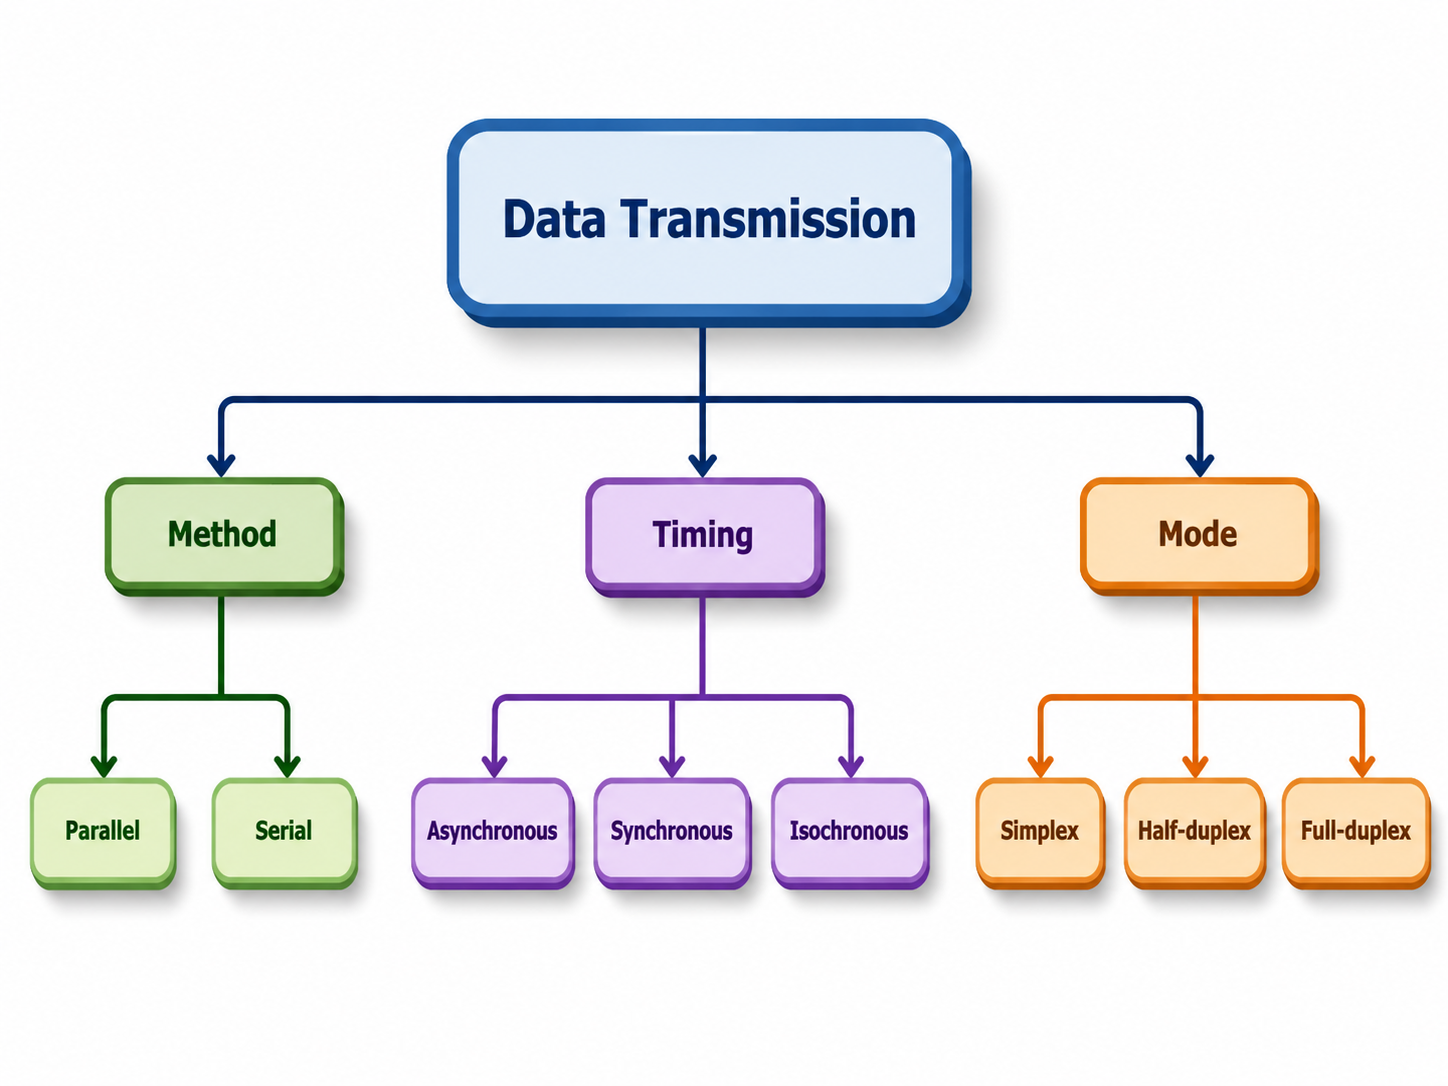
\includegraphics[width=0.90\textwidth,height=0.27\textheight,keepaspectratio]{chapters/Chapter02/images/data_transmission_overview_tree.png}
}{
\fbox{
\parbox{0.90\textwidth}{
\centering
\vspace{0.7cm}
Data Transmission\\[8pt]
$\downarrow$\\[8pt]
Method: Parallel, Serial\\[8pt]
$\downarrow$\\[8pt]
Timing: Asynchronous, Synchronous, Isochronous\\[8pt]
$\downarrow$\\[8pt]
Mode: Simplex, Half-duplex, Full-duplex
\vspace{0.7cm}
}}
}
\caption{ডেটা ট্রান্সমিশনের ধারণা মানচিত্র}
\end{figure}

\begin{boardbox}{বোর্ড ফোকাস}
Data transmission question-এ method ও mode গুলিয়ে ফেলা যাবে না। Method বোঝায় data কীভাবে পাঠানো হচ্ছে, আর mode বোঝায় data কোন direction-এ আদান-প্রদান হচ্ছে।
\end{boardbox}

\subsection{ডেটা ট্রান্সমিশন মেথড}

Data transmission method মূলত দুই ধরনের:

\begin{itemize}
\item Parallel Transmission
\item Serial Transmission
\end{itemize}

\subsection{Parallel Transmission}

\begin{definitionbox}{Parallel Transmission}
যে transmission পদ্ধতিতে একাধিক bit একই সময়ে আলাদা আলাদা channel বা line দিয়ে পাঠানো হয়, তাকে parallel transmission বলা হয়।
\end{definitionbox}

Parallel transmission-এ 8 bit data পাঠাতে চাইলে 8টি আলাদা line ব্যবহার করা যেতে পারে। ফলে একই সময়ে অনেক bit পাঠানো যায়। তাই short distance-এ এটি দ্রুত। তবে line বেশি লাগার কারণে cost বেশি হয় এবং দূরত্ব বাড়লে synchronization problem হতে পারে।

\begin{figure}[!htbp]
\centering
\IfFileExists{chapters/Chapter02/images/parallel_vs_serial_transmission.png}{
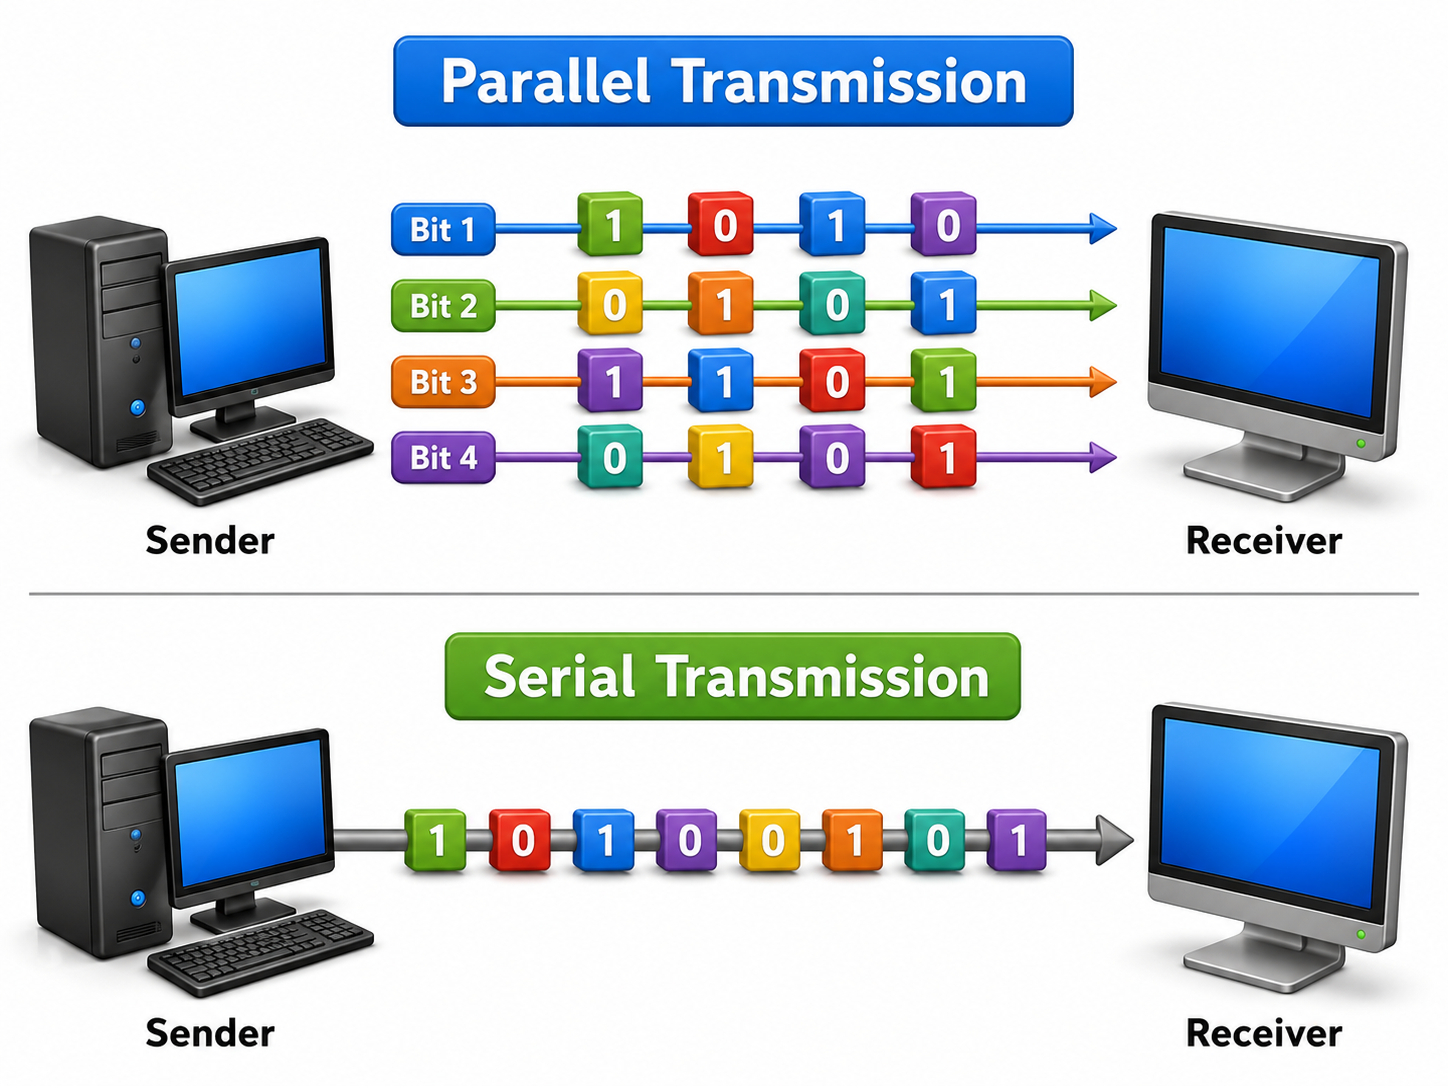
\includegraphics[width=0.92\textwidth,height=0.27\textheight,keepaspectratio]{chapters/Chapter02/images/parallel_vs_serial_transmission.png}
}{
\fbox{
\parbox{0.92\textwidth}{
\centering
\vspace{0.7cm}
Parallel Transmission\\[4pt]
Bit 1 $\longrightarrow$\\
Bit 2 $\longrightarrow$\\
Bit 3 $\longrightarrow$\\
Bit 4 $\longrightarrow$\\[12pt]
Serial Transmission\\[4pt]
Bit 1 $\longrightarrow$ Bit 2 $\longrightarrow$ Bit 3 $\longrightarrow$ Bit 4
\vspace{0.7cm}
}}
}
\caption{প্যারালাল ও সিরিয়াল ট্রান্সমিশন}
\end{figure}

\begin{keypointbox}{Parallel transmission-এর বৈশিষ্ট্য}
\begin{itemize}
\item একাধিক bit একই সময়ে পাঠানো হয়।
\item একাধিক channel বা wire প্রয়োজন হয়।
\item short distance communication-এ কার্যকর।
\item speed বেশি হলেও cost বেশি।
\item দূরত্ব বেশি হলে timing mismatch বা synchronization problem হতে পারে।
\end{itemize}
\end{keypointbox}

\begin{examplebox}{উদাহরণ}
Computer-এর internal bus বা পুরনো printer port-এ parallel transmission ব্যবহৃত হতো। কারণ এগুলো সাধারণত short distance-এর মধ্যে data transfer করত।
\end{examplebox}

\subsection{Serial Transmission}

\begin{definitionbox}{Serial Transmission}
যে transmission পদ্ধতিতে data bit-by-bit অর্থাৎ একটির পর একটি bit একই channel দিয়ে পাঠানো হয়, তাকে serial transmission বলা হয়।
\end{definitionbox}

Serial transmission-এ line কম লাগে, তাই cost কম। Long distance communication-এর জন্য এটি বেশি উপযোগী। Modern communication system, USB, Ethernet, mobile network এবং internet communication-এ serial transmission-এর ধারণা গুরুত্বপূর্ণ।

\begin{keypointbox}{Serial transmission-এর বৈশিষ্ট্য}
\begin{itemize}
\item data একটির পর একটি bit হিসেবে পাঠানো হয়।
\item সাধারণত একটি channel বা কম line প্রয়োজন হয়।
\item long distance communication-এর জন্য উপযোগী।
\item cost তুলনামূলক কম।
\item speed নির্ভর করে channel capacity, clocking, protocol ও technology-এর উপর।
\end{itemize}
\end{keypointbox}

\begin{examplebox}{উদাহরণ}
USB, Ethernet communication, modem communication এবং long-distance network communication-এ serial transmission বহুল ব্যবহৃত।
\end{examplebox}

\subsection{Parallel Transmission ও Serial Transmission-এর পার্থক্য}

\begin{center}
\begin{tabular}{|p{0.22\textwidth}|p{0.32\textwidth}|p{0.32\textwidth}|}
\hline
\textbf{বিষয়} & \textbf{Parallel Transmission} & \textbf{Serial Transmission} \\
\hline
Data পাঠানোর ধরন & একাধিক bit একই সময়ে যায় & bit-by-bit একটির পর একটি যায় \\
\hline
Line/Channel & একাধিক line প্রয়োজন & সাধারণত একটি line বা কম line প্রয়োজন \\
\hline
Distance & short distance-এ ভালো & long distance-এ ভালো \\
\hline
Cost & বেশি & তুলনামূলক কম \\
\hline
Speed ধারণা & short distance-এ দ্রুত & modern technology-তে খুব দ্রুত হতে পারে \\
\hline
Problem & synchronization problem হতে পারে & bit ordering ও timing control দরকার \\
\hline
উদাহরণ & internal bus, old printer port & USB, Ethernet, modem, internet \\
\hline
\end{tabular}
\end{center}

\begin{mistakebox}{Parallel বনাম serial}
অনেকে মনে করে parallel transmission সবসময় serial transmission-এর চেয়ে ভালো। আসলে short distance-এ parallel দ্রুত হতে পারে, কিন্তু long distance ও modern networking-এ serial transmission বেশি practical ও reliable।
\end{mistakebox}

\subsection{Serial Transmission-এর ধরন}

Serial transmission সাধারণত তিন ধরনের:

\begin{itemize}
\item Asynchronous Transmission
\item Synchronous Transmission
\item Isochronous Transmission
\end{itemize}

\subsection{Asynchronous Transmission}

\begin{definitionbox}{Asynchronous Transmission}
যে serial transmission পদ্ধতিতে data character বা small unit আকারে পাঠানো হয় এবং প্রতিটি unit-এর শুরুতে start bit ও শেষে stop bit থাকে, তাকে asynchronous transmission বলা হয়।
\end{definitionbox}

Asynchronous transmission-এ sender ও receiver-এর clock পুরো সময় synchronized থাকতে হয় না। প্রতিটি character বা byte আলাদাভাবে পাঠানো হয়। Receiver start bit দেখে বুঝতে পারে data শুরু হয়েছে এবং stop bit দেখে বুঝতে পারে data শেষ হয়েছে।

\begin{figure}[!htbp]
\centering
\IfFileExists{chapters/Chapter02/images/asynchronous_transmission_frame.png}{
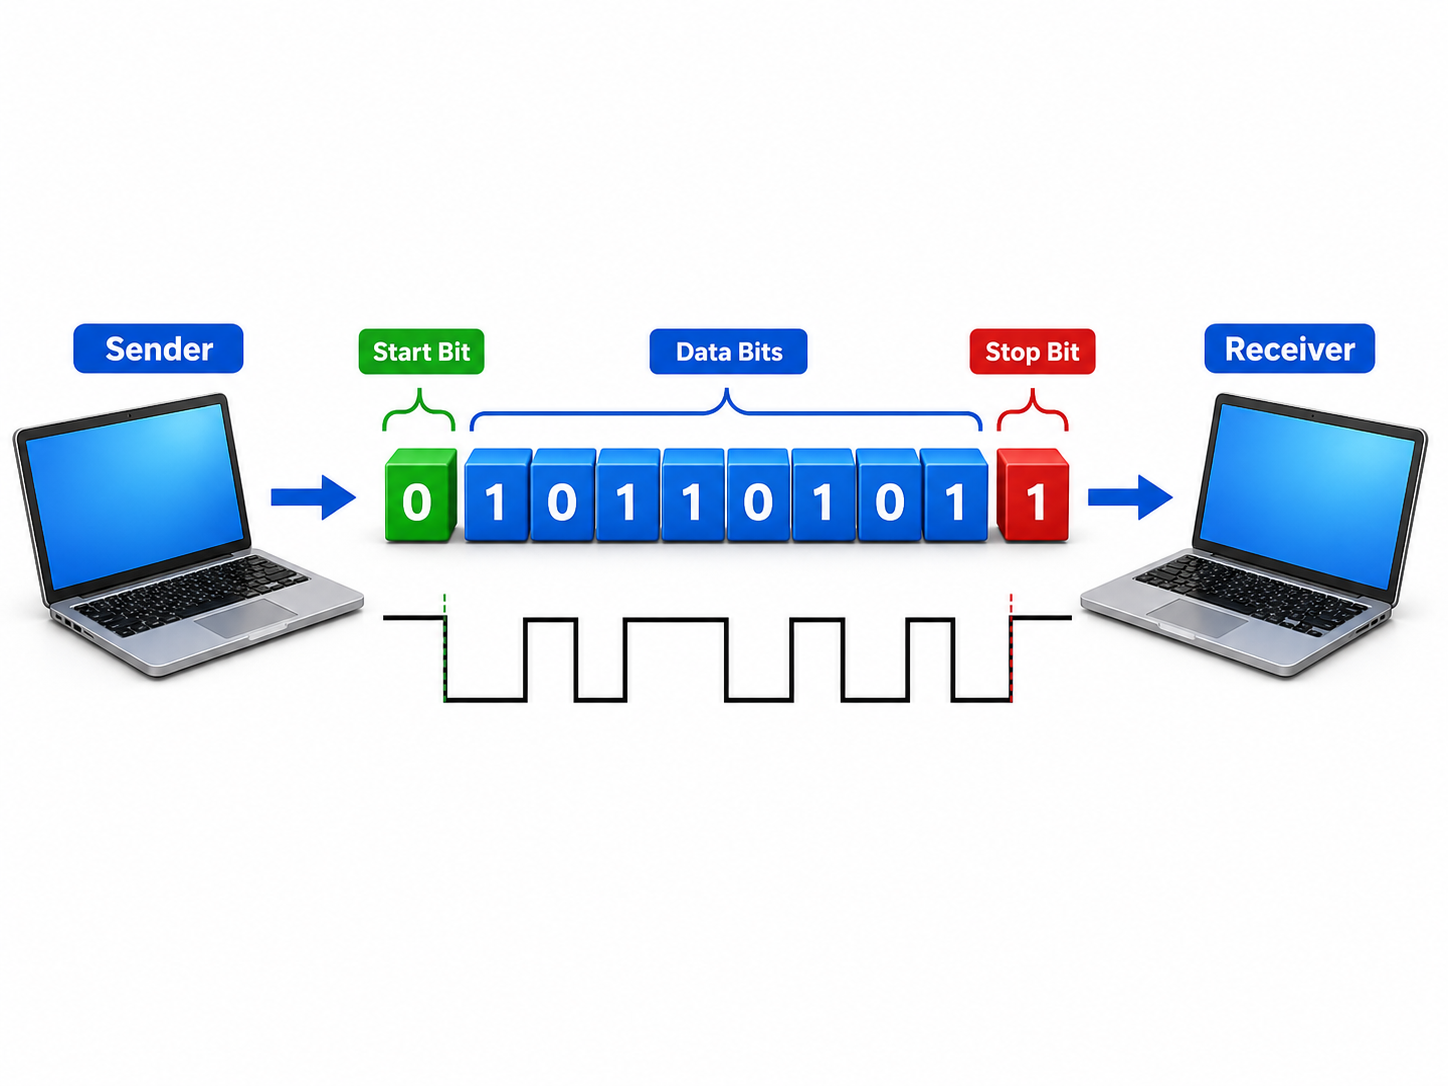
\includegraphics[width=0.90\textwidth,height=0.27\textheight,keepaspectratio]{chapters/Chapter02/images/asynchronous_transmission_frame.png}
}{
\fbox{
\parbox{0.90\textwidth}{
\centering
\vspace{0.7cm}
Start Bit \quad $\rightarrow$ \quad Data Bits \quad $\rightarrow$ \quad Stop Bit
\vspace{0.7cm}
}}
}
\caption{অ্যাসিনক্রোনাস ট্রান্সমিশন ফ্রেম}
\end{figure}

\begin{keypointbox}{Asynchronous transmission-এর বৈশিষ্ট্য}
\begin{itemize}
\item data ছোট unit বা character আকারে পাঠানো হয়।
\item প্রতিটি unit-এর সাথে start bit ও stop bit থাকে।
\item sender ও receiver-এর continuous clock synchronization দরকার হয় না।
\item data কম হলে বা অনিয়মিতভাবে data পাঠাতে হলে উপযোগী।
\item extra start/stop bit থাকার কারণে overhead বেশি হতে পারে।
\end{itemize}
\end{keypointbox}

\begin{examplebox}{উদাহরণ}
Keyboard input, পুরনো serial communication এবং কম পরিমাণ অনিয়মিত data পাঠানোর ক্ষেত্রে asynchronous transmission ব্যবহৃত হতে পারে।
\end{examplebox}

\subsection{Synchronous Transmission}

\begin{definitionbox}{Synchronous Transmission}
যে serial transmission পদ্ধতিতে sender ও receiver clock synchronization বজায় রেখে data block বা frame আকারে পাঠায়, তাকে synchronous transmission বলা হয়।
\end{definitionbox}

Synchronous transmission-এ data character-by-character না গিয়ে বড় block বা frame হিসেবে যায়। এখানে start/stop bit প্রতিটি character-এর সাথে থাকে না। ফলে large amount data দ্রুত ও দক্ষতার সাথে পাঠানো যায়। তবে sender ও receiver-এর timing বা clock synchronization গুরুত্বপূর্ণ।

\begin{figure}[!htbp]
\centering
\IfFileExists{chapters/Chapter02/images/synchronous_transmission_block.png}{
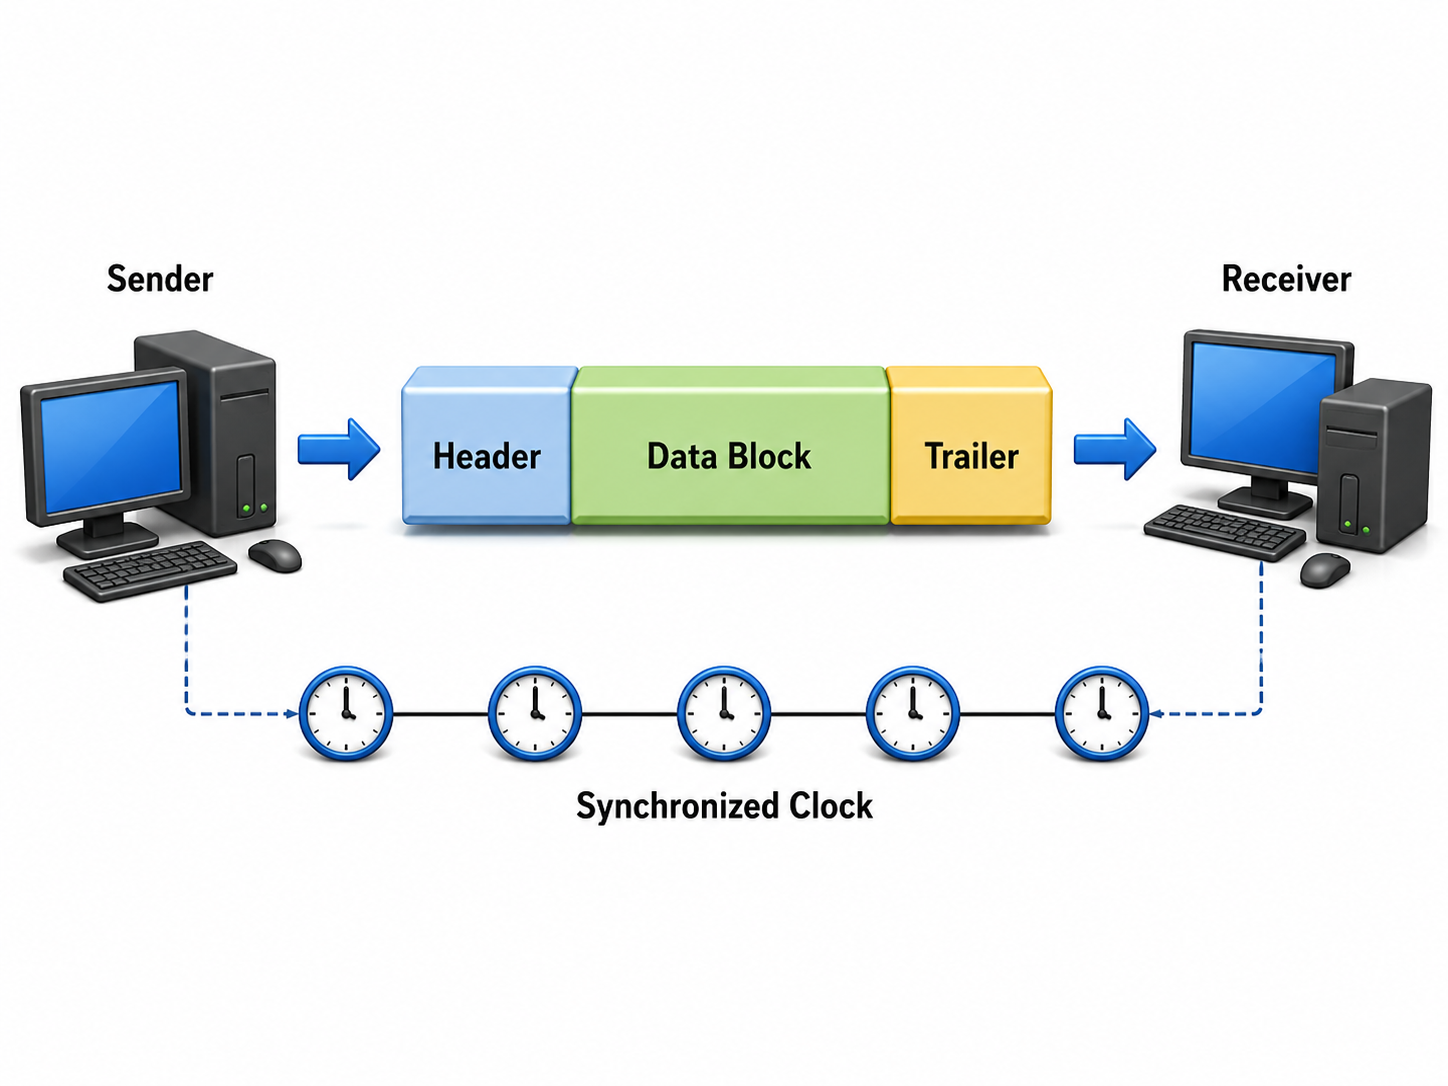
\includegraphics[width=0.90\textwidth,height=0.27\textheight,keepaspectratio]{chapters/Chapter02/images/synchronous_transmission_block.png}
}{
\fbox{
\parbox{0.90\textwidth}{
\centering
\vspace{0.7cm}
Header \quad $\rightarrow$ \quad Data Block \quad $\rightarrow$ \quad Trailer
\vspace{0.7cm}
}}
}
\caption{সিনক্রোনাস ট্রান্সমিশন ব্লক}
\end{figure}

\begin{keypointbox}{Synchronous transmission-এর বৈশিষ্ট্য}
\begin{itemize}
\item data block বা frame আকারে পাঠানো হয়।
\item sender ও receiver-এর clock synchronization প্রয়োজন।
\item বড় পরিমাণ data দ্রুত transfer-এর জন্য উপযোগী।
\item overhead তুলনামূলক কম।
\item network communication-এ বেশি কার্যকর।
\end{itemize}
\end{keypointbox}

\begin{examplebox}{উদাহরণ}
Network communication, high-speed data transfer, LAN communication ইত্যাদিতে synchronous transmission-এর ধারণা ব্যবহৃত হয়।
\end{examplebox}

\subsection{Isochronous Transmission}

\begin{definitionbox}{Isochronous Transmission}
যে transmission পদ্ধতিতে data নির্দিষ্ট সময় interval বজায় রেখে continuous stream হিসেবে পাঠানো হয়, তাকে isochronous transmission বলা হয়।
\end{definitionbox}

Isochronous transmission বিশেষভাবে audio ও video communication-এর জন্য গুরুত্বপূর্ণ। এখানে শুধু data পৌঁছানোই যথেষ্ট নয়; data নির্দিষ্ট সময়ের মধ্যে পৌঁছাতে হবে। কারণ video call, live class বা streaming-এ delay বেশি হলে sound ও video mismatch হতে পারে।

\begin{figure}[!htbp]
\centering
\IfFileExists{chapters/Chapter02/images/synchronous_vs_isochronous_transmission.png}{
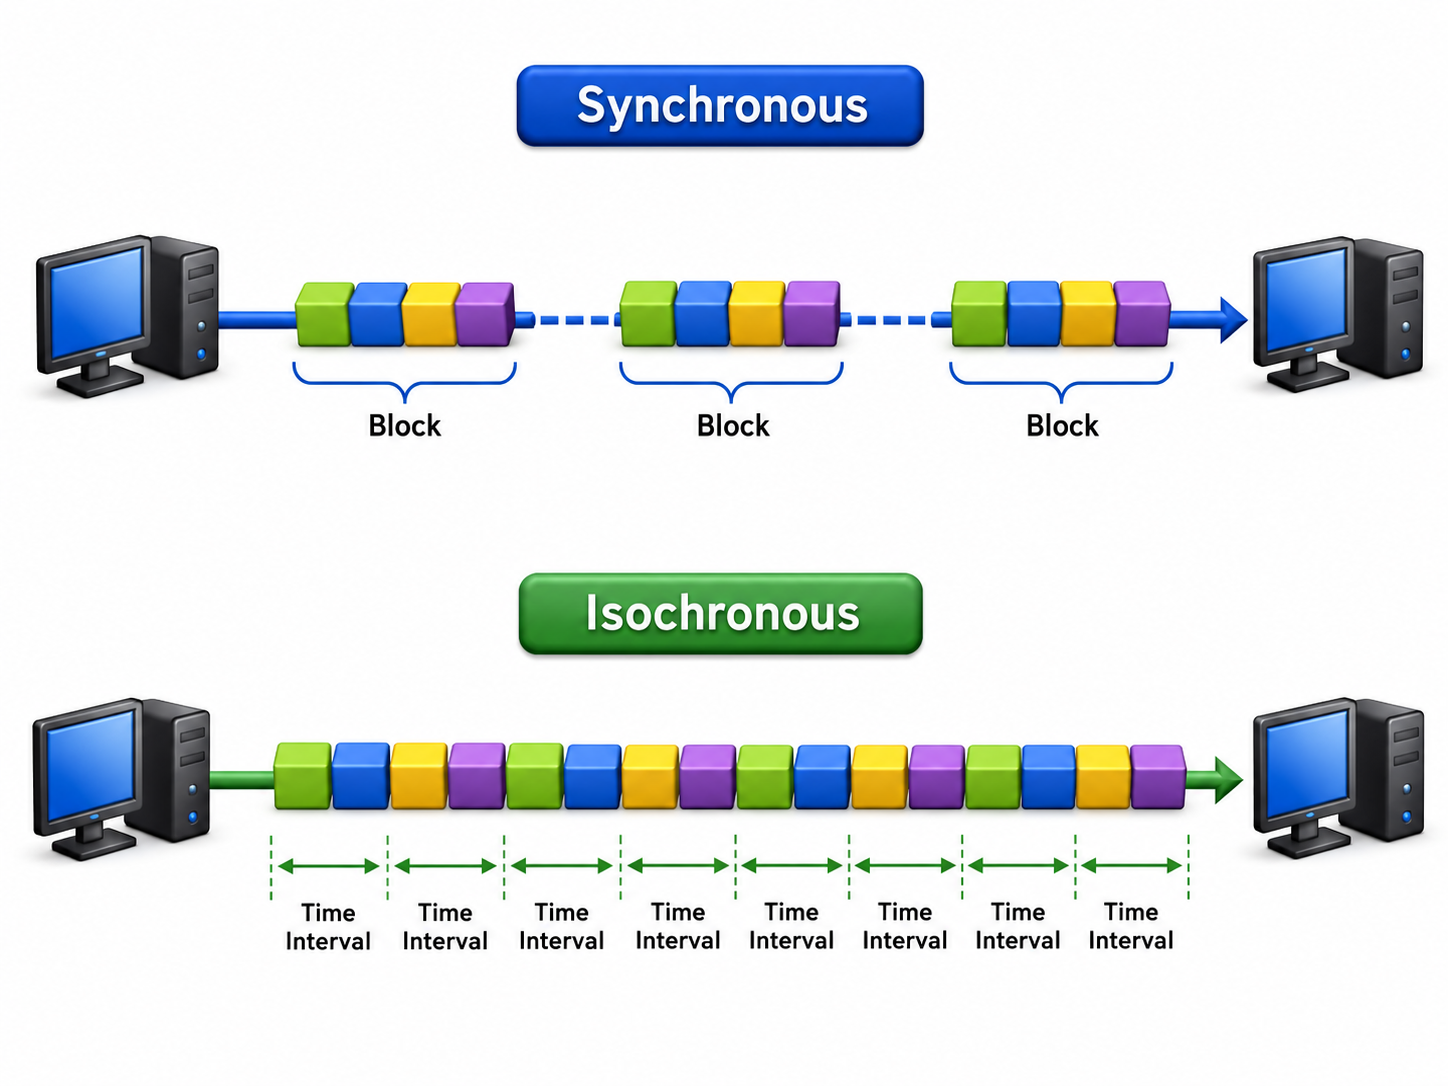
\includegraphics[width=0.90\textwidth,height=0.27\textheight,keepaspectratio]{chapters/Chapter02/images/synchronous_vs_isochronous_transmission.png}
}{
\fbox{
\parbox{0.90\textwidth}{
\centering
\vspace{0.7cm}
Synchronous: Block \quad Block \quad Block\\[12pt]
Isochronous: Stream \quad Stream \quad Stream
\vspace{0.7cm}
}}
}
\caption{সিনক্রোনাস ও আইসোক্রোনাস ট্রান্সমিশনের ধারণা}
\end{figure}

\begin{keypointbox}{Isochronous transmission-এর বৈশিষ্ট্য}
\begin{itemize}
\item continuous data stream পাঠানো হয়।
\item নির্দিষ্ট সময় interval বজায় রাখা গুরুত্বপূর্ণ।
\item audio, video ও real-time communication-এর জন্য উপযোগী।
\item delay বেশি হলে communication quality কমে যায়।
\item live streaming, video conference, online class-এ এর ধারণা গুরুত্বপূর্ণ।
\end{itemize}
\end{keypointbox}

\begin{examplebox}{উদাহরণ}
Video call, live online class, IP TV, live audio-video streaming—এসব ক্ষেত্রে timing খুব গুরুত্বপূর্ণ, তাই isochronous transmission-এর ধারণা প্রযোজ্য।
\end{examplebox}

\subsection{Asynchronous, Synchronous ও Isochronous Transmission-এর পার্থক্য}

\begin{center}
\begin{tabular}{|p{0.20\textwidth}|p{0.24\textwidth}|p{0.24\textwidth}|p{0.24\textwidth}|}
\hline
\textbf{বিষয়} & \textbf{Asynchronous} & \textbf{Synchronous} & \textbf{Isochronous} \\
\hline
Data পাঠানোর ধরন & character বা small unit & block বা frame & continuous stream \\
\hline
Timing & start/stop bit দিয়ে control & clock synchronization দরকার & fixed time interval দরকার \\
\hline
Overhead & বেশি & তুলনামূলক কম & timing control গুরুত্বপূর্ণ \\
\hline
ব্যবহার & কম বা অনিয়মিত data & বড় পরিমাণ data & audio-video/live data \\
\hline
উদাহরণ & keyboard/serial input & network data transfer & video call/live class \\
\hline
\end{tabular}
\end{center}

\begin{boardbox}{বোর্ড ফোকাস}
Asynchronous transmission-এর প্রশ্নে start bit ও stop bit অবশ্যই লিখতে হবে। Synchronous transmission-এর ক্ষেত্রে block/frame ও clock synchronization লিখতে হবে। Isochronous transmission-এর ক্ষেত্রে real-time audio-video এবং fixed time interval লিখলে উত্তর পূর্ণাঙ্গ হয়।
\end{boardbox}

\subsection{ডেটা ট্রান্সমিশন মোড}

\begin{definitionbox}{Transmission Mode}
Data sender ও receiver-এর মধ্যে কোন direction-এ আদান-প্রদান হবে, সেই পদ্ধতিকে transmission mode বলা হয়।
\end{definitionbox}

Transmission mode তিন ধরনের:

\begin{itemize}
\item Simplex
\item Half-duplex
\item Full-duplex
\end{itemize}

\subsection{Simplex Mode}

\begin{definitionbox}{Simplex Mode}
যে transmission mode-এ data শুধু এক direction-এ যায়, অর্থাৎ sender শুধু পাঠায় এবং receiver শুধু গ্রহণ করে, তাকে simplex mode বলা হয়।
\end{definitionbox}

Simplex mode-এ receiver data পাঠাতে পারে না। এটি one-way communication system। Broadcasting system-এ এটি বেশি দেখা যায়।

\begin{examplebox}{উদাহরণ}
Radio broadcast, TV broadcast, keyboard থেকে computer-এ input, monitor-এ output display—এসব simplex communication-এর উদাহরণ।
\end{examplebox}

\subsection{Half-duplex Mode}

\begin{definitionbox}{Half-duplex Mode}
যে transmission mode-এ data দুই direction-এ যেতে পারে, কিন্তু একই সময়ে দুই direction-এ যেতে পারে না, তাকে half-duplex mode বলা হয়।
\end{definitionbox}

Half-duplex mode-এ উভয় পক্ষ data পাঠাতে ও গ্রহণ করতে পারে, কিন্তু একসাথে নয়। একজন কথা বললে অন্যজন অপেক্ষা করে।

\begin{examplebox}{উদাহরণ}
Walkie-talkie half-duplex communication-এর সহজ উদাহরণ। একজন কথা বলার সময় অন্যজন শুনে, পরে অন্যজন কথা বলে।
\end{examplebox}

\subsection{Full-duplex Mode}

\begin{definitionbox}{Full-duplex Mode}
যে transmission mode-এ data একই সময়ে দুই direction-এ আদান-প্রদান করা যায়, তাকে full-duplex mode বলা হয়।
\end{definitionbox}

Full-duplex mode আধুনিক communication-এ খুব গুরুত্বপূর্ণ, কারণ এতে sender ও receiver একই সময়ে data পাঠাতে ও গ্রহণ করতে পারে। ফলে communication দ্রুত ও স্বাভাবিক হয়।

\begin{examplebox}{উদাহরণ}
Mobile phone call, video call এবং modern network communication full-duplex communication-এর উদাহরণ।
\end{examplebox}

\begin{figure}[!htbp]
\centering
\IfFileExists{chapters/Chapter02/images/simplex_half_full_duplex_modes.png}{
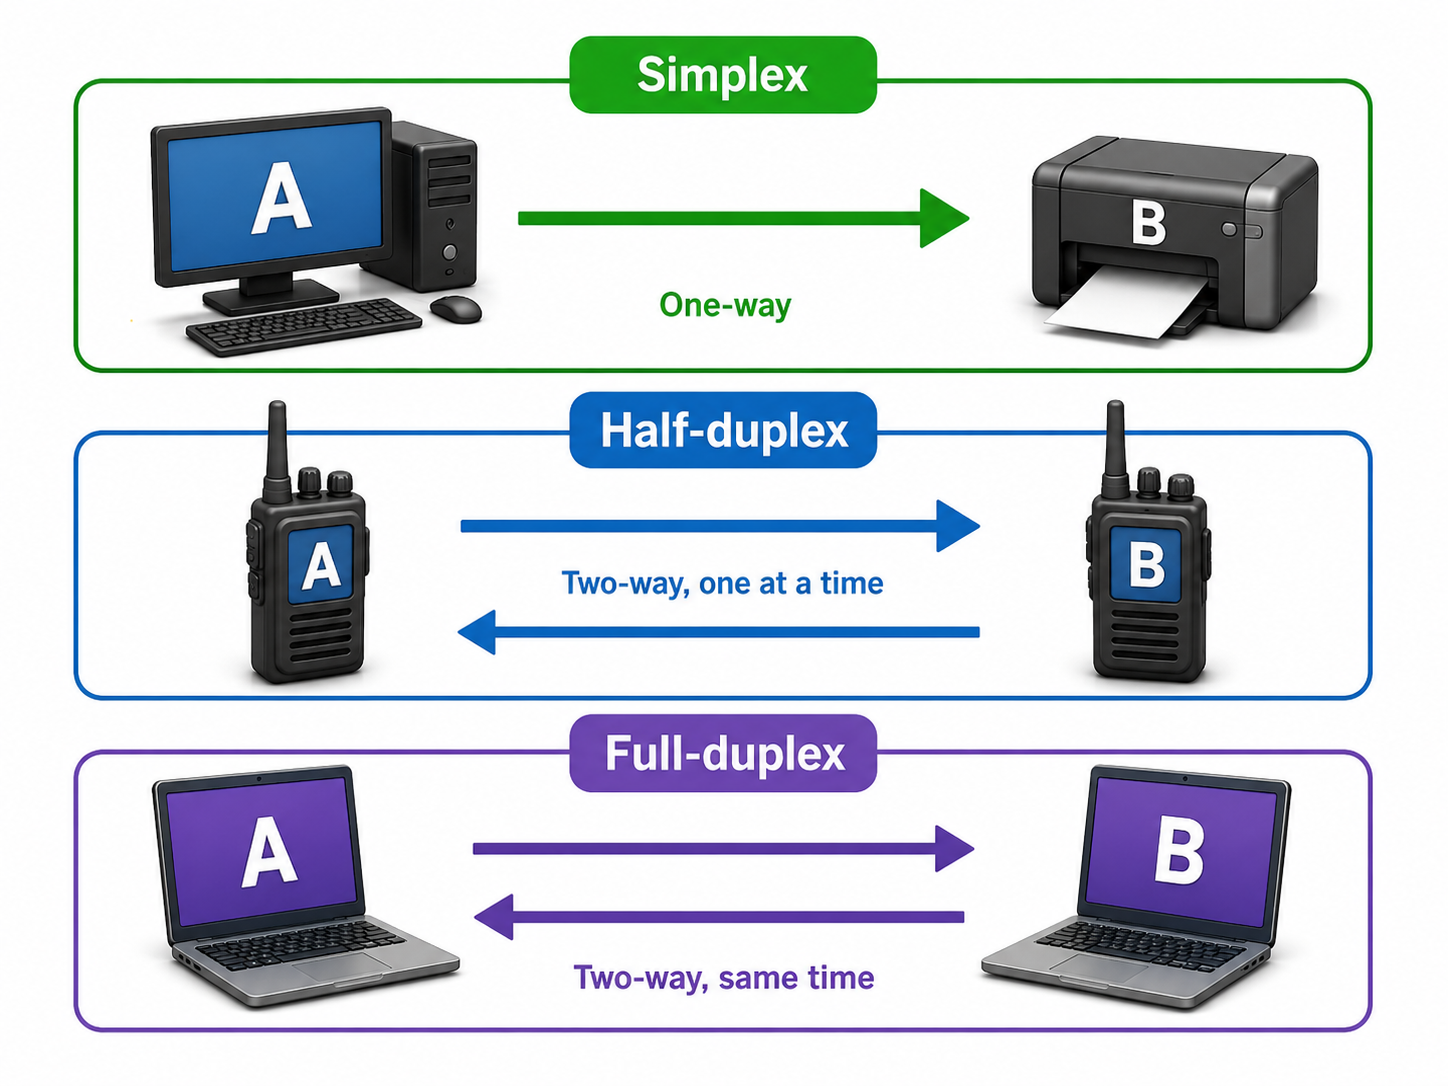
\includegraphics[width=0.92\textwidth,height=0.27\textheight,keepaspectratio]{chapters/Chapter02/images/simplex_half_full_duplex_modes.png}
}{
\fbox{
\parbox{0.92\textwidth}{
\centering
\vspace{0.7cm}
Simplex: A $\longrightarrow$ B\\[10pt]
Half-duplex: A $\longleftrightarrow$ B \quad One at a time\\[10pt]
Full-duplex: A $\Longleftrightarrow$ B \quad Same time
\vspace{0.7cm}
}}
}
\caption{সিমপ্লেক্স, হাফ-ডুপ্লেক্স ও ফুল-ডুপ্লেক্স মোড}
\end{figure}

\subsection{Simplex, Half-duplex ও Full-duplex-এর পার্থক্য}

\begin{center}
\begin{tabular}{|p{0.20\textwidth}|p{0.24\textwidth}|p{0.24\textwidth}|p{0.24\textwidth}|}
\hline
\textbf{বিষয়} & \textbf{Simplex} & \textbf{Half-duplex} & \textbf{Full-duplex} \\
\hline
Direction & একদিকে & দুইদিকে & দুইদিকে \\
\hline
Same time communication & সম্ভব নয় & সম্ভব নয় & সম্ভব \\
\hline
Sender/Receiver ভূমিকা & নির্দিষ্ট & পালাক্রমে বদলাতে পারে & একই সাথে উভয় কাজ করতে পারে \\
\hline
উদাহরণ & TV/Radio broadcast & Walkie-talkie & Mobile call, video call \\
\hline
ব্যবহার & one-way communication & পালাক্রমিক communication & real-time interactive communication \\
\hline
\end{tabular}
\end{center}

\begin{mistakebox}{Half-duplex বনাম full-duplex}
Half-duplex ও full-duplex দুটোতেই data দুইদিকে যেতে পারে। পার্থক্য হলো half-duplex-এ একই সময়ে দুইদিকে যায় না, কিন্তু full-duplex-এ একই সময়ে দুইদিকে data আদান-প্রদান হয়।
\end{mistakebox}

\subsection{Data Delivery Mode: Unicast, Broadcast ও Multicast}

Data transmission-এ কখনো data এক receiver-এর কাছে যায়, কখনো network-এর সব receiver-এর কাছে যায়, আবার কখনো নির্দিষ্ট group-এর কাছে যায়। এই ভিত্তিতে delivery mode তিন ধরনের:

\begin{itemize}
\item Unicast
\item Broadcast
\item Multicast
\end{itemize}

\subsection{Unicast}

\begin{definitionbox}{Unicast}
এক sender থেকে এক নির্দিষ্ট receiver-এর কাছে data পাঠানোর পদ্ধতিকে unicast বলা হয়।
\end{definitionbox}

\begin{examplebox}{উদাহরণ}
একজন বন্ধুকে email পাঠানো, এক ব্যক্তিকে WhatsApp message পাঠানো, একটি device থেকে নির্দিষ্ট server-এ request পাঠানো—unicast communication-এর উদাহরণ।
\end{examplebox}

\subsection{Broadcast}

\begin{definitionbox}{Broadcast}
এক sender থেকে network-এর সকল receiver-এর কাছে data পাঠানোর পদ্ধতিকে broadcast বলা হয়।
\end{definitionbox}

\begin{examplebox}{উদাহরণ}
TV broadcast, radio broadcast এবং local network-এ broadcast message—broadcast communication-এর উদাহরণ।
\end{examplebox}

\subsection{Multicast}

\begin{definitionbox}{Multicast}
এক sender থেকে নির্দিষ্ট একটি receiver group-এর কাছে data পাঠানোর পদ্ধতিকে multicast বলা হয়।
\end{definitionbox}

\begin{examplebox}{উদাহরণ}
একটি online class link নির্দিষ্ট group-এর শিক্ষার্থীদের কাছে পাঠানো, group video streaming, IPTV multicast—multicast communication-এর উদাহরণ।
\end{examplebox}

\begin{figure}[!htbp]
\centering
\IfFileExists{chapters/Chapter02/images/unicast_broadcast_multicast.png}{
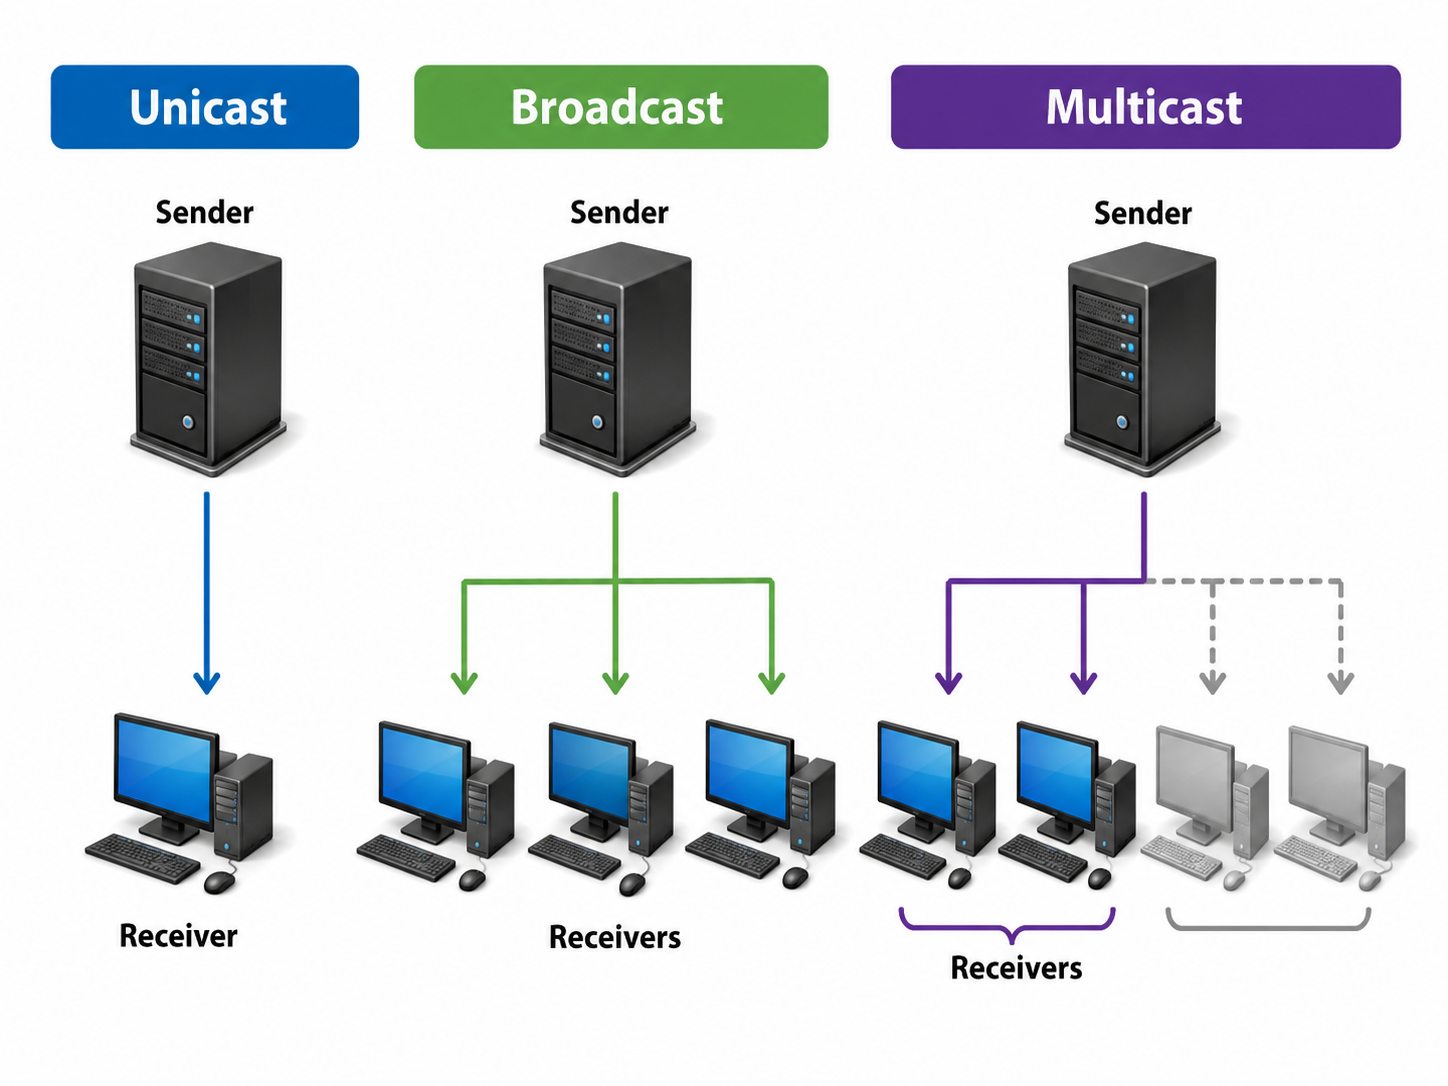
\includegraphics[width=0.92\textwidth,height=0.27\textheight,keepaspectratio]{chapters/Chapter02/images/unicast_broadcast_multicast.png}
}{
\fbox{
\parbox{0.92\textwidth}{
\centering
\vspace{0.7cm}
Unicast: One Sender $\longrightarrow$ One Receiver\\[10pt]
Broadcast: One Sender $\longrightarrow$ All Receivers\\[10pt]
Multicast: One Sender $\longrightarrow$ Selected Group
\vspace{0.7cm}
}}
}
\caption{Unicast, Broadcast ও Multicast}
\end{figure}

\subsection{Unicast, Broadcast ও Multicast-এর পার্থক্য}

\begin{center}
\begin{tabular}{|p{0.22\textwidth}|p{0.22\textwidth}|p{0.22\textwidth}|p{0.22\textwidth}|}
\hline
\textbf{বিষয়} & \textbf{Unicast} & \textbf{Broadcast} & \textbf{Multicast} \\
\hline
Receiver সংখ্যা & একজন নির্দিষ্ট receiver & network-এর সবাই & নির্দিষ্ট group \\
\hline
Data flow & One-to-one & One-to-all & One-to-many selected \\
\hline
Efficiency & নির্দিষ্ট communication-এ efficient & সবার জন্য দরকার হলে efficient & group communication-এ efficient \\
\hline
উদাহরণ & personal email/message & TV/radio broadcast & online class group stream \\
\hline
\end{tabular}
\end{center}

\begin{boardbox}{বোর্ড ফোকাস}
Transmission mode এবং delivery mode এক নয়। Simplex/Half-duplex/Full-duplex direction বোঝায়, আর Unicast/Broadcast/Multicast receiver group বোঝায়।
\end{boardbox}

\subsection{Exam-style প্রশ্ন ও উত্তর}

\begin{boardbox}{সংক্ষিপ্ত প্রশ্ন: Parallel transmission কী?}
যে transmission পদ্ধতিতে একাধিক bit একই সময়ে আলাদা আলাদা line বা channel দিয়ে পাঠানো হয়, তাকে parallel transmission বলা হয়। এতে speed বেশি হলেও একাধিক line লাগে, তাই cost বেশি এবং long distance-এ synchronization problem হতে পারে।
\end{boardbox}

\begin{boardbox}{সংক্ষিপ্ত প্রশ্ন: Serial transmission কেন long distance-এ উপযোগী?}
Serial transmission-এ data bit-by-bit একই channel দিয়ে পাঠানো হয়। এতে line কম লাগে, cost কম হয় এবং long distance communication সহজ হয়। তাই modern network, USB, Ethernet ও internet communication-এ serial transmission বেশি ব্যবহৃত হয়।
\end{boardbox}

\begin{boardbox}{সংক্ষিপ্ত প্রশ্ন: Asynchronous transmission কী?}
যে serial transmission পদ্ধতিতে data character বা small unit আকারে পাঠানো হয় এবং প্রতিটি unit-এর শুরুতে start bit ও শেষে stop bit থাকে, তাকে asynchronous transmission বলা হয়। এতে sender ও receiver-এর continuous clock synchronization প্রয়োজন হয় না।
\end{boardbox}

\begin{boardbox}{পার্থক্য: Simplex ও Full-duplex}
Simplex mode-এ data শুধু একদিকে যায়; receiver data পাঠাতে পারে না। কিন্তু full-duplex mode-এ একই সময়ে দুই direction-এ data আদান-প্রদান করা যায়। TV broadcast simplex-এর উদাহরণ, আর mobile phone call full-duplex-এর উদাহরণ।
\end{boardbox}

\subsection{Brainstorming Critical Question}

\begin{practicebox}
একটি কলেজে online class নেওয়া হয়। শিক্ষক live video class নেন, শিক্ষার্থীরা chat করে প্রশ্ন করে, আবার class recording server-এ upload করা হয়।

\begin{enumerate}
\item ক. Serial transmission কী?
\item খ. Asynchronous transmission-এ start bit ও stop bit কেন দরকার?
\item গ. উদ্দীপকে live class-এর ক্ষেত্রে কোন transmission timing ধারণা বেশি গুরুত্বপূর্ণ? ব্যাখ্যা কর।
\item ঘ. শিক্ষক ও শিক্ষার্থীদের live interaction full-duplex communication-এর সাথে কতটা সম্পর্কযুক্ত? বিশ্লেষণ কর।
\end{enumerate}
\end{practicebox}

\subsection{১ মিনিটে রিভিশন}

\begin{recapbox}
\begin{itemize}
\item Data transmission হলো এক device থেকে অন্য device-এ data পাঠানোর প্রক্রিয়া।
\item Parallel transmission-এ একাধিক bit একই সময়ে যায়।
\item Serial transmission-এ bit একটির পর একটি যায়।
\item Asynchronous transmission-এ start bit ও stop bit থাকে।
\item Synchronous transmission-এ data block/frame আকারে যায়।
\item Isochronous transmission-এ fixed time interval বজায় রাখা গুরুত্বপূর্ণ।
\item Simplex হলো one-way communication।
\item Half-duplex হলো two-way but one at a time।
\item Full-duplex হলো two-way at the same time।
\item Unicast one-to-one, Broadcast one-to-all, Multicast one-to-selected group।
\end{itemize}
\end{recapbox}

\subsection{অনুশীলন}

\begin{practicebox}
\textbf{MCQ}
\begin{enumerate}
\item Parallel transmission-এ data কীভাবে পাঠানো হয়?\\
ক. একটির পর একটি bit \quad খ. একাধিক bit একই সময়ে \quad গ. শুধু wireless মাধ্যমে \quad ঘ. শুধু audio signal হিসেবে

\item Serial transmission-এ data কীভাবে যায়?\\
ক. একাধিক line দিয়ে একই সময়ে \quad খ. bit-by-bit \quad গ. শুধু broadcast আকারে \quad ঘ. কোনো medium ছাড়া

\item Asynchronous transmission-এ কোন bit ব্যবহৃত হয়?\\
ক. Start bit ও Stop bit \quad খ. Only parity bit \quad গ. IP bit \quad ঘ. Cloud bit

\item Live video class-এ timing বজায় রাখার জন্য কোন transmission ধারণা বেশি সম্পর্কযুক্ত?\\
ক. Asynchronous \quad খ. Isochronous \quad গ. Simplex \quad ঘ. Broadcast only

\item Walkie-talkie কোন mode-এর উদাহরণ?\\
ক. Simplex \quad খ. Half-duplex \quad গ. Full-duplex \quad ঘ. Multicast

\item Mobile phone call কোন mode-এর উদাহরণ?\\
ক. Simplex \quad খ. Half-duplex \quad গ. Full-duplex \quad ঘ. Broadcast

\item একজন sender একজন receiver-কে message পাঠালে সেটি কী?\\
ক. Broadcast \quad খ. Multicast \quad গ. Unicast \quad ঘ. Duplex
\end{enumerate}

\textbf{সংক্ষিপ্ত প্রশ্ন}
\begin{enumerate}
\item Data transmission কী?
\item Parallel ও Serial transmission-এর মধ্যে পার্থক্য লেখ।
\item Asynchronous transmission কী? Start bit ও Stop bit-এর ভূমিকা লেখ।
\item Synchronous transmission কেন large data transfer-এ উপযোগী?
\item Isochronous transmission কোথায় ব্যবহৃত হয়?
\item Simplex, Half-duplex ও Full-duplex-এর পার্থক্য লেখ।
\item Unicast, Broadcast ও Multicast-এর পার্থক্য লেখ।
\end{enumerate}

\textbf{সৃজনশীল প্রশ্ন}
একটি প্রতিষ্ঠানে online meeting, file sharing এবং live training session পরিচালিত হয়। Meeting-এ সবাই একই সময়ে কথা শুনতে ও বলতে পারে, file server থেকে নির্দিষ্ট user file download করে, আর live training নির্দিষ্ট group-এর কাছে stream করা হয়।

\begin{enumerate}
\item ক. Transmission mode কী?
\item খ. Serial transmission long distance communication-এ উপযোগী কেন?
\item গ. উদ্দীপকে full-duplex ও unicast communication শনাক্ত করে ব্যাখ্যা কর।
\item ঘ. live training session multicast ও isochronous transmission-এর সাথে কীভাবে সম্পর্কযুক্ত? বিশ্লেষণ কর।
\end{enumerate}
\end{practicebox}

% Chapter 02.3: ডেটা কমিউনিকেশন মাধ্যম
\begingroup
\chTwoReadableTopicStyle
\section{ডেটা কমিউনিকেশন মাধ্যম}
\subsection{মাধ্যম: ডেটা যাওয়ার পথ}
অনলাইন ক্লাসে শিক্ষার্থীর ল্যাপটপ থেকে অ্যাকসেস পয়েন্ট পর্যন্ত রেডিও তরঙ্গ দিয়ে ডেটা যায়। সেখান থেকে দূরের সার্ভারে পৌঁছাতে অপটিক্যাল ফাইবারও ব্যবহার হতে পারে। একই যোগাযোগের বিভিন্ন অংশে প্রয়োজন অনুযায়ী পৃথক মাধ্যম ব্যবহৃত হয়।
\begin{definitionbox}{ডেটা কমিউনিকেশন মাধ্যম (Transmission Medium)}
প্রেরক থেকে প্রাপকের কাছে সংকেত বহনের পথকে ডেটা কমিউনিকেশন মাধ্যম বলে। এই পথ তারযুক্ত বা তারবিহীন হতে পারে। তামার কেবলে বৈদ্যুতিক সংকেত, অপটিক্যাল ফাইবারে আলো এবং বেতার সংযোগে বিদ্যুৎচৌম্বক তরঙ্গ ডেটা বহন করে।
\end{definitionbox}
\chTwoPair{\textbf{Point-to-point:} একটি সংযোগ সরাসরি দুই প্রান্তকে যুক্ত করে। যেমন, কম্পিউটার ও সুইচের একটি পোর্টের মধ্যকার কেবল সংযোগ।\par
\textbf{Multipoint:} একাধিক যন্ত্র একই সংযোগ ভাগ করে ব্যবহার করে। পুরোনো কোঅ্যাক্সিয়াল বাস এর উদাহরণ। যন্ত্রগুলো মাধ্যমের বহনক্ষমতা ও ব্যবহারের সুযোগ ভাগ করে।\par
এই শ্রেণিবিভাগ দিয়ে কারা একই পথ ব্যবহার করছে তা বোঝানো হয়। ইউনিকাস্ট ও ব্রডকাস্ট দিয়ে বোঝানো হয় একটি বার্তার প্রাপক কারা।}{\chTwoImage{chapters/Chapter02/images/data_communication_medium_basic_model.png}{মাধ্যম দিয়ে প্রেরক থেকে প্রাপকে সংকেত যায়}}
\subsection{মাধ্যমের দুটি প্রধান শ্রেণি}
\begin{tabularx}{\linewidth}{|p{.18\linewidth}|X|X|}
\hline
\textbf{ভিত্তি} & \textbf{Guided / Wired Media} & \textbf{Unguided / Wireless Media}\\\hline
সংজ্ঞা ও পথ & নির্দিষ্ট কেবলের পথ দিয়ে সংকেত যায় & কেবলে আবদ্ধ না হয়ে মুক্ত স্থানে সংকেত ছড়ায়\\\hline
উদাহরণ & Twisted Pair, Coaxial, Optical Fiber & Radio Wave, Microwave, Infrared; Satellite-ভিত্তিক Link\\\hline
চলাচল ও স্থাপন & কেবল বসাতে হয়; চলমান যন্ত্রের ব্যবহার সীমিত & সেবার আওতায় চলাচল সহজ; অ্যান্টেনা, AP বা টাওয়ার লাগতে পারে\\\hline
ব্যবহার & ল্যাব, অফিস, ডেটা সেন্টার ও ব্যাকবোন & ফোন, রিমোট, Wi-Fi ও দূরাঞ্চলের যোগাযোগ\\\hline
নির্ভরযোগ্যতা ও নিরাপত্তা & কেবলের ক্ষতি, কানেক্টর ও প্রবেশাধিকার বিবেচ্য; সুরক্ষা আবরণ বা আলোকপথে নয়েজ কমানো যায় & বাধা, বিঘ্ন, আবহাওয়া ও সংকেতের বাইরে ছড়ানো বিবেচ্য; পরিচয় যাচাই ও এনক্রিপশন দরকার\\\hline
\end{tabularx}
রেডিও তরঙ্গের ফ্রিকোয়েন্সির পরিসর বিস্তৃত। মাইক্রোওয়েভ সেই পরিসরের উচ্চ ফ্রিকোয়েন্সির একটি অংশ। স্যাটেলাইট ওই তরঙ্গ ব্যবহার করে সংকেত পুনঃপ্রেরণ করে। কেবল সংযোগেও অনুমতিহীন প্রবেশ ঘটতে পারে। তাই তার থাকলেই তথ্যের নিরাপত্তা নিশ্চিত হয় না।
\chTwoImage{chapters/Chapter02/images/transmission_media_classification_tree.png}{নির্দেশিত ও অনির্দেশিত মাধ্যমের শ্রেণিবিভাগ}
\subsection{নির্বাচনে কোন বিষয়গুলো দেখবে?}
\begin{keypointbox}{প্রয়োজনের সঙ্গে মাধ্যম মেলানো}
\textbf{বহনক্ষমতা (Bandwidth):} প্রয়োজনীয় ডেটা বহন করতে পারবে কি না; \textbf{দূরত্ব (Distance):} সংকেত কত দূর কার্যকর থাকবে; \textbf{খরচ (Cost):} স্থাপন ও রক্ষণাবেক্ষণে কত ব্যয় হবে; \textbf{নিরাপত্তা (Security):} তথ্য কতটা সংবেদনশীল; \textbf{নয়েজ ও বিঘ্ন (Noise/Interference):} আশপাশের প্রভাব কতটা; \textbf{চলাচল (Mobility):} ব্যবহারকারী চলমান থাকবেন কি না; \textbf{নির্ভরযোগ্যতা (Reliability):} সংযোগ কতটা স্থিতিশীল হওয়া প্রয়োজন; \textbf{সম্প্রসারণ (Scalability):} ভবিষ্যতে সংযোগ বাড়ানো যাবে কি না।
\end{keypointbox}
সংকেতের ক্ষয় বেশি হলে সংকেত দুর্বল হয়। নয়েজ বা বিঘ্নের কারণে ভুল ডেটাও পাওয়া যেতে পারে। মাধ্যম বেছে নেওয়ার সময় তাই শুধু ঘোষিত হার নয়, দূরত্ব, যন্ত্র ও পরিবেশ একসঙ্গে বিবেচনা করতে হয়। সংকেতের এসব সমস্যার মূল ব্যাখ্যা কমিউনিকেশন সিস্টেমের অংশে আছে।
\subsection{মাধ্যম নির্বাচন: কারণসহ সিদ্ধান্ত}
\begin{longtable}{|p{\dimexpr.27\linewidth-7pt\relax}|p{\dimexpr.28\linewidth-7pt\relax}|p{\dimexpr.45\linewidth-7pt\relax}|}
\hline
\textbf{প্রয়োজন} & \textbf{সম্ভাব্য নির্বাচন} & \textbf{যুক্তি ও শর্ত}\\\hline
\endfirsthead
\hline
\textbf{প্রয়োজন} & \textbf{সম্ভাব্য নির্বাচন} & \textbf{যুক্তি ও শর্ত}\\\hline
\endhead
এক কক্ষের ল্যাব & UTP + Switch & কম খরচে সহজ সংযোগ; Ethernet চ্যানেলের অনুমোদিত দূরত্ব ও কেবলের শ্রেণি মানতে হবে।\\\hline
কারখানা বা দূরের ভবন & Optical Fiber & বেশি বহনক্ষমতা, কম ক্ষয় ও EMI-মুক্ত আলোকপথ; জোড়া লাগানো এবং উপযুক্ত ট্রান্সসিভার দরকার।\\\hline
কক্ষে চলমান ল্যাপটপ & Wi-Fi & কেবল ছাড়াই চলাচল; AP-এর আওতা, ব্যবহারকারীর সংখ্যা ও নিরাপত্তা বিবেচ্য।\\\hline
দুই দূরবর্তী অফিস & Fiber / পরিকল্পিত Radio Link & দূরত্ব, বাধা, অনুমোদিত ফ্রিকোয়েন্সি, টাওয়ার ও খরচ বিবেচ্য; শুধু প্রযুক্তির নাম যথেষ্ট নয়।\\\hline
স্যাটেলাইটভিত্তিক দূরাঞ্চল & VSAT / Satellite Terminal & স্থলসংযোগ কঠিন হলে উপযোগী; বিলম্ব, বৃষ্টি ও খরচের সীমাবদ্ধতা থাকে।\\\hline
TV Remote & Infrared & কাছের যন্ত্রে নির্দেশ পাঠায়; বাধা ও আলোকপথ বিবেচ্য।\\\hline
Cable TV & Coaxial Cable & সুরক্ষা আবরণযুক্ত পথে ভিডিও সংকেত বিতরণ; কানেক্টর ও কেবলের মান মিলতে হয়।\\\hline
\end{longtable}
\textbf{একই নেটওয়ার্কে একাধিক মাধ্যমের প্রয়োজন:} কলেজের কম্পিউটার থেকে সুইচ পর্যন্ত UTP, ভবনের মধ্যে ফাইবার এবং শিক্ষার্থীদের ল্যাপটপে Wi-Fi ব্যবহার করা যায়। প্রতিটি অংশের দূরত্ব, বহনক্ষমতা ও চলাচলের চাহিদা পৃথকভাবে মেটে। কেবল ব্যবহারে অনুমতিহীন প্রবেশের ঝুঁকি কমতে পারে। তবুও পরিচয় যাচাই ও তথ্যের গোপন সংকেতায়ন বা এনক্রিপশন প্রয়োজন হতে পারে।


\subsection{মাধ্যমের সংখ্যাগত তথ্য: দূরত্ব ও সময় আলাদা}
\chTwoPair{\textbf{একক ও Signal-এর গতি}\par
১ km = ১০০০ m; ১ $\mu$s = $10^{-6}$ s। শূন্যস্থানে বিদ্যুৎচৌম্বক তরঙ্গের গতি প্রায় $3\times10^8$ m/s। ফাইবারে আলোর গতি সাধারণ উদাহরণে প্রায় $2\times10^8$ m/s ধরা যায়; উপাদানভেদে বদলায়।}{\textbf{একটি পথের সময়}\par
প্রশ্নে Fiber-এর গতি $2\times10^8$ m/s এবং দূরত্ব ২ km দিলে শুধু Propagation Time $=2000/(2\times10^8)=10\,\mu$s। এটি শুধু সংকেত ছড়িয়ে পৌঁছানোর সময়; পুরো ফাইল পাঠানোর সময় নয়। মোট সময়ে ফাইলের বিটসংখ্যা ও ডেটা হার অনুযায়ী প্রেরণসময়, যন্ত্রে অপেক্ষা এবং প্রক্রিয়াকরণের সময়ও যোগ হয়।}
UTP চ্যানেল, কোঅ্যাক্সিয়াল অংশ ও ফাইবার মডিউলের কার্যকর দূরত্ব তারযুক্ত মাধ্যমের অংশে আছে। Bluetooth, Wi-Fi ও WiMAX-এর পরিসর বেতার যোগাযোগের অংশে দেওয়া হয়েছে। একটি সংযোগের দৈর্ঘ্য এবং পুরো LAN/WAN-এর বিস্তৃতি আলাদা। সংখ্যাগত তথ্য ব্যবহারের সময় এই পার্থক্য মানতে হয়।

% Original topic-level problem, solution and MCQ reasoning.
\subsection{বাস্তব সমস্যা: পুরো কলেজে এক ধরনের মাধ্যম নয়}
\chTwoPair{\textbf{সমস্যা:} একটি কক্ষে ১৫টি কম্পিউটার আছে। দুটি ভবনের দূরত্ব ৭০০ m। শিক্ষার্থীরা ল্যাপটপ নিয়ে স্থান বদলায়। এসব কাজে কম খরচে নির্ভরযোগ্য সংযোগ দরকার।\par
\textbf{সমাধান:} কক্ষের কম্পিউটারগুলো উপযুক্ত Ethernet UTP ও সুইচ দিয়ে যুক্ত করা যায়। ভবনের প্রধান সংযোগে ফাইবার এবং চলমান ল্যাপটপে Wi-Fi/AP ব্যবহার করা যায়। সাধারণ ১০০ m তামার চ্যানেল দিয়ে একটানা ৭০০ m সংযোগ পরিকল্পনা করা ঠিক নয়।}{\textbf{ব্যবহার ও যুক্তি:} স্থির যন্ত্রে কেবল সংযোগ সহজে নিয়ন্ত্রণ করা যায়। দূরের প্রধান সংযোগে ফাইবার বেশি বহনক্ষমতা ও EMI থেকে সুরক্ষার সুবিধা দেয়। Wi-Fi দিয়ে চলাচলের সময়ও যোগাযোগ করা যায়। সব অংশের ডেটা হার সমান নাও হতে পারে।\par
\textbf{মাধ্যম নির্বাচনের শর্ত:} দূরত্ব, বহনক্ষমতা, বাধা বা EMI, চলাচল, বাজেট ও রক্ষণাবেক্ষণ একসঙ্গে বিবেচনা করতে হয়। শুধু দ্রুত বা সস্তা দেখে মাধ্যম বেছে নেওয়া যায় না।\par
\textbf{একই Network-এ ভিন্ন Medium:} একই নেটওয়ার্কের পৃথক সংযোগে তারযুক্ত ও বেতার মাধ্যম ব্যবহার করা যায়। টপোলজি ও মাধ্যমের শ্রেণিবিভাগ আলাদা।\par}

দিকনির্দেশিত মাইক্রোওয়েভের সরাসরি দৃষ্টিপথ বা LOS এবং পুনঃপ্রেরণের ব্যাখ্যা বেতার মাধ্যমের অংশে আছে। দূরের সংযোগ পরিকল্পনায় এসব শর্তও মানতে হয়।

\subsection{সাধারণ ভুল ও সংশোধন}

\smallhead{১. Medium ও mode গুলিয়ে ফেলা}
মাধ্যম ও মোডের অর্থ আলাদা। মাধ্যম হলো ডেটা বহনের পথ, যেমন কেবল বা রেডিও তরঙ্গ। দিকভিত্তিক মোড হলো ডেটা কোন দিকে যায় তার ধরন; যেমন Simplex, Half-duplex ও Full-duplex।

\smallhead{২. Wireless মানেই সবসময় faster মনে করা}
বেতার যোগাযোগ সবসময় দ্রুত নয়। বেতার সংযোগে চলাচলের সুবিধা থাকলেও বিঘ্ন, দূরত্ব, বাধা ও সংকেতের শক্তির কারণে ডেটার হার কমতে পারে।

\smallhead{৩. Fiber optic cable-কে electric signal মনে করা}
অপটিক্যাল ফাইবার বৈদ্যুতিক সংকেত বহন করে না। ফাইবারে আলোক সংকেতের সাহায্যে ডেটা পাঠানো হয়।

\subsection{MCQ অনুশীলন}

\par
\textbf{MCQ}
\begin{multicols}{2}\begin{enumerate}
\item\chTwoMCQBlock{ডেটা কমিউনিকেশনের মাধ্যম সংকেতকে কোন পথে বহন করে?
\par ক. শুধু সংরক্ষণযন্ত্রের ভেতরে \par খ. প্রেরক থেকে প্রাপকের পথে \par গ. শুধু প্রিন্টারের ভেতরে \quad ঘ. কোনো সংকেত ছাড়াই }
\item\chTwoMCQBlock{নিচের কোনটি নির্দেশিত মাধ্যম?
\par ক. Radio wave\quad খ. Microwave
\par গ. Twisted pair cable\quad ঘ. Infrared}
\item\chTwoMCQBlock{নিচের কোনটি অনির্দেশিত মাধ্যম?
\par ক. Coaxial cable\quad খ. Optical fiber
\par গ. Radio wave\quad ঘ. Twisted pair}
\item\chTwoMCQBlock{অপটিক্যাল ফাইবার কোন সংকেত ব্যবহার করে?
\par ক. Sound signal\quad খ. Light signal
\par গ. Mechanical signal\quad ঘ. Magnetic tape}
\item\chTwoMCQBlock{প্রচলিত টিভির রিমোট সাধারণত কোন মাধ্যম ব্যবহার করে?
\par ক. Infrared\quad খ. Coaxial cable
\par গ. Optical fiber\quad ঘ. Twisted pair}
\item\chTwoMCQBlock{LAN-এ সাধারণত কোন কেবল বেশি ব্যবহৃত হয়?
\par ক. টুইস্টেড পেয়ার \quad খ. স্যাটেলাইট সংযোগ \par গ. অবলোহিত সংযোগ \quad ঘ. রেডিও সংযোগ }
\item\chTwoMCQBlock{স্থলভিত্তিক মাইক্রোওয়েভ সংযোগে সাধারণত কোনটি গুরুত্বপূর্ণ?
\par ক. সরাসরি দৃষ্টিপথ \quad খ. আয়নমণ্ডল থেকে ফিরে আসা পথ \par গ. ভূপৃষ্ঠ অনুসরণ করা পথ \quad ঘ. তামার তারের আবরণ }
\item\chTwoMCQBlock{নির্দেশিত মাধ্যমের প্রধান সুবিধা কোনটি?
\par ক. চলাচলের স্বাধীনতা বেশি \quad খ. কেবল লাগে না \par গ. কেবলের নির্দিষ্ট পথে সংকেত যায়; প্রবেশাধিকার নিয়ন্ত্রণ সহজ হতে পারে \par ঘ. সবসময় বিনামূল্যে পাওয়া যায় }
\end{enumerate}\end{multicols}
\textbf{উত্তরমালা: ১. খ, ২. গ, ৩. গ, ৪. খ, ৫. ক, ৬. ক, ৭. ক, ৮. গ}
\endgroup

% Chapter 02.4: তারযুক্ত মাধ্যম
\begingroup
\chTwoReadableTopicStyle
\section{তারযুক্ত মাধ্যম}

\subsection{Lab থেকে Backbone: তিন ধরনের Cable}
কলেজের কম্পিউটার থেকে সুইচ পর্যন্ত কম খরচে টুইস্টেড পেয়ার ব্যবহার করা যায়। কেবল টিভির বিতরণে কোঅ্যাক্সিয়াল এবং ভবনের মধ্যে বা দূরের প্রধান সংযোগে অপটিক্যাল ফাইবার ব্যবহৃত হয়। তারযুক্ত মাধ্যমের শ্রেণিবিভাগ আগের অংশে আছে। এখানে প্রতিটি কেবলের গঠন, কাজ ও সীমাবদ্ধতা ব্যাখ্যা করা হয়েছে।
\chTwoPair{\chTwoImage{chapters/Chapter02/images/wired_media_overview.png}{কেবলের গঠন ও আলোকপথ}}{\chTwoImage{chapters/Chapter02/images/wired_media_types_tree.png}{তারযুক্ত মাধ্যমের তিনটি পরিচিত ধরন}}
\subsection{Twisted Pair Cable}

\begin{definitionbox}{Twisted Pair Cable}
দুটি অন্তরক আবরণযুক্ত তামার তার পরস্পর পেঁচিয়ে তৈরি ডেটা যোগাযোগের কেবলকে টুইস্টেড পেয়ার কেবল বলে।
\end{definitionbox}

কম্পিউটার নেটওয়ার্কে টুইস্টেড পেয়ার বহুল ব্যবহৃত তামার কেবল। এতে তামার তারগুলো জোড়ায় জোড়ায় পেঁচানো থাকে। পেঁচানো বিন্যাস বিদ্যুৎচৌম্বক বিঘ্ন ও পাশের জোড়ার সংকেতের প্রভাব বা ক্রসটক কমায়। অফিসের LAN, বিদ্যালয়ের কম্পিউটার ল্যাব, রাউটার থেকে কম্পিউটারের সংযোগ এবং টেলিফোন লাইনে এই কেবল ব্যবহৃত হয়।


\chTwoPair{\begin{keypointbox}{Twisted pair cable-এর বৈশিষ্ট্য}
\begin{itemize}
\item তামার তার দিয়ে তৈরি।
\item তারগুলো জোড়ায় জোড়ায় পেঁচানো থাকে।
\item স্থাপন সহজ এবং খরচ কম।
\item LAN-এ সবচেয়ে বেশি ব্যবহৃত কেবল।
\item সাধারণত RJ45 কানেক্টরের সঙ্গে ব্যবহৃত হয়।
\item স্বল্প থেকে মাঝারি দূরত্বের যোগাযোগে উপযোগী।
\item বিদ্যুৎচৌম্বক বিঘ্নে প্রভাবিত হতে পারে।
\end{itemize}
\end{keypointbox}}{\chTwoImage{chapters/Chapter02/images/twisted_pair_cable_structure.png}{টুইস্টেড পেয়ার কেবলের গঠন}}


\begin{examplebox}{বাস্তব উদাহরণ}
বাড়ির Wi-Fi রাউটার থেকে ডেস্কটপ কম্পিউটারে ব্যবহৃত Ethernet কেবল সাধারণত টুইস্টেড পেয়ার। কম্পিউটার ল্যাবে কম্পিউটার থেকে সুইচের সংযোগেও এই কেবল ব্যবহৃত হয়।
\end{examplebox}

\subsection{Twisted Pair Cable কেন পেঁচানো থাকে?}

ক্রসটক হলো একটি তারের জোড়া বা চ্যানেলের সংকেত অনাকাঙ্ক্ষিতভাবে পাশের জোড়া বা চ্যানেলে যুক্ত হওয়া। পেঁচানো দুটি তামার তারে ভারসাম্যযুক্ত সংকেত বহন করা হয়। প্রাপক দুই তারের সংকেতের পার্থক্য পড়ে। ফলে দুই তারে প্রায় সমানভাবে আসা নয়েজের প্রভাব অনেকটা বাদ যায়। তার পেঁচানোর বিন্যাস ক্রসটকও কমায়। EMI-এর মূল ধারণা সংকেতের বিঘ্ন অংশে (অনুচ্ছেদ~\ref{ch2:c01-07}) আছে। শিল্পকারখানার যন্ত্রের পাশে কেবল বসালে ধাতব সুরক্ষা আবরণ ও সঠিক গ্রাউন্ডিংয়ের প্রয়োজন আলাদাভাবে বিচার করতে হয়।

\begin{keypointbox}{পেঁচানোর সুবিধা}
\begin{itemize}
\item ক্রসটক কমায়।
\item বিদ্যুৎচৌম্বক বিঘ্ন কমাতে সাহায্য করে।
\item সংকেতের বিকৃতি কম হয়।
\item কেবল নমনীয় এবং সহজে স্থাপন করা যায়।
\end{itemize}
\end{keypointbox}

\subsection{UTP ও STP Cable}

Twisted pair cable দুই ধরনের:

\begin{itemize}
\item \textbf{UTP}: Unshielded Twisted Pair
\item \textbf{STP}: Shielded Twisted Pair
\end{itemize}

\begin{definitionbox}{UTP Cable}
যে টুইস্টেড পেয়ার কেবলে তারের জোড়ার চারপাশে অতিরিক্ত ধাতব সুরক্ষা আবরণ থাকে না, তাকে UTP বা Unshielded Twisted Pair কেবল বলে।
\end{definitionbox}

\begin{definitionbox}{STP Cable}
বিদ্যুৎচৌম্বক বিঘ্ন কমানোর জন্য অতিরিক্ত ধাতব সুরক্ষা আবরণযুক্ত টুইস্টেড পেয়ার কেবলকে STP বা Shielded Twisted Pair কেবল বলে।
\end{definitionbox}

\begingroup
\begin{longtable}{|p{\dimexpr 0.22\linewidth-2\tabcolsep-\arrayrulewidth\relax}|p{\dimexpr 0.30\linewidth-2\tabcolsep-\arrayrulewidth\relax}|p{\dimexpr 0.30\linewidth-2\tabcolsep-\arrayrulewidth\relax}|}
\hline
\textbf{বিষয়} & \textbf{UTP} & \textbf{STP} \\
\hline
\endfirsthead
\hline
\textbf{বিষয়} & \textbf{UTP} & \textbf{STP} \\
\hline
\endhead

পূর্ণরূপ & Unshielded Twisted Pair & Shielded Twisted Pair \\
\hline
সুরক্ষা আবরণ & বাড়তি ধাতব আবরণ নেই & ধাতব আবরণ আছে \\
\hline
খরচ & কম & তুলনামূলক বেশি \\
\hline
স্থাপন & সহজ & কিছুটা জটিল \\
\hline
বিঘ্ন থেকে সুরক্ষা & তুলনামূলক কম & সঠিক স্থাপনে তুলনামূলক বেশি \\
\hline
ব্যবহার & সাধারণ LAN, অফিস ও বাসার নেটওয়ার্ক & শিল্পকারখানা ও বিঘ্নপ্রবণ এলাকা \\
\hline
\end{longtable}
\endgroup

\begin{mistakebox}{UTP বনাম STP}
UTP ও STP একই কেবল পরিবারের দুটি ধরন। উভয়ই টুইস্টেড পেয়ার; পার্থক্য হলো অতিরিক্ত ধাতব সুরক্ষা আবরণ আছে কি না।
\end{mistakebox}

টুইস্টেড পেয়ার নমনীয় এবং RJ45 দিয়ে সহজে সংযুক্ত করা যায়। বাইরে থেকে কেবল ক্ষতিগ্রস্ত হলে সংযোগ নষ্ট হয়। গুরুত্বপূর্ণ ডেটা রক্ষায় ব্যবহারকারীর প্রবেশাধিকার নিয়ন্ত্রণও প্রয়োজন।

\subsection{Coaxial Cable}

\begin{definitionbox}{Coaxial Cable}
কেন্দ্রীয় পরিবাহী, অন্তরক স্তর, ধাতব সুরক্ষা আবরণ ও বাইরের আবরণ নিয়ে গঠিত কেবলকে কোঅ্যাক্সিয়াল কেবল বলে।
\end{definitionbox}

কোঅ্যাক্সিয়াল কেবলের কেন্দ্রীয় পরিবাহী ও বাইরের ধাতব সুরক্ষা আবরণ একই অক্ষ বরাবর থাকে। এই গঠন থেকেই নামটি এসেছে। কেন্দ্রীয় তামার পরিবাহী সংকেত বহন করে। তার চারপাশে অন্তরক এবং অন্তরকের বাইরে ধাতব সুরক্ষা আবরণ থাকে। সুরক্ষা আবরণ বাইরের নয়েজ ও বিদ্যুৎচৌম্বক বিঘ্ন কমায়। কেবল টিভি, ব্রডব্যান্ড কেবল বিতরণ এবং পুরোনো Ethernet নেটওয়ার্কে কোঅ্যাক্সিয়াল ব্যবহৃত হয়েছে।


\chTwoPair{\begin{keypointbox}{Coaxial cable-এর গঠন}
\begin{itemize}
\item \textbf{Central conductor}: সংকেত বহন করে।
\item \textbf{Insulator}: পরিবাহীকে ধাতব সুরক্ষা আবরণ থেকে আলাদা রাখে।
\item \textbf{Metallic shield}: বাইরের নয়েজ ও বিঘ্ন কমায়।
\item \textbf{Outer jacket}: কেবলকে বাইরের ক্ষতি থেকে রক্ষা করে।
\end{itemize}
\end{keypointbox}}{\chTwoImage{chapters/Chapter02/images/coaxial_cable_structure.png}{কোঅ্যাক্সিয়াল কেবলের গঠন}}


\begin{keypointbox}{Coaxial cable-এর বৈশিষ্ট্য}
\begin{itemize}
\item তামার পরিবাহী ব্যবহার করে।
\item ধাতব সুরক্ষা আবরণ থাকায় টুইস্টেড পেয়ারের তুলনায় নয়েজ কম হতে পারে।
\item কেবল টিভি ও ব্রডব্যান্ড বিতরণে ব্যবহৃত হয়।
\item কিছু ক্ষেত্রে টুইস্টেড পেয়ারের তুলনায় বেশি ব্যান্ডউইথ দিতে পারে।
\item টুইস্টেড পেয়ারের তুলনায় স্থাপন কিছুটা কঠিন।
\item আধুনিক LAN-এ টুইস্টেড পেয়ার ও অপটিক্যাল ফাইবার বেশি ব্যবহৃত হওয়ায় কোঅ্যাক্সিয়ালের ব্যবহার কমেছে।
\end{itemize}
\end{keypointbox}

\begin{examplebox}{বাস্তব উদাহরণ}
কেবল টিভির সংযোগ, পুরোনো ব্রডব্যান্ড কেবল লাইন এবং পুরোনো বাস টপোলজির Ethernet নেটওয়ার্কে কোঅ্যাক্সিয়াল কেবল ব্যবহৃত হতো।
\end{examplebox}

কোঅ্যাক্সিয়াল কেবল টেকসই, তবে তুলনামূলক মোটা ও কম নমনীয়। ফাইবারের মতো উচ্চ বহনক্ষমতা প্রয়োজন হলে শুধু কোঅ্যাক্সিয়ালের ধাতব সুরক্ষা আবরণ দিয়ে সেই চাহিদা মেটে না।

\subsection{Optical Fiber Cable}

\begin{definitionbox}{Optical Fiber Cable}
কাচ বা প্লাস্টিকের তন্তু দিয়ে আলোক সংকেতের সাহায্যে ডেটা পাঠানোর কেবলকে অপটিক্যাল ফাইবার কেবল বলে।
\end{definitionbox}

দূরের প্রধান সংযোগ, FTTH এবং সমুদ্রতলের কেবলে অপটিক্যাল ফাইবার গুরুত্বপূর্ণ। বাইরের EMI ফাইবারের আলোকপথে সরাসরি প্রভাব ফেলে না। কোর ও ক্ল্যাডিংয়ের গঠন আলোকে নির্দিষ্ট পথে পরিচালনা করে।


\chTwoPair{\begin{keypointbox}{Optical fiber cable-এর গঠন}
\begin{itemize}
\item \textbf{Core}: আলোক সংকেত চলাচলের প্রধান পথ।
\item \textbf{Cladding}: কোরের চারপাশে থাকে এবং আলোকে কোরের মধ্যে রাখতে সাহায্য করে।
\item \textbf{Coating}: ফাইবারকে চাপ, আঘাত ও অন্যান্য যান্ত্রিক ক্ষতি থেকে রক্ষা করে।
\item \textbf{Outer jacket}: কেবলের বাইরের সুরক্ষা স্তর।
\end{itemize}
\end{keypointbox}}{\chTwoImage{chapters/Chapter02/images/optical_fiber_cable_structure.png}{অপটিক্যাল ফাইবার কেবলের গঠন}}


\subsection{Optical Fiber Cable কীভাবে কাজ করে?}

প্রেরকের LED বা লেজার বৈদ্যুতিক ডেটাকে আলোক স্পন্দনে রূপান্তর করে। ফাইবার ওই আলো বহন করে। গ্রাহকের ফটোডিটেক্টর আলো থেকে বৈদ্যুতিক সংকেত উদ্ধার করে।
\textbf{পূর্ণ অভ্যন্তরীণ প্রতিফলন:} কোরের প্রতিসরণাঙ্ক ক্ল্যাডিংয়ের চেয়ে বেশি। কোর থেকে সীমানায় আপতিত আলোর কোণ অভিলম্বের সঙ্গে মাপা হয়। এই কোণ সংকট কোণের চেয়ে বেশি হলে আলো কোরের মধ্যে প্রতিফলিত হয়। ফাইবারের আলোকপথ বোঝাতে এই সহজ রশ্মি মডেল ব্যবহৃত হয়। মোড হলো আলো বহনের অনুমোদিত ধরন। কোর ছোট হলেই আলো কেবল একটি সোজা সরু রেখায় চলে—মোডের অর্থ এমন নয়।

\chTwoPair{\textbf{Multicomponent Glass কেন?}\par
একাধিক উপাদান মিশিয়ে তৈরি কাচকে Multicomponent Glass বলে। উপাদানের অনুপাত বদলে কাচের প্রতিসরণাঙ্ক নিয়ন্ত্রণ করা যায়। যেমন, সিলিকায় জার্মানিয়া যোগ করলে কোরের প্রতিসরণাঙ্ক বাড়ানো যায়। কোর ও ক্ল্যাডিংয়ের উপযুক্ত প্রতিসরণাঙ্কের পার্থক্য আলোকে পরিচালনা করে। Multicomponent বলতে একটি কেবলে অনেক ফাইবার বা একটি ফাইবারে অনেক মোড বোঝায় না।}{\textbf{তীক্ষ্ণ বাঁকে সমস্যা কেন?}\par
খুব ছোট ব্যাসার্ধে ফাইবার বাঁকালে কোরে আলো আবদ্ধ থাকার শর্ত বদলায়। কিছু আলো বাইরে বেরিয়ে যাওয়ায় প্রাপকের কাছে কম আলো পৌঁছায়। অতিরিক্ত চাপ বা ভাঙনেও ক্ষতি হয়। তাই কেবল বাঁকানোর সময় নির্ধারিত ন্যূনতম ব্যাসার্ধ বা Minimum Bend Radius মানতে হয়। কেবল U-আকৃতি হলেই সংযোগ বন্ধ হয় না; বাঁকের ব্যাসার্ধ ও ফাইবারের নকশা গুরুত্বপূর্ণ। Bend-insensitive Fiber-এ বাঁকের কারণে ক্ষতি কমানো যায়।}

\chTwoPair{\begin{keypointbox}{Optical fiber cable-এর বৈশিষ্ট্য}
\begin{itemize}
\item আলোক সংকেত দিয়ে ডেটা পাঠায়।
\item ব্যান্ডউইথ খুব বেশি।
\item দীর্ঘ দূরত্বের যোগাযোগে উপযোগী।
\item বিদ্যুৎচৌম্বক বিঘ্নে প্রভাবিত হয় না।
\item সংকেত ক্ষয় তুলনামূলক কম।
\item ডেটার নিরাপত্তা তুলনামূলক বেশি।
\item স্থাপন ও রক্ষণাবেক্ষণের খরচ বেশি।
\item কেবল বাঁকা বা ভেঙে গেলে সমস্যা হতে পারে।
\end{itemize}
\end{keypointbox}}{\chTwoImage{chapters/Chapter02/images/optical_fiber_total_internal_reflection.png}{অপটিক্যাল ফাইবারে পূর্ণ অভ্যন্তরীণ প্রতিফলন}}


\begin{examplebox}{বাস্তব উদাহরণ}
FTTH ব্রডব্যান্ড, ইন্টারনেটের প্রধান সংযোগ, সমুদ্রতলের কেবল, ডেটা সেন্টারের সংযোগ এবং মোবাইল নেটওয়ার্কের প্রধান সংযোগে অপটিক্যাল ফাইবার ব্যবহৃত হয়।
\end{examplebox}


\subsection{Single-mode ও Multimode: Core, Mode ও দূরত্ব}
একটি অনুমোদিত আলোক মোড বহনকারী ফাইবারকে Single-mode এবং একাধিক আলোক মোড বহনকারী ফাইবারকে Multimode বলে। নিচের ছকে কোরের মাপ, আলোর উৎস ও উপযোগিতা তুলনা করা হয়েছে।
\begin{tabularx}{\linewidth}{|p{.22\linewidth}|X|X|}
\hline
\textbf{বিষয়} & \textbf{Single-mode} & \textbf{Multimode}\\\hline
Core & ছোট; প্রচলিত প্রায় ৯ $\mu$m; পরীক্ষায় প্রচলিত মান ৮–১২ $\mu$m Range & বড়; প্রচলিত ৫০ বা ৬২.৫ $\mu$m; পরীক্ষায় প্রচলিত মান ৫০–১০০ $\mu$m Range\\\hline
মোড & একটি পরিচালিত আলোক মোড & একাধিক পরিচালিত আলোক মোড\\\hline
আলোর উৎস & সাধারণত লেজার & LED বা লেজার; আধুনিক দ্রুত সংযোগে লেজারও ব্যবহৃত হয়\\\hline
উপযোগিতা & দীর্ঘ দূরত্ব ও ব্যাকবোন & তুলনামূলক স্বল্প দূরত্বে LAN বা ডেটা সেন্টার\\\hline
সীমা & ট্রান্সসিভার ও সংযোগে দক্ষতা দরকার; যন্ত্রের খরচ বেশি হতে পারে & বিভিন্ন মোডের বিলম্বের পার্থক্যে পালস ছড়ায়; কাছের সংযোগ স্থাপন তুলনামূলক সহজ\\\hline
\end{tabularx}
ফাইবার হালকা ও সরু। তবে মেরামত, কানেক্টর বসানো ও ফাইবারের প্রান্ত জোড়া লাগানো বা Splicing-এর জন্য দক্ষতা লাগে। উপযুক্ত যন্ত্রের খরচও বিবেচনা করতে হয়।

\subsection{Twisted Pair, Coaxial ও Optical Fiber-এর তুলনা}

\begingroup
\begin{longtable}{|p{\dimexpr 0.18\linewidth-2\tabcolsep-\arrayrulewidth\relax}|p{\dimexpr 0.23\linewidth-2\tabcolsep-\arrayrulewidth\relax}|p{\dimexpr 0.23\linewidth-2\tabcolsep-\arrayrulewidth\relax}|p{\dimexpr 0.24\linewidth-2\tabcolsep-\arrayrulewidth\relax}|}
\hline
\textbf{বিষয়} & \textbf{Twisted Pair} & \textbf{Coaxial Cable} & \textbf{Optical Fiber} \\
\hline
\endfirsthead
\hline
\textbf{বিষয়} & \textbf{Twisted Pair} & \textbf{Coaxial Cable} & \textbf{Optical Fiber} \\
\hline
\endhead

সংকেতের ধরন & বৈদ্যুতিক সংকেত & বৈদ্যুতিক সংকেত & আলোক সংকেত \\
\hline
উপাদান & তামার তার & কেন্দ্রীয় তামার পরিবাহী & কাচ বা প্লাস্টিকের ফাইবার \\
\hline
ব্যান্ডউইথ & কেবলের শ্রেণি অনুযায়ী কম থেকে মাঝারি বা উচ্চ & প্রচলিত তুলনায় মাঝারি & উচ্চ বহনক্ষমতা \\
\hline
দূরত্ব & স্বল্প বা মাঝারি & মাঝারি & দীর্ঘ দূরত্ব \\
\hline
বিঘ্ন & বেশি প্রভাবিত হতে পারে & সুরক্ষা আবরণের কারণে কম & আলোকপথ EMI দ্বারা প্রভাবিত নয় \\
\hline
খরচ & কম & মাঝারি & তুলনামূলক বেশি \\
\hline
স্থাপন & সহজ & মাঝারি জটিলতা & তুলনামূলক কঠিন \\
\hline
সাধারণ ব্যবহার & LAN, অফিস ও বাসার নেটওয়ার্ক & কেবল টিভি, পুরোনো ব্রডব্যান্ড & FTTH, ব্যাকবোন, ডেটা সেন্টার \\
\hline
কানেক্টরের পরিচয় & RJ45 & BNC/F-type & ফাইবার কানেক্টর \\
\hline
\end{longtable}
\endgroup

\subsection{তারযুক্ত মাধ্যম নির্বাচন করার কৌশল}

সব পরিস্থিতিতে একই কেবল উপযুক্ত নয়। নেটওয়ার্কের নকশা করার সময় কাজের প্রয়োজন অনুযায়ী কেবল নির্বাচন করতে হয়।

\begingroup
\begin{longtable}{|p{\dimexpr 0.30\linewidth-2\tabcolsep-\arrayrulewidth\relax}|p{\dimexpr 0.26\linewidth-2\tabcolsep-\arrayrulewidth\relax}|p{\dimexpr 0.30\linewidth-2\tabcolsep-\arrayrulewidth\relax}|}
\hline
\textbf{পরিস্থিতি} & \textbf{উপযুক্ত Cable} & \textbf{কারণ} \\
\hline
\endfirsthead
\hline
\textbf{পরিস্থিতি} & \textbf{উপযুক্ত Cable} & \textbf{কারণ} \\
\hline
\endhead

বিদ্যালয়ের ল্যাব & Twisted pair cable & কম খরচ, সহজ স্থাপন, LAN-এর উপযোগী \\
\hline
কেবল টিভি বিতরণ & Coaxial cable & ভিডিও সংকেত বিতরণ ও সুরক্ষা আবরণের সুবিধা \\
\hline
উচ্চগতির ব্রডব্যান্ড ব্যাকবোন & Optical fiber cable & বেশি ব্যান্ডউইথ, দীর্ঘ দূরত্ব, কম বিঘ্ন \\
\hline
নয়েজযুক্ত শিল্প এলাকা & STP cable বা fiber optic & বিঘ্ন থেকে সুরক্ষা বেশি \\
\hline
ডেটা সেন্টারগুলোর সংযোগ & Optical fiber cable & উচ্চগতি ও নির্ভরযোগ্য যোগাযোগ \\
\hline
বাসার রাউটার থেকে কম্পিউটার & UTP cable & কম খরচে সহজ Ethernet সংযোগ \\
\hline
\end{longtable}
\endgroup

\subsection{Cable-এর সংখ্যা, Connector ও দূরত্ব}
\label{ch2:wired-numeric}
\begin{multicols}{2}
\textbf{Ethernet UTP Cable-এ কয়টি তার থাকে?} প্রচলিত চার-পেয়ার UTP-তে ৪ জোড়া বা ৮টি অন্তরক আবরণযুক্ত তামার তার থাকে। জোড়াগুলোর রং সাধারণত কমলা, সবুজ, নীল ও বাদামি। প্রতিটি রঙের তারের সঙ্গে সাদা ডোরাযুক্ত সঙ্গী থাকে। পেঁচানো জোড়া বাইরের নয়েজ ও পারস্পরিক ক্রসটক কমায়।\par
\textbf{RJ45 ও RJ11 কি একই Connector?} Ethernet-এ প্রচলিত ৮টি সংযোগবিন্দুর কানেক্টরকে সাধারণত RJ45 বলা হয়। এর গঠন 8P8C। টেলিফোন লাইনে প্রচলিত ছোট কানেক্টর হলো RJ11। কানেক্টরের নাম এক হলেই সব কেবলের গতি সমান হয় না।\par
\end{multicols}
\textbf{UTP ও STP:} UTP-তে অতিরিক্ত ধাতব সুরক্ষা আবরণ নেই। STP-তে তারের জোড়া বা পুরো কেবলে এই আবরণ থাকে। সুরক্ষা আবরণ ও সঠিক গ্রাউন্ডিং EMI কমায়, তবে খরচ ও স্থাপনের জটিলতা বাড়ায়। প্রচলিত টুইস্টেড-পেয়ার Ethernet চ্যানেল প্রায় ১০০ m পর্যন্ত নকশা করা হয়। কেবলের শ্রেণি, মান, প্রান্তের সংযোগ এবং যন্ত্রের ডেটা হার মিলতে হবে। Cat 3-এর ঐতিহাসিক ব্যবহার ১০ Mbps, Cat 5-এর ১০০ Mbps এবং Cat 5e-এর Gigabit Ethernet পরিচিত উদাহরণ। সব টুইস্টেড পেয়ার কেবলের গতি এক নয়।

\textbf{১০০ m কীভাবে গোনা হয়?} প্রচলিত Structured Cabling-এ প্রায় ৯০ m স্থায়ী সংযোগ ও মোট ১০ m Patch Cord মিলিয়ে ১০০ m চ্যানেল হয়। এই দৈর্ঘ্য একটি তামার সংযোগের; পুরো ক্যাম্পাস নেটওয়ার্কের নয়। সমর্থিত Cat 6A চ্যানেলে ১০ Gbps গতির সংযোগও ১০০ m পর্যন্ত পরিকল্পনা করা যায়। এজন্য কেবল, প্রান্তের সংযোগ এবং দুই প্রান্তের পোর্ট সামঞ্জস্যপূর্ণ হতে হবে।

\subsection{Coaxial-এর Rate, Thinnet ও Thicknet}
\begin{keypointbox}{Rate-এর দুটি আলাদা ঐতিহাসিক প্রসঙ্গ}
নির্দিষ্ট কোঅ্যাক্সিয়াল ব্যবস্থার প্রচলিত উদাহরণে \textbf{২০০ Mbps} হার দেওয়া হয়। নিচের \textbf{10BASE2/10BASE5 Ethernet-এর হার ১০ Mbps}। কেবলের গঠন ও নির্দিষ্ট যোগাযোগব্যবস্থার ডেটা হার আলাদা বিষয়। তাই ২০০ Mbps-কে সব কোঅ্যাক্সিয়াল সংযোগের সর্বোচ্চ ক্ষমতা বলা যায় না।
\end{keypointbox}
\begin{tabularx}{\linewidth}{|p{.22\linewidth}|X|X|}
\hline
\textbf{বিষয়} & \textbf{Thinnet} & \textbf{Thicknet}\\\hline
Ethernet নাম & 10BASE2 & 10BASE5\\\hline
Cable & পাতলা 50-ohm Coaxial & মোটা 50-ohm Coaxial\\\hline
পুরোনো Cable-এর আনুমানিক ব্যাস & ০.২৫ inch; প্রায় ৬ mm & ০.৫ inch; প্রায় ১২ mm\\\hline
Data Rate & ১০ Mbps & ১০ Mbps\\\hline
এক Segment-এর সীমা & ১৮৫ m; নামের 2 প্রায় ২০০ m বোঝায় & ৫০০ m\\\hline
ঐতিহাসিক সংযোগ & BNC ও T-Connector & Tap/Transceiver; মোটা Backbone\\\hline
\end{tabularx}
10 মানে ১০ Mbps এবং BASE মানে Baseband Signaling। কেবল টিভিতে সাধারণত 75-ohm কোঅ্যাক্সিয়াল ও F-type কানেক্টর ব্যবহৃত হয়। এটি 10BASE2 Ethernet-এর BNC সংযোগ থেকে আলাদা।

\subsection{Fiber-এর Mode, Core ও আলোর উৎস}
\textbf{ফাইবার সংযোগের নির্দিষ্ট উদাহরণ:} ১০ Gbps Ethernet-এ 10GBASE-SR মডিউল ও OM3 Multimode Fiber দিয়ে প্রায় ৩০০ m এবং OM4 দিয়ে প্রায় ৪০০ m সংযোগের মান নির্ধারিত আছে। 10GBASE-LR ও উপযুক্ত Single-mode Fiber দিয়ে প্রায় ১০ km সংযোগের মান পাওয়া যায়। এগুলো নির্দিষ্ট মডিউল ও ফাইবারের সীমা; সব ফাইবারের সর্বোচ্চ দূরত্ব এক নয়। ডেটা হার সমান হলেও মোড ও যন্ত্র বদলালে কার্যকর দূরত্ব বদলায়।

\textbf{আলোক যোগাযোগের ইতিহাস:} Charles K. Kao ও George Hockham ১৯৬৬ সালে কম ক্ষয়যুক্ত কাচের ফাইবার দিয়ে দূরের যোগাযোগের সম্ভাবনা ব্যাখ্যা করেন। Kao-কে অপটিক্যাল ফাইবার যোগাযোগের জনক বলা হয়। এই অবদানের জন্য তিনি ২০০৯ সালে পদার্থবিজ্ঞানে নোবেল পুরস্কার পান। গবেষণা, কার্যকর কেবল তৈরি ও বাজারে ব্যবহার পৃথক সময়ে বিকশিত হয়েছে।

\textbf{আলোর উৎসের নাম:} LED = Light Emitting Diode; LASER = Light Amplification by Stimulated Emission of Radiation। আলোর উৎস, ফাইবারের মোড ও গ্রাহক যন্ত্রের সামঞ্জস্যে সংযোগ তৈরি হয়। LED বা লেজার আলোর উৎস; কেবল নয়। প্রেরক ও গ্রাহকের রূপান্তরের উদাহরণ পরের বাস্তব সমস্যায় আছে।
\textbf{আলোর তরঙ্গদৈর্ঘ্য:} পরীক্ষায় প্রচলিত আনুমানিক মান হিসেবে \textbf{প্রায় ১৫০০ nm} পাওয়া যায়। প্রচলিত নিকট-অবলোহিত আলোর ব্যবহৃত পরিসর প্রায় ৮৫০, ১৩১০ ও ১৫৫০ nm। Multimode আলোচনায় ১৩০০ nm-ও ব্যবহৃত হয়। ব্যবস্থাভেদে তরঙ্গদৈর্ঘ্য ও ডেটা হার বদলায়।
\chTwoPair{\textbf{Step-index Fiber:} কোরের মধ্যে প্রতিসরণাঙ্ক প্রায় সমান থাকে। কোর থেকে ক্ল্যাডিংয়ে গেলে প্রতিসরণাঙ্ক হঠাৎ কমে। Multimode Step-index-এ আলোকপথগুলোর দৈর্ঘ্য ভিন্ন। ফলে একই আলোক স্পন্দনের অংশগুলো পৃথক সময়ে পৌঁছে ছড়িয়ে পড়ে।}{\textbf{Graded-index Fiber:} কোরের কেন্দ্র থেকে বাইরের দিকে প্রতিসরণাঙ্ক ধীরে কমে। বাইরের দীর্ঘ পথে আলো তুলনামূলক দ্রুত চলে। এতে Multimode-এর বিভিন্ন পথে বিলম্বের পার্থক্য কমে। Single/Multimode দিয়ে মোডের সংখ্যা এবং Step/Graded দিয়ে প্রতিসরণাঙ্কের বিন্যাস বোঝানো হয়।}
\textbf{অধাতব আলোকপথ:} কাচ বা প্লাস্টিকের ফাইবার বিদ্যুৎ বহনকারী ধাতব তার নয়। আলো দিয়ে ডেটা বহন করায় বাইরের EMI ফাইবারের সংকেতে সরাসরি প্রভাব ফেলে না। তবে সুরক্ষার জন্য কোনো ফাইবার কেবলের বাইরের শক্ত আবরণে ধাতু থাকতে পারে। আলোকপথ অধাতব হওয়া মানে প্রতিটি ফাইবার কেবলের সব অংশ ধাতুমুক্ত নয়।

\textbf{সুবিধার কারণ:} উচ্চ বহনক্ষমতা, কম সংকেত ক্ষয় এবং EMI-মুক্ত আলোকপথ ফাইবারকে প্রধান সংযোগে উপযোগী করে। তবে ফাইবারে সংকেত ক্ষয় শূন্য নয়। সব তামার সংকেতের তুলনায় ফাইবারে আলো ছড়িয়ে পৌঁছানোর গতি সবসময় বেশি—এমনও নয়। তীক্ষ্ণ বাঁক, কানেক্টর ও জোড়ার কারণে ক্ষয় বিবেচনা করতে হয়। যেমন, ২ km দূরের ভবনে সংযোগ দিতে উপযুক্ত ফাইবার মোড, দুই প্রান্তের ট্রান্সসিভার ও জোড়া লাগানোর ব্যবস্থা নির্বাচন করতে হয়। পুরো পথে সংকেতের শক্তি ও ক্ষয়ের হিসাব বা Link Budget-ও মেলাতে হয়। শুধু ফাইবার ব্যবহার করলেই যেকোনো দূরত্বে যেকোনো ডেটা হার নিশ্চিত হয় না।

% Original topic-level problem, solution and MCQ reasoning.
\subsection{বাস্তব সমস্যা: Workshop-এর Noise ও দূরের Server}
\chTwoPair{\textbf{সমস্যা:} কারখানার মোটরের পাশে সংকেতে ত্রুটি হচ্ছে। অন্য ভবনে সার্ভার আছে। সেখানে এবং আরও দূরে ডেটা পাঠাতে হবে।\par
\textbf{সমাধান:} প্রথমে কেবলের পথ, কানেক্টর ও গ্রাউন্ডিং যাচাই করতে হবে। কাছের তামার সংযোগে উপযুক্ত সুরক্ষা আবরণযুক্ত কেবল সাহায্য করতে পারে। দীর্ঘ বা EMI-প্রবণ সংযোগে ফাইবারের আলোকপথ সুবিধাজনক। ট্রান্সসিভার, ফাইবার জোড়া লাগানোর ব্যবস্থা ও খরচ বিবেচনা করতে হবে।}{
\textbf{প্রেরক ও গ্রাহকের রূপান্তর:} গ্রাহকের ফটোডিটেক্টর, যেমন ফটোডায়োড, আলোকে বৈদ্যুতিক সংকেত বা প্রবাহে রূপান্তর করে। প্রেরকের LED বা লেজার বৈদ্যুতিক ইনপুট থেকে আলো তৈরি করে। দুটি রূপান্তর বিপরীত দিকে ঘটে।\par}
\textbf{একই নাম, আলাদা মাপ:} কোর, ক্ল্যাডিং এবং সুরক্ষা আবরণ বা জ্যাকেটের ব্যাস পৃথক। প্রচলিত কাচের ফাইবারে ক্ল্যাডিংয়ের ব্যাস প্রায় ১২৫ $\mu$m। সুরক্ষা আবরণের ব্যাস আরও বড়। কোরের ৮–১২ বা ৫০–১০০ $\mu$m-এর উদাহরণ পুরো কেবলের ব্যাস নির্দেশ করে না।


\subsection{সাধারণ ভুল ও সংশোধন}

\smallhead{১. Twisted pair cable মানেই শুধু telephone cable মনে করা}
টুইস্টেড পেয়ার কেবল শুধু টেলিফোন লাইনে ব্যবহৃত হয় না। আধুনিক Ethernet LAN-এও এই কেবলের ব্যাপক ব্যবহার রয়েছে।

\smallhead{২. Coaxial ও fiber optic এক মনে করা}
কোঅ্যাক্সিয়াল কেবল বৈদ্যুতিক সংকেত এবং অপটিক্যাল ফাইবার আলোক সংকেত বহন করে। তাই দুটি কেবল এক নয়।

\smallhead{৩. Fiber দ্রুত হওয়ার কারণ শুধু পাতলা হওয়া মনে করা}
ফাইবার শুধু পাতলা হওয়ার কারণে দ্রুত ডেটা পাঠায় না। আলোক সংকেত, উচ্চ ব্যান্ডউইথ, কম বিঘ্ন এবং পূর্ণ অভ্যন্তরীণ প্রতিফলনের সাহায্যে নির্দিষ্ট পথে আলো বহন করা এর কার্যকারিতার মূল কারণ।

\smallhead{৪. UTP সব পরিবেশে best মনে করা}
UTP কম খরচের কেবল হলেও সব পরিবেশে উপযুক্ত নয়। বিদ্যুৎচৌম্বক নয়েজ বেশি হলে STP বা অপটিক্যাল ফাইবার ভালো হতে পারে।

\subsection{MCQ অনুশীলন}

\par
\textbf{MCQ}
\begin{multicols}{2}\begin{enumerate}
\item\chTwoMCQBlock{নিচের কোনটি তারযুক্ত মাধ্যম?
\par ক. রেডিও তরঙ্গ \quad খ. মাইক্রোওয়েভ \par গ. টুইস্টেড পেয়ার কেবল \quad ঘ. অবলোহিত রশ্মি }
\item\chTwoMCQBlock{টুইস্টেড পেয়ার কেবলের পরিবাহী তার সাধারণত কী দিয়ে তৈরি?
\par ক. তামা \quad খ. বায়ু \par গ. চৌম্বক পদার্থের ডিস্ক \quad ঘ. উপগ্রহের প্লেট }
\item\chTwoMCQBlock{UTP-এর পূর্ণরূপ কী?
\par ক. Universal Twisted Pair \quad খ. Unshielded Twisted Pair \par গ. Unified Transfer Protocol \quad ঘ. Ultra Transmission Path }
\item\chTwoMCQBlock{কোঅ্যাক্সিয়াল কেবলের কেন্দ্রীয় পরিবাহী কী বহন করে?
\par ক. ডেটাবাহী বৈদ্যুতিক সংকেত \quad খ. কাগজ \par গ. শুধু শব্দতরঙ্গ \quad ঘ. শুধু তাপ }
\item\chTwoMCQBlock{অপটিক্যাল ফাইবার কোন সংকেত ব্যবহার করে?
\par ক. আলোকসংকেত \quad খ. শব্দসংকেত \par গ. যান্ত্রিক সংকেত \quad ঘ. জলের তরঙ্গ }
\item\chTwoMCQBlock{ফাইবারের আলোকপথে বিদ্যুৎচৌম্বক বিঘ্নের প্রভাব কেমন?
\par ক. খুব বেশি প্রভাবিত হয় \quad খ. প্রভাবিত হয় না \par গ. সবসময় নষ্ট হয় \quad ঘ. শুধু রাতে কাজ করে }
\item\chTwoMCQBlock{UTP-এর তুলনায় STP-এর বাড়তি সুবিধা কোনটি?
\par ক. আবরণ দিয়ে বিদ্যুৎচৌম্বক বিঘ্ন থেকে সুরক্ষা \quad খ. কোনো তার লাগে না \par গ. আলোকসংকেত পাঠায় \quad ঘ. স্যাটেলাইট ব্যবহার করে }
\item\chTwoMCQBlock{উচ্চক্ষমতার ইন্টারনেট ব্যাকবোনের জন্য কোন কেবল সবচেয়ে উপযোগী?
\par ক. অপটিক্যাল ফাইবার \quad খ. শুধু UTP \par গ. টিভি রিমোটের কেবল \quad ঘ. অবলোহিত রশ্মির নল }
\end{enumerate}\end{multicols}
\textbf{উত্তরমালা: ১. গ, ২. ক, ৩. খ, ৪. ক, ৫. ক, ৬. খ, ৭. ক, ৮. ক}
\endgroup

% Chapter 02.5: তারবিহীন মাধ্যম ও সিস্টেম
\begingroup
\chTwoReadableTopicStyle
\section{তারবিহীন মাধ্যম ও সিস্টেম}

\subsection{Phone, Remote ও দূরের সংযোগ}
ফোন থেকে হেডফোনে Bluetooth, কক্ষের ল্যাপটপে Wi-Fi এবং টেলিভিশনের রিমোটে অবলোহিত রশ্মি ব্যবহার হতে পারে। দূরের দ্বীপে যোগাযোগের জন্য স্যাটেলাইট সংযোগ নেওয়া যায়। বেতার মাধ্যমের সংজ্ঞা আগের অংশে আছে। এখানে তরঙ্গের বৈশিষ্ট্য ও যোগাযোগব্যবস্থাগুলোর কাজ ব্যাখ্যা করা হয়েছে। যোগাযোগের জন্য অ্যান্টেনা বা গ্রাহক যন্ত্র, কার্যকর সেবার পরিসর এবং অনুমোদিত প্রবেশাধিকার প্রয়োজন।
\chTwoPair{\chTwoImage{chapters/Chapter02/images/wireless_media_overview.png}{বেতার সংকেত পাঠানো ও গ্রহণ}}{\chTwoImage{chapters/Chapter02/images/wireless_media_types_tree.png}{তরঙ্গ ও যোগাযোগব্যবস্থার পরিচয়}}
\subsection{Radio Wave}

\begin{definitionbox}{Radio Wave}
বেতার যোগাযোগে ব্যবহৃত রেডিও বর্ণালির বিদ্যুৎচৌম্বক তরঙ্গকে রেডিও তরঙ্গ বলে। ফ্রিকোয়েন্সি অনুযায়ী তরঙ্গের বৈশিষ্ট্য বদলায়। মাইক্রোওয়েভও এই বিস্তৃত বর্ণালির অংশ।
\end{definitionbox}

রেডিও তরঙ্গ সাধারণত চারদিকে ছড়িয়ে পড়ে এবং কিছু বাধা অতিক্রম করতে পারে। বেতার সম্প্রচার, মোবাইল যোগাযোগ, Wi-Fi ও Bluetooth-এর কাজ বুঝতে রেডিও তরঙ্গের ধারণা প্রয়োজন।

\textbf{বেতার টেলিগ্রাফির বিকাশ:} Guglielmo Marconi-র ১৮৯৫ সালের পরীক্ষা এবং ১৮৯৬ সালের ব্রিটিশ পেটেন্ট আবেদন ব্যবহারযোগ্য বেতার টেলিগ্রাফির ইতিহাসে গুরুত্বপূর্ণ। এই প্রযুক্তির বিকাশে অবদানের জন্য Marconi ও Karl Ferdinand Braun ১৯০৯ সালে যৌথভাবে পদার্থবিজ্ঞানে নোবেল পুরস্কার পান। রেডিও তরঙ্গ প্রকৃতিতে বিদ্যমান। মানুষ এই তরঙ্গ দিয়ে যোগাযোগের যন্ত্র ও পদ্ধতি তৈরি করেছে।


\chTwoPair{\begin{keypointbox}{Radio wave-এর বৈশিষ্ট্য}
\begin{itemize}
\item অ্যান্টেনা দিয়ে সংকেত পাঠানো ও গ্রহণ করা হয়।
\item বড় এলাকায় সেবা দিতে পারে।
\item কিছু বাধা অতিক্রম করতে পারে।
\item সম্প্রচারের জন্য উপযোগী।
\item বিঘ্ন ও নয়েজে প্রভাবিত হতে পারে।
\item সুরক্ষা না থাকলে অন্য যন্ত্র সংকেত ধরে ফেলতে পারে।
\end{itemize}
\end{keypointbox}}{\chTwoImage{chapters/Chapter02/images/radio_wave_communication.png}{রেডিও তরঙ্গের সাহায্যে যোগাযোগ}}


\begin{examplebox}{বাস্তব উদাহরণ}
FM রেডিও, টেলিভিশন সম্প্রচার, মোবাইল ফোন, Wi-Fi ও Bluetooth-এ রেডিও তরঙ্গ ব্যবহৃত হয়।
\end{examplebox}

\subsection{Spectrum ও Line-of-sight: নামের সঙ্গে কারণ}
\begin{tabularx}{\linewidth}{|p{.18\linewidth}|p{.26\linewidth}|X|}\hline
\textbf{পরিচয়} & \textbf{প্রচলিত Frequency} & \textbf{Signal-এর পথ ও ব্যবহার}\\\hline
Radio Spectrum & প্রায় ৩ kHz--৩০০ GHz; প্রচলিত আনুমানিক পরিসর & ফ্রিকোয়েন্সি অনুযায়ী Ground/Sky/LOS পথ; সম্প্রচার ও মোবাইল যোগাযোগ।\\\hline
Microwave & প্রায় ৩০০ MHz--৩০০ GHz & রেডিও বর্ণালির উচ্চ ফ্রিকোয়েন্সির অংশ; দিকনির্দেশিত টাওয়ার ও স্যাটেলাইট সংযোগ।\\\hline
Infrared & প্রায় ৩০০ GHz--৪০০ THz & দৃশ্যমান লাল আলোর চেয়ে দীর্ঘ তরঙ্গদৈর্ঘ্য; রিমোট ও সেন্সরে ব্যবহার; সাধারণ দেয়াল ভেদ করে না।\\\hline
\end{tabularx}
ছকের পরিসরগুলো প্রচলিত আনুমানিক শ্রেণিসীমা। সংজ্ঞাভেদে সীমা কিছুটা ভিন্ন হতে পারে। মাইক্রোওয়েভ রেডিও বর্ণালির অংশ। রেডিও বা মাইক্রোওয়েভ-সংক্রান্ত কিছু প্রচলিত প্রশ্নে ১০ kHz--১০০ GHz-এর বিস্তৃত পরিসর দেওয়া হয়। এই পরিসরকে প্রচলিত মাইক্রোওয়েভ শ্রেণির নির্ভুল সংজ্ঞা বলা যায় না। অ্যান্টেনা ও ফ্রিকোয়েন্সি অনুযায়ী তরঙ্গের দিক এবং বাধা অতিক্রমের ক্ষমতা বদলায়।
\textbf{Line-of-sight (LOS)} হলো প্রেরক ও গ্রাহক অ্যান্টেনার মধ্যকার কার্যকর সরাসরি পথ। স্থলভিত্তিক মাইক্রোওয়েভ সংযোগের মাঝখানে পাহাড় বা উঁচু ভবন থাকলে সংকেত বাধা পেতে পারে। দীর্ঘ পথে টাওয়ার বা পুনঃপ্রেরণকেন্দ্র প্রয়োজন হতে পারে। অবলোহিত রিমোট সাধারণত স্বল্প দূরত্বে কাজ করে এবং দেয়াল ভেদ করে না। সরাসরি পথ, প্রতিফলন ও বাধা এর কার্যকারিতাকে প্রভাবিত করে।
\textbf{রেডিও তরঙ্গের তিনটি পথ:} Ground Wave ভূপৃষ্ঠ অনুসরণ করে চলে। কম ফ্রিকোয়েন্সিতে দীর্ঘ দূরত্বের যোগাযোগে এই পথ ব্যবহৃত হয়। Sky Wave-এ উপযুক্ত HF (প্রায় 3--30 MHz) তরঙ্গ আয়নমণ্ডলে বেঁকে পৃথিবীতে ফিরে আসে। এতে দিগন্তের বাইরেও যোগাযোগ সম্ভব হয়। Line-of-sight পথে তরঙ্গ সরাসরি এক অ্যান্টেনা থেকে অন্য অ্যান্টেনায় যায়। সব ফ্রিকোয়েন্সির তরঙ্গ আয়নমণ্ডল থেকে একইভাবে ফিরে আসে না। স্যাটেলাইটের মাইক্রোওয়েভ সংযোগ ও Sky Wave তাই একই ঘটনা নয়।

\subsection{Microwave}

\begin{definitionbox}{Microwave}
উচ্চ ফ্রিকোয়েন্সি ও তুলনামূলক ছোট তরঙ্গদৈর্ঘ্যের বিদ্যুৎচৌম্বক তরঙ্গকে মাইক্রোওয়েভ বলে। দুই নির্দিষ্ট প্রান্তের মধ্যে বেতার যোগাযোগে এই তরঙ্গ ব্যবহৃত হয়।
\end{definitionbox}

মাইক্রোওয়েভ যোগাযোগ সাধারণত সরাসরি দৃষ্টিপথের ওপর নির্ভর করে। অর্থাৎ প্রেরক ও গ্রাহকের মধ্যে কার্যকর সরাসরি পথ প্রয়োজন। এক টাওয়ার থেকে অন্য টাওয়ারে, স্যাটেলাইটে এবং মোবাইল নেটওয়ার্কের প্রধান সংযোগে মাইক্রোওয়েভ ব্যবহৃত হয়।


\chTwoPair{\begin{keypointbox}{Microwave-এর বৈশিষ্ট্য}
\begin{itemize}
\item উচ্চ ফ্রিকোয়েন্সির বিদ্যুৎচৌম্বক তরঙ্গ ব্যবহার করে।
\item দুই নির্দিষ্ট প্রান্তের যোগাযোগে উপযোগী।
\item সরাসরি দৃষ্টিপথ প্রয়োজন হতে পারে।
\item দীর্ঘ দূরত্বের যোগাযোগে টাওয়ার বা রিপিটার ব্যবহৃত হয়।
\item বাধা, বৃষ্টি, আবহাওয়া ও অ্যান্টেনার সঠিক অবস্থান না থাকা সংকেতের মান কমাতে পারে।
\item স্যাটেলাইট যোগাযোগে মাইক্রোওয়েভ সংকেত ব্যবহৃত হয়।
\end{itemize}
\end{keypointbox}}{\chTwoImage{chapters/Chapter02/images/microwave_line_of_sight.png}{সরাসরি দৃষ্টিপথে মাইক্রোওয়েভ যোগাযোগ}}


\begin{examplebox}{বাস্তব উদাহরণ}
মোবাইলের এক টাওয়ার থেকে অন্য টাওয়ারের সংযোগ, স্যাটেলাইট, দূরের বেতার প্রধান সংযোগ এবং রাডারে মাইক্রোওয়েভ ব্যবহৃত হয়।
\end{examplebox}

\begin{mistakebox}{Microwave ধারণা}
মাইক্রোওয়েভের ব্যবহার শুধু ওভেনে সীমাবদ্ধ নয়। ICT-তে বেতার যোগাযোগে ব্যবহৃত উচ্চ ফ্রিকোয়েন্সির বিদ্যুৎচৌম্বক তরঙ্গ বোঝাতে নামটি ব্যবহৃত হয়।
\end{mistakebox}

\subsection{Infrared}

\begin{definitionbox}{Infrared}
দৃশ্যমান লাল আলোর চেয়ে দীর্ঘ তরঙ্গদৈর্ঘ্যের বিদ্যুৎচৌম্বক বিকিরণকে অবলোহিত রশ্মি বা Infrared বলে। স্বল্প দূরত্বের বেতার যোগাযোগে এই রশ্মি ব্যবহৃত হয়। যোগাযোগে সাধারণত সরাসরি দৃষ্টিপথ প্রয়োজন হয়।
\end{definitionbox}

অবলোহিত সংকেত দেয়াল বা বাধা অতিক্রম করতে পারে না। তাই স্বল্প দূরত্বের যোগাযোগে এই রশ্মি ব্যবহৃত হয়। টেলিভিশন ও শীতাতপনিয়ন্ত্রকের রিমোট এবং কিছু সেন্সরভিত্তিক যন্ত্র এর উদাহরণ।

\textbf{আবিষ্কারের ইতিহাস:} William Herschel ১৮০০ সালে দৃশ্যমান আলোর বিভিন্ন রঙের তাপমাত্রা পরীক্ষা করেন। লাল আলোর সীমানার বাইরেও তাপমাত্রা বাড়তে দেখে তিনি অবলোহিত বিকিরণ শনাক্ত করেন। সালটি অবলোহিত রশ্মি আবিষ্কারের; রিমোট কন্ট্রোল যন্ত্র আবিষ্কারের নয়।


\chTwoPair{\begin{keypointbox}{Infrared-এর বৈশিষ্ট্য}
\begin{itemize}
\item স্বল্প দূরত্বের যোগাযোগে ব্যবহৃত হয়।
\item সরাসরি দৃষ্টিপথ প্রয়োজন।
\item দেয়াল বা বাধা অতিক্রম করতে পারে না।
\item খরচ কম।
\item সংকেত নির্দিষ্ট দিকে যায় বলে বিঘ্ন তুলনামূলক কম হতে পারে।
\item টেলিভিশন ও শীতাতপনিয়ন্ত্রকের রিমোট এবং কিছু সেন্সর যন্ত্রে ব্যবহৃত হয়।
\end{itemize}
\end{keypointbox}}{\chTwoImage{chapters/Chapter02/images/infrared_short_range.png}{অবলোহিত রশ্মিতে স্বল্প দূরত্বের যোগাযোগ}}


\subsection{Satellite Communication}
\begin{definitionbox}{Satellite Communication}
কৃত্রিম উপগ্রহকে সংকেত পুনঃপ্রেরণের কেন্দ্র হিসেবে ব্যবহার করে ভূকেন্দ্রগুলোর মধ্যে যোগাযোগের ব্যবস্থাকে স্যাটেলাইট কমিউনিকেশন বলে।
\end{definitionbox}
টেলিভিশন সম্প্রচার, দূরাঞ্চলে ডেটা পাঠানো এবং আন্তর্জাতিক যোগাযোগে স্যাটেলাইট ব্যবহৃত হয়। পথনির্দেশ বা GPS এবং আবহাওয়া পর্যবেক্ষণেও উপগ্রহের ব্যবহার আছে। কাজ অনুযায়ী উপগ্রহ ও কক্ষপথ আলাদা হয়।

\textbf{ব্যবহারের ক্ষেত্র:} দুর্গম ব্যাংক শাখার লেনদেনের তথ্য পাঠাতে স্যাটেলাইট সংযোগ নেওয়া যায়। দূরের রোগীর তথ্য বা ভিডিও চিকিৎসকের কাছে পাঠানো, অর্থাৎ Telemedicine, এবং E-learning চালাতেও এই সংযোগ উপযোগী। দুর্যোগে স্থলসংযোগ বিচ্ছিন্ন হলে যোগাযোগ বজায় রাখতে স্যাটেলাইট ব্যবহার করা যায়। প্রতিরক্ষা ও জরুরি সেবাতেও প্রয়োজন অনুযায়ী এই মাধ্যম নেওয়া হয়। তথ্যের নিরাপত্তার জন্য আলাদা পরিচয় যাচাই ও এনক্রিপশন প্রয়োজন। বাংলাদেশের প্রথম ভূস্থির যোগাযোগ উপগ্রহ ২০১৮ সালে উৎক্ষেপিত হয়। সম্প্রচার, VSAT, Telemedicine ও E-learning এর সেবার উদাহরণ।

\subsection{Geostationary Satellite, Transponder ও VSAT}
\begin{definitionbox}{Geostationary Satellite}
নিরক্ষীয় বৃত্তাকার কক্ষপথে পৃথিবীর ঘূর্ণনের একই দিকে ও একই কৌণিক বেগে ঘোরে এমন উপগ্রহকে ভূস্থির বা Geostationary Satellite বলে। ভূপৃষ্ঠ থেকে উপগ্রহটিকে একই স্থানের ওপর স্থির মনে হয়। এর উচ্চতা প্রায় ৩৫,৭৮৬ km; আনুমানিক হিসাবে প্রায় ৩৬,০০০ km ধরা হয়।
প্রদক্ষিণকাল পৃথিবীর নিজের অক্ষের ঘূর্ণনকালের সমান, প্রায় ২৪ ঘণ্টা।
\end{definitionbox}
\chTwoDiagramRow{satellite}{Satellite Link কীভাবে কাজ করে?}{ভূকেন্দ্র থেকে উপগ্রহে পাঠানো সংকেত হলো Uplink। উপগ্রহের Transponder সংকেত গ্রহণ করে। এরপর সংকেত প্রক্রিয়াকরণ বা বর্ধন করে উপযুক্ত Downlink ফ্রিকোয়েন্সিতে আবার পাঠায়। উপগ্রহ থেকে ভূকেন্দ্রে আসা সংকেত হলো Downlink। সব উপগ্রহ ভূস্থির নয়; অন্য কক্ষপথেও উপগ্রহ রয়েছে।}
\chTwoPair{\textbf{Satellite-এর ইতিহাস}\par
Arthur C. Clarke ১৯৪৫ সালে ভূস্থির যোগাযোগব্যবস্থার পরিকল্পনা ব্যাখ্যা করেন। ১৯৫৭ সালের Sputnik 1 প্রথম কৃত্রিম পৃথিবী-উপগ্রহ, তবে ভূস্থির ছিল না। ১৯৬৪ সালের Syncom 3 প্রথম ভূস্থির উপগ্রহ হিসেবে গুরুত্বপূর্ণ।}{\textbf{GEO Link-এ Delay-এর হিসাব}\par
আদর্শ উল্লম্ব পথে ভূকেন্দ্র--উপগ্রহ--ভূকেন্দ্রের দূরত্ব প্রায় $2\times35786=71572$ km। $c\approx300000$ km/s ধরলে শুধু সংকেতের যাত্রায় প্রায় ০.২৪ s লাগে। যাওয়া--ফেরায় লাগে প্রায় ০.৪৮ s। তির্যক পথ, প্রক্রিয়াকরণ ও অন্য সংযোগের সময় যোগ হলে মোট সময় বাড়ে।}

\textbf{মাইক্রোওয়েভ পুনঃপ্রেরণকেন্দ্রের ব্যবধান:} প্রচলিত ব্যবস্থার উদাহরণে প্রায় ৪০--৫০ km অন্তর টাওয়ার বসানো হয়। সব মাইক্রোওয়েভ সংযোগের জন্য এটি স্থির সীমা নয়। পৃথিবীর বক্রতা, টাওয়ারের উচ্চতা, ফ্রিকোয়েন্সি, বাধা ও আবহাওয়া বিবেচনা করে দূরত্ব নির্ধারণ করা হয়।

\textbf{VSAT (Very Small Aperture Terminal):} ছোট ডিশ অ্যান্টেনাযুক্ত স্যাটেলাইট ভূকেন্দ্রকে VSAT বলে। দূরের ব্যাংক শাখা, নৌযান বা স্থলসংযোগ কঠিন এমন অঞ্চলে ডেটা যোগাযোগে এটি ব্যবহার করা যায়। GEO সংযোগে সংকেতকে অনেক দূর যেতে হয় বলে পৌঁছাতে উল্লেখযোগ্য সময় লাগে। বৃষ্টি এবং সংকেতের শক্তি ও ক্ষয়ের হিসাবও বিবেচনা করতে হয়। স্যাটেলাইট বড় এলাকায় সেবা দিলেও সব সরাসরি সম্প্রচার বা তাৎক্ষণিক কাজের জন্য সর্বনিম্ন বিলম্ব দেয় না।

\subsection{LEO, MEO ও GEO: উচ্চতা বদলালে কাজও বদলায়}
\begin{tabularx}{\linewidth}{|p{.15\linewidth}|p{.27\linewidth}|X|X|}\hline
\textbf{কক্ষপথ} & \textbf{ভূপৃষ্ঠ থেকে উচ্চতা} & \textbf{প্রদক্ষিণকাল ও অবস্থান} & \textbf{ব্যবহার/সমঝোতা}\\\hline
LEO: Low Earth Orbit & সাধারণত প্রায় ২০০--২০০০ km & নিচের কক্ষপথের উদাহরণে প্রায় ৯০ মিনিট; পৃথিবীর তুলনায় চলমান & পৃথিবী পর্যবেক্ষণ ও কিছু ব্রডব্যান্ড ব্যবস্থায় ব্যবহার; পথ ছোট হওয়ায় বিলম্ব কম। বিস্তৃত সেবায় বহু উপগ্রহ ও সংযোগ হস্তান্তর দরকার।\\\hline
MEO: Medium Earth Orbit & LEO-এর ওপরে, GEO-এর নিচে; GPS-এর উদাহরণ প্রায় ২০,২০০ km & GPS-এ প্রায় ১২ ঘণ্টা; সব MEO-তে একই সময় নয় & পথনির্দেশে ব্যবহার; যেমন GPS। উচ্চতা অনুযায়ী সেবার পরিসর ও বিলম্ব বদলায়।\\\hline
GEO: Geostationary Earth Orbit & প্রায় ৩৫,৭৮৬ $\approx$ ৩৬,০০০ km & নিরক্ষীয় বৃত্তাকার পথে প্রায় ২৪ ঘণ্টা; একই স্থানের ওপর স্থির মনে হয় & টিভি ও যোগাযোগে বড় এলাকায় সেবা এবং স্থির ডিশ অ্যান্টেনার সুবিধা; LEO-এর তুলনায় সংকেতের পথ দীর্ঘ ও বিলম্ব বেশি।\\\hline
\end{tabularx}
উচ্চতা ভূপৃষ্ঠ থেকে মাপা হয়; পৃথিবীর কেন্দ্র থেকে মাপা ব্যাসার্ধ আলাদা। ৯০ মিনিট ও ১২ ঘণ্টা নির্দিষ্ট উদাহরণ, সব LEO বা MEO উপগ্রহের স্থির প্রদক্ষিণকাল নয়। নিচু উপগ্রহ তুলনামূলক ছোট এলাকা ঢাকে এবং দ্রুত স্থান বদলায়। বড় এলাকায় ধারাবাহিক সেবা দিতে একাধিক উপগ্রহের সমন্বয় প্রয়োজন।
\subsection{Bluetooth}
\label{ch2:bluetooth-numeric}

\begin{definitionbox}{Bluetooth}
কাছাকাছি যন্ত্রের মধ্যে ডেটা আদান-প্রদানের স্বল্প দূরত্বের বেতার প্রযুক্তিকে Bluetooth বলে।
\end{definitionbox}

Bluetooth সাধারণত ব্যক্তিগত নেটওয়ার্ক বা PAN তৈরি করতে ব্যবহৃত হয়। মোবাইল ফোন, বেতার ইয়ারফোন, স্পিকার, কিবোর্ড, মাউস ও স্মার্টওয়াচ এই প্রযুক্তি দিয়ে সংযুক্ত হতে পারে।
\textbf{উৎপত্তি ও নাম:} Ericsson-এর গবেষণা দলে Jaap Haartsen ও সহকর্মীদের ১৯৯৪ সালের কাজ Bluetooth-এর ভিত্তি গড়ে। Sven Mattisson-ও গুরুত্বপূর্ণ অবদান রাখেন। ১৯৯৮ সালে Bluetooth SIG (Special Interest Group) গঠিত হয়। রাজা Harald Bluetooth-এর নাম থেকে প্রযুক্তির নাম এসেছে। এটি কোনো শব্দগুচ্ছের সংক্ষিপ্ত রূপ নয়। বিভিন্ন প্রতিষ্ঠানের যন্ত্রের পারস্পরিক কাজের জন্য SIG প্রযুক্তিগত নির্দেশনা উন্নয়ন করে।
প্রথম Bluetooth Specification 1.0a প্রকাশিত হয় ১৯৯৯ সালে; গবেষণা শুরুর সাল, SIG গঠনের সাল ও Specification প্রকাশের সাল আলাদা।

\textbf{কত দূরে কাজ করে?} সাধারণ Phone/Peripheral সংযোগের উদাহরণে প্রায় ৩--১০ m; কিছু শক্তিশালী ঐতিহাসিক Device-এ প্রায় ১০০ m-এর উদাহরণ আছে। প্রচলিত Classic Power Class-এর আনুমানিক তুলনা:
\begin{tabularx}{\linewidth}{|p{.20\linewidth}|X|X|}\hline
\textbf{Power Class} & \textbf{প্রচলিত সর্বোচ্চ Power} & \textbf{Range-এর উদাহরণ}\\\hline
Class 1 & ১০০ mW & প্রায় ১০০ m\\\hline
Class 2 & ২.৫ mW & প্রায় ১০ m\\\hline
Class 3 & ১ mW & প্রায় ১ m\\\hline
\end{tabularx}
ছকের দূরত্বগুলো ঐতিহাসিক শক্তি-শ্রেণিভিত্তিক উদাহরণ; নিশ্চিত কার্যকর দূরত্ব নয়। অ্যান্টেনা, বাধা, দুই প্রান্তের শক্তি ও গ্রাহক যন্ত্র এবং PHY অনুযায়ী দূরত্ব বদলায়। আধুনিক কিছু Bluetooth সংযোগ এক km-এর বেশিও হতে পারে। শুধু ব্যাটারি বড় করলে একই যন্ত্রের বেতার পরিসর বাড়ে না।

\textbf{ব্যান্ড, চ্যানেল ও ডেটা হার:} ২.৪ GHz ISM ব্যান্ডের পরিচয়ে আনুমানিক ২.৪৫ GHz-ও ব্যবহৃত হয়। Classic-এ ৭৯টি ১ MHz এবং LE-তে ৪০টি ২ MHz চ্যানেল আছে। Classic Basic Rate ১ Mbps; EDR-এ ২ বা ৩ Mbps। BLE-এর পরিচিত Uncoded PHY-তে হার ১ বা ২ Mbps। অ্যাপ্লিকেশনের কার্যকর হার কম হতে পারে। পুরোনো Bluetooth 3.0+HS-এর ২৪ Mbps উদাহরণে দ্রুত ডেটার জন্য সহায়ক 802.11 বেতার সংযোগ ব্যবহৃত হয়। এটি সাধারণ Classic বেতার সংযোগের ২৪ Mbps নয়।

\begin{keypointbox}{Piconet ও Scatternet: Active Device-এর সংখ্যা}
Classic Bluetooth Piconet-এ \textbf{১টি Central + সর্বোচ্চ ৭টি Active Peripheral = মোট ৮টি Device} থাকে। পুরোনো নাম Master ও Slave। Central ঘড়ি ও যোগাযোগের সময় সমন্বয় করে। Peripheral নির্ধারিত সুযোগে ডেটা পাঠায় বা গ্রহণ করে। একাধিক Piconet সংযুক্ত হলে Scatternet হতে পারে।
\end{keypointbox}
\textbf{পুরোনো Park Mode-এর ২৫৫:} ঐতিহাসিক ৮-bit PM\_ADDR দিয়ে ২৫৫টি নিষ্ক্রিয় Parked Peripheral শনাক্ত করা যেত। এগুলো একই সময়ে সক্রিয় সংযোগ নয়। বর্তমান সব Bluetooth সংস্করণ বা BLE-তে পুরোনো সীমাটি প্রযোজ্য নয়।
\chTwoPair{Bluetooth Classic সাধারণত অডিও স্ট্রিমিং ও সাধারণ ডেটা পাঠাতে ব্যবহৃত হয়। Bluetooth Low Energy বা BLE কম শক্তি খরচ করে। সেন্সর, স্মার্টওয়াচ, স্বাস্থ্য পর্যবেক্ষণের যন্ত্র, বিকন ও IoT যন্ত্রে BLE বেশি ব্যবহৃত হয়। দুই প্রান্তের যোগাযোগ ছাড়াও BLE ব্রডকাস্ট ও মেশ যোগাযোগ সমর্থন করতে পারে। তাই Bluetooth দিয়ে শুধু ফাইল ভাগ করা নয়, যন্ত্র শনাক্ত করা, অবস্থান নির্ণয় এবং স্বয়ংক্রিয় নিয়ন্ত্রণের কাজও করা যায়।


}{\chTwoImage{chapters/Chapter02/images/bluetooth_piconet_model.png}{ব্যক্তিগত যন্ত্রের Bluetooth সংযোগ}}

\subsection{Wi-Fi}
\label{ch2:wifi-numeric}

\begin{definitionbox}{Wi-Fi}
অ্যাকসেস পয়েন্ট বা রাউটার দিয়ে যন্ত্রগুলোকে স্থানীয় নেটওয়ার্ক বা ইন্টারনেটে যুক্ত করার বেতার LAN প্রযুক্তিকে Wi-Fi বলে।
\end{definitionbox}

বাসা, বিদ্যালয়, কলেজ, অফিস, গ্রন্থাগার, বিমানবন্দর ও রেস্তোরাঁয় বেতার ইন্টারনেট সংযোগ দিতে Wi-Fi ব্যবহৃত হয়। রাউটার বা অ্যাকসেস পয়েন্ট বেতার সংকেতের সাহায্যে যন্ত্রগুলোকে নেটওয়ার্কে যুক্ত করে।

\textbf{কার্যকর পরিসরের প্রচলিত সংখ্যা:} পরীক্ষায় প্রচলিত পরিসরের উদাহরণ প্রায় ৫০--২০০ m বা ৫০--৩০০ m। ঘরের দেয়াল, বাধা, ডেটা হার ও যন্ত্রভেদে দূরত্ব কমতে পারে। বাইরের উপযুক্ত অ্যান্টেনায় বেশি দূরত্বেও কাজ করতে পারে। এগুলো একটি অ্যাকসেস পয়েন্ট বা সংযোগের উদাহরণ; সব Wi-Fi-এর অপরিবর্তনীয় সীমা নয়। কয়েকটি অ্যাকসেস পয়েন্ট দিয়ে বড় ক্যাম্পাসে সেবা দিলে প্রতিটির কার্যকর পরিসর ও পুরো নেটওয়ার্কের বিস্তৃতি আলাদাভাবে হিসাব করতে হয়।

\textbf{মানভেদে ডেটা হার:} প্রচলিত ব্যবহারিক উদাহরণে ১০--৫০ Mbps দেওয়া হয়। এটি সব Wi-Fi সংযোগের স্থির গতি নয়। নির্দিষ্ট IEEE মান অনুযায়ী ভৌত স্তরের আদর্শ ডেটা হার বা PHY Rate আলাদা:
\begin{tabularx}{\linewidth}{|p{.20\linewidth}|p{.13\linewidth}|X|X|}\hline
\textbf{Standard} & \textbf{সাল} & \textbf{Band} & \textbf{আদর্শ সর্বোচ্চ Rate}\\\hline
802.11b & ১৯৯৯ & ২.৪ GHz & ১১ Mbps\\\hline
802.11a & ১৯৯৯ & ৫ GHz & ৫৪ Mbps\\\hline
802.11g & ২০০৩ & ২.৪ GHz & ৫৪ Mbps\\\hline
802.11n & ২০০৯ & ২.৪/৫ GHz & ৬০০ Mbps; উপযুক্ত চ্যানেল ও একাধিক স্থানিক সংকেতপ্রবাহ প্রয়োজন\\\hline
\end{tabularx}
ঘোষিত PHY হার পুরো ইন্টারনেট ডাউনলোডের হার নয়। ঐতিহাসিক 802.11a/g-এর ২০ MHz OFDM উদাহরণে ৬৪-point FFT-এর মধ্যে ৫২টি সাবক্যারিয়ার ব্যবহৃত হয়। এর ৪৮টি ডেটা এবং ৪টি Pilot বহন করে। এই সংখ্যা সব Wi-Fi প্রজন্মের জন্য প্রযোজ্য নয়।

\Needspace{4\baselineskip}
\textbf{বিকাশে কার অবদান?} IEEE 802.11 Working Group-এর নেতৃত্বের জন্য Vic Hayes ``Father of Wi-Fi'' নামে পরিচিত। প্রথম 802.11 মান প্রকাশিত হয় ১৯৯৭ সালে। Wi-Fi Alliance শুরু হয় ১৯৯৯ সালে। John O'Sullivan-এর নেতৃত্বে CSIRO দলের ১৯৯২ সালের WLAN গবেষণা ও ১৯৯৬ সালের মার্কিন পেটেন্ট দ্রুত WLAN-এর গুরুত্বপূর্ণ ভিত্তি। মান তৈরি, গবেষণা ও যন্ত্রের পারস্পরিক কাজের প্রত্যয়নে অবদান পৃথক। বহু দল ও প্রতিষ্ঠান Wi-Fi-এর বিকাশে কাজ করেছে।

\chTwoPair{\textbf{Infrastructure Mode:} যন্ত্রগুলো অ্যাকসেস পয়েন্ট দিয়ে যুক্ত হয়। কলেজের শিক্ষক ও শিক্ষার্থীর ল্যাপটপ একই AP দিয়ে প্রিন্টার বা ইন্টারনেট ব্যবহার করতে পারে।\par
\textbf{Ad hoc Mode:} উপযুক্ত যন্ত্র সরাসরি নিজেদের মধ্যে অস্থায়ী বেতার নেটওয়ার্ক গড়ে। মাঝখানে AP প্রয়োজন হয় না। এটি পুরোনো 802.11-এর পরিচিত সংযোগরূপ। প্রতিটি আধুনিক ফোনে একই মোড থাকে না।}{\textbf{সংযোগের নিরাপত্তা:} SSID (Service Set Identifier) হলো নেটওয়ার্কের পরিচিত নাম। পাসওয়ার্ড বা অন্য পরিচয় যাচাই করে অনুমোদিত ব্যবহারকারী শনাক্ত করা হয়। WPA2/WPA3-এর এনক্রিপশন বেতার পথে চলা ডেটা অন্যের পড়ে ফেলার ঝুঁকি কমায়। নেটওয়ার্কের নাম জানলেই প্রবেশের অনুমতি পাওয়া যায় না। ফোনের হটস্পট স্থানীয় Wi-Fi সংযোগ দেয়। ইন্টারনেটে যাওয়ার জন্য হটস্পটকে সেলুলার ডেটার মতো আলাদা বহির্মুখী সংযোগ ব্যবহার করতে হয়।}


\chTwoPair{\begin{keypointbox}{Wi-Fi-এর বৈশিষ্ট্য}
\begin{itemize}
\item IEEE 802.11 মানের ভিত্তিতে WLAN তৈরি করে।
\item রাউটার বা অ্যাকসেস পয়েন্ট ব্যবহার করে।
\item একাধিক যন্ত্র একসঙ্গে সংযুক্ত হতে পারে।
\item বাসা, অফিস ও ক্যাম্পাসের নেটওয়ার্কে ব্যবহৃত হয়।
\item কার্যকর পরিসর সীমিত।
\item দেয়াল, দূরত্ব, বিঘ্ন ও ব্যবহারকারীর সংখ্যা গতি কমাতে পারে।
\item পাসওয়ার্ড ও এনক্রিপশন অননুমোদিত প্রবেশ ও ডেটা পড়ার ঝুঁকি কমায়।
\end{itemize}
\end{keypointbox}}{\chTwoImage{chapters/Chapter02/images/wifi_hotspot_model.png}{Wi-Fi হটস্পটের মডেল}}


\begin{examplebox}{বাস্তব উদাহরণ}
বাসা, বিদ্যালয়ের কম্পিউটার ল্যাব, কলেজ ক্যাম্পাস, অফিস এবং জনসাধারণের হটস্পটে Wi-Fi ব্যবহৃত হয়।
\end{examplebox}

\subsection{WiMAX}
\label{ch2:wimax-numeric}

\begin{definitionbox}{WiMAX}
বড় এলাকায় বেতার ইন্টারনেট সেবা দেওয়ার দীর্ঘ দূরত্বের ব্রডব্যান্ড প্রযুক্তিকে WiMAX বলে।
\end{definitionbox}

WiMAX-এর পূর্ণরূপ Worldwide Interoperability for Microwave Access। বেস স্টেশন ও গ্রাহক স্টেশন দিয়ে বড় এলাকায় ব্রডব্যান্ড সংযোগ দিতে এই প্রযুক্তি ব্যবহৃত হয়।
\textbf{দুই অফিস ৬০ km দূরে হলে:} একটি অফিসের ভেতরে IEEE 802.11 অ্যাকসেস পয়েন্ট দিয়ে স্থানীয় WLAN তৈরি করা যায়। দূরের শাখা যুক্ত করার উদ্দীপকে IEEE 802.16 বড় এলাকার WiMAX সংযোগ নির্দেশ করে। বাস্তবে সেই দূরত্বে সেবা পেতে টাওয়ার, অ্যান্টেনা, বাধা ও সংকেতের শক্তির হিসাব বা Link Budget যাচাই করতে হয়। এখানে ৬০ km নির্দিষ্ট পরিস্থিতির দূরত্ব; প্রত্যেক WiMAX যন্ত্রের নিশ্চিত কার্যকর পরিসর নয়। শুধু স্থানীয় অ্যাকসেস পয়েন্ট বসালে দূরের শাখায় ইন্টারনেট পৌঁছায় না।
\textbf{মূল ব্যবস্থা:} সেবাদাতার প্রধান নেটওয়ার্কে যুক্ত বেস স্টেশন এবং গ্রাহক স্টেশন বা গ্রাহক যন্ত্রের মধ্যে বেতার সংযোগ তৈরি হয়। দূরের শাখায় কেবল টানা কঠিন হলে ছাদে গ্রাহক যন্ত্র বসিয়ে স্টেশনের ব্রডব্যান্ড সেবা নেওয়া যায়। এজন্য টাওয়ার, অ্যান্টেনা ও সেবার পরিসর পরিকল্পনা করতে হয়।
\textbf{দূরত্ব ও ডেটা হারের প্রচলিত উদাহরণ:} WiMAX-এর সাধারণ পরিচয়ে প্রায় ১০--৫০ km পাওয়া যায়। টাওয়ার ও গ্রাহক যন্ত্রের কিছু আলোচনায় ৫০--৮০ km বা ১০--৬০ km এবং তুলনায় প্রায় ৭০ km-ও দেওয়া হয়। এগুলো পৃথক নকশা ও পরিকল্পনার উদাহরণ; একই সংযোগের একটি নিশ্চিত পরিসর নয়। নির্দিষ্ট দূরত্বে প্রয়োজনীয় ডেটা হার পেতে LOS/NLOS, অ্যান্টেনা, ফ্রিকোয়েন্সি ব্যান্ড ও সংকেতের শক্তির হিসাব মিলতে হয়।

পুরোনো ডেটা হারের ছকে প্রায় ৩০--৭৫ Mbps এবং উন্নত ব্যবস্থার আলোচনায় ৮০ Mbps--১ Gbps-এর উদাহরণ আছে। সংস্করণ, চ্যানেলের প্রস্থ, বেতার যন্ত্রের বিন্যাস ও সেলের ভাগাভাগি করা বহনক্ষমতা না জেনে কোনো হারকে প্রত্যেক গ্রাহকের স্থির গতি বলা যায় না। সর্বোচ্চ দূরত্ব ও সর্বোচ্চ ডেটা হার একই সঙ্গে পাওয়া নিশ্চিত নয়। IEEE 802.16 মান এবং ২০০১ সালে গঠিত WiMAX Forum-এর যন্ত্রের পারস্পরিক সামঞ্জস্যের উদ্যোগ এই প্রযুক্তির বিকাশে গুরুত্বপূর্ণ। WiMAX-এর একক সর্বজনস্বীকৃত আবিষ্কারকের নাম নেই।

\chTwoPair{\textbf{Fixed WiMAX:} IEEE 802.16-2004 স্থির গ্রাহকের ব্রডব্যান্ড সংযোগের পরিচিত ভিত্তি।\par
\textbf{Mobile WiMAX:} 802.16e-2005 সংশোধনীতে চলমান গ্রাহককে সেবা দেওয়ার সমর্থন যোগ হয়। সংশোধনী অনুমোদিত হয় ২০০৫ সালে এবং প্রকাশিত হয় ২০০৬ সালে।}{\textbf{LOS ও NLOS:} প্রথম দিকের 10--66 GHz ব্যবস্থায় সরাসরি দৃষ্টিপথ গুরুত্বপূর্ণ। 2--11 GHz-সংক্রান্ত সম্প্রসারণে উপযুক্ত পরিবেশে সরাসরি দৃষ্টিপথ ছাড়াও Non-line-of-sight (NLOS) সেবা সম্ভব হয়। তবে পাহাড় বা ভবনের পেছনে সংকেত পাওয়ার নিশ্চয়তা নেই। ফ্রিকোয়েন্সি, বাধা ও সংকেতের শক্তির হিসাব বিবেচনা করতে হয়।}

\chTwoPair{\begin{keypointbox}{WiMAX-এর বৈশিষ্ট্য}
\begin{itemize}
\item দীর্ঘ দূরত্বে বেতার ব্রডব্যান্ড সংযোগ দিতে পারে।
\item Metropolitan Area Network বা MAN ধারণার সঙ্গে সম্পর্কযুক্ত।
\item বেস স্টেশন দিয়ে বড় এলাকায় সেবা দিতে পারে।
\item Wi-Fi-এর তুলনায় সেবার পরিসর বড়।
\item ইন্টারনেট সেবাদাতা বেতার ব্রডব্যান্ড দিতে ব্যবহার করতে পারে।
\item সেবার প্রাপ্যতা ও ব্যবহার দেশ বা অঞ্চলভেদে ভিন্ন হতে পারে।
\end{itemize}
\end{keypointbox}}{\chTwoImage{chapters/Chapter02/images/wimax_coverage_model.png}{WiMAX-এর সেবার পরিসর}}


\subsection{কম শক্তির ছোট সংযোগ: Zigbee ও NFC}
\chTwoPair{\textbf{Zigbee:} IEEE 802.15.4-ভিত্তিক এই যোগাযোগব্যবস্থা কম শক্তিতে অল্প ডেটা পাঠায়। সেন্সর, স্মার্ট বাতি ও মিটারের ছোট বার্তা বহনে উপযোগী। মেশ নেটওয়ার্কে অন্য নোডের সাহায্যে বার্তা পৌঁছাতে পারে। প্রচলিত 2.4 GHz ব্যান্ড ছাড়াও নির্দিষ্ট অঞ্চলে অন্য ব্যান্ড ব্যবহৃত হয়। ঘরের তাপমাত্রার সেন্সরে দীর্ঘদিন ব্যাটারি চালানোর প্রয়োজন মেটাতে এই ব্যবস্থা উপযোগী; বড় ভিডিও ফাইল পাঠানো এর প্রধান উদ্দেশ্য নয়।}{\textbf{NFC (Near Field Communication):} খুব কাছাকাছি, সাধারণত কয়েক সেন্টিমিটারের মধ্যে 13.56 MHz-এ তড়িৎচৌম্বক আবেশের সাহায্যে যোগাযোগ করে। ফোন বা কার্ড কাছে এনে অর্থ পরিশোধ, দরজায় পরিচয় যাচাই এবং ট্যাগ পড়তে ব্যবহৃত হয়। রিডারের ক্ষেত্র থেকে নিষ্ক্রিয় ট্যাগ শক্তি পেতে পারে। তাই সব ট্যাগে ব্যাটারি লাগে না। NFC বড় এলাকার নেটওয়ার্ক বা দূরে ফাইল পাঠানোর বিকল্প নয়।}

\subsection{Bluetooth, Wi-Fi ও WiMAX: পরিচয় ও প্রয়োগ}
\begin{tabularx}{\linewidth}{|p{.18\linewidth}|X|X|X|}
\hline
\textbf{বিষয়} & \textbf{Bluetooth} & \textbf{Wi-Fi} & \textbf{WiMAX}\\\hline
Network & WPAN & WLAN & WMAN / Broadband Access\\\hline
Standard পরিচয় & ঐতিহাসিক IEEE 802.15.1; বর্তমান Specification Bluetooth SIG & IEEE 802.11 Family & IEEE 802.16 Family\\\hline
উদাহরণ & Phone–Headphone; কম শক্তির ব্যক্তিগত সংযোগ & কক্ষ/Office-এর বহু Device-এর LAN & Base/Subscriber Station দিয়ে বড় এলাকার Broadband Link\\\hline
সংখ্যাগত বিবরণ & Class, Range ও Rate: অংশ \ref{ch2:bluetooth-numeric} & Coverage ও Standard: অংশ \ref{ch2:wifi-numeric} & Distance ও Version: অংশ \ref{ch2:wimax-numeric}\\\hline
\end{tabularx}
প্রতিটি প্রযুক্তির সংখ্যাগত তথ্য তার নিজস্ব অংশে দেওয়া হয়েছে। তুলনা করার সময় কার্যকর দূরত্ব, ডেটা হার ও প্রযোজ্য শর্ত একসঙ্গে বিবেচনা করতে হয়।
\textbf{বেতার নেটওয়ার্কের এলাকার শ্রেণি:} WPAN = Wireless Personal Area Network; WLAN = Wireless Local Area Network; WMAN = Wireless Metropolitan Area Network; WWAN = Wireless Wide Area Network। প্রথম তিনটির উদাহরণ ছকে আছে। সেলুলার অপারেটরের বিস্তৃত মোবাইল নেটওয়ার্ক WWAN-এর উদাহরণ। এগুলো নেটওয়ার্কের এলাকার শ্রেণি; মোবাইল প্রযুক্তির প্রজন্ম নয়।

\subsection{Wireless Media-এর সুবিধা}

\begin{keypointbox}{সুবিধা}
\begin{itemize}
\item কেবল ছাড়াই যোগাযোগ করা যায়।
\item চলাচলের সুবিধা বেশি।
\item প্রয়োজন অনুযায়ী দ্রুত ও সহজে স্থাপন করা যায়।
\item দূরবর্তী এলাকায় যোগাযোগসেবা দেওয়া সম্ভব।
\item অস্থায়ী নেটওয়ার্ক তৈরি সহজ।
\item মোবাইল, IoT ও বহনযোগ্য যন্ত্রের জন্য উপযোগী।
\item বিশেষত স্যাটেলাইট ও সেলুলার নেটওয়ার্কে বড় এলাকায় সেবা দেওয়া যায়।
\end{itemize}
\end{keypointbox}

\subsection{Wireless Media-এর অসুবিধা}

\begin{keypointbox}{অসুবিধা}
\begin{itemize}
\item বিঘ্নের কারণে সংকেতের মান কমতে পারে।
\item দেয়াল, ভবন, গাছ, আবহাওয়া ও দূরত্ব সংকেত দুর্বল করতে পারে।
\item সংকেত বাতাসে ছড়ায় বলে নিরাপত্তার ঝুঁকি বেশি।
\item এনক্রিপশন না থাকলে অন্যের ডেটা ধরে ফেলার ঝুঁকি থাকে।
\item অনেক ক্ষেত্রে তারযুক্ত মাধ্যমের তুলনায় ব্যান্ডউইথ কম বা অস্থিতিশীল হতে পারে।
\item নেটওয়ার্কে অতিরিক্ত ভিড় হলে গতি কমে যেতে পারে।
\item ব্যাটারিচালিত যন্ত্রে শক্তির ব্যবহার নিয়ন্ত্রণ করা গুরুত্বপূর্ণ।
\end{itemize}
\end{keypointbox}

\subsection{Wireless Medium নির্বাচন করার কৌশল}

সব বেতার প্রযুক্তি একই কাজের জন্য উপযুক্ত নয়। কাজের প্রয়োজন অনুযায়ী মাধ্যম বা যোগাযোগব্যবস্থা নির্বাচন করতে হয়।

\begingroup
\begin{longtable}{|p{\dimexpr 0.30\linewidth-2\tabcolsep-\arrayrulewidth\relax}|p{\dimexpr 0.26\linewidth-2\tabcolsep-\arrayrulewidth\relax}|p{\dimexpr 0.30\linewidth-2\tabcolsep-\arrayrulewidth\relax}|}
\hline
\textbf{পরিস্থিতি} & \textbf{উপযুক্ত প্রযুক্তি} & \textbf{কারণ} \\
\hline
\endfirsthead
\hline
\textbf{পরিস্থিতি} & \textbf{উপযুক্ত প্রযুক্তি} & \textbf{কারণ} \\
\hline
\endhead

তারবিহীন ইয়ারফোনের সংযোগ & Bluetooth & স্বল্প দূরত্ব, কম শক্তি, ব্যক্তিগত যন্ত্রের সংযোগ \\
\hline
বাসায় ইন্টারনেট ভাগাভাগি & Wi-Fi & একাধিক যন্ত্রের স্থানীয় বেতার সংযোগ \\
\hline
টিভির রিমোট নিয়ন্ত্রণ & Infrared & স্বল্প দূরত্বে দৃষ্টিপথে নিয়ন্ত্রণ \\
\hline
টাওয়ারগুলোর সংযোগ & Microwave & দুটি নির্দিষ্ট প্রান্তে দীর্ঘ দূরত্বের যোগাযোগ \\
\hline
দূরবর্তী দ্বীপের যোগাযোগ & Satellite & বড় এলাকার আওতা ও দূরবর্তী প্রবেশ \\
\hline
বৃহৎ এলাকার বেতার ব্রডব্যান্ড & WiMAX & দীর্ঘ দূরত্বের বেতার ব্রডব্যান্ড সেবা \\
\hline
\end{longtable}
\endgroup

নতুন কিছু Wi-Fi সংস্করণে ৬ GHz ব্যান্ডও ব্যবহৃত হয়। নির্দিষ্ট যন্ত্র ও অনুমোদিত ব্যান্ড সামঞ্জস্যপূর্ণ হতে হবে। পরীক্ষায় Wi-Fi-এর প্রচলিত পরিচয় হিসেবে Wireless Fidelity দেখা যেতে পারে। এটি নামটির আনুষ্ঠানিক পূর্ণরূপ নয়। প্রযুক্তি শনাক্ত করার নির্ভরযোগ্য নির্দেশক হলো IEEE 802.11।
\textbf{দূরের অফিসের ব্রডব্যান্ড সংযোগ:} 802.11 ও 802.16-এর মধ্যে বড় এলাকায় ব্রডব্যান্ড সেবা দেওয়ার জন্য 802.16/WiMAX উপযোগী নির্বাচন। দুটি প্রযুক্তির সেবার পরিসর ও উদ্দেশ্য আলাদা। দূরের শাখায় এক ধাপের সংযোগ বা এক Hop-এ নির্দিষ্ট দূরত্ব নিশ্চিত পাওয়া যায় না। সরাসরি দৃষ্টিপথ, টাওয়ার, অ্যান্টেনা, অনুমোদিত শক্তি ও ব্যান্ড এবং সংকেতের শক্তির হিসাব যাচাই করতে হয়। প্রয়োজনে মাঝখানে সংকেত পুনঃপ্রেরণের ব্যবস্থা রাখতে হয়। লাইসেন্সমুক্ত ব্যান্ডেও স্থানীয় শক্তি ও ফ্রিকোয়েন্সির নিয়ম মানতে হয়।


% Original topic-level problem, solution and MCQ reasoning.
\subsection{বাস্তব সমস্যা: Hotspot, Tower ও দ্বীপের সংযোগ}
\chTwoPair{\textbf{সমস্যা:} গ্রন্থাগারে স্থানীয় প্রিন্টার ব্যবহার করতে হবে। দুই এলাকার মধ্যে দিকনির্দেশিত টাওয়ার সংযোগ এবং দূরের দ্বীপে স্থলসংযোগের বিকল্প প্রয়োজন।\par
\textbf{সমাধান:} গ্রন্থাগারে Wi-Fi/AP দিয়ে ইন্টারনেট ছাড়াও স্থানীয় প্রিন্টার ব্যবহার করা যায়। টাওয়ার সংযোগে LOS, অ্যান্টেনা ও ফ্রিকোয়েন্সি পরিকল্পনা প্রয়োজন। দ্বীপে Satellite/VSAT ব্যবহার করা সম্ভব। তবে GEO সংযোগের বিলম্ব, বৃষ্টি ও খরচ বিবেচনা করতে হবে। শুধু টাওয়ার দেখেই WiMAX শনাক্ত করা যায় না; 802.16-এর উল্লেখ থাকলে পরিচয় স্পষ্ট হয়।}{\textbf{অস্বচ্ছ বাধার প্রভাব:} অবলোহিত আলো দেয়ালের মতো অস্বচ্ছ বাধায় আটকে যায়। রেডিও সংযোগের বাধা অতিক্রমের ক্ষমতা ফ্রিকোয়েন্সি ও পরিবেশ অনুযায়ী বদলায়। সব রেডিও তরঙ্গের বৈশিষ্ট্য এক নয়।\par}


\subsection{সাধারণ ভুল ও সংশোধন}

\smallhead{১. Bluetooth ও Wi-Fi একই মনে করা}
Bluetooth সাধারণত কাছাকাছি ব্যক্তিগত যন্ত্র যুক্ত করে। Wi-Fi স্থানীয় নেটওয়ার্ক বা ইন্টারনেটে প্রবেশের সুযোগ দেয়। দুটি প্রযুক্তির কাজ তাই এক নয়।

\smallhead{২. Wireless মানেই সবসময় faster মনে করা}
বেতার সংযোগ সবসময় দ্রুত নয়। দূরত্ব, দেয়াল, বিঘ্ন, ব্যবহারকারীর সংখ্যা ও সংকেতের শক্তি এর কার্যকারিতাকে প্রভাবিত করে।

\smallhead{৩. Infrared ও radio wave এক মনে করা}
অবলোহিত রশ্মি ও রেডিও তরঙ্গ এক নয়। অবলোহিত রশ্মি স্বল্প দূরত্বে সরাসরি দৃষ্টিপথের যোগাযোগে ব্যবহৃত হয়। রেডিও তরঙ্গ বড় এলাকায় সেবা দিতে পারে।

\smallhead{৪. Microwave-এ obstacle problem না ভাবা}
মাইক্রোওয়েভ যোগাযোগে অনেক ক্ষেত্রে সরাসরি দৃষ্টিপথ প্রয়োজন। মাঝখানে বাধা থাকলে যোগাযোগ বিঘ্নিত হতে পারে।

\subsection{MCQ অনুশীলন}

\par
\textbf{MCQ}
\begin{multicols}{2}\begin{enumerate}
\item\chTwoMCQBlock{নিচের কোনটি তারবিহীন মাধ্যম?
\par ক. টুইস্টেড পেয়ার কেবল \quad খ. অপটিক্যাল ফাইবার \par গ. রেডিও তরঙ্গ \quad ঘ. কোঅ্যাক্সিয়াল কেবল }
\item\chTwoMCQBlock{প্রচলিত টিভির রিমোট সাধারণত কোন প্রযুক্তি ব্যবহার করে?
\par ক. অবলোহিত রশ্মি \quad খ. কোঅ্যাক্সিয়াল কেবল \par গ. ফাইবার অপটিক \quad ঘ. UTP }
\item\chTwoMCQBlock{Bluetooth সাধারণত কোন এলাকার নেটওয়ার্কের সঙ্গে সম্পর্কিত?
\par ক. PAN \quad খ. WAN \par গ. MAN \quad ঘ. ইন্টারনেট ব্যাকবোন }
\item\chTwoMCQBlock{Wi-Fi কোন ধরনের নেটওয়ার্ক তৈরি করে?
\par ক. তারযুক্ত LAN \quad খ. বেতার LAN \par গ. স্যাটেলাইট WAN \quad ঘ. আলোকসংকেতের ব্যাকবোন }
\item\chTwoMCQBlock{স্থলভিত্তিক মাইক্রোওয়েভ সংযোগে সাধারণত কোনটি গুরুত্বপূর্ণ?
\par ক. সরাসরি দৃষ্টিপথ \quad খ. আয়নমণ্ডল থেকে ফিরে আসা পথ \par গ. তামার তারে সংকেত বহন \quad ঘ. পূর্ণ অভ্যন্তরীণ প্রতিফলন }
\item\chTwoMCQBlock{ভূকেন্দ্র থেকে স্যাটেলাইটে সংকেত পাঠানোকে কী বলে?
\par ক. Downlink \quad খ. Uplink \par গ. Bluetooth \quad ঘ. Infrared }
\item\chTwoMCQBlock{তারবিহীন মাধ্যমের একটি প্রধান সুবিধা কোনটি?
\par ক. কেবল ব্যবহার বাধ্যতামূলক \quad খ. চলাচলের সুবিধা বেশি \par গ. ভৌত তার প্রয়োজন \quad ঘ. সবসময় বিঘ্নমুক্ত }
\item\chTwoMCQBlock{Bluetooth-এর উপযুক্ত ব্যবহার কোনটি?
\par ক. সমুদ্রতলদেশের কেবল \quad খ. তারবিহীন ইয়ারফোন \par গ. কোঅ্যাক্সিয়াল টিভি লাইন \quad ঘ. ফাইবার ব্যাকবোন }
\end{enumerate}\end{multicols}
\textbf{উত্তরমালা: ১. গ, ২. ক, ৩. ক, ৪. খ, ৫. ক, ৬. খ, ৭. খ, ৮. খ}
\endgroup

% Chapter 02.6: মোবাইল কমিউনিকেশন ও মোবাইল প্রজন্ম
\begingroup
\chTwoReadableTopicStyle
\section{মোবাইল কমিউনিকেশন ও মোবাইল প্রজন্ম}

\subsection{বাস্তব সমস্যা ও প্রয়োজন}

একজন শিক্ষার্থী বাসায় মোবাইল ডেটা দিয়ে অনলাইন ক্লাস করছে। সে শিক্ষকের কথা শুনছে, ভিডিও দেখছে এবং চ্যাট বক্সে প্রশ্ন পাঠাচ্ছে। ফোনটি বেতার সংকেত দিয়ে উপযুক্ত মোবাইল টাওয়ারে যুক্ত থাকে। এরপর মোবাইল নেটওয়ার্ক, সুইচিং কেন্দ্র ও ইন্টারনেট হয়ে অনলাইন ক্লাসের সার্ভারের সঙ্গে যোগাযোগ হয়।

এই যোগাযোগ চলার সময় শিক্ষার্থী স্থান বদলাতে পারে। চলমান অবস্থায়ও যোগাযোগ করতে পারা মোবাইল কমিউনিকেশনের প্রধান সুবিধা। একে \textbf{চলাচলের সুবিধা বা Mobility} বলে।

\begin{keypointbox}{মূল ধারণা}
মোবাইল যোগাযোগের মূল বিষয় ৫টি:
\begin{itemize}
\item মোবাইল ফোন বেতার সংকেত ব্যবহার করে।
\item মোবাইল টাওয়ার বা বেস স্টেশন নেটওয়ার্কে যুক্ত হওয়ার সুযোগ দেয়।
\item পুরো সেবার এলাকা ছোট ছোট সেলে ভাগ করা থাকে।
\item চলমান অবস্থায় ব্যবহারকারী এক সেল থেকে অন্য সেলে যেতে পারেন।
\item নেটওয়ার্কের প্রজন্ম অনুযায়ী গতি, সেবা ও বিলম্ব পরিবর্তিত হয়।
\end{itemize}
\end{keypointbox}

\subsection{মোবাইল কমিউনিকেশন}

\begin{definitionbox}{মোবাইল কমিউনিকেশন}
যে যোগাযোগব্যবস্থায় মোবাইল যন্ত্র বেতার সংকেত দিয়ে চলমান অবস্থায় কথোপকথন, ডেটা, লেখা, ছবি, অডিও, ভিডিও বা ইন্টারনেট সেবা আদান-প্রদান করতে পারে, তাকে মোবাইল কমিউনিকেশন বলে।
\end{definitionbox}

আধুনিক ICT-তে মোবাইল কমিউনিকেশন গুরুত্বপূর্ণ। ফোনে কথা বলা, SMS, MMS, মোবাইল ইন্টারনেট, ভিডিও কল, অনলাইন ব্যাংকিং, রাইড শেয়ারিং, GPS দিয়ে পথনির্দেশ, সামাজিক যোগাযোগ, ক্লাউড এবং IoT-ভিত্তিক সেবা এই ব্যবস্থায় ব্যবহার করা যায়।


\chTwoPair{\begin{keypointbox}{Mobile communication-এর বৈশিষ্ট্য}
\begin{itemize}
\item বেতার সংকেত ব্যবহার করে।
\item ব্যবহারকারী চলমান অবস্থায় যোগাযোগ করতে পারেন।
\item কথোপকথন ও ডেটা সেবা দেয়।
\item সেলুলার নেটওয়ার্কের গঠন ব্যবহার করে।
\item নেটওয়ার্কের সেবার আওতা অনুযায়ী সেবার মান বদলায়।
\item ব্যান্ডউইথ, সংকেতের শক্তি, বিলম্ব ও নেটওয়ার্কের ভিড় সেবার মানকে প্রভাবিত করে।
\end{itemize}
\end{keypointbox}}{\chTwoImage{chapters/Chapter02/images/mobile_communication_basic_model.png}{মোবাইল কমিউনিকেশনের সাধারণ মডেল}}



\subsection{Cellular Network-এর ধারণা}

\begin{definitionbox}{Cellular Network}
বড় ভৌগোলিক এলাকাকে ছোট ছোট সেলে ভাগ করে প্রতিটি সেলে বেস স্টেশন বা টাওয়ার দিয়ে মোবাইল সেবা দেওয়ার নেটওয়ার্ককে সেলুলার নেটওয়ার্ক বলে।
\end{definitionbox}

মোবাইল সেবা দেওয়ার জন্য বড় এলাকাকে ছোট ছোট সেলে ভাগ করা হয়। এই সরল মডেলে প্রতিটি সেলে একটি বেস স্টেশন বা BTS দেখানো হয়। ফোনটি উপযুক্ত সেবাদানকারী BTS-এর সঙ্গে রেডিও তরঙ্গ দিয়ে যোগাযোগ করে। পুরো এলাকা একটি টাওয়ার দিয়ে সরাসরি ঢেকে দেওয়াই এই ব্যবস্থার নকশা নয়।


\chTwoPair{\begin{keypointbox}{Cellular network-এর গুরুত্বপূর্ণ term}
\begin{itemize}
\item \textbf{Cell}: নির্দিষ্ট ছোট সেবার এলাকা।
\item \textbf{Base Station}: সেলের মোবাইল যন্ত্রগুলোর সঙ্গে বেতার যোগাযোগ করে।
\item \textbf{SIM}: গ্রাহকের পরিচয় যাচাইয়ে ব্যবহৃত হয়। SIM ও হ্যান্ডসেটের পরিচয়ের পার্থক্য পরের Multiple Access আলোচনায় আছে।
\end{itemize}
\end{keypointbox}}{\chTwoImage{chapters/Chapter02/images/cellular_network_cell_structure.png}{সেলুলার নেটওয়ার্কের সেল বিন্যাস}}


\subsection{Cellular Network কেন দরকার?}

বড় শহর বা দেশে মোবাইল সেবা দিতে সর্বত্র কার্যকর সংকেত প্রয়োজন। একটি শক্তিশালী টাওয়ার দিয়ে পুরো এলাকা ঢাকতে গেলে ফ্রিকোয়েন্সি পুনর্ব্যবহার, বহনক্ষমতা ও সেবার মানে সমস্যা হয়। ছোট সেলে ভাগ করলে দূরের সেলে একই ফ্রিকোয়েন্সি আবার ব্যবহার করা যায়। এতে বেশি ব্যবহারকারীকে সেবা দেওয়া সম্ভব হয়।

\begin{keypointbox}{Cellular network-এর সুবিধা}
\begin{itemize}
\item বড় এলাকায় সেবা দেওয়া যায়।
\item ফ্রিকোয়েন্সি পুনর্ব্যবহার করা যায়।
\item নেটওয়ার্কের বহনক্ষমতা বাড়ানো যায়।
\item বেশি ব্যবহারকারী একসঙ্গে সেবা পেতে পারেন।
\item চলাচলের সময় হ্যান্ডঅফ দিয়ে সংযোগ সচল রাখা যায়।
\item উপযুক্ত টাওয়ার পরিকল্পনায় সংকেতের মান বাড়ানো যায়।
\end{itemize}
\end{keypointbox}

\begin{mistakebox}{Mobile call path}
সাধারণ মোবাইল কলে একটি ফোন সরাসরি অন্য ফোনে কথা পাঠায় না। ফোন প্রথমে উপযুক্ত সেবাদানকারী টাওয়ার বা BTS-এ যুক্ত হয়। এরপর মোবাইল নেটওয়ার্ক কলের পথ নির্ধারণ করে।
\end{mistakebox}

\subsection{Mobile Network Architecture}

মোবাইল যোগাযোগে ফোন ও টাওয়ারের পাশাপাশি BTS, BSC, MSC, মূল নেটওয়ার্ক এবং ইন্টারনেট গেটওয়ের মতো অংশ কাজ করে। এই অংশগুলোর গঠন ও পারস্পরিক কাজ নিয়ে মোবাইল নেটওয়ার্কের আর্কিটেকচার তৈরি হয়।


\chTwoPair{\begin{keypointbox}{প্রধান অংশগুলোর কাজ}
\begin{itemize}
\item \textbf{Mobile Station}: ব্যবহারকারীর মোবাইল ফোন বা SIM-সমর্থিত যন্ত্র।
\item \textbf{BTS (Base Transceiver Station)}: মোবাইল ফোনের সঙ্গে বেতার সংকেত আদান-প্রদান করে।
\item \textbf{BSC (Base Station Controller)}: একাধিক BTS নিয়ন্ত্রণ করে এবং হ্যান্ডঅফের সমন্বয়ে সাহায্য করে।
\item \textbf{MSC (Mobile Switching Centre)}: কল স্থাপন, সুইচিং, পথ নির্ধারণ ও ব্যবহারকারীর চলাচল ব্যবস্থাপনা করে।
\item \textbf{Core Network}: ডেটা সেবা, পরিচয় যাচাই, বিল ও ইন্টারনেট সংযোগ পরিচালনা করে।
\end{itemize}
\end{keypointbox}}{\chTwoImage{chapters/Chapter02/images/mobile_network_architecture.png}{মোবাইল নেটওয়ার্ক আর্কিটেকচারের সরল রূপ}}


\subsection{Handoff বা Handover}

\begin{definitionbox}{Handoff বা Handover}
চলমান ব্যবহারকারী এক সেলের সেবার পরিসর থেকে অন্য সেলে গেলে কল বা ডেটা সংযোগ বজায় রেখে এক বেস স্টেশন থেকে অন্যটিতে সংযোগ স্থানান্তরের প্রক্রিয়াকে Handoff বা Handover বলে।
\end{definitionbox}

যেমন, একজন ব্যক্তি বাসে বসে ফোনে কথা বলছেন। বাস চলতে চলতে এক টাওয়ারের সেবার পরিসর থেকে অন্য টাওয়ারের পরিসরে যায়। কল সচল রাখতে নেটওয়ার্ক স্বয়ংক্রিয়ভাবে নতুন টাওয়ারে সংযোগ স্থানান্তর করে। এই স্থানান্তরই Handoff।


\chTwoPair{\begin{keypointbox}{Handoff-এর প্রয়োজনীয়তা}
\begin{itemize}
\item চলাচলের সময় কল বা ডেটা আদান-প্রদানের পর্ব সচল রাখতে সাহায্য করে।
\item ব্যবহারকারী এক সেল থেকে অন্য সেলে গেলে সংযোগ স্থানান্তর করে।
\item কল বিচ্ছিন্ন হওয়ার ঘটনা কমাতে সাহায্য করে।
\item মোবাইল যোগাযোগে চলাচলের সুবিধা বজায় রাখতে সাহায্য করে।
\item বাস, ট্রেন বা গাড়িতে দ্রুত চলাচলের সময় এটি গুরুত্বপূর্ণ।
\end{itemize}
\end{keypointbox}}{\chTwoImage{chapters/Chapter02/images/handoff_handover_process.png}{হ্যান্ডঅফ বা হ্যান্ডওভারের প্রক্রিয়া}}


\subsection{Roaming}

\begin{definitionbox}{Roaming}
নিজস্ব নেটওয়ার্কের সেবার পরিসরের বাইরে অন্য অপারেটর বা সহযোগী নেটওয়ার্ক ব্যবহার করে মোবাইল সেবা নেওয়ার সুবিধাকে Roaming বলে।
\end{definitionbox}

রোমিং দেশের মধ্যে বা আন্তর্জাতিক পর্যায়ে হতে পারে। অপারেটরের রোমিং চুক্তি থাকলে ব্যবহারকারী অন্য দেশে গিয়েও আন্তর্জাতিক রোমিং দিয়ে মোবাইল সেবা নিতে পারেন।


\chTwoPair{\begin{keypointbox}{Roaming-এর বৈশিষ্ট্য}
\begin{itemize}
\item নিজস্ব নেটওয়ার্কের বাইরে সেবা নেওয়া যায়।
\item দেশের মধ্যে বা আন্তর্জাতিক পর্যায়ে রোমিং হতে পারে।
\item অপারেটরগুলোর মধ্যে চুক্তি প্রয়োজন।
\item কল, SMS ও ডেটা সেবা ব্যবহার করা যায়।
\item রোমিংয়ের খরচ সাধারণত বেশি হতে পারে।
\end{itemize}
\end{keypointbox}}{\chTwoImage{chapters/Chapter02/images/mobile_roaming_concept.png}{রোমিংয়ের ধারণা}}


\subsection{মোবাইল প্রজন্ম বা Mobile Generation}

\begin{definitionbox}{Mobile Generation}
মোবাইল যোগাযোগ প্রযুক্তির ধারাবাহিক উন্নয়নের প্রতিটি ধাপকে মোবাইল প্রজন্ম বলে। যেমন—1G, 2G, 3G, 4G ও 5G।
\end{definitionbox}

\chTwoPair{প্রজন্ম শনাক্ত করতে সংকেতের রূপ, বেতার প্রযুক্তি, ডেটা সেবা, বহনক্ষমতা ও বিলম্ব বিবেচনা করতে হয়। একই অনলাইন কাজ একাধিক প্রজন্মে চলতে পারে। তাই একটি অ্যাপ্লিকেশনের নাম দিয়ে প্রজন্ম নিশ্চিত করা যায় না। নিচের ছকে প্রজন্মগুলোর পরিবর্তন দেখানো হয়েছে।}{\chTwoImage{chapters/Chapter02/images/mobile_generation_timeline.png}{মোবাইল প্রজন্মের ক্রমবিকাশ}}



\subsection{1G থেকে 5G: পরিবর্তন, প্রযুক্তি ও সেবা}
\begin{longtable}{|p{\dimexpr .12\linewidth-7pt\relax}|p{\dimexpr .31\linewidth-7pt\relax}|p{\dimexpr .57\linewidth-7pt\relax}|}\hline
\textbf{পর্যায়} & \textbf{Signal ও চেনার সূত্র} & \textbf{পরিবর্তন, ব্যবহার ও সীমা}\\\hline
\endfirsthead\hline\textbf{পর্যায়} & \textbf{Signal ও চেনার সূত্র} & \textbf{পরিবর্তন, ব্যবহার ও সীমা}\\\hline\endhead
1G & অ্যানালগ কথোপকথন; AMPS/NMT/TACS, FDMA & প্রাথমিক সেলুলার কথোপকথন; SMS ও ইন্টারনেট ছিল না। নয়েজ ও দুর্বল নিরাপত্তা; তুলনামূলক বড় যন্ত্র এবং ব্যাটারির কম কার্যদক্ষতা।\\\hline
2G & ডিজিটাল কথোপকথন; GSM/CDMA পরিবার & কথোপকথন ও SMS; উন্নত এনকোডিং, নিরাপত্তা ও বহনক্ষমতা। পরের উন্নয়নে MMS ও ডেটা যোগ হয়। সার্কিটভিত্তিক কলের পাশাপাশি প্যাকেট ডেটা আসে। বোতামযুক্ত ফোনে কল ও SMS পরিচিত ব্যবহার।\\\hline
2.5G / পরবর্তী 2G উন্নয়ন & GPRS; EDGE-কে প্রায়ই 2.75G বলা হয় & GPRS-এ প্যাকেট ডেটা এবং EDGE-এ উন্নত ডেটা হার পাওয়া যায়। মূল 2G থেকে 3G-তে যাওয়ার মধ্যবর্তী ধাপ; পৃথক পূর্ণ IMT প্রজন্ম নয়।\\\hline
3G & UMTS/WCDMA, HSPA; IMT-2000 & উন্নত মোবাইল ইন্টারনেট, ভিডিও কল, ই-মেইল ও মাল্টিমিডিয়া। স্মার্টফোনে ব্যাংকিং ও ই-কমার্স সহজ হয়। 2G-এর তুলনায় ডেটা হার বাড়ে।\\\hline
4G & LTE/LTE-Advanced; IP ব্রডব্যান্ড; IMT-Advanced & দ্রুত ইন্টারনেট, HD ভিডিও স্ট্রিমিং ও সম্মেলন, অনলাইন ক্লাস ও গেম। IP নেটওয়ার্কে VoLTE দিয়ে কল; 3G-এর তুলনায় কম বিলম্ব ও বেশি বহনক্ষমতা।\\\hline
5G & NR; IMT-2020 & বেশি বহনক্ষমতা, কম বিলম্ব ও বিপুল যন্ত্রের সংযোগ। স্মার্ট শহর, সেন্সর, স্বয়ংক্রিয় ব্যবস্থা, AR/VR ও উন্নত ব্রডব্যান্ডের চাহিদা পূরণের লক্ষ্য। অবকাঠামো ও সেবার আওতার সীমা রয়েছে।\\\hline
\end{longtable}
\textbf{ঐতিহাসিক নাম:} AMPS = Advanced Mobile Phone System; NMT = Nordic Mobile Telephone; TACS = Total Access Communication System। এগুলো 1G-এর পরিচিত ব্যবস্থা। জাপানে NTT-এর বাণিজ্যিক সেলুলার সেবা চালু হয় ১৯৭৯ সালে। যুক্তরাষ্ট্রে AMPS চালু হয় ১৯৮৩ সালে। দুটি ঘটনা পৃথক। D-AMPS (Digital AMPS) পরের ডিজিটাল ধারার নাম। নামের AMPS অংশ দেখে একে অ্যানালগ 1G বলা যায় না।

\subsection{5G-এর প্রয়োজনভিত্তিক ব্যবহার}
3GPP Release 15 থেকে প্রথম 5G মান নির্ধারণের ভিত্তি তৈরি হয়। NR বেতার সংযোগ এবং 5G Core সেবার প্রয়োজন অনুযায়ী নেটওয়ার্ক পরিচালনায় সাহায্য করে।
\chTwoPair{\begin{keypointbox}{বেশি Rate, কম Delay ও বেশি Device}
\textbf{eMBB:} উন্নত ব্রডব্যান্ড, 4K/8K ভিডিও, ক্লাউড গেমিং ও AR/VR।\par
\textbf{URLLC/Critical Communication:} কম বিলম্ব ও বেশি নির্ভরযোগ্যতা প্রয়োজন এমন শিল্প নিয়ন্ত্রণ, দূরনিয়ন্ত্রণ ও যানবাহনের সমন্বয়।\par
\textbf{Massive IoT:} কৃষির সেন্সর, স্মার্ট শহর ও পণ্য পরিবহনের গতিবিধি পর্যবেক্ষণে বহু ডিভাইসের সংযোগ।
\end{keypointbox}}{\chTwoImage{chapters/Chapter02/images/five_g_use_case_model..png}{প্রয়োজন অনুযায়ী 5G-এর ব্যবহার}}
\textbf{সহায়ক নকশা:} Network Slicing একই ভৌত নেটওয়ার্কে ভিন্ন সেবার জন্য পৃথক ভার্চুয়াল নেটওয়ার্কের ব্যবস্থা করে। Edge Computing-এ ব্যবহারকারীর কাছাকাছি ডেটা প্রক্রিয়াকরণ করা হয়। উন্নত অ্যান্টেনা, Beamforming ও বেশি সেলও ব্যবহার করা যায়। স্বয়ংচালিত গাড়ি বা দূর থেকে অস্ত্রোপচার চালাতে নেটওয়ার্কের পাশাপাশি নিরাপদ নিয়ন্ত্রণ, উপযুক্ত যন্ত্র ও পর্যাপ্ত নির্ভরযোগ্যতা প্রয়োজন।
\chTwoImage{chapters/Chapter02/images/mobile_generation_comparison_chart.png}{মোবাইল প্রজন্মের তুলনামূলক ধারণা}
\subsection{Mobile Communication-এর সীমাবদ্ধতা}

\begin{keypointbox}{সীমাবদ্ধতা}
\begin{itemize}
\item সংকেত দুর্বল হলে সেবার মান কমে।
\item নেটওয়ার্কে ভিড় বাড়লে গতি কমে যায়।
\item টাওয়ার থেকে দূরে গেলে সংকেত দুর্বল হতে পারে।
\item ভবন, আবহাওয়া ও বাধা সংকেতকে প্রভাবিত করতে পারে।
\item ব্যাটারির শক্তি বেশি ব্যয় হতে পারে।
\item ডেটার নিরাপত্তা ও ব্যক্তিগত গোপনীয়তার ঝুঁকি থাকে।
\item উচ্চগতির নেটওয়ার্ক স্থাপনের খরচ বেশি।
\end{itemize}
\end{keypointbox}

\subsection{Bandwidth, Latency ও Signal Strength-এর সম্পর্ক}

নতুন প্রজন্ম ব্যবহার করলেই উন্নত মোবাইল সেবা নিশ্চিত হয় না। ব্যান্ডউইথ, বিলম্ব, সংকেতের শক্তি, নেটওয়ার্কের ভিড়, টাওয়ারের দূরত্ব ও যন্ত্রের সক্ষমতার ওপর সেবার মান নির্ভর করে।

\begingroup
\begin{longtable}{|p{\dimexpr 0.22\linewidth-2\tabcolsep-\arrayrulewidth\relax}|p{\dimexpr 0.62\linewidth-2\tabcolsep-\arrayrulewidth\relax}|}
\hline
\textbf{বিষয়} & \textbf{প্রভাব} \\
\hline
\endfirsthead
\hline
\textbf{বিষয়} & \textbf{প্রভাব} \\
\hline
\endhead

Bandwidth & ব্যান্ডউইথ বেশি হলে একই সময়ে বেশি ডেটা পাঠানোর সুযোগ থাকে। \\
\hline
Latency & বিলম্ব কম হলে ভিডিও কল, অনলাইন গেম ও সরাসরি ক্লাসের মান উন্নত হতে পারে। \\
\hline
Signal Strength & শক্তিশালী সংকেত সংযোগ স্থিতিশীল রাখতে সাহায্য করে। \\
\hline
Congestion & ব্যবহারকারী বেশি হলে গতি কমতে পারে। \\
\hline
Tower Distance & টাওয়ার দূরে হলে সংকেত দুর্বল হতে পারে। \\
\hline
Device Capability & পুরোনো যন্ত্র উচ্চগতির নেটওয়ার্কের সুবিধা পুরোপুরি ব্যবহার করতে নাও পারে। \\
\hline
\end{longtable}
\endgroup

\begin{mistakebox}{4G/5G speed}
ফোনে 4G/5G লেখা থাকলেই ইন্টারনেট সবসময় দ্রুত হয় না। সংকেতের শক্তি, ব্যান্ডউইথ, বিলম্ব, নেটওয়ার্কের ভিড়, যন্ত্রের মান এবং সার্ভারের সাড়া দেওয়ার সময় গতিকে প্রভাবিত করে।
\end{mistakebox}

\subsection{Mobile Communication-এর ব্যবহার}

\begingroup
\begin{longtable}{|p{\dimexpr 0.25\linewidth-2\tabcolsep-\arrayrulewidth\relax}|p{\dimexpr 0.55\linewidth-2\tabcolsep-\arrayrulewidth\relax}|}
\hline
\textbf{ক্ষেত্র} & \textbf{ব্যবহার} \\
\hline
\endfirsthead
\hline
\textbf{ক্ষেত্র} & \textbf{ব্যবহার} \\
\hline
\endhead

শিক্ষা & অনলাইন ক্লাস, ডিজিটাল উপকরণ, ই-লার্নিং \\
\hline
স্বাস্থ্য & টেলিমেডিসিন, জরুরি কল, স্বাস্থ্য পর্যবেক্ষণ \\
\hline
ব্যবসা & মোবাইল ব্যাংকিং, ই-কমার্স, অনলাইন লেনদেন \\
\hline
পরিবহন & GPS দিয়ে পথনির্দেশ, রাইড শেয়ারিং, যানবাহনের অবস্থান জানা \\
\hline
বিনোদন & ভিডিও স্ট্রিমিং, অনলাইন গেম, সামাজিক যোগাযোগ \\
\hline
নিরাপত্তা & জরুরি সতর্কবার্তা, অবস্থান জানা, নজরদারিতে সহায়তা \\
\hline
স্মার্ট ব্যবস্থা & IoT, স্মার্ট বাসা, স্মার্ট শহর, স্বয়ংক্রিয় ব্যবস্থা \\
\hline
\end{longtable}
\endgroup

\subsection{Cell-এর আকার, Frequency Reuse ও Tower নির্বাচন}
পাহাড়, ভবন, অ্যান্টেনা ও শক্তির প্রভাবে বাস্তব সেলের সেবার পরিসর অনিয়মিত হয়। পরিকল্পনার চিত্রে ষড়ভুজ ব্যবহার করা হয়। ষড়ভুজ প্রায় বৃত্তাকার পরিসর বোঝায় এবং পাশাপাশি বসিয়ে ফাঁক ছাড়াই পুরো এলাকা দেখানো যায়। একটি বিশাল টাওয়ারের বদলে ছোট সেল ব্যবহার করলে ফ্রিকোয়েন্সি পুনর্ব্যবহার এবং বেশি ব্যবহারকারীকে সেবা দেওয়া সহজ হয়।

\textbf{ফ্রিকোয়েন্সি পুনর্ব্যবহার:} যথেষ্ট দূরের সেলে একই ফ্রিকোয়েন্সি আবার ব্যবহার করা যায়। কাছের সেলগুলোর বিঘ্ন নিয়ন্ত্রণ করতে পরিকল্পনা প্রয়োজন। মোবাইল সাধারণত সবচেয়ে উপযুক্ত সেবাদানকারী সেল বেছে নেয়। সেটি সবসময় সবচেয়ে কাছের টাওয়ার নয়। সংকেতের মান, কাজের চাপ ও নেটওয়ার্কের সিদ্ধান্তও নির্বাচনে ভূমিকা রাখে।

\textbf{GSM/CDMA-এর সেবার পরিসরের উদাহরণ:} প্রচলিত তুলনায় GSM-এর প্রায় ৩৫ km এবং CDMA-এর প্রায় ১১০ km সেলের পরিসর ধরা হয়। GSM-এর প্রচলিত Timing Advance-এর সীমা প্রথম সংখ্যাটির একটি প্রযুক্তিগত প্রেক্ষাপট। বিশেষ সম্প্রসারণে কার্যকর দূরত্ব ভিন্ন হতে পারে। CDMA-র সংখ্যাটি নির্দিষ্ট ঐতিহাসিক নকশার উদাহরণ; সব CDMA সেলের আবশ্যিক পরিসর নয়। ছোট শহুরে সেল বা ঘরের ভেতরের সেলও হতে পারে। শুধু প্রযুক্তির নাম দিয়ে বাস্তব সেলের ব্যাসার্ধ জানা যায় না।

\textbf{GSM-900-এর ফ্রিকোয়েন্সির হিসাব:} প্রচলিত GSM-900-এ ফোন থেকে বেস স্টেশনে Uplink হলো ৮৯০–৯১৫ MHz। বিপরীত পথে Downlink হলো ৯৩৫–৯৬০ MHz। প্রতিটি দিকের ব্যান্ডউইথ $915-890=25$ MHz। সমতুল্য Uplink ও Downlink ক্যারিয়ারের ব্যবধান ৪৫ MHz। রেডিও চ্যানেলের ব্যবধান ২০০ kHz এবং একটি TDMA ফ্রেমে ৮টি সময়ের ভাগ থাকে। GSM-এর অন্য ব্যান্ড ও সম্প্রসারিত ব্যান্ডে ফ্রিকোয়েন্সি আলাদা। এই সংখ্যা সব মোবাইল প্রজন্মের জন্য প্রযোজ্য নয়।

\subsection{একই মাধ্যম বহু গ্রাহক ভাগ করে কীভাবে?}
\textbf{GSM-এ Frequency Hopping:} নির্ধারিত ক্রম অনুসরণ করে একাধিক অনুমোদিত ক্যারিয়ার ফ্রিকোয়েন্সিতে পালাক্রমে সংকেত পাঠানোকে Frequency Hopping বলে। প্রেরক ও প্রাপক একই ক্রম অনুসরণ করে। শুধু বেশি ফ্রিকোয়েন্সি বেছে নেওয়াই এর কাজ নয়। নির্দিষ্ট ফ্রিকোয়েন্সির বিঘ্ন বা সংকেত ম্লান হওয়ার প্রভাব বিভিন্ন ফ্রিকোয়েন্সিতে ছড়িয়ে দিতে এই পদ্ধতি সাহায্য করতে পারে। Frequency Hopping এবং এক সেল থেকে অন্য সেলে Handoff পৃথক ঘটনা।

FDMA = Frequency Division Multiple Access; TDMA = Time Division Multiple Access; CDMA = Code Division Multiple Access। তিন পদ্ধতিতে ভাগ করার ভিত্তি যথাক্রমে ফ্রিকোয়েন্সি, সময় ও কোড।
\begin{tabularx}{\linewidth}{|p{.18\linewidth}|X|X|}
\hline
\textbf{পদ্ধতি} & \textbf{ভাগ করার ভিত্তি} & \textbf{সহজ উদাহরণ ও প্রজন্ম}\\\hline
FDMA & পৃথক ফ্রিকোয়েন্সি চ্যানেল & একই সময়ে পৃথক ফ্রিকোয়েন্সিতে যোগাযোগ; 1G-এর পরিচিত পদ্ধতি।\\\hline
TDMA & একই চ্যানেলে পৃথক সময়ের ভাগ & পালাক্রমে ছোট সময়ের অংশ বরাদ্দ; 2G GSM-এ ব্যবহৃত।\\\hline
CDMA & পৃথক কোড & কোড অনুযায়ী তথ্য আলাদা করা; 2G-এর কিছু প্রযুক্তি পরিবার ও 3G WCDMA।\\\hline
\end{tabularx}
একই মাধ্যম বহু ব্যবহারকারী ভাগ করে ব্যবহারের ধারণা হলো Multiple Access। TDMA-তে সময় ভাগ করা হলেও ব্যবহারকারীর পুরো টেলিফোন কথোপকথন হাফ-ডুপ্লেক্স হয়ে যায় না। সংযোগের দিক ও বেতার সম্পদ ভাগ করার পদ্ধতি আলাদা বিষয়।

\textbf{GSM ও CDMA-র পার্থক্য:} প্রচলিত GSM-এ প্রতিটি ফ্রিকোয়েন্সি চ্যানেলের মধ্যে পৃথক সময়ের ভাগ বরাদ্দ করা হয়। অর্থাৎ FDMA ও TDMA দুটিই কাজে লাগে। CDMA-তে পৃথক কোড দিয়ে একই যোগাযোগসম্পদে ব্যবহারকারীদের তথ্য আলাদা করা হয়। কোড ব্যবহারকারীর ব্যক্তিগত ফোন নম্বর নয়। এই ব্যবস্থায় উন্নত শক্তি নিয়ন্ত্রণ ও উপযুক্ত গ্রাহক যন্ত্র প্রয়োজন। সব CDMA ব্যবস্থার ব্যাটারির ব্যবহার, কার্যকর দূরত্ব বা কথার মান সমান নয়।
\chTwoPair{\textbf{Subscriber-এর পরিচয়:} SIM = Subscriber Identity Module। গ্রাহকের পরিচয় ও তা যাচাইয়ের তথ্য অপারেটরের সেবা নিতে সাহায্য করে। IMSI (International Mobile Subscriber Identity) গ্রাহকের স্থায়ী এবং TMSI (Temporary Mobile Subscriber Identity) অস্থায়ী পরিচয়। IMEI (International Mobile Equipment Identity) সাধারণত ১৫ অঙ্কের হ্যান্ডসেট পরিচয়। এটি গ্রাহকের পরিচয় বা ফোন নম্বর নয়।}{\textbf{Handset বদলানোর শর্ত:} প্রচলিত GSM-এ অন্য সমর্থিত হ্যান্ডসেটে SIM ব্যবহার করা যায়। বেতার ব্যান্ড, প্রযুক্তি, অপারেটরের লক ও অনুমতি সামঞ্জস্যপূর্ণ হতে হবে। কিছু CDMA হ্যান্ডসেট অপারেটর সক্রিয় করে দেয়। কিছু হ্যান্ডসেটে RUIM (Removable User Identity Module) থাকে। তাই সব CDMA ব্যবস্থায় কার্ড বা রোমিং নেই বলা ঠিক নয়।\par
\textbf{পুরোনো পরিচয়গুলোর নাম:} ESN (Electronic Serial Number) যন্ত্রের, MIN (Mobile Identification Number) গ্রাহকের এবং SID (System Identification) সিস্টেমের পরিচয় বোঝায়। ঐতিহাসিক সেলুলার বা CDMA ব্যবস্থা বুঝতে নামগুলো প্রয়োজন। সব নতুন নেটওয়ার্কে একই পরিচয়সূচক ব্যবহৃত হয় না।}

\subsection{প্রযুক্তির পূর্ণরূপ, চালুর সাল ও Rate}
\begin{multicols}{2}
\textbf{GSM, GPRS ও EDGE:} GSM: Global System for Mobile Communications। GPRS: General Packet Radio Service। EDGE: Enhanced Data rates for GSM Evolution। GPRS ও EDGE দিয়ে GSM-ভিত্তিক নেটওয়ার্কে উন্নত প্যাকেট ডেটা সেবা যুক্ত হয়।\par
\textbf{UMTS, LTE ও NR:} UMTS: Universal Mobile Telecommunications System। LTE: Long Term Evolution। NR: New Radio। পরীক্ষার উদ্দীপকে LTE দিয়ে সাধারণত 4G বোঝানো হয়। LTE-Advanced কঠোর IMT-Advanced লক্ষ্য পূরণের দিকে উন্নত রূপ।\par
\end{multicols}

\textbf{কয়েকটি নির্দিষ্ট চালুর সাল:} প্রথম 1G নেটওয়ার্কের ১৯৭৯/১৯৮৩ সালের প্রেক্ষাপট আগের 1G অংশে আছে। Finland-এ Nokia-র যন্ত্রে প্রথম আনুষ্ঠানিক GSM কল হয় ১ জুলাই ১৯৯১ সালে। TeliaSonera-র Stockholm LTE সেবায় ২০০৯ সালের ডিসেম্বরে Ericsson-এর নেটওয়ার্ক ব্যবহৃত হয়। সেবাটি বাজারে 4G নামে পরিচিত। একটি দেশে সেবা উদ্বোধনের সাল পুরো বিশ্বের প্রজন্ম বদলের সাল নয়।

\textbf{5G-এর চালুর সাল:} ২০১৯ সালেই প্রাথমিক বাণিজ্যিক 5G সেবা চালু ছিল। IMT-2020 নামের মধ্যে ২০২০ থাকলেও সব দেশে প্রথম 5G চালুর সাল ২০২০ নয়। প্রযুক্তির উন্নয়ন, মান অনুমোদন ও স্থানীয় সেবা চালুর তারিখ পৃথক হতে পারে।

\textbf{FOMA:} Freedom Of Mobile multimedia Access হলো NTT DOCOMO-র ২০০১ সালে চালু করা 3G সেবার ঐতিহাসিক নাম। এটি পুরো 3G প্রজন্মের পূর্ণরূপ নয়। WCDMA-তে W দিয়ে Wideband বোঝায়।

\textbf{মান ও প্রযুক্তির নাম:} IMT = International Mobile Telecommunications। ITU-র IMT-2000/Advanced/2020 যথাক্রমে 3G/4G/5G পরিচয়ের সঙ্গে সম্পর্কিত মানের পরিবার। 3GPP = Third Generation Partnership Project। এটি মান উন্নয়নের অংশীদারত্ব; ফোন বা একক বেতার লিংকের নাম নয়। HSPA = High Speed Packet Access। HSDPA (High Speed Downlink Packet Access) ডাউনলোড এবং HSUPA (High Speed Uplink Packet Access) আপলোডের উন্নয়নের পরিচিত নাম। RAT = Radio Access Technology; GSM বা LTE-এর মতো বেতার সংযোগের প্রযুক্তি বোঝায়।

\textbf{3G-এর প্রযুক্তি ও 4G-এর সাবক্যারিয়ার:} 3G-তে UMTS/WCDMA ছাড়াও CDMA2000 পরিবার আছে। TD-CDMA ও TD-SCDMA (Time Division Synchronous CDMA)-ও এই প্রজন্মের প্রযুক্তি। একটি নাম পুরো 3G-এর একমাত্র পদ্ধতি নয়। OFDM (Orthogonal Frequency Division Multiplexing)-এ ডেটা সমন্বিত বহু সাবক্যারিয়ারে ভাগ করে বহন করা হয়। OFDMA-তে সাবক্যারিয়ারের সম্পদ বিভিন্ন ব্যবহারকারীকে বরাদ্দ দেওয়া হয়। LTE-এর Downlink এবং Wi-Fi/WiMAX-এর উপযুক্ত সংস্করণে এসব ব্যবহৃত হয়। এটি পৃথক তামার তারে Parallel Transmission-এর একই ধারণা নয়।

\textbf{3G-এর প্রাথমিক হারের উদাহরণ:} পুরোনো IMT-2000 পাঠে দ্রুত চলমান অবস্থায় প্রায় ১৪৪ kbps, হাঁটা বা ধীর চলাচলে ৩৮৪ kbps এবং স্থির বা ঘরের ভেতরে ২ Mbps-এর লক্ষ্য পাওয়া যায়। পরে HSPA-তে ডেটা হার বাড়ে। তাই 3G-এর গতি সবসময় শুধু ২ Mbps নয়। এই মানগুলো ব্যবহারে চলাচল, বেতার প্রযুক্তি ও পরিবেশের শর্ত বিবেচনা করতে হয়।

\textbf{ডেটা হারের শর্ত:} 4G-তে ১০০ Mbps (দ্রুত চলাচল) ও ১ Gbps (ধীর চলাচল) পরিচিত গবেষণা লক্ষ্য। IMT-2020/5G-এর আদর্শ সর্বোচ্চ Downlink ২০ Gbps এবং Uplink ১০ Gbps। প্রতি বর্গকিলোমিটারে প্রায় ১০ লক্ষ যন্ত্র সংযোগের লক্ষ্যও আছে। এগুলো নির্দিষ্ট পরীক্ষার শর্তের লক্ষ্য। প্রত্যেক ফোনের নিশ্চিত গতি বা সব লক্ষ্য একই সঙ্গে পাওয়ার প্রতিশ্রুতি নয়। পরিষেবার প্রচলিত হারের ছক অংশ \ref{ch2:c01-12}-এ আছে।

\textbf{WWWW-এর পরিচয়:} World Wide Wireless Web দিয়ে 5G-এর বিস্তৃত বেতার সেবার ধারণা বোঝানো হয়। Wireless World Wide Web শব্দক্রমও প্রচলিত। এটি IMT-2020 বা NR-এর মতো আনুষ্ঠানিক বেতার মান নয়। IoT, কম বিলম্ব, বেশি বহনক্ষমতা ও 4K ভিডিওর বৈশিষ্ট্যগুলো একত্রে 5G-এর প্রসঙ্গ নির্দেশ করতে পারে। শুধু 4K ভিডিও অন্য উপযুক্ত ব্রডব্যান্ডেও চলে। তাই ভিডিওর রেজল্যুশন একা প্রজন্ম শনাক্ত করে না।

\textbf{আর্কিটেকচারের সীমা:} BTS–BSC–MSC-সহ চিত্রটি প্রচলিত GSM/2G-এর সরল মডেল। 4G/5G-এর বেতার অংশ ও মূল নেটওয়ার্কে নাম এবং দায়িত্ব ভিন্ন হয়। নতুন প্রযুক্তির সম্ভাবনা ব্যাখ্যা করা যায়। তবে শুধু 5G থাকলেই দূর থেকে অস্ত্রোপচার বা স্বয়ংচালিত গাড়ির সব ব্যবস্থা নিরাপদে চলবে—এমন সিদ্ধান্ত দেওয়া যায় না।

\begin{keypointbox}{MIMO: একাধিক Antenna কেন?}
MIMO (Multiple Input Multiple Output)-তে প্রেরক ও প্রাপক প্রান্তে একাধিক অ্যান্টেনা ব্যবহার করা হয়। উপযুক্ত পরিবেশে একই সময় ও ফ্রিকোয়েন্সির সম্পদে একাধিক ডেটা প্রবাহ বহন করা যায়। এতে সংযোগের বহনক্ষমতা বাড়তে পারে। LTE/4G ও আধুনিক Wi-Fi-তে এই ধারণা ব্যবহৃত হয়। রাস্তার একাধিক লেন দিয়ে পাশাপাশি গাড়ি যাওয়ার সঙ্গে এর তুলনা করা যায়। তবে শুধু অ্যান্টেনা বাড়ালেই সব পরিবেশে একই গতি পাওয়া যায় না। সংকেত, চ্যানেল ও যন্ত্রের সক্ষমতাও প্রয়োজন।
\end{keypointbox}


% Original topic-level problem, solution and MCQ reasoning.
\subsection{বাস্তব সমস্যা: চলন্ত Bus-এ Call ও Data}
\chTwoPair{\textbf{সমস্যা:} বাস চলার সময় ফোনে কথা চলছে। পরে অন্য অপারেটরের সহযোগী নেটওয়ার্কে সেবা নিতে হলো। একই ফোনে ভিডিও কখনো দ্রুত চলে, কখনো আটকে যায়।\par
\textbf{সমাধান:} সেবাদানকারী সেল বদলানো হলো Handoff। নিজস্ব নেটওয়ার্কের বাইরে সহযোগীর সেবা নেওয়া হলো Roaming। ভিডিও চলার মান সংকেত, বহনক্ষমতা, ভিড় ও বিলম্ব অনুযায়ী বদলায়। শুধু 4G লেখা থাকলেই নির্দিষ্ট ডেটা হার নিশ্চিত হয় না।}{\textbf{Mobile Link-এর Uplink ও Downlink:} ফোন থেকে স্টেশনে পাঠানো হলো Uplink; স্টেশন থেকে ফোনে পাঠানো হলো Downlink। স্যাটেলাইটে ভূকেন্দ্র থেকে উপগ্রহের নামের সঙ্গে কোন প্রান্তকে ভিত্তি ধরা হচ্ছে, তা মিলিয়ে বুঝতে হয়।\par
\textbf{Packet Data ও Generation:} GPRS/EDGE প্রচলিত 2G-এর ডেটা সেবার উন্নত রূপ। প্যাকেট ডেটা একটিমাত্র প্রজন্মে সীমাবদ্ধ নয়।\par}
\begin{multicols}{2}
\textbf{SMS, MMS ও Billing:} SMS-এর পূর্ণরূপ Short Message Service এবং MMS-এর পূর্ণরূপ Multimedia Messaging Service। SMS দিয়ে লেখা এবং MMS দিয়ে ছবি বা অডিওসহ বার্তা পাঠানো যায়। প্রচলিত প্রশ্নে এগুলো ডিজিটাল বা 2G ধারার পরিচয় হিসেবে থাকতে পারে। Prepaid হলো আগে অর্থ দিয়ে সেবা ব্যবহারের বিল পদ্ধতি। প্রচলিত প্রজন্মের ছকে এটি 2G-এর সঙ্গে দেখানো হয়।\par
\textbf{Circuit ও Packet Switching:} Circuit Switching-এ একটি যোগাযোগ পর্বের জন্য নির্দিষ্ট যোগাযোগসম্পদ সংরক্ষণ করা হয়। Packet Switching-এ ডেটা ছোট প্যাকেটে ভাগ করে নেটওয়ার্কের সম্পদ ভাগাভাগি করা হয়। GPRS-এও প্যাকেট ডেটা আছে। 3G-তে এর ব্যবহার বিস্তৃত হয় এবং 4G-তে IP-ভিত্তিক ব্যবস্থা প্রধান।\par
\textbf{Green Phone-এর পরিচয়:} পরীক্ষায় Green Phone নামটি CDMA-এর প্রচলিত পরিচয় হিসেবে থাকতে পারে। CDMA-র শক্তি নিয়ন্ত্রণ প্রয়োজনমতো প্রেরণশক্তি রেখে বিঘ্ন ও ব্যাটারির ব্যবহার কমাতে সাহায্য করে। Green Phone আধুনিক মান বা প্রত্যয়নপত্রের নাম নয়।\par
\textbf{Portable Cellular Phone-এর ইতিহাস:} Motorola-র Martin Cooper ৩ এপ্রিল ১৯৭৩ সালে হাতে বহনযোগ্য সেলুলার ফোনে প্রকাশ্যে কল করেন। DynaTAC 8000X বাণিজ্যিক বহনযোগ্য ফোন হিসেবে আসে ১৯৮৩ সালে। প্রথম প্রদর্শন ও বাজারে আসার সাল পৃথক। Cooper-এর অবদান সেলুলার হ্যান্ডসেটের ইতিহাসে গুরুত্বপূর্ণ; তিনি সব বেতার যোগাযোগের একমাত্র উদ্ভাবক নন।\par
\end{multicols}
\textbf{পরিষেবার Rate:} VoIP, Streaming Video ও HD Video Conference-এর প্রচলিত সংখ্যাগত উদাহরণ যোগাযোগ ও ব্যান্ডউইথের অংশে দেওয়া আছে (অংশ \ref{ch2:c01-12}); সেখানকার পরিষেবা-ছক অনুসরণ করবে।

\textbf{অবস্থান ও ডেটা সেবা:} GPS = Global Positioning System। এটি অবস্থান নির্ণয়ের স্যাটেলাইট ব্যবস্থা। GPRS-এর মোবাইল ডেটা সেবা থেকে GPS আলাদা। IP টেলিফোনি, গেমিং এবং HD/3D ভিডিও মোবাইল ব্রডব্যান্ডের ব্যবহার। এসব কাজে প্রয়োজনীয় ডেটা হার, যন্ত্র ও কোডেক সামঞ্জস্যপূর্ণ হতে হয়।


\subsection{সাধারণ ভুল ও সংশোধন}

\smallhead{১. 1G ও 2G শুধু speed দিয়ে আলাদা করা}
1G ও 2G-এর মূল পার্থক্য সংকেতের ধরনে। 1G-তে অ্যানালগ এবং 2G-তে ডিজিটাল যোগাযোগ ব্যবহৃত হয়। এই পার্থক্য বাদ দিয়ে শুধু গতি উল্লেখ করলে ব্যাখ্যা অসম্পূর্ণ থাকে।

\smallhead{২. Handoff ও roaming এক মনে করা}
Handoff-এ চলমান ব্যবহারকারীর সংযোগ এক টাওয়ার থেকে অন্য টাওয়ারে স্থানান্তরিত হয়। Roaming-এ নিজস্ব নেটওয়ার্কের বাইরে অন্য নেটওয়ার্কের সেবা নেওয়া হয়। দুটি প্রক্রিয়া আলাদা।

\smallhead{৩. 3G মানেই শুধু video call মনে করা}
3G শুধু ভিডিও কলের জন্য নয়। 3G-তে মোবাইল ইন্টারনেট, মাল্টিমিডিয়া, ই-মেইল, ব্রাউজিং ও ডেটা সেবাও উন্নত হয়।

\smallhead{৪. 5G শুধু বেশি speed মনে করা}
5G-তে বেশি গতি গুরুত্বপূর্ণ। কম বিলম্ব, বিপুল যন্ত্র সংযোগ এবং IoT সেবার সমর্থনও 5G-এর উল্লেখযোগ্য বৈশিষ্ট্য।

\subsection{MCQ অনুশীলন}

\par
\textbf{MCQ}
\begin{multicols}{2}\begin{enumerate}
\item\chTwoMCQBlock{মোবাইল যোগাযোগের প্রধান বৈশিষ্ট্য কোনটি?
\par ক. শুধু তারযুক্ত সংযোগ \quad খ. চলাচলের সময় যোগাযোগের সুযোগ \par গ. শুধু প্রিন্টার ভাগাভাগি \quad ঘ. শুধু ডেটা সংরক্ষণ }
\item\chTwoMCQBlock{সেলুলার নেটওয়ার্কে বড় এলাকাকে কী হিসেবে ভাগ করা হয়?
\par ক. ফাইল \quad খ. সেল \par গ. ফোল্ডার \quad ঘ. প্যাকেট }
\item\chTwoMCQBlock{BTS-এর কাজ কী?
\par ক. শুধু মুদ্রণ \par খ. মোবাইল ফোনের সঙ্গে রেডিও সংকেত আদান-প্রদান \par গ. ডেটাবেজের তথ্য সাজানো \quad ঘ. ছবি সম্পাদনা }
\item\chTwoMCQBlock{1G-তে যোগাযোগের প্রধান ধরন কী ছিল?
\par ক. শুধু ডিজিটাল SMS \quad খ. অ্যানালগ ভয়েস \par গ. 5G IoT \quad ঘ. ফাইবার অপটিক }
\item\chTwoMCQBlock{2G-এর গুরুত্বপূর্ণ সেবার উদাহরণ কোনটি?
\par ক. SMS \quad খ. শুধু ভার্চুয়াল রিয়েলিটি \par গ. কোয়ান্টাম কম্পিউটিং \quad ঘ. ব্লকচেইন মাইনিং }
\item\chTwoMCQBlock{3G-এর সঙ্গে কোন সেবার উন্নয়ন বেশি সম্পর্কিত?
\par ক. মোবাইল ইন্টারনেট ও ভিডিও কল \quad খ. শুধু অ্যানালগ ভয়েস \par গ. শুধু টিভি রিমোট \quad ঘ. কোঅ্যাক্সিয়াল কেবল }
\item\chTwoMCQBlock{4G-এর একটি বৈশিষ্ট্য কোনটি?
\par ক. উচ্চগতির মোবাইল ব্রডব্যান্ড \quad খ. শুধু অ্যানালগ কল \par গ. ইন্টারনেট নেই \quad ঘ. শুধু অবলোহিত যোগাযোগ }
\item\chTwoMCQBlock{5G-এর একটি গুরুত্বপূর্ণ বৈশিষ্ট্য কোনটি?
\par ক. স্বল্প বিলম্ব \quad খ. ডেটা পাঠানো যায় না \par গ. শুধু SMS \quad ঘ. ডিভাইস সংযুক্ত করা যায় না }
\item\chTwoMCQBlock{চলাচলের সময় কল সচল রেখে সেবাদানকারী বেস স্টেশন বদলানোর প্রক্রিয়া কী?
\par ক. Roaming \quad খ. Handoff \par গ. Formatting \quad ঘ. Encoding }
\item\chTwoMCQBlock{নিজস্ব নেটওয়ার্কের বাইরে অন্য সমর্থিত নেটওয়ার্কের সেবা নেওয়াকে কী বলে?
\par ক. Handoff \quad খ. Roaming \par গ. ফোন বন্ধ করা \quad ঘ. আপলোড করা }
\end{enumerate}\end{multicols}
\textbf{উত্তরমালা: ১. খ, ২. খ, ৩. খ, ৪. খ, ৫. ক, ৬. ক, ৭. ক, ৮. ক, ৯. খ, ১০. খ}
\endgroup

% Chapter 02.7: কম্পিউটার নেটওয়ার্কিং: উদ্দেশ্য ও প্রকারভেদ
\Needspace{6\baselineskip}
\begingroup
\chTwoReadableTopicStyle
\section{কম্পিউটার নেটওয়ার্কিং: উদ্দেশ্য ও প্রকারভেদ}

\subsection{বাস্তব সমস্যা ও প্রয়োজন}

একটি কলেজের কম্পিউটার ল্যাবে সব কম্পিউটার একটি সুইচের সঙ্গে যুক্ত। শিক্ষক একটি কম্পিউটারের প্রিন্টার অন্যদের ব্যবহারের সুযোগ দিয়েছেন। শিক্ষার্থীরা একই নেটওয়ার্কে ফাইল ও ইন্টারনেট ব্যবহার করে এবং সার্ভার থেকে ক্লাসের উপকরণ ডাউনলোড করে।

কম্পিউটারগুলো পরস্পর সংযুক্ত হয়ে ডেটা, প্রিন্টার, ইন্টারনেট সংযোগ ও ফাইল ভাগাভাগি করছে। এই সংযুক্ত ব্যবস্থাটি একটি কম্পিউটার নেটওয়ার্কের উদাহরণ।

\begin{keypointbox}{মূল ধারণা}
কম্পিউটার নেটওয়ার্কের গঠন বুঝতে ৫টি বিষয় বিবেচনা করতে হয়:
\begin{itemize}
\item কোন ডিভাইসগুলো যুক্ত আছে?
\item কী ভাগাভাগি করা হচ্ছে?
\item সংযোগ তারযুক্ত না তারবিহীন?
\item নেটওয়ার্ক কত বড় এলাকায় বিস্তৃত?
\item নেটওয়ার্কের নিয়ন্ত্রণ কেন্দ্রীভূত না বণ্টিত?
\end{itemize}
\end{keypointbox}

\subsection{কম্পিউটার নেটওয়ার্ক}

\begin{definitionbox}{কম্পিউটার নেটওয়ার্ক}
দুই বা ততোধিক কম্পিউটার, ডিভাইস বা নোডকে যোগাযোগমাধ্যম ও প্রোটোকল দিয়ে সংযুক্ত করে ডেটা, তথ্য, হার্ডওয়্যার, সফটওয়্যার ও নেটওয়ার্কের সম্পদ আদান-প্রদানের ব্যবস্থাকে কম্পিউটার নেটওয়ার্ক বলে।
\end{definitionbox}

\textbf{ISP (Internet Service Provider):} ব্যবহারকারীকে ইন্টারনেট সংযোগ দেয় যে প্রতিষ্ঠান, তাকে ISP বলে। বাসার ব্রডব্যান্ড সেবাদাতার নেটওয়ার্ক বা মোবাইল অপারেটরের ডেটা সেবা দিয়ে ইন্টারনেটে প্রবেশ করা যায়। স্থানীয় LAN-এ প্রিন্টার ভাগাভাগি এবং ISP-এর মাধ্যমে ইন্টারনেট ব্যবহার পৃথক কাজ।

কম্পিউটার নেটওয়ার্কে কম্পিউটারের পাশাপাশি প্রিন্টার, সার্ভার, রাউটার, সুইচ, মোবাইল ফোন, স্ক্যানার, CCTV ক্যামেরা, স্মার্ট ডিভাইস ও সংরক্ষণযন্ত্র যুক্ত থাকতে পারে। সংযুক্ত ডিভাইসগুলো পরস্পর যোগাযোগ করে এবং প্রয়োজনীয় সম্পদ ভাগাভাগি করে।
\textbf{হার্ডওয়্যারের সঙ্গে সফটওয়্যার কেন প্রয়োজন?} NIC, কেবল বা বেতার সংযোগ যন্ত্রগুলোকে যুক্ত করে। ড্রাইভার ও নেটওয়ার্ক সফটওয়্যার ইন্টারফেস চালায়, অ্যাকাউন্ট ও অনুমতি নিয়ন্ত্রণ করে এবং ফাইল ও প্রিন্টারের সেবা দেয়। প্রোটোকল বার্তার বিন্যাস ও আদান-প্রদানের নিয়ম নির্ধারণ করে। যেমন, ল্যাবের কম্পিউটার ও প্রিন্টার কেবল দিয়ে যুক্ত থাকলেও উপযুক্ত ড্রাইভার, কনফিগারেশন ও ব্যবহারের অনুমতি ছাড়া মুদ্রণ নাও হতে পারে। প্রোটোকলের মূল ধারণা অংশ \ref{ch2:c01-02}-এ আছে।


\chTwoPair{\begin{examplebox}{বাস্তব উদাহরণ}
বিদ্যালয়ের কম্পিউটার ল্যাব, অফিসের নেটওয়ার্ক, Wi-Fi নেটওয়ার্ক, ব্যাংকের ATM নেটওয়ার্ক, বিশ্ববিদ্যালয়ের ক্যাম্পাস নেটওয়ার্ক, মোবাইল নেটওয়ার্ক ও ইন্টারনেট—সবই কম্পিউটার নেটওয়ার্কের উদাহরণ।
\end{examplebox}}{\chTwoImage{chapters/Chapter02/images/computer_network_basic_model..png}{কম্পিউটার নেটওয়ার্কের সাধারণ ধারণা}}



\subsection{Networking}

\begin{definitionbox}{Networking}
কম্পিউটার, সার্ভার, প্রিন্টার, রাউটার ও সুইচের মতো ডিভাইসকে যোগাযোগমাধ্যম ও প্রোটোকল দিয়ে সংযুক্ত করে ডেটা ও রিসোর্স ভাগাভাগির উপযোগী করার প্রক্রিয়াকে নেটওয়ার্কিং বলে।
\end{definitionbox}

নেটওয়ার্ক হলো সংযুক্ত ব্যবস্থা; নেটওয়ার্কিং হলো সেই ব্যবস্থা তৈরি, পরিচালনা ও ব্যবহারের প্রক্রিয়া। ডিভাইস যুক্ত করা, IP Address নির্ধারণ, কেবল স্থাপন, রাউটার ও সুইচ কনফিগার করা, নিরাপত্তা পরিচালনা এবং ত্রুটি শনাক্ত ও সমাধান করা এই প্রক্রিয়ার অন্তর্ভুক্ত হতে পারে।

\subsection{নেটওয়ার্কের প্রধান উপাদান}

কম্পিউটার নেটওয়ার্ক গঠনে কয়েকটি প্রধান উপাদান প্রয়োজন।

\begingroup
\begin{longtable}{|p{\dimexpr 0.2843\linewidth-2\tabcolsep-\arrayrulewidth\relax}|p{\dimexpr 0.7107\linewidth-2\tabcolsep-\arrayrulewidth\relax}|}
\hline
\textbf{উপাদান} & \textbf{কাজ} \\
\hline
\endfirsthead
\hline
\textbf{উপাদান} & \textbf{কাজ} \\
\hline
\endhead

Node/Device & নেটওয়ার্কে যুক্ত কম্পিউটার, প্রিন্টার, সার্ভার, মোবাইল ফোন, ক্যামেরা ইত্যাদি। \\
\hline
Server & ডেটা, ফাইল, ওয়েবসাইট, ডেটাবেজ বা বিভিন্ন সেবা দেয়। \\
\hline
Client & সার্ভারের সেবা বা রিসোর্স ব্যবহার করে। \\
\hline
Transmission Medium & ডেটাবাহী সংকেত চলার পথ; যেমন কেবল, ফাইবার, রেডিও তরঙ্গ। \\
\hline
Network Device & রাউটার, সুইচ, হাব ও অ্যাকসেস পয়েন্ট নেটওয়ার্ক পরিচালনায় সাহায্য করে। \\
\hline
Protocol & ডেটা যোগাযোগের নিয়ম ও বিন্যাস নির্ধারণ করে। \\
\hline
Software & নেটওয়ার্ক অপারেটিং সিস্টেম, ব্রাউজার, অ্যাপ্লিকেশন ও নিরাপত্তা সফটওয়্যার ইত্যাদি। \\
\hline
\end{longtable}
\endgroup

\subsection{কম্পিউটার নেটওয়ার্কের উদ্দেশ্য}

কম্পিউটার নেটওয়ার্ক তৈরির মূল উদ্দেশ্য হলো ডিভাইস ও সম্পদ সংযুক্ত করে দ্রুত, কার্যকর, নিরাপদ ও সাশ্রয়ী যোগাযোগের ব্যবস্থা করা।


\chTwoImage{chapters/Chapter02/images/network_objectives_mindmap.png}{কম্পিউটার নেটওয়ার্কের উদ্দেশ্য}


\subsection{Resource Sharing, ব্যবস্থাপনা ও খরচ}
\begin{longtable}{|p{\dimexpr .24\linewidth-7pt\relax}|p{\dimexpr .38\linewidth-7pt\relax}|p{\dimexpr .38\linewidth-7pt\relax}|}\hline
\textbf{উদ্দেশ্য} & \textbf{মূল ধারণা} & \textbf{বাস্তব ব্যবহার ও ফল}\\\hline
\endfirsthead\hline\textbf{উদ্দেশ্য} & \textbf{মূল ধারণা} & \textbf{বাস্তব ব্যবহার ও ফল}\\\hline\endhead
Resource Sharing & বহু ব্যবহারকারী বা ডিভাইস একই হার্ডওয়্যার, সফটওয়্যার, ডেটা বা সেবা ভাগ করে ব্যবহার করে & ল্যাবের একটি প্রিন্টার, স্ক্যানার, সার্ভার, স্টোরেজ, অনুমোদিত সফটওয়্যার লাইসেন্স বা ইন্টারনেট সংযোগ বহু PC ব্যবহার করে।\\\hline
Data Sharing & অনুমতি অনুযায়ী একই ফাইল বা ডেটাবেজের তথ্য পাওয়া বা যৌথভাবে কাজ করা & শিক্ষকরা একই ফলাফলের ডেটাবেজ ব্যবহার করেন। একটি দল একই ডকুমেন্টে কাজ করে। এটি সম্পদ ভাগাভাগির তথ্যভিত্তিক ব্যবহার।\\\hline
Communication & নেটওয়ার্ক দিয়ে বার্তা, কথা, ভিডিও ও ফাইল বিনিময় & ই-মেইল, তাৎক্ষণিক বার্তা, VoIP, ভিডিও সভা, অনলাইন ক্লাস ও দূর থেকে সহযোগিতা।\\\hline
Centralized Management & কেন্দ্রীয় সার্ভার বা প্রশাসক অ্যাকাউন্ট, অনুমতি, নিরাপত্তা ও সেবা পরিচালনা করেন & ল্যাবে একই নীতি অনুযায়ী পাসওয়ার্ড, সফটওয়্যার হালনাগাদ, প্রিন্টারে প্রবেশাধিকার, পর্যবেক্ষণ ও ব্যাকআপ নিয়ন্ত্রণ করা যায়।\\\hline
Cost Reduction & সম্পদ ভাগাভাগি ও একত্রে ব্যবস্থাপনা করে খরচ, সময় ও শ্রম কমানো & প্রত্যেক PC-এর আলাদা প্রিন্টার বা ইন্টারনেট না নিয়ে যৌথ সেবা নেওয়া; অনুমোদিত লাইসেন্স ও রক্ষণাবেক্ষণ একত্রে পরিকল্পনা করা।\\\hline
Reliability ও Backup & বিকল্প ব্যবস্থা ও পুনরুদ্ধারযোগ্য কপি দিয়ে ক্ষতির প্রভাব কমানো & PC নষ্ট হলে সার্ভার বা ব্যাকআপ থেকে ফাইল উদ্ধার করা যায়। ব্যাকআপ না রাখলে শুধু নেটওয়ার্ক থাকার কারণে হারানো ফাইল ফিরে আসে না।\\\hline
Remote Access & অনুমোদিত দূরবর্তী ডিভাইস থেকে সম্পদ বা সেবা ব্যবহার & বাড়ি থেকে প্রতিষ্ঠানের পোর্টাল বা ক্লাউডে প্রয়োজনীয় তথ্য পাওয়া।\\\hline
\end{longtable}
\subsection{নেটওয়ার্কের সীমাবদ্ধতা}
নেটওয়ার্ক স্থাপন ও রক্ষণাবেক্ষণে অর্থ এবং দক্ষ প্রশাসক প্রয়োজন। ভুল অনুমতি বা দুর্বল নিরাপত্তাব্যবস্থায় অননুমোদিত প্রবেশ, ব্যক্তিগত তথ্যের ক্ষতি বা ম্যালওয়্যার ছড়ানোর ঝুঁকি থাকে। সার্ভার বন্ধ হলে তার ওপর নির্ভরশীল সেবা ব্যাহত হয়। নেটওয়ার্কে ভিড় বাড়লে ডেটা প্রেরণের হার কমে। তাই প্রবেশাধিকার নিয়ন্ত্রণ, হালনাগাদ, ব্যাকআপ এবং প্রয়োজনীয় বিকল্প সংযোগের পরিকল্পনা করতে হয়।
\subsection{কম্পিউটার নেটওয়ার্কের প্রকারভেদ}

\chTwoPair{কম্পিউটার নেটওয়ার্ককে বিভিন্ন ভিত্তিতে ভাগ করা যায়। ভৌগোলিক বিস্তৃতির ভিত্তিতে শ্রেণিবিন্যাস করলে কাছাকাছি ব্যক্তিগত সংযোগ থেকে দেশজুড়ে সংযোগের পার্থক্য বোঝা যায়।}{\chTwoImage{chapters/Chapter02/images/network_types_by_area.png}{বিস্তৃতির ভিত্তিতে কম্পিউটার নেটওয়ার্কের প্রকারভেদ}}



\subsection{PAN: Personal Area Network}

\begin{definitionbox}{PAN}
একজন ব্যক্তির কাছাকাছি থাকা ব্যক্তিগত ডিভাইসগুলোর মধ্যে স্বল্প দূরত্বে ডেটা আদান-প্রদানের জন্য গঠিত নেটওয়ার্ককে Personal Area Network বা PAN বলে।
\end{definitionbox}

PAN-এ সাধারণত একজন ব্যক্তির মোবাইল ফোন, ল্যাপটপ, স্মার্টওয়াচ, তারবিহীন ইয়ারফোন, কিবোর্ড, মাউস ও প্রিন্টার যুক্ত থাকে। Bluetooth, USB কেবল, ইনফ্রারেড বা Wi-Fi Direct দিয়ে এই সংযোগ তৈরি করা যায়। এর বিস্তৃতি সাধারণত কয়েক মিটার বা ব্যক্তির কাজের স্থানের মধ্যে থাকে।

\begin{keypointbox}{PAN-এর বৈশিষ্ট্য}
\begin{itemize}
\item ব্যক্তিগত ডিভাইসগুলোর মধ্যে যোগাযোগ হয়।
\item সেবার এলাকা খুব ছোট।
\item সাধারণত স্বল্প শক্তি ব্যবহারকারী প্রযুক্তি ব্যবহৃত হয়।
\item Bluetooth সংযোগ PAN-এর পরিচিত উদাহরণ।
\item মোবাইল ফোন, স্মার্টওয়াচ, ইয়ারফোন, কিবোর্ড ও মাউস সংযুক্ত করতে ব্যবহৃত হয়।
\end{itemize}
\end{keypointbox}

\begin{examplebox}{PAN উদাহরণ}
মোবাইল ফোনের সঙ্গে Bluetooth ইয়ারফোন, স্মার্টওয়াচ ও তারবিহীন কিবোর্ড সংযুক্ত করা PAN-এর একটি উদাহরণ।
\end{examplebox}

\subsection{LAN: Local Area Network}

\begin{definitionbox}{LAN}
কক্ষ, ল্যাব, ভবন, অফিস বা ক্যাম্পাসের মতো সীমিত ভৌগোলিক এলাকায় কম্পিউটার ও অন্যান্য ডিভাইস সংযুক্ত করে গঠিত নেটওয়ার্ককে Local Area Network বা LAN বলে।
\end{definitionbox}

স্থানীয় যোগাযোগে LAN ব্যাপকভাবে ব্যবহৃত হয়। বিদ্যালয়ের কম্পিউটার ল্যাব, অফিস, বাসার Wi-Fi এবং গ্রন্থাগারের নেটওয়ার্ক এর উদাহরণ। LAN-এ সাধারণত উচ্চগতির যোগাযোগ পাওয়া যায় এবং প্রতিষ্ঠান নিজেই নেটওয়ার্ক পরিচালনা করতে পারে।

\begin{keypointbox}{LAN-এর বৈশিষ্ট্য}
\begin{itemize}
\item সীমিত এলাকায় বিস্তৃত থাকে।
\item ডেটা আদান-প্রদানের গতি তুলনামূলক বেশি।
\item মালিকানা সাধারণত ব্যক্তি বা প্রতিষ্ঠানের থাকে।
\item টুইস্টেড পেয়ার কেবল, সুইচ, রাউটার ও Wi-Fi অ্যাকসেস পয়েন্ট ব্যবহার করা যায়।
\item রিসোর্স ও ফাইল ভাগাভাগির উপযোগী।
\item রক্ষণাবেক্ষণ তুলনামূলক সহজ।
\end{itemize}
\end{keypointbox}

\begin{examplebox}{LAN উদাহরণ}
কলেজের কম্পিউটার ল্যাবের সব কম্পিউটার সুইচ দিয়ে সংযুক্ত থাকলে সেটি LAN-এর উদাহরণ।
\end{examplebox}

\subsection{MAN: Metropolitan Area Network}

\begin{definitionbox}{MAN}
একটি শহর বা মহানগর এলাকায় একাধিক LAN বা নেটওয়ার্ক সংযুক্ত করে গঠিত নেটওয়ার্ককে Metropolitan Area Network বা MAN বলে।
\end{definitionbox}

MAN সাধারণত LAN-এর চেয়ে বড় এবং WAN-এর চেয়ে ছোট এলাকায় বিস্তৃত। একই শহরের বিভিন্ন শাখা অফিস, ব্যাংকের শাখা, বিশ্ববিদ্যালয় ক্যাম্পাস বা কেবল টিভির নেটওয়ার্ক MAN-এর উদাহরণ হতে পারে।

\begin{keypointbox}{MAN-এর বৈশিষ্ট্য}
\begin{itemize}
\item একটি শহর বা মহানগর এলাকায় বিস্তৃত থাকে।
\item একাধিক LAN সংযুক্ত করতে পারে।
\item LAN-এর তুলনায় বিস্তৃতি বেশি।
\item WAN-এর তুলনায় এলাকা ছোট।
\item শহরজুড়ে ব্রডব্যান্ড, কেবল টিভির নেটওয়ার্ক বা প্রতিষ্ঠানের শাখা সংযোগে ব্যবহার করা যায়।
\end{itemize}
\end{keypointbox}

\subsection{WAN: Wide Area Network}

\begin{definitionbox}{WAN}
দেশ, মহাদেশ বা বিশ্বব্যাপী বৃহৎ ভৌগোলিক এলাকায় কম্পিউটার ও বিভিন্ন নেটওয়ার্ক সংযুক্ত করে গঠিত নেটওয়ার্ককে Wide Area Network বা WAN বলে।
\end{definitionbox}

ভৌগোলিক বিস্তৃতির ভিত্তিতে WAN বড় এলাকার নেটওয়ার্ক বোঝায়। ইন্টারনেট এর পরিচিত উদাহরণ। WAN বিভিন্ন শহর, দেশ বা মহাদেশের নেটওয়ার্ক সংযুক্ত করে। এতে লিজড লাইন, অপটিক্যাল ফাইবার ব্যাকবোন, স্যাটেলাইট সংযোগ, মাইক্রোওয়েভ সংযোগ ও সমুদ্রতলের কেবল ব্যবহার করা যায়।

\chTwoPair{\begin{keypointbox}{WAN-এর বৈশিষ্ট্য}
\begin{itemize}
\item বৃহৎ ভৌগোলিক এলাকায় বিস্তৃত থাকে।
\item দেশের ও বিদেশের নেটওয়ার্ক সংযুক্ত করে।
\item LAN ও MAN-এর তুলনায় স্থাপন ও পরিচালনা জটিল হতে পারে।
\item সর্বসাধারণের বা ব্যক্তিগত টেলিযোগাযোগ অবকাঠামো ব্যবহার করতে পারে।
\item ইন্টারনেট WAN-এর পরিচিত উদাহরণ।
\item ব্যয় ও ব্যবস্থাপনার জটিলতা বেশি হতে পারে।
\end{itemize}
\end{keypointbox}}{\chTwoImage{chapters/Chapter02/images/pan_lan_man_wan_scale.png}{PAN, LAN, MAN ও WAN-এর বিস্তৃতির তুলনা}}



\subsection{PAN, LAN, CAN, MAN ও WAN: পরিসর ও ব্যবহার}
\label{ch2:network-range}
নিচের পরিসরগুলো পরীক্ষায় প্রচলিত আনুমানিক মান; প্রযুক্তিগত Standard-এর কঠোর সীমানা নয়।
\begin{tabularx}{\linewidth}{|p{.12\linewidth}|p{.30\linewidth}|X|}\hline
\textbf{Network} & \textbf{প্রচলিত বিস্তৃতি} & \textbf{কী বোঝায় ও উদাহরণ}\\\hline
PAN & প্রায় ১--১০ m; অর্থাৎ ০.০০১--০.০১ km & ব্যক্তির কাছের ফোন, হেডসেট ও ঘড়ির সংযোগ\\\hline
LAN & একই কক্ষ বা ভবন; পুরোনো উদাহরণে প্রায় ১ km পর্যন্ত & ল্যাব, অফিস বা বাসার নেটওয়ার্ক; প্রয়োজন অনুযায়ী লিংক যুক্ত করা হয়\\\hline
CAN & প্রায় ১--৫ km & একই ক্যাম্পাসের কয়েকটি ভবনের LAN\\\hline
MAN & প্রায় ৫--৫০ km & একটি শহর বা মহানগর এলাকার নেটওয়ার্ক\\\hline
WAN & প্রায় ৫০ km থেকে শত/হাজার km বা আরও বেশি & শহর, দেশ, মহাদেশের মধ্যে সংযোগ; সর্বজনীন সর্বোচ্চ km-সীমা নেই\\\hline
\end{tabularx}
LAN-এর প্রায় ১ km হলো পুরো নেটওয়ার্কের বিস্তৃতির একটি উদাহরণ। একটি UTP কেবল ওই দৈর্ঘ্যে ব্যবহার করা যায়—এমন অর্থ নয় (অংশ \ref{ch2:wired-numeric})। CAN একই ক্যাম্পাসের LAN যুক্ত করে, MAN শহরজুড়ে বিস্তৃত থাকে এবং WAN দূরবর্তী এলাকার নেটওয়ার্ক যুক্ত করে। দূরত্বের পাশাপাশি ক্যাম্পাস, শহর বা দেশের পরিসর, পরিচালনা ও সংযোগের উদ্দেশ্য বিবেচনা করতে হয়। সব ক্ষেত্রে ৫০ km-কে অপরিবর্তনীয় বিভাজনরেখা ধরা যায় না।
\textbf{ডেটা হারের তুলনা:} পুরোনো উদাহরণে LAN-এ ১০ Mbps--১০ Gbps, MAN-এ ১০--১০০ Mbps বা বেশি এবং WAN-এ ৫৬ kbps/১.৫৪৪ Mbps-এর পুরোনো সংযোগের উল্লেখ পাওয়া যায়। আধুনিক ফাইবার WAN অনেক দ্রুত হতে পারে। PAN/LAN/MAN/WAN নাম দিয়ে নির্দিষ্ট বিট হার জানা যায় না। ব্যবহৃত যন্ত্র, সংযোগ ও সেবার সমর্থিত হার বিবেচনা করতে হয়।

\subsection{Network Architecture-এর ভিত্তিতে প্রকারভেদ}

নেটওয়ার্কে নিয়ন্ত্রণ ও সেবা প্রদানের ভিত্তিতে দুটি প্রধান আর্কিটেকচার এবং তাদের সমন্বিত রূপ রয়েছে:

\begin{itemize}
\item Peer-to-peer Network
\item Client-server Network
\item মিশ্র বা Hybrid Architecture
\end{itemize}

\textbf{মিশ্র ব্যবস্থার অর্থ:} কিছু রিসোর্স ডেডিকেটেড সার্ভার থেকে পাওয়া যায়, আবার কিছু রিসোর্স পিয়ারগুলো সরাসরি ভাগাভাগি করে। যেমন, ল্যাবের অ্যাকাউন্ট ও ফলাফল সার্ভারে থাকে, অথচ অনুমোদিত দুটি কম্পিউটার সরাসরি ফাইল ভাগ করে। এই তিন রূপ হলো Peer-to-peer, Client-server ও তাদের সমন্বিত Hybrid Architecture। এখানে সেবা প্রদানের দায়িত্বের সমন্বয় বোঝানো হয়েছে। সংযোগের বিন্যাসভিত্তিক Hybrid Topology আলাদা অংশে আলোচনা করা হয়েছে।

\subsection{Peer-to-peer Network}

\begin{definitionbox}{Peer-to-peer Network}
যে নেটওয়ার্কে কম্পিউটারগুলো কেন্দ্রীয় ডেডিকেটেড সার্ভারের ওপর নির্ভর না করে প্রায় সমান ভূমিকায় পরস্পরের সঙ্গে রিসোর্স ভাগাভাগি করে, তাকে Peer-to-peer Network বলে।
\end{definitionbox}

ছোট নেটওয়ার্কে Peer-to-peer ব্যবস্থা উপযোগী। এটি স্থাপন সহজ এবং খরচ তুলনামূলক কম। তবে নিরাপত্তা, ব্যাকআপ ও কেন্দ্রীয় নিয়ন্ত্রণের সুবিধা সীমিত হতে পারে।

\begin{keypointbox}{Peer-to-peer network-এর বৈশিষ্ট্য}
\begin{itemize}
\item ডেডিকেটেড সার্ভার অপরিহার্য নয়।
\item প্রতিটি কম্পিউটার রিসোর্স ভাগাভাগি করতে পারে।
\item ছোট নেটওয়ার্কের উপযোগী।
\item স্থাপন সহজ ও খরচ তুলনামূলক কম।
\item কেন্দ্রীয় নিরাপত্তা ও ব্যবস্থাপনার সুবিধা তুলনামূলক সীমিত।
\end{itemize}
\end{keypointbox}

\subsection{Client-server Network}

\begin{definitionbox}{Client-server Network}
যে নেটওয়ার্কে এক বা একাধিক সার্ভার ক্লায়েন্ট কম্পিউটারকে বিভিন্ন রিসোর্স ও সেবা দেয়, তাকে Client-server Network বলে। এসব সেবার মধ্যে ফাইল, ডেটাবেজ, প্রিন্টার, ওয়েবসাইট ও পরিচয় যাচাই উল্লেখযোগ্য।
\end{definitionbox}

বড় প্রতিষ্ঠান, বিদ্যালয়, ব্যাংক, হাসপাতাল, অফিস ও ডেটা সেন্টারে Client-server ব্যবস্থা উপযোগী। সার্ভার কেন্দ্রীয়ভাবে ডেটা ও সেবা পরিচালনা করে। নিরাপত্তা, ব্যাকআপ, ব্যবহারকারীর অনুমতি ও পর্যবেক্ষণ একত্রে পরিচালনা করা সহজ হয়।

\chTwoPair{\begin{keypointbox}{Client-server network-এর বৈশিষ্ট্য}
\begin{itemize}
\item ডেডিকেটেড সার্ভার থাকে।
\item ক্লায়েন্ট সার্ভারের সেবা নেয়।
\item কেন্দ্রীয়ভাবে পরিচালনা করা যায়।
\item নিরাপত্তা ও ব্যাকআপ পরিকল্পিতভাবে নিয়ন্ত্রণ করা যায়।
\item বড় নেটওয়ার্কের উপযোগী।
\item স্থাপন ও রক্ষণাবেক্ষণের খরচ বেশি হতে পারে।
\end{itemize}
\end{keypointbox}}{\chTwoImage{chapters/Chapter02/images/client_server_vs_peer_to_peer.png}{ক্লায়েন্ট–সার্ভার ও পিয়ার-টু-পিয়ার নেটওয়ার্ক}}



\subsection{Client-server ও Peer-to-peer Network-এর পার্থক্য}

\begingroup
\begin{longtable}{|p{\dimexpr 0.2843\linewidth-2\tabcolsep-\arrayrulewidth\relax}|p{\dimexpr 0.3554\linewidth-2\tabcolsep-\arrayrulewidth\relax}|p{\dimexpr 0.3554\linewidth-2\tabcolsep-\arrayrulewidth\relax}|}
\hline
\textbf{বিষয়} & \textbf{Peer-to-peer} & \textbf{Client-server} \\
\hline
\endfirsthead
\hline
\textbf{বিষয়} & \textbf{Peer-to-peer} & \textbf{Client-server} \\
\hline
\endhead

সার্ভার & কেন্দ্রীয় ডেডিকেটেড সার্ভার আবশ্যক নয় & ডেডিকেটেড সার্ভার থাকে \\
\hline
নিয়ন্ত্রণ & বণ্টিত & কেন্দ্রীয় \\
\hline
খরচ & তুলনামূলক কম & তুলনামূলক বেশি \\
\hline
নিরাপত্তা & কেন্দ্রীয় নিয়ন্ত্রণ সীমিত & পরিকল্পিতভাবে নিয়ন্ত্রণ করা যায় \\
\hline
উপযোগিতা & ছোট নেটওয়ার্ক & বড় প্রতিষ্ঠানের নেটওয়ার্ক \\
\hline
ব্যাকআপ & কেন্দ্রীয় ব্যবস্থা ছাড়া কঠিন হতে পারে & কেন্দ্রীয় ব্যাকআপ সহজ \\
\hline
ব্যবস্থাপনা & সহজ, তবে কেন্দ্রীয় সুবিধা সীমিত & দক্ষ প্রশাসক প্রয়োজন \\
\hline
\end{longtable}
\endgroup

\subsection{Internet, Intranet ও Extranet}

\begin{definitionbox}{Internet}
বিশ্বব্যাপী অসংখ্য নেটওয়ার্ক পরস্পর সংযুক্ত হয়ে গড়ে ওঠা বৃহত্তম সর্বসাধারণের ব্যবহারযোগ্য নেটওয়ার্ককে ইন্টারনেট বলে।
\end{definitionbox}
ওয়েব, ই-মেইল ও ফাইল স্থানান্তরের সেবা ইন্টারনেটের ওপর চলে। একটি ওয়েবসাইটের সার্ভার বন্ধ হলে পুরো ইন্টারনেট বন্ধ হয় না। ইন্টারনেট একটিমাত্র সার্ভার নয়।
WAN বিস্তৃত এলাকার নেটওয়ার্কের একটি শ্রেণি। ইন্টারনেট বহু প্রতিষ্ঠানের নেটওয়ার্ক সংযুক্ত হয়ে গঠিত বিশ্বব্যাপী ব্যবস্থা। ব্যাংকের দেশজুড়ে নিজস্ব WAN থাকতে পারে, যা সাধারণের ব্যবহারের ইন্টারনেট নয়। ইন্টারনেট WAN-এর পরিচিত উদাহরণ হলেও সব WAN ইন্টারনেট নয়।

\begin{definitionbox}{Intranet}
প্রতিষ্ঠানের অনুমোদিত সদস্য বা কর্মীদের জন্য সীমিত অভ্যন্তরীণ ব্যক্তিগত নেটওয়ার্ককে ইন্ট্রানেট বলে।
\end{definitionbox}

\begin{definitionbox}{Extranet}
প্রতিষ্ঠানের ব্যক্তিগত নেটওয়ার্কের নির্দিষ্ট অংশ অনুমোদিত বাইরের ব্যবহারকারী, সহযোগী, সরবরাহকারী বা গ্রাহককে সীমিতভাবে ব্যবহারের সুযোগ দেওয়ার ব্যবস্থাকে এক্সট্রানেট বলে।
\end{definitionbox}


\chTwoImage{chapters/Chapter02/images/internet_intranet_extranet.png}{Internet, Intranet ও Extranet}


\begin{center}
\begin{tabular}{|p{\dimexpr 0.2369\linewidth-2\tabcolsep-\arrayrulewidth\relax}|p{\dimexpr 0.3790\linewidth-2\tabcolsep-\arrayrulewidth\relax}|p{\dimexpr 0.3790\linewidth-2\tabcolsep-\arrayrulewidth\relax}|}
\hline
\textbf{Network} & \textbf{Access} & \textbf{উদাহরণ} \\
\hline
Internet & সাধারণের ব্যবহারযোগ্য প্রবেশ & ওয়েবসাইট, ই-মেইল, অনলাইন সেবা \\
\hline
Intranet & প্রতিষ্ঠানের অভ্যন্তরীণ অনুমোদিত প্রবেশ & অফিসের অভ্যন্তরীণ পোর্টাল \\
\hline
Extranet & অনুমোদিত বাইরের ব্যবহারকারীর প্রবেশ & সরবরাহকারী বা গ্রাহকের পোর্টাল \\
\hline
\end{tabular}
\end{center}

\subsection{বাস্তব উদ্দীপক অনুযায়ী network নির্বাচন}

\begingroup
\begin{longtable}{|p{\dimexpr 0.3790\linewidth-2\tabcolsep-\arrayrulewidth\relax}|p{\dimexpr 0.2369\linewidth-2\tabcolsep-\arrayrulewidth\relax}|p{\dimexpr 0.3790\linewidth-2\tabcolsep-\arrayrulewidth\relax}|}
\hline
\textbf{পরিস্থিতি} & \textbf{Network type} & \textbf{কারণ} \\
\hline
\endfirsthead
\hline
\textbf{পরিস্থিতি} & \textbf{Network type} & \textbf{কারণ} \\
\hline
\endhead

মোবাইল ফোন ও Bluetooth ইয়ারফোনের সংযোগ & PAN & ব্যক্তিগত ডিভাইস, স্বল্প দূরত্ব \\
\hline
বিদ্যালয়ের কম্পিউটার ল্যাব & LAN & সীমিত এলাকা, রিসোর্স ভাগাভাগি \\
\hline
একই শহরের ব্যাংকের শাখা সংযোগ & MAN & শহরজুড়ে নেটওয়ার্ক \\
\hline
আন্তর্জাতিক প্রতিষ্ঠানের বিভিন্ন দেশের সংযোগ & WAN & বৃহৎ ভৌগোলিক বিস্তৃতি \\
\hline
অফিসের কর্মীদের পোর্টাল & Intranet & সীমিত অভ্যন্তরীণ প্রবেশ \\
\hline
সরবরাহকারীর লগইন পোর্টাল & Extranet & অনুমোদিত বহিরাগত প্রবেশ \\
\hline
\end{longtable}
\endgroup

\subsection{CAN: একই Campus-এর LAN-গুলো যুক্ত করা}
\begin{definitionbox}{Campus Area Network (CAN)}
একই শিক্ষাপ্রতিষ্ঠান বা প্রতিষ্ঠানের ক্যাম্পাসের একাধিক ভবনের LAN সংযুক্ত করে গঠিত নেটওয়ার্ককে Campus Area Network বলে। যেমন, কলেজের ল্যাব, গ্রন্থাগার ও প্রশাসনিক ভবনের LAN ফাইবার ব্যাকবোন দিয়ে যুক্ত করা।
\end{definitionbox}
PAN ব্যক্তির কাছের ডিভাইস, LAN স্থানীয় কক্ষ বা ভবন, CAN একই ক্যাম্পাসের কয়েকটি LAN, MAN একটি মহানগর এলাকা এবং WAN বৃহৎ ভৌগোলিক এলাকার নেটওয়ার্ক বোঝায়। একটি নির্দিষ্ট দূরত্ব দিয়ে সব শ্রেণির সীমা অপরিবর্তনীয়ভাবে ভাগ করা যায় না। শ্রেণি নির্ধারণে বিস্তৃতি বিবেচ্য; শুধু ডেটা হার যথেষ্ট নয়। Ethernet ও Wi-Fi প্রযুক্তির নাম, Star সংযোগের বিন্যাস এবং LAN ভৌগোলিক বিস্তৃতির শ্রেণি। একই নেটওয়ার্কে এই তিন পরিচয় প্রযোজ্য হতে পারে।
\textbf{আরও ব্যবহারভিত্তিক নাম:} HAN (Home Area Network) বাসার কম্পিউটার, প্রিন্টার ও স্মার্ট ডিভাইসের নেটওয়ার্ক; এর বিস্তৃতি সাধারণত স্থানীয়। SAN (Storage Area Network) সার্ভারকে সংরক্ষণসম্পদের সঙ্গে যুক্ত করার বিশেষ নেটওয়ার্ক। যেমন, ডেটা সেন্টারে সার্ভার ও ডিস্ক স্টোরেজের সংযোগ। এখানে Home ও Storage পরিবেশ এবং উদ্দেশ্য বোঝায়। এগুলো PAN/LAN/MAN/WAN-এর দূরত্বভিত্তিক শ্রেণির নতুন ধাপ নয়।

\subsection{মালিকানা, দায়িত্ব ও নিয়ন্ত্রণ আলাদা ভিত্তি}
\begin{tabularx}{\linewidth}{|p{.23\linewidth}|X|X|}
\hline
\textbf{ভিত্তি} & \textbf{ধরন} & \textbf{অর্থ ও উদাহরণ}\\\hline
মালিকানা ও প্রবেশাধিকার & Private Network & প্রতিষ্ঠানের নির্ধারিত ব্যবহারকারীর জন্য নিজস্ব নেটওয়ার্ক; যেমন অফিসের LAN বা Intranet।\\\hline
মালিকানা ও প্রবেশাধিকার & Public Network & সাধারণ গ্রাহক সেবাদাতার নেটওয়ার্ক ব্যবহার করতে পারে। সবার ডেটা উন্মুক্ত থাকে—এমন অর্থ নয়।\\\hline
সেবা প্রদানের দায়িত্ব & Client–server & নির্দিষ্ট সার্ভার সেবা দেয়; ক্লায়েন্ট সেবা চায় ও ব্যবহার করে। প্রয়োজনমতো একাধিক সার্ভার থাকতে পারে।\\\hline
সেবা প্রদানের দায়িত্ব & Peer-to-peer & একই পিয়ার প্রয়োজনমতো ক্লায়েন্ট বা সার্ভারের ভূমিকা নেয়। নিবেদিত কেন্দ্রীয় সার্ভার অপরিহার্য নয়।\\\hline
সেবা প্রদানের দায়িত্ব & Hybrid Architecture & কিছু সেবা কেন্দ্রীয় সার্ভার থেকে এবং কিছু পিয়ারগুলোর মধ্যে পাওয়া যায়; যেমন কেন্দ্রীয় লগইন ও পিয়ারদের মধ্যে ফাইল ভাগাভাগি।\\\hline
\end{tabularx}
\textbf{কেন্দ্রীভূত ও বণ্টিত ব্যবস্থা:} তথ্য, সিদ্ধান্ত ও প্রক্রিয়াকরণ প্রধানত একটি কেন্দ্রে হলে তাকে Centralized ব্যবস্থা বলে। একাধিক সংযুক্ত ব্যবস্থায় কাজ ভাগ করে দেওয়া হলে তাকে Distributed ব্যবস্থা বলে। বণ্টিত ব্যবস্থায়ও কেন্দ্রীয় লগইন থাকতে পারে। Client–server-এর ভূমিকা, প্রক্রিয়াকরণের স্থান এবং কেবলের সংযোগবিন্যাস আলাদা ভিত্তি।
\textbf{তিনটি Hybrid:} Hybrid Architecture সেবা প্রদানের মিশ্র দায়িত্ব বোঝায়। Hybrid Topology বিভিন্ন সংযোগবিন্যাসের সমন্বয়। Hybrid Cloud পৃথক ক্লাউড অবকাঠামো সংযুক্ত করে গঠিত সমন্বিত ব্যবস্থা। একই শব্দের অর্থ এখানে শ্রেণিবিন্যাসের ভিত্তি অনুযায়ী আলাদা।

\textbf{নেটওয়ার্ক ব্যবহার মানেই কম খরচ নয়:} প্রিন্টার ভাগাভাগি করলে হার্ডওয়্যার ব্যয় কমে। তবে কেবল, সুইচ, সার্ভার, ব্যাকআপ, নিরাপত্তা ও দক্ষ কর্মীর জন্য বাড়তি খরচ হয়। দ্রুত কাজ, নিয়ন্ত্রণ ও নির্ভরযোগ্যতার সুবিধার সঙ্গে মোট ব্যয় তুলনা করতে হয়।

\subsection{Computer Network-এর বিকাশ: মানুষ, কাজ ও সাল}
\begin{tabularx}{\linewidth}{|p{.15\linewidth}|p{.31\linewidth}|X|}\hline
\textbf{সাল} & \textbf{মানুষ/ব্যবস্থা} & \textbf{অবদান}\\\hline
১৯৬৯ & ARPANET; একাধিক গবেষণা দল & প্রথম হোস্ট থেকে হোস্টে বার্তা পাঠানো; বছরের শেষে চারটি হোস্ট যুক্ত ছিল\\\hline
১৯৭৩ & Robert Metcalfe ও David Boggs; Xerox PARC & Ethernet-এর বিকাশ; LAN প্রযুক্তির গুরুত্বপূর্ণ ধাপ\\\hline
১৯৭৪ & Vint Cerf ও Robert Kahn & পৃথক প্যাকেট নেটওয়ার্ক যুক্ত করার প্রোটোকল-সংক্রান্ত গবেষণাপত্র\\\hline
১৯৮৩ & ARPANET-এর TCP/IP পরিবর্তন & ইন্টারনেটের বিকাশে গুরুত্বপূর্ণ প্রোটোকল পরিবর্তনের ধাপ\\\hline
\end{tabularx}
Cerf ও Kahn-কে ইন্টারনেটের জনক হিসেবে পরিচিত করা হয়। Ethernet, Internet ও Web-এর সৃষ্টি পৃথক ঘটনা। PAN/MAN/WAN ভৌগোলিক বিস্তৃতির শ্রেণি; প্রতিটির জন্য একক আবিষ্কারের সাল নির্ধারণ করা যায় না।

% Original topic-level problem, solution and MCQ reasoning.
\subsection{বাস্তব সমস্যা: কর্মী, Supplier ও Customer}
\chTwoPair{\textbf{সমস্যা:} একটি প্রতিষ্ঠানের কর্মীরা বেতনের বিবরণী দেখবেন। অনুমোদিত সরবরাহকারীরা অর্ডারের অবস্থা জানবেন এবং গ্রাহকেরা সাধারণ পণ্যের পৃষ্ঠা দেখবেন। সব তথ্য সবার জন্য উন্মুক্ত রাখা যাবে না।\par
\textbf{সমাধান:} কর্মীদের সীমিত অভ্যন্তরীণ সেবা ইন্ট্রানেটে এবং সরবরাহকারীদের নিয়ন্ত্রিত বহিরাগত প্রবেশ এক্সট্রানেটে রাখা যায়। সাধারণ পৃষ্ঠাটি ইন্টারনেটে প্রকাশ করা যায়। প্রতিটি ক্ষেত্রে উপযুক্ত অনুমতি ও পরিচয় যাচাই প্রয়োজন।}{\textbf{ব্যবহার:} ব্যবসায় অনুমোদিত তথ্য ভাগাভাগি, কলেজে কর্মীদের পোর্টাল, সরবরাহকারীদের সঙ্গে সমন্বয় ও শাখার নেটওয়ার্কে এই ব্যবস্থা ব্যবহার করা যায়। একই প্রতিষ্ঠানের LAN/WAN-এ প্রবেশাধিকারের এসব ধরন থাকতে পারে।\par
\textbf{Area ও Access-এর পার্থক্য:} ভৌগোলিক বিস্তার এবং প্রবেশাধিকার আলাদা বিষয়। প্রথমটি নেটওয়ার্কের এলাকা, দ্বিতীয়টি ব্যবহারকারীর অনুমতি বোঝায়। দূরের শাখাও প্রতিষ্ঠানের সীমিত অভ্যন্তরীণ সেবা ব্যবহার করতে পারে।\par
\textbf{Hardware Resource ও Data Sharing:} প্রিন্টার হার্ডওয়্যার রিসোর্স। ফাইল বা ডেটা ভাগাভাগি হলো Data Sharing। দুটিই নেটওয়ার্কিংয়ের উদ্দেশ্য; তবে উদাহরণ ও ভাগাভাগি করা সম্পদ আলাদা।\par}

\textbf{পরীক্ষায় প্রচলিত দূরত্বের উদাহরণ:} প্রচলিত তুলনায় PAN প্রায় ১০ m, LAN প্রায় ১ km, CAN প্রায় ১–৫ km এবং MAN প্রায় ৫০ km বিস্তৃত বলে উদাহরণ দেওয়া হয়। এগুলো শ্রেণি বোঝানোর আনুমানিক মান। কেবলের মান অনুযায়ী সর্বোচ্চ দৈর্ঘ্য বা প্রতিটি নেটওয়ার্কের অপরিবর্তনীয় ব্যাসার্ধ নয়। একই ক্যাম্পাসের একাধিক ভবনের নেটওয়ার্ক CAN হতে পারে; আবার পাশাপাশি কয়েকটি ভবন সাধারণ LAN-এর অংশও হতে পারে। প্রশ্নের পরিসর ও বিকল্প বিবেচনা করতে হয়।

\textbf{একই কলেজের নেটওয়ার্কের তিনটি ভিত্তি:} ক্যাম্পাসের একাধিক LAN যুক্ত থাকলে CAN-এর ধারণা প্রযোজ্য; প্রশ্নের পরিসর বিবেচনা করতে হয়। ফলাফলের সেবা সার্ভার থেকে দেওয়া হলে Client--server Architecture প্রযোজ্য। সীমিত অভ্যন্তরীণ পোর্টাল হলে সেটি Intranet। ভৌগোলিক বিস্তৃতি, সেবার আর্কিটেকচার ও প্রবেশাধিকার আলাদা ভিত্তি। একই নেটওয়ার্ককে এই তিন দিক থেকে বর্ণনা করা যায়।\par


\subsection{সাধারণ ভুল ও সংশোধন}

\smallhead{১. LAN মানেই শুধু cable network মনে করা}
LAN তারযুক্ত ও তারবিহীন—উভয় পদ্ধতিতে তৈরি করা যায়। সীমিত স্থানীয় এলাকায় Wi-Fi দিয়েও LAN গঠন সম্ভব।

\smallhead{২. Internet ও WAN একই কথা মনে করা}
Internet ও WAN একই অর্থে ব্যবহৃত হয় না। Internet একটি বৃহৎ ও পরিচিত WAN-এর উদাহরণ। তবে সব WAN ইন্টারনেট নয়।

\smallhead{৩. PAN ও LAN গুলিয়ে ফেলা}
PAN ব্যক্তির কাছাকাছি থাকা ডিভাইসের ছোট নেটওয়ার্ক। LAN কক্ষ, ভবন বা ক্যাম্পাসের মতো স্থানীয় এলাকার নেটওয়ার্ক। তাই PAN ও LAN-এর ব্যবহারিক পরিসর আলাদা।

\smallhead{৪. Peer-to-peer-এ Resource Sharing থাকে না মনে করা}
Peer-to-peer নেটওয়ার্কে কেন্দ্রীয় ডেডিকেটেড সার্ভার অপরিহার্য নয়। তবে সেবা দেওয়ার সময় প্রতিটি কম্পিউটার সার্ভারের ভূমিকা নিতে পারে এবং নিজস্ব রিসোর্স ভাগাভাগি করতে পারে।

\subsection{MCQ অনুশীলন}

\par
\textbf{MCQ}
\begin{multicols}{2}\begin{enumerate}
\item\chTwoMCQBlock{দুই বা ততোধিক কম্পিউটার সংযুক্ত করে ডেটা ও সম্পদ ভাগাভাগির ব্যবস্থাকে কী বলে?
\par ক. প্রসেসর \quad খ. কম্পিউটার নেটওয়ার্ক \par গ. মনিটর \quad ঘ. কিবোর্ড }
\item\chTwoMCQBlock{PAN-এর পূর্ণরূপ কী?
\par ক. Public Area Network\quad খ. Personal Area Network
\par গ. Private Access Node\quad ঘ. Protocol Area Number}
\item\chTwoMCQBlock{বিদ্যালয়ের কম্পিউটার ল্যাব সাধারণত কোন নেটওয়ার্কের উদাহরণ?
\par ক. PAN\quad খ. LAN
\par গ. MAN\quad ঘ. WAN}
\item\chTwoMCQBlock{একই শহরের শাখা অফিসগুলো সংযুক্ত করলে কোন নেটওয়ার্ক হতে পারে?
\par ক. PAN \quad খ. LAN \par গ. MAN \quad ঘ. ক্যাশ মেমরি }
\item\chTwoMCQBlock{বিস্তৃতির ভিত্তিতে ইন্টারনেট কোন শ্রেণির পরিচিত উদাহরণ?
\par ক. WAN \quad খ. PAN \par গ. ROM \quad ঘ. CPU }
\item\chTwoMCQBlock{ক্লায়েন্ট–সার্ভার নেটওয়ার্কে কোনটি সেবা দেয়?
\par ক. ক্লায়েন্ট \quad খ. সার্ভার \par গ. মাউস \quad ঘ. কিবোর্ড }
\item\chTwoMCQBlock{অফিসের সীমিত অভ্যন্তরীণ ব্যক্তিগত নেটওয়ার্ক কোনটি?
\par ক. Internet \quad খ. Intranet \par গ. Extranet \quad ঘ. শুধু Bluetooth সংযোগ }
\item\chTwoMCQBlock{Bluetooth ইয়ারফোন ও মোবাইল ফোনের সংযোগ কোন শ্রেণির নেটওয়ার্ক?
\par ক. PAN\quad খ. WAN
\par গ. MAN\quad ঘ. PSTN}
\end{enumerate}\end{multicols}
\textbf{উত্তরমালা: ১. খ, ২. খ, ৩. খ, ৪. গ, ৫. ক, ৬. খ, ৭. খ, ৮. ক}
\endgroup

% Chapter 02.8: নেটওয়ার্ক ডিভাইস
\begingroup
\chTwoReadableTopicStyle
\section{নেটওয়ার্ক ডিভাইস}

\subsection{বাস্তব সমস্যা ও প্রয়োজন}

একটি কম্পিউটার ল্যাবের সব কম্পিউটার নেটওয়ার্কে যুক্ত করতে \textbf{সুইচ} ব্যবহার করা হয়। ল্যাবের নেটওয়ার্ককে ইন্টারনেটে যুক্ত করতে \textbf{রাউটার} ও \textbf{মডেম} ব্যবহার করা হতে পারে। তারবিহীন ইন্টারনেট সেবা দিতে \textbf{অ্যাকসেস পয়েন্ট} বা Wi-Fi রাউটার প্রয়োজন হয়।

কম্পিউটার, সার্ভার, প্রিন্টার, ইন্টারনেট সংযোগ ও তারবিহীন ডিভাইস যুক্ত করতে বিভিন্ন হার্ডওয়্যার যন্ত্র প্রয়োজন। এসব যন্ত্র সংযোগ নিয়ন্ত্রণ, সংকেতের শক্তি বাড়ানো, ডেটা ফরওয়ার্ড করা ও নিরাপত্তা নিয়ন্ত্রণেও সাহায্য করে। এগুলোকে \textbf{নেটওয়ার্ক ডিভাইস} বলে।

\begin{keypointbox}{মূল ধারণা}
নেটওয়ার্ক ডিভাইসের কাজ বুঝতে চারটি বিষয় দেখতে হয়:
\begin{itemize}
\item ডিভাইসটি নেটওয়ার্কের ভেতরে কাজ করে, নাকি ভিন্ন নেটওয়ার্ক সংযুক্ত করে?
\item ডিভাইসটি সংকেতের শক্তি বাড়ায়, নাকি ডেটা সঠিক গন্তব্যে পাঠায়?
\item ডিভাইসটি তারযুক্ত সংযোগ দেয়, নাকি বেতার সংযোগ দেয়?
\item ডিভাইসটি নিরাপত্তা নিয়ন্ত্রণ বা ট্রাফিক বাছাই করে কি না?
\end{itemize}
\end{keypointbox}

\subsection{নেটওয়ার্ক ডিভাইস}

\begin{definitionbox}{নেটওয়ার্ক ডিভাইস}
কম্পিউটার, সার্ভার, প্রিন্টার ও বিভিন্ন নেটওয়ার্ক সংযুক্ত করা, ডেটা আদান-প্রদান নিয়ন্ত্রণ, সংকেত পুনর্গঠন, পথ নির্ধারণ বা নিরাপত্তা নিয়ন্ত্রণে ব্যবহৃত হার্ডওয়্যার কিংবা হার্ডওয়্যার-সফটওয়্যার সমন্বিত উপাদানকে নেটওয়ার্ক ডিভাইস বলে।
\end{definitionbox}

নেটওয়ার্ক ডিভাইসকে Networking Hardware-ও বলা হয়। LAN, MAN, WAN, ইন্টারনেট সংযোগ বা তারবিহীন নেটওয়ার্ক কার্যকরভাবে পরিচালনায় এসব যন্ত্র প্রয়োজন।

\begin{examplebox}{সহজ উদাহরণ}
\begin{itemize}
\item কম্পিউটার ল্যাবে অনেক PC যুক্ত করতে সুইচ ব্যবহার করা হয়।
\item বাসার Wi-Fi নেটওয়ার্কে রাউটার একাধিক যন্ত্রকে ইন্টারনেট ব্যবহারের সুযোগ দেয়।
\item ISP-এর উপযুক্ত সংযোগ থেকে ডিজিটাল ডেটা নিতে মডেম ব্যবহার করা হয়।
\item দীর্ঘ কেবলপথে দুর্বল সংকেত পুনর্গঠন করে আবার পাঠাতে রিপিটার ব্যবহার করা হয়।
\item ভিন্ন প্রোটোকল বা নেটওয়ার্ক ব্যবস্থা যুক্ত করতে গেটওয়ে ব্যবহার করা হয়।
\end{itemize}
\end{examplebox}


\chTwoImage{chapters/Chapter02/images/network_devices_overview.png}{নেটওয়ার্ক ডিভাইসের সারসংক্ষেপ}


\subsection{Network Device কেন প্রয়োজন?}

নেটওয়ার্কে ডেটা কেবল দিয়ে চলাচল করলেই সব কাজ শেষ হয় না। কোন ডিভাইস বা নেটওয়ার্কে ডেটা পাঠাতে হবে, দুর্বল সংকেত কীভাবে পুনর্গঠন করতে হবে এবং অননুমোদিত প্রবেশ কীভাবে নিয়ন্ত্রণ করতে হবে—এসব কাজে নেটওয়ার্ক ডিভাইস প্রয়োজন।

\begin{keypointbox}{Network device-এর প্রয়োজনীয়তা}
\begin{itemize}
\item একাধিক কম্পিউটার বা ডিভাইস নেটওয়ার্কে যুক্ত করে।
\item ডেটা প্যাকেট সঠিক গন্তব্যে পৌঁছাতে সাহায্য করে।
\item স্থানীয় নেটওয়ার্ককে ইন্টারনেট বা অন্য নেটওয়ার্কের সঙ্গে যুক্ত করে।
\item যন্ত্রের কাজ অনুযায়ী দুর্বল সংকেত পুনর্গঠন বা বর্ধন করতে পারে।
\item বেতার ডিভাইসকে নেটওয়ার্কে যুক্ত হওয়ার সুযোগ দেয়।
\item নেটওয়ার্ক ট্রাফিক নিয়ন্ত্রণ করে কার্যক্ষমতা বাড়াতে সাহায্য করে।
\item অননুমোদিত প্রবেশ ও ক্ষতিকর ট্রাফিক বাছাই করে বাধা দিতে পারে।
\end{itemize}
\end{keypointbox}

\subsection{OSI Layer অনুযায়ী Network Device}

\chTwoPair{ডিভাইস কোন তথ্য ব্যবহার করে সিদ্ধান্ত নেয়, তা OSI স্তরের সঙ্গে মিলিয়ে বোঝা যায়। NIC-এ ভৌত ইন্টারফেস ও ডেটা লিংক স্তরের কাজ দুটিই আছে। Multilayer Switch একাধিক স্তরে কাজ করতে পারে। গেটওয়ের স্তর নির্ভর করে রূপান্তরের ধরনের ওপর।

}{\chTwoImage{chapters/Chapter02/images/osi_layer_network_devices_map.png}{OSI স্তর অনুযায়ী নেটওয়ার্ক ডিভাইস}}
\begin{center}
\begin{tabular}{|p{\dimexpr 0.2714\linewidth-2\tabcolsep-\arrayrulewidth\relax}|p{\dimexpr 0.3844\linewidth-2\tabcolsep-\arrayrulewidth\relax}|p{\dimexpr 0.3392\linewidth-2\tabcolsep-\arrayrulewidth\relax}|}
\hline
\textbf{OSI Layer} & \textbf{Device} & \textbf{প্রধান কাজ} \\
\hline
Physical Layer & Repeater, Hub, Modem & সংকেত পাঠানো, পুনর্গঠন বা রূপান্তর করা \\
\hline
Data Link Layer & NIC, Bridge, Switch & ফ্রেম তৈরি ও গ্রহণ; ব্রিজ ও সুইচে MAC-ভিত্তিক ফরওয়ার্ডিং \\
\hline
Network Layer & Router & IP Address অনুযায়ী প্যাকেটের পথ নির্ধারণ \\
\hline
Multiple Layer & Gateway, Firewall & প্রোটোকল রূপান্তর, ট্রাফিক বাছাই ও নিরাপত্তা \\
\hline
\end{tabular}
\end{center}





\subsection{Network Interface Card বা NIC}

\begin{definitionbox}{NIC}
কম্পিউটার বা অন্য ডিভাইসকে নেটওয়ার্কে সংযুক্ত করার হার্ডওয়্যার উপাদানকে Network Interface Card বা NIC বলে।
\end{definitionbox}

প্রচলিত Ethernet MAC (Media Access Control) Address ৪৮ bit বা ৬ Byte দীর্ঘ। এটি ১২টি হেক্সাডেসিমাল অঙ্ক দিয়ে লেখা যায়; যেমন 02:1A:2B:3C:4D:5E। MAC ডেটা লিংক স্তরের ঠিকানা এবং IP Address নেটওয়ার্ক স্তরের ঠিকানা।
\textbf{IP Address-এর দৈর্ঘ্য:} IPv4 ঠিকানা ৩২ bit বা ৪ Byte এবং IPv6 ঠিকানা ১২৮ bit বা ১৬ Byte দীর্ঘ। MAC ও IP ঠিকানার বিটসংখ্যা আলাদা। রাউটার কোন ধরনের ঠিকানা ব্যবহার করে, তার সঙ্গে দৈর্ঘ্যের তথ্য মিলিয়ে বুঝতে হয়।
\textbf{ফ্রেমের ঠিকানার উৎস:} হোস্টের নেটওয়ার্ক সফটওয়্যার ও NIC ফ্রেম প্রস্তুত করে। Source MAC ওই লিংকের প্রেরক ইন্টারফেসের ঠিকানা। Destination MAC একই লিংকের প্রাপক বা পরবর্তী ধাপের ইন্টারফেসের ঠিকানা। সুইচ এই ঠিকানা ব্যবহার করে। ঠিকানা শেখার ধাপ সুইচের অংশে আছে।


NIC কম্পিউটারকে নেটওয়ার্কের মাধ্যমের সঙ্গে যুক্ত করে। প্রতিটি NIC-এর সাধারণত একটি স্বতন্ত্র ভৌত ঠিকানা থাকে, যার নাম MAC Address। তারযুক্ত NIC Ethernet কেবল এবং তারবিহীন NIC Wi-Fi সংকেত ব্যবহার করে।

\chTwoPair{\begin{keypointbox}{NIC-এর বৈশিষ্ট্য}
\begin{itemize}
\item কম্পিউটার বা অন্য ডিভাইসকে নেটওয়ার্কে সংযুক্ত করে।
\item তারযুক্ত বা তারবিহীন—উভয় ধরনের হতে পারে।
\item MAC Address দিয়ে সংশ্লিষ্ট নেটওয়ার্ক ইন্টারফেস শনাক্ত করা যায়।
\item LAN-এর যোগাযোগে গুরুত্বপূর্ণ ভূমিকা রাখে।
\item মাদারবোর্ডে যুক্ত থাকতে পারে বা পৃথক কার্ড কিংবা অ্যাডাপ্টার হতে পারে।
\end{itemize}
\end{keypointbox}
\begin{examplebox}{বাস্তব উদাহরণ}
ডেস্কটপ কম্পিউটারের Ethernet পোর্ট বা ল্যাপটপের Wi-Fi অ্যাডাপ্টার NIC-এর উদাহরণ।
\end{examplebox}}{\chTwoImage{chapters/Chapter02/images/nic_connection_model.png}{NIC দিয়ে কম্পিউটারকে নেটওয়ার্কে যুক্ত করা}}


\subsection{Modem}

\begin{definitionbox}{Modem}
ডেটা অনুযায়ী ক্যারিয়ার সংকেতের বৈশিষ্ট্য পরিবর্তন বা Modulation এবং প্রাপ্ত ক্যারিয়ার থেকে ডেটা উদ্ধার বা Demodulation করে যে যন্ত্র, তাকে মডেম বলে। পুরোনো টেলিফোন মডেমের কাজ ডিজিটাল–অ্যানালগ রূপান্তর দিয়ে বোঝানো হয়। আধুনিক সব ইন্টারফেসে একই রূপান্তর ঘটে না।
\end{definitionbox}

Modulator ও Demodulator শব্দ দুটি থেকে Modem নাম এসেছে। মডেম ISP-এর সংযোগ থেকে সংকেত গ্রহণ করে ব্যবহারকারীর ডিভাইস বা রাউটারের উপযোগী ডেটা সংকেত তৈরি করে।

\chTwoPair{\begin{keypointbox}{Modem-এর কাজ}
\begin{itemize}
\item সংকেতের Modulation ও Demodulation করে।
\item ISP-এর সংযোগ ও স্থানীয় নেটওয়ার্ক বা ডিভাইসের মধ্যে যোগাযোগ তৈরি করে।
\item ব্রডব্যান্ড, DSL, কেবল বা ফাইবার সংযোগে প্রযুক্তি অনুযায়ী মডেম বা ONT ব্যবহার করা হয়।
\item ইন্টারনেট সংযোগ চালু করতে গুরুত্বপূর্ণ।
\end{itemize}
\end{keypointbox}
\begin{examplebox}{বাস্তব উদাহরণ}
বাসার ব্রডব্যান্ড সংযোগে ISP-এর সংকেত গ্রহণ করে রাউটার বা কম্পিউটারে ইন্টারনেট ব্যবহারের সুযোগ দিতে সংযোগের ধরন অনুযায়ী মডেম বা ONT ব্যবহার করা হয়।
\end{examplebox}}{\chTwoImage{chapters/Chapter02/images/modem_internet_connection_model.png}{মডেম দিয়ে ইন্টারনেট সংযোগ}}


\subsection{Hub}

\begin{definitionbox}{Hub}
একাধিক ডিভাইসকে LAN-এ সংযুক্ত করে এক পোর্টে প্রাপ্ত ডেটাবাহী সংকেত আগত পোর্ট ছাড়া অন্য পোর্টগুলোতে পাঠায় যে যন্ত্র, তাকে হাব বলে।
\end{definitionbox}

হাব সাধারণত ভৌত স্তরে কাজ করে এবং ঠিকানা দেখে সংকেত বাছাই করে না। সংকেত কোন ডিভাইসের জন্য পাঠানো হয়েছে, হাব তা নির্ধারণ করে না। এক পোর্টে সংকেত পেলে আগত পোর্ট ছাড়া অন্য পোর্টগুলোতে পাঠায়। ফলে অপ্রয়োজনীয় ট্রাফিক ও সংঘর্ষের সম্ভাবনা বাড়ে।

\chTwoPair{\begin{keypointbox}{Hub-এর বৈশিষ্ট্য}
\begin{itemize}
\item একাধিক ডিভাইস সংযুক্ত করতে ব্যবহৃত হয়।
\item আগত পোর্ট ছাড়া অন্য সংযুক্ত পোর্টে সংকেত পাঠায়।
\item MAC Address-এর সারণি ব্যবহার করে না।
\item ঠিকানাভিত্তিক বাছাই করে না; অপ্রয়োজনীয় সংকেত ও একই মাধ্যমে সংঘর্ষের সমস্যা থাকে।
\item আধুনিক নেটওয়ার্কে হাবের পরিবর্তে সুইচ বেশি ব্যবহৃত হয়।
\end{itemize}
\end{keypointbox}
\begin{examplebox}{সহজ উদাহরণ}
পুরোনো একটি ল্যাবের ৫টি কম্পিউটার হাবে যুক্ত আছে। একটি কম্পিউটার ডেটা পাঠালে হাব অন্য সব কম্পিউটারের দিকে সেই সংকেত পাঠাবে।
\end{examplebox}}{\chTwoImage{chapters/Chapter02/images/hub_broadcast_model.png}{হাব আগত পোর্ট ছাড়া অন্য পোর্টে সংকেত পাঠায়}}


\subsection{Switch}

\begin{definitionbox}{Switch}
LAN-এর একাধিক ডিভাইস সংযুক্ত করে MAC Address-এর ভিত্তিতে ডেটা ফ্রেম গন্তব্যে পাঠায় যে নেটওয়ার্ক ডিভাইস, তাকে সুইচ বলে।
\end{definitionbox}


\chTwoDiagramRow{switch}{MAC Table তৈরি ও ব্যবহার}{A থেকে ফ্রেম এলে সুইচ প্রেরকের Source MAC এবং আগত পোর্টের তথ্য শেখে। এরপর Destination MAC খোঁজে। B-এর পোর্ট জানা থাকলে শুধু সেই পোর্টে ফ্রেম পাঠায়। গন্তব্য অজানা হলে বা ফ্রেমটি Broadcast হলে সংশ্লিষ্ট LAN/VLAN-এর অন্য ফরওয়ার্ডিং পোর্টে ছড়িয়ে দেয়। আগত পোর্টে ফেরত পাঠায় না।}
\textbf{সংঘর্ষ ও LAN-এর সীমা:} প্রচলিত Ethernet হাবে সংযুক্ত ডিভাইসগুলো একই Collision Domain ভাগ করে। সুইচের পৃথক ফুল-ডুপ্লেক্স লিংকে সংঘর্ষ ঘটে না। VLAN-সমর্থিত সুইচে একাধিক পৃথক যৌক্তিক LAN থাকতে পারে। একটি সুইচে একটি LAN থাকার ধারণা সাধারণ অবিভক্ত উদাহরণে প্রযোজ্য। Broadcast সংশ্লিষ্ট VLAN-এর মধ্যে সীমাবদ্ধ থাকে।
\textbf{ব্যবহারের উদাহরণ:} ল্যাবের কম্পিউটার থেকে প্রিন্টারে ফ্রেম পাঠাতে সুইচের শেখা পোর্টের সারণি কাজে লাগে। সুইচ প্রেরক কম্পিউটারের MAC তৈরি করে না। Source MAC ফ্রেমে আগে থেকেই থাকে।
\subsection{Router}

\begin{definitionbox}{Router}
দুই বা ততোধিক নেটওয়ার্ক সংযুক্ত করে IP Address-এর ভিত্তিতে ডেটা প্যাকেট পাঠানোর উপযুক্ত পথ নির্ধারণ করে যে ডিভাইস, তাকে রাউটার বলে।
\end{definitionbox}

রাউটার LAN-কে WAN বা ইন্টারনেটের সঙ্গে যুক্ত করে। রাউটিং টেবিলের তথ্য অনুযায়ী প্যাকেট পাঠানোর পরবর্তী পথ নির্ধারণ করে। বাসার Wi-Fi রাউটার সাধারণত স্থানীয় ডিভাইসগুলোকে ইন্টারনেট ব্যবহারের সুযোগ দেয়।

\chTwoPair{\begin{keypointbox}{Router-এর বৈশিষ্ট্য}
\begin{itemize}
\item একাধিক নেটওয়ার্ক সংযুক্ত করে।
\item IP Address-এর ভিত্তিতে প্যাকেট পাঠায়।
\item রাউটিং টেবিলের তথ্য ও মানদণ্ড অনুযায়ী উপযুক্ত পথ নির্ধারণ করে।
\item LAN-কে ইন্টারনেটে যুক্ত করে।
\item অনেক রাউটারে NAT, DHCP ও ফায়ারওয়ালের সুবিধা থাকে।
\end{itemize}
\end{keypointbox}
\begin{examplebox}{বাস্তব উদাহরণ}
বাসার Wi-Fi রাউটার ল্যাপটপ, মোবাইল ফোন ও স্মার্ট টিভিকে স্থানীয় নেটওয়ার্কে যুক্ত করে। মডেম বা ISP-এর সংযোগ দিয়ে ইন্টারনেট ব্যবহারের সুযোগ দেয়।
\end{examplebox}}{\chTwoImage{chapters/Chapter02/images/router_connects_networks_model.png}{রাউটার ভিন্ন নেটওয়ার্ক সংযুক্ত করে}}


\subsection{Repeater}

\begin{definitionbox}{Repeater}
দুর্বল বা বিকৃত সংকেত গ্রহণ করে পুনর্গঠন ও শক্তিশালী করে পরবর্তী অংশে পাঠায় যে নেটওয়ার্ক ডিভাইস, তাকে রিপিটার বলে। সংকেত পুনর্গঠন সাধারণ সংকেত বর্ধনের সমার্থক নয়।
\end{definitionbox}

দীর্ঘ দূরত্ব অতিক্রম করতে গিয়ে ক্ষয়ের কারণে সংকেত দুর্বল হয়। রিপিটার সংকেত নতুন করে তৈরি ও শক্তিশালী করে নেটওয়ার্কের কার্যকর দূরত্ব বাড়াতে সাহায্য করে। তারযুক্ত ও তারবিহীন—উভয় নেটওয়ার্কে এই ধারণা ব্যবহৃত হয়।

\textbf{পুনর্গঠন ও বর্ধনের পার্থক্য:} ডিজিটাল রিপিটার দুর্বল পালস থেকে বিট শনাক্ত করে নতুন পালস তৈরি করে। এতে সংকেতের সময়গত মিল ও আকৃতি পুনর্গঠনে সাহায্য হয়। সাধারণ অ্যাম্প্লিফায়ার সংকেতের সঙ্গে নয়েজও বাড়াতে পারে। হারিয়ে যাওয়া বা ভুল শনাক্ত করা বিট রিপিটার নিশ্চিতভাবে উদ্ধার করতে পারে না।\par
\chTwoPair{\begin{keypointbox}{Repeater-এর কাজ}
\begin{itemize}
\item দুর্বল সংকেত পুনর্গঠন করে।
\item নেটওয়ার্কের কার্যকর দূরত্ব বা সেবার আওতা বাড়ায়।
\item ভৌত স্তরে কাজ করে।
\item ডেটা বাছাই বা রাউটিং করে না।
\item দীর্ঘ কেবল সংযোগ বা Wi-Fi-এর আওতা বাড়াতে ব্যবহার করা যায়।
\end{itemize}
\end{keypointbox}
\begin{examplebox}{বাস্তব উদাহরণ}
বড় ভবনের কিছু স্থানে Wi-Fi সংকেত দুর্বল হলে রিপিটার বা রেঞ্জ এক্সটেন্ডার দিয়ে সেবার আওতা বাড়ানো যায়।
\end{examplebox}}{\chTwoImage{chapters/Chapter02/images/repeater_signal_regeneration.png}{রিপিটার দুর্বল ডিজিটাল সংকেত পুনর্গঠন করে}}


\subsection{Bridge}

\begin{definitionbox}{Bridge}
একই ধরনের নেটওয়ার্কের দুই বা ততোধিক অংশ সংযুক্ত করে MAC Address-এর ভিত্তিতে ট্রাফিক বাছাই করে যে ডিভাইস, তাকে ব্রিজ বলে।
\end{definitionbox}

ব্রিজ LAN-এর অংশগুলো সংযুক্ত করে। MAC Address দেখে কোন অংশে ফ্রেম পাঠাতে হবে, তা নির্ধারণ করে। এতে অপ্রয়োজনীয় ট্রাফিক কমে এবং নেটওয়ার্কের কার্যকারিতা বাড়তে পারে। আধুনিক সুইচকে একাধিক পোর্টবিশিষ্ট ব্রিজ হিসেবেও বোঝানো হয়।

\chTwoPair{\begin{keypointbox}{Bridge-এর বৈশিষ্ট্য}
\begin{itemize}
\item LAN-এর অংশগুলো সংযুক্ত করে।
\item MAC Address দেখে ফ্রেম বাছাই করে।
\item অপ্রয়োজনীয় ট্রাফিক কমায়।
\item ডেটা লিংক স্তরে কাজ করে।
\item ছোট নেটওয়ার্কের অংশ পরিচালনায় ব্যবহার করা যায়।
\end{itemize}
\end{keypointbox}
\begin{examplebox}{সহজ উদাহরণ}
অফিসের হিসাব ও প্রশাসন শাখা একই LAN-এর দুটি অংশ হলে ব্রিজ দিয়ে অংশ দুটি সংযুক্ত এবং ট্রাফিক নিয়ন্ত্রণ করা যায়।
\end{examplebox}}{\chTwoImage{chapters/Chapter02/images/bridge_network_segmentation.png}{ব্রিজ LAN-এর অংশগুলো সংযুক্ত করে}}


\subsection{Gateway}

\begin{definitionbox}{Gateway}
ভিন্ন প্রোটোকল, আর্কিটেকচার বা ধরনের নেটওয়ার্কের মধ্যে ডেটা যোগাযোগ সম্ভব করে যে ডিভাইস বা নোড, তাকে গেটওয়ে বলে।
\end{definitionbox}

প্রোটোকল রূপান্তরের কাজ করা গেটওয়েকে Protocol Converter বলা হয়। রাউটার সাধারণত IP নেটওয়ার্কের মধ্যে প্যাকেটের পথ নির্ধারণ করে। গেটওয়ে ভিন্ন ব্যবস্থা বা প্রোটোকলের মধ্যে প্রয়োজনীয় রূপান্তর করতে পারে। বাসার নেটওয়ার্কে রাউটার সাধারণত Default Gateway-এর ভূমিকা নেয়।

\chTwoPair{\begin{keypointbox}{Gateway-এর বৈশিষ্ট্য}
\begin{itemize}
\item ভিন্ন নেটওয়ার্ক বা প্রোটোকলের ব্যবস্থা সংযুক্ত করে।
\item প্রোটোকল রূপান্তর করতে পারে।
\item নেটওয়ার্কের প্রবেশ ও নির্গমনপথের ভূমিকা নিতে পারে।
\item প্রোটোকল রূপান্তরের কাজ রাউটিংয়ের তুলনায় জটিল হতে পারে।
\item ইন্টারনেট প্রবেশ বা প্রতিষ্ঠানের বিভিন্ন নেটওয়ার্ক সমন্বয়ে গুরুত্বপূর্ণ।
\end{itemize}
\end{keypointbox}
\begin{examplebox}{বাস্তব উদাহরণ}
স্থানীয় নেটওয়ার্ক থেকে ইন্টারনেটে ডেটা পাঠাতে Default Gateway ব্যবহৃত হয়। আবার ভিন্ন প্রোটোকলভিত্তিক দুটি ব্যবস্থা যুক্ত করতে প্রোটোকল রূপান্তরকারী গেটওয়ে প্রয়োজন হতে পারে।
\end{examplebox}}{\chTwoImage{chapters/Chapter02/images/gateway_protocol_conversion.png}{গেটওয়ে ভিন্ন নেটওয়ার্ক বা প্রোটোকল ব্যবস্থা যুক্ত করে}}


\subsection{Access Point}

\begin{definitionbox}{Access Point}
তারবিহীন ডিভাইসকে তারযুক্ত স্থানীয় নেটওয়ার্ক বা LAN-এ যুক্ত হওয়ার সুযোগ দেয় যে নেটওয়ার্ক ডিভাইস, তাকে Access Point বা AP বলে।
\end{definitionbox}

অ্যাকসেস পয়েন্ট Wi-Fi সংকেত দিয়ে মোবাইল ফোন, ল্যাপটপ ও ট্যাবলেটকে নেটওয়ার্ক ব্যবহারের সুযোগ দেয়। বাসার অনেক রাউটারে অ্যাকসেস পয়েন্ট যুক্ত থাকে।

\chTwoPair{\begin{keypointbox}{Access Point-এর কাজ}
\begin{itemize}
\item তারবিহীন LAN তৈরি করে।
\item Wi-Fi ডিভাইসকে নেটওয়ার্ক ব্যবহারের সুযোগ দেয়।
\item তারযুক্ত নেটওয়ার্ক ও তারবিহীন ব্যবহারকারীর সংযোগস্থল হিসেবে কাজ করে।
\item বিদ্যালয়, অফিস, গ্রন্থাগার, ক্যাম্পাস ও বাসার নেটওয়ার্কে ব্যবহৃত হয়।
\item সেবার আওতা বাড়াতে একাধিক অ্যাকসেস পয়েন্ট ব্যবহার করা যায়।
\end{itemize}
\end{keypointbox}
\begin{examplebox}{বাস্তব উদাহরণ}
কলেজ ক্যাম্পাসের বিভিন্ন স্থানে অ্যাকসেস পয়েন্ট বসিয়ে শিক্ষার্থীদের Wi-Fi সংযোগ দেওয়া যায়। নেটওয়ার্কে ইন্টারনেট সংযোগ থাকলে তাঁরা ইন্টারনেটও ব্যবহার করতে পারেন।
\end{examplebox}}{\chTwoImage{chapters/Chapter02/images/access_point_wireless_lan.png}{অ্যাকসেস পয়েন্ট বেতার যন্ত্রকে নেটওয়ার্কে যুক্ত করে}}


\subsection{Firewall}

\begin{definitionbox}{Firewall}
পূর্বনির্ধারিত নিরাপত্তানীতি অনুযায়ী আগত ও বহির্গামী নেটওয়ার্ক ট্রাফিক পর্যবেক্ষণ ও বাছাই করে যে নিরাপত্তা ডিভাইস বা সফটওয়্যার ব্যবস্থা, তাকে ফায়ারওয়াল বলে।
\end{definitionbox}

ফায়ারওয়াল অননুমোদিত প্রবেশ, ক্ষতিকর ট্রাফিক, সন্দেহজনক সংযোগ ও অবাঞ্ছিত ডেটা আটকাতে সাহায্য করে। এটি হার্ডওয়্যার, সফটওয়্যার বা রাউটারের অন্তর্ভুক্ত ব্যবস্থা হতে পারে।

\chTwoPair{\begin{keypointbox}{Firewall-এর কাজ}
\begin{itemize}
\item নেটওয়ার্ক ট্রাফিক পর্যবেক্ষণ করে।
\item নিরাপত্তানীতি অনুযায়ী ট্রাফিক অনুমোদন বা বাধা দেয়।
\item অননুমোদিত প্রবেশ কমাতে সাহায্য করে।
\item ম্যালওয়্যার, আক্রমণ বা অবাঞ্ছিত সংযোগের ঝুঁকি কমাতে সাহায্য করে।
\item বাসার রাউটার, অপারেটিং সিস্টেম ও প্রতিষ্ঠানের নেটওয়ার্কে ফায়ারওয়াল ব্যবহৃত হয়।
\end{itemize}
\end{keypointbox}
\begin{examplebox}{বাস্তব উদাহরণ}
অফিসের নেটওয়ার্কে ফায়ারওয়াল ব্যবহার করে বাইরের অননুমোদিত ব্যবহারকারী বা ক্ষতিকর ট্রাফিকের সার্ভারে প্রবেশ নিয়ন্ত্রণ করা যায়।
\end{examplebox}}{\chTwoImage{chapters/Chapter02/images/firewall_filtering_model.png}{ফায়ারওয়াল ট্রাফিক বাছাই করে}}


\subsection{Home Network-এ Network Device-এর ব্যবহার}

বাসার সাধারণ নেটওয়ার্কে মডেম বা ONT, রাউটার, সুইচ, অ্যাকসেস পয়েন্ট ও NIC একসঙ্গে কাজ করতে পারে।


\chTwoPair{\begin{keypointbox}{Home network flow}
\begin{itemize}
\item ISP-এর সংকেত মডেম বা ONT-এ আসে।
\item রাউটার স্থানীয় ডিভাইসগুলোকে ইন্টারনেট ব্যবহারের সুযোগ দেয়।
\item রাউটারের অন্তর্ভুক্ত অ্যাকসেস পয়েন্ট Wi-Fi সংকেত দেয়।
\item ডেস্কটপ কম্পিউটার NIC বা Ethernet পোর্ট দিয়ে রাউটারে যুক্ত হয়।
\item মোবাইল ফোন ও ল্যাপটপ তারবিহীন NIC দিয়ে Wi-Fi নেটওয়ার্কে যুক্ত হয়।
\end{itemize}
\end{keypointbox}}{\chTwoImage{chapters/Chapter02/images/home_network_devices_layout.png}{বাসার নেটওয়ার্কে ডিভাইসের ব্যবহার}}


\subsection{School Computer Lab Network}

বিদ্যালয় বা কলেজের কম্পিউটার ল্যাবে সাধারণত সুইচ, রাউটার, মডেম বা ONT, সার্ভার, প্রিন্টার ও কম্পিউটার ব্যবহৃত হয়।


\chTwoImage{chapters/Chapter02/images/school_lab_network_devices_layout.png}{বিদ্যালয়ের কম্পিউটার ল্যাবের নেটওয়ার্ক বিন্যাস}


\subsection{ডিভাইসের পার্থক্য: কোন সূত্রে চিনবে?}
\begin{longtable}{|p{\dimexpr .24\linewidth-7pt\relax}|p{\dimexpr .76\linewidth-7pt\relax}|}\hline
\textbf{তুলনা} & \textbf{সিদ্ধান্তের মূল পার্থক্য}\\\hline
\endfirsthead\hline\textbf{তুলনা} & \textbf{সিদ্ধান্তের মূল পার্থক্য}\\\hline\endhead
Hub / Switch & হাব ঠিকানা শেখে না। সুইচ MAC Table দিয়ে পরিচিত Unicast-এর অপ্রয়োজনীয় ট্রাফিক কমায়। গন্তব্য অজানা হলে সুইচও ফ্রেম ছড়িয়ে দিতে পারে।\\\hline
Bridge / Switch & দুটিই ব্রিজিং ও MAC-ভিত্তিক বাছাই করে। সুইচ মূলত একাধিক পোর্টবিশিষ্ট ব্রিজ। পুরোনো ব্রিজে সাধারণত পোর্ট ও বহনক্ষমতা কম ছিল। তবে কোনো শ্রেণির গতি সর্বজনীন স্থির মান নয়।\\\hline
Repeater / Bridge & রিপিটার সংকেত পুনর্গঠন করে। ব্রিজ MAC দেখে ফ্রেম পাঠানোর প্রয়োজনীয় অংশ বেছে নেয়। সংকেতের দূরত্ব বাড়ানো এবং ট্রাফিক বাছাই আলাদা কাজ।\\\hline
Switch / Router & সাধারণ Layer-2 সুইচ একই LAN/VLAN-এর ফ্রেম নিয়ে কাজ করে। রাউটার ভিন্ন IP নেটওয়ার্কের প্যাকেটের পথ নির্ধারণ করে।\\\hline
Router / Protocol Gateway & রাউটার IP-ভিত্তিক পথ নির্ধারণ করে; প্রোটোকল গেটওয়ে প্রোটোকল বা অ্যাপ্লিকেশনের রূপান্তর করে। রাউটার Default Gateway হতে পারে। সেই ভূমিকা মানেই প্রোটোকল রূপান্তর নয়।\\\hline
Modem / Router & মডেমের মূল কাজ Modulation/Demodulation; রাউটারের কাজ IP নেটওয়ার্কের মধ্যে পথ নির্ধারণ। একই যন্ত্রে দুটি সুবিধা থাকতে পারে।\\\hline
NIC / Modem & NIC হোস্টের নেটওয়ার্ক ইন্টারফেস। মডেম ক্যারিয়ার ও ডেটার রূপান্তরের যন্ত্র। সব NIC মডেম নয়।\\\hline
\end{longtable}
\chTwoImage{chapters/Chapter02/images/hub_switch_router_comparison.png}{সংকেত, MAC ও IP-ভিত্তিক কাজের পার্থক্য}
\subsection{কোন পরিস্থিতিতে কোন device ব্যবহার হবে?}

\begingroup
\begin{longtable}{|p{\dimexpr 0.4070\linewidth-2\tabcolsep-\arrayrulewidth\relax}|p{\dimexpr 0.2714\linewidth-2\tabcolsep-\arrayrulewidth\relax}|p{\dimexpr 0.3166\linewidth-2\tabcolsep-\arrayrulewidth\relax}|}
\hline
\textbf{পরিস্থিতি} & \textbf{উপযুক্ত device} & \textbf{কারণ} \\
\hline
\endfirsthead
\hline
\textbf{পরিস্থিতি} & \textbf{উপযুক্ত device} & \textbf{কারণ} \\
\hline
\endhead

কম্পিউটারকে নেটওয়ার্কে যুক্ত করা & NIC & কম্পিউটারের নেটওয়ার্ক ইন্টারফেস প্রয়োজন \\
\hline
ISP-এর সংযোগে ইন্টারনেট নেওয়া & Modem/ONT & প্রযুক্তি অনুযায়ী ISP-এর সংকেত স্থানীয় যন্ত্র বা নেটওয়ার্কের উপযোগী করে \\
\hline
ল্যাবের অনেক কম্পিউটার যুক্ত করা & Switch & LAN-এর ডিভাইসগুলো দক্ষতার সঙ্গে সংযুক্ত করে \\
\hline
দুর্বল সংকেত দূরে পাঠানো & Repeater & সংকেত পুনর্গঠন করে কার্যকর দূরত্ব বাড়ায় \\
\hline
LAN-এর দুটি অংশ যুক্ত করা & Bridge & অংশগুলো সংযুক্ত করে ফ্রেম বাছাই করে \\
\hline
LAN-কে ইন্টারনেটে যুক্ত করা & Router & ভিন্ন নেটওয়ার্ক যুক্ত করে পথ নির্ধারণ করে \\
\hline
ভিন্ন প্রোটোকলের ব্যবস্থা যুক্ত করা & Gateway & প্রোটোকল রূপান্তর করতে পারে \\
\hline
তারবিহীন ইন্টারনেট ব্যবহারের সুযোগ দেওয়া & Access Point & Wi-Fi ডিভাইস যুক্ত করে; নেটওয়ার্কে ইন্টারনেট সংযোগ প্রয়োজন \\
\hline
অননুমোদিত প্রবেশ নিয়ন্ত্রণ & Firewall & নিরাপত্তানীতি অনুযায়ী ট্রাফিক বাছাই করে \\
\hline
\end{longtable}
\endgroup

\par\Needspace{6\baselineskip}
\subsection{Hub ও Bridge-এর ঐতিহাসিক ধরন}
\textbf{পুরোনো হাবের ধরন:} Passive Hub মূলত সংযোগ ভাগ করে; সংকেত পুনর্গঠন করে না। Active Hub বিদ্যুৎ ব্যবহার করে সংকেত পুনর্গঠন করে। Intelligent Hub-এ ব্যবস্থাপনার সুবিধা থাকতে পারে। আধুনিক ল্যাবে সাধারণত সুইচ ব্যবহার করা হয়।
\textbf{ব্রিজের ব্যবহারভেদ:} Local Bridge কাছের অংশ এবং Remote Bridge দূরের অংশ যুক্ত করে। Wireless Bridge বেতার সংযোগ দিয়ে নেটওয়ার্কের অংশ সংযুক্ত করে। এই নামগুলো মাধ্যম ও অবস্থানের পরিচয় দেয়। MAC-এর ভিত্তিতে ব্রিজের মূল কাজ বদলায় না।

\subsection{Modem-এর অবস্থান ও Router-এর সহায়ক কাজ}
\begin{multicols}{2}
\textbf{Internal ও External Modem:} Internal Modem কম্পিউটারের ভেতরে কার্ড বা মডিউল হিসেবে থাকে। External Modem বাইরে থাকে এবং কেবল বা পোর্ট দিয়ে যুক্ত হয়। পুরোনো ডেস্কটপের ডায়াল-আপ মডেম কার্ড প্রথমটির এবং বাইরে রাখা USB মডেম দ্বিতীয়টির উদাহরণ। অবস্থান ও সংযোগের ভিত্তিতে এই শ্রেণি করা হয়। Modulation ও Demodulation-এর মূল কাজ একই থাকে।\par
\textbf{একটি Public IP-তে একাধিক সংযোগ:} NAT (Network Address Translation) IP Address রূপান্তর করে। PAT (Port Address Translation) বা NAT Overload-এ IP-এর পাশাপাশি পৃথক TCP/UDP Port Number দিয়ে এক Public IP-তে একাধিক কম্পিউটারের সংযোগ আলাদা রাখা হয়। ল্যাবের দুটি কম্পিউটার একই ওয়েবসাইট খুললেও রূপান্তরের সারণি অনুযায়ী উত্তর সঠিক কম্পিউটারে ফিরে যায়।\par
\end{multicols}
\textbf{DHCP (Dynamic Host Configuration Protocol):} DHCP সার্ভার স্বয়ংক্রিয়ভাবে IP Address ও প্রয়োজনীয় নেটওয়ার্ক কনফিগারেশন দেয়। বাসার রাউটারে এই সুবিধা থাকলে নতুন ফোনে ঠিকানা হাতে লিখতে হয় না। Routing, NAT/PAT ও DHCP আলাদা কাজ। সব রাউটারে সব সুবিধা থাকা আবশ্যক নয়। Default Gateway হিসেবে কাজ করলেই যন্ত্রটি প্রোটোকল রূপান্তরকারী হয়ে যায় না।
\textbf{DSL ও ADSL:} DSL = Digital Subscriber Line। টেলিফোনের তামার জোড়া তারে উপযুক্ত মডেম ও সংযোগযন্ত্র দিয়ে ডেটা সেবা দেওয়া যায়। কথার ও ডেটার সংকেত পৃথক ফ্রিকোয়েন্সি অঞ্চলে থাকলে ফিল্টার বা স্প্লিটার দিয়ে একই সংযোগে দুটিই ব্যবহার করা সম্ভব। ADSL (Asymmetric DSL)-এ ডাউনস্ট্রিম ও আপস্ট্রিমের বহনক্ষমতা অসমান; সাধারণত ডাউনলোডের ক্ষমতা বেশি। এটি সংযোগের প্রযুক্তি। Internal/External মডেমের অবস্থান এবং Star/Bus সংযোগের বিন্যাস বোঝায়।

\subsection{Modem, ONT ও Gateway নিয়ে বিভ্রান্তি}
\begin{tabularx}{\linewidth}{|p{.21\linewidth}|X|X|}
\hline
\textbf{নাম} & \textbf{মূল কাজ} & \textbf{একটির সঙ্গে অন্যটি গুলিয়ে ফেলবে না}\\\hline
Modem & ডেটা অনুযায়ী বাহক সংকেত বদলানো এবং প্রাপ্ত সংকেত থেকে ডেটা উদ্ধার করা; অর্থাৎ Modulation/Demodulation। & পুরোনো টেলিফোন মডেম দিয়ে ডিজিটাল–অ্যানালগ রূপান্তর বোঝানো যায়। আধুনিক সব ইন্টারনেট ইন্টারফেস একইভাবে রূপান্তর করে না।\\\hline
ONT & Optical Network Terminal: ফাইবার সংযোগের প্রান্তে আলোকসংকেত গ্রহণ করে স্থানীয় ডেটা ইন্টারফেস দেয়। & FTTH-তে ব্যবহৃত হয়। টেলিফোনের অ্যানালগ মডেম ও ONT একই যন্ত্র নয়।\\\hline
Default Gateway & স্থানীয় নেটওয়ার্কের বাইরের গন্তব্যে পাঠানোর পরবর্তী যন্ত্র; সাধারণত রাউটার। & কম্পিউটারের গেটওয়ে সেটিং মানেই প্রোটোকল রূপান্তরকারী নয়।\\\hline
Protocol Gateway & ভিন্ন প্রোটোকল বা অ্যাপ্লিকেশন ব্যবস্থার মধ্যে প্রয়োজনীয় রূপান্তর করে। & প্রোটোকল রূপান্তরের সাহায্যে ভিন্ন ব্যবস্থার মধ্যে যোগাযোগ সম্ভব হয়।\\\hline
\end{tabularx}
\textbf{একটি যন্ত্রে একাধিক কাজ:} বাসার তারবিহীন রাউটারে Routing, Ethernet Switch ও Wi-Fi Access Point-এর সুবিধা একত্রে থাকতে পারে। ফায়ারওয়ালও থাকতে পারে। তাই প্রতিটি কাজের জন্য পৃথক যন্ত্র আঁকা সবসময় প্রয়োজন নয়। তবে রাউটার নাম থেকেই সব মডেলে মডেম বা ONT আছে বলে ধরে নেওয়া যায় না।
\textbf{নিরাপত্তা:} ফায়ারওয়াল নির্ধারিত নীতি অনুযায়ী ট্রাফিক অনুমোদন বা বাধা দেয়। শক্তিশালী পাসওয়ার্ড, হালনাগাদ, ব্যাকআপ ও সচেতন ব্যবহারের প্রয়োজনও থাকে। সুইচ অপ্রয়োজনীয় ফ্রেম চলাচল কমায়। তবে শুধু সুইচ ব্যবহারের কারণে গোপন তথ্য স্বয়ংক্রিয়ভাবে এনক্রিপ্ট হয় না।


\textbf{যন্ত্রের পোর্ট ও দূরত্বের সংখ্যা:} ৮/১৬/২৪/৪৮-Port সুইচ পরিচিত কনফিগারেশন; এগুলো পোর্টসংখ্যার সংজ্ঞাগত সর্বোচ্চ সীমা নয়। ল্যাবের ১২ PC ও ১ Uplink-এর জন্য অন্তত ১৩টি উপযুক্ত পোর্ট প্রয়োজন। ডেটা হার ও অন্যান্য সুবিধা মিললে ১৬-Port মডেল নেওয়া যায়। রিপিটার বসানোর ব্যবধান কেবল বা বেতার মানের ওপর নির্ভর করে। ১৮৫ m পুরোনো 10BASE2 অংশের দৈর্ঘ্য; সব রিপিটারের জন্য একই ব্যবধান নয় (অংশ \ref{ch2:wired-numeric})।

\textbf{রাউটার ও গেটওয়ের ইতিহাস:} ১৯৭০-এর দশকে পৃথক নেটওয়ার্ক সংযুক্ত করার পরীক্ষায় Virginia Strazisar-এর প্রাথমিক TCP/IP Gateway/Router সফটওয়্যার গুরুত্বপূর্ণ অবদান রাখে। হাব, ব্রিজ, রিপিটার ও গেটওয়ে বিভিন্ন নকশায় বিকশিত হয়েছে। সব শ্রেণির জন্য একক উদ্ভাবক ও সাল নির্ধারণ নির্ভরযোগ্য নয়। Ethernet-এর উৎপত্তি নেটওয়ার্কের ইতিহাসে আছে। আধুনিক Ethernet সুইচ ও পুরোনো ভাগাভাগি করা বাস একই যন্ত্র নয়।

% Original application; device mechanisms remain in their theory sections.
\subsection{বাস্তব সমস্যা: Lab চলে, Internet চলে না}
\chTwoPair{\textbf{সমস্যা:} ল্যাবের কম্পিউটারগুলো সুইচ দিয়ে স্থানীয় ফাইল ব্যবহার করতে পারছে। কিন্তু ইন্টারনেট সংযোগ পাওয়া যাচ্ছে না।\par
\textbf{সমাধান:} কম্পিউটারের IP কনফিগারেশন, Default Gateway, রাউটার ও ঊর্ধ্বমুখী সংযোগ পরীক্ষা করতে হবে। স্থানীয় সংযোগ সচল থাকায় শুধু সুইচ বদলালে সমাধান নাও হতে পারে।}{\textbf{নতুন PC-র ক্ষেত্রে:} সুইচের MAC Table-এ প্রাপকের ঠিকানা শুরুতে অজানা থাকতে পারে। সুইচের অংশে বর্ণিত ঠিকানা শেখা ও ফরওয়ার্ড করার নিয়ম এখানেও প্রযোজ্য। সার্ভার বা অ্যাপ্লিকেশন অচল কি না, তা পৃথকভাবে পরীক্ষা করতে হবে।}

\textbf{LAN/WAN-এ ডিভাইসের ভূমিকা:} স্থানীয় ডিভাইস সংযুক্ত করতে হাব বা সুইচ এবং নেটওয়ার্কগুলোর মধ্যে সংযোগ দিতে রাউটার বা গেটওয়ে ব্যবহার করা হয়। NIC-ও LAN-এ ডিভাইস যুক্ত করে। তাই প্রশ্নে শুধু LAN Device উল্লেখ থাকলে অন্য সব যন্ত্র বাদ দেওয়া যায় না। MAC ফ্রেম, IP প্যাকেট, প্রোটোকল রূপান্তর ও সংকেতের কাজ দিয়ে পার্থক্য নির্ধারণ করতে হয়।


\subsection{সাধারণ ভুল ও সংশোধন}

\smallhead{১. Switch ও router একই মনে করা}
সুইচ একই LAN-এর ডিভাইসগুলোর মধ্যে ফ্রেম পাঠায়। রাউটার ভিন্ন নেটওয়ার্ক সংযুক্ত করে এবং IP Address-এর ভিত্তিতে প্যাকেটের পথ নির্ধারণ করে। তাই সুইচ ও রাউটারের কাজ আলাদা।

\smallhead{২. Hub ও switch দেখতে একই বলে কাজও একই মনে করা}
হাব ও সুইচ দেখতে একই রকম হতে পারে। হাব আগত পোর্ট ছাড়া অন্য পোর্টে সংকেত পাঠায়। সুইচ গন্তব্যের MAC Address দেখে পরিচিত গন্তব্যের উপযুক্ত পোর্টে ফ্রেম পাঠায়।

\smallhead{৩. Modem ও router এক জিনিস মনে করা}
মডেম ISP-এর সংকেত রূপান্তর করে। রাউটার স্থানীয় ডিভাইসগুলোকে অন্য নেটওয়ার্ক বা ইন্টারনেটে যোগাযোগের সুযোগ দেয়। দুটি কাজ পৃথক।

\smallhead{৪. Gateway ও router concept গুলিয়ে ফেলা}
গেটওয়ে ও রাউটারের সুবিধা একই যন্ত্রে থাকতে পারে; তবে ধারণা দুটি আলাদা। গেটওয়ে নেটওয়ার্কের প্রবেশ ও নির্গমনপথের ভূমিকা নিতে পারে। প্রোটোকল গেটওয়ে ভিন্ন ব্যবস্থার মধ্যে প্রয়োজনীয় রূপান্তরও করতে পারে।

\subsection{MCQ অনুশীলন}

\par
\textbf{MCQ}

\begin{multicols}{2}\begin{enumerate}
\item\chTwoMCQBlock{কম্পিউটারকে নেটওয়ার্কে যুক্ত করতে কোন উপাদান প্রয়োজন?
\par ক. NIC \quad খ. মনিটর \par গ. স্ক্যানার \quad ঘ. স্পিকার }
\item\chTwoMCQBlock{কোন ডিভাইস MAC Address-এর ভিত্তিতে ফ্রেম ফরওয়ার্ড করে?
\par ক. হাব \quad খ. সুইচ \par গ. মডেম \quad ঘ. কিবোর্ড }
\item\chTwoMCQBlock{কোন ডিভাইস IP Address-এর ভিত্তিতে প্যাকেটের পথ নির্ধারণ করে?
\par ক. রাউটার \quad খ. হাব \par গ. রিপিটার \quad ঘ. মাউস }
\item\chTwoMCQBlock{হাব প্রাপ্ত সংকেত কোথায় পাঠায়?
\par ক. শুধু নির্দিষ্ট পোর্টে \par খ. আগত পোর্ট ছাড়া অন্য সংযুক্ত পোর্টে \par গ. শুধু ইন্টারনেটে \quad ঘ. কোথাও পাঠায় না }
\item\chTwoMCQBlock{দুর্বল ডিজিটাল সংকেত পুনর্গঠনে কোন ডিভাইস ব্যবহার করা হয়?
\par ক. রিপিটার \quad খ. প্রিন্টার \par গ. স্ক্যানার \quad ঘ. মনিটর }
\item\chTwoMCQBlock{ভিন্ন প্রোটোকলের ব্যবস্থা যুক্ত করতে কোন ডিভাইস উপযোগী?
\par ক. গেটওয়ে \quad খ. কিবোর্ড \par গ. স্পিকার \quad ঘ. প্রজেক্টর }
\item\chTwoMCQBlock{Wi-Fi ডিভাইসকে নেটওয়ার্কে যুক্ত করতে কোনটি ব্যবহৃত হয়?
\par ক. অ্যাকসেস পয়েন্ট \quad খ. প্লটার \par গ. বারকোড রিডার \quad ঘ. জয়স্টিক }
\item\chTwoMCQBlock{নিরাপত্তানীতি অনুযায়ী নেটওয়ার্ক ট্রাফিক বাছাই করে কোনটি?
\par ক. ফায়ারওয়াল \quad খ. হাব \par গ. মাউস \quad ঘ. মনিটর }
\end{enumerate}\end{multicols}

\textbf{উত্তরমালা:}
১. ক, ২. খ, ৩. ক, ৪. খ, ৫. ক, ৬. ক, ৭. ক, ৮. ক

\smallskip
\endgroup

% Chapter 02.9: নেটওয়ার্ক টপোলজি
\section{নেটওয়ার্ক টপোলজি}

\begin{learningbox}
এই টপিক শেষে শিক্ষার্থী network topology-এর ধারণা, physical ও logical topology-এর পার্থক্য, Bus, Star, Ring, Mesh, Tree ও Hybrid topology-এর বৈশিষ্ট্য, সুবিধা-অসুবিধা এবং ব্যবহারক্ষেত্র ব্যাখ্যা করতে পারবে।
\end{learningbox}

\begin{definitionbox}{Network Topology}
নেটওয়ার্কে computer, server, switch, router ইত্যাদি node কীভাবে একে অপরের সাথে সংযুক্ত থাকে এবং data কোন পথে চলাচল করে, সেই বিন্যাসকে network topology বলা হয়।
\end{definitionbox}

সহজভাবে, topology হলো network-এর layout বা connection pattern। একই সংখ্যক computer দিয়ে ভিন্ন ভিন্ন topology তৈরি করলে network-এর cost, speed, reliability, fault finding এবং future expansion আলাদা হতে পারে।

\begin{figure}[!htbp]
\centering
\IfFileExists{chapters/Chapter02/images/network_topology_basic_concept.png}{
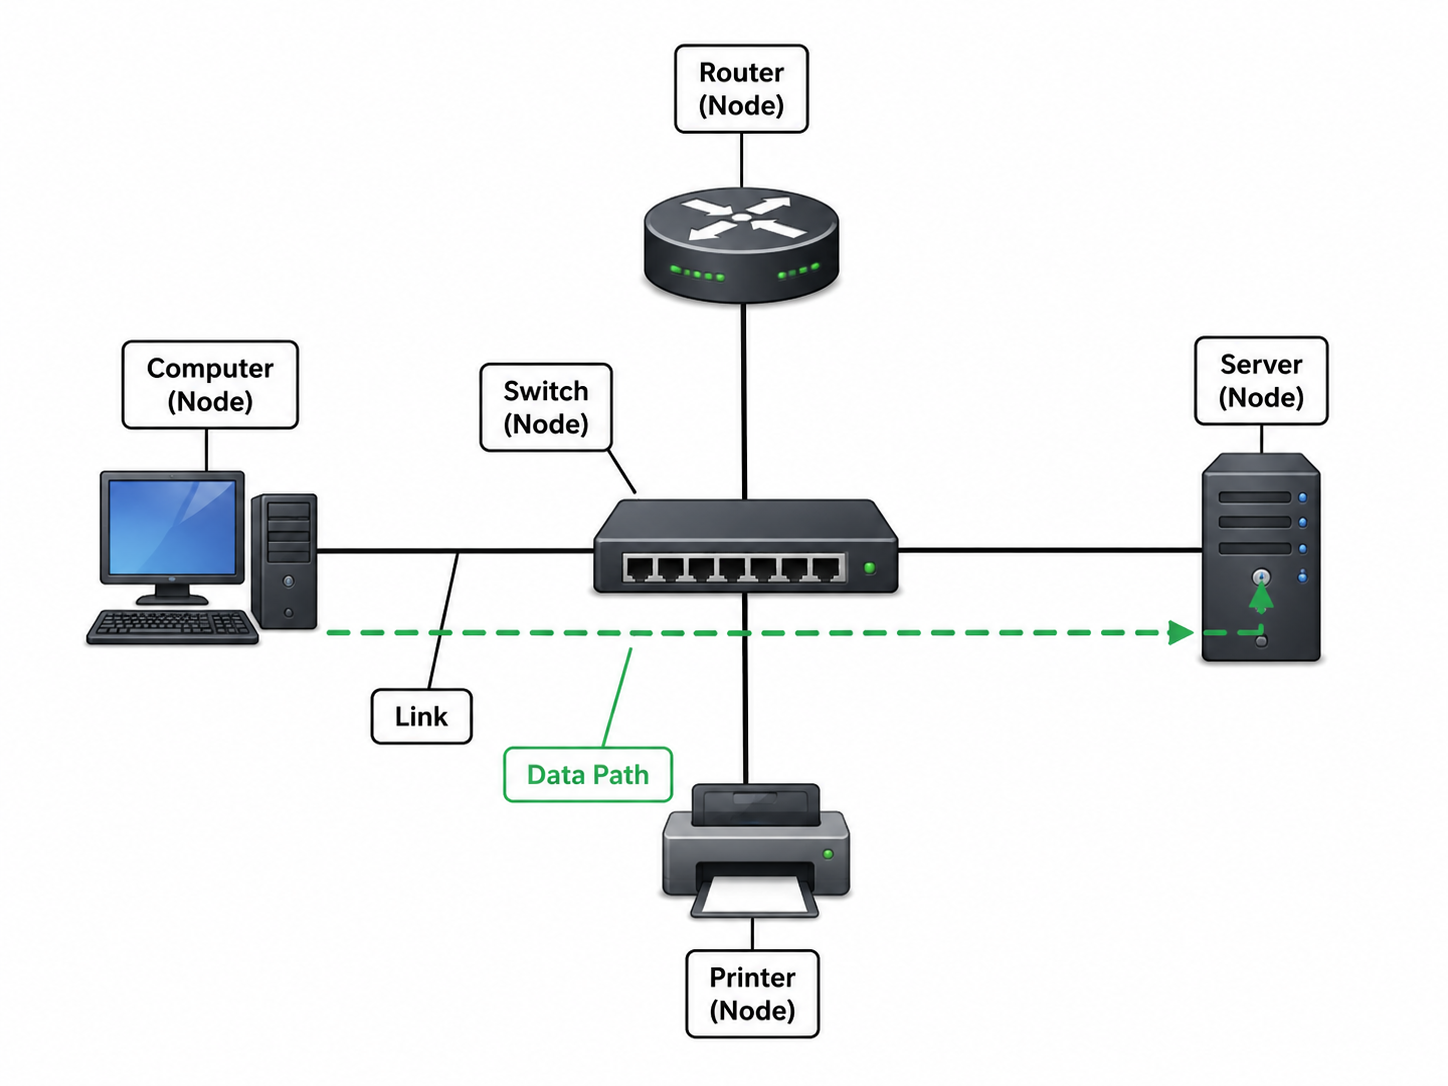
\includegraphics[width=0.82\textwidth,height=0.24\textheight,keepaspectratio]{chapters/Chapter02/images/network_topology_basic_concept.png}
}{
\fbox{\parbox{0.78\textwidth}{\centering
\vspace{0.35cm}
Node \quad Link \quad Data Path\\[4pt]
Computer \quad Switch \quad Router \quad Server
\vspace{0.35cm}
}}
}
\caption{নেটওয়ার্ক টপোলজির মৌলিক ধারণা}
\end{figure}

\subsection{Physical ও Logical Topology}

\begin{compacttable}
\begin{tabular}{|p{0.24\textwidth}|p{0.32\textwidth}|p{0.32\textwidth}|}
\hline
\textbf{বিষয়} & \textbf{Physical topology} & \textbf{Logical topology} \\
\hline
অর্থ & device ও cable বাস্তবে কীভাবে বসানো হয়েছে & data বাস্তবে কোন পথে চলাচল করে \\
\hline
কেন্দ্র & hardware layout & data flow path \\
\hline
দেখা যায় & diagram বা cable layout দেখে বোঝা যায় & protocol ও data transmission দেখে বোঝা যায় \\
\hline
উদাহরণ & Star cable layout, Bus backbone & switch forwarding, token passing \\
\hline
\end{tabular}
\end{compacttable}

\examfocus{Topology-এর উত্তরে layout, node, link, connection pattern এবং data path শব্দগুলো ব্যবহার করলে উত্তর বেশি board-standard হয়।}

\subsection{প্রধান Topology}

HSC ICT-তে সাধারণত Bus, Star, Ring, Mesh, Tree ও Hybrid topology বেশি গুরুত্বপূর্ণ।

\begin{compacttable}
\begin{tabular}{|p{0.15\textwidth}|p{0.24\textwidth}|p{0.24\textwidth}|p{0.24\textwidth}|}
\hline
\textbf{Topology} & \textbf{Structure} & \textbf{সুবিধা} & \textbf{অসুবিধা} \\
\hline
Bus & common backbone cable & cable কম, setup সহজ & backbone failure হলে network বন্ধ \\
\hline
Star & central switch/hub & manage ও troubleshoot সহজ & central device-এর উপর নির্ভরশীল \\
\hline
Ring & closed loop & ordered data flow & node/link failure সমস্যা তৈরি করতে পারে \\
\hline
Mesh & multiple path & reliability বেশি & cost ও complexity বেশি \\
\hline
Tree & hierarchical & বড় network organize সহজ & backbone/root dependency থাকে \\
\hline
Hybrid & mixed topology & flexible ও practical & design ও maintenance জটিল \\
\hline
\end{tabular}
\end{compacttable}

\subsection{Bus Topology}

\definition{Bus Topology}{যে topology-তে সব node একটি common communication line বা backbone cable-এর সাথে যুক্ত থাকে, তাকে Bus topology বলা হয়।}

Bus topology-তে data main cable দিয়ে travel করে। কোনো node data পাঠালে signal backbone cable দিয়ে যায় এবং destination node সেটি গ্রহণ করে। ছোট বা temporary network বোঝাতে এই topology সহজ, কিন্তু backbone cable নষ্ট হলে পুরো network প্রভাবিত হতে পারে।

\begin{rightimageblock}{chapters/Chapter02/images/bus_topology_diagram.png}{Bus topology}
\subtopichead{বৈশিষ্ট্য}
\begin{compactpoints}
\item একটি common backbone cable থাকে।
\item cable কম লাগে, তাই cost কম হতে পারে।
\item node বেশি হলে traffic ও collision বাড়তে পারে।
\item fault finding তুলনামূলক কঠিন।
\item backbone cable failure হলে পুরো network বন্ধ হতে পারে।
\end{compactpoints}
\end{rightimageblock}

\subsection{Star Topology}

\definition{Star Topology}{যে topology-তে সব node একটি central device যেমন switch বা hub-এর সাথে আলাদাভাবে connected থাকে, তাকে Star topology বলা হয়।}

Star topology আধুনিক LAN-এ সবচেয়ে বেশি ব্যবহৃত topology-এর একটি। এখানে প্রতিটি computer আলাদা cable দিয়ে switch বা hub-এর সাথে যুক্ত থাকে। কোনো একটি node-এর cable নষ্ট হলে সাধারণত শুধু সেই node affected হয়; তবে central device নষ্ট হলে পুরো network বন্ধ হতে পারে।

\begin{rightimageblock}{chapters/Chapter02/images/star_topology_diagram.png}{Star topology}
\subtopichead{বৈশিষ্ট্য}
\begin{compactpoints}
\item central device থাকে।
\item management ও troubleshooting সহজ।
\item নতুন node add করা সহজ।
\item cable bus topology-এর চেয়ে বেশি লাগতে পারে।
\item switch ব্যবহারে performance ভালো হয়।
\end{compactpoints}
\end{rightimageblock}

\subsection{Ring Topology}

\definition{Ring Topology}{যে topology-তে প্রতিটি node পাশের দুইটি node-এর সাথে connected থাকে এবং সব node মিলে closed loop তৈরি করে, তাকে Ring topology বলা হয়।}

Ring topology-তে data সাধারণত নির্দিষ্ট direction-এ node থেকে node-এ যায়। একটি node data receive করে দেখে সেটি তার জন্য কি না; না হলে পরবর্তী node-এ forward করে।

\begin{compactpoints}
\item ordered data flow থাকে।
\item collision কম হতে পারে।
\item node বা link failure হলে network প্রভাবিত হতে পারে।
\item নতুন node add করা তুলনামূলক কঠিন।
\end{compactpoints}

\smallimage[0.48\textwidth]{chapters/Chapter02/images/ring_topology_diagram.png}{Ring topology}

\subsection{Mesh Topology}

\definition{Mesh Topology}{যে topology-তে প্রতিটি node অন্য node-গুলোর সাথে সরাসরি বা একাধিক path দ্বারা connected থাকে, তাকে Mesh topology বলা হয়।}

Mesh topology reliability-এর জন্য গুরুত্বপূর্ণ। কোনো একটি path নষ্ট হলেও alternative path দিয়ে communication চলতে পারে। তাই critical network, backbone বা high availability system-এ mesh concept ব্যবহার করা হয়।

\begin{compacttable}
\begin{tabular}{|p{0.28\textwidth}|p{0.29\textwidth}|p{0.29\textwidth}|}
\hline
\textbf{ধরন} & \textbf{ধারণা} & \textbf{ব্যবহার} \\
\hline
Full Mesh & প্রতিটি node অন্য সব node-এর সাথে connected & খুব high reliability দরকার হলে \\
\hline
Partial Mesh & প্রয়োজনীয় node-গুলোর মধ্যে multiple path থাকে & practical large network \\
\hline
\end{tabular}
\end{compacttable}

\remember{Mesh topology reliable হলেও cable, device port, configuration ও maintenance cost বেশি।}

\subsection{Tree Topology}

\definition{Tree Topology}{Star topology-এর মতো বিভিন্ন group যখন hierarchical বা parent-child structure-এ যুক্ত হয়, তখন তাকে Tree topology বলা হয়।}

Tree topology বড় office, campus বা institution network organize করতে সুবিধাজনক। এখানে root বা backbone অংশ থাকে, যার সাথে বিভিন্ন branch network যুক্ত হয়।

\begin{compactpoints}
\item hierarchical structure থাকে।
\item বড় network section অনুযায়ী organize করা যায়।
\item expansion তুলনামূলক সহজ।
\item backbone/root failure হলে বড় অংশ affected হতে পারে।
\end{compactpoints}

\subsection{Hybrid Topology}

\definition{Hybrid Topology}{দুই বা ততোধিক topology মিলিয়ে যে practical network design তৈরি হয়, তাকে Hybrid topology বলা হয়।}

বাস্তব বড় network-এ প্রায়ই pure topology ব্যবহার করা হয় না। যেমন একটি campus network-এ department-wise Star topology থাকতে পারে, আর department-গুলো backbone-এর সাথে Tree বা Mesh structure-এ যুক্ত থাকতে পারে।

\begin{imagefirstblock}[0.74\textwidth]{chapters/Chapter02/images/hybrid_topology_diagram.png}{Hybrid topology}
Hybrid topology-তে network designer প্রয়োজন অনুযায়ী একাধিক topology combine করে। যেমন একটি school বা college campus-এ প্রতিটি lab-এ Star topology, building-to-building backbone-এ Tree topology এবং important server connection-এ Mesh-like redundant path থাকতে পারে। ফলে network একই সঙ্গে manageable, expandable এবং তুলনামূলক reliable হয়।
\end{imagefirstblock}

\subtopichead{Hybrid topology-এর বৈশিষ্ট্য}
\begin{compactpoints}
\item এটি fixed single pattern নয়; প্রয়োজন অনুযায়ী Bus, Star, Ring, Mesh বা Tree topology mix করা যায়।
\item বড় organization, campus, bank, ISP বা data center network-এ practical design হিসেবে বেশি দেখা যায়।
\item network-এর এক অংশ নষ্ট হলেও অন্য অংশ অনেক ক্ষেত্রে চলতে পারে, যদি redundant path থাকে।
\item design, installation এবং troubleshooting pure topology-এর তুলনায় complex হতে পারে।
\item ভবিষ্যতে নতুন department, floor, lab বা branch add করা তুলনামূলক flexible।
\end{compactpoints}

\begin{compacttable}
\begin{tabular}{|p{0.28\textwidth}|p{0.30\textwidth}|p{0.30\textwidth}|}
\hline
\textbf{উদাহরণ} & \textbf{মিশ্রণ} & \textbf{কারণ} \\
\hline
School/college lab network & Star + Tree & প্রতিটি lab switch-based, lab-গুলো backbone-এর সাথে hierarchical \\
\hline
Bank branch network & Star + Mesh & branch LAN সহজ, main server বা data center link reliable \\
\hline
ISP/campus backbone & Tree + Mesh & বড় area organize করা যায়, important route-এ alternative path থাকে \\
\hline
\end{tabular}
\end{compacttable}

\important{Hybrid topology বাস্তব network design-এ সবচেয়ে practical, কারণ এটি প্রয়োজন অনুযায়ী বিভিন্ন topology-এর সুবিধা একত্র করে।}

\subsection{Topology তুলনা}

\begin{compacttable}
\begin{tabular}{|p{0.16\textwidth}|p{0.18\textwidth}|p{0.18\textwidth}|p{0.18\textwidth}|p{0.18\textwidth}|}
\hline
\textbf{Topology} & \textbf{Cost} & \textbf{Reliability} & \textbf{Expansion} & \textbf{Fault finding} \\
\hline
Bus & কম & কম & সীমিত & কঠিন \\
\hline
Star & মাঝারি & ভালো & সহজ & সহজ \\
\hline
Ring & মাঝারি & মাঝারি & কঠিন & কঠিন \\
\hline
Mesh & বেশি & খুব ভালো & জটিল & মাঝারি \\
\hline
Tree & মাঝারি/বেশি & ভালো & সহজ & মাঝারি \\
\hline
Hybrid & design অনুযায়ী & ভালো & flexible & design অনুযায়ী \\
\hline
\end{tabular}
\end{compacttable}

\subsection{পরিস্থিতি অনুযায়ী নির্বাচন}

\begin{compacttable}
\begin{tabular}{|p{0.34\textwidth}|p{0.24\textwidth}|p{0.30\textwidth}|}
\hline
\textbf{পরিস্থিতি} & \textbf{উপযুক্ত topology} & \textbf{কারণ} \\
\hline
ছোট temporary network & Bus & cable কম লাগে, setup সহজ \\
\hline
School computer lab & Star & switch দিয়ে manage সহজ \\
\hline
High reliability critical network & Mesh & alternative path থাকে \\
\hline
Campus বা বড় office & Tree/Hybrid & hierarchy ও flexibility থাকে \\
\hline
Mixed requirement corporate network & Hybrid & প্রয়োজন অনুযায়ী topology combine করা যায় \\
\hline
\end{tabular}
\end{compacttable}

\subsection{Common Mistake}

\warningline{LAN, MAN, WAN হলো area অনুযায়ী network type; Bus, Star, Ring, Mesh, Tree, Hybrid হলো topology বা connection layout।}

\warningline{Star topology-তে একটি node নষ্ট হলে পুরো network বন্ধ হয় না, কিন্তু central switch/hub নষ্ট হলে পুরো network প্রভাবিত হতে পারে।}

\subsection{অনুশীলন}

\qhead{MCQ}
\begin{compactenum}
\item Network topology কী নির্দেশ করে?\\
\mcqoption{network layout}{internet speed}{file size}{software version}
\item Star topology-তে central device হিসেবে সাধারণত কোনটি ব্যবহৃত হয়?\\
\mcqoption{Switch}{Printer}{Scanner}{Monitor}
\item কোন topology-তে reliability বেশি কিন্তু cost বেশি?\\
\mcqoption{Mesh}{Bus}{Ring}{Star}
\end{compactenum}

\qhead{সংক্ষিপ্ত প্রশ্ন}
\begin{compactenum}
\item Network topology কী?
\item Physical topology ও Logical topology-এর পার্থক্য লেখ।
\item Bus topology-এর দুটি সুবিধা ও দুটি অসুবিধা লেখ।
\item Star topology school lab-এর জন্য কেন উপযোগী?
\item Hybrid topology বলতে কী বোঝায়?
\end{compactenum}

\qhead{বোর্ড স্টাইল উত্তর}
\boardanswer
{Star topology বলতে কী বোঝায়?}
{যে network topology-তে সব node একটি central device যেমন switch বা hub-এর সাথে আলাদাভাবে connected থাকে, তাকে Star topology বলা হয়। এতে node add করা, management এবং troubleshooting সহজ হয়; তবে central device নষ্ট হলে পুরো network প্রভাবিত হতে পারে।}

% Canonical theory homes C10.01--C10.14. No solved-question/revision duplicates.
\begingroup
\chTwoReadableTopicStyle
\widowpenalty=10000\clubpenalty=10000
\section{ক্লাউড কম্পিউটিং}
\subsection{Cloud Computing: কেন প্রয়োজন, কীভাবে কাজ করে}
\label{ch2:c10-01}
\begin{definitionbox}{Cloud Computing}
নেটওয়ার্কের মাধ্যমে ভাগাভাগি করা ও প্রয়োজনমতো বিন্যস্ত করা যায় এমন কম্পিউটিং সম্পদ থেকে চাহিদা অনুযায়ী দ্রুত সার্ভার, স্টোরেজ, নেটওয়ার্ক ও অ্যাপ্লিকেশন নেওয়া এবং ছেড়ে দেওয়ার ব্যবস্থাকে ক্লাউড কম্পিউটিং বলে। এতে প্রতিবার সেবাদাতার কর্মীর সঙ্গে যোগাযোগ করে ব্যবস্থা নেওয়ার প্রয়োজন কম থাকে।
\end{definitionbox}
কলেজের ভর্তি ওয়েবসাইটে কয়েক দিনের জন্য অনেক ব্যবহারকারী আসে। সারা বছরের জন্য সর্বোচ্চ ক্ষমতার সার্ভার কিনলে অধিকাংশ সময় তার ব্যবহার কম হতে পারে। ক্লাউডে প্রয়োজন অনুযায়ী সম্পদ নেওয়া যায়। অনলাইন স্টোরেজের পাশাপাশি অ্যাপ্লিকেশন, ডেটাবেজ ও প্রক্রিয়াকরণও ক্লাউড সেবা হতে পারে।
\chTwoPair{\textbf{ব্যবস্থার উপাদান ও কাজ}\par ফোন বা ল্যাপটপ ক্লায়েন্ট হিসেবে নেটওয়ার্ক দিয়ে অনুরোধ পাঠায়। সার্ভার অ্যাকাউন্ট ও অনুমতি যাচাই করে অ্যাপ্লিকেশন চালায়। স্টোরেজ বা ডেটাবেজ থেকে তথ্য নেয় কিংবা সেখানে তথ্য রাখে এবং ফল ক্লায়েন্টে ফেরত পাঠায়। সেবাদাতার ডেটা সেন্টারে ভৌত সার্ভার, নেটওয়ার্ক, স্টোরেজ ও সেবা পরিচালনার সফটওয়্যার থাকে।}{\centering
\begin{tikzpicture}[node distance=8mm]
\node[chTwoNode,text width=2.8cm] (u) {Client\\Phone/Laptop};
\node[chTwoNode,text width=2.8cm,below=of u] (n) {Network};
\node[chTwoNode,text width=2.8cm,below=of n] (s) {Cloud Service\\Server + Storage};
\draw[chTwoLink,<->] (u)--(n);
\draw[chTwoLink,<->] (n)--(s);
\end{tikzpicture}\par Request যায়; Data/ফল ফিরে আসে।}
Public Cloud-এর সেবা সাধারণত ইন্টারনেট দিয়ে পাওয়া যায়। Private Cloud নিজস্ব নেটওয়ার্কেও চলতে পারে। দূরের কম্পিউটারে ফাইল রাখা বা ওয়েবসাইট পরিচালনা করলেই ক্লাউডের সব বৈশিষ্ট্য পূরণ হয় না। \textbf{Virtualization}-এ একটি ভৌত যন্ত্রের সম্পদ দিয়ে একাধিক ভার্চুয়াল যন্ত্র চলে। এটি ক্লাউড তৈরিতে সাহায্য করে। তবে ক্লাউডে সম্পদ বরাদ্দ, প্রবেশাধিকার, ব্যবস্থাপনা ও ব্যবহার মাপার ব্যবস্থাও প্রয়োজন।

\subsection{পাঁচটি মৌলিক বৈশিষ্ট্য}
\label{ch2:c10-02}
ক্লাউডের ব্যবহার বোঝার তিনটি সেবানীতি হলো: \textbf{চাহিদামতো সেবা নেওয়া}, \textbf{চাহিদা অনুযায়ী সম্পদ বাড়ানো বা কমানো} এবং \textbf{ব্যবহারের পরিমাণ অনুযায়ী মূল্য দেওয়া}। এগুলো সুবিধা বোঝানোর সংক্ষিপ্ত ছক। পূর্ণ মান অনুযায়ী বৈশিষ্ট্যের তালিকা নিচে দেওয়া হয়েছে।

NIST (National Institute of Standards and Technology)-এর ২০১১ সালের SP 800-145 সংজ্ঞায় পাঁচটি মৌলিক বৈশিষ্ট্য, তিনটি সেবা মডেল ও চারটি স্থাপনা মডেল রয়েছে।
\begin{description}
\item[On-demand Self-service:] ব্যবহারকারী চাহিদা অনুযায়ী নিজেই স্টোরেজ বা প্রক্রিয়াকরণের সম্পদ চেয়ে নিতে পারেন। প্রতিবার সেবাদাতার কর্মীর সঙ্গে যোগাযোগ প্রয়োজন হয় না।
\item[Broad Network Access:] নেটওয়ার্কের প্রচলিত ব্যবস্থায় বিভিন্ন ক্লায়েন্ট ডিভাইস থেকে সেবা ব্যবহার করা যায়।
\item[Resource Pooling:] সেবাদাতার ভৌত ও ভার্চুয়াল সম্পদের একটি ভান্ডার থেকে ব্যবহারকারীর চাহিদা অনুযায়ী সম্পদ বরাদ্দ ও পুনর্বণ্টন করা হয়। গ্রাহক সাধারণত নির্দিষ্ট ভৌত সার্ভার নির্বাচন করেন না।
\item[Rapid Elasticity:] চাহিদা বাড়লে দ্রুত সম্পদ বাড়ানো এবং কমলে তা ছেড়ে দেওয়া যায়। ভর্তি চলাকালে সক্ষমতা বাড়িয়ে পরে কমানো এর উদাহরণ।
\item[Measured Service:] স্টোরেজ, প্রক্রিয়াকরণ, ডেটা স্থানান্তর বা অ্যাকাউন্টের ব্যবহার মাপা, নিয়ন্ত্রণ ও প্রতিবেদন করা যায়। ব্যবহারের সঙ্গে বিল সম্পর্কিত হতে পারে। সব সেবার মূল্য নির্ধারণের পদ্ধতি একই নয়।
\end{description}

\subsection{Service Model: কী পাওয়া যায়, কে পরিচালনা করে}
\label{ch2:c10-03}
\begin{tabularx}{\linewidth}{|p{.18\linewidth}|X|X|}\hline
\textbf{Model} & \textbf{সেবা ও ব্যবহারকারীর দায়িত্ব} & \textbf{ব্যবহারের উদাহরণ}\\\hline
IaaS: Infrastructure as a Service & ভার্চুয়াল যন্ত্র, স্টোরেজ ও নেটওয়ার্ক পাওয়া যায়। সেবাদাতা ভৌত অবকাঠামো চালায়। ব্যবহারকারী সাধারণত OS, অ্যাপ্লিকেশন ও ডেটা পরিচালনা করেন। & ভর্তি, পরীক্ষা বা ব্যাকআপের সার্ভার; যেমন AWS EC2, Azure Virtual Machines, Google Compute Engine। OS ও অ্যাপ্লিকেশন হালনাগাদ এবং কনফিগারেশন নিজে করতে হয়।\\\hline
PaaS: Platform as a Service\label{ch2:c10-04} & সেবাদাতার প্রস্তুত রানটাইম ও উন্নয়ন প্ল্যাটফর্মে অ্যাপ্লিকেশন তৈরি ও চালানো যায়। ব্যবহারকারী অ্যাপ্লিকেশন ও ডেটা পরিচালনা করেন। OS ও রানটাইম ব্যবস্থাপনার বড় অংশ সেবাদাতা করে। & ওয়েবসাইটের কোড স্থাপন; যেমন Google App Engine, Azure App Service, Heroku। সেবাদাতা OS ও প্ল্যাটফর্ম চালায়। অ্যাপ্লিকেশনকে সমর্থিত ভাষা, টুল ও সীমার সঙ্গে মানিয়ে নিতে হয়।\\\hline
SaaS: Software as a Service\label{ch2:c10-05} & প্রস্তুত অ্যাপ্লিকেশন ব্যবহার করা যায়। সেবাদাতা কেন্দ্রীয় সার্ভার ও অ্যাপ্লিকেশন হালনাগাদ করে। ব্যবহারকারীকে নিজের সার্ভারে প্রতিবার নতুন সংস্করণ বসাতে হয় না। নিজের ডেটা, অ্যাকাউন্ট ও অনুমতি পরিচালনা করতে হয়। & Gmail, Google Docs/Sheets, Microsoft 365, Dropbox, Canva বা Zoom ব্যবহার। নিজস্ব সার্ভার বা অ্যাপ্লিকেশন তৈরি করতে হয় না।\\\hline
\end{tabularx}
IaaS থেকে SaaS-এর দিকে ব্যবহারকারীর পরিচালনাগত দায়িত্ব কমে। তবে সবক্ষেত্রে অ্যাকাউন্ট ও ডেটার নিয়ন্ত্রণ এবং নিরাপদ ব্যবহার প্রয়োজন। SaaS ব্যবহার করলেও নিজের ডিভাইসের OS ও ব্রাউজার হালনাগাদ রাখতে হয়। একই সেবাদাতা বিভিন্ন মডেলের সেবা দিতে পারে। নির্দিষ্ট সেবার কাজ দেখে মডেল শনাক্ত করতে হয়।
\subsection{Deployment Model: কার জন্য Infrastructure}
\label{ch2:c10-06}
\begin{longtable}{|p{\dimexpr .18\linewidth-7pt\relax}|p{\dimexpr .40\linewidth-7pt\relax}|p{\dimexpr .42\linewidth-7pt\relax}|}\hline
\textbf{Model} & \textbf{ব্যবহার ও নিয়ন্ত্রণ} & \textbf{উদাহরণ, সুবিধা ও সীমা}\\\hline
\endfirsthead\hline\textbf{Model} & \textbf{ব্যবহার ও নিয়ন্ত্রণ} & \textbf{উদাহরণ, সুবিধা ও সীমা}\\\hline\endhead
Public & সাধারণ গ্রাহকের জন্য সেবাদাতা সম্পদ পরিচালনা করে। সেবাদাতা ব্যবসায়িক, সরকারি বা শিক্ষাপ্রতিষ্ঠান হতে পারে। & বড় প্রাথমিক হার্ডওয়্যার ব্যয় ছাড়াই সেবা পাওয়া যায়। Public মানে সব ফাইল উন্মুক্ত বা সব সেবা বিনামূল্যে নয়।\\\hline
Private\label{ch2:c10-07} & এক প্রতিষ্ঠানের একক ব্যবহারের ব্যবস্থা। নিজে বা অন্য সেবাদাতা পরিচালনা করতে পারে। প্রতিষ্ঠানের ভেতরে বা বাইরে থাকতে পারে। & ব্যাংকের নিজস্ব ব্যবস্থাপনা বা কলেজের সংবেদনশীল ফলাফল। নিয়ন্ত্রণ ও নিজস্ব প্রয়োজন অনুযায়ী বিন্যাসের সুযোগ বেশি। দক্ষ দল ও অর্থ প্রয়োজন। নিরাপত্তার ঝুঁকি শূন্য হয় না।\\\hline
Community\label{ch2:c10-08} & অভিন্ন উদ্দেশ্য, নীতি বা নিরাপত্তার প্রয়োজন রয়েছে এমন কয়েকটি প্রতিষ্ঠানের নির্দিষ্ট গোষ্ঠীর জন্য। & হাসপাতাল, গবেষণা বা সরকারি প্রতিষ্ঠানের যৌথ ব্যবস্থা। খরচ ভাগ করা যায়; দায়িত্ব ও নীতিতে সমঝোতা প্রয়োজন। সাধারণ Public অ্যাকাউন্ট থাকা এর প্রমাণ নয়।\\\hline
Hybrid\label{ch2:c10-09} & পৃথক Public/Private/Community Cloud নিজস্ব পরিচয় বজায় রেখে ডেটা বা অ্যাপ্লিকেশনের জন্য প্রযুক্তিগতভাবে সংযুক্ত থাকে। & ব্যক্তিগত ফলাফল ব্যবস্থা ও সাধারণের ভর্তি সেবার সমন্বয়। নিয়ন্ত্রণ ও চাহিদা সামলানো যায়; সমন্বয় ও প্রবেশাধিকার পরিচালনা জটিল। স্থানীয় কম্পিউটার ও পৃথক Drive পাশাপাশি ব্যবহার যথেষ্ট নয়।\\\hline
\end{longtable}
\subsection{Service ও Deployment: দুই স্বতন্ত্র ভিত্তি}
\label{ch2:c10-10}
\chTwoPair{\textbf{Service Model}\par কী সম্পদ পাওয়া যায় এবং কোন স্তর নিজে পরিচালনা করতে হয়, তা বোঝায়। IaaS/PaaS/SaaS-এর মূল ব্যাখ্যা অংশ \ref{ch2:c10-03}-এ আছে।}{\textbf{Deployment Model}\par অবকাঠামো কার ব্যবহারের জন্য এবং কীভাবে নিয়ন্ত্রিত বা সমন্বিত, তা বোঝায়। Public/Private/Community/Hybrid-এর ব্যাখ্যা অংশ \ref{ch2:c10-06}-এ আছে।}
প্রস্তুত অনলাইন ডকুমেন্ট সেবা একই সঙ্গে SaaS ও Public Deployment হতে পারে। পরিচয় দুটি পরস্পরের বিকল্প নয়। ফাইল রাখার সুবিধা অনুযায়ী Google Drive ক্লাউড স্টোরেজ এবং প্রস্তুত অ্যাপ্লিকেশন হিসেবে SaaS। Azure/AWS সেবাদাতা বা সেবাসমষ্টির নাম। তাদের ভার্চুয়াল যন্ত্র ও পরিচালিত অ্যাপ্লিকেশন প্ল্যাটফর্মের মডেল আলাদা হতে পারে। শুধু সেবাদাতার নাম দিয়ে নির্দিষ্ট সেবা মডেল নির্ধারণ করা যায় না।
\chTwoPair{\textbf{NaaS (Network as a Service):} গ্রাহকচুক্তিতে নেটওয়ার্ক সংযোগ, ব্যান্ডউইথ, VPN ও সংশ্লিষ্ট ব্যবস্থাপনা সেবা পাওয়া যায়। যেমন, শাখার সংযোগের সব যন্ত্র নিজে পরিচালনা না করে সেবাদাতার কাছ থেকে সেবা নেওয়া। এখানে নেটওয়ার্কের সম্পদ ও সেবা দেওয়া মূল বিষয়; প্রস্তুত সফটওয়্যার ব্যবহার নয়।}{\textbf{CuaS: ক্লায়েন্ট দিয়ে ক্লাউডে প্রবেশ} Cloud user as a Service (CuaS) নাম দিয়ে ব্রাউজারসহ কম্পিউটার, ট্যাবলেট বা ফোন থেকে ক্লাউডে প্রবেশের ক্লায়েন্ট অংশ বোঝানো হয়। Chrome/Firefox প্রবেশের টুল; নিজেরা ক্লাউড স্টোরেজ নয়। এটি NIST-এর চতুর্থ সেবা মডেল নয়। প্রধান তিনটি মডেল IaaS, PaaS ও SaaS।}

\subsection{Cloud Storage, Sync ও পুনরুদ্ধার}
\label{ch2:c10-11}
নেটওয়ার্ক দিয়ে ক্লাউড সার্ভার বা ডেটা সেন্টারে ফাইল ও ডেটা সংরক্ষণ এবং ব্যবহারের ব্যবস্থাকে ক্লাউড স্টোরেজ বলে। উপযুক্ত প্রবেশাধিকার থাকলে বিভিন্ন ডিভাইস থেকে ফাইল, ছবি ও ভিডিও ব্যবহার, ভাগাভাগি এবং যৌথভাবে কাজ করা যায়। Google Drive, OneDrive, Dropbox ও iCloud পরিচিত উদাহরণ।
\chTwoDiagramRow{cloudbackup}{পরিবর্তন ছড়ানো ও ব্যাকআপের পার্থক্য}{Sync একই পরিবর্তন সংযুক্ত ডিভাইস ও ক্লাউডে ছড়িয়ে দেয়। ভুল করে ফাইল মুছে ফেললে সেই পরিবর্তনও ছড়াতে পারে। ব্যাকআপ পুনরুদ্ধারের জন্য রাখা কপি। আগের সংস্করণের ইতিহাস, পৃথক কপি ও পুনরুদ্ধারের পরীক্ষা প্রয়োজন। সেবাদাতার সার্ভার সচল থাকা এবং নিজের মুছে ফেলা ফাইল ফেরত পাওয়া আলাদা বিষয়।}

\subsection{সুবিধা, খরচ ও সীমাবদ্ধতা}
\label{ch2:c10-12}
\begin{tabularx}{\linewidth}{|p{.28\linewidth}|X|X|}\hline
\textbf{বিষয়} & \textbf{প্রাসঙ্গিক সুবিধা} & \textbf{সীমা/খরচ}\\\hline
সম্পদ ও রক্ষণাবেক্ষণ & নিজের সব ভৌত সার্ভার কিনতে হয় না; অনেক অংশ সেবাদাতা পরিচালনা করে & সেবাদাতার ওপর নির্ভরশীলতা; মডেল অনুযায়ী নিয়ন্ত্রণ ও নিজস্ব দায়িত্ব বদলায়\\\hline
চাহিদা ও খরচ & দ্রুত সম্পদ বাড়ানো বা কমানো; প্রাথমিক বিনিয়োগ কমতে পারে & দীর্ঘদিন বেশি সংরক্ষণ, স্থানান্তর ও প্রক্রিয়াকরণে বিল বাড়ে\\\hline
প্রবেশ ও যৌথ কাজ & উপযুক্ত নেটওয়ার্কে বিভিন্ন ডিভাইস থেকে একই ডকুমেন্টে কাজ & নেটওয়ার্ক বা সেবাদাতার সেবা বন্ধ থাকলে কাজ ব্যাহত; সব কাজ অফলাইনে করা যায় না\\\hline
ডেটা ব্যবস্থাপনা & ভাগাভাগি ও পুনরুদ্ধারের ব্যবস্থা সহজ করা যায় & গোপনীয়তা, ভুল করে মুছে ফেলা ও অননুমোদিত ভাগাভাগির ঝুঁকি; আগের সংস্করণ বা ব্যাকআপ দরকার\\\hline
পরিবর্তন ও স্থানান্তর & নতুন সম্পদ দ্রুত নেওয়া যায় & সেবাদাতা বদলাতে ডেটা ও টুল সরানো জটিল হতে পারে; Vendor Lock-in\\\hline
\end{tabularx}
স্থানীয় ব্যবস্থায় প্রতিষ্ঠান হার্ডওয়্যার, সক্ষমতা ও রক্ষণাবেক্ষণ নিজের মতো পরিচালনা করে। সক্ষমতা বাড়াতে নতুন যন্ত্র ও সময় প্রয়োজন। ক্লাউডে সম্পদ দ্রুত বরাদ্দ করা গেলেও বিল, সংযোগ, সেবাদাতার শর্ত এবং ডেটা রাখার নীতি বিবেচ্য। Pay-as-you-go সবসময় কম মোট খরচ নিশ্চিত করে না। ব্যবহার ও বিল মাপতে হয় এবং অপ্রয়োজনীয় সম্পদ বন্ধ রাখতে হয়।

\subsection{Security ও Shared Responsibility}
\label{ch2:c10-13}
সেবাদাতা ক্লাউড অবকাঠামোর নিরাপত্তা ও পরিচালনার দায়িত্ব নেয়। ব্যবহারকারীর অ্যাকাউন্ট, ডেটা ও প্রবেশাধিকারের দায়িত্ব থাকে। মডেল অনুযায়ী OS ও অ্যাপ্লিকেশন পরিচালনার দায়িত্ব অংশ \ref{ch2:c10-03}-এ আছে। সেবাদাতা আছে বলেই ব্যবহারকারীর সব দায়িত্ব শেষ হয় না।
\chTwoPair{\textbf{কীভাবে সুরক্ষা বাড়তে পারে?}\par
সেবাদাতার প্রবেশাধিকার নিয়ন্ত্রণ, নিয়মিত অবকাঠামো হালনাগাদ ও বিশেষজ্ঞ তদারকি তথ্য রক্ষায় সাহায্য করে। ব্যবহারকারীর শক্তিশালী পাসওয়ার্ড, Multi-factor Authentication (MFA), সীমিত প্রবেশাধিকার, সতর্ক ভাগাভাগি ও উপযুক্ত এনক্রিপশনও প্রয়োজন। MFA-তে ভিন্ন উপাদান দিয়ে অ্যাকাউন্ট যাচাই করা হয়। যেমন, পাসওয়ার্ডের সঙ্গে নিজের ডিভাইসের অনুমোদন।}{\textbf{ঝুঁকি কোথায় থাকে?}\par
অ্যাকাউন্ট চুরি, উন্মুক্ত শেয়ার লিংক, ভুল অনুমতি বা সেবাদাতার ত্রুটিতে অননুমোদিত প্রবেশ ঘটতে পারে। অন্যের সেবায় সংবেদনশীল ডেটা রাখার আগে সংরক্ষণ ও ভাগাভাগির নীতি এবং নিয়ন্ত্রণ দেখতে হয়। অনিরাপদ নেটওয়ার্কে অ্যাকাউন্ট ব্যবহারে সতর্কতা প্রয়োজন। এনক্রিপশন হারানো ফাইল ফেরানোর ব্যবস্থা নয়। ব্যাকআপ ও পুনরুদ্ধারের আলোচনা অংশ \ref{ch2:c10-11}-এ আছে।}

\subsection{Cloud-এর ধারণা, ইতিহাস ও ব্যবহার মাপা}
\chTwoPair{\textbf{ধারণা ও সেবার বিকাশ}\par
John McCarthy ১৯৬১ সালে কম্পিউটিংকে ইউটিলিটি সেবা হিসেবে সংগঠিত করার সম্ভাবনা আলোচনা করেন। পরে নেটওয়ার্ক, ভার্চুয়ালাইজেশন ও ডেটা সেন্টারের উন্নয়নে আধুনিক ক্লাউড গড়ে ওঠে। ২০০৬ সালে Amazon EC2-এর পরীক্ষামূলক Beta সেবা গুরুত্বপূর্ণ বাণিজ্যিক ধাপ। McCarthy-র ধারণা, EC2 চালু ও NIST-এর সংজ্ঞা পৃথক ঘটনা। এগুলো পুরো ক্লাউডের একক যন্ত্র আবিষ্কারের সাল নয়।}{\textbf{একটি কাল্পনিক খরচের হিসাব}\par
স্টোরেজের মাসিক খরচ প্রতি GB ০.৫০ টাকা এবং প্রক্রিয়াকরণের খরচ প্রতি ঘণ্টা ২ টাকা ধরা হলো। ১০০ GB স্টোরেজ ও ১২০ Compute-hour-এর খরচ $100\times0.50+120\times2=290$ টাকা। এটি শেখানোর কাল্পনিক উদাহরণ; সেবাদাতার বর্তমান মূল্য নয়। ডেটা স্থানান্তর, কর ও অন্যান্য খরচ থাকলে পৃথকভাবে যোগ করতে হবে।}
ক্লাউডের জন্য নির্দিষ্ট সর্বোচ্চ দূরত্ব নেই। ক্লায়েন্টের নেটওয়ার্ক সংযোগ ও সেবা পাওয়ার সুযোগ প্রয়োজন। GB সংরক্ষণের পরিমাণ, Mbps ডেটা স্থানান্তরের হার এবং Compute-hour প্রক্রিয়াকরণের ব্যবহৃত সময় বোঝায়। তিনটির একক ও বিল আলাদা। অ্যাকাউন্টসংখ্যা বা বিনামূল্যের স্টোরেজের সীমা সেবাদাতার শর্ত অনুযায়ী বদলায়। একটি সংখ্যাকে ক্লাউডের সংজ্ঞার অংশ ধরা যায় না।

\subsection{কলেজের ভর্তি, ক্লাস ও Result-এর প্রয়োজন}
\label{ch2:c10-14}
\begin{examplebox}{একটি বাস্তব সমস্যা থেকে সেবা নির্বাচন}
কলেজে ভর্তি চলাকালে ওয়েবসাইটে ব্যবহারকারীর চাপ বাড়ে। শিক্ষকরা নোট ও অ্যাসাইনমেন্ট ভাগাভাগি করেন। ফলাফলে প্রবেশাধিকার সীমিত রাখা প্রয়োজন। নোট, ই-মেইল, অনলাইন ডকুমেন্ট, উপস্থিতি ও সভার জন্য প্রস্তুত SaaS ব্যবহার করা যায়। নিজস্ব ভর্তি অ্যাপ্লিকেশন তৈরিতে পরিচালিত প্ল্যাটফর্ম বা PaaS সুবিধাজনক। নির্দিষ্ট OS ও সার্ভারের নিয়ন্ত্রণ প্রয়োজন হলে IaaS বিবেচনা করা যায়।

চাহিদা বাড়লে সম্পদ বাড়ানো, পরে কমানো এবং ব্যবহার ও বিল পর্যবেক্ষণ অংশ \ref{ch2:c10-02}-এর বৈশিষ্ট্যের প্রয়োগ। ফলাফলের জন্য প্রতিষ্ঠানের নিজস্ব Private ব্যবস্থা বিবেচনা করা যায়। Public Admission Cloud-এর সঙ্গে অনুমোদিত ডেটা বিনিময়ের সমন্বিত সংযোগ থাকলে Hybrid হতে পারে। গবেষণাগারের সাময়িক বড় প্রক্রিয়াকরণের কাজেও চাহিদামতো সম্পদ নেওয়া উপকারী। বাস্তব নকশায় উপযুক্ত অনুমতি, ব্যাকআপ ও দায়িত্বের সীমা রাখতে হয়।
\end{examplebox}

\subsection{MCQ অনুশীলন}

\par
\textbf{MCQ}

\begin{multicols}{2}\begin{enumerate}
\item\chTwoMCQBlock{Public Cloud সাধারণত কোন মাধ্যমে ব্যবহার করা হয়?
\par ক. শুধু স্থানীয় প্রিন্টারে \quad খ. ইন্টারনেটের মাধ্যমে \par গ. শুধু অফলাইন ডকুমেন্টে \quad ঘ. কোনো নেটওয়ার্ক ছাড়াই }
\item\chTwoMCQBlock{Google Drive কোন ধরনের সেবার উদাহরণ?
\par ক. ক্লাউড স্টোরেজ \quad খ. স্থানীয় ডিস্কের বিন্যাস \par গ. স্থানীয় ফাইল ডিফ্র্যাগমেন্টেশন \quad ঘ. কিবোর্ডের বিন্যাস }
\item\chTwoMCQBlock{SaaS-এর পূর্ণরূপ কী?
\par ক. Storage as a Service \quad খ. Software as a Service \par গ. System as a Switch \quad ঘ. Server and Scanner }
\item\chTwoMCQBlock{IaaS প্রধানত কী দেয়?
\par ক. প্রস্তুত সফটওয়্যার \quad খ. কম্পিউটিং অবকাঠামো \par গ. কিবোর্ডের বিন্যাস \quad ঘ. মনিটরের উজ্জ্বলতা }
\item\chTwoMCQBlock{অ্যাপ্লিকেশন তৈরি ও চালাতে PaaS প্রধানত কাদের জন্য উপযোগী?
\par ক. সফটওয়্যার উন্নয়নকারী \quad খ. শুধু টাইপিস্ট \par গ. চিত্রশিল্পী \quad ঘ. বিদ্যুৎমিস্ত্রি }
\item\chTwoMCQBlock{Public Cloud সাধারণত কারা পরিচালনা করেন?
\par ক. তৃতীয় পক্ষের সেবাদাতা \quad খ. শুধু একজন শিক্ষার্থী \par গ. একটি স্থানীয় প্রিন্টার \quad ঘ. একটি মাউস }
\item\chTwoMCQBlock{Public ও Private Cloud অবকাঠামো সমন্বিতভাবে যুক্ত হলে কোন মডেল হয়?
\par ক. Hybrid Cloud \quad খ. শুধু Public Cloud \par গ. শুধু Private Cloud \quad ঘ. শুধু Community Cloud }
\item\chTwoMCQBlock{ক্লাউড কম্পিউটিংয়ের একটি সুবিধা কোনটি?
\par ক. প্রয়োজনমতো সম্পদ বাড়ানো বা কমানো \quad খ. শুধু অফলাইনে ব্যবহার \par গ. কেবল পেঁচানো \quad ঘ. মনিটর পরিষ্কার করা }
\item\chTwoMCQBlock{ক্লাউড ব্যবহারে কোন ঝুঁকি বিবেচনা করতে হয়?
\par ক. অননুমোদিত প্রবেশের ঝুঁকি \quad খ. প্রিন্টারের রং \par গ. কিবোর্ডের আকার \quad ঘ. মাউস প্যাড }
\item\chTwoMCQBlock{ক্লাউড অ্যাকাউন্টের নিরাপত্তা বাড়াতে কোন ব্যবস্থা উপযোগী?
\par ক. দুর্বল পাসওয়ার্ড \quad খ. MFA \par গ. পাসওয়ার্ড ভাগাভাগি \quad ঘ. সবার জন্য লগইন উন্মুক্ত রাখা }
\end{enumerate}\end{multicols}

\textbf{উত্তরমালা:}
১. খ, ২. ক, ৩. খ, ৪. খ, ৫. ক, ৬. ক, ৭. ক, ৮. ক, ৯. ক, ১০. খ

\smallskip

\endgroup

% Chapter 02.11: অধ্যায়ভিত্তিক অনুশীলন
\section{অধ্যায়ভিত্তিক অনুশীলন: কমিউনিকেশন সিস্টেম ও নেটওয়ার্কিং}

মূল ধারণার ব্যাখ্যা সংশ্লিষ্ট বিষয়েই রয়েছে। এখানে MCQ-এর প্রশ্ন ও উত্তরমালা এবং সমাধানবিহীন CQ অনুশীলন রাখা হয়েছে।

\subsection{MCQ: ধারণাভিত্তিক অনুশীলন}

\par
\textbf{নির্দেশনা: প্রতিটি প্রশ্নের সঠিক উত্তর নির্বাচন কর।}

\begin{multicols}{2}\begin{enumerate}
\item\chTwoMCQBlock{ডেটা কমিউনিকেশন বলতে কী বোঝায়?
\par ক. শুধু ডেটা সংরক্ষণ \par খ. ডেটা প্রেরণ ও গ্রহণ \par গ. শুধু ডেটা মুছে ফেলা \par ঘ. পর্দায় তথ্য দেখানো }
\item\chTwoMCQBlock{ডেটা কমিউনিকেশন ব্যবস্থায় যোগাযোগের নিয়মকে কী বলে?
\par ক. Protocol \par খ. Medium \par গ. Cable \par ঘ. Printer }
\item\chTwoMCQBlock{ডেটা কমিউনিকেশনের প্রধান উপাদানগুলোর মধ্যে কোনটি নেই?
\par ক. Sender \par খ. Receiver \par গ. Protocol \par ঘ. Scanner }
\item\chTwoMCQBlock{দিকভিত্তিক ট্রান্সমিশন মোড কী নির্দেশ করে?
\par ক. ডেটা সংরক্ষণের স্থান \par খ. ডেটার বিন্যাস \par গ. ডেটা প্রবাহের দিক \par ঘ. ডেটা প্রাপকের সংখ্যা }
\item\chTwoMCQBlock{টেলিভিশন সম্প্রচার দিকভিত্তিক কোন মোডের উদাহরণ?
\par ক. Half-duplex \par খ. Simplex \par গ. Full-duplex \par ঘ. Multiplex }
\item\chTwoMCQBlock{ওয়াকিটকিতে যোগাযোগ দিকভিত্তিক কোন মোডের উদাহরণ?
\par ক. Half-duplex \par খ. Simplex \par গ. Full-duplex \par ঘ. Broadcast only }
\item\chTwoMCQBlock{টেলিফোনে কথোপকথন দিকভিত্তিক কোন মোডের উদাহরণ?
\par ক. Simplex \par খ. Half-duplex \par গ. Unicast \par ঘ. Full-duplex }
\item\chTwoMCQBlock{এক প্রেরক থেকে একজন নির্দিষ্ট প্রাপকের কাছে ডেটা পাঠানোর পদ্ধতি কোনটি?
\par ক. Broadcast \par খ. Multicast \par গ. Unicast \par ঘ. Anycast }
\item\chTwoMCQBlock{এক প্রেরক থেকে সংশ্লিষ্ট নেটওয়ার্কের সব প্রাপকের উদ্দেশে ডেটা পাঠানোর পদ্ধতি কোনটি?
\par ক. Unicast \par খ. Broadcast \par গ. Multicast \par ঘ. Duplex }
\item\chTwoMCQBlock{নির্দেশিত মাধ্যমে ডেটাবাহী সংকেত কোন পথে যায়?
\par ক. নির্দিষ্ট কেবলের পথে \par খ. শুধু মুক্ত বায়ুপথে \par গ. আলোকসংকেত ছাড়াই \par ঘ. শুধু রেডিও তরঙ্গে }
\item\chTwoMCQBlock{নিচের কোনটি নির্দেশিত মাধ্যম?
\par ক. Radio wave \par খ. Microwave \par গ. Infrared \par ঘ. Optical fiber }
\item\chTwoMCQBlock{নিচের কোনটি অনির্দেশিত মাধ্যম?
\par ক. Coaxial cable \par খ. Twisted pair \par গ. Radio wave \par ঘ. Fiber optic }
\item\chTwoMCQBlock{টুইস্টেড পেয়ার কেবল সাধারণত কোন নেটওয়ার্কে বেশি ব্যবহৃত হয়?
\par ক. শুধু স্যাটেলাইট সংযোগ \par খ. LAN \par গ. টিভির রিমোট সংযোগ \par ঘ. শুধু Bluetooth সংযোগ }
\item\chTwoMCQBlock{অপটিক্যাল ফাইবার কোন সংকেত বহন করে?
\par ক. আলোক সংকেত \par খ. শব্দ সংকেত \par গ. যান্ত্রিক সংকেত \par ঘ. শুধু চৌম্বক সংকেত }
\item\chTwoMCQBlock{প্রচলিত টিভির রিমোট সাধারণত কোন মাধ্যম ব্যবহার করে?
\par ক. Optical fiber \par খ. Coaxial cable \par গ. Twisted pair \par ঘ. Infrared }
\item\chTwoMCQBlock{স্থলভিত্তিক মাইক্রোওয়েভ যোগাযোগে সাধারণত কোনটি গুরুত্বপূর্ণ?
\par ক. আয়নমণ্ডল থেকে ফিরে আসা \par খ. তামার তারে সংকেত পাঠানো \par গ. সরাসরি দৃষ্টিপথ \par ঘ. কোর ও ক্ল্যাডিংয়ের গঠন }
\item\chTwoMCQBlock{Bluetooth সাধারণত কোন নেটওয়ার্কের উদাহরণ?
\par ক. MAN \par খ. PAN \par গ. WAN \par ঘ. ইন্টারনেট ব্যাকবোন }
\item\chTwoMCQBlock{Wi-Fi কোন মানের পরিবারের সঙ্গে সম্পর্কিত?
\par ক. IEEE 802.11 \par খ. শুধু IEEE 802.3 \par গ. ASCII \par ঘ. Unicode }
\item\chTwoMCQBlock{একটি ভবন বা অফিসের স্থানীয় নেটওয়ার্ক সাধারণত কোন শ্রেণির?
\par ক. MAN \par খ. WAN \par গ. স্যাটেলাইট নেটওয়ার্ক \par ঘ. LAN }
\item\chTwoMCQBlock{শহরজুড়ে বিস্তৃত নেটওয়ার্ক সাধারণত কোন শ্রেণির?
\par ক. PAN \par খ. LAN \par গ. MAN \par ঘ. Bluetooth }
\item\chTwoMCQBlock{বৃহৎ ভৌগোলিক এলাকার নেটওয়ার্ক কোনটি?
\par ক. PAN \par খ. WAN \par গ. LAN \par ঘ. Star }
\item\chTwoMCQBlock{Client-server নেটওয়ার্কে সার্ভারের কাজ কী?
\par ক. সেবা বা রিসোর্স দেওয়া \par খ. শুধু ক্লায়েন্ট হিসেবে সেবা নেওয়া \par গ. কেবল পেঁচানো \par ঘ. কিবোর্ড নিয়ন্ত্রণ }
\item\chTwoMCQBlock{নিচের কোনটি নেটওয়ার্ক ডিভাইস?
\par ক. শুধু স্পিকার \par খ. শুধু কিবোর্ড \par গ. মাউস প্যাড \par ঘ. Switch }
\item\chTwoMCQBlock{NIC-এর প্রধান কাজ কী?
\par ক. পথ নির্ধারণ করা \par খ. কাগজে মুদ্রণ করা \par গ. কম্পিউটারকে নেটওয়ার্কে যুক্ত করা \par ঘ. শব্দের শক্তি বাড়ানো }
\item\chTwoMCQBlock{মডেমের প্রধান কাজ কী?
\par ক. শুধু মুদ্রণ করা \par খ. Modulation ও Demodulation \par গ. MAC অনুযায়ী ফ্রেম বাছাই \par ঘ. IP অনুযায়ী পথ নির্ধারণ }
\item\chTwoMCQBlock{হাব একটি পোর্টে সংকেত পেলে কী করে?
\par ক. আগত পোর্ট ছাড়া অন্য পোর্টে ছড়ায় \par খ. শুধু গন্তব্যের পোর্টে পাঠায় \par গ. সব ডেটা মুছে ফেলে \par ঘ. ক্লাউডে সংরক্ষণ করে }
\item\chTwoMCQBlock{সাধারণ সুইচ কোন ঠিকানার ভিত্তিতে ফ্রেম পাঠায়?
\par ক. বাড়ির ঠিকানা \par খ. ডাকসংকেত \par গ. ISBN \par ঘ. MAC Address }
\item\chTwoMCQBlock{রাউটার প্রধানত কী সংযুক্ত করে?
\par ক. কিবোর্ড ও মনিটর \par খ. স্পিকার ও মাউস \par গ. ভিন্ন IP নেটওয়ার্ক \par ঘ. স্ক্যানার ও কাগজ }
\item\chTwoMCQBlock{রিপিটারের প্রধান কাজ কী?
\par ক. সফটওয়্যার স্থাপন \par খ. সংকেত পুনর্গঠন \par গ. MAC অনুযায়ী ফ্রেম বাছাই \par ঘ. IP অনুযায়ী পথ নির্ধারণ }
\item\chTwoMCQBlock{প্রোটোকল গেটওয়ের প্রধান কাজ কী?
\par ক. প্রোটোকল রূপান্তর \par খ. সংকেতের শক্তি বৃদ্ধি \par গ. MAC শেখা \par ঘ. ফাইল সংরক্ষণ }
\item\chTwoMCQBlock{ফায়ারওয়ালের প্রধান কাজ কী?
\par ক. কেবল পেঁচানো \par খ. শব্দ তৈরি \par গ. কিবোর্ডের ইনপুট নেওয়া \par ঘ. নীতি অনুযায়ী নেটওয়ার্ক ট্রাফিক বাছাই }
\item\chTwoMCQBlock{নেটওয়ার্ক টপোলজি কী নির্দেশ করে?
\par ক. পর্দার আকার \par খ. CPU-এর ব্র্যান্ড \par গ. নোড বা ডিভাইসের সংযোগবিন্যাস \par ঘ. ফাইলের এক্সটেনশন }
\item\chTwoMCQBlock{Bus Topology-তে সব নোড কোনটির সঙ্গে যুক্ত?
\par ক. পৃথক রাউটার \par খ. সাধারণ ব্যাকবোন কেবল \par গ. স্যাটেলাইট ডিশ \par ঘ. স্ক্যানার }
\item\chTwoMCQBlock{Star Topology-তে কেন্দ্রীয় ডিভাইস সাধারণত কোনটি?
\par ক. Switch/Hub \par খ. Keyboard \par গ. Scanner \par ঘ. Speaker }
\item\chTwoMCQBlock{Ring Topology-তে নোডগুলো কী গঠন করে?
\par ক. শুধু সরলরেখা \par খ. সংযোগহীন দল \par গ. ক্লাউড স্টোরেজ \par ঘ. বন্ধ চক্র }
\item\chTwoMCQBlock{Mesh Topology-তে নির্ভরযোগ্যতা বাড়ার কারণ কোনটি?
\par ক. কেবল থাকে না \par খ. একটিমাত্র নোড থাকে \par গ. বিকল্প একাধিক পথ থাকে \par ঘ. কোনো সংযোগ থাকে না }
\item\chTwoMCQBlock{দুই বা ততোধিক ধরনের টপোলজির সমন্বয়ে কোনটি তৈরি হয়?
\par ক. Simplex \par খ. Hybrid \par গ. Protocol \par ঘ. Infrared }
\item\chTwoMCQBlock{Public Cloud সাধারণত কোন মাধ্যমে ব্যবহার করা হয়?
\par ক. ইন্টারনেট \par খ. শুধু কিবোর্ড \par গ. শুধু প্রিন্টার \par ঘ. নেটওয়ার্ক ছাড়া }
\item\chTwoMCQBlock{Google Drive কোন সেবার উদাহরণ?
\par ক. স্ক্যানার সেবা \par খ. হাব সেবা \par গ. মাউস সেবা \par ঘ. ক্লাউড স্টোরেজ }
\item\chTwoMCQBlock{SaaS-এর পূর্ণরূপ কী?
\par ক. Storage as a Service \par খ. Security as a Service \par গ. Software as a Service \par ঘ. Server as a Service }
\item\chTwoMCQBlock{IaaS প্রধানত কী দেয়?
\par ক. শুধু প্রস্তুত ই-মেইল সফটওয়্যার \par খ. কম্পিউটিং অবকাঠামো \par গ. কিবোর্ড \par ঘ. মনিটর }
\item\chTwoMCQBlock{অ্যাপ্লিকেশন তৈরি ও স্থাপনে PaaS প্রধানত কাদের উপযোগী?
\par ক. ডেভেলপার \par খ. শুধু চিত্রশিল্পী \par গ. শুধু টাইপিস্ট \par ঘ. বিদ্যুৎ মিস্ত্রি }
\item\chTwoMCQBlock{Public ও Private Cloud অবকাঠামো সমন্বিতভাবে যুক্ত হলে কোন মডেল গঠিত হয়?
\par ক. Community Cloud \par খ. শুধু Private Cloud \par গ. শুধু Public Cloud \par ঘ. Hybrid Cloud }
\item\chTwoMCQBlock{ক্লাউড ব্যবহারের নিরাপত্তা বাড়াতে কোন ব্যবস্থা উপযোগী?
\par ক. দুর্বল পাসওয়ার্ড \par খ. পাসওয়ার্ড ভাগাভাগি \par গ. শক্তিশালী পাসওয়ার্ড ও MFA \par ঘ. সবার জন্য লগইন উন্মুক্ত রাখা }
\item\chTwoMCQBlock{ডেটা প্রেরণের হার সাধারণত কোন এককে প্রকাশ করা হয়?
\par ক. kg \par খ. bps \par গ. meter \par ঘ. শুধু volt }
\item\chTwoMCQBlock{অন্য সীমাবদ্ধতা বাদ দিলে লিংকের ব্যান্ডউইথ বাড়লে কী সুযোগ পাওয়া যায়?
\par ক. একই সময়ে বেশি ডেটা পাঠানো \par খ. শুধু বেশি ডেটা সংরক্ষণ \par গ. শুধু বিলম্ব বেড়ে যাওয়া \par ঘ. ফাইল মুছে যাওয়া }
\item\chTwoMCQBlock{প্রোটোকলের উদাহরণ কোনটি?
\par ক. Monitor \par খ. Speaker \par গ. Scanner \par ঘ. TCP/IP }
\item\chTwoMCQBlock{ইন্টারনেট কী ধরনের ব্যবস্থা?
\par ক. শুধু LAN \par খ. শুধু PAN \par গ. পরস্পর সংযুক্ত বহু নেটওয়ার্কের সমষ্টি \par ঘ. কিবোর্ড ব্যবস্থা }
\item\chTwoMCQBlock{ইন্ট্রানেট সাধারণত কারা ব্যবহার করেন?
\par ক. সকল ইন্টারনেট ব্যবহারকারী \par খ. প্রতিষ্ঠানের অনুমোদিত অভ্যন্তরীণ ব্যবহারকারী \par গ. শুধু প্রিন্টার \par ঘ. শুধু স্ক্যানার }
\item\chTwoMCQBlock{এক্সট্রানেট কী?
\par ক. অনুমোদিত বাইরের ব্যবহারকারীর সীমিত প্রবেশসহ ব্যক্তিগত নেটওয়ার্ক \par খ. কিবোর্ডের বিন্যাস \par গ. টিভির সংকেত \par ঘ. প্রিন্টারের কালি }
\end{enumerate}\end{multicols}

\textbf{উত্তরমালা:}\par
১. খ, ২. ক, ৩. ঘ, ৪. গ, ৫. খ, ৬. ক, ৭. ঘ, ৮. গ, ৯. খ, ১০. ক\par
১১. ঘ, ১২. গ, ১৩. খ, ১৪. ক, ১৫. ঘ, ১৬. গ, ১৭. খ, ১৮. ক, ১৯. ঘ, ২০. গ\par
২১. খ, ২২. ক, ২৩. ঘ, ২৪. গ, ২৫. খ, ২৬. ক, ২৭. ঘ, ২৮. গ, ২৯. খ, ৩০. ক\par
৩১. ঘ, ৩২. গ, ৩৩. খ, ৩৪. ক, ৩৫. ঘ, ৩৬. গ, ৩৭. খ, ৩৮. ক, ৩৯. ঘ, ৪০. গ\par
৪১. খ, ৪২. ক, ৪৩. ঘ, ৪৪. গ, ৪৫. খ, ৪৬. ক, ৪৭. ঘ, ৪৮. গ, ৪৯. খ, ৫০. ক



\subsection{গুরুত্বপূর্ণ সংক্ষিপ্ত প্রশ্ন}
% Important questions only; all explanations live in their theory topics.
\begin{multicols}{2}\begin{enumerate}
\item ডেটা কমিউনিকেশন কী?
\item ডেটা কমিউনিকেশন ব্যবস্থার পাঁচটি উপাদানের নাম লেখো।
\item যোগাযোগে প্রোটোকল কেন প্রয়োজন?
\item ব্যান্ডউইথ কী?
\item Simplex, Half-duplex ও Full-duplex মোডের পার্থক্য লেখো।
\item প্রাপকভিত্তিক ডেটা পাঠানোর পদ্ধতিগুলোর পার্থক্য লেখো।
\item নির্দেশিত ও অনির্দেশিত মাধ্যম কী?
\item টুইস্টেড পেয়ার কেবলের বৈশিষ্ট্য লেখো।
\item অপটিক্যাল ফাইবার গুরুত্বপূর্ণ কেন?
\item রেডিও তরঙ্গ ও মাইক্রোওয়েভের বৈশিষ্ট্য তুলনা করো।
\item ইনফ্রারেড কোথায় ব্যবহৃত হয়?
\item স্যাটেলাইট যোগাযোগ কী?
\item Bluetooth, Wi-Fi ও WiMAX-এর ব্যবহার তুলনা করো।
\item হ্যান্ডঅফ কী?
\item রোমিং কী?
\item কম্পিউটার নেটওয়ার্ক কী?
\item LAN, MAN ও WAN-এর পার্থক্য লেখো।
\item Client–server নেটওয়ার্ক কী?
\item Peer-to-peer নেটওয়ার্ক কী?
\item Internet, Intranet ও Extranet তুলনা করো।
\item NIC-এর কাজ কী?
\item মডেমের কাজ কী?
\item হাব ও সুইচের কাজ তুলনা করো।
\item রাউটার কীভাবে নেটওয়ার্ক সংযুক্ত করে?
\item রিপিটার ও ব্রিজের কাজ লেখো।
\item গেটওয়ে কেন প্রয়োজন?
\item ফায়ারওয়াল কেন গুরুত্বপূর্ণ?
\item নেটওয়ার্ক টপোলজি কী?
\item Bus ও Star বিন্যাস তুলনা করো।
\item Mesh-এ নির্ভরযোগ্যতা বাড়তে পারে কেন?
\item Tree কোথায় ব্যবহারযোগ্য?
\item Hybrid Topology কী?
\item ক্লাউড কম্পিউটিং কী?
\item ক্লাউড স্টোরেজ কী?
\item IaaS, PaaS ও SaaS-এর পার্থক্য লেখো।
\item Public ও Private Cloud তুলনা করো।
\item Hybrid Cloud কেন ব্যবহার করা হয়?
\item ক্লাউডের সুবিধা লেখো।
\item ক্লাউডের সীমাবদ্ধতা লেখো।
\item নিরাপদে ক্লাউড ব্যবহারের নিয়মগুলো লেখো।
\item Serial ও Parallel Transmission-এর পার্থক্য কী?
\item বিট সিনক্রোনাইজেশন কেন প্রয়োজন?
\item Asynchronous ক্যারেক্টারের স্টার্ট ও স্টপ বিটের কাজ কী?
\item বাফারে ডেটা জমিয়ে Synchronous ব্লক পাঠানোর সুবিধা ও সীমা কী?
\item Isochronous সময়ের প্রয়োজন কোথায় দেখা যায়?
\item স্টার্ট, ডেটা, প্যারিটি ও স্টপ বিট দেওয়া থাকলে মোট বিট ও কার্যদক্ষতা কীভাবে নির্ণয় করা যায়?
\item পথ, সময়ের সমন্বয়, দিক ও প্রাপকভিত্তিক শ্রেণি পরস্পরের বিকল্প নয় কেন?
\item বেশি ব্যান্ডউইথ থাকলেই শব্দ নিরবচ্ছিন্নভাবে পৌঁছায় কি? Throughput, Latency ও Jitter-এর ভূমিকা ব্যাখ্যা করো।
\end{enumerate}\end{multicols}


\subsection{সৃজনশীল অনুশীলন}

\par
\textbf{CQ-1: Data Communication System}

একটি কলেজে অনলাইন ভর্তি ব্যবস্থা চালু হয়েছে। শিক্ষার্থীরা মোবাইল ফোনে ফরম পূরণ করে জমা দেয়। ফরমের ডেটা ইন্টারনেট দিয়ে কলেজের সার্ভারে পৌঁছায়। সার্ভার ডেটা গ্রহণ করে ডেটাবেজে সংরক্ষণ করে। পুরো ব্যবস্থা নির্ধারিত যোগাযোগের নিয়ম অনুসরণ করে।

\begin{enumerate}
\item ক. ডেটা কমিউনিকেশন কী?
\item খ. প্রোটোকল কেন প্রয়োজন?
\item গ. উদ্দীপকের ডেটা কমিউনিকেশন ব্যবস্থার উপাদানগুলো শনাক্ত করো।
\item ঘ. কলেজের অনলাইন ভর্তি ব্যবস্থায় ডেটা কমিউনিকেশনের গুরুত্ব বিশ্লেষণ করো।
\end{enumerate}

\textbf{CQ-2: Transmission Mode}

একটি বিদ্যালয়ে ডিজিটাল নোটিশ বোর্ড, নিরাপত্তাকর্মীদের ওয়াকিটকি এবং অনলাইন ভিডিও ক্লাসের ব্যবস্থা আছে। অফিস থেকে বোর্ডে নোটিশ পাঠানো হয়; বোর্ড ফিরতি বার্তা পাঠায় না। ওয়াকিটকিতে নিরাপত্তাকর্মীরা পালাক্রমে কথা বলেন; একই সময়ে দুজন কথা বলতে পারেন না। অনলাইন ক্লাসে শিক্ষক ও শিক্ষার্থীরা একই সময়ে কথা বলতে ও শুনতে পারেন।

\begin{enumerate}
\item ক. ট্রান্সমিশন মোড কী?
\item খ. পারস্পরিক তাৎক্ষণিক যোগাযোগে Full-duplex মোড কার্যকর কেন?
\item গ. উদ্দীপকের তিনটি ব্যবস্থায় কোন ট্রান্সমিশন মোড ব্যবহৃত হচ্ছে? ব্যাখ্যা করো।
\item ঘ. শিক্ষাব্যবস্থায় Full-duplex যোগাযোগের প্রয়োজনীয়তা মূল্যায়ন করো।
\end{enumerate}

\textbf{CQ-3: Transmission Media}

হাসপাতালের চিকিৎসকদের কক্ষের ডেস্কটপ কম্পিউটারগুলো চার জোড়া তামার তারবিশিষ্ট কেবল দিয়ে সুইচে যুক্ত। সার্ভার কক্ষের সঙ্গে কেন্দ্রীয় ডেটাবেজের উচ্চগতির ফাইবার সংযোগ আছে। অপেক্ষার স্থানে Wi-Fi দেওয়া হয়েছে। জরুরি বিভাগে স্বল্প দূরত্বের রিমোট নিয়ন্ত্রণযন্ত্র ব্যবহৃত হয়।

\begin{enumerate}
\item ক. ট্রান্সমিশন মাধ্যম কী?
\item খ. নির্দেশিত ও অনির্দেশিত মাধ্যমের মূল পার্থক্য কী?
\item গ. উদ্দীপকের নির্দেশিত ও অনির্দেশিত মাধ্যমগুলো শনাক্ত করো।
\item ঘ. হাসপাতালের ডেটাবেজ সংযোগে অপটিক্যাল ফাইবারের উপযোগিতা বিশ্লেষণ করো।
\end{enumerate}

\textbf{CQ-4: Wireless Communication}

একটি ক্যাম্পাসে শিক্ষার্থীরা মোবাইল ফোন, Bluetooth হেডফোন, Wi-Fi রাউটার ও IEEE 802.16-ভিত্তিক টাওয়ারের ব্রডব্যান্ড সংযোগ ব্যবহার করে। ফোন মোবাইল টাওয়ারের সঙ্গে যোগাযোগ করে। হেডফোন স্বল্প দূরত্বে কাজ করে। Wi-Fi শ্রেণিকক্ষের এলাকায় এবং ব্রডব্যান্ড বেতার ব্যবস্থা দূরের এলাকায় ইন্টারনেট সেবা দেয়।

\begin{enumerate}
\item ক. বেতার যোগাযোগ কী?
\item খ. Bluetooth দিয়ে PAN তৈরি হয় কেন?
\item গ. উদ্দীপকের Bluetooth, Wi-Fi ও টাওয়ারভিত্তিক বেতার প্রযুক্তি ব্যাখ্যা করো।
\item ঘ. ক্যাম্পাসের নেটওয়ার্কে Wi-Fi ও WiMAX/দীর্ঘ দূরত্বের বেতার প্রযুক্তির সমন্বিত ব্যবহারের যৌক্তিকতা বিশ্লেষণ করো।
\end{enumerate}

\textbf{CQ-5: Computer Network}

একটি কোচিং সেন্টারে ২০টি কম্পিউটার, একটি প্রিন্টার, একটি ফাইল সার্ভার ও ইন্টারনেট সংযোগ আছে। শিক্ষার্থীরা একই প্রিন্টার ব্যবহার করে। শিক্ষকরা সার্ভারে নোট রাখেন। সব কম্পিউটারে ইন্টারনেট ব্যবহার করা যায়। প্রশাসক ভবিষ্যতে আরও কম্পিউটার যুক্ত করার সুযোগ রাখতে চান।

\begin{enumerate}
\item ক. কম্পিউটার নেটওয়ার্ক কী?
\item খ. রিসোর্স ভাগাভাগি বলতে কী বোঝায়?
\item গ. উদ্দীপকে নেটওয়ার্ক ব্যবহারের উদ্দেশ্যগুলো ব্যাখ্যা করো।
\item ঘ. কোচিং সেন্টারে LAN ব্যবহারের যৌক্তিকতা বিশ্লেষণ করো।
\end{enumerate}

\textbf{CQ-6: Network Devices}

বিদ্যালয়ের ল্যাবের সব কম্পিউটার একটি সুইচে যুক্ত। ইন্টারনেট সংযোগে রাউটার ব্যবহৃত হয়। দূরের ভবনে দুর্বল সংকেতের জন্য রিপিটার বসানো হয়েছে। বাইরের অননুমোদিত প্রবেশ ও আক্রমণের ঝুঁকি কমাতে ফায়ারওয়াল আছে।

\begin{enumerate}
\item ক. নেটওয়ার্ক ডিভাইস কী?
\item খ. রাউটার কেন প্রয়োজন?
\item গ. উদ্দীপকে সুইচ, রাউটার, রিপিটার ও ফায়ারওয়ালের কাজ ব্যাখ্যা করো।
\item ঘ. বিদ্যালয়ের ল্যাবের নেটওয়ার্ক নিরাপদ ও কার্যকর করতে ডিভাইসগুলোর ভূমিকা মূল্যায়ন করো।
\end{enumerate}

\textbf{CQ-7: Hub, Switch ও Router}

একটি ছোট অফিসে প্রথমে হাব ব্যবহৃত হতো। এক পোর্টে প্রাপ্ত সংকেত অন্য কম্পিউটারগুলোর দিকে ছড়িয়ে পড়ায় ট্রাফিক বেশি ছিল। পরে সুইচ বসিয়ে পরিচিত গন্তব্যের MAC Address অনুযায়ী নির্দিষ্ট কম্পিউটারে ফ্রেম পাঠানো সম্ভব হয়। অফিসের নেটওয়ার্ককে ইন্টারনেটে যুক্ত করতে রাউটার ব্যবহার করা হলো।

\begin{enumerate}
\item ক. হাব কী?
\item খ. হাবের তুলনায় সুইচ অধিক কার্যকর হতে পারে কেন?
\item গ. উদ্দীপকে হাব, সুইচ ও রাউটারের কাজ তুলনা করো।
\item ঘ. অফিসের স্থানীয় সংযোগে হাবের পরিবর্তে সুইচ এবং ইন্টারনেট সংযোগে রাউটার ব্যবহারের যৌক্তিকতা বিশ্লেষণ করো।
\end{enumerate}

\textbf{CQ-8: Network Topology}

একটি ICT ল্যাবের ৩০টি কম্পিউটার কেন্দ্রীয় সুইচে যুক্ত। বিশ্ববিদ্যালয়ের বিভিন্ন বিভাগের সুইচ আবার স্তরভিত্তিকভাবে একটি Core Switch-এ যুক্ত। গবেষণার সার্ভারগুলোর মধ্যে একাধিক বিকল্প পথ আছে। একটি লিংক নষ্ট হলে অন্য পথে যোগাযোগ সচল রাখার সুযোগ রয়েছে।

\begin{enumerate}
\item ক. নেটওয়ার্ক টপোলজি কী?
\item খ. বিকল্প পথ থাকায় Mesh Topology-তে নির্ভরযোগ্যতা বাড়তে পারে কেন?
\item গ. উদ্দীপকের ল্যাব, ক্যাম্পাস ও গবেষণার সার্ভারগুলোর টপোলজি শনাক্ত করো।
\item ঘ. বড় ক্যাম্পাসের নেটওয়ার্কে Tree/Hybrid ব্যবহারের যৌক্তিকতা বিশ্লেষণ করো।
\end{enumerate}

\textbf{CQ-9: Cloud Computing}

একটি কলেজ Google Drive-এ নোট ভাগাভাগি করে। শিক্ষার্থীরা Google Docs-এ অ্যাসাইনমেন্ট তৈরি করে। প্রশাসক চাহিদামতো ভার্চুয়াল সম্পদ পাওয়া যায় এমন Private Cloud-এ ফলাফলের ডেটাবেজ রাখেন এবং অনুমোদিত ডেটা Public Service-এর সঙ্গে সমন্বিত করেন। অনলাইন ক্লাসের প্ল্যাটফর্ম ক্লাউড সার্ভার ব্যবহার করে। বেশি শিক্ষার্থী লগইন করলে সম্পদ বাড়ানো যায়।

\begin{enumerate}
\item ক. ক্লাউড কম্পিউটিং কী?
\item খ. শিক্ষার্থীদের জন্য ক্লাউড স্টোরেজ সুবিধাজনক কেন?
\item গ. উদ্দীপকের SaaS ও ক্লাউড স্টোরেজ সেবা শনাক্ত করো।
\item ঘ. কলেজের ব্যবস্থাপনায় Hybrid Cloud ব্যবহারের যৌক্তিকতা বিশ্লেষণ করো।
\end{enumerate}

\textbf{CQ-10: Cloud Service Model}

একটি সফটওয়্যার প্রতিষ্ঠান তিন ধরনের ক্লাউড সেবা ব্যবহার করে। ভার্চুয়াল সার্ভার ভাড়া নিয়ে ওয়েবসাইট চালায়। ডেভেলপাররা অনলাইন প্ল্যাটফর্মে অ্যাপ্লিকেশন স্থাপন করেন। কর্মীরা ব্রাউজার দিয়ে ই-মেইল ও ডকুমেন্ট সম্পাদনার সফটওয়্যার ব্যবহার করেন।

\begin{enumerate}
\item ক. IaaS কী?
\item খ. সাধারণ ব্যবহারকারীর জন্য SaaS সহজ কেন?
\item গ. উদ্দীপকের IaaS, PaaS ও SaaS মডেল শনাক্ত করো।
\item ঘ. সফটওয়্যার প্রতিষ্ঠানে তিনটি ক্লাউড সেবা মডেলের সমন্বিত ব্যবহার কতটা কার্যকর? বিশ্লেষণ করো।
\end{enumerate}

\subsection{আরও সমন্বিত সৃজনশীল প্রশ্ন}

\par
\textbf{CQ-11: Internet, Intranet ও Extranet}

একটি প্রতিষ্ঠানের কর্মীরা অভ্যন্তরীণ ওয়েবসাইটে নোটিশ, বেতনের বিবরণী ও ছুটির আবেদনব্যবস্থা ব্যবহার করেন। অনুমোদিত সরবরাহকারীরা নির্দিষ্ট লগইন দিয়ে অর্ডারের অবস্থা দেখেন। গ্রাহকেরা সাধারণ ওয়েবসাইট থেকে পণ্যের তথ্য জানতে পারেন।

\begin{enumerate}
\item ক. ইন্ট্রানেট কী?
\item খ. এক্সট্রানেটে প্রবেশাধিকার নিয়ন্ত্রণ করা হয় কেন?
\item গ. উদ্দীপকের Internet, Intranet ও Extranet শনাক্ত করো।
\item ঘ. প্রতিষ্ঠান পরিচালনায় Intranet ও Extranet-এর গুরুত্ব বিশ্লেষণ করো।
\end{enumerate}

\textbf{CQ-12: Mobile Communication}

একজন শিক্ষার্থী চলন্ত বাসে মোবাইল ইন্টারনেট ব্যবহার করছেন। এক সেল থেকে অন্য সেলে গেলেও তাঁর কল বিচ্ছিন্ন হয়নি। বিদেশে তিনি একই SIM দিয়ে সমর্থিত স্থানীয় অপারেটরের নেটওয়ার্ক ব্যবহার করেন। তাঁর ফোন 4G/5G সমর্থন করে।

\begin{enumerate}
\item ক. সেল কী?
\item খ. হ্যান্ডঅফ কল সচল রাখতে কীভাবে সাহায্য করে?
\item গ. উদ্দীপকের হ্যান্ডঅফ ও রোমিং ব্যাখ্যা করো।
\item ঘ. আধুনিক মোবাইল প্রজন্ম শিক্ষার্থীদের অনলাইন শিক্ষায় কীভাবে সহায়তা করে? বিশ্লেষণ করো।
\end{enumerate}

\subsection{Case-based MCQ}

\par
\textbf{নিচের উদ্দীপক পড়ে প্রশ্নগুলোর উত্তর দাও।}

কলেজের ল্যাবের ২৫টি কম্পিউটার কেন্দ্রীয় সুইচে যুক্ত। ল্যাবের সার্ভার ক্লাউড স্টোরেজে ব্যাকআপ রাখে। ইন্টারনেট সংযোগে রাউটার ব্যবহৃত হয়। শিক্ষার্থীরা Google Docs দিয়ে অ্যাসাইনমেন্ট জমা দেয়।

\begin{multicols}{2}\begin{enumerate}
\item\chTwoMCQBlock{উদ্দীপকের ল্যাবের টপোলজি কোনটি?
\par ক. Bus \par খ. Star \par গ. Ring \par ঘ. Mesh }
\item\chTwoMCQBlock{Google Docs কোন ক্লাউড সেবা মডেলের উদাহরণ?
\par ক. IaaS \par খ. PaaS \par গ. SaaS \par ঘ. PAN }
\item\chTwoMCQBlock{উদ্দীপকে ইন্টারনেট সংযোগের জন্য কোন ডিভাইস ব্যবহৃত হয়েছে?
\par ক. রাউটার \par খ. কিবোর্ড \par গ. স্ক্যানার \par ঘ. স্পিকার }
\item\chTwoMCQBlock{উদ্দীপকে ক্লাউড স্টোরেজ ব্যবহারের প্রধান সুবিধা কোনটি?
\par ক. ব্যাকআপ রাখা ও দূর থেকে ব্যবহার \par খ. মনিটর পরিষ্কার করা \par গ. কেবল পেঁচানো \par ঘ. ইন্টারনেট ছাড়াই সব কাজ করা }
\item\chTwoMCQBlock{হাবের তুলনায় সুইচ ব্যবহারে অপ্রয়োজনীয় ফ্রেম চলাচল কমে কেন?
\par ক. পরিচিত গন্তব্য অনুযায়ী ফরওয়ার্ড করে \par খ. সব ফ্রেম আগত পোর্ট ছাড়া অন্য পোর্টে ছড়ায় \par গ. শুধু শব্দ দেয় \par ঘ. ডেটা মুছে ফেলে }
\end{enumerate}\end{multicols}

\textbf{উত্তরমালা:}
১. খ, ২. গ, ৩. ক, ৪. ক, ৫. ক
\par

\subsection{মডেল অনুশীলন: অধ্যায় ২}

\par
\textbf{সময়: ১ ঘণ্টা ৩০ মিনিট \quad পূর্ণমান: ২৮}

\textbf{Part A: MCQ}

\begin{multicols}{2}\begin{enumerate}
\item\chTwoMCQBlock{প্রোটোকল কী?
\par ক. যোগাযোগের নিয়ম \par খ. কেবলের ধরন \par গ. প্রিন্টারের গতি \par ঘ. মনিটরের আকার }
\item\chTwoMCQBlock{ফুল-ডুপ্লেক্স যোগাযোগের উদাহরণ কোনটি?
\par ক. টিভি সম্প্রচার \par খ. টেলিফোন \par গ. কিবোর্ডের ইনপুট \par ঘ. রেডিও সম্প্রচার }
\item\chTwoMCQBlock{অপটিক্যাল ফাইবার কোন সংকেত ব্যবহার করে?
\par ক. আলো \par খ. শব্দ \par গ. তাপ \par ঘ. যান্ত্রিক সংকেত }
\item\chTwoMCQBlock{Bluetooth সাধারণত কোন নেটওয়ার্কের সঙ্গে সম্পর্কিত?
\par ক. PAN \par খ. MAN \par গ. WAN \par ঘ. ইন্টারনেট ব্যাকবোন }
\item\chTwoMCQBlock{রাউটারের কাজ কী?
\par ক. নেটওয়ার্ক সংযুক্ত করে প্যাকেটের পথ নির্ধারণ \par খ. ডেটা মুদ্রণ \par গ. মনিটরে প্রদর্শন \par ঘ. শব্দ বর্ধন }
\item\chTwoMCQBlock{উপযুক্ত ব্যবস্থায় মেশ টপোলজির নির্ভরযোগ্যতা বাড়ে কেন?
\par ক. একাধিক বিকল্প পথ থাকে \par খ. কোনো কেবল নেই \par গ. শুধু একটি নোড থাকে \par ঘ. ডেটা নেই }
\item\chTwoMCQBlock{IaaS প্রধানত কী দেয়?
\par ক. অবকাঠামো \par খ. প্রস্তুত সফটওয়্যার \par গ. শুধু ডকুমেন্ট \par ঘ. কিবোর্ড }
\item\chTwoMCQBlock{Public ও Private Cloud অবকাঠামো সমন্বিতভাবে যুক্ত হলে কোন মডেল হয়?
\par ক. Hybrid Cloud \par খ. শুধু Public Cloud \par গ. শুধু Private Cloud \par ঘ. PAN }
\end{enumerate}\end{multicols}

\textbf{MCQ উত্তর:}
১. ক, ২. খ, ৩. ক, ৪. ক, ৫. ক, ৬. ক, ৭. ক, ৮. ক

\smallskip

\textbf{Part B: Creative Questions}

\textbf{CQ-A}\
হাসপাতালের চিকিৎসকদের কক্ষের কম্পিউটারগুলো সুইচে যুক্ত। রোগীর ডেটাবেজের ব্যাকআপ ক্লাউডে রাখা হয়। জরুরি বিভাগের ডিভাইসগুলো Wi-Fi ব্যবহার করে। বাইরের অননুমোদিত প্রবেশ নিয়ন্ত্রণে ফায়ারওয়াল আছে।

\begin{enumerate}
\item ক. ফায়ারওয়াল কী?
\item খ. ক্লাউডে ব্যাকআপ গুরুত্বপূর্ণ কেন?
\item গ. উদ্দীপকের নেটওয়ার্ক ডিভাইস ও ক্লাউড সেবা ব্যাখ্যা করো।
\item ঘ. হাসপাতালের নেটওয়ার্কের নিরাপত্তা ও নির্ভরযোগ্যতায় ফায়ারওয়াল, সুইচ ও ক্লাউড ব্যাকআপের ভূমিকা বিশ্লেষণ করো।
\end{enumerate}


\textbf{CQ-B}\
বিশ্ববিদ্যালয়ের প্রতিটি বিভাগের কম্পিউটার Star বিন্যাসে সুইচে যুক্ত। বিভাগীয় সুইচগুলো একটি Core Switch-এর সঙ্গে Tree বিন্যাসে সংযুক্ত। গবেষণার সার্ভারগুলোর মধ্যে একাধিক বিকল্প সংযোগ রাখা হয়েছে।

\begin{enumerate}
\item ক. টপোলজি কী?
\item খ. ল্যাবে Star Topology সুবিধাজনক কেন?
\item গ. উদ্দীপকে Star, Tree ও Mesh শনাক্ত করো।
\item ঘ. বিশ্ববিদ্যালয়ের ক্যাম্পাসে Hybrid Topology ব্যবহারের যৌক্তিকতা বিশ্লেষণ করো।
\end{enumerate}
\par


\subsection{ধারণাভিত্তিক MCQ}
প্রচলিত সংখ্যাগত শ্রেণি, হিসাব এবং সাধারণ বিভ্রান্তি মিলিয়ে তৈরি নিজস্ব অনুশীলন। উত্তরমালা শেষে আছে।
\begin{multicols}{2}\begin{enumerate}
\item\chTwoMCQBlock{প্রচলিত HSC শ্রেণিতে Narrowband-এর পরিসর কোনটি?
\par ক. 45–300 bps\par খ. 1200–9600 bps\par গ. 1–10 Mbps\par ঘ. 45–300 MB/s}
\item\chTwoMCQBlock{প্রচলিত Voiceband শ্রেণির পরিসর কোনটি?
\par ক. 45–300 bps\par খ. 1200–9600 bps\par গ. 1–100 Mbps\par ঘ. 1200–9600 Byte/s}
\item\chTwoMCQBlock{500 Byte দুই সেকেন্ডে পৌঁছালে গড় ডেটা হার কত?
\par ক. 250 bps\par খ. 4000 bps\par গ. 2000 bps\par ঘ. 8000 bps}
\item\chTwoMCQBlock{4 Mbps সংযোগে দশমিক এককে 10 MB ফাইলের আদর্শ প্রেরণসময় কত?
\par ক. 2.5 s\par খ. 10 s\par গ. 80 s\par ঘ. 20 s}
\item\chTwoMCQBlock{একই পথে 25, 8 ও 40 Mbps সংযোগ থাকলে কোনটি গতির সীমা নির্ধারণ করে?
\par ক. 8 Mbps\par খ. 25 Mbps\par গ. 40 Mbps\par ঘ. 73 Mbps}
\item\chTwoMCQBlock{পরপর প্যাকেটের পৌঁছানোর বিলম্বের ওঠানামাকে কী বলে?
\par ক. Throughput\par খ. Jitter\par গ. Bandwidth\par ঘ. Frequency}
\item\chTwoMCQBlock{8 ডেটা + 1 স্টার্ট + 1 স্টপ বিটের ফ্রেমের কার্যদক্ষতা কত?
\par ক. 72.73\%\par খ. 88.89\%\par গ. 80\%\par ঘ. 100\%}
\item\chTwoMCQBlock{8 ডেটা + 1 স্টার্ট + 1 প্যারিটি + 1 স্টপ বিটের ফ্রেমের কার্যদক্ষতা কত?
\par ক. 80\%\par খ. 90\%\par গ. 66.67\%\par ঘ. 72.73\%}
\item\chTwoMCQBlock{80 Byte ডেটা ও মোট 4 Byte বাড়তি নিয়ন্ত্রণতথ্যের ব্লকের কার্যদক্ষতা প্রায় কত?
\par ক. 95.24\%\par খ. 90\%\par গ. 80\%\par ঘ. 72.73\%}
\item\chTwoMCQBlock{1100 bps লাইনে প্রতি ফ্রেমে 8 ডেটা+1 স্টার্ট+2 স্টপ বিট থাকলে উপযোগী ডেটা হার কত?
\par ক. 1100 bps\par খ. 800 bps\par গ. 1000 bps\par ঘ. 880 bps}
\item\chTwoMCQBlock{প্রাপকের সঠিক সময়ে বিট শনাক্ত করার সমন্বয় কোনটি?
\par ক. Roaming\par খ. Routing\par গ. Bit Synchronization\par ঘ. Resource Pooling}
\item\chTwoMCQBlock{IP Multicast শনাক্ত করার প্রধান বৈশিষ্ট্য কোনটি?
\par ক. শুধু একজন প্রাপক\par খ. সকল গ্রাহককে আলাদা Email\par গ. সব Port-এর Signal\par ঘ. নিবন্ধিত Group Address}
\item\chTwoMCQBlock{Thinnet-এর ঐতিহাসিক Ethernet নাম কোনটি?
\par ক. 10BASE2\par খ. 10BASE5\par গ. 100BASE-TX\par ঘ. 1000BASE-T}
\item\chTwoMCQBlock{চার জোড়াবিশিষ্ট Ethernet UTP কেবলে কতটি পরিবাহী তার থাকে?
\par ক. 2\par খ. 8\par গ. 4\par ঘ. 16}
\item\chTwoMCQBlock{পরীক্ষায় প্রচলিত Single-mode Fiber-এর কোরের ব্যাসের পরিসর কোনটি?
\par ক. 50–100 $\mu$m\par খ. 185–500 $\mu$m\par গ. 8–12 $\mu$m\par ঘ. 8–12 mm}
\item\chTwoMCQBlock{ফাইবারে পূর্ণ অভ্যন্তরীণ প্রতিফলনের জন্য কোন সম্পর্ক প্রয়োজন?
\par ক. কোরের প্রতিসরণাঙ্ক $<$ ক্ল্যাডিংয়ের প্রতিসরণাঙ্ক\par খ. দুটি প্রতিসরণাঙ্ক অবশ্যই সমান\par গ. কোর অবশ্যই তামার তৈরি\par ঘ. কোরের প্রতিসরণাঙ্ক $>$ ক্ল্যাডিংয়ের প্রতিসরণাঙ্ক}
\item\chTwoMCQBlock{HSC-তে ব্যবহৃত GEO উপগ্রহের আনুমানিক উচ্চতা কত?
\par ক. 36,000 km\par খ. 360 km\par গ. 3600 km\par ঘ. 360,000 km}
\item\chTwoMCQBlock{ছোট স্যাটেলাইট ভূকেন্দ্রের সংক্ষিপ্ত নাম কোনটি?
\par ক. VLAN\par খ. VSAT\par গ. VoLTE\par ঘ. UTP}
\item\chTwoMCQBlock{Classic Bluetooth Piconet-এ কেন্দ্রসহ সর্বোচ্চ সক্রিয় যন্ত্র কতটি?
\par ক. 7\par খ. 255\par গ. 8\par ঘ. 256}
\item\chTwoMCQBlock{Wi-Fi/WLAN-এর মানের পরিবার কোনটি?
\par ক. IEEE 802.16\par খ. IEEE 802.3\par গ. IEEE 802.15.1\par ঘ. IEEE 802.11}
\item\chTwoMCQBlock{WMAN/WiMAX-এর মানের পরিবার কোনটি?
\par ক. IEEE 802.16\par খ. IEEE 802.11\par গ. IEEE 802.3\par ঘ. ASCII}
\item\chTwoMCQBlock{FOMA কোন প্রজন্মের সেবার ঐতিহাসিক নাম?
\par ক. 1G\par খ. 3G\par গ. 2G\par ঘ. 5G}
\item\chTwoMCQBlock{সচল কল এক বেস স্টেশন থেকে অন্যটিতে স্থানান্তরের প্রক্রিয়া কী?
\par ক. Roaming\par খ. Multicast\par গ. Handoff\par ঘ. Modulation}
\item\chTwoMCQBlock{একই ক্যাম্পাসের কয়েকটি ভবনের LAN যুক্ত হলে বিস্তৃতির কোন পরিচয় প্রযোজ্য?
\par ক. PAN\par খ. WAN\par গ. Peer-to-peer\par ঘ. CAN}
\item\chTwoMCQBlock{সুইচ প্রাপ্ত ফ্রেমের কোন ঠিকানা দেখে MAC Table শেখে?
\par ক. Source MAC\par খ. Destination IP\par গ. Source URL\par ঘ. Destination Domain}
\item\chTwoMCQBlock{গন্তব্যের MAC অজানা হলে সাধারণ সুইচ কী করতে পারে?
\par ক. সব ফ্রেম বাতিল\par খ. আগত পোর্ট ছাড়া সংশ্লিষ্ট অন্য ফরওয়ার্ডিং পোর্টে ছড়িয়ে দেওয়া\par গ. শুধু আগত পোর্টে ফেরত দেওয়া\par ঘ. প্রোটোকল রূপান্তর}
\item\chTwoMCQBlock{স্থানীয় নেটওয়ার্কের বাইরের গন্তব্যে পাঠাতে কম্পিউটারের Default Gateway সাধারণত কী?
\par ক. অ্যানালগ বর্ধক\par খ. শুধু প্রোটোকল রূপান্তরকারী\par গ. বাইরের নেটওয়ার্কে যাওয়ার রাউটার\par ঘ. শুধু রিপিটার}
\item\chTwoMCQBlock{6-নোডের Full Mesh-এ দ্বিমুখী লিংক কতটি?
\par ক. 6\par খ. 12\par গ. 30\par ঘ. 15}
\item\chTwoMCQBlock{6-নোডের Full Mesh-এ প্রতি নোডের পোর্ট কতটি?
\par ক. 5\par খ. 6\par গ. 15\par ঘ. 30}
\item\chTwoMCQBlock{Full Mesh-এ 45টি লিংক থাকলে নোড কতটি?
\par ক. 9\par খ. 10\par গ. 15\par ঘ. 45}
\item\chTwoMCQBlock{ভার্চুয়াল সার্ভারে নিজে OS ও অ্যাপ্লিকেশন চালানোর সেবা কোন মডেলের?
\par ক. SaaS\par খ. PaaS\par গ. IaaS\par ঘ. Public}
\item\chTwoMCQBlock{ল্যাপটপে ফাইল মুছে ফেলায় ক্লাউডের সিঙ্ক্রোনাইজড কপিও মুছে গেছে। কোন সিদ্ধান্তটি সঠিক?
\par ক. সিঙ্ক্রোনাইজেশন সবসময় ব্যাকআপ\par খ. ক্লাউডে ফাইল মুছতে পারে না\par গ. Private Cloud হলে পাসওয়ার্ড লাগে না\par ঘ. আলাদা ব্যাকআপ বা আগের সংস্করণ প্রয়োজন}
\end{enumerate}\end{multicols}
\subsubsection*{উত্তরমালা}
\begin{multicols}{2}
১. ক, ২. খ, ৩. গ, ৪. ঘ, ৫. ক, ৬. খ, ৭. গ, ৮. ঘ।\par
৯. ক, ১০. খ, ১১. গ, ১২. ঘ, ১৩. ক, ১৪. খ, ১৫. গ, ১৬. ঘ।\par
১৭. ক, ১৮. খ, ১৯. গ, ২০. ঘ, ২১. ক, ২২. খ, ২৩. গ, ২৪. ঘ।\par
২৫. ক, ২৬. খ, ২৭. গ, ২৮. ঘ, ২৯. ক, ৩০. খ, ৩১. গ, ৩২. ঘ।\par
\end{multicols}

\subsection{সমন্বিত CQ: হিসাব, কারণ ও নির্বাচন}
এই অনুশীলনে বিভিন্ন ধারণা একসঙ্গে প্রয়োগ করতে হবে: হিসাব, কারণ ব্যাখ্যা এবং পরিস্থিতির উপযোগী প্রযুক্তি নির্বাচন।

\subsubsection{CQ–১৩: Character ও Block-এর দক্ষতা}
একটি যন্ত্র ১০০টি ক্যারেক্টার পাঠায়। প্রতিটিতে ৮টি ডেটা বিট আছে। পদ্ধতি A-তে প্রতিটি ক্যারেক্টারের জন্য ১টি স্টার্ট ও ২টি স্টপ বিট ব্যবহৃত হয়; প্যারিটি নেই। পদ্ধতি B-তে পুরো ব্লকের হেডার ও ট্রেলার মিলিয়ে ৪ Byte বাড়তি তথ্য আছে। উভয় পদ্ধতিতে লাইন হার ১১০০ bps।
\begin{compactenum}
\item ক. বিট সিনক্রোনাইজেশন কী?\quad খ. স্টার্ট ও স্টপ বিট প্রয়োজন কেন?
\item গ. A-এর দক্ষতা এবং উপকারী ডেটা হার নির্ণয় করো।
\item ঘ. B-এর দক্ষতা গণনা করে সিদ্ধান্ত দাও।
\end{compactenum}

\subsubsection{CQ–১৪: Office-এর Wireless নির্বাচন}
প্রতিষ্ঠানের ফোন LTE ব্যবহার করে। অফিসের ল্যাপটপ 802.11 সংযোগে যুক্ত। পাশের বড় এলাকায় 802.16 সংযোগ পাওয়া যায়। ৪০ km দূরের শাখার সঙ্গে যোগাযোগ প্রয়োজন। একটি ছোট স্বয়ংক্রিয় যন্ত্র অনিয়মিত বিরতিতে ক্যারেক্টার পাঠায়।
\begin{compactenum}
\item ক. রোমিং কী?\quad খ. অনিয়মিত বিরতিতে পাঠানো ক্যারেক্টারে ফ্রেমের সীমানা নির্ধারণ প্রয়োজন কেন?
\item গ. ফোন ও স্থানীয় নেটওয়ার্কের প্রযুক্তি এবং ব্যবহার ব্যাখ্যা করো।
\item ঘ. শাখার সংযোগের জন্য 802.11 ও 802.16-এর মধ্যে উপযোগী প্রযুক্তি নির্বাচন করো।
\end{compactenum}

\subsubsection{CQ–১৫: Cable ও Network Device}
হাসপাতালের কক্ষগুলোর কম্পিউটার চার জোড়া তামার তারবিশিষ্ট কেবল দিয়ে সুইচে যুক্ত। ২ km দূরের ভবনে EMI-এর প্রভাবমুক্ত সংযোগ প্রয়োজন। ইন্টারনেট ব্যবহারে রাউটার এবং ভিন্ন প্রোটোকলের পুরোনো যন্ত্র যুক্ত করতে অন্য একটি ব্যবস্থা ব্যবহার করা হবে।
\begin{compactenum}
\item ক. NIC কী?\quad খ. সুইচ কি সব ফ্রেম শুধু একটি পোর্টে পাঠায়?
\item গ. দুটি মাধ্যম শনাক্ত করে ব্যবহারের কারণ লেখো।
\item ঘ. রাউটার, প্রোটোকল গেটওয়ে ও রিপিটারের ভূমিকা তুলনা করো।
\end{compactenum}

\subsubsection{CQ–১৬: Topology, Port ও Failure}
ল্যাবের ৬টি কম্পিউটার কেন্দ্রীয় সুইচে যুক্ত। ছয়টি জরুরি সার্ভারের প্রতিটি জোড়ায় পৃথক দ্বিমুখী লিংক রাখা হবে। ক্যাম্পাসের বিভাগীয় সুইচগুলো স্তরভিত্তিকভাবে কেন্দ্রের সঙ্গে সংযুক্ত।
\begin{compactenum}
\item ক. ভৌত টপোলজি কী?\quad খ. স্টারে একটি কেবল নষ্ট হওয়া ও কেন্দ্রীয় সুইচ বিকল হওয়ার প্রভাব আলাদা কেন?
\item গ. সার্ভারগুলোর জন্য প্রয়োজনীয় লিংক ও পোর্টের সংখ্যা গণনা করে চিত্র আঁকো।
\item ঘ. ল্যাব ও ক্যাম্পাসে Mesh এবং Star/Tree-এর উপযোগিতা মূল্যায়ন করো।
\end{compactenum}

\subsubsection{CQ–১৭: Cloud Model ও হারানো File}
কলেজ প্রস্তুত অনলাইন ডকুমেন্ট সফটওয়্যার ব্যবহার করে। নিজস্ব অ্যাপ্লিকেশন একটি পরিচালিত প্ল্যাটফর্মে চলে। ফলাফলের Private Cloud অনুমোদিত ডেটা Public Admission Cloud-এর সঙ্গে সমন্বিতভাবে ব্যবহার করে। একজন শিক্ষার্থীর ল্যাপটপে ফাইল মুছে ফেলার পর ক্লাউডের সিঙ্ক্রোনাইজড কপিও মুছে গেছে।
\begin{compactenum}
\item ক. Measured Service কী?\quad খ. সিঙ্ক্রোনাইজেশনকে ব্যাকআপ বলা যথেষ্ট নয় কেন?
\item গ. সেবা মডেল ও স্থাপন মডেল শনাক্ত করো।
\item ঘ. গোপনীয়তা, খরচ এবং ফাইল পুনরুদ্ধারের পরিকল্পনা দাও।
\end{compactenum}

% Unique practice relocated from topic 2.1; no new board/year attribution.
\begingroup
\chTwoReadableTopicStyle
\subsection{যোগাযোগ ও ব্যান্ডউইথ: স্থানান্তরিত অনুশীলন}
এগুলো নিজস্ব ধারণাভিত্তিক অনুশীলন। মূল পাঠের বড় প্রশ্নতালিকা থেকে আলাদা করা হয়েছে; একই প্রশ্ন আবার মূল পাঠে নেই।
\textbf{MCQ}
\begin{multicols}{2}\begin{enumerate}
\item\chTwoMCQBlock{কমিউনিকেশন সিস্টেমে কোন অংশ ডেটা পাঠায়?
\par ক. প্রাপক \quad খ. প্রেরক \par গ. মাধ্যম \quad ঘ. নয়েজ }
\item\chTwoMCQBlock{বাইনারি ডিজিটাল সংকেতের দুটি মান কী?
\par ক. A ও B \quad খ. 1 ও 2 \par গ. 0 ও 1 \quad ঘ. X ও Y }
\item\chTwoMCQBlock{ডিজিটাল সংযোগের বহনক্ষমতা হিসেবে ব্যান্ডউইথের একক কোনটি?
\par ক. মিটার \quad খ. bps \par গ. ভোল্ট \quad ঘ. ওয়াট }
\item\chTwoMCQBlock{8000 bit ডেটা 4 সেকেন্ডে পাঠালে গড় ডেটা হার কত?
\par ক. 500 bps \quad খ. 1000 bps \par গ. 2000 bps \quad ঘ. 4000 bps }
\item\chTwoMCQBlock{অ্যানালগ সংকেতের মানের প্রকৃতি কেমন?
\par ক. বিচ্ছিন্ন \quad খ. অবিচ্ছিন্ন \par গ. শুধু বাইনারি \quad ঘ. প্যাকেটভিত্তিক }
\item\chTwoMCQBlock{প্রচলিত পরিষেবা-ছকে স্ট্রিমিং ভিডিওর উদাহরণ ডেটা হার কত?
\par ক. 0.5 Mbps \quad খ. 0.7 Mbps \par গ. 1.5 Mbps \quad ঘ. 4 Mbps }
\end{enumerate}\end{multicols}
\textbf{উত্তরমালা:} ১. খ, ২. গ, ৩. খ, ৪. গ, ৫. খ, ৬. খ।

\textbf{CQ: অনলাইন ক্লাসের মান (নিজস্ব অনুশীলন)}\par
এক শিক্ষার্থী গ্রামের বাড়ি থেকে 4G সংযোগে অনলাইন ক্লাস করছে। ভিডিও মাঝে মাঝে আটকে যায়, শব্দ দেরিতে আসে এবং ফাইল পাঠাতে সময় লাগে।
\begin{enumerate}
\item ক. Bandwidth কী?
\item খ. কম্পিউটার যোগাযোগে বাইনারি ডিজিটাল সংকেত উপযোগী কেন?
\item গ. উদ্দীপকের সমস্যার সঙ্গে প্রকৃত ডেটা হার বা Throughput এবং বিলম্ব বা Latency-এর সম্পর্ক ব্যাখ্যা করো।
\item ঘ. শুধু 4G সংযোগ থাকলেই ভালো অনলাইন ক্লাস নিশ্চিত হয় কি? যুক্তিসহ বিশ্লেষণ করো।
\end{enumerate}
\endgroup

% Unique practice relocated from topic 2.2. Original board papers not claimed.
\begingroup
\chTwoReadableTopicStyle
\subsection{ট্রান্সমিশন: স্থানান্তরিত ও প্রয়োগমূলক অনুশীলন}
\label{ch2:transmission-practice}
এগুলো নিজস্ব ধারণাভিত্তিক অনুশীলন। Walkie-talkie, ফোন ও একজন প্রাপকের MCQ আগের তালিকায় আছে; এখানে আবার দেওয়া হয়নি। Frame Efficiency ও Bit Synchronization-এর অতিরিক্ত MCQ-ও আগের ধারণাভিত্তিক তালিকায় আছে।
\begin{multicols}{2}\begin{enumerate}
\item\chTwoMCQBlock{প্যারালাল ট্রান্সমিশনে ডেটা কীভাবে যায়?
\par ক. বিট পরপর যায় \quad খ. একই সময়ে একাধিক বিট যায় \par গ. শুধু তারবিহীন পথে যায় \quad ঘ. শুধু অডিও পাঠায় }
\item\chTwoMCQBlock{সিরিয়াল ট্রান্সমিশনে ডেটা কীভাবে যায়?
\par ক. সব বিট একসঙ্গে যায় \quad খ. বিট পরপর যায় \par গ. শুধু ব্রডকাস্ট করে \quad ঘ. মাধ্যম ছাড়াই যায় }
\item\chTwoMCQBlock{প্রচলিত অ্যাসিনক্রোনাস ক্যারেক্টার ফ্রেমের সীমানা চেনার উপাদান কোনটি?
\par ক. স্টার্ট ও স্টপ বিট \quad খ. শুধু প্যারিটি \par গ. IP বিট \quad ঘ. ক্লাউড বিট }
\item\chTwoMCQBlock{সরাসরি অডিও ও ভিডিওতে নিয়মিত সময়ের ডেটাপ্রবাহ কোন ধারণার সঙ্গে সম্পর্কিত?
\par ক. Asynchronous \quad খ. Isochronous \par গ. Simplex \quad ঘ. শুধু Broadcast }
\item\chTwoMCQBlock{8 ডেটা, 1 স্টার্ট, 1 প্যারিটি ও 2 স্টপ বিট থাকলে ফ্রেমে মোট কত বিট হয়?
\par ক. 10 \quad খ. 11 \quad গ. 12 \quad ঘ. 13 }
\item\chTwoMCQBlock{100টি 8-বিট ক্যারেক্টারের ব্লকে মোট বাড়তি নিয়ন্ত্রণতথ্য 40 বিট। কার্যদক্ষতা প্রায় কত?
\par ক. 80\% \quad খ. 72.73\% \par গ. 100\% \quad ঘ. 95.24\% }
\item\chTwoMCQBlock{মাল্টিকাস্ট গ্রুপে পাঠানো থেকে কোন সিদ্ধান্ত নিশ্চিত করা যায় না?
\par ক. নির্বাচিত প্রাপকদের দল রয়েছে \par খ. প্রাপক একজনের বেশি হতে পারে \par গ. একই সময়ে দুই দিকে ডেটা পাঠানো যায় \par ঘ. সবার কাছে পাঠানো থেকে এটি আলাদা শ্রেণি }
\item\chTwoMCQBlock{প্রেরকের প্রধান স্মৃতিতে কয়েকটি ক্যারেক্টার জমিয়ে ব্লক তৈরি করা হচ্ছে। এই অধ্যায়ের প্রচলিত ক্যারেক্টার ও ব্লকভিত্তিক শ্রেণিতে কোন সময়সমন্বয় পদ্ধতি নির্দেশিত হয়?
\par ক. Asynchronous \quad খ. Synchronous \par গ. Simplex \quad ঘ. Broadcast }
\end{enumerate}\end{multicols}
\textbf{উত্তরমালা:} ১. খ, ২. খ, ৩. ক, ৪. খ, ৫. গ, ৬. ঘ, ৭. গ, ৮. খ।

\par\Needspace{7\baselineskip}
\textbf{CQ ১: কলেজের অনলাইন ক্লাস}\par
শিক্ষক সরাসরি ভিডিও ক্লাস নেন। শিক্ষার্থীরা চ্যাটে প্রশ্ন করে এবং ক্লাসের রেকর্ডিং সার্ভারে আপলোড হয়। ব্যবস্থায় শিক্ষক ও শিক্ষার্থীর একই সময়ে কথা বলা ও শোনার সুযোগ রয়েছে।
\begin{enumerate}
\item ক. সিরিয়াল ট্রান্সমিশন কী?
\item খ. অ্যাসিনক্রোনাস ট্রান্সমিশনে স্টার্ট ও স্টপ বিট প্রয়োজন কেন?
\item গ. সরাসরি ক্লাসে ডেটা পাঠানোর কোন সময়সংক্রান্ত ধারণা বেশি প্রয়োজন? ব্যাখ্যা করো।
\item ঘ. সরাসরি পারস্পরিক যোগাযোগের সঙ্গে ফুল-ডুপ্লেক্সের সম্পর্ক বিশ্লেষণ করো।
\end{enumerate}

\par\Needspace{7\baselineskip}
\textbf{CQ ২: প্রতিষ্ঠানের সভা ও প্রশিক্ষণ}\par
অনলাইন সভায় একই সময়ে কথা বলা ও শোনা যায়। ফাইল সার্ভার থেকে একজন নির্দিষ্ট ব্যবহারকারী ডাউনলোড করেন। মাল্টিকাস্ট-সমর্থিত সরাসরি প্রশিক্ষণ একটি Group Address-এ নিবন্ধিত প্রাপকদের কাছে পাঠানো হয়।
\begin{enumerate}
\item ক. ডেটা প্রবাহের দিকভিত্তিক ট্রান্সমিশন মোড কী?
\item খ. দীর্ঘ দূরত্বে সিরিয়াল ট্রান্সমিশন সুবিধাজনক কেন?
\item গ. উদ্দীপকে ফুল-ডুপ্লেক্স ও ইউনিকাস্ট শনাক্ত করার বৈশিষ্ট্যগুলো ব্যাখ্যা করো।
\item ঘ. প্রশিক্ষণে মাল্টিকাস্ট এবং নিয়মিত সময়ের ডেটাপ্রবাহের প্রয়োজন আলাদাভাবে বিশ্লেষণ করো।
\end{enumerate}
\endgroup

% Unique CQ stimuli relocated from theory topics; no answers or answer-writing guides.
\subsection{বিষয়ভিত্তিক CQ অনুশীলন}
\par\Needspace{7\baselineskip}
\textbf{প্রয়োগ 1: বিষয় ২.3}\par
\par
কলেজে তিন ধরনের যোগাযোগ প্রয়োজন: ল্যাবের কম্পিউটারগুলো নেটওয়ার্কে যুক্ত করা, পুরো ক্যাম্পাসে তারবিহীন ইন্টারনেট সেবা দেওয়া এবং অনলাইন ক্লাসের ভিডিও সার্ভারকে উচ্চগতির ব্যাকবোনে যুক্ত করা।

\begin{enumerate}
\item ক. ট্রান্সমিশন মাধ্যম কী?
\item খ. নির্দেশিত ও অনির্দেশিত মাধ্যমের মূল পার্থক্য কী?
\item গ. ল্যাবের কম্পিউটারগুলো যুক্ত করতে কোন মাধ্যম উপযোগী? ব্যাখ্যা করো।
\item ঘ. ভিডিও সার্ভারের উচ্চগতির ব্যাকবোন সংযোগে অপটিক্যাল ফাইবার অধিক উপযোগী হতে পারে কেন? বিশ্লেষণ করো।
\end{enumerate}
\par

\par\Needspace{7\baselineskip}
\textbf{প্রয়োগ 2: বিষয় ২.3}\par
একটি হাসপাতাল রোগী ব্যবস্থাপনা ডিজিটাল পদ্ধতিতে পরিচালনা করতে চায়। চিকিৎসকদের কক্ষে ডেস্কটপ কম্পিউটার ও রোগীদের অপেক্ষার স্থানে Wi-Fi থাকবে। সার্ভার কক্ষ থেকে ইন্টারনেট ব্যাকবোনে উচ্চগতির সংযোগ প্রয়োজন। দূরবর্তী এলাকার জরুরি সেবায় স্যাটেলাইট সংযোগ বিবেচনা করা হচ্ছে।

\begin{enumerate}
\item ক. নির্দেশিত মাধ্যম কী?
\item খ. বেতার মাধ্যম চলাচলের সুবিধা দেয় কেন?
\item গ. চিকিৎসকদের কক্ষের ডেস্কটপ কম্পিউটারের নেটওয়ার্কে কোন মাধ্যম উপযোগী? ব্যাখ্যা করো।
\item ঘ. সার্ভার কক্ষের উচ্চগতির সংযোগ ও দূরাঞ্চলের সেবায় কোন মাধ্যমগুলো উপযোগী? বিশ্লেষণ করো।
\end{enumerate}
\par

\par\Needspace{7\baselineskip}
\textbf{প্রয়োগ 3: বিষয় ২.4}\par
\par
কলেজে নতুন ICT ল্যাব তৈরি হচ্ছে। ল্যাবের ৫০টি কম্পিউটার সুইচে যুক্ত হবে। অধ্যক্ষের কার্যালয় থেকে সার্ভার কক্ষে উচ্চগতির সংযোগ প্রয়োজন। পাশে উচ্চক্ষমতার বৈদ্যুতিক যন্ত্র থাকায় তড়িৎচৌম্বক বিঘ্নের আশঙ্কা আছে।

\begin{enumerate}
\item ক. নির্দেশিত মাধ্যম কী?
\item খ. টুইস্টেড পেয়ার কেবলের তার পেঁচানো থাকে কেন?
\item গ. ল্যাবের কম্পিউটার যুক্ত করতে কোন কেবল উপযোগী? ব্যাখ্যা করো।
\item ঘ. অধ্যক্ষের কার্যালয় থেকে সার্ভার কক্ষে উচ্চগতির ও বিঘ্নমুক্ত সংযোগে কোন কেবল অধিক উপযোগী? যুক্তিসহ বিশ্লেষণ করো।
\end{enumerate}
\par

\par\Needspace{7\baselineskip}
\textbf{প্রয়োগ 4: বিষয় ২.4}\par
হাসপাতালের নতুন নেটওয়ার্কে চিকিৎসকদের কক্ষের কম্পিউটারগুলো সুইচে যুক্ত হবে। সার্ভার কক্ষ থেকে প্রধান ইন্টারনেট ব্যাকবোনে উচ্চগতির সংযোগ প্রয়োজন। কয়েকটি স্থানে বৈদ্যুতিক যন্ত্র থাকায় তড়িৎচৌম্বক বিঘ্ন হতে পারে।

\begin{enumerate}
\item ক. STP কী?
\item খ. অপটিক্যাল ফাইবারের আলোকপথ তড়িৎচৌম্বক বিঘ্নে প্রভাবিত হয় না কেন?
\item গ. চিকিৎসকদের কক্ষের কম্পিউটার সংযোগে কোন কেবল উপযোগী? ব্যাখ্যা করো।
\item ঘ. সার্ভার কক্ষের উচ্চগতির ব্যাকবোন সংযোগে অপটিক্যাল ফাইবার ব্যবহারের যৌক্তিকতা বিশ্লেষণ করো।
\end{enumerate}
\par

\par\Needspace{7\baselineskip}
\textbf{প্রয়োগ 5: বিষয় ২.5}\par
\par
একটি শিক্ষাপ্রতিষ্ঠান ক্যাম্পাসে তারবিহীন ইন্টারনেট সেবা দিতে চায়। শ্রেণিকক্ষে Wi-Fi থাকবে এবং মিলনায়তন থেকে সরাসরি ভিডিও সম্প্রচার করা হবে। দূরের গ্রামের শিক্ষার্থীদের জন্য স্যাটেলাইটভিত্তিক বিকল্প সংযোগ বিবেচনা করা হচ্ছে। শিক্ষকরা Bluetooth মাইক্রোফোন ব্যবহার করবেন।

\begin{enumerate}
\item ক. তারবিহীন মাধ্যম কী?
\item খ. ব্যক্তিগত স্বল্প দূরত্বের যোগাযোগে Bluetooth উপযোগী কেন?
\item গ. শ্রেণিকক্ষে তারবিহীন ইন্টারনেট ব্যবহারে Wi-Fi উপযোগী কেন? ব্যাখ্যা করো।
\item ঘ. দূরবর্তী গ্রামের শিক্ষার্থীদের জন্য স্যাটেলাইট সংযোগের যৌক্তিকতা, সুবিধা ও সীমাবদ্ধতা বিশ্লেষণ করো।
\end{enumerate}
\par

\par\Needspace{7\baselineskip}
\textbf{প্রয়োগ 6: বিষয় ২.5}\par
স্মার্ট ক্যাম্পাসের নেটওয়ার্কে শিক্ষার্থীরা Wi-Fi দিয়ে ইন্টারনেট এবং শিক্ষকরা Bluetooth ডিভাইস ব্যবহার করবেন। নিরাপত্তা ক্যামেরায় বেতার সংযোগ থাকবে। দূরের শাখা ক্যাম্পাসের সঙ্গে বিকল্প স্যাটেলাইট সংযোগ রাখা হবে।

\begin{enumerate}
\item ক. Wi-Fi কী?
\item খ. বেতার যোগাযোগে নিরাপত্তা গুরুত্বপূর্ণ কেন?
\item গ. শিক্ষার্থীদের ইন্টারনেট ব্যবহারে Wi-Fi কীভাবে কাজ করবে? ব্যাখ্যা করো।
\item ঘ. উদ্দীপক অনুযায়ী Bluetooth, Wi-Fi ও স্যাটেলাইট সংযোগের ব্যবহার বিশ্লেষণ করো।
\end{enumerate}
\par

\par\Needspace{7\baselineskip}
\textbf{প্রয়োগ 7: বিষয় ২.6}\par
\par
একজন শিক্ষার্থী গ্রামের বাড়ি থেকে মোবাইল ডেটায় অনলাইন ক্লাস করেন। ফোনে 4G দেখালেও ভিডিও মাঝে মাঝে আটকে যায়। বাসে শহরে যাওয়ার সময় কল সচল রেখেই সেবাদানকারী টাওয়ার পরিবর্তন হয়। বিদেশে তিনি একই SIM দিয়ে অন্য সমর্থিত নেটওয়ার্কের সেবা নিতে পারেন।

\begin{enumerate}
\item ক. মোবাইল যোগাযোগ কী?
\item খ. হ্যান্ডঅফ কেন প্রয়োজন?
\item গ. উদ্দীপকের হ্যান্ডঅফ ও রোমিং শনাক্ত করে ব্যাখ্যা করো।
\item ঘ. ফোনে 4G দেখালেই কি অনলাইন ক্লাসের ভালো মান নিশ্চিত হয়? ব্যান্ডউইথ, বিলম্ব, সংকেতের শক্তি ও নেটওয়ার্কের ভিড়ের আলোকে বিশ্লেষণ করো।
\end{enumerate}
\par

\par\Needspace{7\baselineskip}
\textbf{প্রয়োগ 8: বিষয় ২.6}\par
শহরের মোবাইল নেটওয়ার্ক উন্নত করতে বিভিন্ন স্থানে নতুন টাওয়ার বসানো হচ্ছে। চলমান ব্যবহারকারীর কলের সময় টাওয়ার বদলালেও কল সচল থাকে। শহরে 4G আছে; তবে ব্যবহারকারীর চাপ বেশি এমন স্থানে গতি কমে। স্মার্ট ট্রাফিক ব্যবস্থা ও IoT ডিভাইসের জন্য ভবিষ্যতে 5G সম্প্রসারণের পরিকল্পনা রয়েছে।

\begin{enumerate}
\item ক. BTS কী?
\item খ. সেলুলার নেটওয়ার্কের এলাকাকে সেলে ভাগ করা হয় কেন?
\item গ. উদ্দীপকে হ্যান্ডঅফের ভূমিকা ব্যাখ্যা করো।
\item ঘ. ভিড়ের এলাকায় 4G-এর গতি কমার কারণ এবং স্মার্ট শহরের সেবায় 5G-এর সহায়ক ভূমিকা বিশ্লেষণ করো।
\end{enumerate}
\par

\par\Needspace{7\baselineskip}
\textbf{প্রয়োগ 9: বিষয় ২.7}\par
\par
একটি কলেজে নতুন ডিজিটাল ব্যবস্থা চালু হয়েছে। ল্যাবের ৪০টি কম্পিউটার একই প্রিন্টার ও ইন্টারনেট সংযোগ ব্যবহার করে। অধ্যক্ষের কার্যালয় ও হিসাব শাখা একই শিক্ষার্থী ডেটাবেজ ব্যবহার করে। কলেজের দুটি শাখা একই শহরে সংযুক্ত এবং প্রধান কার্যালয় অন্য জেলায় অবস্থিত।

\begin{enumerate}
\item ক. কম্পিউটার নেটওয়ার্ক কী?
\item খ. রিসোর্স ভাগাভাগি গুরুত্বপূর্ণ কেন?
\item গ. ল্যাবের নেটওয়ার্ক কোন শ্রেণির হতে পারে? ব্যাখ্যা করো।
\item ঘ. একই শহরের শাখা এবং অন্য জেলার প্রধান কার্যালয়ের সংযোগে MAN ও WAN-এর ব্যবহার বিশ্লেষণ করো।
\end{enumerate}
\par

\par\Needspace{7\baselineskip}
\textbf{প্রয়োগ 10: বিষয় ২.7}\par
হাসপাতালের চিকিৎসকদের কক্ষের কম্পিউটারগুলো একই প্রিন্টার ও রোগীর ডেটাবেজ ব্যবহার করবে। অন্য শাখা একই শহরে যুক্ত থাকবে। প্রধান কার্যালয় অন্য দেশে অবস্থিত এবং অনলাইন প্রতিবেদনব্যবস্থা থাকবে। সরবরাহকারীরা নির্দিষ্ট পোর্টাল দিয়ে ওষুধের মজুতের তথ্য হালনাগাদ করতে পারবেন।

\begin{enumerate}
\item ক. LAN কী?
\item খ. ইন্ট্রানেট ব্যক্তিগত নেটওয়ার্ক কেন?
\item গ. চিকিৎসকদের কক্ষের কম্পিউটারের নেটওয়ার্ক কোন শ্রেণির? ব্যাখ্যা করো।
\item ঘ. শাখা, প্রধান কার্যালয় ও সরবরাহকারীর পোর্টালে MAN, WAN ও Extranet-এর ব্যবহার বিশ্লেষণ করো।
\end{enumerate}
\par

\par\Needspace{7\baselineskip}
\textbf{প্রয়োগ 11: বিষয় ২.8}\par
\par
কলেজের ICT ল্যাব আধুনিক করতে ৪০টি কম্পিউটার, ১টি সার্ভার ও ২টি প্রিন্টার প্রয়োজন। ক্যাম্পাসে Wi-Fi, ইন্টারনেট সংযোগ ও নেটওয়ার্ক নিরাপত্তাও দরকার। ISP থেকে একটি ফাইবার সংযোগ এসেছে। ল্যাবের কিছু অংশে সংকেত দুর্বল।

\begin{enumerate}
\item ক. নেটওয়ার্ক ডিভাইস কী?
\item খ. হাবের তুলনায় সুইচ অধিক কার্যকর কেন?
\item গ. ৪০টি কম্পিউটার ও প্রিন্টারগুলো একই LAN-এ যুক্ত করতে কোন ডিভাইস উপযোগী? ব্যাখ্যা করো।
\item ঘ. ইন্টারনেট সংযোগ, ক্যাম্পাসের Wi-Fi, দুর্বল সংকেত ও নিরাপত্তা নিয়ন্ত্রণে কোন নেটওয়ার্ক ডিভাইসগুলো উপযোগী? বিশ্লেষণ করো।
\end{enumerate}
\par

\par\Needspace{7\baselineskip}
\textbf{প্রয়োগ 12: বিষয় ২.8}\par
হাসপাতালের নেটওয়ার্কে রোগী ব্যবস্থাপনার সার্ভার, চিকিৎসকদের কক্ষের ডেস্কটপ কম্পিউটার, Wi-Fi এলাকা, ইন্টারনেট সংযোগ ও নিরাপত্তাব্যবস্থা প্রয়োজন। ভবন বড় হওয়ায় কিছু স্থানে বেতার সংকেত দুর্বল।

\begin{enumerate}
\item ক. NIC কী?
\item খ. রাউটার ভিন্ন নেটওয়ার্ক সংযুক্ত করতে পারে কেন?
\item গ. চিকিৎসকদের ডেস্কটপ কম্পিউটার ও সার্ভার একই LAN-এ যুক্ত করতে কোন ডিভাইস প্রয়োজন? ব্যাখ্যা করো।
\item ঘ. ইন্টারনেট, Wi-Fi-এর আওতা, দুর্বল সংকেত ও নিরাপত্তা নিয়ন্ত্রণে কোন ডিভাইসগুলো উপযোগী? বিশ্লেষণ করো।
\end{enumerate}
\par

\par\Needspace{7\baselineskip}
\textbf{প্রয়োগ 13: বিষয় ২.10}\par
\par
কলেজ অনলাইন ক্লাস, ডিজিটাল নোট ভাগাভাগি, অ্যাসাইনমেন্ট জমা ও ফলাফল ব্যবস্থাপনা চালু করতে চায়। শিক্ষকরা Google Drive-এ নোট দেবেন। শিক্ষার্থীরা অনলাইনে ডকুমেন্ট সম্পাদনা করবে। কর্তৃপক্ষ ফলাফলের ডেটাবেজ নিয়ন্ত্রিত ও নিরাপদ পরিবেশে রাখতে চায়।

\begin{enumerate}
\item ক. ক্লাউড কম্পিউটিং কী?
\item খ. শিক্ষার্থীদের জন্য ক্লাউড স্টোরেজ সুবিধাজনক কেন?
\item গ. অনলাইনে ডকুমেন্ট সম্পাদনায় কোন ক্লাউড সেবা মডেল ব্যবহৃত হচ্ছে? ব্যাখ্যা করো।
\item ঘ. কলেজের নোট ভাগাভাগি, অনলাইন ক্লাস ও নিরাপদ ফলাফল ব্যবস্থাপনায় Public, Private বা Hybrid Cloud কীভাবে ব্যবহার করা যায়? বিশ্লেষণ করো।
\end{enumerate}
\par

\par\Needspace{7\baselineskip}
\textbf{প্রয়োগ 14: বিষয় ২.10}\par
হাসপাতাল রোগীর প্রতিবেদন, সাক্ষাতের সময় নির্ধারণ, চিকিৎসকের অনলাইন পরামর্শ ও জরুরি ব্যাকআপ ক্লাউডে নিতে চায়। রোগীর তথ্য সংবেদনশীল হওয়ায় কর্তৃপক্ষ নিরাপত্তায় বেশি নিয়ন্ত্রণ রাখতে চায়। অনলাইন পরামর্শ একসঙ্গে অনেক ব্যবহারকারী নেবেন। তাই প্রয়োজন অনুযায়ী সক্ষমতা বাড়ানোর সুবিধা দরকার।

\begin{enumerate}
\item ক. ক্লাউড স্টোরেজ কী?
\item খ. সাধারণ ব্যবহারকারীর জন্য SaaS সহজ কেন?
\item গ. চিকিৎসকদের অনলাইন পরামর্শের প্ল্যাটফর্ম কোন ক্লাউড মডেল ব্যবহার করতে পারে? ব্যাখ্যা করো।
\item ঘ. সংবেদনশীল রোগীর তথ্য এবং চাহিদামতো সক্ষমতা বাড়ানো যায় এমন পরামর্শব্যবস্থায় Hybrid Cloud-এর যৌক্তিকতা বিশ্লেষণ করো।
\end{enumerate}
\par



% MCQ Questions for Chapter 02
\section{বহুনির্বাচনি প্রশ্ন ও উত্তরমালা}
এগুলো বিষয়ভিত্তিক অনুশীলন। প্রচলিত সংখ্যাগত শ্রেণি ও তার প্রাসঙ্গিক ব্যাখ্যা মূল আলোচনায় রয়েছে।


\subsection*{\textbf{\underline{যোগাযোগব্যবস্থা ও ব্যান্ডউইথ}}}

\begin{multicols}{2}
\begin{enumerate}[series=chTwoRevision]

\item\chTwoMCQBlock{ডেটা কমিউনিকেশনের মূল উপাদান কয়টি?
\par ক. ৩টি \quad খ. ৪টি \par গ. ৫টি \quad ঘ. ৬টি }

\item\chTwoMCQBlock{প্রেরক থেকে প্রাপকের কাছে ডেটা যাওয়ার পথ কোন উপাদান?
\par ক. প্রোটোকল \quad খ. মাধ্যম \par গ. বার্তা \quad ঘ. এনকোডার }

\item\chTwoMCQBlock{ডিজিটাল নেটওয়ার্কে ব্যান্ডউইথ সাধারণত কী বোঝায়?
\par ক. সর্বোচ্চ ডেটা হার বা বহনক্ষমতা \quad খ. ডেটার আকার \par গ. নেটওয়ার্কের দূরত্ব \quad ঘ. সংকেতের শক্তি }

\item\chTwoMCQBlock{bps-এর পূর্ণরূপ কী?
\par ক. Bits per second \quad খ. Bytes per second \par গ. Binary per second \quad ঘ. Bits per system }

\item\chTwoMCQBlock{প্রচলিত পাঠ্যশ্রেণিতে ন্যারো ব্যান্ডের গতিসীমা কত?
\par ক. ৪৫-৩০০ bps \quad খ. ৯৬০০ bps \par গ. ১ Mbps \quad ঘ. ২ Mbps }

\item\chTwoMCQBlock{প্রচলিত HSC পাঠ্যশ্রেণিতে ব্রডব্যান্ডের প্রারম্ভিক হার কত?
\par ক. ৫১২ Kbps \quad খ. ১ Mbps \par গ. ২ Mbps \quad ঘ. ১০ Mbps }

\end{enumerate}
\end{multicols}

\subsection*{\textbf{\underline{ডেটা ট্রান্সমিশন মেথড ও মোড}}}

\begin{multicols}{2}
\begin{enumerate}[resume=chTwoRevision]

\item\chTwoMCQBlock{প্রচলিত ক্যারেক্টারভিত্তিক অ্যাসিনক্রোনাস ট্রান্সমিশনে ডেটা কীভাবে পাঠানো হয়?
\par ক. পৃথক ক্যারেক্টার ফ্রেমে \quad খ. একটি ব্লকের সমন্বিত ফ্রেমে \par গ. শুধু অবিচ্ছিন্ন অডিওপ্রবাহে \quad ঘ. সীমানাহীন এলোমেলো বিটে }

\item\chTwoMCQBlock{প্রচলিত ব্লকভিত্তিক সিনক্রোনাস ট্রান্সমিশনে ডেটা কীভাবে সংগঠিত হয়?
\par ক. প্রতিটি ক্যারেক্টারে পৃথক স্টার্ট ও স্টপ বিট দিয়ে \quad খ. ব্লক আকারে \par গ. কোনো ফ্রেমসীমা ছাড়াই \quad ঘ. শুধু একটি ক্যারেক্টারেই }

\item\chTwoMCQBlock{সিমপ্লেক্স মোডে ডেটা কোন দিকে প্রবাহিত হয়?
\par ক. একমুখী \quad খ. দ্বিমুখী, পর্যায়ক্রমে \par গ. দ্বিমুখী, একই সময়ে \quad ঘ. দিক নির্দিষ্ট নয় }

\item\chTwoMCQBlock{টেলিভিশন সম্প্রচারের একমুখী সংকেত পাঠানো কোন মোডের উদাহরণ?
\par ক. Simplex \quad খ. Half Duplex \par গ. Full Duplex \quad ঘ. Multiplex }

\item\chTwoMCQBlock{হাফ-ডুপ্লেক্স মোডের উদাহরণ কোনটি?
\par ক. ওয়াকি-টকি \quad খ. টেলিফোন \par গ. টেলিভিশন সম্প্রচার \quad ঘ. রেডিও সম্প্রচার }

\item\chTwoMCQBlock{ফুল-ডুপ্লেক্স মোডে ডেটা কীভাবে প্রবাহিত হয়?
\par ক. একমুখী \quad খ. দ্বিমুখী, পর্যায়ক্রমে \par গ. দ্বিমুখী, একই সময়ে \quad ঘ. দিক নির্দিষ্ট নয় }

\end{enumerate}
\end{multicols}

\subsection*{\textbf{\underline{ট্রান্সমিশন মিডিয়া}}}

\begin{multicols}{2}
\begin{enumerate}[resume=chTwoRevision]

\item\chTwoMCQBlock{UTP কেবলের পূর্ণরূপ কী?
\par ক. Unshielded Twisted Pair \quad খ. Universal Twisted Pair \par গ. Uniform Twisted Pair \quad ঘ. United Twisted Pair }

\item\chTwoMCQBlock{ফাইবার অপটিক কেবলে ডেটা কোন ধরনের সংকেতে বহন করা হয়?
\par ক. আলো \quad খ. বিদ্যুৎ \par গ. চুম্বক \quad ঘ. শব্দ }

\item\chTwoMCQBlock{উপযুক্ত নকশা ও যন্ত্রে ফাইবার অপটিক সংযোগের সুবিধা কোনটি?
\par ক. উচ্চ ডেটা হার \quad খ. দীর্ঘ দূরত্বে সংযোগ \par গ. EMI-এর প্রভাবমুক্ত আলোকসংকেত \quad ঘ. সবগুলো }

\item\chTwoMCQBlock{Bluetooth দিয়ে ব্যক্তিগত যন্ত্র সংযুক্ত করলে সাধারণত কোন এলাকার নেটওয়ার্ক হয়?
\par ক. PAN \quad খ. LAN \par গ. MAN \quad ঘ. WAN }

\item\chTwoMCQBlock{Wi-Fi প্রযুক্তি কোন IEEE মানের পরিবারের সঙ্গে সম্পর্কিত?
\par ক. IEEE 802.11\quad খ. IEEE 802.16
\par গ. IEEE 802.3\quad ঘ. IEEE 802.15.1}

\item\chTwoMCQBlock{প্রচলিত ডিশ অ্যান্টেনাভিত্তিক স্যাটেলাইট সংযোগে উচ্চ ফ্রিকোয়েন্সির কোন রেডিও তরঙ্গ ব্যবহৃত হয়?
\par ক. কম ফ্রিকোয়েন্সির রেডিও তরঙ্গ \quad খ. মাইক্রোওয়েভ \par গ. অবলোহিত রশ্মি \quad ঘ. দৃশ্যমান আলো }

\end{enumerate}
\end{multicols}

\subsection*{\textbf{\underline{মোবাইল যোগাযোগ ও নেটওয়ার্ক}}}

\begin{multicols}{2}
\begin{enumerate}[resume=chTwoRevision]

\item\chTwoMCQBlock{ডিজিটাল সেলুলার ডেটা ও SMS সেবার সূচনা কোন প্রজন্মের পরিচিত বৈশিষ্ট্য?
\par ক. 1G \quad খ. 2G \par গ. 3G \quad ঘ. 4G }

\item\chTwoMCQBlock{4G-এর প্রধান বৈশিষ্ট্য কোনটি?
\par ক. IP-ভিত্তিক নেটওয়ার্ক \quad খ. অ্যানালগ সংকেত \par গ. শুধু ভয়েস কল \quad ঘ. ডেটা যোগাযোগবিহীন ব্যবস্থা }

\item\chTwoMCQBlock{LAN-এর পূর্ণরূপ কী?
\par ক. Local Area Network \quad খ. Large Area Network \par গ. Long Area Network \quad ঘ. Limited Area Network }

\item\chTwoMCQBlock{প্রচলিত Ethernet LAN-এর স্টার বিন্যাসে কেন্দ্রীয় ডিভাইস হিসেবে সাধারণত কোনটি ব্যবহৃত হয়?
\par ক. Hub/Switch \quad খ. Router \par গ. Bridge \quad ঘ. Gateway }

\item\chTwoMCQBlock{ক্লাউড কম্পিউটিংয়ের একটি প্রধান সুবিধা কোনটি?
\par ক. প্রাথমিক হার্ডওয়্যার ব্যয় কমতে পারে এবং প্রয়োজনমতো সম্পদ বদলানো যায় \par খ. সব কাজের জটিল স্থানীয় সেটআপ বাধ্যতামূলক \par গ. শুধু স্থানীয় যন্ত্র থেকে ব্যবহার করা যায় \quad ঘ. সম্পদের পরিমাণ বদলানো যায় না }

\end{enumerate}
\end{multicols}

\subsection*{\textbf{\underline{উদ্দীপকভিত্তিক বহুনির্বাচনি প্রশ্ন}}}

\textbf{নিচের উদ্দীপকটি পড়ো এবং প্রশ্নের উত্তর দাও:}

\textit{একটি অফিসে ইন্টারনেট সংযোগের জন্য এমন একটি কেবল ব্যবহার করা হয় যা আলোর পূর্ণ অভ্যন্তরীণ প্রতিফলন পদ্ধতিতে ডেটা পাঠায়।}

\begin{multicols}{2}\begin{enumerate}[resume=chTwoRevision]\item\chTwoMCQBlock{উদ্দীপকে কোন কেবল ব্যবহৃত হয়েছে?
\par ক. টুইস্টেড পেয়ার \quad খ. কোঅ্যাক্সিয়াল \par গ. ফাইবার অপটিক \quad ঘ. তারবিহীন মাধ্যম }

\item\chTwoMCQBlock{উপযুক্ত সংযোগে এই কেবলের বৈশিষ্ট্য হলো—\par i. উচ্চ ডেটা হার সমর্থন করে; ii. আলোকসংকেত EMI-এর প্রভাবমুক্ত; iii. সংকেতের ক্ষয় তুলনামূলক কম।\par নিচের কোনটি সঠিক?
\par ক. i ও ii \quad খ. i ও iii \par গ. ii ও iii \quad ঘ. i, ii ও iii }

\end{enumerate}
\end{multicols}

\textbf{উত্তরমালা:}\par
1. গ, 2. খ, 3. ক, 4. ক, 5. ক, 6. খ, 7. ক, 8. খ, 9. ক।\par
10. ক, 11. ক, 12. গ, 13. ক, 14. ক, 15. ঘ, 16. ক, 17. ক, 18. খ।\par
19. খ, 20. ক, 21. ক, 22. ক, 23. ক, 24. গ, 25. ঘ।\par


% Resource linked: resources/HSC ICT Chapter 02 Handnote.pdf

\begingroup
\providecommand{\chThreeRoot}{}
% Chapter-local style; shared preamble and other chapters remain untouched.
\ifdefined\chThreeFontReady\else% Font families are selected before the standalone contents, and locally in a full book.
\IfFontExistsTF{Kalpurush}{%
\setmainfont[Renderer=HarfBuzz,Script=Bengali,Language=Bengali,
UprightFont={Kalpurush},BoldFont={Kalpurush},ItalicFont={Kalpurush},BoldItalicFont={Kalpurush},
BoldFeatures={FakeBold=1.3},BoldItalicFeatures={FakeBold=1.3}]{Kalpurush}
}{}
\newfontfamily\chThreeSymbols[UprightFont={Segoe UI Symbol},BoldFont={Segoe UI Symbol},ItalicFont={Segoe UI Symbol},BoldItalicFont={Segoe UI Symbol}]{Segoe UI Symbol}
\let\symbolfont\chThreeSymbols
\def\chThreeFontReady{1}
\fi
\definecolor{ICTBlue}{HTML}{1769AA}
\definecolor{ICTGreen}{HTML}{16835D}
\definecolor{ICTOrange}{HTML}{995322}
\definecolor{ICTLightBlue}{HTML}{EAF4FB}
\definecolor{ICTLightGreen}{HTML}{EDF7F2}
\definecolor{ICTLightOrange}{HTML}{FFF3E8}
\newcolumntype{Y}{>{\raggedright\arraybackslash}X}
\newcolumntype{L}[1]{>{\raggedright\arraybackslash}p{#1}}
\newcolumntype{C}[1]{>{\centering\arraybackslash}p{#1}}
\newcolumntype{R}[1]{>{\raggedleft\arraybackslash}p{#1}}
\newcommand{\bulletfont}{\mdseries\symbolfont}
\let\chThreeEnglish\textenglish
\renewcommand{\textenglish}[1]{\ifmmode\text{\chThreeEnglish{#1}}\else\chThreeEnglish{#1}\fi}
\pdfstringdefDisableCommands{\def\textenglish#1{#1}\def\chThreeEnglish#1{#1}\def\englishfont{}}
\usetikzlibrary{shapes.gates.logic.US,fit}
\setlength{\arrayrulewidth}{0.6pt}
\arrayrulecolor{black}
\captionsetup{hypcap=false}
\renewcommand{\arraystretch}{1.12}
\setlength{\tabcolsep}{4pt}
\graphicspath{{\chThreeRoot}{\chThreeRoot chapters/Chapter03/resources/images/}{\chThreeRoot chapters/Chapter03/resources/}}
\newsavebox{\chThreePicture}
\newenvironment{chThreeDiagram}{\begin{lrbox}{\chThreePicture}}{%
\end{lrbox}\ifdim\wd\chThreePicture>0.98\linewidth
\resizebox{0.98\linewidth}{!}{\usebox{\chThreePicture}}%
\else\usebox{\chThreePicture}\fi}
\newcommand{\chThreeExample}[2]{\par\Needspace{3\baselineskip}\smallhead{উদাহরণ #1: #2}}
\newcommand{\chThreeAnswer}{\par\textbf{সমাধান:} }
\tikzset{chff/.style={draw,minimum width=15mm,minimum height=16mm,align=center,font=\small},chmux/.style={draw,trapezium,trapezium left angle=70,trapezium right angle=110,minimum width=11mm,minimum height=12mm,align=center,font=\scriptsize},chgate/.style={draw,logic gate inputs=nn,minimum size=10mm}}

\chapter{সংখ্যা পদ্ধতি ও ডিজিটাল ডিভাইস}
একই পরিমাণকে দশমিক, বাইনারি, অক্টাল বা হেক্সাডেসিমালে লেখা যায়। ডিজিটাল সার্কিট সেই তথ্যের ওপর যৌক্তিক ও গাণিতিক কাজ করে; আবার প্রয়োজন হলে তথ্য বা গণনার অবস্থা ধরে রাখে। এই অধ্যায়ে সংখ্যা প্রকাশ থেকে শুরু করে এসব সার্কিটের কাজ পর্যন্ত ধারাবাহিকভাবে শেখা হবে।
\begin{learningbox}
\textbf{এই অধ্যায় পড়ে যা করতে পারবে}
\begin{compactpoints}
\item বিভিন্ন ভিত্তিতে সংখ্যা প্রকাশ, রূপান্তর এবং যোগ-বিয়োগ করতে।
\item বিটের দৈর্ঘ্য ও চিহ্ন বিবেচনা করে পরিপূরকের সাহায্যে গণনা করতে।
\item সংখ্যার কোড ও ক্যারেক্টার কোডের কাজ আলাদা করে বুঝতে।
\item বুলিয়ান রাশি, সত্যক সারণি এবং লজিক সার্কিটের মধ্যে রূপান্তর করতে।
\item এনকোডার, ডিকোডার ও অ্যাডারের কাজ ব্যাখ্যা করতে।
\item ফ্লিপ-ফ্লপ, বিভিন্ন রেজিস্টার ও কাউন্টারের সার্কিট এবং অবস্থা পরিবর্তন বিশ্লেষণ করতে।
\end{compactpoints}
\end{learningbox}
\section{সংখ্যা পদ্ধতির বিকাশ}
গণনার শুরুতে প্রতিটি বস্তুর জন্য একটি দাগ বা পাথর রাখলেই কাজ চলত। কিন্তু বড় পরিমাণ, ভগ্নাংশ ও হিসাবের ফল সংরক্ষণ করতে সংক্ষিপ্ত প্রতীক এবং নির্দিষ্ট নিয়মের প্রয়োজন হয়। বিভিন্ন সভ্যতায় এই প্রয়োজন থেকেই সংখ্যা লেখার ভিন্ন পদ্ধতি গড়ে ওঠে।

\subsection{প্রতীক থেকে স্থানমান}
একটি প্রতীকের নির্দিষ্ট মান ধরে প্রয়োজনমতো সেটি পুনরাবৃত্ত করা যায়। আবার অল্প কয়েকটি অঙ্ককে ভিন্ন স্থানে বসিয়েও বড় সংখ্যা লেখা যায়। প্রথম ক্ষেত্রে প্রতীকের মান মুখ্য; দ্বিতীয় ক্ষেত্রে অঙ্কের অবস্থানও মান নির্ধারণ করে। আধুনিক গণনায় দ্বিতীয় ধারণাটি বিশেষ গুরুত্বপূর্ণ।
\begin{center}\begin{tabularx}{\linewidth}{|L{.18\linewidth}|Y|Y|}\hline
\rowcolor{ICTLightBlue}সভ্যতা/পদ্ধতি&সংখ্যা প্রকাশের বৈশিষ্ট্য&যা বোঝা প্রয়োজন\\\hline
মিশরীয়&১, ১০, ১০০ ইত্যাদির আলাদা প্রতীক; প্রয়োজনমতো প্রতীক যোগ&দশের গুচ্ছ ব্যবহার হলেও আধুনিক স্থানমান পদ্ধতি নয়\\\hline
ব্যাবিলনীয়&ষাটভিত্তিক স্থানমানের ব্যবহার&সময় ও কোণের একক বিভাজনে ৬০-এর ঐতিহাসিক প্রভাব আছে\\\hline
গ্রিক&বর্ণমালার অক্ষরের নির্দিষ্ট সংখ্যামান&সংখ্যা বোঝাতেও অক্ষর প্রতীক হতে পারে\\\hline
রোমান&I, V, X, L, C, D, M&দশের ঘাতভিত্তিক স্থানমান নেই; যোগ ও বিশেষ বিয়োগের নিয়ম আছে\\\hline
মায়ান&সাধারণ গণনায় ২০ ভিত্তি; বিন্দু, দাগ ও শূন্যের প্রতীক&দাগের মান ৫; সেটি পদ্ধতির ভিত্তি নয়\\\hline
ভারতীয় ও হিন্দু–আরবীয় ধারা&শূন্যসহ দশটি অঙ্ক এবং দশভিত্তিক স্থানমান&অল্প প্রতীকে বড় সংখ্যা লেখা ও নিয়মিত গণনা সহজ হয়\\\hline
\end{tabularx}\end{center}
ব্যাবিলনীয় ধারার সঙ্গে সম্পর্কিত পরিচিত বিভাজন: ১ ঘণ্টায় ৬০ মিনিট, ১ মিনিটে ৬০ সেকেন্ড; কৌণিক পরিমাপে ১ ডিগ্রিতে ৬০ মিনিট। মায়ান সাধারণ গণনার স্থানমান ১, ২০, ৪০০ ইত্যাদি; ক্যালেন্ডারের কিছু গণনায় বিশেষ স্থানমান ব্যবহৃত হয়।

\smallhead{উদাহরণ: রোমান প্রতীকের মান ও বিন্যাস}
\begin{center}\begin{tabular}{|c|c|c|c|c|c|c|c|}\hline
প্রতীক&I&V&X&L&C&D&M\\\hline
মান&1&5&10&50&100&500&1000\\\hline
\end{tabular}\end{center}
XVII-তে $10+5+1+1=17$। IX-এ I আগে থাকায় বিশেষ নিয়মে $10-1=9$; XI-এ $10+1=11$। সুতরাং রোমান পদ্ধতিতে দশমিকের মতো স্থানমান নেই, কিন্তু প্রতীকগুলোর ক্রম একেবারেই গুরুত্বহীন—এ কথা বলা ঠিক নয়। ঘড়ির ডায়াল ও অধ্যায়ের ক্রম প্রকাশে এখনো রোমান সংখ্যা দেখা যায়।

\subsection{শূন্য ও আধুনিক স্থানমান}
শূন্য একটি সংখ্যামান; একই সঙ্গে এটি কোনো স্থানে পরিমাণ না থাকার চিহ্ন হিসেবেও কাজ করে। যেমন
\[407=4\times100+0\times10+7\times1.\]
এখানে শূন্যটি দশকের স্থান ধরে রেখেছে। এটি বাদ দিয়ে 47 লিখলে ৪-এর অবদান ৪০০ থেকে ৪০ হয়। আবার $4.07$-এ ভগ্নাংশের শুরুর শূন্য বাদ দিয়ে $4.7$ লিখলেও মান বদলায়।

শূন্যসহ দশভিত্তিক স্থানমানের বিকাশে ভারতীয় গণিতচর্চার গুরুত্বপূর্ণ অবদান ছিল; আরব বিশ্বের গণিতচর্চা ও লেখালেখির মাধ্যমে পদ্ধতিটি আরও বিস্তার লাভ করে। তাই আধুনিক দশমিক পদ্ধতিকে হিন্দু–আরবীয় পদ্ধতিও বলা হয়। কম্পিউটার ব্যবস্থায় একই স্থানমানের ধারণা ভিত্তি ২, ৮ ও ১৬-তেও প্রয়োগ করা হয়।

\smallhead{ধারণা যাচাই}
\textbf{প্রশ্ন:} মায়ান প্রতীকে একটি দাগের মান ৫ হলে পদ্ধতির ভিত্তি কি ৫?\\
\textbf{উত্তর:} না। প্রতীকের নিজস্ব মান ও পদ্ধতির ভিত্তি পৃথক বিষয়। সাধারণ মায়ান গণনায় ভিত্তি ২০; বিন্দুর মান ১ এবং দাগের মান ৫।

\section{সংখ্যা পদ্ধতি (\textenglish{Number System})}
একটি শ্রেণিতে ৩৭ জন শিক্ষার্থী আছে—এখানে ৩৭ একটি পরিমাণের প্রকাশ। একই পরিমাণ বাইনারিতে 100101 লেখা যায়। লেখাটি বদলালেও পরিমাণ বদলায় না; কীভাবে অঙ্ক বসিয়ে তার মান বুঝতে হবে, সেটিই সংখ্যা পদ্ধতি নির্ধারণ করে।

\subsection{সংখ্যা, অঙ্ক ও সংখ্যা পদ্ধতি}
\textbf{সংখ্যা (Number)} দিয়ে গণনা, ক্রম বা পরিমাণ প্রকাশ করা হয়। \textbf{অঙ্ক (Digit)} হলো সংখ্যা লেখার মৌলিক প্রতীক। আর নির্দিষ্ট প্রতীক, তাদের অবস্থান ও গণনার নিয়ম অনুসরণ করে সংখ্যা প্রকাশের ব্যবস্থাকে \textbf{সংখ্যা পদ্ধতি} বলে।

৩ এবং ৭ আলাদা অঙ্ক; পাশাপাশি বসে ৩৭ সংখ্যাটি প্রকাশ করেছে। ৭ নিজেও এক অঙ্কের সংখ্যা হতে পারে। হেক্সাডেসিমালে A–F সংখ্যামানের প্রতীক হিসেবে ব্যবহৃত হয়; সেখানে A একটি বৈধ অঙ্ক, যদিও দৈনন্দিন লেখায় এটি ইংরেজি বর্ণ।

\subsection{সংখ্যা পদ্ধতির প্রকারভেদ}
\textbf{অস্থানিক পদ্ধতি:} প্রতীকের নিজস্ব নির্দিষ্ট মান এবং প্রতীক সাজানোর নিয়ম দিয়ে সংখ্যামান পাওয়া যায়; নিয়মিত ভিত্তির ঘাত দিয়ে প্রতিটি স্থানকে ওজন দেওয়া হয় না। মিশরীয় প্রতীক ও রোমান লিখন এর পরিচিত উদাহরণ। রোমান পদ্ধতির বিশেষ বিয়োগের নিয়মও মেনে চলতে হয়।

\textbf{স্থানিক পদ্ধতি:} একটি অঙ্কের অবদান নির্ভর করে তার নিজস্ব মান, পদ্ধতির ভিত্তি এবং সংখ্যাটিতে অঙ্কটির অবস্থানের ওপর। দশমিক, বাইনারি, অক্টাল ও হেক্সাডেসিমাল এই শ্রেণির অন্তর্ভুক্ত। $(343)_5$-এ দুইটি ৩-এর নিজস্ব মান একই, কিন্তু বামের ৩-এর অবদান $3\times5^2=75$ এবং ডানেরটির অবদান $3\times5^0=3$।
\begin{center}\begin{tabularx}{\linewidth}{|L{.2\linewidth}|Y|Y|}\hline
\rowcolor{ICTLightBlue}বিষয়&স্থানিক&অস্থানিক\\\hline
মান নির্ণয়&অঙ্ক, ভিত্তি ও অবস্থানের ওজন&প্রতীকের নির্দিষ্ট মান ও বিন্যাসের নিয়ম\\\hline
স্থানমান&নিয়মিত ভিত্তির ঘাত আছে&আধুনিক স্থানমানের নিয়ম নেই\\\hline
শূন্যের কাজ&সংখ্যামান ও স্থানধারক&সব পদ্ধতিতে স্থানধারক শূন্য নেই\\\hline
উদাহরণ&দশমিক, বাইনারি, অক্টাল, হেক্সাডেসিমাল&মিশরীয় প্রতীক ও রোমান লিখন\\\hline
\end{tabularx}\end{center}

\subsection{র‍্যাডিক্স পয়েন্ট, পূর্ণাংশ ও ভগ্নাংশ}
স্থানিক সংখ্যায় পূর্ণাংশ ও ভগ্নাংশকে আলাদা করা বিন্দুটি \textbf{র‍্যাডিক্স পয়েন্ট (Radix point)}। দশমিক পদ্ধতিতে এর নাম দশমিক বিন্দু; অন্য ভিত্তিতেও একই ধরনের বিভাজক ব্যবহার হয়। $(426.35)_{10}$-এ পূর্ণাংশ 426 এবং ভগ্নাংশ $0.35$; শুধু 35 পূর্ণসংখ্যাটি ভগ্নাংশের মান নয়।
\begin{center}\begin{chThreeDiagram}\begin{tikzpicture}[x=1mm,y=1mm]
\node[font=\Large] (a) at (0,0) {$426$};
\node[font=\Large,text=ICTBlue] (p) at (17,0) {$.$};
\node[font=\Large] (f) at (30,0) {$35$};
\node[font=\small,text=ICTBlue] (al) at (-10,13) {পূর্ণাংশ};
\node[font=\small,text=ICTBlue] (fl) at (40,13) {ভগ্নাংশের অঙ্ক};
\node[font=\small,text=ICTGreen!65!black] (pl) at (17,-15) {র‍্যাডিক্স পয়েন্ট};
\draw[-{Stealth},draw=ICTBlue,line width=.9pt] (al.south)--(a.north);
\draw[-{Stealth},draw=ICTBlue,line width=.9pt] (fl.south)--(f.north);
\draw[-{Stealth},draw=ICTGreen!65!black,line width=.9pt] (pl.north)--(p.south);
\end{tikzpicture}\end{chThreeDiagram}\end{center}

\subsection{ভিত্তি, বৈধ অঙ্ক ও স্থানমান}
স্থানিক পদ্ধতিতে ব্যবহৃত স্বতন্ত্র অঙ্কের মোট সংখ্যা হলো \textbf{ভিত্তি (Base/Radix)}। প্রচলিত পূর্ণসংখ্যা ভিত্তি $b\ge2$ হলে প্রতিটি অঙ্কের মান $0\le d<b$। একটি সংখ্যায় যতটি অঙ্ক লেখা আছে, তা পদ্ধতির ভিত্তি নয়। যেমন $(101)_2$-এ তিনটি অঙ্ক, কিন্তু ভিত্তি ২।
\begin{center}\begin{tabularx}{\linewidth}{|L{.22\linewidth}|c|Y|c|}\hline
\rowcolor{ICTLightBlue}পদ্ধতি&ভিত্তি&বৈধ অঙ্ক&একই পরিমাণের প্রকাশ\\\hline
দশমিক&10&0–9&$(37)_{10}$\\\hline
বাইনারি&2&0,1&$(100101)_2$\\\hline
অক্টাল&8&0–7&$(45)_8$\\\hline
হেক্সাডেসিমাল&16&0–9, A–F&$(25)_{16}$\\\hline
\end{tabularx}\end{center}
\textbf{বৈধতা পরীক্ষা:} $(128)_8$-এ ৮ থাকায় লেখাটি অবৈধ; $(1G)_{16}$-এ G-ও অবৈধ। কোনো সংখ্যায় বৃহত্তম অঙ্ক ৭ থাকলে ভিত্তি অন্তত ৮ হতে হবে; শুধু ওই অঙ্ক দেখে ভিত্তি ঠিক ৮ বলা যায় না।

বিন্দুর বামের প্রথম স্থানের ওজন $b^0=1$; তার বামে $b^1,b^2,\ldots$। বিন্দুর ডানে যথাক্রমে $b^{-1},b^{-2},\ldots$। পাশের বাম স্থানের ওজন $b$ গুণ এবং পাশের ডান স্থানের ওজন $1/b$ গুণ।
\[V=\sum_{i=-m}^{n}d_i b^i.\]
এখানে $d_i$ অঙ্কের নিজস্ব মান, $b^i$ স্থানের ওজন এবং $d_ib^i$ অঙ্কটির অবদান। প্রশ্নে ``স্থানীয় মান'' বলতে কোনটি চাওয়া হয়েছে তা দেখে ওজন ও অবদান আলাদা করে লেখো।

\smallhead{একই অঙ্কের অবস্থান বদল}
$(35)_8=3\times8+5=29$; $(53)_8=5\times8+3=43$। দ্বিতীয়টিতে ৫-এর অবদান ৪০, প্রথমটিতে ৫। দুই সংখ্যার পার্থক্য ১৪।

\subsection{গুরুত্বপূর্ণ অঙ্ক: MSD ও LSD}
লিখিত সংখ্যায় সর্বোচ্চ ওজনের স্থানের অঙ্ক হলো \textbf{MSD (Most Significant Digit)}, সর্বনিম্ন ওজনের স্থানের অঙ্ক হলো \textbf{LSD (Least Significant Digit)}। বাইনারির ক্ষেত্রে অঙ্ককে বিট বলা হয়, তাই নাম \textbf{MSB} ও \textbf{LSB}।
$(426.35)_{10}$-এ MSD হলো ৪ এবং LSD হলো ৫। লিখিত ভগ্নাংশের শেষ অঙ্কের ওজন এখানে $10^{-2}$; পূর্ণাংশের এককের অঙ্ক ৬-কে LSD ধরলে ভুল হবে। অসীম ভগ্নাংশের একটি শেষ অঙ্ক থাকে না; নির্দিষ্ট সংখ্যক বিট সংরক্ষণ করলে সেই সংরক্ষিত অংশের সর্বশেষ স্থান ধরা হয়।
\subsection{দশমিক সংখ্যা পদ্ধতি}
দশটি অঙ্ক 0–9 এবং ভিত্তি ১০ নিয়ে দশমিক পদ্ধতি গঠিত। দৈনন্দিন হিসাব, পরিমাপ ও আর্থিক তথ্য সাধারণত এ পদ্ধতিতে লেখা হয়। ৯-এর পর এককের ঘর শূন্য করে দশকের ঘরে ১ লেখা হয়: $9+1=(10)_{10}$।
\smallhead{উদাহরণ: পূর্ণাংশ ও ভগ্নাংশের স্থানমান}
নিচের চিত্রে প্রথম সারিতে অঙ্ক, দ্বিতীয় সারিতে ওজন এবং তৃতীয় সারিতে অঙ্কের অবদান দেখানো হয়েছে।

\begin{center}\begin{chThreeDiagram}\begin{tikzpicture}[x=1mm,y=1mm]
\node[font=\large,fill=ICTLightBlue,rounded corners=1pt,inner sep=2pt] (d0) at (0,0) {$\mathrm{4}$};
\node (w0) at (0,-12) {$ 10^{2} $};
\node[text=ICTGreen!65!black] (v0) at (0,-27) {$ 400 $};
\draw[-{Stealth},draw=ICTBlue,line width=.9pt] (d0.south)--(w0.north);
\draw[-{Stealth},draw=ICTBlue,line width=.9pt] (w0.south)--(v0.north);
\node[font=\large,fill=ICTLightBlue,rounded corners=1pt,inner sep=2pt] (d1) at (20,0) {$\mathrm{2}$};
\node (w1) at (20,-12) {$ 10^{1} $};
\node[text=ICTGreen!65!black] (v1) at (20,-27) {$ 20 $};
\draw[-{Stealth},draw=ICTBlue,line width=.9pt] (d1.south)--(w1.north);
\draw[-{Stealth},draw=ICTBlue,line width=.9pt] (w1.south)--(v1.north);
\node[font=\large,fill=ICTLightBlue,rounded corners=1pt,inner sep=2pt] (d2) at (40,0) {$\mathrm{6}$};
\node (w2) at (40,-12) {$ 10^{0} $};
\node[text=ICTGreen!65!black] (v2) at (40,-27) {$ 6 $};
\draw[-{Stealth},draw=ICTBlue,line width=.9pt] (d2.south)--(w2.north);
\draw[-{Stealth},draw=ICTBlue,line width=.9pt] (w2.south)--(v2.north);
\node[font=\large,fill=ICTLightBlue,rounded corners=1pt,inner sep=2pt] (d3) at (69,0) {$\mathrm{3}$};
\node (w3) at (69,-12) {$ 10^{-1} $};
\node[text=ICTGreen!65!black] (v3) at (69,-27) {$ \frac{3}{10} $};
\draw[-{Stealth},draw=ICTBlue,line width=.9pt] (d3.south)--(w3.north);
\draw[-{Stealth},draw=ICTBlue,line width=.9pt] (w3.south)--(v3.north);
\node[font=\large,fill=ICTLightBlue,rounded corners=1pt,inner sep=2pt] (d4) at (89,0) {$\mathrm{5}$};
\node (w4) at (89,-12) {$ 10^{-2} $};
\node[text=ICTGreen!65!black] (v4) at (89,-27) {$ \frac{1}{20} $};
\draw[-{Stealth},draw=ICTBlue,line width=.9pt] (d4.south)--(w4.north);
\draw[-{Stealth},draw=ICTBlue,line width=.9pt] (w4.south)--(v4.north);
\node[font=\Large] at (54.5,0) {$.$};
\end{tikzpicture}\end{chThreeDiagram}\end{center}
\[(426.35)_{10}=4\times10^{2}+2\times10^{1}+6\times10^{0}+3\times10^{-1}+5\times10^{-2}=426.35.\]

৪-এর নিজস্ব মান ৪, কিন্তু অবদান ৪০০। পূর্ণাংশের শুরুর শূন্য বা ভগ্নাংশের শেষের শূন্য বাদ দিলে সংখ্যামান বদলায় না: $0426.350=426.35$। মাঝের বা ভগ্নাংশের শুরুর শূন্য বাদ দেওয়ার এই অনুমতি নেই।

\subsection{বাইনারি সংখ্যা পদ্ধতি}
ভিত্তি ২-এর পদ্ধতিতে শুধু 0 ও 1 অঙ্ক ব্যবহৃত হয়। একটি বাইনারি অঙ্ক হলো বিট। এর ওজন পূর্ণাংশে ১, ২, ৪, ৮, ১৬,\ldots; ভগ্নাংশে $1/2,1/4,1/8,\ldots$। গণনার শুরু: $0,1,10,11,100,101,110,111,1000$।
\smallhead{উদাহরণ: বাইনারি সংখ্যার মান}

\begin{center}\begin{chThreeDiagram}\begin{tikzpicture}[x=1mm,y=1mm]
\node[font=\large,fill=ICTLightBlue,rounded corners=1pt,inner sep=2pt] (d0) at (0,0) {$\mathrm{1}$};
\node (w0) at (0,-12) {$ 2^{4} $};
\node[text=ICTGreen!65!black] (v0) at (0,-27) {$ 16 $};
\draw[-{Stealth},draw=ICTBlue,line width=.9pt] (d0.south)--(w0.north);
\draw[-{Stealth},draw=ICTBlue,line width=.9pt] (w0.south)--(v0.north);
\node[font=\large,fill=ICTLightBlue,rounded corners=1pt,inner sep=2pt] (d1) at (20,0) {$\mathrm{0}$};
\node (w1) at (20,-12) {$ 2^{3} $};
\node[text=ICTGreen!65!black] (v1) at (20,-27) {$ 0 $};
\draw[-{Stealth},draw=ICTBlue,line width=.9pt] (d1.south)--(w1.north);
\draw[-{Stealth},draw=ICTBlue,line width=.9pt] (w1.south)--(v1.north);
\node[font=\large,fill=ICTLightBlue,rounded corners=1pt,inner sep=2pt] (d2) at (40,0) {$\mathrm{1}$};
\node (w2) at (40,-12) {$ 2^{2} $};
\node[text=ICTGreen!65!black] (v2) at (40,-27) {$ 4 $};
\draw[-{Stealth},draw=ICTBlue,line width=.9pt] (d2.south)--(w2.north);
\draw[-{Stealth},draw=ICTBlue,line width=.9pt] (w2.south)--(v2.north);
\node[font=\large,fill=ICTLightBlue,rounded corners=1pt,inner sep=2pt] (d3) at (60,0) {$\mathrm{1}$};
\node (w3) at (60,-12) {$ 2^{1} $};
\node[text=ICTGreen!65!black] (v3) at (60,-27) {$ 2 $};
\draw[-{Stealth},draw=ICTBlue,line width=.9pt] (d3.south)--(w3.north);
\draw[-{Stealth},draw=ICTBlue,line width=.9pt] (w3.south)--(v3.north);
\node[font=\large,fill=ICTLightBlue,rounded corners=1pt,inner sep=2pt] (d4) at (80,0) {$\mathrm{0}$};
\node (w4) at (80,-12) {$ 2^{0} $};
\node[text=ICTGreen!65!black] (v4) at (80,-27) {$ 0 $};
\draw[-{Stealth},draw=ICTBlue,line width=.9pt] (d4.south)--(w4.north);
\draw[-{Stealth},draw=ICTBlue,line width=.9pt] (w4.south)--(v4.north);
\node[font=\large,fill=ICTLightBlue,rounded corners=1pt,inner sep=2pt] (d5) at (109,0) {$\mathrm{1}$};
\node (w5) at (109,-12) {$ 2^{-1} $};
\node[text=ICTGreen!65!black] (v5) at (109,-27) {$ \frac{1}{2} $};
\draw[-{Stealth},draw=ICTBlue,line width=.9pt] (d5.south)--(w5.north);
\draw[-{Stealth},draw=ICTBlue,line width=.9pt] (w5.south)--(v5.north);
\node[font=\large,fill=ICTLightBlue,rounded corners=1pt,inner sep=2pt] (d6) at (129,0) {$\mathrm{0}$};
\node (w6) at (129,-12) {$ 2^{-2} $};
\node[text=ICTGreen!65!black] (v6) at (129,-27) {$ 0 $};
\draw[-{Stealth},draw=ICTBlue,line width=.9pt] (d6.south)--(w6.north);
\draw[-{Stealth},draw=ICTBlue,line width=.9pt] (w6.south)--(v6.north);
\node[font=\large,fill=ICTLightBlue,rounded corners=1pt,inner sep=2pt] (d7) at (149,0) {$\mathrm{1}$};
\node (w7) at (149,-12) {$ 2^{-3} $};
\node[text=ICTGreen!65!black] (v7) at (149,-27) {$ \frac{1}{8} $};
\draw[-{Stealth},draw=ICTBlue,line width=.9pt] (d7.south)--(w7.north);
\draw[-{Stealth},draw=ICTBlue,line width=.9pt] (w7.south)--(v7.north);
\node[font=\Large] at (94.5,0) {$.$};
\end{tikzpicture}\end{chThreeDiagram}\end{center}
\[(10110.101)_{2}=1\times2^{4}+0\times2^{3}+1\times2^{2}+1\times2^{1}+0\times2^{0}+1\times2^{-1}+0\times2^{-2}+1\times2^{-3}=22.625.\]

\smallhead{কম্পিউটারে বাইনারি সুবিধাজনক কেন?}
ডিজিটাল সার্কিটে দুটি পৃথক ভোল্টেজ-পরিসর দিয়ে ০ ও ১ বোঝানো সুবিধাজনক। সামান্য বৈদ্যুতিক পরিবর্তন হলেও নির্ধারিত সীমার মধ্যে থাকলে একই logical state পাওয়া যায়। এই দুটি অবস্থা দিয়ে স্মৃতিতে তথ্য রাখা এবং লজিক গেটের সাহায্যে গণনা করা যায়। বিট ০ মানেই সর্বত্র একেবারে বিদ্যুৎ নেই—এমন অর্থ নয়; ০ ও ১ হলো নির্ধারিত অবস্থার প্রতীক। দীর্ঘ বাইনারি লেখা পড়ার সুবিধায় অক্টাল ও হেক্সাডেসিমাল ব্যবহার করা হয়।

\subsection{অক্টাল সংখ্যা পদ্ধতি}
ভিত্তি ৮-এর পদ্ধতিতে 0–7 অঙ্ক ব্যবহৃত হয়। ৭-এর পরের পূর্ণসংখ্যা $(10)_8$; এখানে ৮ বা ৯ অঙ্ক নেই। $8=2^3$ হওয়ায় প্রতিটি অক্টাল অঙ্ককে ঠিক ৩ বিটে প্রকাশ করা যায়। ফলে বাইনারির দীর্ঘ লেখা সংক্ষিপ্ত হয়। কিছু কম্পিউটার ব্যবস্থায় অনুমতি বা mode প্রকাশেও অক্টাল দেখা যায়।
\smallhead{উদাহরণ: অক্টালের পূর্ণ ও ভগ্নাংশ}

\begin{center}\begin{chThreeDiagram}\begin{tikzpicture}[x=1mm,y=1mm]
\node[font=\large,fill=ICTLightBlue,rounded corners=1pt,inner sep=2pt] (d0) at (0,0) {$\mathrm{2}$};
\node (w0) at (0,-12) {$ 8^{2} $};
\node[text=ICTGreen!65!black] (v0) at (0,-27) {$ 128 $};
\draw[-{Stealth},draw=ICTBlue,line width=.9pt] (d0.south)--(w0.north);
\draw[-{Stealth},draw=ICTBlue,line width=.9pt] (w0.south)--(v0.north);
\node[font=\large,fill=ICTLightBlue,rounded corners=1pt,inner sep=2pt] (d1) at (20,0) {$\mathrm{6}$};
\node (w1) at (20,-12) {$ 8^{1} $};
\node[text=ICTGreen!65!black] (v1) at (20,-27) {$ 48 $};
\draw[-{Stealth},draw=ICTBlue,line width=.9pt] (d1.south)--(w1.north);
\draw[-{Stealth},draw=ICTBlue,line width=.9pt] (w1.south)--(v1.north);
\node[font=\large,fill=ICTLightBlue,rounded corners=1pt,inner sep=2pt] (d2) at (40,0) {$\mathrm{4}$};
\node (w2) at (40,-12) {$ 8^{0} $};
\node[text=ICTGreen!65!black] (v2) at (40,-27) {$ 4 $};
\draw[-{Stealth},draw=ICTBlue,line width=.9pt] (d2.south)--(w2.north);
\draw[-{Stealth},draw=ICTBlue,line width=.9pt] (w2.south)--(v2.north);
\node[font=\large,fill=ICTLightBlue,rounded corners=1pt,inner sep=2pt] (d3) at (69,0) {$\mathrm{3}$};
\node (w3) at (69,-12) {$ 8^{-1} $};
\node[text=ICTGreen!65!black] (v3) at (69,-27) {$ \frac{3}{8} $};
\draw[-{Stealth},draw=ICTBlue,line width=.9pt] (d3.south)--(w3.north);
\draw[-{Stealth},draw=ICTBlue,line width=.9pt] (w3.south)--(v3.north);
\node[font=\large,fill=ICTLightBlue,rounded corners=1pt,inner sep=2pt] (d4) at (89,0) {$\mathrm{5}$};
\node (w4) at (89,-12) {$ 8^{-2} $};
\node[text=ICTGreen!65!black] (v4) at (89,-27) {$ \frac{5}{64} $};
\draw[-{Stealth},draw=ICTBlue,line width=.9pt] (d4.south)--(w4.north);
\draw[-{Stealth},draw=ICTBlue,line width=.9pt] (w4.south)--(v4.north);
\node[font=\Large] at (54.5,0) {$.$};
\end{tikzpicture}\end{chThreeDiagram}\end{center}
\[(264.35)_{8}=2\times8^{2}+6\times8^{1}+4\times8^{0}+3\times8^{-1}+5\times8^{-2}=180.453125.\]

বিন্দুর ডানের প্রথম ওজন $1/8$, দ্বিতীয়টি $1/64$। তাই $(0.1)_8$-কে দশমিক ০.১ ধরা যাবে না; এর দশমিক মান ০.১২৫।

\subsection{হেক্সাডেসিমাল সংখ্যা পদ্ধতি}
ভিত্তি ১৬-এর পদ্ধতিতে 0–9 এবং A–F মোট ১৬টি অঙ্ক ব্যবহৃত হয়। এখানে A=10, B=11, C=12, D=13, E=14, F=15। F-এর পরের সংখ্যা $(10)_{16}$। $16=2^4$ হওয়ায় প্রতি অঙ্কে ৪ বিট লাগে। এক বাইটের মান দুইটি হেক্সাডেসিমাল অঙ্কে লেখা যায়।
\Needspace{10\baselineskip}
\smallhead{উদাহরণ: অক্ষর-প্রতীকের সংখ্যামান}

\begin{center}\begin{chThreeDiagram}\begin{tikzpicture}[x=1mm,y=1mm]
\node[font=\large,fill=ICTLightBlue,rounded corners=1pt,inner sep=2pt] (d0) at (0,0) {$\mathrm{3}$};
\node (w0) at (0,-12) {$ 16^{1} $};
\node[text=ICTGreen!65!black] (v0) at (0,-27) {$ 48 $};
\draw[-{Stealth},draw=ICTBlue,line width=.9pt] (d0.south)--(w0.north);
\draw[-{Stealth},draw=ICTBlue,line width=.9pt] (w0.south)--(v0.north);
\node[font=\large,fill=ICTLightBlue,rounded corners=1pt,inner sep=2pt] (d1) at (20,0) {$\mathrm{B}$};
\node (w1) at (20,-12) {$ 16^{0} $};
\node[text=ICTGreen!65!black] (v1) at (20,-27) {$ 11 $};
\draw[-{Stealth},draw=ICTBlue,line width=.9pt] (d1.south)--(w1.north);
\draw[-{Stealth},draw=ICTBlue,line width=.9pt] (w1.south)--(v1.north);
\node[font=\large,fill=ICTLightBlue,rounded corners=1pt,inner sep=2pt] (d2) at (49,0) {$\mathrm{9}$};
\node (w2) at (49,-12) {$ 16^{-1} $};
\node[text=ICTGreen!65!black] (v2) at (49,-27) {$ \frac{9}{16} $};
\draw[-{Stealth},draw=ICTBlue,line width=.9pt] (d2.south)--(w2.north);
\draw[-{Stealth},draw=ICTBlue,line width=.9pt] (w2.south)--(v2.north);
\node[font=\large,fill=ICTLightBlue,rounded corners=1pt,inner sep=2pt] (d3) at (69,0) {$\mathrm{C}$};
\node (w3) at (69,-12) {$ 16^{-2} $};
\node[text=ICTGreen!65!black] (v3) at (69,-27) {$ \frac{3}{64} $};
\draw[-{Stealth},draw=ICTBlue,line width=.9pt] (d3.south)--(w3.north);
\draw[-{Stealth},draw=ICTBlue,line width=.9pt] (w3.south)--(v3.north);
\node[font=\Large] at (34.5,0) {$.$};
\end{tikzpicture}\end{chThreeDiagram}\end{center}
\[(3B.9C)_{16}=3\times16^{1}+11\times16^{0}+9\times16^{-1}+12\times16^{-2}=59.609375.\]

এখানে B ও C-এর মান যথাক্রমে ১১ ও ১২। মেমোরি ঠিকানা, মেশিন নির্দেশের byte এবং রঙের মান সংক্ষেপে দেখাতে হেক্সাডেসিমাল সুবিধাজনক। যেমন RGB রঙের তিনটি byte প্রায়ই ছয়টি হেক্সাডেসিমাল অঙ্কে লেখা হয়।

\subsection{চার পদ্ধতির তুলনা ও ধারাবাহিক গণনা}
নিচের প্রতিটি সারি একই পরিমাণের চারটি প্রকাশ। বাইনারির শুরুতে প্রয়োজনমতো শূন্য বসিয়ে চার বিট রাখা হয়েছে, যাতে হেক্সাডেসিমাল অঙ্কের সঙ্গে মিল বোঝা যায়।
\begin{center}\begin{tabular}{|c|c|c|c|}\hline
\rowcolor{ICTLightBlue}দশমিক&বাইনারি&অক্টাল&হেক্সাডেসিমাল\\\hline
0&0000&0&0\\\hline
1&0001&1&1\\\hline
2&0010&2&2\\\hline
3&0011&3&3\\\hline
4&0100&4&4\\\hline
5&0101&5&5\\\hline
6&0110&6&6\\\hline
7&0111&7&7\\\hline
8&1000&10&8\\\hline
9&1001&11&9\\\hline
10&1010&12&A\\\hline
11&1011&13&B\\\hline
12&1100&14&C\\\hline
13&1101&15&D\\\hline
14&1110&16&E\\\hline
15&1111&17&F\\\hline
16&10000&20&10\\\hline
31&11111&37&1F\\\hline
32&100000&40&20\\\hline
63&111111&77&3F\\\hline
64&1000000&100&40\\\hline
\end{tabular}\end{center}
\textbf{একই ১০-এর অর্থ:} যেকোনো ভিত্তি $b$-তে $(10)_b=b$। তাই $(10)_2=2$, $(10)_8=8$ এবং $(10)_{16}=16$ দশমিক মান প্রকাশ করে। শুধু লেখার দৈর্ঘ্য দেখে ভিন্ন ভিত্তির দুটি সংখ্যা তুলনা করা যায় না।

\smallhead{উদাহরণ: আগের ও পরের পূর্ণসংখ্যা}
\begin{center}\begin{tabular}{|c|c|c|}\hline
আগের সংখ্যা&প্রদত্ত সংখ্যা&পরের সংখ্যা\\\hline
$(76)_8$&$(77)_8$&$(100)_8$\\\hline
$(2E)_{16}$&$(2F)_{16}$&$(30)_{16}$\\\hline
$(1110)_2$&$(1111)_2$&$(10000)_2$\\\hline
\end{tabular}\end{center}
সর্বোচ্চ অঙ্কে ১ যোগ হলে ০ রেখে বাম ঘরে ক্যারি যায়। ঠিক আগের সংখ্যা পেতে প্রয়োজন হলে বাম ঘর থেকে ধার নিতে হয়। চার বিটের সীমা বেঁধে দিলে 1111-এর পর অতিরিক্ত ক্যারি বাদ দিয়ে 0000 থাকে; সীমাহীন পূর্ণসংখ্যা গণনায় পরের মান 10000।

\subsection{বিট, নিবল, বাইট ও ওয়ার্ড}
\begin{center}\begin{tabularx}{\linewidth}{|L{.18\linewidth}|L{.22\linewidth}|Y|}\hline
\rowcolor{ICTLightBlue}একক&সম্পর্ক&ব্যাখ্যা\\\hline
বিট&একটি 0 বা 1&দুইটি পৃথক অবস্থা প্রকাশ করে\\\hline
নিবল&4 বিট&একটি হেক্সাডেসিমাল অঙ্কের সমান দৈর্ঘ্য\\\hline
বাইট&8 বিট&দুই নিবল; ২৫৬টি পৃথক bit pattern\\\hline
ওয়ার্ড&স্থাপত্যনির্ভর দৈর্ঘ্য&প্রসেসরের স্বাভাবিক তথ্যপ্রক্রিয়াকরণ একক; সব ক্ষেত্রে এক বাইট নয়\\\hline
\end{tabularx}\end{center}
৩২-বিট ওয়ার্ডে ৪ বাইট, ৬৪-বিট ওয়ার্ডে ৮ বাইট। একটি ক্যারেক্টার সবসময় এক বাইটে থাকে না; কোন encoding ব্যবহৃত হয়েছে তার ওপর দৈর্ঘ্য নির্ভর করে। বড় এককে decimal prefix ও binary prefix আলাদা: $1\,\mathrm{kB}=1000\,\mathrm{B}$, $1\,\mathrm{KiB}=1024\,\mathrm{B}$। একইভাবে $1\,\mathrm{MiB}=2^{20}\,\mathrm{B}$।

\smallhead{অবস্থার সংখ্যা, পরিসর ও প্রয়োজনীয় বিট}
$n$ বিটে $2^n$টি পৃথক pattern পাওয়া যায়। চিহ্নবিহীন পূর্ণসংখ্যা হিসেবে মানের পরিসর $0$ থেকে $2^n-1$। $N$টি আলাদা বস্তু শনাক্ত করতে ক্ষুদ্রতম এমন $n$ নিতে হবে যেন $2^n\ge N$।

\textbf{উদাহরণ ১:} ৫ বিটে ৩২টি অবস্থা; সর্বোচ্চ unsigned মান $31=(11111)_2$। ৩২টি অবস্থা মানে সর্বোচ্চ মান ৩২ নয়, কারণ শূন্যও একটি অবস্থা।\\
\textbf{উদাহরণ ২:} ৭০টি যন্ত্রের আলাদা পরিচয় দিতে ৭ বিট প্রয়োজন: $2^6=64<70\le128=2^7$। ৮০টি পরিচয় হলে একই ৭ বিট যথেষ্ট।\\
\textbf{উদাহরণ ৩:} অক্টালের একটি অঙ্কের জন্য ৩ বিট এবং হেক্সাডেসিমালের জন্য ৪ বিট লাগে। পুরো সংখ্যার দৈর্ঘ্য অঙ্কসংখ্যা ও leading zero রাখার শর্তের ওপর নির্ভর করে।

\subsection{ধারণা থেকে সমাধান}
\smallhead{অজানা ভিত্তি নির্ণয়}
$(12)_b+(15)_b=(30)_b$ হলে $(b+2)+(b+5)=3b$। তাই $b=7$। বৃহত্তম অঙ্ক ৫ ভিত্তির চেয়ে ছোট হওয়ায় ফল গ্রহণযোগ্য। দশমিক যাচাই: $9+12=21$। কেবল সমীকরণ মিললেই হবে না; প্রতিটি অঙ্কও বৈধ হতে হবে।

\smallhead{জ্ঞান ও অনুধাবন}
\textbf{ক. র‍্যাডিক্স পয়েন্ট কী?} স্থানিক সংখ্যার পূর্ণাংশ ও ভগ্নাংশের বিভাজক।\\
\textbf{খ. একই অঙ্কের মান অবস্থানভেদে বদলায় কেন?} অঙ্কের অবদান হয় নিজস্ব মান ও অবস্থানের ওজনের গুণফল; অবস্থান বদলালে ওজন বদলায়।\\
\textbf{খ. হেক্সাডেসিমাল কম্পিউটারের তথ্য দেখাতে সুবিধাজনক কেন?} চারটি বাইনারি বিটকে একটি অঙ্কে দেখানো যায়, ফলে দীর্ঘ bit pattern সংক্ষিপ্ত ও সহজপাঠ্য হয়।

\smallhead{ধারণাভিত্তিক MCQ}
$(65)_b$ বৈধ হলে $b$-এর সর্বনিম্ন মান কত? (ক) ৫, (খ) ৬, (গ) ৭, (ঘ) ৮।\\
\textbf{সমাধান:} (গ) ৭। বৃহত্তম অঙ্ক ৬; ভিত্তি তার চেয়ে বড় হতে হবে। এটি সর্বনিম্ন গ্রহণযোগ্য ভিত্তি, একমাত্র সম্ভাব্য ভিত্তি নয়।

% VISUAL_CONVERSION_V2: generated lessons; original snapshot is in build/chapter03_update/visual_conversion/baseline.
\Needspace{9\baselineskip}
\section{সংখ্যা পদ্ধতির রূপান্তর (\textenglish{Conversion of Number Systems})}
% Reusable styles shared by all generated visual conversion lessons.
\usetikzlibrary{arrows.meta,calc,decorations.pathreplacing}
\definecolor{vcBlue}{HTML}{166A9E}
\definecolor{vcGreen}{HTML}{087563}
\definecolor{vcPad}{HTML}{945000}
\tikzset{vcnum/.style={font=\normalsize,inner sep=.5pt,minimum height=4mm},
vc digit/.style={font=\large,inner sep=1.3pt,minimum height=4mm,text=vcBlue!80!black,fill=vcBlue!7,rounded corners=1pt},
vc result/.style={vc digit,text=vcGreen!80!black,fill=vcGreen!8},
vc bit/.style={font=\normalsize,inner sep=.5pt,minimum height=4mm},
vcnote/.style={font=\small,inner sep=.5pt,align=center},
vc arrow/.style={-{Stealth[length=1.9mm,width=1.3mm]},draw=vcBlue,line width=.9pt,shorten <=.7pt,shorten >=.7pt},
vc line/.style={draw=vcBlue!75!black,line width=.8pt},
vc brace/.style={decorate,decoration={brace,mirror,amplitude=1.2mm},draw=vcBlue,line width=.85pt}}
\newcommand{\convExample}[2]{\par\vspace{2mm}\noindent\textcolor{ICTGreen!65!black}{\textbf{উদাহরণ #1: #2}}\par\vspace{1mm}}

\subsection{রূপান্তরের নিয়ম ও পথ নির্বাচন}
রূপান্তরে সংখ্যার মান অপরিবর্তিত থাকে; অঙ্ক ও ভিত্তি বদলায়। যেমন $(13)_{10}=(1101)_2$। বিন্দুর আগে পূর্ণাংশ এবং পরে ভগ্নাংশ; দুই অংশের নিয়ম আলাদা।
\begin{center}\begin{tabularx}{\linewidth}{|L{.26\linewidth}|Y|L{.23\linewidth}|}\hline
রূপান্তর & করণীয় & পড়ার ক্রম\\\hline
Decimal পূর্ণাংশ & লক্ষ্য ভিত্তি দিয়ে ভাগ; নতুন ভাগফল নিয়ে আবার ভাগ & ভাগশেষ নিচ থেকে ওপরে\\\hline
Decimal ভগ্নাংশ & লক্ষ্য ভিত্তি দিয়ে গুণ; নতুন ভগ্নাংশ নিয়ে আবার গুণ & প্রাপ্ত অঙ্ক ওপর থেকে নিচে\\\hline
Base-$b$ থেকে Decimal & অঙ্ক $\times b^{\text{অবস্থান}}$; সব অবদান যোগ & বিন্দুতে $b^0$ ও $b^{-1}$\\\hline
Binary ও Octal & ৩ বিটে একটি অক্টাল অঙ্ক & বিন্দু থেকে দুই দিকে\\\hline
Binary ও Hexadecimal & ৪ বিটে একটি হেক্সাডেসিমাল অঙ্ক & বিন্দু থেকে দুই দিকে\\\hline
Octal ও Hexadecimal & প্রতিটি অঙ্কের binary; তারপর নতুন grouping & অঙ্ক ও বিটের ক্রম একই\\\hline
Base-$m$ থেকে Base-$n$ & প্রথমে Decimal, তারপর লক্ষ্য ভিত্তি & পূর্ণাংশ ও ভগ্নাংশ পৃথক\\\hline
\end{tabularx}\end{center}
\smallhead{সংক্ষিপ্ত কাজের ধাপ}
\begin{compactenum}
\item source ও target base এবং বৈধ digit যাচাই করো।
\item পূর্ণাংশ ও ভগ্নাংশ আলাদা করো; প্রযোজ্য নিয়মে সব ধাপ দেখাও।
\item প্রতিটি group বা ধাপের digit সঠিক ক্রমে বসিয়ে base লিখো।
\item স্থানমান বা বিপরীত রূপান্তরে মান যাচাই করো।
\end{compactenum}
\smallhead{হেক্সাডেসিমাল অঙ্কের প্রয়োজনীয় মান}
\begin{center}\begin{tabular}{|c|c|c|c|c|c|c|}\hline
দশমিক&10&11&12&13&14&15\\\hline
অঙ্ক&A&B&C&D&E&F\\\hline
\end{tabular}\end{center}
প্রথম প্রাপ্ত ভাগশেষ পূর্ণাংশের LSB, শেষটি MSB; উত্তর লেখা হয় MSB থেকে। ভগ্নাংশে প্রথম অঙ্ক সবচেয়ে গুরুত্বপূর্ণ, তাই পাওয়া ক্রমেই লেখা হয়। নির্দিষ্ট দৈর্ঘ্যে অসীম ভগ্নাংশ থামালে ফলের আগে $\approx$ দিতে হবে।
\smallhead{পূর্ণাংশে ভাগ কেন, ভগ্নাংশে গুণ কেন?}
পূর্ণসংখ্যা $N$-কে ভিত্তি $b$ দিয়ে ভাগ করলে $N=bq+r$, যেখানে $0\le r<b$। তাই $r$ এককের অঙ্ক, আর $q$-তে বাকি অঙ্কগুলো থাকে। ভাগ চালিয়ে শেষ ভাগশেষ থেকে পড়লে উচ্চ ওজনের অঙ্ক আগে পাওয়া যায়। ভগ্নাংশ $f$-এর জন্য $bf=d+f'$; এখানে পূর্ণাংশ $d$ প্রথম ভগ্নাংশ অঙ্ক এবং অবশিষ্ট $f'$ নিয়ে পরের ধাপ হয়। এজন্য গুণে পাওয়া অঙ্ক প্রথম থেকে পড়তে হয়।

\smallhead{গ্রুপিং কোথা থেকে শুরু হবে?}
পূর্ণাংশে বিন্দু থেকে বামে এবং ভগ্নাংশে বিন্দু থেকে ডানে গ্রুপ করো। $8=2^3$ বলে অক্টালে ৩ বিট, $16=2^4$ বলে হেক্সাডেসিমালে ৪ বিট এক অঙ্ক। অসম্পূর্ণ গ্রুপ পূরণে পূর্ণাংশের একেবারে বামে বা ভগ্নাংশের একেবারে ডানে ০ বসে। এই ০ নতুন পরিমাণ যোগ করে না; মাঝখানে বা ভগ্নাংশের শুরুতে বসালে মান বদলাবে।

\textbf{চিত্রের সংকেত:} নীল arrow ধাপের সংযোগ, নীল brace বিটের দল, সবুজ অঙ্ক রূপান্তরের ফল এবং বাদামি টীকা প্রয়োজনীয় zero padding নির্দেশ করে। দাগঘেরা সীমানা থাকায় সাদা-কালো ছাপাতেও padding চেনা যায়।

\smallhead{দশমিক ও বাইনারির পারস্পরিক রূপান্তর}
\subsection{দশমিক থেকে বাইনারি}
পূর্ণাংশে লক্ষ্য ভিত্তি দিয়ে ভাগ করো; ভাগশেষ নিচ থেকে ওপরে পড়ো। ভগ্নাংশে একই ভিত্তি দিয়ে গুণ করে পাওয়া অঙ্ক ওপর থেকে নিচে পড়ো।
\par\noindent\begin{minipage}{\linewidth}
\convExample{১}{পূর্ণসংখ্যা}
$ (45)_{10} $-কে ২ ভিত্তিতে রূপান্তর করো।\par
\par\noindent\begin{minipage}{\linewidth}\centering
\phantomsection\label{VC001}
\begin{chThreeDiagram}\begin{tikzpicture}[x=1mm,y=1mm]
\path[use as bounding box] (-3,9) rectangle (72,-56);
\node[vcnote] at (15,7) {ভাজ্য/ভাগফল};
\node[vcnote] at (44,7) {ভাগশেষ};
\node[vcnum] at (0.0,0) {$ 2 $};
\node[vcnum] at (10.0,0) {$ 45 $};
\draw[vc line] (5.0,3)--(5.0,-3.5)--(50,-3.5);
\node[vcnum] (r0) at (44,-7) {$ 1 $};
\node[vcnum] at (1.5,-7) {$ 2 $};
\node[vcnum] at (11.5,-7) {$ 22 $};
\draw[vc line] (6.5,-4)--(6.5,-10.5)--(50,-10.5);
\node[vcnum] (r1) at (44,-14) {$ 0 $};
\node[vcnum] at (3.0,-14) {$ 2 $};
\node[vcnum] at (13.0,-14) {$ 11 $};
\draw[vc line] (8.0,-11)--(8.0,-17.5)--(50,-17.5);
\node[vcnum] (r2) at (44,-21) {$ 1 $};
\node[vcnum] at (4.5,-21) {$ 2 $};
\node[vcnum] at (14.5,-21) {$ 5 $};
\draw[vc line] (9.5,-18)--(9.5,-24.5)--(50,-24.5);
\node[vcnum] (r3) at (44,-28) {$ 1 $};
\node[vcnum] at (6.0,-28) {$ 2 $};
\node[vcnum] at (16.0,-28) {$ 2 $};
\draw[vc line] (11.0,-25)--(11.0,-31.5)--(50,-31.5);
\node[vcnum] (r4) at (44,-35) {$ 0 $};
\node[vcnum] at (7.5,-35) {$ 2 $};
\node[vcnum] at (17.5,-35) {$ 1 $};
\draw[vc line] (12.5,-32)--(12.5,-38.5)--(50,-38.5);
\node[vcnum] (r5) at (44,-42) {$ 1 $};
\node[vcnum] at (19.0,-42) {$0$};
\node[vcnote] at (61,-3) {LSB};
\node[vcnote] at (61,-47) {MSB};
\draw[vc arrow] (61,-42)--(61,-7);
\node[vcnote] at (31,-54) {নিচ থেকে ওপরে পড়ো};
\end{tikzpicture}\end{chThreeDiagram}
\end{minipage}\par
\[\therefore\ (45)_{10}=(101101)_{2}.\]
\end{minipage}\par
\par\noindent\begin{minipage}{\linewidth}
\convExample{২}{শুধু ভগ্নাংশ}
$ (0.6875)_{10} $-কে ২ ভিত্তিতে রূপান্তর করো।\par
\par\noindent\begin{minipage}{\linewidth}\centering
\phantomsection\label{VC002}
\begin{chThreeDiagram}\begin{tikzpicture}[x=1mm,y=1mm]
\path[use as bounding box] (-9,9) rectangle (76,-63);
\node[vcnote] at (14,7) {প্রাপ্ত অঙ্ক};
\node[vcnote] at (45,7) {ভগ্নাংশ};
\node[vcnum] at (45,0) {$ 0.6875 $};
\draw[vc line] (26,3)--(26,-51);
\node[vcnum] (m0) at (45,-5) {$\times 2$};
\draw[vc line] (7,-8)--(65,-8);
\node[vcnum] at (14,-12) {$ 1 $};
\node[vcnum] (f0) at (45,-12) {$ 0.375 $};
\node[vcnum] (m1) at (45,-17) {$\times 2$};
\draw[vc line] (7,-20)--(65,-20);
\node[vcnum] at (14,-24) {$ 0 $};
\node[vcnum] (f1) at (45,-24) {$ 0.75 $};
\node[vcnum] (m2) at (45,-29) {$\times 2$};
\draw[vc line] (7,-32)--(65,-32);
\node[vcnum] at (14,-36) {$ 1 $};
\node[vcnum] (f2) at (45,-36) {$ 0.5 $};
\node[vcnum] (m3) at (45,-41) {$\times 2$};
\draw[vc line] (7,-44)--(65,-44);
\node[vcnum] at (14,-48) {$ 1 $};
\node[vcnum] (f3) at (45,-48) {$ 0 $};
\draw[vc arrow] (f0.east)--(72,-12)--(72,-17)--(m1.east);
\draw[vc arrow] (f1.east)--(72,-24)--(72,-29)--(m2.east);
\draw[vc arrow] (f2.east)--(72,-36)--(72,-41)--(m3.east);
\node[vcnote] at (0,-8) {MSB};
\node[vcnote] at (0,-53) {LSB};
\draw[vc arrow] (0,-12)--(0,-48);
\node[vcnote] at (34,-60) {ওপর থেকে নিচে পড়ো};
\end{tikzpicture}\end{chThreeDiagram}
\end{minipage}\par
\[\therefore\ (0.6875)_{10}=(0.1011)_{2}.\]
\end{minipage}\par
\par\noindent\begin{minipage}{\linewidth}
\convExample{৩}{মিশ্র সংখ্যা}
$ (77.4375)_{10} $-কে ২ ভিত্তিতে রূপান্তর করো।\par
\begin{minipage}[t]{.48\linewidth}\vspace{0pt}\centering\textbf{পূর্ণাংশ}\par\vspace{1mm}
\par\noindent\begin{minipage}{\linewidth}\centering
\phantomsection\label{VC003}
\begin{chThreeDiagram}\begin{tikzpicture}[x=1mm,y=1mm]
\path[use as bounding box] (-3,9) rectangle (72,-63);
\node[vcnote] at (15,7) {ভাজ্য/ভাগফল};
\node[vcnote] at (44,7) {ভাগশেষ};
\node[vcnum] at (0.0,0) {$ 2 $};
\node[vcnum] at (10.0,0) {$ 77 $};
\draw[vc line] (5.0,3)--(5.0,-3.5)--(50,-3.5);
\node[vcnum] (r0) at (44,-7) {$ 1 $};
\node[vcnum] at (1.5,-7) {$ 2 $};
\node[vcnum] at (11.5,-7) {$ 38 $};
\draw[vc line] (6.5,-4)--(6.5,-10.5)--(50,-10.5);
\node[vcnum] (r1) at (44,-14) {$ 0 $};
\node[vcnum] at (3.0,-14) {$ 2 $};
\node[vcnum] at (13.0,-14) {$ 19 $};
\draw[vc line] (8.0,-11)--(8.0,-17.5)--(50,-17.5);
\node[vcnum] (r2) at (44,-21) {$ 1 $};
\node[vcnum] at (4.5,-21) {$ 2 $};
\node[vcnum] at (14.5,-21) {$ 9 $};
\draw[vc line] (9.5,-18)--(9.5,-24.5)--(50,-24.5);
\node[vcnum] (r3) at (44,-28) {$ 1 $};
\node[vcnum] at (6.0,-28) {$ 2 $};
\node[vcnum] at (16.0,-28) {$ 4 $};
\draw[vc line] (11.0,-25)--(11.0,-31.5)--(50,-31.5);
\node[vcnum] (r4) at (44,-35) {$ 0 $};
\node[vcnum] at (7.5,-35) {$ 2 $};
\node[vcnum] at (17.5,-35) {$ 2 $};
\draw[vc line] (12.5,-32)--(12.5,-38.5)--(50,-38.5);
\node[vcnum] (r5) at (44,-42) {$ 0 $};
\node[vcnum] at (9.0,-42) {$ 2 $};
\node[vcnum] at (19.0,-42) {$ 1 $};
\draw[vc line] (14.0,-39)--(14.0,-45.5)--(50,-45.5);
\node[vcnum] (r6) at (44,-49) {$ 1 $};
\node[vcnum] at (20.5,-49) {$0$};
\node[vcnote] at (61,-3) {LSB};
\node[vcnote] at (61,-54) {MSB};
\draw[vc arrow] (61,-49)--(61,-7);
\node[vcnote] at (31,-61) {নিচ থেকে ওপরে পড়ো};
\end{tikzpicture}\end{chThreeDiagram}
\end{minipage}\par

$ (1001101)_{2} $
\end{minipage}\hfill
\begin{minipage}[t]{.48\linewidth}\vspace{0pt}\centering\textbf{ভগ্নাংশ}\par\vspace{1mm}
\par\noindent\begin{minipage}{\linewidth}\centering
\phantomsection\label{VC004}
\begin{chThreeDiagram}\begin{tikzpicture}[x=1mm,y=1mm]
\path[use as bounding box] (-9,9) rectangle (76,-63);
\node[vcnote] at (14,7) {প্রাপ্ত অঙ্ক};
\node[vcnote] at (45,7) {ভগ্নাংশ};
\node[vcnum] at (45,0) {$ 0.4375 $};
\draw[vc line] (26,3)--(26,-51);
\node[vcnum] (m0) at (45,-5) {$\times 2$};
\draw[vc line] (7,-8)--(65,-8);
\node[vcnum] at (14,-12) {$ 0 $};
\node[vcnum] (f0) at (45,-12) {$ 0.875 $};
\node[vcnum] (m1) at (45,-17) {$\times 2$};
\draw[vc line] (7,-20)--(65,-20);
\node[vcnum] at (14,-24) {$ 1 $};
\node[vcnum] (f1) at (45,-24) {$ 0.75 $};
\node[vcnum] (m2) at (45,-29) {$\times 2$};
\draw[vc line] (7,-32)--(65,-32);
\node[vcnum] at (14,-36) {$ 1 $};
\node[vcnum] (f2) at (45,-36) {$ 0.5 $};
\node[vcnum] (m3) at (45,-41) {$\times 2$};
\draw[vc line] (7,-44)--(65,-44);
\node[vcnum] at (14,-48) {$ 1 $};
\node[vcnum] (f3) at (45,-48) {$ 0 $};
\draw[vc arrow] (f0.east)--(72,-12)--(72,-17)--(m1.east);
\draw[vc arrow] (f1.east)--(72,-24)--(72,-29)--(m2.east);
\draw[vc arrow] (f2.east)--(72,-36)--(72,-41)--(m3.east);
\node[vcnote] at (0,-8) {MSB};
\node[vcnote] at (0,-53) {LSB};
\draw[vc arrow] (0,-12)--(0,-48);
\node[vcnote] at (34,-60) {ওপর থেকে নিচে পড়ো};
\end{tikzpicture}\end{chThreeDiagram}
\end{minipage}\par

$ (0.0111)_{2} $
\end{minipage}\par
\[\therefore\ (77.4375)_{10}=(1001101.0111)_{2}.\]
\end{minipage}\par

\subsection{বাইনারি থেকে দশমিক}
বিন্দুর বামে ওজন $b^0,b^1,\ldots$; ডানে $b^{-1},b^{-2},\ldots$। প্রতিটি অঙ্কের সঙ্গে তার ওজন গুণ করে অবদানগুলো যোগ করো।
\par\noindent\begin{minipage}{\linewidth}
\convExample{১}{পূর্ণসংখ্যা}
$ (101101)_{2} $-কে ১০ ভিত্তিতে রূপান্তর করো।\par
\par\noindent\begin{minipage}{\linewidth}\centering
\phantomsection\label{VC017}
\begin{chThreeDiagram}\begin{tikzpicture}[x=1mm,y=1mm]
\node[vc digit] (d0) at (0,0) {$ 1 $};
\node[vcnum] (w0) at (0,-10) {$ 2^{5} $};
\node[vcnum] (v0) at (0,-25) {$ 32 $};
\draw[vc arrow] (d0.south)--(w0.north);
\draw[vc arrow] (w0.south)--(v0.north);
\node[vc digit] (d1) at (19,0) {$ 0 $};
\node[vcnum] (w1) at (19,-10) {$ 2^{4} $};
\node[vcnum] (v1) at (19,-25) {$ 0 $};
\draw[vc arrow] (d1.south)--(w1.north);
\draw[vc arrow] (w1.south)--(v1.north);
\node[vc digit] (d2) at (38,0) {$ 1 $};
\node[vcnum] (w2) at (38,-10) {$ 2^{3} $};
\node[vcnum] (v2) at (38,-25) {$ 8 $};
\draw[vc arrow] (d2.south)--(w2.north);
\draw[vc arrow] (w2.south)--(v2.north);
\node[vc digit] (d3) at (57,0) {$ 1 $};
\node[vcnum] (w3) at (57,-10) {$ 2^{2} $};
\node[vcnum] (v3) at (57,-25) {$ 4 $};
\draw[vc arrow] (d3.south)--(w3.north);
\draw[vc arrow] (w3.south)--(v3.north);
\node[vc digit] (d4) at (76,0) {$ 0 $};
\node[vcnum] (w4) at (76,-10) {$ 2^{1} $};
\node[vcnum] (v4) at (76,-25) {$ 0 $};
\draw[vc arrow] (d4.south)--(w4.north);
\draw[vc arrow] (w4.south)--(v4.north);
\node[vc digit] (d5) at (95,0) {$ 1 $};
\node[vcnum] (w5) at (95,-10) {$ 2^{0} $};
\node[vcnum] (v5) at (95,-25) {$ 1 $};
\draw[vc arrow] (d5.south)--(w5.north);
\draw[vc arrow] (w5.south)--(v5.north);
\end{tikzpicture}\end{chThreeDiagram}
\end{minipage}\par

\[\begin{aligned}V&=1\times 2^{5}+0\times 2^{4}+1\times 2^{3}+1\times 2^{2}+0\times 2^{1}+1\times 2^{0}\\&=32+8+4+1=45.\end{aligned}\]
\[\therefore\ (101101)_{2}=(45)_{10}.\]
\end{minipage}\par
\par\noindent\begin{minipage}{\linewidth}
\convExample{২}{শুধু ভগ্নাংশ}
$ (0.1011)_{2} $-কে ১০ ভিত্তিতে রূপান্তর করো।\par
\par\noindent\begin{minipage}{\linewidth}\centering
\phantomsection\label{VC018}
\begin{chThreeDiagram}\begin{tikzpicture}[x=1mm,y=1mm]
\node[vc digit] (d0) at (0,0) {$ 0 $};
\node[vcnum] (w0) at (0,-10) {$ 2^{0} $};
\node[vcnum] (v0) at (0,-25) {$ 0 $};
\draw[vc arrow] (d0.south)--(w0.north);
\draw[vc arrow] (w0.south)--(v0.north);
\node[vc digit] (d1) at (27,0) {$ 1 $};
\node[vcnum] (w1) at (27,-10) {$ 2^{-1} $};
\node[vcnum] (v1) at (27,-25) {$ \frac{1}{2} $};
\draw[vc arrow] (d1.south)--(w1.north);
\draw[vc arrow] (w1.south)--(v1.north);
\node[vc digit] (d2) at (46,0) {$ 0 $};
\node[vcnum] (w2) at (46,-10) {$ 2^{-2} $};
\node[vcnum] (v2) at (46,-25) {$ 0 $};
\draw[vc arrow] (d2.south)--(w2.north);
\draw[vc arrow] (w2.south)--(v2.north);
\node[vc digit] (d3) at (65,0) {$ 1 $};
\node[vcnum] (w3) at (65,-10) {$ 2^{-3} $};
\node[vcnum] (v3) at (65,-25) {$ \frac{1}{8} $};
\draw[vc arrow] (d3.south)--(w3.north);
\draw[vc arrow] (w3.south)--(v3.north);
\node[vc digit] (d4) at (84,0) {$ 1 $};
\node[vcnum] (w4) at (84,-10) {$ 2^{-4} $};
\node[vcnum] (v4) at (84,-25) {$ \frac{1}{16} $};
\draw[vc arrow] (d4.south)--(w4.north);
\draw[vc arrow] (w4.south)--(v4.north);
\node[vc digit] at (13.5,0) {$.$};
\end{tikzpicture}\end{chThreeDiagram}
\end{minipage}\par

\[\begin{aligned}V&=0\times 2^{0}+1\times 2^{-1}+0\times 2^{-2}+1\times 2^{-3}+1\times 2^{-4}\\&=\frac{1}{2}+\frac{1}{8}+\frac{1}{16}=0.6875.\end{aligned}\]
\[\therefore\ (0.1011)_{2}=(0.6875)_{10}.\]
\end{minipage}\par
\par\noindent\begin{minipage}{\linewidth}
\convExample{৩}{মিশ্র সংখ্যা}
$ (110101.011)_{2} $-কে ১০ ভিত্তিতে রূপান্তর করো।\par
\par\noindent\begin{minipage}{\linewidth}\centering
\phantomsection\label{VC019}
\begin{chThreeDiagram}\begin{tikzpicture}[x=1mm,y=1mm]
\node[vc digit] (d0) at (0.0,0) {$ 1 $};
\node[vcnum] (w0) at (0.0,-10) {$ 2^{5} $};
\node[vcnum] (v0) at (0.0,-25) {$ 32 $};
\draw[vc arrow] (d0.south)--(w0.north);
\draw[vc arrow] (w0.south)--(v0.north);
\node[vc digit] (d1) at (16.666666666666668,0) {$ 1 $};
\node[vcnum] (w1) at (16.666666666666668,-10) {$ 2^{4} $};
\node[vcnum] (v1) at (16.666666666666668,-25) {$ 16 $};
\draw[vc arrow] (d1.south)--(w1.north);
\draw[vc arrow] (w1.south)--(v1.north);
\node[vc digit] (d2) at (33.333333333333336,0) {$ 0 $};
\node[vcnum] (w2) at (33.333333333333336,-10) {$ 2^{3} $};
\node[vcnum] (v2) at (33.333333333333336,-25) {$ 0 $};
\draw[vc arrow] (d2.south)--(w2.north);
\draw[vc arrow] (w2.south)--(v2.north);
\node[vc digit] (d3) at (50.0,0) {$ 1 $};
\node[vcnum] (w3) at (50.0,-10) {$ 2^{2} $};
\node[vcnum] (v3) at (50.0,-25) {$ 4 $};
\draw[vc arrow] (d3.south)--(w3.north);
\draw[vc arrow] (w3.south)--(v3.north);
\node[vc digit] (d4) at (66.66666666666667,0) {$ 0 $};
\node[vcnum] (w4) at (66.66666666666667,-10) {$ 2^{1} $};
\node[vcnum] (v4) at (66.66666666666667,-25) {$ 0 $};
\draw[vc arrow] (d4.south)--(w4.north);
\draw[vc arrow] (w4.south)--(v4.north);
\node[vc digit] (d5) at (83.33333333333334,0) {$ 1 $};
\node[vcnum] (w5) at (83.33333333333334,-10) {$ 2^{0} $};
\node[vcnum] (v5) at (83.33333333333334,-25) {$ 1 $};
\draw[vc arrow] (d5.south)--(w5.north);
\draw[vc arrow] (w5.south)--(v5.north);
\node[vc digit] (d6) at (108.0,0) {$ 0 $};
\node[vcnum] (w6) at (108.0,-10) {$ 2^{-1} $};
\node[vcnum] (v6) at (108.0,-25) {$ 0 $};
\draw[vc arrow] (d6.south)--(w6.north);
\draw[vc arrow] (w6.south)--(v6.north);
\node[vc digit] (d7) at (124.66666666666667,0) {$ 1 $};
\node[vcnum] (w7) at (124.66666666666667,-10) {$ 2^{-2} $};
\node[vcnum] (v7) at (124.66666666666667,-25) {$ \frac{1}{4} $};
\draw[vc arrow] (d7.south)--(w7.north);
\draw[vc arrow] (w7.south)--(v7.north);
\node[vc digit] (d8) at (141.33333333333334,0) {$ 1 $};
\node[vcnum] (w8) at (141.33333333333334,-10) {$ 2^{-3} $};
\node[vcnum] (v8) at (141.33333333333334,-25) {$ \frac{1}{8} $};
\draw[vc arrow] (d8.south)--(w8.north);
\draw[vc arrow] (w8.south)--(v8.north);
\node[vc digit] at (95.66666666666667,0) {$.$};
\end{tikzpicture}\end{chThreeDiagram}
\end{minipage}\par

\[\begin{aligned}V&=1\times 2^{5}+1\times 2^{4}+0\times 2^{3}+1\times 2^{2}+0\times 2^{1}+1\times 2^{0}+0\times 2^{-1}+1\times 2^{-2}+1\times 2^{-3}\\&=32+16+4+1+\frac{1}{4}+\frac{1}{8}=53.375.\end{aligned}\]
\[\therefore\ (110101.011)_{2}=(53.375)_{10}.\]
\end{minipage}\par


\smallhead{অক্টালের সঙ্গে দশমিক ও বাইনারি}
\subsection{দশমিক থেকে অক্টাল}
পূর্ণাংশে লক্ষ্য ভিত্তি দিয়ে ভাগ করো; ভাগশেষ নিচ থেকে ওপরে পড়ো। ভগ্নাংশে একই ভিত্তি দিয়ে গুণ করে পাওয়া অঙ্ক ওপর থেকে নিচে পড়ো।
\par\noindent\begin{minipage}{\linewidth}
\convExample{১}{পূর্ণসংখ্যা}
$ (173)_{10} $-কে ৮ ভিত্তিতে রূপান্তর করো।\par
\par\noindent\begin{minipage}{\linewidth}\centering
\phantomsection\label{VC005}
\begin{chThreeDiagram}\begin{tikzpicture}[x=1mm,y=1mm]
\path[use as bounding box] (-3,9) rectangle (72,-35);
\node[vcnote] at (15,7) {ভাজ্য/ভাগফল};
\node[vcnote] at (44,7) {ভাগশেষ};
\node[vcnum] at (0.0,0) {$ 8 $};
\node[vcnum] at (10.0,0) {$ 173 $};
\draw[vc line] (5.0,3)--(5.0,-3.5)--(50,-3.5);
\node[vcnum] (r0) at (44,-7) {$ 5 $};
\node[vcnum] at (1.5,-7) {$ 8 $};
\node[vcnum] at (11.5,-7) {$ 21 $};
\draw[vc line] (6.5,-4)--(6.5,-10.5)--(50,-10.5);
\node[vcnum] (r1) at (44,-14) {$ 5 $};
\node[vcnum] at (3.0,-14) {$ 8 $};
\node[vcnum] at (13.0,-14) {$ 2 $};
\draw[vc line] (8.0,-11)--(8.0,-17.5)--(50,-17.5);
\node[vcnum] (r2) at (44,-21) {$ 2 $};
\node[vcnum] at (14.5,-21) {$0$};
\node[vcnote] at (61,-3) {LSB};
\node[vcnote] at (61,-26) {MSB};
\draw[vc arrow] (61,-21)--(61,-7);
\node[vcnote] at (31,-33) {নিচ থেকে ওপরে পড়ো};
\end{tikzpicture}\end{chThreeDiagram}
\end{minipage}\par
\[\therefore\ (173)_{10}=(255)_{8}.\]
\end{minipage}\par
\par\noindent\begin{minipage}{\linewidth}
\convExample{২}{শুধু ভগ্নাংশ}
$ (0.046875)_{10} $-কে ৮ ভিত্তিতে রূপান্তর করো।\par
\par\noindent\begin{minipage}{\linewidth}\centering
\phantomsection\label{VC006}
\begin{chThreeDiagram}\begin{tikzpicture}[x=1mm,y=1mm]
\path[use as bounding box] (-9,9) rectangle (76,-39);
\node[vcnote] at (14,7) {প্রাপ্ত অঙ্ক};
\node[vcnote] at (45,7) {ভগ্নাংশ};
\node[vcnum] at (45,0) {$ 0.046875 $};
\draw[vc line] (26,3)--(26,-27);
\node[vcnum] (m0) at (45,-5) {$\times 8$};
\draw[vc line] (7,-8)--(65,-8);
\node[vcnum] at (14,-12) {$ 0 $};
\node[vcnum] (f0) at (45,-12) {$ 0.375 $};
\node[vcnum] (m1) at (45,-17) {$\times 8$};
\draw[vc line] (7,-20)--(65,-20);
\node[vcnum] at (14,-24) {$ 3 $};
\node[vcnum] (f1) at (45,-24) {$ 0 $};
\draw[vc arrow] (f0.east)--(72,-12)--(72,-17)--(m1.east);
\node[vcnote] at (0,-8) {MSB};
\node[vcnote] at (0,-29) {LSB};
\draw[vc arrow] (0,-12)--(0,-24);
\node[vcnote] at (34,-36) {ওপর থেকে নিচে পড়ো};
\end{tikzpicture}\end{chThreeDiagram}
\end{minipage}\par
\[\therefore\ (0.046875)_{10}=(0.03)_{8}.\]
\end{minipage}\par
\par\noindent\begin{minipage}{\linewidth}
\convExample{৩}{মিশ্র সংখ্যা}
$ (218.625)_{10} $-কে ৮ ভিত্তিতে রূপান্তর করো।\par
\begin{minipage}[t]{.48\linewidth}\vspace{0pt}\centering\textbf{পূর্ণাংশ}\par\vspace{1mm}
\par\noindent\begin{minipage}{\linewidth}\centering
\phantomsection\label{VC007}
\begin{chThreeDiagram}\begin{tikzpicture}[x=1mm,y=1mm]
\path[use as bounding box] (-3,9) rectangle (72,-35);
\node[vcnote] at (15,7) {ভাজ্য/ভাগফল};
\node[vcnote] at (44,7) {ভাগশেষ};
\node[vcnum] at (0.0,0) {$ 8 $};
\node[vcnum] at (10.0,0) {$ 218 $};
\draw[vc line] (5.0,3)--(5.0,-3.5)--(50,-3.5);
\node[vcnum] (r0) at (44,-7) {$ 2 $};
\node[vcnum] at (1.5,-7) {$ 8 $};
\node[vcnum] at (11.5,-7) {$ 27 $};
\draw[vc line] (6.5,-4)--(6.5,-10.5)--(50,-10.5);
\node[vcnum] (r1) at (44,-14) {$ 3 $};
\node[vcnum] at (3.0,-14) {$ 8 $};
\node[vcnum] at (13.0,-14) {$ 3 $};
\draw[vc line] (8.0,-11)--(8.0,-17.5)--(50,-17.5);
\node[vcnum] (r2) at (44,-21) {$ 3 $};
\node[vcnum] at (14.5,-21) {$0$};
\node[vcnote] at (61,-3) {LSB};
\node[vcnote] at (61,-26) {MSB};
\draw[vc arrow] (61,-21)--(61,-7);
\node[vcnote] at (31,-33) {নিচ থেকে ওপরে পড়ো};
\end{tikzpicture}\end{chThreeDiagram}
\end{minipage}\par

$ (332)_{8} $
\end{minipage}\hfill
\begin{minipage}[t]{.48\linewidth}\vspace{0pt}\centering\textbf{ভগ্নাংশ}\par\vspace{1mm}
\par\noindent\begin{minipage}{\linewidth}\centering
\phantomsection\label{VC008}
\begin{chThreeDiagram}\begin{tikzpicture}[x=1mm,y=1mm]
\path[use as bounding box] (-9,9) rectangle (76,-27);
\node[vcnote] at (14,7) {প্রাপ্ত অঙ্ক};
\node[vcnote] at (45,7) {ভগ্নাংশ};
\node[vcnum] at (45,0) {$ 0.625 $};
\draw[vc line] (26,3)--(26,-15);
\node[vcnum] (m0) at (45,-5) {$\times 8$};
\draw[vc line] (7,-8)--(65,-8);
\node[vcnum] at (14,-12) {$ 5 $};
\node[vcnum] (f0) at (45,-12) {$ 0 $};
\node[vcnote] at (0,-10) {MSB=LSB};
\draw[vc arrow] (0,-14)--(0,-20);
\node[vcnote] at (34,-24) {ওপর থেকে নিচে পড়ো};
\end{tikzpicture}\end{chThreeDiagram}
\end{minipage}\par

$ (0.5)_{8} $
\end{minipage}\par
\[\therefore\ (218.625)_{10}=(332.5)_{8}.\]
\end{minipage}\par

\subsection{অক্টাল থেকে দশমিক}
বিন্দুর বামে ওজন $b^0,b^1,\ldots$; ডানে $b^{-1},b^{-2},\ldots$। প্রতিটি অঙ্কের সঙ্গে তার ওজন গুণ করে অবদানগুলো যোগ করো।
\par\noindent\begin{minipage}{\linewidth}
\convExample{১}{পূর্ণসংখ্যা}
$ (275)_{8} $-কে ১০ ভিত্তিতে রূপান্তর করো।\par
\par\noindent\begin{minipage}{\linewidth}\centering
\phantomsection\label{VC033}
\begin{chThreeDiagram}\begin{tikzpicture}[x=1mm,y=1mm]
\node[vc digit] (d0) at (0,0) {$ 2 $};
\node[vcnum] (w0) at (0,-10) {$ 8^{2} $};
\node[vcnum] (v0) at (0,-25) {$ 128 $};
\draw[vc arrow] (d0.south)--(w0.north);
\draw[vc arrow] (w0.south)--(v0.north);
\node[vc digit] (d1) at (19,0) {$ 7 $};
\node[vcnum] (w1) at (19,-10) {$ 8^{1} $};
\node[vcnum] (v1) at (19,-25) {$ 56 $};
\draw[vc arrow] (d1.south)--(w1.north);
\draw[vc arrow] (w1.south)--(v1.north);
\node[vc digit] (d2) at (38,0) {$ 5 $};
\node[vcnum] (w2) at (38,-10) {$ 8^{0} $};
\node[vcnum] (v2) at (38,-25) {$ 5 $};
\draw[vc arrow] (d2.south)--(w2.north);
\draw[vc arrow] (w2.south)--(v2.north);
\end{tikzpicture}\end{chThreeDiagram}
\end{minipage}\par

\[\begin{aligned}V&=2\times 8^{2}+7\times 8^{1}+5\times 8^{0}\\&=128+56+5=189.\end{aligned}\]
\[\therefore\ (275)_{8}=(189)_{10}.\]
\end{minipage}\par
\par\noindent\begin{minipage}{\linewidth}
\convExample{২}{শুধু ভগ্নাংশ}
$ (0.47)_{8} $-কে ১০ ভিত্তিতে রূপান্তর করো।\par
\par\noindent\begin{minipage}{\linewidth}\centering
\phantomsection\label{VC034}
\begin{chThreeDiagram}\begin{tikzpicture}[x=1mm,y=1mm]
\node[vc digit] (d0) at (0,0) {$ 0 $};
\node[vcnum] (w0) at (0,-10) {$ 8^{0} $};
\node[vcnum] (v0) at (0,-25) {$ 0 $};
\draw[vc arrow] (d0.south)--(w0.north);
\draw[vc arrow] (w0.south)--(v0.north);
\node[vc digit] (d1) at (27,0) {$ 4 $};
\node[vcnum] (w1) at (27,-10) {$ 8^{-1} $};
\node[vcnum] (v1) at (27,-25) {$ \frac{1}{2} $};
\draw[vc arrow] (d1.south)--(w1.north);
\draw[vc arrow] (w1.south)--(v1.north);
\node[vc digit] (d2) at (46,0) {$ 7 $};
\node[vcnum] (w2) at (46,-10) {$ 8^{-2} $};
\node[vcnum] (v2) at (46,-25) {$ \frac{7}{64} $};
\draw[vc arrow] (d2.south)--(w2.north);
\draw[vc arrow] (w2.south)--(v2.north);
\node[vc digit] at (13.5,0) {$.$};
\end{tikzpicture}\end{chThreeDiagram}
\end{minipage}\par

\[\begin{aligned}V&=0\times 8^{0}+4\times 8^{-1}+7\times 8^{-2}\\&=\frac{1}{2}+\frac{7}{64}=0.609375.\end{aligned}\]
\[\therefore\ (0.47)_{8}=(0.609375)_{10}.\]
\end{minipage}\par
\par\noindent\begin{minipage}{\linewidth}
\convExample{৩}{মিশ্র সংখ্যা}
$ (356.24)_{8} $-কে ১০ ভিত্তিতে রূপান্তর করো।\par
\par\noindent\begin{minipage}{\linewidth}\centering
\phantomsection\label{VC035}
\begin{chThreeDiagram}\begin{tikzpicture}[x=1mm,y=1mm]
\node[vc digit] (d0) at (0,0) {$ 3 $};
\node[vcnum] (w0) at (0,-10) {$ 8^{2} $};
\node[vcnum] (v0) at (0,-25) {$ 192 $};
\draw[vc arrow] (d0.south)--(w0.north);
\draw[vc arrow] (w0.south)--(v0.north);
\node[vc digit] (d1) at (19,0) {$ 5 $};
\node[vcnum] (w1) at (19,-10) {$ 8^{1} $};
\node[vcnum] (v1) at (19,-25) {$ 40 $};
\draw[vc arrow] (d1.south)--(w1.north);
\draw[vc arrow] (w1.south)--(v1.north);
\node[vc digit] (d2) at (38,0) {$ 6 $};
\node[vcnum] (w2) at (38,-10) {$ 8^{0} $};
\node[vcnum] (v2) at (38,-25) {$ 6 $};
\draw[vc arrow] (d2.south)--(w2.north);
\draw[vc arrow] (w2.south)--(v2.north);
\node[vc digit] (d3) at (65,0) {$ 2 $};
\node[vcnum] (w3) at (65,-10) {$ 8^{-1} $};
\node[vcnum] (v3) at (65,-25) {$ \frac{1}{4} $};
\draw[vc arrow] (d3.south)--(w3.north);
\draw[vc arrow] (w3.south)--(v3.north);
\node[vc digit] (d4) at (84,0) {$ 4 $};
\node[vcnum] (w4) at (84,-10) {$ 8^{-2} $};
\node[vcnum] (v4) at (84,-25) {$ \frac{1}{16} $};
\draw[vc arrow] (d4.south)--(w4.north);
\draw[vc arrow] (w4.south)--(v4.north);
\node[vc digit] at (51.5,0) {$.$};
\end{tikzpicture}\end{chThreeDiagram}
\end{minipage}\par

\[\begin{aligned}V&=3\times 8^{2}+5\times 8^{1}+6\times 8^{0}+2\times 8^{-1}+4\times 8^{-2}\\&=192+40+6+\frac{1}{4}+\frac{1}{16}=238.3125.\end{aligned}\]
\[\therefore\ (356.24)_{8}=(238.3125)_{10}.\]
\end{minipage}\par

\subsection{অক্টাল থেকে বাইনারি}
প্রতি অক্টাল অঙ্কে ৩ বিট, প্রতি হেক্সাডেসিমাল অঙ্কে ৪ বিট। প্রতিটি অঙ্কের বিটগুলো একই ক্রমে একত্র করো; ভগ্নাংশের শুরুর শূন্য বাদ দিও না।
\par\noindent\begin{minipage}{\linewidth}
\convExample{১}{পূর্ণসংখ্যা}
$ (265)_{8} $-কে ২ ভিত্তিতে রূপান্তর করো।\par
\par\noindent\begin{minipage}{\linewidth}\centering
\phantomsection\label{VC036}
\begin{chThreeDiagram}\begin{tikzpicture}[x=1mm,y=1mm]
\node[vc digit] (s0) at (6.0,0) {$ 2 $};
\draw[vc arrow] (s0.south)--(6.0,-9);
\node[vc digit] (s1) at (24.0,0) {$ 6 $};
\draw[vc arrow] (s1.south)--(24.0,-9);
\node[vc digit] (s2) at (42.0,0) {$ 5 $};
\draw[vc arrow] (s2.south)--(42.0,-9);
\node[vc bit] (raw0) at (0,-12) {$ 0 $};
\node[vc bit] (raw1) at (6,-12) {$ 1 $};
\node[vc bit] (raw2) at (12,-12) {$ 0 $};
\node[vc bit] (raw3) at (18,-12) {$ 1 $};
\node[vc bit] (raw4) at (24,-12) {$ 1 $};
\node[vc bit] (raw5) at (30,-12) {$ 0 $};
\node[vc bit] (raw6) at (36,-12) {$ 1 $};
\node[vc bit] (raw7) at (42,-12) {$ 0 $};
\node[vc bit] (raw8) at (48,-12) {$ 1 $};
\draw[vc brace] (-3.0,-16)--(15.0,-16);
\draw[vc brace] (15.0,-16)--(33.0,-16);
\draw[vc brace] (33.0,-16)--(51.0,-16);
\end{tikzpicture}\end{chThreeDiagram}
\end{minipage}\par
\[\therefore\ (265)_{8}=(10110101)_{2}.\]
পূর্ণাংশের শুরুর বা ভগ্নাংশের শেষের অপ্রয়োজনীয় ০ বাদ দিয়ে ফল লেখা হয়েছে; ভগ্নাংশের শুরুর ০ বাদ যায় না।\par
\end{minipage}\par
\par\noindent\begin{minipage}{\linewidth}
\convExample{২}{শুধু ভগ্নাংশ}
$ (0.47)_{8} $-কে ২ ভিত্তিতে রূপান্তর করো।\par
\par\noindent\begin{minipage}{\linewidth}\centering
\phantomsection\label{VC037}
\begin{chThreeDiagram}\begin{tikzpicture}[x=1mm,y=1mm]
\node[vc digit] (s0) at (6.0,0) {$ 0 $};
\draw[vc arrow] (s0.south)--(6.0,-9);
\node[vc digit] (s1) at (36.0,0) {$ 4 $};
\draw[vc arrow] (s1.south)--(36.0,-9);
\node[vc digit] (s2) at (54.0,0) {$ 7 $};
\draw[vc arrow] (s2.south)--(54.0,-9);
\node[vc digit] at (21.0,0) {$.$};
\node[vc bit] (raw0) at (0,-12) {$ 0 $};
\node[vc bit] (raw1) at (6,-12) {$ 0 $};
\node[vc bit] (raw2) at (12,-12) {$ 0 $};
\node[vc bit] (raw3) at (30.0,-12) {$ 1 $};
\node[vc bit] (raw4) at (36.0,-12) {$ 0 $};
\node[vc bit] (raw5) at (42.0,-12) {$ 0 $};
\node[vc bit] (raw6) at (48.0,-12) {$ 1 $};
\node[vc bit] (raw7) at (54.0,-12) {$ 1 $};
\node[vc bit] (raw8) at (60.0,-12) {$ 1 $};
\node[vc digit] at (21.0,-12) {$.$};
\draw[vc brace] (-3.0,-16)--(15.0,-16);
\draw[vc brace] (27.0,-16)--(45.0,-16);
\draw[vc brace] (45.0,-16)--(63.0,-16);
\end{tikzpicture}\end{chThreeDiagram}
\end{minipage}\par
\[\therefore\ (0.47)_{8}=(0.100111)_{2}.\]
পূর্ণাংশের শুরুর বা ভগ্নাংশের শেষের অপ্রয়োজনীয় ০ বাদ দিয়ে ফল লেখা হয়েছে; ভগ্নাংশের শুরুর ০ বাদ যায় না।\par
\end{minipage}\par
\par\noindent\begin{minipage}{\linewidth}
\convExample{৩}{মিশ্র সংখ্যা}
$ (143.52)_{8} $-কে ২ ভিত্তিতে রূপান্তর করো।\par
\par\noindent\begin{minipage}{\linewidth}\centering
\phantomsection\label{VC038}
\begin{chThreeDiagram}\begin{tikzpicture}[x=1mm,y=1mm]
\node[vc digit] (s0) at (6.0,0) {$ 1 $};
\draw[vc arrow] (s0.south)--(6.0,-9);
\node[vc digit] (s1) at (24.0,0) {$ 4 $};
\draw[vc arrow] (s1.south)--(24.0,-9);
\node[vc digit] (s2) at (42.0,0) {$ 3 $};
\draw[vc arrow] (s2.south)--(42.0,-9);
\node[vc digit] (s3) at (72.0,0) {$ 5 $};
\draw[vc arrow] (s3.south)--(72.0,-9);
\node[vc digit] (s4) at (90.0,0) {$ 2 $};
\draw[vc arrow] (s4.south)--(90.0,-9);
\node[vc digit] at (57.0,0) {$.$};
\node[vc bit] (raw0) at (0,-12) {$ 0 $};
\node[vc bit] (raw1) at (6,-12) {$ 0 $};
\node[vc bit] (raw2) at (12,-12) {$ 1 $};
\node[vc bit] (raw3) at (18,-12) {$ 1 $};
\node[vc bit] (raw4) at (24,-12) {$ 0 $};
\node[vc bit] (raw5) at (30,-12) {$ 0 $};
\node[vc bit] (raw6) at (36,-12) {$ 0 $};
\node[vc bit] (raw7) at (42,-12) {$ 1 $};
\node[vc bit] (raw8) at (48,-12) {$ 1 $};
\node[vc bit] (raw9) at (66.0,-12) {$ 1 $};
\node[vc bit] (raw10) at (72.0,-12) {$ 0 $};
\node[vc bit] (raw11) at (78.0,-12) {$ 1 $};
\node[vc bit] (raw12) at (84.0,-12) {$ 0 $};
\node[vc bit] (raw13) at (90.0,-12) {$ 1 $};
\node[vc bit] (raw14) at (96.0,-12) {$ 0 $};
\node[vc digit] at (57.0,-12) {$.$};
\draw[vc brace] (-3.0,-16)--(15.0,-16);
\draw[vc brace] (15.0,-16)--(33.0,-16);
\draw[vc brace] (33.0,-16)--(51.0,-16);
\draw[vc brace] (63.0,-16)--(81.0,-16);
\draw[vc brace] (81.0,-16)--(99.0,-16);
\end{tikzpicture}\end{chThreeDiagram}
\end{minipage}\par
\[\therefore\ (143.52)_{8}=(1100011.10101)_{2}.\]
পূর্ণাংশের শুরুর বা ভগ্নাংশের শেষের অপ্রয়োজনীয় ০ বাদ দিয়ে ফল লেখা হয়েছে; ভগ্নাংশের শুরুর ০ বাদ যায় না।\par
\end{minipage}\par

\subsection{বাইনারি থেকে অক্টাল}
বিন্দুর দুই পাশ আলাদা করে ৩ বিটের গ্রুপ করো। প্রয়োজনের শূন্য পূর্ণাংশের বামে ও ভগ্নাংশের ডানে বসে।
\par\noindent\begin{minipage}{\linewidth}
\convExample{১}{পূর্ণসংখ্যা}
$ (1101101)_{2} $-কে ৮ ভিত্তিতে রূপান্তর করো।\par
\par\noindent\begin{minipage}{\linewidth}\centering
\phantomsection\label{VC020}
\begin{chThreeDiagram}\begin{tikzpicture}[x=1mm,y=1mm]
\node[vc bit] (raw0) at (12,0) {$ 1 $};
\node[vc bit] (raw1) at (18,0) {$ 1 $};
\node[vc bit] (raw2) at (24,0) {$ 0 $};
\node[vc bit] (raw3) at (30,0) {$ 1 $};
\node[vc bit] (raw4) at (36,0) {$ 1 $};
\node[vc bit] (raw5) at (42,0) {$ 0 $};
\node[vc bit] (raw6) at (48,0) {$ 1 $};
\node[vc bit] (new0) at (0,-20) {$ 0 $};
\node[vc bit] (new1) at (6,-20) {$ 0 $};
\node[vc bit] (new2) at (12,-20) {$ 1 $};
\node[vc bit] (new3) at (18,-20) {$ 1 $};
\node[vc bit] (new4) at (24,-20) {$ 0 $};
\node[vc bit] (new5) at (30,-20) {$ 1 $};
\node[vc bit] (new6) at (36,-20) {$ 1 $};
\node[vc bit] (new7) at (42,-20) {$ 0 $};
\node[vc bit] (new8) at (48,-20) {$ 1 $};
\draw[vc arrow,draw=vcBlue!65] (raw0.south)--(12,-17);
\draw[vc arrow,draw=vcBlue!65] (raw1.south)--(18,-17);
\draw[vc arrow,draw=vcBlue!65] (raw2.south)--(24,-17);
\draw[vc arrow,draw=vcBlue!65] (raw3.south)--(30,-17);
\draw[vc arrow,draw=vcBlue!65] (raw4.south)--(36,-17);
\draw[vc arrow,draw=vcBlue!65] (raw5.south)--(42,-17);
\draw[vc arrow,draw=vcBlue!65] (raw6.south)--(48,-17);
\draw[dashed,draw=vcPad,line width=.85pt] (-2.5,-22.8) rectangle (8.5,-17.2);
\node[vcnote,text=vcPad,fill=vcPad!8,inner sep=1.5pt] (pad-left) at (-13.5,-9) {বামে ২টি ০};
\draw[vc arrow,draw=vcPad] (pad-left.south)--(3.0,-17);
\draw[vc brace] (-3.0,-24)--(15.0,-24);
\node[vc result] (g0) at (6.0,-37) {$ 1 $};
\draw[vc arrow] (6.0,-27)--(g0.north);
\draw[vc brace] (15.0,-24)--(33.0,-24);
\node[vc result] (g1) at (24.0,-37) {$ 5 $};
\draw[vc arrow] (24.0,-27)--(g1.north);
\draw[vc brace] (33.0,-24)--(51.0,-24);
\node[vc result] (g2) at (42.0,-37) {$ 5 $};
\draw[vc arrow] (42.0,-27)--(g2.north);
\end{tikzpicture}\end{chThreeDiagram}
\end{minipage}\par
\[\therefore\ (1101101)_{2}=(155)_{8}.\]
দাগঘেরা বিটগুলো গ্রুপ পূরণের জন্য যোগ করা শূন্য; এগুলো মান বদলায়নি।\par
\end{minipage}\par
\par\noindent\begin{minipage}{\linewidth}
\convExample{২}{শুধু ভগ্নাংশ}
$ (0.10111)_{2} $-কে ৮ ভিত্তিতে রূপান্তর করো।\par
\par\noindent\begin{minipage}{\linewidth}\centering
\phantomsection\label{VC021}
\begin{chThreeDiagram}\begin{tikzpicture}[x=1mm,y=1mm]
\node[vc digit] at (21.0,0) {$.$};
\node[vc bit] (raw0) at (12,0) {$ 0 $};
\node[vc bit] (raw1) at (30.0,0) {$ 1 $};
\node[vc bit] (raw2) at (36.0,0) {$ 0 $};
\node[vc bit] (raw3) at (42.0,0) {$ 1 $};
\node[vc bit] (raw4) at (48.0,0) {$ 1 $};
\node[vc bit] (raw5) at (54.0,0) {$ 1 $};
\node[vc bit] (new0) at (0,-20) {$ 0 $};
\node[vc bit] (new1) at (6,-20) {$ 0 $};
\node[vc bit] (new2) at (12,-20) {$ 0 $};
\node[vc bit] (new3) at (30.0,-20) {$ 1 $};
\node[vc bit] (new4) at (36.0,-20) {$ 0 $};
\node[vc bit] (new5) at (42.0,-20) {$ 1 $};
\node[vc bit] (new6) at (48.0,-20) {$ 1 $};
\node[vc bit] (new7) at (54.0,-20) {$ 1 $};
\node[vc bit] (new8) at (60.0,-20) {$ 0 $};
\draw[vc arrow,draw=vcBlue!65] (raw0.south)--(12,-17);
\draw[vc arrow,draw=vcBlue!65] (raw1.south)--(30.0,-17);
\draw[vc arrow,draw=vcBlue!65] (raw2.south)--(36.0,-17);
\draw[vc arrow,draw=vcBlue!65] (raw3.south)--(42.0,-17);
\draw[vc arrow,draw=vcBlue!65] (raw4.south)--(48.0,-17);
\draw[vc arrow,draw=vcBlue!65] (raw5.south)--(54.0,-17);
\node[vc digit] at (21.0,-20) {$.$};
\draw[dashed,draw=vcPad,line width=.85pt] (-2.5,-22.8) rectangle (8.5,-17.2);
\node[vcnote,text=vcPad,fill=vcPad!8,inner sep=1.5pt] (pad-left) at (-13.5,-9) {বামে ২টি ০};
\draw[vc arrow,draw=vcPad] (pad-left.south)--(3.0,-17);
\draw[dashed,draw=vcPad,line width=.85pt] (57.5,-22.8) rectangle (62.5,-17.2);
\node[vcnote,text=vcPad,fill=vcPad!8,inner sep=1.5pt] (pad-right) at (73.5,-9) {ডানে ১টি ০};
\draw[vc arrow,draw=vcPad] (pad-right.south)--(60.0,-17);
\draw[vc brace] (-3.0,-24)--(15.0,-24);
\node[vc result] (g0) at (6.0,-37) {$ 0 $};
\draw[vc arrow] (6.0,-27)--(g0.north);
\draw[vc brace] (27.0,-24)--(45.0,-24);
\node[vc result] (g1) at (36.0,-37) {$ 5 $};
\draw[vc arrow] (36.0,-27)--(g1.north);
\draw[vc brace] (45.0,-24)--(63.0,-24);
\node[vc result] (g2) at (54.0,-37) {$ 6 $};
\draw[vc arrow] (54.0,-27)--(g2.north);
\node[vc digit] at (21.0,-37) {$.$};
\end{tikzpicture}\end{chThreeDiagram}
\end{minipage}\par
\[\therefore\ (0.10111)_{2}=(0.56)_{8}.\]
দাগঘেরা বিটগুলো গ্রুপ পূরণের জন্য যোগ করা শূন্য; এগুলো মান বদলায়নি।\par
\end{minipage}\par
\par\noindent\begin{minipage}{\linewidth}
\convExample{৩}{মিশ্র সংখ্যা}
$ (101101.1101)_{2} $-কে ৮ ভিত্তিতে রূপান্তর করো।\par
\par\noindent\begin{minipage}{\linewidth}\centering
\phantomsection\label{VC022}
\begin{chThreeDiagram}\begin{tikzpicture}[x=1mm,y=1mm]
\node[vc digit] at (39.0,0) {$.$};
\node[vc bit] (raw0) at (0,0) {$ 1 $};
\node[vc bit] (raw1) at (6,0) {$ 0 $};
\node[vc bit] (raw2) at (12,0) {$ 1 $};
\node[vc bit] (raw3) at (18,0) {$ 1 $};
\node[vc bit] (raw4) at (24,0) {$ 0 $};
\node[vc bit] (raw5) at (30,0) {$ 1 $};
\node[vc bit] (raw6) at (48.0,0) {$ 1 $};
\node[vc bit] (raw7) at (54.0,0) {$ 1 $};
\node[vc bit] (raw8) at (60.0,0) {$ 0 $};
\node[vc bit] (raw9) at (66.0,0) {$ 1 $};
\node[vc bit] (new0) at (0,-20) {$ 1 $};
\node[vc bit] (new1) at (6,-20) {$ 0 $};
\node[vc bit] (new2) at (12,-20) {$ 1 $};
\node[vc bit] (new3) at (18,-20) {$ 1 $};
\node[vc bit] (new4) at (24,-20) {$ 0 $};
\node[vc bit] (new5) at (30,-20) {$ 1 $};
\node[vc bit] (new6) at (48.0,-20) {$ 1 $};
\node[vc bit] (new7) at (54.0,-20) {$ 1 $};
\node[vc bit] (new8) at (60.0,-20) {$ 0 $};
\node[vc bit] (new9) at (66.0,-20) {$ 1 $};
\node[vc bit] (new10) at (72.0,-20) {$ 0 $};
\node[vc bit] (new11) at (78.0,-20) {$ 0 $};
\draw[vc arrow,draw=vcBlue!65] (raw0.south)--(0,-17);
\draw[vc arrow,draw=vcBlue!65] (raw1.south)--(6,-17);
\draw[vc arrow,draw=vcBlue!65] (raw2.south)--(12,-17);
\draw[vc arrow,draw=vcBlue!65] (raw3.south)--(18,-17);
\draw[vc arrow,draw=vcBlue!65] (raw4.south)--(24,-17);
\draw[vc arrow,draw=vcBlue!65] (raw5.south)--(30,-17);
\draw[vc arrow,draw=vcBlue!65] (raw6.south)--(48.0,-17);
\draw[vc arrow,draw=vcBlue!65] (raw7.south)--(54.0,-17);
\draw[vc arrow,draw=vcBlue!65] (raw8.south)--(60.0,-17);
\draw[vc arrow,draw=vcBlue!65] (raw9.south)--(66.0,-17);
\node[vc digit] at (39.0,-20) {$.$};
\draw[dashed,draw=vcPad,line width=.85pt] (69.5,-22.8) rectangle (80.5,-17.2);
\node[vcnote,text=vcPad,fill=vcPad!8,inner sep=1.5pt] (pad-right) at (91.5,-9) {ডানে ২টি ০};
\draw[vc arrow,draw=vcPad] (pad-right.south)--(75.0,-17);
\draw[vc brace] (-3.0,-24)--(15.0,-24);
\node[vc result] (g0) at (6.0,-37) {$ 5 $};
\draw[vc arrow] (6.0,-27)--(g0.north);
\draw[vc brace] (15.0,-24)--(33.0,-24);
\node[vc result] (g1) at (24.0,-37) {$ 5 $};
\draw[vc arrow] (24.0,-27)--(g1.north);
\draw[vc brace] (45.0,-24)--(63.0,-24);
\node[vc result] (g2) at (54.0,-37) {$ 6 $};
\draw[vc arrow] (54.0,-27)--(g2.north);
\draw[vc brace] (63.0,-24)--(81.0,-24);
\node[vc result] (g3) at (72.0,-37) {$ 4 $};
\draw[vc arrow] (72.0,-27)--(g3.north);
\node[vc digit] at (39.0,-37) {$.$};
\end{tikzpicture}\end{chThreeDiagram}
\end{minipage}\par
\[\therefore\ (101101.1101)_{2}=(55.64)_{8}.\]
দাগঘেরা বিটগুলো গ্রুপ পূরণের জন্য যোগ করা শূন্য; এগুলো মান বদলায়নি।\par
\end{minipage}\par


\smallhead{হেক্সাডেসিমালের সঙ্গে দশমিক ও বাইনারি}
\subsection{হেক্সাডেসিমাল থেকে দশমিক}
বিন্দুর বামে ওজন $b^0,b^1,\ldots$; ডানে $b^{-1},b^{-2},\ldots$। প্রতিটি অঙ্কের সঙ্গে তার ওজন গুণ করে অবদানগুলো যোগ করো।
\par\noindent\begin{minipage}{\linewidth}
\convExample{১}{পূর্ণসংখ্যা}
$ (6DF)_{16} $-কে ১০ ভিত্তিতে রূপান্তর করো।\par
\par\noindent\begin{minipage}{\linewidth}\centering
\phantomsection\label{VC049}
\begin{chThreeDiagram}\begin{tikzpicture}[x=1mm,y=1mm]
\node[vc digit] (d0) at (0,0) {$ 6 $};
\node[vcnum] (w0) at (0,-10) {$ 16^{2} $};
\node[vcnum] (v0) at (0,-25) {$ 1536 $};
\draw[vc arrow] (d0.south)--(w0.north);
\draw[vc arrow] (w0.south)--(v0.north);
\node[vc digit] (d1) at (19,0) {$ \mathrm{D} $};
\node[vcnum] (w1) at (19,-10) {$ 16^{1} $};
\node[vcnum] (v1) at (19,-25) {$ 208 $};
\draw[vc arrow] (d1.south)--(w1.north);
\draw[vc arrow] (w1.south)--(v1.north);
\node[vc digit] (d2) at (38,0) {$ \mathrm{F} $};
\node[vcnum] (w2) at (38,-10) {$ 16^{0} $};
\node[vcnum] (v2) at (38,-25) {$ 15 $};
\draw[vc arrow] (d2.south)--(w2.north);
\draw[vc arrow] (w2.south)--(v2.north);
\end{tikzpicture}\end{chThreeDiagram}
\end{minipage}\par

\[\begin{aligned}V&=6\times 16^{2}+\mathrm{D}\times 16^{1}+\mathrm{F}\times 16^{0}\\&=1536+208+15=1759.\end{aligned}\]
\[\therefore\ (6DF)_{16}=(1759)_{10}.\]
\end{minipage}\par
\par\noindent\begin{minipage}{\linewidth}
\convExample{২}{শুধু ভগ্নাংশ}
$ (0.A6)_{16} $-কে ১০ ভিত্তিতে রূপান্তর করো।\par
\par\noindent\begin{minipage}{\linewidth}\centering
\phantomsection\label{VC050}
\begin{chThreeDiagram}\begin{tikzpicture}[x=1mm,y=1mm]
\node[vc digit] (d0) at (0,0) {$ 0 $};
\node[vcnum] (w0) at (0,-10) {$ 16^{0} $};
\node[vcnum] (v0) at (0,-25) {$ 0 $};
\draw[vc arrow] (d0.south)--(w0.north);
\draw[vc arrow] (w0.south)--(v0.north);
\node[vc digit] (d1) at (27,0) {$ \mathrm{A} $};
\node[vcnum] (w1) at (27,-10) {$ 16^{-1} $};
\node[vcnum] (v1) at (27,-25) {$ \frac{5}{8} $};
\draw[vc arrow] (d1.south)--(w1.north);
\draw[vc arrow] (w1.south)--(v1.north);
\node[vc digit] (d2) at (46,0) {$ 6 $};
\node[vcnum] (w2) at (46,-10) {$ 16^{-2} $};
\node[vcnum] (v2) at (46,-25) {$ \frac{3}{128} $};
\draw[vc arrow] (d2.south)--(w2.north);
\draw[vc arrow] (w2.south)--(v2.north);
\node[vc digit] at (13.5,0) {$.$};
\end{tikzpicture}\end{chThreeDiagram}
\end{minipage}\par

\[\begin{aligned}V&=0\times 16^{0}+\mathrm{A}\times 16^{-1}+6\times 16^{-2}\\&=\frac{5}{8}+\frac{3}{128}=0.6484375.\end{aligned}\]
\[\therefore\ (0.A6)_{16}=(0.6484375)_{10}.\]
\end{minipage}\par
\par\noindent\begin{minipage}{\linewidth}
\convExample{৩}{মিশ্র সংখ্যা}
$ (3B.9C)_{16} $-কে ১০ ভিত্তিতে রূপান্তর করো।\par
\par\noindent\begin{minipage}{\linewidth}\centering
\phantomsection\label{VC051}
\begin{chThreeDiagram}\begin{tikzpicture}[x=1mm,y=1mm]
\node[vc digit] (d0) at (0,0) {$ 3 $};
\node[vcnum] (w0) at (0,-10) {$ 16^{1} $};
\node[vcnum] (v0) at (0,-25) {$ 48 $};
\draw[vc arrow] (d0.south)--(w0.north);
\draw[vc arrow] (w0.south)--(v0.north);
\node[vc digit] (d1) at (19,0) {$ \mathrm{B} $};
\node[vcnum] (w1) at (19,-10) {$ 16^{0} $};
\node[vcnum] (v1) at (19,-25) {$ 11 $};
\draw[vc arrow] (d1.south)--(w1.north);
\draw[vc arrow] (w1.south)--(v1.north);
\node[vc digit] (d2) at (46,0) {$ 9 $};
\node[vcnum] (w2) at (46,-10) {$ 16^{-1} $};
\node[vcnum] (v2) at (46,-25) {$ \frac{9}{16} $};
\draw[vc arrow] (d2.south)--(w2.north);
\draw[vc arrow] (w2.south)--(v2.north);
\node[vc digit] (d3) at (65,0) {$ \mathrm{C} $};
\node[vcnum] (w3) at (65,-10) {$ 16^{-2} $};
\node[vcnum] (v3) at (65,-25) {$ \frac{3}{64} $};
\draw[vc arrow] (d3.south)--(w3.north);
\draw[vc arrow] (w3.south)--(v3.north);
\node[vc digit] at (32.5,0) {$.$};
\end{tikzpicture}\end{chThreeDiagram}
\end{minipage}\par

\[\begin{aligned}V&=3\times 16^{1}+\mathrm{B}\times 16^{0}+9\times 16^{-1}+\mathrm{C}\times 16^{-2}\\&=48+11+\frac{9}{16}+\frac{3}{64}=59.609375.\end{aligned}\]
\[\therefore\ (3B.9C)_{16}=(59.609375)_{10}.\]
\end{minipage}\par

\subsection{দশমিক থেকে হেক্সাডেসিমাল}
পূর্ণাংশে লক্ষ্য ভিত্তি দিয়ে ভাগ করো; ভাগশেষ নিচ থেকে ওপরে পড়ো। ভগ্নাংশে একই ভিত্তি দিয়ে গুণ করে পাওয়া অঙ্ক ওপর থেকে নিচে পড়ো।
হেক্সাডেসিমালে দশমিক ১০–১৫-এর অঙ্ক যথাক্রমে A–F; আগের mapping table দেখো।
\par\noindent\begin{minipage}{\linewidth}
\convExample{১}{পূর্ণসংখ্যা}
$ (345)_{10} $-কে ১৬ ভিত্তিতে রূপান্তর করো।\par
\par\noindent\begin{minipage}{\linewidth}\centering
\phantomsection\label{VC009}
\begin{chThreeDiagram}\begin{tikzpicture}[x=1mm,y=1mm]
\path[use as bounding box] (-3,9) rectangle (72,-35);
\node[vcnote] at (15,7) {ভাজ্য/ভাগফল};
\node[vcnote] at (44,7) {ভাগশেষ};
\node[vcnum] at (0.0,0) {$ 16 $};
\node[vcnum] at (10.0,0) {$ 345 $};
\draw[vc line] (5.0,3)--(5.0,-3.5)--(50,-3.5);
\node[vcnum] (r0) at (44,-7) {$ 9 $};
\node[vcnum] at (1.5,-7) {$ 16 $};
\node[vcnum] at (11.5,-7) {$ 21 $};
\draw[vc line] (6.5,-4)--(6.5,-10.5)--(50,-10.5);
\node[vcnum] (r1) at (44,-14) {$ 5 $};
\node[vcnum] at (3.0,-14) {$ 16 $};
\node[vcnum] at (13.0,-14) {$ 1 $};
\draw[vc line] (8.0,-11)--(8.0,-17.5)--(50,-17.5);
\node[vcnum] (r2) at (44,-21) {$ 1 $};
\node[vcnum] at (14.5,-21) {$0$};
\node[vcnote] at (61,-3) {LSB};
\node[vcnote] at (61,-26) {MSB};
\draw[vc arrow] (61,-21)--(61,-7);
\node[vcnote] at (31,-33) {নিচ থেকে ওপরে পড়ো};
\end{tikzpicture}\end{chThreeDiagram}
\end{minipage}\par
\[\therefore\ (345)_{10}=(159)_{16}.\]
\end{minipage}\par
\par\noindent\begin{minipage}{\linewidth}
\convExample{২}{শুধু ভগ্নাংশ}
$ (0.703125)_{10} $-কে ১৬ ভিত্তিতে রূপান্তর করো।\par
\par\noindent\begin{minipage}{\linewidth}\centering
\phantomsection\label{VC010}
\begin{chThreeDiagram}\begin{tikzpicture}[x=1mm,y=1mm]
\path[use as bounding box] (-9,9) rectangle (76,-39);
\node[vcnote] at (14,7) {প্রাপ্ত অঙ্ক};
\node[vcnote] at (45,7) {ভগ্নাংশ};
\node[vcnum] at (45,0) {$ 0.703125 $};
\draw[vc line] (26,3)--(26,-27);
\node[vcnum] (m0) at (45,-5) {$\times 16$};
\draw[vc line] (7,-8)--(65,-8);
\node[vcnum] at (14,-12) {$ \mathrm{B}\,( 11 ) $};
\node[vcnum] (f0) at (45,-12) {$ 0.25 $};
\node[vcnum] (m1) at (45,-17) {$\times 16$};
\draw[vc line] (7,-20)--(65,-20);
\node[vcnum] at (14,-24) {$ 4 $};
\node[vcnum] (f1) at (45,-24) {$ 0 $};
\draw[vc arrow] (f0.east)--(72,-12)--(72,-17)--(m1.east);
\node[vcnote] at (0,-8) {MSB};
\node[vcnote] at (0,-29) {LSB};
\draw[vc arrow] (0,-12)--(0,-24);
\node[vcnote] at (34,-36) {ওপর থেকে নিচে পড়ো};
\end{tikzpicture}\end{chThreeDiagram}
\end{minipage}\par
\[\therefore\ (0.703125)_{10}=(0.B4)_{16}.\]
\end{minipage}\par
\par\noindent\begin{minipage}{\linewidth}
\convExample{৩}{মিশ্র সংখ্যা}
$ (107.5703125)_{10} $-কে ১৬ ভিত্তিতে রূপান্তর করো।\par
\begin{minipage}[t]{.48\linewidth}\vspace{0pt}\centering\textbf{পূর্ণাংশ}\par\vspace{1mm}
\par\noindent\begin{minipage}{\linewidth}\centering
\phantomsection\label{VC011}
\begin{chThreeDiagram}\begin{tikzpicture}[x=1mm,y=1mm]
\path[use as bounding box] (-3,9) rectangle (72,-28);
\node[vcnote] at (15,7) {ভাজ্য/ভাগফল};
\node[vcnote] at (44,7) {ভাগশেষ};
\node[vcnum] at (0.0,0) {$ 16 $};
\node[vcnum] at (10.0,0) {$ 107 $};
\draw[vc line] (5.0,3)--(5.0,-3.5)--(50,-3.5);
\node[vcnum] (r0) at (44,-7) {$ \mathrm{B} $};
\node[vcnum] at (1.5,-7) {$ 16 $};
\node[vcnum] at (11.5,-7) {$ 6 $};
\draw[vc line] (6.5,-4)--(6.5,-10.5)--(50,-10.5);
\node[vcnum] (r1) at (44,-14) {$ 6 $};
\node[vcnum] at (13.0,-14) {$0$};
\node[vcnote] at (61,-3) {LSB};
\node[vcnote] at (61,-19) {MSB};
\draw[vc arrow] (61,-14)--(61,-7);
\node[vcnote] at (31,-26) {নিচ থেকে ওপরে পড়ো};
\end{tikzpicture}\end{chThreeDiagram}
\end{minipage}\par

$ (6B)_{16} $
\end{minipage}\hfill
\begin{minipage}[t]{.48\linewidth}\vspace{0pt}\centering\textbf{ভগ্নাংশ}\par\vspace{1mm}
\par\noindent\begin{minipage}{\linewidth}\centering
\phantomsection\label{VC012}
\begin{chThreeDiagram}\begin{tikzpicture}[x=1mm,y=1mm]
\path[use as bounding box] (-9,9) rectangle (76,-39);
\node[vcnote] at (14,7) {প্রাপ্ত অঙ্ক};
\node[vcnote] at (45,7) {ভগ্নাংশ};
\node[vcnum] at (45,0) {$ 0.5703125 $};
\draw[vc line] (26,3)--(26,-27);
\node[vcnum] (m0) at (45,-5) {$\times 16$};
\draw[vc line] (7,-8)--(65,-8);
\node[vcnum] at (14,-12) {$ 9 $};
\node[vcnum] (f0) at (45,-12) {$ 0.125 $};
\node[vcnum] (m1) at (45,-17) {$\times 16$};
\draw[vc line] (7,-20)--(65,-20);
\node[vcnum] at (14,-24) {$ 2 $};
\node[vcnum] (f1) at (45,-24) {$ 0 $};
\draw[vc arrow] (f0.east)--(72,-12)--(72,-17)--(m1.east);
\node[vcnote] at (0,-8) {MSB};
\node[vcnote] at (0,-29) {LSB};
\draw[vc arrow] (0,-12)--(0,-24);
\node[vcnote] at (34,-36) {ওপর থেকে নিচে পড়ো};
\end{tikzpicture}\end{chThreeDiagram}
\end{minipage}\par

$ (0.92)_{16} $
\end{minipage}\par
\[\therefore\ (107.5703125)_{10}=(6B.92)_{16}.\]
\end{minipage}\par

\subsection{হেক্সাডেসিমাল থেকে বাইনারি}
প্রতি অক্টাল অঙ্কে ৩ বিট, প্রতি হেক্সাডেসিমাল অঙ্কে ৪ বিট। প্রতিটি অঙ্কের বিটগুলো একই ক্রমে একত্র করো; ভগ্নাংশের শুরুর শূন্য বাদ দিও না।
\par\noindent\begin{minipage}{\linewidth}
\convExample{১}{পূর্ণসংখ্যা}
$ (A7)_{16} $-কে ২ ভিত্তিতে রূপান্তর করো।\par
\par\noindent\begin{minipage}{\linewidth}\centering
\phantomsection\label{VC052}
\begin{chThreeDiagram}\begin{tikzpicture}[x=1mm,y=1mm]
\node[vc digit] (s0) at (9.0,0) {$ \mathrm{A} $};
\draw[vc arrow] (s0.south)--(9.0,-9);
\node[vc digit] (s1) at (33.0,0) {$ 7 $};
\draw[vc arrow] (s1.south)--(33.0,-9);
\node[vc bit] (raw0) at (0,-12) {$ 1 $};
\node[vc bit] (raw1) at (6,-12) {$ 0 $};
\node[vc bit] (raw2) at (12,-12) {$ 1 $};
\node[vc bit] (raw3) at (18,-12) {$ 0 $};
\node[vc bit] (raw4) at (24,-12) {$ 0 $};
\node[vc bit] (raw5) at (30,-12) {$ 1 $};
\node[vc bit] (raw6) at (36,-12) {$ 1 $};
\node[vc bit] (raw7) at (42,-12) {$ 1 $};
\draw[vc brace] (-3.0,-16)--(21.0,-16);
\draw[vc brace] (21.0,-16)--(45.0,-16);
\end{tikzpicture}\end{chThreeDiagram}
\end{minipage}\par
\[\therefore\ (A7)_{16}=(10100111)_{2}.\]
\end{minipage}\par
\par\noindent\begin{minipage}{\linewidth}
\convExample{২}{শুধু ভগ্নাংশ}
$ (0.6D)_{16} $-কে ২ ভিত্তিতে রূপান্তর করো।\par
\par\noindent\begin{minipage}{\linewidth}\centering
\phantomsection\label{VC053}
\begin{chThreeDiagram}\begin{tikzpicture}[x=1mm,y=1mm]
\node[vc digit] (s0) at (9.0,0) {$ 0 $};
\draw[vc arrow] (s0.south)--(9.0,-9);
\node[vc digit] (s1) at (45.0,0) {$ 6 $};
\draw[vc arrow] (s1.south)--(45.0,-9);
\node[vc digit] (s2) at (69.0,0) {$ \mathrm{D} $};
\draw[vc arrow] (s2.south)--(69.0,-9);
\node[vc digit] at (27.0,0) {$.$};
\node[vc bit] (raw0) at (0,-12) {$ 0 $};
\node[vc bit] (raw1) at (6,-12) {$ 0 $};
\node[vc bit] (raw2) at (12,-12) {$ 0 $};
\node[vc bit] (raw3) at (18,-12) {$ 0 $};
\node[vc bit] (raw4) at (36.0,-12) {$ 0 $};
\node[vc bit] (raw5) at (42.0,-12) {$ 1 $};
\node[vc bit] (raw6) at (48.0,-12) {$ 1 $};
\node[vc bit] (raw7) at (54.0,-12) {$ 0 $};
\node[vc bit] (raw8) at (60.0,-12) {$ 1 $};
\node[vc bit] (raw9) at (66.0,-12) {$ 1 $};
\node[vc bit] (raw10) at (72.0,-12) {$ 0 $};
\node[vc bit] (raw11) at (78.0,-12) {$ 1 $};
\node[vc digit] at (27.0,-12) {$.$};
\draw[vc brace] (-3.0,-16)--(21.0,-16);
\draw[vc brace] (33.0,-16)--(57.0,-16);
\draw[vc brace] (57.0,-16)--(81.0,-16);
\end{tikzpicture}\end{chThreeDiagram}
\end{minipage}\par
\[\therefore\ (0.6D)_{16}=(0.01101101)_{2}.\]
পূর্ণাংশের শুরুর বা ভগ্নাংশের শেষের অপ্রয়োজনীয় ০ বাদ দিয়ে ফল লেখা হয়েছে; ভগ্নাংশের শুরুর ০ বাদ যায় না।\par
\end{minipage}\par
\par\noindent\begin{minipage}{\linewidth}
\convExample{৩}{মিশ্র সংখ্যা}
$ (4D.B8)_{16} $-কে ২ ভিত্তিতে রূপান্তর করো।\par
\par\noindent\begin{minipage}{\linewidth}\centering
\phantomsection\label{VC054}
\begin{chThreeDiagram}\begin{tikzpicture}[x=1mm,y=1mm]
\node[vc digit] (s0) at (9.0,0) {$ 4 $};
\draw[vc arrow] (s0.south)--(9.0,-9);
\node[vc digit] (s1) at (33.0,0) {$ \mathrm{D} $};
\draw[vc arrow] (s1.south)--(33.0,-9);
\node[vc digit] (s2) at (69.0,0) {$ \mathrm{B} $};
\draw[vc arrow] (s2.south)--(69.0,-9);
\node[vc digit] (s3) at (93.0,0) {$ 8 $};
\draw[vc arrow] (s3.south)--(93.0,-9);
\node[vc digit] at (51.0,0) {$.$};
\node[vc bit] (raw0) at (0,-12) {$ 0 $};
\node[vc bit] (raw1) at (6,-12) {$ 1 $};
\node[vc bit] (raw2) at (12,-12) {$ 0 $};
\node[vc bit] (raw3) at (18,-12) {$ 0 $};
\node[vc bit] (raw4) at (24,-12) {$ 1 $};
\node[vc bit] (raw5) at (30,-12) {$ 1 $};
\node[vc bit] (raw6) at (36,-12) {$ 0 $};
\node[vc bit] (raw7) at (42,-12) {$ 1 $};
\node[vc bit] (raw8) at (60.0,-12) {$ 1 $};
\node[vc bit] (raw9) at (66.0,-12) {$ 0 $};
\node[vc bit] (raw10) at (72.0,-12) {$ 1 $};
\node[vc bit] (raw11) at (78.0,-12) {$ 1 $};
\node[vc bit] (raw12) at (84.0,-12) {$ 1 $};
\node[vc bit] (raw13) at (90.0,-12) {$ 0 $};
\node[vc bit] (raw14) at (96.0,-12) {$ 0 $};
\node[vc bit] (raw15) at (102.0,-12) {$ 0 $};
\node[vc digit] at (51.0,-12) {$.$};
\draw[vc brace] (-3.0,-16)--(21.0,-16);
\draw[vc brace] (21.0,-16)--(45.0,-16);
\draw[vc brace] (57.0,-16)--(81.0,-16);
\draw[vc brace] (81.0,-16)--(105.0,-16);
\end{tikzpicture}\end{chThreeDiagram}
\end{minipage}\par
\[\therefore\ (4D.B8)_{16}=(1001101.10111)_{2}.\]
পূর্ণাংশের শুরুর বা ভগ্নাংশের শেষের অপ্রয়োজনীয় ০ বাদ দিয়ে ফল লেখা হয়েছে; ভগ্নাংশের শুরুর ০ বাদ যায় না।\par
\end{minipage}\par

\subsection{বাইনারি থেকে হেক্সাডেসিমাল}
বিন্দুর দুই পাশ আলাদা করে ৪ বিটের গ্রুপ করো। প্রয়োজনের শূন্য পূর্ণাংশের বামে ও ভগ্নাংশের ডানে বসে।
\par\noindent\begin{minipage}{\linewidth}
\convExample{১}{পূর্ণসংখ্যা}
$ (10101101)_{2} $-কে ১৬ ভিত্তিতে রূপান্তর করো।\par
\par\noindent\begin{minipage}{\linewidth}\centering
\phantomsection\label{VC023}
\begin{chThreeDiagram}\begin{tikzpicture}[x=1mm,y=1mm]
\node[vc bit] (raw0) at (0,0) {$ 1 $};
\node[vc bit] (raw1) at (6,0) {$ 0 $};
\node[vc bit] (raw2) at (12,0) {$ 1 $};
\node[vc bit] (raw3) at (18,0) {$ 0 $};
\node[vc bit] (raw4) at (24,0) {$ 1 $};
\node[vc bit] (raw5) at (30,0) {$ 1 $};
\node[vc bit] (raw6) at (36,0) {$ 0 $};
\node[vc bit] (raw7) at (42,0) {$ 1 $};
\draw[vc brace] (-3.0,-4)--(21.0,-4);
\node[vc result] (g0) at (9.0,-17) {$ \mathrm{A} $};
\draw[vc arrow] (9.0,-7)--(g0.north);
\draw[vc brace] (21.0,-4)--(45.0,-4);
\node[vc result] (g1) at (33.0,-17) {$ \mathrm{D} $};
\draw[vc arrow] (33.0,-7)--(g1.north);
\end{tikzpicture}\end{chThreeDiagram}
\end{minipage}\par
\[\therefore\ (10101101)_{2}=(AD)_{16}.\]
\end{minipage}\par
\par\noindent\begin{minipage}{\linewidth}
\convExample{২}{শুধু ভগ্নাংশ}
$ (0.10111)_{2} $-কে ১৬ ভিত্তিতে রূপান্তর করো।\par
\par\noindent\begin{minipage}{\linewidth}\centering
\phantomsection\label{VC024}
\begin{chThreeDiagram}\begin{tikzpicture}[x=1mm,y=1mm]
\node[vc digit] at (27.0,0) {$.$};
\node[vc bit] (raw0) at (18,0) {$ 0 $};
\node[vc bit] (raw1) at (36.0,0) {$ 1 $};
\node[vc bit] (raw2) at (42.0,0) {$ 0 $};
\node[vc bit] (raw3) at (48.0,0) {$ 1 $};
\node[vc bit] (raw4) at (54.0,0) {$ 1 $};
\node[vc bit] (raw5) at (60.0,0) {$ 1 $};
\node[vc bit] (new0) at (0,-20) {$ 0 $};
\node[vc bit] (new1) at (6,-20) {$ 0 $};
\node[vc bit] (new2) at (12,-20) {$ 0 $};
\node[vc bit] (new3) at (18,-20) {$ 0 $};
\node[vc bit] (new4) at (36.0,-20) {$ 1 $};
\node[vc bit] (new5) at (42.0,-20) {$ 0 $};
\node[vc bit] (new6) at (48.0,-20) {$ 1 $};
\node[vc bit] (new7) at (54.0,-20) {$ 1 $};
\node[vc bit] (new8) at (60.0,-20) {$ 1 $};
\node[vc bit] (new9) at (66.0,-20) {$ 0 $};
\node[vc bit] (new10) at (72.0,-20) {$ 0 $};
\node[vc bit] (new11) at (78.0,-20) {$ 0 $};
\draw[vc arrow,draw=vcBlue!65] (raw0.south)--(18,-17);
\draw[vc arrow,draw=vcBlue!65] (raw1.south)--(36.0,-17);
\draw[vc arrow,draw=vcBlue!65] (raw2.south)--(42.0,-17);
\draw[vc arrow,draw=vcBlue!65] (raw3.south)--(48.0,-17);
\draw[vc arrow,draw=vcBlue!65] (raw4.south)--(54.0,-17);
\draw[vc arrow,draw=vcBlue!65] (raw5.south)--(60.0,-17);
\node[vc digit] at (27.0,-20) {$.$};
\draw[dashed,draw=vcPad,line width=.85pt] (-2.5,-22.8) rectangle (14.5,-17.2);
\node[vcnote,text=vcPad,fill=vcPad!8,inner sep=1.5pt] (pad-left) at (-13.5,-9) {বামে ৩টি ০};
\draw[vc arrow,draw=vcPad] (pad-left.south)--(6.0,-17);
\draw[dashed,draw=vcPad,line width=.85pt] (63.5,-22.8) rectangle (80.5,-17.2);
\node[vcnote,text=vcPad,fill=vcPad!8,inner sep=1.5pt] (pad-right) at (91.5,-9) {ডানে ৩টি ০};
\draw[vc arrow,draw=vcPad] (pad-right.south)--(72.0,-17);
\draw[vc brace] (-3.0,-24)--(21.0,-24);
\node[vc result] (g0) at (9.0,-37) {$ 0 $};
\draw[vc arrow] (9.0,-27)--(g0.north);
\draw[vc brace] (33.0,-24)--(57.0,-24);
\node[vc result] (g1) at (45.0,-37) {$ \mathrm{B} $};
\draw[vc arrow] (45.0,-27)--(g1.north);
\draw[vc brace] (57.0,-24)--(81.0,-24);
\node[vc result] (g2) at (69.0,-37) {$ 8 $};
\draw[vc arrow] (69.0,-27)--(g2.north);
\node[vc digit] at (27.0,-37) {$.$};
\end{tikzpicture}\end{chThreeDiagram}
\end{minipage}\par
\[\therefore\ (0.10111)_{2}=(0.B8)_{16}.\]
দাগঘেরা বিটগুলো গ্রুপ পূরণের জন্য যোগ করা শূন্য; এগুলো মান বদলায়নি।\par
\end{minipage}\par
\par\noindent\begin{minipage}{\linewidth}
\convExample{৩}{মিশ্র সংখ্যা}
$ (1101101.101)_{2} $-কে ১৬ ভিত্তিতে রূপান্তর করো।\par
\par\noindent\begin{minipage}{\linewidth}\centering
\phantomsection\label{VC025}
\begin{chThreeDiagram}\begin{tikzpicture}[x=1mm,y=1mm]
\node[vc digit] at (51.0,0) {$.$};
\node[vc bit] (raw0) at (6,0) {$ 1 $};
\node[vc bit] (raw1) at (12,0) {$ 1 $};
\node[vc bit] (raw2) at (18,0) {$ 0 $};
\node[vc bit] (raw3) at (24,0) {$ 1 $};
\node[vc bit] (raw4) at (30,0) {$ 1 $};
\node[vc bit] (raw5) at (36,0) {$ 0 $};
\node[vc bit] (raw6) at (42,0) {$ 1 $};
\node[vc bit] (raw7) at (60.0,0) {$ 1 $};
\node[vc bit] (raw8) at (66.0,0) {$ 0 $};
\node[vc bit] (raw9) at (72.0,0) {$ 1 $};
\node[vc bit] (new0) at (0,-20) {$ 0 $};
\node[vc bit] (new1) at (6,-20) {$ 1 $};
\node[vc bit] (new2) at (12,-20) {$ 1 $};
\node[vc bit] (new3) at (18,-20) {$ 0 $};
\node[vc bit] (new4) at (24,-20) {$ 1 $};
\node[vc bit] (new5) at (30,-20) {$ 1 $};
\node[vc bit] (new6) at (36,-20) {$ 0 $};
\node[vc bit] (new7) at (42,-20) {$ 1 $};
\node[vc bit] (new8) at (60.0,-20) {$ 1 $};
\node[vc bit] (new9) at (66.0,-20) {$ 0 $};
\node[vc bit] (new10) at (72.0,-20) {$ 1 $};
\node[vc bit] (new11) at (78.0,-20) {$ 0 $};
\draw[vc arrow,draw=vcBlue!65] (raw0.south)--(6,-17);
\draw[vc arrow,draw=vcBlue!65] (raw1.south)--(12,-17);
\draw[vc arrow,draw=vcBlue!65] (raw2.south)--(18,-17);
\draw[vc arrow,draw=vcBlue!65] (raw3.south)--(24,-17);
\draw[vc arrow,draw=vcBlue!65] (raw4.south)--(30,-17);
\draw[vc arrow,draw=vcBlue!65] (raw5.south)--(36,-17);
\draw[vc arrow,draw=vcBlue!65] (raw6.south)--(42,-17);
\draw[vc arrow,draw=vcBlue!65] (raw7.south)--(60.0,-17);
\draw[vc arrow,draw=vcBlue!65] (raw8.south)--(66.0,-17);
\draw[vc arrow,draw=vcBlue!65] (raw9.south)--(72.0,-17);
\node[vc digit] at (51.0,-20) {$.$};
\draw[dashed,draw=vcPad,line width=.85pt] (-2.5,-22.8) rectangle (2.5,-17.2);
\node[vcnote,text=vcPad,fill=vcPad!8,inner sep=1.5pt] (pad-left) at (-13.5,-9) {বামে ১টি ০};
\draw[vc arrow,draw=vcPad] (pad-left.south)--(0.0,-17);
\draw[dashed,draw=vcPad,line width=.85pt] (75.5,-22.8) rectangle (80.5,-17.2);
\node[vcnote,text=vcPad,fill=vcPad!8,inner sep=1.5pt] (pad-right) at (91.5,-9) {ডানে ১টি ০};
\draw[vc arrow,draw=vcPad] (pad-right.south)--(78.0,-17);
\draw[vc brace] (-3.0,-24)--(21.0,-24);
\node[vc result] (g0) at (9.0,-37) {$ 6 $};
\draw[vc arrow] (9.0,-27)--(g0.north);
\draw[vc brace] (21.0,-24)--(45.0,-24);
\node[vc result] (g1) at (33.0,-37) {$ \mathrm{D} $};
\draw[vc arrow] (33.0,-27)--(g1.north);
\draw[vc brace] (57.0,-24)--(81.0,-24);
\node[vc result] (g2) at (69.0,-37) {$ \mathrm{A} $};
\draw[vc arrow] (69.0,-27)--(g2.north);
\node[vc digit] at (51.0,-37) {$.$};
\end{tikzpicture}\end{chThreeDiagram}
\end{minipage}\par
\[\therefore\ (1101101.101)_{2}=(6D.A)_{16}.\]
দাগঘেরা বিটগুলো গ্রুপ পূরণের জন্য যোগ করা শূন্য; এগুলো মান বদলায়নি।\par
\end{minipage}\par


\smallhead{অক্টাল ও হেক্সাডেসিমালের পারস্পরিক রূপান্তর}
\subsection{অক্টাল থেকে হেক্সাডেসিমাল}
প্রতি অক্টাল অঙ্কে ৩ বিট, প্রতি হেক্সাডেসিমাল অঙ্কে ৪ বিট। বিন্দুর দুই পাশ আলাদা করে ৪ বিটের গ্রুপ করো। প্রয়োজনের শূন্য পূর্ণাংশের বামে ও ভগ্নাংশের ডানে বসে।
\par\noindent\begin{minipage}{\linewidth}
\convExample{১}{পূর্ণসংখ্যা}
$ (527)_{8} $-কে ১৬ ভিত্তিতে রূপান্তর করো।\par
\par\noindent\begin{minipage}{\linewidth}\centering
\phantomsection\label{VC039}
\begin{chThreeDiagram}\begin{tikzpicture}[x=1mm,y=1mm]
\node[vc digit] (s0) at (24.0,0) {$ 5 $};
\draw[vc arrow] (s0.south)--(24.0,-9);
\node[vc digit] (s1) at (42.0,0) {$ 2 $};
\draw[vc arrow] (s1.south)--(42.0,-9);
\node[vc digit] (s2) at (60.0,0) {$ 7 $};
\draw[vc arrow] (s2.south)--(60.0,-9);
\node[vc bit] (raw0) at (18,-12) {$ 1 $};
\node[vc bit] (raw1) at (24,-12) {$ 0 $};
\node[vc bit] (raw2) at (30,-12) {$ 1 $};
\node[vc bit] (raw3) at (36,-12) {$ 0 $};
\node[vc bit] (raw4) at (42,-12) {$ 1 $};
\node[vc bit] (raw5) at (48,-12) {$ 0 $};
\node[vc bit] (raw6) at (54,-12) {$ 1 $};
\node[vc bit] (raw7) at (60,-12) {$ 1 $};
\node[vc bit] (raw8) at (66,-12) {$ 1 $};
\draw[vc brace] (15.0,-16)--(33.0,-16);
\draw[vc brace] (33.0,-16)--(51.0,-16);
\draw[vc brace] (51.0,-16)--(69.0,-16);
\node[vc bit] (new0) at (0,-32) {$ 0 $};
\node[vc bit] (new1) at (6,-32) {$ 0 $};
\node[vc bit] (new2) at (12,-32) {$ 0 $};
\node[vc bit] (new3) at (18,-32) {$ 1 $};
\node[vc bit] (new4) at (24,-32) {$ 0 $};
\node[vc bit] (new5) at (30,-32) {$ 1 $};
\node[vc bit] (new6) at (36,-32) {$ 0 $};
\node[vc bit] (new7) at (42,-32) {$ 1 $};
\node[vc bit] (new8) at (48,-32) {$ 0 $};
\node[vc bit] (new9) at (54,-32) {$ 1 $};
\node[vc bit] (new10) at (60,-32) {$ 1 $};
\node[vc bit] (new11) at (66,-32) {$ 1 $};
\draw[vc arrow,draw=vcBlue!65] (18,-21)--(18,-29);
\draw[vc arrow,draw=vcBlue!65] (24,-21)--(24,-29);
\draw[vc arrow,draw=vcBlue!65] (30,-21)--(30,-29);
\draw[vc arrow,draw=vcBlue!65] (36,-21)--(36,-29);
\draw[vc arrow,draw=vcBlue!65] (42,-21)--(42,-29);
\draw[vc arrow,draw=vcBlue!65] (48,-21)--(48,-29);
\draw[vc arrow,draw=vcBlue!65] (54,-21)--(54,-29);
\draw[vc arrow,draw=vcBlue!65] (60,-21)--(60,-29);
\draw[vc arrow,draw=vcBlue!65] (66,-21)--(66,-29);
\draw[dashed,draw=vcPad,line width=.85pt] (-2.5,-34.8) rectangle (14.5,-29.2);
\node[vcnote,text=vcPad,fill=vcPad!8,inner sep=1.5pt] (pad-left) at (-13.5,-21) {বামে ৩টি ০};
\draw[vc arrow,draw=vcPad] (pad-left.south)--(6.0,-29);
\draw[vc brace] (-3.0,-36)--(21.0,-36);
\node[vc result] (g0) at (9.0,-49) {$ 1 $};
\draw[vc arrow] (9.0,-39)--(g0.north);
\draw[vc brace] (21.0,-36)--(45.0,-36);
\node[vc result] (g1) at (33.0,-49) {$ 5 $};
\draw[vc arrow] (33.0,-39)--(g1.north);
\draw[vc brace] (45.0,-36)--(69.0,-36);
\node[vc result] (g2) at (57.0,-49) {$ 7 $};
\draw[vc arrow] (57.0,-39)--(g2.north);
\end{tikzpicture}\end{chThreeDiagram}
\end{minipage}\par
\[\therefore\ (527)_{8}=(157)_{16}.\]
দাগঘেরা বিটগুলো গ্রুপ পূরণের জন্য যোগ করা শূন্য; এগুলো মান বদলায়নি।\par
\end{minipage}\par
\par\noindent\begin{minipage}{\linewidth}
\convExample{২}{শুধু ভগ্নাংশ}
$ (0.56)_{8} $-কে ১৬ ভিত্তিতে রূপান্তর করো।\par
\par\noindent\begin{minipage}{\linewidth}\centering
\phantomsection\label{VC040}
\begin{chThreeDiagram}\begin{tikzpicture}[x=1mm,y=1mm]
\node[vc digit] (s0) at (12.0,0) {$ 0 $};
\draw[vc arrow] (s0.south)--(12.0,-9);
\node[vc digit] (s1) at (42.0,0) {$ 5 $};
\draw[vc arrow] (s1.south)--(42.0,-9);
\node[vc digit] (s2) at (60.0,0) {$ 6 $};
\draw[vc arrow] (s2.south)--(60.0,-9);
\node[vc digit] at (27.0,0) {$.$};
\node[vc bit] (raw0) at (6,-12) {$ 0 $};
\node[vc bit] (raw1) at (12,-12) {$ 0 $};
\node[vc bit] (raw2) at (18,-12) {$ 0 $};
\node[vc bit] (raw3) at (36.0,-12) {$ 1 $};
\node[vc bit] (raw4) at (42.0,-12) {$ 0 $};
\node[vc bit] (raw5) at (48.0,-12) {$ 1 $};
\node[vc bit] (raw6) at (54.0,-12) {$ 1 $};
\node[vc bit] (raw7) at (60.0,-12) {$ 1 $};
\node[vc bit] (raw8) at (66.0,-12) {$ 0 $};
\node[vc digit] at (27.0,-12) {$.$};
\draw[vc brace] (3.0,-16)--(21.0,-16);
\draw[vc brace] (33.0,-16)--(51.0,-16);
\draw[vc brace] (51.0,-16)--(69.0,-16);
\node[vc bit] (new0) at (0,-32) {$ 0 $};
\node[vc bit] (new1) at (6,-32) {$ 0 $};
\node[vc bit] (new2) at (12,-32) {$ 0 $};
\node[vc bit] (new3) at (18,-32) {$ 0 $};
\node[vc bit] (new4) at (36.0,-32) {$ 1 $};
\node[vc bit] (new5) at (42.0,-32) {$ 0 $};
\node[vc bit] (new6) at (48.0,-32) {$ 1 $};
\node[vc bit] (new7) at (54.0,-32) {$ 1 $};
\node[vc bit] (new8) at (60.0,-32) {$ 1 $};
\node[vc bit] (new9) at (66.0,-32) {$ 0 $};
\node[vc bit] (new10) at (72.0,-32) {$ 0 $};
\node[vc bit] (new11) at (78.0,-32) {$ 0 $};
\draw[vc arrow,draw=vcBlue!65] (6,-21)--(6,-29);
\draw[vc arrow,draw=vcBlue!65] (12,-21)--(12,-29);
\draw[vc arrow,draw=vcBlue!65] (18,-21)--(18,-29);
\draw[vc arrow,draw=vcBlue!65] (36.0,-21)--(36.0,-29);
\draw[vc arrow,draw=vcBlue!65] (42.0,-21)--(42.0,-29);
\draw[vc arrow,draw=vcBlue!65] (48.0,-21)--(48.0,-29);
\draw[vc arrow,draw=vcBlue!65] (54.0,-21)--(54.0,-29);
\draw[vc arrow,draw=vcBlue!65] (60.0,-21)--(60.0,-29);
\draw[vc arrow,draw=vcBlue!65] (66.0,-21)--(66.0,-29);
\node[vc digit] at (27.0,-32) {$.$};
\draw[dashed,draw=vcPad,line width=.85pt] (-2.5,-34.8) rectangle (2.5,-29.2);
\node[vcnote,text=vcPad,fill=vcPad!8,inner sep=1.5pt] (pad-left) at (-13.5,-21) {বামে ১টি ০};
\draw[vc arrow,draw=vcPad] (pad-left.south)--(0.0,-29);
\draw[dashed,draw=vcPad,line width=.85pt] (69.5,-34.8) rectangle (80.5,-29.2);
\node[vcnote,text=vcPad,fill=vcPad!8,inner sep=1.5pt] (pad-right) at (91.5,-21) {ডানে ২টি ০};
\draw[vc arrow,draw=vcPad] (pad-right.south)--(75.0,-29);
\draw[vc brace] (-3.0,-36)--(21.0,-36);
\node[vc result] (g0) at (9.0,-49) {$ 0 $};
\draw[vc arrow] (9.0,-39)--(g0.north);
\draw[vc brace] (33.0,-36)--(57.0,-36);
\node[vc result] (g1) at (45.0,-49) {$ \mathrm{B} $};
\draw[vc arrow] (45.0,-39)--(g1.north);
\draw[vc brace] (57.0,-36)--(81.0,-36);
\node[vc result] (g2) at (69.0,-49) {$ 8 $};
\draw[vc arrow] (69.0,-39)--(g2.north);
\node[vc digit] at (27.0,-49) {$.$};
\end{tikzpicture}\end{chThreeDiagram}
\end{minipage}\par
\[\therefore\ (0.56)_{8}=(0.B8)_{16}.\]
দাগঘেরা বিটগুলো গ্রুপ পূরণের জন্য যোগ করা শূন্য; এগুলো মান বদলায়নি।\par
\end{minipage}\par
\par\noindent\begin{minipage}{\linewidth}
\convExample{৩}{মিশ্র সংখ্যা}
$ (264.35)_{8} $-কে ১৬ ভিত্তিতে রূপান্তর করো।\par
\par\noindent\begin{minipage}{\linewidth}\centering
\phantomsection\label{VC041}
\begin{chThreeDiagram}\begin{tikzpicture}[x=1mm,y=1mm]
\node[vc digit] (s0) at (24.0,0) {$ 2 $};
\draw[vc arrow] (s0.south)--(24.0,-9);
\node[vc digit] (s1) at (42.0,0) {$ 6 $};
\draw[vc arrow] (s1.south)--(42.0,-9);
\node[vc digit] (s2) at (60.0,0) {$ 4 $};
\draw[vc arrow] (s2.south)--(60.0,-9);
\node[vc digit] (s3) at (90.0,0) {$ 3 $};
\draw[vc arrow] (s3.south)--(90.0,-9);
\node[vc digit] (s4) at (108.0,0) {$ 5 $};
\draw[vc arrow] (s4.south)--(108.0,-9);
\node[vc digit] at (75.0,0) {$.$};
\node[vc bit] (raw0) at (18,-12) {$ 0 $};
\node[vc bit] (raw1) at (24,-12) {$ 1 $};
\node[vc bit] (raw2) at (30,-12) {$ 0 $};
\node[vc bit] (raw3) at (36,-12) {$ 1 $};
\node[vc bit] (raw4) at (42,-12) {$ 1 $};
\node[vc bit] (raw5) at (48,-12) {$ 0 $};
\node[vc bit] (raw6) at (54,-12) {$ 1 $};
\node[vc bit] (raw7) at (60,-12) {$ 0 $};
\node[vc bit] (raw8) at (66,-12) {$ 0 $};
\node[vc bit] (raw9) at (84.0,-12) {$ 0 $};
\node[vc bit] (raw10) at (90.0,-12) {$ 1 $};
\node[vc bit] (raw11) at (96.0,-12) {$ 1 $};
\node[vc bit] (raw12) at (102.0,-12) {$ 1 $};
\node[vc bit] (raw13) at (108.0,-12) {$ 0 $};
\node[vc bit] (raw14) at (114.0,-12) {$ 1 $};
\node[vc digit] at (75.0,-12) {$.$};
\draw[vc brace] (15.0,-16)--(33.0,-16);
\draw[vc brace] (33.0,-16)--(51.0,-16);
\draw[vc brace] (51.0,-16)--(69.0,-16);
\draw[vc brace] (81.0,-16)--(99.0,-16);
\draw[vc brace] (99.0,-16)--(117.0,-16);
\node[vc bit] (new0) at (0,-32) {$ 0 $};
\node[vc bit] (new1) at (6,-32) {$ 0 $};
\node[vc bit] (new2) at (12,-32) {$ 0 $};
\node[vc bit] (new3) at (18,-32) {$ 0 $};
\node[vc bit] (new4) at (24,-32) {$ 1 $};
\node[vc bit] (new5) at (30,-32) {$ 0 $};
\node[vc bit] (new6) at (36,-32) {$ 1 $};
\node[vc bit] (new7) at (42,-32) {$ 1 $};
\node[vc bit] (new8) at (48,-32) {$ 0 $};
\node[vc bit] (new9) at (54,-32) {$ 1 $};
\node[vc bit] (new10) at (60,-32) {$ 0 $};
\node[vc bit] (new11) at (66,-32) {$ 0 $};
\node[vc bit] (new12) at (84.0,-32) {$ 0 $};
\node[vc bit] (new13) at (90.0,-32) {$ 1 $};
\node[vc bit] (new14) at (96.0,-32) {$ 1 $};
\node[vc bit] (new15) at (102.0,-32) {$ 1 $};
\node[vc bit] (new16) at (108.0,-32) {$ 0 $};
\node[vc bit] (new17) at (114.0,-32) {$ 1 $};
\node[vc bit] (new18) at (120.0,-32) {$ 0 $};
\node[vc bit] (new19) at (126.0,-32) {$ 0 $};
\draw[vc arrow,draw=vcBlue!65] (18,-21)--(18,-29);
\draw[vc arrow,draw=vcBlue!65] (24,-21)--(24,-29);
\draw[vc arrow,draw=vcBlue!65] (30,-21)--(30,-29);
\draw[vc arrow,draw=vcBlue!65] (36,-21)--(36,-29);
\draw[vc arrow,draw=vcBlue!65] (42,-21)--(42,-29);
\draw[vc arrow,draw=vcBlue!65] (48,-21)--(48,-29);
\draw[vc arrow,draw=vcBlue!65] (54,-21)--(54,-29);
\draw[vc arrow,draw=vcBlue!65] (60,-21)--(60,-29);
\draw[vc arrow,draw=vcBlue!65] (66,-21)--(66,-29);
\draw[vc arrow,draw=vcBlue!65] (84.0,-21)--(84.0,-29);
\draw[vc arrow,draw=vcBlue!65] (90.0,-21)--(90.0,-29);
\draw[vc arrow,draw=vcBlue!65] (96.0,-21)--(96.0,-29);
\draw[vc arrow,draw=vcBlue!65] (102.0,-21)--(102.0,-29);
\draw[vc arrow,draw=vcBlue!65] (108.0,-21)--(108.0,-29);
\draw[vc arrow,draw=vcBlue!65] (114.0,-21)--(114.0,-29);
\node[vc digit] at (75.0,-32) {$.$};
\draw[dashed,draw=vcPad,line width=.85pt] (-2.5,-34.8) rectangle (14.5,-29.2);
\node[vcnote,text=vcPad,fill=vcPad!8,inner sep=1.5pt] (pad-left) at (-13.5,-21) {বামে ৩টি ০};
\draw[vc arrow,draw=vcPad] (pad-left.south)--(6.0,-29);
\draw[dashed,draw=vcPad,line width=.85pt] (117.5,-34.8) rectangle (128.5,-29.2);
\node[vcnote,text=vcPad,fill=vcPad!8,inner sep=1.5pt] (pad-right) at (139.5,-21) {ডানে ২টি ০};
\draw[vc arrow,draw=vcPad] (pad-right.south)--(123.0,-29);
\draw[vc brace] (-3.0,-36)--(21.0,-36);
\node[vc result] (g0) at (9.0,-49) {$ 0 $};
\draw[vc arrow] (9.0,-39)--(g0.north);
\draw[vc brace] (21.0,-36)--(45.0,-36);
\node[vc result] (g1) at (33.0,-49) {$ \mathrm{B} $};
\draw[vc arrow] (33.0,-39)--(g1.north);
\draw[vc brace] (45.0,-36)--(69.0,-36);
\node[vc result] (g2) at (57.0,-49) {$ 4 $};
\draw[vc arrow] (57.0,-39)--(g2.north);
\draw[vc brace] (81.0,-36)--(105.0,-36);
\node[vc result] (g3) at (93.0,-49) {$ 7 $};
\draw[vc arrow] (93.0,-39)--(g3.north);
\draw[vc brace] (105.0,-36)--(129.0,-36);
\node[vc result] (g4) at (117.0,-49) {$ 4 $};
\draw[vc arrow] (117.0,-39)--(g4.north);
\node[vc digit] at (75.0,-49) {$.$};
\end{tikzpicture}\end{chThreeDiagram}
\end{minipage}\par
\[\therefore\ (264.35)_{8}=(B4.74)_{16}.\]
দাগঘেরা বিটগুলো গ্রুপ পূরণের জন্য যোগ করা শূন্য; এগুলো মান বদলায়নি।\par
পূর্ণাংশের শুরুর বা ভগ্নাংশের শেষের অপ্রয়োজনীয় ০ বাদ দিয়ে ফল লেখা হয়েছে; ভগ্নাংশের শুরুর ০ বাদ যায় না।\par
\end{minipage}\par

\subsection{হেক্সাডেসিমাল থেকে অক্টাল}
প্রতি অক্টাল অঙ্কে ৩ বিট, প্রতি হেক্সাডেসিমাল অঙ্কে ৪ বিট। বিন্দুর দুই পাশ আলাদা করে ৩ বিটের গ্রুপ করো। প্রয়োজনের শূন্য পূর্ণাংশের বামে ও ভগ্নাংশের ডানে বসে।
\par\noindent\begin{minipage}{\linewidth}
\convExample{১}{পূর্ণসংখ্যা}
$ (2B9)_{16} $-কে ৮ ভিত্তিতে রূপান্তর করো।\par
\par\noindent\begin{minipage}{\linewidth}\centering
\phantomsection\label{VC055}
\begin{chThreeDiagram}\begin{tikzpicture}[x=1mm,y=1mm]
\node[vc digit] (s0) at (9.0,0) {$ 2 $};
\draw[vc arrow] (s0.south)--(9.0,-9);
\node[vc digit] (s1) at (33.0,0) {$ \mathrm{B} $};
\draw[vc arrow] (s1.south)--(33.0,-9);
\node[vc digit] (s2) at (57.0,0) {$ 9 $};
\draw[vc arrow] (s2.south)--(57.0,-9);
\node[vc bit] (raw0) at (0,-12) {$ 0 $};
\node[vc bit] (raw1) at (6,-12) {$ 0 $};
\node[vc bit] (raw2) at (12,-12) {$ 1 $};
\node[vc bit] (raw3) at (18,-12) {$ 0 $};
\node[vc bit] (raw4) at (24,-12) {$ 1 $};
\node[vc bit] (raw5) at (30,-12) {$ 0 $};
\node[vc bit] (raw6) at (36,-12) {$ 1 $};
\node[vc bit] (raw7) at (42,-12) {$ 1 $};
\node[vc bit] (raw8) at (48,-12) {$ 1 $};
\node[vc bit] (raw9) at (54,-12) {$ 0 $};
\node[vc bit] (raw10) at (60,-12) {$ 0 $};
\node[vc bit] (raw11) at (66,-12) {$ 1 $};
\draw[vc brace] (-3.0,-16)--(21.0,-16);
\draw[vc brace] (21.0,-16)--(45.0,-16);
\draw[vc brace] (45.0,-16)--(69.0,-16);
\node[vc bit] (new0) at (0,-32) {$ 0 $};
\node[vc bit] (new1) at (6,-32) {$ 0 $};
\node[vc bit] (new2) at (12,-32) {$ 1 $};
\node[vc bit] (new3) at (18,-32) {$ 0 $};
\node[vc bit] (new4) at (24,-32) {$ 1 $};
\node[vc bit] (new5) at (30,-32) {$ 0 $};
\node[vc bit] (new6) at (36,-32) {$ 1 $};
\node[vc bit] (new7) at (42,-32) {$ 1 $};
\node[vc bit] (new8) at (48,-32) {$ 1 $};
\node[vc bit] (new9) at (54,-32) {$ 0 $};
\node[vc bit] (new10) at (60,-32) {$ 0 $};
\node[vc bit] (new11) at (66,-32) {$ 1 $};
\draw[vc arrow,draw=vcBlue!65] (0,-21)--(0,-29);
\draw[vc arrow,draw=vcBlue!65] (6,-21)--(6,-29);
\draw[vc arrow,draw=vcBlue!65] (12,-21)--(12,-29);
\draw[vc arrow,draw=vcBlue!65] (18,-21)--(18,-29);
\draw[vc arrow,draw=vcBlue!65] (24,-21)--(24,-29);
\draw[vc arrow,draw=vcBlue!65] (30,-21)--(30,-29);
\draw[vc arrow,draw=vcBlue!65] (36,-21)--(36,-29);
\draw[vc arrow,draw=vcBlue!65] (42,-21)--(42,-29);
\draw[vc arrow,draw=vcBlue!65] (48,-21)--(48,-29);
\draw[vc arrow,draw=vcBlue!65] (54,-21)--(54,-29);
\draw[vc arrow,draw=vcBlue!65] (60,-21)--(60,-29);
\draw[vc arrow,draw=vcBlue!65] (66,-21)--(66,-29);
\draw[vc brace] (-3.0,-36)--(15.0,-36);
\node[vc result] (g0) at (6.0,-49) {$ 1 $};
\draw[vc arrow] (6.0,-39)--(g0.north);
\draw[vc brace] (15.0,-36)--(33.0,-36);
\node[vc result] (g1) at (24.0,-49) {$ 2 $};
\draw[vc arrow] (24.0,-39)--(g1.north);
\draw[vc brace] (33.0,-36)--(51.0,-36);
\node[vc result] (g2) at (42.0,-49) {$ 7 $};
\draw[vc arrow] (42.0,-39)--(g2.north);
\draw[vc brace] (51.0,-36)--(69.0,-36);
\node[vc result] (g3) at (60.0,-49) {$ 1 $};
\draw[vc arrow] (60.0,-39)--(g3.north);
\end{tikzpicture}\end{chThreeDiagram}
\end{minipage}\par
\[\therefore\ (2B9)_{16}=(1271)_{8}.\]
\end{minipage}\par
\par\noindent\begin{minipage}{\linewidth}
\convExample{২}{শুধু ভগ্নাংশ}
$ (0.9A)_{16} $-কে ৮ ভিত্তিতে রূপান্তর করো।\par
\par\noindent\begin{minipage}{\linewidth}\centering
\phantomsection\label{VC056}
\begin{chThreeDiagram}\begin{tikzpicture}[x=1mm,y=1mm]
\node[vc digit] (s0) at (21.0,0) {$ 0 $};
\draw[vc arrow] (s0.south)--(21.0,-9);
\node[vc digit] (s1) at (57.0,0) {$ 9 $};
\draw[vc arrow] (s1.south)--(57.0,-9);
\node[vc digit] (s2) at (81.0,0) {$ \mathrm{A} $};
\draw[vc arrow] (s2.south)--(81.0,-9);
\node[vc digit] at (39.0,0) {$.$};
\node[vc bit] (raw0) at (12,-12) {$ 0 $};
\node[vc bit] (raw1) at (18,-12) {$ 0 $};
\node[vc bit] (raw2) at (24,-12) {$ 0 $};
\node[vc bit] (raw3) at (30,-12) {$ 0 $};
\node[vc bit] (raw4) at (48.0,-12) {$ 1 $};
\node[vc bit] (raw5) at (54.0,-12) {$ 0 $};
\node[vc bit] (raw6) at (60.0,-12) {$ 0 $};
\node[vc bit] (raw7) at (66.0,-12) {$ 1 $};
\node[vc bit] (raw8) at (72.0,-12) {$ 1 $};
\node[vc bit] (raw9) at (78.0,-12) {$ 0 $};
\node[vc bit] (raw10) at (84.0,-12) {$ 1 $};
\node[vc bit] (raw11) at (90.0,-12) {$ 0 $};
\node[vc digit] at (39.0,-12) {$.$};
\draw[vc brace] (9.0,-16)--(33.0,-16);
\draw[vc brace] (45.0,-16)--(69.0,-16);
\draw[vc brace] (69.0,-16)--(93.0,-16);
\node[vc bit] (new0) at (0,-32) {$ 0 $};
\node[vc bit] (new1) at (6,-32) {$ 0 $};
\node[vc bit] (new2) at (12,-32) {$ 0 $};
\node[vc bit] (new3) at (18,-32) {$ 0 $};
\node[vc bit] (new4) at (24,-32) {$ 0 $};
\node[vc bit] (new5) at (30,-32) {$ 0 $};
\node[vc bit] (new6) at (48.0,-32) {$ 1 $};
\node[vc bit] (new7) at (54.0,-32) {$ 0 $};
\node[vc bit] (new8) at (60.0,-32) {$ 0 $};
\node[vc bit] (new9) at (66.0,-32) {$ 1 $};
\node[vc bit] (new10) at (72.0,-32) {$ 1 $};
\node[vc bit] (new11) at (78.0,-32) {$ 0 $};
\node[vc bit] (new12) at (84.0,-32) {$ 1 $};
\node[vc bit] (new13) at (90.0,-32) {$ 0 $};
\node[vc bit] (new14) at (96.0,-32) {$ 0 $};
\draw[vc arrow,draw=vcBlue!65] (12,-21)--(12,-29);
\draw[vc arrow,draw=vcBlue!65] (18,-21)--(18,-29);
\draw[vc arrow,draw=vcBlue!65] (24,-21)--(24,-29);
\draw[vc arrow,draw=vcBlue!65] (30,-21)--(30,-29);
\draw[vc arrow,draw=vcBlue!65] (48.0,-21)--(48.0,-29);
\draw[vc arrow,draw=vcBlue!65] (54.0,-21)--(54.0,-29);
\draw[vc arrow,draw=vcBlue!65] (60.0,-21)--(60.0,-29);
\draw[vc arrow,draw=vcBlue!65] (66.0,-21)--(66.0,-29);
\draw[vc arrow,draw=vcBlue!65] (72.0,-21)--(72.0,-29);
\draw[vc arrow,draw=vcBlue!65] (78.0,-21)--(78.0,-29);
\draw[vc arrow,draw=vcBlue!65] (84.0,-21)--(84.0,-29);
\draw[vc arrow,draw=vcBlue!65] (90.0,-21)--(90.0,-29);
\node[vc digit] at (39.0,-32) {$.$};
\draw[dashed,draw=vcPad,line width=.85pt] (-2.5,-34.8) rectangle (8.5,-29.2);
\node[vcnote,text=vcPad,fill=vcPad!8,inner sep=1.5pt] (pad-left) at (-13.5,-21) {বামে ২টি ০};
\draw[vc arrow,draw=vcPad] (pad-left.south)--(3.0,-29);
\draw[dashed,draw=vcPad,line width=.85pt] (93.5,-34.8) rectangle (98.5,-29.2);
\node[vcnote,text=vcPad,fill=vcPad!8,inner sep=1.5pt] (pad-right) at (109.5,-21) {ডানে ১টি ০};
\draw[vc arrow,draw=vcPad] (pad-right.south)--(96.0,-29);
\draw[vc brace] (-3.0,-36)--(15.0,-36);
\node[vc result] (g0) at (6.0,-49) {$ 0 $};
\draw[vc arrow] (6.0,-39)--(g0.north);
\draw[vc brace] (15.0,-36)--(33.0,-36);
\node[vc result] (g1) at (24.0,-49) {$ 0 $};
\draw[vc arrow] (24.0,-39)--(g1.north);
\draw[vc brace] (45.0,-36)--(63.0,-36);
\node[vc result] (g2) at (54.0,-49) {$ 4 $};
\draw[vc arrow] (54.0,-39)--(g2.north);
\draw[vc brace] (63.0,-36)--(81.0,-36);
\node[vc result] (g3) at (72.0,-49) {$ 6 $};
\draw[vc arrow] (72.0,-39)--(g3.north);
\draw[vc brace] (81.0,-36)--(99.0,-36);
\node[vc result] (g4) at (90.0,-49) {$ 4 $};
\draw[vc arrow] (90.0,-39)--(g4.north);
\node[vc digit] at (39.0,-49) {$.$};
\end{tikzpicture}\end{chThreeDiagram}
\end{minipage}\par
\[\therefore\ (0.9A)_{16}=(0.464)_{8}.\]
দাগঘেরা বিটগুলো গ্রুপ পূরণের জন্য যোগ করা শূন্য; এগুলো মান বদলায়নি।\par
পূর্ণাংশের শুরুর বা ভগ্নাংশের শেষের অপ্রয়োজনীয় ০ বাদ দিয়ে ফল লেখা হয়েছে; ভগ্নাংশের শুরুর ০ বাদ যায় না।\par
\end{minipage}\par
\par\noindent\begin{minipage}{\linewidth}
\convExample{৩}{মিশ্র সংখ্যা}
$ (6B.92)_{16} $-কে ৮ ভিত্তিতে রূপান্তর করো।\par
\par\noindent\begin{minipage}{\linewidth}\centering
\phantomsection\label{VC057}
\begin{chThreeDiagram}\begin{tikzpicture}[x=1mm,y=1mm]
\node[vc digit] (s0) at (15.0,0) {$ 6 $};
\draw[vc arrow] (s0.south)--(15.0,-9);
\node[vc digit] (s1) at (39.0,0) {$ \mathrm{B} $};
\draw[vc arrow] (s1.south)--(39.0,-9);
\node[vc digit] (s2) at (75.0,0) {$ 9 $};
\draw[vc arrow] (s2.south)--(75.0,-9);
\node[vc digit] (s3) at (99.0,0) {$ 2 $};
\draw[vc arrow] (s3.south)--(99.0,-9);
\node[vc digit] at (57.0,0) {$.$};
\node[vc bit] (raw0) at (6,-12) {$ 0 $};
\node[vc bit] (raw1) at (12,-12) {$ 1 $};
\node[vc bit] (raw2) at (18,-12) {$ 1 $};
\node[vc bit] (raw3) at (24,-12) {$ 0 $};
\node[vc bit] (raw4) at (30,-12) {$ 1 $};
\node[vc bit] (raw5) at (36,-12) {$ 0 $};
\node[vc bit] (raw6) at (42,-12) {$ 1 $};
\node[vc bit] (raw7) at (48,-12) {$ 1 $};
\node[vc bit] (raw8) at (66.0,-12) {$ 1 $};
\node[vc bit] (raw9) at (72.0,-12) {$ 0 $};
\node[vc bit] (raw10) at (78.0,-12) {$ 0 $};
\node[vc bit] (raw11) at (84.0,-12) {$ 1 $};
\node[vc bit] (raw12) at (90.0,-12) {$ 0 $};
\node[vc bit] (raw13) at (96.0,-12) {$ 0 $};
\node[vc bit] (raw14) at (102.0,-12) {$ 1 $};
\node[vc bit] (raw15) at (108.0,-12) {$ 0 $};
\node[vc digit] at (57.0,-12) {$.$};
\draw[vc brace] (3.0,-16)--(27.0,-16);
\draw[vc brace] (27.0,-16)--(51.0,-16);
\draw[vc brace] (63.0,-16)--(87.0,-16);
\draw[vc brace] (87.0,-16)--(111.0,-16);
\node[vc bit] (new0) at (0,-32) {$ 0 $};
\node[vc bit] (new1) at (6,-32) {$ 0 $};
\node[vc bit] (new2) at (12,-32) {$ 1 $};
\node[vc bit] (new3) at (18,-32) {$ 1 $};
\node[vc bit] (new4) at (24,-32) {$ 0 $};
\node[vc bit] (new5) at (30,-32) {$ 1 $};
\node[vc bit] (new6) at (36,-32) {$ 0 $};
\node[vc bit] (new7) at (42,-32) {$ 1 $};
\node[vc bit] (new8) at (48,-32) {$ 1 $};
\node[vc bit] (new9) at (66.0,-32) {$ 1 $};
\node[vc bit] (new10) at (72.0,-32) {$ 0 $};
\node[vc bit] (new11) at (78.0,-32) {$ 0 $};
\node[vc bit] (new12) at (84.0,-32) {$ 1 $};
\node[vc bit] (new13) at (90.0,-32) {$ 0 $};
\node[vc bit] (new14) at (96.0,-32) {$ 0 $};
\node[vc bit] (new15) at (102.0,-32) {$ 1 $};
\node[vc bit] (new16) at (108.0,-32) {$ 0 $};
\node[vc bit] (new17) at (114.0,-32) {$ 0 $};
\draw[vc arrow,draw=vcBlue!65] (6,-21)--(6,-29);
\draw[vc arrow,draw=vcBlue!65] (12,-21)--(12,-29);
\draw[vc arrow,draw=vcBlue!65] (18,-21)--(18,-29);
\draw[vc arrow,draw=vcBlue!65] (24,-21)--(24,-29);
\draw[vc arrow,draw=vcBlue!65] (30,-21)--(30,-29);
\draw[vc arrow,draw=vcBlue!65] (36,-21)--(36,-29);
\draw[vc arrow,draw=vcBlue!65] (42,-21)--(42,-29);
\draw[vc arrow,draw=vcBlue!65] (48,-21)--(48,-29);
\draw[vc arrow,draw=vcBlue!65] (66.0,-21)--(66.0,-29);
\draw[vc arrow,draw=vcBlue!65] (72.0,-21)--(72.0,-29);
\draw[vc arrow,draw=vcBlue!65] (78.0,-21)--(78.0,-29);
\draw[vc arrow,draw=vcBlue!65] (84.0,-21)--(84.0,-29);
\draw[vc arrow,draw=vcBlue!65] (90.0,-21)--(90.0,-29);
\draw[vc arrow,draw=vcBlue!65] (96.0,-21)--(96.0,-29);
\draw[vc arrow,draw=vcBlue!65] (102.0,-21)--(102.0,-29);
\draw[vc arrow,draw=vcBlue!65] (108.0,-21)--(108.0,-29);
\node[vc digit] at (57.0,-32) {$.$};
\draw[dashed,draw=vcPad,line width=.85pt] (-2.5,-34.8) rectangle (2.5,-29.2);
\node[vcnote,text=vcPad,fill=vcPad!8,inner sep=1.5pt] (pad-left) at (-13.5,-21) {বামে ১টি ০};
\draw[vc arrow,draw=vcPad] (pad-left.south)--(0.0,-29);
\draw[dashed,draw=vcPad,line width=.85pt] (111.5,-34.8) rectangle (116.5,-29.2);
\node[vcnote,text=vcPad,fill=vcPad!8,inner sep=1.5pt] (pad-right) at (127.5,-21) {ডানে ১টি ০};
\draw[vc arrow,draw=vcPad] (pad-right.south)--(114.0,-29);
\draw[vc brace] (-3.0,-36)--(15.0,-36);
\node[vc result] (g0) at (6.0,-49) {$ 1 $};
\draw[vc arrow] (6.0,-39)--(g0.north);
\draw[vc brace] (15.0,-36)--(33.0,-36);
\node[vc result] (g1) at (24.0,-49) {$ 5 $};
\draw[vc arrow] (24.0,-39)--(g1.north);
\draw[vc brace] (33.0,-36)--(51.0,-36);
\node[vc result] (g2) at (42.0,-49) {$ 3 $};
\draw[vc arrow] (42.0,-39)--(g2.north);
\draw[vc brace] (63.0,-36)--(81.0,-36);
\node[vc result] (g3) at (72.0,-49) {$ 4 $};
\draw[vc arrow] (72.0,-39)--(g3.north);
\draw[vc brace] (81.0,-36)--(99.0,-36);
\node[vc result] (g4) at (90.0,-49) {$ 4 $};
\draw[vc arrow] (90.0,-39)--(g4.north);
\draw[vc brace] (99.0,-36)--(117.0,-36);
\node[vc result] (g5) at (108.0,-49) {$ 4 $};
\draw[vc arrow] (108.0,-39)--(g5.north);
\node[vc digit] at (57.0,-49) {$.$};
\end{tikzpicture}\end{chThreeDiagram}
\end{minipage}\par
\[\therefore\ (6B.92)_{16}=(153.444)_{8}.\]
দাগঘেরা বিটগুলো গ্রুপ পূরণের জন্য যোগ করা শূন্য; এগুলো মান বদলায়নি।\par
\end{minipage}\par


\smallhead{সাধারণ ভিত্তি ও দুই ধাপের রূপান্তর}
\subsection{\texorpdfstring{দশমিক থেকে $n$ ভিত্তি}{দশমিক থেকে n ভিত্তি}}
পূর্ণাংশে লক্ষ্য ভিত্তি দিয়ে ভাগ করো; ভাগশেষ নিচ থেকে ওপরে পড়ো। ভগ্নাংশে একই ভিত্তি দিয়ে গুণ করে পাওয়া অঙ্ক ওপর থেকে নিচে পড়ো।
\par\noindent\begin{minipage}{\linewidth}
\convExample{১}{পূর্ণসংখ্যা}
$ (83)_{10} $-কে ৫ ভিত্তিতে রূপান্তর করো।\par
\par\noindent\begin{minipage}{\linewidth}\centering
\phantomsection\label{VC013}
\begin{chThreeDiagram}\begin{tikzpicture}[x=1mm,y=1mm]
\path[use as bounding box] (-3,9) rectangle (72,-35);
\node[vcnote] at (15,7) {ভাজ্য/ভাগফল};
\node[vcnote] at (44,7) {ভাগশেষ};
\node[vcnum] at (0.0,0) {$ 5 $};
\node[vcnum] at (10.0,0) {$ 83 $};
\draw[vc line] (5.0,3)--(5.0,-3.5)--(50,-3.5);
\node[vcnum] (r0) at (44,-7) {$ 3 $};
\node[vcnum] at (1.5,-7) {$ 5 $};
\node[vcnum] at (11.5,-7) {$ 16 $};
\draw[vc line] (6.5,-4)--(6.5,-10.5)--(50,-10.5);
\node[vcnum] (r1) at (44,-14) {$ 1 $};
\node[vcnum] at (3.0,-14) {$ 5 $};
\node[vcnum] at (13.0,-14) {$ 3 $};
\draw[vc line] (8.0,-11)--(8.0,-17.5)--(50,-17.5);
\node[vcnum] (r2) at (44,-21) {$ 3 $};
\node[vcnum] at (14.5,-21) {$0$};
\node[vcnote] at (61,-3) {LSB};
\node[vcnote] at (61,-26) {MSB};
\draw[vc arrow] (61,-21)--(61,-7);
\node[vcnote] at (31,-33) {নিচ থেকে ওপরে পড়ো};
\end{tikzpicture}\end{chThreeDiagram}
\end{minipage}\par
\[\therefore\ (83)_{10}=(313)_{5}.\]
\end{minipage}\par
\par\noindent\begin{minipage}{\linewidth}
\convExample{২}{শুধু ভগ্নাংশ}
$ (0.84)_{10} $-কে ৫ ভিত্তিতে রূপান্তর করো।\par
\par\noindent\begin{minipage}{\linewidth}\centering
\phantomsection\label{VC014}
\begin{chThreeDiagram}\begin{tikzpicture}[x=1mm,y=1mm]
\path[use as bounding box] (-9,9) rectangle (76,-39);
\node[vcnote] at (14,7) {প্রাপ্ত অঙ্ক};
\node[vcnote] at (45,7) {ভগ্নাংশ};
\node[vcnum] at (45,0) {$ 0.84 $};
\draw[vc line] (26,3)--(26,-27);
\node[vcnum] (m0) at (45,-5) {$\times 5$};
\draw[vc line] (7,-8)--(65,-8);
\node[vcnum] at (14,-12) {$ 4 $};
\node[vcnum] (f0) at (45,-12) {$ 0.2 $};
\node[vcnum] (m1) at (45,-17) {$\times 5$};
\draw[vc line] (7,-20)--(65,-20);
\node[vcnum] at (14,-24) {$ 1 $};
\node[vcnum] (f1) at (45,-24) {$ 0 $};
\draw[vc arrow] (f0.east)--(72,-12)--(72,-17)--(m1.east);
\node[vcnote] at (0,-8) {MSB};
\node[vcnote] at (0,-29) {LSB};
\draw[vc arrow] (0,-12)--(0,-24);
\node[vcnote] at (34,-36) {ওপর থেকে নিচে পড়ো};
\end{tikzpicture}\end{chThreeDiagram}
\end{minipage}\par
\[\therefore\ (0.84)_{10}=(0.41)_{5}.\]
\end{minipage}\par
\par\noindent\begin{minipage}{\linewidth}
\convExample{৩}{মিশ্র সংখ্যা}
$ (129.6)_{10} $-কে ৫ ভিত্তিতে রূপান্তর করো।\par
\begin{minipage}[t]{.48\linewidth}\vspace{0pt}\centering\textbf{পূর্ণাংশ}\par\vspace{1mm}
\par\noindent\begin{minipage}{\linewidth}\centering
\phantomsection\label{VC015}
\begin{chThreeDiagram}\begin{tikzpicture}[x=1mm,y=1mm]
\path[use as bounding box] (-3,9) rectangle (72,-42);
\node[vcnote] at (15,7) {ভাজ্য/ভাগফল};
\node[vcnote] at (44,7) {ভাগশেষ};
\node[vcnum] at (0.0,0) {$ 5 $};
\node[vcnum] at (10.0,0) {$ 129 $};
\draw[vc line] (5.0,3)--(5.0,-3.5)--(50,-3.5);
\node[vcnum] (r0) at (44,-7) {$ 4 $};
\node[vcnum] at (1.5,-7) {$ 5 $};
\node[vcnum] at (11.5,-7) {$ 25 $};
\draw[vc line] (6.5,-4)--(6.5,-10.5)--(50,-10.5);
\node[vcnum] (r1) at (44,-14) {$ 0 $};
\node[vcnum] at (3.0,-14) {$ 5 $};
\node[vcnum] at (13.0,-14) {$ 5 $};
\draw[vc line] (8.0,-11)--(8.0,-17.5)--(50,-17.5);
\node[vcnum] (r2) at (44,-21) {$ 0 $};
\node[vcnum] at (4.5,-21) {$ 5 $};
\node[vcnum] at (14.5,-21) {$ 1 $};
\draw[vc line] (9.5,-18)--(9.5,-24.5)--(50,-24.5);
\node[vcnum] (r3) at (44,-28) {$ 1 $};
\node[vcnum] at (16.0,-28) {$0$};
\node[vcnote] at (61,-3) {LSB};
\node[vcnote] at (61,-33) {MSB};
\draw[vc arrow] (61,-28)--(61,-7);
\node[vcnote] at (31,-40) {নিচ থেকে ওপরে পড়ো};
\end{tikzpicture}\end{chThreeDiagram}
\end{minipage}\par

$ (1004)_{5} $
\end{minipage}\hfill
\begin{minipage}[t]{.48\linewidth}\vspace{0pt}\centering\textbf{ভগ্নাংশ}\par\vspace{1mm}
\par\noindent\begin{minipage}{\linewidth}\centering
\phantomsection\label{VC016}
\begin{chThreeDiagram}\begin{tikzpicture}[x=1mm,y=1mm]
\path[use as bounding box] (-9,9) rectangle (76,-27);
\node[vcnote] at (14,7) {প্রাপ্ত অঙ্ক};
\node[vcnote] at (45,7) {ভগ্নাংশ};
\node[vcnum] at (45,0) {$ 0.6 $};
\draw[vc line] (26,3)--(26,-15);
\node[vcnum] (m0) at (45,-5) {$\times 5$};
\draw[vc line] (7,-8)--(65,-8);
\node[vcnum] at (14,-12) {$ 3 $};
\node[vcnum] (f0) at (45,-12) {$ 0 $};
\node[vcnote] at (0,-10) {MSB=LSB};
\draw[vc arrow] (0,-14)--(0,-20);
\node[vcnote] at (34,-24) {ওপর থেকে নিচে পড়ো};
\end{tikzpicture}\end{chThreeDiagram}
\end{minipage}\par

$ (0.3)_{5} $
\end{minipage}\par
\[\therefore\ (129.6)_{10}=(1004.3)_{5}.\]
\end{minipage}\par

\subsection{\texorpdfstring{বাইনারি থেকে $n$ ভিত্তি}{বাইনারি থেকে n ভিত্তি}}
প্রথমে স্থানমান ব্যবহার করে দশমিকে আনো; তারপর লক্ষ্য ভিত্তিতে ভাগ ও গুণ করো। দুই ধাপের পূর্ণাংশ ও ভগ্নাংশ আলাদাভাবে মিলিয়ে নাও।
\par\noindent\begin{minipage}{\linewidth}
\convExample{১}{পূর্ণসংখ্যা}
$ (11010)_{2} $-কে ৬ ভিত্তিতে রূপান্তর করো।\par
\textbf{প্রথম ধাপ: দশমিক মান}\par
\par\noindent\begin{minipage}{\linewidth}\centering
\phantomsection\label{VC026}
\begin{chThreeDiagram}\begin{tikzpicture}[x=1mm,y=1mm]
\node[vc digit] (d0) at (0,0) {$ 1 $};
\node[vcnum] (w0) at (0,-10) {$ 2^{4} $};
\node[vcnum] (v0) at (0,-25) {$ 16 $};
\draw[vc arrow] (d0.south)--(w0.north);
\draw[vc arrow] (w0.south)--(v0.north);
\node[vc digit] (d1) at (19,0) {$ 1 $};
\node[vcnum] (w1) at (19,-10) {$ 2^{3} $};
\node[vcnum] (v1) at (19,-25) {$ 8 $};
\draw[vc arrow] (d1.south)--(w1.north);
\draw[vc arrow] (w1.south)--(v1.north);
\node[vc digit] (d2) at (38,0) {$ 0 $};
\node[vcnum] (w2) at (38,-10) {$ 2^{2} $};
\node[vcnum] (v2) at (38,-25) {$ 0 $};
\draw[vc arrow] (d2.south)--(w2.north);
\draw[vc arrow] (w2.south)--(v2.north);
\node[vc digit] (d3) at (57,0) {$ 1 $};
\node[vcnum] (w3) at (57,-10) {$ 2^{1} $};
\node[vcnum] (v3) at (57,-25) {$ 2 $};
\draw[vc arrow] (d3.south)--(w3.north);
\draw[vc arrow] (w3.south)--(v3.north);
\node[vc digit] (d4) at (76,0) {$ 0 $};
\node[vcnum] (w4) at (76,-10) {$ 2^{0} $};
\node[vcnum] (v4) at (76,-25) {$ 0 $};
\draw[vc arrow] (d4.south)--(w4.north);
\draw[vc arrow] (w4.south)--(v4.north);
\end{tikzpicture}\end{chThreeDiagram}
\end{minipage}\par

\[\begin{aligned}V&=1\times 2^{4}+1\times 2^{3}+0\times 2^{2}+1\times 2^{1}+0\times 2^{0}\\&=16+8+2=26.\end{aligned}\]
\textbf{দ্বিতীয় ধাপ: লক্ষ্য ভিত্তি}\par
\par\noindent\begin{minipage}{\linewidth}\centering
\phantomsection\label{VC027}
\begin{chThreeDiagram}\begin{tikzpicture}[x=1mm,y=1mm]
\path[use as bounding box] (-3,9) rectangle (72,-28);
\node[vcnote] at (15,7) {ভাজ্য/ভাগফল};
\node[vcnote] at (44,7) {ভাগশেষ};
\node[vcnum] at (0.0,0) {$ 6 $};
\node[vcnum] at (10.0,0) {$ 26 $};
\draw[vc line] (5.0,3)--(5.0,-3.5)--(50,-3.5);
\node[vcnum] (r0) at (44,-7) {$ 2 $};
\node[vcnum] at (1.5,-7) {$ 6 $};
\node[vcnum] at (11.5,-7) {$ 4 $};
\draw[vc line] (6.5,-4)--(6.5,-10.5)--(50,-10.5);
\node[vcnum] (r1) at (44,-14) {$ 4 $};
\node[vcnum] at (13.0,-14) {$0$};
\node[vcnote] at (61,-3) {LSB};
\node[vcnote] at (61,-19) {MSB};
\draw[vc arrow] (61,-14)--(61,-7);
\node[vcnote] at (31,-26) {নিচ থেকে ওপরে পড়ো};
\end{tikzpicture}\end{chThreeDiagram}
\end{minipage}\par
\[\therefore\ (11010)_{2}=(42)_{6}.\]
\end{minipage}\par
\par\noindent\begin{minipage}{\linewidth}
\convExample{২}{শুধু ভগ্নাংশ}
$ (0.11)_{2} $-কে ৬ ভিত্তিতে রূপান্তর করো।\par
\textbf{প্রথম ধাপ: দশমিক মান}\par
\par\noindent\begin{minipage}{\linewidth}\centering
\phantomsection\label{VC028}
\begin{chThreeDiagram}\begin{tikzpicture}[x=1mm,y=1mm]
\node[vc digit] (d0) at (0,0) {$ 0 $};
\node[vcnum] (w0) at (0,-10) {$ 2^{0} $};
\node[vcnum] (v0) at (0,-25) {$ 0 $};
\draw[vc arrow] (d0.south)--(w0.north);
\draw[vc arrow] (w0.south)--(v0.north);
\node[vc digit] (d1) at (27,0) {$ 1 $};
\node[vcnum] (w1) at (27,-10) {$ 2^{-1} $};
\node[vcnum] (v1) at (27,-25) {$ \frac{1}{2} $};
\draw[vc arrow] (d1.south)--(w1.north);
\draw[vc arrow] (w1.south)--(v1.north);
\node[vc digit] (d2) at (46,0) {$ 1 $};
\node[vcnum] (w2) at (46,-10) {$ 2^{-2} $};
\node[vcnum] (v2) at (46,-25) {$ \frac{1}{4} $};
\draw[vc arrow] (d2.south)--(w2.north);
\draw[vc arrow] (w2.south)--(v2.north);
\node[vc digit] at (13.5,0) {$.$};
\end{tikzpicture}\end{chThreeDiagram}
\end{minipage}\par

\[\begin{aligned}V&=0\times 2^{0}+1\times 2^{-1}+1\times 2^{-2}\\&=\frac{1}{2}+\frac{1}{4}=0.75.\end{aligned}\]
\textbf{দ্বিতীয় ধাপ: লক্ষ্য ভিত্তি}\par
\par\noindent\begin{minipage}{\linewidth}\centering
\phantomsection\label{VC029}
\begin{chThreeDiagram}\begin{tikzpicture}[x=1mm,y=1mm]
\path[use as bounding box] (-9,9) rectangle (76,-39);
\node[vcnote] at (14,7) {প্রাপ্ত অঙ্ক};
\node[vcnote] at (45,7) {ভগ্নাংশ};
\node[vcnum] at (45,0) {$ 0.75 $};
\draw[vc line] (26,3)--(26,-27);
\node[vcnum] (m0) at (45,-5) {$\times 6$};
\draw[vc line] (7,-8)--(65,-8);
\node[vcnum] at (14,-12) {$ 4 $};
\node[vcnum] (f0) at (45,-12) {$ 0.5 $};
\node[vcnum] (m1) at (45,-17) {$\times 6$};
\draw[vc line] (7,-20)--(65,-20);
\node[vcnum] at (14,-24) {$ 3 $};
\node[vcnum] (f1) at (45,-24) {$ 0 $};
\draw[vc arrow] (f0.east)--(72,-12)--(72,-17)--(m1.east);
\node[vcnote] at (0,-8) {MSB};
\node[vcnote] at (0,-29) {LSB};
\draw[vc arrow] (0,-12)--(0,-24);
\node[vcnote] at (34,-36) {ওপর থেকে নিচে পড়ো};
\end{tikzpicture}\end{chThreeDiagram}
\end{minipage}\par
\[\therefore\ (0.11)_{2}=(0.43)_{6}.\]
\end{minipage}\par
\par\noindent\begin{minipage}{\linewidth}
\convExample{৩}{মিশ্র সংখ্যা}
$ (101101.1)_{2} $-কে ৬ ভিত্তিতে রূপান্তর করো।\par
\textbf{প্রথম ধাপ: দশমিক মান}\par
\par\noindent\begin{minipage}{\linewidth}\centering
\phantomsection\label{VC030}
\begin{chThreeDiagram}\begin{tikzpicture}[x=1mm,y=1mm]
\node[vc digit] (d0) at (0,0) {$ 1 $};
\node[vcnum] (w0) at (0,-10) {$ 2^{5} $};
\node[vcnum] (v0) at (0,-25) {$ 32 $};
\draw[vc arrow] (d0.south)--(w0.north);
\draw[vc arrow] (w0.south)--(v0.north);
\node[vc digit] (d1) at (19,0) {$ 0 $};
\node[vcnum] (w1) at (19,-10) {$ 2^{4} $};
\node[vcnum] (v1) at (19,-25) {$ 0 $};
\draw[vc arrow] (d1.south)--(w1.north);
\draw[vc arrow] (w1.south)--(v1.north);
\node[vc digit] (d2) at (38,0) {$ 1 $};
\node[vcnum] (w2) at (38,-10) {$ 2^{3} $};
\node[vcnum] (v2) at (38,-25) {$ 8 $};
\draw[vc arrow] (d2.south)--(w2.north);
\draw[vc arrow] (w2.south)--(v2.north);
\node[vc digit] (d3) at (57,0) {$ 1 $};
\node[vcnum] (w3) at (57,-10) {$ 2^{2} $};
\node[vcnum] (v3) at (57,-25) {$ 4 $};
\draw[vc arrow] (d3.south)--(w3.north);
\draw[vc arrow] (w3.south)--(v3.north);
\node[vc digit] (d4) at (76,0) {$ 0 $};
\node[vcnum] (w4) at (76,-10) {$ 2^{1} $};
\node[vcnum] (v4) at (76,-25) {$ 0 $};
\draw[vc arrow] (d4.south)--(w4.north);
\draw[vc arrow] (w4.south)--(v4.north);
\node[vc digit] (d5) at (95,0) {$ 1 $};
\node[vcnum] (w5) at (95,-10) {$ 2^{0} $};
\node[vcnum] (v5) at (95,-25) {$ 1 $};
\draw[vc arrow] (d5.south)--(w5.north);
\draw[vc arrow] (w5.south)--(v5.north);
\node[vc digit] (d6) at (122,0) {$ 1 $};
\node[vcnum] (w6) at (122,-10) {$ 2^{-1} $};
\node[vcnum] (v6) at (122,-25) {$ \frac{1}{2} $};
\draw[vc arrow] (d6.south)--(w6.north);
\draw[vc arrow] (w6.south)--(v6.north);
\node[vc digit] at (108.5,0) {$.$};
\end{tikzpicture}\end{chThreeDiagram}
\end{minipage}\par

\[\begin{aligned}V&=1\times 2^{5}+0\times 2^{4}+1\times 2^{3}+1\times 2^{2}+0\times 2^{1}+1\times 2^{0}+1\times 2^{-1}\\&=32+8+4+1+\frac{1}{2}=45.5.\end{aligned}\]
\textbf{দ্বিতীয় ধাপ: লক্ষ্য ভিত্তি}\par
\begin{minipage}[t]{.48\linewidth}\vspace{0pt}\centering\textbf{পূর্ণাংশ}\par\vspace{1mm}
\par\noindent\begin{minipage}{\linewidth}\centering
\phantomsection\label{VC031}
\begin{chThreeDiagram}\begin{tikzpicture}[x=1mm,y=1mm]
\path[use as bounding box] (-3,9) rectangle (72,-35);
\node[vcnote] at (15,7) {ভাজ্য/ভাগফল};
\node[vcnote] at (44,7) {ভাগশেষ};
\node[vcnum] at (0.0,0) {$ 6 $};
\node[vcnum] at (10.0,0) {$ 45 $};
\draw[vc line] (5.0,3)--(5.0,-3.5)--(50,-3.5);
\node[vcnum] (r0) at (44,-7) {$ 3 $};
\node[vcnum] at (1.5,-7) {$ 6 $};
\node[vcnum] at (11.5,-7) {$ 7 $};
\draw[vc line] (6.5,-4)--(6.5,-10.5)--(50,-10.5);
\node[vcnum] (r1) at (44,-14) {$ 1 $};
\node[vcnum] at (3.0,-14) {$ 6 $};
\node[vcnum] at (13.0,-14) {$ 1 $};
\draw[vc line] (8.0,-11)--(8.0,-17.5)--(50,-17.5);
\node[vcnum] (r2) at (44,-21) {$ 1 $};
\node[vcnum] at (14.5,-21) {$0$};
\node[vcnote] at (61,-3) {LSB};
\node[vcnote] at (61,-26) {MSB};
\draw[vc arrow] (61,-21)--(61,-7);
\node[vcnote] at (31,-33) {নিচ থেকে ওপরে পড়ো};
\end{tikzpicture}\end{chThreeDiagram}
\end{minipage}\par

$ (113)_{6} $
\end{minipage}\hfill
\begin{minipage}[t]{.48\linewidth}\vspace{0pt}\centering\textbf{ভগ্নাংশ}\par\vspace{1mm}
\par\noindent\begin{minipage}{\linewidth}\centering
\phantomsection\label{VC032}
\begin{chThreeDiagram}\begin{tikzpicture}[x=1mm,y=1mm]
\path[use as bounding box] (-9,9) rectangle (76,-27);
\node[vcnote] at (14,7) {প্রাপ্ত অঙ্ক};
\node[vcnote] at (45,7) {ভগ্নাংশ};
\node[vcnum] at (45,0) {$ 0.5 $};
\draw[vc line] (26,3)--(26,-15);
\node[vcnum] (m0) at (45,-5) {$\times 6$};
\draw[vc line] (7,-8)--(65,-8);
\node[vcnum] at (14,-12) {$ 3 $};
\node[vcnum] (f0) at (45,-12) {$ 0 $};
\node[vcnote] at (0,-10) {MSB=LSB};
\draw[vc arrow] (0,-14)--(0,-20);
\node[vcnote] at (34,-24) {ওপর থেকে নিচে পড়ো};
\end{tikzpicture}\end{chThreeDiagram}
\end{minipage}\par

$ (0.3)_{6} $
\end{minipage}\par
\[\therefore\ (101101.1)_{2}=(113.3)_{6}.\]
\end{minipage}\par

\subsection{\texorpdfstring{অক্টাল থেকে $n$ ভিত্তি}{অক্টাল থেকে n ভিত্তি}}
প্রথমে স্থানমান ব্যবহার করে দশমিকে আনো; তারপর লক্ষ্য ভিত্তিতে ভাগ ও গুণ করো। দুই ধাপের পূর্ণাংশ ও ভগ্নাংশ আলাদাভাবে মিলিয়ে নাও।
\par\noindent\begin{minipage}{\linewidth}
\convExample{১}{পূর্ণসংখ্যা}
$ (73)_{8} $-কে ৬ ভিত্তিতে রূপান্তর করো।\par
\textbf{প্রথম ধাপ: দশমিক মান}\par
\par\noindent\begin{minipage}{\linewidth}\centering
\phantomsection\label{VC042}
\begin{chThreeDiagram}\begin{tikzpicture}[x=1mm,y=1mm]
\node[vc digit] (d0) at (0,0) {$ 7 $};
\node[vcnum] (w0) at (0,-10) {$ 8^{1} $};
\node[vcnum] (v0) at (0,-25) {$ 56 $};
\draw[vc arrow] (d0.south)--(w0.north);
\draw[vc arrow] (w0.south)--(v0.north);
\node[vc digit] (d1) at (19,0) {$ 3 $};
\node[vcnum] (w1) at (19,-10) {$ 8^{0} $};
\node[vcnum] (v1) at (19,-25) {$ 3 $};
\draw[vc arrow] (d1.south)--(w1.north);
\draw[vc arrow] (w1.south)--(v1.north);
\end{tikzpicture}\end{chThreeDiagram}
\end{minipage}\par

\[\begin{aligned}V&=7\times 8^{1}+3\times 8^{0}\\&=56+3=59.\end{aligned}\]
\textbf{দ্বিতীয় ধাপ: লক্ষ্য ভিত্তি}\par
\par\noindent\begin{minipage}{\linewidth}\centering
\phantomsection\label{VC043}
\begin{chThreeDiagram}\begin{tikzpicture}[x=1mm,y=1mm]
\path[use as bounding box] (-3,9) rectangle (72,-35);
\node[vcnote] at (15,7) {ভাজ্য/ভাগফল};
\node[vcnote] at (44,7) {ভাগশেষ};
\node[vcnum] at (0.0,0) {$ 6 $};
\node[vcnum] at (10.0,0) {$ 59 $};
\draw[vc line] (5.0,3)--(5.0,-3.5)--(50,-3.5);
\node[vcnum] (r0) at (44,-7) {$ 5 $};
\node[vcnum] at (1.5,-7) {$ 6 $};
\node[vcnum] at (11.5,-7) {$ 9 $};
\draw[vc line] (6.5,-4)--(6.5,-10.5)--(50,-10.5);
\node[vcnum] (r1) at (44,-14) {$ 3 $};
\node[vcnum] at (3.0,-14) {$ 6 $};
\node[vcnum] at (13.0,-14) {$ 1 $};
\draw[vc line] (8.0,-11)--(8.0,-17.5)--(50,-17.5);
\node[vcnum] (r2) at (44,-21) {$ 1 $};
\node[vcnum] at (14.5,-21) {$0$};
\node[vcnote] at (61,-3) {LSB};
\node[vcnote] at (61,-26) {MSB};
\draw[vc arrow] (61,-21)--(61,-7);
\node[vcnote] at (31,-33) {নিচ থেকে ওপরে পড়ো};
\end{tikzpicture}\end{chThreeDiagram}
\end{minipage}\par
\[\therefore\ (73)_{8}=(135)_{6}.\]
\end{minipage}\par
\par\noindent\begin{minipage}{\linewidth}
\convExample{২}{শুধু ভগ্নাংশ}
$ (0.4)_{8} $-কে ৬ ভিত্তিতে রূপান্তর করো।\par
\textbf{প্রথম ধাপ: দশমিক মান}\par
\par\noindent\begin{minipage}{\linewidth}\centering
\phantomsection\label{VC044}
\begin{chThreeDiagram}\begin{tikzpicture}[x=1mm,y=1mm]
\node[vc digit] (d0) at (0,0) {$ 0 $};
\node[vcnum] (w0) at (0,-10) {$ 8^{0} $};
\node[vcnum] (v0) at (0,-25) {$ 0 $};
\draw[vc arrow] (d0.south)--(w0.north);
\draw[vc arrow] (w0.south)--(v0.north);
\node[vc digit] (d1) at (27,0) {$ 4 $};
\node[vcnum] (w1) at (27,-10) {$ 8^{-1} $};
\node[vcnum] (v1) at (27,-25) {$ \frac{1}{2} $};
\draw[vc arrow] (d1.south)--(w1.north);
\draw[vc arrow] (w1.south)--(v1.north);
\node[vc digit] at (13.5,0) {$.$};
\end{tikzpicture}\end{chThreeDiagram}
\end{minipage}\par

\[\begin{aligned}V&=0\times 8^{0}+4\times 8^{-1}\\&=\frac{1}{2}=0.5.\end{aligned}\]
\textbf{দ্বিতীয় ধাপ: লক্ষ্য ভিত্তি}\par
\par\noindent\begin{minipage}{\linewidth}\centering
\phantomsection\label{VC045}
\begin{chThreeDiagram}\begin{tikzpicture}[x=1mm,y=1mm]
\path[use as bounding box] (-9,9) rectangle (76,-27);
\node[vcnote] at (14,7) {প্রাপ্ত অঙ্ক};
\node[vcnote] at (45,7) {ভগ্নাংশ};
\node[vcnum] at (45,0) {$ 0.5 $};
\draw[vc line] (26,3)--(26,-15);
\node[vcnum] (m0) at (45,-5) {$\times 6$};
\draw[vc line] (7,-8)--(65,-8);
\node[vcnum] at (14,-12) {$ 3 $};
\node[vcnum] (f0) at (45,-12) {$ 0 $};
\node[vcnote] at (0,-10) {MSB=LSB};
\draw[vc arrow] (0,-14)--(0,-20);
\node[vcnote] at (34,-24) {ওপর থেকে নিচে পড়ো};
\end{tikzpicture}\end{chThreeDiagram}
\end{minipage}\par
\[\therefore\ (0.4)_{8}=(0.3)_{6}.\]
\end{minipage}\par
\par\noindent\begin{minipage}{\linewidth}
\convExample{৩}{মিশ্র সংখ্যা}
$ (125.6)_{8} $-কে ৬ ভিত্তিতে রূপান্তর করো।\par
\textbf{প্রথম ধাপ: দশমিক মান}\par
\par\noindent\begin{minipage}{\linewidth}\centering
\phantomsection\label{VC046}
\begin{chThreeDiagram}\begin{tikzpicture}[x=1mm,y=1mm]
\node[vc digit] (d0) at (0,0) {$ 1 $};
\node[vcnum] (w0) at (0,-10) {$ 8^{2} $};
\node[vcnum] (v0) at (0,-25) {$ 64 $};
\draw[vc arrow] (d0.south)--(w0.north);
\draw[vc arrow] (w0.south)--(v0.north);
\node[vc digit] (d1) at (19,0) {$ 2 $};
\node[vcnum] (w1) at (19,-10) {$ 8^{1} $};
\node[vcnum] (v1) at (19,-25) {$ 16 $};
\draw[vc arrow] (d1.south)--(w1.north);
\draw[vc arrow] (w1.south)--(v1.north);
\node[vc digit] (d2) at (38,0) {$ 5 $};
\node[vcnum] (w2) at (38,-10) {$ 8^{0} $};
\node[vcnum] (v2) at (38,-25) {$ 5 $};
\draw[vc arrow] (d2.south)--(w2.north);
\draw[vc arrow] (w2.south)--(v2.north);
\node[vc digit] (d3) at (65,0) {$ 6 $};
\node[vcnum] (w3) at (65,-10) {$ 8^{-1} $};
\node[vcnum] (v3) at (65,-25) {$ \frac{3}{4} $};
\draw[vc arrow] (d3.south)--(w3.north);
\draw[vc arrow] (w3.south)--(v3.north);
\node[vc digit] at (51.5,0) {$.$};
\end{tikzpicture}\end{chThreeDiagram}
\end{minipage}\par

\[\begin{aligned}V&=1\times 8^{2}+2\times 8^{1}+5\times 8^{0}+6\times 8^{-1}\\&=64+16+5+\frac{3}{4}=85.75.\end{aligned}\]
\textbf{দ্বিতীয় ধাপ: লক্ষ্য ভিত্তি}\par
\begin{minipage}[t]{.48\linewidth}\vspace{0pt}\centering\textbf{পূর্ণাংশ}\par\vspace{1mm}
\par\noindent\begin{minipage}{\linewidth}\centering
\phantomsection\label{VC047}
\begin{chThreeDiagram}\begin{tikzpicture}[x=1mm,y=1mm]
\path[use as bounding box] (-3,9) rectangle (72,-35);
\node[vcnote] at (15,7) {ভাজ্য/ভাগফল};
\node[vcnote] at (44,7) {ভাগশেষ};
\node[vcnum] at (0.0,0) {$ 6 $};
\node[vcnum] at (10.0,0) {$ 85 $};
\draw[vc line] (5.0,3)--(5.0,-3.5)--(50,-3.5);
\node[vcnum] (r0) at (44,-7) {$ 1 $};
\node[vcnum] at (1.5,-7) {$ 6 $};
\node[vcnum] at (11.5,-7) {$ 14 $};
\draw[vc line] (6.5,-4)--(6.5,-10.5)--(50,-10.5);
\node[vcnum] (r1) at (44,-14) {$ 2 $};
\node[vcnum] at (3.0,-14) {$ 6 $};
\node[vcnum] at (13.0,-14) {$ 2 $};
\draw[vc line] (8.0,-11)--(8.0,-17.5)--(50,-17.5);
\node[vcnum] (r2) at (44,-21) {$ 2 $};
\node[vcnum] at (14.5,-21) {$0$};
\node[vcnote] at (61,-3) {LSB};
\node[vcnote] at (61,-26) {MSB};
\draw[vc arrow] (61,-21)--(61,-7);
\node[vcnote] at (31,-33) {নিচ থেকে ওপরে পড়ো};
\end{tikzpicture}\end{chThreeDiagram}
\end{minipage}\par

$ (221)_{6} $
\end{minipage}\hfill
\begin{minipage}[t]{.48\linewidth}\vspace{0pt}\centering\textbf{ভগ্নাংশ}\par\vspace{1mm}
\par\noindent\begin{minipage}{\linewidth}\centering
\phantomsection\label{VC048}
\begin{chThreeDiagram}\begin{tikzpicture}[x=1mm,y=1mm]
\path[use as bounding box] (-9,9) rectangle (76,-39);
\node[vcnote] at (14,7) {প্রাপ্ত অঙ্ক};
\node[vcnote] at (45,7) {ভগ্নাংশ};
\node[vcnum] at (45,0) {$ 0.75 $};
\draw[vc line] (26,3)--(26,-27);
\node[vcnum] (m0) at (45,-5) {$\times 6$};
\draw[vc line] (7,-8)--(65,-8);
\node[vcnum] at (14,-12) {$ 4 $};
\node[vcnum] (f0) at (45,-12) {$ 0.5 $};
\node[vcnum] (m1) at (45,-17) {$\times 6$};
\draw[vc line] (7,-20)--(65,-20);
\node[vcnum] at (14,-24) {$ 3 $};
\node[vcnum] (f1) at (45,-24) {$ 0 $};
\draw[vc arrow] (f0.east)--(72,-12)--(72,-17)--(m1.east);
\node[vcnote] at (0,-8) {MSB};
\node[vcnote] at (0,-29) {LSB};
\draw[vc arrow] (0,-12)--(0,-24);
\node[vcnote] at (34,-36) {ওপর থেকে নিচে পড়ো};
\end{tikzpicture}\end{chThreeDiagram}
\end{minipage}\par

$ (0.43)_{6} $
\end{minipage}\par
\[\therefore\ (125.6)_{8}=(221.43)_{6}.\]
\end{minipage}\par

\subsection{\texorpdfstring{হেক্সাডেসিমাল থেকে $n$ ভিত্তি}{হেক্সাডেসিমাল থেকে n ভিত্তি}}
প্রথমে স্থানমান ব্যবহার করে দশমিকে আনো; তারপর লক্ষ্য ভিত্তিতে ভাগ ও গুণ করো। দুই ধাপের পূর্ণাংশ ও ভগ্নাংশ আলাদাভাবে মিলিয়ে নাও।
\par\noindent\begin{minipage}{\linewidth}
\convExample{১}{পূর্ণসংখ্যা}
$ (D3)_{16} $-কে ৪ ভিত্তিতে রূপান্তর করো।\par
\textbf{প্রথম ধাপ: দশমিক মান}\par
\par\noindent\begin{minipage}{\linewidth}\centering
\phantomsection\label{VC058}
\begin{chThreeDiagram}\begin{tikzpicture}[x=1mm,y=1mm]
\node[vc digit] (d0) at (0,0) {$ \mathrm{D} $};
\node[vcnum] (w0) at (0,-10) {$ 16^{1} $};
\node[vcnum] (v0) at (0,-25) {$ 208 $};
\draw[vc arrow] (d0.south)--(w0.north);
\draw[vc arrow] (w0.south)--(v0.north);
\node[vc digit] (d1) at (19,0) {$ 3 $};
\node[vcnum] (w1) at (19,-10) {$ 16^{0} $};
\node[vcnum] (v1) at (19,-25) {$ 3 $};
\draw[vc arrow] (d1.south)--(w1.north);
\draw[vc arrow] (w1.south)--(v1.north);
\end{tikzpicture}\end{chThreeDiagram}
\end{minipage}\par

\[\begin{aligned}V&=\mathrm{D}\times 16^{1}+3\times 16^{0}\\&=208+3=211.\end{aligned}\]
\textbf{দ্বিতীয় ধাপ: লক্ষ্য ভিত্তি}\par
\par\noindent\begin{minipage}{\linewidth}\centering
\phantomsection\label{VC059}
\begin{chThreeDiagram}\begin{tikzpicture}[x=1mm,y=1mm]
\path[use as bounding box] (-3,9) rectangle (72,-42);
\node[vcnote] at (15,7) {ভাজ্য/ভাগফল};
\node[vcnote] at (44,7) {ভাগশেষ};
\node[vcnum] at (0.0,0) {$ 4 $};
\node[vcnum] at (10.0,0) {$ 211 $};
\draw[vc line] (5.0,3)--(5.0,-3.5)--(50,-3.5);
\node[vcnum] (r0) at (44,-7) {$ 3 $};
\node[vcnum] at (1.5,-7) {$ 4 $};
\node[vcnum] at (11.5,-7) {$ 52 $};
\draw[vc line] (6.5,-4)--(6.5,-10.5)--(50,-10.5);
\node[vcnum] (r1) at (44,-14) {$ 0 $};
\node[vcnum] at (3.0,-14) {$ 4 $};
\node[vcnum] at (13.0,-14) {$ 13 $};
\draw[vc line] (8.0,-11)--(8.0,-17.5)--(50,-17.5);
\node[vcnum] (r2) at (44,-21) {$ 1 $};
\node[vcnum] at (4.5,-21) {$ 4 $};
\node[vcnum] at (14.5,-21) {$ 3 $};
\draw[vc line] (9.5,-18)--(9.5,-24.5)--(50,-24.5);
\node[vcnum] (r3) at (44,-28) {$ 3 $};
\node[vcnum] at (16.0,-28) {$0$};
\node[vcnote] at (61,-3) {LSB};
\node[vcnote] at (61,-33) {MSB};
\draw[vc arrow] (61,-28)--(61,-7);
\node[vcnote] at (31,-40) {নিচ থেকে ওপরে পড়ো};
\end{tikzpicture}\end{chThreeDiagram}
\end{minipage}\par
\[\therefore\ (D3)_{16}=(3103)_{4}.\]
\end{minipage}\par
\par\noindent\begin{minipage}{\linewidth}
\convExample{২}{শুধু ভগ্নাংশ}
$ (0.A4)_{16} $-কে ৪ ভিত্তিতে রূপান্তর করো।\par
\textbf{প্রথম ধাপ: দশমিক মান}\par
\par\noindent\begin{minipage}{\linewidth}\centering
\phantomsection\label{VC060}
\begin{chThreeDiagram}\begin{tikzpicture}[x=1mm,y=1mm]
\node[vc digit] (d0) at (0,0) {$ 0 $};
\node[vcnum] (w0) at (0,-10) {$ 16^{0} $};
\node[vcnum] (v0) at (0,-25) {$ 0 $};
\draw[vc arrow] (d0.south)--(w0.north);
\draw[vc arrow] (w0.south)--(v0.north);
\node[vc digit] (d1) at (27,0) {$ \mathrm{A} $};
\node[vcnum] (w1) at (27,-10) {$ 16^{-1} $};
\node[vcnum] (v1) at (27,-25) {$ \frac{5}{8} $};
\draw[vc arrow] (d1.south)--(w1.north);
\draw[vc arrow] (w1.south)--(v1.north);
\node[vc digit] (d2) at (46,0) {$ 4 $};
\node[vcnum] (w2) at (46,-10) {$ 16^{-2} $};
\node[vcnum] (v2) at (46,-25) {$ \frac{1}{64} $};
\draw[vc arrow] (d2.south)--(w2.north);
\draw[vc arrow] (w2.south)--(v2.north);
\node[vc digit] at (13.5,0) {$.$};
\end{tikzpicture}\end{chThreeDiagram}
\end{minipage}\par

\[\begin{aligned}V&=0\times 16^{0}+\mathrm{A}\times 16^{-1}+4\times 16^{-2}\\&=\frac{5}{8}+\frac{1}{64}=0.640625.\end{aligned}\]
\textbf{দ্বিতীয় ধাপ: লক্ষ্য ভিত্তি}\par
\par\noindent\begin{minipage}{\linewidth}\centering
\phantomsection\label{VC061}
\begin{chThreeDiagram}\begin{tikzpicture}[x=1mm,y=1mm]
\path[use as bounding box] (-9,9) rectangle (76,-51);
\node[vcnote] at (14,7) {প্রাপ্ত অঙ্ক};
\node[vcnote] at (45,7) {ভগ্নাংশ};
\node[vcnum] at (45,0) {$ 0.640625 $};
\draw[vc line] (26,3)--(26,-39);
\node[vcnum] (m0) at (45,-5) {$\times 4$};
\draw[vc line] (7,-8)--(65,-8);
\node[vcnum] at (14,-12) {$ 2 $};
\node[vcnum] (f0) at (45,-12) {$ 0.5625 $};
\node[vcnum] (m1) at (45,-17) {$\times 4$};
\draw[vc line] (7,-20)--(65,-20);
\node[vcnum] at (14,-24) {$ 2 $};
\node[vcnum] (f1) at (45,-24) {$ 0.25 $};
\node[vcnum] (m2) at (45,-29) {$\times 4$};
\draw[vc line] (7,-32)--(65,-32);
\node[vcnum] at (14,-36) {$ 1 $};
\node[vcnum] (f2) at (45,-36) {$ 0 $};
\draw[vc arrow] (f0.east)--(72,-12)--(72,-17)--(m1.east);
\draw[vc arrow] (f1.east)--(72,-24)--(72,-29)--(m2.east);
\node[vcnote] at (0,-8) {MSB};
\node[vcnote] at (0,-41) {LSB};
\draw[vc arrow] (0,-12)--(0,-36);
\node[vcnote] at (34,-48) {ওপর থেকে নিচে পড়ো};
\end{tikzpicture}\end{chThreeDiagram}
\end{minipage}\par
\[\therefore\ (0.A4)_{16}=(0.221)_{4}.\]
\end{minipage}\par
\par\noindent\begin{minipage}{\linewidth}
\convExample{৩}{মিশ্র সংখ্যা}
$ (2F.8)_{16} $-কে ৪ ভিত্তিতে রূপান্তর করো।\par
\textbf{প্রথম ধাপ: দশমিক মান}\par
\par\noindent\begin{minipage}{\linewidth}\centering
\phantomsection\label{VC062}
\begin{chThreeDiagram}\begin{tikzpicture}[x=1mm,y=1mm]
\node[vc digit] (d0) at (0,0) {$ 2 $};
\node[vcnum] (w0) at (0,-10) {$ 16^{1} $};
\node[vcnum] (v0) at (0,-25) {$ 32 $};
\draw[vc arrow] (d0.south)--(w0.north);
\draw[vc arrow] (w0.south)--(v0.north);
\node[vc digit] (d1) at (19,0) {$ \mathrm{F} $};
\node[vcnum] (w1) at (19,-10) {$ 16^{0} $};
\node[vcnum] (v1) at (19,-25) {$ 15 $};
\draw[vc arrow] (d1.south)--(w1.north);
\draw[vc arrow] (w1.south)--(v1.north);
\node[vc digit] (d2) at (46,0) {$ 8 $};
\node[vcnum] (w2) at (46,-10) {$ 16^{-1} $};
\node[vcnum] (v2) at (46,-25) {$ \frac{1}{2} $};
\draw[vc arrow] (d2.south)--(w2.north);
\draw[vc arrow] (w2.south)--(v2.north);
\node[vc digit] at (32.5,0) {$.$};
\end{tikzpicture}\end{chThreeDiagram}
\end{minipage}\par

\[\begin{aligned}V&=2\times 16^{1}+\mathrm{F}\times 16^{0}+8\times 16^{-1}\\&=32+15+\frac{1}{2}=47.5.\end{aligned}\]
\textbf{দ্বিতীয় ধাপ: লক্ষ্য ভিত্তি}\par
\begin{minipage}[t]{.48\linewidth}\vspace{0pt}\centering\textbf{পূর্ণাংশ}\par\vspace{1mm}
\par\noindent\begin{minipage}{\linewidth}\centering
\phantomsection\label{VC063}
\begin{chThreeDiagram}\begin{tikzpicture}[x=1mm,y=1mm]
\path[use as bounding box] (-3,9) rectangle (72,-35);
\node[vcnote] at (15,7) {ভাজ্য/ভাগফল};
\node[vcnote] at (44,7) {ভাগশেষ};
\node[vcnum] at (0.0,0) {$ 4 $};
\node[vcnum] at (10.0,0) {$ 47 $};
\draw[vc line] (5.0,3)--(5.0,-3.5)--(50,-3.5);
\node[vcnum] (r0) at (44,-7) {$ 3 $};
\node[vcnum] at (1.5,-7) {$ 4 $};
\node[vcnum] at (11.5,-7) {$ 11 $};
\draw[vc line] (6.5,-4)--(6.5,-10.5)--(50,-10.5);
\node[vcnum] (r1) at (44,-14) {$ 3 $};
\node[vcnum] at (3.0,-14) {$ 4 $};
\node[vcnum] at (13.0,-14) {$ 2 $};
\draw[vc line] (8.0,-11)--(8.0,-17.5)--(50,-17.5);
\node[vcnum] (r2) at (44,-21) {$ 2 $};
\node[vcnum] at (14.5,-21) {$0$};
\node[vcnote] at (61,-3) {LSB};
\node[vcnote] at (61,-26) {MSB};
\draw[vc arrow] (61,-21)--(61,-7);
\node[vcnote] at (31,-33) {নিচ থেকে ওপরে পড়ো};
\end{tikzpicture}\end{chThreeDiagram}
\end{minipage}\par

$ (233)_{4} $
\end{minipage}\hfill
\begin{minipage}[t]{.48\linewidth}\vspace{0pt}\centering\textbf{ভগ্নাংশ}\par\vspace{1mm}
\par\noindent\begin{minipage}{\linewidth}\centering
\phantomsection\label{VC064}
\begin{chThreeDiagram}\begin{tikzpicture}[x=1mm,y=1mm]
\path[use as bounding box] (-9,9) rectangle (76,-27);
\node[vcnote] at (14,7) {প্রাপ্ত অঙ্ক};
\node[vcnote] at (45,7) {ভগ্নাংশ};
\node[vcnum] at (45,0) {$ 0.5 $};
\draw[vc line] (26,3)--(26,-15);
\node[vcnum] (m0) at (45,-5) {$\times 4$};
\draw[vc line] (7,-8)--(65,-8);
\node[vcnum] at (14,-12) {$ 2 $};
\node[vcnum] (f0) at (45,-12) {$ 0 $};
\node[vcnote] at (0,-10) {MSB=LSB};
\draw[vc arrow] (0,-14)--(0,-20);
\node[vcnote] at (34,-24) {ওপর থেকে নিচে পড়ো};
\end{tikzpicture}\end{chThreeDiagram}
\end{minipage}\par

$ (0.2)_{4} $
\end{minipage}\par
\[\therefore\ (2F.8)_{16}=(233.2)_{4}.\]
\end{minipage}\par

\subsection{\texorpdfstring{$m$ ভিত্তি থেকে দশমিক}{m ভিত্তি থেকে দশমিক}}
বিন্দুর বামে ওজন $b^0,b^1,\ldots$; ডানে $b^{-1},b^{-2},\ldots$। প্রতিটি অঙ্কের সঙ্গে তার ওজন গুণ করে অবদানগুলো যোগ করো।
\par\noindent\begin{minipage}{\linewidth}
\convExample{১}{পূর্ণসংখ্যা}
$ (231)_{5} $-কে ১০ ভিত্তিতে রূপান্তর করো।\par
\par\noindent\begin{minipage}{\linewidth}\centering
\phantomsection\label{VC065}
\begin{chThreeDiagram}\begin{tikzpicture}[x=1mm,y=1mm]
\node[vc digit] (d0) at (0,0) {$ 2 $};
\node[vcnum] (w0) at (0,-10) {$ 5^{2} $};
\node[vcnum] (v0) at (0,-25) {$ 50 $};
\draw[vc arrow] (d0.south)--(w0.north);
\draw[vc arrow] (w0.south)--(v0.north);
\node[vc digit] (d1) at (19,0) {$ 3 $};
\node[vcnum] (w1) at (19,-10) {$ 5^{1} $};
\node[vcnum] (v1) at (19,-25) {$ 15 $};
\draw[vc arrow] (d1.south)--(w1.north);
\draw[vc arrow] (w1.south)--(v1.north);
\node[vc digit] (d2) at (38,0) {$ 1 $};
\node[vcnum] (w2) at (38,-10) {$ 5^{0} $};
\node[vcnum] (v2) at (38,-25) {$ 1 $};
\draw[vc arrow] (d2.south)--(w2.north);
\draw[vc arrow] (w2.south)--(v2.north);
\end{tikzpicture}\end{chThreeDiagram}
\end{minipage}\par

\[\begin{aligned}V&=2\times 5^{2}+3\times 5^{1}+1\times 5^{0}\\&=50+15+1=66.\end{aligned}\]
\[\therefore\ (231)_{5}=(66)_{10}.\]
\end{minipage}\par
\par\noindent\begin{minipage}{\linewidth}
\convExample{২}{শুধু ভগ্নাংশ}
$ (0.23)_{4} $-কে ১০ ভিত্তিতে রূপান্তর করো।\par
\par\noindent\begin{minipage}{\linewidth}\centering
\phantomsection\label{VC066}
\begin{chThreeDiagram}\begin{tikzpicture}[x=1mm,y=1mm]
\node[vc digit] (d0) at (0,0) {$ 0 $};
\node[vcnum] (w0) at (0,-10) {$ 4^{0} $};
\node[vcnum] (v0) at (0,-25) {$ 0 $};
\draw[vc arrow] (d0.south)--(w0.north);
\draw[vc arrow] (w0.south)--(v0.north);
\node[vc digit] (d1) at (27,0) {$ 2 $};
\node[vcnum] (w1) at (27,-10) {$ 4^{-1} $};
\node[vcnum] (v1) at (27,-25) {$ \frac{1}{2} $};
\draw[vc arrow] (d1.south)--(w1.north);
\draw[vc arrow] (w1.south)--(v1.north);
\node[vc digit] (d2) at (46,0) {$ 3 $};
\node[vcnum] (w2) at (46,-10) {$ 4^{-2} $};
\node[vcnum] (v2) at (46,-25) {$ \frac{3}{16} $};
\draw[vc arrow] (d2.south)--(w2.north);
\draw[vc arrow] (w2.south)--(v2.north);
\node[vc digit] at (13.5,0) {$.$};
\end{tikzpicture}\end{chThreeDiagram}
\end{minipage}\par

\[\begin{aligned}V&=0\times 4^{0}+2\times 4^{-1}+3\times 4^{-2}\\&=\frac{1}{2}+\frac{3}{16}=0.6875.\end{aligned}\]
\[\therefore\ (0.23)_{4}=(0.6875)_{10}.\]
\end{minipage}\par
\par\noindent\begin{minipage}{\linewidth}
\convExample{৩}{মিশ্র সংখ্যা}
$ (143.2)_{5} $-কে ১০ ভিত্তিতে রূপান্তর করো।\par
\par\noindent\begin{minipage}{\linewidth}\centering
\phantomsection\label{VC067}
\begin{chThreeDiagram}\begin{tikzpicture}[x=1mm,y=1mm]
\node[vc digit] (d0) at (0,0) {$ 1 $};
\node[vcnum] (w0) at (0,-10) {$ 5^{2} $};
\node[vcnum] (v0) at (0,-25) {$ 25 $};
\draw[vc arrow] (d0.south)--(w0.north);
\draw[vc arrow] (w0.south)--(v0.north);
\node[vc digit] (d1) at (19,0) {$ 4 $};
\node[vcnum] (w1) at (19,-10) {$ 5^{1} $};
\node[vcnum] (v1) at (19,-25) {$ 20 $};
\draw[vc arrow] (d1.south)--(w1.north);
\draw[vc arrow] (w1.south)--(v1.north);
\node[vc digit] (d2) at (38,0) {$ 3 $};
\node[vcnum] (w2) at (38,-10) {$ 5^{0} $};
\node[vcnum] (v2) at (38,-25) {$ 3 $};
\draw[vc arrow] (d2.south)--(w2.north);
\draw[vc arrow] (w2.south)--(v2.north);
\node[vc digit] (d3) at (65,0) {$ 2 $};
\node[vcnum] (w3) at (65,-10) {$ 5^{-1} $};
\node[vcnum] (v3) at (65,-25) {$ \frac{2}{5} $};
\draw[vc arrow] (d3.south)--(w3.north);
\draw[vc arrow] (w3.south)--(v3.north);
\node[vc digit] at (51.5,0) {$.$};
\end{tikzpicture}\end{chThreeDiagram}
\end{minipage}\par

\[\begin{aligned}V&=1\times 5^{2}+4\times 5^{1}+3\times 5^{0}+2\times 5^{-1}\\&=25+20+3+\frac{2}{5}=48.4.\end{aligned}\]
\[\therefore\ (143.2)_{5}=(48.4)_{10}.\]
\end{minipage}\par

\subsection{\texorpdfstring{দশমিক থেকে সাধারণ $n$ ভিত্তি}{দশমিক থেকে সাধারণ n ভিত্তি}}
পূর্ণাংশে লক্ষ্য ভিত্তি দিয়ে ভাগ করো; ভাগশেষ নিচ থেকে ওপরে পড়ো। ভগ্নাংশে একই ভিত্তি দিয়ে গুণ করে পাওয়া অঙ্ক ওপর থেকে নিচে পড়ো।
\par\noindent\begin{minipage}{\linewidth}
\convExample{১}{পূর্ণসংখ্যা}
$ (37)_{10} $-কে ৩ ভিত্তিতে রূপান্তর করো।\par
\par\noindent\begin{minipage}{\linewidth}\centering
\phantomsection\label{VC068}
\begin{chThreeDiagram}\begin{tikzpicture}[x=1mm,y=1mm]
\path[use as bounding box] (-3,9) rectangle (72,-42);
\node[vcnote] at (15,7) {ভাজ্য/ভাগফল};
\node[vcnote] at (44,7) {ভাগশেষ};
\node[vcnum] at (0.0,0) {$ 3 $};
\node[vcnum] at (10.0,0) {$ 37 $};
\draw[vc line] (5.0,3)--(5.0,-3.5)--(50,-3.5);
\node[vcnum] (r0) at (44,-7) {$ 1 $};
\node[vcnum] at (1.5,-7) {$ 3 $};
\node[vcnum] at (11.5,-7) {$ 12 $};
\draw[vc line] (6.5,-4)--(6.5,-10.5)--(50,-10.5);
\node[vcnum] (r1) at (44,-14) {$ 0 $};
\node[vcnum] at (3.0,-14) {$ 3 $};
\node[vcnum] at (13.0,-14) {$ 4 $};
\draw[vc line] (8.0,-11)--(8.0,-17.5)--(50,-17.5);
\node[vcnum] (r2) at (44,-21) {$ 1 $};
\node[vcnum] at (4.5,-21) {$ 3 $};
\node[vcnum] at (14.5,-21) {$ 1 $};
\draw[vc line] (9.5,-18)--(9.5,-24.5)--(50,-24.5);
\node[vcnum] (r3) at (44,-28) {$ 1 $};
\node[vcnum] at (16.0,-28) {$0$};
\node[vcnote] at (61,-3) {LSB};
\node[vcnote] at (61,-33) {MSB};
\draw[vc arrow] (61,-28)--(61,-7);
\node[vcnote] at (31,-40) {নিচ থেকে ওপরে পড়ো};
\end{tikzpicture}\end{chThreeDiagram}
\end{minipage}\par
\[\therefore\ (37)_{10}=(1101)_{3}.\]
\end{minipage}\par
\par\noindent\begin{minipage}{\linewidth}
\convExample{২}{শুধু ভগ্নাংশ}
$ (0.875)_{10} $-কে ৪ ভিত্তিতে রূপান্তর করো।\par
\par\noindent\begin{minipage}{\linewidth}\centering
\phantomsection\label{VC069}
\begin{chThreeDiagram}\begin{tikzpicture}[x=1mm,y=1mm]
\path[use as bounding box] (-9,9) rectangle (76,-39);
\node[vcnote] at (14,7) {প্রাপ্ত অঙ্ক};
\node[vcnote] at (45,7) {ভগ্নাংশ};
\node[vcnum] at (45,0) {$ 0.875 $};
\draw[vc line] (26,3)--(26,-27);
\node[vcnum] (m0) at (45,-5) {$\times 4$};
\draw[vc line] (7,-8)--(65,-8);
\node[vcnum] at (14,-12) {$ 3 $};
\node[vcnum] (f0) at (45,-12) {$ 0.5 $};
\node[vcnum] (m1) at (45,-17) {$\times 4$};
\draw[vc line] (7,-20)--(65,-20);
\node[vcnum] at (14,-24) {$ 2 $};
\node[vcnum] (f1) at (45,-24) {$ 0 $};
\draw[vc arrow] (f0.east)--(72,-12)--(72,-17)--(m1.east);
\node[vcnote] at (0,-8) {MSB};
\node[vcnote] at (0,-29) {LSB};
\draw[vc arrow] (0,-12)--(0,-24);
\node[vcnote] at (34,-36) {ওপর থেকে নিচে পড়ো};
\end{tikzpicture}\end{chThreeDiagram}
\end{minipage}\par
\[\therefore\ (0.875)_{10}=(0.32)_{4}.\]
\end{minipage}\par
\par\noindent\begin{minipage}{\linewidth}
\convExample{৩}{মিশ্র সংখ্যা}
$ (42.6)_{10} $-কে ৫ ভিত্তিতে রূপান্তর করো।\par
\begin{minipage}[t]{.48\linewidth}\vspace{0pt}\centering\textbf{পূর্ণাংশ}\par\vspace{1mm}
\par\noindent\begin{minipage}{\linewidth}\centering
\phantomsection\label{VC070}
\begin{chThreeDiagram}\begin{tikzpicture}[x=1mm,y=1mm]
\path[use as bounding box] (-3,9) rectangle (72,-35);
\node[vcnote] at (15,7) {ভাজ্য/ভাগফল};
\node[vcnote] at (44,7) {ভাগশেষ};
\node[vcnum] at (0.0,0) {$ 5 $};
\node[vcnum] at (10.0,0) {$ 42 $};
\draw[vc line] (5.0,3)--(5.0,-3.5)--(50,-3.5);
\node[vcnum] (r0) at (44,-7) {$ 2 $};
\node[vcnum] at (1.5,-7) {$ 5 $};
\node[vcnum] at (11.5,-7) {$ 8 $};
\draw[vc line] (6.5,-4)--(6.5,-10.5)--(50,-10.5);
\node[vcnum] (r1) at (44,-14) {$ 3 $};
\node[vcnum] at (3.0,-14) {$ 5 $};
\node[vcnum] at (13.0,-14) {$ 1 $};
\draw[vc line] (8.0,-11)--(8.0,-17.5)--(50,-17.5);
\node[vcnum] (r2) at (44,-21) {$ 1 $};
\node[vcnum] at (14.5,-21) {$0$};
\node[vcnote] at (61,-3) {LSB};
\node[vcnote] at (61,-26) {MSB};
\draw[vc arrow] (61,-21)--(61,-7);
\node[vcnote] at (31,-33) {নিচ থেকে ওপরে পড়ো};
\end{tikzpicture}\end{chThreeDiagram}
\end{minipage}\par

$ (132)_{5} $
\end{minipage}\hfill
\begin{minipage}[t]{.48\linewidth}\vspace{0pt}\centering\textbf{ভগ্নাংশ}\par\vspace{1mm}
\par\noindent\begin{minipage}{\linewidth}\centering
\phantomsection\label{VC071}
\begin{chThreeDiagram}\begin{tikzpicture}[x=1mm,y=1mm]
\path[use as bounding box] (-9,9) rectangle (76,-27);
\node[vcnote] at (14,7) {প্রাপ্ত অঙ্ক};
\node[vcnote] at (45,7) {ভগ্নাংশ};
\node[vcnum] at (45,0) {$ 0.6 $};
\draw[vc line] (26,3)--(26,-15);
\node[vcnum] (m0) at (45,-5) {$\times 5$};
\draw[vc line] (7,-8)--(65,-8);
\node[vcnum] at (14,-12) {$ 3 $};
\node[vcnum] (f0) at (45,-12) {$ 0 $};
\node[vcnote] at (0,-10) {MSB=LSB};
\draw[vc arrow] (0,-14)--(0,-20);
\node[vcnote] at (34,-24) {ওপর থেকে নিচে পড়ো};
\end{tikzpicture}\end{chThreeDiagram}
\end{minipage}\par

$ (0.3)_{5} $
\end{minipage}\par
\[\therefore\ (42.6)_{10}=(132.3)_{5}.\]
\end{minipage}\par

\subsection{\texorpdfstring{$m$ ভিত্তি থেকে $n$ ভিত্তি}{m ভিত্তি থেকে n ভিত্তি}}
প্রথমে স্থানমান ব্যবহার করে দশমিকে আনো; তারপর লক্ষ্য ভিত্তিতে ভাগ ও গুণ করো। দুই ধাপের পূর্ণাংশ ও ভগ্নাংশ আলাদাভাবে মিলিয়ে নাও।
\par\noindent\begin{minipage}{\linewidth}
\convExample{১}{পূর্ণসংখ্যা}
$ (1021)_{3} $-কে ৫ ভিত্তিতে রূপান্তর করো।\par
\textbf{প্রথম ধাপ: দশমিক মান}\par
\par\noindent\begin{minipage}{\linewidth}\centering
\phantomsection\label{VC072}
\begin{chThreeDiagram}\begin{tikzpicture}[x=1mm,y=1mm]
\node[vc digit] (d0) at (0,0) {$ 1 $};
\node[vcnum] (w0) at (0,-10) {$ 3^{3} $};
\node[vcnum] (v0) at (0,-25) {$ 27 $};
\draw[vc arrow] (d0.south)--(w0.north);
\draw[vc arrow] (w0.south)--(v0.north);
\node[vc digit] (d1) at (19,0) {$ 0 $};
\node[vcnum] (w1) at (19,-10) {$ 3^{2} $};
\node[vcnum] (v1) at (19,-25) {$ 0 $};
\draw[vc arrow] (d1.south)--(w1.north);
\draw[vc arrow] (w1.south)--(v1.north);
\node[vc digit] (d2) at (38,0) {$ 2 $};
\node[vcnum] (w2) at (38,-10) {$ 3^{1} $};
\node[vcnum] (v2) at (38,-25) {$ 6 $};
\draw[vc arrow] (d2.south)--(w2.north);
\draw[vc arrow] (w2.south)--(v2.north);
\node[vc digit] (d3) at (57,0) {$ 1 $};
\node[vcnum] (w3) at (57,-10) {$ 3^{0} $};
\node[vcnum] (v3) at (57,-25) {$ 1 $};
\draw[vc arrow] (d3.south)--(w3.north);
\draw[vc arrow] (w3.south)--(v3.north);
\end{tikzpicture}\end{chThreeDiagram}
\end{minipage}\par

\[\begin{aligned}V&=1\times 3^{3}+0\times 3^{2}+2\times 3^{1}+1\times 3^{0}\\&=27+6+1=34.\end{aligned}\]
\textbf{দ্বিতীয় ধাপ: লক্ষ্য ভিত্তি}\par
\par\noindent\begin{minipage}{\linewidth}\centering
\phantomsection\label{VC073}
\begin{chThreeDiagram}\begin{tikzpicture}[x=1mm,y=1mm]
\path[use as bounding box] (-3,9) rectangle (72,-35);
\node[vcnote] at (15,7) {ভাজ্য/ভাগফল};
\node[vcnote] at (44,7) {ভাগশেষ};
\node[vcnum] at (0.0,0) {$ 5 $};
\node[vcnum] at (10.0,0) {$ 34 $};
\draw[vc line] (5.0,3)--(5.0,-3.5)--(50,-3.5);
\node[vcnum] (r0) at (44,-7) {$ 4 $};
\node[vcnum] at (1.5,-7) {$ 5 $};
\node[vcnum] at (11.5,-7) {$ 6 $};
\draw[vc line] (6.5,-4)--(6.5,-10.5)--(50,-10.5);
\node[vcnum] (r1) at (44,-14) {$ 1 $};
\node[vcnum] at (3.0,-14) {$ 5 $};
\node[vcnum] at (13.0,-14) {$ 1 $};
\draw[vc line] (8.0,-11)--(8.0,-17.5)--(50,-17.5);
\node[vcnum] (r2) at (44,-21) {$ 1 $};
\node[vcnum] at (14.5,-21) {$0$};
\node[vcnote] at (61,-3) {LSB};
\node[vcnote] at (61,-26) {MSB};
\draw[vc arrow] (61,-21)--(61,-7);
\node[vcnote] at (31,-33) {নিচ থেকে ওপরে পড়ো};
\end{tikzpicture}\end{chThreeDiagram}
\end{minipage}\par
\[\therefore\ (1021)_{3}=(114)_{5}.\]
\end{minipage}\par
\par\noindent\begin{minipage}{\linewidth}
\convExample{২}{শুধু ভগ্নাংশ}
$ (0.23)_{4} $-কে ৮ ভিত্তিতে রূপান্তর করো।\par
\textbf{প্রথম ধাপ: দশমিক মান}\par
\par\noindent\begin{minipage}{\linewidth}\centering
\phantomsection\label{VC074}
\begin{chThreeDiagram}\begin{tikzpicture}[x=1mm,y=1mm]
\node[vc digit] (d0) at (0,0) {$ 0 $};
\node[vcnum] (w0) at (0,-10) {$ 4^{0} $};
\node[vcnum] (v0) at (0,-25) {$ 0 $};
\draw[vc arrow] (d0.south)--(w0.north);
\draw[vc arrow] (w0.south)--(v0.north);
\node[vc digit] (d1) at (27,0) {$ 2 $};
\node[vcnum] (w1) at (27,-10) {$ 4^{-1} $};
\node[vcnum] (v1) at (27,-25) {$ \frac{1}{2} $};
\draw[vc arrow] (d1.south)--(w1.north);
\draw[vc arrow] (w1.south)--(v1.north);
\node[vc digit] (d2) at (46,0) {$ 3 $};
\node[vcnum] (w2) at (46,-10) {$ 4^{-2} $};
\node[vcnum] (v2) at (46,-25) {$ \frac{3}{16} $};
\draw[vc arrow] (d2.south)--(w2.north);
\draw[vc arrow] (w2.south)--(v2.north);
\node[vc digit] at (13.5,0) {$.$};
\end{tikzpicture}\end{chThreeDiagram}
\end{minipage}\par

\[\begin{aligned}V&=0\times 4^{0}+2\times 4^{-1}+3\times 4^{-2}\\&=\frac{1}{2}+\frac{3}{16}=0.6875.\end{aligned}\]
\textbf{দ্বিতীয় ধাপ: লক্ষ্য ভিত্তি}\par
\par\noindent\begin{minipage}{\linewidth}\centering
\phantomsection\label{VC075}
\begin{chThreeDiagram}\begin{tikzpicture}[x=1mm,y=1mm]
\path[use as bounding box] (-9,9) rectangle (76,-39);
\node[vcnote] at (14,7) {প্রাপ্ত অঙ্ক};
\node[vcnote] at (45,7) {ভগ্নাংশ};
\node[vcnum] at (45,0) {$ 0.6875 $};
\draw[vc line] (26,3)--(26,-27);
\node[vcnum] (m0) at (45,-5) {$\times 8$};
\draw[vc line] (7,-8)--(65,-8);
\node[vcnum] at (14,-12) {$ 5 $};
\node[vcnum] (f0) at (45,-12) {$ 0.5 $};
\node[vcnum] (m1) at (45,-17) {$\times 8$};
\draw[vc line] (7,-20)--(65,-20);
\node[vcnum] at (14,-24) {$ 4 $};
\node[vcnum] (f1) at (45,-24) {$ 0 $};
\draw[vc arrow] (f0.east)--(72,-12)--(72,-17)--(m1.east);
\node[vcnote] at (0,-8) {MSB};
\node[vcnote] at (0,-29) {LSB};
\draw[vc arrow] (0,-12)--(0,-24);
\node[vcnote] at (34,-36) {ওপর থেকে নিচে পড়ো};
\end{tikzpicture}\end{chThreeDiagram}
\end{minipage}\par
\[\therefore\ (0.23)_{4}=(0.54)_{8}.\]
\end{minipage}\par
\par\noindent\begin{minipage}{\linewidth}
\convExample{৩}{মিশ্র সংখ্যা}
$ (231.2)_{4} $-কে ৬ ভিত্তিতে রূপান্তর করো।\par
\textbf{প্রথম ধাপ: দশমিক মান}\par
\par\noindent\begin{minipage}{\linewidth}\centering
\phantomsection\label{VC076}
\begin{chThreeDiagram}\begin{tikzpicture}[x=1mm,y=1mm]
\node[vc digit] (d0) at (0,0) {$ 2 $};
\node[vcnum] (w0) at (0,-10) {$ 4^{2} $};
\node[vcnum] (v0) at (0,-25) {$ 32 $};
\draw[vc arrow] (d0.south)--(w0.north);
\draw[vc arrow] (w0.south)--(v0.north);
\node[vc digit] (d1) at (19,0) {$ 3 $};
\node[vcnum] (w1) at (19,-10) {$ 4^{1} $};
\node[vcnum] (v1) at (19,-25) {$ 12 $};
\draw[vc arrow] (d1.south)--(w1.north);
\draw[vc arrow] (w1.south)--(v1.north);
\node[vc digit] (d2) at (38,0) {$ 1 $};
\node[vcnum] (w2) at (38,-10) {$ 4^{0} $};
\node[vcnum] (v2) at (38,-25) {$ 1 $};
\draw[vc arrow] (d2.south)--(w2.north);
\draw[vc arrow] (w2.south)--(v2.north);
\node[vc digit] (d3) at (65,0) {$ 2 $};
\node[vcnum] (w3) at (65,-10) {$ 4^{-1} $};
\node[vcnum] (v3) at (65,-25) {$ \frac{1}{2} $};
\draw[vc arrow] (d3.south)--(w3.north);
\draw[vc arrow] (w3.south)--(v3.north);
\node[vc digit] at (51.5,0) {$.$};
\end{tikzpicture}\end{chThreeDiagram}
\end{minipage}\par

\[\begin{aligned}V&=2\times 4^{2}+3\times 4^{1}+1\times 4^{0}+2\times 4^{-1}\\&=32+12+1+\frac{1}{2}=45.5.\end{aligned}\]
\textbf{দ্বিতীয় ধাপ: লক্ষ্য ভিত্তি}\par
\begin{minipage}[t]{.48\linewidth}\vspace{0pt}\centering\textbf{পূর্ণাংশ}\par\vspace{1mm}
\par\noindent\begin{minipage}{\linewidth}\centering
\phantomsection\label{VC077}
\begin{chThreeDiagram}\begin{tikzpicture}[x=1mm,y=1mm]
\path[use as bounding box] (-3,9) rectangle (72,-35);
\node[vcnote] at (15,7) {ভাজ্য/ভাগফল};
\node[vcnote] at (44,7) {ভাগশেষ};
\node[vcnum] at (0.0,0) {$ 6 $};
\node[vcnum] at (10.0,0) {$ 45 $};
\draw[vc line] (5.0,3)--(5.0,-3.5)--(50,-3.5);
\node[vcnum] (r0) at (44,-7) {$ 3 $};
\node[vcnum] at (1.5,-7) {$ 6 $};
\node[vcnum] at (11.5,-7) {$ 7 $};
\draw[vc line] (6.5,-4)--(6.5,-10.5)--(50,-10.5);
\node[vcnum] (r1) at (44,-14) {$ 1 $};
\node[vcnum] at (3.0,-14) {$ 6 $};
\node[vcnum] at (13.0,-14) {$ 1 $};
\draw[vc line] (8.0,-11)--(8.0,-17.5)--(50,-17.5);
\node[vcnum] (r2) at (44,-21) {$ 1 $};
\node[vcnum] at (14.5,-21) {$0$};
\node[vcnote] at (61,-3) {LSB};
\node[vcnote] at (61,-26) {MSB};
\draw[vc arrow] (61,-21)--(61,-7);
\node[vcnote] at (31,-33) {নিচ থেকে ওপরে পড়ো};
\end{tikzpicture}\end{chThreeDiagram}
\end{minipage}\par

$ (113)_{6} $
\end{minipage}\hfill
\begin{minipage}[t]{.48\linewidth}\vspace{0pt}\centering\textbf{ভগ্নাংশ}\par\vspace{1mm}
\par\noindent\begin{minipage}{\linewidth}\centering
\phantomsection\label{VC078}
\begin{chThreeDiagram}\begin{tikzpicture}[x=1mm,y=1mm]
\path[use as bounding box] (-9,9) rectangle (76,-27);
\node[vcnote] at (14,7) {প্রাপ্ত অঙ্ক};
\node[vcnote] at (45,7) {ভগ্নাংশ};
\node[vcnum] at (45,0) {$ 0.5 $};
\draw[vc line] (26,3)--(26,-15);
\node[vcnum] (m0) at (45,-5) {$\times 6$};
\draw[vc line] (7,-8)--(65,-8);
\node[vcnum] at (14,-12) {$ 3 $};
\node[vcnum] (f0) at (45,-12) {$ 0 $};
\node[vcnote] at (0,-10) {MSB=LSB};
\draw[vc arrow] (0,-14)--(0,-20);
\node[vcnote] at (34,-24) {ওপর থেকে নিচে পড়ো};
\end{tikzpicture}\end{chThreeDiagram}
\end{minipage}\par

$ (0.3)_{6} $
\end{minipage}\par
\[\therefore\ (231.2)_{4}=(113.3)_{6}.\]
\end{minipage}\par

\subsection{সীমা, দ্রুত রূপান্তর ও পরীক্ষার প্রয়োগ}
\par\noindent\begin{minipage}{\linewidth}
\convExample{১}{অসসীম ভগ্নাংশ ও আনুমানিক ফল}
$(0.1)_{10}$-কে বাইনারিতে লেখো। একই অবশিষ্ট ভগ্নাংশ আবার এলে পরের অঙ্কগুলো পুনরাবৃত্ত হবে।\par
\par\noindent\begin{minipage}{\linewidth}\centering
\phantomsection\label{VC079}
\begin{chThreeDiagram}\begin{tikzpicture}[x=1mm,y=1mm]
\path[use as bounding box] (-9,9) rectangle (76,-75);
\node[vcnote] at (14,7) {প্রাপ্ত অঙ্ক};
\node[vcnote] at (45,7) {ভগ্নাংশ};
\node[vcnum] at (45,0) {$ 0.1 $};
\draw[vc line] (26,3)--(26,-63);
\node[vcnum] (m0) at (45,-5) {$\times 2$};
\draw[vc line] (7,-8)--(65,-8);
\node[vcnum] at (14,-12) {$ 0 $};
\node[vcnum] (f0) at (45,-12) {$ 0.2 $};
\node[vcnum] (m1) at (45,-17) {$\times 2$};
\draw[vc line] (7,-20)--(65,-20);
\node[vcnum] at (14,-24) {$ 0 $};
\node[vcnum] (f1) at (45,-24) {$ 0.4 $};
\node[vcnum] (m2) at (45,-29) {$\times 2$};
\draw[vc line] (7,-32)--(65,-32);
\node[vcnum] at (14,-36) {$ 0 $};
\node[vcnum] (f2) at (45,-36) {$ 0.8 $};
\node[vcnum] (m3) at (45,-41) {$\times 2$};
\draw[vc line] (7,-44)--(65,-44);
\node[vcnum] at (14,-48) {$ 1 $};
\node[vcnum] (f3) at (45,-48) {$ 0.6 $};
\node[vcnum] (m4) at (45,-53) {$\times 2$};
\draw[vc line] (7,-56)--(65,-56);
\node[vcnum] at (14,-60) {$ 1 $};
\node[vcnum] (f4) at (45,-60) {$ 0.2 $};
\draw[vc arrow] (f0.east)--(72,-12)--(72,-17)--(m1.east);
\draw[vc arrow] (f1.east)--(72,-24)--(72,-29)--(m2.east);
\draw[vc arrow] (f2.east)--(72,-36)--(72,-41)--(m3.east);
\draw[vc arrow] (f3.east)--(72,-48)--(72,-53)--(m4.east);
\node[vcnote] at (0,-8) {MSB};
\node[vcnote] at (0,-65) {$\vdots$};
\draw[vc arrow] (0,-12)--(0,-60);
\node[vcnote] at (34,-72) {ওপর থেকে নিচে পড়ো};
\end{tikzpicture}\end{chThreeDiagram}
\end{minipage}\par
শেষে আবার ০.২ এসেছে। তাই $(0.1)_{10}=(0.000110011\ldots)_2$। প্রথম আট বিটে কাটলে $\approx(0.00011001)_2=25/256=0.09765625$; তা ঠিক ০.১ নয়।
সরলতম ভগ্নাংশের হরের মৌলিক গুণনীয়কগুলো লক্ষ্য ভিত্তিতেও থাকলে প্রকাশ সসীম হয়; বাইনারির ভিত্তিতে ৫ নেই।
\end{minipage}\par
\par\noindent\begin{minipage}{\linewidth}
\convExample{২}{অজানা ভিত্তি নির্ণয়}
$(132)_b=(56)_{10}$ হলে ভিত্তি কত?\par
\par\noindent\begin{minipage}{\linewidth}\centering
\phantomsection\label{VC080}
\begin{chThreeDiagram}\begin{tikzpicture}[x=1mm,y=1mm]
\node[vc digit] (d0) at (0,0) {$ 1 $};
\node[vcnum] (w0) at (0,-12) {$ 1\times b^{2} $};
\draw[vc arrow] (d0.south)--(w0.north);
\node[vc digit] (d1) at (30,0) {$ 3 $};
\node[vcnum] (w1) at (30,-12) {$ 3\times b^{1} $};
\draw[vc arrow] (d1.south)--(w1.north);
\node[vc digit] (d2) at (60,0) {$ 2 $};
\node[vcnum] (w2) at (60,-12) {$ 2\times b^{0} $};
\draw[vc arrow] (d2.south)--(w2.north);
\end{tikzpicture}\end{chThreeDiagram}
\end{minipage}\par
\[b^2+3b+2=56\quad\Longrightarrow\quad(b+9)(b-6)=0.\]
ভিত্তি $b=6$; ঋণাত্মক মান গ্রহণযোগ্য নয়। যাচাই $36+18+2=56$।
\end{minipage}\par
\convExample{৩}{নম্বর তুলনা ও গড়}
তিন বিষয়ে নম্বর $(4C)_{16}$, $(115)_8$ এবং $(1001000)_2$। সর্বোচ্চ নম্বর ও গড় নির্ণয় করো।\par
\textbf{$ (4C)_{16} $}\par
\par\noindent\begin{minipage}{\linewidth}\centering
\phantomsection\label{VC081}
\begin{chThreeDiagram}\begin{tikzpicture}[x=1mm,y=1mm]
\node[vc digit] (d0) at (0,0) {$ 4 $};
\node[vcnum] (w0) at (0,-10) {$ 16^{1} $};
\node[vcnum] (v0) at (0,-25) {$ 64 $};
\draw[vc arrow] (d0.south)--(w0.north);
\draw[vc arrow] (w0.south)--(v0.north);
\node[vc digit] (d1) at (19,0) {$ \mathrm{C} $};
\node[vcnum] (w1) at (19,-10) {$ 16^{0} $};
\node[vcnum] (v1) at (19,-25) {$ 12 $};
\draw[vc arrow] (d1.south)--(w1.north);
\draw[vc arrow] (w1.south)--(v1.north);
\end{tikzpicture}\end{chThreeDiagram}
\end{minipage}\par

\[\begin{aligned}V&=4\times 16^{1}+\mathrm{C}\times 16^{0}\\&=64+12=76.\end{aligned}\]
\textbf{$ (115)_{8} $}\par
\par\noindent\begin{minipage}{\linewidth}\centering
\phantomsection\label{VC082}
\begin{chThreeDiagram}\begin{tikzpicture}[x=1mm,y=1mm]
\node[vc digit] (d0) at (0,0) {$ 1 $};
\node[vcnum] (w0) at (0,-10) {$ 8^{2} $};
\node[vcnum] (v0) at (0,-25) {$ 64 $};
\draw[vc arrow] (d0.south)--(w0.north);
\draw[vc arrow] (w0.south)--(v0.north);
\node[vc digit] (d1) at (19,0) {$ 1 $};
\node[vcnum] (w1) at (19,-10) {$ 8^{1} $};
\node[vcnum] (v1) at (19,-25) {$ 8 $};
\draw[vc arrow] (d1.south)--(w1.north);
\draw[vc arrow] (w1.south)--(v1.north);
\node[vc digit] (d2) at (38,0) {$ 5 $};
\node[vcnum] (w2) at (38,-10) {$ 8^{0} $};
\node[vcnum] (v2) at (38,-25) {$ 5 $};
\draw[vc arrow] (d2.south)--(w2.north);
\draw[vc arrow] (w2.south)--(v2.north);
\end{tikzpicture}\end{chThreeDiagram}
\end{minipage}\par

\[\begin{aligned}V&=1\times 8^{2}+1\times 8^{1}+5\times 8^{0}\\&=64+8+5=77.\end{aligned}\]
\textbf{$ (1001000)_{2} $}\par
\par\noindent\begin{minipage}{\linewidth}\centering
\phantomsection\label{VC083}
\begin{chThreeDiagram}\begin{tikzpicture}[x=1mm,y=1mm]
\node[vc digit] (d0) at (0,0) {$ 1 $};
\node[vcnum] (w0) at (0,-10) {$ 2^{6} $};
\node[vcnum] (v0) at (0,-25) {$ 64 $};
\draw[vc arrow] (d0.south)--(w0.north);
\draw[vc arrow] (w0.south)--(v0.north);
\node[vc digit] (d1) at (19,0) {$ 0 $};
\node[vcnum] (w1) at (19,-10) {$ 2^{5} $};
\node[vcnum] (v1) at (19,-25) {$ 0 $};
\draw[vc arrow] (d1.south)--(w1.north);
\draw[vc arrow] (w1.south)--(v1.north);
\node[vc digit] (d2) at (38,0) {$ 0 $};
\node[vcnum] (w2) at (38,-10) {$ 2^{4} $};
\node[vcnum] (v2) at (38,-25) {$ 0 $};
\draw[vc arrow] (d2.south)--(w2.north);
\draw[vc arrow] (w2.south)--(v2.north);
\node[vc digit] (d3) at (57,0) {$ 1 $};
\node[vcnum] (w3) at (57,-10) {$ 2^{3} $};
\node[vcnum] (v3) at (57,-25) {$ 8 $};
\draw[vc arrow] (d3.south)--(w3.north);
\draw[vc arrow] (w3.south)--(v3.north);
\node[vc digit] (d4) at (76,0) {$ 0 $};
\node[vcnum] (w4) at (76,-10) {$ 2^{2} $};
\node[vcnum] (v4) at (76,-25) {$ 0 $};
\draw[vc arrow] (d4.south)--(w4.north);
\draw[vc arrow] (w4.south)--(v4.north);
\node[vc digit] (d5) at (95,0) {$ 0 $};
\node[vcnum] (w5) at (95,-10) {$ 2^{1} $};
\node[vcnum] (v5) at (95,-25) {$ 0 $};
\draw[vc arrow] (d5.south)--(w5.north);
\draw[vc arrow] (w5.south)--(v5.north);
\node[vc digit] (d6) at (114,0) {$ 0 $};
\node[vcnum] (w6) at (114,-10) {$ 2^{0} $};
\node[vcnum] (v6) at (114,-25) {$ 0 $};
\draw[vc arrow] (d6.south)--(w6.north);
\draw[vc arrow] (w6.south)--(v6.north);
\end{tikzpicture}\end{chThreeDiagram}
\end{minipage}\par

\[\begin{aligned}V&=1\times 2^{6}+0\times 2^{5}+0\times 2^{4}+1\times 2^{3}+0\times 2^{2}+0\times 2^{1}+0\times 2^{0}\\&=64+8=72.\end{aligned}\]
সর্বোচ্চ ৭৭; গড় $(76+77+72)/3=75$। গড়কে বাইনারিতে প্রকাশের ধাপ:
\par\noindent\begin{minipage}{\linewidth}\centering
\phantomsection\label{VC084}
\begin{chThreeDiagram}\begin{tikzpicture}[x=1mm,y=1mm]
\path[use as bounding box] (-3,9) rectangle (72,-63);
\node[vcnote] at (15,7) {ভাজ্য/ভাগফল};
\node[vcnote] at (44,7) {ভাগশেষ};
\node[vcnum] at (0.0,0) {$ 2 $};
\node[vcnum] at (10.0,0) {$ 75 $};
\draw[vc line] (5.0,3)--(5.0,-3.5)--(50,-3.5);
\node[vcnum] (r0) at (44,-7) {$ 1 $};
\node[vcnum] at (1.5,-7) {$ 2 $};
\node[vcnum] at (11.5,-7) {$ 37 $};
\draw[vc line] (6.5,-4)--(6.5,-10.5)--(50,-10.5);
\node[vcnum] (r1) at (44,-14) {$ 1 $};
\node[vcnum] at (3.0,-14) {$ 2 $};
\node[vcnum] at (13.0,-14) {$ 18 $};
\draw[vc line] (8.0,-11)--(8.0,-17.5)--(50,-17.5);
\node[vcnum] (r2) at (44,-21) {$ 0 $};
\node[vcnum] at (4.5,-21) {$ 2 $};
\node[vcnum] at (14.5,-21) {$ 9 $};
\draw[vc line] (9.5,-18)--(9.5,-24.5)--(50,-24.5);
\node[vcnum] (r3) at (44,-28) {$ 1 $};
\node[vcnum] at (6.0,-28) {$ 2 $};
\node[vcnum] at (16.0,-28) {$ 4 $};
\draw[vc line] (11.0,-25)--(11.0,-31.5)--(50,-31.5);
\node[vcnum] (r4) at (44,-35) {$ 0 $};
\node[vcnum] at (7.5,-35) {$ 2 $};
\node[vcnum] at (17.5,-35) {$ 2 $};
\draw[vc line] (12.5,-32)--(12.5,-38.5)--(50,-38.5);
\node[vcnum] (r5) at (44,-42) {$ 0 $};
\node[vcnum] at (9.0,-42) {$ 2 $};
\node[vcnum] at (19.0,-42) {$ 1 $};
\draw[vc line] (14.0,-39)--(14.0,-45.5)--(50,-45.5);
\node[vcnum] (r6) at (44,-49) {$ 1 $};
\node[vcnum] at (20.5,-49) {$0$};
\node[vcnote] at (61,-3) {LSB};
\node[vcnote] at (61,-54) {MSB};
\draw[vc arrow] (61,-49)--(61,-7);
\node[vcnote] at (31,-61) {নিচ থেকে ওপরে পড়ো};
\end{tikzpicture}\end{chThreeDiagram}
\end{minipage}\par
\[(75)_{10}=(1001011)_2.\]

\par\noindent\begin{minipage}{\linewidth}
\convExample{৪}{স্থানমান বেছে দ্রুত রূপান্তর}
ভাগ না করে $(173)_{10}$-কে বাইনারিতে লেখো।\par
\par\noindent\begin{minipage}{\linewidth}\centering
\phantomsection\label{VC085}
\begin{chThreeDiagram}\begin{tikzpicture}[x=1mm,y=1mm]
\node[vcnum] (w0) at (0,0) {$ 128 $};
\node[vc digit] (b0) at (0,-13) {$ 1 $};
\draw[vc arrow] (w0.south)--(b0.north);
\node[vcnum] (w1) at (16,0) {$ 64 $};
\node[vc digit] (b1) at (16,-13) {$ 0 $};
\draw[vc arrow] (w1.south)--(b1.north);
\node[vcnum] (w2) at (32,0) {$ 32 $};
\node[vc digit] (b2) at (32,-13) {$ 1 $};
\draw[vc arrow] (w2.south)--(b2.north);
\node[vcnum] (w3) at (48,0) {$ 16 $};
\node[vc digit] (b3) at (48,-13) {$ 0 $};
\draw[vc arrow] (w3.south)--(b3.north);
\node[vcnum] (w4) at (64,0) {$ 8 $};
\node[vc digit] (b4) at (64,-13) {$ 1 $};
\draw[vc arrow] (w4.south)--(b4.north);
\node[vcnum] (w5) at (80,0) {$ 4 $};
\node[vc digit] (b5) at (80,-13) {$ 1 $};
\draw[vc arrow] (w5.south)--(b5.north);
\node[vcnum] (w6) at (96,0) {$ 2 $};
\node[vc digit] (b6) at (96,-13) {$ 0 $};
\draw[vc arrow] (w6.south)--(b6.north);
\node[vcnum] (w7) at (112,0) {$ 1 $};
\node[vc digit] (b7) at (112,-13) {$ 1 $};
\draw[vc arrow] (w7.south)--(b7.north);
\end{tikzpicture}\end{chThreeDiagram}
\end{minipage}\par
$173=128+32+8+4+1$; নির্বাচিত ওজনে ১ এবং অন্যগুলোতে ০। তাই $(173)_{10}=(10101101)_2$। অক্টাল/হেক্সাডেসিমাল প্রকাশ পেতে একই বিটকে regroup করো।
\end{minipage}\par
\par\noindent\begin{minipage}{\linewidth}
\convExample{৫}{ধারণাভিত্তিক MCQ: padding কোথায়?}
$(101.11)_2$-এর hexadecimal কোনটি? (ক) 5.3, (খ) 5.C, (গ) A.3, (ঘ) A.C।\par
\par\noindent\begin{minipage}{\linewidth}\centering
\phantomsection\label{VC086}
\begin{chThreeDiagram}\begin{tikzpicture}[x=1mm,y=1mm]
\node[vc digit] at (27.0,0) {$.$};
\node[vc bit] (raw0) at (6,0) {$ 1 $};
\node[vc bit] (raw1) at (12,0) {$ 0 $};
\node[vc bit] (raw2) at (18,0) {$ 1 $};
\node[vc bit] (raw3) at (36.0,0) {$ 1 $};
\node[vc bit] (raw4) at (42.0,0) {$ 1 $};
\node[vc bit] (new0) at (0,-20) {$ 0 $};
\node[vc bit] (new1) at (6,-20) {$ 1 $};
\node[vc bit] (new2) at (12,-20) {$ 0 $};
\node[vc bit] (new3) at (18,-20) {$ 1 $};
\node[vc bit] (new4) at (36.0,-20) {$ 1 $};
\node[vc bit] (new5) at (42.0,-20) {$ 1 $};
\node[vc bit] (new6) at (48.0,-20) {$ 0 $};
\node[vc bit] (new7) at (54.0,-20) {$ 0 $};
\draw[vc arrow,draw=vcBlue!65] (raw0.south)--(6,-17);
\draw[vc arrow,draw=vcBlue!65] (raw1.south)--(12,-17);
\draw[vc arrow,draw=vcBlue!65] (raw2.south)--(18,-17);
\draw[vc arrow,draw=vcBlue!65] (raw3.south)--(36.0,-17);
\draw[vc arrow,draw=vcBlue!65] (raw4.south)--(42.0,-17);
\node[vc digit] at (27.0,-20) {$.$};
\draw[dashed,draw=vcPad,line width=.85pt] (-2.5,-22.8) rectangle (2.5,-17.2);
\node[vcnote,text=vcPad,fill=vcPad!8,inner sep=1.5pt] (pad-left) at (-13.5,-9) {বামে ১টি ০};
\draw[vc arrow,draw=vcPad] (pad-left.south)--(0.0,-17);
\draw[dashed,draw=vcPad,line width=.85pt] (45.5,-22.8) rectangle (56.5,-17.2);
\node[vcnote,text=vcPad,fill=vcPad!8,inner sep=1.5pt] (pad-right) at (67.5,-9) {ডানে ২টি ০};
\draw[vc arrow,draw=vcPad] (pad-right.south)--(51.0,-17);
\draw[vc brace] (-3.0,-24)--(21.0,-24);
\node[vc result] (g0) at (9.0,-37) {$ 5 $};
\draw[vc arrow] (9.0,-27)--(g0.north);
\draw[vc brace] (33.0,-24)--(57.0,-24);
\node[vc result] (g1) at (45.0,-37) {$ \mathrm{C} $};
\draw[vc arrow] (45.0,-27)--(g1.north);
\node[vc digit] at (27.0,-37) {$.$};
\end{tikzpicture}\end{chThreeDiagram}
\end{minipage}\par
উত্তর (খ): $(5.C)_{16}$। পূর্ণাংশের বামে এবং ভগ্নাংশের ডানে শূন্য বসে; ভগ্নাংশের শুরুতে বসালে মান বদলায়।
\end{minipage}\par
\par\noindent\begin{minipage}{\linewidth}
\convExample{৬}{সিগন্যাল থেকে সংখ্যামান}
আটটি সময়খণ্ডে প্রথম বিট MSB; উচ্চ=১ ও নিম্ন=০। নিচের signal-এর মান হেক্সাডেসিমালে লেখো।\par
\par\noindent\begin{minipage}{\linewidth}\centering
\phantomsection\label{VC087}
\begin{chThreeDiagram}\begin{tikzpicture}[x=1mm,y=1mm]
\draw[black!40] (0,0)--(80,0);
\draw[vc line] (0,7)--(10,7);
\node[vc bit] (bit0) at (5,-14) {$ 1 $};
\draw[vc arrow] (5,-3)--(bit0.north);
\draw[vc line] (10,0)--(20,0);
\draw[vc line] (10,0)--(10,7);
\node[vc bit] (bit1) at (15,-14) {$ 0 $};
\draw[vc arrow] (15,-3)--(bit1.north);
\draw[vc line] (20,7)--(30,7);
\draw[vc line] (20,0)--(20,7);
\node[vc bit] (bit2) at (25,-14) {$ 1 $};
\draw[vc arrow] (25,-3)--(bit2.north);
\draw[vc line] (30,7)--(40,7);
\node[vc bit] (bit3) at (35,-14) {$ 1 $};
\draw[vc arrow] (35,-3)--(bit3.north);
\draw[vc line] (40,0)--(50,0);
\draw[vc line] (40,0)--(40,7);
\node[vc bit] (bit4) at (45,-14) {$ 0 $};
\draw[vc arrow] (45,-3)--(bit4.north);
\draw[vc line] (50,0)--(60,0);
\node[vc bit] (bit5) at (55,-14) {$ 0 $};
\draw[vc arrow] (55,-3)--(bit5.north);
\draw[vc line] (60,7)--(70,7);
\draw[vc line] (60,0)--(60,7);
\node[vc bit] (bit6) at (65,-14) {$ 1 $};
\draw[vc arrow] (65,-3)--(bit6.north);
\draw[vc line] (70,0)--(80,0);
\draw[vc line] (70,0)--(70,7);
\node[vc bit] (bit7) at (75,-14) {$ 0 $};
\draw[vc arrow] (75,-3)--(bit7.north);
\node[vcnote,anchor=east] at (-3,7) {উচ্চ};
\node[vcnote,anchor=east] at (-3,0) {নিম্ন};
\end{tikzpicture}\end{chThreeDiagram}
\end{minipage}\par
\par\noindent\begin{minipage}{\linewidth}\centering
\phantomsection\label{VC088}
\begin{chThreeDiagram}\begin{tikzpicture}[x=1mm,y=1mm]
\node[vc bit] (raw0) at (0,0) {$ 1 $};
\node[vc bit] (raw1) at (6,0) {$ 0 $};
\node[vc bit] (raw2) at (12,0) {$ 1 $};
\node[vc bit] (raw3) at (18,0) {$ 1 $};
\node[vc bit] (raw4) at (24,0) {$ 0 $};
\node[vc bit] (raw5) at (30,0) {$ 0 $};
\node[vc bit] (raw6) at (36,0) {$ 1 $};
\node[vc bit] (raw7) at (42,0) {$ 0 $};
\draw[vc brace] (-3.0,-4)--(21.0,-4);
\node[vc result] (g0) at (9.0,-17) {$ \mathrm{B} $};
\draw[vc arrow] (9.0,-7)--(g0.north);
\draw[vc brace] (21.0,-4)--(45.0,-4);
\node[vc result] (g1) at (33.0,-17) {$ 2 $};
\draw[vc arrow] (33.0,-7)--(g1.north);
\end{tikzpicture}\end{chThreeDiagram}
\end{minipage}\par
\[(10110010)_2=(B2)_{16}=178_{10}.\]
সময়ক্রমে প্রথম বিট LSB হলে উল্টো ক্রমে পড়তে হবে; তখন মান বদলাবে।
\end{minipage}\par
\par\noindent\begin{minipage}{\linewidth}
\convExample{৭}{স্থানমান বেছে অক্টাল ও হেক্সাডেসিমাল}
ভাগ ছাড়াই $(345)_{10}$-কে দুই ভিত্তিতে লেখো।\par
\par\noindent\begin{minipage}{\linewidth}\centering
\phantomsection\label{VC089}
\begin{chThreeDiagram}\begin{tikzpicture}[x=1mm,y=1mm]
\node[vcnum] (w0) at (0,0) {$ 64 $};
\node[vc digit] (d0) at (0,-12) {$ 5 $};
\draw[vc arrow] (w0.south)--(d0.north);
\node[vcnum] (w1) at (25,0) {$ 8 $};
\node[vc digit] (d1) at (25,-12) {$ 3 $};
\draw[vc arrow] (w1.south)--(d1.north);
\node[vcnum] (w2) at (50,0) {$ 1 $};
\node[vc digit] (d2) at (50,-12) {$ 1 $};
\draw[vc arrow] (w2.south)--(d2.north);
\end{tikzpicture}\end{chThreeDiagram}
\end{minipage}\par
\par\noindent\begin{minipage}{\linewidth}\centering
\phantomsection\label{VC090}
\begin{chThreeDiagram}\begin{tikzpicture}[x=1mm,y=1mm]
\node[vcnum] (w0) at (0,0) {$ 256 $};
\node[vc digit] (d0) at (0,-12) {$ 1 $};
\draw[vc arrow] (w0.south)--(d0.north);
\node[vcnum] (w1) at (25,0) {$ 16 $};
\node[vc digit] (d1) at (25,-12) {$ 5 $};
\draw[vc arrow] (w1.south)--(d1.north);
\node[vcnum] (w2) at (50,0) {$ 1 $};
\node[vc digit] (d2) at (50,-12) {$ 9 $};
\draw[vc arrow] (w2.south)--(d2.north);
\end{tikzpicture}\end{chThreeDiagram}
\end{minipage}\par
\[345=5\times64+3\times8+1=(531)_8,\qquad345=1\times256+5\times16+9=(159)_{16}.\]
ওজনের গুণকই সংশ্লিষ্ট অঙ্ক; প্রতিটি অঙ্ক লক্ষ্য ভিত্তির চেয়ে ছোট থাকবে।
\end{minipage}\par


% =========================================================
% Topic 3.4
% সংখ্যা পদ্ধতিতে যোগ ও বিয়োগ
% Addition and Subtraction in Number Systems
% =========================================================

\section{সংখ্যা পদ্ধতিতে যোগ ও বিয়োগ
(\textenglish{Addition and Subtraction in Number Systems})}

যোগ-বিয়োগে প্রথমে সংখ্যাগুলোকে একই ভিত্তিতে আনতে হয়। তারপর র‍্যাডিক্স পয়েন্টের নিচে র‍্যাডিক্স পয়েন্ট এবং একই ওজনের অঙ্ক একই কলামে বসাও। প্রয়োজন হলে পূর্ণাংশের বামে ও ভগ্নাংশের ডানে ০ দিয়ে দৈর্ঘ্য মিলিয়ে নাও।

\smallhead{ক্যারি ও ধার: সব ভিত্তির সাধারণ নিয়ম}
ভিত্তি $b$-তে একটি কলামের অঙ্ক ও আগের ক্যারি মিলে মোট $s$ হলে সেখানে $s\bmod b$ লিখে বামে $\lfloor s/b\rfloor$ ক্যারি দাও। বিয়োগে ওপরের অঙ্ক ছোট হলে বামের পরের স্থান থেকে ১ ধার নাও; বর্তমান স্থানে সেটির মান $b$। তাই বাইনারিতে এক ধার মানে ২, অক্টালে ৮, হেক্সাডেসিমালে ১৬।

\textbf{উদাহরণ:} বাইনারিতে $1+1+1=3_{10}=11_2$; নিচে ১, বামে ক্যারি ১। অক্টালে $6+7+1=14_{10}=16_8$; নিচে ৬, ক্যারি ১। হেক্সাডেসিমালে $A+9=19_{10}=13_{16}$; নিচে ৩, ক্যারি ১। বিয়োগে $(10)_2-1=1$, $(10)_8-1=7$ এবং $(10)_{16}-1=F$।

ক্যারি বা ধার সংখ্যার পূর্ণাংশ ও ভগ্নাংশের সীমানা পার হতে পারে। যেমন ভগ্নাংশের শেষ কলাম থেকে শুরু করে বামে হিসাব করলে ভগ্নাংশের ক্যারি এককের ঘরে পৌঁছায়। সাধারণ পূর্ণসংখ্যার হিসাবে প্রয়োজনীয় অতিরিক্ত ঘর রাখা হয়; নির্দিষ্ট বিটের রেজিস্টারে তার বাইরে ক্যারি থাকলে সেটি আলাদাভাবে বিবেচ্য।

% =========================================================
% 3.4.1 Binary Addition
% =========================================================

\subsection{বাইনারি যোগ
(\textenglish{Binary Addition})}

বাইনারি সংখ্যা পদ্ধতিতে মাত্র দুটি অঙ্ক ব্যবহৃত হয়—
\textbf{০ এবং ১}।
তাই যোগ করার সময় ২ বা তার বেশি হলে
\textenglish{carry} তৈরি হয়।

\subsubsection*{বাইনারি যোগের মৌলিক নিয়ম}

\begin{center}
\begin{tabular}{|c|c|}
\hline
\rowcolor{ICTLightBlue}
\textbf{যোগ} & \textbf{ফলাফল} \\
\hline
$0+0$ & $0$ \\
\hline
$0+1$ & $1$ \\
\hline
$1+0$ & $1$ \\
\hline
$1+1$ & $10$ \\
\hline
\end{tabular}
\end{center}

অর্থাৎ,

\[
1+1=10_2
\]

এখানে ০ লেখা হয় এবং ১
\textenglish{carry} যায়।

\textenglish{Carry} থাকলে—

\[
1+1+1=11_2
\]

\par\begingroup

\textbf{বাইনারি যোগের ধাপ}

\begin{enumerate}
    \item সংখ্যাগুলোকে ডান দিক থেকে একই অবস্থানে সাজাতে হবে।
    \item ডান দিকের অঙ্ক থেকে যোগ শুরু করতে হবে।
    \item $1+1$ হলে ০ লিখে ১ \textenglish{carry} দিতে হবে।
    \item পরবর্তী ঘরে \textenglish{carry} যোগ করতে হবে।
    \item এভাবে বাম দিকে যেতে হবে।
\end{enumerate}
\par\endgroup


\subsubsection*{উদাহরণ--১}

\[
\begin{array}{r}
1011\\
+1101\\
\hline
11000
\end{array}
\]

অতএব,

\[
\boxed{1011_2+1101_2=11000_2}
\]

\subsubsection*{উদাহরণ--২}

\[
\begin{array}{r}
10101\\
+01111\\
\hline
100100
\end{array}
\]

অতএব,

\[
\boxed{10101_2+01111_2=100100_2}
\]

\subsubsection*{উদাহরণ--৩}

\[
\begin{array}{r}
110101\\
+101011\\
\hline
1100000
\end{array}
\]

অতএব,

\[
\boxed{110101_2+101011_2=1100000_2}
\]

\subsubsection*{উদাহরণ--৪}

\[
\begin{array}{r}
1011011\\
+1101101\\
\hline
11001000
\end{array}
\]

অতএব,

\[
\boxed{1011011_2+1101101_2=11001000_2}
\]

% =========================================================
% 3.4.2 Binary Subtraction
% =========================================================

\subsection{বাইনারি বিয়োগ
(\textenglish{Binary Subtraction})}

\subsubsection*{বাইনারি বিয়োগের মৌলিক নিয়ম}

\begin{center}
\begin{tabular}{|c|c|}
\hline
\rowcolor{ICTLightBlue}
\textbf{বিয়োগ} & \textbf{ফলাফল} \\
\hline
$0-0$ & $0$ \\
\hline
$1-0$ & $1$ \\
\hline
$1-1$ & $0$ \\
\hline
$10-1$ & $1$ \\
\hline
\end{tabular}
\end{center}

একই ঘরে ০ থেকে ১ বিয়োগ করতে ধার নিতে হয়।
তাই বাম পাশের পরবর্তী অঙ্ক থেকে
\textenglish{borrow} নিতে হয়।

\par\begingroup

\textbf{বাইনারি বিয়োগের ধাপ}

\begin{enumerate}
    \item সংখ্যাগুলোকে ডান দিক বরাবর সাজাতে হবে।
    \item ডান দিক থেকে বিয়োগ শুরু করতে হবে।
    \item উপরের অঙ্ক বড় বা সমান হলে সরাসরি বিয়োগ করতে হবে।
    \item $0-1$ হলে বাম পাশ থেকে ১ \textenglish{borrow} নিতে হবে।
    \item বাইনারিতে \textenglish{borrow} নেওয়ার পর বর্তমান ঘরের
    ০-এর মান হয় $10_2$।
    \item এভাবে বাম দিকে বিয়োগ চালিয়ে যেতে হবে।
\end{enumerate}
\par\endgroup


\subsubsection*{উদাহরণ--১}

\[
\begin{array}{r}
1011\\
-0110\\
\hline
0101
\end{array}
\]

অতএব,

\[
\boxed{1011_2-0110_2=0101_2}
\]

\subsubsection*{উদাহরণ--২}

\[
\begin{array}{r}
11010\\
-01011\\
\hline
01111
\end{array}
\]

অতএব,

\[
\boxed{11010_2-01011_2=01111_2}
\]

\subsubsection*{উদাহরণ--৩}

\[
\begin{array}{r}
101101\\
-011011\\
\hline
010010
\end{array}
\]

অতএব,

\[
\boxed{101101_2-011011_2=010010_2}
\]

\subsubsection*{উদাহরণ--৪}

\[
\begin{array}{r}
1101100\\
-1010111\\
\hline
0010101
\end{array}
\]

অতএব,

\[
\boxed{1101100_2-1010111_2=0010101_2}
\]

% =========================================================
% 3.4.3 Octal Addition
% =========================================================

\subsection{অক্টাল যোগ
(\textenglish{Octal Addition})}

অক্টাল সংখ্যা পদ্ধতির
\textenglish{Base} হলো ৮।
তাই কোনো ঘরের যোগফল
\textbf{৮ বা তার বেশি হলে}
\textenglish{carry} হবে।

\par\begingroup

\textbf{অক্টাল যোগের ধাপ}

\begin{enumerate}
    \item সংখ্যাগুলোকে ডান দিক বরাবর সাজাতে হবে।
    \item ডান দিক থেকে যোগ করতে হবে।
    \item যোগফল ৮-এর কম হলে সরাসরি লিখতে হবে।
    \item যোগফল ৮ বা তার বেশি হলে ৮ দিয়ে ভাগ করে
    ভাগশেষ লিখতে হবে।
    \item ভাগফল পরবর্তী ঘরে
    \textenglish{carry} হিসেবে যোগ করতে হবে।
\end{enumerate}
\par\endgroup


\subsubsection*{উদাহরণ--১}

\[
\begin{array}{r}
25_8\\
+32_8\\
\hline
57_8
\end{array}
\]

\[
\boxed{25_8+32_8=57_8}
\]

\subsubsection*{উদাহরণ--২}

\[
\begin{array}{r}
57_8\\
+26_8\\
\hline
105_8
\end{array}
\]

কারণ,

\[
7+6=13_{10}=15_8
\]

অর্থাৎ ৫ লিখে ১
\textenglish{carry} হবে।

তাই,

\[
\boxed{57_8+26_8=105_8}
\]

\subsubsection*{উদাহরণ--৩}

\[
\begin{array}{r}
345_8\\
+267_8\\
\hline
634_8
\end{array}
\]

অতএব,

\[
\boxed{345_8+267_8=634_8}
\]

\subsubsection*{উদাহরণ--৪}

\[
\begin{array}{r}
756_8\\
+367_8\\
\hline
1345_8
\end{array}
\]

অতএব,

\[
\boxed{756_8+367_8=1345_8}
\]

% =========================================================
% 3.4.4 Octal Subtraction
% =========================================================

\subsection{অক্টাল বিয়োগ
(\textenglish{Octal Subtraction})}

অক্টাল পদ্ধতিতে কোনো ঘরে উপরের অঙ্ক ছোট হলে
বাম পাশের ঘর থেকে ১
\textenglish{borrow} নিতে হয়।

অক্টালে ১
\textenglish{borrow}-এর মান—

\[
8_{10}
\]

অর্থাৎ বর্তমান ঘরের অঙ্কের সঙ্গে ৮ যোগ হবে।

\par\begingroup

\textbf{অক্টাল বিয়োগের ধাপ}

\begin{enumerate}
    \item ডান দিক থেকে বিয়োগ শুরু করতে হবে।
    \item উপরের অঙ্ক বড় বা সমান হলে সরাসরি বিয়োগ করতে হবে।
    \item উপরের অঙ্ক ছোট হলে বাম পাশের ঘর থেকে
    ১ \textenglish{borrow} নিতে হবে।
    \item \textenglish{Borrow} নেওয়ার ফলে বর্তমান ঘরের
    অঙ্কের সঙ্গে ৮ যোগ হবে।
    \item এরপর বিয়োগ করতে হবে।
\end{enumerate}
\par\endgroup


\subsubsection*{উদাহরণ--১}

\[
\begin{array}{r}
57_8\\
-24_8\\
\hline
33_8
\end{array}
\]

\[
\boxed{57_8-24_8=33_8}
\]

\subsubsection*{উদাহরণ--২}

\[
\begin{array}{r}
102_8\\
-047_8\\
\hline
033_8
\end{array}
\]

অতএব,

\[
\boxed{102_8-47_8=33_8}
\]

\subsubsection*{উদাহরণ--৩}

\[
\begin{array}{r}
625_8\\
-347_8\\
\hline
256_8
\end{array}
\]

অতএব,

\[
\boxed{625_8-347_8=256_8}
\]

\subsubsection*{উদাহরণ--৪}

\[
\begin{array}{r}
1000_8\\
-0357_8\\
\hline
0421_8
\end{array}
\]

অতএব,

\[
\boxed{1000_8-357_8=421_8}
\]

% =========================================================
% 3.4.5 Hexadecimal Addition
% =========================================================

\subsection{হেক্সাডেসিমাল যোগ
(\textenglish{Hexadecimal Addition})}

হেক্সাডেসিমাল সংখ্যা পদ্ধতির
\textenglish{Base} হলো ১৬।

এখানে ব্যবহৃত প্রতীকগুলো হলো—

\[
0,1,2,\ldots,9,
\text{\textenglish{A}},
\text{\textenglish{B}},
\text{\textenglish{C}},
\text{\textenglish{D}},
\text{\textenglish{E}},
\text{\textenglish{F}}
\]

যেখানে,

\[
\text{\textenglish{A}}=10,\quad
\text{\textenglish{B}}=11,\quad
\text{\textenglish{C}}=12,\quad
\text{\textenglish{D}}=13,\quad
\text{\textenglish{E}}=14,\quad
\text{\textenglish{F}}=15
\]

\par\begingroup

\textbf{হেক্সাডেসিমাল যোগের ধাপ}

\begin{enumerate}
    \item সংখ্যাগুলোকে ডান দিক বরাবর সাজাতে হবে।
    \item ডান দিক থেকে যোগ করতে হবে।
    \item যোগফল ১৬-এর কম হলে সরাসরি সংশ্লিষ্ট
    \textenglish{Hexadecimal digit} লিখতে হবে।
    \item যোগফল ১৬ বা তার বেশি হলে ১৬ দিয়ে ভাগ করে
    ভাগশেষ লিখতে হবে।
    \item ভাগফল পরবর্তী ঘরে
    \textenglish{carry} হিসেবে যোগ হবে।
\end{enumerate}
\par\endgroup


\subsubsection*{উদাহরণ--১}

\[
\begin{array}{r}
25_{16}\\
+13_{16}\\
\hline
38_{16}
\end{array}
\]

\[
\boxed{25_{16}+13_{16}=38_{16}}
\]

\subsubsection*{উদাহরণ--২}

\[
\begin{array}{r}
2\text{\textenglish{A}}_{16}\\
+15_{16}\\
\hline
3\text{\textenglish{F}}_{16}
\end{array}
\]

কারণ,

\[
\text{\textenglish{A}}+5
=
10+5
=
15
=
\text{\textenglish{F}}
\]

তাই,

\[
\boxed{
2\text{\textenglish{A}}_{16}
+
15_{16}
=
3\text{\textenglish{F}}_{16}
}
\]

\subsubsection*{উদাহরণ--৩}

\[
\begin{array}{r}
57_{16}\\
+2\text{\textenglish{D}}_{16}\\
\hline
84_{16}
\end{array}
\]

কারণ,

\[
7+\text{\textenglish{D}}
=
7+13
=
20
\]

\[
20=16+4
\]

তাই ৪ লিখে ১
\textenglish{carry} হবে।

অতএব,

\[
\boxed{
57_{16}
+
2\text{\textenglish{D}}_{16}
=
84_{16}
}
\]

\subsubsection*{উদাহরণ--৪}

\[
\begin{array}{r}
3\text{\textenglish{A}}7_{16}\\
+2\text{\textenglish{BF}}_{16}\\
\hline
666_{16}
\end{array}
\]

অতএব,

\[
\boxed{
3\text{\textenglish{A}}7_{16}
+
2\text{\textenglish{BF}}_{16}
=
666_{16}
}
\]

% =========================================================
% 3.4.6 Hexadecimal Subtraction
% =========================================================

\subsection{হেক্সাডেসিমাল বিয়োগ
(\textenglish{Hexadecimal Subtraction})}

হেক্সাডেসিমালে কোনো ঘরে বিয়োগ করার সময়
উপরের অঙ্ক ছোট হলে বাম পাশ থেকে
১ \textenglish{borrow} নিতে হয়।

একটি হেক্সাডেসিমাল
\textenglish{borrow}-এর মান—

\[
16_{10}
\]

\par\begingroup

\textbf{হেক্সাডেসিমাল বিয়োগের ধাপ}

\begin{enumerate}
    \item ডান দিক থেকে বিয়োগ শুরু করতে হবে।
    \item উপরের অঙ্ক বড় বা সমান হলে সরাসরি বিয়োগ করতে হবে।
    \item উপরের অঙ্ক ছোট হলে বাম পাশ থেকে
    ১ \textenglish{borrow} নিতে হবে।
    \item \textenglish{Borrow} নেওয়ার ফলে বর্তমান ঘরের
    মানের সঙ্গে ১৬ যোগ হবে।
    \item এরপর বিয়োগ করতে হবে।
\end{enumerate}
\par\endgroup


\subsubsection*{উদাহরণ--১}

\[
\begin{array}{r}
5\text{\textenglish{A}}_{16}\\
-24_{16}\\
\hline
36_{16}
\end{array}
\]

\[
\boxed{
5\text{\textenglish{A}}_{16}
-
24_{16}
=
36_{16}
}
\]

\subsubsection*{উদাহরণ--২}

\[
\begin{array}{r}
8\text{\textenglish{F}}_{16}\\
-2\text{\textenglish{A}}_{16}\\
\hline
65_{16}
\end{array}
\]

কারণ,

\[
\text{\textenglish{F}}
-
\text{\textenglish{A}}
=
15-10
=
5
\]

এবং,

\[
8-2=6
\]

তাই,

\[
\boxed{
8\text{\textenglish{F}}_{16}
-
2\text{\textenglish{A}}_{16}
=
65_{16}
}
\]

\subsubsection*{উদাহরণ--৩}

\[
\begin{array}{r}
\text{\textenglish{A}}3_{16}\\
-4\text{\textenglish{F}}_{16}\\
\hline
54_{16}
\end{array}
\]

এখানে এককের ঘরে

\[
3<\text{\textenglish{F}}
\]

তাই \textenglish{borrow} নিতে হবে।

\[
3+16=19
\]

\[
19-\text{\textenglish{F}}(15)=4
\]

তারপর,

\[
\text{\textenglish{A}}-1-4
=
10-1-4
=
5
\]

অতএব,

\[
\boxed{
\text{\textenglish{A}}3_{16}
-
4\text{\textenglish{F}}_{16}
=
54_{16}
}
\]

\subsubsection*{উদাহরণ--৪}

\[
\begin{array}{r}
5\text{\textenglish{C}}2_{16}\\
-2\text{\textenglish{D}}7_{16}\\
\hline
2\text{\textenglish{EB}}_{16}
\end{array}
\]

অতএব,

\[
\boxed{
5\text{\textenglish{C}}2_{16}
-
2\text{\textenglish{D}}7_{16}
=
2\text{\textenglish{EB}}_{16}
}
\]

% =========================================================
% Summary Table
% =========================================================

\subsection{তিনটি সংখ্যা পদ্ধতির যোগ-বিয়োগ একসঙ্গে}

\begin{center}
\begin{tabularx}{\textwidth}{|Y|C{0.13\textwidth}|Y|Y|}
\hline
\rowcolor{ICTLightBlue}
\textbf{সংখ্যা পদ্ধতি} &
\textbf{\textenglish{Base}} &
\textbf{যোগে \textenglish{Carry}} &
\textbf{বিয়োগে \textenglish{Borrow}} \\
\hline

\textenglish{Binary} &
2 &
২ হলে &
২ \\
\hline

\textenglish{Octal} &
8 &
৮ হলে &
৮ \\
\hline

\textenglish{Hexadecimal} &
16 &
১৬ হলে &
১৬ \\
\hline

\end{tabularx}
\end{center}

% =========================================================
% Final Remember Box
% =========================================================

\par\begingroup

\textbf{মনে রাখার সহজ নিয়ম}

\textbf{\textenglish{Binary}:}
২ হলেই \textenglish{Carry},
\textenglish{Borrow} করলে ২।

\textbf{\textenglish{Octal}:}
৮ হলেই \textenglish{Carry},
\textenglish{Borrow} করলে ৮।

\textbf{\textenglish{Hexadecimal}:}
১৬ হলেই \textenglish{Carry},
\textenglish{Borrow} করলে ১৬।
\par\endgroup


\par\begingroup

\textbf{নোট:}

উদাহরণগুলোতে প্রতিটি ফলাফল একই
\textenglish{Base}-এর মধ্যে রাখা হয়েছে।
তাই আগে \textenglish{Decimal}-এ রূপান্তর না করেও
সরাসরি যোগ-বিয়োগ করা যায়।
\par\endgroup

\subsection{ভগ্নাংশ, মিশ্র ভিত্তি ও ধারসহ উদাহরণ}
ভগ্নাংশ থাকলে সংখ্যাগুলো \textbf{র‍্যাডিক্স পয়েন্ট বরাবর} সাজাতে হয়। প্রয়োজনীয় শূন্য পূর্ণাংশের বামে বা ভগ্নাংশের শেষে বসানো যায়।

\chThreeExample{১}{ভগ্নাংশের যোগ ও বিয়োগ}
\chThreeAnswer
\[\begin{array}{r}1011.101\\+0110.011\\\hline10010.000\end{array}
\qquad
\begin{array}{r}1011.101\\-0110.011\\\hline0101.010\end{array}\]
যাচাই: $11.625+6.375=18$ এবং $11.625-6.375=5.25$। ভগ্নাংশের যোগে পাওয়া ক্যারি পূর্ণাংশে যায়; বিয়োগেও বিন্দুর দুই পাশে ধার চলতে পারে।

\chThreeExample{২}{একাধিক শূন্য অতিক্রম করে ধার}
$(10000)_2-(1)_2$।
\chThreeAnswer পাঁচ বিটে $10000-00001=01111$। বাম প্রান্তের ১ থেকে ধার আসার সময় মাঝের শূন্যগুলো ধার দিয়ে ১ হয়ে থাকে; ডানের ঘরে $10_2-1=1$ হয়। দশমিকে $16-1=15$।

\chThreeExample{৩}{বই ও কলমের মূল্য}
একটি বইয়ের মূল্য $(A6)_{16}$ টাকা, কলমের মূল্য $(35)_8$ টাকা। মোট মূল্য অক্টালে লেখো।
\chThreeAnswer $A6=166$, $(35)_8=29$। মোট $195$ টাকা।
\[195\div8=24\;R3,\quad24\div8=3\;R0,\quad3\div8=0\;R3.\]
অতএব মোট $(303)_8$ টাকা। সরাসরি যোগ করতে চাইলে প্রথমে $(A6)_{16}=(246)_8$, তারপর $(246)_8+(35)_8=(303)_8$।

\chThreeExample{৪}{অক্টাল ও হেক্সাডেসিমাল ভগ্নাংশ}
\chThreeAnswer
\[(17.6)_8+(2.3)_8=(22.1)_8,\qquad (2A.8)_{16}-(B.C)_{16}=(1E.C)_{16}.\]
প্রথমটিতে $6+3=9_{10}=11_8$, তাই ভগ্নাংশে ১ রেখে পূর্ণাংশে ক্যারি ১। দ্বিতীয়টিতে $8-C$ করতে পূর্ণাংশ থেকে ধার নিয়ে $8+16-12=12=C$ হয়; পূর্ণাংশে অবশিষ্ট $29_{16}-B_{16}=1E_{16}$।

\chThreeExample{৫}{ভিন্ন ভিত্তির ভগ্নাংশ বাইনারিতে যোগ}
$(2B.4)_{16}$ ও $(15.6)_8$ বাইনারিতে যোগ করে ফল হেক্সাডেসিমালে প্রকাশ করো।
\chThreeAnswer
\[(2B.4)_{16}=(101011.01)_2,\quad (15.6)_8=(1101.11)_2.\]
\[\begin{array}{r}101011.01\\+001101.11\\\hline111001.00\end{array}\]
অতএব ফল $(39)_{16}$; যাচাই $43.25+13.75=57=3\times16+9$।

\smallhead{সম্পূরক অনুশীলন: বাইনারি গুণ ও ভাগ}
যোগ-বিয়োগ বোঝার পরে শিফটের প্রয়োগ হিসেবে নিচের ছোট উদাহরণগুলো দেখা যায়। গুণে গুণকের বিট ১ হলে গুণ্য লেখো, ০ হলে শূন্য; পরের বিটের আংশিক গুণফল এক ঘর বামে সরাও।
\[(1011)_2(101)_2=(1011)_2+(101100)_2=(110111)_2.\]
দশমিকে $11\times5=55$। ভগ্নাংশে আগে বিন্দু সরিয়ে পূর্ণসংখ্যার মতো গুণ করো; শেষে দুই সংখ্যার মোট ভগ্নাংশ বিট অনুযায়ী বিন্দু বসাও।
\[(1.1)_2(10.1)_2=(11)_2(101)_2\div2^2=(1111)_2\div4=(11.11)_2.\]
যাচাই $1.5\times2.5=3.75$। ভাগে দীর্ঘ ভাগের নিয়ম ব্যবহার হয়: $(11001)_2\div(101)_2=(101)_2$, কারণ $25\div5=5$। ভাজক শূন্য হতে পারে না।

% Mahbub teaching-type follow-up, 2026-10-14
\chThreeExample{৬}{ভিন্ন ভিত্তির ভগ্নাংশ বিয়োগ}
$(3C.8)_{16}$ থেকে $(26.75)_{10}$ বিয়োগ করে ফল বাইনারিতে লেখো।
\chThreeAnswer $(3C.8)_{16}=60.5=(111100.10)_2$ এবং $26.75=(11010.11)_2$।
\[\begin{array}{r}111100.10\\-011010.11\\\hline100001.11\end{array}\]
ফল $33.75=(100001.11)_2=(21.C)_{16}$। বিন্দুর পর ০ থেকে ১ বিয়োগ করতে ধার পূর্ণাংশ পর্যন্ত যায়। দশমিক যাচাই $60.5-26.75=33.75$।

\chThreeExample{৭}{তিনটি ভিন্ন ভিত্তির পরিমাণের মোট ও তুলনা}
তিন শিক্ষার্থী একটি প্রকল্পে যথাক্রমে $(101101)_2$, $(36)_8$ ও $(2A)_{16}$ টাকা দিয়েছে। মোট কত এবং কে সবচেয়ে বেশি দিয়েছে?
\chThreeAnswer পরিমাণগুলো দশমিকে ৪৫, ৩০ ও ৪২। বাইনারিতে যোগ:
\[\begin{array}{r}0101101\\0011110\\+0101010\\\hline1110101\end{array}\]
মোট $117=(1110101)_2=(165)_8=(75)_{16}$ টাকা। প্রথম শিক্ষার্থী সর্বাধিক দিয়েছে; তৃতীয়জনের চেয়ে $45-42=3$ টাকা বেশি। তুলনায় অঙ্কের দৈর্ঘ্য নয়, একই ভিত্তিতে প্রকাশিত মান বিবেচ্য।

\chThreeExample{৮}{মিশ্র ভিত্তির যোগে অজানা সংখ্যা}
$(3C)_{16}+(x)_8=(91)_{16}$ হলে $(x)_8$ নির্ণয় করো।
\chThreeAnswer $91_{16}=145$ এবং $3C_{16}=60$। তাই $x$-এর মান $145-60=85$। $85\div8=10\;R5$, $10\div8=1\;R2$, $1\div8=0\;R1$; অতএব $(x)_8=(125)_8$। যাচাই: $60+(64+16+5)=145$। এখানে অজানা সংখ্যার অঙ্কগুলো বের করা হয়েছে; কোনো ভিত্তি অজানা ছিল না।


% =========================================================
% Topic 3.5
% Signed Number
% =========================================================

\section{চিহ্নযুক্ত সংখ্যা
(\textenglish{Signed Number Representation})}

একই bit pattern চিহ্নবিহীন সংখ্যা, চিহ্নযুক্ত সংখ্যা বা কোনো code হিসেবে ভিন্ন অর্থ দিতে পারে। তাই signed হিসাব শুরু করার আগে \textbf{কত বিট} এবং \textbf{কোন প্রকাশপদ্ধতি} ব্যবহার হবে তা নির্দিষ্ট করতে হয়। আট বিট বলা হলে সেই আট বিটের মধ্যেই চিহ্নের তথ্য থাকে; তার বাইরে আরেকটি বিট স্বয়ংক্রিয়ভাবে যোগ হয় না।

চিহ্নযুক্ত প্রকাশের তিনটি প্রচলিত ধারণা হলো সাইন-ম্যাগনিটিউড, ১-এর পরিপূরক এবং ২-এর পরিপূরক। নিচের আলোচনায় যেখানে আলাদা করে বলা নেই সেখানে ৮ বিট ব্যবহার করা হয়েছে। আগে মানের পরিসর মিলিয়ে নাও, তারপর বিটে লেখো ও হিসাব করো।
\begin{center}\begin{tabularx}{\linewidth}{|L{.25\linewidth}|Y|c|}\hline
\rowcolor{ICTLightBlue}প্রকাশপদ্ধতি&$n$ বিটে পূর্ণসংখ্যার পরিসর&৮ বিটে\\\hline
চিহ্নবিহীন&$0$ থেকে $2^n-1$&0 থেকে 255\\\hline
সাইন-ম্যাগনিটিউড&$-(2^{n-1}-1)$ থেকে $+(2^{n-1}-1)$&$-127$ থেকে $+127$\\\hline
১-এর পরিপূরক&$-(2^{n-1}-1)$ থেকে $+(2^{n-1}-1)$&$-127$ থেকে $+127$\\\hline
২-এর পরিপূরক&$-2^{n-1}$ থেকে $2^{n-1}-1$&$-128$ থেকে $+127$\\\hline
\end{tabularx}\end{center}
প্রথম দুই signed পদ্ধতিতে শূন্যের দুইটি bit pattern থাকে। ২-এর পরিপূরকে শূন্য একবার প্রকাশিত হয়; এজন্য ঋণাত্মক দিকে আরও একটি মান পাওয়া যায়।

% =========================================================
% 3.5.1 Sign-Magnitude Representation
% =========================================================

\subsection{\textenglish{Sign-Magnitude Representation}}

\par\begingroup

\textbf{সংজ্ঞা:}

যে পদ্ধতিতে একটি বাইনারি সংখ্যার সর্ববামের বিটটি
\textenglish{Sign bit} হিসেবে এবং বাকি বিটগুলো সংখ্যার মান বা
\textenglish{Magnitude} প্রকাশের জন্য ব্যবহৃত হয়,
তাকে \textenglish{Sign-Magnitude Representation} বলে।
\par\endgroup


\subsubsection*{\textenglish{Sign Bit}}

\begin{center}
\begin{tabular}{|c|c|}
\hline
\rowcolor{ICTLightBlue}
\textbf{\textenglish{Sign Bit}} & \textbf{অর্থ} \\
\hline
0 & ধনাত্মক $(+)$ \\
\hline
1 & ঋণাত্মক $(-)$ \\
\hline
\end{tabular}
\end{center}

ধরা যাক, ৮-বিট ব্যবহার করা হবে।

\[
+13=(1101)_2
\]

৮-বিটে লিখলে—

\[
00001101
\]

তাই \textenglish{Sign-Magnitude}-এ,

\[
\boxed{+13=00001101}
\]

ঋণাত্মক হলে \textenglish{Sign bit}=1 হবে—

\[
\boxed{-13=10001101}
\]

এখানে সর্ববামের ১ শুধুমাত্র ঋণাত্মক চিহ্ন নির্দেশ করছে।

\subsubsection*{সুবিধা}

\begin{itemize}[label={{\bulletfont\textbullet}}, leftmargin=*, nosep]
    \item ধনাত্মক ও ঋণাত্মক সংখ্যার চিহ্ন সহজে বোঝা যায়।
    \item পদ্ধতিটি বোঝা সহজ।
    \item সংখ্যার \textenglish{Magnitude} আলাদাভাবে দেখা যায়।
\end{itemize}

\subsubsection*{সীমাবদ্ধতা}

\begin{itemize}[label={{\bulletfont\textbullet}}, leftmargin=*, nosep]
    \item $+0$ এবং $-0$—দুটি শূন্যের \textenglish{representation} পাওয়া যায়।
    \item যোগ ও বিয়োগের সময় \textenglish{Sign} এবং
    \textenglish{Magnitude} আলাদাভাবে বিবেচনা করতে হয়।
    \item \textenglish{Arithmetic operation} তুলনামূলক জটিল।
    \item কম্পিউটারের \textenglish{Arithmetic Logic Unit (ALU)}-এ
    সরাসরি ব্যবহার তুলনামূলক কম সুবিধাজনক।
\end{itemize}

% =========================================================
% 3.5.2 Sign-Magnitude Addition/Subtraction
% =========================================================

\subsection{\textenglish{Sign-Magnitude}-এ যোগ ও বিয়োগ}

\par\begingroup

\textbf{ধাপসমূহ}

\begin{enumerate}
    \item দুটি সংখ্যার \textenglish{Sign bit} পরীক্ষা করো।
    \item \textenglish{Sign} একই হলে
    \textenglish{Magnitude} যোগ করো এবং একই \textenglish{Sign} রাখো।
    \item \textenglish{Sign} ভিন্ন হলে বড়
    \textenglish{Magnitude} থেকে ছোট \textenglish{Magnitude} বিয়োগ করো।
    \item যে সংখ্যার \textenglish{Magnitude} বড়,
    ফলাফলের \textenglish{Sign} সেটির মতো হবে।
\end{enumerate}
\par\endgroup


\subsubsection*{উদাহরণ--১: একই \textenglish{Sign}-এর যোগ}

৮-বিট \textenglish{Sign-Magnitude}-এ—

\[
+5=00000101
\]

\[
+3=00000011
\]

দুটিই ধনাত্মক, তাই \textenglish{Magnitude} যোগ করি—

\[
5+3=8
\]

অতএব,

\[
\boxed{+5+(+3)=+8}
\]

এবং ৮-বিট \textenglish{Sign-Magnitude} ফলাফল—

\[
\boxed{00001000}
\]

\subsubsection*{উদাহরণ--২: ভিন্ন \textenglish{Sign}}

\[
+7+(-3)
\]

\textenglish{Magnitude} দুটির পার্থক্য—

\[
7-3=4
\]

বড় \textenglish{Magnitude} 7-এর \textenglish{Sign} ধনাত্মক।

তাই,

\[
\boxed{+7+(-3)=+4}
\]

\subsubsection*{উদাহরণ--৩}

\[
-9+(+4)
\]

\[
9-4=5
\]

বড় \textenglish{Magnitude} 9-এর \textenglish{Sign} ঋণাত্মক।

তাই,

\[
\boxed{-9+(+4)=-5}
\]

% =========================================================
% 3.5.3 1's Complement
% =========================================================

\subsection{\textenglish{1's Complement}}

\par\begingroup

\textbf{সংজ্ঞা:}

কোনো বাইনারি সংখ্যার প্রতিটি ০-কে ১ এবং ১-কে ০ দ্বারা পরিবর্তন করলে
যে সংখ্যা পাওয়া যায় তাকে ঐ সংখ্যার
\textenglish{1's Complement} বলে।
\par\endgroup


অর্থাৎ,

\[
0\rightarrow1
\]

এবং

\[
1\rightarrow0
\]

\textbf{\textcolor{ICTOrange}{উদাহরণ:}}

\[
10110010
\]

এর \textenglish{1's Complement}—

\[
\boxed{01001101}
\]

\subsubsection*{\textenglish{1's Complement} বের করার নিয়ম}

\par\begingroup

\begin{enumerate}
    \item সংখ্যাটিকে নির্দিষ্ট \textenglish{bit-width}-এ লিখো।
    \item প্রতিটি ০-এর জায়গায় ১ বসাও।
    \item প্রতিটি ১-এর জায়গায় ০ বসাও।
    \item পাওয়া সংখ্যাটিই \textenglish{1's Complement}।
\end{enumerate}
\par\endgroup


\textbf{\textcolor{ICTOrange}{উদাহরণ:}}

\[
00101100
\]

সব \textenglish{bit} উল্টালে—

\[
11010011
\]

অতএব,

\[
\boxed{
\text{\textenglish{1's Complement}}=11010011
}
\]

\par\begingroup

\textbf{সহজ নিয়ম:}

\textenglish{1's Complement} বের করতে
\textbf{সব \textenglish{bit} উল্টে দাও}।

অর্থাৎ, $0\rightarrow1$ এবং $1\rightarrow0$।
\par\endgroup


% =========================================================
% 3.5.4 Negative Number in 1's Complement
% =========================================================

\subsection{\textenglish{1's Complement} দিয়ে ঋণাত্মক সংখ্যা প্রকাশ}

\textenglish{1's Complement} পদ্ধতিতে কোনো ধনাত্মক সংখ্যার
ঋণাত্মক \textenglish{representation} পেতে
ধনাত্মক সংখ্যাটির সব \textenglish{bit} উল্টাতে হয়।

ধরা যাক, ৮-বিটে $-13$ প্রকাশ করতে হবে।

\[
+13=00001101
\]

সব \textenglish{bit} উল্টালে—

\[
11110010
\]

অতএব,

\[
\boxed{-13=11110010}
\]

% =========================================================
% 3.5.5 Advantages/Limitations of 1's Complement
% =========================================================

\subsection{\textenglish{1's Complement}-এর সুবিধা ও সীমাবদ্ধতা}

\subsubsection*{সুবিধা}

\begin{itemize}[label={{\bulletfont\textbullet}}, leftmargin=*, nosep]
    \item \textenglish{Sign-Magnitude}-এর তুলনায়
    \textenglish{arithmetic operation} সহজ।
    \item বাইনারি \textenglish{complement} ব্যবহার করে বিয়োগ করা যায়।
    \item ঋণাত্মক সংখ্যা সহজে প্রকাশ করা যায়।
\end{itemize}

\subsubsection*{সীমাবদ্ধতা}

\begin{itemize}[label={{\bulletfont\textbullet}}, leftmargin=*, nosep]
    \item এখানে দুটি শূন্য রয়েছে।
\end{itemize}

\[
+0=00000000
\]

\[
-0=11111111
\]

\begin{itemize}[label={{\bulletfont\textbullet}}, leftmargin=*, nosep]
    \item যোগের সময় \textenglish{End-around Carry} সামলাতে হয়।
    \item \textenglish{2's Complement}-এর তুলনায়
    \textenglish{arithmetic circuit} বাস্তবায়ন কম সুবিধাজনক।
\end{itemize}

% =========================================================
% 3.5.6 Addition Using 1's Complement
% =========================================================

\subsection{\textenglish{1's Complement} দিয়ে যোগ}

\par\begingroup

\textbf{ধাপসমূহ}

\begin{enumerate}
    \item সংখ্যাগুলোকে একই \textenglish{bit-width}-এ লিখো।
    \item ঋণাত্মক সংখ্যা থাকলে তার
    \textenglish{1's Complement representation} তৈরি করো।
    \item সরাসরি বাইনারি যোগ করো।
    \item সর্ববাম দিক থেকে \textenglish{carry} বের হলে
    সেটিকে \textenglish{End-around Carry} বলা হয়।
    \item সেই \textenglish{carry} আবার ফলাফলের
    সর্বডান \textenglish{bit}-এর সঙ্গে যোগ করো।
\end{enumerate}
\par\endgroup


\subsubsection*{উদাহরণ--১}

\[
+5=00000101
\]

\[
+3=00000011
\]

যোগ—

\[
\begin{array}{r}
00000101\\
+00000011\\
\hline
00001000
\end{array}
\]

অতএব,

\[
\boxed{5+3=8}
\]

\subsubsection*{উদাহরণ--২}

\[
-5+7
\]

প্রথমে,

\[
+5=00000101
\]

এর \textenglish{1's Complement}—

\[
-5=11111010
\]

এবং,

\[
+7=00000111
\]

যোগ করলে—

\[
\begin{array}{r}
11111010\\
+00000111\\
\hline
1\,00000001
\end{array}
\]

এখানে একটি \textenglish{End-around Carry} হয়েছে।

তাই,

\[
00000001+1=00000010
\]

অতএব,

\[
\boxed{-5+7=+2}
\]

\subsubsection*{উদাহরণ--৩}

\[
+9+(-4)
\]

\[
+9=00001001
\]

\[
+4=00000100
\]

$+4$-এর \textenglish{1's Complement}—

\[
-4=11111011
\]

এখন,

\[
\begin{array}{r}
00001001\\
+11111011\\
\hline
1\,00000100
\end{array}
\]

\textenglish{End-around Carry} যোগ করলে—

\[
00000100+1=00000101
\]

অতএব,

\[
\boxed{+9+(-4)=+5}
\]

% =========================================================
% 3.5.7 2's Complement
% =========================================================

\subsection{\textenglish{2's Complement}}

\par\begingroup

\textbf{সংজ্ঞা:}

কোনো বাইনারি সংখ্যার
\textenglish{1's Complement}-এর সঙ্গে ১ যোগ করলে
যে সংখ্যা পাওয়া যায় তাকে ঐ সংখ্যার
\textenglish{2's Complement} বলে।
\par\endgroup


অর্থাৎ,

\[
\boxed{
\text{\textenglish{2's Complement}}
=
\text{\textenglish{1's Complement}}+1
}
\]

\textbf{\textcolor{ICTOrange}{উদাহরণ:}}

\[
10110010
\]

প্রথমে \textenglish{1's Complement}—

\[
01001101
\]

এর সঙ্গে ১ যোগ—

\[
01001101+1=01001110
\]

অতএব,

\[
\boxed{
\text{\textenglish{2's Complement}}
=
01001110
}
\]

% =========================================================
% 3.5.8 Methods / Shortcut of 2's Complement
% =========================================================

\smallhead{নির্দিষ্ট বিটদৈর্ঘ্যের শর্ত}
$n$ বিটে কোনো pattern-এর ২-এর পরিপূরক $(2^n-N)\bmod2^n$। তাই সব শূন্যের পরিপূরকও শূন্য; যোগে $n$ বিটের বাইরে ক্যারি থাকলে নির্ধারিত ফলের বাইরে থাকে। একটি ধনাত্মক সংখ্যার ঋণাত্মক মান লিখতে আগে নিশ্চিত হতে হবে যে মানটি নির্বাচিত signed পরিসরে আছে। সর্বনিম্ন ঋণাত্মক মানটির বিপরীত ধনাত্মক মান একই বিটদৈর্ঘ্যে নাও থাকতে পারে।

\subsection{\textenglish{2's Complement} বের করার নিয়ম ও শর্টকাট}

\subsubsection*{পদ্ধতি--১:
\textenglish{1's Complement + 1}}

\par\begingroup

\begin{enumerate}
    \item সংখ্যাটির সব ০ ও ১ উল্টাও।
    \item পাওয়া \textenglish{1's Complement}-এর সঙ্গে ১ যোগ করো।
    \item প্রাপ্ত ফলাফলই \textenglish{2's Complement}।
\end{enumerate}
\par\endgroup


\textbf{\textcolor{ICTOrange}{উদাহরণ:}}

\[
00110100
\]

\textenglish{1's Complement}—

\[
11001011
\]

১ যোগ করলে—

\[
11001011+1=11001100
\]

সুতরাং,

\[
\boxed{
\text{\textenglish{2's Complement}}
=
11001100
}
\]

\subsubsection*{\textenglish{2's Complement}-এর শর্টকাট}

\par\begingroup

\textbf{শর্টকাট:}

ডান দিক থেকে প্রথম ১ পর্যন্ত সব \textenglish{bit}
\textbf{অপরিবর্তিত রাখো}।

এরপর সেই প্রথম ১-এর বাম পাশের সব
\textenglish{bit} \textbf{উল্টে দাও}।
\par\endgroup


\textbf{\textcolor{ICTOrange}{উদাহরণ--১:}}

\[
00101100
\]

ডান দিক থেকে প্রথম ১ এবং তার ডান পাশ অপরিবর্তিত রেখে
বাম পাশের \textenglish{bit} উল্টালে—

\[
\boxed{11010100}
\]

অতএব,

\[
\boxed{
\text{\textenglish{2's Complement}}(00101100)=11010100
}
\]

\textbf{\textcolor{ICTOrange}{উদাহরণ--২:}}

\[
10110000
\]

শর্টকাট প্রয়োগ করলে—

\[
\boxed{01010000}
\]

অতএব,

\[
\boxed{
\text{\textenglish{2's Complement}}(10110000)=01010000
}
\]

% =========================================================
% 3.5.9 Negative Number in 2's Complement
% =========================================================

\subsection{\textenglish{2's Complement}-এ ঋণাত্মক সংখ্যা}

কোনো ধনাত্মক সংখ্যার ঋণাত্মক
\textenglish{representation} পেতে
তার \textenglish{2's Complement} নিতে হয়।

\textbf{\textcolor{ICTOrange}{উদাহরণ:}}

৮-বিটে $-13$—

\[
+13=00001101
\]

\textenglish{1's Complement}—

\[
11110010
\]

এর সঙ্গে ১ যোগ—

\[
11110010+1=11110011
\]

অতএব,

\[
\boxed{-13=11110011}
\]

% =========================================================
% 3.5.10 Advantages of 2's Complement
% =========================================================

\subsection{\textenglish{2's Complement}-এর সুবিধা ও সীমাবদ্ধতা}

\textenglish{2's Complement} বর্তমানে
\textenglish{signed binary arithmetic}-এ সবচেয়ে বেশি ব্যবহৃত
পদ্ধতিগুলোর একটি।

\subsubsection*{সুবিধা}

\begin{itemize}[label={{\bulletfont\textbullet}}, leftmargin=*, nosep]
    \item মাত্র একটি শূন্যের \textenglish{representation} আছে।
    \item যোগ ও বিয়োগ একই ধরনের বাইনারি
    \textenglish{adder circuit} দিয়ে করা যায়।
    \item \textenglish{End-around Carry}-এর প্রয়োজন নেই।
    \item \textenglish{Arithmetic circuit} তুলনামূলক সহজ।
    \item ঋণাত্মক সংখ্যার গাণিতিক কাজ সহজ।
    \item কম্পিউটার সিস্টেমে ব্যাপকভাবে ব্যবহৃত হয়।
\end{itemize}

\subsubsection*{সীমাবদ্ধতা}

\begin{itemize}[label={{\bulletfont\textbullet}}, leftmargin=*, nosep]
    \item \textenglish{MSB} দেখে চিহ্ন বোঝার নিয়মটি
    নতুন শিক্ষার্থীর কাছে শুরুতে কিছুটা কঠিন হতে পারে।
    \item নির্দিষ্ট \textenglish{bit-width}-এর সীমার বাইরে
    ফলাফল গেলে \textenglish{overflow} হতে পারে।
    \item একই সংখ্যার \textenglish{representation}
    \textenglish{bit-width}-এর ওপর নির্ভর করে।
\end{itemize}

% =========================================================
% 3.5.11 Addition Using 2's Complement
% =========================================================

\subsection{\textenglish{2's Complement} দিয়ে যোগ}

\par\begingroup

\textbf{ধাপসমূহ}

\begin{enumerate}
    \item সব সংখ্যাকে একই \textenglish{bit-width}-এ লিখো।
    \item ঋণাত্মক সংখ্যা থাকলে তার
    \textenglish{2's Complement representation} তৈরি করো।
    \item সব বাইনারি সংখ্যা যোগ করো।
    \item সর্ববাম দিক থেকে অতিরিক্ত
    \textenglish{carry} বের হলে সেটি বাদ দাও।
    \item অবশিষ্ট \textenglish{bit}-গুলোই ফলাফল।
\end{enumerate}
\par\endgroup


\subsubsection*{উদাহরণ--১: $5+3$}

\[
5=00000101
\]

\[
3=00000011
\]

যোগ—

\[
\begin{array}{r}
00000101\\
+00000011\\
\hline
00001000
\end{array}
\]

অতএব,

\[
\boxed{5+3=8}
\]

\subsubsection*{উদাহরণ--২: $7+(-3)$}

\[
7=00000111
\]

\[
3=00000011
\]

$3$-এর \textenglish{1's Complement}—

\[
11111100
\]

১ যোগ করলে—

\[
-3=11111101
\]

এখন,

\[
\begin{array}{r}
00000111\\
+11111101\\
\hline
1\,00000100
\end{array}
\]

অতিরিক্ত \textenglish{carry} বাদ দিলে—

\[
00000100
\]

অতএব,

\[
\boxed{7+(-3)=4}
\]

\subsubsection*{উদাহরণ--৩: $(-5)+3$}

\[
5=00000101
\]

এর \textenglish{2's Complement}—

\[
11111011
\]

অর্থাৎ,

\[
-5=11111011
\]

এখন,

\[
\begin{array}{r}
11111011\\
+00000011\\
\hline
11111110
\end{array}
\]

$11111110$ হলো $-2$-এর
\textenglish{2's Complement representation}।

সুতরাং,

\[
\boxed{-5+3=-2}
\]

% =========================================================
% 3.5.12 Subtraction Using 2's Complement
% =========================================================

\subsection{\textenglish{2's Complement} দিয়ে বিয়োগ}

\textenglish{2's Complement}-এর সবচেয়ে বড় সুবিধাগুলোর একটি হলো
বিয়োগকে যোগে রূপান্তর করা যায়।

\[
\boxed{
A-B
=
A+
\text{\textenglish{2's Complement of }}B
}
\]

\par\begingroup

\textbf{ধাপসমূহ}

\begin{enumerate}
    \item প্রথম সংখ্যাটি নির্দিষ্ট \textenglish{bit-width}-এ লিখো।
    \item দ্বিতীয় সংখ্যার \textenglish{2's Complement} বের করো।
    \item প্রথম সংখ্যার সঙ্গে সেটি যোগ করো।
    \item অতিরিক্ত \textenglish{carry} বের হলে বাদ দাও।
    \item \textenglish{MSB} দেখে ফলাফল ধনাত্মক না ঋণাত্মক নির্ণয় করো।
    \item ফলাফল ঋণাত্মক হলে তার মান বের করতে আবার
    \textenglish{2's Complement} নাও।
\end{enumerate}
\par\endgroup


\subsubsection*{উদাহরণ--১: $9-5$}

৮-বিটে,

\[
9=00001001
\]

\[
5=00000101
\]

$5$-এর \textenglish{1's Complement}—

\[
11111010
\]

১ যোগ করলে—

\[
\text{\textenglish{2's Complement}}=11111011
\]

এখন,

\[
\begin{array}{r}
00001001\\
+11111011\\
\hline
1\,00000100
\end{array}
\]

অতিরিক্ত \textenglish{carry} বাদ দিলে—

\[
00000100
\]

অতএব,

\[
\boxed{9-5=4}
\]

\subsubsection*{উদাহরণ--২: $5-9$}

\[
5=00000101
\]

\[
9=00001001
\]

$9$-এর \textenglish{1's Complement}—

\[
11110110
\]

১ যোগ করলে—

\[
\text{\textenglish{2's Complement}}=11110111
\]

এখন,

\[
\begin{array}{r}
00000101\\
+11110111\\
\hline
11111100
\end{array}
\]

এখানে \textenglish{MSB}=1, তাই ফলাফল ঋণাত্মক।

ফলাফলের মান বের করতে $11111100$-এর
\textenglish{2's Complement} নিই—

\[
\text{\textenglish{1's Complement}}=00000011
\]

\[
00000011+1=00000100
\]

অতএব,

\[
\boxed{5-9=-4}
\]

% =========================================================
% 3.5.13 Comparison
% =========================================================

\subsection{তিনটি পদ্ধতির তুলনা}

\begin{center}
\begin{tabularx}{\textwidth}{|L{0.18\textwidth}|Y|Y|Y|}
\hline
\rowcolor{ICTLightBlue}
\textbf{বিষয়} &
\textbf{\textenglish{Sign-Magnitude}} &
\textbf{\textenglish{1's Complement}} &
\textbf{\textenglish{2's Complement}} \\
\hline

\textenglish{Sign bit} &
আলাদা থাকে &
\textenglish{MSB} চিহ্ন নির্দেশ করে &
\textenglish{MSB} চিহ্ন নির্দেশ করে \\
\hline

ঋণাত্মক সংখ্যা &
\textenglish{Sign bit}=1 &
সব \textenglish{bit} উল্টানো হয় &
\textenglish{1's Complement}+1 \\
\hline

শূন্য &
দুটি &
দুটি &
একটি \\
\hline

যোগ &
তুলনামূলক জটিল &
\textenglish{End-around Carry} লাগে &
তুলনামূলক সহজ \\
\hline

বিয়োগ &
আলাদা নিয়ম প্রয়োজন &
\textenglish{Complement} ব্যবহার করা যায় &
যোগের মাধ্যমে করা যায় \\
\hline

\textenglish{Circuit Implementation} &
কম সুবিধাজনক &
তুলনামূলক জটিল &
সবচেয়ে সুবিধাজনক \\
\hline

\textenglish{Overflow} &
বিবেচনা প্রয়োজন &
বিবেচনা প্রয়োজন &
বিবেচনা প্রয়োজন \\
\hline

ব্যবহার &
ধারণাগত বা বিশেষ ক্ষেত্রে &
ঐতিহাসিক বা বিশেষ ক্ষেত্রে &
আধুনিক কম্পিউটারে ব্যাপক \\
\hline
\end{tabularx}
\end{center}

% =========================================================
% Final Exam Notes
% =========================================================

\par\begingroup

\textbf{পরীক্ষায় মনে রাখবে}

\[
\boxed{
\text{\textenglish{1's Complement}}
=
\text{সব \textenglish{bit} উল্টাও}
}
\]

\[
\boxed{
\text{\textenglish{2's Complement}}
=
\text{\textenglish{1's Complement}}+1
}
\]

\textbf{\textenglish{2's Complement}-এর শর্টকাট:}

ডান দিক থেকে প্রথম ১ পর্যন্ত অপরিবর্তিত রাখো;
তার বাম পাশের সব \textenglish{bit} উল্টে দাও।
\par\endgroup

\subsection{বিটের দৈর্ঘ্য, পরিসর ও ফল ব্যাখ্যা}
চিহ্নবিহীন এবং চিহ্নযুক্ত সংখ্যা একই বিটের pattern ব্যবহার করলেও তাদের মান ভিন্ন হতে পারে। $n$ বিটে চিহ্নবিহীন মান $0$ থেকে $2^n-1$। সাইন-ম্যাগনিটিউড ও ১-এর পরিপূরকে পরিসর $-(2^{n-1}-1)$ থেকে $+(2^{n-1}-1)$; দুটিতে শূন্যের দুটি প্রকাশ আছে। ২-এর পরিপূরকে পরিসর $-2^{n-1}$ থেকে $2^{n-1}-1$ এবং শূন্য একটিই।

২-এর পরিপূরকে সর্ববামের বিটের ওজন ঋণাত্মক:
\[V=-d_{n-1}2^{n-1}+\sum_{i=0}^{n-2}d_i2^i.\]
তাই সর্ববামের বিটকে সরিয়ে বাকি বিটের সাধারণ মান পড়লেই ঋণাত্মক সংখ্যার মান পাওয়া যায় না।

\chThreeExample{১}{একই pattern-এর চারটি অর্থ}
আট বিটের $11110110$ pattern-এর মান নির্ণয় করো।
\chThreeAnswer চিহ্নবিহীন হিসেবে ২৪৬; সাইন-ম্যাগনিটিউডে $-118$; ১-এর পরিপূরকে উল্টালে $00001001$, তাই $-9$; ২-এর পরিপূরকে $-128+64+32+16+4+2=-10$। প্রশ্নে প্রকাশপদ্ধতি উল্লেখ থাকা প্রয়োজন।

\chThreeExample{২}{ধনাত্মক থেকে ঋণাত্মক, তারপর যোগ}
আট বিটে $18+(-27)$ নির্ণয় করো।
\chThreeAnswer $18=00010010$, $27=00011011$। $-27=11100101$।
\[00010010+11100101=11110111.\]
ফল ঋণাত্মক; এর ২-এর পরিপূরক $00001001=9$। অতএব ফল $-9$।

\chThreeExample{৩}{দুটি ঋণাত্মক সংখ্যার যোগে বেশি বিট}
$(-86)+(-57)$-এর সঠিক ফল পেতে ১৬ বিট ব্যবহার করো।
\chThreeAnswer $86=0000000001010110$, তাই $-86=1111111110101010$। $57=0000000000111001$, তাই $-57=1111111111000111$।
\[\begin{array}{r}1111111110101010\\+1111111111000111\\\hline1\;1111111101110001\end{array}\]
অতিরিক্ত ক্যারি বাদ দিলে $1111111101110001$। এর পূরক নিয়ে মান $143$ পাওয়া যায়, তাই ফল $-143$। আট বিটের signed পরিসরে $-143$ নেই; এজন্য বেশি বিট নেওয়া হয়েছে।

\chThreeExample{৪}{ঋণাত্মক সংখ্যা থেকে ঋণাত্মক সংখ্যা বিয়োগ}
$(-14)-(-23)$।
\chThreeAnswer $-14=11110010$ এবং $+23=00010111$। কারণ $A-(-B)=A+B$।
\[11110010+00010111=1\;00001001\Rightarrow +9.\]

\chThreeExample{৫}{সাইন এক্সটেনশন}
চার বিটে $-3=1101$। আট বিটে একই মান রাখতে বামে সাইন বিট ১ পুনরাবৃত্ত করতে হয়: $11111101$। $00001101$ করলে মান $+13$ হয়ে যায়। ধনাত্মক সংখ্যায় বামে ০ বসে।

\chThreeExample{৬}{ক্যারি এবং signed overflow পৃথক}
চার বিটে $7+3$: $0111+0011=1010$। বাইরে ক্যারি নেই, কিন্তু signed ফল $-6$; প্রকৃত যোগফল ১০ চার বিটের signed পরিসরে নেই। তাই overflow হয়েছে। আবার $(-1)+1$: $1111+0001=1\;0000$; ক্যারি আছে, কিন্তু ফল ০ সঠিক এবং overflow নেই। একই চিহ্নের দুটি সংখ্যা যোগ করে বিপরীত চিহ্নের ফল পেলে signed overflow শনাক্ত হয়।

\smallhead{২-এর পরিপূরক কেন সার্কিট সহজ করে?}
বিয়োগ $A-B$-কে $A+\overline B+1$ হিসেবে করা যায়। একই অ্যাডারে $B$-এর বিটগুলো প্রয়োজনমতো উল্টে এবং প্রথম ক্যারি ইনপুটে ১ দিয়ে বিয়োগ সম্ভব। আলাদা যোগ ও বিয়োগের পুরো সার্কিট দরকার হয় না। এই যুক্তিই পরিপূরক পদ্ধতির প্রধান শিক্ষণীয় সুবিধা।

% Mahbub teaching-type follow-up, 2026-10-14
\chThreeExample{৭}{ঋণাত্মক সংখ্যার দুই ধরনের বিয়োগ}
আট বিটের ২-এর পরিপূরকে $(-31)-(+18)$ এবং $(-31)-(-18)$ নির্ণয় করো।
\chThreeAnswer $-31=11100001$, $+18=00010010$, $-18=11101110$।
\[\begin{aligned}
(-31)-(+18)&:\quad11100001+11101110=1\;11001111,\\
(-31)-(-18)&:\quad11100001+00010010=11110011.
\end{aligned}\]
প্রথম ফলে অতিরিক্ত carry বাদ দিয়ে 11001111-এর পরিপূরকের মান ৪৯; ফল $-49$। দ্বিতীয়টিতে 11110011-এর পরিপূরকের মান ১৩; ফল $-13$। দুটি ঋণাত্মক সংখ্যার বিয়োগের ফল সবসময় ধনাত্মক হয় না; তাদের মানের তুলনা প্রয়োজন।

\chThreeExample{৮}{সমান সংখ্যার বিয়োগে শূন্য}
আট বিটে পরিপূরক যোগের সাহায্যে $46-46$ দেখাও।
\chThreeAnswer $46=00101110$; এর ২-এর পরিপূরক $11010010$।
\[00101110+11010010=1\;00000000.\]
বাইরের carry বাদ দিলে ফল ০। শূন্য ফলকে ঋণাত্মক বলার প্রয়োজন নেই; ২-এর পরিপূরকে শূন্যের একটিমাত্র প্রকাশ।


\section{সংখ্যা ও অক্ষরের কোড}
মানুষ একই ``৫'' প্রতীককে পরিমাণ, ফোন নম্বরের অঙ্ক বা লেখার ক্যারেক্টার হিসেবে ব্যবহার করে। কম্পিউটারে এই অর্থগুলো নির্দিষ্ট bit pattern দিয়ে প্রকাশ করতে হয়। তথ্য ও সংকেতের মধ্যে সম্মত সম্পর্ক তৈরির নিয়মকে \textbf{কোড (Code)} বলে। কোডটির নিয়ম জানা থাকলেই সংরক্ষিত সংকেত থেকে অর্থ উদ্ধার করা যায়।

\subsection{সংখ্যা পদ্ধতি ও কোডের সম্পর্ক}
সংখ্যা পদ্ধতিতে অঙ্ক, ভিত্তি ও অবস্থান দিয়ে একটি সংখ্যার মান নির্ণয় হয়। কোডে প্রতীক বা তথ্যের জন্য নির্ধারিত pattern ব্যবহার হয়। তাই bit pattern দেখেই সেটিকে সাধারণ বাইনারি সংখ্যা ধরে নেওয়া ঠিক নয়।
\begin{center}\begin{tabularx}{\linewidth}{|L{.23\linewidth}|Y|Y|}\hline
\rowcolor{ICTLightBlue}ধরন&কী প্রকাশ করে&উদাহরণ\\\hline
সংখ্যাভিত্তিক কোড&দশমিক অঙ্ক বা সংখ্যাসংক্রান্ত অবস্থা&8421 BCD, অন্যান্য weighted code, Excess-3, Gray\\\hline
আলফানিউমেরিক কোড&অক্ষর, অঙ্কের লেখা, বিরামচিহ্ন ও নিয়ন্ত্রণ চিহ্ন&ASCII, EBCDIC, Unicode\\\hline
সংকেতভিত্তিক কোড&দৈর্ঘ্য বা বিন্যাসের সংকেত দিয়ে প্রতীক&মর্স কোড\\\hline
\end{tabularx}\end{center}
সংখ্যাভিত্তিক কোডে প্রতিটি বিটের নির্দিষ্ট ওজন থাকলে তাকে \textbf{weighted code} বলে। 8421-এ ওজন ৮, ৪, ২, ১। Excess-3 ও Gray-তে সাধারণ স্থানমান যোগ করে তথ্য উদ্ধার করা যায় না; সেগুলো \textbf{non-weighted code}।

\subsection{BCD এবং 8421 পদ্ধতি}
BCD-এর পূর্ণরূপ \textenglish{Binary Coded Decimal}। এখানে দশমিক সংখ্যার প্রতিটি অঙ্ক আলাদা কোডে লেখা হয়। বহুল ব্যবহৃত \textbf{8421 BCD}-তে প্রতিটি দশমিক অঙ্কের জন্য ৪ বিট থাকে; বিটগুলোর ওজন ৮, ৪, ২, ১। কোনো অঙ্কের কোডে শুরুর শূন্য বাদ দিলে চার বিটের সীমানা নষ্ট হবে।
\begin{center}\begin{tabular}{|c|c|c|c|c|c|c|c|c|c|c|}\hline
অঙ্ক&0&1&2&3&4&5&6&7&8&9\\\hline
8421&0000&0001&0010&0011&0100&0101&0110&0111&1000&1001\\\hline
\end{tabular}\end{center}
চার বিটে ১৬টি pattern থাকলেও এখানে ১০টি দশমিক অঙ্কের কোড লাগে। $1010$ থেকে $1111$ পর্যন্ত ছয়টি pattern কোনো বৈধ 8421 BCD অঙ্ক নয়। দশমিক display ও decimal digit ধরে কাজ করতে BCD সুবিধাজনক; তবে সাধারণ বাইনারির তুলনায় অনেক সংখ্যায় বেশি বিট লাগে।

\smallhead{উদাহরণ: অঙ্ক থেকে কোড}
$(583)_{10}$-এর প্রতিটি অঙ্ককে আলাদা করে চার বিটে লেখো।
\begin{center}\begin{chThreeDiagram}\begin{tikzpicture}[x=1mm,y=1mm]
\foreach \x/\d/\bits in {0/5/0101,35/8/1000,70/3/0011}{
\node[vc digit] (s\d) at (\x,0) {$\d$};
\node[vc result] (t\d) at (\x,-15) {$\bits$};
\draw[vc arrow] (s\d.south)--(t\d.north);}
\end{tikzpicture}\end{chThreeDiagram}\end{center}
অতএব কোড $0101\;1000\;0011$। বিপরীতভাবে প্রতিটি চার বিটের group-এর মান পড়লে ৫, ৮ ও ৩ পাওয়া যায়। পুরো ১২ বিটকে একসঙ্গে সাধারণ বাইনারি সংখ্যা ধরে পড়া BCD decoding নয়।

\smallhead{BCD, সাধারণ বাইনারি ও অঙ্কের লেখা}
\begin{center}\begin{tabularx}{\linewidth}{|L{.24\linewidth}|Y|Y|}\hline
\rowcolor{ICTLightBlue}বিষয়&8421 BCD&সাধারণ বাইনারি\\\hline
প্রকাশের একক&প্রতিটি দশমিক অঙ্ক&সম্পূর্ণ সংখ্যামান\\\hline
দশমিক 39&$0011\;1001$&$100111$\\\hline
বিটের দৈর্ঘ্য&দুই দশমিক অঙ্কে ৮ বিট&এই মানে ন্যূনতম ৬ বিট\\\hline
শুরুর শূন্য&প্রতি group-এ ৪ বিট রাখে&মানের আগে অপ্রয়োজনীয় ০ বাদ যায়\\\hline
\end{tabularx}\end{center}
তিনটি দশমিক অঙ্ককে BCD-তে দেখাতে $3\times4=12$ বিট লাগে। কিন্তু ওই দশমিক সংখ্যার সাধারণ বাইনারি দৈর্ঘ্য সংখ্যামানের ওপর নির্ভর করে।

\subsection{আলফানিউমেরিক কোড ও EBCDIC}
অক্ষর, অঙ্কের লেখা এবং বিশেষ চিহ্ন প্রকাশের কোডকে আলফানিউমেরিক বা character code বলে। এর মধ্যে নিয়ন্ত্রণের কাজের কোডও থাকতে পারে; সব কোড পর্দায় দৃশ্যমান অক্ষর নয়।

EBCDIC-এর পূর্ণরূপ \textenglish{Extended Binary Coded Decimal Interchange Code}। এটি IBM ব্যবস্থায় ব্যবহৃত ৮-বিট character code পরিবার। আট বিটে ২৫৬টি সম্ভাব্য মান থাকলেও কোন মানে কোন ক্যারেক্টার হবে তা code page অনুযায়ী নির্ধারিত হয়। নামের মধ্যে BCD থাকলেও EBCDIC-কে প্রতি দশমিক অঙ্কের সাধারণ ৪-বিট BCD হিসেবে পড়া যাবে না।

\textbf{উদাহরণ:} IBM-037 code page-এ A-এর byte $(C1)_{16}=11000001_2$। ASCII-তে একই A-এর মান $(41)_{16}$। তাই শুধু byte জানলেই যথেষ্ট নয়; কোন character encoding ব্যবহৃত হয়েছে তাও জানা প্রয়োজন।

\subsection{ASCII}
ASCII-এর পূর্ণরূপ \textenglish{American Standard Code for Information Interchange}। মূল ASCII ৭-বিট হওয়ায় $2^7=128$টি মান প্রকাশ করে। আট বিটের byte-এ সংরক্ষণ করলে এর শুরুতে ০ বসানো যায়। অঙ্কের ক্যারেক্টার, বড়/ছোট হাতের বর্ণ ও নিয়ন্ত্রণ কোডের আলাদা মান থাকে।
\begin{center}\begin{tabularx}{\linewidth}{|L{.24\linewidth}|c|Y|}\hline
\rowcolor{ICTLightBlue}ক্যারেক্টার/পরিসর&দশমিক মান&উদাহরণ\\\hline
নিয়ন্ত্রণ কোড&0–31, 127&লাইন পরিবর্তনের LF=10; DEL=127\\\hline
Space&32&শব্দের মধ্যের ফাঁকের কোড\\\hline
0–9 লেখা&48–57&5-এর মান 53\\\hline
A–Z&65–90&A=65, B=66\\\hline
a–z&97–122&a=97, b=98\\\hline
\end{tabularx}\end{center}
বাকি printable মানে বিরামচিহ্ন ও অন্যান্য প্রতীক আছে। ``Extended ASCII'' নামে পরিচিত বিভিন্ন ৮-বিট code page-এ ২৫৬টি সম্ভাব্য byte মান থাকে; সব code page-এর উপরের ১২৮টি অবস্থানের অর্থ একই নয়।

\smallhead{উদাহরণ: B5 লেখাটি সংরক্ষণ ও উদ্ধার}
B-এর ASCII মান $66=(01000010)_2$ এবং 5 ক্যারেক্টারের মান $53=(00110101)_2$। তাই B5 লেখাটির byte হলো $01000010\;00110101$। বিপরীতভাবে byte দুইটি আলাদা মান হিসেবে পড়লে B এবং 5 পাওয়া যায়। সংখ্যামান ৫-এর সাধারণ বাইনারি 101; লেখার ক্যারেক্টার 5-এর ASCII 00110101।

\begin{center}\begin{tabularx}{\linewidth}{|L{.23\linewidth}|Y|Y|}\hline
\rowcolor{ICTLightBlue}দশমিক 39 নিয়ে প্রশ্ন&BCD&ASCII-তে ``39'' লেখা\\\hline
কীকে কোড করছে?&দশমিক অঙ্ক ৩ ও ৯&ক্যারেক্টার 3 ও 9\\\hline
বিটের প্রকাশ&$0011\;1001$&$00110011\;00111001$\\\hline
অঙ্কপ্রতি দৈর্ঘ্য&4 বিট&মূল কোড 7 বিট; এখানে 8-বিট byte-এ দেখানো\\\hline
\end{tabularx}\end{center}

\subsection{Unicode ও সংরক্ষণের রূপ}
বিভিন্ন ভাষার ক্যারেক্টারকে একটি সমন্বিত code space-এ পরিচয় দেওয়ার মানদণ্ড হলো \textbf{Unicode}। প্রতিটি encoded character-এর পরিচয় \textbf{code point} দিয়ে লেখা হয়। যেমন A-এর U+0041, বাংলা অ-এর U+0985। কোড পয়েন্টের পরিচয় এবং সেটি সংরক্ষণের byte এক জিনিস নয়।

UTF-8, UTF-16 ও UTF-32 দিয়ে Unicode code point সংরক্ষণ করা যায়। UTF-8-এ ১–৪ byte, UTF-16-এ ১ বা ২টি ১৬-বিট code unit এবং UTF-32-এ একটি ৩২-বিট code unit লাগে। বাংলা একটি দৃশ্যমান যুক্তাক্ষর একাধিক code point দিয়েও গঠিত হতে পারে। তাই একটি দৃশ্যমান অক্ষর মানেই একটি byte বা একটি code point—এমন নিয়ম নেই।
\begin{center}\begin{tabularx}{\linewidth}{|L{.24\linewidth}|Y|Y|}\hline
\rowcolor{ICTLightBlue}বিষয়&মূল ASCII&Unicode\\\hline
পরিসর&৭-বিটের ১২৮টি মান&বহু ভাষার জন্য সমন্বিত code space\\\hline
বাংলা লেখা&নিজস্ব বাংলা ক্যারেক্টার নেই&বাংলার code point আছে\\\hline
সংরক্ষণ&প্রায়ই ৮-বিট byte-এ রাখা হয়&UTF encoding অনুযায়ী byte সংখ্যা বদলায়\\\hline
উদাহরণ&A-এর মান 65&A-এর U+0041; অ-এর U+0985\\\hline
\end{tabularx}\end{center}
\textbf{উদাহরণ:} অ-এর UTF-8 byte হলো \textenglish{E0 A6 85}, অর্থাৎ ৩ byte। UTF-16-এ এর জন্য ২ byte এবং UTF-32-এ ৪ byte লাগে। Unicode-এর প্রাথমিক ১৬-বিট ধারণায় $2^{16}=65536$টি অবস্থান বলা হতো; বর্তমান Unicode-কে সবসময় ১৬ বিটের কোড বলা সঠিক নয়। বহুভাষিক তথ্য বিনিময়ে অভিন্ন code point ব্যবহারের সুবিধাই এখানে মুখ্য।

\subsection{মর্স কোড}
মর্স কোডে ছোট সংকেত (dot), দীর্ঘ সংকেত (dash) এবং বিরতির বিন্যাস দিয়ে ক্যারেক্টার বোঝানো হয়। প্রতিটি ক্যারেক্টারে সমানসংখ্যক সংকেত থাকে না। যেমন E-এর সংকেত একটি dot, T-এর একটি dash এবং A-এর dot–dash।
\begin{center}\begin{tabular}{|c|c|c|c|c|c|}\hline
ক্যারেক্টার&E&T&A&S&O\\\hline
সংকেত&$\cdot$&$-$&$\cdot\,-$&$\cdot\,\cdot\,\cdot$&$-\,-\,-$\\\hline
\end{tabular}\end{center}
কোডটি সংকেতের দৈর্ঘ্য ও বিরতির নিয়ম মেনে পাঠাতে হয়। এটিকে ASCII-এর মতো নির্দিষ্ট ৭-বিট code word ভাবা যাবে না।

\subsection{সম্পূরক সংখ্যাভিত্তিক কোড}
দশমিক অঙ্ককে প্রকাশের জন্য একাধিক weighted code তৈরি করা যায়। নিচের সারণিগুলো নির্দিষ্ট নির্বাচিত mapping। শুধু ওজনের যোগফল মিলে গেলেই অন্য যেকোনো bit pattern-কে ওই কোডের নির্ধারিত অঙ্ক বলা যাবে না; প্রদত্ত mapping-ও মানতে হবে।
\subsubsection*{\textenglish{7421 Code}}

\textenglish{7421 Code} একটি
\textenglish{Weighted Code}।

বিটগুলোর ওজন—

\[
\boxed{7,\;4,\;2,\;1}
\]

\begin{center}
\begin{tabular}{|c|c|}
\hline
\rowcolor{ICTLightBlue}
\textbf{\textenglish{Decimal}} &
\textbf{\textenglish{7421}} \\
\hline
0 & 0000 \\ \hline
1 & 0001 \\ \hline
2 & 0010 \\ \hline
3 & 0011 \\ \hline
4 & 0100 \\ \hline
5 & 0101 \\ \hline
6 & 0110 \\ \hline
7 & 1000 \\ \hline
8 & 1001 \\ \hline
9 & 1010 \\ \hline
\end{tabular}
\end{center}

\textbf{\textcolor{ICTOrange}{উদাহরণ:}}

\[
(395)_{10}
\]

\[
3=0011,\qquad
9=1010,\qquad
5=0101
\]

অতএব,

\[
\boxed{
(395)_{10}
=
(0011\;1010\;0101)_{7421}
}
\]

% =========================================================
% 3.6.7 5421 Code
% =========================================================

\subsubsection*{\textenglish{5421 Code}}

\textenglish{5421 Code} একটি
\textenglish{Weighted Code}।

চারটি বিটের ওজন—

\[
\boxed{5,\;4,\;2,\;1}
\]

\begin{center}
\begin{tabular}{|c|c|}
\hline
\rowcolor{ICTLightBlue}
\textbf{\textenglish{Decimal}} &
\textbf{\textenglish{5421}} \\
\hline
0 & 0000 \\ \hline
1 & 0001 \\ \hline
2 & 0010 \\ \hline
3 & 0011 \\ \hline
4 & 0100 \\ \hline
5 & 1000 \\ \hline
6 & 1001 \\ \hline
7 & 1010 \\ \hline
8 & 1011 \\ \hline
9 & 1100 \\ \hline
\end{tabular}
\end{center}

\textbf{\textcolor{ICTOrange}{উদাহরণ:}}

\[
(386)_{10}
\]

\[
3=0011,\qquad
8=1011,\qquad
6=1001
\]

অতএব,

\[
\boxed{
(386)_{10}
=
(0011\;1011\;1001)_{5421}
}
\]

% =========================================================
% 3.6.8 2421 Code
% =========================================================

\subsubsection*{\textenglish{2421 Code}}

\textenglish{2421 Code} একটি
\textenglish{Weighted Code}।

বিটগুলোর ওজন—

\[
\boxed{2,\;4,\;2,\;1}
\]

এটি একটি গুরুত্বপূর্ণ
\textenglish{Self-complementing Code}।

\begin{center}
\begin{tabular}{|c|c|}
\hline
\rowcolor{ICTLightBlue}
\textbf{\textenglish{Decimal}} &
\textbf{\textenglish{2421}} \\
\hline
0 & 0000 \\ \hline
1 & 0001 \\ \hline
2 & 0010 \\ \hline
3 & 0011 \\ \hline
4 & 0100 \\ \hline
5 & 1011 \\ \hline
6 & 1100 \\ \hline
7 & 1101 \\ \hline
8 & 1110 \\ \hline
9 & 1111 \\ \hline
\end{tabular}
\end{center}

\textbf{\textcolor{ICTOrange}{উদাহরণ:}}

\[
(469)_{10}
\]

\[
4=0100,\qquad
6=1100,\qquad
9=1111
\]

অতএব,

\[
\boxed{
(469)_{10}
=
(0100\;1100\;1111)_{2421}
}
\]

% =========================================================
% 3.6.9 Excess-3
% =========================================================

\subsubsection*{\textenglish{Excess-3 Code}}

\textenglish{Excess-3 (XS-3)} একটি
\textenglish{Non-weighted Code}।

\par\begingroup

\textbf{সংজ্ঞা:}

প্রতিটি দশমিক অঙ্কের সঙ্গে ৩ যোগ করে প্রাপ্ত সংখ্যাকে
৪-বিট বাইনারিতে প্রকাশ করলে যে কোড পাওয়া যায়,
তাকে \textenglish{Excess-3 Code} বলে।
\par\endgroup


\[
\boxed{
\text{\textenglish{Excess-3}}
=
\text{\textenglish{Decimal Digit}}+3
}
\]

\subsubsection*{রূপান্তরের ধাপ}

\par\begingroup

\begin{enumerate}
    \item প্রতিটি দশমিক অঙ্ক আলাদা করো।
    \item প্রতিটি অঙ্কের সঙ্গে ৩ যোগ করো।
    \item প্রাপ্ত সংখ্যাকে ৪-বিট বাইনারিতে প্রকাশ করো।
    \item সব \textenglish{group} পাশাপাশি বসাও।
\end{enumerate}
\par\endgroup


\textbf{\textcolor{ICTOrange}{উদাহরণ:}}

\[
(729)_{10}
\]

\[
7+3=10=(1010)_2
\]

\[
2+3=5=(0101)_2
\]

\[
9+3=12=(1100)_2
\]

সুতরাং,

\[
\boxed{
729
=
(1010\;0101\;1100)_{\text{\textenglish{XS-3}}}
}
\]

\subsubsection*{বৈশিষ্ট্য}

\begin{itemize}[label={{\bulletfont\textbullet}}, leftmargin=*, nosep]
    \item এটি \textenglish{Non-weighted Code}।
    \item প্রতিটি দশমিক অঙ্ক আলাদাভাবে
    \textenglish{encode} করা হয়।
    \item এটি \textenglish{Self-complementing Code}।
\end{itemize}

% =========================================================
% 3.6.10 Gray Code
% =========================================================

\subsubsection*{Gray Code}
পরপর দুইটি অবস্থার code word-এ মাত্র একটি বিট পরিবর্তিত হয়—এই বৈশিষ্ট্যযুক্ত একটি non-weighted code হলো Gray code। এখানে binary-reflected Gray code দেখানো হচ্ছে। একসঙ্গে একাধিক বিট পরিবর্তনের অস্পষ্টতা কমাতে অবস্থান শনাক্তকারী encoder-এ এ ধরনের কোড ব্যবহৃত হয়। কোডটি নিজে সব transmission error সংশোধন করে—এমন দাবি করা যাবে না।

\textbf{বাইনারি থেকে Gray:} প্রথম বিট অপরিবর্তিত রাখো। এরপর মূল বাইনারির পাশাপাশি দুই বিট XOR করে পরের Gray বিট লেখো। একই বিটে XOR ফল ০; ভিন্ন বিটে ১।
\begin{center}\begin{tabular}{|c|c|c|c|c|}\hline
মূল বাইনারি&1&0&1&1\\\hline
হিসাব&প্রথম বিট&$1\oplus0$&$0\oplus1$&$1\oplus1$\\\hline
Gray&1&1&1&0\\\hline
\end{tabular}\end{center}
অতএব বাইনারি 1011-এর Gray code 1110। এখানে প্রতিবার পাশাপাশি \emph{মূল বাইনারি} বিট ব্যবহার হয়েছে।

\textbf{Gray থেকে বাইনারি:} প্রথম বিট অপরিবর্তিত। পরের প্রতিটি বাইনারি বিট হবে আগে পাওয়া বাইনারি বিট এবং বর্তমান Gray বিটের XOR। যেমন Gray 1101 থেকে যথাক্রমে $1$, $1\oplus1=0$, $0\oplus0=0$, $0\oplus1=1$; ফলে বাইনারি 1001।

\textbf{পরিবর্তনের উদাহরণ:} ৭ থেকে ৮-এ বাইনারি $0111\to1000$-তে চার বিট বদলায়। একই অবস্থার reflected Gray $0100\to1100$-তে কেবল এক বিট বদলায়। এই ক্রমের বৈশিষ্ট্য কোডের উদ্দেশ্য বোঝায়; সাধারণ বাইনারির ওজন দিয়ে Gray-এর মান সরাসরি যোগ করা যাবে না।

\subsection{কোড নির্বাচনে প্রয়োজনীয় পার্থক্য}
\begin{center}\begin{tabularx}{\linewidth}{|L{.19\linewidth}|L{.22\linewidth}|Y|}\hline
\rowcolor{ICTLightBlue}কোড&কাজের একক&সতর্কতা\\\hline
8421 BCD&দশমিক অঙ্ক&প্রতি অঙ্কে ৪ বিট; 1010–1111 অবৈধ\\\hline
7421/5421/2421&দশমিক অঙ্ক&বিটের ওজনের সঙ্গে নির্বাচিত mapping-ও মানতে হয়\\\hline
Excess-3&দশমিক অঙ্ক&প্রতি অঙ্কে ৩ যোগ করে encode; decode-এ ৩ বাদ\\\hline
Gray&সংখ্যাগত অবস্থার ক্রম&পরপর code word-এ এক বিট বদলায়; সরাসরি binary weight নয়\\\hline
ASCII/EBCDIC&ক্যারেক্টার&সঠিক code page ও encoding জানতে হয়\\\hline
Unicode&ক্যারেক্টারের code point&সংরক্ষণের byte নির্ধারণ করে UTF encoding\\\hline
Morse&ক্যারেক্টারের সংকেত&dot/dash-এর সঙ্গে বিরতির নিয়মও জরুরি\\\hline
\end{tabularx}\end{center}
\subsection{কোড থেকে তথ্য উদ্ধার ও ধারণাভিত্তিক উদাহরণ}
সংখ্যা পদ্ধতি সংখ্যার মান প্রকাশ করে; কোড কোনো নির্ধারিত তথ্যের প্রতিনিধিত্ব করে। একই বিটগুলো কোন নিয়মে লেখা হয়েছে তা না জানলে সঠিক অর্থ উদ্ধার করা যায় না।

\chThreeExample{১}{BCD থেকে দশমিক এবং ভুল group}
$(0101\;1000\;0011)_{\mathrm{BCD}}$-এর দশমিক মান কত?
\chThreeAnswer চার বিট করে পড়লে অঙ্ক ৫, ৮, ৩; ফল $(583)_{10}$। পুরো ১২ বিটকে একটি সাধারণ বাইনারি সংখ্যা ধরে পড়া যাবে না। $1010$ থেকে $1111$ পর্যন্ত ছয়টি group 8421 BCD-তে কোনো দশমিক অঙ্কের বৈধ কোড নয়। তাই $0101\;1010$-কে বৈধ দুই অঙ্কের BCD বলা যাবে না।

\chThreeExample{২}{তিন রকম প্রকাশে একই ৩৯}
\chThreeAnswer
\[(39)_{10}=(100111)_2,\quad(39)_{\mathrm{BCD}}=0011\;1001.\]
BCD-তে ৮ বিট লাগে; বাইনারির সর্বনিম্ন দৈর্ঘ্য ৬ বিট। ASCII-তে দুই ক্যারেক্টার \textenglish{3} ও \textenglish{9}-এর কোড যথাক্রমে ৫১ ও ৫৭, আট বিটে $00110011\;00111001$। লেখা \textenglish{39}, সংখ্যামান ৩৯ এবং BCD প্রকাশ একই জিনিস নয়।

\chThreeExample{৩}{Excess-3 থেকে দশমিক}
$1000\;0111$-এর XS-3 মান উদ্ধার করো।
\chThreeAnswer group-এর বাইনারি মান ৮ ও ৭। প্রতিটি থেকে ৩ বাদ দিলে ৫ ও ৪; ফল ৫৪। পুরো সংখ্যার মান থেকে একবার ৩ বিয়োগ করা যাবে না।

\chThreeExample{৪}{Gray থেকে বাইনারি}
Gray কোড $1101$-এর বাইনারি মান বের করো।
\chThreeAnswer প্রথম বাইনারি বিট Gray-এর প্রথম বিট, ১। এরপর আগের পাওয়া \emph{বাইনারি} বিটের সঙ্গে পরের Gray বিট XOR করতে হয়।
\[b_3=1,\quad b_2=1\oplus1=0,\quad b_1=0\oplus0=0,\quad b_0=0\oplus1=1.\]
অতএব বাইনারি $1001$। ৭ থেকে ৮-এ সাধারণ বাইনারিতে $0111\to1000$-এ চার বিট বদলায়; reflected Gray-তে $0100\to1100$-এ এক বিট বদলায়। অবস্থান শনাক্তের সময় একাধিক বিট একসঙ্গে বদলানোর অস্পষ্টতা কমাতে এ বৈশিষ্ট্য কাজে লাগে।

\smallhead{ASCII, EBCDIC ও Unicode: প্রয়োজনীয় পার্থক্য}
মূল ASCII একটি ৭-বিট মানদণ্ড; ১২৮টি কোডে নিয়ন্ত্রণ চিহ্নও অন্তর্ভুক্ত। ৮-বিটের বিভিন্ন code page-কে সাধারণভাবে extended ASCII বলা হয়; এগুলো সব একই আন্তর্জাতিক সারণি নয়। EBCDIC-এর code page-ও ভিন্ন হতে পারে। \textenglish{Python}-এর \textenglish{cp037} EBCDIC code page-এ \textenglish{A} হলো হেক্সাডেসিমাল C1, আর ASCII-তে 41; কোডপদ্ধতি না জানলে অক্ষর ভুল পড়া যায়।

Unicode প্রতিটি ক্যারেক্টারের জন্য \textbf{কোড পয়েন্ট} নির্ধারণ করে। বাংলা অ-এর কোড পয়েন্ট \textenglish{U+0985}। এটি সংরক্ষণের জন্য UTF-8, UTF-16 বা UTF-32 ব্যবহার করা যায়। সব Unicode ক্যারেক্টার সবসময় ১৬ বিটে সংরক্ষিত হয়—এ দাবি সঠিক নয়। প্রাথমিক ১৬-বিট ধারণা অনুযায়ী $2^{16}=65536$টি মান বলা হয়; বর্তমান সম্পূর্ণ Unicode-কে ওই সীমায় বেঁধে বলা যাবে না।

\chThreeExample{৫}{বাংলা অ সংরক্ষণে কত বাইট?}
\chThreeAnswer UTF-8-এ অ-এর bytes হলো হেক্সাডেসিমাল \textenglish{E0 A6 85}, অর্থাৎ ৩ বাইট। UTF-16-এ এর জন্য একটি ১৬-বিট code unit, অর্থাৎ ২ বাইট লাগে। UTF-32-এ ৪ বাইট। কোড পয়েন্ট ও সংরক্ষণের বিটসংখ্যা পৃথক ধারণা।

\chThreeExample{৬}{ধারণাভিত্তিক MCQ}
তিন অঙ্কের দশমিক সংখ্যার 8421 BCD প্রকাশে কত বিট লাগে? (ক) ৩, (খ) ৮, (গ) ১০, (ঘ) ১২।
\chThreeAnswer (ঘ) ১২; প্রতিটি অঙ্কে ৪ বিট। তিন অঙ্কের সাধারণ বাইনারি প্রকাশের বিটসংখ্যা মানের ওপর নির্ভর করে।

% Mahbub teaching-type follow-up, 2026-10-14
\chThreeExample{৭}{ASCII-তে অক্ষর ও অঙ্কের লেখা}
\textenglish{B5} লেখাটির ASCII bytes লেখো। $01000010\;00110101$ bytes থেকে লেখাটি উদ্ধার করো।
\chThreeAnswer ASCII-তে B-এর মান ৬৬ এবং 5 ক্যারেক্টারের মান ৫৩। আট বিটে যথাক্রমে 01000010 ও 00110101, hexadecimal-এ 42 ও 35। বিপরীতভাবে প্রতিটি byte আলাদা ASCII মান হিসেবে পড়লে B5 পাওয়া যায়। সংখ্যামান ৫-এর binary 101; ক্যারেক্টার 5-এর ASCII 00110101।

\chThreeExample{৮}{BCD-তে শুরুতে শূন্য এবং সাধারণ বাইনারিতে রূপান্তর}
$0000\;0100\;0110$-কে 8421 BCD ধরে দশমিক ও সাধারণ বাইনারিতে লেখো।
\chThreeAnswer অঙ্কগুলো ০, ৪, ৬; লেখা 046, সংখ্যামান ৪৬। তাই সাধারণ বাইনারি $101110$। তিন অঙ্কের লেখা রাখতে BCD-তে ১২ বিট লাগে, কিন্তু সংখ্যামানের সর্বনিম্ন binary দৈর্ঘ্য ৬ বিট। একই ১২ বিটকে সরাসরি binary ধরে পড়লে $(046)_{16}=70$ হবে; তা BCD decoding নয়।


% =========================================================
% Topic 3.7
% ডিজিটাল ডিভাইসের পরিচিতি
% Introduction to Digital Device
% =========================================================

\section{ডিজিটাল ডিভাইসের পরিচিতি
(\textenglish{Introduction to Digital Device})}

বর্তমান যুগে আমাদের দৈনন্দিন জীবন, শিক্ষা, চিকিৎসা, ব্যাংকিং,
যোগাযোগ, শিল্পকারখানা ও বিনোদনের প্রায় প্রতিটি ক্ষেত্রেই
ডিজিটাল প্রযুক্তির ব্যবহার রয়েছে।

মোবাইল ফোন, কম্পিউটার, ল্যাপটপ, ডিজিটাল ঘড়ি,
\textenglish{ATM}, ডিজিটাল ক্যামেরা, প্রিন্টার,
টেলিভিশন, বিভিন্ন চিকিৎসা-যন্ত্র এবং স্বয়ংক্রিয় নিয়ন্ত্রণব্যবস্থা—
এসবই ডিজিটাল প্রযুক্তিনির্ভর যন্ত্রের উদাহরণ।

ডিজিটাল ব্যবস্থায় তথ্যকে সাধারণত বিচ্ছিন্ন অবস্থার মাধ্যমে প্রকাশ করা হয়।
কম্পিউটার ও অধিকাংশ ডিজিটাল ইলেকট্রনিক সার্কিটে
এই অবস্থাগুলোকে প্রধানত \textbf{০ এবং ১} দ্বারা প্রকাশ করা হয়।

সাধারণভাবে—

\[
0 \rightarrow \text{\textenglish{OFF/Low}}
\]

\[
1 \rightarrow \text{\textenglish{ON/High}}
\]

অর্থাৎ ডিজিটাল সার্কিটে দুটি পৃথক বৈদ্যুতিক অবস্থার মাধ্যমে
তথ্য প্রকাশ ও প্রক্রিয়াকরণ করা হয়।

% =========================================================
% What is Digital Device
% =========================================================

\subsection{ডিজিটাল ডিভাইস কী?
(\textenglish{What is a Digital Device?})}

\par\begingroup

\textbf{সংজ্ঞা:}

যে ইলেকট্রনিক যন্ত্র বা সার্কিট ডিজিটাল সংকেত ব্যবহার করে
তথ্য গ্রহণ, প্রক্রিয়াকরণ, সংরক্ষণ অথবা ফলাফল প্রদান করে,
তাকে \textbf{ডিজিটাল ডিভাইস
(\textenglish{Digital Device})} বলে।
\par\endgroup


\textbf{\textcolor{ICTOrange}{উদাহরণ:}}

মোবাইল ফোন, কম্পিউটার, ক্যালকুলেটর, ডিজিটাল ঘড়ি,
\textenglish{ATM}, ডিজিটাল ক্যামেরা ইত্যাদি।

% =========================================================
% Main Working Flow
% =========================================================

\subsection{ডিজিটাল ডিভাইসের কাজের মূল ধারা}

একটি ডিজিটাল ডিভাইস সাধারণভাবে তিনটি ধাপে কাজ করে—

\[
\boxed{
\text{\textenglish{Input}}
\rightarrow
\text{\textenglish{Processing}}
\rightarrow
\text{\textenglish{Output}}
}
\]

\subsubsection*{উদাহরণ: ক্যালকুলেটরে $7+4$}

ক্যালকুলেটরে $7+4$ ইনপুট দিলে ডিভাইসটি সংখ্যাগুলোকে
অভ্যন্তরীণভাবে বাইনারি সংকেতে প্রকাশ করে।

\[
7_{10}=0111_2
\]

\[
4_{10}=0100_2
\]

এখন যোগ করলে—

\[
0111_2+0100_2=1011_2
\]

এবং,

\[
1011_2=11_{10}
\]

তাই ক্যালকুলেটরের ডিসপ্লেতে ফলাফল হিসেবে
\textbf{11} দেখা যায়।

% =========================================================
% Why 0 and 1
% =========================================================

\subsection{কেন ০ ও ১ ব্যবহার করা হয়?}

ইলেকট্রনিক সার্কিটে দুটি পৃথক বৈদ্যুতিক অবস্থা
তৈরি ও শনাক্ত করা তুলনামূলক সহজ।

যেমন—
\begin{itemize}[label={{\bulletfont\textbullet}}, leftmargin=*, nosep]
    \item বিদ্যুৎ প্রবাহ নেই বা কম $\rightarrow 0$
    \item বিদ্যুৎ প্রবাহ আছে বা বেশি $\rightarrow 1$
\end{itemize}

এই কারণে বাইনারি পদ্ধতি ডিজিটাল ইলেকট্রনিক্সে
অত্যন্ত উপযোগী।

\par\begingroup

\textbf{মনে রাখবে:}

\[
\boxed{0,\;1}
\]

ডিজিটাল ইলেকট্রনিক্সে বহুল ব্যবহৃত দুটি যৌক্তিক অবস্থা।
\par\endgroup


% =========================================================
% Components
% =========================================================

\subsection{ডিজিটাল ডিভাইসের অভ্যন্তরে গুরুত্বপূর্ণ উপাদান}

একটি ডিজিটাল ডিভাইসের ভেতরে বিভিন্ন ইলেকট্রনিক উপাদান
ও সার্কিট থাকে। গুরুত্বপূর্ণ কয়েকটি হলো—

\begin{enumerate}
    \item \textenglish{Transistor}
    \item \textenglish{Logic Gate}
    \item \textenglish{Integrated Circuit (IC)}
    \item \textenglish{Encoder}
    \item \textenglish{Decoder}
    \item \textenglish{Adder}
    \item \textenglish{Register}
    \item \textenglish{Counter}
\end{enumerate}

এগুলো একসঙ্গে কাজ করে বিভিন্ন ধরনের ডিজিটাল ব্যবস্থা তৈরি করে।

% =========================================================
% Transistor
% =========================================================

\subsection{ট্রানজিস্টর
(\textenglish{Transistor})}

ডিজিটাল ইলেকট্রনিক্সের অন্যতম মৌলিক উপাদান হলো
\textenglish{Transistor}।

এটি বিভিন্ন কাজে ব্যবহৃত হলেও ডিজিটাল সার্কিটে
ট্রানজিস্টরকে অনেক সময় একটি ইলেকট্রনিক
\textenglish{Switch} হিসেবে ব্যবহার করা হয়।

ট্রানজিস্টরের দুটি অবস্থা ধরা যায়—

\[
\text{\textenglish{OFF}}\rightarrow0
\]

\[
\text{\textenglish{ON}}\rightarrow1
\]

অর্থাৎ ট্রানজিস্টরের \textenglish{ON/OFF} অবস্থার সাহায্যে
বাইনারি ০ ও ১ প্রকাশ করা যায়।

\par\begingroup

\textbf{সহজ ধারণা:}

অনেকগুলো \textenglish{Transistor} নির্দিষ্ট নিয়মে সংযুক্ত করে
\textenglish{Logic Gate} এবং আরও জটিল ডিজিটাল সার্কিট তৈরি করা যায়।
\par\endgroup


\[
\boxed{
\text{\textenglish{Transistor}}
\rightarrow
\text{\textenglish{Logic Gate}}
\rightarrow
\text{\textenglish{Digital Circuit}}
}
\]

% =========================================================
% Logic Gate
% =========================================================

\subsection{লজিক গেট
(\textenglish{Logic Gate})}

\par\begingroup

\textbf{সংজ্ঞা:}

যে ইলেকট্রনিক সার্কিট এক বা একাধিক বাইনারি ইনপুট গ্রহণ করে
নির্দিষ্ট যৌক্তিক নিয়ম অনুযায়ী একটি বাইনারি আউটপুট প্রদান করে,
তাকে \textbf{\textenglish{Logic Gate}} বলে।
\par\endgroup


\textenglish{Logic Gate}-কে ডিজিটাল সার্কিটের মৌলিক
\textenglish{Building Block} বলা হয়।

প্রধান \textenglish{Logic Gate} হলো—

\begin{itemize}[label={{\bulletfont\textbullet}}, leftmargin=*, nosep]
    \item \textenglish{AND}
    \item \textenglish{OR}
    \item \textenglish{NOT}
    \item \textenglish{NAND}
    \item \textenglish{NOR}
    \item \textenglish{XOR}
    \item \textenglish{XNOR}
\end{itemize}

\textbf{\textcolor{ICTOrange}{উদাহরণ:}}

\textenglish{AND Gate}-এ সব ইনপুট ১ হলে আউটপুট ১ হয়।

\[
1\cdot1=1
\]

অন্যথায় আউটপুট ০ হয়।

\par\begingroup

\textenglish{Logic Gate} নিয়ে পরবর্তী অংশে বিস্তারিত আলোচনা করা হবে।
\par\endgroup


% =========================================================
% IC
% =========================================================

\subsection{\textenglish{Integrated Circuit (IC)}}

\par\begingroup

\textbf{সংজ্ঞা:}

একটি ছোট \textenglish{Semiconductor Chip}-এর মধ্যে
বহু ইলেকট্রনিক উপাদান ও সার্কিট একত্রে তৈরি করা হলে
তাকে \textbf{\textenglish{Integrated Circuit (IC)}} বলে।
\par\endgroup


একটি \textenglish{IC}-এর মধ্যে অনেক
\textenglish{Transistor}, \textenglish{Logic Gate}
এবং অন্যান্য ইলেকট্রনিক উপাদান থাকতে পারে।

বর্তমানের \textenglish{Processor}, \textenglish{Memory},
\textenglish{Controller} এবং বিভিন্ন
\textenglish{Digital System} তৈরিতে
\textenglish{IC} অত্যন্ত গুরুত্বপূর্ণ।

\textbf{\textcolor{ICTOrange}{উদাহরণ:}}

কম্পিউটার, মোবাইল ফোন, ক্যালকুলেটর ও অন্যান্য
ডিজিটাল যন্ত্রে বিভিন্ন ধরনের \textenglish{IC} ব্যবহৃত হয়।

% =========================================================
% Relation
% =========================================================

\subsection{ট্রানজিস্টর, লজিক গেট ও \textenglish{IC}-এর সম্পর্ক}

ডিজিটাল ইলেকট্রনিক্সের গঠনকে সহজভাবে এভাবে দেখানো যায়—

\[
\boxed{
\text{\textenglish{Transistor}}
\rightarrow
\text{\textenglish{Logic Gate}}
\rightarrow
\text{\textenglish{IC/Digital Circuit}}
\rightarrow
\text{\textenglish{Digital Device}}
}
\]

অর্থাৎ \textenglish{Transistor} থেকে
\textenglish{Logic Gate},
\textenglish{Logic Gate} থেকে জটিল
\textenglish{Digital Circuit}
এবং এসব সার্কিট ব্যবহার করে বিভিন্ন
\textenglish{Digital Device} তৈরি করা হয়।

% =========================================================
% Everyday Use
% =========================================================

\subsection{দৈনন্দিন জীবনে ডিজিটাল ডিভাইসের ব্যবহার}

ডিজিটাল ডিভাইসের ব্যবহার বর্তমানে অত্যন্ত ব্যাপক।

যেমন—

\begin{itemize}[label={{\bulletfont\textbullet}}, leftmargin=*, nosep]
    \item মোবাইল ফোন
    \item কম্পিউটার ও ল্যাপটপ
    \item ডিজিটাল ঘড়ি
    \item \textenglish{ATM}
    \item ডিজিটাল ক্যামেরা
    \item প্রিন্টার
    \item স্মার্ট টেলিভিশন
    \item ক্যালকুলেটর
    \item বিভিন্ন চিকিৎসা-যন্ত্র
    \item শিল্পকারখানার স্বয়ংক্রিয় নিয়ন্ত্রণব্যবস্থা
\end{itemize}

% =========================================================
% Digital Device and Boolean Algebra
% =========================================================

\subsection{ডিজিটাল ডিভাইস ও
\textenglish{Boolean Algebra}}

ডিজিটাল সার্কিটে ০ ও ১-এর ওপর বিভিন্ন যৌক্তিক কাজ করা হয়।
এই যৌক্তিক কাজগুলো বিশ্লেষণ ও প্রকাশের জন্য
\textenglish{Boolean Algebra} ব্যবহার করা হয়।

অন্যদিকে \textenglish{Boolean Algebra}-এর বিভিন্ন যৌক্তিক
\textenglish{Operation}-কে বাস্তবে ইলেকট্রনিক সার্কিটের মাধ্যমে
বাস্তবায়ন করে \textenglish{Logic Gate}।

তাই \textenglish{Digital Device} বুঝতে হলে
পরবর্তী ধাপে \textenglish{Boolean Algebra} ও
\textenglish{Logic Gate} সম্পর্কে জানা প্রয়োজন।

\[
\boxed{
\text{\textenglish{Boolean Algebra}}
\rightarrow
\text{\textenglish{Logic Gate}}
\rightarrow
\text{\textenglish{Digital Circuit}}
}
\]

% =========================================================
% Summary
% =========================================================

\subsection{এক নজরে}

\begin{center}
\begin{tabularx}{\textwidth}{|L{0.28\textwidth}|Y|}
\hline
\rowcolor{ICTLightBlue}
\textbf{বিষয়} &
\textbf{মূল ধারণা} \\
\hline

\textenglish{Digital Device} &
ডিজিটাল সংকেত ব্যবহারকারী ইলেকট্রনিক যন্ত্র \\
\hline

\textenglish{Binary State} &
০ ও ১ \\
\hline

\textenglish{Transistor} &
\textenglish{Electronic Switch} হিসেবে কাজ করতে পারে \\
\hline

\textenglish{Logic Gate} &
বাইনারি ইনপুটের ওপর যৌক্তিক কাজ করে \\
\hline

\textenglish{IC} &
ছোট \textenglish{Chip}-এ বহু ইলেকট্রনিক উপাদান ও সার্কিট \\
\hline

মূল ধারা &
\textenglish{Input}
$\rightarrow$
\textenglish{Processing}
$\rightarrow$
\textenglish{Output} \\
\hline

\end{tabularx}
\end{center}

% =========================================================
% Final Remember Box
% =========================================================

\par\begingroup

\textbf{মনে রাখবে}

\[
\boxed{
\text{\textenglish{Input}}
\rightarrow
\text{\textenglish{Processing}}
\rightarrow
\text{\textenglish{Output}}
}
\]

\[
\boxed{
0\leftrightarrow\text{\textenglish{OFF}},
\qquad
1\leftrightarrow\text{\textenglish{ON}}
}
\]

\[
\boxed{
\text{\textenglish{Transistor}}
\rightarrow
\text{\textenglish{Logic Gate}}
\rightarrow
\text{\textenglish{Digital Circuit}}
}
\]
\par\endgroup


% =========================================================
% Exam-ready Definition
% =========================================================

\par\begingroup
\smallhead{\textbf{পরীক্ষার জন্য সংজ্ঞা}}


ডিজিটাল সংকেত ব্যবহার করে তথ্য গ্রহণ, প্রক্রিয়াকরণ,
সংরক্ষণ অথবা ফলাফল প্রদানকারী ইলেকট্রনিক যন্ত্র বা সার্কিটকে
\textbf{ডিজিটাল ডিভাইস
(\textenglish{Digital Device})} বলে।

\par\endgroup

\subsection{অ্যানালগ থেকে ডিজিটাল এবং সার্কিটের উপাদান}
অ্যানালগ সংকেতে মান ধারাবাহিকভাবে বদলাতে পারে; ডিজিটাল সংকেতে নির্দিষ্ট বিচ্ছিন্ন মান ব্যবহার হয়। বাস্তব শব্দ বা তাপমাত্রা নিজে বাইনারি বিট নয়। সেন্সর থেকে পাওয়া অ্যানালগ সংকেতকে প্রয়োজনমতো sampling ও মানের ধাপ নির্ধারণের পরে digital code-এ প্রকাশ করা হয়। এই রূপান্তরের সার্কিট হলো ADC; বিপরীত কাজের সার্কিট DAC।

\begin{center}\begin{tabularx}{\linewidth}{|L{.2\linewidth}|Y|Y|}\hline
বিষয় & অ্যানালগ & ডিজিটাল\\\hline
মান & নির্দিষ্ট সীমায় ধারাবাহিক & নির্ধারিত বিচ্ছিন্ন মান\\\hline
উদাহরণ & মাইক্রোফোনের voltage & digitized audio samples\\\hline
প্রক্রিয়াকরণ & অ্যানালগ সার্কিটে & logic gate/processor-এ\\\hline
সীমা & noise ও যন্ত্রের নির্ভুলতা & noise margin, sampling ও bit resolution\\\hline
\end{tabularx}\end{center}

\smallhead{ট্রানজিস্টর, switch ও IC}
\textbf{ট্রানজিস্টর} একটি semiconductor উপাদান; নিয়ন্ত্রণ সংকেত দিয়ে বিদ্যুৎ প্রবাহ চালু বা বন্ধ করার switch হিসেবে ব্যবহার করা যায়। কয়েকটি ট্রানজিস্টরের উপযুক্ত সংযোগে logic gate তৈরি হয়। বহু উপাদান ও সংযোগ একটি ছোট semiconductor chip-এ তৈরি হলে তাকে \textbf{সমন্বিত বর্তনী (Integrated Circuit, IC)} বলে। একটি IC-তে gate, flip-flop বা আরও জটিল circuit থাকতে পারে; IC একটি নির্দিষ্ট gate-এর নাম নয়।

Logic ০ মানে সবসময় শূন্য volt বা বিদ্যুৎ নেই, এবং logic ১ মানে সব যন্ত্রে একই নির্দিষ্ট voltage—এমন নয়। গেটের নির্ধারিত LOW/HIGH voltage range এবং polarity অনুযায়ী binary অর্থ নির্ধারিত হয়।

\chThreeExample{১}{ডিজিটাল থার্মোমিটারে তথ্যের পথ}
\chThreeAnswer সেন্সর তাপমাত্রা অনুযায়ী একটি বৈদ্যুতিক সংকেত দেয়। ADC সেটি digital মানে বদলায়; প্রসেসিং circuit মান গণনা করে; register সাময়িকভাবে রাখে; display circuit সংখ্যা দেখায়। ডিসপ্লেতে সংখ্যা দেখা গেলেই ভেতরের সেন্সর সরাসরি binary তথ্য দিচ্ছে—এ সিদ্ধান্ত ঠিক নয়।


% =========================================================
% 3.8 Boolean Algebra
% File: topics/10_boolean_algebra/topic.tex
% =========================================================

\section{বুলিয়ান অ্যালজেবরা
(\textenglish{Boolean Algebra})}

সাধারণ বীজগণিতে একটি চলক বিভিন্ন সংখ্যামান গ্রহণ করতে পারে।
কিন্তু \textbf{বুলিয়ান অ্যালজেবরায় কোনো চলকের মান কেবল ০ অথবা ১}
হতে পারে। এখানে সাধারণভাবে ০ দ্বারা
\textenglish{False} এবং ১ দ্বারা
\textenglish{True} অবস্থা প্রকাশ করা হয়।

বুলিয়ান অ্যালজেবরার ধারণার প্রবর্তক ছিলেন ইংরেজ গণিতবিদ
\textbf{\textenglish{George Boole}}।
তিনি ১৮৪৭ সালে
\textit{\textenglish{The Mathematical Analysis of Logic}}
এবং ১৮৫৪ সালে
\textit{\textenglish{An Investigation of the Laws of Thought}}
গ্রন্থে যুক্তি ও গণিতের সম্পর্ক নিয়ে আলোচনা করেন।

পরবর্তীতে বুলিয়ান অ্যালজেবরার ধারণা ডিজিটাল ইলেকট্রনিক্স
ও কম্পিউটার সার্কিট বিশ্লেষণের অন্যতম ভিত্তি হিসেবে ব্যবহৃত হতে থাকে।

\par\begingroup

\textbf{সংজ্ঞা:}

যে বীজগাণিতিক পদ্ধতিতে চলকের মান কেবল ০ ও ১ হতে পারে
এবং \textenglish{AND}, \textenglish{OR} ও
\textenglish{NOT}-এর মতো যৌক্তিক ক্রিয়ার মাধ্যমে
বিভিন্ন যৌক্তিক রাশি প্রকাশ ও বিশ্লেষণ করা হয়,
তাকে \textbf{বুলিয়ান অ্যালজেবরা
(\textenglish{Boolean Algebra})} বলে।
\par\endgroup


% =========================================================
% Characteristics
% =========================================================

\subsubsection*{বুলিয়ান অ্যালজেবরার বৈশিষ্ট্য}

\begin{enumerate}[leftmargin=*,itemsep=2pt]
    \item প্রতিটি বুলিয়ান চলকের মান কেবল \textbf{০ অথবা ১} হতে পারে।

    \item প্রধান মৌলিক ক্রিয়া হলো
    \textenglish{OR} \((+)\),
    \textenglish{AND} \((\cdot)\) এবং
    \textenglish{NOT}।

    \item চলকের মানের ক্ষেত্র ০ ও ১-এর মধ্যে সীমাবদ্ধ।

    \item ডিজিটাল সার্কিটের ইনপুট ও আউটপুট বিশ্লেষণে
    এটি ব্যবহৃত হয়।

    \item জটিল বুলিয়ান রাশি ও লজিক সার্কিট সরল করা যায়।

    \item রাশি সরল করলে প্রয়োজনীয়
    \textenglish{Logic Gate}-এর সংখ্যা কমানো সম্ভব হতে পারে।
\end{enumerate}

% =========================================================
% 3.8.1 Boolean Constant and Variable
% =========================================================

\subsection{বুলিয়ান ধ্রুবক ও চলক
(\textenglish{Boolean Constant and Variable})}

\subsubsection*{বুলিয়ান ধ্রুবক (\textenglish{Boolean Constant})}

\par\begingroup

বুলিয়ান অ্যালজেবরায় \textbf{০ ও ১}—এই দুটি নির্দিষ্ট মানকে
\textbf{বুলিয়ান ধ্রুবক
(\textenglish{Boolean Constant})} বলে।
\par\endgroup


অর্থাৎ বুলিয়ান ধ্রুবক দুটি হলো—

\[
0,\qquad 1
\]

\subsubsection*{বুলিয়ান চলক (\textenglish{Boolean Variable})}

\par\begingroup

যে চলক ০ অথবা ১—এই দুই মানের যেকোনো একটি গ্রহণ করতে পারে,
তাকে \textbf{বুলিয়ান চলক
(\textenglish{Boolean Variable})} বলে।
\par\endgroup


উদাহরণ—

\[
A\in\{0,1\}
\]

অর্থাৎ \(A\)-এর মান ০ অথবা ১ হতে পারে।

% =========================================================
% 3.8.2 Boolean vs Ordinary Algebra
% =========================================================

\subsection{বুলিয়ান অ্যালজেবরা ও সাধারণ বীজগণিতের পার্থক্য}

\begin{center}
\begin{tabularx}{\textwidth}{|L{0.22\textwidth}|Y|Y|}
\hline
\rowcolor{ICTLightBlue}
\textbf{বিষয়} &
\textbf{বুলিয়ান অ্যালজেবরা} &
\textbf{সাধারণ বীজগণিত} \\
\hline

চলকের মান &
কেবল ০ বা ১ &
বিভিন্ন সংখ্যামান হতে পারে \\
\hline

প্রধান ক্রিয়া &
\textenglish{AND}, \textenglish{OR}, \textenglish{NOT} &
যোগ, বিয়োগ, গুণ, ভাগ ইত্যাদি \\
\hline

\(1+1\) &
\(1\) &
\(2\) \\
\hline

\(A+A\) &
\(A\) &
\(2A\) \\
\hline

\(A\cdot A\) &
\(A\) &
\(A^2\) \\
\hline

পূরক &
\(A+\overline{A}=1\) &
এ ধরনের নিয়ম প্রযোজ্য নয় \\
\hline

ব্যবহার &
লজিক সার্কিট ও ডিজিটাল সিস্টেম &
সাধারণ গাণিতিক হিসাব \\
\hline
\end{tabularx}
\end{center}

% =========================================================
% 3.8.3 Fundamental Operations
% =========================================================

\subsection{বুলিয়ান অ্যালজেবরার মৌলিক ক্রিয়া}

বুলিয়ান অ্যালজেবরায় তিনটি মৌলিক যৌক্তিক ক্রিয়া হলো—

\begin{enumerate}[leftmargin=*,itemsep=1pt]
    \item \textbf{\textenglish{OR}} — বুলিয়ান যোগ
    \item \textbf{\textenglish{AND}} — বুলিয়ান গুণ
    \item \textbf{\textenglish{NOT}} — বুলিয়ান পূরক
\end{enumerate}

% ---------------------------------------------------------
% OR
% ---------------------------------------------------------

\subsubsection*{বুলিয়ান যোগ বা \textenglish{OR Operation}}

\textenglish{OR} ক্রিয়াকে সাধারণত \(+\) চিহ্ন দ্বারা প্রকাশ করা হয়।

দুটি ইনপুটের \textbf{যেকোনো একটি ১ হলেই ফলাফল ১} হয়।
কেবল উভয় ইনপুট ০ হলে ফলাফল ০ হয়।

\begin{center}
\begin{tabular}{|c|c|c|}
\hline
\rowcolor{ICTLightBlue}
\(A\) & \(B\) & \(A+B\) \\
\hline
0 & 0 & 0 \\
\hline
0 & 1 & 1 \\
\hline
1 & 0 & 1 \\
\hline
1 & 1 & 1 \\
\hline
\end{tabular}
\end{center}

\textbf{\textcolor{ICTOrange}{উদাহরণ:}}

\[
0+0=0,\qquad
0+1=1,\qquad
1+0=1,\qquad
1+1=1
\]

\par\begingroup

\textbf{মনে রাখবে:}

বুলিয়ান যোগ ও বাইনারি গাণিতিক যোগ এক নয়।

\[
\text{\textenglish{Boolean:}}\quad 1+1=1
\]

কিন্তু,

\[
\text{\textenglish{Binary:}}\quad 1+1=10
\]
\par\endgroup


% ---------------------------------------------------------
% AND
% ---------------------------------------------------------

\subsubsection*{বুলিয়ান গুণ বা \textenglish{AND Operation}}

\textenglish{AND} ক্রিয়াকে সাধারণত \(\cdot\) দ্বারা প্রকাশ করা হয়।

\textbf{সব ইনপুট ১ হলেই কেবল ফলাফল ১} হয়।
অন্য যেকোনো ক্ষেত্রে ফলাফল ০।

\begin{center}
\begin{tabular}{|c|c|c|}
\hline
\rowcolor{ICTLightBlue}
\(A\) & \(B\) & \(A\cdot B\) \\
\hline
0 & 0 & 0 \\
\hline
0 & 1 & 0 \\
\hline
1 & 0 & 0 \\
\hline
1 & 1 & 1 \\
\hline
\end{tabular}
\end{center}

\textbf{\textcolor{ICTOrange}{উদাহরণ:}}

\[
0\cdot0=0,\qquad
0\cdot1=0,\qquad
1\cdot0=0,\qquad
1\cdot1=1
\]

% ---------------------------------------------------------
% NOT
% ---------------------------------------------------------

\subsubsection*{বুলিয়ান পূরক বা \textenglish{NOT Operation}}

কোনো বুলিয়ান চলকের মানকে বিপরীত মানে পরিবর্তন করার ক্রিয়াকে
\textbf{\textenglish{NOT Operation}} বা
\textbf{বুলিয়ান পূরক} বলে।

\(A\)-এর পূরক সাধারণত—

\[
\overline{A}
\]

অথবা,

\[
A'
\]

দ্বারা প্রকাশ করা হয়।

অর্থাৎ,

\[
\overline{0}=1
\]

এবং,

\[
\overline{1}=0
\]

\begin{center}
\begin{tabular}{|c|c|}
\hline
\rowcolor{ICTLightBlue}
\(A\) & \(\overline{A}\) \\
\hline
0 & 1 \\
\hline
1 & 0 \\
\hline
\end{tabular}
\end{center}

পূরকের দুটি গুরুত্বপূর্ণ সূত্র হলো—

\[
A+\overline{A}=1
\]

এবং,

\[
A\cdot\overline{A}=0
\]

% =========================================================
% 3.8.4 Precedence
% =========================================================

\subsection{বুলিয়ান ক্রিয়ার অগ্রাধিকার}

একটি বুলিয়ান রাশিতে একাধিক ক্রিয়া থাকলে সাধারণভাবে
নিচের অগ্রাধিকার অনুসরণ করা হয়—

\par\begingroup

\[
\boxed{
\text{\textenglish{Bracket}}
\rightarrow
\text{\textenglish{NOT}}
\rightarrow
\text{\textenglish{AND}}
\rightarrow
\text{\textenglish{OR}}
}
\]
\par\endgroup


\textbf{\textcolor{ICTOrange}{উদাহরণ:}}

\[
A+\overline{B}\cdot C
\]

এখানে প্রথমে \(B\)-এর \textenglish{NOT},
এরপর \textenglish{AND} এবং সবশেষে
\textenglish{OR} ক্রিয়া সম্পন্ন হবে।

% =========================================================
% 3.8.5 Duality
% =========================================================

\subsection{বুলিয়ান দ্বৈতনীতি
(\textenglish{Principle of Duality})}

\par\begingroup

কোনো বৈধ বুলিয়ান রাশিতে \(+\)-এর পরিবর্তে \(\cdot\),
\(\cdot\)-এর পরিবর্তে \(+\), ০-এর পরিবর্তে ১ এবং
১-এর পরিবর্তে ০ বসালে যে নতুন বৈধ বুলিয়ান রাশি পাওয়া যায়,
তাকে মূল রাশির \textbf{দ্বৈত রূপ
(\textenglish{Dual})} বলে।
\par\endgroup


অর্থাৎ—

\[
+\leftrightarrow\cdot
\]

এবং,

\[
0\leftrightarrow1
\]

\textbf{\textcolor{ICTOrange}{উদাহরণ:}}

মূল সূত্র—

\[
A+0=A
\]

এর দ্বৈত রূপ—

\[
A\cdot1=A
\]

আবার,

\[
A+1=1
\]

এর দ্বৈত রূপ—

\[
A\cdot0=0
\]

% =========================================================
% 3.8.6 Boolean Laws
% =========================================================

\subsection{বুলিয়ান সূত্র বা উপপাদ্য}

বুলিয়ান রাশি সরল ও বিশ্লেষণ করার জন্য বিভিন্ন সূত্র ব্যবহৃত হয়।
গুরুত্বপূর্ণ সূত্রগুলো নিচের সারণিতে দেওয়া হলো।

\begin{center}
\small
\begin{tabularx}{\textwidth}{|L{0.27\textwidth}|Y|Y|}
\hline
\rowcolor{ICTLightBlue}
\textbf{সূত্রের নাম} &
\textbf{\textenglish{OR} রূপ} &
\textbf{\textenglish{AND} রূপ} \\
\hline

পরিচিতি সূত্র &
\(A+0=A\) &
\(A\cdot1=A\) \\
\hline

আধিপত্য সূত্র &
\(A+1=1\) &
\(A\cdot0=0\) \\
\hline

অভেদ/পুনরাবৃত্তি সূত্র &
\(A+A=A\) &
\(A\cdot A=A\) \\
\hline

পূরক সূত্র &
\(A+\overline{A}=1\) &
\(A\cdot\overline{A}=0\) \\
\hline

বিনিময় সূত্র &
\(A+B=B+A\) &
\(AB=BA\) \\
\hline

সংযোজন সূত্র &
\(A+(B+C)=(A+B)+C\) &
\(A(BC)=(AB)C\) \\
\hline

বণ্টন সূত্র &
\(A+BC=(A+B)(A+C)\) &
\(A(B+C)=AB+AC\) \\
\hline

শোষণ সূত্র &
\(A+AB=A\) &
\(A(A+B)=A\) \\
\hline

দ্বৈত পূরক সূত্র &
\(\overline{\overline{A}}=A\) &
--- \\
\hline
\end{tabularx}
\end{center}

\subsubsection*{শোষণ সূত্রের উদাহরণ}

প্রমাণ করতে হবে—

\[
A+AB=A
\]

সমাধান—

\[
A+AB=A(1+B)
\]

যেহেতু,

\[
1+B=1
\]

সুতরাং,

\[
A(1+B)=A\cdot1=A
\]

অতএব,

\[
\boxed{A+AB=A}
\]

একইভাবে,

\[
\boxed{A(A+B)=A}
\]

% =========================================================
% 3.8.7 Boolean Addition vs Binary Addition
% =========================================================

\subsection{বুলিয়ান যোগ ও বাইনারি যোগের পার্থক্য}

বুলিয়ান অ্যালজেবরায় \(+\) চিহ্ন দ্বারা
\textenglish{OR Operation} বোঝানো হয়।
কিন্তু বাইনারি গাণিতিক যোগে \(+\) চিহ্ন দ্বারা
গাণিতিক যোগ বোঝানো হয়।

\begin{center}
\begin{tabularx}{\textwidth}{|L{0.25\textwidth}|Y|Y|}
\hline
\rowcolor{ICTLightBlue}
\textbf{বিষয়} &
\textbf{বুলিয়ান যোগ} &
\textbf{বাইনারি যোগ} \\
\hline

\(+\)-এর অর্থ &
\textenglish{OR Operation} &
গাণিতিক যোগ \\
\hline

\(1+1\) &
\(1\) &
\(10\) \\
\hline

\textenglish{Carry} &
হয় না &
হতে পারে \\
\hline

ব্যবহার &
যৌক্তিক ক্রিয়া &
বাইনারি গাণিতিক হিসাব \\
\hline
\end{tabularx}
\end{center}

\par\begingroup

\textbf{ভুল করো না:}

\[
\boxed{
\text{\textenglish{Boolean:}}\quad 1+1=1
}
\]

কিন্তু,

\[
\boxed{
\text{\textenglish{Binary:}}\quad 1+1=10
}
\]
\par\endgroup


% =========================================================
% 3.8.8 Truth Table
% =========================================================

\subsection{সত্যক সারণি
(\textenglish{Truth Table})}

\par\begingroup

কোনো বুলিয়ান রাশি বা লজিক সার্কিটের সম্ভাব্য সকল
ইনপুট সমন্বয়ের বিপরীতে সংশ্লিষ্ট আউটপুটের মান
সারণির মাধ্যমে প্রকাশ করাকে
\textbf{সত্যক সারণি
(\textenglish{Truth Table})} বলে।
\par\endgroup


সত্যক সারণির সাহায্যে—

\begin{enumerate}[leftmargin=*,itemsep=2pt]
    \item লজিক সার্কিটের আউটপুট নির্ণয় করা যায়।
    \item বুলিয়ান সূত্র যাচাই করা যায়।
    \item দুটি বুলিয়ান রাশির সমতুল্যতা যাচাই করা যায়।
    \item সার্কিটের কার্যপ্রণালি বোঝা যায়।
    \item সরলীকৃত রাশির ফল যাচাই করা যায়।
\end{enumerate}

\subsubsection*{সত্যক সারণিতে সারির সংখ্যা}

যদি কোনো বুলিয়ান রাশিতে \(n\)টি ইনপুট চলক থাকে,
তবে সম্ভাব্য ইনপুট সমন্বয়ের সংখ্যা—

\[
\boxed{2^n}
\]

\textbf{\textcolor{ICTOrange}{উদাহরণ:}}

দুটি চলক \(A,B\) থাকলে—

\[
2^2=4
\]

টি সম্ভাব্য ইনপুট সমন্বয় হবে।

\begin{center}
\begin{tabular}{|c|c|}
\hline
\rowcolor{ICTLightBlue}
\(A\) & \(B\) \\
\hline
0 & 0 \\
\hline
0 & 1 \\
\hline
1 & 0 \\
\hline
1 & 1 \\
\hline
\end{tabular}
\end{center}

আবার তিনটি চলক থাকলে—

\[
2^3=8
\]

টি সম্ভাব্য ইনপুট সমন্বয় হবে।

% =========================================================
% 3.8.9 De Morgan's Theorem
% =========================================================

\subsection{ডি-মরগ্যানের উপপাদ্য
(\textenglish{De Morgan's Theorem})}

গণিতবিদ \textbf{\textenglish{Augustus De Morgan}}-এর নামে পরিচিত
দুটি গুরুত্বপূর্ণ উপপাদ্য বুলিয়ান রাশি ও
লজিক সার্কিট সরলীকরণে ব্যাপকভাবে ব্যবহৃত হয়।

ডি-মরগ্যানের উপপাদ্য দুটি হলো—

\[
\boxed{
\overline{A+B}
=
\overline{A}\cdot\overline{B}
}
\]

এবং,

\[
\boxed{
\overline{AB}
=
\overline{A}+\overline{B}
}
\]

% =========================================================
% First Theorem
% =========================================================

\subsubsection*{প্রথম উপপাদ্য}

\par\begingroup

দুই বা ততোধিক চলকের
\textenglish{OR}-এর পূরক তাদের পৃথক পূরকের
\textenglish{AND}-এর সমান।
\par\endgroup


দুটি চলকের ক্ষেত্রে—

\[
\boxed{
\overline{A+B}
=
\overline{A}\cdot\overline{B}
}
\]

\subsubsection*{সত্যক সারণির সাহায্যে প্রথম উপপাদ্য যাচাই}

\begin{center}
\scriptsize
\resizebox{\textwidth}{!}{%
\begin{tabular}{|c|c|c|c|c|c|c|}
\hline
\rowcolor{ICTLightBlue}
\(A\) &
\(B\) &
\(A+B\) &
\(\overline{A+B}\) &
\(\overline{A}\) &
\(\overline{B}\) &
\(\overline{A}\cdot\overline{B}\) \\
\hline
0 & 0 & 0 & 1 & 1 & 1 & 1 \\
\hline
0 & 1 & 1 & 0 & 1 & 0 & 0 \\
\hline
1 & 0 & 1 & 0 & 0 & 1 & 0 \\
\hline
1 & 1 & 1 & 0 & 0 & 0 & 0 \\
\hline
\end{tabular}%
}
\end{center}

সারণিতে প্রতিটি ইনপুট সমন্বয়ের জন্য
\(\overline{A+B}\) এবং
\(\overline{A}\cdot\overline{B}\)-এর মান সমান।

অতএব,

\[
\boxed{
\overline{A+B}
=
\overline{A}\cdot\overline{B}
}
\]

যাচাই হলো।

% =========================================================
% Second Theorem
% =========================================================

\subsubsection*{দ্বিতীয় উপপাদ্য}

\par\begingroup

দুই বা ততোধিক চলকের
\textenglish{AND}-এর পূরক তাদের পৃথক পূরকের
\textenglish{OR}-এর সমান।
\par\endgroup


দুটি চলকের ক্ষেত্রে—

\[
\boxed{
\overline{AB}
=
\overline{A}+\overline{B}
}
\]

\subsubsection*{সত্যক সারণির সাহায্যে দ্বিতীয় উপপাদ্য যাচাই}

\begin{center}
\scriptsize
\resizebox{\textwidth}{!}{%
\begin{tabular}{|c|c|c|c|c|c|c|}
\hline
\rowcolor{ICTLightBlue}
\(A\) &
\(B\) &
\(AB\) &
\(\overline{AB}\) &
\(\overline{A}\) &
\(\overline{B}\) &
\(\overline{A}+\overline{B}\) \\
\hline
0 & 0 & 0 & 1 & 1 & 1 & 1 \\
\hline
0 & 1 & 0 & 1 & 1 & 0 & 1 \\
\hline
1 & 0 & 0 & 1 & 0 & 1 & 1 \\
\hline
1 & 1 & 1 & 0 & 0 & 0 & 0 \\
\hline
\end{tabular}%
}
\end{center}

সারণিতে প্রতিটি ইনপুট সমন্বয়ের জন্য
\(\overline{AB}\) এবং
\(\overline{A}+\overline{B}\)-এর মান সমান।

অতএব,

\[
\boxed{
\overline{AB}
=
\overline{A}+\overline{B}
}
\]

যাচাই হলো।

% =========================================================
% Three-variable De Morgan
% =========================================================

\subsubsection*{তিনটি চলকের ক্ষেত্রে ডি-মরগ্যানের উপপাদ্য}

ডি-মরগ্যানের উপপাদ্য শুধু দুটি চলকের জন্য নয়;
তিন বা ততোধিক চলকের ক্ষেত্রেও একই নিয়ম প্রযোজ্য।

তিনটি চলক \(A,B,C\) হলে প্রথম উপপাদ্য—

\[
\boxed{
\overline{A+B+C}
=
\overline{A}\cdot
\overline{B}\cdot
\overline{C}
}
\]

এবং দ্বিতীয় উপপাদ্য—

\[
\boxed{
\overline{ABC}
=
\overline{A}+
\overline{B}+
\overline{C}
}
\]

তিনটি ইনপুট চলক থাকায় সম্ভাব্য ইনপুট সমন্বয়ের সংখ্যা—

\[
2^3=8
\]

টি।

% =========================================================
% Three-variable First Theorem Truth Table
% =========================================================

\subsubsection*{তিন চলকের প্রথম উপপাদ্য যাচাই}

প্রমাণ করতে হবে—

\[
\overline{A+B+C}
=
\overline{A}\cdot
\overline{B}\cdot
\overline{C}
\]

\begin{center}
\scriptsize
\resizebox{\textwidth}{!}{%
\begin{tabular}{|c|c|c|c|c|c|}
\hline
\rowcolor{ICTLightBlue}
\(A\) &
\(B\) &
\(C\) &
\(A+B+C\) &
\(\overline{A+B+C}\) &
\(\overline{A}\cdot\overline{B}\cdot\overline{C}\) \\
\hline
0 & 0 & 0 & 0 & 1 & 1 \\
\hline
0 & 0 & 1 & 1 & 0 & 0 \\
\hline
0 & 1 & 0 & 1 & 0 & 0 \\
\hline
0 & 1 & 1 & 1 & 0 & 0 \\
\hline
1 & 0 & 0 & 1 & 0 & 0 \\
\hline
1 & 0 & 1 & 1 & 0 & 0 \\
\hline
1 & 1 & 0 & 1 & 0 & 0 \\
\hline
1 & 1 & 1 & 1 & 0 & 0 \\
\hline
\end{tabular}%
}
\end{center}

শেষের দুটি কলামের মান প্রতিটি সারিতে সমান।

সুতরাং,

\[
\boxed{
\overline{A+B+C}
=
\overline{A}\cdot
\overline{B}\cdot
\overline{C}
}
\]

যাচাই হলো।

% =========================================================
% Three-variable Second Theorem Truth Table
% =========================================================

\subsubsection*{তিন চলকের দ্বিতীয় উপপাদ্য যাচাই}

প্রমাণ করতে হবে—

\[
\overline{ABC}
=
\overline{A}+
\overline{B}+
\overline{C}
\]

\begin{center}
\scriptsize
\resizebox{\textwidth}{!}{%
\begin{tabular}{|c|c|c|c|c|c|}
\hline
\rowcolor{ICTLightBlue}
\(A\) &
\(B\) &
\(C\) &
\(ABC\) &
\(\overline{ABC}\) &
\(\overline{A}+\overline{B}+\overline{C}\) \\
\hline
0 & 0 & 0 & 0 & 1 & 1 \\
\hline
0 & 0 & 1 & 0 & 1 & 1 \\
\hline
0 & 1 & 0 & 0 & 1 & 1 \\
\hline
0 & 1 & 1 & 0 & 1 & 1 \\
\hline
1 & 0 & 0 & 0 & 1 & 1 \\
\hline
1 & 0 & 1 & 0 & 1 & 1 \\
\hline
1 & 1 & 0 & 0 & 1 & 1 \\
\hline
1 & 1 & 1 & 1 & 0 & 0 \\
\hline
\end{tabular}%
}
\end{center}

এখানেও শেষের দুটি কলামের মান প্রতিটি সারিতে সমান।

অতএব,

\[
\boxed{
\overline{ABC}
=
\overline{A}+
\overline{B}+
\overline{C}
}
\]

যাচাই হলো।

% =========================================================
% General n-variable Formula
% =========================================================

\subsubsection*{\(n\) সংখ্যক চলকের জন্য সাধারণ সূত্র}

ডি-মরগ্যানের উপপাদ্য যেকোনো সংখ্যক বুলিয়ান চলকের
ক্ষেত্রেই প্রযোজ্য।

\textbf{\textcolor{ICTOrange}{প্রথম উপপাদ্যের সাধারণ রূপ:}}

\[
\boxed{
\overline{
A_1+A_2+A_3+\cdots+A_n
}
=
\overline{A_1}\cdot
\overline{A_2}\cdot
\overline{A_3}\cdots
\overline{A_n}
}
\]

অর্থাৎ,
\textbf{\textenglish{OR}-এর পূরক =
প্রত্যেক চলকের পূরকের \textenglish{AND}}।

\textbf{\textcolor{ICTOrange}{দ্বিতীয় উপপাদ্যের সাধারণ রূপ:}}

\[
\boxed{
\overline{
A_1A_2A_3\cdots A_n
}
=
\overline{A_1}
+
\overline{A_2}
+
\overline{A_3}
+\cdots+
\overline{A_n}
}
\]

অর্থাৎ,
\textbf{\textenglish{AND}-এর পূরক =
প্রত্যেক চলকের পূরকের \textenglish{OR}}।

% =========================================================
% De Morgan Shortcut
% =========================================================

\par\begingroup

\textbf{ডি-মরগ্যানের সূত্র মনে রাখার সহজ কৌশল:}

কোনো রাশির বাইরের \textenglish{Complement}
ভেতরে প্রবেশ করলে—

\begin{enumerate}[leftmargin=*,itemsep=1pt]
    \item প্রতিটি চলকের ওপর \textenglish{Complement} বসবে।
    \item \textenglish{OR} \((+)\) পরিবর্তিত হয়ে
    \textenglish{AND} \((\cdot)\) হবে।
    \item \textenglish{AND} \((\cdot)\) পরিবর্তিত হয়ে
    \textenglish{OR} \((+)\) হবে।
\end{enumerate}

যেমন—

\[
\overline{A+B+C}
\;\Rightarrow\;
\overline{A}\cdot
\overline{B}\cdot
\overline{C}
\]

এবং,

\[
\overline{ABC}
\;\Rightarrow\;
\overline{A}+
\overline{B}+
\overline{C}
\]

\textbf{মনে রাখবে:}
ডি-মরগ্যানের উপপাদ্য শুধু দুইটি চলকের জন্য নয়;
দুই, তিন বা যেকোনো \(n\) সংখ্যক চলকের ক্ষেত্রেই প্রযোজ্য।
\par\endgroup


% =========================================================
% 3.8.10 Importance of Boolean Algebra
% =========================================================

\subsection{বুলিয়ান অ্যালজেবরার প্রয়োজনীয়তা}

ডিজিটাল সার্কিটে বিভিন্ন ইনপুটের ভিত্তিতে নির্দিষ্ট আউটপুট
পাওয়ার জন্য লজিক গেট ব্যবহৃত হয়।
এসব গেটের কার্যপ্রণালি বুলিয়ান অ্যালজেবরার সাহায্যে
প্রকাশ ও বিশ্লেষণ করা যায়।

বুলিয়ান রাশি সরল করলে—

\begin{enumerate}[leftmargin=*,itemsep=2pt]
    \item লজিক সার্কিটের গঠন সহজ হয়।
    \item প্রয়োজনীয় লজিক গেটের সংখ্যা কমানো যায়।
    \item সার্কিটের আকার ও বাস্তবায়ন ব্যয় কমতে পারে।
    \item সার্কিট বিশ্লেষণ, নকশা ও বাস্তবায়ন সহজ হয়।
\end{enumerate}

\par\begingroup

\textbf{এক নজরে:}

বুলিয়ান চলকের মান—

\[
A\in\{0,1\}
\]

মৌলিক ক্রিয়া—

\[
\boxed{
\text{\textenglish{OR,\ AND,\ NOT}}
}
\]

\(n\)টি ইনপুট চলক থাকলে সম্ভাব্য ইনপুট সমন্বয়ের সংখ্যা—

\[
\boxed{2^n}
\]

বুলিয়ান সূত্র ব্যবহার করে জটিল রাশি সরল করলে
প্রয়োজনীয় \textenglish{Logic Gate}-এর সংখ্যা কমানো যায়।
\par\endgroup

\subsection{দ্বৈত রূপ, পূরক ও সরলীকরণের যুক্তি}
দ্বৈত রূপ বের করতে অপারেশন ও ধ্রুবক বদলায়, চলকের ওপর নিজের থেকে পূরক বসে না। রাশির পূরক নির্ণয়ে সম্পূর্ণ রাশির মান ০ থেকে ১ বা ১ থেকে ০ হয়। এই দুই প্রক্রিয়া পৃথক।

\chThreeExample{১}{দ্বৈত রূপ এবং পূরক}
$F=A+BC$-এর দ্বৈত রূপ ও পূরক বের করো।
\chThreeAnswer দ্বৈত রূপ $A(B+C)$। ডি-মরগ্যান প্রয়োগে পূরক $\overline F=\overline A(\overline B+\overline C)$। দ্বৈত রূপ এবং মূল রাশির মান সব ইনপুটে একই হবে—এমন দাবি নেই; বৈধ \emph{সূত্রের} দ্বৈত সূত্রও বৈধ।

\smallhead{প্রয়োজনীয় সরলীকরণ সূত্রের কারণ}
\[\begin{aligned}
A+\overline AB&=(A+\overline A)(A+B)=A+B,\\
(A+B)(A+\overline B)&=A+B\overline B=A.
\end{aligned}\]
এখানে প্রথম লাইনে $A+BC=(A+B)(A+C)$, দ্বিতীয় লাইনে তার বিপরীত ব্যবহার হয়েছে। সাধারণ বীজগণিতের মতো $1+1=2$ ধরে হিসাব করলে ভুল হবে।

\smallhead{Consensus সূত্র}
\[AB+\overline AC+BC=AB+\overline AC.\]
কারণ $BC=BC(A+\overline A)=ABC+\overline ABC$। প্রথম নতুন পদ $AB$-এর এবং দ্বিতীয়টি $\overline AC$-এর মধ্যে আগেই অন্তর্ভুক্ত। ফলে $BC$ নতুন কোনো ইনপুটে আউটপুট ১ করছে না। দ্বৈত সূত্র $(A+B)(\overline A+C)(B+C)=(A+B)(\overline A+C)$।

\chThreeExample{২}{সরলীকরণে বাস্তব সিদ্ধান্ত অপরিবর্তিত}
এক যন্ত্র চালু হয় যদি প্রধান সুইচ $A$ চালু থাকে, অথবা $A$ ও অনুমতি সুইচ $B$ দুটোই চালু থাকে।
\chThreeAnswer $F=A+AB=A(1+B)=A$। দ্বিতীয় শর্ত প্রথমটির মধ্যেই অন্তর্ভুক্ত; $B$-এর জন্য আলাদা গেট দরকার নেই। সরলীকরণে শর্তের ফল বদলায়নি।

\chThreeExample{৩}{ডি-মরগ্যানে পূরকের সীমা}
$F=\overline{A+\overline{BC}}$ সরল করো।
\chThreeAnswer $F=\overline A\,\overline{\overline{BC}}=\overline ABC$। ভেতরের পুরো $BC$-এর দ্বৈত পূরক উঠে যায়; শুধু B-এর পূরক তোলা যাবে না।

\chThreeExample{৪}{ধারণাভিত্তিক MCQ}
বুলিয়ান বণ্টন সূত্র কোনটি? (ক) $A+BC=(A+B)(A+C)$, (খ) $A+A=2A$, (গ) $A+1=A$, (ঘ) $A\overline A=1$।
\chThreeAnswer (ক)। (খ), (গ), (ঘ)-তে যথাক্রমে $A$, $1$ ও $0$ সঠিক ফল।


\providecommand{\chLogicExample}[3]{\chThreeExample{#2}{#3}\label{ex:#1}}
\subsection{ধরন অনুযায়ী বুলিয়ান রাশির সমাধান}
প্রথমে রাশির পূরকের সীমা এবং বন্ধনী দেখো। তারপর কোন সূত্রে পদ কমবে তা নির্বাচন করো। নিচে প্রতিটি ধরনের দুইটি সমাধান রয়েছে; সমাধানের পরে সূত্রের কারণ বলা হয়েছে। বুলিয়ানে $+$ হলো OR, পাশাপাশি লেখা চলক বা $\cdot$ হলো AND।
\Needspace{12\baselineskip}
\subsubsection*{ধরন ১: অপারেশনের ক্রম ও মান বসানো}
আগে বন্ধনী ও পূরক, তারপর AND, সবশেষে OR করো। সাধারণ যোগের carry এখানে নেই।
\par\smallskip\noindent\begin{minipage}{\linewidth}
\chLogicExample{BA01.1}{১.১}{একই ১-এর দুই রকম যোগ}
$A=B=1,C=0$ হলে $F=A+B\overline C$ এবং বাইনারি যোগ $A+B$-এর ফল তুলনা করো.
\chThreeAnswer $\overline C=1$, তাই $B\overline C=1$ এবং বুলিয়ান $F=1+1=1$। কিন্তু বাইনারি গাণিতিক যোগে $1_2+1_2=10_2$। অপারেশন বোঝার আগে সংখ্যার চিহ্ন দেখে যোগ করা যাবে না।

\end{minipage}\par\smallskip
\par\smallskip\noindent\begin{minipage}{\linewidth}
\chLogicExample{BA01.2}{১.২}{আংশিক পূরকের মান}
$A=0,B=1,C=1$ হলে $F=(A+\overline B)C+\overline{AC}$ নির্ণয় করো.
\chThreeAnswer $\overline B=0$, $(A+\overline B)C=0$ এবং $AC=0$ থেকে $\overline{AC}=1$। তাই $F=0+1=1$। শেষ পূরকটি পুরো $AC$-এর।

\end{minipage}\par\smallskip
\Needspace{12\baselineskip}
\subsubsection*{ধরন ২: দ্বৈত রূপ নির্ণয়}
AND ও OR পরস্পর বদলাও; ০ ও ১ বদলাও। চলক এবং চলকের পূরক যেমন আছে তেমন থাকবে। দ্বৈত রূপকে মূল রাশির পূরক ভাববে না।
\par\smallskip\noindent\begin{minipage}{\linewidth}
\chLogicExample{BA02.1}{২.১}{বন্ধনীসহ দ্বৈত রূপ}
$F=(A+\overline B)(C+0)$-এর দ্বৈত রূপ লেখো.
\chThreeAnswer $F^d=A\overline B+C\cdot1=A\overline B+C$। $\overline B$ একই থাকে। মূল রাশিটি $C(A+\overline B)$, তাই দ্বৈত রূপের সঙ্গে সব input-এ সমান হওয়ার প্রয়োজন নেই।

\end{minipage}\par\smallskip
\par\smallskip\noindent\begin{minipage}{\linewidth}
\chLogicExample{BA02.2}{২.২}{ধ্রুবকসহ সূত্রের দ্বৈত}
$A\cdot1+AB=A$ সূত্রের দ্বৈত লিখে যাচাই করো.
\chThreeAnswer দ্বৈত হলো $(A+0)(A+B)=A$। বামপক্ষ $A(A+B)=A+AB=A$। একটি সত্য সূত্রের দ্বৈতও সত্য; চলকের নাম বদলানোর প্রয়োজন নেই।

\end{minipage}\par\smallskip
\Needspace{12\baselineskip}
\subsubsection*{ধরন ৩: সম্পূর্ণ রাশির পূরক}
ডি-মরগ্যানে OR-এর পূরক AND হয়, AND-এর পূরক OR হয়। প্রতিটি পদের পূরক নিতে হবে; দ্বৈত পূরক উঠে যায়।
\par\smallskip\noindent\begin{minipage}{\linewidth}
\chLogicExample{BA03.1}{৩.১}{যোগফলের পূরক}
$Y=\overline AB+BC$ হলে $\overline Y$ নির্ণয় করো.
\chThreeAnswer $\overline Y=\overline{\overline AB}\,\overline{BC}=(A+\overline B)(\overline B+\overline C)$। একই চলক বারবার থাকলেও প্রতিটি পদের পূরক আলাদাভাবে নেওয়া হয়েছে।

\end{minipage}\par\smallskip
\par\smallskip\noindent\begin{minipage}{\linewidth}
\chLogicExample{BA03.2}{৩.২}{গুণফলের পূরক}
$Y=(A+\overline C)(\overline B+D)$ হলে $\overline Y$ বের করো.
\chThreeAnswer $\overline Y=\overline{A+\overline C}+\overline{\overline B+D}=\overline AC+B\overline D$। এখানে বাইরের AND বদলে OR হয়েছে।

\end{minipage}\par\smallskip
\Needspace{12\baselineskip}
\subsubsection*{ধরন ৪: সাধারণ গুণক নিয়ে পূরক জোড়া করা}
একই গুণক বের করো। অবশিষ্ট অংশে $X+\overline X=1$ বা $X\overline X=0$ থাকলে তা ব্যবহার করো।
\par\smallskip\noindent\begin{minipage}{\linewidth}
\chLogicExample{BA04.1}{৪.১}{এক চলক বাদ পড়া}
$F=\overline AB\overline C+\overline ABC+AD$ সরল করো.
\chThreeAnswer প্রথম দুই পদের $\overline AB$ এক; C শুধু দুটি সম্ভাবনাই প্রকাশ করছে।
\[\begin{aligned}F&=\overline AB\overline C+\overline ABC+AD\\
&=\overline AB(\overline C+C)+AD\\
&=\overline AB+AD\end{aligned}\]

\end{minipage}\par\smallskip
\par\smallskip\noindent\begin{minipage}{\linewidth}
\chLogicExample{BA04.2}{৪.২}{একাধিক পূরক জোড়া}
$F=A\overline B\overline C+A\overline BC+AB\overline C+ABC$ সরল করো.
\chThreeAnswer সব পদের A এক। B ও C-এর সব সম্ভাবনা থাকায় তাদের মান output নির্ধারণ করে না।
\[\begin{aligned}F&=A\overline B\overline C+A\overline BC+AB\overline C+ABC\\
&=A\overline B(\overline C+C)+AB(\overline C+C)\\
&=A(\overline B+B)\\
&=A\end{aligned}\]

\end{minipage}\par\smallskip
\Needspace{12\baselineskip}
\subsubsection*{ধরন ৫: বড় শর্তের মধ্যে ছোট শর্ত শোষিত হওয়া}
$X+XY=X$ এবং $X(X+Y)=X$। X একটি যৌগিক পদও হতে পারে।
\par\smallskip\noindent\begin{minipage}{\linewidth}
\chLogicExample{BA05.1}{৫.১}{যৌগিক পদের absorption}
$F=AC+ABC+ACD$ সরল করো.
\chThreeAnswer $1+B+D=1$। তাই বাড়তি অনুমতি B,D ফল বদলায় না।
\[\begin{aligned}F&=AC+ABC+ACD\\
&=AC(1+B+D)\\
&=AC\end{aligned}\]

\end{minipage}\par\smallskip
\par\smallskip\noindent\begin{minipage}{\linewidth}
\chLogicExample{BA05.2}{৫.২}{POS-এ absorption}
$F=(A+D)(A+D+B)(A+D+C)$ সরল করো.
\chThreeAnswer $X=A+D$ ধরলে $X(X+B)(X+C)=X$।
\[\begin{aligned}F&=(A+D)(A+D+B)(A+D+C)\\
&=(A+D)\end{aligned}\]

\end{minipage}\par\smallskip
\Needspace{12\baselineskip}
\subsubsection*{ধরন ৬: পূরকসহ elimination}
$X+\overline XY=X+Y$ এবং $X(\overline X+Y)=XY$। সরাসরি absorption-এর সঙ্গে এই সূত্রের পার্থক্য আছে।
\par\smallskip\noindent\begin{minipage}{\linewidth}
\chLogicExample{BA06.1}{৬.১}{যৌগিক Y নিয়ে elimination}
$F=\overline D+DAB$ সরল করো.
\chThreeAnswer $X=\overline D$, $Y=AB$। বণ্টন সূত্রে প্রথম গুণক ১ হয়।
\[\begin{aligned}F&=\overline D+DAB\\
&=(\overline D+D)(\overline D+AB)\\
&=\overline D+AB\end{aligned}\]

\end{minipage}\par\smallskip
\par\smallskip\noindent\begin{minipage}{\linewidth}
\chLogicExample{BA06.2}{৬.২}{AND শর্তে বিপরীত চলক}
$F=(A+C)(\overline A\,\overline C+B)$ সরল করো.
\chThreeAnswer $\overline{A+C}=\overline A\,\overline C$। X ও তার পূরকের গুণফল শূন্য।
\[\begin{aligned}F&=(A+C)(\overline A\,\overline C+B)\\
&=(A+C)\overline A\,\overline C+(A+C)B\\
&=B(A+C)\end{aligned}\]

\end{minipage}\par\smallskip
\Needspace{12\baselineskip}
\subsubsection*{ধরন ৭: POS প্রসারণ ও SOP-তে factor করা}
$X+YZ=(X+Y)(X+Z)$ এবং $(X+Y)(X+Z)=X+YZ$। সাধারণ বীজগণিতে প্রথম সূত্রটি একইভাবে চলে না।
\par\smallskip\noindent\begin{minipage}{\linewidth}
\chLogicExample{BA07.1}{৭.১}{সাধারণ OR পদ}
$F=(\overline A+B)(\overline A+C)$-কে SOP করো.
\chThreeAnswer $\overline A\,\overline A=\overline A$; তার সঙ্গে থাকা B,C পদ absorption-এ বাদ পড়ে।
\[\begin{aligned}F&=(\overline A+B)(\overline A+C)\\
&=\overline A+\overline AC+\overline AB+BC\\
&=\overline A+BC\end{aligned}\]

\end{minipage}\par\smallskip
\par\smallskip\noindent\begin{minipage}{\linewidth}
\chLogicExample{BA07.2}{৭.২}{একাধিক গুণকের factor}
$F=AB+CD$-কে POS-এ লেখো.
\chThreeAnswer দুইবার বণ্টন সূত্র প্রয়োগ করো। এই রূপের সব গুণক রাখতে হবে।
\[\begin{aligned}F&=AB+CD\\
&=(AB+C)(AB+D)\\
&=(A+C)(B+C)(A+D)(B+D)\end{aligned}\]

\end{minipage}\par\smallskip
\Needspace{12\baselineskip}
\subsubsection*{ধরন ৮: একাধিক স্তরের পূরক}
সবচেয়ে বাইরের পূরক খুলে এক স্তর করে এগোও। প্রতিটি overbar কোন পদের ওপর আছে তা চিহ্নিত করো।
\par\smallskip\noindent\begin{minipage}{\linewidth}
\chLogicExample{BA08.1}{৮.১}{ভেতরের পূরক উঠে যাওয়া}
$F=\overline{\overline{AB}+C}$ সরল করো.
\chThreeAnswer ভেতরের AB দ্বৈত পূরক হয়ে ফিরে আসে।
\[\begin{aligned}F&=\overline{\overline{AB}+C}\\
&=\overline{\overline{AB}}\,\overline C\\
&=AB\overline C\end{aligned}\]

\end{minipage}\par\smallskip
\par\smallskip\noindent\begin{minipage}{\linewidth}
\chLogicExample{BA08.2}{৮.২}{বন্ধনীর ওপর দ্বিতীয় পূরক}
$F=\overline{(A+\overline B)\overline{C+D}}$ সরল করো.
\chThreeAnswer বাইরের AND-এর পূরক OR; দ্বিতীয় পদের দ্বৈত পূরক উঠে যায়।
\[\begin{aligned}F&=\overline{(A+\overline B)\overline{C+D}}\\
&=\overline{A+\overline B}+\overline{\overline{C+D}}\\
&=\overline AB+C+D\end{aligned}\]

\end{minipage}\par\smallskip
\Needspace{12\baselineskip}
\subsubsection*{ধরন ৯: ধ্রুবক ০ বা ১ পাওয়া}
পরস্পরবিরোধী প্রয়োজন একসঙ্গে AND হলে output ০। সব সম্ভাবনাকে OR করলে output ১।
\par\smallskip\noindent\begin{minipage}{\linewidth}
\chLogicExample{BA09.1}{৯.১}{দুটি বিপরীত শর্ত}
$F=(A+C)\overline A\,\overline C$ সরল করো.
\chThreeAnswer একই সঙ্গে A অথবা C-কে ১ এবং দুটিকেই ০ চাওয়া হয়েছে।
\[\begin{aligned}F&=(A+C)\overline A\,\overline C\\
&=A\overline A\,\overline C+C\overline A\,\overline C\\
&=0\end{aligned}\]

\end{minipage}\par\smallskip
\par\smallskip\noindent\begin{minipage}{\linewidth}
\chLogicExample{BA09.2}{৯.২}{সব সম্ভাবনায় output ১}
$F=AB+A\overline B+\overline AC+\overline A\,\overline C$ সরল করো.
\chThreeAnswer A=১ ও A=০—দুটির জন্যই অন্য চলকের সব সম্ভাবনা রাখা হয়েছে।
\[\begin{aligned}F&=AB+A\overline B+\overline AC+\overline A\,\overline C\\
&=A(B+\overline B)+\overline A(C+\overline C)\\
&=A+\overline A\\
&=1\end{aligned}\]

\end{minipage}\par\smallskip
\Needspace{12\baselineskip}
\subsubsection*{ধরন ১০: Consensus-এ অপ্রয়োজনীয় পদ বাদ দেওয়া}
এক চলক বিপরীত অবস্থায় দুই পদে থাকলে তাদের অন্য অংশের গুণফল অনেক সময় আগেই অন্তর্ভুক্ত থাকে। পদ বাদ দেওয়ার আগে সূত্রের তিন অংশ মেলাও।
\par\smallskip\noindent\begin{minipage}{\linewidth}
\chLogicExample{BA10.1}{১০.১}{SOP consensus}
$F=AC+\overline A D+CD$ সরল করো.
\chThreeAnswer $CD=CD(A+\overline A)=ACD+\overline ACD$; নতুন পদদুটি প্রথম দুই পদের মধ্যে আছে।
\[\begin{aligned}F&=AC+\overline A D+CD\\
&=AC+\overline A D+ACD+\overline ACD\\
&=AC+\overline A D\end{aligned}\]

\end{minipage}\par\smallskip
\par\smallskip\noindent\begin{minipage}{\linewidth}
\chLogicExample{BA10.2}{১০.২}{POS consensus}
$F=(A+C)(\overline A+D)(C+D)$ সরল করো.
\chThreeAnswer প্রথম দুই বন্ধনী ১ হলে তৃতীয়টিও ১: A=০ হলে C=১ লাগবে; A=১ হলে D=১ লাগবে।
\[\begin{aligned}F&=(A+C)(\overline A+D)(C+D)\\
&=(A+C)(\overline A+D)\end{aligned}\]

\end{minipage}\par\smallskip
\Needspace{12\baselineskip}
\subsubsection*{ধরন ১১: রাশিতে XOR বা XNOR চেনা}
দুই চলকের বিপরীত মানের পদদুটি XOR; একই মানের পদদুটি XNOR। Gate-এর bubble থাকলে শেষ পূরকটিও দেখো।
\par\smallskip\noindent\begin{minipage}{\linewidth}
\chLogicExample{BA11.1}{১১.১}{POS থেকে XOR}
$F=(A+D)(\overline A+\overline D)$ সরল করে gate চিহ্নিত করো.
\chThreeAnswer $A\overline D+\overline AD=A\oplus D$।
\[\begin{aligned}F&=(A+D)(\overline A+\overline D)\\
&=A\overline A+A\overline D+D\overline A+D\overline D\\
&=A\overline D+\overline AD\end{aligned}\]

\end{minipage}\par\smallskip
\par\smallskip\noindent\begin{minipage}{\linewidth}
\chLogicExample{BA11.2}{১১.২}{XOR-এর পূরকে সমতা}
$F=\overline{B\overline C+\overline BC}$ সরল করো.
\chThreeAnswer এটি $\overline{B\oplus C}$ বা XNOR।
\[\begin{aligned}F&=\overline{B\overline C+\overline BC}\\
&=(\overline B+C)(B+\overline C)\\
&=\overline B\,\overline C+BC\end{aligned}\]

\end{minipage}\par\smallskip
\Needspace{12\baselineskip}
\subsubsection*{ধরন ১২: সূত্র প্রমাণ ও ভুল সমতা খণ্ডন}
সমতুল্যতা প্রমাণে সব input-এ output মিলতে হবে। একটি বিপরীত ফল পেলেই দাবিটি ভুল প্রমাণিত হয়।
\par\smallskip\noindent\begin{minipage}{\linewidth}
\chLogicExample{BA12.1}{১২.১}{সত্যক সারণিতে যৌগিক সূত্র}
$AB+A\overline B=A$ সত্যক সারণিতে দেখাও.
\chThreeAnswer প্রতিটি সারিতে শেষ দুই column সমান।
\begin{center}\begin{tabular}{|c|c|c|c|c|c|}\hline
$A$ & $B$ & $AB$ & $A\overline B$ & $AB+A\overline B$ & $A$\\\hline
0 & 0 & 0 & 0 & 0 & 0\\\hline
0 & 1 & 0 & 0 & 0 & 0\\\hline
1 & 0 & 0 & 1 & 1 & 1\\\hline
1 & 1 & 1 & 0 & 1 & 1\\\hline
\end{tabular}\end{center}

\end{minipage}\par\smallskip
\par\smallskip\noindent\begin{minipage}{\linewidth}
\chLogicExample{BA12.2}{১২.২}{একটি input দিয়ে ভুল ধরা}
এক শিক্ষার্থী লিখেছে $\overline{A+B}=\overline A+\overline B$। দাবিটি পরীক্ষা করো.
\chThreeAnswer $A=0,B=1$-এ বামপক্ষ ০, ডানপক্ষ $1+0=1$। তাই সমতা ভুল। সঠিক সূত্র $\overline{A+B}=\overline A\,\overline B$। শুধু 00 input পরীক্ষা করলে ভুলটি ধরা পড়ত না।

\end{minipage}\par\smallskip
\smallhead{ক--খ প্রশ্নের ধারণা}
বুলিয়ান $1+1=1$ কারণ অন্তত একটি সত্য শর্তে OR সত্য হয়। ডি-মরগ্যানের সূত্র দিয়ে বড় পূরক ভেঙে পৃথক input-এর পূরক এবং AND/OR দিয়ে সমতুল্য রাশি পাওয়া যায়। সরলীকরণে সত্যক সারণি অপরিবর্তিত রেখে প্রয়োজনীয় gate ও সংযোগ কমতে পারে। দ্বৈত রূপ এবং পূরক পৃথক প্রক্রিয়া।


% =========================================================
% 3.8.11 Boolean Function Simplification
% Two-column clean layout
% 64 Worked Examples
% =========================================================

\subsection{বুলিয়ান রাশি সরলীকরণ অনুশীলন
(\textenglish{Boolean Function Simplification})}

বুলিয়ান সূত্র ও উপপাদ্য ব্যবহার করে নিচের রাশিগুলো
ধাপে ধাপে সরল করা হয়েছে। প্রতিটি গুরুত্বপূর্ণ ধাপ দেখানো হয়েছে,
যাতে শিক্ষার্থী সমাধানের পদ্ধতি সহজে বুঝতে পারে।

\setlength{\columnsep}{14pt}
\setlength{\columnseprule}{0pt}

\begin{multicols}{2}
\small

% =========================================================
% 1
% =========================================================

\textbf{১.}

\[
\begin{aligned}
F
&=AB+A\overline B+\overline AB\\
&=A(B+\overline B)+\overline AB\\
&=A\cdot1+\overline AB\\
&=A+\overline AB\\
&=A+B
\end{aligned}
\]

{\footnotesize
এখানে \(B+\overline B=1\) এবং
\(A+\overline AB=A+B\) সূত্র ব্যবহার করা হয়েছে।
}

\[
\boxed{F=A+B}
\]

\medskip

% =========================================================
% 2
% =========================================================

\textbf{২.}

\[
\begin{aligned}
F
&=(A+B)(A+C)(\overline A+B)\\
&=(A+B)(\overline A+B)(A+C)\\
&=B(A+C)\\
&=AB+BC
\end{aligned}
\]

{\footnotesize
কারণ,
\[
(X+Y)(\overline X+Y)=Y
\]
}

\[
\boxed{F=AB+BC}
\]

\medskip

% =========================================================
% 3
% =========================================================

\textbf{৩.}

\[
F=(A+B+C)(A+B+\overline C)
\]

ধরি,

\[
X=A+B
\]

তাহলে,

\[
\begin{aligned}
F
&=(X+C)(X+\overline C)\\
&=X+C\overline C\\
&=X+0\\
&=X\\
&=A+B
\end{aligned}
\]

\[
\boxed{F=A+B}
\]

\medskip

% =========================================================
% 4
% =========================================================

\textbf{৪.}

\[
\begin{aligned}
F
&=(A+B)(A+\overline B+C)\\
&=A+B(\overline B+C)\\
&=A+B\overline B+BC\\
&=A+0+BC\\
&=A+BC
\end{aligned}
\]

{\footnotesize
এখানে
\[
(X+Y)(X+Z)=X+YZ
\]
সূত্র ব্যবহার করা হয়েছে।
}

\[
\boxed{F=A+BC}
\]

\medskip

% =========================================================
% 5
% =========================================================

\textbf{৫.}

\[
\begin{aligned}
F
&=AB+A\overline BC+\overline ABC\\
&=A(B+\overline BC)+\overline ABC
\end{aligned}
\]

যেহেতু,

\[
B+\overline BC=B+C
\]

তাই,

\[
\begin{aligned}
F
&=AB+AC+\overline ABC\\
&=AB+AC+BC
\end{aligned}
\]

{\footnotesize
এখানে \(AB+\overline ABC=AB+BC\) ব্যবহার করা হয়েছে।
}

\[
\boxed{F=AB+AC+BC}
\]

\medskip

% =========================================================
% 6
% =========================================================

\textbf{৬.}

\[
\begin{aligned}
F
&=AB+AC+\overline AB\\
&=B(A+\overline A)+AC\\
&=B\cdot1+AC\\
&=B+AC
\end{aligned}
\]

\[
\boxed{F=B+AC}
\]

\medskip

% =========================================================
% 7
% =========================================================

\textbf{৭.}

\[
\begin{aligned}
F
&=AB+A\overline B+AC+\overline AC\\
&=A(B+\overline B)
+C(A+\overline A)\\
&=A\cdot1+C\cdot1\\
&=A+C
\end{aligned}
\]

\[
\boxed{F=A+C}
\]

\medskip

% =========================================================
% 8
% =========================================================

\textbf{৮.}

\[
\begin{aligned}
F
={}&(A+B)(\overline A+C)\\
&\times(B+C)
\end{aligned}
\]

\textenglish{Consensus}-এর দ্বৈত সূত্র অনুযায়ী,

\[
\begin{aligned}
F
&=(A+B)(\overline A+C)\\
&=A\overline A+AC+\overline AB+BC\\
&=AC+\overline AB+BC\\
&=AC+\overline AB
\end{aligned}
\]

\[
\boxed{F=AC+\overline AB}
\]

\medskip

% =========================================================
% 9
% =========================================================

\textbf{৯.}

\[
\begin{aligned}
F
={}&(A+B)(\overline A+B)\\
&\times(A+C)\\
&=B(A+C)\\
&=AB+BC
\end{aligned}
\]

\[
\boxed{F=AB+BC}
\]

\medskip

% =========================================================
% 10
% =========================================================

\textbf{১০.}

\[
\begin{aligned}
F
&=ABC+AB\overline C+A\overline BC\\
&=AB(C+\overline C)+A\overline BC\\
&=AB+A\overline BC\\
&=A(B+\overline BC)\\
&=A(B+C)\\
&=AB+AC
\end{aligned}
\]

\[
\boxed{F=AB+AC}
\]

\medskip

% =========================================================
% 11
% =========================================================

\textbf{১১.}

\[
\begin{aligned}
F
={}&ABC+AB\overline C\\
&+\overline ABC+\overline AB\overline C\\
&=AB(C+\overline C)\\
&\quad+\overline AB(C+\overline C)\\
&=AB+\overline AB\\
&=B(A+\overline A)\\
&=B
\end{aligned}
\]

\[
\boxed{F=B}
\]

\medskip

% =========================================================
% 12
% =========================================================

\textbf{১২.}

\[
\begin{aligned}
F
={}&(A+B+C)(A+B+\overline C)\\
&\times(A+\overline B+C)
\end{aligned}
\]

প্রথম দুইটি গুণনীয়ক থেকে,

\[
(A+B+C)(A+B+\overline C)=A+B
\]

তাই,

\[
\begin{aligned}
F
&=(A+B)(A+\overline B+C)\\
&=A+B(\overline B+C)\\
&=A+BC
\end{aligned}
\]

\[
\boxed{F=A+BC}
\]

\medskip

% =========================================================
% 13
% =========================================================

\textbf{১৩.}

\[
\begin{aligned}
F
&=(A+B)(A+C)(A+D)\\
&=(A+BC)(A+D)\\
&=A+BCD
\end{aligned}
\]

{\footnotesize
এখানে দুইবার
\[
(X+Y)(X+Z)=X+YZ
\]
সূত্র প্রয়োগ করা হয়েছে।
}

\[
\boxed{F=A+BCD}
\]

\medskip

% =========================================================
% 14
% =========================================================

\textbf{১৪.}

\[
\begin{aligned}
F
&=AB+\overline AB+BC+BD\\
&=B(A+\overline A)+BC+BD\\
&=B+BC+BD\\
&=B
\end{aligned}
\]

{\footnotesize
কারণ \(B+BC=B\) এবং \(B+BD=B\)।
}

\[
\boxed{F=B}
\]

\medskip

% =========================================================
% 15
% =========================================================

\textbf{১৫.}

\[
F=AB+\overline AC+BC+AD
\]

এখানে \(BC\) হলো \(AB\) ও \(\overline AC\)-এর
\textenglish{Consensus} পদ।

তাই,

\[
\begin{aligned}
F
&=AB+\overline AC+AD
\end{aligned}
\]

\[
\boxed{F=AB+\overline AC+AD}
\]

\medskip

% =========================================================
% 16
% =========================================================

\textbf{১৬.}

\[
\begin{aligned}
F
={}&(A+B)(\overline A+C)\\
&\times(B+C)(A+D)
\end{aligned}
\]

প্রথম তিনটি গুণনীয়কে
\textenglish{Consensus}-এর দ্বৈত সূত্র প্রয়োগ করে,

\[
\begin{aligned}
F
&=(A+B)(\overline A+C)(A+D)\\
&=(AC+\overline AB)(A+D)\\
&=AC+\overline ABD
\end{aligned}
\]

\[
\boxed{F=AC+\overline ABD}
\]

\medskip

% =========================================================
% 17
% =========================================================

\textbf{১৭.}

\[
\begin{aligned}
F
={}&(A+B)(A+\overline B)\\
&\times(\overline A+C)\\
&=A(\overline A+C)\\
&=A\overline A+AC\\
&=AC
\end{aligned}
\]

\[
\boxed{F=AC}
\]

\medskip

% =========================================================
% 18
% =========================================================

\textbf{১৮.}

\[
\begin{aligned}
F
&=AB+\overline ABC+A\overline C\\
&=B(A+\overline AC)+A\overline C\\
&=B(A+C)+A\overline C\\
&=AB+BC+A\overline C
\end{aligned}
\]

এখানে \(AB\) হলো \(BC\) ও \(A\overline C\)-এর
\textenglish{Consensus} পদ।

তাই,

\[
F=BC+A\overline C
\]

\[
\boxed{F=BC+A\overline C}
\]

\medskip

% =========================================================
% 19
% =========================================================

\textbf{১৯.}

\[
\begin{aligned}
F
={}&(A+B+C)(A+\overline B+C)\\
&\times(\overline A+B+C)
\end{aligned}
\]

প্রথম দুইটি গুণনীয়কের জন্য ধরি,

\[
X=A+C
\]

তাহলে,

\[
(X+B)(X+\overline B)=X
\]

তাই,

\[
\begin{aligned}
F
&=(A+C)(\overline A+B+C)\\
&=C+AB
\end{aligned}
\]

\[
\boxed{F=C+AB}
\]

\medskip

% =========================================================
% 20
% =========================================================

\textbf{২০.}

\[
\begin{aligned}
F
&=A+\overline AB+\overline A\overline BC\\
&=A+B+\overline A\overline BC\\
&=A+B+\overline BC\\
&=A+B+C
\end{aligned}
\]

{\footnotesize
প্রথমে \(A+\overline AB=A+B\),
পরে \(B+\overline BC=B+C\) ব্যবহার করা হয়েছে।
}

\[
\boxed{F=A+B+C}
\]

\medskip

% =========================================================
% 21
% =========================================================

\textbf{২১.}

\[
\begin{aligned}
F
&=(A+B)(\overline A+B)(B+C)\\
&=B(B+C)\\
&=B
\end{aligned}
\]

\[
\boxed{F=B}
\]

\medskip

% =========================================================
% 22
% =========================================================

\textbf{২২.}

\[
\begin{aligned}
F
&=AB+\overline AC+BC+\overline ACD\\
&=AB+\overline AC+BC
\end{aligned}
\]

কারণ,

\[
\overline AC+\overline ACD=\overline AC
\]

এখন \(BC\) হলো \textenglish{Consensus} পদ।

তাই,

\[
F=AB+\overline AC
\]

\[
\boxed{F=AB+\overline AC}
\]

\medskip

% =========================================================
% 23
% =========================================================

\textbf{২৩.}

\[
\begin{aligned}
F
={}&ABC+AB\overline C\\
&+A\overline BC+A\overline B\overline C\\
&=AB(C+\overline C)\\
&\quad+A\overline B(C+\overline C)\\
&=AB+A\overline B\\
&=A(B+\overline B)\\
&=A
\end{aligned}
\]

\[
\boxed{F=A}
\]

\medskip

% =========================================================
% 24
% =========================================================

\textbf{২৪.}

\[
\begin{aligned}
F
={}&(A+B+C)(A+\overline B+C)\\
&\times(\overline A+B+C)\\
&\times(\overline A+\overline B+C)
\end{aligned}
\]

প্রথম দুইটি গুণনীয়ক থেকে,

\[
A+C
\]

এবং শেষ দুইটি থেকে,

\[
\overline A+C
\]

তাই,

\[
\begin{aligned}
F
&=(A+C)(\overline A+C)\\
&=C
\end{aligned}
\]

\[
\boxed{F=C}
\]

\medskip

% =========================================================
% 25
% =========================================================

\textbf{২৫.}

\[
\begin{aligned}
F
&=AB+\overline AB+AC+\overline AD\\
&=B(A+\overline A)+AC+\overline AD\\
&=B+AC+\overline AD
\end{aligned}
\]

\[
\boxed{F=B+AC+\overline AD}
\]

\medskip

% =========================================================
% 26
% =========================================================

\textbf{২৬.}

\[
\begin{aligned}
F
={}&(A+B)(A+\overline B+C)\\
&\times(\overline A+C)\\
&=(A+BC)(\overline A+C)\\
&=AC+\overline ABC+BC\\
&=AC+BC\\
&=C(A+B)
\end{aligned}
\]

\[
\boxed{F=C(A+B)}
\]

\medskip

% =========================================================
% 27
% =========================================================

\textbf{২৭.}

\[
\begin{aligned}
F
={}&AB+\overline ABC\\
&+A\overline BC+\overline A\overline BC
\end{aligned}
\]

\(C\)-যুক্ত পদগুলো একত্র করলে,

\[
\begin{aligned}
F
&=AB+C(\overline AB+A\overline B
+\overline A\overline B)\\
&=AB+C(\overline A+\overline B)
\end{aligned}
\]

এখন,

\[
AB+\overline A+\overline B=1
\]

তাই,

\[
F=AB+C
\]

\[
\boxed{F=AB+C}
\]

\medskip

% =========================================================
% 28
% =========================================================

\textbf{২৮.}

\[
\begin{aligned}
F
={}&(A+B+C)(A+B+\overline C)\\
&\times(A+\overline B+C)\\
&\times(A+\overline B+\overline C)
\end{aligned}
\]

প্রথম দুইটি গুণনীয়ক থেকে,

\[
A+B
\]

শেষ দুইটি থেকে,

\[
A+\overline B
\]

তাই,

\[
\begin{aligned}
F
&=(A+B)(A+\overline B)\\
&=A
\end{aligned}
\]

\[
\boxed{F=A}
\]

\medskip

% =========================================================
% 29
% =========================================================

\textbf{২৯.}

\[
F=AB+\overline AC+BC+\overline AD
\]

এখানে \(BC\) হলো \(AB\) ও \(\overline AC\)-এর
\textenglish{Consensus} পদ।

তাই,

\[
F=AB+\overline AC+\overline AD
\]

\[
\boxed{F=AB+\overline AC+\overline AD}
\]

\medskip

% =========================================================
% 30
% =========================================================

\textbf{৩০.}

\[
\begin{aligned}
F
={}&(A+B)(\overline A+C)(B+C)\\
&\times(A+D)(C+D)
\end{aligned}
\]

প্রথম তিনটি গুণনীয়কে
\textenglish{Consensus}-এর দ্বৈত সূত্র প্রয়োগ করে,

\[
\begin{aligned}
F
&=(A+B)(\overline A+C)(A+D)(C+D)\\
&=(AC+\overline AB)(A+D)(C+D)\\
&=AC+\overline ABD
\end{aligned}
\]

\[
\boxed{F=AC+\overline ABD}
\]

\medskip

% =========================================================
% 31
% =========================================================

\textbf{৩১.}

\[
\begin{aligned}
F
={}&AB+\overline ABC+A\overline BC\\
&+\overline A\overline BC+AD
\end{aligned}
\]

প্রথম চারটি পদ সরল করলে,

\[
AB+\overline ABC
+A\overline BC+\overline A\overline BC
=
AB+C
\]

তাই,

\[
F=AB+C+AD
\]

\[
\boxed{F=C+AB+AD}
\]

\medskip

% =========================================================
% 32
% =========================================================

\textbf{৩২.}

\[
\begin{aligned}
F
={}&ABCD+ABC\overline D\\
&+A\overline BCD+A\overline BC\overline D\\
&=ABC(D+\overline D)\\
&\quad+A\overline BC(D+\overline D)\\
&=ABC+A\overline BC\\
&=AC(B+\overline B)\\
&=AC
\end{aligned}
\]

\[
\boxed{F=AC}
\]

\medskip

% =========================================================
% 33
% =========================================================

\textbf{৩৩.}

\[
\begin{aligned}
F
={}&ABCD+AB\overline CD\\
&+A\overline BCD+\overline ABCD\\
&=D(ABC+AB\overline C\\
&\qquad+A\overline BC+\overline ABC)
\end{aligned}
\]

ভেতরের রাশি সরল করলে,

\[
ABC+AB\overline C
+A\overline BC+\overline ABC
=
AB+AC+BC
\]

তাই,

\[
\boxed{F=ABD+ACD+BCD}
\]

\medskip

% =========================================================
% 34
% =========================================================

\textbf{৩৪.}

\[
\begin{aligned}
F
={}&(A+B+C+D)\\
&\times(A+B+C+\overline D)\\
&\times(A+B+\overline C+D)\\
&\times(A+\overline B+C+D)
\end{aligned}
\]

প্রথম দুইটি গুণনীয়ক থেকে,

\[
A+B+C
\]

এরপর ধাপে ধাপে সরল করলে,

\[
F=A+BC+BD+CD
\]

\[
\boxed{F=A+BC+BD+CD}
\]

\medskip

% =========================================================
% 35
% =========================================================

\textbf{৩৫.}

\[
F=AB+\overline AC+BC+\overline AD+CD
\]

এখানে \(BC\) হলো \(AB\) ও \(\overline AC\)-এর
\textenglish{Consensus} পদ।

তাই,

\[
F=AB+\overline AC+\overline AD+CD
\]

\[
\boxed{F=AB+\overline AC+\overline AD+CD}
\]

\medskip

% =========================================================
% 36
% =========================================================

\textbf{৩৬.}

\[
\begin{aligned}
F
={}&(A+B)(\overline A+C)(B+C)\\
&\times(\overline B+D)(C+D)
\end{aligned}
\]

প্রথম তিনটি গুণনীয়ক থেকে,

\[
(A+B)(\overline A+C)
\]

তাই,

\[
\begin{aligned}
F
={}&(AC+\overline AB)\\
&\times(\overline B+D)(C+D)
\end{aligned}
\]

বণ্টন ও শোষণ সূত্র প্রয়োগ করলে,

\[
\boxed{F=BCD+A\overline BC+\overline ABD}
\]

\medskip

% =========================================================
% 37
% =========================================================

\textbf{৩৭.}

\[
\begin{aligned}
F
={}&ABC+AB\overline C\\
&+\overline ABC+\overline A\overline BD\\
&=AB(C+\overline C)\\
&\quad+\overline ABC+\overline A\overline BD\\
&=AB+\overline ABC+\overline A\overline BD\\
&=AB+BC+\overline A\overline BD
\end{aligned}
\]

\[
\boxed{F=AB+BC+\overline A\overline BD}
\]

\medskip

% =========================================================
% 38
% =========================================================

\textbf{৩৮.}

\[
\begin{aligned}
F
={}&(A+B+C)(A+\overline B+C)\\
&\times(\overline A+B+D)\\
&\times(\overline A+\overline B+D)
\end{aligned}
\]

প্রথম দুইটি গুণনীয়ক থেকে,

\[
A+C
\]

শেষ দুইটি থেকে,

\[
\overline A+D
\]

তাই,

\[
\begin{aligned}
F
&=(A+C)(\overline A+D)\\
&=AD+\overline AC+CD\\
&=AD+\overline AC
\end{aligned}
\]

এখানে \(CD\) হলো \textenglish{Consensus} পদ।

\[
\boxed{F=AD+\overline AC}
\]

\medskip

% =========================================================
% 39
% =========================================================

\textbf{৩৯.}

\[
\begin{aligned}
F
={}&AB+A\overline BC\\
&+\overline ABC+\overline A\overline BD
\end{aligned}
\]

প্রথম তিনটি পদ সরল করলে,

\[
AB+A\overline BC+\overline ABC
=
AB+AC+BC
\]

তাই,

\[
\boxed{F=AB+AC+BC+\overline A\overline BD}
\]

\medskip

% =========================================================
% 40
% =========================================================

\textbf{৪০.}

\[
\begin{aligned}
F
&=\overline{A+B}+AB\\
&=\overline A\,\overline B+AB
\end{aligned}
\]

দুইটি পদ পরস্পরকে শোষণ করে না।

তাই এটিই সরল রূপ।

\[
\boxed{F=\overline A\,\overline B+AB}
\]

\medskip

% =========================================================
% 41
% =========================================================

\textbf{৪১.}

\[
\begin{aligned}
F
&=\overline{AB}+\overline AB\\
&=(\overline A+\overline B)+\overline AB\\
&=\overline A+\overline B
\end{aligned}
\]

{\footnotesize
কারণ,
\[
\overline A+\overline AB=\overline A
\]
}

\[
\boxed{F=\overline A+\overline B}
\]

\medskip

% =========================================================
% 42
% =========================================================

\textbf{৪২.}

\[
\begin{aligned}
F
&=\overline{A+B}+\overline AB+A\overline B\\
&=\overline A\,\overline B+\overline AB
+A\overline B\\
&=\overline A(\overline B+B)+A\overline B\\
&=\overline A+A\overline B\\
&=\overline A+\overline B
\end{aligned}
\]

\[
\boxed{F=\overline A+\overline B}
\]

\medskip

% =========================================================
% 43
% =========================================================

\textbf{৪৩.}

\[
F=\overline{AB}+AB
\]

ধরি,

\[
X=AB
\]

তাহলে,

\[
\begin{aligned}
F
&=\overline X+X\\
&=1
\end{aligned}
\]

\[
\boxed{F=1}
\]

\medskip

% =========================================================
% 44
% =========================================================

\textbf{৪৪.}

\[
\begin{aligned}
F
&=\overline{A+B+C}
+\overline A\,\overline BC\\
&=\overline A\,\overline B\,\overline C
+\overline A\,\overline BC\\
&=\overline A\,\overline B(\overline C+C)\\
&=\overline A\,\overline B
\end{aligned}
\]

\[
\boxed{F=\overline A\,\overline B}
\]

\medskip

% =========================================================
% 45
% =========================================================

\textbf{৪৫.}

\[
\begin{aligned}
F
&=\overline{A+\overline{(B+C)}}\\
&=\overline A\,
\overline{\overline{(B+C)}}\\
&=\overline A(B+C)
\end{aligned}
\]

{\footnotesize
এখানে \textenglish{De Morgan's Theorem}
এবং দ্বৈত পূরক সূত্র ব্যবহার করা হয়েছে।
}

\[
\boxed{F=\overline A(B+C)}
\]

\medskip

% =========================================================
% 46
% =========================================================

\textbf{৪৬.}

\[
\begin{aligned}
F
&=\overline{\overline{(A+B)}+C}\\
&=\overline{\overline{(A+B)}}\,\overline C\\
&=(A+B)\overline C
\end{aligned}
\]

{\footnotesize
এখানে \textenglish{De Morgan's Theorem}
এবং \(\overline{\overline X}=X\) ব্যবহার করা হয়েছে।
}

\[
\boxed{F=(A+B)\overline C}
\]

\medskip

% =========================================================
% 47
% =========================================================

\textbf{৪৭.}

\[
\begin{aligned}
F
&=\overline{(A+B)(A+C)}\\
&=\overline{A+B}+\overline{A+C}\\
&=\overline A\,\overline B
+\overline A\,\overline C\\
&=\overline A(\overline B+\overline C)
\end{aligned}
\]

\[
\boxed{F=\overline A(\overline B+\overline C)}
\]

\medskip

% =========================================================
% 48
% =========================================================

\textbf{৪৮.}

\[
\begin{aligned}
F
&=\overline{AB+\overline AC}\\
&=\overline{AB}\,
\overline{\overline AC}\\
&=(\overline A+\overline B)(A+\overline C)
\end{aligned}
\]

বণ্টন করলে,

\[
\begin{aligned}
F
&=\overline A\,\overline C
+A\overline B
+\overline B\,\overline C
\end{aligned}
\]

এখানে \(\overline B\,\overline C\) হলো
\textenglish{Consensus} পদ।

তাই,

\[
\boxed{F=\overline A\,\overline C+A\overline B}
\]

\medskip

% =========================================================
% 49
% =========================================================

\textbf{৪৯.}

\[
\begin{aligned}
F
&=\overline{(A+B)(\overline A+C)}\\
&=\overline{A+B}
+\overline{\overline A+C}\\
&=\overline A\,\overline B+A\overline C
\end{aligned}
\]

\[
\boxed{F=\overline A\,\overline B+A\overline C}
\]

\medskip

% =========================================================
% 50
% =========================================================

\textbf{৫০.}

\[
\begin{aligned}
F
&=\overline{A+B\overline C}\\
&=\overline A\,\overline{B\overline C}\\
&=\overline A(\overline B+C)
\end{aligned}
\]

\[
\boxed{F=\overline A(\overline B+C)}
\]

\medskip

% =========================================================
% 51
% =========================================================

\textbf{৫১.}

\[
F=\overline{AB+\overline AC+BC}
\]

ভেতরের \(BC\) হলো \textenglish{Consensus} পদ।

তাই,

\[
\begin{aligned}
F
&=\overline{AB+\overline AC}\\
&=(\overline A+\overline B)(A+\overline C)\\
&=\overline A\,\overline C+A\overline B
\end{aligned}
\]

\[
\boxed{F=\overline A\,\overline C+A\overline B}
\]

\medskip

% =========================================================
% 52
% =========================================================

\textbf{৫২.}

\[
F=
\overline{(A+B+C)(A+B+\overline C)}
\]

কারণ,

\[
(A+B+C)(A+B+\overline C)=A+B
\]

তাই,

\[
\begin{aligned}
F
&=\overline{A+B}\\
&=\overline A\,\overline B
\end{aligned}
\]

\[
\boxed{F=\overline A\,\overline B}
\]

\medskip

% =========================================================
% 53
% =========================================================

\textbf{৫৩.}

\[
F=
\overline{(A+B)(A+\overline B+C)}
\]

ভেতরের রাশি,

\[
(A+B)(A+\overline B+C)=A+BC
\]

তাই,

\[
\begin{aligned}
F
&=\overline{A+BC}\\
&=\overline A\,\overline{BC}\\
&=\overline A(\overline B+\overline C)
\end{aligned}
\]

\[
\boxed{F=\overline A(\overline B+\overline C)}
\]

\medskip

% =========================================================
% 54
% =========================================================

\textbf{৫৪.}

\[
\begin{aligned}
F
&=\overline{AB+\overline AB}\\
&=\overline{B(A+\overline A)}\\
&=\overline{B\cdot1}\\
&=\overline B
\end{aligned}
\]

\[
\boxed{F=\overline B}
\]

\medskip

% =========================================================
% 55
% =========================================================

\textbf{৫৫.}

\[
\begin{aligned}
F
={}&\overline{
ABC+A\overline BC
+\overline ABC
+\overline A\overline BC
}
\end{aligned}
\]

ভেতরে \(C\) সাধারণ গুণনীয়ক নিলে,

\[
\begin{aligned}
F
&=\overline{
C(AB+A\overline B
+\overline AB+\overline A\overline B)
}\\
&=\overline{C\cdot1}\\
&=\overline C
\end{aligned}
\]

\[
\boxed{F=\overline C}
\]

\medskip

% =========================================================
% 56
% =========================================================

\textbf{৫৬.}

\[
F=\overline{(A+B)(\overline A+B)}
\]

কারণ,

\[
(A+B)(\overline A+B)=B
\]

তাই,

\[
F=\overline B
\]

\[
\boxed{F=\overline B}
\]

\medskip

% =========================================================
% 57
% =========================================================

\textbf{৫৭.}

ধরি,
\[\begin{aligned}
P={}&(A+B+C)(A+B+\overline C)\\
&\times(A+\overline B+C)(A+\overline B+\overline C)
\end{aligned}\]
তাহলে প্রদত্ত রাশি \(F=\overline P\)।

ভেতরের প্রথম দুইটি গুণনীয়ক থেকে,

\[
A+B
\]

এবং শেষ দুইটি থেকে,

\[
A+\overline B
\]

তাই,

\[
\begin{aligned}
F
&=\overline{(A+B)(A+\overline B)}\\
&=\overline A
\end{aligned}
\]

\[
\boxed{F=\overline A}
\]

\medskip

% =========================================================
% 58
% =========================================================

\textbf{৫৮.}

\[
\begin{aligned}
F
&=\overline{A\overline B+\overline AB}\\
&=\overline{A\overline B}\,
\overline{\overline AB}\\
&=(\overline A+B)(A+\overline B)
\end{aligned}
\]

বণ্টন করলে,

\[
\begin{aligned}
F
&=AB+\overline A\,\overline B
\end{aligned}
\]

\[
\boxed{F=AB+\overline A\,\overline B}
\]

\medskip

% =========================================================
% 59
% =========================================================

\textbf{৫৯.}

\[
F=
\overline{(A+B)(\overline A+C)(B+C)}
\]

\textenglish{Consensus}-এর দ্বৈত সূত্র অনুযায়ী,

\[
(A+B)(\overline A+C)(B+C)
=
(A+B)(\overline A+C)
\]

তাই,

\[
\begin{aligned}
F
&=\overline{(A+B)(\overline A+C)}\\
&=\overline{AC+\overline AB}\\
&=(\overline A+\overline C)(A+\overline B)\\
&=\overline A\,\overline B+A\overline C
\end{aligned}
\]

\[
\boxed{F=\overline A\,\overline B+A\overline C}
\]

\medskip

% =========================================================
% 60
% =========================================================

\textbf{৬০.}

\[
\begin{aligned}
F
&=\overline{A+\overline AB}\\
&=\overline{A+B}\\
&=\overline A\,\overline B
\end{aligned}
\]

{\footnotesize
প্রথমে \(A+\overline AB=A+B\),
এরপর \textenglish{De Morgan's Theorem} প্রয়োগ করা হয়েছে।
}

\[
\boxed{F=\overline A\,\overline B}
\]

\medskip

% =========================================================
% 61
% =========================================================

\textbf{৬১.}

\[
\begin{aligned}
F
&=\overline{A(\overline A+B)}\\
&=\overline{A\overline A+AB}\\
&=\overline{0+AB}\\
&=\overline{AB}\\
&=\overline A+\overline B
\end{aligned}
\]

\[
\boxed{F=\overline A+\overline B}
\]

\medskip

% =========================================================
% 62
% =========================================================

\textbf{৬২.}

\[
F=\overline{(A+B)(A+C)(A+D)}
\]

ভেতরের রাশি,

\[
(A+B)(A+C)(A+D)=A+BCD
\]

তাই,

\[
\begin{aligned}
F
&=\overline{A+BCD}\\
&=\overline A\,\overline{BCD}\\
&=\overline A
(\overline B+\overline C+\overline D)
\end{aligned}
\]

\[
\boxed{
F=\overline A
(\overline B+\overline C+\overline D)
}
\]

\medskip

% =========================================================
% 63
% =========================================================

\textbf{৬৩.}

\[
F=
\overline{AB+\overline AC+BC+AD}
\]

ভেতরের \(BC\) হলো \(AB\) ও \(\overline AC\)-এর
\textenglish{Consensus} পদ।

তাই,

\[
F=\overline{AB+\overline AC+AD}
\]

এখন \textenglish{De Morgan's Theorem} প্রয়োগ করে,

\[
\begin{aligned}
F
={}&(\overline A+\overline B)\\
&\times(A+\overline C)
(\overline A+\overline D)
\end{aligned}
\]

অতএব,

\[
\boxed{
\begin{aligned}
F
={}&(\overline A+\overline B)
(A+\overline C)\\
&\times(\overline A+\overline D)
\end{aligned}
}
\]

\medskip

% =========================================================
% 64
% =========================================================

\textbf{৬৪.}

ধরি,
\[\begin{aligned}
P={}&(A+B+C)\\
&\times(A+B+\overline C)(A+\overline B+C)
\end{aligned}\]
তাহলে প্রদত্ত রাশি \(F=\overline P\)।

প্রথম দুইটি গুণনীয়ক থেকে,

\[
(A+B+C)(A+B+\overline C)=A+B
\]

তাই ভেতরের রাশি,

\[
\begin{aligned}
&(A+B)(A+\overline B+C)\\
&=A+B(\overline B+C)\\
&=A+BC
\end{aligned}
\]

অতএব,

\[
\begin{aligned}
F
&=\overline{A+BC}\\
&=\overline A\,\overline{BC}\\
&=\overline A(\overline B+\overline C)
\end{aligned}
\]

\[
\boxed{
F=\overline A(\overline B+\overline C)
}
\]

\end{multicols}

% Restore column rule after this section if needed
\setlength{\columnseprule}{0pt}
% =========================================================
% Logic Gate Topic with Image-based Gate Boxes
% Assumed image folder: resources/images/
% Images:
% and.png, or.png, not.png, buffer.png,
% nand.png, nor.png, xor.png, xnor.png,
% all gates.png
% =========================================================

% যদি আগে graphicx load না করা থাকে, preamble-এ দাও:
% \usepackage{graphicx}

% ---------------------------------------------------------
% Helper command
% ---------------------------------------------------------
\newcommand{\gateimage}[2]{%
\begin{center}
    \includegraphics[width=0.94\linewidth]{\detokenize{chapters/Chapter03/resources/images/#1}}
    
    \smallskip
    {\small \textbf{চিত্র:} #2}
\end{center}
}

% =========================================================
% 3.7 Logic Gate
% =========================================================

\section{লজিক গেট}

\subsection{লজিক গেট কী?}

যে ইলেকট্রনিক সার্কিট এক বা একাধিক বাইনারি ইনপুট গ্রহণ করে বুলিয়ান অ্যালজেবরার নিয়ম অনুযায়ী একটি নির্দিষ্ট বাইনারি আউটপুট প্রদান করে, তাকে \textenglish{Logic Gate} বলে।

লজিক গেট হলো ডিজিটাল ইলেকট্রনিক সার্কিটের মৌলিক উপাদান। কম্পিউটার ও অন্যান্য ডিজিটাল ডিভাইসে গাণিতিক ও যৌক্তিক কাজ সম্পাদনের জন্য বিভিন্ন ধরনের লজিক গেট ব্যবহার করা হয়।

\textbf{লজিক গেটের ইনপুট ও আউটপুটের মান} সাধারণত দুই ধরনের হয়—
\begin{itemize}[label={{\bulletfont\textbullet}}, leftmargin=*, nosep]
    \item \(0\) : \textenglish{LOW} বা নিম্ন লজিক স্তর
    \item \(1\) : \textenglish{HIGH} বা উচ্চ লজিক স্তর
\end{itemize}

যদি দুটি ইনপুট \(A\) ও \(B\) এবং একটি আউটপুট \(Y\) থাকে, তবে গেটের কাজকে সাধারণভাবে
\[
Y=f(A,B)
\]
দ্বারা প্রকাশ করা যায়।

\subsection{লজিক গেটের প্রকারভেদ}

লজিক গেটকে সাধারণভাবে তিন ভাগে আলোচনা করা যায়—

\begin{enumerate}
    \item মৌলিক গেট (\textenglish{Basic Gates})
    \item সার্বজনীন গেট (\textenglish{Universal Gates})
    \item বিশেষ/যৌগিক গেট (\textenglish{Special or Derived Gates})
\end{enumerate}

\textbf{মৌলিক গেট:} \textenglish{AND, OR, NOT}

\textbf{সার্বজনীন গেট:} \textenglish{NAND, NOR}

\textbf{বিশেষ/যৌগিক গেট:} \textenglish{XOR, XNOR, Buffer}

% =========================================================
% Basic Gates
% =========================================================

\subsection{মৌলিক গেট (\textenglish{Basic Gates})}

যেসব গেটের সাহায্যে অন্যান্য লজিক সার্কিটের কার্যপ্রণালি ব্যাখ্যা করা যায়, সেগুলোকে মৌলিক গেট বলে। মৌলিক গেট তিনটি—

\begin{enumerate}
    \item \textenglish{AND} গেট
    \item \textenglish{OR} গেট
    \item \textenglish{NOT} গেট
\end{enumerate}

% ---------------------------------------------------------
% AND Gate
% ---------------------------------------------------------
\paragraph{(ক) \textenglish{AND} গেট}

\textbf{সংজ্ঞা:}
যে লজিক গেটে সবগুলো ইনপুট \(1\) হলে তবেই আউটপুট \(1\) হয় এবং অন্য সব ক্ষেত্রে আউটপুট \(0\) হয়, তাকে \textenglish{AND Gate} বলে।

\textbf{বুলিয়ান রাশি:}
\[
Y=A\cdot B
\]

\textbf{বাস্তব ব্যবহার:}
\begin{itemize}[label={{\bulletfont\textbullet}}, leftmargin=*, nosep]
    \item কোনো কাজ একাধিক শর্ত একসঙ্গে সত্য হলে সম্পন্ন করতে
    \item নিরাপত্তা সার্কিটে দ্বৈত শর্ত যাচাই করতে
    \item শিল্প-নিয়ন্ত্রণ সার্কিটে একাধিক সেন্সরের যৌথ সিদ্ধান্ত নিতে
\end{itemize}

\gateimage{and.png}{\textenglish{AND} গেটের প্রতীকী চিহ্ন, \textenglish{switching circuit}, সত্যক সারণি ও লজিক ডায়াগ্রাম}

% ---------------------------------------------------------
% OR Gate
% ---------------------------------------------------------
\paragraph{(খ) \textenglish{OR} গেট}

\textbf{সংজ্ঞা:}
যে লজিক গেটে যেকোনো একটি ইনপুট \(1\) হলেই আউটপুট \(1\) হয় এবং সব ইনপুট \(0\) হলে কেবল আউটপুট \(0\) হয়, তাকে \textenglish{OR Gate} বলে।

\textbf{বুলিয়ান রাশি:}
\[
Y=A+B
\]

\textbf{বাস্তব ব্যবহার:}
\begin{itemize}[label={{\bulletfont\textbullet}}, leftmargin=*, nosep]
    \item একাধিক বিকল্পের মধ্যে যেকোনো একটি সত্য হলেই কাজ সম্পন্ন করতে
    \item অ্যালার্ম সার্কিটে যেকোনো একটি সেন্সর সক্রিয় হলেই সংকেত দিতে
    \item কন্ট্রোল সার্কিটে বিকল্প ইনপুট গ্রহণ করতে
\end{itemize}

\gateimage{or.png}{\textenglish{OR} গেটের প্রতীকী চিহ্ন, \textenglish{switching circuit}, সত্যক সারণি ও লজিক ডায়াগ্রাম}

% ---------------------------------------------------------
% NOT Gate
% ---------------------------------------------------------
\paragraph{(গ) \textenglish{NOT} গেট}

\textbf{সংজ্ঞা:}
যে লজিক গেট একটি ইনপুট গ্রহণ করে তার বিপরীত মান আউটপুট হিসেবে প্রদান করে, তাকে \textenglish{NOT Gate} বলে। একে \textenglish{Inverter}ও বলা হয়।

\textbf{বুলিয়ান রাশি:}
\[
Y=\overline A
\]

অর্থাৎ, \(A=0\) হলে \(Y=1\) এবং \(A=1\) হলে \(Y=0\)।

\textbf{বাস্তব ব্যবহার:}
\begin{itemize}[label={{\bulletfont\textbullet}}, leftmargin=*, nosep]
    \item কোনো সংকেতের বিপরীত মান তৈরি করতে
    \item অ্যাকটিভ-\textenglish{LOW} ও অ্যাকটিভ-\textenglish{HIGH} কন্ট্রোল সার্কিটে
    \item বিভিন্ন যৌগিক লজিক সার্কিট তৈরিতে
\end{itemize}

\gateimage{not.png}{\textenglish{NOT} গেটের প্রতীকী চিহ্ন, \textenglish{switching circuit}, সত্যক সারণি ও লজিক ডায়াগ্রাম}

% ---------------------------------------------------------
% Buffer Gate
% ---------------------------------------------------------
\paragraph{(ঘ) \textenglish{Buffer} গেট}

\textbf{সংজ্ঞা:}
যে গেট ইনপুটকে অপরিবর্তিত অবস্থায় আউটপুটে প্রদান করে, তাকে \textenglish{Buffer Gate} বলে।

\textbf{বুলিয়ান রাশি:}
\[
Y=A
\]

\textbf{বিশেষত্ব:}
\textenglish{Buffer Gate} ইনপুটের মান পরিবর্তন করে না; বরং সংকেতকে শক্তিশালী করা, বিচ্ছিন্নভাবে সরবরাহ করা বা ড্রাইভিং ক্ষমতা বাড়ানোর কাজে ব্যবহৃত হয়।

\textbf{বাস্তব ব্যবহার:}
\begin{itemize}[label={{\bulletfont\textbullet}}, leftmargin=*, nosep]
    \item সংকেতকে শক্তিশালীভাবে পরবর্তী সার্কিটে পাঠাতে
    \item এক উৎস থেকে একাধিক লোড চালাতে
    \item ডেটা বাস ও কন্ট্রোল লাইনে সংকেত \textenglish{buffering} করতে
\end{itemize}

\gateimage{buffer.png}{\textenglish{Buffer} গেটের প্রতীকী চিহ্ন, \textenglish{signal flow} ও সত্যক সারণি}

% =========================================================
% Universal Gates
% =========================================================

\subsection{সার্বজনীন গেট (\textenglish{Universal Gates})}

যে লজিক গেটের সাহায্যে অন্য কোনো মৌলিক গেটের সহায়তা ছাড়াই \textenglish{AND, OR, NOT}-সহ যেকোনো বুলিয়ান ফাংশন বাস্তবায়ন করা যায়, তাকে সার্বজনীন গেট বলে।

সার্বজনীন গেট দুটি—
\begin{enumerate}
    \item \textenglish{NAND} গেট
    \item \textenglish{NOR} গেট
\end{enumerate}

% ---------------------------------------------------------
% NAND Gate
% ---------------------------------------------------------
\paragraph{(ক) \textenglish{NAND} গেট}

\textbf{সংজ্ঞা:}
\textenglish{AND Gate}-এর আউটপুটকে \textenglish{NOT} করলে যে গেট পাওয়া যায়, তাকে \textenglish{NAND Gate} বলে।

\textbf{বুলিয়ান রাশি:}
\[
Y=\overline{A\cdot B}
\]

\textbf{বাস্তব ব্যবহার:}
\begin{itemize}[label={{\bulletfont\textbullet}}, leftmargin=*, nosep]
    \item সার্বজনীন গেট হিসেবে বিভিন্ন লজিক সার্কিট তৈরিতে
    \item মেমোরি সার্কিটের প্রাথমিক অংশ, যেমন \textenglish{latch} তৈরিতে
    \item ডিজিটাল কন্ট্রোল সার্কিটে যৌক্তিক সিদ্ধান্তে
\end{itemize}

\gateimage{nand.png}{\textenglish{NAND} গেটের প্রতীকী চিহ্ন, \textenglish{switching circuit}, সত্যক সারণি ও লজিক ডায়াগ্রাম}

% ---------------------------------------------------------
% NOR Gate
% ---------------------------------------------------------
\paragraph{(খ) \textenglish{NOR} গেট}

\textbf{সংজ্ঞা:}
\textenglish{OR Gate}-এর আউটপুটকে \textenglish{NOT} করলে যে গেট পাওয়া যায়, তাকে \textenglish{NOR Gate} বলে।

\textbf{বুলিয়ান রাশি:}
\[
Y=\overline{A+B}
\]

\textbf{বাস্তব ব্যবহার:}
\begin{itemize}[label={{\bulletfont\textbullet}}, leftmargin=*, nosep]
    \item সার্বজনীন গেট হিসেবে বিভিন্ন লজিক সার্কিট বাস্তবায়নে
    \item \textenglish{SR latch} এবং স্মৃতি-ধারণকারী সার্কিট তৈরিতে
    \item কন্ট্রোল ও টাইমিং সার্কিটে
\end{itemize}

\gateimage{nor.png}{\textenglish{NOR} গেটের প্রতীকী চিহ্ন, \textenglish{switching circuit}, সত্যক সারণি ও লজিক ডায়াগ্রাম}

% =========================================================
% Difference Table
% =========================================================

\subsection{মৌলিক ও সার্বজনীন গেটের পার্থক্য}

\begin{center}
\renewcommand{\arraystretch}{1.35}
\begin{tabular}{|L{0.19\linewidth}|L{0.33\linewidth}|L{0.33\linewidth}|}
\hline
\textbf{বিষয়} & \textbf{মৌলিক গেট} & \textbf{সার্বজনীন গেট} \\
\hline
গেটের নাম & \textenglish{AND, OR, NOT} & \textenglish{NAND, NOR} \\
\hline
প্রধান কাজ & মৌলিক যৌক্তিক ক্রিয়া সম্পাদন & অন্যান্য গেট ও বুলিয়ান ফাংশন বাস্তবায়ন \\
\hline
অন্য গেট তৈরির ক্ষমতা & এককভাবে সব ধরনের ফাংশন বাস্তবায়ন করতে পারে না & যেকোনো একটি গেট দিয়েই \textenglish{AND, OR, NOT} তৈরি করা যায় \\
\hline
ব্যবহার & সাধারণ লজিক অপারেশন ও সার্কিট বোঝাতে & সম্পূর্ণ ডিজিটাল সার্কিট বাস্তবায়ন ও সরলীকরণে \\
\hline
\end{tabular}
\end{center}

% =========================================================
% XOR and XNOR
% =========================================================

\subsection{বিশেষ/যৌগিক গেট (\textenglish{XOR} ও \textenglish{XNOR})}

% ---------------------------------------------------------
% XOR
% ---------------------------------------------------------
\paragraph{(ক) \textenglish{XOR} গেট}

\textbf{সংজ্ঞা:}
যে গেটে ইনপুট দুটি ভিন্ন হলে আউটপুট \(1\) হয় এবং একই হলে আউটপুট \(0\) হয়, তাকে \textenglish{XOR Gate} বলে। \textenglish{XOR} এর পূর্ণরূপ \textenglish{Exclusive OR}।

\textbf{বুলিয়ান রাশি:}
\[
Y=A\oplus B=\overline AB+A\overline B
\]

\textbf{বাস্তব ব্যবহার:}
\begin{itemize}[label={{\bulletfont\textbullet}}, leftmargin=*, nosep]
    \item বাইনারি যোগে \textenglish{sum} নির্ণয়ে (\textenglish{Half Adder})
    \item সমতা/অসমতা যাচাই করতে
    \item ত্রুটি সনাক্তকরণ সার্কিটে
\end{itemize}

\gateimage{xor.png}{\textenglish{XOR} গেটের সংজ্ঞা, প্রতীকী চিহ্ন, \textenglish{switching circuit}, সত্যক সারণি ও মৌলিক গেট দিয়ে বাস্তবায়ন}

% ---------------------------------------------------------
% XNOR
% ---------------------------------------------------------
\paragraph{(খ) \textenglish{XNOR} গেট}

\textbf{সংজ্ঞা:}
যে গেটে ইনপুট দুটি সমান হলে আউটপুট \(1\) হয় এবং ভিন্ন হলে আউটপুট \(0\) হয়, তাকে \textenglish{XNOR Gate} বলে। এটি \textenglish{XOR Gate}-এর পরিপূরক।

\textbf{বুলিয়ান রাশি:}
\[
Y=\overline{A\oplus B}=AB+\overline A\,\overline B
\]

\textbf{বাস্তব ব্যবহার:}
\begin{itemize}[label={{\bulletfont\textbullet}}, leftmargin=*, nosep]
    \item দুই বিট সমান কি না তা যাচাই করতে
    \item \textenglish{equality checker} বা তুলনামূলক সার্কিটে
    \item ডিজিটাল যাচাইকরণ ও নিয়ন্ত্রণ ব্যবস্থায়
\end{itemize}

\gateimage{xnor.png}{\textenglish{XNOR} গেটের সংজ্ঞা, প্রতীকী চিহ্ন, \textenglish{switching circuit}, সত্যক সারণি ও মৌলিক গেট দিয়ে বাস্তবায়ন}

% =========================================================
% Important Notes
% =========================================================

\subsection{পরীক্ষার জন্য মনে রাখবে}

\begin{itemize}[label={{\bulletfont\textbullet}}, leftmargin=*, nosep]
    \item \textenglish{AND}: সব ইনপুট \(1\) হলে আউটপুট \(1\)
    \item \textenglish{OR}: অন্তত একটি ইনপুট \(1\) হলে আউটপুট \(1\)
    \item \textenglish{NOT}: ইনপুটের বিপরীত আউটপুট
    \item \textenglish{Buffer}: ইনপুট অপরিবর্তিত রেখে আউটপুট দেয়
    \item \textenglish{NAND}: \textenglish{AND}-এর বিপরীত
    \item \textenglish{NOR}: \textenglish{OR}-এর বিপরীত
    \item \textenglish{XOR}: ইনপুট ভিন্ন হলে আউটপুট \(1\)
    \item \textenglish{XNOR}: ইনপুট সমান হলে আউটপুট \(1\)
    \item সার্বজনীন গেট হলো \textenglish{NAND} ও \textenglish{NOR}
\end{itemize}

% =========================================================
% All Gates at the End
% =========================================================

\subsection{সব গেট একসাথে}

নিচের চিত্রে আলোচিত সব গেট একসাথে দেখানো হলো, যাতে তাদের প্রতীক, কাজ ও সম্পর্ক এক নজরে বোঝা যায়।

\gateimage{all_gates.png}{আলোচিত সব লজিক গেটের সমন্বিত চিত্র}

\subsection{শর্ত থেকে গেট নির্বাচন ও সমতা পরীক্ষা}
\chThreeExample{১}{দুটি অনুমতি ছাড়া যন্ত্র চলবে না}
নিরাপত্তা ঢাকনা বন্ধ হলে $A=1$ এবং চালু বোতাম চাপলে $B=1$। দুই শর্ত একসঙ্গে পূরণ হলে মোটর চলবে।
\chThreeAnswer $Y=AB$, তাই AND। যেকোনো একটি শর্ত পূরণ হলেই চালু করতে OR বসালে নিরাপত্তার শর্ত ভঙ্গ হবে। ধারাবাহিকভাবে যুক্ত দুটি আদর্শ সুইচ এই AND আচরণের মডেল।

\chThreeExample{২}{যেকোনো বিপদে অ্যালার্ম}
ধোঁয়া শনাক্তে $S=1$ বা অতিরিক্ত তাপে $T=1$ হলে সংকেত প্রয়োজন।
\chThreeAnswer $Y=S+T$; OR। সমান্তরাল দুটি আদর্শ সুইচে যেকোনো একটি বন্ধ হলে বাতি জ্বলে। প্রকৃত সেন্সর ও মোটর চালানোর জন্য প্রয়োজনীয় বৈদ্যুতিক driver আলাদা অংশ।

\chThreeExample{৩}{চার বিটের দুটি সংখ্যা সমান কি না}
$A=1010$, $B=1000$।
\chThreeAnswer সংশ্লিষ্ট বিটে XNOR করলে ফল $1,1,0,1$। চারটি ফল AND করলে $1\cdot1\cdot0\cdot1=0$; তাই অসমান। শুধু একটি বিট মিললেই পুরো সংখ্যা সমান বলা যাবে না।

\chThreeExample{৪}{তিন-ইনপুট XOR-এর শর্ত}
$1\oplus1\oplus1=1$; তিনটি ইনপুট সমান হলেও XOR আউটপুট ১। দুই-ইনপুট XOR-এর ``ইনপুট ভিন্ন'' নিয়মটি বহু ইনপুটে সরাসরি চলে না। ধারাবাহিক XOR-এ মোট ১-এর সংখ্যা বিজোড় হলে ফল ১; জোড় হলে ০।

\chThreeExample{৫}{ধারণাভিত্তিক MCQ}
দুই ইনপুটে কেবল 00-তে আউটপুট ১ দেয় কোন গেট? (ক) NAND, (খ) NOR, (গ) XOR, (ঘ) AND।
\chThreeAnswer (খ) NOR। OR-এর 00 সারির ০-কে NOT করলে ১ হয়। NAND কেবল 11-তে শূন্য দেয়।

% Mahbub teaching-type follow-up, 2026-10-14
\chThreeExample{৬}{দুই জায়গা থেকে একটি বাতির অবস্থা বদলানো}
একটি আদর্শ control system-এ দুটি switch-এর অবস্থান $A,B$; অবস্থান ভিন্ন হলে বাতি জ্বলে। যেকোনো একটি switch-এর অবস্থান বদলালে বাতির অবস্থা কী হবে?
\chThreeAnswer $Y=A\oplus B$। 00, 01, 10, 11-এ ফল ০, ১, ১, ০। 00 থেকে শুধু B বদলালে 01: বাতি জ্বলে; 01 থেকে শুধু A বদলালে 11: বাতি নেভে। তাই দুই স্থান থেকেই অবস্থা বদলানো যায়। এখানে ০/১ switch-এর \emph{দুটি অবস্থান}; দুটিকে স্বাধীন চালু/বন্ধ অনুমতি ধরে AND-এর নিয়ম বসানো যাবে না।

\chThreeExample{৭}{সুইচের সংযোগ বদলে শর্ত বদলানো}
দুটি আদর্শ switch প্রথমে series-এ আছে: দুটিই বন্ধ হলে বাতি জ্বলে। যেকোনো একটি বন্ধ হলেই জ্বালাতে কী পরিবর্তন করবে?
\chThreeAnswer বন্ধ=১ ধরে প্রথম শর্ত $Y=AB$। parallel সংযোগে $Y=A+B$ হয়। আগে 01 ও 10-এ output ছিল ০, পরে ১; 00 ও 11 অপরিবর্তিত। তাই শুধু 11 input দিয়ে পরীক্ষা করলে পরিবর্তনটি ধরা পড়বে না; সম্পূর্ণ সত্যক সারণি তুলনা করতে হবে।

\chThreeExample{৮}{দুই-input গেট দিয়ে তিন-input কাজ}
শুধু দুই-input গেট দিয়ে $Y=A+B+C$ এবং $Z=ABC$ গঠন করো।
\chThreeAnswer প্রথম OR-এ $P=A+B$; দ্বিতীয় OR-এ $Y=P+C$। প্রথম AND-এ $Q=AB$; দ্বিতীয় AND-এ $Z=QC$। উভয় ক্ষেত্রে দুটি গেট লাগে। $A=1,B=0,C=1$-এ $P=1,Y=1,Q=0,Z=0$। এভাবে associative law ব্যবহার করে বেশি input-এর OR/AND কাজ ছোট গেটে করা যায়। কিন্তু NAND-এর ক্ষেত্রে একইভাবে সরাসরি cascade করলে পূরকের কারণে অন্য রাশি হয়: $\overline{\overline{AB}C}$ সাধারণত $\overline{ABC}$ নয়।


\providecommand{\chLogicExample}[3]{\chThreeExample{#2}{#3}\label{ex:#1}}
\subsection{ধরন অনুযায়ী লজিক গেটের প্রয়োগ}
গেটের নাম মুখস্থ করার সঙ্গে কোন input-এ output বদলায় তা বোঝা প্রয়োজন। নিচের উদাহরণে ০ ও ১ একটি নির্দিষ্ট logical state; বাস্তব বৈদ্যুতিক switch-এর সংযোগে আগে state-এর অর্থ ঠিক করো।
\Needspace{12\baselineskip}
\subsubsection*{ধরন ১: output pattern থেকে gate শনাক্ত}
দুই input-এর ক্রম 00, 01, 10, 11 হলে চার output একই ক্রমে পড়ো। শুধু একটি সারি দিয়ে gate চেনা যায় না।
\par\smallskip\noindent\begin{minipage}{\linewidth}
\chLogicExample{GT01.1}{১.১}{শেষে শুধু একবার ০}
এক অজানা দুই-input gate-এর output 1110। নাম ও সমীকরণ লেখো.
\chThreeAnswer কেবল 11-তে output ০, তাই NAND: $Y=\overline{AB}$। AND হলে 0001 হতো।

\end{minipage}\par\smallskip
\par\smallskip\noindent\begin{minipage}{\linewidth}
\chLogicExample{GT01.2}{১.২}{মাঝের দুই সারিতে ০}
এক gate-এর output 1001। আরেকটির 0110। তাদের সম্পর্ক কী?
\chThreeAnswer প্রথমটি XNOR: $AB+\overline A\,\overline B$; দ্বিতীয়টি XOR: $A\overline B+\overline AB$। প্রতিটি সারিতে তারা পরস্পরের পূরক। সমতা পরীক্ষায় XNOR এবং অসমতায় XOR কাজে লাগে।

\end{minipage}\par\smallskip
\Needspace{12\baselineskip}
\subsubsection*{ধরন ২: এক input স্থির ও একই signal দুই input-এ}
স্থির input-এ ০/১ বসাও। দুই pin-এ একই input দেওয়া এবং একটি pin-এ constant দেওয়া পৃথক সংযোগ।
\par\smallskip\noindent\begin{minipage}{\linewidth}
\chLogicExample{GT02.1}{২.১}{একটি enable input}
$Y=A\oplus E$; E=০ ও E=১ হলে output-এর কাজ কী?
\chThreeAnswer E=০ হলে $Y=A$; E=১ হলে $Y=\overline A$। তাই E দিয়ে signal অপরিবর্তিত রাখা বা উল্টানো যায়।
\begin{center}\begin{tabular}{|c|c|c|}\hline
$A$ & $E$ & $Y$\\\hline
0 & 0 & 0\\\hline
0 & 1 & 1\\\hline
1 & 0 & 1\\\hline
1 & 1 & 0\\\hline
\end{tabular}\end{center}

\end{minipage}\par\smallskip
\par\smallskip\noindent\begin{minipage}{\linewidth}
\chLogicExample{GT02.2}{২.২}{tied-input-এ কোনটি inverter}
একই A দুই input-এ দিলে NAND, NOR, XOR ও XNOR-এর output লেখো.
\chThreeAnswer $\overline{AA}=\overline A$, $\overline{A+A}=\overline A$, $A\oplus A=0$, $\overline{A\oplus A}=1$। তাই tied NAND/NOR inverter; tied XOR/XNOR constant output দেয়।
\begin{center}\begin{minipage}{\linewidth}\centering
\begin{chThreeDiagram}\begin{tikzpicture}[>=Stealth,line width=.85pt,draw=ICTBlue,font=\small]
\node[nand gate US,draw,fill=ICTLightBlue,logic gate inputs=nn,minimum size=10mm] (P) at (0,1) {};
\node[nor gate US,draw,fill=ICTLightBlue,logic gate inputs=nn,minimum size=10mm] (Q) at (0,-1) {};
\draw (P.input 1)--++(-.6,0) coordinate (join_P) node[left,text=black] {$A$};
\draw (P.input 2)--(join_P |- P.input 2)--(join_P);
\fill[ICTBlue] (join_P) circle (1.2pt);
\draw (Q.input 1)--++(-.6,0) coordinate (join_Q) node[left,text=black] {$A$};
\draw (Q.input 2)--(join_Q |- Q.input 2)--(join_Q);
\fill[ICTBlue] (join_Q) circle (1.2pt);
\draw[->] (P.output)--++(.85,0) node[right,text=black] {$P$};
\draw[->] (Q.output)--++(.85,0) node[right,text=black] {$Q$};
\end{tikzpicture}\end{chThreeDiagram}
\captionof{figure}{একই input দুই pin-এ দিয়ে NAND ও NOR inverter।}\label{LG001}
\end{minipage}\end{center}

\end{minipage}\par\smallskip
\Needspace{12\baselineskip}
\subsubsection*{ধরন ৩: output জানা থাকলে input-এর শর্ত}
সত্যক সারণিতে চাওয়া output-এর সারিগুলো রাখো। একটি শর্তে একাধিক input combination থাকতে পারে।
\par\smallskip\noindent\begin{minipage}{\linewidth}
\chLogicExample{GT03.1}{৩.১}{XOR-এর হারানো input}
$A=1$ এবং $A\oplus B=1$। B কত? XNOR output ১ চাইলে B কত হবে?
\chThreeAnswer XOR-এ ভিন্ন input চাই, তাই B=০। XNOR-এ একই input চাই, তাই B=১। একই output হলেও gate বদলালে শর্ত বদলায়।

\end{minipage}\par\smallskip
\par\smallskip\noindent\begin{minipage}{\linewidth}
\chLogicExample{GT03.2}{৩.২}{NAND output-এর একাধিক সম্ভাবনা}
$\overline{AB}=1$ থেকে কি A ও B দুটোই ০ বলা যায়?
\chThreeAnswer না। 00, 01 ও 10—তিনটি সম্ভাবনা। কেবল 11 বাদ যায়। আবার A=১ জানা থাকলে B=০ নির্দিষ্ট হয়। output ০ হলে অবশ্য A=B=১।

\end{minipage}\par\smallskip
\Needspace{12\baselineskip}
\subsubsection*{ধরন ৪: বহু input-এর XOR ও parity}
ধারাবাহিক XOR-এ মোট ১-এর সংখ্যা বিজোড় হলে output ১। দুই input-এর নিয়ম “ভিন্ন হলে ১” তিন বা চার input-এ যথেষ্ট নয়।
\par\smallskip\noindent\begin{minipage}{\linewidth}
\chLogicExample{GT04.1}{৪.১}{তিন bit-এ parity}
101 ও 111-এর তিন bit XOR করো.
\chThreeAnswer $1\oplus0\oplus1=0$; দুটি ১। $1\oplus1\oplus1=1$; তিনটি ১। তাই তিনটি input সমান হলেও XOR output ১ হতে পারে।
\begin{center}\begin{minipage}{\linewidth}\centering
\begin{chThreeDiagram}\begin{tikzpicture}[>=Stealth,line width=.85pt,draw=ICTBlue,font=\small]
\node[xor gate US,draw,fill=ICTLightBlue,logic gate inputs=nn,minimum size=10mm] (P) at (0,0.6) {};
\node[xor gate US,draw,fill=ICTLightBlue,logic gate inputs=nn,minimum size=10mm] (Y) at (3,0) {};
\draw (P.input 1)--++(-.7,0) node[left,text=black] {$A$};
\draw (P.input 2)--++(-.7,0) node[left,text=black] {$B$};
\node[above=3pt,text=ICTGreen] at (P.north) {$P$};
\draw (P.output)--(0.85,0.6) |- (Y.input 1);
\draw (Y.input 2)--++(-.7,0) node[left,text=black] {$C$};
\draw[->] (Y.output)--++(.85,0) node[right,text=black] {$Y$};
\end{tikzpicture}\end{chThreeDiagram}
\captionof{figure}{দুইটি XOR দিয়ে তিন-input parity।}\label{LG002}
\end{minipage}\end{center}

\end{minipage}\par\smallskip
\par\smallskip\noindent\begin{minipage}{\linewidth}
\chLogicExample{GT04.2}{৪.২}{even parity bit}
ডেটা 1101 এবং 1010-এর শেষে even-parity bit বসাও.
\chThreeAnswer 1101-এ তিনটি ১, তাই parity bit ১: 11011। 1010-এ দুটি ১, তাই bit ০: 10100। parity bit-সহ সব bit XOR করলে ০। এটি error শনাক্তের উপাদান; নিজে থেকে ভুল bit-এর অবস্থান বলে না।

\end{minipage}\par\smallskip
\Needspace{12\baselineskip}
\subsubsection*{ধরন ৫: কথার শর্ত থেকে gate}
“দুটিই”, “অন্তত একটি”, “কেবল একটি” এবং “কোনোটিই নয়”—এই চারটি শর্ত আলাদা। input=১ কোন ঘটনাকে বোঝায় তা আগে লেখো।
\par\smallskip\noindent\begin{minipage}{\linewidth}
\chLogicExample{GT05.1}{৫.১}{অনুমতি ও বাধা}
অনুমতি P=১ এবং জরুরি stop S=০ হলে যন্ত্র চলবে। সমীকরণ ও circuit দাও.
\chThreeAnswer $Y=P\overline S$। S-এর NOT এবং তার সঙ্গে P-এর AND। stop সক্রিয় হলে অনুমতি থাকলেও Y=০।
\begin{center}\begin{minipage}{\linewidth}\centering
\begin{chThreeDiagram}\begin{tikzpicture}[>=Stealth,line width=.85pt,draw=ICTBlue,font=\small]
\node[not gate US,draw,fill=ICTLightBlue,logic gate inputs=n,minimum size=10mm] (N) at (0,-0.8) {};
\node[and gate US,draw,fill=ICTLightBlue,logic gate inputs=nn,minimum size=10mm] (Y) at (3,0) {};
\draw (N.input)--++(-.7,0) node[left,text=black] {$S$};
\node[above=3pt,text=ICTGreen] at (N.north) {$N$};
\draw (Y.input 1)--++(-.7,0) node[left,text=black] {$P$};
\draw (N.output)--(0.97,-0.8) |- (Y.input 2);
\draw[->] (Y.output)--++(.85,0) node[right,text=black] {$Y$};
\end{tikzpicture}\end{chThreeDiagram}
\captionof{figure}{অনুমতির সঙ্গে stop signal-এর পূরক AND।}\label{LG003}
\end{minipage}\end{center}

\end{minipage}\par\smallskip
\par\smallskip\noindent\begin{minipage}{\linewidth}
\chLogicExample{GT05.2}{৫.২}{কেবল একটি সেন্সর সক্রিয়}
দুটি detector A,B-এর ঠিক একটি সক্রিয় হলে সতর্কবার্তা; দুটোই সক্রিয় হলে নয়। কোন gate?
\chThreeAnswer $Y=\overline AB+A\overline B=A\oplus B$। 00,01,10,11-এ output 0,1,1,0। “অন্তত একটি” হলে OR হতো এবং 11-তেও বার্তা আসত।

\end{minipage}\par\smallskip
\Needspace{12\baselineskip}
\subsubsection*{ধরন ৬: একাধিক bit-এ পৃথক gate প্রয়োগ}
প্রতি অবস্থানের bit-জোড়ায় একই truth rule বসাও। এটি দুই সংখ্যার গাণিতিক যোগ বা গুণ নয়।
\par\smallskip\noindent\begin{minipage}{\linewidth}
\chLogicExample{GT06.1}{৬.১}{চার bit-এ NAND ও XOR}
$A=1100$, $B=1010$ হলে bitwise AND, NAND ও XOR লেখো.
\chThreeAnswer AND=1000; NAND=0111; XOR=0110। প্রথমে AND করে তার চার bit উল্টালে NAND পাওয়া যায়। বিটসীমা চারটি বলে output-ও চারটি bit।

\end{minipage}\par\smallskip
\par\smallskip\noindent\begin{minipage}{\linewidth}
\chLogicExample{GT06.2}{৬.২}{সব bit মিলিয়ে সমতা}
$A=0110$, $B=0110$ এবং $C=0100$। XNOR দিয়ে A=B ও A=C পরীক্ষা করো.
\chThreeAnswer A,B-এর XNOR=1111; সব bit AND করলে ১, তাই সমান। A,C-এর XNOR=1101; সব bit AND করলে ০, তাই অসমান। শুধু শেষ bit বা একটি bit মিললে যথেষ্ট নয়।

\end{minipage}\par\smallskip
\Needspace{12\baselineskip}
\subsubsection*{ধরন ৭: এক gate-এর output পরের gate-এ}
প্রথম gate-এর output P লেখো। তারপর দ্বিতীয় সমীকরণে P বসাও। inverted gate-এর সরাসরি cascade সাধারণ AND/OR cascade-এর মতো নয়।
\par\smallskip\noindent\begin{minipage}{\linewidth}
\chLogicExample{GT07.1}{৭.১}{দুই NAND তিন-input NAND কি না}
$P=\overline{AB}$, $Y=\overline{PC}$। $Y=\overline{ABC}$ কি?
\chThreeAnswer $Y=AB+\overline C$। A=B=C=১ হলে Y=১; কিন্তু $\overline{ABC}=0$। তাই সমান নয়।
\begin{center}\begin{minipage}{\linewidth}\centering
\begin{chThreeDiagram}\begin{tikzpicture}[>=Stealth,line width=.85pt,draw=ICTBlue,font=\small]
\node[nand gate US,draw,fill=ICTLightBlue,logic gate inputs=nn,minimum size=10mm] (P) at (0,0.6) {};
\node[nand gate US,draw,fill=ICTLightBlue,logic gate inputs=nn,minimum size=10mm] (Y) at (3,0) {};
\draw (P.input 1)--++(-.7,0) node[left,text=black] {$A$};
\draw (P.input 2)--++(-.7,0) node[left,text=black] {$B$};
\node[above=3pt,text=ICTGreen] at (P.north) {$P$};
\draw (P.output)--(0.85,0.6) |- (Y.input 1);
\draw (Y.input 2)--++(-.7,0) node[left,text=black] {$C$};
\draw[->] (Y.output)--++(.85,0) node[right,text=black] {$Y$};
\end{tikzpicture}\end{chThreeDiagram}
\captionof{figure}{প্রথম NAND-এর পূরকসহ signal দ্বিতীয় NAND-এ যায়।}\label{LG004}
\end{minipage}\end{center}

\end{minipage}\par\smallskip
\par\smallskip\noindent\begin{minipage}{\linewidth}
\chLogicExample{GT07.2}{৭.২}{দুই NOR-এর প্রকৃত রাশি}
$P=\overline{A+B}$, $Y=\overline{P+C}$ সরল করো.
\chThreeAnswer $Y=(A+B)\overline C$। A=১,B=০,C=০-এ Y=১; তিন-input NOR হলে ০। তাই প্রথম stage-এর পূরক বাদ দিয়ে $\overline{A+B+C}$ লেখা ভুল।
\begin{center}\begin{minipage}{\linewidth}\centering
\begin{chThreeDiagram}\begin{tikzpicture}[>=Stealth,line width=.85pt,draw=ICTBlue,font=\small]
\node[nor gate US,draw,fill=ICTLightBlue,logic gate inputs=nn,minimum size=10mm] (P) at (0,0.6) {};
\node[nor gate US,draw,fill=ICTLightBlue,logic gate inputs=nn,minimum size=10mm] (Y) at (3,0) {};
\draw (P.input 1)--++(-.7,0) node[left,text=black] {$A$};
\draw (P.input 2)--++(-.7,0) node[left,text=black] {$B$};
\node[above=3pt,text=ICTGreen] at (P.north) {$P$};
\draw (P.output)--(0.85,0.6) |- (Y.input 1);
\draw (Y.input 2)--++(-.7,0) node[left,text=black] {$C$};
\draw[->] (Y.output)--++(.85,0) node[right,text=black] {$Y$};
\end{tikzpicture}\end{chThreeDiagram}
\captionof{figure}{দুই NOR cascade-এ intermediate পূরক বিবেচনা।}\label{LG005}
\end{minipage}\end{center}

\end{minipage}\par\smallskip
\smallhead{ক--খ প্রশ্নের ধারণা}
AND-এ সব প্রয়োজনীয় input সত্য; OR-এ অন্তত একটি সত্য; NOT input-এর পূরক দেয়। NAND ও NOR দিয়ে NOT, AND ও OR সব কাজ তৈরি করা যায় বলে তারা সার্বজনীন। XOR-এর দুই-input শর্ত অসমতা এবং XNOR-এর শর্ত সমতা। একটি সারিতে সমান output পাওয়া circuit-এর সমতুল্যতার প্রমাণ নয়।


% =========================================================
% 3.10 Universal Gate
% A-style: Equation above + Circuit below
% =========================================================

\section{সার্বজনীন গেট দিয়ে মৌলিক গেট বাস্তবায়ন
(\textenglish{Implementation of Basic Gates Using Universal Gates})}

% =========================================================
% Definition
% =========================================================

\par\begingroup

\textbf{সংজ্ঞা:}

যে একটি মাত্র ধরনের লজিক গেট ব্যবহার করে
\textenglish{AND}, \textenglish{OR} ও \textenglish{NOT} গেটসহ
যেকোনো বুলিয়ান ফাংশন বাস্তবায়ন করা যায়,
তাকে \textbf{সার্বজনীন গেট
(\textenglish{Universal Gate})} বলে।

\textenglish{NAND} ও \textenglish{NOR} হলো সার্বজনীন গেট।
\par\endgroup


% =========================================================
% Why NAND and NOR are Universal Gates
% =========================================================

\par\begingroup
\smallhead{
        \textbf{
        কেন \textenglish{NAND} ও \textenglish{NOR}-কে
        সার্বজনীন গেট বলা হয়?
        }
    }


ডিজিটাল সার্কিটের মৌলিক গেট হলো
\textenglish{AND}, \textenglish{OR} ও \textenglish{NOT}।

শুধু \textenglish{NAND Gate} ব্যবহার করেই—

\[
\text{\textenglish{NOT}},
\qquad
\text{\textenglish{AND}},
\qquad
\text{\textenglish{OR}}
\]

তৈরি করা যায়।

একইভাবে শুধু \textenglish{NOR Gate} ব্যবহার করেও—

\[
\text{\textenglish{NOT}},
\qquad
\text{\textenglish{OR}},
\qquad
\text{\textenglish{AND}}
\]

তৈরি করা যায়।

অর্থাৎ, শুধু \textenglish{NAND} অথবা শুধু
\textenglish{NOR Gate} ব্যবহার করেই মৌলিক গেটগুলো তৈরি করা যায়।
আর মৌলিক গেটগুলোর সাহায্যে যেকোনো বুলিয়ান ফাংশন বাস্তবায়ন সম্ভব।

তাই—

\[
\boxed{
\text{\textenglish{NAND} এবং \textenglish{NOR} হলো \textenglish{Universal Gate}}
}
\]

\par\endgroup


% =========================================================
% 3.10.1 NAND Gate Implementation
% =========================================================

\subsection{\textenglish{NAND Gate} দিয়ে
মৌলিক গেট বাস্তবায়ন}

\textenglish{NAND Gate}-এর সাহায্যে
\textenglish{NOT}, \textenglish{AND} ও
\textenglish{OR Gate} বাস্তবায়ন করা যায়।


% =========================================================
% NAND -> NOT
% =========================================================

\par\begingroup
\smallhead{
        \textbf{
        \textenglish{NAND Gate} দিয়ে
        \textenglish{NOT Gate} বাস্তবায়ন
        }
    }


একটি \textenglish{NAND Gate}-এর দুইটি
\textenglish{input}-এ একই \(A\) প্রয়োগ করলে—

\[
\begin{aligned}
Y
&=\overline{A\cdot A}\\
&=\overline A
\end{aligned}
\]

কারণ,

\[
A\cdot A=A
\]

\begin{center}
\begin{chThreeDiagram}
\begin{tikzpicture}[line width=0.8pt]

\node[
    nand gate US,
    draw,
    logic gate inputs=nn,
    scale=1.0
] (g) at (0,0) {};

\coordinate (p) at ($(g.west)+(-1.4,0)$);

\draw
(p)
node[left] {\(A\)}
-- ++(0.55,0)
coordinate (x);

\draw (x) |- (g.input 1);
\draw (x) |- (g.input 2);

\draw
(g.output)
-- ++(1.0,0)
node[right] {\(Y=\overline A\)};

\end{tikzpicture}
\end{chThreeDiagram}
\end{center}

\[
\boxed{Y=\overline A}
\]

অতএব, একটি \textenglish{NAND Gate} দিয়ে
একটি \textenglish{NOT Gate} বাস্তবায়ন করা যায়।

\par\endgroup


% =========================================================
% NAND -> AND
% =========================================================

\par\begingroup
\smallhead{
        \textbf{
        \textenglish{NAND Gate} দিয়ে
        \textenglish{AND Gate} বাস্তবায়ন
        }
    }


প্রথম \textenglish{NAND Gate}-এ
\(A\) ও \(B\) প্রয়োগ করলে—

\[
X=\overline{AB}
\]

এখন \(X\)-কে দ্বিতীয় \textenglish{NAND Gate}-এর
দুইটি \textenglish{input}-এ প্রয়োগ করলে—

\[
\begin{aligned}
Y
&=\overline{X\cdot X}\\
&=\overline X\\
&=\overline{\overline{AB}}\\
&=AB
\end{aligned}
\]

\begin{center}
\begin{chThreeDiagram}
\begin{tikzpicture}[line width=0.8pt]

\node[
    nand gate US,
    draw,
    logic gate inputs=nn,
    scale=0.9
] (g1) at (0,0) {};

\node[
    nand gate US,
    draw,
    logic gate inputs=nn,
    scale=0.9
] (g2) at (4.0,0) {};

\draw
(g1.input 1)
-- ++(-1.0,0)
node[left] {\(A\)};

\draw
(g1.input 2)
-- ++(-1.0,0)
node[left] {\(B\)};

\draw
(g1.output)
-- ++(0.8,0)
coordinate (x);

\node[above] at (x)
{\(X=\overline{AB}\)};

\draw (x) |- (g2.input 1);
\draw (x) |- (g2.input 2);

\draw
(g2.output)
-- ++(1.0,0)
node[right] {\(Y=AB\)};

\end{tikzpicture}
\end{chThreeDiagram}
\end{center}

\[
\boxed{Y=AB}
\]

অতএব, দুইটি \textenglish{NAND Gate} দিয়ে
একটি \textenglish{AND Gate} বাস্তবায়ন করা যায়।

\par\endgroup


% =========================================================
% NAND -> OR
% =========================================================

\par\begingroup
\smallhead{
        \textbf{
        \textenglish{NAND Gate} দিয়ে
        \textenglish{OR Gate} বাস্তবায়ন
        }
    }


প্রথমে দুইটি \textenglish{NAND Gate}-কে
\textenglish{NOT Gate} হিসেবে ব্যবহার করে—

\[
\overline A=\overline{A\cdot A}
\]

এবং,

\[
\overline B=\overline{B\cdot B}
\]

পাওয়া যায়।

এরপর \(\overline A\) ও \(\overline B\)-কে
তৃতীয় \textenglish{NAND Gate}-এ প্রয়োগ করলে—

\[
\begin{aligned}
Y
&=\overline{\overline A\cdot\overline B}\\
&=A+B
\end{aligned}
\]

শেষ ধাপে \textenglish{De Morgan's Theorem} ব্যবহার করা হয়েছে।

\begin{center}
\begin{chThreeDiagram}
\begin{tikzpicture}[line width=0.8pt]

% NAND as NOT for A
\node[
    nand gate US,
    draw,
    logic gate inputs=nn,
    scale=0.82
] (na) at (0,1.0) {};

% NAND as NOT for B
\node[
    nand gate US,
    draw,
    logic gate inputs=nn,
    scale=0.82
] (nb) at (0,-1.0) {};

% Final NAND
\node[
    nand gate US,
    draw,
    logic gate inputs=nn,
    scale=0.9
] (out) at (4.1,0) {};

% A connection
\coordinate (pa) at ($(na.west)+(-1.25,0)$);

\draw
(pa)
node[left] {\(A\)}
-- ++(0.45,0)
coordinate (xa);

\draw (xa) |- (na.input 1);
\draw (xa) |- (na.input 2);

% B connection
\coordinate (pb) at ($(nb.west)+(-1.25,0)$);

\draw
(pb)
node[left] {\(B\)}
-- ++(0.45,0)
coordinate (xb);

\draw (xb) |- (nb.input 1);
\draw (xb) |- (nb.input 2);

% Output connections
\draw
(na.output)
-- ++(0.55,0)
|- (out.input 1);

\draw
(nb.output)
-- ++(0.55,0)
|- (out.input 2);

\node[above] at ($(na.output)+(0.55,0)$)
{\(\overline A\)};

\node[below] at ($(nb.output)+(0.55,0)$)
{\(\overline B\)};

\draw
(out.output)
-- ++(1.0,0)
node[right] {\(Y=A+B\)};

\end{tikzpicture}
\end{chThreeDiagram}
\end{center}

\[
\boxed{Y=A+B}
\]

অতএব, তিনটি \textenglish{NAND Gate} দিয়ে
একটি \textenglish{OR Gate} বাস্তবায়ন করা যায়।

\par\endgroup


% =========================================================
% 3.10.2 NOR Gate Implementation
% =========================================================

\subsection{\textenglish{NOR Gate} দিয়ে
মৌলিক গেট বাস্তবায়ন}

\textenglish{NOR Gate}-এর সাহায্যে
\textenglish{NOT}, \textenglish{OR} ও
\textenglish{AND Gate} বাস্তবায়ন করা যায়।


% =========================================================
% NOR -> NOT
% =========================================================

\par\begingroup
\smallhead{
        \textbf{
        \textenglish{NOR Gate} দিয়ে
        \textenglish{NOT Gate} বাস্তবায়ন
        }
    }


একটি \textenglish{NOR Gate}-এর দুইটি
\textenglish{input}-এ একই \(A\) প্রয়োগ করলে—

\[
\begin{aligned}
Y
&=\overline{A+A}\\
&=\overline A
\end{aligned}
\]

কারণ,

\[
A+A=A
\]

\begin{center}
\begin{chThreeDiagram}
\begin{tikzpicture}[line width=0.8pt]

\node[
    nor gate US,
    draw,
    logic gate inputs=nn,
    scale=1.0
] (g) at (0,0) {};

\coordinate (p) at ($(g.west)+(-1.4,0)$);

\draw
(p)
node[left] {\(A\)}
-- ++(0.55,0)
coordinate (x);

\draw (x) |- (g.input 1);
\draw (x) |- (g.input 2);

\draw
(g.output)
-- ++(1.0,0)
node[right] {\(Y=\overline A\)};

\end{tikzpicture}
\end{chThreeDiagram}
\end{center}

\[
\boxed{Y=\overline A}
\]

অতএব, একটি \textenglish{NOR Gate} দিয়ে
একটি \textenglish{NOT Gate} বাস্তবায়ন করা যায়।

\par\endgroup


% =========================================================
% NOR -> OR
% =========================================================

\par\begingroup
\smallhead{
        \textbf{
        \textenglish{NOR Gate} দিয়ে
        \textenglish{OR Gate} বাস্তবায়ন
        }
    }


প্রথম \textenglish{NOR Gate}-এ \(A\) ও \(B\) প্রয়োগ করলে—

\[
X=\overline{A+B}
\]

এখন \(X\)-কে দ্বিতীয় \textenglish{NOR Gate}-এর
দুইটি \textenglish{input}-এ প্রয়োগ করলে—

\[
\begin{aligned}
Y
&=\overline{X+X}\\
&=\overline X\\
&=\overline{\overline{A+B}}\\
&=A+B
\end{aligned}
\]

\begin{center}
\begin{chThreeDiagram}
\begin{tikzpicture}[line width=0.8pt]

\node[
    nor gate US,
    draw,
    logic gate inputs=nn,
    scale=0.9
] (g1) at (0,0) {};

\node[
    nor gate US,
    draw,
    logic gate inputs=nn,
    scale=0.9
] (g2) at (4.0,0) {};

\draw
(g1.input 1)
-- ++(-1.0,0)
node[left] {\(A\)};

\draw
(g1.input 2)
-- ++(-1.0,0)
node[left] {\(B\)};

\draw
(g1.output)
-- ++(0.8,0)
coordinate (x);

\node[above] at (x)
{\(X=\overline{A+B}\)};

\draw (x) |- (g2.input 1);
\draw (x) |- (g2.input 2);

\draw
(g2.output)
-- ++(1.0,0)
node[right] {\(Y=A+B\)};

\end{tikzpicture}
\end{chThreeDiagram}
\end{center}

\[
\boxed{Y=A+B}
\]

অতএব, দুইটি \textenglish{NOR Gate} দিয়ে
একটি \textenglish{OR Gate} বাস্তবায়ন করা যায়।

\par\endgroup


% =========================================================
% NOR -> AND
% =========================================================

\par\begingroup
\smallhead{
        \textbf{
        \textenglish{NOR Gate} দিয়ে
        \textenglish{AND Gate} বাস্তবায়ন
        }
    }


প্রথমে দুইটি \textenglish{NOR Gate}-কে
\textenglish{NOT Gate} হিসেবে ব্যবহার করে—

\[
\overline A=\overline{A+A}
\]

এবং,

\[
\overline B=\overline{B+B}
\]

পাওয়া যায়।

এরপর \(\overline A\) ও \(\overline B\)-কে
তৃতীয় \textenglish{NOR Gate}-এ প্রয়োগ করলে—

\[
\begin{aligned}
Y
&=\overline{\overline A+\overline B}\\
&=AB
\end{aligned}
\]

শেষ ধাপে \textenglish{De Morgan's Theorem} ব্যবহার করা হয়েছে।

\begin{center}
\begin{chThreeDiagram}
\begin{tikzpicture}[line width=0.8pt]

% NOR as NOT for A
\node[
    nor gate US,
    draw,
    logic gate inputs=nn,
    scale=0.82
] (na) at (0,1.0) {};

% NOR as NOT for B
\node[
    nor gate US,
    draw,
    logic gate inputs=nn,
    scale=0.82
] (nb) at (0,-1.0) {};

% Final NOR
\node[
    nor gate US,
    draw,
    logic gate inputs=nn,
    scale=0.9
] (out) at (4.1,0) {};

% A
\coordinate (pa) at ($(na.west)+(-1.25,0)$);

\draw
(pa)
node[left] {\(A\)}
-- ++(0.45,0)
coordinate (xa);

\draw (xa) |- (na.input 1);
\draw (xa) |- (na.input 2);

% B
\coordinate (pb) at ($(nb.west)+(-1.25,0)$);

\draw
(pb)
node[left] {\(B\)}
-- ++(0.45,0)
coordinate (xb);

\draw (xb) |- (nb.input 1);
\draw (xb) |- (nb.input 2);

% Output connections
\draw
(na.output)
-- ++(0.55,0)
|- (out.input 1);

\draw
(nb.output)
-- ++(0.55,0)
|- (out.input 2);

\node[above] at ($(na.output)+(0.55,0)$)
{\(\overline A\)};

\node[below] at ($(nb.output)+(0.55,0)$)
{\(\overline B\)};

\draw
(out.output)
-- ++(1.0,0)
node[right] {\(Y=AB\)};

\end{tikzpicture}
\end{chThreeDiagram}
\end{center}

\[
\boxed{Y=AB}
\]

অতএব, তিনটি \textenglish{NOR Gate} দিয়ে
একটি \textenglish{AND Gate} বাস্তবায়ন করা যায়।

\par\endgroup


% =========================================================
% 3.10.3 Summary
% =========================================================

\subsection{এক নজরে সার্বজনীন গেটের বাস্তবায়ন}

\begin{center}

\begin{tabularx}{\textwidth}
{|L{0.28\textwidth}|C{0.28\textwidth}|Y|}
\hline

\rowcolor{ICTLightBlue}
\textbf{বাস্তবায়িত গেট} &
\textbf{\textenglish{NAND Gate}-এর সংখ্যা} &
\textbf{\textenglish{NOR Gate}-এর সংখ্যা}
\\
\hline

\textenglish{NOT} &
১ &
১
\\
\hline

\textenglish{AND} &
২ &
৩
\\
\hline

\textenglish{OR} &
৩ &
২
\\
\hline

\end{tabularx}
\end{center}


% =========================================================
% Exam Reminder
% =========================================================

\par\begingroup

\textbf{পরীক্ষার জন্য মনে রাখবে:}

\begin{itemize}[label={{\bulletfont\bfseries *}}, leftmargin=*, nosep]

    \item \textenglish{NAND} দিয়ে \textenglish{NOT}
    তৈরি করতে \(1\)টি \textenglish{NAND Gate} লাগে।

    \item \textenglish{NAND} দিয়ে \textenglish{AND}
    তৈরি করতে \(2\)টি \textenglish{NAND Gate} লাগে।

    \item \textenglish{NAND} দিয়ে \textenglish{OR}
    তৈরি করতে \(3\)টি \textenglish{NAND Gate} লাগে।

    \item \textenglish{NOR} দিয়ে \textenglish{NOT}
    তৈরি করতে \(1\)টি \textenglish{NOR Gate} লাগে।

    \item \textenglish{NOR} দিয়ে \textenglish{OR}
    তৈরি করতে \(2\)টি \textenglish{NOR Gate} লাগে।

    \item \textenglish{NOR} দিয়ে \textenglish{AND}
    তৈরি করতে \(3\)টি \textenglish{NOR Gate} লাগে।

    \item \textenglish{NAND} দিয়ে \textenglish{OR}
    এবং \textenglish{NOR} দিয়ে \textenglish{AND}
    বাস্তবায়নে \textenglish{De Morgan's Theorem} ব্যবহৃত হয়।

\end{itemize}

\par\endgroup

\subsection{একই ধরনের গেট দিয়ে সম্পূর্ণ রাশি}
\chThreeExample{১}{NAND দিয়ে $Y=AB+CD$}
\chThreeAnswer প্রথম দুটি NAND-এর আউটপুট $P=\overline{AB}$ ও $Q=\overline{CD}$। তৃতীয় NAND-এ:
\[Y=\overline{PQ}=\overline{\overline{AB}\cdot\overline{CD}}=AB+CD.\]
দুটি স্তরে তিনটি দুই-ইনপুট NAND লাগে। শেষ গেটে OR বসালে আর ``শুধু NAND'' বাস্তবায়ন থাকবে না।

\chThreeExample{২}{NOR দিয়ে $Y=(A+B)(C+D)$}
\chThreeAnswer $P=\overline{A+B}$, $Q=\overline{C+D}$। শেষ NOR-এ $Y=\overline{P+Q}=(A+B)(C+D)$। তিনটি দুই-ইনপুট NOR যথেষ্ট।

\chThreeExample{৩}{চার NAND দিয়ে XOR}
\chThreeAnswer
\[P=\overline{AB},\quad Q=\overline{AP},\quad R=\overline{BP},\quad Y=\overline{QR}.\]
00, 01, 10, 11 ইনপুটে শেষ ফল যথাক্রমে ০, ১, ১, ০। তাই $Y=A\oplus B$। একই সংযোগে NAND-এর জায়গায় NOR বসালে XNOR পাওয়া যায়; গেটের নাম বদলালেই একই function থাকে না।

% Mahbub teaching-type follow-up, 2026-10-14
\chThreeExample{৪}{শুধু NAND দিয়ে XNOR এবং শুধু NOR দিয়ে XOR}
আগের চার-NAND XOR-এর output-এ একটি tied-input NAND দাও। একইভাবে চার-NOR XNOR-এর output-এ tied-input NOR দিলে কী হয়?
\chThreeAnswer NAND-এ $N(X,X)=\overline X$ এবং NOR-এ $R(X,X)=\overline X$। তাই চার NAND-এর পরে পঞ্চম NAND দিলে $\overline{A\oplus B}$ বা XNOR। চার NOR-এর পরে পঞ্চম NOR দিলে XOR।
\begin{center}\begin{tabular}{|c|c|c|}\hline
চাওয়া কাজ & শুধু NAND & শুধু NOR\\\hline
XOR & ৪টি & এই নির্মাণে ৫টি\\\hline
XNOR & এই নির্মাণে ৫টি & ৪টি\\\hline
\end{tabular}\end{center}
NOR-এর চার গেটের ধাপ $P=\overline{A+B}$, $Q=\overline{A+P}$, $R=\overline{B+P}$, $X=\overline{Q+R}$। 00, 01, 10, 11-এ $X$ হলো ১, ০, ০, ১; শেষ inverter-এ XOR পাওয়া যায়। গণনা এখানে উল্লিখিত দুই-ইনপুট নির্মাণের জন্য।

\chThreeExample{৫}{পূরক চলকসহ SOP-কে NAND ও NOR-এ বাস্তবায়ন}
$Y=A\overline B+BC$-কে শুধু NAND এবং শুধু NOR দিয়ে প্রকাশ করো।
\chThreeAnswer NAND নির্মাণে $N_B=\overline{BB}=\overline B$, $P=\overline{AN_B}$, $Q=\overline{BC}$, $Y=\overline{PQ}$; চারটি NAND।

NOR নির্মাণের জন্য আগে POS করি:
\[(A+B)(\overline B+C)=A\overline B+AC+BC=A\overline B+BC.\]
শেষ ধাপে consensus theorem-এ AC অপ্রয়োজনীয়। এখন $N_B=\overline{B+B}$, $P=\overline{A+B}$, $Q=\overline{N_B+C}$, $Y=\overline{P+Q}$; চারটি NOR। উভয় নির্মাণে $A=1,B=0,C=0$-এ output ১; সব আট input-এ একই ফল হতে হবে।

\chThreeExample{৬}{POS-কে শুধু NAND-এ এবং SOP-কে শুধু NOR-এ}
$Y=(A+B)(C+D)$ NAND-এ এবং $Z=AB+CD$ NOR-এ গঠন করো; প্রথমে সরলীকরণ না করেও ধাপ দেখাও।
\chThreeAnswer NAND-এ tied-input দিয়ে $\overline A,\overline B,\overline C,\overline D$ তৈরি করো। তাদের জোড়ায় NAND করলে $P=A+B$, $Q=C+D$। এরপর $R=\overline{PQ}$, $Y=\overline{RR}=PQ$; আটটি NAND।

NOR-এ একইভাবে চার input-এর পূরক তৈরি করো। জোড়ায় NOR করলে $P=AB$, $Q=CD$। এরপর $R=\overline{P+Q}$, $Z=\overline{R+R}=P+Q$; আটটি NOR। এই সরাসরি নির্মাণ বোঝায় উভয় universal gate দিয়ে SOP/POS দুটোই সম্ভব। আগে রাশি বদলে বা shared intermediate ব্যবহার করলে কখনো গেটের সংখ্যা কমানো যায়; এই সংখ্যা সর্বক্ষেত্রে সর্বনিম্নের দাবি নয়।


\providecommand{\chLogicExample}[3]{\chThreeExample{#2}{#3}\label{ex:#1}}
\subsection{ধরন অনুযায়ী NAND ও NOR সার্কিট নির্মাণ}
সার্বজনীন gate-এর circuit-এ প্রতিটি gate একই ধরনের হতে হবে। প্রথমে রাশি সরল করো, তারপর intermediate signal-গুলোর সমীকরণ লেখো। নিচের গণনা দেখানো নির্মাণে দুই-input gate ধরে; এক signal-এর inverter একবার তৈরি করে প্রয়োজনমতো ব্যবহার করা যায়।
\Needspace{12\baselineskip}
\subsubsection*{ধরন ১: SOP-কে NAND--NAND-এ নেওয়া}
প্রত্যেক AND পদের পূরক প্রথম NAND-এ তৈরি হয়; তাদের শেষ NAND-এ দিলে মূল পদগুলোর OR পাওয়া যায়। প্রয়োজনীয় input-এর পূরক tied-input NAND-এ নাও।
\par\smallskip\noindent\begin{minipage}{\linewidth}
\chLogicExample{UN01.1}{১.১}{দুটি complemented product}
$Y=\overline AC+B\overline D$ শুধু NAND-এ গঠন করো.
\chThreeAnswer $N_A=\overline A$, $N_D=\overline D$ tied NAND থেকে। $P=\overline{N_AC}$, $Q=\overline{BN_D}$; $Y=\overline{PQ}=\overline AC+B\overline D$। পাঁচটি NAND।
\begin{center}\begin{minipage}{\linewidth}\centering
\begin{chThreeDiagram}\begin{tikzpicture}[>=Stealth,line width=.85pt,draw=ICTBlue,font=\small]
\node[nand gate US,draw,fill=ICTLightBlue,logic gate inputs=nn,minimum size=10mm] (NA) at (0,1.2) {};
\node[nand gate US,draw,fill=ICTLightBlue,logic gate inputs=nn,minimum size=10mm] (ND) at (0,-1.2) {};
\node[nand gate US,draw,fill=ICTLightBlue,logic gate inputs=nn,minimum size=10mm] (P) at (3,1.2) {};
\node[nand gate US,draw,fill=ICTLightBlue,logic gate inputs=nn,minimum size=10mm] (Q) at (3,-1.2) {};
\node[nand gate US,draw,fill=ICTLightBlue,logic gate inputs=nn,minimum size=10mm] (Y) at (6,0) {};
\draw (NA.input 1)--++(-.6,0) coordinate (join_NA) node[left,text=black] {$A$};
\draw (NA.input 2)--(join_NA |- NA.input 2)--(join_NA);
\fill[ICTBlue] (join_NA) circle (1.2pt);
\node[above=3pt,text=ICTGreen] at (NA.north) {$N_A$};
\draw (ND.input 1)--++(-.6,0) coordinate (join_ND) node[left,text=black] {$D$};
\draw (ND.input 2)--(join_ND |- ND.input 2)--(join_ND);
\fill[ICTBlue] (join_ND) circle (1.2pt);
\node[above=3pt,text=ICTGreen] at (ND.north) {$N_D$};
\draw (NA.output)--(0.85,1.2) |- (P.input 1);
\draw (P.input 2)--++(-.7,0) node[left,text=black] {$C$};
\node[above=3pt,text=ICTGreen] at (P.north) {$P$};
\draw (Q.input 1)--++(-.7,0) node[left,text=black] {$B$};
\draw (ND.output)--(0.97,-1.2) |- (Q.input 2);
\node[above=3pt,text=ICTGreen] at (Q.north) {$Q$};
\draw (P.output)--(3.85,1.2) |- (Y.input 1);
\draw (Q.output)--(3.97,-1.2) |- (Y.input 2);
\draw[->] (Y.output)--++(.85,0) node[right,text=black] {$Y$};
\end{tikzpicture}\end{chThreeDiagram}
\captionof{figure}{Input-এর পূরকসহ SOP-এর পাঁচ-NAND নির্মাণ।}\label{LG006}
\end{minipage}\end{center}

\end{minipage}\par\smallskip
\par\smallskip\noindent\begin{minipage}{\linewidth}
\chLogicExample{UN01.2}{১.২}{এক shared inverter}
$Y=A\overline C+B\overline C$ সরল করে NAND-এ বানাও.
\chThreeAnswer $Y=(A+B)\overline C$; SOP রাখলেও $N_C=\overline C$ একবার তৈরি করলেই চলে। $P=\overline{AN_C}$, $Q=\overline{BN_C}$, $Y=\overline{PQ}$। চারটি NAND; C-এর জন্য দুই inverter লাগে না।
\begin{center}\begin{minipage}{\linewidth}\centering
\begin{chThreeDiagram}\begin{tikzpicture}[>=Stealth,line width=.85pt,draw=ICTBlue,font=\small]
\node[nand gate US,draw,fill=ICTLightBlue,logic gate inputs=nn,minimum size=10mm] (NC) at (0,0) {};
\node[nand gate US,draw,fill=ICTLightBlue,logic gate inputs=nn,minimum size=10mm] (P) at (3,1.1) {};
\node[nand gate US,draw,fill=ICTLightBlue,logic gate inputs=nn,minimum size=10mm] (Q) at (3,-1.1) {};
\node[nand gate US,draw,fill=ICTLightBlue,logic gate inputs=nn,minimum size=10mm] (Y) at (6,0) {};
\draw (NC.input 1)--++(-.6,0) coordinate (join_NC) node[left,text=black] {$C$};
\draw (NC.input 2)--(join_NC |- NC.input 2)--(join_NC);
\fill[ICTBlue] (join_NC) circle (1.2pt);
\node[above=3pt,text=ICTGreen] at (NC.north) {$N_C$};
\fill[ICTBlue] (0.85,0) circle (1.2pt);
\draw (P.input 1)--++(-.7,0) node[left,text=black] {$A$};
\draw (NC.output)--(0.97,0) |- (P.input 2);
\node[above=3pt,text=ICTGreen] at (P.north) {$P$};
\draw (Q.input 1)--++(-.7,0) node[left,text=black] {$B$};
\draw (NC.output)--(0.97,0) |- (Q.input 2);
\node[above=3pt,text=ICTGreen] at (Q.north) {$Q$};
\draw (P.output)--(3.85,1.1) |- (Y.input 1);
\draw (Q.output)--(3.97,-1.1) |- (Y.input 2);
\draw[->] (Y.output)--++(.85,0) node[right,text=black] {$Y$};
\end{tikzpicture}\end{chThreeDiagram}
\captionof{figure}{একটি পূরক signal দুই product term-এ ব্যবহার।}\label{LG007}
\end{minipage}\end{center}

\end{minipage}\par\smallskip
\Needspace{12\baselineskip}
\subsubsection*{ধরন ২: POS-কে NOR--NOR-এ নেওয়া}
প্রত্যেক OR পদের পূরক প্রথম NOR-এ; শেষ NOR দিয়ে পূরক যোগের পূরক নিলে মূল OR পদগুলোর AND পাওয়া যায়।
\par\smallskip\noindent\begin{minipage}{\linewidth}
\chLogicExample{UN02.1}{২.১}{দুই পূরক input-সহ POS}
$Y=(A+\overline B)(\overline C+D)$ শুধু NOR-এ গঠন করো.
\chThreeAnswer $N_B=\overline B$, $N_C=\overline C$; $P=\overline{A+N_B}$, $Q=\overline{N_C+D}$; $Y=\overline{P+Q}$। পাঁচটি NOR।
\begin{center}\begin{minipage}{\linewidth}\centering
\begin{chThreeDiagram}\begin{tikzpicture}[>=Stealth,line width=.85pt,draw=ICTBlue,font=\small]
\node[nor gate US,draw,fill=ICTLightBlue,logic gate inputs=nn,minimum size=10mm] (NB) at (0,1.2) {};
\node[nor gate US,draw,fill=ICTLightBlue,logic gate inputs=nn,minimum size=10mm] (NC) at (0,-1.2) {};
\node[nor gate US,draw,fill=ICTLightBlue,logic gate inputs=nn,minimum size=10mm] (P) at (3,1.2) {};
\node[nor gate US,draw,fill=ICTLightBlue,logic gate inputs=nn,minimum size=10mm] (Q) at (3,-1.2) {};
\node[nor gate US,draw,fill=ICTLightBlue,logic gate inputs=nn,minimum size=10mm] (Y) at (6,0) {};
\draw (NB.input 1)--++(-.6,0) coordinate (join_NB) node[left,text=black] {$B$};
\draw (NB.input 2)--(join_NB |- NB.input 2)--(join_NB);
\fill[ICTBlue] (join_NB) circle (1.2pt);
\node[above=3pt,text=ICTGreen] at (NB.north) {$N_B$};
\draw (NC.input 1)--++(-.6,0) coordinate (join_NC) node[left,text=black] {$C$};
\draw (NC.input 2)--(join_NC |- NC.input 2)--(join_NC);
\fill[ICTBlue] (join_NC) circle (1.2pt);
\node[above=3pt,text=ICTGreen] at (NC.north) {$N_C$};
\draw (P.input 1)--++(-.7,0) node[left,text=black] {$A$};
\draw (NB.output)--(0.97,1.2) |- (P.input 2);
\node[above=3pt,text=ICTGreen] at (P.north) {$P$};
\draw (NC.output)--(0.85,-1.2) |- (Q.input 1);
\draw (Q.input 2)--++(-.7,0) node[left,text=black] {$D$};
\node[above=3pt,text=ICTGreen] at (Q.north) {$Q$};
\draw (P.output)--(3.85,1.2) |- (Y.input 1);
\draw (Q.output)--(3.97,-1.2) |- (Y.input 2);
\draw[->] (Y.output)--++(.85,0) node[right,text=black] {$Y$};
\end{tikzpicture}\end{chThreeDiagram}
\captionof{figure}{Complemented input-সহ পাঁচ-NOR POS নির্মাণ।}\label{LG008}
\end{minipage}\end{center}

\end{minipage}\par\smallskip
\par\smallskip\noindent\begin{minipage}{\linewidth}
\chLogicExample{UN02.2}{২.২}{সরলীকরণে কম gate}
$Y=(A+B)(A+\overline B)$ শুধু NOR-এ বানাতে হলে আগে কী করবে?
\chThreeAnswer $Y=A+B\overline B=A$। তাই শুধু output=A নেওয়া যথেষ্ট। প্রশ্নে gate ব্যবহার করে buffer চাইলে tied NOR দুইবার দাও: $P=\overline A$, $Y=\overline P=A$। নিচের নির্মাণে দুইটি NOR; কাঁচা POS-এর gate গুনে একে সর্বনিম্ন বলা যাবে না।
\begin{center}\begin{minipage}{\linewidth}\centering
\begin{chThreeDiagram}\begin{tikzpicture}[>=Stealth,line width=.85pt,draw=ICTBlue,font=\small]
\node[nor gate US,draw,fill=ICTLightBlue,logic gate inputs=nn,minimum size=10mm] (P) at (0,0) {};
\node[nor gate US,draw,fill=ICTLightBlue,logic gate inputs=nn,minimum size=10mm] (Y) at (3,0) {};
\draw (P.input 1)--++(-.6,0) coordinate (join_P) node[left,text=black] {$A$};
\draw (P.input 2)--(join_P |- P.input 2)--(join_P);
\fill[ICTBlue] (join_P) circle (1.2pt);
\node[above=3pt,text=ICTGreen] at (P.north) {$P$};
\fill[ICTBlue] (0.85,0) circle (1.2pt);
\draw (P.output)--(0.85,0) |- (Y.input 1);
\draw (P.output)--(0.97,0) |- (Y.input 2);
\draw[->] (Y.output)--++(.85,0) node[right,text=black] {$Y$};
\end{tikzpicture}\end{chThreeDiagram}
\captionof{figure}{সরলীকৃত signal-কে দুই NOR দিয়ে buffer করা।}\label{LG009}
\end{minipage}\end{center}

\end{minipage}\par\smallskip
\Needspace{12\baselineskip}
\subsubsection*{ধরন ৩: চাওয়া gate-এর সুবিধাজনক রূপ নির্বাচন}
NAND-এ SOP, NOR-এ POS সুবিধাজনক। আগে রাশির রূপ বদলালে সরাসরি construction-এর চেয়ে gate কমতে পারে।
\par\smallskip\noindent\begin{minipage}{\linewidth}
\chLogicExample{UN03.1}{৩.১}{POS থেকে ছোট NAND circuit}
$Y=(A+B)(A+C)$-কে শুধু NAND-এ গঠন করো.
\chThreeAnswer $Y=A+BC$। $P=\overline A$ tied NAND-এ; $Q=\overline{BC}$। শেষ $Y=\overline{PQ}=A+BC$। তিনটি NAND।
\begin{center}\begin{minipage}{\linewidth}\centering
\begin{chThreeDiagram}\begin{tikzpicture}[>=Stealth,line width=.85pt,draw=ICTBlue,font=\small]
\node[nand gate US,draw,fill=ICTLightBlue,logic gate inputs=nn,minimum size=10mm] (P) at (0,1) {};
\node[nand gate US,draw,fill=ICTLightBlue,logic gate inputs=nn,minimum size=10mm] (Q) at (0,-1) {};
\node[nand gate US,draw,fill=ICTLightBlue,logic gate inputs=nn,minimum size=10mm] (Y) at (3,0) {};
\draw (P.input 1)--++(-.6,0) coordinate (join_P) node[left,text=black] {$A$};
\draw (P.input 2)--(join_P |- P.input 2)--(join_P);
\fill[ICTBlue] (join_P) circle (1.2pt);
\node[above=3pt,text=ICTGreen] at (P.north) {$P$};
\draw (Q.input 1)--++(-.7,0) node[left,text=black] {$B$};
\draw (Q.input 2)--++(-.7,0) node[left,text=black] {$C$};
\node[above=3pt,text=ICTGreen] at (Q.north) {$Q$};
\draw (P.output)--(0.85,1) |- (Y.input 1);
\draw (Q.output)--(0.97,-1) |- (Y.input 2);
\draw[->] (Y.output)--++(.85,0) node[right,text=black] {$Y$};
\end{tikzpicture}\end{chThreeDiagram}
\captionof{figure}{POS সরল করে তিন-NAND নির্মাণ।}\label{LG010}
\end{minipage}\end{center}

\end{minipage}\par\smallskip
\par\smallskip\noindent\begin{minipage}{\linewidth}
\chLogicExample{UN03.2}{৩.২}{SOP থেকে ছোট NOR circuit}
$Y=AB+AC$-কে শুধু NOR-এ গঠন করো.
\chThreeAnswer $Y=A(B+C)$। $P=\overline A$ tied NOR-এ; $Q=\overline{B+C}$। শেষ $Y=\overline{P+Q}=A(B+C)$। তিনটি NOR।
\begin{center}\begin{minipage}{\linewidth}\centering
\begin{chThreeDiagram}\begin{tikzpicture}[>=Stealth,line width=.85pt,draw=ICTBlue,font=\small]
\node[nor gate US,draw,fill=ICTLightBlue,logic gate inputs=nn,minimum size=10mm] (P) at (0,1) {};
\node[nor gate US,draw,fill=ICTLightBlue,logic gate inputs=nn,minimum size=10mm] (Q) at (0,-1) {};
\node[nor gate US,draw,fill=ICTLightBlue,logic gate inputs=nn,minimum size=10mm] (Y) at (3,0) {};
\draw (P.input 1)--++(-.6,0) coordinate (join_P) node[left,text=black] {$A$};
\draw (P.input 2)--(join_P |- P.input 2)--(join_P);
\fill[ICTBlue] (join_P) circle (1.2pt);
\node[above=3pt,text=ICTGreen] at (P.north) {$P$};
\draw (Q.input 1)--++(-.7,0) node[left,text=black] {$B$};
\draw (Q.input 2)--++(-.7,0) node[left,text=black] {$C$};
\node[above=3pt,text=ICTGreen] at (Q.north) {$Q$};
\draw (P.output)--(0.85,1) |- (Y.input 1);
\draw (Q.output)--(0.97,-1) |- (Y.input 2);
\draw[->] (Y.output)--++(.85,0) node[right,text=black] {$Y$};
\end{tikzpicture}\end{chThreeDiagram}
\captionof{figure}{SOP factor করে তিন-NOR নির্মাণ।}\label{LG011}
\end{minipage}\end{center}

\end{minipage}\par\smallskip
\Needspace{12\baselineskip}
\subsubsection*{ধরন ৪: XOR/XNOR-এর shared intermediate}
একই প্রথম signal দুই শাখায় যায়। প্রতিটি শাখার নাম লিখে truth table মিলিয়ে নাও; শেষে inverter যোগ করলে output-এর পূরক পাওয়া যায়।
\par\smallskip\noindent\begin{minipage}{\linewidth}
\chLogicExample{UN04.1}{৪.১}{চার NAND-এর XOR ও পঞ্চম gate}
শুধু NAND-এ XOR দেখাও; XNOR পেতে কী যোগ করবে?
\chThreeAnswer $P=\overline{AB}$, $Q=\overline{AP}$, $R=\overline{BP}$, $Y=\overline{QR}=A\oplus B$। শেষ tied NAND-এ $Z=\overline{YY}=\overline{A\oplus B}$। Y-তে চার ও Z-তে পাঁচটি gate; প্রতিটি input-এ Y,Z বিপরীত।
\begin{center}\begin{minipage}{\linewidth}\centering
\begin{chThreeDiagram}\begin{tikzpicture}[>=Stealth,line width=.85pt,draw=ICTBlue,font=\small]
\node[nand gate US,draw,fill=ICTLightBlue,logic gate inputs=nn,minimum size=10mm] (P) at (0,0) {};
\node[nand gate US,draw,fill=ICTLightBlue,logic gate inputs=nn,minimum size=10mm] (Q) at (3,1.2) {};
\node[nand gate US,draw,fill=ICTLightBlue,logic gate inputs=nn,minimum size=10mm] (R) at (3,-1.2) {};
\node[nand gate US,draw,fill=ICTLightBlue,logic gate inputs=nn,minimum size=10mm] (Y) at (6,0) {};
\node[nand gate US,draw,fill=ICTLightBlue,logic gate inputs=nn,minimum size=10mm] (Z) at (9,0) {};
\draw (P.input 1)--++(-.7,0) node[left,text=black] {$A$};
\draw (P.input 2)--++(-.7,0) node[left,text=black] {$B$};
\node[above=3pt,text=ICTGreen] at (P.north) {$P$};
\fill[ICTBlue] (0.85,0) circle (1.2pt);
\draw (Q.input 1)--++(-.7,0) node[left,text=black] {$A$};
\draw (P.output)--(0.97,0) |- (Q.input 2);
\node[above=3pt,text=ICTGreen] at (Q.north) {$Q$};
\draw (R.input 1)--++(-.7,0) node[left,text=black] {$B$};
\draw (P.output)--(0.97,0) |- (R.input 2);
\node[above=3pt,text=ICTGreen] at (R.north) {$R$};
\draw (Q.output)--(3.85,1.2) |- (Y.input 1);
\draw (R.output)--(3.97,-1.2) |- (Y.input 2);
\node[above=3pt,text=ICTGreen] at (Y.north) {$Y$};
\fill[ICTBlue] (6.85,0) circle (1.2pt);
\draw (Y.output)--(6.85,0) |- (Z.input 1);
\draw (Y.output)--(6.97,0) |- (Z.input 2);
\draw[->] (Z.output)--++(.85,0) node[right,text=black] {$Z$};
\end{tikzpicture}\end{chThreeDiagram}
\captionof{figure}{চার-NAND XOR-এর পরে inverter দিয়ে XNOR।}\label{LG012}
\end{minipage}\end{center}

\end{minipage}\par\smallskip
\par\smallskip\noindent\begin{minipage}{\linewidth}
\chLogicExample{UN04.2}{৪.২}{চার NOR-এর XNOR ও পঞ্চম gate}
শুধু NOR-এ XNOR দেখাও; XOR পেতে কী যোগ করবে?
\chThreeAnswer $P=\overline{A+B}$, $Q=\overline{A+P}$, $R=\overline{B+P}$, $Y=\overline{Q+R}=\overline{A\oplus B}$। শেষ $Z=\overline{Y+Y}=A\oplus B$। Y-তে চার ও Z-তে পাঁচটি NOR।
\begin{center}\begin{minipage}{\linewidth}\centering
\begin{chThreeDiagram}\begin{tikzpicture}[>=Stealth,line width=.85pt,draw=ICTBlue,font=\small]
\node[nor gate US,draw,fill=ICTLightBlue,logic gate inputs=nn,minimum size=10mm] (P) at (0,0) {};
\node[nor gate US,draw,fill=ICTLightBlue,logic gate inputs=nn,minimum size=10mm] (Q) at (3,1.2) {};
\node[nor gate US,draw,fill=ICTLightBlue,logic gate inputs=nn,minimum size=10mm] (R) at (3,-1.2) {};
\node[nor gate US,draw,fill=ICTLightBlue,logic gate inputs=nn,minimum size=10mm] (Y) at (6,0) {};
\node[nor gate US,draw,fill=ICTLightBlue,logic gate inputs=nn,minimum size=10mm] (Z) at (9,0) {};
\draw (P.input 1)--++(-.7,0) node[left,text=black] {$A$};
\draw (P.input 2)--++(-.7,0) node[left,text=black] {$B$};
\node[above=3pt,text=ICTGreen] at (P.north) {$P$};
\fill[ICTBlue] (0.85,0) circle (1.2pt);
\draw (Q.input 1)--++(-.7,0) node[left,text=black] {$A$};
\draw (P.output)--(0.97,0) |- (Q.input 2);
\node[above=3pt,text=ICTGreen] at (Q.north) {$Q$};
\draw (R.input 1)--++(-.7,0) node[left,text=black] {$B$};
\draw (P.output)--(0.97,0) |- (R.input 2);
\node[above=3pt,text=ICTGreen] at (R.north) {$R$};
\draw (Q.output)--(3.85,1.2) |- (Y.input 1);
\draw (R.output)--(3.97,-1.2) |- (Y.input 2);
\node[above=3pt,text=ICTGreen] at (Y.north) {$Y$};
\fill[ICTBlue] (6.85,0) circle (1.2pt);
\draw (Y.output)--(6.85,0) |- (Z.input 1);
\draw (Y.output)--(6.97,0) |- (Z.input 2);
\draw[->] (Z.output)--++(.85,0) node[right,text=black] {$Z$};
\end{tikzpicture}\end{chThreeDiagram}
\captionof{figure}{চার-NOR XNOR-এর পরে inverter দিয়ে XOR।}\label{LG013}
\end{minipage}\end{center}

\end{minipage}\par\smallskip
\begin{center}\begin{tabular}{|c|c|c|c|}\hline
$A$ & $B$ & NAND circuit-এর $Y$ & NOR circuit-এর $Y$\\\hline
0 & 0 & 0 & 1\\\hline
0 & 1 & 1 & 0\\\hline
1 & 0 & 1 & 0\\\hline
1 & 1 & 0 & 1\\\hline
\end{tabular}\end{center}


\section{সত্যক সারণি, সমীকরণ ও সার্কিট}
একই যৌক্তিক কাজকে কথায়, সত্যক সারণিতে, বুলিয়ান সমীকরণে এবং সার্কিটে প্রকাশ করা যায়। কথার শর্তকে আগে ইনপুটের ০ ও ১ দিয়ে নির্দিষ্ট করলে পরের ধাপগুলো সহজ হয়।

\subsection{সারণি থেকে সমীকরণ: SOP ও POS}
যে সারিতে আউটপুট ১, সেই সারির জন্য প্রতিটি চলক নিয়ে একটি AND পদ তৈরি করো। ইনপুট ১ হলে সরাসরি চলক, ০ হলে পূরক। পদগুলো OR করলে \textbf{গুণফলের যোগফল} বা SOP পাওয়া যায়। সব চলক থাকা এমন একটি পদকে \textbf{মিনটার্ম} বলে।

যে সারিতে আউটপুট ০, তার জন্য একটি OR পদ তৈরি করো। এবার ইনপুট ০ হলে সরাসরি চলক, ১ হলে পূরক। OR পদগুলো AND করলে \textbf{যোগফলের গুণফল} বা POS পাওয়া যায়। সব চলক থাকা এমন একটি পদ হলো \textbf{ম্যাক্সটার্ম}।

\chThreeExample{১}{দুটি শর্ত একসঙ্গে আলাদা হলে সংকেত}
দুটি সুইচের মান ভিন্ন হলে একটি বাতি জ্বলবে। $A,B$ সুইচ বন্ধে ০, খোলায় ১; বাতি জ্বললে $Y=1$।
\begin{center}\begin{tabular}{|c|c|c|}\hline
$A$ & $B$ & $Y$\\\hline
0&0&0\\\hline0&1&1\\\hline1&0&1\\\hline1&1&0\\\hline
\end{tabular}\end{center}
\chThreeAnswer আউটপুট ১-এর সারি 01 ও 10, তাই $Y=\overline AB+A\overline B$। শূন্যের সারি 00 ও 11 থেকে $Y=(A+B)(\overline A+\overline B)$। এটি XOR। প্রথম AND-এ $\overline A,B$, দ্বিতীয় AND-এ $A,\overline B$, পরে দুই আউটপুট OR করলেই মূল গেট দিয়ে একই কাজ হয়।

\chThreeExample{২}{তিন সেন্সরের মধ্যে অন্তত দুটি সক্রিয়}
তিন সেন্সর $A,B,C$-এর অন্তত দুটি সক্রিয় হলে সতর্কসংকেত $Y$ দিতে হবে।
\begin{center}\begin{tabular}{|c|c|c|c|}\hline
$A$&$B$&$C$&$Y$\\\hline
0&0&0&0\\\hline0&0&1&0\\\hline0&1&0&0\\\hline0&1&1&1\\\hline
1&0&0&0\\\hline1&0&1&1\\\hline1&1&0&1\\\hline1&1&1&1\\\hline
\end{tabular}\end{center}
\chThreeAnswer $Y=\overline ABC+A\overline BC+AB\overline C+ABC$। $ABC$ পুনরায় লেখা যায়, কারণ বুলিয়ানে $X+X=X$। জোড়া করলে $Y=BC+AC+AB$। তিনটি AND ও একটি তিন-ইনপুট OR দিয়ে বাস্তবায়ন:
\begin{center}
\begin{minipage}{\linewidth}\centering\begin{chThreeDiagram}\begin{tikzpicture}[>=Stealth,line width=.7pt]
\node[and gate US,chgate] (g1) at (1,1.5) {};
\node[and gate US,chgate] (g2) at (1,0) {};
\node[and gate US,chgate] (g3) at (1,-1.5) {};
\node[or gate US,draw,logic gate inputs=nnn,minimum size=13mm] (o) at (4,0) {};
\foreach \g/\x/\y in {g1/A/B,g2/A/C,g3/B/C}{\draw (\g.input 1)--++(-.8,0) node[left] {$\x$};\draw (\g.input 2)--++(-.8,0) node[left] {$\y$};}
\draw (g1.output)--++(.7,0)|-(o.input 1);
\draw (g2.output)--(o.input 2);
\draw (g3.output)--++(.7,0)|-(o.input 3);
\draw (o.output)--++(1,0) node[right] {$Y$};
\end{tikzpicture}\end{chThreeDiagram}
\captionof{figure}{জোড়ায় সক্রিয় সেন্সরের সংকেত OR করে সতর্কসংকেত তৈরি।}

\end{minipage}
\end{center}
১১১ সারিতেও আউটপুট ১; এখানে XOR বসালে তিন ইনপুটের parity হবে, একই শর্ত হবে না।

\chThreeExample{৩}{সার্কিট থেকে সমীকরণ ও নির্দিষ্ট আউটপুট}
এক সার্কিটে B প্রথমে NOT হয়ে C-এর সঙ্গে AND হয়। সেই ফল A-এর সঙ্গে OR হয়; শেষ আউটপুট NOT হয়।
\chThreeAnswer মধ্যবর্তী মান $P=\overline B$, $Q=PC$, $R=A+Q$; তাই $Y=\overline{A+\overline BC}=\overline A(B+\overline C)$। $A=0,B=0,C=1$-এ $P=1,Q=1,R=1,Y=0$। একটি সারি দেখে সমীকরণদ্বয়ের সমতুল্যতা প্রমাণ হয় না; সব আট ইনপুটে মান মিলতে হবে।

\chThreeExample{৪}{সমীকরণ থেকে সার্কিট}
$Y=(A+B)\overline C$-এর সার্কিট গঠন করো।
\chThreeAnswer A ও B একটি OR-এ যাবে; C একটি NOT-এ যাবে; দুই আউটপুট AND হবে।
\begin{center}
\begin{minipage}{\linewidth}\centering\begin{chThreeDiagram}\begin{tikzpicture}[>=Stealth,line width=.7pt]
\node[or gate US,chgate] (o) at (1,1) {};
\node[not gate US,draw,minimum size=10mm] (n) at (1,-.8) {};
\node[and gate US,chgate] (a) at (4,.2) {};
\draw (o.input 1)--++(-.8,0) node[left] {$A$};\draw (o.input 2)--++(-.8,0) node[left] {$B$};
\draw (n.input)--++(-.8,0) node[left] {$C$};
\draw (o.output)--++(.8,0)|-(a.input 1);\draw (n.output)--++(.8,0)|-(a.input 2);
\draw (a.output)--++(1,0) node[right] {$Y$};
\end{tikzpicture}\end{chThreeDiagram}
\captionof{figure}{OR ও NOT-এর আউটপুট AND করে $(A+B)\overline C$ বাস্তবায়ন।}

\end{minipage}
\end{center}

\chThreeExample{৫}{ধারণাভিত্তিক MCQ}
চার চলকের সত্যক সারণিতে শিরোনাম ছাড়া কত সারি? (ক) ৪, (খ) ৮, (গ) ১৬, (ঘ) ৩২।
\chThreeAnswer (গ) ১৬; $2^4$। ব্যবহৃত গেটের সংখ্যা দিয়ে সারণির সারিসংখ্যা নির্ধারিত হয় না।

\subsection{সময়ের সঙ্গে পরিবর্তিত ইনপুট থেকে আউটপুট}
\chThreeExample{৬}{Timing diagram থেকে XOR ও NAND}
আটটি সমান সময়খণ্ডে $A=00110011$, $B=01010101$। প্রতি খণ্ডে input স্থির আছে এবং আদর্শ গেটের delay উপেক্ষা করো।
\chThreeAnswer
\begin{center}\begin{tabular}{|l|c|c|c|c|c|c|c|c|}\hline
সময়খণ্ড & ১&২&৩&৪&৫&৬&৭&৮\\\hline
$A$&0&0&1&1&0&0&1&1\\\hline
$B$&0&1&0&1&0&1&0&1\\\hline
$A\oplus B$&0&1&1&0&0&1&1&0\\\hline
$\overline{AB}$&1&1&1&0&1&1&1&0\\\hline
\end{tabular}\end{center}
\begin{center}
\begin{minipage}{\linewidth}\centering\begin{chThreeDiagram}\begin{tikzpicture}[x=8mm,y=6mm,line width=.7pt]
\foreach \x in {0,...,8}{\draw[gray!35] (\x,-.4)--(\x,5.8);}
\node[left] at (0,4.5) {$A$};\node[left] at (0,2.5) {$B$};\node[left] at (0,.5) {$A\oplus B$};
\draw[blue!65!black] (0,4)--(2,4)--(2,5)--(4,5)--(4,4)--(6,4)--(6,5)--(8,5);
\draw[blue!65!black] (0,2)--(1,2)--(1,3)--(2,3)--(2,2)--(3,2)--(3,3)--(4,3)--(4,2)--(5,2)--(5,3)--(6,3)--(6,2)--(7,2)--(7,3)--(8,3);
\draw[green!40!black] (0,0)--(1,0)--(1,1)--(3,1)--(3,0)--(5,0)--(5,1)--(7,1)--(7,0)--(8,0);
\foreach \x in {1,...,8}{\node[below,font=\small] at (\x-.5,-.4) {\x};}
\end{tikzpicture}\end{chThreeDiagram}
\captionof{figure}{প্রতি সময়খণ্ডের ইনপুটে XOR-এর উচ্চ ও নিম্ন output level।}

\end{minipage}
\end{center}
প্রথমে সময়খণ্ডের সীমা নির্ধারণ করে প্রতিটি খণ্ডে সত্যক সারণির নিয়ম বসাও। এই diagram-এ input propagation delay দেখানো হয়নি; বাস্তব গেটে কিছু delay থাকে।

% Mahbub teaching-type follow-up, 2026-10-14
\subsection{একাধিক আউটপুট, সমতুল্য সার্কিট ও পরিবর্তিত গেট}
\chThreeExample{৭}{একই ইনপুট থেকে দুটি output}
তিনটি ইনপুটে $P=AB$, $Y=P+C$ এবং $Z=\overline{P+C}$। সার্কিট ও দুই output-এর সত্যক সারণি দেখাও।
\chThreeAnswer প্রথম AND-এর output P একটি OR-এ C-এর সঙ্গে যায়। OR-এর output সরাসরি Y; ওই output NOT করলে Z।
\begin{center}\begin{minipage}{\linewidth}\centering
\begin{chThreeDiagram}\begin{tikzpicture}[>=Stealth,line width=.7pt]
\node[and gate US,chgate] (a) at (1,1) {};
\node[or gate US,chgate] (o) at (4,.5) {};
\node[not gate US,draw,minimum size=10mm] (n) at (7,-.5) {};
\draw (a.input 1)--++(-.8,0) node[left] {$A$};\draw (a.input 2)--++(-.8,0) node[left] {$B$};
\draw (a.output)--++(.7,0)|-(o.input 1);\draw (o.input 2)--++(-1,0) node[left] {$C$};
\draw[->] (o.output)--(6,.5)--(8,.5) node[right] {$Y$};\fill (6,.5) circle(1.4pt);
\draw (6,.5)|-(n.input);\draw[->] (n.output)--++(.8,0) node[right] {$Z$};
\end{tikzpicture}\end{chThreeDiagram}
\captionof{figure}{একটি intermediate signal থেকে স্বাভাবিক ও পূরক দুই output।}
\end{minipage}\end{center}
\begin{center}\begin{tabular}{|c|c|c|c|c|c|}\hline
$A$&$B$&$C$&$P=AB$&$Y$&$Z$\\\hline
0&0&0&0&0&1\\\hline0&0&1&0&1&0\\\hline0&1&0&0&0&1\\\hline0&1&1&0&1&0\\\hline
1&0&0&0&0&1\\\hline1&0&1&0&1&0\\\hline1&1&0&1&1&0\\\hline1&1&1&1&1&0\\\hline
\end{tabular}\end{center}
সারণিতে input combination একবারই লেখা হয়েছে; আলাদা output-এর জন্য আলাদা column। এখানে প্রতিটি সারিতে $Z=\overline Y$।

\chThreeExample{৮}{সার্কিট সরল করে গেট কমানো}
একটি AND থেকে $P=AB$ পাওয়া যায়; P এবং C দ্বিতীয় AND-এ $Q=PC$ তৈরি করে। শেষ OR-এ P ও Q যায়। সমতুল্য ছোট সার্কিট কী?
\chThreeAnswer $Y=P+Q=AB+ABC=AB(1+C)=AB$। দুটি AND ও একটি OR-এর বদলে একটি AND যথেষ্ট। C আর output নির্ধারণ করে না।
\begin{center}\begin{minipage}{\linewidth}\centering
\begin{chThreeDiagram}\begin{tikzpicture}[>=Stealth,line width=.7pt]
\node[and gate US,chgate] (a) at (0,1) {};
\node[and gate US,chgate] (b) at (2,-.6) {};
\node[or gate US,chgate] (o) at (4,.6) {};
\draw (a.input 1)--++(-.6,0) node[left] {$A$};\draw (a.input 2)--++(-.6,0) node[left] {$B$};
\draw (a.output)--(1,1)--(3,1)|-(o.input 1);\fill (1,1) circle(1.4pt);
\draw (1,1)|-(b.input 1);\draw (b.input 2)--++(-.6,0) node[left] {$C$};\draw (b.output)--++(.4,0)|-(o.input 2);
\draw (o.output)--++(.5,0) node[right] {$Y$};
\node at (6,.6) {$\equiv$};\node[and gate US,chgate] (s) at (8,.6) {};
\draw (s.input 1)--++(-.7,0) node[left] {$A$};\draw (s.input 2)--++(-.7,0) node[left] {$B$};\draw (s.output)--++(.6,0) node[right] {$Y$};
\end{tikzpicture}\end{chThreeDiagram}
\captionof{figure}{অপ্রয়োজনীয় branch বাদ দিয়ে একই কাজের ছোট সার্কিট।}
\end{minipage}\end{center}
দুটি সমীকরণ সমান হলেই তাদের আদর্শ সত্যক সারণি সমান। বাস্তব delay বা বিদ্যুৎ খরচ সমান হওয়ার দাবি এতে করা হয় না।

\chThreeExample{৯}{শেষ গেট বদলালে কোন input-এ ফল বদলায়?}
আগের সার্কিটের শেষ OR-কে AND করো। নতুন output এবং পুরোনোটির সঙ্গে পার্থক্য নির্ণয় করো।
\chThreeAnswer নতুন $Y_1=PQ=(AB)(ABC)=ABC$; পুরোনো $Y=AB$। $A=B=1,C=0$-এ পুরোনো output ১, নতুন output ০। C=১ হলে দুই রাশি সমান; A বা B শূন্য হলেও দুইটিই শূন্য। তাই একমাত্র 110 সারিতে পার্থক্য। একটি নির্দিষ্ট input-এ output মিলে গেলে দুটি circuit-কে সমতুল্য বলা যায় না।

\chThreeExample{১০}{তিন ইনপুটের timing থেকে output}
আট সময়খণ্ডে $A=00001111$, $B=00110011$, $C=01010101$। $Y=(A+B)\overline C$-এর output sequence নির্ণয় করো।
\chThreeAnswer
\begin{center}\begin{tabular}{|l|c|c|c|c|c|c|c|c|}\hline
সময়খণ্ড&১&২&৩&৪&৫&৬&৭&৮\\\hline
$A$&0&0&0&0&1&1&1&1\\\hline
$B$&0&0&1&1&0&0&1&1\\\hline
$C$&0&1&0&1&0&1&0&1\\\hline
$A+B$&0&0&1&1&1&1&1&1\\\hline
$Y$&0&0&1&0&1&0&1&0\\\hline
\end{tabular}\end{center}
ফল 00101010। তৃতীয় খণ্ডে OR-এর মান ১ ও C-এর পূরক ১, তাই Y=১; চতুর্থ খণ্ডে C=১, তাই Y=০। প্রতিটি খণ্ডে intermediate output গণনা করলে বহু গেটের waveform-ও একইভাবে পাওয়া যায়। সময়ক্রমকে এখানে সংখ্যামান হিসেবে পড়ার প্রয়োজন নেই।

\providecommand{\chLogicExample}[3]{\chThreeExample{#2}{#3}\label{ex:#1}}
\subsection{ধরন অনুযায়ী সত্যক সারণি ও circuit বিশ্লেষণ}
প্রতিটি স্বাধীন input-এর combination আগে লেখো। এরপর signal যে ক্রমে gate পেরোয় সেই ক্রমে P,Q ইত্যাদির column পূরণ করো। সারণি থেকে সমীকরণে output ১-এর সারি SOP এবং ০-এর সারি POS-এর জন্য ব্যবহার করা হয়।
\Needspace{12\baselineskip}
\subsubsection*{ধরন ১: সমীকরণ থেকে মধ্যবর্তী column-সহ সত্যক সারণি}
একাধিক operation থাকলে প্রতিটি stage-এর জন্য আলাদা column রাখো। এতে কোথায় পূরক বা AND/OR হয়েছে তা বোঝা যায়।
\par\smallskip\noindent\begin{minipage}{\linewidth}
\chLogicExample{CT01.1}{১.১}{SOP-এর দুই product}
$Y=\overline AB+AC$-এর সত্যক সারণি দাও.
\chThreeAnswer $P=\overline AB$, $Q=AC$; শেষে $Y=P+Q$। A=০ হলে Y=B; A=১ হলে Y=C।
\begin{center}\begin{tabular}{|c|c|c|c|c|c|}\hline
$A$ & $B$ & $C$ & $P$ & $Q$ & $Y$\\\hline
0 & 0 & 0 & 0 & 0 & 0\\\hline
0 & 0 & 1 & 0 & 0 & 0\\\hline
0 & 1 & 0 & 1 & 0 & 1\\\hline
0 & 1 & 1 & 1 & 0 & 1\\\hline
1 & 0 & 0 & 0 & 0 & 0\\\hline
1 & 0 & 1 & 0 & 1 & 1\\\hline
1 & 1 & 0 & 0 & 0 & 0\\\hline
1 & 1 & 1 & 0 & 1 & 1\\\hline
\end{tabular}\end{center}

\end{minipage}\par\smallskip
\par\smallskip\noindent\begin{minipage}{\linewidth}
\chLogicExample{CT01.2}{১.২}{POS-এর দুই sum}
$Y=(A+B)(\overline B+C)$-এর সারণি দাও.
\chThreeAnswer $P=A+B$, $Q=\overline B+C$; Y=PQ। B=০ হলে Y=A; B=১ হলে Y=C।
\begin{center}\begin{tabular}{|c|c|c|c|c|c|}\hline
$A$ & $B$ & $C$ & $P$ & $Q$ & $Y$\\\hline
0 & 0 & 0 & 0 & 1 & 0\\\hline
0 & 0 & 1 & 0 & 1 & 0\\\hline
0 & 1 & 0 & 1 & 0 & 0\\\hline
0 & 1 & 1 & 1 & 1 & 1\\\hline
1 & 0 & 0 & 1 & 1 & 1\\\hline
1 & 0 & 1 & 1 & 1 & 1\\\hline
1 & 1 & 0 & 1 & 0 & 0\\\hline
1 & 1 & 1 & 1 & 1 & 1\\\hline
\end{tabular}\end{center}

\end{minipage}\par\smallskip
\Needspace{12\baselineskip}
\subsubsection*{ধরন ২: সত্যক সারণি থেকে SOP ও POS}
১-এর সারিতে input ০ হলে চলকের পূরক দিয়ে AND পদ বানাও। ০-এর সারিতে input ১ হলে পূরক দিয়ে OR পদ বানাও। সব চলক না থাকলে পদটি canonical minterm/maxterm নয়।
\par\smallskip\noindent\begin{minipage}{\linewidth}
\chLogicExample{CT02.1}{২.১}{দুই চলকের নির্দিষ্ট দুই সারি}
00,01,10,11 ক্রমে Y=0101। SOP এবং POS নির্ণয় করো.
\chThreeAnswer ১-এর সারি 01,11: $Y=\overline AB+AB=B$। ০-এর সারি 00,10: $Y=(A+B)(\overline A+B)=B$। A ফল নির্ধারণ করে না।
\begin{center}\begin{tabular}{|c|c|c|}\hline
$A$ & $B$ & $Y$\\\hline
0 & 0 & 0\\\hline
0 & 1 & 1\\\hline
1 & 0 & 0\\\hline
1 & 1 & 1\\\hline
\end{tabular}\end{center}

\end{minipage}\par\smallskip
\par\smallskip\noindent\begin{minipage}{\linewidth}
\chLogicExample{CT02.2}{২.২}{চার চলকের ১৬ সারি}
A,B,C,D ক্রমে শুধু 0011,0111,1011,1111-তে Y=১। সমীকরণ নির্ণয় করো.
\chThreeAnswer $Y=\overline A\,\overline BCD+\overline ABCD+A\overline BCD+ABCD=CD(\overline A+A)(\overline B+B)=CD$। চার independent input থাকায় সারণিতে ১৬ সারি, output রাশিতে পরে দুই চলক থাকলেও।
\begin{center}\begin{tabular}{|c|c|c|c|c|}\hline
$A$ & $B$ & $C$ & $D$ & $Y$\\\hline
0 & 0 & 0 & 0 & 0\\\hline
0 & 0 & 0 & 1 & 0\\\hline
0 & 0 & 1 & 0 & 0\\\hline
0 & 0 & 1 & 1 & 1\\\hline
0 & 1 & 0 & 0 & 0\\\hline
0 & 1 & 0 & 1 & 0\\\hline
0 & 1 & 1 & 0 & 0\\\hline
0 & 1 & 1 & 1 & 1\\\hline
1 & 0 & 0 & 0 & 0\\\hline
1 & 0 & 0 & 1 & 0\\\hline
1 & 0 & 1 & 0 & 0\\\hline
1 & 0 & 1 & 1 & 1\\\hline
1 & 1 & 0 & 0 & 0\\\hline
1 & 1 & 0 & 1 & 0\\\hline
1 & 1 & 1 & 0 & 0\\\hline
1 & 1 & 1 & 1 & 1\\\hline
\end{tabular}\end{center}

\end{minipage}\par\smallskip
\Needspace{12\baselineskip}
\subsubsection*{ধরন ৩: diagram থেকে equation ও নির্দিষ্ট output}
প্রথম gate থেকে শেষ gate পর্যন্ত P,Q,R লিখে এগোও। output bubble থাকলে পুরো gate-এর ফলের পূরক নাও।
\par\smallskip\noindent\begin{minipage}{\linewidth}
\chLogicExample{CT03.1}{৩.১}{NAND ও NOR-এর যৌগিক circuit}
চিত্রের Y-এর সমীকরণ লেখো এবং A=১,B=০,C=১-এ output বের করো.
\chThreeAnswer $P=\overline{AB}$, $Q=\overline{P+C}$, $Y=\overline Q$। তাই $Y=P+C=\overline{AB}+C$। দেওয়া input-এ P=১,Q=০,Y=১।
\begin{center}\begin{minipage}{\linewidth}\centering
\begin{chThreeDiagram}\begin{tikzpicture}[>=Stealth,line width=.85pt,draw=ICTBlue,font=\small]
\node[nand gate US,draw,fill=ICTLightBlue,logic gate inputs=nn,minimum size=10mm] (P) at (0,0.6) {};
\node[nor gate US,draw,fill=ICTLightBlue,logic gate inputs=nn,minimum size=10mm] (Q) at (3,0) {};
\node[not gate US,draw,fill=ICTLightBlue,logic gate inputs=n,minimum size=10mm] (Y) at (6,0) {};
\draw (P.input 1)--++(-.7,0) node[left,text=black] {$A$};
\draw (P.input 2)--++(-.7,0) node[left,text=black] {$B$};
\node[above=3pt,text=ICTGreen] at (P.north) {$P$};
\draw (P.output)--(0.85,0.6) |- (Q.input 1);
\draw (Q.input 2)--++(-.7,0) node[left,text=black] {$C$};
\node[above=3pt,text=ICTGreen] at (Q.north) {$Q$};
\draw (Q.output)--(3.85,0) |- (Y.input);
\draw[->] (Y.output)--++(.85,0) node[right,text=black] {$Y$};
\end{tikzpicture}\end{chThreeDiagram}
\captionof{figure}{তিন stage-এর output ও পূরকের সীমা।}\label{LG014}
\end{minipage}\end{center}

\end{minipage}\par\smallskip
\par\smallskip\noindent\begin{minipage}{\linewidth}
\chLogicExample{CT03.2}{৩.২}{দুটি output-এর পৃথক পথ}
চিত্রে $P=A\oplus B$, $Y=PC$, $Z=\overline{P+C}$। A=১,B=০,C=১-এ Y,Z কত?
\chThreeAnswer P=১, তাই Y=১ ও Z=০। Y-তে AND, Z-তে NOR; একই P থেকে বেরোলেও output দুটির নিয়ম আলাদা।
\begin{center}\begin{minipage}{\linewidth}\centering
\begin{chThreeDiagram}\begin{tikzpicture}[>=Stealth,line width=.85pt,draw=ICTBlue,font=\small]
\node[xor gate US,draw,fill=ICTLightBlue,logic gate inputs=nn,minimum size=10mm] (P) at (0,0) {};
\node[and gate US,draw,fill=ICTLightBlue,logic gate inputs=nn,minimum size=10mm] (Y) at (3,1.2) {};
\node[nor gate US,draw,fill=ICTLightBlue,logic gate inputs=nn,minimum size=10mm] (Z) at (3,-1.2) {};
\draw (P.input 1)--++(-.7,0) node[left,text=black] {$A$};
\draw (P.input 2)--++(-.7,0) node[left,text=black] {$B$};
\node[above=3pt,text=ICTGreen] at (P.north) {$P$};
\fill[ICTBlue] (0.85,0) circle (1.2pt);
\draw (P.output)--(0.85,0) |- (Y.input 1);
\draw (Y.input 2)--++(-.7,0) node[left,text=black] {$C$};
\draw (P.output)--(0.85,0) |- (Z.input 1);
\draw (Z.input 2)--++(-.7,0) node[left,text=black] {$C$};
\draw[->] (Y.output)--++(.85,0) node[right,text=black] {$Y$};
\draw[->] (Z.output)--++(.85,0) node[right,text=black] {$Z$};
\end{tikzpicture}\end{chThreeDiagram}
\captionof{figure}{এক intermediate থেকে দুই পৃথক output branch।}\label{LG015}
\end{minipage}\end{center}

\end{minipage}\par\smallskip
\Needspace{12\baselineskip}
\subsubsection*{ধরন ৪: রাশি থেকে মৌলিক gate-এর circuit}
NOT দিয়ে প্রয়োজনীয় পূরক তৈরি করো। AND/OR-এর বন্ধনী এবং gate-এর input সংখ্যা মেলাও; circuit-এর output equation দিয়ে আবার পরীক্ষা করো।
\par\smallskip\noindent\begin{minipage}{\linewidth}
\chLogicExample{CT04.1}{৪.১}{দুটি AND পরে OR}
$Y=A\overline B+C\overline D$-এর মৌলিক gate circuit আঁকো.
\chThreeAnswer $N_B=\overline B$, $N_D=\overline D$; $P=AN_B$, $Q=CN_D$; $Y=P+Q$। দুই NOT, দুই AND ও এক OR।
\begin{center}\begin{minipage}{\linewidth}\centering
\begin{chThreeDiagram}\begin{tikzpicture}[>=Stealth,line width=.85pt,draw=ICTBlue,font=\small]
\node[not gate US,draw,fill=ICTLightBlue,logic gate inputs=n,minimum size=10mm] (NB) at (0,1.2) {};
\node[not gate US,draw,fill=ICTLightBlue,logic gate inputs=n,minimum size=10mm] (ND) at (0,-1.2) {};
\node[and gate US,draw,fill=ICTLightBlue,logic gate inputs=nn,minimum size=10mm] (P) at (3,1.2) {};
\node[and gate US,draw,fill=ICTLightBlue,logic gate inputs=nn,minimum size=10mm] (Q) at (3,-1.2) {};
\node[or gate US,draw,fill=ICTLightBlue,logic gate inputs=nn,minimum size=10mm] (Y) at (6,0) {};
\draw (NB.input)--++(-.7,0) node[left,text=black] {$B$};
\node[above=3pt,text=ICTGreen] at (NB.north) {$N_B$};
\draw (ND.input)--++(-.7,0) node[left,text=black] {$D$};
\node[above=3pt,text=ICTGreen] at (ND.north) {$N_D$};
\draw (P.input 1)--++(-.7,0) node[left,text=black] {$A$};
\draw (NB.output)--(0.97,1.2) |- (P.input 2);
\node[above=3pt,text=ICTGreen] at (P.north) {$P$};
\draw (Q.input 1)--++(-.7,0) node[left,text=black] {$C$};
\draw (ND.output)--(0.97,-1.2) |- (Q.input 2);
\node[above=3pt,text=ICTGreen] at (Q.north) {$Q$};
\draw (P.output)--(3.85,1.2) |- (Y.input 1);
\draw (Q.output)--(3.97,-1.2) |- (Y.input 2);
\draw[->] (Y.output)--++(.85,0) node[right,text=black] {$Y$};
\end{tikzpicture}\end{chThreeDiagram}
\captionof{figure}{মৌলিক gate-এ চার-input SOP।}\label{LG016}
\end{minipage}\end{center}

\end{minipage}\par\smallskip
\par\smallskip\noindent\begin{minipage}{\linewidth}
\chLogicExample{CT04.2}{৪.২}{দুটি OR পরে AND}
$Y=(A+\overline C)(B+D)$-এর circuit আঁকো.
\chThreeAnswer $N_C=\overline C$, $P=A+N_C$, $Q=B+D$, $Y=PQ$। এক NOT, দুই OR ও এক AND।
\begin{center}\begin{minipage}{\linewidth}\centering
\begin{chThreeDiagram}\begin{tikzpicture}[>=Stealth,line width=.85pt,draw=ICTBlue,font=\small]
\node[not gate US,draw,fill=ICTLightBlue,logic gate inputs=n,minimum size=10mm] (NC) at (0,1.2) {};
\node[or gate US,draw,fill=ICTLightBlue,logic gate inputs=nn,minimum size=10mm] (P) at (3,1.2) {};
\node[or gate US,draw,fill=ICTLightBlue,logic gate inputs=nn,minimum size=10mm] (Q) at (3,-1.2) {};
\node[and gate US,draw,fill=ICTLightBlue,logic gate inputs=nn,minimum size=10mm] (Y) at (6,0) {};
\draw (NC.input)--++(-.7,0) node[left,text=black] {$C$};
\node[above=3pt,text=ICTGreen] at (NC.north) {$N_C$};
\draw (P.input 1)--++(-.7,0) node[left,text=black] {$A$};
\draw (NC.output)--(0.97,1.2) |- (P.input 2);
\node[above=3pt,text=ICTGreen] at (P.north) {$P$};
\draw (Q.input 1)--++(-.7,0) node[left,text=black] {$B$};
\draw (Q.input 2)--++(-.7,0) node[left,text=black] {$D$};
\node[above=3pt,text=ICTGreen] at (Q.north) {$Q$};
\draw (P.output)--(3.85,1.2) |- (Y.input 1);
\draw (Q.output)--(3.97,-1.2) |- (Y.input 2);
\draw[->] (Y.output)--++(.85,0) node[right,text=black] {$Y$};
\end{tikzpicture}\end{chThreeDiagram}
\captionof{figure}{মৌলিক gate-এ চার-input POS।}\label{LG017}
\end{minipage}\end{center}

\end{minipage}\par\smallskip
\Needspace{12\baselineskip}
\subsubsection*{ধরন ৫: সরলীকরণ ও gate পরিবর্তনের তুলনা}
আগের ও পরের সমীকরণ পাশাপাশি লিখে সত্যক সারণিতে তুলনা করো। gate কমানো এবং gate-এর ধরন বদলানো সবসময় একই ফল দেয় না।
\par\smallskip\noindent\begin{minipage}{\linewidth}
\chLogicExample{CT05.1}{৫.১}{অপ্রয়োজনীয় branch বাদ}
$P=AC$, $Q=PB$, $Y=P+Q$। ছোট circuit দাও.
\chThreeAnswer $Y=AC+ABC=AC$। আগে দুই AND ও এক OR; পরে এক AND। B বাদ পড়ে। A=C=১ হলেই Y=১।
\begin{center}\begin{minipage}{\linewidth}\centering
\begin{chThreeDiagram}\begin{tikzpicture}[>=Stealth,line width=.85pt,draw=ICTBlue,font=\small]
\node[and gate US,draw,fill=ICTLightBlue,logic gate inputs=nn,minimum size=10mm] (Y) at (0,0) {};
\draw (Y.input 1)--++(-.7,0) node[left,text=black] {$A$};
\draw (Y.input 2)--++(-.7,0) node[left,text=black] {$C$};
\draw[->] (Y.output)--++(.85,0) node[right,text=black] {$Y$};
\end{tikzpicture}\end{chThreeDiagram}
\captionof{figure}{Absorption-এর পরে এক AND-এর সমতুল্য circuit।}\label{LG018}
\end{minipage}\end{center}

\end{minipage}\par\smallskip
\par\smallskip\noindent\begin{minipage}{\linewidth}
\chLogicExample{CT05.2}{৫.২}{শেষ gate OR থেকে XOR}
$P=AB$, $Q=AC$। পুরোনো Y=P+Q; নতুন Z=P\oplus Q। কখন ফল বদলাবে?
\chThreeAnswer P=Q=১ হলে OR দেয় ১, XOR দেয় ০। অর্থাৎ A=B=C=১-এ পার্থক্য। অন্য সাত সারিতে একই ফল। শেষ gate বদলানোর আগে 111 সারিও পরীক্ষা করতে হবে।
\begin{center}\begin{tabular}{|c|c|c|c|c|c|c|}\hline
$A$ & $B$ & $C$ & $P$ & $Q$ & $Y$ & $Z$\\\hline
0 & 0 & 0 & 0 & 0 & 0 & 0\\\hline
0 & 0 & 1 & 0 & 0 & 0 & 0\\\hline
0 & 1 & 0 & 0 & 0 & 0 & 0\\\hline
0 & 1 & 1 & 0 & 0 & 0 & 0\\\hline
1 & 0 & 0 & 0 & 0 & 0 & 0\\\hline
1 & 0 & 1 & 0 & 1 & 1 & 1\\\hline
1 & 1 & 0 & 1 & 0 & 1 & 1\\\hline
1 & 1 & 1 & 1 & 1 & 1 & 0\\\hline
\end{tabular}\end{center}

\end{minipage}\par\smallskip
\Needspace{12\baselineskip}
\subsubsection*{ধরন ৬: timing diagram থেকে output sequence}
সময়ের প্রতিটি খণ্ডে input স্থির ধরে gate-এর নিয়ম বসাও। এখানে ideal gate; propagation delay উপেক্ষা করা হয়েছে। waveform একটি সময়ক্রম, সবসময় সংখ্যামান নয়।
\par\smallskip\noindent\begin{minipage}{\linewidth}
\chLogicExample{CT06.1}{৬.১}{দুই gate-এর waveform}
আট সময়খণ্ডে A=01011010, B=00110101। XOR ও NOR-এর waveform আঁকো।
\chThreeAnswer XOR-এর P=01101111; NOR-এর Y=10000000। প্রতি column-এ ভিন্ন input হলে P=১ এবং দুই input-ই ০ হলে Y=১।
\begin{center}\begin{tabular}{|c|c|c|c|c|c|c|c|c|}\hline
সময়খণ্ড & ১ & ২ & ৩ & ৪ & ৫ & ৬ & ৭ & ৮\\\hline
$A$ & 0 & 1 & 0 & 1 & 1 & 0 & 1 & 0\\\hline
$B$ & 0 & 0 & 1 & 1 & 0 & 1 & 0 & 1\\\hline
$P=A\oplus B$ & 0 & 1 & 1 & 0 & 1 & 1 & 1 & 1\\\hline
$Y=\overline{A+B}$ & 1 & 0 & 0 & 0 & 0 & 0 & 0 & 0\\\hline
\end{tabular}\end{center}
\begin{center}\begin{minipage}{\linewidth}\centering\begin{chThreeDiagram}\begin{tikzpicture}[x=9mm,y=5mm,line width=.85pt]
\draw[gray!25] (0,-.7)--(0,11.5);
\draw[gray!25] (1,-.7)--(1,11.5);
\draw[gray!25] (2,-.7)--(2,11.5);
\draw[gray!25] (3,-.7)--(3,11.5);
\draw[gray!25] (4,-.7)--(4,11.5);
\draw[gray!25] (5,-.7)--(5,11.5);
\draw[gray!25] (6,-.7)--(6,11.5);
\draw[gray!25] (7,-.7)--(7,11.5);
\draw[gray!25] (8,-.7)--(8,11.5);
\node[left] at (0,9.5) {$A$};
\draw[ICTBlue] (0,9)--(1,9)--(1,10)--(2,10)--(2,9)--(3,9)--(3,10)--(4,10)--(4,10)--(5,10)--(5,9)--(6,9)--(6,10)--(7,10)--(7,9)--(8,9);
\node[left] at (0,6.5) {$B$};
\draw[ICTBlue] (0,6)--(1,6)--(1,6)--(2,6)--(2,7)--(3,7)--(3,7)--(4,7)--(4,6)--(5,6)--(5,7)--(6,7)--(6,6)--(7,6)--(7,7)--(8,7);
\node[left] at (0,3.5) {$P$};
\draw[ICTBlue] (0,3)--(1,3)--(1,4)--(2,4)--(2,4)--(3,4)--(3,3)--(4,3)--(4,4)--(5,4)--(5,4)--(6,4)--(6,4)--(7,4)--(7,4)--(8,4);
\node[left] at (0,0.5) {$Y$};
\draw[ICTBlue] (0,1)--(1,1)--(1,0)--(2,0)--(2,0)--(3,0)--(3,0)--(4,0)--(4,0)--(5,0)--(5,0)--(6,0)--(6,0)--(7,0)--(7,0)--(8,0);
\node[below] at (0.5,-.6) {১};
\node[below] at (1.5,-.6) {২};
\node[below] at (2.5,-.6) {৩};
\node[below] at (3.5,-.6) {৪};
\node[below] at (4.5,-.6) {৫};
\node[below] at (5.5,-.6) {৬};
\node[below] at (6.5,-.6) {৭};
\node[below] at (7.5,-.6) {৮};
\end{tikzpicture}\end{chThreeDiagram}
\captionof{figure}{XOR ও NOR-এর আট সময়খণ্ডের output।}\label{LG019}
\end{minipage}\end{center}
\end{minipage}\par\smallskip
\par\smallskip\noindent\begin{minipage}{\linewidth}
\chLogicExample{CT06.2}{৬.২}{দুই gate-এর waveform}
আট সময়খণ্ডে A=11100010, B=01010110। XOR ও NOR-এর waveform আঁকো।
\chThreeAnswer XOR-এর P=10110100; NOR-এর Y=00001001। প্রতি column-এ ভিন্ন input হলে P=১ এবং দুই input-ই ০ হলে Y=১।
\begin{center}\begin{tabular}{|c|c|c|c|c|c|c|c|c|}\hline
সময়খণ্ড & ১ & ২ & ৩ & ৪ & ৫ & ৬ & ৭ & ৮\\\hline
$A$ & 1 & 1 & 1 & 0 & 0 & 0 & 1 & 0\\\hline
$B$ & 0 & 1 & 0 & 1 & 0 & 1 & 1 & 0\\\hline
$P=A\oplus B$ & 1 & 0 & 1 & 1 & 0 & 1 & 0 & 0\\\hline
$Y=\overline{A+B}$ & 0 & 0 & 0 & 0 & 1 & 0 & 0 & 1\\\hline
\end{tabular}\end{center}
\begin{center}\begin{minipage}{\linewidth}\centering\begin{chThreeDiagram}\begin{tikzpicture}[x=9mm,y=5mm,line width=.85pt]
\draw[gray!25] (0,-.7)--(0,11.5);
\draw[gray!25] (1,-.7)--(1,11.5);
\draw[gray!25] (2,-.7)--(2,11.5);
\draw[gray!25] (3,-.7)--(3,11.5);
\draw[gray!25] (4,-.7)--(4,11.5);
\draw[gray!25] (5,-.7)--(5,11.5);
\draw[gray!25] (6,-.7)--(6,11.5);
\draw[gray!25] (7,-.7)--(7,11.5);
\draw[gray!25] (8,-.7)--(8,11.5);
\node[left] at (0,9.5) {$A$};
\draw[ICTBlue] (0,10)--(1,10)--(1,10)--(2,10)--(2,10)--(3,10)--(3,9)--(4,9)--(4,9)--(5,9)--(5,9)--(6,9)--(6,10)--(7,10)--(7,9)--(8,9);
\node[left] at (0,6.5) {$B$};
\draw[ICTBlue] (0,6)--(1,6)--(1,7)--(2,7)--(2,6)--(3,6)--(3,7)--(4,7)--(4,6)--(5,6)--(5,7)--(6,7)--(6,7)--(7,7)--(7,6)--(8,6);
\node[left] at (0,3.5) {$P$};
\draw[ICTBlue] (0,4)--(1,4)--(1,3)--(2,3)--(2,4)--(3,4)--(3,4)--(4,4)--(4,3)--(5,3)--(5,4)--(6,4)--(6,3)--(7,3)--(7,3)--(8,3);
\node[left] at (0,0.5) {$Y$};
\draw[ICTBlue] (0,0)--(1,0)--(1,0)--(2,0)--(2,0)--(3,0)--(3,0)--(4,0)--(4,1)--(5,1)--(5,0)--(6,0)--(6,0)--(7,0)--(7,1)--(8,1);
\node[below] at (0.5,-.6) {১};
\node[below] at (1.5,-.6) {২};
\node[below] at (2.5,-.6) {৩};
\node[below] at (3.5,-.6) {৪};
\node[below] at (4.5,-.6) {৫};
\node[below] at (5.5,-.6) {৬};
\node[below] at (6.5,-.6) {৭};
\node[below] at (7.5,-.6) {৮};
\end{tikzpicture}\end{chThreeDiagram}
\captionof{figure}{XOR ও NOR-এর আট সময়খণ্ডের output।}\label{LG020}
\end{minipage}\end{center}
\end{minipage}\par\smallskip


% =========================================================
% 3.11 Encoder
% Full Replacement Code
% =========================================================

\section{এনকোডার
(\textenglish{Encoder})}

% =========================================================
% 3.11.1 Concept of Encoder
% =========================================================

\subsection{এনকোডারের ধারণা
(\textenglish{Concept of Encoder})}

আমরা যখন কিবোর্ডে কোনো অক্ষর, সংখ্যা বা চিহ্ন লিখি,
তখন কম্পিউটার সেটিকে মানুষের মতো সরাসরি বুঝতে পারে না।
কম্পিউটার মূলত \(0\) ও \(1\)-এর মাধ্যমে তথ্য প্রক্রিয়াকরণ করে।

তাই বিভিন্ন \textenglish{input signal}-কে নির্দিষ্ট
\textenglish{code}-এ রূপান্তর করার প্রয়োজন হয়।
কোনো তথ্য বা \textenglish{input}-কে নির্দিষ্ট
\textenglish{code}-এ রূপান্তর করার প্রক্রিয়াকে
\textbf{এনকোডিং (\textenglish{Encoding})} বলে।

আর এ কাজের জন্য ব্যবহৃত ডিজিটাল সার্কিটকে
\textbf{এনকোডার (\textenglish{Encoder})} বলে।

\begin{center}
\begin{chThreeDiagram}
\begin{tikzpicture}[
    >=Stealth,
    line width=0.8pt
]

\node[
    draw,
    rounded corners=2pt,
    fill=ICTLightBlue,
    minimum width=3.2cm,
    minimum height=1.0cm
] (in)
{\textenglish{Input Signal}};

\node[
    draw,
    rounded corners=2pt,
    fill=ICTLightGreen,
    minimum width=3.0cm,
    minimum height=1.0cm,
    right=1.5cm of in
] (enc)
{\textbf{\textenglish{Encoder}}};

\node[
    draw,
    rounded corners=2pt,
    fill=ICTLightOrange,
    minimum width=3.4cm,
    minimum height=1.0cm,
    right=1.5cm of enc
] (out)
{\textenglish{Coded Output}};

\draw[->] (in) -- (enc);
\draw[->] (enc) -- (out);

\end{tikzpicture}
\end{chThreeDiagram}
\end{center}

\par\begingroup

কিবোর্ডের অক্ষর ও চিহ্নকে বাইনারি কোডে প্রকাশ করতে
\textenglish{ASCII}, \textenglish{Unicode} ইত্যাদি
\textenglish{character code} ব্যবহৃত হয়।
তাই কিবোর্ডের সম্পূর্ণ কার্যক্রমকে শুধু একটি সাধারণ
\textenglish{Encoder}-এর কাজ বলা ঠিক নয়।
\par\endgroup



% =========================================================
% 3.11.2 Definition
% =========================================================

\subsection{এনকোডারের সংজ্ঞা
(\textenglish{Definition of Encoder})}

\par\begingroup

যে সমবায় লজিক সার্কিট
(\textenglish{Combinational Logic Circuit})
একাধিক \textenglish{input}-এর মধ্যে সক্রিয়
\textenglish{input}-এর অবস্থান অনুযায়ী নির্দিষ্ট
বাইনারি \textenglish{code output} প্রদান করে,
তাকে \textbf{এনকোডার (\textenglish{Encoder})} বলে।
\par\endgroup


সাধারণভাবে,

\[
\boxed{
2^n\text{টি \textenglish{input}}
\longrightarrow
n\text{টি \textenglish{output}}
}
\]

উদাহরণ—

\begin{itemize}[label={{\bulletfont\textbullet}}, leftmargin=*, nosep]

    \item \textenglish{4-to-2 Encoder}:
    ৪টি \textenglish{input} ও ২টি \textenglish{output}।

    \item \textenglish{8-to-3 Encoder}:
    ৮টি \textenglish{input} ও ৩টি \textenglish{output}।

    \item \textenglish{16-to-4 Encoder}:
    ১৬টি \textenglish{input} ও ৪টি \textenglish{output}।

\end{itemize}


% =========================================================
% 3.11.3 Structure and Working Principle
% =========================================================

\subsection{এনকোডারের গঠন ও কার্যপ্রণালি}

সাধারণ \textenglish{Encoder}-এ একাধিক
\textenglish{input line} এবং কয়েকটি
\textenglish{output line} থাকে।

একই সময়ে সাধারণত একটি \textenglish{input}
সক্রিয় অর্থাৎ \(\text{\textenglish{Logic }}1\) থাকে
এবং অন্য \textenglish{input}-গুলো
\(\text{\textenglish{Logic }}0\) থাকে।

সক্রিয় \textenglish{input}-এর অবস্থান অনুযায়ী
\textenglish{output}-এ তার বাইনারি কোড পাওয়া যায়।

\begin{center}
\begin{chThreeDiagram}
\begin{tikzpicture}[
    >=Stealth,
    line width=0.8pt
]

\node[
    draw,
    rounded corners=2pt,
    fill=ICTLightBlue,
    minimum width=4cm,
    minimum height=2.4cm
] (enc)
{\Large\textbf{\textenglish{Encoder}}};

\draw[->]
($(enc.west)+(-1.6,0.7)$)
--
node[above] {\(D_0\)}
($(enc.west)+(0,0.7)$);

\draw[->]
($(enc.west)+(-1.6,0.2)$)
--
node[above] {\(D_1\)}
($(enc.west)+(0,0.2)$);

\draw[->]
($(enc.west)+(-1.6,-0.25)$)
--
node[above] {\(\vdots\)}
($(enc.west)+(0,-0.25)$);

\draw[->]
($(enc.west)+(-1.6,-0.75)$)
--
node[below] {\(D_{2^n-1}\)}
($(enc.west)+(0,-0.75)$);

\draw[->]
($(enc.east)+(0,0.5)$)
--
++(1.6,0)
node[right] {\(Y_{n-1}\)};

\draw[->]
($(enc.east)+(0,0)$)
--
++(1.6,0)
node[right] {\(\vdots\)};

\draw[->]
($(enc.east)+(0,-0.5)$)
--
++(1.6,0)
node[right] {\(Y_0\)};

\end{tikzpicture}
\end{chThreeDiagram}
\end{center}


% =========================================================
% 3.11.4 Characteristics
% =========================================================

\subsection{এনকোডারের বৈশিষ্ট্য}

\begin{itemize}[label={{\bulletfont\textbullet}}, leftmargin=*, nosep]

    \item এনকোডার একটি সমবায় লজিক সার্কিট
    (\textenglish{Combinational Logic Circuit})।

    \item সাধারণ এনকোডারে \(2^n\)টি
    \textenglish{input}-এর জন্য \(n\)টি
    \textenglish{output} থাকে।

    \item সক্রিয় \textenglish{input}-এর অবস্থান অনুযায়ী
    \textenglish{output}-এ বাইনারি কোড পাওয়া যায়।

    \item সাধারণ এনকোডারে একই সময়ে একাধিক
    \textenglish{input} সক্রিয় হলে
    \textenglish{output} অস্পষ্ট হতে পারে।

    \item একাধিক \textenglish{input} সক্রিয় থাকলে
    অগ্রাধিকার নির্ধারণের জন্য
    \textenglish{Priority Encoder} ব্যবহার করা হয়।

\end{itemize}


% =========================================================
% 3.11.5 4-to-2 Encoder
% =========================================================

\subsection{\textenglish{4-to-2 Encoder}}

একটি \textenglish{4-to-2 Encoder}-এ চারটি
\textenglish{input}—

\[
D_0,\;D_1,\;D_2,\;D_3
\]

এবং দুটি \textenglish{output}—

\[
A,\;B
\]

থাকে।

কারণ,

\[
4=2^2
\]

অর্থাৎ ২-বিট বাইনারি কোড দ্বারা ৪টি
\textenglish{input position} প্রকাশ করা যায়।


% ---------------------------------------------------------
% 4-to-2 Block Diagram
% ---------------------------------------------------------

\begin{center}
\begin{chThreeDiagram}
\begin{tikzpicture}[
    >=Stealth,
    line width=0.8pt
]

\node[
    draw,
    rounded corners=2pt,
    fill=ICTLightBlue,
    minimum width=4cm,
    minimum height=2.7cm,
    align=center
] (enc)
{\textbf{\textenglish{4-to-2}}\\
\textbf{\textenglish{Encoder}}};

\draw[->]
($(enc.west)+(-1.5,0.85)$)
--
node[above] {\(D_0\)}
($(enc.west)+(0,0.85)$);

\draw[->]
($(enc.west)+(-1.5,0.28)$)
--
node[above] {\(D_1\)}
($(enc.west)+(0,0.28)$);

\draw[->]
($(enc.west)+(-1.5,-0.28)$)
--
node[above] {\(D_2\)}
($(enc.west)+(0,-0.28)$);

\draw[->]
($(enc.west)+(-1.5,-0.85)$)
--
node[below] {\(D_3\)}
($(enc.west)+(0,-0.85)$);

\draw[->]
($(enc.east)+(0,0.4)$)
--
++(1.5,0)
node[right] {\(A\)};

\draw[->]
($(enc.east)+(0,-0.4)$)
--
++(1.5,0)
node[right] {\(B\)};

\end{tikzpicture}
\end{chThreeDiagram}
\end{center}


% =========================================================
% 3.11.5.1 Truth Table
% =========================================================

\subsubsection*{সত্যক সারণি
(\textenglish{Truth Table})}

এখানে একই সময়ে একটি মাত্র
\textenglish{input} সক্রিয় বলে ধরা হয়েছে।

\begin{center}
\begin{tabular}{|c|c|c|c|c|c|}
\hline

\rowcolor{ICTLightBlue}
\(\mathbf{D_0}\) &
\(\mathbf{D_1}\) &
\(\mathbf{D_2}\) &
\(\mathbf{D_3}\) &
\(\mathbf{A}\) &
\(\mathbf{B}\)
\\
\hline

1&0&0&0&0&0\\
\hline
0&1&0&0&0&1\\
\hline
0&0&1&0&1&0\\
\hline
0&0&0&1&1&1\\
\hline

\end{tabular}
\end{center}

অর্থাৎ—

\[
D_0=1\Rightarrow AB=00
\]

\[
D_1=1\Rightarrow AB=01
\]

\[
D_2=1\Rightarrow AB=10
\]

\[
D_3=1\Rightarrow AB=11
\]


% =========================================================
% 3.11.5.2 Boolean Equations
% =========================================================

\subsubsection*{বুলিয়ান সমীকরণ
(\textenglish{Boolean Equations})}

সত্যক সারণি থেকে—

\[
\boxed{A=D_2+D_3}
\]

এবং,

\[
\boxed{B=D_1+D_3}
\]

এখানে \(+\) চিহ্নটি
\textenglish{OR operation} বোঝায়।


% =========================================================
% 3.11.5.3 4-to-2 Encoder Logic Circuit
% =========================================================

\subsubsection*{লজিক সার্কিট
(\textenglish{Logic Circuit})}

দুটি বুলিয়ান সমীকরণ অনুযায়ী
দুটি \textenglish{OR Gate} ব্যবহার করে
\textenglish{4-to-2 Encoder} বাস্তবায়ন করা যায়।


\begin{center}
\begin{chThreeDiagram}
\begin{tikzpicture}[
    line width=0.75pt,
    x=0.85cm,
    y=0.85cm
]

% =========================================================
% D0 to D3 vertical input lines
% =========================================================

\foreach \x/\lab in {
    0/{D_0},
    0.65/{D_1},
    1.30/{D_2},
    1.95/{D_3}
}{
    \draw (\x,3.35) -- (\x,-3.35);
    \node[above,font=\small] at (\x,3.35) {\(\lab\)};
}

% =========================================================
% OR Gates
% =========================================================

\node[
    or gate US,
    draw,
    fill=white,
    logic gate inputs=nn,
    logic gate input sep=0.60cm,
    minimum height=1.20cm,
    minimum width=1.95cm
] (orA) at (6.35,1.15) {};

\node[
    or gate US,
    draw,
    fill=white,
    logic gate inputs=nn,
    logic gate input sep=0.60cm,
    minimum height=1.20cm,
    minimum width=1.95cm
] (orB) at (6.35,-1.65) {};

% =========================================================
% A = D2 + D3
% =========================================================

\draw
(1.30,0 |- orA.input 1)
-- (orA.input 1);

\draw
(1.95,0 |- orA.input 2)
-- (orA.input 2);

% =========================================================
% B = D1 + D3
% Input lines shifted downward by 0.5 cm
% =========================================================

\draw
(0.65,0 |- orB.input 1)
-- (orB.input 1);

\draw
(1.95,0 |- orB.input 2)
-- (orB.input 2);

% =========================================================
% Outputs
% =========================================================

\draw
(orA.output)
-- ++(1.45,0)
node[right] {\(A\)};

\draw
(orB.output)
-- ++(1.45,0)
node[right] {\(B\)};

\end{tikzpicture}
\end{chThreeDiagram}
\end{center}

\smallskip

{\small
\textbf{চিত্র:}
\((4\times 2)\) \textenglish{Encoder}-এর লজিক সার্কিট
}

\par\begingroup


\textenglish{4-to-2 Encoder}-এ—

\[
A=D_2+D_3
\qquad\text{এবং}\qquad
B=D_1+D_3
\]

\(D_0\) কোনো \textenglish{OR Gate}-এর সঙ্গে যুক্ত হয় না,
কারণ \(D_0=1\) হলে—

\[
AB=00
\]

\par\endgroup



% =========================================================
% 3.11.6 8-to-3 Encoder
% =========================================================

\subsection{\textenglish{8-to-3 Encoder}}

একটি \textenglish{8-to-3 Encoder}-এ আটটি
\textenglish{input}—

\[
D_0,D_1,D_2,D_3,D_4,D_5,D_6,D_7
\]

এবং তিনটি \textenglish{output}—

\[
A,\;B,\;C
\]

থাকে।

কারণ,

\[
2^3=8
\]

অর্থাৎ ৩-বিট বাইনারি কোড দ্বারা ৮টি ভিন্ন
\textenglish{input position} প্রকাশ করা যায়।


% ---------------------------------------------------------
% 8-to-3 Block Diagram
% ---------------------------------------------------------

\begin{center}
\begin{chThreeDiagram}
\begin{tikzpicture}[
    >=Stealth,
    line width=0.8pt,
    scale=0.95
]

\node[
    draw,
    rounded corners=2pt,
    fill=ICTLightBlue,
    minimum width=4.2cm,
    minimum height=4.3cm,
    align=center
] (enc)
{\textbf{\textenglish{8-to-3}}\\
\textbf{\textenglish{Encoder}}};

\foreach \lab/\y in {
    D_0/1.50,
    D_1/1.07,
    D_2/0.64,
    D_3/0.21,
    D_4/-0.22,
    D_5/-0.65,
    D_6/-1.08,
    D_7/-1.51
}{
    \draw[->]
    ($(enc.west)+(-1.4,\y)$)
    --
    node[above,font=\small] {\(\lab\)}
    ($(enc.west)+(0,\y)$);
}

\draw[->]
($(enc.east)+(0,0.70)$)
--
++(1.5,0)
node[right] {\(A\)};

\draw[->]
($(enc.east)+(0,0)$)
--
++(1.5,0)
node[right] {\(B\)};

\draw[->]
($(enc.east)+(0,-0.70)$)
--
++(1.5,0)
node[right] {\(C\)};

\end{tikzpicture}
\end{chThreeDiagram}
\end{center}


% =========================================================
% 3.11.6.1 Truth Table
% =========================================================

\subsubsection*{সত্যক সারণি
(\textenglish{Truth Table})}

\begin{center}
\begin{tabular}{|c|c|c|c|c|}
\hline

\rowcolor{ICTLightBlue}
\textbf{সক্রিয় \textenglish{Input}} &
\(\mathbf{A}\) &
\(\mathbf{B}\) &
\(\mathbf{C}\) &
\textbf{বাইনারি কোড}
\\
\hline

\(D_0=1\)&0&0&0&000\\
\hline
\(D_1=1\)&0&0&1&001\\
\hline
\(D_2=1\)&0&1&0&010\\
\hline
\(D_3=1\)&0&1&1&011\\
\hline
\(D_4=1\)&1&0&0&100\\
\hline
\(D_5=1\)&1&0&1&101\\
\hline
\(D_6=1\)&1&1&0&110\\
\hline
\(D_7=1\)&1&1&1&111\\
\hline

\end{tabular}
\end{center}


% =========================================================
% 3.11.6.2 Boolean Equations
% =========================================================

\subsubsection*{বুলিয়ান সমীকরণ
(\textenglish{Boolean Equations})}

সত্যক সারণি থেকে পাই—

\[
\boxed{
A=D_4+D_5+D_6+D_7
}
\]

\[
\boxed{
B=D_2+D_3+D_6+D_7
}
\]

\[
\boxed{
C=D_1+D_3+D_5+D_7
}
\]


% =========================================================
% 3.11.6.3 Logic Circuit
% Screenshot-style vertical input lines
% =========================================================

\subsubsection*{লজিক সার্কিট
(\textenglish{Logic Circuit})}

তিনটি বুলিয়ান সমীকরণ অনুযায়ী
তিনটি ৪-\textenglish{input OR Gate} ব্যবহার করে
\textenglish{8-to-3 Encoder} বাস্তবায়ন করা যায়।

\begin{center}
\begin{chThreeDiagram}
\begin{tikzpicture}[
    line width=0.75pt,
    x=0.85cm,
    y=0.85cm
]

% =========================================================
% D0 to D7 vertical input lines
% =========================================================

\foreach \x/\lab in {
    0/{D_0},
    0.65/{D_1},
    1.30/{D_2},
    1.95/{D_3},
    2.60/{D_4},
    3.25/{D_5},
    3.90/{D_6},
    4.55/{D_7}
}{
    \draw (\x,4.2) -- (\x,-4.2);
    \node[above,font=\small] at (\x,4.2) {\(\lab\)};
}

% =========================================================
% OR Gates
% =========================================================

\node[
    or gate US,
    draw,
    logic gate inputs=nnnn,
    scale=1.0
] (orA) at (8.0,2.5) {};

\node[
    or gate US,
    draw,
    logic gate inputs=nnnn,
    scale=1.0
] (orB) at (8.0,0) {};

\node[
    or gate US,
    draw,
    logic gate inputs=nnnn,
    scale=1.0
] (orC) at (8.0,-2.5) {};

% =========================================================
% A = D4 + D5 + D6 + D7
% =========================================================

\draw
(2.60,3.10)
-- (6.20,3.10)
|- (orA.input 1);

\draw
(3.25,2.75)
-- (6.35,2.75)
|- (orA.input 2);

\draw
(3.90,2.40)
-- (6.50,2.40)
|- (orA.input 3);

\draw
(4.55,2.05)
-- (6.65,2.05)
|- (orA.input 4);

% =========================================================
% B = D2 + D3 + D6 + D7
% =========================================================

\draw
(1.30,0.60)
-- (6.20,0.60)
|- (orB.input 1);

\draw
(1.95,0.20)
-- (6.35,0.20)
|- (orB.input 2);

\draw
(3.90,-0.20)
-- (6.50,-0.20)
|- (orB.input 3);

\draw
(4.55,-0.60)
-- (6.65,-0.60)
|- (orB.input 4);

% =========================================================
% C = D1 + D3 + D5 + D7
% =========================================================

\draw
(0.65,-1.90)
-- (6.20,-1.90)
|- (orC.input 1);

\draw
(1.95,-2.30)
-- (6.35,-2.30)
|- (orC.input 2);

\draw
(3.25,-2.70)
-- (6.50,-2.70)
|- (orC.input 3);

\draw
(4.55,-3.10)
-- (6.65,-3.10)
|- (orC.input 4);

% =========================================================
% Outputs
% =========================================================

\draw
(orA.output)
-- ++(1.7,0)
node[right] {\(A\)};

\draw
(orB.output)
-- ++(1.7,0)
node[right] {\(B\)};

\draw
(orC.output)
-- ++(1.7,0)
node[right] {\(C\)};

% Gate labels
\node[
    right=0.12cm of orA,
    yshift=0.55cm
] {\textenglish{OR}};

\node[
    right=0.12cm of orB,
    yshift=0.55cm
] {\textenglish{OR}};

\node[
    right=0.12cm of orC,
    yshift=0.55cm
] {\textenglish{OR}};

\end{tikzpicture}
\end{chThreeDiagram}

\smallskip

{\small
\textbf{চিত্র:}
তিনটি \textenglish{OR Gate}-এর মাধ্যমে
\textenglish{8-to-3 Encoder}-এর আউটপুট তৈরি করা হয়।
সংযোগগুলো \(A\), \(B\) ও \(C\)-এর সমীকরণ অনুযায়ী।
}

\end{center}

\par\begingroup

\textenglish{8-to-3 Encoder}-এ—

\[
A=D_4+D_5+D_6+D_7
\]

\[
B=D_2+D_3+D_6+D_7
\]

\[
C=D_1+D_3+D_5+D_7
\]

\(D_0\) কোনো \textenglish{OR Gate}-এর সঙ্গে যুক্ত হয় না,
কারণ \(D_0=1\) হলে—

\[
ABC=000
\]
\par\endgroup



% =========================================================
% 3.11.6.4 Example
% =========================================================

\subsubsection*{উদাহরণ}

একটি \textenglish{8-to-3 Encoder}-এ
\(D_6=1\) এবং অন্য সব \textenglish{input} \(0\)
হলে আউটপুট নির্ণয় করো।

\textbf{সমাধান:}

\[
\begin{aligned}
A
&=D_4+D_5+D_6+D_7\\
&=0+0+1+0\\
&=1
\end{aligned}
\]

\[
\begin{aligned}
B
&=D_2+D_3+D_6+D_7\\
&=0+0+1+0\\
&=1
\end{aligned}
\]

\[
\begin{aligned}
C
&=D_1+D_3+D_5+D_7\\
&=0+0+0+0\\
&=0
\end{aligned}
\]

অতএব,

\[
\boxed{ABC=110}
\]


% =========================================================
% 3.11.7 Types of Encoder
% =========================================================

\subsection{এনকোডারের প্রকারভেদ
(\textenglish{Types of Encoder})}

এনকোডারের কয়েকটি প্রচলিত ধরন হলো—

\begin{enumerate}[leftmargin=*,itemsep=2pt]

    \item \textbf{\textenglish{4-to-2 Encoder}:}
    ৪টি \textenglish{input} থেকে ২-বিট
    \textenglish{output} প্রদান করে।

    \item \textbf{\textenglish{8-to-3 Encoder}:}
    ৮টি \textenglish{input} থেকে ৩-বিট
    \textenglish{output} প্রদান করে।

    \item \textbf{\textenglish{Decimal-to-BCD Encoder}:}
    দশমিক \textenglish{input}-কে
    \textenglish{BCD code}-এ রূপান্তর করে।

    \item \textbf{\textenglish{Priority Encoder}:}
    একাধিক \textenglish{input} একই সঙ্গে সক্রিয় হলে
    নির্ধারিত অগ্রাধিকারের ভিত্তিতে একটি
    \textenglish{input} নির্বাচন করে
    \textenglish{code output} প্রদান করে।

\end{enumerate}

\par\begingroup

\textbf{\textenglish{Priority Encoder} কেন প্রয়োজন?}

সাধারণ \textenglish{Encoder}-এ একই সময়ে
একটি মাত্র \textenglish{input} সক্রিয় থাকবে বলে ধরা হয়।

একাধিক \textenglish{input} একই সঙ্গে সক্রিয় হলে
সাধারণ \textenglish{Encoder}-এর
\textenglish{output} অস্পষ্ট হতে পারে।

এই সমস্যা সমাধানে
\textenglish{Priority Encoder} নির্ধারিত অগ্রাধিকার অনুযায়ী
সর্বোচ্চ অগ্রাধিকারপ্রাপ্ত সক্রিয়
\textenglish{input}-কে \textenglish{encode} করে।
\par\endgroup



% =========================================================
% 3.11.8 Applications
% =========================================================

\subsection{এনকোডারের ব্যবহার
(\textenglish{Applications of Encoder})}

\begin{itemize}[label={{\bulletfont\textbullet}}, leftmargin=*, nosep]

    \item কিবোর্ড ও বিভিন্ন
    \textenglish{input device}-এ সংকেত কোডিংয়ের কাজে।

    \item ডিজিটাল যোগাযোগ ব্যবস্থায় তথ্যকে
    নির্দিষ্ট কোডে প্রকাশ করতে।

    \item বিভিন্ন \textenglish{input signal}-কে
    বাইনারি কোডে রূপান্তর করতে।

    \item মাইক্রোপ্রসেসরের
    \textenglish{Interrupt Request (IRQ)}
    ব্যবস্থায় অগ্রাধিকার নির্ধারণে।

    \item রোবটিকস ও ডিজিটাল নিয়ন্ত্রণ ব্যবস্থায়
    \textenglish{input signal} শনাক্ত করতে।

    \item কিছু \textenglish{ADC architecture}-এ
    কোড তৈরির পর্যায়ে।

\end{itemize}


% =========================================================
% 3.11.9 Exercise
% =========================================================

\subsection{অনুশীলনী}

\textbf{১. একটি এনকোডারে ৩২টি
\textenglish{input} থাকলে
\textenglish{output line} কয়টি হবে?}

\[
2^n=32=2^5
\]

\[
\boxed{n=5}
\]

\textbf{উত্তর:} ৫টি \textenglish{output line}।

\medskip

\textbf{২. \textenglish{8-to-3 Encoder}-এ
\(D_5=1\) হলে আউটপুট কত?}

\[
\boxed{ABC=101}
\]

\medskip

\textbf{৩. \textenglish{4-to-2 Encoder}-এ
\(D_3=1\) হলে আউটপুট কত?}

\[
\boxed{AB=11}
\]

\medskip

\textbf{৪. Encoder-এর বিপরীত কাজ করে কোন সার্কিট?}

\textbf{উত্তর:}
ডিকোডার (\textenglish{Decoder})।

\medskip

\textbf{৫. \textenglish{8-to-3 Encoder}-এ
কতটি \textenglish{input} ও
\textenglish{output} থাকে?}

\textbf{উত্তর:}
৮টি \textenglish{input} ও ৩টি
\textenglish{output}।

\medskip

\textbf{৬. সাধারণ Encoder-এ একাধিক input
একই সঙ্গে সক্রিয় হলে কী সমস্যা হতে পারে?}

\textbf{উত্তর:}
\textenglish{Output} অস্পষ্ট হতে পারে।
এ সমস্যা সমাধানে
\textenglish{Priority Encoder} ব্যবহার করা হয়।


% =========================================================
% Final Reminder
% =========================================================

\par\begingroup

\textbf{পরীক্ষার জন্য মনে রাখবে:}

\[
\boxed{
2^n\text{টি \textenglish{input}}
\longrightarrow
n\text{টি \textenglish{output}}
}
\]

\textbf{\textenglish{4-to-2 Encoder}:}

\[
\boxed{
A=D_2+D_3,
\qquad
B=D_1+D_3
}
\]

\textbf{\textenglish{8-to-3 Encoder}:}

\[
\boxed{
\begin{aligned}
A&=D_4+D_5+D_6+D_7\\
B&=D_2+D_3+D_6+D_7\\
C&=D_1+D_3+D_5+D_7
\end{aligned}
}
\]

সাধারণ \textenglish{Encoder}-এ একই সময়ে
একটি \textenglish{input} সক্রিয় থাকে বলে ধরা হয়।
একাধিক \textenglish{input} সক্রিয় হলে
\textenglish{Priority Encoder} ব্যবহার করা হয়।

\par\endgroup

\subsection{অবৈধ ইনপুট, validity ও decimal-to-BCD}
\chThreeExample{১}{একাধিক ইনপুটে ভুল পরিচয়}
সাধারণ 4-to-2 এনকোডারে $D_1=D_2=1$।
\chThreeAnswer $A=D_2+D_3=1$, $B=D_1+D_3=1$; আউটপুট 11, যা $D_3$ সক্রিয় থাকার কোড। কিন্তু $D_3$ সক্রিয় নয়। একটিমাত্র ইনপুট সক্রিয় থাকার শর্ত বাদ দিলে ভুল পরিচয় পাওয়া যায়।

\chThreeExample{২}{কোনো ইনপুট নেই, নাকি $D_0$?}
সকল ইনপুট ০ হলে আউটপুট 00; $D_0=1$ হলেও 00।
\chThreeAnswer আলাদা বৈধতা সংকেত $V=D_0+D_1+D_2+D_3$ রাখা যায়। $V=0$ হলে কোনো ইনপুট সক্রিয় নয়; $V=1,AB=00$ হলে একটিমাত্র ইনপুটের শর্তে $D_0$ সক্রিয়।

\chThreeExample{৩}{অগ্রাধিকার নির্বাচন}
8-to-3 priority encoder-এ বড় নম্বরের ইনপুটের অগ্রাধিকার বেশি। $D_2,D_5,D_7$ একসঙ্গে সক্রিয়।
\chThreeAnswer সর্বোচ্চ অগ্রাধিকার $D_7$; আদর্শ active-high কোড 111। বাস্তব IC-তে active-low ইনপুট/আউটপুটও থাকতে পারে; তখন datasheet অনুযায়ী polarity নিতে হয়।

\chThreeExample{৪}{দশমিক অঙ্ক থেকে BCD}
একটি decimal-to-BCD encoder-এ $D_0$ থেকে $D_9$ পর্যন্ত দশটি ইনপুট। $D_9$ একা সক্রিয় হলে আউটপুট $Q_3Q_2Q_1Q_0=1001$।
\chThreeAnswer
\[\begin{aligned}Q_3&=D_8+D_9,\\Q_2&=D_4+D_5+D_6+D_7,\\Q_1&=D_2+D_3+D_6+D_7,\\Q_0&=D_1+D_3+D_5+D_7+D_9.\end{aligned}\]
এখানে চার আউটপুট থাকলেও ১৬ ইনপুট নেই। সাধারণ $2^n$-to-$n$ binary encoder-এর নিয়ম এবং নির্দিষ্ট decimal encoder-এর ব্যবহৃত ইনপুট পৃথক করে বুঝতে হবে।

% Mahbub teaching-type follow-up, 2026-10-14
\chThreeExample{৫}{output দেখে সক্রিয় input ও রেখার সংখ্যা}
একটি সাধারণ binary encoder-এর output তিন বিট এবং কোড 101। input-এ একটিমাত্র রেখা active-high। কয়টি input এবং কোনটি সক্রিয়?
\chThreeAnswer $2^3=8$টি input: $D_0$ থেকে $D_7$। $101_2=5$, তাই $D_5=1$। একই কোডের MSB/LSB উল্টো নাম দিলে পরিচয় বদলাতে পারে; output order প্রশ্নে নির্দিষ্ট করতে হয়। একটিমাত্র active input-এর শর্ত না থাকলে সাধারণ encoder থেকে এই সিদ্ধান্ত নিশ্চিত নয়।


% =========================================================
% 3.12 Decoder
% FINAL VERSION
% Fixed 3-column layout:
% Truth Table | Boolean Equations | Logic Circuit
% =========================================================

\section{ডিকোডার (\textenglish{Decoder})}

% =========================================================
% 3.12.1 Concept
% =========================================================

\subsection{ডিকোডারের ধারণা
(\textenglish{Concept of Decoder})}

কম্পিউটার ও ডিজিটাল সিস্টেমে তথ্য সাধারণত বাইনারি কোডে প্রক্রিয়াকরণ করা হয়।
অনেক ক্ষেত্রে এই বাইনারি কোডের ভিত্তিতে একটি নির্দিষ্ট
\textenglish{output line}, ডিভাইস বা মেমোরি অবস্থান নির্বাচন করতে হয়।

যে প্রক্রিয়ায় বাইনারি কোড অনুযায়ী নির্দিষ্ট
\textenglish{output} নির্বাচন করা হয়, তাকে
\textbf{ডিকোডিং (\textenglish{Decoding})} বলে।
এ কাজের জন্য ব্যবহৃত ডিজিটাল সার্কিটকে
\textbf{ডিকোডার (\textenglish{Decoder})} বলে।

\begin{center}
\begin{chThreeDiagram}
\begin{tikzpicture}[
    >=Stealth,
    line width=0.8pt,
    node distance=1.0cm
]

\node[
    draw,
    rounded corners=2pt,
    fill=ICTLightBlue,
    minimum width=2.8cm,
    minimum height=0.9cm
] (in) {\textenglish{Binary Input}};

\node[
    draw,
    rounded corners=2pt,
    fill=ICTLightGreen,
    minimum width=2.5cm,
    minimum height=0.9cm,
    right=of in
] (dec) {\textbf{\textenglish{Decoder}}};

\node[
    draw,
    rounded corners=2pt,
    fill=ICTLightOrange,
    minimum width=3.0cm,
    minimum height=0.9cm,
    right=of dec
] (out) {\textenglish{Selected Output}};

\draw[->] (in) -- (dec);
\draw[->] (dec) -- (out);

\end{tikzpicture}
\end{chThreeDiagram}
\end{center}

% =========================================================
% 3.12.2 Definition
% =========================================================

\subsection{ডিকোডারের সংজ্ঞা
(\textenglish{Definition of Decoder})}

\par\begingroup

যে সমবায় লজিক সার্কিট
(\textenglish{Combinational Logic Circuit})
\(n\)-বিট বাইনারি \textenglish{input} গ্রহণ করে এবং
\textenglish{input}-এর মান অনুযায়ী সর্বোচ্চ \(2^n\)টি
\textenglish{output}-এর মধ্যে একটি নির্দিষ্ট
\textenglish{output} সক্রিয় করে, তাকে
\textbf{ডিকোডার (\textenglish{Decoder})} বলে।
\par\endgroup


\[
\boxed{
n\text{টি input}
\longrightarrow
2^n\text{টি output}
}
\]

উদাহরণ:

\begin{itemize}[label={{\bulletfont\textbullet}}, leftmargin=*, nosep]
\item
\textenglish{2-to-4 Decoder}:
২টি \textenglish{input}, ৪টি \textenglish{output}।

\item
\textenglish{3-to-8 Decoder}:
৩টি \textenglish{input}, ৮টি \textenglish{output}।

\item
\textenglish{4-to-16 Decoder}:
৪টি \textenglish{input}, ১৬টি \textenglish{output}।

\end{itemize}

% =========================================================
% 3.12.3 Working Principle
% =========================================================

\subsection{ডিকোডারের গঠন ও কার্যপ্রণালি}

ডিকোডারের \textenglish{input}-এ একটি বাইনারি কোড দেওয়া হয়।
কোডটির মান অনুযায়ী \textenglish{output line}-গুলোর মধ্যে
একটি নির্দিষ্ট \textenglish{output} সক্রিয় হয়।

উদাহরণস্বরূপ, \textenglish{2-to-4 Decoder}-এ—

\[
AB=00\Rightarrow Y_0,
\qquad
AB=01\Rightarrow Y_1
\]

\[
AB=10\Rightarrow Y_2,
\qquad
AB=11\Rightarrow Y_3
\]

অর্থাৎ \textenglish{input code} পরিবর্তিত হলে সক্রিয়
\textenglish{output}-ও পরিবর্তিত হয়।

% =========================================================
% 3.12.4 Characteristics
% =========================================================

\subsection{ডিকোডারের বৈশিষ্ট্য
(\textenglish{Characteristics})}

\begin{itemize}[label={{\bulletfont\textbullet}}, leftmargin=*, nosep]

\item
ডিকোডার একটি সমবায় লজিক সার্কিট।

\item
\(n\)টি \textenglish{input}-এর জন্য সর্বোচ্চ
\(2^n\)টি \textenglish{output} থাকতে পারে।

\item
প্রতিটি বাইনারি \textenglish{input combination}-এর জন্য
একটি নির্দিষ্ট \textenglish{output} নির্বাচন করা যায়।

\item
সাধারণ \textenglish{Active-High Decoder}-এ নির্বাচিত
\textenglish{output} \(1\) হয় এবং অন্য
\textenglish{output}-গুলো \(0\) থাকে।

\item
অনেক ডিকোডারে \textenglish{Enable input} থাকে,
যা সার্কিটের কার্যক্রম চালু বা বন্ধ করতে ব্যবহৃত হয়।

\end{itemize}

% =========================================================
% 3.12.5 2-to-4 Decoder
% =========================================================

\subsection{\textenglish{2-to-4 Decoder}}

একটি \textenglish{2-to-4 Decoder}-এ দুটি
\textenglish{input} \(A,B\) এবং চারটি
\textenglish{output} \(Y_0,Y_1,Y_2,Y_3\) থাকে।

\[
2^2=4
\]

অতএব, ২-বিট \textenglish{input}-এর চারটি সম্ভাব্য সমন্বয়ের জন্য
চারটি পৃথক \textenglish{output} থাকে।

% =========================================================
% 2-to-4 Decoder: 3-column compact box
% Truth Table | Boolean Equations | Logic Circuit
% =========================================================

\par\begingroup


\begin{minipage}[t]{0.29\textwidth}
\centering

\textbf{সত্যক সারণি}\\[-1mm]
{\footnotesize \textenglish{Truth Table}}

\vspace{4mm}

{\renewcommand{\arraystretch}{1.24}

\begin{tabular}{|c|c|c|}
\hline
\rowcolor{ICTLightBlue}
\(A\) & \(B\) & \textbf{সক্রিয়} \\
\hline
0 & 0 & \(Y_0\) \\ \hline
0 & 1 & \(Y_1\) \\ \hline
1 & 0 & \(Y_2\) \\ \hline
1 & 1 & \(Y_3\) \\ \hline
\end{tabular}

}

\end{minipage}
\hfill
\begin{minipage}[t]{0.24\textwidth}
\centering

\textbf{বুলিয়ান সমীকরণ}\\[-1mm]
{\footnotesize \textenglish{Boolean Equations}}

\vspace{3mm}

\[
\begin{array}{c}
Y_0=\bar A\bar B\\[2.2mm]
Y_1=\bar A B\\[2.2mm]
Y_2=A\bar B\\[2.2mm]
Y_3=AB
\end{array}
\]

\end{minipage}
\hfill
\begin{minipage}[t]{0.43\textwidth}
\centering

\textbf{লজিক সার্কিট}\\[-1mm]
{\footnotesize \textenglish{Logic Circuit}}

\vspace{1mm}

\begin{chThreeDiagram}
\begin{tikzpicture}[
    line width=0.65pt,
    scale=0.66,
    transform shape
]

\coordinate (A) at (0,0);
\draw (0,4.1) -- (0,-3.8);
\node[above,font=\small] at (0,4.1) {\(A\)};

\node[
    not gate US,
    draw,
    scale=0.85
] (notA) at (0.85,3.6) {};

\draw (0,3.6) -- (notA.input);
\draw (notA.output) -- (1.55,3.6);
\draw (1.55,3.6) -- (1.55,-3.8);

\node[above,font=\small] at (1.55,3.6)
{\(\bar A\)};

\coordinate (Abar) at (1.55,0);

\coordinate (B) at (2.45,0);
\draw (2.45,4.1) -- (2.45,-3.8);
\node[above,font=\small] at (2.45,4.1) {\(B\)};

\node[
    not gate US,
    draw,
    scale=0.85
] (notB) at (3.30,3.6) {};

\draw (2.45,3.6) -- (notB.input);
\draw (notB.output) -- (4.00,3.6);
\draw (4.00,3.6) -- (4.00,-3.8);

\node[above,font=\small] at (4.00,3.6)
{\(\bar B\)};

\coordinate (Bbar) at (4.00,0);

\node[
    and gate US,
    draw,
    minimum width=1.55cm,
    minimum height=1.12cm
] (g0) at (7.3,2.7) {};

\node[
    and gate US,
    draw,
    minimum width=1.55cm,
    minimum height=1.12cm
] (g1) at (7.3,0.9) {};

\node[
    and gate US,
    draw,
    minimum width=1.55cm,
    minimum height=1.12cm
] (g2) at (7.3,-0.9) {};

\node[
    and gate US,
    draw,
    minimum width=1.55cm,
    minimum height=1.12cm
] (g3) at (7.3,-2.7) {};

\foreach \g/\sone/\stwo in {
    g0/Abar/Bbar,
    g1/Abar/B,
    g2/A/Bbar,
    g3/A/B
}{
    \coordinate (\g-up) at
    ($(\g.west)+(0,0.28)$);

    \coordinate (\g-dn) at
    ($(\g.west)+(0,-0.28)$);

    \draw
    (\sone |- \g-up)
    -- (\g-up);

    \draw
    (\stwo |- \g-dn)
    -- (\g-dn);

    \fill
    (\sone |- \g-up)
    circle (1.35pt);

    \fill
    (\stwo |- \g-dn)
    circle (1.35pt);
}

\draw
(g0.output)
-- ++(0.8,0)
node[right] {\(Y_0\)};

\draw
(g1.output)
-- ++(0.8,0)
node[right] {\(Y_1\)};

\draw
(g2.output)
-- ++(0.8,0)
node[right] {\(Y_2\)};

\draw
(g3.output)
-- ++(0.8,0)
node[right] {\(Y_3\)};

\end{tikzpicture}
\end{chThreeDiagram}

\end{minipage}

\par\endgroup

\par\begingroup

\textenglish{2-to-4 Decoder} বাস্তবায়নে সাধারণভাবে
২টি \textenglish{NOT Gate} এবং
৪টি ২-\textenglish{input AND Gate} ব্যবহৃত হয়।
\par\endgroup


% =========================================================
% 2-to-4 Example
% =========================================================

\subsubsection*{উদাহরণ}

একটি \textenglish{2-to-4 Decoder}-এ
\(A=1\) এবং \(B=0\) হলে—

\[
Y_0=\bar A\bar B
=0\cdot1
=0
\]

\[
Y_1=\bar A B
=0\cdot0
=0
\]

\[
Y_2=A\bar B
=1\cdot1
=1
\]

\[
Y_3=AB
=1\cdot0
=0
\]

অতএব,

\[
\boxed{Y_2=1}
\]

এবং অন্য সব \textenglish{output} \(0\)।

% =========================================================
% 3.12.6 3-to-8 Decoder
% =========================================================

\subsection{\textenglish{3-to-8 Decoder}}

একটি \textenglish{3-to-8 Decoder}-এ তিনটি
\textenglish{input} \(A,B,C\) এবং আটটি
\textenglish{output} \(Y_0\) থেকে \(Y_7\) থাকে।

\[
2^3=8
\]

অর্থাৎ ৩-বিট \textenglish{input}-এর আটটি সম্ভাব্য সমন্বয়ের জন্য
আটটি পৃথক \textenglish{output} থাকে।

% =========================================================
% 3-to-8: FIXED THREE-COLUMN BOX
% =========================================================

\par\begingroup


\begin{minipage}[t]{0.25\textwidth}
\centering

\textbf{সত্যক সারণি}\\[-1mm]
{\footnotesize \textenglish{Truth Table}}

\vspace{4mm}

{\renewcommand{\arraystretch}{1.24}

\begin{tabular}{|c|c|c|c|}
\hline
\rowcolor{ICTLightBlue}
\(A\) & \(B\) & \(C\) & \textbf{সক্রিয়} \\
\hline
0 & 0 & 0 & \(Y_0\) \\ \hline
0 & 0 & 1 & \(Y_1\) \\ \hline
0 & 1 & 0 & \(Y_2\) \\ \hline
0 & 1 & 1 & \(Y_3\) \\ \hline
1 & 0 & 0 & \(Y_4\) \\ \hline
1 & 0 & 1 & \(Y_5\) \\ \hline
1 & 1 & 0 & \(Y_6\) \\ \hline
1 & 1 & 1 & \(Y_7\) \\ \hline
\end{tabular}

}

\end{minipage}
\hfill
\begin{minipage}[t]{0.25\textwidth}
\centering

\textbf{বুলিয়ান সমীকরণ}\\[-1mm]
{\footnotesize \textenglish{Boolean Equations}}

\vspace{2mm}

\[
\begin{array}{c}
Y_0=\bar A\bar B\bar C\\[1.5mm]
Y_1=\bar A\bar B C\\[1.5mm]
Y_2=\bar A B\bar C\\[1.5mm]
Y_3=\bar A BC\\[1.5mm]
Y_4=A\bar B\bar C\\[1.5mm]
Y_5=A\bar B C\\[1.5mm]
Y_6=AB\bar C\\[1.5mm]
Y_7=ABC
\end{array}
\]

\end{minipage}
\hfill
\begin{minipage}[t]{0.46\textwidth}
\centering

\textbf{লজিক সার্কিট}\\[-1mm]
{\footnotesize \textenglish{Logic Circuit}}

\vspace{1mm}

\begin{chThreeDiagram}
\begin{tikzpicture}[
    line width=0.58pt,
    scale=0.51,
    transform shape
]

\coordinate (A) at (0,0);
\draw (0,7.9) -- (0,-7.5);
\node[above,font=\small] at (0,7.9) {\(A\)};

\node[
    not gate US,
    draw,
    scale=0.82
] (notA) at (0.8,7.35) {};

\draw (0,7.35) -- (notA.input);
\draw (notA.output) -- (1.45,7.35);
\draw (1.45,7.35) -- (1.45,-7.5);

\node[above,font=\small] at (1.45,7.35)
{\(\bar A\)};

\coordinate (Abar) at (1.45,0);

\coordinate (B) at (2.35,0);
\draw (2.35,7.9) -- (2.35,-7.5);
\node[above,font=\small] at (2.35,7.9) {\(B\)};

\node[
    not gate US,
    draw,
    scale=0.82
] (notB) at (3.15,7.35) {};

\draw (2.35,7.35) -- (notB.input);
\draw (notB.output) -- (3.80,7.35);
\draw (3.80,7.35) -- (3.80,-7.5);

\node[above,font=\small] at (3.80,7.35)
{\(\bar B\)};

\coordinate (Bbar) at (3.80,0);

\coordinate (C) at (4.70,0);
\draw (4.70,7.9) -- (4.70,-7.5);
\node[above,font=\small] at (4.70,7.9) {\(C\)};

\node[
    not gate US,
    draw,
    scale=0.82
] (notC) at (5.50,7.35) {};

\draw (4.70,7.35) -- (notC.input);
\draw (notC.output) -- (6.15,7.35);
\draw (6.15,7.35) -- (6.15,-7.5);

\node[above,font=\small] at (6.15,7.35)
{\(\bar C\)};

\coordinate (Cbar) at (6.15,0);

\node[
    and gate US,
    draw,
    minimum width=1.55cm,
    minimum height=1.12cm
] (g0) at (10.9,6.7) {};

\node[
    and gate US,
    draw,
    minimum width=1.55cm,
    minimum height=1.12cm
] (g1) at (10.9,4.8) {};

\node[
    and gate US,
    draw,
    minimum width=1.55cm,
    minimum height=1.12cm
] (g2) at (10.9,2.9) {};

\node[
    and gate US,
    draw,
    minimum width=1.55cm,
    minimum height=1.12cm
] (g3) at (10.9,1.0) {};

\node[
    and gate US,
    draw,
    minimum width=1.55cm,
    minimum height=1.12cm
] (g4) at (10.9,-1.0) {};

\node[
    and gate US,
    draw,
    minimum width=1.55cm,
    minimum height=1.12cm
] (g5) at (10.9,-2.9) {};

\node[
    and gate US,
    draw,
    minimum width=1.55cm,
    minimum height=1.12cm
] (g6) at (10.9,-4.8) {};

\node[
    and gate US,
    draw,
    minimum width=1.55cm,
    minimum height=1.12cm
] (g7) at (10.9,-6.7) {};

\newcommand{\decoderthreeinputs}[4]{%

    \coordinate (#1-u) at
    ($(#1.west)+(0,0.34)$);

    \coordinate (#1-m) at
    ($(#1.west)+(0,0)$);

    \coordinate (#1-d) at
    ($(#1.west)+(0,-0.34)$);

    \draw
    (#2 |- #1-u)
    -- (#1-u);

    \draw
    (#3 |- #1-m)
    -- (#1-m);

    \draw
    (#4 |- #1-d)
    -- (#1-d);

    \fill
    (#2 |- #1-u)
    circle (1.2pt);

    \fill
    (#3 |- #1-m)
    circle (1.2pt);

    \fill
    (#4 |- #1-d)
    circle (1.2pt);
}

\decoderthreeinputs{g0}{Abar}{Bbar}{Cbar}
\decoderthreeinputs{g1}{Abar}{Bbar}{C}
\decoderthreeinputs{g2}{Abar}{B}{Cbar}
\decoderthreeinputs{g3}{Abar}{B}{C}
\decoderthreeinputs{g4}{A}{Bbar}{Cbar}
\decoderthreeinputs{g5}{A}{Bbar}{C}
\decoderthreeinputs{g6}{A}{B}{Cbar}
\decoderthreeinputs{g7}{A}{B}{C}

\draw
(g0.output)
-- ++(0.75,0)
node[right] {\(Y_0\)};

\draw
(g1.output)
-- ++(0.75,0)
node[right] {\(Y_1\)};

\draw
(g2.output)
-- ++(0.75,0)
node[right] {\(Y_2\)};

\draw
(g3.output)
-- ++(0.75,0)
node[right] {\(Y_3\)};

\draw
(g4.output)
-- ++(0.75,0)
node[right] {\(Y_4\)};

\draw
(g5.output)
-- ++(0.75,0)
node[right] {\(Y_5\)};

\draw
(g6.output)
-- ++(0.75,0)
node[right] {\(Y_6\)};

\draw
(g7.output)
-- ++(0.75,0)
node[right] {\(Y_7\)};

\end{tikzpicture}
\end{chThreeDiagram}

\end{minipage}

\par\endgroup

\par\begingroup

\textenglish{3-to-8 Decoder} বাস্তবায়নে সাধারণভাবে
৩টি \textenglish{NOT Gate} এবং
৮টি ৩-\textenglish{input AND Gate} ব্যবহৃত হয়।
\par\endgroup


% =========================================================
% 3-to-8 Example
% =========================================================

\subsubsection*{উদাহরণ}

যদি

\[
ABC=101
\]

হয়, তবে

\[
(101)_2=(5)_{10}
\]

সুতরাং,

\[
\boxed{Y_5=1}
\]

এবং অন্য সব \textenglish{output} \(0\)।

সমীকরণ থেকেও—

\[
Y_5=A\bar B C
=1\cdot1\cdot1
=1
\]

% =========================================================
% 3.12.7 Applications
% =========================================================

\subsection{ডিকোডারের ব্যবহার
(\textenglish{Applications of Decoder})}
\begin{itemize}[label={{\bulletfont\textbullet}}, leftmargin=*, nosep]

\item
কম্পিউটার মেমোরির নির্দিষ্ট
\textenglish{address} বা অবস্থান নির্বাচন করতে।

\item
বাইনারি কোড অনুযায়ী নির্দিষ্ট
ডিভাইস বা সার্কিট সক্রিয় করতে।

\item
ডিজিটাল নিয়ন্ত্রণ ব্যবস্থায় নির্দিষ্ট
\textenglish{output} নির্বাচন করতে।

\item
প্রসেসর ও ডিজিটাল সিস্টেমে
\textenglish{instruction/address decoding}-এ।

\item
\textenglish{BCD-to-Seven-Segment Decoder}-এর মাধ্যমে
\textenglish{Seven-Segment Display} নিয়ন্ত্রণে।

\end{itemize}

% =========================================================
% 3.12.8 Relationship
% =========================================================

\subsection{এনকোডার ও ডিকোডারের সম্পর্ক
(\textenglish{Relationship between Encoder and Decoder})}

এনকোডার (\textenglish{Encoder}) ও ডিকোডার
(\textenglish{Decoder}) পরস্পর বিপরীতধর্মী কাজ করে।

এনকোডার সক্রিয় \textenglish{input signal}-এর অবস্থানকে
বাইনারি \textenglish{code}-এ রূপান্তর করে।
অন্যদিকে ডিকোডার সেই বাইনারি \textenglish{code}-এর মান অনুযায়ী
একটি নির্দিষ্ট \textenglish{output} নির্বাচন বা সক্রিয় করে।

কম্পিউটার ব্যবস্থায় মানুষের দেওয়া কিছু \textenglish{input}
প্রথমে উপযুক্ত কোডে রূপান্তরিত হয়ে প্রক্রিয়াকৃত হতে পারে।
পরবর্তীতে প্রয়োজন অনুযায়ী সেই কোডের ভিত্তিতে নির্দিষ্ট
\textenglish{output} নির্বাচন বা প্রদর্শনের কাজে
ডিকোডিং ব্যবহৃত হতে পারে।

\begin{center}

\begin{chThreeDiagram}
\begin{tikzpicture}[
    >=Stealth,
    line width=0.8pt,
    node distance=0.65cm
]

\node[
    draw,
    rounded corners=2pt,
    fill=ICTLightBlue,
    minimum width=2.1cm,
    minimum height=0.85cm,
    align=center
] (i) {\textenglish{Input Signal}};

\node[
    draw,
    rounded corners=2pt,
    fill=ICTLightGreen,
    minimum width=1.9cm,
    minimum height=0.85cm,
    right=of i
] (e) {\textenglish{Encoder}};

\node[
    draw,
    rounded corners=2pt,
    fill=ICTLightOrange,
    minimum width=2.1cm,
    minimum height=0.85cm,
    right=of e
] (c) {\textenglish{Binary Code}};

\node[
    draw,
    rounded corners=2pt,
    fill=ICTLightGreen,
    minimum width=1.9cm,
    minimum height=0.85cm,
    right=of c
] (d) {\textenglish{Decoder}};

\node[
    draw,
    rounded corners=2pt,
    fill=ICTLightBlue,
    minimum width=2.4cm,
    minimum height=0.85cm,
    right=of d
] (o) {\textenglish{Selected Output}};

\draw[->] (i) -- (e);
\draw[->] (e) -- (c);
\draw[->] (c) -- (d);
\draw[->] (d) -- (o);

\end{tikzpicture}
\end{chThreeDiagram}

\end{center}

\par\begingroup


\textbf{সহজভাবে মনে রাখবে:}\quad

\textenglish{Encoder: Signal}
\(\rightarrow\)
\textenglish{Code},

\qquad

\textenglish{Decoder: Code}
\(\rightarrow\)
\textenglish{Selected Output}।

ডিকোডারের মূল কাজ হলো
\textenglish{input code} অনুযায়ী
নির্দিষ্ট \textenglish{output} নির্বাচন করা।

\par\endgroup


% =========================================================
% 3.12.9 Comparison
% =========================================================

\subsection{এনকোডার ও ডিকোডারের তুলনামূলক পার্থক্য}

\begin{center}

\footnotesize

\renewcommand{\arraystretch}{1.08}

\begin{tabularx}
{\textwidth}
{|L{0.18\textwidth}|Y|Y|}

\hline

\rowcolor{ICTLightBlue}

\textbf{তুলনার বিষয়}
&
\textbf{এনকোডার (\textenglish{Encoder})}
&
\textbf{ডিকোডার (\textenglish{Decoder})}
\\
\hline

সংজ্ঞা
&
সক্রিয় \textenglish{input}-এর অবস্থানকে
নির্দিষ্ট কোডে রূপান্তর করে।
&
কোডেড \textenglish{input} অনুযায়ী
নির্দিষ্ট \textenglish{output} সক্রিয় করে।
\\
\hline

প্রধান কাজ
&
সংকেতকে কোডে রূপান্তর করা।
&
কোড অনুযায়ী \textenglish{output} নির্বাচন করা।
\\
\hline

\textenglish{Input} সংখ্যা
&
সাধারণত \(2^n\)টি।
&
সাধারণত \(n\)টি।
\\
\hline

\textenglish{Output} সংখ্যা
&
সাধারণত \(n\)টি।
&
সর্বোচ্চ \(2^n\)টি।
\\
\hline

উদাহরণ
&
\textenglish{4-to-2},
\textenglish{8-to-3}
&
\textenglish{2-to-4},
\textenglish{3-to-8}
\\
\hline

কার্যপ্রণালি
&
সক্রিয় \textenglish{input}-এর অবস্থানকে
বাইনারি কোডে প্রকাশ করে।
&
বাইনারি \textenglish{input}-এর মান অনুযায়ী
নির্দিষ্ট \textenglish{output} সক্রিয় করে।
\\
\hline

ব্যবহার
&
\textenglish{Input signal coding}
ও সংকেত শনাক্তকরণে।
&
মেমোরি নির্বাচন, ঠিকানা ডিকোডিং
ও \textenglish{output selection}-এ।
\\
\hline

\end{tabularx}

\end{center}

\par\begingroup


\textbf{মনে রাখার কৌশল:}
এনকোডার কোড তৈরি করে,
আর ডিকোডার সেই কোড অনুযায়ী
নির্দিষ্ট \textenglish{output} নির্বাচন করে।

\par\endgroup

\subsection{Enable, ঠিকানা নির্বাচন ও function তৈরি}
একটি আদর্শ active-high decoder-এ $E=1$ হলে selected output সক্রিয়; $E=0$ হলে সব আউটপুট শূন্য। যেমন 2-to-4 decoder-এ $Y_0=E\overline A\overline B$, $Y_1=E\overline AB$, $Y_2=EA\overline B$, $Y_3=EAB$। E নিয়ন্ত্রণ ইনপুট; এর জন্য address bits-এর সংখ্যা তিন হয়ে যায় না।

\chThreeExample{১}{একটি memory block নির্বাচন}
চারটি memory block-এর নির্বাচক $A,B$। $AB=10,E=1$।
\chThreeAnswer $Y_2=1$, অন্যগুলো ০। $E=0$ করলে $AB=10$ থাকলেও কোনো block সক্রিয় হবে না। বাস্তব active-low decoder-এ selected line শূন্য হতে পারে; এটি ভিন্ন polarity।

\chThreeExample{২}{ডিকোডার দিয়ে XOR}
\chThreeAnswer 2-to-4 decoder-এর $Y_1=\overline AB$ এবং $Y_2=A\overline B$ একটি OR-এ দিলে $F=Y_1+Y_2=A\oplus B$। তাই decoder-এর minterm outputs থেকে বুলিয়ান function গঠন করা যায়।

\chThreeExample{৩}{সাত segment-এ অঙ্ক দেখানো}
চার বিট BCD $0101$ ইনপুট দিলে display-এ ৫ দেখাতে সাতটি segment-এর নির্দিষ্ট কয়েকটি জ্বালাতে হয়।
\chThreeAnswer BCD-to-seven-segment decoder-এর সাতটি segment output $a,b,c,d,e,f,g$ থাকে; ৫-এর জন্য $a,c,d,f,g$ জ্বলে। এটি সাধারণ 4-to-16 line decoder নয়। display-এর common-anode/common-cathode ব্যবস্থা অনুযায়ী active polarity ভিন্ন হতে পারে।

\chThreeExample{৪}{ধারণাভিত্তিক MCQ}
সাধারণ binary decoder-এর পাঁচটি address input থাকলে কয়টি output line? (ক) ১০, (খ) ১৬, (গ) ২৫, (ঘ) ৩২।
\chThreeAnswer (ঘ) ৩২; $2^5$। সব line একসঙ্গে সক্রিয় হয় না।

% Mahbub teaching-type follow-up, 2026-10-14
\chThreeExample{৫}{সক্রিয় output দেখে decoder input উদ্ধার}
তিন-input, আট-output active-high decoder enabled আছে। শুধু $Y_6=1$। input কী এবং তার minterm কী?
\chThreeAnswer $6=(110)_2$, তাই $ABC=110$ এবং $Y_6=AB\overline C$। A=১, B=১, C=০ বসালে $Y_6=1$; অন্য output-গুলোর অন্তত একটি প্রয়োজনীয় factor শূন্য। active-low device-এ নির্বাচিত রেখার level ০ হতে পারে; রেখার পরিচয় ৬ থাকলেও level-এর নিয়ম বদলাবে।


% =========================================================
% 3.13 Adder
% =========================================================

\section{অ্যাডার (\textenglish{Adder})}

কম্পিউটার বিভিন্ন ধরনের গাণিতিক কাজ করলেও তার অভ্যন্তরে সব তথ্য
\(0\) ও \(1\)-এর সমন্বয়ে প্রক্রিয়াকরণ করা হয়। তাই আমরা কম্পিউটার বা
ক্যালকুলেটরে দশমিক সংখ্যা লিখলেও ডিজিটাল সার্কিট সরাসরি দশমিক অঙ্ক নিয়ে
যোগ করে না; সংখ্যাগুলো আগে উপযুক্ত
\textenglish{binary representation}-এ প্রকাশিত হয় এবং এরপর
\textenglish{binary addition} সম্পন্ন হয়।

ধরা যাক, আমরা লিখলাম—

\[
4+7
\]

এখানে,

\[
(4)_{10}=(0100)_2,
\qquad
(7)_{10}=(0111)_2
\]

ডিজিটাল সার্কিটের ভেতরে মূলত যোগ হয়—

\[
\begin{array}{r}
0100\\[-1mm]
+\,0111\\
\hline
1011
\end{array}
\]

এবং,

\[
(1011)_2=(11)_{10}
\]

অতএব ব্যবহারকারী ফলাফল হিসেবে \(11\) দেখে।

\par\begingroup

\textbf{মনে রাখবে:}
\textenglish{Adder} সরাসরি দশমিক অঙ্কের অর্থ বোঝে না।
ডিজিটাল সিস্টেমে সংখ্যা আগে \textenglish{binary/code} আকারে প্রকাশিত হয়;
\textenglish{Adder} সেই বাইনারি বিটগুলোর উপর যোগ সম্পন্ন করে।
\par\endgroup



% =========================================================
% 3.13.1 What is Adder?
% =========================================================

\subsection{অ্যাডার কী?
(\textenglish{What is Adder?})}

\par\begingroup

যে সমবায় লজিক সার্কিট
(\textenglish{Combinational Logic Circuit})
বাইনারি বিটসমূহের যোগ সম্পন্ন করে এবং প্রয়োজন অনুযায়ী
\textenglish{Sum} ও \textenglish{Carry} তৈরি করে, তাকে
\textbf{অ্যাডার (\textenglish{Adder})} বলে।
\par\endgroup


\textenglish{Adder} হলো ডিজিটাল কম্পিউটারের
\textenglish{arithmetic operation}-এর একটি মৌলিক সার্কিট।
\textenglish{Processor}-এর
\textenglish{ALU (Arithmetic Logic Unit)}-তে বাইনারি যোগ সম্পন্ন করার
জন্য \textenglish{Adder} ব্যবহৃত হয়।

\begin{center}
\begin{chThreeDiagram}
\begin{tikzpicture}[
    >=Stealth,
    line width=0.8pt,
    node distance=1.0cm
]

\node[
    draw,
    rounded corners=2pt,
    fill=ICTLightBlue,
    minimum width=3.1cm,
    minimum height=0.9cm
] (in) {\textenglish{Binary Inputs}};

\node[
    draw,
    rounded corners=2pt,
    fill=ICTLightGreen,
    minimum width=2.5cm,
    minimum height=0.9cm,
    right=of in
] (adder) {\textbf{\textenglish{Adder}}};

\node[
    draw,
    rounded corners=2pt,
    fill=ICTLightOrange,
    minimum width=3.0cm,
    minimum height=0.9cm,
    right=of adder
] (out) {\textenglish{Sum + Carry}};

\draw[->] (in) -- (adder);
\draw[->] (adder) -- (out);

\end{tikzpicture}
\end{chThreeDiagram}
\end{center}


% =========================================================
% 3.13.2 Why Adder is Needed
% =========================================================

\subsection{কেন অ্যাডার প্রয়োজন?}

কম্পিউটারের বহু \textenglish{arithmetic operation}-এর সঙ্গে যোগের প্রত্যক্ষ
বা পরোক্ষ সম্পর্ক রয়েছে। তাই \textenglish{Adder} শুধু \(+\) চিহ্নের যোগের
জন্যই নয়, বিভিন্ন \textenglish{digital arithmetic circuit}-এর ভিত্তি
হিসেবেও ব্যবহৃত হয়।

\begin{itemize}[label={{\bulletfont\textbullet}}, leftmargin=*, nosep]

\item দুটি বা একাধিক বাইনারি বিট বা সংখ্যা যোগ করতে।

\item \textenglish{ALU}-তে
\textenglish{arithmetic operation} সম্পন্ন করতে।

\item বহু-বিট \textenglish{binary adder} তৈরিতে।

\item \textenglish{Address calculation} ও বিভিন্ন
\textenglish{digital arithmetic circuit}-এ।

\item উপযুক্ত পদ্ধতিতে \textenglish{subtraction}-সহ অন্যান্য
\textenglish{arithmetic operation} বাস্তবায়নে।

\end{itemize}


% =========================================================
% 3.13.3 Binary Addition and Carry
% =========================================================

\subsection{বাইনারি যোগ ও ক্যারি
(\textenglish{Binary Addition and Carry})}

\textenglish{Adder} বোঝার আগে বাইনারি যোগের চারটি মৌলিক নিয়ম জানা প্রয়োজন।

\begin{center}
\begin{tabular}{|c|c|c|c|}
\hline

\rowcolor{ICTLightBlue}

\(\mathbf A\)
&
\(\mathbf B\)
&
\textbf{\textenglish{Sum}}
&
\textbf{\textenglish{Carry}}
\\

\hline
0&0&0&0\\
\hline

0&1&1&0\\
\hline

1&0&1&0\\
\hline

1&1&0&1\\
\hline

\end{tabular}
\end{center}

প্রথম তিনটি ক্ষেত্রে কোনো \textenglish{Carry} তৈরি হয় না। কিন্তু—

\[
1+1=(10)_2
\]

এখানে ডান পাশের \(0\) হলো \textenglish{Sum}
এবং বাম পাশের \(1\) হলো \textenglish{Carry}।

অর্থাৎ,

\[
S=0,
\qquad
C=1
\]


% =========================================================
% 3.13.4 Types of Adder
% =========================================================

\subsection{অ্যাডারের প্রকারভেদ}

প্রাথমিকভাবে \textenglish{Adder} দুই প্রকার—

\begin{enumerate}[leftmargin=*,itemsep=2pt]

\item
\textbf{অর্ধযোগক (\textenglish{Half Adder})}

\item
\textbf{পূর্ণযোগক (\textenglish{Full Adder})}

\end{enumerate}

\textenglish{Half Adder} দুটি \textenglish{input bit} যোগ করতে পারে,
কিন্তু পূর্ববর্তী ধাপ থেকে আসা \textenglish{Carry} গ্রহণ করতে পারে না।

অন্যদিকে \textenglish{Full Adder} দুটি \textenglish{input bit}-এর সঙ্গে
পূর্ববর্তী ধাপ থেকে আসা \textenglish{Carry-in}-ও যোগ করতে পারে।


% =========================================================
% 3.13.5 Half Adder
% =========================================================

\subsection{অর্ধযোগক
(\textenglish{Half Adder})}

\par\begingroup

যে সমবায় লজিক সার্কিট দুটি ১-বিট বাইনারি
\textenglish{input} যোগ করে একটি \textenglish{Sum}
এবং একটি \textenglish{Carry output} প্রদান করে,
তাকে \textbf{অর্ধযোগক (\textenglish{Half Adder})} বলে।
\par\endgroup


\textenglish{Half Adder}-এর দুটি \textenglish{input} হলো

\[
A,\;B
\]

এবং দুটি \textenglish{output} হলো

\[
S,\;C
\]

যেখানে,

\[
S=\text{\textenglish{Sum}},
\qquad
C=\text{\textenglish{Carry}}
\]


% =========================================================
% Sum Boolean Expression
% =========================================================

\subsubsection*{\textenglish{Sum} \(S\)-এর বুলিয়ান রাশি নির্ণয়}

\textenglish{Truth Table}-এ \(S=1\) হয় যখন—

\[
A=0,\;B=1
\]

অথবা,

\[
A=1,\;B=0
\]

তাই,

\[
S=\bar A B+A\bar B
\]

আবার \textenglish{XOR}-এর সংজ্ঞা অনুযায়ী,

\[
A\oplus B
=
\bar A B+A\bar B
\]

অতএব,

\[
\boxed{S=A\oplus B}
\]


% =========================================================
% Carry Boolean Expression
% =========================================================

\subsubsection*{\textenglish{Carry} \(C\)-এর বুলিয়ান রাশি নির্ণয়}

\textenglish{Truth Table}-এ \(C=1\) হয় শুধু যখন—

\[
A=1,\;B=1
\]

তাই,

\[
C=A\cdot B
\]

অতএব,

\[
\boxed{C=AB}
\]


% =========================================================
% Half Adder Final 3-Column Figure
% =========================================================

\begin{center}

\includegraphics[
    width=0.98\textwidth,
    keepaspectratio
]{half_adder_box.png}

\end{center}

\vspace{-1mm}

\begin{center}
{\small
\textbf{চিত্র:}
\textenglish{Half Adder}-এর সত্যক সারণি এবং
যৌগিক ও মৌলিক গেট দিয়ে বাস্তবায়ন
}
\end{center}


% =========================================================
% Half Adder Limitation
% =========================================================

\par\begingroup


\textbf{হাফ অ্যাডারের সীমাবদ্ধতা:}

\textenglish{Half Adder} পূর্ববর্তী
\textenglish{bit-position} থেকে আসা
\textenglish{Carry-in} গ্রহণ করতে পারে না।

তাই \textenglish{Carry}-সহ তিনটি ১-বিট
\textenglish{input} যোগ করতে
\textenglish{Full Adder} প্রয়োজন।

\par\endgroup

% =========================================================
% 3.10.3 Full Adder
% =========================================================

\subsection{পূর্ণযোগক (\textenglish{Full Adder})}

অর্ধযোগক (\textenglish{Half Adder}) দুটি ১-বিট বাইনারি সংখ্যা যোগ করতে পারে, কিন্তু
পূর্ববর্তী ধাপ থেকে কোনো \textenglish{carry} ইনপুট হিসেবে গ্রহণ করতে পারে না।
বাস্তবে বহু-বিট বাইনারি সংখ্যা যোগ করার সময় আগের ধাপের \textenglish{carry}
পরবর্তী ধাপে যুক্ত করতে হয়। এই সমস্যা সমাধানের জন্য পূর্ণযোগক ব্যবহার করা হয়।

যে সমন্বিত লজিক সার্কিট তিনটি ১-বিট বাইনারি ইনপুট যোগ করে
যোগফল (\textenglish{Sum}) এবং ক্যারি আউট (\textenglish{Carry-out})
নির্ণয় করে, তাকে পূর্ণযোগক (\textenglish{Full Adder}) বলে।

পূর্ণযোগকের তিনটি ইনপুট হলো—
\[
A,\;B,\;C_i
\]
এখানে \(C_i\) হলো পূর্ববর্তী ধাপ থেকে আগত \textenglish{carry-in}।

এটির দুটি আউটপুট হলো—
\[
S \quad \text{এবং} \quad C_o
\]
যেখানে \(S\) হলো \textenglish{Sum} এবং \(C_o\) হলো \textenglish{Carry-out}।

\smallskip

উদাহরণ হিসেবে,
\[
1+1+0=10
\]
এখানে \textenglish{sum} হবে \(0\) এবং \textenglish{carry} হবে \(1\)।

আবার,
\[
1+1+1=11
\]
এখানে \textenglish{sum} হবে \(1\) এবং \textenglish{carry} হবে \(1\)।

\par\begingroup

\textbf{মনে রাখবে:}
অর্ধযোগকে ২টি ইনপুট থাকে, কিন্তু পূর্ণযোগকে ৩টি ইনপুট থাকে।
এই অতিরিক্ত ইনপুটটি হলো \(C_i\), যা পূর্ববর্তী ধাপের \textenglish{carry} বহন করে।
\par\endgroup


% =========================================================
% Full Adder Box Image
% =========================================================

\begin{center}
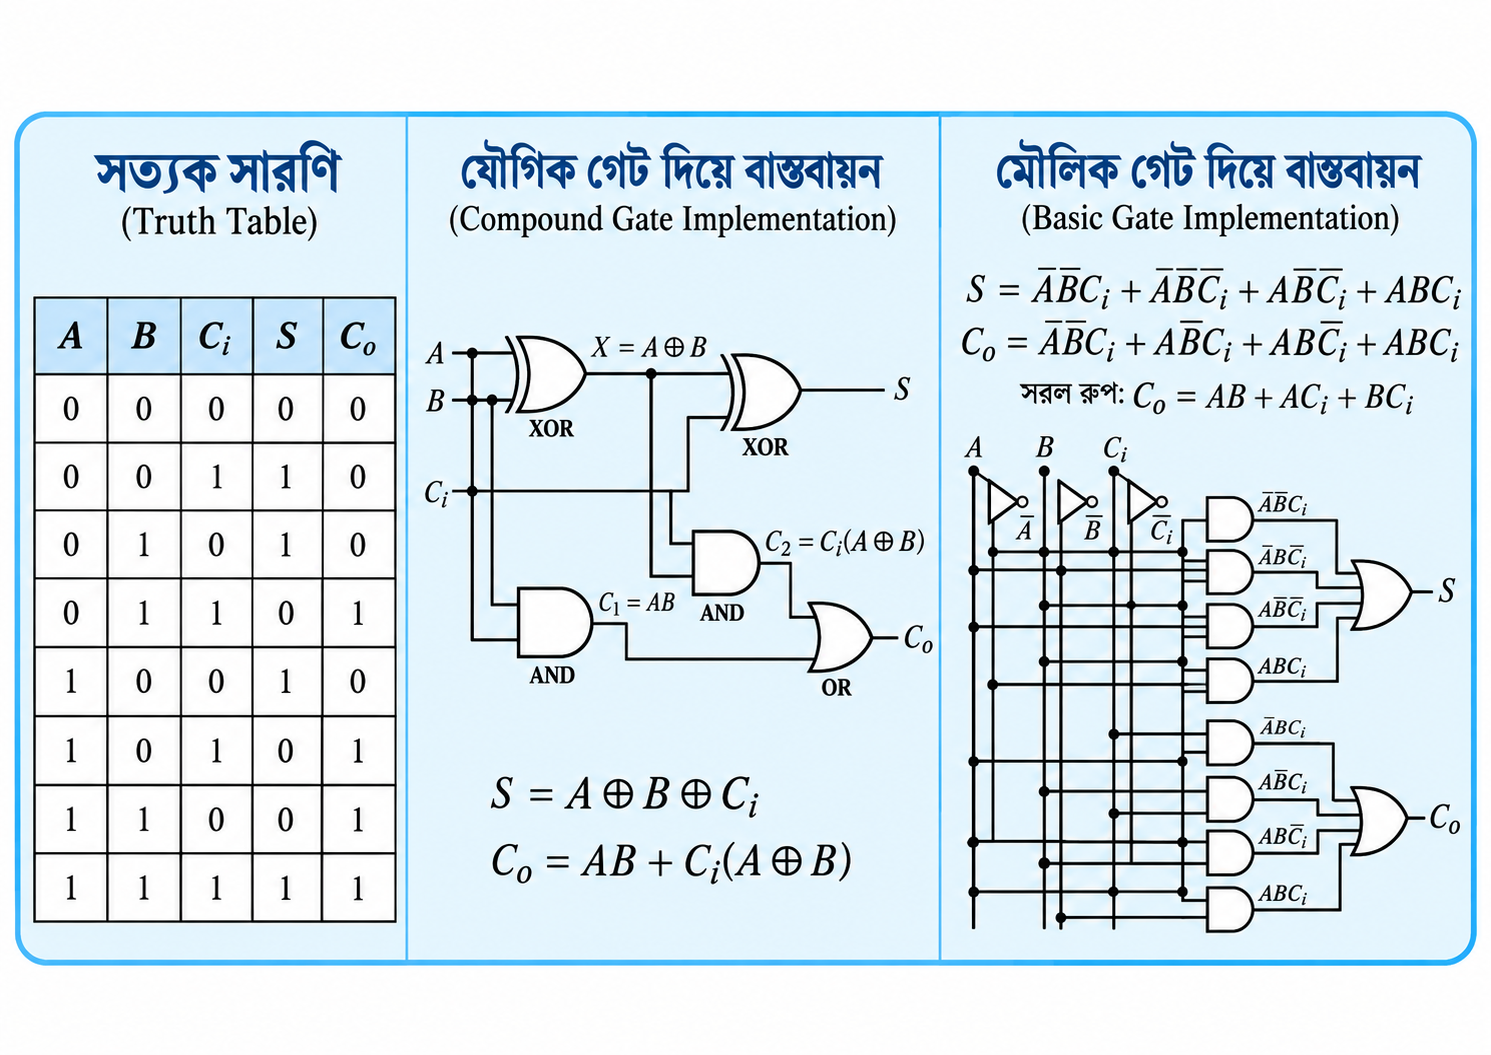
\includegraphics[width=\textwidth]{chapters/Chapter03/resources/images/full_adder_box.png}

\smallskip
{\small \textbf{চিত্র:} পূর্ণযোগকের সত্যক সারণি, যৌগিক গেট দিয়ে বাস্তবায়ন এবং মৌলিক গেট দিয়ে বাস্তবায়ন}
\end{center}

% =========================================================
% Boolean expressions of Full Adder
% =========================================================

\paragraph{যোগফল \(S\)-এর বুলিয়ান রাশি নির্ণয়:}

সত্যক সারণি থেকে দেখা যায়, \(S=1\) হয় নিম্নোক্ত ইনপুটের জন্য:
\[
001,\;010,\;100,\;111
\]

অতএব,
\[
\begin{aligned}
S &=
\overline{A}\,\overline{B}\,C_i
+\overline{A}\,B\,\overline{C_i}
+A\,\overline{B}\,\overline{C_i}
+A\,B\,C_i \\[4pt]
&=
\overline{A}\left(\overline{B}C_i+B\overline{C_i}\right)
+A\left(\overline{B}\,\overline{C_i}+BC_i\right) \\[4pt]
&=
\overline{A}(B\oplus C_i)+A\overline{(B\oplus C_i)} \\[4pt]
&=
A\oplus(B\oplus C_i) \\[4pt]
&=
A\oplus B\oplus C_i
\end{aligned}
\]

সুতরাং,
\[
\boxed{S=A\oplus B\oplus C_i}
\]

\paragraph{ক্যারি \(C_o\)-এর বুলিয়ান রাশি নির্ণয়:}

সত্যক সারণি থেকে দেখা যায়, \(C_o=1\) হয় নিম্নোক্ত ইনপুটের জন্য:
\[
011,\;101,\;110,\;111
\]

অতএব,
\[
\begin{aligned}
C_o &=
\overline{A}BC_i
+A\overline{B}C_i
+AB\overline{C_i}
+ABC_i \\[4pt]
&=
\overline{A}BC_i
+A\overline{B}C_i
+AB(\overline{C_i}+C_i) \\[4pt]
&=
\overline{A}BC_i
+A\overline{B}C_i
+AB \\[4pt]
&=
C_i(\overline{A}B+A\overline{B})+AB \\[4pt]
&=
C_i(A\oplus B)+AB
\end{aligned}
\]

অর্থাৎ,
\[
\boxed{C_o=AB+C_i(A\oplus B)}
\]

এখন এটিকে আরও পরিচিত রূপে লেখা যায়—
\[
\begin{aligned}
C_o &= AB+C_i(A\oplus B) \\[4pt]
&= AB+C_i(\overline{A}B+A\overline{B}) \\[4pt]
&= AB+\overline{A}BC_i+A\overline{B}C_i \\[4pt]
&= AB+BC_i+AC_i
\end{aligned}
\]

সুতরাং,
\[
\boxed{C_o=AB+AC_i+BC_i}
\]

\par\begingroup

\textbf{পূর্ণযোগকের দুটি গুরুত্বপূর্ণ সূত্র:}
\[
S=A\oplus B\oplus C_i
\]
\[
C_o=AB+C_i(A\oplus B)
\]
অথবা,
\[
C_o=AB+AC_i+BC_i
\]
\par\endgroup


% =========================================================
% 3.10.4 Full Adder using two Half Adders
% =========================================================

\subsubsection*{অর্ধযোগক ও পূর্ণযোগকের পার্থক্য}

\begin{center}
\renewcommand{\arraystretch}{1.35}
\begin{tabular}{|p{0.20\linewidth}|p{0.34\linewidth}|p{0.34\linewidth}|}
\hline
\rowcolor{gray!15}
\textbf{বিষয়} & \textbf{অর্ধযোগক (\textenglish{Half Adder})} & \textbf{পূর্ণযোগক (\textenglish{Full Adder})} \\
\hline
ইনপুট সংখ্যা & ২টি & ৩টি \\
\hline
ইনপুট & \(A,B\) & \(A,B,C_i\) \\
\hline
ক্যারি ইনপুট & নেই & আছে \\
\hline
আউটপুট & \(S,C\) & \(S,C_o\) \\
\hline
ব্যবহার & দুটি ১-বিট সংখ্যা যোগ করে & ক্যারিসহ দুটি ১-বিট সংখ্যা যোগ করে \\
\hline
গঠন & \textenglish{XOR} ও \textenglish{AND} গেট & \textenglish{XOR}, \textenglish{AND} ও \textenglish{OR} গেট \\
\hline
\end{tabular}
\end{center}

% =========================================================
% 3.10.6 Applications
% =========================================================

\subsubsection*{অ্যাডারের ব্যবহার}

অ্যাডার ডিজিটাল ইলেকট্রনিক্স ও কম্পিউটার ব্যবস্থায় অত্যন্ত গুরুত্বপূর্ণ।
এর কয়েকটি ব্যবহার হলো—

\begin{enumerate}
    \item \textenglish{ALU} (\textenglish{Arithmetic Logic Unit})-তে বাইনারি যোগের কাজে।
    \item বহু-বিট বাইনারি সংখ্যা যোগ করতে।
    \item কম্পিউটার প্রসেসরের গাণিতিক অংশে।
    \item ডিজিটাল ক্যালকুলেটরে।
    \item বিভিন্ন ডিজিটাল সার্কিটে \textenglish{sum} ও \textenglish{carry} নির্ণয়ে।
\end{enumerate}

\par\begingroup

\textbf{পরীক্ষার জন্য খুব গুরুত্বপূর্ণ:}
\begin{itemize}[label={{\bulletfont\textbullet}}, leftmargin=*, nosep]
    \item \textbf{Half Adder:}
    \[
    S=A\oplus B,\qquad C=AB
    \]

    \item \textbf{Full Adder:}
    \[
    S=A\oplus B\oplus C_i
    \]
    \[
    C_o=AB+C_i(A\oplus B)
    \]
    অথবা,
    \[
    C_o=AB+AC_i+BC_i
    \]
\end{itemize}
\par\endgroup

% =========================================================
% 3.10.4 দুটি অর্ধযোগক দিয়ে পূর্ণযোগক
% =========================================================

\subsection{দুটি অর্ধযোগক দিয়ে পূর্ণযোগক
(\textenglish{Full Adder Using Two Half Adders})}

আমরা জানি, \textenglish{Full Adder}-এ তিনটি ইনপুট থাকে— \(A\), \(B\) এবং \(C_i\)।
এদের যোগফল নির্ণয়ের জন্য দুটি \textenglish{Half Adder} এবং একটি \textenglish{OR Gate}
ব্যবহার করা যায়। এই পদ্ধতিটি খুবই গুরুত্বপূর্ণ, কারণ এর মাধ্যমে বোঝা যায়
কীভাবে একটি তুলনামূলক জটিল সার্কিটকে সহজ সার্কিটের সমন্বয়ে গঠন করা সম্ভব।

\subsubsection*{কার্যপ্রণালি
(\textenglish{Working Principle})}

প্রথম \textenglish{Half Adder}-এ \(A\) ও \(B\) ইনপুট দেওয়া হয়।

তাহলে প্রথম \textenglish{Half Adder} থেকে পাই—

\[
S_1=A\oplus B
\]

এবং,

\[
C_1=AB
\]

এরপর দ্বিতীয় \textenglish{Half Adder}-এ প্রথম \textenglish{Half Adder}-এর
যোগফল \(S_1\) এবং তৃতীয় ইনপুট \(C_i\) দেওয়া হয়।

তাহলে দ্বিতীয় \textenglish{Half Adder} থেকে পাই—

\[
S=S_1\oplus C_i
\]

অতএব,

\[
S=(A\oplus B)\oplus C_i
\]

সুতরাং,

\[
\boxed{S=A\oplus B\oplus C_i}
\]

আবার, দ্বিতীয় \textenglish{Half Adder}-এর ক্যারি হবে—

\[
C_2=S_1C_i
\]

এখন \(S_1=A\oplus B\) বসালে পাই—

\[
C_2=(A\oplus B)C_i
\]

এখন পূর্ণযোগকের চূড়ান্ত ক্যারি আউট হবে প্রথম ও দ্বিতীয়
\textenglish{Half Adder}-এর ক্যারির \textenglish{OR}।

অর্থাৎ,

\[
C_o=C_1+C_2
\]

এখন \(C_1=AB\) এবং \(C_2=(A\oplus B)C_i\) বসালে পাই—

\[
C_o=AB+(A\oplus B)C_i
\]

এখন \((A\oplus B)\)-এর মান বসাই—

\[
A\oplus B=\overline{A}B+A\overline{B}
\]

সুতরাং,

\[
C_o=AB+(\overline{A}B+A\overline{B})C_i
\]

\[
=AB+\overline{A}BC_i+A\overline{B}C_i
\]

এখন \textenglish{Boolean Algebra} ব্যবহার করে পূর্ণযোগকের বহুল ব্যবহৃত রূপ পাওয়া যায়—

\[
\boxed{C_o=AB+AC_i+BC_i}
\]

অতএব, দুটি \textenglish{Half Adder} এবং একটি \textenglish{OR Gate}
ব্যবহার করে \textenglish{Full Adder} বাস্তবায়ন করা যায়।

\subsubsection*{সারসংক্ষেপ
(\textenglish{Summary})}

\[
\boxed{S=A\oplus B\oplus C_i}
\]

\[
\boxed{C_o=AB+(A\oplus B)C_i}
\]

এবং সমতুল্যভাবে,

\[
\boxed{C_o=AB+AC_i+BC_i}
\]

\par\begingroup

\textbf{মনে রাখবে:}
দুটি \textenglish{Half Adder} দিয়ে \textenglish{Full Adder} তৈরি করলে
প্রথম \textenglish{Half Adder} \(A\) ও \(B\) যোগ করে,
দ্বিতীয় \textenglish{Half Adder} \(S_1\) ও \(C_i\) যোগ করে,
এবং দুটি ক্যারি \textenglish{OR} করে চূড়ান্ত \(C_o\) পাওয়া যায়।
\par\endgroup


\begin{figure}[!htbp]
    \centering
    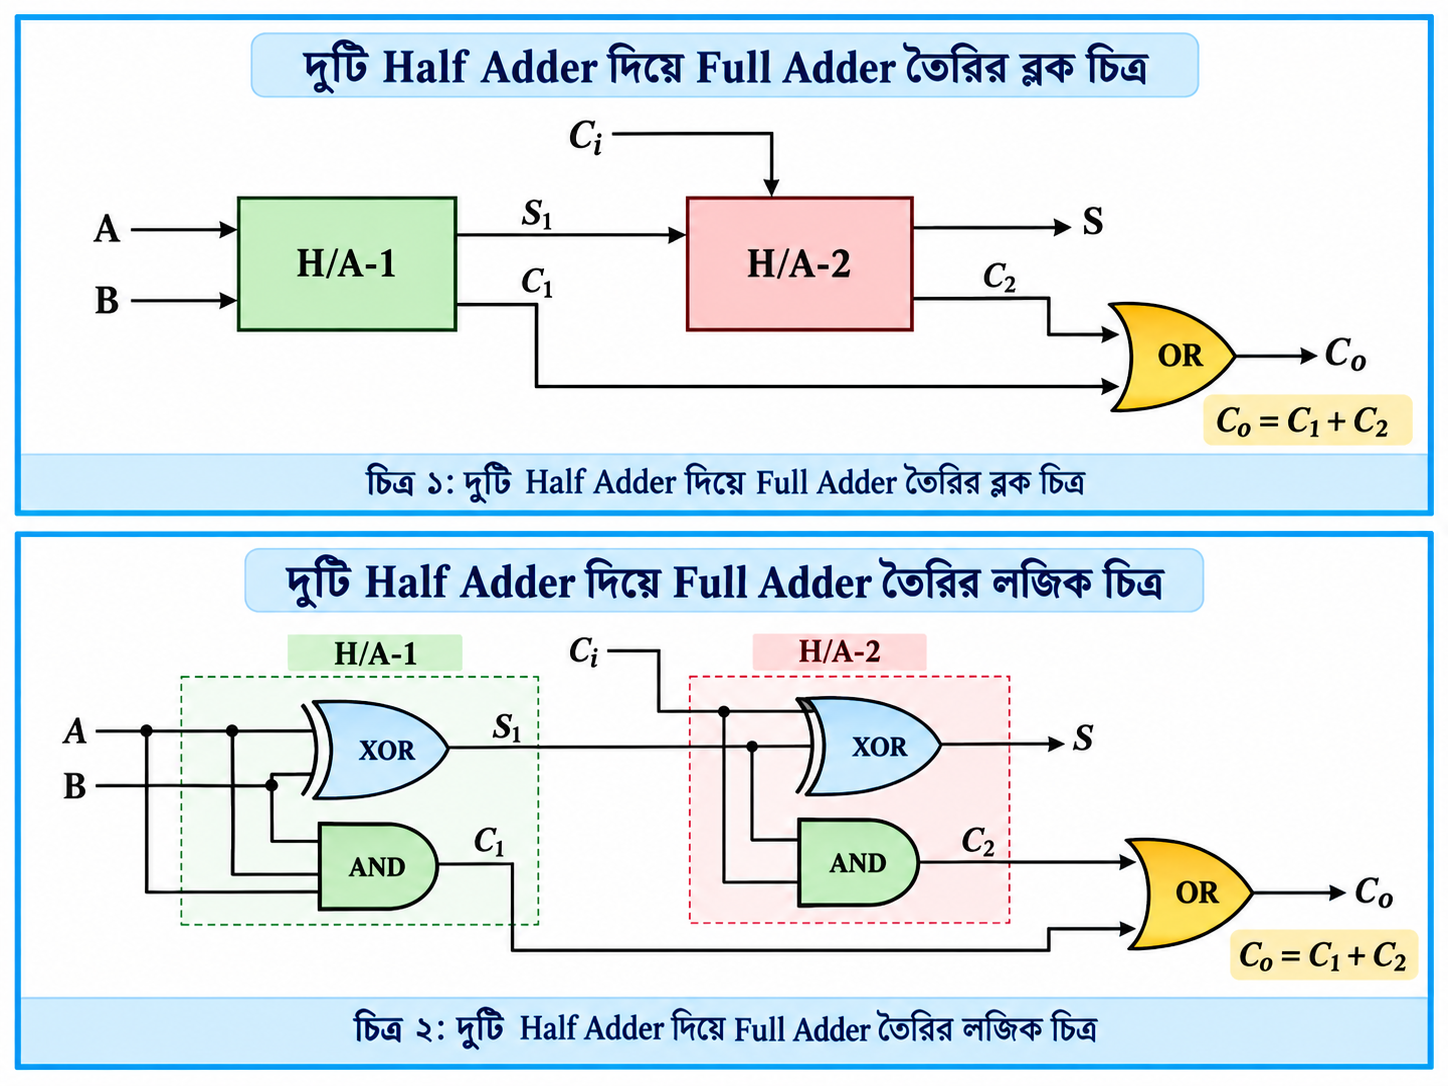
\includegraphics[width=0.92\textwidth]{chapters/Chapter03/resources/images/half_to_full_adder.png}
    \caption*{চিত্র: দুটি \textenglish{Half Adder} এবং একটি \textenglish{OR Gate} ব্যবহার করে \textenglish{Full Adder} বাস্তবায়ন}
\end{figure}


% =========================================================
% 3.10.5 সার্বজনীন গেট দিয়ে পূর্ণযোগক বাস্তবায়ন
% =========================================================

\subsection{সার্বজনীন গেট দিয়ে পূর্ণযোগক বাস্তবায়ন
(\textenglish{Implementation of Full Adder Using Universal Gates})}

আমরা জানি, \textenglish{NAND} ও \textenglish{NOR} গেটকে
সার্বজনীন গেট (\textenglish{Universal Gate}) বলা হয়।
কারণ, এই গেটগুলোর যেকোনো এক ধরনের গেট ব্যবহার করে
যেকোনো \textenglish{Boolean Function} বাস্তবায়ন করা সম্ভব।
সুতরাং \textenglish{Full Adder}-ও শুধু \textenglish{NAND} গেট
অথবা শুধু \textenglish{NOR} গেট ব্যবহার করে তৈরি করা যায়।

\subsubsection*{পূর্ণযোগকের মৌলিক সমীকরণ
(\textenglish{Basic Equations of Full Adder})}

পূর্ণযোগকের তিনটি ইনপুট \(A\), \(B\) ও \(C_i\)-এর জন্য
যোগফল \(S\) এবং ক্যারি আউট \(C_o\) নির্ণয়ের সমীকরণ হলো—

\[
S=A\oplus B\oplus C_i
\]

\[
C_o=AB+AC_i+BC_i
\]

এখন এই সমীকরণগুলোকে এমনভাবে রূপান্তর করা হয়,
যাতে শুধু \textenglish{NAND} বা শুধু \textenglish{NOR} গেট ব্যবহার করে
বাস্তবায়ন করা যায়।

\subsubsection*{\textenglish{NOR} গেট দিয়ে বাস্তবায়নের ধারণা}

\textenglish{NOR} গেট দিয়ে বাস্তবায়নের ক্ষেত্রে
সাধারণত \textenglish{OR} এবং \textenglish{NOT} অপারেশনের উপযোগী রূপে
সমীকরণকে পরিবর্তন করা হয়। \textenglish{De Morgan's Theorem} ব্যবহার করে
বিভিন্ন ধাপে রাশিকে \textenglish{NOR}-উপযোগী আকারে লেখা হয়।
এরপর প্রাপ্ত রাশি অনুযায়ী লজিক সার্কিট আঁকা হয়।

\subsubsection*{\textenglish{NAND} গেট দিয়ে বাস্তবায়নের ধারণা}

\textenglish{NAND} গেট দিয়ে বাস্তবায়নের ক্ষেত্রে
সমীকরণকে এমনভাবে ভেঙে লেখা হয়, যাতে
\textenglish{AND} এবং \textenglish{NOT}-নির্ভর রূপ থেকে
শুধু \textenglish{NAND} গেট ব্যবহার করে আউটপুট তৈরি করা যায়।
এক্ষেত্রেও \textenglish{Boolean Algebra} ও \textenglish{De Morgan's Theorem}
খুব গুরুত্বপূর্ণ ভূমিকা রাখে।

\subsubsection*{কেন এটি গুরুত্বপূর্ণ?}

সার্বজনীন গেট দিয়ে \textenglish{Full Adder} বাস্তবায়ন গুরুত্বপূর্ণ, কারণ—

\begin{enumerate}
    \item একটি নির্দিষ্ট ধরনের গেট ব্যবহার করে সম্পূর্ণ সার্কিট তৈরি করা যায়।
    \item \textenglish{IC} ডিজাইনে একই ধরনের গেট ব্যবহার করলে নকশা সহজ হয়।
    \item সার্কিট বিশ্লেষণ ও বাস্তবায়নের দক্ষতা বাড়ে।
    \item \textenglish{Boolean Algebra} ও \textenglish{Gate Realization}-এর সম্পর্ক স্পষ্ট হয়।
\end{enumerate}

\par\begingroup

\textbf{মনে রাখবে:}
\textenglish{Full Adder} বাস্তবায়নে \textenglish{NAND} ও \textenglish{NOR}—
উভয় ধরনের সার্বজনীন গেটই ব্যবহার করা যায়।
বোর্ড পরীক্ষায় অনেক সময় সমীকরণ এবং সার্কিট—দুটিই চাওয়া হয়।
\par\endgroup


\begin{figure}[!htbp]
    \centering
    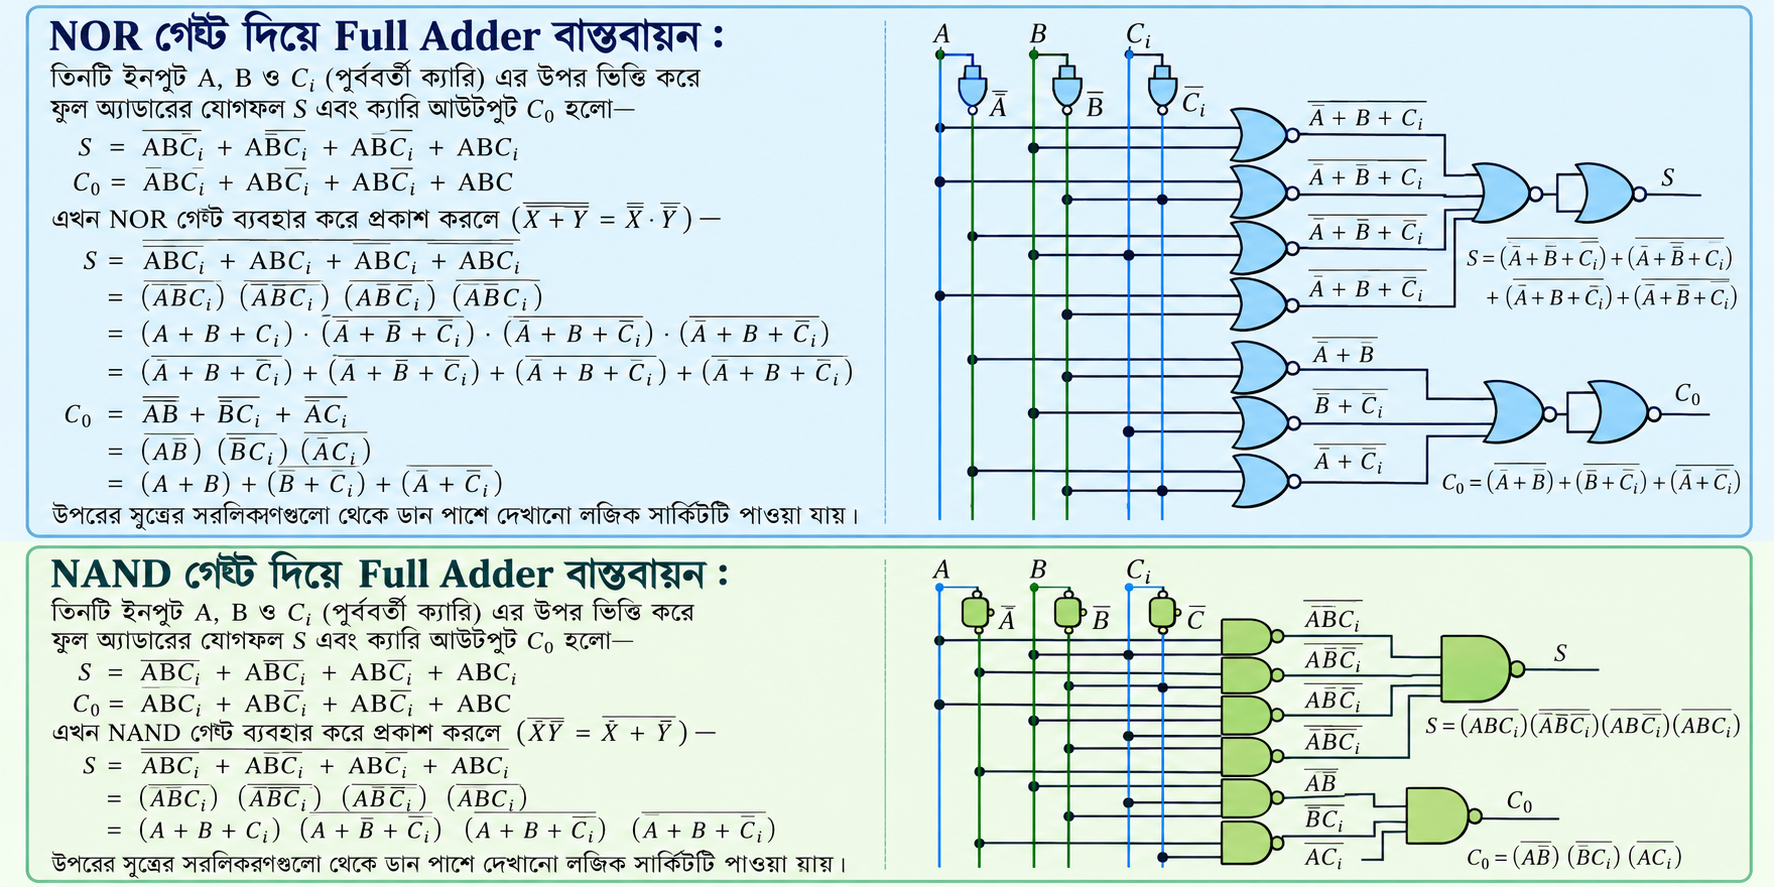
\includegraphics[width=\textwidth]{chapters/Chapter03/resources/images/nand_nor_full_adder.png}
    \caption*{চিত্র: \textenglish{NOR} এবং \textenglish{NAND} গেট ব্যবহার করে \textenglish{Full Adder} বাস্তবায়ন}
\end{figure}

\subsection{নয়টি দুই-ইনপুট গেটে পূর্ণযোগকের ধাপ}
নিচের মধ্যবর্তী সংকেতগুলো অনুসরণ করলে শুধু একই ধরনের গেট দিয়ে যোগফল ও ক্যারি তৈরি করা যায়। $C_i$ ক্যারি ইনপুট এবং $C_o$ ক্যারি আউটপুট।

\smallhead{শুধু NAND}
\[\begin{aligned}
P&=\overline{AB},&Q&=\overline{AP},&R&=\overline{BP},\\
X&=\overline{QR},&U&=\overline{XC_i},&V&=\overline{XU},\\
W&=\overline{C_iU},&S&=\overline{VW},&C_o&=\overline{PU}.
\end{aligned}\]
প্রথম চার গেটে $X=A\oplus B$। পরের চার গেটে $S=X\oplus C_i$। শেষ গেটে $C_o=\overline{\overline{AB}\cdot\overline{XC_i}}=AB+XC_i$। অতএব একই নয় গেটের সংযোগ পূর্ণযোগক।

\smallhead{শুধু NOR}
\[\begin{aligned}
P&=\overline{A+B},&Q&=\overline{A+P},&R&=\overline{B+P},\\
X&=\overline{Q+R},&U&=\overline{X+C_i},&V&=\overline{X+U},\\
W&=\overline{C_i+U},&S&=\overline{V+W},&C_o&=\overline{P+U}.
\end{aligned}\]
প্রথম চার গেটে X হলো A ও B-এর XNOR। পরের চার গেট X ও $C_i$-এর XNOR করলে দুইবার পূরক হয়ে $S=A\oplus B\oplus C_i$ পাওয়া যায়। শেষ NOR-এর ফল $C_o=(A+B)(X+C_i)=AB+AC_i+BC_i$। এখানে X-এর অর্থ NAND নির্মাণের X থেকে আলাদা।

\chThreeExample{১}{দুই half adder-এর মধ্যবর্তী মান}
$A=1,B=0,C_i=1$।
\chThreeAnswer প্রথম half adder-এ $S_1=1,C_1=0$। দ্বিতীয়টিতে $S=S_1\oplus C_i=0,C_2=S_1C_i=1$। শেষ OR-এ $C_o=C_1+C_2=1$। ফল $C_oS=10_2$, যা $1+0+1$-এর সঠিক যোগফল।

\chThreeExample{২}{অ্যাডার দিয়ে বিয়োগ}
চার বিটে $9-5$ নির্ণয় করতে $A=1001$, $B=0101$।
\chThreeAnswer B-এর বিট উল্টে $1010$ এবং প্রথম carry-in ১ দাও।
\[1001+1010+1=1\;0100.\]
অতিরিক্ত ক্যারি বাদ দিলে চার বিটে $0100=4$। এই উদাহরণে A ও B চিহ্নবিহীন মান; চার বিট signed হিসেবে ৯ লেখা যায় না।


% =========================================================
% 3.10.6 Binary Adder
% =========================================================

\subsection{বাইনারি অ্যাডার
(\textenglish{Binary Adder})}

\textenglish{Half Adder} ও \textenglish{Full Adder} মূলত এক-বিট
বাইনারি সংখ্যা যোগ করার মৌলিক সার্কিট। কিন্তু কম্পিউটারে সাধারণত
\(4\)-\textenglish{bit}, \(8\)-\textenglish{bit},
\(16\)-\textenglish{bit}, \(32\)-\textenglish{bit} ইত্যাদি বহু-বিট
সংখ্যা নিয়ে কাজ করতে হয়।

যেমন,

\[
(1011)_2+(0110)_2
\]

যোগ করতে হলে শুধু এক জোড়া \textenglish{bit} যোগ করলেই হবে না।
প্রতিটি \textenglish{bit-position}-এর \textenglish{bit} যোগ করতে হবে
এবং এক ধাপে উৎপন্ন \textenglish{Carry} পরবর্তী ধাপে পাঠাতে হবে।

একাধিক \textenglish{bit}-এর দুটি বাইনারি সংখ্যা যোগ করার জন্য
একাধিক \textenglish{Adder} প্রয়োজনমতো সংযুক্ত করে যে সার্কিট তৈরি করা হয়,
তাকে \textbf{\textenglish{Binary Adder}} বলে।

\subsubsection*{সহজভাবে}

\[
\boxed{
\text{\textenglish{Multi-bit Binary Numbers}}
\rightarrow
\text{\textenglish{Binary Adder}}
\rightarrow
\text{\textenglish{Sum + Final Carry}}
}
\]


% =========================================================
% Types of Binary Adder
% =========================================================

\subsection{বাইনারি অ্যাডারের প্রকারভেদ}

বাইনারি সংখ্যার বিটগুলো কীভাবে অ্যাডারে প্রবেশ করে এবং কীভাবে যোগ
সম্পন্ন হয়, তার ভিত্তিতে \textenglish{Binary Adder} প্রধানত দুই প্রকার—

\begin{enumerate}[leftmargin=*,itemsep=2pt]
    \item \textbf{\textenglish{Serial Binary Adder}}
    \item \textbf{\textenglish{Parallel Binary Adder}}
\end{enumerate}


% =========================================================
% Serial Binary Adder
% =========================================================

\paragraph{\textenglish{Serial Binary Adder}:}

যে বাইনারি অ্যাডারে দুটি বহু-বিট বাইনারি সংখ্যার সংশ্লিষ্ট বিটগুলো
একটির পর একটি ধারাবাহিকভাবে যোগ করা হয়,
তাকে \textenglish{Serial Binary Adder} বলে।

এখানে সাধারণত একটি \textenglish{Full Adder} ব্যবহার করে
প্রতিটি ধাপে এক জোড়া বিট যোগ করা হয়।
এক ধাপে উৎপন্ন \textenglish{Carry} পরবর্তী ধাপের জন্য সংরক্ষণ করা হয়।

ধরা যাক,

\[
A=A_3A_2A_1A_0
\]

এবং,

\[
B=B_3B_2B_1B_0
\]

তাহলে পর্যায়ক্রমে যোগ হবে—

\[
A_0+B_0+C_0
\]

\[
A_1+B_1+C_1
\]

\[
A_2+B_2+C_2
\]

\[
A_3+B_3+C_3
\]

\par\begingroup

\textbf{মনে রাখবে:}
\textenglish{Serial Binary Adder}-এ একই \textenglish{Full Adder}
বারবার ব্যবহার করে একটির পর একটি বিট যোগ করা যায়।
তাই হার্ডওয়্যার কম লাগে, কিন্তু যোগ সম্পন্ন করতে তুলনামূলক বেশি সময় লাগে।
\par\endgroup



% =========================================================
% Parallel Binary Adder
% =========================================================

\paragraph{\textenglish{Parallel Binary Adder}:}

যে বাইনারি অ্যাডারে দুটি বহু-বিট বাইনারি সংখ্যার সংশ্লিষ্ট বিটগুলো
একই সময়ে পৃথক \textenglish{Adder stage}-এ প্রবেশ করে,
তাকে \textenglish{Parallel Binary Adder} বলে।

প্রতিটি \textenglish{bit-position}-এর জন্য আলাদা
\textenglish{Full Adder} ব্যবহার করা হয়।

যেমন, দুটি \(4\)-\textenglish{bit} বাইনারি সংখ্যা যোগ করতে
চারটি \textenglish{Full Adder} ধারাবাহিকভাবে সংযুক্ত করা যায়।


% =========================================================
% 4-bit Parallel Binary Adder
% =========================================================

\subsubsection*{৪-বিট প্যারালাল বাইনারি অ্যাডার
(\textenglish{4-bit Parallel Binary Adder})}

ধরা যাক, দুটি \(4\)-\textenglish{bit} বাইনারি সংখ্যা—

\[
A_3A_2A_1A_0
\]

এবং,

\[
B_3B_2B_1B_0
\]

যোগ করতে হবে।

এক্ষেত্রে চারটি \textenglish{Full Adder} ব্যবহার করা হয়।
সর্বডানের \textenglish{Full Adder} সর্বনিম্ন গুরুত্বপূর্ণ বিট
(\textenglish{LSB}) এবং সর্ববামের \textenglish{Full Adder}
সর্বাধিক গুরুত্বপূর্ণ বিট (\textenglish{MSB}) যোগ করে।

প্রাথমিকভাবে \textenglish{Carry-in} না থাকলে—

\[
C_0=0
\]

ধরা হয়।

প্রতিটি ধাপে—

\[
FA_0:
A_0+B_0+C_0
\longrightarrow
S_0,\;C_1
\]

\[
FA_1:
A_1+B_1+C_1
\longrightarrow
S_1,\;C_2
\]

\[
FA_2:
A_2+B_2+C_2
\longrightarrow
S_2,\;C_3
\]

\[
FA_3:
A_3+B_3+C_3
\longrightarrow
S_3,\;C_4
\]

অতএব সম্পূর্ণ ফলাফল—

\[
\boxed{C_4S_3S_2S_1S_0}
\]


% =========================================================
% 4-bit Parallel Binary Adder Diagram
% =========================================================

\begin{center}

\begin{chThreeDiagram}
\begin{tikzpicture}[
    >=Stealth,
    line width=0.8pt,
    fa/.style={
        draw,
        rounded corners=2pt,
        fill=ICTLightBlue,
        minimum width=2.25cm,
        minimum height=1.15cm,
        align=center
    }
]

\node[fa] (fa3) at (0,0) {\textbf{\(FA_3\)}};
\node[fa] (fa2) at (3.6,0) {\textbf{\(FA_2\)}};
\node[fa] (fa1) at (7.2,0) {\textbf{\(FA_1\)}};
\node[fa] (fa0) at (10.8,0) {\textbf{\(FA_0\)}};

% A3, B3
\draw[->] (-0.55,2.0) -- (-0.55,0.62);
\node[above] at (-0.55,2.0) {\(A_3\)};

\draw[->] (0.55,2.0) -- (0.55,0.62);
\node[above] at (0.55,2.0) {\(B_3\)};

% A2, B2
\draw[->] (3.05,2.0) -- (3.05,0.62);
\node[above] at (3.05,2.0) {\(A_2\)};

\draw[->] (4.15,2.0) -- (4.15,0.62);
\node[above] at (4.15,2.0) {\(B_2\)};

% A1, B1
\draw[->] (6.65,2.0) -- (6.65,0.62);
\node[above] at (6.65,2.0) {\(A_1\)};

\draw[->] (7.75,2.0) -- (7.75,0.62);
\node[above] at (7.75,2.0) {\(B_1\)};

% A0, B0
\draw[->] (10.25,2.0) -- (10.25,0.62);
\node[above] at (10.25,2.0) {\(A_0\)};

\draw[->] (11.35,2.0) -- (11.35,0.62);
\node[above] at (11.35,2.0) {\(B_0\)};

% Carry chain
\draw[<-] (fa3.west) -- ++(-1.25,0);
\node[above] at (-1.75,0.08) {\(C_4\)};

\draw[<-] (fa3.east) -- (fa2.west);
\node[above] at (1.8,0.08) {\(C_3\)};

\draw[<-] (fa2.east) -- (fa1.west);
\node[above] at (5.4,0.08) {\(C_2\)};

\draw[<-] (fa1.east) -- (fa0.west);
\node[above] at (9.0,0.08) {\(C_1\)};

\draw[<-] (fa0.east) -- ++(1.30,0);
\node[above] at (12.55,0.08) {\(C_0=0\)};

% Sum outputs
\draw[->] (fa3.south) -- ++(0,-1.15);
\node[below] at (0,-1.15) {\(S_3\)};

\draw[->] (fa2.south) -- ++(0,-1.15);
\node[below] at (3.6,-1.15) {\(S_2\)};

\draw[->] (fa1.south) -- ++(0,-1.15);
\node[below] at (7.2,-1.15) {\(S_1\)};

\draw[->] (fa0.south) -- ++(0,-1.15);
\node[below] at (10.8,-1.15) {\(S_0\)};

\end{tikzpicture}
\end{chThreeDiagram}

\end{center}

\[
\boxed{
\text{\textenglish{Output}}
=
C_4S_3S_2S_1S_0
}
\]

এখানে \(A_3A_2A_1A_0\) এবং \(B_3B_2B_1B_0\) হলো দুটি
\(4\)-\textenglish{bit} বাইনারি সংখ্যা।
\(S_3S_2S_1S_0\) হলো চারটি \textenglish{Sum bit}
এবং \(C_4\) হলো চূড়ান্ত \textenglish{Carry}।


% =========================================================
% Carry Propagation
% =========================================================

\subsubsection*{ক্যারি প্রবাহ
(\textenglish{Carry Propagation})}

প্রতিটি \textenglish{Full Adder}-এর \textenglish{Carry-out}
পরবর্তী \textenglish{Full Adder}-এর \textenglish{Carry-in}
হিসেবে প্রবেশ করে।

অর্থাৎ,

\[
C_0
\rightarrow
FA_0
\rightarrow
C_1
\rightarrow
FA_1
\rightarrow
C_2
\rightarrow
FA_2
\rightarrow
C_3
\rightarrow
FA_3
\rightarrow
C_4
\]

এইভাবে \textenglish{Carry} এক \textenglish{stage} থেকে
পরবর্তী \textenglish{stage}-এ ক্রমান্বয়ে ছড়িয়ে যায়।

এই কারণে এ ধরনের সাধারণ \textenglish{Parallel Adder}-কে
\textenglish{Ripple Carry Adder}-ও বলা হয়।

\par\begingroup

\textbf{মনে রাখবে:}
\textenglish{Parallel Adder}-এ \textenglish{input bit}গুলো একই সময়ে
সংশ্লিষ্ট \textenglish{Full Adder}-এ প্রবেশ করলেও
\textenglish{Carry} এক \textenglish{stage} থেকে পরবর্তী
\textenglish{stage}-এ ধারাবাহিকভাবে প্রবাহিত হয়।
\par\endgroup



% =========================================================
% Example: 1011 + 1111
% =========================================================

\subsubsection*{উদাহরণ:
\((1011)_2+(1111)_2\)}

ধরা যাক,

\[
A=(1011)_2
\]

এবং,

\[
B=(1111)_2
\]

তাহলে—

\[
A_3A_2A_1A_0=1011
\]

এবং,

\[
B_3B_2B_1B_0=1111
\]

প্রাথমিক \textenglish{Carry}—

\[
C_0=0
\]


% =========================================================
% Example Diagram
% =========================================================

\begin{center}

\begin{chThreeDiagram}
\begin{tikzpicture}[
    >=Stealth,
    line width=0.8pt,
    fa/.style={
        draw,
        rounded corners=2pt,
        fill=ICTLightGreen,
        minimum width=2.25cm,
        minimum height=1.15cm,
        align=center
    }
]

\node[fa] (fa3) at (0,0) {\textbf{\(FA_3\)}};
\node[fa] (fa2) at (3.6,0) {\textbf{\(FA_2\)}};
\node[fa] (fa1) at (7.2,0) {\textbf{\(FA_1\)}};
\node[fa] (fa0) at (10.8,0) {\textbf{\(FA_0\)}};

% FA3
\node[above] at (-0.55,2.0) {\(A_3=1\)};
\node[above] at (0.60,2.0) {\(B_3=1\)};
\draw[->] (-0.55,1.72) -- (-0.55,0.62);
\draw[->] (0.60,1.72) -- (0.60,0.62);

% FA2
\node[above] at (3.05,2.0) {\(A_2=0\)};
\node[above] at (4.20,2.0) {\(B_2=1\)};
\draw[->] (3.05,1.72) -- (3.05,0.62);
\draw[->] (4.20,1.72) -- (4.20,0.62);

% FA1
\node[above] at (6.65,2.0) {\(A_1=1\)};
\node[above] at (7.80,2.0) {\(B_1=1\)};
\draw[->] (6.65,1.72) -- (6.65,0.62);
\draw[->] (7.80,1.72) -- (7.80,0.62);

% FA0
\node[above] at (10.25,2.0) {\(A_0=1\)};
\node[above] at (11.40,2.0) {\(B_0=1\)};
\draw[->] (10.25,1.72) -- (10.25,0.62);
\draw[->] (11.40,1.72) -- (11.40,0.62);

% Carry values
\draw[<-] (fa3.west) -- ++(-1.20,0);
\node[above] at (-1.70,0.08) {\(C_4=1\)};

\draw[<-] (fa3.east) -- (fa2.west);
\node[above] at (1.80,0.08) {\(C_3=1\)};

\draw[<-] (fa2.east) -- (fa1.west);
\node[above] at (5.40,0.08) {\(C_2=1\)};

\draw[<-] (fa1.east) -- (fa0.west);
\node[above] at (9.00,0.08) {\(C_1=1\)};

\draw[<-] (fa0.east) -- ++(1.20,0);
\node[above] at (12.50,0.08) {\(C_0=0\)};

% Sum outputs
\draw[->] (fa3.south) -- ++(0,-1.15);
\node[below] at (0,-1.15) {\(S_3=1\)};

\draw[->] (fa2.south) -- ++(0,-1.15);
\node[below] at (3.6,-1.15) {\(S_2=0\)};

\draw[->] (fa1.south) -- ++(0,-1.15);
\node[below] at (7.2,-1.15) {\(S_1=1\)};

\draw[->] (fa0.south) -- ++(0,-1.15);
\node[below] at (10.8,-1.15) {\(S_0=0\)};

\end{tikzpicture}
\end{chThreeDiagram}

\end{center}


% =========================================================
% Stage-by-stage Calculation
% =========================================================

\par\begingroup


\begin{minipage}[t]{0.235\textwidth}
\centering

\textbf{স্টেজ–০}\\[-1mm]
{\footnotesize \textenglish{LSB}}

\vspace{2mm}

\[
A_0=1,\quad B_0=1
\]

\[
C_0=0
\]

\[
1+1+0=10
\]

\[
\boxed{S_0=0,\;C_1=1}
\]

\end{minipage}
\hfill
\begin{minipage}[t]{0.235\textwidth}
\centering

\textbf{স্টেজ–১}

\vspace{4mm}

\[
A_1=1,\quad B_1=1
\]

\[
C_1=1
\]

\[
1+1+1=11
\]

\[
\boxed{S_1=1,\;C_2=1}
\]

\end{minipage}
\hfill
\begin{minipage}[t]{0.235\textwidth}
\centering

\textbf{স্টেজ–২}

\vspace{4mm}

\[
A_2=0,\quad B_2=1
\]

\[
C_2=1
\]

\[
0+1+1=10
\]

\[
\boxed{S_2=0,\;C_3=1}
\]

\end{minipage}
\hfill
\begin{minipage}[t]{0.235\textwidth}
\centering

\textbf{স্টেজ–৩}\\[-1mm]
{\footnotesize \textenglish{MSB}}

\vspace{2mm}

\[
A_3=1,\quad B_3=1
\]

\[
C_3=1
\]

\[
1+1+1=11
\]

\[
\boxed{S_3=1,\;C_4=1}
\]

\end{minipage}

\par\endgroup

অতএব,

\[
C_4S_3S_2S_1S_0=11010
\]

সুতরাং,

\[
\boxed{
(1011)_2+(1111)_2=(11010)_2
}
\]

দশমিক পদ্ধতিতে যাচাই করলে—

\[
(1011)_2=(11)_{10}
\]

এবং,

\[
(1111)_2=(15)_{10}
\]

তাই,

\[
11+15=26
\]

এবং,

\[
(26)_{10}=(11010)_2
\]

অতএব ফল সঠিক।


% =========================================================
% Serial vs Parallel Comparison
% =========================================================

\subsubsection*{\textenglish{Serial} ও \textenglish{Parallel Binary Adder}-এর পার্থক্য}

\begin{center}

\renewcommand{\arraystretch}{1.25}

\begin{tabularx}
{\textwidth}
{|L{0.20\textwidth}|Y|Y|}

\hline

\rowcolor{ICTLightBlue}

\textbf{বিষয়}
&
\textbf{\textenglish{Serial Binary Adder}}
&
\textbf{\textenglish{Parallel Binary Adder}}
\\
\hline

যোগের পদ্ধতি
&
বিট একটির পর একটি যোগ করা হয়।
&
সংশ্লিষ্ট বিটগুলো একই সময়ে পৃথক
\textenglish{Adder}-এ প্রবেশ করে।
\\
\hline

\textenglish{Adder} সংখ্যা
&
তুলনামূলক কম।
&
তুলনামূলক বেশি।
\\
\hline

৪-বিট যোগে
&
সাধারণত একই \textenglish{Full Adder} বারবার ব্যবহার করা হয়।
&
সাধারণত ৪টি \textenglish{Full Adder} ব্যবহার করা হয়।
\\
\hline

সময়
&
বেশি লাগে।
&
তুলনামূলক কম লাগে।
\\
\hline

\textenglish{Hardware}
&
কম প্রয়োজন।
&
বেশি প্রয়োজন।
\\
\hline

গতি
&
কম।
&
বেশি।
\\
\hline

\end{tabularx}

\end{center}


% =========================================================
% Advantages and Limitations
% =========================================================

\subsubsection*{\textenglish{Parallel Binary Adder}-এর সুবিধা ও সীমাবদ্ধতা}

\textbf{সুবিধা:}

\begin{itemize}[label={{\bulletfont\textbullet}}, leftmargin=*, nosep]

    \item একাধিক বিট একই সময়ে সংশ্লিষ্ট
    \textenglish{Full Adder}-এ প্রবেশ করতে পারে।

    \item \textenglish{Serial Adder}-এর তুলনায় দ্রুত।

    \item বহু-বিট বাইনারি সংখ্যা সহজে যোগ করা যায়।

    \item \textenglish{Processor} ও
    \textenglish{ALU}-তে ব্যবহার করা যায়।

    \item আরও \textenglish{Full Adder} যুক্ত করে বড়
    \textenglish{bit-width}-এর \textenglish{Adder} তৈরি করা যায়।

\end{itemize}

\textbf{সীমাবদ্ধতা:}

একটি \textenglish{Full Adder}-এর \textenglish{Carry}
পরবর্তী \textenglish{Full Adder}-এ পৌঁছাতে কিছু সময় প্রয়োজন হয়।
ফলে \textenglish{stage} সংখ্যা বাড়লে
\textenglish{Carry propagation}-এর কারণে মোট
\textenglish{delay} বাড়ে।

\par\begingroup

\textbf{মনে রাখবে:}
\textenglish{Parallel Adder}-এ ইনপুট বিটগুলো একই সময়ে সংশ্লিষ্ট
\textenglish{Full Adder}-এ প্রবেশ করলেও
\textenglish{Carry} এক \textenglish{stage} থেকে পরবর্তী
\textenglish{stage}-এ ক্রমান্বয়ে যায়।
\par\endgroup



% =========================================================
% Applications
% =========================================================

\subsection{বাইনারি অ্যাডারের ব্যবহার}

\begin{enumerate}[leftmargin=*,itemsep=2pt]

    \item কম্পিউটারের
    \textenglish{ALU (Arithmetic Logic Unit)}-তে।

    \item বহু-বিট বাইনারি সংখ্যা যোগ করতে।

    \item \textenglish{Processor}-এর
    \textenglish{arithmetic operation}-এ।

    \item \textenglish{Digital Calculator}-এ।

    \item \textenglish{Address Calculation}-এ।

    \item বিভিন্ন
    \textenglish{digital arithmetic circuit} তৈরিতে।

\end{enumerate}

\subsection{অ্যাডারের সংখ্যা এবং প্রতিটি ধাপের ফল}
বাহ্যিক carry-in না থাকলে সবচেয়ে ডান বিটে একটি half adder এবং বাকি $n-1$ বিটে full adder দিয়ে $n$-বিট যোগ করা যায়। সব ধাপে full adder ব্যবহার করাও যায়; তখন প্রথমটির carry-in শূন্য। বাহ্যিক carry-in গ্রহণ করতে হলে প্রথম ধাপেও full adder প্রয়োজন।

\chThreeExample{১}{চার বিটের যোগে carry propagation}
$(1101)_2+(0111)_2$ এবং $C_0=0$।
\begin{center}\begin{tabular}{|c|c|c|c|c|c|}\hline
বিট $i$ & $A_i$ & $B_i$ & $C_i$ & $S_i$ & $C_{i+1}$\\\hline
0&1&1&0&0&1\\\hline
1&0&1&1&0&1\\\hline
2&1&1&1&1&1\\\hline
3&1&0&1&0&1\\\hline
\end{tabular}\end{center}
\chThreeAnswer ফল $C_4S_3S_2S_1S_0=10100_2=20_{10}$। চার বিটের sum output শুধু $0100$; $C_4$ আলাদা রাখলে সম্পূর্ণ চিহ্নবিহীন যোগফল পাওয়া যায়।

\chThreeExample{২}{ধারণাভিত্তিক MCQ}
বাহ্যিক carry-in ছাড়া দুটি আট বিট সংখ্যা যোগে half adder-সহ সরল নির্মাণ কোনটি? (ক) ৮ half adder, (খ) ১ half ও ৭ full adder, (গ) ৭ half ও ১ full adder, (ঘ) ১ full adder।
\chThreeAnswer (খ)। পরের বিটগুলোতে আগের carry গ্রহণের জন্য full adder লাগে। আট full adder-ও একটি বিকল্প নির্মাণ, কিন্তু প্রশ্নের নির্দিষ্ট half-adder-সহ নির্মাণটি (খ)।

% Mahbub teaching-type follow-up, 2026-10-14
\chThreeExample{৩}{চার বিটের যোগে Sum ও Carry আলাদা}
একটি চার-বিট adder-এ $A=1101$, $B=1011$, প্রথম carry $C_0=0$। চারটি sum bit ও শেষ carry লেখো।
\chThreeAnswer ডান থেকে $1+1+0=10$, $0+1+1=10$, $1+0+1=10$, $1+1+1=11$। তাই $S_3S_2S_1S_0=1000$, $C_4=1$। পূর্ণ unsigned ফল $C_4S_3S_2S_1S_0=11000_2=24$; শুধু sum port-এ দেখা মান ৮। পাঁচ-বিট যোগফল এবং চার-বিট sum output পৃথক। signed হিসেবে input দুটি $-3$ ও $-5$ হলে চার-বিট sum $1000=-8$ সঠিক; carry থাকার অর্থ signed overflow নয়।

\chThreeExample{৪}{Sum ও Carry থেকে সম্ভাব্য input}
একটি half adder-এ $S=1,C=0$; আর একটি full adder-এ $S=1,C_{out}=1$। সম্ভাব্য input নির্ণয় করো।
\chThreeAnswer half adder-এর যোগফল ১, তাই input জোড়া 01 অথবা 10। শুধু output থেকে কোন রেখাটি ১ ছিল তা নিশ্চিত নয়। full adder-এর পূর্ণ যোগফল $2C_{out}+S=3$; তিনটি এক-বিট input-এর যোগফল ৩ হতে হলে $A=B=C_{in}=1$। বিপরীত সমস্যায় প্রতিটি output combination-এর সঙ্গে কয়টি input মেলে তা সারণি থেকে পরীক্ষা করতে হয়।


% =========================================================
% 3.11 Flip-Flop
% =========================================================

\section{ফ্লিপ-ফ্লপ
(\textenglish{Flip-Flop})}

ডিজিটাল সার্কিটে শুধু তথ্য প্রক্রিয়াকরণ করলেই হয় না; অনেক সময় কোনো
একটি বাইনারি মান কিছু সময়ের জন্য মনে রাখতেও হয়।

যেমন, কোনো সার্কিটে বর্তমানে \(1\) সংরক্ষিত থাকলে নতুন নির্দেশ না
পাওয়া পর্যন্ত সেই \(1\) ধরে রাখতে হবে। আবার প্রয়োজন হলে সেটিকে
\(0\)-তে পরিবর্তন করতে হবে।

এই ধরনের এক-বিট তথ্য সংরক্ষণের মৌলিক সার্কিট হলো
\textbf{\textenglish{Flip-Flop}}।

সহজভাবে—

\[
\boxed{
\text{\textenglish{Input/Control Signal}}
\rightarrow
\text{\textenglish{Flip-Flop}}
\rightarrow
\text{\textenglish{Stored 0 or 1}}
}
\]


% =========================================================
% 3.11.1 What is Flip-Flop?
% =========================================================

\subsection{ফ্লিপ-ফ্লপ কী?}

যে দ্বি-স্থিতিশীল ডিজিটাল লজিক সার্কিট দুটি স্থিতিশীল অবস্থার
যেকোনো একটিতে অবস্থান করে একটি বাইনারি বিট \(0\) অথবা \(1\)
সংরক্ষণ করতে পারে, তাকে \textbf{\textenglish{Flip-Flop}} বলে।

এখানে দ্বি-স্থিতিশীল বা \textenglish{Bistable} অর্থ হলো—
সার্কিটটির দুটি স্থিতিশীল অবস্থা আছে।

\[
Q=0
\]

অথবা,

\[
Q=1
\]

অতএব,

\[
\boxed{
1\text{টি }\text{\textenglish{Flip-Flop}}
=
1\text{ }\text{\textenglish{bit}}\text{ তথ্য সংরক্ষণ}
}
\]

\textenglish{Flip-Flop}-কে তাই ডিজিটাল সার্কিটের একটি মৌলিক
\textenglish{Memory Element} বলা হয়।


% =========================================================
% 3.11.2 Output
% =========================================================

\subsection{ফ্লিপ-ফ্লপের আউটপুট
(\textenglish{Output})}

সাধারণভাবে \textenglish{Flip-Flop}-এর প্রধান আউটপুটকে \(Q\)
দ্বারা প্রকাশ করা হয়।

অনেক \textenglish{Flip-Flop}-এ এর বিপরীত আউটপুটও থাকে—

\[
\overline{Q}
\]

সাধারণ অবস্থায়,

\[
\overline{Q}=\overline{Q}
\]

অর্থাৎ—

\[
Q=1
\Rightarrow
\overline{Q}=0
\]

এবং,

\[
Q=0
\Rightarrow
\overline{Q}=1
\]

\begin{center}
\renewcommand{\arraystretch}{1.2}
\begin{tabular}{|c|c|c|}
\hline
\rowcolor{ICTLightBlue}
\(\boldsymbol{Q}\)
&
\(\boldsymbol{\overline{Q}}\)
&
\textbf{সংরক্ষিত বিট}
\\
\hline
0 & 1 & 0 \\
\hline
1 & 0 & 1 \\
\hline
\end{tabular}
\end{center}

\par\begingroup

\textbf{মনে রাখবে:}
\(Q\) এবং \(\overline{Q}\) সাধারণত পরস্পরের বিপরীত মান প্রকাশ করে।
\par\endgroup



% =========================================================
% 3.11.3 Why Flip-Flop is used
% =========================================================

\subsection{ফ্লিপ-ফ্লপ কেন ব্যবহার করা হয়?}

কম্পিউটার ও অন্যান্য ডিজিটাল ডিভাইসে অনেক কাজের জন্য পূর্ববর্তী তথ্য
বা অবস্থা মনে রাখা প্রয়োজন। \textenglish{Flip-Flop} এই তথ্য বা অবস্থা
সংরক্ষণে ব্যবহৃত হয়।

ফ্লিপ-ফ্লপ ব্যবহারের প্রধান কারণগুলো হলো—

\begin{enumerate}[leftmargin=*,itemsep=2pt]

    \item \textbf{বাইনারি তথ্য সংরক্ষণ:}
    একটি \(0\) অথবা \(1\) ধরে রাখতে।

    \item \textbf{পূর্ববর্তী অবস্থা মনে রাখা:}
    সার্কিটের বর্তমান বা পূর্বের \textenglish{state} সংরক্ষণ করতে।

    \item \textbf{\textenglish{Counter} তৈরি:}
    একাধিক \textenglish{Flip-Flop} ব্যবহার করে
    \textenglish{pulse} বা \textenglish{event} গণনা করতে।

    \item \textbf{\textenglish{Register} তৈরি:}
    একাধিক বিট একসঙ্গে সংরক্ষণ করতে।

    \item \textbf{\textenglish{Shift Register} তৈরি:}
    বিট এক অবস্থান থেকে অন্য অবস্থানে স্থানান্তর করতে।

    \item \textbf{\textenglish{Clock}-এর সঙ্গে কাজ:}
    নির্দিষ্ট সময়ে তথ্য গ্রহণ ও পরিবর্তন করতে।

    \item \textbf{\textenglish{Control Circuit}:}
    বিভিন্ন ডিজিটাল অবস্থা নিয়ন্ত্রণ করতে।

\end{enumerate}


% =========================================================
% 3.11.4 How Flip-Flop stores information
% =========================================================

\subsection{ফ্লিপ-ফ্লপ কীভাবে তথ্য সংরক্ষণ করে?}

\textenglish{Flip-Flop}-এর ভেতরে এমনভাবে
\textenglish{feedback} ব্যবস্থা তৈরি করা হয়, যাতে একবার কোনো অবস্থা
তৈরি হলে নতুন উপযুক্ত ইনপুট না আসা পর্যন্ত সেই অবস্থা ধরে রাখা যায়।

ধরা যাক,

\[
Q=1
\]

অর্থাৎ \textenglish{Flip-Flop}-এ বর্তমানে \(1\) সংরক্ষিত আছে।

নতুন কোনো পরিবর্তনকারী সংকেত না এলে—

\[
Q=1
\]

অবস্থাই বজায় থাকবে।

আবার উপযুক্ত ইনপুট দিলে অবস্থাটি পরিবর্তিত হয়ে—

\[
Q=0
\]

হতে পারে।

অর্থাৎ \textenglish{Flip-Flop} শুধু আউটপুট তৈরি করে না;
এটি আগের আউটপুট বা অবস্থা মনে রাখতে পারে।

\subsubsection*{এক বিট তথ্য সংরক্ষণের ধারণা}

\[
Q=0
\quad\Longrightarrow\quad
0\text{ সংরক্ষিত}
\]

\[
Q=1
\quad\Longrightarrow\quad
1\text{ সংরক্ষিত}
\]

\par\begingroup

\textenglish{Flip-Flop}-এর \textenglish{feedback} ব্যবস্থা
বর্তমান অবস্থা ধরে রাখতে সাহায্য করে। তবে বিদ্যুৎ সরবরাহ বন্ধ হলে
সাধারণ \textenglish{Flip-Flop}-এর সংরক্ষিত তথ্য হারিয়ে যায়।
তাই এটি একটি \textenglish{volatile storage element}।
\par\endgroup



% =========================================================
% 3.11.5 Role of Clock
% =========================================================

\subsection{ক্লকের ভূমিকা
(\textenglish{Role of Clock})}

অনেক \textenglish{Flip-Flop}-এর সঙ্গে একটি
\textenglish{Clock (CLK)} ইনপুট থাকে।

\textenglish{Clock} হলো নির্দিষ্ট সময় পরপর পরিবর্তিত হওয়া একটি
ডিজিটাল সংকেত, যা \textenglish{Flip-Flop}-কে নির্দেশ করে
কখন ইনপুট গ্রহণ বা অবস্থা পরিবর্তন করতে হবে।

\textenglish{Clock signal} সাধারণত—

\[
0\rightarrow1\rightarrow0\rightarrow1\rightarrow\cdots
\]

এভাবে পরিবর্তিত হয়।

কিছু \textenglish{Flip-Flop} ক্লকের—

\[
0\rightarrow1
\]

পরিবর্তনের সময় কাজ করে। একে
\textenglish{Positive Edge} বলা হয়।

আবার কিছু \textenglish{Flip-Flop}—

\[
1\rightarrow0
\]

পরিবর্তনের সময় কাজ করে। একে
\textenglish{Negative Edge} বলা হয়।

সহজভাবে—

\[
\boxed{
\text{\textenglish{Clock}}
=
\text{কখন }\text{\textenglish{state}}
\text{ পরিবর্তন হবে তার সময়-নিয়ন্ত্রণ সংকেত}
}
\]


% =========================================================
% 3.11.6 Characteristics
% =========================================================

\subsection{ফ্লিপ-ফ্লপের বৈশিষ্ট্য}

\begin{enumerate}[leftmargin=*,itemsep=2pt]

    \item একটি \textenglish{Flip-Flop} সাধারণত
    \(1\) \textenglish{bit} তথ্য সংরক্ষণ করে।

    \item এর দুটি স্থিতিশীল অবস্থা—\(0\) ও \(1\)।

    \item পূর্ববর্তী \textenglish{state} ধরে রাখতে পারে।

    \item সাধারণত \(Q\) এবং \(\overline{Q}\)
    আউটপুট ব্যবহৃত হয়।

    \item বিভিন্ন \textenglish{Flip-Flop} ইনপুটের নিয়ম অনুযায়ী
    অবস্থা পরিবর্তন করে।

    \item \textenglish{Clock-controlled digital circuit}-এ
    ব্যাপকভাবে ব্যবহৃত হয়।

    \item বিদ্যুৎ সরবরাহ বন্ধ হলে সাধারণ
    \textenglish{Flip-Flop}-এর সংরক্ষিত অবস্থা হারিয়ে যায়।

\end{enumerate}


% =========================================================
% 3.11.7 History
% =========================================================

\subsection{ফ্লিপ-ফ্লপের সংক্ষিপ্ত ইতিহাস}

ডিজিটাল তথ্য সংরক্ষণের ধারণা বিকাশের সঙ্গে
\textenglish{Flip-Flop}-এর ইতিহাস জড়িত।

১৯১৮ সালে \textenglish{William Eccles} ও
\textenglish{F. W. Jordan} দুটি \textenglish{vacuum tube} ব্যবহার করে
একটি দ্বি-স্থিতিশীল সার্কিট তৈরি করেন।
এটি আধুনিক \textenglish{Flip-Flop}-এর প্রাথমিক রূপগুলোর একটি।

পরবর্তী সময়ে \textenglish{vacuum tube}-এর পরিবর্তে
\textenglish{transistor} এবং পরে
\textenglish{Integrated Circuit (IC)} প্রযুক্তির সাহায্যে
\textenglish{Flip-Flop} আরও ছোট, দ্রুত ও কার্যকর হয়।

বর্তমানে \textenglish{processor}, \textenglish{register},
\textenglish{counter} এবং বিভিন্ন
\textenglish{sequential digital circuit}-এ
বিপুল সংখ্যক \textenglish{Flip-Flop} ব্যবহৃত হয়।


% =========================================================
% 3.11.8 Applications
% =========================================================

\subsection{ফ্লিপ-ফ্লপের ব্যবহার}

\begin{enumerate}[leftmargin=*,itemsep=2pt]

    \item \textbf{\textenglish{Register}:}
    একাধিক বিট সাময়িকভাবে সংরক্ষণ করতে।

    \item \textbf{\textenglish{Counter}:}
    \textenglish{clock pulse} বা
    \textenglish{event} গণনা করতে।

    \item \textbf{\textenglish{Shift Register}:}
    বাইনারি তথ্য এক অবস্থান থেকে অন্য অবস্থানে স্থানান্তর করতে।

    \item \textbf{\textenglish{Memory Circuit}:}
    ডিজিটাল তথ্য সাময়িকভাবে সংরক্ষণ করতে।

    \item \textbf{\textenglish{Frequency Divider}:}
    \textenglish{clock frequency} ভাগ বা কমাতে।

    \item \textbf{\textenglish{Control Circuit}:}
    ডিজিটাল সিস্টেমের বিভিন্ন অবস্থা নিয়ন্ত্রণ করতে।

    \item \textbf{\textenglish{Synchronizing Circuit}:}
    \textenglish{clock}-এর সঙ্গে সংকেত সমন্বয় করতে।

\end{enumerate}


% =========================================================
% 3.11.9 Types
% =========================================================

\subsection{ফ্লিপ-ফ্লপের প্রকারভেদ}

ইনপুট ও অবস্থা পরিবর্তনের পদ্ধতি অনুযায়ী
\textenglish{Flip-Flop} প্রধানত চার প্রকার—

\begin{enumerate}[leftmargin=*,itemsep=3pt]

    \item \textenglish{SR Flip-Flop (Set-Reset)}
    \item \textenglish{JK Flip-Flop}
    \item \textenglish{D Flip-Flop (Data/Delay)}
    \item \textenglish{T Flip-Flop (Toggle)}

\end{enumerate}


% =========================================================
% SR
% =========================================================

\subsubsection*{\textenglish{SR Flip-Flop (Set-Reset)}}

এর প্রধান দুটি ইনপুট—

\[
S=\text{\textenglish{Set}}
\]

এবং,

\[
R=\text{\textenglish{Reset}}
\]

\textenglish{Set} ইনপুটের মাধ্যমে আউটপুটকে \(1\)-এ
এবং \textenglish{Reset} ইনপুটের মাধ্যমে আউটপুটকে \(0\)-তে
নেওয়া যায়।

এটি \textenglish{Flip-Flop}-এর একটি মৌলিক রূপ এবং সাধারণ
অবস্থা সংরক্ষণ ও নিয়ন্ত্রণের কাজে ব্যবহৃত হয়।


% =========================================================
% JK
% =========================================================

\subsubsection*{\textenglish{JK Flip-Flop}}

\textenglish{JK Flip-Flop} হলো
\textenglish{SR Flip-Flop}-এর উন্নত রূপ।

এর বিশেষ বৈশিষ্ট্য হলো—

\[
J=K=1
\]

হলে আউটপুট \textenglish{Toggle} করে।

অর্থাৎ,

\[
0\rightarrow1
\]

অথবা,

\[
1\rightarrow0
\]

হয়।

\textenglish{Counter} এবং বিভিন্ন
\textenglish{toggle circuit}-এ এটি ব্যবহৃত হয়।


% =========================================================
% D
% =========================================================

\subsubsection*{\textenglish{D Flip-Flop (Data/Delay)}}

\textenglish{D Flip-Flop}-এর প্রধান ইনপুট হলো—

\[
D
\]

ক্লকের নির্দিষ্ট সক্রিয় মুহূর্তে \(D\)-এর মান
আউটপুট \(Q\)-তে সংরক্ষিত হয়।

সহজভাবে—

\[
\boxed{
Q_{\text{\textenglish{next}}}=D
}
\]

\textenglish{Register}, \textenglish{data storage} এবং
\textenglish{synchronization}-এর কাজে
\textenglish{D Flip-Flop} ব্যাপকভাবে ব্যবহৃত হয়।


% =========================================================
% T
% =========================================================

\subsubsection*{\textenglish{T Flip-Flop (Toggle)}}

\textenglish{T Flip-Flop}-এর প্রধান ইনপুট—

\[
T
\]

যদি,

\[
T=0
\]

হয়, তাহলে আউটপুট আগের অবস্থায় থাকে।

আর,

\[
T=1
\]

হলে আউটপুট \textenglish{Toggle} করে।

অর্থাৎ,

\[
0\leftrightarrow1
\]

এই কারণে \textenglish{T Flip-Flop}
\textenglish{Counter} ও
\textenglish{Frequency Divider}-এ বিশেষভাবে উপযোগী।


% =========================================================
% Comparison Table
% =========================================================

\subsubsection*{এক নজরে চার ধরনের ফ্লিপ-ফ্লপ}

\begin{center}

\renewcommand{\arraystretch}{1.25}

\begin{tabularx}
{\textwidth}
{|L{0.16\textwidth}|L{0.18\textwidth}|Y|Y|}

\hline

\rowcolor{ICTLightBlue}

\textbf{\textenglish{Flip-Flop}}
&
\textbf{প্রধান ইনপুট}
&
\textbf{মূল কাজ}
&
\textbf{সাধারণ ব্যবহার}
\\
\hline

\textenglish{SR}
&
\(S,R\)
&
\textenglish{Set} ও \textenglish{Reset}
&
\textenglish{State Control}
\\
\hline

\textenglish{JK}
&
\(J,K\)
&
\textenglish{Set, Reset} ও \textenglish{Toggle}
&
\textenglish{Counter}
\\
\hline

\textenglish{D}
&
\(D\)
&
\textenglish{Data} সংরক্ষণ
&
\textenglish{Register, Storage}
\\
\hline

\textenglish{T}
&
\(T\)
&
\textenglish{Toggle}
&
\textenglish{Counter, Frequency Divider}
\\
\hline

\end{tabularx}

\end{center}


% =========================================================
% Memory Trick
% =========================================================

\par\begingroup


\textbf{মনে রাখার কৌশল:}

\[
\boxed{
\text{\textenglish{SR}}
=
\text{\textenglish{Set-Reset}}
}
\]

\[
\boxed{
\text{\textenglish{JK}}
=
\text{\textenglish{Improved SR + Toggle}}
}
\]

\[
\boxed{
\text{\textenglish{D}}
=
\text{\textenglish{Data Store}}
}
\]

\[
\boxed{
\text{\textenglish{T}}
=
\text{\textenglish{Toggle}}
}
\]

\par\endgroup

\subsection{Latch, সক্রিয় ক্লক ও অবস্থা পরিবর্তন}
\textbf{ল্যাচ} নিয়ন্ত্রণের একটি স্তর সক্রিয় থাকা পর্যন্ত ইনপুটের পরিবর্তন গ্রহণ করতে পারে। \textbf{এজ-ট্রিগার্ড ফ্লিপ-ফ্লপ} ক্লকের নির্দিষ্ট ওঠা বা নামার মুহূর্তে নতুন মান গ্রহণ করে। দুইটি cross-coupled NOR গেটের সাধারণ SR latch-এ ক্লক নেই; তাকে ক্লক-নিয়ন্ত্রিত D flip-flop-এর সঙ্গে এক করে দেখানো যাবে না।

\smallhead{NOR দিয়ে active-high SR latch}
\begin{center}
\begin{minipage}{\linewidth}\centering\begin{chThreeDiagram}\begin{tikzpicture}[>=Stealth,line width=.7pt]
\node[nor gate US,chgate] (g1) at (1,1) {};
\node[nor gate US,chgate] (g2) at (1,-1) {};
\draw (g1.input 1)--++(-1,0) node[left] {$R$};
\draw (g2.input 2)--++(-1,0) node[left] {$S$};
\draw (g1.output)--(3,1) node[right] {$Q$};
\draw (g2.output)--(3,-1) node[right] {$\overline Q$};
\draw (2.3,1) to[out=-90,in=0] (2,-.15) --(-.4,-.15)|-(g2.input 1);
\draw (2.6,-1) to[out=90,in=0] (2,.15) --(-.7,.15)|-(g1.input 2);
\fill (2.3,1) circle(1.5pt);\fill (2.6,-1) circle(1.5pt);
\end{tikzpicture}\end{chThreeDiagram}
\captionof{figure}{এক NOR-এর আউটপুট অন্য NOR-এর ইনপুটে ফিরে এসে অবস্থা ধরে রাখে।}

\end{minipage}
\end{center}
$S=1,R=0$-তে Q সেট হয়; $S=0,R=1$-তে রিসেট। $S=R=0$-তে feedback আগের মান ধরে রাখে। $S=R=1$-এ দুই আউটপুটই ০ হয়; এই নিষিদ্ধ অবস্থায় পরস্পরের পূরক থাকার নিয়ম ভেঙে যায়। NAND latch-এ active-low $\overline S,\overline R$ ব্যবহৃত হয় এবং নিষিদ্ধ ইনপুট 00; দুটি সারণি একই নয়।

\smallhead{ক্লক-নিয়ন্ত্রিত ফ্লিপ-ফ্লপের কার্যসারণি}
সারণির $Q$ বর্তমান মান, $Q^+$ পরের মান। SR-তে active-high ইনপুট ধরা হয়েছে; নিচের নিয়মগুলো প্রযোজ্য সক্রিয় ক্লক মুহূর্তে এবং asynchronous preset/clear নিষ্ক্রিয় অবস্থায়।
\begin{center}\begin{tabularx}{\linewidth}{|l|c|c|Y|}\hline
ধরন & ইনপুট & $Q^+$ & কাজ\\\hline
SR & 00 & $Q$ & অপরিবর্তিত\\\hline
SR & 01 & 0 & R সক্রিয়, reset\\\hline
SR & 10 & 1 & S সক্রিয়, set\\\hline
SR & 11 & --- & নিষিদ্ধ\\\hline
JK & 00 & $Q$ & অপরিবর্তিত\\\hline
JK & 01 & 0 & reset\\\hline
JK & 10 & 1 & set\\\hline
JK & 11 & $\overline Q$ & toggle\\\hline
D & 0/1 & $D$ & ইনপুট বিট সংরক্ষণ\\\hline
T & 0 & $Q$ & অপরিবর্তিত\\\hline
T & 1 & $\overline Q$ & toggle\\\hline
\end{tabularx}\end{center}

\chThreeExample{১}{D flip-flop-এ তিন ক্লক}
শুরুতে $Q=0$। সক্রিয় ওঠা প্রান্তে D-এর মান যথাক্রমে ১, ০, ১।
\chThreeAnswer ক্লকের পরে Q যথাক্রমে ১, ০, ১। দুই সক্রিয় প্রান্তের মাঝখানে D বদলালেও Q নিজের থেকে বদলাবে না।

\chThreeExample{২}{JK ও T-তে toggle}
JK-তে $J=K=1$ এবং শুরুতে $Q=0$। চার সক্রিয় ক্লকের পর Q কত?
\chThreeAnswer $0\to1\to0\to1\to0$; Q=০। T=১ করে একই ক্রম পাওয়া যায়। প্রতি দুই ইনপুট ক্লকে একটি পূর্ণ output cycle; আদর্শভাবে $f_Q=f_{CLK}/2$।

\chThreeExample{৩}{এক বিট কেন, দুই বিট নয়?}
Q ও $\overline Q$ দুটি output থাকলেও একটি flip-flop এক বিট রাখে।
\chThreeAnswer দুটি output স্বাধীন নয়; Q-এর মান নির্ধারিত হলেই অন্যটি নির্ধারিত। বৈধ স্থিতিশীল অবস্থা মাত্র দুটি, তাই ধারণক্ষমতা এক বিট।


% =========================================================
% 3.12 Register
% =========================================================

\section{রেজিস্টার
(\textenglish{Register})}

\subsection{রেজিস্টার কী?}

একাধিক \textenglish{Flip-Flop} একত্রে সংযুক্ত করে যে ডিজিটাল সার্কিটে
একাধিক বিটের বাইনারি তথ্য সাময়িকভাবে সংরক্ষণ করা যায়,
তাকে \textbf{\textenglish{Register}} বলে।

প্রতিটি \textenglish{Flip-Flop} সাধারণত একটি বিট তথ্য সংরক্ষণ করতে পারে।
তাই \(n\)-বিট তথ্য সংরক্ষণের জন্য সাধারণত \(n\)টি
\textenglish{Flip-Flop} প্রয়োজন হয়।

অর্থাৎ,

\[
\boxed{
n\text{টি }\text{\textenglish{Flip-Flop}}
\Rightarrow
n\text{-}\text{\textenglish{bit}}\text{ তথ্য সংরক্ষণ}
}
\]

উদাহরণস্বরূপ, একটি \(4\)-\textenglish{bit Register}-এ

\[
1011
\]

সংরক্ষণ করতে চারটি \textenglish{Flip-Flop} ব্যবহার করা যায়।


% =========================================================
% 3.12.2 Construction
% =========================================================

\subsection{রেজিস্টারের গঠন
(\textenglish{Construction of Register})}

রেজিস্টার সাধারণত একাধিক \textenglish{Flip-Flop} দিয়ে তৈরি করা হয়।
ডিজিটাল সিস্টেমে \textenglish{D Flip-Flop} ব্যবহার করে Register তৈরি করা
খুবই প্রচলিত।

একটি \(4\)-\textenglish{bit Register}-এ চারটি
\textenglish{Flip-Flop} ব্যবহার করলে প্রতিটি
\textenglish{Flip-Flop} একটি করে বিট সংরক্ষণ করে।

\[
\boxed{
FF_3+FF_2+FF_1+FF_0
=
4\text{-}\text{\textenglish{bit Register}}
}
\]

রেজিস্টারের প্রধান অংশগুলো হলো—

\begin{enumerate}[leftmargin=*,itemsep=2pt]

    \item \textbf{\textenglish{Flip-Flop}:}
    প্রতিটি বিট সংরক্ষণ করে।

    \item \textbf{\textenglish{Clock Input}:}
    কখন তথ্য গ্রহণ বা পরিবর্তন হবে তা নিয়ন্ত্রণ করে।

    \item \textbf{\textenglish{Data Input/Output}:}
    বাইনারি তথ্য গ্রহণ ও সরবরাহ করে।

    \item \textbf{\textenglish{Control Logic}:}
    প্রয়োজন অনুযায়ী তথ্য লোড, স্থানান্তর বা ধরে রাখার কাজ নিয়ন্ত্রণ করে।

\end{enumerate}


% =========================================================
% 3.12.3 Applications
% =========================================================

\subsection{রেজিস্টারের ব্যবহার}

রেজিস্টার বিভিন্ন ডিজিটাল ডিভাইসে ব্যবহৃত হয়। যেমন—

\begin{enumerate}[leftmargin=*,itemsep=2pt]

    \item \textenglish{CPU}-তে নির্দেশনা, ডেটা ও মধ্যবর্তী ফলাফল
    সাময়িকভাবে সংরক্ষণ করতে।

    \item বাইনারি তথ্য এক স্থান থেকে অন্য স্থানে স্থানান্তর করতে।

    \item \textenglish{Serial} ও \textenglish{Parallel Data}-এর মধ্যে
    রূপান্তর করতে।

    \item ডিজিটাল সার্কিটে তথ্য সাময়িকভাবে ধরে রাখতে।

    \item গাণিতিক ও লজিক্যাল অপারেশনের সময় তথ্য সংরক্ষণ করতে।

\end{enumerate}


% =========================================================
% 3.12.4 Shift Register
% =========================================================

\subsection{শিফট রেজিস্টার
(\textenglish{Shift Register})}

যে রেজিস্টারে \textenglish{Clock Pulse}-এর সাহায্যে সংরক্ষিত বাইনারি তথ্য
এক বিট করে বাম বা ডান দিকে স্থানান্তর করা যায়,
তাকে \textbf{\textenglish{Shift Register}} বলে।

\subsubsection*{গঠন ও কার্যপদ্ধতি}

\textenglish{Shift Register} সাধারণত একাধিক
\textenglish{D Flip-Flop} ধারাবাহিকভাবে সংযুক্ত করে তৈরি করা হয়।

একটি \textenglish{Flip-Flop}-এর \(Q\) আউটপুট পরবর্তী
\textenglish{Flip-Flop}-এর \(D\) ইনপুটের সঙ্গে যুক্ত থাকে।
সবগুলো \textenglish{Flip-Flop} একই \textenglish{Clock} সংকেত গ্রহণ করে।

প্রতিটি \textenglish{Clock Pulse}-এ সংরক্ষিত বিটগুলো এক ধাপ করে
পরবর্তী অবস্থানে স্থানান্তরিত হয়।


% =========================================================
% 4-bit Shift Register Diagram
% =========================================================

\subsubsection*{৪-বিট শিফট রেজিস্টারের গঠন
(\textenglish{4-bit Shift Register})}

\begin{center}
\begin{chThreeDiagram}
\begin{tikzpicture}[
    >=Stealth,
    line width=0.8pt,
    ff/.style={
        draw,
        rounded corners=2pt,
        fill=ICTLightBlue,
        minimum width=2.1cm,
        minimum height=1.55cm,
        align=center
    }
]

% Flip-Flops
\node[ff] (ff3) at (0,0) {
    \textbf{\textenglish{D FF}}\\[1mm]
    \(Q_3\)
};

\node[ff] (ff2) at (3.4,0) {
    \textbf{\textenglish{D FF}}\\[1mm]
    \(Q_2\)
};

\node[ff] (ff1) at (6.8,0) {
    \textbf{\textenglish{D FF}}\\[1mm]
    \(Q_1\)
};

\node[ff] (ff0) at (10.2,0) {
    \textbf{\textenglish{D FF}}\\[1mm]
    \(Q_0\)
};

% Serial input
\draw[->] (-2.0,0) -- (ff3.west);
\node[above] at (-1.15,0.1)
{\textenglish{Serial Input}};

% Data links
\draw[->] (ff3.east) -- (ff2.west);
\draw[->] (ff2.east) -- (ff1.west);
\draw[->] (ff1.east) -- (ff0.west);

% Serial output
\draw[->] (ff0.east) -- ++(1.8,0);
\node[above] at (12.0,0.1)
{\textenglish{Serial Output}};

% Clock line
\draw (-1.4,-2.0) -- (11.0,-2.0);
\node[left] at (-1.4,-2.0) {\textenglish{CLK}};

\foreach \x in {0,3.4,6.8,10.2}
{
    \draw (\x,-2.0) -- (\x,-0.78);
    \fill (\x,-2.0) circle (1.7pt);
}

\end{tikzpicture}
\end{chThreeDiagram}
\end{center}

\par\begingroup

প্রতিটি \textenglish{Clock Pulse}-এ একটি
\textenglish{Flip-Flop}-এর বিট পরবর্তী
\textenglish{Flip-Flop}-এ স্থানান্তরিত হয়।
\par\endgroup



% =========================================================
% Right Shift Example
% =========================================================

\subsubsection*{রাইট শিফটের উদাহরণ
(\textenglish{Right Shift Example})}

ধরা যাক, একটি \(4\)-\textenglish{bit Register}-এ—

\[
Q_3Q_2Q_1Q_0=1011
\]

সংরক্ষিত আছে।

এখন বাম প্রান্ত দিয়ে নতুন বিট \(0\) প্রবেশ করছে এবং
একটি \textenglish{Clock Pulse}-এ তথ্য এক ধাপ ডান দিকে
\textenglish{Shift} হচ্ছে।

\[
1011
\longrightarrow
0101
\]

নিচের চিত্রে বিষয়টি দেখানো হলো—

\begin{center}
\begin{chThreeDiagram}
\begin{tikzpicture}[
    >=Stealth,
    line width=0.8pt,
    bit/.style={
        draw,
        rounded corners=2pt,
        fill=ICTLightGreen,
        minimum width=1.25cm,
        minimum height=0.9cm,
        align=center
    }
]

% Before
\node at (-2.0,1.2) {\textbf{আগে}};

\node[bit] (b3) at (0,1.2) {\Large \(1\)};
\node[bit] (b2) at (1.45,1.2) {\Large \(0\)};
\node[bit] (b1) at (2.90,1.2) {\Large \(1\)};
\node[bit] (b0) at (4.35,1.2) {\Large \(1\)};

\node[above,font=\small] at (0,1.78) {\(Q_3\)};
\node[above,font=\small] at (1.45,1.78) {\(Q_2\)};
\node[above,font=\small] at (2.90,1.78) {\(Q_1\)};
\node[above,font=\small] at (4.35,1.78) {\(Q_0\)};

% New bit
\node at (-1.15,1.2) {\(0\)};
\draw[->] (-0.85,1.2) -- (-0.65,1.2);

\node[above,font=\scriptsize] at (-1.15,1.62)
{\textenglish{New Bit}};

% Clock arrow
\draw[->] (5.15,1.2) -- (6.85,1.2);
\node[above,font=\small] at (6.0,1.35)
{\textenglish{1 Clock Pulse}};

% After
\node at (7.6,1.2) {\textbf{পরে}};

\node[bit] at (8.85,1.2) {\Large \(0\)};
\node[bit] at (10.30,1.2) {\Large \(1\)};
\node[bit] at (11.75,1.2) {\Large \(0\)};
\node[bit] at (13.20,1.2) {\Large \(1\)};

\node[above,font=\small] at (8.85,1.78) {\(Q_3\)};
\node[above,font=\small] at (10.30,1.78) {\(Q_2\)};
\node[above,font=\small] at (11.75,1.78) {\(Q_1\)};
\node[above,font=\small] at (13.20,1.78) {\(Q_0\)};

\end{tikzpicture}
\end{chThreeDiagram}
\end{center}

এখানে—

\[
Q_3\leftarrow0
\]

\[
Q_2\leftarrow Q_3
\]

\[
Q_1\leftarrow Q_2
\]

\[
Q_0\leftarrow Q_1
\]

অতএব,

\[
\boxed{
1011
\xrightarrow{\text{\textenglish{1 Clock Pulse}}}
0101
}
\]

\par\begingroup

\textenglish{Shift}-এর দিক এবং নতুন বিট কোন প্রান্ত দিয়ে প্রবেশ করবে,
তা সার্কিটের সংযোগের ওপর নির্ভর করে।
এখানে \textenglish{Right Shift} দেখানো হয়েছে।
\par\endgroup



% =========================================================
% Types of Shift Register
% =========================================================

\subsection{শিফট রেজিস্টারের প্রকারভেদ}

ডেটা কীভাবে প্রবেশ করে এবং কীভাবে বের হয় তার ভিত্তিতে
\textenglish{Shift Register} প্রধানত চার প্রকার—

\begin{center}
\renewcommand{\arraystretch}{1.25}

\begin{tabularx}
{\textwidth}
{|L{0.14\textwidth}|L{0.29\textwidth}|Y|}

\hline

\rowcolor{ICTLightBlue}

\textbf{প্রকার}
&
\textbf{পূর্ণরূপ}
&
\textbf{কাজ}
\\
\hline

\textenglish{SISO}
&
\textenglish{Serial-In Serial-Out}
&
সিরিয়ালভাবে তথ্য গ্রহণ এবং সিরিয়ালভাবে তথ্য প্রদান করে।
\\
\hline

\textenglish{SIPO}
&
\textenglish{Serial-In Parallel-Out}
&
সিরিয়ালভাবে তথ্য গ্রহণ করে প্যারালাল আউটপুট প্রদান করে।
\\
\hline

\textenglish{PISO}
&
\textenglish{Parallel-In Serial-Out}
&
একসঙ্গে একাধিক বিট গ্রহণ করে সিরিয়ালভাবে আউটপুট দেয়।
\\
\hline

\textenglish{PIPO}
&
\textenglish{Parallel-In Parallel-Out}
&
একসঙ্গে একাধিক বিট গ্রহণ ও প্রদান করে।
\\
\hline

\end{tabularx}
\end{center}


% =========================================================
% Shift Register Applications
% =========================================================

\subsubsection*{শিফট রেজিস্টারের ব্যবহার}

\begin{enumerate}[leftmargin=*,itemsep=2pt]

    \item \textenglish{Serial} ও \textenglish{Parallel Data}-এর মধ্যে
    রূপান্তর করতে।

    \item ডিজিটাল যোগাযোগ ব্যবস্থায় তথ্য স্থানান্তর করতে।

    \item বাইনারি তথ্য সাময়িকভাবে সংরক্ষণ করতে।

    \item নির্দিষ্ট ডিজিটাল সার্কিটে তথ্য বিলম্বিত করতে।

    \item কিছু \textenglish{Counter} ও
    \textenglish{Sequence Generator} তৈরিতে।

\end{enumerate}


% =========================================================
% 3.12.6 Buffer Register
% =========================================================

\subsection{বাফার রেজিস্টার
(\textenglish{Buffer Register})}

যে রেজিস্টার ডেটা এক ডিজিটাল অংশ থেকে অন্য অংশে স্থানান্তরের সময়
সাময়িকভাবে ধরে রাখে, তাকে
\textbf{\textenglish{Buffer Register}} বলে।

এটি মূলত তথ্যের একটি অস্থায়ী সংরক্ষণস্থান হিসেবে কাজ করে।

\subsubsection*{কার্যপদ্ধতি}

ডেটা রেজিস্টারে লোড হওয়ার পর পরবর্তী নির্দেশ বা নিয়ন্ত্রণ সংকেত
না আসা পর্যন্ত সেটি সেখানে ধরে রাখা যায়।

এর ফলে দুটি ডিজিটাল ইউনিটের মধ্যে তথ্য আদান-প্রদানের সময়
ডেটা সাময়িকভাবে সংরক্ষণ করা সম্ভব হয়।

\subsubsection*{বাফার রেজিস্টারের ব্যবহার}

\begin{enumerate}[leftmargin=*,itemsep=2pt]

    \item \textenglish{CPU} ও অন্যান্য ডিজিটাল ইউনিটের মধ্যে
    ডেটা সাময়িকভাবে ধরে রাখতে।

    \item ডেটা স্থানান্তরের সময় দুই সার্কিটের কাজের সময়ের পার্থক্য
    সামলাতে।

    \item ইনপুট বা আউটপুট ডেটা সাময়িকভাবে সংরক্ষণ করতে।

    \item প্রসেসিংয়ের আগে বা পরে ডেটা ধরে রাখতে।

\end{enumerate}


% =========================================================
% 3.12.7 Parallel Load Register
% =========================================================

\subsection{প্যারালাল লোড রেজিস্টার
(\textenglish{Parallel Load Register})}

যে রেজিস্টারে একাধিক বিটের বাইনারি তথ্য একই সময়ে পৃথক ইনপুটের মাধ্যমে
গ্রহণ ও সংরক্ষণ করা যায়, তাকে
\textbf{\textenglish{Parallel Load Register}} বলে।

একটি \(4\)-\textenglish{bit Parallel Load Register}-এ
চারটি \textenglish{Flip-Flop} থাকে এবং প্রতিটি বিটের জন্য
একটি করে আলাদা ডেটা ইনপুট থাকে।

একই সক্রিয় \textenglish{Clock}-এ চারটি ইনপুট বিট
একসঙ্গে সংশ্লিষ্ট \textenglish{Flip-Flop}-এ সংরক্ষিত হয়।


% =========================================================
% Parallel Load Diagram
% =========================================================

\subsubsection*{৪-বিট প্যারালাল লোড রেজিস্টারের গঠন}

\begin{center}
\begin{chThreeDiagram}
\begin{tikzpicture}[
    >=Stealth,
    line width=0.8pt,
    ff/.style={
        draw,
        rounded corners=2pt,
        fill=ICTLightGreen,
        minimum width=2.05cm,
        minimum height=1.55cm,
        align=center
    }
]

% Flip-Flops
\node[ff] (ff3) at (0,0) {
    \textbf{\textenglish{D FF}}\\[1mm]
    \(Q_3\)
};

\node[ff] (ff2) at (3.4,0) {
    \textbf{\textenglish{D FF}}\\[1mm]
    \(Q_2\)
};

\node[ff] (ff1) at (6.8,0) {
    \textbf{\textenglish{D FF}}\\[1mm]
    \(Q_1\)
};

\node[ff] (ff0) at (10.2,0) {
    \textbf{\textenglish{D FF}}\\[1mm]
    \(Q_0\)
};

% Data inputs
\draw[->] (0,2.0) -- (0,0.78);
\node[above] at (0,2.0) {\(D_3\)};

\draw[->] (3.4,2.0) -- (3.4,0.78);
\node[above] at (3.4,2.0) {\(D_2\)};

\draw[->] (6.8,2.0) -- (6.8,0.78);
\node[above] at (6.8,2.0) {\(D_1\)};

\draw[->] (10.2,2.0) -- (10.2,0.78);
\node[above] at (10.2,2.0) {\(D_0\)};

% Outputs
\draw[->] (ff3.south) -- ++(0,-1.1);
\node[below] at (0,-1.1) {\(Q_3\)};

\draw[->] (ff2.south) -- ++(0,-1.1);
\node[below] at (3.4,-1.1) {\(Q_2\)};

\draw[->] (ff1.south) -- ++(0,-1.1);
\node[below] at (6.8,-1.1) {\(Q_1\)};

\draw[->] (ff0.south) -- ++(0,-1.1);
\node[below] at (10.2,-1.1) {\(Q_0\)};

% Common clock
\draw (-1.2,-2.0) -- (11.2,-2.0);
\node[left] at (-1.2,-2.0) {\textenglish{CLK}};

\foreach \x in {0,3.4,6.8,10.2}
{
    \draw (\x,-2.0) -- (\x,-0.78);
    \fill (\x,-2.0) circle (1.7pt);
}

\end{tikzpicture}
\end{chThreeDiagram}
\end{center}

এখানে,

\[
D_3D_2D_1D_0
\]

হলো চারটি প্যারালাল ইনপুট এবং,

\[
Q_3Q_2Q_1Q_0
\]

হলো চারটি সংরক্ষিত বিট।

যদি,

\[
D_3D_2D_1D_0=1101
\]

হয়, তাহলে সক্রিয় \textenglish{Clock}-এর পর—

\[
Q_3Q_2Q_1Q_0=1101
\]

হবে।

অর্থাৎ,

\[
D_3=1\Rightarrow Q_3=1
\]

\[
D_2=1\Rightarrow Q_2=1
\]

\[
D_1=0\Rightarrow Q_1=0
\]

\[
D_0=1\Rightarrow Q_0=1
\]

সুতরাং,

\[
\boxed{
1101
\xrightarrow{\text{\textenglish{Parallel Load}}}
1101
}
\]


% =========================================================
% Buffer vs Parallel Load
% =========================================================

\subsection{বাফার ও প্যারালাল লোড রেজিস্টারের সম্পর্ক}

\begin{center}
\renewcommand{\arraystretch}{1.25}

\begin{tabularx}
{\textwidth}
{|L{0.21\textwidth}|Y|Y|}

\hline

\rowcolor{ICTLightBlue}

\textbf{বিষয়}
&
\textbf{\textenglish{Buffer Register}}
&
\textbf{\textenglish{Parallel Load Register}}
\\
\hline

প্রধান উদ্দেশ্য
&
ডেটা সাময়িকভাবে ধরে রাখা।
&
একাধিক বিট একই সময়ে সংরক্ষণ করা।
\\
\hline

ডেটা গ্রহণ
&
সার্কিটের নকশা অনুযায়ী।
&
একাধিক ইনপুট থেকে একই সময়ে।
\\
\hline

নিয়ন্ত্রণ
&
\textenglish{Load} বা \textenglish{Enable} সংকেত থাকতে পারে।
&
প্যারালাল ডেটা গ্রহণের ব্যবস্থা থাকে।
\\
\hline

ব্যবহার
&
ডেটা স্থানান্তরের মধ্যবর্তী ধাপে।
&
দ্রুত একাধিক বিট সংরক্ষণে।
\\
\hline

\end{tabularx}
\end{center}

\par\begingroup

\textbf{মনে রাখবে:}
\textenglish{Buffer Register} এবং
\textenglish{Parallel Load Register} সম্পূর্ণ আলাদা শ্রেণি নয়।
একটি \textenglish{Buffer Register}-ও প্যারালালভাবে ডেটা লোড করার
সুবিধাসহ তৈরি হতে পারে।
\par\endgroup

% Each drawing represents a complete data path; clock branches are independent.
\newcommand{\chThreeSerialRegister}[1]{%
\begin{center}
\begin{minipage}{\linewidth}\centering\begin{chThreeDiagram}\begin{tikzpicture}[>=Stealth,line width=.7pt]
\foreach \i/\b in {0/3,1/2,2/1,3/0}{
  \node[chff] (f\i) at (2.7*\i,0) {D FF\\$Q_\b$};
  \draw (f\i.south)--++(0,-.8);
  \node[font=\scriptsize] at (2.7*\i,-.35) {$\triangleright$};
  \fill (2.7*\i,-1.6) circle(1.4pt);
  \ifnum#1=1\draw (f\i.east)--++(.25,0)--++(0,1.3) node[above] {$Q_\b$};\fi
}
\draw (-2,0)--(f0.west) node[pos=0,left] {SI};
\foreach \i/\j in {0/1,1/2,2/3}{\draw[->] (f\i.east)--(f\j.west);}
\draw[->] (f3.east)--++(1.5,0) node[right] {SO};
\draw (-1,-1.6)--(8.1,-1.6);\node[left] at (-1,-1.6) {CLK};
\end{tikzpicture}\end{chThreeDiagram}
\ifnum#1=1\captionof{figure}{প্রতিটি Q থেকে আলাদা আউটপুটসহ চার বিটের SIPO।}
\else\captionof{figure}{চার D flip-flop-এর ধারাবাহিক সংযোগে SISO।}\fi

\end{minipage}
\end{center}}

\subsubsection*{SISO: সিরিয়াল ইনপুট, সিরিয়াল আউটপুট}
\chThreeSerialRegister{0}
\noindent\textbf{সার্কিটের ব্যাখ্যা:} চার D flip-flop-এর একটি Q আউটপুট পরের D ইনপুটে যুক্ত। সবগুলো একই সক্রিয় ক্লক পায়। SI থেকে প্রতি ক্লকে একটি বিট ঢোকে; পুরোনো বিটগুলো এক ধাপ ডানে সরে। SO হলো শেষ flip-flop-এর Q। একই ক্লকে সবাই \emph{আগের} Q গ্রহণ করে; একটি বিট একই ক্লকে সব ধাপ পার হয় না।

\chThreeExample{১}{SISO-তে একটি বিটের যাত্রা}
শুরু $Q_3Q_2Q_1Q_0=0000$; SI-তে প্রথমে ১, তারপর তিনবার ০।
\chThreeAnswer $0000\to1000\to0100\to0010\to0001$। চার নম্বর সক্রিয় ক্লকের পর SO=১। SO-কে সর্বশেষ Q হিসেবে পড়া হয়েছে; বেরিয়ে যাওয়া \emph{পুরোনো} বিট পড়ার নিয়ম আলাদা করে উল্লেখ করতে হয়।

\subsubsection*{SIPO: সিরিয়াল ইনপুট, প্যারালাল আউটপুট}
\chThreeSerialRegister{1}
\noindent\textbf{সার্কিটের ব্যাখ্যা:} ইনপুট পথ SISO-এর মতো, কিন্তু প্রতিটি Q থেকে আলাদা output tap নেওয়া হয়েছে। এজন্য সিরিয়ালভাবে ঢোকা চার বিট শেষে একসঙ্গে পড়া যায়। LED-তে একাধিক বিট পাঠানো বা serial data-কে parallel data-য় বদলাতে এটি কাজে লাগে।

\chThreeExample{২}{SIPO-তে ১০১১ লোড}
SI থেকে ক্রমান্বয়ে ১, ১, ০, ১ পাঠাও; শুরুতে 0000।
\chThreeAnswer $0000\to1000\to1100\to0110\to1011$। এই ডান শিফটের সংযোগে কাঙ্ক্ষিত 1011 পেতে সর্বডানের বিট আগে পাঠানো হয়েছে। কোন প্রান্তে ইনপুট ঢোকে তা না জানলে bit order ঠিক করা যায় না।

\subsubsection*{PISO: প্যারালাল ইনপুট, সিরিয়াল আউটপুট}
\begin{center}
\begin{minipage}{\linewidth}\centering\begin{chThreeDiagram}\begin{tikzpicture}[>=Stealth,line width=.7pt]
\foreach \i/\b in {0/3,1/2,2/1,3/0}{
 \node[chff] (f\i) at (3.2*\i,0) {D FF\\$Q_\b$};
 \node[chmux] (m\i) at (3.2*\i,2) {MUX\\$L$};
 \draw[->] (m\i.south)--(f\i.north) node[midway,right,font=\scriptsize] {D};
 \draw[->] (3.2*\i,3.3)--(m\i.north) node[pos=0,above] {$P_\b$};
 \draw (f\i.south)--(3.2*\i,-1.6);
 \fill (3.2*\i,-1.6) circle(1.4pt);
}
\draw[->] (-1.6,2)--(m0.west) node[pos=0,left] {SI};
\foreach \i/\j in {0/1,1/2,2/3}{\draw[->] (f\i.east)--++(.55,0)|-(m\j.west);}
\draw[->] (f3.east)--++(1,0) node[right] {SO};
\draw (-1,-1.6)--(9.6,-1.6) node[pos=0,left] {CLK};
\node[font=\small] at (4.8,4.1) {সব MUX-এ একই $L$: ১=লোড, ০=শিফট};
\end{tikzpicture}\end{chThreeDiagram}
\captionof{figure}{PISO-তে MUX প্যারালাল ডেটা অথবা আগের ধাপের Q নির্বাচন করে।}

\end{minipage}
\end{center}
\noindent\textbf{সার্কিটের ব্যাখ্যা:} প্রতিটি D-এর আগে একটি দুই-পথের selector বা multiplexer আছে। $L=1$ হলে চারটি P ইনপুট পরের সক্রিয় ক্লকে একসঙ্গে লোড হয়। $L=0$ হলে প্রতিটি ধাপ আগের ধাপের Q গ্রহণ করে ডানে শিফট হয়। $D_3=LP_3+\overline L\,SI$ এবং $D_i=LP_i+\overline LQ_{i+1}$, $i=0,1,2$।

\chThreeExample{৩}{PISO থেকে ১১০১ পাঠানো}
লোড ক্লকের পরে Q=1101। SO থেকে বর্তমান $Q_0$ পড়ে তারপর SI=০ দিয়ে শিফট করো।
\chThreeAnswer পাঠানো বিটের ক্রম ১, ০, ১, ১। শিফটের পর state যথাক্রমে 0110, 0011, 0001, 0000। এখানে পড়া হয়েছে শিফটের \emph{আগে}; তাই SISO উদাহরণের ``ক্লকের পরে SO'' নিয়মের সঙ্গে গুলিয়ে ফেলা যাবে না।

\subsubsection*{PIPO: প্যারালাল ইনপুট, প্যারালাল আউটপুট}
\begin{center}
\begin{minipage}{\linewidth}\centering\begin{chThreeDiagram}\begin{tikzpicture}[>=Stealth,line width=.7pt]
\foreach \i/\b in {0/3,1/2,2/1,3/0}{
 \node[chff] (f\i) at (2.8*\i,0) {D FF\\$Q_\b$};
 \draw[->] (2.8*\i,1.7)--(f\i.north) node[pos=0,above] {$P_\b$};
 \draw[->] (f\i.east)--++(.6,0) node[right] {$Q_\b$};
 \draw (f\i.south)--(2.8*\i,-1.6);\fill (2.8*\i,-1.6) circle(1.4pt);
}
\draw (-1,-1.6)--(8.4,-1.6) node[pos=0,left] {CLK};
\end{tikzpicture}\end{chThreeDiagram}
\captionof{figure}{চার পৃথক D ইনপুট একই ক্লকে সংরক্ষিত হয়ে চার Q আউটপুট দেয়।}

\end{minipage}
\end{center}
\noindent\textbf{সার্কিটের ব্যাখ্যা:} প্রতিটি ইনপুট তার নিজস্ব D flip-flop-এ যায়; এক Q থেকে পরের D-তে শিফট সংযোগ নেই। এক সক্রিয় ক্লকে চার বিট লোড হয়, এবং চার আউটপুট একসঙ্গে পাওয়া যায়। এটি প্যারালাল লোড রেজিস্টারের সরল নির্মাণ।

\chThreeExample{৪}{কত flip-flop, কত ক্লক?}
আট বিট সংরক্ষণে আটটি flip-flop লাগে। SIPO-তে আট বিট ভর্তি করতে আট সক্রিয় ক্লক লাগে; PIPO-তে একটি লোড ক্লক যথেষ্ট।
\chThreeAnswer দুটি রেজিস্টারই আট বিট রাখে; ডেটা গ্রহণের পথ আলাদা। আট flip-flop মানে আটটি সংখ্যা নয়, বরং $2^8=256$টি সম্ভাব্য আট-বিট pattern-এর যেকোনো একটি।

% Mahbub teaching-type follow-up, 2026-10-14
\chThreeExample{৫}{প্রাথমিক ডেটা বের হওয়া ও নতুন ডেটা ঢোকা}
উপরের SISO-তে $Q_3Q_2Q_1Q_0=1010$। পরপর SI-তে ০, ১, ১, ০ দাও। প্রতিটি clock-এর আগে SO পড়লে পুরোনো ডেটা কোন ক্রমে বের হবে এবং শেষ state কী?
\chThreeAnswer SO হলো $Q_0$। চার pulse-এ state $1010\to0101\to1010\to1101\to0110$। clock-এর আগে পড়া SO-এর ক্রম ০, ১, ০, ১: পুরোনো শব্দ LSB আগে বের হয়েছে। নতুন input ০, ১, ১, ০ শেষে state-এ বিপরীত অবস্থানক্রমে বসেছে। পুরোনো output-এর sampling এবং clock-এর পরের state একই ধাপের দুই আলাদা পর্যবেক্ষণ।


\subsection{বাফার, দুই দিকে শিফট এবং universal register}
\smallhead{বাফার রেজিস্টারে load ও hold}
শুধু ডেটা লোড করলেই হয় না; পরবর্তী অংশ প্রস্তুত না হওয়া পর্যন্ত সেটি ধরে রাখতে হয়। Load=১-এ নতুন P গ্রহণ এবং Load=০-এ নিজের Q ধরে রাখতে প্রতিটি D-এর আগে selector বসানো যায়।
\begin{center}
\begin{minipage}{\linewidth}\centering\begin{chThreeDiagram}\begin{tikzpicture}[>=Stealth,line width=.7pt]
\node[chmux] (m) at (0,0) {MUX\\$L$};
\node[chff] (f) at (3,0) {D FF\\$Q_i$};
\draw[->] (-1.6,.35)--(-.8,.35)--(m.west) node[pos=0,left] {$P_i$};
\draw[->] (m.east)--(f.west) node[midway,above] {$D_i$};
\draw[->] (f.east)--(5,0) node[right] {$Q_i$};
\draw[->] (4.3,0)--(4.3,1.5)--(-1,1.5)|-(m.north);
\fill (4.3,0) circle(1.5pt);
\draw[->] (3,-1.7)--(f.south) node[pos=0,below] {CLK};
\end{tikzpicture}\end{chThreeDiagram}
\captionof{figure}{বাফার রেজিস্টারের একটি বিটে নতুন ডেটা ও নিজের পুরোনো Q-এর নির্বাচন।}

\end{minipage}
\end{center}
সমীকরণ $D_i=LP_i+\overline LQ_i$। আট বিটে এই অংশ আটবার থাকে এবং ক্লক ও L সাধারণভাবে সরবরাহ করা হয়। বাফার বলা হয়েছে কাজের উদ্দেশ্য অনুযায়ী; এটি PIPO নির্মাণও হতে পারে।

\chThreeExample{৬}{লোড না থাকলে ডেটা ধরে রাখা}
বর্তমান Q=1010, ইনপুট P=0111।
\chThreeAnswer $L=0$-এ ক্লক এলেও Q=1010; $L=1$-এ পরের সক্রিয় ক্লকে Q=0111। ইনপুট বদলানো এবং stored output বদলানো এক ঘটনা নয়।

\smallhead{দুই দিকে শিফট রেজিস্টারের একটি বিট}
\begin{center}
\begin{minipage}{\linewidth}\centering\begin{chThreeDiagram}\begin{tikzpicture}[>=Stealth,line width=.7pt]
\node[chmux] (m) at (0,0) {MUX\\$R$};
\node[chff] (f) at (3,0) {D FF\\$Q_i$};
\draw[->] (-2,.5)--(-.8,.5)--(m.west) node[pos=0,left] {$Q_{i+1}$};
\draw[->] (-2,-.5)--(-.8,-.5)--(m.south) node[pos=0,left] {$Q_{i-1}$};
\draw[->] (m.east)--(f.west) node[midway,above] {$D_i$};
\draw[->] (f.east)--++(1,0) node[right] {$Q_i$};
\draw[->] (3,-1.7)--(f.south) node[pos=0,below] {CLK};
\end{tikzpicture}\end{chThreeDiagram}
\captionof{figure}{দিক নিয়ন্ত্রণ R অনুযায়ী পাশের দুই flip-flop-এর একটি নির্বাচন।}

\end{minipage}
\end{center}
$R=1$-এ ডান শিফট: $D_i=Q_{i+1}$। $R=0$-এ বাম শিফট: $D_i=Q_{i-1}$। দুই প্রান্তে প্রতিবেশীর বদলে যথাক্রমে ডান-শিফট ও বাম-শিফট serial input দেওয়া হয়। তাই সাধারণ মধ্যবর্তী বিটে $D_i=RQ_{i+1}+\overline RQ_{i-1}$।

\chThreeExample{৭}{বাম ও ডান শিফটের মান}
চার বিট 0110-তে প্রান্তিক নতুন বিট ০।
\chThreeAnswer ডান শিফটে 0011, অর্থাৎ $6\to3$; বাম শিফটে 1100, অর্থাৎ $6\to12$। চিহ্নবিহীন সংখ্যায় logical right shift দুই দিয়ে পূর্ণসংখ্যা ভাগের মতো। বাম শিফটে বিট বেরিয়ে গেলে overflow হতে পারে; যেমন $1100\to1000$ প্রকৃত $12\times2$ নয়। signed arithmetic right shift-এ sign bit ধরে রাখার নিয়ম আলাদা।

\smallhead{Universal shift register}
একটি চার-পথের selector দিয়ে প্রতিটি D-তে নিজের Q, ডান পাশের/বাম পাশের প্রতিবেশী এবং parallel input-এর যেকোনো একটি নেওয়া যায়। এতে hold, ডান শিফট, বাম শিফট ও parallel load—চার কাজ হয়।
\begin{center}
\begin{minipage}{\linewidth}\centering\begin{chThreeDiagram}\begin{tikzpicture}[>=Stealth,line width=.7pt]
\node[draw,minimum width=23mm,minimum height=30mm,align=center] (m) at (0,0) {4:1 MUX\\$S_1S_0$};
\node[chff] (f) at (4,0) {D FF\\$Q_i$};
\foreach \y/\label in {1.1/Q_i,.4/Q_{i+1},-.4/Q_{i-1},-1.1/P_i}{\draw[->] (-3,\y)--(-1.15,\y) node[pos=0,left] {$\label$};}
\draw[->] (m.east)--(f.west) node[midway,above] {$D_i$};
\draw[->] (f.east)--++(1,0) node[right] {$Q_i$};
\draw[->] (4,-2.2)--(f.south) node[pos=0,below] {CLK};
\end{tikzpicture}\end{chThreeDiagram}
\captionof{figure}{Universal register-এর প্রতিটি বিটে চারটি ডেটা পথের নির্বাচন।}

\end{minipage}
\end{center}
এই উদাহরণের control mapping: 00=hold, 01=ডান শিফট, 10=বাম শিফট, 11=parallel load। পুরো রেজিস্টারে একাধিক এমন অংশ, সাধারণ ক্লক ও সাধারণ selector bits থাকে। বাস্তব IC-এর mapping তার datasheet অনুযায়ী নিতে হয়।


% =========================================================
% 3.13 Counter
% =========================================================

\section{কাউন্টার
(\textenglish{Counter})}

\subsection{কাউন্টার কী?}

যে সিকুয়েন্সিয়াল লজিক সার্কিট ক্লক পালস গণনা করে এবং
নির্দিষ্ট ক্রমে এক অবস্থা থেকে অন্য অবস্থায় পরিবর্তিত হয়,
তাকে \textbf{\textenglish{Counter}} বলে।

সহজভাবে, কোনো ডিজিটাল সার্কিটে কতটি
\textenglish{Clock Pulse} এসেছে তা গণনা করার জন্য
\textenglish{Counter} ব্যবহার করা হয়।

একটি \(3\)-\textenglish{bit Binary Counter} সাধারণত এভাবে গণনা করতে পারে—

\[
000\rightarrow001\rightarrow010\rightarrow011
\rightarrow100\rightarrow101\rightarrow110\rightarrow111
\rightarrow000
\]

অর্থাৎ \(3\)-বিট কাউন্টার মোট \(8\)টি ভিন্ন অবস্থা ধারণ করতে পারে।


% =========================================================
% 3.13.2 Construction and counting capacity
% =========================================================

\subsection{কাউন্টারের গঠন ও গণনা ক্ষমতা}

কাউন্টার তৈরির প্রধান উপাদান হলো
\textenglish{Flip-Flop}।
প্রতিটি \textenglish{Flip-Flop} একটি বাইনারি বিট সংরক্ষণ করে।

সাধারণভাবে \(n\)টি \textenglish{Flip-Flop} ব্যবহার করলে
সর্বোচ্চ—

\[
\boxed{
N=2^n
}
\]

টি ভিন্ন বাইনারি অবস্থা পাওয়া যায়।

এখানে,

\[
n=\text{ফ্লিপ-ফ্লপের সংখ্যা}
\]

এবং,

\[
N=\text{মোট সম্ভাব্য অবস্থা}
\]

কাউন্টারের প্রধান অংশগুলো হলো—

\begin{enumerate}[leftmargin=*,itemsep=2pt]

    \item \textbf{\textenglish{Flip-Flop}:}
    বাইনারি অবস্থা সংরক্ষণ করে।

    \item \textbf{\textenglish{Clock Input}:}
    কখন কাউন্টার পরবর্তী অবস্থায় যাবে তা নিয়ন্ত্রণ করে।

    \item \textbf{\textenglish{Combinational Logic}:}
    প্রয়োজন অনুযায়ী পরবর্তী অবস্থা নির্ধারণ করে।

    \item \textbf{\textenglish{Reset Circuit}:}
    কাউন্টারকে প্রাথমিক অবস্থায় ফিরিয়ে আনে।

    \item \textbf{\textenglish{Output}:}
    কাউন্টারের বর্তমান বাইনারি অবস্থা প্রকাশ করে।

\end{enumerate}

\subsubsection*{উদাহরণ: ৩-বিট কাউন্টার}

একটি \(3\)-বিট কাউন্টারে—

\[
n=3
\]

তাই,

\[
N=2^3=8
\]

অর্থাৎ এটি \(0\) থেকে \(7\) পর্যন্ত মোট \(8\)টি ভিন্ন অবস্থা প্রকাশ করতে পারে।


% =========================================================
% 3-bit State Flow Diagram
% =========================================================

\subsubsection*{৩-বিট কাউন্টারের অবস্থা পরিবর্তন}

\begin{center}
\begin{chThreeDiagram}
\begin{tikzpicture}[
    >=Stealth,
    node distance=1.55cm,
    state/.style={
        draw,
        rounded corners=2pt,
        fill=ICTLightBlue,
        minimum width=1.35cm,
        minimum height=0.75cm,
        align=center
    }
]

\node[state] (s0) {\(000\)};
\node[state, right=of s0] (s1) {\(001\)};
\node[state, right=of s1] (s2) {\(010\)};
\node[state, right=of s2] (s3) {\(011\)};

\node[state, below=1.3cm of s3] (s4) {\(100\)};
\node[state, left=of s4] (s5) {\(101\)};
\node[state, left=of s5] (s6) {\(110\)};
\node[state, left=of s6] (s7) {\(111\)};

\draw[->] (s0) -- (s1);
\draw[->] (s1) -- (s2);
\draw[->] (s2) -- (s3);

\draw[->] (s3) -- (s4);

\draw[->] (s4) -- (s5);
\draw[->] (s5) -- (s6);
\draw[->] (s6) -- (s7);

\draw[->]
(s7.west)
to[out=180,in=180]
node[left,font=\small]{\textenglish{Repeat}}
(s0.west);

\end{tikzpicture}
\end{chThreeDiagram}
\end{center}

\par\begingroup

একটি \(n\)-বিট বাইনারি কাউন্টার সর্বোচ্চ
\(2^n\)টি অবস্থা গণনা করতে পারে।
\par\endgroup



% =========================================================
% 3.13.3 Working
% =========================================================

\subsection{কাউন্টার কীভাবে কাজ করে?}

প্রতিটি সক্রিয় \textenglish{Clock Pulse}-এ কাউন্টার
নির্ধারিত নিয়ম অনুযায়ী তার বর্তমান অবস্থা পরিবর্তন করে।

একটি \(3\)-বিট \textenglish{Up Counter}-এর গণনা সারণি—

\begin{center}
\renewcommand{\arraystretch}{1.2}

\begin{tabular}{|c|c|c|c|c|}
\hline

\rowcolor{ICTLightBlue}

\textbf{ক্লক পালস}
&
\(\boldsymbol{Q_2}\)
&
\(\boldsymbol{Q_1}\)
&
\(\boldsymbol{Q_0}\)
&
\textbf{দশমিক মান}
\\
\hline

0 & 0 & 0 & 0 & 0 \\
\hline

1 & 0 & 0 & 1 & 1 \\
\hline

2 & 0 & 1 & 0 & 2 \\
\hline

3 & 0 & 1 & 1 & 3 \\
\hline

4 & 1 & 0 & 0 & 4 \\
\hline

5 & 1 & 0 & 1 & 5 \\
\hline

6 & 1 & 1 & 0 & 6 \\
\hline

7 & 1 & 1 & 1 & 7 \\
\hline

8 & 0 & 0 & 0 & 0 \\
\hline

\end{tabular}
\end{center}

অর্থাৎ \(111\) অবস্থার পর পরবর্তী ক্লক পালসে আবার—

\[
000
\]

অবস্থায় ফিরে আসে।

তাই এই কাউন্টারটি—

\[
\boxed{
\text{\textenglish{Modulo-8 Counter}}
}
\]

হিসেবে কাজ করে।


% =========================================================
% 3.13.4 Classification
% =========================================================

\subsection{কাউন্টারের শ্রেণিবিভাগ
(\textenglish{Classification of Counter})}

কাউন্টারকে বিভিন্ন বৈশিষ্ট্যের ভিত্তিতে শ্রেণিবিভাগ করা যায়।

\subsubsection*{ক্লক সরবরাহের পদ্ধতি অনুযায়ী}

\begin{enumerate}[leftmargin=*,itemsep=3pt]

    \item \textenglish{Asynchronous Counter}
    \item \textenglish{Synchronous Counter}

\end{enumerate}


% =========================================================
% Asynchronous Counter
% =========================================================

\paragraph{\textenglish{Asynchronous Counter}:}

যে কাউন্টারে সব \textenglish{Flip-Flop} একই বাহ্যিক
\textenglish{Clock} সংকেত সরাসরি গ্রহণ করে না,
তাকে \textenglish{Asynchronous Counter} বলে।

এখানে প্রথম \textenglish{Flip-Flop} বাহ্যিক ক্লক পায় এবং
পরবর্তী \textenglish{Flip-Flop} সাধারণত পূর্ববর্তী
\textenglish{Flip-Flop}-এর আউটপুট দ্বারা ট্রিগার হয়।

একে \textenglish{Ripple Counter}-ও বলা হয়।

\textbf{বৈশিষ্ট্য:}

\begin{itemize}[label={{\bulletfont\textbullet}}, leftmargin=*, nosep]
    \item গঠন তুলনামূলক সহজ।
    \item অতিরিক্ত লজিক কম লাগে।
    \item \textenglish{Propagation Delay} জমা হয়।
    \item তুলনামূলক কম গতির সার্কিটে উপযোগী।
\end{itemize}


% =========================================================
% Synchronous Counter
% =========================================================

\paragraph{\textenglish{Synchronous Counter}:}

যে কাউন্টারে সব \textenglish{Flip-Flop} একই
\textenglish{Clock} সংকেত গ্রহণ করে,
তাকে \textenglish{Synchronous Counter} বলে।

এতে প্রয়োজনীয় \textenglish{Combinational Logic}
প্রতিটি \textenglish{Flip-Flop}-এর পরবর্তী অবস্থা নির্ধারণ করে।

\textbf{বৈশিষ্ট্য:}

\begin{itemize}[label={{\bulletfont\textbullet}}, leftmargin=*, nosep]
    \item সব \textenglish{Flip-Flop} একই ক্লক গ্রহণ করে।
    \item তুলনামূলক দ্রুত কাজ করে।
    \item \textenglish{Ripple Delay} কম।
    \item অতিরিক্ত লজিক সার্কিট প্রয়োজন হতে পারে।
\end{itemize}


% =========================================================
% Conceptual Diagram
% =========================================================

\subsubsection*{\textenglish{Asynchronous} ও
\textenglish{Synchronous Counter}-এর ধারণাগত পার্থক্য}

\begin{center}
\begin{chThreeDiagram}
\begin{tikzpicture}[
    >=Stealth,
    line width=0.8pt,
    ff/.style={
        draw,
        rounded corners=2pt,
        fill=ICTLightBlue,
        minimum width=1.7cm,
        minimum height=1.05cm,
        align=center
    }
]

% -------------------------
% Asynchronous
% -------------------------

\node[font=\bfseries] at (2.8,2.1)
{\textenglish{Asynchronous Counter}};

\node[ff] (a0) at (0,0) {\textenglish{FF0}};
\node[ff] (a1) at (2.8,0) {\textenglish{FF1}};
\node[ff] (a2) at (5.6,0) {\textenglish{FF2}};

\draw[->] (-1.5,0) -- (a0.west);
\node[above] at (-0.9,0.1) {\textenglish{CLK}};

\draw[->] (a0.east) -- (a1.west);
\draw[->] (a1.east) -- (a2.west);

\node[below,font=\small] at (2.8,-0.9)
{\textenglish{Clock ripples from one stage to next}};

% -------------------------
% Synchronous
% -------------------------

\node[font=\bfseries] at (9.5,2.1)
{\textenglish{Synchronous Counter}};

\node[ff, fill=ICTLightGreen] (s0) at (7.0,0) {\textenglish{FF0}};
\node[ff, fill=ICTLightGreen] (s1) at (9.5,0) {\textenglish{FF1}};
\node[ff, fill=ICTLightGreen] (s2) at (12.0,0) {\textenglish{FF2}};

\draw (6.2,-1.2) -- (12.8,-1.2);
\node[left] at (6.2,-1.2) {\textenglish{CLK}};

\foreach \x in {7.0,9.5,12.0}
{
    \draw[->] (\x,-1.2) -- (\x,-0.55);
    \fill (\x,-1.2) circle (1.6pt);
}

\node[below,font=\small] at (9.5,-1.8)
{\textenglish{Common clock to all stages}};

\end{tikzpicture}
\end{chThreeDiagram}
\end{center}


% =========================================================
% By Counting Direction
% =========================================================

\subsubsection*{গণনার দিক অনুযায়ী}

\paragraph{\textenglish{Up Counter}:}

যে কাউন্টার ক্রমান্বয়ে গণনার মান বৃদ্ধি করে,
তাকে \textenglish{Up Counter} বলে।

উদাহরণ—

\[
000\rightarrow001\rightarrow010\rightarrow011
\rightarrow100\rightarrow\cdots
\]

\paragraph{\textenglish{Down Counter}:}

যে কাউন্টার ক্রমান্বয়ে গণনার মান হ্রাস করে,
তাকে \textenglish{Down Counter} বলে।

উদাহরণ—

\[
111\rightarrow110\rightarrow101\rightarrow100
\rightarrow011\rightarrow\cdots
\]

\paragraph{\textenglish{Up-Down Counter}:}

যে কাউন্টার নিয়ন্ত্রণ সংকেত অনুযায়ী ঊর্ধ্বক্রমে বা নিম্নক্রমে
উভয়ভাবেই গণনা করতে পারে,
তাকে \textenglish{Up-Down Counter} বলে।


% =========================================================
% Modulus Based
% =========================================================

\subsubsection*{মডুলাস বা গণনা-ক্রম অনুযায়ী}

\paragraph{\textenglish{Modulo-N Counter}:}

যে কাউন্টার মোট \(N\)টি অবস্থা অতিক্রম করার পর আবার
প্রাথমিক অবস্থায় ফিরে আসে,
তাকে \textenglish{Modulo-N Counter} বলে।

উদাহরণ—

\[
0\rightarrow1\rightarrow2\rightarrow\cdots
\rightarrow(N-1)\rightarrow0
\]


% =========================================================
% Decade
% =========================================================

\paragraph{\textenglish{Decade Counter}:}

\textenglish{Decade Counter} হলো একটি বিশেষ
\textenglish{Modulo-10 Counter}।

এটি—

\[
0\rightarrow1\rightarrow2\rightarrow\cdots
\rightarrow9\rightarrow0
\]

ক্রমে গণনা করে।

এর জন্য সাধারণত \(4\)টি \textenglish{Flip-Flop} প্রয়োজন, কারণ—

\[
2^3=8<10\leq16=2^4
\]

চারটি \textenglish{Flip-Flop}-এ \(16\)টি সম্ভাব্য অবস্থা থাকলেও
\textenglish{Decade Counter} কেবল \(10\)টি অবস্থা ব্যবহার করে।


% =========================================================
% Ring
% =========================================================

\paragraph{\textenglish{Ring Counter}:}

\textenglish{Ring Counter} একটি
\textenglish{Shift Register}-ভিত্তিক কাউন্টার,
যেখানে শেষ \textenglish{Flip-Flop}-এর আউটপুট
প্রথমটির ইনপুটে ফিরিয়ে দেওয়া হয়।

একটি \(4\)-বিট \textenglish{Ring Counter}-এর উদাহরণ—

\[
1000\rightarrow0100\rightarrow0010
\rightarrow0001\rightarrow1000
\]

এখানে একটি \(1\) ধারাবাহিকভাবে এক অবস্থান থেকে অন্য অবস্থানে যায়।


% =========================================================
% Johnson
% =========================================================

\paragraph{\textenglish{Johnson Counter}:}

\textenglish{Johnson Counter} একটি
\textenglish{Shift Register}-ভিত্তিক কাউন্টার,
যেখানে শেষ \textenglish{Flip-Flop}-এর বিপরীত আউটপুট
প্রথম \textenglish{Flip-Flop}-এর ইনপুটে দেওয়া হয়।

একটি \(n\)-বিট \textenglish{Johnson Counter}-এ সাধারণত—

\[
\boxed{
2n
}
\]

টি ভিন্ন অবস্থা পাওয়া যায়।


% =========================================================
% 3.13.5 Comparison
% =========================================================

\subsection{অ্যাসিঙ্ক্রোনাস ও সিঙ্ক্রোনাস কাউন্টারের পার্থক্য}

\begin{center}
\renewcommand{\arraystretch}{1.25}

\begin{tabularx}
{\textwidth}
{|L{0.21\textwidth}|Y|Y|}

\hline

\rowcolor{ICTLightBlue}

\textbf{বিষয়}
&
\textbf{\textenglish{Asynchronous Counter}}
&
\textbf{\textenglish{Synchronous Counter}}
\\
\hline

ক্লক সংযোগ
&
সব \textenglish{Flip-Flop} একই বাহ্যিক ক্লক সরাসরি পায় না।
&
সব \textenglish{Flip-Flop} একই ক্লক সংকেত পায়।
\\
\hline

ট্রিগার
&
এক ধাপের আউটপুট পরবর্তী ধাপকে ট্রিগার করে।
&
সব ধাপ একই ক্লকে কাজ করে।
\\
\hline

গতি
&
তুলনামূলক কম।
&
তুলনামূলক বেশি।
\\
\hline

বিলম্ব
&
\textenglish{Ripple Delay} বেশি।
&
তুলনামূলক কম।
\\
\hline

সার্কিট
&
তুলনামূলক সহজ।
&
তুলনামূলক জটিল।
\\
\hline

ব্যবহার
&
কম গতির সাধারণ গণনা ও
\textenglish{Frequency Divider}-এ।
&
উচ্চগতির ডিজিটাল সিস্টেমে।
\\
\hline

\end{tabularx}
\end{center}


% =========================================================
% 3.13.6 Applications
% =========================================================

\subsection{কাউন্টারের ব্যবহার
(\textenglish{Applications})}

\begin{enumerate}[leftmargin=*,itemsep=2pt]

    \item \textbf{ডিজিটাল ঘড়ি:}
    সেকেন্ড, মিনিট ও ঘণ্টা গণনা করতে।

    \item \textbf{\textenglish{Frequency Counter}:}
    নির্দিষ্ট সময়ে কতটি পালস এসেছে তা গণনা করতে।

    \item \textbf{\textenglish{Frequency Divider}:}
    ক্লক ফ্রিকোয়েন্সি ভাগ বা কমাতে।

    \item \textbf{\textenglish{Event Counting}:}
    কোনো ঘটনা বা বস্তু কতবার ঘটেছে তা গণনা করতে।

    \item \textbf{\textenglish{Timer} ও \textenglish{Countdown Circuit}:}
    নির্দিষ্ট সময় বা গণনা নিয়ন্ত্রণ করতে।

    \item \textbf{ডিজিটাল পরিমাপক যন্ত্র:}
    পালস-ভিত্তিক পরিমাপে।

    \item \textbf{\textenglish{Processor} ও
    \textenglish{Control Circuit}:}
    টাইমিং ও ধাপভিত্তিক কার্যক্রম নিয়ন্ত্রণ করতে।

\end{enumerate}


% =========================================================
% 3.13.7 Advantages and Limitations
% =========================================================

\subsection{কাউন্টারের সুবিধা ও সীমাবদ্ধতা}

\textbf{সুবিধা:}

\begin{itemize}[label={{\bulletfont\textbullet}}, leftmargin=*, nosep]
    \item স্বয়ংক্রিয়ভাবে \textenglish{Clock Pulse} গণনা করতে পারে।

    \item ডিজিটাল গণনা ও টাইমিং ব্যবস্থা সহজ করে।

    \item প্রয়োজন অনুযায়ী বিভিন্ন গণনা-ক্রম তৈরি করা যায়।

    \item \textenglish{Frequency Division} ও
    \textenglish{Event Counting}-এ ব্যবহার করা যায়।

\end{itemize}

\textbf{সীমাবদ্ধতা:}

\begin{itemize}[label={{\bulletfont\textbullet}}, leftmargin=*, nosep]

    \item \textenglish{Flip-Flop} সংখ্যা বাড়লে সার্কিট জটিল হতে পারে।

    \item \textenglish{Asynchronous Counter}-এ
    \textenglish{Ripple Delay} তৈরি হয়।

    \item নির্দিষ্ট \textenglish{Modulo Counter} তৈরিতে
    অতিরিক্ত লজিক প্রয়োজন হতে পারে।

    \item সঠিক \textenglish{Reset} ও প্রাথমিক অবস্থা নির্ধারণ না করলে
    প্রত্যাশিত গণনা-ক্রম পাওয়া নাও যেতে পারে।

\end{itemize}

\par\begingroup

\textbf{মনে রাখবে:}

\[
\boxed{
n\text{টি }\text{\textenglish{Flip-Flop}}
\Rightarrow
2^n\text{টি সর্বোচ্চ অবস্থা}
}
\]

এবং,

\[
\boxed{
\text{\textenglish{Decade Counter}}
=
\text{\textenglish{Modulo-10 Counter}}
}
\]

\par\endgroup

\subsection{কাউন্টারের সার্কিট ও গণনা বিশ্লেষণ}
কাউন্টারের ক্লক সংযোগ ও পরবর্তী অবস্থা নির্ধারণের logic দেখে তার কাজ বোঝা যায়। একই Mod-10 কাজ synchronous বা asynchronous দুইভাবেই করা সম্ভব; শুধু modulus দেখে ক্লক ব্যবস্থার ধরন বলা যায় না। নিচের সার্কিটগুলো আদর্শ flip-flop ও নির্দিষ্ট প্রাথমিক অবস্থার ভিত্তিতে ব্যাখ্যা করা হয়েছে।

\subsubsection*{অ্যাসিঙ্ক্রোনাস Up ও Down counter}
\begin{center}
\begin{minipage}{\linewidth}\centering\begin{chThreeDiagram}\begin{tikzpicture}[>=Stealth,line width=.7pt]
\foreach \i in {0,1,2}{
 \node[chff,minimum height=21mm] (f\i) at (3.3*\i,0) {T FF\\$T=1$\\$\downarrow CLK$};
 \draw[->] (f\i.north)--++(0,.8) node[above] {$Q_\i$};
 \draw (f\i.south)--(3.3*\i,-1.7);\fill (3.3*\i,-1.7) circle(1.4pt);
}
\draw[->] (-2,0)--(f0.west) node[pos=0,left] {CLK};
\foreach \i/\j in {0/1,1/2}{\draw[->] (f\i.east)--(f\j.west) node[midway,above] {$Q_\i$};}
\draw (-1,-1.7)--(6.6,-1.7) node[pos=0,left] {$\overline{CLR}$};
\end{tikzpicture}\end{chThreeDiagram}
\captionof{figure}{নামা প্রান্তে কাজ করা T flip-flop দিয়ে তিন বিটের ripple up counter।}

\end{minipage}
\end{center}
\textbf{Up-এর ব্যাখ্যা:} প্রতিটি T=১, তাই নিজস্ব সক্রিয় clock edge-এ toggle করে। FF0 সরাসরি বাইরের clock পায়। FF1-এর clock হলো $Q_0$, FF2-এর clock হলো $Q_1$। $Q_0$ যখন ১ থেকে ০ হয়, FF1 toggle করে; $Q_1$ যখন ১ থেকে ০ হয়, FF2 toggle করে। ফলে $Q_2Q_1Q_0$-তে $000,001,010,\ldots,111,000$ ক্রম পাওয়া যায়।

\textbf{Down-এর সংযোগ:} একই falling-edge flip-flop-এ পরের clock-এ Q-এর বদলে $\overline Q$ দাও। তখন $000\to111\to110\to101\to\cdots\to000$ হবে। rising-edge flip-flop নিলে সংযোগের নিয়মও সেই edge অনুযায়ী বদলাতে হবে। Q না $\overline Q$—এটি না বলে যেকোনো ripple সংযোগকে Up বলা ভুল।

\begin{center}
\begin{minipage}{\linewidth}\centering\begin{chThreeDiagram}\begin{tikzpicture}[>=Stealth,line width=.7pt]
\foreach \i in {0,1,2}{\node[chff,minimum height=21mm] (f\i) at (3.3*\i,0) {T FF\\$T=1$\\$\downarrow CLK$};\draw[->] (f\i.north)--++(0,.8) node[above] {$Q_\i$};}
\draw[->] (-2,0)--(f0.west) node[pos=0,left] {CLK};
\foreach \i/\j in {0/1,1/2}{\draw[->] (f\i.east)--(f\j.west) node[midway,above] {$\overline Q_\i$};}
\end{tikzpicture}\end{chThreeDiagram}
\captionof{figure}{নামা প্রান্তের flip-flop-এ পরের clock হিসেবে পূরক Q দিয়ে ripple down counter।}

\end{minipage}
\end{center}

\chThreeExample{১}{রিপল বিলম্ব}
প্রতিটি flip-flop-এর propagation delay ৮ ns। তিন বিটের ripple-এ তিন ধাপ বদলাতে সর্বোচ্চ আনুমানিক $3\times8=24$ ns লাগতে পারে।
\chThreeAnswer 011 থেকে 100-তে বদলানোর মধ্যে অস্থায়ী 010 ও 000 দেখা যেতে পারে। স্থির ফল পড়ার আগে settling time দিতে হয়। এই সংখ্যাটি উদাহরণের নির্ধারিত delay; সব IC-এর স্থায়ী মান নয়।

\subsubsection*{সিঙ্ক্রোনাস তিন বিটের Up counter}
T flip-flop-এ $T_0=1$, $T_1=Q_0$, $T_2=Q_1Q_0$ দাও। সব clock এক সাধারণ লাইনে। JK ব্যবহার করলে প্রতিটি ধাপে $J_i=K_i=T_i$ দিলেও একই কাজ হয়।
\begin{center}
\begin{minipage}{\linewidth}\centering\begin{chThreeDiagram}\begin{tikzpicture}[>=Stealth,line width=.7pt]
\foreach \i in {0,1,2}{
 \node[chff] (f\i) at (3.5*\i,0) {T FF\\$Q_\i$};
 \draw (f\i.south)--(3.5*\i,-1.7);\fill (3.5*\i,-1.7) circle(1.4pt);
 \draw[->] (f\i.east)--++(.7,0) node[right] {$Q_\i$};
}
\draw[->] (0,2.5)--(f0.north) node[pos=0,above] {$T_0=1$};
\draw[->] (1,0)--(1,3.3)--(3.5,3.3)--(f1.north);
\node[above] at (2.6,3.3) {$T_1=Q_0$};
\fill (1,0) circle(1.4pt);
\node[and gate US,chgate] (a) at (5.5,2.2) {};
\draw (1,2.5)--(4,2.5)|-(a.input 1);\fill (1,2.5) circle(1.4pt);
\draw (4.5,0)--(4.5,1.6)|-(a.input 2);\fill (4.5,0) circle(1.4pt);
\draw[->] (a.output)--(7,2.2)--(f2.north) node[midway,right] {$T_2$};
\draw (-1,-1.7)--(7,-1.7) node[pos=0,left] {CLK};
\end{tikzpicture}\end{chThreeDiagram}
\captionof{figure}{একই ক্লকে তিন flip-flop; নিচের বিটগুলো ১ হলে উপরের বিট toggle হয়।}

\end{minipage}
\end{center}
\textbf{ব্যাখ্যা:} প্রতি ক্লকে $Q_0$ বদলায়। $Q_0=1$ থাকলে carry হওয়ার কারণে পরের ক্লকে $Q_1$ বদলায়। $Q_1Q_0=11$ হলে $Q_2$ বদলায়। সিদ্ধান্ত নেওয়া হয় clock-এর \emph{আগের} মান দিয়ে; একটি ধাপের output-কে পরের ধাপের clock করা হয়নি।

\chThreeExample{২}{সিঙ্ক্রোনাস 011 থেকে পরের অবস্থা}
\chThreeAnswer $T_0=1,T_1=1,T_2=1$। পরের ক্লকে তিন বিট toggle হয়ে 100। সব flip-flop একই clock পায়; বাস্তব ছোট propagation delay থাকলেও ripple clock chain নেই।

\subsubsection*{সিঙ্ক্রোনাস Down এবং Up-Down counter}
Down-এ নিচের সব বিট ০ থাকলে ওপরের বিট বদলাবে। তাই $T_0=1$, $T_1=\overline Q_0$, $T_2=\overline Q_1\overline Q_0$। আগের synchronous চিত্রে FF1-এর T-তে $\overline Q_0$ এবং AND-এর দুই ইনপুটে $\overline Q_1,\overline Q_0$ দিলে Down circuit হয়।

\begin{center}\begin{minipage}{\linewidth}\centering\begin{chThreeDiagram}\begin{tikzpicture}[>=Stealth,line width=.7pt]
\foreach \i in {0,1,2}{\node[chff] (f\i) at (3.5*\i,0) {T FF\\$Q_\i$};\draw (f\i.south)--(3.5*\i,-1.6);\fill (3.5*\i,-1.6) circle(1.4pt);\draw[->] (f\i.east)--++(.6,0) node[right] {$Q_\i$};}
\draw[->] (0,2.6)--(f0.north) node[pos=0,above] {$T_0=1$};
\node[not gate US,draw,minimum size=9mm] (n) at (2.2,2.6) {};
\node[nor gate US,chgate] (r) at (5.6,2.6) {};
\draw (n.input)--++(-.65,0) node[left] {$Q_0$};
\draw[->] (n.output)--(3.5,2.6)--(f1.north) node[midway,right] {$T_1$};
\draw (r.input 1)--++(-.65,0) node[left] {$Q_0$};\draw (r.input 2)--++(-.65,0) node[left] {$Q_1$};
\draw[->] (r.output)--(7,2.6)--(f2.north) node[midway,right] {$T_2$};
\draw (-1,-1.6)--(7,-1.6) node[pos=0,left] {CLK};
\end{tikzpicture}\end{chThreeDiagram}
\captionof{figure}{NOT ও NOR দিয়ে নিচের বিট শূন্য থাকার শর্ত তৈরি করে synchronous down counter।}
\end{minipage}\end{center}
চিত্রে $Q_0,Q_1$ নামযুক্ত gate input সংশ্লিষ্ট flip-flop-এর Q আউটপুটের সঙ্গে যুক্ত। NOR-এ $T_2=\overline{Q_0+Q_1}=\overline Q_0\overline Q_1$; একই ক্লকে প্রয়োজনীয় বিটগুলো একসঙ্গে toggle হয়।

Up-Down-এ U=১-এ Up এবং U=০-এ Down। তার পূর্ণ next-state logic:
\[\begin{aligned}
T_0&=1,\\
T_1&=UQ_0+\overline U\,\overline Q_0,\\
T_2&=UQ_1Q_0+\overline U\,\overline Q_1\overline Q_0.
\end{aligned}\]
প্রতিটি T-এর দুই AND পদ OR করে flip-flop-এ দাও; সাধারণ clock অপরিবর্তিত।
\begin{center}
\begin{minipage}{\linewidth}\centering\begin{chThreeDiagram}\begin{tikzpicture}[>=Stealth,line width=.7pt]
\foreach \i in {0,1,2}{\node[chff] (f\i) at (4*\i,0) {T FF\\$Q_\i$};\draw (f\i.south)--(4*\i,-1.6);\fill (4*\i,-1.6) circle(1.4pt);\draw[->] (f\i.east)--++(.6,0) node[right] {$Q_\i$};}
\draw[->] (0,2.3)--(f0.north) node[pos=0,above] {$T_0=1$};
\node[xnor gate US,chgate] (x0) at (1.8,3.5) {};
\node[xnor gate US,chgate] (x1) at (4.8,2.5) {};
\node[and gate US,chgate] (a) at (7,3.2) {};
\draw (x0.input 1)--++(-.7,0) node[left] {$U$};\draw (x0.input 2)--++(-.7,0) node[left] {$Q_0$};
\draw (x1.input 1)--++(-.7,0) node[left] {$U$};\draw (x1.input 2)--++(-.7,0) node[left] {$Q_1$};
\draw (x0.output)--(3.1,3.5)--(6,3.5)|-(a.input 1);
\draw[->] (3.1,3.5)--(3.1,1.3)--(4,1.3)--(f1.north) node[midway,right] {$T_1$};\fill (3.1,3.5) circle(1.4pt);
\draw (x1.output)--(6,2.5)|-(a.input 2);
\draw[->] (a.output)--(8,3.2)--(f2.north) node[midway,right] {$T_2$};
\draw (-1,-1.6)--(8,-1.6) node[pos=0,left] {CLK};
\end{tikzpicture}\end{chThreeDiagram}
\captionof{figure}{দুই XNOR ও একটি AND-এ U অনুযায়ী একই counter-এর Up/Down নির্বাচন।}

\end{minipage}
\end{center}

এখানে $T_1=\overline{U\oplus Q_0}$ ও $T_2=\overline{U\oplus Q_0}\,\overline{U\oplus Q_1}$। U=১-এ দুই XNOR সরাসরি Q-এর মান দেয়; U=০-এ তাদের পূরক দেয়। ফলে উপরের Up/Down সমীকরণই পাওয়া যায়। Q-নামযুক্ত input সংশ্লিষ্ট Q output-এর সঙ্গে যুক্ত।

\chThreeExample{৩}{দিক পরিবর্তন}
বর্তমান Q=101। U=১-এ পরের state 110; U=০-এ পরের state 100।
\chThreeAnswer একই stored value-এর সঙ্গে direction control পরের state ঠিক করছে। U-কে clock edge-এর কাছে অস্থিরভাবে বদলালে বাস্তব সার্কিটে timing সমস্যা হতে পারে।

\subsubsection*{Mod-N ও Decade counter-এর reset circuit}
একটি binary counter-এ প্রয়োজনীয় Nটি state-এর পরে reset যোগ করলে Mod-N পাওয়া যায়। binary state encoding-এ ন্যূনতম flip-flop সংখ্যা এমন ক্ষুদ্রতম n, যাতে $2^n\geq N$। তাই $n=\lceil\log_2N\rceil$।

\begin{center}
\begin{minipage}{\linewidth}\centering\begin{chThreeDiagram}\begin{tikzpicture}[>=Stealth,line width=.7pt]
\node[draw,minimum width=42mm,minimum height=22mm,align=center] (c) at (0,0) {চার বিট counter\\$Q_3Q_2Q_1Q_0$};
\node[nand gate US,chgate] (n) at (5,0) {};
\draw[->] (-3.5,0)--(c.west) node[pos=0,left] {CLK};
\draw (c.east)--++(.8,0)|-(n.input 1) node[pos=.65,above] {$Q_3$};
\draw (c.east)++(0,-.65)--++(1.1,0)|-(n.input 2) node[pos=.55,below] {$Q_1$};
\draw[->] (n.output)--++(1,0)--++(0,-2)--(0,-2)--(c.south) node[pos=.65,below] {$\overline{CLR}$};
\end{tikzpicture}\end{chThreeDiagram}
\captionof{figure}{শূন্য থেকে শুরু করা চার বিট counter-এ 1010 শনাক্ত করে active-low clear।}

\end{minipage}
\end{center}
\textbf{ব্যাখ্যা:} এই asynchronous-clear উদাহরণে NAND-এর আউটপুট $\overline{CLR}=\overline{Q_3Q_1}$। ০ থেকে বাড়ার পথে প্রথম $Q_3=Q_1=1$ হয় 1010-তে, অর্থাৎ দশমিকে ১০। clear সক্রিয় হয়ে 0000-তে ফিরে আসে; স্থির গণনা ০–৯, modulus ১০। 1010 অল্প সময়ের reset-detection অবস্থা, অতিরিক্ত স্থির গণনা নয়। অন্য initial state বা অনিয়মিত sequence-এ শুধু দুই বিট শনাক্তের যুক্তি যথেষ্ট নাও হতে পারে।

সিঙ্ক্রোনাস Mod-10-এ 1001-এর পরবর্তী clock-এ 0000 লোড করার logic দেওয়া যায়। এতে reset হওয়ার মুহূর্ত clock দ্বারা নির্ধারিত হয়। ripple reset-এর ক্ষণস্থায়ী glitch এবং বাস্তব clear pulse-এর minimum duration বিবেচনা করতে হয়; এ চিত্র আদর্শ কার্যনীতি দেখায়।

\chThreeExample{৪}{Mod-12-এর flip-flop সংখ্যা}
\chThreeAnswer $2^3=8<12\leq16=2^4$; চারটি লাগে। full state detect করলে $R=Q_3Q_2\overline Q_1\overline Q_0$ দিয়ে 1100 শনাক্ত করে clear করা যায়। ১২টি প্রয়োজনীয় state এবং ১৬টি সম্ভাব্য bit pattern এক নয়।

\subsubsection*{Ring counter-এর circuit}
\begin{center}
\begin{minipage}{\linewidth}\centering\begin{chThreeDiagram}\begin{tikzpicture}[>=Stealth,line width=.7pt]
\foreach \i/\b in {0/3,1/2,2/1,3/0}{
\node[chff] (f\i) at (2.7*\i,0) {D FF\\$Q_\b$};
\draw (f\i.south)--(2.7*\i,-1.6);\fill (2.7*\i,-1.6) circle(1.4pt);}
\foreach \i/\j in {0/1,1/2,2/3}{\draw[->] (f\i.east)--(f\j.west);}
\draw[->] (f3.east)--++(.8,0)--++(0,2)--(-1.6,2)|-(f0.west);
\node[above] at (3.5,2) {$Q_0$ ফিরে যায় $D_3$-তে};
\draw (-1,-1.6)--(8.1,-1.6) node[pos=0,left] {CLK};
\end{tikzpicture}\end{chThreeDiagram}
\captionof{figure}{শেষ Q-কে প্রথম D-তে ফেরত দিয়ে চার বিটের ring counter।}

\end{minipage}
\end{center}
\textbf{ব্যাখ্যা:} parallel initialization-এ 1000 বসাও। চার flip-flop একই clock-এ শিফট করে, শেষের বিট প্রথমে ফিরে আসে। $1000\to0100\to0010\to0001\to1000$। একটি ১ ঘুরছে বলে চারটি ব্যবহারযোগ্য state। 0000 দিয়ে শুরু করলে ১ সৃষ্টি হবে না; counter 0000-তেই আটকে থাকবে। one-hot n-bit ring-এর modulus n, $2^n$ নয়।

\subsubsection*{Johnson counter-এর circuit}
\begin{center}
\begin{minipage}{\linewidth}\centering\begin{chThreeDiagram}\begin{tikzpicture}[>=Stealth,line width=.7pt]
\foreach \i/\b in {0/3,1/2,2/1,3/0}{
\node[chff] (f\i) at (2.7*\i,0) {D FF\\$Q_\b$};
\draw (f\i.south)--(2.7*\i,-1.6);\fill (2.7*\i,-1.6) circle(1.4pt);}
\foreach \i/\j in {0/1,1/2,2/3}{\draw[->] (f\i.east)--(f\j.west);}
\node[not gate US,draw,minimum size=9mm,rotate=180] (n) at (6.4,2) {};
\draw (f3.east)--++(.9,0)--++(0,2)--(n.input);
\draw[->] (n.output)--(-1.6,2)|-(f0.west);
\node[above] at (2.8,2) {$\overline Q_0$ ফিরে যায় $D_3$-তে};
\draw (-1,-1.6)--(8.1,-1.6) node[pos=0,left] {CLK};
\end{tikzpicture}\end{chThreeDiagram}
\captionof{figure}{Johnson counter-এ শেষ বিটের পূরক প্রথম D-তে ফেরত আসে।}

\end{minipage}
\end{center}
\textbf{ব্যাখ্যা:} শেষ Q NOT গেটে উল্টে প্রথম D-তে ফিরে যায়। শূন্য থেকে শুরু করলে $0000\to1000\to1100\to1110\to1111\to0111\to0011\to0001\to0000$। চার flip-flop-এ আটটি state, অর্থাৎ সঠিক initialization-এ modulus $2n$। অন্য bit pattern দিয়ে শুরু করলে অন্য cycle-এ আটকে যেতে পারে।

\chThreeExample{৫}{একই চার flip-flop, ভিন্ন গণনা}
\chThreeAnswer পূর্ণ binary counter-এ ১৬ state; one-hot ring-এ ৪; valid Johnson cycle-এ ৮; decade-এ ১০। শুধু flip-flop সংখ্যা দিয়ে ব্যবহৃত modulus জানা যায় না; feedback/reset ও initial state-ও জানতে হয়।

\chThreeExample{৬}{অনেক পালসের পরে state}
শূন্য থেকে শুরু করা Mod-8 up counter-এ ১৯ পালস এসেছে।
\chThreeAnswer $19=2\times8+3$; দুই পূর্ণ cycle শেষে state $3=011$। তিন বিটে ১৯-এর পুরো সংখ্যা সংরক্ষিত হয়নি; শুধু cycle-এর বর্তমান অবস্থা আছে।

\chThreeExample{৭}{ফ্রিকোয়েন্সি ভাগ}
একটি free-running চার বিট binary ripple counter-এ clock ১৬ kHz।
\chThreeAnswer $Q_0$-এ ৮ kHz, $Q_1$-এ ৪ kHz, $Q_2$-এ ২ kHz এবং $Q_3$-এ ১ kHz। সাধারণ ভাগ $f_{Q_i}=f_{CLK}/2^{i+1}$। এটি full binary cycle ও toggle সংযোগের জন্য; যেকোনো Mod-N counter-এর প্রতিটি output-এ একই নিয়ম সরাসরি বসানো যাবে না।

\chThreeExample{৮}{সেকেন্ড গণনা ও সময়ের শর্ত}
এক সেকেন্ড পরপর একটি নির্ভরযোগ্য পালস এবং Mod-60 counter দিয়ে ০–৫৯ সেকেন্ড গণনা করা যায়।
\chThreeAnswer ছয় বিট লাগে, কারণ $32<60\leq64$। প্রতি ৬০ পালসে পরের minute counter-এ একটি carry/event signal দিতে হয়। প্রতি clock-কে এক সেকেন্ড ধরা যাবে কেবল clock frequency ১ Hz হলে।

% Mahbub teaching-type follow-up, 2026-10-14
\chThreeExample{৯}{counter-এর output থেকে pulse সংখ্যা}
শূন্য থেকে শুরু করা তিন-বিট Up counter-এর বর্তমান state 101। মোট কয়টি pulse এসেছে?
\chThreeAnswer state-এর মান ৫। প্রথম cycle-এর মধ্যে হলে pulse সংখ্যা ৫; cycle-এর সংখ্যা জানা না থাকলে $N=8k+5$, যেখানে $k=0,1,2,\ldots$। ফলে ৫, ১৩, ২১ ইত্যাদি pulse-এর পর একই state আসে। বর্তমান state দেখে মোট elapsed pulse সবসময় এককভাবে নির্ণয় করা যায় না।


% =========================================================
% ৩.১৪ ডিজিটাল ডিভাইস পরিচিতি
% Image file name: digital_device_porichiti.png
% =========================================================

\section{ডিজিটাল ডিভাইসের সমন্বিত প্রয়োগ
(\textenglish{Integrated Applications of Digital Devices})}

\subsection{ডিজিটাল ডিভাইস কী?}

যে ইলেকট্রনিক যন্ত্র ডিজিটাল সংকেতের সাহায্যে তথ্য গ্রহণ, প্রক্রিয়াকরণ, সংরক্ষণ এবং প্রয়োজন অনুযায়ী ফলাফল প্রদান করে, তাকে \textbf{ডিজিটাল ডিভাইস} (\textenglish{Digital Device}) বলে।

ডিজিটাল ডিভাইস সাধারণত বাইনারি সংখ্যা পদ্ধতি ব্যবহার করে, যেখানে তথ্যকে দুটি লজিক্যাল অবস্থা—\(0\) এবং \(1\)-এর মাধ্যমে প্রকাশ করা হয়। এই দুটি অবস্থাকে বাস্তব সার্কিটে সাধারণত ভোল্টেজের বিভিন্ন স্তর দিয়ে উপস্থাপন করা হয়।

উদাহরণস্বরূপ, কম্পিউটার, ডিজিটাল ক্যালকুলেটর, ডিজিটাল ঘড়ি, স্মার্টফোন ও ডিজিটাল থার্মোমিটার হলো ডিজিটাল ডিভাইসের উদাহরণ।

\subsection{ডিজিটাল ডিভাইসের বৈশিষ্ট্য
(\textenglish{Characteristics})}

ডিজিটাল ডিভাইসের প্রধান বৈশিষ্ট্যগুলো হলো—

\begin{enumerate}
    \item \textbf{বাইনারি সংকেত ব্যবহার:} তথ্য সাধারণত \(0\) ও \(1\)-এর মাধ্যমে প্রকাশ ও প্রক্রিয়াকরণ করা হয়।
    
    \item \textbf{নির্ভুলতা ও পুনরাবৃত্তিযোগ্যতা:} সঠিক নকশা ও নিয়ন্ত্রণের মাধ্যমে একই ইনপুটের জন্য একই ফলাফল পাওয়া যায়। তবে ফলাফলের নির্ভুলতা ইনপুট ও সার্কিটের সীমাবদ্ধতার ওপরও নির্ভরশীল।
    
    \item \textbf{তথ্য সংরক্ষণ:} মেমোরি, রেজিস্টার ও ফ্লিপ-ফ্লপের সাহায্যে তথ্য সংরক্ষণ করা যায়।
    
    \item \textbf{দ্রুত প্রক্রিয়াকরণ:} আধুনিক ডিজিটাল সার্কিট খুব দ্রুত তথ্য প্রক্রিয়াকরণ করতে পারে।
    
    \item \textbf{প্রোগ্রাম দ্বারা নিয়ন্ত্রণ:} কম্পিউটার ও স্মার্টফোনের মতো ডিভাইস প্রোগ্রামের নির্দেশ অনুযায়ী বিভিন্ন কাজ সম্পন্ন করে।
    
    \item \textbf{শব্দ ও বৈদ্যুতিক গোলযোগের প্রভাব তুলনামূলক কম:} নির্দিষ্ট লজিক স্তর ও সীমার মধ্যে সংকেত পরিবর্তিত হলেও সঠিকভাবে নকশা করা ডিজিটাল সার্কিট মূল লজিক মান শনাক্ত করতে পারে।
    
    \item \textbf{সহজে তথ্য স্থানান্তর:} ডিজিটাল তথ্য নেটওয়ার্ক ও যোগাযোগ ব্যবস্থার মাধ্যমে এক ডিভাইস থেকে অন্য ডিভাইসে পাঠানো যায়।
\end{enumerate}

\subsection{ডিজিটাল ডিভাইসের গঠন ও উপাদান
(\textenglish{Construction and Components})}

একটি ডিজিটাল ডিভাইস বিভিন্ন ইলেকট্রনিক উপাদান ও সার্কিটের সমন্বয়ে গঠিত হয়। ডিভাইসের কাজ অনুযায়ী এর গঠন ও উপাদান ভিন্ন হতে পারে।

\begin{enumerate}
    \item \textbf{ইনপুট ইউনিট (\textenglish{Input Unit}):}  
    ইনপুট ইউনিটের মাধ্যমে ডিজিটাল ডিভাইসে তথ্য বা নির্দেশ প্রদান করা হয়।  
    \textbf{উদাহরণ:} কিবোর্ড, মাউস, টাচস্ক্রিন, সুইচ ও সেন্সর।
    
    \item \textbf{লজিক গেট (\textenglish{Logic Gate}):}  
    লজিক গেট ডিজিটাল সার্কিটের মৌলিক উপাদান। এটি এক বা একাধিক বাইনারি ইনপুটের ওপর নির্দিষ্ট লজিক্যাল অপারেশন সম্পন্ন করে আউটপুট প্রদান করে।  
    \textbf{উদাহরণ:} \textenglish{AND, OR, NOT, NAND, NOR, XOR} ও \textenglish{XNOR} গেট।
    
    \item \textbf{সমন্বিত লজিক সার্কিট (\textenglish{Combinational Logic Circuit}):}  
    যে সার্কিটের আউটপুট বর্তমান ইনপুটের ওপর নির্ভর করে, তাকে সমন্বিত লজিক সার্কিট বলে।  
    \textbf{উদাহরণ:} অ্যাডার (\textenglish{Adder}), সাবট্রাক্টর (\textenglish{Subtractor}), এনকোডার (\textenglish{Encoder}), ডিকোডার (\textenglish{Decoder}) ও মাল্টিপ্লেক্সার (\textenglish{Multiplexer})।
    
    \item \textbf{সিকুয়েন্সিয়াল লজিক সার্কিট (\textenglish{Sequential Logic Circuit}):}  
    যে সার্কিটের আউটপুট বর্তমান ইনপুটের পাশাপাশি পূর্ববর্তী অবস্থার ওপরও নির্ভর করে, তাকে সিকুয়েন্সিয়াল লজিক সার্কিট বলে।  
    \textbf{উদাহরণ:} ফ্লিপ-ফ্লপ, রেজিস্টার ও কাউন্টার।
    
    \item \textbf{প্রসেসিং ইউনিট (\textenglish{Processing Unit}):}  
    প্রসেসিং ইউনিট নির্দেশনা অনুযায়ী তথ্যের ওপর গাণিতিক, যৌক্তিক ও নিয়ন্ত্রণমূলক কাজ সম্পন্ন করে। কম্পিউটারে \textenglish{CPU} (\textenglish{Central Processing Unit}) প্রধান প্রসেসিং ইউনিট হিসেবে কাজ করে।
    
    \item \textbf{মেমোরি ইউনিট (\textenglish{Memory Unit}):}  
    মেমোরি ইউনিট ডিজিটাল তথ্য ও নির্দেশনা সংরক্ষণ করে।  
    \textbf{উদাহরণ:} \textenglish{RAM, ROM}, ক্যাশ মেমোরি এবং বিভিন্ন ধরনের রেজিস্টার।
    
    \item \textbf{আউটপুট ইউনিট (\textenglish{Output Unit}):}  
    আউটপুট ইউনিট প্রক্রিয়াকৃত তথ্য ব্যবহারকারীর কাছে উপস্থাপন করে অথবা অন্য সার্কিটে সরবরাহ করে।  
    \textbf{উদাহরণ:} মনিটর, প্রিন্টার, স্পিকার ও \textenglish{LED} ডিসপ্লে।
    
    \item \textbf{পাওয়ার সাপ্লাই (\textenglish{Power Supply}):}  
    পাওয়ার সাপ্লাই ডিভাইসের বিভিন্ন সার্কিটে প্রয়োজনীয় বৈদ্যুতিক শক্তি সরবরাহ করে। অনেক ডিজিটাল ডিভাইসে নির্দিষ্ট ভোল্টেজের \textenglish{DC} সরবরাহ ব্যবহৃত হয়।
\end{enumerate}

\subsection{এ অধ্যায়ের বিষয়গুলোর পারস্পরিক সম্পর্ক}

এই অধ্যায়ে আলোচিত বিষয়গুলোর মধ্যে সম্পর্ক বোঝার জন্য নিচের চিত্রটি গুরুত্বপূর্ণ।

\begin{figure}[!htbp]
    \centering
    \includegraphics[width=0.88\textwidth]{digital_device_porichiti.png}
    \caption{লজিক গেট, সমন্বিত ও সিকুয়েন্সিয়াল সার্কিটের মাধ্যমে ডিজিটাল ডিভাইসের সম্পর্ক}
\end{figure}

\par\begingroup

\textbf{মনে রাখবে:}
ডিজিটাল ডিভাইস হঠাৎ করে তৈরি হয় না। এর ভিত্তি হলো \textenglish{Logic Gate}।  
\textenglish{Logic Gate} থেকে \textenglish{Combinational Circuit} ও \textenglish{Sequential Circuit} তৈরি হয়, আর এসব সার্কিটের সমন্বয়েই একটি পূর্ণাঙ্গ \textenglish{Digital Device} গঠিত হয়।
\par\endgroup


\subsection{ডিজিটাল ডিভাইসের উদাহরণ
(\textenglish{Examples})}

\begin{enumerate}
    \item \textbf{কম্পিউটার (\textenglish{Computer}):}  
    তথ্য গ্রহণ, গাণিতিক ও যৌক্তিক প্রক্রিয়াকরণ, তথ্য সংরক্ষণ এবং ফলাফল প্রদর্শনের কাজে ব্যবহৃত হয়।
    
    \item \textbf{ডিজিটাল ক্যালকুলেটর (\textenglish{Digital Calculator}):}  
    যোগ, বিয়োগ, গুণ, ভাগসহ বিভিন্ন গাণিতিক হিসাব সম্পন্ন করে ফলাফল প্রদর্শন করে।
    
    \item \textbf{ডিজিটাল ঘড়ি (\textenglish{Digital Clock}):}  
    সময় গণনা ও প্রদর্শনের জন্য কাউন্টার, টাইমিং সার্কিট এবং ডিসপ্লে ব্যবহার করে।
    
    \item \textbf{স্মার্টফোন (\textenglish{Smartphone}):}  
    তথ্য প্রক্রিয়াকরণ, যোগাযোগ, ছবি ধারণ, অ্যাপ চালানো এবং ডিজিটাল তথ্য সংরক্ষণে ব্যবহৃত হয়।
    
    \item \textbf{ডিজিটাল থার্মোমিটার (\textenglish{Digital Thermometer}):}  
    তাপমাত্রা শনাক্ত করে সেটিকে ডিজিটাল মানে রূপান্তর করে প্রদর্শন করে।
\end{enumerate}

\subsection{ডিজিটাল ডিভাইসের কার্যপ্রণালি}

একটি সাধারণ ডিজিটাল ডিভাইসের কার্যপ্রণালি নিচের ধাপগুলোতে বোঝানো যায়।

\begin{center}
\begin{chThreeDiagram}
\begin{tikzpicture}[
    node distance=1.7cm,
    every node/.style={font=\small},
    process/.style={
        draw=black,
        rounded corners=3pt,
        thick,
        align=center,
        minimum width=3.1cm,
        minimum height=1.0cm,
        fill=blue!8
    },
    arrow/.style={->, thick}
]

\node[process] (input) {ইনপুট\\(\textenglish{Input})};
\node[process, right=of input] (processing) {প্রক্রিয়াকরণ\\(\textenglish{Processing})};
\node[process, right=of processing] (storage) {সংরক্ষণ\\(\textenglish{Storage})};
\node[process, right=of storage] (output) {আউটপুট\\(\textenglish{Output})};

\draw[arrow] (input) -- (processing);
\draw[arrow] (processing) -- (storage);
\draw[arrow] (storage) -- (output);

\end{tikzpicture}
\end{chThreeDiagram}
\end{center}

\smallskip

উপরের ধাপগুলোকে সংক্ষেপে এভাবে ব্যাখ্যা করা যায়—

\begin{itemize}[label={{\bulletfont\textbullet}}, leftmargin=*, nosep]
    \item \textbf{ইনপুট:} ব্যবহারকারী বা অন্য উৎস থেকে তথ্য বা নির্দেশ গ্রহণ করা।
    \item \textbf{প্রক্রিয়াকরণ:} লজিক সার্কিট, প্রসেসর বা কন্ট্রোল ইউনিটের মাধ্যমে তথ্যের ওপর কাজ করা।
    \item \textbf{সংরক্ষণ:} প্রয়োজন হলে তথ্য মেমোরি বা রেজিস্টারে সাময়িক বা স্থায়ীভাবে রাখা।
    \item \textbf{আউটপুট:} ফলাফল প্রদর্শন করা বা অন্য সার্কিট/ডিভাইসে পাঠানো।
\end{itemize}

\subsection{ডিজিটাল ডিভাইসের গুরুত্ব}

আধুনিক জীবনে ডিজিটাল ডিভাইসের গুরুত্ব অত্যন্ত বেশি। কারণ—

\begin{enumerate}
    \item দ্রুত ও নির্ভরযোগ্যভাবে তথ্য প্রক্রিয়াকরণ করা যায়।
    \item যোগাযোগব্যবস্থা সহজ ও কার্যকর হয়।
    \item গাণিতিক ও বৈজ্ঞানিক হিসাব দ্রুত সম্পন্ন করা যায়।
    \item তথ্য সংরক্ষণ, পুনরুদ্ধার ও আদান-প্রদান সহজ হয়।
    \item স্বয়ংক্রিয় নিয়ন্ত্রণব্যবস্থা ও স্মার্ট প্রযুক্তি বাস্তবায়ন করা যায়।
\end{enumerate}

\subsection{উপসংহার}

ডিজিটাল ডিভাইস আধুনিক ইলেকট্রনিকসের একটি গুরুত্বপূর্ণ অংশ। লজিক গেট, ফ্লিপ-ফ্লপ, রেজিস্টার, কাউন্টার, প্রসেসর ও মেমোরির সমন্বয়ে বিভিন্ন ডিজিটাল ডিভাইস তৈরি করা হয়। তথ্য প্রক্রিয়াকরণ, সংরক্ষণ, গণনা ও যোগাযোগের ক্ষেত্রে এসব ডিভাইস ব্যাপকভাবে ব্যবহৃত হয়।

\par\begingroup

\textbf{সারসংক্ষেপ:}
ডিজিটাল ডিভাইস হলো এমন একটি ইলেকট্রনিক ব্যবস্থা, যা ডিজিটাল সংকেত ব্যবহার করে তথ্য \textbf{গ্রহণ}, \textbf{প্রক্রিয়াকরণ}, \textbf{সংরক্ষণ} এবং \textbf{আউটপুট} প্রদান করে।
\par\endgroup

\section{সমন্বিত সমস্যা ও নিজের দক্ষতা যাচাই}
প্রতিটি প্রশ্নে ভিত্তি, বিটের দৈর্ঘ্য এবং input/output-এর অর্থ আগে নির্ধারণ করো। পরে নিচের সমাধানের সঙ্গে নিজের ধাপ মিলিয়ে দেখো।

\chThreeExample{১}{মূল্য রূপান্তর ও যোগের মাধ্যমে বিয়োগ}
মিলি $(59)_{16}$ টাকা এবং রাফি $(106)_8$ টাকা দিয়ে বই কিনল। কে বেশি খরচ করেছে? আট বিটে ২-এর পরিপূরক দিয়ে ব্যবধান বের করো।
\chThreeAnswer মিলির খরচ $5\times16+9=89$; রাফির $1\times64+6=70$। আট বিটে $89=01011001$, $70=01000110$। ৭০-এর ২-এর পরিপূরক $10111010$।
\[01011001+10111010=1\;00010011.\]
ক্যারি বাদ দিয়ে $00010011=19$; মিলি ১৯ টাকা বেশি খরচ করেছে। দুই সংখ্যা ও ফল আট বিটের signed পরিসরের মধ্যে আছে।

\chThreeExample{২}{মিশ্র ভিত্তি, BCD এবং ক্যারেক্টার}
যন্ত্রে $(2D)_{16}$ দেখানো আছে। সেটিকে decimal, binary এবং BCD-তে লেখো।
\chThreeAnswer $2\times16+13=45$; binary 101101; BCD $0100\;0101$। display-এ লেখা ৪ ও ৫ দুটি ক্যারেক্টার; সংখ্যার binary pattern-এর সঙ্গে তাদের character code এক নয়।

\chThreeExample{৩}{কয়েকটি গেটের সমতুল্য সার্কিট}
$Y=AB+A\overline B+\overline AB$। সরল রাশি বের করে একটি gate-এ বাস্তবায়ন করো।
\chThreeAnswer $Y=A(B+\overline B)+\overline AB=A+\overline AB=A+B$। একটি OR যথেষ্ট। $A=B=0$-তে Y=০ এবং অন্য তিন সারিতে ১; মূল রাশির সঙ্গেও সব সারি মেলে।

\chThreeExample{৪}{কন্ট্রোল সার্কিটের গ অংশের মতো প্রয়োগ}
এক পরীক্ষাগারে মূল অনুমতি A থাকলে কাজ চলবে। অনুমতি না থাকলেও emergency switch B চালু হলে কাজ চলবে।
\chThreeAnswer মূল শর্ত $Y=A+\overline AB$। সরল করলে $Y=A+B$। A ও B-এর OR-এ output নেওয়া যায়। সমীকরণের ``অনুমতি নেই'' অংশটি আলাদা NOT-AND দিয়ে করলে একই সত্যক সারণি পাওয়া যায়, কিন্তু বেশি gate লাগে।

\chThreeExample{৫}{এনকোডার–ডিকোডার দিয়ে নির্বাচিত লাইন}
একটি আদর্শ one-hot 8-to-3 encoder-এ $D_5=1$। আউটপুট একটি enabled active-high 3-to-8 decoder-এ দেওয়া হলো।
\chThreeAnswer encoder-এর কোড 101; decoder-এর $Y_5=1$, অন্য line ০। এটি লাইন নির্বাচনের বিপরীত কাজের উদাহরণ; যেকোনো text/code encoding এবং display decoding একই তিন-bit circuit দিয়ে হয়—এ কথা বোঝায় না।

\chThreeExample{৬}{সময়মতো ডেটা ধরে রাখা}
এক sensor একবারে চার বিট 1011 তৈরি করে; পরের অংশ প্রতি ক্লকে একটি বিট নিতে পারে।
\chThreeAnswer PISO-তে এক ক্লকে 1011 load করে ধারাবাহিক SO পড়ো। ডান শিফটের সংযোগে এবং শিফটের আগে SO পড়লে বিট ১, ১, ০, ১। পরে আবার চার বিট একসঙ্গে দরকার হলে SIPO-তে একই order ও shift direction মেনে লোড করতে হবে।

\subsection{সংক্ষিপ্ত অনুধাবন যাচাই}
\begin{compactenum}
\item \textbf{বাইনারি কেন ডিজিটাল সার্কিটে সুবিধাজনক?} দুইটি পৃথক voltage range শনাক্ত করা সহজ। নির্ধারিত noise margin-এর মধ্যে সামান্য পরিবর্তন হলেও একই logic value শনাক্ত করা যায়; একেবারে noise-মুক্ত নয়।
\item \textbf{BCD কি সংখ্যা পদ্ধতি?} এটি প্রতিটি decimal digit-এর কোড; সাধারণ base-2 positional সংখ্যার পুরো মানের রূপান্তর নয়।
\item \textbf{একটি NOT কি universal gate?} NOT দিয়ে ইনপুট উল্টানো যায়, কিন্তু দুই ইনপুট AND/OR তৈরি করা যায় না। তাই একা universal নয়।
\item \textbf{Half adder-এর সীমা কী?} আগের ঘরের carry গ্রহণের তৃতীয় ইনপুট নেই। বহু বিটের ওপরের ঘরে full adder লাগে।
\item \textbf{Register ও counter কেন sequential?} তাদের বর্তমান stored state এবং নতুন input/control মিলে পরের state নির্ধারণ করে। শুধু বর্তমান input দিয়ে সব output নির্ধারিত হয় না।
\item \textbf{নাম Mod-10 হলেই synchronous কেন নয়?} ১০টি state-এর cycle modulus বোঝায়; synchronous/asynchronous নাম clock সংযোগ বোঝায়। দুটি শ্রেণিবিভাগ আলাদা।
\end{compactenum}

% MCQ Questions for Chapter 03
\section{বহুনির্বাচনি প্রশ্ন (MCQ)}

\subsection*{\textbf{\underline{সংখ্যা পদ্ধতি ও রূপান্তর}}}

\begin{multicols}{2}
\begin{enumerate}

\item দশমিক সংখ্যা পদ্ধতির ভিত্তি কত? \textbf{[ঢাকা-২০২৩]}
\begin{enumerate}[label=\alph*)]
\item ২
\item ৮
\item ১০ \checkmark
\item ১৬
\end{enumerate}

\item বাইনারি সংখ্যা পদ্ধতিতে কয়টি অঙ্ক ব্যবহৃত হয়? \textbf{[চট্টগ্রাম-২০২৩]}
\begin{enumerate}[label=\alph*)]
\item ২টি \checkmark
\item ৮টি
\item ১০টি
\item ১৬টি
\end{enumerate}

\item হেক্সাডেসিমেল সংখ্যা পদ্ধতিতে F এর মান কত? \textbf{[সকল বোর্ড-২০১৮]}
\begin{enumerate}[label=\alph*)]
\item ১০
\item ১৪
\item ১৫ \checkmark
\item ১৬
\end{enumerate}

\item (১০১০)$_২$ এর দশমিক মান কত? \textbf{[বরিশাল-২০২২]}
\begin{enumerate}[label=\alph*)]
\item ৮
\item ১০ \checkmark
\item ১২
\item ১৪
\end{enumerate}

\item (১৭)$_৮$ এর দশমিক মান কত? \textbf{[কুমিল্লা-২০২২]}
\begin{enumerate}[label=\alph*)]
\item ১৩
\item ১৪
\item ১৫ \checkmark
\item ১৬
\end{enumerate}

\item বাইনারি বিয়োগে কোন পদ্ধতিটি সবচেয়ে বেশি ব্যবহৃত হয়? \textbf{[যশোর-২০২২]}
\begin{enumerate}[label=\alph*)]
\item ২-এর পরিপূরক \checkmark
\item ১-এর পরিপূরক
\item সরাসরি বিয়োগ
\item কোনোটিই নয়
\end{enumerate}

\end{enumerate}
\end{multicols}

\subsection*{\textbf{\underline{লজিক গেট ও বুলিয়ান অ্যালজেব্রা}}}

\begin{multicols}{2}
\begin{enumerate}[resume]

\item বুলিয়ান অ্যালজেব্রায় ১ + ১ = কত? \textbf{[ঢাকা-২০২৩]}
\begin{enumerate}[label=\alph*)]
\item ০
\item ১ \checkmark
\item ১০
\item ১১
\end{enumerate}

\item সর্বজনীন (Universal) গেট কোনটি? \textbf{[যশোর-২০২৩]}
\begin{enumerate}[label=\alph*)]
\item NAND ও NOR \checkmark
\item AND ও OR
\item XOR ও XNOR
\item NOT ও AND
\end{enumerate}

\item XOR গেটের আউটপুট কখন ১ হয়? \textbf{[কুমিল্লা-২০২২]}
\begin{enumerate}[label=\alph*)]
\item ইনপুটগুলো ভিন্ন হলে \checkmark
\item ইনপুটগুলো একই হলে
\item সব ইনপুট ০ হলে
\item কোনোটিই নয়
\end{enumerate}

\item ডি মরগানের প্রথম সূত্র কোনটি? \textbf{[ঢাকা-২০২২]}
\begin{enumerate}[label=\alph*)]
\item (A+B)' = A'.B' \checkmark
\item (A.B)' = A'+B'
\item A+B = A.B
\item A.B = A+B
\end{enumerate}

\item ৩ ইনপুটবিশিষ্ট AND গেটের আউটপুট ১ হতে হলে ইনপুটগুলো হবে— \textbf{[চট্টগ্রাম-২০২৩]}
\begin{enumerate}[label=\alph*)]
\item ০, ০, ০
\item ১, ০, ১
\item ১, ১, ০
\item ১, ১, ১ \checkmark
\end{enumerate}

\end{enumerate}
\end{multicols}

\subsection*{\textbf{\underline{অ্যাডার ও ডিজিটাল সার্কিট}}}

\begin{multicols}{2}
\begin{enumerate}[resume]

\item হাফ অ্যাডার (Half Adder) এ আউটপুট কয়টি থাকে? \textbf{[ঢাকা-২০২৩]}
\begin{enumerate}[label=\alph*)]
\item ১টি
\item ২টি \checkmark
\item ৩টি
\item ৪টি
\end{enumerate}

\item এনকোডার (Encoder) এর কাজ কী? \textbf{[সিলেট-২০২৩]}
\begin{enumerate}[label=\alph*)]
\item মানুষের ভাষাকে কম্পিউটারের ভাষায় রূপান্তর \checkmark
\item কম্পিউটারের ভাষাকে মানুষের ভাষায় রূপান্তর
\item ডেটা ডিকোড করা
\item কোনোটিই নয়
\end{enumerate}

\item ডিকোডার (Decoder) এ n সংখ্যক ইনপুটের জন্য আউটপুট সংখ্যা কত? \textbf{[বরিশাল-২০২২]}
\begin{enumerate}[label=\alph*)]
\item $n$
\item $2n$
\item $2^n$ \checkmark
\item $n^2$
\end{enumerate}

\item রেজিস্টার (Register) তৈরিতে কী ব্যবহৃত হয়? \textbf{[দিনাজপুর-২০২৩]}
\begin{enumerate}[label=\alph*)]
\item লজিক গেট
\item ফ্লিপ-ফ্লপ \checkmark
\item এনকোডার
\item ডিকোডার
\end{enumerate}

\item কাউন্টার (Counter) এর প্রধান কাজ কী? \textbf{[কুমিল্লা-২০২২]}
\begin{enumerate}[label=\alph*)]
\item পালস গণনা করা \checkmark
\item ডেটা সংরক্ষণ
\item সিগন্যাল রূপান্তর
\item কোনোটিই নয়
\end{enumerate}

\end{enumerate}
\end{multicols}

\subsection*{\textbf{\underline{বহুপদী সমাপ্তিসূচক ও অভিন্ন তথ্যভিত্তিক প্রশ্ন}}}

\begin{multicols}{2}
\begin{enumerate}[resume]

\item \textbf{নিচের উদ্দীপকটি পড়ো এবং প্রশ্নের উত্তর দাও:}

\textit{রনি একটি ডিজিটাল সার্কিট তৈরি করল যার ৩টি ইনপুট এবং ৮টি আউটপুট লাইন রয়েছে।}

\item রনির তৈরি সার্কিটটি হলো—
\begin{enumerate}[label=\alph*)]
\item এনকোডার
\item ডিকোডার \checkmark
\item হাফ অ্যাডার
\item ফুল অ্যাডার
\end{enumerate}

\item বুলিয়ান অ্যালজেব্রার ক্ষেত্রে সঠিক তথ্য হলো—
\begin{enumerate}[label=\Roman*.]
\item এতে শুধু ০ এবং ১ ব্যবহৃত হয়
\item এটি লজিকের ওপর ভিত্তি করে কাজ করে
\item এতে কোনো জ্যামিতিক ক্যালকুলেশন নেই
\end{enumerate}

নিচের কোনটি সঠিক?
\begin{enumerate}[label=\alph*)]
\item i ও ii
\item i ও iii
\item ii ও iii
\item i, ii ও iii \checkmark
\end{enumerate}

\end{enumerate}
\end{multicols}

\endgroup

% chapter.tex (Chapter 04)
\ifdefined\chFourStandaloneLayout\else
  % Same paper size as the complete book, with a readable chapter-local area.
\providecommand{\chFourGeometry}[1]{%
  #1{inner=8mm,outer=7mm,bindingoffset=3mm,
    top=8mm,bottom=8mm,includehead,includefoot,
    headheight=15pt,headsep=3.5mm,footskip=5.5mm}%
}

  \savegeometry{chFourPreviousLayout}
  \chFourGeometry{\newgeometry}
\fi
\begingroup
% Chapter 4 heading, highlight, table and code presentation.
% Chapter-local Bengali font: regular and bold use explicit supported faces.
\makeatletter
\IfFontExistsTF{Kalpurush}{%
  \ifdefined\chFourTextFont\else
    \newfontfamily\chFourTextFont[
      Renderer=HarfBuzz,Script=Bengali,Language=Bengali,
      UprightFont=*,BoldFont=*,ItalicFont=*,BoldItalicFont=*,
      FakeBold=1.25,BoldFeatures={FakeBold=2.4},
      ItalicFeatures={FakeSlant=.15},
      BoldItalicFeatures={FakeBold=2.4,FakeSlant=.15},
      Scale=MatchLowercase
    ]{Kalpurush}%
  \fi
  \chFourTextFont
  \edef\rmdefault{\f@family}%
  \edef\familydefault{\f@family}%
}{}%
\makeatother

\definecolor{chFourTeal}{HTML}{14667A}
\definecolor{chFourRose}{HTML}{9C3658}
\definecolor{chFourTint}{HTML}{EDF5F6}
\titleformat{\chapter}[block]{\Large\bfseries\color{chFourTeal}\raggedright}{\thechapter.}{.6em}{}
\titleformat{\section}{\Large\bfseries\color{chFourTeal}\raggedright}{\thesection}{.55em}{}
\titleformat{\subsection}{\large\bfseries\color{chFourTeal}\raggedright}{\thesubsection}{.5em}{}
\titleformat{\subsubsection}{\fontsize{13}{15}\selectfont\bfseries\color{chFourRose}\raggedright}{}{0pt}{}
\titlespacing*{\section}{0pt}{6pt}{3pt}
\titlespacing*{\subsection}{0pt}{5pt}{2pt}
\titlespacing*{\subsubsection}{0pt}{4pt}{2pt}
% Reserve heading space before titlesec creates the PDF destination.
% These aliases and wrappers are scoped by the chapter's surrounding group.
\let\chFourSection\section
\def\section{\Needspace{4\baselineskip}\chFourSection}
\let\chFourSubsection\subsection
\def\subsection{\Needspace{6\baselineskip}\chFourSubsection}
\let\chFourSubsubsection\subsubsection
\def\subsubsection{\Needspace{5\baselineskip}\chFourSubsubsection}
% Revision answers follow their questions at full width.
\newcommand{\chFourQA}[2]{%
  \par\addvspace{3pt}\Needspace{4\baselineskip}\noindent
  {\bfseries\color{chFourRose}#1}\par\nobreak
  \noindent\textbf{\color{chFourTeal}উত্তর:} #2\par\addvspace{2pt}%
}
\newcommand{\chFourWhy}[1]{%
  \par\noindent\textbf{\color{chFourTeal}কেন এটি কাজ করল?} #1\par
}
\newcommand{\chFourReviewQuestion}[1]{%
  \par\addvspace{2pt}\noindent{\bfseries\color{chFourRose}#1}\par
}
\newcommand{\chFourMCQAnswer}[1]{%
  \begin{tcolorbox}[enhanced,breakable=false,colback=chFourTint,
    colframe=chFourTeal,boxrule=.6pt,arc=1pt,
    frame code={\path[fill=chFourTint,draw=chFourTeal,line width=.6pt]
      (frame.south west) rectangle (frame.north east);},interior code={},
    left=3pt,right=3pt,top=2pt,bottom=2pt,
    before skip=2pt,after skip=2pt,fontupper=\footnotesize\raggedright]
    \textbf{উত্তর:} #1
  \end{tcolorbox}%
}
\newcommand{\chFourMotivation}[1]{%
  \begin{keypointbox}{কেন এটি দরকার?}#1\end{keypointbox}%
}
\tcbset{chFourBox/.style={enhanced,breakable,frame hidden,
  colback=chFourTint,colbacktitle=chFourTint,coltitle=chFourTeal,
  left=4pt,right=4pt,top=2pt,bottom=2pt,
  before skip=3pt,after skip=3pt,
  fonttitle=\small\bfseries,fontupper=\small\raggedright}}
% A minipage is already indivisible; nested explanation boxes must not split.
\let\chFourMinipage\minipage
\RenewDocumentCommand{\minipage}{o o o m}{%
  \IfNoValueTF{#1}{\chFourMinipage{#4}}{%
    \IfNoValueTF{#2}{\chFourMinipage[#1]{#4}}{%
      \IfNoValueTF{#3}{\chFourMinipage[#1][#2]{#4}}{%
        \chFourMinipage[#1][#2][#3]{#4}}}}%
  \tcbset{chFourBox/.append style={breakable=false}}%
}
\renewtcolorbox{definitionbox}[1]{chFourBox,title={#1}}
\renewtcolorbox{keypointbox}[1]{chFourBox,title={#1}}
\renewtcolorbox{boardbox}[1]{chFourBox,title={#1}}
\renewtcolorbox{mistakebox}[1]{chFourBox,title={#1},
  colback=chFourRose!5,colbacktitle=chFourRose!5,coltitle=chFourRose}
\renewtcolorbox{examplebox}[1]{enhanced,breakable,frame hidden,
  title={#1},colback=white,colbacktitle=white,coltitle=chFourTeal,
  left=0pt,right=0pt,top=2pt,bottom=2pt,
  before skip=3pt,after skip=3pt,
  fonttitle=\small\bfseries,fontupper=\small\raggedright}
% Short examples stay with their titles; longer examples keep the breakable box.
\newtcolorbox{chFourWholeExample}[1]{enhanced,breakable=false,frame hidden,
  title={#1},colback=white,colbacktitle=white,coltitle=chFourTeal,
  left=0pt,right=0pt,top=2pt,bottom=2pt,
  before skip=3pt,after skip=3pt,
  fonttitle=\small\bfseries,fontupper=\small\raggedright}
\makeatletter
\let\chFourParboxRestore\@parboxrestore
\def\@parboxrestore{\chFourParboxRestore\raggedright}
\let\chFourArrayRestore\@arrayparboxrestore
\def\@arrayparboxrestore{\chFourArrayRestore\raggedright\arraybackslash}
\@fleqntrue\@mathmargin=0pt
\makeatother
\raggedright
\setlength{\parindent}{0pt}
\setlength{\parskip}{1pt}
\setlength{\arrayrulewidth}{.6pt}
\arrayrulecolor{black}
\setlength{\tabcolsep}{3pt}
\renewcommand{\arraystretch}{1.10}
\captionsetup{justification=raggedright,singlelinecheck=false,hypcap=false}
\tcbset{halign=left,halign lower=left,halign title=left,
  before upper={\raggedright}}
\RecustomVerbatimEnvironment{verbatim}{Verbatim}{
  breaklines=true,breakanywhere=true,
  fontsize=\footnotesize,fontfamily=tt,formatcom=\ttfamily,
  frame=single,framerule=.6pt,framesep=3pt,
  listparameters={\setlength{\topsep}{2pt}\setlength{\partopsep}{0pt}}
}
% Keep chapter-specific counter settings local to chapter.tex's group.
\makeatletter
\c@secnumdepth=2\relax
\c@tocdepth=1\relax
\makeatother
% Some literal examples contain Bengali. Use a supported local font for them.
\newenvironment{chFourBanglaCode}{\begingroup
  \RecustomVerbatimEnvironment{verbatim}{Verbatim}{
    breaklines=true,breakanywhere=true,fontsize=\footnotesize,
    fontfamily=\rmdefault,formatcom={\chFourTextFont\addfontfeatures{RawFeature=-tlig}},
    frame=single,framerule=.6pt,framesep=3pt,
    listparameters={\setlength{\topsep}{2pt}\setlength{\partopsep}{0pt}}}
}{\endgroup}
\setlength{\columnsep}{5mm}
\setlength{\multicolsep}{0pt}
% Collect fewer lines when a column contains indivisible question/answer pairs.
\setcounter{collectmore}{-4}
\raggedcolumns
\setlength{\maxbalancingoverflow}{0pt}
\let\chFourMulticols\multicols
\def\multicols{\par\nointerlineskip\chFourMulticols}
\renewcommand{\tablename}{সারণি}

\setlength{\headwidth}{\textwidth}
\chapter{ওয়েব ডিজাইনের পরিচিতি এবং HTML}

একটি কলেজের ওয়েবসাইটে ভর্তি বিজ্ঞপ্তি, ক্লাসের রুটিন, পরীক্ষার ফলাফল, নোটিশ ও যোগাযোগের তথ্য প্রকাশ করা যায়। ব্যবহারকারী যেন প্রয়োজনীয় পেজ খুঁজে পান এবং লেখা, ছবি, লিংক, সারণি ও ফর্ম সহজে ব্যবহার করতে পারেন, সেভাবে সাইট সাজাতে হয়।

ওয়েবে তথ্য প্রকাশের পাশাপাশি তার গঠন ও উপস্থাপন পরিকল্পনা করা প্রয়োজন। কোন তথ্য কোথায় থাকবে, মেনুর কোন লিংক কোন পেজে নিয়ে যাবে এবং লেখা ও ছবি কীভাবে সাজানো হবে—এসব সিদ্ধান্ত ওয়েব ডিজাইনের অংশ। মোবাইল, ট্যাবলেট ও কম্পিউটারের ভিন্ন পর্দায় সাইটের ব্যবহারযোগ্যতাও বিবেচনা করতে হয়।

এই অধ্যায়ে ওয়েব, ওয়েবপেজ ও ওয়েবসাইটের ধারণা, সাইটের ধরন ও কাঠামো এবং সংশ্লিষ্ট ঠিকানা ও সেবাগুলো আলোচনা করা হয়েছে। এরপর HTML নথির গঠন, ট্যাগ, এলিমেন্ট ও অ্যাট্রিবিউট শিখে লেখা, তালিকা, হাইপারলিংক, ছবি, সারণি ও ফর্ম তৈরি করা হবে। উদাহরণ ও কোডের মাধ্যমে প্রতিটি উপাদানের ব্যবহার বুঝে পূর্ণাঙ্গ ওয়েবপেজ তৈরি, পরীক্ষা ও প্রকাশের কাজ শেখা যাবে।

\begin{learningbox}
এই অধ্যায় শেষে শিক্ষার্থী পারবে—
\begin{enumerate}
\item ওয়েব ডিজাইনের ধারণা এবং ওয়েবপেজ, ওয়েবসাইট ও হোমপেজ-এর পার্থক্য ব্যাখ্যা করতে।
\item ক্লায়েন্ট–সার্ভার পরিবেশে ব্রাউজার ও ওয়েব সার্ভারের কাজ এবং ব্রাউজার ও সার্চ ইঞ্জিনের পার্থক্য ব্যাখ্যা করতে।
\item স্ট্যাটিক ও ডাইনামিক সাইটের বৈশিষ্ট্য, পার্থক্য ও উপযোগিতা এবং লিনিয়ার, স্তরভিত্তিক, নেটওয়ার্ক ও মিশ্র কাঠামোর বৈশিষ্ট্য ও ব্যবহার ব্যাখ্যা করতে।
\item URL, ডোমেইন নাম, DNS ও প্রোটোকল-এর ভূমিকা এবং ওয়েব ব্যবহারের সঙ্গে সম্পর্ক ব্যাখ্যা করতে।
\item HTML নথির মৌলিক গঠন, Tag, Element ও Attribute-এর সম্পর্ক এবং Container ও Empty Element-এর পার্থক্য ব্যাখ্যা করতে।
\item লেখা, তালিকা, Hyperlink, ছবি, Table ও Form তৈরি করতে; প্রয়োজন অনুযায়ী Tag ও Attribute নির্বাচন করতে।
\item \texttt{<a>}, \texttt{<img>}, \texttt{<table>} ও \texttt{<form>}-এর ব্যবহার ও গুরুত্বপূর্ণ Attribute ব্যাখ্যা করতে।
\item সাধারণ ওয়েবপেজ তৈরি ও ব্রাউজারে পরীক্ষা করতে; ডোমেইন নাম, Web Hosting ও ফাইল স্থানান্তর ব্যবহার করে সাইট প্রকাশের মৌলিক ধাপ ব্যাখ্যা করতে।
\end{enumerate}
\end{learningbox}

\begin{center}
\fbox{\parbox{.94\linewidth}{
\centering
\textbf{অধ্যায় মানচিত্র}\\[2pt]
ওয়েবের মৌলিক ধারণা $\rightarrow$ ওয়েবপেজ ও ওয়েবসাইট
$\rightarrow$ ওয়েবসাইট-এর ধরন ও কাঠামো
$\rightarrow$ URL, ডোমেইন নাম, ওয়েব ব্রাউজার ও ওয়েব সার্ভার
$\rightarrow$ HTML নথি, ট্যাগ, এলিমেন্ট ও অ্যাট্রিবিউট
$\rightarrow$ লেখা, তালিকা, হাইপারলিংক, ছবি, সারণি ও ফর্ম
$\rightarrow$ পূর্ণাঙ্গ ওয়েবপেজ তৈরি $\rightarrow$ ওয়েবসাইট প্রকাশ
}}
\end{center}

% Density revision 2026-10-04: answers below questions; compact related content.
% ৪.১ ওয়েব ডিজাইনের ধারণা
\section{ওয়েব ডিজাইনের ধারণা}

% Composition pass 2026-10-04
কলেজের তথ্য অনলাইনে প্রকাশ করলেই তা সহজে খুঁজে পাওয়া যায় না।

\chFourMotivation{তথ্য দ্রুত খুঁজে পাওয়ার প্রয়োজন $\rightarrow$ ওয়েব ডিজাইন $\rightarrow$ শিরোনাম, মেনু ও বিষয়বস্তু পরিকল্পিতভাবে সাজানো $\rightarrow$ শিক্ষার্থী সহজে নোটিশ ও ফল পায়।}


\begin{learningbox}
এই অংশ শেষে শিক্ষার্থী পারবে:
\begin{itemize}
\item ওয়েব ডিজাইন কী তা সংজ্ঞাসহ ব্যাখ্যা করতে।
\item ওয়েবপেজ, ওয়েবসাইট, ওয়েব সার্ভার ও ওয়েব ব্রাউজারের ধারণা লিখতে।
\item ওয়েব ডিজাইনের উদ্দেশ্য, উপাদান, সুবিধা ও ব্যবহারক্ষেত্র ব্যাখ্যা করতে।
\item HTML (HyperText Markup Language), CSS (Cascading Style Sheets) ও JavaScript-এর ভূমিকা আলাদা করতে।
\item ভালো ওয়েব ডিজাইনের বৈশিষ্ট্য ও পরীক্ষায় গুরুত্বপূর্ণ বিষয় মনে রাখতে।
\end{itemize}
\end{learningbox}

\subsection{ভূমিকা}
ওয়েবসাইটে তথ্য প্রকাশের আগে পেজগুলোর নকশা পরিকল্পনা করতে হয়। কোন তথ্য কোথায় থাকবে, ছবি ও লিংক কীভাবে সাজানো হবে এবং ব্যবহারকারী কোন পথে প্রয়োজনীয় পেজে যাবেন—পরিকল্পনায় এসব ঠিক করা হয়। ব্যক্তি, শিক্ষাপ্রতিষ্ঠান, ব্যবসাপ্রতিষ্ঠান, সংবাদমাধ্যম ও সরকারি সংস্থা এই নকশার সাহায্যে নিজেদের তথ্য ও সেবা উপস্থাপন করে।

এই অধ্যায়ে ওয়েবসাইটের কাঠামো থেকে HTML-এর ব্যবহার পর্যন্ত ধাপে ধাপে আলোচনা করা হয়েছে। লেখার বিন্যাস, তালিকা, হাইপারলিংক, ছবি, সারণি ও ফর্মের উদাহরণ দেখে শিক্ষার্থী ওয়েবপেজ তৈরি, পরীক্ষা ও প্রকাশের কাজ শিখবে।

\subsection{ওয়েব ডিজাইন কী?}

\begin{definitionbox}{ওয়েব ডিজাইন (Web Design)}
ওয়েবসাইট বা ওয়েবপেজের তথ্য, ছবি, লিংক, টেবিল, মেনু ও অন্যান্য উপাদানকে নির্দিষ্ট কাঠামো অনুযায়ী সুন্দর ও ব্যবহারবান্ধবভাবে সাজানোর প্রক্রিয়াকে ওয়েব ডিজাইন বলে।
\end{definitionbox}

ওয়েব ডিজাইনে তথ্য যৌক্তিক ক্রমে সাজানো হয়, যাতে লেখা পড়া এবং প্রয়োজনীয় পেজ খুঁজে পাওয়া সহজ হয়। শুধু বাহ্যিক সৌন্দর্য নয়, মেনু ব্যবহার, তথ্য ডাউনলোড ও সেবা গ্রহণের সুবিধাও নকশার অংশ।

\subsection{ওয়েব ডিজাইনের মূল উদ্দেশ্য}

ওয়েব ডিজাইনের উদ্দেশ্য শুধু সুন্দর পেজ তৈরি করা নয়; বরং তথ্যকে এমনভাবে সাজানো যাতে ব্যবহারকারী দ্রুত, সহজে এবং স্পষ্টভাবে প্রয়োজনীয় তথ্য পায়।

\begin{keypointbox}{প্রধান উদ্দেশ্য}
\par\noindent
\begin{minipage}[t]{.48\linewidth}\vspace{0pt}
\begin{itemize}
\item তথ্য সুন্দর ও সংগঠিতভাবে উপস্থাপন করা।
\item ব্যবহারকারীর জন্য সহজ নেভিগেশন তৈরি করা।
\item ওয়েবসাইটকে আকর্ষণীয় ও ব্যবহারবান্ধব করা।
\item প্রয়োজনীয় তথ্য দ্রুত খুঁজে পাওয়ার ব্যবস্থা করা।
\end{itemize}
\end{minipage}\hfill
\begin{minipage}[t]{.48\linewidth}\vspace{0pt}
\begin{itemize}
\item লেখা, ছবি, লিংক, তালিকা, সারণি ও ফর্মের সঠিক ব্যবহার নিশ্চিত করা।
\item বিভিন্ন ব্রাউজার ও যন্ত্রে ওয়েবপেজ ঠিকভাবে দেখা যায় এমনভাবে তৈরি করা।
\item প্রতিষ্ঠান, পণ্য, সেবা বা ব্যক্তিগত পরিচিতি অনলাইনে প্রকাশ করা।
\item দর্শনার্থী বা ব্যবহারকারী যেন সহজে যোগাযোগ, ডাউনলোড বা সেবা নিতে পারে সে ব্যবস্থা রাখা।
\end{itemize}
\end{minipage}\par

\end{keypointbox}

ওয়েব ডিজাইন বুঝতে ওয়েবপেজ, ওয়েবসাইট ও হোমপেজের সম্পর্ক জানা দরকার। পরের অংশে এগুলোর পরিচয় এবং ক্লায়েন্ট ও সার্ভারের কাজ আলোচনা করা হয়েছে। ওয়েবের ইতিহাস ও ব্রাউজারের ভূমিকা রয়েছে WWW-সংক্রান্ত অংশে।

% Original Bengali explanations after comparison; sources in CHAPTER04_BOOK_COMPARISON.md.
\subsubsection{হাইপারটেক্সট ও হাইপারমিডিয়া}
\textbf{হাইপারটেক্সট (Hypertext)} হলো লিংকের মাধ্যমে সম্পর্কিত নথি বা নথির অংশে যাওয়ার উপযোগী পাঠ। বইয়ের সূচি থেকে অধ্যায়ে যাওয়ার মতো, তবে ওয়েবে লিংক নির্বাচন করেই গন্তব্যে পৌঁছানো যায়। \textbf{হাইপারমিডিয়া (Hypermedia)} এই সংযোগের ধারণাকে লেখা ছাড়াও ছবি, শব্দ ও ভিডিওর মতো মাধ্যমে প্রসারিত করে। যেমন, বিজ্ঞান ক্লাবের পেজের একটি যন্ত্রের ছবি থেকে তার কাজের ব্যাখ্যা বা প্রদর্শনের ভিডিওতে যাওয়া যায়। শুধু একই পেজে নানা মাধ্যম থাকলে সেটি multimedia; লিংক দিয়ে সম্পর্কিত বিষয় অনুসরণের দিকটি hypermedia-তে গুরুত্বপূর্ণ।

\subsubsection{ওয়েব পোর্টাল: সেবার প্রবেশদ্বার}
বিভিন্ন তথ্য, সেবা ও সংশ্লিষ্ট সাইটের লিংক এক জায়গায় সাজিয়ে দেওয়া বিশেষ ধরনের ওয়েবসাইটকে \textbf{ওয়েব পোর্টাল (Web Portal)} বলা হয়। একটি শিক্ষার্থী পোর্টালে নোটিশ, কোর্স, পরীক্ষার রুটিন ও ফলাফলের প্রবেশপথ থাকতে পারে। প্রতিটি সেবার ফাইল একই সার্ভারে থাকতেই হবে না। \textbf{পার্থক্য:} homepage একটি সাইটের প্রধান পেজ; portal একটি সাইটের উদ্দেশ্য বা সেবার ধরন। তাই প্রতিটি homepage-কে portal বলা ঠিক নয়।

কলেজের রুটিন, ফি ও ফলাফলের সেবায় এক জায়গা থেকে যাওয়ার ব্যবস্থা থাকলে সেই সাইট পোর্টালের উদাহরণ। শুধু সাধারণ পরিচিতির পেজে এই বৈশিষ্ট্য নাও থাকতে পারে।


\subsection{নকশা থেকে পর্দায় ওয়েবপেজ}
নকশা অনুযায়ী HTML-এ পেজের কাঠামো, CSS-এ তার দৃশ্যমান বিন্যাস এবং প্রয়োজনে JavaScript-এ ব্যবহারকারীর কাজের প্রতিক্রিয়া তৈরি করা হয়। প্রকাশের পর ব্রাউজার সার্ভার থেকে এসব ফাইল নিয়ে পেজ দেখায়। অনুরোধ ও সাড়া আদান-প্রদানের বিস্তারিত ধাপ ক্লায়েন্ট–সার্ভার ও ওয়েব ঠিকানা অংশে রয়েছে।

\subsection{ওয়েব ডিজাইনে HTML-এর ভূমিকা}
HTML দিয়ে শিরোনাম, অনুচ্ছেদ, ছবি, তালিকা, সারণি, ফর্ম ও লিংকের অবস্থান এবং পারস্পরিক গঠন লেখা হয়। CSS ও JavaScript কীভাবে এই কাঠামোর সঙ্গে কাজ করে, তা HTML-এর মৌলিক বিষয় অংশে ব্যাখ্যা করা হয়েছে।

\subsection{ওয়েব ডিজাইনের জন্য প্রয়োজনীয় উপাদান}

একটি ভালো ওয়েবপেজ ডিজাইনের জন্য সাধারণত নিচের বিষয়গুলো দরকার হয়:

\begin{center}
\begin{tabular}{|p{0.28\textwidth}|p{0.54\textwidth}|}
\hline
\textbf{উপাদান} & \textbf{ব্যাখ্যা} \\
\hline
বিষয়বস্তু & লেখা, তথ্য, ছবি, ভিডিও, সারণি, নোটিশ, ফল ইত্যাদি \\
\hline
কাঠামো & শিরোনাম, অনুচ্ছেদ, অংশ, তালিকা, সারণি, ফর্মের বিন্যাস \\
\hline
নেভিগেশন & মেনু, হাইপারলিংক, বোতাম, back/home লিংক \\
\hline
দৃশ্যমান নকশা & রং, ফন্ট, ফাঁক, ছবি আকার, বিন্যাস \\
\hline
ব্যবহারের সহজতা & ব্যবহারকারী যেন সহজে বুঝতে ও ব্যবহার করতে পারে \\
\hline
সবার ব্যবহারযোগ্যতা & বিভিন্ন ব্যবহারকারী যেন পেজ ব্যবহার করতে পারে \\
\hline
কাজের গতি & পেজ দ্রুত লোড হওয়া \\
\hline
সামঞ্জস্য & বিভিন্ন ব্রাউজার ও যন্ত্রে ঠিকভাবে দেখা যাওয়া \\
\hline
\end{tabular}
\end{center}

% Related compact discussions; source reading order is retained.
\par\noindent
\begin{minipage}[t]{.48\linewidth}\vspace{0pt}
\subsection{ওয়েব ডিজাইনের সুবিধা}

\begin{enumerate}
\item \textbf{তথ্য প্রকাশ:} পরিকল্পিত ওয়েবসাইটে ব্যক্তি ও প্রতিষ্ঠানের তথ্য সহজে ও দ্রুত প্রকাশ করা যায়।
\item \textbf{তথ্যে প্রবেশ:} সার্ভার ও সংযোগ সচল থাকলে শিক্ষার্থী, অভিভাবক ও গ্রাহক বিভিন্ন স্থান থেকে ২৪ ঘণ্টা প্রয়োজনীয় তথ্য দেখতে পারেন।
\item প্রতিষ্ঠান বা ব্যবসার পরিচিতি বাড়ে।
\item অনলাইন সেবা দেওয়া যায়।
\item শিক্ষার্থীরা অনলাইন ক্লাস, নোট, ফল, রুটিন ও নোটিশ পেতে পারে।
\item গ্রাহক বা দর্শনার্থী সহজে যোগাযোগ করতে পারে।
\item কম খরচে বিশ্বব্যাপী প্রচার করা যায়।
\item প্রয়োজনীয় ফাইল, PDF, ফর্ম বা নোটিশ ডাউনলোড করা যায়।
\end{enumerate}
\end{minipage}\hfill
\begin{minipage}[t]{.48\linewidth}\vspace{0pt}
\subsection{ওয়েব ডিজাইনের ব্যবহারক্ষেত্র}

\begin{enumerate}
\item \textbf{শিক্ষা প্রতিষ্ঠান:} নোটিশ, ফল, ভর্তি, রুটিন, শিক্ষকদের তথ্য।
\item \textbf{ব্যবসা প্রতিষ্ঠান:} পণ্য, সেবা, অর্ডার, অর্থ পরিশোধের তথ্য।
\item \textbf{সংবাদমাধ্যম:} অনলাইন সংবাদ পোর্টাল।
\item \textbf{সরকারি সেবা:} নাগরিক সেবা, আবেদন, তথ্য প্রকাশ।
\item \textbf{স্বাস্থ্যসেবা:} সাক্ষাতের সময় নেওয়া, চিকিৎসকের তথ্য, স্বাস্থ্যসংক্রান্ত নোটিশ।
\item \textbf{ব্যক্তিগত পোর্টফোলিও:} নিজের কাজ, দক্ষতা, প্রকল্প দেখানো।
\item \textbf{ই-কমার্স:} অনলাইন কেনাকাটা, পণ্যের তালিকা, কেনাকাটার ঝুড়ি।
\item \textbf{ব্যাংকিং:} অনলাইন ব্যাংকিং তথ্য ও সেবা নোটিশ।
\end{enumerate}
\end{minipage}\par\smallskip
\subsection{ভালো ওয়েব ডিজাইনের বৈশিষ্ট্য}

একটি ভালো ওয়েবসাইট শুধু দেখতে সুন্দর হলেই যথেষ্ট নয়; সেটি ব্যবহার করাও সহজ হতে হবে।

\begin{keypointbox}{ভালো ওয়েব ডিজাইনের বৈশিষ্ট্য}
\par\noindent
\begin{minipage}[t]{.48\linewidth}\vspace{0pt}
\begin{enumerate}
\item পরিষ্কার ও সহজ বিন্যাস।
\item সহজ নেভিগেশন মেনু।
\item পাঠযোগ্য ফন্ট ও রং।
\item দ্রুত পেজ লোড হওয়া।
\item প্রয়োজনীয় ছবি ও বিষয়বস্তু।
\item মোবাইলে ব্যবহারযোগ্য নকশা।
\end{enumerate}
\end{minipage}\hfill
\begin{minipage}[t]{.48\linewidth}\vspace{0pt}
\begin{enumerate}[start=7]
\item অকার্যকর লিংক না থাকা।
\item ব্যবহারবান্ধব কাঠামো।
\item তথ্য নিয়মিত হালনাগাদ করা।
\item ব্রাউজারের সঙ্গে সামঞ্জস্য থাকা।
\item অপ্রয়োজনীয় অ্যানিমেশন বা অতিরিক্ত নকশা এড়িয়ে চলা।
\end{enumerate}
\end{minipage}\par

\end{keypointbox}

% Original applied explanation; see Chapter04/SOURCES.md.
\subsubsection{নোটিশ খুঁজতে গিয়ে ডিজাইনের প্রয়োজন বোঝা}
একজন অভিভাবক কলেজের ভর্তি-তারিখ জানতে চান। হোমপেজে বড় ছবি থাকলেও ভর্তি-নোটিশের লিংক অস্পষ্ট হলে তাঁর কাজ হয় না। মেনুতে \textbf{ভর্তি তথ্য}, নোটিশে স্পষ্ট তারিখ এবং প্রয়োজনীয় ফাইলের অর্থপূর্ণ লিংক দিলে তিনি সহজে তথ্য পান।

ডিজাইনের মান তাই দর্শকের কাজ দিয়ে বিচার করবে: প্রয়োজনীয় তথ্য পাওয়া গেল কি, লেখা পড়া গেল কি এবং পরের ধাপ বোঝা গেল কি? এই তিনটি প্রশ্ন দিয়ে নিজের কলেজ, দোকান বা গ্রন্থাগারের পেজ পরীক্ষা করা যায়।


\subsection{ওয়েব ডিজাইন বনাম ওয়েব ডেভেলপমেন্ট}

\begin{center}
\begin{tabular}{|p{0.20\textwidth}|p{0.32\textwidth}|p{0.32\textwidth}|}
\hline
\textbf{বিষয়} & \textbf{ওয়েব ডিজাইন} & \textbf{ওয়েব ডেভেলপমেন্ট} \\
\hline
কাজ & ওয়েবপেজের দৃশ্যমান রূপ ও বিন্যাস তৈরি & ওয়েবসাইটের কার্যক্ষমতা তৈরি \\
\hline
গুরুত্ব & রং, ফন্ট, বিন্যাস, ছবি, ব্যবহারকারীর অভিজ্ঞতা & কোড, ডেটাবেজ, সার্ভার, যুক্তি \\
\hline
উপকরণ & HTML, CSS, নকশা তৈরির উপকরণ & HTML, CSS, JavaScript, PHP (PHP: Hypertext Preprocessor), ডেটাবেজ \\
\hline
উদাহরণ & হোমপেজ সুন্দরভাবে সাজানো & লগইন ব্যবস্থা বা ফল অনুসন্ধান ব্যবস্থা তৈরি \\
\hline
\end{tabular}
\end{center}



\subsection{ওয়েবসাইট তৈরির ধাপ}

\begin{enumerate}
\item ওয়েবসাইটের উদ্দেশ্য ও লক্ষ্য ব্যবহারকারী নির্ধারণ করা।
\item কোন কোন পেজ থাকবে তা ঠিক করা।
\item বিষয়বস্তু, ছবি, ফাইল ও লিংক সংগ্রহ করা।
\item সাইটম্যাপ বা পেজের কাঠামো তৈরি করা।
\item খসড়া বিন্যাস বা ওয়্যারফ্রেম তৈরি করা।
\item HTML দিয়ে ওয়েবপেজের কাঠামো তৈরি করা।
\item প্রয়োজনে CSS দিয়ে পেজ সুন্দর করা।
\item ব্রাউজারে ফল পরীক্ষা করা।
\item লিংক, ছবি, সারণি ও ফর্ম ঠিক আছে কিনা পরীক্ষা করা।
\item হোস্টিং সার্ভারে ওয়েবসাইট প্রকাশ করা।
\end{enumerate}

ওয়েবসাইটের কাজ অনুযায়ী প্রযুক্তি বেছে নিতে হয়। পরিচিতি প্রকাশ ও রোলভিত্তিক ফল অনুসন্ধানের চাহিদা এক নয়। স্ট্যাটিক, ডাইনামিক, লোকাল ও রিমোট সাইটের পার্থক্য ওয়েবসাইটের প্রকারভেদ অংশে আলোচনা করা হয়েছে।

\subsection{একটি সাধারণ HTML কাঠামো}

নিচের কোডটি একটি সাধারণ ওয়েবপেজের মৌলিক কাঠামো দেখায়।

% Split revision: code and its explanation share one row.
\par\noindent
\begin{minipage}[t]{.54\linewidth}\vspace{0pt}\small
\textbf{\color{chFourTeal}কোড}\par
\begin{verbatim}
<!DOCTYPE html>
<html>
<head>
  <meta charset="UTF-8">
  <title>Example College</title>
</head>
<body>
  <h1>Example College</h1>
  <p>Welcome to our college website.</p>
  <a href="notice.html">Notice</a>
  <br>
  <img src="images/college.jpg" alt="College" width="300">
</body>
</html>
\end{verbatim}
\par\smallskip
\end{minipage}\hfill
\begin{minipage}[t]{.42\linewidth}\vspace{0pt}\small
\textbf{\color{chFourTeal}ফল সম্পর্কে ধারণা}\par
ব্রাউজারের ট্যাবে \texttt{Example College} লেখা দেখা যাবে। পেজে থাকবে কলেজের শিরোনাম, স্বাগতবার্তা, Notice লিংক ও কলেজের ছবি। \texttt{images} ফোল্ডারে \texttt{college.jpg} ফাইলটি থাকলে ছবিটি দেখা যাবে।
\par\smallskip
\end{minipage}\par


\begin{keypointbox}{কোডের ব্যাখ্যা}
\par\noindent
\begin{minipage}[t]{.48\linewidth}\vspace{0pt}
\begin{itemize}
\item \texttt{<!DOCTYPE html>} আধুনিক HTML-এর ডকুমেন্ট ঘোষণা; এটি ব্রাউজারকে মানসম্মত মোডে পেজ দেখাতে সাহায্য করে।
\item \texttt{<title>} ব্রাউজারের ট্যাবের শিরোনাম নির্ধারণ করে।
\item \texttt{<h1>} সর্বোচ্চ স্তরের শিরোনাম তৈরি করে; সাধারণ বিন্যাসে এটি বড় আকারে দেখা যায়।
\end{itemize}
\end{minipage}\hfill
\begin{minipage}[t]{.48\linewidth}\vspace{0pt}
\begin{itemize}
\item \texttt{<p>} অনুচ্ছেদ তৈরি করে।
\item \texttt{<a href="notice.html">} অভ্যন্তরীণ হাইপারলিংক তৈরি করে।
\item \texttt{<img>} ওয়েবপেজে ছবি দেখায়।
\end{itemize}
\end{minipage}\par

\end{keypointbox}

\Needspace{10\baselineskip}
\subsection{সংক্ষিপ্ত অনুশীলন}

\chFourReviewQuestion{প্রশ্ন: ওয়েব ডিজাইন কী?}

\chFourReviewQuestion{প্রশ্ন: ওয়েব ডিজাইন কেন গুরুত্বপূর্ণ?}


\subsection{বহুনির্বাচনি অনুশীলন}

\begin{multicols}{2}
\begin{enumerate}[leftmargin=*,itemsep=5pt]
\item \begin{minipage}[t]{\linewidth}\vspace{0pt}
ওয়েবপেজ তৈরিতে কোন ভাষা বেশি ব্যবহৃত হয়?
\par ক) Python
\par খ) HTML
\par গ) COBOL
\par ঘ) FORTRAN\\
\chFourMCQAnswer{খ) HTML}
\end{minipage}

\item \begin{minipage}[t]{\linewidth}\vspace{0pt}
একই ডোমেইনের অধীনে একাধিক ওয়েবপেজের সমষ্টিকে কী বলে?
\par ক) Web browser
\par খ) Website
\par গ) Search engine
\par ঘ) Web server\\
\chFourMCQAnswer{খ) Website}
\end{minipage}

\item \begin{minipage}[t]{\linewidth}\vspace{0pt}
ওয়েবসাইট দেখার জন্য কোন সফটওয়্যার ব্যবহার করা হয়?
\par ক) Compiler
\par খ) Browser
\par গ) Assembler
\par ঘ) Spreadsheet\\
\chFourMCQAnswer{খ) Browser}
\end{minipage}

\item \begin{minipage}[t]{\linewidth}\vspace{0pt}
HTML-এর পূর্ণরূপ কী?
\par ক) HighText Machine Language
\par খ) HyperText Markup Language
\par গ) Hyper Tool Mark Language
\par ঘ) Home Text Markup Language\\
\chFourMCQAnswer{খ) HyperText Markup Language}
\end{minipage}
\end{enumerate}
\end{multicols}

একটি কলেজের সাইটে Home, About College, Teachers, Notice, Admission, Result ও Contact পেজ রাখা যেতে পারে। প্রতিটি পেজে তার বিষয় অনুযায়ী তথ্য থাকে।

\subsection{কাজ}

\begin{practicebox}
তোমার কলেজের জন্য একটি ওয়েবসাইট কল্পনা করো। সেখানে কোন কোন পেজ থাকবে লিখো।

\end{practicebox}


% Density revision 2026-10-04: answers below questions; compact related content.
% ৪.২ ওয়েবপেজ, ওয়েবসাইট ও হোমপেজ
\section{ওয়েবপেজ, ওয়েবসাইট ও হোমপেজ}

% Composition pass 2026-10-04
ABC College-এর পরিচিতি, নোটিশ ও ফল আলাদা পৃষ্ঠায় রাখতে হবে।

\chFourMotivation{একাধিক তথ্যের সংগঠন $\rightarrow$ ওয়েবপেজ ও ওয়েবসাইট $\rightarrow$ সম্পর্কিত পেজগুলো এক সাইটে রাখা এবং হোমপেজ থেকে যুক্ত করা $\rightarrow$ দর্শক প্রয়োজনীয় পৃষ্ঠায় যান।}


\begin{learningbox}
এই অংশ শেষে শিক্ষার্থী পারবে:
\begin{itemize}
\item ওয়েবপেজ, ওয়েবসাইট ও হোমপেজের সংজ্ঞা লিখতে।
\item ওয়েবপেজ ও ওয়েবসাইটের পার্থক্য ব্যাখ্যা করতে।
\item ক্লায়েন্ট ও সার্ভারের ভূমিকা বুঝতে।
\item স্ট্যাটিক ও ডাইনামিক ওয়েবপেজের মৌলিক ধারণা লিখতে।
\item শিক্ষা প্রতিষ্ঠান বা ব্যবসার জন্য ওয়েবসাইট ব্যবহারের গুরুত্ব লিখতে।
\end{itemize}
\end{learningbox}

\subsection{ভূমিকা}
HTML দিয়ে একটি ওয়েবপেজ তৈরি করা যায়। একই ঠিকানার অধীনে সম্পর্কিত পেজগুলো নিয়ে ওয়েবসাইট গঠিত হয়। বইয়ের সূচিপত্র যেমন বিভিন্ন অধ্যায় খুঁজে পেতে সাহায্য করে, তেমনি হোমপেজ সাইটের অন্য পেজে যাওয়ার পথ দেখায়।

\subsection{ওয়েবপেজ কী?}
\begin{definitionbox}{ওয়েবপেজ (Webpage)}
ব্রাউজারে প্রদর্শনের উপযোগী স্বতন্ত্র ওয়েব ডকুমেন্টকে ওয়েবপেজ বলে। ওয়েবপেজ সাধারণত HTML দিয়ে তৈরি হয়।
\end{definitionbox}
ওয়েবপেজ সার্ভার থেকে নেওয়া যায়, আবার নিজের কম্পিউটারের ফাইল হিসেবেও খোলা যায়। এতে লেখা, ছবি, তালিকা, সারণি, ফর্ম, অডিও, ভিডিও ও ডাউনলোডযোগ্য ডকুমেন্ট থাকতে পারে। একটি পেজের নিজস্ব URL থাকতে পারে; হাইপারলিংক দিয়ে সেই পেজ অন্য পেজের সঙ্গে যুক্ত করা যায়।
\begin{examplebox}{কলেজের পৃথক পেজ}
Home, About, Notice, Admission, Result ও Contact—প্রতিটি একটি আলাদা ওয়েবপেজ হতে পারে। \texttt{notice.html}-এ নোটিশের তালিকা এবং \texttt{result.html}-এ ফলাফলের সারণি রাখা যায়।
\end{examplebox}

\subsection{ওয়েবসাইট কী?}
\begin{definitionbox}{ওয়েবসাইট (Website)}
একই ডোমেইন নাম বা ওয়েব ঠিকানার অধীনে থাকা সম্পর্কিত এক বা একাধিক ওয়েবপেজের সমষ্টিকে ওয়েবসাইট বলে।
\end{definitionbox}
একটি ওয়েবসাইট ব্যক্তি, প্রতিষ্ঠান, ব্যবসা, সংবাদমাধ্যম বা সরকারি সেবার তথ্য উপস্থাপন করতে পারে। যেমন, \texttt{www.educationboard.gov.bd}-এর অধীনে নোটিশ, ফলাফল, বিজ্ঞপ্তি ও যোগাযোগের আলাদা পেজ থাকতে পারে।

\subsection{হোমপেজ কী?}

\begin{definitionbox}{হোমপেজ (Homepage)}
ওয়েবসাইটের প্রধান প্রবেশপথ হিসেবে ব্যবহৃত পেজকে হোমপেজ বলে। সাইটের মূল ঠিকানা খুললে সাধারণত এই পেজটি আগে প্রদর্শিত হয়।
\end{definitionbox}

হোমপেজকে ওয়েবসাইটের প্রধান বা প্রারম্ভিক পেজ বলা যায়। সাধারণত এখান থেকেই অন্য পেজে যাওয়া হয়। তবে সরাসরি কোনো ভেতরের পেজের লিংক খুললে সেটিও প্রথমে দেখা যেতে পারে। অনেক ওয়েবসাইটে হোমপেজের ফাইলের নাম \texttt{index.html} হয়; এই নাম বাধ্যতামূলক নয়।

\begin{keypointbox}{হোমপেজে সাধারণত যা থাকে}
\par\noindent
\begin{minipage}[t]{.48\linewidth}\vspace{0pt}
\begin{itemize}
\item ওয়েবসাইটের নাম বা লোগো।
\item প্রধান মেনু বা নেভিগেশন বার।
\item গুরুত্বপূর্ণ নোটিশ বা হালনাগাদ।
\item ওয়েবসাইটের সংক্ষিপ্ত পরিচিতি।
\end{itemize}
\end{minipage}\hfill
\begin{minipage}[t]{.48\linewidth}\vspace{0pt}
\begin{itemize}
\item অন্যান্য পেজের লিংক।
\item অনুসন্ধানের ঘর বা যোগাযোগের তথ্য।
\item ছবি, ব্যানার বা বিশেষভাবে তুলে ধরা বিষয়বস্তু।
\end{itemize}
\end{minipage}\par

\end{keypointbox}

\subsection{ওয়েবপেজ, ওয়েবসাইট ও হোমপেজের সম্পর্ক}

সম্পর্কটি সহজভাবে মনে রাখা যায়:

\begin{center}
\scaletikz{\begin{tikzpicture}[
  root/.style={draw, rounded corners, fill=green!10, minimum width=3.15cm, minimum height=0.82cm, align=center, font=\small\bfseries},
  page/.style={draw, rounded corners, fill=blue!6, minimum width=2.35cm, minimum height=0.72cm, align=center, font=\scriptsize},
  note/.style={font=\scriptsize, align=center},
  arrow/.style={->, thick}
]
\node[root] (site) {ABC College Website};
\node[page, below left=1.05cm and 2.2cm of site] (home) {Home page\\\texttt{index.html}};
\node[page, below=1.05cm of site] (notice) {Notice page\\\texttt{notice.html}};
\node[page, below right=1.05cm and 2.2cm of site] (contact) {Contact page\\\texttt{contact.html}};
\node[page, below=0.8cm of home] (about) {About page};
\node[page, below=0.8cm of contact] (result) {Result page};
\draw[arrow] (site) -- (home);
\draw[arrow] (site) -- (notice);
\draw[arrow] (site) -- (contact);
\draw[arrow] (home) -- (about);
\draw[arrow] (contact) -- (result);
\node[note, above=0.1cm of home] {প্রথম/প্রধান page};
\node[note, below=0.1cm of notice] {প্রতিটি box একটি webpage};
\end{tikzpicture}}\\*[3pt]
\textit{চিত্র: ওয়েবপেজগুলোর সমষ্টি ওয়েবসাইট; প্রধান পেজ হলো হোমপেজ}
\end{center}

এখানে Home পেজও একটি ওয়েবপেজ; এই উদাহরণে এটি সাইটের প্রধান পেজ। অন্য পেজগুলো ওয়েবসাইটের তথ্যের অংশ হিসেবে কাজ করে।

% Original applied explanation; see Chapter04/SOURCES.md.
\subsubsection{একই সাইটের পেজগুলো আলাদা কেন?}
কলেজের Home পেজে পরিচয় ও গুরুত্বপূর্ণ লিংক থাকবে, Notice পেজে তারিখসহ বিজ্ঞপ্তি এবং Result পেজে ফলের সারণি থাকবে। একই মেনু ব্যবহার করলে প্রতিটি পেজ থেকে অন্য পেজে যাওয়া যায়। সব তথ্য হোমপেজে ঢুকিয়ে দিলে প্রয়োজনীয় তথ্য খুঁজতে বেশি পড়তে হয়।

নতুন ফল যোগ করলেই নতুন ওয়েবসাইট তৈরি হয় না; একই সাইটের একটি পেজ বা তার বিষয়বস্তু বদলায়। আবার সার্চ ফল থেকে Notice পেজে সরাসরি ঢোকা যায়, তাই প্রতিটি পেজেই সাইটের পরিচয় ও Home-এ ফেরার লিংক দরকার।


\subsection{ওয়েবপেজ ও ওয়েবসাইটের পার্থক্য}

\begin{center}
\begin{tabular}{|p{0.22\textwidth}|p{0.31\textwidth}|p{0.31\textwidth}|}
\hline
\textbf{বিষয়} & \textbf{ওয়েবপেজ} & \textbf{ওয়েবসাইট} \\
\hline
অর্থ & একক ওয়েব ডকুমেন্ট & সম্পর্কিত এক বা একাধিক ওয়েবপেজের সমষ্টি \\
\hline
গঠন & একটি পেজ & এক বা একাধিক পেজ \\
\hline
URL & একটি নির্দিষ্ট URL থাকতে পারে & একই ডোমেইনে পেজগুলোর URL থাকে \\
\hline
উদাহরণ & Contact পেজ, Notice পেজ & কলেজের পুরো ওয়েবসাইট \\
\hline
সম্পর্ক & ওয়েবসাইটের অংশ & ওয়েবপেজগুলোকে একত্র করে তৈরি \\
\hline
ব্যবহার & নির্দিষ্ট তথ্য দেখায় & সম্পূর্ণ প্রতিষ্ঠান, ব্যক্তি বা সেবা উপস্থাপন করে \\
\hline
\end{tabular}
\end{center}

নিজের কম্পিউটারে HTML অনুশীলনের জন্য ডোমেইন বা হোস্টিং কেনার প্রয়োজন নেই। অনলাইনে প্রকাশের সময় ঠিকানা, সার্ভারে ফাইল রাখা ও DNS-এর সংযোগ নির্ধারণ করতে হয়। ওয়েবসাইট প্রকাশ অংশে এই কাজগুলোর ধাপ এবং সার্চ ইঞ্জিনে সাইট খুঁজে পাওয়ার উপায় দেওয়া হয়েছে।

% Original explanation prompted by Rajshahi 2025 CQ; technical basis: MDN server-side introduction.
\subsubsection{ফ্রন্ট-এন্ড ও ব্যাক-এন্ড: দৃশ্যমান অংশ ও তথ্যের কাজ}
ওয়েবসাইট তৈরির কাজকে সাধারণভাবে \textbf{ফ্রন্ট-এন্ড (Front-end)} ও \textbf{ব্যাক-এন্ড (Back-end)} হিসেবে বোঝানো হয়। ফ্রন্ট-এন্ড হলো ব্যবহারকারী ব্রাউজারে যে পেজ, মেনু, বোতাম ও ফর্ম দেখে এবং ব্যবহার করে তার অংশ। HTML তথ্যের গঠন, CSS বিন্যাস এবং JavaScript ব্যবহারকারীর সঙ্গে মিথস্ক্রিয়ায় সাহায্য করে। ব্যাক-এন্ডে সার্ভারের প্রোগ্রাম অনুরোধ প্রক্রিয়া করে, তথ্য যাচাই করে এবং প্রয়োজন হলে ডেটাবেজ থেকে তথ্য আনে বা সংরক্ষণ করে।

\begin{keypointbox}{কলেজের ফলাফল দেখার উদাহরণ}
রোল লেখার ঘর ও ফল দেখানোর পেজ ফ্রন্ট-এন্ড। দেওয়া রোলের ফল খুঁজে পাঠানোর সার্ভারের কাজ ব্যাক-এন্ড। শুধু HTML দিয়ে ঘর তৈরি করলেই ফল খোঁজার ব্যবস্থা তৈরি হয় না। একটি সাধারণ স্থির নোটিশ পেজে আলাদা ডেটাবেজ বা নিজস্ব ব্যাক-এন্ড প্রোগ্রাম লাগতেই হবে এমন নয়।
\end{keypointbox}
ফ্রন্ট-এন্ড ও ব্যাক-এন্ড ওয়েবসাইট উন্নয়নের দুটি কাজের দিক। ক্লায়েন্ট ও সার্ভার অনুরোধ ও সাড়া আদান-প্রদানের দুটি ভূমিকা। এই দুই পার্থক্যের ভিত্তি আলাদা।



\subsection{ওয়েবসাইট ব্যবহারে ক্লায়েন্ট ও সার্ভার}

ওয়েবসাইট দেখার সময় ক্লায়েন্ট অনুরোধ পাঠায় এবং সার্ভার তার সাড়া দেয়।

\subsubsection{ক্লায়েন্ট (Client)}

সার্ভারের কাছে তথ্য বা সেবা চাওয়া সফটওয়্যারকে ক্লায়েন্ট বলে। ওয়েব ব্যবহারে ব্রাউজার ক্লায়েন্ট হিসেবে কাজ করে। ল্যাপটপ, মোবাইল বা ট্যাবলেটে চলা Chrome, Firefox ও Edge ওয়েবপেজ চেয়ে অনুরোধ পাঠায়।

\subsubsection{সার্ভার (Server)}

ক্লায়েন্টের অনুরোধ গ্রহণ করে ওয়েব রিসোর্স পাঠানোর সফটওয়্যার এবং সেই সফটওয়্যার চালানো কম্পিউটারকে ওয়েব সার্ভার বলা হয়। সার্ভার সংরক্ষিত HTML, CSS, ছবি, ভিডিও, স্ক্রিপ্ট ও PDF (Portable Document Format) পাঠাতে পারে। প্রয়োজন হলে সার্ভারের প্রোগ্রাম ডেটাবেজ থেকে তথ্য নিয়ে সাড়া তৈরি করে।

\begin{center}
\scaletikz{\begin{tikzpicture}[
  box/.style={draw, rounded corners, fill=green!6, minimum width=3cm, minimum height=0.82cm, align=center, font=\small},
  arrow/.style={->, thick}
]
\node[box] (client) {Client\\Browser};
\node[box, right=2.3cm of client] (server) {Web Server\\Resources};
\draw[arrow] ([yshift=0.16cm]client.east) -- node[above, font=\scriptsize]{request} ([yshift=0.16cm]server.west);
\draw[arrow] ([yshift=-0.16cm]server.west) -- node[below, font=\scriptsize]{response} ([yshift=-0.16cm]client.east);
\node[font=\scriptsize, align=center, below=0.45cm of client] {ব্যবহারকারী ব্রাউজারে পেজ দেখেন};
\node[font=\scriptsize, align=center, below=0.45cm of server] {সংরক্ষিত বা তৈরি করা রিসোর্স পাঠায়};
\end{tikzpicture}}\\*[3pt]
\textit{চিত্র: ক্লায়েন্ট অনুরোধ পাঠায়, সার্ভার সাড়া পাঠায়}
\end{center}



পেজের বিষয়বস্তু স্থির থাকবে, নাকি ইনপুট অনুযায়ী বদলাবে—সেই ভিত্তিতে ওয়েবসাইটের প্রকারভেদ নির্ধারণ করা হয়। পরের সংশ্লিষ্ট পাঠে এই পার্থক্য ও প্রয়োগ রয়েছে।

\subsection{ওয়েবসাইটে তথ্য ও সেবার সংগঠন}
ওয়েব ডিজাইনের ব্যবহারক্ষেত্র অংশে শিক্ষা, ব্যবসা, সংবাদ, স্বাস্থ্যসেবা, ব্যাংকিং ও ব্যক্তিগত পোর্টফোলিওর প্রয়োগ রয়েছে। এই প্রয়োগের আরও উদাহরণ হলো শিক্ষাক্ষেত্রে সিলেবাস প্রকাশ, সরকারি সেবায় জন্মনিবন্ধন, পাসপোর্ট ও করের তথ্য এবং ব্যক্তিগত সাইটে ব্লগ ও জীবনবৃত্তান্ত রাখা। সংবাদ সাইটে পুরোনো সংবাদ খুঁজে পেতে সংরক্ষণাগার ব্যবহার করা হয়।

\subsection{কলেজের ওয়েবসাইটের উদাহরণ}

ধরা যাক, \textbf{ABC College} নামে একটি কলেজের ওয়েবসাইট তৈরি করা হবে।

\begin{center}
\begin{tabular}{|p{0.30\textwidth}|p{0.45\textwidth}|}
\hline
\textbf{ফাইল/পেজ} & \textbf{কাজ} \\
\hline
\texttt{index.html} & Home পেজ \\
\hline
\texttt{about.html} & কলেজ পরিচিতি \\
\hline
\texttt{notice.html} & Notice পেজে নোটিশের তালিকা \\
\hline
\texttt{result.html} & Result পেজ \\
\hline
\texttt{gallery.html} & ছবি বা ছবির গ্যালারি \\
\hline
\texttt{contact.html} & যোগাযোগ \\
\hline
\end{tabular}
\end{center}

এখানে প্রতিটি \texttt{.html} ফাইল হলো একটি ওয়েবপেজ। সবগুলো পেজ একই ডোমেইনের অধীনে থাকলে সেটিই হবে ABC College-এর ওয়েবসাইট। \texttt{index.html} সাধারণত হোমপেজ হিসেবে কাজ করে।


% Compact distinctions missing from the baseline comparison set.
\subsubsection{হোমপেজ ও অন্য পেজ: মূল পার্থক্য}
\noindent
\begin{minipage}[t]{.46\linewidth}\vspace{0pt}
\begin{tabular}{|p{.29\linewidth}|p{.59\linewidth}|}
\hline
\textbf{পেজ} & \textbf{ভূমিকা} \\
\hline
হোমপেজ & সাইটের প্রধান প্রবেশপথ \\
\hline
অন্য ওয়েবপেজ & নির্দিষ্ট বিষয় বা সেবা দেখায় \\
\hline
\end{tabular}
\end{minipage}\hfill
\begin{minipage}[t]{.50\linewidth}\vspace{0pt}
\textbf{মূল পার্থক্য:} হোমপেজও একটি ওয়েবপেজ। সব ওয়েবপেজ হোমপেজ নয়। যেমন \texttt{notice.html} কলেজের নোটিশ দেখায়; \texttt{index.html} হোমপেজ হিসেবে পুরো সাইটের পরিচয় ও প্রধান লিংক দিতে পারে।
\end{minipage}

\subsubsection{ক্লায়েন্ট ও সার্ভারের কাজ}
\begin{tabular}{|p{.22\linewidth}|p{.34\linewidth}|p{.34\linewidth}|}
\hline
\textbf{তুলনা} & \textbf{ক্লায়েন্ট} & \textbf{সার্ভার} \\
\hline
কাজ & রিসোর্স চেয়ে অনুরোধ পাঠায় & অনুরোধের সাড়া পাঠায় \\
\hline
উদাহরণ & শিক্ষার্থীর ব্রাউজার & কলেজের ওয়েব সার্ভার \\
\hline
\end{tabular}


\begin{center}
\begin{tikzpicture}[
  box/.style={draw, rounded corners, fill=green!6, minimum width=2.35cm, minimum height=0.82cm, align=center, font=\small},
  filebox/.style={draw, rounded corners, fill=blue!6, minimum width=2.65cm, minimum height=0.82cm, align=center, font=\small},
  arrow/.style={->, thick}
]
\node[box] (user) {User};
\node[box, right=0.75cm of user] (browser) {Browser};
\node[box, right=1.4cm of browser] (server) {Web Server};
\node[filebox, below=0.35cm of server] (files) {HTML\\CSS\\Image};
\node[box, below=0.35cm of browser] (output) {Browser\\Webpage output};
\draw[arrow] (user) -- node[above, font=\scriptsize]{URL} (browser);
\draw[arrow] (browser) -- node[above, font=\scriptsize]{request} (server);
\draw[arrow] (server) -- node[right, font=\scriptsize]{send files} (files);
\draw[arrow] (files) -- node[below, font=\scriptsize]{render} (output);
\draw[arrow] (output) -- node[left, font=\scriptsize]{screen} (user);
\end{tikzpicture}
\textit{চিত্র: অনুরোধ, ফাইল আদান-প্রদান ও ব্রাউজারে পেজ দেখানো}
\end{center}

\subsection{সংক্ষিপ্ত অনুশীলন}

% Each question keeps its answer beneath it in the same column.
\begin{multicols}{2}
\noindent\begin{minipage}[t]{\linewidth}\vspace{0pt}
\chFourReviewQuestion{প্রশ্ন ১: ওয়েবপেজ কী?}
\end{minipage}\par\smallskip
\noindent\begin{minipage}[t]{\linewidth}\vspace{0pt}
\chFourReviewQuestion{প্রশ্ন ২: ওয়েবসাইট কী?}
\end{minipage}\par\smallskip
\noindent\begin{minipage}[t]{\linewidth}\vspace{0pt}
\chFourReviewQuestion{প্রশ্ন ৩: হোমপেজ কী?}
\end{minipage}\par\smallskip
\noindent\begin{minipage}[t]{\linewidth}\vspace{0pt}
\chFourReviewQuestion{প্রশ্ন ৪: ওয়েবসাইটের দুটি অংশ ব্যাখ্যা কর।}
\end{minipage}\par\smallskip
\end{multicols}


\subsection{বহুনির্বাচনি অনুশীলন}

\begin{multicols}{2}
\begin{enumerate}[leftmargin=*,itemsep=5pt]
\item \begin{minipage}[t]{\linewidth}\vspace{0pt}
একই ডোমেইনের অধীনে একাধিক ওয়েবপেজের সমষ্টিকে কী বলে?
\par ক) Web browser
\par খ) Website
\par গ) Search engine
\par ঘ) Web server\\
\chFourMCQAnswer{খ) Website}
\end{minipage}

\item \begin{minipage}[t]{\linewidth}\vspace{0pt}
কোনো ওয়েবসাইটের মূল ঠিকানা খুললে সাধারণত প্রথম যে পেজ দেখা যায় তাকে কী বলে?
\par ক) Search page
\par খ) Server page
\par গ) Home page
\par ঘ) Link page\\
\chFourMCQAnswer{গ) Home page}
\end{minipage}

\item \begin{minipage}[t]{\linewidth}\vspace{0pt}
ওয়েবসাইটের ফাইল কোথায় সংরক্ষিত থাকে?
\par ক) Keyboard
\par খ) Web server
\par গ) Printer
\par ঘ) Scanner\\
\chFourMCQAnswer{খ) Web server}
\end{minipage}

\item \begin{minipage}[t]{\linewidth}\vspace{0pt}
ওয়েবপেজ তৈরির মৌলিক ভাষা কোনটি?
\par ক) HTML
\par খ) SQL
\par গ) C
\par ঘ) Python\\
\chFourMCQAnswer{ক) HTML}
\end{minipage}

\item \begin{minipage}[t]{\linewidth}\vspace{0pt}
যে ওয়েবপেজ ব্যবহারকারীর ইনপুট বা ডেটাবেজ অনুযায়ী পরিবর্তিত হয় তাকে কী বলে?
\par ক) Static webpage
\par খ) Dynamic webpage
\par গ) Printed page
\par ঘ) Offline page\\
\chFourMCQAnswer{খ) Dynamic webpage}
\end{minipage}
\end{enumerate}
\end{multicols}

\subsection{সৃজনশীল অনুশীলন}

\noindent
\textbf{\color{chFourRose}প্রশ্ন ও উদ্দীপক}\par
\textbf{উদ্দীপক:} রাফি তার কলেজের জন্য একটি ওয়েবসাইট তৈরি করল। ওয়েবসাইটটিতে Home, About, Notice, Result এবং Contact নামে পাঁচটি পেজ আছে। ব্যবহারকারী ওয়েবসাইটে প্রবেশ করলে প্রথমে Home পেজ দেখা যায়। Notice পেজে কলেজের নতুন তথ্য প্রকাশ করা হয়।

\begin{enumerate}
\item ক. ওয়েবপেজ কী?
\item খ. হোমপেজকে ওয়েবসাইটের প্রধান পেজ বলা হয় কেন?
\item গ. উদ্দীপকে উল্লিখিত পাঁচটি পেজের ভিত্তিতে ওয়েবসাইটের গঠন ব্যাখ্যা কর।
\item ঘ. শিক্ষা প্রতিষ্ঠানের জন্য ওয়েবসাইট ব্যবহারের গুরুত্ব বিশ্লেষণ কর।
\end{enumerate}
\par\smallskip
\subsection{সাধারণ ভুল}

\par\noindent
\begin{minipage}[t]{.48\linewidth}\vspace{0pt}
\begin{itemize}
\item ওয়েবপেজ ও ওয়েবসাইটকে একই মনে করা।
\item হোমপেজকে আলাদা ওয়েবসাইট মনে করা।
\item ডোমেইন নাম ও ওয়েবসাইট ঠিকানা গুলিয়ে ফেলা।
\end{itemize}
\end{minipage}\hfill
\begin{minipage}[t]{.48\linewidth}\vspace{0pt}
\begin{itemize}
\item সার্ভার ও ব্রাউজারের কাজ এক মনে করা।
\item স্ট্যাটিক ও ডাইনামিক ওয়েবপেজের পার্থক্য না বোঝা।
\item \texttt{index.html} পেজকে শুধু ফাইল মনে করা, হোমপেজ হিসেবে তার ভূমিকা না বোঝা।
\end{itemize}
\end{minipage}\par



% Density revision 2026-10-04: answers below questions; compact related content.
% ৪.৩ World Wide Web, ওয়েব ব্রাউজার ও সার্চ ইঞ্জিন
\section{ওয়ার্ল্ড ওয়াইড ওয়েব, ব্রাউজার ও সার্চ ইঞ্জিন}

% Composition pass 2026-10-04
একটি কলেজের ঠিকানা জানা না থাকলে সরাসরি তার ওয়েবপেজ খোলা কঠিন।

\chFourMotivation{ঠিকানা খোঁজার প্রয়োজন $\rightarrow$ সার্চ ইঞ্জিন $\rightarrow$ সংরক্ষিত সূচি থেকে প্রাসঙ্গিক লিংক পাওয়া $\rightarrow$ ব্রাউজারে সেই পেজ দেখা। ওয়েব এই সংযুক্ত রিসোর্সগুলোর ব্যবস্থা।}


\begin{learningbox}
এই অংশ শেষে শিক্ষার্থী পারবে:
\begin{itemize}
\item World Wide Web (WWW)-এর সংজ্ঞা, উৎপত্তি ও কাজ ব্যাখ্যা করতে।
\item ইন্টারনেট ও WWW-এর পার্থক্য লিখতে।
\item ওয়েব ব্রাউজারের কাজ ও উদাহরণ বলতে।
\item সার্চ ইঞ্জিনের কাজ, ধাপ ও ব্যবহার ব্যাখ্যা করতে।
\item ব্রাউজার ও সার্চ ইঞ্জিনের পার্থক্য বুঝতে।
\end{itemize}
\end{learningbox}

\subsection{ভূমিকা}

ওয়েবের তথ্য দেখার সফটওয়্যার হলো ব্রাউজার। ঠিকানা জানা থাকলে ব্রাউজারে সরাসরি পেজ খোলা যায়। ঠিকানা জানা না থাকলে সার্চ ইঞ্জিনে বিষয় লিখে প্রয়োজনীয় পেজের লিংক খুঁজে নেওয়া যায়। এই পেজ ও অন্যান্য রিসোর্সের সংযুক্ত ব্যবস্থাই WWW।

\begin{center}
\scaletikz{\begin{tikzpicture}[
  browser/.style={draw, rounded corners, fill=gray!4, minimum width=10.5cm, minimum height=5.55cm},
  bar/.style={draw, rounded corners, fill=white, minimum height=0.45cm, align=left, font=\scriptsize},
  content/.style={draw, rounded corners, fill=blue!4, align=center, font=\scriptsize},
  label/.style={draw, rounded corners, fill=yellow!15, align=center, font=\scriptsize, inner xsep=3pt, inner ysep=2pt},
  arrow/.style={bookarrow}
]
\node[browser] (win) {};
\node[font=\small\bfseries] at ([yshift=2.55cm]win.center) {Web Browser Window};
\node[bar, minimum width=7.35cm] (urlbar) at ([xshift=-0.8cm,yshift=2.05cm]win.center) {\texttt{https://www.abccollege.edu.bd}};
\node[bar, minimum width=1.35cm] (reload) at ([xshift=4.35cm,yshift=2.05cm]win.center) {Go};
\node[content, minimum width=2.1cm, minimum height=0.52cm] (logo) at ([xshift=-3.0cm,yshift=1.25cm]win.center) {ABC College};
\node[content, minimum width=4.85cm, minimum height=0.52cm] (nav) at ([xshift=1.15cm,yshift=1.25cm]win.center) {Home \quad Notice \quad Result \quad Contact};
\node[content, minimum width=8.3cm, minimum height=1.0cm] (hero) at ([yshift=0.3cm]win.center) {Homepage content\\welcome text, image/banner, important notice};
\node[content, minimum width=3.95cm, minimum height=0.7cm] (link) at ([xshift=-2.25cm,yshift=-1.0cm]win.center) {Hyperlink: Result};
\node[content, minimum width=3.95cm, minimum height=0.7cm] (page) at ([xshift=2.25cm,yshift=-1.0cm]win.center) {Webpage area};
\node[bar, minimum width=5.85cm] (search) at ([yshift=-2.0cm]win.center) {Search box: \texttt{HSC ICT result}};

\node[label, anchor=east] (lbrowser) at ([xshift=-5.45cm,yshift=2.55cm]win.center) {Browser};
\node[label, anchor=east] (lurl) at ([xshift=-5.2cm,yshift=1.55cm]win.center) {URL bar};
\node[label, anchor=east] (lwebsite) at ([xshift=-5.2cm,yshift=1.0cm]win.center) {Website name};
\node[label, anchor=west] (lnav) at ([xshift=5.15cm,yshift=0.45cm]win.center) {Navigation};
\node[label, anchor=east] (lhome) at ([xshift=-5.2cm,yshift=0.15cm]win.center) {Homepage};
\node[label, anchor=east] (lsearch) at ([xshift=-5.2cm,yshift=-2.25cm]win.center) {Search bar};
\node[label, anchor=east] (llink) at ([xshift=-5.3cm,yshift=-1.1cm]win.center) {Link};

\draw[bookarrow] (lbrowser.east) -- (win.north west);
\draw[bookarrow] (lurl.east) -- (urlbar.west);
\draw[bookarrow] (lwebsite.east) -- (logo.west);
\draw[bookarrow] (lnav.west) -- (nav.east);
\draw[bookarrow] (lhome.east) -- (hero.west);
\draw[bookarrow] (lsearch.east) -- (search.west);
\draw[bookarrow] (llink.east) -- (link.west);
\end{tikzpicture}}\\*[3pt]
\textit{চিত্র: ব্রাউজার উইন্ডোতে URL-এর বার, ওয়েবসাইট, হোমপেজ, নেভিগেশন, হাইপারলিংক ও অনুসন্ধানের ঘর}
\end{center}

চিত্রের URL বারটি ব্রাউজারের অংশ; সেখানে ওয়েব ঠিকানা লেখা হয়। পেজের ভেতরের অনুসন্ধানের ঘরটি ওই ওয়েবসাইটের নিজস্ব তথ্য খোঁজার জন্য। ওয়েবসাইটের এই ঘর এবং Google-এর মতো সার্চ ইঞ্জিন একই বিষয় নয়।

\begin{center}
\scaletikz{\begin{tikzpicture}[
  box/.style={draw, rounded corners, fill=green!6, minimum width=2.55cm, minimum height=0.78cm, align=center, font=\small},
  wide/.style={draw, rounded corners, fill=blue!6, minimum width=3.2cm, minimum height=0.78cm, align=center, font=\small},
  arrow/.style={bookarrow}
]
\node[wide] (www) {WWW\\Web resources};
\node[box, below left=0.95cm and 1.65cm of www] (browser) {Web Browser};
\node[box, below right=0.95cm and 1.65cm of www] (search) {Search Engine};
\node[wide, below=1.1cm of www] (site) {Website / Webpage};
\draw[bookarrow] (browser) -- node[above, font=\scriptsize]{opens} (site);
\draw[bookarrow] (search) -- node[above, font=\scriptsize]{finds} (site);
\draw[bookarrow] (site) -- node[left, font=\scriptsize]{part of} (www);
\draw[bookarrow] (browser) -- node[above, font=\scriptsize]{uses URL} (www);
\draw[bookarrow] (search) -- node[above, font=\scriptsize]{indexes} (www);
\end{tikzpicture}}\\*[3pt]
\textit{চিত্র: WWW, ব্রাউজার ও সার্চ ইঞ্জিনের সম্পর্ক}
\end{center}

\Needspace{6\baselineskip}
\subsection{ওয়ার্ল্ড ওয়াইড ওয়েব (World Wide Web বা WWW)}

\subsubsection{WWW কী?}

\begin{definitionbox}{ওয়ার্ল্ড ওয়াইড ওয়েব (World Wide Web)}
ইন্টারনেটের মাধ্যমে পরস্পর সংযুক্ত হাইপারটেক্সট ডকুমেন্ট, ওয়েবপেজ, ছবি, ভিডিও ও অন্যান্য ওয়েব রিসোর্স প্রদর্শন ও ব্যবহারের ব্যবস্থাকে World Wide Web বা WWW বলে।
\end{definitionbox}

World Wide Web-কে সংক্ষেপে ওয়েব বলা হয়। হাইপারলিংক অনুসরণ করে ব্যবহারকারী এক পেজ থেকে অন্য পেজে যান। ওয়েবপেজ ও ওয়েবসাইটের পাশাপাশি URL, ব্রাউজার ও ওয়েব সার্ভার এই ব্যবস্থার গুরুত্বপূর্ণ অংশ।



\subsubsection{WWW-এর উৎপত্তি}

ব্রিটিশ কম্পিউটারবিজ্ঞানী Tim Berners-Lee ১৯৮৯ সালে CERN (European Organization for Nuclear Research)-এ ওয়েবের প্রস্তাব দেন। গবেষকদের মধ্যে তথ্য সহজে বিনিময় করাই ছিল এর উদ্দেশ্য। তিনি ১৯৯০ সালে প্রথম ওয়েব সার্ভার, ব্রাউজার/সম্পাদক ও ওয়েবসাইট তৈরি করেন। প্রথমদিকের পেজে সাধারণ HTML লেখা এবং হাইপারলিংক ছিল।

\begin{boardbox}{ব্যক্তি ও প্রতিষ্ঠানের অবদান}
\begin{center}
\begin{tabular}{|p{0.25\textwidth}|p{0.18\textwidth}|p{0.43\textwidth}|}
\hline
\textbf{নাম/প্রতিষ্ঠান} & \textbf{সাল} & \textbf{অবদান} \\
\hline
Tim Berners-Lee & 1989--1991 & WWW-এর ধারণা দেন; HTML, HTTP, URL ধারণা এবং প্রথম ওয়েব ব্রাউজার/সার্ভার তৈরিতে প্রধান ভূমিকা রাখেন \\
\hline
Robert Cailliau & 1990 & ওয়েব প্রকল্পের আনুষ্ঠানিক প্রস্তাব তৈরিতে Tim Berners-Lee-এর সাথে কাজ করেন \\
\hline
CERN & 1989--1991 & WWW-এর জন্মস্থান; গবেষকদের তথ্য বিনিময়ের প্রয়োজন থেকে ওয়েব প্রকল্প শুরু হয় \\
\hline
W3C (World Wide Web Consortium) & 1994 & ওয়েবের মান, HTML/CSS ও সবার ব্যবহারযোগ্যতার নির্দেশনা উন্নয়নে কাজ করে \\
\hline
WHATWG (Web Hypertext Application Technology Working Group) & 2004 থেকে & আধুনিক HTML Living Standard উন্নয়নে গুরুত্বপূর্ণ ভূমিকা রাখে \\
\hline
\end{tabular}
\end{center}
\end{boardbox}

\begin{examplebox}{প্রস্তাব থেকে বিশ্বব্যাপী ব্যবহার}
১৯৯০ সালে Tim Berners-Lee ও Robert Cailliau আনুষ্ঠানিক প্রস্তাব তৈরি করেন। ১৯৯১ সালে ওয়েব প্রকাশ্যভাবে পরিচিত হতে শুরু করে। পরে ওয়েবসাইট, ওয়েব অ্যাপ্লিকেশন ও অনলাইন সেবার মাধ্যমে বিশ্বব্যাপী তথ্য প্রকাশে এর ব্যবহার বাড়ে।
\end{examplebox}

\subsubsection{WWW কীভাবে কাজ করে?}

WWW ক্লায়েন্ট-সার্ভার পদ্ধতিতে কাজ করে। ব্যবহারকারী ব্রাউজারে কোনো ওয়েবসাইট ঠিকানা বা URL লিখলে ব্রাউজার ওয়েব সার্ভারে অনুরোধ পাঠায়। সার্ভার সেই অনুরোধ অনুযায়ী HTML, CSS, ছবি, JavaScript ইত্যাদি ফাইল ব্রাউজারে পাঠায়। এরপর ব্রাউজার সেগুলো প্রক্রিয়া করে ব্যবহারকারীর সামনে ওয়েবপেজ আকারে দেখায়।

\begin{center}
\begin{tikzpicture}[
  box/.style={draw, rounded corners, fill=green!6, minimum width=2.45cm, minimum height=0.78cm, align=center, font=\small},
  data/.style={draw, rounded corners, fill=blue!6, minimum width=2.8cm, minimum height=0.78cm, align=center, font=\small},
  arrow/.style={->, thick}
]
\node[box] (user) {User};
\node[box, right=0.65cm of user] (browser) {Browser};
\node[box, right=1.10cm of browser] (server) {Web Server};
\node[data, below=0.85cm of server] (res) {HTML/CSS/Image\\Response};
\node[box, below=0.85cm of browser] (out) {Browser\\Output};
\draw[arrow] (user) -- (browser);
\draw[arrow] (browser) -- node[above, font=\scriptsize]{request} (server);
\draw[arrow] (server) -- (res);
\draw[arrow] (res) -- node[below, font=\scriptsize]{render} (out);
\draw[arrow] (out) -- (user);
\end{tikzpicture}\\*[3pt]
\textit{চিত্র: WWW ক্লায়েন্ট-সার্ভার পদ্ধতিতে কাজ করে}
\end{center}

\subsubsection{WWW-এর বৈশিষ্ট্য}

\begin{enumerate}
\item WWW ইন্টারনেটের উপর ভিত্তি করে কাজ করে।
\item এতে ওয়েবপেজ ও ওয়েবসাইট হাইপারলিংকের মাধ্যমে যুক্ত থাকে।
\item ব্রাউজার দিয়ে ওয়েবের তথ্য ব্যবহার করা যায়।
\item URL ব্যবহার করে ওয়েব রিসোর্স খুঁজে পাওয়া যায়।
\item HTTP এবং HTTPS (HyperText Transfer Protocol Secure) প্রটোকল ব্যবহার করে তথ্য আদান-প্রদান হয়। HTTPS-এর সুরক্ষিত সংযোগের বিস্তারিত পরের ওয়েব পরিভাষা অংশে আছে।
\item লেখা, ছবি, অডিও, ভিডিও, অ্যানিমেশন ও ডকুমেন্ট প্রদর্শন করা যায়।
\item এটি বিশ্বব্যাপী তথ্য প্রকাশ ও ব্যবহারের সহজ মাধ্যম।
\end{enumerate}

\subsection{WWW ও ইন্টারনেটের পার্থক্য}

ইন্টারনেট হলো বিশ্বব্যাপী সংযুক্ত কম্পিউটার নেটওয়ার্ক। WWW এই নেটওয়ার্কের একটি সেবা, যার সাহায্যে ওয়েবপেজ ও অন্যান্য ওয়েব রিসোর্স ব্যবহার করা হয়। ই-মেইল, ফাইল স্থানান্তর ও ভিডিও কলের মতো আরও সেবাও ইন্টারনেটে চলে।

\begin{center}
\begin{tabular}{|p{0.20\textwidth}|p{0.32\textwidth}|p{0.32\textwidth}|}
\hline
\textbf{বিষয়} & \textbf{ইন্টারনেট} & \textbf{WWW} \\
\hline
অর্থ & বিশ্বব্যাপী সংযুক্ত কম্পিউটার নেটওয়ার্ক & ইন্টারনেট ব্যবহার করে ওয়েবপেজ/রিসোর্স দেখার ব্যবস্থা \\
\hline
প্রকৃতি & হার্ডওয়্যার, কেবল, রাউটার, সার্ভার ও নেটওয়ার্কের অবকাঠামো & হাইপারটেক্সট ডকুমেন্ট ও ওয়েব রিসোর্স ব্যবস্থা \\
\hline
ব্যবহার & ই-মেইল, ফাইল আদান-প্রদান, VoIP (Voice over Internet Protocol), ওয়েব দেখা ইত্যাদি & ওয়েবসাইট ও ওয়েবপেজ দেখা \\
\hline
সম্পর্ক & প্রকাশ্য WWW ব্যবহারে ইন্টারনেট লাগে & ইন্টারনেটের একটি সেবা \\
\hline
উদাহরণ & ISP (Internet Service Provider), রাউটার, কেবল, সার্ভার নেটওয়ার্ক & ওয়েবসাইট, ওয়েবপেজ, হাইপারলিংক \\
\hline
\end{tabular}
\end{center}

\begin{examplebox}{সহজ উদাহরণ}
ইন্টারনেট হলো রাস্তা বা যোগাযোগের অবকাঠামো, আর WWW হলো সেই রাস্তা ব্যবহার করে চলা ওয়েব সেবা। সাধারণ প্রকাশ্য ওয়েব ব্যবহারের জন্য ইন্টারনেট সংযোগ লাগে। তবে ইন্টারনেটের সেবা শুধু ওয়েবেই সীমিত নয়; ই-মেইল, ফাইল আদান-প্রদান, অনলাইন গেম ও ভিডিও কলও ইন্টারনেট ব্যবহার করে। স্থানীয় ওয়েব সার্ভারের পেজ ইন্টারনেট ছাড়াও দেখা যেতে পারে।
\end{examplebox}

\subsection{ওয়েব ব্রাউজার (Web Browser)}

\begin{definitionbox}{}
ওয়েবপেজ আহরণ ও প্রদর্শনের জন্য ব্যবহৃত অ্যাপ্লিকেশন সফটওয়্যারকে \textbf{ওয়েব ব্রাউজার} বলে।
\end{definitionbox}
ব্রাউজার ব্যবহারকারীর যন্ত্রে চলে। এটি সার্ভার থেকে HTML, CSS, ছবি ও ভিডিও নিয়ে পেজ দেখায়; স্থানীয় HTML ফাইলও খুলতে পারে।

\begin{examplebox}{উদাহরণ}
Google Chrome, Mozilla Firefox, Microsoft Edge, Safari, Opera ইত্যাদি ওয়েব ব্রাউজারের উদাহরণ।
\end{examplebox}

\subsubsection{ওয়েব ব্রাউজারের কাজ}

\begin{keypointbox}{ব্রাউজারের প্রধান কাজ}
\par\noindent
\begin{minipage}[t]{.48\linewidth}\vspace{0pt}
\begin{itemize}
\item ওয়েবপেজ প্রদর্শন করা।
\item URL অনুযায়ী সার্ভারে অনুরোধ পাঠানো।
\item HTML, CSS ও JavaScript ব্যাখ্যা করে ফল দেখানো।
\item ছবি, অডিও, ভিডিও ও ডকুমেন্ট প্রদর্শন করা।
\item হাইপারলিংক অনুসরণ করা।
\end{itemize}
\end{minipage}\hfill
\begin{minipage}[t]{.48\linewidth}\vspace{0pt}
\begin{itemize}
\item ফাইল ডাউনলোড করতে সাহায্য করা।
\item বুকমার্ক, ইতিহাস ও সংরক্ষণ সুবিধা দেওয়া।
\item ওয়েবপেজ মুদ্রণ করা।
\item ফর্ম জমা ও লগইন পেজ ব্যবহার করতে সাহায্য করা।
\end{itemize}
\end{minipage}\par

\end{keypointbox}

\subsubsection{ব্রাউজার কীভাবে ওয়েবপেজ দেখায়?}

একটি ওয়েবপেজ ব্রাউজারে দেখানোর সাধারণ ধাপ হলো:

\begin{enumerate}
\item ব্যবহারকারী ব্রাউজারে URL লেখে।
\item DNS (Domain Name System)-এর সাহায্যে ব্রাউজার ডোমেইনের IP (Internet Protocol) ঠিকানা খুঁজে পায়।
\item ব্রাউজার ওয়েব সার্ভারে অনুরোধ পাঠায়।
\item সার্ভার HTML, CSS, ছবি ও অন্যান্য ফাইল পাঠায়।
\item ব্রাউজার HTML কোড পড়ে ওয়েবপেজ তৈরি করে।
\item ব্যবহারকারী ব্রাউজার উইন্ডোতে ওয়েবপেজ দেখে।
\end{enumerate}

\begin{boardbox}{মনে রাখো}
ব্রাউজার সার্ভার থেকে পেজের ফাইল এনে বা স্থানীয় ফাইল খুলে ব্যবহারকারীর সামনে প্রদর্শন করে। স্বাভাবিকভাবে সাইট তৈরি ও প্রকাশ করা তার প্রধান কাজ নয়।
\end{boardbox}

\subsection{ব্রাউজার ও সার্চ ইঞ্জিনের পার্থক্য}

\begin{center}
\begin{tabular}{|p{0.20\textwidth}|p{0.32\textwidth}|p{0.32\textwidth}|}
\hline
\textbf{বিষয়} & \textbf{ওয়েব ব্রাউজার} & \textbf{সার্চ ইঞ্জিন} \\
\hline
অর্থ & ওয়েবপেজ দেখার অ্যাপ্লিকেশন সফটওয়্যার & তথ্য খোঁজার অনলাইন অনুসন্ধানসেবা \\
\hline
কাজ & ওয়েবসাইট খুলে দেখায় & অনুসন্ধানের শব্দ অনুযায়ী ওয়েবসাইট বা তথ্য খুঁজে দেয় \\
\hline
ব্যবহার & URL লিখে ওয়েবসাইট দেখা & অনুসন্ধানের শব্দ লিখে ফল পাওয়া \\
\hline
উদাহরণ & Chrome, Firefox, Edge, Safari & Google, Bing, Yahoo, DuckDuckGo \\
\hline
সম্পর্ক & সার্চ ইঞ্জিন ব্যবহার করতে ব্রাউজার লাগে & ব্রাউজারের মাধ্যমে সার্চ ইঞ্জিন ব্যবহার করা হয় \\
\hline
\end{tabular}
\end{center}

\begin{examplebox}{সহজ উদাহরণ}
Chrome হলো ব্রাউজার, আর Google Search হলো সার্চ ইঞ্জিন। Google ব্যবহার করতে Chrome, Firefox বা অন্য কোনো ব্রাউজার লাগে।
\end{examplebox}

\subsection{সার্চ ইঞ্জিন (Search Engine)}

\subsubsection{সার্চ ইঞ্জিন কী?}

\begin{definitionbox}{সার্চ ইঞ্জিন (Search Engine)}
ওয়েব থেকে প্রয়োজনীয় পেজ, ছবি, ভিডিও বা ডকুমেন্ট খুঁজে পাওয়ার জন্য ব্যবহৃত ওয়েবভিত্তিক অনুসন্ধানব্যবস্থাকে সার্চ ইঞ্জিন বলে।
\end{definitionbox}

সার্চ ইঞ্জিন ব্যবহারকারীর অনুসন্ধানের শব্দের সঙ্গে নিজের সূচিতে রাখা তথ্য মেলায়। তারপর প্রাসঙ্গিক পেজের লিংক দেখায়। প্রতি অনুসন্ধানে পুরো ওয়েব নতুন করে ঘুরে দেখা হয় না; ওয়েবের সব পেজও এই সূচিতে থাকে না।

\begin{examplebox}{উদাহরণ}
Google, Bing, Yahoo, DuckDuckGo, Baidu ইত্যাদি সার্চ ইঞ্জিনের উদাহরণ। বাংলাদেশে তৈরি বাংলা সার্চ ইঞ্জিনের পরিচিত ঐতিহাসিক উদাহরণ পিপীলিকা (Pipilika)। সার্চ ইঞ্জিন ও ওয়েবসাইটের ধরন এক নয়: Wikipedia বিশ্বকোষভিত্তিক সাইট, YouTube ভিডিওভিত্তিক সেবা এবং Twitter/X সামাজিক যোগাযোগের সেবা।
\end{examplebox}

\begin{center}
\begin{tikzpicture}[
  page/.style={draw, rounded corners, fill=gray!4, minimum width=9.8cm, minimum height=4.7cm},
  bar/.style={draw, rounded corners, fill=white, minimum height=0.48cm, align=left, font=\scriptsize},
  result/.style={draw, rounded corners, fill=blue!5, minimum width=7.1cm, minimum height=0.55cm, align=left, font=\scriptsize},
  label/.style={draw, rounded corners, fill=yellow!15, align=center, font=\scriptsize},
  arrow/.style={->, thick}
]
\node[page] (searchpage) {};
\node[font=\small\bfseries] at ([yshift=2.1cm]searchpage.center) {Search Engine Page};
\node[bar, minimum width=6.8cm] (query) at ([yshift=1.45cm]searchpage.center) {\texttt{ABC College notice}};
\node[result] (r1) at ([yshift=0.55cm]searchpage.center) {\textbf{ABC College Notice Board}\\\texttt{www.abccollege.edu.bd/notice.html}};
\node[result] (r2) at ([yshift=-0.25cm]searchpage.center) {\textbf{HSC ICT Practical Notice}\\\texttt{www.abccollege.edu.bd/ict-practical.pdf}};
\node[result] (r3) at ([yshift=-1.05cm]searchpage.center) {\textbf{ABC College Contact}\\\texttt{www.abccollege.edu.bd/contact.html}};
\node[label] (lquery) at ([xshift=-5.35cm,yshift=1.45cm]searchpage.center) {Keyword};
\node[label] (lresult) at ([xshift=5.3cm,yshift=0.55cm]searchpage.center) {Search result};
\node[label] (lurl) at ([xshift=5.2cm,yshift=-0.55cm]searchpage.center) {Result URL};
\node[label] (lrank) at ([xshift=-5.35cm,yshift=-0.75cm]searchpage.center) {Ranking};
\draw[arrow] (lquery) -- (query.west);
\draw[arrow] (lresult) -- (r1.east);
\draw[arrow] (lurl) -- ([yshift=-0.18cm]r2.east);
\draw[arrow] (lrank) -- (r3.west);
\end{tikzpicture}\\*[3pt]
\textit{চিত্র: সার্চ ইঞ্জিন অনুসন্ধানের শব্দ নিয়ে গুরুত্ব অনুযায়ী সাজানো ফল দেখায়}
\end{center}

\subsubsection{সার্চ ইঞ্জিন কীভাবে কাজ করে?}

সার্চ ইঞ্জিন সাধারণত তিনটি ধাপে কাজ করে।

\begin{enumerate}
\item \textbf{পেজ খুঁজে সংগ্রহ (Crawling):} ক্রলার বা স্পাইডার বিভিন্ন ওয়েবসাইট ঘুরে ওয়েবপেজ খুঁজে বের করে।
\item \textbf{সূচি তৈরি (Indexing):} খুঁজে পাওয়া ওয়েবপেজের তথ্য সার্চ ইঞ্জিন নিজের ডেটাবেজে সাজিয়ে রাখে।
\item \textbf{প্রাসঙ্গিকতা অনুযায়ী ফল সাজানো (Ranking/Searching):} ব্যবহারকারী অনুসন্ধানের শব্দ লিখলে সার্চ ইঞ্জিন সূচি থেকে প্রাসঙ্গিক পেজ বেছে নেয় এবং গুরুত্ব অনুযায়ী ফল সাজায়।
\end{enumerate}

\begin{center}
\fbox{\parbox{0.88\textwidth}{
\centering
ক্রলার $\rightarrow$ ওয়েবপেজ সংগ্রহ $\rightarrow$ সূচি ডেটাবেজ\\
ব্যবহারকারীর অনুসন্ধান $\rightarrow$ ফলের ক্রম নির্ধারণ $\rightarrow$ অনুসন্ধানের ফল
}}
\end{center}

% Related compact discussions; source reading order is retained.
\par\noindent
\begin{minipage}[t]{.48\linewidth}\vspace{0pt}
\subsubsection{সার্চ ইঞ্জিনের ব্যবহার}

\begin{enumerate}
\item শিক্ষামূলক তথ্য খোঁজা।
\item ছবি, ভিডিও, সংবাদ, বই বা নিবন্ধ খোঁজা।
\item সরকারি বা প্রাতিষ্ঠানিক ওয়েবসাইট খোঁজা।
\item অনলাইন কেনাকাটার পণ্য খোঁজা।
\item মানচিত্র বা অবস্থান খোঁজা।
\item গবেষণাপত্র, টিউটোরিয়াল বা নির্দেশিকা খোঁজা।
\item চাকরি, ভর্তি, পরীক্ষা বা নোটিশ খোঁজা।
\end{enumerate}
\end{minipage}\hfill
\begin{minipage}[t]{.48\linewidth}\vspace{0pt}
\subsubsection{সার্চ ইঞ্জিনের সুবিধা}

\begin{enumerate}
\item দ্রুত তথ্য পাওয়া যায়।
\item অনুসন্ধানের শব্দ দিয়ে সহজে খোঁজা যায়।
\item বিভিন্ন ওয়েবসাইটের তথ্য একসাথে দেখা যায়।
\item ছবি, ভিডিও, সংবাদ ও মানচিত্র আলাদাভাবে খোঁজা যায়।
\item শিক্ষার্থী ও গবেষকের জন্য সহায়ক।
\item নির্দিষ্ট ওয়েবসাইট ঠিকানা না জানলেও তথ্য পাওয়া যায়।
\end{enumerate}
\end{minipage}\par\smallskip
\subsubsection{সার্চ ইঞ্জিন ব্যবহারে সতর্কতা}

সার্চ ইঞ্জিন অনেক ফল দেখায়, কিন্তু সব তথ্য সঠিক নাও হতে পারে। তাই বিশ্বস্ত উৎস যাচাই করা দরকার।

\begin{keypointbox}{সতর্কতা}
\par\noindent
\begin{minipage}[t]{.48\linewidth}\vspace{0pt}
\begin{itemize}
\item অজানা ওয়েবসাইটের তথ্য সরাসরি বিশ্বাস করা যাবে না।
\item তথ্যের বিষয় অনুযায়ী প্রাতিষ্ঠানিক বা প্রাথমিক উৎসের সঙ্গে মিলিয়ে দেখতে হবে।
\item তথ্যের তারিখ দেখে নিতে হবে।
\end{itemize}
\end{minipage}\hfill
\begin{minipage}[t]{.48\linewidth}\vspace{0pt}
\begin{itemize}
\item একাধিক উৎস মিলিয়ে দেখা ভালো।
\item বিজ্ঞাপন ও প্রকৃত অনুসন্ধানের ফল আলাদা বুঝতে হবে।
\item কপি-পেস্ট না করে নিজের ভাষায় লিখতে হবে।
\end{itemize}
\end{minipage}\par

\end{keypointbox}

% Original applied explanation; see Chapter04/SOURCES.md.
\subsubsection{গ্রন্থাগারের সূচি দিয়ে সার্চ ইঞ্জিন বোঝা}
গ্রন্থাগারের সূচিতে বইয়ের নাম ও অবস্থান লেখা থাকে; সূচি দেখলেই বইয়ের সব পৃষ্ঠা পড়া হয় না। সার্চ ইঞ্জিনও আগে খুঁজে পাওয়া পেজের তথ্য দিয়ে সূচি তৈরি করে। \textbf{কলেজের ভর্তি বিজ্ঞপ্তি} লিখলে সেই সূচি থেকে প্রাসঙ্গিক ফল দেখায়; ফলের লিংকে ক্লিক করলে ব্রাউজার আসল সাইটের পেজ খোলে।

কোনো পেজ নতুন হলে বা খোঁজার জন্য উন্মুক্ত না থাকলে তা সার্চ ফলের সূচিতে নাও থাকতে পারে। আবার সূচির তথ্য পুরোনো হতে পারে। তাই ফলের সারাংশের পাশাপাশি আসল পেজের প্রতিষ্ঠান, প্রকাশের তারিখ ও বিষয় মিলিয়ে দেখবে।


\subsection{WWW, ব্রাউজার ও সার্চ ইঞ্জিনের সম্পর্ক}

এই তিনটি বিষয় পরস্পরের সাথে সম্পর্কিত।

\par\noindent\begin{minipage}[t]{.60\linewidth}\vspace{0pt}\small
\begin{itemize}
\item WWW হলো ওয়েবপেজ ও ওয়েবসাইটের বিশাল তথ্যব্যবস্থা।
\item ব্রাউজার হলো WWW দেখার সফটওয়্যার।
\item সার্চ ইঞ্জিন হলো WWW থেকে তথ্য খুঁজে বের করার উপকরণ।
\end{itemize}
\end{minipage}\hfill
\begin{minipage}[t]{.36\linewidth}\vspace{0pt}\small
\fbox{\parbox{.92\linewidth}{
\centering
WWW\\
$\downarrow$ ব্যবহার করা হয়\\
ওয়েব ব্রাউজার\\
$\downarrow$ প্রদর্শন করে\\
ওয়েবসাইট/ওয়েবপেজ\\
$\uparrow$ খুঁজে দেয়\\
সার্চ ইঞ্জিন
}}
\end{minipage}\par


\subsection{সংক্ষিপ্ত অনুশীলন}

% Each question keeps its answer beneath it in the same column.
\par\noindent
\begin{minipage}[t]{.48\linewidth}\vspace{0pt}
\chFourReviewQuestion{প্রশ্ন ১: WWW কী?}
\end{minipage}
\hfill
\begin{minipage}[t]{.48\linewidth}\vspace{0pt}
\chFourReviewQuestion{প্রশ্ন ২: ওয়েব ব্রাউজার কী?}
\end{minipage}
\par\smallskip

\par\noindent
\begin{minipage}[t]{.48\linewidth}\vspace{0pt}
\chFourReviewQuestion{প্রশ্ন ৩: সার্চ ইঞ্জিন কী?}
\end{minipage}
\hfill
\begin{minipage}[t]{.48\linewidth}\vspace{0pt}
\chFourReviewQuestion{প্রশ্ন ৪: ব্রাউজার ও সার্চ ইঞ্জিনের পার্থক্য লেখ।}
\end{minipage}
\par\smallskip


\Needspace{10\baselineskip}
\subsection{বহুনির্বাচনি অনুশীলন}

\par\addvspace{4pt}\noindent
\begin{minipage}[t]{.48\linewidth}\vspace{0pt}
\begin{enumerate}[start=1,leftmargin=*,topsep=0pt,itemsep=0pt]
\item WWW-এর পূর্ণরূপ কী?
\par ক) World Wide Web
\par খ) Web World Wide
\par গ) Wide Web World
\par ঘ) World Web Work\\
\chFourMCQAnswer{ক) World Wide Web}
\end{enumerate}
\end{minipage}
\hfill
\begin{minipage}[t]{.48\linewidth}\vspace{0pt}
\begin{enumerate}[start=2,leftmargin=*,topsep=0pt,itemsep=0pt]
\item WWW-এর উদ্ভাবক কে?
\par ক) Charles Babbage
\par খ) Tim Berners-Lee
\par গ) George Boole
\par ঘ) E. F. Codd\\
\chFourMCQAnswer{খ) Tim Berners-Lee}
\end{enumerate}
\end{minipage}
\par

\par\addvspace{4pt}\noindent
\begin{minipage}[t]{.48\linewidth}\vspace{0pt}
\begin{enumerate}[start=3,leftmargin=*,topsep=0pt,itemsep=0pt]
\item নিচের কোনটি ওয়েব ব্রাউজার?
\par ক) Google Chrome
\par খ) Google Search
\par গ) Yahoo Search
\par ঘ) Bing\\
\chFourMCQAnswer{ক) Google Chrome}
\end{enumerate}
\end{minipage}
\hfill
\begin{minipage}[t]{.48\linewidth}\vspace{0pt}
\begin{enumerate}[start=4,leftmargin=*,topsep=0pt,itemsep=0pt]
\item নিচের কোনটি সার্চ ইঞ্জিন?
\par ক) Chrome
\par খ) Firefox
\par গ) Google
\par ঘ) Microsoft Edge\\
\chFourMCQAnswer{গ) Google}
\end{enumerate}
\end{minipage}
\par

\par\addvspace{4pt}\noindent
\begin{minipage}[t]{.48\linewidth}\vspace{0pt}
\begin{enumerate}[start=5,leftmargin=*,topsep=0pt,itemsep=0pt]
\item ওয়েবসাইট দেখার জন্য সাধারণত কোন সফটওয়্যার ব্যবহৃত হয়?
\par ক) Compiler
\par খ) Web browser
\par গ) Assembler
\par ঘ) Database\\
\chFourMCQAnswer{খ) Web browser}
\end{enumerate}
\end{minipage}
\par


\subsection{সৃজনশীল অনুশীলন}

\noindent
\textbf{\color{chFourRose}প্রশ্ন ও উদ্দীপক}\par
\textbf{উদ্দীপক:} রাহিম তার কলেজের ওয়েবসাইট খুঁজে বের করতে Google-এ কলেজের নাম লিখে অনুসন্ধান করল। অনুসন্ধানের ফল থেকে সে কলেজের প্রাতিষ্ঠানিক ওয়েবসাইটে প্রবেশ করল। ওয়েবসাইটের ঠিকানা ব্রাউজারে দেখা গেল এবং হোমপেজ ব্রাউজার উইন্ডোতে প্রদর্শিত হলো।

\begin{enumerate}
\item ক. ওয়েব ব্রাউজার কী?
\item খ. সার্চ ইঞ্জিন কেন ব্যবহার করা হয়?
\item গ. উদ্দীপকে Google ও ব্রাউজারের ভূমিকা ব্যাখ্যা কর।
\item ঘ. WWW, ব্রাউজার ও সার্চ ইঞ্জিন—এই তিনটির পারস্পরিক সম্পর্ক বিশ্লেষণ কর।
\end{enumerate}
\par\smallskip
\subsection{সাধারণ ভুল}

\begin{itemize}
\item Google Chrome ও Google Search এক মনে করা।
\item ইন্টারনেট ও WWW এক মনে করা।
\item সার্চ ইঞ্জিনকে ব্রাউজার বলা।
\item ব্রাউজার সার্ভার থেকে ফাইল আনে—এই প্রক্রিয়া না বোঝা।
\item URL না জানলে সার্চ ইঞ্জিন, আর URL জানা থাকলে ব্রাউজার ঠিকানার বার ব্যবহার করা যায়—এটি না বোঝা।
\end{itemize}


% Density revision 2026-10-04: answers below questions; compact related content.
% ৪.৪ আইপি ঠিকানা, ডোমেইন নাম, DNS, URL ও HTTP/HTTPS
\section{আইপি ঠিকানা, ডোমেইন নাম, DNS, URL ও HTTP/HTTPS}

% Composition pass 2026-10-04
মানুষ কলেজের নাম মনে রাখতে পারে, কিন্তু সার্ভারের সংখ্যাভিত্তিক ঠিকানা মনে রাখা কঠিন।

\chFourMotivation{সহজ নাম ও নির্দিষ্ট রিসোর্সের ঠিকানা $\rightarrow$ ডোমেইন, DNS ও URL $\rightarrow$ নামের ঠিকানা খুঁজে HTTP/HTTPS-এ অনুরোধ $\rightarrow$ কলেজের নোটিশ ব্রাউজারে আসে।}


\begin{learningbox}
এই অংশ শেষে শিক্ষার্থী পারবে:
\begin{itemize}
\item আইপি ঠিকানা, ডোমেইন নাম, DNS ও URL-এর সংজ্ঞা লিখতে।
\item IPv4 ও IPv6-এর মৌলিক পার্থক্য বুঝতে।
\item ডোমেইন নামের অংশ ও TLD ব্যাখ্যা করতে।
\item URL-এর বিভিন্ন অংশ আলাদা করতে।
\item HTTP ও HTTPS-এর পার্থক্য লিখতে।
\item FTP-এর পূর্ণরূপ ও ওয়েবসাইট প্রকাশে এর ব্যবহার বলতে।
\item ব্রাউজারে URL লিখলে কীভাবে ওয়েবপেজ দেখা যায় তা ব্যাখ্যা করতে।
\end{itemize}
\end{learningbox}

\subsection{ভূমিকা}
ওয়েবসাইট খুলতে মানুষ সাধারণত একটি সহজ নাম ব্যবহার করে। নেটওয়ার্কে ডেটা পাঠাতে লাগে আইপি ঠিকানা। DNS নামের সঙ্গে সংশ্লিষ্ট ঠিকানা খুঁজে দেয়, URL নির্দিষ্ট পেজ বা ফাইল নির্দেশ করে এবং HTTP/HTTPS অনুরোধ ও সাড়া আদান-প্রদানের নিয়ম নির্ধারণ করে। এই পরিভাষাগুলোর কাজ আলাদা হলেও ওয়েবপেজ দেখার সময় একসঙ্গে প্রয়োজন হয়।

\subsection{আইপি ঠিকানা (IP Address)}

\subsubsection{আইপি ঠিকানা কী?}

\begin{definitionbox}{আইপি ঠিকানা (IP Address)}
আইপি নেটওয়ার্কে কম্পিউটার, সার্ভার বা অন্য যন্ত্রের নেটওয়ার্ক ইন্টারফেস শনাক্ত ও ডেটা পাঠানোর জন্য ব্যবহৃত সংখ্যাভিত্তিক ঠিকানাকে আইপি ঠিকানা বলে। সাধারণ যোগাযোগে সংশ্লিষ্ট নেটওয়ার্কের মধ্যে এই ঠিকানার স্বাতন্ত্র্য দরকার।
\end{definitionbox}

IP-এর পূর্ণরূপ \textbf{Internet Protocol}; IP Address অর্থ Internet Protocol Address। ওয়েবসাইটের সার্ভারে অনুরোধ পাঠাতে ব্রাউজার সংশ্লিষ্ট আইপি ঠিকানা ব্যবহার করে।

\begin{examplebox}{উদাহরণ}
IPv4 ঠিকানা: \texttt{192.168.1.1}\\
প্রকাশ্য সার্ভার ঠিকানা: \texttt{216.58.207.238}
\end{examplebox}

\subsubsection{আইপি ঠিকানা কেন দরকার?}

\begin{itemize}
\item নেটওয়ার্কে যন্ত্র বা সার্ভার শনাক্ত করতে।
\item ডেটা সঠিক গন্তব্যে পাঠাতে।
\item ব্রাউজার যেন নির্দিষ্ট ওয়েব সার্ভারে অনুরোধ পাঠাতে পারে।
\item ইন্টারনেট যোগাযোগ ঠিকভাবে পরিচালনা করতে।
\end{itemize}

\begin{boardbox}{সহজ ব্যাখ্যা}
মানুষ বাড়ির ঠিকানা ব্যবহার করে কোনো জায়গা খুঁজে পায়। ইন্টারনেটে যন্ত্র বা সার্ভার খুঁজে পেতে আইপি ঠিকানা ব্যবহার করা হয়।
\end{boardbox}

\subsection{IPv4}

\begin{definitionbox}{}
\textbf{IPv4} (Internet Protocol version 4)-এ 32-bit ঠিকানা ব্যবহার করা হয়। এটি সাধারণত চারটি দশমিক অংশ ডট দিয়ে আলাদা করে লেখা হয়।
\end{definitionbox}

\begin{examplebox}{IPv4 উদাহরণ}
\texttt{192.168.1.10}
\end{examplebox}

\begin{keypointbox}{IPv4-এর বৈশিষ্ট্য}
\begin{itemize}
\item 32-bit ঠিকানা।
\item চারটি অক্টেট থাকে।
\item প্রতিটি অক্টেট ডট (\texttt{.}) দিয়ে আলাদা থাকে।
\item প্রতিটি অক্টেট 8-bit; দশমিক মান 0 থেকে 255-এর মধ্যে থাকে।
\item সাধারণত দশমিক আকারে লেখা হয়।
\end{itemize}
\end{keypointbox}

\begin{center}
\begin{tabular}{|p{0.18\textwidth}|p{0.24\textwidth}|}
\hline
\textbf{অংশ} & \textbf{অক্টেট} \\
\hline
\texttt{192} & প্রথম অক্টেট \\
\hline
\texttt{168} & দ্বিতীয় অক্টেট \\
\hline
\texttt{1} & তৃতীয় অক্টেট \\
\hline
\texttt{10} & চতুর্থ অক্টেট \\
\hline
\end{tabular}
\end{center}

32 বিটে সম্ভাব্য বিট-বিন্যাসের সংখ্যা $2^{32}=4,294,967,296$, অর্থাৎ প্রায় 4.3 বিলিয়ন। সব ঠিকানা প্রকাশ্য ব্যবহারকারীর জন্য বরাদ্দ করা যায় না; কিছু পরিসর বিশেষ কাজে সংরক্ষিত থাকে।

\subsection{IPv6}

\begin{definitionbox}{}
\textbf{IPv6} (Internet Protocol version 6)-এ 128-bit ঠিকানা ব্যবহার করা হয়।
\end{definitionbox}

ইন্টারনেটে সংযুক্ত যন্ত্রের সংখ্যা বাড়ায় IPv4-এর সীমিত ঠিকানার ওপর চাপ বেড়েছে। IPv6-এ অনেক বড় ঠিকানা-পরিসর রয়েছে।

\begin{examplebox}{IPv6 উদাহরণ}
\texttt{2001:0db8:85a3:0000:0000:8a2e:0370:7334}
\end{examplebox}

\begin{keypointbox}{IPv6-এর বৈশিষ্ট্য}
\begin{itemize}
\item 128-bit ঠিকানা।
\item IPv4-এর তুলনায় অনেক বেশি ঠিকানা তৈরি করা যায়।
\item পূর্ণ রূপে আটটি 16-বিটের হেক্সাডেসিমাল অংশ কোলন দিয়ে আলাদা করে লেখা হয়; মোট $8\times16=128$ বিট।
\item বড় নেটওয়ার্ক ও আধুনিক ইন্টারনেটের জন্য গুরুত্বপূর্ণ।
\end{itemize}
\end{keypointbox}

\begin{center}
\begin{tabular}{|p{0.28\textwidth}|p{0.24\textwidth}|p{0.24\textwidth}|}
\hline
\textbf{বিষয়} & \textbf{IPv4} & \textbf{IPv6} \\
\hline
বিটের সংখ্যা & 32-bit & 128-bit \\
\hline
লেখার ধরন & ডট দিয়ে বিভক্ত দশমিক & হেক্সাডেসিমাল অংশ \\
\hline
উদাহরণ & \texttt{192.168.1.1} & \texttt{2001:db8::1} \\
\hline
ঠিকানার সংখ্যা & কম & অনেক বেশি \\
\hline
\end{tabular}
\end{center}

\Needspace{6\baselineskip}
\subsection{ডোমেইন নাম (Domain Name)}

\subsubsection{ডোমেইন নাম কী?}

\begin{definitionbox}{ডোমেইন নাম (Domain Name)}
DNS-এর স্তরভিত্তিক নামকরণ ব্যবস্থায় কোনো সাইট বা অন্য রিসোর্সের জন্য ব্যবহৃত নামকে ডোমেইন নাম বলে। ওয়েবসাইটের ক্ষেত্রে এই নাম ব্যবহার করলে সংখ্যাভিত্তিক আইপি ঠিকানা মনে না রেখেও সাইট খুঁজে পাওয়া সহজ হয়।
\end{definitionbox}

\texttt{142.250.190.78}-এর মতো সংখ্যা মনে রাখার চেয়ে \texttt{www.google.com}-এর মতো নাম মনে রাখা সহজ। DNS এই নামের সঙ্গে সংশ্লিষ্ট ঠিকানা খুঁজে দেয়; কোনো নামের আইপি ঠিকানা পরে বদলাতেও পারে।

\begin{examplebox}{উদাহরণ}
\texttt{www.google.com}, \texttt{www.educationboard.gov.bd}, \texttt{example.com}
\end{examplebox}

\subsubsection{ডোমেইন নাম কেন দরকার?}

\begin{itemize}
\item ওয়েবসাইট ঠিকানা সহজে মনে রাখার জন্য।
\item আইপি ঠিকানার পরিবর্তে অর্থবহ নাম ব্যবহার করার জন্য।
\item প্রতিষ্ঠান, ব্যবসা বা সংস্থার অনলাইন পরিচিতি তৈরির জন্য।
\item DNS-এর মাধ্যমে সঠিক সার্ভার খুঁজে পাওয়ার জন্য।
\end{itemize}

\subsubsection{ডোমেইন নামের অংশ}

উদাহরণ: \texttt{www.example.com}

\begin{center}
\begin{tabular}{|p{0.22\textwidth}|p{0.28\textwidth}|p{0.34\textwidth}|}
\hline
\textbf{অংশ} & \textbf{নাম} & \textbf{ব্যাখ্যা} \\
\hline
\texttt{www} & সাবডোমেইন লেবেল & ওয়েবসাইটের জন্য প্রচলিত নাম; এটি থাকা বাধ্যতামূলক নয় \\
\hline
\texttt{example} & দ্বিতীয় স্তরের ডোমেইন (Second-level domain) & মূল ডোমেইন নাম \\
\hline
\texttt{.com} & শীর্ষ স্তরের ডোমেইন (Top-Level Domain) & ডোমেইনের ধরন নির্দেশ করে \\
\hline
\end{tabular}
\end{center}

\subsection{শীর্ষ স্তরের ডোমেইন (Top-Level Domain বা TLD)}

ডোমেইন নামের শেষ অংশকে শীর্ষ স্তরের ডোমেইন (Top-Level Domain) বা TLD বলা হয়। TLD ওয়েবসাইটের ধরন বা দেশ নির্দেশ করতে পারে।

\subsubsection{সাধারণ শীর্ষ স্তরের ডোমেইন (Generic TLD)}

\begin{center}
\begin{tabular}{|p{0.24\textwidth}|p{0.52\textwidth}|}
\hline
\textbf{TLD} & \textbf{ব্যবহার} \\
\hline
\texttt{.com} & বাণিজ্যিক প্রতিষ্ঠান বা সাধারণ ওয়েবসাইট \\
\hline
\texttt{.org} & প্রতিষ্ঠান বা অলাভজনক প্রতিষ্ঠান \\
\hline
\texttt{.edu} & শিক্ষাপ্রতিষ্ঠানের জন্য ব্যবহৃত \\
\hline
\texttt{.gov} & সরকারি প্রতিষ্ঠান \\
\hline
\texttt{.net} & নেটওয়ার্ক সেবা \\
\hline
\texttt{.mil} & সামরিক বা প্রতিরক্ষা সংস্থা \\
\hline
\end{tabular}
\end{center}

\subsubsection{দেশ বা অঞ্চলভিত্তিক ডোমেইন (Country-code TLD)}

কোনো দেশের ডোমেইনের অধীনে শিক্ষাপ্রতিষ্ঠানের নামকরণে ac বা edu অংশ দেখা যেতে পারে। তবে একক \texttt{.ac} শীর্ষ স্তরের ডোমেইনটি Ascension Island-এর দেশ/অঞ্চলভিত্তিক ডোমেইন; এটি সাধারণ শিক্ষাবিষয়ক TLD নয়।

\begin{center}
\begin{tabular}{|p{0.24\textwidth}|p{0.52\textwidth}|}
\hline
\textbf{TLD} & \textbf{দেশ} \\
\hline
\texttt{.bd} & বাংলাদেশ \\
\hline
\texttt{.uk} & যুক্তরাজ্য \\
\hline
\texttt{.us} & যুক্তরাষ্ট্র \\
\hline
\texttt{.in} & ভারত \\
\hline
\texttt{.jp} & জাপান \\
\hline
\texttt{.cn} & চীন \\
\hline
\texttt{.pk} & পাকিস্তান \\
\hline
\texttt{.ac} & Ascension Island \\
\hline
\end{tabular}
\end{center}

\subsection{ডোমেইন নাম ব্যবস্থা (DNS)}

\subsubsection{DNS কী?}

\begin{definitionbox}{ডোমেইন নাম ব্যবস্থা (DNS)}
যে পদ্ধতির মাধ্যমে ডোমেইন নামকে সংশ্লিষ্ট আইপি ঠিকানায় রূপান্তর করে ওয়েবসাইট খুঁজে পাওয়া যায়, তাকে DNS বা Domain Name System বলে।
\end{definitionbox}

ব্যবহারকারী ব্রাউজারে \texttt{www.example.com} লিখলে DNS সেই ডোমেইন নামের আইপি ঠিকানা খুঁজে বের করে। এরপর ব্রাউজার সেই আইপি ঠিকানার ওয়েব সার্ভারে অনুরোধ পাঠায়।

\subsubsection{DNS কীভাবে কাজ করে?}

\begin{enumerate}
\item ব্যবহারকারী ব্রাউজারে ডোমেইন নাম লেখে।
\item ব্রাউজার DNS সার্ভারের কাছে ডোমেইনের আইপি ঠিকানা জানতে চায়।
\item DNS সার্ভার সংশ্লিষ্ট আইপি ঠিকানা খুঁজে বের করে।
\item ব্রাউজার সেই আইপি ঠিকানার ওয়েব সার্ভারে অনুরোধ পাঠায়।
\item সার্ভার ওয়েবপেজ পাঠায়।
\item ব্রাউজার ওয়েবপেজ প্রদর্শন করে।
\end{enumerate}

\begin{center}
\begin{tikzpicture}[
  box/.style={draw, rounded corners, fill=green!6, minimum width=2.35cm, minimum height=0.78cm, align=center, font=\small},
  dnsbox/.style={draw, rounded corners, fill=yellow!15, minimum width=2.35cm, minimum height=0.78cm, align=center, font=\small\bfseries},
  arrow/.style={->, thick}
]
\node[box] (domain) {Domain name\\\texttt{example.com}};
\node[dnsbox, right=1.0cm of domain] (dns) {DNS\\lookup};
\node[box, right=1.0cm of dns] (ip) {IP found\\\texttt{192.0.2.10}};
\node[box, below=0.85cm of ip] (server) {Web Server};
\node[box, left=1.2cm of server] (page) {Browser\\Webpage display};
\draw[arrow] (domain) -- node[above, font=\scriptsize]{name} (dns);
\draw[arrow] (dns) -- node[above, font=\scriptsize]{convert} (ip);
\draw[arrow] (ip) -- node[right, font=\scriptsize]{request} (server);
\draw[arrow] (server) -- node[below, font=\scriptsize]{response} (page);
\end{tikzpicture}\\*[3pt]
\textit{চিত্র: DNS দিয়ে ঠিকানা পাওয়া এবং পরে ওয়েবপেজ দেখার ধারণাগত ধাপ}
\end{center}

DNS থেকে পাওয়া ঠিকানা ব্যবহার করে ব্রাউজার ওয়েব সার্ভারে অনুরোধ পাঠায়। পেজের ফাইল পাঠানোর দায়িত্ব ওয়েব সার্ভারের; DNS-এর কাজ ঠিকানা খুঁজে দেওয়া।

\begin{boardbox}{সহজ ব্যাখ্যা}
DNS হলো ইন্টারনেটের ফোনবই বা ঠিকানার তালিকা—এটি ওয়েবসাইটের নামকে সার্ভার ঠিকানায় রূপান্তর করে।
\end{boardbox}

\subsection{রিসোর্সের ঠিকানা (URL)}

\subsubsection{URL কী?}

\begin{definitionbox}{রিসোর্সের ঠিকানা (URL)}
কোনো ওয়েবপেজ, ফাইল বা অন্য রিসোর্সের অবস্থান নির্দেশ করার ঠিকানাকে URL বা Uniform Resource Locator বলে।
\end{definitionbox}

URL শুধু ওয়েবসাইটের নাম নয়; এটি নির্দিষ্ট পেজ, ফাইল বা রিসোর্সের ঠিকানা নির্দেশ করে। \textbf{পূর্ণ বা absolute URL}-এ প্রটোকল ও হোস্টসহ ঠিকানা লেখা হয়, যেমন নিচের উদাহরণ। HTML-এ \textbf{আপেক্ষিক বা relative URL} বর্তমান নথির ভিত্তিতে গন্তব্য নির্দেশ করতে পারে, যেমন \texttt{about.html}; হাইপারলিংক অংশে এর প্রয়োগ দেখানো হবে।

\begin{examplebox}{URL উদাহরণ}
\texttt{https://www.example.com/folder/page.html}
\end{examplebox}

\subsubsection{URL-এর অংশ}

\begin{center}
\begin{tikzpicture}[
  seg/.style={draw, minimum height=0.78cm, align=center, font=\scriptsize},
  label/.style={font=\scriptsize, align=center}
]
\node[seg, fill=green!10, minimum width=1.85cm] (proto) {\texttt{https://}};
\node[seg, fill=blue!8, minimum width=1.45cm, right=0cm of proto] (www) {\texttt{www}};
\node[seg, fill=yellow!12, minimum width=2.2cm, right=0cm of www] (domain) {\texttt{college.edu.bd}};
\node[seg, fill=orange!10, minimum width=1.65cm, right=0cm of domain] (path) {\texttt{/notice/}};
\node[seg, fill=red!8, minimum width=2.05cm, right=0cm of path] (file) {\texttt{result.html}};
\node[label, below=0.35cm of proto] {Protocol};
\node[label, below=0.35cm of www] {Subdomain};
\node[label, below=0.35cm of domain] {Domain};
\node[label, below=0.35cm of path] {Path};
\node[label, below=0.35cm of file] {File};
\draw[->, thick] (proto.south) -- ++(0,-0.22);
\draw[->, thick] (www.south) -- ++(0,-0.22);
\draw[->, thick] (domain.south) -- ++(0,-0.22);
\draw[->, thick] (path.south) -- ++(0,-0.22);
\draw[->, thick] (file.south) -- ++(0,-0.22);
\end{tikzpicture}\\*[3pt]
\textit{চিত্র: URL-এর অংশগুলো আলাদা করে দেখানো}
\end{center}

চিত্রে \texttt{www.college.edu.bd} হলো সম্পূর্ণ হোস্টনাম; \texttt{www} সেই নামের একটি সাবডোমেইন লেবেল। নিচের সারণিতে আগের \texttt{example.com}-এর URL উদাহরণটি ব্যাখ্যা করা হয়েছে।

\begin{center}
\begin{tabular}{|p{0.28\textwidth}|p{0.24\textwidth}|p{0.30\textwidth}|}
\hline
\textbf{অংশ} & \textbf{নাম} & \textbf{কাজ} \\
\hline
\texttt{https://} & প্রটোকল/স্কিম & ডেটা আদান-প্রদান পদ্ধতি \\
\hline
\texttt{www} & সাবডোমেইন লেবেল & ওয়েবসাইটের জন্য প্রচলিত নাম \\
\hline
\texttt{example.com} & ডোমেইন নাম & ওয়েবসাইটের নাম \\
\hline
\texttt{/folder/} & পথের একটি অংশ & এই উদাহরণে ফোল্ডারের মতো দেখানো; সব URL-পথ বাস্তব ফোল্ডার নয় \\
\hline
\texttt{page.html} & ফাইলের নাম & নির্দিষ্ট ওয়েবপেজ ফাইল \\
\hline
\end{tabular}
\end{center}

\subsubsection{URL-এর অংশ শনাক্ত করার উদাহরণ}

ধরা যাক URL হলো \texttt{https://www.college.edu.bd/notice/result.html}

\begin{center}
\begin{tabular}{|p{0.30\textwidth}|p{0.48\textwidth}|}
\hline
\textbf{অংশ} & \textbf{ব্যাখ্যা} \\
\hline
\texttt{https://} & সুরক্ষিত ওয়েব প্রটোকল \\
\hline
\texttt{www} & হোস্টনামের সাবডোমেইন লেবেল \\
\hline
\texttt{college} & এই নামের প্রতিষ্ঠানের জন্য ব্যবহৃত লেবেল \\
\hline
\texttt{.edu} & এখানে .bd-এর অধীন শিক্ষা-সংক্রান্ত দ্বিতীয় স্তরের অংশ \\
\hline
\texttt{.bd} & বাংলাদেশের দেশভিত্তিক শীর্ষ স্তরের ডোমেইন \\
\hline
\texttt{/notice/} & এই উদাহরণে ডিরেক্টরির মতো দেখানো পথের অংশ \\
\hline
\texttt{result.html} & ওয়েবপেজ ফাইল \\
\hline
\end{tabular}
\end{center}

\subsection{URL, ডোমেইন নাম ও আইপি ঠিকানার সম্পর্ক}

\begin{center}
\begin{tabular}{|p{0.22\textwidth}|p{0.30\textwidth}|p{0.32\textwidth}|}
\hline
\textbf{বিষয়} & \textbf{উদাহরণ} & \textbf{কাজ} \\
\hline
আইপি ঠিকানা & \texttt{192.0.2.10} & সার্ভার/যন্ত্রের নেটওয়ার্ক ইন্টারফেস শনাক্ত করে \\
\hline
ডোমেইন নাম & \texttt{example.com} & DNS দিয়ে ঠিকানার সঙ্গে যুক্ত নাম \\
\hline
URL & \texttt{https://}\newline\texttt{www.example.com/}\newline\texttt{index.html} & নির্দিষ্ট ওয়েবপেজ/রিসোর্সের পূর্ণ ঠিকানা \\
\hline
\end{tabular}
\end{center}

\begin{examplebox}{সহজ তুলনা}
আইপি ঠিকানা হলো বাড়ির সংখ্যাভিত্তিক ঠিকানার মতো, ডোমেইন নাম হলো বাড়ির সহজ নাম, আর URL হলো বাড়ির নির্দিষ্ট কক্ষ বা পেজের পূর্ণ ঠিকানা।
\end{examplebox}

\subsection{HTTP ও HTTPS}

\subsubsection{HTTP কী?}

\begin{definitionbox}{HTTP}
ওয়েব ব্রাউজার ও ওয়েব সার্ভারের মধ্যে HTML ডকুমেন্ট বা ওয়েব রিসোর্স আদান-প্রদানের জন্য ব্যবহৃত প্রটোকলকে HTTP বলে।
\end{definitionbox}

HTTP-এর পূর্ণরূপ হলো \textbf{HyperText Transfer Protocol}। ওয়েবসাইট দেখার সময় ব্রাউজার সার্ভারের কাছে HTTP অনুরোধ পাঠায় এবং সার্ভার সাড়া হিসেবে ওয়েবপেজের ফাইল পাঠায়।

\subsubsection{HTTPS কী?}

\begin{definitionbox}{HTTPS}
TLS দিয়ে সুরক্ষিত HTTP যোগাযোগকে HTTPS বলে। এতে ব্রাউজার ও সার্ভারের মধ্যে পাঠানো ডেটা এনক্রিপ্ট করা হয়।
\end{definitionbox}

HTTPS-এর প্রচলিত পূর্ণ নাম \textbf{HyperText Transfer Protocol Secure} এবং TLS-এর পূর্ণরূপ Transport Layer Security। সুরক্ষিত সংযোগে অন্য কারও আড়ি পেতে ডেটা পড়া বা পরিবর্তনের ঝুঁকি কমে। লগইন, ব্যাংকিং, অর্থ পরিশোধ ও ব্যক্তিগত তথ্য আদান-প্রদানে তাই HTTPS প্রয়োজন। তবে HTTPS থাকলেই সাইটের তথ্য বা ব্যবসা বিশ্বাসযোগ্য হয় না।

\subsubsection{HTTP ও HTTPS-এর পার্থক্য}

\begin{center}
\begin{tabular}{|p{0.22\textwidth}|p{0.30\textwidth}|p{0.30\textwidth}|}
\hline
\textbf{বিষয়} & \textbf{HTTP} & \textbf{HTTPS} \\
\hline
পূর্ণরূপ & HyperText Transfer Protocol & HyperText Transfer Protocol Secure \\
\hline
যোগাযোগের নিরাপত্তা & HTTP নিজে এনক্রিপশন দেয় না & TLS দিয়ে এনক্রিপশন ও যোগাযোগের অখণ্ডতা রক্ষা করে \\
\hline
ব্যবহার & সাধারণ ডেটা আদান-প্রদান & লগইন, অর্থ পরিশোধ, ব্যাংকিং, সংবেদনশীল ডেটা \\
\hline
URL শুরু & \texttt{http://} & \texttt{https://} \\
\hline
পরীক্ষায় মনে রাখার বিষয় & তুলনামূলক কম সুরক্ষিত & বেশি সুরক্ষিত \\
\hline
\end{tabular}
\end{center}



\subsection{FTP}

\begin{definitionbox}{}
ইন্টারনেটের মাধ্যমে এক কম্পিউটার/সার্ভার থেকে অন্য কম্পিউটার/সার্ভারে ফাইল আদান-প্রদান করার প্রটোকলকে \textbf{FTP} বা File Transfer Protocol বলে।
\end{definitionbox}

ওয়েবসাইট প্রকাশের সময় HTML ফাইল, ছবি, CSS ফাইল বা অন্য রিসোর্স নিজ কম্পিউটার থেকে ওয়েব সার্ভারে আপলোড করতে FTP ব্যবহার করা যায়। নিরাপদ ফাইল আদান-প্রদানের জন্য হোস্টিংয়ের সমর্থন অনুযায়ী SFTP বা FTPS ব্যবহার করা যায়। SFTP (SSH File Transfer Protocol) SSH (Secure Shell)-এর মাধ্যমে কাজ করে; এটি FTP-এর সংস্করণ নয়। FTPS হলো TLS দিয়ে সুরক্ষিত FTP।

\begin{center}
\begin{tabular}{|p{0.20\textwidth}|p{0.58\textwidth}|}
\hline
\textbf{প্রটোকল} & \textbf{কাজ} \\
\hline
\texttt{HTTP} & ব্রাউজার ও সার্ভারের মধ্যে ওয়েবপেজ/রিসোর্স আদান-প্রদান করে \\
\hline
\texttt{HTTPS} & সুরক্ষিত বা এনক্রিপ্ট করা ওয়েবপেজ/রিসোর্স আদান-প্রদান করে \\
\hline
\texttt{FTP} & সার্ভারে ফাইল আপলোড/ডাউনলোড করতে ব্যবহৃত হয় \\
\hline
\texttt{SFTP} & সুরক্ষিত ফাইল আদান-প্রদানের জন্য ব্যবহৃত হয় \\
\hline
\end{tabular}
\end{center}



\subsubsection{ISP, হোস্টিং এবং ফাইলের চলার দিক}
\textbf{ISP (Internet Service Provider)} ব্যবহারকারীকে ইন্টারনেট সংযোগ দেয়। \textbf{হোস্টিং সেবা} ওয়েবসাইটের ফাইল ও প্রয়োজনীয় সার্ভারের ব্যবস্থা দেয়। একই প্রতিষ্ঠান দুটো সেবা দিতে পারে, কিন্তু কাজ দুটি আলাদা। বাড়ির ইন্টারনেট সংযোগ থাকলেই কলেজের ওয়েবসাইট প্রকাশিত হয়ে যায় না; প্রকাশযোগ্য ফাইল সার্ভারে দিতে হয়।

\par\noindent\begin{minipage}[t]{.48\linewidth}\vspace{0pt}\small
\textbf{\color{chFourTeal}আপলোড (Upload)}\par
নিজের যন্ত্র থেকে দূরের সার্ভারে ফাইল পাঠানো। শিক্ষক নিজের কম্পিউটার থেকে \texttt{routine.pdf} সাইটে পাঠালে সেটি আপলোড।
\end{minipage}\hfill
\begin{minipage}[t]{.48\linewidth}\vspace{0pt}\small
\textbf{\color{chFourTeal}ডাউনলোড (Download)}\par
দূরের সার্ভার থেকে নিজের যন্ত্রে ফাইল নেওয়া। শিক্ষার্থী সেই \texttt{routine.pdf} ফোনে সংরক্ষণ করলে সেটি ডাউনলোড।
\end{minipage}\par
দিকটি ব্যবহারকারীর যন্ত্রের দৃষ্টিতে বোঝানো হয়েছে। ফাইল আদান-প্রদান শুধু FTP দিয়ে হয় না; HTTPS-এও ওয়েবসাইটে ফাইল পাঠানো ও নেওয়া যায়।

\subsubsection{পূর্ণ ডোমেইন নাম ও নাম-ঠিকানার সমন্বয়}
DNS-এর মূল স্তর পর্যন্ত সব লেবেলসহ সম্পূর্ণ নামকে FQDN (Fully Qualified Domain Name) বলে। যেমন, \texttt{www.example.com.}; শেষের ডটটি মূল স্তর বোঝায়। সাধারণ ব্যবহারে সেই ডট বাদ দিয়ে \texttt{www.example.com} লেখা হয়। FQDN কোনো নির্দিষ্ট পেজের পূর্ণ URL নয়; এতে \texttt{https://} বা ফাইলের পথ থাকে না।

\textbf{IANA (Internet Assigned Numbers Authority)} ইন্টারনেটের আইপি ঠিকানার পরিসর, DNS-এর মূল স্তর ও প্রোটোকলের নির্দিষ্ট সংখ্যার বৈশ্বিক সমন্বয় করে। আইপি ঠিকানার বড় পরিসর আঞ্চলিক নিবন্ধন সংস্থায় বরাদ্দ হয়; পরে সংশ্লিষ্ট সংস্থা ও সেবাদাতার মাধ্যমে ব্যবহারকারীর কাছে পৌঁছায়। তাই IANA প্রতিটি ব্যবহারকারীর যন্ত্রে নিজে ঠিকানা বসিয়ে দেয় না।

\textbf{ICANN (Internet Corporation for Assigned Names and Numbers)} ইন্টারনেটের স্বতন্ত্র নাম ও সংখ্যাভিত্তিক পরিচয়ের সমন্বয়ে কাজ করে। সাধারণ ব্যবহারকারী নিবন্ধন সেবাদাতার মাধ্যমে ডোমেইন নিবন্ধন করেন। ডোমেইন নিবন্ধন, আইপি ঠিকানার বরাদ্দ ও ওয়েব হোস্টিং সম্পর্কিত হলেও এক কাজ নয়।


\subsection{ব্রাউজারে একটি URL লিখলে কী ঘটে?}

একটি ওয়েবসাইট দেখার সম্পূর্ণ প্রক্রিয়া:

\begin{enumerate}
\item ব্যবহারকারী ব্রাউজারে URL লেখে।
\item ব্রাউজার URL থেকে ডোমেইন নাম আলাদা করে।
\item DNS ডোমেইন নামের আইপি ঠিকানা খুঁজে দেয়।
\item ব্রাউজার সার্ভারে HTTP/HTTPS অনুরোধ পাঠায়।
\item সার্ভার HTML, CSS, ছবি ফাইল ইত্যাদি পাঠায়।
\item ব্রাউজার ফাইলগুলো দৃশ্যমান রূপে সাজিয়ে ওয়েবপেজ দেখায়।
\end{enumerate}

\begin{center}
\begin{tikzpicture}[
  box/.style={draw, rounded corners, fill=green!6, minimum width=2.35cm, minimum height=0.72cm, align=center, font=\scriptsize},
  arrow/.style={->, thick}
]
\node[box] (url) {URL typed};
\node[box, right=0.45cm of url] (domain) {Domain\\extracted};
\node[box, right=0.45cm of domain] (dns) {DNS\\lookup};
\node[box, below=0.75cm of dns] (ip) {IP found};
\node[box, left=0.45cm of ip] (req) {HTTP/HTTPS\\request};
\node[box, left=0.45cm of req] (display) {Webpage\\displayed};
\draw[arrow] (url) -- (domain);
\draw[arrow] (domain) -- (dns);
\draw[arrow] (dns) -- (ip);
\draw[arrow] (ip) -- (req);
\draw[arrow] (req) -- (display);
\end{tikzpicture}\\*[3pt]
\textit{চিত্র: ব্রাউজারে URL লেখার পর ওয়েবপেজ দেখা পর্যন্ত ধাপ}
\end{center}

% Original applied explanation; see Chapter04/SOURCES.md.
\subsubsection{কলেজের নোটিশ খোলার সময় ঠিকানাগুলোর কাজ}
ধরা যাক ঠিকানা \texttt{https://college.example/notices/admission.html}। \texttt{college.example} হলো ডোমেইন; DNS থেকে তার সঙ্গে সংশ্লিষ্ট ঠিকানা খোঁজা যায়। \texttt{/notices/admission.html} নির্দিষ্ট রিসোর্সের পথ। ব্রাউজার HTTPS-এ অনুরোধ পাঠায় এবং সার্ভারের দেওয়া তথ্য দিয়ে পেজ দেখায়।

ডোমেইন দোকানের পরিচিত নামের মতো, IP যোগাযোগের ঠিকানার মতো এবং path ওই সাইটের কোন তথ্য চাই তা বোঝায়। নাম থেকে ঠিকানা পাওয়া, রিসোর্সের অনুরোধ এবং তথ্য প্রদর্শন আলাদা কাজ। HTTPS পথে তথ্য সুরক্ষিত রাখে; পেজের সব বক্তব্য সত্য কি না, তা বিষয় ও উৎস দিয়ে বিচার করতে হয়।

\subsubsection{হোস্টনাম ও পথের একটি উদাহরণ}
\url{https://www.abccollege.edu.bd/result/index.html} ঠিকানায় \texttt{https://} স্কিম বা প্রোটোকল নির্দেশ করে। সম্পূর্ণ হোস্টনাম \texttt{www.abccollege.edu.bd}; এর \texttt{www} সাবডোমেইন লেবেল এবং \texttt{abccollege.edu.bd} প্রতিষ্ঠানের ডোমেইন নাম। \texttt{/result/} পথের একটি অংশ এবং \texttt{index.html} এই উদাহরণের ফাইলের নাম। URL-এর পথ সার্ভারের বাস্তব ফোল্ডারের নাম হওয়া বাধ্যতামূলক নয়।

\subsection{সংক্ষিপ্ত অনুশীলন}
\par\noindent
\begin{minipage}[t]{.48\linewidth}\vspace{0pt}
\chFourReviewQuestion{প্রশ্ন ১: আইপি ঠিকানা কী?}
\end{minipage}\hfill
\begin{minipage}[t]{.48\linewidth}\vspace{0pt}
\chFourReviewQuestion{প্রশ্ন ২: ডোমেইন নাম কী?}
\end{minipage}\par\smallskip
\par\noindent
\begin{minipage}[t]{.48\linewidth}\vspace{0pt}
\chFourReviewQuestion{প্রশ্ন ৩: DNS কী?}
\end{minipage}\hfill
\begin{minipage}[t]{.48\linewidth}\vspace{0pt}
\chFourReviewQuestion{প্রশ্ন ৪: URL কী?}
\end{minipage}\par\smallskip
\par\noindent
\begin{minipage}[t]{.48\linewidth}\vspace{0pt}
\chFourReviewQuestion{প্রশ্ন ৫: HTTPS কেন HTTP-এর চেয়ে নিরাপদ?}
\end{minipage}\par\smallskip


\Needspace{10\baselineskip}
\subsection{বহুনির্বাচনি অনুশীলন}

\begin{multicols}{2}
\begin{enumerate}[leftmargin=*,itemsep=4pt]
\item \begin{minipage}[t]{\linewidth}\vspace{0pt}
আইপি ঠিকানার পূর্ণরূপ কী?
\par ক) Internet Program Address
\par খ) Internal Protocol Address
\par গ) Internet Protocol Address
\par ঘ) Internet Page Address\\
\chFourMCQAnswer{গ) Internet Protocol Address}
\end{minipage}

\item \begin{minipage}[t]{\linewidth}\vspace{0pt}
IPv4 ঠিকানা কত bit-এর?
\par ক) 16-bit
\par খ) 32-bit
\par গ) 64-bit
\par ঘ) 128-bit\\
\chFourMCQAnswer{খ) 32-bit}
\end{minipage}

\item \begin{minipage}[t]{\linewidth}\vspace{0pt}
IPv6 ঠিকানা কত bit-এর?
\par ক) 32-bit
\par খ) 64-bit
\par গ) 128-bit
\par ঘ) 256-bit\\
\chFourMCQAnswer{গ) 128-bit}
\end{minipage}

\item \begin{minipage}[t]{\linewidth}\vspace{0pt}
DNS-এর কাজ কী?
\par ক) webpage design করা
\par খ) domain name-কে IP address-এ রূপান্তর করা
\par গ) HTML code লেখা
\par ঘ) table তৈরি করা\\
\chFourMCQAnswer{খ) domain name-কে IP address-এ রূপান্তর করা}
\end{minipage}

\item \begin{minipage}[t]{\linewidth}\vspace{0pt}
URL-এর পূর্ণরূপ কী?
\par ক) Uniform Resource Locator
\par খ) Universal Resource Link
\par গ) Uniform Register Location
\par ঘ) User Resource Locator\\
\chFourMCQAnswer{ক) Uniform Resource Locator}
\end{minipage}

\item \begin{minipage}[t]{\linewidth}\vspace{0pt}
সুরক্ষিত ওয়েব ব্যবহারের জন্য কোন প্রটোকল ব্যবহৃত হয়?
\par ক) HTTP
\par খ) FTP
\par গ) HTTPS
\par ঘ) SMTP\\
\chFourMCQAnswer{গ) HTTPS}
\end{minipage}
\end{enumerate}
\end{multicols}

\subsection{সৃজনশীল অনুশীলন}

\noindent
\textbf{\color{chFourRose}প্রশ্ন ও উদ্দীপক}\par
\textbf{উদ্দীপক:} রাফি ব্রাউজারে \url{https://www.abccollege.edu.bd/result/index.html} লিখে তার কলেজের ফলাফলের পেজ দেখল। সে আগে আইপি ঠিকানা জানত না, তবুও ওয়েবসাইট খুলে গেল। তার বন্ধু বলল, এর পেছনে DNS কাজ করেছে।

\begin{enumerate}
\item ক. আইপি ঠিকানা কী?
\item খ. DNS কেন প্রয়োজন?
\item গ. উদ্দীপকের URL-এর অংশগুলো ব্যাখ্যা কর।
\item ঘ. HTTPS ব্যবহার করলে ওয়েবসাইট ব্যবহারকারীর নিরাপত্তা কীভাবে বৃদ্ধি পায়—বিশ্লেষণ কর।
\end{enumerate}
\par\smallskip
\subsection{সাধারণ ভুল}

\par\noindent
\begin{minipage}[t]{.48\linewidth}\vspace{0pt}
\begin{itemize}
\item ডোমেইন নাম ও URL এক মনে করা।
\item DNS-কে ব্রাউজার মনে করা।
\item HTTP ও HTTPS-এর পার্থক্য না বোঝা।
\end{itemize}
\end{minipage}\hfill
\begin{minipage}[t]{.48\linewidth}\vspace{0pt}
\begin{itemize}
\item আইপি ঠিকানার bit সংখ্যা গুলিয়ে ফেলা।
\item \texttt{.com} ও \texttt{.bd} একই ধরনের ডোমেইন মনে করা।
\item URL-এর পথ ও ফাইলের নাম আলাদা না করা।
\end{itemize}
\end{minipage}\par




% Density revision 2026-10-04: answers below questions; compact related content.
% ৪.৫ ওয়েবসাইটের প্রকারভেদ: স্ট্যাটিক, ডাইনামিক, লোকাল, রিমোট
\section{ওয়েবসাইটের প্রকারভেদ}

% Composition pass 2026-10-04
পরিচিতি পেজে সবার জন্য একই লেখা থাকে, কিন্তু ফল খোঁজার পেজে রোলভেদে তথ্য বদলায়।

\chFourMotivation{চাহিদা অনুযায়ী প্রযুক্তি নির্বাচন $\rightarrow$ স্ট্যাটিক/ডাইনামিক সাইট $\rightarrow$ প্রস্তুত ফাইল বা প্রোগ্রামে তৈরি ফল $\rightarrow$ পরিচিতি প্রকাশ ও শিক্ষার্থীভিত্তিক সেবা। লোকাল/রিমোট বোঝায় সাইট কোথায় আছে।}


\begin{learningbox}
এই অংশ শেষে শিক্ষার্থী স্ট্যাটিক ও ডাইনামিক ওয়েবসাইটের মধ্যে পার্থক্য, এবং লোকাল ও রিমোট ওয়েবসাইট কী তা ব্যাখ্যা করতে পারবে।
\end{learningbox}

\subsection{ভূমিকা}
ওয়েবসাইটকে এখানে দুটি ভিত্তিতে ভাগ করা হয়েছে। বিষয়বস্তু পরিবেশনের ধরন অনুযায়ী সাইট স্ট্যাটিক বা ডাইনামিক; সার্ভারের অবস্থান অনুযায়ী লোকাল বা রিমোট। একটি স্ট্যাটিক সাইট যেমন দূরবর্তী সার্ভারে প্রকাশ করা যায়, তেমনি ডাইনামিক সাইটও নিজের কম্পিউটারে পরীক্ষা করা যায়।

\subsection{স্ট্যাটিক ওয়েবসাইট (Static Website)}
\begin{definitionbox}{}
যে ওয়েবসাইট প্রস্তুত পেজ পরিবেশন করে এবং সাধারণভাবে ব্যবহারকারীভেদে বিষয়বস্তু তৈরি করে না, তাকে \textbf{স্ট্যাটিক ওয়েবসাইট} বলে। বিষয়বস্তু বদলাতে সংরক্ষিত পেজ সম্পাদনা করতে হয়।
\end{definitionbox}

\begin{keypointbox}{স্ট্যাটিক ওয়েবসাইটের বৈশিষ্ট্য}
\begin{enumerate}
\item \textbf{প্রস্তুত বিষয়বস্তু:} বিষয়বস্তু স্থির থাকে; সাধারণত HTML/CSS দিয়ে তৈরি।
\item \textbf{পেজ পরিবেশন:} সরল স্ট্যাটিক সাইটে পেজ পাঠানোর সময় ডেটাবেজ থেকে নতুন HTML তৈরি করার প্রয়োজন হয় না।
\end{enumerate}
\end{keypointbox}
\subsubsection{সুবিধা}
\begin{enumerate}
\item \textbf{সহজ নির্মাণ:} সরল পেজ তৈরি ও রক্ষণাবেক্ষণ সহজ।
\item \textbf{লোড হওয়ার গতি:} সরল পেজ সাধারণত দ্রুত লোড হয়; গতি ফাইলের আকার ও সংযোগের ওপরও নির্ভর করে।
\end{enumerate}
\subsubsection{ব্যবহার}
\begin{enumerate}
\item \textbf{পরিচিতি ও বিজ্ঞপ্তি:} পোর্টফোলিও, বিবরণী ও নোটিশ পেজে উপযোগী।
\end{enumerate}

\subsection{ডাইনামিক ওয়েবসাইট (Dynamic Website)}
\begin{definitionbox}{}
যে ওয়েবসাইট ব্যবহারকারীর ইনপুট, সময়, ডেটাবেজ বা প্রোগ্রামের শর্ত অনুযায়ী বিষয়বস্তু তৈরি বা পরিবর্তন করে, তাকে \textbf{ডাইনামিক ওয়েবসাইট} বলে।
\end{definitionbox}

\begin{keypointbox}{ডাইনামিক ওয়েবসাইটের বৈশিষ্ট্য}
\begin{enumerate}
\item \textbf{পরিবর্তনশীল বিষয়বস্তু:} সার্ভার বা ক্লায়েন্টে চলা স্ক্রিপ্ট বিষয়বস্তু পরিবর্তন করতে পারে; প্রয়োজন অনুযায়ী ডেটাবেজ ব্যবহার হয়।
\item \textbf{সেবার ব্যবস্থা:} লগইন, নিবন্ধন, মন্তব্য, অনুসন্ধান ও অনলাইন অর্ডারের ব্যবস্থা থাকতে পারে।
\end{enumerate}
\end{keypointbox}
\subsubsection{ব্যবহার}
\begin{enumerate}
\item \textbf{ব্যক্তিভিত্তিক ও অনলাইন সেবা:} ই-কমার্স, সামাজিক যোগাযোগমাধ্যম, শিক্ষার্থীর লগইন পোর্টাল ও অনলাইন ফল অনুসন্ধানে ব্যবহার হয়।
\end{enumerate}


\subsubsection{HTML ফাইল ও সার্ভারের স্ক্রিপ্ট}
HTML ফাইলের প্রচলিত এক্সটেনশন \texttt{.html} বা \texttt{.htm}। ডাইনামিক পেজ তৈরিতে PHP-এর মতো সার্ভারে চলা স্ক্রিপ্ট ব্যবহার করা যায়। PHP-এর পূর্ণরূপ PHP: Hypertext Preprocessor; এর ফাইলের প্রচলিত এক্সটেনশন \texttt{.php}। সার্ভার স্ক্রিপ্ট চালিয়ে যে HTML তৈরি করে, ব্রাউজার তা পায় ও দেখায়। তাই PHP কোডকে সাধারণ HTML ফাইলের মতো শুধু ব্রাউজারে খুললে সার্ভারের কাজ হয় না।

কোনো URL-এ এক্সটেনশন দেখা বা না দেখা থেকেই সাইট স্ট্যাটিক না ডাইনামিক, তা নিশ্চিত করা যায় না। সার্ভারের নিয়মে এক্সটেনশন আড়াল করা যায়; একই সাইটে প্রস্তুত পেজ ও প্রোগ্রামে তৈরি পেজ দুটোই থাকতে পারে।

% Original applied explanation; see Chapter04/SOURCES.md.
\subsubsection{রোল লিখলে নিজের ফল আসে কেন?}
সবার জন্য একই ভর্তি-নোটিশ দেখাতে সংরক্ষিত HTML ফাইল পাঠানো যায়। কিন্তু Result পেজে রোল অনুযায়ী আলাদা ফল দেখাতে সাধারণত সার্ভারের প্রোগ্রাম রোল নেয়, সংরক্ষিত তথ্য থেকে মিল খোঁজে এবং ফল পাঠায়। এখানে তথ্য বাছাইয়ের কাজটি পরিবর্তনশীল সেবার অংশ।

স্ট্যাটিক পেজের লেখাও নির্মাতা ফাইল সম্পাদনা করে বদলাতে পারেন। ছবি নড়লেই পেজ ডাইনামিক হয় না। আবার স্থানীয় বা দূরবর্তী অবস্থান আলাদা শ্রেণিবিভাগ: নিজের কম্পিউটারেই সার্ভার চালিয়ে ডাইনামিক পেজ পরীক্ষা করা যায়।


\subsection{স্ট্যাটিক ও ডাইনামিক ওয়েবসাইটের তুলনা}
\begin{center}
\begin{tabular}{|p{0.22\textwidth}|p{0.29\textwidth}|p{0.29\textwidth}|}
\hline
\textbf{বিষয়} & \textbf{স্ট্যাটিক} & \textbf{ডাইনামিক} \\
\hline
বিষয়বস্তু & স্থির & পরিবর্তনশীল \\
\hline
ডেটাবেজ & সরল পেজ পাঠাতে সাধারণত লাগে না & প্রয়োজন অনুযায়ী ব্যবহার করা যায় \\
\hline
ব্যবহারকারীর অংশগ্রহণ & কম & বেশি \\
\hline
লোড হওয়ার গতি & সরল পেজে সাধারণত দ্রুত & প্রক্রিয়াকরণ ও নকশার ওপর নির্ভর করে \\
\hline
উপযোগী ক্ষেত্র & পোর্টফোলিও, বিবরণী & ই-কমার্স, পোর্টাল \\
\hline
\end{tabular}
\end{center}

\subsection{লোকাল ওয়েবসাইট (Local Website)}
\begin{definitionbox}{}
নিজ কম্পিউটার বা স্থানীয় সার্ভারে রাখা ও ব্যবহার করা ওয়েবসাইটকে \textbf{লোকাল ওয়েবসাইট} বলে। সাধারণত সাইট তৈরি ও পরীক্ষার সময় এই ব্যবস্থা ব্যবহৃত হয়।
\end{definitionbox}

\begin{keypointbox}{লোকাল ওয়েবসাইটের বৈশিষ্ট্য}
\begin{enumerate}
\item \textbf{স্থানীয় পরিবেশ:} অফলাইন বা স্থানীয় পরিবেশে পরীক্ষা করা যায়; XAMPP, WAMP ও Live Server পরিচিত সহায়ক সফটওয়্যার।
\end{enumerate}
\end{keypointbox}
\subsubsection{সুবিধা}
\begin{enumerate}
\item \textbf{হোস্টিং খরচ:} নিজের যন্ত্র ব্যবহার করলে সাধারণত আলাদা হোস্টিং খরচ লাগে না।
\end{enumerate}
\subsubsection{ব্যবহার}
\begin{enumerate}
\item \textbf{নির্মাণ ও পরীক্ষা:} ত্রুটি পরীক্ষা ও দ্রুত নির্মাণের জন্য উপযোগী।
\end{enumerate}

\subsection{রিমোট ওয়েবসাইট (Remote Website)}
\begin{definitionbox}{}
ব্যবহারকারীর নিজের কম্পিউটারের বাইরে দূরবর্তী সার্ভারে রাখা ওয়েবসাইটকে \textbf{রিমোট ওয়েবসাইট} বলে। এটি ইন্টারনেটের মাধ্যমে ব্যবহার করা যায়; প্রবেশাধিকার প্রকাশ্য বা নিয়ন্ত্রিত হতে পারে।
\end{definitionbox}

\begin{keypointbox}{রিমোট ওয়েবসাইটের বৈশিষ্ট্য}
\begin{enumerate}
\item \textbf{অনলাইন প্রবেশ:} বিভিন্ন স্থান থেকে ব্যবহার করা যায়।
\item \textbf{সার্ভার ও ঠিকানা:} সার্ভারে রাখার ব্যবস্থা ও উপযুক্ত ঠিকানা প্রয়োজন। আলাদা ডোমেইন নাম সাধারণত ব্যবহার করা হয়, তবে প্রতিটি ক্ষেত্রে তা কেনা বাধ্যতামূলক নয়।
\end{enumerate}
\end{keypointbox}
\subsubsection{রক্ষণাবেক্ষণের শর্ত}
\begin{enumerate}
\item \textbf{সুরক্ষা ও সংরক্ষণ:} রক্ষণাবেক্ষণ, ব্যাকআপ ও নিরাপত্তা জরুরি।
\end{enumerate}

\subsection{লোকাল ও রিমোট ওয়েবসাইটের তুলনা}
\begin{center}
\begin{tabular}{|p{0.20\textwidth}|p{0.30\textwidth}|p{0.30\textwidth}|}
\hline
\textbf{বিষয়} & \textbf{লোকাল} & \textbf{রিমোট} \\
\hline
অবস্থান & নিজের কম্পিউটার/লোকাল সার্ভার & হোস্টিং/দূরবর্তী সার্ভার \\
\hline
প্রবেশের সুযোগ & নিজের যন্ত্র বা অনুমোদিত স্থানীয় নেটওয়ার্ক থেকে & ইন্টারনেটের মাধ্যমে; অনুমতির শর্ত থাকতে পারে \\
\hline
উপযোগী ক্ষেত্র & তৈরি ও পরীক্ষা & চালু ওয়েবসাইট বা প্রকাশ্য ব্যবহার \\
\hline
খরচ & নিজের যন্ত্র ব্যবহার করলে অতিরিক্ত খরচ কম হতে পারে & হোস্টিং বা ডোমেইনের খরচ থাকতে পারে \\
\hline
\end{tabular}
\end{center}

\begin{examplebox}{ওয়েবসাইটের ধরন বোঝার ধাপ}
স্ট্যাটিক: ব্যবহারকারী → ব্রাউজার → ওয়েব সার্ভার → স্থির HTML পেজ \\
ডাইনামিক: ব্যবহারকারী → ব্রাউজার → ওয়েব সার্ভার → সার্ভার স্ক্রিপ্ট → ডেটাবেজ → তৈরি করা পেজ

ডাইনামিক উদাহরণে ডেটাবেজ দেখানো হয়েছে; সব ডাইনামিক সাইটে এটি বাধ্যতামূলক নয়। স্ট্যাটিক ও ডাইনামিক বিষয়বস্তু পরিবেশনের ধরন, আর লোকাল ও রিমোট সাইটের অবস্থান বোঝায়। তাই একটি স্ট্যাটিক সাইটও রিমোট হতে পারে। \\
লোকাল ও রিমোট: কম্পিউটার → ব্রাউজার → (লোকাল ফাইল) / (ইন্টারনেট → ওয়েব সার্ভার)
\end{examplebox}

\subsection{স্ট্যাটিক ওয়েবসাইটের উপযোগী ক্ষেত্র}

যেখানে তথ্য ঘন ঘন বদলায় না এবং ব্যবহারকারীর জন্য আলাদা তথ্য তৈরি করতে হয় না, সেখানে সাধারণ স্ট্যাটিক সাইট যথেষ্ট হতে পারে। HTML/CSS দিয়ে এমন পেজ তৈরি করা সহজ। ছবির আকার ও ইন্টারনেট সংযোগ অনুকূল থাকলে পেজ দ্রুত খোলে।

\begin{examplebox}{স্ট্যাটিক ওয়েবসাইটের উদাহরণ}
\begin{itemize}
\item ব্যক্তিগত পোর্টফোলিও
\item কলেজ নোটিশ পেজ
\item পণ্যের তথ্য পেজ
\item অনুষ্ঠানের ঘোষণার পেজ
\item প্রতিষ্ঠানের সংক্ষিপ্ত পরিচিতি
\end{itemize}
\end{examplebox}

Facebook-এর নিউজ ফিডে ব্যবহারকারীভেদে ভিন্ন পোস্ট দেখা যায়। এটি পরিবর্তনশীল বিষয়বস্তুর একটি পরিচিত উদাহরণ। ডেটাবেজ, প্রোগ্রাম ও নিরাপত্তাব্যবস্থা থাকায় ডাইনামিক সাইটের রক্ষণাবেক্ষণ তুলনামূলক জটিল হতে পারে।

\subsection{ডাইনামিক ওয়েবসাইটের উপযোগী ক্ষেত্র}

ব্যবহারকারীর ইনপুট যাচাই করে আলাদা ফল দেখানো বা তথ্য সংরক্ষণের জন্য প্রোগ্রাম দরকার হয়। HTML/CSS-এর সঙ্গে সার্ভারের প্রোগ্রাম ও প্রয়োজনে ডেটাবেজ এই কাজ করে। লগইন ও অর্থ পরিশোধের মতো কাজে নিরাপত্তার ব্যবস্থাও প্রয়োজন।

\begin{examplebox}{ডাইনামিক ওয়েবসাইটের উদাহরণ}
\par\noindent
\begin{minipage}[t]{.48\linewidth}\vspace{0pt}
\begin{itemize}
\item অনলাইন ভর্তি ব্যবস্থা
\item অনলাইন ফল প্রকাশের ব্যবস্থা
\item ই-কমার্স ওয়েবসাইট
\end{itemize}
\end{minipage}\hfill
\begin{minipage}[t]{.48\linewidth}\vspace{0pt}
\begin{itemize}
\item সামাজিক যোগাযোগমাধ্যম
\item সংবাদ পোর্টাল
\item অনলাইন ব্যাংকিং বা টিকিট বুকিং ব্যবস্থা
\end{itemize}
\end{minipage}\par

\end{examplebox}

\subsection{স্ট্যাটিক থেকে ডাইনামিক হওয়ার উদাহরণ}

একটি কলেজ ওয়েবসাইট প্রথমে শুধু নোটিশ, ছবি ও যোগাযোগের তথ্য দেখালে সেটি স্ট্যাটিক হতে পারে। কিন্তু একই ওয়েবসাইটে যদি শিক্ষার্থী লগইন, অনলাইন ফল অনুসন্ধান, ভর্তি ফর্ম জমা দেওয়ার ব্যবস্থা বা ডেটাবেজ থেকে নোটিশ হালনাগাদ করার ব্যবস্থা থাকে, তাহলে সেটি ডাইনামিক ওয়েবসাইট হবে।

\begin{keypointbox}{সহজ সিদ্ধান্ত নেওয়ার নিয়ম}
\begin{itemize}
\item শুধু স্থির তথ্য দেখালে: স্ট্যাটিক ওয়েবসাইট।
\item ব্যবহারকারীর ইনপুট নিয়ে ফল/অনুসন্ধান/লগইন দেখালে: ডাইনামিক ওয়েবসাইট।
\item নিজের কম্পিউটারে পরীক্ষা করলে: লোকাল ওয়েবসাইট।
\item দূরবর্তী সার্ভারে রেখে ইন্টারনেটে ব্যবহার করলে: রিমোট ওয়েবসাইট; এটি প্রকাশ্য হওয়া বাধ্যতামূলক নয়।
\end{itemize}
\end{keypointbox}

\subsection{ওয়েবসাইটের ধরন শনাক্ত করার চিত্র}

\begin{center}
\scaletikz{\begin{tikzpicture}[
  level distance=1.45cm,
  level 1/.style={sibling distance=7cm},
  level 2/.style={sibling distance=3cm},
  every node/.style={draw, rounded corners, align=center, text width=2.6cm, minimum height=.8cm, fill=yellow!8, inner sep=4pt, font=\small}
]
\node {ওয়েবসাইটের ধরন}
  child { node {বিষয়বস্তুর ধরন}
    child { node {সাধারণত স্থির\\স্ট্যাটিক} }
    child { node {ইনপুট/শর্তভেদে পরিবর্তন\\ডাইনামিক} }
  }
  child { node {সার্ভারের অবস্থান}
    child { node {নিজের/স্থানীয় সার্ভার\\লোকাল} }
    child { node {দূরবর্তী সার্ভার\\রিমোট} }
  };
\end{tikzpicture}}\\*[3pt]
\textit{চিত্র: বিষয়বস্তুর ধরন ও সার্ভারের অবস্থান—দুটি আলাদা ভিত্তিতে শ্রেণিবিভাগ}
\end{center}

\subsection{সমস্যা ও সমাধান}

\begin{practicebox}
\textbf{সমস্যা:} একটি কলেজ ওয়েবসাইটে শুধু কলেজ পরিচিতি, ছবি, বিষয়ের তালিকা এবং যোগাযোগের ঠিকানা আছে। কিন্তু আরেকটি ওয়েবসাইটে শিক্ষার্থীর রোল দিলে ডেটাবেজ থেকে ফল দেখা যায়। কোনটি স্ট্যাটিক এবং কোনটি ডাইনামিক?

\textbf{সমাধান:}
\begin{itemize}
\item প্রথম ওয়েবসাইটে শুধু স্থির তথ্য আছে, তাই এটি স্ট্যাটিক ওয়েবসাইট।
\item দ্বিতীয় ওয়েবসাইট ব্যবহারকারীর ইনপুট নেয় এবং ডেটাবেজ থেকে ফল দেখায়, তাই এটি ডাইনামিক ওয়েবসাইট।
\item যদি প্রথম ওয়েবসাইট নিজের কম্পিউটারে পরীক্ষা করা হয়, তাহলে সেটি লোকাল ওয়েবসাইট।
\item যদি সার্ভারে আপলোড করে ইন্টারনেটে দেখা যায়, তাহলে সেটি রিমোট ওয়েবসাইট।
\end{itemize}
\end{practicebox}



\begin{mistakebox}{সাধারণ ভুল}
\begin{itemize}
\item শুধু অনলাইন আছে বলেই ওয়েবসাইটকে ডাইনামিক বলা।
\item ডেটাবেজ থাকলেই ডাইনামিক এবং না থাকলেই স্ট্যাটিক—এমন সিদ্ধান্ত নেওয়া।
\item লোকাল ওয়েবসাইট মানে ছোট ওয়েবসাইট মনে করা।
\item রিমোট ওয়েবসাইট মানে শুধু বিদেশি ওয়েবসাইট মনে করা।
\item স্ট্যাটিক ওয়েবসাইটে কখনো ছবি/লিংক/সারণি থাকতে পারে না--এমন ভুল ধারণা রাখা।
\end{itemize}
\end{mistakebox}


\begin{practicebox}
\begin{enumerate}
\item একটি স্ট্যাটিক ও একটি ডাইনামিক ওয়েবসাইটের উদাহরণ লেখ।
\item লোকাল ও রিমোট ওয়েবসাইটের মধ্যে ৩টি পার্থক্য লেখ।
\item লগইন, ব্যক্তিগত তথ্য ও অর্থ পরিশোধের কাজযুক্ত ডাইনামিক সাইটে নিরাপত্তা বিশেষভাবে গুরুত্বপূর্ণ কেন—ব্যাখ্যা কর।
\item অনলাইন ফল প্রকাশের ব্যবস্থা স্ট্যাটিক না ডাইনামিক? কারণসহ লেখ।
\item নিজের কম্পিউটারে \texttt{index.html} খুললে সেটি লোকাল না রিমোট? ব্যাখ্যা কর।
\end{enumerate}
\end{practicebox}

% Density revision 2026-10-04: answers below questions; compact related content.
% ৪.৫ ওয়েবসাইটের কাঠামো
\section{ওয়েবসাইটের কাঠামো (Website Structure)}

% Composition pass 2026-10-04
একটি কলেজের অনেক বিভাগ ও পেজ থাকলে পথ হারিয়ে প্রয়োজনীয় তথ্য খুঁজতে সময় লাগে।

\chFourMotivation{পেজগুলোর সম্পর্ক নির্ধারণ $\rightarrow$ ওয়েবসাইটের কাঠামো $\rightarrow$ ধারাবাহিক, শাখাভিত্তিক বা একাধিক লিংকে সংগঠন $\rightarrow$ ভর্তি ও একাডেমিক তথ্য সহজে পাওয়া।}


\begin{learningbox}
এই অংশ শেষে শিক্ষার্থী পারবে:
\begin{itemize}
\item ওয়েবসাইটের কাঠামোর সংজ্ঞা ও প্রয়োজনীয়তা ব্যাখ্যা করতে।
\item হোমপেজ, প্রধান বিষয়ের পেজ, উপবিষয়ের পেজ ও নেভিগেশনের সম্পর্ক বুঝতে।
\item Linear, Tree, নেটওয়ার্ক/Web-linked ও হাইব্রিড কাঠামো আলাদা করতে।
\item কোন ধরনের ওয়েবসাইটের জন্য কোন কাঠামো বেশি উপযোগী তা নির্ণয় করতে।
\item পরীক্ষার আদলে প্রশ্নে চিত্র ও যুক্তিসহ উত্তর লিখতে।
\end{itemize}
\end{learningbox}

\subsection{ভূমিকা}
ওয়েবসাইটের পেজগুলো যুক্ত করার পরিকল্পনা থাকলে ব্যবহারকারী সহজে প্রয়োজনীয় তথ্যে পৌঁছান। Home, About, Notice, Admission, Result ও Contact পেজের মধ্যে কোন পথে যাওয়া যাবে, তা এই পরিকল্পনায় নির্ধারিত হয়। পেজ দেখতে সুন্দর হলেও সংযোগ দুর্বল হলে তথ্য খুঁজে পাওয়া কঠিন হয়।

\subsection{ওয়েবসাইটের কাঠামো কী?}

\begin{definitionbox}{ওয়েবসাইটের কাঠামো (Website Structure)}
ওয়েবসাইটের পেজ ও তথ্যের পারস্পরিক সম্পর্ক এবং পেজগুলোর সংযোগের বিন্যাসকে ওয়েবসাইটের কাঠামো বলে। মেনু ও লিংক এই সম্পর্ক অনুযায়ী সাজানো হয়।
\end{definitionbox}



\begin{examplebox}{সহজ উদাহরণ}
একটি কলেজ ওয়েবসাইটে Home পেজ থেকে About, Notice, Result ও Contact পেজে যাওয়া যায়। আবার Notice পেজ থেকে Result পেজের লিংক থাকতে পারে। এই পেজগুলোর সম্পর্ক ও লিংক বিন্যাসই ওয়েবসাইটের কাঠামো।
\end{examplebox}

\subsection{ওয়েবসাইটের কাঠামো কেন গুরুত্বপূর্ণ?}

একটি ভালো ওয়েবসাইটে দৃশ্যমান নকশার পাশাপাশি তথ্য ও পেজের সঠিক কাঠামো দরকার। কারণ ব্যবহারকারী মূলত তথ্য খুঁজতে ওয়েবসাইট ব্যবহার করে।

\par\noindent
\begin{minipage}[t]{.48\linewidth}\vspace{0pt}
\begin{itemize}
\item ব্যবহারকারী সহজে তথ্য খুঁজে পায়।
\item পেজগুলোর মধ্যে সম্পর্ক বোঝা সহজ হয়।
\item মেনু ও নেভিগেশন সুন্দরভাবে তৈরি করা যায়।
\item ওয়েবসাইট রক্ষণাবেক্ষণ ও হালনাগাদ করা সহজ হয়।
\end{itemize}
\end{minipage}\hfill
\begin{minipage}[t]{.48\linewidth}\vspace{0pt}
\begin{itemize}
\item নতুন পেজ যুক্ত করা সহজ হয়।
\item শিক্ষা প্রতিষ্ঠান, ব্যবসায়িক ওয়েবসাইট, সংবাদ পোর্টাল বা প্রতিষ্ঠানের ওয়েবসাইট ভালোভাবে সাজানো যায়।
\item সার্চ ইঞ্জিন ওয়েবসাইটের পেজ বুঝতে ও সূচিতে রাখতে সুবিধা পায়।
\item ব্যবহারকারীর অভিজ্ঞতা ভালো হয়।
\end{itemize}
\end{minipage}\par


\Needspace{6\baselineskip}
\subsection{ওয়েবসাইটের কাঠামোর প্রধান উপাদান}

\begin{multicols}{2}
\noindent\begin{minipage}[t]{\linewidth}\vspace{0pt}
\subsubsection{হোমপেজ (Home Page)}

হোমপেজ হলো ওয়েবসাইটের প্রধান প্রবেশপথ। সাইটের মূল ঠিকানা খুললে সাধারণত এটি আগে দেখা যায়; অন্য পেজের সরাসরি লিংক খুললে সেই পেজ আগে আসতে পারে। হোমপেজে গুরুত্বপূর্ণ পেজগুলোর লিংক থাকে।
\end{minipage}\par\smallskip
\noindent\begin{minipage}[t]{\linewidth}\vspace{0pt}
\subsubsection{প্রধান বিষয়ের পেজ (Main Section Page)}

ওয়েবসাইটের বড় বড় বিভাগ বা বিষয়ভিত্তিক পেজকে প্রধান বিষয়ের পেজ বলা যায়। যেমন: Academic, Admission, Notice, Result, Contact।
\end{minipage}\par\smallskip
\noindent\begin{minipage}[t]{\linewidth}\vspace{0pt}
\subsubsection{উপবিষয়ের পেজ (Subsection Page)}

প্রধান বিষয়ের অধীনে থাকা ছোট পেজ হলো উপবিষয়ের পেজ। যেমন: Academic অংশের অধীনে Science, Business Studies ও Humanities পেজ থাকতে পারে।
\end{minipage}\par\smallskip
\noindent\begin{minipage}[t]{\linewidth}\vspace{0pt}
\subsubsection{নেভিগেশন (Navigation)}

নেভিগেশন হলো পেজগুলোর মধ্যে চলাচলের ব্যবস্থা। মেনু বার, ড্রপডাউন মেনু, ফুটার লিংক, ব্রেডক্রাম্ব, অনুসন্ধানের ঘর, Previous/Next বোতাম এবং অভ্যন্তরীণ হাইপারলিংক—এসব নেভিগেশনের অংশ।
\end{minipage}\par\smallskip
\end{multicols}

\begin{center}
\fbox{\parbox{0.92\textwidth}{
\centering
\textbf{উদাহরণ: কলেজের ওয়েবসাইটে পেজগুলোর সম্পর্ক}\\[6pt]
\scaletikz{\begin{tikzpicture}[
  node distance=1.15cm and 1.2cm,
  page/.style={draw, rounded corners=2pt, fill=blue!8, minimum width=2.4cm, minimum height=0.72cm, align=center},
  subpage/.style={draw, rounded corners=2pt, fill=green!8, minimum width=2.2cm, minimum height=0.68cm, align=center},
  every path/.style={-latex}
]
\node[page] (home) {Home};
\node[page, below left=of home] (about) {About};
\node[page, below=of home] (notice) {Notice};
\node[page, below right=of home] (contact) {Contact};
\node[subpage, below=of notice] (result) {Result};
\node[subpage, below=of about] (academic) {Academic};
\draw (home) -- (about);
\draw (home) -- (notice);
\draw (home) -- (contact);
\draw (notice) -- (result);
\draw (about) -- (academic);
\draw[dashed, <->] (notice) -- (contact);
\end{tikzpicture}}\\[4pt]
Home পেজ থেকে প্রধান পেজগুলোতে লিংক থাকে; কিছু পেজ আবার সংশ্লিষ্ট পেজের সাথে যুক্ত থাকতে পারে।
}}
\end{center}

\subsection{ওয়েবসাইটের কাঠামোর প্রকারভেদ}

HSC ICT-এর জন্য চার ধরনের ওয়েবসাইটের কাঠামো সবচেয়ে গুরুত্বপূর্ণ:

\begin{enumerate}
\item Linear বা Sequential কাঠামো
\item Tree বা Hierarchical কাঠামো
\item নেটওয়ার্ক বা Web-linked কাঠামো
\item হাইব্রিড কাঠামো
\end{enumerate}

\subsection{লিনিয়ার বা ধারাবাহিক কাঠামো (Linear/Sequential Structure)}

\subsubsection{লিনিয়ার কাঠামো কী?}

\begin{definitionbox}{লিনিয়ার কাঠামো (Linear Structure)}
যে কাঠামোতে ওয়েবপেজগুলো নির্দিষ্ট ক্রমে একটির পর একটি যুক্ত থাকে, তাকে লিনিয়ার বা ধারাবাহিক কাঠামো বলে। ব্যবহারকারী সেই ক্রমে পেজগুলো দেখেন।
\end{definitionbox}

\begin{center}
\fbox{\parbox{0.90\textwidth}{
\centering
\textbf{লিনিয়ার কাঠামোর চিত্র}\\[6pt]
\scaletikz{\begin{tikzpicture}[
  node distance=0.75cm,
  page/.style={draw, rounded corners=2pt, fill=orange!10, minimum width=1.85cm, minimum height=0.68cm, align=center},
  every path/.style={-latex}
]
\node[page] (start) {Start};
\node[page, right=of start] (p1) {Page 1};
\node[page, right=of p1] (p2) {Page 2};
\node[page, right=of p2] (end) {End};
\draw (start) -- (p1);
\draw (p1) -- (p2);
\draw (p2) -- (end);
\end{tikzpicture}}\\[4pt]
যেমন: Instruction $\rightarrow$ Question 1 $\rightarrow$ Question 2 $\rightarrow$ জমা $\rightarrow$ Result
}}
\end{center}

% Related compact discussions; source reading order is retained.
\par\noindent
\begin{minipage}[t]{.48\linewidth}\vspace{0pt}
\subsubsection{বৈশিষ্ট্য}

\begin{enumerate}
\item পেজগুলো একটির পর একটি সাজানো থাকে।
\item ব্যবহারকারী সাধারণত Next বা Previous লিংক ব্যবহার করে।
\item ধারাবাহিক কাজের মূল পথ নির্দিষ্ট থাকে; প্রয়োজনে Previous লিংক দিয়ে আগের ধাপে ফেরা যায়।
\end{enumerate}
\end{minipage}\hfill
\begin{minipage}[t]{.48\linewidth}\vspace{0pt}
\subsubsection{ব্যবহার}

\begin{enumerate}
\item অনলাইন কুইজ
\item ধাপে ধাপে শেখানোর টিউটোরিয়াল
\item অনলাইন কোর্সের পাঠ
\item নিবন্ধন ফর্ম
\item জরিপের ফর্ম
\item পরীক্ষার নির্দেশনার পেজ
\item পণ্য কেনার শেষ ধাপগুলো
\end{enumerate}
\end{minipage}\par\smallskip
\par\noindent
\begin{minipage}[t]{.48\linewidth}\vspace{0pt}
\subsubsection{সুবিধা}
\begin{enumerate}
\item সহজে বোঝা যায়।
\item ধাপে ধাপে শেখার জন্য ভালো।
\item কুইজ বা টিউটোরিয়াল পরিচালনায় কার্যকর।
\item অগ্রগতি পর্যবেক্ষণ করা সহজ।
\end{enumerate}
\end{minipage}\hfill
\begin{minipage}[t]{.48\linewidth}\vspace{0pt}
\subsubsection{অসুবিধা}
\begin{enumerate}
\item মাঝের পেজ বাদ দিয়ে অন্য পেজে যাওয়া কঠিন।
\item বড় ওয়েবসাইটের মূল কাঠামো হিসেবে সবসময় উপযোগী নয়।
\item ব্যবহারকারীর চলাচলের স্বাধীনতা কম থাকে।
\item অনেক পেজ হলে বিরক্তিকর হতে পারে।
\end{enumerate}
\end{minipage}\par

\Needspace{6\baselineskip}
\subsection{ট্রি বা স্তরভিত্তিক কাঠামো (Tree/Hierarchical Structure)}

\subsubsection{ট্রি কাঠামো কী?}

\begin{definitionbox}{ট্রি কাঠামো (Tree Structure)}
যে কাঠামোতে হোমপেজের অধীনে প্রধান বিষয় এবং তার অধীনে উপবিষয়ের পেজ শাখা-প্রশাখার মতো সাজানো থাকে, তাকে ট্রি বা স্তরভিত্তিক কাঠামো বলে।
\end{definitionbox}

\begin{center}
\fbox{\parbox{0.90\textwidth}{
\centering
\textbf{ট্রি কাঠামোর চিত্র}\\[6pt]
\scaletikz{\begin{tikzpicture}[
  level distance=1.1cm,
  sibling distance=2.4cm,
  page/.style={draw, rounded corners=2pt, fill=blue!8, minimum width=1.8cm, minimum height=0.65cm, align=center},
  edge from parent/.style={draw,-latex}
]
\node[page] {Home}
  child { node[page] {About} }
  child { node[page] {Academic}
    child { node[page] {Science} }
    child { node[page] {Business} }
    child { node[page] {Humanities} }
  }
  child { node[page] {Notice} }
  child { node[page] {Contact} };
\end{tikzpicture}}
}}
\end{center}

% Related compact discussions; source reading order is retained.
\par\noindent
\begin{minipage}[t]{.48\linewidth}\vspace{0pt}
\subsubsection{বৈশিষ্ট্য}

\begin{enumerate}
\item একটি মূল বা প্রধান পেজ থাকে।
\item হোমপেজ থেকে বিভাগ ও উপবিভাগ তৈরি হয়।
\item মূল পেজ ও তার অধীন পেজের সম্পর্ক থাকে।
\item নেভিগেশন মেনু, ড্রপডাউন মেনু ও ব্রেডক্রাম্ব ব্যবহার করা যায়।
\end{enumerate}
\end{minipage}\hfill
\begin{minipage}[t]{.48\linewidth}\vspace{0pt}
\subsubsection{ব্যবহার}

\begin{enumerate}
\item স্কুল বা কলেজের ওয়েবসাইট
\item বিশ্ববিদ্যালয়ের ওয়েবসাইট
\item সরকারি ওয়েবসাইট
\item ই-কমার্সের বিষয়ভিত্তিক ওয়েবসাইট
\item গ্রন্থাগারের ওয়েবসাইট
\item প্রতিষ্ঠানের ওয়েবসাইট
\end{enumerate}
\end{minipage}\par\smallskip
\par\noindent
\begin{minipage}[t]{.48\linewidth}\vspace{0pt}
\subsubsection{সুবিধা}
\begin{enumerate}
\item বড় ওয়েবসাইট সহজে সাজানো যায়।
\item বিভাগ ও উপবিভাগ পরিষ্কার বোঝা যায়।
\item মেনু ব্যবস্থা সুন্দর হয়।
\item শিক্ষাপ্রতিষ্ঠান ও অন্যান্য সংস্থার ওয়েবসাইটের জন্য কার্যকর।
\end{enumerate}
\end{minipage}\hfill
\begin{minipage}[t]{.48\linewidth}\vspace{0pt}
\subsubsection{অসুবিধা}
\begin{enumerate}
\item কাঠামো বেশি গভীর হলে ব্যবহারকারী বিভ্রান্ত হতে পারে।
\item অনেক উপবিভাগ হলে নেভিগেশন জটিল হয়।
\item ভুল পরিকল্পনা হলে গুরুত্বপূর্ণ পেজ খুঁজে পাওয়া কঠিন।
\item আগে থেকে ভালো সাইটম্যাপ তৈরি করা দরকার।
\end{enumerate}
\end{minipage}\par

\subsection{নেটওয়ার্ক বা জালিকাবদ্ধ কাঠামো (Network/Web-linked Structure)}

\subsubsection{নেটওয়ার্ক কাঠামো কী?}

\begin{definitionbox}{নেটওয়ার্ক কাঠামো (Network Structure)}
যে কাঠামোতে সম্পর্কিত ওয়েবপেজগুলো বহু লিংকে জালের মতো যুক্ত থাকে, তাকে নেটওয়ার্ক বা জালিকাবদ্ধ কাঠামো বলে। এতে একটি পেজ থেকে একাধিক সংশ্লিষ্ট পেজে সরাসরি যাওয়া যায়।
\end{definitionbox}

\begin{center}
\fbox{\parbox{0.90\textwidth}{
\centering
\textbf{নেটওয়ার্ক কাঠামোর চিত্র}\\[6pt]
\scaletikz{\begin{tikzpicture}[
  node distance=1.6cm and 1.8cm,
  page/.style={draw, rounded corners=2pt, fill=purple!8, minimum width=1.75cm, minimum height=0.66cm, align=center}
]
\node[page] (a) {Page A};
\node[page, right=of a] (b) {Page B};
\node[page, below=of a] (c) {Page C};
\node[page, below=of b] (d) {Page D};
\node[page, right=of d] (e) {Page E};
\draw[<->] (a) -- (b);
\draw[<->] (a) -- (c);
\draw[<->] (b) -- (d);
\draw[<->] (c) -- (d);
\draw[<->] (d) -- (e);
\draw[<->, dashed] (b) -- (e);
\end{tikzpicture}}\\[4pt]
একটি পেজ থেকে একাধিক সংশ্লিষ্ট পেজে যাওয়া যায়।
}}
\end{center}

% Related compact discussions; source reading order is retained.
\par\noindent
\begin{minipage}[t]{.48\linewidth}\vspace{0pt}
\subsubsection{বৈশিষ্ট্য}

\begin{enumerate}
\item পেজগুলোর মধ্যে অনেক লিংক থাকে।
\item ব্যবহারকারী স্বাধীনভাবে বিভিন্ন পেজে যেতে পারে।
\item একটি নির্দিষ্ট পথ থাকে না।
\item সংশ্লিষ্ট বিষয়বস্তু সহজে লিংক করা যায়।
\end{enumerate}
\end{minipage}\hfill
\begin{minipage}[t]{.48\linewidth}\vspace{0pt}
\subsubsection{ব্যবহার}

\begin{enumerate}
\item বড় তথ্যভিত্তিক ওয়েবসাইট, যেমন উইকির মতো ওয়েবসাইট
\item সংবাদ পোর্টাল
\item ব্লগ ওয়েবসাইট
\item গবেষণা বা নির্দেশিকা প্রকাশের ওয়েবসাইট
\item অনলাইন জ্ঞানভান্ডার
\item বড় তথ্য পোর্টাল
\end{enumerate}
\end{minipage}\par\smallskip
\par\noindent
\begin{minipage}[t]{.48\linewidth}\vspace{0pt}
\subsubsection{সুবিধা}
\begin{enumerate}
\item সংশ্লিষ্ট পেজে দ্রুত যাওয়া যায়।
\item তথ্যসমৃদ্ধ ওয়েবসাইটের জন্য ভালো।
\item পেজ দেখার সুযোগ নমনীয় হয়।
\item নির্দিষ্ট তথ্য খোঁজা ও সম্পর্কিত পেজ ঘুরে দেখা সহজ হয়।
\end{enumerate}
\end{minipage}\hfill
\begin{minipage}[t]{.48\linewidth}\vspace{0pt}
\subsubsection{অসুবিধা}
\begin{enumerate}
\item অতিরিক্ত লিংক ব্যবহারকারীকে বিভ্রান্ত করতে পারে।
\item পরিকল্পনা না থাকলে ওয়েবসাইট জটিল হয়।
\item অকার্যকর লিংক বেশি হওয়ার ঝুঁকি থাকে।
\item নতুন ব্যবহারকারী কোথা থেকে শুরু করবে বুঝতে পারে না।
\end{enumerate}
\end{minipage}\par

\subsection{হাইব্রিড কাঠামো (Hybrid Structure)}

\subsubsection{হাইব্রিড কাঠামো কী?}

\begin{definitionbox}{হাইব্রিড কাঠামো (Hybrid Structure)}
দুই বা ততোধিক ধরনের কাঠামোর বৈশিষ্ট্য মিলিয়ে তৈরি ওয়েবসাইটের কাঠামোকে হাইব্রিড বা মিশ্র কাঠামো বলে। প্রয়োজন অনুযায়ী লিনিয়ার, ট্রি ও নেটওয়ার্ক কাঠামো একত্রে ব্যবহার করা যায়।
\end{definitionbox}

\begin{center}
\fbox{\parbox{0.90\textwidth}{
\centering
\textbf{হাইব্রিড কাঠামোর চিত্র}\\[6pt]
\resizebox{.72\linewidth}{!}{\begin{tikzpicture}[
  node distance=0.38cm and 1.25cm,
  page/.style={draw, rounded corners=2pt, fill=teal!8, minimum width=2.1cm, minimum height=0.65cm, align=center},
  flowstep/.style={draw, rounded corners=2pt, fill=orange!10, minimum width=1.8cm, minimum height=0.62cm, align=center},
  every path/.style={-latex}
]
\node[page] (home) {Home};
\node[page, below left=of home] (admission) {Admission};
\node[page, below=of home] (academic) {Academic};
\node[page, below right=of home] (notice) {Notice};
\node[flowstep, below=of admission] (s1) {Step 1};
\node[flowstep, below=of s1] (s2) {Step 2};
\node[flowstep, below=of s2] (pay) {Payment};
\node[page, below=of notice] (result) {Result};
\draw (home) -- (admission);
\draw (home) -- (academic);
\draw (home) -- (notice);
\draw (admission) -- (s1);
\draw (s1) -- (s2);
\draw (s2) -- (pay);
\draw (notice) -- (result);
\draw[dashed, <->] (result) -- (academic);
\end{tikzpicture}}\\[4pt]
Home থেকে অংশগুলো ট্রি আকারে; Admission অংশ লিনিয়ার; Notice/Result সংশ্লিষ্ট লিংকে যুক্ত।
}}
\end{center}

% Related compact discussions; source reading order is retained.
\par\noindent
\begin{minipage}[t]{.48\linewidth}\vspace{0pt}
\subsubsection{বৈশিষ্ট্য}

\begin{enumerate}
\item প্রয়োজন অনুযায়ী একাধিক কাঠামো মিলিয়ে বাস্তব ওয়েবসাইটে ব্যবহার করা যায়।
\item Home পেজ থেকে বিভাগভিত্তিক পেজে যাওয়ার লিংক থাকে।
\item কিছু পেজ ধারাবাহিক ক্রম অনুসরণ করে।
\item কিছু পেজ পরস্পরের সাথে হাইপারলিংক দিয়ে যুক্ত থাকে।
\end{enumerate}
\end{minipage}\hfill
\begin{minipage}[t]{.48\linewidth}\vspace{0pt}
\subsubsection{ব্যবহার}

\begin{enumerate}
\item কলেজ ওয়েবসাইট
\item ই-কমার্স ওয়েবসাইট
\item শেখার প্ল্যাটফর্ম
\item সংবাদ পোর্টাল
\item সরকারি পোর্টাল
\item অনলাইন ভর্তি ব্যবস্থা
\item বড় প্রতিষ্ঠানের ওয়েবসাইট
\end{enumerate}
\end{minipage}\par\smallskip
\par\noindent
\begin{minipage}[t]{.48\linewidth}\vspace{0pt}
\subsubsection{সুবিধা}
\begin{enumerate}
\item বিভিন্ন ধরনের কাজ এক সাইটে থাকলে উপযোগী; ব্যবহারবান্ধব ও নমনীয় বিন্যাস করা যায়।
\item বড় ওয়েবসাইট সুন্দরভাবে সাজানো যায়।
\item ব্যবহারকারী স্বাধীনভাবে পেজ দেখতে পারে।
\item যেখানে দরকার ধারাবাহিক প্রবাহ রাখা যায়।
\end{enumerate}
\end{minipage}\hfill
\begin{minipage}[t]{.48\linewidth}\vspace{0pt}
\subsubsection{অসুবিধা}
\begin{enumerate}
\item নকশার পরিকল্পনা ভালো না হলে জটিল হয়।
\item রক্ষণাবেক্ষণ করতে বেশি দক্ষতা লাগে।
\item পেজের সম্পর্ক ভুল হলে ব্যবহারকারী বিভ্রান্ত হতে পারে।
\item নেভিগেশন ব্যবস্থা ভালোভাবে না করলে ওয়েবসাইট অগোছালো লাগে।
\end{enumerate}
\end{minipage}\par

\subsection{চার ধরনের কাঠামোর তুলনা}

\begin{center}
\begin{tabular}{|p{0.15\textwidth}|p{0.23\textwidth}|p{0.23\textwidth}|p{0.23\textwidth}|}
\hline
\textbf{কাঠামো} & \textbf{বিন্যাস} & \textbf{উপযোগী ক্ষেত্র} & \textbf{প্রধান বৈশিষ্ট্য} \\
\hline
Linear & একটির পর একটি পেজ & কুইজ, টিউটোরিয়াল, ফর্ম & নির্দিষ্ট ক্রম থাকে \\
\hline
Tree & Home থেকে শাখা-প্রশাখা & স্কুল, কলেজ, প্রতিষ্ঠান & বিভাগ ও উপবিভাগ থাকে \\
\hline
নেটওয়ার্ক & পেজগুলো বহু লিংকে যুক্ত & সংবাদ, ব্লগ, wiki & স্বাধীনভাবে পেজ দেখার সুযোগ \\
\hline
Hybrid & একাধিক কাঠামো মিলিত & বড় বাস্তব ওয়েবসাইট & ব্যবহারিক ও নমনীয় \\
\hline
\end{tabular}
\end{center}

\subsection{ওয়েবসাইটের কাঠামো ও নেভিগেশন}

ওয়েবসাইটের কাঠামো হলো পেজগুলোর পারস্পরিক সম্পর্কের বিন্যাস; আর নেভিগেশন সেই সম্পর্ক ব্যবহার করে পেজে যাওয়ার দৃশ্যমান উপায়।

\begin{center}
\begin{tabular}{|p{0.32\textwidth}|p{0.56\textwidth}|}
\hline
\textbf{নেভিগেশন উপাদান} & \textbf{কাজ} \\
\hline
মেনু বার & গুরুত্বপূর্ণ পেজের লিংক একসাথে দেখায় \\
\hline
ড্রপডাউন মেনু & বিভাগ ও উপবিভাগ দেখায় \\
\hline
ফুটার লিংক & পেজের শেষে প্রয়োজনীয় লিংক রাখে \\
\hline
ব্রেডক্রাম্ব (Breadcrumb) & ব্যবহারকারী বর্তমানে ওয়েবসাইটের কোন স্তরে আছে বোঝায় \\
\hline
Previous/Next বোতাম & লিনিয়ার প্রবাহে পেজ পরিবর্তন করে \\
\hline
অভ্যন্তরীণ হাইপারলিংক & সংশ্লিষ্ট পেজ বা অংশে নিয়ে যায় \\
\hline
\end{tabular}
\end{center}

\begin{mistakebox}{সাধারণ ভুল}
মেনু আর ওয়েবসাইটের কাঠামো একই জিনিস নয়। মেনু হলো নেভিগেশনের দৃশ্যমান অংশ; কাঠামো হলো পেজগুলোর সামগ্রিক সম্পর্ক।
\end{mistakebox}

\subsection{প্রয়োজন অনুযায়ী কাঠামো নির্বাচন}

চার ধরনের কাঠামোই বুঝতে হবে। ধারাবাহিক কাজের ক্ষেত্রে \textbf{Linear} এবং বিষয়ভিত্তিক পেজ সাজানোর ক্ষেত্রে \textbf{Tree} বিশেষভাবে উপযোগী।

\begin{keypointbox}{পরীক্ষায় গুরুত্বপূর্ণ বিষয়}
কুইজের প্রশ্ন বা টিউটোরিয়ালের ধাপ নির্দিষ্ট ক্রমে দেখাতে হলে লিনিয়ার কাঠামো সুবিধাজনক, কারণ ব্যবহারকারী ধারাবাহিকভাবে এক পেজ থেকে পরের পেজে যায়। কলেজ বা প্রতিষ্ঠানের বিষয়ভিত্তিক তথ্য সাজাতে ট্রি অথবা হাইব্রিড কাঠামো উপযোগী, কারণ এতে Home পেজ থেকে বিভিন্ন অংশ ও উপবিষয় সাজানো যায়।
\end{keypointbox}

% Original scenario reasoning; Dhaka 2025 printed figure checked separately.
\subsubsection{কাজ অনুযায়ী পেজের সংযোগ}
পেজের সংখ্যা দিয়ে কাঠামোর ধরন নির্ধারিত হয় না। কোন পেজ থেকে কোন পেজে সরাসরি যাওয়ার লিংক আছে এবং ব্যবহারকারী কোন কাজটি করবেন—এই দুটি বিষয় কাঠামো নির্বাচনের ভিত্তি।

\begin{multicols}{2}
\noindent\begin{minipage}[t]{\linewidth}\vspace{0pt}
\begin{keypointbox}{ধারাবাহিক কুইজের ক্ষেত্রে}
নির্দিষ্ট ক্রমে প্রশ্ন ১, ২, ৩ দেখাতে চাইলে লিনিয়ার কাঠামো উপযোগী। Next/Previous লিংক পরের বা আগের প্রশ্নে নিয়ে যায়; নির্ধারিত ধাপ বোঝা সহজ হয়। তবে শুধু পেজের এই সংযোগ দিয়ে সময়, নম্বর বা উত্তর যাচাই স্বয়ংক্রিয় হয় না; সেসবের জন্য অতিরিক্ত ব্যবস্থা দরকার।
\end{keypointbox}
\end{minipage}\par
\noindent\begin{minipage}[t]{\linewidth}\vspace{0pt}
\begin{keypointbox}{বিষয় বেছে অনুশীলনের ক্ষেত্রে}
Home থেকে বিষয়, তারপর সেই বিষয়ের প্রশ্নে যেতে হলে ট্রি কাঠামো স্বাভাবিক। ব্যবহারকারী নিজের বিষয় বেছে নিতে পারে। বিষয়ভিত্তিক ট্রির প্রতিটি প্রশ্নমালায় ধারাবাহিক Next/Previous যোগ করলে ট্রি ও লিনিয়ারের সমন্বয়ে হাইব্রিড কাঠামো হয়।
\end{keypointbox}
\end{minipage}\par
\end{multicols}
হোমপেজ থেকে সব পেজে যাওয়ার লিংক থাকলেও পেজগুলোর মধ্যে সরাসরি সংযোগ নাও থাকতে পারে। এমন অবস্থায় হোমপেজে ফেরার লিংক দিয়ে আগে সেখানে ফিরতে হয়, তারপর গন্তব্য পেজে যেতে হয়। সরাসরি আন্তঃপেজ লিংক থাকলে ধাপ কমে, তবে অতিরিক্ত লিংক পেজ জটিলও করতে পারে। কুইজে বিষয় বা কঠিনতার স্তর বাছাই করতে হলে ট্রি কাঠামো কাজে লাগে। শুধু পেজের সংযোগ দিয়ে সময়, নম্বর বা উত্তর যাচাই স্বয়ংক্রিয় হয় না; এসবের জন্য প্রোগ্রাম প্রয়োজন।


% Original applied explanation; see Chapter04/SOURCES.md.
\subsubsection{এক কাজের জন্য এক ধরনের পথ}
কলেজের Home থেকে Academic, তারপর Science পেজে যাওয়ার বিষয়ভিত্তিক পথ ট্রি কাঠামোর উদাহরণ। ভর্তি-আবেদন পূরণ, তথ্য মিলিয়ে দেখা এবং জমা দেওয়ার ধারাবাহিক কাজ সরলরৈখিক পথের উদাহরণ। একই সাইটে এই দুই পথের ব্যবহার থাকলে মিশ্র কাঠামো পাওয়া যায়।

কাঠামো বাছাইয়ের আগে দর্শকের কাজ লিখবে। বিষয় খুঁজতে বিষয়ভিত্তিক শাখা, ধাপে কাজ শেষ করতে ধারাবাহিক পথ এবং সম্পর্কিত বিষয়ে যেতে পারস্পরিক লিংক দরকার। মেনুর নাম দেখে গন্তব্য বুঝতে পারা ক্লিকের সংখ্যা গোনার চেয়ে বেশি কাজে আসে।


\subsection{সংক্ষিপ্ত অনুশীলন}
\begin{enumerate}
\item ওয়েবসাইটের কাঠামো কী?
\item লিনিয়ার, ট্রি, নেটওয়ার্ক ও হাইব্রিড কাঠামোর বৈশিষ্ট্য লেখ।
\item নির্দিষ্ট ক্রমের কুইজ এবং বিষয় বেছে নেওয়া কুইজের জন্য কাঠামো নির্বাচনের কারণ ব্যাখ্যা কর।
\end{enumerate}

\Needspace{10\baselineskip}
\subsection{বহুনির্বাচনি অনুশীলন}

\begin{multicols}{2}
\begin{enumerate}[leftmargin=*,itemsep=5pt]
\item \begin{minipage}[t]{\linewidth}\vspace{0pt}
ওয়েবসাইটের বিভিন্ন পেজ কীভাবে সাজানো থাকবে—একে কী বলে?
\par ক) Web browser
\par খ) Website structure
\par গ) Search engine
\par ঘ) Web protocol\\
\chFourMCQAnswer{খ) Website structure}
\end{minipage}

\item \begin{minipage}[t]{\linewidth}\vspace{0pt}
যে কাঠামোতে পেজগুলো একটির পর একটি ধারাবাহিকভাবে সাজানো থাকে, সেটি কোন কাঠামো?
\par ক) Tree
\par খ) Linear
\par গ) Network
\par ঘ) Hybrid\\
\chFourMCQAnswer{খ) Linear}
\end{minipage}

\item \begin{minipage}[t]{\linewidth}\vspace{0pt}
কলেজ ওয়েবসাইটের জন্য সাধারণত কোন কাঠামো বেশি উপযোগী?
\par ক) Tree
\par খ) Only Linear
\par গ) Only Random
\par ঘ) None\\
\chFourMCQAnswer{ক) Tree}
\end{minipage}

\item \begin{minipage}[t]{\linewidth}\vspace{0pt}
যে কাঠামোতে বিভিন্ন পেজ জালের মতো লিংক দ্বারা সংযুক্ত থাকে, সেটি কোনটি?
\par ক) Linear
\par খ) Tree
\par গ) Network
\par ঘ) Sequential\\
\chFourMCQAnswer{গ) Network}
\end{minipage}

\item \begin{minipage}[t]{\linewidth}\vspace{0pt}
বাস্তব ওয়েবসাইটে একাধিক কাঠামো মিলিয়ে ব্যবহার করলে তাকে কী বলে?
\par ক) Hybrid Structure
\par খ) Empty Structure
\par গ) Static Structure
\par ঘ) Protocol Structure\\
\chFourMCQAnswer{ক) Hybrid Structure}
\end{minipage}
\end{enumerate}
\end{multicols}

\subsection{সৃজনশীল অনুশীলন}

\begin{practicebox}
\textbf{উদ্দীপক:} একটি শিক্ষা প্রতিষ্ঠান তাদের ওয়েবসাইট তৈরি করতে চায়। ওয়েবসাইটে Home, About, Admission, Notice, Result ও Contact পেজ থাকবে। Admission অংশে শিক্ষার্থীকে Step 1, Step 2, Payment এবং Confirmation পেজ ধারাবাহিকভাবে পূরণ করতে হবে। Notice পেজ থেকে Result পেজ এবং Contact পেজে লিংক থাকবে।

\begin{enumerate}
\item ক. ওয়েবসাইটের কাঠামো কী?
\item খ. ট্রি কাঠামো শিক্ষা প্রতিষ্ঠানের ওয়েবসাইটের জন্য উপযোগী কেন?
\item গ. উদ্দীপকে Admission অংশ কোন কাঠামো অনুসরণ করেছে—ব্যাখ্যা কর।
\item ঘ. উদ্দীপকের ওয়েবসাইটটি হাইব্রিড কাঠামো বলা যায় কি? বিশ্লেষণ কর।
\end{enumerate}
\end{practicebox}



\subsection{সাধারণ ভুল}

\par\noindent
\begin{minipage}[t]{.48\linewidth}\vspace{0pt}
\begin{itemize}
\item Linear ও ট্রি কাঠামো গুলিয়ে ফেলা।
\item নেটওয়ার্ক কাঠামোকে কম্পিউটার নেটওয়ার্ক টপোলজি মনে করা।
\item হাইব্রিড কাঠামো বোঝাতে শুধু ``মিশ্র'' লিখে ব্যাখ্যা না দেওয়া।
\item প্রশ্নে কাঠামোর চিত্র চাওয়া হলেও তা না আঁকা।
\end{itemize}
\end{minipage}\hfill
\begin{minipage}[t]{.48\linewidth}\vspace{0pt}
\begin{itemize}
\item ধারাবাহিক কুইজের উদ্দীপকেও কোনো যুক্তি ছাড়া ট্রি কাঠামো নির্বাচন করা।
\item ওয়েবসাইটের কাঠামো ও HTML ডকুমেন্ট কাঠামো এক মনে করা।
\item মেনু ও ওয়েবসাইটের কাঠামোকে একই মনে করা।
\end{itemize}
\end{minipage}\par



% Density revision 2026-10-04: answers below questions; compact related content.
% ৪.৩ HTML-এর মৌলিক বিষয়
\section{HTML-এর মৌলিক বিষয়}

% Composition pass 2026-10-04
শুধু সাধারণ লেখা লিখলে ব্রাউজার বুঝবে না কোনটি শিরোনাম, তালিকা বা লিংক।

\chFourMotivation{বিষয়বস্তুর পরিচয় দেওয়ার প্রয়োজন $\rightarrow$ HTML $\rightarrow$ ট্যাগ দিয়ে গঠন ও অর্থ প্রকাশ $\rightarrow$ কলেজের তথ্য একটি সুসংগঠিত ওয়েবপেজে দেখানো।}


\begin{learningbox}
এই অংশ শেষে শিক্ষার্থী পারবে:
\begin{itemize}
\item HTML-এর পূর্ণরূপ ও কাজ ব্যাখ্যা করতে।
\item HTML ও World Wide Web-এর ইতিহাসে Tim Berners-Lee, Robert Cailliau, CERN, W3C (World Wide Web Consortium) ও WHATWG (Web Hypertext Application Technology Working Group)-এর অবদান সংক্ষেপে বলতে।
\item HTML ফাইল, ব্রাউজারে ফল প্রদর্শনের প্রক্রিয়া ও ডকুমেন্টের মৌলিক কাঠামো বুঝতে।
\item HTML, CSS (Cascading Style Sheets) ও JavaScript-এর ভূমিকা আলাদা করতে।
\end{itemize}
\end{learningbox}

\subsection{HTML কী}
\begin{definitionbox}{HTML — HyperText Markup Language}
ওয়েবপেজের বিষয়বস্তুর গঠন ও অর্থ প্রকাশের মার্কআপ ভাষাকে HTML বলে। ট্যাগ দিয়ে শিরোনাম, অনুচ্ছেদ, ছবি, লিংক, তালিকা, সারণি ও ফর্মের মতো উপাদান চিহ্নিত করা হয়।
\end{definitionbox}
HTML ফাইল সাধারণত \texttt{.html} বা \texttt{.htm} এক্সটেনশনে সংরক্ষণ করা হয়। ব্রাউজার ফাইলের মার্কআপ পড়ে পেজ দেখায়; আলাদা কম্পাইলার প্রয়োজন হয় না।

\textbf{কোড পড়ার নিয়ম:} প্রথম পূর্ণ নথির পর ছোট উদাহরণে শুধু প্রয়োজনীয় অংশ দেখানো হয়েছে। সাধারণত অংশটি \texttt{body}-তে বসাবে; \texttt{style}/\texttt{head} দেখানো থাকলে সেটি নথির যথাস্থানে রাখবে।

ট্যাগ বিষয়বস্তুর ধরন ও অর্থ জানায়। ব্রাউজার নিজের স্বাভাবিক রীতি এবং প্রয়োগ করা CSS অনুসারে পেজ দেখায়। তাই ট্যাগের অর্থ ও লেখার দৃশ্যমান রূপ আলাদা করে বুঝতে হয়।

\textbf{ভেতরে কী ঘটে?} ব্রাউজার HTML-এর ট্যাগ পড়ে এলিমেন্টগুলোর পারস্পরিক সম্পর্কের একটি গঠন তৈরি করে। তারপর CSS ও নিজের স্বাভাবিক প্রদর্শনরীতি মিলিয়ে পেজ আঁকে। তাই \texttt{<h1>} শুধু বড় অক্ষরের নির্দেশ নয়; এটি প্রথম স্তরের শিরোনামের পরিচয়ও দেয়। ভুল কোড ব্রাউজার কখনো নিজে সামলে নেয়, কিন্তু ফল দেখা গেলেই কোড সঠিক প্রমাণিত হয় না।




\subsubsection{HTML-এর বিকাশ}
Tim Berners-Lee ওয়েব প্রকল্পে HTML-এর সূচনা করেন। ওয়েবের প্রস্তাব, প্রথম ব্রাউজার ও সার্ভার এবং CERN, Robert Cailliau, W3C ও WHATWG-এর অবদান WWW-এর ইতিহাস অংশে রয়েছে। HTML নথির গঠন প্রকাশ করে, HTTP ব্রাউজার–সার্ভারের যোগাযোগের নিয়ম দেয় এবং URL রিসোর্সের ঠিকানা নির্দেশ করে।
\begin{itemize}
\item ১৯৯৩ সালে HTML-এর প্রাথমিক বর্ণনা প্রকাশে ট্যাগ ব্যবহারের নিয়ম আরও স্পষ্ট হয়।
\item ১৯৯৭ সালে HTML 4.0 W3C Recommendation হিসেবে প্রকাশিত হয়।
\item ২০১৪ সালে HTML5 W3C Recommendation প্রকাশিত হয়; মাল্টিমিডিয়া, ওয়েব অ্যাপ্লিকেশন ও অর্থবোধক এলিমেন্টের ব্যবহার গুরুত্ব পায়।
\item HTML আধুনিক ওয়েবের একটি মৌলিক মান; HTML Living Standard-এর মাধ্যমে এর নিয়ম উন্নত করা হয়।
\end{itemize}

\subsection{HTML ব্যবহারের সুবিধা}

\begin{keypointbox}{HTML-এর প্রধান সুবিধা}
\begin{enumerate}
\item \textbf{সহজে শেখা:} HTML ব্যবহার করা ও বোঝা তুলনামূলক সহজ। অল্প কিছু ট্যাগ শিখেই কার্যকর ওয়েবপেজের কাঠামো লেখা যায়।
\item \textbf{সাধারণ এডিটরে কাজ:} HTML টেক্সটভিত্তিক। Notepad, Notepad++, Sublime Text বা VS Code-এর মতো সাধারণ টেক্সট বা কোড এডিটরে লেখা ও সম্পাদনা করা যায়।
\item \textbf{ব্রাউজারের সমর্থন:} প্রায় সব ওয়েব ব্রাউজার HTML সমর্থন করে।
\item \textbf{দ্রুত নির্মাণ:} HTML দিয়ে স্থির ওয়েবপেজ দ্রুত তৈরি করা যায়।
\item \textbf{ছোট ফাইল:} সাধারণ HTML ফাইল তুলনামূলক ছোট হয়, তাই দ্রুত লোড হতে পারে। তবে ছবি, ভিডিও, স্ক্রিপ্ট ও নেটওয়ার্কের গতিও লোড হওয়ার সময়কে প্রভাবিত করে।
\item \textbf{স্পষ্ট গঠন:} ট্যাগ দিয়ে বিষয়বস্তুর কাঠামো পরিষ্কার করা যায়; সার্চ ইঞ্জিন সাধারণত HTML কাঠামো সহজে পড়তে পারে।
\item \textbf{অন্য প্রযুক্তির সঙ্গে ব্যবহার:} CSS ও JavaScript-এর সঙ্গে HTML ব্যবহার করে সুন্দর ও ব্যবহারকারীর কাজে সাড়া দেয় এমন ওয়েবপেজ তৈরি করা যায়।
\end{enumerate}
\end{keypointbox}
\textbf{ফাইলের পরিচয়:} HTML ফাইল \texttt{.html} বা \texttt{.htm} এক্সটেনশনে সংরক্ষণ করা যায়। ট্যাগ ও অ্যাট্রিবিউটের নামের বড়–ছোট অক্ষরের নিয়ম ট্যাগ ও সিনট্যাক্স অংশে রয়েছে।



\begin{center}
\fbox{\parbox{0.9\textwidth}{
\textbf{HTML-এর মৌলিক কাঠামো}\\[4pt]
\texttt{<!DOCTYPE html>}\\
\texttt{<html>}\\
\texttt{<head><title>My Page</title></head>}\\
\texttt{<body><h1>Hello</h1><p>First page</p></body>}\\
\texttt{</html>}
}}
\end{center}

\subsubsection{HTML-এর সীমাবদ্ধতা: কোন কাজের জন্য বাড়তি প্রযুক্তি লাগে?}
HTML বিষয়বস্তুর পরিচয় ও গঠন দেয়। শুধু মার্কআপ লিখে সব ধরনের কাজ করা যায় না।
\begin{enumerate}
\item \textbf{সূক্ষ্ম নকশা:} রং ও বিন্যাস নিয়ন্ত্রণে CSS প্রয়োজন।
\item \textbf{নিজস্ব হিসাব ও প্রতিক্রিয়া:} নিজের নিয়মে তাৎক্ষণিক হিসাব বা প্রতিক্রিয়ার জন্য JavaScript প্রয়োজন।
\item \textbf{সার্ভারের কাজ:} জমা পড়া আবেদন যাচাই, সংরক্ষণ ও পরে ফেরত দিতে সার্ভারের প্রোগ্রাম প্রয়োজন।
\item \textbf{প্রোগ্রাম চালানোর সীমা:} HTML-এর নিজস্ব শর্ত, লুপ বা ডেটাবেজে তথ্য সংরক্ষণের প্রোগ্রাম নেই।
\item \textbf{হাতে সম্পাদনার শ্রম:} বড় নথি হাতে সম্পাদনা শ্রমসাধ্য; প্রয়োজন অনুযায়ী অন্য প্রযুক্তির সঙ্গে HTML ব্যবহার করা হয়।
\end{enumerate}
\textbf{HTML-এর কাজ:} ভর্তি-ফরমের ঘর, বোতাম, নির্দেশনা ও ফি-তালিকা দেখানো যায়। \texttt{required}-এর মতো অ্যাট্রিবিউট দিয়ে ব্রাউজারের কিছু সাধারণ যাচাইও চাওয়া যায়।
\textbf{মনে রাখবে:} HTML ব্যবহৃত হয়েছে বলেই কোনো সাইট সব সময় স্থির বা অনিরাপদ হবে—এমন সিদ্ধান্ত নেওয়া যাবে না। HTML-এ ফি-তালিকা দেখানো, আবেদনকারীর ফি গণনা করা ও ফল সংরক্ষণ করা আলাদা কাজ। তালিকা দেখালেই হিসাব ও সংরক্ষণ স্বয়ংক্রিয় হয় না।


\subsection{HTML, CSS ও JavaScript}
HTML একটি মার্কআপ ভাষা; এতে প্রোগ্রামের মতো শর্ত বা লুপ লিখে হিসাব করা হয় না। CSS (Cascading Style Sheets) উপাদানের রং, ফন্ট, আকার, ফাঁক ও বিন্যাস নির্ধারণ করে। JavaScript ব্যবহারকারীর কাজ অনুযায়ী পেজে পরিবর্তন, হিসাব বা প্রতিক্রিয়া যোগ করে। নিচের সারণিতে তিনটির প্রয়োগ তুলনা করা হয়েছে।
\begin{center}
\begin{tabular}{|p{0.22\textwidth}|p{0.34\textwidth}|p{0.30\textwidth}|}
\hline
\textbf{প্রযুক্তি} & \textbf{কাজ} & \textbf{উদাহরণ} \\
\hline
HTML & বিষয়বস্তুর কাঠামো & শিরোনাম, অনুচ্ছেদ, সারণি \\
\hline
CSS & উপস্থাপন/রীতি & রং, বিন্যাস, ফাঁক \\
\hline
JavaScript & আচরণ/সক্রিয় প্রতিক্রিয়া & বৈধতা যাচাই, বোতাম ক্লিক, অ্যানিমেশন \\
\hline
\end{tabular}
\end{center}





\begin{practicebox}
\begin{enumerate}
\item HTML-এর পূর্ণরূপ লেখ।
\item ব্রাউজার HTML কোড কীভাবে ব্যবহার করে?
\item HTML ও CSS-এর পার্থক্য লেখ।
\end{enumerate}
\end{practicebox}

% Original applied explanation; see Chapter04/SOURCES.md.
\subsubsection{একই লেখা থেকে ব্রাউজার গঠন বোঝে কীভাবে?}
একটি নোটিশে কলেজের নাম, বিজ্ঞপ্তির শিরোনাম ও শেষ তারিখ থাকতে পারে। শুধু কয়েকটি শব্দ বড় করলেই তাদের ভূমিকা নির্দিষ্ট হয় না। \texttt{<h1>} দিয়ে প্রধান শিরোনাম এবং \texttt{<p>} দিয়ে অনুচ্ছেদ চিহ্নিত করলে ব্রাউজার লেখার গঠন বুঝতে পারে।

HTML পড়ার সময় ব্রাউজার এলিমেন্ট ও তাদের ভেতরের লেখা নিয়ে \textbf{Document Object Model (DOM)} নামে নথির গঠন তৈরি করে। সেই গঠন ও প্রযোজ্য রীতি দিয়ে পর্দায় ফল দেখায়। তাই HTML শেখার উদ্দেশ্য কেবল ট্যাগের নাম মুখস্থ করা নয়; কোন তথ্য কোন অংশে থাকবে, সেটি প্রকাশ করতে শেখা।


\subsection{HTML ট্যাগের তালিকা ও উদাহরণ}

নিচের ছোট উদাহরণগুলোতে পরিচিত ট্যাগের কোড ও দৃশ্যমান ফল পাশাপাশি দেওয়া হয়েছে। প্রতিটি ট্যাগের পূর্ণ ব্যাখ্যা সংশ্লিষ্ট পাঠে রয়েছে।

\begin{keypointbox}{প্রধান HTML ট্যাগ (সংক্ষেপ)}
\begin{itemize}
\item \texttt{<html>, <head>, <body>} : ডকুমেন্টের মূল কঙ্কাল
\item \texttt{<h1>.. <h6>} : শিরোনাম
\item \texttt{<p>} : অনুচ্ছেদ
\item \texttt{<a>} : হাইপারলিংক
\item \texttt{<img>} : ছবি বসানো
\item \texttt{<ul>, <ol>, <li>} : তালিকা
\item \texttt{<table>, <tr>, <td>, <th>} : টেবিল
\item \texttt{<form>, <input>, <button>, <label>, <select>, <option>} : ফর্ম উপাদান
\item \texttt{<div>, <span>} : ধারক, ইনলাইন/ব্লক
\item \texttt{<strong>, <em>} : গুরুত্ব ও জোর
\item \texttt{<br>, <hr>} : লাইনে বিরতি, অনুভূমিক রেখা
\item \texttt{<pre>, <code>} : কোড/প্রি-ফরম্যাটেড টেক্সট
\item \texttt{<header>, <nav>, <main>, <section>, <article>, <aside>, <footer>} : পেজের অংশের অর্থ বোঝানো ট্যাগ
\end{itemize}
\end{keypointbox}

\begin{examplebox}{ট্যাগগুলোর নমুনা ও ফল}
\par\noindent\textbf{1. শিরোনাম (headings)}\par
\begin{minipage}[t]{.50\linewidth}\vspace{0pt}
\begin{chFourBanglaCode}
\begin{verbatim}
<h1>বড় শিরোনাম</h1>
<h2>ছোট শিরোনাম</h2>
\end{verbatim}
\end{chFourBanglaCode}
\end{minipage}\hfill
\begin{minipage}[t]{.46\linewidth}\vspace{0pt}
ফল: বড় শিরোনাম (বড় ফন্ট), নিচে ছোট শিরোনাম (ছোট ফন্ট)।
\end{minipage}



\vspace{6pt}
\par\noindent\begin{minipage}{\linewidth}
\textbf{2. অনুচ্ছেদ}\\
\begin{chFourBanglaCode}
\begin{verbatim}
<p>এইটা একটি প্যারাগ্রাফ। HTML-এ প্যারাগ্রাফ আলাদা লাইনে দেখায়।</p>
\end{verbatim}
\end{chFourBanglaCode}
ফল: কোডের লেখাটি একটি পৃথক অনুচ্ছেদ হিসেবে দেখা যাবে।
\end{minipage}\par

\vspace{6pt}
\par\noindent\begin{minipage}{\linewidth}
\textbf{3. লিংক}\\
\begin{chFourBanglaCode}
\begin{verbatim}
<a href="https://www.example.com">Example সাইট</a>
\end{verbatim}
\end{chFourBanglaCode}
ফল: ক্লিকযোগ্য "Example সাইট" লিংক, ক্লিক করলে নির্দিষ্ট URL-এ যাবে।
\end{minipage}\par

\vspace{6pt}
\par\noindent\begin{minipage}{\linewidth}
\textbf{4. ছবি}\\
\begin{verbatim}
<img src="images/logo.png" alt="Logo" width="200">
\end{verbatim}
ফল: নির্দিষ্ট পথের ছবিটি পাওয়া গেলে তা দেখা যাবে। ছবি দেখানো না গেলে বিকল্প লেখা দেখা যেতে পারে; স্ক্রিন রিডারও এই বিকল্প লেখা ব্যবহার করে।
\end{minipage}\par

\vspace{6pt}
\par\noindent\textbf{5. তালিকা (বুলেট ও ক্রমযুক্ত)}\par
\begin{minipage}[t]{.50\linewidth}\vspace{0pt}
\begin{chFourBanglaCode}
\begin{verbatim}
<ul>
	<li>প্রথম আইটেম</li>
	<li>দ্বিতীয় আইটেম</li>
</ul>
<ol>
	<li>প্রথম</li>
	<li>দ্বিতীয়</li>
</ol>
\end{verbatim}
\end{chFourBanglaCode}
\end{minipage}\hfill
\begin{minipage}[t]{.46\linewidth}\vspace{0pt}
ফল: বুলেট তালিকা ও নম্বর তালিকা আলাদাভাবে প্রদর্শিত হবে।
\end{minipage}
\chFourWhy{\texttt{ol}/\texttt{ul} তালিকার ধরন এবং \texttt{li} প্রতিটি উপাদান নির্ধারণ করে।}


\vspace{6pt}
\par\noindent\textbf{6. টেবিল}\par
\begin{minipage}[t]{.50\linewidth}\vspace{0pt}
\begin{chFourBanglaCode}
\begin{verbatim}
<table border="1">
  <tr>
    <th>নাম</th><th>বয়স</th>
  </tr>
  <tr>
    <td>আজ</td><td>16</td>
  </tr>
</table>
\end{verbatim}
\end{chFourBanglaCode}
\end{minipage}\hfill
\begin{minipage}[t]{.46\linewidth}\vspace{0pt}
\textbf{ফল:}\par
\begin{tabular}{|c|c|}
\hline
\textbf{নাম} & \textbf{বয়স} \\
\hline
আজ & 16 \\
\hline
\end{tabular}\par
প্রথম সারির শিরোনাম সাধারণত গাঢ় ও মাঝখানে দেখাবে।
\end{minipage}
\chFourWhy{\texttt{tr} সারি এবং \texttt{th}/\texttt{td} সেই সারির ঘর তৈরি করে।}


\vspace{6pt}
\par\noindent\begin{minipage}{\linewidth}
\textbf{7. ফর্মের ইনপুট}\\
\begin{verbatim}
<form action="/submit">
	<label>Name: <input type="text" name="name"></label>
	<button type="submit">Send</button>
</form>
\end{verbatim}
ফল: একটি টেক্সট ইনপুট ঘর ও সাবমিট বোতাম প্রদর্শিত হবে; সাবমিট করলে \texttt{action}-এ দেওয়া ঠিকানায় তথ্য পাঠানোর অনুরোধ করবে।
\end{minipage}\par

\vspace{6pt}
\par\noindent\begin{minipage}{\linewidth}
\textbf{8. div এবং span}\\
\begin{verbatim}
<div style="background:#eef;padding:10px;">Block level container</div>
<span style="color:red;">Inline text</span>
\end{verbatim}
ফল: স্বাভাবিক প্রদর্শনে \texttt{div} নতুন ব্লকে বিষয়বস্তু রাখে। এখানে \texttt{span}-এর \texttt{style} অ্যাট্রিবিউট লেখাকে লাল করেছে; শুধু \texttt{span} লিখলেই রং বদলায় না।
\end{minipage}\par

\vspace{6pt}
\par\noindent\begin{minipage}{\linewidth}
\textbf{9. গুরুত্ব ও জোর: strong এবং em}\\
\begin{chFourBanglaCode}
\begin{verbatim}
<p>এটা <strong>গুরুত্বপূর্ণ</strong> এবং এটা <em>জোর দিয়ে</em> বলা।</p>
\end{verbatim}
\end{chFourBanglaCode}
ফল: ব্রাউজার সাধারণত \texttt{strong}-এর লেখা মোটা অক্ষরে এবং \texttt{em}-এর লেখা বাঁকা অক্ষরে দেখায়।
\end{minipage}\par

\vspace{6pt}
\par\noindent\textbf{10. বিরতি এবং অনুভূমিক বিভাজক}\par
\begin{minipage}[t]{.50\linewidth}\vspace{0pt}
\begin{verbatim}
Line 1<br>Line 2
<hr>
\end{verbatim}
\end{minipage}\hfill
\begin{minipage}[t]{.46\linewidth}\vspace{0pt}
ফল: লাইনে বিরতি এবং অনুভূমিক লাইনের মতো বিভাজক দেখা যাবে।
\end{minipage}



\vspace{6pt}
\par\noindent\begin{minipage}{\linewidth}
\textbf{11. pre এবং code}\\
\begin{verbatim}
<pre>
function greet() {
	console.log('Hello');
}
</pre>
<p>Inline code: <code>const x = 5;</code></p>
\end{verbatim}
ফল: \texttt{pre} ব্লক যেখানে স্পেস ও লাইনের ফরম্যাট রাখা হয়; \texttt{code} একই প্রস্থের অক্ষরে ইনলাইন টেক্সট দেখায়।
\end{minipage}\par

\vspace{6pt}
\par\noindent\begin{minipage}{\linewidth}
\textbf{12. পেজের অংশের অর্থ বোঝানো ট্যাগ (সংক্ষিপ্ত)}\par
\begin{minipage}[t]{.50\linewidth}\vspace{0pt}
\begin{verbatim}
<header>Header content</header>
<nav>Navigation links</nav>
<main>Main article</main>
<aside>Sidebar</aside>
<footer>Footer info</footer>
\end{verbatim}
\end{minipage}\hfill
\begin{minipage}[t]{.46\linewidth}\vspace{0pt}
ফল: ব্রাউজারে এগুলো সাধারণত আলাদা ব্লক হিসেবে দেখা যায়। পেজের কোন অংশের কী ভূমিকা, তা বোঝাতে এগুলো সাহায্য করে; ফলে স্ক্রিন রিডার ও সার্চ ইঞ্জিনও গঠন বুঝতে পারে। শুধু ট্যাগ ব্যবহারে পেজের সার্চ ফলের অবস্থান নিশ্চিত হয় না।
\end{minipage}

\end{minipage}\par


\end{examplebox}

\begin{practicebox}
\begin{enumerate}
\item উপরের ট্যাগগুলোর মধ্যে যেকোনো ৫টি বেছে একটি ছোট HTML পেজ তৈরি কর এবং ব্রাউজারে তার আউটপুট সংক্ষিপ্তভাবে লেখো।
\item \texttt{<form>} ব্যবহার করে একটি সাধারণ লগইন ফর্ম বানাও এবং সাবমিট করার জন্য কী প্রয়োজন তা ব্যাখ্যা করো।
\end{enumerate}
\end{practicebox}

% Density revision 2026-10-04: answers below questions; compact related content.
% ৪.৪ HTML ট্যাগ, এলিমেন্ট, অ্যাট্রিবিউট ও সিনট্যাক্স
\section{HTML ট্যাগ, এলিমেন্ট, অ্যাট্রিবিউট ও সিনট্যাক্স}

% Composition pass 2026-10-04
একই লেখায় একটি শব্দ ক্লিকযোগ্য আর অন্যটি শুধু অনুচ্ছেদের অংশ হতে পারে।

\chFourMotivation{উপাদান ও বৈশিষ্ট্য আলাদা করা $\rightarrow$ ট্যাগ, এলিমেন্ট ও অ্যাট্রিবিউট $\rightarrow$ সঠিক নিয়মে গঠন ও গন্তব্য লেখা $\rightarrow$ ব্রাউজার প্রত্যাশিত ফল দেখায়।}


\begin{learningbox}
এই অংশ শেষে শিক্ষার্থী পারবে:
\begin{itemize}
\item HTML ট্যাগ, এলিমেন্ট, অ্যাট্রিবিউট, বিষয়বস্তু ও অ্যাট্রিবিউটের মান আলাদা করতে।
\item শুরুর ট্যাগ, শেষের ট্যাগ, জোড়া ট্যাগ ও এম্পটি/ভয়েড ট্যাগ শনাক্ত করতে।
\item HTML-এর সঠিক সিনট্যাক্স ও সাধারণ সিনট্যাক্সের ভুল বোঝাতে।
\item ছোট HTML কোড বিশ্লেষণ করে প্রতিটি অংশের কাজ বলতে।
\end{itemize}
\end{learningbox}


\subsection{HTML ট্যাগ কী}
\begin{definitionbox}{ট্যাগ (Tag)}
HTML-এ এলিমেন্টের শুরু বা শেষ চিহ্নিত করার জন্য কৌণিক বন্ধনী \texttt{< >}-সহ লেখা নির্দেশনাকে ট্যাগ বলে। যেমন, \texttt{<p>} অনুচ্ছেদ শুরু করে এবং \texttt{</p>} শেষ করে। বন্ধনীর ভেতরের \texttt{p} হলো ট্যাগের নাম।
\end{definitionbox}

\begin{definitionbox}{বিষয়বস্তু (Content)}
শুরুর ট্যাগ ও শেষের ট্যাগের মাঝখানে যে লেখা, ছবি, লিংক বা অন্য এলিমেন্ট থাকে তাকে বিষয়বস্তু বলা হয়। যেমন \texttt{<h1>Welcome to ICT</h1>}-এ \texttt{Welcome to ICT} বিষয়বস্তু।
\end{definitionbox}

\begin{definitionbox}{এলিমেন্ট (Element)}
HTML ডকুমেন্টের একটি গঠনগত উপাদানকে \textbf{এলিমেন্ট} বলে। সাধারণ এলিমেন্ট শুরুর ট্যাগ, ভেতরের বিষয়বস্তু ও শেষের ট্যাগ দিয়ে লেখা হয়; যেমন \texttt{<h1>Title</h1>}। ভয়েড এলিমেন্টের শেষের ট্যাগ ও ভেতরের বিষয়বস্তু থাকে না।
\end{definitionbox}

\begin{definitionbox}{অ্যাট্রিবিউট (Attribute)}
HTML এলিমেন্টের বৈশিষ্ট্য বা অতিরিক্ত তথ্য প্রকাশের জন্য ব্যবহৃত নামকে অ্যাট্রিবিউট বলে। অ্যাট্রিবিউট শুরুর ট্যাগে লেখা হয়। যেমন, \texttt{<a href="page.html">Link</a>}-এ \texttt{href} গন্তব্য নির্দেশকারী অ্যাট্রিবিউট।
\end{definitionbox}

\begin{definitionbox}{অ্যাট্রিবিউটের মান (Attribute Value)}
কোনো অ্যাট্রিবিউটে বৈশিষ্ট্যের যে নির্দিষ্ট তথ্য দেওয়া হয়, তাকে অ্যাট্রিবিউটের মান বলে। যেমন \texttt{<p align="center">ICT</p>}-এ \texttt{center} হলো \texttt{align} অ্যাট্রিবিউটের মান।
\end{definitionbox}

\begin{keypointbox}{এক নজরে}
\begin{itemize}
\item ট্যাগ = এলিমেন্টের শুরু বা শেষ বোঝানোর চিহ্ন
\item সাধারণ এলিমেন্ট = শুরুর ট্যাগ + বিষয়বস্তু + শেষের ট্যাগ
\item অ্যাট্রিবিউট = অতিরিক্ত তথ্য
\item মান = অ্যাট্রিবিউটের মান
\end{itemize}
\end{keypointbox}

% Keep the terminology table and its compact native diagram in one row.
\par\noindent
\begin{minipage}[t]{.54\linewidth}\vspace{0pt}
\small
\begin{tabular}{|p{0.17\linewidth}|p{0.25\linewidth}|p{0.44\linewidth}|}
\hline
\textbf{পরিভাষা} & \textbf{সংক্ষিপ্ত অর্থ} & \textbf{উদাহরণ} \\
\hline
ট্যাগ & কৌণিক বন্ধনীর মধ্যে লেখা নির্দেশনা & \texttt{<p>}, \texttt{</p>}, \texttt{<a>} \\
\hline
এলিমেন্ট & HTML-এর গঠনগত উপাদান & \texttt{<p>Text</p>} \\
\hline
অ্যাট্রিবিউট & ট্যাগের অতিরিক্ত তথ্য & \texttt{href}, \texttt{src}, \texttt{alt}, \texttt{align} \\
\hline
অ্যাট্রিবিউট মান & অ্যাট্রিবিউটের নির্দিষ্ট মান & \texttt{"page.html"}, \texttt{"center"} \\
\hline
বিষয়বস্তু & এলিমেন্টের ভেতরের লেখা বা নেস্টেড অংশ & লেখা, ছবি, লিংকের লেখা, তালিকার উপাদান \\
\hline
\end{tabular}

\end{minipage}\hfill
\begin{minipage}[t]{.42\linewidth}\vspace{0pt}
\centering
\centering
\resizebox{0.96\linewidth}{!}{%
\begin{tikzpicture}[
  node distance=7mm and 3mm,
  box/.style={draw, rounded corners, align=center, inner sep=4pt, text width=26mm, fill=gray!5, font=\footnotesize},
  elementbox/.style={draw, rounded corners, align=center, inner sep=4pt, text width=34mm, fill=gray!5, font=\footnotesize}
]
\node[elementbox] (element) at (0,0) {\textbf{HTML element}\\{\scriptsize\ttfamily <p align="center">}\\{\scriptsize\ttfamily Bangladesh}\\{\scriptsize\ttfamily </p>}};
\node[box] (starttag) at (-1.7,1.9) {\textbf{Start tag}\\{\scriptsize\ttfamily <p}\\{\scriptsize\ttfamily align="center">}};
\node[box] (endtag) at (1.7,1.9) {\textbf{End tag}\\\texttt{</p>}};
\node[box] (attr) at (0,-1.8) {\textbf{Attribute}\\{\scriptsize\ttfamily align="center"}};
\draw[->, thick] (starttag) -- (element);
\draw[->, thick] (endtag) -- (element);
\draw[->, thick] (attr) -- (element);
\end{tikzpicture}
}
\captionof{figure}{HTML ট্যাগ, এলিমেন্ট ও অ্যাট্রিবিউটের সম্পর্ক}
\label{fig:html-tag-element-attribute}

\end{minipage}\par


\subsection{ট্যাগের ধরন}
জোড়া ট্যাগ ও এম্পটি ট্যাগের পার্থক্য হলো শেষের ট্যাগ ও ভেতরের বিষয়বস্তুর উপস্থিতি। অ্যাট্রিবিউট দুই ধরনের ট্যাগেই থাকতে পারে; তাই নিচের তৃতীয় সারিটি আলাদা, পরস্পর বিচ্ছিন্ন শ্রেণি নয়।
\begin{center}
\begin{tabular}{|p{0.22\textwidth}|p{0.30\textwidth}|p{0.34\textwidth}|}
\hline
\textbf{ধরন} & \textbf{উদাহরণ} & \textbf{কাজ} \\
\hline
জোড়া ট্যাগ / কন্টেইনার ট্যাগ & \texttt{<p>...</p>} & বিষয়বস্তু ঘিরে রাখে \\
\hline
এম্পটি ট্যাগ / ভয়েড ট্যাগ & \texttt{<br>}, \texttt{<img>} & শেষের ট্যাগ থাকে না; নিজেই কাজ সম্পন্ন করে \\
\hline
অ্যাট্রিবিউটসহ ট্যাগ & \texttt{<img src="a.jpg" alt="A">} & অতিরিক্ত তথ্য দেয় \\
\hline
\end{tabular}
\end{center}

\begin{definitionbox}{জোড়া ট্যাগ (Paired Tag)}
যে HTML ট্যাগের শুরুর ট্যাগ ও শেষের ট্যাগ দু'টি অংশ থাকে এবং মাঝখানে বিষয়বস্তু থাকে, তাকে জোড়া ট্যাগ বলে। যেমন \texttt{<p>Bangladesh</p>}।
\end{definitionbox}

\begin{definitionbox}{এম্পটি ট্যাগ ও ভয়েড এলিমেন্ট (Empty Tag / Void Element)}
যে HTML এলিমেন্টের ভেতরে বিষয়বস্তু রাখা যায় না এবং যার শেষের ট্যাগ লেখা হয় না, তাকে \textbf{ভয়েড এলিমেন্ট} বলে। পাঠ্যবইয়ে এগুলোর শুরুর ট্যাগকে এম্পটি ট্যাগ বলা হয়। যেমন \texttt{<br>}, \texttt{<hr>}, \texttt{<img>}।
\end{definitionbox}

\begin{keypointbox}{গুরুত্বপূর্ণ এম্পটি ট্যাগ}
নিচের ভয়েড এলিমেন্টগুলোর শেষের ট্যাগ লেখা হয় না।
\par\noindent
\begin{minipage}[t]{.48\linewidth}\vspace{0pt}
\begin{itemize}
\item \texttt{<br>} — লাইনবিরতি
\item \texttt{<hr>} — বিষয়গত বিভাজক, সাধারণত অনুভূমিক রেখা
\item \texttt{<img>} — ছবি
\end{itemize}
\end{minipage}\hfill
\begin{minipage}[t]{.48\linewidth}\vspace{0pt}
\begin{itemize}
\item \texttt{<meta>} — পেজের তথ্য বা এনকোডিং ঘোষণা
\item \texttt{<link>} - বাহ্যিক সম্পদের লিংক, যেমন CSS ফাইল
\item \texttt{<base>} - আপেক্ষিক URL-এর ভিত্তি ঠিকানা
\end{itemize}
\end{minipage}\par

\end{keypointbox}

\subsection{HTML সিনট্যাক্স}
সিনট্যাক্স মেনে লিখলে কোডের গঠন স্পষ্ট থাকে। ভুল কোড ব্রাউজার কখনো নিজে সামলে দেখালেও সেই ফল কাঙ্ক্ষিত গঠনের সঙ্গে নাও মিলতে পারে।

\begin{definitionbox}{সিনট্যাক্স (Syntax)}
HTML ডকুমেন্টে ট্যাগ, এলিমেন্ট, অ্যাট্রিবিউট ও বিষয়বস্তু সঠিকভাবে লেখার নিয়মকে সিনট্যাক্স বলে।
\end{definitionbox}

\begin{center}
\fbox{\parbox{0.92\textwidth}{
\textbf{লেখার সাধারণ ছক}\\[4pt]
\texttt{<tag>content</tag>}\\
\texttt{<tag attribute="value">content</tag>}\\
\texttt{<empty-tag>}\\[2pt]
ট্যাগ সাধারণত কৌণিক বন্ধনীর মধ্যে থাকে, অ্যাট্রিবিউট শুরুর ট্যাগের মধ্যে থাকে, আর শেষের ট্যাগে স্ল্যাশ \texttt{/} ব্যবহার করা হয়।
}}
\end{center}

\begin{keypointbox}{HTML সিনট্যাক্সের প্রধান নিয়ম}
\begin{itemize}
\item ট্যাগ অবশ্যই \texttt{< >} কৌণিক বন্ধনীর মধ্যে লিখতে হবে।
\item শেষের ট্যাগে মূলশব্দের আগে \texttt{/} স্ল্যাশ থাকবে।
\item অ্যাট্রিবিউট সাধারণত শুরুর ট্যাগের মধ্যে লিখতে হবে।
\item মানসহ অ্যাট্রিবিউটে নাম ও মানের মাঝে \texttt{=} চিহ্ন থাকবে। \texttt{required}-এর মতো সত্য/মিথ্যা অবস্থা বোঝানো Boolean অ্যাট্রিবিউট শুধু নাম দিয়েও লেখা যায়।
\item অ্যাট্রিবিউট মান উদ্ধৃতির মধ্যে লেখা উত্তম।
\item ট্যাগ নেস্টিং সঠিক ক্রমে থাকতে হবে।
\item HTML ট্যাগের ইংরেজি বড় ও ছোট হাতের অক্ষর একইভাবে বোঝা হয়; তবে ছোট হাতের অক্ষরে লেখা প্রচলিত ভালো অভ্যাস।
\item ভয়েড এলিমেন্টের শেষের ট্যাগ লিখবে না।
\end{itemize}
\end{keypointbox}

\subsection{নেস্টেড HTML এলিমেন্ট}

\begin{definitionbox}{নেস্টেড এলিমেন্ট (Nested Element)}
একটি HTML এলিমেন্টের বিষয়বস্তু হিসেবে আরেকটি HTML এলিমেন্ট ব্যবহার করা হলে তাকে নেস্টেড HTML এলিমেন্ট বলা হয়।
\end{definitionbox}

নেস্টেড এলিমেন্টে ভেতরের এলিমেন্ট আগে বন্ধ হয়, তারপর বাইরের এলিমেন্ট বন্ধ হয়। এই ক্রমে বন্ধ করলে এলিমেন্টগুলোর সম্পর্ক ঠিক থাকে।

% Split revision: code and its explanation share one row.
\par\noindent
\begin{minipage}[t]{.50\linewidth}\vspace{0pt}\small
\textbf{\color{chFourTeal}কোড}\par
\begin{verbatim}
<p>
  This is <b><i>important</i></b> text.
</p>
\end{verbatim}

\par\smallskip
\end{minipage}\hfill
\begin{minipage}[t]{.46\linewidth}\vspace{0pt}\small
\textbf{\color{chFourTeal}ব্যাখ্যা}\par
এখানে \texttt{<i>} ট্যাগ \texttt{<b>} ট্যাগের ভিতরে আছে। তাই আগে \texttt{</i>} এবং পরে \texttt{</b>} লেখা হয়েছে। এটি সঠিক নেস্টিং।
\par\smallskip
\end{minipage}\par


\begin{mistakebox}{ভুল নেস্টিং}
\texttt{<b><i>ICT</b></i>} ভুল, কারণ এখানে \texttt{<i>} ট্যাগ আগে বন্ধ হওয়ার কথা ছিল, কিন্তু \texttt{</b>} আগে লেখা হয়েছে। তাই নেস্টিং ক্রম ভুল।
\end{mistakebox}

% Technical basis: WHATWG HTML syntax. Own examples, not a reproduced board solution.
\subsubsection{HTML কেস সেনসিটিভ নয়: কথাটির সীমা}
HTML সিনট্যাক্সে ট্যাগের নাম ও অ্যাট্রিবিউটের নামের বড় ও ছোট হাতের অক্ষর একই অর্থে ব্যবহৃত হয়। তাই \texttt{<P>ICT</P>} এবং \texttt{<p>ICT</p>} একই অনুচ্ছেদ তৈরি করে; \texttt{SRC} ও \texttt{src}-ও একই অ্যাট্রিবিউটের নাম। সহজে পড়া ও নিয়ম বজায় রাখার জন্য ছোট হাতের অক্ষর লিখবে।

\begin{mistakebox}{সব মানকে একই নিয়মে বদলাবে না}
ট্যাগের নামের এই নিয়ম থেকে ফাইলের নাম, পথ বা সব অ্যাট্রিবিউটের মানকে ইচ্ছামতো বদলানো যায় না। সার্ভারে \texttt{Photo.jpg} ও \texttt{photo.jpg} আলাদা ফাইল হতে পারে। \texttt{<ol type="A">} বড় হাতের অক্ষরের চিহ্ন দেয়, কিন্তু \texttt{type="a"} ছোট হাতের চিহ্ন দেয়। \texttt{href}, \texttt{src} ও \texttt{id}-এর মান লিখতে মূল বানান অনুসরণ করবে।
\end{mistakebox}
\texttt{<font color="blue">HSC</font>}-এ ট্যাগের নাম \texttt{font}, অ্যাট্রিবিউটের নাম \texttt{color}, মান \texttt{blue} এবং বিষয়বস্তু \texttt{HSC}। অ্যাট্রিবিউটের নাম ও মান আলাদা অংশ। এটি পুরোনো HTML উদাহরণ; নতুন নথিতে রং দিতে CSS ব্যবহার করা হয়।



% Original applied explanation; see Chapter04/SOURCES.md.
\subsubsection{ট্যাগ, অ্যাট্রিবিউট ও ভেতরের লেখার ভূমিকা}
\texttt{<a href="notice.html">Notice</a>} অংশে \texttt{a} এলিমেন্ট লিংক বোঝায়, \texttt{href} তার গন্তব্য জানায় এবং Notice হলো ব্যবহারকারী যে লেখা দেখেন। পুরো অংশটি একটি এলিমেন্ট; অ্যাট্রিবিউটটি শুরুর ট্যাগে থাকে।

নেস্টিং পড়বে বাইরের অংশ থেকে ভেতরে। অনুচ্ছেদের ভেতরে গুরুত্ব বোঝানোর অংশ খুললে আগে সেই ভেতরের অংশ, তারপর অনুচ্ছেদ বন্ধ করবে। ব্রাউজার কিছু ভুল নিজে সংশোধন করে ফল দেখাতে পারে; ফল দেখা গেলেই মূল কোডের গঠন সঠিক, এমন সিদ্ধান্ত নেবে না।


\subsection{সঠিক ও ভুল সিনট্যাক্স}
\begin{examplebox}{সিনট্যাক্সের উদাহরণ}
\textbf{১. অনুচ্ছেদ ট্যাগ}
\par\noindent\begin{minipage}{\linewidth}
\begin{verbatim}
<p>ICT is an important subject.</p>
\end{verbatim}
\end{minipage}\par
সঠিক, কারণ শুরুর ট্যাগ, বিষয়বস্তু এবং শেষের ট্যাগ তিনটিই আছে।

\vspace{3pt}
\textbf{২. অ্যাট্রিবিউটসহ ট্যাগ}
\par\noindent\begin{minipage}{\linewidth}
\begin{verbatim}
<p align="center">ICT</p>
\end{verbatim}
\end{minipage}\par
এখানে \texttt{align} হলো অ্যাট্রিবিউট এবং \texttt{center} তার মান। পরীক্ষায় এমন পুরোনো রূপ দেখা যায়। বর্তমান HTML মানে \texttt{<p>}-এর \texttt{align} পুরোনো বৈশিষ্ট্য; নতুন কাজে CSS-এর \texttt{text-align} ব্যবহার করা হয়।

\vspace{3pt}
\textbf{৩. হাইপারলিংক ট্যাগ}
\par\noindent\begin{minipage}{\linewidth}
\begin{verbatim}
<a href="next.html" target="_blank">Next Page</a>
\end{verbatim}
\end{minipage}\par
এখানে \texttt{href} গন্তব্য পেজ নির্দেশ করে, আর \texttt{target} লিংক কোথায় খুলবে তা বোঝায়।

\vspace{3pt}
\textbf{৪. ছবি ট্যাগ}
\par\noindent\begin{minipage}{\linewidth}
\begin{verbatim}
<img src="images/photo.jpg" alt="Photo description" width="300">
\end{verbatim}
\end{minipage}\par
\texttt{img} একটি এম্পটি ট্যাগ; তাই এর শেষের ট্যাগ নেই। \texttt{src} ছবির অবস্থান দেখায় এবং \texttt{alt} বিকল্প লেখা দেয়।

\vspace{3pt}
\textbf{৫. ভুল নেস্টিং}
\par\noindent\begin{minipage}{\linewidth}
\begin{verbatim}
<b><i>ICT</b></i>
\end{verbatim}
\end{minipage}\par
এটি ভুল, কারণ ট্যাগ বন্ধ করার ক্রম ঠিক নেই।
\end{examplebox}

\begin{mistakebox}{সাধারণ ভুল}
\begin{itemize}
\item ট্যাগ ও এলিমেন্ট এক মনে করা।
\item অ্যাট্রিবিউটকে বিষয়বস্তু মনে করা।
\item ফাঁক বা বিশেষ চিহ্নযুক্ত অ্যাট্রিবিউটের মান প্রয়োজনীয় উদ্ধৃতিচিহ্ন ছাড়া লেখা। কিছু সাধারণ মান উদ্ধৃতিচিহ্ন ছাড়াও বৈধ, তবে উদ্ধৃতিতে লিখলে ভুল কমে।
\item শেষের ট্যাগে \texttt{/} না দেওয়া।
\item এম্পটি ট্যাগের শেষের ট্যাগ লিখতে যাওয়া।
\item ট্যাগ নেস্টিং উল্টে দেওয়া।
\item \texttt{center} বা \texttt{photo.jpg}-এর মতো মানকে অ্যাট্রিবিউট বলে ভুল করা।
\end{itemize}
\end{mistakebox}

\subsection{পরিচিত ট্যাগের উদাহরণ}
% Image layout revision: related content in two fixed columns.
\par\noindent
\begin{minipage}[t]{.52\linewidth}\vspace{0pt}\small
{\bfseries\color{chFourTeal}ডকুমেন্টের কাঠামো}\par
\begin{verbatim}
<!DOCTYPE html>
<html lang="en">
  <head>
    <meta charset="utf-8">
    <title>Page Title</title>
  </head>
  <body>
    <h1>Welcome to HTML</h1>
    <p>This is a simple page.</p>
  </body>
</html>
\end{verbatim}
\end{minipage}\hfill
\begin{minipage}[t]{.44\linewidth}\vspace{0pt}\small
{\bfseries\color{chFourTeal}অংশগুলোর কাজ}\par
\texttt{<!DOCTYPE html>} ব্রাউজারকে ডকুমেন্ট ধরন জানায়; \texttt{<html>} পুরো ডকুমেন্ট ধরে; \texttt{<head>} মেটাডেটা/শিরোনাম রাখে; \texttt{<body>} দৃশ্যমান বিষয়বস্তু রাখে।
\end{minipage}\par\smallskip
% Image layout revision: related content in two fixed columns.
\par\noindent
\begin{minipage}[t]{.48\linewidth}\vspace{0pt}\small
{\bfseries\color{chFourTeal}শিরোনাম ও অনুচ্ছেদ}\par
\begin{verbatim}
<h1>Main heading</h1>
<h2>Sub heading</h2>
<p>This is a paragraph.</p>
\end{verbatim}
\texttt{<h1>} প্রথম স্তরের শিরোনাম, যা ব্রাউজারের স্বাভাবিক রীতিতে বড় দেখায়। \texttt{<p>} অনুচ্ছেদ তৈরি করে।
\end{minipage}\hfill
\begin{minipage}[t]{.48\linewidth}\vspace{0pt}\small
{\bfseries\color{chFourTeal}লাইনবিরতি ও অনুভূমিক বিভাজক}\par
\begin{verbatim}
Line 1<br>Line 2
<hr>
\end{verbatim}
\texttt{<br>} নতুন লাইন তৈরি করে; \texttt{<hr>} বিষয়কে আলাদা করতে একটি অনুভূমিক লাইন দেয়।
\end{minipage}\par\smallskip
% Image layout revision: related content in two fixed columns.
\par\noindent
\begin{minipage}[t]{.52\linewidth}\vspace{0pt}\small
{\bfseries\color{chFourTeal}মন্তব্য}\par
\begin{verbatim}
<!-- This is a comment -->
\end{verbatim}
\end{minipage}\hfill
\begin{minipage}[t]{.44\linewidth}\vspace{0pt}\small
মন্তব্য ব্রাউজারে দেখা যায় না; এটি কোড বুঝতে সাহায্য করে।
\end{minipage}\par\smallskip

\subsubsection{ট্যাগকে লেখা হিসেবে দেখানো: Character Reference}
পেজে \texttt{<p>} কথাটি বোঝাতে চাইলে সেটি সরাসরি লিখলে ব্রাউজার ট্যাগ হিসেবে পড়তে পারে। তাই সাধারণ HTML পাঠে \texttt{<}-এর বদলে \texttt{\&lt;} এবং প্রয়োজনমতো \texttt{>}-এর বদলে \texttt{\&gt;} লিখি। অক্ষরকে নির্ধারিত নাম বা Unicode নম্বর দিয়ে প্রকাশের এই রীতিকে \textbf{character reference} বলে; পাঠ্যবইয়ে entity নামেও পরিচিত। নামের রূপ \texttt{\&name;} এবং দশমিক নম্বরের রূপ \texttt{\&\#number;}। শেষে সেমিকোলন লিখবে; নির্ধারিত নামের বড়/ছোট অক্ষরও ঠিক রাখতে হবে।

\begin{center}\small
\begin{tabular}{|l|l|l|p{.34\linewidth}|}\hline
\textbf{ফল} & \textbf{নাম দিয়ে} & \textbf{নম্বর দিয়ে} & \textbf{প্রয়োজন} \\\hline
\texttt{<} & \texttt{\&lt;} & \texttt{\&\#60;} & ট্যাগের শুরু হিসেবে না পড়ে চিহ্ন দেখানো \\\hline
\texttt{>} & \texttt{\&gt;} & \texttt{\&\#62;} & বন্ধনীর চিহ্ন দেখানো \\\hline
\& & \texttt{\&amp;} & \texttt{\&\#38;} & ampersand-কে স্পষ্টভাবে লেখা \\\hline
\texttt{"} & \texttt{\&quot;} & \texttt{\&\#34;} & দ্বৈত উদ্ধৃতির অ্যাট্রিবিউটের মানে উদ্ধৃতি দেখানো \\\hline
{\fontspec{Latin Modern Roman}\copyright} & \texttt{\&copy;} & \texttt{\&\#169;} & কপিরাইট চিহ্ন দেখানো \\\hline
অবিভাজ্য ফাঁক & \texttt{\&nbsp;} & \texttt{\&\#160;} & পাশাপাশি শব্দের মাঝে লাইন না ভাঙা \\\hline
\end{tabular}\end{center}

\par\noindent\begin{minipage}[t]{.50\linewidth}\vspace{0pt}\small
\textbf{\color{chFourTeal}কোড: ট্যাগ শেখানোর পেজ}\par
\begin{verbatim}
<p>Use &lt;p&gt; for text.</p>
<p>Art &amp; Science</p>
<p>Room&nbsp;12</p>
\end{verbatim}
\end{minipage}\hfill
\begin{minipage}[t]{.46\linewidth}\vspace{0pt}\small
\textbf{\color{chFourTeal}ফল ও কারণ}\par
Use \texttt{<p>} for text.\par
Art \& Science\par
Room~12\par
প্রথম লাইনে \texttt{<p>} লেখা হিসেবে দেখা যায়। শেষ লাইনের ফাঁকটি Room ও 12-এর মাঝখানে লাইন ভাঙতে দেয় না।
\end{minipage}\par
UTF-8 ফাইলে বাংলা বা {\fontspec{Latin Modern Roman}\copyright}-এর মতো অক্ষর সরাসরিও লেখা যায়; প্রতিটি অক্ষরের নম্বর মুখস্থ করা লাগে না। \texttt{\&nbsp;} দিয়ে পেজের নকশা বা বড় ফাঁক বানাবে না; বিন্যাসে CSS ব্যবহার করবে।

যেমন, \texttt{\&lt;h2\&gt;} লিখলে পেজে \texttt{<h2>} লেখাটি দেখা যায়। এতে শিরোনাম তৈরি হয় না।




\begin{practicebox}
\begin{enumerate}
\item HTML ট্যাগ, এলিমেন্ট ও অ্যাট্রিবিউটের পার্থক্য একটি উদাহরণসহ লেখো।
\item \texttt{<p align="center">ICT</p>} কোডে ট্যাগ, অ্যাট্রিবিউট, মান ও বিষয়বস্তু শনাক্ত করো।
\item এম্পটি ট্যাগ কাকে বলে? দুটি উদাহরণ লেখো।
\item নিচের কোডে কোন সিনট্যাক্স ভুল আছে তা শনাক্ত করো: \texttt{<h1>Welcome<h1>}
\end{enumerate}
\end{practicebox}


\Needspace{7\baselineskip}
\subsection{কোডের ভুল খুঁজে বের করা}

\noindent
\begin{minipage}[t]{.48\linewidth}\vspace{0pt}
\textbf{\color{chFourRose}ভুল কোড}\par
\begin{verbatim}
<table border="1">
  <td>Name</td>
  <td>Roll</td>
</table>

<image src="photo.jpg">
<a src="index.html">Home</a>
\end{verbatim}
\end{minipage}\hfill
\begin{minipage}[t]{.48\linewidth}\vspace{0pt}
\textbf{\color{chFourTeal}সঠিক কোড}\par
\begin{verbatim}
<table border="1">
  <tr>
    <td>Name</td>
    <td>Roll</td>
  </tr>
</table>

<img src="photo.jpg" alt="Photo">
<a href="index.html">Home</a>
\end{verbatim}
\end{minipage}
\par\smallskip
\textbf{ভুলের কারণ:}
\begin{itemize}
\item \texttt{<td>} সরাসরি \texttt{<table>} ট্যাগের ভেতরে লেখা সঠিক গঠন নয়; ঘরগুলোকে \texttt{<tr>} সারিতে রাখতে হয়।
\item ছবি দেখানোর সঠিক ট্যাগ হলো \texttt{<img>}; \texttt{<image>} লেখা সঠিক HTML নয়।
\item হাইপারলিংকের গন্তব্য জানাতে \texttt{href} অ্যাট্রিবিউট ব্যবহার করতে হয়। এখানে \texttt{src} ব্যবহার ভুল।
\end{itemize}




% Density revision 2026-10-04: answers below questions; compact related content.
% ৪.x HTML ডকুমেন্টের মৌলিক কাঠামো
\section{HTML ডকুমেন্টের মৌলিক কাঠামো}

% Composition pass 2026-10-04
পেজের নাম ব্রাউজারের ট্যাবে এবং কলেজের পরিচিতি পেজের ভেতরে দেখাতে হবে।

\chFourMotivation{পেজের তথ্য ও দৃশ্যমান অংশ আলাদা রাখা $\rightarrow$ head ও body $\rightarrow$ নির্দিষ্ট অংশে উপযুক্ত এলিমেন্ট লেখা $\rightarrow$ সঠিক শিরোনাম, এনকোডিং ও বিষয়বস্তু।}


\begin{learningbox}
এই অংশ শেষে শিক্ষার্থী পারবে:
\begin{itemize}
\item HTML ডকুমেন্টের কাঠামো কী তা ব্যাখ্যা করতে।
\item \texttt{<!DOCTYPE html>} ঘোষণা এবং \texttt{<html>}, \texttt{<head>}, \texttt{<title>} ও \texttt{<body>} ট্যাগের কাজ লিখতে।
\item \texttt{<head>} ও \texttt{<body>} অংশের পার্থক্য বুঝতে।
\item একটি মৌলিক HTML ফাইল লিখে \texttt{.html} এক্সটেনশন দিয়ে সংরক্ষণ করতে।
\item HSC-এর ব্যবহারিক অনুশীলন ও বোর্ড পরীক্ষার জন্য মানসম্মত HTML কাঠামো মনে রাখতে।
\end{itemize}
\end{learningbox}

\subsection{ভূমিকা}
সম্পূর্ণ HTML নথিতে পেজ-সম্পর্কিত তথ্য ও দৃশ্যমান বিষয়বস্তু আলাদা অংশে লেখা হয়। \texttt{head}-এ থাকে শিরোনাম ও মেটাডেটা; \texttt{body}-এ থাকে ব্যবহারকারীর জন্য পেজের বিষয়বস্তু। শুরুতে \texttt{<!DOCTYPE html>} ঘোষণা এবং \texttt{head}-এ এনকোডিং লিখলে ব্রাউজার নথি পড়তে ও দেখাতে সঠিক নির্দেশনা পায়।

\begin{definitionbox}{HTML ডকুমেন্টের কাঠামো (Document Structure)}
HTML নথির মূল এলিমেন্ট এবং তার অধীনে পেজের তথ্য ও বিষয়বস্তু সাজানোর বিন্যাসকে HTML ডকুমেন্টের কাঠামো বলে।
\end{definitionbox}

\subsection{HTML-এর মৌলিক কাঠামো}

\par\noindent{\color{chFourTeal}\bfseries\small কোড ও ব্রাউজারে ফল: কোডের বাম কলাম শেষে ডান কলাম পড়বে}\par
\begin{multicols}{2}
\begin{verbatim}
<!DOCTYPE html>
<html>
<head>
  <meta charset="UTF-8">
  <title>My First Web Page</title>
</head>
<body>
  <h1>Welcome to HSC ICT</h1>
  <p>This is my first HTML web page.</p>
</body>
</html>
\end{verbatim}
\end{multicols}
ব্রাউজার ট্যাবে \texttt{My First Web Page} দেখা যাবে। ওয়েবপেজের দৃশ্যমান অংশে \texttt{Welcome to HSC ICT} শিরোনাম এবং নিচে অনুচ্ছেদ লেখা দেখা যাবে।



\begin{keypointbox}{আধুনিক ব্যবহারের বাড়তি তথ্য}
\begin{itemize}
\item \texttt{<html>} ট্যাগে \texttt{lang} অ্যাট্রিবিউট দিলে পেজের ভাষা বোঝা সহজ হয়।
\item \texttt{<meta charset="UTF-8">} বাংলা ও অন্যান্য Unicode লেখা ঠিকভাবে দেখাতে সাহায্য করে।
\item \texttt{<meta name="viewport" content="width=device-width, initial-scale=1.0">} মোবাইলের পর্দার মাপ অনুযায়ী পেজ দেখাতে কাজে লাগে।
\item \texttt{<head>} অংশে শিরোনাম, মেটাডেটা, CSS লিংক ও স্ক্রিপ্ট লিংক রাখা হয়।
\end{itemize}
\end{keypointbox}

\subsection{কাঠামোর প্রধান অংশ}

\subsubsection{\texttt{<!DOCTYPE html>}}

\begin{definitionbox}{ডকুমেন্টের ধরন ঘোষণা (Document Type Declaration)}
\texttt{<!DOCTYPE html>} হলো HTML ডকুমেন্টের শুরুতে লেখা ঘোষণা। এটি ব্রাউজারকে পুরোনো প্রদর্শন-পদ্ধতি এড়িয়ে বর্তমান মান অনুযায়ী পেজ দেখাতে সাহায্য করে; ঘোষণাটি কোডের সব ভুল পরীক্ষা করে না।
\end{definitionbox}

\begin{itemize}
\item এটি HTML ট্যাগ নয়, ঘোষণা।
\item সাধারণত HTML ডকুমেন্টের একদম শুরুতে লেখা হয়।
\item ব্রাউজারকে মান অনুযায়ী প্রদর্শনের পদ্ধতিতে পেজ প্রদর্শন করতে সাহায্য করে।
\item HSC মৌলিক কোডে অনেক সময় না দেখালেও আধুনিক HTML কোডে এটি লেখা ভালো।
\end{itemize}

\subsubsection{\texttt{<html>} ট্যাগ}

\begin{definitionbox}{মূল এলিমেন্ট (Root Element)}
\texttt{<html>} ট্যাগ হলো HTML ডকুমেন্টের মূল এলিমেন্ট; এর ভিতরে সম্পূর্ণ ওয়েবপেজের কোড লেখা হয়।
\end{definitionbox}

% Split revision: code and its explanation share one row.
\par\noindent
\begin{minipage}[t]{.50\linewidth}\vspace{0pt}\small
\textbf{\color{chFourTeal}কোড}\par
\begin{verbatim}
<html>
  ...
</html>
\end{verbatim}

\par\smallskip
\end{minipage}\hfill
\begin{minipage}[t]{.46\linewidth}\vspace{0pt}\small
\begin{itemize}
\item \texttt{<html>} ট্যাগ ডকুমেন্টের শুরু নির্দেশ করে।
\item \texttt{</html>} ট্যাগ ডকুমেন্টের শেষ নির্দেশ করে।
\item এর ভিতরে সাধারণত দুইটি প্রধান অংশ থাকে: \texttt{<head>} এবং \texttt{<body>}।
\end{itemize}
\end{minipage}\par


\subsubsection{\texttt{<head>} ট্যাগ}

\begin{definitionbox}{পেজের তথ্যের অংশ (Head Section)}
\texttt{<head>} ট্যাগ হলো HTML ডকুমেন্টের এমন অংশ যেখানে পেজ সম্পর্কিত তথ্য, শিরোনাম, রীতি, স্ক্রিপ্ট, লিংক এবং মেটাডেটা রাখা হয়।
\end{definitionbox}

% Split revision: code and its explanation share one row.
\par\noindent
\begin{minipage}[t]{.50\linewidth}\vspace{0pt}\small
\textbf{\color{chFourTeal}কোড}\par
\begin{verbatim}
<head>
  <title>Page Title</title>
</head>
\end{verbatim}

\par\smallskip
\end{minipage}\hfill
\begin{minipage}[t]{.46\linewidth}\vspace{0pt}\small
\begin{itemize}
\item এই অংশের বিষয়বস্তু সাধারণত ব্রাউজার উইন্ডোর প্রধান পেজ এলাকায় সরাসরি দেখা যায় না।
\item পেজ শিরোনাম, অক্ষর এনকোডিং, CSS লিংক, স্ক্রিপ্ট লিংক ইত্যাদি এখানে লেখা যায়।
\item মেটাডেটা পেজের পরিচয় ও বৈশিষ্ট্য জানায়; এটি মূল বিষয়বস্তু নয়।
\end{itemize}
\end{minipage}\par


\begin{keypointbox}{head অংশে থাকতে পারে}
\par\noindent
\begin{minipage}[t]{.48\linewidth}\vspace{0pt}
\begin{itemize}
\item \texttt{<title>}
\item \texttt{<meta>}
\item \texttt{<link>}
\end{itemize}
\end{minipage}\hfill
\begin{minipage}[t]{.48\linewidth}\vspace{0pt}
\begin{itemize}
\item \texttt{<style>}
\item \texttt{<script>}
\item \texttt{<base>}
\end{itemize}
\end{minipage}\par

\end{keypointbox}

\subsubsection{\texttt{<meta charset="UTF-8">}}

\begin{definitionbox}{অক্ষর এনকোডিং (Character Encoding)}
অক্ষরকে বাইটে প্রকাশ এবং সেই বাইট পড়ে অক্ষর শনাক্ত করার নিয়মকে \textbf{অক্ষর এনকোডিং} বলে। \texttt{<meta charset="UTF-8">} জানায় যে নথিটি UTF-8 এনকোডিংয়ে লেখা।
\end{definitionbox}

% Split revision: code and its explanation share one row.
\par\noindent
\begin{minipage}[t]{.50\linewidth}\vspace{0pt}\small
\textbf{\color{chFourTeal}কোড}\par
\begin{verbatim}
<meta charset="UTF-8">
\end{verbatim}

\par\smallskip
\end{minipage}\hfill
\begin{minipage}[t]{.46\linewidth}\vspace{0pt}\small
\begin{itemize}
\item বাংলা, ইংরেজি এবং অধিকাংশ ভাষার অক্ষর ঠিকভাবে দেখাতে সাহায্য করে।
\item এটি \texttt{<head>} ট্যাগের ভিতরে লেখা হয়।
\item বাংলা লেখা যুক্ত ওয়েবপেজে এই ঘোষণা দেওয়ার পাশাপাশি ফাইলটিও UTF-8 এনকোডিংয়ে সংরক্ষণ করতে হবে। শুধু ঘোষণা বদলালে অন্য এনকোডিংয়ের ফাইল স্বয়ংক্রিয়ভাবে রূপান্তরিত হয় না।
\end{itemize}
\end{minipage}\par


\subsubsection{বাংলা পেজে ভাষা ও এনকোডিং আলাদা কেন?}
\texttt{lang="bn"} জানায় নথির প্রধান ভাষা বাংলা; সহায়ক পাঠযন্ত্রের উচ্চারণ ও ভাষাভিত্তিক কাজের জন্য এটি দরকার। \texttt{charset="UTF-8"} জানায় ফাইলের বাইট কীভাবে অক্ষর হিসেবে পড়তে হবে। ভাষা ঘোষণা নিজে থেকে ফাইলের এনকোডিং বদলায় না বা লেখা অনুবাদ করে না।

\par\noindent\begin{minipage}[t]{.54\linewidth}\vspace{0pt}\small
\textbf{\color{chFourTeal}কোড: বাংলা নোটিশ}\par
\begin{chFourBanglaCode}
\begin{verbatim}
<!DOCTYPE html>
<html lang="bn">
<head>
  <meta charset="UTF-8">
  <title>বিজ্ঞান ক্লাব</title>
</head>
<body><p>সভা শুক্রবার।</p></body>
</html>
\end{verbatim}
\end{chFourBanglaCode}
\end{minipage}\hfill
\begin{minipage}[t]{.42\linewidth}\vspace{0pt}\small
\textbf{\color{chFourTeal}ফল ও করণীয়}\par
ব্রাউজারের ট্যাবে বিজ্ঞান ক্লাব; পেজে সভা শুক্রবার।\par
ফাইলটি সত্যিই UTF-8-এ সংরক্ষণ করবে। বাংলা ভেঙে এলে প্রথমে সংরক্ষণের এনকোডিং ও ঘোষণার মিল দেখবে; পরে উপযুক্ত বাংলা ফন্ট আছে কি না দেখবে।
\end{minipage}\par
শুধু \texttt{lang="bn"} দিলে ভুল এনকোডিংয়ের বাংলা ঠিক হয় না। ভাষার পরিচয় এবং বাইট পড়ে অক্ষর শনাক্ত করার নিয়ম আলাদা তথ্য।


\subsubsection{\texttt{<title>} ট্যাগ}

\begin{definitionbox}{পেজের শিরোনাম (Page Title)}
\texttt{<title>} ট্যাগ ব্রাউজার ট্যাব বা শিরোনাম বারে ওয়েবপেজের শিরোনাম প্রদর্শন করে।
\end{definitionbox}

% Split revision: code and its explanation share one row.
\par\noindent
\begin{minipage}[t]{.50\linewidth}\vspace{0pt}\small
\textbf{\color{chFourTeal}কোড}\par
\begin{verbatim}
<title>My First Web Page</title>
\end{verbatim}

\par\smallskip
\end{minipage}\hfill
\begin{minipage}[t]{.46\linewidth}\vspace{0pt}\small
\begin{itemize}
\item এটি \texttt{<head>} ট্যাগের ভিতরে লেখা হয়।
\item এটি পেজের দৃশ্যমান অংশে দেখা যায় না।
\item বুকমার্ক বা অনুসন্ধান ফলে পেজ শিরোনাম বোঝাতে সাহায্য করে।
\end{itemize}
\end{minipage}\par


\begin{center}
\begin{tabular}{|p{0.24\textwidth}|p{0.58\textwidth}|}
\hline
\textbf{ট্যাগ} & \textbf{কোথায় দেখা যায়} \\
\hline
\texttt{<title>} & ব্রাউজার ট্যাব/শিরোনাম বারে \\
\hline
\texttt{<h1>} & ওয়েবপেজের দৃশ্যমান অংশে \\
\hline
\end{tabular}
\end{center}

\subsubsection{\texttt{<body>} ট্যাগ}

\begin{definitionbox}{দৃশ্যমান বিষয়বস্তুর অংশ (Body Section)}
\texttt{<body>} ট্যাগ হলো HTML ডকুমেন্টের প্রধান অংশ, যেখানে ওয়েবপেজের দৃশ্যমান বিষয়বস্তু লেখা হয়।
\end{definitionbox}

% Split revision: code and its explanation share one row.
\par\noindent
\begin{minipage}[t]{.50\linewidth}\vspace{0pt}\small
\textbf{\color{chFourTeal}কোড}\par
\begin{verbatim}
<body>
  <h1>Welcome</h1>
  <p>This is a paragraph.</p>
</body>
\end{verbatim}

\par\smallskip
\end{minipage}\hfill
\begin{minipage}[t]{.46\linewidth}\vspace{0pt}\small
\begin{itemize}
\item ওয়েবপেজে যে লেখা, ছবি, লিংক, সারণি, তালিকা বা ফর্ম দেখা যায়, তা \texttt{<body>} অংশে লেখা হয়।
\item \texttt{<body>} ট্যাগের বাইরে দৃশ্যমান শিরোনাম বা অনুচ্ছেদ লেখা উচিত নয়।
\item ব্যবহারিক উদাহরণের শিরোনাম, তালিকা ও সারণি এই অংশেই যোগ করা হয়।
\end{itemize}
\end{minipage}\par


\begin{keypointbox}{body অংশে থাকতে পারে}
\par\noindent
\begin{minipage}[t]{.48\linewidth}\vspace{0pt}
\begin{itemize}
\item শিরোনাম: \texttt{<h1>} থেকে \texttt{<h6>}
\item অনুচ্ছেদ: \texttt{<p>}
\item ছবি: \texttt{<img>}
\item হাইপারলিংক: \texttt{<a>}
\end{itemize}
\end{minipage}\hfill
\begin{minipage}[t]{.48\linewidth}\vspace{0pt}
\begin{itemize}
\item তালিকা: \texttt{<ul>}, \texttt{<ol>}, \texttt{<li>}
\item সারণি: \texttt{<table>}
\item ফর্ম: \texttt{<form>}
\end{itemize}
\end{minipage}\par

\end{keypointbox}

\subsection{head ও body অংশের পার্থক্য}

\begin{center}
\begin{tabular}{|p{0.22\textwidth}|p{0.32\textwidth}|p{0.32\textwidth}|}
\hline
\textbf{বিষয়} & \textbf{\texttt{<head>}} & \textbf{\texttt{<body>}} \\
\hline
কাজ & পেজ সম্পর্কিত তথ্য রাখে & পেজের দৃশ্যমান বিষয়বস্তু রাখে \\
\hline
ব্রাউজারে সরাসরি দেখা যায়? & সাধারণত না & হ্যাঁ \\
\hline
উদাহরণ ট্যাগ & \texttt{<title>}, \texttt{<meta>}, \texttt{<style>} & \texttt{<h1>}, \texttt{<p>}, \texttt{<img>}, \texttt{<a>} \\
\hline
ব্যবহার & মেটাডেটা, শিরোনাম, CSS, স্ক্রিপ্ট লিংক & শিরোনাম, অনুচ্ছেদ, ছবি, সারণি, ফর্ম \\
\hline
পরীক্ষার গুরুত্ব & বিন্যাস, রীতি, স্ক্রিপ্ট, শিরোনাম & ব্রাউজারে যা দেখা যায় \\
\hline
\end{tabular}
\end{center}

\subsection{HTML কাঠামোর চিত্র}

\noindent
\begin{minipage}[t]{.46\linewidth}\vspace{0pt}
\textbf{HTML ডকুমেন্টের গাছের মতো কাঠামো}\par
\begin{tikzpicture}[
  every node/.style={draw, rounded corners, align=center, fill=blue!5,
    inner sep=3pt, font=\footnotesize}
]
\node (html) at (0,0) {\texttt{html}};
\node (head) at (-1.35,-1.05) {\texttt{head}};
\node (body) at (1.35,-1.05) {\texttt{body}};
\node (title) at (-2,-2.15) {\texttt{title}};
\node (meta) at (-.65,-2.15) {\texttt{meta}};
\node (text) at (1.35,-2.15) {\texttt{h1}, \texttt{p}};
\node (media) at (1.35,-3.2) {\texttt{img}, \texttt{a}, \texttt{table}};
\draw (html) -- (head);
\draw (html) -- (body);
\draw (head) -- (title);
\draw (head) -- (meta);
\draw (body) -- (text);
\draw (body.east) -- (3,-1.05) |- (media.east);
\end{tikzpicture}
\end{minipage}\hfill
\begin{minipage}[t]{.50\linewidth}\vspace{0pt}
\textbf{চিত্র থেকে কোড বোঝার নিয়ম}\par
গাছের মতো কাঠামোর চিত্রে বাইরের ট্যাগের ভিতরে ভেতরের ট্যাগ থাকে। যেমন \texttt{<html>} ট্যাগের ভিতরে \texttt{<head>} ও \texttt{<body>} থাকে। আবার \texttt{<body>} ট্যাগের ভিতরে দৃশ্যমান বিষয়বস্তু যেমন শিরোনাম, অনুচ্ছেদ, ছবি, লিংক, তালিকা ও সারণি লেখা হয়।
\par \texttt{style}-ও \texttt{head}-এ থাকতে পারে। নথির শুরুতে \texttt{<!DOCTYPE html>} ঘোষণা লেখা হয়; এটি এলিমেন্টের ট্যাগ নয়।
\end{minipage}

% Split revision: code and its explanation share one row.
\par\noindent
\begin{minipage}[t]{.50\linewidth}\vspace{0pt}\small
\textbf{\color{chFourTeal}কোড}\par
\begin{verbatim}
<!DOCTYPE html>
<html>
  <head>
    <title>Page Title</title>
  </head>

  <body>
    Visible content
  </body>
</html>
\end{verbatim}

\par\smallskip
\end{minipage}\hfill
\begin{minipage}[t]{.46\linewidth}\vspace{0pt}\small
\textbf{\color{chFourTeal}কাঠামো পড়ার নিয়ম}\par
\texttt{<!DOCTYPE html>} নথির ধরন ঘোষণা করে।\par
\texttt{html}-এর ভিতরে \texttt{head} ও \texttt{body} আছে।\par
\texttt{Page Title} ব্রাউজারের ট্যাবে এবং \texttt{Visible content} পেজের দৃশ্যমান অংশে দেখা যাবে।
\end{minipage}\par


\subsection{পূর্ণাঙ্গ উদাহরণ: কলেজের ওয়েবপেজ}

% Split revision: code and its explanation share one row.
\par\noindent
\begin{minipage}[t]{.54\linewidth}\vspace{0pt}\small
\textbf{\color{chFourTeal}কোড}\par
\begin{verbatim}
<!DOCTYPE html>
<html>
<head>
  <meta charset="UTF-8">
  <title>ABC College</title>
</head>
<body>
  <h1>ABC College</h1>
  <p>Welcome to our college website.</p>
  <p>Here you can find notice, result and admission information.</p>
</body>
</html>
\end{verbatim}

\par\smallskip
\end{minipage}\hfill
\begin{minipage}[t]{.42\linewidth}\vspace{0pt}\small
\small

\textbf{\color{chFourTeal}কোডের কাজ}\par
\texttt{<!DOCTYPE html>}: HTML ডকুমেন্টের ধরন ঘোষণা করে\par\smallskip
\texttt{<html>}: সম্পূর্ণ ডকুমেন্ট ধরে\par\smallskip
\texttt{<head>}: পেজ সম্পর্কিত তথ্য রাখে\par\smallskip
\texttt{<meta charset="UTF-8">}: ব্যবহৃত অক্ষর এনকোডিং ঘোষণা করে\par\smallskip
\texttt{<title>}: ব্রাউজার ট্যাব শিরোনাম দেখায়\par\smallskip
\texttt{<body>}: দৃশ্যমান বিষয়বস্তু রাখে\par\smallskip
\texttt{<h1>}: প্রথম স্তরের শিরোনাম দেখায়\par\smallskip
\texttt{<p>}: অনুচ্ছেদ দেখায়\par\smallskip
\end{minipage}\par


\subsection{HTML ফাইল সংরক্ষণের নিয়ম}

HTML কোড লেখার পর ফাইল সংরক্ষণ করতে হবে \texttt{.html} বা \texttt{.htm} এক্সটেনশন দিয়ে।

\begin{examplebox}{ফাইলের নামের উদাহরণ}
\texttt{index.html}, \texttt{home.html}, \texttt{about.html}
\end{examplebox}

\begin{enumerate}
\item Notepad বা VS Code খোলো।
\item HTML কোড লিখো।
\item ফাইলটি UTF-8 এনকোডিংয়ে \texttt{index.html} নামে সংরক্ষণ করো। Notepad-এ প্রয়োজন হলে \texttt{Save as type: All Files} বেছে নেবে, যাতে নামের শেষে \texttt{.txt} যুক্ত না হয়।
\item ফাইল ব্রাউজার দিয়ে খোলো।
\item ফল ব্রাউজারে দেখো।
\end{enumerate}

\begin{mistakebox}{সাধারণ ভুল}
\par\noindent
\begin{minipage}[t]{.48\linewidth}\vspace{0pt}
\begin{itemize}
\item \texttt{<!DOCTYPE html>} না লেখা।
\item \texttt{<head>} ট্যাগের ভিতরে দৃশ্যমান বিষয়বস্তু লেখা।
\item \texttt{<body>} ট্যাগের বাইরে শিরোনাম বা অনুচ্ছেদ লেখা।
\item \texttt{<title>} ট্যাগকে পেজে দৃশ্যমান শিরোনামের ট্যাগ মনে করা।
\end{itemize}
\end{minipage}\hfill
\begin{minipage}[t]{.48\linewidth}\vspace{0pt}
\begin{itemize}
\item শেষের ট্যাগ না দেওয়া।
\item ফাইল \texttt{.txt} হিসেবে সংরক্ষণ করা।
\item বাংলা লেখা ঠিকভাবে দেখানোর জন্য \texttt{UTF-8} না দেওয়া।
\item \texttt{<head>} ও \texttt{<body>} ট্যাগের ক্রম ভুল করা।
\end{itemize}
\end{minipage}\par

\end{mistakebox}

\begin{boardbox}{সঠিক ক্রম মনে রাখো}
\texttt{DOCTYPE} $\rightarrow$ \texttt{html} $\rightarrow$ \texttt{head} $\rightarrow$ \texttt{title/meta} $\rightarrow$ \texttt{body} $\rightarrow$ দৃশ্যমান বিষয়বস্তু
\end{boardbox}

\subsection{সংক্ষিপ্ত অনুশীলন}

HTML ডকুমেন্ট একটি নির্দিষ্ট কাঠামো অনুসরণ করে লেখা হয়। আধুনিক HTML ডকুমেন্টের শুরুতে \texttt{<!DOCTYPE html>} লেখা হয়। এরপর \texttt{<html>} ট্যাগের মধ্যে সম্পূর্ণ ডকুমেন্ট থাকে। \texttt{<head>} অংশে ওয়েবপেজ সম্পর্কিত তথ্য, শিরোনাম, মেটাডেটা, রীতি ও স্ক্রিপ্ট রাখা হয়। \texttt{<title>} ট্যাগ ব্রাউজার ট্যাবে পেজ শিরোনাম প্রদর্শন করে। \texttt{<body>} অংশে ওয়েবপেজের দৃশ্যমান বিষয়বস্তু যেমন শিরোনাম, অনুচ্ছেদ, ছবি, হাইপারলিংক, তালিকা, সারণি ও ফর্ম লেখা হয়।

% Original applied explanation; see Chapter04/SOURCES.md.
\subsubsection{ট্যাবের নাম ও পেজের শিরোনাম কেন আলাদা?}
কলেজের Notice পেজে \texttt{<title>} ব্রাউজারের ট্যাবের পরিচয় দেয়; \texttt{<h1>} পেজের ভেতরে শিরোনাম দেখায়। \texttt{head}-এ নথি সম্পর্কে তথ্য থাকে, আর \texttt{body}-তে দর্শকের জন্য মূল বিষয়বস্তু থাকে। \texttt{<!DOCTYPE html>} আধুনিক HTML নথি হিসেবে কাজ করার ঘোষণা।

বাংলা লেখার জন্য UTF-8 ঘোষণা ও ফাইলের প্রকৃত UTF-8 সংরক্ষণ মিলতে হবে। ভুল অক্ষর দেখলে শুধু ট্যাগ বদলাবে না; ফাইলের encoding-ও দেখবে। সম্পাদনার পরে ফাইল সংরক্ষণ করে ব্রাউজার আবার লোড করলে নতুন সংস্করণ পরীক্ষা করা যায়।


\subsection{সংক্ষিপ্ত অনুশীলন}

% Each question keeps its answer beneath it in the same column.
\begin{multicols}{2}
\noindent\begin{minipage}[t]{\linewidth}\vspace{0pt}
\chFourReviewQuestion{HTML ডকুমেন্টের মূল এলিমেন্ট কোনটি?}
\end{minipage}\par\smallskip
\noindent\begin{minipage}[t]{\linewidth}\vspace{0pt}
\chFourReviewQuestion{HTML ডকুমেন্টের দৃশ্যমান বিষয়বস্তু কোন ট্যাগের ভিতরে লেখা হয়?}
\end{minipage}\par\smallskip
\noindent\begin{minipage}[t]{\linewidth}\vspace{0pt}
\chFourReviewQuestion{ওয়েবপেজের শিরোনাম ব্রাউজার ট্যাবে দেখাতে কোন ট্যাগ ব্যবহৃত হয়?}
\end{minipage}\par\smallskip
\noindent\begin{minipage}[t]{\linewidth}\vspace{0pt}
\chFourReviewQuestion{\texttt{<head>} ট্যাগের কাজ কী?}
\end{minipage}\par\smallskip
\noindent\begin{minipage}[t]{\linewidth}\vspace{0pt}
\chFourReviewQuestion{\texttt{<!DOCTYPE html>} কেন ব্যবহার করা হয়?}
\end{minipage}\par\smallskip
\noindent\begin{minipage}[t]{\linewidth}\vspace{0pt}
\chFourReviewQuestion{বাংলা লেখা ঠিকভাবে দেখাতে কোন meta ট্যাগ ব্যবহার করা ভালো?}
\end{minipage}\par\smallskip
\end{multicols}

\Needspace{10\baselineskip}
\subsection{পরীক্ষাভিত্তিক বহুনির্বাচনি প্রশ্ন}

\begin{multicols}{2}
\begin{enumerate}[leftmargin=*,itemsep=5pt]
\item \begin{minipage}[t]{\linewidth}\vspace{0pt}
HTML ডকুমেন্টের মূল এলিমেন্ট কোনটি?
\par ক) \texttt{<head>}
\par খ) \texttt{<title>}
\par গ) \texttt{<html>}
\par ঘ) \texttt{<body>}
\end{minipage}

\item \begin{minipage}[t]{\linewidth}\vspace{0pt}
ব্রাউজার ট্যাবে পেজ শিরোনাম দেখাতে কোন ট্যাগ ব্যবহৃত হয়?
\par ক) \texttt{<h1>}
\par খ) \texttt{<title>}
\par গ) \texttt{<body>}
\par ঘ) \texttt{<p>}
\end{minipage}

\item \begin{minipage}[t]{\linewidth}\vspace{0pt}
ওয়েবপেজের দৃশ্যমান বিষয়বস্তু কোন এলিমেন্টের ভিতরে থাকে?
\par ক) \texttt{<head>}
\par খ) \texttt{<body>}
\par গ) \texttt{<title>}
\par ঘ) \texttt{<meta>}
\end{minipage}

\item \begin{minipage}[t]{\linewidth}\vspace{0pt}
পেজ সম্পর্কিত মেটাডেটা কোন অংশে থাকে?
\par ক) \texttt{<body>}
\par খ) \texttt{<head>}
\par গ) \texttt{<table>}
\par ঘ) \texttt{<img>}
\end{minipage}

\item \begin{minipage}[t]{\linewidth}\vspace{0pt}
আধুনিক HTML ডকুমেন্টের শুরুতে কোন ঘোষণা লেখা হয়?
\par ক) \texttt{<html>}
\par খ) \texttt{<!DOCTYPE html>}
\par গ) \texttt{<body>}
\par ঘ) \texttt{<title>}
\end{minipage}
\end{enumerate}
\end{multicols}

\chFourMCQAnswer{১-গ, ২-খ, ৩-খ, ৪-খ, ৫-খ}

% Density revision 2026-10-04: answers below questions; compact related content.
% ৪.x HTML-এ লেখা বিন্যাস
\section{HTML-এ লেখা বিন্যাস (Text Formatting)}

% Composition pass 2026-10-04
একটি বিজ্ঞপ্তিতে শিরোনাম, অনুচ্ছেদ ও গুরুত্বপূর্ণ শব্দ একইভাবে দেখালে পড়া কঠিন হয়।

\chFourMotivation{লেখার স্তর ও গুরুত্ব বোঝানো $\rightarrow$ বিন্যাসের ট্যাগ $\rightarrow$ শিরোনাম, অনুচ্ছেদ ও জোর দেওয়ার অংশ চিহ্নিত করা $\rightarrow$ পাঠযোগ্য কলেজ নোটিশ।}


\begin{learningbox}
এই অংশ শেষে শিক্ষার্থী পারবে:
\begin{itemize}
\item HTML-এ লেখা বিন্যাস কী তা ব্যাখ্যা করতে।
\item শিরোনাম, অনুচ্ছেদ, লাইন বিরতি ও অনুভূমিক বিভাজক ট্যাগ ব্যবহার করতে।
\item মোটা অক্ষরের, বাঁকা অক্ষরের, নিচে রেখাযুক্ত, যোগ করা, বাদ দেওয়া, নিচের সূচক, উপরের সূচক ও উৎসের বিন্যাস অক্ষুণ্ণ রাখা লেখা ট্যাগ লিখতে।
\item \texttt{<font>} ট্যাগের \texttt{size}, \texttt{color}, \texttt{face} অ্যাট্রিবিউট ব্যাখ্যা করতে।
\item রং, পটভূমির রং ও লেখা সাজানোর অবস্থানের মৌলিক HTML/CSS রীতি বুঝতে।
\item HSC-এর ব্যবহারিক অনুশীলনের কোডে লেখা বিন্যাস ট্যাগ প্রয়োগ করতে।
\item \texttt{<marquee>} ট্যাগের মৌলিক \texttt{direction} অ্যাট্রিবিউট চিনতে।
\end{itemize}
\end{learningbox}



\subsection{লেখা বিন্যাস কী?}

\begin{definitionbox}{লেখা বিন্যাস (Text Formatting)}
HTML ট্যাগ দিয়ে লেখার ধরন, গুরুত্ব ও উপস্থাপন নির্ধারণের প্রক্রিয়াকে লেখা বিন্যাস বলে। অক্ষরের আকার, রং ও অবস্থান নিয়ন্ত্রণে CSS-ও ব্যবহৃত হয়।
\end{definitionbox}

বিন্যাসের ট্যাগ দিয়ে লেখাকে মোটা বা বাঁকা অক্ষরে এবং নিচে রেখাসহ দেখানো যায়। ছোট-বড় অক্ষর, নিচের ও উপরের সূচক, যোগ করা বা বাদ দেওয়া লেখা এবং উৎসের ফাঁক ও লাইনবিরতিও প্রকাশ করা যায়। সঠিক বিন্যাসে পাঠক লেখার স্তর ও গুরুত্বপূর্ণ অংশ সহজে বুঝতে পারেন।



\subsection{শিরোনামের ট্যাগ: \texttt{<h1>} থেকে \texttt{<h6>}}

\begin{definitionbox}{শিরোনামের ট্যাগ (Heading Tag)}
ওয়েবপেজের বিষয়বস্তুর শিরোনাম ও তার স্তর প্রকাশের জন্য ব্যবহৃত HTML ট্যাগকে শিরোনামের ট্যাগ বলে।
\end{definitionbox}

HTML-এ ছয় স্তরের শিরোনামের ট্যাগ আছে। \texttt{<h1>} প্রথম স্তরের এবং \texttt{<h6>} ষষ্ঠ স্তরের শিরোনাম। ব্রাউজারের স্বাভাবিক রীতিতে প্রথমটি সবচেয়ে বড় এবং শেষটি সবচেয়ে ছোট দেখা যায়; CSS দিয়ে আকার বদলানো যায়।

% Split revision: code and its explanation share one row.
\par\noindent
\begin{minipage}[t]{.50\linewidth}\vspace{0pt}\small
\textbf{\color{chFourTeal}কোড}\par
\begin{verbatim}
<h1>Heading 1</h1>
<h2>Heading 2</h2>
<h3>Heading 3</h3>
<h4>Heading 4</h4>
<h5>Heading 5</h5>
<h6>Heading 6</h6>
\end{verbatim}

\par\smallskip
\end{minipage}\hfill
\begin{minipage}[t]{.46\linewidth}\vspace{0pt}\small
\textbf{\color{chFourTeal}ব্যবহার}\par
পেজ, অংশ, উপবিভাগ, অধ্যায় বা নিবন্ধের শিরোনাম দেখাতে শিরোনামের ট্যাগ ব্যবহার করা হয়।
\par\smallskip

\textbf{\color{chFourTeal}ফল ও ব্যাখ্যা}\par
\textbf{ফল:} স্বাভাবিক রীতিতে \texttt{Heading 1} সবচেয়ে বড় দেখায়; \texttt{Heading 2} থেকে পরের স্তরগুলোর আকার ক্রমে ছোট হয়।\\
\textbf{ব্যাখ্যা:} \texttt{<h1>} সাধারণত পেজের প্রধান শিরোনাম, \texttt{<h2>} অংশ শিরোনাম এবং \texttt{<h3>} উপবিভাগ শিরোনাম হিসেবে ব্যবহার করা হয়।
\par\smallskip
\end{minipage}\par


\subsection{অনুচ্ছেদের ট্যাগ: \texttt{<p>}}

\begin{definitionbox}{অনুচ্ছেদের ট্যাগ (Paragraph Tag)}
ওয়েবপেজের লেখাকে অনুচ্ছেদ হিসেবে প্রকাশ করতে \texttt{<p>} ট্যাগ ব্যবহার করা হয়।
\end{definitionbox}

\begin{chFourWholeExample}{কোড ও ব্রাউজারে ফল}
\noindent
\begin{minipage}[t]{.50\linewidth}\vspace{0pt}

\begin{verbatim}
<p>This is a paragraph.</p>
<p>This is another paragraph.</p>
\end{verbatim}

\end{minipage}\hfill
\begin{minipage}[t]{.46\linewidth}\vspace{0pt}
\textbf{ফল:} দুইটি অনুচ্ছেদ আলাদা ব্লক হিসেবে দেখা যাবে।\\
\end{minipage}
\chFourWhy{\texttt{<p>} ট্যাগ ব্রাউজারকে জানায় যে লেখাটি একটি অনুচ্ছেদ। অনুচ্ছেদের আগে ও পরে ব্রাউজার সাধারণত কিছু উল্লম্ব ফাঁক রাখে।}
\end{chFourWholeExample}

\begin{keypointbox}{মনে রাখার বিষয়}
ব্রাউজারের স্বাভাবিক প্রদর্শনে HTML কোডের পরপর একাধিক ফাঁক ও লাইনবিরতি সাধারণত একটি ফাঁকে সংকুচিত হয়। \texttt{<pre>} বা উপযুক্ত CSS ব্যবহার করলে এগুলো ধরে রাখা যায়। তাই আলাদা অনুচ্ছেদ লেখার জন্য \texttt{<p>} এবং একই অনুচ্ছেদের ভিতরে লাইন বিরতি দরকার হলে \texttt{<br>} ব্যবহার করা হয়।
\end{keypointbox}

\subsection{লাইনবিরতির ট্যাগ: \texttt{<br>}}

\begin{definitionbox}{লাইনবিরতি (Line Break)}
\texttt{<br>} ট্যাগ নতুন লাইন তৈরি করার জন্য ব্যবহৃত হয়।
\end{definitionbox}

\texttt{<br>} একটি এম্পটি ট্যাগ; এর আলাদা শেষের ট্যাগ নেই।

\begin{chFourWholeExample}{কোড ও ব্রাউজারে ফল}
\noindent
\begin{minipage}[t]{.50\linewidth}\vspace{0pt}

\begin{verbatim}
<p>
ICT College<br>
Dhaka, Bangladesh<br>
Class: HSC
</p>
\end{verbatim}

\end{minipage}\hfill
\begin{minipage}[t]{.46\linewidth}\vspace{0pt}
ICT College, Dhaka, Bangladesh এবং Class: HSC - তিনটি লেখা আলাদা লাইনে দেখা যাবে।
\end{minipage}

\end{chFourWholeExample}

\begin{keypointbox}{ব্যাখ্যা}
\texttt{<br>} অনুচ্ছেদ ভাঙে না; একই অনুচ্ছেদের ভিতরে শুধু নতুন লাইন তৈরি করে। তাই ঠিকানা, কবিতার লাইন বা ছোট লাইন বিরতি দেখাতে এটি ব্যবহার করা যায়।
\end{keypointbox}

\subsection{অনুভূমিক বিভাজক: \texttt{<hr>}}

\begin{definitionbox}{বিষয়গত বিভাজক (Horizontal Rule)}
\texttt{<hr>} ওয়েবপেজের বিষয়বস্তুর মধ্যে বিষয়গত বিভাজন বোঝায়। ব্রাউজার সাধারণত এটিকে একটি অনুভূমিক রেখা হিসেবে দেখায়।
\end{definitionbox}

% Split revision: code and its explanation share one row.
\par\noindent
\begin{minipage}[t]{.50\linewidth}\vspace{0pt}\small
\textbf{\color{chFourTeal}কোড}\par
\begin{verbatim}
<h1>HSC ICT</h1>
<hr>
<p>Chapter 4: HTML</p>
\end{verbatim}

\par\smallskip
\end{minipage}\hfill
\begin{minipage}[t]{.46\linewidth}\vspace{0pt}\small
\begin{itemize}
\item অংশ আলাদা করতে ব্যবহার করা যায়।
\item শিরোনামের নিচে লাইন দিতে ব্যবহার করা যায়।
\item বিষয়বস্তু বিভাগ বোঝাতে ব্যবহার করা যায়।
\end{itemize}
\textbf{\color{chFourTeal}ফল ও ব্যাখ্যা}\par
\textbf{ফল:} \texttt{HSC ICT} শিরোনামের নিচে একটি অনুভূমিক লাইন দেখা যাবে, তারপর অনুচ্ছেদ দেখা যাবে।\\
\textbf{ব্যাখ্যা:} \texttt{<hr>} একটি এম্পটি ট্যাগ; এটি বিষয়বস্তুর বিষয়গত বিরতি বা অংশ বিভাগ বোঝাতে সাহায্য করে।
\par\smallskip
\end{minipage}\par


\begin{center}
\footnotesize
\begin{tabular}{|p{0.16\textwidth}|p{0.28\textwidth}|p{0.15\textwidth}|p{0.25\textwidth}|}
\hline
\textbf{ট্যাগ} & \textbf{কাজ} & \textbf{ধরন} & \textbf{স্মরণযোগ্য কথা} \\
\hline
\texttt{<h1>--<h6>} & শিরোনামের স্তর প্রকাশ করে & কন্টেইনার ট্যাগ & কাঠামো বোঝাতে ব্যবহার হয়; \texttt{<h1>} সবচেয়ে বড় \\
\hline
\texttt{<p>} & অনুচ্ছেদ তৈরি করে & কন্টেইনার ট্যাগ & নতুন বিষয়/ব্লক লেখার জন্য \\
\hline
\texttt{<br>} & নির্দিষ্ট লাইন বিরতি দেয় & এম্পটি ট্যাগ & একই ব্লকের মধ্যে লাইন ভাঙে \\
\hline
\texttt{<hr>} & বিষয়গত বিভাজন বোঝায় & এম্পটি ট্যাগ & বিষয় আলাদা করে; সাধারণত রেখা দেখায় \\
\hline
\end{tabular}
\end{center}

\subsection{লেখা বিন্যাসের পরিচিত ট্যাগ}

\subsubsection{মোটা অক্ষরের লেখা: \texttt{<b>} ও \texttt{<strong>}}

\texttt{<b>} ট্যাগ লেখা মোটা অক্ষরে দেখায়।

\begin{chFourWholeExample}{কোড ও ব্রাউজারে ফল}
\noindent
\begin{minipage}[t]{.50\linewidth}\vspace{0pt}

\begin{verbatim}
<p>This is <b>bold</b> text.</p>
\end{verbatim}

\end{minipage}\hfill
\begin{minipage}[t]{.46\linewidth}\vspace{0pt}
\textbf{ফল:} This is \textbf{bold} text.\\
\end{minipage}
\chFourWhy{\texttt{<b>} বিশেষ গুরুত্ব না বাড়িয়ে লেখার প্রতি দৃষ্টি আকর্ষণ করতে ব্যবহৃত হয়; ব্রাউজার সাধারণত তা মোটা অক্ষরে দেখায়। তাই \texttt{<b>} ও \texttt{<strong>}-এর অর্থ এক নয়।}
\end{chFourWholeExample}

\texttt{<strong>} ট্যাগ গুরুত্বপূর্ণ লেখা বোঝাতে ব্যবহৃত হয়। সাধারণত ব্রাউজার এটিকে মোটা অক্ষরে দেখায়।

% Split revision: code and its explanation share one row.
\par\noindent
\begin{minipage}[t]{.54\linewidth}\vspace{0pt}\small
\textbf{\color{chFourTeal}কোড}\par
\begin{verbatim}
<p><strong>Warning:</strong> Read the notice carefully.</p>
\end{verbatim}

\par\smallskip
\end{minipage}\hfill
\begin{minipage}[t]{.42\linewidth}\vspace{0pt}\small
\textbf{\color{chFourTeal}ফল ও ব্যাখ্যা}\par
\textbf{ফল:} \textbf{Warning:} Read the notice carefully.\\
\textbf{ব্যাখ্যা:} \texttt{<strong>} গুরুত্বপূর্ণ, জরুরি বা সতর্কতামূলক লেখা বোঝাতে ব্যবহৃত হয়। ব্রাউজার সাধারণত এটিকে মোটা অক্ষরে দেখায়।
\par\smallskip
\end{minipage}\par


\begin{keypointbox}{পরীক্ষায় মনে রাখবে}
বিশেষ গুরুত্ব না বাড়িয়ে লেখার প্রতি দৃষ্টি আকর্ষণ করতে \texttt{<b>} ব্যবহার করা যায়। গুরুত্বপূর্ণ অর্থ বোঝাতে \texttt{<strong>} ব্যবহার করা ভালো।
\end{keypointbox}

\subsubsection{বাঁকা অক্ষরের লেখা: \texttt{<i>} ও \texttt{<em>}}

\texttt{<i>} ট্যাগ লেখা বাঁকা অক্ষরে দেখায়।

\begin{chFourWholeExample}{কোড ও ব্রাউজারে ফল}
\noindent
\begin{minipage}[t]{.50\linewidth}\vspace{0pt}

\begin{verbatim}
<p>This is <i>italic</i> text.</p>
\end{verbatim}

\end{minipage}\hfill
\begin{minipage}[t]{.46\linewidth}\vspace{0pt}
\textbf{ফল:} This is \textit{italic} text.\\
\end{minipage}
\chFourWhy{\texttt{<i>} লেখা দেখতে বাঁকা অক্ষরে। বিশেষ পরিভাষা, বিদেশি শব্দ বা ভিন্ন স্বর দেখাতে এটি ব্যবহার করা যায়।}
\end{chFourWholeExample}

\texttt{<em>} ট্যাগ জোর দেওয়া লেখা বোঝাতে ব্যবহৃত হয়। সাধারণত ব্রাউজার এটিকে বাঁকা অক্ষরে দেখায়।

% Split revision: code and its explanation share one row.
\par\noindent
\begin{minipage}[t]{.54\linewidth}\vspace{0pt}\small
\textbf{\color{chFourTeal}কোড}\par
\begin{verbatim}
<p>You must <em>practice</em> HTML regularly.</p>
\end{verbatim}

\par\smallskip
\end{minipage}\hfill
\begin{minipage}[t]{.42\linewidth}\vspace{0pt}\small
\textbf{\color{chFourTeal}ফল ও ব্যাখ্যা}\par
\textbf{ফল:} You must \textit{practice} HTML regularly.\\
\textbf{ব্যাখ্যা:} \texttt{<em>} জোর দেওয়া লেখা বোঝায়। অর্থাৎ লেখক কোনো শব্দে জোর দিতে চাইলে এটি ব্যবহার করা হয়।
\par\smallskip
\end{minipage}\par


\subsubsection{নিচে রেখাযুক্ত লেখা: \texttt{<u>}}

\texttt{<u>} ট্যাগ লেখার নিচে রেখা দেখায়।

\begin{chFourWholeExample}{কোড ও ব্রাউজারে ফল}
\noindent
\begin{minipage}[t]{.50\linewidth}\vspace{0pt}

\begin{verbatim}
<p>This is <u>underlined</u> text.</p>
\end{verbatim}

\end{minipage}\hfill
\begin{minipage}[t]{.46\linewidth}\vspace{0pt}
\textbf{ফল:} This is \underline{underlined} text.\\
\end{minipage}
\chFourWhy{\texttt{<u>} সাধারণত লেখার নিচে রেখা দেখায় এবং বানানচিহ্নের মতো ভাষাগত নয় এমন টীকা বোঝাতে পারে। শুধু সজ্জার জন্য নিচে রেখা চাইলে CSS ব্যবহার করা যায়। লিংকের সঙ্গে বিভ্রান্তি এড়াতে রেখার ব্যবহার বুঝে করতে হবে।}
\end{chFourWholeExample}

\subsubsection{যোগ করা লেখা: \texttt{<ins>}}

\texttt{<ins>} ট্যাগ নতুন যোগ করা লেখা বোঝাতে ব্যবহার করা হয়। সাধারণত ব্রাউজার এটিকে নিচে রেখাযুক্ত আকারে দেখায়।

\begin{chFourWholeExample}{কোড ও ব্রাউজারে ফল}
\noindent
\begin{minipage}[t]{.50\linewidth}\vspace{0pt}

\begin{verbatim}
<p>New topic: <ins>HTML5</ins></p>
\end{verbatim}

\end{minipage}\hfill
\begin{minipage}[t]{.46\linewidth}\vspace{0pt}
\textbf{ফল:} New topic: \underline{HTML5}\\
\end{minipage}
\chFourWhy{\texttt{<ins>} ডকুমেন্টে নতুন যোগ করা লেখা বোঝায়। ব্রাউজার সাধারণত যোগ করা লেখা নিচে রেখাযুক্ত করে দেখায়।}
\end{chFourWholeExample}

\subsubsection{বাদ দেওয়া লেখা: \texttt{<del>}, \texttt{<s>}, \texttt{<strike>}}

\texttt{<del>} ট্যাগ বাদ দেওয়া লেখা বোঝাতে ব্যবহৃত হয়।

% Split revision: code and its explanation share one row.
\par\noindent
\begin{minipage}[t]{.54\linewidth}\vspace{0pt}\small
\textbf{\color{chFourTeal}কোড}\par
\begin{verbatim}
<p>Old price: <del>500</del> New price: 400</p>
\end{verbatim}

\par\smallskip
\end{minipage}\hfill
\begin{minipage}[t]{.42\linewidth}\vspace{0pt}\small
\textbf{\color{chFourTeal}ফল ও ব্যাখ্যা}\par
\textbf{ফল:} Old price: \sout{500} New price: 400\\
\textbf{ব্যাখ্যা:} \texttt{<del>} বাদ দেওয়া বা বাতিল করা লেখা বোঝাতে ব্যবহৃত হয়। নোটিশে পরিবর্তন, পুরোনো মূল্য বা মুছে দেওয়া তথ্য বোঝাতে এই ট্যাগ কাজে লাগে।
\par\smallskip
\end{minipage}\par


\texttt{<s>} ট্যাগ লেখার মাঝখানে রেখা দেখায়।

\begin{chFourWholeExample}{কোড ও ব্রাউজারে ফল}
\noindent
\begin{minipage}[t]{.50\linewidth}\vspace{0pt}

\begin{verbatim}
<p><s>Old notice</s></p>
\end{verbatim}

\end{minipage}\hfill
\begin{minipage}[t]{.46\linewidth}\vspace{0pt}
\textbf{ফল:} \sout{Old notice}\\
\end{minipage}
\chFourWhy{\texttt{<s>} এমন লেখা দেখাতে ব্যবহৃত হয় যা আর সঠিক বা প্রযোজ্য নয়, কিন্তু বাদ দেওয়ার ইতিহাস বোঝানো মূল উদ্দেশ্য নয়।}
\end{chFourWholeExample}

\texttt{<strike>} পুরোনো HTML-এ মাঝে রেখাযুক্ত লেখা দেখাতে ব্যবহার করা হতো।

\begin{chFourWholeExample}{কোড ও ব্রাউজারে ফল}
\noindent
\begin{minipage}[t]{.50\linewidth}\vspace{0pt}

\begin{verbatim}
<p><strike>Old text</strike></p>
\end{verbatim}

\end{minipage}\hfill
\begin{minipage}[t]{.46\linewidth}\vspace{0pt}
\textbf{ফল:} \sout{Old text}\\
\end{minipage}
\chFourWhy{\texttt{<strike>} পুরোনো মাঝে রেখাযুক্ত ট্যাগ। HSC পরীক্ষায় চিনে রাখা দরকার, তবে আধুনিক কোডে \texttt{<s>} বা \texttt{<del>} উত্তম।}
\end{chFourWholeExample}

\begin{mistakebox}{আধুনিক HTML-এর নিয়ম}
আধুনিক HTML-এ \texttt{<strike>} না ব্যবহার করে \texttt{<s>} বা \texttt{<del>} ব্যবহার করা ভালো। তবে পুরোনো উদাহরণে \texttt{<strike>} থাকলে পরীক্ষার জন্য ট্যাগটি চিনে রাখা দরকার।
\end{mistakebox}

\subsubsection{ছোট ও বড় অক্ষরের লেখা: \texttt{<small>} ও \texttt{<big>}}

\texttt{<small>} ট্যাগ লেখা ছোট করে দেখায়।

\begin{chFourWholeExample}{কোড ও ব্রাউজারে ফল}
\noindent
\begin{minipage}[t]{.50\linewidth}\vspace{0pt}

\begin{verbatim}
<p><small>This is small text.</small></p>
\end{verbatim}

\end{minipage}\hfill
\begin{minipage}[t]{.46\linewidth}\vspace{0pt}
\textbf{ফল:} {\small This is small text.}\\
\end{minipage}
\chFourWhy{\texttt{<small>} পার্শ্বমন্তব্য, শর্তসংক্রান্ত ছোট লেখা বা কপিরাইটের বিজ্ঞপ্তি বোঝায়। ব্রাউজার সাধারণত ছোট অক্ষরে দেখায়; এর অর্থ সব ক্ষেত্রে কম গুরুত্বপূর্ণ তথ্য নয়।}
\end{chFourWholeExample}

\texttt{<big>} ট্যাগ লেখা বড় করে দেখায়।

\begin{chFourWholeExample}{কোড ও ব্রাউজারে ফল}
\noindent
\begin{minipage}[t]{.50\linewidth}\vspace{0pt}

\begin{verbatim}
<p><big>This is big text.</big></p>
\end{verbatim}

\end{minipage}\hfill
\begin{minipage}[t]{.46\linewidth}\vspace{0pt}
\textbf{ফল:} {\large This is big text.}\\
\end{minipage}
\chFourWhy{\texttt{<big>} লেখা বড় করে দেখায়। এটি পুরোনো HTML ট্যাগ; আধুনিক নকশায় CSS দিয়ে অক্ষরের আকার নিয়ন্ত্রণ করা ভালো।}
\end{chFourWholeExample}

\begin{mistakebox}{আধুনিক HTML-এর নিয়ম}
\texttt{<big>} বর্তমান HTML মানে নতুন নথিতে ব্যবহার করা হয় না। বাস্তব ওয়েব নকশায় অক্ষরের আকার পরিবর্তনের জন্য CSS ব্যবহার করা ভালো। HSC পরীক্ষার জন্য \texttt{<big>} ট্যাগের কাজ জানা দরকার।
\end{mistakebox}

\subsubsection{নিচের সূচক: \texttt{<sub>}}

\texttt{<sub>} ট্যাগ লেখাকে নিচের দিকে ছোট করে দেখায়।

\begin{chFourWholeExample}{কোড ও ব্রাউজারে ফল}
\noindent
\begin{minipage}[t]{.50\linewidth}\vspace{0pt}

\begin{verbatim}
<p>H<sub>2</sub>O</p>
\end{verbatim}

\end{minipage}\hfill
\begin{minipage}[t]{.46\linewidth}\vspace{0pt}
H\textsubscript{2}O
\end{minipage}

\end{chFourWholeExample}

\begin{keypointbox}{ব্যাখ্যা}
\texttt{<sub>} রাসায়নিক সংকেত, পাদটীকার চিহ্ন বা নিচের সূচক লেখার জন্য দরকার হয়। যেমন, \texttt{H<sub>2</sub>O} ব্রাউজারে H\textsubscript{2}O দেখা যায়।
\end{keypointbox}

\subsubsection{উপরের সূচক: \texttt{<sup>}}

\texttt{<sup>} ট্যাগ লেখাকে উপরের দিকে ছোট করে দেখায়।

\begin{chFourWholeExample}{কোড ও ব্রাউজারে ফল}
\noindent
\begin{minipage}[t]{.50\linewidth}\vspace{0pt}

\begin{verbatim}
<p>a<sup>2</sup> + b<sup>2</sup></p>
\end{verbatim}

\end{minipage}\hfill
\begin{minipage}[t]{.46\linewidth}\vspace{0pt}
a\textsuperscript{2} + b\textsuperscript{2}
\end{minipage}

\end{chFourWholeExample}

\begin{keypointbox}{ব্যাখ্যা}
\texttt{<sup>} ঘাত, ক্রমবাচক চিহ্ন বা উপরের সূচক লেখার জন্য ব্যবহৃত হয়। যেমন, \texttt{a<sup>2</sup>} ব্রাউজারে a\textsuperscript{2} দেখা যায়।
\end{keypointbox}

\subsubsection{উৎসের বিন্যাস অক্ষুণ্ণ রাখা লেখা: \texttt{<pre>}}

\texttt{<pre>} ট্যাগ লেখাকে উৎস কোডে যেভাবে লাইন বিরতি ও ফাঁক সহ লেখা হয়েছে, ব্রাউজারে প্রায় সেভাবেই দেখায়।

\begin{chFourWholeExample}{কোড ও ব্রাউজারে ফল}
\noindent
\begin{minipage}[t]{.50\linewidth}\vspace{0pt}

\begin{verbatim}
<pre>
Name      Roll
Sakib     01
Asraful   02
</pre>
\end{verbatim}

\end{minipage}\hfill
\begin{minipage}[t]{.46\linewidth}\vspace{0pt}
\textbf{ফল:} Name ও Roll-এর ফাঁক উৎস কোডের মতো ধরে রেখে সারণির মতো লেখা দেখা যাবে।\\
\end{minipage}
\chFourWhy{\texttt{<pre>} ট্যাগ লাইন বিরতি ও একাধিক ফাঁক অক্ষুণ্ণ রাখে। কোড ব্লক, ASCII সারণি বা নির্দিষ্ট ফাঁকসহ লেখা দেখাতে এটি ব্যবহার করা যায়।}
\end{chFourWholeExample}

\subsubsection{যোগাযোগের অর্থ প্রকাশ: \texttt{<address>}}
নথি বা লেখাটির দায়িত্বশীল ব্যক্তি/প্রতিষ্ঠানের যোগাযোগের তথ্য বোঝাতে \texttt{<address>} ব্যবহার করা যায়। এতে শুধু দেখতে বাঁকা করা নয়, তথ্যের ভূমিকাও প্রকাশ পায়। যেকোনো স্থানের ঠিকানা বা ভ্রমণবিবরণ এই ট্যাগে রাখা যথাযথ নয়।
\par\noindent\begin{minipage}[t]{.50\linewidth}\vspace{0pt}\small
\textbf{\color{chFourTeal}কোড: পেজের যোগাযোগ}\par
\begin{verbatim}
<address>
  Science Club Office<br>
  Room 12, Main Building
</address>
\end{verbatim}
\end{minipage}\hfill
\begin{minipage}[t]{.46\linewidth}\vspace{0pt}\small
\textbf{\color{chFourTeal}ফল ও ব্যাখ্যা}\par
\textit{Science Club Office}\par
\textit{Room 12, Main Building}\par
স্বাভাবিক ব্রাউজার রীতিতে বাঁকা দেখা যেতে পারে। \texttt{br} দ্বিতীয় লাইন শুরু করে; CSS দিয়ে রীতি বদলালেও যোগাযোগের অর্থ থাকে।
\end{minipage}\par


\subsection{ফন্ট ট্যাগ: \texttt{<font>}}

\begin{definitionbox}{ফন্ট ট্যাগ (Font Tag)}
\texttt{<font>} ট্যাগ পুরোনো HTML-এ অক্ষরের আকার, রং ও ফন্টের ধরন নির্ধারণে ব্যবহৃত হত।
\end{definitionbox}

\begin{chFourWholeExample}{কোড ও ব্রাউজারে ফল}
\noindent
\begin{minipage}[t]{.50\linewidth}\vspace{0pt}

\begin{verbatim}
<font size="5" color="red" face="Arial">
  HSC ICT
</font>
\end{verbatim}

\end{minipage}\hfill
\begin{minipage}[t]{.46\linewidth}\vspace{0pt}
\textbf{ফল:} \texttt{HSC ICT} লেখা বড় আকারে, লাল রঙে এবং Arial ফন্টের রীতিতে দেখানোর চেষ্টা করবে।\\
\end{minipage}
\chFourWhy{\texttt{size} অক্ষরের আকার, \texttt{color} লেখার রং এবং \texttt{face} ফন্ট পরিবার নির্দেশ করে। ব্রাউজারে নির্দিষ্ট ফন্ট পাওয়া না গেলে বিকল্প ফন্ট ব্যবহার হতে পারে।}
\end{chFourWholeExample}

\begin{center}
\begin{tabular}{|p{0.22\textwidth}|p{0.58\textwidth}|}
\hline
\textbf{অ্যাট্রিবিউট} & \textbf{কাজ} \\
\hline
\texttt{size} & পুরোনো রীতিতে 1--7 স্তর; 1 সবচেয়ে ছোট, স্বাভাবিক মান 3। এটি পিক্সেলের সংখ্যা নয়। \texttt{+1} বা \texttt{-1} স্বাভাবিক 3-এর তুলনায় এক স্তর বাড়ানো বা কমানো বোঝায়। \\
\hline
\texttt{color} & লেখার রং নির্ধারণ করে \\
\hline
\texttt{face} & ফন্টের ধরন বা নাম নির্ধারণ করে \\
\hline
\end{tabular}
\end{center}

\begin{mistakebox}{আধুনিক HTML-এর নিয়ম}
\texttt{<font>} ট্যাগ আধুনিক HTML-এ পুরোনো এবং বর্তমান মানে নতুন কোডে ব্যবহারযোগ্য নয়। বাস্তবে CSS ব্যবহার করা ভালো। তবে HSC পরীক্ষায় \texttt{<font>} ট্যাগের \texttt{size}, \texttt{color}, \texttt{face} অ্যাট্রিবিউট গুরুত্বপূর্ণ।
\end{mistakebox}

\begin{examplebox}{কোড}
\par\noindent\begin{minipage}{\linewidth}
\begin{verbatim}
<p style="color:red; font-size:24px; font-family:Arial;">
  HSC ICT
</p>
\end{verbatim}
\end{minipage}\par
\end{examplebox}

\subsection{রং ব্যবহার}

ওয়েবপেজে রঙের মান সাধারণত তিনভাবে লেখা যায়: রঙের নাম, হেক্সাডেসিম্যাল কোড এবং RGB (Red, Green, Blue) কোড।

\begin{center}
\begin{tabular}{|p{0.28\textwidth}|p{0.34\textwidth}|}
\hline
\textbf{পদ্ধতি} & \textbf{উদাহরণ} \\
\hline
রঙের নাম & \texttt{red} \\
\hline
হেক্সাডেসিম্যাল কোড & \texttt{\#ff0000} \\
\hline
RGB কোড & \texttt{rgb(255,0,0)} \\
\hline
\end{tabular}
\end{center}

% Split revision: code and its explanation share one row.
\par\noindent
\begin{minipage}[t]{.54\linewidth}\vspace{0pt}\small
\textbf{\color{chFourTeal}কোড}\par
\begin{verbatim}
<p style="color:red;">This is red text.</p>
<p style="color:#ff0000;">This is also red text.</p>
<p style="color:rgb(255,0,0);">This is red text too.</p>
\end{verbatim}

\par\smallskip
\end{minipage}\hfill
\begin{minipage}[t]{.42\linewidth}\vspace{0pt}\small
\textbf{\color{chFourTeal}ফল ও ব্যাখ্যা}\par
\textbf{ফল:} তিনটি অনুচ্ছেদই লাল রঙে দেখা যাবে।\\
\textbf{ব্যাখ্যা:} রঙের নাম, হেক্সাডেসিম্যাল কোড এবং RGB কোড - তিনভাবে একই রং নির্দেশ করা যায়। HSC ব্যবহারিক অনুশীলনে রঙের নাম সহজ, কিন্তু নকশায় নির্দিষ্ট রঙের মান প্রকাশ করতে হেক্সাডেসিম্যাল বা RGB কোড সুবিধাজনক।
\par\smallskip
\end{minipage}\par


\subsubsection{RGB থেকে হেক্স রং বুঝে লেখা}
RGB-তে লাল, সবুজ ও নীল আলোর তিনটি উপাদানের মান দেওয়া হয়। এখানে ব্যবহৃত 8-bit রীতিতে প্রতিটি মান 0--255: 0 মানে ওই উপাদান নেই, 255 সর্বোচ্চ মান। তিনটিই 0 হলে কালো; তিনটিই 255 হলে সাদা। এই তিন উপাদানের জন্য $256^3=16{,}777{,}216$ সমন্বয় পাওয়া যায়।

ছয় অঙ্কের হেক্স রূপ \texttt{\#RRGGBB}-তে প্রথম জোড়া লাল, মাঝের জোড়া সবুজ এবং শেষ জোড়া নীল। প্রতি জোড়ার পরিসর \texttt{00}--\texttt{FF}, অর্থাৎ দশমিকে 0--255। \texttt{A}--\texttt{F} যথাক্রমে 10--15। যেমন, \texttt{\#36A2C8}-তে $3\times16+6=54$, $10\times16+2=162$, $12\times16+8=200$; তাই সমতুল্য RGB হলো \texttt{rgb(54,162,200)}।

\par\noindent\begin{minipage}[t]{.50\linewidth}\vspace{0pt}\small
\textbf{\color{chFourTeal}একই রঙের দুটি রূপ}\par
\begin{verbatim}
<p style="color:#36A2C8;">
  Club notice
</p>
<p style="color:rgb(54,162,200);">
  Club notice
</p>
\end{verbatim}
\end{minipage}\hfill
\begin{minipage}[t]{.46\linewidth}\vspace{0pt}\small
\textbf{\color{chFourTeal}ফল ও কারণ}\par
\textcolor[HTML]{36A2C8}{Club notice}\par
\textcolor[HTML]{36A2C8}{Club notice}\par
দুটি লেখার রং একই; মান লেখার পদ্ধতি আলাদা। রং বাছাইয়ে পটভূমির সঙ্গে লেখা স্পষ্ট দেখা যায় কি না যাচাই করবে।
\end{minipage}\par
\texttt{\#0000FF}-এর সমতুল্য মান \texttt{rgb(0,0,255)}। এখানে লাল ও সবুজ নেই, নীলের মান সর্বোচ্চ। শুধু রং দিয়ে জরুরি নোটিশ চিহ্নিত না করে ``জরুরি কথাটিও লিখলে অর্থ স্পষ্ট থাকে।


\subsection{পটভূমির রং: \texttt{bgcolor} অ্যাট্রিবিউট}

\texttt{bgcolor} অ্যাট্রিবিউট ব্যবহার করে ওয়েবপেজের পটভূমির রং নির্ধারণ করা যায়।

\begin{chFourWholeExample}{কোড ও ব্রাউজারে ফল}
\noindent
\begin{minipage}[t]{.50\linewidth}\vspace{0pt}

\begin{verbatim}
<html>
<body bgcolor="#E6E6FA">
  <h1>Hello World!</h1>
</body>
</html>
\end{verbatim}

\end{minipage}\hfill
\begin{minipage}[t]{.46\linewidth}\vspace{0pt}
\textbf{ফল:} ওয়েবপেজের পটভূমি হালকা ল্যাভেন্ডার রঙের হবে এবং পেজে \texttt{Hello World} শিরোনাম দেখা যাবে।\\
\end{minipage}
\chFourWhy{\texttt{bgcolor} অ্যাট্রিবিউট পুরোনো HTML রীতি হলেও HSC প্রশ্নে আসতে পারে। আধুনিক HTML/CSS-এ \texttt{background-color} ব্যবহার করা ভালো।}
\end{chFourWholeExample}

আধুনিক CSS-এর রূপ:

\begin{examplebox}{কোড}
\par\noindent\begin{minipage}{\linewidth}
\begin{verbatim}
<body style="background-color:#E6E6FA;">
  <h1>Hello World!</h1>
</body>
\end{verbatim}
\end{minipage}\par
\end{examplebox}

\subsection{লেখা সাজানোর অবস্থান: \texttt{align} অ্যাট্রিবিউট}

লেখা বা অনুচ্ছেদ বামে, ডানে, কেন্দ্রে কিংবা দুই পাশে সমান করে সাজাতে পুরোনো HTML কোডে \texttt{align} অ্যাট্রিবিউট ব্যবহার করা হয়।

% Split revision: code and its explanation share one row.
\par\noindent
\begin{minipage}[t]{.54\linewidth}\vspace{0pt}\small
\textbf{\color{chFourTeal}কোড}\par
\begin{verbatim}
<p align="center">ICT College, Dhaka</p>
<p align="right">Date: 26 May 2026</p>
<p align="justify">This is a justified paragraph.</p>
\end{verbatim}

\par\smallskip
\end{minipage}\hfill
\begin{minipage}[t]{.42\linewidth}\vspace{0pt}\small
\textbf{\color{chFourTeal}ফল ও ব্যাখ্যা}\par
\textbf{ফল:} প্রথম অনুচ্ছেদ কেন্দ্রে, দ্বিতীয়টি ডানে এবং তৃতীয়টি দুই পাশ সমান করে সাজানো অবস্থায় দেখা যাবে।\\
\textbf{ব্যাখ্যা:} \texttt{align} অ্যাট্রিবিউট পরীক্ষায় পরিচিত মৌলিক কোডে দেখা যায়। আধুনিক নকশায় একই কাজ CSS-এর \texttt{text-align} বৈশিষ্ট্য দিয়ে করা হয়।
\par\smallskip
\end{minipage}\par


আধুনিক CSS-এর রূপ:

\begin{examplebox}{কোড}
\par\noindent\begin{minipage}{\linewidth}
\begin{verbatim}
<p style="text-align:center;">ICT College, Dhaka</p>
\end{verbatim}
\end{minipage}\par
\end{examplebox}

\subsection{চলমান লেখার ট্যাগ (Marquee): \texttt{<marquee>}}

\begin{definitionbox}{চলমান লেখার ট্যাগ (Marquee)}
\texttt{<marquee>} একটি পুরোনো HTML ট্যাগ, যা লেখা বা ছবিকে নির্দিষ্ট দিকে চলমানভাবে দেখাতে ব্যবহৃত হত।
\end{definitionbox}

\begin{boardbox}{ধারণা}
HSC মৌলিক প্রশ্নে \texttt{<marquee>} ট্যাগের \texttt{direction} অ্যাট্রিবিউট দেখা যেতে পারে। \texttt{direction="left"}, \texttt{direction="right"}, \texttt{direction="up"} এবং \texttt{direction="down"} দিয়ে চলার দিক নির্ধারণ করা হয়।
\end{boardbox}

% Split revision: code and its explanation share one row.
\par\noindent
\begin{minipage}[t]{.50\linewidth}\vspace{0pt}\small
\IfFileExists{chapters/Chapter04/topics/images/3d_marquee_direction.png}{
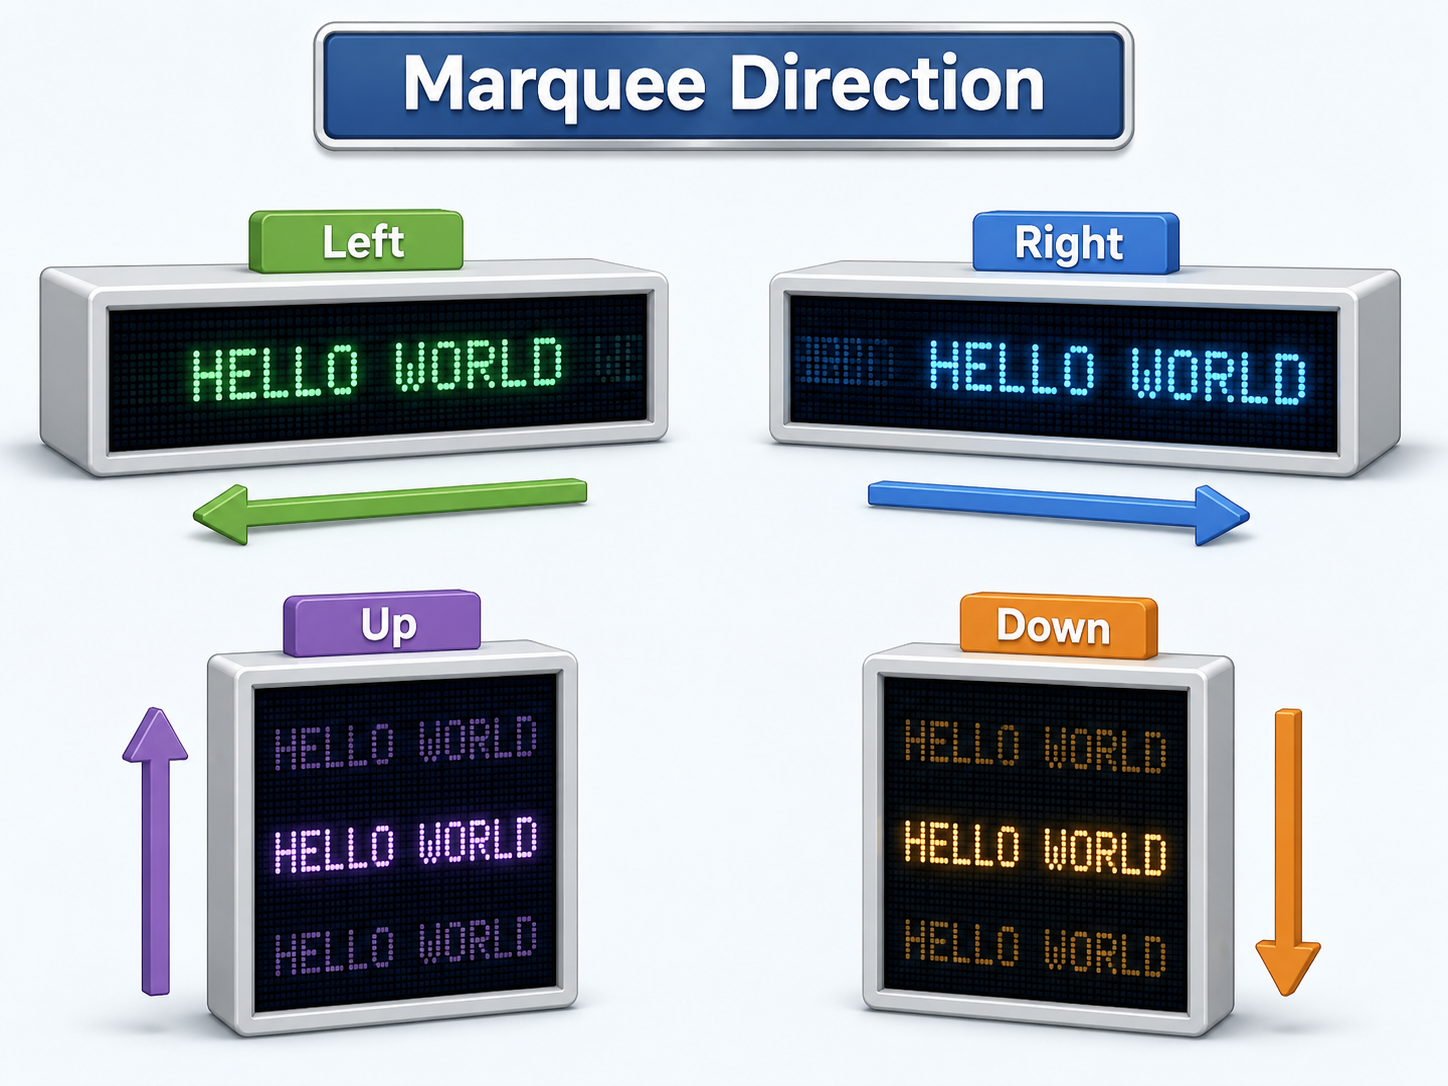
\includegraphics[width=\linewidth,height=.24\textheight,keepaspectratio]{chapters/Chapter04/topics/images/3d_marquee_direction.png}
}{
\fbox{\parbox{0.92\linewidth}{\centering\vspace{0.4cm}
\textbf{চিত্র}\\
ফাইল: \texttt{chapters/Chapter04/topics/images/3d\_marquee\_direction.png}
\vspace{0.4cm}}}
}
\captionof{figure}{চলমান লেখার ট্যাগের \texttt{direction} অ্যাট্রিবিউট}
\end{minipage}\hfill
\begin{minipage}[t]{.46\linewidth}\vspace{0pt}\small
\begin{keypointbox}{চিত্র ব্যাখ্যা}
চিত্রে লেখার চলার চারটি দিক দেখানো হয়েছে। \texttt{left} বামে, \texttt{right} ডানে, \texttt{up} উপরে এবং \texttt{down} নিচে চলার নির্দেশ দেয়।
\end{keypointbox}

\begin{keypointbox}{চিত্র দেখে কোড লেখার ধাপ}
\texttt{<marquee>}-এর ভেতরের লেখা বা ছবি চলমান থাকে। \texttt{direction} অ্যাট্রিবিউটের মান চলার দিক নির্ধারণ করে।
\end{keypointbox}
\end{minipage}\par


\begin{examplebox}{বিশেষভাবে দেখানো HTML কোড}
\par\noindent\begin{minipage}{\linewidth}
\begin{verbatim}
<marquee direction="left">Welcome to HSC ICT</marquee>
<marquee direction="right">HTML Marquee Example</marquee>
<marquee direction="up" height="80">Move Up</marquee>
<marquee direction="down" height="80">Move Down</marquee>
\end{verbatim}
\end{minipage}\par
\end{examplebox}

\begin{mistakebox}{আধুনিক সতর্কতা}
\texttt{<marquee>} বর্তমান HTML-এ পুরোনো ও নতুন কোডে ব্যবহারযোগ্য নয় এমন বৈশিষ্ট্য। পরীক্ষার উদাহরণ বোঝার জন্য এটি জানা দরকার। নতুন ওয়েবসাইটে চলমান দৃশ্যের জন্য CSS অ্যানিমেশন ব্যবহার করা হয়।
\end{mistakebox}

\subsection{লেখা বিন্যাসের ট্যাগ ও কাজ}

\begin{center}
\footnotesize
\begin{tabular}{|p{0.17\textwidth}|p{0.30\textwidth}|p{0.37\textwidth}|}
\hline
\textbf{ট্যাগ} & \textbf{কাজ} & \textbf{উদাহরণ} \\
\hline
\texttt{<h1>--<h6>} & শিরোনাম তৈরি করে & \texttt{<h1>Title</h1>} \\
\hline
\texttt{<p>} & অনুচ্ছেদ তৈরি করে & \texttt{<p>Text</p>} \\
\hline
\texttt{<br>} & নতুন লাইন তৈরি করে & \texttt{Line 1<br>Line 2} \\
\hline
\texttt{<hr>} & অনুভূমিক লাইন তৈরি করে & \texttt{<hr>} \\
\hline
\texttt{<b>} & মোটা অক্ষরের লেখা & \texttt{<b>Bold</b>} \\
\hline
\texttt{<strong>} & গুরুত্বপূর্ণ লেখা & \texttt{<strong>Important</strong>} \\
\hline
\texttt{<i>} & বাঁকা অক্ষরের লেখা & \texttt{<i>Italic</i>} \\
\hline
\texttt{<em>} & জোর দেওয়া লেখা & \texttt{<em>Emphasis</em>} \\
\hline
\texttt{<u>} & নিচে রেখাযুক্ত লেখা & \texttt{<u>Underline</u>} \\
\hline
\texttt{<ins>} & যোগ করা লেখা & \texttt{<ins>New</ins>} \\
\hline
\texttt{<del>} & বাদ দেওয়া লেখা & \texttt{<del>Old</del>} \\
\hline
\texttt{<s>} & মাঝে রেখাযুক্ত & \texttt{<s>Old</s>} \\
\hline
\texttt{<strike>} & মাঝে রেখাযুক্ত পুরোনো ট্যাগ & \texttt{<strike>Old</strike>} \\
\hline
\texttt{<small>} & ছোট লেখা & \texttt{<small>Small</small>} \\
\hline
\texttt{<big>} & বড় লেখা & \texttt{<big>Big</big>} \\
\hline
\texttt{<sub>} & নিচের সূচক & \texttt{H<sub>2</sub>O} \\
\hline
\texttt{<sup>} & উপরের সূচক & \texttt{a<sup>2</sup>} \\
\hline
\texttt{<pre>} & উৎসের বিন্যাস অক্ষুণ্ণ রাখা লেখা & \texttt{<pre>Text</pre>} \\
\hline
\texttt{<font>} & অক্ষরের আকার, রং ও ফন্টের ধরন & \texttt{<font color="red">Text</font>} \\
\hline
\end{tabular}
\normalsize
\end{center}

% Original applied explanation; see Chapter04/SOURCES.md.
\subsubsection{নোটিশের গুরুত্ব ও দেখতে মোটা লেখার পার্থক্য}
\begin{flushleft}\small
\begin{tabularx}{\linewidth}{|p{26mm}|X|X|}\hline
\textbf{বিবেচনা} & \textbf{\texttt{strong}} & \textbf{\texttt{b}}\\\hline
অর্থ & বিষয়বস্তুর বিশেষ গুরুত্ব গঠনে প্রকাশ করে & সাধারণভাবে দৃষ্টি আকর্ষণের অংশ চিহ্নিত করে\\\hline
দেখতে কেমন & মোটা দেখা যেতে পারে & প্রায় একইভাবে মোটা দেখা যেতে পারে; অর্থ এক নয়\\\hline
\end{tabularx}
\end{flushleft}
\textbf{উদাহরণ:} ভর্তি-নোটিশে \textbf{আবেদনের শেষ দিন} বিশেষ গুরুত্বপূর্ণ। \texttt{strong} দিয়ে সেই গুরুত্ব গঠনে প্রকাশ করা যায়।

নতুন বিষয় শুরু করতে শিরোনাম এবং বিস্তারিত লিখতে অনুচ্ছেদ ব্যবহার করবে। ফাঁকা জায়গা বানাতে বারবার \texttt{br} ব্যবহার করলে ছোট পর্দায় বিন্যাস অনিয়মিত হতে পারে। আলাদা অনুচ্ছেদে \texttt{p}, আর চিঠির ঠিকানার মতো একই অংশে প্রয়োজনীয় লাইনবিরতিতে \texttt{br} বেছে নেবে।


\subsection{পূর্ণাঙ্গ উদাহরণ}

\Needspace{6\baselineskip}
\par\noindent{\color{chFourTeal}\bfseries\small কোড: বাম কলাম শেষে ডান কলাম পড়বে}\par
\begin{multicols}{2}
\begin{verbatim}
<body bgcolor="#F5F5F5">

  <h1 align="center">HSC ICT Chapter 4</h1>
  <hr>

  <p>This is a normal paragraph.</p>
  <p><b>This is bold text.</b></p>
  <p><strong>This is important text.</strong></p>
  <p><i>This is italic text.</i></p>
  <p><em>This text is emphasized.</em></p>
  <p><u>This is underline text.</u></p>
  <p><small>This is small text.</small></p>
  <p><big>This is big text.</big></p>

  <p>Water formula: H<sub>2</sub>O</p>
  <p>Math formula: a<sup>2</sup> + b<sup>2</sup></p>

  <p><del>Old Notice</del> <ins>New Notice</ins></p>
  <p><s>Cancelled class</s></p>
  <p><strike>Old HTML tag</strike></p>

  <font size="5" color="blue" face="Arial">
    This text uses font tag.
  </font>

  <pre>
Name      Roll
Sakib     01
Asraful   02
  </pre>

</body>
\end{verbatim}
\end{multicols}


\begin{examplebox}{ফল কী হবে?}
ব্রাউজারে কেন্দ্রে সাজানো শিরোনাম, অনুভূমিক লাইন, মোটা অক্ষরের/বাঁকা অক্ষরের/নিচে রেখাযুক্ত লেখা, H\textsubscript{2}O নিচের সূচক, a\textsuperscript{2}+b\textsuperscript{2} উপরের সূচক, বাদ দেওয়া/যোগ করা লেখা, নীল Arial ফন্ট লেখা এবং আগের বিন্যাসে রাখা সারণির মতো লেখা দেখা যাবে।
\end{examplebox}

\begin{mistakebox}{সাধারণ ভুল}
\par\noindent
\begin{minipage}[t]{.48\linewidth}\vspace{0pt}
\begin{itemize}
\item \texttt{<br>} ট্যাগকে কন্টেইনার ট্যাগ মনে করা।
\item \texttt{<title>} আর \texttt{<h1>} একই মনে করা।
\item \texttt{<b>} ও \texttt{<strong>} ট্যাগের অর্থের পার্থক্য না বোঝা।
\item \texttt{<i>} ও \texttt{<em>} ট্যাগের অর্থগত পার্থক্য না বোঝা।
\end{itemize}
\end{minipage}\hfill
\begin{minipage}[t]{.48\linewidth}\vspace{0pt}
\begin{itemize}
\item \texttt{<sub>} আর \texttt{<sup>} উল্টো করে ফেলা।
\item \texttt{<font>} ট্যাগ আধুনিক HTML-এ বর্তমান মানে ব্যবহারযোগ্য নয় - এই বাড়তি তথ্য না দেওয়া।
\item বাংলা লেখা ঠিক দেখাতে \texttt{UTF-8} না দেওয়া।
\item ট্যাগ ঠিকভাবে বন্ধ না করা।
\end{itemize}
\end{minipage}\par

\end{mistakebox}


\begin{keypointbox}{শিরোনামের স্তর ঠিক রাখবে}
কলেজের পেজের মূল বিষয় \texttt{h1}, তার বিভাগ \texttt{h2} এবং সেই বিভাগের উপবিষয় \texttt{h3} হতে পারে। শুধু ছোট অক্ষর চাই বলে \texttt{h1} থেকে সরাসরি \texttt{h6}-এ যাওয়া ঠিক নয়। যৌক্তিক শিরোনাম স্ক্রিন রিডার ব্যবহারকারীকে পেজের অংশ বুঝতে সাহায্য করে; অক্ষরের দৃশ্যমান মাপ CSS-এ ঠিক করবে।
\end{keypointbox}


\subsection{সংক্ষিপ্ত অনুশীলন}

% Each question keeps its answer beneath it in the same column.
\begin{multicols}{2}
\noindent\begin{minipage}[t]{\linewidth}\vspace{0pt}
\chFourReviewQuestion{শিরোনাম ট্যাগ কয়টি?}
\end{minipage}\par\smallskip
\noindent\begin{minipage}[t]{\linewidth}\vspace{0pt}
\chFourReviewQuestion{অনুচ্ছেদ লেখার ট্যাগ কোনটি?}
\end{minipage}\par\smallskip
\noindent\begin{minipage}[t]{\linewidth}\vspace{0pt}
\chFourReviewQuestion{লাইন বিরতি করার ট্যাগ কোনটি?}
\end{minipage}\par\smallskip
\noindent\begin{minipage}[t]{\linewidth}\vspace{0pt}
\chFourReviewQuestion{অনুভূমিক লাইন তৈরির ট্যাগ কোনটি?}
\end{minipage}\par\smallskip
\noindent\begin{minipage}[t]{\linewidth}\vspace{0pt}
\chFourReviewQuestion{লেখা মোটা অক্ষরের করতে কোন ট্যাগ ব্যবহার হয়?}
\end{minipage}\par\smallskip
\noindent\begin{minipage}[t]{\linewidth}\vspace{0pt}
\chFourReviewQuestion{লেখা বাঁকা অক্ষরের করতে কোন ট্যাগ ব্যবহার হয়?}
\end{minipage}\par\smallskip
\noindent\begin{minipage}[t]{\linewidth}\vspace{0pt}
\chFourReviewQuestion{H\textsubscript{2}O লেখার জন্য কোন ট্যাগ ব্যবহার হবে?}
\end{minipage}\par\smallskip
\noindent\begin{minipage}[t]{\linewidth}\vspace{0pt}
\chFourReviewQuestion{a\textsuperscript{2} লেখার জন্য কোন ট্যাগ ব্যবহার হবে?}
\end{minipage}\par\smallskip
\noindent\begin{minipage}[t]{\linewidth}\vspace{0pt}
\chFourReviewQuestion{\texttt{<font>} ট্যাগের অ্যাট্রিবিউট কী কী?}
\end{minipage}\par\smallskip
\end{multicols}

\Needspace{10\baselineskip}
\subsection{পরীক্ষাভিত্তিক বহুনির্বাচনি প্রশ্ন}

\begin{multicols}{2}
\begin{enumerate}[leftmargin=*,itemsep=5pt]
\item \begin{minipage}[t]{\linewidth}\vspace{0pt}
ব্রাউজারের স্বাভাবিক রীতিতে সবচেয়ে বড় শিরোনাম কোনটি?
\par ক) \texttt{<h6>}
\par খ) \texttt{<h3>}
\par গ) \texttt{<h1>}
\par ঘ) \texttt{<head>}
\end{minipage}

\item \begin{minipage}[t]{\linewidth}\vspace{0pt}
অনুচ্ছেদ ট্যাগ কোনটি?
\par ক) \texttt{<para>}
\par খ) \texttt{<p>}
\par গ) \texttt{<br>}
\par ঘ) \texttt{<hr>}
\end{minipage}

\item \begin{minipage}[t]{\linewidth}\vspace{0pt}
নতুন লাইন তৈরি করতে কোন ট্যাগ ব্যবহৃত হয়?
\par ক) \texttt{<br>}
\par খ) \texttt{<b>}
\par গ) \texttt{<i>}
\par ঘ) \texttt{<u>}
\end{minipage}

\item \begin{minipage}[t]{\linewidth}\vspace{0pt}
H\textsubscript{2}O লেখার জন্য কোন ট্যাগ দরকার?
\par ক) \texttt{<sup>}
\par খ) \texttt{<sub>}
\par গ) \texttt{<small>}
\par ঘ) \texttt{<big>}
\end{minipage}

\item \begin{minipage}[t]{\linewidth}\vspace{0pt}
a\textsuperscript{2} লেখার জন্য কোন ট্যাগ দরকার?
\par ক) \texttt{<sub>}
\par খ) \texttt{<sup>}
\par গ) \texttt{<del>}
\par ঘ) \texttt{<ins>}
\end{minipage}

\item \begin{minipage}[t]{\linewidth}\vspace{0pt}
\texttt{<font>} ট্যাগের অ্যাট্রিবিউট কোনগুলো?
\par ক) \texttt{size}, \texttt{color}, \texttt{face}
\par খ) \texttt{src}, \texttt{alt}, \texttt{width}
\par গ) \texttt{href}, \texttt{target}, \texttt{title}
\par ঘ) \texttt{rowspan}, \texttt{colspan}, \texttt{border}
\end{minipage}
\end{enumerate}
\end{multicols}

\chFourMCQAnswer{১-গ, ২-খ, ৩-ক, ৪-খ, ৫-খ, ৬-ক}

% Density revision 2026-10-04: answers below questions; compact related content.
% ৪.x HTML তালিকা
\section{HTML-এ তালিকা (List)}

% Composition pass 2026-10-04
বইয়ের বিষয়গুলো একটানা অনুচ্ছেদে লিখলে আলাদা উপাদান ও তাদের ক্রম বোঝা কঠিন।

\chFourMotivation{তথ্যকে পৃথক উপাদানে সাজানো $\rightarrow$ তালিকা $\rightarrow$ ক্রম, বুলেট বা পরিভাষা–বর্ণনার জোড়া $\rightarrow$ লাইব্রেরির বিভাগ ও বইয়ের বিষয় দ্রুত পড়া যায়।}


\begin{learningbox}
এই অংশ শেষে শিক্ষার্থী পারবে:
\begin{itemize}
\item HTML তালিকা কী তা ব্যাখ্যা করতে।
\item ক্রমযুক্ত তালিকা, বুলেট তালিকা ও বর্ণনামূলক তালিকার পার্থক্য লিখতে।
\item \texttt{<ol>}, \texttt{<ul>}, \texttt{<li>}, \texttt{<dl>}, \texttt{<dt>} ও \texttt{<dd>} ট্যাগ ব্যবহার করতে।
\item \texttt{type} ও \texttt{start} অ্যাট্রিবিউটের কাজ বুঝতে।
\item নেস্টেড তালিকা তৈরি করতে।
\item HSC ব্যবহারিক অনুশীলন ও বোর্ড পরীক্ষার তালিকা-সম্পর্কিত প্রশ্নের উত্তর দিতে।
\end{itemize}
\end{learningbox}



\subsection{HTML তালিকা কী?}

\begin{definitionbox}{HTML তালিকা (List)}
ওয়েবপেজে একাধিক উপাদানকে ক্রম, বুলেট কিংবা পরিভাষা ও বর্ণনার জোড়ায় সাজানোর পদ্ধতিকে HTML তালিকা বলে।
\end{definitionbox}

পঠিত বিষয়, খাবারের মেনু, বই, রুটিন, পণ্যের বৈশিষ্ট্য, নির্দেশনার ধাপ ও ওয়েবসাইটের মেনু তালিকায় সাজানো যায়। পরিভাষা ও তার অর্থও তালিকায় দেখানো যায়। এতে প্রতিটি উপাদান আলাদা করে পড়া ও তুলনা করা সহজ হয়।




\subsection{HTML তালিকার প্রকারভেদ}

\begin{center}
\begin{tabular}{|p{0.25\textwidth}|p{0.18\textwidth}|p{0.43\textwidth}|}
\hline
\textbf{তালিকার ধরন} & \textbf{ট্যাগ} & \textbf{ব্যবহার} \\
\hline
ক্রমযুক্ত তালিকা & \texttt{<ol>} & সংখ্যা, অক্ষর বা রোমান সংখ্যা চিহ্নসহ ক্রমানুসার তালিকা \\
\hline
বুলেট তালিকা & \texttt{<ul>} & বুলেট/চিহ্নসহ তালিকা; উপাদানের ক্রম গুরুত্বপূর্ণ নয় \\
\hline
বর্ণনামূলক তালিকা & \texttt{<dl>} & পরিভাষা ও বর্ণনা আকারে তালিকা \\
\hline
\end{tabular}
\end{center}

\begin{keypointbox}{মনে রাখো}
\texttt{<ol>} ও \texttt{<ul>} তালিকার প্রতিটি উপাদান লেখার জন্য \texttt{<li>} ট্যাগ ব্যবহার করা হয়। কিন্তু \texttt{<dl>} তালিকায় \texttt{<li>} নয়; পরিভাষার জন্য \texttt{<dt>} এবং বর্ণনার জন্য \texttt{<dd>} ব্যবহার করা হয়।
\end{keypointbox}

\subsection{ক্রমযুক্ত তালিকা: \texttt{<ol>}}

\begin{definitionbox}{ক্রমযুক্ত তালিকা (Ordered List)}
যে তালিকায় উপাদানগুলো নির্দিষ্ট ক্রমে সংখ্যা, অক্ষর বা রোমান সংখ্যার চিহ্নসহ দেখানো হয়, তাকে ক্রমযুক্ত তালিকা বলে।
\end{definitionbox}

উপাদানের ক্রম গুরুত্বপূর্ণ হলে ক্রমযুক্ত তালিকা ব্যবহার করা হয়। নির্দেশনার ধাপ, পরীক্ষার রুটিন, স্থানক্রম, অধ্যায়ের তালিকা, ভর্তি প্রক্রিয়া ও অ্যালগরিদমের ধাপ এর উদাহরণ।

\subsubsection{সিনট্যাক্স}

\begin{examplebox}{কোড}
\par\noindent\begin{minipage}{\linewidth}
\begin{verbatim}
<ol>
  <li>First item</li>
  <li>Second item</li>
  <li>Third item</li>
</ol>
\end{verbatim}
\end{minipage}\par
\end{examplebox}

\subsubsection{উদাহরণ}

% Split revision: code and its explanation share one row.
\par\noindent
\begin{minipage}[t]{.54\linewidth}\vspace{0pt}\small
\textbf{\color{chFourTeal}কোড}\par
\begin{verbatim}
<!DOCTYPE html>
<html>
<body>
  <h2>HSC ICT Chapter List</h2>

  <ol>
    <li>ICT: World and Bangladesh Perspective</li>
    <li>Communication System and Networking</li>
    <li>Number System and Digital Device</li>
    <li>Web Design Introduction and HTML</li>
  </ol>
</body>
</html>
\end{verbatim}

\par\smallskip
\end{minipage}\hfill
\begin{minipage}[t]{.42\linewidth}\vspace{0pt}\small
\textbf{\color{chFourTeal}ফল ও ব্যাখ্যা}\par
\textbf{ফল:}
\begin{enumerate}
\item ICT: World and Bangladesh Perspective
\item Communication System and Networking
\item Number System and Digital Device
\item Web Design Introduction and HTML
\end{enumerate}
\textbf{ব্যাখ্যা:} \texttt{<ol>} ক্রমযুক্ত তালিকা শুরু করে এবং প্রতিটি \texttt{<li>} একটি করে তালিকার উপাদান তৈরি করে। ব্রাউজার স্বাভাবিক অবস্থায় চিহ্ন হিসেবে 1, 2, 3 ব্যবহার করে।
\par\smallskip
\end{minipage}\par


\subsection{ক্রমযুক্ত তালিকার অ্যাট্রিবিউট}

\subsubsection{\texttt{type} অ্যাট্রিবিউট}

\texttt{type} অ্যাট্রিবিউট দিয়ে ক্রমযুক্ত তালিকার চিহ্ন কীভাবে দেখাবে তা নির্ধারণ করা যায়।

\begin{center}
\begin{tabular}{|p{0.25\textwidth}|p{0.35\textwidth}|}
\hline
\textbf{ধরন} & \textbf{ফলের চিহ্ন} \\
\hline
\texttt{type="1"} & 1, 2, 3 \\
\hline
\texttt{type="A"} & A, B, C \\
\hline
\texttt{type="a"} & a, b, c \\
\hline
\texttt{type="I"} & I, II, III \\
\hline
\texttt{type="i"} & i, ii, iii \\
\hline
\end{tabular}
\end{center}

\begin{chFourWholeExample}{কোড ও ব্রাউজারে ফল}
\noindent
\begin{minipage}[t]{.50\linewidth}\vspace{0pt}

\begin{verbatim}
<ol type="A">
  <li>HTML</li>
  <li>CSS</li>
  <li>JavaScript</li>
</ol>
\end{verbatim}

\end{minipage}\hfill
\begin{minipage}[t]{.46\linewidth}\vspace{0pt}
\textbf{ফল:}\\
A. HTML\\
B. CSS\\
C. JavaScript\\
\end{minipage}
\chFourWhy{\texttt{type="A"} দেওয়ায় চিহ্ন সংখ্যা না হয়ে বড় হাতের অক্ষর হিসেবে দেখায়।}
\end{chFourWholeExample}

\subsubsection{\texttt{start} অ্যাট্রিবিউট}

\texttt{start} অ্যাট্রিবিউট দিয়ে ক্রমযুক্ত তালিকা কোন সংখ্যা থেকে শুরু হবে তা নির্ধারণ করা যায়।

\begin{chFourWholeExample}{কোড ও ব্রাউজারে ফল}
\noindent
\begin{minipage}[t]{.50\linewidth}\vspace{0pt}

\begin{verbatim}
<ol start="5">
  <li>HTML</li>
  <li>CSS</li>
  <li>JavaScript</li>
</ol>
\end{verbatim}

\end{minipage}\hfill
\begin{minipage}[t]{.46\linewidth}\vspace{0pt}
\textbf{ফল:}
\begin{enumerate}[start=5]
\item HTML
\item CSS
\item JavaScript
\end{enumerate}
\end{minipage}
\chFourWhy{\texttt{start="5"} দেওয়ায় তালিকার চিহ্ন ১ থেকে না শুরু হয়ে ৫ থেকে শুরু হয়েছে।}
\end{chFourWholeExample}

\begin{keypointbox}{মান অনুযায়ী বাড়তি তথ্য}
\texttt{reversed} অ্যাট্রিবিউট দিলে ক্রমযুক্ত তালিকা উল্টো ক্রমে গণনা হয়।
নির্দিষ্ট উপাদান থেকে গণনার মান বদলাতে সেই \texttt{<li>} এলিমেন্টে \texttt{value} অ্যাট্রিবিউট ব্যবহার করা যায়।
\end{keypointbox}



\subsection{বুলেট তালিকা: \texttt{<ul>}}

\begin{definitionbox}{বুলেট তালিকা (Unordered List)}
যে তালিকায় উপাদানের নির্দিষ্ট ক্রম গুরুত্বপূর্ণ নয় এবং প্রতিটি উপাদান বুলেট বা চিহ্নসহ দেখানো হয়, তাকে বুলেট তালিকা বলে।
\end{definitionbox}

যখন উপাদানের ক্রম গুরুত্বপূর্ণ নয়, তখন বুলেট তালিকা ব্যবহার করা হয়। যেমন: মেনু, বৈশিষ্ট্য, পঠিত বিষয়, কেনাকাটা, বিজ্ঞপ্তি, গুরুত্বপূর্ণ পাঠ বা ওয়েবসাইটে চলাচলের তালিকা।

\subsubsection{সিনট্যাক্স}

\begin{examplebox}{কোড}
\par\noindent\begin{minipage}{\linewidth}
\begin{verbatim}
<ul>
  <li>Item one</li>
  <li>Item two</li>
  <li>Item three</li>
</ul>
\end{verbatim}
\end{minipage}\par
\end{examplebox}

\subsubsection{উদাহরণ}

\begin{chFourWholeExample}{কোড ও ব্রাউজারে ফল}
\noindent
\begin{minipage}[t]{.50\linewidth}\vspace{0pt}

\begin{verbatim}
<h2>Web Design Tools</h2>

<ul>
  <li>HTML</li>
  <li>CSS</li>
  <li>JavaScript</li>
  <li>Browser</li>
</ul>
\end{verbatim}

\end{minipage}\hfill
\begin{minipage}[t]{.46\linewidth}\vspace{0pt}
\textbf{ফল:}
\begin{itemize}
\item HTML
\item CSS
\item JavaScript
\item Browser
\end{itemize}
\end{minipage}
\chFourWhy{\texttt{<ul>} বুলেট তালিকা তৈরি করে। ব্রাউজার স্বাভাবিক অবস্থায় বুলেট চিহ্ন দেখায়।}
\end{chFourWholeExample}

\subsection{বুলেট তালিকার \texttt{type} অ্যাট্রিবিউট}

পরীক্ষায় পরিচিত পুরোনো HTML কোডে বুলেট তালিকার চিহ্ন পরিবর্তনের জন্য \texttt{type} অ্যাট্রিবিউট দেখা যায়।

\begin{center}
\begin{tabular}{|p{0.30\textwidth}|p{0.34\textwidth}|}
\hline
\textbf{ধরন} & \textbf{ফল কী হবে?} \\
\hline
\texttt{type="disc"} & ভরাট বুলেট \\
\hline
\texttt{type="circle"} & ফাঁপা গোলাকার বুলেট \\
\hline
\texttt{type="square"} & বর্গাকার বুলেট \\
\hline
\end{tabular}
\end{center}

\begin{chFourWholeExample}{কোড ও ব্রাউজারে ফল}
\noindent
\begin{minipage}[t]{.50\linewidth}\vspace{0pt}

\begin{verbatim}
<ul type="square">
  <li>Monitor</li>
  <li>Keyboard</li>
  <li>Mouse</li>
</ul>
\end{verbatim}

\end{minipage}\hfill
\begin{minipage}[t]{.46\linewidth}\vspace{0pt}
\textbf{ফল:}\\
\(\blacksquare\) Monitor\\
\(\blacksquare\) Keyboard\\
\(\blacksquare\) Mouse\\
\end{minipage}
\chFourWhy{\texttt{type="square"} দেওয়ায় তালিকার চিহ্ন বর্গাকার বুলেট আকারে দেখা যাবে।}
\end{chFourWholeExample}

\begin{mistakebox}{আধুনিক HTML-এর নিয়ম}
বর্তমান HTML-এ \texttt{<ul>}-এর \texttt{type} পুরোনো অ্যাট্রিবিউট; বুলেটের ধরন বদলাতে CSS-এর \texttt{list-style-type} ব্যবহার করা হয়। \texttt{<ol>}-এর \texttt{type} কিন্তু বর্তমান মানে বৈধ। পরীক্ষার পুরোনো উদাহরণ বোঝার জন্য \texttt{type="disc"}, \texttt{type="circle"} ও \texttt{type="square"} জানা দরকার।
\end{mistakebox}



\subsection{তালিকার উপাদান: \texttt{<li>}}

\begin{definitionbox}{তালিকার উপাদান (List Item)}
\texttt{<li>} ট্যাগ তালিকার প্রতিটি উপাদান লিখতে ব্যবহৃত হয়।
\end{definitionbox}

\texttt{<ol>} এবং \texttt{<ul>} - দুই ধরনের তালিকার উপাদান লিখতেই \texttt{<li>} ট্যাগ ব্যবহার করা হয়।

\begin{chFourWholeExample}{কোড ও ব্রাউজারে ফল}
\noindent
\begin{minipage}[t]{.50\linewidth}\vspace{0pt}

\begin{verbatim}
<ul>
  <li>Bangla</li>
  <li>English</li>
  <li>ICT</li>
</ul>
\end{verbatim}

\end{minipage}\hfill
\begin{minipage}[t]{.46\linewidth}\vspace{0pt}
\textbf{ফল:}
\begin{itemize}
\item Bangla
\item English
\item ICT
\end{itemize}
\end{minipage}
\chFourWhy{প্রতিটি \texttt{<li>} ট্যাগ একটি আলাদা তালিকার উপাদান তৈরি করেছে।}
\end{chFourWholeExample}

\begin{keypointbox}{পরীক্ষায় মনে রাখবে}
HTML-এর নির্দিষ্ট নিয়মে \texttt{</li>} বাদ দেওয়া যায়; যেমন পরেই আরেকটি \texttt{<li>} শুরু হলে। এটি শুধু পুরোনো HTML-এর নিয়ম নয়। শেখার সময় \texttt{<li>Item</li>} আকারে শেষের ট্যাগ লিখলে তালিকার গঠন সহজে বোঝা যায়।
\end{keypointbox}

\subsection{বর্ণনামূলক তালিকা: \texttt{<dl>}, \texttt{<dt>}, \texttt{<dd>}}

\begin{definitionbox}{বর্ণনামূলক তালিকা (Description List)}
পরিভাষা বা বিষয়ের নামের সঙ্গে তার বর্ণনা সাজিয়ে দেখানোর তালিকাকে বর্ণনামূলক তালিকা বলে।
\end{definitionbox}

পরিভাষা, সংজ্ঞা, বহুল জিজ্ঞাসিত প্রশ্ন (Frequently Asked Questions বা FAQ), পণ্যের বৈশিষ্ট্য, যোগাযোগের বিস্তারিত তথ্য বা শব্দের অর্থ দেখাতে বর্ণনামূলক তালিকা ব্যবহার করা যায়।

\subsubsection{সিনট্যাক্স}

% Split revision: code and its explanation share one row.
\par\noindent
\begin{minipage}[t]{.50\linewidth}\vspace{0pt}\small
\textbf{\color{chFourTeal}কোড}\par
\begin{verbatim}
<dl>
  <dt>Term</dt>
  <dd>Description of the term</dd>
</dl>
\end{verbatim}

\par\smallskip
\end{minipage}\hfill
\begin{minipage}[t]{.46\linewidth}\vspace{0pt}\small
\begin{tabular}{|p{0.25\linewidth}|p{0.64\linewidth}|}
\hline
\textbf{ট্যাগ} & \textbf{কাজ} \\
\hline
\texttt{<dl>} & বর্ণনামূলক তালিকা শুরু ও শেষ করে \\
\hline
\texttt{<dt>} & পরিভাষা বা নাম নির্দেশ করে \\
\hline
\texttt{<dd>} & পরিভাষার বর্ণনা নির্দেশ করে \\
\hline
\end{tabular}
\end{minipage}\par


% Split revision: code and its explanation share one row.
\par\noindent
\begin{minipage}[t]{.54\linewidth}\vspace{0pt}\small
\subsubsection{উদাহরণ: কোড}
\begin{verbatim}
<h2>Web Terms</h2><dl>
  <dt>HTML</dt>
  <dd>HTML is used to create the structure of a web page.</dd>
  <dt>CSS</dt>
  <dd>CSS is used to design and style a web page.</dd>
  <dt>JavaScript</dt>
  <dd>JavaScript is used to add interactivity to a web page.</dd></dl>
\end{verbatim}

\par\smallskip
\end{minipage}\hfill
\begin{minipage}[t]{.42\linewidth}\vspace{0pt}\small
\textbf{\color{chFourTeal}ফল ও ব্যাখ্যা}\par
\textbf{HTML}\\
\hspace*{.5em}HTML is used to create the structure of a web page.\\
\textbf{CSS}\\
\hspace*{.5em}CSS is used to design and style a web page.\\
\textbf{JavaScript}\\
\hspace*{.5em}JavaScript is used to add interactivity to a web page.\\
\textbf{ব্যাখ্যা:} \texttt{<dt>} ট্যাগ পরিভাষা দেখায় এবং \texttt{<dd>} ট্যাগ সেই পরিভাষার বর্ণনা দেখায়।
\par\smallskip
\end{minipage}\par




\begin{keypointbox}{মান অনুযায়ী বাড়তি তথ্য}
একটি \texttt{dl} এলিমেন্টে একই দলভুক্ত একাধিক নাম বা পরিভাষার জন্য একাধিক \texttt{dt} এবং সংশ্লিষ্ট বিকল্প বর্ণনার জন্য একাধিক \texttt{dd} দেওয়া যায়। একই বর্ণনার একাধিক অনুচ্ছেদ হলে সেগুলো একই \texttt{dd}-এর মধ্যে থাকে। প্রয়োজন হলে প্রতিটি নাম-বর্ণনার দলকে \texttt{div} দিয়ে ঘিরে রীতি বা মেটাডেটা দেওয়া যায়।
\end{keypointbox}

% Original applied explanation; see Chapter04/SOURCES.md.
\subsubsection{তালিকার ধরন বাছাইয়ে একটি সহজ পরীক্ষা}
ভর্তি-আবেদনের ধাপ উল্টে দিলে কাজ বদলে যায়; সেখানে \texttt{ol} উপযোগী। প্রয়োজনীয় কাগজপত্রের তালিকায় ক্রম সাধারণত জরুরি নয়; সেখানে \texttt{ul} উপযোগী। পরিভাষা ও তার ব্যাখ্যা জোড়া আকারে রাখতে \texttt{dl}, \texttt{dt} ও \texttt{dd} লাগে।

বিভাগের তালিকার ভেতরে বিষয়ের উপতালিকা বসালে উপতালিকাটি সংশ্লিষ্ট \texttt{li}-এর ভেতরে রাখবে। এতে কোন বিষয় কোন বিভাগের অধীন, তা গঠনে প্রকাশ পায়। শুধু স্পেস দিয়ে লেখা সরিয়ে একই সম্পর্ক নির্ভরযোগ্যভাবে প্রকাশ করা যায় না।


\subsection{নেস্টেড তালিকা}

\begin{definitionbox}{নেস্টেড তালিকা (Nested List)}
একটি তালিকার উপাদানের ভিতরে আরেকটি তালিকা ব্যবহার করলে তাকে নেস্টেড তালিকা বলা যায়।
\end{definitionbox}

% Split revision: code and its explanation share one row.
\par\noindent
\begin{minipage}[t]{.50\linewidth}\vspace{0pt}\small
\textbf{\color{chFourTeal}কোড}\par
\par\noindent
\begin{verbatim}
<ul>
  <li>Science
    <ol>
      <li>Physics</li>
      <li>Chemistry</li>
      <li>Biology</li>
    </ol>
  </li>

  <li>Business Studies
    <ol>
      <li>Accounting</li>
      <li>Finance</li>
      <li>Management</li>
    </ol>
  </li>
</ul>
\end{verbatim}
\par
\par\smallskip
\end{minipage}\hfill
\begin{minipage}[t]{.46\linewidth}\vspace{0pt}\small
\textbf{\color{chFourTeal}ফল ও ব্যাখ্যা}\par
\textbf{ফল:}
\begin{itemize}
\item Science
  \begin{enumerate}
  \item Physics
  \item Chemistry
  \item Biology
  \end{enumerate}
\item Business Studies
  \begin{enumerate}
  \item Accounting
  \item Finance
  \item Management
  \end{enumerate}
\end{itemize}
\textbf{ব্যাখ্যা:} বাইরের তালিকাটি \texttt{<ul>} এবং প্রতিটি দলের ভিতরে \texttt{<ol>} তালিকা আছে। এইভাবে শ্রেণি ও উপশ্রেণি দেখানো যায়।
\par\smallskip
\end{minipage}\par


\begin{keypointbox}{নেস্টেড তালিকা কোথায় ব্যবহার হয়}
পঠিত বিষয়ের দল, ওয়েবসাইটের মেনু, অধ্যায় ও উপপাঠ, শ্রেণি ও উপশ্রেণি, কোর্সের অংশ বা পণ্যের বৈশিষ্ট্যের দল দেখাতে নেস্টেড তালিকা ব্যবহার করা যায়।
\end{keypointbox}

\subsection{ক্রমযুক্ত, বুলেট ও বর্ণনামূলক তালিকার পার্থক্য}

\begin{center}
\small
\begin{tabular}{|p{0.18\textwidth}|p{0.22\textwidth}|p{0.22\textwidth}|p{0.22\textwidth}|}
\hline
\textbf{বিষয়} & \textbf{ক্রমযুক্ত তালিকা} & \textbf{বুলেট তালিকা} & \textbf{বর্ণনামূলক তালিকা} \\
\hline
ট্যাগ & \texttt{<ol>} & \texttt{<ul>} & \texttt{<dl>} \\
\hline
উপাদান ট্যাগ & \texttt{<li>} & \texttt{<li>} & \texttt{<dt>}, \texttt{<dd>} \\
\hline
চিহ্ন & সংখ্যা/অক্ষর/রোমান সংখ্যা & বুলেট/চিহ্ন & পরিভাষা-বর্ণনা \\
\hline
ক্রম গুরুত্বপূর্ণ? & হ্যাঁ & না & পরিভাষা অনুযায়ী \\
\hline
ব্যবহার & ধাপ, স্থানক্রম, রুটিন & পাঠ, বৈশিষ্ট্য, মেনু & সংজ্ঞা, পরিভাষার তালিকা \\
\hline
উদাহরণ & 1, 2, 3 & বুলেট & HTML - মার্কআপ ভাষা \\
\hline
\end{tabular}
\normalsize
\end{center}

\subsection{পূর্ণাঙ্গ উদাহরণ}

\Needspace{6\baselineskip}
\par\noindent{\color{chFourTeal}\bfseries\small কোড: বাম কলাম শেষে ডান কলাম পড়বে}\par
\begin{multicols}{2}
\begin{verbatim}
<h1>HTML List Example</h1>

<h2>Ordered List</h2>
<ol type="1">
  <li>Open Notepad</li>
  <li>Write HTML code</li>
  <li>Save as index.html</li>
  <li>Open with browser</li>
</ol>

<h2>Unordered List</h2>
<ul type="square">
  <li>HTML</li>
  <li>CSS</li>
  <li>JavaScript</li>
</ul>

<h2>Description List</h2>
<dl>
  <dt>HTML</dt>
  <dd>HTML creates the structure of a web page.</dd>

  <dt>CSS</dt>
  <dd>CSS designs the appearance of a web page.</dd>
</dl>
\end{verbatim}
\end{multicols}


\begin{examplebox}{ফল কী হবে?}
ব্রাউজারে প্রথমে ক্রমযুক্ত তালিকা 1, 2, 3, 4 আকারে দেখা যাবে। এরপর বুলেট তালিকা বর্গাকার বুলেট আকারে দেখা যাবে। শেষে বর্ণনামূলক তালিকা পরিভাষা ও বর্ণনা আকারে দেখা যাবে।
\end{examplebox}


\begin{mistakebox}{সাধারণ ভুল}
\par\noindent
\begin{minipage}[t]{.48\linewidth}\vspace{0pt}
\begin{itemize}
\item \texttt{<ol>} ও \texttt{<ul>} গুলিয়ে ফেলা।
\item \texttt{<li>} ট্যাগ না দেওয়া।
\item \texttt{<dl>} ট্যাগের ভিতরে \texttt{<li>} ব্যবহার করা।
\item \texttt{<dt>} ও \texttt{<dd>} ভুলভাবে ব্যবহার করা।
\end{itemize}
\end{minipage}\hfill
\begin{minipage}[t]{.48\linewidth}\vspace{0pt}
\begin{itemize}
\item ক্রমযুক্ত তালিকায় \texttt{type} মান ভুল লেখা।
\item \texttt{<ul>} ট্যাগে সংখ্যা চিহ্ন আশা করা।
\item তালিকার শেষের ট্যাগ না দেওয়া।
\item নেস্টেড তালিকা ভুলভাবে বন্ধ করা।
\end{itemize}
\end{minipage}\par

\end{mistakebox}

\begin{boardbox}{নেস্টেড তালিকার সঠিক গঠন}
\begin{examplebox}{কোড}
\par\noindent\begin{minipage}{\linewidth}
\begin{verbatim}
<ul>
  <li>ICT
    <ol>
      <li>HTML</li>
      <li>Networking</li>
    </ol>
  </li>
</ul>
\end{verbatim}
\end{minipage}\par
\end{examplebox}
\end{boardbox}

% Technical basis: MDN ol. Inspired question skills, original data and wording.
\subsubsection{type ও start একসঙ্গে: ফল গণনা করার নিয়ম}
\texttt{type} চিহ্নের ধরন বেছে নেয়; \texttt{start} বলে কত নম্বর অবস্থান থেকে গণনা শুরু হবে। \texttt{start}-এর মান পূর্ণসংখ্যা, চিহ্নের অক্ষর নয়। যেমন \texttt{type="A" start="3"} দিলে প্রথম চিহ্ন C, পরেরটি D; \texttt{type="i" start="4"} দিলে iv, v। অক্ষর e থেকে শুরু করতে \texttt{type="a" start="5"} লিখবে, \texttt{start="e"} নয়।

\par\noindent{\color{chFourTeal}\bfseries\small কোড: বাম কলাম শেষে ডান কলাম পড়বে}\par
\begin{multicols}{2}
\begin{verbatim}
<ol type="a" start="4">
  <li>Books</li>
  <li>Courses
    <ol type="i" start="2">
      <li>HTML</li>
      <li>CSS</li>
    </ol>
  </li>
  <li>Clubs
    <ul style="list-style-type:circle">
      <li>Science</li>
      <li>Debate</li>
    </ul>
  </li>
</ol>
\end{verbatim}
\end{multicols}
\par\noindent\begin{minipage}[t]{.36\linewidth}\vspace{0pt}
\textbf{\color{chFourTeal}দৃশ্যমান ফল}\par
\begin{enumerate}[label=\alph*.,start=4,leftmargin=*]
\item Books
\item Courses
\begin{enumerate}[label=\roman*.,start=2,leftmargin=*]
\item HTML
\item CSS
\end{enumerate}
\item Clubs
\begin{itemize}[label=$\circ$,leftmargin=*]
\item Science
\item Debate
\end{itemize}
\end{enumerate}

\end{minipage}\hfill
\begin{minipage}[t]{.60\linewidth}\vspace{0pt}
বাইরের তালিকা d, e, f পর্যন্ত চলে। ভেতরের রোমান তালিকা নিজস্ব \texttt{start="2"} অনুযায়ী ii থেকে চলে; বাইরের e থেকে গণনা করে না। বুলেট তালিকা সংখ্যার গণনায় অংশ নেয় না। প্রতিটি ভেতরের তালিকা তার সংশ্লিষ্ট বাইরের \texttt{<li>}-এর মধ্যেই শেষ হয়েছে।
\end{minipage}\par

নেস্টেড তালিকার প্রতিটি স্তরে আলাদা \texttt{<ol>} বা \texttt{<ul>} থাকে। চিহ্নের ধরন ও শুরু নম্বর ওই স্তরেই নির্ধারিত হয়। ফলে বাইরের বড় হাতের অক্ষরের তালিকার ভেতরে সংখ্যা এবং অন্য শাখায় বুলেট রাখা যায়। স্তরের প্রথম দুটি চিহ্ন মিলিয়ে গণনা যাচাই করা যায়।



\subsection{সংক্ষিপ্ত অনুশীলন}

% Each question keeps its answer beneath it in the same column.
\begin{multicols}{2}
\noindent\begin{minipage}[t]{\linewidth}\vspace{0pt}
\chFourReviewQuestion{HTML তালিকা কী?}
\end{minipage}\par\smallskip
\noindent\begin{minipage}[t]{\linewidth}\vspace{0pt}
\chFourReviewQuestion{HTML-এ তালিকা কয় প্রকার?}
\end{minipage}\par\smallskip
\noindent\begin{minipage}[t]{\linewidth}\vspace{0pt}
\chFourReviewQuestion{ক্রমযুক্ত তালিকা তৈরির ট্যাগ কোনটি?}
\end{minipage}\par\smallskip
\noindent\begin{minipage}[t]{\linewidth}\vspace{0pt}
\chFourReviewQuestion{বুলেট তালিকা তৈরির ট্যাগ কোনটি?}
\end{minipage}\par\smallskip
\noindent\begin{minipage}[t]{\linewidth}\vspace{0pt}
\chFourReviewQuestion{তালিকার উপাদান লেখার ট্যাগ কোনটি?}
\end{minipage}\par\smallskip
\noindent\begin{minipage}[t]{\linewidth}\vspace{0pt}
\chFourReviewQuestion{বর্ণনামূলক তালিকা তৈরির ট্যাগ কোনটি?}
\end{minipage}\par\smallskip
\noindent\begin{minipage}[t]{\linewidth}\vspace{0pt}
\chFourReviewQuestion{বর্ণনামূলক তালিকায় পরিভাষা লেখার ট্যাগ কোনটি?}
\end{minipage}\par\smallskip
\noindent\begin{minipage}[t]{\linewidth}\vspace{0pt}
\chFourReviewQuestion{বর্ণনামূলক তালিকায় বর্ণনা লেখার ট্যাগ কোনটি?}
\end{minipage}\par\smallskip
\noindent\begin{minipage}[t]{\linewidth}\vspace{0pt}
\chFourReviewQuestion{\texttt{<ol type="A">} দিলে ফল কেমন হবে?}
\end{minipage}\par\smallskip
\noindent\begin{minipage}[t]{\linewidth}\vspace{0pt}
\chFourReviewQuestion{\texttt{<ul type="square">} দিলে ফল কেমন হবে?}
\end{minipage}\par\smallskip
\end{multicols}

\Needspace{10\baselineskip}
\subsection{পরীক্ষাভিত্তিক বহুনির্বাচনি প্রশ্ন}

\begin{multicols}{2}
\begin{enumerate}[leftmargin=*,itemsep=5pt]
\item \begin{minipage}[t]{\linewidth}\vspace{0pt}
HTML-এ তালিকা সাধারণত কয় প্রকার?
\par ক) ২
\par খ) ৩
\par গ) ৪
\par ঘ) ৫
\end{minipage}

\item \begin{minipage}[t]{\linewidth}\vspace{0pt}
ক্রমযুক্ত তালিকা তৈরির ট্যাগ কোনটি?
\par ক) \texttt{<ul>}
\par খ) \texttt{<ol>}
\par গ) \texttt{<li>}
\par ঘ) \texttt{<dl>}
\end{minipage}

\item \begin{minipage}[t]{\linewidth}\vspace{0pt}
বুলেট তালিকা তৈরির ট্যাগ কোনটি?
\par ক) \texttt{<ul>}
\par খ) \texttt{<ol>}
\par গ) \texttt{<dt>}
\par ঘ) \texttt{<dd>}
\end{minipage}

\item \begin{minipage}[t]{\linewidth}\vspace{0pt}
তালিকার উপাদান যুক্ত করার ট্যাগ কোনটি?
\par ক) \texttt{<ol>}
\par খ) \texttt{<li>}
\par গ) \texttt{<ul>}
\par ঘ) \texttt{<dl>}
\end{minipage}

\item \begin{minipage}[t]{\linewidth}\vspace{0pt}
বর্ণনামূলক তালিকায় পরিভাষা লেখার ট্যাগ কোনটি?
\par ক) \texttt{<dd>}
\par খ) \texttt{<dt>}
\par গ) \texttt{<li>}
\par ঘ) \texttt{<ul>}
\end{minipage}

\item \begin{minipage}[t]{\linewidth}\vspace{0pt}
\texttt{<ol type="i">} দিলে তালিকার চিহ্ন কেমন হবে?
\par ক) A, B, C
\par খ) a, b, c
\par গ) I, II, III
\par ঘ) i, ii, iii
\end{minipage}

\item \begin{minipage}[t]{\linewidth}\vspace{0pt}
বুলেট তালিকার চিহ্ন বর্গাকার করতে কোনটি ব্যবহার করা যায়?
\par ক) \texttt{<ul type="square">}
\par খ) \texttt{<ol type="square">}
\par গ) \texttt{<li type="A">}
\par ঘ) \texttt{<dl type="square">}
\end{minipage}
\end{enumerate}
\end{multicols}

\chFourMCQAnswer{১-খ, ২-খ, ৩-ক, ৪-খ, ৫-খ, ৬-ঘ, ৭-ক}

% Density revision 2026-10-04: answers below questions; compact related content.
% 4.x হাইপারলিংক in HTML
\section{HTML-এ হাইপারলিংক (Hyperlink)}

% Composition pass 2026-10-04
Home, Notice ও Result পেজ তৈরি আছে, কিন্তু এক পেজ থেকে অন্যটিতে যাওয়ার পথ দরকার।

\chFourMotivation{পেজে চলাচল $\rightarrow$ হাইপারলিংক $\rightarrow$ href-এ গন্তব্য ও ক্লিকযোগ্য লেখা/ছবি $\rightarrow$ কলেজের মেনু থেকে প্রয়োজনীয় পেজ খোলা।}


\begin{learningbox}
এই অংশ শেষে শিক্ষার্থী পারবে:
\begin{itemize}
\item হাইপারলিংক কী এবং ওয়েবপেজ চলাচলে এর প্রয়োজনীয়তা ব্যাখ্যা করতে।
\item \texttt{<a>} ট্যাগ ও \texttt{href} অ্যাট্রিবিউটের কাজ লিখতে।
\item অভ্যন্তরীণ, বাহ্যিক, বুকমার্ক, ইমেইল, ছবি, ফাইল ও নতুন ট্যাবের লিংক তৈরি করতে।
\item লিংকের লেখা, URL, \texttt{mailto:}, \texttt{target} ও \texttt{download} অ্যাট্রিবিউট ব্যবহার করতে।
\item পূর্ণ URL, আপেক্ষিক URL এবং নতুন ট্যাবে লিংক খোলার নিয়ম ব্যাখ্যা করতে।
\item HSC ব্যবহারিক অনুশীলন ও বোর্ড পরীক্ষার হাইপারলিংক-সম্পর্কিত প্রশ্নের উত্তর দিতে।
\end{itemize}
\end{learningbox}



HTML তালিকা শেখার পর হাইপারলিংক শেখা গুরুত্বপূর্ণ, কারণ একটি ওয়েবপেজের লেখা, তালিকা, ছবি বা বোতামের মাধ্যমে অন্য পেজ, ওয়েবসাইট, ফাইল বা একই পেজের নির্দিষ্ট অংশে যাওয়ার ব্যবস্থা হাইপারলিংক দিয়ে করা হয়। ওয়েবসাইটের চলাচল মেনু, ``Read more'', ``Download'', ``Contact us'', ছবি বোতাম - এসব হাইপারলিংকের বাস্তব উদাহরণ।

\subsection{হাইপারলিংক কী?}

\begin{definitionbox}{হাইপারলিংক (Hyperlink)}
ওয়েবপেজের যে লেখা, ছবি বা উপাদান নির্বাচন করলে অন্য পেজ, ওয়েবসাইট, ফাইল, ইমেইল ঠিকানা কিংবা একই পেজের নির্দিষ্ট অংশে যাওয়া যায়, তাকে হাইপারলিংক বলে।
\end{definitionbox}

হাইপারলিংক পেজ ও তথ্যের মধ্যে সংযোগ তৈরি করে। ব্যবহারকারী এই সংযোগ ধরে প্রয়োজনীয় তথ্যে পৌঁছান। তাই ওয়েবসাইটে সহজে চলাচলের জন্য অর্থবহ লিংক থাকা প্রয়োজন।



\subsection{অ্যাঙ্কর ট্যাগ: \texttt{<a>}}

\begin{definitionbox}{অ্যাঙ্কর ট্যাগ (Anchor Tag)}
HTML-এ হাইপারলিংক তৈরি করার জন্য \texttt{<a>} ট্যাগ ব্যবহার করা হয়। \texttt{<a>} ট্যাগকে অ্যাঙ্কর ট্যাগ বলা হয়।
\end{definitionbox}

অ্যাঙ্কর ট্যাগের সবচেয়ে গুরুত্বপূর্ণ অ্যাট্রিবিউট হলো \texttt{href}। \texttt{href} ছাড়া \texttt{<a>} ট্যাগ লিখলে সাধারণত লিংক কার্যকর হয় না, কারণ ব্রাউজার জানে না ক্লিক করলে কোথায় যেতে হবে।

\subsubsection{লেখার সাধারণ রূপ}

\begin{examplebox}{কোড}
\par\noindent\begin{minipage}{\linewidth}
\begin{verbatim}
<a href="url">Link Text</a>
\end{verbatim}
\end{minipage}\par
\end{examplebox}

\begin{center}
\begin{tabular}{|p{0.22\textwidth}|p{0.62\textwidth}|}
\hline
\textbf{অংশ} & \textbf{ব্যাখ্যা} \\
\hline
\texttt{<a>} & অ্যাঙ্কর ট্যাগ শুরু করে \\
\hline
\texttt{href} & লিংকের গন্তব্য বা ঠিকানা নির্ধারণ করে \\
\hline
\texttt{"url"} & যে পেজ, ওয়েবসাইট, ফাইল বা ঠিকানায় লিংক যাবে \\
\hline
\texttt{Link Text} & ব্যবহারকারী যে লেখায় ক্লিক করবে \\
\hline
\texttt{</a>} & অ্যাঙ্কর ট্যাগ শেষ করে \\
\hline
\end{tabular}
\end{center}

\begin{chFourWholeExample}{কোড ও ব্রাউজারে ফল}
\noindent
\begin{minipage}[t]{.50\linewidth}\vspace{0pt}

\begin{verbatim}
<a href="https://www.google.com">Google</a>
\end{verbatim}

\end{minipage}\hfill
\begin{minipage}[t]{.46\linewidth}\vspace{0pt}
\textbf{ফল:} ব্রাউজারে \textbf{Google} নামে একটি ক্লিকযোগ্য লিংক দেখা যাবে। এতে ক্লিক করলে Google ওয়েবসাইট খুলবে।
\end{minipage}
\chFourWhy{এখানে \texttt{href} অ্যাট্রিবিউট লিংকের গন্তব্য হিসেবে Google ওয়েবসাইটের ঠিকানা দিয়েছে এবং \texttt{Google} হলো ক্লিকযোগ্য লিংকের লেখা।}
\end{chFourWholeExample}

\subsection{\texttt{href} অ্যাট্রিবিউট}

\begin{definitionbox}{\texttt{href}}
\texttt{href} অ্যাট্রিবিউট লিংকের গন্তব্য ঠিকানা নির্ধারণ করে। Hyperlink Reference কথাটি দিয়ে এর কাজ বোঝানো হয়; কোডে অ্যাট্রিবিউটের নাম \texttt{href}।
\end{definitionbox}

\begin{keypointbox}{মনে রাখো}
\texttt{href} ছাড়া \texttt{<a>} এলিমেন্ট হাইপারলিংক তৈরি করে না; এটি লিংকের জন্য স্থানধারক হিসেবে থাকতে পারে।
\end{keypointbox}


\begin{keypointbox}{লিংকের লেখা বাছাইয়ের নিয়ম}
\texttt{Click here} এর চেয়ে \texttt{Download Routine}, \texttt{Visit Google} বা \texttt{Go to Contact} - এ ধরনের অর্থবহ লিংকের লেখা ব্যবহার করা ভালো।
\end{keypointbox}

\subsection{হাইপারলিংকের প্রকারভেদ}

গন্তব্য, ক্লিকযোগ্য অংশ ও খোলার পদ্ধতি অনুযায়ী লিংকের নিচের রূপগুলো পরিচিত। এগুলো পরস্পর বিচ্ছিন্ন শ্রেণি নয়; একই বাহ্যিক লিংক ছবিতে দেওয়া যেতে পারে এবং নতুন ট্যাবেও খুলতে পারে:

\begin{enumerate}
\item বাহ্যিক লিংক
\item অভ্যন্তরীণ লিংক
\item একই পেজ বা বুকমার্ক লিংক
\item ইমেইল লিংক
\item ছবিতে লিংক
\item ডাউনলোড বা ফাইলের লিংক
\item নতুন ট্যাবের লিংক
\end{enumerate}

\noindent
\begin{minipage}[t]{.48\linewidth}\vspace{0pt}
\begin{definitionbox}{বাহ্যিক লিংক (External Link)}
বাহ্যিক লিংক হলো এমন হাইপারলিংক, যা বর্তমান ওয়েবসাইট বা বর্তমান পেজ থেকে অন্য কোনো ওয়েবসাইটে নিয়ে যায়।
\end{definitionbox}
\end{minipage}\hfill
\begin{minipage}[t]{.48\linewidth}\vspace{0pt}
\begin{definitionbox}{অভ্যন্তরীণ লিংক (Internal Link)}
অভ্যন্তরীণ লিংক হলো এমন হাইপারলিংক, যা একই ওয়েবসাইটের একটি পেজ থেকে অন্য পেজে নিয়ে যায়।
\end{definitionbox}
\end{minipage}\par

\subsection{বাহ্যিক লিংক}



বাহ্যিক লিংক লিখতে সাধারণত ওয়েবসাইট ঠিকানার আগে \texttt{http://} বা \texttt{https://} লেখা হয়।

\subsubsection{উদাহরণ}

% Split revision: code and its explanation share one row.
\par\noindent
\begin{minipage}[t]{.54\linewidth}\vspace{0pt}\small
\textbf{\color{chFourTeal}কোড}\par
\begin{verbatim}
<a href="https://www.google.com">Visit Google</a>
\end{verbatim}

\par\smallskip
\end{minipage}\hfill
\begin{minipage}[t]{.42\linewidth}\vspace{0pt}\small
\textbf{\color{chFourTeal}ফল ও ব্যাখ্যা}\par
\textbf{ফল:} ব্রাউজারে \textbf{Visit Google} লেখা দেখা যাবে। এতে ক্লিক করলে Google ওয়েবসাইট খুলবে।

\textbf{ব্যাখ্যা:} এখানে লিংক বর্তমান ওয়েবপেজের বাইরে অন্য ওয়েবসাইটে যাচ্ছে, তাই এটি বাহ্যিক লিংক।
\par\smallskip
\end{minipage}\par




\subsection{অভ্যন্তরীণ লিংক}



একটি কলেজের ওয়েবসাইটে \texttt{Home} পেজ থেকে \texttt{About}, \texttt{Notice}, \texttt{Result} বা \texttt{Contact} পেজে যাওয়ার জন্য অভ্যন্তরীণ লিংক ব্যবহার করা হয়।

\subsubsection{উদাহরণ}

\begin{chFourWholeExample}{কোড ও ব্রাউজারে ফল}
\noindent
\begin{minipage}[t]{.50\linewidth}\vspace{0pt}

\begin{verbatim}
<a href="about.html">About Us</a>
<a href="notice.html">Notice</a>
<a href="contact.html">Contact</a>
\end{verbatim}

\end{minipage}\hfill
\begin{minipage}[t]{.46\linewidth}\vspace{0pt}
\textbf{ফল:} ব্রাউজারে \textbf{About Us}, \textbf{Notice}, \textbf{Contact} নামে তিনটি লিংক দেখা যাবে।
\end{minipage}
\chFourWhy{এগুলো একই ওয়েবসাইটের স্থানীয় পেজে লিংক করে। তাই এগুলো অভ্যন্তরীণ লিংক।}
\end{chFourWholeExample}

\subsubsection{পূর্ণাঙ্গ উদাহরণ: \texttt{index.html}}

% Split revision: code and its explanation share one row.
\par\noindent
\begin{minipage}[t]{.50\linewidth}\vspace{0pt}\small
\textbf{\color{chFourTeal}কোড}\par
\begin{verbatim}
<!DOCTYPE html>
<html>
<body>
  <h1>ABC College</h1>

  <a href="about.html">About</a>
  <a href="notice.html">Notice</a>
  <a href="contact.html">Contact</a>
</body>
</html>
\end{verbatim}

\par\smallskip
\end{minipage}\hfill
\begin{minipage}[t]{.46\linewidth}\vspace{0pt}\small

\end{minipage}\par


% Original applied explanation; see Chapter04/SOURCES.md.
\subsubsection{Notice লিংক ভুল ফোল্ডারে যায় কেন?}
ধরা যাক পেজটি \texttt{/students/index.html}-এ আছে। সেখানে \texttt{href="notice.html"} দিলে সাধারণ অবস্থায় \texttt{/students/notice.html} খোঁজা হবে; \texttt{../notice.html} দিলে এক স্তর ওপরের \texttt{/notice.html} খোঁজা হবে। তাই আপেক্ষিক পথ ঠিক কি না, তা বর্তমান পেজের ভিত্তি ঠিকানা ধরে বিচার করবে।

দর্শককে গন্তব্য বোঝাতে \textbf{ভর্তির বিজ্ঞপ্তি পড়ুন} ধরনের লিংক-লেখা ব্যবহার করবে। একই সাইটে সব লিংকে \textbf{এখানে ক্লিক করুন} লিখলে কোন লিংক কোন তথ্য দেবে তা বোঝা কঠিন হয়।


\subsection{পূর্ণ URL ও আপেক্ষিক URL}

\begin{definitionbox}{পূর্ণ ঠিকানা (Absolute URL)}
পূর্ণ URL হলো সম্পূর্ণ ওয়েব ঠিকানা, যেখানে প্রোটোকল, ডোমেইন এবং প্রয়োজনীয় পথ একসঙ্গে লেখা থাকে।
\end{definitionbox}

\begin{definitionbox}{আপেক্ষিক ঠিকানা (Relative URL)}
যে ঠিকানা একটি ভিত্তি ঠিকানার সঙ্গে মিলিয়ে সম্পূর্ণ করা হয়, তাকে \textbf{আপেক্ষিক URL} বলে। একই ওয়েবসাইটের পেজ বা ফাইলের ক্ষেত্রে প্রায়ই শুধু আপেক্ষিক পথ লেখা হয়; যেমন \texttt{about.html}।
\end{definitionbox}

\begin{center}
\begin{tabular}{|p{0.28\textwidth}|p{0.30\textwidth}|p{0.28\textwidth}|}
\hline
\textbf{বিষয়} & \textbf{পূর্ণ URL} & \textbf{আপেক্ষিক URL} \\
\hline
ঠিকানা & সম্পূর্ণ ঠিকানা & ভিত্তি ঠিকানার সঙ্গে মিলিয়ে সম্পূর্ণ করতে হয় \\
\hline
প্রোটোকল & থাকে & সাধারণত থাকে না \\
\hline
ব্যবহার & একই বা অন্য সাইটের পূর্ণ ঠিকানা & ভিত্তি ঠিকানা অনুযায়ী গন্তব্য \\
\hline
উদাহরণ & \texttt{https://google.com} & \texttt{about.html} \\
\hline
\end{tabular}
\end{center}

\subsubsection{লিংক থেকে গন্তব্য বোঝার ধাপ}
একটি আপেক্ষিক ঠিকানা বুঝতে বর্তমান পেজের ভিত্তি ঠিকানাও লাগে। নিচের উদাহরণে ভিত্তি ঠিকানা \texttt{https://college.example/} ধরা হয়েছে।
\begin{center}
\resizebox{.96\linewidth}{!}{%
\begin{tikzpicture}[node distance=7mm,
  linkstep/.style={draw=chFourTeal,rounded corners,fill=chFourTint,
    text width=38mm,minimum height=18mm,align=center,font=\small},
  flow/.style={-{Stealth[length=2mm]},thick,draw=chFourTeal}]
\node[linkstep] (a) {ক্লিকযোগ্য লেখা\\\texttt{About Us}};
\node[linkstep,right=of a] (b) {লিংকের ঠিকানা\\\texttt{href="about.html"}};
\node[linkstep,right=of b] (c) {ভিত্তির সঙ্গে মিলিয়ে\\গন্তব্য পেজ খোলা};
\draw[flow] (a)--(b); \draw[flow] (b)--(c);
\end{tikzpicture}}
\end{center}
ফলে গন্তব্য হয় \texttt{https://college.example/about.html}। ক্লিকযোগ্য লেখা বদলালেও \texttt{href} একই থাকলে গন্তব্য বদলায় না; \texttt{href} বদলালে গন্তব্য বদলায়।



\subsection{একই পেজের লিংক বা বুকমার্ক লিংক}

\begin{definitionbox}{একই পেজের লিংক (Same Page / Bookmark Link)}
একই পেজ লিংক হলো এমন হাইপারলিংক, যার মাধ্যমে একই ওয়েবপেজের নির্দিষ্ট অংশে যাওয়া যায়।
\end{definitionbox}

বড় ওয়েবপেজ, নিবন্ধ, সূচিপত্র বা বহুল জিজ্ঞাসিত প্রশ্নের অংশে একই পেজের লিংক ব্যবহার করলে ব্যবহারকারী দ্রুত প্রয়োজনীয় অংশে যেতে পারে।

\subsubsection{উদাহরণ}

% Split revision: code and its explanation share one row.
\par\noindent
\begin{minipage}[t]{.54\linewidth}\vspace{0pt}\small
\textbf{\color{chFourTeal}কোড}\par
\begin{verbatim}
<a href="#html">Go to HTML Section</a>

<h2 id="html">HTML Section</h2>
<p>HTML is used to create web page structure.</p>
\end{verbatim}

\par\smallskip
\end{minipage}\hfill
\begin{minipage}[t]{.42\linewidth}\vspace{0pt}\small
\textbf{\color{chFourTeal}ফল ও ব্যাখ্যা}\par
\textbf{ফল:} ব্রাউজারে \textbf{Go to HTML Section} নামে লিংক দেখা যাবে। এতে ক্লিক করলে একই পেজের \textbf{HTML Section} অংশে চলে যাবে।

\textbf{ব্যাখ্যা:} \texttt{href="\#html"} মানে পেজের \texttt{id="html"} অংশে যাওয়া। এখানে \texttt{\#} দিয়ে গন্তব্য id নির্দেশ করা হয়েছে।
\par\smallskip
\end{minipage}\par




\subsection{ইমেইল লিংক}

\begin{definitionbox}{ইমেইল লিংক (Email Link)}
ইমেইল লিংক হলো এমন হাইপারলিংক, যার মাধ্যমে নির্দিষ্ট ঠিকানায় বার্তা লেখার জন্য ইমেইল অ্যাপ্লিকেশন খোলার অনুরোধ করা হয়। এটি কাজ করতে উপযুক্ত অ্যাপ বা ওয়েবমেইল ব্যবস্থা থাকতে হয়; ক্লিক করলেই বার্তা পাঠানো হয় না।
\end{definitionbox}

ইমেইল লিংক তৈরি করতে \texttt{href} অ্যাট্রিবিউটের মান হিসেবে \texttt{mailto:} ব্যবহার করা হয়।

\subsubsection{সিনট্যাক্স}

\begin{examplebox}{কোড}
\par\noindent\begin{minipage}{\linewidth}
\begin{verbatim}
<a href="mailto:info@example.com">Send Email</a>
\end{verbatim}
\end{minipage}\par
\end{examplebox}

\subsubsection{উদাহরণ}

% Split revision: code and its explanation share one row.
\par\noindent
\begin{minipage}[t]{.54\linewidth}\vspace{0pt}\small
\textbf{\color{chFourTeal}কোড}\par
\begin{verbatim}
<a href="mailto:principal@abccollege.edu.bd">Email Principal</a>
\end{verbatim}

\par\smallskip
\end{minipage}\hfill
\begin{minipage}[t]{.42\linewidth}\vspace{0pt}\small
\textbf{\color{chFourTeal}ফল ও ব্যাখ্যা}\par
\textbf{ফল:} ব্রাউজারে \textbf{Email Principal} লিংক দেখা যাবে। এতে ক্লিক করলে ইমেইল অ্যাপ্লিকেশন খুলতে পারে এবং প্রাপক হিসেবে \texttt{principal@abccollege.edu.bd} ঠিকানা বসবে।

\textbf{ব্যাখ্যা:} \texttt{mailto:} ব্রাউজারকে জানায় যে লিংকটি ইমেইল ঠিকানার জন্য।
\par\smallskip
\end{minipage}\par




\subsection{ছবিতে লিংক}

\begin{definitionbox}{ছবিতে লিংক (Image Link)}
ছবিতে লিংক হলো এমন হাইপারলিংক যেখানে লিংকের লেখার পরিবর্তে ছবি ব্যবহার করা হয়। ছবিতে ক্লিক করলে নির্দিষ্ট পেজ বা ওয়েবসাইট খোলে।
\end{definitionbox}

ছবিতে লিংক তৈরি করতে \texttt{<a>} ট্যাগের ভিতরে \texttt{<img>} ট্যাগ বসানো হয়।

\subsubsection{সিনট্যাক্স}

\begin{examplebox}{কোড}
\par\noindent\begin{minipage}{\linewidth}
\begin{verbatim}
<a href="url">
  <img src="image.jpg" alt="Image">
</a>
\end{verbatim}
\end{minipage}\par
\end{examplebox}

\subsubsection{উদাহরণ}

% Split revision: code and its explanation share one row.
\par\noindent
\begin{minipage}[t]{.54\linewidth}\vspace{0pt}\small
\textbf{\color{chFourTeal}কোড}\par
\begin{verbatim}
<a href="https://www.ictacademy.com">
  <img src="ict.jpg" alt="ICT Academy" width="200">
</a>
\end{verbatim}

\par\smallskip
\end{minipage}\hfill
\begin{minipage}[t]{.42\linewidth}\vspace{0pt}\small
\textbf{\color{chFourTeal}ফল ও ব্যাখ্যা}\par
\textbf{ফল:} ব্রাউজারে \texttt{ict.jpg} ছবি দেখা যাবে। ছবিতে ক্লিক করলে নির্দিষ্ট ওয়েবসাইট খুলবে।

\textbf{ব্যাখ্যা:} এখানে ক্লিকযোগ্য অংশটি লেখা নয়, ছবি। তাই \texttt{<a>} ট্যাগের ভিতরে \texttt{<img>} ট্যাগ ব্যবহার করা হয়েছে।
\par\smallskip
\end{minipage}\par




\subsection{ডাউনলোড বা ফাইলের লিংক}

\begin{definitionbox}{ফাইলের লিংক (File Link)}
যে হাইপারলিংক কোনো PDF, ছবি, ডকুমেন্ট বা অন্য ফাইল খুলে/ডাউনলোড করার জন্য ব্যবহৃত হয়, তাকে ফাইলের লিংক বলা যায়।
\end{definitionbox}

\subsubsection{উদাহরণ}

\begin{chFourWholeExample}{কোড ও ব্রাউজারে ফল}
\noindent
\begin{minipage}[t]{.50\linewidth}\vspace{0pt}

\begin{verbatim}
<a href="routine.pdf">Download Routine</a>
<a href="syllabus.pdf">Download Syllabus</a>
\end{verbatim}

\end{minipage}\hfill
\begin{minipage}[t]{.46\linewidth}\vspace{0pt}
\textbf{ফল:} ব্রাউজারে \textbf{Download Routine} এবং \textbf{Download Syllabus} নামে লিংক দেখা যাবে।
\end{minipage}
\chFourWhy{লিংকে ক্লিক করলে ব্রাউজার ফাইল খুলতে পারে অথবা ডাউনলোড করতে পারে। এটি ব্রাউজারের সেটিং ও ফাইলের ধরনের উপর নির্ভর করে।}
\end{chFourWholeExample}

\subsubsection{\texttt{download} অ্যাট্রিবিউট}

% Split revision: code and its explanation share one row.
\par\noindent
\begin{minipage}[t]{.54\linewidth}\vspace{0pt}\small
\textbf{\color{chFourTeal}কোড}\par
\begin{verbatim}
<a href="routine.pdf" download>Download Routine</a>
\end{verbatim}

\par\smallskip
\end{minipage}\hfill
\begin{minipage}[t]{.42\linewidth}\vspace{0pt}\small
\textbf{\color{chFourTeal}ফল ও ব্যাখ্যা}\par
\textbf{ফল:} \textbf{Download Routine} লিংকে ক্লিক করলে ফাইল ডাউনলোড হওয়ার নির্দেশ পায়।

\textbf{ব্যাখ্যা:} \texttt{download} অ্যাট্রিবিউট ব্রাউজারকে ফাইল ডাউনলোড করতে উৎসাহিত করে। তবে কিছু ব্রাউজার বা সার্ভারের নীতির কারণে আচরণ ভিন্ন হতে পারে।
\par\smallskip
\end{minipage}\par


\subsection{নতুন ট্যাবের লিংক}

\begin{definitionbox}{নতুন ট্যাবের লিংক (New Tab Link)}
\texttt{target="\_blank"} অ্যাট্রিবিউট ব্যবহার করলে লিংক নতুন ট্যাব বা নতুন উইন্ডোতে খোলে।
\end{definitionbox}

\subsubsection{উদাহরণ}

% Split revision: code and its explanation share one row.
\par\noindent
\begin{minipage}[t]{.54\linewidth}\vspace{0pt}\small
\textbf{\color{chFourTeal}কোড}\par
\begin{verbatim}
<a href="https://www.google.com" target="_blank">Open Google</a>
\end{verbatim}

\par\smallskip
\end{minipage}\hfill
\begin{minipage}[t]{.42\linewidth}\vspace{0pt}\small
\textbf{\color{chFourTeal}ফল ও ব্যাখ্যা}\par
\textbf{ফল:} ব্রাউজারে \textbf{Open Google} লিংক দেখা যাবে। এতে ক্লিক করলে Google নতুন ট্যাবে খুলবে।

\textbf{ব্যাখ্যা:} \texttt{target="\_blank"} গন্তব্য পেজ নতুন ট্যাব/উইন্ডোতে খোলার নির্দেশ দেয়।
\par\smallskip
\end{minipage}\par


\subsubsection{পরিচিত \texttt{target} মান}

\begin{center}
\begin{tabular}{|p{0.20\textwidth}|p{0.60\textwidth}|}
\hline
\textbf{মান} & \textbf{কাজ} \\
\hline
\texttt{\_self} & একই ট্যাব/উইন্ডোতে খোলে; স্বাভাবিক আচরণ \\
\hline
\texttt{\_blank} & নতুন ট্যাব/উইন্ডোতে খোলে \\
\hline
\texttt{\_parent} & বাইরের ফ্রেমে খোলে \\
\hline
\texttt{\_top} & পুরো ব্রাউজার উইন্ডোতে খোলে \\
\hline
\end{tabular}
\end{center}

\begin{keypointbox}{আধুনিক ব্যবহারের নিয়ম}
\texttt{rel="noopener"} নতুন পেজকে মূল পেজের \texttt{window.opener} সংযোগ পাওয়া থেকে আটকায়। \texttt{noreferrer} গন্তব্যে উৎস পেজের Referer তথ্য পাঠানো বন্ধ করে। বর্তমান HTML-এ \texttt{target="\_blank"} সাধারণত নিজেই opener সংযোগ বিচ্ছিন্ন করে; নিচের উদাহরণে দুটি উদ্দেশ্য স্পষ্ট করে লেখা হয়েছে।
\end{keypointbox}

\begin{examplebox}{কোড}
\par\noindent\begin{minipage}{\linewidth}
\begin{verbatim}
<a href="https://www.google.com" target="_blank" rel="noopener noreferrer">
  Open Google
</a>
\end{verbatim}
\end{minipage}\par
\end{examplebox}

\subsection{লিংকের স্বাভাবিক রং}

সাধারণভাবে ব্রাউজার হাইপারলিংকের অবস্থা অনুযায়ী ভিন্ন রং দেখায়। নিজস্ব CSS না থাকলে আগে দেখা হয়নি এমন লিংক সাধারণত \textbf{নীল} হয়।

\begin{center}
\begin{tabular}{|p{0.35\textwidth}|p{0.35\textwidth}|}
\hline
\textbf{লিংকের অবস্থা} & \textbf{সাধারণ রং} \\
\hline
আগে দেখা হয়নি এমন লিংক & নীল \\
\hline
আগে দেখা হয়েছে এমন লিংক & বেগুনি \\
\hline
ক্লিক করার সময়কার লিংক & লাল \\
\hline
\end{tabular}
\end{center}

\begin{boardbox}{পরীক্ষায় মনে রাখবে}
স্বাভাবিক হাইপারলিংকের রং সাধারণত \textbf{নীল}।
\end{boardbox}

\subsection{হাইপারলিংকের সুবিধা}

হাইপারলিংক ওয়েবপেজকে সম্পর্কযুক্ত করে এবং ব্যবহারকারীর চলাচলের সুযোগ বাড়ায়। এর প্রধান সুবিধাগুলো হলো:

\par\noindent
\begin{minipage}[t]{.48\linewidth}\vspace{0pt}
\begin{enumerate}
\item এক পেজ থেকে অন্য পেজে দ্রুত যাওয়া যায়।
\item সম্পর্কিত তথ্য সহজে দেখা যায়।
\item ওয়েবসাইটের পেজগুলোর মধ্যে চলাচল সহজ হয়।
\item বাহ্যিক সম্পদ যুক্ত করা যায়।
\end{enumerate}
\end{minipage}\hfill
\begin{minipage}[t]{.48\linewidth}\vspace{0pt}
\begin{enumerate}
\item PDF, ছবি বা ডকুমেন্ট খুলে/ডাউনলোড করা যায়।
\item ইমেইল যোগাযোগ সহজ হয়।
\item একই পেজের নির্দিষ্ট অংশে দ্রুত যাওয়া যায়।
\end{enumerate}
\end{minipage}\par


\subsection{হাইপারলিংকের লেখার রূপ}

\begingroup
\setlength{\LTpre}{2pt}\setlength{\LTpost}{2pt}
\begin{longtable}{|p{0.23\textwidth}|p{0.57\textwidth}|}
\hline
\textbf{লিংকের ধরন} & \textbf{সিনট্যাক্স} \\
\hline
\endfirsthead
\hline
\textbf{লিংকের ধরন} & \textbf{সিনট্যাক্স} \\
\hline
\endhead
বাহ্যিক লিংক & {\footnotesize\ttfamily <a href="https://example.com">}\\
& {\footnotesize\ttfamily Visit</a>} \\
\hline
অভ্যন্তরীণ লিংক & {\footnotesize\ttfamily <a href="about.html">About</a>} \\
\hline
একই পেজ লিংক & {\footnotesize\ttfamily <a href="\#section1">Go</a>} \\
\hline
ইমেইল লিংক & {\footnotesize\ttfamily <a href="mailto:info@example.com">}\\
& {\footnotesize\ttfamily Email</a>} \\
\hline
ছবিতে লিংক & {\footnotesize\ttfamily <a href="url">}\\
& {\footnotesize\ttfamily <img src="photo.jpg"></a>} \\
\hline
ফাইল লিংক & {\footnotesize\ttfamily <a href="routine.pdf">}\\
& {\footnotesize\ttfamily Download</a>} \\
\hline
নতুন ট্যাব লিংক & {\footnotesize\ttfamily <a href="https://example.com"}\\
& {\footnotesize\ttfamily target="\_blank">Open</a>} \\
\hline
\end{longtable}
\endgroup


\subsection{পূর্ণাঙ্গ উদাহরণ}

\Needspace{6\baselineskip}
\par\noindent{\color{chFourTeal}\bfseries\small কোড: বাম কলাম শেষে ডান কলাম পড়বে}\par
\begin{multicols}{2}
\begin{verbatim}
<h1>ABC College Website</h1>

<h2>Internal Links</h2>
<a href="about.html">About</a> |
<a href="notice.html">Notice</a> |
<a href="contact.html">Contact</a>

<h2>External Link</h2>
<a href="https://www.google.com"
   target="_blank">
  Visit Google
</a>

<h2>Email Link</h2>
<a href="mailto:info@abccollege.edu.bd">
  Email Us
</a>

<h2>Image Link</h2>
<a href="https://www.ictacademy.com">
  <img src="ict.jpg" alt="ICT Academy" width="200">
</a>

<h2>Same Page Link</h2>
<a href="#result">Go to Result Section</a>

<h2 id="result">Result Section</h2>
<p>HSC result information will be published here.</p>
\end{verbatim}
\end{multicols}


\begin{examplebox}{ফল কী হবে?}
ব্রাউজারে দেখা যাবে:
\par\noindent
\begin{minipage}[t]{.48\linewidth}\vspace{0pt}
\begin{itemize}
\item \textbf{ABC College Website} শিরোনাম।
\item \texttt{About}, \texttt{Notice}, \texttt{Contact} অভ্যন্তরীণ লিংক।
\item \texttt{Google} বাহ্যিক লিংক।
\end{itemize}
\end{minipage}\hfill
\begin{minipage}[t]{.48\linewidth}\vspace{0pt}
\begin{itemize}
\item \texttt{Email Us} ইমেইল লিংক।
\item একটি ছবি; ছবিতে ক্লিক করলে নির্দিষ্ট ওয়েবসাইট খুলবে।
\item \texttt{Go to Result Section} লিংক; এতে ক্লিক করলে একই পেজের \texttt{Result Section} অংশে যাবে।
\end{itemize}
\end{minipage}\par

\end{examplebox}

\subsection{সাধারণ ভুল}

\begin{mistakebox}{সাধারণ ভুল}
\par\noindent
\begin{minipage}[t]{.48\linewidth}\vspace{0pt}
\begin{itemize}
\item \texttt{href} অ্যাট্রিবিউট না দেওয়া।
\item \texttt{href}-এর জায়গায় \texttt{src} লেখা।
\item বাহ্যিক লিংকে \texttt{https://} না দেওয়া।
\item শেষের \texttt{</a>} ট্যাগ না দেওয়া।
\item \texttt{<a>} ট্যাগের ভিতরে ক্লিক করার লেখা বা ছবি না রাখা।
\end{itemize}
\end{minipage}\hfill
\begin{minipage}[t]{.48\linewidth}\vspace{0pt}
\begin{itemize}
\item ছবিতে লিংক করতে \texttt{<img>} ট্যাগ \texttt{<a>} ট্যাগের বাইরে রাখা।
\item ইমেইল লিংকে \texttt{mailto:} না লেখা।
\item একই পেজের লিংকে \texttt{\#} না দেওয়া।
\item \texttt{id} এবং \texttt{href="\#id"} মান মিল না রাখা।
\end{itemize}
\end{minipage}\par

\end{mistakebox}

\subsubsection{ভুল}

% Split revision: code and its explanation share one row.
\par\noindent
\begin{minipage}[t]{.50\linewidth}\vspace{0pt}\small
\textbf{\color{chFourTeal}কোড}\par
\begin{verbatim}
<a>Google</a>
\end{verbatim}

\par\smallskip
\end{minipage}\hfill
\begin{minipage}[t]{.46\linewidth}\vspace{0pt}\small
\textbf{\color{chFourTeal}ব্যাখ্যা}\par
এখানে \texttt{href} নেই, তাই এটি কার্যকর হাইপারলিংক হবে না।
\end{minipage}\par
\subsubsection{সঠিক}

\begin{examplebox}{কোড}
\par\noindent\begin{minipage}{\linewidth}
\begin{verbatim}
<a href="https://www.google.com">Google</a>
\end{verbatim}
\end{minipage}\par
\end{examplebox}

\subsection{সংক্ষিপ্ত অনুশীলন}

% Each question keeps its answer beneath it in the same column.
\begin{multicols}{2}
\noindent\begin{minipage}[t]{\linewidth}\vspace{0pt}
\chFourReviewQuestion{\textbf{হাইপারলিংক কী?}}
\end{minipage}\par\smallskip
\noindent\begin{minipage}[t]{\linewidth}\vspace{0pt}
\chFourReviewQuestion{\textbf{হাইপারলিংক তৈরি করতে কোন ট্যাগ ব্যবহৃত হয়?}}
\end{minipage}\par\smallskip
\noindent\begin{minipage}[t]{\linewidth}\vspace{0pt}
\chFourReviewQuestion{\textbf{\texttt{<a>} ট্যাগের প্রয়োজনীয় অ্যাট্রিবিউট কোনটি?}}
\end{minipage}\par\smallskip
\noindent\begin{minipage}[t]{\linewidth}\vspace{0pt}
\chFourReviewQuestion{\textbf{\texttt{href} এর পূর্ণ অর্থ কী?}}
\end{minipage}\par\smallskip
\noindent\begin{minipage}[t]{\linewidth}\vspace{0pt}
\chFourReviewQuestion{\textbf{হাইপারলিংকের সিনট্যাক্স কী?}}
\end{minipage}\par\smallskip
\noindent\begin{minipage}[t]{\linewidth}\vspace{0pt}
\chFourReviewQuestion{\textbf{ইমেইল লিংক তৈরি করতে কী ব্যবহার করা হয়?}}
\end{minipage}\par\smallskip
\noindent\begin{minipage}[t]{\linewidth}\vspace{0pt}
\chFourReviewQuestion{\textbf{ছবিতে লিংক কীভাবে তৈরি করা হয়?}}
\end{minipage}\par\smallskip
\noindent\begin{minipage}[t]{\linewidth}\vspace{0pt}
\chFourReviewQuestion{\textbf{নতুন ট্যাবে লিংক খুলতে কোন অ্যাট্রিবিউট ব্যবহার হয়?}}
\end{minipage}\par\smallskip
\end{multicols}

\subsection{বোর্ডভিত্তিক সৃজনশীল প্রশ্ন}

\begin{boardbox}{সৃজনশীল প্রশ্ন ১}
একটি কলেজ ওয়েবসাইটে \texttt{Home}, \texttt{Notice}, \texttt{Result}, \texttt{Email Us} এবং \texttt{Open Google} লিংক আছে। \texttt{Notice} ও \texttt{Result} একই ওয়েবসাইটের পেজে নিয়ে যায়, \texttt{Email Us} ইমেইল অ্যাপ্লিকেশন খোলার অনুরোধ করে, আর \texttt{Open Google} নতুন ট্যাবে যায়।
\end{boardbox}



\begin{boardbox}{সৃজনশীল প্রশ্ন ২}
একটি ওয়েবপেজে \texttt{Go to Admission Section} লিংক আছে, যা একই পেজের ভর্তি অংশে নিয়ে যায়। আরেকটি কোর্স পরিচিতিপত্র ছবিতে ক্লিক করলে সংশ্লিষ্ট কোর্স পেজ খোলে।
\end{boardbox}



\Needspace{10\baselineskip}
\subsection{পরীক্ষাভিত্তিক বহুনির্বাচনি প্রশ্ন}

\begin{multicols}{2}
\begin{enumerate}[leftmargin=*,itemsep=5pt]
\item \begin{minipage}[t]{\linewidth}\vspace{0pt}
HTML-এ হাইপারলিংক তৈরি করতে কোন ট্যাগ ব্যবহৃত হয়?
\par ক) \texttt{<p>}
\par খ) \texttt{<a>}
\par গ) \texttt{<li>}
\par ঘ) \texttt{<img>}
\end{minipage}

\item \begin{minipage}[t]{\linewidth}\vspace{0pt}
\texttt{<a>} ট্যাগের প্রয়োজনীয় অ্যাট্রিবিউট কোনটি?
\par ক) \texttt{src}
\par খ) \texttt{href}
\par গ) \texttt{alt}
\par ঘ) \texttt{border}
\end{minipage}

\item \begin{minipage}[t]{\linewidth}\vspace{0pt}
\texttt{href} এর অর্থ কী?
\par ক) Hot Reference
\par খ) Home Reference
\par গ) Hyperlink Reference
\par ঘ) Hyperlink Replace
\end{minipage}

\item \begin{minipage}[t]{\linewidth}\vspace{0pt}
হাইপারলিংকের সঠিক সিনট্যাক্স কোনটি?
\par ক) \texttt{<a url="link">Text</a>}
\par খ) \texttt{<a href="url">Link Text</a>}
\par গ) \texttt{<href="url">Text</href>}
\par ঘ) \texttt{<link href="url">Text</link>}
\end{minipage}

\item \begin{minipage}[t]{\linewidth}\vspace{0pt}
ইমেইল ঠিকানার সঙ্গে লিংক তৈরি করতে কোনটি ব্যবহার করা হয়?
\par ক) \texttt{email:}
\par খ) \texttt{mailto:}
\par গ) \texttt{src:}
\par ঘ) \texttt{target:}
\end{minipage}

\item \begin{minipage}[t]{\linewidth}\vspace{0pt}
ছবিতে লিংক তৈরি করতে কী করতে হয়?
\par ক) \texttt{<img>} ট্যাগের ভিতরে \texttt{<p>} ট্যাগ বসাতে হয়
\par খ) \texttt{<a>} ট্যাগের ভিতরে \texttt{<img>} ট্যাগ বসাতে হয়
\par গ) \texttt{<table>} ট্যাগের ভিতরে \texttt{<a>} ট্যাগ বসাতে হয়
\par ঘ) \texttt{<body>} ট্যাগ বাদ দিতে হয়
\end{minipage}

\item \begin{minipage}[t]{\linewidth}\vspace{0pt}
স্বাভাবিক আগে দেখা হয়নি এমন হাইপারলিংকের রং সাধারণত কী?
\par ক) লাল
\par খ) সবুজ
\par গ) নীল
\par ঘ) গোলাপি
\end{minipage}

\item \begin{minipage}[t]{\linewidth}\vspace{0pt}
\texttt{target="\_blank"} অ্যাট্রিবিউটের কাজ কী?
\par ক) লিংক মুছে ফেলা
\par খ) নতুন ট্যাব/উইন্ডোতে খোলা
\par গ) ফাইল ডাউনলোড করা
\par ঘ) একই পেজ নির্দিষ্ট অংশে যাওয়া
\end{minipage}

\item \begin{minipage}[t]{\linewidth}\vspace{0pt}
\texttt{download} অ্যাট্রিবিউটের কাজ কী?
\par ক) লিংক লেখার রং পরিবর্তন করা
\par খ) ফাইল ডাউনলোডের অনুরোধ করা
\par গ) ছবিতে লিংক তৈরি করা
\par ঘ) ইমেইল খোলা
\end{minipage}

\item \begin{minipage}[t]{\linewidth}\vspace{0pt}
\texttt{href="\#section"} দ্বারা কোন ধরনের লিংক তৈরি হয়?
\par ক) বাহ্যিক লিংক
\par খ) অভ্যন্তরীণ লিংক
\par গ) একই পেজ/বুকমার্ক লিংক
\par ঘ) ফাইল লিংক
\end{minipage}

\item \begin{minipage}[t]{\linewidth}\vspace{0pt}
\texttt{<a>} ট্যাগে \texttt{href} না থাকলে সাধারণত কী হয়?
\par ক) লিংক নতুন ট্যাব খুলে
\par খ) এটি হাইপারলিংক না হয়ে স্থানধারক উপাদান হিসেবে থাকে
\par গ) ফাইল ডাউনলোড হয়
\par ঘ) ছবি দেখায়
\end{minipage}
\end{enumerate}
\end{multicols}

\chFourMCQAnswer{১-খ, ২-খ, ৩-গ, ৪-খ, ৫-খ, ৬-খ, ৭-গ, ৮-খ, ৯-খ, ১০-গ, ১১-খ}

\subsubsection{গন্তব্য বোঝা যায় এমন লিংক: ছোট অনুশীলন}
শিক্ষার্থী পরীক্ষার রুটিন খুঁজছে। ``এখানে ক্লিক'' দেখে গন্তব্য বোঝা কঠিন; ``পরীক্ষার রুটিন'' নামে লিংক দিলে সিদ্ধান্ত সহজ হয়। নিচের কোডটি পেজের \texttt{body}-তে লেখা হবে।
\par\noindent\begin{minipage}[t]{.50\linewidth}\vspace{0pt}\small
\textbf{\color{chFourTeal}কোড}\par
\begin{verbatim}
<a href="exam-routine.html">
  Examination routine
</a>
\end{verbatim}
\end{minipage}\hfill
\begin{minipage}[t]{.46\linewidth}\vspace{0pt}\small
\textbf{\color{chFourTeal}আগে ভাবো, পরে পরীক্ষা করো}\par
দৃশ্যমান লেখা Admission notice করলেও গন্তব্য বদলায় না; গন্তব্য থাকে \texttt{href}-এ। লেখাটি গন্তব্যের সঙ্গে না মিললে ব্যবহারকারীর ভুল প্রত্যাশা তৈরি হয়। লিংকের ঠিকানা ও দৃশ্যমান পরিচয় দুটোই মিলতে হয়।
\end{minipage}\par



% Density revision 2026-10-04: answers below questions; compact related content.
% 4.x ছবি in HTML
\section{HTML-এ ছবি যুক্ত করা}

% Composition pass 2026-10-04
কলেজের পরিচিতি বা দোকানের পণ্য শুধু লেখা দিয়ে দেখালে চেনা কঠিন হতে পারে।

\chFourMotivation{দৃশ্যমান পরিচয় $\rightarrow$ img $\rightarrow$ src থেকে ছবির রিসোর্স লোড ও alt দিয়ে বিকল্প অর্থ $\rightarrow$ ক্যাম্পাসের ছবি, ব্যানার ও পণ্য প্রদর্শন।}


\begin{learningbox}
এই অংশ শেষে শিক্ষার্থী পারবে:
\begin{itemize}
\item HTML পেজে ছবি যুক্ত করার নিয়ম ব্যাখ্যা করতে।
\item \texttt{<img>} ট্যাগ এম্পটি ট্যাগ কেন তা লিখতে।
\item \texttt{src}, \texttt{alt}, \texttt{width} ও \texttt{height} অ্যাট্রিবিউট ব্যবহার করতে।
\item ছবির অবস্থানের পথ, ছবির ফরম্যাট, ছবির অবস্থান, বর্ডার ও ছবিতে লিংক বুঝতে।
\item ধারকের মাপ অনুযায়ী ছবি ইঙ্গিত যেমন \texttt{srcset}, \texttt{sizes} ও \texttt{loading} চিনতে।
\item সারণির ঘরের ভিতরে ছবি বসানোর কোড লিখতে।
\item HSC ব্যবহারিক অনুশীলন ও বোর্ড পরীক্ষার ছবি সম্পর্কিত প্রশ্নের উত্তর দিতে।
\end{itemize}
\end{learningbox}

হাইপারলিংক শেখার পর ছবি শেখা সহজ, কারণ ওয়েবপেজে ছবি শুধু দেখানোই নয়, ছবির ওপর লিংকও দেওয়া যায়। কোনো কলেজের ওয়েবসাইটে লোগো, ব্যানার, শিক্ষকের ছবি, ক্যাম্পাসের ছবি, বিজ্ঞপ্তি বা ছবির সংগ্রহ দেখাতে HTML-এর \texttt{<img>} ট্যাগ ব্যবহার করা হয়।

\subsection{ছবি ট্যাগ কী?}

\begin{definitionbox}{ছবির ট্যাগ (Image Tag)}
ওয়েবপেজে ছবি যুক্ত করতে \texttt{<img>} ট্যাগ ব্যবহার করা হয়। এটি ছবির ট্যাগ।
\end{definitionbox}

তবে শুধু \texttt{<img>} লিখলে ছবি দেখা যাবে না। ব্রাউজারকে ছবির ফাইল কোথায় আছে তা জানাতে \texttt{src} অ্যাট্রিবিউট ব্যবহার করতে হয়। ছবির বিকল্প লেখা দেওয়ার জন্য \texttt{alt} অ্যাট্রিবিউট ব্যবহার করা হয়। ছবি দেখানো না গেলে এই লেখা দেখা যেতে পারে; স্ক্রিন রিডারও এটি ব্যবহার করে।

\subsection{\texttt{<img>} কেন এম্পটি ট্যাগ?}

\texttt{<img>} ওয়েবপেজে ছবি যুক্ত করে। এটি ভয়েড এলিমেন্টের শুরুর ট্যাগ; পাঠ্যবইয়ে এম্পটি ট্যাগ নামে পরিচিত।

\texttt{<img>} ট্যাগকে এম্পটি ট্যাগ বলা হয়, কারণ:

\begin{itemize}
\item এর শেষের ট্যাগ নেই।
\item এর ভিতরে লেখা বিষয়বস্তু থাকে না।
\item এটি অ্যাট্রিবিউট ব্যবহার করে ছবি প্রদর্শন করে।
\end{itemize}



\subsection{ছবি যুক্ত করার সাধারণ রূপ}

\begin{examplebox}{কোড}
\par\noindent\begin{minipage}{\linewidth}
\begin{verbatim}
<img src="image-name">
\end{verbatim}
\end{minipage}\par
\end{examplebox}

আরও মানসম্মত সিনট্যাক্স:

\begin{examplebox}{কোড}
\par\noindent\begin{minipage}{\linewidth}
\begin{verbatim}
<img src="image-name.jpg" alt="Image description">
\end{verbatim}
\end{minipage}\par
\end{examplebox}

\subsubsection{উদাহরণ}

\begin{examplebox}{কোড}
\par\noindent\begin{minipage}{\linewidth}
\begin{verbatim}
<img src="flower.jpg" alt="Flower">
\end{verbatim}
\end{minipage}\par
\end{examplebox}

\begin{center}
\begin{tabular}{|p{0.25\textwidth}|p{0.55\textwidth}|}
\hline
\textbf{অংশ} & \textbf{কাজ} \\
\hline
\texttt{<img>} & ছবি ট্যাগ \\
\hline
\texttt{src} & ছবির ফাইলের পথ বা নাম নির্দেশ করে \\
\hline
\texttt{"flower.jpg"} & ছবির ফাইলের নাম \\
\hline
\texttt{alt} & ছবি না দেখালে বিকল্প লেখা দেয় \\
\hline
\texttt{"Flower"} & বিকল্প লেখা \\
\hline
\end{tabular}
\end{center}

\begin{examplebox}{ফল ও ব্যাখ্যা}
\textbf{ফল:} ব্রাউজারে \texttt{flower.jpg} ছবি দেখা যাবে। ছবি লোড না হলে \textbf{Flower} লেখা দেখা যেতে পারে।

\textbf{ব্যাখ্যা:} \texttt{src} ছবির ফাইলের অবস্থান জানায় এবং \texttt{alt} ছবির বিকল্প লেখা দেয়।
\end{examplebox}

\begin{center}
\begin{tikzpicture}[
  part/.style={draw, rounded corners, fill=green!6, minimum height=0.72cm, align=center, font=\scriptsize},
  label/.style={draw, rounded corners, fill=blue!6, align=center, font=\scriptsize},
  arrow/.style={->, thick}
]
\node[part, minimum width=1.25cm] (tag) {\texttt{<img}};
\node[part, minimum width=2.65cm, right=0cm of tag] (src) {\texttt{src="flower.jpg"}};
\node[part, minimum width=2.55cm, right=0cm of src] (alt) {\texttt{alt="Flower"}};
\node[part, minimum width=0.7cm, right=0cm of alt] (end) {\texttt{>}};
\node[label, below=0.7cm of tag] (ltag) {image tag\\empty tag};
\node[label, below=0.7cm of src] (lsrc) {image file-এর\\path/name};
\node[label, below=0.7cm of alt] (lalt) {image না দেখালে\\alternative text};
\draw[arrow] (ltag) -- (tag);
\draw[arrow] (lsrc) -- (src);
\draw[arrow] (lalt) -- (alt);
\end{tikzpicture}\\[3pt]
\textit{চিত্র: \texttt{<img>} ট্যাগের গুরুত্বপূর্ণ অংশ}
\end{center}

\subsection{\texttt{src} অ্যাট্রিবিউট}

\begin{definitionbox}{\texttt{src}}
\texttt{src} অ্যাট্রিবিউট ছবির ফাইলের ঠিকানা জানায়। ব্রাউজার ওই ঠিকানা থেকে ছবিটি সংগ্রহ করে।
\end{definitionbox}

\subsubsection{উদাহরণ}

\begin{chFourWholeExample}{কোড ও ব্রাউজারে ফল}
\noindent
\begin{minipage}[t]{.50\linewidth}\vspace{0pt}

\begin{verbatim}
<img src="rose.jpg" alt="Rose">
\end{verbatim}

\end{minipage}\hfill
\begin{minipage}[t]{.46\linewidth}\vspace{0pt}
\textbf{ফল:} ব্রাউজার একই ফোল্ডার থেকে \texttt{rose.jpg} ছবি খুঁজে দেখাবে।
\end{minipage}
\chFourWhy{HTML ফাইল ও ছবি একই ফোল্ডারে থাকলে শুধু ছবির ফাইলের নাম লিখলেই চলে। অন্য ফোল্ডারে থাকলে পথ দিতে হয়।}
\end{chFourWholeExample}



\subsection{\texttt{alt} অ্যাট্রিবিউট}

\begin{definitionbox}{\texttt{alt}}
\texttt{alt} অ্যাট্রিবিউট ছবির বিকল্প লেখা নির্ধারণ করে। ছবি লোড না হলে বা স্ক্রিন রিডার ব্যবহার করলে এই লেখা কাজে লাগে।
\end{definitionbox}

\subsubsection{উদাহরণ}

% Split revision: code and its explanation share one row.
\par\noindent
\begin{minipage}[t]{.54\linewidth}\vspace{0pt}\small
\textbf{\color{chFourTeal}কোড}\par
\begin{verbatim}
<img src="college.jpg" alt="ABC College Building">
\end{verbatim}

\par\smallskip
\end{minipage}\hfill
\begin{minipage}[t]{.42\linewidth}\vspace{0pt}\small
\textbf{\color{chFourTeal}ফল ও ব্যাখ্যা}\par
\textbf{ফল:} \texttt{college.jpg} ছবি লোড হলে কলেজ ভবনের ছবি দেখা যাবে। ছবি লোড না হলে \textbf{ABC College Building} লেখা দেখা যেতে পারে।

\textbf{ব্যাখ্যা:} ছবির উদ্দেশ্য অনুযায়ী বিকল্প লেখা দিলে ছবি দেখতে না পাওয়া ব্যবহারকারীও তথ্য বুঝতে পারেন। কেবল সাজানোর জন্য ব্যবহৃত ছবিতে \texttt{alt=""} দিয়ে তা বোঝানো যায়।
\par\smallskip
\end{minipage}\par





\subsection{\texttt{width} ও \texttt{height} অ্যাট্রিবিউট}

\begin{definitionbox}{\texttt{width} ও \texttt{height}}
\texttt{width} ছবির প্রস্থ এবং \texttt{height} ছবির উচ্চতা নির্ধারণ করে।
\end{definitionbox}

\subsubsection{সিনট্যাক্স}

\begin{examplebox}{কোড}
\par\noindent\begin{minipage}{\linewidth}
\begin{verbatim}
<img src="image.jpg" width="300" height="200" alt="Image">
\end{verbatim}
\end{minipage}\par
\end{examplebox}

\subsubsection{উদাহরণ}

% Split revision: code and its explanation share one row.
\par\noindent
\begin{minipage}[t]{.54\linewidth}\vspace{0pt}\small
\textbf{\color{chFourTeal}কোড}\par
\begin{verbatim}
<img src="flower.png" width="400" height="200" alt="Flower">
\end{verbatim}

\par\smallskip
\end{minipage}\hfill
\begin{minipage}[t]{.42\linewidth}\vspace{0pt}\small
\textbf{\color{chFourTeal}ফল ও ব্যাখ্যা}\par
\textbf{ফল:} ব্রাউজার \texttt{flower.png} ছবি 400 পিক্সেল প্রস্থ এবং 200 পিক্সেল উচ্চতায় দেখাবে।

\textbf{ব্যাখ্যা:} \texttt{width} ও \texttt{height} অ্যাট্রিবিউট ছবির প্রদর্শিত আকার নিয়ন্ত্রণ করে। শুধু প্রস্থ দিলে ব্রাউজার স্বাভাবিকভাবে অনুপাত ধরে উচ্চতা নির্ধারণ করতে পারে।
\par\smallskip
\end{minipage}\par


\begin{keypointbox}{আধুনিক HTML-এর নিয়ম}
ধারকের মাপ অনুযায়ী বদলানো নকশার জন্য CSS ব্যবহার করা ভালো। \texttt{width} ও \texttt{height} দিয়ে ছবির প্রদর্শিত প্রস্থ ও উচ্চতাও নির্ধারণ করা যায়।
\end{keypointbox}

\subsection{ছবির ফাইলের ফরম্যাট}

ওয়েবপেজে \texttt{.jpg}, \texttt{.jpeg}, \texttt{.png}, \texttt{.gif} ও \texttt{.bmp} ফরম্যাটের ছবি ব্যবহার করা যায়। \texttt{.svg}, \texttt{.webp} ও \texttt{.avif}-ও আধুনিক ওয়েবে ব্যবহৃত হয়। ফরম্যাটভেদে ফাইলের আকার, স্বচ্ছতা ও সংকোচনের ধরন আলাদা হয়।

\begin{center}
\begin{tabular}{|p{0.25\textwidth}|p{0.55\textwidth}|}
\hline
\textbf{ফরম্যাট} & \textbf{ব্যবহার} \\
\hline
\texttt{.jpg} / \texttt{.jpeg} & ফটোগ্রাফ ও ক্যামেরায় তোলা ছবি \\
\hline
\texttt{.png} & স্বচ্ছ পটভূমির ছবি, স্ক্রিনশট ও লোগো \\
\hline
\texttt{.gif} & সহজ অ্যানিমেশন বা ছোট গ্রাফিক \\
\hline
\texttt{.svg} & ভেক্টর ছবি, লোগো ও আইকন \\
\hline
\texttt{.bmp} & বিটম্যাপ ছবি; ওয়েবে কম ব্যবহৃত \\
\hline
\texttt{.webp} & সংকুচিত স্থির বা অ্যানিমেটেড ছবি \\
\hline
\texttt{.avif} & বেশি সংকোচনের সুবিধাযুক্ত ছবি \\
\hline
\end{tabular}
\end{center}

HTML মানে একটি নির্দিষ্ট ছবির ফরম্যাট বাধ্যতামূলক নয়; ব্রাউজারের সমর্থন ভিন্ন হতে পারে। WebP ও AVIF-এ সংকুচিত ছবি রাখা যায়, আর SVG ভেক্টর ছবির আকার পরিবর্তনেও রেখা স্পষ্ট রাখতে পারে। ছবির ধরন, আকার ও প্রয়োজনীয় ব্রাউজারের সমর্থন দেখে ফরম্যাট বেছে নিতে হয়।

\subsection{ছবির অবস্থানের পথ}

ছবির ফাইল কোথায় রাখা আছে তার উপর \texttt{src} মান নির্ভর করে।

\subsubsection{একই ফোল্ডারে ছবি থাকলে}

\begin{chFourWholeExample}{কোড ও ব্রাউজারে ফল}
\noindent
\begin{minipage}[t]{.50\linewidth}\vspace{0pt}

\begin{verbatim}
<img src="flower.jpg" alt="Flower">
\end{verbatim}

\end{minipage}\hfill
\begin{minipage}[t]{.46\linewidth}\vspace{0pt}
HTML ফাইল ও \texttt{flower.jpg} একই ফোল্ডারে থাকলে ব্রাউজার ছবি দেখাবে।
\end{minipage}

\end{chFourWholeExample}

\subsubsection{ছবি আলাদা ফোল্ডারে থাকলে}

\begin{chFourWholeExample}{কোড ও ব্রাউজারে ফল}
\noindent
\begin{minipage}[t]{.50\linewidth}\vspace{0pt}

\begin{verbatim}
<img src="images/flower.jpg" alt="Flower">
\end{verbatim}

\end{minipage}\hfill
\begin{minipage}[t]{.46\linewidth}\vspace{0pt}
এখানে ব্রাউজার \texttt{images} ফোল্ডারের ভিতরে \texttt{flower.jpg} ছবি খুঁজবে।
\end{minipage}

\end{chFourWholeExample}

\subsubsection{অনলাইন ছবি হলে}

% Split revision: code and its explanation share one row.
\par\noindent
\begin{minipage}[t]{.54\linewidth}\vspace{0pt}\small
\textbf{\color{chFourTeal}কোড}\par
\begin{verbatim}
<img src="https://example.com/flower.jpg" alt="Flower">
\end{verbatim}

\par\smallskip
\end{minipage}\hfill
\begin{minipage}[t]{.42\linewidth}\vspace{0pt}\small
\textbf{\color{chFourTeal}ফল ও ব্যাখ্যা}\par
ব্রাউজার ইন্টারনেট থেকে ছবি লোড করার চেষ্টা করবে। অনলাইন ছবি ব্যবহার করলে ঠিকানা ঠিক থাকতে হবে এবং ইন্টারনেট সংযোগ দরকার হতে পারে।
\par\smallskip
\end{minipage}\par


\begin{mistakebox}{ছবি না দেখালে কী যাচাই করবে?}
\begin{itemize}
\item \texttt{src} পথ ভুল কি না।
\item ছবির ফাইলের নাম ঠিক আছে কি না।
\item এক্সটেনশন \texttt{.jpg}, \texttt{.png}, \texttt{.gif} ঠিক আছে কি না।
\item ছবির ফাইল নির্ধারিত ফোল্ডারে আছে কি না।
\item ইংরেজি বড় বা ছোট হাতের অক্ষর ও বানানে অমিল আছে কি না।
\end{itemize}
\end{mistakebox}

\Needspace{7\baselineskip}
\subsection{ছবির আকার নিয়ন্ত্রণ}

\subsubsection{উদাহরণ: 300 পিক্সেল প্রস্থ ও 200 পিক্সেল উচ্চতার ছবি}

% Split revision: code and its explanation share one row.
\par\noindent
\begin{minipage}[t]{.54\linewidth}\vspace{0pt}\small
\textbf{\color{chFourTeal}কোড}\par
\begin{verbatim}
<img src="nature.jpg" width="300" height="200" alt="Nature">
\end{verbatim}

\par\smallskip
\end{minipage}\hfill
\begin{minipage}[t]{.42\linewidth}\vspace{0pt}\small
\textbf{\color{chFourTeal}ফল ও ব্যাখ্যা}\par
ব্রাউজার \texttt{nature.jpg} ছবি 300 পিক্সেল প্রস্থ এবং 200 পিক্সেল উচ্চতায় দেখাবে।
\par\smallskip
\end{minipage}\par


\subsubsection{পর্দার মাপ অনুযায়ী CSS-এর রূপ}

% Split revision: code and its explanation share one row.
\par\noindent
\begin{minipage}[t]{.54\linewidth}\vspace{0pt}\small
\textbf{\color{chFourTeal}কোড}\par
\begin{verbatim}
<img src="nature.jpg" alt="Nature"
     style="width:100%; max-width:500px; height:auto;">
\end{verbatim}

\par\smallskip
\end{minipage}\hfill
\begin{minipage}[t]{.42\linewidth}\vspace{0pt}\small
\textbf{\color{chFourTeal}ফল ও ব্যাখ্যা}\par
ছবিটি তার ধারক অংশের প্রস্থ অনুযায়ী ছোট-বড় হবে, তবে 500 CSS পিক্সেলের বেশি চওড়া হবে না। ধারক অংশের মাপ সাধারণত পর্দার মাপের সঙ্গে বদলায়। \texttt{height:auto} ছবির প্রস্থ-উচ্চতার অনুপাত ধরে রাখে।
\par\smallskip
\end{minipage}\par


\subsection{পর্দা অনুযায়ী ছবি বাছাইয়ের আধুনিক ইঙ্গিত}

% Split revision: code and its explanation share one row.
\par\noindent
\begin{minipage}[t]{.54\linewidth}\vspace{0pt}\small
\textbf{\color{chFourTeal}কোড}\par
\begin{verbatim}
<img src="college-400.jpg"
     srcset="college-400.jpg 400w, college-800.jpg 800w"
     sizes="(max-width: 600px) 100vw, 50vw"
     loading="lazy"
     decoding="async"
     width="400" height="250"
     alt="ABC College Building">
\end{verbatim}

\par\smallskip
\end{minipage}\hfill
\begin{minipage}[t]{.42\linewidth}\vspace{0pt}\small
\textbf{\color{chFourTeal}ফল ও ব্যাখ্যা}\par
ব্রাউজার দেখার এলাকার মাপ, ছবির প্রদর্শিত মাপ ও যন্ত্রের পিক্সেলের ঘনত্ব বিবেচনা করে উপযুক্ত ফাইল বেছে নিতে পারে। \texttt{loading="lazy"} দিয়ে প্রয়োজনের কাছাকাছি সময়ে ছবি লোড করার ইঙ্গিত দেওয়া হয়; \texttt{decoding="async"} ছবি ডিকোডের জন্য অন্য বিষয়বস্তুর প্রদর্শন অপেক্ষায় না রাখার ইঙ্গিত দেয়। \texttt{width} ও \texttt{height} আগে থেকে জায়গা রাখতে সাহায্য করে।
\par\smallskip
\end{minipage}\par


\subsection{ছবির অবস্থান}

পরীক্ষায় পরিচিত পুরোনো HTML-এ ছবির অবস্থান নির্ধারণের জন্য \texttt{align} অ্যাট্রিবিউট দেখা যায়। তবে আধুনিক ওয়েব নকশায় CSS ব্যবহার করা বেশি মানসম্মত।


\textbf{ছবিটি আসলে কোথায় থাকে?} এই পাঠের সাধারণ উদাহরণে \textbf{src} ছবির ফাইলের ঠিকানা দেয়; HTML ফাইলে ছবির সব বাইট লিখে রাখা হয় না। ব্রাউজার পথটি বর্তমান পেজের অবস্থানের সঙ্গে মিলিয়ে ফাইল খুঁজে লোড করে। তাই HTML পাঠানোর পাশাপাশি সংশ্লিষ্ট ছবিও সঠিক ফোল্ডারে রাখতে হবে। \textbf{alt} ছবির কাজ বা প্রয়োজনীয় তথ্য বোঝাবে; নিছক সাজসজ্জার ছবিতে \texttt{alt=""} উপযুক্ত হতে পারে।


\subsubsection{পরীক্ষায় পরিচিত উদাহরণ}

\begin{examplebox}{কোড}
\par\noindent\begin{minipage}{\linewidth}
\begin{verbatim}
<img src="z1.jpg" width="200" height="150"
     align="left" alt="Sample Image">
\end{verbatim}
\end{minipage}\par
\end{examplebox}

\begin{center}
\begin{tabular}{|p{0.25\textwidth}|p{0.55\textwidth}|}
\hline
\textbf{align-এর মান} & \textbf{কাজ} \\
\hline
\texttt{left} & ছবি বাম পাশে রাখে \\
\hline
\texttt{right} & ছবি ডান পাশে রাখে \\
\hline
\texttt{top} & আশপাশের লেখার ওপরের অংশের সঙ্গে অবস্থান নির্দেশ করে \\
\hline
\texttt{middle} & আশপাশের লেখার মাঝের অংশের সঙ্গে অবস্থান নির্দেশ করে \\
\hline
\texttt{bottom} & আশপাশের লেখার নিচের অংশের সঙ্গে অবস্থান নির্দেশ করে \\
\hline
\end{tabular}
\end{center}

\subsubsection{আধুনিক CSS-এর রূপ}

\begin{examplebox}{কোড}
\par\noindent\begin{minipage}{\linewidth}
\begin{verbatim}
<img src="z1.jpg" alt="Sample Image"
     style="float:left; width:200px; height:150px;">
\end{verbatim}
\end{minipage}\par
\end{examplebox}

\subsection{ছবির বর্ডার}

পাঠ্যবইয়ের পুরোনো রীতির কোডে ছবির চারপাশে বর্ডার দিতে \texttt{border} অ্যাট্রিবিউট দেখা যায়।

\subsubsection{পরীক্ষায় পরিচিত উদাহরণ}

\begin{chFourWholeExample}{কোড ও ব্রাউজারে ফল}
\noindent
\begin{minipage}[t]{.50\linewidth}\vspace{0pt}

\begin{verbatim}
<img src="z1.jpg" width="200" height="150"
     border="1" alt="Sample Image">
\end{verbatim}

\end{minipage}\hfill
\begin{minipage}[t]{.46\linewidth}\vspace{0pt}
ছবির চারপাশে 1 পিক্সেল বর্ডার দেখা যাবে।
\end{minipage}
\chFourWhy{\textbf{src} থেকে ছবি লোড হয়; \textbf{alt} সেই ছবির বিকল্প অর্থ দেয়। ফাইলের পথ সঠিক হতে হবে।}
\end{chFourWholeExample}

\subsubsection{আধুনিক CSS-এর রূপ}

\begin{examplebox}{কোড}
\par\noindent\begin{minipage}{\linewidth}
\begin{verbatim}
<img src="z1.jpg" alt="Sample Image"
     style="border:1px solid black;">
\end{verbatim}
\end{minipage}\par
\end{examplebox}

\subsection{ছবিতে লিংক}

ছবিতে ক্লিক করে অন্য পেজ বা ওয়েবসাইট খোলার ব্যবস্থা করতে চাইলে \texttt{<a>} ট্যাগের ভিতরে \texttt{<img>} ট্যাগ বসাতে হয়।

\subsubsection{সিনট্যাক্স}

\begin{examplebox}{কোড}
\par\noindent\begin{minipage}{\linewidth}
\begin{verbatim}
<a href="url">
  <img src="image.jpg" alt="Image">
</a>
\end{verbatim}
\end{minipage}\par
\end{examplebox}

\subsubsection{উদাহরণ}

% Split revision: code and its explanation share one row.
\par\noindent
\begin{minipage}[t]{.54\linewidth}\vspace{0pt}\small
\textbf{\color{chFourTeal}কোড}\par
\begin{verbatim}
<a href="https://www.example.com">
  <img src="banner.jpg" width="200" height="95"
     alt="Visit Example website">
</a>
\end{verbatim}

\par\smallskip
\end{minipage}\hfill
\begin{minipage}[t]{.42\linewidth}\vspace{0pt}\small
\textbf{\color{chFourTeal}ফল ও ব্যাখ্যা}\par
ব্রাউজারে ব্যানারের ছবি দেখা যাবে। ছবিতে ক্লিক করলে নির্দিষ্ট ওয়েবসাইট খুলবে।
\par\smallskip
\end{minipage}\par


\begin{keypointbox}{ছবিতে লিংকের নিয়ম}
ছবিতে লিংকের \texttt{alt} লেখা ছবির চেহারার বর্ণনার চেয়ে লিংকের উদ্দেশ্য বা গন্তব্য বোঝানো ভালো।
\end{keypointbox}



\subsubsection{ছবির ফরম্যাট বেছে নেওয়ার কারণ}
ক্যাম্পাসের ফটোগ্রাফে JPEG-এ ফাইল ছোট করা যায়, তবে অতিরিক্ত সংকোচনে সূক্ষ্ম তথ্য হারাতে পারে। স্বচ্ছ পটভূমির লোগো বা ধারালো লেখা-যুক্ত স্ক্রিনশটে PNG উপযোগী; এতে তথ্য অক্ষুণ্ণ রাখা সংকোচন (lossless compression) হয়। সাধারণ অ্যানিমেশনে GIF ব্যবহার করা যায়, কিন্তু প্রতি ফ্রেমে সীমিত রঙের কারণে সব ফটোগ্রাফের জন্য এটি ভালো পছন্দ নয়। রেখাভিত্তিক লোগোতে SVG বড় করলেও রেখা স্পষ্ট রাখতে পারে। অর্থাৎ শুধু ফাইলের এক্সটেনশন নয়—ছবির তথ্য, স্বচ্ছতা, মান ও ফাইলের মাপ দেখে সিদ্ধান্ত নিতে হবে।

\subsubsection{থাম্বনেইল থেকে বড় ছবিতে যাওয়া}
\textbf{থাম্বনেইল (Thumbnail)} হলো বড় ছবির ছোট পূর্বরূপ। সংগ্রহের পেজে ছোট ছবি দেখে প্রয়োজনীয় বড় ছবিটি খোলা সুবিধাজনক। নিচে দুই ফাইলই নিজে তৈরি করে একই ফোল্ডারে রাখতে হবে; ছোটটির অনুপাত 4:3 ধরা হয়েছে।
\par\noindent\begin{minipage}[t]{.50\linewidth}\vspace{0pt}\small
\textbf{\color{chFourTeal}ছবি ও লিংকের সমন্বয়}\par
\begin{verbatim}
<a href="library-large.jpg">
  <img src="library-small.jpg"
       alt="College library"
       width="128" height="96">
</a>
\end{verbatim}
\end{minipage}\hfill
\begin{minipage}[t]{.46\linewidth}\vspace{0pt}\small
\textbf{\color{chFourTeal}ফল ও ব্যাখ্যা}\par
ছোট ছবিটি 128\,$\times$\,96 পিক্সেলে দেখা যাবে। সেটি নির্বাচন করলে বড় ফাইলটি খুলবে। \texttt{src} দেখানোর ছোট ছবি, \texttt{href} যাওয়ার বড় ছবি। আলাদা ছোট ফাইল রাখলে প্রথম পেজে বড় ফাইলটি নামানোর প্রয়োজন কমে।
\end{minipage}\par

\subsubsection{তথ্যের ছবি ও পটভূমির ছবি}
ব্যানারে ভর্তি-তারিখ বা কলেজের নাম থাকলে তা পাঠের তথ্য; তখন \texttt{img} ও উপযুক্ত \texttt{alt} দেবে। শুধু সাজসজ্জার পটভূমি পটভূমিতে দিতে CSS-এর \texttt{background-image} ব্যবহার করা যায়। পুরোনো \texttt{body background} রীতির আধুনিক বিকল্প এটি।
\par\noindent\begin{minipage}[t]{.50\linewidth}\vspace{0pt}\small
\textbf{\color{chFourTeal}body-এর CSS রীতি}\par
\begin{verbatim}
body {
  background-color: white;
  background-image:
    url("paper-texture.png");
}
\end{verbatim}
\end{minipage}\hfill
\begin{minipage}[t]{.46\linewidth}\vspace{0pt}\small
\textbf{\color{chFourTeal}কোথায় লিখবে, কী দেখা যাবে}\par
কোডটি \texttt{head}-এর \texttt{style} এলিমেন্টে লিখবে। ফাইল থাকলে সাদা পটভূমির ওপর ছবিটি স্বাভাবিক রীতিতে পুনরাবৃত্ত হবে; না এলে সাদা রং থাকবে। CSS-এর background-এ \texttt{alt} নেই; প্রয়োজনীয় তথ্য সেখানে একা রাখবে না।
\end{minipage}\par
ভর্তি-শেষের তারিখ শুধু পটভূমির ছবিতে থাকলে ছবি না আসা বা সহায়ক পাঠযন্ত্র ব্যবহারের সময় তথ্যটি হারাতে পারে। তাই প্রয়োজনীয় তারিখ পাঠ হিসেবেও রাখা উচিত।


\subsubsection{ছবির ফরম্যাটের পূর্ণরূপ}
JPEG-এর পূর্ণরূপ Joint Photographic Experts Group; প্রচলিত ফাইল এক্সটেনশন \texttt{.jpg} ও \texttt{.jpeg}। PNG হলো Portable Network Graphics এবং GIF হলো Graphics Interchange Format; এক্সটেনশন যথাক্রমে \texttt{.png} ও \texttt{.gif}। ফাইলের নামের এক্সটেনশন বদলালেই ছবির প্রকৃত ফরম্যাট বদলে যায় না; ফরম্যাট বদলাতে উপযুক্তভাবে রূপান্তর ও সংরক্ষণ করতে হয়।

\subsubsection{পুরোনো ছবির অ্যাট্রিবিউটে ফাঁক}
পুরোনো HTML-এ \texttt{hspace} ছবির বাম ও ডান পাশে এবং \texttt{vspace} ওপর ও নিচে ফাঁকের পরিমাণ নির্দেশ করত। যেমন, \texttt{hspace="10"} দুই পাশে 10 পিক্সেল করে ফাঁক বোঝায়। এগুলো ছবির \texttt{width} বা \texttt{height} বদলানোর অ্যাট্রিবিউট নয়। নতুন কোডে ছবির বাইরের ফাঁক CSS-এর \texttt{margin} দিয়ে নির্ধারণ করা উচিত।


\subsection{সারণির ভিতরে ছবি}

HTML সারণির ঘরের ভিতরেও ছবি রাখা যায়। ফলের সারণি, পণ্যের সারণি, ব্যক্তির পরিচিতির সারণি বা ছবির সংগ্রহের বিন্যাসে এটি কাজে লাগে।

\subsubsection{উদাহরণ}

% Split revision: code and its explanation share one row.
\par\noindent
\begin{minipage}[t]{.54\linewidth}\vspace{0pt}\small
\textbf{\color{chFourTeal}কোড}\par
\begin{verbatim}
<table border="1">
  <tr>
    <td><img src="rose.gif" alt="Rose" width="100"></td>
    <td>Rose Image</td>
  </tr>
</table>
\end{verbatim}

\par\smallskip
\end{minipage}\hfill
\begin{minipage}[t]{.42\linewidth}\vspace{0pt}\small
\textbf{\color{chFourTeal}ফল ও ব্যাখ্যা}\par
সারণির প্রথম ঘরে গোলাপের ছবি এবং দ্বিতীয় ঘরে \textbf{Rose Image} লেখা দেখা যাবে।
\par\smallskip
\end{minipage}\par


\subsection{ছবি যুক্ত করার পূর্ণাঙ্গ উদাহরণ}

\Needspace{6\baselineskip}
\par\noindent{\color{chFourTeal}\bfseries\small কোড: বাম কলাম শেষে ডান কলাম পড়বে}\par
\begin{multicols}{2}
\begin{verbatim}
<!DOCTYPE html>
<html>
<head>
  <meta charset="UTF-8">
  <title>Image Example</title>
</head>
<body>
  <h1>My College</h1>
  <p>Below is an image of our college:</p>
  <img src="college.jpg"
       alt="ABC College Building"
       width="400" height="250">
  <p>Click the banner below to visit our website:</p>
  <a href="https://www.example.com">
    <img src="banner.jpg"
         alt="College Website Banner"
         width="300" height="100">
  </a>
</body>
</html>
\end{verbatim}
\end{multicols}


\textbf{\color{chFourTeal}ফল কী হবে?}\par
ব্রাউজারে দেখা যাবে:
\begin{itemize}
\item \textbf{My College} শিরোনাম।
\item একটি কলেজ ছবি।
\item একটি ব্যানারের ছবি।
\item ব্যানারের ছবিতে ক্লিক করলে নির্দিষ্ট ওয়েবসাইট খুলবে।
\end{itemize}
\par\smallskip



\subsection{সাধারণ ভুল}

\begin{multicols}{2}
\small
\begin{itemize}
\item \texttt{<image>} ট্যাগ লেখা; সঠিক ট্যাগ হলো \texttt{<img>}।
\item \texttt{src} অ্যাট্রিবিউট না দেওয়া।
\item \texttt{src}-এর জায়গায় \texttt{href} লেখা।
\item ছবির ফাইলের নাম ভুল লেখা।
\item \texttt{.jpg} এর বদলে \texttt{.png} বা এক্সটেনশন ভুল দেওয়া।
\item ছবি অন্য ফোল্ডারে থাকলেও শুধু ফাইলের নাম লেখা।
\item \texttt{alt} অ্যাট্রিবিউট না দেওয়া।
\item \texttt{width} ও \texttt{height} উল্টো দেওয়া।
\item ছবিতে লিংক করতে \texttt{<img>} ট্যাগ \texttt{<a>} ট্যাগের বাইরে রাখা।
\end{itemize}
\end{multicols}


\noindent
\begin{minipage}[t]{.48\linewidth}\vspace{0pt}
\textbf{\color{chFourRose}ভুল কোড}\par
\begin{verbatim}
<image src="photo.jpg">
\end{verbatim}
\end{minipage}\hfill
\begin{minipage}[t]{.48\linewidth}\vspace{0pt}
\textbf{\color{chFourTeal}সঠিক কোড}\par
\begin{verbatim}
<img src="photo.jpg" alt="Photo">
\end{verbatim}
\end{minipage}

\subsection{পাঠের সারাংশ}



% Technical basis: MDN img. Correct modern syntax alongside legacy exam conventions.
\subsubsection{ছবির মাপ থেকে সঠিক কোড নির্বাচন}
প্রশ্নে উচ্চতা ও প্রস্থ যে ক্রমে লেখা থাকুক, \texttt{height} উচ্চতা এবং \texttt{width} প্রস্থ নির্দেশ করে। ছবির নাম বা পথ থাকে \texttt{src}-এ; \texttt{href} দিয়ে ছবি বসানো হয় না।

\par\noindent
\begin{minipage}[t]{.48\linewidth}\vspace{0pt}
\begin{chFourWholeExample}{HTML অ্যাট্রিবিউট: সংখ্যার সঙ্গে একক নয়}
\begin{verbatim}
<img src="badge.png"
     width="160" height="100"
     alt="Science club badge">
\end{verbatim}
\end{chFourWholeExample}
\end{minipage}\hfill
\begin{minipage}[t]{.48\linewidth}\vspace{0pt}
\begin{chFourWholeExample}{CSS-এ মাপ: px এককসহ}
\begin{verbatim}
<img src="badge.png"
     style="width:160px;height:100px"
     alt="Science club badge">
\end{verbatim}
\end{chFourWholeExample}
\end{minipage}\par
উভয় উদাহরণে প্রদর্শনের প্রস্থ ১৬০ ও উচ্চতা ১০০ CSS পিক্সেল। বর্তমান HTML-এ \texttt{width="160px"} সঠিক অ্যাট্রিবিউট মান নয়; \texttt{width="160"} লিখবে। পুরোনো প্রশ্নের বিকল্পে এমন এককযুক্ত মান থাকলে সেটিকে বর্তমান লেখার নিয়ম হিসেবে গ্রহণ করবে না; ট্যাগ, \texttt{src}, ফাইলের নাম এবং চাওয়া মাপ আলাদা করে বিচার করবে।


% Original applied explanation; see Chapter04/SOURCES.md.
\subsubsection{ছবির প্রদর্শনের মাপ ও ফাইলের মাপ আলাদা}
ক্যাম্পাসের বড় ছবির \texttt{width} কমালে পর্দায় ছোট দেখা যায়; তাতে মূল ফাইলের byte-সংখ্যা নিজে থেকে কমে না। ধীর সংযোগে দ্রুত দেখাতে উপযুক্ত মাপের ছবির ফাইল তৈরি করতে হয়। ছবির প্রস্থ ও উচ্চতার অনুপাত না মিলিয়ে দুটোই বদলালে ছবি বিকৃত হতে পারে।

ছবি দেখা না গেলে \texttt{src}-এর ফোল্ডার, নাম, বড়/ছোট হাতের অক্ষর এবং ফাইলের ধরন মিলিয়ে দেখবে। তথ্যবহুল ছবির \texttt{alt} তার প্রয়োজনীয় অর্থ দেয়; কেবল সাজসজ্জার ছবি হলে খালি \texttt{alt=""} ব্যবহার করা যায়।


\subsection{সংক্ষিপ্ত অনুশীলন}

% Each question keeps its answer beneath it in the same column.
\par\noindent
\begin{minipage}[t]{.48\linewidth}\vspace{0pt}
\chFourReviewQuestion{\textbf{HTML-এ ছবি যুক্ত করার ট্যাগ কোনটি?}}
\end{minipage}
\hfill
\begin{minipage}[t]{.48\linewidth}\vspace{0pt}
\chFourReviewQuestion{\textbf{\texttt{<img>} ট্যাগ কি কন্টেইনার ট্যাগ?}}
\end{minipage}
\par\smallskip

\par\noindent
\begin{minipage}[t]{.48\linewidth}\vspace{0pt}
\chFourReviewQuestion{\textbf{ছবির ফাইলের উৎস নির্দেশ করতে কোন অ্যাট্রিবিউট ব্যবহার হয়?}}
\end{minipage}
\hfill
\begin{minipage}[t]{.48\linewidth}\vspace{0pt}
\chFourReviewQuestion{\textbf{ছবির বিকল্প লেখা দিতে কোন অ্যাট্রিবিউট ব্যবহার হয়?}}
\end{minipage}
\par\smallskip

\par\noindent
\begin{minipage}[t]{.48\linewidth}\vspace{0pt}
\chFourReviewQuestion{\textbf{ছবির আকার নির্ধারণ করতে কোন অ্যাট্রিবিউট ব্যবহার হয়?}}
\end{minipage}
\hfill
\begin{minipage}[t]{.48\linewidth}\vspace{0pt}
\chFourReviewQuestion{\textbf{ছবিতে লিংক তৈরি করতে কী করতে হয়?}}
\end{minipage}
\par\smallskip

\par\noindent
\begin{minipage}[t]{.48\linewidth}\vspace{0pt}
\chFourReviewQuestion{\textbf{ওয়েবপেজে ছবির পরিচিত ফরম্যাট কী কী?}}
\end{minipage}
\hfill
\begin{minipage}[t]{.48\linewidth}\vspace{0pt}
\chFourReviewQuestion{\textbf{\texttt{src="images/logo.png"} মানে কী?}}
\end{minipage}
\par\smallskip

\par\noindent
\begin{minipage}[t]{.48\linewidth}\vspace{0pt}
\chFourReviewQuestion{\textbf{ধারকের মাপ অনুযায়ী ছবি নির্বাচনে কোন দুটি অ্যাট্রিবিউট বেশি গুরুত্বপূর্ণ?}}
\end{minipage}
\hfill
\begin{minipage}[t]{.48\linewidth}\vspace{0pt}
\chFourReviewQuestion{\textbf{প্রয়োজনের কাছাকাছি সময়ে ছবি লোড করার ইঙ্গিত দিতে কোন অ্যাট্রিবিউট ব্যবহার হয়?}}
\end{minipage}
\par\smallskip


\Needspace{10\baselineskip}
\subsection{পরীক্ষাভিত্তিক বহুনির্বাচনি প্রশ্ন}

\par\addvspace{4pt}\noindent
\begin{minipage}[t]{.48\linewidth}\vspace{0pt}
\begin{enumerate}[start=1,leftmargin=*,topsep=0pt,itemsep=0pt]
\item HTML-এ ছবি যুক্ত করার ট্যাগ কোনটি?
\par ক) \texttt{<ul>}
\par খ) \texttt{<ol>}
\par গ) \texttt{<img>}
\par ঘ) \texttt{<li>}
\end{enumerate}
\end{minipage}\hfill
\begin{minipage}[t]{.48\linewidth}\vspace{0pt}
\begin{enumerate}[start=2,leftmargin=*,topsep=0pt,itemsep=0pt]
\item \texttt{<img>} ট্যাগের ছবি উৎস অ্যাট্রিবিউট কোনটি?
\par ক) \texttt{href}
\par খ) \texttt{src}
\par গ) \texttt{alt}
\par ঘ) \texttt{link}
\end{enumerate}
\end{minipage}
\par
\par\addvspace{4pt}\noindent
\begin{minipage}[t]{.48\linewidth}\vspace{0pt}
\begin{enumerate}[start=3,leftmargin=*,topsep=0pt,itemsep=0pt]
\item ছবির আকার নিয়ন্ত্রণ করতে কোন অ্যাট্রিবিউট ব্যবহৃত হয়?
\par ক) \texttt{width} ও \texttt{height}
\par খ) \texttt{href} ও \texttt{target}
\par গ) \texttt{rowspan} ও \texttt{colspan}
\par ঘ) \texttt{type} ও \texttt{start}
\end{enumerate}
\end{minipage}\hfill
\begin{minipage}[t]{.48\linewidth}\vspace{0pt}
\begin{enumerate}[start=4,leftmargin=*,topsep=0pt,itemsep=0pt]
\item নিচের কোনটি সঠিক সিনট্যাক্স?
\par ক) \texttt{<image src="image.jpg">}
\par খ) \texttt{<img> src="image.jpg"}
\par গ) \texttt{<img src="image.jpg">}
\par ঘ) \texttt{<src img="image.jpg">}
\end{enumerate}
\end{minipage}
\par
\par\addvspace{4pt}\noindent
\begin{minipage}[t]{.48\linewidth}\vspace{0pt}
\begin{enumerate}[start=5,leftmargin=*,topsep=0pt,itemsep=0pt]
\item ছবি লোড না হলে যে লেখা দেখা যায়, সেটি কোন অ্যাট্রিবিউট দিয়ে দেওয়া হয়?
\par ক) \texttt{src}
\par খ) \texttt{alt}
\par গ) \texttt{width}
\par ঘ) \texttt{height}
\end{enumerate}
\end{minipage}\hfill
\begin{minipage}[t]{.48\linewidth}\vspace{0pt}
\begin{enumerate}[start=6,leftmargin=*,topsep=0pt,itemsep=0pt]
\item ছবিতে লিংক তৈরি করতে কোনটি সঠিক?
\par ক) \texttt{<a href="site.html"><img src="logo.png" alt="Logo"></a>}
\par খ) \texttt{<img href="site.html" src="logo.png">}
\par গ) \texttt{<a src="logo.png">site</a>}
\par ঘ) \texttt{<image link="site.html">}
\end{enumerate}
\end{minipage}
\par
\par\addvspace{4pt}\noindent
\begin{minipage}[t]{.48\linewidth}\vspace{0pt}
\begin{enumerate}[start=7,leftmargin=*,topsep=0pt,itemsep=0pt]
\item প্রয়োজনের কাছাকাছি সময়ে ছবি লোড করার ইঙ্গিত দিতে কোন অ্যাট্রিবিউট ব্যবহৃত হয়?
\par ক) \texttt{loading}
\par খ) \texttt{border}
\par গ) \texttt{align}
\par ঘ) \texttt{name}
\end{enumerate}
\end{minipage}\hfill
\begin{minipage}[t]{.48\linewidth}\vspace{0pt}
\begin{enumerate}[start=8,leftmargin=*,topsep=0pt,itemsep=0pt]
\item ধারকের মাপ অনুযায়ী ছবি নির্বাচনে কোন জোড়া অ্যাট্রিবিউট ব্যবহৃত হয়?
\par ক) \texttt{srcset} ও \texttt{sizes}
\par খ) \texttt{href} ও \texttt{target}
\par গ) \texttt{width} ও \texttt{height}
\par ঘ) \texttt{alt} ও \texttt{title}
\end{enumerate}
\end{minipage}
\par

\chFourMCQAnswer{১-গ, ২-খ, ৩-ক, ৪-গ, ৫-খ, ৬-ক, ৭-ক, ৮-ক}

% Topic 14: Table in HTML
% Source coverage: HTML table PDF pages 1--16 + modern HTML notes.
% Image চিত্রs are added for concept/exercise views.
% Put concept images in: chapters/Chapter04/topics/images/

\section{Table in HTML}

\begin{learningbox}
এই টপিক শেষে শিক্ষার্থী পারবে:
\begin{itemize}
\item HTML table কী এবং ওয়েবপেজে table কখন ব্যবহার করা হয় তা ব্যাখ্যা করতে।
\item \texttt{<table>}, \texttt{<tr>}, \texttt{<th>}, \texttt{<td>} ও \texttt{<caption>} tag-এর কাজ লিখতে।
\item table-এর row, column ও cell view দেখে শনাক্ত করতে।
\item \texttt{border}, \texttt{width}, \texttt{align}, \texttt{bgcolor}, \texttt{cellspacing} ও \texttt{cellpadding} attribute ব্যবহার করতে।
\item \texttt{rowspan} ও \texttt{colspan} ব্যবহার করে cell merge করতে।
\item table-এর ভিতরে text, formatting, link, image, list ও nested table ব্যবহার করতে।
\item চিত্র দেখে board-style HTML table code লিখতে।
\item পুরনো HSC-style attribute এবং modern CSS alternative-এর পার্থক্য বুঝতে।
\end{itemize}
\end{learningbox}

\subsection{ভূমিকা}

ওয়েবপেজে অনেক সময় তথ্য সারি ও কলাম আকারে দেখাতে হয়। যেমন--রেজাল্ট শিট, ক্লাস রুটিন, পণ্যের মূল্য তালিকা, শিক্ষার্থীর তথ্য, salary sheet, bill summary, admission list, college department report ইত্যাদি। এই ধরনের তথ্য সুন্দরভাবে সাজানোর জন্য HTML-এ \textbf{table} ব্যবহার করা হয়। HSC ICT Chapter 4-এ table একটি খুব গুরুত্বপূর্ণ practical topic, কারণ CQ ও practical question-এ প্রায়ই result table, marks sheet, image-সহ table, hyperlink-সহ table, rowspan-colspan table, nested table ইত্যাদি তৈরি করতে বলা হয়।

\begin{keypointbox}{মূল ধারণা}
HTML table শেখার মূল বিষয় হলো: \textbf{row}, \textbf{column}, \textbf{cell}, \textbf{cell merge} এবং \textbf{cell-এর ভিতরে অন্য HTML element ব্যবহার}। এগুলো ঠিকমতো বুঝলে যেকোনো চিত্র দেখে table code লেখা সহজ হয়।
\end{keypointbox}

\begin{boardbox}{কখন table ব্যবহার করবে}
যে তথ্য row ও column আকারে স্বাভাবিকভাবে সাজানো যায়, সেখানে table ব্যবহার করা উচিত। যেমন--result sheet, routine, price list, marks distribution, contact list, product catalog, admission schedule ইত্যাদি। কিন্তু শুধু page layout সাজানোর জন্য table ব্যবহার করা modern web design-এ ভালো practice নয়; layout-এর জন্য CSS layout ব্যবহার করা ভালো। HSC practical-এ তবে বইয়ের figure অনুযায়ী table code লিখতে হবে।
\end{boardbox}

\begin{keypointbox}{Table বোঝার সহজ ভাষা}
একটি table-কে খাতার ছকের মতো ভাবা যায়। প্রথমে ছকের সারি বা row গুনবে, তারপর প্রতিটি row-তে কয়টি ঘর আছে তা দেখবে। যে ঘরটি heading হিসেবে কাজ করে সেটি সাধারণত \texttt{<th>} দিয়ে লেখা হয়, আর সাধারণ তথ্যের ঘর \texttt{<td>} দিয়ে লেখা হয়। কোনো ঘর যদি পাশের ঘর দখল করে নেয়, সেটি \texttt{colspan}; কোনো ঘর যদি নিচের ঘর দখল করে নেয়, সেটি \texttt{rowspan}।
\end{keypointbox}

\subsection{HTML Table কী?}

\begin{definitionbox}{HTML Table}
HTML document-এ তথ্যকে সারি ও কলাম আকারে প্রদর্শনের জন্য যে কাঠামো ব্যবহার করা হয়, তাকে HTML Table বলে।
\end{definitionbox}

Table মূলত \textbf{tabular data} বা row-column আকারের তথ্য দেখানোর জন্য ব্যবহার করা হয়। একটি table বুঝতে তিনটি বিষয় মনে রাখা দরকার: row, column এবং cell।

\begin{center}
\begin{tabular}{|p{0.22\textwidth}|p{0.58\textwidth}|}
\hline
\textbf{অংশ} & \textbf{অর্থ} \\
\hline
Row & আড়াআড়ি সারি \\
\hline
Column & লম্বালম্বি কলাম \\
\hline
Cell & row ও column মিলিত হয়ে যে ঘর তৈরি হয় \\
\hline
\end{tabular}
\end{center}

\begin{examplebox}{ধারণা}
\noindent
\begin{minipage}[t]{0.56\textwidth}
\vspace{0pt}
\begin{center}
\begin{tabular}{|c|c|c|}
\hline
\textbf{Roll} & \textbf{Name} & \textbf{GPA} \\
\hline
101 & Rafi & 5.00 \\
\hline
102 & Sakib & 4.75 \\
\hline
\end{tabular}
\end{center}
এখানে Roll, Name, GPA হলো heading cell; 101, Rafi, 5.00 হলো data cell; প্রতিটি horizontal line একটি row এবং প্রতিটি vertical section একটি column বোঝায়।

\textbf{চিত্র ব্যাখ্যা:} চিত্রে HTML table-এর row, column এবং cell আলাদা label দিয়ে দেখানো হয়েছে। Row হলো আড়াআড়ি সারি, column হলো লম্বালম্বি অংশ এবং row-column মিলিত হয়ে cell তৈরি করে।
\end{minipage}
\hfill
\begin{minipage}[t]{0.38\textwidth}
\vspace{0pt}
\centering
\IfFileExists{chapters/Chapter04/topics/images/3d_row_column_cell.png}{%
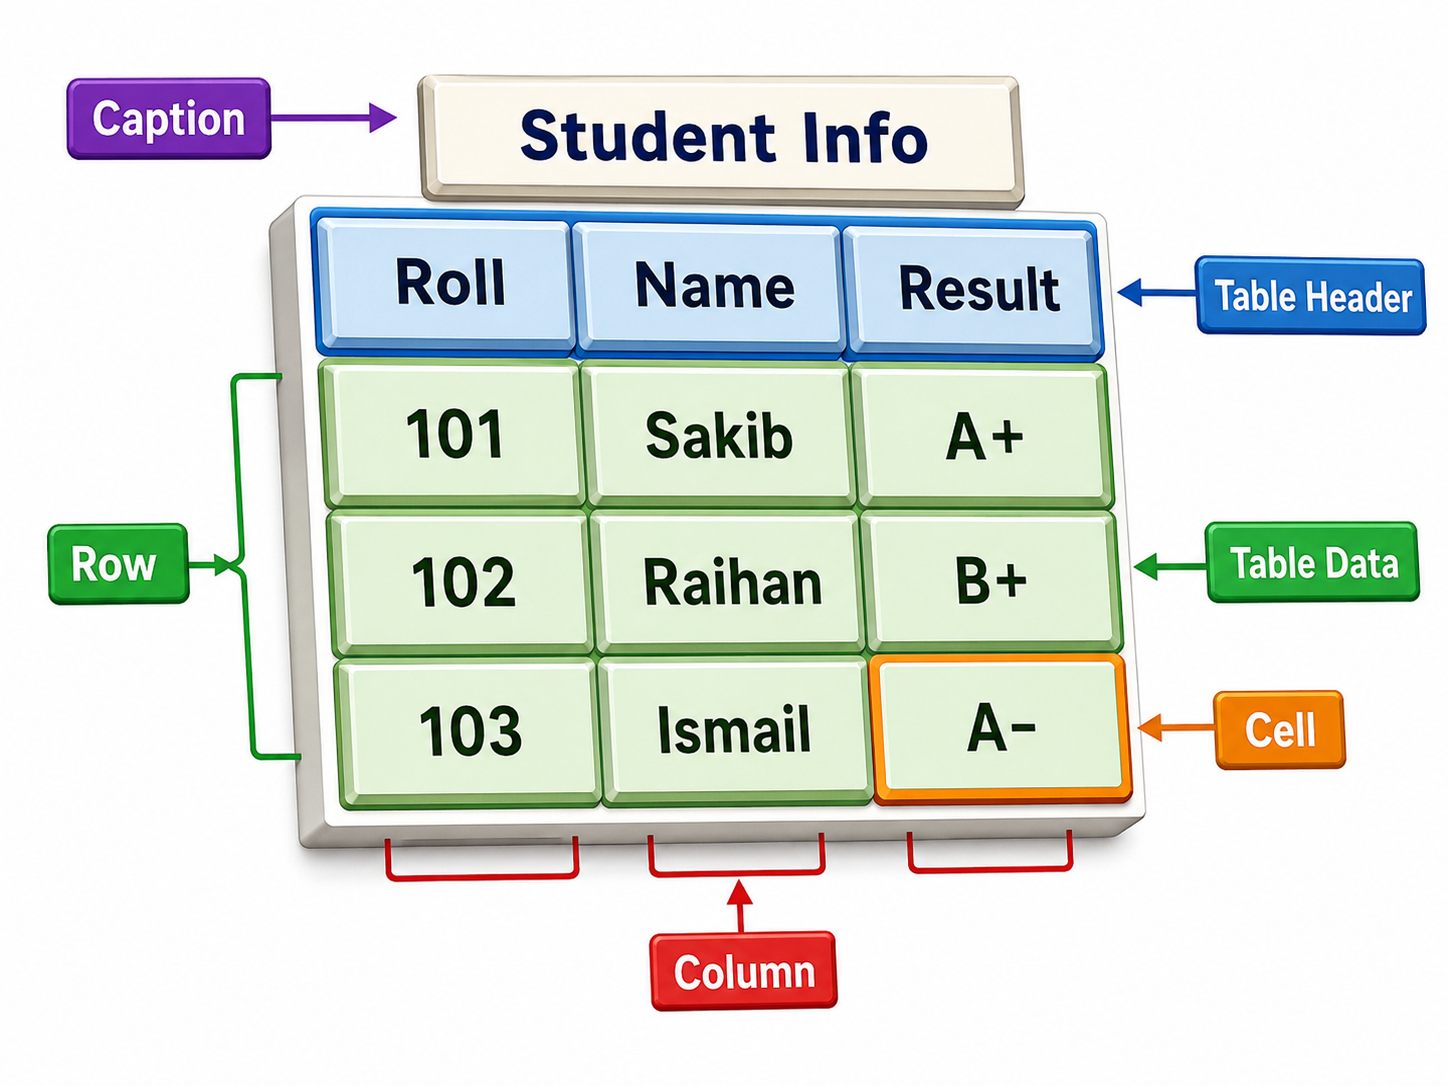
\includegraphics[width=0.98\linewidth,height=0.20\textheight,keepaspectratio]{chapters/Chapter04/topics/images/3d_row_column_cell.png}%
}{%
\fbox{\parbox{0.88\linewidth}{\centering\scriptsize চিত্র পাওয়া যায়নি}}%
}
\par\vspace{1pt}
{\scriptsize\captionof{figure}{HTML table-এর row, column ও cell}}
\end{minipage}
\end{examplebox}


\subsection{Table তৈরির প্রধান Tag}

\noindent
\begin{minipage}[t]{0.56\textwidth}
\vspace{0pt}
\begin{center}
\begin{tabular}{|p{0.22\linewidth}|p{0.24\linewidth}|p{0.34\linewidth}|}
\hline
\textbf{Tag} & \textbf{পূর্ণরূপ/অর্থ} & \textbf{কাজ} \\
\hline
\texttt{<table>} & Table & table শুরু ও শেষ করে \\
\hline
\texttt{<tr>} & Table Row & table-এর row বা সারি তৈরি করে \\
\hline
\texttt{<th>} & Table Header & heading cell তৈরি করে \\
\hline
\texttt{<td>} & Table Data & data cell তৈরি করে \\
\hline
\texttt{<caption>} & Caption & table-এর title বা শিরোনাম দেখায় \\
\hline
\end{tabular}
\end{center}
\textbf{চিত্র ব্যাখ্যা:}
চিত্রে table তৈরির প্রধান tagগুলোর সম্পর্ক দেখানো হয়েছে। \texttt{<table>} পুরো table, \texttt{<tr>} row, \texttt{<th>} heading cell এবং \texttt{<td>} data cell তৈরি করে।
\end{minipage}
\hfill
\begin{minipage}[t]{0.38\textwidth}
\vspace{0pt}
\centering
\IfFileExists{chapters/Chapter04/topics/images/3d_table_tags_map.png}{%
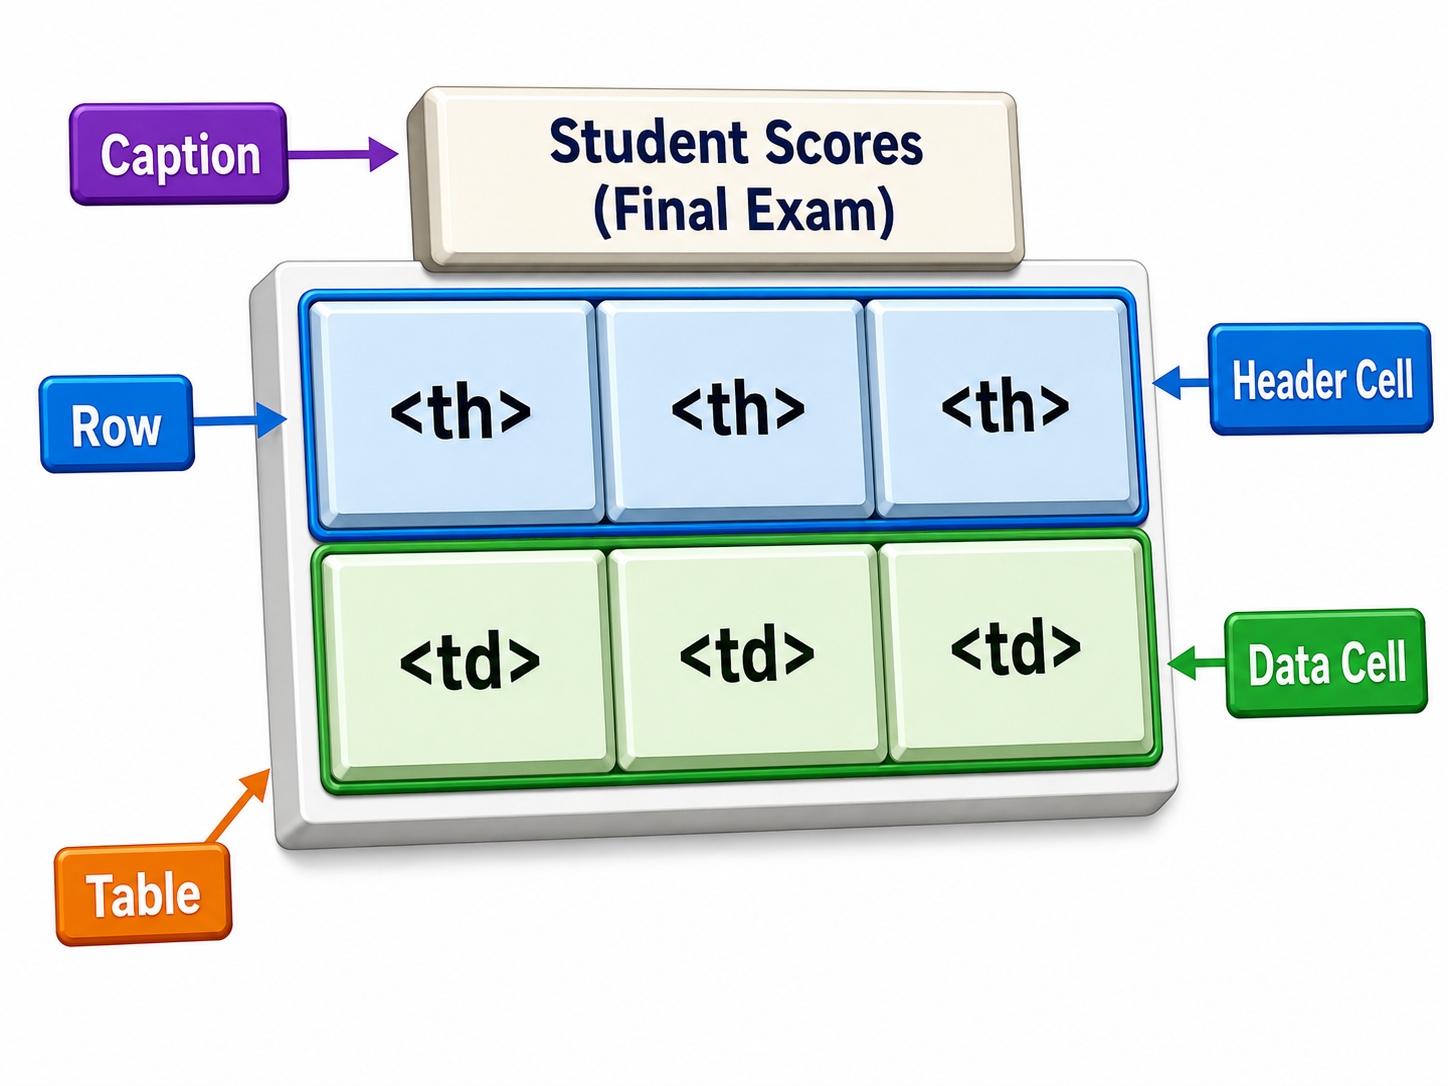
\includegraphics[width=0.98\linewidth,height=0.22\textheight,keepaspectratio]{chapters/Chapter04/topics/images/3d_table_tags_map.png}%
}{%
\fbox{\parbox{0.88\linewidth}{\centering\scriptsize চিত্র পাওয়া যায়নি}}%
}
\par\vspace{1pt}
{\scriptsize\captionof{figure}{table tag-এর কাজ}}
\end{minipage}


\subsection{\texttt{<table>} Tag}

\begin{definitionbox}{\texttt{<table>} tag}
HTML document-এ table বা ছক তৈরি করার জন্য ব্যবহৃত container tag হলো \texttt{<table>} tag।
\end{definitionbox}

Table-এর সব row ও cell এই tag-এর ভিতরে লেখা হয়।

\begin{examplebox}{কোড}
\begin{verbatim}
<!DOCTYPE html>
<html>
<head>
  <title>HTML Table Example</title>
</head>
<body>
  <table border="1" cellspacing="0" cellpadding="6">
    <tr>
      <td>Data</td>
    </tr>
  </table>
</body>
</html>
\end{verbatim}
\end{examplebox}

\subsection{\texttt{<tr>} Tag}

\begin{definitionbox}{\texttt{<tr>} tag}
HTML table-এর একটি row বা সারি তৈরি করার জন্য \texttt{<tr>} tag ব্যবহার করা হয়।
\end{definitionbox}

প্রতিটি \texttt{<tr>} tag-এর ভিতরে এক বা একাধিক \texttt{<th>} অথবা \texttt{<td>} লেখা হয়।

\begin{examplebox}{কোড}
\begin{verbatim}
<!DOCTYPE html>
<html>
<head>
  <title>Table Row Example</title>
</head>
<body>
  <table border="1" cellspacing="0" cellpadding="6">
    <tr>
      <td>Data 1</td>
      <td>Data 2</td>
    </tr>
  </table>
</body>
</html>
\end{verbatim}
\end{examplebox}

\subsection{\texttt{<th>} Tag}

\begin{definitionbox}{\texttt{<th>} tag}
HTML table-এর heading cell তৈরি করার জন্য ব্যবহৃত tag হলো \texttt{<th>} tag।
\end{definitionbox}

Browser সাধারণত \texttt{<th>} tag-এর text bold ও center aligned করে দেখায়।

\begin{examplebox}{কোড}
\begin{verbatim}
<!DOCTYPE html>
<html>
<head>
  <title>Table Header Example</title>
</head>
<body>
  <table border="1" cellspacing="0" cellpadding="6">
    <tr>
      <th>Name</th>
      <th>Roll</th>
    </tr>
  </table>
</body>
</html>
\end{verbatim}
\end{examplebox}

\subsection{\texttt{<td>} Tag}

\begin{definitionbox}{\texttt{<td>} tag}
HTML table-এর data cell বা তথ্যের ঘর তৈরি করার জন্য ব্যবহৃত tag হলো \texttt{<td>} tag।
\end{definitionbox}

\begin{examplebox}{কোড}
\begin{verbatim}
<!DOCTYPE html>
<html>
<head>
  <title>Table Data Example</title>
</head>
<body>
  <table border="1" cellspacing="0" cellpadding="6">
    <tr>
      <td>Rafi</td>
      <td>101</td>
    </tr>
  </table>
</body>
</html>
\end{verbatim}
\end{examplebox}

\subsection{Basic Table Syntax}

\begin{examplebox}{কোড}
\begin{verbatim}
<!DOCTYPE html>
<html>
<head>
  <title>HTML Table Example</title>
</head>
<body>
<table>
  <tr>
    <th>Heading 1</th>
    <th>Heading 2</th>
  </tr>
  <tr>
    <td>Data 1</td>
    <td>Data 2</td>
  </tr>
</table>
</body>
</html>
\end{verbatim}
\end{examplebox}

\begin{keypointbox}{Structure মনে রাখো}
\texttt{<table>} পুরো table তৈরি করে, \texttt{<tr>} একটি row তৈরি করে, \texttt{<th>} heading cell তৈরি করে এবং \texttt{<td>} data cell তৈরি করে।
\end{keypointbox}

\subsection{Table Code লেখার Logical Structure}

HTML table লেখার সময় browser উপর থেকে নিচে row-by-row code পড়ে। তাই code লেখার সময় কোনো cell আগে বা পরে লিখলে visual output বদলে যেতে পারে। একটি row শুরু করতে \texttt{<tr>} লিখতে হয় এবং সেই row-এর যতগুলো cell আছে সেগুলো \texttt{<th>} অথবা \texttt{<td>} দিয়ে একই \texttt{<tr>} tag-এর ভিতরে লিখতে হয়।

\begin{keypointbox}{মনে রাখার নিয়ম}
Table-এর ভিতরে সরাসরি text লেখা উচিত নয়। Table-এর content সাধারণত cell-এর ভিতরে থাকে। তাই correct structure হলো:
\texttt{<table>} $\rightarrow$ \texttt{<tr>} $\rightarrow$ \texttt{<th>} বা \texttt{<td>} $\rightarrow$ content।
\end{keypointbox}

\begin{center}
\begin{tabular}{|p{0.24\textwidth}|p{0.58\textwidth}|}
\hline
\textbf{ধাপ} & \textbf{কাজ} \\
\hline
১ & \texttt{<table>} দিয়ে table শুরু করা \\
\hline
২ & প্রতিটি row-এর জন্য \texttt{<tr>} লেখা \\
\hline
৩ & heading হলে \texttt{<th>}, data হলে \texttt{<td>} লেখা \\
\hline
৪ & সব opened tag ঠিকভাবে close করা \\
\hline
\end{tabular}
\end{center}

\subsection{Simple Table Example}

\begin{examplebox}{কোড}
\begin{verbatim}
<!DOCTYPE html>
<html>
<head>
  <title>Simple Table</title>
</head>
<body>
  <table border="1">
    <tr>
      <th>Roll</th>
      <th>Name</th>
      <th>GPA</th>
    </tr>
    <tr>
      <td>101</td>
      <td>Rafi</td>
      <td>5.00</td>
    </tr>
    <tr>
      <td>102</td>
      <td>Sakib</td>
      <td>4.75</td>
    </tr>
  </table>
</body>
</html>
\end{verbatim}
\end{examplebox}

\begin{examplebox}{Output ধারণা}
\begin{center}
\begin{tabular}{|c|c|c|}
\hline
\textbf{Roll} & \textbf{Name} & \textbf{GPA} \\
\hline
101 & Rafi & 5.00 \\
\hline
102 & Sakib & 4.75 \\
\hline
\end{tabular}
\end{center}
\end{examplebox}

\begin{boardbox}{কোড বিশ্লেষণ}
উপরের code-এ প্রথম \texttt{<tr>} হলো heading row। সেখানে Roll, Name, GPA--এই তিনটি heading cell আছে, তাই \texttt{<th>} ব্যবহার করা হয়েছে। পরের দুইটি row data row, তাই সেখানে \texttt{<td>} ব্যবহার করা হয়েছে। \texttt{border="1"} দেওয়ার কারণে table-এর রেখা দেখা যাচ্ছে।
\end{boardbox}

\subsection{Table Design করার আগে কী ভাববে?}

চিত্র দেখে বা question পড়ে table code লেখার আগে সরাসরি code শুরু না করে কয়েকটি বিষয় ঠিক করতে হয়। এতে ভুল কম হয় এবং \texttt{rowspan}/\texttt{colspan} সহজে বোঝা যায়।

\begin{enumerate}
\item Table-এর title বা caption আছে কি না দেখবে।
\item মোট কয়টি visible column আছে তা গুনবে।
\item মোট কয়টি row আছে তা গুনবে।
\item কোন cell heading আর কোন cell data তা আলাদা করবে।
\item কোনো cell একাধিক column জুড়ে আছে কি না দেখবে।
\item কোনো cell একাধিক row জুড়ে আছে কি না দেখবে।
\item cell-এর ভিতরে text, image, link, list বা nested table আছে কি না দেখবে।
\end{enumerate}

\begin{keypointbox}{পরীক্ষার কৌশল}
কোনো figure জটিল মনে হলে প্রথমে pencil দিয়ে row line ও column line আলাদা করে ভাববে। এরপর merged cell বাদ দিয়ে base grid ধরবে। Base grid বুঝলে \texttt{rowspan} ও \texttt{colspan} বসানো সহজ হয়।
\end{keypointbox}

\subsection{Table Attribute}

PDF-এ table তৈরি করার সময় কয়েকটি attribute বারবার ব্যবহার করা হয়েছে। HSC practical exam-এ এগুলো গুরুত্বপূর্ণ। Table-level attribute যেমন \texttt{border}, \texttt{width}, \texttt{align}, \texttt{cellspacing}, \texttt{cellpadding} পুরো table-এর appearance নিয়ন্ত্রণ করে। আবার cell-level attribute যেমন \texttt{align}, \texttt{valign}, \texttt{bgcolor}, \texttt{rowspan}, \texttt{colspan}, \texttt{width}, \texttt{height} নির্দিষ্ট \texttt{<td>} বা \texttt{<th>} cell-এর আচরণ নিয়ন্ত্রণ করে।

\begin{center}
\begin{tabular}{|p{0.20\textwidth}|p{0.42\textwidth}|p{0.25\textwidth}|}
\hline
\textbf{Attribute} & \textbf{কাজ} & \textbf{Example} \\
\hline
\texttt{border} & table ও cell-এর চারপাশে রেখা দেখায় & \texttt{border="1"} \\
\hline
\texttt{width} & table বা cell-এর প্রস্থ pixel/percentage-এ নির্ধারণ করে & \texttt{width="400"} \\
\hline
\texttt{align} & table বা cell-এর left/right/center position নির্ধারণ করে & \texttt{align="center"} \\
\hline
\texttt{cellspacing} & cell থেকে cell-এর মাঝের বাইরের gap নির্ধারণ করে & \texttt{cellspacing="0"} \\
\hline
\texttt{cellpadding} & cell content ও border-এর মাঝের ভিতরের gap নির্ধারণ করে & \texttt{cellpadding="5"} \\
\hline
\texttt{bgcolor} & table/cell-এর background color দেয় & \texttt{bgcolor="yellow"} \\
\hline
\end{tabular}
\end{center}

\begin{keypointbox}{PDF থেকে গুরুত্বপূর্ণ point}
\texttt{border} attribute না দিলে table-এর রেখা সবসময় দেখা যায় না। বইয়ের example-গুলোতে single-line border দেখাতে বেশিরভাগ সময় \texttt{border="1"}-এর সাথে \texttt{cellspacing="0"} ব্যবহার করা হয়েছে। \texttt{width="75\%"} দিলে table parent area-এর 75\% জায়গা নেয়, আর \texttt{width="400"} বা \texttt{width="400px"} দিলে fixed pixel width বোঝায়।
\end{keypointbox}

\conceptimagerow{chapters/Chapter04/topics/images/3d_table_attributes.png}{
\begin{keypointbox}{চিত্র ব্যাখ্যা}
চিত্রে \texttt{border}, \texttt{width}, \texttt{align}, \texttt{bgcolor}, \texttt{cellspacing} ও \texttt{cellpadding} attribute table-এর appearance কীভাবে বদলায় তা দেখানো হয়েছে।
\end{keypointbox}
}{table attribute-এর প্রভাব}


\subsection{\texttt{border} Attribute}

\begin{definitionbox}{\texttt{border} attribute}
HTML table-এর চারপাশে ও cell-এর চারপাশে border প্রদর্শনের জন্য \texttt{border} attribute ব্যবহার করা হয়।
\end{definitionbox}

\begin{examplebox}{কোড}
\begin{verbatim}
<!DOCTYPE html>
<html>
<head>
  <title>HTML Table Example</title>
</head>
<body>
<table border="1">
  <tr>
    <th>Subject</th>
    <th>Mark</th>
  </tr>
  <tr>
    <td>ICT</td>
    <td>95</td>
  </tr>
</table>
</body>
</html>
\end{verbatim}
\end{examplebox}

\begin{boardbox}{পরীক্ষায় মনে রাখবে}
HSC practical code-এ table-এর রেখা দেখাতে সাধারণত \texttt{border="1"} ব্যবহার করা হয়। Border না দিলে browser table-এর cell boundary সবসময় স্পষ্টভাবে দেখায় না। Border-এর মান 1, 2, 3 ইত্যাদি হলে রেখার thickness বাড়ে; তবে neat table-এর জন্য \texttt{border="1"} এবং \texttt{cellspacing="0"} সবচেয়ে বেশি ব্যবহৃত।
\end{boardbox}

\subsection{\texttt{width} Attribute}

Table বা cell-এর প্রস্থ নির্ধারণ করতে \texttt{width} attribute ব্যবহার করা যায়। Width pixel বা percentage আকারে দেওয়া যায়।

Pixel width fixed size দেয়, তাই \texttt{width="400"} দিলে table প্রায় 400 pixel জায়গা নেবে। Percentage width flexible; \texttt{width="75\%"} দিলে browser window বা parent container-এর 75\% জায়গা ব্যবহার করবে। Cell-এর \texttt{width} দিলে নির্দিষ্ট column তুলনামূলক বড় বা ছোট করা যায়।

\begin{examplebox}{কোড}
\begin{verbatim}
<!DOCTYPE html>
<html>
<head>
  <title>HTML Table Example</title>
</head>
<body>
<table border="1" width="400">
  <tr>
    <th>Name</th>
    <th>GPA</th>
  </tr>
  <tr>
    <td>Rafi</td>
    <td>5.00</td>
  </tr>
</table>
</body>
</html>
\end{verbatim}
\end{examplebox}

\begin{examplebox}{Percentage Width}
\begin{verbatim}
<!DOCTYPE html>
<html>
<head>
  <title>HTML Table Example</title>
</head>
<body>
  <table border="1" width="75%">
    <tr>
      <th>Name</th>
      <th>GPA</th>
    </tr>
    <tr>
      <td>Rafi</td>
      <td>5.00</td>
    </tr>
  </table>
</body>
</html>
\end{verbatim}
এখানে table browser window বা parent area-এর 75\% জায়গা নেবে।
\end{examplebox}

\subsection{\texttt{align} Attribute}

Table, row বা cell-এর content left, right বা center-এ রাখতে \texttt{align} attribute ব্যবহার করা হয়।

\texttt{<table align="center">} লিখলে পুরো table page-এর মাঝখানে চলে আসে। কিন্তু \texttt{<td align="center">} লিখলে শুধু ওই cell-এর content মাঝখানে থাকে। তাই table-এর position এবং cell-এর ভিতরের text alignment আলাদা বিষয়।

\begin{examplebox}{কোড}
\begin{verbatim}
<!DOCTYPE html>
<html>
<head>
  <title>Align Example</title>
</head>
<body>
  <table border="1" cellspacing="0" cellpadding="6">
    <tr>
      <td align="center">ICT</td>
    </tr>
  </table>
</body>
</html>
\end{verbatim}
\end{examplebox}

\begin{center}
\begin{tabular}{|p{0.25\textwidth}|p{0.55\textwidth}|}
\hline
\textbf{Value} & \textbf{কাজ} \\
\hline
\texttt{left} & বামে রাখে \\
\hline
\texttt{center} & মাঝখানে রাখে \\
\hline
\texttt{right} & ডানে রাখে \\
\hline
\end{tabular}
\end{center}

\subsection{\texttt{valign} Attribute}

Cell-এর ভিতরের content vertical direction-এ কোথায় থাকবে তা নির্ধারণ করতে \texttt{valign} attribute ব্যবহার করা যায়।

কোনো cell-এর height বেশি হলে content উপরে, মাঝখানে বা নিচে রাখা দরকার হতে পারে। শুধু \texttt{<br>} দিয়ে content নিচে নামানো যায়, কিন্তু board-style পরিষ্কার code-এর জন্য \texttt{valign="top"}, \texttt{valign="middle"} বা \texttt{valign="bottom"} ব্যবহার করা ভালো।

\begin{center}
\begin{tabular}{|p{0.25\textwidth}|p{0.55\textwidth}|}
\hline
\textbf{Value} & \textbf{কাজ} \\
\hline
\texttt{top} & cell-এর উপরে রাখে \\
\hline
\texttt{middle} & cell-এর মাঝখানে রাখে \\
\hline
\texttt{bottom} & cell-এর নিচে রাখে \\
\hline
\end{tabular}
\end{center}

\conceptimagerow{chapters/Chapter04/topics/images/3d_align_valign.png}{
\begin{keypointbox}{চিত্র ব্যাখ্যা}
চিত্রে horizontal alignment এবং vertical alignment-এর পার্থক্য দেখানো হয়েছে। \texttt{align} left/center/right position নিয়ন্ত্রণ করে এবং \texttt{valign} top/middle/bottom position নিয়ন্ত্রণ করে।
\end{keypointbox}
}{horizontal alignment ও vertical alignment}


\subsection{\texttt{cellspacing} Attribute}

\begin{definitionbox}{\texttt{cellspacing} attribute}
Table-এর এক cell-এর border থেকে পাশের cell-এর border পর্যন্ত ফাঁকা জায়গা নির্ধারণ করতে \texttt{cellspacing} attribute ব্যবহার করা হয়।
\end{definitionbox}

\begin{examplebox}{কোড}
\begin{verbatim}
<!DOCTYPE html>
<html>
<head>
  <title>HTML Table Example</title>
</head>
<body>
<table border="1" cellspacing="0">
  <tr>
    <th>Name</th>
    <th>Class</th>
  </tr>
  <tr>
    <td>Rafi</td>
    <td>XI</td>
  </tr>
</table>
</body>
</html>
\end{verbatim}
\end{examplebox}

\begin{keypointbox}{সহজ কথা}
Browser অনেক সময় default হিসেবে cell-এর মাঝে সামান্য gap রাখে। \texttt{cellspacing="0"} দিলে cell-এর মাঝখানের gap কমে যায় বা borderগুলো একসাথে লেগে থাকে। আবার \texttt{cellspacing="10"} দিলে দুই cell-এর border-এর মাঝে 10 pixel দূরত্ব তৈরি হয়।
\end{keypointbox}

\subsection{\texttt{cellpadding} Attribute}

\begin{definitionbox}{\texttt{cellpadding} attribute}
Table cell-এর content এবং cell border-এর মাঝখানের ভিতরের ফাঁকা জায়গা নির্ধারণ করতে \texttt{cellpadding} attribute ব্যবহার করা হয়।
\end{definitionbox}

\begin{examplebox}{কোড}
\begin{verbatim}
<!DOCTYPE html>
<html>
<head>
  <title>HTML Table Example</title>
</head>
<body>
<table border="1" cellpadding="10">
  <tr>
    <th>Subject</th>
    <th>GPA</th>
  </tr>
  <tr>
    <td>Bangla</td>
    <td>5.00</td>
  </tr>
</table>
</body>
</html>
\end{verbatim}
\end{examplebox}

\begin{boardbox}{MCQ point}
\texttt{cellpadding="5"} অর্থ cell content এবং cell border-এর মাঝখানে 5 pixel ভিতরের ফাঁকা জায়গা রাখা। অনেক browser-এ default cellpadding খুব কম থাকে; তাই text border-এর সাথে লেগে গেলে \texttt{cellpadding} বাড়ালে table পড়তে সহজ হয়।
\end{boardbox}

\subsection{\texttt{cellspacing} ও \texttt{cellpadding}-এর পার্থক্য}

\begin{center}
\begin{tabular}{|p{0.18\textwidth}|p{0.34\textwidth}|p{0.34\textwidth}|}
\hline
\textbf{বিষয়} & \textbf{\texttt{cellspacing}} & \textbf{\texttt{cellpadding}} \\
\hline
কাজ & cell থেকে cell-এর মাঝের gap নির্ধারণ করে & cell content থেকে border-এর ভিতরের gap নির্ধারণ করে \\
\hline
অবস্থান & cell-এর বাইরে & cell-এর ভিতরে \\
\hline
Example & \texttt{cellspacing="0"} & \texttt{cellpadding="5"} \\
\hline
প্রভাব & border-এর মাঝের দূরত্ব কমায় বা বাড়ায় & content-এর চারপাশে space দেয় \\
\hline
\end{tabular}
\end{center}

\begin{center}
\IfFileExists{chapters/Chapter04/topics/images/3d_cellspacing_vs_cellpadding.png}{
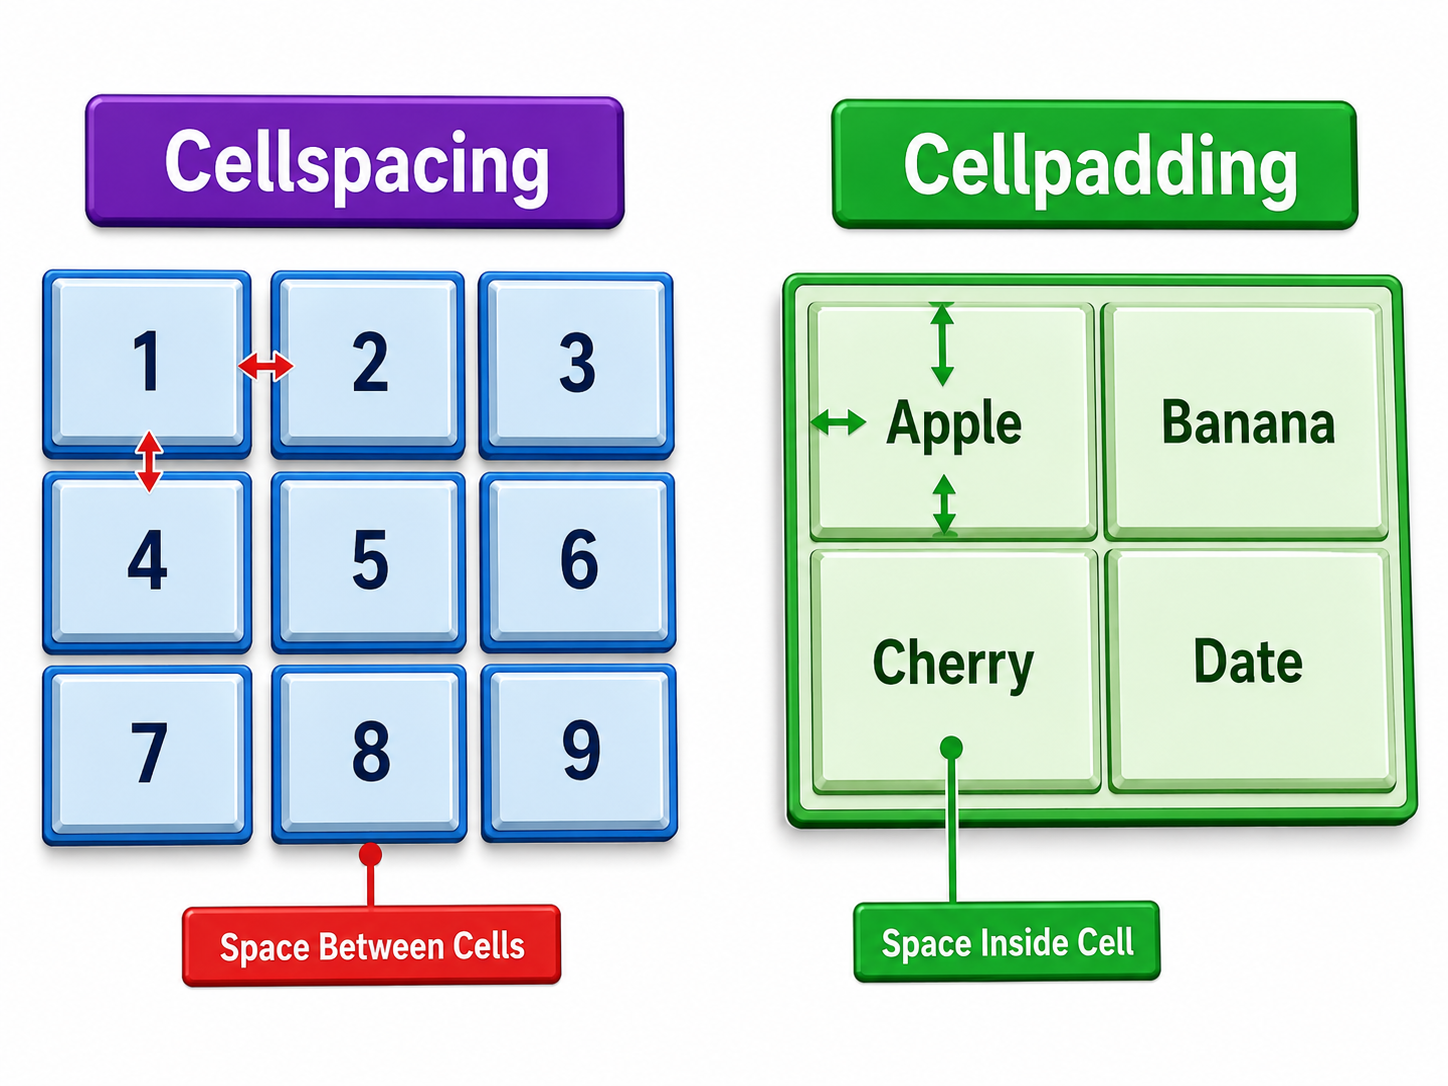
\includegraphics[width=0.95\linewidth,height=0.11\textheight,keepaspectratio]{chapters/Chapter04/topics/images/3d_cellspacing_vs_cellpadding.png}
}{
\fbox{\parbox{0.90\linewidth}{\centering\vspace{0.5cm}
\textbf{চিত্র}\\[4pt]
Left side: gap between two cell boxes labeled \texttt{cellspacing}. Right side: inner gap from content to cell wall labeled \texttt{cellpadding}.\\[4pt]
File: \texttt{chapters/Chapter04/topics/images/3d\_cellspacing\_vs\_cellpadding.png}
\vspace{0.5cm}}}
}
\captionof{figure}{cellspacing ও cellpadding-এর পার্থক্য}
\end{center}

\begin{keypointbox}{চিত্র ব্যাখ্যা}
চিত্রে \texttt{cellspacing} cell-এর মাঝের gap এবং \texttt{cellpadding} cell-এর ভিতরে content ও border-এর মাঝের gap তৈরি করে তা দেখানো হয়েছে।
\end{keypointbox}


\begin{keypointbox}{সহজ মনে রাখার উপায়}
Spacing মানে cell ও cell-এর মাঝে space। Padding মানে cell-এর ভিতরে content-এর চারপাশে space।
\end{keypointbox}

\subsection{\texttt{bgcolor} Attribute}

Table বা cell-এর background color দিতে \texttt{bgcolor} attribute ব্যবহার করা হয়।

\begin{examplebox}{কোড}
\begin{verbatim}
<!DOCTYPE html>
<html>
<head>
  <title>HTML Table Example</title>
</head>
<body>
<table border="1" bgcolor="yellow">
  <tr>
    <th>Name</th>
    <th>Class</th>
  </tr>
  <tr>
    <td>Rafi</td>
    <td>XI</td>
  </tr>
</table>
</body>
</html>
\end{verbatim}
\end{examplebox}

\subsection{\texttt{<td>} ও \texttt{<th>} Tag-এর Attribute}

Cell-এর উপর আলাদা control দেওয়ার জন্য \texttt{<td>} বা \texttt{<th>} tag-এর ভিতরে attribute ব্যবহার করা যায়।

PDF-এর table অংশে \texttt{<th>} ও \texttt{<td>} cell-এর জন্য আলাদা attribute দেখানো হয়েছে। একই table-এর সব cell একরকম নাও হতে পারে; কোনো cell center aligned, কোনো cell green background, কোনো cell বেশি wide, আবার কোনো cell একাধিক row বা column জুড়ে থাকতে পারে।

\begin{center}
\begin{tabular}{|p{0.18\textwidth}|p{0.46\textwidth}|p{0.25\textwidth}|}
\hline
\textbf{Attribute} & \textbf{কাজ} & \textbf{Example} \\
\hline
\texttt{align} & cell-এর text বাম/মাঝ/ডানে রাখে & \texttt{align="center"} \\
\hline
\texttt{valign} & cell-এর text top/middle/bottom রাখে & \texttt{valign="top"} \\
\hline
\texttt{bgcolor} & cell-এর background color দেয় & \texttt{bgcolor="green"} \\
\hline
\texttt{width} & cell-এর width নির্ধারণ করে & \texttt{width="150"} \\
\hline
\texttt{height} & cell-এর height নির্ধারণ করে & \texttt{height="60"} \\
\hline
\texttt{colspan} & cell-কে একাধিক column জুড়ে দেয় & \texttt{colspan="2"} \\
\hline
\texttt{rowspan} & cell-কে একাধিক row জুড়ে দেয় & \texttt{rowspan="3"} \\
\hline
\end{tabular}
\end{center}

\begin{keypointbox}{Color value}
\texttt{bgcolor} attribute-এ color name, hexadecimal value বা RGB ধরনের value ব্যবহার করা যায়। HSC practical-এ সাধারণত \texttt{yellow}, \texttt{green}, \texttt{silver} ধরনের color name বেশি দেখা যায়।
\end{keypointbox}

\subsection{\texttt{rowspan} ও \texttt{colspan}}

\begin{definitionbox}{\texttt{colspan}}
একটি cell-কে একাধিক column বা কলাম জুড়ে বিস্তৃত করার জন্য \texttt{colspan} attribute ব্যবহার করা হয়।
\end{definitionbox}

\begin{definitionbox}{\texttt{rowspan}}
একটি cell-কে একাধিক row বা সারি জুড়ে বিস্তৃত করার জন্য \texttt{rowspan} attribute ব্যবহার করা হয়।
\end{definitionbox}

\begin{examplebox}{\texttt{colspan} কোড}
\begin{verbatim}
<!DOCTYPE html>
<html>
<head>
  <title>HTML Table Example</title>
</head>
<body>
<table border="1">
  <tr>
    <th colspan="2">Student Info</th>
  </tr>
  <tr>
    <td>Roll</td>
    <td>101</td>
  </tr>
</table>
</body>
</html>
\end{verbatim}
\end{examplebox}

\begin{examplebox}{\texttt{rowspan} কোড}
\begin{verbatim}
<!DOCTYPE html>
<html>
<head>
  <title>HTML Table Example</title>
</head>
<body>
<table border="1">
  <tr>
    <th rowspan="2">Name</th>
    <td>Rafi</td>
  </tr>
  <tr>
    <td>Sakib</td>
  </tr>
</table>
</body>
</html>
\end{verbatim}
\end{examplebox}

\begin{center}
\IfFileExists{chapters/Chapter04/topics/images/3d_rowspan_colspan.png}{
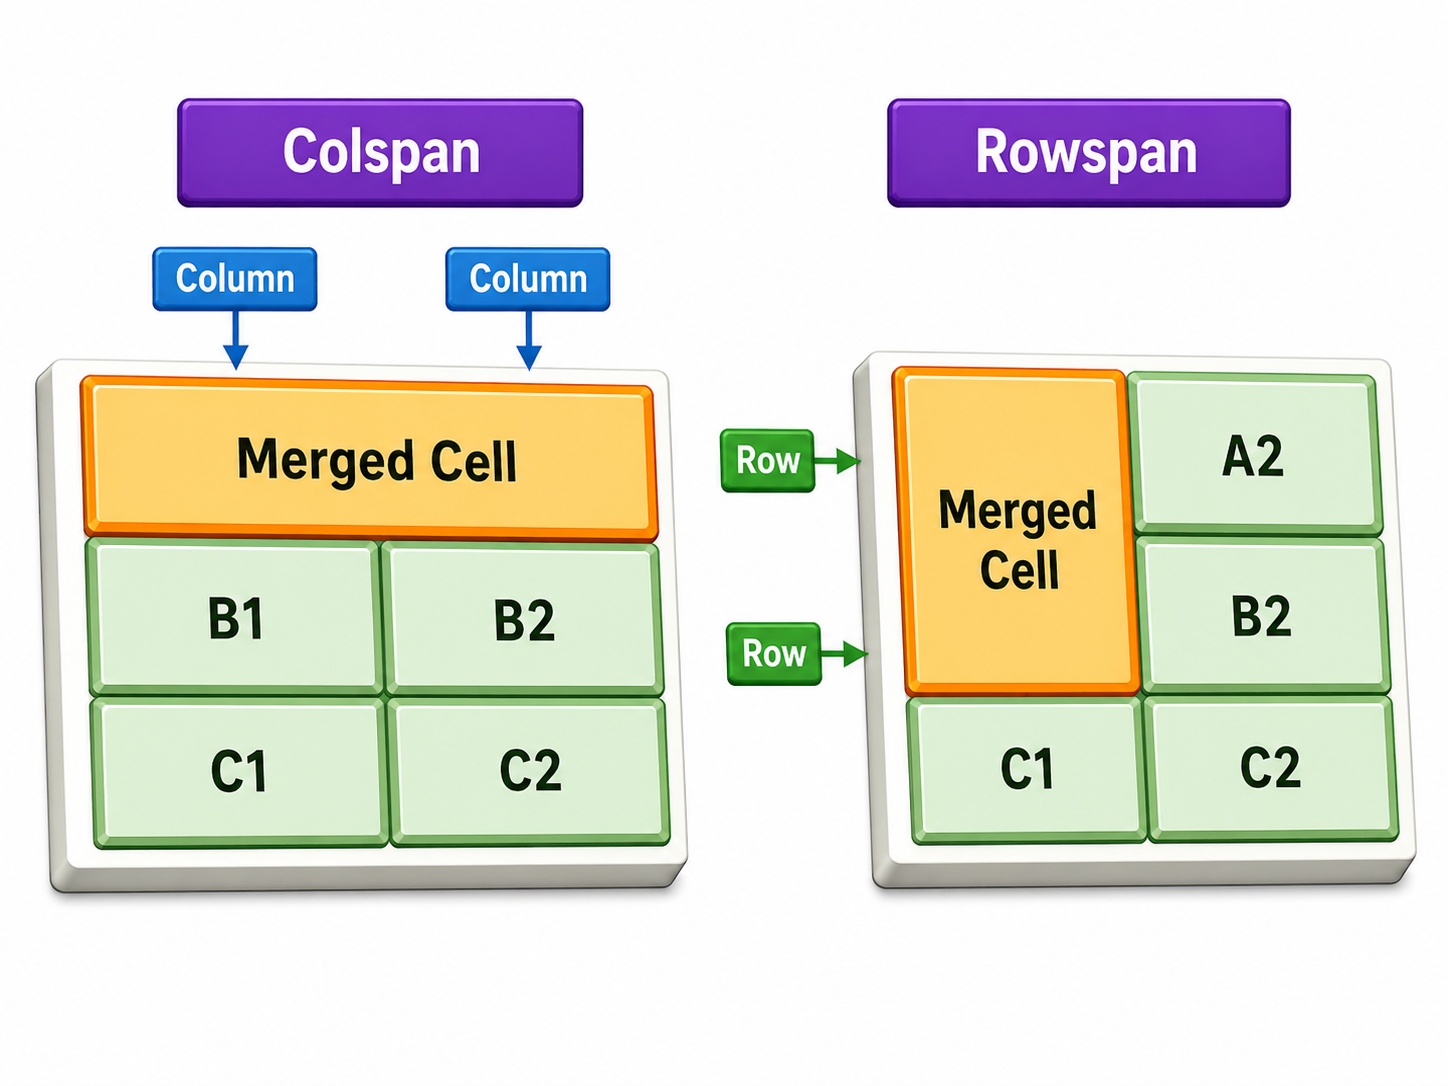
\includegraphics[width=0.95\linewidth,height=0.11\textheight,keepaspectratio]{chapters/Chapter04/topics/images/3d_rowspan_colspan.png}
}{
\fbox{\parbox{0.90\linewidth}{\centering\vspace{0.5cm}
\textbf{চিত্র}\\[4pt]
Two grids: one shows a wide block covering two columns labeled \texttt{colspan="2"}; another shows a tall block covering two rows labeled \texttt{rowspan="2"}.\\[4pt]
File: \texttt{chapters/Chapter04/topics/images/3d\_rowspan\_colspan.png}
\vspace{0.5cm}}}
}
\captionof{figure}{rowspan ও colspan দিয়ে cell merge}
\end{center}

\begin{keypointbox}{চিত্র ব্যাখ্যা}
চিত্রে \texttt{colspan} দিয়ে horizontal merge এবং \texttt{rowspan} দিয়ে vertical merge দেখানো হয়েছে। চিত্র দেখে code লেখার সময় merged cell আগে identify করতে হয়।
\end{keypointbox}


\begin{keypointbox}{Shortcut}
\texttt{colspan} = column span = পাশের দিকে merge।\\
\texttt{rowspan} = row span = নিচের দিকে merge।
\end{keypointbox}

\subsection{Merged Cell বুঝে Code লেখার নিয়ম}

Merged cell হলো এমন cell, যা একাধিক row বা column-এর জায়গা নেয়। Table চিত্র দেখে code লেখার সময় merged cell ভুল হলে পুরো table layout নষ্ট হয়ে যায়। তাই \texttt{rowspan} ও \texttt{colspan} ব্যবহার করার আগে base column সংখ্যা ঠিক করা দরকার।

\begin{boardbox}{\texttt{colspan} কখন ব্যবহার করবে}
যদি কোনো cell বাম থেকে ডানে একাধিক column-এর জায়গা নেয়, তখন \texttt{colspan} ব্যবহার করবে। যেমন, একটি title যদি table-এর তিনটি column জুড়ে থাকে, তাহলে code হবে \texttt{<th colspan="3">Title</th>}।
\end{boardbox}

\begin{boardbox}{\texttt{rowspan} কখন ব্যবহার করবে}
যদি কোনো cell উপর থেকে নিচে একাধিক row-এর জায়গা নেয়, তখন \texttt{rowspan} ব্যবহার করবে। যেমন, একটি group name যদি দুইটি section row-এর জন্য common হয়, তাহলে code হবে \texttt{<td rowspan="2">Science</td>}।
\end{boardbox}

\begin{keypointbox}{Merged cell-এর কারণে cell count কমে যায়}
যে row-তে \texttt{colspan} বা \texttt{rowspan} ব্যবহার করা হয়, সেই row-তে আলাদা cell কম লিখতে হয়। কারণ merged cell নিজেই একাধিক cell-এর জায়গা দখল করে। এটাই beginners-দের সবচেয়ে সাধারণ ভুল।
\end{keypointbox}

\subsection{Empty Cell এবং \texttt{\&nbsp;}}

Table-এর কোনো cell খালি রাখতে চাইলে অনেক সময় browser cell-এর border ঠিকভাবে দেখাতে সমস্যা করতে পারে। তাই খালি cell-এ non-breaking space বা \texttt{\&nbsp;} ব্যবহার করা হয়।

খালি cell রাখা দরকার হলে শুধু blank space না দিয়ে \texttt{\&nbsp;} লেখা ভালো, কারণ এটি একটি invisible character হিসেবে কাজ করে। ফলে cell-এর height, width এবং border ঠিক থাকে। Board practical-এ empty cell দেখলে \texttt{<td>\&nbsp;</td>} লিখলে layout বেশি নির্ভরযোগ্য হয়। পুরনো বইয়ের example-এ খালি cell দেখাতে অনেক সময় \texttt{<br>} ব্যবহারও দেখা যায়, তবে পরীক্ষায় পরিষ্কারভাবে empty cell বোঝাতে \texttt{\&nbsp;} বেশি নির্ভরযোগ্য।

\begin{examplebox}{কোড}
\begin{verbatim}
<!DOCTYPE html>
<html>
<head>
  <title>Empty Cell Example</title>
</head>
<body>
  <table border="1" cellspacing="0" cellpadding="6">
    <tr>
      <th>Header 1</th>
      <th>Header 2</th>
    </tr>
    <tr>
      <td>Data</td>
      <td>&nbsp;</td>
    </tr>
  </table>
</body>
</html>
\end{verbatim}
\end{examplebox}

\conceptwrapimage{chapters/Chapter04/topics/images/3d_empty_cell_nbsp.png}
{চিত্রে empty cell দৃশ্যমান রাখতে \texttt{\&nbsp;} ব্যবহারের ধারণা দেখানো হয়েছে। খালি cell collapse বা অস্পষ্ট হলে non-breaking space ব্যবহার করা যায়।}
{খালি cell-এ \texttt{\&nbsp;} ব্যবহার}


\subsection{\texttt{<caption>} Tag}

\begin{definitionbox}{\texttt{<caption>} tag}
HTML table-এর শিরোনাম বা title প্রদর্শনের জন্য \texttt{<caption>} tag ব্যবহার করা হয়।
\end{definitionbox}

\texttt{<caption>} tag সবসময় \texttt{<table>} tag-এর ভিতরে এবং প্রথম row-এর আগে লেখা উচিত। এতে browser সাধারণত table-এর উপরে title দেখায়। Result sheet, routine, admission list বা product table-এর মতো table-এ caption দিলে table-এর উদ্দেশ্য দ্রুত বোঝা যায়। পুরনো HSC-style code-এ caption-এর position বোঝাতে \texttt{align="bottom"} ধরনের legacy attribute দেখা যেতে পারে, তবে modern HTML-এ caption position CSS দিয়ে নিয়ন্ত্রণ করা ভালো।

\begin{examplebox}{কোড}
\begin{verbatim}
<!DOCTYPE html>
<html>
<head>
  <title>Caption Example</title>
</head>
<body>
  <table border="1" cellspacing="0" cellpadding="6">
    <caption>Student Information</caption>
    <tr>
      <th>Roll</th>
      <th>Name</th>
      <th>Result</th>
    </tr>
    <tr>
      <td>101</td>
      <td>Sakib</td>
      <td>A+</td>
    </tr>
  </table>
</body>
</html>
\end{verbatim}
\end{examplebox}

\conceptwrapimage{chapters/Chapter04/topics/images/3d_caption.png}
{চিত্রে table-এর উপরে caption/title দেখানো হয়েছে। HTML-এ \texttt{<caption>} tag table-এর title লিখতে ব্যবহৃত হয়।}
{table caption}


\subsection{\texttt{colgroup} Tag}

\begin{definitionbox}{\texttt{<colgroup>} tag}
Table-এর এক বা একাধিক column-এর জন্য একসাথে style বা property নির্ধারণ করতে \texttt{<colgroup>} tag ব্যবহার করা হয়।
\end{definitionbox}

\texttt{colgroup} ব্যবহার করলে কোনো নির্দিষ্ট column বা column group-কে আলাদা color/style দেওয়া যায়। এটি table-এর row শুরু হওয়ার আগে লেখা হয়, কারণ column style আগে ঠিক করে তারপর row data বসানো হয়।

একই ধরনের একাধিক column একসাথে style করতে \texttt{<col span="2">} ব্যবহার করা যায়। যেমন প্রথম দুই column এক color এবং পরের দুই column আরেক color করতে চাইলে \texttt{span} attribute helpful। প্রতিটি column আলাদা style চাইলে আলাদা আলাদা \texttt{<col>} tag লেখা হয়।

\begin{examplebox}{কোড}
\begin{verbatim}
<!DOCTYPE html>
<html>
<head>
  <title>Column Group Example</title>
</head>
<body>
<table border="1">
  <colgroup>
    <col style="background-color: yellow">
    <col style="background-color: lightgreen">
  </colgroup>
  <tr>
    <th>Title</th>
    <th>Author</th>
  </tr>
  <tr>
    <td>ICT HSC</td>
    <td>M. Hakim</td>
  </tr>
</table>
</body>
</html>
\end{verbatim}
\end{examplebox}

\conceptwrapimage{chapters/Chapter04/topics/images/3d_colgroup.png}
{চিত্রে \texttt{<colgroup>} ব্যবহার করে নির্দিষ্ট column group-এ style দেওয়ার ধারণা দেখানো হয়েছে। এতে একাধিক column একসাথে color/style করা যায়।}
{colgroup দিয়ে column style}


\subsection{Table-এর ভিতরে Formatting, Link, Image ও List}

Table cell-এর ভিতরে শুধু text নয়, HTML-এর অন্য element-ও রাখা যায়। PDF-এর table discussion-এ cell-এর ভিতরে text, image, photograph, list, form, horizontal line, hyperlink এবং আরেকটি table রাখার ধারণা আছে। তাই table ব্যবহার করে result sheet-এর সাথে photo, product list-এর সাথে buy link, course plan-এর সাথে ordered list বা nested information দেখানো সম্ভব।

\begin{keypointbox}{Cell-এর ভিতরে content রাখার নিয়ম}
Cell-এর ভিতরে content রাখতে হলে content অবশ্যই \texttt{<td>} বা \texttt{<th>} tag-এর opening ও closing tag-এর মাঝখানে লিখতে হবে। যেমন image বসাতে \texttt{<td><img src="photo.jpg"></td>} এবং link বসাতে \texttt{<td><a href="page.html">Open</a></td>} লিখতে হবে।
\end{keypointbox}

\begin{center}
\begin{tabular}{|p{0.22\textwidth}|p{0.50\textwidth}|p{0.18\textwidth}|}
\hline
\textbf{Content type} & \textbf{Cell-এর ভিতরে code idea} & \textbf{Tag} \\
\hline
Text & \texttt{<td>Rafi</td>} & \texttt{<td>} \\
\hline
Image & \texttt{<td><img src="a.jpg"></td>} & \texttt{<img>} \\
\hline
Link & \texttt{<td><a href="a.html">Open</a></td>} & \texttt{<a>} \\
\hline
List & \texttt{<td><ol>...</ol></td>} & \texttt{<ol>}, \texttt{<li>} \\
\hline
Horizontal line & \texttt{<td><hr></td>} & \texttt{<hr>} \\
\hline
Form control & \texttt{<td><input type="text"></td>} & \texttt{<input>} \\
\hline
Nested table & \texttt{<td><table>...</table></td>} & \texttt{<table>} \\
\hline
\end{tabular}
\end{center}

\subsubsection{Formatting Text}

\begin{examplebox}{কোড}
\begin{verbatim}
<!DOCTYPE html>
<html>
<head>
  <title>Cell Formatting Example</title>
</head>
<body>
  <table border="1" cellspacing="0" cellpadding="6">
    <tr>
      <td><b>ICT</b></td>
      <td><u>HSC</u></td>
      <td><i>Book</i></td>
    </tr>
  </table>
</body>
</html>
\end{verbatim}
\end{examplebox}

\subsubsection{Hyperlink}

\begin{examplebox}{কোড}
\begin{verbatim}
<!DOCTYPE html>
<html>
<head>
  <title>Table Link Example</title>
</head>
<body>
  <table border="1" cellspacing="0" cellpadding="6">
    <tr>
      <td>
        <a href="https://www.educationboard.gov.bd">Education Board</a>
      </td>
    </tr>
  </table>
</body>
</html>
\end{verbatim}
\end{examplebox}

\subsubsection{Image}

\begin{examplebox}{কোড}
\begin{verbatim}
<!DOCTYPE html>
<html>
<head>
  <title>Table Image Example</title>
</head>
<body>
  <table border="1" cellspacing="0" cellpadding="6">
    <tr>
      <td>
        <img src="photo.jpg" width="100" height="80" alt="Photo">
      </td>
    </tr>
  </table>
</body>
</html>
\end{verbatim}
\end{examplebox}

\subsubsection{List}

\begin{center}
\IfFileExists{chapters/Chapter04/topics/images/3d_content_inside_cell.png}{
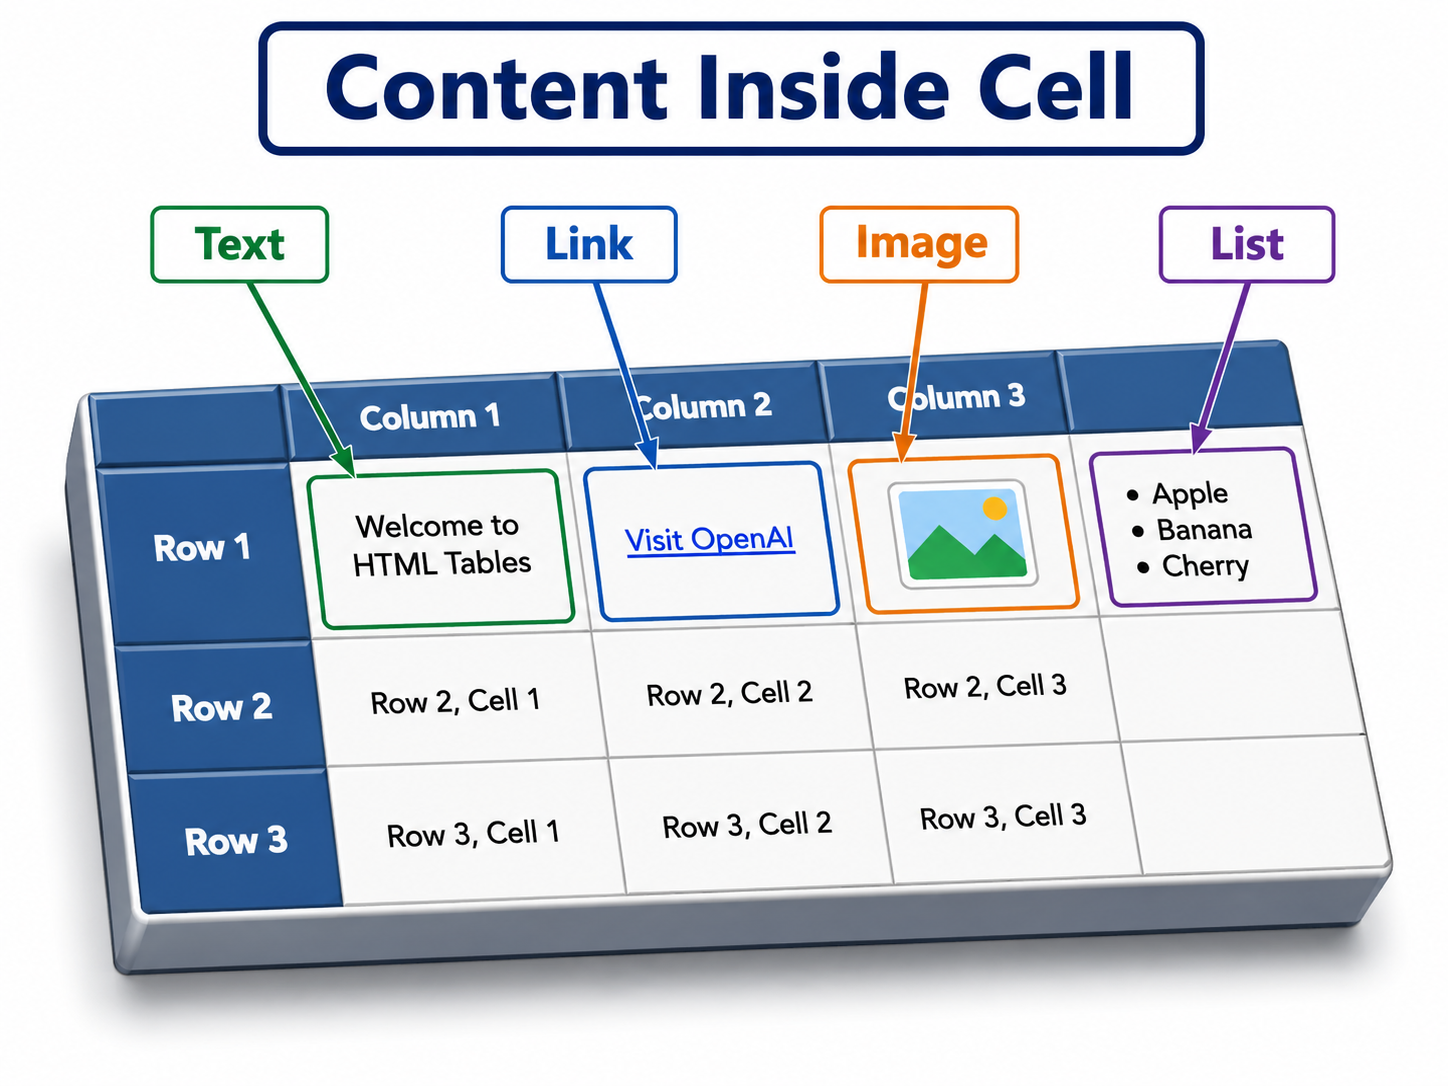
\includegraphics[width=0.78\linewidth,height=0.12\textheight,keepaspectratio]{chapters/Chapter04/topics/images/3d_content_inside_cell.png}
}{
\fbox{\parbox{0.90\linewidth}{\centering\vspace{0.35cm}
\textbf{চিত্র}\\[3pt]
File: \texttt{chapters/Chapter04/topics/images/3d\_content\_inside\_cell.png}
\vspace{0.35cm}}}
}
\captionof{figure}{table cell-এর ভিতরে text, link, image ও list}
\end{center}

\noindent{\color{blue!62!black}\bfseries চিত্র ব্যাখ্যা:}
চিত্রে table cell-এর ভিতরে চার ধরনের content দেখানো হয়েছে: normal text, hyperlink, image এবং ordered list। List cell-এর ভিতরে \texttt{<ol>} ও \texttt{<li>} tag ব্যবহার করা হয়েছে।

\begin{keypointbox}{চিত্র দেখে code লেখার ধাপ}
যে cell-এর ভিতরে list থাকবে, সেখানে প্রথমে \texttt{<td>} লিখবে। তারপর cell-এর ভিতরে \texttt{<ol>} বা \texttt{<ul>} tag লিখে প্রতিটি item \texttt{<li>} দিয়ে লিখবে।
\end{keypointbox}

\begin{examplebox}{কোড}
\begin{verbatim}
<!DOCTYPE html>
<html>
<head>
  <title>List Inside Table Example</title>
</head>
<body>
  <table border="1" cellspacing="0" cellpadding="6">
    <tr>
      <td>
        <ol>
          <li>Dhaka</li>
          <li>Dinajpur</li>
          <li>Rangpur</li>
        </ol>
      </td>
    </tr>
  </table>
</body>
</html>
\end{verbatim}
\end{examplebox}

\subsection{Nested Table বা Table-এর ভিতরে Table}

\begin{definitionbox}{Nested Table}
একটি table-এর কোনো cell-এর ভিতরে আরেকটি table তৈরি করলে তাকে nested table বলা হয়।
\end{definitionbox}

\begin{examplebox}{কোড}
\begin{verbatim}
<!DOCTYPE html>
<html>
<head>
  <title>Nested Table Example</title>
</head>
<body>
  <table border="1" cellspacing="0" cellpadding="10">
    <tr>
      <td>Parent Cell</td>
      <td>
        <table border="1" cellspacing="0" cellpadding="5">
          <tr>
            <th>Child</th>
            <th>Table</th>
          </tr>
          <tr>
            <td>A</td>
            <td>B</td>
          </tr>
        </table>
      </td>
    </tr>
  </table>
</body>
</html>
\end{verbatim}
\end{examplebox}

\conceptwrapimage{chapters/Chapter04/topics/images/3d_nested_table.png}
{চিত্রে parent table-এর একটি cell-এর ভিতরে child table বসানো হয়েছে। এটিকে nested table বা table inside table বলা হয়।}
{table-এর ভিতরে nested table}

\begin{keypointbox}{Nested table লেখার সতর্কতা}
Nested table লিখলে outer table ও inner table-এর tag আলাদা করে close করতে হবে। প্রথমে inner table-এর \texttt{</table>} close করবে, তারপর outer cell-এর \texttt{</td>} এবং শেষে outer table close করবে। ভুল জায়গায় \texttt{</table>} দিলে output ভেঙে যায়।
\end{keypointbox}


\subsection{Modern CSS Note}

\begin{keypointbox}{Modern note}
HSC ICT basic HTML অংশে \texttt{border}, \texttt{align}, \texttt{bgcolor}, \texttt{cellpadding}, \texttt{cellspacing}, \texttt{width} attribute শেখা দরকার। তবে professional web design-এ এগুলোর অনেকগুলো কাজ CSS দিয়ে করা হয়। যেমন: \texttt{border}, \texttt{border-collapse}, \texttt{border-spacing}, \texttt{padding}, \texttt{text-align}, \texttt{background-color}, \texttt{width}।
\end{keypointbox}

\begin{examplebox}{Modern CSS Version}
\begin{verbatim}
<!DOCTYPE html>
<html>
<head>
  <title>Modern Table</title>
  <style>
    table {
      width: 400px;
      border-collapse: collapse;
    }
    th, td {
      border: 1px solid black;
      padding: 8px;
      text-align: center;
    }
    th {
      background-color: lightgray;
    }
  </style>
</head>
<body>
  <table>
    <tr>
      <th>Roll</th>
      <th>Name</th>
    </tr>
    <tr>
      <td>101</td>
      <td>Rafi</td>
    </tr>
  </table>
</body>
</html>
\end{verbatim}
\end{examplebox}

\subsection{Semantic ও Readability Note}

HSC book-style code-এ \texttt{border}, \texttt{cellpadding}, \texttt{cellspacing}, \texttt{align}, \texttt{bgcolor} attribute দেখা যায়। এগুলো practical exam-এর জন্য জানা দরকার। তবে modern HTML-এ table-এর visual style সাধারণত CSS দিয়ে করা হয়। Table-এর meaning পরিষ্কার রাখতে heading cell-এ \texttt{<th>} ব্যবহার করা উচিত এবং table-এর title থাকলে \texttt{<caption>} ব্যবহার করা উচিত।

\begin{boardbox}{ভালো table code-এর বৈশিষ্ট্য}
\begin{itemize}
\item Table data row-column আকারে logical হবে।
\item Heading cell-এ \texttt{<th>} ব্যবহার করা হবে।
\item Caption থাকলে \texttt{<caption>} table-এর শুরুতে লেখা হবে।
\item Image থাকলে \texttt{alt} attribute ব্যবহার করা হবে।
\item Link থাকলে meaningful text ব্যবহার করা হবে।
\item Tag indentation পরিষ্কার হলে code পড়া সহজ হবে।
\end{itemize}
\end{boardbox}

\subsection{চিত্র দেখে Table Code লেখার ধাপ}

HSC exam-এ চিত্র দেখে table code লিখতে হলে আগে table-টি বিশ্লেষণ করতে হবে।

\begin{enumerate}
\item মোট কয়টি row আছে দেখো।
\item সর্বোচ্চ কয়টি column আছে দেখো।
\item heading cell আছে কি না দেখো।
\item কোনো cell merge আছে কি না দেখো।
\item cell merge হলে সেটি \texttt{rowspan} নাকি \texttt{colspan} তা নির্ধারণ করো।
\item border, width, align, cellspacing, cellpadding দরকার কি না দেখো।
\item image, link, list বা nested table আছে কি না দেখো।
\item তারপর \texttt{<table>} skeleton লিখে row অনুযায়ী cell বসাও।
\end{enumerate}

\begin{center}
\IfFileExists{chapters/Chapter04/topics/images/3d_figure_to_code_steps.png}{
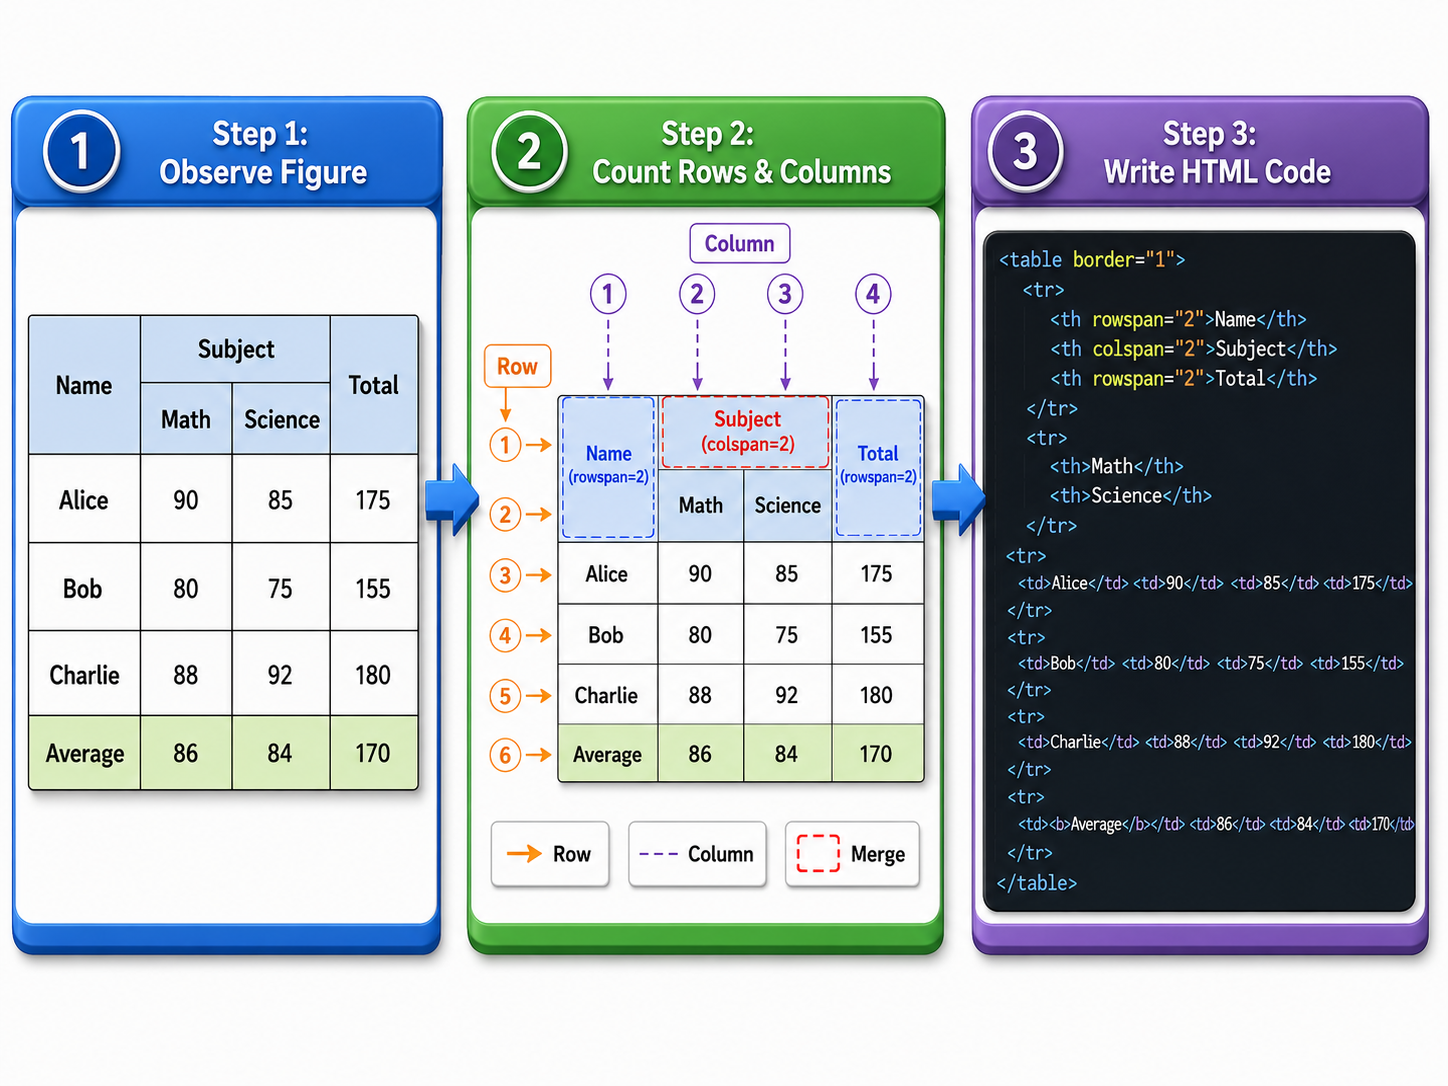
\includegraphics[width=0.95\linewidth,height=0.11\textheight,keepaspectratio]{chapters/Chapter04/topics/images/3d_figure_to_code_steps.png}
}{
\fbox{\parbox{0.90\linewidth}{\centering\vspace{0.5cm}
\textbf{চিত্র}\\[4pt]
A flow diagram: count rows $\rightarrow$ count columns $\rightarrow$ find merged cells $\rightarrow$ add content $\rightarrow$ write HTML code.\\[4pt]
File: \texttt{chapters/Chapter04/topics/images/3d\_figure\_to\_code\_steps.png}
\vspace{0.5cm}}}
}
\captionof{figure}{figure থেকে HTML table code লেখার ধাপ}
\end{center}

\begin{keypointbox}{চিত্র ব্যাখ্যা}
চিত্রে চিত্র দেখে HTML table code লেখার workflow দেখানো হয়েছে: row-column count করা, merged cell identify করা, content type বোঝা এবং শেষে HTML tag লেখা।
\end{keypointbox}


\subsection{PDF Exercise Bank: First to Last}

এই অংশে PDF-এর page অনুযায়ী table exercise সাজানো হয়েছে। প্রত্যেক exercise-এ concept, চিত্র, চিত্র ব্যাখ্যা, code লেখার ধাপ এবং কোড দেওয়া হয়েছে।

\begin{multicols}{2}
\raggedcolumns
\setlength{\columnsep}{10pt}
\subsubsection{Exercise 1: Basic Row and Column Table}

\begin{boardbox}{Concept}
প্রথম table exercise-এ 2 row এবং 2 column দিয়ে basic cell structure বোঝানো হয়েছে।
\end{boardbox}

\begin{center}
\IfFileExists{chapters/Chapter04/topics/images/ex01_3d_basic_2x2.png}{
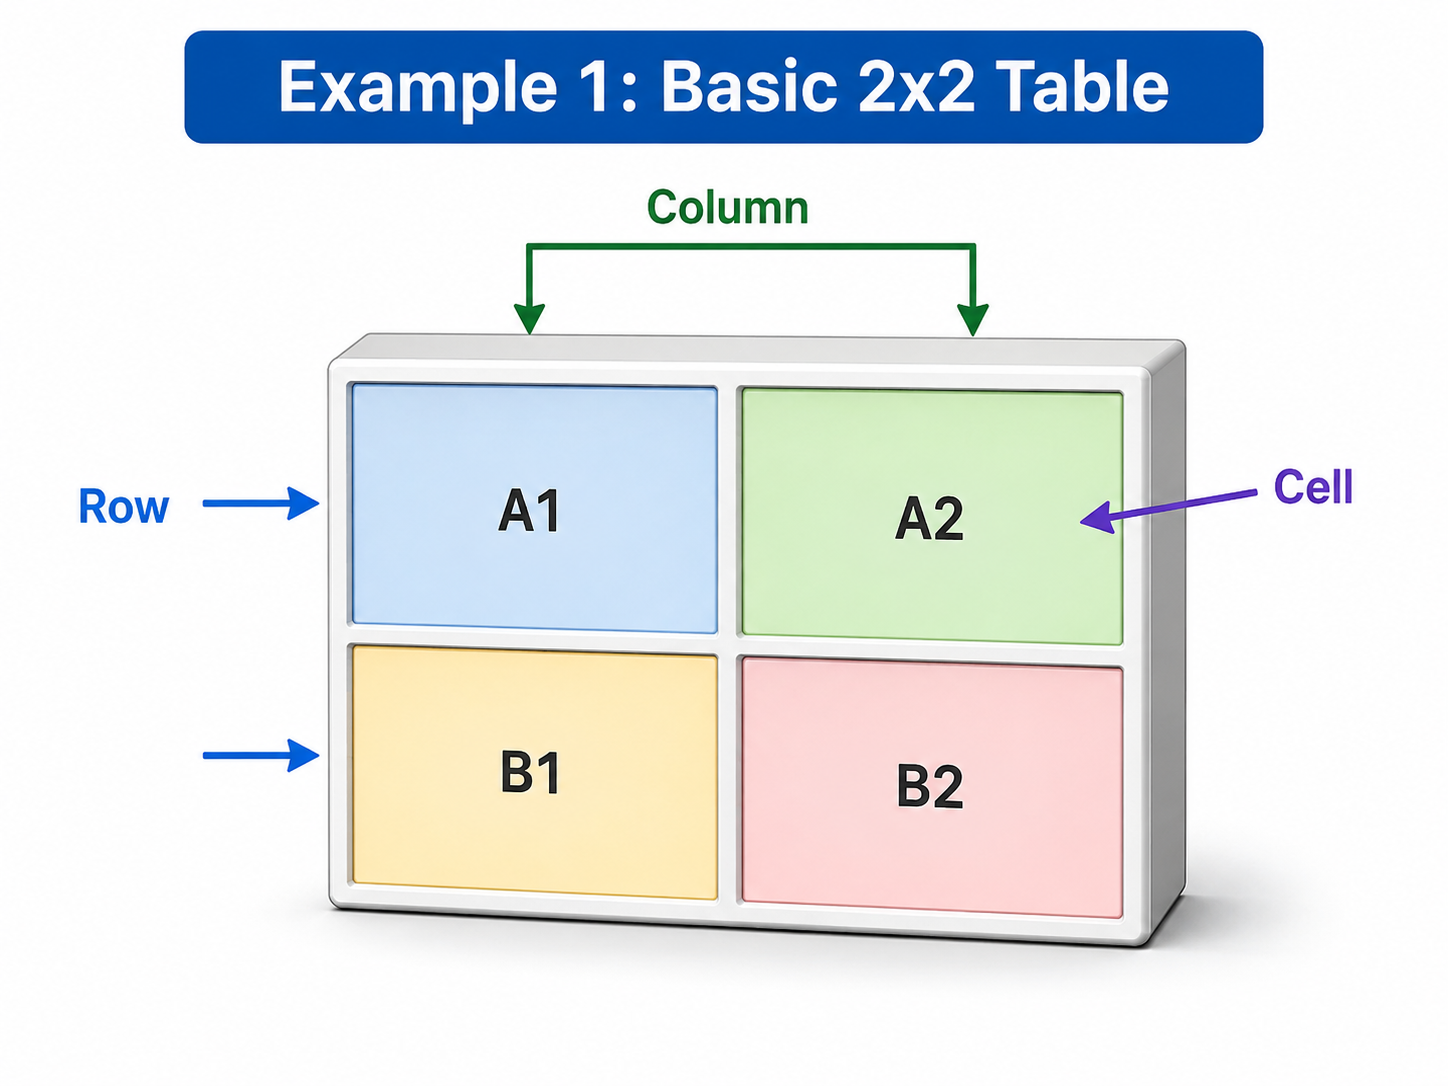
\includegraphics[width=0.95\linewidth,height=0.11\textheight,keepaspectratio]{chapters/Chapter04/topics/images/ex01_3d_basic_2x2.png}
}{
\fbox{\parbox{0.90\linewidth}{\centering\vspace{0.4cm}
\textbf{চিত্র}\\
File: \texttt{chapters/Chapter04/topics/images/ex01\_3d\_basic\_2x2.png}
\vspace{0.4cm}}}
}
\captionof{figure}{Exercise 1-এর table চিত্র}
\end{center}

\begin{keypointbox}{চিত্র ব্যাখ্যা}
চিত্রে A1, A2, B1 এবং B2 নামে চারটি cell আছে। প্রথম row-তে A1-A2 এবং দ্বিতীয় row-তে B1-B2 রাখা হয়েছে।
\end{keypointbox}

\begin{keypointbox}{চিত্র দেখে code লেখার ধাপ}
প্রথমে 2টি row ধরবে। প্রতিটি row-তে 2টি করে \texttt{<td>} cell লিখবে। তারপর cell text হিসেবে A1, A2, B1, B2 বসাবে।
\end{keypointbox}

\par\noindent{\color{purple!70!black}\bfseries\small কোড}\par\vspace{-4pt}
\begin{verbatim}
<!DOCTYPE html>
<html>
<head>
  <title>HTML Table Example</title>
</head>
<body>
<table>
  <tr>
    <td>A1</td>
    <td>A2</td>
  </tr>
  <tr>
    <td>B1</td>
    <td>B2</td>
  </tr>
</table>
</body>
</html>
\end{verbatim}
\vspace{-6pt}

\subsubsection{Exercise 2: Border সহ Simple Table}

\begin{boardbox}{Concept}
\texttt{border="1"} দিলে table এবং cell-এর চারপাশে border দেখা যায়।
\end{boardbox}

\begin{center}
\IfFileExists{chapters/Chapter04/topics/images/ex02_3d_border_table.png}{
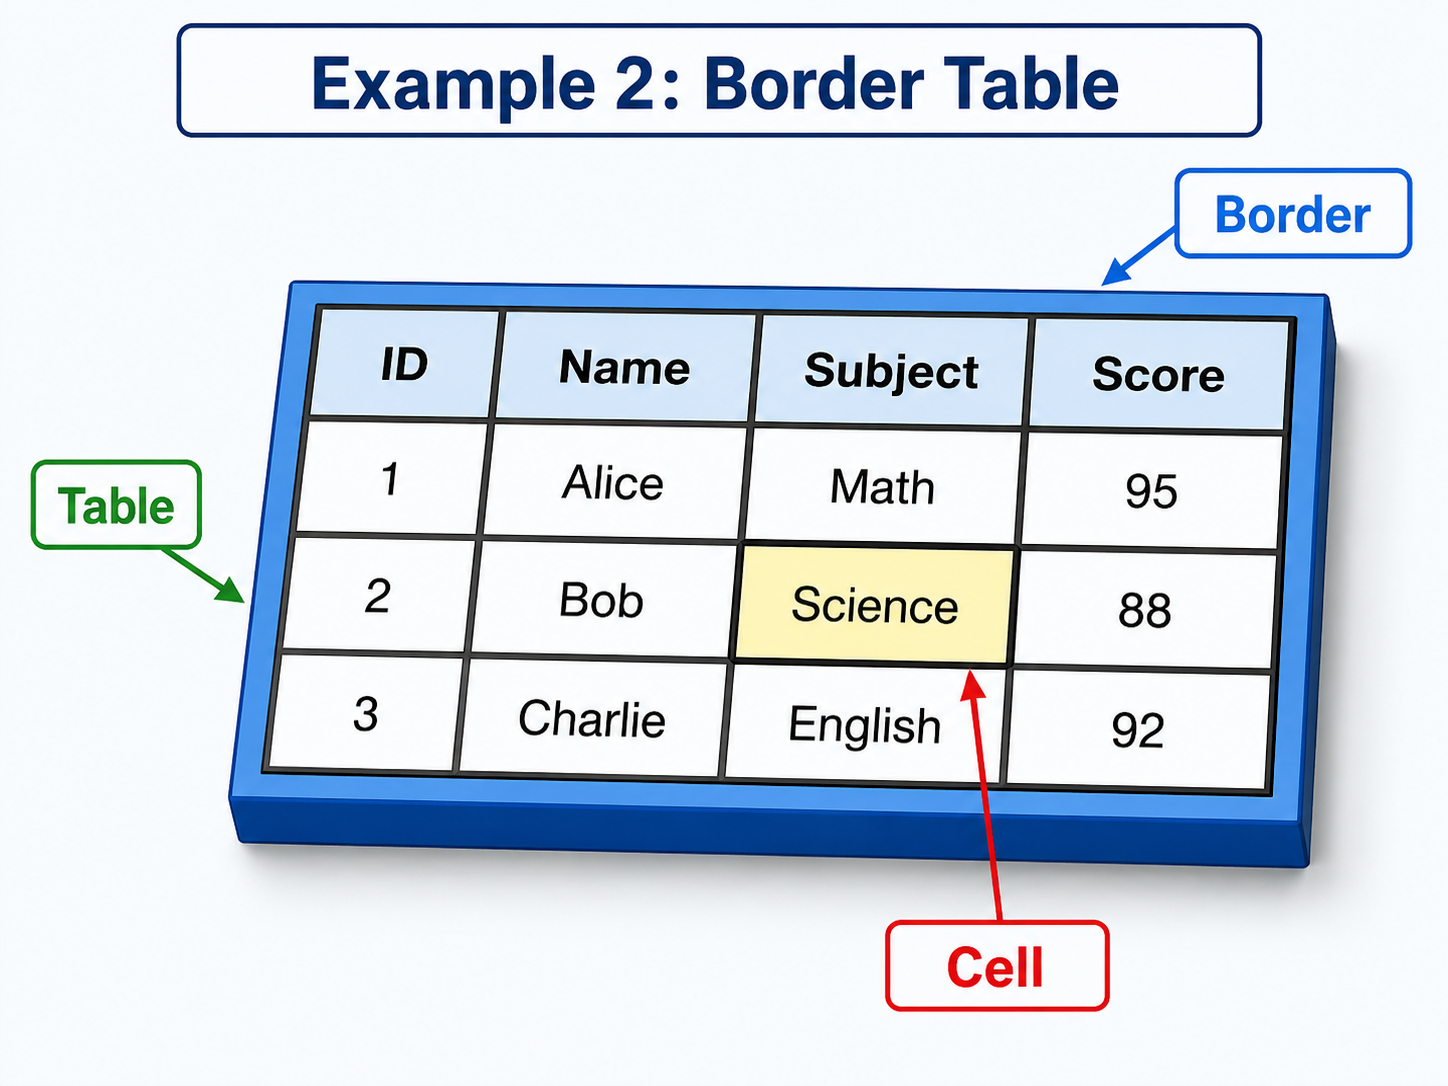
\includegraphics[width=0.95\linewidth,height=0.11\textheight,keepaspectratio]{chapters/Chapter04/topics/images/ex02_3d_border_table.png}
}{
\fbox{\parbox{0.90\linewidth}{\centering\vspace{0.4cm}
\textbf{চিত্র}\\
File: \texttt{chapters/Chapter04/topics/images/ex02\_3d\_border\_table.png}
\vspace{0.4cm}}}
}
\captionof{figure}{Exercise 2-এর border চিত্র}
\end{center}

\begin{keypointbox}{চিত্র ব্যাখ্যা}
চিত্রে ID, Name, Subject এবং Score column আছে। তিনজন student-এর subject ও score border সহ table আকারে দেখানো হয়েছে।
\end{keypointbox}

\begin{keypointbox}{চিত্র দেখে code লেখার ধাপ}
প্রথমে header row-তে চারটি \texttt{<th>} লিখবে। এরপর Alice, Bob ও Charlie-এর জন্য তিনটি data row তৈরি করবে। পুরো table-এ border দেখাতে \texttt{border="1"} ব্যবহার করবে।
\end{keypointbox}

\par\noindent{\color{purple!70!black}\bfseries\small কোড}\par\vspace{-4pt}
\begin{verbatim}
<!DOCTYPE html>
<html>
<head>
  <title>HTML Table Example</title>
</head>
<body>
<table border="1" cellspacing="0" cellpadding="6">
  <tr>
    <th>ID</th>
    <th>Name</th>
    <th>Subject</th>
    <th>Score</th>
  </tr>
  <tr>
    <td>1</td>
    <td>Alice</td>
    <td>Math</td>
    <td>95</td>
  </tr>
  <tr>
    <td>2</td>
    <td>Bob</td>
    <td>Science</td>
    <td>88</td>
  </tr>
  <tr>
    <td>3</td>
    <td>Charlie</td>
    <td>English</td>
    <td>92</td>
  </tr>
</table>
</body>
</html>
\end{verbatim}
\vspace{-6pt}

\subsubsection{Exercise 3: Caption, TH এবং Student Info Table}

\begin{boardbox}{Concept}
\texttt{<caption>} table-এর title দেয় এবং \texttt{<th>} heading cell তৈরি করে।
\end{boardbox}

\begin{center}
\IfFileExists{chapters/Chapter04/topics/images/ex03_3d_student_info.png}{
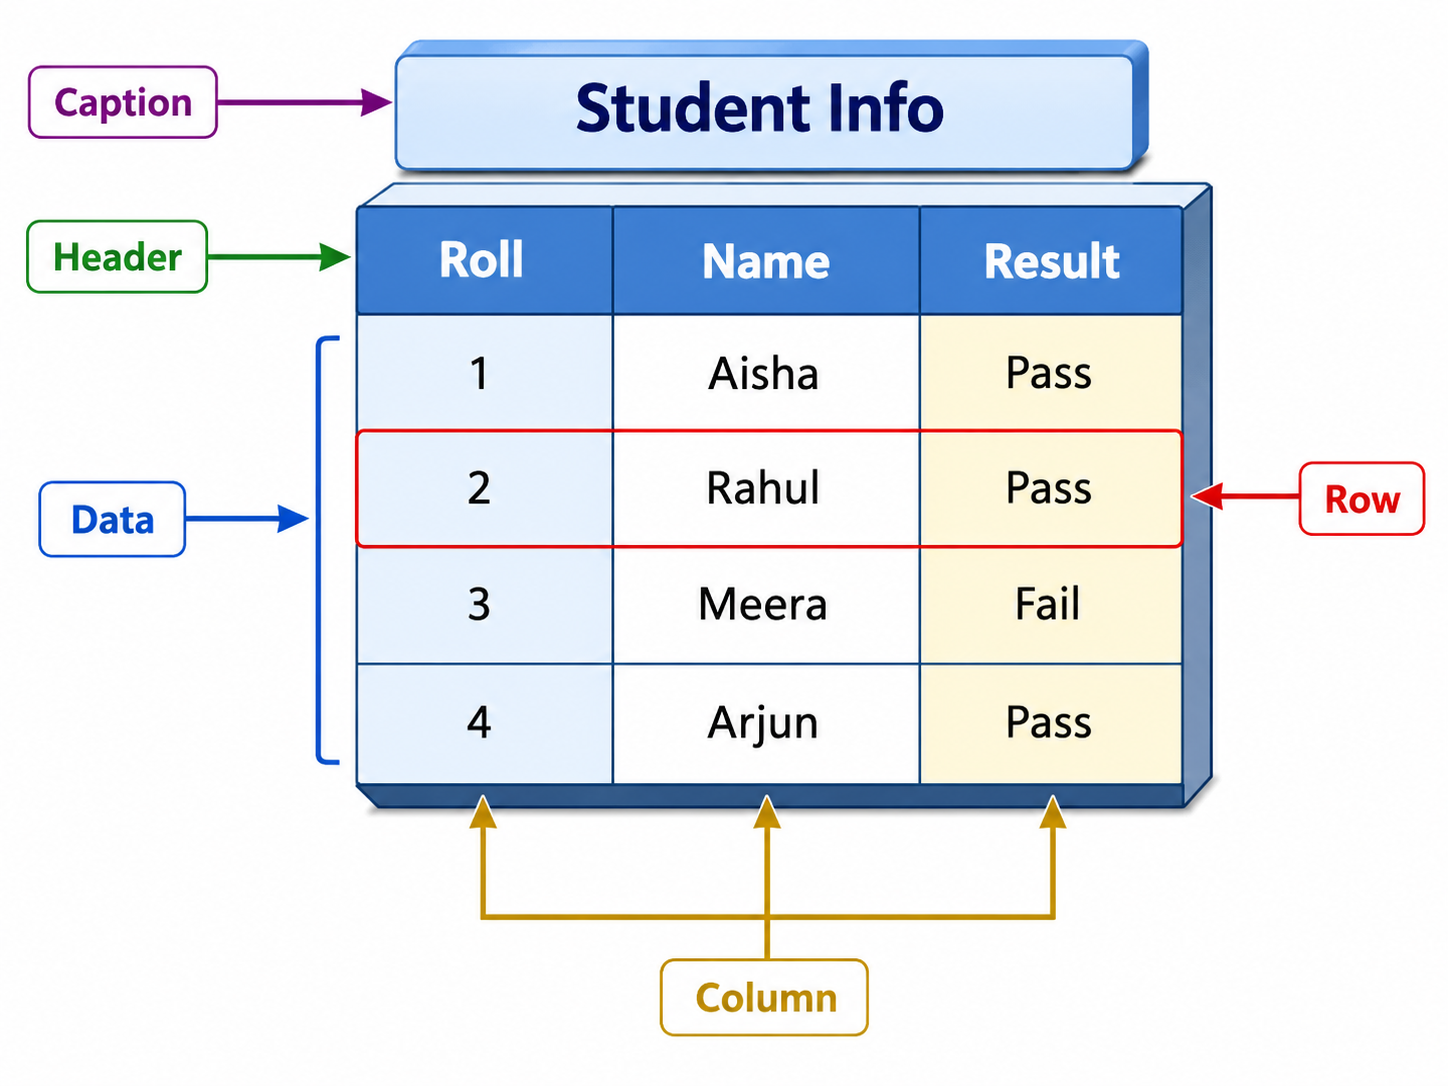
\includegraphics[width=0.95\linewidth,height=0.11\textheight,keepaspectratio]{chapters/Chapter04/topics/images/ex03_3d_student_info.png}
}{
\fbox{\parbox{0.90\linewidth}{\centering\vspace{0.4cm}
\textbf{চিত্র}\\
File: \texttt{chapters/Chapter04/topics/images/ex03\_3d\_student\_info.png}
\vspace{0.4cm}}}
}
\captionof{figure}{Exercise 3-এর caption ও heading চিত্র}
\end{center}

\begin{keypointbox}{চিত্র ব্যাখ্যা}
চিত্রে Student Info caption আছে। table-এ Roll, Name ও Result column দেখানো হয়েছে এবং data row-গুলোতে Pass/Fail result আছে।
\end{keypointbox}

\begin{keypointbox}{চিত্র দেখে code লেখার ধাপ}
প্রথমে \texttt{<caption>} দিয়ে Student Info লিখবে। এরপর তিনটি header cell তৈরি করবে। তারপর চারটি student row লিখবে।
\end{keypointbox}

\par\noindent{\color{purple!70!black}\bfseries\small কোড}\par\vspace{-4pt}
\begin{verbatim}
<!DOCTYPE html>
<html>
<head>
  <title>HTML Table Example</title>
</head>
<body>
<table border="1" cellspacing="0" cellpadding="6">
  <caption><b>Student Info</b></caption>
  <tr>
    <th>Roll</th>
    <th>Name</th>
    <th>Result</th>
  </tr>
  <tr><td>1</td><td>Aisha</td><td>Pass</td></tr>
  <tr><td>2</td><td>Rahul</td><td>Pass</td></tr>
  <tr><td>3</td><td>Meera</td><td>Fail</td></tr>
  <tr><td>4</td><td>Arjun</td><td>Pass</td></tr>
</table>
</body>
</html>
\end{verbatim}
\vspace{-6pt}

\subsubsection{Exercise 4: Width Attribute দিয়ে Table Width নির্ধারণ}

\begin{boardbox}{Concept}
\texttt{width} attribute দিয়ে table-এর মোট প্রস্থ নির্ধারণ করা যায়।
\end{boardbox}

\begin{center}
\IfFileExists{chapters/Chapter04/topics/images/ex04_3d_width_400.png}{
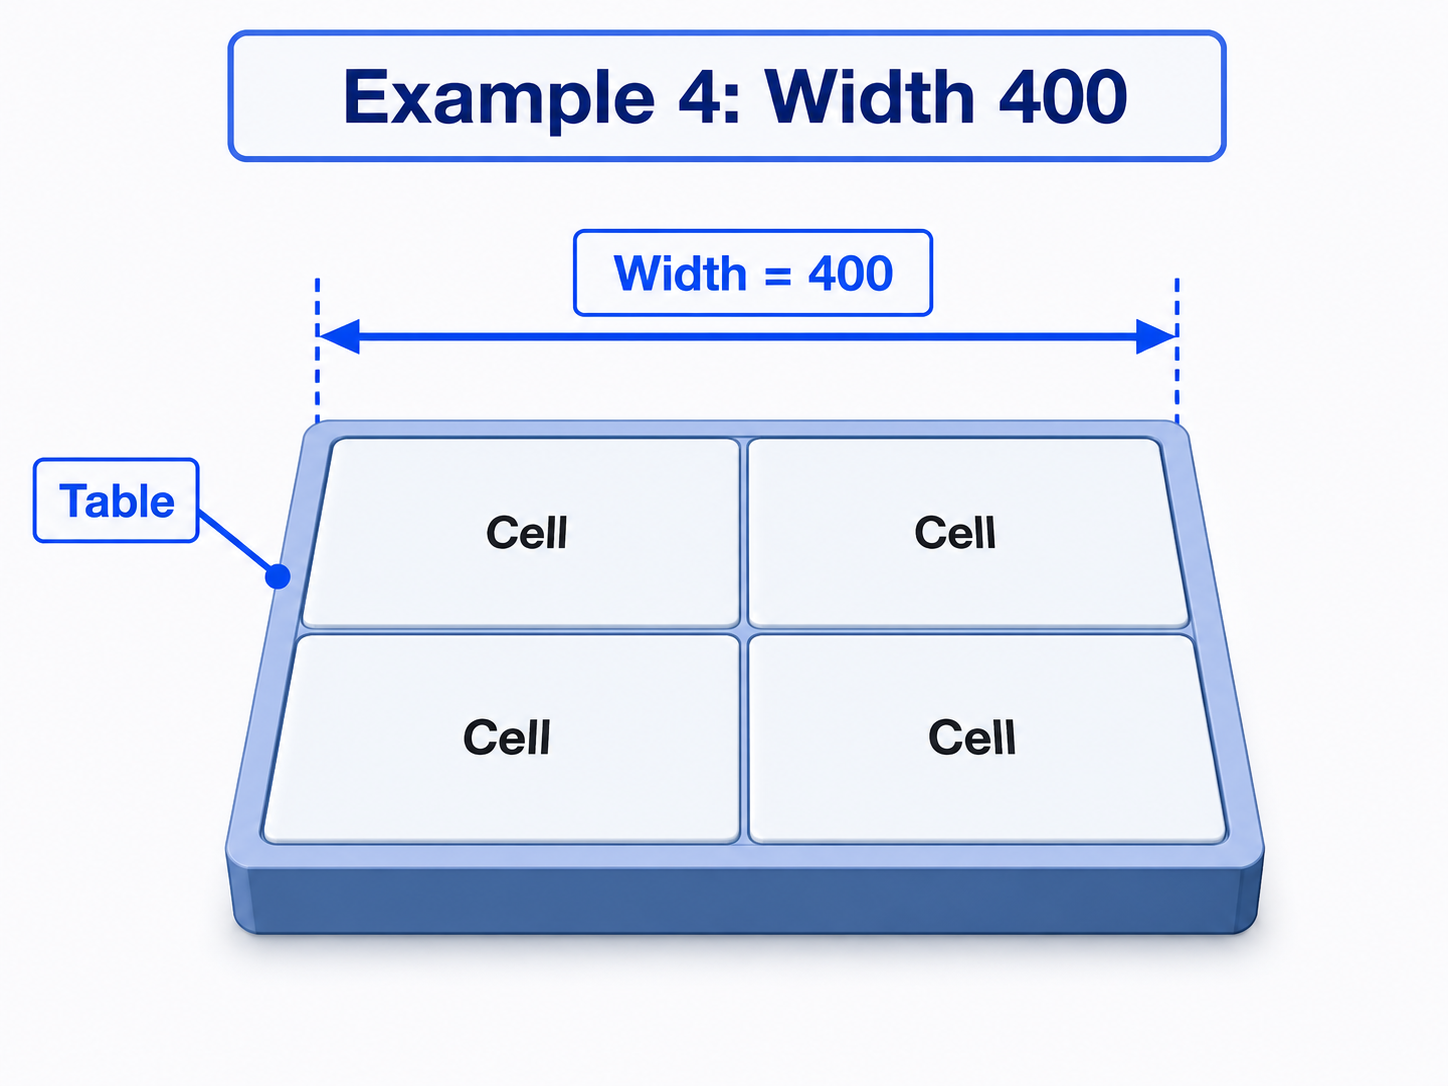
\includegraphics[width=0.95\linewidth,height=0.11\textheight,keepaspectratio]{chapters/Chapter04/topics/images/ex04_3d_width_400.png}
}{
\fbox{\parbox{0.90\linewidth}{\centering\vspace{0.4cm}
\textbf{চিত্র}\\
File: \texttt{chapters/Chapter04/topics/images/ex04\_3d\_width\_400.png}
\vspace{0.4cm}}}
}
\captionof{figure}{Exercise 4-এর width চিত্র}
\end{center}

\begin{keypointbox}{চিত্র ব্যাখ্যা}
চিত্রে table width 400 দেখানো হয়েছে। table-টি 2 row ও 2 column-এর, প্রতিটি cell-এ Cell লেখা আছে।
\end{keypointbox}

\begin{keypointbox}{চিত্র দেখে code লেখার ধাপ}
প্রথমে \texttt{width="400"} সহ table লিখবে। তারপর 2টি row এবং প্রতিটি row-তে 2টি cell তৈরি করবে।
\end{keypointbox}

\par\noindent{\color{purple!70!black}\bfseries\small কোড}\par\vspace{-4pt}
\begin{verbatim}
<!DOCTYPE html>
<html>
<head>
  <title>HTML Table Example</title>
</head>
<body>
<table border="1" width="400" cellspacing="0" cellpadding="10">
  <tr>
    <td>Cell</td>
    <td>Cell</td>
  </tr>
  <tr>
    <td>Cell</td>
    <td>Cell</td>
  </tr>
</table>
</body>
</html>
\end{verbatim}
\vspace{-6pt}

\subsubsection{Exercise 5: Table Attribute Practice}

\begin{boardbox}{Concept}
একই table-এ \texttt{border}, \texttt{width}, \texttt{cellspacing}, \texttt{cellpadding}, \texttt{align} ও \texttt{bgcolor} attribute ব্যবহার করা যায়।
\end{boardbox}

\begin{center}
\IfFileExists{chapters/Chapter04/topics/images/ex05_3d_table_attributes_combined.png}{
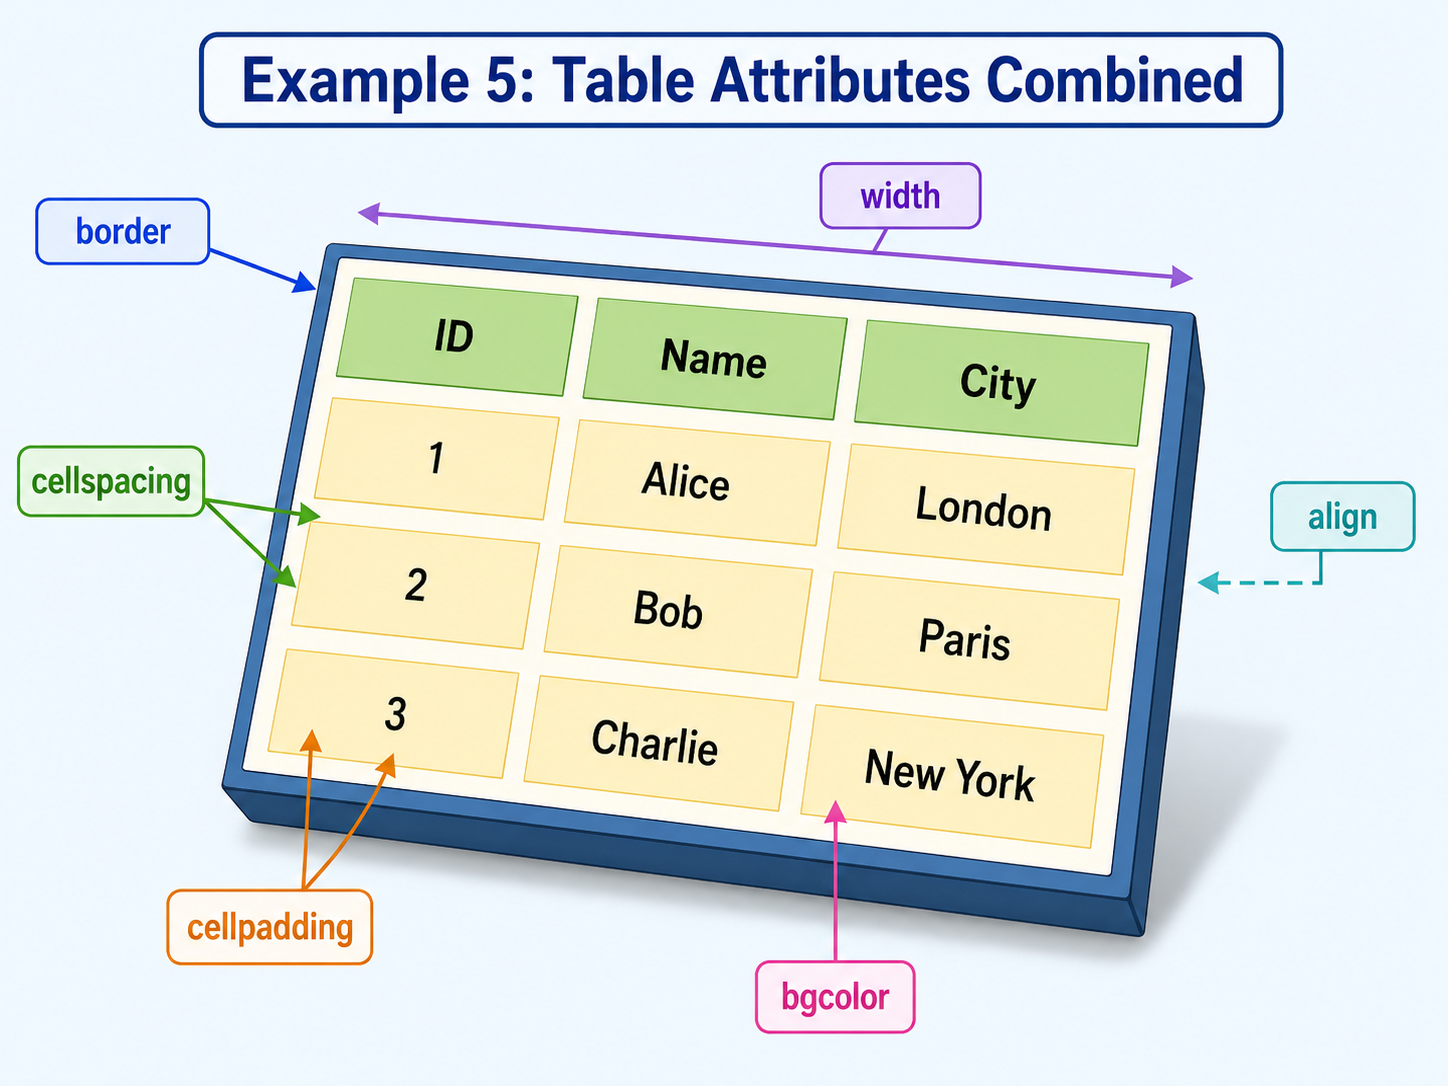
\includegraphics[width=0.95\linewidth,height=0.11\textheight,keepaspectratio]{chapters/Chapter04/topics/images/ex05_3d_table_attributes_combined.png}
}{
\fbox{\parbox{0.90\linewidth}{\centering\vspace{0.4cm}
\textbf{চিত্র}\\
File: \texttt{chapters/Chapter04/topics/images/ex05\_3d\_table\_attributes\_combined.png}
\vspace{0.4cm}}}
}
\captionof{figure}{Exercise 5-এর attribute চিত্র}
\end{center}

\begin{keypointbox}{চিত্র ব্যাখ্যা}
চিত্রে একটি student/city table-এর উপর table attributes-এর effect দেখানো হয়েছে। header background color, table width, border, spacing, padding এবং alignment visual label দিয়ে বোঝানো হয়েছে।
\end{keypointbox}

\begin{keypointbox}{চিত্র দেখে code লেখার ধাপ}
প্রথমে table tag-এ attribute বসাবে। তারপর ID, Name, City header row লিখবে। শেষে তিনটি data row তৈরি করবে।
\end{keypointbox}

\par\noindent{\color{purple!70!black}\bfseries\small কোড}\par\vspace{-4pt}
\begin{verbatim}
<!DOCTYPE html>
<html>
<head>
  <title>HTML Table Example</title>
</head>
<body>
<table border="1" width="450" cellspacing="6" cellpadding="8" align="center">
  <tr bgcolor="lightgreen">
    <th>ID</th>
    <th>Name</th>
    <th>City</th>
  </tr>
  <tr><td>1</td><td>Alice</td><td>London</td></tr>
  <tr><td>2</td><td>Bob</td><td>Paris</td></tr>
  <tr><td>3</td><td>Charlie</td><td>New York</td></tr>
</table>
</body>
</html>
\end{verbatim}
\vspace{-6pt}

\subsubsection{Exercise 6: Colspan ও Rowspan Basic Example}

\begin{boardbox}{Concept}
\texttt{colspan} horizontal cell merge করে এবং \texttt{rowspan} vertical cell merge করে।
\end{boardbox}

\begin{center}
\IfFileExists{chapters/Chapter04/topics/images/ex06_3d_span_two_columns_rows.png}{
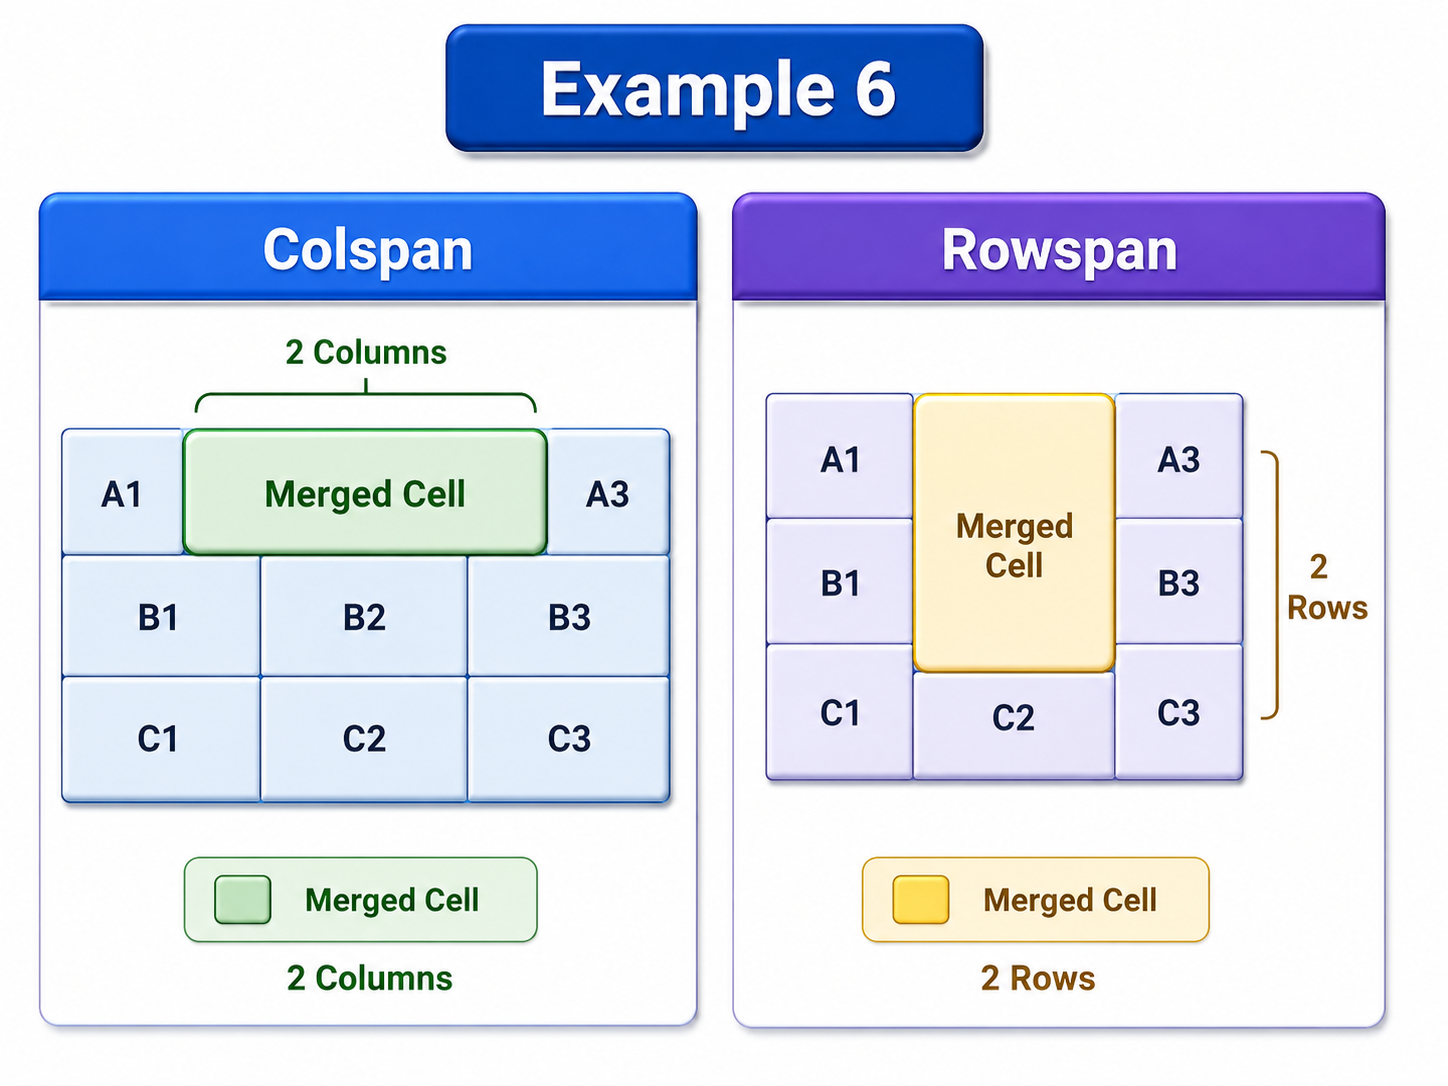
\includegraphics[width=0.95\linewidth,height=0.11\textheight,keepaspectratio]{chapters/Chapter04/topics/images/ex06_3d_span_two_columns_rows.png}
}{
\fbox{\parbox{0.90\linewidth}{\centering\vspace{0.4cm}
\textbf{চিত্র}\\
File: \texttt{chapters/Chapter04/topics/images/ex06\_3d\_span\_two\_columns\_rows.png}
\vspace{0.4cm}}}
}
\captionof{figure}{Exercise 6-এর rowspan-colspan চিত্র}
\end{center}

\begin{keypointbox}{চিত্র ব্যাখ্যা}
চিত্রে বাম পাশে colspan দিয়ে দুই column merge এবং ডান পাশে rowspan দিয়ে দুই row merge দেখানো হয়েছে।
\end{keypointbox}

\begin{keypointbox}{চিত্র দেখে code লেখার ধাপ}
Horizontal merge দরকার হলে \texttt{colspan="2"} ব্যবহার করবে। Vertical merge দরকার হলে \texttt{rowspan="2"} ব্যবহার করবে।
\end{keypointbox}

\par\noindent{\color{purple!70!black}\bfseries\small কোড}\par\vspace{-4pt}
\begin{verbatim}
<!DOCTYPE html>
<html>
<head>
  <title>HTML Table Example</title>
</head>
<body>
<h3>Colspan</h3>
<table border="1" cellspacing="0" cellpadding="6">
  <tr><th colspan="3">Colspan</th></tr>
  <tr><td>A1</td><td colspan="2">Merged Cell</td></tr>
  <tr><td>B1</td><td>B2</td><td>B3</td></tr>
  <tr><td>C1</td><td>C2</td><td>C3</td></tr>
</table>

<h3>Rowspan</h3>
<table border="1" cellspacing="0" cellpadding="6">
  <tr><th colspan="3">Rowspan</th></tr>
  <tr><td>A1</td><td rowspan="2">Merged Cell</td><td>A3</td></tr>
  <tr><td>B1</td><td>B3</td></tr>
  <tr><td>C1</td><td>C2</td><td>C3</td></tr>
</table>
</body>
</html>
\end{verbatim}
\vspace{-6pt}

\subsubsection{Exercise 7: Empty Cell এবং Basic Sales Table}

\begin{boardbox}{Concept}
খালি cell দেখাতে cell-এর ভিতরে \texttt{\&nbsp;} ব্যবহার করা যায়।
\end{boardbox}

\begin{center}
\IfFileExists{chapters/Chapter04/topics/images/ex07_3d_empty_cells.png}{
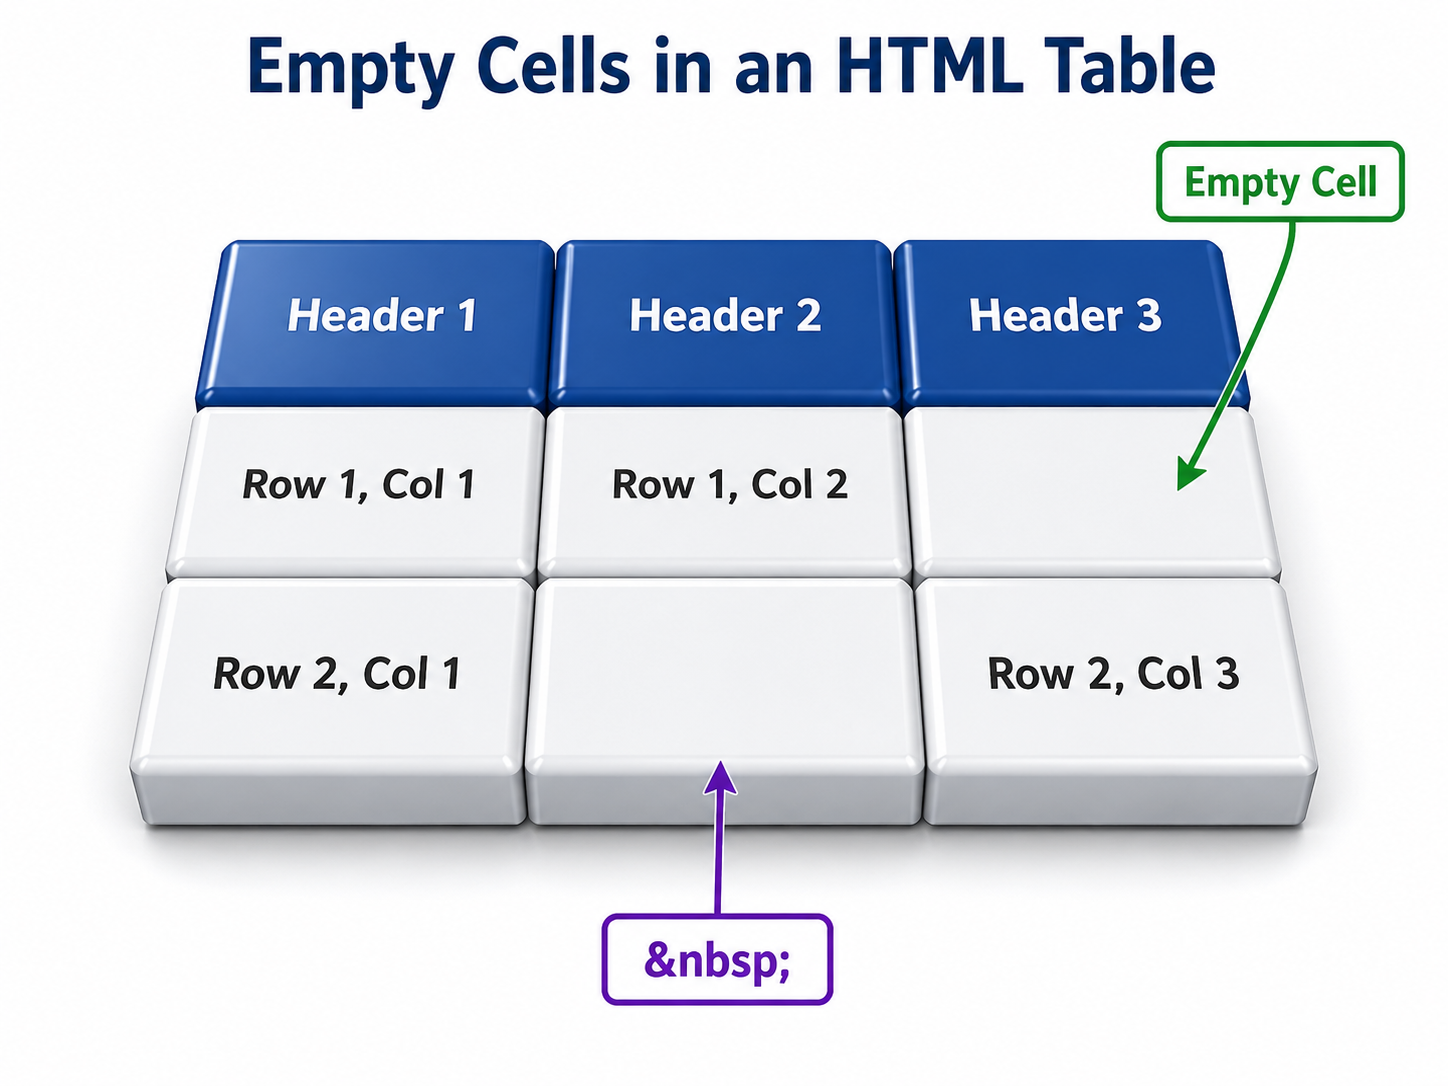
\includegraphics[width=0.95\linewidth,height=0.11\textheight,keepaspectratio]{chapters/Chapter04/topics/images/ex07_3d_empty_cells.png}
}{
\fbox{\parbox{0.90\linewidth}{\centering\vspace{0.4cm}
\textbf{চিত্র}\\
File: \texttt{chapters/Chapter04/topics/images/ex07\_3d\_empty\_cells.png}
\vspace{0.4cm}}}
}
\captionof{figure}{Exercise 7-এর empty cell চিত্র}
\end{center}

\begin{keypointbox}{চিত্র ব্যাখ্যা}
চিত্রে Header 1, Header 2, Header 3 সহ table আছে। কিছু cell intentionally empty রাখা হয়েছে; browser-এ cell visible রাখতে \texttt{\&nbsp;} ব্যবহার করা হয়েছে।
\end{keypointbox}

\begin{keypointbox}{চিত্র দেখে code লেখার ধাপ}
প্রথমে তিনটি header লিখবে। যে cell খালি দেখাতে হবে সেখানে normal text না দিয়ে \texttt{\&nbsp;} লিখবে।
\end{keypointbox}

\par\noindent{\color{purple!70!black}\bfseries\small কোড}\par\vspace{-4pt}
\begin{verbatim}
<!DOCTYPE html>
<html>
<head>
  <title>HTML Table Example</title>
</head>
<body>
<table border="1" cellspacing="0" cellpadding="8">
  <tr>
    <th>Header 1</th>
    <th>Header 2</th>
    <th>Header 3</th>
  </tr>
  <tr>
    <td>Row 1, Col 1</td>
    <td>Row 1, Col 2</td>
    <td>&nbsp;</td>
  </tr>
  <tr>
    <td>Row 2, Col 1</td>
    <td>&nbsp;</td>
    <td>Row 2, Col 3</td>
  </tr>
</table>
</body>
</html>
\end{verbatim}
\vspace{-6pt}

\subsubsection{Exercise 8: Align Attribute Practice}

\begin{boardbox}{Concept}
\texttt{align="center"} দিলে cell-এর content horizontally center হয়।
\end{boardbox}

\begin{center}
\IfFileExists{chapters/Chapter04/topics/images/ex08_3d_align_center.png}{
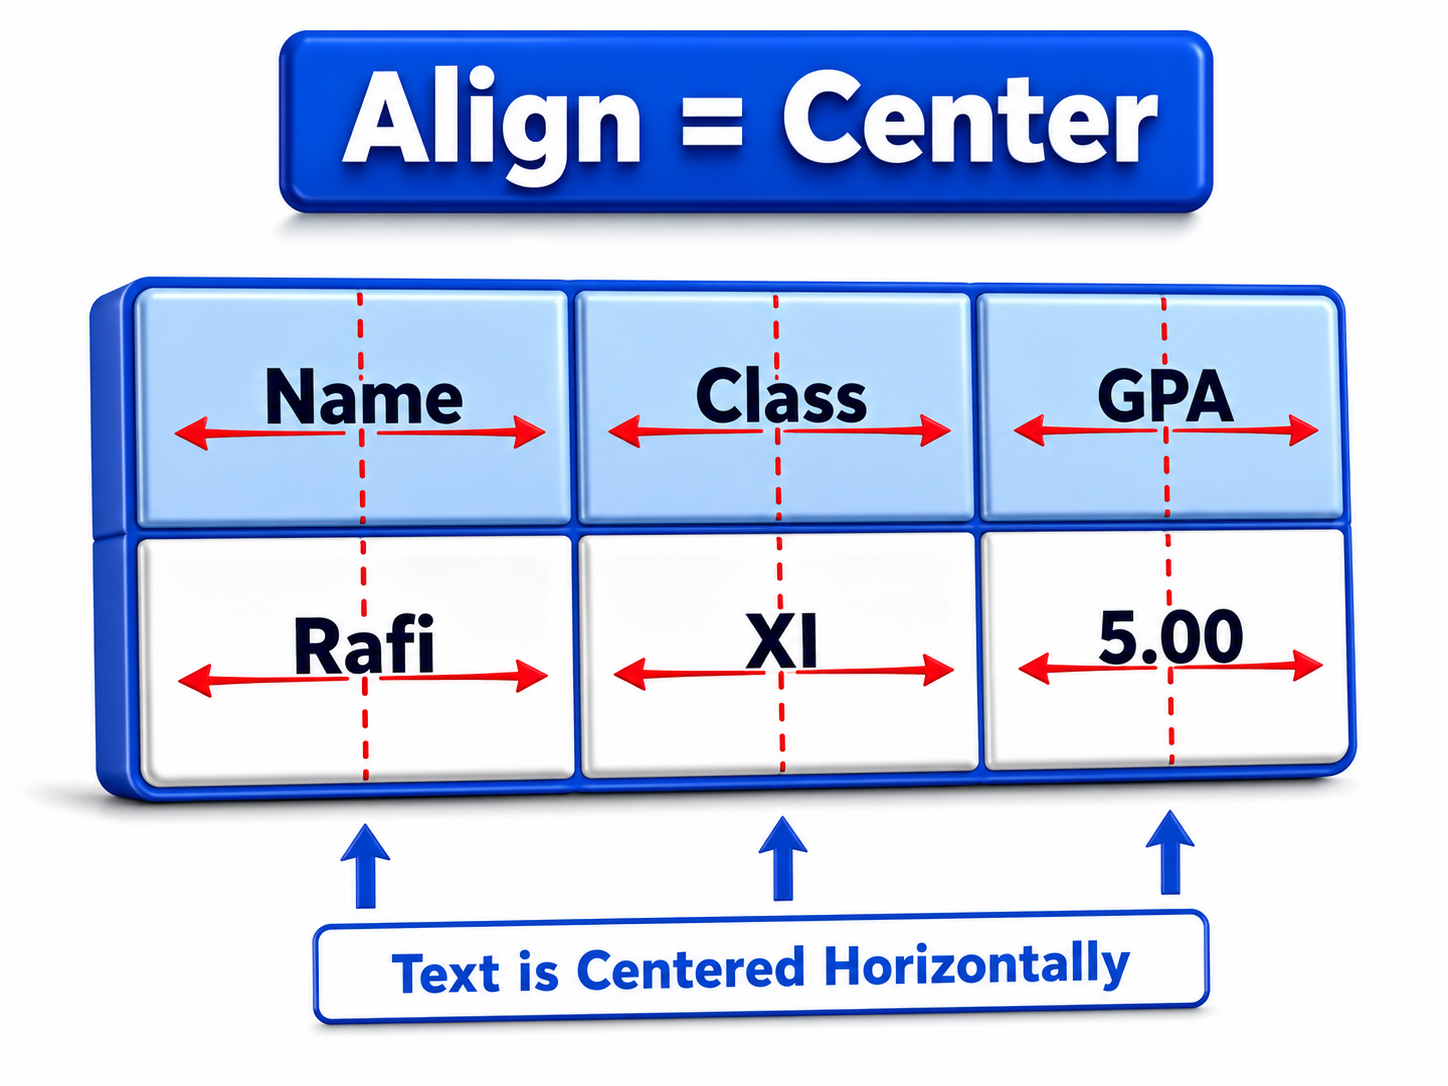
\includegraphics[width=0.95\linewidth,height=0.11\textheight,keepaspectratio]{chapters/Chapter04/topics/images/ex08_3d_align_center.png}
}{
\fbox{\parbox{0.90\linewidth}{\centering\vspace{0.4cm}
\textbf{চিত্র}\\
File: \texttt{chapters/Chapter04/topics/images/ex08\_3d\_align\_center.png}
\vspace{0.4cm}}}
}
\captionof{figure}{Exercise 8-এর align চিত্র}
\end{center}

\begin{keypointbox}{চিত্র ব্যাখ্যা}
চিত্রে Name, Class ও GPA column-এর text center aligned আছে। Rafi, XI এবং 5.00 cell-গুলো cell-এর মাঝখানে বসেছে।
\end{keypointbox}

\begin{keypointbox}{চিত্র দেখে code লেখার ধাপ}
পুরো table center alignment করতে table row বা প্রতিটি cell-এ \texttt{align="center"} ব্যবহার করবে।
\end{keypointbox}

\par\noindent{\color{purple!70!black}\bfseries\small কোড}\par\vspace{-4pt}
\begin{verbatim}
<!DOCTYPE html>
<html>
<head>
  <title>HTML Table Example</title>
</head>
<body>
<table border="1" cellspacing="0" cellpadding="8" align="center">
  <tr align="center">
    <th>Name</th>
    <th>Class</th>
    <th>GPA</th>
  </tr>
  <tr align="center">
    <td>Rafi</td>
    <td>XI</td>
    <td>5.00</td>
  </tr>
</table>
</body>
</html>
\end{verbatim}
\vspace{-6pt}

\subsubsection{Exercise 9: Cell Data Alignment Table}

\begin{boardbox}{Concept}
একই table-এ left, center এবং right alignment আলাদা cell-এ ব্যবহার করা যায়।
\end{boardbox}

\begin{center}
\IfFileExists{chapters/Chapter04/topics/images/ex09_3d_cell_alignment.png}{
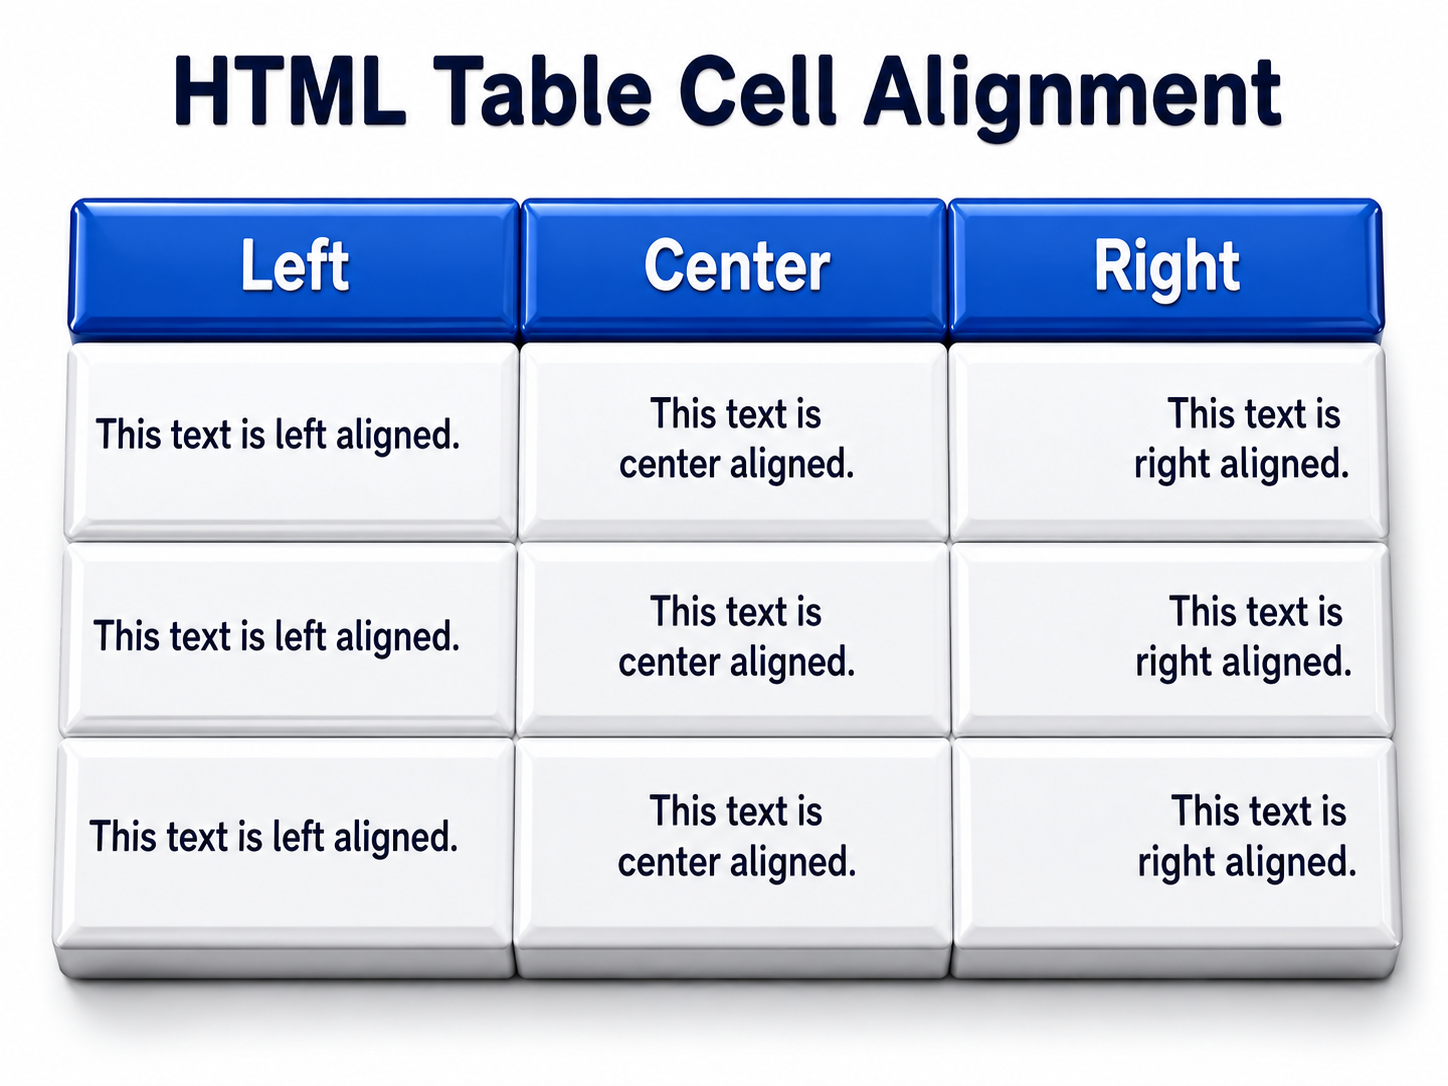
\includegraphics[width=0.95\linewidth,height=0.11\textheight,keepaspectratio]{chapters/Chapter04/topics/images/ex09_3d_cell_alignment.png}
}{
\fbox{\parbox{0.90\linewidth}{\centering\vspace{0.4cm}
\textbf{চিত্র}\\
File: \texttt{chapters/Chapter04/topics/images/ex09\_3d\_cell\_alignment.png}
\vspace{0.4cm}}}
}
\captionof{figure}{Exercise 9-এর cell alignment চিত্র}
\end{center}

\begin{keypointbox}{চিত্র ব্যাখ্যা}
চিত্রে তিনটি column আছে: Left, Center, Right। প্রতিটি column-এর text নিজ নিজ alignment অনুযায়ী cell-এর বাম, মাঝ বা ডান পাশে বসেছে।
\end{keypointbox}

\begin{keypointbox}{চিত্র দেখে code লেখার ধাপ}
Left column-এর cell-এ \texttt{align="left"}, center column-এ \texttt{align="center"} এবং right column-এ \texttt{align="right"} ব্যবহার করবে।
\end{keypointbox}

\par\noindent{\color{purple!70!black}\bfseries\small কোড}\par\vspace{-4pt}
\begin{verbatim}
<!DOCTYPE html>
<html>
<head>
  <title>HTML Table Example</title>
</head>
<body>
<table border="1" cellspacing="0" cellpadding="8">
  <tr>
    <th>Left</th>
    <th>Center</th>
    <th>Right</th>
  </tr>
  <tr>
    <td align="left">This text is left aligned.</td>
    <td align="center">This text is center aligned.</td>
    <td align="right">This text is right aligned.</td>
  </tr>
  <tr>
    <td align="left">This text is left aligned.</td>
    <td align="center">This text is center aligned.</td>
    <td align="right">This text is right aligned.</td>
  </tr>
</table>
</body>
</html>
\end{verbatim}
\vspace{-6pt}

\subsubsection{Exercise 10: Cell Width/Height Change}

\begin{boardbox}{Concept}
\texttt{width} ও \texttt{height} attribute দিয়ে cell-এর size change করা যায়।
\end{boardbox}

\begin{center}
\IfFileExists{chapters/Chapter04/topics/images/ex10_3d_cell_width_height.png}{
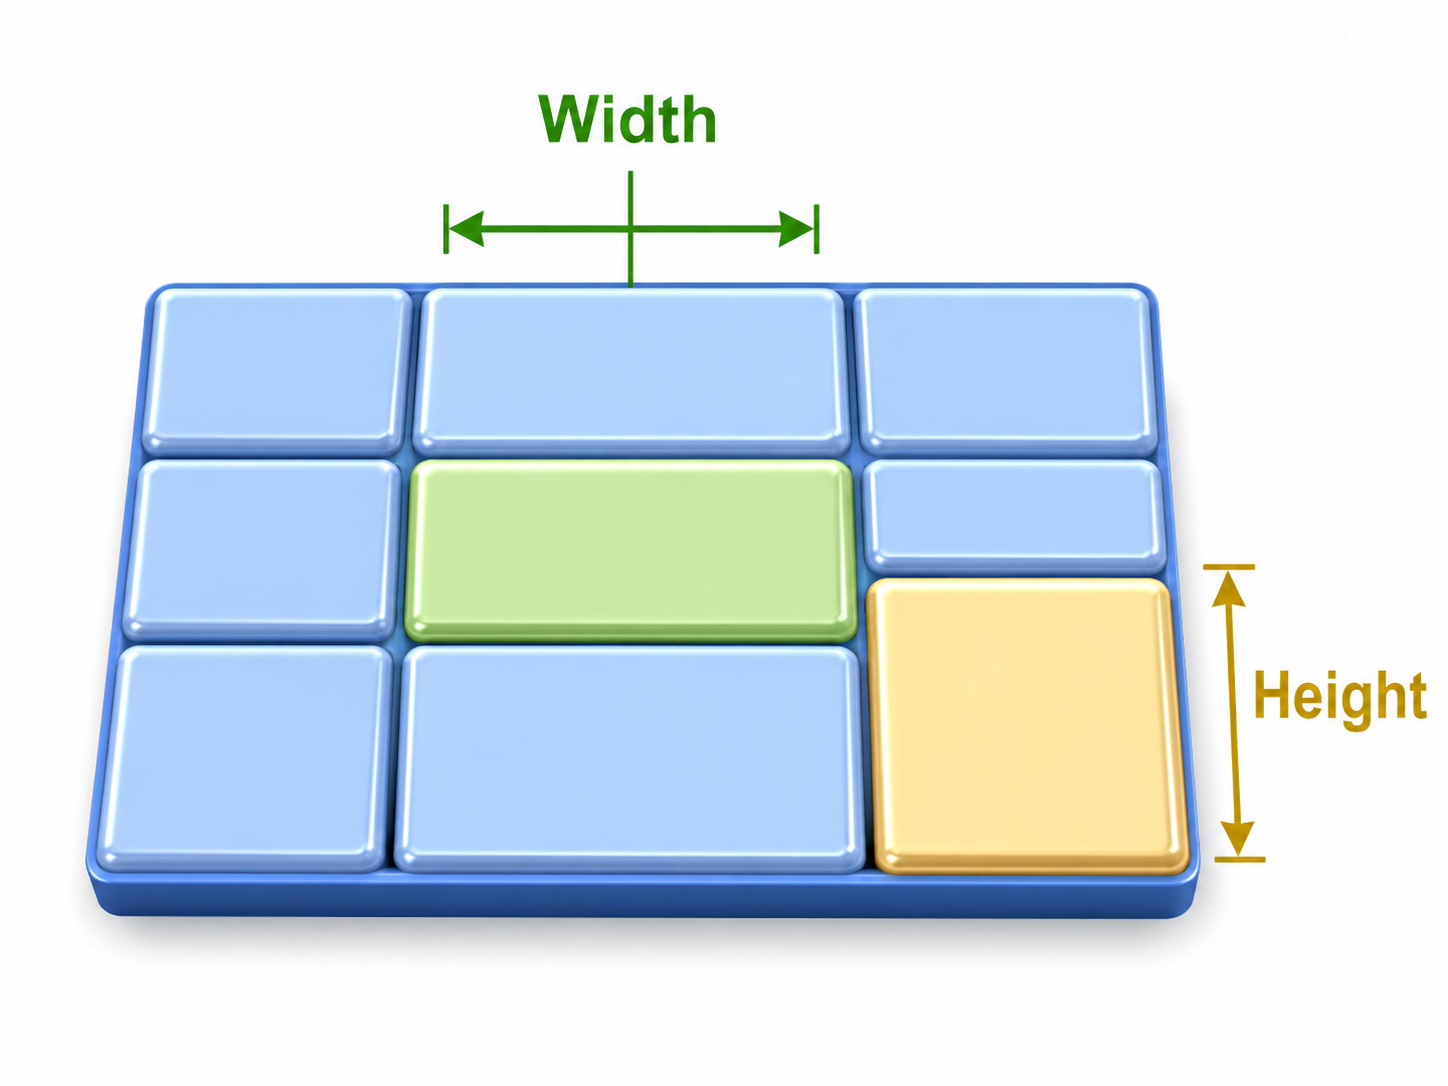
\includegraphics[width=0.95\linewidth,height=0.11\textheight,keepaspectratio]{chapters/Chapter04/topics/images/ex10_3d_cell_width_height.png}
}{
\fbox{\parbox{0.90\linewidth}{\centering\vspace{0.4cm}
\textbf{চিত্র}\\
File: \texttt{chapters/Chapter04/topics/images/ex10\_3d\_cell\_width\_height.png}
\vspace{0.4cm}}}
}
\captionof{figure}{Exercise 10-এর width-height চিত্র}
\end{center}

\begin{keypointbox}{চিত্র ব্যাখ্যা}
চিত্রে একটি table-এর মাঝের cell-এ width বেশি এবং ডান দিকের নিচের cell-এ height বেশি দেখানো হয়েছে।
\end{keypointbox}

\begin{keypointbox}{চিত্র দেখে code লেখার ধাপ}
যে cell চওড়া হবে সেখানে \texttt{width} attribute এবং যে cell লম্বা হবে সেখানে \texttt{height} attribute বসাবে।
\end{keypointbox}

\par\noindent{\color{purple!70!black}\bfseries\small কোড}\par\vspace{-4pt}
\begin{verbatim}
<!DOCTYPE html>
<html>
<head>
  <title>HTML Table Example</title>
</head>
<body>
<table border="1" cellspacing="0" cellpadding="8">
  <tr><td>A1</td><td>A2</td><td>A3</td></tr>
  <tr><td>B1</td><td width="120">Wide Cell</td><td>B3</td></tr>
  <tr><td>C1</td><td>C2</td><td height="80">Tall Cell</td></tr>
</table>
</body>
</html>
\end{verbatim}
\vspace{-6pt}

\subsubsection{Exercise 11: Month Income Cost Table}

\begin{boardbox}{Concept}
\texttt{valign} attribute দিয়ে cell-এর content vertically top, middle বা bottom position-এ রাখা যায়।
\end{boardbox}

\begin{center}
\IfFileExists{chapters/Chapter04/topics/images/ex11_3d_valign_month_income_cost.png}{
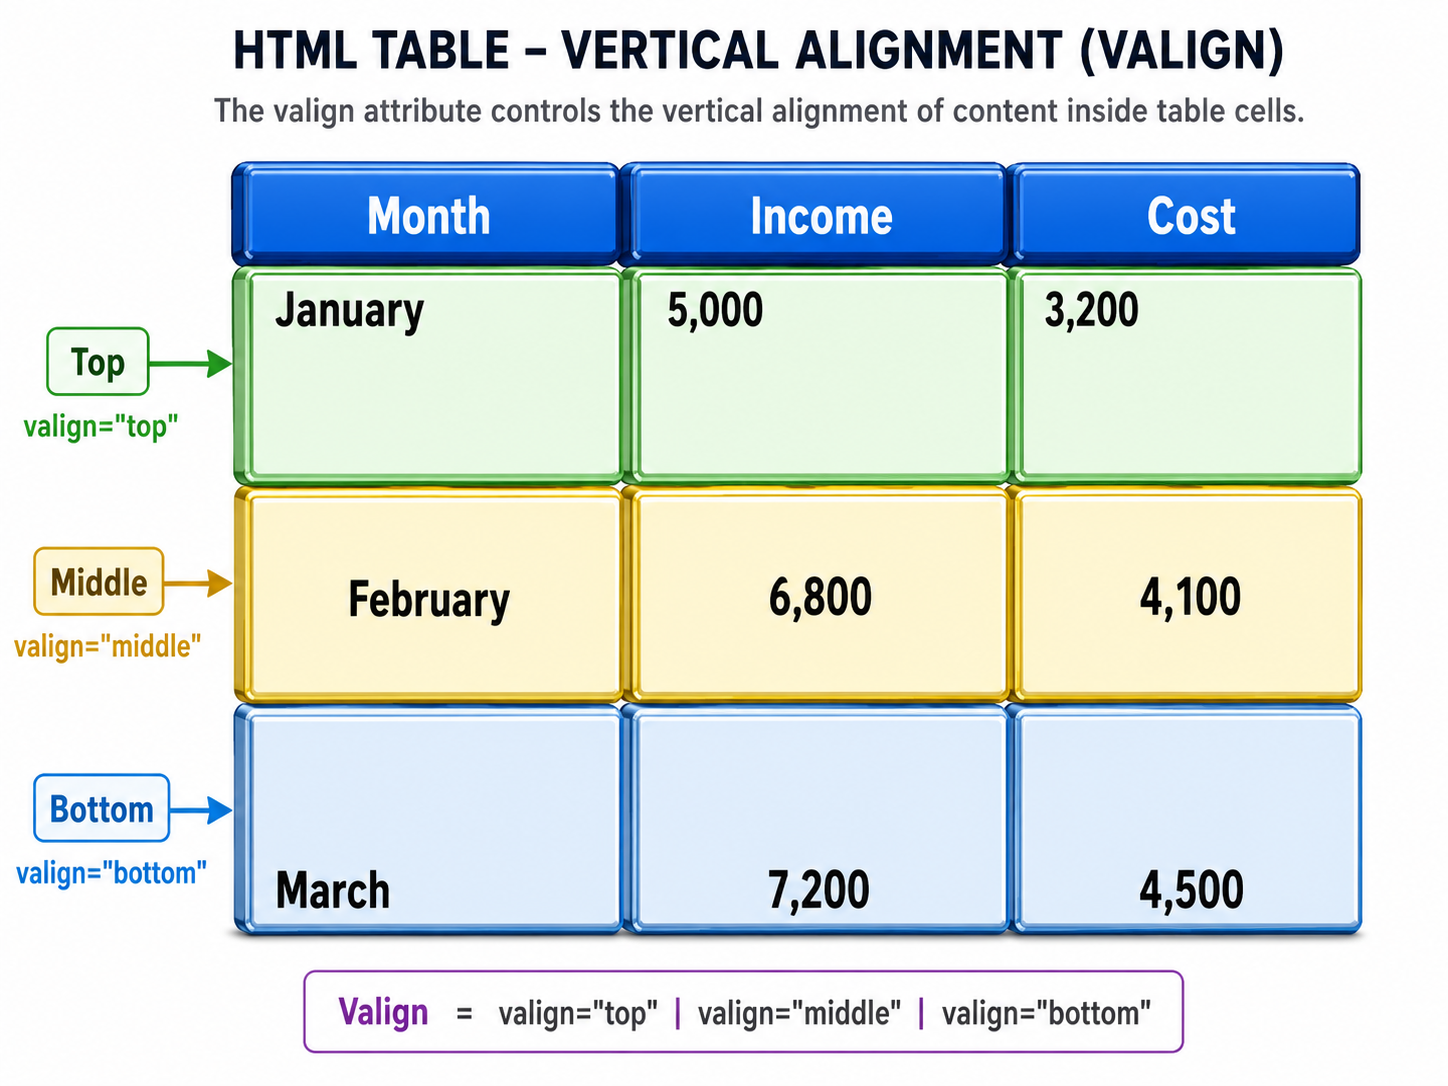
\includegraphics[width=0.95\linewidth,height=0.11\textheight,keepaspectratio]{chapters/Chapter04/topics/images/ex11_3d_valign_month_income_cost.png}
}{
\fbox{\parbox{0.90\linewidth}{\centering\vspace{0.4cm}
\textbf{চিত্র}\\
File: \texttt{chapters/Chapter04/topics/images/ex11\_3d\_valign\_month\_income\_cost.png}
\vspace{0.4cm}}}
}
\captionof{figure}{Exercise 11-এর valign চিত্র}
\end{center}

\begin{keypointbox}{চিত্র ব্যাখ্যা}
চিত্রে Month, Income ও Cost table দেখানো হয়েছে। January row top, February row middle এবং March row bottom vertical alignment বোঝায়।
\end{keypointbox}

\begin{keypointbox}{চিত্র দেখে code লেখার ধাপ}
প্রথম row-তে \texttt{valign="top"}, দ্বিতীয় row-তে \texttt{valign="middle"}, তৃতীয় row-তে \texttt{valign="bottom"} ব্যবহার করবে।
\end{keypointbox}

\par\noindent{\color{purple!70!black}\bfseries\small কোড}\par\vspace{-4pt}
\begin{verbatim}
<!DOCTYPE html>
<html>
<head>
  <title>HTML Table Example</title>
</head>
<body>
<table border="1" cellspacing="0" cellpadding="8">
  <tr><th>Month</th><th>Income</th><th>Cost</th></tr>
  <tr valign="top" height="60"><td>January</td><td>5,000</td><td>3,200</td></tr>
  <tr valign="middle" height="60"><td>February</td><td>6,800</td><td>4,100</td></tr>
  <tr valign="bottom" height="60"><td>March</td><td>7,200</td><td>4,500</td></tr>
</table>
</body>
</html>
\end{verbatim}
\vspace{-6pt}

\subsubsection{Exercise 12: Colgroup দিয়ে Column Color}

\begin{boardbox}{Concept}
\texttt{<colgroup>} ও \texttt{<col>} tag দিয়ে নির্দিষ্ট column-এর style দেওয়া যায়।
\end{boardbox}

\begin{center}
\IfFileExists{chapters/Chapter04/topics/images/ex12_3d_colgroup_color.png}{
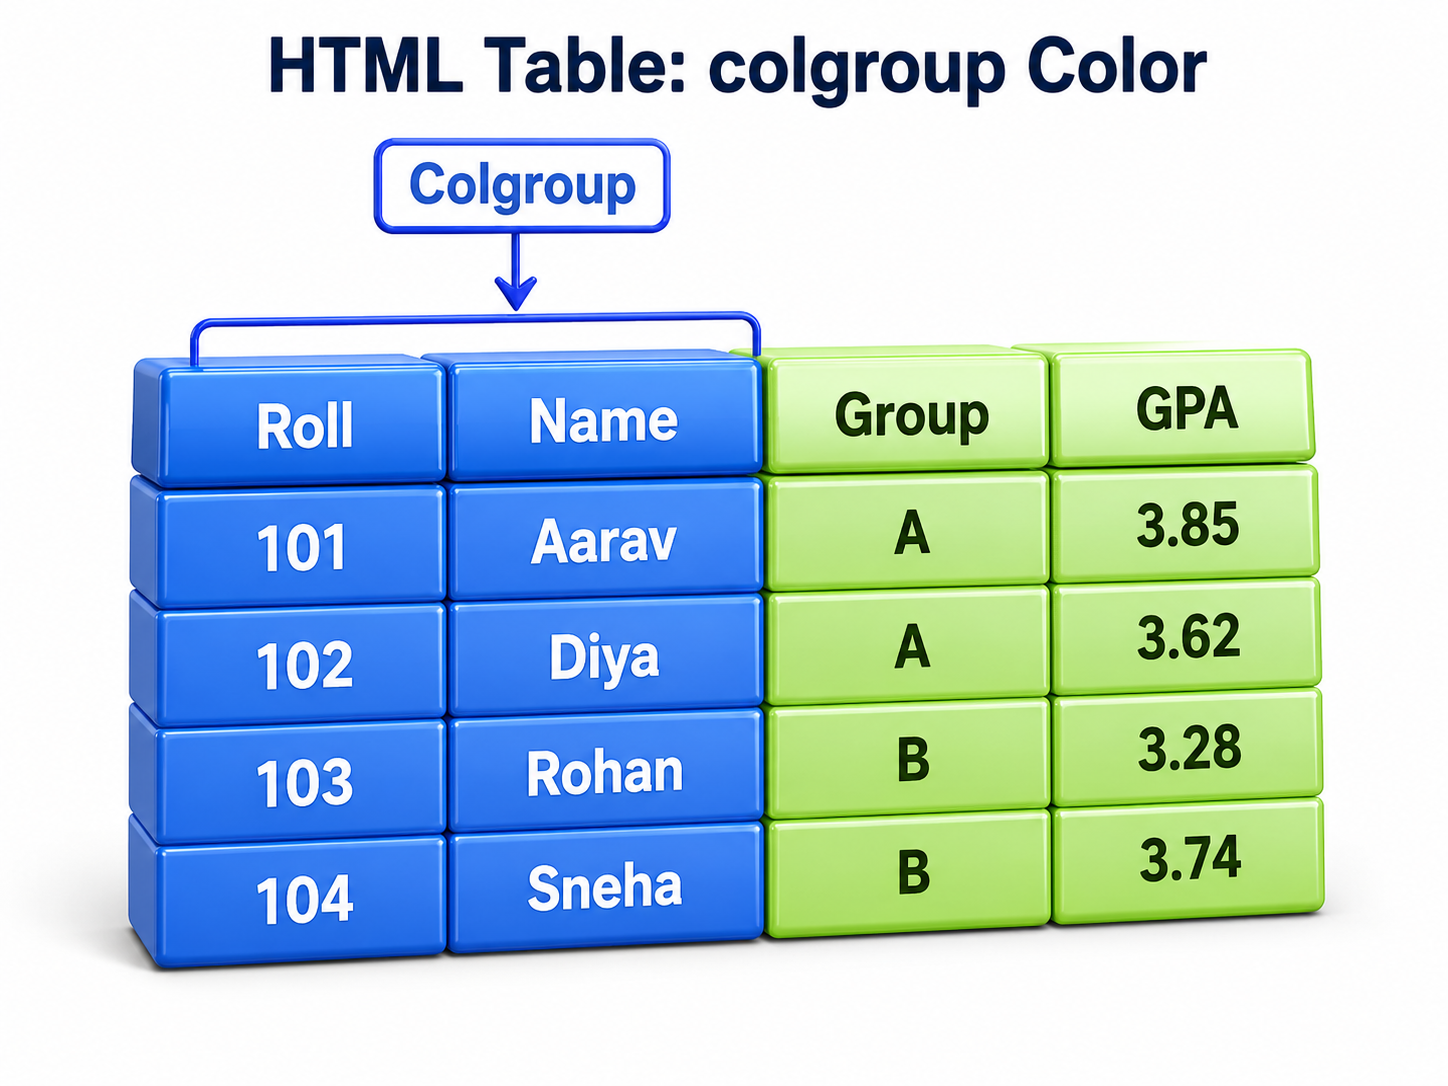
\includegraphics[width=0.95\linewidth,height=0.11\textheight,keepaspectratio]{chapters/Chapter04/topics/images/ex12_3d_colgroup_color.png}
}{
\fbox{\parbox{0.90\linewidth}{\centering\vspace{0.4cm}
\textbf{চিত্র}\\
File: \texttt{chapters/Chapter04/topics/images/ex12\_3d\_colgroup\_color.png}
\vspace{0.4cm}}}
}
\captionof{figure}{Exercise 12-এর colgroup চিত্র}
\end{center}

\begin{keypointbox}{চিত্র ব্যাখ্যা}
চিত্রে Roll ও Name column এক রঙে এবং Group ও GPA column আরেক রঙে দেখানো হয়েছে। এটি colgroup দিয়ে column-based styling বোঝায়।
\end{keypointbox}

\begin{keypointbox}{চিত্র দেখে code লেখার ধাপ}
প্রথমে \texttt{<colgroup>} লিখবে। কোন column কোন color হবে তা \texttt{<col span="...">} দিয়ে নির্ধারণ করবে। তারপর normal table row লিখবে।
\end{keypointbox}

\par\noindent{\color{purple!70!black}\bfseries\small কোড}\par\vspace{-4pt}
\begin{verbatim}
<!DOCTYPE html>
<html>
<head>
  <title>HTML Table Example</title>
</head>
<body>
<table border="1" cellspacing="0" cellpadding="6">
  <colgroup>
    <col span="2" style="background-color:#77b7ff">
    <col span="2" style="background-color:#b7ef7a">
  </colgroup>
  <tr><th>Roll</th><th>Name</th><th>Group</th><th>GPA</th></tr>
  <tr><td>101</td><td>Aarav</td><td>A</td><td>3.85</td></tr>
  <tr><td>102</td><td>Diya</td><td>A</td><td>3.62</td></tr>
  <tr><td>103</td><td>Rohan</td><td>B</td><td>3.28</td></tr>
  <tr><td>104</td><td>Sneha</td><td>B</td><td>3.74</td></tr>
</table>
</body>
</html>
\end{verbatim}
\vspace{-6pt}

\subsubsection{Exercise 13: Without Cellspacing and With Cellspacing}

\begin{boardbox}{Concept}
\texttt{cellspacing} cell-এর বাইরের gap বা cellগুলোর মাঝের distance নিয়ন্ত্রণ করে।
\end{boardbox}

\begin{center}
\IfFileExists{chapters/Chapter04/topics/images/ex13_3d_cellspacing_compare.png}{
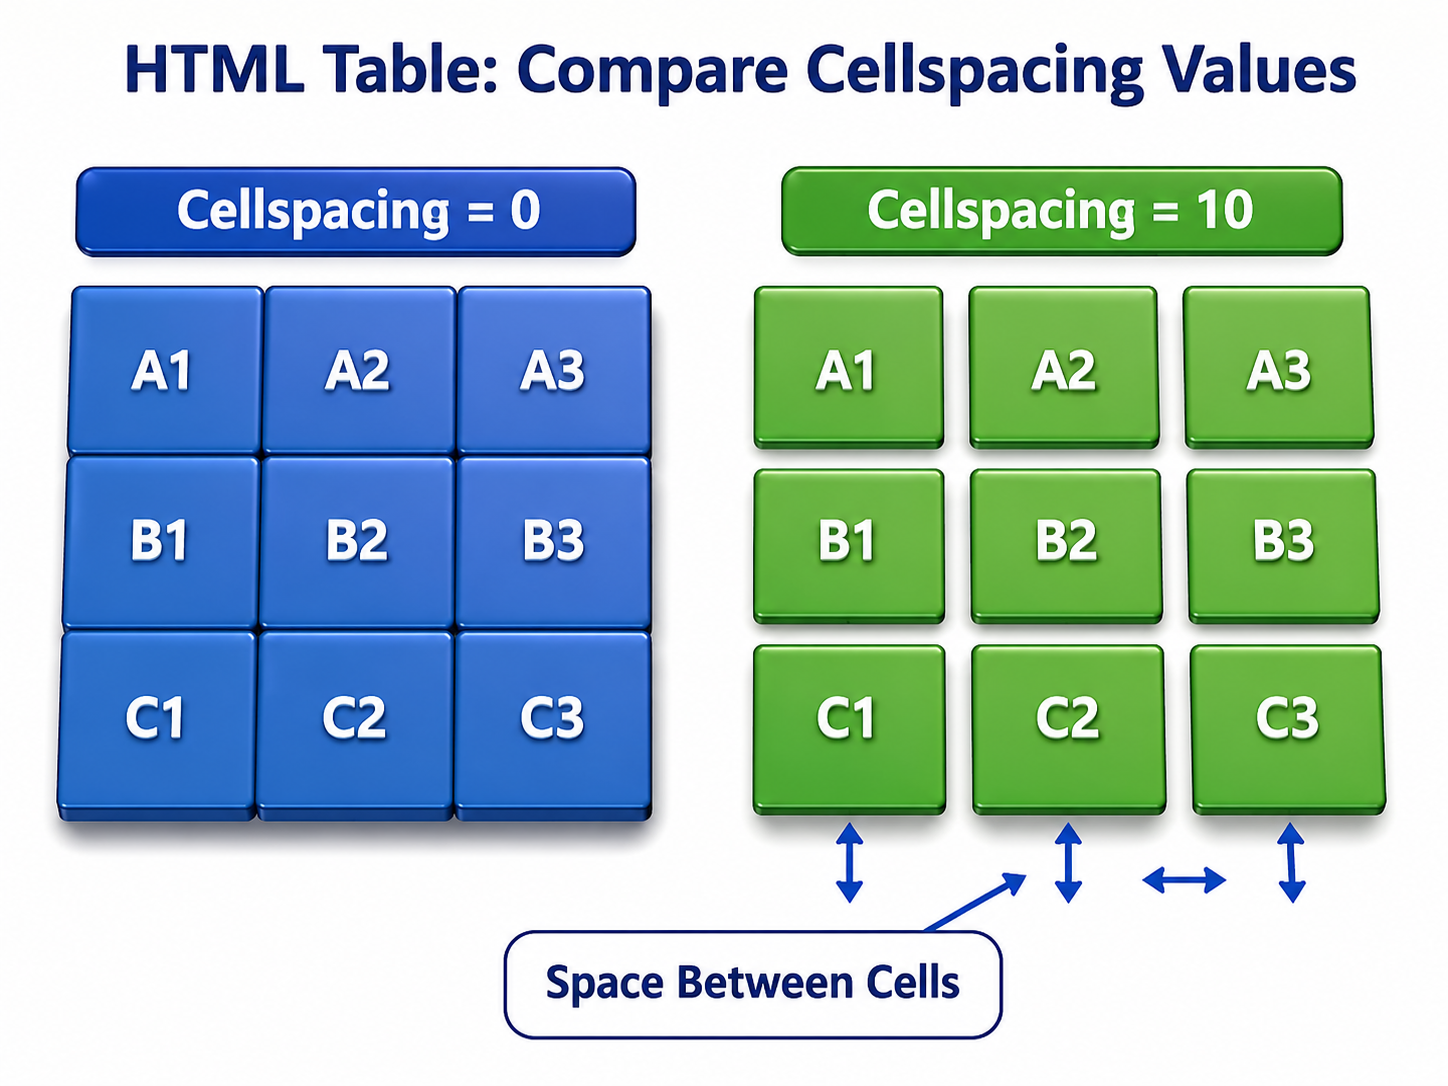
\includegraphics[width=0.95\linewidth,height=0.11\textheight,keepaspectratio]{chapters/Chapter04/topics/images/ex13_3d_cellspacing_compare.png}
}{
\fbox{\parbox{0.90\linewidth}{\centering\vspace{0.4cm}
\textbf{চিত্র}\\
File: \texttt{chapters/Chapter04/topics/images/ex13\_3d\_cellspacing\_compare.png}
\vspace{0.4cm}}}
}
\captionof{figure}{Exercise 13-এর cellspacing তুলনা}
\end{center}

\begin{keypointbox}{চিত্র ব্যাখ্যা}
চিত্রে বাম table-এ \texttt{cellspacing="0"} থাকায় cellগুলোর মাঝে gap নেই। ডান table-এ \texttt{cellspacing="10"} থাকায় cellগুলোর মাঝে space দেখা যাচ্ছে।
\end{keypointbox}

\begin{keypointbox}{চিত্র দেখে code লেখার ধাপ}
একই data দিয়ে দুটি table লিখবে। প্রথমটিতে \texttt{cellspacing="0"} এবং দ্বিতীয়টিতে \texttt{cellspacing="10"} ব্যবহার করবে।
\end{keypointbox}

\par\noindent{\color{purple!70!black}\bfseries\small কোড}\par\vspace{-4pt}
\begin{verbatim}
<!DOCTYPE html>
<html>
<head>
  <title>HTML Table Example</title>
</head>
<body>
<h3>Cellspacing = 0</h3>
<table border="1" cellspacing="0" cellpadding="8">
  <tr><td>A1</td><td>A2</td><td>A3</td></tr>
  <tr><td>B1</td><td>B2</td><td>B3</td></tr>
  <tr><td>C1</td><td>C2</td><td>C3</td></tr>
</table>

<h3>Cellspacing = 10</h3>
<table border="1" cellspacing="10" cellpadding="8">
  <tr><td>A1</td><td>A2</td><td>A3</td></tr>
  <tr><td>B1</td><td>B2</td><td>B3</td></tr>
  <tr><td>C1</td><td>C2</td><td>C3</td></tr>
</table>
</body>
</html>
\end{verbatim}
\vspace{-6pt}

\subsubsection{Exercise 14: Without Cellpadding and With Cellpadding}

\begin{boardbox}{Concept}
\texttt{cellpadding} cell-এর border এবং content-এর মাঝের ভিতরের space নিয়ন্ত্রণ করে।
\end{boardbox}

\begin{center}
\IfFileExists{chapters/Chapter04/topics/images/ex14_3d_cellpadding_compare.png}{
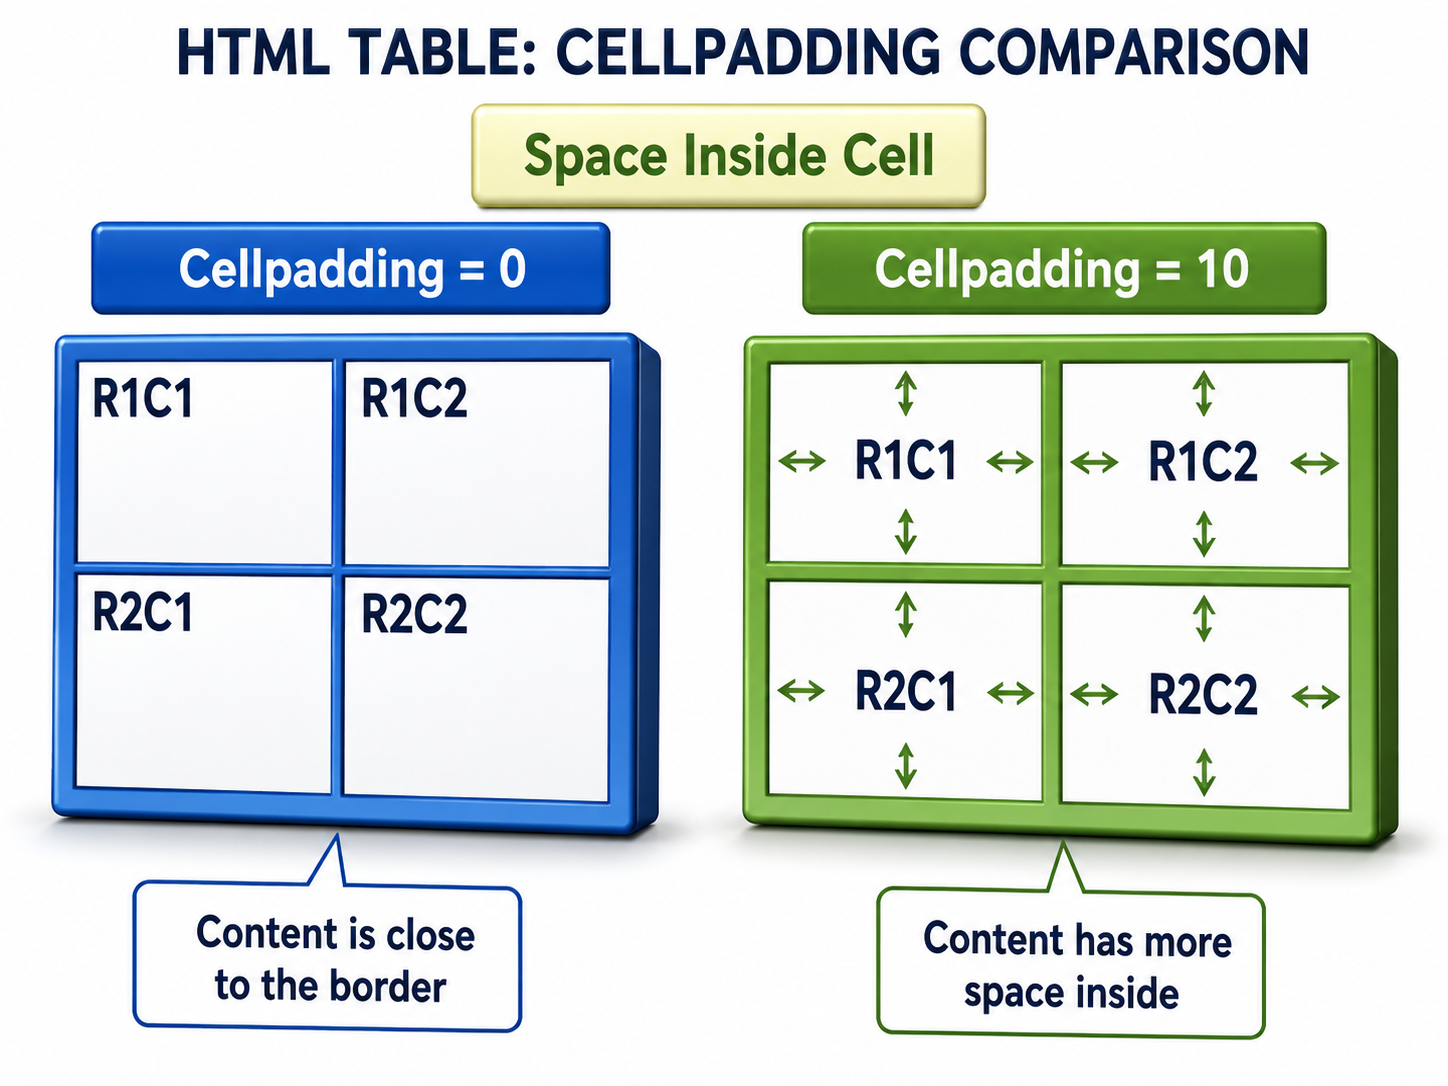
\includegraphics[width=0.95\linewidth,height=0.11\textheight,keepaspectratio]{chapters/Chapter04/topics/images/ex14_3d_cellpadding_compare.png}
}{
\fbox{\parbox{0.90\linewidth}{\centering\vspace{0.4cm}
\textbf{চিত্র}\\
File: \texttt{chapters/Chapter04/topics/images/ex14\_3d\_cellpadding\_compare.png}
\vspace{0.4cm}}}
}
\captionof{figure}{Exercise 14-এর cellpadding তুলনা}
\end{center}

\begin{keypointbox}{চিত্র ব্যাখ্যা}
চিত্রে বাম table-এ \texttt{cellpadding="0"} থাকায় content border-এর কাছে আছে। ডান table-এ \texttt{cellpadding="10"} থাকায় content-এর চারপাশে ভিতরের space বেশি।
\end{keypointbox}

\begin{keypointbox}{চিত্র দেখে code লেখার ধাপ}
দুটি table তৈরি করবে। প্রথম table-এ \texttt{cellpadding="0"}, দ্বিতীয় table-এ \texttt{cellpadding="10"} বসাবে।
\end{keypointbox}

\par\noindent{\color{purple!70!black}\bfseries\small কোড}\par\vspace{-4pt}
\begin{verbatim}
<!DOCTYPE html>
<html>
<head>
  <title>HTML Table Example</title>
</head>
<body>
<h3>Cellpadding = 0</h3>
<table border="1" cellspacing="0" cellpadding="0">
  <tr><td>R1C1</td><td>R1C2</td></tr>
  <tr><td>R2C1</td><td>R2C2</td></tr>
</table>

<h3>Cellpadding = 10</h3>
<table border="1" cellspacing="0" cellpadding="10">
  <tr><td>R1C1</td><td>R1C2</td></tr>
  <tr><td>R2C1</td><td>R2C2</td></tr>
</table>
</body>
</html>
\end{verbatim}
\vspace{-6pt}

\subsubsection{Exercise 15: Caption Tag Practice}

\begin{boardbox}{Concept}
\texttt{<caption>} table-এর উপরে title দেখায়। border value বাড়ালে border visually thick দেখায়।
\end{boardbox}

\begin{center}
\IfFileExists{chapters/Chapter04/topics/images/ex15_3d_caption_thick_border.png}{
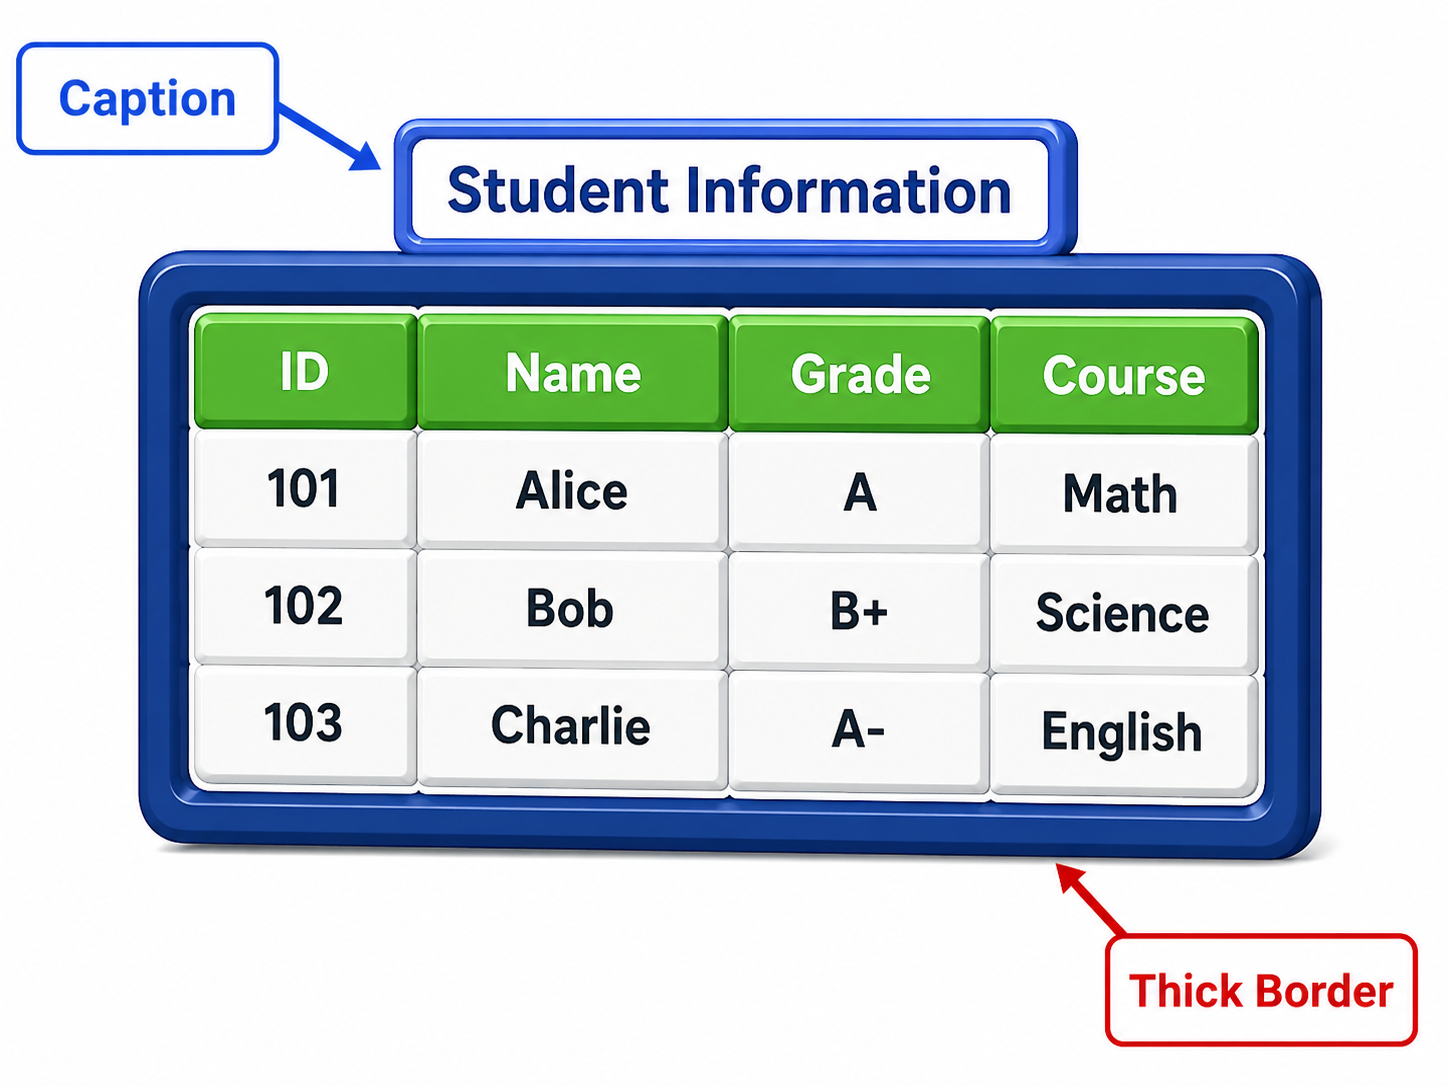
\includegraphics[width=0.95\linewidth,height=0.11\textheight,keepaspectratio]{chapters/Chapter04/topics/images/ex15_3d_caption_thick_border.png}
}{
\fbox{\parbox{0.90\linewidth}{\centering\vspace{0.4cm}
\textbf{চিত্র}\\
File: \texttt{chapters/Chapter04/topics/images/ex15\_3d\_caption\_thick\_border.png}
\vspace{0.4cm}}}
}
\captionof{figure}{Exercise 15-এর caption চিত্র}
\end{center}

\begin{keypointbox}{চিত্র ব্যাখ্যা}
চিত্রে Student Information caption এবং thick border সহ ID, Name, Grade ও Course column দেখানো হয়েছে।
\end{keypointbox}

\begin{keypointbox}{চিত্র দেখে code লেখার ধাপ}
প্রথমে table tag-এ border বসাবে। তারপর \texttt{<caption>} দিয়ে Student Information লিখবে। এরপর header row ও data rows লিখবে।
\end{keypointbox}

\par\noindent{\color{purple!70!black}\bfseries\small কোড}\par\vspace{-4pt}
\begin{verbatim}
<!DOCTYPE html>
<html>
<head>
  <title>HTML Table Example</title>
</head>
<body>
<table border="4" cellspacing="0" cellpadding="6">
  <caption><b>Student Information</b></caption>
  <tr><th>ID</th><th>Name</th><th>Grade</th><th>Course</th></tr>
  <tr><td>101</td><td>Alice</td><td>A</td><td>Math</td></tr>
  <tr><td>102</td><td>Bob</td><td>B+</td><td>Science</td></tr>
  <tr><td>103</td><td>Charlie</td><td>A-</td><td>English</td></tr>
</table>
</body>
</html>
\end{verbatim}
\vspace{-6pt}

\subsubsection{Exercise 16: Bio-data Table with Next Link}

\begin{boardbox}{Concept}
Table cell-এর ভিতরে hyperlink রাখা যায়। Bio-data table-এ label এবং value দুই column হিসেবে সাজানো হয়।
\end{boardbox}

\begin{center}
\IfFileExists{chapters/Chapter04/topics/images/ex16_3d_biodata_link.png}{
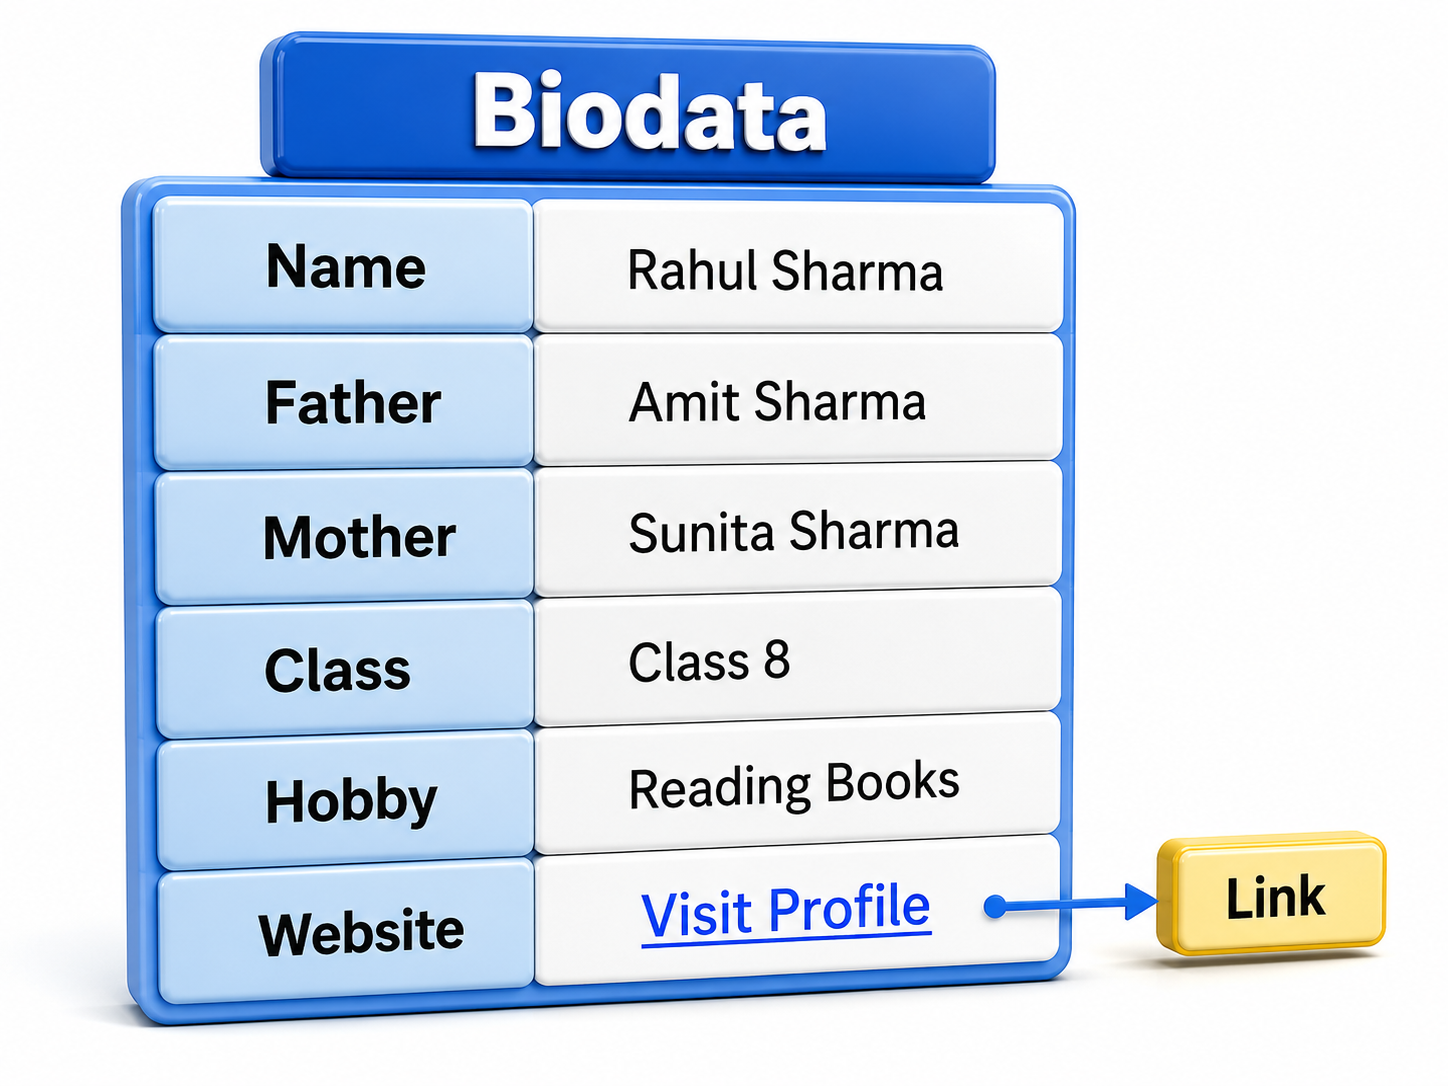
\includegraphics[width=0.95\linewidth,height=0.11\textheight,keepaspectratio]{chapters/Chapter04/topics/images/ex16_3d_biodata_link.png}
}{
\fbox{\parbox{0.90\linewidth}{\centering\vspace{0.4cm}
\textbf{চিত্র}\\
File: \texttt{chapters/Chapter04/topics/images/ex16\_3d\_biodata\_link.png}
\vspace{0.4cm}}}
}
\captionof{figure}{Exercise 16-এর biodata table চিত্র}
\end{center}

\begin{keypointbox}{চিত্র ব্যাখ্যা}
চিত্রে Biodata heading-এর নিচে Name, Father, Mother, Class, Hobby এবং Website row আছে। Website row-তে Visit Profile hyperlink দেখানো হয়েছে।
\end{keypointbox}

\begin{keypointbox}{চিত্র দেখে code লেখার ধাপ}
প্রথমে title row দুই column জুড়ে দিতে \texttt{colspan="2"} ব্যবহার করবে। তারপর প্রতিটি label-value row লিখবে। Website cell-এ \texttt{<a>} tag দিয়ে link তৈরি করবে।
\end{keypointbox}

\par\noindent{\color{purple!70!black}\bfseries\small কোড}\par\vspace{-4pt}
\begin{verbatim}
<!DOCTYPE html>
<html>
<head>
  <title>HTML Table Example</title>
</head>
<body>
<table border="1" cellspacing="0" cellpadding="6" align="center">
  <tr><th colspan="2">Biodata</th></tr>
  <tr><th>Name</th><td>Rahul Sharma</td></tr>
  <tr><th>Father</th><td>Amit Sharma</td></tr>
  <tr><th>Mother</th><td>Sunita Sharma</td></tr>
  <tr><th>Class</th><td>Class 8</td></tr>
  <tr><th>Hobby</th><td>Reading Books</td></tr>
  <tr><th>Website</th><td><a href="profile.html">Visit Profile</a></td></tr>
</table>
</body>
</html>
\end{verbatim}
\vspace{-6pt}
\subsubsection{Exercise 17: Mobile Company Table}

\begin{center}
\IfFileExists{chapters/Chapter04/topics/images/ex17_3d_mobile_company.png}{
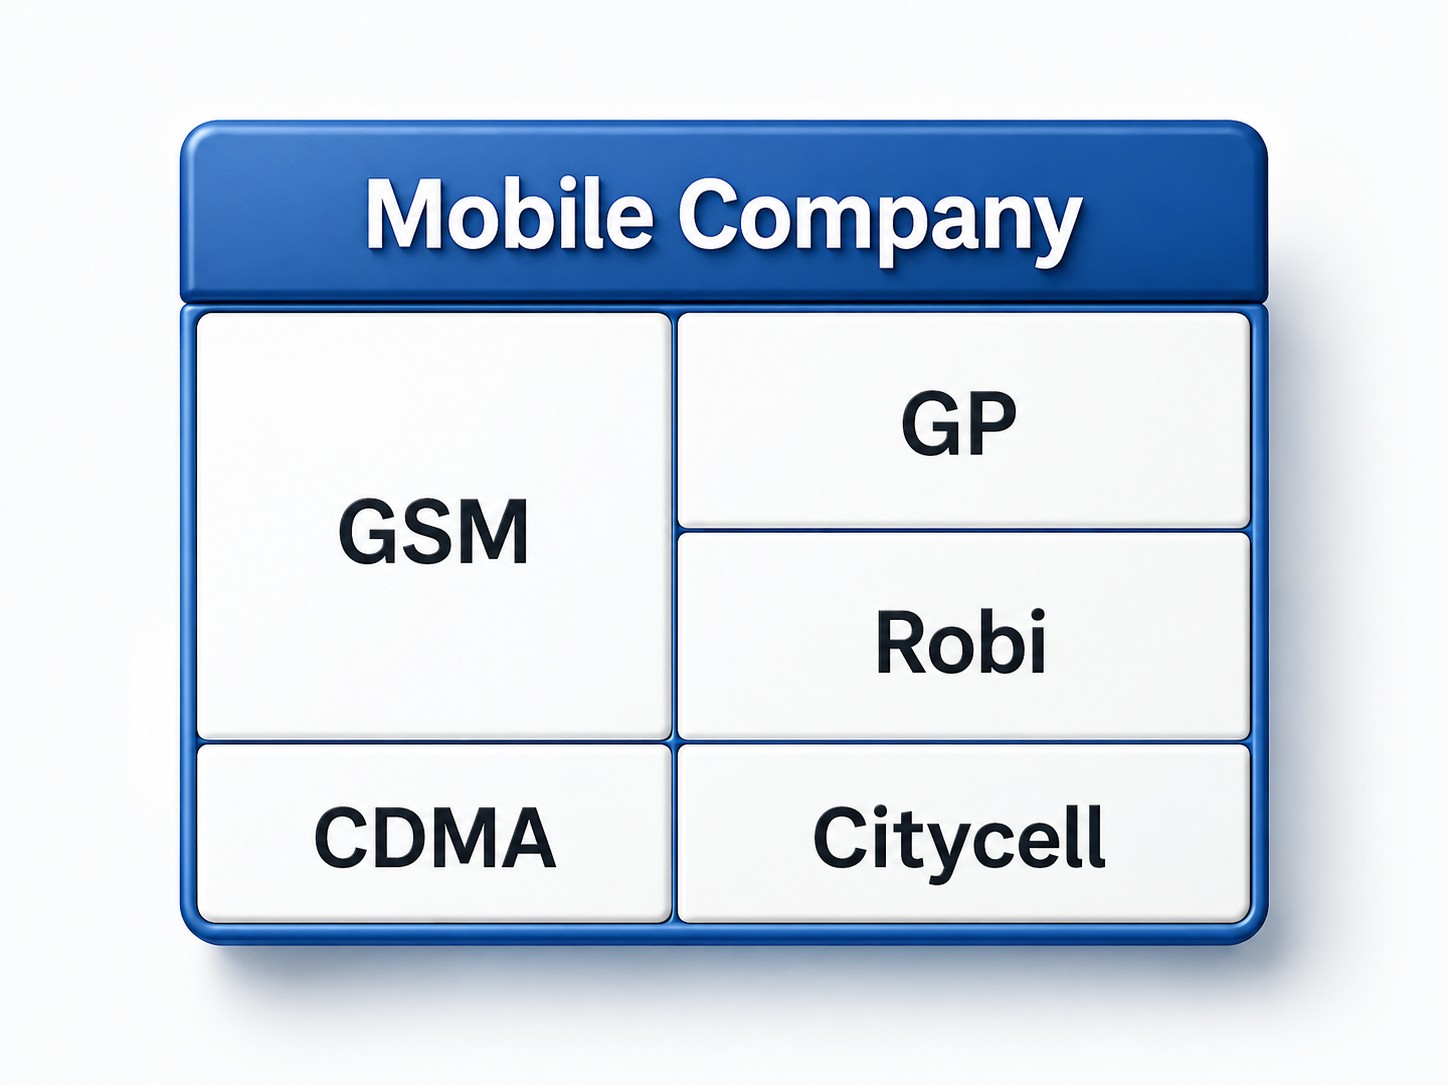
\includegraphics[width=0.95\linewidth,height=0.11\textheight,keepaspectratio]{chapters/Chapter04/topics/images/ex17_3d_mobile_company.png}
}{
\fbox{\parbox{0.90\linewidth}{\centering\vspace{0.45cm}
\textbf{চিত্র}\\[3pt]
File: \texttt{chapters/Chapter04/topics/images/ex17\_3d\_mobile\_company.png}
\vspace{0.45cm}}}
}
\captionof{figure}{Mobile Company table with rowspan}
\end{center}

\begin{keypointbox}{চিত্র ব্যাখ্যা}
GSM cell দুই row জুড়ে আছে। তাই GP ও Robi একই GSM category-এর অধীনে দেখানো হয়েছে। CDMA ও Citycell শেষ row-তে আছে।
\end{keypointbox}

\begin{keypointbox}{চিত্র দেখে code লেখার ধাপ}
প্রথমে figure-এর total row ও column গুনবে। এরপর কোন cell একাধিক column জুড়ে আছে তা দেখে \texttt{colspan} এবং কোন cell একাধিক row জুড়ে আছে তা দেখে \texttt{rowspan} বসাবে। তারপর image, link, list বা nested table থাকলে সংশ্লিষ্ট tag cell-এর ভিতরে লিখবে।
\end{keypointbox}

\par\noindent{\color{purple!70!black}\bfseries\small কোড}\par\vspace{-4pt}
\begin{verbatim}
<!DOCTYPE html>
<html>
<head>
  <title>HTML Table Example</title>
</head>
<body>
<table border="1" cellspacing="0">
<caption>Mobile Company</caption>
<tr>
  <td rowspan="2">GSM</td>
  <td>GP</td>
</tr>
<tr>
  <td>Robi</td>
</tr>
<tr>
  <td>CDMA</td>
  <td>Citycell</td>
</tr>
</table>
</body>
</html>
\end{verbatim}
\vspace{-6pt}

\subsubsection{Exercise 18: Complex Number Grid with Rowspan and Colspan}

\begin{center}
\IfFileExists{chapters/Chapter04/topics/images/ex18_3d_complex_number_grid.png}{
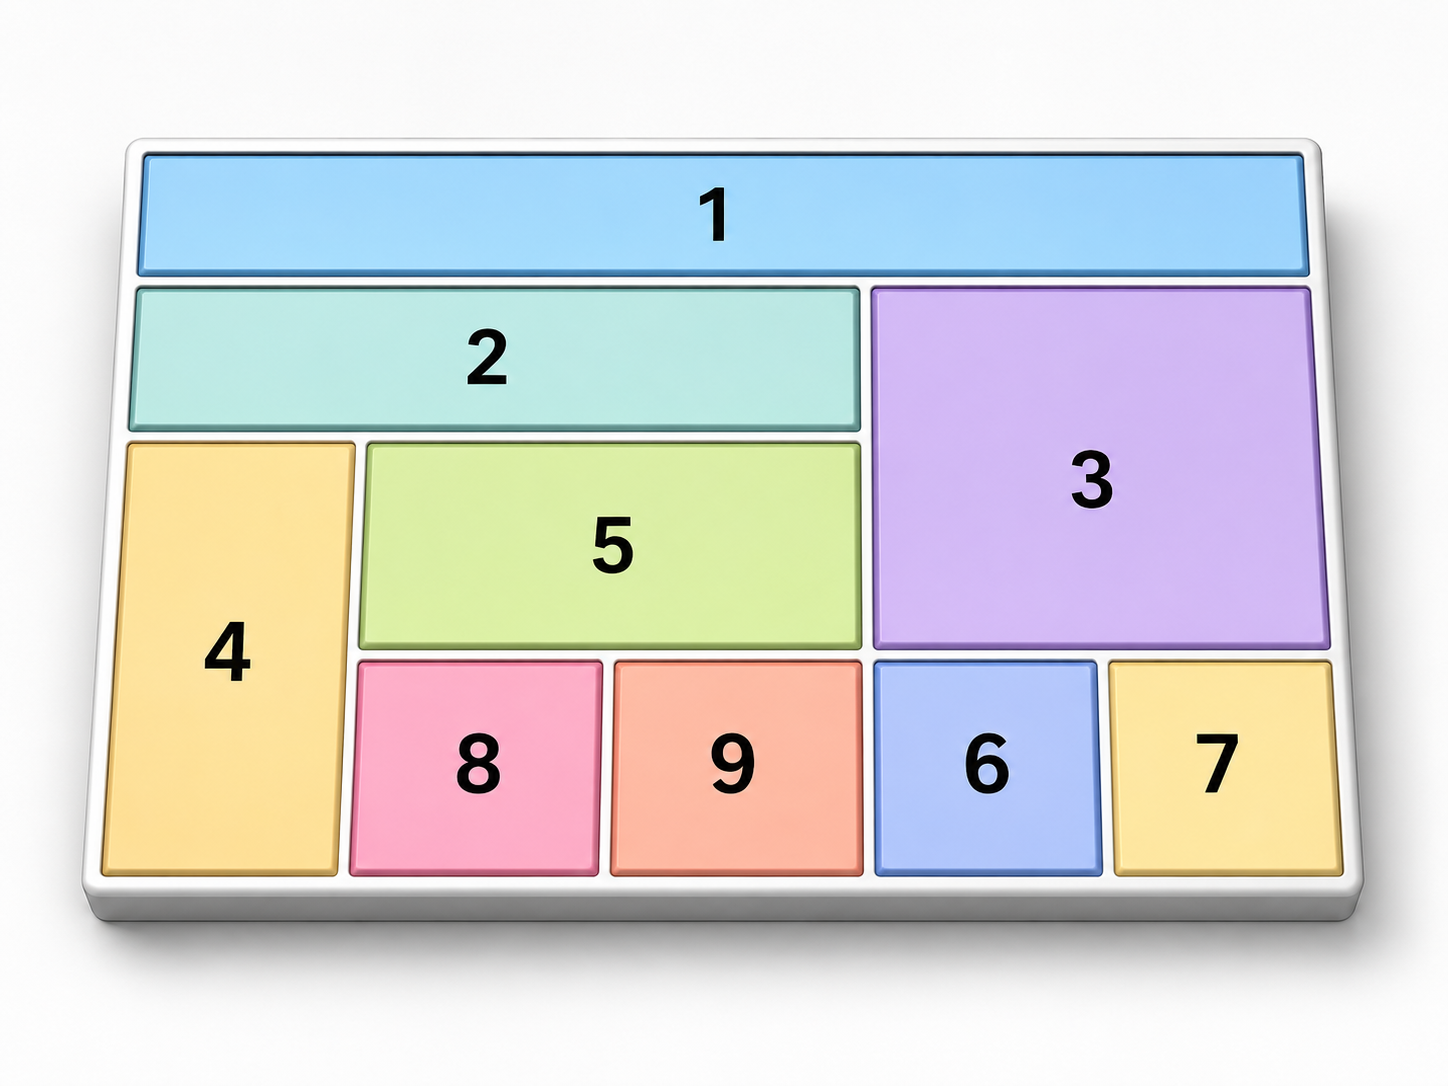
\includegraphics[width=0.95\linewidth,height=0.11\textheight,keepaspectratio]{chapters/Chapter04/topics/images/ex18_3d_complex_number_grid.png}
}{
\fbox{\parbox{0.90\linewidth}{\centering\vspace{0.45cm}
\textbf{চিত্র}\\[3pt]
File: \texttt{chapters/Chapter04/topics/images/ex18\_3d\_complex\_number\_grid.png}
\vspace{0.45cm}}}
}
\captionof{figure}{Complex number grid with rowspan and colspan}
\end{center}

\begin{keypointbox}{চিত্র ব্যাখ্যা}
এই table-এ 1, 2, 3, 4, 5, 8, 9 cell-এ rowspan/colspan ব্যবহার করা হয়েছে। চিত্র দেখে code লেখার জন্য এটি খুব গুরুত্বপূর্ণ practice।
\end{keypointbox}

\par\noindent{\color{purple!70!black}\bfseries\small কোড}\par\vspace{-4pt}
\begin{verbatim}
<!DOCTYPE html>
<html>
<head>
  <title>HTML Table Example</title>
</head>
<body>
<table border="1" cellspacing="0">
<tr><td colspan="5">1</td></tr>
<tr><td colspan="3">2</td><td colspan="2" rowspan="3">3</td></tr>
<tr><td rowspan="3">4</td><td colspan="2">5</td></tr>
<tr><td rowspan="2">8</td><td rowspan="2">9</td></tr>
<tr><td>6</td><td>7</td></tr>
</table>
</body>
</html>
\end{verbatim}
\vspace{-6pt}

\subsubsection{Exercise 19: Mymensingh Gov. College Group and Seats Table}

\begin{center}
\IfFileExists{chapters/Chapter04/topics/images/ex19_3d_mgc_group_seats.png}{
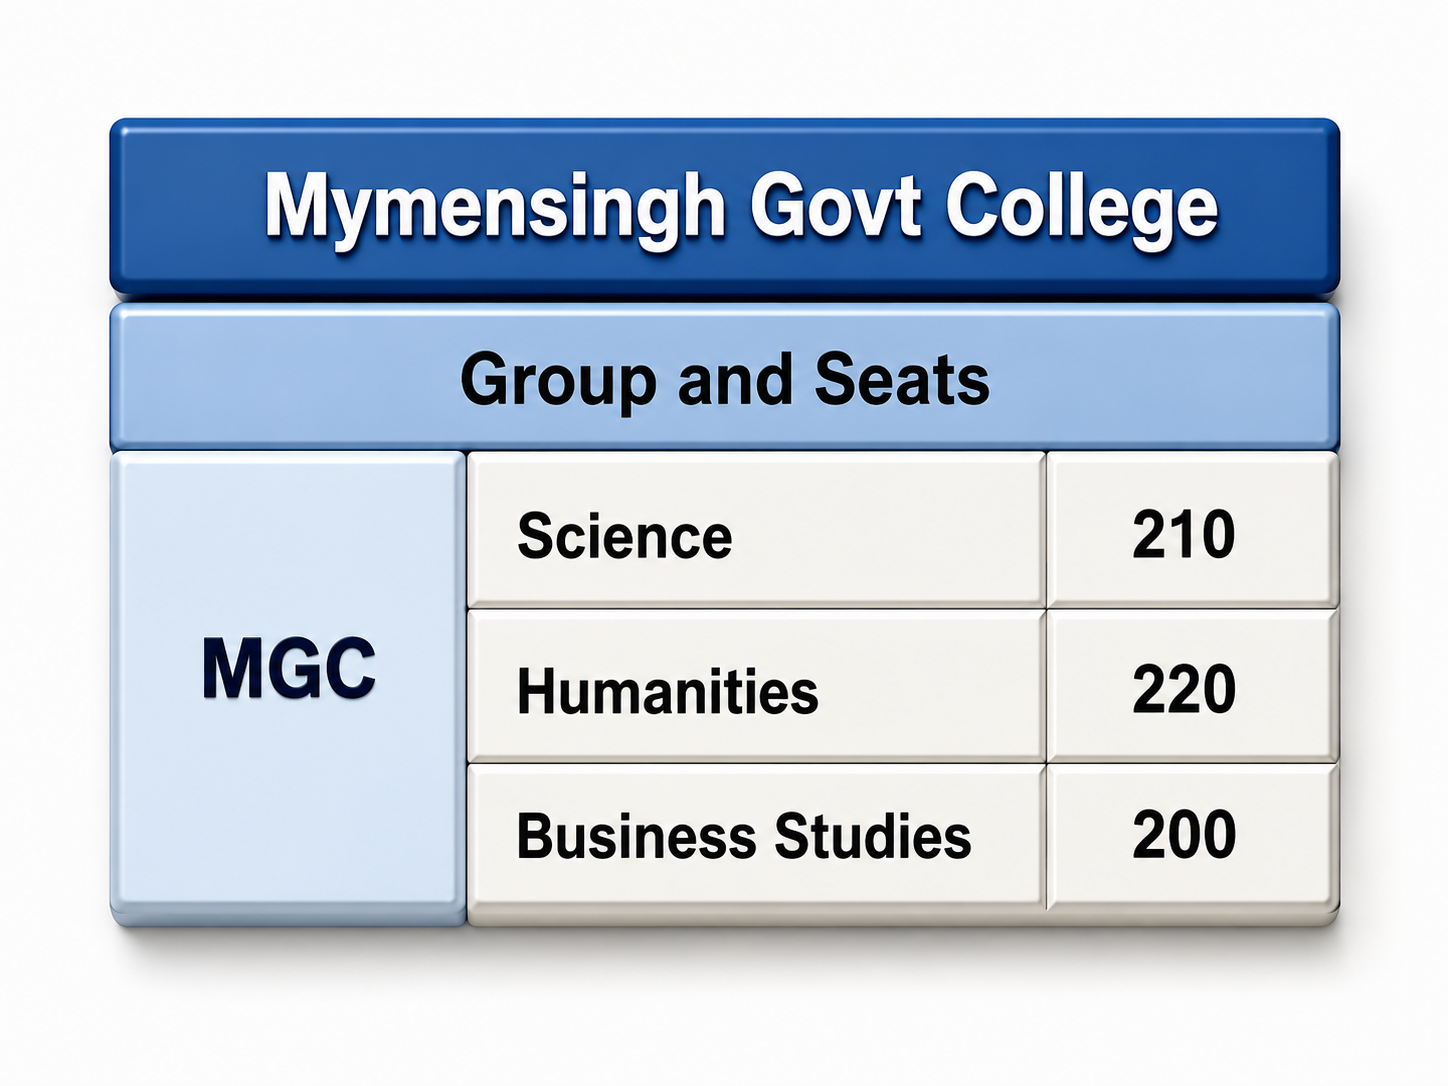
\includegraphics[width=0.95\linewidth,height=0.11\textheight,keepaspectratio]{chapters/Chapter04/topics/images/ex19_3d_mgc_group_seats.png}
}{
\fbox{\parbox{0.90\linewidth}{\centering\vspace{0.45cm}
\textbf{চিত্র}\\[3pt]
File: \texttt{chapters/Chapter04/topics/images/ex19\_3d\_mgc\_group\_seats.png}
\vspace{0.45cm}}}
}
\captionof{figure}{Mymensingh Govt. College group and seats table}
\end{center}

\begin{keypointbox}{চিত্র ব্যাখ্যা}
MGC cell তিনটি group row জুড়ে আছে। Group and Seats heading তিনটি column জুড়ে আছে।
\end{keypointbox}

\begin{keypointbox}{চিত্র দেখে code লেখার ধাপ}
প্রথমে figure-এর total row ও column গুনবে। এরপর কোন cell একাধিক column জুড়ে আছে তা দেখে \texttt{colspan} এবং কোন cell একাধিক row জুড়ে আছে তা দেখে \texttt{rowspan} বসাবে। তারপর image, link, list বা nested table থাকলে সংশ্লিষ্ট tag cell-এর ভিতরে লিখবে।
\end{keypointbox}

\par\noindent{\color{purple!70!black}\bfseries\small কোড}\par\vspace{-4pt}
\begin{verbatim}
<!DOCTYPE html>
<html>
<head>
  <title>HTML Table Example</title>
</head>
<body>
<p align="center"><h2>Mymensingh Govt College</h2></p>
<table border="1" cellspacing="0" cellpadding="10">
<tr><th colspan="3">Group and Seats</th></tr>
<tr><td rowspan="3">MGC</td><td>Science</td><td>210</td></tr>
<tr><td>Humanities</td><td>220</td></tr>
<tr><td>Business Studies</td><td>200</td></tr>
</table>
</body>
</html>
\end{verbatim}
\vspace{-6pt}

\subsubsection{Exercise 20: Product Table with Image}

\begin{center}
\IfFileExists{chapters/Chapter04/topics/images/ex20_3d_product_image.png}{
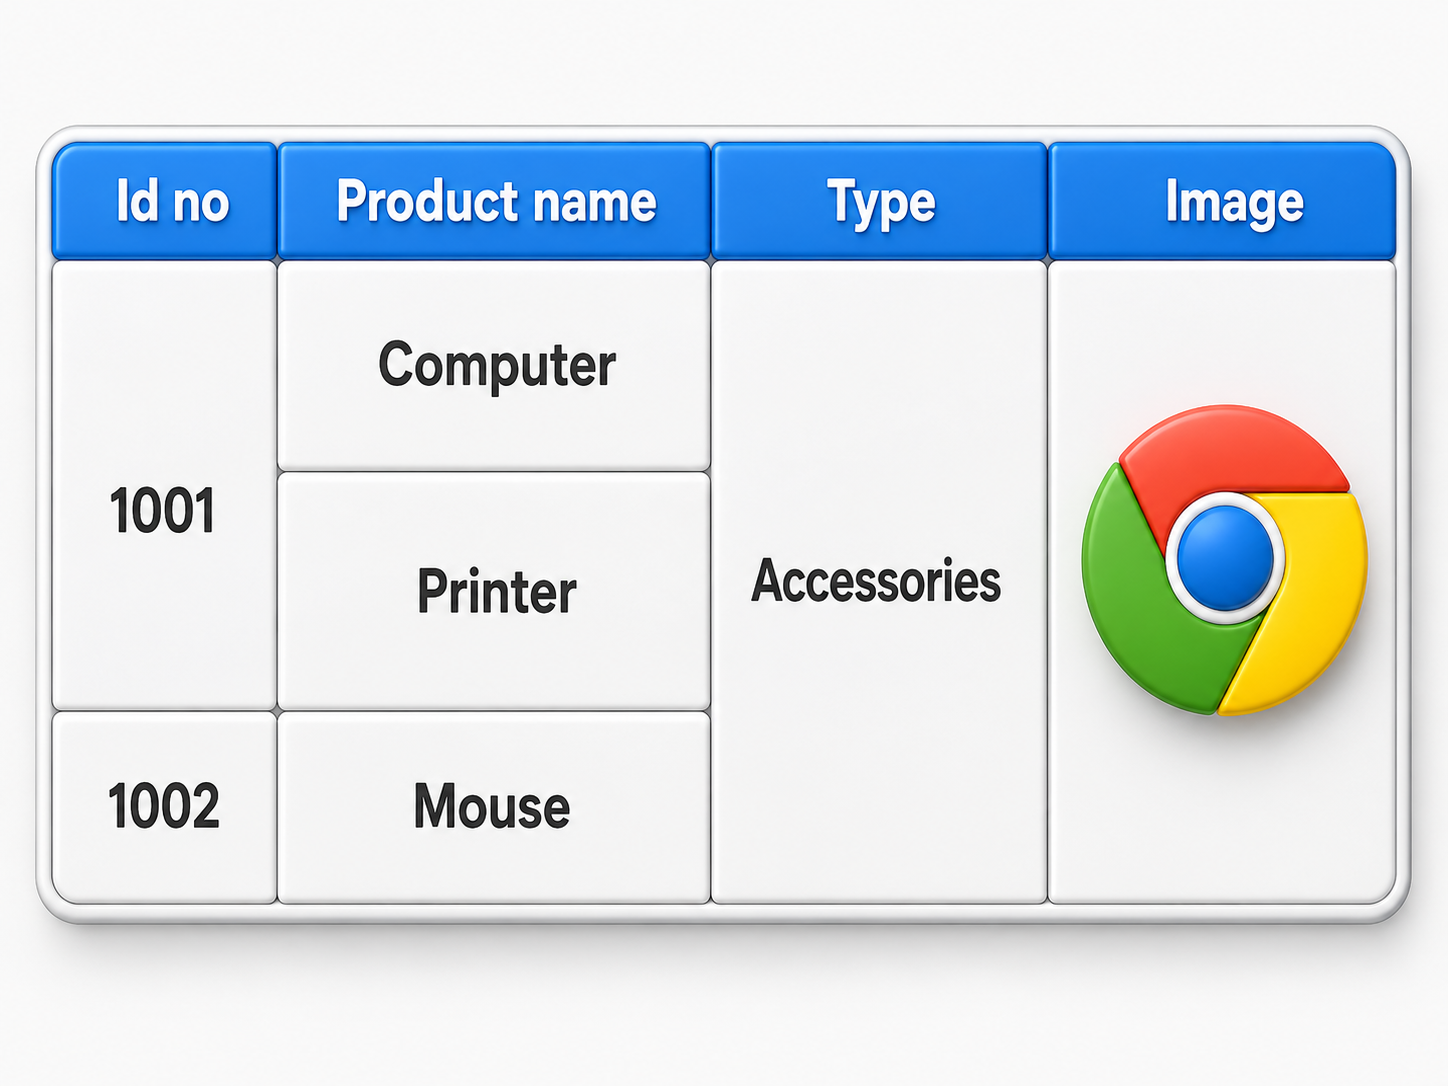
\includegraphics[width=0.95\linewidth,height=0.11\textheight,keepaspectratio]{chapters/Chapter04/topics/images/ex20_3d_product_image.png}
}{
\fbox{\parbox{0.90\linewidth}{\centering\vspace{0.45cm}
\textbf{চিত্র}\\[3pt]
File: \texttt{chapters/Chapter04/topics/images/ex20\_3d\_product\_image.png}
\vspace{0.45cm}}}
}
\captionof{figure}{Product table with rowspan and image}
\end{center}

\begin{keypointbox}{চিত্র ব্যাখ্যা}
এই table-এ image column-এর header cell চার row জুড়ে আছে। 1001 ID দুই product row জুড়ে এবং Accessories type তিন product row জুড়ে আছে।
\end{keypointbox}

\par\noindent{\color{purple!70!black}\bfseries\small কোড}\par\vspace{-4pt}
\begin{verbatim}
<!DOCTYPE html>
<html>
<head>
  <title>HTML Table Example</title>
</head>
<body>
<table border="1" cellspacing="0">
<tr>
  <th bgcolor="Silver">Id no</th>
  <th bgcolor="Silver">Product name</th>
  <th bgcolor="Silver">Type</th>
  <th rowspan="4"><img src="google.jpg" width="60" height="50" align="center"></th>
</tr>
<tr>
  <td rowspan="2">1001</td>
  <td>Computer</td>
  <td rowspan="3">Accessories</td>
</tr>
<tr>
  <td>Printer</td>
</tr>
<tr>
  <td>1002</td>
  <td>Mouse</td>
</tr>
</table>
</body>
</html>
\end{verbatim}
\vspace{-6pt}

\subsubsection{Exercise 21: Bangladesh Number Table}

\begin{center}
\IfFileExists{chapters/Chapter04/topics/images/ex21_3d_bangladesh_number_table.png}{
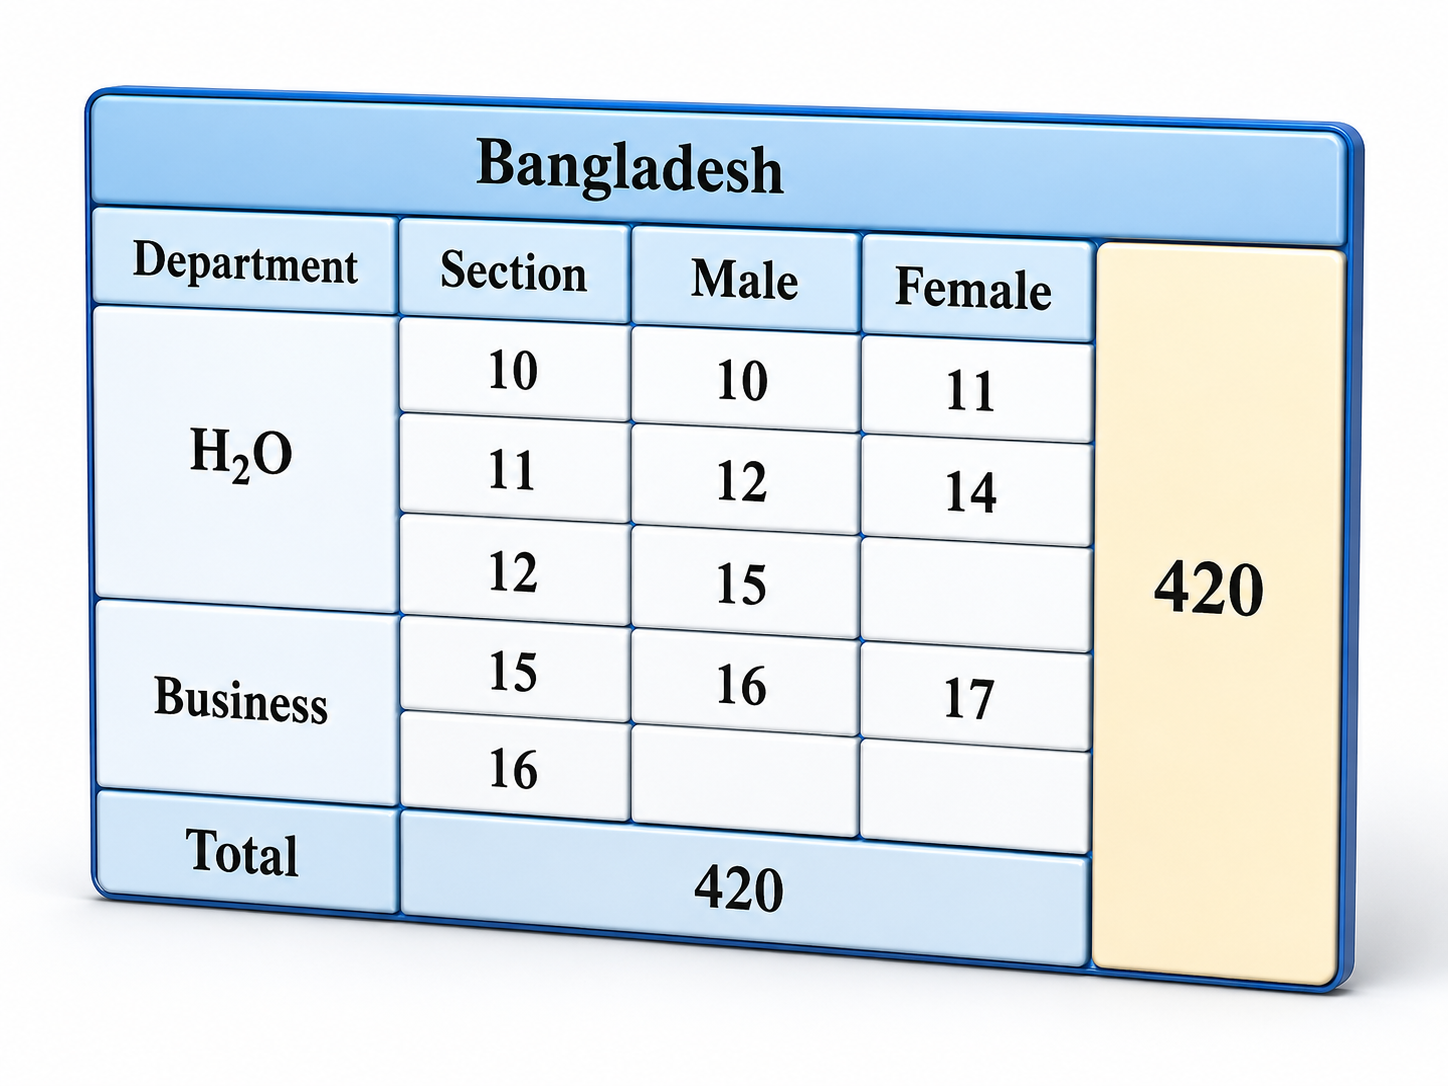
\includegraphics[width=0.95\linewidth,height=0.11\textheight,keepaspectratio]{chapters/Chapter04/topics/images/ex21_3d_bangladesh_number_table.png}
}{
\fbox{\parbox{0.90\linewidth}{\centering\vspace{0.45cm}
\textbf{চিত্র}\\[3pt]
File: \texttt{chapters/Chapter04/topics/images/ex21\_3d\_bangladesh\_number\_table.png}
\vspace{0.45cm}}}
}
\captionof{figure}{Bangladesh department number table with rowspan and colspan}
\end{center}

\begin{keypointbox}{চিত্র ব্যাখ্যা}
চিত্রে Bangladesh নামে একটি department-wise number table আছে। ডান পাশের \texttt{420} cell পুরো data অংশ জুড়ে আছে, তাই এখানে \texttt{rowspan} ব্যবহার করা হয়েছে। নিচের Total row-তে total value একাধিক column জুড়ে দেখানো হয়েছে।
\end{keypointbox}

\begin{keypointbox}{চিত্র দেখে code লেখার ধাপ}
প্রথমে header row-এর column গুনবে: Department, Section, Male, Female এবং ডান পাশের total cell। এরপর H\textsubscript{2}O/Business অংশে কোন cell কয়েকটি row জুড়ে আছে তা দেখে \texttt{rowspan} বসাবে। শেষে Total row-তে wide cell দরকার হলে \texttt{colspan} ব্যবহার করবে।
\end{keypointbox}

\par\noindent{\color{purple!70!black}\bfseries\small কোড}\par\vspace{-4pt}
\begin{verbatim}
<!DOCTYPE html>
<html>
<head>
  <title>HTML Table Example</title>
</head>
<body>
<table border="1" cellspacing="0" cellpadding="6">
<tr>
  <th>Department</th>
  <th>Section</th>
  <th>Male</th>
  <th>Female</th>
  <th rowspan="6" align="center">420</th>
</tr>
<tr>
  <td rowspan="3">H<sub>2</sub>O</td>
  <td>10</td>
  <td>10</td>
  <td>11</td>
</tr>
<tr>
  <td>11</td>
  <td>12</td>
  <td>14</td>
</tr>
<tr>
  <td>12</td>
  <td>15</td>
  <td>17</td>
</tr>
<tr>
  <td>Business</td>
  <td>15</td>
  <td>16</td>
  <td>17</td>
</tr>
<tr>
  <td>Total</td>
  <td colspan="3" align="center">420</td>
</tr>
</table>
</body>
</html>
\end{verbatim}
\vspace{-6pt}

\subsubsection{Exercise 22: Group, Section and No. of Student Table}

\begin{center}
\IfFileExists{chapters/Chapter04/topics/images/ex22_3d_group_section_student.png}{
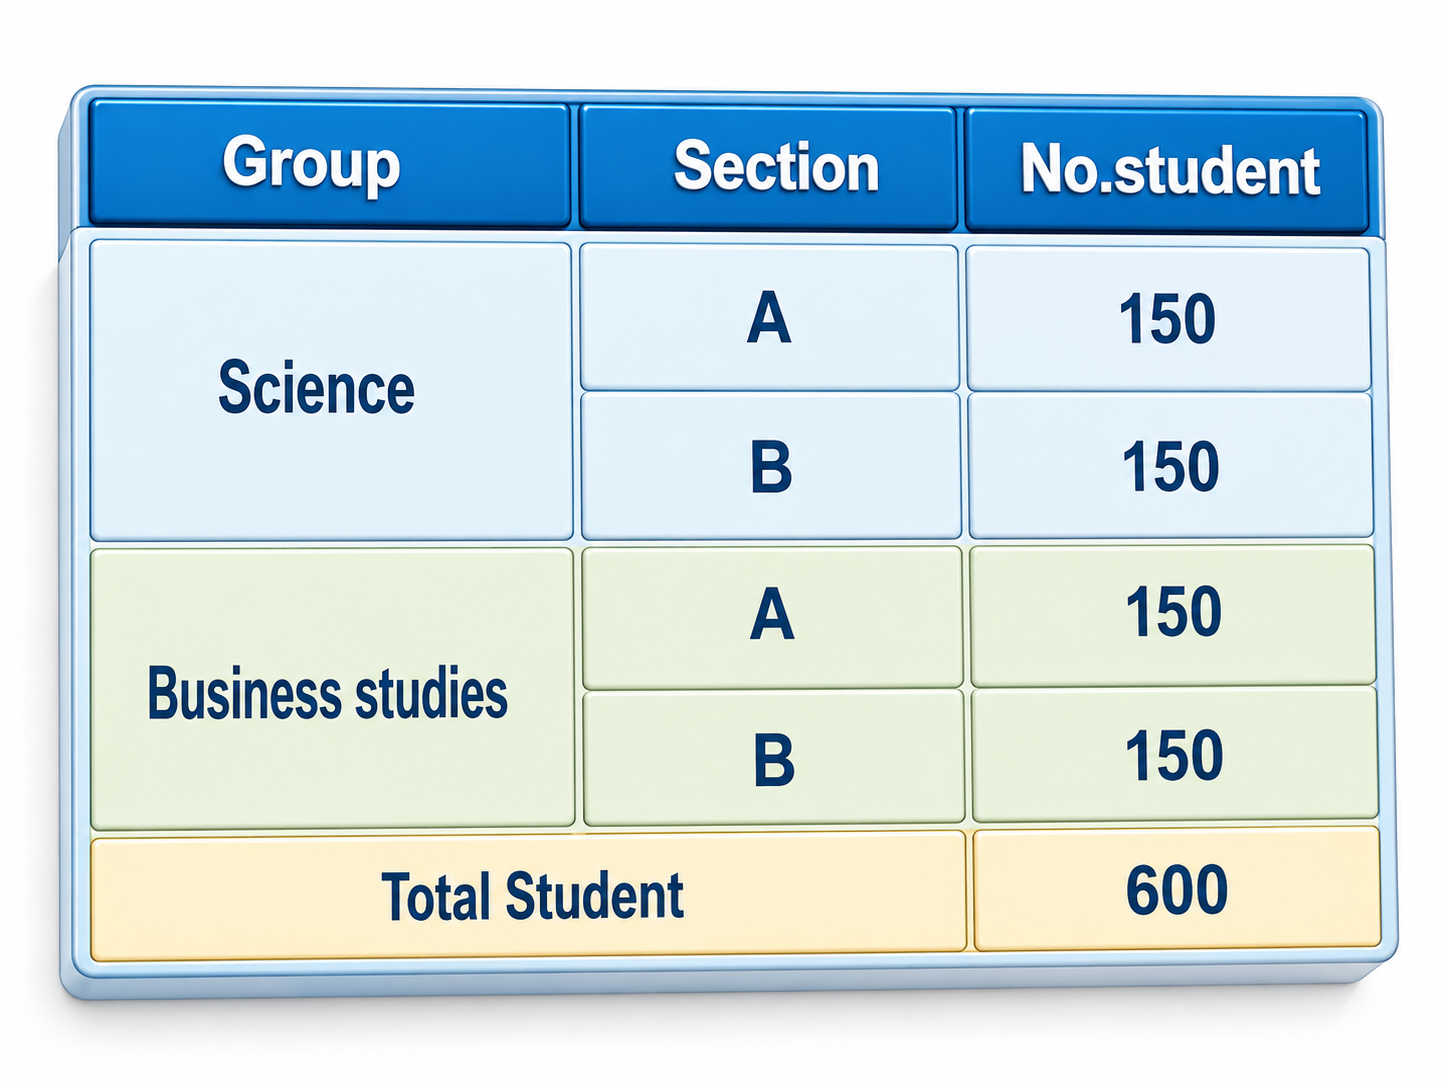
\includegraphics[width=0.95\linewidth,height=0.11\textheight,keepaspectratio]{chapters/Chapter04/topics/images/ex22_3d_group_section_student.png}
}{
\fbox{\parbox{0.90\linewidth}{\centering\vspace{0.45cm}
\textbf{চিত্র}\\[3pt]
File: \texttt{chapters/Chapter04/topics/images/ex22\_3d\_group\_section\_student.png}
\vspace{0.45cm}}}
}
\captionof{figure}{Group, Section and No. of student table}
\end{center}

\begin{keypointbox}{চিত্র ব্যাখ্যা}
Science এবং Business studies cell দুটি করে section row জুড়ে আছে। Total Student cell দুই column জুড়ে আছে।
\end{keypointbox}

\begin{keypointbox}{চিত্র দেখে code লেখার ধাপ}
প্রথমে figure-এর total row ও column গুনবে। এরপর কোন cell একাধিক column জুড়ে আছে তা দেখে \texttt{colspan} এবং কোন cell একাধিক row জুড়ে আছে তা দেখে \texttt{rowspan} বসাবে। তারপর image, link, list বা nested table থাকলে সংশ্লিষ্ট tag cell-এর ভিতরে লিখবে।
\end{keypointbox}

\par\noindent{\color{purple!70!black}\bfseries\small কোড}\par\vspace{-4pt}
\begin{verbatim}
<!DOCTYPE html>
<html>
<head>
  <title>HTML Table Example</title>
</head>
<body>
<table border="1" cellspacing="0">
<tr>
  <th>Group</th>
  <th>Section</th>
  <th>No. of student</th>
</tr>
<tr>
  <td rowspan="2">Science</td>
  <td>A</td>
  <td>150</td>
</tr>
<tr>
  <td>B</td>
  <td>150</td>
</tr>
<tr>
  <td rowspan="2">Business studies</td>
  <td>A</td>
  <td>150</td>
</tr>
<tr>
  <td>B</td>
  <td>150</td>
</tr>
<tr>
  <td colspan="2" align="center">Total student</td>
  <td>600</td>
</tr>
</table>
</body>
</html>
\end{verbatim}
\vspace{-6pt}

\subsubsection{Exercise 23: ID, Name and Contact No Table}

\begin{center}
\IfFileExists{chapters/Chapter04/topics/images/ex23_3d_contact_no_colspan.png}{
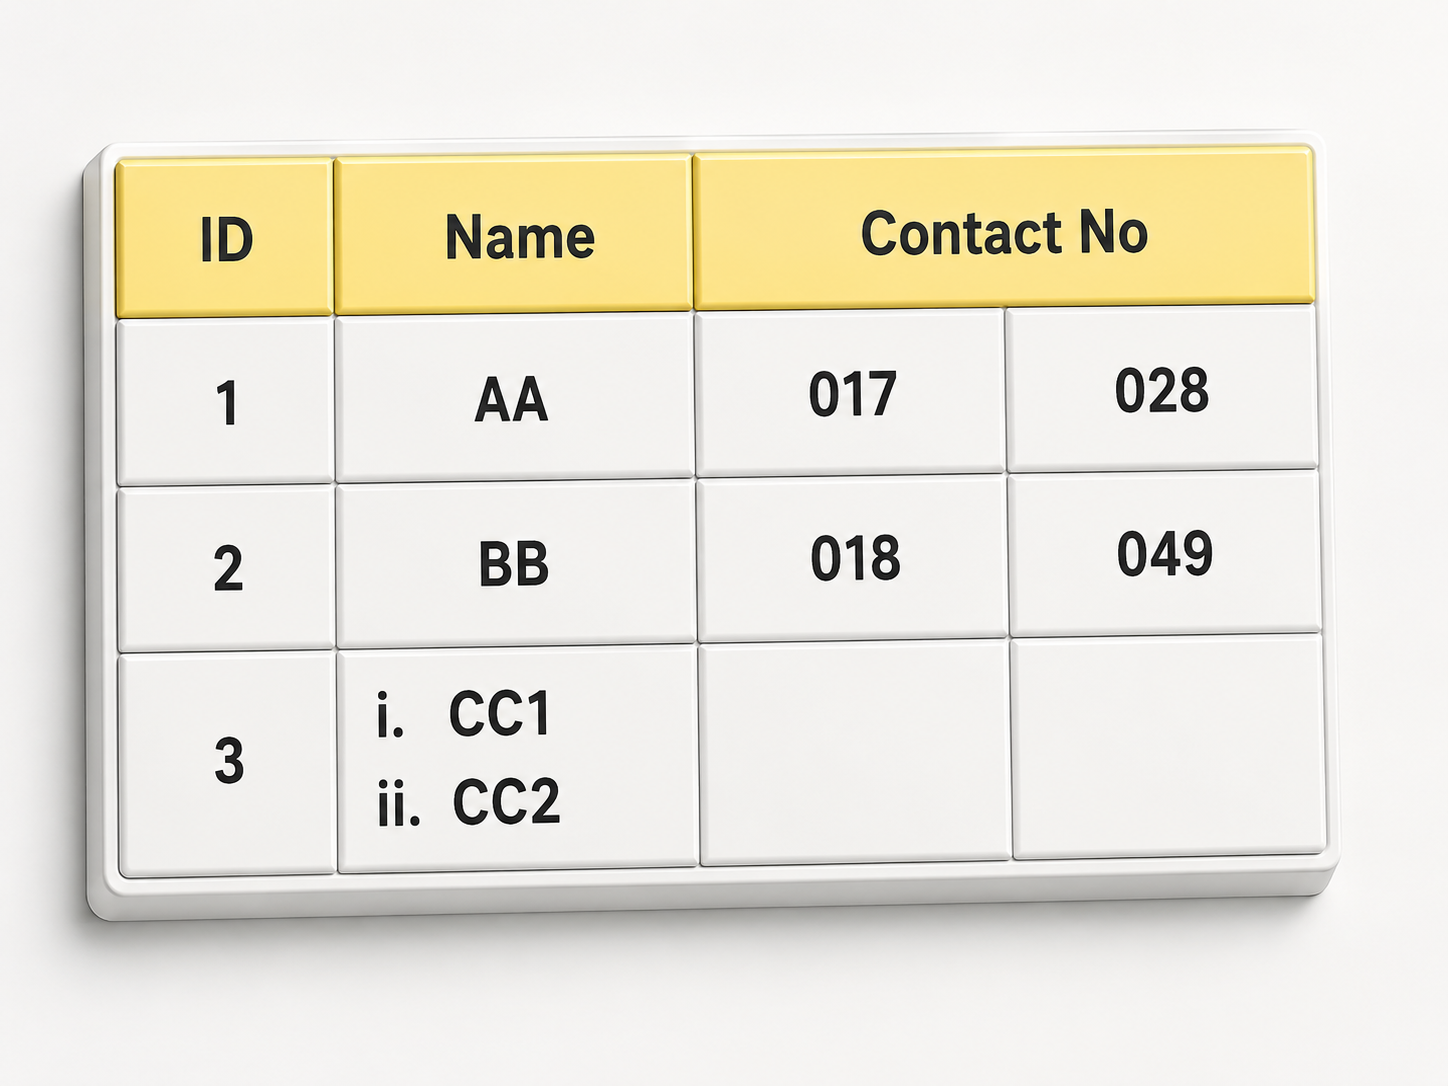
\includegraphics[width=0.95\linewidth,height=0.11\textheight,keepaspectratio]{chapters/Chapter04/topics/images/ex23_3d_contact_no_colspan.png}
}{
\fbox{\parbox{0.90\linewidth}{\centering\vspace{0.45cm}
\textbf{চিত্র}\\[3pt]
File: \texttt{chapters/Chapter04/topics/images/ex23\_3d\_contact\_no\_colspan.png}
\vspace{0.45cm}}}
}
\captionof{figure}{Contact No table with bgcolor and colspan}
\end{center}

\begin{keypointbox}{চিত্র ব্যাখ্যা}
Contact No heading দুই column জুড়ে আছে। Header row-তে yellow background color ব্যবহার করা হয়েছে। শেষ row-তে ordered list type i ব্যবহার করা হয়েছে।
\end{keypointbox}

\par\noindent{\color{purple!70!black}\bfseries\small কোড}\par\vspace{-4pt}
\begin{verbatim}
<!DOCTYPE html>
<html>
<head>
  <title>HTML Table Example</title>
</head>
<body>
<table border="1" cellspacing="0">
<tr bgcolor="yellow">
  <th>ID</th>
  <th>Name</th>
  <th colspan="2">Contact No</th>
</tr>
<tr>
  <td>1</td>
  <td>AA</td>
  <td>017</td>
  <td>028</td>
</tr>
<tr>
  <td>2</td>
  <td>BB</td>
  <td>018</td>
  <td>049</td>
</tr>
<tr>
  <td>3</td>
  <td>
    <ol type="i">
      <li>CC1</li>
      <li>CC2</li>
    </ol>
  </td>
  <td colspan="2"><br></td>
</tr>
</table>
</body>
</html>
\end{verbatim}
\vspace{-6pt}

\subsubsection{Exercise 24: Govt. Rajendra College Table with Image and Links}

\begin{center}
\IfFileExists{chapters/Chapter04/topics/images/ex24_3d_college_image_links.png}{
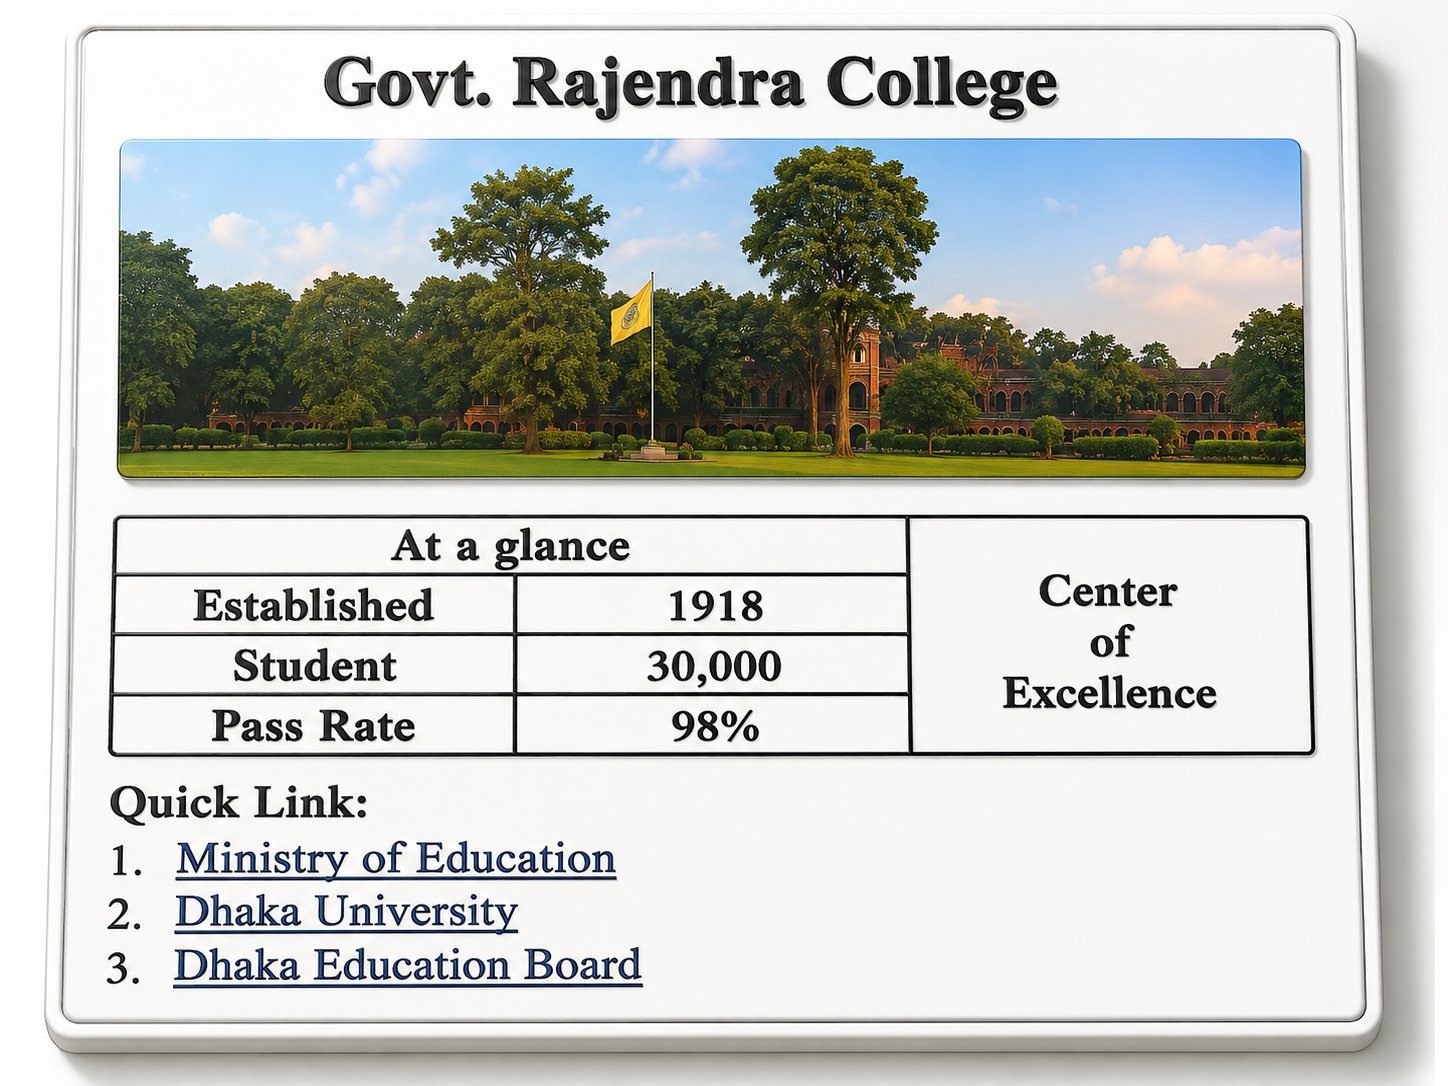
\includegraphics[width=0.95\linewidth,height=0.11\textheight,keepaspectratio]{chapters/Chapter04/topics/images/ex24_3d_college_image_links.png}
}{
\fbox{\parbox{0.90\linewidth}{\centering\vspace{0.45cm}
\textbf{চিত্র}\\[3pt]
File: \texttt{chapters/Chapter04/topics/images/ex24\_3d\_college\_image\_links.png}
\vspace{0.45cm}}}
}
\captionof{figure}{Govt. Rajendra College table with image, nested info and quick links}
\end{center}

\begin{keypointbox}{চিত্র ব্যাখ্যা}
এই example-এ heading, image, At a glance table এবং quick link একসাথে ব্যবহার করা হয়েছে। Center of Excellence cell চার row জুড়ে আছে।
\end{keypointbox}

\begin{keypointbox}{চিত্র দেখে code লেখার ধাপ}
প্রথমে figure-এর total row ও column গুনবে। এরপর কোন cell একাধিক column জুড়ে আছে তা দেখে \texttt{colspan} এবং কোন cell একাধিক row জুড়ে আছে তা দেখে \texttt{rowspan} বসাবে। তারপর image, link, list বা nested table থাকলে সংশ্লিষ্ট tag cell-এর ভিতরে লিখবে।
\end{keypointbox}

\par\noindent{\color{purple!70!black}\bfseries\small কোড}\par\vspace{-4pt}
\begin{verbatim}
<!DOCTYPE html>
<html>
<head>
  <title>HTML Table Example</title>
</head>
<body>
<h3 align="center">Govt. Rajendra College</h3>
<img src="college.jpg" width="400" height="200" align="center"><br>
<table border="1" cellspacing="0" align="center">
<tr>
  <th colspan="2">At a glance</th>
  <td rowspan="4" align="center">Center<br>of<br>Excellence</td>
</tr>
<tr>
  <th>Established</th>
  <td>1918</td>
</tr>
<tr>
  <th>Student</th>
  <td>30,000</td>
</tr>
<tr>
  <th>Pass Rate</th>
  <td>98%</td>
</tr>
</table>
<p>Quick Link:<br>
<a href="http://www.moedu.gov.bd">Ministry of Education</a><br>
<a href="www.du.ac.bd">Dhaka University</a><br>
<a href="www.dhakaeducationboard.gov.bd">Dhaka Education Board</a><br>
</p>
</body>
</html>
\end{verbatim}
\vspace{-6pt}

\subsubsection{Exercise 25: Department Male/Female Table with Photo}

\begin{center}
\IfFileExists{chapters/Chapter04/topics/images/ex25_3d_department_photo.png}{
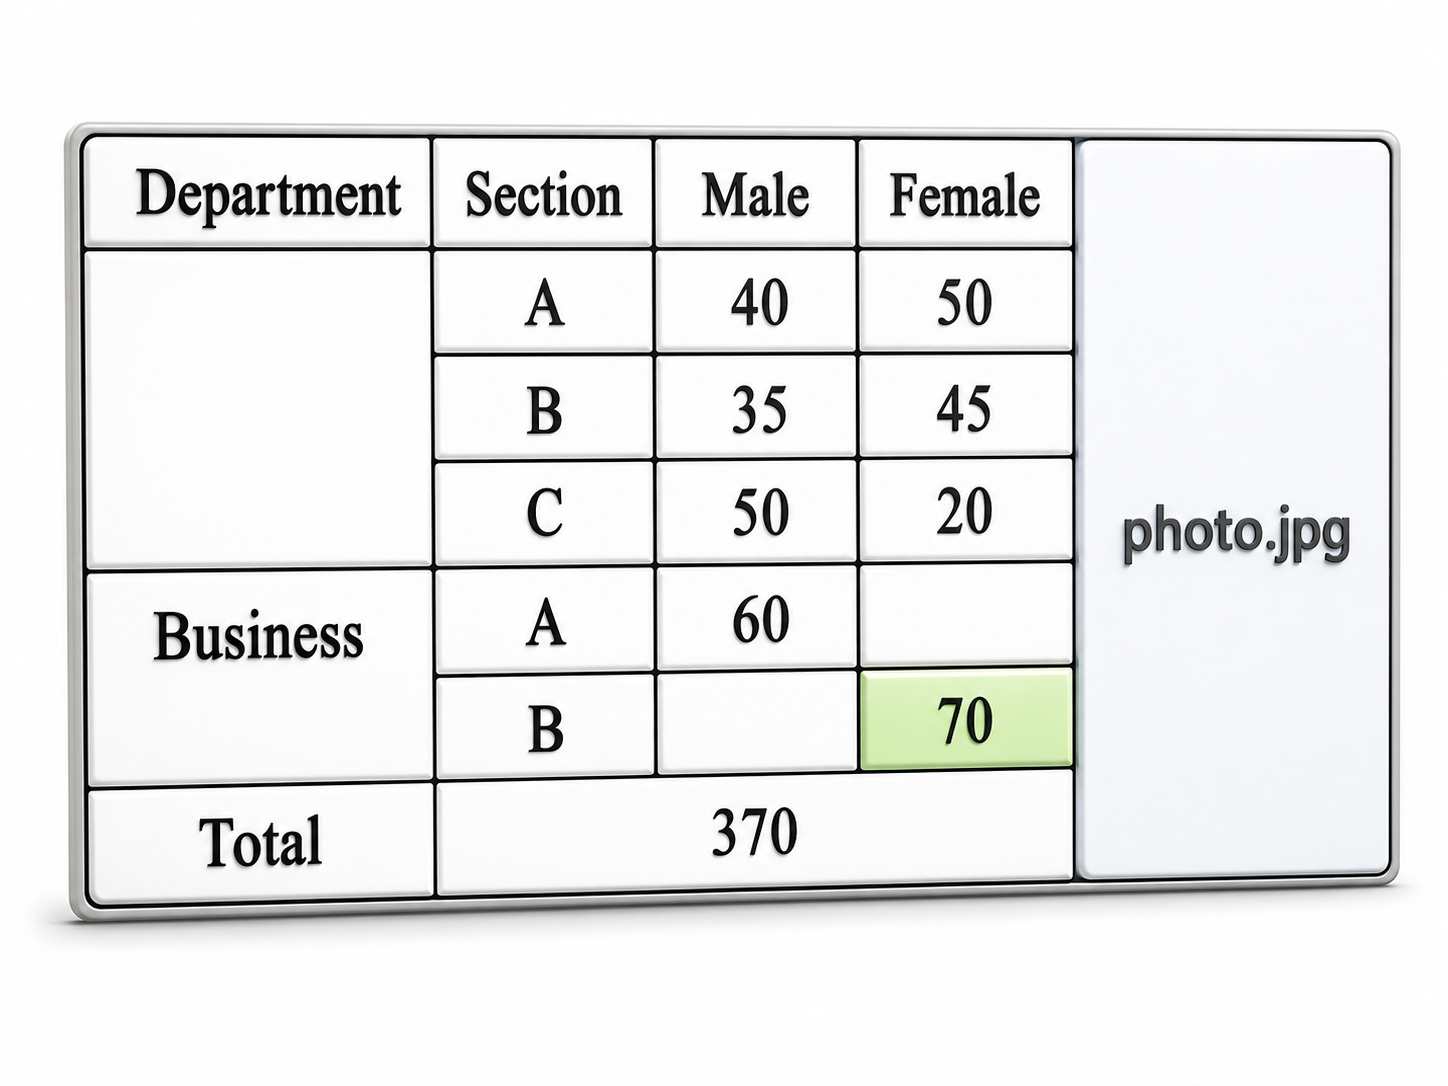
\includegraphics[width=0.95\linewidth,height=0.11\textheight,keepaspectratio]{chapters/Chapter04/topics/images/ex25_3d_department_photo.png}
}{
\fbox{\parbox{0.90\linewidth}{\centering\vspace{0.45cm}
\textbf{চিত্র}\\[3pt]
File: \texttt{chapters/Chapter04/topics/images/ex25\_3d\_department\_photo.png}
\vspace{0.45cm}}}
}
\captionof{figure}{Department table with photo, rowspan, total and green cell}
\end{center}

\begin{keypointbox}{চিত্র ব্যাখ্যা}
Photo column সাত row জুড়ে আছে। Business cell দুই row জুড়ে আছে। 70 cell-এর background green। Total row-তে total text ও 370 value center aligned করে দেখানো হয়েছে।
\end{keypointbox}

\par\noindent{\color{purple!70!black}\bfseries\small কোড}\par\vspace{-4pt}
\begin{verbatim}
<!DOCTYPE html>
<html>
<head>
  <title>HTML Table Example</title>
</head>
<body>
  <table border="1" cellspacing="0">
    <tr>
      <th>Department</th><th>Section</th><th>Male</th><th>Female</th>
      <th rowspan="7"><img src="photo.jpg" width="60" height="50" alt="Photo"></th>
    </tr>
    <tr><td rowspan="3">&nbsp;</td><td>A</td><td>40</td><td>50</td></tr>
    <tr><td>B</td><td>35</td><td>45</td></tr>
    <tr><td>C</td><td>50</td><td>20</td></tr>
    <tr><td rowspan="2" align="center">Business</td><td>A</td><td>60</td><td>&nbsp;</td></tr>
    <tr><td>B</td><td>&nbsp;</td><td bgcolor="green">70</td></tr>
    <tr><td align="center">Total</td><td colspan="3" align="center">370</td></tr>
  </table>
</body>
</html>
\end{verbatim}
\vspace{-6pt}

\Needspace{10\baselineskip}
\subsubsection{Exercise 26: Science, Commerce and Humanities Table}

\begin{boardbox}{Concept}
Group-wise subject table-এ first column group দেখায় এবং বাকি columnগুলো subject list দেখায়। চিত্র দেখে row ও column count ঠিক করা সবচেয়ে জরুরি।
\end{boardbox}

\begin{center}
\IfFileExists{chapters/Chapter04/topics/images/ex26_3d_group_subjects.png}{
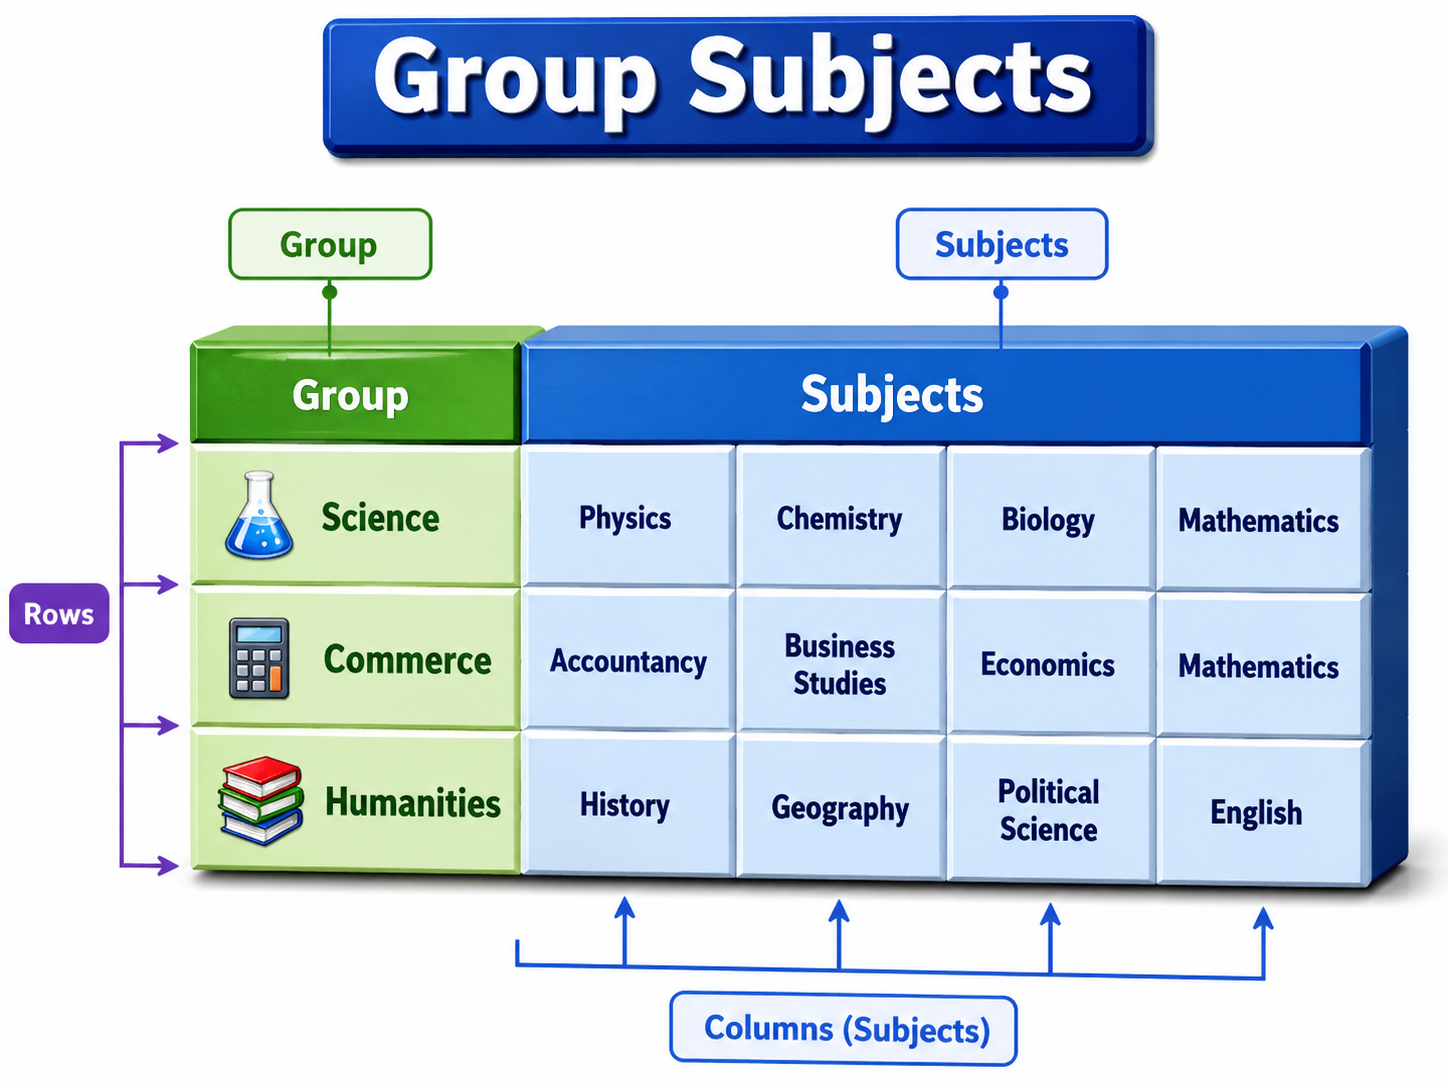
\includegraphics[width=0.95\linewidth,height=0.11\textheight,keepaspectratio]{chapters/Chapter04/topics/images/ex26_3d_group_subjects.png}
}{
\fbox{\parbox{0.90\linewidth}{\centering\vspace{0.4cm}
\textbf{চিত্র}\\
File: \texttt{chapters/Chapter04/topics/images/ex26\_3d\_group\_subjects.png}
\vspace{0.4cm}}}
}
\captionof{figure}{Exercise 26-এর subject group চিত্র}
\end{center}

\begin{keypointbox}{চিত্র ব্যাখ্যা}
চিত্রে Group Subjects নামে একটি table আছে। প্রথম column-এ Science, Commerce ও Humanities group দেখানো হয়েছে। প্রতিটি group row-তে Physics/Chemistry/Biology/Mathematics, Accountancy/Business Studies/Economics/Mathematics এবং History/Geography/Political Science/English subject দেওয়া আছে।
\end{keypointbox}

\begin{keypointbox}{চিত্র দেখে code লেখার ধাপ}
প্রথমে title row-তে \texttt{colspan="5"} ব্যবহার করবে, কারণ table-এ Group সহ মোট 5টি column আছে। দ্বিতীয় row-তে Group ও Subjects heading লিখবে; Subjects heading চারটি subject column জুড়ে থাকবে। এরপর তিনটি group row লিখবে।
\end{keypointbox}

\par\noindent{\color{purple!70!black}\bfseries\small কোড}\par\vspace{-4pt}
\begin{verbatim}
<!DOCTYPE html>
<html>
<head>
  <title>HTML Table Example</title>
</head>
<body>
<table border="1" cellspacing="0" cellpadding="6" align="center">
  <tr>
    <th colspan="5">Group Subjects</th>
  </tr>
  <tr>
    <th>Group</th>
    <th colspan="4">Subjects</th>
  </tr>
  <tr>
    <td>Science</td>
    <td>Physics</td>
    <td>Chemistry</td>
    <td>Biology</td>
    <td>Mathematics</td>
  </tr>
  <tr>
    <td>Commerce</td>
    <td>Accountancy</td>
    <td>Business Studies</td>
    <td>Economics</td>
    <td>Mathematics</td>
  </tr>
  <tr>
    <td>Humanities</td>
    <td>History</td>
    <td>Geography</td>
    <td>Political Science</td>
    <td>English</td>
  </tr>
</table>
</body>
</html>
\end{verbatim}
\vspace{-6pt}
\subsubsection{Exercise 27: List Inside Table Cell}

\begin{center}
\IfFileExists{chapters/Chapter04/topics/images/ex27_3d_lists_inside_table.png}{
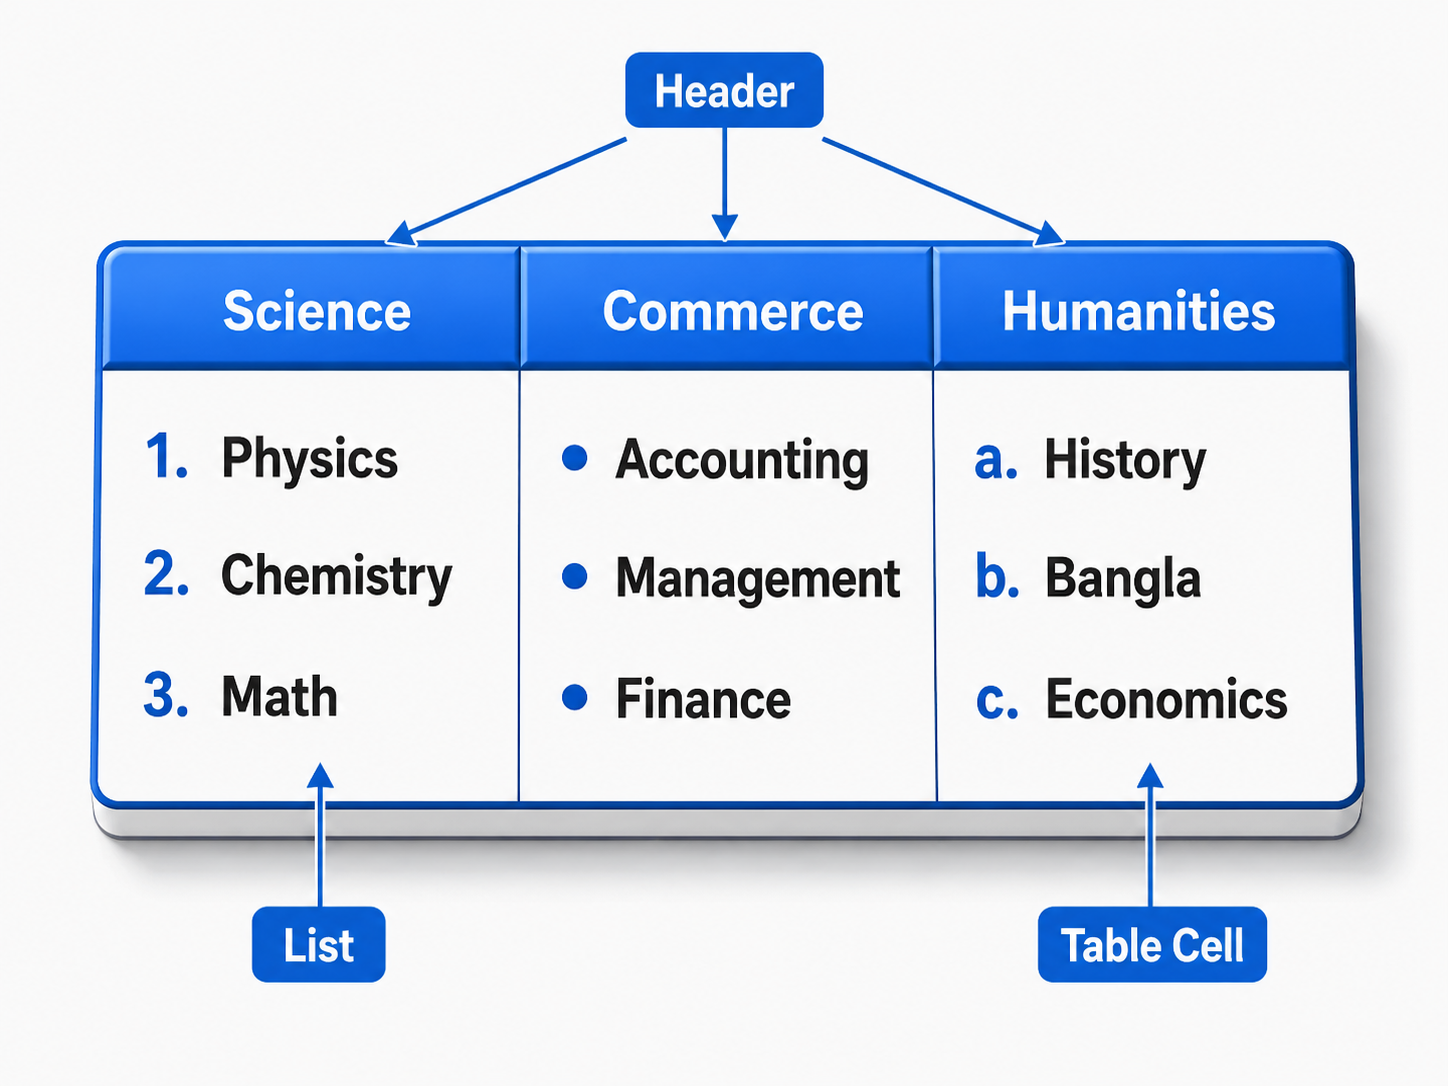
\includegraphics[width=0.95\linewidth,height=0.11\textheight,keepaspectratio]{chapters/Chapter04/topics/images/ex27_3d_lists_inside_table.png}
}{
\fbox{\parbox{0.90\linewidth}{\centering\vspace{0.45cm}
\textbf{চিত্র}\\[3pt]
File: \texttt{chapters/Chapter04/topics/images/ex27\_3d\_lists\_inside\_table.png}
\vspace{0.45cm}}}
}
\captionof{figure}{List inside table cell: Science, Commerce ও Humanities}
\end{center}

\begin{keypointbox}{চিত্র ব্যাখ্যা}
এই table-এ তিনটি column আছে: Science, Commerce ও Humanities। প্রতিটি cell-এর ভিতরে আলাদা type-এর list ব্যবহার করা হয়েছে: ordered list, unordered list এবং alphabetic ordered list।
\end{keypointbox}

\begin{keypointbox}{চিত্র দেখে code লেখার ধাপ}
প্রথমে figure-এর total row ও column গুনবে। এরপর কোন cell একাধিক column জুড়ে আছে তা দেখে \texttt{colspan} এবং কোন cell একাধিক row জুড়ে আছে তা দেখে \texttt{rowspan} বসাবে। তারপর image, link, list বা nested table থাকলে সংশ্লিষ্ট tag cell-এর ভিতরে লিখবে।
\end{keypointbox}

\par\noindent{\color{purple!70!black}\bfseries\small কোড}\par\vspace{-4pt}
\begin{verbatim}
<!DOCTYPE html>
<html>
<head>
  <title>HTML Table Example</title>
</head>
<body>
<table border="1" cellspacing="0">
<tr>
  <th>Science</th>
  <th>Commerce</th>
  <th>Humanities</th>
</tr>
<tr>
  <td><ol><li>Physics</li><li>Chemistry</li><li>Math</li></ol></td>
  <td><ul><li>Accounting</li><li>Management</li><li>Finance</li></ul></td>
  <td><ol type="a"><li>History</li><li>Bangla</li><li>Economics</li></ol></td>
</tr>
</table>
</body>
</html>
\end{verbatim}
\vspace{-6pt}

\subsubsection{Exercise 28: Teacher Information Table with Picture}

\begin{center}
\IfFileExists{chapters/Chapter04/topics/images/ex28_3d_teacher_info_picture.png}{
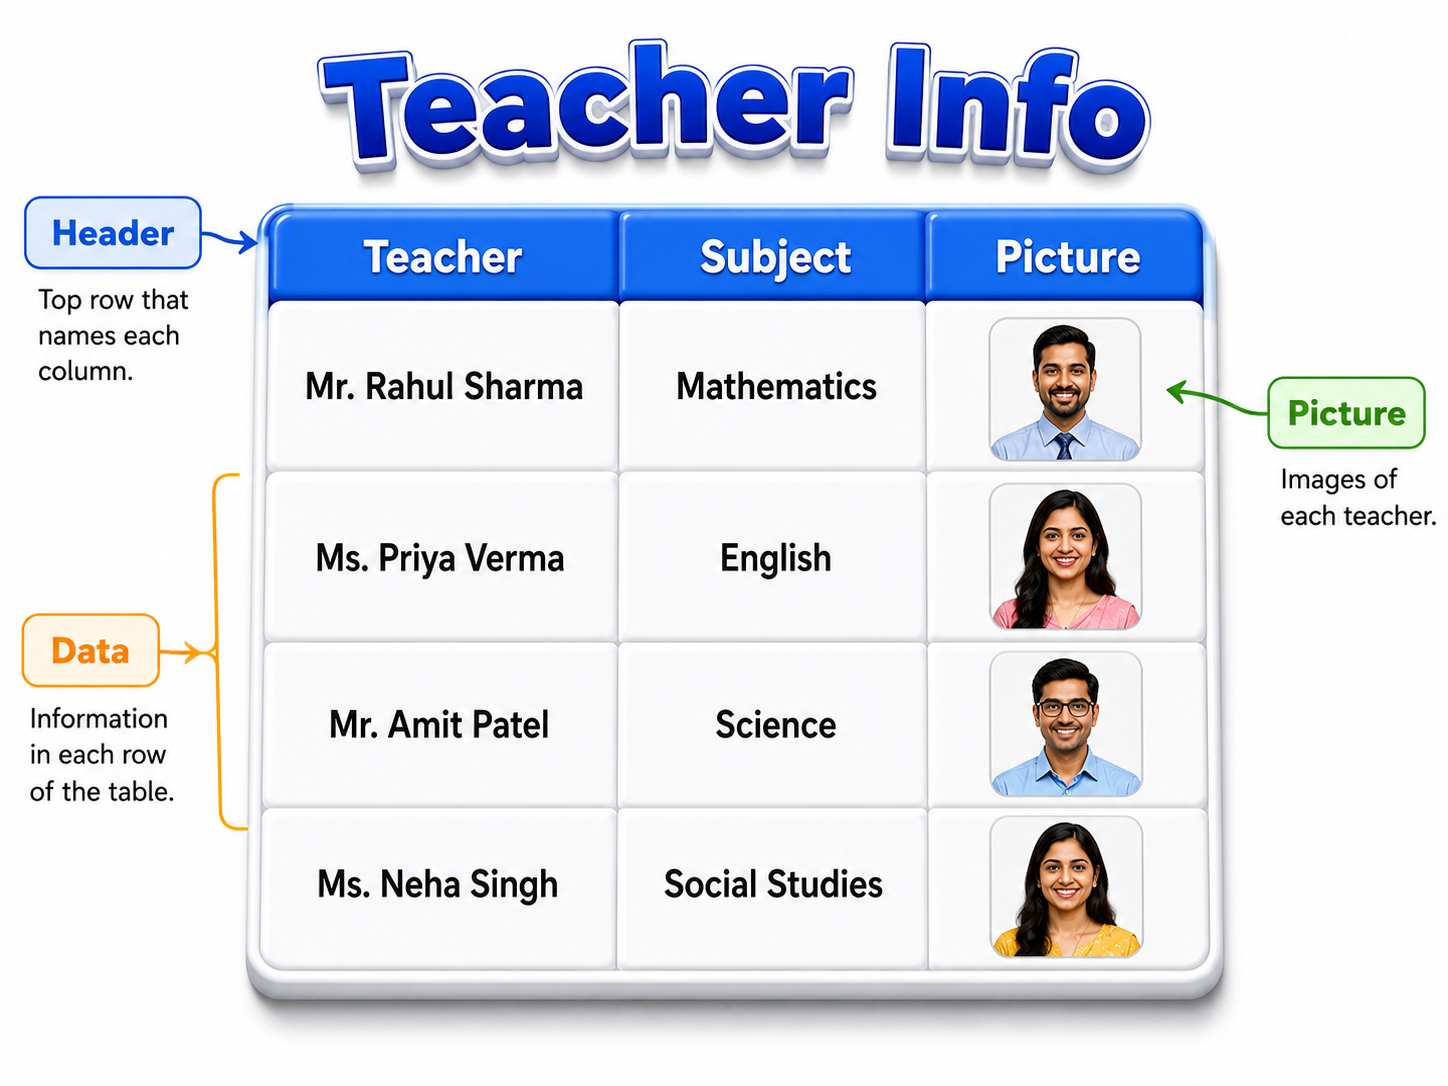
\includegraphics[width=0.95\linewidth,height=0.11\textheight,keepaspectratio]{chapters/Chapter04/topics/images/ex28_3d_teacher_info_picture.png}
}{
\fbox{\parbox{0.90\linewidth}{\centering\vspace{0.45cm}
\textbf{চিত্র}\\[3pt]
File: \texttt{chapters/Chapter04/topics/images/ex28\_3d\_teacher\_info\_picture.png}
\vspace{0.45cm}}}
}
\captionof{figure}{Teacher Info table with subject and picture column}
\end{center}

\begin{keypointbox}{চিত্র ব্যাখ্যা}
চিত্রে Teacher Info heading আছে এবং table-এ Teacher, Subject ও Picture--এই তিনটি column দেখা যায়। প্রতিটি row-তে teacher name, subject এবং সংশ্লিষ্ট picture রাখা হয়েছে।
\end{keypointbox}

\begin{keypointbox}{চিত্র দেখে code লেখার ধাপ}
প্রথমে title/heading আলাদা করবে। তারপর তিনটি column--Teacher, Subject, Picture--লিখবে। Picture column-এর প্রতিটি cell-এ \texttt{<img>} tag বসাবে এবং image size নির্ধারণ করবে।
\end{keypointbox}

\par\noindent{\color{purple!70!black}\bfseries\small কোড}\par\vspace{-4pt}
\begin{verbatim}
<!DOCTYPE html>
<html>
<head>
  <title>HTML Table Example</title>
</head>
<body>
<h2 align="center">Teacher Info</h2>
<table border="1" align="center" cellspacing="0" cellpadding="6">
<tr>
  <th>Teacher</th>
  <th>Subject</th>
  <th>Picture</th>
</tr>
<tr>
  <td>Mr. Rahul Sharma</td>
  <td>Mathematics</td>
  <td><img src="rahul.jpg" width="55" height="60" alt="Rahul Sharma"></td>
</tr>
<tr>
  <td>Mrs. Priya Verma</td>
  <td>English</td>
  <td><img src="priya.jpg" width="55" height="60" alt="Priya Verma"></td>
</tr>
<tr>
  <td>Mr. Amit Patel</td>
  <td>Science</td>
  <td><img src="amit.jpg" width="55" height="60" alt="Amit Patel"></td>
</tr>
<tr>
  <td>Ms. Neha Singh</td>
  <td>Social Studies</td>
  <td><img src="neha.jpg" width="55" height="60" alt="Neha Singh"></td>
</tr>
</table>
</body>
</html>
\end{verbatim}
\vspace{-6pt}

\subsubsection{Exercise 29: Bangladesh Places Table with Photo}

\begin{center}
\IfFileExists{chapters/Chapter04/topics/images/ex29_3d_bangladesh_places.png}{
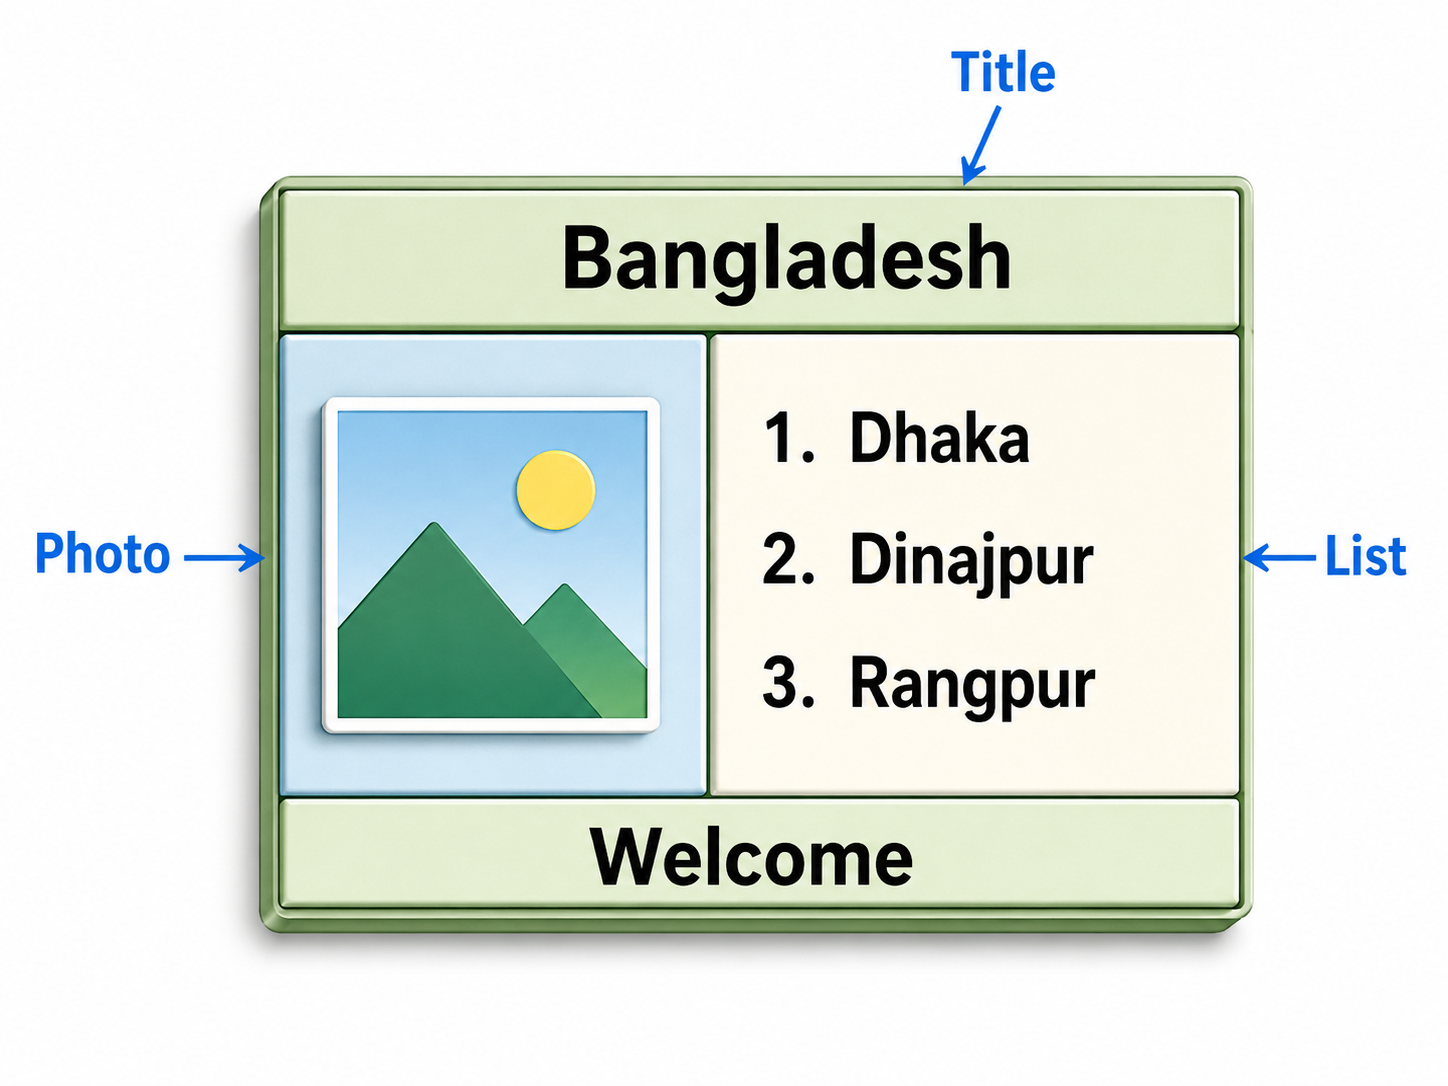
\includegraphics[width=0.95\linewidth,height=0.11\textheight,keepaspectratio]{chapters/Chapter04/topics/images/ex29_3d_bangladesh_places.png}
}{
\fbox{\parbox{0.90\linewidth}{\centering\vspace{0.45cm}
\textbf{চিত্র}\\[3pt]
File: \texttt{chapters/Chapter04/topics/images/ex29\_3d\_bangladesh\_places.png}
\vspace{0.45cm}}}
}
\captionof{figure}{Bangladesh table with photo and ordered list}
\end{center}

\begin{keypointbox}{চিত্র ব্যাখ্যা}
এই table-এ top heading এবং bottom welcome row দুটি column জুড়ে আছে। মাঝের row-তে বাম cell-এ image এবং ডান cell-এ ordered list রাখা হয়েছে।
\end{keypointbox}

\begin{keypointbox}{চিত্র দেখে code লেখার ধাপ}
প্রথমে figure-এর total row ও column গুনবে। এরপর কোন cell একাধিক column জুড়ে আছে তা দেখে \texttt{colspan} এবং কোন cell একাধিক row জুড়ে আছে তা দেখে \texttt{rowspan} বসাবে। তারপর image, link, list বা nested table থাকলে সংশ্লিষ্ট tag cell-এর ভিতরে লিখবে।
\end{keypointbox}

\par\noindent{\color{purple!70!black}\bfseries\small কোড}\par\vspace{-4pt}
\begin{verbatim}
<!DOCTYPE html>
<html>
<head>
  <title>HTML Table Example</title>
</head>
<body>
<table border="1" cellspacing="0">
<tr><th colspan="2">Bangladesh</th></tr>
<tr>
  <td><img src="photo.jpg" width="60" height="50" align="center"><br>Photo</td>
  <td>
    <ol>
      <li>Dhaka</li>
      <li>Dinajpur</li>
      <li>Rangpur</li>
    </ol>
  </td>
</tr>
<tr><th colspan="2">Welcome</th></tr>
</table>
</body>
</html>
\end{verbatim}
\vspace{-6pt}

\subsubsection{Exercise 30: Choose Your Site Table with Links}

\begin{center}
\IfFileExists{chapters/Chapter04/topics/images/ex30_3d_choose_site_links.png}{
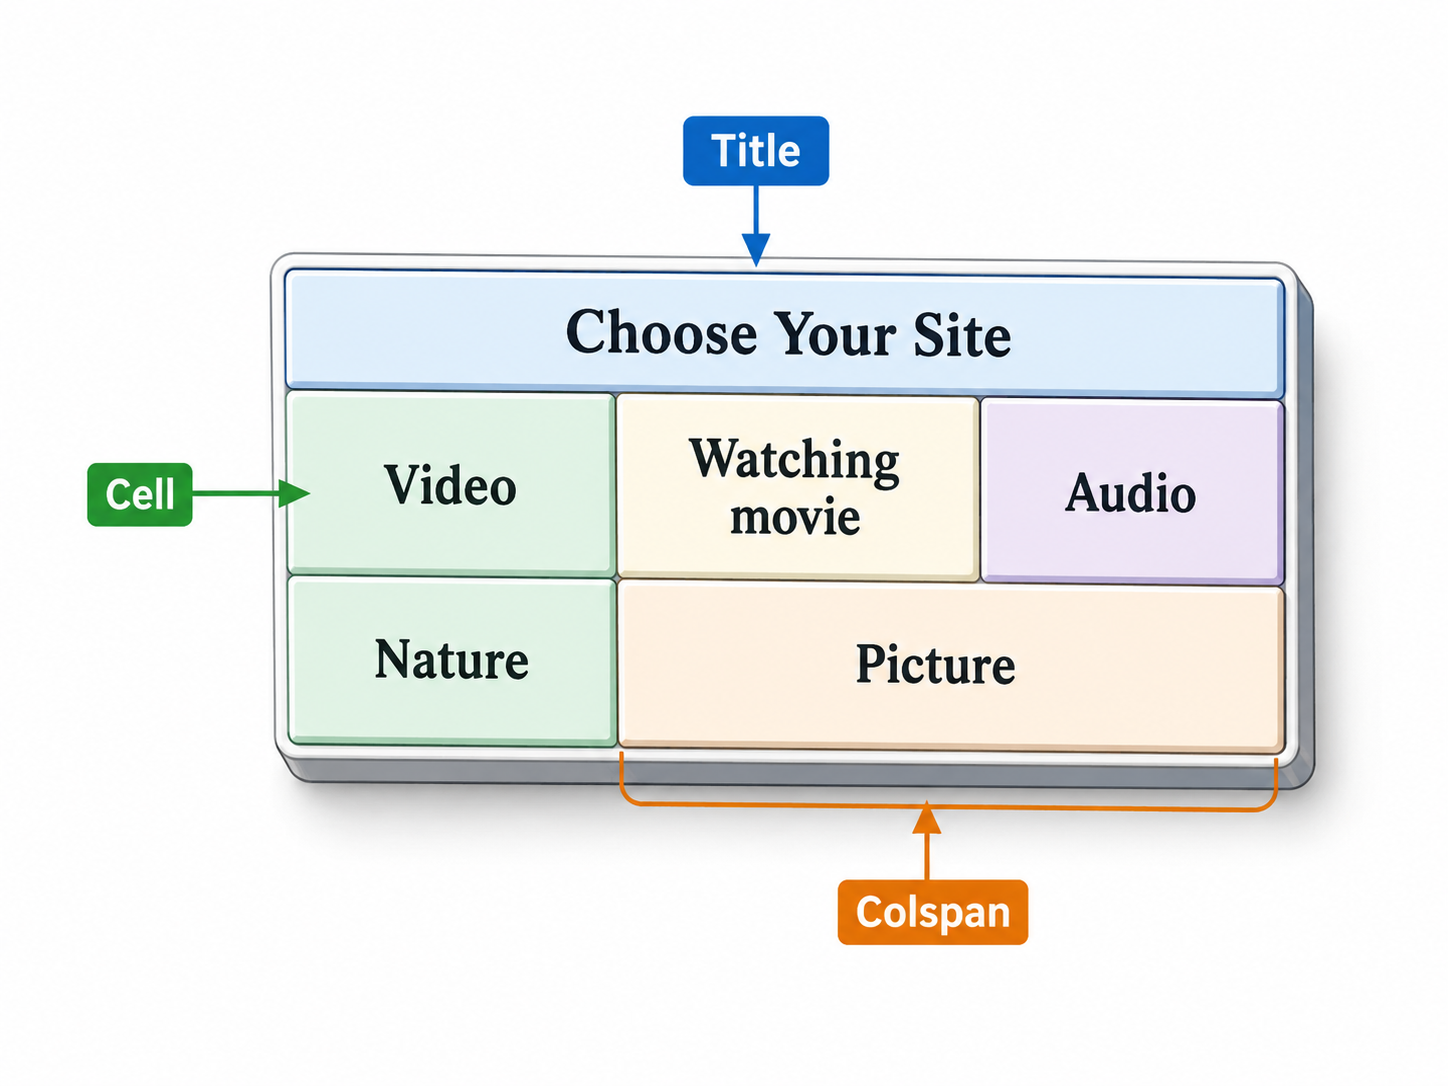
\includegraphics[width=0.95\linewidth,height=0.11\textheight,keepaspectratio]{chapters/Chapter04/topics/images/ex30_3d_choose_site_links.png}
}{
\fbox{\parbox{0.90\linewidth}{\centering\vspace{0.45cm}
\textbf{চিত্র}\\[3pt]
File: \texttt{chapters/Chapter04/topics/images/ex30\_3d\_choose\_site\_links.png}
\vspace{0.45cm}}}
}
\captionof{figure}{Choose Your Site table with centered and underlined text}
\end{center}

\begin{keypointbox}{চিত্র ব্যাখ্যা}
এখানে \texttt{colspan="3"} দিয়ে title row তিনটি column জুড়ে আছে। Video ও Nature underline করা হয়েছে এবং Picture cell দুই column জুড়ে আছে।
\end{keypointbox}

\par\noindent{\color{purple!70!black}\bfseries\small কোড}\par\vspace{-4pt}
\begin{verbatim}
<!DOCTYPE html>
<html>
<head>
  <title>HTML Table Example</title>
</head>
<body>
<table border="1" cellspacing="0">
<tr>
  <th colspan="3">Choose Your Site</th>
</tr>
<tr>
  <td align="center"><u>Video</u><br></td>
  <td>Watching<br><p align="center">movie</p></td>
  <td>Audio</td>
</tr>
<tr>
  <td align="center"><u>Nature</u></td>
  <td colspan="2" align="center"><br>Picture</td>
</tr>
</table>
</body>
</html>
\end{verbatim}
\vspace{-6pt}

\subsubsection{Exercise 31: XY Showroom Table}

\begin{center}
\IfFileExists{chapters/Chapter04/topics/images/ex31_3d_xy_showroom.png}{
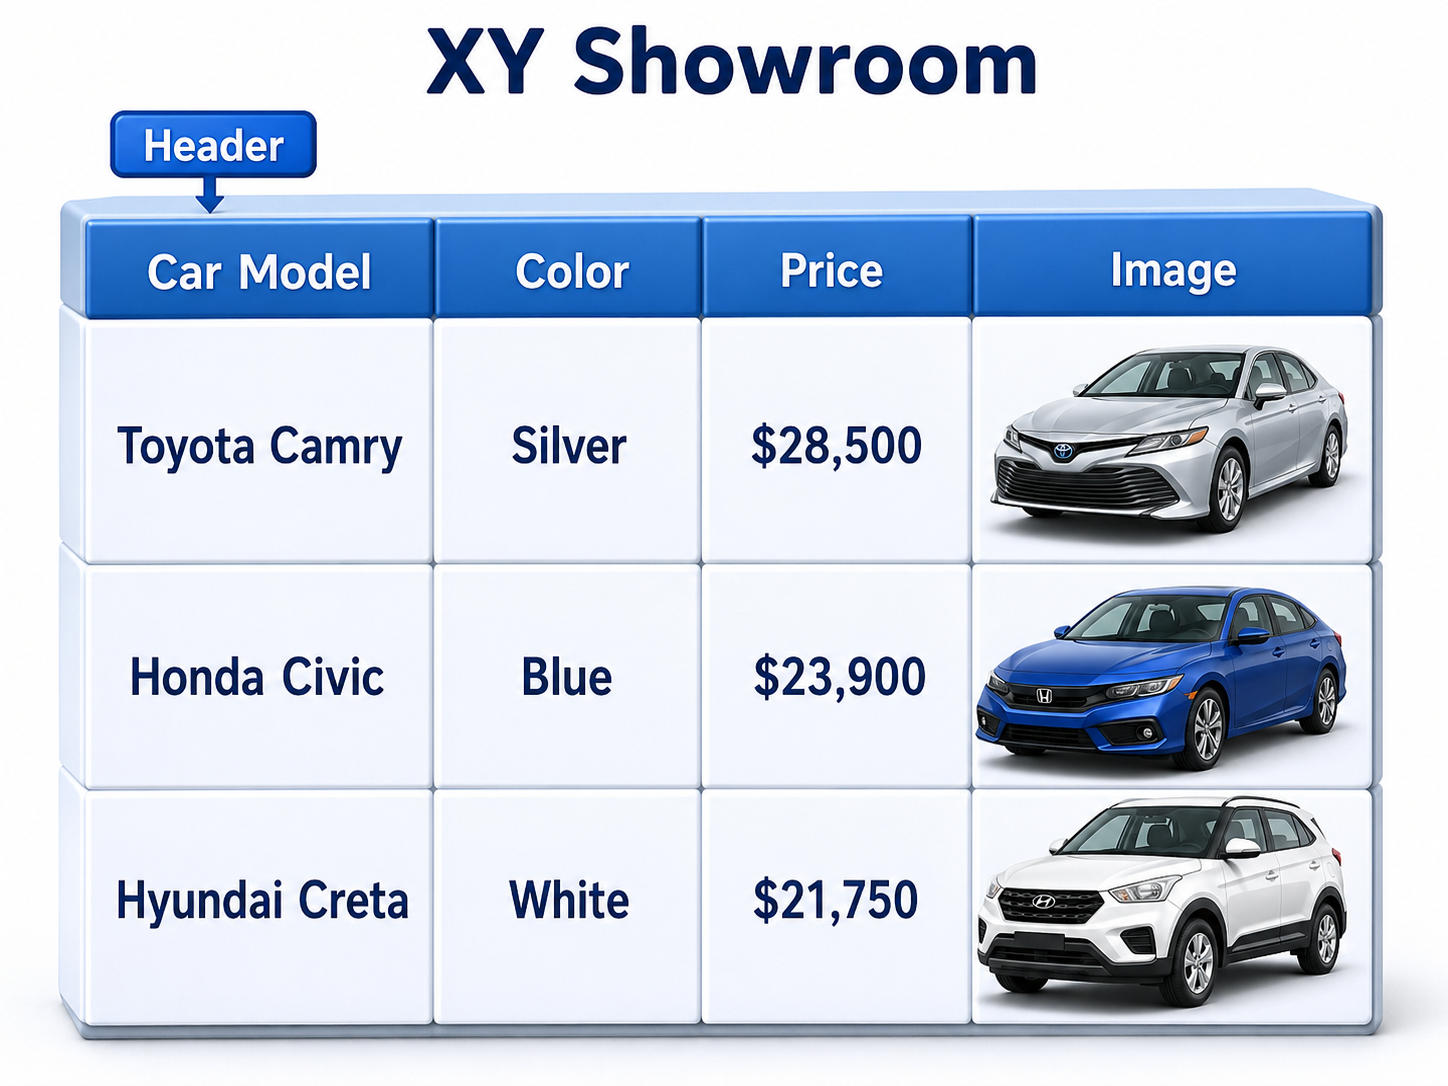
\includegraphics[width=0.95\linewidth,height=0.11\textheight,keepaspectratio]{chapters/Chapter04/topics/images/ex31_3d_xy_showroom.png}
}{
\fbox{\parbox{0.90\linewidth}{\centering\vspace{0.45cm}
\textbf{চিত্র}\\[3pt]
File: \texttt{chapters/Chapter04/topics/images/ex31\_3d\_xy\_showroom.png}
\vspace{0.45cm}}}
}
\captionof{figure}{XY Showroom table with car model, color, price and image}
\end{center}

\begin{keypointbox}{চিত্র ব্যাখ্যা}
চিত্রে XY Showroom heading-এর নিচে Car Model, Color, Price এবং Image--চারটি column আছে। প্রতিটি car row-তে model, color, price এবং car image দেখানো হয়েছে।
\end{keypointbox}

\begin{keypointbox}{চিত্র দেখে code লেখার ধাপ}
প্রথমে table-এর উপরে \texttt{<h2>} heading লিখবে। তারপর চারটি header cell তৈরি করবে। প্রতিটি row-তে car model, color, price এবং image cell লিখবে। Image column-এ \texttt{<img>} tag ব্যবহার করবে।
\end{keypointbox}

\par\noindent{\color{purple!70!black}\bfseries\small কোড}\par\vspace{-4pt}
\begin{verbatim}
<!DOCTYPE html>
<html>
<head>
  <title>XY Showroom</title>
</head>
<body>
<h2 align="center">XY Showroom</h2>
<table border="1" align="center" cellspacing="0" cellpadding="6">
<tr>
  <th>Car Model</th>
  <th>Color</th>
  <th>Price</th>
  <th>Image</th>
</tr>
<tr>
  <td>Toyota Camry</td>
  <td>Silver</td>
  <td>$28,500</td>
  <td><img src="camry.jpg" width="100" height="60" alt="Toyota Camry"></td>
</tr>
<tr>
  <td>Honda Civic</td>
  <td>Blue</td>
  <td>$23,900</td>
  <td><img src="civic.jpg" width="100" height="60" alt="Honda Civic"></td>
</tr>
<tr>
  <td>Hyundai Creta</td>
  <td>White</td>
  <td>$21,750</td>
  <td><img src="creta.jpg" width="100" height="60" alt="Hyundai Creta"></td>
</tr>
</table>
</body>
</html>
\end{verbatim}
\vspace{-6pt}

\subsubsection{Exercise 32: Nested Table Example}

\begin{center}
\IfFileExists{chapters/Chapter04/topics/images/ex32_3d_nested_table_parent_child.png}{
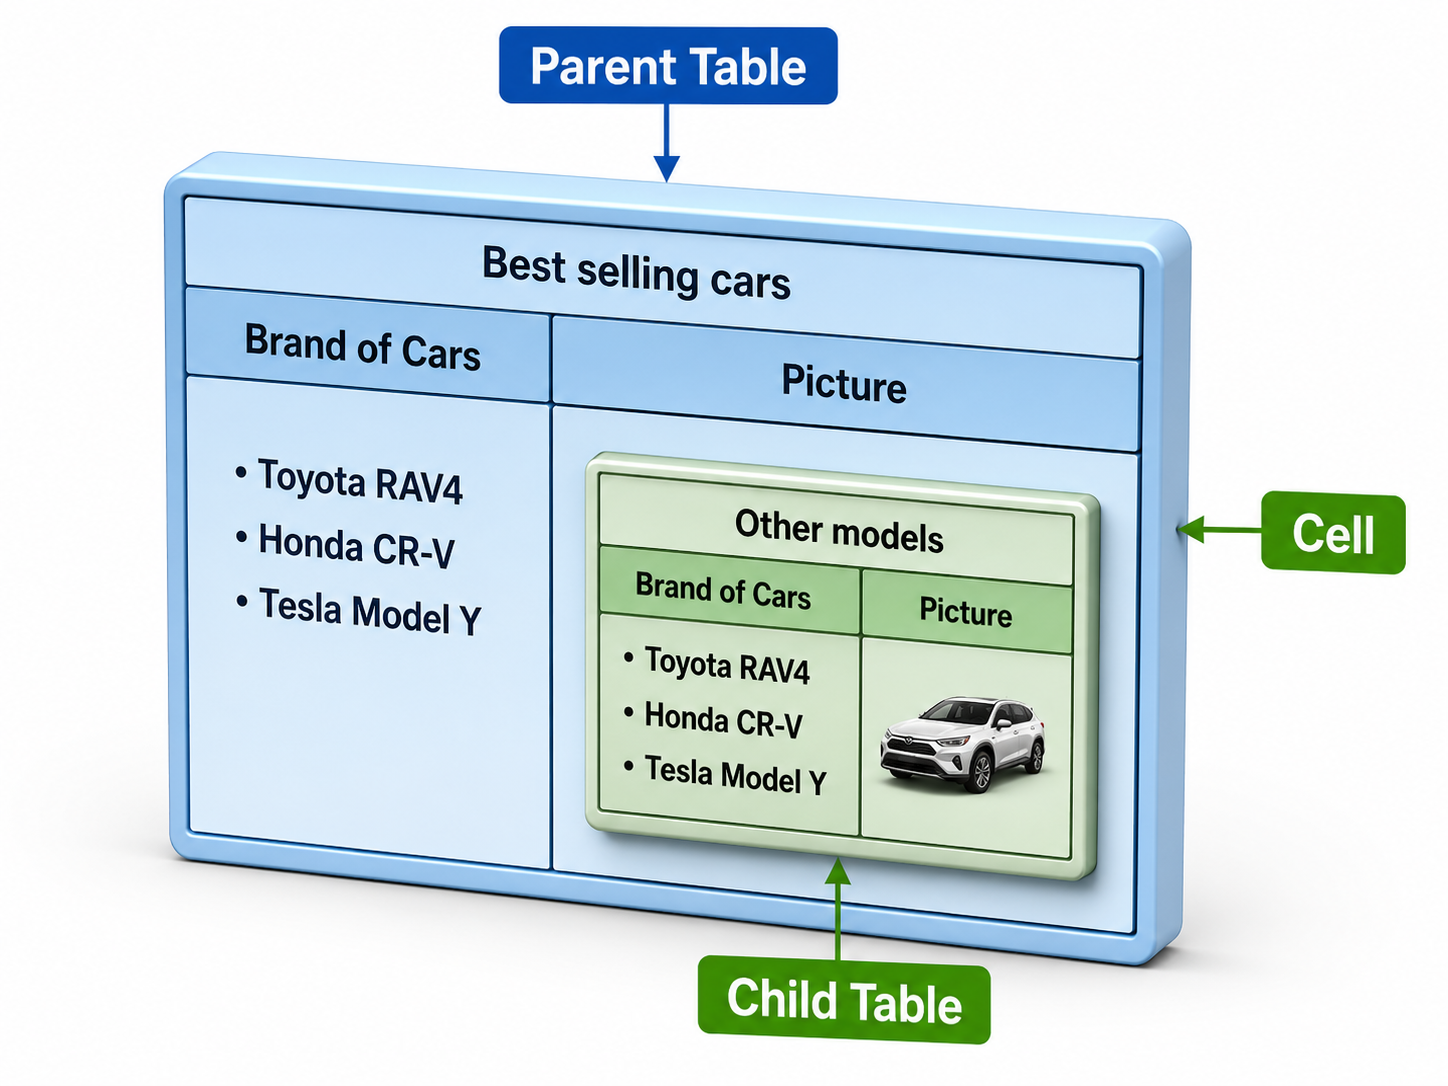
\includegraphics[width=0.95\linewidth,height=0.11\textheight,keepaspectratio]{chapters/Chapter04/topics/images/ex32_3d_nested_table_parent_child.png}
}{
\fbox{\parbox{0.90\linewidth}{\centering\vspace{0.45cm}
\textbf{চিত্র}\\[3pt]
File: \texttt{chapters/Chapter04/topics/images/ex32\_3d\_nested\_table\_parent\_child.png}
\vspace{0.45cm}}}
}
\captionof{figure}{Nested table: parent table-এর cell-এর ভিতরে child table}
\end{center}

\begin{keypointbox}{চিত্র ব্যাখ্যা}
Nested table-এ একটি বড় parent table-এর কোনো একটি cell-এর ভিতরে আরেকটি ছোট child table বসানো হয়। বইয়ের example-এ বিস্তারিত অংশের ভিতরে ছোট table ব্যবহার করা হয়েছে।
\end{keypointbox}

\begin{keypointbox}{চিত্র দেখে code লেখার ধাপ}
প্রথমে figure-এর total row ও column গুনবে। এরপর কোন cell একাধিক column জুড়ে আছে তা দেখে \texttt{colspan} এবং কোন cell একাধিক row জুড়ে আছে তা দেখে \texttt{rowspan} বসাবে। তারপর image, link, list বা nested table থাকলে সংশ্লিষ্ট tag cell-এর ভিতরে লিখবে।
\end{keypointbox}

\par\noindent{\color{purple!70!black}\bfseries\small কোড}\par\vspace{-4pt}
\begin{verbatim}
<!DOCTYPE html>
<html>
<head>
  <title>Table Inside Table</title>
</head>
<body>
<h3>বাইরের টেবিল (Parent Table)</h3>
<table border="2" cellpadding="10">
<tr>
  <th>নাম</th>
  <th>বিস্তারিত</th>
</tr>
<tr>
  <td>রাফি</td>
  <td>
    <!-- ভিতরের টেবিল শুরু -->
    <table border="1" cellpadding="5">
    <tr>
      <th>বিষয়</th>
      <th>নম্বর</th>
    </tr>
    <tr>
      <td>গণিত</td>
      <td>৮৫</td>
    </tr>
    <tr>
      <td>বিজ্ঞান</td>
      <td>৯০</td>
    </tr>
    </table>
    <!-- ভিতরের টেবিল শেষ -->
  </td>
</tr>
</table>
</body>
</html>
\end{verbatim}
\vspace{-6pt}

\subsubsection{Exercise 33: Student Subjects Table}

\begin{center}
\IfFileExists{chapters/Chapter04/topics/images/ex33_3d_student_subjects.png}{
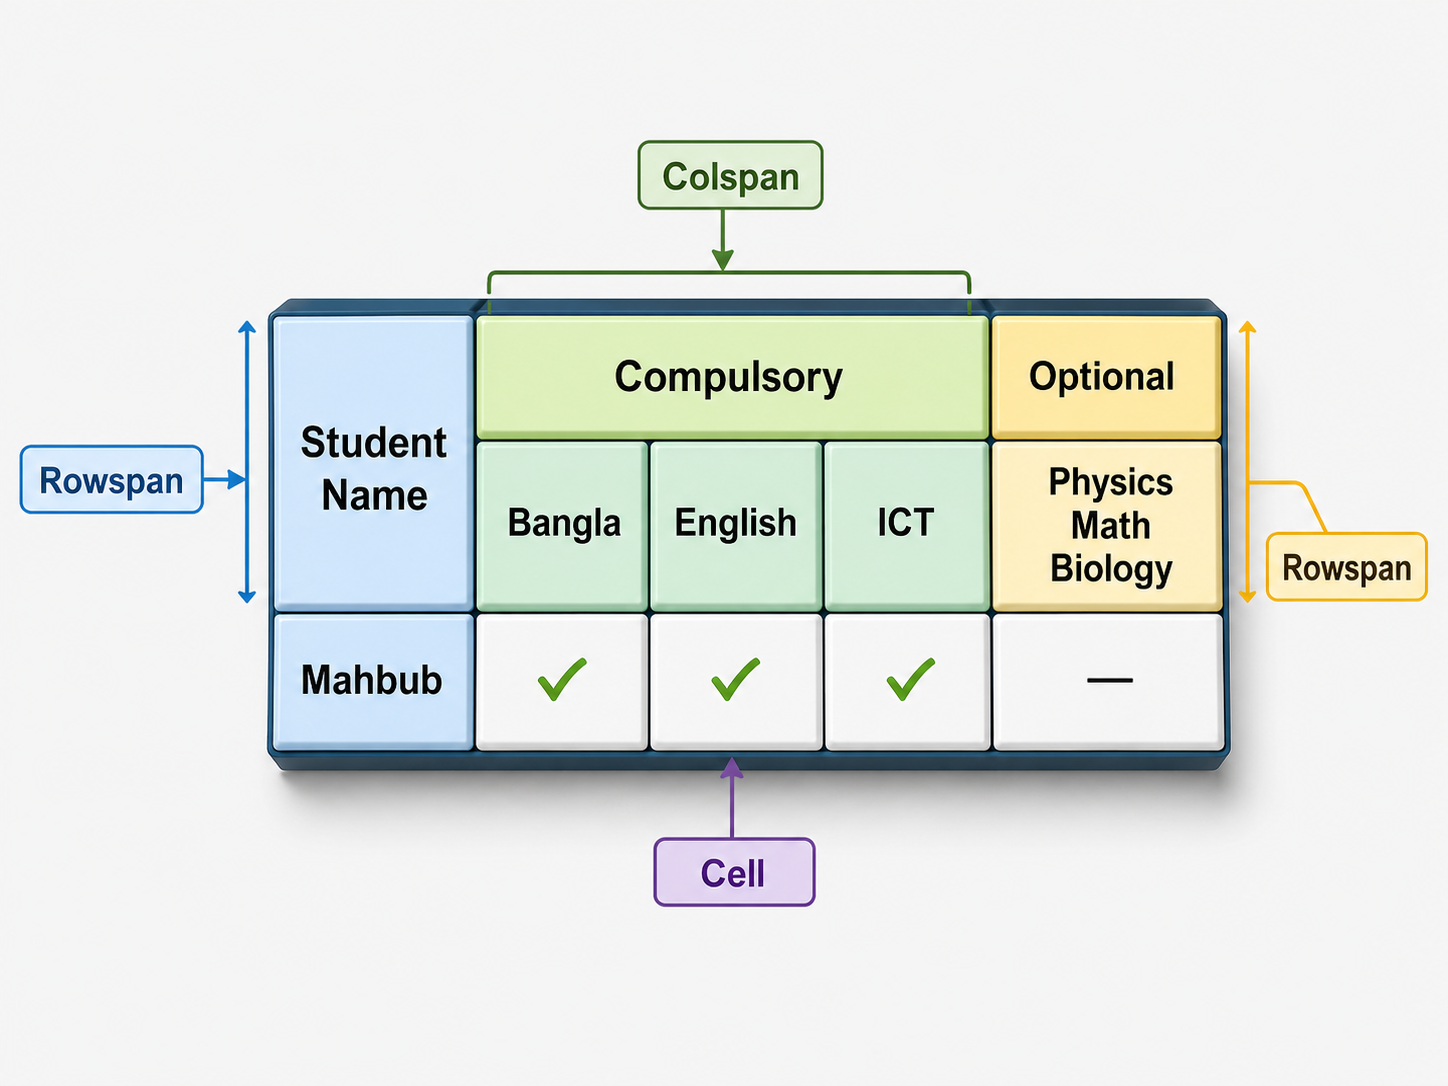
\includegraphics[width=0.95\linewidth,height=0.11\textheight,keepaspectratio]{chapters/Chapter04/topics/images/ex33_3d_student_subjects.png}
}{
\fbox{\parbox{0.90\linewidth}{\centering\vspace{0.45cm}
\textbf{চিত্র}\\[3pt]
File: \texttt{chapters/Chapter04/topics/images/ex33\_3d\_student\_subjects.png}
\vspace{0.45cm}}}
}
\captionof{figure}{Student Subjects table with rowspan and colspan}
\end{center}

\begin{keypointbox}{চিত্র ব্যাখ্যা}
Student Name এবং Optional heading দুই row জুড়ে আছে। Compulsory heading তিনটি subject column জুড়ে আছে। Mahbub ও tick mark cell-গুলো তিনটি optional subject row জুড়ে আছে।
\end{keypointbox}

\par\noindent{\color{purple!70!black}\bfseries\small কোড}\par\vspace{-4pt}
\begin{verbatim}
<!DOCTYPE html>
<html>
<head>
  <title>Student Subjects Table</title>
</head>
<body>
<table border="1" cellspacing="0">
<tr>
  <th rowspan="2">Student Name</th>
  <th colspan="3">Compulsory</th>
  <th rowspan="2">Optional</th>
</tr>
<tr>
  <td>Bangla</td>
  <td>English</td>
  <td>ICT</td>
</tr>
<tr>
  <th rowspan="3">Mahbub</th>
  <th rowspan="3">&#10003;</th>
  <th rowspan="3">&#10003;</th>
  <th rowspan="3">&#10003;</th>
  <td>Physics</td>
</tr>
<tr><td>Math</td></tr>
<tr><td>Biology</td></tr>
</table>
</body>
</html>
\end{verbatim}
\vspace{-6pt}

\subsubsection{Exercise 34: Science Fair Projects Table}

\begin{center}
\IfFileExists{chapters/Chapter04/topics/images/ex34_3d_science_fair_projects.png}{
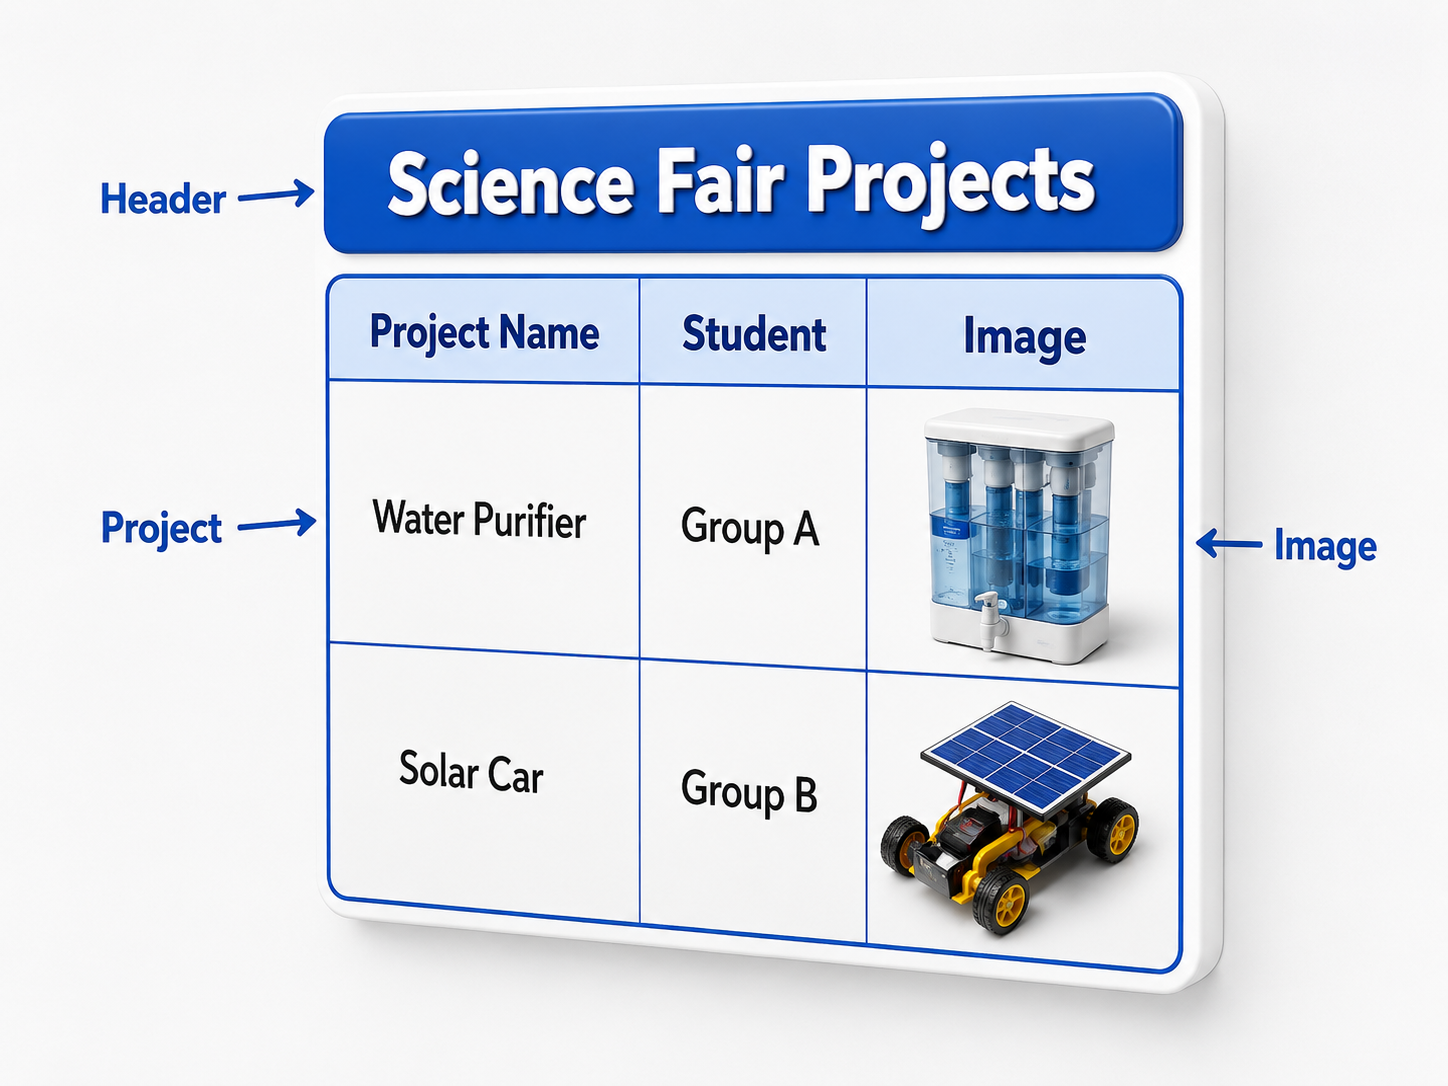
\includegraphics[width=0.95\linewidth,height=0.11\textheight,keepaspectratio]{chapters/Chapter04/topics/images/ex34_3d_science_fair_projects.png}
}{
\fbox{\parbox{0.90\linewidth}{\centering\vspace{0.45cm}
\textbf{চিত্র}\\[3pt]
File: \texttt{chapters/Chapter04/topics/images/ex34\_3d\_science\_fair\_projects.png}
\vspace{0.45cm}}}
}
\captionof{figure}{Science Fair Projects table with student/group and image}
\end{center}

\begin{keypointbox}{চিত্র ব্যাখ্যা}
চিত্রে Science Fair Projects heading-এর নিচে Project Name, Student এবং Image column আছে। প্রতিটি project row-তে project name, group/student label এবং project image দেওয়া হয়েছে।
\end{keypointbox}

\begin{keypointbox}{চিত্র দেখে code লেখার ধাপ}
প্রথমে heading লিখবে। এরপর তিনটি column identify করবে: Project Name, Student এবং Image। শেষ column-এ প্রতিটি project-এর জন্য \texttt{<img>} tag বসাবে।
\end{keypointbox}

\par\noindent{\color{purple!70!black}\bfseries\small কোড}\par\vspace{-4pt}
\begin{verbatim}
<!DOCTYPE html>
<html>
<head>
  <title>HTML Table Example</title>
</head>
<body>
<h2 align="center">Science Fair Projects</h2>
<table border="1" align="center" cellspacing="0" cellpadding="6">
<tr>
  <th>Project Name</th>
  <th>Student</th>
  <th>Image</th>
</tr>
<tr>
  <td>Water Purifier</td>
  <td>Group A</td>
  <td><img src="purifier.jpg" width="80" height="60" alt="Water Purifier"></td>
</tr>
<tr>
  <td>Solar Car</td>
  <td>Group B</td>
  <td><img src="solarcar.jpg" width="80" height="60" alt="Solar Car"></td>
</tr>
</table>
</body>
</html>
\end{verbatim}
\vspace{-6pt}

\subsubsection{Exercise 35: Group, Section and Club Table}

\begin{center}
\IfFileExists{chapters/Chapter04/topics/images/ex35_3d_group_section_club.png}{
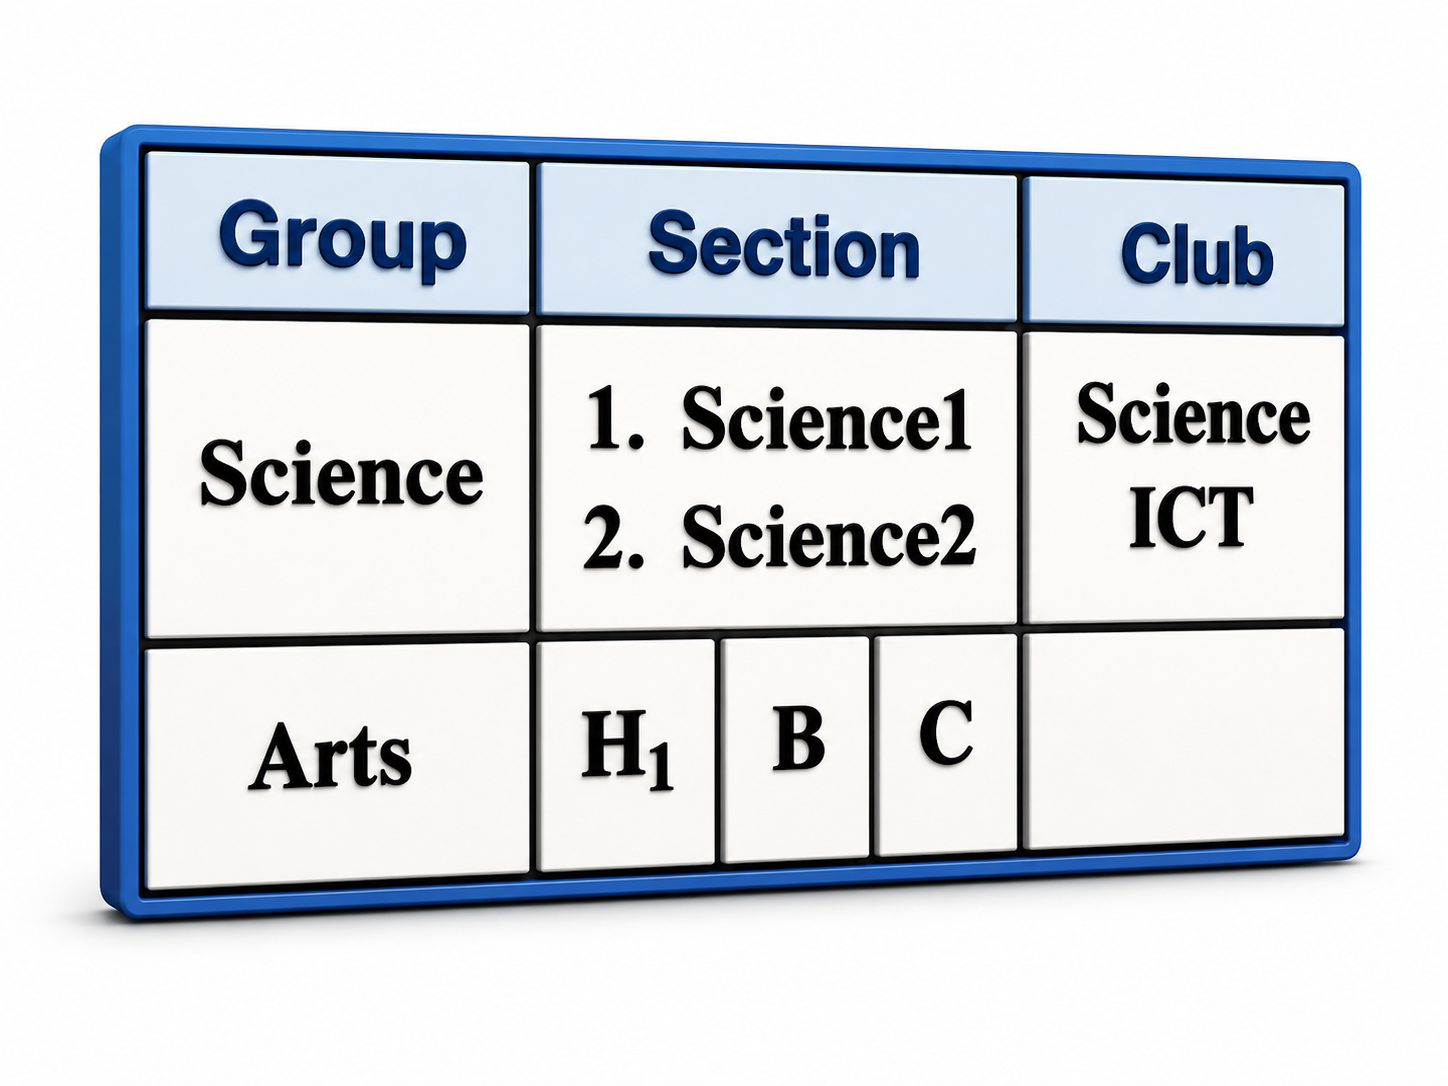
\includegraphics[width=0.95\linewidth,height=0.11\textheight,keepaspectratio]{chapters/Chapter04/topics/images/ex35_3d_group_section_club.png}
}{
\fbox{\parbox{0.90\linewidth}{\centering\vspace{0.45cm}
\textbf{চিত্র}\\[3pt]
File: \texttt{chapters/Chapter04/topics/images/ex35\_3d\_group\_section\_club.png}
\vspace{0.45cm}}}
}
\captionof{figure}{Group, Section and Club table with colspan, rowspan, sub and span}
\end{center}

\begin{keypointbox}{চিত্র ব্যাখ্যা}
Section heading তিনটি column জুড়ে আছে। Club cell দুই row জুড়ে আছে। Science row-তে Section অংশ তিনটি column জুড়ে text দেখানো হয়েছে। Arts row-তে H\textsubscript{1}, B এবং C আলাদা cell-এ আছে।
\end{keypointbox}

\begin{keypointbox}{চিত্র দেখে code লেখার ধাপ}
প্রথমে figure-এর total row ও column গুনবে। এরপর কোন cell একাধিক column জুড়ে আছে তা দেখে \texttt{colspan} এবং কোন cell একাধিক row জুড়ে আছে তা দেখে \texttt{rowspan} বসাবে। তারপর image, link, list বা nested table থাকলে সংশ্লিষ্ট tag cell-এর ভিতরে লিখবে।
\end{keypointbox}

\par\noindent{\color{purple!70!black}\bfseries\small কোড}\par\vspace{-4pt}
\begin{verbatim}
<!DOCTYPE html>
<html>
<head>
  <title>Group Table</title>
</head>
<body>
<table border="1" cellspacing="0" cellpadding="5">
<tr>
  <th>Group</th>
  <th colspan="3">Section</th>
  <th rowspan="2"><u>Club</u><br>
    <span style="font-weight:normal;">Science<br>ICT</span>
  </th>
</tr>
<tr>
  <td>Science</td>
  <td colspan="3">1. Science1<br>2. Science2</td>
</tr>
<tr>
  <td>Arts</td>
  <td>H<sub>1</sub></td>
  <td>B</td>
  <td>C</td>
  <td></td>
</tr>
</table>
</body>
</html>
\end{verbatim}
\vspace{-6pt}

\subsubsection{Exercise 36: Delight Restaurant Table}

\begin{center}
\IfFileExists{chapters/Chapter04/topics/images/ex36_3d_delight_restaurant.png}{
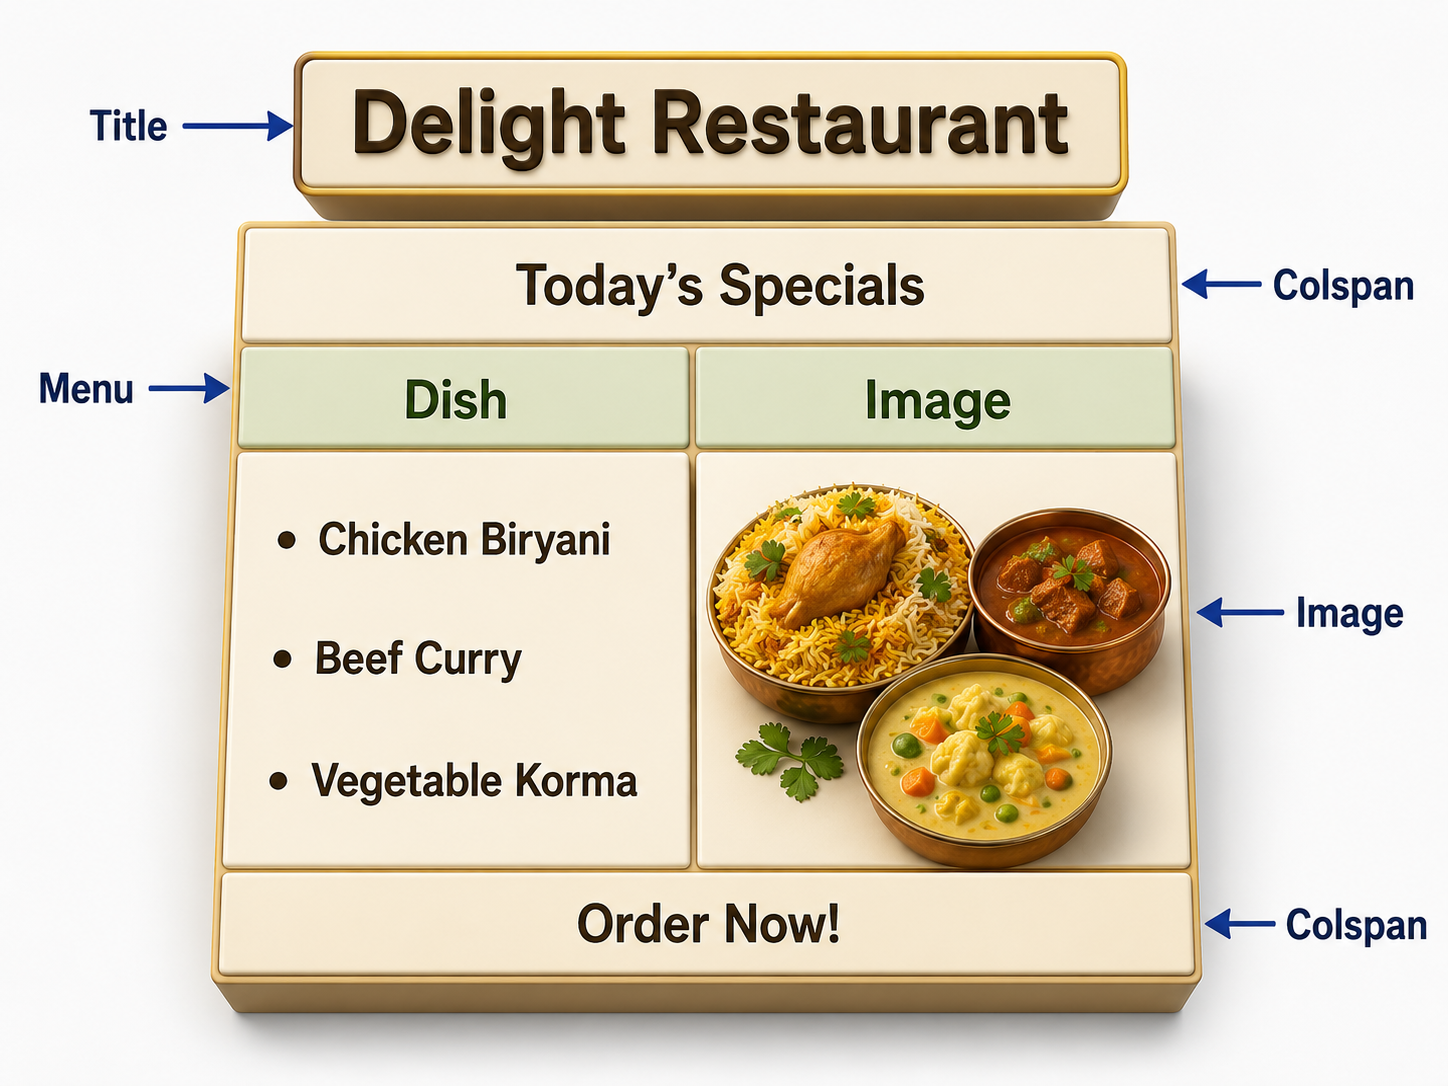
\includegraphics[width=0.95\linewidth,height=0.11\textheight,keepaspectratio]{chapters/Chapter04/topics/images/ex36_3d_delight_restaurant.png}
}{
\fbox{\parbox{0.90\linewidth}{\centering\vspace{0.45cm}
\textbf{চিত্র}\\[3pt]
File: \texttt{chapters/Chapter04/topics/images/ex36\_3d\_delight\_restaurant.png}
\vspace{0.45cm}}}
}
\captionof{figure}{Delight Restaurant table with food image and order row}
\end{center}

\begin{keypointbox}{চিত্র ব্যাখ্যা}
এই table-এ Today's Specials এবং Order Now row দুই column জুড়ে আছে। Dish cell-এ line break দিয়ে item list দেখানো হয়েছে এবং Image cell-এ food image রাখা হয়েছে।
\end{keypointbox}

\par\noindent{\color{purple!70!black}\bfseries\small কোড}\par\vspace{-4pt}
\begin{verbatim}
<!DOCTYPE html>
<html>
<head>
  <title>HTML Table Example</title>
</head>
<body>
<h2 align="center">Delight Restaurant</h2>
<table border="1" align="center" cellspacing="0" cellpadding="8">
<tr>
  <th colspan="2">Today's Specials</th>
</tr>
<tr>
  <th>Dish</th>
  <th>Image</th>
</tr>
<tr>
  <td>• Chicken Biryani<br>• Beef Curry<br>• Vegetable Korma</td>
  <td><img src="food.jpg" width="100" height="80" alt="Food"></td>
</tr>
<tr>
  <td colspan="2" align="center">Order Now!</td>
</tr>
</table>
</body>
</html>
\end{verbatim}
\vspace{-6pt}

% =========================================================
% Extra HSC ICT Board-Style Mixed HTML Table Examples
% Add this file after the main Table in HTML topic.
% Image labels should be short English labels; explanation remains in Bangla.
% =========================================================

\subsection{আরও Board-Style Mixed HTML Table Practice}

\begin{boardbox}{কেন এই অংশ গুরুত্বপূর্ণ}
HSC ICT practical/CQ-তে HTML table থেকে সাধারণত চিত্র দেখে code লিখতে বলা হয়। এসব প্রশ্নে \texttt{rowspan}, \texttt{colspan}, \texttt{image}, \texttt{hyperlink}, \texttt{list}, nested table, alignment ইত্যাদি মিশ্রভাবে থাকতে পারে। নিচের উদাহরণগুলো board-style practice হিসেবে তৈরি করা হয়েছে।
\end{boardbox}


\subsubsection{Example 55: Admission Schedule with Logo, Link, Rowspan and Colspan}

\begin{center}
\IfFileExists{chapters/Chapter04/topics/images/board_ex55_3d_admission_schedule.png}{
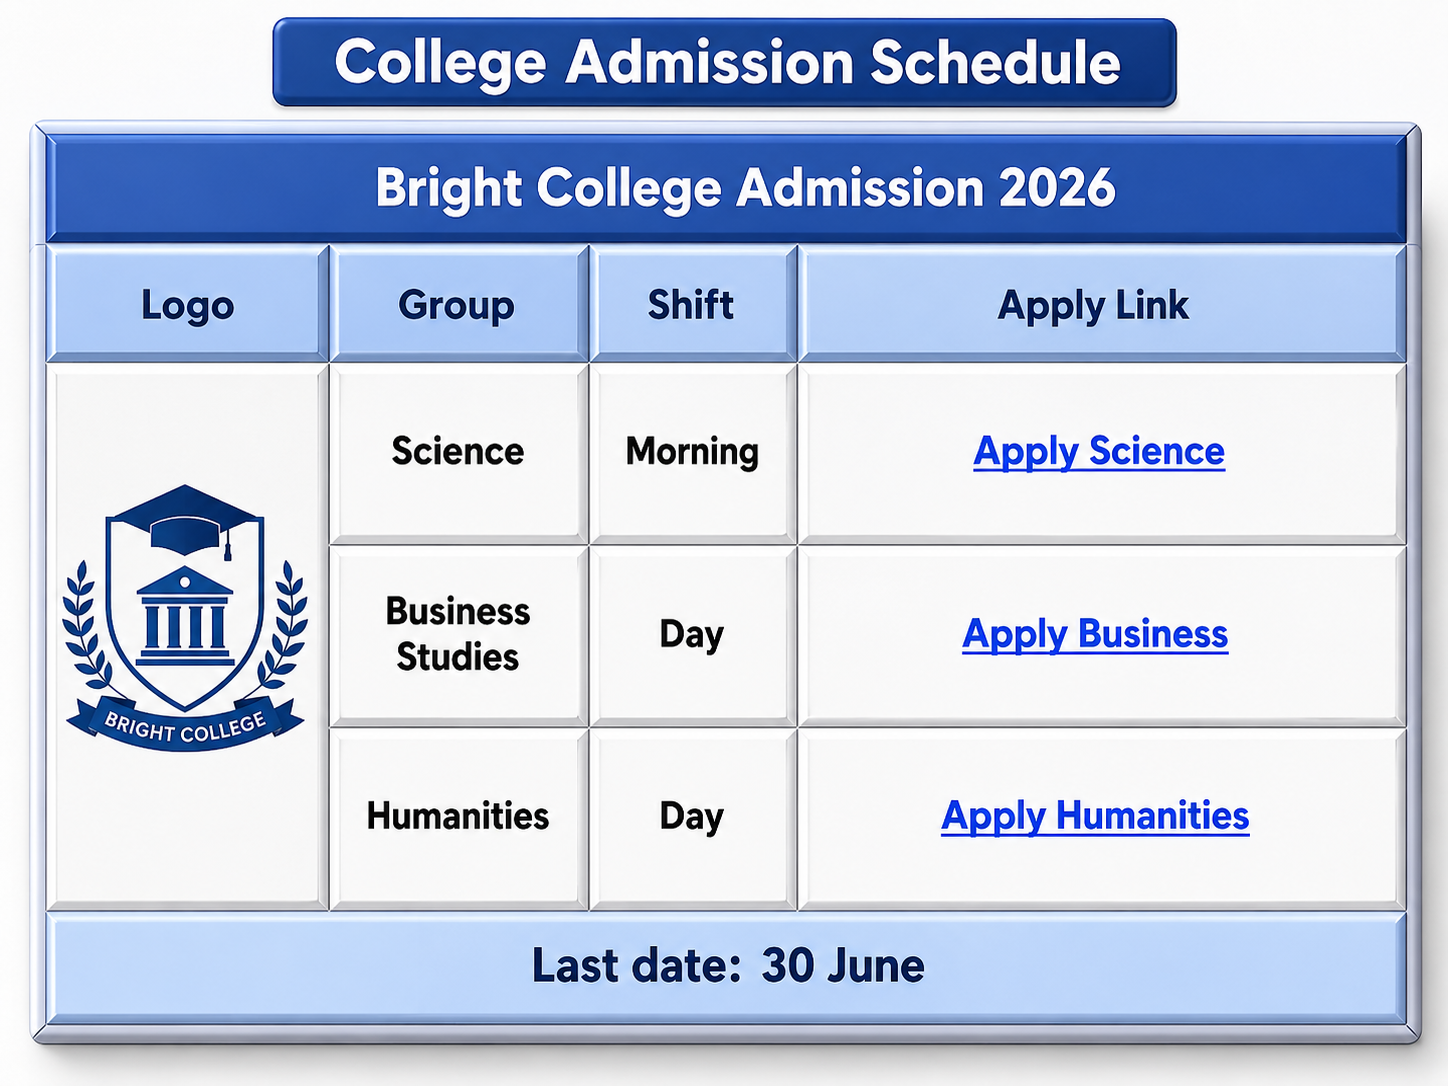
\includegraphics[width=0.95\linewidth,height=0.11\textheight,keepaspectratio]{chapters/Chapter04/topics/images/board_ex55_3d_admission_schedule.png}
}{
\fbox{\parbox{0.90\linewidth}{\centering\vspace{0.45cm}
\textbf{চিত্র}\\[3pt]
File: \texttt{chapters/Chapter04/topics/images/board\_ex55\_3d\_admission\_schedule.png}
\vspace{0.45cm}}}
}
\captionof{figure}{Admission Schedule with Logo, Link, Rowspan and Colspan}
\end{center}

\begin{keypointbox}{চিত্র ব্যাখ্যা}
এই example-এ logo image-এর জন্য rowspan, Apply Link অংশে colspan এবং শেষ row-তে full-width notice ব্যবহার করা হয়েছে।
\end{keypointbox}

\begin{keypointbox}{চিত্র দেখে code লেখার ধাপ}
প্রথমে figure-এর total row ও column গুনবে। এরপর কোন cell একাধিক column জুড়ে আছে তা দেখে \texttt{colspan} এবং কোন cell একাধিক row জুড়ে আছে তা দেখে \texttt{rowspan} বসাবে। তারপর image, link, list বা nested table থাকলে সংশ্লিষ্ট tag cell-এর ভিতরে লিখবে।
\end{keypointbox}

\par\noindent{\color{purple!70!black}\bfseries\small কোড}\par\vspace{-4pt}
\begin{verbatim}
<!DOCTYPE html>
<html>
<head>
  <title>HTML Table Example</title>
</head>
<body>
<table border="1" cellspacing="0" cellpadding="6" align="center">
  <caption><b>College Admission Schedule</b></caption>
  <tr>
    <th colspan="5">Bright College Admission 2026</th>
  </tr>
  <tr>
    <th>Logo</th>
    <th>Group</th>
    <th>Shift</th>
    <th colspan="2">Apply Link</th>
  </tr>
  <tr>
    <td rowspan="3"><img src="college_logo.png" width="80" height="80" alt="College Logo"></td>
    <td>Science</td>
    <td>Morning</td>
    <td colspan="2"><a href="apply_science.html">Apply Science</a></td>
  </tr>
  <tr>
    <td>Business Studies</td>
    <td>Day</td>
    <td colspan="2"><a href="apply_business.html">Apply Business</a></td>
  </tr>
  <tr>
    <td>Humanities</td>
    <td>Day</td>
    <td colspan="2"><a href="apply_humanities.html">Apply Humanities</a></td>
  </tr>
  <tr>
    <td colspan="5" align="center">Last date: 30 June</td>
  </tr>
</table>
</body>
</html>
\end{verbatim}
\vspace{-6pt}

\begin{keypointbox}{Board technique}
প্রথমে মোট row ও column গুনবে। তারপর কোন cell horizontal merge হলে \texttt{colspan} এবং vertical merge হলে \texttt{rowspan} ব্যবহার করবে। image-এর জন্য \texttt{<img>} এবং link-এর জন্য \texttt{<a>} tag ব্যবহার করবে।
\end{keypointbox}


\subsubsection{Example 56: Student Result with Compulsory and Optional Subjects}

\begin{center}
\IfFileExists{chapters/Chapter04/topics/images/board_ex56_3d_student_result_mixed.png}{
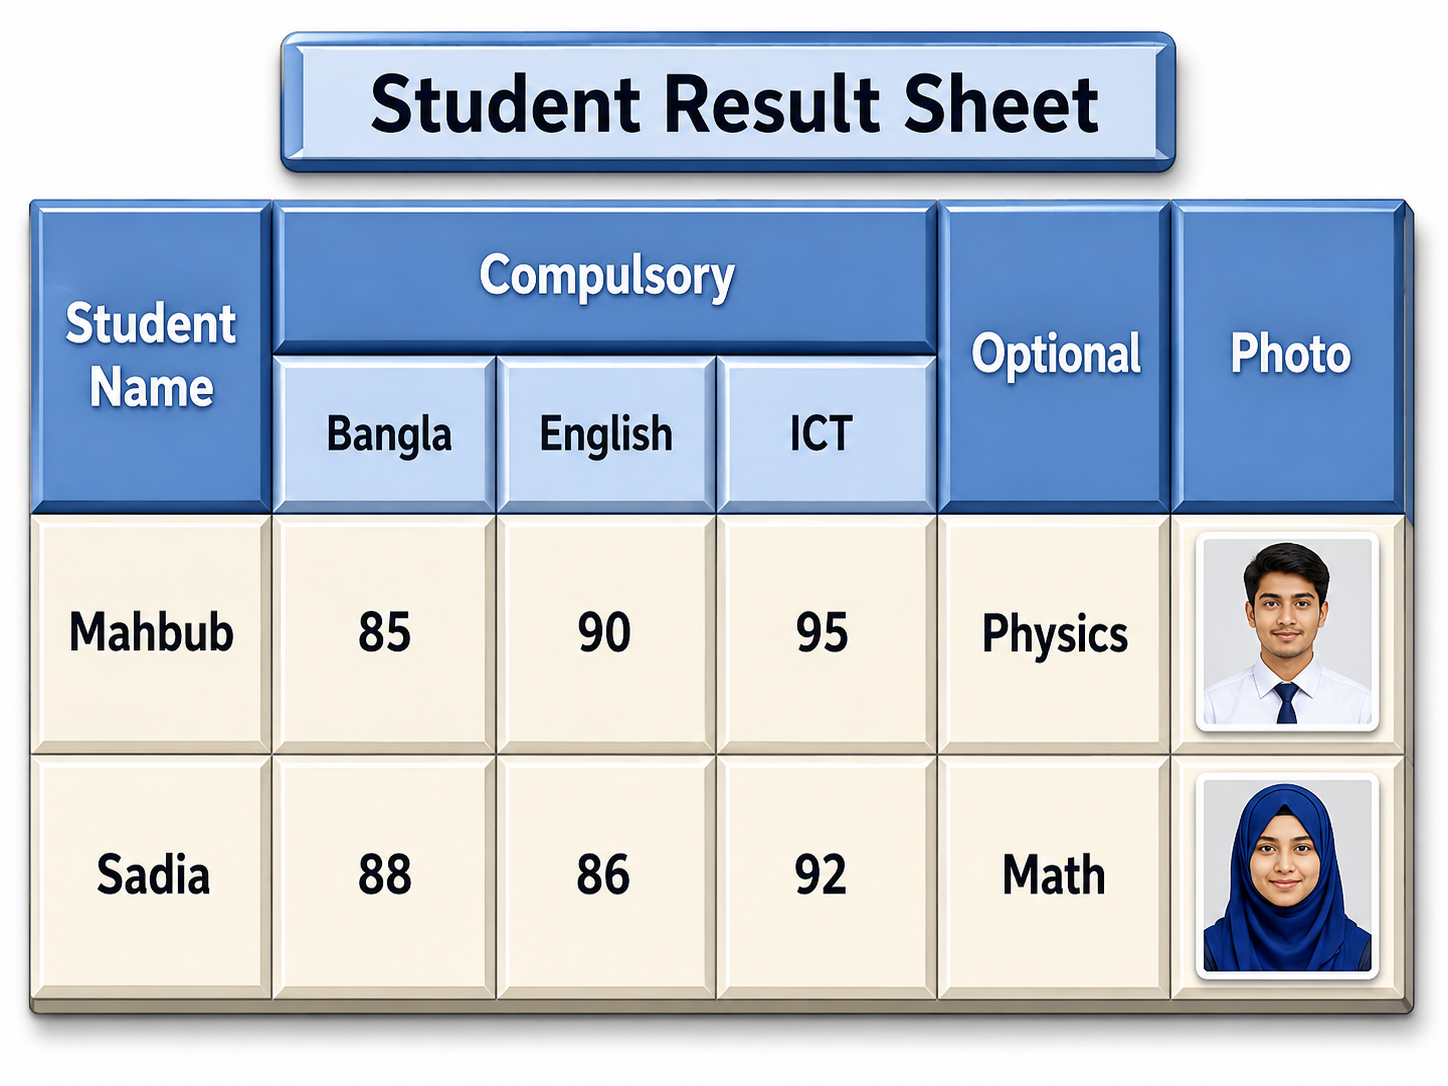
\includegraphics[width=0.95\linewidth,height=0.11\textheight,keepaspectratio]{chapters/Chapter04/topics/images/board_ex56_3d_student_result_mixed.png}
}{
\fbox{\parbox{0.90\linewidth}{\centering\vspace{0.45cm}
\textbf{চিত্র}\\[3pt]
File: \texttt{chapters/Chapter04/topics/images/board\_ex56\_3d\_student\_result\_mixed.png}
\vspace{0.45cm}}}
}
\captionof{figure}{Student Result with Compulsory and Optional Subjects}
\end{center}

\begin{keypointbox}{চিত্র ব্যাখ্যা}
এখানে Student Name, Optional ও Photo header দুই row জুড়ে আছে; Compulsory heading তিনটি column জুড়ে আছে।
\end{keypointbox}

\par\noindent{\color{purple!70!black}\bfseries\small কোড}\par\vspace{-4pt}
\begin{verbatim}
<!DOCTYPE html>
<html>
<head>
  <title>HTML Table Example</title>
</head>
<body>
<table border="1" cellspacing="0" cellpadding="5" align="center">
  <caption><b>Student Result Sheet</b></caption>
  <tr>
    <th rowspan="2">Student Name</th>
    <th colspan="3">Compulsory</th>
    <th rowspan="2">Optional</th>
    <th rowspan="2">Photo</th>
  </tr>
  <tr>
    <th>Bangla</th>
    <th>English</th>
    <th>ICT</th>
  </tr>
  <tr>
    <td>Mahbub</td>
    <td>85</td>
    <td>90</td>
    <td>95</td>
    <td>Physics</td>
    <td><img src="mahbub.jpg" width="60" height="70" alt="Mahbub"></td>
  </tr>
  <tr>
    <td>Sadia</td>
    <td>88</td>
    <td>86</td>
    <td>92</td>
    <td>Math</td>
    <td><img src="sadia.jpg" width="60" height="70" alt="Sadia"></td>
  </tr>
</table>
</body>
</html>
\end{verbatim}
\vspace{-6pt}

\begin{keypointbox}{Board technique}
প্রথমে মোট row ও column গুনবে। তারপর কোন cell horizontal merge হলে \texttt{colspan} এবং vertical merge হলে \texttt{rowspan} ব্যবহার করবে। image-এর জন্য \texttt{<img>} এবং link-এর জন্য \texttt{<a>} tag ব্যবহার করবে।
\end{keypointbox}


\subsubsection{Example 57: Product Catalog with Product Image and Buy Link}

\begin{center}
\IfFileExists{chapters/Chapter04/topics/images/board_ex57_3d_product_catalog_link.png}{
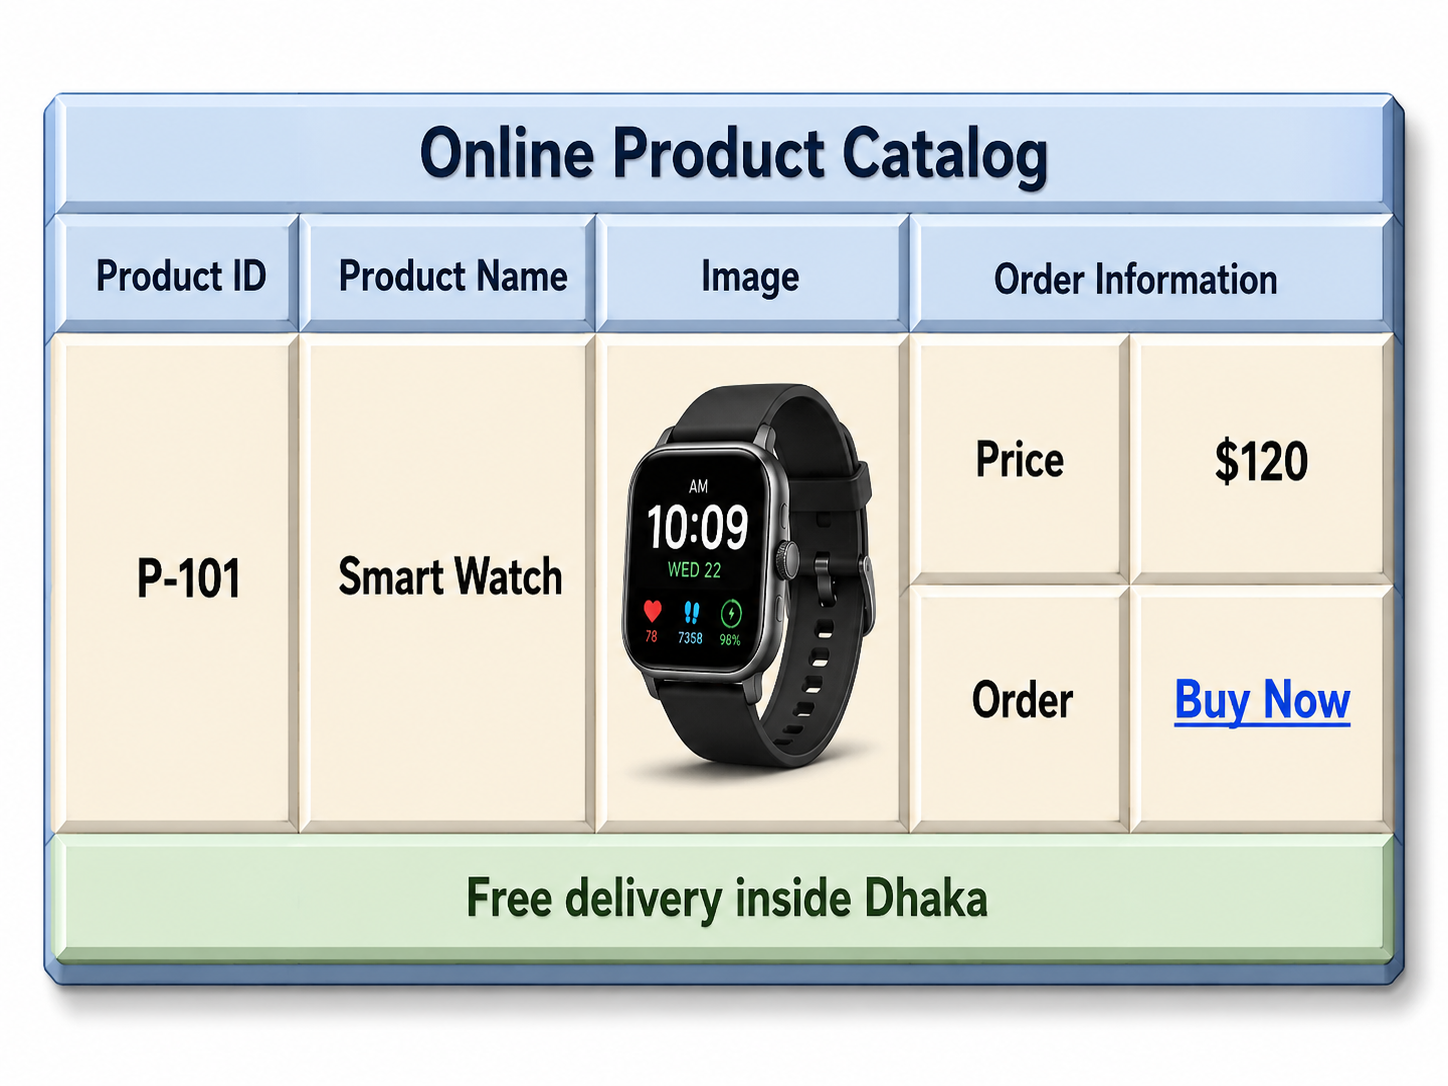
\includegraphics[width=0.95\linewidth,height=0.11\textheight,keepaspectratio]{chapters/Chapter04/topics/images/board_ex57_3d_product_catalog_link.png}
}{
\fbox{\parbox{0.90\linewidth}{\centering\vspace{0.45cm}
\textbf{চিত্র}\\[3pt]
File: \texttt{chapters/Chapter04/topics/images/board\_ex57\_3d\_product\_catalog\_link.png}
\vspace{0.45cm}}}
}
\captionof{figure}{Product Catalog with Product Image and Buy Link}
\end{center}

\begin{keypointbox}{চিত্র ব্যাখ্যা}
Product ID, Name ও Image দুই row জুড়ে রাখা হয়েছে। Order Information দুই column জুড়ে আছে।
\end{keypointbox}

\begin{keypointbox}{চিত্র দেখে code লেখার ধাপ}
প্রথমে figure-এর total row ও column গুনবে। এরপর কোন cell একাধিক column জুড়ে আছে তা দেখে \texttt{colspan} এবং কোন cell একাধিক row জুড়ে আছে তা দেখে \texttt{rowspan} বসাবে। তারপর image, link, list বা nested table থাকলে সংশ্লিষ্ট tag cell-এর ভিতরে লিখবে।
\end{keypointbox}

\par\noindent{\color{purple!70!black}\bfseries\small কোড}\par\vspace{-4pt}
\begin{verbatim}
<!DOCTYPE html>
<html>
<head>
  <title>HTML Table Example</title>
</head>
<body>
<table border="1" cellspacing="0" cellpadding="6" align="center">
  <caption><b>Online Product Catalog</b></caption>
  <tr>
    <th>Product ID</th>
    <th>Product Name</th>
    <th>Image</th>
    <th colspan="2">Order Information</th>
  </tr>
  <tr>
    <td rowspan="2">P-101</td>
    <td rowspan="2">Smart Watch</td>
    <td rowspan="2"><img src="watch.jpg" width="90" height="80" alt="Watch"></td>
    <td>Price</td>
    <td>$120</td>
  </tr>
  <tr>
    <td>Order</td>
    <td><a href="order_watch.html">Buy Now</a></td>
  </tr>
  <tr>
    <td colspan="5" align="center">Free delivery inside Dhaka</td>
  </tr>
</table>
</body>
</html>
\end{verbatim}
\vspace{-6pt}

\begin{keypointbox}{Board technique}
প্রথমে মোট row ও column গুনবে। তারপর কোন cell horizontal merge হলে \texttt{colspan} এবং vertical merge হলে \texttt{rowspan} ব্যবহার করবে। image-এর জন্য \texttt{<img>} এবং link-এর জন্য \texttt{<a>} tag ব্যবহার করবে।
\end{keypointbox}


\subsubsection{Example 58: Hospital Information Table with Picture and Emergency Link}

\begin{center}
\IfFileExists{chapters/Chapter04/topics/images/board_ex58_3d_hospital_info_table.png}{
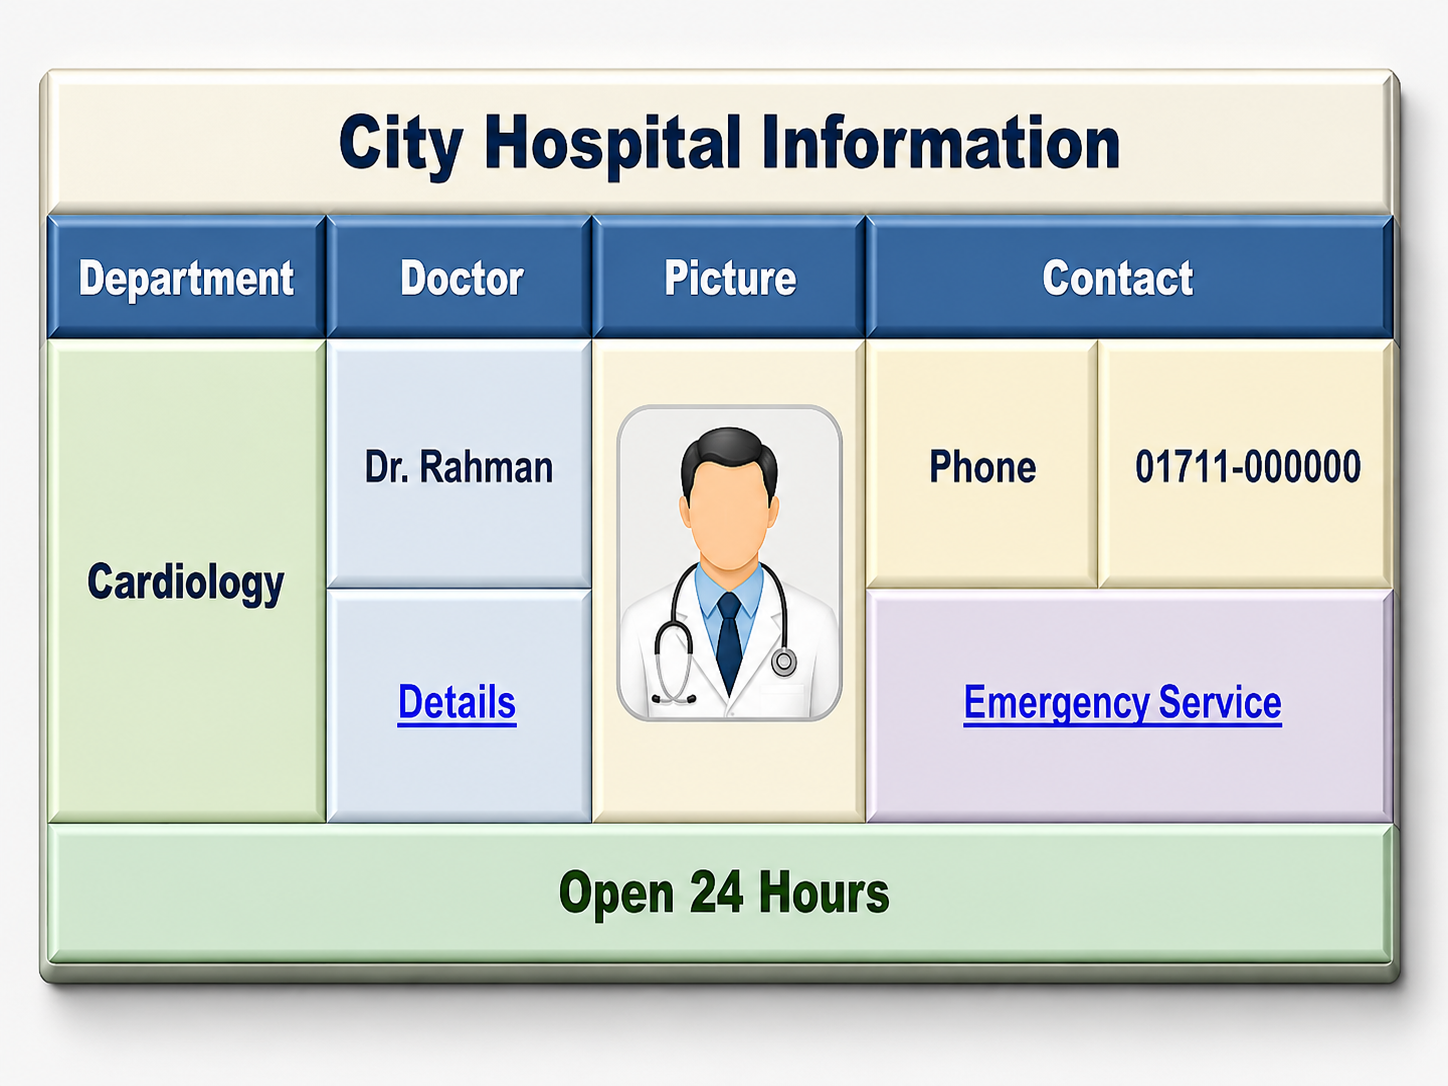
\includegraphics[width=0.95\linewidth,height=0.11\textheight,keepaspectratio]{chapters/Chapter04/topics/images/board_ex58_3d_hospital_info_table.png}
}{
\fbox{\parbox{0.90\linewidth}{\centering\vspace{0.45cm}
\textbf{চিত্র}\\[3pt]
File: \texttt{chapters/Chapter04/topics/images/board\_ex58\_3d\_hospital\_info\_table.png}
\vspace{0.45cm}}}
}
\captionof{figure}{Hospital Information Table with Picture and Emergency Link}
\end{center}

\begin{keypointbox}{চিত্র ব্যাখ্যা}
Cardiology cell এবং doctor image দুই row জুড়ে আছে। Emergency Service link দুইটি contact column জুড়ে দেওয়া হয়েছে।
\end{keypointbox}

\par\noindent{\color{purple!70!black}\bfseries\small কোড}\par\vspace{-4pt}
\begin{verbatim}
<!DOCTYPE html>
<html>
<head>
  <title>HTML Table Example</title>
</head>
<body>
<table border="1" cellspacing="0" cellpadding="6" align="center">
  <caption><b>City Hospital Information</b></caption>
  <tr>
    <th>Department</th>
    <th>Doctor</th>
    <th>Picture</th>
    <th colspan="2">Contact</th>
  </tr>
  <tr>
    <td rowspan="2">Cardiology</td>
    <td>Dr. Rahman</td>
    <td rowspan="2"><img src="doctor.jpg" width="80" height="90" alt="Doctor"></td>
    <td>Phone</td>
    <td>01711-000000</td>
  </tr>
  <tr>
    <td><a href="cardiology.html">Details</a></td>
    <td colspan="2"><a href="emergency.html">Emergency Service</a></td>
  </tr>
  <tr>
    <td colspan="5" align="center">Open 24 Hours</td>
  </tr>
</table>
</body>
</html>
\end{verbatim}
\vspace{-6pt}

\begin{keypointbox}{Board technique}
প্রথমে মোট row ও column গুনবে। তারপর কোন cell horizontal merge হলে \texttt{colspan} এবং vertical merge হলে \texttt{rowspan} ব্যবহার করবে। image-এর জন্য \texttt{<img>} এবং link-এর জন্য \texttt{<a>} tag ব্যবহার করবে।
\end{keypointbox}


\subsubsection{Example 59: Tourism Table with Place Image and Website Link}

\begin{center}
\IfFileExists{chapters/Chapter04/topics/images/board_ex59_3d_tourism_places_link.png}{
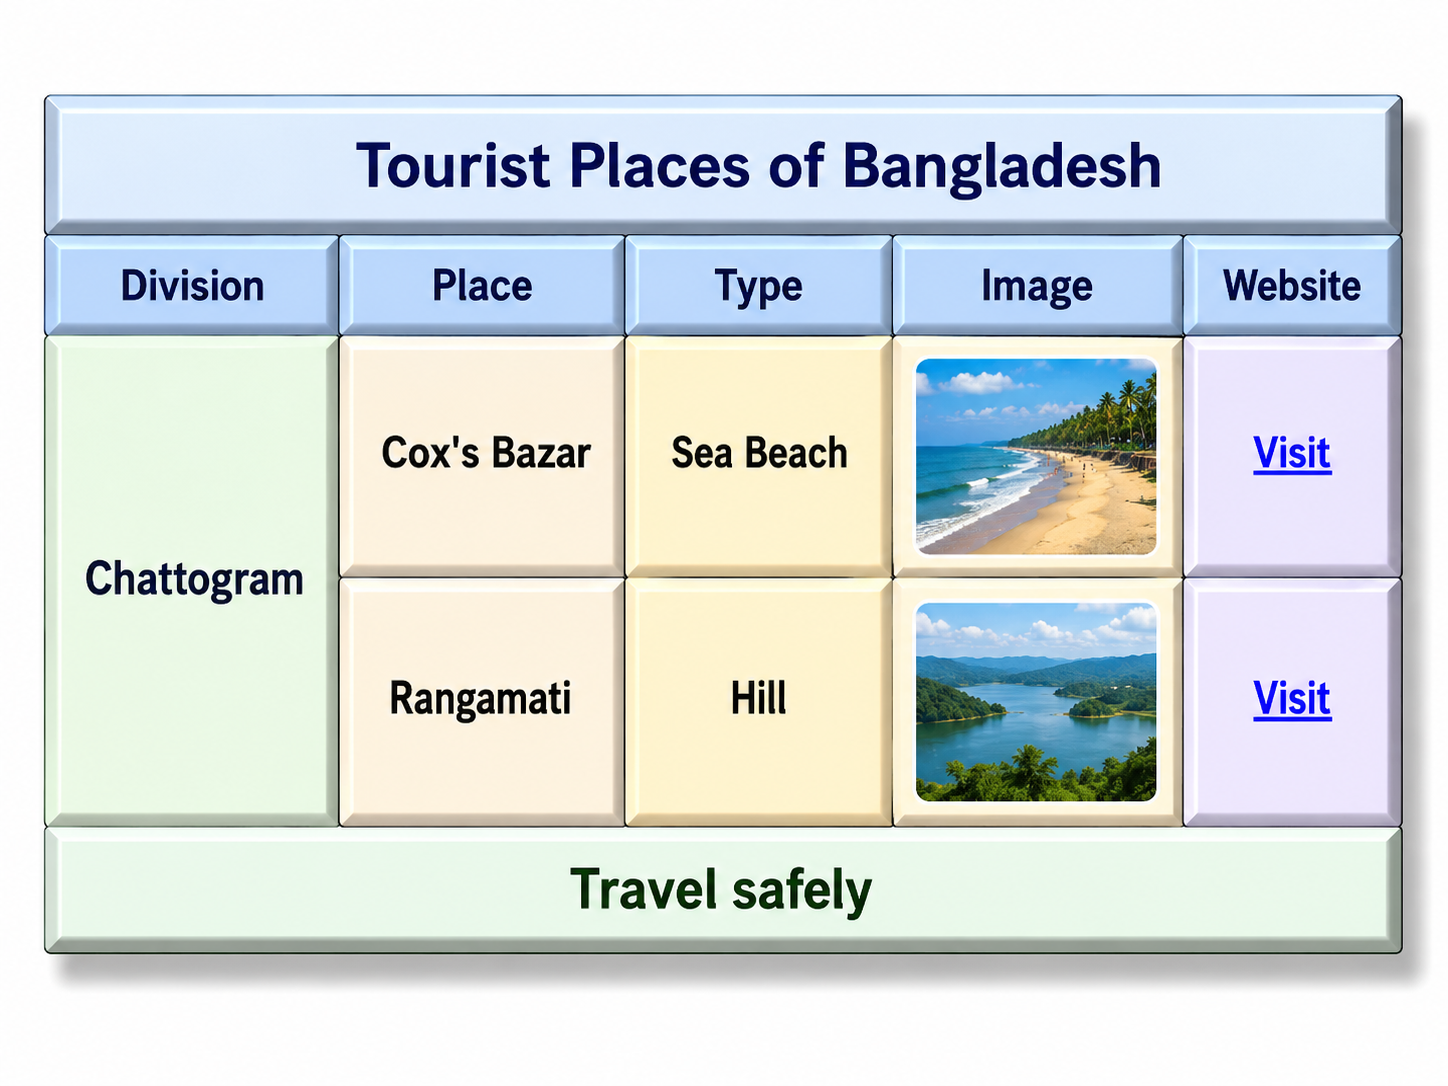
\includegraphics[width=0.95\linewidth,height=0.11\textheight,keepaspectratio]{chapters/Chapter04/topics/images/board_ex59_3d_tourism_places_link.png}
}{
\fbox{\parbox{0.90\linewidth}{\centering\vspace{0.45cm}
\textbf{চিত্র}\\[3pt]
File: \texttt{chapters/Chapter04/topics/images/board\_ex59\_3d\_tourism\_places\_link.png}
\vspace{0.45cm}}}
}
\captionof{figure}{Tourism Table with Place Image and Website Link}
\end{center}

\begin{keypointbox}{চিত্র ব্যাখ্যা}
Division cell rowspan দিয়ে দুই place-এর জন্য common করা হয়েছে। প্রতিটি place-এর image ও link আলাদা cell-এ আছে।
\end{keypointbox}

\begin{keypointbox}{চিত্র দেখে code লেখার ধাপ}
প্রথমে figure-এর total row ও column গুনবে। এরপর কোন cell একাধিক column জুড়ে আছে তা দেখে \texttt{colspan} এবং কোন cell একাধিক row জুড়ে আছে তা দেখে \texttt{rowspan} বসাবে। তারপর image, link, list বা nested table থাকলে সংশ্লিষ্ট tag cell-এর ভিতরে লিখবে।
\end{keypointbox}

\par\noindent{\color{purple!70!black}\bfseries\small কোড}\par\vspace{-4pt}
\begin{verbatim}
<!DOCTYPE html>
<html>
<head>
  <title>HTML Table Example</title>
</head>
<body>
<table border="1" cellspacing="0" cellpadding="5" align="center">
  <caption><b>Tourist Places of Bangladesh</b></caption>
  <tr>
    <th>Division</th>
    <th>Place</th>
    <th>Type</th>
    <th>Image</th>
    <th>Website</th>
  </tr>
  <tr>
    <td rowspan="2">Chattogram</td>
    <td>Cox's Bazar</td>
    <td>Sea Beach</td>
    <td><img src="cox.jpg" width="80" height="60" alt="Cox's Bazar"></td>
    <td><a href="cox.html">Visit</a></td>
  </tr>
  <tr>
    <td>Rangamati</td>
    <td>Hill</td>
    <td><img src="rangamati.jpg" width="80" height="60" alt="Rangamati"></td>
    <td><a href="rangamati.html">Visit</a></td>
  </tr>
  <tr>
    <td colspan="5" align="center">Travel safely</td>
  </tr>
</table>
</body>
</html>
\end{verbatim}
\vspace{-6pt}

\begin{keypointbox}{Board technique}
প্রথমে মোট row ও column গুনবে। তারপর কোন cell horizontal merge হলে \texttt{colspan} এবং vertical merge হলে \texttt{rowspan} ব্যবহার করবে। image-এর জন্য \texttt{<img>} এবং link-এর জন্য \texttt{<a>} tag ব্যবহার করবে।
\end{keypointbox}


\subsubsection{Example 60: Course Plan Table with List, Link and Colspan}

\begin{center}
\IfFileExists{chapters/Chapter04/topics/images/board_ex60_3d_course_plan_list_link.png}{
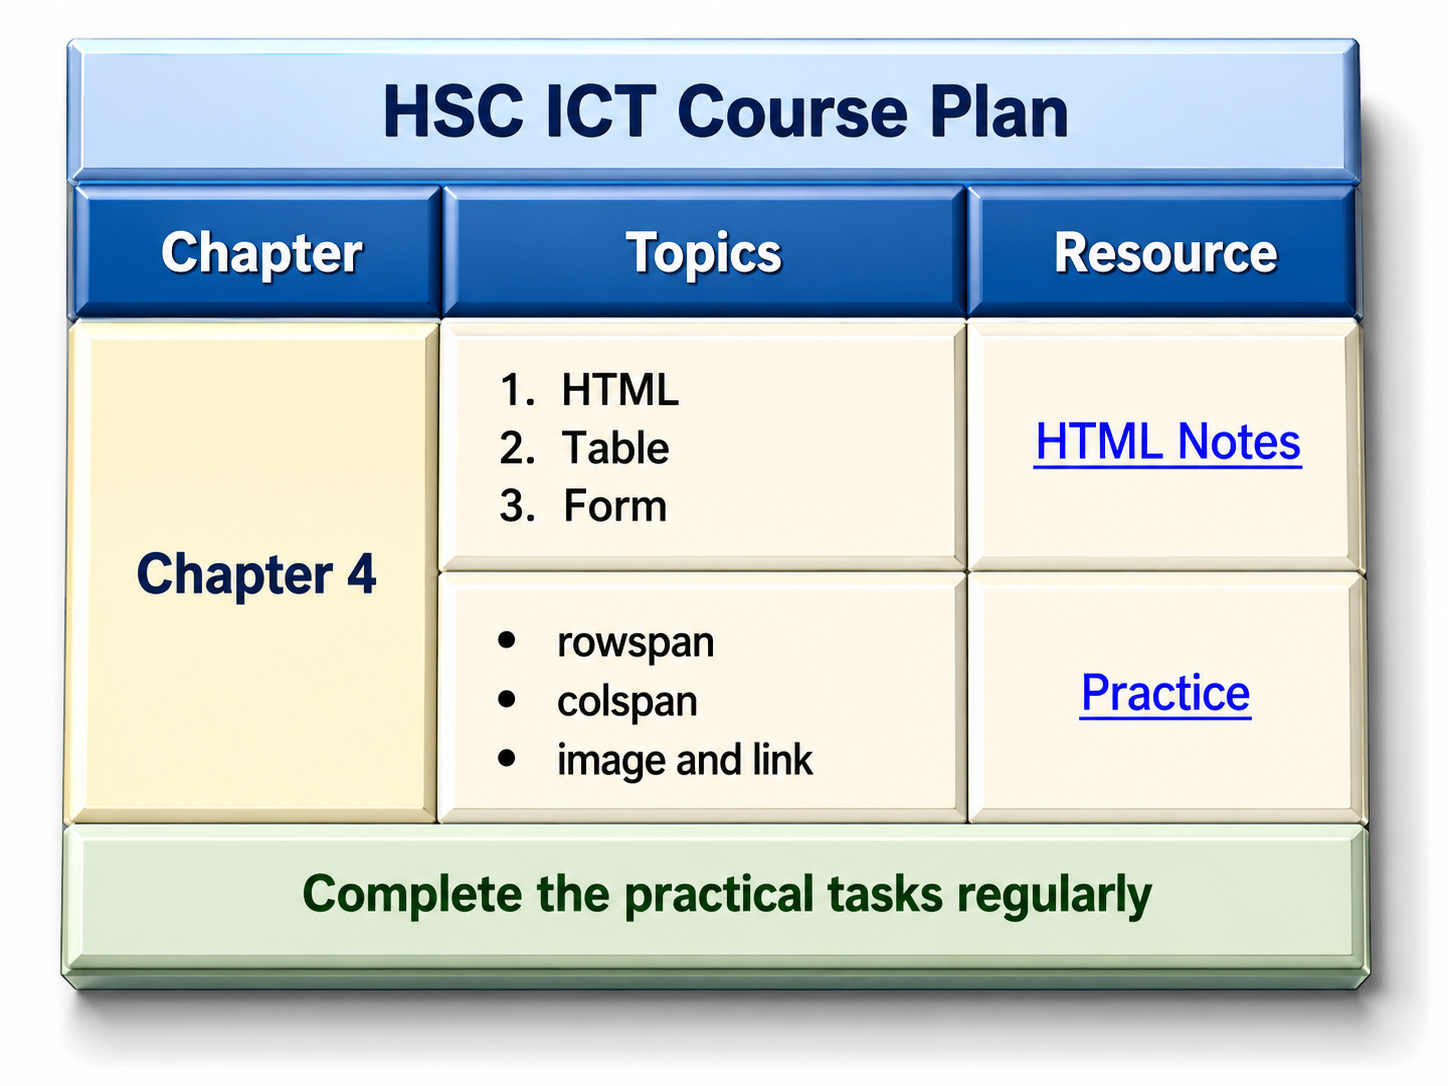
\includegraphics[width=0.95\linewidth,height=0.11\textheight,keepaspectratio]{chapters/Chapter04/topics/images/board_ex60_3d_course_plan_list_link.png}
}{
\fbox{\parbox{0.90\linewidth}{\centering\vspace{0.45cm}
\textbf{চিত্র}\\[3pt]
File: \texttt{chapters/Chapter04/topics/images/board\_ex60\_3d\_course\_plan\_list\_link.png}
\vspace{0.45cm}}}
}
\captionof{figure}{Course Plan Table with List, Link and Colspan}
\end{center}

\begin{keypointbox}{চিত্র ব্যাখ্যা}
একই table cell-এর ভিতরে ordered list ও unordered list রাখা হয়েছে, সাথে hyperlink ও colspan notice আছে।
\end{keypointbox}

\par\noindent{\color{purple!70!black}\bfseries\small কোড}\par\vspace{-4pt}
\begin{verbatim}
<!DOCTYPE html>
<html>
<head>
  <title>HTML Table Example</title>
</head>
<body>
<table border="1" cellspacing="0" cellpadding="6" align="center">
  <caption><b>HSC ICT Course Plan</b></caption>
  <tr>
    <th>Chapter</th>
    <th>Topics</th>
    <th>Resource</th>
  </tr>
  <tr>
    <td rowspan="2">Chapter 4</td>
    <td>
      <ol>
        <li>HTML</li>
        <li>Table</li>
        <li>Form</li>
      </ol>
    </td>
    <td><a href="html_notes.html">HTML Notes</a></td>
  </tr>
  <tr>
    <td>
      <ul>
        <li>rowspan</li>
        <li>colspan</li>
        <li>image and link</li>
      </ul>
    </td>
    <td><a href="practice.html">Practice</a></td>
  </tr>
  <tr>
    <td colspan="3" align="center">Complete the practical tasks regularly</td>
  </tr>
</table>
</body>
</html>
\end{verbatim}
\vspace{-6pt}

\begin{keypointbox}{Board technique}
প্রথমে মোট row ও column গুনবে। তারপর কোন cell horizontal merge হলে \texttt{colspan} এবং vertical merge হলে \texttt{rowspan} ব্যবহার করবে। image-এর জন্য \texttt{<img>} এবং link-এর জন্য \texttt{<a>} tag ব্যবহার করবে।
\end{keypointbox}


\subsubsection{Example 61: Library Book Table with Cover Image and Download Link}

\begin{center}
\IfFileExists{chapters/Chapter04/topics/images/board_ex61_3d_library_book_table.png}{
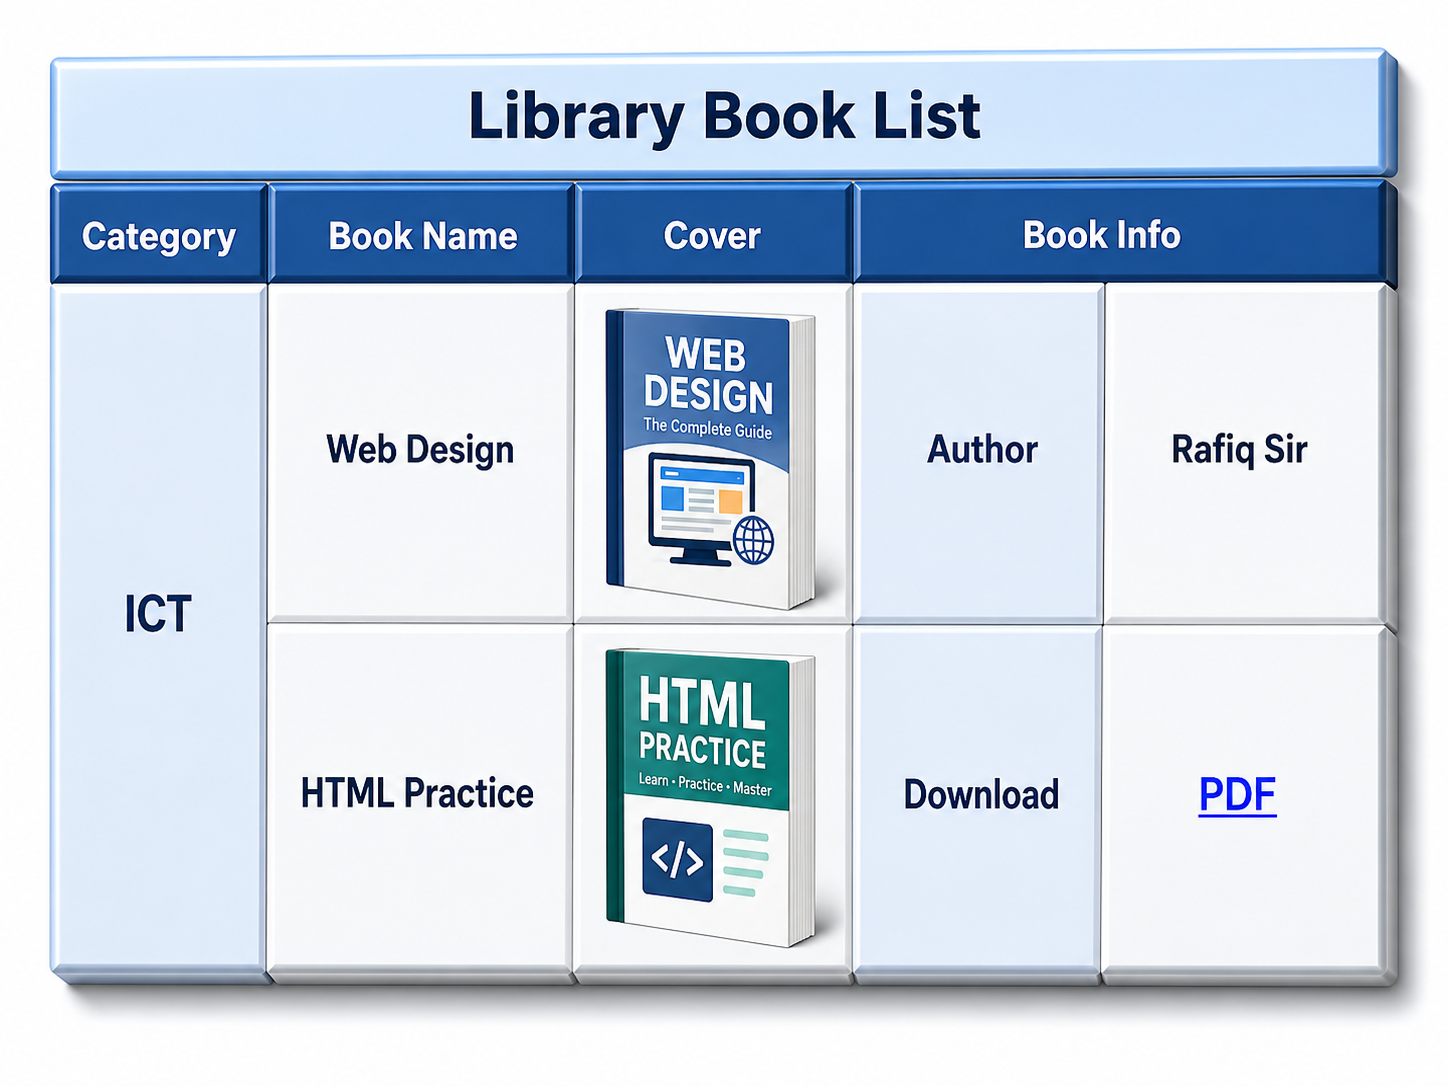
\includegraphics[width=0.95\linewidth,height=0.11\textheight,keepaspectratio]{chapters/Chapter04/topics/images/board_ex61_3d_library_book_table.png}
}{
\fbox{\parbox{0.90\linewidth}{\centering\vspace{0.45cm}
\textbf{চিত্র}\\[3pt]
File: \texttt{chapters/Chapter04/topics/images/board\_ex61\_3d\_library\_book\_table.png}
\vspace{0.45cm}}}
}
\captionof{figure}{Library Book Table with Cover Image and Download Link}
\end{center}

\begin{keypointbox}{চিত্র ব্যাখ্যা}
Category rowspan দিয়ে দুই বইকে একই category-তে দেখানো হয়েছে। Cover image ও PDF link দুই ধরনের content দেখানো হয়েছে।
\end{keypointbox}

\begin{keypointbox}{চিত্র দেখে code লেখার ধাপ}
প্রথমে figure-এর total row ও column গুনবে। এরপর কোন cell একাধিক column জুড়ে আছে তা দেখে \texttt{colspan} এবং কোন cell একাধিক row জুড়ে আছে তা দেখে \texttt{rowspan} বসাবে। তারপর image, link, list বা nested table থাকলে সংশ্লিষ্ট tag cell-এর ভিতরে লিখবে।
\end{keypointbox}

\par\noindent{\color{purple!70!black}\bfseries\small কোড}\par\vspace{-4pt}
\begin{verbatim}
<!DOCTYPE html>
<html>
<head>
  <title>HTML Table Example</title>
</head>
<body>
<table border="1" cellspacing="0" cellpadding="6" align="center">
  <caption><b>Library Book List</b></caption>
  <tr>
    <th>Category</th>
    <th>Book Name</th>
    <th>Cover</th>
    <th colspan="2">Book Info</th>
  </tr>
  <tr>
    <td rowspan="2">ICT</td>
    <td>Web Design</td>
    <td><img src="web_book.jpg" width="70" height="90" alt="Web Book"></td>
    <td>Author</td>
    <td>Rafiq Sir</td>
  </tr>
  <tr>
    <td>HTML Practice</td>
    <td><img src="html_book.jpg" width="70" height="90" alt="HTML Book"></td>
    <td>Download</td>
    <td><a href="html_practice.pdf">PDF</a></td>
  </tr>
</table>
</body>
</html>
\end{verbatim}
\vspace{-6pt}

\begin{keypointbox}{Board technique}
প্রথমে মোট row ও column গুনবে। তারপর কোন cell horizontal merge হলে \texttt{colspan} এবং vertical merge হলে \texttt{rowspan} ব্যবহার করবে। image-এর জন্য \texttt{<img>} এবং link-এর জন্য \texttt{<a>} tag ব্যবহার করবে।
\end{keypointbox}


\subsubsection{Example 62: Exam Routine with Date Rowspan and Subject Colspan}

\begin{center}
\IfFileExists{chapters/Chapter04/topics/images/board_ex62_3d_exam_routine_table.png}{
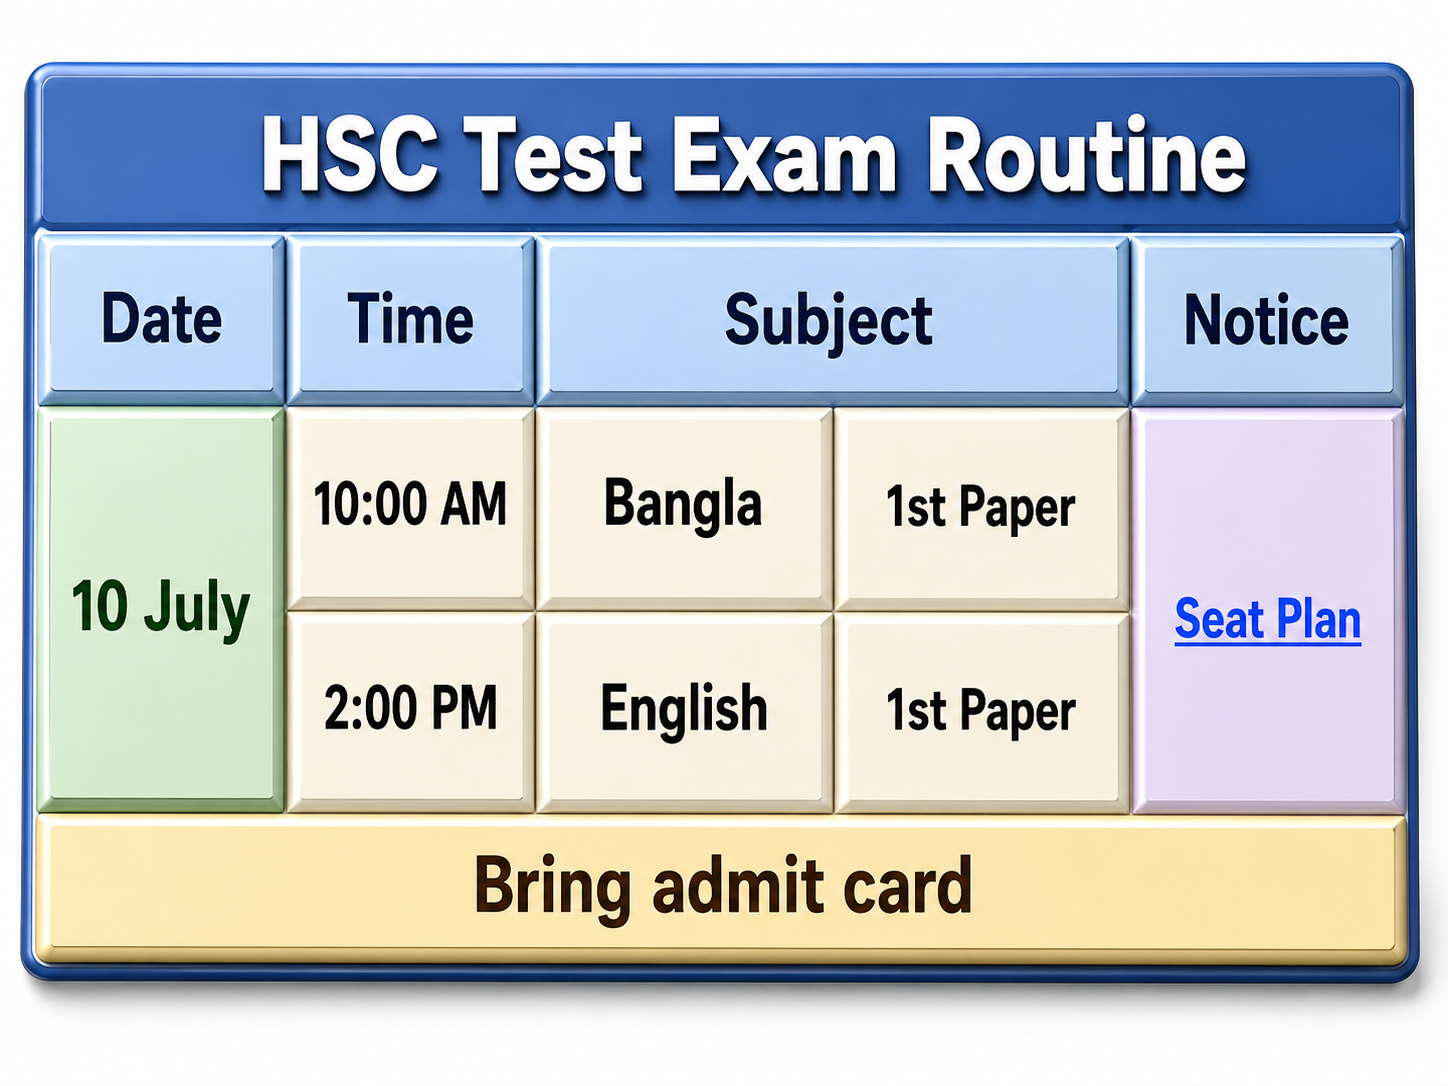
\includegraphics[width=0.95\linewidth,height=0.11\textheight,keepaspectratio]{chapters/Chapter04/topics/images/board_ex62_3d_exam_routine_table.png}
}{
\fbox{\parbox{0.90\linewidth}{\centering\vspace{0.45cm}
\textbf{চিত্র}\\[3pt]
File: \texttt{chapters/Chapter04/topics/images/board\_ex62\_3d\_exam\_routine\_table.png}
\vspace{0.45cm}}}
}
\captionof{figure}{Exam Routine with Date Rowspan and Subject Colspan}
\end{center}

\begin{keypointbox}{চিত্র ব্যাখ্যা}
একই তারিখের দুই exam দেখাতে Date এবং Notice cell-এ rowspan ব্যবহার করা হয়েছে। Subject heading দুই column জুড়ে আছে।
\end{keypointbox}

\par\noindent{\color{purple!70!black}\bfseries\small কোড}\par\vspace{-4pt}
\begin{verbatim}
<!DOCTYPE html>
<html>
<head>
  <title>HTML Table Example</title>
</head>
<body>
<table border="1" cellspacing="0" cellpadding="6" align="center">
  <caption><b>HSC Test Exam Routine</b></caption>
  <tr>
    <th>Date</th>
    <th>Time</th>
    <th colspan="2">Subject</th>
    <th>Notice</th>
  </tr>
  <tr>
    <td rowspan="2">10 July</td>
    <td>10:00 AM</td>
    <td>Bangla</td>
    <td>1st Paper</td>
    <td rowspan="2"><a href="seat_plan.html">Seat Plan</a></td>
  </tr>
  <tr>
    <td>2:00 PM</td>
    <td>English</td>
    <td>1st Paper</td>
  </tr>
  <tr>
    <td colspan="5" align="center">Bring admit card</td>
  </tr>
</table>
</body>
</html>
\end{verbatim}
\vspace{-6pt}

\begin{keypointbox}{Board technique}
প্রথমে মোট row ও column গুনবে। তারপর কোন cell horizontal merge হলে \texttt{colspan} এবং vertical merge হলে \texttt{rowspan} ব্যবহার করবে। image-এর জন্য \texttt{<img>} এবং link-এর জন্য \texttt{<a>} tag ব্যবহার করবে।
\end{keypointbox}


\subsubsection{Example 63: ICT Lab Inventory with Device Image and Manual Link}

\begin{center}
\IfFileExists{chapters/Chapter04/topics/images/board_ex63_3d_lab_inventory_table.png}{
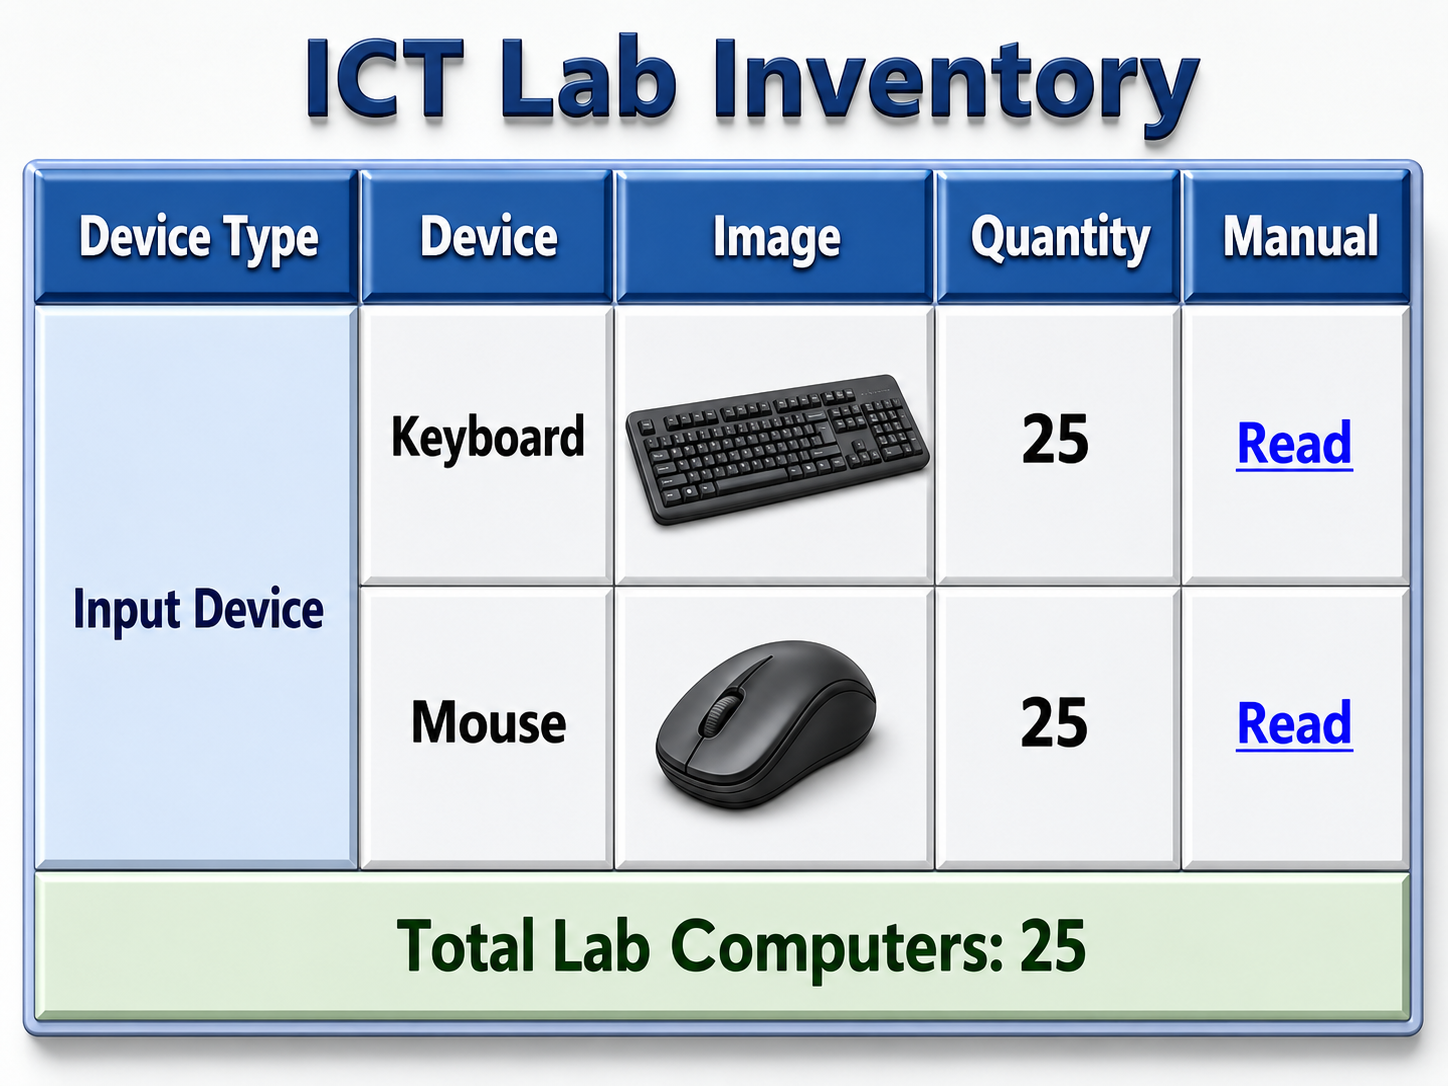
\includegraphics[width=0.95\linewidth,height=0.11\textheight,keepaspectratio]{chapters/Chapter04/topics/images/board_ex63_3d_lab_inventory_table.png}
}{
\fbox{\parbox{0.90\linewidth}{\centering\vspace{0.45cm}
\textbf{চিত্র}\\[3pt]
File: \texttt{chapters/Chapter04/topics/images/board\_ex63\_3d\_lab\_inventory\_table.png}
\vspace{0.45cm}}}
}
\captionof{figure}{ICT Lab Inventory with Device Image and Manual Link}
\end{center}

\begin{keypointbox}{চিত্র ব্যাখ্যা}
Device Type rowspan দিয়ে দুই input device group করা হয়েছে। প্রতিটি device-এর image ও manual link আছে।
\end{keypointbox}

\begin{keypointbox}{চিত্র দেখে code লেখার ধাপ}
প্রথমে figure-এর total row ও column গুনবে। এরপর কোন cell একাধিক column জুড়ে আছে তা দেখে \texttt{colspan} এবং কোন cell একাধিক row জুড়ে আছে তা দেখে \texttt{rowspan} বসাবে। তারপর image, link, list বা nested table থাকলে সংশ্লিষ্ট tag cell-এর ভিতরে লিখবে।
\end{keypointbox}

\par\noindent{\color{purple!70!black}\bfseries\small কোড}\par\vspace{-4pt}
\begin{verbatim}
<!DOCTYPE html>
<html>
<head>
  <title>HTML Table Example</title>
</head>
<body>
<table border="1" cellspacing="0" cellpadding="6" align="center">
  <caption><b>ICT Lab Inventory</b></caption>
  <tr>
    <th>Device Type</th>
    <th>Device</th>
    <th>Image</th>
    <th>Quantity</th>
    <th>Manual</th>
  </tr>
  <tr>
    <td rowspan="2">Input Device</td>
    <td>Keyboard</td>
    <td><img src="keyboard.jpg" width="80" height="50" alt="Keyboard"></td>
    <td>25</td>
    <td><a href="keyboard.html">Read</a></td>
  </tr>
  <tr>
    <td>Mouse</td>
    <td><img src="mouse.jpg" width="80" height="50" alt="Mouse"></td>
    <td>25</td>
    <td><a href="mouse.html">Read</a></td>
  </tr>
  <tr>
    <td colspan="5" align="center">Total Lab Computers: 25</td>
  </tr>
</table>
</body>
</html>
\end{verbatim}
\vspace{-6pt}

\begin{keypointbox}{Board technique}
প্রথমে মোট row ও column গুনবে। তারপর কোন cell horizontal merge হলে \texttt{colspan} এবং vertical merge হলে \texttt{rowspan} ব্যবহার করবে। image-এর জন্য \texttt{<img>} এবং link-এর জন্য \texttt{<a>} tag ব্যবহার করবে।
\end{keypointbox}


\subsubsection{Example 64: Restaurant Menu with Specials, Image, Link and Colspan}

\begin{center}
\IfFileExists{chapters/Chapter04/topics/images/board_ex64_3d_restaurant_menu_mixed.png}{
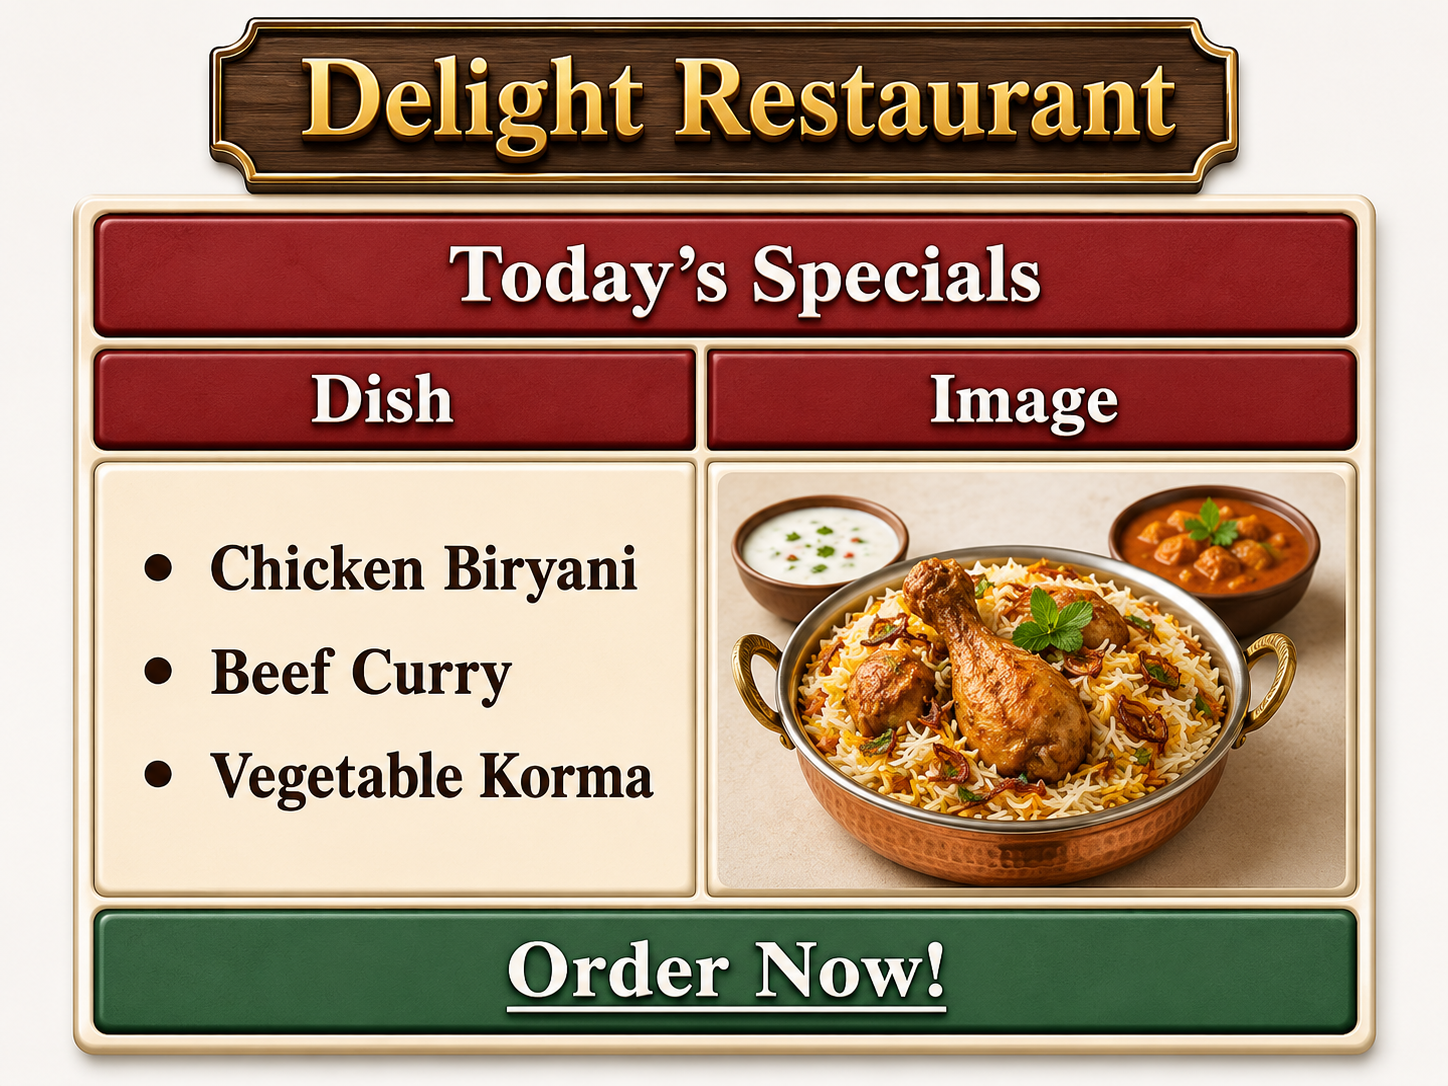
\includegraphics[width=0.95\linewidth,height=0.11\textheight,keepaspectratio]{chapters/Chapter04/topics/images/board_ex64_3d_restaurant_menu_mixed.png}
}{
\fbox{\parbox{0.90\linewidth}{\centering\vspace{0.45cm}
\textbf{চিত্র}\\[3pt]
File: \texttt{chapters/Chapter04/topics/images/board\_ex64\_3d\_restaurant\_menu\_mixed.png}
\vspace{0.45cm}}}
}
\captionof{figure}{Restaurant menu with specials, image and colspan}
\end{center}

\begin{keypointbox}{চিত্র ব্যাখ্যা}
চিত্রে Delight Restaurant heading, Today's Specials title row, Dish ও Image দুইটি column, item list, food image এবং নিচে full-width Order Now row আছে।
\end{keypointbox}

\begin{keypointbox}{চিত্র দেখে code লেখার ধাপ}
প্রথমে restaurant heading লিখবে। তারপর two-column table বানাবে। Today's Specials row এবং Order Now row দুই column জুড়ে থাকবে, তাই দুই জায়গায় \texttt{colspan="2"} ব্যবহার করবে। Dish cell-এ list/line break এবং Image cell-এ \texttt{<img>} tag বসাবে।
\end{keypointbox}

\par\noindent{\color{purple!70!black}\bfseries\small কোড}\par\vspace{-4pt}
\begin{verbatim}
<!DOCTYPE html>
<html>
<head>
  <title>HTML Table Example</title>
</head>
<body>
<h2 align="center">Delight Restaurant</h2>
<table border="1" cellspacing="0" cellpadding="8" align="center">
  <tr>
    <th colspan="2">Today's Specials</th>
  </tr>
  <tr>
    <th>Dish</th>
    <th>Image</th>
  </tr>
  <tr>
    <td>
      <ul>
        <li>Chicken Biryani</li>
        <li>Beef Curry</li>
        <li>Vegetable Korma</li>
      </ul>
    </td>
    <td><img src="food.jpg" width="100" height="80" alt="Food"></td>
  </tr>
  <tr>
    <td colspan="2" align="center"><a href="order.html">Order Now!</a></td>
  </tr>
</table>
</body>
</html>
\end{verbatim}
\vspace{-6pt}

\begin{keypointbox}{Board technique}
প্রথমে মোট row ও column গুনবে। তারপর কোন cell horizontal merge হলে \texttt{colspan} এবং vertical merge হলে \texttt{rowspan} ব্যবহার করবে। image-এর জন্য \texttt{<img>} এবং link-এর জন্য \texttt{<a>} tag ব্যবহার করবে।
\end{keypointbox}

\subsubsection{Example 65: Student Club Table with Rowspan and Image Icon}

\begin{center}
\IfFileExists{chapters/Chapter04/topics/images/board_ex65_3d_student_club_table.png}{
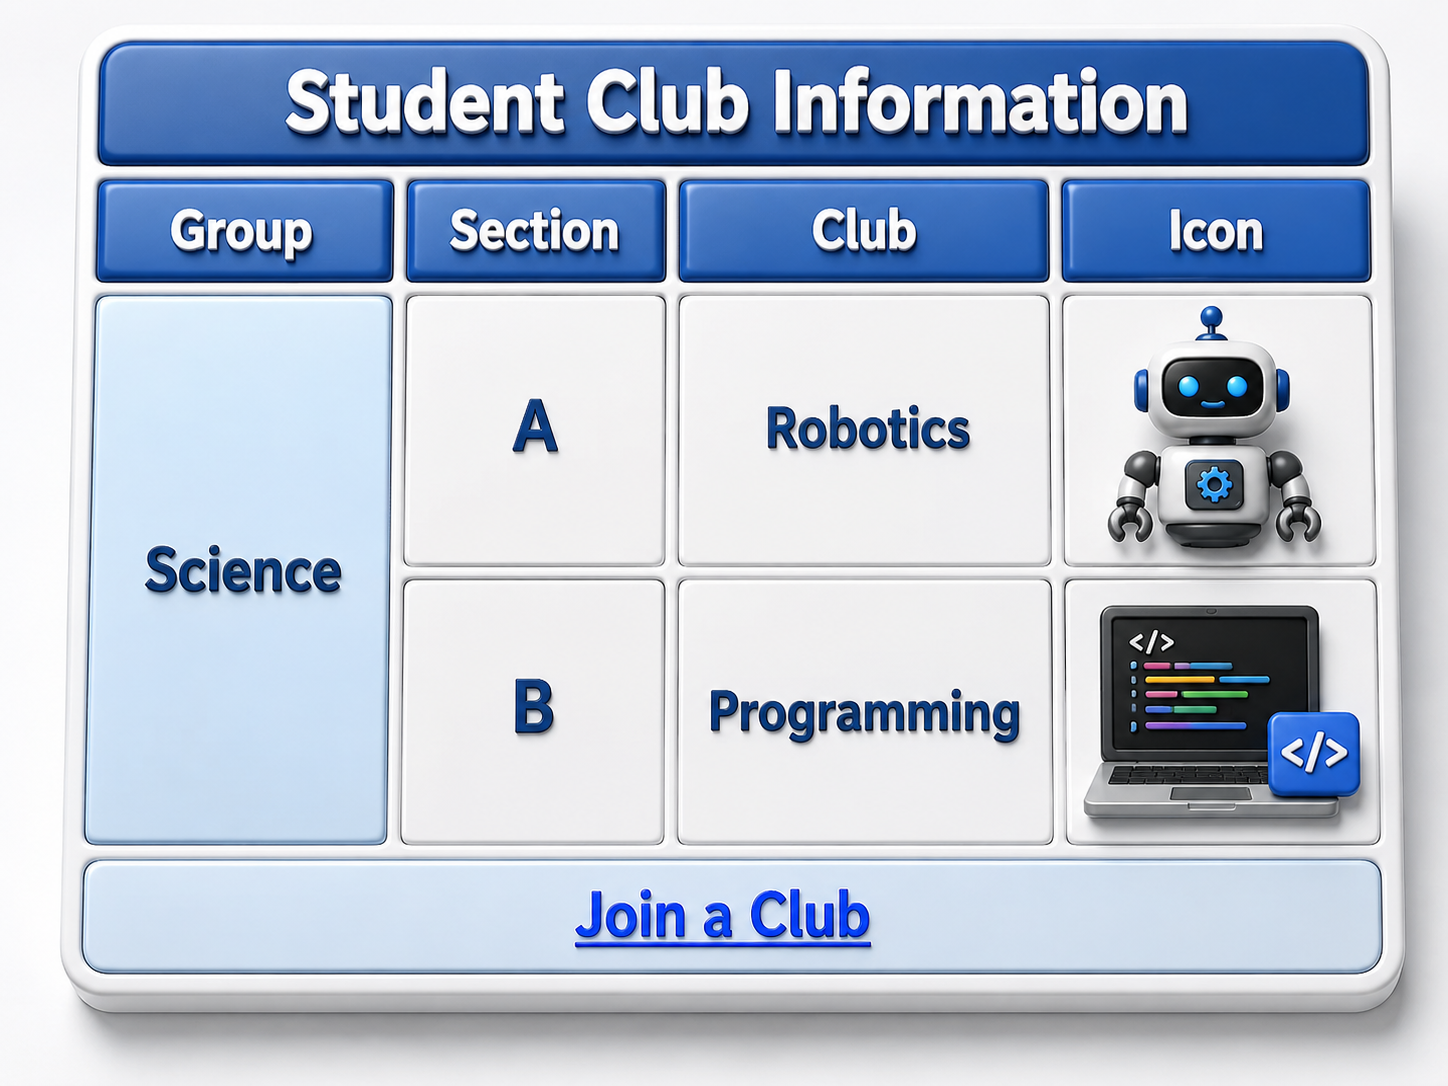
\includegraphics[width=0.95\linewidth,height=0.11\textheight,keepaspectratio]{chapters/Chapter04/topics/images/board_ex65_3d_student_club_table.png}
}{
\fbox{\parbox{0.90\linewidth}{\centering\vspace{0.45cm}
\textbf{চিত্র}\\[3pt]
File: \texttt{chapters/Chapter04/topics/images/board\_ex65\_3d\_student\_club\_table.png}
\vspace{0.45cm}}}
}
\captionof{figure}{Student Club Table with Rowspan and Image Icon}
\end{center}

\begin{keypointbox}{চিত্র ব্যাখ্যা}
Science group-এর দুই section দেখাতে rowspan, club icon দেখাতে image এবং join link দেখাতে colspan ব্যবহার করা হয়েছে।
\end{keypointbox}

\begin{keypointbox}{চিত্র দেখে code লেখার ধাপ}
প্রথমে figure-এর total row ও column গুনবে। এরপর কোন cell একাধিক column জুড়ে আছে তা দেখে \texttt{colspan} এবং কোন cell একাধিক row জুড়ে আছে তা দেখে \texttt{rowspan} বসাবে। তারপর image, link, list বা nested table থাকলে সংশ্লিষ্ট tag cell-এর ভিতরে লিখবে।
\end{keypointbox}

\par\noindent{\color{purple!70!black}\bfseries\small কোড}\par\vspace{-4pt}
\begin{verbatim}
<!DOCTYPE html>
<html>
<head>
  <title>HTML Table Example</title>
</head>
<body>
<table border="1" cellspacing="0" cellpadding="6" align="center">
  <caption><b>Student Club Information</b></caption>
  <tr>
    <th>Group</th>
    <th>Section</th>
    <th>Club</th>
    <th>Icon</th>
  </tr>
  <tr>
    <td rowspan="2">Science</td>
    <td>A</td>
    <td>Robotics</td>
    <td><img src="robot.png" width="50" height="50" alt="Robot"></td>
  </tr>
  <tr>
    <td>B</td>
    <td>Programming</td>
    <td><img src="code.png" width="50" height="50" alt="Code"></td>
  </tr>
  <tr>
    <td colspan="4" align="center"><a href="club.html">Join a Club</a></td>
  </tr>
</table>
</body>
</html>
\end{verbatim}
\vspace{-6pt}

\begin{keypointbox}{Board technique}
প্রথমে মোট row ও column গুনবে। তারপর কোন cell horizontal merge হলে \texttt{colspan} এবং vertical merge হলে \texttt{rowspan} ব্যবহার করবে। image-এর জন্য \texttt{<img>} এবং link-এর জন্য \texttt{<a>} tag ব্যবহার করবে।
\end{keypointbox}


\subsubsection{Example 66: Blood Donor Table with Contact Colspan}

\begin{center}
\IfFileExists{chapters/Chapter04/topics/images/board_ex66_3d_blood_donor_contact.png}{
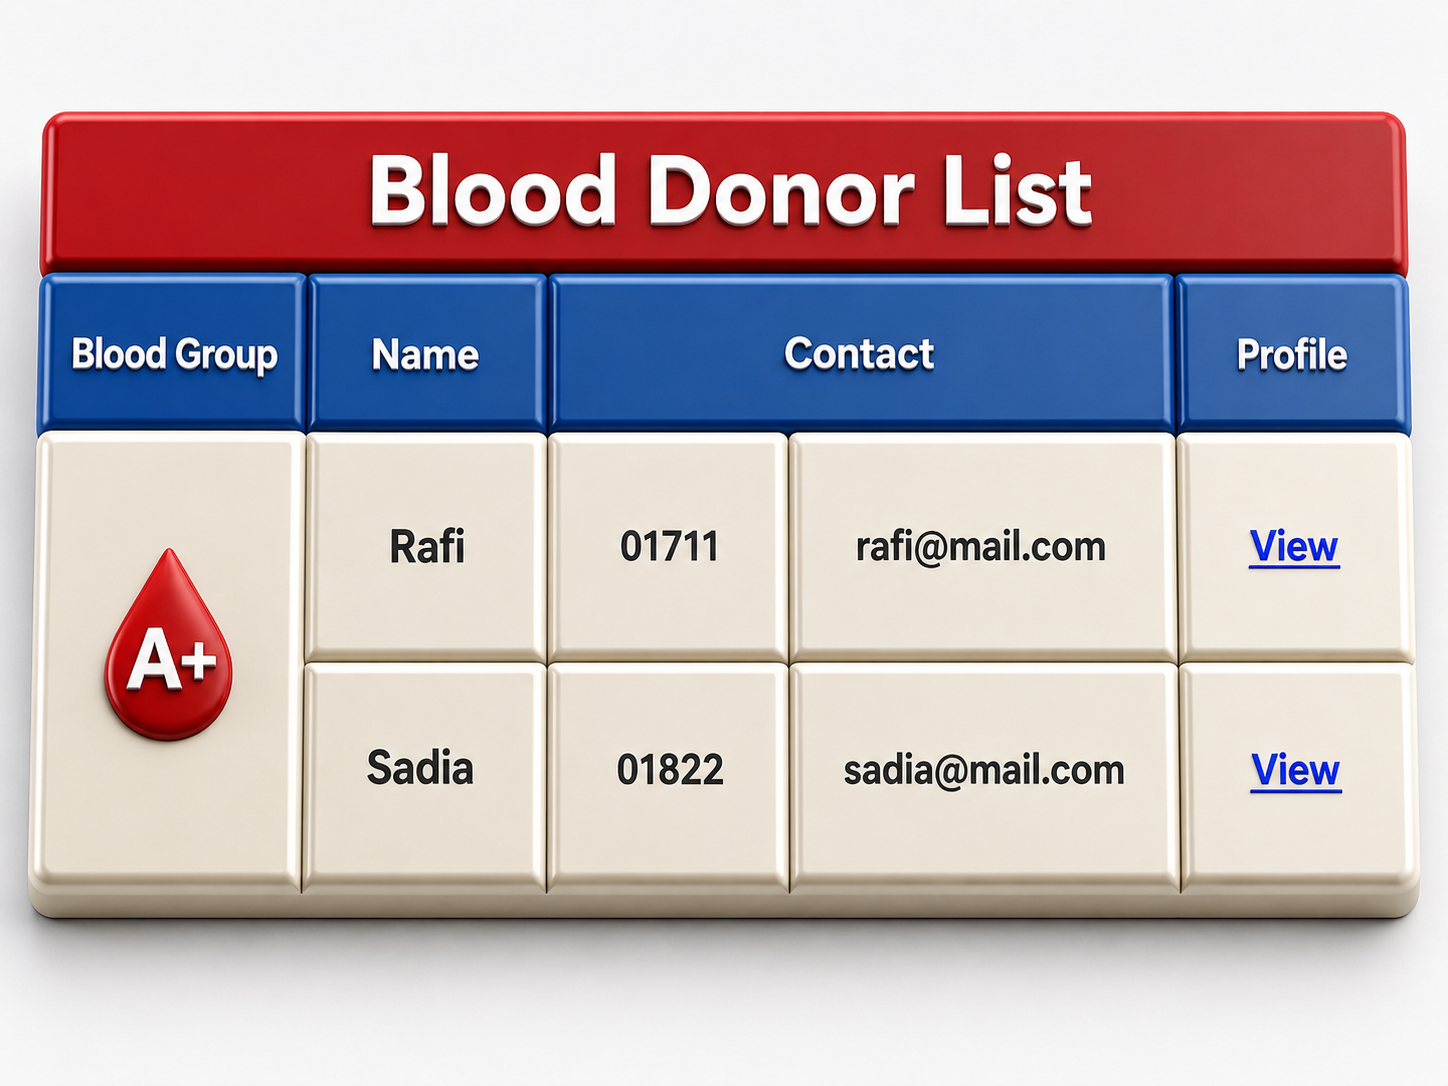
\includegraphics[width=0.95\linewidth,height=0.11\textheight,keepaspectratio]{chapters/Chapter04/topics/images/board_ex66_3d_blood_donor_contact.png}
}{
\fbox{\parbox{0.90\linewidth}{\centering\vspace{0.45cm}
\textbf{চিত্র}\\[3pt]
File: \texttt{chapters/Chapter04/topics/images/board\_ex66\_3d\_blood\_donor\_contact.png}
\vspace{0.45cm}}}
}
\captionof{figure}{Blood Donor Table with Contact Colspan}
\end{center}

\begin{keypointbox}{চিত্র ব্যাখ্যা}
Contact heading দুই column জুড়ে আছে এবং A+ blood group দুই donor-এর জন্য rowspan করা হয়েছে।
\end{keypointbox}

\par\noindent{\color{purple!70!black}\bfseries\small কোড}\par\vspace{-4pt}
\begin{verbatim}
<!DOCTYPE html>
<html>
<head>
  <title>HTML Table Example</title>
</head>
<body>
<table border="1" cellspacing="0" cellpadding="6" align="center">
  <caption><b>Blood Donor List</b></caption>
  <tr>
    <th>Blood Group</th>
    <th>Name</th>
    <th colspan="2">Contact</th>
    <th>Profile</th>
  </tr>
  <tr>
    <td rowspan="2">A+</td>
    <td>Rafi</td>
    <td>01711</td>
    <td>rafi@mail.com</td>
    <td><a href="rafi.html">View</a></td>
  </tr>
  <tr>
    <td>Sadia</td>
    <td>01822</td>
    <td>sadia@mail.com</td>
    <td><a href="sadia.html">View</a></td>
  </tr>
</table>
</body>
</html>
\end{verbatim}
\vspace{-6pt}

\begin{keypointbox}{Board technique}
প্রথমে মোট row ও column গুনবে। তারপর কোন cell horizontal merge হলে \texttt{colspan} এবং vertical merge হলে \texttt{rowspan} ব্যবহার করবে। image-এর জন্য \texttt{<img>} এবং link-এর জন্য \texttt{<a>} tag ব্যবহার করবে।
\end{keypointbox}


\subsubsection{Example 67: Scholarship Table with Logo, Link and Merged Eligibility}

\begin{center}
\IfFileExists{chapters/Chapter04/topics/images/board_ex67_3d_scholarship_table.png}{
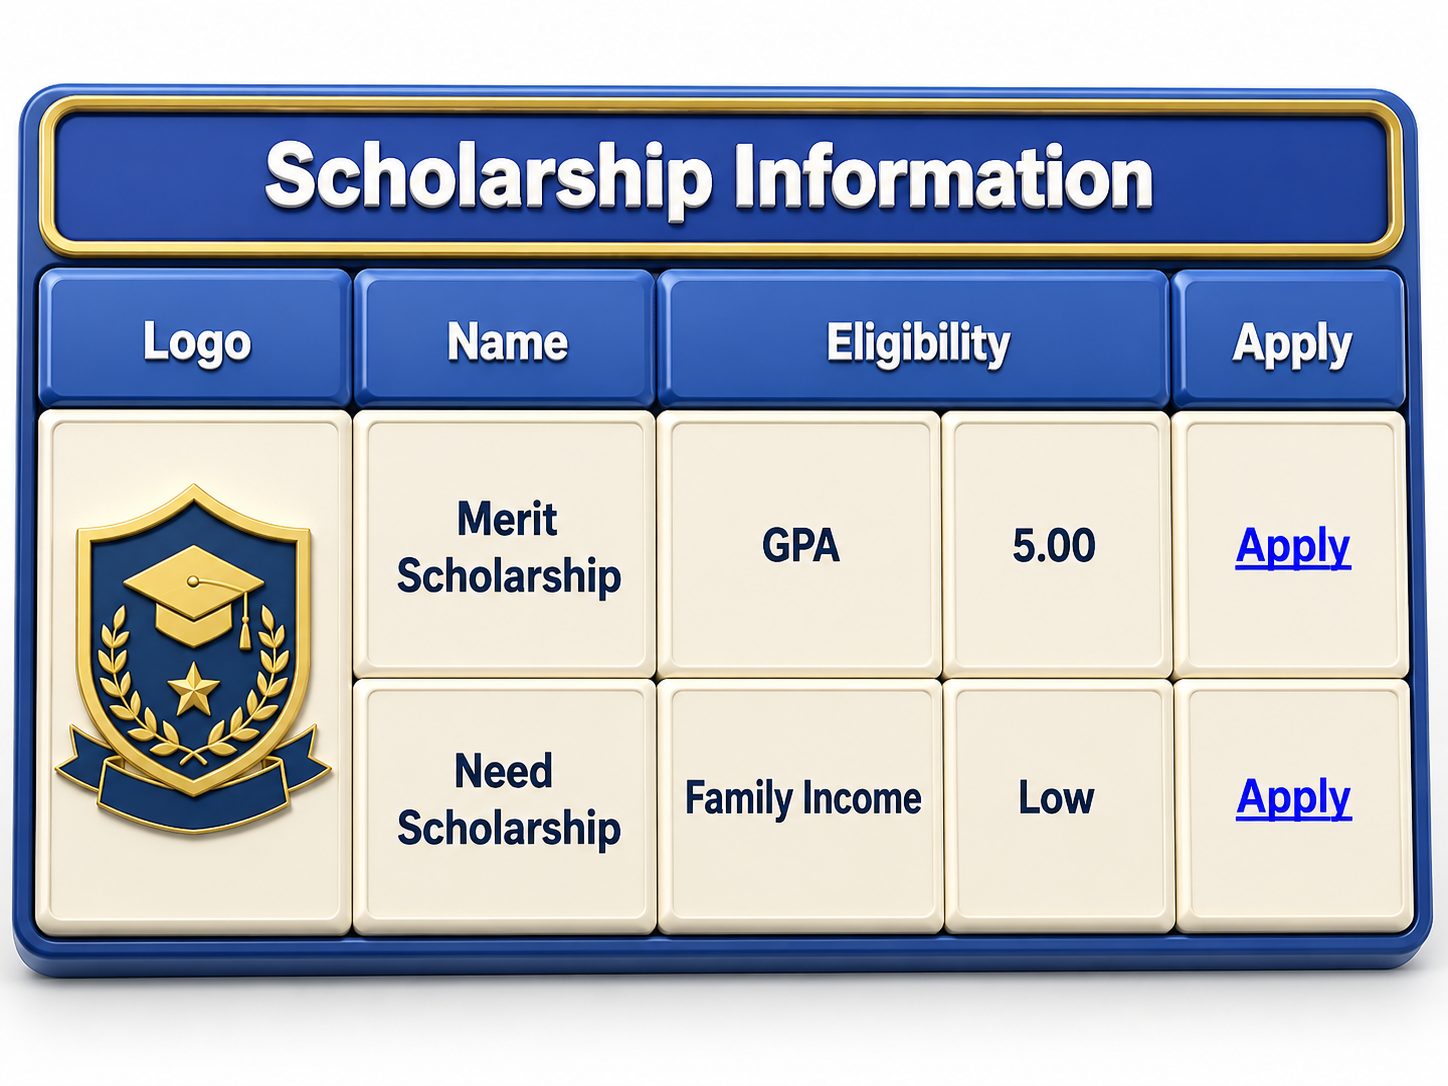
\includegraphics[width=0.95\linewidth,height=0.11\textheight,keepaspectratio]{chapters/Chapter04/topics/images/board_ex67_3d_scholarship_table.png}
}{
\fbox{\parbox{0.90\linewidth}{\centering\vspace{0.45cm}
\textbf{চিত্র}\\[3pt]
File: \texttt{chapters/Chapter04/topics/images/board\_ex67\_3d\_scholarship\_table.png}
\vspace{0.45cm}}}
}
\captionof{figure}{Scholarship Table with Logo, Link and Merged Eligibility}
\end{center}

\begin{keypointbox}{চিত্র ব্যাখ্যা}
Logo দুই scholarship row জুড়ে আছে; Eligibility heading দুই column জুড়ে আছে।
\end{keypointbox}

\begin{keypointbox}{চিত্র দেখে code লেখার ধাপ}
প্রথমে figure-এর total row ও column গুনবে। এরপর কোন cell একাধিক column জুড়ে আছে তা দেখে \texttt{colspan} এবং কোন cell একাধিক row জুড়ে আছে তা দেখে \texttt{rowspan} বসাবে। তারপর image, link, list বা nested table থাকলে সংশ্লিষ্ট tag cell-এর ভিতরে লিখবে।
\end{keypointbox}

\par\noindent{\color{purple!70!black}\bfseries\small কোড}\par\vspace{-4pt}
\begin{verbatim}
<!DOCTYPE html>
<html>
<head>
  <title>HTML Table Example</title>
</head>
<body>
<table border="1" cellspacing="0" cellpadding="6" align="center">
  <caption><b>Scholarship Information</b></caption>
  <tr>
    <th>Logo</th>
    <th>Name</th>
    <th colspan="2">Eligibility</th>
    <th>Apply</th>
  </tr>
  <tr>
    <td rowspan="2"><img src="scholarship.png" width="70" height="70" alt="Scholarship"></td>
    <td>Merit Scholarship</td>
    <td>GPA</td>
    <td>5.00</td>
    <td><a href="merit.html">Apply</a></td>
  </tr>
  <tr>
    <td>Need Scholarship</td>
    <td>Family Income</td>
    <td>Low</td>
    <td><a href="need.html">Apply</a></td>
  </tr>
</table>
</body>
</html>
\end{verbatim}
\vspace{-6pt}

\begin{keypointbox}{Board technique}
প্রথমে মোট row ও column গুনবে। তারপর কোন cell horizontal merge হলে \texttt{colspan} এবং vertical merge হলে \texttt{rowspan} ব্যবহার করবে। image-এর জন্য \texttt{<img>} এবং link-এর জন্য \texttt{<a>} tag ব্যবহার করবে।
\end{keypointbox}


\subsubsection{Example 68: Website Layout Table with Header, Sidebar, Image and Footer}

\begin{center}
\IfFileExists{chapters/Chapter04/topics/images/board_ex68_3d_webpage_layout_table.png}{
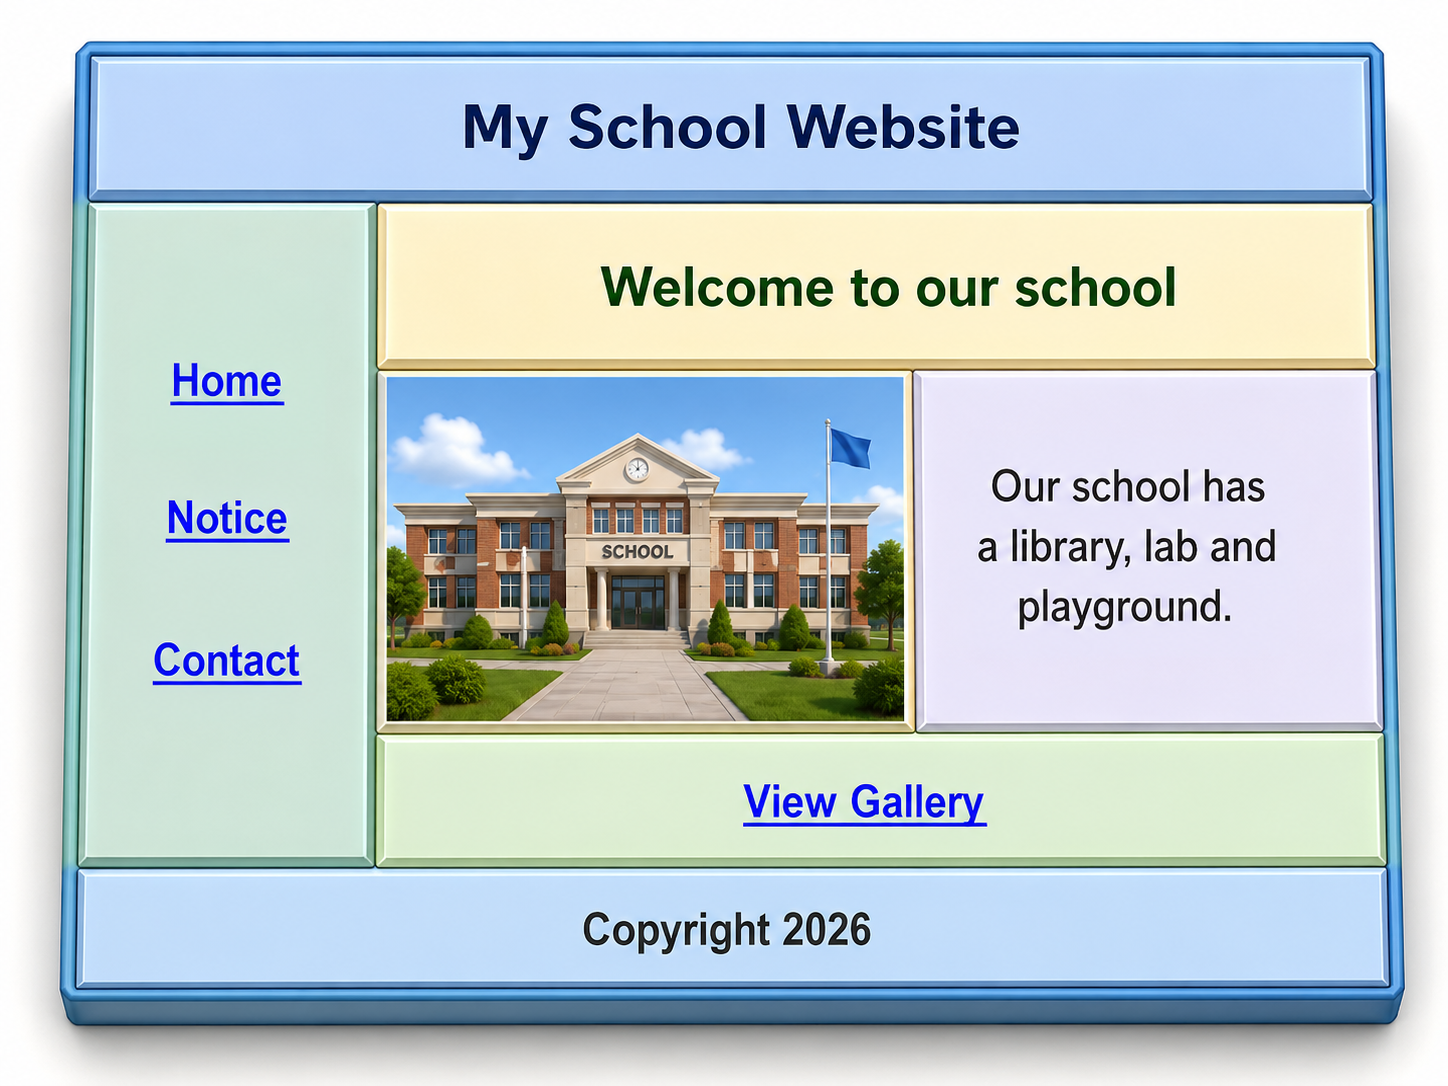
\includegraphics[width=0.95\linewidth,height=0.11\textheight,keepaspectratio]{chapters/Chapter04/topics/images/board_ex68_3d_webpage_layout_table.png}
}{
\fbox{\parbox{0.90\linewidth}{\centering\vspace{0.45cm}
\textbf{চিত্র}\\[3pt]
File: \texttt{chapters/Chapter04/topics/images/board\_ex68\_3d\_webpage\_layout\_table.png}
\vspace{0.45cm}}}
}
\captionof{figure}{Website Layout Table with Header, Sidebar, Image and Footer}
\end{center}

\begin{keypointbox}{চিত্র ব্যাখ্যা}
এটি webpage layout style table। Header ও footer colspan, sidebar rowspan, image এবং multiple links ব্যবহার করা হয়েছে।
\end{keypointbox}

\par\noindent{\color{purple!70!black}\bfseries\small কোড}\par\vspace{-4pt}
\begin{verbatim}
<!DOCTYPE html>
<html>
<head>
  <title>HTML Table Example</title>
</head>
<body>
<table border="1" cellspacing="0" cellpadding="8" align="center" width="600">
  <tr>
    <th colspan="3">My School Website</th>
  </tr>
  <tr>
    <td rowspan="3">
      <a href="home.html">Home</a><br>
      <a href="notice.html">Notice</a><br>
      <a href="contact.html">Contact</a>
    </td>
    <td colspan="2" align="center">Welcome to our school</td>
  </tr>
  <tr>
    <td><img src="school.jpg" width="150" height="90" alt="School"></td>
    <td>Our school has a library, lab and playground.</td>
  </tr>
  <tr>
    <td colspan="2" align="center"><a href="gallery.html">View Gallery</a></td>
  </tr>
  <tr>
    <td colspan="3" align="center">Copyright 2026</td>
  </tr>
</table>
</body>
</html>
\end{verbatim}
\vspace{-6pt}

\begin{keypointbox}{Board technique}
প্রথমে মোট row ও column গুনবে। তারপর কোন cell horizontal merge হলে \texttt{colspan} এবং vertical merge হলে \texttt{rowspan} ব্যবহার করবে। image-এর জন্য \texttt{<img>} এবং link-এর জন্য \texttt{<a>} tag ব্যবহার করবে।
\end{keypointbox}


\subsubsection{Example 69: College Contact Card with Nested Table, Image and Link}

\begin{center}
\IfFileExists{chapters/Chapter04/topics/images/board_ex69_3d_college_contact_nested.png}{
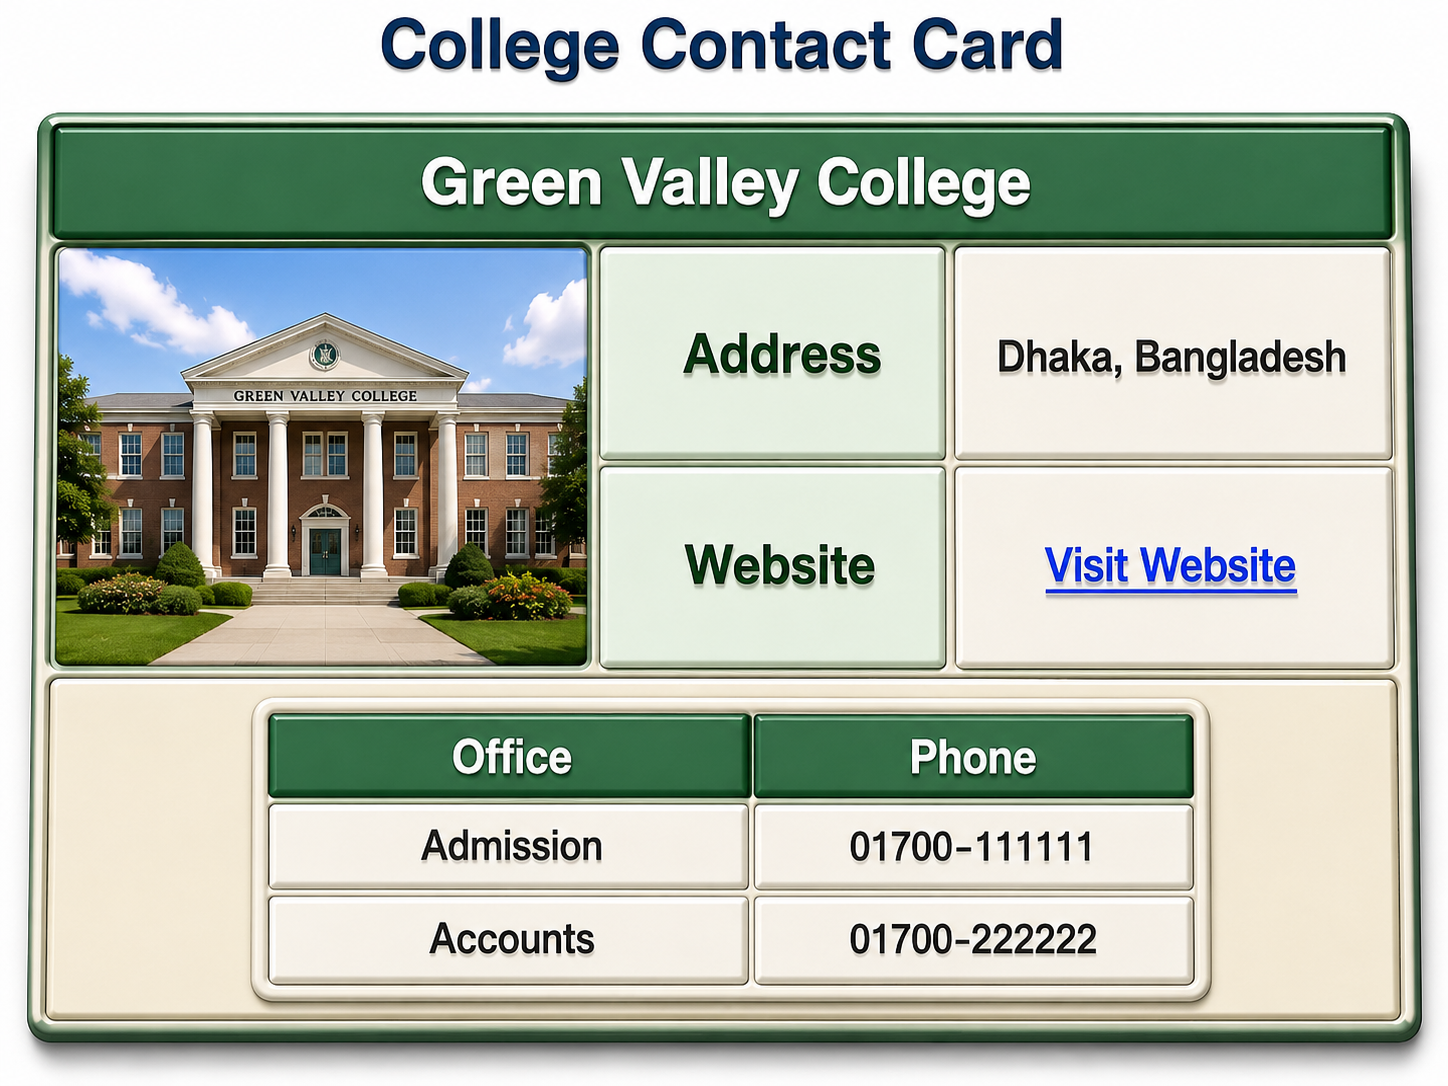
\includegraphics[width=0.95\linewidth,height=0.11\textheight,keepaspectratio]{chapters/Chapter04/topics/images/board_ex69_3d_college_contact_nested.png}
}{
\fbox{\parbox{0.90\linewidth}{\centering\vspace{0.45cm}
\textbf{চিত্র}\\[3pt]
File: \texttt{chapters/Chapter04/topics/images/board\_ex69\_3d\_college\_contact\_nested.png}
\vspace{0.45cm}}}
}
\captionof{figure}{College Contact Card with Nested Table, Image and Link}
\end{center}

\begin{keypointbox}{চিত্র ব্যাখ্যা}
এখানে outer table-এর ভিতরে nested table আছে। College image rowspan, title colspan এবং website hyperlink ব্যবহার করা হয়েছে।
\end{keypointbox}

\begin{keypointbox}{চিত্র দেখে code লেখার ধাপ}
প্রথমে figure-এর total row ও column গুনবে। এরপর কোন cell একাধিক column জুড়ে আছে তা দেখে \texttt{colspan} এবং কোন cell একাধিক row জুড়ে আছে তা দেখে \texttt{rowspan} বসাবে। তারপর image, link, list বা nested table থাকলে সংশ্লিষ্ট tag cell-এর ভিতরে লিখবে।
\end{keypointbox}

\par\noindent{\color{purple!70!black}\bfseries\small কোড}\par\vspace{-4pt}
\begin{verbatim}
<!DOCTYPE html>
<html>
<head>
  <title>HTML Table Example</title>
</head>
<body>
<table border="1" cellspacing="0" cellpadding="6" align="center">
  <caption><b>College Contact Card</b></caption>
  <tr>
    <th colspan="3">Green Valley College</th>
  </tr>
  <tr>
    <td rowspan="2"><img src="college.jpg" width="120" height="80" alt="College"></td>
    <td>Address</td>
    <td>Dhaka, Bangladesh</td>
  </tr>
  <tr>
    <td>Website</td>
    <td><a href="https://example.com">Visit Website</a></td>
  </tr>
  <tr>
    <td colspan="3">
      <table border="1" cellspacing="0" cellpadding="4" align="center">
        <tr>
          <th>Office</th>
          <th>Phone</th>
        </tr>
        <tr>
          <td>Admission</td>
          <td>01700-111111</td>
        </tr>
        <tr>
          <td>Accounts</td>
          <td>01700-222222</td>
        </tr>
      </table>
    </td>
  </tr>
</table>
</body>
</html>
\end{verbatim}
\vspace{-6pt}

\begin{keypointbox}{Board technique}
প্রথমে মোট row ও column গুনবে। তারপর কোন cell horizontal merge হলে \texttt{colspan} এবং vertical merge হলে \texttt{rowspan} ব্যবহার করবে। image-এর জন্য \texttt{<img>} এবং link-এর জন্য \texttt{<a>} tag ব্যবহার করবে।
\end{keypointbox}


\end{multicols}

\begin{recapbox}
এই ১৫টি mixed table practice-এ \texttt{rowspan}, \texttt{colspan}, image, hyperlink, list, nested table, caption, alignment এবং width—সব ধরনের গুরুত্বপূর্ণ HSC ICT table concept একসাথে cover করা হয়েছে। Exam-এ চিত্র দেখে code লেখার আগে structure analysis করাই সবচেয়ে গুরুত্বপূর্ণ।
\end{recapbox}

\subsection{চিত্র দেখে Table লেখার Final Checklist}

Board practical বা CQ-তে table-এর চিত্র দেওয়া থাকলে নিচের checklist ব্যবহার করলে ভুল কম হয়। এটি simple table, merged table, image/link/list-সহ table এবং nested table--সব ধরনের প্রশ্নে কাজে লাগে।

\begin{enumerate}
\item Table-এর নাম বা caption আছে কি না দেখবে।
\item Header row আছে কি না দেখবে।
\item Visible column সংখ্যা গুনবে।
\item Visible row সংখ্যা গুনবে।
\item Merged cell থাকলে আগে \texttt{rowspan} না \texttt{colspan} তা ঠিক করবে।
\item যে cell-এ image আছে সেখানে \texttt{<img>} এবং \texttt{alt} লিখবে।
\item যে cell-এ link আছে সেখানে \texttt{<a href="">} ব্যবহার করবে।
\item যে cell-এ list আছে সেখানে \texttt{<ol>} বা \texttt{<ul>} ব্যবহার করবে।
\item Nested table থাকলে inner table আলাদা indentation দিয়ে লিখবে।
\item শেষে সব \texttt{<table>}, \texttt{<tr>}, \texttt{<td>} tag close হয়েছে কি না মিলিয়ে দেখবে।
\end{enumerate}

\begin{keypointbox}{শেষ মুহূর্তের পরীক্ষা}
Code লেখা শেষ হলে প্রতিটি row আলাদা করে দেখবে: row-এর মোট column count figure-এর সাথে মিলছে কি না। \texttt{colspan="2"} মানে ওই cell দুই column-এর জায়গা নিয়েছে, তাই সেই row-তে একটি cell কম থাকবে। \texttt{rowspan="2"} মানে পরের row-তে ওই column-এর জন্য নতুন cell লিখতে হবে না।
\end{keypointbox}

\subsection{Board/Exam Focus}

\begin{boardbox}{বেশি গুরুত্বপূর্ণ}
\begin{itemize}
\item \texttt{<table>} tag table তৈরির জন্য ব্যবহৃত হয়।
\item \texttt{<tr>} row তৈরি করে।
\item \texttt{<th>} heading cell তৈরি করে।
\item \texttt{<td>} data cell তৈরি করে।
\item \texttt{<caption>} table-এর title দেয়।
\item \texttt{border} table border দেখায়।
\item \texttt{cellspacing} cell-এর মাঝের gap নির্ধারণ করে।
\item \texttt{cellpadding} cell-এর ভিতরের gap নির্ধারণ করে।
\item \texttt{rowspan} cell-কে vertical direction-এ merge করে।
\item \texttt{colspan} cell-কে horizontal direction-এ merge করে।
\item table-এর ভিতরে link, image, list এবং nested table ব্যবহার করা যায়।
\item চিত্র দেখে HTML table code লিখতে পারা খুব গুরুত্বপূর্ণ।
\end{itemize}
\end{boardbox}

\subsection{Exam-style Short Answer}

\begin{enumerate}
\item \textbf{HTML table কী?}\\
উত্তর: HTML document-এ তথ্যকে সারি ও কলাম আকারে প্রদর্শনের জন্য যে কাঠামো ব্যবহার করা হয়, তাকে HTML table বলে। Table তৈরির জন্য \texttt{<table>} tag ব্যবহার করা হয়।

\item \textbf{\texttt{<tr>} tag-এর কাজ কী?}\\
উত্তর: HTML table-এর একটি row বা সারি তৈরি করার জন্য \texttt{<tr>} tag ব্যবহার করা হয়।

\item \textbf{\texttt{<th>} ও \texttt{<td>} tag-এর পার্থক্য লেখ।}\\
উত্তর: \texttt{<th>} tag table-এর heading cell তৈরি করে এবং browser সাধারণত এর text bold ও center aligned করে দেখায়। অন্যদিকে \texttt{<td>} tag table-এর সাধারণ data cell তৈরি করে।

\item \textbf{\texttt{border} attribute-এর কাজ কী?}\\
উত্তর: HTML table-এর চারপাশে এবং cell-এর চারপাশে border বা রেখা প্রদর্শনের জন্য \texttt{border} attribute ব্যবহার করা হয়।

\item \textbf{\texttt{cellspacing} ও \texttt{cellpadding}-এর পার্থক্য লেখ।}\\
উত্তর: \texttt{cellspacing} cell থেকে cell-এর মাঝের gap নির্ধারণ করে। অন্যদিকে \texttt{cellpadding} cell-এর content এবং cell border-এর মাঝের ভিতরের gap নির্ধারণ করে।

\item \textbf{\texttt{rowspan} ও \texttt{colspan}-এর পার্থক্য লেখ।}\\
উত্তর: \texttt{rowspan} একটি cell-কে একাধিক row জুড়ে বিস্তৃত করে। \texttt{colspan} একটি cell-কে একাধিক column জুড়ে বিস্তৃত করে।

\item \textbf{Table-এর ভিতরে image বসানোর code লেখ।}\\
উত্তর: \texttt{<td><img src="photo.jpg" width="100" height="80" alt="Photo"></td>}

\item \textbf{Nested table কী?}\\
উত্তর: একটি table-এর কোনো cell-এর ভিতরে আরেকটি table তৈরি করলে তাকে nested table বলে।
\end{enumerate}

\subsection{Practice MCQ}

\begin{enumerate}
\item HTML-এ table তৈরির tag কোনটি?\\
ক) \texttt{<tr>} \quad খ) \texttt{<td>} \quad গ) \texttt{<table>} \quad ঘ) \texttt{<th>}

\item Table row তৈরি করতে কোন tag ব্যবহার হয়?\\
ক) \texttt{<td>} \quad খ) \texttt{<tr>} \quad গ) \texttt{<th>} \quad ঘ) \texttt{<caption>}

\item Table heading cell তৈরির tag কোনটি?\\
ক) \texttt{<td>} \quad খ) \texttt{<tr>} \quad গ) \texttt{<th>} \quad ঘ) \texttt{<br>}

\item Table data cell তৈরির tag কোনটি?\\
ক) \texttt{<td>} \quad খ) \texttt{<tr>} \quad গ) \texttt{<table>} \quad ঘ) \texttt{<hr>}

\item Table-এর border দেখাতে কোন attribute ব্যবহার করা হয়?\\
ক) \texttt{src} \quad খ) \texttt{href} \quad গ) \texttt{border} \quad ঘ) \texttt{target}

\item \texttt{cellpadding="5"} এর অর্থ কী?\\
ক) cell-এর ভিতরে content ও border-এর মাঝে 5 pixel space\\
খ) দুই cell-এর মাঝে 5 meter space\\
গ) table-এর height 5\\
ঘ) table-এর row সংখ্যা 5

\item \texttt{cellspacing} কোথায় space তৈরি করে?\\
ক) content ও border-এর ভিতরে \quad খ) cell ও cell-এর মাঝে \quad গ) image-এর ভিতরে \quad ঘ) hyperlink-এর পরে

\item দুইটি column merge করতে কোন attribute ব্যবহার হয়?\\
ক) \texttt{rowspan} \quad খ) \texttt{colspan} \quad গ) \texttt{cellpadding} \quad ঘ) \texttt{bgcolor}

\item দুইটি row merge করতে কোন attribute ব্যবহার হয়?\\
ক) \texttt{rowspan} \quad খ) \texttt{colspan} \quad গ) \texttt{align} \quad ঘ) \texttt{src}

\item Table-এর title দিতে কোন tag ব্যবহার হয়?\\
ক) \texttt{<title>} \quad খ) \texttt{<caption>} \quad গ) \texttt{<thead>} \quad ঘ) \texttt{<link>}

\item Image কোন tag দিয়ে table cell-এর ভিতরে বসানো যায়?\\
ক) \texttt{<a>} \quad খ) \texttt{<img>} \quad গ) \texttt{<ol>} \quad ঘ) \texttt{<tr>}

\item একটি table-এর cell-এর ভিতরে আরেকটি table বসালে তাকে কী বলে?\\
ক) outer table \quad খ) nested table \quad গ) image table \quad ঘ) child table
\end{enumerate}

\begin{boardbox}{MCQ Answer Key}
১-গ, ২-খ, ৩-গ, ৪-ক, ৫-গ, ৬-ক, ৭-খ, ৮-খ, ৯-ক, ১০-খ, ১১-খ, ১২-খ
\end{boardbox}

\subsection{CQ Practice}

\begin{practicebox}
\textbf{উদ্দীপক:} একটি webpage-এ Result Sheet table দেখাতে হবে। Table-এ border থাকবে, cell-এর ভিতরে ৫ pixel space থাকবে এবং cellগুলোর মাঝের gap থাকবে না। Table-এর প্রথম row-তে \texttt{Result Sheet} লেখা থাকবে এবং সেটি তিনটি column জুড়ে থাকবে।

\textbf{প্রশ্ন}\\
ক. HTML table কী?\\
খ. \texttt{<th>} ও \texttt{<td>} tag-এর কাজ লেখ।\\
গ. উদ্দীপকের জন্য HTML code লেখ।\\
ঘ. \texttt{border}, \texttt{cellspacing}, \texttt{cellpadding} ও \texttt{colspan} attribute-এর ব্যবহার বিশ্লেষণ কর।
\end{practicebox}

\subsubsection{গ. কোড}

\begin{examplebox}{কোড}
\begin{verbatim}
<!DOCTYPE html>
<html>
<head>
  <title>Result Table</title>
</head>
<body>
  <table border="1" cellspacing="0" cellpadding="5">
    <tr>
      <th colspan="3">Result Sheet</th>
    </tr>
    <tr>
      <th>Roll</th>
      <th>Name</th>
      <th>GPA</th>
    </tr>
    <tr>
      <td>101</td>
      <td>Rafi</td>
      <td>5.00</td>
    </tr>
    <tr>
      <td>102</td>
      <td>Sakib</td>
      <td>4.75</td>
    </tr>
  </table>
</body>
</html>
\end{verbatim}
\end{examplebox}

\subsubsection{ঘ. বিশ্লেষণ}

\texttt{border="1"} table ও cell-এর চারপাশে border দেখায়। \texttt{cellspacing="0"} cellগুলোর মাঝের gap দূর করে। \texttt{cellpadding="5"} cell-এর ভিতরে content ও border-এর মাঝে ৫ pixel space তৈরি করে, ফলে table পড়তে সহজ হয়। \texttt{colspan="3"} প্রথম heading cell-কে তিনটি column জুড়ে বিস্তৃত করে, তাই \texttt{Result Sheet} title পুরো table-এর উপর দেখা যায়।

\subsection{Common Mistake}

\begin{mistakebox}{সাধারণ ভুল}
\begin{itemize}
\item \texttt{<table>} tag close না করা।
\item \texttt{<tr>} ছাড়া সরাসরি \texttt{<td>} লেখা।
\item heading cell-এ \texttt{<td>} ব্যবহার করা, যেখানে \texttt{<th>} ভালো।
\item \texttt{<td>}-এর spelling ভুল করে \texttt{<tb>} লেখা।
\item \texttt{cellpadding} ও \texttt{cellspacing} গুলিয়ে ফেলা।
\item \texttt{rowspan} ও \texttt{colspan} উল্টো ব্যবহার করা।
\item border না দিলে table-এর রেখা দেখা যাবে না--এটা ভুলে যাওয়া।
\item table row ও column সংখ্যা figure-এর সাথে না মেলানো।
\item \texttt{<caption>} ভুল জায়গায় লেখা। Caption সাধারণত \texttt{<table>} tag-এর ভিতরে, প্রথম row-এর আগে লেখা হয়।
\item table-এর ভিতরে image/link/list লিখতে syntax ভুল করা।
\item image tag-এ \texttt{src} ভুল দেওয়া বা image file একই folder-এ না রাখা।
\item nested table-এর closing tag ঠিকমতো না দেওয়া।
\end{itemize}
\end{mistakebox}

\subsection{১ মিনিটে রিভিশন}

\begin{recapbox}
Table তৈরি হয় row ও column দিয়ে। \texttt{<table>} পুরো table তৈরি করে, \texttt{<tr>} table row তৈরি করে, \texttt{<th>} heading cell তৈরি করে এবং \texttt{<td>} data cell তৈরি করে। \texttt{border} table border দেখায়, \texttt{cellspacing} cell-এর মাঝের gap নিয়ন্ত্রণ করে এবং \texttt{cellpadding} cell-এর ভিতরের gap নিয়ন্ত্রণ করে। \texttt{<caption>} table-এর title দেয়। \texttt{rowspan} vertical merge এবং \texttt{colspan} horizontal merge করে। Table cell-এর ভিতরে text, link, image, list ও nested table রাখা যায়। HSC CQ-তে table চিত্র দেখে code লেখা খুব গুরুত্বপূর্ণ।
\end{recapbox}











% Density revision 2026-10-04: answers below questions; compact related content.
% Topic 15: Rowspan and Colspan
\section{সারণির ঘর একত্র করা: rowspan ও colspan}

% Composition pass 2026-10-04
ফলের সারণিতে একটি শিরোনাম তিন কলামের ওপর এবং একটি বিষয় দুই সারির পাশে দেখাতে হবে।

\chFourMotivation{একাধিক মূল ঘরের স্থানজুড়ে একই তথ্য $\rightarrow$ colspan/rowspan $\rightarrow$ বিস্তৃত ঘরের দখল করা স্থান গোনা $\rightarrow$ ফল ও রুটিনের মিলিত শিরোনাম।}


\begin{learningbox}
এই অংশ শেষে শিক্ষার্থী পারবে:
\begin{itemize}
\item HTML সারণির ঘর একত্র করার ধারণা ব্যাখ্যা করতে।
\item \texttt{colspan} অ্যাট্রিবিউট ব্যবহার করে ঘরকে একাধিক কলামজুড়ে দেখাতে।
\item \texttt{rowspan} অ্যাট্রিবিউট ব্যবহার করে ঘরকে একাধিক সারিজুড়ে দেখাতে।
\item চিত্র দেখে \texttt{rowspan} ও \texttt{colspan} নির্ধারণ করতে।
\item একত্র করা ঘরের জন্য অতিরিক্ত \texttt{<td>} বা \texttt{<th>} না লেখার নিয়ম বুঝতে।
\end{itemize}
\end{learningbox}



একটি পরীক্ষার ফলের সারণিতে Roll, Name ও GPA তিনটি কলাম আছে। উপরে Result Sheet শিরোনামটি তিন কলামের মাঝ বরাবর দেখাতে আলাদা তিনটি ঘরে একই কথা লেখার প্রয়োজন নেই; একটি ঘরকে তিন কলামজুড়ে বিস্তৃত করলেই হয়। আবার একজনের দুটি ফোন নম্বর থাকলে Phone পরিচিতিটি দুই সারিজুড়ে একবার দেখানো যায়। এই অংশে \texttt{colspan} ও \texttt{rowspan} দিয়ে ঘরের বিস্তার এবং মূল ছকের স্থান গণনা শেখা হবে।

\subsection{ঘর একত্র করা (Cell Merge)}

\begin{definitionbox}{}
HTML সারণিতে একাধিক সারি বা কলামের স্থানজুড়ে একটি ঘর বিস্তৃত করে দেখানোকে \textbf{ঘর একত্র করা} বলে। এর জন্য \texttt{rowspan} ও \texttt{colspan} অ্যাট্রিবিউট ব্যবহার করা হয়।
\end{definitionbox}

ঘর একত্র করলে ছকের বিন্যাস বদলায়। আলাদা ঘরের লেখা স্বয়ংক্রিয়ভাবে একসঙ্গে যুক্ত হয় না। বিস্তৃত ঘরে কী লেখা থাকবে এবং ঘরটি কত সারি বা কলাম দখল করবে, তা কোডে নির্ধারণ করতে হয়।

\begin{examplebox}{সহজ উদাহরণ}
\begin{center}
\begin{tabular}{|c|c|c|}
\hline
\multicolumn{3}{|c|}{\textbf{Result Sheet}} \\
\hline
\textbf{Roll} & \textbf{Name} & \textbf{GPA} \\
\hline
\end{tabular}
\end{center}
এখানে \textbf{Result Sheet} ঘরটি ৩টি কলামজুড়ে আছে। তাই HTML কোডে \texttt{colspan="3"} ব্যবহার করতে হবে।
\end{examplebox}

\subsection{\texttt{colspan} দিয়ে কলামজুড়ে ঘর}

\texttt{colspan} একটি ঘর কতটি কলামজুড়ে থাকবে, তা নির্ধারণ করে। নিচের উদাহরণে Math ও ICT একই Subject শিরোনামের অধীনে আছে।

\texttt{colspan} নামটি Column Span অর্থাৎ কলামজুড়ে বিস্তার বোঝায়। এটি সাধারণত \texttt{<th>} বা \texttt{<td>} ট্যাগের ভেতরে লেখা হয়।

% Split revision: code and its explanation share one row.
\par\noindent
\begin{minipage}[t]{.54\linewidth}\vspace{0pt}\small
\subsubsection{লেখার রূপ}

\textbf{\color{chFourTeal}কোড}\par
\begin{verbatim}
<th colspan="number">Heading</th>
<td colspan="number">Data</td>
\end{verbatim}
\par\smallskip
\end{minipage}\hfill
\begin{minipage}[t]{.42\linewidth}\vspace{0pt}\small
\subsubsection{উদাহরণ}

\textbf{\color{chFourTeal}কোড}\par
\begin{verbatim}
<th colspan="2">Subject</th>
\end{verbatim}
\par\smallskip


এর অর্থ: \textbf{Subject} ঘরটি ২টি কলামজুড়ে থাকবে।
\end{minipage}\par
\subsection{কলামের উদাহরণ: বিষয়ের সারণি}

% Split revision: code and its explanation share one row.
\par\noindent
\begin{minipage}[t]{.60\linewidth}\vspace{0pt}\small
\textbf{\color{chFourTeal}কোড}\par
\begin{verbatim}
<!DOCTYPE html><html>
<head><title>Colspan Example</title></head>
<body><table border="1">
  <tr><th>Name</th><th colspan="2">Subject</th></tr>
  <tr><td>Kabir</td><td>Math</td><td>ICT</td></tr>
</table></body></html>
\end{verbatim}
\par\smallskip
\end{minipage}\hfill
\begin{minipage}[t]{.36\linewidth}\vspace{0pt}\small
\textbf{\color{chFourTeal}ফলের ধারণা}\par
\begin{center}
\begin{tabular}{|c|c|c|}
\hline
\textbf{Name} & \multicolumn{2}{c|}{\textbf{Subject}} \\
\hline
Kabir & Math & ICT \\
\hline
\end{tabular}
\end{center}
এখানে \textbf{Subject} শিরোনাম দুইটি কলাম--Math ও ICT--এর উপর বসেছে। তাই \texttt{Subject} ঘরে \texttt{colspan="2"} ব্যবহার হবে।
\par\smallskip
\end{minipage}\par


\begin{boardbox}{পরীক্ষায় মনে রাখবে}
একটি শিরোনাম যদি দুইটি কলামের উপর বসে, তাহলে \texttt{colspan="2"} লিখতে হয়। তিনটি কলাম হলে \texttt{colspan="3"} লিখতে হয়।
\end{boardbox}

\subsection{\texttt{rowspan} দিয়ে সারিজুড়ে ঘর}

\texttt{rowspan} একটি ঘর কতটি সারিজুড়ে থাকবে, তা নির্ধারণ করে। নিচের উদাহরণে Phone ঘরের পাশে দুই সারিতে দুটি নম্বর আছে।

\texttt{rowspan} নামটি Row Span অর্থাৎ সারিজুড়ে বিস্তার বোঝায়। এটি \texttt{<th>} অথবা \texttt{<td>} ট্যাগে ব্যবহার করা যায়।

% Split revision: code and its explanation share one row.
\par\noindent
\begin{minipage}[t]{.54\linewidth}\vspace{0pt}\small
\subsubsection{লেখার রূপ}

\textbf{\color{chFourTeal}কোড}\par
\begin{verbatim}
<th rowspan="number">Heading</th>
<td rowspan="number">Data</td>
\end{verbatim}
\par\smallskip
\end{minipage}\hfill
\begin{minipage}[t]{.42\linewidth}\vspace{0pt}\small
\subsubsection{উদাহরণ}

\textbf{\color{chFourTeal}কোড}\par
\begin{verbatim}
<th rowspan="2">Phone</th>
\end{verbatim}
\par\smallskip


এর অর্থ: \textbf{Phone} ঘরটি ২টি সারিজুড়ে থাকবে।
\end{minipage}\par
\subsection{সারির উদাহরণ: ফোন নম্বরের সারণি}

% Split revision: code and its explanation share one row.
\par\noindent
\begin{minipage}[t]{.50\linewidth}\vspace{0pt}\small
\textbf{\color{chFourTeal}কোড}\par
\begin{verbatim}
<table border="1">
  <tr>
    <th>Name</th>
    <td>Kabir</td>
  </tr>
  <tr>
    <th rowspan="2">Phone</th>
    <td>8942318</td>
  </tr>
  <tr>
    <td>1750181</td>
  </tr>
</table>
\end{verbatim}
\par\smallskip
\end{minipage}\hfill
\begin{minipage}[t]{.46\linewidth}\vspace{0pt}\small
\textbf{\color{chFourTeal}ফলের ধারণা}\par
\begin{center}
\begin{tabular}{|c|c|}
\hline
\textbf{Name} & Kabir \\
\hline
\raisebox{-.5\normalbaselineskip}[0pt][0pt]{\textbf{Phone}} & 8942318 \\
\cline{2-2}
 & 1750181 \\
\hline
\end{tabular}
\end{center}
এখানে \textbf{Phone} ঘরটি দুইটি ফোন নম্বরের পাশে দুইটি সারিজুড়ে আছে। তাই \texttt{rowspan="2"} ব্যবহার হবে।
\par\smallskip
\end{minipage}\par


% Original applied explanation; see Chapter04/SOURCES.md.
\subsubsection{রুটিনের ছক থেকে বিস্তৃত ঘর গণনা}
রুটিনে একটি ল্যাব ক্লাস দুই সময়ের ঘর দখল করলে \texttt{colspan="2"} ব্যবহার করা যায়। একটি বিভাগ-নাম তিনটি বিষয়ের সারি ধরে থাকলে \texttt{rowspan="3"} উপযোগী। বিস্তৃত ঘর যত স্থান দখল করে, ওই স্থানে আর নতুন ঘর লিখবে না।

কোড লেখার আগে কাগজে সারি-কলামের ছক আঁকবে। ওপরের সারি থেকে নেমে আগের rowspan-এর দখল করা স্থান চিহ্নিত করবে; তারপর অবশিষ্ট স্থানে নতুন \texttt{td}/\texttt{th} বসাবে। এইভাবে পুরো ছকের প্রস্থ একই থাকে এবং বাড়তি ঘর তৈরির ভুল ধরা যায়।


\subsection{rowspan ও colspan-এর পার্থক্য}

\begin{center}
\footnotesize
\begin{tabular}{|p{0.20\textwidth}|p{0.32\textwidth}|p{0.32\textwidth}|}
\hline
\textbf{বিষয়} & \textbf{\texttt{colspan}} & \textbf{\texttt{rowspan}} \\
\hline
কাজ & ঘরকে একাধিক কলামজুড়ে বিস্তৃত করে & ঘরকে একাধিক সারিজুড়ে বিস্তৃত করে \\
\hline
দিক & আড়াআড়ি & লম্বালম্বি \\
\hline
ব্যবহার & শিরোনাম কয়েকটি কলামের ওপর বসাতে & একটি পরিচিতি কয়েকটি সারির পাশে বসাতে \\
\hline
উদাহরণ & \texttt{<th colspan="3">Result</th>} & \texttt{<td rowspan="2">ICT</td>} \\
\hline
মনে রাখার উপায় & কলামজুড়ে বিস্তার & সারিজুড়ে বিস্তার \\
\hline
\end{tabular}
\end{center}

\subsection{অ্যাট্রিবিউট দুটি কোথায় লেখা হয়?}

\texttt{rowspan} ও \texttt{colspan} সাধারণত \texttt{<td>} অথবা \texttt{<th>} ট্যাগের ভেতরে লেখা হয়।

\begin{examplebox}{কোড}
\begin{verbatim}
<th colspan="3">Result Sheet</th>
<td rowspan="2">ICT</td>
\end{verbatim}
\end{examplebox}

\begin{keypointbox}{মূল নিয়ম}
\texttt{colspan}-এর জন্য ধনাত্মক পূর্ণসংখ্যা দিতে হয়; যেমন \texttt{colspan="3"} মানে তিনটি কলাম। এখানকার \texttt{rowspan="2"} মানে দুইটি সারি। বিশেষ ক্ষেত্রে \texttt{rowspan="0"} বর্তমান সারি-দলের অবশিষ্ট সব সারি বোঝায়; সাধারণ চিত্রভিত্তিক অনুশীলনে যতটি সারি বিস্তৃত হয়েছে, সেই সংখ্যা লিখবে।
\end{keypointbox}

\subsection{ফলের সারণির শিরোনামে colspan}

% Split revision: code and its explanation share one row.
\par\noindent
\begin{minipage}[t]{.54\linewidth}\vspace{0pt}\small
\textbf{\color{chFourTeal}কোড}\par
\begin{verbatim}
<table border="1" cellspacing="0" cellpadding="5">
  <tr>
    <th colspan="3">Result Sheet</th>
  </tr>
  <tr>
    <th>Roll</th><th>Name</th><th>GPA</th>
  </tr>
  <tr>
    <td>101</td><td>Rafi</td><td>5.00</td>
  </tr>
</table>
\end{verbatim}
\par\smallskip
\end{minipage}\hfill
\begin{minipage}[t]{.42\linewidth}\vspace{0pt}\small
\textbf{\color{chFourTeal}ফলের ধারণা}\par
\begin{center}
\begin{tabular}{|c|c|c|}
\hline
\multicolumn{3}{|c|}{\textbf{Result Sheet}} \\
\hline
\textbf{Roll} & \textbf{Name} & \textbf{GPA} \\
\hline
101 & Rafi & 5.00 \\
\hline
\end{tabular}
\end{center}
\par\smallskip
\end{minipage}\par


\begin{keypointbox}{ব্যাখ্যা}
সারণিতে মোট ৩টি কলাম আছে: Roll, Name, GPA। Result Sheet শিরোনাম পুরো ৩টি কলামজুড়ে থাকবে। তাই \texttt{<th colspan="3">Result Sheet</th>} লেখা হয়েছে।
\end{keypointbox}

\subsection{বিষয়ভিত্তিক নম্বরের সারণিতে rowspan}

% Split revision: code and its explanation share one row.
\par\noindent
\begin{minipage}[t]{.54\linewidth}\vspace{0pt}\small
\textbf{\color{chFourTeal}কোড}\par
\begin{verbatim}
<table border="1" cellspacing="0" cellpadding="5">
  <tr>
    <th>Subject</th><th>Type</th><th>Marks</th>
  </tr>
  <tr>
    <td rowspan="2">ICT</td><td>CQ</td><td>45</td>
  </tr>
  <tr>
    <td>MCQ</td><td>25</td>
  </tr>
  <tr>
    <td>English</td><td>Total</td><td>95</td>
  </tr>
</table>
\end{verbatim}
\par\smallskip
\end{minipage}\hfill
\begin{minipage}[t]{.42\linewidth}\vspace{0pt}\small
\textbf{\color{chFourTeal}ফলের ধারণা}\par
\begin{center}
\begin{tabular}{|c|c|c|}
\hline
\textbf{Subject} & \textbf{Type} & \textbf{Marks} \\
\hline
\raisebox{-.5\normalbaselineskip}[0pt][0pt]{ICT} & CQ & 45 \\
\cline{2-3}
 & MCQ & 25 \\
\hline
English & Total & 95 \\
\hline
\end{tabular}
\end{center}
এখানে \textbf{ICT} ঘরটি CQ ও MCQ--দুইটি সারিজুড়ে আছে। তাই \texttt{rowspan="2"} ব্যবহার হবে।
\par\smallskip
\end{minipage}\par


\Needspace{7\baselineskip}
\subsection{একই সারণিতে rowspan ও colspan}

একটি জটিল সারণিতে \texttt{rowspan} ও \texttt{colspan}--দুটিই ব্যবহার হতে পারে।

% Split revision: code and its explanation share one row.
\par\noindent
\begin{minipage}[t]{.54\linewidth}\vspace{0pt}\small
\textbf{\color{chFourTeal}কোড}\par
\begin{verbatim}
<table border="1" cellspacing="0" cellpadding="5">
  <tr>
    <th colspan="5">Marks Sheet</th>
  </tr>
  <tr>
    <th rowspan="2">Roll No.</th><th colspan="2">Bangla</th>
    <th colspan="2">English</th>
  </tr>
  <tr>
    <th>1st</th><th>2nd</th><th>1st</th><th>2nd</th>
  </tr>
  <tr>
    <td>001</td><td>85</td><td>67</td><td>58</td><td>70</td>
  </tr>
  <tr>
    <td>002</td><td>65</td><td>75</td><td>60</td><td>55</td>
  </tr>
</table>
\end{verbatim}
\par\smallskip
\end{minipage}\hfill
\begin{minipage}[t]{.42\linewidth}\vspace{0pt}\small
\textbf{\color{chFourTeal}ফলের ধারণা}\par
\begin{center}
\begin{tabular}{|c|c|c|c|c|}
\hline
\multicolumn{5}{|c|}{\textbf{Marks Sheet}} \\
\hline
\raisebox{-.5\normalbaselineskip}[0pt][0pt]{\textbf{Roll No.}} & \multicolumn{2}{c|}{\textbf{Bangla}} & \multicolumn{2}{c|}{\textbf{English}} \\
\cline{2-5}
 & \textbf{1st} & \textbf{2nd} & \textbf{1st} & \textbf{2nd} \\
\hline
001 & 85 & 67 & 58 & 70 \\
\hline
002 & 65 & 75 & 60 & 55 \\
\hline
\end{tabular}
\end{center}
\textbf{ব্যাখ্যা:} Marks Sheet ৫টি কলামজুড়ে আছে, Roll No. দুইটি সারিজুড়ে আছে, Bangla দুইটি কলামজুড়ে আছে এবং English দুইটি কলামজুড়ে আছে।
\par\smallskip
\end{minipage}\par


\subsection{প্রয়োগ: শিক্ষার্থীর তথ্য ও নামের বিস্তৃত ঘর}

% Image layout revision: related content in two fixed columns.
\par\noindent
\begin{minipage}[t]{.48\linewidth}\vspace{0pt}\small
\begin{chFourWholeExample}{\texttt{colspan} কোড}
\begin{verbatim}
<table border="1">
  <tr>
    <th colspan="2">Student Info</th>
  </tr>
  <tr>
    <td>Roll</td>
    <td>101</td>
  </tr>
</table>
\end{verbatim}
\end{chFourWholeExample}
\end{minipage}\hfill
\begin{minipage}[t]{.48\linewidth}\vspace{0pt}\small
\begin{chFourWholeExample}{\texttt{rowspan} কোড}
\begin{verbatim}
<table border="1">
  <tr>
    <th rowspan="2">Name</th>
    <td>Rafi</td>
  </tr>
  <tr>
    <td>Sakib</td>
  </tr>
</table>
\end{verbatim}
\end{chFourWholeExample}
\end{minipage}\par\smallskip

% Image layout revision: related content in two fixed columns.
\par\noindent
\begin{minipage}[t]{.58\linewidth}\vspace{0pt}\small
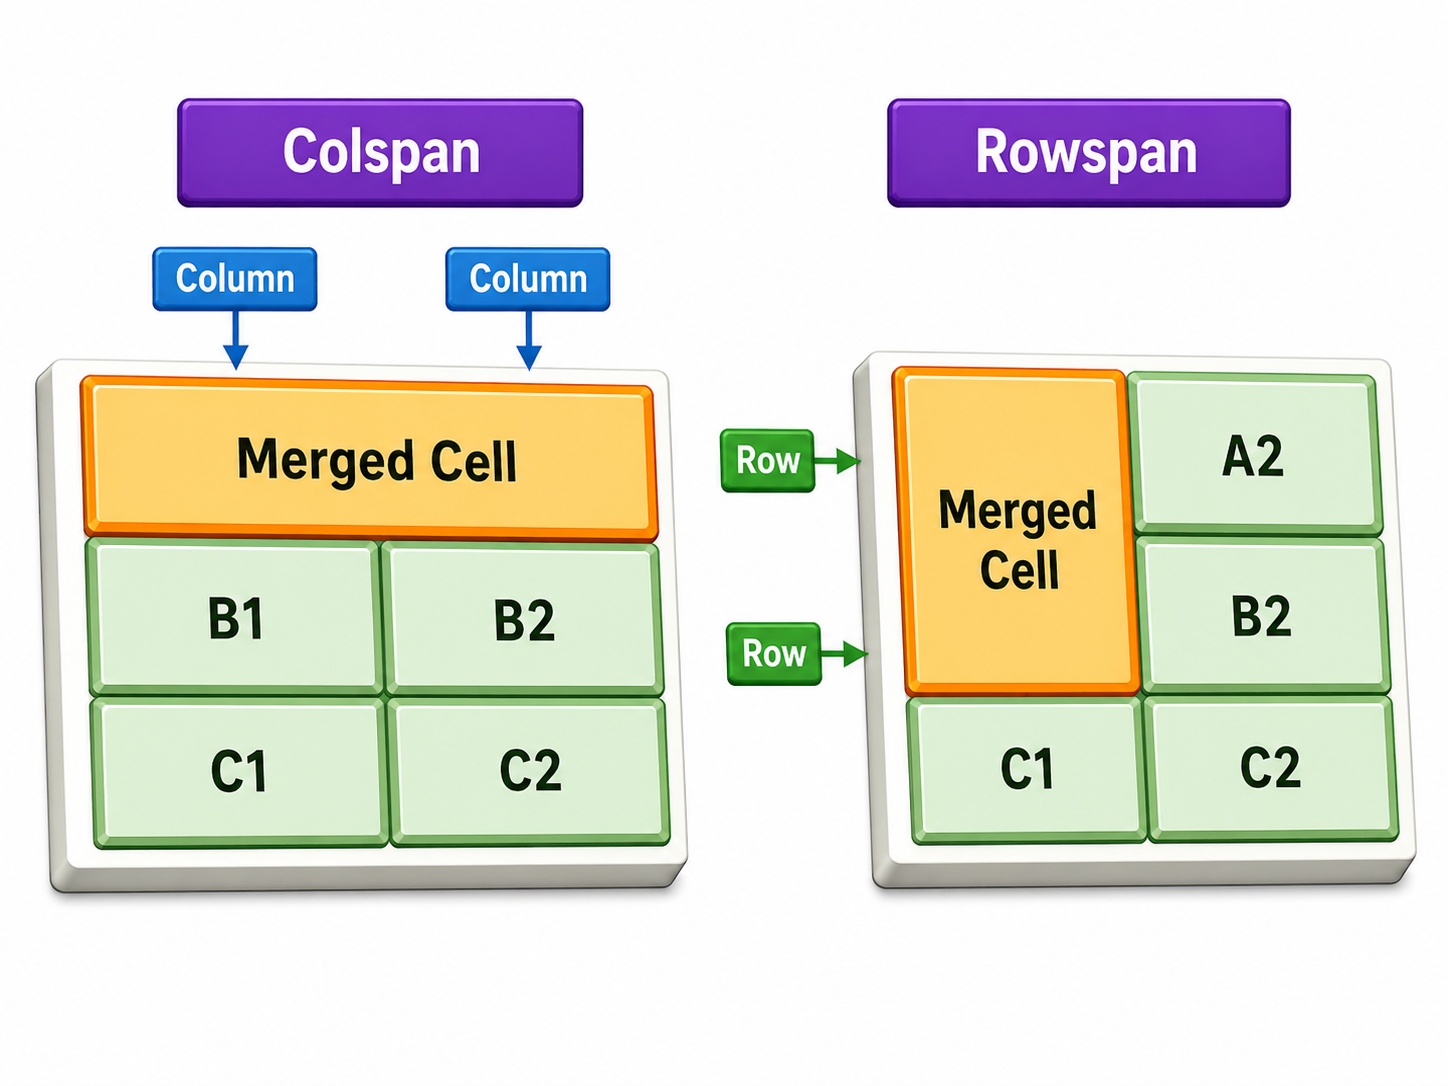
\includegraphics[width=\linewidth,height=.30\textheight,keepaspectratio]{chapters/Chapter04/topics/images/3d_rowspan_colspan.png}
\captionof{figure}{rowspan ও colspan দিয়ে ঘরের বিস্তার}\par\smallskip
\end{minipage}\hfill
\begin{minipage}[t]{.38\linewidth}\vspace{0pt}\small
\begin{keypointbox}{চিত্র ব্যাখ্যা}
চিত্রে \texttt{colspan} দিয়ে আড়াআড়ি বিস্তার এবং \texttt{rowspan} দিয়ে লম্বালম্বি বিস্তার দেখানো হয়েছে। চিত্র দেখে কোড লেখার সময় বিস্তৃত ঘর আগে শনাক্ত করতে হয়।
\end{keypointbox}


\begin{keypointbox}{মনে রাখার উপায়}
\texttt{colspan} = কলাম জুড়ে পাশের দিকে বিস্তার।\\
\texttt{rowspan} = সারি জুড়ে নিচের দিকে বিস্তার।
\end{keypointbox}
\end{minipage}\par\smallskip

\par\noindent\begin{minipage}{\linewidth}
\subsubsection{বিস্তৃত ঘরের দখল করা স্থান গুনে দেখো}
\begin{center}
\begin{tikzpicture}[x=8mm,y=7mm,every node/.style={font=\small,align=center}]
\begin{scope}
\fill[chFourTint] (0,2.6) rectangle (4,3.9);
\draw (0,0) rectangle (6,3.9);
\draw (0,1.3)--(6,1.3) (0,2.6)--(6,2.6);
\draw (2,0)--(2,2.6) (4,0)--(4,3.9);
\node at (2,3.25) {দুই কলাম};
\node at (5,3.25) {এক ঘর};
\node at (3,4.65) {\texttt{colspan="2"}};
\node at (3,-.65) {প্রথম সারিতে দুইটি ট্যাগ};
\end{scope}
\begin{scope}[xshift=65mm]
\fill[chFourRose!10] (0,1.3) rectangle (2,3.9);
\draw (0,0) rectangle (6,3.9);
\draw (0,1.3)--(6,1.3) (2,2.6)--(6,2.6);
\draw (2,0)--(2,3.9) (4,0)--(4,3.9);
\node[text width=14mm] at (1,2.6) {দুই সারি};
\node at (3,4.65) {\texttt{rowspan="2"}};
\node at (3,-.65) {দ্বিতীয় সারিতে দুইটি ট্যাগ};
\end{scope}
\end{tikzpicture}
\captionof{figure}{তিন কলামের ছকে colspan ও rowspan-এর দখল করা স্থান}
\end{center}
বাম ছকে ওপরের একটি ঘর দুই কলামের স্থান নিয়েছে। তাই ওই সারিতে তিন কলামের জন্য দুইটি ঘরের ট্যাগ লিখতে হবে। ডান ছকে বাম ঘরটি প্রথম দুই সারি জুড়ে আছে। দ্বিতীয় সারিতে তার জন্য আরেকটি ট্যাগ লিখলে নতুন ঘর যোগ হয়ে ছক বদলে যাবে। উভয় ছকেই মূল কলামসংখ্যা তিন।

\end{minipage}\par\smallskip

\subsubsection{মূল ছকের স্থান গণনা}

বিস্তৃত ঘর হলো এমন ঘর, যা একাধিক সারি বা কলামের জায়গা নেয়। টেবিল চিত্র দেখে কোড লেখার সময় বিস্তৃত ঘর ভুল হলে পুরো টেবিলের বিন্যাস নষ্ট হয়ে যায়। তাই \texttt{rowspan} ও \texttt{colspan} ব্যবহার করার আগে মূল কলামসংখ্যা ঠিক করা দরকার।

\begin{boardbox}{\texttt{colspan} কখন ব্যবহার করবে}
যদি কোনো ঘর বাম থেকে ডানে একাধিক কলামের জায়গা নেয়, তখন \texttt{colspan} ব্যবহার করবে। যেমন, একটি শিরোনাম যদি টেবিলের তিনটি কলাম জুড়ে থাকে, তাহলে কোড হবে \texttt{<th colspan="3">Title</th>}।
\end{boardbox}

\begin{boardbox}{\texttt{rowspan} কখন ব্যবহার করবে}
যদি কোনো ঘর উপর থেকে নিচে একাধিক সারির জায়গা নেয়, তখন \texttt{rowspan} ব্যবহার করবে। যেমন, একটি বিভাগের নাম যদি দুইটি শাখার সারির জন্য একই হয়, তাহলে কোড হবে \texttt{<td rowspan="2">Science</td>}।
\end{boardbox}

\begin{keypointbox}{বিস্তৃত ঘরের কারণে ঘর গণনা কমে যায়}
\texttt{colspan} দেওয়া ঘর একই সারিতে একাধিক কলামের স্থান নেয়। \texttt{rowspan} দেওয়া ঘর পরের সারির স্থানও দখল করে; সেই পরের সারিতে ওই স্থানের জন্য নতুন ঘর লিখতে হয় না। তাই প্রতিটি সারির দৃশ্যমান ঘর গুনলেই মূল কলামসংখ্যা পাওয়া যায় না; বিস্তৃত ঘরের দখল করা স্থানও ধরতে হবে।
\end{keypointbox}


\subsection{চিত্র থেকে rowspan ও colspan নির্ধারণ}

সারণির চিত্র দেখে কোড লেখার আগে মূল কলাম ও মূল সারিগুলো শনাক্ত করো। বিস্তৃত ঘরটি মূল ছকের কতটি স্থান দখল করেছে, তা গুনতে হয়। শুধু দৃশ্যমান ঘরের সংখ্যা থেকে মূল সারি বা কলামসংখ্যা পাওয়া যায় না। ধাপগুলো হলো:

\begin{enumerate}
\item মোট কয়টি কলাম আছে গুনে নাও।
\item কোনো ঘর ডানদিকে কয়টি কলামজুড়ে আছে দেখো।
\item ঘর ডানদিকে ২টি কলাম জুড়লে \texttt{colspan="2"}।
\item ঘর ডানদিকে ৩টি কলাম জুড়লে \texttt{colspan="3"}।
\item কোনো ঘর নিচের দিকে কয়টি সারিজুড়ে আছে দেখো।
\item ঘর নিচের দিকে ২টি সারি জুড়লে \texttt{rowspan="2"}।
\item ঘর নিচের দিকে ৩টি সারি জুড়লে \texttt{rowspan="3"}।
\item যে সারি বা কলাম একত্র হয়ে গেছে, সেই জায়গার জন্য আলাদা \texttt{<td>} বা \texttt{<th>} আর লিখবে না।
\end{enumerate}

\begin{center}
\begin{tikzpicture}[x=17mm,y=8mm,font=\small]
\draw (0,0) rectangle (3,2);
\draw (0,1)--(3,1);
\draw (1,0)--(1,2);
\draw (2,0)--(2,1);
\node at (.5,1.5) {Name};
\node at (2,1.5) {Subject};
\node at (.5,.5) {1};
\node at (1.5,.5) {2};
\node at (2.5,.5) {3};
\node[anchor=west] at (3.25,1.5) {শিরোনামের ২টি ঘর};
\node[anchor=west] at (3.25,.5) {মূল ছকের ৩টি কলাম};
\end{tikzpicture}
\end{center}
Subject ঘরটি ২ ও ৩ নম্বর কলাম দখল করেছে। তাই প্রথম সারিতে দুটি ঘর লেখা হলেও তার বিস্তার $1+2=3$ কলাম।

\subsection{সবচেয়ে গুরুত্বপূর্ণ নিয়ম}

\subsubsection{colspan হলে একই সারিতে কয়টি ঘর লিখবে?}

নির্দিষ্ট তিন-কলামের সারণিতে একটি ঘর দুই কলামজুড়ে থাকলে বাকি এক কলামের জন্য আরেকটি ঘর প্রয়োজন। তাই শুধু ট্যাগের সংখ্যা নয়, প্রতিটি ঘর কত কলামের স্থান দখল করছে তা যোগ করে দেখবে। নিচের প্রথম সারিটি চাওয়া Name--Math--ICT ছকের সঙ্গে মেলে না: Subject একাই দুই কলামের স্থান নেয়, তার পরে Math ও ICT আরও দুইটি স্থান নেয়।

% Split revision: code and its explanation share one row.
\par\noindent
\begin{minipage}[t]{.50\linewidth}\vspace{0pt}\small
\textbf{ভুল:}
\textbf{\color{chFourTeal}কোড}\par
\begin{verbatim}
<tr>
  <th colspan="2">Subject</th>
  <th>Math</th>
  <th>ICT</th>
</tr>
\end{verbatim}
\par\smallskip
\end{minipage}\hfill
\begin{minipage}[t]{.46\linewidth}\vspace{0pt}\small
\textbf{সঠিক:}
\textbf{\color{chFourTeal}কোড}\par
\begin{verbatim}
<tr>
  <th>Name</th>
  <th colspan="2">Subject</th>
</tr>
<tr>
  <td>Kabir</td>
  <td>Math</td>
  <td>ICT</td>
</tr>
\end{verbatim}
\par\smallskip
\end{minipage}\par


\subsubsection{rowspan হলে পরের সারিতে কী লিখবে?}

যদি একটি ঘর \texttt{rowspan="2"} হয়, তাহলে পরের সারিতে সেই ঘরের জায়গায় আর \texttt{<td>} বা \texttt{<th>} লিখবে না।

\Needspace{7\baselineskip}
% Split revision: code and its explanation share one row.
\par\noindent
\begin{minipage}[t]{.50\linewidth}\vspace{0pt}\small
\textbf{সঠিক:}
\textbf{\color{chFourTeal}কোড}\par
\begin{verbatim}
<tr>
  <th rowspan="2">Phone</th>
  <td>8942318</td>
</tr>
<tr>
  <td>1750181</td>
</tr>
\end{verbatim}
\par\smallskip
\end{minipage}\hfill
\begin{minipage}[t]{.46\linewidth}\vspace{0pt}\small
\textbf{ভুল:}
\textbf{\color{chFourTeal}কোড}\par
\begin{verbatim}
<tr>
  <th rowspan="2">Phone</th>
  <td>8942318</td>
</tr>
<tr>
  <th>Phone</th>
  <td>1750181</td>
</tr>
\end{verbatim}
\par\smallskip
\end{minipage}\par


Phone প্রথম সারি থেকে দ্বিতীয় সারির প্রথম কলাম পর্যন্ত বিস্তৃত আছে। দ্বিতীয় সারিতে আবার Phone-এর ঘর লিখলে সেটি পরের খালি কলামে বসে এবং নম্বর আরও ডানে সরে যায়। ফলে চাওয়া দুই-কলামের ছক পাওয়া যায় না।

\subsection{ফাঁকা ঘর দেখানোর নিয়ম}

খালি \texttt{<td></td>} একটি বৈধ ঘর। সেটি দেখানোর জন্য \texttt{<br>} দেওয়া বাধ্যতামূলক নয়। ঘরের উচ্চতা, ফাঁকা জায়গা ও সীমানা CSS-এর নিয়মের ওপর নির্ভর করে। নিচের পুরোনো উদাহরণে \texttt{<br>} একটি ফাঁকা লাইনের জায়গা রাখে।

\begin{examplebox}{কোড}
\begin{verbatim}
<td><br></td>
\end{verbatim}
\end{examplebox}

নিচের \texttt{\&nbsp;} একটি অচ্ছেদ্য ফাঁকা অক্ষর রাখে; তাই এই ঘরটি আর সম্পূর্ণ খালি থাকে না। এটি ফাঁকা ঘরকে বৈধ করার নিয়ম নয়। নতুন পেজে প্রয়োজনীয় উচ্চতা ও ফাঁকা জায়গা CSS দিয়ে নির্ধারণ করা যায়।

\begin{examplebox}{কোড}
\begin{verbatim}
<td>&nbsp;</td>
\end{verbatim}
\end{examplebox}

\Needspace{7\baselineskip}
\subsection{পূর্ণ অনুশীলন: শিক্ষার্থী ও বিষয়ের সারণি}

% Split revision: code and its explanation share one row.
\par\noindent
\begin{minipage}[t]{.54\linewidth}\vspace{0pt}\small
\textbf{\color{chFourTeal}কোড}\par
\begin{verbatim}
<table border="1" cellspacing="0" cellpadding="5">
  <tr>
    <th colspan="3">Student</th>
  </tr>
  <tr>
    <th>Name</th><th colspan="2">Subject</th>
  </tr>
  <tr>
    <td>Sakib</td><td>Bangla</td><td>English</td>
  </tr>
  <tr>
    <td>Asraful</td><td>Math</td><td>ICT</td>
  </tr>
</table>
\end{verbatim}
\par\smallskip
\end{minipage}\hfill
\begin{minipage}[t]{.42\linewidth}\vspace{0pt}\small
\textbf{\color{chFourTeal}ফলের ধারণা}\par
\begin{center}
\begin{tabular}{|c|c|c|}
\hline
\multicolumn{3}{|c|}{\textbf{Student}} \\
\hline
\textbf{Name} & \multicolumn{2}{c|}{\textbf{Subject}} \\
\hline
Sakib & Bangla & English \\
\hline
Asraful & Math & ICT \\
\hline
\end{tabular}
\end{center}
\par\smallskip
\end{minipage}\par


\Needspace{7\baselineskip}
\subsection{পূর্ণ অনুশীলন: কর্মী ও বেতনের সারণি}

% Split revision: code and its explanation share one row.
\par\noindent
\begin{minipage}[t]{.54\linewidth}\vspace{0pt}\small
\textbf{\color{chFourTeal}কোড}\par
\begin{verbatim}
<table border="1" cellspacing="0" cellpadding="5">
  <caption>Emp. Information</caption>
  <tr>
    <th>ID No</th><th>Emp. Name</th><th>Salary</th>
  </tr>
  <tr>
    <td>1001</td><td>Sakib</td><td rowspan="3">50,000</td>
  </tr>
  <tr>
    <td>1002</td><td>Asraful</td>
  </tr>
  <tr>
    <td><br></td>
    <td><br></td>
  </tr>
</table>
\end{verbatim}
\par\smallskip
\end{minipage}\hfill
\begin{minipage}[t]{.42\linewidth}\vspace{0pt}\small
\textbf{\color{chFourTeal}ফলের ধারণা}\par
\begin{center}
\textbf{Emp. Information}\par\smallskip
\begin{tabular}{|c|c|c|}
\hline
\textbf{ID No} & \textbf{Emp. Name} & \textbf{Salary} \\
\hline
1001 & Sakib & \raisebox{-\normalbaselineskip}[0pt][0pt]{50,000} \\
\cline{1-2}
1002 & Asraful & \\
\cline{1-2}
 & & \\
\hline
\end{tabular}
\end{center}
এখানে Salary-এর 50,000 লেখা ঘরটি তিন সারিজুড়ে আছে; তৃতীয় সারিতে ID No ও Emp. Name ফাঁকা। তাই \texttt{rowspan="3"} দেওয়া হয়েছে। Emp. Information হলো \texttt{<caption>}-এর লেখা; এটি সীমানার ভেতরে একত্র করা শিরোনাম ঘর নয়।
\par\smallskip
\end{minipage}\par



\subsubsection{ভুল ধরো: বাড়তি ঘর কেন হলো?}
\noindent
\begin{minipage}[t]{.48\linewidth}\vspace{0pt}
\textbf{ভুল}\par
\begin{verbatim}
<table border="1">
  <tr><td rowspan="2">ICT</td>
      <td>CQ</td></tr>
  <tr><td>ICT</td><td>MCQ</td></tr>
</table>
\end{verbatim}
\end{minipage}\hfill
\begin{minipage}[t]{.48\linewidth}\vspace{0pt}
\textbf{সঠিক}\par
\begin{verbatim}
<table border="1">
  <tr><td rowspan="2">ICT</td>
      <td>CQ</td></tr>
  <tr><td>MCQ</td></tr>
</table>
\end{verbatim}
\end{minipage}
\chFourWhy{ICT ঘরটি দ্বিতীয় সারির প্রথম স্থানও দখল করেছে। সেখানে নতুন ICT ঘর দিলে মোট তিন কলামের স্থান হয়; দুই-কলামের কাঙ্ক্ষিত ছক পাওয়া যায় না।}
\textbf{পুরোনো ও বর্তমান রীতি:} এখানে \texttt{border} পুরোনো উপস্থাপনমূলক অ্যাট্রিবিউট। আধুনিক CSS-এ ঘরের \texttt{border} ও টেবিলের \texttt{border-collapse} ব্যবহার করবে।



\subsection{প্রয়োগ: নদী ও ফুলের নাম সারণিতে সাজানো}
ফলে River ঘরটি তিনটি সারিজুড়ে থাকবে; পাশে Padma, Jamuna ও Meghna থাকবে। Flower ঘরটিও তিনটি সারিজুড়ে থাকবে; পাশে Adenium, Rose ও Lily থাকবে।

\Needspace{4\baselineskip}
\par\noindent{\color{chFourTeal}\bfseries\small কোড}\par\smallskip
\begin{multicols}{2}
\begin{verbatim}
<!DOCTYPE html>
<html>
<body>
  <table border="1" cellspacing="0" cellpadding="5">
    <tr>
      <td rowspan="3" align="center">River</td><td>Padma</td>
    </tr>
    <tr>
      <td>Jamuna</td>
    </tr>
    <tr>
      <td>Meghna</td>
    </tr>
    <tr>
      <td rowspan="3" align="center">Flower</td><td>Adenium</td>
    </tr>
    <tr>
      <td>Rose</td>
    </tr>
    <tr>
      <td>Lily</td>
    </tr>
  </table>
</body>
</html>
\end{verbatim}
\end{multicols}


\textbf{কেন \texttt{rowspan="3"}?}\\
River-এর পাশে তিনটি নদীর নাম আছে, তাই River ঘর তিনটি সারিজুড়ে থাকবে। Flower-এর ক্ষেত্রেও একই কারণে \texttt{rowspan="3"} ব্যবহার করা হয়েছে।




\subsection{সংক্ষিপ্ত অনুশীলন}

% Each question keeps its answer beneath it in the same column.
\begin{multicols}{2}
\noindent\begin{minipage}[t]{\linewidth}\vspace{0pt}
\chFourReviewQuestion{\textbf{\texttt{colspan} কী?}}
\end{minipage}\par\smallskip
\noindent\begin{minipage}[t]{\linewidth}\vspace{0pt}
\chFourReviewQuestion{\textbf{\texttt{rowspan} কী?}}
\end{minipage}\par\smallskip
\noindent\begin{minipage}[t]{\linewidth}\vspace{0pt}
\chFourReviewQuestion{\textbf{\texttt{rowspan} ও \texttt{colspan}-এর পার্থক্য লেখ।}}
\end{minipage}\par\smallskip
\noindent\begin{minipage}[t]{\linewidth}\vspace{0pt}
\chFourReviewQuestion{\textbf{\texttt{<th colspan="3">Result</th>} এর অর্থ কী?}}
\end{minipage}\par\smallskip
\noindent\begin{minipage}[t]{\linewidth}\vspace{0pt}
\chFourReviewQuestion{\textbf{\texttt{<td rowspan="2">Phone</td>} এর অর্থ কী?}}
\end{minipage}\par\smallskip
\end{multicols}

\Needspace{10\baselineskip}
\subsection{বহুনির্বাচনি অনুশীলন}

\par\addvspace{4pt}\noindent
\begin{minipage}[t]{.48\linewidth}\vspace{0pt}
\begin{enumerate}[start=1,leftmargin=*,topsep=0pt,itemsep=0pt]
\item সারণির ঘরকে একাধিক কলামজুড়ে দিতে কোন অ্যাট্রিবিউট ব্যবহার হয়?
\par ক) \texttt{rowspan}
\par খ) \texttt{colspan}
\par গ) \texttt{cellpadding}
\par ঘ) \texttt{cellspacing}
\end{enumerate}
\end{minipage}\hfill
\begin{minipage}[t]{.48\linewidth}\vspace{0pt}
\begin{enumerate}[start=2,leftmargin=*,topsep=0pt,itemsep=0pt]
\item সারণির ঘরকে একাধিক সারিজুড়ে দিতে কোন অ্যাট্রিবিউট ব্যবহার হয়?
\par ক) \texttt{rowspan}
\par খ) \texttt{colspan}
\par গ) \texttt{border}
\par ঘ) \texttt{src}
\end{enumerate}
\end{minipage}
\par
\par\addvspace{4pt}\noindent
\begin{minipage}[t]{.48\linewidth}\vspace{0pt}
\begin{enumerate}[start=3,leftmargin=*,topsep=0pt,itemsep=0pt]
\item \texttt{<th colspan="4">Title</th>} এর অর্থ কী?
\par ক) Title ৪টি row জুড়ে থাকবে
\par খ) Title ৪টি column জুড়ে থাকবে
\par গ) Title ৪ pixel হবে
\par ঘ) Title ৪ বার দেখা যাবে
\end{enumerate}
\end{minipage}\hfill
\begin{minipage}[t]{.48\linewidth}\vspace{0pt}
\begin{enumerate}[start=4,leftmargin=*,topsep=0pt,itemsep=0pt]
\item \texttt{<td rowspan="3">Phone</td>} এর অর্থ কী?
\par ক) Phone ৩টি column জুড়ে থাকবে
\par খ) Phone ৩টি row জুড়ে থাকবে
\par গ) Phone ৩ pixel হবে
\par ঘ) Phone ৩ বার print হবে
\end{enumerate}
\end{minipage}
\par
\par\addvspace{4pt}\noindent
\begin{minipage}[t]{.48\linewidth}\vspace{0pt}
\begin{enumerate}[start=5,leftmargin=*,topsep=0pt,itemsep=0pt]
\item নিচের কোন ট্যাগে \texttt{rowspan}/\texttt{colspan} ব্যবহার করা যায়?
\par ক) \texttt{<td>} ও \texttt{<th>}
\par খ) \texttt{<br>} ও \texttt{<hr>}
\par গ) \texttt{<img>} ও \texttt{<a>}
\par ঘ) \texttt{<html>} ও \texttt{<body>}
\end{enumerate}
\end{minipage}
\par

\chFourMCQAnswer{১-খ, ২-ক, ৩-খ, ৪-খ, ৫-ক}

\subsection{প্রয়োগ: নম্বরের ছকে দুটি বিস্তৃত শিরোনাম}


\begin{examplebox}{কোড}
\begin{verbatim}
<table border="1" cellspacing="0" cellpadding="5">
  <tr>
    <th colspan="3">Result</th>
  </tr>
  <tr>
    <th>Subject</th><th>CQ</th><th>MCQ</th>
  </tr>
  <tr>
    <td>ICT</td><td>45</td><td>25</td>
  </tr>
  <tr>
    <td>English</td><td colspan="2">95</td>
  </tr>
</table>
\end{verbatim}
\end{examplebox}


\subsection{সৃজনশীল অনুশীলন}

\begin{practicebox}
\textbf{উদ্দীপক:} একটি ওয়েবপেজে Result সারণি দেখাতে হবে। Result শিরোনাম পুরো ৩টি কলামজুড়ে থাকবে এবং English-এর 95 নম্বর CQ ও MCQ--দুইটি কলামজুড়ে থাকবে।

\textbf{প্রশ্ন}\\
ক. \texttt{colspan} কী?\\
খ. \texttt{rowspan} কেন ব্যবহার করা হয়?\\
গ. উদ্দীপকের জন্য HTML কোড লেখ।\\
ঘ. সারণি চিত্র দেখে \texttt{rowspan} ও \texttt{colspan} নির্ধারণের নিয়ম বিশ্লেষণ কর।
\end{practicebox}

\subsection{সাধারণ ভুল}

\begin{mistakebox}{সাধারণ ভুল}
\par\noindent
\begin{minipage}[t]{.48\linewidth}\vspace{0pt}
\begin{itemize}
\item \texttt{rowspan} ও \texttt{colspan} গুলিয়ে ফেলা।
\item কলাম একত্র করতে \texttt{rowspan} ব্যবহার করা।
\item সারি একত্র করতে \texttt{colspan} ব্যবহার করা।
\item \texttt{colspan="2"} দেওয়ার পরও একই সারিতে অতিরিক্ত ঘর লিখে ফেলা।
\item \texttt{rowspan="2"} দেওয়ার পরও পরের সারিতে একই ঘর আবার লিখে ফেলা।
\end{itemize}
\end{minipage}\hfill
\begin{minipage}[t]{.48\linewidth}\vspace{0pt}
\begin{itemize}
\item উদ্ধৃতি না থাকলেই মান ভুল ভাবা: \texttt{colspan=2} বৈধ HTML। তবে একই লেখার রীতি রাখতে \texttt{colspan="2"} ব্যবহার করা সুবিধাজনক।
\item \texttt{<tr>} ট্যাগে \texttt{colspan} লেখা।
\item \texttt{<table>} ট্যাগে \texttt{rowspan} লেখা।
\item চিত্রের মোট সারি/কলাম না গুনে সরাসরি কোড লেখা।
\end{itemize}
\end{minipage}\par

\end{mistakebox}

\begin{boardbox}{পরবর্তী টপিক}
পরের অংশে সারণির ঘরের ভেতরে তালিকা, ছবি, হাইপারলিংক ও নেস্টেড সারণি ব্যবহার করব।
\end{boardbox}

% Density revision 2026-10-04: answers below questions; compact related content.
% Topic 16: Elements ভেতরে HTML সারণি
\section{সারণির ঘরে তালিকা, ছবি, হাইপারলিংক ও নেস্টেড সারণি}

% Composition pass 2026-10-04
লাইব্রেরির তালিকায় একই বইয়ের নাম, প্রচ্ছদ, বিষয় ও বিস্তারিত লিংক একসঙ্গে দরকার।

\chFourMotivation{সম্পর্কিত তথ্য একই ঘরে রাখা $\rightarrow$ ঘরের ভেতর HTML এলিমেন্ট $\rightarrow$ td/th-এর মধ্যে তালিকা, ছবি ও লিংক বসানো $\rightarrow$ বই বা পণ্যের সমন্বিত সারণি।}


\begin{learningbox}
এই অংশ শেষে শিক্ষার্থী পারবে:
\begin{itemize}
\item HTML সারণির ঘরের ভেতরে তালিকা, ছবি, হাইপারলিংক ও ফরম্যাটিং ট্যাগ ব্যবহার করতে।
\item সারণির ঘরের ভেতরে ক্রমিক তালিকা ও অক্রমিক তালিকা বসাতে।
\item ছবির হাইপারলিংক তৈরি করতে।
\item নেস্টেড সারণি কী তা ব্যাখ্যা করতে এবং নেস্টেড সারণির সহজ কোড লিখতে।
\item সৃজনশীল ও ব্যবহারিক প্রশ্নে সারণির ভেতরে একাধিক HTML উপাদান ব্যবহার করে কোড লিখতে।
\end{itemize}
\end{learningbox}



একটি বইয়ের তালিকায় এক কলামে বইয়ের নাম এবং পাশের কলামে তার ছবি, বিষয়গুলোর তালিকা ও বিস্তারিত জানার লিংক দেখাতে চাই। HTML সারণির ঘরে কেবল লেখা নয়; তালিকা, ছবি, হাইপারলিংক ও আরেকটি সারণিও রাখা যায়। এবার আগের ট্যাগগুলো একসঙ্গে ব্যবহার করে এমন চিত্রের কোড লিখব। ঘর ও তার ভেতরের উপাদানের শুরু--শেষ সঠিকভাবে মিলিয়ে রাখাই এখানে প্রধান কাজ।

\subsection{সারণির ঘরে রাখা যায় যেসব উপাদান}

HTML সারণির \texttt{<td>} বা \texttt{<th>} ঘরের ভেতরে অনেক ধরনের HTML উপাদান রাখা যায়।

\begin{center}
\footnotesize
\begin{tabular}{|p{0.30\textwidth}|p{0.52\textwidth}|}
\hline
\textbf{ঘরের ভেতরে রাখা যায়} & \textbf{উদাহরণ} \\
\hline
সাধারণ লেখা & \texttt{<td>ICT</td>} \\
\hline
বোল্ড/আন্ডারলাইন লেখা & \texttt{<td><u>ICT</u></td>} \\
\hline
হাইপারলিংক & \texttt{<td><a href="board.html">Board</a></td>} \\
\hline
ছবি & \texttt{<td><img src="book.jpg" alt="Book" width="100"></td>} \\
\hline
ক্রমিক তালিকা & \texttt{<td><ol><li>Book</li></ol></td>} \\
\hline
অক্রমিক তালিকা & \texttt{<td><ul><li>Pen</li></ul></td>} \\
\hline
নেস্টেড সারণি & \texttt{<td><table>...</table></td>} \\
\hline
\end{tabular}
\end{center}

\begin{keypointbox}{মূল ধারণা}
সারণির ঘরের ভেতরে বিষয়বস্তু রাখার সময় বিষয়বস্তু অবশ্যই \texttt{<td>} বা \texttt{<th>} ট্যাগের ভেতরে রাখতে হবে। \texttt{<table>} ট্যাগের ভেতরে সরাসরি \texttt{<ol>}, \texttt{<ul>}, \texttt{<img>} বা \texttt{<a>} লেখা ঠিক নয়।
\end{keypointbox}

\subsection{সারণির ঘরে তালিকা}

কোনো সারণির ঘরের ভেতরে ক্রমিক তালিকা বা অক্রমিক তালিকা বসাতে হলে \texttt{<td>} ট্যাগের ভেতরে \texttt{<ol>} বা \texttt{<ul>} লিখতে হয়।

\subsubsection{লেখার সাধারণ রূপ}

\begin{examplebox}{কোড}
\begin{verbatim}
<td>
  <ol>
    <li>Item 1</li>
    <li>Item 2</li>
  </ol>
</td>
\end{verbatim}
\end{examplebox}

\Needspace{10\baselineskip}
অথবা--

\begin{examplebox}{কোড}
\begin{verbatim}
<td>
  <ul>
    <li>Item 1</li>
    <li>Item 2</li>
  </ul>
</td>
\end{verbatim}
\end{examplebox}

\subsection{উদাহরণ: ক্রমিক ও অক্রমিক তালিকা}

\begin{examplebox}{ফলের ধারণা}
\begin{center}
\begin{tabular}{|p{0.36\textwidth}|p{0.36\textwidth}|}
\hline
\multicolumn{2}{|c|}{\textbf{A \& H Company Ltd.}} \\
\hline
\textbf{Order List} & \textbf{Unorder List} \\
\hline
i. Book \newline ii. Paper \newline iii. Note Book & \rule{.6ex}{.6ex} Marker \newline \rule{.6ex}{.6ex} Ink \newline \rule{.6ex}{.6ex} Pencil \\
\hline
\end{tabular}
\end{center}
\end{examplebox}

\Needspace{6\baselineskip}
\par\noindent{\color{chFourTeal}\bfseries\small কোড: বাম কলাম শেষে ডান কলাম পড়বে}\par
\begin{multicols}{2}
\begin{verbatim}
<!DOCTYPE html>
<html>
<head>
  <title>HTML List in Table</title>
</head>
<body>
  <table border="2" cellspacing="0" cellpadding="5">
    <tr>
      <th colspan="2" align="center">A & H Company Ltd.</th>
    </tr>
    <tr>
      <th>Order List</th><th>Unorder List</th>
    </tr>
    <tr>
      <td>
        <ol type="i">
          <li>Book</li>
          <li>Paper</li>
          <li>Note Book</li>
        </ol>
      </td>
      <td>
        <ul type="square">
          <li>Marker</li>
          <li>Ink</li>
          <li>Pencil</li>
        </ul>
      </td>
    </tr>
  </table>
</body>
</html>
\end{verbatim}
\end{multicols}


\begin{boardbox}{পরীক্ষার জন্য মনে রাখবে}
ওপরের উদাহরণের Order List ও Unorder List দুটি দৃশ্যমান শিরোনাম। তালিকার সঠিক পরিভাষা Ordered List ও Unordered List। দুই ধরনের তালিকাই ঘরের ভেতরে শুরু ও শেষ হয়েছে।
\end{boardbox}

\subsection{সারণির ঘরে হাইপারলিংক}

সারণির ঘরের ভেতরে লিংক বসাতে \texttt{<td>} ট্যাগের ভেতরে \texttt{<a href="">...</a>} লিখতে হয়।

% Split revision: code and its explanation share one row.
\par\noindent
\begin{minipage}[t]{.54\linewidth}\vspace{0pt}\small
\subsubsection{লেখার রূপ}

\textbf{\color{chFourTeal}কোড}\par
\begin{verbatim}
<td>
  <a href="url">Link Text</a>
</td>
\end{verbatim}
\par\smallskip
\end{minipage}\hfill
\begin{minipage}[t]{.42\linewidth}\vspace{0pt}\small
\subsubsection{উদাহরণ}

\textbf{\color{chFourTeal}কোড}\par
\begin{verbatim}
<td>
  <a href="https://www.educationboard.gov.bd">Board</a>
</td>
\end{verbatim}
\par\smallskip


\texttt{target="\_blank"} দিলে নতুন ব্রাউজিং প্রসঙ্গে লিংক খোলার অনুরোধ করা হয়। ব্রাউজার ও ব্যবহারকারীর সেটিং অনুযায়ী এটি নতুন ট্যাব বা উইন্ডো হতে পারে। বাহ্যিক লিংকে এটি দেওয়া বাধ্যতামূলক নয়; অ্যাট্রিবিউট না দিলে সাধারণত বর্তমান ট্যাবেই পেজ খোলে।
\end{minipage}\par
\subsection{উদাহরণ: বিষয়ের পাশে লিংক}

\begin{examplebox}{ফলের ধারণা}
\begin{center}
\begin{tabular}{|c|c|}
\hline
\textbf{Subject} & \textbf{Board} \\
\hline
ICT & \underline{Board} \\
\hline
\end{tabular}
\end{center}
Board লেখাটি লিংক; এতে ক্লিক করলে \texttt{href}-এ দেওয়া ঠিকানায় যাওয়া যায়।
\end{examplebox}

\begin{examplebox}{কোড}
\begin{verbatim}
<table border="1" cellspacing="0" cellpadding="5">
  <tr>
    <th>Subject</th>
    <th>Board</th>
  </tr>
  <tr>
    <td>ICT</td>
    <td>
      <a href="https://www.educationboard.gov.bd" target="_blank">
        Board
      </a>
    </td>
  </tr>
</table>
\end{verbatim}
\end{examplebox}

\subsection{সারণির ঘরে ছবি}

সারণির ঘরের ভেতরে ছবি বসাতে \texttt{<td>} ট্যাগের ভেতরে \texttt{<img>} ট্যাগ লিখতে হয়।

\subsubsection{লেখার রূপ}

% Split revision: code and its explanation share one row.
\par\noindent
\begin{minipage}[t]{.54\linewidth}\vspace{0pt}\small
\textbf{\color{chFourTeal}কোড}\par
\begin{verbatim}
<td>
  <img src="image.jpg" alt="Image" width="100" height="80">
</td>
\end{verbatim}
\par\smallskip
\end{minipage}\hfill
\begin{minipage}[t]{.42\linewidth}\vspace{0pt}\small
\textbf{\color{chFourTeal}ব্যাখ্যা}\par
এই উদাহরণে \texttt{src} ছবির ঠিকানা এবং \texttt{alt} বিকল্প লেখা জানায়। \texttt{width} ও \texttt{height} ছবির প্রদর্শিত প্রস্থ ও উচ্চতা নির্ধারণ করে।
\end{minipage}\par
\subsection{উদাহরণ: বইয়ের ছবি}

\begin{examplebox}{ফলের ধারণা}
\begin{center}
\begin{tabular}{|c|c|}
\hline
\textbf{Book} & \textbf{Image} \\
\hline
ICT Book & \fbox{\parbox[c][15mm][c]{24mm}{\centering ছবির স্থান\\\texttt{book.jpg}}} \\
\hline
\end{tabular}
\end{center}
\end{examplebox}

\begin{examplebox}{কোড}
\begin{verbatim}
<table border="1" cellspacing="0" cellpadding="5">
  <tr>
    <th>Book</th>
    <th>Image</th>
  </tr>
  <tr>
    <td>ICT Book</td>
    <td>
      <img src="book.jpg" alt="ICT Book" width="100" height="80">
    </td>
  </tr>
</table>
\end{verbatim}
\end{examplebox}

এখানে ছবির জায়গাটি বোঝানো হয়েছে। একই ফোল্ডারে \texttt{book.jpg} থাকলে ব্রাউজারে সেই ছবি দেখা যাবে; ফাইলের নাম দেখানোর নির্দেশ এটি নয়।

\subsection{সারণির ঘরে ছবির হাইপারলিংক}

সারণির ঘরের ছবিতে ক্লিক করে কোনো পেজ বা ওয়েবসাইটে যেতে চাইলে \texttt{<a>} ট্যাগের ভেতরে \texttt{<img>} ট্যাগ বসাতে হবে।

\subsubsection{লেখার রূপ}

\begin{examplebox}{কোড}
\begin{verbatim}
<td>
  <a href="url">
    <img src="image.jpg" alt="Image">
  </a>
</td>
\end{verbatim}
\end{examplebox}

\subsection{উদাহরণ: বইয়ের ছবিতে ক্লিক করে গন্তব্যে যাওয়া}

\begin{examplebox}{কোড}
\begin{verbatim}
<table border="1" cellspacing="0" cellpadding="5">
  <tr>
    <th>Book</th>
    <th>Image Link</th>
  </tr>
  <tr>
    <td>ICT Book</td>
    <td>
      <a href="https://www.book.com" target="_blank">
        <img src="book.jpg" alt="ICT Book" width="100" height="80">
      </a>
    </td>
  </tr>
</table>
\end{verbatim}
\end{examplebox}

\begin{keypointbox}{মনে রাখবে}
ক্লিক করা যায় এমন লেখা তৈরি করতে \texttt{<a>} ট্যাগের ভেতরে লেখা লিখতে হয়। ক্লিক করা যায় এমন ছবি তৈরি করতে \texttt{<a>} ট্যাগের ভেতরে \texttt{<img>} ট্যাগ লিখতে হয়।
\end{keypointbox}

\subsection{তালিকার ভেতরে লিংক: ঘরেও প্রয়োগ করা যায়}

তালিকার উপাদানের ভেতরেও লিংক বসানো যায়। নিচের স্বতন্ত্র তালিকায় Fruits একটি লিংক এবং তার অধীনে Ripe ও Dried উপতালিকা আছে। এখানে \texttt{start="4"} দেওয়ায় উপতালিকার রোমান ক্রম iv ও v থেকে শুরু হয়। এই উদাহরণে সারণি নেই; সারণির ঘরে চাইলে পুরো \texttt{<ul>...</ul>} অংশটি \texttt{<td>...</td>}-এর ভেতরে বসাবে।

\begin{examplebox}{কোড}
\begin{verbatim}
<ul type="circle">
  <li>Vegetables</li>
  <li>
    <a href="https://www.fruitbox.com" target="_blank">Fruits</a>
    <ol type="i" start="4">
      <li>Ripe</li>
      <li>Dried</li>
    </ol>
  </li>
</ul>
\end{verbatim}
\end{examplebox}

\subsection{নেস্টেড সারণির প্রয়োগ}

একটি সারণির ঘরের ভেতরে থাকা আরেকটি সারণিকে নেস্টেড সারণি (Nested Table) বলে। নিচে একজন শিক্ষার্থীর Marks ঘরে বিষয় ও নম্বরের একটি উপসারণি রাখা হয়েছে।

নেস্টেড সারণিতে বাইরের ঘর বন্ধ করার আগে ভেতরের পুরো সারণি বন্ধ করতে হয়। অপ্রয়োজনে বহু স্তরের সারণি করলে কোড পড়া কঠিন হয়। ছোট পর্দায় বিন্যাস ও সহায়ক প্রযুক্তিতে তথ্য বোঝার সমস্যাও হতে পারে। তথ্যের উপসারণি প্রয়োজন হলেই নেস্টেড সারণি ব্যবহার করা উচিত।

\subsection{নেস্টেড সারণি লেখার রূপ}

\begin{examplebox}{কোড}
\begin{verbatim}
<table border="1">
  <tr>
    <td>
      Outer Table Cell
    </td>
    <td>
      <table border="1">
        <tr>
          <td>Inner Table Cell</td>
        </tr>
      </table>
    </td>
  </tr>
</table>
\end{verbatim}
\end{examplebox}

\subsection{উদাহরণ: শিক্ষার্থীর ঘরে নম্বরের সারণি}

\begin{examplebox}{ফলের ধারণা}
\begin{center}
\begin{tabular}{|c|c|}
\hline
\textbf{Student} & \textbf{Marks} \\
\hline
Rafi & \begin{tabular}{|c|c|}\hline
\textbf{Subject} & \textbf{Mark}\\\hline
Bangla & 85\\\hline
English & 90\\\hline
\end{tabular} \\
\hline
\end{tabular}
\end{center}
\end{examplebox}

\Needspace{6\baselineskip}
\par\noindent{\color{chFourTeal}\bfseries\small কোড: বাম কলাম শেষে ডান কলাম পড়বে}\par
\begin{multicols}{2}
\begin{verbatim}
<table border="1" cellspacing="0" cellpadding="5">
  <tr>
    <th>Student</th><th>Marks</th>
  </tr>
  <tr>
    <td>Rafi</td>
    <td>
      <table border="1" cellspacing="0" cellpadding="5">
        <tr>
          <th>Subject</th><th>Mark</th>
        </tr>
        <tr>
          <td>Bangla</td><td>85</td>
        </tr>
        <tr>
          <td>English</td><td>90</td>
        </tr>
      </table>
    </td>
  </tr>
</table>
\end{verbatim}
\end{multicols}


\Needspace{11\baselineskip}
\subsection{নেস্টেড সারণিতে যে নিয়মগুলো দেখবে}

\begin{mistakebox}{সতর্কতা}
\begin{itemize}
\item অনেক স্তরের নেস্টেড সারণির কোড পড়া কঠিন হয়।
\item ভুল সমাপ্তি ট্যাগ দিলে বিন্যাস নষ্ট হয়।
\item সহায়ক প্রযুক্তিতে ব্যবহারের সমস্যা হতে পারে।
\item ছোট পর্দায় বিন্যাসে সমস্যা হতে পারে।
\item শুধুমাত্র সারণিভিত্তিক তথ্যের ভেতরে উপসারণি দরকার হলে ব্যবহার করা উচিত।
\end{itemize}
\end{mistakebox}

\begin{boardbox}{ব্যবহারের ক্ষেত্র}
নেস্টেড সারণি দিয়ে সারণির ভেতরে তথ্যের উপসারণি দেখানো যায়। পুরো ওয়েবপেজের বিন্যাস তৈরির জন্য আধুনিক ওয়েব ডিজাইনে CSS ব্যবহার করবে।
\end{boardbox}

\subsection{একটি ঘরে একাধিক উপাদান}

একটি ঘরের ভেতরে একাধিক উপাদান একসঙ্গে থাকতে পারে।

% Split revision: code and its explanation share one row.
\par\noindent
\begin{minipage}[t]{.54\linewidth}\vspace{0pt}\small
\textbf{\color{chFourTeal}কোড}\par
\begin{verbatim}
<td>
  <h3>ICT Book</h3>
  <img src="book.jpg" alt="ICT Book" width="100">
  <p>Price: 300 Tk</p>
  <a href="book.html">Details</a>
</td>
\end{verbatim}
\par\smallskip
\end{minipage}\hfill
\begin{minipage}[t]{.42\linewidth}\vspace{0pt}\small
\textbf{\color{chFourTeal}ব্যাখ্যা}\par
এখানে একই ঘরের ভেতরে শিরোনাম, ছবি, অনুচ্ছেদ ও লিংক আছে।
\end{minipage}\par
\subsection{পূর্ণ অনুশীলন: সারণি, তালিকা, ছবি ও লিংক}

\begin{examplebox}{ফলের ধারণা}
\begin{center}
\textbf{ICT Learning Materials}\par\smallskip
\begin{tabular}{|c|l|}
\hline
\textbf{Item} & \textbf{Details} \\
\hline
Book & \begin{tabular}{@{}c@{}}\fbox{\parbox[c][15mm][c]{24mm}{\centering ছবির স্থান\\\texttt{book.jpg}}}\\\underline{Buy Book}\end{tabular} \\
\hline
Subjects & \begin{tabular}{@{}l@{}}1. Web Design\\2. HTML\\3. Database\end{tabular} \\
\hline
\end{tabular}
\end{center}
\end{examplebox}

\Needspace{6\baselineskip}
\par\noindent{\color{chFourTeal}\bfseries\small কোড: বাম কলাম শেষে ডান কলাম পড়বে}\par
\begin{multicols}{2}
\begin{verbatim}
<table border="1" cellspacing="0" cellpadding="5">
  <caption>ICT Learning Materials</caption>
  <tr>
    <th>Item</th><th>Details</th>
  </tr>
  <tr>
    <td>Book</td>
    <td>
      <a href="https://www.book.com" target="_blank">
        <img src="book.jpg" alt="ICT Book" width="100" height="80">
      </a>
      <br>
      <a href="https://www.book.com" target="_blank">Buy Book</a>
    </td>
  </tr>
  <tr>
    <td>Subjects</td>
    <td>
      <ol type="1">
        <li>Web Design</li>
        <li>HTML</li>
        <li>Database</li>
      </ol>
    </td>
  </tr>
</table>
\end{verbatim}
\end{multicols}


ওপরের পূর্ণ অনুশীলনে ছবির জায়গা ও Buy Book লিংক দেখানো হয়েছে। ছবিতে বা লেখায় ক্লিক করলে কোডের গন্তব্যে যাওয়া যায়। পরের সৃজনশীল অনুশীলনটি স্বতন্ত্র; সেখানে Subjects-এর তালিকা HTML, CSS ও JavaScript। বাহ্যিক ঠিকানাগুলো লিংকের গঠন শেখানোর উদাহরণ; প্রয়োজনমতো বৈধ গন্তব্য ব্যবহার করবে।

% Original applied explanation; see Chapter04/SOURCES.md.
\subsubsection{ঘরের ভেতরের তথ্য ও বাইরের ঘর এক নয়}
গ্রন্থাগারের বইয়ের সারণিতে একটি ঘরে বইয়ের নাম, আরেক ঘরে প্রচ্ছদের ছবি এবং তৃতীয় ঘরে বিস্তারিত পেজের লিংক রাখা যায়। লেখা, \texttt{img} বা \texttt{a} সংশ্লিষ্ট \texttt{td}-এর ভেতরে থাকবে। সরাসরি \texttt{tr}-এর মধ্যে ছবি বসালে ঘরের গঠন ঠিক থাকে না।

এক ঘরের ভেতরে ছোট সারণি থাকলে আগে বাইরের ঘর খুলবে, তার ভেতরে সম্পূর্ণ ভেতরের সারণি লিখবে, তারপর বাইরের ঘর বন্ধ করবে। বাইরের ও ভেতরের \texttt{tr} আলাদা সারণির সারি; তাদের একসঙ্গে গুনবে না।

\subsection{প্রয়োগ: ঘরের লেখা, লিংক, ছবি ও তালিকা}

টেবিলের ঘরের ভিতরে লেখা ছাড়াও অন্য HTML এলিমেন্ট রাখা যায়। এখানে ছবি, তালিকা, ফর্মের নিয়ন্ত্রণ, আড়াআড়ি রেখা, হাইপারলিংক এবং আরেকটি টেবিল রাখার উদাহরণ আছে। ফলে ফলাফলের সঙ্গে শিক্ষার্থীর ছবি, পণ্যের তালিকার সঙ্গে কেনার লিংক এবং কোর্স পরিকল্পনার সঙ্গে ক্রমযুক্ত তালিকা দেখানো যায়। বিস্তারিত তথ্যের জন্য কোনো ঘরে আরেকটি টেবিলও রাখা যায়।

\begin{keypointbox}{ঘরের ভিতরে বিষয়বস্তু রাখার নিয়ম}
ঘরের ভিতরে বিষয়বস্তু রাখতে হলে বিষয়বস্তু অবশ্যই \texttt{<td>} বা \texttt{<th>} ট্যাগের শুরুর ও শেষের ট্যাগের মাঝখানে লিখতে হবে। যেমন ছবি বসাতে \texttt{<td><img src="photo.jpg"></td>} এবং লিংক বসাতে \texttt{<td><a href="page.html">Open</a></td>} লিখতে হবে।
\end{keypointbox}

\begin{center}
\begin{tabular}{|p{0.22\textwidth}|p{0.50\textwidth}|p{0.18\textwidth}|}
\hline
\textbf{বিষয়বস্তুর ধরন} & \textbf{ঘরের ভিতরে কোডের উদাহরণ} & \textbf{ট্যাগ} \\
\hline
লেখা & \texttt{<td>Rafi</td>} & \texttt{<td>} \\
\hline
ছবি & \texttt{<td><img src="a.jpg"></td>} & \texttt{<img>} \\
\hline
লিংক & \texttt{<td><a href="a.html">Open</a></td>} & \texttt{<a>} \\
\hline
তালিকা & \texttt{<td><ol>...</ol></td>} & \texttt{<ol>}, \texttt{<li>} \\
\hline
আড়াআড়ি রেখা & \texttt{<td><hr></td>} & \texttt{<hr>} \\
\hline
ফর্মের নিয়ন্ত্রণ & \texttt{<td><input type="text"></td>} & \texttt{<input>} \\
\hline
ভেতরের টেবিল & \texttt{<td><table>...</table></td>} & \texttt{<table>} \\
\hline
\end{tabular}
\end{center}

% Image layout revision: related content in two fixed columns.
\par\noindent
\begin{minipage}[t]{.48\linewidth}\vspace{0pt}\small
\subsubsection{লেখার বিন্যাস}
\begin{chFourWholeExample}{কোড}
\begin{verbatim}
<table border="1" cellspacing="0" cellpadding="6">
  <tr>
    <td><b>ICT</b></td>
    <td><u>HSC</u></td>
    <td><i>Book</i></td>
  </tr>
</table>
\end{verbatim}
\end{chFourWholeExample}
\end{minipage}\hfill
\begin{minipage}[t]{.48\linewidth}\vspace{0pt}\small
\subsubsection{হাইপারলিংক}
\begin{chFourWholeExample}{কোড}
\begin{verbatim}
<table border="1" cellspacing="0" cellpadding="6">
  <tr>
    <td>
      <a href="https://www.educationboard.gov.bd">Education Board</a>
    </td>
  </tr>
</table>
\end{verbatim}
\end{chFourWholeExample}
\end{minipage}\par\smallskip
% Image layout revision: related content in two fixed columns.
\par\noindent
\begin{minipage}[t]{.48\linewidth}\vspace{0pt}\small
\subsubsection{ছবি}
\begin{chFourWholeExample}{কোড}
\begin{verbatim}
<table border="1" cellspacing="0" cellpadding="6">
  <tr>
    <td>
      <img src="photo.jpg" width="100" height="80" alt="Photo">
    </td>
  </tr>
</table>
\end{verbatim}
\end{chFourWholeExample}
\end{minipage}\hfill
\begin{minipage}[t]{.48\linewidth}\vspace{0pt}\small
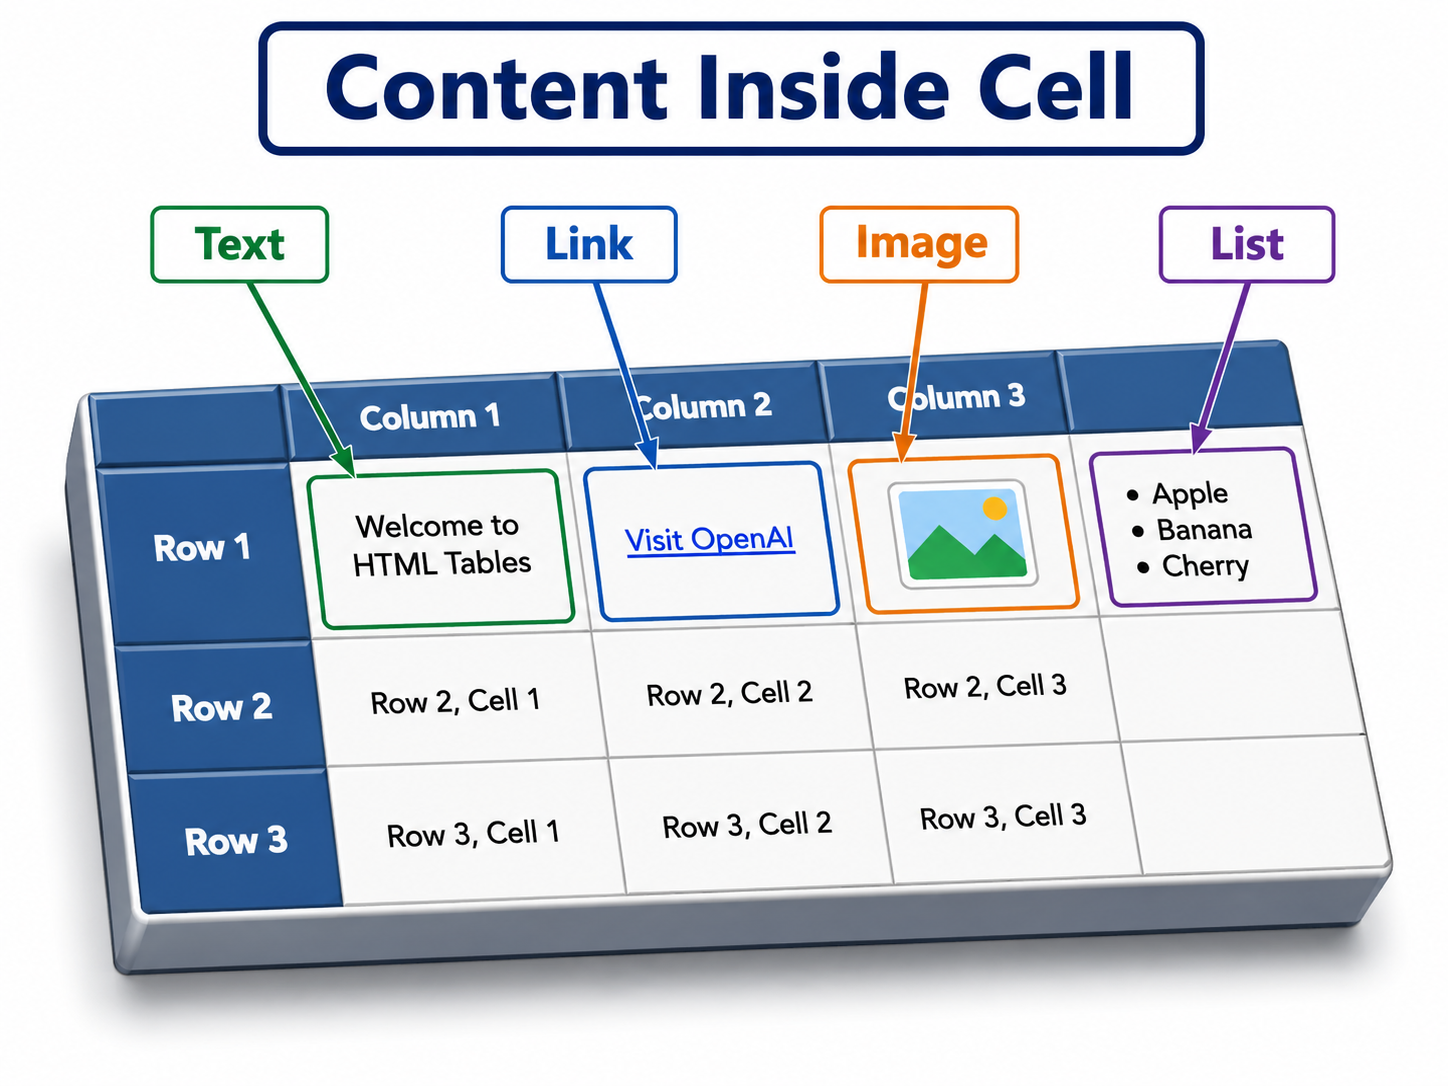
\includegraphics[width=\linewidth,height=.30\textheight,keepaspectratio]{chapters/Chapter04/topics/images/3d_content_inside_cell.png}
\captionof{figure}{টেবিলের ঘরের ভিতরে লেখা, লিংক, ছবি ও তালিকা}\par\smallskip
\end{minipage}\par\smallskip
\subsubsection{তালিকা}
% Image layout revision: related content in two fixed columns.
\par\noindent
\begin{minipage}[t]{.52\linewidth}\vspace{0pt}\small
\begin{chFourWholeExample}{কোড}
\begin{verbatim}
<table border="1" cellspacing="0" cellpadding="6">
  <tr>
    <td>
      <ol>
        <li>Dhaka</li>
        <li>Dinajpur</li>
        <li>Rangpur</li>
      </ol>
    </td>
  </tr>
</table>
\end{verbatim}
\end{chFourWholeExample}
\end{minipage}\hfill
\begin{minipage}[t]{.44\linewidth}\vspace{0pt}\small
\noindent{\color{chFourTeal}\bfseries চিত্র ব্যাখ্যা:}
চিত্রে টেবিলের ঘরের ভিতরে চার ধরনের বিষয়বস্তু দেখানো হয়েছে: সাধারণ লেখা, হাইপারলিংক, ছবি এবং ক্রমযুক্ত তালিকা। তালিকা থাকা ঘরে \texttt{<ol>} ও \texttt{<li>} ট্যাগ ব্যবহার করা হয়েছে।

\begin{keypointbox}{চিত্র দেখে কোড লেখার ধাপ}
যে ঘরের ভিতরে তালিকা থাকবে, সেখানে প্রথমে \texttt{<td>} লিখবে। তারপর ঘরের ভিতরে \texttt{<ol>} বা \texttt{<ul>} ট্যাগ লিখে তালিকার প্রতিটি বিষয় \texttt{<li>} দিয়ে লিখবে।
\end{keypointbox}
\end{minipage}\par\smallskip

\subsection{প্রয়োগ: Parent Cell-এর পাশে উপসারণি}

% Image layout revision: related content in two fixed columns.
\par\noindent
\begin{minipage}[t]{.52\linewidth}\vspace{0pt}\small
\begin{examplebox}{কোড}
\begin{verbatim}
<table border="1" cellspacing="0" cellpadding="10">
  <tr>
    <td>Parent Cell</td>
    <td>
      <table border="1" cellspacing="0" cellpadding="5">
        <tr>
          <th>Child</th><th>Table</th>
        </tr>
        <tr>
          <td>A</td><td>B</td>
        </tr>
      </table>
    </td>
  </tr>
</table>
\end{verbatim}
\end{examplebox}
\end{minipage}\hfill
\begin{minipage}[t]{.44\linewidth}\vspace{0pt}\small
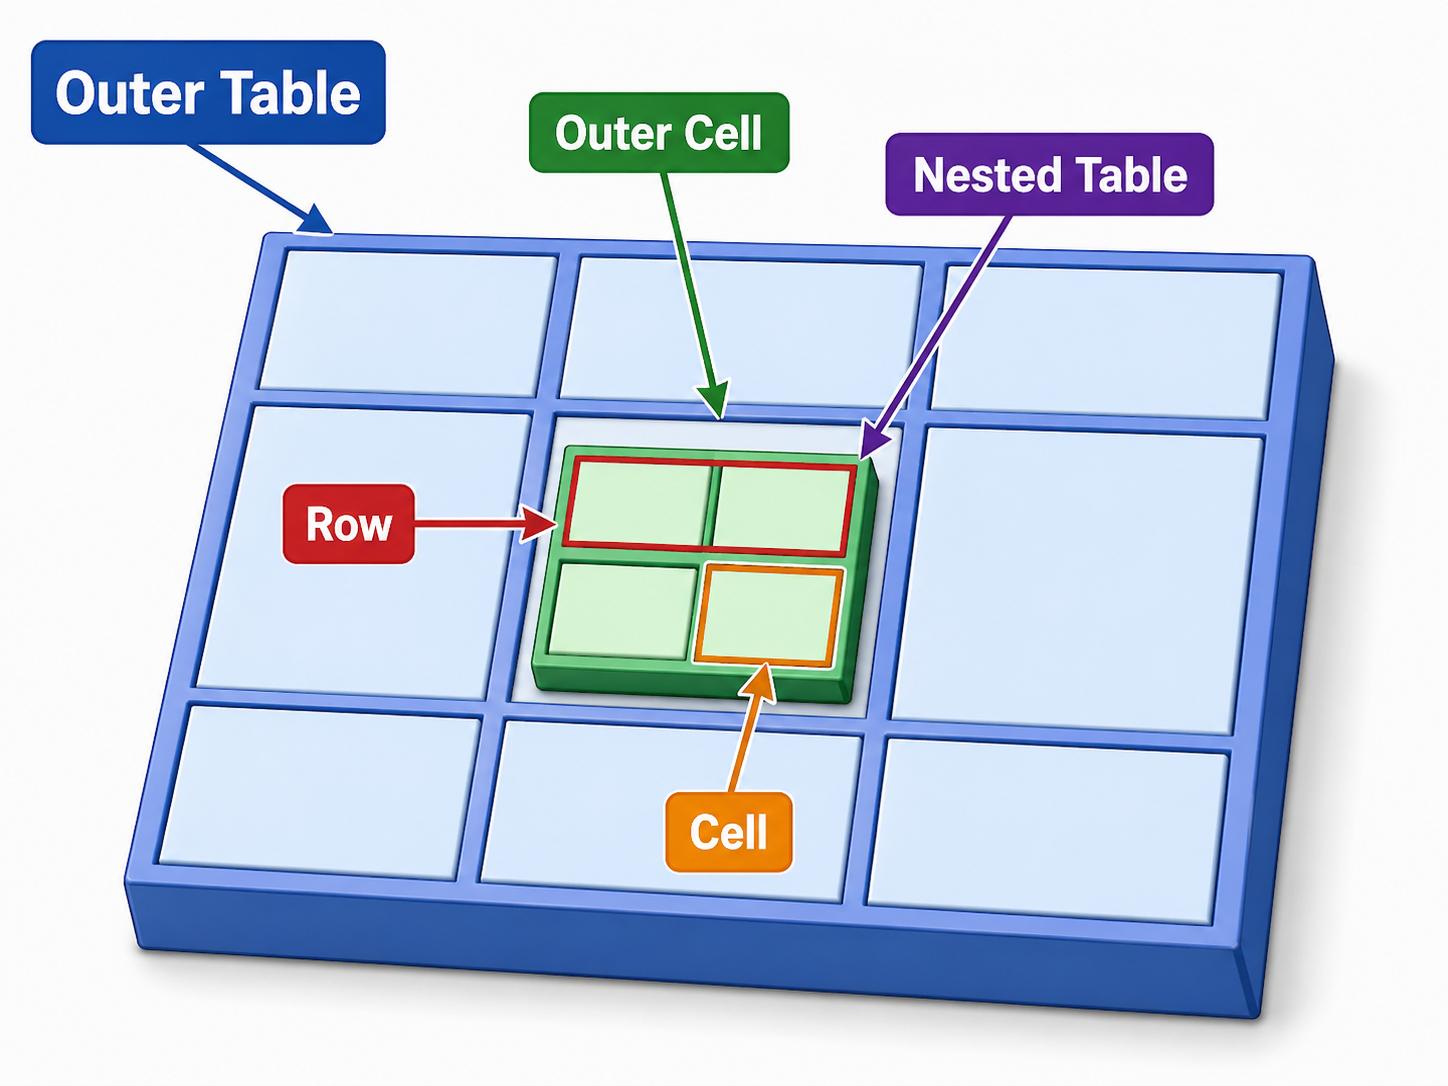
\includegraphics[width=\linewidth,height=.30\textheight,keepaspectratio]{chapters/Chapter04/topics/images/3d_nested_table.png}
\captionof{figure}{টেবিলের ভিতরে ভেতরের টেবিল}\par\smallskip

\textbf{\color{chFourTeal}চিত্র ব্যাখ্যা:} চিত্রে বাইরের টেবিলের একটি ঘরের ভিতরে ভেতরের টেবিল বসানো হয়েছে। এটিকে ভেতরের টেবিল বা টেবিলের ভিতরে টেবিল বলা হয়।
\end{minipage}\par\smallskip


\begin{keypointbox}{ভেতরের টেবিল লেখার সতর্কতা}
ভেতরের টেবিল লিখলে বাইরের টেবিল ও ভেতরের টেবিলের ট্যাগ আলাদা করে শেষ করতে হবে। প্রথমে ভেতরের টেবিলের \texttt{</table>} শেষ করবে, তারপর বাইরের টেবিলের ঘরের \texttt{</td>} এবং শেষে বাইরের টেবিল শেষ করবে। ভুল জায়গায় \texttt{</table>} দিলে প্রদর্শিত টেবিলের বিন্যাস ভেঙে যায়।
\end{keypointbox}



\subsection{সংক্ষিপ্ত অনুশীলন}

% Each question keeps its answer beneath it in the same column.
\begin{multicols}{2}
\noindent\begin{minipage}[t]{\linewidth}\vspace{0pt}
\chFourReviewQuestion{\textbf{সারণির ঘরের ভেতরে তালিকা কীভাবে লেখা যায়?}}
\end{minipage}\par\smallskip
\noindent\begin{minipage}[t]{\linewidth}\vspace{0pt}
\chFourReviewQuestion{\textbf{সারণির ভেতরে হাইপারলিংক কীভাবে তৈরি করা যায়?}}
\end{minipage}\par\smallskip
\noindent\begin{minipage}[t]{\linewidth}\vspace{0pt}
\chFourReviewQuestion{\textbf{সারণির ভেতরে ছবি কীভাবে বসানো যায়?}}
\end{minipage}\par\smallskip
\noindent\begin{minipage}[t]{\linewidth}\vspace{0pt}
\chFourReviewQuestion{\textbf{নেস্টেড সারণি কী?}}
\end{minipage}\par\smallskip
\noindent\begin{minipage}[t]{\linewidth}\vspace{0pt}
\chFourReviewQuestion{\textbf{ছবির হাইপারলিংক কীভাবে তৈরি করা যায়?}}
\end{minipage}\par\smallskip
\end{multicols}

\Needspace{10\baselineskip}
\subsection{বহুনির্বাচনি অনুশীলন}

\begin{multicols}{2}
\begin{enumerate}[leftmargin=*,itemsep=5pt]
\item \begin{minipage}[t]{\linewidth}\vspace{0pt}
সারণির ঘরের ভেতরে ছবি বসাতে কোন ট্যাগ ব্যবহার হয়?
\par ক) \texttt{<a>}
\par খ) \texttt{<img>}
\par গ) \texttt{<ol>}
\par ঘ) \texttt{<tr>}
\end{minipage}

\item \begin{minipage}[t]{\linewidth}\vspace{0pt}
সারণির ঘরের ভেতরে লিংক তৈরি করতে কোন ট্যাগ ব্যবহার হয়?
\par ক) \texttt{<a>}
\par খ) \texttt{<td>}
\par গ) \texttt{<br>}
\par ঘ) \texttt{<hr>}
\end{minipage}

\item \begin{minipage}[t]{\linewidth}\vspace{0pt}
সারণির ঘরের ভেতরে ক্রমিক তালিকা বসাতে কোন ট্যাগ ব্যবহার হবে?
\par ক) \texttt{<ul>}
\par খ) \texttt{<ol>}
\par গ) \texttt{<img>}
\par ঘ) \texttt{<caption>}
\end{minipage}

\item \begin{minipage}[t]{\linewidth}\vspace{0pt}
ছবির হাইপারলিংক তৈরির সঠিক গঠন কোনটি?
\par ক) \texttt{<img href="home.html">}
\par খ) \texttt{<a href="home.html"><img src="logo.png" alt="Logo"></a>}
\par গ) \texttt{<a src="logo.png">Home</a>}
\par ঘ) \texttt{<table img="logo.png">}
\end{minipage}

\item \begin{minipage}[t]{\linewidth}\vspace{0pt}
একটি সারণির ঘরের ভেতরে আরেকটি সারণি থাকলে তাকে কী বলে?
\par ক) Empty Table
\par খ) Nested Table
\par গ) Ordered Table
\par ঘ) External Table
\end{minipage}
\end{enumerate}
\end{multicols}

\chFourMCQAnswer{১-খ, ২-ক, ৩-খ, ৪-খ, ৫-খ}

\subsection{প্রয়োগ: একটি ছকে বইয়ের ছবি, লিংক ও বিষয়}


\Needspace{6\baselineskip}
\par\noindent{\color{chFourTeal}\bfseries\small কোড: বাম কলাম শেষে ডান কলাম পড়বে}\par
\begin{multicols}{2}
\begin{verbatim}
<table border="1" cellspacing="0" cellpadding="5">
  <caption>ICT Learning Materials</caption>
  <tr>
    <th>Item</th><th>Details</th>
  </tr>
  <tr>
    <td>Book</td>
    <td>
      <a href="book.html">
        <img src="book.jpg" alt="ICT Book" width="100" height="80">
      </a>
    </td>
  </tr>
  <tr>
    <td>Subjects</td>
    <td>
      <ol>
        <li>HTML</li>
        <li>CSS</li>
        <li>JavaScript</li>
      </ol>
    </td>
  </tr>
</table>
\end{verbatim}
\end{multicols}



\subsection{সৃজনশীল অনুশীলন}

\begin{practicebox}
\textbf{উদ্দীপক:} একটি ওয়েবপেজে ``ICT Learning Materials'' নামে একটি সারণি তৈরি করতে হবে। সারণিতে দুইটি কলাম থাকবে: Item ও Details। Book সারির Details ঘরে \texttt{book.jpg} ছবি থাকবে এবং ছবিতে ক্লিক করলে \texttt{book.html} পেজ খোলা হবে। Subjects সারির Details ঘরে ক্রমিক তালিকা হিসেবে HTML, CSS, JavaScript থাকবে।

\textbf{প্রশ্ন}\\
ক. নেস্টেড সারণি কী?\\
খ. ছবির হাইপারলিংক তৈরির নিয়ম ব্যাখ্যা কর।\\
গ. উদ্দীপকের জন্য HTML কোড লেখ।\\
ঘ. সারণির ঘরের ভেতরে তালিকা, ছবি ও হাইপারলিংক ব্যবহারের সুবিধা বিশ্লেষণ কর।
\end{practicebox}

\subsection{সাধারণ ভুল}

\begin{mistakebox}{সাধারণ ভুল}
\par\noindent
\begin{minipage}[t]{.48\linewidth}\vspace{0pt}
\begin{itemize}
\item \texttt{<td>} ট্যাগের বাইরে তালিকা লিখে ফেলা।
\item \texttt{<td>} শেষ করার আগে \texttt{<ol>} বা \texttt{<ul>} ঠিকভাবে শেষ না করা।
\item ছবির লিংক করতে \texttt{<a>} ট্যাগের ভেতরে \texttt{<img>} না রাখা।
\item \texttt{href} ও \texttt{src} অ্যাট্রিবিউট গুলিয়ে ফেলা।
\end{itemize}
\end{minipage}\hfill
\begin{minipage}[t]{.48\linewidth}\vspace{0pt}
\begin{itemize}
\item \texttt{<table>} ট্যাগের ভেতরে সরাসরি \texttt{<ol>} লিখে ফেলা; ঘর দরকার।
\item নেস্টেড সারণির সমাপ্তি ট্যাগ ভুল করা।
\item সারণির ঘরের ভেতরে বিষয়বস্তু বেশি দিলে বিন্যাস অগোছালো করা।
\item সব বাহ্যিক লিংকে \texttt{target="\_blank"} বাধ্যতামূলক ভাবা; এটি নতুন ট্যাব/উইন্ডোতে খোলার প্রয়োজন অনুযায়ী দেওয়া হয়।
\end{itemize}
\end{minipage}\par

\end{mistakebox}

\begin{boardbox}{পরবর্তী টপিক}
পরের অংশে \texttt{<div>}, \texttt{<span>} ও \texttt{style} অ্যাট্রিবিউট দিয়ে বিষয়বস্তু সাজানো এবং ইনলাইন CSS-এর মৌলিক প্রয়োগ দেখব।
\end{boardbox}

\setcounter{collectmore}{-4}

% Density revision 2026-10-04: answers below questions; compact related content.
% Topic 17: Division, Span and style অ্যাট্রিবিউট
\section{বিভাগ, ইনলাইন অংশ ও রীতি: div, span ও style}

% Composition pass 2026-10-04
পুরো বিজ্ঞপ্তির পটভূমি বদলাতে হবে, আবার একটি বাক্যের শুধু শেষ তারিখ আলাদা রঙে দেখাতে হবে।

\chFourMotivation{বড় অংশ ও ছোট লেখাংশ আলাদা করা $\rightarrow$ div ও span $\rightarrow$ নির্বাচিত ধারকে CSS প্রয়োগ $\rightarrow$ কলেজের বিজ্ঞপ্তি সুস্পষ্ট হয়।}


\begin{learningbox}
এই অংশ শেষে শিক্ষার্থী পারবে:
\begin{itemize}
\item \texttt{<div>} ট্যাগের কাজ ও ব্যবহার ব্যাখ্যা করতে।
\item \texttt{<span>} ট্যাগের কাজ ও ব্যবহার ব্যাখ্যা করতে।
\item \texttt{<div>} ও \texttt{<span>}-এর পার্থক্য লিখতে।
\item \texttt{style} অ্যাট্রিবিউট ব্যবহার করে ইনলাইন CSS লিখতে।
\item \texttt{color}, \texttt{background-color}, \texttt{font-size}, \texttt{text-align}, \texttt{margin}, \texttt{padding}, \texttt{border} ইত্যাদি মৌলিক CSS প্রোপার্টি ব্যবহার করতে।
\end{itemize}
\end{learningbox}



আগের পাঠগুলোতে আমরা HTML দিয়ে শিরোনাম, অনুচ্ছেদ, তালিকা, হাইপারলিংক, ছবি ও সারণি তৈরি করেছি। এখন ওয়েবপেজের বিভিন্ন অংশ একসঙ্গে রাখা এবং নির্দিষ্ট অংশে রীতি প্রয়োগ করা শিখব। এই পাঠে তিনটি বিষয় সবচেয়ে গুরুত্বপূর্ণ: \texttt{<div>}, \texttt{<span>} এবং \texttt{style} অ্যাট্রিবিউট।

\subsection{\texttt{<div>} ট্যাগ কী?}

\begin{definitionbox}{বিভাগের ধারক (div Element)}
একাধিক HTML এলিমেন্টকে একটি সাধারণ ধারকে দলবদ্ধ করতে \texttt{<div>} ট্যাগ ব্যবহার করা হয়।
\end{definitionbox}

\texttt{<div>}-এ পেজের একটি বড় অংশের শিরোনাম, অনুচ্ছেদ ও অন্যান্য এলিমেন্ট রাখা যায়। ধারকটি নিজে বিশেষ নকশা তৈরি করে না। CSS প্রয়োগ করে পুরো অংশের পটভূমি, সীমানা ও অবস্থান একসঙ্গে নির্ধারণ করা যায়।

% Split revision: code and its explanation share one row.
\par\noindent
\begin{minipage}[t]{.42\linewidth}\vspace{0pt}\small
\subsubsection{সিনট্যাক্স}

\textbf{\color{chFourTeal}কোড}\par
\begin{verbatim}
<div>
  Content here
</div>
\end{verbatim}

\par\smallskip
\end{minipage}\hfill
\begin{minipage}[t]{.54\linewidth}\vspace{0pt}\small
\subsubsection{উদাহরণ}

\textbf{\color{chFourTeal}কোড}\par
\begin{verbatim}
<div>
  <h2>About College</h2>
  <p>ABC College is a reputed institution.</p>
</div>
\end{verbatim}

\par\smallskip


এখানে শিরোনাম ও অনুচ্ছেদ একই ধারকে রাখা হয়েছে।
\end{minipage}\par
\subsection{\texttt{<div>} ট্যাগের ব্যবহার}

\texttt{<div>} সাধারণত ওয়েবপেজের বড় অংশ ভাগ করতে ব্যবহৃত হয়।

\par\noindent
\begin{minipage}[t]{.48\linewidth}\vspace{0pt}
\begin{itemize}
\item হেডার অংশ তৈরি করতে
\item চলাচল/মেনু এলাকা একসঙ্গে রাখতে
\item প্রধান বিষয়বস্তু অংশ তৈরি করতে
\item পাশের অংশ তৈরি করতে
\end{itemize}
\end{minipage}\hfill
\begin{minipage}[t]{.48\linewidth}\vspace{0pt}
\begin{itemize}
\item ফুটার অংশ তৈরি করতে
\item একাধিক এলিমেন্ট একসঙ্গে রীতি প্রয়োগ করতে
\item ওয়েবপেজ বিন্যাস তৈরি করতে
\end{itemize}
\end{minipage}\par


\Needspace{7\baselineskip}
\subsection{উদাহরণ: পেজের অংশ}

% Split revision: code and its explanation share one row.
\par\noindent
\begin{minipage}[t]{.60\linewidth}\vspace{0pt}\small
\textbf{\color{chFourTeal}কোড}\par
\par\noindent
\begin{verbatim}
<!DOCTYPE html><html>
<head><title>Div Example</title></head>
<body>
  <div style="background-color:lightblue; padding:10px;">
    <h1>ABC College</h1>
    <p>Welcome to our official website.</p>
  </div>
  <div style="background-color:lightyellow; padding:10px;">
    <h2>Notice</h2>
    <p>HSC ICT class will start from Sunday.</p>
  </div>
</body></html>
\end{verbatim}
\par
\par\smallskip
\end{minipage}\hfill
\begin{minipage}[t]{.36\linewidth}\vspace{0pt}\small
\textbf{\color{chFourTeal}ফল কী হবে?}\par
প্রথম \texttt{<div>} একটি হালকা নীল পটভূমির অংশ তৈরি করবে। দ্বিতীয় \texttt{<div>} একটি হালকা হলুদ পটভূমির অংশ তৈরি করবে।
\par\smallskip
\end{minipage}\par


\subsection{\texttt{<span>} ট্যাগ কী?}

\begin{definitionbox}{ইনলাইন অংশের ধারক (span Element)}
লেখা বা ইনলাইন বিষয়বস্তুর নির্দিষ্ট অংশ দলবদ্ধ করতে \texttt{<span>} ট্যাগ ব্যবহার করা হয়। ওই অংশে আলাদা CSS বা স্ক্রিপ্ট প্রয়োগ করা যায়।
\end{definitionbox}

\texttt{<span>} সাধারণত নতুন লাইন শুরু করে না। তাই অনুচ্ছেদের একটি শব্দ বা বাক্যাংশ আলাদা রঙে দেখাতে এটি সুবিধাজনক। ব্লক ও ইনলাইন এখানে স্বাভাবিক প্রদর্শনের ধরন বোঝায়। CSS-এর \texttt{display} দিয়ে প্রদর্শন বদলালেও কোন এলিমেন্টের ভেতরে কী রাখা বৈধ, সেই HTML নিয়ম বদলায় না।

% Split revision: code and its explanation share one row.
\par\noindent
\begin{minipage}[t]{.42\linewidth}\vspace{0pt}\small
\subsubsection{সিনট্যাক্স}

\textbf{\color{chFourTeal}কোড}\par
\begin{verbatim}
<span>Text</span>
\end{verbatim}

\par\smallskip
\end{minipage}\hfill
\begin{minipage}[t]{.54\linewidth}\vspace{0pt}\small
\subsubsection{উদাহরণ}

\textbf{\color{chFourTeal}কোড}\par
\begin{verbatim}
<p>This is normal text.
  <span style="color:red;">This is red text.</span>
</p>
\end{verbatim}

\par\smallskip


এখানে শুধু \textbf{This is red text.} অংশটি লাল রঙের হবে।
\end{minipage}\par
\subsubsection{বড় ধারক ও ছোট অংশ: চিত্রে পার্থক্য}
\begin{center}
\resizebox{.90\linewidth}{!}{%
\begin{tikzpicture}[font=\small]
\node[draw=chFourTeal,rounded corners,fill=chFourTint,
  minimum width=115mm,minimum height=36mm] (d) {};
\node[anchor=north west,text=chFourTeal,font=\small\bfseries]
  at ([xshift=3mm,yshift=-3mm]d.north west) {\texttt{div}: পুরো অংশের ধারক};
\node[anchor=west] at ([xshift=4mm]d.west) {অনুচ্ছেদের সাধারণ লেখা};
\node[draw=chFourRose,fill=white,rounded corners,
  minimum width=43mm,minimum height=10mm,text=chFourRose]
  at ([xshift=27mm]d.center) {\texttt{span}: নির্দিষ্ট অংশ};
\end{tikzpicture}}
\end{center}
পুরো অংশে পটভূমি বা বর্ডার দিতে \texttt{div}-এ CSS প্রয়োগ করা যায়। অনুচ্ছেদের শুধু নির্বাচিত অংশের রং বদলাতে \texttt{span}-এ CSS প্রয়োগ করা যায়। ধারক নিজে রং নির্ধারণ করে না।

\subsection{\texttt{<div>} ও \texttt{<span>}-এর পার্থক্য}

\begin{center}
\begin{tabular}{|p{0.24\textwidth}|p{0.30\textwidth}|p{0.30\textwidth}|}
\hline
\textbf{বিষয়} & \textbf{\texttt{<div>}} & \textbf{\texttt{<span>}} \\
\hline
স্বাভাবিক প্রদর্শন & ব্লক ধরনের ধারক & ইনলাইন ধরনের ধারক \\
\hline
কাজ & বড় অংশ বা ব্লক একসঙ্গে রাখে & লেখা/ইনলাইন অংশ একসঙ্গে রাখে \\
\hline
নতুন লাইন তৈরি করে? & সাধারণত হ্যাঁ & না \\
\hline
ব্যবহার & বিন্যাস, অংশ, কার্ড, ঘর & অনুচ্ছেদের ভিতরে নির্দিষ্ট শব্দ বা বাক্যাংশে রীতি প্রয়োগ \\
\hline
উদাহরণ & হেডার, ফুটার, বিজ্ঞপ্তির ঘর & লাল শব্দ, বিশেষভাবে দেখানো লেখা \\
\hline
শেষের ট্যাগ & আছে & আছে \\
\hline
\end{tabular}
\end{center}

\begin{keypointbox}{সহজ মনে রাখার নিয়ম}
\texttt{div} = বিভাগ = বড় ভাগ বা অংশ। \texttt{span} = ছোট ইনলাইন অংশ।
\end{keypointbox}

\subsection{style অ্যাট্রিবিউট কী?}

\begin{definitionbox}{রীতির অ্যাট্রিবিউট (style Attribute)}
HTML এলিমেন্টে সরাসরি CSS ঘোষণা প্রয়োগের জন্য ব্যবহৃত অ্যাট্রিবিউটকে \texttt{style} অ্যাট্রিবিউট বলে। এই অ্যাট্রিবিউটের মান হিসেবে CSS বৈশিষ্ট্য ও তার মান লেখা হয়; যেমন \texttt{style="color:red;"}।
\end{definitionbox}

\texttt{style} হলো HTML-এর একটি সাধারণভাবে প্রযোজ্য অ্যাট্রিবিউট। এর মাধ্যমে কোনো এলিমেন্টে সরাসরি CSS রীতি দেওয়া যায়।

\subsubsection{লেখার সাধারণ রূপ}

\begin{examplebox}{কোড}
\par\noindent\begin{minipage}{\linewidth}
\begin{verbatim}
<tag style="property:value;">Content</tag>
\end{verbatim}
\end{minipage}\par
\end{examplebox}

\subsubsection{উদাহরণ}

\begin{examplebox}{কোড}
\par\noindent\begin{minipage}{\linewidth}
\begin{verbatim}
<p style="color:red;">This text is red.</p>
\end{verbatim}
\end{minipage}\par
\end{examplebox}

\begin{center}
\begin{tabular}{|p{0.25\textwidth}|p{0.50\textwidth}|}
\hline
\textbf{অংশ} & \textbf{পরিচয়} \\
\hline
\texttt{style} & অ্যাট্রিবিউট \\
\hline
\texttt{color} & CSS প্রোপার্টি \\
\hline
\texttt{red} & প্রোপার্টির মান \\
\hline
\texttt{color:red;} & CSS ঘোষণা \\
\hline
\end{tabular}
\end{center}

\subsection{style অ্যাট্রিবিউটের সঠিক নিয়ম}

\texttt{style} অ্যাট্রিবিউটের ভিতরে CSS প্রোপার্টি ও মান লিখতে হয়।

\subsubsection{সঠিক কাঠামো}

\par\noindent\begin{minipage}{\linewidth}
\begin{verbatim}
style="property:value; property:value;"
\end{verbatim}
\end{minipage}\par

\subsubsection{উদাহরণ}

\begin{examplebox}{কোড}
\par\noindent\begin{minipage}{\linewidth}
\begin{verbatim}
<div style="color:red; background-color:yellow;">
  HSC ICT
</div>
\end{verbatim}
\end{minipage}\par
\end{examplebox}

\begin{boardbox}{গুরুত্বপূর্ণ নিয়ম}
\begin{itemize}
\item প্রোপার্টি ও মানের মাঝে কোলন \texttt{:} দিতে হয়।
\item একাধিক ঘোষণার মাঝে সেমিকোলন \texttt{;} দিতে হয়।
\item অ্যাট্রিবিউট মান উদ্ধৃতি চিহ্নের মধ্যে লেখা ভালো।
\item CSS বৈশিষ্ট্য ও তার মান লেখার সময় \texttt{=} ব্যবহার করা যাবে না।
\item কমা দিয়ে CSS ঘোষণা আলাদা করা যাবে না।
\end{itemize}
\end{boardbox}

\subsection{রীতির সঠিক ও ভুল সিনট্যাক্স}

% Split revision: code and its explanation share one row.
\par\noindent
\begin{minipage}[t]{.54\linewidth}\vspace{0pt}\small
\subsubsection{সঠিক}

\textbf{\color{chFourTeal}কোড}\par
\begin{verbatim}
<div style="color:red; float:left;">
  ICT
</div>
\end{verbatim}

\par\smallskip
\end{minipage}\hfill
\begin{minipage}[t]{.42\linewidth}\vspace{0pt}\small
\subsubsection{ভুল}

\textbf{\color{chFourTeal}কোড}\par
\begin{verbatim}
<div style="color=red, float=left">
  ICT
</div>
\end{verbatim}

\par\smallskip


এটি ভুল, কারণ \texttt{color=red} নয়, সঠিক হলো \texttt{color:red}। আবার \texttt{float=left} নয়, সঠিক হলো \texttt{float:left}। CSS ঘোষণা আলাদা করতে কমা নয়, সেমিকোলন ব্যবহার করতে হয়।
\end{minipage}\par
\subsection{ইনলাইন CSS কী?}

\begin{definitionbox}{ইনলাইন CSS}
কোনো HTML এলিমেন্টের শুরুর ট্যাগের মধ্যে \texttt{style} অ্যাট্রিবিউট ব্যবহার করে সরাসরি CSS বৈশিষ্ট্য ও তার মান লেখা হলে তাকে ইনলাইন CSS বলে।
\end{definitionbox}

\begin{examplebox}{কোড}
\par\noindent\begin{minipage}{\linewidth}
\begin{verbatim}
<h1 style="color:blue;">HSC ICT</h1>
<p style="font-size:20px;">Web Design and HTML</p>
\end{verbatim}
\end{minipage}\par
\end{examplebox}

\subsection{গুরুত্বপূর্ণ CSS প্রোপার্টি}

এই পাঠে style অ্যাট্রিবিউট শেখার জন্য নিচের প্রোপার্টিগুলো বেশি গুরুত্বপূর্ণ।

\begin{center}
\footnotesize
\begin{tabular}{|p{0.24\textwidth}|p{0.34\textwidth}|p{0.28\textwidth}|}
\hline
\textbf{প্রোপার্টি} & \textbf{কাজ} & \textbf{উদাহরণ} \\
\hline
\texttt{color} & লেখার রং নির্ধারণ করে & \texttt{color:red;} \\
\hline
\texttt{background-color} & পটভূমির রং নির্ধারণ করে & {\scriptsize\ttfamily background-color:yellow;} \\
\hline
\texttt{font-size} & অক্ষরের আকার নির্ধারণ করে & \texttt{font-size:20px;} \\
\hline
\texttt{font-family} & ফন্টের পরিবার নির্ধারণ করে & {\scriptsize\ttfamily font-family:Arial;} \\
\hline
\texttt{text-align} & লেখা সাজানোর অবস্থান নির্ধারণ করে & {\scriptsize\ttfamily text-align:center;} \\
\hline
\texttt{width} & এলিমেন্টের প্রস্থ নির্ধারণ করে & \texttt{width:200px;} \\
\hline
\texttt{height} & এলিমেন্টের উচ্চতা নির্ধারণ করে & \texttt{height:100px;} \\
\hline
\texttt{margin} & এলিমেন্টের বাইরের ফাঁকা জায়গা & \texttt{margin:10px;} \\
\hline
\texttt{padding} & এলিমেন্টের ভিতরের ফাঁকা জায়গা & \texttt{padding:10px;} \\
\hline
\texttt{border} & বর্ডার তৈরি করে & \texttt{border:1px solid black;} \\
\hline
\texttt{float} & এলিমেন্টকে বামে বা ডানে ভাসায় & \texttt{float:left;} \\
\hline
\end{tabular}
\end{center}

\Needspace{9\baselineskip}
\subsection{\texttt{<div>}-এ style অ্যাট্রিবিউট ব্যবহার}

% Split revision: code and its explanation share one row.
\par\noindent
\begin{minipage}[t]{.54\linewidth}\vspace{0pt}\small
\textbf{\color{chFourTeal}কোড}\par
\begin{verbatim}
<div style="background-color:lightyellow; border:1px solid black; padding:10px; width:300px;">
  <h2>Notice</h2>
  <p>ICT class will start at 10:00 AM.</p>
</div>
\end{verbatim}

\par\smallskip
\end{minipage}\hfill
\begin{minipage}[t]{.42\linewidth}\vspace{0pt}\small
\textbf{\color{chFourTeal}ফল কী হবে?}\par
একটি বিজ্ঞপ্তির ঘর দেখা যাবে। এর পটভূমি হালকা হলুদ হবে, বর্ডার থাকবে, ভেতরে ফাঁক থাকবে এবং ঘরের ভেতরে \texttt{Notice} শিরোনাম ও অনুচ্ছেদ থাকবে।
\par\smallskip
\end{minipage}\par


\Needspace{10\baselineskip}
\subsection{\texttt{<span>}-এ style অ্যাট্রিবিউট ব্যবহার}

% Split revision: code and its explanation share one row.
\par\noindent
\begin{minipage}[t]{.54\linewidth}\vspace{0pt}\small
\textbf{\color{chFourTeal}কোড}\par
\begin{verbatim}
<p>
  HTML is used to create
  <span style="color:red; font-weight:bold;">web pages</span>.
</p>
\end{verbatim}

\par\smallskip
\end{minipage}\hfill
\begin{minipage}[t]{.42\linewidth}\vspace{0pt}\small
\textbf{\color{chFourTeal}ফল কী হবে?}\par
পুরো অনুচ্ছেদ স্বাভাবিক থাকবে, কিন্তু \textbf{web pages} অংশটি লাল ও মোটা অক্ষরের হবে।
\par\smallskip
\end{minipage}\par


\subsection{\texttt{<div>} ও \texttt{<span>} একসঙ্গে ব্যবহার}

\begin{examplebox}{কোড}

\begin{verbatim}
<div style="background-color:#eeeeee; padding:15px; border:1px solid gray;">
  <h1>HSC ICT Book</h1>
  <p>
    This chapter is about
    <span style="color:blue; font-weight:bold;">Web Design and HTML</span>.
  </p></div>
\end{verbatim}

\end{examplebox}

\begin{keypointbox}{ব্যাখ্যা}
\texttt{<div>} পুরো অংশটিকে ধূসর পটভূমি ঘর করেছে। \texttt{<span>} শুধু ``Web Design and HTML'' অংশে নীল মোটা অক্ষরের রীতি দিয়েছে।
\end{keypointbox}

\subsection{বাইরের ফাঁক ও ভেতরের ফাঁক}

\subsubsection{বাইরের ফাঁক কী?}

\texttt{margin} এলিমেন্টের বাইরের ফাঁকা জায়গা নির্ধারণ করে।

\begin{examplebox}{কোড}
\par\noindent\begin{minipage}{\linewidth}
\begin{verbatim}
<div style="margin:20px;">Content</div>
\end{verbatim}
\end{minipage}\par
\end{examplebox}

\subsubsection{ভেতরের ফাঁক কী?}

\texttt{padding} এলিমেন্টের বিষয়বস্তু ও বর্ডারের মাঝের ভিতরের ফাঁকা জায়গা নির্ধারণ করে।

\begin{examplebox}{কোড}
\par\noindent\begin{minipage}{\linewidth}
\begin{verbatim}
<div style="padding:20px;">Content</div>
\end{verbatim}
\end{minipage}\par
\end{examplebox}

\begin{center}
\begin{tabular}{|p{0.22\textwidth}|p{0.31\textwidth}|p{0.31\textwidth}|}
\hline
\textbf{বিষয়} & \textbf{Margin} & \textbf{Padding} \\
\hline
অবস্থান & বর্ডারের বাইরে & বর্ডারের ভিতরে \\
\hline
কাজ & এলিমেন্টের বাইরে ফাঁক তৈরি করে & বিষয়বস্তুর চারপাশে ভিতরের ফাঁক তৈরি করে \\
\hline
উদাহরণ & \texttt{margin:10px;} & \texttt{padding:10px;} \\
\hline
\end{tabular}
\end{center}

\subsection{বর্ডার}

এলিমেন্টের চারপাশে বর্ডার দিতে \texttt{border} বৈশিষ্ট্য ব্যবহার করা হয়।

\par\noindent\begin{minipage}{\linewidth}
\begin{verbatim}
style="border:1px solid black;"
\end{verbatim}
\end{minipage}\par

\begin{examplebox}{কোড}
\par\noindent\begin{minipage}{\linewidth}
\begin{verbatim}
<div style="border:2px solid blue; padding:10px;">
  Important Note
</div>
\end{verbatim}
\end{minipage}\par
\end{examplebox}

\begin{center}
\begin{tabular}{|p{0.20\textwidth}|p{0.48\textwidth}|}
\hline
\textbf{অংশ} & \textbf{অর্থ} \\
\hline
\texttt{2px} & বর্ডারের পুরুত্ব \\
\hline
\texttt{solid} & বর্ডারের ধরন \\
\hline
\texttt{blue} & বর্ডারের রং \\
\hline
\end{tabular}
\end{center}

\subsection{লেখা অবস্থান}

লেখা বাম, মাঝখান বা ডানে রাখতে \texttt{text-align} বৈশিষ্ট্য ব্যবহার করা হয়।

\begin{examplebox}{কোড}
\par\noindent\begin{minipage}{\linewidth}
\begin{verbatim}
<h1 style="text-align:center;">ABC College</h1>
\end{verbatim}
\end{minipage}\par
\end{examplebox}

\begin{center}
\begin{tabular}{|p{0.25\textwidth}|p{0.50\textwidth}|}
\hline
\textbf{মান} & \textbf{কাজ} \\
\hline
\texttt{left} & বামে রাখে \\
\hline
\texttt{center} & মাঝখানে রাখে \\
\hline
\texttt{right} & ডানে রাখে \\
\hline
\texttt{justify} & দুই পাশে সমানভাবে ছড়িয়ে দেয় \\
\hline
\end{tabular}
\end{center}

\subsection{রঙের মান}

HTML/CSS-এ রং কয়েকভাবে দেওয়া যায়।

\begin{center}
\begin{tabular}{|p{0.25\textwidth}|p{0.50\textwidth}|}
\hline
\textbf{পদ্ধতি} & \textbf{উদাহরণ} \\
\hline
রঙের নাম & \texttt{red}, \texttt{blue}, \texttt{green} \\
\hline
হেক্সাডেসিম্যাল কোড & \texttt{\#FF0000}, \texttt{\#FFFFFF} \\
\hline
RGB & \texttt{rgb(255, 0, 0)} \\
\hline
\end{tabular}
\end{center}

\begin{boardbox}{বহুনির্বাচনি প্রশ্নে মনে রাখবে}
\texttt{\#FFFFFF} সাদা রং নির্দেশ করে।
\end{boardbox}

\subsection{অভ্যন্তরীণ CSS: \texttt{<style>} ট্যাগ}

যদি অনেক এলিমেন্টে একই রীতি দিতে হয়, তাহলে বারবার ইনলাইন রীতি না লিখে \texttt{<head>} অংশের ভিতরে \texttt{<style>} ট্যাগ ব্যবহার করা যায়।

% Split revision: code and its explanation share one row.
\par\noindent
\begin{minipage}[t]{.50\linewidth}\vspace{0pt}\small
\textbf{\color{chFourTeal}কোড}\par
\par\noindent
\begin{verbatim}
<!DOCTYPE html>
<html>
<head>
  <title>Internal CSS Example</title>
  <style>
    div {
      background-color: lightblue;
      padding: 10px;
      margin: 10px;
      border: 1px solid black;
    }
  </style>
</head>
<body>
  <div>First Box</div>
  <div>Second Box</div>
</body>
</html>
\end{verbatim}
\par
\par\smallskip
\end{minipage}\hfill
\begin{minipage}[t]{.46\linewidth}\vspace{0pt}\small
\textbf{\color{chFourTeal}ফল কী হবে?}\par
দুইটি \texttt{<div>} একই রীতি পাবে।
\par\smallskip
\end{minipage}\par


\subsection{ইনলাইন CSS বনাম অভ্যন্তরীণ CSS}

\begin{center}
\begin{tabular}{|p{0.21\textwidth}|p{0.31\textwidth}|p{0.31\textwidth}|}
\hline
\textbf{বিষয়} & \textbf{ইনলাইন CSS} & \textbf{অভ্যন্তরীণ CSS} \\
\hline
কোথায় লেখা হয় & এলিমেন্টের শুরুর ট্যাগে & \texttt{<head>}-এর ভিতরে \texttt{<style>} ট্যাগে \\
\hline
সিনট্যাক্স & \texttt{<p style="color:red;">} & \texttt{p \{ color:red; \}} \\
\hline
ব্যবহার & একক এলিমেন্টে দ্রুত রীতি প্রয়োগ & একটি পেজের অনেক এলিমেন্টে রীতি প্রয়োগ \\
\hline
সুবিধা & সহজ ও দ্রুত & কোড পরিষ্কার থাকে \\
\hline
সীমাবদ্ধতা & কোড অগোছালো হয় & CSS সিনট্যাক্স জানা দরকার \\
\hline
\end{tabular}
\end{center}


\subsubsection{অংশের অর্থ বোঝানো ট্যাগ: আধুনিক পরিচয়}
একটি কলেজের পেজে অনেক \texttt{div} থাকলে কোনটি মেনু আর কোনটি মূল লেখা, শুধু ট্যাগ দেখে বোঝা যায় না। \textbf{অর্থবোধক এলিমেন্ট (Semantic Element)} অংশের ভূমিকা প্রকাশ করে। এতে কোডের গঠন বোঝা এবং স্ক্রিন রিডার দিয়ে অংশ খুঁজে পাওয়া সহজ হয়। এগুলো নিজেরাই পেজের রং বা কলামের বিন্যাস নির্ধারণ করে না।

\begin{tabular}{|p{.22\linewidth}|p{.68\linewidth}|}
\hline
\textbf{এলিমেন্ট} & \textbf{অর্থ ও কলেজের পেজে প্রয়োগ} \\
\hline
\texttt{header} & পেজ বা বিভাগের পরিচিতি; কলেজের নাম ও লোগো \\
\hline
\texttt{nav} & গুরুত্বপূর্ণ নেভিগেশন লিংকের অংশ; প্রধান মেনু \\
\hline
\texttt{main} & পেজের প্রধান স্বতন্ত্র বিষয়বস্তু; নোটিশ বা পরিচিতি \\
\hline
\texttt{section} & বিষয়ভিত্তিক বিভাগ; ভর্তি-তথ্যের আলাদা অংশ, সাধারণত শিরোনামসহ \\
\hline
\texttt{article} & স্বয়ংসম্পূর্ণ লেখা; আলাদা করে পড়া যায় এমন নোটিশ \\
\hline
\texttt{aside} & মূল বিষয়ের সঙ্গে পরোক্ষভাবে সম্পর্কিত অংশ; সহায়ক তথ্য \\
\hline
\texttt{footer} & পেজ বা বিভাগের শেষের তথ্য; যোগাযোগ বা কপিরাইট \\
\hline
\end{tabular}

অংশের নির্দিষ্ট ভূমিকা থাকলে উপযুক্ত অর্থবোধক ট্যাগ ব্যবহার করা যায়। কেবল কয়েকটি এলিমেন্ট দলবদ্ধ করে CSS প্রয়োগের জন্য সাধারণ ধারক div উপযোগী।



\subsection{পূর্ণাঙ্গ উদাহরণ: ছোট ওয়েবপেজের বিন্যাস}

\Needspace{6\baselineskip}
\par\noindent{\color{chFourTeal}\bfseries\small কোড: বাম কলাম শেষে ডান কলাম পড়বে}\par
\begin{multicols}{2}
\begin{verbatim}
<div style="background-color:#004080; color:white; padding:15px; text-align:center;">
  <h1>ABC College</h1>
  <p>Official Website</p>
</div>

<div style="background-color:#eeeeee; padding:10px; margin-top:10px;">
  <a href="index.html">Home</a> |
  <a href="about.html">About</a> |
  <a href="notice.html">Notice</a> |
  <a href="contact.html">Contact</a>
</div>

<div style="padding:15px; border:1px solid #cccccc; margin-top:10px;">
  <h2>Welcome</h2>
  <p>
    This website is designed for
    <span style="color:red; font-weight:bold;">HSC ICT students</span>.
  </p>
</div>

<div style="background-color:#222222; color:white; padding:10px; text-align:center; margin-top:10px;">
  <p>&copy; 2026 ABC College</p>
</div>
\end{verbatim}
\end{multicols}


\begin{examplebox}{ফলের ব্যাখ্যা}
প্রথম \texttt{<div>} হেডার অংশ, দ্বিতীয় \texttt{<div>} নেভিগেশন মেনু অংশ, তৃতীয় \texttt{<div>} প্রধান বিষয়বস্তু অংশ এবং শেষ \texttt{<div>} ফুটার অংশ। \texttt{<span>} দিয়ে নির্দিষ্ট লেখা লাল রঙে ও মোটা অক্ষরে দেখানো হয়েছে।
\end{examplebox}

% Original applied explanation; see Chapter04/SOURCES.md.
\subsubsection{একই বিজ্ঞপ্তিতে div, span ও CSS-এর ভূমিকা}
কলেজের একটি বিজ্ঞপ্তির শিরোনাম, তারিখ ও লেখা একত্রে ধরতে \texttt{div} ব্যবহার করা যায়। অনুচ্ছেদের শুধু \textbf{শেষ তারিখ} অংশে আলাদা রীতি প্রয়োগ করতে \texttt{span} উপযোগী। CSS-এর \texttt{color} লেখার রং এবং \texttt{background-color} পটভূমির রং নির্ধারণ করে।

\texttt{div} ও \texttt{span} নিজেরা বিজ্ঞপ্তি বা মেনুর নির্দিষ্ট অর্থ জানায় না। প্রধান বিষয়বস্তুর জন্য \texttt{main}, নেভিগেশনের জন্য \texttt{nav}-এর মতো অর্থবোধক অংশ বেছে নেওয়া যায়। কোন ট্যাগ কী অর্থ দেয় এবং CSS সেটিকে কীভাবে দেখায়—দুটি প্রশ্ন আলাদা করে ভাববে।

\subsection{সংক্ষিপ্ত অনুশীলন}

% Each question keeps its answer beneath it in the same column.
\begin{multicols}{2}
\noindent\begin{minipage}[t]{\linewidth}\vspace{0pt}
\chFourReviewQuestion{\textbf{\texttt{<div>} ট্যাগ কী?}}
\end{minipage}\par\smallskip
\noindent\begin{minipage}[t]{\linewidth}\vspace{0pt}
\chFourReviewQuestion{\textbf{\texttt{<span>} ট্যাগ কী?}}
\end{minipage}\par\smallskip
\noindent\begin{minipage}[t]{\linewidth}\vspace{0pt}
\chFourReviewQuestion{\textbf{\texttt{<div>} ও \texttt{<span>}-এর পার্থক্য লেখ।}}
\end{minipage}\par\smallskip
\noindent\begin{minipage}[t]{\linewidth}\vspace{0pt}
\chFourReviewQuestion{\textbf{style অ্যাট্রিবিউট কী?}}
\end{minipage}\par\smallskip
\noindent\begin{minipage}[t]{\linewidth}\vspace{0pt}
\chFourReviewQuestion{\textbf{\texttt{style="color:red; float:left;"} কেন সঠিক?}}
\end{minipage}\par\smallskip
\end{multicols}

\Needspace{10\baselineskip}
\subsection{বহুনির্বাচনি অনুশীলন}

\begin{multicols}{2}
\begin{enumerate}[leftmargin=*,itemsep=5pt]
\item \begin{minipage}[t]{\linewidth}\vspace{0pt}
HTML ডকুমেন্টের বিভিন্ন অংশ আলাদা করতে কোন ট্যাগ ব্যবহৃত হয়?
\par ক) \texttt{<span>}
\par খ) \texttt{<div>}
\par গ) \texttt{<select>}
\par ঘ) \texttt{<option>}
\end{minipage}

\item \begin{minipage}[t]{\linewidth}\vspace{0pt}
লেখার নির্দিষ্ট ইনলাইন অংশে রীতি প্রয়োগ করতে কোন ট্যাগ বেশি উপযোগী?
\par ক) \texttt{<div>}
\par খ) \texttt{<span>}
\par গ) \texttt{<table>}
\par ঘ) \texttt{<hr>}
\end{minipage}

\item \begin{minipage}[t]{\linewidth}\vspace{0pt}
\texttt{<div>} কোন ধরনের এলিমেন্ট?
\par ক) ইনলাইন ধরনের
\par খ) ব্লক ধরনের
\par গ) এম্পটি ট্যাগ
\par ঘ) ছবি ট্যাগ
\end{minipage}

\item \begin{minipage}[t]{\linewidth}\vspace{0pt}
\texttt{<span>} কোন ধরনের এলিমেন্ট?
\par ক) ইনলাইন ধরনের
\par খ) ব্লক ধরনের
\par গ) সারণি ট্যাগ
\par ঘ) এম্পটি ট্যাগ
\end{minipage}

\item \begin{minipage}[t]{\linewidth}\vspace{0pt}
নিচের কোন style অ্যাট্রিবিউট সিনট্যাক্স সঠিক?
\par ক) \texttt{<div style="color:red, float=left">}
\par খ) \texttt{<div style="color=red; float:left">}
\par গ) \texttt{<div style="color:red; float:left;">}
\par ঘ) \texttt{<div style="color:red" "float:left">}
\end{minipage}

\item \begin{minipage}[t]{\linewidth}\vspace{0pt}
\texttt{background-color} বৈশিষ্ট্যের কাজ কী?
\par ক) লেখার রং পরিবর্তন করা
\par খ) পটভূমির রং পরিবর্তন করা
\par গ) লিংক তৈরি করা
\par ঘ) ছবি যোগ করা
\end{minipage}
\end{enumerate}
\end{multicols}

\chFourMCQAnswer{১-খ, ২-খ, ৩-খ, ৪-ক, ৫-গ, ৬-খ}

\subsection{প্রয়োগ: পেজের বিভাগ ও অনুচ্ছেদের বিশেষ অংশ}


\Needspace{6\baselineskip}
\par\noindent{\color{chFourTeal}\bfseries\small কোড: বাম কলাম শেষে ডান কলাম পড়বে}\par
\begin{multicols}{2}
\begin{verbatim}
<div style="background-color:navy; color:white; padding:15px; text-align:center;">
  <h1>ABC College</h1>
  <p>Official Website</p>
</div>

<div style="background-color:#eeeeee; padding:10px;">
  <a href="index.html">Home</a> |
  <a href="about.html">About</a> |
  <a href="notice.html">Notice</a> |
  <a href="contact.html">Contact</a>
</div>

<div style="padding:15px; border:1px solid gray; margin-top:10px;">
  <h2>Welcome</h2>
  <p>
    This website is designed for
    <span style="color:red; font-weight:bold;">HSC ICT students</span>.
  </p>
</div>
\end{verbatim}
\end{multicols}



\subsection{সৃজনশীল অনুশীলন}

\begin{practicebox}
\textbf{উদ্দীপক:} রাফি তার কলেজের প্রথম পেজ তৈরি করছে। সে পেজের উপরে একটি হেডার অংশ, তার নিচে মেনু অংশ এবং পরে প্রধান বিষয়বস্তু অংশ তৈরি করতে চায়। প্রধান বিষয়বস্তুর অনুচ্ছেদের ভিতরে ``HSC ICT students'' অংশটি লাল ও মোটা অক্ষরের করতে চায়।

\textbf{প্রশ্ন}\\
ক. \texttt{<div>} ট্যাগ কী?\\
খ. \texttt{<span>} ট্যাগ ইনলাইন এলিমেন্ট কেন?\\
গ. উদ্দীপকের জন্য HTML কোড লেখ।\\
ঘ. ওয়েবপেজ নকশায় \texttt{<div>}, \texttt{<span>} ও \texttt{style} অ্যাট্রিবিউটের ভূমিকা বিশ্লেষণ কর।
\end{practicebox}

\subsection{সাধারণ ভুল}

\begin{multicols}{2}
\begin{itemize}
\item নির্দিষ্ট শব্দ রীতি প্রয়োগ করতে \texttt{<div>} ব্যবহার করা।
\item পুরো অংশ একসঙ্গে রাখতে \texttt{<span>} ব্যবহার করা।
\item \texttt{style="color=red"} লেখা; সঠিক \texttt{style="color:red;"}।
\item CSS ঘোষণার মাঝে কমা ব্যবহার করা।
\item \texttt{background color} লেখা; সঠিক \texttt{background-color}।
\item একাধিক CSS ঘোষণার মাঝের সেমিকোলন \texttt{;} না দেওয়া। শেষ ঘোষণার পরে এটি ঐচ্ছিক, তবে নিয়মিত দিলে নতুন ঘোষণা যোগ করার সময় ভুল কমে।
\item \texttt{<div>} ও \texttt{<span>} শেষের ট্যাগ না দেওয়া।
\item ইনলাইন CSS বেশি ব্যবহার করে কোড অগোছালো করা।
\end{itemize}
\end{multicols}


\begin{boardbox}{পরবর্তী পাঠ}
পরের পাঠ: হেডার, মেনু, ছবি, সারণি, তালিকা ও লিংক দিয়ে পূর্ণাঙ্গ ওয়েবপেজ তৈরি।
\end{boardbox}

% Density revision 2026-10-04: answers below questions; compact related content.
% 4.x HTML ফর্ম
\section{HTML ফর্ম (Form)}

% Composition pass 2026-10-04
ওয়েবপেজে ভর্তির তথ্য পড়া যায়, কিন্তু শিক্ষার্থীকে আবেদনও জমা দিতে হবে।

\chFourMotivation{ব্যবহারকারীর তথ্য গ্রহণ $\rightarrow$ HTML ফর্ম $\rightarrow$ নিয়ন্ত্রণ উপাদানে তথ্য নিয়ে সার্ভারে অনুরোধ পাঠানো $\rightarrow$ আবেদন ও যোগাযোগ। সংরক্ষণের কাজ সার্ভারের প্রোগ্রাম করে।}


\begin{learningbox}
এই অংশ শেষে শিক্ষার্থী পারবে:
\begin{itemize}
\item HTML ফর্ম কী এবং কেন ব্যবহার করা হয় তা ব্যাখ্যা করতে।
\item \texttt{<form>}, \texttt{<input>}, \texttt{<textarea>}, \texttt{<select>}, \texttt{<option>}, \texttt{<button>} ও \texttt{<label>} ট্যাগ ব্যবহার করতে।
\item এক লাইনের টেক্সট ঘর, পাসওয়ার্ড ঘর, রেডিও বোতাম, চেকবক্স, টেক্সটএরিয়া, ড্রপডাউন, সাবমিট ও রিসেট বোতাম তৈরি করতে।
\item \texttt{action}, \texttt{method}, \texttt{name}, \texttt{value}, \texttt{placeholder}, \texttt{checked} ও \texttt{required} অ্যাট্রিবিউটের কাজ বুঝতে।
\item HSC ব্যবহারিক অনুশীলন ও বোর্ড পরীক্ষার ফর্ম-সম্পর্কিত প্রশ্নের উত্তর দিতে।
\end{itemize}
\end{learningbox}

সারণি দিয়ে ওয়েবপেজে ডেটা সাজিয়ে দেখানো যায়। কিন্তু ব্যবহারকারীর কাছ থেকে ডেটা নিতে হলে HTML ফর্ম ব্যবহার করতে হয়। অনলাইন নিবন্ধন, লগইন, যোগাযোগ বার্তা, অনুসন্ধান ঘর, মতামত, ভর্তির আবেদন, অর্ডারের ফর্ম বা জরিপের ফর্ম - এসব ক্ষেত্রে ফর্ম খুব গুরুত্বপূর্ণ।

\subsection{HTML ফর্ম কী?}

\begin{definitionbox}{HTML ফর্ম (Form)}
ব্যবহারকারীর তথ্য লেখা বা নির্বাচন করার জন্য ওয়েবপেজে সাজানো নিয়ন্ত্রণ উপাদানগুলোর ব্যবস্থাকে HTML ফর্ম বলে। ফর্ম জমা দিয়ে সেই তথ্য নির্দিষ্ট গন্তব্যে পাঠানো যায়।
\end{definitionbox}

ফর্মে নাম, ঠিকানা, ইমেইল, পাসওয়ার্ড ও মন্তব্য লেখা যায়। লিঙ্গ, পঠিত বিষয় ও অন্যান্য পছন্দ বিকল্প থেকে নির্বাচন করা যায়। ভর্তি ও লগইনের ফর্মে এভাবে প্রয়োজনীয় তথ্য নেওয়া হয়। ফর্ম জমা দিলে ডেটা গ্রহণের জন্য নির্ধারিত সার্ভারের প্রোগ্রামে অনুরোধ যায়।



\subsection{ফর্ম কেন ব্যবহার করা হয়?}

ফর্ম ব্যবহার করা হয়:
\par\noindent
\begin{minipage}[t]{.48\linewidth}\vspace{0pt}
\begin{itemize}
\item লগইন করার জন্য।
\item নিবন্ধন করার জন্য।
\item যোগাযোগ বার্তা পাঠানোর জন্য।
\item অনুসন্ধান করার জন্য।
\end{itemize}
\end{minipage}\hfill
\begin{minipage}[t]{.48\linewidth}\vspace{0pt}
\begin{itemize}
\item অনলাইন ভর্তি ফর্ম পূরণ করার জন্য।
\item মতামত নেওয়ার জন্য।
\item অর্ডার বা অর্থ পরিশোধের তথ্য নেওয়ার জন্য।
\item জরিপের উত্তর সংগ্রহের জন্য।
\end{itemize}
\end{minipage}\par


\subsection{\texttt{<form>} ট্যাগ}

\begin{definitionbox}{}
\texttt{<form>} ট্যাগ HTML ডকুমেন্টে একটি ফর্ম এলাকা তৈরি করার জন্য ব্যবহৃত হয়।
\end{definitionbox}

ফর্মে এক লাইনের লেখার ঘর, পাসওয়ার্ড ঘর, রেডিও বোতাম, চেকবক্স, ড্রপডাউন তালিকা ও টেক্সটএরিয়া রাখা যায়। সাবমিট বোতাম তথ্য জমা দেওয়ার কাজ শুরু করে।

\subsubsection{লেখার সাধারণ রূপ}

% Split revision: code and its explanation share one row.
\par\noindent
\begin{minipage}[t]{.50\linewidth}\vspace{0pt}\small
\textbf{\color{chFourTeal}কোড}\par
\begin{verbatim}
<form action="submit.php" method="post">
  Form controls go here
</form>
\end{verbatim}

\par\smallskip
\end{minipage}\hfill
\begin{minipage}[t]{.46\linewidth}\vspace{0pt}\small
\textbf{\color{chFourTeal}ব্যাখ্যা}\par
\texttt{<form>} হলো ফর্মের ধারক। এর ভিতরের তথ্য লেখার ঘরগুলো ব্যবহারকারীর ডেটা গ্রহণ করে। \texttt{action} ডেটা কোথায় যাবে তা নির্ধারণ করে এবং \texttt{method} ডেটা পাঠানোর পদ্ধতি নির্ধারণ করে।
\par\smallskip
\end{minipage}\par


\begin{center}
\begin{tikzpicture}[
  formbox/.style={draw, rounded corners, fill=green!6, minimum width=7.2cm, minimum height=3.0cm, align=center},
  field/.style={draw, rounded corners, fill=white, minimum width=2.25cm, minimum height=0.52cm, align=center, font=\scriptsize},
  label/.style={draw, rounded corners, fill=blue!6, align=center, font=\scriptsize},
  arrow/.style={->, thick}
]
\node[formbox] (form) {};
\node[font=\small\bfseries, above=0.1cm of form.north] {HTML Form Area};
\node[field] (name) at ([xshift=-1.7cm,yshift=0.7cm]form.center) {Name: \texttt{input}};
\node[field] (email) at ([xshift=1.7cm,yshift=0.7cm]form.center) {Email: \texttt{input}};
\node[field] (group) at ([xshift=-1.7cm,yshift=0cm]form.center) {Group: \texttt{select}};
\node[field] (msg) at ([xshift=1.7cm,yshift=0cm]form.center) {Message: \texttt{textarea}};
\node[field, fill=yellow!12] (submit) at ([yshift=-0.75cm]form.center) {\texttt{submit}};
\node[label, left=0.65cm of form] (action) {\texttt{action}\\data কোথায় যাবে};
\node[label, right=0.65cm of form] (method) {\texttt{method}\\কীভাবে যাবে};
\draw[arrow] (action) -- (form.west);
\draw[arrow] (method) -- (form.east);
\draw[arrow] (submit) -- ++(0,-0.55) node[below, font=\scriptsize]{server-এ পাঠায়};
\end{tikzpicture}\\[3pt]
\textit{চিত্র: ফর্মের ভিতরে তথ্য দেওয়ার নিয়ন্ত্রণ উপাদান থাকে, সাবমিট করলে ডেটা পাঠানো হয়}
\end{center}

\subsection{ফর্মের গুরুত্বপূর্ণ অ্যাট্রিবিউট}

\begin{center}
\begin{tabular}{|p{0.24\textwidth}|p{0.56\textwidth}|}
\hline
\textbf{অ্যাট্রিবিউট} & \textbf{কাজ} \\
\hline
\texttt{action} & ফর্ম সাবমিট হলে ডেটা কোথায় যাবে তা নির্ধারণ করে \\
\hline
\texttt{method} & ডেটা পাঠানোর পদ্ধতি নির্ধারণ করে \\
\hline
\texttt{name} & ফর্ম বা তথ্য লেখার ঘরের নাম নির্ধারণ করে \\
\hline
\texttt{target} & সার্ভারের পাঠানো ফল কোথায় খুলবে তা নির্ধারণ করতে পারে \\
\hline
\end{tabular}
\end{center}

\subsubsection{\texttt{action} অ্যাট্রিবিউট}

\texttt{action} অ্যাট্রিবিউট ফর্মের ডেটা কোন সার্ভার ফাইল বা URL-এ পাঠানো হবে তা নির্ধারণ করে।

% Split revision: code and its explanation share one row.
\par\noindent
\begin{minipage}[t]{.50\linewidth}\vspace{0pt}\small
\textbf{\color{chFourTeal}কোড}\par
\begin{verbatim}
<form action="form_action.php">
\end{verbatim}

\par\smallskip
\end{minipage}\hfill
\begin{minipage}[t]{.46\linewidth}\vspace{0pt}\small
\textbf{\color{chFourTeal}ব্যাখ্যা}\par
ব্যবহারকারী সাবমিট বোতাম ক্লিক করলে ফর্মের বিষয়বস্তু \texttt{action} অ্যাট্রিবিউটে দেওয়া ফাইল বা স্ক্রিপ্টের কাছে যায়।
\end{minipage}\par
\subsubsection{\texttt{method} অ্যাট্রিবিউট}

\texttt{method} অ্যাট্রিবিউট ফর্মের ডেটা কীভাবে সার্ভারে পাঠানো হবে তা নির্ধারণ করে।

\begin{center}
\begin{tabular}{|p{0.18\textwidth}|p{0.62\textwidth}|}
\hline
\textbf{পদ্ধতি} & \textbf{ব্যবহার} \\
\hline
\texttt{get} & ফর্মের ডেটা URL-এর query অংশে যুক্ত করে; অনুসন্ধানের মতো তথ্য উদ্ধারের কাজে প্রচলিত। \\
\hline
\texttt{post} & ডেটা HTTP অনুরোধের মূল অংশে পাঠায়; URL-এর query অংশে সরাসরি যুক্ত করে না। নিবন্ধন বা তথ্য জমা দেওয়ার কাজে প্রচলিত। \\
\hline
\end{tabular}
\end{center}

\begin{examplebox}{কোড}
\par\noindent\begin{minipage}{\linewidth}
\begin{verbatim}
<form action="submit.php" method="post">
\end{verbatim}
\end{minipage}\par
\end{examplebox}

\begin{keypointbox}{পরীক্ষায় মনে রাখবে}
অনুসন্ধানের ফর্মে \texttt{get} এবং লগইন বা নিবন্ধনের তথ্য জমা দেওয়ার ফর্মে \texttt{post} প্রচলিত। \texttt{post} নিজে ডেটা এনক্রিপ্ট করে না; পাসওয়ার্ড বা ব্যক্তিগত তথ্য পরিবহনের সুরক্ষায় HTTPS দরকার।
\end{keypointbox}

\subsection{\texttt{<input>} ট্যাগ}

\begin{definitionbox}{}
\texttt{<input>} ট্যাগ বিভিন্ন ধরনের তথ্য দেওয়ার ঘর, নির্বাচন উপাদান বা বোতাম তৈরি করে। \texttt{type} অ্যাট্রিবিউট তার ধরন নির্ধারণ করে।
\end{definitionbox}

\texttt{<input>} একটি এম্পটি ট্যাগ। এর শেষের ট্যাগ নেই। \texttt{type} অ্যাট্রিবিউটের মান অনুযায়ী তথ্য লেখার ঘরের ধরন পরিবর্তিত হয়।

\subsubsection{লেখার সাধারণ রূপ}

\begin{examplebox}{কোড}
\par\noindent\begin{minipage}{\linewidth}
\begin{verbatim}
<input type="text" name="username">
\end{verbatim}
\end{minipage}\par
\end{examplebox}

\subsubsection{ইনপুটের পরিচিত অ্যাট্রিবিউট}

\begin{center}
\begin{tabular}{|p{0.25\textwidth}|p{0.55\textwidth}|}
\hline
\textbf{অ্যাট্রিবিউট} & \textbf{কাজ} \\
\hline
\texttt{type} & তথ্য লেখার ঘরের ধরন নির্ধারণ করে \\
\hline
\texttt{name} & সার্ভারে ডেটা পাঠানোর ঘরের নাম নির্ধারণ করে \\
\hline
\texttt{value} & প্রাথমিক মান বা বোতামের লেখা নির্ধারণ করে \\
\hline
\texttt{placeholder} & তথ্য লেখার ঘরে ইঙ্গিতমূলক লেখা দেখায় \\
\hline
\texttt{checked} & রেডিও বা চেকবক্স আগে থেকেই নির্বাচিত রাখে \\
\hline
\texttt{maxlength} & অক্ষরসংখ্যার সর্বোচ্চ সীমা নির্ধারণ করে \\
\hline
\texttt{size} & ঘরের দৃশ্যমান প্রস্থ নির্ধারণ করে \\
\hline
\texttt{required} & ঘর পূরণ বাধ্যতামূলক করে \\
\hline
\end{tabular}
\end{center}

\subsection{টেক্সট ঘর}

\begin{definitionbox}{\texttt{type="text"}}
টেক্সট ঘর হলো এমন তথ্য লেখার ঘর যেখানে ব্যবহারকারী লেখা, সংখ্যা বা সাধারণ তথ্য লিখতে পারে।
\end{definitionbox}

\subsubsection{উদাহরণ}

\begin{examplebox}{কোড}
\par\noindent\begin{minipage}{\linewidth}
\begin{verbatim}
<form>
  Name: <input type="text" name="student_name">
</form>
\end{verbatim}
\end{minipage}\par
\end{examplebox}

\subsubsection{আধুনিক উদাহরণ}

\begin{chFourWholeExample}{কোড ও ব্রাউজারে ফল}
\noindent
\begin{minipage}[t]{.50\linewidth}\vspace{0pt}

\begin{verbatim}
<label for="name">Name:</label>
<input type="text" id="name" name="name"
       placeholder="Enter your name">
\end{verbatim}

\end{minipage}\hfill
\begin{minipage}[t]{.46\linewidth}\vspace{0pt}
ব্রাউজারে একটি এক লাইনের টেক্সট ঘর দেখা যাবে। ব্যবহারকারী সেখানে নিজের নাম লিখতে পারবে।
\end{minipage}

\end{chFourWholeExample}

\subsection{পাসওয়ার্ড ঘর}

\begin{definitionbox}{\texttt{type="password"}}
পাসওয়ার্ড ঘরে লেখা অক্ষরের বদলে সাধারণত বিন্দু বা তারকা চিহ্ন দেখা যায়। এতে পর্দায় মূল লেখাটি আড়াল থাকে।
\end{definitionbox}

\subsubsection{উদাহরণ}

\begin{chFourWholeExample}{কোড ও ব্রাউজারে ফল}
\noindent
\begin{minipage}[t]{.50\linewidth}\vspace{0pt}

\begin{verbatim}
Password: <input type="password" name="pwd">
\end{verbatim}

\end{minipage}\hfill
\begin{minipage}[t]{.46\linewidth}\vspace{0pt}
ব্যবহারকারী পাসওয়ার্ড লিখলে ব্রাউজার অক্ষরগুলো সরাসরি না দেখিয়ে ডট বা বুলেট দেখাতে পারে। এই আড়াল করা প্রদর্শন পাসওয়ার্ড এনক্রিপ্ট করে না।
\end{minipage}
\chFourWhy{\texttt{type} অনুযায়ী নিয়ন্ত্রণ উপাদান তৈরি হয়; \textbf{name} জমা দেওয়া মানের পরিচয় দেয়।}
\end{chFourWholeExample}

\subsection{রেডিও বোতাম}

\begin{definitionbox}{\texttt{type="radio"}}
একই দলের কয়েকটি বিকল্পের মধ্যে একটি বেছে নেওয়ার নিয়ন্ত্রণ উপাদানকে রেডিও বোতাম বলে।
\end{definitionbox}

\subsubsection{উদাহরণ}

\begin{examplebox}{কোড}
\par\noindent\begin{minipage}{\linewidth}
\begin{verbatim}
Gender:
<input type="radio" name="gender" value="Male"> Male
<input type="radio" name="gender" value="Female"> Female
\end{verbatim}
\end{minipage}\par
\end{examplebox}

\begin{keypointbox}{গুরুত্বপূর্ণ নিয়ম}
একই দলের রেডিও বোতামের \texttt{name} একই হতে হবে। \texttt{name} একই না হলে ব্যবহারকারী একাধিক রেডিও বিকল্প নির্বাচন করতে পারে।
\end{keypointbox}

\subsubsection{একটি দলের উদাহরণ}

\begin{examplebox}{কোড}
\par\noindent\begin{minipage}{\linewidth}
\begin{verbatim}
Group:
<input type="radio" name="group" value="Science"> Science
<input type="radio" name="group" value="Business"> Business
<input type="radio" name="group" value="Humanities"> Humanities
\end{verbatim}
\end{minipage}\par
\end{examplebox}

\subsection{চেকবক্স}

\begin{definitionbox}{\texttt{type="checkbox"}}
প্রতিটি বিকল্প স্বাধীনভাবে নির্বাচন বা বাতিল করার নিয়ন্ত্রণ উপাদানকে চেকবক্স বলে। একাধিক চেকবক্স একসঙ্গে নির্বাচিত থাকতে পারে।
\end{definitionbox}

\subsubsection{উদাহরণ}

\begin{examplebox}{কোড}
\par\noindent\begin{minipage}{\linewidth}
\begin{verbatim}
Subjects:
<input type="checkbox" name="subject" value="ICT"> ICT
<input type="checkbox" name="subject" value="English"> English
<input type="checkbox" name="subject" value="Bangla"> Bangla
\end{verbatim}
\end{minipage}\par
\end{examplebox}

\subsubsection{রেডিও বোতাম ও চেকবক্সের পার্থক্য}

\begin{center}
\begin{tabular}{|p{0.25\textwidth}|p{0.28\textwidth}|p{0.28\textwidth}|}
\hline
\textbf{বিষয়} & \textbf{রেডিও বোতাম} & \textbf{চেকবক্স} \\
\hline
নির্বাচন & একটি বিকল্প & একাধিক বিকল্প \\
\hline
উদাহরণ & লিঙ্গ, বিভাগ & পছন্দের বিষয়গুলো \\
\hline
ধরন & \texttt{radio} & \texttt{checkbox} \\
\hline
\end{tabular}
\end{center}

\subsection{সাবমিট বোতাম}

\begin{definitionbox}{\texttt{type="submit"}}
সাবমিট বোতাম হলো এমন বোতাম, যেটিতে ক্লিক করলে ফর্মের ডেটা \texttt{action} অ্যাট্রিবিউটে দেওয়া সার্ভার ফাইল বা URL-এ পাঠানো হয়।
\end{definitionbox}

\subsubsection{উদাহরণ}

\begin{examplebox}{কোড}
\par\noindent\begin{minipage}{\linewidth}
\begin{verbatim}
<input type="submit" value="Submit">
\end{verbatim}
\end{minipage}\par
\end{examplebox}

\subsubsection{বোতাম এলিমেন্টের রূপ}

\begin{examplebox}{কোড}
\par\noindent\begin{minipage}{\linewidth}
\begin{verbatim}
<button type="submit">Submit</button>
\end{verbatim}
\end{minipage}\par
\end{examplebox}

\subsection{রিসেট বোতাম}

\begin{definitionbox}{\texttt{type="reset"}}
রিসেট বোতাম ফর্মের তথ্য লেখার ঘরগুলোকে আগের প্রাথমিক অবস্থায় ফিরিয়ে দেয়।
\end{definitionbox}

\subsubsection{উদাহরণ}

% Split revision: code and its explanation share one row.
\par\noindent
\begin{minipage}[t]{.50\linewidth}\vspace{0pt}\small
\textbf{\color{chFourTeal}কোড}\par
\begin{verbatim}
<input type="reset" value="Reset">
\end{verbatim}

\par\smallskip
\end{minipage}\hfill
\begin{minipage}[t]{.46\linewidth}\vspace{0pt}\small
\textbf{\color{chFourTeal}ব্যাখ্যা}\par
ভুল তথ্য বদলানোর সময় রিসেট বোতাম দিয়ে ফর্মের ঘরগুলো প্রাথমিক অবস্থায় ফেরানো যায়। প্রাথমিক মান থাকলে তা ফিরে আসে; সব ঘর সবসময় ফাঁকা হয় না।
\end{minipage}\par
\subsection{সাধারণ বোতাম}

\begin{definitionbox}{\texttt{type="button"}}
সাধারণ বোতাম নিজে ফর্ম সাবমিট করে না; সাধারণত JavaScript দিয়ে নির্ধারিত কাজের জন্য ব্যবহার করা হয়।
\end{definitionbox}

\subsubsection{উদাহরণ}

\begin{examplebox}{কোড}
\par\noindent\begin{minipage}{\linewidth}
\begin{verbatim}
<input type="button" value="Click Me">
\end{verbatim}
\end{minipage}\par
\end{examplebox}

\subsubsection{বোতাম এলিমেন্টের রূপ}

\begin{examplebox}{কোড}
\par\noindent\begin{minipage}{\linewidth}
\begin{verbatim}
<button type="button">Click Me</button>
\end{verbatim}
\end{minipage}\par
\end{examplebox}

\subsection{\texttt{<textarea>} ট্যাগ}

\begin{definitionbox}{}
\texttt{<textarea>} ট্যাগ একাধিক লাইনের লেখা ইনপুট নেওয়ার জন্য ব্যবহৃত হয়।
\end{definitionbox}

যখন ব্যবহারকারী বড় বার্তা, মন্তব্য, ঠিকানা বা মতামত লিখবে, তখন টেক্সটএরিয়া ব্যবহার করা হয়।

\subsubsection{সিনট্যাক্স}

\begin{examplebox}{কোড}
\par\noindent\begin{minipage}{\linewidth}
\begin{verbatim}
<textarea rows="4" cols="30">
Write your message here
</textarea>
\end{verbatim}
\end{minipage}\par
\end{examplebox}

\subsubsection{আধুনিক উদাহরণ}

\begin{chFourWholeExample}{কোড ও ব্রাউজারে ফল}
\noindent
\begin{minipage}[t]{.50\linewidth}\vspace{0pt}

\begin{verbatim}
<label for="message">Message:</label><br>
<textarea id="message" name="message"
          rows="4" cols="40"></textarea>
\end{verbatim}

\end{minipage}\hfill
\begin{minipage}[t]{.46\linewidth}\vspace{0pt}
ব্রাউজারে একাধিক লাইনের বড় টেক্সট ঘর দেখা যাবে। ব্যবহারকারী সেখানে ঠিকানা, মন্তব্য বা বার্তা লিখতে পারবে।
\end{minipage}

\end{chFourWholeExample}

\subsection{ড্রপডাউন তালিকা}

\begin{definitionbox}{\texttt{<select>} ও \texttt{<option>}}
\texttt{<select>} ট্যাগ ড্রপডাউন তালিকা তৈরি করে এবং \texttt{<option>} ট্যাগ ড্রপডাউনের প্রতিটি বিকল্প নির্ধারণ করে।
\end{definitionbox}

\subsubsection{উদাহরণ}

\begin{examplebox}{কোড}
\par\noindent\begin{minipage}{\linewidth}
\begin{verbatim}
<select name="group">
  <option value="science">Science</option>
  <option value="business">Business Studies</option>
  <option value="humanities">Humanities</option>
</select>
\end{verbatim}
\end{minipage}\par
\end{examplebox}

\subsubsection{ব্যবহার}

\begin{itemize}
\item বিভাগ নির্বাচন
\item জেলা নির্বাচন
\item বিষয় নির্বাচন
\item রক্তের গ্রুপ নির্বাচন
\item শ্রেণি নির্বাচন
\end{itemize}

\subsection{\texttt{<button>} ট্যাগ}

\begin{definitionbox}{}
\texttt{<button>} ট্যাগ ক্লিকযোগ্য বোতাম তৈরি করতে ব্যবহৃত হয়।
\end{definitionbox}

\subsubsection{উদাহরণ}

\begin{examplebox}{কোড}
\par\noindent\begin{minipage}{\linewidth}
\begin{verbatim}
<button type="submit">Submit</button>
<button type="reset">Reset</button>
<button type="button">Click</button>
\end{verbatim}
\end{minipage}\par
\end{examplebox}

\begin{center}
\begin{tabular}{|p{0.26\textwidth}|p{0.54\textwidth}|}
\hline
\textbf{বোতামের ধরন} & \textbf{কাজ} \\
\hline
\texttt{submit} & ফর্ম সাবমিট করে \\
\hline
\texttt{reset} & ফর্মকে প্রাথমিক অবস্থায় ফেরায় \\
\hline
\texttt{button} & সাধারণ ক্লিকযোগ্য বোতাম তৈরি করে \\
\hline
\end{tabular}
\end{center}

\subsection{\texttt{<label>} ট্যাগ}

\begin{definitionbox}{}
\texttt{<label>} ট্যাগ তথ্য লেখার ঘরের পরিচয় বা লেবেল দেওয়ার জন্য ব্যবহৃত হয়।
\end{definitionbox}

\subsubsection{উদাহরণ}

\begin{examplebox}{কোড}
\par\noindent\begin{minipage}{\linewidth}
\begin{verbatim}
<label for="email">Email:</label>
<input type="email" id="email" name="email">
\end{verbatim}
\end{minipage}\par
\end{examplebox}

\subsubsection{কেন দরকার?}

\begin{itemize}
\item ফর্ম সহজপাঠ্য হয়।
\item স্ক্রিন রিডার ইনপুটের পরিচয় বুঝতে পারে।
\item লেবেলে ক্লিক করলে সম্পর্কিত ইনপুট সক্রিয় হয়।
\item পেশাগত কোড লেখার অনুশীলন গড়ে ওঠে।
\end{itemize}

\Needspace{7\baselineskip}
\subsection{পূর্ণাঙ্গ উদাহরণ: শিক্ষার্থী নিবন্ধনের ফর্ম}

\Needspace{6\baselineskip}
\par\noindent{\color{chFourTeal}\bfseries\small কোড: বাম কলাম শেষে ডান কলাম পড়বে}\par
\begin{multicols}{2}
\begin{verbatim}
<!DOCTYPE html>
<html>
<head>
  <meta charset="UTF-8">
  <title>Student Registration Form</title>
</head>
<body>

  <h1>Student Registration Form</h1>

  <form action="submit.php" method="post">

    <label for="name">Name:</label>
    <input type="text" id="name" name="name"
           placeholder="Enter your name">
    <br><br>

    <label for="roll">Roll:</label>
    <input type="text" id="roll" name="roll"
           placeholder="Enter your roll">
    <br><br>

    <label for="password">Password:</label>
    <input type="password" id="password" name="password">
    <br><br>

    Gender:
    <input type="radio" name="gender" value="Male"> Male
    <input type="radio" name="gender" value="Female"> Female
    <br><br>

    Subjects:
    <input type="checkbox" name="subject" value="ICT"> ICT
    <input type="checkbox" name="subject" value="English"> English
    <input type="checkbox" name="subject" value="Bangla"> Bangla
    <br><br>

    <label for="group">Group:</label>
    <select id="group" name="group">
      <option value="science">Science</option>
      <option value="business">Business Studies</option>
      <option value="humanities">Humanities</option>
    </select>
    <br><br>

    <label for="address">Address:</label><br>
    <textarea id="address" name="address"
              rows="4" cols="35"></textarea>
    <br><br>

    <input type="submit" value="Submit">
    <input type="reset" value="Reset">

  </form>

</body>
</html>
\end{verbatim}
\end{multicols}


\begin{examplebox}{ফল কী হবে?}
ব্রাউজারে \texttt{Student Registration Form} শিরোনাম; \texttt{Name} ও \texttt{Roll} টেক্সট ঘর; \texttt{Password} ঘর; \texttt{Gender} রেডিও বোতাম; \texttt{Subjects} চেকবক্স; \texttt{Group} ড্রপডাউন; \texttt{Address} টেক্সটএরিয়া এবং \texttt{Submit} ও \texttt{Reset} বোতাম দেখা যাবে।
\end{examplebox}

\subsection{ফর্মের ট্যাগ ও কাজ}

\begin{center}
\begin{tabular}{|p{0.25\textwidth}|p{0.55\textwidth}|}
\hline
\textbf{ট্যাগ} & \textbf{কাজ} \\
\hline
\texttt{<form>} & ফর্ম এলাকা তৈরি করে \\
\hline
\texttt{<input>} & তথ্য লেখার ঘর বা নিয়ন্ত্রণ তৈরি করে \\
\hline
\texttt{<textarea>} & একাধিক লাইনের লেখা ঘর তৈরি করে \\
\hline
\texttt{<select>} & ড্রপডাউন তালিকা তৈরি করে \\
\hline
\texttt{<option>} & ড্রপডাউনের বিকল্প তৈরি করে \\
\hline
\texttt{<button>} & বোতাম তৈরি করে \\
\hline
\texttt{<label>} & ইনপুটের লেবেল তৈরি করে \\
\hline
\end{tabular}
\end{center}

\subsection{ইনপুটের ধরন ও কাজ}

\begin{center}
\begin{tabular}{|p{0.24\textwidth}|p{0.56\textwidth}|}
\hline
\textbf{ইনপুটের ধরন} & \textbf{কাজ} \\
\hline
\texttt{text} & এক লাইনের টেক্সট ঘর তৈরি করে \\
\hline
\texttt{password} & পাসওয়ার্ড ঘর তৈরি করে \\
\hline
\texttt{radio} & একটি বিকল্প নির্বাচন \\
\hline
\texttt{checkbox} & একাধিক বিকল্প নির্বাচন \\
\hline
\texttt{submit} & ফর্মের ডেটা সাবমিট করে \\
\hline
\texttt{reset} & ফর্মকে প্রাথমিক অবস্থায় ফেরায় \\
\hline
\texttt{button} & স্বাভাবিক বোতাম তৈরি করে \\
\hline
\texttt{email} & ইমেইল ইনপুট নেয় \\
\hline
\texttt{number} & সংখ্যা ইনপুট নেয় \\
\hline
\texttt{date} & তারিখ ইনপুট নেয় \\
\hline
\end{tabular}
\end{center}

\begin{keypointbox}{পরীক্ষার গুরুত্ব}
\texttt{text}, \texttt{password}, \texttt{radio}, \texttt{checkbox}, \texttt{submit}, \texttt{reset} এবং \texttt{button} ইনপুটের ধরন বেশি গুরুত্বপূর্ণ।
\end{keypointbox}

\subsection{সাধারণ ভুল}

\begin{mistakebox}{সাধারণ ভুল}
\begin{itemize}
\item সার্ভারে ফর্ম হিসেবে পাঠাতে চাওয়া ঘরকে কোনো ফর্মের সঙ্গে যুক্ত না করা। ফর্মের বাইরে ইনপুট লেখা নিজে সিনট্যাক্সের ভুল নয়; শেখার উদাহরণে সংশ্লিষ্ট ঘরগুলো \texttt{<form>}-এর মধ্যে রাখা সহজ।
\item \texttt{name} অ্যাট্রিবিউট না দেওয়া।
\item রেডিও বোতামের \texttt{name} আলাদা আলাদা দেওয়া।
\item সাবমিট বোতাম না দেওয়া।
\item \texttt{action} অ্যাট্রিবিউট ভুল দেওয়া।
\item পাসওয়ার্ড ঘরে \texttt{type="text"} লেখা।
\item চেকবক্স ও রেডিও বোতাম গুলিয়ে ফেলা।
\item \texttt{<select>}-এর ভিতরে \texttt{<option>} না দেওয়া।
\item \texttt{<textarea>} শেষের ট্যাগ না দেওয়া।
\item \texttt{label for} এবং ইনপুট \texttt{id} মিল না রাখা।
\end{itemize}
\end{mistakebox}

\subsubsection{ভুল রেডিও উদাহরণ}

\begin{examplebox}{কোড}
\par\noindent\begin{minipage}{\linewidth}
\begin{verbatim}
<input type="radio" name="male" value="Male"> Male
<input type="radio" name="female" value="Female"> Female
\end{verbatim}
\end{minipage}\par
\end{examplebox}

দুটি রেডিও বোতামের নাম আলাদা হওয়ায় দুটিই একসঙ্গে নির্বাচিত থাকতে পারে।

\subsubsection{সঠিক রেডিও উদাহরণ}

\begin{examplebox}{কোড}
\par\noindent\begin{minipage}{\linewidth}
\begin{verbatim}
<input type="radio" name="gender" value="Male"> Male
<input type="radio" name="gender" value="Female"> Female
\end{verbatim}
\end{minipage}\par
\end{examplebox}

\subsection{পাঠের সারাংশ}




\subsubsection{সাবমিট করলে কোন তথ্য যায়?}
লাইব্রেরিতে বই খোঁজার ফর্মে ব্যবহারকারী ICT লিখেছে। নিচের কোডে \textbf{name} হলো সার্ভারের কাছে পাঠানো তথ্যের পরিচয় এবং নিয়ন্ত্রণের বর্তমান মান হলো পাঠানো তথ্য।

\noindent
\begin{minipage}[t]{.50\linewidth}\vspace{0pt}
\begin{verbatim}
<form action="search.php" method="get">
  <label for="q">Book:</label>
  <input id="q" name="q" value="ICT"
         placeholder="Book name" required>
  <button type="submit">Search</button>
</form>
\end{verbatim}
\end{minipage}\hfill
\begin{minipage}[t]{.46\linewidth}\vspace{0pt}
\textbf{অনুরোধের গন্তব্য:}\par
\texttt{search.php?q=ICT}\par
\texttt{action} খোঁজার প্রোগ্রামের ঠিকানা দেয়। \texttt{method="get"} হওয়ায় \texttt{q=ICT} URL-এর query অংশে যায়। শিক্ষার্থী লেখা বদলালে পাঠানো মানও বদলাবে। \texttt{placeholder} ইঙ্গিত; এটি লেবেল বা আসল মানের বিকল্প নয়।
\end{minipage}
\chFourWhy{ফর্ম নাম ও বর্তমান মানের জোড়া পাঠায়। নামহীন বা disabled নিয়ন্ত্রণ সাধারণত পাঠানো হয় না; চেকবক্স/রেডিও নির্বাচিত হলে তার মান যায়। required ব্রাউজারের যাচাই দেয়, কিন্তু সার্ভারেও ইনপুট যাচাই দরকার।}

\begin{mistakebox}{POST আর HTTPS-এর কাজ আলাদা}
একই ফর্মে \texttt{method="post"} হলে তথ্য অনুরোধের মূল অংশে যায়; এই পরিবর্তন নিজে এনক্রিপশন যোগ করে না। HTTPS পরিবহনের সময় যোগাযোগ এনক্রিপ্ট করে। HTML-এর ফর্ম তৈরি বা submit করা মানেই ডেটাবেজে তথ্য সংরক্ষণ নয়—\texttt{action}-এর প্রোগ্রামকে প্রয়োজনীয় কাজ করতে হবে।
\end{mistakebox}


% Original applied explanation; see Chapter04/SOURCES.md.
\subsubsection{ক্লাবের নিবন্ধনে id, name ও value আলাদা কেন?}
ক্লাবের ফর্মে শিক্ষার্থীর নামের ঘরের \texttt{id} লেবেলের \texttt{for}-এর সঙ্গে মিলে কোন ঘরটির পরিচয় দেওয়া হচ্ছে তা বোঝায়। \texttt{name="student"} জমা দেওয়ার সময় তথ্যটির নাম এবং শিক্ষার্থী যা লিখেছেন তা তার বর্তমান মান। \texttt{placeholder} একটি ইঙ্গিত; এটি স্থায়ী লেবেলের বিকল্প নয়।

একটি বিভাগ বাছাইয়ের radio বোতামগুলোর \texttt{name} একই রাখলে তারা একই দল হয়, কিন্তু \texttt{value} আলাদা হলে নির্বাচিত বিভাগের পরিচয় যায়। একাধিক আগ্রহের জন্য checkbox উপযোগী। জমা দেওয়ার পর সার্ভারকে তথ্য যাচাই ও সংরক্ষণ করতে হয়; শুধু HTML ফর্ম বানালেই নিবন্ধনের তথ্য স্থায়ীভাবে জমা হয় না।


\subsection{সংক্ষিপ্ত অনুশীলন}

% Each question keeps its answer beneath it in the same column.
\begin{multicols}{2}
\noindent\begin{minipage}[t]{\linewidth}\vspace{0pt}
\chFourReviewQuestion{\textbf{HTML ফর্ম কী?}}
\end{minipage}\par\smallskip
\noindent\begin{minipage}[t]{\linewidth}\vspace{0pt}
\chFourReviewQuestion{\textbf{ফর্ম তৈরির ট্যাগ কোনটি?}}
\end{minipage}\par\smallskip
\noindent\begin{minipage}[t]{\linewidth}\vspace{0pt}
\chFourReviewQuestion{\textbf{ইনপুট ঘর তৈরির ট্যাগ কোনটি?}}
\end{minipage}\par\smallskip
\noindent\begin{minipage}[t]{\linewidth}\vspace{0pt}
\chFourReviewQuestion{\textbf{পাসওয়ার্ড ঘর তৈরির কোড কী?}}
\end{minipage}\par\smallskip
\noindent\begin{minipage}[t]{\linewidth}\vspace{0pt}
\chFourReviewQuestion{\textbf{একাধিক বিকল্প নির্বাচন করতে কোন ইনপুটের ধরন ব্যবহার হয়?}}
\end{minipage}\par\smallskip
\noindent\begin{minipage}[t]{\linewidth}\vspace{0pt}
\chFourReviewQuestion{\textbf{একাধিক বিকল্প থেকে একটি বিকল্প নির্বাচন করতে কোন ইনপুটের ধরন ব্যবহার হয়?}}
\end{minipage}\par\smallskip
\noindent\begin{minipage}[t]{\linewidth}\vspace{0pt}
\chFourReviewQuestion{\textbf{একাধিক লাইন লেখা ইনপুট নিতে কোন ট্যাগ ব্যবহার হয়?}}
\end{minipage}\par\smallskip
\noindent\begin{minipage}[t]{\linewidth}\vspace{0pt}
\chFourReviewQuestion{\textbf{ড্রপডাউন তালিকা তৈরির ট্যাগ কোনটি?}}
\end{minipage}\par\smallskip
\noindent\begin{minipage}[t]{\linewidth}\vspace{0pt}
\chFourReviewQuestion{\textbf{ড্রপডাউনের বিকল্প তৈরির ট্যাগ কোনটি?}}
\end{minipage}\par\smallskip
\noindent\begin{minipage}[t]{\linewidth}\vspace{0pt}
\chFourReviewQuestion{\textbf{ফর্ম ডেটা সার্ভারে পাঠাতে কোন বোতাম ব্যবহার হয়?}}
\end{minipage}\par\smallskip
\end{multicols}

\Needspace{10\baselineskip}
\subsection{পরীক্ষাভিত্তিক বহুনির্বাচনি প্রশ্ন}

\begin{multicols}{2}
\begin{enumerate}[leftmargin=*,itemsep=5pt]
\item \begin{minipage}[t]{\linewidth}\vspace{0pt}
HTML ফর্ম তৈরি করতে কোন ট্যাগ ব্যবহৃত হয়?
\par ক) \texttt{<table>}
\par খ) \texttt{<form>}
\par গ) \texttt{<img>}
\par ঘ) \texttt{<a>}
\end{minipage}

\item \begin{minipage}[t]{\linewidth}\vspace{0pt}
ইনপুট ঘর তৈরির ট্যাগ কোনটি?
\par ক) \texttt{<input>}
\par খ) \texttt{<select>}
\par গ) \texttt{<option>}
\par ঘ) \texttt{<caption>}
\end{minipage}

\item \begin{minipage}[t]{\linewidth}\vspace{0pt}
পাসওয়ার্ড ঘর তৈরির জন্য কোন কোড সঠিক?
\par ক) \texttt{<input type="text">}
\par খ) \texttt{<input type="password">}
\par গ) \texttt{<input type="radio">}
\par ঘ) \texttt{<input type="checkbox">}
\end{minipage}

\item \begin{minipage}[t]{\linewidth}\vspace{0pt}
একাধিক বিকল্প নির্বাচন করতে কোনটি ব্যবহৃত হয়?
\par ক) রেডিও বোতাম
\par খ) চেকবক্স
\par গ) সাবমিট বোতাম
\par ঘ) পাসওয়ার্ড ঘর
\end{minipage}

\item \begin{minipage}[t]{\linewidth}\vspace{0pt}
ড্রপডাউন তালিকা তৈরির ট্যাগ কোনটি?
\par ক) \texttt{<textarea>}
\par খ) \texttt{<select>}
\par গ) \texttt{<input>}
\par ঘ) \texttt{<label>}
\end{minipage}

\item \begin{minipage}[t]{\linewidth}\vspace{0pt}
ফর্ম সাবমিট হলে ডেটা কোথায় যাবে তা কোন অ্যাট্রিবিউট নির্ধারণ করে?
\par ক) \texttt{src}
\par খ) \texttt{href}
\par গ) \texttt{action}
\par ঘ) \texttt{alt}
\end{minipage}

\item \begin{minipage}[t]{\linewidth}\vspace{0pt}
একাধিক লাইন লেখা ইনপুট নিতে কোন ট্যাগ ব্যবহৃত হয়?
\par ক) \texttt{<textarea>}
\par খ) \texttt{<input type="text">}
\par গ) \texttt{<option>}
\par ঘ) \texttt{<tr>}
\end{minipage}
\end{enumerate}
\end{multicols}

\chFourMCQAnswer{১-খ, ২-ক, ৩-খ, ৪-খ, ৫-খ, ৬-গ, ৭-ক}

% Density revision 2026-10-04: answers below questions; compact related content.
% Topic: Web Page Design, Structure and Layout
\section{ওয়েবপেজের কাঠামো ও বিন্যাস (Structure and Layout)}

% Composition pass 2026-10-04
একই কলেজের ওয়েবপেজ কম্পিউটারে প্রশস্ত, কিন্তু মোবাইলে সরু পর্দায় দেখা হবে।

\chFourMotivation{উভয় পর্দায় পাঠযোগ্যতা $\rightarrow$ বিন্যাস ও রেসপনসিভ ডিজাইন $\rightarrow$ নমনীয় মাপ ও উপযুক্ত CSS-এ অংশ সাজানো $\rightarrow$ মেনু, ছবি ও তথ্য সহজে ব্যবহার করা।}


\begin{learningbox}
এই অংশ শেষে শিক্ষার্থী পারবে:
\begin{itemize}
\item ওয়েবপেজের বিন্যাস, ওয়্যারফ্রেম ও রেসপনসিভ ডিজাইন ব্যাখ্যা করতে।
\item ফিক্সড, ফ্লুইড ও রেসপনসিভ বিন্যাস আলাদা করতে।
\item হেডার, মেনু, মূল বিষয়বস্তু, সাইডবার ও ফুটারের কাজ বলতে।
\item একটি সহজ ওয়েবপেজের বিন্যাস পরিকল্পনা বা ওয়্যারফ্রেম আঁকতে।
\item ব্যবহারিক কাজের ওয়েবপেজ তৈরির আগে বিন্যাস পরিকল্পনা করতে।
\end{itemize}
\end{learningbox}

\subsection{ওয়েবপেজের বিন্যাস (Webpage Layout)}

\begin{definitionbox}{}
ওয়েবপেজের হেডার, মেনু, মূল বিষয়বস্তু, ছবি, সারণি, সাইডবার ও ফুটারের অবস্থান নির্ধারণের বিন্যাসকে \textbf{ওয়েবপেজ লেআউট} বলে।
\end{definitionbox}

সঠিক বিন্যাস পেজকে পরিষ্কার, পড়ার উপযোগী ও ব্যবহারবান্ধব করে। ব্যবহারিক কাজে পূর্ণাঙ্গ ওয়েবপেজ তৈরির আগে বিন্যাস বুঝে নিলে কোড লেখা সহজ হয়।

\subsection{ওয়েবপেজের বিন্যাসের প্রধান অংশ}

\begin{center}
\begin{tabular}{|p{0.24\textwidth}|p{0.58\textwidth}|}
\hline
\textbf{অংশ} & \textbf{কাজ} \\
\hline
Header & ওয়েবসাইটের নাম, লোগো, শিরোনাম বা স্লোগান দেখায় \\
\hline
Navigation/Menu & অন্য পেজ বা অংশে যাওয়ার লিংক রাখে \\
\hline
Main Content & মূল লেখা, ছবি, তালিকা, সারণি ও ফর্ম ইত্যাদি রাখে \\
\hline
Sidebar & বিজ্ঞপ্তি, গুরুত্বপূর্ণ লিংক, বিজ্ঞাপন বা অতিরিক্ত তথ্য রাখে \\
\hline
Footer & কপিরাইট, যোগাযোগের তথ্য, ঠিকানা, ইমেইল ও সামাজিক যোগাযোগের লিংক রাখে \\
\hline
\end{tabular}
\end{center}

\subsection{ওয়্যারফ্রেম (Wireframe)}

\begin{definitionbox}{}
ওয়েবপেজের অংশগুলোর অবস্থান ঘর বা খসড়া চিত্রে দেখানোর প্রাথমিক নকশাকে \textbf{ওয়্যারফ্রেম} বলে। কোড লেখার আগে এই নকশা করা হয়।
\end{definitionbox}

\begin{center}
\fbox{\parbox{0.86\textwidth}{
\centering
\textbf{Simple Webpage Wireframe}\\[5pt]
\fbox{\parbox{0.74\textwidth}{\centering Header}}\\[4pt]
\fbox{\parbox{0.74\textwidth}{\centering Navigation/Menu}}\\[4pt]
\fbox{\parbox{0.46\textwidth}{\centering Main Content\\Text, Image, Table}}
\hspace{0.03\textwidth}
\fbox{\parbox{0.22\textwidth}{\centering Sidebar\\Notice/Links}}\\[4pt]
\fbox{\parbox{0.74\textwidth}{\centering Footer}}
}}
\end{center}

\begin{keypointbox}{ওয়্যারফ্রেম কেন দরকার?}
\begin{itemize}
\item কোড লেখার আগে পেজের পরিকল্পনা পরিষ্কার হয়।
\item কোন বিষয়বস্তু কোথায় থাকবে তা বোঝা যায়।
\item হেডার, মেনু, মূল বিষয়বস্তু ও ফুটার আলাদা করা সহজ হয়।
\item চিত্র দেখে HTML কোড লেখার সময় ভুল কম হয়।
\item বড় প্রকল্পে ডিজাইনার ও ডেভেলপার একই পরিকল্পনা অনুসরণ করতে পারেন।
\end{itemize}
\end{keypointbox}

\subsection{বিন্যাসের ধরন}

\begin{center}
\begin{tabular}{|p{0.20\textwidth}|p{0.34\textwidth}|p{0.32\textwidth}|}
\hline
\textbf{বিন্যাস} & \textbf{ধারণা} & \textbf{সুবিধা/সীমাবদ্ধতা} \\
\hline
Fixed Layout & প্রস্থ নির্দিষ্ট থাকে, যেমন 960px & ডেস্কটপে বিন্যাস অনুমানযোগ্য; ছোট মোবাইল পর্দায় সমস্যা হতে পারে \\
\hline
Fluid Layout & প্রস্থ শতকরা হিসাবে নির্ধারিত হয় & পর্দার প্রস্থ অনুযায়ী বদলায়; সব অংশের অবস্থান নিয়ন্ত্রণ কঠিন হতে পারে \\
\hline
Responsive Layout & পর্দার আকার অনুযায়ী বিন্যাস বদলায় & বিভিন্ন আকারের যন্ত্রে ব্যবহারযোগ্য ওয়েবসাইট তৈরিতে উপযোগী \\
\hline
\end{tabular}
\end{center}

\subsection{রেসপনসিভ ডিজাইন (Responsive Design)}

\begin{definitionbox}{}
পর্দার আকার অনুযায়ী বিন্যাস বদলে ওয়েবপেজকে পাঠযোগ্য ও ব্যবহারযোগ্য রাখার নকশাপদ্ধতিকে \textbf{রেসপনসিভ ডিজাইন} বলে। এতে একই পেজ ডেস্কটপ, ট্যাবলেট ও মোবাইলে ব্যবহার করা যায়।
\end{definitionbox}

রেসপনসিভ ডিজাইনে নমনীয় প্রস্থ, পাঠযোগ্য অক্ষর, উপযুক্ত মাপের ছবি ও মোবাইলে ব্যবহারযোগ্য মেনু রাখা হয়। viewport মেটা ট্যাগ ব্রাউজারকে পর্দা অনুযায়ী প্রদর্শনের নির্দেশনা দেয়। শুধু এই ট্যাগ যথেষ্ট নয়; CSS দিয়ে অংশগুলোর মাপ ও অবস্থানও নির্ধারণ করতে হয়।

\begin{examplebox}{কোড}
\begin{verbatim}
<meta name="viewport" content="width=device-width, initial-scale=1.0">
\end{verbatim}
\end{examplebox}

\subsection{ওয়েবপেজের বিন্যাসের নীতি}

\begin{keypointbox}{নকশার নীতি}
\par\noindent
\begin{minipage}[t]{.48\linewidth}\vspace{0pt}
\begin{itemize}
\item \textbf{পার্থক্য ফুটিয়ে তোলা (Contrast):} গুরুত্বপূর্ণ অংশ আলাদা করে দেখানো।
\item \textbf{সারিবিন্যাস (Alignment):} লেখা ও উপাদান সুশৃঙ্খল রাখা।
\item \textbf{একই রীতির পুনর্ব্যবহার (Repetition):} একই শৈলী ব্যবহার করে সামঞ্জস্য রাখা।
\end{itemize}
\end{minipage}\hfill
\begin{minipage}[t]{.48\linewidth}\vspace{0pt}
\begin{itemize}
\item \textbf{নৈকট্য (Proximity):} সম্পর্কিত বিষয়বস্তু কাছাকাছি রাখা।
\item \textbf{ফাঁকা জায়গা (Whitespace):} বিষয়বস্তুর মাঝে পর্যাপ্ত ফাঁকা জায়গা রাখা।
\item \textbf{পাঠযোগ্যতা (Readability):} লেখা যেন সহজে পড়া যায়।
\end{itemize}
\end{minipage}\par

\end{keypointbox}

% Original applied explanation; see Chapter04/SOURCES.md.
\subsubsection{মোবাইলে দোকানের পেজ ব্যবহার করা}
কম্পিউটারে দোকানের পণ্যের ছবি ও বিবরণ পাশাপাশি রাখা যায়। মোবাইলে জায়গা কম হলে সেগুলো ওপর-নিচে রাখা সুবিধাজনক। Responsive বিন্যাস পর্দার জায়গা অনুযায়ী এই সাজানো বদলায়; ছবি ছোট করাই তার একমাত্র কাজ নয়।

দর্শকের প্রথম কাজ ঠিক করবে: পণ্যের নাম, দাম ও যোগাযোগ যেন খুঁজে পাওয়া যায়। ওয়্যারফ্রেমে সেই তথ্যের স্থান চিহ্নিত করবে, HTML-এ অর্থপূর্ণ গঠন লিখবে এবং CSS দিয়ে মাপ ও বিন্যাস ঠিক করবে। ছোট পর্দায় পড়া, লিংক চাপা ও তথ্যের ক্রম পরীক্ষা করলে পরিকল্পনার সমস্যা ধরা পড়ে।


\subsection{বিন্যাস পরিকল্পনা থেকে HTML ট্যাগ নির্বাচন}

\begin{center}
\begin{tabular}{|p{0.24\textwidth}|p{0.34\textwidth}|p{0.28\textwidth}|}
\hline
\textbf{বিন্যাসের অংশ} & \textbf{HTML ট্যাগ} & \textbf{উদাহরণ} \\
\hline
Header & \texttt{<div>}, \texttt{<h1>}, \texttt{<p>} & ওয়েবসাইটের শিরোনাম \\
\hline
Menu & \texttt{<div>}, \texttt{<a>} & Home, About, Contact \\
\hline
Main content & \texttt{<div>}, \texttt{<h2>}, \texttt{<p>} & স্বাগত জানিয়ে লেখা \\
\hline
Image area & \texttt{<img>} & ক্যাম্পাসের ছবি \\
\hline
List area & \texttt{<ul>}, \texttt{<ol>}, \texttt{<li>} & বিষয়ের তালিকা \\
\hline
Table area & \texttt{<table>}, \texttt{<tr>}, \texttt{<th>}, \texttt{<td>} & ফলের সারণি \\
\hline
Footer & \texttt{<div>}, \texttt{<p>} & কপিরাইট \\
\hline
\end{tabular}
\end{center}

\subsection{বিন্যাসের ছোট উদাহরণ}

\Needspace{6\baselineskip}
\par\noindent{\color{chFourTeal}\bfseries\small কোড: বাম কলাম শেষে ডান কলাম পড়বে}\par
\begin{multicols}{2}
\begin{verbatim}
<div style="background-color:navy; color:white; padding:10px;">
  <h1>ABC College</h1>
</div>

<div style="background-color:#eeeeee; padding:8px;">
  <a href="index.html">Home</a> |
  <a href="notice.html">Notice</a> |
  <a href="contact.html">Contact</a>
</div>

<div style="padding:10px;">
  <h2>Welcome</h2>
  <p>This is the main content area.</p>
</div>

<div style="background-color:#222222; color:white; padding:8px;">
  <p>Copyright ABC College</p>
</div>
\end{verbatim}
\end{multicols}


\subsection{সমস্যা ও সমাধান}

\begin{practicebox}
\textbf{সমস্যা:} একটি কলেজের ওয়েবপেজের বিন্যাস পরিকল্পনা করো। এতে হেডার, মেনু, বিজ্ঞপ্তি, বিষয়ের তালিকা, ফলের সারণি ও ফুটার থাকবে।

\textbf{সমাধানের পরিকল্পনা:}
\begin{enumerate}
\item হেডার অংশে \texttt{<div>}-এর ভেতরে \texttt{<h1>} দিয়ে কলেজের নাম লিখবে।
\item মেনু অংশে \texttt{<a>} দিয়ে Home, Notice, Result ও Contact লিংক লিখবে।
\item মূল বিষয়বস্তুর অংশে বিজ্ঞপ্তির অনুচ্ছেদ লিখবে।
\item বিষয়ের তালিকার জন্য \texttt{<ul>} ও \texttt{<li>} ব্যবহার করবে।
\item ফলের সারণির জন্য \texttt{<table>}, \texttt{<tr>}, \texttt{<th>}, \texttt{<td>} ব্যবহার করবে।
\item ফুটার অংশে কপিরাইট বা ইমেইল লিখবে।
\end{enumerate}
\end{practicebox}

\begin{boardbox}{পরীক্ষার জন্য মনে রাখবে}
ওয়েবপেজ তৈরির ব্যবহারিক কাজে কোড লেখার আগে বিন্যাসের অংশগুলো শনাক্ত করো। হেডার, মেনু, মূল বিষয়বস্তু, সারণি/তালিকা/ছবি ও ফুটার আলাদা করলে কোড সুশৃঙ্খল হয়। এতে চাহিদার চিত্রের সঙ্গে ফল মেলানো সহজ হয়।
\end{boardbox}

\begin{mistakebox}{সাধারণ ভুল}
\par\noindent
\begin{minipage}[t]{.48\linewidth}\vspace{0pt}
\begin{itemize}
\item বিন্যাস পরিকল্পনা না করে সরাসরি কোড লেখা।
\item হেডার, মেনু, মূল বিষয়বস্তু ও ফুটার আলাদা না করা।
\item সব বিষয়বস্তু এক \texttt{<div>} ট্যাগের ভেতরে অগোছালোভাবে লেখা।
\end{itemize}
\end{minipage}\hfill
\begin{minipage}[t]{.48\linewidth}\vspace{0pt}
\begin{itemize}
\item মোবাইল পর্দায় পেজ কেমন হবে তা বিবেচনা না করা।
\item ছবির প্রস্থ বেশি দিয়ে পেজের সীমানা ছাড়িয়ে ফেলা।
\item মেনুর লিংকে \texttt{href} না দেওয়া।
\end{itemize}
\end{minipage}\par

\end{mistakebox}

\begin{practicebox}
\begin{enumerate}
\item রেসপনসিভ ডিজাইন কী?
\item ওয়্যারফ্রেম কেন দরকার?
\item ফিক্সড ও রেসপনসিভ বিন্যাসের পার্থক্য লেখ।
\item একটি কলেজের ওয়েবসাইটের ওয়্যারফ্রেম আঁকো।
\item হেডার, মেনু ও ফুটার তৈরিতে কোন ট্যাগ ব্যবহার করা যায়?
\end{enumerate}
\end{practicebox}

% Density revision 2026-10-04: answers below questions; compact related content.
% Topic 18: Full Webpage Designing Practical
\section{পূর্ণাঙ্গ ওয়েবপেজ তৈরির ব্যবহারিক অনুশীলন}

% Composition pass 2026-10-04
আলাদা ট্যাগ জানা আছে; এখন একই পেজে শিরোনাম, মেনু, ছবি ও ফলের সারণি দরকার।

\chFourMotivation{বিভিন্ন উপাদান একত্র করা $\rightarrow$ পূর্ণাঙ্গ ওয়েবপেজ $\rightarrow$ পরিকল্পনা অনুসারে HTML অংশ বসানো ও পরীক্ষা $\rightarrow$ ABC College-এর ব্যবহারযোগ্য পৃষ্ঠা।}


\begin{learningbox}
এই অংশ শেষে শিক্ষার্থী পারবে:
\begin{itemize}
\item একটি পূর্ণাঙ্গ ওয়েবপেজের প্রধান অংশগুলো শনাক্ত করতে।
\item হেডার, মেনু, মূল বিষয়বস্তু, ছবি, তালিকা, সারণি ও ফুটার মিলিয়ে ওয়েবপেজ তৈরি করতে।
\item \texttt{<div>}, \texttt{<a>}, \texttt{<img>}, \texttt{<ul>}, \texttt{<li>} ও সারণির ট্যাগ একসঙ্গে ব্যবহার করতে।
\item পূর্ণাঙ্গ ওয়েবপেজের কোডের প্রতিটি অংশের কাজ ব্যাখ্যা করতে।
\item ব্যবহারিক ও সৃজনশীল প্রশ্নের চাহিদা অনুযায়ী সম্পূর্ণ ওয়েবপেজের কোড লিখতে।
\end{itemize}
\end{learningbox}

এ পর্যন্ত HTML-এর মৌলিক ট্যাগ, শিরোনাম, অনুচ্ছেদ, তালিকা, হাইপারলিংক, ছবি ও সারণি শিখেছি। সারণিতে ঘর একত্র করতে rowspan/colspan এবং বিষয়বস্তু সাজাতে div/span ও style অ্যাট্রিবিউটও ব্যবহার করেছি। এবার এগুলো একসঙ্গে ব্যবহার করে একটি সম্পূর্ণ ওয়েবপেজ তৈরি করব। একটি ব্যবহারযোগ্য পেজ তৈরিতে ট্যাগগুলো একসঙ্গে প্রয়োগ করতে হয়। এই অনুশীলনে আলাদা ট্যাগের কাজের সঙ্গে পেজের পুরো গঠন মিলিয়ে দেখা হবে।

\subsection{পূর্ণাঙ্গ ওয়েবপেজ ডিজাইন (Full Webpage Design)}

\begin{definitionbox}{}
HTML ট্যাগ ব্যবহার করে ওয়েবপেজের হেডার, নেভিগেশন মেনু, বিষয়বস্তু, ছবি, তালিকা, সারণি, হাইপারলিংক ও ফুটার পরিকল্পিতভাবে সাজানোর প্রক্রিয়াকে \textbf{পূর্ণাঙ্গ ওয়েবপেজ ডিজাইন} বলে।
\end{definitionbox}

একটি পূর্ণাঙ্গ ওয়েবপেজে সাধারণত ওয়েবসাইটের পরিচয়, অন্য পেজে যাওয়ার ব্যবস্থা, মূল বিষয়বস্তু, প্রয়োজনীয় ছবি/তালিকা/সারণি এবং ফুটার থাকে। প্রয়োজন অনুযায়ী এসব অংশ সাজালে পেজ তথ্যবহুল ও ব্যবহারবান্ধব হয়।

\subsection{একটি ওয়েবপেজের প্রধান অংশ}

\begin{center}
\begin{tabular}{|p{0.28\textwidth}|p{0.55\textwidth}|}
\hline
\textbf{অংশ} & \textbf{কাজ} \\
\hline
হেডার (Header) & ওয়েবসাইটের নাম, লোগো ও শিরোনাম দেখায় \\
\hline
নেভিগেশন/মেনু (Navigation/Menu) & অন্য পেজে যাওয়ার লিংক রাখে \\
\hline
মূল বিষয়বস্তু (Main Content) & মূল লেখা, ছবি, তালিকা ও সারণি থাকে \\
\hline
সাইডবার (Sidebar) & অতিরিক্ত লিংক বা বিজ্ঞপ্তি রাখা যায় \\
\hline
ফুটার (Footer) & কপিরাইট, যোগাযোগের তথ্য ও ঠিকানা ইত্যাদি থাকে \\
\hline
\end{tabular}
\end{center}

\subsection{ওয়েবপেজ তৈরির আগে পরিকল্পনা}

কোড লেখার আগে পেজের বিন্যাস পরিকল্পনা করা দরকার। একটি কলেজের ওয়েবসাইটে অংশগুলো এভাবে সাজানো যেতে পারে:

\begin{enumerate}
\item \textbf{হেডার}: কলেজের নাম ও উপশিরোনাম
\item \textbf{মেনু}: Home, About, Notice, Result ও Contact লিংক
\item \textbf{মূল বিষয়বস্তু}: স্বাগত জানিয়ে অনুচ্ছেদ, ক্যাম্পাসের ছবি, বিষয়ের তালিকা ও ফলের সারণি
\item \textbf{ফুটার}: কপিরাইট ও যোগাযোগের ইমেইল
\end{enumerate}

\begin{keypointbox}{পরীক্ষার কৌশল}
পেজের অংশগুলো আগে শনাক্ত করলে কোডের গঠন পরিষ্কার থাকে। প্রতিটি অংশে তার বিষয়বস্তু অনুযায়ী ট্যাগ প্রয়োগ করা হয়।
\end{keypointbox}

\subsection{ওয়েবপেজ তৈরির ধাপ}

নিচের ধাপগুলোতে আগে মৌলিক কাঠামো, তারপর হেডার, মেনু, বিষয়বস্তু ও ফুটার যোগ করা হবে।

\subsubsection{ধাপ ১: মৌলিক HTML কাঠামো লেখা}

\begin{examplebox}{কোড}
\begin{verbatim}
<!DOCTYPE html>
<html>
<head>
  <title>ABC College</title>
</head>
<body>

</body>
</html>
\end{verbatim}
\end{examplebox}

\subsubsection{ধাপ ২: হেডার তৈরি}

\begin{examplebox}{কোড}
\begin{verbatim}
<div>
  <h1>ABC College</h1>
  <p>Official Website</p>
</div>
\end{verbatim}
\end{examplebox}

\subsubsection{ধাপ ৩: মেনু বা নেভিগেশন তৈরি}

\begin{examplebox}{কোড}
\begin{verbatim}
<div>
  <a href="index.html">Home</a> |
  <a href="about.html">About</a> |
  <a href="notice.html">Notice</a> |
  <a href="result.html">Result</a> |
  <a href="contact.html">Contact</a>
</div>
\end{verbatim}
\end{examplebox}

\subsubsection{ধাপ ৪: মূল বিষয়বস্তু রাখা}

মূল বিষয়বস্তুর অংশে প্রয়োজন অনুযায়ী অনুচ্ছেদ, ছবি, তালিকা, সারণি ও হাইপারলিংক ব্যবহার করবে।

\subsubsection{ধাপ ৫: ফুটার তৈরি}

\begin{examplebox}{কোড}
\begin{verbatim}
<div>
  <p>&copy; 2026 ABC College</p>
</div>
\end{verbatim}
\end{examplebox}

% Original applied explanation; see Chapter04/SOURCES.md.
\subsubsection{বড় প্রোগ্রাম লেখার আগে ছোট অংশ পরীক্ষা}
একবারে সব কোড লিখলে কোন অংশে ভুল হয়েছে তা খুঁজতে বেশি সময় লাগে। আগে শিরোনাম ও অনুচ্ছেদ লিখে ফল দেখবে, তারপর মেনুর একটি লিংক, ছবি এবং সারণি যোগ করবে। প্রতিবার প্রত্যাশিত ফলের সঙ্গে ব্রাউজারের ফল মিলিয়ে নেবে।

এই ধাপে পরীক্ষা আলাদা প্রশ্নের উত্তর দেয়: পেজ খুলছে কি, লিংক ঠিক পেজে যাচ্ছে কি, ছবি পাওয়া যাচ্ছে কি এবং সারণির ঘর ঠিক আছে কি? শুধু হোমপেজ খুলেছে বলে পুরো প্রকল্পের কাজ সম্পন্ন হয়েছে ধরে নেবে না।


\subsection{পূর্ণাঙ্গ ওয়েবপেজের উদাহরণ কোড}

নিচের কোডটি পূর্ণাঙ্গ ওয়েবপেজ তৈরির ব্যবহারিক উদাহরণ। এখানে ABC College একটি কাল্পনিক প্রতিষ্ঠান। \texttt{campus.jpg} ফাইলটি HTML ফাইলের একই ফোল্ডারে রাখতে হবে। মেনুর প্রতিটি লিংক চালাতে সংশ্লিষ্ট HTML ফাইলও তৈরি করতে হবে। উদাহরণে কিছু পুরোনো উপস্থাপনা অ্যাট্রিবিউট আছে; নতুন ওয়েবসাইটে এসব সাজানোর কাজে CSS ব্যবহার করা হয়।

\Needspace{6\baselineskip}
\par\noindent{\color{chFourTeal}\bfseries\small কোড: বাম কলাম শেষে ডান কলাম পড়বে}\par
\begin{multicols}{2}
\begin{verbatim}
<!DOCTYPE html>
<html>
<head>
  <title>ABC College Website</title>
</head>
<body>

  <div style="background-color:#003366; color:white; padding:15px; text-align:center;">
    <h1>ABC College</h1>
    <p>Official Website for HSC Students</p>
  </div>

  <div style="background-color:#eeeeee; padding:10px; text-align:center;">
    <a href="index.html">Home</a> |
    <a href="about.html">About</a> |
    <a href="notice.html">Notice</a> |
    <a href="result.html">Result</a> |
    <a href="contact.html">Contact</a>
  </div>

  <div style="padding:15px;">
    <h2>Welcome to ABC College</h2>
    <p>
      ABC College is a reputed educational institution. This website is designed
      for students, teachers and guardians.
    </p>

    <h2>Our Campus</h2>
    <img src="campus.jpg" alt="ABC College Campus" width="400" height="250">

    <h2>Available Subjects</h2>
    <ul type="square">
      <li>Bangla</li>
      <li>English</li>
      <li>ICT</li>
      <li>Physics</li>
      <li>Chemistry</li>
    </ul>

    <h2>Result Sheet</h2>
    <table border="1" cellspacing="0" cellpadding="5">
      <tr>
        <th colspan="3">HSC Test Result</th>
      </tr>
      <tr>
        <th>Roll</th><th>Name</th><th>GPA</th>
      </tr>
      <tr>
        <td>101</td><td>Rafi</td><td>5.00</td>
      </tr>
      <tr>
        <td>102</td><td>Sakib</td><td>4.75</td>
      </tr>
    </table>
  </div>

  <div style="background-color:#222222; color:white; padding:10px; text-align:center;">
    <p>&copy; 2026 ABC College | Email: info@abccollege.edu.bd</p>
  </div>

</body>
</html>
\end{verbatim}
\end{multicols}


\subsection{কোডের ব্যাখ্যা}

\subsubsection{হেডার অংশ}

\begin{examplebox}{কোড}
\begin{verbatim}
<div style="background-color:#003366; color:white; padding:15px; text-align:center;">
  <h1>ABC College</h1>
  <p>Official Website for HSC Students</p>
</div>
\end{verbatim}
\end{examplebox}

এখানে \texttt{<div>} দিয়ে হেডারের অংশটি আলাদা করা হয়েছে। \texttt{background-color} পটভূমির রং, \texttt{color} লেখার রং, \texttt{padding} ভেতরের ফাঁকা জায়গা এবং \texttt{text-align} লেখার সারিবিন্যাস নিয়ন্ত্রণ করে।

\subsubsection{মেনু অংশ}

% Split revision: code and its explanation share one row.
\par\noindent
\begin{minipage}[t]{.50\linewidth}\vspace{0pt}\small
\textbf{\color{chFourTeal}কোড}\par
\begin{verbatim}
<a href="index.html">Home</a>
\end{verbatim}
\par\smallskip
\end{minipage}\hfill
\begin{minipage}[t]{.46\linewidth}\vspace{0pt}\small
\textbf{\color{chFourTeal}ব্যাখ্যা}\par
এখানে \texttt{<a>} ট্যাগ দিয়ে হাইপারলিংক তৈরি করা হয়েছে। \texttt{href} অ্যাট্রিবিউট লিংকের গন্তব্য নির্ধারণ করে।
\end{minipage}\par
\subsubsection{ছবির অংশ}

% Split revision: code and its explanation share one row.
\par\noindent
\begin{minipage}[t]{.54\linewidth}\vspace{0pt}\small
\textbf{\color{chFourTeal}কোড}\par
\begin{verbatim}
<img src="campus.jpg" alt="ABC College Campus" width="400" height="250">
\end{verbatim}
\par\smallskip
\end{minipage}\hfill
\begin{minipage}[t]{.42\linewidth}\vspace{0pt}\small
\textbf{\color{chFourTeal}ব্যাখ্যা}\par
এখানে \texttt{<img>} ট্যাগ দিয়ে ছবি দেখানো হয়েছে। \texttt{src} ছবির উৎস বা পথ নির্ধারণ করে, \texttt{alt} ছবির বিকল্প লেখা দেয়, আর \texttt{width} ও \texttt{height} ছবির প্রস্থ ও উচ্চতা নির্ধারণ করে।
\end{minipage}\par
\subsubsection{তালিকার অংশ}

% Split revision: code and its explanation share one row.
\par\noindent
\begin{minipage}[t]{.50\linewidth}\vspace{0pt}\small
\textbf{\color{chFourTeal}কোড}\par
\begin{verbatim}
<ul type="square">
  <li>Bangla</li>
  <li>English</li>
  <li>ICT</li>
</ul>
\end{verbatim}
\par\smallskip
\end{minipage}\hfill
\begin{minipage}[t]{.46\linewidth}\vspace{0pt}\small
\textbf{\color{chFourTeal}ব্যাখ্যা}\par
এখানে \texttt{<ul>} দিয়ে অক্রমিক তালিকা এবং \texttt{<li>} দিয়ে তালিকার প্রতিটি উপাদান তৈরি করা হয়েছে।
\end{minipage}\par
\subsubsection{সারণির অংশ}

% Split revision: code and its explanation share one row.
\par\noindent
\begin{minipage}[t]{.54\linewidth}\vspace{0pt}\small
\textbf{\color{chFourTeal}কোড}\par
\begin{verbatim}
<table border="1" cellspacing="0" cellpadding="5">
\end{verbatim}
\par\smallskip
\end{minipage}\hfill
\begin{minipage}[t]{.42\linewidth}\vspace{0pt}\small
\textbf{\color{chFourTeal}ব্যাখ্যা}\par
এখানে সারণিতে সীমানা দেওয়া হয়েছে। \texttt{cellspacing="0"} দিয়ে ঘরগুলোর মধ্যবর্তী ফাঁক শূন্য করা হয়েছে। \texttt{cellpadding="5"} দিয়ে ঘরের বিষয়বস্তুর চারপাশে ৫ পিক্সেল ফাঁকা জায়গা রাখা হয়েছে।
\end{minipage}\par
\subsection{ব্রাউজারে ফল কেমন হবে?}

\begin{examplebox}{ফলের পূর্বদর্শন}
\begin{enumerate}
\item উপরে গাঢ় নীল হেডার থাকবে।
\item হেডারে ``ABC College'' ও উপশিরোনাম থাকবে।
\item তার নিচে মেনুর লিংক থাকবে।
\item মূল অংশে স্বাগত জানিয়ে লেখা থাকবে।
\item ক্যাম্পাসের ছবি দেখা যাবে।
\item বিষয়ের তালিকা বর্গাকার বুলেটসহ দেখা যাবে।
\item ফলের সারণি সীমানাসহ দেখা যাবে।
\item নিচে ফুটার থাকবে।
\end{enumerate}
\end{examplebox}

\subsection{কোড, ফল ও ব্যাখ্যা মিলিয়ে শেখা}

ব্যবহারিক উদাহরণটি তিনভাবে মিলিয়ে দেখো:

\begin{enumerate}
\item \textbf{কোড}: সম্পূর্ণ HTML কোডের কাঠামো ও ব্যবহৃত ট্যাগ শনাক্ত করো।
\item \textbf{ফলের পূর্বদর্শন}: কোড চালালে কী দেখা যাবে, তা লেখা বা চিত্রের সঙ্গে মিলিয়ে দেখো।
\item \textbf{ব্যাখ্যা}: প্রতিটি ট্যাগের কাজ কোডের সংশ্লিষ্ট লাইনের সঙ্গে মিলিয়ে বোঝো।
\end{enumerate}

কোডের প্রতিটি অংশের সঙ্গে দৃশ্যমান ফল মিলিয়ে দেখলে ট্যাগের কাজ বোঝা যায়।

\subsection{ট্যাগ নির্বাচনের চিত্র}

বিষয়বস্তুর ধরন অনুযায়ী ট্যাগের কাজ আলাদা। নিচের চিত্রে লেখা, ছবি, লিংক, তালিকা, সারণি ও ফর্মের সঙ্গে সংশ্লিষ্ট ট্যাগ দেখানো হয়েছে।

\begin{center}
\begin{tikzpicture}[
  level distance=1.15cm,
  level 1/.style={sibling distance=3.35cm},
  level 2/.style={sibling distance=1.65cm},
  every node/.style={draw, rounded corners, align=center, fill=green!5, inner sep=3pt, font=\scriptsize}
]
\node {বিষয়বস্তুর ধরন}
  child { node {Text}
    child { node {Heading\\\texttt{<h1>-<h6>}} }
    child { node {Paragraph\\\texttt{<p>}} }
  }
  child { node {Media/Link}
    child { node {Image\\\texttt{<img>}} }
    child { node {Link\\\texttt{<a>}} }
  }
  child { node {Structured Data}
    child { node {List\\\texttt{<ul>/<ol>}} }
    child { node {Table\\\texttt{<table>}} }
  }
  child { node {Input/Section}
    child { node {Form\\\texttt{<form>}} }
    child { node {Section\\\texttt{<div>}} }
  };
\end{tikzpicture}
\end{center}

\subsection{কলেজের পেজ তৈরির একটি প্রয়োগ}

শিরোনাম, মেনু, ছবি, তালিকা ও ফলের সারণি নিয়ে কলেজের একটি পেজের বিষয়বস্তু পরিকল্পনা করা যায়।

\begin{examplebox}{কলেজের পেজের পরিকল্পনা}
এই পেজে শিরোনাম, মেনুর লিংক, ছবি, বিষয়ের তালিকা ও ফলের সারণি থাকবে।

\textbf{ধাপ ১: চাহিদার চিত্র বিশ্লেষণ করো}\\
শিরোনাম, মেনুর লিংক, ছবি, তালিকা ও সারণি আছে।

\textbf{ধাপ ২: ট্যাগ বেছে নাও}\\
\texttt{<h1>} শিরোনামের জন্য, \texttt{<a>} মেনুর লিংকের জন্য, \texttt{<img>} ছবির জন্য, \texttt{<ul>} ও \texttt{<li>} তালিকার জন্য, \texttt{<table>}, \texttt{<tr>}, \texttt{<th>}, \texttt{<td>} সারণির জন্য।

\textbf{ধাপ ৩: মূল কাঠামো লেখো}\\
\begin{examplebox}{কোড}
\begin{verbatim}
<!DOCTYPE html>
<html>
<head>
  <title>College Page</title>
</head>
<body>

</body>
</html>
\end{verbatim}
\end{examplebox}

\textbf{ধাপ ৪: অংশ অনুযায়ী কোড বসাও}\\
প্রথমে হেডার, তারপর মেনু ও ছবি/তালিকা/সারণি এবং শেষে ফুটার লিখবে।

\textbf{ধাপ ৫: ফল যাচাই করো}\\
ব্রাউজারে দেখে সারি/কলাম, ছবির পথ, লিংকের ঠিকানা, বানান ও সমাপ্তি ট্যাগ মিলিয়ে নেবে।
\end{examplebox}


\subsection{সংক্ষিপ্ত অনুশীলন}

% Each question keeps its answer beneath it in the same column.
\par\noindent
\begin{minipage}[t]{.48\linewidth}\vspace{0pt}
\chFourReviewQuestion{\textbf{একটি ওয়েবপেজের প্রধান অংশগুলো কী কী?}}
\end{minipage}\hfill
\begin{minipage}[t]{.48\linewidth}\vspace{0pt}
\chFourReviewQuestion{\textbf{ওয়েবপেজে মেনু তৈরি করতে কোন ট্যাগ ব্যবহার করা হয়?}}
\end{minipage}\par\smallskip
\noindent
\begin{minipage}[t]{.48\linewidth}\vspace{0pt}
\chFourReviewQuestion{\textbf{পূর্ণাঙ্গ ওয়েবপেজ ডিজাইনে \texttt{<div>} ট্যাগ কেন ব্যবহার করা হয়?}}
\end{minipage}\par


\subsection{ব্যবহারিক কাজ}

\begin{practicebox}
\textbf{কাজ ১: ব্যক্তিগত ওয়েবপেজ তৈরি করো}\\
নিচের বিষয়গুলো থাকবে: নামের শিরোনাম, ছোট অনুচ্ছেদ, প্রোফাইল ছবি, দক্ষতার তালিকা ও যোগাযোগের লিংক।

\textbf{কাজ ২: কলেজের ওয়েবপেজ তৈরি করো}\\
নিচের অংশগুলো থাকবে: হেডার, মেনু, বিজ্ঞপ্তি, বিষয়ের তালিকা, ফলের সারণি ও ফুটার।

\textbf{কাজ ৩: পণ্যের ওয়েবপেজ তৈরি করো}\\
নিচের বিষয়গুলো থাকবে: পণ্যের নাম, ছবি, বৈশিষ্ট্যের তালিকা, মূল্যের সারণি ও কেনার লিংক।
\end{practicebox}

\subsection{সৃজনশীল অনুশীলন}

\begin{practicebox}
\textbf{উদ্দীপক:} তানভীর তার কলেজের জন্য একটি ওয়েবপেজ তৈরি করতে চায়। পেজের উপরে কলেজের নাম থাকবে। এরপর Home, About, Notice, Result ও Contact লিংক থাকবে। মূল অংশে কলেজের ছবি, বিষয়ের তালিকা ও ফলের সারণি থাকবে। নিচে ফুটারে কপিরাইটের তথ্য থাকবে।

\textbf{প্রশ্ন}\\
ক. পূর্ণাঙ্গ ওয়েবপেজ ডিজাইন কী?\\
খ. ওয়েবপেজে \texttt{<div>} ট্যাগ ব্যবহারের প্রয়োজনীয়তা ব্যাখ্যা কর।\\
গ. উদ্দীপকের জন্য HTML কোড লেখ।\\
ঘ. হেডার, মেনু, ছবি, তালিকা ও সারণি একসঙ্গে ব্যবহার করলে ওয়েবপেজের মান কীভাবে বৃদ্ধি পায়—বিশ্লেষণ কর।
\end{practicebox}

\subsection{সাধারণ ভুল}

\begin{mistakebox}{সাধারণ ভুল}
\par\noindent
\begin{minipage}[t]{.48\linewidth}\vspace{0pt}
\begin{itemize}
\item \texttt{<body>} ট্যাগের বাইরে দৃশ্যমান বিষয়বস্তু লেখা।
\item \texttt{<div>} ট্যাগ শেষ না করা।
\item মেনুর লিংকে \texttt{href} না দেওয়া।
\item ছবির ফাইলের পথ ভুল দেওয়া।
\end{itemize}
\end{minipage}\hfill
\begin{minipage}[t]{.48\linewidth}\vspace{0pt}
\begin{itemize}
\item সারণির সারি ও কলামের সংখ্যা না মেলানো।
\item \texttt{cellpadding} ও \texttt{cellspacing} গুলিয়ে ফেলা।
\item হেডার, মেনু, মূল বিষয়বস্তু ও ফুটারের বিন্যাস আলাদা না করা।
\item ইনলাইন CSS-এর লেখার নিয়ম ভুল করা, যেমন \texttt{color=red} লেখা।
\end{itemize}
\end{minipage}\par

\end{mistakebox}

\begin{boardbox}{এক পেজ থেকে একাধিক পেজ}
এই অধ্যায়ের ছোট প্রকল্পে \texttt{index.html}, \texttt{about.html} ও \texttt{contact.html}-সহ একাধিক পেজ লিংক করে ওয়েবসাইট তৈরির অনুশীলন আছে।
\end{boardbox}

% Density revision 2026-10-04: answers below questions; compact related content.
% 4.x Mini Project / Web Page Designing Practice
\section{ব্যবহারিক অনুশীলন: ছোট ওয়েবসাইট প্রকল্প (Mini Project)}

% Composition pass 2026-10-04
একটি পেজের বদলে কলেজের পরিচিতি, নোটিশ, ফল ও যোগাযোগের আলাদা পেজ দরকার।

\chFourMotivation{সম্পূর্ণ ছোট সাইট তৈরি $\rightarrow$ মিনি প্রকল্প $\rightarrow$ ফোল্ডার, পেজ, লিংক ও সম্পদের পথ মিলিয়ে পরীক্ষা $\rightarrow$ পাঁচ পেজের কলেজ ওয়েবসাইট।}


\begin{learningbox}
এই অংশ শেষে শিক্ষার্থী পারবে:
\begin{itemize}
\item HTML ব্যবহার করে একটি সহজ স্ট্যাটিক ওয়েবসাইটের পরিকল্পনা করতে।
\item Home, About, Notice, Result ও Contact পেজের কাঠামো বুঝতে।
\item শিরোনাম, অনুচ্ছেদ, ছবি, হাইপারলিংক, তালিকা, সারণি ও ফর্ম একসঙ্গে ব্যবহার করতে।
\item ফাইল ও ফোল্ডার সঠিকভাবে সাজিয়ে ওয়েবসাইটের প্রকল্প তৈরি করতে।
\item উচ্চমাধ্যমিকের ব্যবহারিক প্রশ্নের চাহিদা অনুযায়ী ওয়েবপেজ তৈরি করতে।
\end{itemize}
\end{learningbox}

এই ছোট প্রকল্পে ওয়েবপেজ ডিজাইন, HTML ট্যাগ, হাইপারলিংক, ছবি, সারণি, ফর্ম ও প্রকাশনার কাজ একসঙ্গে প্রয়োগ করা হবে। পরিচিত ট্যাগ দিয়ে পাঁচটি পেজ তৈরি করে তাদের পারস্পরিক সংযোগ পরীক্ষা করব।

\begin{keypointbox}{অধ্যায়ের ধারণা একসঙ্গে প্রয়োগ}
প্রকল্পে প্রতিটি ট্যাগের কাজ এবং পুরো পেজের সঙ্গে তার সম্পর্ক দেখা যায়। ফাইল তৈরি, লিংক যুক্ত করা ও ব্রাউজারে পরীক্ষা করার কাজ একই সঙ্গে অনুশীলন হয়।
\end{keypointbox}

\subsection{প্রকল্পের নাম}

\textbf{``আমার কলেজ'' ওয়েবসাইট তৈরি}। এটি একটি সহজ স্ট্যাটিক ওয়েবসাইটের প্রকল্প। HTML-এর মৌলিক ট্যাগ ব্যবহার করে কয়েকটি পেজ তৈরি করা হবে। উদাহরণের ABC College, শিক্ষার্থী ও যোগাযোগের তথ্য কাল্পনিক।

\subsection{প্রকল্পের উদ্দেশ্য}

এই প্রকল্প শেষে শিক্ষার্থীরা HTML দিয়ে একটি সহজ স্ট্যাটিক ওয়েবসাইট তৈরি করতে পারবে। এতে শিরোনাম, অনুচ্ছেদ, ছবি, হাইপারলিংক, তালিকা, সারণি ও ফর্ম থাকবে।

\subsection{প্রকল্পের ধরন}

\begin{itemize}
\item স্ট্যাটিক ওয়েবসাইট
\item নিজের কম্পিউটারে তৈরি ও পরীক্ষা করা ওয়েবপেজের প্রকল্প
\item উচ্চমাধ্যমিক ICT-এর চতুর্থ অধ্যায়ের ব্যবহারিক অনুশীলন
\end{itemize}

\subsection{প্রয়োজনীয় পূর্বধারণা}

এই প্রকল্প করার আগে শিক্ষার্থীর জানা দরকার:
\par\noindent
\begin{minipage}[t]{.48\linewidth}\vspace{0pt}
\begin{itemize}
\item HTML ডকুমেন্টের মৌলিক কাঠামো
\item শিরোনাম ও অনুচ্ছেদ
\item লেখা ফরম্যাটিং
\item তালিকা
\item হাইপারলিংক
\end{itemize}
\end{minipage}\hfill
\begin{minipage}[t]{.48\linewidth}\vspace{0pt}
\begin{itemize}
\item ছবি
\item সারণি
\item ফর্ম
\item নিজের ওয়েবসাইটের পেজগুলোর মধ্যে লিংক
\item HTML ফাইল সংরক্ষণ করা: \texttt{.html}
\end{itemize}
\end{minipage}\par


\subsection{প্রকল্পের বিবরণ}

শিক্ষার্থীকে \textbf{``আমার কলেজ''} নামে একটি সহজ ওয়েবসাইট তৈরি করতে হবে। এতে কয়েকটি পেজ থাকবে এবং পেজগুলো হাইপারলিংক দিয়ে পরস্পর যুক্ত থাকবে।

\subsection{ওয়েবসাইটের পেজগুলো}

\begin{center}
\begin{tabular}{|p{0.24\textwidth}|p{0.24\textwidth}|p{0.34\textwidth}|}
\hline
\textbf{ফাইলের নাম} & \textbf{পেজের নাম} & \textbf{কাজ} \\
\hline
\texttt{index.html} & Home Page & কলেজের পরিচিতি \\
\hline
\texttt{about.html} & About Page & কলেজ সম্পর্কে তথ্য \\
\hline
\texttt{notice.html} & Notice Page & বিজ্ঞপ্তির তালিকা \\
\hline
\texttt{result.html} & Result Page & শিক্ষার্থীর ফলের সারণি \\
\hline
\texttt{contact.html} & Contact Page & যোগাযোগের ফর্ম \\
\hline
\end{tabular}
\end{center}

\subsection{ফোল্ডারের কাঠামো}

প্রকল্পের ফোল্ডার এভাবে সাজাবে:

\begin{verbatim}
college-website/
  index.html
  about.html
  notice.html
  result.html
  contact.html
  images/
    logo.png
    college.jpg
\end{verbatim}

\begin{keypointbox}{ছবির ফাইল ও লিংকের গন্তব্য}
\texttt{college.jpg} ও \texttt{logo.png} ছবির ফাইল \texttt{images} ফোল্ডারের ভেতরে রাখতে হবে। HTML ফাইল থেকে ছবি দেখাতে \texttt{src="images/college.jpg"} ধরনের পথ ব্যবহার করতে হবে। Notice পেজের \texttt{hsc-form-fillup.pdf}, \texttt{class-routine.pdf}, \texttt{ict-practical.pdf} ও \texttt{admission-result.pdf} লিংক চালাতে ঐ নামের PDF ফাইল প্রকল্পের মূল ফোল্ডারে রাখতে হবে।
\end{keypointbox}

\subsection{প্রতিটি পেজে প্রয়োজনীয় বিষয়}

\subsubsection{পেজ ১: Home — \texttt{index.html}}

\texttt{index.html} পেজে থাকবে:
\par\noindent
\begin{minipage}[t]{.48\linewidth}\vspace{0pt}
\begin{itemize}
\item কলেজের নামের শিরোনাম
\item কলেজের লোগো ও ছবি
\item স্বাগত জানিয়ে ছোট অনুচ্ছেদ
\item নেভিগেশন লিংক: Home, About, Notice, Result ও Contact
\end{itemize}
\end{minipage}\hfill
\begin{minipage}[t]{.48\linewidth}\vspace{0pt}
\begin{itemize}
\item অক্রমিক তালিকায় কলেজের সুবিধাগুলো
\item ক্রমিক তালিকায় গুরুত্বপূর্ণ লিংকগুলো
\item ফুটার
\end{itemize}
\end{minipage}\par


\Needspace{10\baselineskip}
% Related compact discussions; source reading order is retained.
\par\noindent
\begin{minipage}[t]{.48\linewidth}\vspace{0pt}
\subsubsection{পেজ ২: About — \texttt{about.html}}

\texttt{about.html} পেজে থাকবে:
\begin{itemize}
\item কলেজের ইতিহাস
\item কলেজের লক্ষ্য ও ভবিষ্যৎ পরিকল্পনা
\item বিভাগের তালিকা
\item Home পেজে ফেরার লিংক
\end{itemize}
\end{minipage}\hfill
\begin{minipage}[t]{.48\linewidth}\vspace{0pt}
\subsubsection{পেজ ৩: Notice — \texttt{notice.html}}

\texttt{notice.html} পেজে থাকবে:
\begin{itemize}
\item বিজ্ঞপ্তির শিরোনাম
\item ক্রমিক বা অক্রমিক তালিকা
\item PDF ফাইল খোলা বা ডাউনলোডের লিংক
\item Home পেজে ফেরার লিংক
\end{itemize}
\end{minipage}\par\smallskip
\subsubsection{পেজ ৪: Result — \texttt{result.html}}

\texttt{result.html} পেজে শিক্ষার্থীর ফলের সারণি থাকবে।

\begin{center}
\begin{tabular}{|c|c|p{0.30\textwidth}|c|}
\hline
\textbf{Roll} & \textbf{Name} & \textbf{Group} & \textbf{GPA} \\
\hline
101 & Sakib & Science & 5.00 \\
\hline
102 & Asraful & Business Studies & 4.75 \\
\hline
103 & Sumaiya & Humanities & 4.50 \\
\hline
\end{tabular}
\end{center}

এই অংশে \texttt{<table>}, \texttt{<tr>}, \texttt{<th>}, \texttt{<td>}, \texttt{border} ও \texttt{<caption>} ব্যবহারের অনুশীলন হবে। এই তিন সারির প্রাথমিক নমুনাটি পরে পূর্ণ কোডে বিস্তারিত তথ্যসহ চার সারিতে দেখানো হয়েছে। GPA এখানে পৃথক নমুনা তথ্য; পরের কোডের ICT Marks থেকে GPA হিসাব করা হয়নি।

\subsubsection{পেজ ৫: Contact — \texttt{contact.html}}

\texttt{contact.html} পেজে একটি সহজ ফর্ম থাকবে:
\par\noindent
\begin{minipage}[t]{.48\linewidth}\vspace{0pt}
\begin{itemize}
\item Name
\item Email
\item Gender
\item Group
\end{itemize}
\end{minipage}\hfill
\begin{minipage}[t]{.48\linewidth}\vspace{0pt}
\begin{itemize}
\item Message
\item Submit বোতাম
\item Reset বোতাম
\end{itemize}
\end{minipage}\par


এই অংশে \texttt{<form>}, \texttt{<input>}, \texttt{<textarea>}, \texttt{<select>}, \texttt{<option>} ও \texttt{<button>}-এর কাজ মিলিয়ে অনুশীলন হবে। নিচের পূর্ণ কোডে Submit ও Reset বোতাম \texttt{<input>} দিয়ে তৈরি করা হয়েছে; \texttt{<button>} দিয়েও বোতাম তৈরি করা যায়।

ফর্মটি তথ্য গ্রহণের নিয়ন্ত্রণ উপাদান দেখানোর নমুনা। এখানে \texttt{submit.php}-এর সার্ভার প্রোগ্রাম নেই। তাই শুধু HTML ফাইল খুলে Submit চাপলে তথ্য সংরক্ষিত হবে না বা কলেজের অফিসে পৌঁছাবে না। ওই কাজের জন্য সার্ভারের প্রোগ্রাম বা কার্যকর ফর্ম সেবা প্রয়োজন। Password ঘরটি ইনপুটের ধরন দেখায়; সাধারণ যোগাযোগের ফর্মে পাসওয়ার্ড চাওয়ার প্রয়োজন নেই।

উদাহরণে \texttt{<font>}, \texttt{<center>}, \texttt{bgcolor}, \texttt{align}, \texttt{cellpadding} ও \texttt{cellspacing}-এর মতো পুরোনো উপস্থাপনা রূপ আছে। ব্রাউজারে এগুলো দেখা যেতে পারে, কিন্তু আধুনিক HTML-এ নতুন কাজের জন্য CSS ব্যবহার করা হয়। সারণির তথ্য দেখানো ও সারণি দিয়ে পুরো পেজের বিন্যাস করা আলাদা বিষয়।

\subsection{প্রকল্পের শর্ত}

\par\noindent
\begin{minipage}[t]{.48\linewidth}\vspace{0pt}
\begin{itemize}
\item কমপক্ষে ৫টি পেজ থাকবে।
\item প্রতিটি পেজে নেভিগেশন মেনু থাকবে।
\item অন্তত ১টি ছবি ব্যবহার করতে হবে।
\item অন্তত ১টি তালিকা ব্যবহার করতে হবে।
\end{itemize}
\end{minipage}\hfill
\begin{minipage}[t]{.48\linewidth}\vspace{0pt}
\begin{itemize}
\item অন্তত ১টি সারণি ব্যবহার করতে হবে।
\item অন্তত ১টি ফর্ম ব্যবহার করতে হবে।
\item সব পেজ অভ্যন্তরীণ হাইপারলিংক দিয়ে যুক্ত থাকতে হবে।
\item ফাইল ও ফোল্ডারের নাম সঠিকভাবে রাখতে হবে।
\end{itemize}
\end{minipage}\par


% Original applied explanation; see Chapter04/SOURCES.md.
\subsubsection{সাইটের ফাইল অন্য কম্পিউটারে নিলে}
Home পেজের লিংক About পেজে গিয়ে সেখান থেকে আবার Home-এ ফিরতে পারছে কি, তা পরীক্ষা করবে। প্রতিটি পেজে একই মেনু রাখলে দর্শক পথ চিনতে পারেন। ছবির ফাইল ও পেজগুলোর আপেক্ষিক অবস্থান এক থাকলে পুরো প্রকল্পের ফোল্ডার সরিয়েও লিংক পরীক্ষা করা সহজ হয়।

নিজের কম্পিউটারের পূর্ণ ড্রাইভ-পথ দিয়ে ছবি বা লিংক দিলে অন্য কম্পিউটারে সেই পথ থাকে না। তাই প্রকল্পে প্রয়োজনীয় ফাইল রাখবে এবং সেগুলোর সঠিক আপেক্ষিক পথ লিখবে।


\subsection{কাজ করার ধাপ}

\begin{enumerate}
\item একটি ফোল্ডার তৈরি করো: \texttt{college-website}
\item \texttt{index.html} ফাইল তৈরি করো।
\item অন্য পেজ তৈরি করো: \texttt{about.html} ও \texttt{notice.html}
\item এরপর তৈরি করো: \texttt{result.html} ও \texttt{contact.html}
\item \texttt{images} ফোল্ডার তৈরি করে \texttt{logo.png} ও \texttt{college.jpg} রাখো।
\item সব পেজে নেভিগেশন লিংক দাও।
\item ব্রাউজারে \texttt{index.html} খুলে ফল দেখো।
\item লিংক, ছবি, সারণি ও ফর্মের নিয়ন্ত্রণগুলো কাজ করছে কি না পরীক্ষা করো।
\item ভুল থাকলে কোড সংশোধন করে ব্রাউজারে পেজ আবার লোড করো।
\end{enumerate}

\subsection{পেজ ১: Home পেজের কোড}

নিচের কোড \texttt{index.html} ফাইলে লিখবে।

\Needspace{6\baselineskip}
\par\noindent{\color{chFourTeal}\bfseries\small কোড: বাম কলাম শেষে ডান কলাম পড়বে}\par
\begin{multicols}{2}
\begin{verbatim}
<!DOCTYPE html>
<html>
<head>
  <meta charset="UTF-8">
  <title>ABC College - Home</title>
</head>
<body bgcolor="#F5F7FA">

  <table width="100%" border="0"
         cellpadding="10" cellspacing="0"
         bgcolor="#1E3A8A">
    <tr>
      <td width="80">
        <img src="images/logo.png"
             alt="ABC College Logo"
             width="70" height="70">
      </td>
      <td>
        <font color="white" size="6" face="Arial">
          <b>ABC College</b>
        </font>
        <br>
        <font color="white" size="3" face="Arial">
          Education, Discipline and Success
        </font>
      </td>
    </tr>
  </table>

  <table width="100%" border="0"
         cellpadding="10" cellspacing="0"
         bgcolor="#DBEAFE">
    <tr align="center">
      <td><a href="index.html">Home</a></td>
      <td><a href="about.html">About</a></td>
      <td><a href="notice.html">Notice</a></td>
      <td><a href="result.html">Result</a></td>
      <td><a href="contact.html">Contact</a></td>
    </tr>
  </table>

  <br>

  <center>
    <img src="images/college.jpg"
         alt="ABC College Building"
         width="700" height="300" border="1">
  </center>

  <br>

  <table width="85%" align="center" border="0"
         cellpadding="12" cellspacing="0"
         bgcolor="white">
    <tr>
      <td>
        <h1 align="center">Welcome to ABC College</h1>

        <p align="justify">
          ABC College is one of the well-known educational
          institutions in Bangladesh. This website provides
          important information about the college, notices,
          results, admission updates and contact information.
          Students, guardians and teachers can use this
          website to get necessary information easily.
        </p>

        <h2>Our Facilities</h2>
        <ul type="square">
          <li>Science, Business Studies and Humanities groups</li>
          <li>Modern ICT lab</li>
          <li>Rich library facilities</li>
          <li>Experienced teachers</li>
          <li>Online notice and result information</li>
        </ul>

        <h2>Important Links</h2>
        <ol type="1">
          <li>
            <a href="notice.html">View Latest Notices</a>
          </li>
          <li>
            <a href="result.html">Check Student Result</a>
          </li>
          <li>
            <a href="contact.html">Contact College Office</a>
          </li>
        </ol>

        <h2>About This Project</h2>
        <p align="justify">
          This is a simple static website project created by
          using basic HTML tags. In this project, heading,
          paragraph, image, hyperlink, list, table and form
          will be used. This project will help students
          practise the important topics of HSC ICT Chapter 4.
        </p>
      </td>
    </tr>
  </table>

  <br>

  <table width="100%" border="0"
         cellpadding="10" cellspacing="0"
         bgcolor="#1E3A8A">
    <tr>
      <td align="center">
        <font color="white" face="Arial">
          &copy; 2026 ABC College. All Rights Reserved.
        </font>
      </td>
    </tr>
  </table>

</body>
</html>
\end{verbatim}
\end{multicols}


\subsection{Home পেজের ফল}

ব্রাউজারে দেখা যাবে:
\par\noindent
\begin{minipage}[t]{.48\linewidth}\vspace{0pt}
\begin{itemize}
\item উপরে কলেজের লোগো ও নামসহ হেডার।
\item Home, About, Notice, Result ও Contact নেভিগেশন লিংক।
\item কলেজ ভবনের ছবি।
\item স্বাগত জানিয়ে অনুচ্ছেদ।
\end{itemize}
\end{minipage}\hfill
\begin{minipage}[t]{.48\linewidth}\vspace{0pt}
\begin{itemize}
\item কলেজের সুবিধার তালিকা।
\item ক্রমিক তালিকায় গুরুত্বপূর্ণ লিংক।
\item ফুটার অংশ।
\end{itemize}
\end{minipage}\par


\subsection{Home পেজের কোডের ব্যাখ্যা}

\begin{itemize}
\item \texttt{<!DOCTYPE html>} ডকুমেন্টকে HTML হিসেবে পরিচিত করে এবং ব্রাউজারের মানসম্মত রেন্ডারিং মোড চালু রাখতে সাহায্য করে। এটি দিলেই কোডের সব ট্যাগ আধুনিক HTML-এ বৈধ হয়ে যায় না।
\item \texttt{<html>} থেকে \texttt{</html>} পর্যন্ত HTML ডকুমেন্টের উপাদানগুলো লেখা হয়েছে।
\item \texttt{<head>} অংশে \texttt{meta charset} ও \texttt{title} রাখা হয়েছে।
\item \texttt{<body bgcolor="\#F5F7FA">} পেজের পটভূমির রং নির্ধারণ করেছে।
\item প্রথম \texttt{<table>} দিয়ে হেডারের বিন্যাস তৈরি করা হয়েছে; এতে লোগো ও কলেজের নাম আছে।
\item \texttt{<img src="images/logo.png">} লোগোর ছবি দেখানোর জন্য ব্যবহৃত হয়েছে।
\item \texttt{<a href="about.html">} ধরনের লিংক দিয়ে নেভিগেশন মেনু তৈরি হয়েছে।
\item \texttt{<center>} ও \texttt{align="center"} ছবি ও লেখা মাঝখানে দেখাতে সাহায্য করেছে।
\item \texttt{<ul>} কলেজের সুবিধার তালিকা এবং \texttt{<ol>} গুরুত্বপূর্ণ লিংকের তালিকা তৈরি করেছে।
\item শেষ \texttt{<table>} দিয়ে ফুটার অংশ সাজানো হয়েছে।
\end{itemize}

\subsection{পেজ ২: About পেজের কোড}

নিচের কোড \texttt{about.html} ফাইলে লিখবে।

\Needspace{6\baselineskip}
\par\noindent{\color{chFourTeal}\bfseries\small কোড: বাম কলাম শেষে ডান কলাম পড়বে}\par
\begin{multicols}{2}
\begin{verbatim}
<!DOCTYPE html>
<html>
<head>
  <meta charset="UTF-8">
  <title>ABC College - About</title>
</head>
<body bgcolor="#F5F7FA">

  <table width="100%" border="0"
         cellpadding="10" cellspacing="0"
         bgcolor="#1E3A8A">
    <tr>
      <td width="80">
        <img src="images/logo.png"
             alt="ABC College Logo"
             width="70" height="70">
      </td>
      <td>
        <font color="white" size="6" face="Arial">
          <b>ABC College</b>
        </font>
        <br>
        <font color="white" size="3" face="Arial">
          Education, Discipline and Success
        </font>
      </td>
    </tr>
  </table>

  <table width="100%" border="0"
         cellpadding="10" cellspacing="0"
         bgcolor="#DBEAFE">
    <tr align="center">
      <td><a href="index.html">Home</a></td>
      <td><a href="about.html">About</a></td>
      <td><a href="notice.html">Notice</a></td>
      <td><a href="result.html">Result</a></td>
      <td><a href="contact.html">Contact</a></td>
    </tr>
  </table>

  <br>

  <table width="85%" align="center" border="0"
         cellpadding="15" cellspacing="0"
         bgcolor="white">
    <tr>
      <td>
        <h1 align="center">About ABC College</h1>
        <hr>

        <h2>College Introduction</h2>
        <p align="justify">
          ABC College is a reputed educational institution
          committed to providing quality education to higher
          secondary students. The college focuses on academic
          excellence, discipline, moral values and modern
          technology-based learning.
        </p>

        <h2>History of the College</h2>
        <p align="justify">
          ABC College was established with the aim of spreading
          quality education among young learners. Since its
          establishment, the college has been working to develop
          students' knowledge, creativity and practical skills.
        </p>

        <h2>Mission</h2>
        <p align="justify">
          The mission of ABC College is to provide modern,
          practical and value-based education so that students
          can become skilled and responsible citizens.
        </p>

        <h2>Vision</h2>
        <p align="justify">
          The vision of ABC College is to become a leading
          educational institution where students can achieve
          academic success and prepare for future careers.
        </p>

        <h2>Academic Groups</h2>
        <ul type="square">
          <li>Science Group</li>
          <li>Business Studies Group</li>
          <li>Humanities Group</li>
        </ul>

        <h2>College Facilities</h2>
        <ol type="1">
          <li>Modern ICT laboratory</li>
          <li>Library with academic books</li>
          <li>Experienced teachers</li>
          <li>Clean classroom environment</li>
          <li>Regular class tests and examinations</li>
          <li>Online notice and result system</li>
        </ol>

        <h2>Institution Information</h2>
        <table border="1" width="100%"
               cellpadding="8" cellspacing="0">
          <tr>
            <th>Information</th><th>Details</th>
          </tr>
          <tr>
            <td>Institution Name</td><td>ABC College</td>
          </tr>
          <tr>
            <td>Established</td><td>2005</td>
          </tr>
          <tr>
            <td>Location</td><td>Dhaka, Bangladesh</td>
          </tr>
          <tr>
            <td>Groups</td>
            <td>Science, Business Studies, Humanities</td>
          </tr>
          <tr>
            <td>Website Type</td><td>Static Website</td>
          </tr>
        </table>

        <br>

        <p align="center">
          <a href="index.html">Back to Home</a> |
          <a href="notice.html">View Notice</a> |
          <a href="contact.html">Contact Us</a>
        </p>
      </td>
    </tr>
  </table>

  <br>

  <table width="100%" border="0"
         cellpadding="10" cellspacing="0"
         bgcolor="#1E3A8A">
    <tr>
      <td align="center">
        <font color="white" face="Arial">
          &copy; 2026 ABC College. All Rights Reserved.
        </font>
      </td>
    </tr>
  </table>

</body>
</html>
\end{verbatim}
\end{multicols}


\subsection{About পেজের ফল}

ব্রাউজারে দেখা যাবে:
\par\noindent
\begin{minipage}[t]{.48\linewidth}\vspace{0pt}
\begin{itemize}
\item একই হেডার, নেভিগেশন মেনু ও ফুটার।
\item কলেজের পরিচিতি, ইতিহাস, লক্ষ্য ও ভবিষ্যৎ পরিকল্পনা।
\item বিভাগের অক্রমিক তালিকা।
\end{itemize}
\end{minipage}\hfill
\begin{minipage}[t]{.48\linewidth}\vspace{0pt}
\begin{itemize}
\item কলেজের সুবিধার ক্রমিক তালিকা।
\item প্রতিষ্ঠানের তথ্যের সারণি।
\item Back to Home, View Notice ও Contact Us লিংক।
\end{itemize}
\end{minipage}\par


\subsection{About পেজের কোডের ব্যাখ্যা}

\par\noindent
\begin{multicols}{2}
\begin{itemize}
\item এই পেজে Home পেজের মতো একই হেডার, নেভিগেশন মেনু ও ফুটার রাখা হয়েছে। এতে ওয়েবসাইটের নকশায় সামঞ্জস্য থাকে।
\item \texttt{<h1>} পেজের প্রধান শিরোনাম দেখিয়েছে। \texttt{<h2>} দিয়ে বিভিন্ন অংশের দ্বিতীয় স্তরের শিরোনাম তৈরি হয়েছে।
\item \texttt{<p align="justify">} অনুচ্ছেদের লেখা দুই প্রান্তে সমানভাবে সাজাতে ব্যবহার করা হয়েছে।
\item \texttt{<hr>} বিষয়ভিত্তিক বিরতি বোঝাতে শিরোনামের নিচে অনুভূমিক রেখা দেখিয়েছে।
\item \texttt{<ul type="square">} বিভাগগুলো বুলেটসহ দেখিয়েছে।


\item \texttt{<ol type="1">} কলেজের সুবিধাগুলো ক্রমিক নম্বরসহ দেখিয়েছে।
\item প্রতিষ্ঠানের তথ্য দেখাতে \texttt{<table>}, \texttt{<tr>}, \texttt{<th>} ও \texttt{<td>} ব্যবহার করা হয়েছে।
\item \texttt{<th>} সারণির শিরোনাম ঘর এবং \texttt{<td>} সাধারণ তথ্যের ঘর তৈরি করেছে।
\item নিচের \texttt{<a>} ট্যাগগুলো Home, Notice ও Contact পেজে যাওয়ার অভ্যন্তরীণ লিংক তৈরি করেছে।
\end{itemize}
\end{multicols}
\par


\subsection{পেজ ৩: Notice পেজের কোড}

নিচের কোড \texttt{notice.html} ফাইলে লিখবে।

\Needspace{6\baselineskip}
\par\noindent{\color{chFourTeal}\bfseries\small কোড: বাম কলাম শেষে ডান কলাম পড়বে}\par
\begin{multicols}{2}
\begin{verbatim}
<!DOCTYPE html>
<html>
<head>
  <meta charset="UTF-8">
  <title>ABC College - Notice</title>
</head>
<body bgcolor="#F5F7FA">

  <table width="100%" border="0"
         cellpadding="10" cellspacing="0"
         bgcolor="#1E3A8A">
    <tr>
      <td width="80">
        <img src="images/logo.png"
             alt="ABC College Logo"
             width="70" height="70">
      </td>
      <td>
        <font color="white" size="6" face="Arial">
          <b>ABC College</b>
        </font>
        <br>
        <font color="white" size="3" face="Arial">
          Education, Discipline and Success
        </font>
      </td>
    </tr>
  </table>

  <table width="100%" border="0"
         cellpadding="10" cellspacing="0"
         bgcolor="#DBEAFE">
    <tr align="center">
      <td><a href="index.html">Home</a></td>
      <td><a href="about.html">About</a></td>
      <td><a href="notice.html">Notice</a></td>
      <td><a href="result.html">Result</a></td>
      <td><a href="contact.html">Contact</a></td>
    </tr>
  </table>

  <br>

  <table width="85%" align="center" border="0"
         cellpadding="15" cellspacing="0"
         bgcolor="white">
    <tr>
      <td>
        <h1 align="center">Notice Board</h1>
        <hr>

        <p align="justify">
          This notice board contains important academic notices,
          examination updates, class routine information and
          admission-related announcements for the students of
          ABC College.
        </p>

        <h2>Latest Notices</h2>

        <table border="1" width="100%"
               cellpadding="8" cellspacing="0">
          <caption><b>ABC College Notice List</b></caption>
          <tr bgcolor="#DBEAFE">
            <th>Serial No</th><th>Notice Title</th><th>Date</th>
            <th>Download</th>
          </tr>
          <tr>
            <td align="center">01</td><td>HSC Form Fill-up Notice</td>
            <td align="center">05-06-2026</td>
            <td align="center">
              <a href="hsc-form-fillup.pdf">Download</a>
            </td>
          </tr>
          <tr>
            <td align="center">02</td><td>Class Routine Published</td>
            <td align="center">10-06-2026</td>
            <td align="center">
              <a href="class-routine.pdf">Download</a>
            </td>
          </tr>
          <tr>
            <td align="center">03</td><td>ICT Practical Exam Notice</td>
            <td align="center">15-06-2026</td>
            <td align="center">
              <a href="ict-practical.pdf">Download</a>
            </td>
          </tr>
          <tr>
            <td align="center">04</td>
            <td>Admission Result Published</td>
            <td align="center">20-06-2026</td>
            <td align="center">
              <a href="admission-result.pdf">Download</a>
            </td>
          </tr>
        </table>

        <br>

        <h2>Important Instructions</h2>
        <ol type="1">
          <li>Students must read all notices carefully.</li>
          <li>Students should follow the class routine regularly.</li>
          <li>For examination notice, contact the office if needed.</li>
          <li>Students must bring admit card during examinations.</li>
        </ol>

        <h2>Notice Categories</h2>
        <ul type="square">
          <li>Academic Notice</li>
          <li>Examination Notice</li>
          <li>Admission Notice</li>
          <li>Result Notice</li>
          <li>Holiday Notice</li>
        </ul>

        <p align="center">
          <a href="index.html">Back to Home</a> |
          <a href="result.html">Check Result</a> |
          <a href="contact.html">Contact Office</a>
        </p>
      </td>
    </tr>
  </table>

  <br>

  <table width="100%" border="0"
         cellpadding="10" cellspacing="0"
         bgcolor="#1E3A8A">
    <tr>
      <td align="center">
        <font color="white" face="Arial">
          &copy; 2026 ABC College. All Rights Reserved.
        </font>
      </td>
    </tr>
  </table>

</body>
</html>
\end{verbatim}
\end{multicols}


\subsection{Notice পেজের ফল}

ব্রাউজারে দেখা যাবে:
\begin{itemize}
\item Notice Board শিরোনাম।
\item বিজ্ঞপ্তির সারণি; এতে ক্রমিক নম্বর, শিরোনাম, তারিখ ও ডাউনলোড লিংক থাকবে।
\item গুরুত্বপূর্ণ নির্দেশনার ক্রমিক তালিকা।
\item বিজ্ঞপ্তির ধরনের অক্রমিক তালিকা।
\item Result ও Contact পেজে যাওয়ার অভ্যন্তরীণ লিংক।
\end{itemize}

\subsection{Notice পেজের কোডের ব্যাখ্যা}

\par\noindent
\begin{multicols}{2}
\begin{itemize}
\item \texttt{Notice Board} শিরোনাম পেজের উদ্দেশ্য বোঝায়।
\item বিজ্ঞপ্তির তথ্য সারি-কলামে দেখাতে সারণি ব্যবহার করা হয়েছে।
\item \texttt{<table border="1">} সারণির সীমানা দেখিয়েছে।
\item \texttt{<caption>} সারণির শিরোনাম হিসেবে \texttt{ABC College Notice List} দেখিয়েছে।
\item \texttt{bgcolor="\#DBEAFE"} শিরোনামের সারির পটভূমির রং দিয়েছে।
\item প্রতিটি বিজ্ঞপ্তি আলাদা \texttt{<tr>} সারির ভেতরে লেখা হয়েছে।


\item ক্রমিক নম্বর, শিরোনাম, তারিখ ও ডাউনলোড লিংক আলাদা \texttt{<td>} ঘরে রাখা হয়েছে।
\item \texttt{<a href="class-routine.pdf">} PDF ফাইলের পথ নির্দেশ করেছে।
\item \texttt{Download} লেখায় ক্লিক করলে ফাইল খুলতে বা ডাউনলোড হতে পারে; শুধু লিংকের লেখায় Download থাকলেই ডাউনলোড বাধ্যতামূলক হয় না।
\item \texttt{<ol>} গুরুত্বপূর্ণ নির্দেশনা ক্রমিক নম্বরসহ দেখিয়েছে।
\item \texttt{<ul type="square">} বিজ্ঞপ্তির ধরন বুলেটসহ তালিকায় দেখিয়েছে।
\end{itemize}
\end{multicols}
\par


\subsection{পেজ ৪: Result পেজের কোড}

নিচের কোড \texttt{result.html} ফাইলে লিখবে।

\Needspace{6\baselineskip}
\par\noindent{\color{chFourTeal}\bfseries\small কোড: বাম কলাম শেষে ডান কলাম পড়বে}\par
\begin{multicols}{2}
\begin{verbatim}
<!DOCTYPE html>
<html>
<head>
  <meta charset="UTF-8">
  <title>ABC College - Result</title>
</head>
<body bgcolor="#F5F7FA">

  <table width="100%" border="0"
         cellpadding="10" cellspacing="0"
         bgcolor="#1E3A8A">
    <tr>
      <td width="80">
        <img src="images/logo.png"
             alt="ABC College Logo"
             width="70" height="70">
      </td>
      <td>
        <font color="white" size="6" face="Arial">
          <b>ABC College</b>
        </font>
        <br>
        <font color="white" size="3" face="Arial">
          Education, Discipline and Success
        </font>
      </td>
    </tr>
  </table>

  <table width="100%" border="0"
         cellpadding="10" cellspacing="0"
         bgcolor="#DBEAFE">
    <tr align="center">
      <td><a href="index.html">Home</a></td>
      <td><a href="about.html">About</a></td>
      <td><a href="notice.html">Notice</a></td>
      <td><a href="result.html">Result</a></td>
      <td><a href="contact.html">Contact</a></td>
    </tr>
  </table>

  <br>

  <table width="85%" align="center" border="0"
         cellpadding="15" cellspacing="0"
         bgcolor="white">
    <tr>
      <td>
        <h1 align="center">Student Result</h1>
        <hr>

        <p align="justify">
          This page contains sample student result information
          of ABC College. The result table is created by using
          HTML table tags such as table, tr, th and td.
        </p>

        <h2 align="center">HSC ICT Result Sheet</h2>

        <table border="1" width="100%"
               cellpadding="8" cellspacing="0">
          <caption><b>Result of HSC ICT Examination</b></caption>
          <tr bgcolor="#DBEAFE">
            <th>Roll No</th><th>Name</th><th>Group</th>
            <th>ICT Marks</th><th>GPA</th><th>Result</th>
          </tr>
          <tr>
            <td align="center">101</td><td>Sakib Hasan</td>
            <td>Science</td><td align="center">92</td>
            <td align="center">5.00</td><td align="center">Passed</td>
          </tr>
          <tr>
            <td align="center">102</td><td>Asraful Islam</td>
            <td>Business Studies</td><td align="center">85</td>
            <td align="center">4.75</td><td align="center">Passed</td>
          </tr>
          <tr>
            <td align="center">103</td><td>Sumaiya Akter</td>
            <td>Humanities</td><td align="center">78</td>
            <td align="center">4.50</td><td align="center">Passed</td>
          </tr>
          <tr>
            <td align="center">104</td><td>Tanvir Ahmed</td>
            <td>Science</td><td align="center">67</td>
            <td align="center">4.00</td><td align="center">Passed</td>
          </tr>
        </table>

        <br>

        <h2>Result Summary</h2>

        <table border="1" width="70%" align="center"
               cellpadding="8" cellspacing="0">
          <tr bgcolor="#DBEAFE">
            <th colspan="2">Examination Summary</th>
          </tr>
          <tr>
            <td>Total Students</td><td align="center">04</td>
          </tr>
          <tr>
            <td>Passed Students</td><td align="center">04</td>
          </tr>
          <tr>
            <td>Failed Students</td><td align="center">00</td>
          </tr>
          <tr>
            <td>Highest GPA</td><td align="center">5.00</td>
          </tr>
        </table>

        <br>

        <h2>Important Notes</h2>
        <ul type="square">
          <li>This is a sample result page for HTML practice.</li>
          <li>The table uses caption, heading cells and data cells.</li>
          <li>The summary table uses the colspan attribute.</li>
          <li>Students can modify the table by adding more rows.</li>
        </ul>

        <p align="center">
          <a href="index.html">Back to Home</a> |
          <a href="notice.html">View Notice</a> |
          <a href="contact.html">Contact Office</a>
        </p>
      </td>
    </tr>
  </table>

  <br>

  <table width="100%" border="0"
         cellpadding="10" cellspacing="0"
         bgcolor="#1E3A8A">
    <tr>
      <td align="center">
        <font color="white" face="Arial">
          &copy; 2026 ABC College. All Rights Reserved.
        </font>
      </td>
    </tr>
  </table>

</body>
</html>
\end{verbatim}
\end{multicols}


\subsection{Result পেজের ফল}

ব্রাউজারে দেখা যাবে:
\par\noindent
\begin{minipage}[t]{.48\linewidth}\vspace{0pt}
\begin{itemize}
\item Student Result শিরোনাম।
\item HSC ICT Result Sheet নামে প্রধান ফলের সারণি।
\item সারণির শিরোনাম, শিরোনামের ঘর ও তথ্যের ঘর।
\end{itemize}
\end{minipage}\hfill
\begin{minipage}[t]{.48\linewidth}\vspace{0pt}
\begin{itemize}
\item Result Summary সারণি; এতে \texttt{colspan} ব্যবহার করা হয়েছে।
\item Important Notes তালিকা।
\item Notice ও Contact পেজে যাওয়ার লিংক।
\end{itemize}
\end{minipage}\par


\subsection{Result পেজের কোডের ব্যাখ্যা}

\par\noindent
\begin{multicols}{2}
\begin{itemize}
\item এই পেজে শিক্ষার্থীর ফল সারণিতে দেখানো হয়েছে।
\item \texttt{<caption>} ফলের সারণির শিরোনাম দেখিয়েছে।
\item প্রথম সারিতে \texttt{<th>} দিয়ে Roll No, Name, Group, ICT Marks, GPA ও Result শিরোনামের ঘর তৈরি হয়েছে।
\item প্রতিটি শিক্ষার্থীর ফল একটি করে \texttt{<tr>} সারিতে রাখা হয়েছে।


\item \texttt{align="center"} রোল, নম্বর, GPA ও ফলের মান ঘরের মাঝখানে দেখিয়েছে।
\item Result Summary সারণিতে \texttt{colspan="2"} দিয়ে একটি শিরোনাম ঘর দুইটি কলামজুড়ে দেখানো হয়েছে।
\item \texttt{<ul type="square">} ফলের পেজের গুরুত্বপূর্ণ নোটগুলো বুলেটসহ দেখিয়েছে।
\item নিচের লিংকগুলো এই পেজকে Home, Notice ও Contact পেজের সঙ্গে যুক্ত করেছে।
\end{itemize}
\end{multicols}
\par


\subsection{পেজ ৫: Contact পেজের কোড}

নিচের কোড \texttt{contact.html} ফাইলে লিখবে।

\Needspace{6\baselineskip}
\par\noindent{\color{chFourTeal}\bfseries\small কোড: বাম কলাম শেষে ডান কলাম পড়বে}\par
\begin{multicols}{2}
\begin{verbatim}
<!DOCTYPE html>
<html>
<head>
  <meta charset="UTF-8">
  <title>ABC College - Contact</title>
</head>
<body bgcolor="#F5F7FA">

  <table width="100%" border="0"
         cellpadding="10" cellspacing="0"
         bgcolor="#1E3A8A">
    <tr>
      <td width="80">
        <img src="images/logo.png"
             alt="ABC College Logo"
             width="70" height="70">
      </td>
      <td>
        <font color="white" size="6" face="Arial">
          <b>ABC College</b>
        </font>
        <br>
        <font color="white" size="3" face="Arial">
          Education, Discipline and Success
        </font>
      </td>
    </tr>
  </table>

  <table width="100%" border="0"
         cellpadding="10" cellspacing="0"
         bgcolor="#DBEAFE">
    <tr align="center">
      <td><a href="index.html">Home</a></td>
      <td><a href="about.html">About</a></td>
      <td><a href="notice.html">Notice</a></td>
      <td><a href="result.html">Result</a></td>
      <td><a href="contact.html">Contact</a></td>
    </tr>
  </table>

  <br>

  <table width="85%" align="center" border="0"
         cellpadding="15" cellspacing="0"
         bgcolor="white">
    <tr>
      <td>
        <h1 align="center">Contact Us</h1>
        <hr>

        <p align="justify">
          Students, guardians and visitors can contact ABC
          College office for admission, result, notice and
          academic information. Please fill up the contact form
          below or use the contact information on this page.
        </p>

        <h2>College Contact Information</h2>

        <table border="1" width="100%"
               cellpadding="8" cellspacing="0">
          <tr bgcolor="#DBEAFE">
            <th>Information</th><th>Details</th>
          </tr>
          <tr>
            <td>College Name</td><td>ABC College</td>
          </tr>
          <tr>
            <td>Address</td><td>Dhaka, Bangladesh</td>
          </tr>
          <tr>
            <td>Phone</td><td>+880 1234-567890</td>
          </tr>
          <tr>
            <td>Email</td>
            <td>
              <a href="mailto:info@abccollege.edu.bd">
                info@abccollege.edu.bd
              </a>
            </td>
          </tr>
          <tr>
            <td>Office Time</td>
            <td>Sunday to Thursday, 9:00 AM - 4:00 PM</td>
          </tr>
        </table>

        <br>

        <h2>Contact Form</h2>

        <form action="submit.php" method="post">
          <table border="0" cellpadding="8"
                 cellspacing="0" width="100%">

            <tr>
              <td width="25%">
                <label for="name">Name:</label>
              </td>
              <td>
                <input type="text" id="name" name="name"
                       placeholder="Enter your name" size="40">
              </td>
            </tr>

            <tr>
              <td>
                <label for="email">Email:</label>
              </td>
              <td>
                <input type="text" id="email" name="email"
                       placeholder="Enter your email" size="40">
              </td>
            </tr>

            <tr>
              <td>
                <label for="password">Password:</label>
              </td>
              <td>
                <input type="password" id="password"
                       name="password" size="40">
              </td>
            </tr>

            <tr>
              <td>Gender:</td>
              <td>
                <input type="radio" name="gender"
                       value="Male"> Male
                <input type="radio" name="gender"
                       value="Female"> Female
              </td>
            </tr>

            <tr>
              <td>Group:</td>
              <td>
                <select name="group">
                  <option value="Science">Science</option>
                  <option value="Business Studies">
                    Business Studies
                  </option>
                  <option value="Humanities">Humanities</option>
                </select>
              </td>
            </tr>

            <tr>
              <td>Interested Subjects:</td>
              <td>
                <input type="checkbox" name="subject"
                       value="ICT"> ICT
                <input type="checkbox" name="subject"
                       value="English"> English
                <input type="checkbox" name="subject"
                       value="Bangla"> Bangla
              </td>
            </tr>

            <tr>
              <td>
                <label for="message">Message:</label>
              </td>
              <td>
                <textarea id="message" name="message"
                          rows="5" cols="42"
                          placeholder="Write your message here"></textarea>
              </td>
            </tr>

            <tr>
              <td></td>
              <td>
                <input type="submit" value="Submit">
                <input type="reset" value="Reset">
              </td>
            </tr>

          </table>
        </form>

        <br>

        <h2>Important Notes</h2>
        <ul type="square">
          <li>This contact form is created for HTML practice.</li>
          <li>The form uses text field and password field.</li>
          <li>It also uses radio button, checkbox and dropdown.</li>
          <li>The reset button restores the initial form values.</li>
        </ul>

        <p align="center">
          <a href="index.html">Back to Home</a> |
          <a href="about.html">About College</a> |
          <a href="notice.html">View Notice</a> |
          <a href="result.html">Check Result</a>
        </p>
      </td>
    </tr>
  </table>

  <br>

  <table width="100%" border="0"
         cellpadding="10" cellspacing="0"
         bgcolor="#1E3A8A">
    <tr>
      <td align="center">
        <font color="white" face="Arial">
          &copy; 2026 ABC College. All Rights Reserved.
        </font>
      </td>
    </tr>
  </table>

</body>
</html>
\end{verbatim}
\end{multicols}


\subsection{Contact পেজের ফল}

ব্রাউজারে দেখা যাবে:
\par\noindent
\begin{minipage}[t]{.48\linewidth}\vspace{0pt}
\begin{itemize}
\item Contact Us শিরোনাম।
\item কলেজের যোগাযোগের তথ্যের সারণি।
\item ইমেইলের লিংক; এতে ক্লিক করলে যন্ত্রে নির্ধারিত মেইল অ্যাপ্লিকেশন খুলতে পারে।
\end{itemize}
\end{minipage}\hfill
\begin{minipage}[t]{.48\linewidth}\vspace{0pt}
\begin{itemize}
\item যোগাযোগের ফর্ম: Name, Email, Password, Gender, Group, বিষয়ের চেকবক্স ও Message।
\item Submit ও Reset বোতাম।
\item অন্য পেজে যাওয়ার অভ্যন্তরীণ লিংক।
\end{itemize}
\end{minipage}\par


\subsection{Contact পেজের কোডের ব্যাখ্যা}

\begin{itemize}
\item Contact পেজে যোগাযোগের তথ্যের সারণি ও ব্যবহারকারীর তথ্য নেওয়ার ফর্ম আছে।
\item \texttt{mailto:info@abccollege.edu.bd} ইমেইল ঠিকানার জন্য ক্লিকযোগ্য লিংক তৈরি করেছে।
\item \texttt{<form action="submit.php" method="post">} ফর্মের তথ্য পাঠানোর জন্য ফর্মের অংশ তৈরি করেছে।
\item \texttt{action="submit.php"} ফর্ম জমা দিলে তথ্য কোন গন্তব্যে যাবে তা নির্দেশ করে।
\item \texttt{method="post"} ফর্মের তথ্য পাঠানোর পদ্ধতি নির্ধারণ করে।
\item \texttt{<input type="text">} নাম ও ইমেইল নেওয়ার লেখার ঘর তৈরি করেছে। এই উদাহরণের ইমেইল ঘর \texttt{type="text"}; তাই এটি নিজে ইমেইলের গঠন পরীক্ষা করে না।
\item \texttt{<input type="password">} পাসওয়ার্ডের ঘর তৈরি করেছে; এতে টাইপ করা অক্ষরের বদলে সাধারণত বিন্দু বা তারকা দেখা যায়। এটি নিজে তথ্য এনক্রিপ্ট করে না।
\item \texttt{<input type="radio">} একই নামের Gender বিকল্পগুলোর মধ্যে একটি বেছে নিতে দেয়।
\item \texttt{<select>} ও \texttt{<option>} Group বাছাইয়ের ড্রপডাউন তালিকা তৈরি করেছে।
\item \texttt{<input type="checkbox">} একাধিক বিষয় বেছে নেওয়ার সুযোগ দেয়।
\item \texttt{<textarea>} বড় বার্তা বা মন্তব্য লেখার একাধিক লাইনের ঘর তৈরি করেছে।
\item \texttt{type="submit"} ফর্ম জমা দেওয়ার বোতাম এবং \texttt{type="reset"} প্রাথমিক মান ফিরিয়ে আনার বোতাম তৈরি করেছে। Reset সব ঘর বাধ্যতামূলকভাবে ফাঁকা করে না; যেমন Group আবার প্রথম বিকল্পে ফিরে যায়।
\end{itemize}

\subsection{পুরো প্রকল্পের ফল}

সব ফাইল সঠিকভাবে তৈরি করলে ব্রাউজারে একটি সহজ স্ট্যাটিক কলেজ ওয়েবসাইট দেখা যাবে। ফল যাচাইয়ে নিচের বিষয়গুলো মিলিয়ে দেখবে:

\par\noindent
\begin{multicols}{2}
\begin{itemize}
\item \texttt{index.html} খুললে Home পেজ দেখা যাবে।
\item সব পেজে একই হেডার, নেভিগেশন মেনু ও ফুটার থাকবে।
\item নেভিগেশন মেনু থেকে Home, About, Notice, Result ও Contact পেজে যাওয়া যাবে।
\item Home পেজে লোগো, কলেজের ছবি, স্বাগত জানিয়ে লেখা ও তালিকা থাকবে।
\item About পেজে অনুচ্ছেদ, তালিকা ও প্রতিষ্ঠানের তথ্যের সারণি থাকবে।


\item Notice পেজে বিজ্ঞপ্তির সারণি ও ডাউনলোড লিংক থাকবে।
\item Result পেজে ফলের সারণি ও সারসংক্ষেপের সারণি থাকবে।
\item Contact পেজে যোগাযোগের তথ্যের সারণি, ইমেইল লিংক ও ফর্ম থাকবে।
\item ছবি না দেখালে \texttt{images} ফোল্ডার ও \texttt{src}-এ দেওয়া পথ পরীক্ষা করতে হবে।
\end{itemize}
\end{multicols}
\par


\begin{keypointbox}{প্রকল্পের পেজগুলো}
এই ছোট প্রকল্পে মোট ৫টি HTML পেজ আছে: \texttt{index.html}, \texttt{about.html}, \texttt{notice.html}, \texttt{result.html} এবং \texttt{contact.html}। এই পাঁচ পেজে শিরোনাম, অনুচ্ছেদ, ছবি, হাইপারলিংক, তালিকা, সারণি ও ফর্মের ব্যবহার একসঙ্গে অনুশীলন করা যায়।
\end{keypointbox}

\subsection{এই প্রকল্পে যা অনুশীলন হচ্ছে}

\begin{center}
\begin{tabular}{|p{0.34\textwidth}|p{0.46\textwidth}|}
\hline
\textbf{HTML বিষয়} & \textbf{ব্যবহার} \\
\hline
মৌলিক কাঠামো & \texttt{html}, \texttt{head}, \texttt{title}, \texttt{body} \\
\hline
ছবি & \texttt{<img>} \\
\hline
হাইপারলিংক & \texttt{<a href="about.html">} \\
\hline
তালিকা & \texttt{<ul>}, \texttt{<ol>}, \texttt{<li>} \\
\hline
সারণির বিন্যাস & \texttt{<table>}, \texttt{<tr>}, \texttt{<td>} \\
\hline
লেখা ফরম্যাটিং & \texttt{<font>}, \texttt{<b>}, শিরোনাম, অনুচ্ছেদ \\
\hline
পেজ ডিজাইন & পটভূমির রং, সারিবিন্যাস ও ফুটার \\
\hline
\end{tabular}
\end{center}

\subsection{মূল্যায়নের নমুনা নম্বরবণ্টন}

নিচের ৯৫ নম্বরের ছকটি এই প্রকল্পে নিজের কাজ যাচাইয়ের নমুনা। এটি বোর্ড পরীক্ষার নির্ধারিত নম্বরবণ্টন নয়।

\begin{center}
\begin{tabular}{|p{0.58\textwidth}|r|}
\hline
\textbf{কাজ} & \textbf{নম্বর} \\
\hline
HTML কাঠামো ঠিক আছে & 10 \\
\hline
নেভিগেশন লিংক কাজ করছে & 15 \\
\hline
ছবি সঠিকভাবে দেখাচ্ছে & 10 \\
\hline
তালিকার ব্যবহার & 10 \\
\hline
সারণির ব্যবহার & 15 \\
\hline
ফর্মের ব্যবহার & 15 \\
\hline
পেজ ডিজাইন ও সুশৃঙ্খল বিন্যাস & 10 \\
\hline
ফাইল ও ফোল্ডার সাজানো & 10 \\
\hline
\textbf{মোট} & \textbf{95} \\
\hline
\end{tabular}
\end{center}

\subsection{সাধারণ ভুল}

\begin{mistakebox}{প্রকল্প তৈরির সময় সাধারণ ভুল}
\par\noindent
\begin{minipage}[t]{.48\linewidth}\vspace{0pt}
\begin{itemize}
\item \texttt{index.html} ফাইলের নাম ভুল লেখা।
\item \texttt{images} ফোল্ডার না বানিয়ে ছবির পথ দেওয়া।
\item \texttt{src="images/college.jpg"} পথ ভুল লেখা।
\item নেভিগেশন লিংকে ফাইলের নাম ভুল লেখা।
\end{itemize}
\end{minipage}\hfill
\begin{minipage}[t]{.48\linewidth}\vspace{0pt}
\begin{itemize}
\item উদাহরণের সব HTML পেজ একই ফোল্ডারে না রাখা।
\item যেসব HTML ট্যাগের সমাপ্তি ট্যাগ দরকার, সেগুলো সঠিকভাবে শেষ না করা।
\item ব্রাউজারে পেজ পুনরায় লোড না করে ফল যাচাই করা।
\item ছবির ফাইলের এক্সটেনশন \texttt{.jpg}, \texttt{.png} ভুল লেখা।
\end{itemize}
\end{minipage}\par

\end{mistakebox}

\subsection{সংক্ষিপ্ত অনুশীলন}

\begin{boardbox}{ছোট প্রকল্প কেন উপযোগী?}
নিজে ওয়েবপেজ তৈরি করলে HTML-এর ব্যবহার বোঝা যায়। ছোট প্রকল্পে শিক্ষার্থী শিরোনাম, অনুচ্ছেদ, ছবি, হাইপারলিংক, তালিকা, সারণি ও ফর্ম একসঙ্গে ব্যবহার করতে পারে। ফলে এই অধ্যায়ের গুরুত্বপূর্ণ ট্যাগ ও কাঠামো ব্যবহারিকভাবে অনুশীলন হয়।
\end{boardbox}

% Density revision 2026-10-04: answers below questions; compact related content.
% Topic: Website Publishing and Hosting
\section{ওয়েবসাইট প্রকাশ ও হোস্টিং (Website Publishing and Hosting)}

% Composition pass 2026-10-04
নিজের কম্পিউটারে তৈরি সাইটটি অন্য শিক্ষার্থীদের যন্ত্র থেকে দেখতে হবে।

\chFourMotivation{সবার কাছে URL দিয়ে পৌঁছানো $\rightarrow$ হোস্টিং ও প্রকাশনা $\rightarrow$ ফাইল সার্ভারে রাখা, প্রয়োজনমতো DNS ও HTTPS নির্ধারণ $\rightarrow$ দূর থেকে কলেজের সাইট দেখা।}


\begin{learningbox}
এই অংশ শেষে শিক্ষার্থী পারবে:
\begin{itemize}
\item ডোমেইন, হোস্টিং, URL, DNS ও ওয়েব সার্ভারের সম্পর্ক ব্যাখ্যা করতে।
\item ওয়েবসাইট প্রকাশ কী তা সংজ্ঞাসহ লিখতে।
\item ওয়েবসাইট প্রকাশের ধাপ লিখতে।
\item FTP (File Transfer Protocol), SFTP (SSH File Transfer Protocol), নিয়ন্ত্রণ প্যানেল ও স্ট্যাটিক হোস্টিংয়ের ধারণা বুঝতে।
\item ওয়েবসাইট প্রকাশের পরে সাধারণ সমস্যা শনাক্ত করতে।
\end{itemize}
\end{learningbox}

\subsection{ওয়েবসাইট প্রকাশ (Website Publishing)}

\begin{definitionbox}{}
ওয়েবসাইটের ফাইল ওয়েব সার্ভারে রেখে ইন্টারনেটে URL দিয়ে দেখার উপযোগী করার প্রক্রিয়াকে \textbf{ওয়েবসাইট প্রকাশ} বলে।
\end{definitionbox}

নিজের কম্পিউটারের \texttt{index.html} ফাইল খুললে সেই কম্পিউটার থেকে পেজ দেখা যায়। ইন্টারনেটে প্রকাশ করলে অন্য ব্যবহারকারীও URL দিয়ে পেজ দেখতে পারেন। হোস্টিং সেবার দেওয়া ঠিকানা ব্যবহার করা যায়; নিজের ডোমেইন যুক্ত করতে চাইলে ডোমেইন ও DNS-এর ব্যবস্থা করতে হয়।

\subsection{ডোমেইন ও হোস্টিং}

ওয়েবসাইট তৈরির পরে ইন্টারনেটে দেখানোর জন্য তার ফাইল সার্ভারে রাখতে হয়। ব্যবহারকারী ডোমেইন নামসহ URL দিয়ে সেই সার্ভার থেকে পেজ পান।

\textbf{আগের ধারণা মনে করি:} ডোমেইন নাম, যেমন \texttt{example.com}, প্রকাশিত সাইটের ঠিকানায় ব্যবহার করা যায়। হোস্টিং সেবার দেওয়া ঠিকানাতেও সাইট প্রকাশ করা যায়; নিজের ডোমেইন যুক্ত করা ঐচ্ছিক।

\begin{definitionbox}{ওয়েব হোস্টিং (Web Hosting)}
ইন্টারনেটে ওয়েবসাইটের ফাইল ও প্রয়োজনীয় সম্পদ রাখার এবং ব্যবহারকারীর অনুরোধে সরবরাহ করার সার্ভার-সেবাকে \textbf{ওয়েব হোস্টিং} বলে। এতে HTML, ছবি, CSS, JavaScript এবং প্রয়োজন অনুযায়ী ডেটাবেজ রাখার ব্যবস্থা থাকে।
\end{definitionbox}

\subsection{প্রকাশের প্রয়োজনীয় উপাদান}

\begin{center}
\begin{tabular}{|p{0.26\textwidth}|p{0.56\textwidth}|}
\hline
\textbf{উপাদান} & \textbf{কাজ} \\
\hline
HTML/CSS/JavaScript ফাইল & ওয়েবসাইটের মূল বিষয়বস্তু, সাজানোর রীতি ও আচরণ \\
\hline
ছবি/মিডিয়া ফাইল & লোগো, ছবি, PDF বা অন্য উপকরণ \\
\hline
ডোমেইন নাম & মানুষের জন্য সহজ ওয়েবসাইটের ঠিকানা \\
\hline
হোস্টিং/সার্ভার & ওয়েবসাইটের ফাইল রাখার ইন্টারনেটে সংযুক্ত সার্ভার \\
\hline
DNS & ডোমেইন নামকে হোস্টিংয়ের গন্তব্যের সঙ্গে যুক্ত করে \\
\hline
FTP/SFTP বা নিয়ন্ত্রণ প্যানেল & ফাইল পাঠানো ও পরিচালনার উপায় \\
\hline
TLS/HTTPS & ব্রাউজার ও সার্ভারের মধ্যে তথ্য আদান-প্রদানে সুরক্ষা দেয় \\
\hline
\end{tabular}
\end{center}

\subsection{ওয়েবসাইট প্রকাশের কাজের ধারা}

\begin{center}
\scaletikz{\begin{tikzpicture}[
  node distance=0.9cm,
  every node/.style={draw, rounded corners, align=center, fill=cyan!6, inner sep=4pt, font=\small},
  arrow/.style={->, thick}
]
\node (a) {HTML file তৈরি};
\node (b) [right=of a] {Local test};
\node (c) [right=of b] {Domain/hosting};
\node (d) [below=of c] {Upload files};
\node (e) [left=of d] {DNS setup};
\node (f) [left=of e] {Website live};
\draw[arrow] (a) -- (b);
\draw[arrow] (b) -- (c);
\draw[arrow] (c) -- (d);
\draw[arrow] (d) -- (e);
\draw[arrow] (e) -- (f);
\end{tikzpicture}}
\end{center}

\subsection{হোস্টিংয়ের ধরন}

\begin{center}
\begin{tabular}{|p{0.24\textwidth}|p{0.34\textwidth}|p{0.28\textwidth}|}
\hline
\textbf{ধরন} & \textbf{ধারণা} & \textbf{ব্যবহার} \\
\hline
শেয়ার্ড হোস্টিং (Shared Hosting) & একই সার্ভারের সম্পদ বহু ওয়েবসাইট ভাগ করে & ছোট ওয়েবসাইট \\
\hline
VPS & Virtual Private Server; ভার্চুয়ালভাবে পৃথক সার্ভার পরিবেশ & মাঝারি প্রকল্প \\
\hline
ক্লাউড হোস্টিং (Cloud Hosting) & প্রয়োজন অনুযায়ী সম্পদ বাড়ানো যায় & বেশি ব্যবহারকারী বা বড় অ্যাপ্লিকেশন \\
\hline
স্ট্যাটিক হোস্টিং (Static Hosting) & HTML/CSS/JavaScript ফাইল সরবরাহ করে & পোর্টফোলিও, নির্দেশিকা \\
\hline
\end{tabular}
\end{center}

\subsection{ডোমেইন, হোস্টিং, URL ও DNS-এর সম্পর্ক}

\begin{keypointbox}{সহজ ব্যাখ্যা}
\begin{itemize}
\item \textbf{ডোমেইন নাম} হলো ওয়েবসাইট চেনার নাম বা ঠিকানার অংশ।
\item \textbf{হোস্টিং} হলো ওয়েবসাইটের ফাইল সার্ভারে রেখে সরবরাহ করার সেবা।
\item \textbf{URL} হলো নির্দিষ্ট ওয়েবপেজ বা উপকরণের ঠিকানা।
\item \textbf{DNS} ডোমেইন নাম থেকে সংশ্লিষ্ট সার্ভারের ঠিকানা খুঁজতে সাহায্য করে।
\end{itemize}
\end{keypointbox}

\begin{examplebox}{উদাহরণ}
\begin{itemize}
\item Domain: \texttt{abccollege.edu.bd}
\item Hosting: যে সার্ভারে \texttt{index.html}, ছবি ও CSS ফাইল রাখা আছে
\item URL: \texttt{https://abccollege.edu.bd/notice.html}
\end{itemize}
\end{examplebox}

\subsection{প্রকাশের আগে যাচাই}

\begin{keypointbox}{যাচাইয়ের তালিকা}
\par\noindent
\begin{minipage}[t]{.48\linewidth}\vspace{0pt}
\begin{itemize}
\item হোম পেজের ফাইল সাধারণত \texttt{index.html} নামে রাখা; প্রয়োজনে সেবার নির্ধারিত নাম মেলানো।
\item সব লিংক, ছবির পথ ও ফর্মের গন্তব্য পরীক্ষা করা।
\item মোবাইলে পেজ দেখা এবং বিভিন্ন ব্রাউজারে কাজ করে কি না পরীক্ষা করা।
\end{itemize}
\end{minipage}\hfill
\begin{minipage}[t]{.48\linewidth}\vspace{0pt}
\begin{itemize}
\item নিজের ডোমেইন থাকলে DNS সঠিক হোস্টিং গন্তব্যে নির্দেশ করছে কি না দেখা।
\item তথ্য আদান-প্রদানের সুরক্ষায় HTTPS ব্যবহার করা।
\item সার্ভারে পাঠানোর আগে ফাইল ও ফোল্ডার সঠিকভাবে সাজানো।
\end{itemize}
\end{minipage}\par

\end{keypointbox}

% Technical basis: Apache name-based virtual hosting; MDN web server.
\subsubsection{প্রকাশের জন্য পাবলিক IP: কার ঠিকানা?}
অনলাইনে ওয়েবসাইট দেখতে ব্যবহারকারীর অনুরোধ পৌঁছানোর ব্যবস্থা থাকা প্রয়োজন। হোস্টিংয়ের সার্ভার সেই ব্যবস্থা দেয়; ডোমেইন ও DNS ঠিকানা খুঁজতে সাহায্য করে। শিক্ষার্থী হোস্টিং সেবা ব্যবহার করলে নিজের কম্পিউটারের জন্য আলাদা পাবলিক IP কিনে সেটি সবসময় চালু রাখতেই হবে এমন নয়।

\begin{keypointbox}{এক IP-তে একাধিক ওয়েবসাইট}
শেয়ারড হোস্টিংয়ে এক সার্ভারের একই IP ব্যবহার করে একাধিক ডোমেইনের সাইট চালানো যায়। অনুরোধে কোন ডোমেইন চাওয়া হয়েছে দেখে সার্ভার উপযুক্ত সাইটের ফাইল পাঠায়। তাই প্রতি ওয়েবসাইটের জন্য আলাদা IP বাধ্যতামূলক ধরে উত্তর লিখবে না। ডোমেইন নিবন্ধন করলেই ফাইল আপলোড বা হোস্টিং সম্পন্ন হয় না—প্রকাশের ধাপগুলো আলাদা।
\end{keypointbox}


% Original applied explanation; see Chapter04/SOURCES.md.
\subsubsection{প্রকাশের পর বন্ধুর ফোনে পরীক্ষা কেন?}
নিজের কম্পিউটারে পেজ খোলা এবং ইন্টারনেটের মাধ্যমে অন্যের ফোনে পেজ খোলা আলাদা পরীক্ষা। প্রকাশের সময় HTML-এর সঙ্গে প্রয়োজনীয় ছবি ও CSS-ও ঠিক ফোল্ডারে তুলতে হয়। ডোমেইন সঠিক সেবার দিকে নির্দেশ করলেও ফাইলের পথ ভুল হলে পেজ বা ছবি পাওয়া যায় না।

প্রকাশের পরে Home, একটি ভেতরের পেজ ও একটি ছবির ঠিকানা সরাসরি খুলবে। শুধু একটি পেজে সমস্যা হলে তার ফাইল/পথ দেখবে; সব পেজে সমস্যা হলে ডোমেইন, DNS ও হোস্টিংয়ের সংযোগ দেখবে। ফর্মের সার্ভার-প্রোগ্রাম থাকলে সেটিও আলাদাভাবে পরীক্ষা করবে।


\subsection{ওয়েবসাইট দেখা না গেলে সম্ভাব্য কারণ}

ওয়েবসাইট প্রকাশের পরে কখনো URL লিখলেও পেজ দেখা যায় না। সম্ভাব্য কারণগুলো হলো:

\par\noindent
\begin{minipage}[t]{.48\linewidth}\vspace{0pt}
\begin{itemize}
\item নিবন্ধিত ডোমেইন নামের মেয়াদ শেষ হওয়া।
\item হোস্টিং অ্যাকাউন্টের মেয়াদ শেষ হওয়া বা সাময়িকভাবে বন্ধ থাকা।
\item ওয়েব সার্ভার অচল থাকা।
\item DNS-এর সেটিং ভুল হওয়া বা পরিবর্তিত তথ্য এখনো কার্যকর না হওয়া।
\end{itemize}
\end{minipage}\hfill
\begin{minipage}[t]{.48\linewidth}\vspace{0pt}
\begin{itemize}
\item ডেটা আদান-প্রদানের নির্ধারিত সীমা শেষ হয়ে যাওয়া।
\item \texttt{index.html} ফাইল সার্ভারে না পাঠানো বা ভুল ফোল্ডারে রাখা।
\item HTML ফাইল, ছবির পথ বা প্রবেশের অনুমতিতে ভুল থাকা।
\item HTTPS সার্টিফিকেটে সমস্যা হওয়া।
\end{itemize}
\end{minipage}\par


\subsection{ওয়েবসাইটের মৌলিক নিরাপত্তা}

ওয়েবসাইট প্রকাশের পরে মৌলিক নিরাপত্তা বজায় রাখা জরুরি। HTTPS-এ এখন TLS (Transport Layer Security) ব্যবহৃত হয়; হোস্টিং প্যানেলে SSL (Secure Sockets Layer) কথাটি প্রচলিত পুরোনো নামে দেখা যেতে পারে। HTTPS সংযোগের তথ্য সুরক্ষিত করে; ওয়েবসাইটের সব তথ্য বিশ্বাসযোগ্য হওয়ার নিশ্চয়তা দেয় না।

\par\noindent
\begin{minipage}[t]{.48\linewidth}\vspace{0pt}
\begin{itemize}
\item HTTPS-এর জন্য বৈধ সার্টিফিকেট ব্যবহার করা।
\item হোস্টিং নিয়ন্ত্রণ প্যানেলে শক্তিশালী পাসওয়ার্ড রাখা।
\item নিয়মিত ব্যাকআপ রাখা।
\end{itemize}
\end{minipage}\hfill
\begin{minipage}[t]{.48\linewidth}\vspace{0pt}
\begin{itemize}
\item অপ্রয়োজনীয় বা ব্যক্তিগত ফাইল সবার জন্য উন্মুক্ত ফোল্ডারে না রাখা।
\item ফর্ম থাকলে ব্যবহারকারীর তথ্যের বৈধতা পরীক্ষা করা; সার্ভারেও এই পরীক্ষা করা।
\item হোস্টিং প্যানেল, CMS (Content Management System) ও ব্যবহৃত স্ক্রিপ্ট হালনাগাদ রাখা।
\end{itemize}
\end{minipage}\par


\subsection{সংক্ষিপ্ত প্রকাশের ধাপ}

নিচে ফাইল-ভিত্তিক হোস্টিংয়ে প্রকাশের একটি উদাহরণ দেওয়া হয়েছে। সেবাভেদে ফোল্ডারের নাম, ফাইল পাঠানোর পদ্ধতি ও DNS রেকর্ড আলাদা হতে পারে। DNS-এ কোনো সেবা সার্ভারের IP ঠিকানা, আবার কোনো সেবা নির্দিষ্ট হোস্টনেম চায়। SFTP-তে SSH (Secure Shell) সংযোগ তথ্য সুরক্ষিত রাখে। সাধারণ FTP নিজে এনক্রিপশন দেয় না।

\begin{examplebox}{FTP/SFTP দিয়ে প্রকাশের নমুনা ধাপ}
\begin{verbatim}
1. Test locally (open index.html in browser)
2. Connect to host via SFTP/FTP client
3. Upload files to public_html or www directory
4. Point domain DNS to hosting server IP
5. Open URL in browser and test
\end{verbatim}
\end{examplebox}


\subsection{অনুসন্ধানে সাইট খুঁজে পাওয়া ও SEO}
সার্চ ইঞ্জিন যেন সাইটের বিষয়বস্তু বুঝতে পারে এবং ব্যবহারকারী প্রাসঙ্গিক অনুসন্ধানে সাইটটি খুঁজে পান, সে জন্য বিষয়বস্তু ও গঠন উন্নত করার কাজকে SEO (Search Engine Optimization) বলে। অর্থপূর্ণ শিরোনাম, পরিষ্কার লেখা, উপযুক্ত লিংক ও সহজ নেভিগেশন এতে সাহায্য করে। সাইট প্রকাশের জন্য সার্চ ইঞ্জিনে আলাদা নিবন্ধন বাধ্যতামূলক নয়। প্রকাশিত পেজ সার্চ ইঞ্জিনের সূচিতে আসতে সময় লাগতে পারে; SEO করলেই প্রথম অবস্থানে আসার নিশ্চয়তা নেই।

\subsection{সমস্যা ও সমাধান}

\begin{practicebox}
\textbf{সমস্যা:} রাফি একটি কলেজের ওয়েবসাইট তৈরি করেছে। নিজের কম্পিউটারে পেজ সঠিকভাবে দেখা যায়। হোস্টিং সার্ভারে পাঠানোর পরে ছবি দেখা যাচ্ছে না এবং হোম পেজ নিজে থেকে খুলছে না। সম্ভাব্য কারণ ও সমাধান লেখ।

\textbf{সমাধান:}
\begin{itemize}
\item হোম পেজ নিজে থেকে না খুললে ফাইলের নাম \texttt{index.html} আছে কি না এবং তা সঠিক প্রকাশযোগ্য ফোল্ডারে রাখা হয়েছে কি না দেখতে হবে।
\item ছবি না দেখালে ছবির ফাইল সার্ভারে পাঠানো হয়েছে কি না দেখতে হবে।
\item ফাইলের পথে বড় ও ছোট অক্ষরের মিল দেখতে হবে; যেমন \texttt{Campus.jpg} ও \texttt{campus.jpg} ভিন্ন হতে পারে।
\item HTML ফাইল ও ছবি একই ফোল্ডারে না থাকলে ছবির ফোল্ডারসহ সঠিক পথ দিতে হবে।
\item ব্রাউজারের ক্যাশ মুছে আবার পরীক্ষা করা যেতে পারে।
\end{itemize}
\end{practicebox}



\begin{mistakebox}{সাধারণ ভুল}
\par\noindent
\begin{minipage}[t]{.48\linewidth}\vspace{0pt}
\begin{itemize}
\item হোস্টিং সেবা যে প্রাথমিক ফাইলের নাম চায়, তা না রাখা; সাধারণ উদাহরণ \texttt{index.html}।
\item ছবি না পাঠিয়ে শুধু HTML ফাইল সার্ভারে পাঠানো।
\item নিজের কম্পিউটারের সম্পূর্ণ স্থানীয় পথ HTML কোডে ব্যবহার করা।
\item ডোমেইন কিনে হোস্টিং/DNS-এর ব্যবস্থা না করা।
\end{itemize}
\end{minipage}\hfill
\begin{minipage}[t]{.48\linewidth}\vspace{0pt}
\begin{itemize}
\item DNS-এর পরিবর্তিত তথ্য কার্যকর হতে সময় লাগতে পারে—এটি বিবেচনা না করা।
\item HTTPS-এর ব্যবস্থা না করা।
\item প্রকাশের আগে লিংক, ছবি, ফর্ম ও মোবাইলে পেজ পরীক্ষা না করা।
\end{itemize}
\end{minipage}\par

\end{mistakebox}

\begin{practicebox}
\begin{enumerate}
\item ডোমেইন ও হোস্টিংয়ের পার্থক্য লেখ।
\item \texttt{index.html} ফাইল কেন গুরুত্বপূর্ণ?
\item ওয়েবসাইট প্রকাশের পাঁচটি ধাপ লেখ।
\item DNS-এর কাজ কী?
\item ওয়েবসাইট প্রকাশের আগে কোন কোন বিষয় পরীক্ষা করা উচিত?
\end{enumerate}
\end{practicebox}

% Density revision 2026-10-04: answers below questions; compact related content.
% ৪.১৩ অনুশীলনী
\section{অনুশীলনী}

% Composition pass 2026-10-04
এই অনুশীলনে ধারণা ব্যাখ্যা, কোড লেখা এবং ফলের চিত্র বিশ্লেষণের প্রশ্ন রয়েছে।

\chFourMotivation{বোঝা ধারণার প্রয়োগ $\rightarrow$ অনুশীলন $\rightarrow$ উপাদান শনাক্ত, কোড লেখা ও ফল মিলিয়ে ভুল সংশোধন $\rightarrow$ MCQ, CQ ও ব্যবহারিক প্রশ্নের প্রস্তুতি।}


\begin{learningbox}
এই অনুশীলন শেষে শিক্ষার্থী পারবে:
\begin{itemize}
\item HTML ট্যাগ, অ্যাট্রিবিউট, সারণি, ফর্ম ও হাইপারলিংক নিয়ে পরীক্ষার উপযোগী প্রশ্ন সমাধান করতে।
\item একটি সহজ ওয়েবপেজের কাঠামো লিখতে।
\item ওয়েবসাইট প্রকাশ ও নকশা তৈরির কাজের ধারা ব্যাখ্যা করতে।
\end{itemize}
\end{learningbox}

\begin{practicebox}
\textbf{বহুনির্বাচনি প্রশ্ন (MCQ)}
\begin{multicols}{2}
\begin{enumerate}[leftmargin=*,itemsep=5pt]
\item \begin{minipage}[t]{\linewidth}\vspace{0pt}
HTML-এর পূর্ণরূপ কোনটি?
\par ক. Hyper Transfer Markup Language
\par খ. HyperText Markup Language
\par গ. HighText Machine Language
\par ঘ. Hyperlink Text Mode Language
\end{minipage}

\item \begin{minipage}[t]{\linewidth}\vspace{0pt}
ছবি দেখানোর ট্যাগ কোনটি?
\par ক. \texttt{<a>}
\par খ. \texttt{<img>}
\par গ. \texttt{<table>}
\par ঘ. \texttt{<form>}
\end{minipage}

\item \begin{minipage}[t]{\linewidth}\vspace{0pt}
হাইপারলিংকের গন্তব্য নির্ধারণ করে কোন অ্যাট্রিবিউট?
\par ক. src
\par খ. href
\par গ. alt
\par ঘ. method
\end{minipage}

\item \begin{minipage}[t]{\linewidth}\vspace{0pt}
সারণির সারি তৈরির ট্যাগ কোনটি?
\par ক. \texttt{<tr>}
\par খ. \texttt{<td>}
\par গ. \texttt{<th>}
\par ঘ. \texttt{<br>}
\end{minipage}

\item \begin{minipage}[t]{\linewidth}\vspace{0pt}
HTTPS সংযোগে ফর্মের সংবেদনশীল তথ্য URL-এ না দিয়ে পাঠাতে কোন পদ্ধতি বেশি উপযোগী?
\par ক. GET
\par খ. POST
\par গ. LINK
\par ঘ. IMG
\end{minipage}
\end{enumerate}
\end{multicols}
\chFourMCQAnswer{১. খ; ২. খ; ৩. খ; ৪. ক; ৫. খ।}
\end{practicebox}

\begin{practicebox}
\textbf{সংক্ষিপ্ত প্রশ্ন}
\begin{enumerate}
\item ওয়েব পেজ কী?
\item স্ট্যাটিক ও ডায়নামিক ওয়েবসাইটের পার্থক্য লেখ।
\item ট্যাগ, এলিমেন্ট ও অ্যাট্রিবিউট উদাহরণসহ ব্যাখ্যা কর।
\item \texttt{alt} অ্যাট্রিবিউট কেন দরকার?
\item \texttt{rowspan} ও \texttt{colspan}-এর কাজ লেখ।
\item ডোমেইন নাম ও ওয়েব হোস্টিংয়ের পার্থক্য লেখ।
\end{enumerate}
\end{practicebox}

\begin{practicebox}
\textbf{সৃজনশীল অনুশীলন ১}\\
একটি কলেজের ওয়েবসাইটে Home, Notice, Routine, Gallery ও Contact পেজ আছে। Notice পেজে PDF লিংক, Routine পেজে সারণি এবং Contact পেজে ফর্ম রাখা হয়েছে।

\begin{enumerate}
\item ক. হোম পেজ কী?
\item খ. ওয়েবসাইটের বিভিন্ন পেজে যেতে হাইপারলিংক কেন গুরুত্বপূর্ণ?
\item গ. Routine পেজের জন্য সারণির ট্যাগ ব্যবহার করে কাঠামো ব্যাখ্যা কর।
\item ঘ. Contact পেজের ফর্ম তৈরি করতে কোন ট্যাগ এবং কী ধরনের তথ্য যাচাই দরকার হবে—বিশ্লেষণ কর।
\end{enumerate}
\end{practicebox}

\begin{practicebox}
\textbf{সৃজনশীল অনুশীলন ২}\\
একজন শিক্ষার্থী নিজের কাজ ও যোগ্যতা দেখাতে একটি ব্যক্তিগত পোর্টফোলিও তৈরি করছে। সে প্রোফাইল ছবি, শিক্ষাগত যোগ্যতার সারণি, প্রকল্পের লিংক ও মতামত দেওয়ার ফর্ম রাখতে চায়। ওয়েবসাইটটি মোবাইলেও পাঠযোগ্য ও ব্যবহারযোগ্য হতে হবে।

\begin{enumerate}
\item ক. রেসপনসিভ ডিজাইন কী?
\item খ. ছবির জন্য \texttt{alt} অ্যাট্রিবিউট কেন ব্যবহার করা হয়?
\item গ. পোর্টফোলিও পেজের বিন্যাস পরিকল্পনা কর।
\item ঘ. ওয়েবসাইট প্রকাশের আগে কী কী পরীক্ষা করা উচিত? যুক্তিসহ লেখ।
\end{enumerate}
\end{practicebox}




% MCQ Questions for Chapter 04
\section{বহুনির্বাচনি প্রশ্ন (MCQ)}

\subsection*{\textbf{\underline{ওয়েব ডিজাইন ও HTML}}}

\begin{multicols}{2}
\begin{enumerate}

\item HTML এর পূর্ণরূপ কী? \textbf{[ঢাকা-২০২৩]}
\begin{enumerate}[label=\alph*)]
\item HyperText Markup Language
\item High Transfer Markup Language
\item HyperText Making Language
\item High Text Markup Language
\end{enumerate}

\item HTML ফাইলের এক্সটেনশন কী? \textbf{[চট্টগ্রাম-২০২৩]}
\begin{enumerate}[label=\alph*)]
\item .html বা .htm
\item .txt
\item .doc
\item .pdf
\end{enumerate}

\item HTML ট্যাগ কীভাবে লেখা হয়? \textbf{[রাজশাহী-২০২২]}
\begin{enumerate}[label=\alph*)]
\item <tag>
\item [tag]
\item (tag)
\item tag
\end{enumerate}

\item HTML ডকুমেন্টের মূল অংশ কয়টি? \textbf{[সিলেট-২০২৩]}
\begin{enumerate}[label=\alph*)]
\item ২টি (Head ও Body)
\item ৩টি
\item ৪টি
\item ৫টি
\end{enumerate}

\item <title> ট্যাগ কোথায় ব্যবহৃত হয়? \textbf{[বরিশাল-২০২২]}
\begin{enumerate}[label=\alph*)]
\item <head> এর মধ্যে
\item <body> এর মধ্যে
\item <html> এর বাইরে
\item যেকোনো জায়গায়
\end{enumerate}

\item Heading ট্যাগ কয়টি? \textbf{[দিনাজপুর-২০২৩]}
\begin{enumerate}[label=\alph*)]
\item ৬টি (h1 থেকে h6)
\item ৫টি
\item ৭টি
\item ৮টি
\end{enumerate}

\item Paragraph তৈরির ট্যাগ কোনটি? \textbf{[কুমিল্লা-২০২২]}
\begin{enumerate}[label=\alph*)]
\item <p>
\item <para>
\item <pg>
\item <paragraph>
\end{enumerate}

\item Line break এর ট্যাগ কোনটি? \textbf{[যশোর-২০২৩]}
\begin{enumerate}[label=\alph*)]
\item <br>
\item <lb>
\item <break>
\item <line>
\end{enumerate}

\end{enumerate}
\end{multicols}

\subsection*{\textbf{\underline{HTML ফরম্যাটিং ও লিস্ট}}}

\begin{multicols}{2}
\begin{enumerate}[resume]

\item Bold করার ট্যাগ কোনটি? \textbf{[ঢাকা-২০২২]}
\begin{enumerate}[label=\alph*)]
\item <b> বা <strong>
\item <bold>
\item <bd>
\item <bld>
\end{enumerate}

\item Italic করার ট্যাগ কোনটি? \textbf{[চট্টগ্রাম-২০২২]}
\begin{enumerate}[label=\alph*)]
\item <i> বা <em>
\item <italic>
\item <it>
\item <itl>
\end{enumerate}

\item Underline করার ট্যাগ কোনটি? \textbf{[রাজশাহী-২০২৩]}
\begin{enumerate}[label=\alph*)]
\item <u>
\item <underline>
\item <ul>
\item <und>
\end{enumerate}

\item Ordered List এর ট্যাগ কোনটি? \textbf{[সিলেট-২০২২]}
\begin{enumerate}[label=\alph*)]
\item <ol>
\item <ul>
\item <list>
\item <order>
\end{enumerate}

\item Unordered List এর ট্যাগ কোনটি? \textbf{[বরিশাল-২০২৩]}
\begin{enumerate}[label=\alph*)]
\item <ul>
\item <ol>
\item <list>
\item <unorder>
\end{enumerate}

\item List Item এর ট্যাগ কোনটি? \textbf{[দিনাজপুর-২০২২]}
\begin{enumerate}[label=\alph*)]
\item <li>
\item <item>
\item <list>
\item <it>
\end{enumerate}

\item Horizontal Line এর ট্যাগ কোনটি? \textbf{[কুমিল্লা-২০২৩]}
\begin{enumerate}[label=\alph*)]
\item <hr>
\item <line>
\item <hl>
\item <horizontal>
\end{enumerate}

\item Comment লেখার সিনট্যাক্স কোনটি? \textbf{[যশোর-২০২২]}
\begin{enumerate}[label=\alph*)]
\item <!-- comment -->
\item // comment
\item /* comment */
\item \# comment
\end{enumerate}

\end{enumerate}
\end{multicols}

\subsection*{\textbf{\underline{HTML লিংক ও ইমেজ}}}

\begin{multicols}{2}
\begin{enumerate}[resume]

\item Hyperlink তৈরির ট্যাগ কোনটি? \textbf{[ঢাকা-২০২৩]}
\begin{enumerate}[label=\alph*)]
\item <a>
\item <link>
\item <href>
\item <hyperlink>
\end{enumerate}

\item href এর পূর্ণরূপ কী? \textbf{[চট্টগ্রাম-২০২৩]}
\begin{enumerate}[label=\alph*)]
\item Hypertext Reference
\item High Reference
\item Hyperlink Reference
\item HTML Reference
\end{enumerate}

\item নতুন ট্যাবে লিংক খোলার attribute কোনটি? \textbf{[রাজশাহী-২০২২]}
\begin{enumerate}[label=\alph*)]
\item target="\_blank"
\item target="\_new"
\item target="\_tab"
\item target="\_open"
\end{enumerate}

\item Image যুক্ত করার ট্যাগ কোনটি? \textbf{[সিলেট-২০২৩]}
\begin{enumerate}[label=\alph*)]
\item <img>
\item <image>
\item <pic>
\item <picture>
\end{enumerate}

\item Image এর source নির্দেশ করে কোন attribute? \textbf{[বরিশাল-২০২২]}
\begin{enumerate}[label=\alph*)]
\item src
\item source
\item href
\item link
\end{enumerate}

\item Image এর alternative text এর attribute কোনটি? \textbf{[দিনাজপুর-২০২৩]}
\begin{enumerate}[label=\alph*)]
\item alt
\item text
\item title
\item name
\end{enumerate}

\item Image এর width নির্ধারণ করা হয় কীভাবে? \textbf{[কুমিল্লা-২০২২]}
\begin{enumerate}[label=\alph*)]
\item width attribute দিয়ে
\item size attribute দিয়ে
\item length attribute দিয়ে
\item dimension attribute দিয়ে
\end{enumerate}

\item Email link তৈরিতে href এ কী লিখতে হয়? \textbf{[যশোর-২০২৩]}
\begin{enumerate}[label=\alph*)]
\item mailto:email@example.com
\item email:email@example.com
\item mail:email@example.com
\item send:email@example.com
\end{enumerate}

\end{enumerate}
\end{multicols}

\subsection*{\textbf{\underline{HTML টেবিল}}}

\begin{multicols}{2}
\begin{enumerate}[resume]

\item Table তৈরির ট্যাগ কোনটি? \textbf{[ঢাকা-২০২২]}
\begin{enumerate}[label=\alph*)]
\item <table>
\item <tab>
\item <tbl>
\item <grid>
\end{enumerate}

\item Table Row এর ট্যাগ কোনটি? \textbf{[চট্টগ্রাম-২০২২]}
\begin{enumerate}[label=\alph*)]
\item <tr>
\item <row>
\item <trow>
\item <r>
\end{enumerate}

\item Table Header এর ট্যাগ কোনটি? \textbf{[রাজশাহী-২০২৩]}
\begin{enumerate}[label=\alph*)]
\item <th>
\item <thead>
\item <header>
\item <h>
\end{enumerate}

\item Table Data এর ট্যাগ কোনটি? \textbf{[সিলেট-২০২২]}
\begin{enumerate}[label=\alph*)]
\item <td>
\item <data>
\item <tdata>
\item <d>
\end{enumerate}

\item Table এ border যুক্ত করার attribute কোনটি? \textbf{[বরিশাল-২০২৩]}
\begin{enumerate}[label=\alph*)]
\item border
\item line
\item frame
\item edge
\end{enumerate}

\item Cell merge করার attribute কোনটি? \textbf{[দিনাজপুর-২০২২]}
\begin{enumerate}[label=\alph*)]
\item colspan বা rowspan
\item merge
\item combine
\item join
\end{enumerate}

\item Table caption যুক্ত করার ট্যাগ কোনটি? \textbf{[কুমিল্লা-২০২৩]}
\begin{enumerate}[label=\alph*)]
\item <caption>
\item <title>
\item <heading>
\item <cap>
\end{enumerate}

\item Table এর width নির্ধারণ করা হয় কীভাবে? \textbf{[যশোর-২০২২]}
\begin{enumerate}[label=\alph*)]
\item width attribute দিয়ে
\item size attribute দিয়ে
\item length attribute দিয়ে
\item dimension attribute দিয়ে
\end{enumerate}

\end{enumerate}
\end{multicols}

\subsection*{\textbf{\underline{HTML ফর্ম}}}

\begin{multicols}{2}
\begin{enumerate}[resume]

\item Form তৈরির ট্যাগ কোনটি? \textbf{[ঢাকা-২০২৩]}
\begin{enumerate}[label=\alph*)]
\item <form>
\item <input>
\item <field>
\item <data>
\end{enumerate}

\item Input field তৈরির ট্যাগ কোনটি? \textbf{[চট্টগ্রাম-২০২৩]}
\begin{enumerate}[label=\alph*)]
\item <input>
\item <field>
\item <text>
\item <data>
\end{enumerate}

\item Text input এর type কী? \textbf{[রাজশাহী-২০২২]}
\begin{enumerate}[label=\alph*)]
\item type="text"
\item type="input"
\item type="field"
\item type="string"
\end{enumerate}

\item Password input এর type কী? \textbf{[সিলেট-২০২৩]}
\begin{enumerate}[label=\alph*)]
\item type="password"
\item type="pass"
\item type="pwd"
\item type="secret"
\end{enumerate}

\item Radio button এর type কী? \textbf{[বরিশাল-২০২২]}
\begin{enumerate}[label=\alph*)]
\item type="radio"
\item type="button"
\item type="option"
\item type="select"
\end{enumerate}

\item Checkbox এর type কী? \textbf{[দিনাজপুর-২০২৩]}
\begin{enumerate}[label=\alph*)]
\item type="checkbox"
\item type="check"
\item type="box"
\item type="tick"
\end{enumerate}

\item Submit button এর type কী? \textbf{[কুমিল্লা-২০২২]}
\begin{enumerate}[label=\alph*)]
\item type="submit"
\item type="send"
\item type="button"
\item type="ok"
\end{enumerate}

\item Dropdown list তৈরির ট্যাগ কোনটি? \textbf{[যশোর-২০২৩]}
\begin{enumerate}[label=\alph*)]
\item <select>
\item <dropdown>
\item <list>
\item <option>
\end{enumerate}

\end{enumerate}
\end{multicols}

\subsection*{\textbf{\underline{CSS বেসিক}}}

\begin{multicols}{2}
\begin{enumerate}[resume]

\item CSS এর পূর্ণরূপ কী? \textbf{[ঢাকা-২০২২]}
\begin{enumerate}[label=\alph*)]
\item Cascading Style Sheets
\item Computer Style Sheets
\item Creative Style Sheets
\item Colorful Style Sheets
\end{enumerate}

\item Inline CSS কীভাবে লেখা হয়? \textbf{[চট্টগ্রাম-২০২২]}
\begin{enumerate}[label=\alph*)]
\item style attribute দিয়ে
\item <style> ট্যাগে
\item আলাদা ফাইলে
\item <css> ট্যাগে
\end{enumerate}

\item Internal CSS কোথায় লেখা হয়? \textbf{[রাজশাহী-২০২৩]}
\begin{enumerate}[label=\alph*)]
\item <head> এর মধ্যে <style> ট্যাগে
\item <body> এর মধ্যে
\item আলাদা ফাইলে
\item যেকোনো জায়গায়
\end{enumerate}

\item External CSS ফাইলের এক্সটেনশন কী? \textbf{[সিলেট-২০২২]}
\begin{enumerate}[label=\alph*)]
\item .css
\item .style
\item .cs
\item .stylesheet
\end{enumerate}

\item CSS এ color নির্ধারণ করা যায় কীভাবে? \textbf{[বরিশাল-২০২৩]}
\begin{enumerate}[label=\alph*)]
\item color: red; বা color: \#FF0000;
\item color = red;
\item color(red);
\item red color;
\end{enumerate}

\item Background color নির্ধারণের property কোনটি? \textbf{[দিনাজপুর-২০২২]}
\begin{enumerate}[label=\alph*)]
\item background-color
\item bg-color
\item color-background
\item bgcolor
\end{enumerate}

\item Font size নির্ধারণের property কোনটি? \textbf{[কুমিল্লা-২০২৩]}
\begin{enumerate}[label=\alph*)]
\item font-size
\item size
\item text-size
\item font
\end{enumerate}

\item Text align করার property কোনটি? \textbf{[যশোর-২০২২]}
\begin{enumerate}[label=\alph*)]
\item text-align
\item align
\item alignment
\item text-position
\end{enumerate}

\end{enumerate}
\end{multicols}

\subsection*{\textbf{\underline{উত্তরমালা}}}

\begin{multicols}{4}
\begin{enumerate}
\item a
\item a
\item a
\item a
\item a
\item a
\item a
\item a
\item a
\item a
\item a
\item a
\item a
\item a
\item a
\item a
\item a
\item a
\item a
\item a
\item a
\item a
\item a
\item a
\item a
\item a
\item a
\item a
\item a
\item a
\item a
\item a
\item a
\item a
\item a
\item a
\item a
\item a
\item a
\item a
\item a
\item a
\item a
\item a
\item a
\item a
\item a
\item a
\item a
\item a
\item a
\item a
\item a
\item a
\item a
\item a
\end{enumerate}
\end{multicols}

\subsection*{\textbf{\underline{CSS Advanced}}}

\begin{multicols}{2}
\begin{enumerate}[resume]

\item Class selector কীভাবে লেখা হয়? \textbf{[ঢাকা-২০২৩]}
\begin{enumerate}[label=\alph*)]
\item .classname
\item \#classname
\item classname
\item *classname
\end{enumerate}

\item ID selector কীভাবে লেখা হয়? \textbf{[চট্টগ্রাম-২০২২]}
\begin{enumerate}[label=\alph*)]
\item \#idname
\item .idname
\item idname
\item *idname
\end{enumerate}

\item Universal selector কোনটি? \textbf{[সিলেট-২০২৩]}
\begin{enumerate}[label=\alph*)]
\item *
\item \#
\item .
\item @
\end{enumerate}

\item Margin property কী কাজ করে? \textbf{[রাজশাহী-২০২২]}
\begin{enumerate}[label=\alph*)]
\item বাইরের স্পেস নিয়ন্ত্রণ
\item ভিতরের স্পেস নিয়ন্ত্রণ
\item বর্ডার নিয়ন্ত্রণ
\item রং নিয়ন্ত্রণ
\end{enumerate}

\item Padding property কী কাজ করে? \textbf{[বরিশাল-২০২৩]}
\begin{enumerate}[label=\alph*)]
\item ভিতরের স্পেস নিয়ন্ত্রণ
\item বাইরের স্পেস নিয়ন্ত্রণ
\item বর্ডার নিয়ন্ত্রণ
\item রং নিয়ন্ত্রণ
\end{enumerate}

\item Border property কী কাজ করে? \textbf{[দিনাজপুর-২০২২]}
\begin{enumerate}[label=\alph*)]
\item সীমানা তৈরি
\item স্পেস তৈরি
\item রং পরিবর্তন
\item আকার পরিবর্তন
\end{enumerate}

\item Display property এর মান কয়টি? \textbf{[কুমিল্লা-২০২৩]}
\begin{enumerate}[label=\alph*)]
\item অনেকগুলো (block, inline, none ইত্যাদি)
\item ২টি
\item ৩টি
\item ৪টি
\end{enumerate}

\item Position property এর মান কয়টি? \textbf{[যশোর-২০২২]}
\begin{enumerate}[label=\alph*)]
\item ৫টি (static, relative, absolute, fixed, sticky)
\item ২টি
\item ৩টি
\item ৪টি
\end{enumerate}

\item Float property কী কাজ করে? \textbf{[ঢাকা-২০২৩]}
\begin{enumerate}[label=\alph*)]
\item Element কে left/right এ সরানো
\item Element কে up/down এ সরানো
\item Element লুকানো
\item Element দেখানো
\end{enumerate}

\item Z-index কী কাজ করে? \textbf{[চট্টগ্রাম-২০২২]}
\begin{enumerate}[label=\alph*)]
\item Element এর স্তর নিয়ন্ত্রণ
\item Element এর রং নিয়ন্ত্রণ
\item Element এর আকার নিয়ন্ত্রণ
\item Element এর অবস্থান নিয়ন্ত্রণ
\end{enumerate}

\item Overflow property কী কাজ করে? \textbf{[সিলেট-২০২৩]}
\begin{enumerate}[label=\alph*)]
\item অতিরিক্ত content নিয়ন্ত্রণ
\item রং নিয়ন্ত্রণ
\item আকার নিয়ন্ত্রণ
\item অবস্থান নিয়ন্ত্রণ
\end{enumerate}

\item Opacity property এর মান কত থেকে কত? \textbf{[রাজশাহী-২০২২]}
\begin{enumerate}[label=\alph*)]
\item 0 থেকে 1
\item 0 থেকে 10
\item 0 থেকে 100
\item 1 থেকে 10
\end{enumerate}

\item Box-shadow কী কাজ করে? \textbf{[বরিশাল-২০২৩]}
\begin{enumerate}[label=\alph*)]
\item ছায়া তৈরি
\item রং পরিবর্তন
\item আকার পরিবর্তন
\item অবস্থান পরিবর্তন
\end{enumerate}

\item Text-shadow কী কাজ করে? \textbf{[দিনাজপুর-২০২২]}
\begin{enumerate}[label=\alph*)]
\item টেক্সটে ছায়া
\item টেক্সট রং
\item টেক্সট আকার
\item টেক্সট অবস্থান
\end{enumerate}

\item Border-radius কী কাজ করে? \textbf{[কুমিল্লা-২০২৩]}
\begin{enumerate}[label=\alph*)]
\item কোণা গোলাকার করা
\item বর্ডার রং
\item বর্ডার আকার
\item বর্ডার অবস্থান
\end{enumerate}

\item Gradient কী? \textbf{[যশোর-২০২২]}
\begin{enumerate}[label=\alph*)]
\item রঙের মিশ্রণ
\item একটি রং
\item কোনো রং নয়
\item সাদা রং
\end{enumerate}

\end{enumerate}
\end{multicols}

\subsection*{\textbf{\underline{JavaScript বেসিক}}}

\begin{multicols}{2}
\begin{enumerate}[resume]

\item JavaScript কী ধরনের ভাষা? \textbf{[ঢাকা, চট্টগ্রাম-২০২৩]}
\begin{enumerate}[label=\alph*)]
\item Scripting Language
\item Markup Language
\item Style Language
\item Database Language
\end{enumerate}

\item JavaScript কোথায় লেখা হয়? \textbf{[সিলেট-২০২২]}
\begin{enumerate}[label=\alph*)]
\item <script> ট্যাগে
\item <style> ট্যাগে
\item <code> ট্যাগে
\item <js> ট্যাগে
\end{enumerate}

\item Variable declare করার keyword কোনটি? \textbf{[রাজশাহী-২০২৩]}
\begin{enumerate}[label=\alph*)]
\item var, let, const
\item variable
\item declare
\item define
\end{enumerate}

\item Comment লেখার সিনট্যাক্স কোনটি? \textbf{[বরিশাল-২০২২]}
\begin{enumerate}[label=\alph*)]
\item // comment বা /* comment */
\item <!-- comment -->
\item \# comment
\item ' comment
\end{enumerate}

\item Alert box দেখানোর function কোনটি? \textbf{[দিনাজপুর-২০২৩]}
\begin{enumerate}[label=\alph*)]
\item alert()
\item message()
\item show()
\item display()
\end{enumerate}

\item Console এ লেখার function কোনটি? \textbf{[কুমিল্লা-২০২২]}
\begin{enumerate}[label=\alph*)]
\item console.log()
\item print()
\item write()
\item display()
\end{enumerate}

\item Prompt box দেখানোর function কোনটি? \textbf{[যশোর-২০২৩]}
\begin{enumerate}[label=\alph*)]
\item prompt()
\item input()
\item ask()
\item get()
\end{enumerate}

\item Confirm box দেখানোর function কোনটি? \textbf{[ঢাকা-২০২২]}
\begin{enumerate}[label=\alph*)]
\item confirm()
\item check()
\item verify()
\item validate()
\end{enumerate}

\item String concatenation এর operator কোনটি? \textbf{[চট্টগ্রাম-২০২২]}
\begin{enumerate}[label=\alph*)]
\item +
\item \&
\item *
\item .
\end{enumerate}

\item Equality check এর operator কোনটি? \textbf{[সিলেট-২০২৩]}
\begin{enumerate}[label=\alph*)]
\item == বা ===
\item =
\item !=
\item <>
\end{enumerate}

\item Logical AND operator কোনটি? \textbf{[রাজশাহী-২০২২]}
\begin{enumerate}[label=\alph*)]
\item \&\&
\item ||
\item !
\item \&
\end{enumerate}

\item Logical OR operator কোনটি? \textbf{[বরিশাল-২০২৩]}
\begin{enumerate}[label=\alph*)]
\item ||
\item \&\&
\item !
\item |
\end{enumerate}

\item Logical NOT operator কোনটি? \textbf{[দিনাজপুর-২০২২]}
\begin{enumerate}[label=\alph*)]
\item !
\item \&\&
\item ||
\item ~
\end{enumerate}

\item If statement এর সিনট্যাক্স কোনটি? \textbf{[কুমিল্লা-২০২৩]}
\begin{enumerate}[label=\alph*)]
\item if (condition) \{ \}
\item if condition then
\item if: condition
\item if [condition]
\end{enumerate}

\item For loop এর সিনট্যাক্স কোনটি? \textbf{[যশোর-২০২২]}
\begin{enumerate}[label=\alph*)]
\item for (i=0; i<10; i++) \{ \}
\item for i in range(10)
\item for i to 10
\item for (i:10)
\end{enumerate}

\item While loop এর সিনট্যাক্স কোনটি? \textbf{[ঢাকা-২০২৩]}
\begin{enumerate}[label=\alph*)]
\item while (condition) \{ \}
\item while condition do
\item while: condition
\item while [condition]
\end{enumerate}

\item Function declare করার সিনট্যাক্স কোনটি? \textbf{[চট্টগ্রাম-২০২২]}
\begin{enumerate}[label=\alph*)]
\item function name() \{ \}
\item def name():
\item function: name
\item func name()
\end{enumerate}

\item Array declare করার সিনট্যাক্স কোনটি? \textbf{[সিলেট-২০২৩]}
\begin{enumerate}[label=\alph*)]
\item var arr = []
\item array arr
\item arr = array()
\item arr[]
\end{enumerate}

\item Object declare করার সিনট্যাক্স কোনটি? \textbf{[রাজশাহী-২০২২]}
\begin{enumerate}[label=\alph*)]
\item var obj = \{ \}
\item object obj
\item obj = object()
\item obj\{ \}
\end{enumerate}

\item DOM এর পূর্ণরূপ কী? \textbf{[বরিশাল-২০২৩]}
\begin{enumerate}[label=\alph*)]
\item Document Object Model
\item Data Object Model
\item Digital Object Model
\item Dynamic Object Model
\end{enumerate}

\item getElementById() কী করে? \textbf{[দিনাজপুর-২০২২]}
\begin{enumerate}[label=\alph*)]
\item ID দিয়ে element খুঁজে
\item Class দিয়ে element খুঁজে
\item Tag দিয়ে element খুঁজে
\item Name দিয়ে element খুঁজে
\end{enumerate}

\item getElementsByClassName() কী করে? \textbf{[কুমিল্লা-২০২৩]}
\begin{enumerate}[label=\alph*)]
\item Class দিয়ে element খুঁজে
\item ID দিয়ে element খুঁজে
\item Tag দিয়ে element খুঁজে
\item Name দিয়ে element খুঁজে
\end{enumerate}

\item Event কী? \textbf{[যশোর-২০২২]}
\begin{enumerate}[label=\alph*)]
\item ব্যবহারকারীর কার্যক্রম
\item একটি function
\item একটি variable
\item একটি object
\end{enumerate}

\item onclick event কখন ঘটে? \textbf{[ঢাকা-২০২৩]}
\begin{enumerate}[label=\alph*)]
\item ক্লিক করলে
\item মাউস রাখলে
\item টাইপ করলে
\item স্ক্রল করলে
\end{enumerate}

\item onload event কখন ঘটে? \textbf{[চট্টগ্রাম-২০২২]}
\begin{enumerate}[label=\alph*)]
\item পেজ লোড হলে
\item ক্লিক করলে
\item টাইপ করলে
\item স্ক্রল করলে
\end{enumerate}

\end{enumerate}
\end{multicols}

\subsection*{\textbf{\underline{উত্তরমালা (৫৭-১০৬)}}}

\begin{multicols}{4}
\begin{enumerate}[start=57]
\item a
\item a
\item a
\item a
\item a
\item a
\item a
\item a
\item a
\item a
\item a
\item a
\item a
\item a
\item a
\item a
\item a
\item a
\item a
\item a
\item a
\item a
\item a
\item a
\item a
\item a
\item a
\item a
\item a
\item a
\item a
\item a
\item a
\item a
\item a
\item a
\item a
\item a
\item a
\item a
\item a
\item a
\item a
\item a
\item a
\item a
\item a
\item a
\item a
\item a
\end{enumerate}
\end{multicols}

\clearpage
\endgroup
\ifdefined\chFourStandaloneLayout\else
  \loadgeometry{chFourPreviousLayout}
\fi

% Chapter 5 body: compatible with the standalone and book wrappers.
\ifdefined\chFiveInput\else
  \def\chFiveRoot{chapters/Chapter05}
  \newcommand{\chFiveInput}[1]{\input{\chFiveRoot/#1}}
\fi
\begingroup
\ifdefined\chFiveStandaloneLayout\else
  \makeatletter
  \edef\input@path{{\chFiveRoot/}}
  \makeatother
  \graphicspath{{chapters/Chapter05/}}
  \chFiveInput{latex/book_style.tex}
  \refstepcounter{chapter}
  \addcontentsline{toc}{chapter}{\protect\numberline{\thechapter}প্রোগ্রামিং ভাষা}
  \setcounter{chaptertopic}{0}
\fi
\chFiveInput{topics/00_overview/topic.tex}%
\chFiveInput{topics/01_program_concept/topic.tex}%
\chFiveInput{topics/02_programming_language/topic.tex}%
\chFiveInput{topics/03_machine_language/topic.tex}%
\chFiveInput{topics/04_assembly_language/topic.tex}%
\chFiveInput{topics/05_middle_level_language/topic.tex}%
\chFiveInput{topics/06_high_level_language/topic.tex}%
\chFiveInput{topics/07_java/topic.tex}%
\chFiveInput{topics/08_oracle/topic.tex}%
\chFiveInput{topics/09_python_overview/topic.tex}%
\chFiveInput{topics/10_fourth_generation_language/topic.tex}%
\chFiveInput{topics/11_translator_program/topic.tex}%
\chFiveInput{topics/12_compiler/topic.tex}%
\chFiveInput{topics/13_assembler/topic.tex}%
\chFiveInput{topics/14_interpreter/topic.tex}%
\chFiveInput{topics/15_program_organization/topic.tex}%
\chFiveInput{topics/16_program_design_model/topic.tex}%
\chFiveInput{topics/17_modular_programming/topic.tex}%
\chFiveInput{topics/18_program_design_techniques/topic.tex}%
\chFiveInput{topics/19_computational_thinking/topic.tex}%
\chFiveInput{topics/20_problem_analysis_ipo/topic.tex}%
\chFiveInput{topics/21_program_development/topic.tex}%
\chFiveInput{topics/22_dry_run_trace_table/topic.tex}%
\chFiveInput{topics/23_algorithm/topic.tex}%
\chFiveInput{topics/24_flowchart/topic.tex}%
\chFiveInput{topics/25_python_introduction/topic.tex}%
\chFiveInput{topics/26_python_characteristics/topic.tex}%
\chFiveInput{topics/27_programming_environment/topic.tex}%
\chFiveInput{topics/28_python_installation/topic.tex}%
\chFiveInput{topics/29_python_code_editors/topic.tex}%
\chFiveInput{topics/30_first_python_program/topic.tex}%
\chFiveInput{topics/31_python_syntax/topic.tex}%
\chFiveInput{topics/32_variable_data_type/topic.tex}%
\chFiveInput{topics/33_python_variables/topic.tex}%
\chFiveInput{topics/34_python_data_types/topic.tex}%
\chFiveInput{topics/35_input_output/topic.tex}%
\chFiveInput{topics/36_python_operators/topic.tex}%
\chFiveInput{topics/37_conditional_logic/topic.tex}%
\chFiveInput{topics/38_loop_concept/topic.tex}%
\chFiveInput{topics/39_for_loop/topic.tex}%
\chFiveInput{topics/40_while_loop/topic.tex}%
\chFiveInput{topics/41_loop_control/topic.tex}%
\chFiveInput{topics/42_loop_patterns/topic.tex}%
\chFiveInput{topics/43_data_structures/topic.tex}%
\chFiveInput{topics/44_python_functions/topic.tex}%
\chFiveInput{topics/45_function_contract_scope_file/topic.tex}%
\chFiveInput{topics/46_practical_programs/topic.tex}%
\chFiveInput{topics/47_algorithm_flowchart_exercises/topic.tex}%
\chFiveInput{topics/48_summary_exam_preparation/topic.tex}%
% Start the assessment bank on a fresh page, clear of the preceding longtable.
\clearpage
\chFiveInput{topics/49_mcq/topic.tex}%
\chFiveInput{topics/50_cq/topic.tex}%
\pdfbookmark[1]{সহায়ক গ্রন্থ ও তথ্যসূত্র}{chapter05.sources}
\chFiveInput{topics/51_sources/topic.tex}%
\clearpage
\ifdefined\chFiveRemoveStyleHooks\chFiveRemoveStyleHooks\fi
\endgroup

% chapter.tex (Chapter 06)
\ifdefined\chSixStandaloneLayout\else
  % One narrow-page profile for the standalone chapter and the complete book.
% Paper remains 170 x 240 mm. The inner trim margin is 8 + 3 = 11 mm.
% Keep the original body font; gain space from margins and header/footer gaps.
\providecommand{\chSixNarrowGeometry}[1]{%
  #1{inner=8mm,outer=7mm,bindingoffset=3mm,
     top=8mm,bottom=8mm,includehead,includefoot,
     headheight=15pt,headsep=3.5mm,footskip=5.2mm}%
}

  \savegeometry{chSixPreviousLayout}
  \chSixNarrowGeometry{\newgeometry}
\fi
\begingroup
% Chapter-local presentation: keep code, tables and reasoning together.
% Kalpurush has no separate bold face. Define the weight locally so semantic
% bold text is visibly stronger while other chapters keep their own fonts.
% Shared Chapter 6 font configuration for the chapter and standalone contents.
\makeatletter
\IfFontExistsTF{Kalpurush}{%
  \ifdefined\chSixTextFont\else
    \newfontfamily\chSixTextFont[
      Renderer=HarfBuzz,Script=Bengali,Language=Bengali,
      UprightFont=*,BoldFont=*,ItalicFont=*,BoldItalicFont=*,
      FakeBold=1.25,BoldFeatures={FakeBold=2.4},
      ItalicFeatures={FakeSlant=.15},
      BoldItalicFeatures={FakeBold=2.4,FakeSlant=.15},
      Scale=MatchLowercase
    ]{Kalpurush}%
  \fi
  \chSixTextFont
  \edef\rmdefault{\f@family}%
  \edef\familydefault{\f@family}%
}{}%
\makeatother

% Flexible text columns must be defined before tabularx expands its preamble.
\newcolumntype{Y}{>{\raggedright\arraybackslash}X}
\setlength{\arrayrulewidth}{0.6pt}
\arrayrulecolor{black}
% Also avoid stretched word spaces in existing paragraph table columns.
\makeatletter
\let\chSixOriginalParboxRestore\@parboxrestore
\def\@parboxrestore{\chSixOriginalParboxRestore\raggedright}
\let\chSixOriginalArrayParboxRestore\@arrayparboxrestore
\def\@arrayparboxrestore{\chSixOriginalArrayParboxRestore\raggedright\arraybackslash}
\@fleqntrue
\@mathmargin=0pt
\makeatother
\raggedright
\setlength{\parindent}{0pt}
\captionsetup{justification=raggedright,singlelinecheck=false}
\tcbset{halign=left,halign lower=left,halign title=left}
\tikzset{booknode/.append style={align=left}}
\usetikzlibrary{matrix}
\definecolor{chSixTeal}{HTML}{14667A}
\definecolor{chSixAccent}{HTML}{9C3658}
\definecolor{chSixTint}{HTML}{EDF5F6}
\titleformat{\section}{\Large\bfseries\color{chSixTeal}}{\thesection}{0.55em}{}
\titleformat{\subsection}{\large\bfseries\color{chSixTeal}}{\thesubsection}{0.5em}{}
\titleformat{\subsubsection}{\fontsize{13}{15}\selectfont\bfseries\color{chSixAccent}}{}{0pt}{}
\titlespacing*{\section}{0pt}{6pt}{3pt}
\titlespacing*{\subsection}{0pt}{5pt}{2pt}
\titlespacing*{\subsubsection}{0pt}{4pt}{2pt}
\tcbset{chSixBox/.style={enhanced,breakable,frame hidden,
  colback=chSixTint,colbacktitle=chSixTint,coltitle=chSixTeal,
  borderline west={0.7pt}{0pt}{chSixTeal},
  left=4pt,right=4pt,top=2pt,bottom=2pt,
  before skip=3pt,after skip=3pt,fonttitle=\bfseries\small,fontupper=\small\raggedright}}
\renewtcolorbox{definitionbox}[1]{chSixBox,title={#1}}
\renewtcolorbox{boardbox}[1]{chSixBox,title={#1}}
\renewtcolorbox{keypointbox}[1]{chSixBox,title={#1}}
\renewtcolorbox{mistakebox}[1]{chSixBox,title={#1},colback=chSixAccent!5,colbacktitle=chSixAccent!5,coltitle=chSixAccent}
\renewtcolorbox{examplebox}[1]{enhanced,breakable,frame hidden,
  title={#1},colback=white,colbacktitle=white,coltitle=chSixTeal,
  left=0pt,right=0pt,top=2pt,bottom=2pt,before skip=3pt,after skip=3pt,
  fonttitle=\bfseries\small,fontupper=\small\raggedright}
\newcounter{chSixWorkedExample}
\newcommand{\chSixExample}[2]{\par\smallskip\noindent
  \stepcounter{chSixWorkedExample}% #1 remains the stable source/test identifier.
  {\color{chSixTeal}\bfseries উদাহরণ \thechSixWorkedExample}\quad #2\par\nobreak\smallskip}
\newcommand{\chSixHeader}{\rowcolor{chSixTint}}
% Provided interface illustrations; absent files consume no page space.
\newcommand{\chSixInterface}[3]{%
  \IfFileExists{chapters/Chapter06/images/#1}{%
    \begin{flushleft}
    \includegraphics[width=.82\linewidth,height=.24\textheight,keepaspectratio]{chapters/Chapter06/images/#1}
    \captionof{figure}{#2}
    \end{flushleft}
    \noindent #3\par
  }{}}
\newcommand{\chSixInterfaceSide}[3]{%
  \IfFileExists{chapters/Chapter06/images/#1}{%
    \par\smallskip\noindent
    \begin{minipage}[c]{.60\linewidth}\raggedright
    \includegraphics[width=\linewidth,height=.30\textheight,keepaspectratio]{chapters/Chapter06/images/#1}
    \captionof{figure}{#2}
    \end{minipage}\hfill
    \begin{minipage}[c]{.37\linewidth}\small\raggedright #3\end{minipage}
    \par\smallskip
  }{}}
\newcommand{\chSixLead}[2]{\par\smallskip\noindent{\color{chSixTeal}\bfseries #1. #2:}\enspace}
% Local table/text pairs. Keep each pair together, with a consistent gutter.
% The environment does not capture its body, so verbatim SQL remains usable.
\newlength{\chSixLeftWidth}
\newlength{\chSixRightWidth}
\newenvironment{chSixSideBySide}[1][.48]{%
  \par\smallskip\noindent\begin{minipage}{\linewidth}%
  \setlength{\chSixLeftWidth}{#1\linewidth}%
  \setlength{\chSixRightWidth}{\dimexpr\linewidth-\chSixLeftWidth-.03\linewidth\relax}%
  \begin{minipage}[t]{\chSixLeftWidth}\vspace{0pt}\raggedright
}{%
  \end{minipage}\end{minipage}\par\smallskip
}
\newcommand{\chSixNextColumn}{%
  \end{minipage}\hfill
  \begin{minipage}[t]{\chSixRightWidth}\vspace{0pt}\raggedright
}

% Correct keys are visually separated from the theory and question text.
\newcommand{\chSixMCQAnswer}[1]{\begin{tcolorbox}[
 enhanced,breakable=false,colback=chSixTint,colframe=chSixTeal,
 frame code={\path[fill=chSixTint,draw=chSixTeal,line width=.6pt]
 (frame.south west) rectangle (frame.north east);},interior code={},
 left=3pt,right=3pt,top=2pt,bottom=2pt,before skip=2pt,after skip=2pt,
 fontupper=\footnotesize\raggedright]\textbf{উত্তর:} #1\end{tcolorbox}}

\newcommand{\chSixResultList}[2]{\textbf{#1}\par\smallskip #2}

% Compact numbered recall points without shrinking body text.
\setlist[enumerate]{leftmargin=*,itemsep=1pt,parsep=0pt,topsep=2pt}

\setlength{\headwidth}{\textwidth}
% Chapter-local readability settings; other chapters keep their existing style.
\RecustomVerbatimEnvironment{verbatim}{Verbatim}{
  breaklines=true, breakanywhere=true,
  fontsize=\footnotesize, fontfamily=tt, formatcom=\ttfamily,
  frame=single, framerule=0.6pt, framesep=3pt,
  listparameters={\setlength{\topsep}{2pt}\setlength{\partopsep}{0pt}}
}
\setlength{\topsep}{2pt}
\setlength{\partopsep}{0pt}
\captionsetup{hypcap=false}
\setlength{\tabcolsep}{3pt}
\renewcommand{\arraystretch}{1.10}
\setlength{\abovedisplayskip}{4pt}
\setlength{\belowdisplayskip}{4pt}
\setlength{\abovedisplayshortskip}{2pt}
\setlength{\belowdisplayshortskip}{2pt}
\setcounter{secnumdepth}{2}
\setcounter{tocdepth}{1}
\setlength{\columnsep}{5mm}
\setlength{\parskip}{1pt}
\setlength{\multicolsep}{0pt}
\raggedcolumns
% A preceding tabular has a deep baseline. Start columns as a fresh block so
% multicol's baseline adjustment cannot pull their first line over the table.
\let\chSixOriginalMulticols\multicols
\def\multicols{\par\nointerlineskip\chSixOriginalMulticols}
% Balanced columns must stay inside the text area instead of overrunning it.
\setlength{\maxbalancingoverflow}{0pt}
\renewcommand{\tablename}{সারণি}
\chapter{ডেটাবেজ ম্যানেজমেন্ট সিস্টেম}

ডেটাবেজের মাধ্যমে সম্পর্কিত উপাত্ত সংরক্ষণ, অনুসন্ধান ও হালনাগাদ করা যায়। এই অধ্যায়ে উপাত্তের কাঠামো থেকে শুরু করে টেবিল তৈরি, কুয়েরি, সম্পর্ক, তথ্য সুরক্ষা, ট্রানজেকশন, NoSQL ও Big Data-এর প্রয়োগ আলোচনা করা হয়েছে। শিক্ষার্থী পরিচিত উদাহরণ বিশ্লেষণ করে নতুন সমস্যার জন্য ডেটা টাইপ, কী ও উপযুক্ত নির্দেশ নির্বাচন করতে শিখবে।

\begin{keypointbox}{শিখনফল}
এই অধ্যায় শেষে শিক্ষার্থী পারবে—
\begin{enumerate}
\item Database, Field, Record ও Table-এর গঠন এবং DBMS ও RDBMS-এর কাজ ব্যাখ্যা করতে;
\item প্রয়োজন অনুযায়ী Data Type, Primary Key ও Foreign Key নির্বাচন করে টেবিল তৈরি করতে;
\item টেবিলের Relationship নির্ধারণ এবং Query ও SQL দিয়ে তথ্য নির্বাচন ও পরিবর্তন করতে;
\item Sorting ও Indexing-এর কাজ তুলনা এবং সমষ্টিগত হিসাব করতে;
\item কর্পোরেট ও সরকারি প্রতিষ্ঠানে ডেটাবেজের ব্যবহার বর্ণনা করতে;
\item তথ্য সুরক্ষার ব্যবস্থা ও Encryption পদ্ধতি শনাক্ত করতে;
\item Transaction ও ACID-এর চারটি বৈশিষ্ট্য উদাহরণ দিয়ে ব্যাখ্যা করতে;
\item NoSQL ও Big Data-এর মূল ধারণা ও ব্যবহার তুলনা করতে।
\end{enumerate}
\end{keypointbox}

\section{Data, Information ও Database-এর ধারণা}

\subsection{Data}

\begin{definitionbox}{}
কোনো ব্যক্তি, বস্তু, ঘটনা বা বিষয় সম্পর্কে প্রাথমিকভাবে সংগৃহীত
কাঁচা মান, ঘটনা বা উপাদান (Raw Data), যা প্রক্রিয়াকরণের (Processing) মাধ্যমে অর্থবহ তথ্য
তৈরিতে ব্যবহৃত হয়, তাকে \textbf{Data} বলে।
\end{definitionbox}


ডেটা শুধু সংখ্যা নয়। নাম, সংখ্যা, অক্ষর, চিহ্ন, তারিখ, ছবি ইত্যাদিও
প্রয়োজন অনুযায়ী ডেটা হতে পারে। নিচের সারণিতে একজন শিক্ষার্থীর কয়েকটি ডেটা দেখানো হয়েছে।
এখানে GPA-এর পূর্ণরূপ \textbf{Grade Point Average}; এটি ফলাফলের গড় গ্রেড পয়েন্ট বোঝায়।

\par\smallskip\noindent
\begin{minipage}[t]{.30\linewidth}\vspace{0pt}\raggedright
\small
\renewcommand{\arraystretch}{1.10}
\begin{tabular}{|l|l|}

\hline
\chSixHeader \textbf{বিষয়} & \textbf{সংরক্ষিত ডেটা}\\
\hline

নাম & Rahim\\
\hline

রোল & 101\\
\hline

GPA & 4.75\\
\hline

জন্মতারিখ & 12-05-2008\\
\hline

ঠিকানা & Rajshahi\\
\hline

\end{tabular}
\end{minipage}\hfill
\begin{minipage}[t]{.67\linewidth}\vspace{0pt}\raggedright
এখানে \texttt{Rahim}, \texttt{101}, \texttt{4.75},
\texttt{12-05-2008} ও \texttt{Rajshahi} পৃথক ডেটার মান (Data Value)। নামটি
শিক্ষার্থীকে বোঝায়, রোলটি তার শ্রেণিগত পরিচিতি এবং GPA ফলের মান
প্রকাশ করে। তাই একটি মানের সঙ্গে সেটি কী নির্দেশ করছে, তা জানাও প্রয়োজন।

\textbf{শব্দের পরিচয়:} ল্যাটিন Datum একবচন, Data তার বহুবচন।
\end{minipage}\par\smallskip

একটি নম্বর 80 পৃথক Datum; 70, 80 ও 90 একত্রে ডেটার সমষ্টি।

\textbf{মানের অর্থ প্রেক্ষিতনির্ভর।} 80 একটি সংখ্যা; ``ICT-তে প্রাপ্ত নম্বর 80'' বললে এর অর্থ স্পষ্ট হয়। তাই ডেটাকে সবসময় অর্থহীন বলা ঠিক নয়; সেটি যে প্রশ্নের উত্তর বা সিদ্ধান্তের জন্য ব্যবহার করা হচ্ছে, সেই প্রেক্ষিতও দরকার।

\subsection{শিক্ষণমূলকভাবে ডেটার সাধারণ প্রকৃতি}

ডেটার প্রকৃতি সহজে বোঝাতে Numeric, Text/Non-numeric ও Boolean/Logical আলোচনা করা যায়। এটি সব DBMS-এর formal Data Type-এর তালিকা নয়।

\begin{flushleft}\begin{minipage}{\linewidth}\raggedright

\small
\renewcommand{\arraystretch}{1.10}
\setlength{\tabcolsep}{3pt}

\begin{tabularx}{0.98\linewidth}{|p{29mm}|X|p{36mm}|}

\hline

\chSixHeader \raggedright\textbf{ধরন}
&
\raggedright\textbf{ধারণা}
&
\raggedright\arraybackslash\textbf{উদাহরণ}
\\ \hline

Numeric
&
সংখ্যা দিয়ে প্রকাশিত ডেটা
&
25, 80, 4.75
\\ \hline

Non-numeric
&
অক্ষর, শব্দ বা অন্যান্য অ-সংখ্যামূলক ডেটা
&
Rahim, Science
\\ \hline

Boolean / Logical
&
মাত্র দুটি যৌক্তিক অবস্থার একটি
&
True/False, Yes/No
\\ \hline

\end{tabularx}

\captionof{table}{শিক্ষণমূলকভাবে ডেটার সাধারণ প্রকৃতি}

\end{minipage}\end{flushleft}

Numeric ডেটা পূর্ণসংখ্যা বা দশমিক হতে পারে—বয়স, নম্বর ও GPA তার উদাহরণ। নাম, বিভাগ ও ঠিকানার মতো Non-numeric ডেটা অক্ষর, শব্দ বা String-এ প্রকাশ পায়। Boolean/Logical মান দুটি অবস্থার একটি: Yes/No, True/False বা 1/0; যেমন শিক্ষার্থী উপস্থিত কি না। এই সাধারণ প্রকৃতি এবং Access-এর Short Text, Number, Date/Time, Currency ও AutoNumber-এর মতো Field Data Type পৃথক প্রসঙ্গ; পরের সংশ্লিষ্ট অংশে সেগুলো আছে।

\subsection{Information}

\begin{definitionbox}{}
ডেটাকে প্রয়োজন অনুযায়ী প্রক্রিয়াকরণ, সংগঠন ও বিশ্লেষণের মাধ্যমে
যে অর্থবহ ও ব্যবহারযোগ্য ফলাফল পাওয়া যায়, তাকে
\textbf{Information} বলে।
\end{definitionbox}


কাঁচা ডেটা সবসময় সরাসরি সিদ্ধান্ত নেওয়ার উপযোগী নয়। ডেটাকে
সাজানো, গণনা, তুলনা বা অন্যান্য প্রক্রিয়াকরণের মাধ্যমে প্রয়োজনীয়
অর্থবহ ফল তৈরি করা হয়।




ধরা যাক, তিনজন শিক্ষার্থীর ICT-তে প্রাপ্ত নম্বর যথাক্রমে 70, 80 ও 90। এই নম্বরগুলো ডেটা। এগুলোর গড় \(\frac{70+80+90}{3}=80\)। অর্থাৎ এই তিন শিক্ষার্থীর গড় নম্বর 80। ডেটা প্রক্রিয়াকরণ করে পাওয়া এই অর্থবহ ফলই
\textbf{Information}।

\begin{flushleft}\centering\captionsetup{justification=centering}\begin{minipage}{\linewidth}\raggedright

\begin{tikzpicture}[
    node distance=9mm,
    every node/.style={font=\small}
]
\node[
    booknode,
    text width=27mm,
    minimum height=12mm
] (data) {
    \textbf{Data}\\
    70, 80, 90
};
\node[
    booknode,
    right=of data,
    text width=31mm,
    minimum height=12mm
] (process) {
    \textbf{Processing}\\
    যোগ ও ভাগ
};
\node[
    booknode,
    right=of process,
    text width=27mm,
    minimum height=12mm
] (info) {
    \textbf{Information}\\
    গড় = 80
};
\draw[bookarrow] (data) -- (process);
\draw[bookarrow] (process) -- (info);
\end{tikzpicture}

\captionof{figure}{ডেটা প্রক্রিয়াকরণের মাধ্যমে তথ্য তৈরি}

\end{minipage}\end{flushleft}

সংক্ষেপে, ডেটা \(\rightarrow\) প্রক্রিয়াকরণ \(\rightarrow\) তথ্য। সহজভাবে মনে রাখা যায়: তথ্য = ডেটা + প্রেক্ষিত + অর্থ।

\subsection{Data ও তথ্যের মধ্যে পার্থক্য}

\begingroup\small
\setlength{\LTleft}{0pt}\setlength{\LTright}{\fill}
\setlength{\LTpre}{3pt}\setlength{\LTpost}{3pt}
\begin{longtable}[l]{|p{23mm}|>{\raggedright\arraybackslash}p{\dimexpr\dimexpr0.98\linewidth-23mm-6\tabcolsep-4\arrayrulewidth\relax/2\relax}|>{\raggedright\arraybackslash}p{\dimexpr\dimexpr0.98\linewidth-23mm-6\tabcolsep-4\arrayrulewidth\relax/2\relax}|}


\hline

\chSixHeader \raggedright\textbf{বিষয়}
&
\raggedright\textbf{ডেটা}
&
\raggedright\arraybackslash\textbf{তথ্য}
\\ \hline
\endfirsthead


\hline

\chSixHeader \raggedright\textbf{বিষয়}
&
\raggedright\textbf{ডেটা}
&
\raggedright\arraybackslash\textbf{তথ্য}
\\ \hline
\endhead


অবস্থা
&
কাঁচা বা প্রাথমিক উপাদান
&
প্রক্রিয়াজাত অর্থবহ ফল
\\ \hline

ভূমিকা
&
Processing-এর Input
&
Processing-এর Output
\\ \hline

ব্যবহার
&
সরাসরি সিদ্ধান্তে সবসময় যথেষ্ট নয়
&
সিদ্ধান্ত গ্রহণে ব্যবহারযোগ্য
\\ \hline

গঠন
&
বিচ্ছিন্ন মান হতে পারে
&
প্রয়োজন অনুযায়ী সংগঠিত
\\ \hline

উদাহরণ
&
70, 80, 90
&
গড় নম্বর 80
\\ \hline


\caption{ডেটা ও তথ্যের পার্থক্য}\\
\end{longtable}
\endgroup

\subsection{Database}

\begin{definitionbox}{}
একটি নির্দিষ্ট কাঠামো ও নিয়মে সুশৃঙ্খলভাবে সংরক্ষিত
পরস্পর সম্পর্কযুক্ত ডেটার সংগঠিত সংগ্রহকে
\textbf{Database} বলে।
\end{definitionbox}


একটি প্রতিষ্ঠানে একই ব্যক্তি বা কাজের সঙ্গে সম্পর্কিত বহু ডেটা সংরক্ষণ করতে হয়। যেমন একজন শিক্ষার্থীর ভর্তি, উপস্থিতি, ফলাফল ও যোগাযোগের তথ্য পরস্পর সম্পর্কিত। ডেটাবেজে এসব তথ্য সংগঠিতভাবে রাখা যায়।




\noindent

\subsubsection{সম্পর্কিত Data কেন গুরুত্বপূর্ণ}
একজন শিক্ষার্থীর Roll বা Student ID ব্যবহার করে তার ভর্তি,
উপস্থিতি, পরীক্ষার ফলাফল ও যোগাযোগের তথ্য পরস্পরের সঙ্গে
সম্পর্কিতভাবে সংরক্ষণ করা যায়।

ফলে প্রয়োজনের সময় একটি নির্দিষ্ট শিক্ষার্থীর বিভিন্ন তথ্য
একটি সংগঠিত ব্যবস্থা থেকে ব্যবহার করা সহজ হয়।

\begin{definitionbox}{Database Management}
ডেটাবেজের কাঠামো পরিকল্পনা, ডেটা সংরক্ষণ ও হালনাগাদ এবং প্রয়োজনীয় তথ্য আহরণের কাজ পরিচালনাকে \textbf{ডেটাবেজ ম্যানেজমেন্ট} বলে। এর মধ্যে ডেটার সঠিকতা, ব্যবহারাধিকার ও পুনরুদ্ধারের ব্যবস্থা পরিচালনাও অন্তর্ভুক্ত।
\end{definitionbox}
কলেজে ভর্তি নেওয়া, ফোন নম্বর সংশোধন, বকেয়া ফি খোঁজা ও ফল প্রকাশের অনুমতি নির্ধারণ এই ব্যবস্থাপনার অংশ।
\subsection{ডেটাবেজের সংগঠিত কাঠামো}

শুধু অনেক ডেটা বা ফাইল এক জায়গায় থাকলেই সেটি নির্দিষ্ট কাজের ডেটাবেজ হয় না। ডেটাগুলোকে সেই কাজের উদ্দেশ্যে সংগঠিত ও সম্পর্কিত থাকতে হয়। যেমন Student Result-এর সঙ্গে চলচ্চিত্র, গান ও ব্যক্তিগত ছবি এলোমেলোভাবে একটি ফোল্ডারে রাখলে সেটি Student ডেটাবেজ হয় না।

অন্যদিকে শিক্ষার্থীর Roll, Name, Class, Result, Attendance
ও Contact তথ্য পরিকল্পিতভাবে সংরক্ষিত হলে তা
Student ডেটাবেজের অংশ হতে পারে।

\subsection{খাতাভিত্তিক ব্যবস্থা ও Database}

\begingroup\small
\setlength{\LTleft}{0pt}\setlength{\LTright}{\fill}
\setlength{\LTpre}{3pt}\setlength{\LTpost}{3pt}
\begin{longtable}[l]{|p{27mm}|>{\raggedright\arraybackslash}p{\dimexpr\dimexpr0.98\linewidth-27mm-6\tabcolsep-4\arrayrulewidth\relax/2\relax}|>{\raggedright\arraybackslash}p{\dimexpr\dimexpr0.98\linewidth-27mm-6\tabcolsep-4\arrayrulewidth\relax/2\relax}|}


\hline

\chSixHeader \raggedright\textbf{বিষয়}
&
\raggedright\textbf{খাতাভিত্তিক ব্যবস্থা}
&
\raggedright\arraybackslash\textbf{Database}
\\ \hline
\endfirsthead


\hline

\chSixHeader \raggedright\textbf{বিষয়}
&
\raggedright\textbf{খাতাভিত্তিক ব্যবস্থা}
&
\raggedright\arraybackslash\textbf{Database}
\\ \hline
\endhead


সংরক্ষণ
&
একই ডেটা একাধিক খাতায় থাকতে পারে
&
সম্পর্কিত ডেটা পরিকল্পিতভাবে সংগঠিত থাকে
\\ \hline

অনুসন্ধান
&
বেশি রেকর্ড হলে সময় লাগে
&
প্রয়োজনীয় ডেটা খোঁজা তুলনামূলক সহজ
\\ \hline

Update
&
একাধিক স্থানে সংশোধন লাগতে পারে
&
সঠিক Design-এ Update সহজ হয়
\\ \hline

সমস্যা
&
পুনরাবৃত্তি ও অসামঞ্জস্যের ঝুঁকি বেশি
&
সঠিক Design এগুলো কমাতে সাহায্য করে
\\ \hline


\caption{Manual System ও ডেটাবেজের মৌলিক পার্থক্য}\\
\end{longtable}
\endgroup

ডেটাবেজের নির্দিষ্ট উদ্দেশ্য ও কাঠামো থাকে; ন্যূনতম রেকর্ডসংখ্যার কোনো সর্বজনীন শর্ত নেই। ছোট লাইব্রেরির সংগঠিত সদস্যতালিকাও ডেটাবেজ হতে পারে। Database ডেটার সংগ্রহ, DBMS সেটি পরিচালনার সফটওয়্যার।

সংরক্ষিত ডেটা থেকে ফলাফল, হিসাব ও প্রতিবেদন তৈরি করা যায়। আগের তুলনাসারণিতে সংগঠন, অনুসন্ধান, হালনাগাদ ও পুনরাবৃত্তি কমানোর সুবিধাগুলো দেখানো হয়েছে।

\noindent\textbf{ডেটাবেজ ব্যবহার করলেই কি ভুল ডেটা ঠিক হয়ে যায়?} না। ভুল মান এন্ট্রি করলে ডেটাবেজ নিজে থেকে সবসময় তা শনাক্ত করতে পারে না।

কোনো শিক্ষার্থীর প্রকৃত Marks 85 হলেও ভুল করে 58 এন্ট্রি করলে ফল তৈরিতে 58-ই ব্যবহৃত হতে পারে। অর্থাৎ ভুল ডেটা থেকে ভুল ফল, আর সেই ফল থেকে ভুল তথ্য পাওয়া যায়। তাই সঠিকভাবে ডেটা এন্ট্রি করা এবং গ্রহণযোগ্যতার নিয়ম দিয়ে তা যাচাই করা প্রয়োজন।

\subsection{বাস্তব জীবনে ডেটাবেজের ব্যবহার}

\begin{enumerate}
\item \textbf{শিক্ষা প্রতিষ্ঠান:} ভর্তি, উপস্থিতি, ফলাফল ও শিক্ষার্থীর পরিচিতি সংরক্ষণ।
\item \textbf{ব্যাংক:} গ্রাহকের হিসাব ও লেনদেন সংরক্ষণ।
\item \textbf{হাসপাতাল:} রোগীর পরিচিতি, পরীক্ষা ও চিকিৎসার তথ্য সংরক্ষণ।
\item \textbf{রেলওয়ে/এয়ারলাইন:} যাত্রী, টিকিট, আসন ও সময়সূচি সংরক্ষণ।
\item \textbf{ব্যবসা প্রতিষ্ঠান:} পণ্য, গ্রাহক, বিক্রয় ও মজুদের তথ্য সংরক্ষণ।
\item \textbf{সরকারি প্রতিষ্ঠান:} নাগরিক ও বিভিন্ন সরকারি সেবার তথ্য সংরক্ষণ।
\end{enumerate}

\subsection{Data, Database ও তথ্যের সম্পর্ক}

ধরা যাক কলেজে নিচের ডেটা সংগ্রহ করা হয়েছে---

\par\smallskip\noindent
\begin{minipage}[t]{.39\linewidth}\vspace{0pt}\raggedright
\small
\renewcommand{\arraystretch}{1.10}

\begin{tabular}{|l|l|l|}

\hline
\chSixHeader \textbf{Roll} & \textbf{Name} & \textbf{ICT Marks}\\
\hline

101 & Rahim & 80\\
\hline

102 & Karim & 70\\
\hline

103 & Nila & 90\\
\hline

\end{tabular}
\end{minipage}\hfill
\begin{minipage}[t]{.58\linewidth}\vspace{0pt}\raggedright
এখানে প্রতিটি Name, Roll ও Marks হলো ডেটা। এগুলোকে একটি
নির্দিষ্ট কাঠামোয় সংগঠিতভাবে সংরক্ষণ করলে তা Student Result
ডেটাবেজের অংশ হয়।

Marks-এর মানগুলো থেকে \(\text{Average Marks} = \frac{80+70+90}{3} = 80\) পাওয়া যায়। একই তালিকায় সর্বোচ্চ নম্বর, অর্থাৎ Highest Marks=90। গড় ও সর্বোচ্চ নম্বর শিক্ষার্থীদের ফল সম্পর্কে দুটি অর্থবহ তথ্য দেয়।
\end{minipage}\par\smallskip

অতএব পুরো প্রক্রিয়াটি--- ডেটা \(\rightarrow\) ডেটাবেজে সংগঠিত সংরক্ষণ \(\rightarrow\) প্রক্রিয়াকরণ \(\rightarrow\) তথ্য।

\subsection{গুরুত্বপূর্ণ প্রশ্ন}


\begin{enumerate}

    \item নিচের কোনটি ডেটা এবং কোনটি তথ্য নির্ণয় করো:
    \texttt{70, 80, 90} এবং ``গড় নম্বর 80''।

    \item ``একজন শিক্ষার্থী উপস্থিত আছে কি না''---এই ডেটা কোন
    মৌলিক ধরনের?

    \item একটি Folder-এ Student Result, Movie ও Song একসঙ্গে
    রাখা আছে। এটিকে কি Student ডেটাবেজ বলা যাবে?

    \end{enumerate}


\section{Database-এর মৌলিক উপাদান}
\subsection{Field, Field Name ও Field Value}
\begin{definitionbox}{}
টেবিলের একই বৈশিষ্ট্যের ডেটা রাখার জন্য নির্ধারিত কলামকে \textbf{Field} বলে।
\end{definitionbox}
% Original vector rendering of the existing Student dataset.
\begin{flushleft}
\begin{tikzpicture}[every node/.style={font=\small}]
\matrix (studentgrid) [matrix of nodes,
 nodes={draw=black,line width=.6pt,anchor=west,align=left,inner sep=3pt,minimum height=7mm},
 row sep=-.6pt,column sep=-.6pt,
 column 1/.style={nodes={text width=10mm}},
 column 2/.style={nodes={text width=16mm,fill=green!9}},
 column 3/.style={nodes={text width=31mm}},
 column 4/.style={nodes={text width=11mm}},
 column 5/.style={nodes={text width=9mm}},
 row 1/.style={nodes={fill=chSixTint,font=\small\bfseries}},
 row 3/.style={nodes={fill=chSixAccent!9}},
 row 4 column 4/.style={nodes={fill=yellow!25}}]
{Roll & Name & Group & GPA & Age\\
 101 & Rahim & Science & 5.00 & 17\\
 102 & Karim & Business Studies & 4.75 & 18\\
 103 & Nila & Humanities & 4.50 & 17\\};
\node[above=6mm of studentgrid-1-2,anchor=south west,text=green!35!black] (fieldlabel) {Field};
\draw[bookarrow,green!35!black] (fieldlabel.south)--(studentgrid-1-2.north);
\node[right=6mm of studentgrid-3-5,text=chSixAccent] (recordlabel) {Record};
\draw[bookarrow,chSixAccent] (recordlabel.west)--(studentgrid-3-5.east);
\node[below=6mm of studentgrid-4-4,text=chSixTeal] (valuelabel) {Value: 4.50};
\draw[bookarrow,chSixTeal] (valuelabel.north)--(studentgrid-4-4.south);
\end{tikzpicture}
\captionof{table}{Student সারণিতে ফিল্ড, রেকর্ড ও নির্দিষ্ট মান}
\end{flushleft}
সবুজ Name কলামটি একটি Field; গোলাপি সারিটি Karim-এর সম্পূর্ণ Record।
হলুদ ঘরের 4.50 একটি Field Value, আর GPA সেই ফিল্ডের নাম।
বাস্তব শিক্ষার্থী হলো Entity; সারণিতে তার পরিচয় ও বৈশিষ্ট্যের মান সংরক্ষিত হয়।


এখানে Roll, Name, Group, GPA ও Age পাঁচটি ফিল্ড। একটি কলামে বিভিন্ন রেকর্ডের একই বৈশিষ্ট্যের মান থাকে।

কলামের পরিচিতিমূলক নাম হলো \textbf{Field Name}; ওই কলামের কোনো নির্দিষ্ট ঘরে থাকা ডেটা হলো \textbf{Field Value}। যেমন Name নামের ফিল্ডে Rahim, Karim ও Nila পৃথক মান। Roll-এর মান 101, Name-এর মান Rahim, Group-এর মান Science এবং GPA-এর মান 5.00—এগুলো নাম ও মানের পার্থক্য দেখায়। \texttt{101}, \texttt{Rahim}, \texttt{Science}, \texttt{5.00} ও \texttt{17} প্রত্যেকটি পৃথক Data Value; Data-এর সাধারণ সংজ্ঞা আগের অংশে আছে।

\subsection{Record ও Table}
\begin{definitionbox}{}
একটি নির্দিষ্ট ব্যক্তি, বস্তু বা বিষয়ের বিভিন্ন ফিল্ডের মান নিয়ে গঠিত সম্পূর্ণ ডেটা সারিকে \textbf{Record} বলে।
\end{definitionbox}
Rahim-এর (101, Rahim, Science, 5.00, 17) সারিটি একটি Record। নমুনা টেবিলে প্রতিটি সারিতে পাঁচটি Field-এর মান আছে; মোট Record তিনটি।

\begin{definitionbox}{Table (টেবিল)}
একই ধরনের রেকর্ডকে নির্ধারিত ফিল্ড অনুসারে সারি–কলামে সংরক্ষণের কাঠামোকে \textbf{Table} বলে।
\end{definitionbox}
College ডেটাবেজে Student, Teacher, Result, Subject ও Attendance পৃথক টেবিল হতে পারে। নতুন টেবিলে কোনো রেকর্ড না থাকলেও তার কাঠামো নির্ধারিত থাকতে পারে। ফিল্ড হলো কলাম; রেকর্ড হলো সারি—একটিকে অন্যটি ভাবা যাবে না।

\begin{flushleft}\centering\captionsetup{justification=centering}
\begin{tikzpicture}[
    node distance=7mm,
    every node/.style={font=\small}
]
\node[booknode,text width=23mm,minimum height=11mm] (d)
{\textbf{Data}\\Rahim};
\node[booknode,right=of d,text width=23mm,minimum height=11mm] (f)
{\textbf{Field}\\Name};
\node[booknode,right=of f,text width=27mm,minimum height=11mm] (r)
{\textbf{Record}\\Rahim-এর Row};
\node[booknode,right=of r,text width=25mm,minimum height=11mm] (t)
{\textbf{Table}\\Student};
\draw[bookarrow] (d) -- (f);
\draw[bookarrow] (f) -- (r);
\draw[bookarrow] (r) -- (t);
\end{tikzpicture}
\captionof{figure}{Data থেকে Table গঠনের ধারণা}
\end{flushleft}

\subsection{Attribute ও Relation}
\begin{definitionbox}{}
কোনো Entity-এর বৈশিষ্ট্যকে \textbf{Attribute} বলে।
\end{definitionbox}
Relational টেবিলে এটি সাধারণত কলাম বা ফিল্ড হিসেবে প্রকাশিত হয়। Student-এর Roll, Name, Group, GPA ও Age তার Attribute।

সম্পূর্ণ Relational টেবিলকে \textbf{Relation} বলা হয়। Relation ও দুটি টেবিলের Relationship পৃথক ধারণা।

\subsection{Entity}
\begin{definitionbox}{}
যে বাস্তব ব্যক্তি, বস্তু, স্থান বা বিষয় সম্পর্কে ডেটাবেজে তথ্য রাখা হয়, তাকে \textbf{Entity} বলে।
\end{definitionbox}
Rahim একজন Entity; তাঁর তথ্যের সারিটি Record। একই ধরনের Entity-এর সমষ্টিকে Entity Set বলা হয়। Entity-এর বৈশিষ্ট্য টেবিলে Field বা Attribute হিসেবে প্রকাশ করা যায়।

\subsection{Data Hierarchy}
Bit হলো Binary Digit-এর সংক্ষিপ্ত রূপ; মান 0 অথবা 1। Byte সাধারণভাবে 8 Bit। Character হলো অক্ষর, সংখ্যা বা বিশেষ চিহ্নের প্রতীক। সম্পর্কিত Character বা ডেটা দিয়ে Field, সম্পর্কিত Field দিয়ে Record এবং একই ধরনের Record-এর সংগ্রহ দিয়ে File/Table-এর ধারণাগত স্তর বোঝানো হয়। সম্পর্কিত টেবিল বা ডেটা কাঠামো নিয়ে Database গঠিত হয়।

\begin{flushleft}\centering\captionsetup{justification=centering}
\begin{tikzpicture}[
    node distance=7mm,
    every node/.style={font=\small}
]
\node[booknode,text width=14mm,minimum height=10mm] (bit)
{\textbf{Bit}\\0/1};
\node[booknode,right=of bit,text width=15mm,minimum height=10mm] (byte)
{\textbf{Byte}\\8 Bits};
\node[booknode,right=of byte,text width=18mm,minimum height=10mm] (char)
{\textbf{Character}\\A, 5};
\node[booknode,right=of char,text width=17mm,minimum height=10mm] (field)
{\textbf{Field}\\Name};
\node[booknode,below=of field,text width=22mm,minimum height=10mm] (record)
{\textbf{Record}\\One Row};
\node[booknode,left=of record,text width=22mm,minimum height=10mm] (file)
{\textbf{File/Table}\\Students};
\node[booknode,left=of file,text width=22mm,minimum height=10mm] (db)
{\textbf{Database}\\College};
\draw[bookarrow] (bit) -- (byte);
\draw[bookarrow] (byte) -- (char);
\draw[bookarrow] (char) -- (field);
\draw[bookarrow] (field) -- (record);
\draw[bookarrow] (record) -- (file);
\draw[bookarrow] (file) -- (db);
\end{tikzpicture}
\captionof{figure}{Data Hierarchy-এর ধারণাগত ক্রম}
\end{flushleft}
এখানে File (legacy concept) / Table (relational model) ধারণাগত স্তর বোঝায়। ভৌত Database File ও একটি Table একই বস্তু নয়; একটি ফাইলে একাধিক টেবিল থাকতে পারে।


\section{Database Management System (DBMS)}

\begin{definitionbox}{}
ডেটাবেজ তৈরি এবং তার উপাত্ত সংরক্ষণ, অনুসন্ধান, সংশোধন ও ব্যবহার নিয়ন্ত্রণের সফটওয়্যারকে Database Management System (DBMS) বলে।
\end{definitionbox}

\subsubsection{অনলাইন অর্ডার ব্যবস্থাপনায় DBMS}
একটি অনলাইন দোকানে ক্রেতা অর্ডার দিচ্ছেন, কর্মী ঠিকানা সংশোধন করছেন এবং হিসাব বিভাগ টাকা পরিশোধের অবস্থা দেখছে। প্রত্যেকে আলাদা ফাইলের কপি বদলালে কোন তথ্যটি সর্বশেষ, তা বোঝা কঠিন হয়। কে কোন তথ্য বদলাতে পারবেন, সেটিও নিয়ন্ত্রণ করতে হয়।

অ্যাপ্লিকেশন DBMS-এর মাধ্যমে ডেটা পড়লে ও পরিবর্তন করলে একই জায়গা থেকে প্রয়োজনীয় নিয়ম ও অনুমতি প্রয়োগ করা যায়। একই ব্যবস্থা কলেজের ভর্তি, ব্যাংকের হিসাব ও হাসপাতালের নিবন্ধনেও কাজে লাগে। ওয়েবপৃষ্ঠার বোতাম কাজের অনুরোধ পাঠায়; পেছনে ডেটা পরিচালনা করে DBMS।

Microsoft Access, SQLite, MySQL ও Oracle Database পরিচিত DBMS-এর উদাহরণ। 



\subsubsection{Metadata ও Data Dictionary}
\begin{definitionbox}{}
\textbf{Metadata} হলো ডেটার কাঠামো ও নিয়ম সম্পর্কে বর্ণনামূলক তথ্য।
\end{definitionbox}
StudentID-এর টাইপ, কোন কলাম Primary Key এবং GPA-এর গ্রহণযোগ্য সীমা মেটাডেটার উদাহরণ। এগুলো শিক্ষার্থীর প্রকৃত রেকর্ড নয়; রেকর্ড কীভাবে গঠিত হবে, তার বর্ণনা। DBMS-এর \textbf{Data Dictionary বা System Catalog}-এ এসব বর্ণনা থাকে। DBMS এই বর্ণনা ব্যবহার করে নির্ধারিত নিয়ম অনুযায়ী ডেটা গ্রহণ ও ব্যবহার করে।

\subsubsection{DBMS-এর বৈশিষ্ট্য}
\begin{enumerate}
\item \textbf{ডেটা ও সংরক্ষণপদ্ধতির পৃথকতা:} যৌক্তিক কাঠামো অপরিবর্তিত রেখে ভেতরের সংরক্ষণপদ্ধতি বদলানোর সুযোগ থাকে; একে Physical Data Independence বলে।
\item \textbf{একাধিক View:} একই মূল ডেটা থেকে ব্যবহারকারীর কাজ অনুযায়ী ভিন্ন উপস্থাপন তৈরি করা যায়।
\item \textbf{অনুমতি নিয়ন্ত্রণ:} কে কোন ডেটা দেখতে বা পরিবর্তন করতে পারবেন, তা নিয়ন্ত্রণ করে।
\end{enumerate}

\subsection{Database System ও কাজের প্রবাহ}
ডেটাবেজ, DBMS, হার্ডওয়্যার, ব্যবহারকারী, অ্যাপ্লিকেশন সফটওয়্যার ও পরিচালনার নিয়ম নিয়ে একটি \textbf{Database System} গঠিত হয়। ব্যবহারকারী ফর্ম বা নির্দেশ দিয়ে কাজের অনুরোধ করেন। DBMS তাঁর অনুমতি ও ডেটার নিয়ম পরীক্ষা করে প্রয়োজনীয় কাজ সম্পন্ন করে এবং ফল দেয়। ব্যবহারকারীকে ডিস্কে প্রতিটি রেকর্ডের অবস্থান সরাসরি নিয়ন্ত্রণ করতে হয় না।

ব্যবহারকারীর অনুরোধ ও ফলের সম্পর্ক নিচের কার্যপ্রবাহে দেখানো হয়েছে। Front End ও Back End-এর পৃথক ভূমিকা পরের উপাংশে আলোচনা করা হয়েছে।


\begin{flushleft}\centering\captionsetup{justification=centering}
\begin{tikzpicture}[node distance=4mm,every node/.style={booknode,font=\small,text width=24mm,minimum height=11mm}]
\node (u) {User / App};
\node[right=of u] (m) {DBMS};
\node[right=of m] (d) {Database};
\node[right=of d] (r) {Result};
\draw[bookarrow] (u)--(m);\draw[bookarrow] (m)--(d);\draw[bookarrow] (d)--(r);
\end{tikzpicture}
\end{flushleft}
এটি কাজের ধারণাগত প্রবাহ; ফলও DBMS ও অ্যাপ্লিকেশনের মাধ্যমে ব্যবহারকারীর কাছে আসে।
\subsection{DBMS-এর প্রধান কাজ}
\begin{enumerate}
\item \textbf{কাঠামো তৈরি:} DBMS দিয়ে ডেটাবেজ ও টেবিল তৈরি, ফিল্ডের নাম ও টাইপ নির্ধারণ এবং কী ও বিভিন্ন বিধিনিষেধ বসানো যায়। যেমন GPA ফিল্ড সংখ্যাসূচক রাখা এবং 0 থেকে 5-এর মধ্যে মান গ্রহণের নিয়ম নির্ধারণ করা যায়। প্রয়োজনে পরে নতুন ফিল্ড যোগ বা কাঠামো সংশোধন করা যায়।
\item \textbf{ডেটা ব্যবহার:} নতুন রেকর্ড সংযোজন, প্রয়োজনীয় রেকর্ড অনুসন্ধান, মান পরিবর্তন, রেকর্ড মুছে ফেলা এবং শর্ত অনুযায়ী ফল বের করা DBMS-এর মৌলিক কাজ। পরীক্ষায় GPA 5 পাওয়া শিক্ষার্থীদের তালিকা, বিভাগের মোট শিক্ষার্থী বা বকেয়া ফি-এর হিসাব এভাবে পাওয়া যায়। ফর্ম ও রিপোর্ট ব্যবহার করে এন্ট্রি এবং উপস্থাপন সহজ করা হয়।
\item \textbf{রক্ষণাবেক্ষণ ও নিয়ন্ত্রণ:} ব্যবহারকারীর পরিচয় ও অনুমতি পরীক্ষা, একাধিক ব্যবহারকারীর কাজের সমন্বয়, ডেটার সামঞ্জস্য বজায় রাখা, ব্যাকআপ ও পুনরুদ্ধারে সহায়তা করা DBMS-এর গুরুত্বপূর্ণ দায়িত্ব। একই আসন দুই গ্রাহকের নামে একসঙ্গে বরাদ্দ না হওয়া প্রয়োজন; এ ধরনের লেনদেন সঠিকভাবে সম্পন্ন করার জন্য নিয়ন্ত্রণের ব্যবস্থা থাকে।
\end{enumerate}

\begin{flushleft}\small
\begin{tabularx}{\linewidth}{|p{32mm}|X|}\hline
\chSixHeader কাজ & কলেজের উদাহরণ\\\hline
কাঠামো সংজ্ঞায়ন & StudentID, Name, BirthDate দিয়ে টেবিল তৈরি\\\hline
সংযোজন ও সংশোধন & নতুন ভর্তি এবং যোগাযোগের নম্বর হালনাগাদ\\\hline
অনুসন্ধান ও বিশ্লেষণ & নির্দিষ্ট বিভাগের ফল ও গড় নম্বর বের করা\\\hline
নিয়ন্ত্রণ & শিক্ষককে নম্বর সংশোধনের অনুমতি, শিক্ষার্থীকে নিজ ফল দেখার অনুমতি\\\hline
সংরক্ষণ ও পুনরুদ্ধার & নিয়মিত ব্যাকআপ রাখা এবং ত্রুটির পর তথ্য ফিরিয়ে আনা\\\hline
\end{tabularx}
\end{flushleft}


\textbf{একই ভর্তি ব্যবস্থায় কাজগুলো চেনো।} ভর্তি ব্যবস্থার টেবিল তৈরি এবং ডেটা রাখার নিয়ম নির্ধারণ করা
কাঠামো নির্ধারণের কাজ। এ কাজের নির্দেশসমষ্টিকে \textbf{Data Definition Language বা DDL} বলে।
নতুন শিক্ষার্থীর রেকর্ড যোগ করা বা তার ফোন নম্বর সংশোধন করা
ডেটা পরিবর্তনের কাজ। এ কাজের নির্দেশসমষ্টিকে \textbf{Data Manipulation Language বা DML} বলে। নির্দিষ্ট বিভাগের শিক্ষার্থীদের তালিকা বের করা তথ্য আহরণের কাজ (Retrieval)।

আবার শিক্ষককে শুধু নিজের বিষয়ের নম্বর পরিবর্তনের অধিকার দেওয়া ব্যবহার নিয়ন্ত্রণের কাজ (Access Control)।
\textbf{Structured Query Language (SQL)}-এর নির্দেশের বিস্তারিত শ্রেণিবিভাগ কুয়েরি অংশে আলোচনা করা হয়েছে; এখানে প্রতিটি কাজের উদ্দেশ্য বোঝাই প্রধান।

কম্পিউটারের আলাদা স্প্রেডশিট বা ফাইলেও তথ্য রাখা যায়; \textbf{ফাইলভিত্তিক ব্যবস্থা মানেই কাগজের খাতা নয়}। পৃথক ফাইলের নকশা ও যাচাই বিভিন্ন প্রোগ্রামে ছড়িয়ে থাকলে একই ফোন নম্বর এক ফাইলে বদলে অন্যটিতে পুরোনো থাকতে পারে। DBMS-ভিত্তিক সমন্বিত নকশায় একটি নির্ভরযোগ্য উৎস ব্যবহার সহজ হয়; তবে সফটওয়্যার বসালেই সব ফাইল স্বয়ংক্রিয়ভাবে মিলে যায় না।

\subsection{Validation, Integrity ও Redundancy}
নির্ধারিত নিয়মের সঙ্গে ইনপুট মিলিয়ে দেখাকে \textbf{Data Validation} বলে। নম্বর 0--100 এবং জন্মতারিখ গ্রহণযোগ্য সীমায় থাকার নিয়ম দিয়ে অবৈধ মান প্রতিরোধ করা যায়। \textbf{Data Integrity} বলতে ডেটার নির্ভুলতা, বৈধতা ও সামঞ্জস্য বজায় থাকার গুণ বোঝায়। অনন্য পরিচিতি এবং অন্য টেবিলে অস্তিত্বশীল রেকর্ডকে উল্লেখ করার নিয়মও ইন্টেগ্রিটি রক্ষা করে।

একই তথ্য অপ্রয়োজনে বহু স্থানে রাখাকে \textbf{Data Redundancy} বলে। একটি কপি সংশোধন করে অন্যগুলো না করলে তথ্যের মধ্যে অসামঞ্জস্য বা \textbf{Data Inconsistency} দেখা দেয়। শিক্ষার্থীর ঠিকানা প্রতিটি পরীক্ষার রেকর্ডে না রেখে পরিচয় টেবিলে একবার রাখা যায়। ফলাফলের টেবিলে তাঁর ID রাখলে প্রয়োজনের সময় পরিচয় ও ফল যুক্ত করা যায়। সংযোগের জন্য ID পুনরায় থাকা প্রয়োজনীয়; সব পুনরাবৃত্ত মানই নকশার ত্রুটি নয়।

\subsection{সুবিধা ও সীমাবদ্ধতা}
\noindent\begin{minipage}[t]{0.485\linewidth}\vspace{0pt}
\begin{keypointbox}{সুবিধা}
\begin{enumerate}
\item \textbf{অনুসন্ধান:} সুষ্ঠু DBMS ব্যবহারে তথ্য দ্রুত পাওয়া সহজ হয়।
\item \textbf{সমন্বিত ব্যবহার:} একাধিক কাজে একই ডেটা ব্যবহার সহজ হয়।
\item \textbf{অনুমতি নিয়ন্ত্রণ:} ডেটা ব্যবহারের অনুমতি নিয়ন্ত্রণ সহজ হয়।
\item \textbf{প্রতিবেদন:} নিয়মিত প্রতিবেদন তৈরি সহজ হয়।
\item পরিকল্পিত নকশা অপ্রয়োজনীয় পুনরাবৃত্তি ও বিরোধপূর্ণ তথ্য কমায়।
\item তথ্যের যৌক্তিক কাঠামো ও ভৌত সংরক্ষণ আলাদা রাখার ফলে কিছু পরিবর্তন অ্যাপ্লিকেশনে কম প্রভাব ফেলতে পারে; এটি ডেটা স্বাধীনতার (Data Independence) ধারণার সঙ্গে সম্পর্কিত।
\end{enumerate}
\end{keypointbox}\end{minipage}\hfill
\begin{minipage}[t]{0.485\linewidth}\vspace{0pt}\begin{mistakebox}{সীমাবদ্ধতা}
\begin{enumerate}
\item \textbf{ব্যয়:} সফটওয়্যার, হার্ডওয়্যার ও প্রশিক্ষণে খরচ হয়.
\item \textbf{জটিল পরিচালনা:} বড় সিস্টেমের নকশা ও রক্ষণাবেক্ষণ জটিল; ভুল অনুমতি বা দুর্বল নিরাপত্তায় বহু তথ্য একসঙ্গে ক্ষতিগ্রস্ত হতে পারে।
\item \textbf{কাজে বিঘ্ন:} কেন্দ্রীয় সিস্টেম অচল হলে অনেক ব্যবহারকারীর কাজ আটকে যায়।
\item \textbf{দক্ষ পরিচালনার প্রয়োজন:} DBMS থাকলেই সব তথ্য নির্ভুল ও নিরাপদ থাকবে না; দক্ষ পরিচালনা, যাচাই ও পুনরুদ্ধারের পরিকল্পনা প্রয়োজন।
\end{enumerate}
\end{mistakebox}\end{minipage}

\subsection{Database Administrator (DBA)}
\begin{definitionbox}{}
ডেটাবেজ পরিকল্পনা, পরিচালনা ও নিয়ন্ত্রণের দায়িত্বপ্রাপ্ত ব্যক্তিকে \textbf{ডেটাবেজ অ্যাডমিনিস্ট্রেটর বা DBA} বলে।
\end{definitionbox}
DBMS হলো সফটওয়্যার, আর তা পরিচালনার দায়িত্বপ্রাপ্ত DBA একজন ব্যক্তি।


\subsubsection{DBA-এর দায়িত্ব}
\begin{enumerate}
\item \textbf{ব্যবহারকারী ও অনুমতি:} ব্যবহারকারী ও তাঁদের কাজের অনুমতি নির্ধারণ করেন।
\item \textbf{নকশা ও সংরক্ষণ:} নকশা ও সংরক্ষণব্যবস্থা তদারক করেন।
\item \textbf{কার্যক্ষমতা:} সিস্টেমের কার্যক্ষমতা পর্যবেক্ষণ করেন।
\item \textbf{ব্যাকআপ ও পুনরুদ্ধার:} ব্যাকআপ-পুনরুদ্ধারের ব্যবস্থা পরিচালনা করেন।
\end{enumerate}
DBA কেবল ডেটা এন্ট্রি করেন এমন কর্মচারী নন।

\textbf{দায়িত্বের প্রয়োগ:}
\textbf{কার্যক্ষমতা ও ব্যাকআপ:} পরীক্ষার ফল প্রকাশের সময় সিস্টেমের ওপর চাপ বাড়লে DBA সিস্টেমের কার্যক্ষমতা দেখেন, প্রয়োজনীয় ইনডেক্স বা কুয়েরির ব্যবহার পর্যালোচনা করেন এবং ব্যাকআপ যাচাই করেন।

\textbf{অনুমতি নিয়ন্ত্রণ:} নতুন শিক্ষক যোগ হলে তাঁর কাজ অনুযায়ী অনুমতি দেন; শিক্ষক দায়িত্ব ছাড়লে সেই অধিকার প্রত্যাহারের ব্যবস্থা করেন।

\textbf{পরিবর্তনের প্রভাব:} নকশা পরিবর্তনের আগে বিদ্যমান তথ্য ও অ্যাপ্লিকেশনে প্রভাব বিবেচনা করেন।

ডেটা এন্ট্রি অপারেটরের দায়িত্ব সঠিক নথি থেকে তথ্য লেখা; শিক্ষক তাঁর বিষয়ের নম্বর অনুমোদন করেন; DBA কারিগরি ও প্রশাসনিক নিয়ন্ত্রণ পরিচালনা করেন। প্রত্যেকের দায়িত্ব আলাদা থাকলে ভুলের কারণ খুঁজে পাওয়া এবং অনিয়ন্ত্রিত পরিবর্তন প্রতিরোধ করা সহজ হয়।

\subsection{Front End ও Back End-এর ভূমিকা}
একটি ভর্তি ব্যবস্থায় কর্মী পর্দায় আবেদনকারীর নাম লিখে Save দেন। Front End হলো ব্যবহারকারীর দৃশ্যমান interface—পর্দার ঘর, বোতাম ও বার্তা এর অংশ। Back End-এ অনুরোধ প্রক্রিয়াকরণ ও data-access logic থাকে; DBMS ও ডেটাবেজ সেই ব্যবস্থার অংশ হতে পারে। Back End শুধু DBMS-এর আরেক নাম নয়। অনুরোধটি গ্রহণ করে অনুমতি যাচাই, বৈধ মান পরীক্ষা এবং টেবিলে রেকর্ড সংরক্ষণের কাজ পেছনের সেবা ও DBMS করে। ফ্রন্ট এন্ডে ত্রুটি ধরা সুবিধাজনক হলেও শুধু পর্দার যাচাইয়ের ওপর নির্ভর করলে অন্য পথে পাঠানো ভুল ডেটা ঢুকতে পারে। তাই উপযুক্ত বিধি ডেটাবেজ পর্যায়েও থাকতে হয়।
\begin{flushleft}\small
\begin{tabularx}{\linewidth}{|p{30mm}|X|X|}\hline
\chSixHeader বিবেচনা & ফ্রন্ট এন্ড & ব্যাক এন্ড\\\hline
ব্যবহারকারীর সামনে & ফর্ম, অনুসন্ধান পর্দা, ফলের দৃশ্য & সংরক্ষণ ও পরিচালনার অন্তর্গত অংশ\\\hline
উদাহরণ & নাম লিখে Save বোতাম চাপা & INSERT গ্রহণ, বিধি পরীক্ষা, রেকর্ড সংরক্ষণ\\\hline
নিয়ন্ত্রণ & ব্যবহার সহজ করা, প্রাথমিক যাচাই & অধিকার ও ডেটার সামঞ্জস্য প্রয়োগ\\\hline
\end{tabularx}
\end{flushleft}
একটি DBMS একই প্রতিষ্ঠানের বিভিন্ন ফ্রন্ট এন্ডের অনুরোধ গ্রহণ করতে পারে। কলেজের ওয়েবসাইট, অফিসের সফটওয়্যার ও রিপোর্টের অ্যাপ্লিকেশন একই তথ্য ব্যবহার করতে পারে। সব অ্যাপ্লিকেশনকে একই নিয়ম মানাতে কেন্দ্রীয় নকশা ও নিয়ন্ত্রণের গুরুত্ব থাকে।

প্রতিষ্ঠানভিত্তিক ব্যবহার overview, Corporate Database ও সরকারি প্রয়োগে আছে। অতিরিক্ত পরিবহন, টেলিযোগাযোগ, উৎপাদন ও মানবসম্পদের উদাহরণ সংরক্ষিত প্রয়োগ অংশে রাখা হয়েছে।

\subsection{গুরুত্বপূর্ণ প্রশ্ন}
\textbf{অনুশীলন:} (১) ভর্তি ফর্ম ও সংরক্ষিত টেবিলের মধ্যে কোনটি ফ্রন্ট এন্ডের অংশ? (২) 85-এর বদলে 58 লিখলে 0--100 সীমার নিয়ম কেন ভুলটি ধরবে না? (৩) একজন শিক্ষার্থীকে সব শিক্ষার্থীর ফল মুছে ফেলার অধিকার না দেওয়ার দায়িত্ব কার?\par




\section{Relational Database ও Key}

\begin{definitionbox}{}
সারি ও কলামের টেবিলে ডেটা সংরক্ষণ এবং কী-এর সাহায্যে সংশ্লিষ্ট ডেটা যুক্ত করার নীতির ওপর গঠিত ডেটাবেজকে \textbf{রিলেশনাল ডেটাবেজ} বলে।
\end{definitionbox}


\subsubsection{গ্রাহক ও ক্রয়ের তথ্যের Relational বিন্যাস}
একজন গ্রাহক যতবার পণ্য কেনেন, প্রতিবার তাঁর নাম, ফোন নম্বর ও পরিচয়ের সব তথ্য নতুন করে লিখলে
একই তথ্যের অনেক কপি তৈরি হয়। ফোন নম্বর পরিবর্তনের সময় কোনো একটি কপি সংশোধন করতে ভুলে গেলে
একই গ্রাহকের দুই অর্ডারে দুই নম্বর দেখা যেতে পারে।

Customer টেবিলে গ্রাহকের পরিচয় এবং Orders টেবিলে প্রতিটি ক্রয়ের তথ্য আলাদা রেখে CustomerID দিয়ে যুক্ত করা যায়।
এতে গ্রাহকের বর্তমান তথ্য একটি নির্ধারিত উৎসে থাকে; প্রয়োজন হলে কুয়েরির সাহায্যে সেই তথ্য অর্ডারের সঙ্গে
মিলিয়ে পাওয়া যায়। ব্যাংকে Customer--Account এবং কলেজে Student--Payment সংযোগেও একই নীতি ব্যবহার করা হয়।

তবে কোনো অর্ডারের সময় পণ্য পৌঁছে দেওয়ার ঠিকানা (delivery address) সংরক্ষণের প্রয়োজন হলে তা সেই অর্ডারের
নিজস্ব তথ্য হিসেবে রাখতে হবে। গ্রাহকের বর্তমান ঠিকানা বদলালে পুরোনো অর্ডারের delivery address বদলানো উচিত নয়।


\begin{definitionbox}{RDBMS}
রিলেশনাল মডেলের টেবিল, কী ও শুদ্ধতার বিধি অনুসারে ডেটাবেজ তৈরি ও পরিচালনার সফটওয়্যারকে Relational Database Management System (RDBMS) বলে।
\end{definitionbox}
MySQL, PostgreSQL, Oracle Database, Microsoft Access ও SQLite পরিচিত রিলেশনাল ব্যবস্থা।

\subsection{Relational মডেলের বৈশিষ্ট্য}
\begin{enumerate}
\item \textbf{কাঠামো:} টেবিল, সারি ও কলাম দিয়ে ডেটা সংগঠিত হয়। প্রতিটি কলাম একটি নির্দিষ্ট বৈশিষ্ট্য এবং প্রতিটি সারি একটি এন্টিটির তথ্য প্রকাশ করে।
\item \textbf{শুদ্ধতার বিধি:} বিধি দিয়ে বৈধ মান ও সম্পর্কের সামঞ্জস্য নির্ধারিত হয়। প্রতিটি ঘরে নির্ধারিত নিয়ম অনুযায়ী একটি মান থাকে।
\item \textbf{ডেটা পরিচালনা:} কুয়েরি বা নির্দেশ দিয়ে প্রয়োজনীয় তথ্য নির্বাচন ও পরিবর্তন করা হয়।
\item \textbf{রেকর্ডের পরিচয়:} সারির অবস্থান স্থায়ী পরিচয় নয়; কী দিয়ে রেকর্ড শনাক্ত করা হয়।
\end{enumerate}
\textbf{উদাহরণ:} শিক্ষার্থী টেবিলের কাঠামো নির্ধারণের পর StudentID অনন্য রাখা এবং GPA-এর সীমা নির্ধারণ করা যায়; পরে শর্ত দিয়ে নির্দিষ্ট শিক্ষার্থী নির্বাচন করা যায়।
RDBMS হলো DBMS-এর একটি বিশেষ শ্রেণি। সব RDBMS ডেটাবেজ পরিচালনা করে, তবে সব DBMS রিলেশনাল মডেল অনুসরণ করে না।


\begin{flushleft}\small
\begin{tabularx}{\linewidth}{|p{24mm}|Y|Y|}\hline\chSixHeader
বিবেচনা & DBMS & RDBMS\\\hline
পরিসর & ডেটাবেজ পরিচালনার সফটওয়্যারের সাধারণ শ্রেণি & রিলেশনাল মডেল অনুসরণকারী DBMS\\\hline
কাঠামো & ব্যবস্থাভেদে বিভিন্ন ডেটা মডেল & সারি--কলামের সারণি ও সম্পর্কিত বিধি\\\hline
সম্পর্ক & মডেল অনুযায়ী প্রকাশ পায় & কী ও সংশ্লিষ্ট কলাম দিয়ে সংযোগ\\\hline
নিরাপত্তা/বহু ব্যবহারকারী & ব্যবস্থাভেদে সমর্থিত হতে পারে & এখানেও সুবিধা ও সীমা পণ্যনির্ভর\\\hline
\end{tabularx}
\end{flushleft}
\textbf{নির্বাচনের যুক্তি:} ভর্তি, ফি ও পরীক্ষার ফলের নির্ধারিত কাঠামো এবং তাদের নির্ভরযোগ্য সংযোগে RDBMS উপযোগী। সঠিক কী ও নিয়ম তথ্য মেলাতে সাহায্য করে; কিন্তু ভুল সম্পর্ক, অদক্ষ কুয়েরি বা অপরিকল্পিত কাঠামো থাকলে কেবল RDBMS ব্যবহারেই সমস্যার সমাধান হয় না।

\subsubsection{Relation ও SQL Table-এর বৈশিষ্ট্য}
\begin{flushleft}\small
\begin{tabularx}{\linewidth}{|p{27mm}|Y|Y|}\hline\chSixHeader
বিবেচনা & গাণিতিক Relation & বাস্তব SQL Table / ফল\\\hline
সারির পুনরাবৃত্তি & স্বতন্ত্র সারির সমষ্টি; সম্পূর্ণ একই সারি দ্বিতীয়বার থাকে না & উপযুক্ত Key বা UNIQUE বিধি না থাকলে একই মানের সারি যোগ হতে পারে\\\hline
অনন্যতা & রিলেশনের গঠনের অংশ & প্রয়োজনীয় বিধি কার্যকর করতে হয়; SELECT-এর ফলেও পুনরাবৃত্ত সারি থাকতে পারে\\\hline
\end{tabularx}
\end{flushleft}
\textbf{মনে রাখবে:} রিলেশনাল মডেলের নীতি এবং সফটওয়্যারে সেই নীতি কার্যকর করার বিধি আলাদা বিষয়।


\begin{enumerate}
\item \textbf{কলামের পৃথক পরিচয়:} একই টেবিলে কলামের নাম পৃথক থাকে। Name ও GPA ভিন্ন Attribute।
\item \textbf{মানের নির্ধারিত ধরন:} GPA-তে GPA-এর উপযোগী মান থাকে; নামের জায়গায় ইচ্ছামতো নম্বর বসানো যায় না।
\item \textbf{স্থায়ী পরিচিতি:} ওপরের সারি হওয়া পরিচয় নয়; StudentID দিয়ে শিক্ষার্থী শনাক্ত করা হয়।
\item \textbf{অনন্যতার প্রয়োগ:} নির্বাচিত Primary Key-তে একই পরিচয় দ্বিতীয়বার গ্রহণ করা হয় না।
\end{enumerate}


\subsection{Data Model}
\begin{definitionbox}{}
ডেটা কীভাবে সংগঠিত হবে, কী সম্পর্ক থাকবে এবং কী নিয়মে ব্যবহার করা যাবে তার ধারণাগত কাঠামো হলো \textbf{ডেটা মডেল}।
\end{definitionbox}
বিভিন্ন মডেলে একই বাস্তব তথ্য ভিন্নভাবে সংগঠিত করা যায়।
\begin{flushleft}\small
\begin{tabularx}{\linewidth}{|p{28mm}|X|X|}\hline
\chSixHeader মডেল & মূল বিন্যাস & উদাহরণ ও বৈশিষ্ট্য\\\hline
হায়ারার্কিক্যাল & গাছের মতো স্তর; সন্তানের একটি প্যারেন্ট & প্রতিষ্ঠান থেকে শাখা ও উপশাখা; নির্দিষ্ট স্তরবিন্যাস\\\hline
নেটওয়ার্ক & সংযুক্ত রেকর্ডের জাল & একই সদস্যের একাধিক প্যারেন্ট বা সংযোগ থাকতে পারে\\\hline
রিলেশনাল & সারি-কলামের টেবিল & পরিচিতি কী দিয়ে সংশ্লিষ্ট টেবিল যুক্ত করা যায়\\\hline
অবজেক্ট ওরিয়েন্টেড & অবজেক্টভিত্তিক উপস্থাপন & ডেটার সঙ্গে আচরণ বা পদ্ধতির ধারণা থাকে\\\hline
\end{tabularx}
\end{flushleft}
কলেজে শিক্ষার্থী ও বিভাগ আলাদা টেবিলে রাখা যায়। Student টেবিলের DeptID দিয়ে সংশ্লিষ্ট বিভাগের রেকর্ড চেনা যায়। সম্পর্কের ধরন ও বাস্তবায়ন \ref{sec:ch06-relationships} অংশে ব্যাখ্যা করা হয়েছে।


\subsubsection{Data Model-এর চিত্রভিত্তিক উদাহরণ}
হায়ারার্কিক্যাল মডেলে একটি মূল রেকর্ড থেকে নিচের স্তরে শাখা তৈরি হয়। যেমন কলেজের অধীনে বিভাগ এবং বিভাগের অধীনে শিক্ষার্থী দেখানো যায়। এই মডেলের নির্দিষ্ট প্যারেন্ট-চাইল্ড কাঠামো সহজ, কিন্তু একই শিক্ষার্থীকে একাধিক স্বতন্ত্র বিভাগের সঙ্গে যুক্ত করার প্রয়োজন হলে কাঠামো জটিল হতে পারে। নেটওয়ার্ক মডেলে এক সদস্যের একাধিক প্যারেন্ট-সংযোগের সুযোগ থাকায় এমন তথ্য অন্যভাবে প্রকাশ করা যায়।
\begin{flushleft}\centering\captionsetup{justification=centering}\begin{minipage}{\linewidth}\raggedright\small
\begin{tikzpicture}[every node/.style={booknode,font=\small},node distance=7mm]
\node[text width=25mm] (c) {কলেজ};
\node[below left=9mm and 11mm of c,text width=27mm] (s) {বিজ্ঞান বিভাগ};
\node[below right=9mm and 11mm of c,text width=27mm] (h) {মানবিক বিভাগ};
\node[below=of s,text width=27mm] (s1) {শিক্ষার্থী A};
\node[below=of h,text width=27mm] (h1) {শিক্ষার্থী B};
\draw(c)--(s);\draw(c)--(h);\draw(s)--(s1);\draw(h)--(h1);
\end{tikzpicture}
\captionof{figure}{স্তরবিন্যাসের একটি সরল উদাহরণ}
\end{minipage}\end{flushleft}
রিলেশনাল মডেলে একই বিষয় College, Department ও Student-এর মতো টেবিল ও কী দিয়ে প্রকাশ করা যায়। কোন মডেল বেছে নেওয়া হবে তা সংরক্ষণ ও ব্যবহারের প্রয়োজনের সঙ্গে সম্পর্কিত; শুধু দেখতে চিত্রটি সহজ কি না তা একমাত্র বিবেচনা নয়।

\textbf{জেনে রাখো—অন্য বিন্যাস:}
\textbf{List Structure} এখানে সরল তালিকাবিন্যাস বোঝাচ্ছে; এটি উপরের প্রধান formal database model-গুলোর সমতুল্য শ্রেণি নয়। এই বিন্যাসে তথ্য একটি সরল তালিকার মতো সাজানো থাকে। যেমন ধারাবাহিকভাবে সদস্যের নম্বর ও নাম লেখা তালিকা থেকে একেকটি এন্ট্রি পড়া যায়। এর সঙ্গে হায়ারার্কিক্যাল মডেলের প্যারেন্ট-চাইল্ড স্তরবিন্যাস এক নয়। \textbf{Multidimensional Model}-এ একাধিক মাত্রা ধরে তথ্য বিশ্লেষণ করা হয়। যেমন পণ্য, শাখা ও মাস---এই তিন দিক থেকে বিক্রয় দেখলে একই তথ্যের বিভিন্ন সারাংশ পাওয়া যায়। এখানে ``মাত্রা'' বলতে বিশ্লেষণের দিক বোঝায়; টেবিলের সারি-কলামের সংখ্যা নয়।

\subsubsection{Key ব্যবহারের প্রয়োজনীয়তা}
\begin{enumerate}
\item \textbf{সঠিক রেকর্ড শনাক্ত:} একই নামের দুই গ্রাহকের মধ্যে শুধু Name দেখে ফোন নম্বর বদলালে ভুল ব্যক্তির তথ্য সংশোধিত হতে পারে। CustomerID দিয়ে একজনকে নির্দিষ্ট করা পরিচয়ের সমস্যা সমাধান করে।
\item \textbf{তথ্যের সংযোগ:} গ্রাহকের একাধিক অর্ডারে তাঁর ID থাকা সংযোগের প্রয়োজন মেটায়।
\end{enumerate}
\textbf{মনে রাখবে:} ID দিয়ে খোঁজা গেলেই ব্যবহারকারী তা পরিবর্তনের অধিকার পান না—কী ও অনুমতি আলাদা বিষয়।

\subsection{Key-এর ধারণা ও প্রকারভেদ}
রেকর্ড শনাক্ত বা টেবিলের সংযোগ নির্ধারণে ব্যবহৃত একটি ফিল্ড বা একাধিক ফিল্ডের সমন্বয়কে \textbf{Key} বলা হয়। একটি নাম অনেক ব্যক্তির হতে পারে, কিন্তু প্রতিষ্ঠানের নিয়মে StudentID প্রত্যেক শিক্ষার্থীর জন্য পৃথক। নিচের উদাহরণে StudentID ও RegistrationNo উভয়ই বাধ্যতামূলক এবং প্রতিষ্ঠানে অনন্য ধরা হয়েছে। সারণিতে \textbf{Primary Key}-এর সংক্ষিপ্ত রূপ \textbf{PK} এবং \textbf{Foreign Key}-এর সংক্ষিপ্ত রূপ \textbf{FK} ব্যবহার করা হয়েছে।
\par\noindent\begin{minipage}{\linewidth}
\tcbset{chSixBox/.append style={breakable=false}}
\begin{definitionbox}{Primary Key (প্রাইমারি কী)}
একটি টেবিলের প্রতিটি রেকর্ডকে অনন্যভাবে শনাক্ত করার জন্য নির্বাচিত ফিল্ড বা ফিল্ডসমষ্টিকে প্রাইমারি কী বলে।
\end{definitionbox}
\noindent\begin{minipage}[t]{0.72\linewidth}\vspace{0pt}\raggedright\small
\begin{tabular}{|l|l|l|l|}\hline
\chSixHeader StudentID (PK) & Name & RegistrationNo & DeptID (FK)\\\hline
101 & Rupa & R501 & D01\\\hline
102 & Nabil & R502 & D01\\\hline
103 & Rupa & R503 & D02\\\hline
\end{tabular}
\end{minipage}\hfill\begin{minipage}[t]{0.25\linewidth}\vspace{0pt}
\begin{boardbox}{মনে রাখবে}
Name একই হতে পারে। নির্বাচিত PK একই বা NULL হতে পারে না। FK-এর পুনরাবৃত্তি নিজে ভুল নয়।
\end{boardbox}\end{minipage}\par
\end{minipage}\par



 এটি রেকর্ডকে অনন্যভাবে শনাক্ত করে এবং এর কোনো অংশ NULL হতে পারে না। একটি টেবিলে একটি প্রাইমারি কী নির্ধারিত হয়, তবে সেই কী একাধিক ফিল্ড নিয়ে গঠিত হতে পারে। এখানে StudentID ও RegistrationNo উভয়ই রেকর্ড আলাদা করতে পারে; প্রধান পরিচিতি হিসেবে StudentID নির্বাচন করা হলো।

\begin{definitionbox}{Composite Key}
একাধিক ফিল্ডের সমন্বয়ে গঠিত কী-কে \textbf{Composite Key} বলে।
\end{definitionbox}
 একই শ্রেণির প্রত্যেক শিক্ষার্থীর Roll আলাদা হলেও XI ও XII উভয় শ্রেণিতে Roll 1 থাকতে পারে। এই নিয়মে ClassName ও Roll একত্রে শিক্ষার্থীকে শনাক্ত করে। একাধিক শিক্ষাবর্ষের তথ্য রাখলে Session-ও পরিচিতির অংশ হতে পারে। নমুনায় মানগুলো আলাদা দেখালেই কোনো ফিল্ড সবসময় অনন্য হবে না; কী নির্বাচনে প্রতিষ্ঠানের নিয়মও বিবেচনা করতে হয়।

\begin{definitionbox}{Foreign Key (ফরেন কী)}
অন্য টেবিলের বা একই টেবিলের সংশ্লিষ্ট রেকর্ডের অনন্য কী-কে নির্দেশকারী ফিল্ড বা ফিল্ডসমষ্টিকে ফরেন কী বলে।
\end{definitionbox}
 Student-এর DeptID যদি Department-এর অনন্য DeptID-কে নির্দেশ করে, তবে Student.DeptID ফরেন কী। এক বিভাগের একাধিক শিক্ষার্থী থাকায় এই মান Student টেবিলে পুনরাবৃত্ত হতে পারে। ফরেন কী NULL হবে কি না তা নির্ধারিত নিয়ম ও NOT NULL বিধির ওপর নির্ভর করে।
\begin{flushleft}\small
\begin{tabularx}{\linewidth}{|p{29mm}|X|X|}\hline
\chSixHeader বিবেচ্য বিষয় & প্রাইমারি কী & ফরেন কী\\\hline
মূল কাজ & নিজ টেবিলের রেকর্ড শনাক্ত & উল্লেখিত রেকর্ডের সঙ্গে সংযোগ\\\hline
পুনরাবৃত্তি & সম্পূর্ণ কী-এর মান অনন্য & সাধারণভাবে পুনরাবৃত্ত হতে পারে\\\hline
NULL & গ্রহণযোগ্য নয় & নকশা ও বিধি অনুযায়ী\\\hline
সংখ্যা & একটি প্রধান কী; এক/একাধিক ফিল্ড & এক টেবিলে একাধিক ফরেন কী থাকতে পারে\\\hline
\end{tabularx}
\end{flushleft}

\textbf{কী নির্বাচনের উদাহরণ:} Name-এ Rupa দুইবার থাকায় তা প্রাইমারি কী নয়। DeptID-ও অনন্য নয়। StudentID স্থিতিশীল ও অনন্য হওয়ায় উপযুক্ত। কোনো টেবিলে এমন একটি ফিল্ড না থাকলে প্রতিষ্ঠানের নিয়মমাফিক যৌগিক কী বা আলাদা পরিচিতি নম্বর তৈরি করতে হয়।

\begin{boardbox}{মনে রাখবে}
প্রাইমারি কী-এর সম্পূর্ণ মান অনন্য এবং কোনো অংশ NULL নয়। কম্পোজিট প্রাইমারি কী-তে আলাদা অংশ পুনরাবৃত্ত হতে পারে; সম্পূর্ণ সমন্বয় নয়। এক-থেকে-অনেক (1:M) সম্পর্কে উল্লেখিত টেবিলের (Parent Table) একই রেকর্ডকে নির্দেশ করতে
উল্লেখকারী টেবিলে (Child Table) ফরেন কী-এর একই মান বারবার থাকতে পারে।
\end{boardbox}
\subsection{Relational মডেলের প্রবর্তন}
Edgar F. Codd ১৯৭০ সালে Relational Model প্রস্তাব করেন। ১৯৮৫ সালে তাঁর \textit{Codd's Twelve Rules} রিলেশনাল ব্যবস্থার বৈশিষ্ট্য ব্যাখ্যায় পরিচিতি পায়। মডেলের কাঠামো, শুদ্ধতার বিধি ও ডেটা পরিচালনার দিকগুলো আগের অংশে ব্যাখ্যা করা হয়েছে।

\subsection{গুরুত্বপূর্ণ প্রশ্ন}
\textbf{অনুশীলন:} (১) একটি টেবিলের প্রাইমারি কীতে তিনটি ফিল্ড থাকতে পারে কি? (২) একই নামের দুই কর্মচারীকে কীভাবে পৃথক করবে? (৩) Enrolment(StudentID, CourseID)-এ প্রতি শিক্ষার্থী একই কোর্সে একবার ভর্তি হলে কী নির্বাচন করবে?\par




\section{Database ও Table তৈরি}

\subsubsection{হাসপাতালের Database পরিকল্পনা}
একজন রোগী চিকিৎসার জন্য তিনবার হাসপাতালে এলে তাঁর পরিচয় এবং তিনটি সাক্ষাতের তথ্য রাখতে হয়। প্রতিবার নতুন রোগীর পরিচিতি দিলে আগের চিকিৎসার রেকর্ড খুঁজে পাওয়া কঠিন হয়। আবার একই ঘরে নতুন সাক্ষাতের তারিখ লিখে আগেরটি মুছে দিলে চিকিৎসার ইতিহাস হারিয়ে যায়। তাই রোগীর স্থায়ী পরিচয় এবং প্রতিটি সাক্ষাতের তথ্য আলাদা রাখা প্রয়োজন।

রোগীকে শনাক্ত করার জন্য PatientID এবং প্রতিটি সাক্ষাৎকে শনাক্ত করার জন্য আলাদা VisitID রাখা যায়।
Patient টেবিলে রোগীর পরিচয় এবং Visit টেবিলে সাক্ষাতের তারিখ ও সংশ্লিষ্ট PatientID রাখার পরিকল্পনা করে
তারপর টেবিল তৈরি করা যায়। কলেজের শিক্ষার্থী ও পরীক্ষার ফল কিংবা লাইব্রেরির সদস্য ও বই ধার নেওয়ার
তথ্য সংরক্ষণেও একই নীতি কাজে লাগে। স্থায়ী পরিচয় এবং একই ব্যক্তি বারবার যে কাজে অংশ নেন,
তার তথ্য আলাদা রাখলে ডেটাবেজের কাঠামো পরিষ্কার হয়।

ডেটাবেজ তৈরির আগে কী তথ্য রাখা হবে, কে ব্যবহার করবে এবং কী ফল প্রয়োজন---এগুলো নির্ধারণ করতে হয়। কলেজের পরিচয় ও ফলাফল ব্যবস্থার জন্য শিক্ষার্থী, পরীক্ষা ও ফলাফলের তথ্য আলাদা করা যেতে পারে। তারপর প্রতিটি বিষয়ের ফিল্ড, ডেটা টাইপ, কী ও গ্রহণযোগ্য মানের নিয়ম নির্ধারণ করা হয়। কেবল সফটওয়্যারে একটি ফাইল খুললেই কার্যকর নকশা সম্পন্ন হয় না।

\subsection{পরিকল্পনা ও নমুনা কাঠামো}
প্রথমে প্রয়োজনীয় তথ্যের তালিকা তৈরি করতে হয়। একই ধরনের বিষয় এক টেবিলে রেখে ফিল্ডের অর্থবহ ও পৃথক নাম নির্ধারণ করা যায়। Name, BirthDate ও Mobile নামগুলো ফিল্ডের উদ্দেশ্য বোঝায়। অস্পষ্ট নাম, অপ্রয়োজনীয় চিহ্ন ও সংরক্ষিত শব্দ এড়িয়ে চললে কুয়েরি লেখা সহজ হয়। পর্দায় বর্ণনামূলক শিরোনাম দেখানোর জন্য Caption ব্যবহার করা যায়।

\begin{flushleft}\small
\begin{tabularx}{\linewidth}{|p{29mm}|p{29mm}|X|}\hline
\chSixHeader ফিল্ড & Access-এ টাইপ & উদ্দেশ্য/নিয়ম\\\hline
StudentID & AutoNumber & নতুন রেকর্ডের পরিচিতি; প্রাইমারি কী\\\hline
Roll & Short Text & 001-এর মতো পরিচিতি অক্ষুণ্ণ রাখা\\\hline
Name & Short Text & নাম; প্রয়োজনীয় ফিল্ড\\\hline
BirthDate & Date/Time & জন্মতারিখ\\\hline
GPA & Number & ভগ্নাংশসহ 0--5; উপযুক্ত Field Size\\\hline
Mobile & Short Text & শুরুতে শূন্যসহ যোগাযোগের নম্বর\\\hline
Active & Yes/No & বর্তমানে অধ্যয়নরত কি না\\\hline
\end{tabularx}
\end{flushleft}
Roll এখানে একটি কোড হিসেবে ব্যবহৃত, তাই Text যুক্তিযুক্ত। অন্য প্রশ্নে যদি পূর্ণসংখ্যা রোলের ওপর নির্দিষ্ট সংখ্যাভিত্তিক নিয়ম থাকে, উপযুক্ত Number-ও ব্যবহার করা যেতে পারে। টাইপের সিদ্ধান্ত ফিল্ডের নামের পাশাপাশি মান ও ব্যবহারের ওপর নির্ভর করে।

\subsection{Microsoft Access-এর Object ও View}
Access-এর \textbf{টেবিল} ডেটা সংরক্ষণ করে, \textbf{কুয়েরি} প্রয়োজনীয় ডেটা নির্বাচন বা প্রক্রিয়াকরণ করে, \textbf{Form} এন্ট্রি ও প্রদর্শনের পর্দা দেয় এবং \textbf{Report} বিন্যস্ত প্রতিবেদন তৈরি করে। এছাড়া Macro ও Module দিয়ে প্রয়োজন অনুসারে কাজ স্বয়ংক্রিয় করা যায়। একটি ডেটাবেজে এসবের একাধিক অবজেক্ট থাকতে পারে।

\begin{flushleft}\small
\begin{tabularx}{\linewidth}{|p{27mm}|Y|Y|}\hline\chSixHeader
বিবেচনা & Design View & Datasheet View\\\hline
মূল কাজ & ফিল্ডের নাম, ডেটা টাইপ, বিবরণ, কী ও ফিল্ডের বৈশিষ্ট্য নির্ধারণ & সারি ও কলামে প্রকৃত রেকর্ড দেখা, যোগ বা সম্পাদনা\\\hline
ফিল্ড যোগ ও নিয়ন্ত্রণ & কাঠামো ও বৈশিষ্ট্য নিয়ন্ত্রণের জন্য স্পষ্টতর & কিছু সংস্করণে এখান থেকেও ফিল্ড যোগ করা যায়\\\hline
\end{tabularx}
\end{flushleft}

\subsubsection{Form ও Report-এর ভূমিকা}
কলেজে ভর্তির তথ্য লেখার সময় Name, BirthDate ও Mobile-এর পাশে স্পষ্ট লেবেল এবং উপযুক্ত এন্ট্রি-ঘর থাকলে ভুল কলামে লেখার আশঙ্কা কমে। এ ধরনের ব্যবহারযোগ্য পর্দাই Form; এর উৎস টেবিল বা কুয়েরি হতে পারে। Access-এর Create অংশের Form Wizard-এ উৎস, প্রয়োজনীয় ফিল্ড ও বিন্যাস বেছে নাম দিয়ে Finish করলে একটি প্রাথমিক ফর্ম তৈরি হয়। ফর্মে কোনো ফিল্ড না দেখানো মানে মূল টেবিল থেকে সেটি মুছে দেওয়া নয়।

একই তথ্য থেকে জন্মনিবন্ধনের সনদ, ফলপত্র বা মাসিক ফি-তালিকা মুদ্রণের জন্য Report ব্যবহার করা যায়। নির্ধারিত শিরোনাম, কলাম, ফন্ট ও বিন্যাসে সাজানো প্রতিবেদনকে Formatted Report বলা হয়। Detail অংশে পৃথক রেকর্ড এবং উপযুক্ত Header/Footer-এ শিরোনাম বা সারাংশ থাকতে পারে। Label-এ নাম-ঠিকানা এবং Chart-এ তুলনা দেখানোর সুবিধাও কিছু অ্যাপ্লিকেশনে থাকে। এগুলো ব্যবহারকারীর উপস্থাপনা-সুবিধা; প্রতিটি RDBMS-এর সংজ্ঞাগত শর্ত নয়।

\subsection{কাঠামো ও Data পরিবর্তন}
টেবিলে নতুন BirthDate ফিল্ড যোগ করা \textbf{কাঠামোর পরিবর্তন}; বিদ্যমান শিক্ষার্থীর জন্মতারিখ সংশোধন করা \textbf{ডেটার পরিবর্তন}। Design View-তে উপযুক্ত সারিতে ফিল্ড যোগ, নাম বা টাইপ পরিবর্তন করা যায়। কোনো ফিল্ড মুছলে সেই কলামের সংরক্ষিত মানও হারিয়ে যেতে পারে। ছোট Field Size বা অসামঞ্জস্যপূর্ণ টাইপ বেছে নিলে পুরোনো মান রাখা সম্ভব নাও হতে পারে। তাই বাস্তব ডেটায় পরিবর্তনের আগে ব্যাকআপ এবং পরিবর্তনের প্রভাব যাচাই প্রয়োজন।

Datasheet View-তে একটি সেলের মান সম্পাদনা করলে সংশ্লিষ্ট রেকর্ডের সেই ফিল্ড বদলায়। নতুন সারিতে তথ্য লিখলে রেকর্ড যোগ হয় এবং সম্পূর্ণ সারি মুছলে রেকর্ড বাদ যায়। টেবিলের নাম বদলানো, ফিল্ড বাদ দেওয়া ও একটি রেকর্ড মুছে ফেলা তিনটি পৃথক কাজ। SQL-এ এদের উপযুক্ত নির্দেশ কুয়েরি অংশে দেখানো হয়েছে।

\subsubsection{দুই ফিল্ডের মাঝে নতুন Field}
Student টেবিলে Roll-এর পরে BirthDate আছে; মাঝখানে Address প্রয়োজন। Access-এর Design View-তে
BirthDate-এর ফিল্ডের সারিটি নির্বাচন করে Insert Rows দিলে তার আগে নতুন সারি নেওয়া যায়। সেখানে
Address ও Short Text বসিয়ে উপযুক্ত Field Size নির্ধারণ করতে হয়। এরপর Save দিয়ে নকশা সংরক্ষণ করতে হয়।
এখানে Design View-তে সারি যোগ হওয়ায় একটি \textbf{ফিল্ড} বাড়ে; নতুন শিক্ষার্থীর রেকর্ড যোগ হয় না।
পুরোনো রেকর্ডের Address পরে নির্ভরযোগ্য উৎস থেকে পূরণ করতে হবে।

শুধু পর্দা বা ফলাফলে কলামের ক্রম বদলানো এবং স্কিমায় নতুন কলাম যোগ করা আলাদা কাজ। SQLite-এর \texttt{ALTER TABLE ... ADD COLUMN} নতুন কলাম শেষে যোগ করে। ফলাফলে মাঝখানে দেখাতে \texttt{SELECT Roll, Address, BirthDate FROM Student;} লেখা যায়। DB Browser-এর Modify Table-এ Add এবং Move up/down দিয়ে ফিল্ড যোগ ও তার ক্রম বদলানো যায়; পুরোনো সংস্করণে Add field ও Move field up/down নামও দেখা যায়। এ ধরনের পরিবর্তনে সফটওয়্যার টেবিল পুনর্গঠন করতে পারে, তাই আগে ব্যাকআপ এবং পরে পুরোনো রেকর্ড ও বিধি মিলিয়ে দেখা প্রয়োজন।

\subsubsection{কাঠামোর সংজ্ঞা ও বর্তমান Record}
\begin{definitionbox}{Schema and Instance}
\textbf{Schema} হলো ডেটাবেজের কাঠামোর বর্ণনা; আর একটি নির্দিষ্ট সময়ে তার প্রকৃত বিষয়বস্তু হলো \textbf{Instance}।
\end{definitionbox}
Member টেবিলের MemberID, Name ও Mobile-এর নাম-টাইপ নির্ধারণ কাঠামোর কাজ। আজ তিন সদস্য এবং কাল চার সদস্য থাকলে বিষয়বস্তু বদলেছে; একই কলাম থাকলে স্কিমা বদলায়নি। বিপরীতে নতুন Email কলাম যোগ করা কাঠামোর পরিবর্তন। CREATE/ALTER ও INSERT/UPDATE-এর পার্থক্য বুঝতেও এই ধারণা সাহায্য করে।


\subsubsection{কাঠামো পরিবর্তনের আগে যাচাই}
পরে Email ফিল্ড দরকার হলে Design View-তে নতুন সারি যোগ করে Short Text নির্ধারণ করা যায়। কিন্তু Mobile-এর টাইপ Text থেকে Number করলে শুরুতে শূন্য, চিহ্ন বা দেশের কোড হারানোর সমস্যা হতে পারে। Name-এর Field Size কমানোর সময় বিদ্যমান দীর্ঘ নামগুলো নতুন সীমায় ধরে কি না পরীক্ষা করতে হয়।

কোনো সদস্য আর সক্রিয় না হলে তাঁর পুরোনো লেনদেনের ইতিহাস প্রয়োজন থাকতে পারে। তখন সম্পূর্ণ রেকর্ড মুছে ফেলার বদলে Active=No রাখা নকশাগতভাবে উপযোগী হতে পারে। কাজের উদ্দেশ্য বুঝে মান পরিবর্তন, রেকর্ড মুছে ফেলা বা কাঠামো পরিবর্তনের সিদ্ধান্ত নিতে হয়।



\textbf{তৈরির পরে যাচাই কেন?} StudentID আবার বসিয়ে দেখো অনন্যতার নিয়ম কাজ করে কি না; বাধ্যতামূলক নাম বাদ দিলে এবং GPA-এর সীমার বাইরে মান দিলে কী ঘটে, তা পরীক্ষা করো। নিয়ম ঠিক কাজ করলেও ভুল ব্যক্তির সঠিক সীমার GPA গ্রহণ হতে পারে। তাই কাঠামোর পরীক্ষা এবং মূল নথির সঙ্গে রেকর্ড মিলিয়ে দেখা—দুটিই প্রয়োজন।

\subsection{Logical Design ও Physical Design}
\begin{flushleft}\small
\begin{tabularx}{\linewidth}{|p{27mm}|Y|Y|}\hline\chSixHeader
বিবেচনা & Logical Design & Physical Design\\\hline
পরিকল্পনার বিষয় & টেবিলের কাঠামো, ফিল্ড, ডেটা টাইপ, কী ও সম্পর্ক & নির্দিষ্ট ব্যবস্থায় ডেটা কোথায় ও কীভাবে সংরক্ষিত হবে, কোন ইনডেক্স লাগবে এবং ডেটা কীভাবে পাওয়া যাবে\\\hline
মূল লক্ষ্য & তথ্যের কাঠামো নির্ধারণ & সেই কাঠামোর বাস্তব সংরক্ষণ ও ব্যবহার নির্ধারণ\\\hline
\end{tabularx}
\end{flushleft}
\begin{flushleft}\small
\begin{tabularx}{\linewidth}{|p{28mm}|X|}\hline
\chSixHeader নকশার দিক & কলেজের উদাহরণ\\\hline
Logical & Student-এ StudentID, Name, BirthDate থাকবে; StudentID অনন্য; ফলের টেবিলের সঙ্গে সংযোগ থাকবে\\\hline
Physical & ডেটাবেজ ফাইল কোথায় থাকবে, কোন ফিল্ডে ইনডেক্স লাগবে এবং সংরক্ষিত তথ্য কীভাবে পাওয়া যাবে\\\hline
\end{tabularx}
\end{flushleft}
``জন্মতারিখ কোন ফিল্ডে থাকবে'' এবং ``বিপুল রেকর্ড থেকে তার তথ্য দ্রুত পাওয়া যাবে কীভাবে''---প্রথমটি কাঠামো, দ্বিতীয়টি বাস্তব সংরক্ষণ ও ব্যবহারের পরিকল্পনার দিক। দুটিকে মিলিয়ে পরিকল্পনা করলে ডেটাবেজ তৈরি ও পরিচালনা সহজ হয়।

\subsection{গুরুত্বপূর্ণ প্রশ্ন}
\textbf{অনুশীলন:} (১) নতুন Email ফিল্ড এবং নতুন শিক্ষার্থী যোগ করার মধ্যে কোনটি কাঠামো পরিবর্তন? (২) টেবিল, Form ও Report-এর কাজ কীভাবে আলাদা? (৩) Roll 001 রাখার জন্য Text নির্বাচনের কারণ লেখো।\par




\section{Data Type ও Field Properties}

\begin{definitionbox}{}
একটি ফিল্ডে কী ধরনের মান রাখা যাবে এবং সেই মানের ওপর কী ধরনের কাজ করা যাবে তা নির্ধারণকারী বৈশিষ্ট্য হলো \textbf{Data Type}।
\end{definitionbox}


\subsubsection{দাম ও ফোন নম্বর: দুটিতেই অঙ্ক, কাজ কি একই?}
দোকানের পণ্যের দাম রাখার Price ফিল্ডে ``দুইশ টাকা'' লেখা থাকলে সেই মান দিয়ে সরাসরি মোট মূল্য হিসাব করা কঠিন হয়।
অন্যদিকে যোগাযোগের নম্বরকে সাধারণ সংখ্যা হিসেবে রাখলে তার শুরুতে থাকা শূন্য হারিয়ে যেতে পারে। দাম এমন
সংখ্যামান হিসেবে রাখা প্রয়োজন, যার ওপর হিসাব করা যায়। যোগাযোগের নম্বর পরিচিতিমূলক লেখা হিসেবে রাখতে হবে,
যেন তার প্রতিটি অঙ্ক অক্ষুণ্ণ থাকে।

ব্যাংকের টাকার পরিমাণ, হাসপাতালের জন্মতারিখ ও ওয়েবসাইটের যোগাযোগ নম্বর ভিন্ন কাজে ব্যবহৃত হয়। টাইপ নির্বাচনে তাই মানের ব্যবহার বিবেচনা করতে হয়। শুধু টাইপ ঠিক রাখলেই তথ্যের সত্যতা যাচাইয়ের সব কাজ সম্পন্ন হয় না।




\subsubsection{Data Type নির্বাচনের গুরুত্ব}
মানের আকার ও প্রদর্শনের বিন্যাসও বিবেচ্য। Date/Time মান দিয়ে তারিখভিত্তিক কাজ করা যায়। একই তারিখ Text হিসেবে রাখলে তুলনা বা হিসাবের আগে উপযুক্ত রূপান্তরের প্রয়োজন হতে পারে।

\textbf{মান, ধরন ও প্রদর্শন আলাদা:} কোনো Number ফিল্ডে Currency-র মতো Format দিলেই সেটির Data Type Currency হয়ে যায় না। আবার ঠিক Data Type বাছলেও সব বাস্তব শর্ত পূরণ হয় না। GPA সংখ্যামূলক হওয়া এক শর্ত; নির্ধারিত সীমার মধ্যে থাকা আরেক শর্ত। তাই Type-এর সঙ্গে প্রয়োজনীয় Validation Rule-ও বসাতে হয়। নিচের ফিল্ড-প্রপার্টি আলোচনায় প্রতিটি নিয়ন্ত্রণের আলাদা কাজ দেখানো হয়েছে।


\subsection{Text ও Memo}
\textbf{Text বা Short Text} অক্ষর, সংখ্যা ও চিহ্নের সমন্বয়ে গঠিত ছোট মান রাখে। Name, Address, BloodGroup, Mobile ও PostalCode এর উদাহরণ। Access-এর Short Text-এ সর্বোচ্চ 255 ক্যারেক্টার রাখা যায়; Field Size দিয়ে প্রয়োজন অনুযায়ী আরও ছোট সীমা নির্ধারণ করা যায়। যেমন Name-এর সীমা 50 হলে 50 ক্যারেক্টারের বেশি নাম সরাসরি গ্রহণযোগ্য হবে না।

রোল 0012 একটি পরিচিতি হলে শুরুর শূন্য সংরক্ষণের জন্য Text ব্যবহার করা যায়। রোল দিয়ে গাণিতিক হিসাব দরকার কি না, তা দেখে ডেটা টাইপ নির্ধারণ করতে হয়।

\textbf{Memo বা Long Text} দীর্ঘ বিবরণ, মন্তব্য বা নির্দেশনা রাখার জন্য ব্যবহৃত হয়। পুরোনো বই ও Access-এ Text এবং Memo নাম দেখা যায়; নতুন সংস্করণে Short Text ও Long Text নাম প্রচলিত। Memo-এর জন্য পুরোনো সংস্করণভিত্তিক প্রশ্নে প্রায় 65,535 ক্যারেক্টারের সীমা উল্লেখ থাকে; আধুনিক Long Text-এ তথ্য সংরক্ষণের সীমা ও কন্ট্রোলে তথ্য প্রদর্শনের সীমা এক নয়। তাই সংস্করণ উল্লেখ থাকলে তার নির্দিষ্ট নিয়ম অনুসরণ করতে হবে।

\textbf{উদাহরণ:} Roll যদি 001 হয়, Text হিসেবে তার তিনটি চিহ্ন বজায় থাকে। Number হিসেবে একই মান 1 হয়। GPA 4.75-এর ওপর তুলনা ও গড় নির্ণয় প্রয়োজন, তাই তা সংখ্যাভিত্তিক টাইপে রাখা যুক্তিযুক্ত। পরিচিতির মান এবং গণনার রাশি আলাদা করে বুঝতে হবে।

\subsection{Number ও তার Field Size}
পূর্ণসংখ্যা বা ভগ্নাংশযুক্ত সংখ্যামান রাখার জন্য \textbf{Number} ব্যবহৃত হয়। Age, Marks, Quantity ও GPA এর উদাহরণ। Access-এ Number-এর Field Size শুধু প্রদর্শনের দৈর্ঘ্য নয়; এটি গ্রহণযোগ্য সংখ্যার সীমা, ভগ্নাংশের সুবিধা এবং সংরক্ষণের আকার নির্ধারণ করে।
\begin{flushleft}\small
\begin{tabularx}{\linewidth}{|p{28mm}|p{16mm}|X|}\hline
\chSixHeader Field Size & আকার & গ্রহণযোগ্য মান/বৈশিষ্ট্য\\\hline
Byte & 1 বাইট & 0 থেকে 255; পূর্ণসংখ্যা\\\hline
Integer & 2 বাইট & $-32768$ থেকে $32767$; পূর্ণসংখ্যা\\\hline
Long Integer & 4 বাইট & $-2147483648$ থেকে $2147483647$; পূর্ণসংখ্যা\\\hline
Single & 4 বাইট & ভাসমান দশমিক; প্রায় 7 গুরুত্বপূর্ণ অঙ্ক\\\hline
Double & 8 বাইট & ভাসমান দশমিক; প্রায় 15 গুরুত্বপূর্ণ অঙ্ক\\\hline
Decimal & 12 বাইট & নির্ধারিত precision ও scale-সহ দশমিক\\\hline
\end{tabularx}
\end{flushleft}
Age-এর ছোট পূর্ণসংখ্যার জন্য Byte যথেষ্ট হতে পারে, কিন্তু GPA-এর ভগ্নাংশ রাখতে Integer উপযুক্ত নয়। বড় গণনায় Double বেছে নেওয়া যায়। প্রদর্শনে Decimal Places পরিবর্তন করা আর পূর্ণসংখ্যার Field Size-কে ভগ্নাংশ গ্রহণে সক্ষম করা এক কাজ নয়। ভাসমান দশমিকের হিসাবে আনুমানিকতার বিষয়ও থাকে।

\subsection{AutoNumber, Currency ও Yes/No}
\textbf{AutoNumber} নতুন রেকর্ডের জন্য স্বয়ংক্রিয় পরিচিতি তৈরি করে। এটি প্রাইমারি কী তৈরিতে সুবিধাজনক। রেকর্ড বাদ পড়লে বা কোনো এন্ট্রি বাতিল হলে ধারায় ফাঁক থাকতে পারে; তাই AutoNumber-কে মোট রেকর্ডের সংখ্যা হিসেবে ধরা যায় না। প্রচলিত Long Integer AutoNumber-এর সঙ্গে সম্পর্ক তৈরির জন্য অন্য টেবিলের ফরেন কী সাধারণত Number--Long Integer রাখা হয়। সেখানে আবার AutoNumber দিলে একই ব্যক্তির সঠিক পরিচিতি স্বয়ংক্রিয়ভাবে মিলবে না।

টাকার পরিমাণ সংরক্ষণে \textbf{Currency} ব্যবহৃত হয়। Access-এ এটি 8 বাইটের স্থির দশমিক মান এবং দশমিকের পরে চার ঘর পর্যন্ত নির্ভুলতা সমর্থন করে। বেতন, ফি ও পণ্যের দাম এর উদাহরণ। মুদ্রার চিহ্ন বা কমা দেখানো Format-এর কাজ; সংরক্ষিত মানের অর্থ আলাদা।

\textbf{Yes/No} দুটি অবস্থার একটি প্রকাশ করে; যেমন Paid, Active বা Present। পর্দায় Yes/No, True/False, On/Off বা Check Box দেখা যেতে পারে। Access-এ True-এর অভ্যন্তরীণ সংখ্যামান $-1$ এবং False-এর 0; সব সফটওয়্যারে একই অভ্যন্তরীণ রূপ ধরে নেওয়া যাবে না।

\subsection{Date/Time ও তার বিন্যাস}
জন্মতারিখ, যোগদানের তারিখ, সাক্ষাতের সময় বা লেনদেনের সময় রাখতে \textbf{Date/Time} ব্যবহৃত হয়। এতে শুধু লেখা হিসেবে তারিখ রাখার তুলনায় সময়ের ক্রমে সাজানো ও তারিখভিত্তিক হিসাব করা সহজ হয়। প্রচলিত Access Date/Time 8 বাইট ব্যবহার করে।
\begin{flushleft}\small
\begin{tabularx}{\linewidth}{|p{35mm}|X|}\hline
\chSixHeader Format & প্রদর্শনের ধরন\\\hline
General Date & প্রয়োজন অনুযায়ী তারিখ ও সময়\\\hline
Short Date & সংক্ষিপ্ত সংখ্যায় তারিখ, যেমন 15/09/2026\\\hline
Medium Date & মাসের সংক্ষিপ্ত নামসহ তারিখ\\\hline
Long Date & বার/মাসের পূর্ণ নামসহ বিস্তৃত তারিখ\\\hline
Short/Medium/Long Time & ঘণ্টা-মিনিট, প্রয়োজনে সেকেন্ড বা AM/PM\\\hline
\end{tabularx}
\end{flushleft}
অঞ্চল ও সংস্করণভেদে প্রদর্শনের রূপ বদলাতে পারে। একই তারিখ 15/09/2026 বা 15-Sep-2026 দেখালেও Format বদলানোয় মূল তারিখের অর্থ বদলায় না। 03/04/2026-এর মতো দ্ব্যর্থক তারিখ এন্ট্রির সময় দিনের ও মাসের নিয়ম নিশ্চিত করা প্রয়োজন।

\subsection{OLE Object, Attachment, Hyperlink ও Lookup}
OLE-এর পূর্ণরূপ \textbf{Object Linking and Embedding}। \textbf{OLE Object} দিয়ে অন্য অ্যাপ্লিকেশনের অবজেক্ট, যেমন ছবি বা নথি সংযুক্ত/এম্বেড করার পুরোনো Access পদ্ধতি বোঝায়। আধুনিক \textbf{Attachment} টাইপেও একটি রেকর্ডের সঙ্গে ছবি ও নথি রাখা যায়; এটি পুরোনো \texttt{.mdb} ফরম্যাটে নেই। প্রশ্নে পুরোনো Access-এর Photo ফিল্ড থাকলে OLE Object প্রত্যাশিত হতে পারে, আর আধুনিক নকশায় Attachment প্রাসঙ্গিক।

\textbf{Hyperlink} দিয়ে ওয়েব ঠিকানা, ফাইল বা অন্যান্য গন্তব্যের লিংক রাখা হয়। এটি ছবির বাইনারি ডেটা সংরক্ষণের সমার্থক নয়। \textbf{Lookup Wizard} দিয়ে টেবিল, কুয়েরি বা নির্দিষ্ট তালিকা থেকে মান বাছাইয়ের ব্যবস্থা তৈরি করা যায়। যেমন বিভাগ হাতে না লিখে তালিকা থেকে নির্বাচন করা যায়। Lookup নিজে পৃথক মৌলিক সংরক্ষণ টাইপ নয়; অন্তর্নিহিত ফিল্ড Text বা Number হতে পারে।

\chSixInterfaceSide{ch06_access_data_types.png}{Design View-তে Data Type নির্বাচন}{Data Type-এর তালিকা থেকে ফিল্ডে কী ধরনের মান রাখা হবে তা নির্বাচন করা হয়। যেমন GPA-এর জন্য Number এবং জন্মতারিখের জন্য Date/Time উপযোগী। নিচের বৈশিষ্ট্যগুলো নির্বাচিত টাইপ অনুসারে বদলাতে পারে।}

\subsection{Field Properties}
ডেটা টাইপের সঙ্গে ফিল্ডের অন্যান্য বৈশিষ্ট্য নির্ধারণ করলে এন্ট্রি ও উপস্থাপন নিয়ন্ত্রিত হয়। সব টাইপে সব বৈশিষ্ট্য প্রযোজ্য নয়। নিচের উদাহরণগুলো Access-এর ফিল্ড নকশা বোঝায়।
\begin{flushleft}\small
\begin{tabularx}{\linewidth}{|p{31mm}|X|}\hline
\chSixHeader Property & কাজ ও উদাহরণ\\\hline
Field Size & Text-এর সর্বোচ্চ দৈর্ঘ্য বা Number-এর সীমা/নির্ভুলতা\\\hline
Format & মানের প্রদর্শনরীতি; যেমন মুদ্রা বা তারিখের বিন্যাস\\\hline
Input Mask & এন্ট্রির ছক; যেমন নির্দিষ্ট স্থানে অঙ্ক লেখা\\\hline
Caption & দৃশ্যমান শিরোনাম; Name-এর বদলে শিক্ষার্থীর নাম দেখানো\\\hline
Default Value & নতুন রেকর্ডে প্রাথমিক মান; যেমন City-তে Dhaka\\\hline
Validation Rule & গ্রহণের শর্ত; GPA-এর জন্য \texttt{Between 0 And 5}\\\hline
Validation Text & নিয়ম ভাঙলে অর্থবহ বার্তা দেখানো\\\hline
Required & মান অবশ্যই দিতে হবে কি না; Yes হলে NULL নয়\\\hline
Allow Zero Length & Text-এ শূন্য দৈর্ঘ্যের স্ট্রিং গ্রহণযোগ্য কি না\\\hline
Indexed & ইনডেক্স হবে কি না এবং একই মান পুনরাবৃত্ত হতে পারবে কি না\\\hline
\end{tabularx}
\end{flushleft}
\textbf{Format ও Input Mask:} Format সাধারণত মান কীভাবে দেখাবে তা নিয়ন্ত্রণ করে, Input Mask কী ছকে এন্ট্রি হবে তা নিয়ন্ত্রণ করে। মাসিক ফি 1500-কে মুদ্রা চিহ্নসহ দেখানো Format-এর কাজ। মোবাইল ফিল্ডে নির্দিষ্ট সংখ্যক অঙ্ক লিখতে সাহায্য করা Mask-এর কাজ। Mask মেনে লেখা নম্বর বাস্তবে সঠিক ব্যক্তির কি না, তা অবশ্য পৃথক যাচাইয়ের বিষয়।

\textbf{Default ও Validation:} Default Value শুধু প্রাথমিক প্রস্তাবিত মান; অনুমতি থাকলে ব্যবহারকারী তা বদলাতে পারে। Validation Rule গ্রহণযোগ্যতার শর্ত। GPA-এর Default 0 রাখা মানে সব রেকর্ডের GPA সর্বদা 0 থাকবে না; আর \texttt{Between 0 And 5} দিলে 6 গ্রহণ করা যাবে না। Validation Text-এ ``GPA 0 থেকে 5-এর মধ্যে লিখুন'' দিলে ব্যবহারকারী ভুলের কারণ বুঝতে পারে।


\textbf{টাইপ, সীমা ও তথ্যের সত্যতা:} GPA-এর জন্য Number হলো মানের মৌলিক ধরন; 0 থেকে 5-এর অনুমোদিত সীমা মান যাচাইয়ের নিয়ম। 6.20 সংখ্যাই, তবু এই নিয়মে অবৈধ। আবার আসল GPA 4.20-এর বদলে 4.80 লেখা হলে টাইপ ও সীমা উভয় পরীক্ষায় পাস করবে, কিন্তু তথ্য সত্য হবে না। Validation ভুলের একটি অংশ আটকায়; মূল ফলপত্র মিলিয়ে দেখা জরুরি।

\subsubsection{Input Mask, Caption ও Default Value-এর প্রয়োগ}
Access-এর Input Mask-এ \texttt{0} সাধারণত আবশ্যিক অঙ্ক এবং \texttt{9} ঐচ্ছিক অঙ্ক বা ফাঁকা স্থানের জায়গা নির্দেশ করে। \texttt{L} আবশ্যিক অক্ষর, \texttt{?} ঐচ্ছিক অক্ষর, \texttt{A} আবশ্যিক অক্ষর/অঙ্ক এবং \texttt{a} ঐচ্ছিক অক্ষর/অঙ্কের ধারণা প্রকাশ করে। মাস্ক \texttt{00000} পাঁচটি অঙ্কের ছক দিতে পারে। এতে 12 লিখে এন্ট্রি সম্পূর্ণ করা যাবে না, কিন্তু পাঁচটি ভুল অঙ্কও ছক মেনে যেতে পারে।

\textbf{Caption-এর উদাহরণ:} টেবিলে ফিল্ডের নাম StudentName রেখে পর্দায় ``শিক্ষার্থীর নাম'' দেখানো যায়। SQL লেখার সময় সাধারণত প্রকৃত ফিল্ডের নাম ব্যবহার করতে হয়। দৃশ্যমান Caption দেখে সেটিকেই টেবিলের নতুন ফিল্ডের নাম ধরে নেওয়া ভুল।

\textbf{Default Value-এর উদাহরণ:} নতুন রেকর্ডে GroupName-এর প্রাথমিক মান Science রাখা হলো। Humanities-এর শিক্ষার্থী হলে সেই মান বদলাতে হবে। Default Value সুবিধা দেয়, কিন্তু বাস্তব তথ্য যাচাই ছাড়া অন্ধভাবে গ্রহণ করলে ভুল তৈরি হয়।

\subsubsection{Required ও Allow Zero Length-এর সমন্বয়}
Text ফিল্ডে NULL এবং শূন্য দৈর্ঘ্যের স্ট্রিং আলাদা। নিচের সারণি শুধু Required ও Allow Zero Length-এর সমন্বয়ের ধারণা দেখায়; বাড়তি Validation Rule থাকলে আরও সীমা প্রযোজ্য হতে পারে।
\begin{flushleft}\small
\begin{tabular}{|l|l|l|l|}\hline
\chSixHeader Required & Allow Zero Length & NULL & শূন্য দৈর্ঘ্য\\\hline
No & No & অনুমোদিত & অননুমোদিত\\\hline
No & Yes & অনুমোদিত & অনুমোদিত\\\hline
Yes & No & অননুমোদিত & অননুমোদিত\\\hline
Yes & Yes & অননুমোদিত & অনুমোদিত\\\hline
\end{tabular}
\end{flushleft}
শুধু কয়েকটি ফাঁকা স্থান লেখা শূন্য দৈর্ঘ্য নয়। অর্থবহ নাম বাধ্যতামূলক করতে প্রয়োজনে ফাঁকা স্থান বাদ দিয়ে দৈর্ঘ্য যাচাই করতে হয়। Validation Rule ডেটার গ্রহণযোগ্যতা এবং Validation Text সেই নিয়মভঙ্গের বার্তা প্রকাশ করে; দুটি আলাদা বৈশিষ্ট্য।


\subsection{NULL, শূন্য ও খালি স্ট্রিং}
অজানা বা অনুপস্থিত মান বোঝাতে \textbf{NULL} ব্যবহৃত হয়। পরীক্ষায় নম্বর 0 পাওয়া এবং নম্বর জানা না থাকা এক নয়। একইভাবে Text-এর \texttt{''} একটি শূন্য দৈর্ঘ্যের স্ট্রিং; NULL কোনো সাধারণ স্ট্রিং নয়। SQL-এ NULL খুঁজতে \texttt{IS NULL}, আর অ-NULL মান খুঁজতে \texttt{IS NOT NULL} লেখা হয়। \texttt{= NULL} দিয়ে স্বাভাবিক মানের মতো তুলনা করা যায় না।

Required=Yes বা NOT NULL অনুপস্থিত মান প্রতিরোধ করে; তা নিজে সব ক্ষেত্রে খালি স্ট্রিং বা শুধু ফাঁকা স্থান প্রতিরোধ করে না। অর্থবহ নাম বাধ্যতামূলক করতে প্রয়োজন হলে শূন্য দৈর্ঘ্য ও ফাঁকা স্থানের জন্য অতিরিক্ত যাচাই লাগে।

\subsection{SQL-এ লেখা ও সংখ্যার টাইপের নাম}
Access-এর পর্দায় ব্যবহৃত টাইপের নাম এবং SQL নির্দেশে ঘোষিত নাম সবসময় এক নয়। \texttt{INT} বা \texttt{INTEGER} পূর্ণসংখ্যার জন্য ব্যবহৃত হয়; \texttt{SMALLINT} কম সীমার পূর্ণসংখ্যার টাইপ। \texttt{REAL} ও \texttt{DOUBLE PRECISION} ভাসমান দশমিকের নাম। টাইপের সমর্থন, আকার ও সীমা DBMS অনুযায়ী জানতে হয়।

\texttt{CHAR(n)} নির্দিষ্ট দৈর্ঘ্যের এবং \texttt{VARCHAR(n)} সর্বোচ্চ নির্ধারিত দৈর্ঘ্যের পরিবর্তনশীল লেখা রাখার জন্য ব্যবহৃত হয়। যেমন PostgreSQL-এ \texttt{CHAR(5)}-এ ছোট লেখা রাখলে অবশিষ্ট জায়গা স্পেস দিয়ে পূরণ হয়; \texttt{VARCHAR(5)}-এ ছোট লেখার জন্য এমন পূরণ প্রয়োজন হয় না। এখানে 5 অক্ষরের সীমা, সংরক্ষণের মোট বাইট নয়। SQLite-এ \texttt{VARCHAR(5)} ঘোষণা করলেই পাঁচ অক্ষরের সীমা কার্যকর হয় না।

নির্দিষ্ট দশমিক নির্ভুলতা দরকার হলে উপযুক্ত DBMS-এ \texttt{DECIMAL(p,s)} বা \texttt{NUMERIC(p,s)} ব্যবহার করা যায়। এখানে $p$ মোট অঙ্কের সংখ্যা এবং $s$ দশমিকের পরের অঙ্কের সংখ্যা। PostgreSQL-এ \texttt{NUMERIC(8,2)} মোট আট অঙ্কের মধ্যে দশমিকের পরে দুই অঙ্কের সীমা নির্ধারণ করে। এটি ভাসমান দশমিকের টাইপ নয়। SQLite-এর NUMERIC affinity-কে এই ধরনের নির্দিষ্ট দশমিক বিধির সমার্থক ধরা যাবে না।

\subsection{জেনে রাখো: Access ও SQLite-এর টাইপের পার্থক্য}
\begin{flushleft}\small
\begin{tabularx}{\linewidth}{|p{27mm}|Y|Y|}\hline\chSixHeader
বিবেচনা & Microsoft Access & SQLite\\\hline
টাইপের পরিচয় & ফিল্ডের জন্য Number, Short Text, Date/Time, Currency প্রভৃতি টাইপ নির্ধারণ করা হয় & সাধারণ টেবিলে মানের storage class হলো NULL, INTEGER, REAL, TEXT ও BLOB\\\hline
তারিখ & পৃথক Date/Time টাইপ আছে & পৃথক Date/Time storage class নেই; ধারাবাহিক \texttt{YYYY-MM-DD} বিন্যাসে TEXT দিয়ে রাখা যায়\\\hline
অর্থের পরিমাণ & পৃথক Currency টাইপ আছে & পৃথক Currency storage class নেই\\\hline
Boolean & Yes/No টাইপ ব্যবহার করা যায় & প্রচলিতভাবে 0 ও 1 ব্যবহৃত হয়\\\hline
মানের নিয়ন্ত্রণ & ফিল্ডের টাইপ ও নির্ধারিত বিধি অনুযায়ী & নির্দিষ্ট টাইপ ও মান নিশ্চিত করতে CHECK, NOT NULL বা উপযুক্ত নকশা প্রয়োজন\\\hline
\end{tabularx}
\end{flushleft}
\textbf{SQLite-এর storage class:} INTEGER পূর্ণসংখ্যা, REAL ভাসমান দশমিক, TEXT অক্ষরসমষ্টি এবং \textbf{BLOB (Binary Large Object)} বাইনারি উপাত্ত রাখে। কলামের ঘোষিত টাইপ থেকে TEXT, NUMERIC, INTEGER, REAL বা BLOB affinity নির্ধারিত হতে পারে। NUMERIC affinity ও স্বতন্ত্র storage class একই বিষয় নয়। সাধারণ SQLite টেবিলের টাইপ-আচরণকে Access-এর সঙ্গে পুরোপুরি এক ধরা যাবে না।

\subsection{সংরক্ষণের আকার ও সংস্করণভিত্তিক তথ্য}
Number-এর Single-এ প্রায় $\pm3.4\times10^{38}$ এবং Double-এ প্রায় $\pm1.797\times10^{308}$ পর্যন্ত বড় মান প্রকাশ করা যায়। তবে সংখ্যার সীমা এবং নির্ভুলভাবে প্রকাশযোগ্য গুরুত্বপূর্ণ অঙ্কের সংখ্যা আলাদা বিষয়। বড় মান রাখা গেলেই প্রতিটি দশমিক নিখুঁতভাবে রাখা যাবে না। Replication ID একটি বিশেষ 16 বাইটের পরিচিতি, যা পুরোনো replicated database-এ ব্যবহৃত হয়। আধুনিক \texttt{.accdb}-তে পুরোনো replication ব্যবস্থা নেই।

সাধারণ AutoNumber-এর Long Integer রূপ 4 বাইট এবং বিশেষ Replication ID রূপ 16 বাইট হতে পারে। আগে পরিচিত OLE ও BLOB নাম দুটি বিভিন্ন সফটওয়্যারের সংরক্ষণ ও ব্যবহারের প্রসঙ্গে আসে। ছবি, শব্দ বা নথিও ডেটা হতে পারে---শুধু ফাইলের নাম ও প্রকৃত বাইনারি কনটেন্ট এক নয়।

পুরোনো পাঠ্যপুস্তকে Memo-এর জন্য 65,536 ক্যারেক্টার বা প্রায় 64K-এর হিসাব এবং কিছু সফটওয়্যার-সীমায় 65,535 দেখা যায়। এগুলোকে সব সংস্করণের সার্বজনীন Long Text সীমা হিসেবে ব্যবহার করা যাবে না। একইভাবে logical মানের ধারণাগত বিটসংখ্যা এবং কোনো সফটওয়্যারের ফিল্ডে ব্যবহৃত স্থান আলাদা হতে পারে। নির্দিষ্ট পুরোনো প্রশ্নে দেওয়া সফটওয়্যার ও সংস্করণের প্রেক্ষিত বিবেচনা করা প্রয়োজন।

\subsection{একটি কর্মী-সারণির জন্য Data Type নির্বাচন}
একটি অফিসে কর্মীর পরিচিতি, যোগাযোগ, বেতন, যোগদানের তারিখ, ছবি ও মন্তব্য রাখতে হবে। একই ব্যক্তি সম্পর্কে তথ্য হলেও প্রতিটি ফিল্ডের কাজ আলাদা। নিচের কাল্পনিক মানগুলো দেখে Access-এ উপযুক্ত টাইপ নির্বাচন করা যায়।
\begin{flushleft}\small
\begin{tabularx}{\linewidth}{|p{24mm}|p{31mm}|X|}\hline
\chSixHeader ফিল্ড ও নমুনা & টাইপ & নির্বাচনের কারণ\\\hline
EmpID: E021 & Short Text & পরিচিতিতে অক্ষর আছে; হিসাবের সংখ্যা নয়\\\hline
Name: Rima & Short Text & সীমিত দৈর্ঘ্যের নাম\\\hline
Mobile: 01700000321 & Short Text & শুরুতে শূন্যসহ পরিচিতি বজায় রাখা\\\hline
Salary: 18500.50 & Currency & টাকার পরিমাণে নির্দিষ্ট দশমিক প্রয়োজন\\\hline
JoinDate: 15-01-2025 & Date/Time & তারিখের অর্থে তুলনা ও সর্টিং\\\hline
Active: Yes & Yes/No & দুটি সম্ভাব্য অবস্থা\\\hline
Photo: কর্মীর ছবি & OLE Object/Attachment & সংশ্লিষ্ট অবজেক্ট বা ফাইল রাখা\\\hline
Remarks: দীর্ঘ বিবরণ & Long Text/Memo & সাধারণ নামের তুলনায় দীর্ঘ লেখা\\\hline
\end{tabularx}
\end{flushleft}
একই নকশা SQLite-এ করলে Text, Integer, Real, Numeric বা Blob-এর ভূমিকা অনুযায়ী ঘোষণা করতে হয়; Access-এর Currency বা OLE Object-এর নাম সরাসরি সেখানে ব্যবহার করার প্রয়োজন নেই। একটি সফটওয়্যারের ফিল্ডের আকার অন্যটির ক্ষেত্রেও একই হবে ধরে নেওয়া যাবে না।

ফিল্ডের ধারণক্ষমতা তার বর্তমান মানের দৈর্ঘ্য নয়। Name-এর Field Size 30 হলে সর্বোচ্চ 30 অক্ষরের নাম গ্রহণের সীমা নির্ধারিত হয়। বর্তমান নাম Rima চার অক্ষরের হলেও ভবিষ্যতে দীর্ঘ নাম আসতে পারে; তাই শুধু Rima দেখে সীমা 4 করা উচিত নয়। মোট ডেটাবেজ ফাইলের আকারও দৃশ্যমান অক্ষর গুনে পাওয়া যায় না, কারণ অন্যান্য কাঠামো সংরক্ষণেও জায়গা লাগে।

\subsection{গুরুত্বপূর্ণ প্রশ্ন}
\textbf{অনুশীলন:} Name, Salary, BirthDate, Photo, Active ও Mobile-এর Access টাইপ নির্বাচন করো। GPA-এর জন্য Integer কেন অনুপযুক্ত এবং Required=Yes থাকলেও খালি স্ট্রিং আলাদাভাবে যাচাই করতে হয় কেন, ব্যাখ্যা করো।



% ============================================================
% 10. DATABASE RELATIONSHIP
% Chapter 06 — Database Management System
%
% Focus:
% NCTB syllabus
% Board MCQ/CQ
% Mahbubur Rahman / OkkhorPattro-style table + arrow teaching
% Compact page layout
% ============================================================

\section{Database Relationship}
\label{sec:ch06-relationships}

\begin{definitionbox}{}

একটি টেবিলের রেকর্ডের সঙ্গে অন্য টেবিলের এক বা একাধিক
রেকর্ডের যে যৌক্তিক সংযোগ স্থাপন করা হয় তাকে
\textbf{Database Relationship} বলে।

\end{definitionbox}





% ============================================================
% WHY RELATION
% ============================================================

\subsection{সম্পর্ক কেন প্রয়োজন}

সম্পর্ক ব্যবহারের মাধ্যমে---

\begin{itemize}
    \item একই তথ্যের অপ্রয়োজনীয় পুনরাবৃত্তি (Data Redundancy) কমানো যায়;
    \item সম্পর্কিত টেবিল থেকে প্রয়োজনীয় তথ্য একসঙ্গে পাওয়া যায়;
    \item ডেটা হালনাগাদ করা তুলনামূলক সহজ হয়;
    \item ডেটার সামঞ্জস্য বজায় রাখা সহজ হয়;
    \item বড় ডেটাবেজকে ছোট ও যৌক্তিক টেবিলে ভাগ করে পরিচালনা করা যায়।
\end{itemize}


% ============================================================
% CONDITIONS
% ============================================================


\subsubsection{কলেজের ডেটাবেজে Relationship-এর প্রয়োজন}
ভর্তি অফিসে StudentID 101 ও 102—দুজনের নামই Rahim। ফলের সারণিতে শুধু Name ও Marks রাখলে কোন Rahim-এর নম্বর 80, তা নিশ্চিত করা যায় না। শিক্ষার্থীর নাম বদলালেও নাম দিয়ে আগের ফল মেলানো কঠিন হয়। ফলের সঙ্গে স্থায়ী StudentID রাখলে এই দ্ব্যর্থতা দূর হয়।
\begin{chSixSideBySide}[.43]
\small\textbf{পরিচয় অস্পষ্ট}\par
\begin{tabular}{|l|l|}\hline\chSixHeader Name & Marks\\\hline
Rahim & 80\\\hline Rahim & 65\\\hline
\end{tabular}
\chSixNextColumn
\small\textbf{এক পরীক্ষার ফল: ID-সহ}\par
\begin{tabular}{|l|l|l|}\hline\chSixHeader ResultID & StudentID (FK) & Marks\\\hline
R01 & 101 & 80\\\hline R02 & 102 & 65\\\hline
\end{tabular}
\end{chSixSideBySide}
এখানে 101 ও 102-কে Student টেবিলের বিদ্যমান PK হিসেবে ধরা হয়েছে। আগের সারণিতে শুধু নাম ছিল বলে সেই সারণি দেখে অনুমান করে ID বসানো যাবে না। ভর্তি নথির সঙ্গে তথ্য মিলিয়ে আগে নিশ্চিত হতে হবে, কোন ফলটি কোন শিক্ষার্থীর।

আবার প্রতিটি ফলের রেকর্ডে বিভাগের নাম ও ফোন নম্বর বারবার লিখলে ফোন নম্বর পরিবর্তনের সময় সব কপি সংশোধন করতে হবে। কোনো কপি বাদ পড়লে সেখানে পুরোনো নম্বর থেকে যাবে। বিভাগের তথ্য আলাদা সারণিতে রেখে ID দিয়ে সম্পর্কিত রেকর্ডের সঙ্গে যুক্ত করলে বিভাগীয় তথ্য কোথায় সংশোধন করতে হবে, তা স্পষ্টভাবে নির্ধারণ করা যায়।

\begin{flushleft}\small
\begin{tabularx}{\linewidth}{|p{29mm}|Y|}\hline\chSixHeader
ধারণা & পৃথক কাজ\\\hline
Relationship & সম্পর্কিত ফিল্ড দিয়ে দুই টেবিলের রেকর্ডের অর্থপূর্ণ সংযোগ বোঝায়\\\hline
JOIN & সংশ্লিষ্ট ফিল্ডের মিল ব্যবহার করে প্রয়োজনীয় ফল বের করে\\\hline
Foreign Key & বিধি প্রয়োগ করে অবৈধ সংযোগ তৈরি হওয়া প্রতিরোধ করে\\\hline
\end{tabularx}\end{flushleft}

FK বিধি না থাকলেও JOIN লেখা সম্ভব। কিন্তু সে ক্ষেত্রে ভুল StudentID দিয়ে ফলের রেকর্ড যোগ করা নিজে থেকে বন্ধ হবে না। ফলের রেকর্ডে যে StudentID রাখা হয়েছে, সেই শিক্ষার্থী Student টেবিলে না থাকলে ফলের রেকর্ডটি orphan record হবে। তাই সম্পর্কের নকশা সঠিক করার পাশাপাশি কার্যকর বিধি প্রয়োগ ও তথ্য যাচাইও প্রয়োজন।


\textbf{এই সমাধান অন্য কোথায় কাজে লাগে?} হাসপাতালে PatientID দিয়ে প্রতিটি সাক্ষাৎ সঠিক রোগীর সঙ্গে এবং ব্যাংকে CustomerID দিয়ে হিসাব সঠিক গ্রাহকের সঙ্গে মেলে। সামাজিক যোগাযোগের অ্যাপে Comment-এর সঙ্গে PostID রাখলে মন্তব্যটি কোন পোস্টের, তা বোঝা যায়; শুধু পোস্টের লেখা মেলানো নির্ভরযোগ্য নয়। সম্পর্কের নিয়ম পরিষ্কার থাকলে যুক্ত তথ্য পাওয়া ও ভুল সংযোগ প্রতিরোধের ব্যবস্থা করা সহজ হয়। Parent-এর তথ্য সংশোধন আর Child-এ নতুন ঘটনার রেকর্ড যোগ—দুটি কাজের পার্থক্যও তখন বোঝা যায়।

\subsubsection{Cardinality ও Optionality}
Entity–Relationship (ER) মডেলে বাস্তব সত্তাগুলোর পারস্পরিক সংযোগ প্রকাশ করা হয়। টেবিলের কী দিয়ে সেই সংযোগ সংরক্ষণ করা যায়। এখানে দুটি বৈশিষ্ট্য আলাদা: \textbf{একটি সত্তা সর্বোচ্চ কতটির সঙ্গে যুক্ত হতে পারে} এবং \textbf{সংযোগ থাকা বাধ্যতামূলক কি না}।

ধরা যাক, একটি Department-এ অনেক শিক্ষার্থী থাকতে পারে এবং প্রত্যেক শিক্ষার্থীকে একটি Department-এ ভর্তি হতে হয়। এই নিয়ম অনুযায়ী Department থেকে Student-এর সম্পর্কটি 1:M। তবে সদ্য খোলা কোনো Department-এ এখনো শিক্ষার্থী ভর্তি না-ও হতে পারে। তাই 1:M সম্পর্ক লেখা মানেই প্রতিটি Department-এ অন্তত একজন শিক্ষার্থী অবশ্যই আছে, এমন নয়।

আবার নমুনা টেবিলে প্রত্যেক বিভাগে একজন করে শিক্ষার্থী দেখা যেতে পারে। কিন্তু প্রতিষ্ঠানের নিয়মে একই বিভাগে একাধিক শিক্ষার্থী থাকার সুযোগ থাকলে সম্পর্কটি তখনও 1:M-ই হবে। সম্পর্কের ধরন নির্ধারণে শুধু নমুনায় বর্তমানে কতজন আছে, তা নয়; প্রতিষ্ঠানের নিয়মে কতজন থাকার সুযোগ আছে, সেটিও বিবেচনা করতে হয়।

প্রত্যেক শিক্ষার্থীর বিভাগ থাকা বাধ্যতামূলক হলে Student-এর বিভাগ-পরিচিতি খালি রাখা যাবে না। শুধু FK দিয়ে বৈধ বিভাগের সঙ্গে মিল পরীক্ষা করাই যথেষ্ট নয়; খালি না রাখার বিধিও দরকার। আবার প্রত্যেক বিভাগে অন্তত একজন শিক্ষার্থী থাকতেই হবে কি না, সেটি আলাদা নিয়ম।


\subsection{সম্পর্ক তৈরির ভিত্তি ও শর্ত}

দুটি টেবিলের মধ্যে সম্পর্ক তৈরি করতে সাধারণত নিচের
বিষয়গুলো গুরুত্বপূর্ণ।

\begin{flushleft}
\small
\setlength{\tabcolsep}{4pt}
\renewcommand{\arraystretch}{1.10}

\begin{tabularx}{0.98\linewidth}{|p{10mm}|Y|}
\hline

\chSixHeader
\textbf{ক্রম}
&
\textbf{মূল বিষয়}
\\ \hline

1
&
দুই টেবিলের মধ্যে অর্থগতভাবে সম্পর্কিত ফিল্ড বা ফিল্ডসমষ্টি থাকতে হবে।
\\ \hline

2
&
Parent Table-এর Related ফিল্ড সাধারণত Primary Key বা অন্য কোনো
Unique Key হবে।
\\ \hline

3
&
Child Table-এ সেই Key-এর মান Foreign Key হিসেবে ব্যবহৃত হবে।
\\ \hline

4
&
Related ফিল্ডগুলোর Data Type ও মানের অর্থ সামঞ্জস্যপূর্ণ হতে হবে। Access-এ সাধারণ AutoNumber (Long Integer) PK-এর সঙ্গে Number (Long Integer) FK মেলে।
\\ \hline

5
&
Parent-এর Key মান Unique হবে; Child-এর Foreign Key
সম্পর্কের ধরন অনুযায়ী পুনরাবৃত্ত হতে পারে।
\\ \hline

\end{tabularx}

\end{flushleft}


\begin{mistakebox}{একই নামের ফিল্ড থাকলেই সম্পর্ক হয় না}

দুটি টেবিলে \texttt{Roll} নামে ফিল্ড থাকলেই তাদের মধ্যে
সম্পর্ক বৈধ হবে---এ ধারণা ভুল। ফিল্ডের \textbf{অর্থ}, \textbf{Data Type}, \textbf{মান} এবং
\textbf{Key-এর ভূমিকা} সামঞ্জস্যপূর্ণ হতে হবে। নাম আলাদা হলেও অর্থ ও মানের উপযুক্ত মিল থাকলে সম্পর্ক তৈরি হতে পারে।

\end{mistakebox}


% ============================================================
% PARENT CHILD
% ============================================================

\subsection{Parent Table ও Child Table}

\begin{definitionbox}{}

যে টেবিলের Unique Key-কে অন্য টেবিলের Foreign Key নির্দেশ করে
তাকে ঐ সম্পর্কের \textbf{Parent Table} বলা হয়।

\end{definitionbox}

\begin{definitionbox}{Child Table}

যে টেবিলে Parent Table-এর Key-কে নির্দেশকারী Foreign Key থাকে
তাকে ঐ সম্পর্কের \textbf{Child Table} বলা হয়।

\end{definitionbox}


ধরা যাক, Department টেবিলে প্রতিটি বিভাগের জন্য একটি অনন্য \texttt{DeptID} আছে। Student টেবিলের প্রত্যেক শিক্ষার্থীর সঙ্গে তার বিভাগের \texttt{DeptID} রাখা হয়েছে। এই মান মিলিয়ে বোঝা যায়, কে কোন বিভাগের শিক্ষার্থী।

\begin{flushleft}
\small
\setlength{\tabcolsep}{4pt}
\renewcommand{\arraystretch}{1.08}

\begin{minipage}[t]{0.39\linewidth}
\raggedright

\begin{tabular}{|l|l|}
\hline
\multicolumn{2}{|l|}{\textbf{Department}}\\
\hline
\chSixHeader
DeptID (PK) & DeptName\\
\hline
D01 & Science\\
\hline
D02 & Humanities\\
\hline
D03 & Business Studies\\
\hline
\end{tabular}

\end{minipage}
\hfill
\begin{minipage}[t]{0.58\linewidth}
\raggedright

\begin{tabular}{|l|l|l|}
\hline
\multicolumn{3}{|l|}{\textbf{Student}}\\
\hline
\chSixHeader
StudentID (PK) & Name & DeptID (FK)\\
\hline
102 & Rahim  & D01\\\hline
109 & Nabila & D01\\\hline
213 & Sami   & D03\\\hline
205 & Farhan & D03\\\hline
305 & Rima   & D02\\\hline
306 & Mahi   & D02\\\hline
150 & Mim    & D01\\\hline
180 & Tania  & D03\\
\hline
\end{tabular}

\end{minipage}

\captionof{table}{Department ও Student Table-এর মধ্যে Key-ভিত্তিক সম্পর্ক}
\end{flushleft}


Rahim-এর \texttt{DeptID=D01}। Department টেবিলে D01-এর
\texttt{DeptName=Science}। তাই Student টেবিলে বারবার
``Science'' না লিখেও তার Department জানা যায়।

\begin{flushleft}\centering\captionsetup{justification=centering}
\begin{tikzpicture}[
    node distance=17mm,
    every node/.style={font=\small}
]
\node[
    booknode,
    text width=40mm,
    minimum height=11mm
] (department)
{\textbf{Department}\\DeptID (PK)};
\node[
    booknode,
    text width=40mm,
    minimum height=11mm,
    right=of department
] (student)
{\textbf{Student}\\DeptID (FK)};
\draw[bookarrow]
(department)
--
node[above]{\textbf{1 : M}}
(student);
\end{tikzpicture}

\captionof{figure}{Department থেকে Student-এর সম্পর্ক}
\end{flushleft}

এই তীরগুলো Key-এর মাধ্যমে রেকর্ডের যৌক্তিক মিল বোঝায়; এগুলো ডেটা আদান-প্রদানের দিক নির্দেশ করে না।


\begin{keypointbox}{Parent--Child সম্পর্কে মনে রাখো}

একই টেবিল সবসময় Parent বা সবসময় Child নয়। একটি সম্পর্কে যে টেবিল Child, অন্য সম্পর্কে
সেই টেবিল আবার Parent হতে পারে।

\end{keypointbox}


% ============================================================
% TYPES
% ============================================================

\subsection{সম্পর্কের প্রকারভেদ}

ডেটাবেজ টেবিলের রেকর্ডগুলোর মধ্যে প্রধানত নিচের ধরনের
সম্পর্ক দেখা যায়।

\begin{flushleft}\centering\captionsetup{justification=centering}
\begin{tikzpicture}[
    level distance=16mm,
    level 1/.style={sibling distance=47mm},
    every node/.style={font=\small}
]
\node[
    booknode,
    text width=39mm,
    minimum height=10mm
]
{\textbf{Database Relationship}}
child{
    node[
        booknode,
        text width=30mm
    ]
    {\textbf{One-to-One}\\1:1}
}
child{
    node[
        booknode,
        text width=30mm
    ]
    {\textbf{One-to-Many}\\1:M}
}
child{
    node[
        booknode,
        text width=30mm
    ]
    {\textbf{Many-to-Many}\\M:N}
};
\end{tikzpicture}

\captionof{figure}{Database Relationship-এর প্রধান ধরন}
\end{flushleft}





% ============================================================
% ONE TO ONE
% ============================================================

\subsection{One-to-One Relationship}

\begin{definitionbox}{}

একটি টেবিলের একটি রেকর্ডের বিপরীতে অন্য টেবিলের সর্বোচ্চ
একটি রেকর্ড এবং উল্টো দিকেও সর্বোচ্চ একটি রেকর্ড থাকতে পারলে
তাকে \textbf{One-to-One Relationship} বলে।

\end{definitionbox}


ধরা যাক Student টেবিলে শিক্ষার্থীর পরিচয় এবং Profile টেবিলে
তার SSC GPA সংরক্ষণ করা হয়েছে। প্রত্যেক Student-এর জন্য সর্বোচ্চ
একটি Profile থাকবে।

\begin{flushleft}
\begin{tikzpicture}[every node/.style={font=\footnotesize},
  chSixRelationMatrix/.style={matrix of nodes,nodes in empty cells,
    nodes={draw=black,line width=.6pt,align=left,inner xsep=3pt,inner ysep=2pt,minimum height=7mm,anchor=center,text height=2.7mm,text depth=.8mm},
    column sep=-.6pt,row sep=-.6pt,row 1/.style={nodes={fill=chSixTint}}}]
\matrix (s) [chSixRelationMatrix,column 1/.style={nodes={text width=25mm}},column 2/.style={nodes={text width=19mm}}] {
StudentID (PK) & Name\\
101 & Rupa\\
102 & Nabil\\
103 & Tania\\
};
\matrix (p) [chSixRelationMatrix,anchor=north west,column 1/.style={nodes={text width=33mm}},column 2/.style={nodes={text width=17mm}}]
at ([xshift=20mm]s.north east) {
StudentID (PK, FK) & SSCGPA\\
101 & 5.00\\
102 & 4.75\\
103 & 4.50\\
};
\node[anchor=south west,font=\small] at ([yshift=2mm]s.north west) {\textbf{Student: 1}};
\node[anchor=south west,font=\small] at ([yshift=2mm]p.north west) {\textbf{Profile: 1}};
\foreach \r in {2,3,4}{\draw[bookarrow] (s-\r-2.east)--(p-\r-1.west);}
\end{tikzpicture}
\captionof{table}{একই StudentID-তে একটি Student ও সর্বোচ্চ একটি Profile-এর মিল}
\end{flushleft}


তীরে 101-এর সঙ্গে 101, 102-এর সঙ্গে 102 এবং 103-এর সঙ্গে 103 মিলেছে।
Profile-এর \texttt{StudentID} একই সঙ্গে Primary Key ও Foreign Key:
Foreign Key নিশ্চিত করে Student আছে, আর Primary Key একই Student-এর
দ্বিতীয় Profile রাখা আটকায়। কোনো Student-এর Profile এখনো না থাকলেও
সর্বোচ্চ একটির নিয়ম বদলায় না; তখন ওই Student এই দুই টেবিলের INNER JOIN-এ আসবে না।

\begin{mistakebox}{Foreign Key হলেই 1:1 হয় না}

শুধু Child Table-এ Foreign Key থাকলেই 1:1 নিশ্চিত হয় না। Child-এর Related ফিল্ডটিও Unique হতে হবে; না হলে একই Parent-এর
জন্য একাধিক Child রেকর্ড রাখা সম্ভব হবে এবং সম্পর্ক 1:M
হয়ে যেতে পারে।

\end{mistakebox}


\begin{examplebox}{আরেকটি 1:1 উদাহরণ}

একটি Employee টেবিলে কর্মীর পরিচয় এবং EmployeeSalary টেবিলে
তার বর্তমান Salary Package রাখা হলো।

\[
Employee.EmpID
\;\;1
\longleftrightarrow
1\;\;
EmployeeSalary.EmpID
\]

যদি প্রতি Employee-এর জন্য সর্বোচ্চ একটি Salary রেকর্ড রাখা হয়,
তাহলে এটি 1:1 সম্পর্ক।

\end{examplebox}


% ============================================================
% ONE TO MANY
% ============================================================

\subsection{One-to-Many Relationship}

\begin{definitionbox}{}

একটি Parent রেকর্ডের সঙ্গে একাধিক Child রেকর্ড সম্পর্কিত হতে
পারলে এবং প্রতিটি Child একটি নির্দিষ্ট Parent-কে নির্দেশ করলে
তাকে \textbf{One-to-Many Relationship} বলে।

\end{definitionbox}


ওপরের নমুনায় প্রত্যেক শিক্ষার্থী একটি বিভাগের অন্তর্ভুক্ত। কিন্তু একই বিভাগে একাধিক শিক্ষার্থী থাকতে পারে। তাই Department থেকে Student-এর সম্পর্ক 1:M। এবার Teacher ও Routine টেবিলে একই নিয়মের প্রয়োগ দেখি।

\begin{flushleft}
\begin{tikzpicture}[every node/.style={font=\footnotesize},
  chSixRelationMatrix/.style={matrix of nodes,nodes in empty cells,
    nodes={draw=black,line width=.6pt,align=left,inner xsep=3pt,inner ysep=2pt,minimum height=7mm,anchor=center,text height=2.7mm,text depth=.8mm},
    column sep=-.6pt,row sep=-.6pt,row 1/.style={nodes={fill=chSixTint}}}]
\matrix (t) [chSixRelationMatrix,column 1/.style={nodes={text width=16mm}},column 2/.style={nodes={text width=17mm}}] {
TID (PK) & Name\\
11 & Salma\\
12 & Rahat\\
13 & Nila\\
};
\matrix (r) [chSixRelationMatrix,anchor=north west,
  column 1/.style={nodes={text width=24mm}},column 2/.style={nodes={text width=17mm}},
  column 3/.style={nodes={text width=17mm}},column 4/.style={nodes={text width=11mm}}]
at ([xshift=19mm]t.north east) {
RoutineID (PK) & TID (FK) & Day & Period\\
501 & 11 & Sunday & 1\\
502 & 11 & Sunday & 3\\
504 & 11 & Monday & 1\\
503 & 12 & Sunday & 2\\
505 & 13 & Monday & 3\\
};
\node[anchor=south west,font=\small] at ([yshift=2mm]t.north west) {\textbf{Teacher: 1}};
\node[anchor=south west,font=\small] at ([yshift=2mm]r.north west) {\textbf{Routine: M}};
\foreach \n in {2,3,4}{\draw[bookarrow] (t-2-2.east)--(r-\n-1.west);}
\draw[bookarrow] (t-3-2.east)--(r-5-1.west);
\draw[bookarrow] (t-4-2.east)--(r-6-1.west);
\end{tikzpicture}
\captionof{table}{TID মিলিয়ে Teacher-এর একটি Record থেকে একাধিক Routine Record}
\end{flushleft}


Salma-এর \texttt{TID=11} তিনটি Routine রেকর্ড—501, 502 ও 504-এ
আছে। কিন্তু প্রতিটি RoutineID অনন্য এবং প্রতিটি Routine একটি Teacher-কে
নির্দেশ করে। তাই Teacher থেকে Routine = 1:M; উল্টো দিকে Routine থেকে
Teacher = M:1। তীর সারির মিল দেখায়; মিলের ফিল্ড হলো TID, RoutineID নয়।

\begin{keypointbox}{1:M-এ Foreign Key}

Parent Table-এর Primary Key Child Table-এ Foreign Key হিসেবে
একাধিক রেকর্ডে পুনরাবৃত্ত হতে পারে। তবে Child-এর নিজস্ব Primary Key অবশ্যই Unique থাকবে।

\end{keypointbox}


% ============================================================
% MANY TO ONE
% ============================================================

\textbf{বিপরীত দিক:} একই 1:M সম্পর্ককে Child থেকে Parent-এর দিকে দেখলে M:1 হয়; নতুন সম্পর্ক বা নতুন টেবিল তৈরি হয় না। Staff ও Phone-এর পূর্ণ নমুনা সংরক্ষিত প্রয়োগে আছে।

\subsection{Many-to-Many Relationship}

\begin{definitionbox}{}

একটি টেবিলের একটি রেকর্ড অন্য টেবিলের একাধিক রেকর্ডের সঙ্গে
এবং বিপরীত দিকেও একটি রেকর্ড একাধিক রেকর্ডের সঙ্গে সম্পর্কিত হতে
পারলে তাকে \textbf{Many-to-Many Relationship} বলে।

\end{definitionbox}


ধরা যাক, একজন শিক্ষক একাধিক বিষয় পড়াতে পারেন। আবার একই বিষয় একাধিক শিক্ষক পড়াতে পারেন। এই নিয়মে Teacher ও Subject-এর মধ্যে সম্পর্কটি হলো---

\[
\boxed{
Teacher \; M:N \; Subject
}
\]


কিন্তু Relational ডেটাবেজে সাধারণত M:N সম্পর্ক সরাসরি
দুই টেবিলে বাস্তবায়ন না করে একটি তৃতীয়
\textbf{Junction বা Joining টেবিল} ব্যবহার করা হয়।


% ============================================================
% TEACHER SUBJECT JUNCTION
% ============================================================

\subsubsection{Orders–OrderDetails–Product-এর পূর্ণ উদাহরণ}

অনলাইন দোকানে একটি অর্ডারে একাধিক পণ্য থাকতে পারে। আবার একই পণ্য অনেক অর্ডারে বিক্রি হতে পারে। তাই Orders ও Product-এর সম্পর্ক--- \[
Order
\;M:N\;
Product
\] এ সম্পর্ক বাস্তবায়নে \textbf{OrderDetails} Junction Table ব্যবহার
করা যায়।

\begin{flushleft}
\begin{tikzpicture}[every node/.style={font=\footnotesize,inner sep=0pt,align=left}]
\node (orders) {\begin{tabular}{|l|l|}\hline
\multicolumn{2}{|l|}{\textbf{Orders}}\\\hline
\chSixHeader OrderID & Customer\\\hline
1001 & Rafi\\\hline 1002 & Nila\\\hline 1003 & Hasan\\\hline
\end{tabular}};
\node[anchor=north west] (details) at ([xshift=13mm]orders.north east)
{\begin{tabular}{|l|l|}\hline
\multicolumn{2}{|l|}{\textbf{OrderDetails}}\\\hline
\chSixHeader OrderID & ProductID\\\hline
1001 & P01\\\hline 1001 & P03\\\hline 1002 & P02\\\hline
1002 & P03\\\hline 1003 & P01\\\hline
\end{tabular}};
\node[anchor=north west] (product) at ([xshift=13mm]details.north east)
{\begin{tabular}{|l|l|}\hline
\multicolumn{2}{|l|}{\textbf{Product}}\\\hline
\chSixHeader ProductID & ProductName\\\hline
P01 & Computer\\\hline P02 & Printer\\\hline P03 & Keyboard\\\hline
\end{tabular}};
\draw[bookarrow] (orders.east)--node[pos=.2,above=2pt]{1}node[pos=.8,above=2pt]{M}(details.west);
\draw[bookarrow] (product.west)--node[pos=.2,above=2pt]{1}node[pos=.8,above=2pt]{M}(details.east);
\node[anchor=north west] at ([yshift=-2mm]orders.south west) {OrderID = PK};
\node[anchor=north west,text width=37mm] at ([yshift=-2mm]details.south west) {OrderID ও ProductID = FK};
\node[anchor=north west] at ([yshift=-2mm]product.south west) {ProductID = PK};
\end{tikzpicture}
\captionof{table}{Orders ও Product-এর M:N সংযোগে OrderDetails}
\end{flushleft}


OrderDetails-এর (1001, P01) ও (1001, P03) থেকে বোঝা যায় Rafi-র একই
Order-এ Computer ও Keyboard আছে। আবার P03 আছে 1001 ও 1002—দুই
Order-এ। তাই Orders থেকে OrderDetails এবং Product থেকে OrderDetails
দুটিই 1:M; এই দুই সংযোগে Orders--Product-এর M:N বাস্তবায়িত হয়।
এক Order-এ একটি Product একবার তালিকাভুক্ত রাখার নিয়ম হলে
(OrderID, ProductID) জোড়াটি Composite Primary Key হতে পারে।

% ============================================================
% REFERENTIAL INTEGRITY
% ============================================================


\textbf{Junction Table-এর সুবিধা ও নকশার দায়িত্ব।} OrderDetails-এ প্রতিটি Order--Product সংযোগ আলাদা সারিতে রাখা হয়। ফলে একটি অর্ডারে নতুন পণ্য যোগ করা এবং নির্দিষ্ট পণ্য কোন কোন অর্ডারে আছে, তা খুঁজে বের করা সহজ হয়। এক ঘরে কয়েকটি ProductID কমা দিয়ে লিখলে প্রতিটি পণ্যের পরিমাণ আলাদাভাবে যাচাই করা ও প্রয়োজনমতো খুঁজে বের করা কঠিন হয়ে পড়ে।

তবে একই পণ্য একটি অর্ডারে একাধিক পৃথক সারি বা line-এ রাখা যাবে কি না, তা ব্যবসার নিয়মের ওপর নির্ভর করে। সেই নিয়ম বিবেচনা করেই Junction Table-এর key নির্ধারণ করতে হয়। শুধু দুটি FK আছে বলেই যেকোনো key নির্বাচন সঠিক হবে, এমন নয়।

\subsubsection{একই জোড়ার ঘটনা আবার ঘটলে}
লাইব্রেরিতে একজন সদস্য একই বইয়ের কপি ফেরত দিয়ে পরে আবার নিতে পারেন। তাই শুধু (MemberID, CopyID) জোড়াকে Loan-এর Primary Key করলে দ্বিতীয়বার ধার নেওয়ার রেকর্ড আটকে যাবে। প্রতিটি ধার নেওয়ার জন্য LoanID রেখে MemberID, CopyID, IssueDate ও ReturnDate সংরক্ষণ করা যায়। Member থেকে Loan এবং BookCopy থেকে Loan---দুটিই 1:M। এভাবে পুরোনো ধার নেওয়ার ঘটনা না মুছেই নতুন ঘটনা রাখা যায়। ISBN (International Standard Book Number) বইয়ের নির্দিষ্ট সংস্করণকে চিহ্নিত করে; একই সংস্করণের একাধিক কপির পৃথক CopyID প্রয়োজন। আগে থেকে নির্ধারিত ISBN-কে নতুন AutoNumber দিয়ে প্রতিস্থাপন করা উচিত নয়।

হোটেলেও RoomNo দিয়ে স্থায়ীভাবে অতিথিকে চেনা যায় না: একই কক্ষে ভিন্ন সময়ে ভিন্ন অতিথি থাকেন। একটি সরল ব্যবস্থায় প্রতি থাকার ঘটনায় একজন নিবন্ধিত অতিথি ও একটি কক্ষ ধরা হলে StayID, GuestID, RoomNo, CheckIn ও CheckOut রাখা যায়। Guest ও Room-এর সঙ্গে Stay-এর দুটি 1:M সংযোগ হয়। এখানে সময়সহ প্রতিটি ঘটনা আলাদা করে রাখাই ইতিহাস সংরক্ষণের মূল কথা; বাস্তবে একাধিক অতিথি বা এক বুকিংয়ে একাধিক কক্ষ হলে সেই নিয়ম অনুযায়ী নকশা বাড়াতে হবে।

JOIN-এর SQL অংশ~\ref{sec:ch06-join}-এ আছে। Relationship নির্ধারণ করে কোন PK/FK মিলবে; JOIN সেই মান মিলিয়ে প্রয়োজনীয় ফল তৈরি করে। Library Loan ও Hotel Stay-এর ভিন্ন ঘটনা এবং সংযোগের নমুনা সংরক্ষিত প্রয়োগে রয়েছে।

\subsection{Referential Integrity}

\begin{definitionbox}{}

Child Table-এর একটি Non-NULL Foreign Key যেন Parent Table-এর
বিদ্যমান Unique Key-কে নির্দেশ করে---এই সামঞ্জস্যের বিধিকে
\textbf{Referential Integrity} বলে।

\end{definitionbox}


Department-এ D01, D02 ও D03 আছে। নিচে Tania-র জন্য প্রস্তাবিত
DeptID=D09 দেখানো হয়েছে; Parent-এ D09 না থাকায় Referential Integrity
কার্যকর থাকলে এই এন্ট্রি গ্রহণ করা হবে না।

\begin{flushleft}
\small
\renewcommand{\arraystretch}{1.08}

\begin{minipage}[t]{0.34\linewidth}
\raggedright

\begin{tabular}{|l|l|}
\hline
\multicolumn{2}{|l|}{\textbf{Department}}\\
\hline
DeptID & DeptName\\
\hline
D01 & Science\\\hline
D02 & Humanities\\\hline
D03 & Business Studies\\
\hline
\end{tabular}

\end{minipage}
\hfill
\begin{minipage}[t]{0.56\linewidth}
\raggedright

\begin{tabular}{|l|l|l|}
\hline
\multicolumn{3}{|l|}{\textbf{Student}}\\
\hline
StudentID & Name & DeptID\\
\hline
101 & Rupa & D01\\\hline
102 & Nabil & D02\\\hline
103 & Tania & \textbf{D09}\\
\hline
\end{tabular}

\end{minipage}

\captionof{table}{অস্তিত্বহীন Foreign Key Value-এর উদাহরণ}
\end{flushleft}


\[
\boxed{
D09\notin Department
\Rightarrow
Invalid\ Foreign\ Key
}
\]


% ============================================================
% RI ACTIONS
% ============================================================

\subsection{রেফারেনশিয়াল ইন্টেগ্রিটি প্রয়োগের ফল}

\begin{flushleft}
\small
\setlength{\tabcolsep}{4pt}
\renewcommand{\arraystretch}{1.09}

\begin{tabularx}{0.98\linewidth}{|Y|Y|}
\hline

\chSixHeader
\raggedright\textbf{প্রস্তাবিত কাজ}
&
\raggedright\arraybackslash\textbf{সম্ভাব্য ফল}
\\ \hline

নতুন Student-এর DeptID=D09
&
D09 Parent Table-এ না থাকলে Foreign Key Rule ভাঙে
\\ \hline

D01 Department Delete
&
D01-এর চাইল্ড রেকর্ড থাকলে Restrict/No Action নিয়মে D01 মুছে ফেলা আটকে যেতে পারে
\\ \hline

D01 পরিবর্তন করে নতুন D04
&
D04 আগে নেই; Cascade Update সক্রিয় থাকলে সংশ্লিষ্ট Child FK-ও D04 হয়। আগে থেকেই থাকা PK নিলে Unique নিয়ম ভাঙবে
\\ \hline

Parent Record Delete
&
Cascade Delete সক্রিয় থাকলে সংশ্লিষ্ট চাইল্ড রেকর্ডও মুছে যেতে পারে
\\ \hline

Child DeptID = NULL
&
সম্পর্কটি ঐচ্ছিক এবং NULL অনুমোদিত হলে সম্ভব
\\ \hline

\end{tabularx}

\captionof{table}{Referential Integrity-এর বিভিন্ন প্রভাব}
\end{flushleft}


\begin{mistakebox}{Cascade সবসময় ভালো নয়}

Cascade Delete দিলে Parent Delete-এর সঙ্গে Child রেকর্ড-ও
Delete হতে পারে। Result, ট্রানজেকশন বা Historical ডেটা সংরক্ষণ গুরুত্বপূর্ণ হলে
অন্ধভাবে Cascade Delete ব্যবহার করা উচিত নয়।

\end{mistakebox}


% ============================================================
% ER DIAGRAM
% ============================================================

\subsection{ER চিত্রে সম্পর্ক প্রকাশ}

Entity--Relationship বা ER Diagram-এ সাধারণত---

\begin{itemize}
    \item Rectangle $\rightarrow$ Entity
    \item Oval $\rightarrow$ Attribute
    \item Diamond $\rightarrow$ Relationship
    \item 1, M, N $\rightarrow$ Cardinality
\end{itemize}


উদাহরণস্বরূপ Student ও Course-এর M:N সম্পর্ক---

\begin{flushleft}\centering\captionsetup{justification=centering}
\begin{tikzpicture}[
    every node/.style={font=\small},
    node distance=12mm
]
\node[
    booknode,
    text width=29mm
] (student)
{Student};
\node[
    draw,
    diamond,
    aspect=2,
    inner sep=2pt,
    right=of student
] (enrol)
{Enrols};
\node[
    booknode,
    text width=29mm,
    right=of enrol
] (course)
{Course};
\draw
(student)
--
node[above]{M}
(enrol);
\draw
(enrol)
--
node[above]{N}
(course);
\end{tikzpicture}

\captionof{figure}{ER Diagram-এ M:N Relationship}
\end{flushleft}


% ============================================================
% ACCESS RELATIONSHIP
% ============================================================

\subsection{Microsoft Access-এ সম্পর্ক তৈরি}

টেবিলের Primary Key, Foreign Key এবং Data Type ঠিক করার পর
Access-এ সম্পর্ক তৈরি করা যায়। সাধারণ ধাপ---

\begin{enumerate}
    \item Database Tools থেকে \textbf{Relationships} নির্বাচন করা।
    \item প্রয়োজনীয় টেবিল যোগ করা।
    \item Parent Table-এর Primary Key থেকে Child Table-এর সংশ্লিষ্ট
          Foreign Key-তে Drag করা।
    \item Edit Relationships সংলাপে সংযোগের ফিল্ড দুটি ঠিক আছে কি না দেখা।
    \item প্রয়োজন হলে \textbf{Enforce Referential Integrity} নির্বাচন করা।
    \item প্রয়োজন অনুযায়ী Cascade Option নির্ধারণ করা।
    \item \textbf{Create} নির্বাচন করা।
\end{enumerate}


% Supplied raster omitted: Department.DeptID links visually to Student.Name.
% Use the accurate PK/FK vector diagrams and tables in this topic.



\begin{keypointbox}{Access-এর 1 এবং $\infty$ চিহ্ন}

Access-এর Relationships উইন্ডোতে Referential Integrity কার্যকর করা হলে
One-to-Many Relationship-এর এক পাশে সাধারণত \textbf{1} এবং
Many পাশে \textbf{$\infty$} দেখা যায়।

\end{keypointbox}


% ============================================================
% RELATION IDENTIFICATION STRATEGY
% ============================================================

% ============================================================
% COMPARISON
% ============================================================

\subsection{সম্পর্কের ধরন এক নজরে}

\begin{flushleft}
\small
\setlength{\tabcolsep}{4pt}
\renewcommand{\arraystretch}{1.10}

\begin{tabularx}{0.98\linewidth}{|p{18mm}|Y|Y|}
\hline

\chSixHeader
\raggedright\textbf{ধরন}
&
\raggedright\textbf{সহজ নিয়ম}
&
\raggedright\arraybackslash\textbf{উদাহরণ}
\\ \hline

1:1
&
এক রেকর্ড $\leftrightarrow$ সর্বোচ্চ একটি রেকর্ড
&
Student--Profile
\\ \hline

1:M
&
এক Parent $\rightarrow$ একাধিক Child
&
Department--Student
\\ \hline

M:1
&
একাধিক Child $\rightarrow$ একটি Parent
&
Student--Department
\\ \hline

M:N
&
দুই দিকেই একাধিক রেকর্ড
&
Student--Course
\\ \hline

\end{tabularx}

\captionof{table}{Relationship-এর ধরন তুলনা}
\end{flushleft}


% ============================================================
% BOARD/MCQ FOCUS
% ============================================================




% ============================================================
% SELECTED MCQ
% ============================================================




% ============================================================
% CQ FOCUS
% ============================================================

\subsection{গুরুত্বপূর্ণ প্রশ্ন}
\textbf{অনুশীলন:} Customer--Order, Student--Profile ও Student--Course-এর সম্পর্ক নির্ণয় করো। প্রতিটি সিদ্ধান্তের সঙ্গে প্রতিষ্ঠানের প্রয়োজনীয় নিয়ম লেখো। একই Order-এ বহু Product এবং একই Product বহু Order-এ থাকলে OrderItem-এ কোন দুটি পরিচিতি প্রয়োজন, ব্যাখ্যা করো।




\section{Query ও SQL}



\subsection{Query}

\begin{definitionbox}{}

ডেটাবেজ থেকে নির্দিষ্ট শর্ত অনুযায়ী প্রয়োজনীয় তথ্য বের করা
অথবা ডেটাবেজের ডেটার ওপর নির্দিষ্ট কাজ সম্পাদনের অনুরোধকে
\textbf{Query} বলে।

\end{definitionbox}

যেমন—

\begin{multicols}{2}
\begin{itemize}

\item Science বিভাগের শিক্ষার্থীদের নাম দেখাও;

\item GPA 5.00 পাওয়া শিক্ষার্থীদের রেকর্ড দেখাও;

\item যেসব কর্মীর Salary 50,000 টাকার বেশি, তাদের খুঁজে বের করো;

\item Account Balance বড় থেকে ছোট ক্রমে সাজাও;

\item একজন Customer-এর Balance পরিবর্তন করো;

\item নির্দিষ্ট রেকর্ড মুছে ফেলো;

\item Department অনুযায়ী মোট Employee সংখ্যা বের করো;

\item সম্পর্কিত দুটি টেবিল থেকে Name ও Result একসঙ্গে দেখাও।

\end{itemize}
\end{multicols}

\begin{keypointbox}{কুয়েরি কেন প্রয়োজন?}

বড় ডেটাবেজে হাজার বা লাখ রেকর্ড থাকতে পারে। সব রেকর্ড একসঙ্গে
দেখলে প্রয়োজনীয় তথ্য দ্রুত পাওয়া কঠিন। কুয়েরি প্রয়োজনীয়
\textbf{ফিল্ড}, \textbf{রেকর্ড}, \textbf{শর্ত} ও
\textbf{সাজানোর ক্রম} নির্ধারণ করে অপ্রয়োজনীয় ডেটা বাদ দিয়ে কাঙ্ক্ষিত
ফলাফল বের করতে সাহায্য করে।

\end{keypointbox}

সব কুয়েরি মূল ডেটা পরিবর্তন করে না। কিছু কুয়েরি শুধু ডেটা দেখায়, আবার কিছু কুয়েরি ডেটা যোগ, পরিবর্তন
অথবা মুছে ফেলে।

\subsubsection{Query-এর বৈশিষ্ট্য}
\begin{enumerate}
\item \textbf{কাজের পরিসর:} এক বা একাধিক উৎস থেকে তথ্য নির্বাচন, হিসাব এবং প্রয়োজন অনুযায়ী ডেটা পরিবর্তন করা যায়।
\item \textbf{নির্দেশ সংরক্ষণ:} সংরক্ষিত Select Query-তে ফল পাওয়ার নির্দেশ থাকে; আগের ফলের স্থির অনুলিপি নয়।
\item \textbf{বর্তমান তথ্যের ব্যবহার:} আবার চালালে তখনকার উৎসের তথ্য ও দেওয়া Parameter অনুযায়ী ফল পাওয়া যায়।
\end{enumerate}
\textbf{উদাহরণ:} নতুন শিক্ষার্থী ভর্তি হলে বিভাগের সংরক্ষিত Select Query আবার চালিয়ে তার তথ্যও পাওয়া যায়। Select-এর ফল থেকে রেকর্ড বাদ পড়া মানে মূল রেকর্ড মুছে যাওয়া নয়।
\textbf{মনে রাখবে:} Make-table Query ফল দিয়ে নতুন টেবিল তৈরি করে। পরে উৎস বদলালেই সেই টেবিল স্বয়ংক্রিয়ভাবে বদলায় না। তাই বর্তমান তথ্য বারবার দেখা ও আলাদা টেবিল তৈরি করা পৃথক উদ্দেশ্য।

\subsection{Query-এর প্রকারভেদ}

\begingroup\setlength{\LTleft}{0pt}\setlength{\LTright}{\fill}\setlength{\LTpre}{2pt}\setlength{\LTpost}{2pt}

\small
\setlength{\tabcolsep}{4pt}
\renewcommand{\arraystretch}{1.10}

\begin{longtable}[l]{|p{37mm}|>{\raggedright\arraybackslash}p{\dimexpr.98\linewidth-37mm-4\tabcolsep-3\arrayrulewidth\relax}|}
\hline

\chSixHeader
\textbf{কুয়েরির ধরন}
&
\textbf{প্রধান কাজ}
\\ \hline\endfirsthead
\hline

\chSixHeader
\textbf{কুয়েরির ধরন}
&
\textbf{প্রধান কাজ}
\\ \hline\endhead


Select Query
&
টেবিল বা কুয়েরি থেকে প্রয়োজনীয় ফিল্ড ও রেকর্ড নির্বাচন করে
Result প্রদর্শন করে।
\\ \hline

Parameter Query
&
কুয়েরি চালানোর সময় ব্যবহারকারীর কাছ থেকে মান গ্রহণ করে এবং সেই
মান অনুযায়ী Result দেখায়।
\\ \hline

Crosstab Query
&
একটি বিষয়কে সারি এবং অন্য বিষয়কে কলাম হিসেবে সাজিয়ে
Summary Result প্রদর্শন করে।
\\ \hline

Find Unmatched Query
&
একটি টেবিলে আছে কিন্তু সম্পর্কিত অন্য টেবিলে যার মিল নেই
এমন রেকর্ড খুঁজে বের করে।
\\ \hline

Append Query
&
এক বা একাধিক রেকর্ড অন্য টেবিলে যোগ করে।
\\ \hline

Update Query
&
বিদ্যমান রেকর্ডের এক বা একাধিক ফিল্ডের মান পরিবর্তন করে।
\\ \hline

Delete Query
&
শর্ত অনুযায়ী এক বা একাধিক রেকর্ড বাদ দেয়।
\\ \hline

Make-table Query
&
Query Result ব্যবহার করে নতুন টেবিল তৈরি করে।
\\ \hline

\end{longtable}

\captionof{table}{কুয়েরির গুরুত্বপূর্ণ প্রকারভেদ}

\endgroup

\begin{definitionbox}{Select Query}

যে কুয়েরি মূল ডেটা পরিবর্তন না করে প্রয়োজনীয় ডেটা নির্বাচন করে
ফলাফল প্রদর্শন করে তাকে \textbf{Select Query} বলে।

\end{definitionbox}

\begin{definitionbox}{Action Query}

যে কুয়েরি ডেটাবেজের ডেটা বা টেবিলে পরিবর্তন ঘটায় তাকে
\textbf{Action Query} বলা হয়। Append, Update, Delete এবং Make-table হলো পরিচিত Action Query।

\end{definitionbox}

\begin{flushleft}

\small

\begin{tabularx}{0.92\linewidth}{|p{30mm}|X|X|}
\hline

\chSixHeader
\textbf{বিষয়}
&
\textbf{Select Query}
&
\textbf{Action Query}
\\ \hline

মূল উদ্দেশ্য
&
ডেটা দেখা
&
ডেটা/টেবিল পরিবর্তন
\\ \hline

ডেটা পরিবর্তিত হয়?
&
সাধারণত না
&
হ্যাঁ
\\ \hline

উদাহরণ
&
SELECT
&
Append, Update, Delete, Make-table
\\ \hline

\end{tabularx}

\end{flushleft}

\subsection{Query Language}

\begin{definitionbox}{}

ডেটাবেজের কাছে কুয়েরি বা ডেটার ওপর কোনো কাজের নির্দেশ প্রকাশ করার জন্য ব্যবহৃত
ভাষা বা পদ্ধতিকে \textbf{Query Language} বলে।

\end{definitionbox}

\begin{flushleft}

\small
\renewcommand{\arraystretch}{1.14}

\begin{tabularx}{0.96\linewidth}{|p{27mm}|X|}
\hline

\chSixHeader
\textbf{নাম}
&
\textbf{ধারণা}
\\ \hline

SQL
&
Structured Query Language; Relational ডেটাবেজ ব্যবস্থায় বহুল
ব্যবহৃত Query Language।
\\ \hline

QBE
&
Query By Example; Grid বা উদাহরণের মাধ্যমে ফিল্ড, Sort ও
Criteria নির্বাচন করে কুয়েরি তৈরি করা হয়।
\\ \hline

QUEL
&
INGRES Database System-এর সঙ্গে ঐতিহাসিকভাবে সম্পর্কিত
Query Language।
\\ \hline

\end{tabularx}

\end{flushleft}

\subsubsection{QUEL-এর ঐতিহাসিক পরিভাষা}
INGRES-এর QUEL-এ CREATE নতুন টেবিল তৈরি করে, RANGE টেবিলের সঙ্গে একটি range variable যুক্ত করে, INDEX ইনডেক্স তৈরি করে এবং MODIFY টেবিল বা ইনডেক্সের সংরক্ষণ-সংক্রান্ত বৈশিষ্ট্য পরিবর্তন করে। এখানে RANGE কোনো সংখ্যার নিম্ন ও ঊর্ধ্ব সীমা নির্বাচনের নাম নয়; MODIFY-ও সাধারণভাবে একটি রেকর্ডের বেতন বদলানোর SQL UPDATE-এর সমার্থক নয়। SQL, QUEL ও QBE একই সিনট্যাক্সের তিনটি নাম নয়।

\subsection{SQL (Structured Query Language)}

\begin{definitionbox}{}

রিলেশনাল ডেটাবেজের কাঠামো তৈরি ও ডেটা নিয়ে কাজ করার ভাষাকে
\textbf{SQL (Structured Query Language)} বলে। SQL দিয়ে ডেটা নির্বাচন,
নতুন ডেটা সংযোজন, বিদ্যমান ডেটা পরিবর্তন, ডেটা মুছে ফেলা এবং
ডেটাবেজের বিভিন্ন কাজ সম্পাদন করা যায়।

\end{definitionbox}

\begin{keypointbox}{কুয়েরি ও SQL-এর পার্থক্য}
কুয়েরি হলো ডেটাবেজকে দেওয়া একটি নির্দিষ্ট অনুরোধ। SQL হলো সেই অনুরোধ এবং ডেটাবেজ পরিচালনার অন্যান্য নির্দেশ প্রকাশের ভাষা। একই প্রয়োজন SQL লিখে বা QBE-এর গ্রিড ব্যবহার করে প্রকাশ করা যায়।
\end{keypointbox}

\subsubsection{SQL-এর Declarative প্রকৃতি}

SQL-এ ব্যবহারকারী সাধারণত জানান, \textbf{কী ফল প্রয়োজন}। কিন্তু সংরক্ষিত ডেটার কোন রেকর্ড আগে খুঁজতে হবে বা কোন ইনডেক্স ব্যবহার করতে হবে, তার ধাপ লিখতে হয় না। DBMS নিজেই কাজটি করার উপযুক্ত পদ্ধতি নির্ধারণ করে। তাই SQL-কে সাধারণত
\textbf{Declarative} বা \textbf{Non-procedural Language}
বলা হয়।

\begin{keypointbox}{SQL-এর গুরুত্বপূর্ণ বৈশিষ্ট্য}


\begin{enumerate}







\item কীওয়ার্ডের সাহায্যে নির্দেশ লেখার নিয়ম তুলনামূলক সহজ।

\item SQL-এর ANSI ও ISO মান রয়েছে।

\item বিভিন্ন RDBMS SQL সমর্থন করে।

\item DBMS-ভেদে নির্দেশ লেখার কিছু নিয়ম আলাদা হতে পারে।

\item SQL কীওয়ার্ডের ক্ষেত্রে ইংরেজি বড় ও ছোট হাতের অক্ষর একই অর্থ প্রকাশ করে (case-insensitive)। তবে সংরক্ষিত লেখার মান মিলবে কি না, তা DBMS-এর তুলনার নিয়মের ওপর নির্ভর করে। 
\end{enumerate}


এখানে \textbf{ANSI} হলো American National Standards Institute এবং \textbf{ISO} হলো International Organization for Standardization।

\textbf{নির্দেশ লেখার নিয়ম:} নির্দেশ একাধিক লাইনে লেখা যায়।
Statement terminator হিসেবে semicolon (;) প্রচলিত; environment বা API-ভেদে একক নির্দেশে এর ব্যবহার বাধ্যতামূলক নাও হতে পারে।
\end{keypointbox}

\subsection{SQL নির্দেশের শ্রেণিবিভাগ}

SQL নির্দেশকে কাজ অনুযায়ী বিভিন্ন শ্রেণিতে ভাগ করা হয়।

\begin{definitionbox}{ডেটা সংজ্ঞা, ব্যবস্থাপনা ও অনুসন্ধানের নির্দেশ}
\raggedright
\textbf{DDL (Data Definition Language)} হলো ডেটাবেজের কাঠামো বা স্কিমা তৈরি, পরিবর্তন ও অপসারণের নির্দেশসমষ্টি। \textbf{DML (Data Manipulation Language)} হলো ডেটা নিয়ে কাজ করার নির্দেশসমষ্টি। তথ্য উদ্ধারের নির্দেশকে আলাদা করে \textbf{DQL (Data Query Language)} বলাও হয়।
\end{definitionbox}
INSERT, UPDATE ও DELETE হলো DML নির্দেশ; এগুলো যথাক্রমে রেকর্ড যোগ, পরিবর্তন ও বাদ দেয়। তথ্য উদ্ধারের SELECT-কে প্রচলিত শ্রেণিবিন্যাসে DQL-এর মধ্যে রাখা হয়।

\begin{flushleft}\begin{minipage}{\linewidth}\raggedright

\small

\begin{tabularx}{0.98\linewidth}{|p{17mm}|p{41mm}|X|}
\hline

\chSixHeader
\textbf{শ্রেণি}
&
\textbf{পূর্ণরূপ}
&
\textbf{উদাহরণ}
\\ \hline

DDL
&
Data Definition Language
&
CREATE, ALTER, DROP
\\ \hline

DML
&
Data Manipulation Language
&
INSERT, UPDATE, DELETE
\\ \hline

DQL
&
Data Query Language
&
SELECT
\\ \hline

DCL
&
Data Control Language
&
GRANT, REVOKE
\\ \hline

TCL
&
Transaction Control Language
&
COMMIT, ROLLBACK
\\ \hline

\end{tabularx}

\captionof{table}{SQL Command-এর প্রচলিত শ্রেণিবিভাগ}

\end{minipage}\end{flushleft}

\begin{keypointbox}{SELECT-এর শ্রেণিবিভাগ নিয়ে বিভ্রান্তি}

কিছু বইয়ে \texttt{SELECT}-কে DML-এর বিস্তৃত অর্থের মধ্যে ধরা হয়। অন্য বইয়ে তথ্য উদ্ধারের নির্দেশকে আলাদা \textbf{DQL} শ্রেণিতে রাখা হয়। পরীক্ষায় নির্ধারিত পাঠ্যবই বা প্রশ্নে দেওয়া শ্রেণিবিন্যাস অনুসরণ করবে। শ্রেণির নাম আলাদা হলেও SELECT-এর কাজ তথ্য উদ্ধার করা।

\end{keypointbox}

\begin{keypointbox}{পুরোনো বইয়ে দেখা কিছু শব্দ}

কিছু পুরোনো ডেটাবেজ বই বা নির্দিষ্ট সফটওয়্যারের আলোচনায়
\textbf{CLOSE, MODIFY, INDEX, FIND, STORE} ইত্যাদি শব্দ দেখা যেতে
পারে। এগুলো সব আধুনিক DBMS-এ একই অর্থে প্রমিত SQL নির্দেশ নয়।

প্রশ্নের প্রেক্ষিত অনুযায়ী শব্দের কাজ বুঝবে; প্রমিত SQL
নির্দেশের সঙ্গে অযথা এক করে ফেলবে না।

\end{keypointbox}

\subsection{SQL ও SQLite এক নয়}

\textbf{SQL} হলো একটি কুয়েরি ভাষা। অন্যদিকে \textbf{SQLite} হলো একটি ডেটাবেজ ইঞ্জিন, যা SQL-এর
বড় একটি অংশ সমর্থন করে।

\begin{flushleft}

\small

\begin{tabularx}{0.98\linewidth}{|p{32mm}|X|X|}
\hline

\chSixHeader
\textbf{বিষয়}
&
\textbf{কিছু SQL DBMS}
&
\textbf{SQLite}
\\ \hline

ডেটাবেজ তৈরি
&
কিছু DBMS-এ \texttt{CREATE DATABASE}
&
Database File Create/Open
\\ \hline

ডেটাবেজ নির্বাচন
&
কিছু DBMS-এ \texttt{USE database}
&
সাধারণত প্রয়োজন নেই
\\ \hline

প্রথম কয়েকটি রেকর্ড
&
TOP বা LIMIT
&
LIMIT
\\ \hline

TRUNCATE
&
কিছু DBMS সমর্থন করে
&
\texttt{TRUNCATE TABLE} নেই
\\ \hline

LIKE Wildcard
&
Dialect অনুযায়ী পার্থক্য হতে পারে
&
\texttt{\%} ও \texttt{\_}
\\ \hline

\end{tabularx}

\end{flushleft}

\subsection{SELECT Statement}

\begin{definitionbox}{}

ডেটাবেজ টেবিল থেকে প্রয়োজনীয় ফিল্ড ও রেকর্ড নির্বাচন করে
ফলাফল প্রদর্শনের জন্য \textbf{SELECT Statement} ব্যবহার করা হয়।

\end{definitionbox}

\textbf{কখন ব্যবহার করবে?} যখন ডেটাবেজের ডেটা পরিবর্তন না করে শুধু প্রয়োজনীয় তথ্য দেখতে
চাইবে তখন SELECT ব্যবহার করবে।

\textbf{লেখার সাধারণ রূপ:}

\par\noindent\begin{minipage}{\linewidth}
\begin{verbatim}
SELECT column1, column2, ...
FROM table_name
WHERE condition;
\end{verbatim}
\end{minipage}\par

সব ফিল্ড দেখাতে—

\par\noindent\begin{minipage}{\linewidth}
\begin{verbatim}
SELECT *
FROM table_name;
\end{verbatim}
\end{minipage}\par

\subsubsection{SELECT Query-এর অংশ}
SELECT কোন কলাম বা রাশি দেখাবে, FROM কোন উৎস ব্যবহার করবে এবং WHERE কোন রেকর্ড বাছাই করবে তা নির্ধারণ করে। GROUP BY একই মানের রেকর্ডের দল তৈরি করে, HAVING দলের ফল বাছাই করে এবং ORDER BY ফলের ক্রম ঠিক করে।
SELECT কুয়েরির বিভিন্ন অংশ লেখার সাধারণ ক্রম—

\par\noindent\begin{minipage}{\linewidth}
\begin{verbatim}
SELECT ... FROM ... WHERE ...
GROUP BY ... HAVING ... ORDER BY ...;
\end{verbatim}
\end{minipage}\par

প্রতিটি কুয়েরিতে সব অংশ ব্যবহার করতে হয় না।

\begin{keypointbox}{SQL-সংক্রান্ত প্রশ্ন বোঝার সহজ নিয়ম}

\noindent\textbf{কী দেখাবে $\rightarrow$ কোন টেবিল $\rightarrow$ কোন শর্ত $\rightarrow$ কোন ক্রম।}

\end{keypointbox}

\begin{keypointbox}{উদাহরণ পড়ার নিয়ম}
প্রতিটি উদাহরণে সংশ্লিষ্ট মূল সারণির ডেটা ধরে ফল দেখানো হয়েছে। INSERT, UPDATE ও DELETE-এর উদাহরণগুলো স্বাধীন; একটির পরিবর্তিত ডেটা পরেরটিতে ধরে নেওয়া হয়নি। ORDER BY না থাকলে ফলের সারির নির্দিষ্ট ক্রম নিশ্চিত নয়; সারণিতে দেখানো সারি ও মান মিলিয়ে বুঝতে হবে। গড়ের ভগ্নাংশ প্রয়োজনমতো দুই দশমিক ঘর পর্যন্ত দেখানো হয়েছে।
\end{keypointbox}
\subsection{একই Student টেবিলে মৌলিক SQL-এর প্রয়োগ}
\label{sec:ch06-student-master}

নিচের Student টেবিলটি SELECT, WHERE, Operator, BETWEEN, IN,
LIKE, NULL, DISTINCT, Alias, Expression ও সর্টিং বোঝার
মূল সারণি হিসেবে ব্যবহার করা হবে।

\begin{flushleft}\begin{minipage}{\linewidth}\raggedright

\scriptsize
\setlength{\tabcolsep}{3pt}
\renewcommand{\arraystretch}{1.08}

\begin{tabular}{|l|l|l|l|l|l|}
\hline

\chSixHeader
\textbf{Roll}
&
\textbf{Name}
&
\textbf{Department}
&
\textbf{GPA}
&
\textbf{Fee}
&
\textbf{Email}
\\ \hline

102 & Rahim  & Science          & 5.00 & 600 & rahim@test.com\\\hline
109 & Nabila & Science          & 4.80 & 550 & \textit{NULL}\\\hline
213 & Sami   & Business Studies & 5.00 & 600 & sami@test.com\\\hline
205 & Farhan & Business Studies & 4.80 & 500 & farhan@test.com\\\hline
305 & Rima   & Humanities       & 5.00 & 550 & rima@test.com\\\hline
306 & Mahi   & Humanities       & 4.50 & 500 & mahi@test.com\\\hline
150 & Mim    & Science          & 4.20 & 450 & mim@test.com\\\hline
180 & Tania  & Business Studies & 3.90 & 450 & tania@test.com\\
\hline

\end{tabular}

\captionof{table}{Student Table}

\end{minipage}\end{flushleft}

\begin{keypointbox}{Student টেবিলের পূর্ণ কাঠামোর উদাহরণ (Schema)}

\texttt{
Student(
StudentID,
Roll,
Name,
FatherName,
Gender,
DateOfBirth,
Class,
Department,
GPA,
Mobile,
Email,
Fee
)
} একটি কুয়েরি শেখাতে সব ফিল্ড টেবিলে দেখানো প্রয়োজন হয় না।
প্রয়োজনীয় কলাম নিয়েই উদাহরণ টেবিল তৈরি করা যায়।

\end{keypointbox}

\subsubsection{সব Field ও সব Record নির্বাচন}

\noindent\begin{minipage}{\linewidth}
\chSixExample{৭.১}{Student টেবিলের সব ফিল্ড ও সব রেকর্ড দেখাও।}

\begin{verbatim}
SELECT *
FROM Student;
\end{verbatim}
\noindent{\color{chSixTeal}$\Downarrow$}\quad\textbf{ফল}\par\smallskip
{\raggedright\footnotesize\setlength{\tabcolsep}{2pt}
\begin{tabular}{|l|l|l|l|l|l|}\hline\chSixHeader
Roll & Name & Department & GPA & Fee & Email\\\hline
102 & Rahim & Science & 5.00 & 600 & rahim@test.com\\\hline
109 & Nabila & Science & 4.80 & 550 & \textit{NULL}\\\hline
213 & Sami & Business Studies & 5.00 & 600 & sami@test.com\\\hline
205 & Farhan & Business Studies & 4.80 & 500 & farhan@test.com\\\hline
305 & Rima & Humanities & 5.00 & 550 & rima@test.com\\\hline
306 & Mahi & Humanities & 4.50 & 500 & mahi@test.com\\\hline
150 & Mim & Science & 4.20 & 450 & mim@test.com\\\hline
180 & Tania & Business Studies & 3.90 & 450 & tania@test.com\\
\hline\end{tabular}\par}
\end{minipage}\par\smallskip

\textbf{ব্যাখ্যা:} \texttt{*} দ্বারা সব ফিল্ড বোঝানো হয়েছে। WHERE না থাকায় সব রেকর্ড ফলাফলে আসবে।

\noindent\begin{minipage}{\linewidth}
\chSixExample{৭.২}{শুধু Roll, Name ও GPA দেখাও।}

\noindent\begin{minipage}[c]{.53\linewidth}
\begin{verbatim}
SELECT Roll, Name, GPA
FROM Student;
\end{verbatim}
\smallskip\small SELECT-এ দেওয়া ফিল্ডের তালিকা ফলাফলের কলাম নির্ধারণ করে।

\end{minipage}\hfill\begin{minipage}[c]{.04\linewidth}\raggedright{\color{chSixTeal}$\Rightarrow$}\end{minipage}\hfill
\begin{minipage}[c]{.40\linewidth}\raggedright\footnotesize\setlength{\tabcolsep}{2pt}\textbf{ফল}\par\smallskip
\begin{tabular}{|l|l|l|}\hline\chSixHeader
Roll & Name & GPA\\\hline
102 & Rahim & 5.00\\\hline
109 & Nabila & 4.80\\\hline
213 & Sami & 5.00\\\hline
205 & Farhan & 4.80\\\hline
305 & Rima & 5.00\\\hline
306 & Mahi & 4.50\\\hline
150 & Mim & 4.20\\\hline
180 & Tania & 3.90\\
\hline\end{tabular}
\end{minipage}
\end{minipage}\par\smallskip



SELECT-এ কম ফিল্ড লিখলে মূল টেবিলের কোনো রেকর্ড মুছে যায় না।

\subsection{WHERE Clause}

\begin{definitionbox}{}

নির্দিষ্ট শর্ত পূরণ করে এমন রেকর্ড নির্বাচন করার জন্য
\textbf{WHERE Clause} ব্যবহার করা হয়।

\end{definitionbox}

\textbf{কখন ব্যবহার করবে?} যখন সব রেকর্ড নয়, বরং নির্দিষ্ট শর্ত পূরণকারী রেকর্ড দরকার হবে।

\noindent\begin{minipage}{\linewidth}
\chSixExample{৭.৩}{Science বিভাগের শিক্ষার্থীদের Roll, Name ও GPA দেখাও।}

\noindent\begin{minipage}[c]{.53\linewidth}
\begin{verbatim}
SELECT Roll, Name, GPA
FROM Student
WHERE Department='Science';
\end{verbatim}
\end{minipage}\hfill\begin{minipage}[c]{.04\linewidth}\raggedright{\color{chSixTeal}$\Rightarrow$}\end{minipage}\hfill
\begin{minipage}[c]{.40\linewidth}\raggedright\footnotesize\setlength{\tabcolsep}{2pt}\textbf{ফল}\par\smallskip
\begin{tabular}{|l|l|l|}\hline\chSixHeader
Roll & Name & GPA\\\hline
102 & Rahim & 5.00\\\hline
109 & Nabila & 4.80\\\hline
150 & Mim & 4.20\\
\hline\end{tabular}
\end{minipage}
\end{minipage}\par\smallskip

টেক্সট মান একক উদ্ধৃতিচিহ্নের মধ্যে লেখা হয়েছে।

\noindent\par\smallskip

\subsection{Comparison Operator}

\begin{definitionbox}{}

দুটি মানের মধ্যে তুলনা করে শর্ত তৈরি করার জন্য ব্যবহৃত
অপারেটরকে \textbf{Comparison Operator} বলে।

\end{definitionbox}

\begin{chSixSideBySide}[.32]
\small

\begin{tabular}{|l|l|}
\hline

\chSixHeader
\textbf{Operator} & \textbf{অর্থ}\\
\hline
= & সমান\\
\hline
<> & অসমান\\
\hline
> & বড়\\
\hline
< & ছোট\\
\hline
>= & বড় অথবা সমান\\
\hline
<= & ছোট অথবা সমান\\
\hline

\end{tabular}
\chSixNextColumn
\begin{keypointbox}{লেখা ও সংখ্যার মান}

সংখ্যার সঙ্গে তুলনায় সাধারণত উদ্ধৃতিচিহ্ন লাগে না; যেমন Roll-এর মান 213: 

\par\noindent\begin{minipage}{\linewidth}
\begin{verbatim}
WHERE Roll=213
\end{verbatim}
\end{minipage}\par

টেক্সট মান একক উদ্ধৃতিচিহ্নের মধ্যে থাকে; এখানে Science একটি মান: 

\par\noindent\begin{minipage}{\linewidth}
\begin{verbatim}
WHERE Department='Science'
\end{verbatim}
\end{minipage}\par

\end{keypointbox}
\end{chSixSideBySide}


\noindent\par\smallskip

ফলে Sami-এর রেকর্ড আসবে। এখানে \texttt{*} সব ফিল্ড বোঝায়, কিন্তু WHERE-এর কারণে সব রেকর্ড আসে না। \texttt{GPA>4.80} দিলে 4.80 বাদ পড়ে; \texttt{GPA>=4.80} দিলে সীমার মানটিও অন্তর্ভুক্ত হয়।

\noindent\par\smallskip



\noindent\begin{minipage}{\linewidth}
\chSixExample{৭.৭}{GPA 5.00 পাওয়া শিক্ষার্থীদের তথ্য দেখাও।}

\noindent\begin{minipage}[c]{.53\linewidth}
\begin{verbatim}
SELECT Roll, Name, GPA
FROM Student
WHERE GPA=5;
\end{verbatim}
\end{minipage}\hfill\begin{minipage}[c]{.04\linewidth}\raggedright{\color{chSixTeal}$\Rightarrow$}\end{minipage}\hfill
\begin{minipage}[c]{.40\linewidth}\raggedright\footnotesize\setlength{\tabcolsep}{2pt}\textbf{ফল}\par\smallskip
\begin{tabular}{|l|l|l|}\hline\chSixHeader
Roll & Name & GPA\\\hline
102 & Rahim & 5.00\\\hline
213 & Sami & 5.00\\\hline
305 & Rima & 5.00\\
\hline\end{tabular}
\end{minipage}
\end{minipage}\par\smallskip

ফলে Rahim, Sami ও Rima আসবে।

\subsection{AND, OR ও NOT}

\begin{definitionbox}{Logical Operator}

একাধিক শর্ত যুক্ত করা অথবা কোনো শর্তের বিপরীত
অবস্থা প্রকাশ করতে ব্যবহৃত অপারেটরকে
\textbf{Logical Operator} বলা হয়। প্রধান যৌক্তিক অপারেটর হলো AND, OR ও NOT।

\end{definitionbox}

\textbf{AND:} সব শর্ত সত্য হলে রেকর্ডটি ফলাফলে আসে।

\textbf{OR:} যেকোনো একটি শর্ত সত্য হলেই রেকর্ড আসতে পারে।

\textbf{NOT:} শর্তের বিপরীত অর্থ প্রকাশ করে।

\begin{flushleft}

\small

\begin{tabular}{|l|l|l|l|l|}
\hline

\chSixHeader
A & B & A AND B & A OR B & NOT A\\
\hline
সত্য & সত্য & সত্য & সত্য & মিথ্যা\\
\hline
সত্য & মিথ্যা & মিথ্যা & সত্য & মিথ্যা\\
\hline
মিথ্যা & সত্য & মিথ্যা & সত্য & সত্য\\
\hline
মিথ্যা & মিথ্যা & মিথ্যা & মিথ্যা & সত্য\\
\hline

\end{tabular}

\end{flushleft}

\noindent\par\smallskip

মূল Student টেবিলে \texttt{Department='Science' AND GPA=5} শর্ত দিলে শুধু Rahim-এর তথ্য পাওয়া যায়; তাঁর রেকর্ড দুটি শর্তই পূরণ করে।

\noindent\begin{minipage}{\linewidth}
\chSixExample{৭.১৪}{Science অথবা Humanities বিভাগের শিক্ষার্থীদের তথ্য দেখাও।}

\noindent\begin{minipage}[c]{.53\linewidth}
\begin{verbatim}
SELECT Roll, Name, Department
FROM Student
WHERE Department='Science'
   OR Department='Humanities';
\end{verbatim}
\end{minipage}\hfill\begin{minipage}[c]{.04\linewidth}\raggedright{\color{chSixTeal}$\Rightarrow$}\end{minipage}\hfill
\begin{minipage}[c]{.40\linewidth}\raggedright\footnotesize\setlength{\tabcolsep}{2pt}\textbf{ফল}\par\smallskip
\begin{tabular}{|l|l|l|}\hline\chSixHeader
Roll & Name & Department\\\hline
102 & Rahim & Science\\\hline
109 & Nabila & Science\\\hline
305 & Rima & Humanities\\\hline
306 & Mahi & Humanities\\\hline
150 & Mim & Science\\
\hline\end{tabular}
\end{minipage}
\end{minipage}\par\smallskip

\noindent\par\smallskip

\noindent\begin{minipage}{\linewidth}
\chSixExample{৭.১৬}{Science বা Business Studies বিভাগের যেসব শিক্ষার্থী GPA 5 পেয়েছে, তাদের তথ্য দেখাও।}

\noindent\begin{minipage}[c]{.46\linewidth}
\begin{verbatim}
SELECT Roll, Name, Department, GPA
FROM Student
WHERE (Department='Science'
    OR Department='Business Studies')
  AND GPA=5;
\end{verbatim}
\end{minipage}\hfill\begin{minipage}[c]{.04\linewidth}\raggedright{\color{chSixTeal}$\Rightarrow$}\end{minipage}\hfill
\begin{minipage}[c]{.47\linewidth}\raggedright\footnotesize\setlength{\tabcolsep}{2pt}\textbf{ফল}\par\smallskip
\begin{tabular}{|l|l|l|l|}\hline\chSixHeader
Roll & Name & Department & GPA\\\hline
102 & Rahim & Science & 5.00\\\hline
213 & Sami & Business Studies & 5.00\\
\hline\end{tabular}
\end{minipage}
\end{minipage}\par\smallskip

বিভাগ ও GPA-এর শর্ত মেলানোয় Rahim ও Sami-এর তথ্য পাওয়া যাবে।

\begin{mistakebox}{AND ও OR একসঙ্গে থাকলে}

AND-এর অগ্রাধিকার সাধারণত OR-এর আগে। জটিল শর্তে বন্ধনী ব্যবহার করলে কোন শর্তগুলো একসঙ্গে বিবেচিত হবে, তা স্পষ্ট থাকে।

\end{mistakebox}

\subsection{BETWEEN ও NOT BETWEEN}

\begin{definitionbox}{}

নির্দিষ্ট দুটি সীমার মধ্যে থাকা মান নির্বাচন করার জন্য
\textbf{BETWEEN} ব্যবহার করা হয়।

\end{definitionbox}

\textbf{লেখার সাধারণ রূপ:}

\par\noindent\begin{minipage}{\linewidth}
\begin{verbatim}
WHERE field BETWEEN lower_value AND upper_value
\end{verbatim}
\end{minipage}\par

নিম্ন ও ঊর্ধ্ব সীমা দুটিই অন্তর্ভুক্ত থাকে।

\noindent\par\smallskip

\begin{boardbox}{MCQ Focus}

\texttt{BETWEEN 4.80 AND 5.00}-এ 4.80 এবং 5.00—
দুই সীমাই অন্তর্ভুক্ত।

\end{boardbox}

\begin{definitionbox}{NOT BETWEEN}

নির্দিষ্ট সীমার বাইরে থাকা মান নির্বাচন করার জন্য
\textbf{NOT BETWEEN} ব্যবহার করা হয়।

\end{definitionbox}

\noindent\par\smallskip



\subsection{IN ও NOT IN}

\begin{definitionbox}{IN Operator}

একই ফিল্ডের মান একটি নির্দিষ্ট তালিকার কোনো মানের সঙ্গে
মিলে কি না পরীক্ষা করতে \textbf{IN} ব্যবহার করা হয়।

\end{definitionbox}

একই ফিল্ডের কয়েকটি বিকল্প মান OR দিয়ে মেলানোর পরিবর্তে IN ব্যবহার করলে কুয়েরি সংক্ষিপ্ত হয়।

\noindent\begin{minipage}{\linewidth}
\chSixExample{৭.১০}{Rahim, Sami ও Farhan-এর তথ্য দেখাও।}

\noindent\begin{minipage}[c]{.46\linewidth}
\begin{verbatim}
SELECT Roll, Name, Department, GPA
FROM Student
WHERE Name IN
('Rahim','Sami','Farhan');
\end{verbatim}
\end{minipage}\hfill\begin{minipage}[c]{.04\linewidth}\raggedright{\color{chSixTeal}$\Rightarrow$}\end{minipage}\hfill
\begin{minipage}[c]{.47\linewidth}\raggedright\footnotesize\setlength{\tabcolsep}{2pt}\textbf{ফল}\par\smallskip
\begin{tabular}{|l|l|l|l|}\hline\chSixHeader
Roll & Name & Department & GPA\\\hline
102 & Rahim & Science & 5.00\\\hline
213 & Sami & Business Studies & 5.00\\\hline
205 & Farhan & Business Studies & 4.80\\
\hline\end{tabular}
\end{minipage}
\end{minipage}\par\smallskip

\noindent\par\smallskip

\noindent\begin{minipage}{\linewidth}
\chSixExample{৭.১২}{Science ও Humanities বিভাগের শিক্ষার্থীদের তথ্য দেখাও।}

\noindent\begin{minipage}[c]{.53\linewidth}
\begin{verbatim}
SELECT Roll, Name, Department
FROM Student
WHERE Department IN
('Science','Humanities');
\end{verbatim}
\end{minipage}\hfill\begin{minipage}[c]{.04\linewidth}\raggedright{\color{chSixTeal}$\Rightarrow$}\end{minipage}\hfill
\begin{minipage}[c]{.40\linewidth}\raggedright\footnotesize\setlength{\tabcolsep}{2pt}\textbf{ফল}\par\smallskip
\begin{tabular}{|l|l|l|}\hline\chSixHeader
Roll & Name & Department\\\hline
102 & Rahim & Science\\\hline
109 & Nabila & Science\\\hline
305 & Rima & Humanities\\\hline
306 & Mahi & Humanities\\\hline
150 & Mim & Science\\
\hline\end{tabular}
\end{minipage}
\end{minipage}\par\smallskip

একই কাজ OR দিয়ে—

\par\noindent\begin{minipage}{\linewidth}
\begin{verbatim}
WHERE Department='Science'
   OR Department='Humanities'
\end{verbatim}
\end{minipage}\par

লেখা যায়।

\subsection{LIKE ও Wildcard}

\begin{chSixSideBySide}[.57]
\begin{definitionbox}{LIKE Operator}

লেখার সম্পূর্ণ মান না জানলেও নির্দিষ্ট ধরন বা প্যাটার্ন (Pattern) মেলাতে \textbf{LIKE} ব্যবহার করা হয়।

\end{definitionbox}

যেমন নামের প্রথম অক্ষর জানা থাকলে সেই অক্ষর দিয়ে শুরু হওয়া নাম খোঁজা যায়।

যেমন—
\chSixNextColumn
\small

\begin{tabularx}{\linewidth}{|p{18mm}|X|}
\hline

\chSixHeader
\textbf{Pattern} & \textbf{অর্থ}\\
\hline

\texttt{'M\%'}
&
M দিয়ে শুরু
\\ \hline

\texttt{'\%a'}
&
a দিয়ে শেষ
\\ \hline

\texttt{'\%mi\%'}
&
মাঝে mi আছে
\\ \hline

\texttt{'\_a\%'}
&
দ্বিতীয় Character a
\\ \hline

\end{tabularx}
\end{chSixSideBySide}


\noindent\par\smallskip

Mahi ও Mim-এর নাম M দিয়ে শুরু, তাই ফলাফলে এই নাম দুটি পাওয়া যাবে।

\begin{keypointbox}{Wildcard-এর সফটওয়্যার ভেদ}

SQLite, MySQL এবং SQL ব্যবহার করা হয় এমন অনেক পরিবেশে—

\texttt{\%} = শূন্য বা একাধিক অক্ষর।

\texttt{\_} = ঠিক একটি অক্ষর। Microsoft Access-এর প্রচলিত ANSI-89 মোডে
\texttt{*} ও \texttt{?} Wildcard দেখা যায়।

\end{keypointbox}

\subsection{NULL মান পরীক্ষা}

\begin{definitionbox}{}

কোনো ফিল্ডের মান অজানা, অনুপস্থিত অথবা এখনো নির্ধারিত হয়নি
এমন অবস্থা বোঝাতে \textbf{NULL} ব্যবহার করা হয়।

\end{definitionbox}

\begin{flushleft}\small
\begin{tabularx}{\linewidth}{|p{25mm}|Y|}\hline\chSixHeader
মান & অর্থ ও পরীক্ষা\\\hline
\texttt{NULL} & অজানা বা অনুপস্থিত মান; \texttt{IS NULL} বা \texttt{IS NOT NULL} দিয়ে পরীক্ষা\\\hline
\texttt{0} & নির্দিষ্ট সংখ্যামান শূন্য; সাধারণ সংখ্যার তুলনা প্রযোজ্য\\\hline
\texttt{''} & ফাঁকা লেখা; \texttt{NULL}-এর সমার্থক নয়\\\hline
\end{tabularx}\end{flushleft}
\texttt{NULL}-কে সাধারণ সমান/অসমান তুলনায় পরীক্ষা করা যায় না।

\noindent\begin{minipage}{\linewidth}
\chSixExample{৭.১৮}{যাদের Email জানা নেই তাদের Roll ও Name দেখাও।}

\noindent\begin{minipage}[c]{.53\linewidth}
\begin{verbatim}
SELECT Roll, Name
FROM Student
WHERE Email IS NULL;
\end{verbatim}
\end{minipage}\hfill\begin{minipage}[c]{.04\linewidth}\raggedright{\color{chSixTeal}$\Rightarrow$}\end{minipage}\hfill
\begin{minipage}[c]{.40\linewidth}\raggedright\footnotesize\setlength{\tabcolsep}{2pt}\textbf{ফল}\par\smallskip
\begin{tabular}{|l|l|}\hline\chSixHeader
Roll & Name\\\hline
109 & Nabila\\
\hline\end{tabular}
\end{minipage}
\end{minipage}\par\smallskip

Nabila-এর Email অজানা, তাই তার রেকর্ডটি ফলাফলে দেখা যাবে।

\begin{mistakebox}{NULL পরীক্ষার সঠিক পদ্ধতি}

ভুল—

\par\noindent\begin{minipage}{\linewidth}
\begin{verbatim}
WHERE Email=NULL
\end{verbatim}
\end{minipage}\par

সঠিক—

\par\noindent\begin{minipage}{\linewidth}
\begin{verbatim}
WHERE Email IS NULL
\end{verbatim}
\end{minipage}\par

\end{mistakebox}

মান আছে এমন রেকর্ড—

\par\noindent\begin{minipage}{\linewidth}
\begin{verbatim}
WHERE Email IS NOT NULL
\end{verbatim}
\end{minipage}\par

\subsubsection{একই শর্তের কয়েকটি রূপ}
একটি প্রয়োজন একাধিক সঠিক SQL রূপে প্রকাশ করা যায়। নিচে মূল Student সারণির জন্য শুধু WHERE-এর শর্ত ও নির্বাচিত নাম দেখানো হয়েছে। GPA অজানা হলে তাকে ``5 নয়'' বলে ধরে নেওয়া যাবে না; অজানা মানের জন্য আলাদা IS NULL পরীক্ষা প্রয়োজন।
\begin{flushleft}\small
\begin{tabularx}{\linewidth}{|p{.57\linewidth}|X|}\hline\chSixHeader
সমতুল্য শর্ত & নির্বাচিত শিক্ষার্থী\\\hline
\texttt{GPA<>5} বা \texttt{NOT (GPA=5)} বা \texttt{GPA NOT IN (5)} & Nabila, Farhan, Mahi, Mim, Tania\\\hline
\texttt{GPA>=4.80 AND GPA<=5.00} বা \texttt{GPA BETWEEN 4.80 AND 5.00} & Rahim, Nabila, Sami, Farhan, Rima\\\hline
\texttt{Department NOT IN}\newline\texttt{('Science','Humanities')} & Sami, Farhan, Tania\\\hline
\texttt{Name LIKE '\%a'} & Nabila, Rima, Tania\\\hline
\texttt{Name NOT LIKE 'M\%'} & Mahi ও Mim ছাড়া বাকি ছয়জন\\\hline
\texttt{Name LIKE '\_a\%'} & Rahim, Nabila, Sami, Farhan, Mahi, Tania\\\hline
\texttt{Email IS NOT NULL} & Nabila ছাড়া বাকি সাতজন\\\hline
\end{tabularx}\end{flushleft}
IN-এর তালিকায় NULL রেখে অজানা মান খোঁজা যায় না। বিশেষত NOT IN-এর তালিকায় NULL থাকলে প্রত্যাশিত ফল নাও আসতে পারে; অজানা মান পরীক্ষায় IS NULL-ই ব্যবহার করবে।
\subsection{DISTINCT}

\begin{definitionbox}{}

কুয়েরির ফলাফলে নির্বাচিত কলামগুলোর একই মানের সমন্বয় বারবার না দেখিয়ে একবার করে প্রদর্শনের
জন্য \textbf{DISTINCT} ব্যবহার করা হয়।

\end{definitionbox}

\noindent\par\smallskip

\begin{boardbox}{MCQ Focus}

DISTINCT ফলাফলে একই মানের পুনরাবৃত্তি বাদ দেয়; মূল টেবিলের কোনো রেকর্ড মুছে ফেলে না। একাধিক কলাম নির্বাচন করলে সেই কলামগুলোর সম্পূর্ণ মানের সমন্বয় বিবেচনা করে।

\end{boardbox}

\begin{minipage}{\linewidth}
\chSixExample{৭.২০}{Department-এর নামগুলো পুনরাবৃত্তি ছাড়া দেখাও।}

\noindent\begin{minipage}[c]{.53\linewidth}
\begin{verbatim}
SELECT DISTINCT Department
FROM Student;
\end{verbatim}
\end{minipage}\hfill\begin{minipage}[c]{.04\linewidth}\raggedright{\color{chSixTeal}$\Rightarrow$}\end{minipage}\hfill
\begin{minipage}[c]{.40\linewidth}\raggedright\footnotesize\setlength{\tabcolsep}{2pt}\textbf{ফল}\par\smallskip
\begin{tabular}{|l|}\hline\chSixHeader
Department\\\hline
Science\\\hline
Business Studies\\\hline
Humanities\\
\hline\end{tabular}
\end{minipage}
\end{minipage}

\subsection{Alias বা বিকল্প নাম}

\begin{definitionbox}{}

কুয়েরিতে ফিল্ড, রাশি বা টেবিলের জন্য সাময়িকভাবে
বিকল্প নাম ব্যবহার করাকে \textbf{Alias} বলে।

\end{definitionbox}

\noindent\par\smallskip

\texttt{AS} মূল টেবিলের ফিল্ডের নাম পরিবর্তন করে না। শুধু কুয়েরির ফলাফলে কলামের শিরোনাম বদলায়।

\begin{minipage}{\linewidth}
\chSixExample{৭.১৯}{ফলাফলে Name কলামের শিরোনাম StudentName হিসেবে দেখাও।}

\noindent\begin{minipage}[c]{.53\linewidth}
\begin{verbatim}
SELECT Name AS StudentName, GPA
FROM Student;
\end{verbatim}
\end{minipage}\hfill\begin{minipage}[c]{.04\linewidth}\raggedright{\color{chSixTeal}$\Rightarrow$}\end{minipage}\hfill
\begin{minipage}[c]{.40\linewidth}\raggedright\footnotesize\setlength{\tabcolsep}{2pt}\textbf{ফল}\par\smallskip
\chSixResultList{StudentName, GPA}{\mbox{Rahim, 5.00}; \mbox{Nabila, 4.80}; \mbox{Sami, 5.00}; \mbox{Farhan, 4.80}; \mbox{Rima, 5.00}; \mbox{Mahi, 4.50}; \mbox{Mim, 4.20}; \mbox{Tania, 3.90}}
\end{minipage}
\end{minipage}

\subsection{Literal, Expression ও Operator}

\begin{definitionbox}{}

SQL নির্দেশে সরাসরি লেখা নির্দিষ্ট ধ্রুবক মানকে
\textbf{Literal} বলা যায়।

\end{definitionbox}

যেমন—

\[
600,
\qquad
4.80,
\qquad
\texttt{'Science'}
\]

\begin{definitionbox}{Expression}

ফিল্ড, লিটারাল, ফাংশন ও অপারেটর ব্যবহার করে নতুন মান
হিসাব করার রাশিকে \textbf{Expression} বলা হয়।

\end{definitionbox}

\noindent\par\smallskip



\begin{minipage}{\linewidth}
\chSixExample{৭.২১}{Fee-কে মাসিক ফি ধরে প্রত্যেক শিক্ষার্থীর ১২ মাসের মোট ফি হিসাব করো।}

\noindent\begin{minipage}[c]{.53\linewidth}
\begin{verbatim}
SELECT Name,
       Fee*12 AS AnnualFee
FROM Student;
\end{verbatim}
\smallskip\small AnnualFee মূল Student টেবিলে নতুন ফিল্ড তৈরি করেনি।
এটি শুধু কুয়েরির ফলাফলে হিসাব করে পাওয়া মান।

\end{minipage}\hfill\begin{minipage}[c]{.04\linewidth}\raggedright{\color{chSixTeal}$\Rightarrow$}\end{minipage}\hfill
\begin{minipage}[c]{.40\linewidth}\raggedright\footnotesize\setlength{\tabcolsep}{2pt}\textbf{ফল}\par\smallskip
\chSixResultList{Name, AnnualFee}{\mbox{Rahim, 7200}; \mbox{Nabila, 6600}; \mbox{Sami, 7200}; \mbox{Farhan, 6000}; \mbox{Rima, 6600}; \mbox{Mahi, 6000}; \mbox{Mim, 5400}; \mbox{Tania, 5400}}
\end{minipage}
\end{minipage}
\subsubsection{অপারেটরের প্রধান ধরন}

\begin{flushleft}

\small

\begin{tabularx}{0.92\linewidth}{|p{33mm}|X|}
\hline

\chSixHeader
Arithmetic Operator
&
\texttt{+}, \texttt{-}, \texttt{*}, \texttt{/}
\\ \hline

Comparison Operator
&
\texttt{=}, \texttt{<>}, \texttt{>}, \texttt{<},
\texttt{>=}, \texttt{<=}
\\ \hline

Logical Operator
&
AND, OR, NOT
\\ \hline

Range/List
&
BETWEEN, IN
\\ \hline

Pattern
&
LIKE
\\ \hline

NULL Test
&
IS NULL, IS NOT NULL
\\ \hline

\end{tabularx}

\end{flushleft}

\subsection{ORDER BY ও Sorting}
ফলের নির্দিষ্ট ক্রমের জন্য \texttt{ORDER BY} ব্যবহার করা হয়। Ascending-এর নির্দেশ \texttt{ASC}, Descending-এর নির্দেশ \texttt{DESC}। একাধিক ফিল্ডের অগ্রাধিকার, সমান মান ও Date/Text-এর শর্ত Sorting অংশে একত্রে ব্যাখ্যা করা হয়েছে; সংরক্ষিত প্রয়োগে আগের সব SQL/output উদাহরণ আছে।

\subsection{প্রথম বা সর্বোচ্চ কয়েকটি Record নির্বাচন}

অনেক সময় সব রেকর্ড নয়, ফলাফলের প্রথম কয়েকটি রেকর্ড প্রয়োজন হয়।

\chSixExample{৭.২৫}{GPA বড় থেকে ছোট সাজিয়ে প্রথম তিনজন শিক্ষার্থীর তথ্য দেখাও।}

\textbf{Microsoft Access:}

\par\noindent\begin{minipage}{\linewidth}
\begin{verbatim}
SELECT TOP 3 Roll, Name, GPA
FROM Student
ORDER BY GPA DESC, Roll ASC;
\end{verbatim}
\end{minipage}\par

\textbf{SQLite:}

\noindent\begin{minipage}{\linewidth}
\noindent\begin{minipage}[c]{.53\linewidth}
\begin{verbatim}
SELECT Roll, Name, GPA
FROM Student
ORDER BY GPA DESC, Roll ASC
LIMIT 3;
\end{verbatim}
\end{minipage}\hfill\begin{minipage}[c]{.04\linewidth}\raggedright{\color{chSixTeal}$\Rightarrow$}\end{minipage}\hfill
\begin{minipage}[c]{.40\linewidth}\raggedright\footnotesize\setlength{\tabcolsep}{2pt}\textbf{ফল}\par\smallskip
\begin{tabular}{|l|l|l|}\hline\chSixHeader
Roll & Name & GPA\\\hline
102 & Rahim & 5.00\\\hline
213 & Sami & 5.00\\\hline
305 & Rima & 5.00\\
\hline\end{tabular}
\end{minipage}
\end{minipage}\par\smallskip

\begin{keypointbox}{TOP/LIMIT-এর আগে সর্টিং কেন?}

ORDER BY ছাড়া ``প্রথম তিনটি রেকর্ড'' মানেই
``সর্বোচ্চ GPA-এর তিনটি রেকর্ড'' নয়। প্রথমে GPA বড় থেকে ছোট ক্রমে সাজিয়ে তারপর প্রথম তিনটি নিতে হবে।

\end{keypointbox}

\subsection{সমষ্টিগত হিসাব: Aggregate Function}

\begin{definitionbox}{}

একাধিক রেকর্ডের মানের ওপর হিসাব করে একটি সারসংক্ষেপ
তৈরি করে এমন ফাংশনকে
\textbf{Aggregate Function} বলে।

\end{definitionbox}

\begin{flushleft}

\small

\begin{tabularx}{0.86\linewidth}{|p{25mm}|X|}
\hline

\chSixHeader
\textbf{Function}
&
\textbf{কাজ}
\\ \hline

MIN
&
সর্বনিম্ন মান নির্ণয়
\\ \hline

MAX
&
সর্বোচ্চ মান নির্ণয়
\\ \hline

COUNT
&
রেকর্ড বা Non-NULL মানের সংখ্যা গণনা
\\ \hline

AVG
&
Average বা গড় নির্ণয়
\\ \hline

SUM
&
মোট যোগফল নির্ণয়
\\ \hline

\end{tabularx}

\end{flushleft}

\subsubsection{Result টেবিলে সমষ্টিগত ফাংশনের প্রয়োগ}

\begin{flushleft}\begin{minipage}{\linewidth}\raggedright

\small

\begin{tabular}{|l|l|l|l|l|}
\hline

\chSixHeader
Roll & Name & Department & Marks & Grade\\
\hline
102 & Rahim & Science & 398 & A\\\hline
109 & Nabila & Science & 392 & A\\\hline
213 & Sami & Business Studies & 430 & A+\\\hline
205 & Farhan & Business Studies & 452 & A+\\\hline
305 & Rima & Humanities & 445 & A+\\\hline
306 & Mahi & Humanities & 437 & A+\\
\hline

\end{tabular}

\captionof{table}{Result Table: একটি কাল্পনিক সমন্বিত পরীক্ষার ফল}

\end{minipage}\end{flushleft}

\noindent\begin{minipage}{\linewidth}
\chSixExample{৭.২৬}{Marks-এর সর্বনিম্ন মান বের করো।}

\noindent\begin{minipage}[c]{.53\linewidth}
\begin{verbatim}
SELECT MIN(Marks) AS LowestMarks
FROM Result;
\end{verbatim}
\end{minipage}\hfill\begin{minipage}[c]{.04\linewidth}\raggedright{\color{chSixTeal}$\Rightarrow$}\end{minipage}\hfill
\begin{minipage}[c]{.40\linewidth}\raggedright\footnotesize\setlength{\tabcolsep}{2pt}\textbf{ফল}\par\smallskip
\begin{tabular}{|l|}\hline\chSixHeader
LowestMarks\\\hline
392\\
\hline\end{tabular}
\end{minipage}
\end{minipage}\par\smallskip

\noindent\begin{minipage}{\linewidth}
\chSixExample{৭.২৭}{Marks-এর সর্বোচ্চ মান বের করো।}

\noindent\begin{minipage}[c]{.53\linewidth}
\begin{verbatim}
SELECT MAX(Marks) AS HighestMarks
FROM Result;
\end{verbatim}
\end{minipage}\hfill\begin{minipage}[c]{.04\linewidth}\raggedright{\color{chSixTeal}$\Rightarrow$}\end{minipage}\hfill
\begin{minipage}[c]{.40\linewidth}\raggedright\footnotesize\setlength{\tabcolsep}{2pt}\textbf{ফল}\par\smallskip
\begin{tabular}{|l|}\hline\chSixHeader
HighestMarks\\\hline
452\\
\hline\end{tabular}
\end{minipage}
\end{minipage}\par\smallskip

\noindent\begin{minipage}{\linewidth}
\chSixExample{৭.২৮}{Result টেবিলের মোট রেকর্ডসংখ্যা বের করো।}

\noindent\begin{minipage}[c]{.53\linewidth}
\begin{verbatim}
SELECT COUNT(*) AS TotalRecord
FROM Result;
\end{verbatim}
\end{minipage}\hfill\begin{minipage}[c]{.04\linewidth}\raggedright{\color{chSixTeal}$\Rightarrow$}\end{minipage}\hfill
\begin{minipage}[c]{.40\linewidth}\raggedright\footnotesize\setlength{\tabcolsep}{2pt}\textbf{ফল}\par\smallskip
\begin{tabular}{|l|}\hline\chSixHeader
TotalRecord\\\hline
6\\
\hline\end{tabular}
\end{minipage}
\end{minipage}\par\smallskip

\noindent\begin{minipage}{\linewidth}
\chSixExample{৭.২৯}{Marks-এর গড় বের করো।}

\noindent\begin{minipage}[c]{.53\linewidth}
\begin{verbatim}
SELECT AVG(Marks) AS AverageMarks
FROM Result;
\end{verbatim}
\end{minipage}\hfill\begin{minipage}[c]{.04\linewidth}\raggedright{\color{chSixTeal}$\Rightarrow$}\end{minipage}\hfill
\begin{minipage}[c]{.40\linewidth}\raggedright\footnotesize\setlength{\tabcolsep}{2pt}\textbf{ফল}\par\smallskip
\begin{tabular}{|l|}\hline\chSixHeader
AverageMarks\\\hline
425.67\\
\hline\end{tabular}
\end{minipage}
\end{minipage}\par\smallskip

\par AverageMarks = (398+392+430+452+445+437)/6 = 425.67.\par

\noindent\begin{minipage}{\linewidth}
\chSixExample{৭.৩০}{সব Marks-এর মোট যোগফল বের করো।}

\noindent\begin{minipage}[c]{.53\linewidth}
\begin{verbatim}
SELECT SUM(Marks) AS TotalMarks
FROM Result;
\end{verbatim}
\end{minipage}\hfill\begin{minipage}[c]{.04\linewidth}\raggedright{\color{chSixTeal}$\Rightarrow$}\end{minipage}\hfill
\begin{minipage}[c]{.40\linewidth}\raggedright\footnotesize\setlength{\tabcolsep}{2pt}\textbf{ফল}\par\smallskip
\begin{tabular}{|l|}\hline\chSixHeader
TotalMarks\\\hline
2554\\
\hline\end{tabular}
\end{minipage}
\end{minipage}\par\smallskip

\begin{keypointbox}{COUNT(*) ও COUNT(Field)}

\texttt{COUNT(*)} Result-এর সব সারি গণনা করে। \texttt{COUNT(Field)} ওই ফিল্ডের NULL নয় এমন মান গণনা করে।

\end{keypointbox}

মূল Student সারণিতে \texttt{COUNT(*)}=8 কিন্তু \texttt{COUNT(Email)}=7, কারণ Nabila-এর Email NULL। SUM, AVG, MIN ও MAX-ও সংশ্লিষ্ট কলামের NULL মান বাদ দিয়ে হিসাব করে। যেমন 80, NULL ও 100-এর গড় $(80+100)/2=90$; NULL-কে শূন্য ধরে তিন দিয়ে ভাগ করা ঠিক নয়।
\subsection{GROUP BY ও HAVING}

\begin{definitionbox}{}

নির্দিষ্ট ফিল্ডের একই মান থাকা রেকর্ডগুলোকে দলে ভাগ করে প্রতিটি দলের
সারসংক্ষেপ বের করার জন্য \textbf{GROUP BY} ব্যবহার করা হয়।

\end{definitionbox}

\begin{definitionbox}{HAVING}

GROUP BY দিয়ে দল তৈরির পরে দলভিত্তিক ফলাফলের ওপর শর্ত
প্রয়োগ করতে \textbf{HAVING} ব্যবহার করা হয়।

\end{definitionbox}

\begin{flushleft}\begin{minipage}{\linewidth}\raggedright

\small

\begin{tabular}{|l|l|l|l|}
\hline

\chSixHeader
ID & Name & Department & TuitionFee\\
\hline
1 & Rafi & Science & 1200\\\hline
2 & Nila & Science & 1500\\\hline
3 & Sami & Humanities & 900\\\hline
4 & Mitu & Humanities & 1100\\\hline
5 & Rina & Business Studies & 1000\\
\hline

\end{tabular}

\captionof{table}{FeeList Table}

\end{minipage}\end{flushleft}

\noindent\begin{minipage}{\linewidth}
\chSixExample{৭.৩১}{প্রতিটি Department-এর মোট TuitionFee দেখাও।}

\noindent\begin{minipage}[c]{.53\linewidth}
\begin{verbatim}
SELECT Department,
       SUM(TuitionFee) AS TotalFee
FROM FeeList
GROUP BY Department;
\end{verbatim}
\end{minipage}\hfill\begin{minipage}[c]{.04\linewidth}\raggedright{\color{chSixTeal}$\Rightarrow$}\end{minipage}\hfill
\begin{minipage}[c]{.40\linewidth}\raggedright\footnotesize\setlength{\tabcolsep}{2pt}\textbf{ফল}\par\smallskip
\begin{tabular}{|l|l|}\hline\chSixHeader
Department & TotalFee\\\hline
Business Studies & 1000\\\hline
Humanities & 2000\\\hline
Science & 2700\\
\hline\end{tabular}
\end{minipage}
\end{minipage}\par\smallskip

\noindent\begin{minipage}{\linewidth}
\chSixExample{৭.৩২}{যেসব বিভাগের গড় TuitionFee 1100-এর বেশি, সেগুলো দেখাও।}

\noindent\begin{minipage}[c]{.53\linewidth}
\begin{verbatim}
SELECT Department,
       AVG(TuitionFee) AS AverageFee
FROM FeeList
GROUP BY Department
HAVING AVG(TuitionFee)>1100;
\end{verbatim}
\end{minipage}\hfill\begin{minipage}[c]{.04\linewidth}\raggedright{\color{chSixTeal}$\Rightarrow$}\end{minipage}\hfill
\begin{minipage}[c]{.40\linewidth}\raggedright\footnotesize\setlength{\tabcolsep}{2pt}\textbf{ফল}\par\smallskip
\begin{tabular}{|l|l|}\hline\chSixHeader
Department & AverageFee\\\hline
Science & 1350\\
\hline\end{tabular}
\end{minipage}
\end{minipage}\par\smallskip

শুধু Science বিভাগের তথ্য আসবে। কারণ—

\par $(1200+1500)/2=1350$।\par

\begin{mistakebox}{WHERE ও HAVING এক নয়}

\textbf{WHERE} শর্ত মিলিয়ে পৃথক রেকর্ড বাছাই করে।

\textbf{HAVING} দলভিত্তিক ফলের ওপর শর্ত প্রয়োগ করে। যেমন—

\par\noindent\begin{minipage}{\linewidth}
\begin{verbatim}
WHERE Salary>30000
\end{verbatim}
\end{minipage}\par

একেকটি Employee রেকর্ড পরীক্ষা করে। কিন্তু—

\par\noindent\begin{minipage}{\linewidth}
\begin{verbatim}
HAVING AVG(Salary)>30000
\end{verbatim}
\end{minipage}\par

প্রতিটি দলের গড় বেতন পরীক্ষা করে।

\end{mistakebox}

\begin{flushleft}\small
\begin{tabularx}{\linewidth}{|p{24mm}|X|X|}\hline\chSixHeader
বিষয় & WHERE & HAVING\\\hline
কী বাছাই করে & পৃথক রেকর্ড & গ্রুপ বা সমষ্টিগত ফল\\\hline
কাজের ধাপ & গ্রুপ তৈরির আগে রেকর্ড ছাঁকে & গ্রুপের হিসাবের পরে ফল ছাঁকে\\\hline
উদাহরণ & \texttt{WHERE TuitionFee>1000} & \texttt{HAVING AVG(TuitionFee)>1100}\\\hline
একসঙ্গে ব্যবহার & আগে প্রয়োজনীয় রেকর্ড নেয় & পরে কাঙ্ক্ষিত গ্রুপ রাখে\\\hline
\end{tabularx}\end{flushleft}
GROUP BY-সহ সাধারণ SELECT-এ সমষ্টিগত ফাংশনের বাইরে যে কলাম দেখানো হয়, তা GROUP BY-তে রাখা উচিত। যেমন বিভাগের মোট ফি দেখাতে Department ও SUM(TuitionFee) উপযুক্ত; কোনো শিক্ষার্থীর Name যোগ করলে সেটি কোন শিক্ষার্থীর নাম বোঝাবে, তা অস্পষ্ট হয়ে যায়।
\subsection{Employee টেবিলে DDL ও DML শেখা}

\begin{flushleft}\begin{minipage}{\linewidth}\raggedright

\small

\begin{tabular}{|l|l|l|l|l|}
\hline

\chSixHeader
EmpID & Name & Designation & Salary & City\\
\hline
E01 & Javed & Manager & 32000 & Dhaka\\\hline
E02 & Tareq & Accountant & 22000 & Khulna\\\hline
E03 & Atiq & Operator & 19000 & Cumilla\\\hline
E04 & Sakib & Officer & 17000 & Dhaka\\\hline
E05 & Mamun & Operator & 10000 & Cumilla\\
\hline

\end{tabular}

\captionof{table}{Employee Table}

\end{minipage}\end{flushleft}

\subsubsection{CREATE TABLE Statement}

\begin{definitionbox}{}

নতুন টেবিল অথবা ডেটাবেজের অন্য অবজেক্ট তৈরি করার জন্য
\textbf{CREATE Statement} ব্যবহার করা হয়।

\end{definitionbox}

\textbf{কখন ব্যবহার করবে?} যখন ডেটাবেজে প্রথমবার নতুন টেবিল তৈরি করতে হবে।

\textbf{লেখার সাধারণ রূপ:}

\par\noindent\begin{minipage}{\linewidth}
\begin{verbatim}
CREATE TABLE table_name (
    column1 datatype,
    column2 datatype,
    ...
);
\end{verbatim}
\end{minipage}\par

Employee টেবিল—

\par\noindent\begin{minipage}{\linewidth}
\begin{verbatim}
CREATE TABLE Employee (
    EmpID TEXT NOT NULL PRIMARY KEY,
    Name TEXT NOT NULL,
    Designation TEXT,
    Salary INTEGER,
    City TEXT
);
\end{verbatim}
\end{minipage}\par

\Needspace{5\baselineskip}
এখানে—

\begin{itemize}

\item \texttt{Employee} = টেবিলের নাম;

\item \texttt{EmpID}, \texttt{Name}, \texttt{Salary} ইত্যাদি = ফিল্ড;

\item \texttt{TEXT}, \texttt{INTEGER} = ডেটার ধরন;

\item \texttt{PRIMARY KEY} = রেকর্ড শনাক্তকারী কী;

\item \texttt{NOT NULL} = মান অবশ্যই দিতে হবে।

\end{itemize}

\subsubsection{কাঠামোর নিয়ম ও ডেটার বৈধতা}
\textbf{PRIMARY KEY ও UNIQUE:} PRIMARY KEY রেকর্ডের পরিচিতি অনন্য রাখে এবং NULL গ্রহণ করে না। UNIQUE একই মানের অনাকাঙ্ক্ষিত পুনরাবৃত্তি ঠেকায়।

\textbf{NOT NULL ও CHECK:} NOT NULL মান থাকা বাধ্যতামূলক করে। CHECK দিয়ে গ্রহণযোগ্য মানের শর্ত নির্ধারণ করা যায়। যেমন \texttt{GPA REAL NOT NULL CHECK (GPA BETWEEN 0 AND 5)} হলে GPA দিতে হবে এবং তা 0 থেকে 5-এর মধ্যে হতে হবে।

\textbf{DEFAULT ও FOREIGN KEY:} DEFAULT থাকলে কোনো কলামের মান উল্লেখ না করলে নির্ধারিত প্রাথমিক মান বসতে পারে। FOREIGN KEY অন্য টেবিলের পরিচিতির সঙ্গে সংযোগের নিয়ম প্রকাশ করে।

এসব নিয়ম ডেটার ভুল কমায়। তবে গ্রহণযোগ্য সীমার মধ্যে থাকা মানও ভুল হতে পারে। যেমন প্রাপ্ত নম্বরের সীমা 0--100 হলে 85-এর বদলে 58 লিখলেও সীমা পরীক্ষায় ধরা পড়বে না।
\subsubsection{INSERT Statement}

\begin{definitionbox}{}

টেবিলে নতুন রেকর্ড সংযোজনের জন্য
\textbf{INSERT INTO Statement} ব্যবহার করা হয়।

\end{definitionbox}

\textbf{লেখার সাধারণ রূপ:}

\par\noindent\begin{minipage}{\linewidth}
\begin{verbatim}
INSERT INTO table_name
(column1, column2, ...)
VALUES
(value1, value2, ...);
\end{verbatim}
\end{minipage}\par

\noindent\begin{minipage}{\linewidth}
\chSixExample{৭.৩৩}{Employee টেবিলে Jabbar-এর রেকর্ড যোগ করো। তাঁর EmpID হবে E06, Designation হবে Driver, Salary হবে 15000 এবং City হবে Barishal।}

\begin{verbatim}
INSERT INTO Employee
(EmpID, Name, Designation, Salary, City)
VALUES
('E06','Jabbar','Driver',15000,'Barishal');
\end{verbatim}
\noindent{\color{chSixTeal}$\Downarrow$}\quad\textbf{ফল}\par\smallskip
{\raggedright\footnotesize\setlength{\tabcolsep}{2pt}
\begin{tabular}{|l|l|l|l|l|}\hline\chSixHeader
EmpID & Name & Designation & Salary & City\\\hline
E06 & Jabbar & Driver & 15000 & Barishal\\
\hline\end{tabular}\par}
\end{minipage}\par\smallskip

উপরের ফলের সারিটি Employee-তে নতুন যোগ হয়েছে।

\subsubsection{একসঙ্গে একাধিক Record যোগ করা}

আগের একক INSERT-এর বিকল্প হিসেবে মূল পাঁচ রেকর্ডের টেবিলে নিচের নির্দেশ চালানো যায়। একই E06 দুবার যোগ করা যাবে না। SQLite ও MySQL-এ এই বহু-সারি VALUES রূপ চলে; Access-এ পৃথক INSERT নির্দেশ ব্যবহার করতে হয়।

\par\noindent\begin{minipage}{\linewidth}
\begin{verbatim}
INSERT INTO Employee
(EmpID, Name, Designation, Salary, City)
VALUES
('E06','Jabbar','Driver',15000,'Barishal'),
('E07','Rafi','Officer',21000,'Rajshahi');
\end{verbatim}
\end{minipage}\par

\begin{keypointbox}{INSERT-এর ফিল্ড ও মান}

\begin{itemize}

\item ফিল্ডের তালিকা এবং VALUES-এর মানের ক্রম মিলতে হবে।

\item ডেটার ধরনের সঙ্গে মান সামঞ্জস্যপূর্ণ হতে হবে।

\item প্রয়োজনীয় ফিল্ড বাদ দেওয়া যাবে না।

\item যেসব ফিল্ড NULL গ্রহণ করে, মান না দিলে সেগুলো NULL হতে পারে।

\item ডেটার বৈধতার নিয়ম ভাঙলে INSERT ব্যর্থ হতে পারে।

\end{itemize}

\end{keypointbox}

\subsubsection{UPDATE Statement}

\begin{definitionbox}{}

টেবিলের বিদ্যমান রেকর্ডের এক বা একাধিক ফিল্ডের মান পরিবর্তন
করার জন্য \textbf{UPDATE Statement} ব্যবহার করা হয়।

\end{definitionbox}

\textbf{লেখার সাধারণ রূপ:}

\par\noindent\begin{minipage}{\linewidth}
\begin{verbatim}
UPDATE table_name
SET column=new_value
WHERE condition;
\end{verbatim}
\end{minipage}\par

\noindent\begin{minipage}{\linewidth}
\chSixExample{৭.৩৪}{Javed-এর City Dhaka থেকে Barishal করো।}

\noindent\begin{minipage}[c]{.53\linewidth}
\begin{verbatim}
UPDATE Employee
SET City='Barishal'
WHERE EmpID='E01';
\end{verbatim}
\end{minipage}\hfill\begin{minipage}[c]{.04\linewidth}\raggedright{\color{chSixTeal}$\Rightarrow$}\end{minipage}\hfill
\begin{minipage}[c]{.40\linewidth}\raggedright\footnotesize\setlength{\tabcolsep}{2pt}\textbf{ফল}\par\smallskip
\begin{tabular}{|l|l|l|}\hline\chSixHeader
EmpID & Name & City\\\hline
E01 & Javed & Barishal\\
\hline\end{tabular}
\end{minipage}
\end{minipage}\par\smallskip

আগে E01 পরিচিতির Javed-এর City ছিল Dhaka। UPDATE-এর পরে একই রেকর্ডে City হলো Barishal। তাঁর EmpID ও Name অপরিবর্তিত আছে।

\textbf{একাধিক ফিল্ড পরিবর্তন:}

\par\noindent\begin{minipage}{\linewidth}
\begin{verbatim}
UPDATE Employee
SET Salary=35000,
    City='Rajshahi'
WHERE EmpID='E01';
\end{verbatim}
\end{minipage}\par

\subsubsection{DELETE Statement}

\begin{definitionbox}{}

টেবিল থেকে শর্ত অনুযায়ী এক বা একাধিক রেকর্ড বাদ দেওয়ার
জন্য \textbf{DELETE Statement} ব্যবহার করা হয়।

\end{definitionbox}

\textbf{লেখার সাধারণ রূপ:}

\par\noindent\begin{minipage}{\linewidth}
\begin{verbatim}
DELETE FROM table_name
WHERE condition;
\end{verbatim}
\end{minipage}\par

\noindent\begin{minipage}{\linewidth}
\chSixExample{৭.৩৫}{যে রেকর্ডের EmpID E05, সেটি বাদ দাও।}

\noindent\begin{minipage}[c]{.53\linewidth}
\begin{verbatim}
DELETE FROM Employee
WHERE EmpID='E05';
\end{verbatim}
\end{minipage}\hfill\begin{minipage}[c]{.04\linewidth}\raggedright{\color{chSixTeal}$\Rightarrow$}\end{minipage}\hfill
\begin{minipage}[c]{.40\linewidth}\raggedright\footnotesize\setlength{\tabcolsep}{2pt}\textbf{ফল}\par\smallskip
\chSixResultList{EmpID, Name}{\mbox{E01, Javed}; \mbox{E02, Tareq}; \mbox{E03, Atiq}; \mbox{E04, Sakib}}
\end{minipage}
\end{minipage}\par\smallskip

Mamun-এর রেকর্ড বাদ যাবে। Employee টেবিলের কাঠামো থাকবে।

\begin{mistakebox}{UPDATE/DELETE-এ WHERE বাদ দিলে}

\par\noindent\begin{minipage}{\linewidth}
\begin{verbatim}
UPDATE Employee
SET Salary=20000;
\end{verbatim}
\end{minipage}\par

সব Employee-এর Salary 20000 হবে। আবার—

\par\noindent\begin{minipage}{\linewidth}
\begin{verbatim}
DELETE FROM Employee;
\end{verbatim}
\end{minipage}\par

টেবিলের সব রেকর্ড বাদ যাবে। তাই UPDATE বা DELETE-এর আগে শর্ত ঠিক আছে কি না যাচাই জরুরি।

\end{mistakebox}

\subsubsection{ALTER TABLE Statement}

\begin{definitionbox}{}

বিদ্যমান টেবিলের কাঠামো পরিবর্তনের জন্য
\textbf{ALTER TABLE Statement} ব্যবহার করা হয়।

\end{definitionbox}

Employee টেবিলে জন্মতারিখের DOB (Date of Birth) ফিল্ড যোগ—

\par\noindent\begin{minipage}{\linewidth}
\begin{verbatim}
ALTER TABLE Employee
ADD COLUMN DOB TEXT;
\end{verbatim}
\end{minipage}\par

\begin{flushleft}\small
\begin{tabularx}{\linewidth}{|p{26mm}|Y|Y|}\hline\chSixHeader
বিষয় & ALTER & UPDATE\\\hline
কাজ & টেবিলের কাঠামো পরিবর্তন & রেকর্ডের ডেটা পরিবর্তন\\\hline
Salary-এর উদাহরণ & Salary কলাম যোগ বা তার কাঠামো বদলানো & Salary-এর সংরক্ষিত মান পরিবর্তন\\\hline
নির্দেশের শ্রেণি & DDL & DML\\\hline
নির্বাচিত রেকর্ড & কলামের সংজ্ঞা বদলাতে WHERE দিয়ে রেকর্ড বাছাই করা হয় না & WHERE দিয়ে নির্দিষ্ট রেকর্ড বাছাই করা যায়\\\hline
\end{tabularx}\end{flushleft}


কলাম যোগ বা নাম পরিবর্তনের রূপ DBMS-ভেদে কিছুটা আলাদা। উদাহরণে DOB-তে ISO রীতির তারিখ (যেমন 2008-05-21) লেখা হিসেবে রাখা যায়; Access-এ Date/Time ব্যবহার করা হয়।

\subsubsection{DROP TABLE Statement}

\begin{definitionbox}{}

একটি টেবিলকে তার কাঠামোসহ ডেটাবেজ থেকে অপসারণের জন্য
\textbf{DROP TABLE} ব্যবহার করা হয়।

\end{definitionbox}

\par\noindent\begin{minipage}{\linewidth}
\begin{verbatim}
DROP TABLE Employee;
\end{verbatim}
\end{minipage}\par

\begin{mistakebox}{DELETE ও DROP TABLE-এর পার্থক্য}

\begin{flushleft}

\small

\begin{tabularx}{0.92\linewidth}{|p{28mm}|X|X|}
\hline

\chSixHeader
\textbf{বিষয়}
&
\textbf{DELETE}
&
\textbf{DROP TABLE}
\\ \hline

কী বাদ দেয়?
&
Record/Data
&
Table Structure + Data
\\ \hline

WHERE ব্যবহার
&
হতে পারে
&
রেকর্ড Filter হিসেবে নয়
\\ \hline

টেবিল থাকে?
&
হ্যাঁ
&
না
\\ \hline

শ্রেণি
&
DML
&
DDL
\\ \hline

\end{tabularx}

\end{flushleft}

\end{mistakebox}

\noindent\begin{minipage}{\linewidth}
\chSixExample{৭.৩৬}{Employee টেবিলের মোট Salary বের করো।}

\noindent\begin{minipage}[c]{.53\linewidth}
\begin{verbatim}
SELECT SUM(Salary) AS TotalSalary
FROM Employee;
\end{verbatim}
\end{minipage}\hfill\begin{minipage}[c]{.04\linewidth}\raggedright{\color{chSixTeal}$\Rightarrow$}\end{minipage}\hfill
\begin{minipage}[c]{.40\linewidth}\raggedright\footnotesize\setlength{\tabcolsep}{2pt}\textbf{ফল}\par\smallskip
\begin{tabular}{|l|}\hline\chSixHeader
TotalSalary\\\hline
100000\\
\hline\end{tabular}
\end{minipage}
\end{minipage}\par\smallskip

\par 32000+22000+19000+17000+10000 = 100000.\par

\subsubsection{লেনদেন ও অধিকার নিয়ন্ত্রণ}
TCL দিয়ে লেনদেনের শুরু, স্থায়ীকরণ ও বাতিল নিয়ন্ত্রণ করা হয়। বিস্তারিত ধারণা ও ACID-এর প্রয়োগ \ref{sec:ch06-transaction} অংশে; নিচে একটি নির্দেশের পরিবর্তন ফিরিয়ে দেখানো হলো।
\par\noindent\begin{minipage}{\linewidth}
\begin{verbatim}
BEGIN;
UPDATE Student SET Fee=650 WHERE Roll=102;
ROLLBACK;
\end{verbatim}
\end{minipage}\par
এই স্বাধীন SQLite উদাহরণে Rahim-এর Fee শেষে 600-ই থাকে। ROLLBACK-এর বদলে COMMIT দিলে 650 স্থায়ী হতো। আগে COMMIT করা যেকোনো পরিবর্তন ROLLBACK দিয়ে ফিরিয়ে আনা যায় না। DCL-এর GRANT অধিকার দেওয়া এবং REVOKE অধিকার প্রত্যাহার বোঝায়। সব DBMS-এ একই অধিকার-ব্যবস্থা নেই; SQLite-এ GRANT/REVOKE নির্দেশ নেই।

\subsubsection{নাম পরিবর্তন ও সব Record বাদ দেওয়ার পার্থক্য}
\begin{flushleft}\small
\begin{tabularx}{\linewidth}{|p{20mm}|Y|Y|Y|Y|}\hline\chSixHeader
বিবেচনা & RENAME & DELETE & TRUNCATE & DROP\\\hline
কাজ & টেবিলের নাম বদলায়; ডেটার মান নয় & রেকর্ড বাদ দেয় & সব রেকর্ড বাদ দেয় & সংজ্ঞাসহ টেবিল অপসারণ করে\\\hline
টেবিলের সংজ্ঞা & থাকে & থাকে & থাকে & থাকে না\\\hline
WHERE & রেকর্ড বাছাইয়ের কাজ নয় & নির্দিষ্ট রেকর্ড বাদ দিতে WHERE ব্যবহার করতে হয় & রেকর্ড বাছাইয়ের WHERE থাকে না & রেকর্ড বাছাইয়ের কাজ নয়\\\hline
SQLite প্রসঙ্গ & \texttt{ALTER TABLE Employee RENAME TO Staff;} Employee-এর নাম Staff করে & সমর্থিত & সমর্থিত নয়; কিছু অন্য DBMS-এ আছে & সমর্থিত\\\hline
\end{tabularx}
\end{flushleft}

\subsection{একাধিক সম্পর্কিত Table থেকে তথ্য নির্বাচন}
\label{sec:ch06-join}
দুই টেবিলের মিল খুঁজতে কোন পরিচিতি কাকে নির্দেশ করছে, তা আগে বুঝতে হয়। PK/FK, Parent/Child ও Relationship-এর ব্যাখ্যা \ref{sec:ch06-relationships} অংশে আছে; প্রয়োজন হলে সেটি পড়ে নিচের JOIN প্রয়োগে আসবে।

\begin{definitionbox}{JOIN}

সম্পর্কিত ফিল্ডের মান মিলিয়ে দুই বা ততোধিক টেবিলের সংশ্লিষ্ট
রেকর্ডকে একই ফলাফলে প্রদর্শনের প্রক্রিয়াকে
\textbf{JOIN} বলে।

\end{definitionbox}

\textbf{কেন JOIN দরকার?} রিলেশনাল ডেটাবেজে সব তথ্য একটি বড় টেবিলে না রেখে
বিষয়ভিত্তিক একাধিক টেবিলে রাখা হয়। তাই প্রয়োজনের সময় সম্পর্কিত ফিল্ডের মাধ্যমে টেবিলগুলোকে
মিলিয়ে তথ্য দেখাতে হয়।

\noindent
\begin{minipage}[t]{0.47\linewidth}

\vspace{0pt}
\raggedright

\textbf{StudentInfo}

\smallskip

\small
\setlength{\tabcolsep}{7pt}
\renewcommand{\arraystretch}{1.10}

\begin{tabular}{|l|l|l|}
\hline

\chSixHeader
\textbf{ID} & \textbf{Roll} & \textbf{Name}\\
\hline
1 & 101 & Miron\\ \hline
2 & 102 & Hasan\\ \hline
3 & 103 & Jashim\\ \hline
4 & 104 & Shirin\\ \hline
5 & 105 & Mahi\\ \hline

\end{tabular}
\par\smallskip\footnotesize ID = PK; Roll = Unique Key

\end{minipage}
\hfill
\begin{minipage}[t]{0.47\linewidth}

\vspace{0pt}
\raggedright

\textbf{ExamResult}

\smallskip

\small
\setlength{\tabcolsep}{7pt}
\renewcommand{\arraystretch}{1.10}

\begin{tabular}{|l|l|l|}
\hline

\chSixHeader
\textbf{Roll} & \textbf{Marks} & \textbf{GPA}\\
\hline
101 & 452 & 5.00\\ \hline
102 & 397 & 4.80\\ \hline
103 & 405 & 5.00\\ \hline
104 & 392 & 4.80\\ \hline
105 & 412 & 5.00\\ \hline

\end{tabular}
\par\smallskip\footnotesize Roll = PK, FK

\end{minipage}


\par\smallskip
এই নমুনায় StudentInfo.ID হলো Primary Key এবং Roll-ও Unique। প্রতিটি
শিক্ষার্থীর একটি পরীক্ষার ফল রাখায় ExamResult.Roll হলো Primary Key ও
Foreign Key; এটি StudentInfo.Roll নির্দেশ করে। Roll=101 দিয়ে Miron-এর
সঙ্গে তাঁর Marks=452 ও GPA=5.00 মেলে। ID দিয়ে Marks বা Roll দিয়ে GPA
মেলানো যাবে না—মিলের ফিল্ড দুটির অর্থ একই শিক্ষার্থীকে নির্দেশ করতে হবে।

একাধিক পরীক্ষার ফল রাখার নিয়ম হলে ExamResult টেবিলে একই Roll-এর একাধিক রেকর্ড থাকতে পারে;
তখন প্রতিটি ফলের রেকর্ডের আলাদা শনাক্তকারী দরকার। এই নমুনার এক পরীক্ষার নিয়ম থেকে
সব StudentInfo--ExamResult সম্পর্ককে 1:1 ধরে নেওয়া যাবে না।

\subsubsection{INNER JOIN লেখার নিয়ম}

\begin{definitionbox}{}

সম্পর্কিত দুটি টেবিলের মিলের ফিল্ডের মান মেলে
এমন রেকর্ডগুলোকে ফলাফলে প্রদর্শন করার জন্য
\textbf{INNER JOIN} ব্যবহার করা হয়।

\end{definitionbox}

\Needspace{8\baselineskip}
\textbf{লেখার সাধারণ রূপ:}

\par\noindent\begin{minipage}{\linewidth}
\begin{verbatim}
SELECT field_list
FROM table1
INNER JOIN table2
ON table1.common_field = table2.common_field;
\end{verbatim}
\end{minipage}\par

\noindent\begin{minipage}{\linewidth}
\textbf{একই Roll-এ নাম ও ফল একসঙ্গে দেখানো}\par\smallskip
\begin{minipage}[c]{.53\linewidth}
\begin{verbatim}
SELECT s.Roll,
       s.Name,
       r.Marks,
       r.GPA
FROM StudentInfo AS s
INNER JOIN ExamResult AS r
ON s.Roll=r.Roll;
\end{verbatim}
\end{minipage}\hfill
\begin{minipage}[c]{.04\linewidth}$\Rightarrow$\end{minipage}\hfill
\begin{minipage}[c]{.40\linewidth}\footnotesize\setlength{\tabcolsep}{2pt}
\textbf{ফল}\par\smallskip
\begin{tabular}{|l|l|l|l|}
\hline

\chSixHeader
\textbf{Roll} & \textbf{Name} & \textbf{Marks} & \textbf{GPA}\\
\hline
101 & Miron & 452 & 5.00\\ \hline
102 & Hasan & 397 & 4.80\\ \hline
103 & Jashim & 405 & 5.00\\ \hline
104 & Shirin & 392 & 4.80\\ \hline
105 & Mahi & 412 & 5.00\\ \hline

\end{tabular}
\end{minipage}\end{minipage}\par\smallskip
\texttt{StudentInfo AS s} ও \texttt{ExamResult AS r}-এ s ও r হলো টেবিলের
সংক্ষিপ্ত নাম (Alias)। \texttt{s.Roll=r.Roll} মিলের শর্ত। Name আসে
StudentInfo থেকে, Marks ও GPA আসে ExamResult থেকে; প্রতিটি মিল একসঙ্গে
ফলাফলের একটি সারি তৈরি করে। টেবিলের সংরক্ষিত তথ্য এতে পরিবর্তিত হয় না।

\subsubsection{পাঠ্যবইয়ে JOIN লেখার সহজ নিয়ম}

একই কাজের SQL নিচের রূপেও লেখা যায়—

\par\noindent\begin{minipage}{\linewidth}
\begin{verbatim}
SELECT StudentInfo.Roll,
       StudentInfo.Name,
       ExamResult.Marks,
       ExamResult.GPA
FROM StudentInfo, ExamResult
WHERE StudentInfo.Roll=ExamResult.Roll;
\end{verbatim}
\end{minipage}\par

এখানে FROM-এ দুটি মূল সারণি এবং WHERE-এ রেকর্ড মেলার শর্ত আছে।
আগের \texttt{INNER JOIN ... ON} ও এই কমা-সহ FROM/WHERE রূপটি এই
সমতার শর্তে একই ফলাফল দেয়। একটি রূপ ঠিকভাবে লিখলেই যথেষ্ট।

\noindent\begin{minipage}{\linewidth}
\chSixExample{৭.৭৩}
{যেসব শিক্ষার্থীর Marks 400 বা তার বেশি, তাদের Name ও Marks দেখাও।}

\noindent\begin{minipage}[c]{.53\linewidth}
\begin{verbatim}
SELECT s.Name,
       r.Marks
FROM StudentInfo AS s
INNER JOIN ExamResult AS r
ON s.Roll=r.Roll
WHERE r.Marks>=400;
\end{verbatim}
\end{minipage}\hfill\begin{minipage}[c]{.04\linewidth}\raggedright{\color{chSixTeal}$\Rightarrow$}\end{minipage}\hfill
\begin{minipage}[c]{.40\linewidth}\raggedright\footnotesize\setlength{\tabcolsep}{2pt}\textbf{ফল}\par\smallskip
\begin{tabular}{|l|l|}\hline\chSixHeader
Name & Marks\\\hline
Miron & 452\\\hline
Jashim & 405\\\hline
Mahi & 412\\
\hline\end{tabular}
\end{minipage}
\end{minipage}\par\smallskip

\textbf{মিলের শর্ত ও বাছাইয়ের শর্ত আলাদা।} \texttt{ON s.Roll=r.Roll}
একজনের নামের সঙ্গে তাঁর নিজের ফল মেলায়। \texttt{WHERE r.Marks>=400}
সেই মিল পাওয়া সারিগুলোর মধ্যে প্রয়োজনীয় নম্বর বেছে নেয়। তাই Miron,
Jashim ও Mahi আসে; Hasan ও Shirin-এর নম্বর 400-এর কম।

\begin{flushleft}\small
\begin{tabularx}{\linewidth}{|Y|p{15mm}|Y|}\hline
\chSixHeader শর্তের অবস্থা & সারি & কারণ\\\hline
Roll মেলানোর শর্ত নেই & 25 & 5টি নামের সঙ্গে 5টি ফলের সব জোড়া হয়।\\\hline
শুধু Marks $\geq400$ & 15 & প্রত্যেক নামের সঙ্গে নির্বাচিত 3টি ফল জোড়া হয়; অন্যের নম্বরও আসে।\\\hline
Roll-এর মিল ও Marks $\geq400$ & 3 & নিজের ফলের সঙ্গে মেলা এবং নম্বরের শর্ত পূরণ করা শিক্ষার্থী থাকে।\\\hline
\end{tabularx}
\end{flushleft}
এগুলো বোঝার জন্য ধারণাগত ধাপ; DBMS-এর কাজ সম্পাদনের অভ্যন্তরীণ ক্রমের
বর্ণনা নয়। দুই টেবিলে Roll থাকায় \texttt{s.Roll} ও \texttt{r.Roll} লিখে
উৎস স্পষ্ট করেছি। শুধু \texttt{Roll} লিখলে কোন টেবিলের ফিল্ড বোঝাচ্ছে তা
অস্পষ্ট হতে পারে। Key ও সম্পর্কের ধরন অংশ~\ref{sec:ch06-relationships}-এ
বাস্তব সারণি ও তীর দিয়ে দেখানো হয়েছে।

\subsubsection{BankCustomer ও Account টেবিলে JOIN}

\noindent\begin{minipage}{\linewidth}
\chSixExample{৭.৭৪}
{গ্রাহকের Name এবং তাঁর হিসাবের AccountNo ও Balance একসঙ্গে দেখাও।}

\noindent\begin{minipage}[c]{.53\linewidth}
\begin{verbatim}
SELECT c.Name,
       a.AccountNo,
       a.Balance
FROM BankCustomer AS c
INNER JOIN Account AS a
ON c.CustomerID=a.CustomerID;
\end{verbatim}
\end{minipage}\hfill\begin{minipage}[c]{.04\linewidth}\raggedright{\color{chSixTeal}$\Rightarrow$}\end{minipage}\hfill
\begin{minipage}[c]{.40\linewidth}\raggedright\footnotesize\setlength{\tabcolsep}{2pt}\textbf{ফল}\par\smallskip
\begin{tabular}{|l|l|l|}\hline\chSixHeader
Name & AccountNo & Balance\\\hline
Rafi & A1001 & 150000\\\hline
Rafi & A1003 & 70000\\\hline
Nila & A1002 & 85000\\\hline
Sami & A1004 & 220000\\\hline
Mitu & A1005 & 45000\\
\hline\end{tabular}
\end{minipage}
\end{minipage}\par\smallskip

\textbf{ব্যাখ্যা:} BankCustomer টেবিলে গ্রাহকের ব্যক্তিগত তথ্য এবং Account টেবিলে তাঁর হিসাবের Balance ও Account Type আছে। গ্রাহকের নামের সঙ্গে তাঁর হিসাবের স্থিতি দেখাতে দুই টেবিলের \texttt{CustomerID} মেলানো হয়েছে।

\begin{keypointbox}{এক Customer কেন একাধিকবার আসতে পারে?}

যদি একই Customer-এর একাধিক Account থাকে, JOIN-এর ফলাফলে তার
Name একাধিক সারিতে আসতে পারে। এটি পুনরাবৃত্তির ত্রুটি নয়। প্রতিটি সারি আলাদা Account-এর সঙ্গে সম্পর্কিত।

\end{keypointbox}

\begin{mistakebox}{JOIN ও Foreign Key একই কাজ নয়}
Foreign Key ঘোষণা করলেই SELECT-এ অন্য টেবিলের কলাম চলে আসে—এ ধারণা
ভুল। Foreign Key/Referential Integrity বৈধ সংযোগ সংরক্ষণে সহায়তা করে;
JOIN মিলের শর্ত দিয়ে ফলাফল তৈরি করে। ঘোষিত Foreign Key ছাড়াও SQL-এ
JOIN লেখা যায়, কিন্তু তাতে সংরক্ষিত ডেটার বৈধতা স্বয়ংক্রিয়ভাবে নিশ্চিত হয় না।
\end{mistakebox}


\subsection{Parameter Query}

\begin{definitionbox}{}

কুয়েরি চালানোর সময় ব্যবহারকারীর কাছ থেকে মান নিয়ে সেই মানের
ভিত্তিতে ফলাফল তৈরি করে এমন কুয়েরিকে
\textbf{Parameter Query} বলে।

\end{definitionbox}

\textbf{কেন ব্যবহার করা হয়?} একই কুয়েরিকে প্রতিবার নতুন শর্ত লিখে সম্পাদনা না করে ভিন্ন মান
দিয়ে ব্যবহার করা যায়। Access-এর Criteria-তে—

\par\noindent\begin{minipage}{\linewidth}
\begin{verbatim}
[Enter roll:]
\end{verbatim}
\end{minipage}\par

দিলে কুয়েরি চালানোর সময় Roll চাওয়া যায়।

\par\noindent\begin{minipage}{\linewidth}
\begin{verbatim}
SELECT Roll, Name, GPA
FROM Student
WHERE Roll=[Enter roll:];
\end{verbatim}
\end{minipage}\par

যদি ব্যবহারকারী 213 দেয়, Sami-এর রেকর্ড আসবে।

\subsection{Crosstab Query}

\begin{definitionbox}{}

একটি ফিল্ডকে সারির শিরোনাম, অন্য ফিল্ডকে কলামের শিরোনাম এবং
সারসংক্ষেপের মানকে সংশ্লিষ্ট ঘরে দেখায় এমন কুয়েরিকে
\textbf{Crosstab Query} বলে।

\end{definitionbox}

যেমন—

\begin{flushleft}

\small

\begin{tabular}{|l|l|l|}
\hline

\chSixHeader
Department & 2025 & 2026\\
\hline
Science & 82 & 91\\\hline
Humanities & 61 & 66\\\hline
Business Studies & 54 & 58\\
\hline

\end{tabular}

\end{flushleft}

এখানে পৃথক Student রেকর্ড নয়। Department ও Year অনুযায়ী শিক্ষার্থীর সংখ্যা দেখানো হয়েছে। যেমন Science বিভাগের 2025 সালের ঘরে 82 মানে ঐ বিভাগের ঐ বছরের মোট শিক্ষার্থী 82 জন।

\subsection{Find Unmatched Query}

\begin{definitionbox}{}

একটি টেবিলে রেকর্ড আছে কিন্তু সম্পর্কিত অন্য টেবিলে সেই
রেকর্ডের মিল নেই—এমন রেকর্ড শনাক্ত করার কুয়েরিকে
\textbf{Find Unmatched Query} বলে।

\end{definitionbox}

ধরা যাক StudentInfo টেবিলে Roll 101--105 আছে। এবার স্বাধীন উদাহরণ হিসেবে ধরি, ExamResult টেবিলে শুধু—

\[
101,\quad 103,\quad 105
\]

আছে। তাহলে Hasan (102) ও Shirin (104)-এর রেকর্ডের মিল পাওয়া যায় না। আগের পূর্ণ ExamResult-এ পাঁচজনের ফলই ছিল; এই উদাহরণে 102 ও 104-এর ফল এখনো লেখা হয়নি। SQL—

\par\noindent\begin{minipage}{\linewidth}
\begin{verbatim}
SELECT s.Roll, s.Name
FROM StudentInfo AS s
LEFT JOIN ExamResult AS r
ON s.Roll=r.Roll
WHERE r.Roll IS NULL;
\end{verbatim}
\end{minipage}\par

\begin{keypointbox}{Find Unmatched-এর ব্যবহার}

যেমন—

\begin{itemize}

\item যেসব Student-এর Result এখনো দেওয়া হয়নি;

\item যেসব Customer-এর কোনো Order নেই;

\item যেসব Employee-এর Attendance রেকর্ড নেই।

\end{itemize}

\end{keypointbox}

\subsubsection{Access-এর SQL-specific Query}
Access-এ SQL View-তে নির্দেশ লিখে তৈরি করা Union, Pass-through ও Data-definition Query-কে SQL-specific Query বলা হয়। \textbf{Union} একই রকম কলামযুক্ত একাধিক ফলের সারি একত্র করে; যেমন বর্তমান ও প্রাক্তন শিক্ষার্থীর নামের একটি তালিকা। এটি JOIN-এর মতো কী মিলিয়ে পাশাপাশি কলাম আনে না। \textbf{Pass-through} নির্দেশ সরাসরি অন্য ডেটাবেজ সার্ভারে পাঠায়। \textbf{Data-definition Query} টেবিল বা ইনডেক্স তৈরি, পরিবর্তন কিংবা অপসারণের কাজ করে।

\subsubsection{Subquery}
\begin{definitionbox}{}
অন্য কুয়েরির ভেতরে থাকা কুয়েরিকে \textbf{Subquery} বলে।
\end{definitionbox}
যেমন গড় বেতনের বেশি বেতনপ্রাপ্ত কর্মী বাছাইয়ের আগে ভেতরের কুয়েরি দিয়ে গড় বের করা যায়। এটি কুয়েরির গঠনের ধারণা। Access-এর SQL-specific Query-র ওপরের তিন ধরন এবং Subquery-কে একই ভিত্তির চারটি আলাদা শ্রেণি ভাবা ঠিক নয়।

\subsection{Action Query-এর প্রয়োগ}
Append, Update, Delete ও Make-table-কে Action Query বলা Microsoft Access-এর প্রচলিত পরিভাষা। এগুলোর সংশ্লিষ্ট SQL নির্দেশ ও Query-এর উদ্দেশ্য মিলিয়ে বুঝতে হবে।
\begin{boardbox}{Action Query চালানোর আগে}

Update বা Delete Query চালানোর আগে একই শর্ত দিয়ে Select Query
চালিয়ে কোন রেকর্ড প্রভাবিত হবে তা দেখে নেওয়া ভালো অভ্যাস।

\end{boardbox}

\subsubsection{একাধিক নির্দেশের পরে কোন অবস্থার ফল?}
প্রতিটি স্বাধীন উদাহরণে তার দেওয়া মূল সারণি থেকে কাজ শুরু করতে হয়। কিন্তু একই ডেটাবেজে নির্দেশগুলো ধারাবাহিকভাবে চালানোর কথা থাকলে পরের নির্দেশ আগের সফল পরিবর্তনের পরের ডেটায় কাজ করে। ধরা যাক B-এর Balance 5000 এবং C-এর 8000। প্রথমে B-এর Balance 15000 করা, তারপর C-কে মুছে ফেলা হলে শেষে B-এর মান 15000-ই থাকবে; C মুছলে B-এর আগের মান ফিরে আসে না। বিপরীতে দুটি স্বতন্ত্র উপপ্রশ্ন মূল সারণি ধরে করতে বললে একটির পরিবর্তন অন্যটির ফলের মধ্যে ধরে নেওয়া যাবে না।

নতুন স্থিতি নির্ধারণ করা এবং পুরোনো স্থিতির সঙ্গে টাকা যোগ করা আলাদা কাজ। “Balance বেড়ে 15000 হলো” বোঝালে 	\texttt{SET Balance=15000}; “Balance 15000 বাড়ল” বোঝালে 	\texttt{SET Balance=Balance+15000} লিখতে হয়। পরিচিতি Text হলে তার মান উদ্ধৃতিতে থাকে। শুধু Name দিয়ে UPDATE বা DELETE করলে একই নামের সব শর্তমেলা রেকর্ড প্রভাবিত হতে পারে। নির্দিষ্ট ব্যক্তির রেকর্ড পরিবর্তনে তাঁর অনন্য ID দিয়ে শর্ত দেওয়া প্রয়োজন।

\subsubsection{Append-এর SQL ধারণা}

ধরি, NewStudent টেবিলে নতুন ভর্তির একটি রেকর্ড আছে। মূল Student-এ এই Roll এখনো নেই।
\begin{flushleft}\small
\begin{tabular}{|l|l|l|l|}\hline\chSixHeader
Roll & Name & Department & GPA\\\hline
402 & Nadia & Science & 4.70\\\hline
\end{tabular}\end{flushleft}
নিচের Append Query চালালে মূল আটটির সঙ্গে Nadia-এর রেকর্ড যোগ হবে, মোট রেকর্ড হবে নয়টি। এখানে Fee ও Email বাদ দেওয়া হয়েছে; ঐ কলামগুলো NULL গ্রহণ করলে এবং DEFAULT না থাকলে নতুন সারিতে NULL থাকবে।

\par\noindent\begin{minipage}{\linewidth}
\begin{verbatim}
INSERT INTO Student
(Roll, Name, Department, GPA)

SELECT Roll, Name, Department, GPA
FROM NewStudent;
\end{verbatim}
\end{minipage}\par

\Needspace{12\baselineskip}
\subsubsection{Make-table-এর SQL ধারণা}

SQLite-এর একটি উদাহরণ—

\par\noindent\begin{minipage}{\linewidth}
\begin{verbatim}
CREATE TABLE ScienceList AS

SELECT Roll, Name, GPA
FROM Student
WHERE Department='Science';
\end{verbatim}
\end{minipage}\par

Microsoft Access-এ একই ধরনের কাজে—

\par\noindent\begin{minipage}{\linewidth}
\begin{verbatim}
SELECT Roll, Name, GPA
INTO ScienceList
FROM Student
WHERE Department='Science';
\end{verbatim}
\end{minipage}\par

ধরনের নির্দেশ লেখার নিয়ম দেখা যায়।

\subsection{Query By Example (QBE) ও Access Query Design}

\begin{definitionbox}{}

SQL নির্দেশ সরাসরি না লিখে গ্রিড বা উদাহরণের মাধ্যমে
ফিল্ড, টেবিল, Sort, Show ও Criteria নির্ধারণ করে কুয়েরি তৈরি করার
পদ্ধতিকে \textbf{QBE (Query By Example)} বলা হয়।

\end{definitionbox}

\subsubsection{QBE-এর সংজ্ঞায় দৃশ্যমান কাঠামোর ভূমিকা}
QBE-তে সারণির মতো দৃশ্যমান কাঠামোয় প্রয়োজনীয় মান ও শর্ত বসিয়ে কুয়েরি প্রকাশ করা হয়। সহজ কুয়েরির জন্য শুরুতেই পুরো SQL নির্দেশ লিখতে হয় না। তবে কোন তথ্য দেখাতে হবে, কী শর্ত মানতে হবে এবং কোন উৎসের রেকর্ড মিলবে, তা ব্যবহারকারীকে নির্ধারণ করতে হয়। Access Query Design-এ এমন গ্রিড ব্যবহৃত হয়; এটি মূল QBE ভাষার প্রতিটি বৈশিষ্ট্যের হুবহু বাস্তবায়ন নয়।


Microsoft Access-এর \textbf{Query Design Grid} হলো
QBE-এর পরিচিত উদাহরণ। এখানে ব্যবহারকারী SQL নির্দেশ না লিখেও গ্রাফিক্যাল গ্রিড ব্যবহার করে
কুয়েরি তৈরি করতে পারে।

\begin{flushleft}\begin{minipage}{\linewidth}\raggedright

\small
\setlength{\tabcolsep}{5pt}
\renewcommand{\arraystretch}{1.20}

\begin{tabularx}{0.96\linewidth}{
|>{\raggedright\arraybackslash}p{23mm}
|>{\raggedright\arraybackslash}X
|>{\raggedright\arraybackslash}X
|>{\raggedright\arraybackslash}X|}
\hline

\chSixHeader
\textbf{Grid Row}
&
\textbf{Name}
&
\textbf{Department}
&
\textbf{GPA}
\\ \hline

Field
&
Name
&
Department
&
GPA
\\ \hline

Table
&
Student
&
Student
&
Student
\\ \hline

Sort
&
---
&
---
&
Descending
\\ \hline

Show
&
Yes
&
No
&
Yes
\\ \hline

Criteria
&
---
&
Science
&
\texttt{>=4.80}
\\ \hline

Or
&
---
&
---
&
---
\\ \hline

\end{tabularx}

\captionof{table}{Query Design Grid-এর ধারণামূলক রূপ}

\end{minipage}\end{flushleft}

\chSixInterface{ch06_query_design_grid.png}{Access Query Design-এর অংশগুলোর পরিচিতি}{চিত্রে GroupName ফিল্ডটি শিক্ষার্থীর বিভাগ বোঝায়। একই Criteria সারিতে Science এবং GPA-এর শর্ত থাকায় দুটি শর্তই পূরণ করতে হবে। Show দিয়ে ফলাফলে দৃশ্যমান ফিল্ড নির্ধারিত হয় এবং Run দিয়ে কুয়েরির ফল দেখা যায়।}


\Needspace{18\baselineskip}
\subsubsection{Query Design Grid-এর প্রতিটি সারির কাজ}
\begin{multicols}{2}
\textbf{ফিল্ড ও টেবিল:} ফিল্ড সারিতে কুয়েরিতে ব্যবহৃত কলাম বেছে নেওয়া হয়; টেবিল সারি জানায় কলামটি কোন সারণির। এখানে Name, Department ও GPA তিনটিই Student থেকে এসেছে। একাধিক সারণিতে একই নামের ফিল্ড থাকলে তার উৎস জানা বিশেষ প্রয়োজন।

\textbf{Sort:} ফল কোন ফিল্ডের মান অনুযায়ী কোন দিকে সাজবে তা নির্ধারণ করে। GPA-এর জন্য Descending দিলে বেশি GPA আগে আসে। একই GPA-র মধ্যে নির্দিষ্ট ক্রম চাইলে দ্বিতীয় Sort ফিল্ডও দিতে হবে; শুধু প্রথম শর্ত থেকে সমান মানের ক্রম বোঝা যায় না।

\textbf{Show:} ফলাফলে কোন কলাম দেখা যাবে তা নির্ধারণ করে। এখানে Name ও GPA-এর Show চালু, Department-এর Show বন্ধ। ফলে Department দিয়ে বাছাই করা হলেও ফলের সারণিতে কলামটি থাকে না।

\textbf{Criteria ও Or:} কোন রেকর্ড নির্বাচন হবে তার শর্ত Criteria সারিতে লেখা হয়। একই সারিতে Department-এর জন্য \texttt{'Science'} এবং GPA-এর জন্য \texttt{>=4.80} থাকলে উভয় শর্ত পূরণ করতে হবে। বিকল্প শর্ত দেওয়ার জন্য Or সারি ব্যবহৃত হয়।
\end{multicols}
\begin{boardbox}{একই সারি ও বিকল্প সারির পার্থক্য}
আলাদা ফিল্ডের একই Criteria সারির শর্তগুলো AND দিয়ে যুক্ত হয়; ভিন্ন Criteria সারির শর্তসমষ্টি OR দিয়ে যুক্ত হয়। Science এবং GPA অন্তত 4.80 এক সারিতে থাকলে শুধু যোগ্য Science শিক্ষার্থীরা আসে। Science এক সারিতে ও GPA-এর শর্ত অন্য সারিতে দিলে যেকোনো এক শর্ত পূরণকারীও আসতে পারে। তাই একই শব্দ লিখেও সারির অবস্থান বদলালে ফল বদলে যায়।
\end{boardbox}

\subsubsection{গ্রিড থেকে SQL বুঝে নেওয়া}

উপরের Query Design Grid-এর SQL হতে পারে—

\begin{chSixSideBySide}[.48]
\par\noindent\begin{minipage}{\linewidth}
\begin{verbatim}
SELECT Name, GPA
FROM Student
WHERE Department='Science'
  AND GPA>=4.80
ORDER BY GPA DESC;
\end{verbatim}
\end{minipage}\par
\chSixNextColumn
SELECT-এর Name ও GPA ফলের কলাম নির্ধারণ করে। WHERE শুধু Science বিভাগের GPA অন্তত 4.80 পাওয়া রেকর্ড রাখে; Department বাছাইয়ের কাজে থাকলেও প্রদর্শিত হয় না। শেষে ORDER BY বেশি GPA আগে দেখায়। এভাবে \textbf{প্রদর্শন, বাছাই ও সাজানো} তিনটি পৃথক কাজ এক কুয়েরিতে সম্পন্ন হয়।
\end{chSixSideBySide}

\begin{keypointbox}{QBE ও SQL-এর সম্পর্ক}
QBE-তে গ্রাফিক্যাল গ্রিডে ফিল্ড, Sort ও Criteria নির্ধারণ করা হয়। সফটওয়্যার সেই নকশার ভিত্তিতে SQL তৈরি বা চালাতে পারে। একই উৎস ও একই শর্তের কুয়েরি দুইভাবে প্রকাশ করলে নির্বাচিত তথ্যও একই হয়।
\end{keypointbox}

\begin{flushleft}\small
\begin{tabularx}{\linewidth}{|p{23mm}|X|X|}\hline\chSixHeader
বিষয় & SQL & QBE\\\hline
কুয়েরি প্রকাশ & নির্দেশ লিখে & গ্রিডে ফিল্ড ও শর্ত বেছে\\\hline
উদাহরণ & \texttt{WHERE GPA>=4.80} & GPA কলামের Criteria-তে \texttt{>=4.80}\\\hline
কাজের সম্পর্ক & সরাসরি কুয়েরির ভাষা & সফটওয়্যার গ্রিড থেকে SQL তৈরি করতে পারে\\\hline
ফল & শর্ত অনুযায়ী নির্বাচিত ডেটা & একই শর্ত হলে একই ডেটা\\\hline
\end{tabularx}\end{flushleft}
রিলেশনাল পরিবেশে উদাহরণভিত্তিক কুয়েরির প্রসঙ্গে RQBE (Relational Query By Example) কথাটিও ব্যবহৃত হয়। QBE-তে Show বন্ধ থাকা ফিল্ড Criteria বা Sort-এর কাজে লাগতে পারে; ফলের কলাম এবং বাছাইয়ের কলাম একই হওয়া বাধ্যতামূলক নয়।
\subsection{নির্বাচিত Field, উৎস, শর্ত ও ক্রম}

SELECT কুয়েরিতে প্রদর্শিত ফিল্ড, উৎস সারণি, বাছাইয়ের শর্ত এবং ফলের ক্রম নির্ধারণ করা হয়। এই চারটি বিষয় নিচের উদাহরণে দেখানো হয়েছে।

\noindent\textbf{কী দেখাবে $\rightarrow$ কোন টেবিল $\rightarrow$ কোন শর্ত $\rightarrow$ কোন ক্রম।}

উদাহরণ— ``Science বিভাগের GPA 5 পাওয়া শিক্ষার্থীদের Roll ও Name
Roll-এর ঊর্ধ্বক্রমে (Ascending Order) দেখাও।''

\begin{chSixSideBySide}[.50]
\small

\begin{tabularx}{\linewidth}{|p{22mm}|X|}
\hline

কী দেখাবে?
&
Roll, Name
\\ \hline

কোন টেবিল?
&
Student
\\ \hline

Condition?
&
Department='Science' AND GPA=5
\\ \hline

Order?
&
Roll ASC
\\ \hline

\end{tabularx}
\chSixNextColumn
তাই—

\par\noindent\begin{minipage}{\linewidth}
\begin{verbatim}
SELECT Roll, Name
FROM Student
WHERE Department='Science'
  AND GPA=5
ORDER BY Roll ASC;
\end{verbatim}
\end{minipage}\par
\end{chSixSideBySide}

\subsubsection{কোডের ফল নিজের হাতে বোঝার ধাপ}
\begin{flushleft}\centering\captionsetup{justification=centering}
\begin{tikzpicture}[node distance=3mm,every node/.style={booknode,font=\small,text width=22mm,minimum height=11mm}]
\node (a) {FROM\\উৎস};\node[right=of a] (b) {WHERE\\সারি বাছাই};
\node[right=of b] (c) {SELECT\\ফলের কলাম};\node[right=of c] (d) {ORDER BY\\ফলের ক্রম};
\draw[bookarrow](a)--(b);\draw[bookarrow](b)--(c);\draw[bookarrow](c)--(d);
\end{tikzpicture}
\end{flushleft}
সাধারণ SELECT-এর ফল বুঝতে প্রথমে উৎসের সারিগুলো বিবেচনা করো। এরপর প্রতিটি সারিতে শর্ত মিলিয়ে দেখো, নির্বাচিত সারি থেকে প্রয়োজনীয় কলাম রাখো এবং শেষে নির্ধারিত ক্রমে ফল সাজাও। দলভিত্তিক হিসাবের ক্ষেত্রে WHERE-এর শর্তে বাছাই করা সারিগুলোকে GROUP BY দিয়ে দলে ভাগ করা হয়। এরপর HAVING দিয়ে দলভিত্তিক শর্ত পরীক্ষা করা হয়।

এই ধাপগুলো কুয়েরির ফল বোঝার যৌক্তিক উপায়; সফটওয়্যার ভেতরে ঠিক এই ক্রমেই কাজ করবে, এমন নয়। একই উৎসের ওপর শর্ত পরিবর্তন করলে নির্বাচিত সারি বদলাতে পারে। SELECT-এর তালিকা পরিবর্তন করলে প্রদর্শিত কলাম বদলায়, আর ORDER BY পরিবর্তন করলে ফল দেখানোর ক্রম বদলায়।

\subsection{SQL লেখার সাধারণ ভুল}
\begin{flushleft}\small
\begin{tabularx}{\linewidth}{|p{48mm}|X|}\hline\chSixHeader
ভুল বা বিভ্রান্তি & সঠিক ধারণা ও উদাহরণ\\\hline
Text-এ Quote না দেওয়া & \texttt{Department='Science'}; Science এখানে মান, কলামের নাম নয়।\\\hline
\texttt{Email=NULL} লেখা & অজানা মান পরীক্ষায় \texttt{Email IS NULL}।\\\hline
দুটি শর্তের মধ্যে অপারেটর নেই & \texttt{GPA=5 AND Department='Science'}।\\\hline
UPDATE-এ WHERE ভুলে যাওয়া & \texttt{UPDATE Student SET GPA=5;} সব রেকর্ডের GPA বদলায়।\\\hline
DELETE ও DROP এক ভাবা & DELETE রেকর্ড বাদ দেয়; DROP TABLE টেবিলের সংজ্ঞাসহ অপসারণ করে।\\\hline
Filtering ও সর্টিং এক ভাবা & WHERE রেকর্ড বাছাই করে; ORDER BY ফলের ক্রম নির্ধারণ করে।\\\hline
UPDATE ও ALTER এক ভাবা & UPDATE মান বদলায়; ALTER কাঠামো বদলায়।\\\hline
JOIN-এর মিলের শর্ত বাদ & সংশ্লিষ্ট ফিল্ড না মেলালে অপ্রয়োজনীয় রেকর্ড-সমন্বয় পাওয়া যায়।\\\hline
\end{tabularx}\end{flushleft}

\subsection{গুরুত্বপূর্ণ প্রশ্ন}
\textbf{অনুশীলন:} কুয়েরি অংশের মূল Student টেবিল ব্যবহার করো। GPA কমপক্ষে 4.5 কিন্তু 5-এর কম এমন শিক্ষার্থীদের নাম দেখানোর SQL লেখো। তারপর শুধু Science বিভাগের মোট Fee বের করো। শেষে ব্যাখ্যা করো, নতুন Mobile ফিল্ড যোগ করা এবং বিদ্যমান Mobile মান সংশোধনের জন্য কেন আলাদা নির্দেশ লাগে।\par




\section{Sorting}

\begin{definitionbox}{}
ডেটাবেজে একটি বা একাধিক ফিল্ডের মান অনুসারে রেকর্ডগুলোকে নির্দিষ্ট ক্রমে সাজানোর প্রক্রিয়াকে \textbf{Sorting} বলে।
\end{definitionbox}


\subsubsection{তালিকা উপস্থাপনায় Sorting-এর প্রয়োজন}
সব শিক্ষার্থীর নম্বর একটি তালিকায় থাকলেও এলোমেলো ক্রমে দেখালে তা পড়তে অসুবিধা হয়। প্রয়োজন অনুযায়ী রেকর্ড সাজালে তালিকাটি ব্যবহার করা সহজ হয়।




কলেজের রোল তালিকা ছোট থেকে বড় রোলে, মেধাতালিকা বেশি থেকে কম নম্বরে এবং সাম্প্রতিক ভর্তির তালিকা নতুন থেকে পুরোনো তারিখে সাজানো যায়। ব্যাংকের সাম্প্রতিক লেনদেন, দোকানের কম থেকে বেশি দামের পণ্য এবং হাসপাতালের সময় অনুযায়ী সাক্ষাতের তালিকাও এভাবে সাজানো হয়। এতে তালিকা পড়া, তুলনা ও প্রয়োজনীয় অবস্থান চেনা সহজ হয়।

সমান নম্বর পেলে Roll-এর ঊর্ধ্বক্রমে রেকর্ড সাজানো যায়। সমান মানের জন্য দ্বিতীয় নিয়ম না থাকলে রেকর্ডগুলোর পারস্পরিক ক্রম নির্দিষ্ট নাও হতে পারে। সর্টিং ভুল নম্বর সংশোধন করে না; পুরো রেকর্ড অক্ষুণ্ণ রেখে প্রদর্শনের ক্রম বদলায়.

\subsection{Ascending ও Descending Order}
\textbf{Ascending বা ঊর্ধ্বক্রম} হলো ছোট থেকে বড় মানের ক্রম; SQL-এ এর নির্দেশ ASC। \textbf{Descending বা নিম্নক্রম} হলো বড় থেকে ছোট মানের ক্রম; এর নির্দেশ DESC। সংখ্যা, লেখা ও তারিখে ``ছোট'' ও ``বড়'' বোঝার ধরন আলাদা। যেমন সংখ্যায় 70-এর আগে 60 আসে, ইংরেজি নামের বর্ণানুক্রমে Karim-এর আগে Arif এবং সময়ের হিসাবে নতুন তারিখের আগে পুরোনো তারিখ আসে।
\begin{flushleft}\begin{minipage}{\linewidth}\raggedright\small
\begin{tabularx}{\linewidth}{|p{25mm}|X|X|}\hline
উপাত্ত & Ascending (ASC) & Descending (DESC)\\\hline
Number/Currency & ছোট থেকে বড়: 10, 20, 30 & বড় থেকে ছোট: 30, 20, 10\\\hline
Text & A থেকে Z: Arif, Karim, Sumi & Z থেকে A: Sumi, Karim, Arif\\\hline
Date/Time & পুরোনো থেকে নতুন & নতুন থেকে পুরোনো\\\hline
\end{tabularx}
\captionof{table}{ডেটার ধরন অনুযায়ী সর্টিংয়ের ক্রম}
\end{minipage}\end{flushleft}
``ক্রমবর্ধমান'', ``ছোট থেকে বড়'' বা ``বর্ণানুক্রমে'' বলা হলে সাধারণভাবে ASC বোঝায়। ``ক্রমহ্রাসমান'', ``সর্বোচ্চ থেকে সর্বনিম্ন'' বা ``নতুন আগে'' বলা হলে সংশ্লিষ্ট মানে DESC প্রয়োজন। আগে ফিল্ডের অর্থ বুঝে তারপর নির্দেশ নির্বাচন করতে হয়।

\subsection{Query অংশের একই Student টেবিলে Sorting}
\noindent\begin{minipage}[t]{.25\linewidth}\vspace{0pt}\small
\begin{tabular}{|l|l|l|}\hline\chSixHeader Roll & Name & GPA\\\hline
102 & Rahim & 5.00\\\hline
109 & Nabila & 4.80\\\hline
213 & Sami & 5.00\\\hline
205 & Farhan & 4.80\\\hline
305 & Rima & 5.00\\\hline
306 & Mahi & 4.50\\\hline
150 & Mim & 4.20\\\hline
180 & Tania & 3.90\\
\hline\end{tabular}\end{minipage}\hfill
\begin{minipage}[t]{.71\linewidth}\vspace{0pt}আগের অংশের Roll, Name ও GPA অপরিবর্তিত রেখে একই শিক্ষার্থীদের সাজাই। নিচে কেবল প্রয়োজনীয় তিনটি ফিল্ড দেখানো হয়েছে; Department, Fee ও Email-ও মূল টেবিলে আছে।\end{minipage}\par\smallskip

\par\smallskip\noindent\begin{minipage}{\linewidth}
\chSixExample{৮.২}{GPA বেশি আগে, সমান GPA-তে ছোট রোল আগে দেখাও।}
\noindent\begin{minipage}[c]{0.57\linewidth}
\begin{verbatim}
SELECT Roll,Name,GPA FROM Student
ORDER BY GPA DESC,Roll ASC;
\end{verbatim}
\smallskip Rahim, Sami ও Rima-এর GPA 5.00; তাই তাদের মধ্যে Roll 102, 213, 305 ক্রমে আসে। Nabila ও Farhan-এর সমান GPA-তে 109 আগে, 205 পরে। শুধু GPA DESC দিলে সমান মানের রেকর্ডগুলোর পারস্পরিক ক্রম নিশ্চিত হতো না।

\end{minipage}\hfill\begin{minipage}[c]{0.04\linewidth}$\Rightarrow$\end{minipage}\hfill
\begin{minipage}[c]{0.36\linewidth}\raggedright\footnotesize\textbf{ফল}\par\smallskip
\begin{tabular}{|l|l|l|}\hline\chSixHeader Roll & Name & GPA\\\hline
102 & Rahim & 5.00\\\hline
213 & Sami & 5.00\\\hline
305 & Rima & 5.00\\\hline
109 & Nabila & 4.80\\\hline
205 & Farhan & 4.80\\\hline
306 & Mahi & 4.50\\\hline
150 & Mim & 4.20\\\hline
180 & Tania & 3.90\\
\hline\end{tabular}
\end{minipage}\par\smallskip
\end{minipage}\par


\begin{boardbox}{সর্টিংয়ের অগ্রাধিকার}
ORDER BY-তে বাম দিকের ফিল্ড আগে কাজ করে। পরের ফিল্ড শুধু আগের সমান মানের রেকর্ডগুলোর মধ্যে ক্রম নির্ধারণ করে। পুরো রেকর্ড একসঙ্গে সাজে; নামের সঙ্গে অন্য শিক্ষার্থীর GPA যুক্ত হয় না।
\end{boardbox}
\subsection{ডেটার ধরন ও ফলের নির্দিষ্ট ক্রম}
সংখ্যা ও Currency-র মান সংখ্যাগতভাবে তুলনা করা হয়। Text-এর ক্রম collation, ভাষা ও সফটওয়্যারের নিয়মের ওপর নির্ভর করে; সংখ্যার মতো লেখা Text-কে Number ধরে সাজানো যাবে না। Date-এর জন্য প্রকৃত তারিখমান বা সাজানো যায় এমন অভিন্ন বিন্যাস প্রয়োজন। \texttt{YYYY-MM-DD} বিন্যাসে রাখা তারিখ Text হিসেবেও যথাযথ ক্রম দিতে পারে; \texttt{DD-MM-YYYY} লেখা সাধারণ বর্ণক্রমে সাজিয়ে একই ফল নিশ্চিত হয় না।

একাধিক ফিল্ডে প্রথম ফিল্ড প্রধান অগ্রাধিকার পায়; পরেরটি আগের সমান মানের মধ্যে ক্রম ঠিক করে। শেষে অনন্য ID দিলে সব সমান মানের ক্ষেত্রেও ফলের ক্রম নির্দিষ্ট করা যায়। Filtering রেকর্ড বাছাই করে, Sorting ক্রম বদলায়, আর সম্পাদনা মান পরিবর্তন করে। NULL, শূন্য ও সংখ্যার মতো লেখার বিস্তারিত প্রয়োগ সংরক্ষিত উদাহরণে আছে; ইনডেক্স নিজে ফলের ক্রম নিশ্চিত করে না।

\subsection{Microsoft Access-এ Sorting}
টেবিল বা কুয়েরির Datasheet View-তে প্রয়োজনীয় ফিল্ড নির্বাচন করে Ascending বা Descending ব্যবহার করা যায়। Form ও Report-এও প্রয়োজন অনুযায়ী সাজানো তথ্য দেখানো যায়। একাধিক ফিল্ডের ক্রম নির্ধারণে Query Design-এর Sort সারি ব্যবহার করা সুবিধাজনক। সর্টিংয়ের জন্য বাম দিকে রাখা ফিল্ড আগে অগ্রাধিকার পায়।
\begin{flushleft}\begin{minipage}{\linewidth}\raggedright\small
\begin{tabular}{|l|l|l|}\hline
Field & GPA & Roll\\\hline
Table & Student & Student\\\hline
Sort & Descending & Ascending\\\hline
\end{tabular}
\captionof{table}{Access Query Design-এ সর্টিংয়ের বিন্যাস}
\end{minipage}\end{flushleft}
এখানে প্রথমে GPA বেশি থেকে কম, একই GPA-তে Roll ছোট থেকে বড় সাজবে। SQL-এ এর সমতুল্য অংশ \texttt{ORDER BY GPA DESC, Roll ASC}। সাধারণ Access সর্টিংয়ে Text, Number, Currency ও Date/Time-এর মান ব্যবহার করা যায়; OLE Object বা Attachment-এর মতো বিষয়কে সাধারণ লেখা বা সংখ্যার মতো সর্ট করা যায় না। লেখার বড় ও ছোট হাতের অক্ষর কীভাবে তুলনা হবে তা ব্যবহৃত ভাষা ও সফটওয়্যারের সাজানোর নিয়মের ওপর নির্ভর করে।

\chSixInterface{ch06_access_sorting_query_design.png}{Query Design-এ একাধিক ফিল্ডে সর্টিং}{Sort সারিতে GPA-এর জন্য Descending এবং তার ডান পাশে Roll-এর জন্য Ascending দেওয়া হয়েছে। ফলে বেশি GPA আগে আসে; GPA সমান হলে ছোট Roll আগে আসে।}

\subsection{গুরুত্বপূর্ণ প্রশ্ন}

\begin{multicols}{2}
\small
\begin{enumerate}

    \item ডেটাবেজ রেকর্ড সাজানোকে কী বলে?

    \item Ascending-এর SQL Keyword কোনটি?

    \item Descending-এর SQL Keyword কোনটি?

    \end{enumerate}
\end{multicols}


\Needspace{10\baselineskip}
\section{Indexing}

\begin{definitionbox}{}
এক বা একাধিক ফিল্ডের মান থেকে সংশ্লিষ্ট রেকর্ড দ্রুত খুঁজতে সহায়ক নির্দেশনামূলক কাঠামো তৈরি ও রক্ষণাবেক্ষণের প্রক্রিয়াকে ইনডেক্সিং বলে।
\end{definitionbox}


\subsubsection{ব্যাংকের তথ্য অনুসন্ধানে Indexing}
ব্যাংকে AccountNo দিয়ে বারবার নির্দিষ্ট হিসাব খুঁজতে হয়। সহায়ক ব্যবস্থা না থাকলে প্রতিবার অনেক রেকর্ড পরীক্ষা করতে হতে পারে। 

ভর্তি ব্যবস্থায় RegistrationNo, লাইব্রেরিতে BookID এবং অনলাইন অর্ডারে OrderID দিয়ে নিয়মিত খোঁজার ক্ষেত্রেও ইনডেক্স কাজে লাগতে পারে।


বইয়ের নির্ঘণ্টে বিষয় দেখে পৃষ্ঠা খুঁজে পাওয়া যায়। ডেটাবেজের \textbf{Index}-ও ফিল্ডের মানের সঙ্গে রেকর্ডের নির্দেশনা রাখে। এতে অনেক ক্ষেত্রে প্রতিবার সব রেকর্ড পরীক্ষা করতে হয় না। ইনডেক্স মূল হিসাবের বিকল্প তালিকা নয়। 

\subsection{Index-এর কাজ ও নির্বাচন}
হাজার শিক্ষার্থীর মধ্যে Roll 103 খুঁজতে Roll-ভিত্তিক ইনডেক্স সহায়তা করতে পারে। Name, RegistrationNo বা AccountNo দিয়ে বারবার অনুসন্ধান করা হলে সংশ্লিষ্ট ফিল্ডেও ইনডেক্স বিবেচনা করা যায়। তবে কুয়েরি পরিকল্পনাকারী প্রয়োজন অনুযায়ী ইনডেক্স ব্যবহার করে; ইনডেক্স থাকলেই প্রতিটি কুয়েরি দ্রুত হবে না।
\begin{flushleft}\small
\begin{tabularx}{\linewidth}{|p{30mm}|X|}\hline
বিবেচনা & ইনডেক্স নির্বাচনের যুক্তি\\\hline
অনুসন্ধানের ব্যবহার & যে ফিল্ডে বারবার শর্ত বা সংযোগ দেওয়া হয় তা বিবেচ্য\\\hline
মানের বৈচিত্র্য & অনেক পৃথক মান থাকলে নির্দিষ্ট রেকর্ড খোঁজা ফলপ্রসূ হতে পারে\\\hline
রেকর্ড পরিবর্তন & ঘন ঘন লেখা হলে ইনডেক্স রক্ষণাবেক্ষণের ব্যয় বাড়ে\\\hline
সংরক্ষণের জায়গা & প্রতিটি ইনডেক্সের জন্য অতিরিক্ত স্থান প্রয়োজন\\\hline
\end{tabularx}
\end{flushleft}
ইনডেক্স তৈরি করলে মূল ফিল্ডের অর্থ বা শিক্ষার্থীর সংরক্ষিত GPA বদলায় না। 


\subsubsection{Index-এর বৈশিষ্ট্য}
\begin{enumerate}
\item \textbf{সহায়ক কাঠামো:} ফিল্ডের মানের সাহায্যে সংশ্লিষ্ট রেকর্ড খুঁজতে সহায়তা করে।
\item \textbf{হালনাগাদ:} রেকর্ড যোগ, পরিবর্তন বা মুছে ফেললে সংশ্লিষ্ট Index-ও হালনাগাদ করতে হয়।
\end{enumerate}
\subsubsection{Index-এর ব্যবহার}
\begin{enumerate}
\item \textbf{তথ্য নির্বাচন:} SELECT-এর জন্য প্রয়োজনীয় রেকর্ড খুঁজতে Index কাজে লাগতে পারে।
\item \textbf{পরিবর্তন ও সংযোগ:} UPDATE, DELETE ও JOIN-এর জন্য প্রয়োজনীয় রেকর্ড খুঁজতেও Index কাজে লাগতে পারে।
\end{enumerate}
\textbf{ব্যবহারের শর্ত:} কতটা সুবিধা হবে, তা শর্তে মেলা রেকর্ডের সংখ্যা ও Index-এর গঠনের ওপর নির্ভর করে। অল্প রেকর্ড প্রয়োজন হলে Index সুবিধাজনক হতে পারে; অধিকাংশ রেকর্ড লাগলে DBMS অন্য পদ্ধতি বেছে নিতে পারে।
\subsubsection{সুবিধা}
\begin{enumerate}
\item \textbf{দ্রুত অনুসন্ধান:} নিয়মিত Roll দিয়ে নির্দিষ্ট শিক্ষার্থীর ফি খোঁজার মতো কাজে সহায়তা করে।
\end{enumerate}
\subsubsection{অসুবিধা}
\begin{enumerate}
\item \textbf{অতিরিক্ত স্থান:} Index সংরক্ষণে বাড়তি জায়গা লাগে।
\item \textbf{রক্ষণাবেক্ষণের ব্যয়:} ডেটা পরিবর্তনের সঙ্গে Index পরিবর্তনের কাজও করতে হয়।
\end{enumerate}
\textbf{মনে রাখবে:} একবার পুরো তালিকা পড়ার জন্য বহু Index বানালে লাভের তুলনায় ব্যয় বেশি হতে পারে। প্রয়োজনীয় অনুসন্ধান ও পরিবর্তনের কাজ মিলিয়ে Index নির্বাচন করতে হয়।

\subsection{Index-এর ধরন}
\textbf{Automatic ও Manual:} কোনো কী বা বিধি নির্ধারণের ফলে DBMS নিজে সহায়ক ইনডেক্স তৈরি করলে তাকে স্বয়ংক্রিয় ইনডেক্সের উদাহরণ বলা যায়। ব্যবহারকারী প্রয়োজনমতো নির্দেশ বা নকশা-পরিবেশ থেকে তৈরি করলে তা ম্যানুয়াল ইনডেক্স। কোন বিধিতে কী ইনডেক্স স্বয়ংক্রিয় হয়, তা DBMS-নির্ভর।

\textbf{Unique ও Non-unique:} Unique index একই কী-মানের পুনরাবৃত্তি প্রতিরোধ করে। RegistrationNo অনন্য রাখার জন্য এটি উপযোগী। Name পুনরাবৃত্ত হতে পারলে non-unique index ব্যবহার করা যায়। Unique index-এ NULL-এর আচরণ সব DBMS-এ এক নয়; তাই unique বলেই সেটিকে প্রাইমারি কী-এর সব নিয়মের সমান ধরা যাবে না।

\textbf{Single-field ও Composite:} একটি ফিল্ডের ওপর তৈরি ইনডেক্সকে Single-field Index এবং একাধিক ফিল্ডের ওপর তৈরি ইনডেক্সকে Composite বা Compound Index বলে। ClassName ও Roll-এর যৌগিক unique index থাকলে একই শ্রেণি ও রোলের জোড়া দ্বিতীয়বার গ্রহণযোগ্য নয়; ভিন্ন শ্রেণিতে একই রোল থাকতে পারে। যদি একই শ্রেণি বিভিন্ন শিক্ষাবর্ষে পুনরায় থাকে, তখন অনন্যতার নিয়মে Session-ও বিবেচ্য।

\subsection{Access-এর Indexed Property}
Table Design View-তে ফিল্ড নির্বাচন করে Indexed property নির্ধারণ করা যায়। \textbf{No} মানে ঐ বৈশিষ্ট্য দিয়ে ইনডেক্স নির্ধারিত নয়; \textbf{Yes (Duplicates OK)} একই মান গ্রহণ করে এবং \textbf{Yes (No Duplicates)} একই মানের পুনরাবৃত্তি প্রতিরোধ করে। Name-এর জন্য প্রথম Yes এবং অনন্য পরিচিতির জন্য দ্বিতীয় Yes যৌক্তিক হতে পারে। একাধিক ফিল্ডের ইনডেক্স তৈরিতে Indexes উইন্ডোতে একই ইনডেক্সের অধীনে ফিল্ডগুলো দেওয়া যায়।

% ch06_access_indexed_property.png is not used: it shows Indexed=No
% for a field marked as a primary key. Keep the accurate explanation above.

\subsection{SQL দিয়ে Index তৈরি ও অপসারণ}
নিচের SQLite উদাহরণে Student টেবিল আগে থেকেই আছে এবং তাতে Name, RegistrationNo, ClassName ও Roll ফিল্ড আছে ধরা হয়েছে। প্রতিটি নির্দেশ আলাদা উদ্দেশ্যে ব্যবহৃত।
\begin{verbatim}
CREATE INDEX idx_student_name ON Student(Name);
CREATE UNIQUE INDEX idx_student_reg
ON Student(RegistrationNo);
CREATE UNIQUE INDEX idx_class_roll
ON Student(ClassName, Roll);
DROP INDEX idx_student_name;
\end{verbatim}
শেষ নির্দেশটি শুধু ইনডেক্স বাদ দেয়, Student টেবিল বা শিক্ষার্থীর রেকর্ড নয়। unique index তৈরির আগে বিদ্যমান ডেটায় একই মান থাকলে নির্দেশ ব্যর্থ হতে পারে; আগে অনন্যতার নিয়ম ও ডেটা মিলিয়ে নিতে হবে। অন্য DBMS-এ DROP INDEX-এর গঠন ভিন্ন হতে পারে।

\subsection{Sorting, Indexing ও Key-এর পার্থক্য}
\begin{flushleft}\small
\begin{tabularx}{\linewidth}{|p{26mm}|X|X|}\hline
বিষয় & সর্টিং & ইনডেক্সিং\\\hline
প্রধান উদ্দেশ্য & ফল নির্দিষ্ট ক্রমে সাজানো & অনুসন্ধানের সহায়ক কাঠামো তৈরি\\\hline
SQL উদাহরণ & ORDER BY & CREATE INDEX\\\hline
অতিরিক্ত কাঠামো & স্থায়ী ইনডেক্স আবশ্যক নয় & ইনডেক্সের স্থান ও রক্ষণাবেক্ষণ লাগে\\\hline
ফলক্রম & নির্দেশ অনুযায়ী নির্ধারিত & নিজে ফলের ক্রমের নিশ্চয়তা নয়\\\hline
\end{tabularx}
\end{flushleft}
প্রাইমারি কী রেকর্ডের অনন্য পরিচয় নির্ধারণ করে এবং শুদ্ধতার নিয়ম বজায় রাখে। ইনডেক্স অনুসন্ধানে সহায়তার জন্য তৈরি কাঠামো। কী বাস্তবায়নে ইনডেক্স ব্যবহৃত হতে পারে, কিন্তু সব ইনডেক্স প্রাইমারি কী নয়। একই কাজে কুয়েরি প্রয়োজনীয় ডেটা বেছে নেয়, সর্টিং ফল সাজায় এবং ইনডেক্স অনুসন্ধানে সহায়তা করতে পারে।

\subsection{মূল Record ও Index-এর উদাহরণ}
নিচের সারণিতে R1, R2 ইত্যাদি দিয়ে রেকর্ডের অবস্থান বোঝানো হয়েছে; এটি কোনো নির্দিষ্ট DBMS-এর প্রকৃত ডিস্ক ঠিকানার ছক নয়। মূল রেকর্ডের বর্তমান অবস্থান এবং Roll-এর সংগঠিত ইনডেক্স পাশাপাশি দেখো।
\begin{flushleft}\small
\begin{tabular}{|l|l|l|}\hline
নির্দেশনা & Roll & Name\\\hline
R1 & 104 & Hasan\\\hline
R2 & 101 & Rupa\\\hline
R3 & 103 & Tania\\\hline
R4 & 102 & Nabil\\\hline
\end{tabular}\qquad
\begin{tabular}{|l|l|}\hline
Roll & রেকর্ডের নির্দেশনা\\\hline
101 & R2\\\hline102 & R4\\\hline103 & R3\\\hline104 & R1\\\hline
\end{tabular}
\end{flushleft}
\begin{flushleft}\centering\captionsetup{justification=centering}
\begin{tikzpicture}[every node/.style={font=\small}]
\node[booknode,text width=30mm] (q) {সন্ধান: Roll 103};
\node[booknode,text width=31mm,right=7mm of q] (i) {ইনডেক্স: 103 $\to$ R3};
\node[booknode,text width=31mm,right=7mm of i] (r) {R3: 103, Tania};
\draw[bookarrow] (q)--(i);\draw[bookarrow] (i)--(r);
\end{tikzpicture}\end{flushleft}
\begin{boardbox}{ইনডেক্স ও ফলের ক্রম}
ইনডেক্স সন্ধানে সহায়তা করতে পারে; ফলের নির্দিষ্ট ক্রম চাইলে ORDER BY দিতে হয়। অতিরিক্ত ইনডেক্সে জায়গা লাগে এবং ডেটা বদলালে ইনডেক্সও হালনাগাদ করতে হয়।
\end{boardbox}
Roll 103 খুঁজলে ইনডেক্সের মাধ্যমে R3-এর রেকর্ডে পৌঁছানো যায়। মূল রেকর্ডের Name বা Roll পরিবর্তিত হয়নি। যদি Roll 105-এর নতুন রেকর্ড যোগ হয়, তবে উপযুক্ত ইনডেক্স কাঠামোতেও তার মান ও নির্দেশনা যুক্ত করতে হয়। ইনডেক্স তৈরি করার পর ব্যবহারকারীকে প্রতিবার হাতে এই ছক লেখা লাগে না; DBMS রক্ষণাবেক্ষণ করে।

\subsection{Index ফাইলের পুরোনো পরিভাষা}
পুরোনো FoxPro-ধরনের ব্যবস্থায় স্বতন্ত্র single index-এর জন্য \texttt{.idx} এবং compound index file-এর জন্য \texttt{.cdx} নাম দেখা যায়। একটি compound file-এ একাধিক নামযুক্ত index tag থাকতে পারে। ফাইলের compound পরিচয় এবং এক ইনডেক্সের composite key একেবারে একই বিষয় নয়।

\texttt{.idx} ও \texttt{.cdx} নির্দিষ্ট পুরোনো সফটওয়্যারের ফাইল এক্সটেনশন। Access বা SQLite-এর প্রতিটি ইনডেক্স এমন আলাদা ফাইলে থাকে না। ইনডেক্সিংয়ের সাধারণ বৈশিষ্ট্য হলো অনুসন্ধানে সহায়তা করা; ওই ফাইল এক্সটেনশন সব DBMS-এর বৈশিষ্ট্য নয়।

\subsection{একই ফিল্ডে Index ও Key-এর পৃথক নিয়ম}
Student-এর Name-এ Rupa দুইবার এবং RegistrationNo-তে R501 ও R502 আছে। নাম দিয়ে খুঁজতে non-unique index উপযোগী হতে পারে। RegistrationNo প্রতিষ্ঠানে অনন্য হলে unique index প্রাসঙ্গিক। Name-এ No Duplicates দিলে দ্বিতীয় Rupa-র এন্ট্রি ভুলভাবে আটকে যাবে। আবার RegistrationNo-তে Duplicates OK দিলে প্রত্যাশিত অনন্যতার নিয়মটি ঐ ইনডেক্স দিয়ে প্রয়োগ হবে না।

একটি ইনডেক্স দ্রুত পড়ায় সহায়তা করলেও রেকর্ড লেখা ও বদলানোর ব্যয় বাড়ায়। প্রতিদিন লক্ষবার অনুসন্ধান ও অল্প পরিবর্তনের ব্যবস্থায় একটি ইনডেক্স উপকারী হতে পারে; ছোট টেবিলে অব্যবহৃত বহু ইনডেক্স থেকে সমপরিমাণ লাভ নাও পাওয়া যেতে পারে। প্রয়োজনীয় কাজ ও ডেটার প্রকৃতি মিলিয়ে সিদ্ধান্ত দিতে হয়।

\subsection{পণ্যের নামে অনুসন্ধান ও মূল্যে সাজানো}
\textbf{নমুনা।} একটি সমবায়ে Product(ProductID, ProductName, UnitPrice, Stock) টেবিল আছে। ProductID অনন্য। কর্মীরা পণ্যের নাম দিয়ে খোঁজেন। ব্যবস্থাপক বেশি দাম থেকে কম দামে তালিকা চান। বিক্রয়কর্মী মজুদ দেখতে পারবেন, কিন্তু মূল্য পরিবর্তনের অনুমতি পাবেন না।

\textbf{ইনডেক্স ও সাজানো ফলের নির্দেশ:}
\begin{verbatim}
CREATE INDEX idx_product_name ON Product(ProductName);
SELECT ProductID, ProductName, UnitPrice
FROM Product
ORDER BY UnitPrice DESC, ProductID ASC;
\end{verbatim}
প্রথম নির্দেশে ইনডেক্স তৈরি হয়; রেকর্ডের সংখ্যা বদলায় না। দ্বিতীয়টি নির্বাচিত কলামের তালিকা দেখায়; সমান মূল্যে ProductID দিয়ে ক্রম ঠিক হয়। পণ্যের নমুনা মান না দেওয়ায় নির্দিষ্ট নামের আউটপুট বানানো যাবে না।

\textbf{একই ব্যবস্থায় অধিকার নিয়ন্ত্রণ:} বিক্রয়কর্মীর মূল্য পরিবর্তনের অনুমতি বন্ধ রেখে প্রয়োজনমতো দেখা বা বিক্রয় এন্ট্রির সুযোগ দিতে হবে। অনুমোদিত ব্যবস্থাপক মূল্য বদলালে কে কখন বদলালেন তার লগ রাখা হবে। ভুল পরিবর্তন বা ডেটা হারালে ব্যাকআপ ও পুনরুদ্ধার দরকার। শুধু পাসওয়ার্ড থাকলেই এই তিন কাজ একসঙ্গে সম্পন্ন হয় না।

\subsection{গুরুত্বপূর্ণ প্রশ্ন}
\textbf{অনুশীলন:} (১) একই নামের বহু ব্যক্তি থাকলে Name-এ কোন ধরনের ইনডেক্স উপযুক্ত? (২) ClassName ও Roll-এর unique index থাকলে XI, 1 ও XII, 1 গ্রহণযোগ্য কি? (৩) একটি ইনডেক্স বাদ দিলে কেন টেবিলের রেকর্ড থাকে?\par




% Optional former topic: 11_form
% Optional former topic: 12_report
\section{Corporate Database}
\label{sec:ch06-corporate-database}
\begin{definitionbox}{}
প্রতিষ্ঠানের বিভিন্ন বিভাগের কার্যক্রমে প্রয়োজনীয় সম্পর্কিত উপাত্ত সমন্বিতভাবে সংরক্ষণ ও ব্যবহারের ডেটাবেজকে কর্পোরেট ডেটাবেজ বলে।
\end{definitionbox}


Corporate Database ও Government Database পৃথক Data Model নয়; এগুলো ব্যবহারের ক্ষেত্রভিত্তিক নাম।


\subsubsection{গ্রাহকের একটি প্রশ্ন, তিন বিভাগের আলাদা তথ্য}
একজন গ্রাহক পণ্যের দাম দিয়েছেন, কিন্তু পণ্যটি এখনো পাননি। বিক্রয় বিভাগে (Sales) অর্ডারের তথ্য, হিসাব বিভাগে (Accounts) পরিশোধের তথ্য এবং পণ্য পাঠানোর বিভাগে (Delivery) সরবরাহের তথ্য আছে। এসব তথ্য মিলিয়ে দেখা না গেলে গ্রাহককে প্রতিটি বিভাগে একই অভিযোগ জানাতে হয়।

তাই অনুমতি অনুযায়ী সংশ্লিষ্ট তথ্য একসঙ্গে পাওয়ার ব্যবস্থা প্রয়োজন। CustomerID ও OrderID দিয়ে তথ্যগুলো মিলিয়ে সেবাকর্মী বুঝতে পারেন, কোন ধাপে কাজ থেমেছে। অভিযোগ সমাধানের অগ্রগতিও সংরক্ষণ করা যায়। দোকানের গ্রাহকসেবা, হাসপাতালের বিল ও সেবা এবং প্রতিষ্ঠানের উপস্থিতি ও বেতনের হিসাব সমন্বয়ে এ ধরনের ব্যবস্থা কাজে লাগে। এতে তথ্য সংরক্ষণের পাশাপাশি বিভিন্ন বিভাগের কাজ কীভাবে এগোচ্ছে, তাও বোঝা যায়।


বৃহৎ ব্যবসা, বিশ্ববিদ্যালয়, হাসপাতাল বা গবেষণা প্রতিষ্ঠানকে তাদের সংগঠিত কার্যক্রমের দিক থেকে Enterprise বলা যায়। এসব প্রতিষ্ঠানে একই তথ্য বিক্রয়, হিসাব, মজুদ ও ব্যবস্থাপনার কাজে লাগতে পারে।

\subsection{বিভাগভিত্তিক ব্যবহারের ক্ষেত্র}
\begin{enumerate}
\item \textbf{মানবসম্পদ ব্যবস্থাপনা (Human Resource Management বা HRM):} কর্মীর পরিচয়, উপস্থিতি, ছুটি, পদ ও প্রশিক্ষণের তথ্য পরিচালনা করে। এ কাজে ব্যবহৃত সফটওয়্যার ব্যবস্থাকে Human Resource Management System বা HRMS বলা হয়।
\item \textbf{হিসাব ও অর্থব্যবস্থা (Accounting and Finance):} আয়-ব্যয়, পাওনা, দেনা ও আর্থিক হিসাব রাখে। এসব তথ্য সংগ্রহ, সংরক্ষণ ও প্রক্রিয়াকরণে ব্যবহৃত ব্যবস্থাকে \textbf{Accounting Information System (AIS)} বলে। একই EmployeeID দিয়ে মানবসম্পদ বিভাগ কর্মীর পরিচয় এবং হিসাব বিভাগ বেতনের তথ্য ব্যবহার করতে পারে। প্রত্যেক বিভাগকে সব ব্যক্তিগত তথ্য দেখানোর প্রয়োজন নেই।
\item \textbf{মজুদ ব্যবস্থাপনা (Inventory Management):} পণ্যের মজুদ, ক্রয় ও বিক্রয়ের পরিমাণ অনুসরণ করে।
\item \textbf{সরবরাহ ব্যবস্থা পরিচালনা (Supply Chain Management বা SCM):} সরবরাহকারী, সংগ্রহ, পরিবহন ও বিতরণের তথ্য সমন্বয় করে। উৎপাদন (Manufacturing) অংশে কাঁচামাল ও উৎপাদন এবং বিতরণ (Distribution) অংশে গুদাম থেকে পণ্য পৌঁছানোর তথ্য থাকে। একটি পণ্য বিক্রি হলে মজুদ কমা এবং প্রয়োজন হলে নতুন ক্রয়ের সংকেত পাওয়ার জন্য এসব তথ্য সংযুক্ত থাকে।
\item \textbf{গ্রাহক সম্পর্ক ব্যবস্থাপনা (Customer Relationship Management বা CRM):} গ্রাহকের পরিচয়, ক্রয়-ইতিহাস, অভিযোগ ও সেবার তথ্য ব্যবহার করে সম্পর্ক ও সেবা পরিচালনা করে।
\item \textbf{এন্টারপ্রাইজ রিসোর্স প্ল্যানিং (Enterprise Resource Planning বা ERP):} প্রতিষ্ঠানের বিভিন্ন কার্যক্রমকে সমন্বিত ব্যবস্থায় আনে। ERP শুধু একটি টেবিল বা একটি DBMS-এর নাম নয়; এর অ্যাপ্লিকেশনগুলো ডেটাবেজের তথ্য ব্যবহার করে কাজ সমন্বয় করে।
\end{enumerate}

\subsection{একটি সমন্বিত উদাহরণ}
\par\smallskip\noindent\begin{minipage}[t]{.53\linewidth}\vspace{0pt}\raggedright
\small
\begin{tabularx}{\linewidth}{|p{22mm}|X|}\hline
\chSixHeader ব্যবস্থা & একই অর্ডারের তথ্য ব্যবহার\\\hline
Sales/CRM & গ্রাহক, চাহিদা ও অর্ডার\\\hline
Inventory & মজুদ যাচাই ও সরবরাহের পর পরিমাণ পরিবর্তন\\\hline
Accounts & মূল্য, বিল ও পরিশোধ\\\hline
Distribution & গন্তব্য ও পৌঁছানোর অবস্থা\\\hline
Management & বিক্রয়, ব্যয় ও কার্যক্রমের সারাংশ\\\hline
\end{tabularx}
\end{minipage}\hfill
\begin{minipage}[t]{.44\linewidth}\vspace{0pt}\raggedright
একটি প্রতিষ্ঠানে গ্রাহক ২০টি চেয়ার কিনলেন। বিক্রয় বিভাগ অর্ডার লিখল, মজুদ বিভাগ সরবরাহযোগ্য চেয়ার যাচাই করল, হিসাব বিভাগ বিল তৈরি করল এবং পরিবহন বিভাগ গন্তব্য পেল। একই OrderID ধরে কাজগুলো যুক্ত থাকলে বারবার নতুন করে গ্রাহকের পরিচয় লিখতে হয় না। অর্ডার বাতিল বা পরিমাণ বদল হলে সংশ্লিষ্ট বিভাগ সঠিক হালনাগাদ পেতে পারে।
\end{minipage}\par\smallskip


\subsection{স্থাপনার ধরন}
\begin{enumerate}
\item \textbf{Client--Server:} ব্যবহারকারীর অ্যাপ্লিকেশন কেন্দ্রীয় সার্ভারের ডেটা ব্যবহার করে।
\item \textbf{Distributed:} তথ্য বা তার অংশ বিভিন্ন স্থানে থাকতে পারে।
\item \textbf{Web-based:} ব্রাউজারের মাধ্যমে সেবা পাওয়া যায়।
\end{enumerate}
\textbf{মনে রাখবে:} এগুলো ব্যবহার ও স্থাপনার ধরন; রিলেশনাল মডেলের সরাসরি বিকল্প শ্রেণি নয়।

\subsubsection{সুবিধা}
\begin{enumerate}
\item \textbf{সমন্বয়:} বিভিন্ন বিভাগের তথ্য যুক্ত থাকলে প্রতিবেদন তৈরি, পুনরাবৃত্তি কমানো ও কাজের সামঞ্জস্য রাখা সহজ হয়।
\item \textbf{প্রয়োগের পরিসর:} ছোট প্রতিষ্ঠানেও এই নীতি প্রয়োগ করা যায়।
\end{enumerate}
\subsubsection{সীমাবদ্ধতা ও নির্বাচনের শর্ত}
\begin{enumerate}
\item \textbf{প্রস্তুতি ও রক্ষণাবেক্ষণ:} সঠিক নকশা, অনুমতি, প্রশিক্ষণ, নির্ভরযোগ্য নেটওয়ার্ক ও ব্যাকআপ প্রয়োজন।
\item \textbf{উপযুক্ত সফটওয়্যার:} তথ্যের পরিমাণ, ব্যবহারকারীর সংখ্যা, লেনদেনের চাপ এবং পরিচালনার সামর্থ্য দেখে সফটওয়্যার নির্বাচন করতে হয়।
\item \textbf{ভুল তথ্যের ঝুঁকি:} শুধু বড় ডেটাবেজ ব্যবহার করলে ভুল তথ্য বা দুর্বল কাজের পদ্ধতি ঠিক হয়ে যায় না।
\end{enumerate}

\subsection{কর্পোরেট কার্যক্রমের পূর্ণ চক্র}
একটি পোশাক প্রতিষ্ঠান গ্রাহকের অর্ডার পেয়ে কাঁচামাল সংগ্রহ, উৎপাদন, মান যাচাই, মজুদ, পরিবহন ও অর্থপ্রাপ্তির কাজ করে। ক্রয় বিভাগ SupplierID, উৎপাদন বিভাগ BatchID এবং বিক্রয় বিভাগ OrderID ব্যবহার করতে পারে। এসব পরিচিতির মাধ্যমে সংশ্লিষ্ট তথ্য যুক্ত থাকলে কোন অর্ডারের জন্য কোন কাঁচামাল ব্যবহৃত হয়েছে এবং কোন পণ্য পাঠানো হয়েছে জানা যায়।

মানবসম্পদ বিভাগ শ্রমিকের উপস্থিতি রাখে, হিসাব বিভাগ অনুমোদিত উপস্থিতি ও বেতনের নিয়ম ব্যবহার করে বেতন তৈরি করে। CRM গ্রাহকের অভিযোগ ধরে এবং সংশ্লিষ্ট অর্ডারের তথ্য দিয়ে সেবা দেয়। ব্যবস্থাপক পৃথক রেকর্ডের বদলে বিভাগভিত্তিক সারাংশ দেখতে পারেন। এ কারণে একই ডেটার বিভিন্ন উপস্থাপন ও ভিন্ন অনুমতি দরকার হয়।

ডেটাবেজের আকার বড় হলেই ব্যবস্থাপনা ভালো হবে না। একই পণ্যের জন্য দুই বিভাগে দুটি ভিন্ন কোড থাকলে সমন্বয় ব্যাহত হয়। পরিকল্পিত পরিচিতি, একই অর্থের ফিল্ড এবং যথাযথ হালনাগাদ প্রক্রিয়া প্রয়োজন। ছোট প্রতিষ্ঠানে সীমিত টেবিল দিয়েও এই নীতি প্রয়োগ করে পরে কাজের সঙ্গে ব্যবস্থা বড় করা যায়।


\textbf{সমন্বয় কোথায় কাজে লাগে?} বিক্রয় বিভাগ পণ্যের অর্ডার নিলেও মজুতের তথ্য না মিললে মজুতে নেই এমন পণ্য বিক্রির প্রতিশ্রুতি দিতে পারে। একই ProductID দিয়ে অর্ডার ও মজুত মিলিয়ে এবং পরিবর্তনের নিয়ম নিয়ন্ত্রণ করে এই ঝুঁকি কমে। বিভাগগুলোর তথ্যের সময়, পরিচয় ও অনুমোদনের নিয়ম মিলতে হবে; শুধু একই সার্ভারে আলাদা ফাইল রাখাকে পূর্ণ সমন্বয় বলা যায় না।

\subsection{বড় প্রতিষ্ঠানের Data সংরক্ষণের প্রয়োজন}
কর্পোরেট ডেটাবেজে অনেক বিভাগ, বিপুল রেকর্ড ও একাধিক ব্যবহারকারী থাকে। বিক্রয় চলার সময় হিসাব ও গুদাম বিভাগও তথ্য ব্যবহার করে; তাই তথ্যের সামঞ্জস্য, দ্রুত সাড়া, অনুমতি নিয়ন্ত্রণ, প্রয়োজনমতো সম্প্রসারণ এবং ব্যাকআপ গুরুত্বপূর্ণ। ক্রয় থেকে বিক্রয় পর্যন্ত একই পণ্যের পরিচিতি বজায় থাকলে বিভিন্ন বিভাগের হিসাব মিলিয়ে দেখা যায়।

দৈনন্দিন লেনদেনের পাশাপাশি দীর্ঘ সময়ের তথ্য বিশ্লেষণের প্রয়োজন হয়। বিভিন্ন উৎসের সংগঠিত তথ্য বিশ্লেষণের জন্য একত্রে রাখা হলে \textbf{Data Warehouse}-এর ধারণা পাওয়া যায়। বিভিন্ন ধরনের কাঁচা ডেটা বড় সংগ্রহে রাখার প্রসঙ্গে \textbf{Data Lake} ব্যবহৃত হয়। ভিন্ন ডেটা মডেলের NoSQL ব্যবস্থা ও বৃহৎ তথ্যের বিশ্লেষণ যথাক্রমে \ref{sec:ch06-nosql} ও \ref{sec:ch06-big-data} অংশে ব্যাখ্যা করা হয়েছে। যেমন নিয়মিত বিক্রয়ের টেবিল দিয়ে মাসের হিসাব এবং কয়েক বছরের সংগঠিত বিক্রয়তথ্য দিয়ে প্রবণতা বিশ্লেষণ ভিন্ন প্রয়োজন পূরণ করে।

\subsection{গুরুত্বপূর্ণ প্রশ্ন}
\textbf{অনুশীলন:} একটি দোকানে বিক্রয় লিখলে মজুদ ও পাওনার হিসাব একসঙ্গে বদলাতে হয় কেন? গ্রাহকের অভিযোগ কোন ব্যবস্থার তথ্য এবং কর্মীর ছুটি কোন ব্যবস্থার তথ্য---ব্যাখ্যা করো।



\section{সরকারি কাজে Database}

\begin{definitionbox}{}
জনসেবা, প্রশাসন, পরিকল্পনা ও সরকারি কার্যক্রমের তথ্য সংরক্ষণ ও ব্যবহারের জন্য সরকারি প্রতিষ্ঠানে ব্যবহৃত ডেটাবেজকে সরকারি ডেটাবেজ বলে।
\end{definitionbox}


Corporate Database ও Government Database পৃথক Data Model নয়; এগুলো ব্যবহারের ক্ষেত্রভিত্তিক নাম।

\subsubsection{আবেদন জমা দেওয়ার পরে নাগরিক জানবেন কীভাবে?}
একটি সেবাকেন্দ্রে অনেক আবেদন জমা পড়েছে। কোনো আবেদনের কোন নথি বাকি এবং সেটি কোন কর্মীর কাছে আছে, তা জানতে খাতা খুঁজতে হয়। নাগরিক বারবার অগ্রগতি জানতে এলে কর্মীদেরও একই তথ্য বারবার খুঁজতে হয়।

এই সমস্যা কমাতে প্রতিটি আবেদনের ApplicationID, বর্তমান অবস্থা, সময় ও দায়িত্বপ্রাপ্ত শাখার তথ্য সংরক্ষণ করা প্রয়োজন। অনুমোদিত কর্মী এসব তথ্য ব্যবহার করে নির্দিষ্ট আবেদন খুঁজে তার অগ্রগতি জানাতে পারেন। অ্যাপ্লিকেশনের মাধ্যমে নাগরিকও নিজের আবেদনের অবস্থা দেখতে পারেন। নিবন্ধন, সনদ ও শিক্ষাসেবার আবেদনে এই পদ্ধতি উপযোগী। এতে তথ্য খোঁজা সহজ হয়; তবে অসম্পূর্ণ নথি বৈধ হয়ে যায় না।


নাগরিকের পরিচয়, জন্ম-মৃত্যু নিবন্ধন, ভূমির রেকর্ড, শিক্ষা, স্বাস্থ্য, রাজস্ব ও জনশুমারির তথ্য এর পরিচিত ক্ষেত্র। সব সরকারি ডেটা একটি মাত্র টেবিলে থাকে না; উদ্দেশ্য ও দায়িত্ব অনুযায়ী পৃথক ব্যবস্থা থাকে।

\subsection{ব্যবহারের উদাহরণ}
\begin{enumerate}
\item \textbf{নাগরিক সেবা ও জন্মনিবন্ধন:} ব্যক্তির জন্মসংক্রান্ত তথ্য ও নিবন্ধন পরিচিতি রাখা যায়; নিবন্ধন পরিচিতি দিয়ে সঠিক রেকর্ড খোঁজা যায়।
\item \textbf{ভূমি প্রশাসন:} জমির পরিচয়, মালিকানা ও সংশ্লিষ্ট নথির তথ্য রাখা যায়; জমি ও নথির পরিচয় মিলিয়ে সেবা দেওয়া যায়।
\item \textbf{শিক্ষা:} প্রতিষ্ঠান, শিক্ষার্থী ও পরীক্ষার ফল সংরক্ষণ করা যায়।
\item \textbf{স্বাস্থ্য:} সেবা ও রোগীসংক্রান্ত তথ্য সংরক্ষণ করা যায়; সেবার চাহিদা ও প্রাপ্ত সেবার তথ্য বিশ্লেষণ করা যায়।
\item \textbf{রাজস্ব:} কর ও সরকারি আয়ের তথ্য পরিচালনা করা যায়।
\item \textbf{জনশুমারি ও পরিকল্পনা:} সংগঠিত উপাত্ত থেকে এলাকা অনুযায়ী জনসংখ্যার চিত্র তৈরি করে পরিকল্পনায় ব্যবহার করা হয়; অঞ্চলভিত্তিক পরিসংখ্যান সম্পদ বণ্টনের সহায়ক তথ্য দেয়।
\end{enumerate}


\textbf{ভুল মিলের একটি ফল:} একই নামের দুই আবেদনকারীর মধ্যে কেবল নাম দেখে সেবা বা ফি-এর রেকর্ড মেলালে ভুল ব্যক্তির আবেদন নিষ্পত্তি হতে পারে। নির্ভরযোগ্য পরিচিতি, তথ্য যাচাই ও সংশোধনের সুযোগ তাই জরুরি। এক দপ্তরের তথ্য আরেক দপ্তরে পাওয়া উপকারী হলেও সব কর্মীকে সব নাগরিকের ব্যক্তিগত তথ্য দেখানোর অনুমতি দেওয়া প্রয়োজন হয় না।

\subsection{সুবিধা}
\begin{enumerate}
\item \textbf{অনুসন্ধান ও যাচাই:} পরিকল্পিত ডেটাবেজে তথ্য খোঁজা ও যাচাই সহজ হয়।
\item \textbf{পুনঃসংগ্রহ কমানো:} একই তথ্য বারবার সংগ্রহের প্রয়োজন কমতে পারে।
\item \textbf{সেবার অগ্রগতি:} সেবার অগ্রগতি অনুসরণ করা যায়।
\end{enumerate}
\subsection{পরিচালনার দায়িত্ব}
\begin{enumerate}
\item \textbf{পরিচয় যাচাই:} শুধু একই নাম দেখে দুই ব্যক্তির রেকর্ড এক করা যাবে না; উপযুক্ত পরিচিতি ও যাচাই প্রয়োজন।
\item \textbf{পরিবর্তনের ইতিহাস:} কোনো ভুল সংশোধনের ক্ষেত্রেও অনুমোদিত পদ্ধতি ও পরিবর্তনের ইতিহাস রাখা গুরুত্বপূর্ণ।
\item \textbf{ব্যক্তিগত তথ্যের সুরক্ষা:} নাগরিকের ব্যক্তিগত তথ্য সব ব্যবহারকারীর জন্য উন্মুক্ত হওয়া উচিত নয়।
\item \textbf{নির্ভরযোগ্যতা:} প্রয়োজন অনুযায়ী অনুমতি, সুরক্ষিত আদান-প্রদান, ব্যাকআপ ও নির্ভরযোগ্যতা বজায় রাখতে হয়।
\item \textbf{প্রকাশের উদ্দেশ্য:} জনসাধারণের জন্য প্রকাশযোগ্য পরিসংখ্যান এবং কোনো ব্যক্তির বিস্তারিত পরিচয় আলাদা উদ্দেশ্যের তথ্য।
\item \textbf{সীমিত অধিকার:} যে কর্মীর যতটুকু তথ্য প্রয়োজন তাকে ততটুকু অধিকার দেওয়া সঠিক পরিচালনার অংশ।
\end{enumerate}

\subsection{সেবা দেওয়ার তথ্যপ্রবাহ}
একটি সেবা কেন্দ্রে আবেদন গ্রহণ, পরিচয় যাচাই, প্রয়োজনীয় নথি পরীক্ষা, সিদ্ধান্ত এবং সেবার অগ্রগতি আলাদা তথ্য হিসেবে রাখা যায়। প্রতিটি আবেদনের ApplicationID থাকলে নাগরিকের নাম পুনরাবৃত্ত হলেও নির্দিষ্ট আবেদন খুঁজতে সুবিধা হয়। একই নাগরিকের একাধিক আবেদন থাকতে পারে; তাই CitizenID ও ApplicationID-এর কাজ আলাদা।

নাগরিকের ঠিকানা সংশোধনের সময় তথ্যটি কোন কোন সেবায় ব্যবহৃত হচ্ছে, তা বিবেচনা করতে হয়। সংশোধনের অনুমোদন, সময় ও দায়িত্বপ্রাপ্ত কর্মীর পরিচয় রাখলে পরে ভুলের কারণ খুঁজে পাওয়া সহজ হয়। প্রতিবেদনে মোট আবেদন ও নিষ্পত্তির হার দেখানো গেলেও সবার ব্যক্তিগত নথি প্রকাশের প্রয়োজন নেই। জনসেবার দ্রুততা, তথ্যের শুদ্ধতা ও ব্যক্তিগত তথ্যের সুরক্ষা একসঙ্গে নকশায় রাখতে হয়।

উদাহরণস্বরূপ, মাসে 500টি আবেদন পাওয়া এবং 450টি নিষ্পত্তি হওয়ার উপাত্ত থেকে 90\% নিষ্পত্তির হার পাওয়া যায়। কিন্তু বাকি 50টির কারণ জানতে অবস্থা ও প্রয়োজনীয় মন্তব্যের রেকর্ড লাগে। তাই শুধু মোট সংখ্যা নয়, উদ্দেশ্য অনুযায়ী প্রয়োজনীয় বিস্তারিত তথ্যও নকশায় রাখতে হয়।

\subsection{গুরুত্বপূর্ণ প্রশ্ন}
\textbf{অনুশীলন:} একই নামের দুই নাগরিকের রেকর্ড আলাদা রাখতে কী প্রয়োজন? জনশুমারির উপাত্ত থেকে একটি অর্থবহ তথ্যের উদাহরণ দাও। সরকারি ও কর্পোরেট ডেটাবেজের উদ্দেশ্য আলাদা হলেও কোন ব্যবস্থাপনা-নীতিগুলো উভয়ের জন্য প্রয়োজন?



% ============================================================
% 15. DATA SECURITY
% Chapter 06 — Database Management System
%
% Focus:
% NCTB syllabus + board/CQ/MCQ concepts
% Compact textbook layout
% ============================================================

\section{Data Security}
\label{sec:ch06-data-security}

\textbf{এই অংশে:} নিরাপত্তার প্রয়োজন, সিস্টেম স্তরের নিরাপত্তা (System Security), ডেটা বা অবজেক্ট স্তরের নিরাপত্তা (Data/Object Security), পরিচয় যাচাই, কাজের অনুমতি এবং ব্যবহারকারীর অধিকার বোঝা হবে। বিভিন্ন ধরনের ব্যর্থতা, ডেটা হারিয়ে যাওয়া (Data Loss) বা বিকৃতি (Data Corruption), ব্যাকআপ ও পুনরুদ্ধার (Recovery), অডিট (Audit) ও এনক্রিপশনের ভূমিকা আলাদা করে দেখা হবে।


একটি ডেটাবেজে ব্যক্তিগত তথ্য, আর্থিক হিসাব, পরীক্ষার ফলাফল,
বেতন, ব্যবসায়িক লেনদেন প্রভৃতি গুরুত্বপূর্ণ ডেটা থাকতে পারে।
ধরা যাক, কলেজের ডেটাবেজে শিক্ষার্থীদের ফল সংরক্ষিত আছে। যে কেউ ডেটাবেজ খুলে ফল পরিবর্তন বা মুছে ফেলতে পারলে তথ্যের ওপর আস্থা রাখা যাবে না। আবার কম্পিউটার বা তথ্য রাখার ডিস্ক নষ্ট হয়ে ডেটা হারালেও বড় সমস্যা হবে।

তাই ডেটাবেজের ডেটাকে অননুমোদিত ব্যবহার, পরিবর্তন, মুছে ফেলা,
প্রকাশ, ক্ষতি বা হারিয়ে যাওয়া থেকে রক্ষা করার ব্যবস্থা প্রয়োজন।
এই সামগ্রিক ব্যবস্থার একটি গুরুত্বপূর্ণ অংশ হলো
\textbf{ডেটা নিরাপত্তা}।


% ============================================================
% 15.1 DATA SECURITY
% ============================================================


\subsubsection{Data Security-এর ঝুঁকির উদাহরণ}
অনুমতি ছাড়া ফল দেখা গোপনীয়তার ক্ষতি; নম্বর বদলানো তথ্যের অখণ্ডতার ক্ষতি; ডিস্ক নষ্ট হয়ে ফল পাওয়া না যাওয়া প্রাপ্যতার ক্ষতি। তাই শুধু লগইন ব্যবস্থা যথেষ্ট নয়। পরিচয় ও অধিকার অনুযায়ী প্রবেশ, অনুমোদিত পরিবর্তন এবং পরীক্ষিত ব্যাকআপ ও পুনরুদ্ধার দরকার। ব্যাংকের হিসাব, হাসপাতালের ব্যক্তিগত তথ্য ও গ্রাহকের ঠিকানা রক্ষাতেও এসব ব্যবস্থা একসঙ্গে কাজ করে।

\subsection{Data Security-এর সংজ্ঞা}

\begin{definitionbox}{}

ডেটাবেজের ডেটাকে অননুমোদিত ব্যবহার, প্রকাশ ও পরিবর্তন এবং ক্ষতি বা হারিয়ে যাওয়া থেকে রক্ষা করার ব্যবস্থাকে \textbf{Data Security} বলে। এতে ডেটার ব্যবহার ও প্রবেশাধিকার নিয়ন্ত্রণ এবং অনুমোদিত ব্যবহারকারীর জন্য নির্ভরযোগ্যভাবে তথ্য পাওয়ার ব্যবস্থা অন্তর্ভুক্ত থাকে।

\end{definitionbox}

অর্থাৎ ডেটা নিরাপত্তা শুধু পাসওয়ার্ড দেওয়ার বিষয় নয়। কে ডেটা
দেখতে পারবে, কে নতুন ডেটা যোগ করবে, কে পরিবর্তন বা মুছে ফেলবে,
কে ডেটাবেজের কোন অবজেক্ট (Database Object) ব্যবহার করবে এবং ডেটা হারিয়ে গেলে কীভাবে
পুনরুদ্ধার করা হবে---এসব বিষয়ও ডেটাবেজের নিরাপত্তার অন্তর্ভুক্ত।

\begin{keypointbox}{সহজভাবে মনে রাখো}

\par\smallskip
\noindent\(\displaystyle \boxed{
\text{Data Security}
=
\text{Protection}
+
\text{Controlled Access}
+
\text{Recovery}
}\)\par\smallskip

অর্থাৎ ডেটাকে রক্ষা করা, অনুমতি অনুযায়ী ব্যবহার করানো এবং
ক্ষতির পরে প্রয়োজন হলে পুনরুদ্ধারের ব্যবস্থা রাখা।

\end{keypointbox}


% ============================================================
% WHY SECURITY
% ============================================================

\subsubsection{CIA: Confidentiality, Integrity ও Availability}
তথ্য নিরাপত্তার তিনটি প্রধান লক্ষ্য হলো \textbf{গোপনীয়তা, অখণ্ডতা ও প্রাপ্যতা}। ফলের ডেটাবেজে অনুমতি ছাড়া তথ্য দেখা, নম্বর বদলানো এবং প্রয়োজনের সময় ফল না পাওয়া—এই তিন ক্ষতি যথাক্রমে তিনটি লক্ষ্যের সঙ্গে সম্পর্কিত।
\begin{flushleft}\small
\begin{tabularx}{\linewidth}{|p{36mm}|Y|Y|}\hline\chSixHeader
লক্ষ্য & সহজ সংজ্ঞা & কলেজের উদাহরণ\\\hline
গোপনীয়তা (Confidentiality) & অনুমতি অনুযায়ী তথ্য দেখা ও প্রকাশ সীমিত রাখা & অন্য শিক্ষার্থীর ব্যক্তিগত নথি দেখা বন্ধ\\\hline
অখণ্ডতা (Integrity) & অনুচিত পরিবর্তন বা ধ্বংস থেকে তথ্য রক্ষা & অনুমতি ছাড়া নম্বর বদলানো প্রতিরোধ\\\hline
প্রাপ্যতা (Availability) & অনুমোদিত ব্যবহারকারীর প্রয়োজনমতো নির্ভরযোগ্য প্রবেশের সুযোগ & ফল প্রকাশের সময়ে সেবা সচল রাখা\\\hline
\end{tabularx}
\end{flushleft}
শুধু সবার প্রবেশ বন্ধ করে দিলে তথ্য গোপন থাকতে পারে, কিন্তু অনুমোদিত কাজও বন্ধ হয়। তাই নিরাপত্তা মানে ব্যবহার পুরো বন্ধ করা নয়; নির্ধারিত অধিকার ও প্রয়োজন মেনে নির্ভরযোগ্য ব্যবহার নিশ্চিত করা।


\subsubsection{Data Security-এর প্রয়োজনীয়তা}

\begin{chSixSideBySide}[.48]
ডেটাবেজের নিরাপত্তা প্রয়োজন, কারণ ডেটা---

\begin{itemize}
    \item অননুমোদিত ব্যক্তি দেখতে পারে;
    \item অনুমতি ছাড়া পরিবর্তন করা হতে পারে;
    \item মুছে ফেলা হতে পারে;
    \item ভুল ব্যবহার বা ত্রুটির কারণে বিকৃত (Corrupt) হতে পারে;
    \item হার্ডওয়্যার বা সিস্টেমের ব্যর্থতার (System Failure) কারণে হারিয়ে যেতে পারে;
    \item গুরুত্বপূর্ণ বা গোপন তথ্য অন্যের হাতে চলে যেতে পারে।
\end{itemize}
\chSixNextColumn
\noindent
\textbf{উদাহরণ:}
কলেজের ডেটাবেজে একজন শিক্ষার্থী নিজের ফল দেখতে পারে, কিন্তু পরিবর্তন করতে পারে না। অর্থাৎ তার কাজের অনুমতি সীমিত। অন্যদিকে দায়িত্বপ্রাপ্ত শিক্ষক অনুমতি অনুযায়ী ফল সংশোধন করতে পারেন।

অর্থাৎ---

\par\smallskip
\noindent\(\displaystyle \boxed{\text{সব User-এর Permission এক নয়}}\)\par\smallskip
\end{chSixSideBySide}
% ============================================================
% SECURITY TYPES
% ============================================================

\subsubsection{Database Security-এর প্রকারভেদ}

পাঠ্যবইভিত্তিক আলোচনায় ডেটাবেজের নিরাপত্তাকে প্রধানত দুই ভাগে
দেখানো যায়---

\begin{flushleft}\centering\captionsetup{justification=centering}
\begin{minipage}{0.92\linewidth}
\raggedright
\small

\begin{tikzpicture}[
    level distance=16mm,
    level 1/.style={sibling distance=62mm},
    every node/.style={font=\small}
]
\node[
    booknode,
    text width=37mm,
    minimum height=10mm
]
{\textbf{Database Security}}
child{
    node[
        booknode,
        text width=34mm,
        minimum height=10mm
    ]
    {\textbf{System Security}}
}
child{
    node[
        booknode,
        text width=39mm,
        minimum height=10mm
    ]
    {\textbf{Data/Object Security}}
};
\end{tikzpicture}

\captionof{figure}{ডেটাবেজের নিরাপত্তার প্রধান দুটি অংশ}

\end{minipage}
\end{flushleft}


\begin{flushleft}
\small
\setlength{\tabcolsep}{4pt}
\renewcommand{\arraystretch}{1.10}

\begin{tabularx}{0.98\linewidth}{|p{29mm}|Y|Y|}
\hline

\chSixHeader
\raggedright\textbf{বিষয়}
&
\raggedright\textbf{System Security}
&
\raggedright\arraybackslash\textbf{Data/Object Security}
\\ \hline

মূল প্রশ্ন
&
ব্যবহারকারী সিস্টেম বা ডেটাবেজ ব্যবহার করতে পারবেন কি না
&
কোন ব্যবহারকারী কোন ডেটা বা অবজেক্টে কী কাজ করতে পারবেন
\\ \hline

নিয়ন্ত্রণ
&
Login, Resource, System-level Rights
&
Read, Insert, Update, Delete
\\ \hline

উদাহরণ
&
ব্যবহারকারী ডেটাবেজ খোলার অনুমতি পাবেন কি না
&
শিক্ষার্থী ফল দেখতে পারবে, কিন্তু বদলাতে পারবে না
\\ \hline

\end{tabularx}

\captionof{table}{সিস্টেম নিরাপত্তা ও ডেটা বা অবজেক্ট স্তরের নিরাপত্তার তুলনা}
\end{flushleft}


% ============================================================
% MAIN IMAGE
% ============================================================




\subsubsection{পরিচয় ও অনুমতি যাচাইয়ের উদাহরণ}
কলেজের শিক্ষার্থী ও শিক্ষক দুজনই সঠিক পাসওয়ার্ড দিয়ে লগইন করতে পারেন। কিন্তু তাই বলে দুজনকে একই কাজের অনুমতি দেওয়া যায় না। শিক্ষার্থী নিজের ফল দেখতে পারেন; তাঁকে নম্বর বদলানোর সুযোগ দিলে ফলের বিশ্বাসযোগ্যতা নষ্ট হবে। তাই প্রথমে পরিচয় যাচাই (Authentication) এবং পরে অনুরোধ করা কাজের অনুমতি পরীক্ষা (Authorization) করতে হয়।

ওয়েবসাইটেও ক্রেতা নিজের অর্ডার দেখেন, আর সেবাকর্মী অভিযোগ সামলান। তাঁদের কাজের অধিকার আলাদা। এই সীমা রক্ষার জন্য শুধু পর্দার বোতাম লুকিয়ে রাখা যথেষ্ট নয়। পেছনের সেবাতেও প্রতিটি অনুরোধের অনুমতি যাচাই করতে হয়।

\subsection{System Security}

\begin{definitionbox}{}

ডেটাবেজ ব্যবস্থার সামগ্রিক স্তরে ডেটায় প্রবেশ ও ডেটাবেজ ব্যবহারের জন্য গৃহীত নিরাপত্তামূলক ব্যবস্থাকে \textbf{System Security} বলে।

\end{definitionbox}

সিস্টেম নিরাপত্তার মাধ্যমে সাধারণত পরীক্ষা বা নিয়ন্ত্রণ করা হয়---

\begin{itemize}
    \item ব্যবহারকারী ডেটাবেজ খোলার জন্য অনুমোদিত কি না;
    \item ব্যবহারকারীর পরিচয় বা লগইন তথ্য সঠিক কি না;
    \item ব্যবহারকারীর জন্য সিস্টেমের কতটুকু সম্পদ (System Resource) বা ডিস্কের কতটুকু স্থান (Disk Space) বরাদ্দ আছে;
    \item ব্যবহারকারী ডেটাবেজে কোন ধরনের কাজ চালাতে পারবে;
    \item সিস্টেমের ব্যর্থতায় ডেটা কীভাবে পুনরুদ্ধার করা হবে।
\end{itemize}


% ============================================================
% AUTHENTICATION VS AUTHORIZATION
% ============================================================

\subsubsection{Authentication ও Authorization}

ডেটাবেজ ব্যবহার করার আগে ব্যবহারকারীর পরিচয় যাচাই করা নিরাপত্তার
গুরুত্বপূর্ণ অংশ।

\begin{definitionbox}{Authentication (অথেনটিকেশন)}

ব্যবহারকারী যে পরিচয় দাবি করছেন, সেটি যাচাই করার প্রক্রিয়াকে \textbf{Authentication} বলে।

\end{definitionbox}

সাধারণ উদাহরণ---

\par\smallskip
\noindent\(\displaystyle \text{User Name}
+
\text{Password}
\rightarrow
\text{Identity Check}\)\par\smallskip

সঠিক লগইন তথ্য মিললে দাবি করা অ্যাকাউন্টের পরিচয় যাচাই সফল হয়;
ভুল হলে প্রবেশাধিকার প্রত্যাখ্যাত হতে পারে।

\begin{definitionbox}{Authorization (অথরাইজেশন)}

পরিচয় যাচাইয়ের পরে ব্যবহারকারী কোন সম্পদ ব্যবহার করতে পারবেন এবং কী কাজের অধিকার পাবেন, তা নির্ধারণের প্রক্রিয়াকে \textbf{Authorization} বলে।

\end{definitionbox}


\subsubsection{Authentication ও Authorization-এর পার্থক্য}
\begin{flushleft}
\small
\renewcommand{\arraystretch}{1.10}

\begin{tabularx}{0.96\linewidth}{|p{34mm}|Y|Y|}
\hline

\chSixHeader
\textbf{বিষয়}
&
\textbf{Authentication}
&
\textbf{Authorization}
\\ \hline

মূল প্রশ্ন
&
ব্যবহারকারী কে?
&
ব্যবহারকারী কী করতে পারবে?
\\ \hline

উদাহরণ
&
User Name/পাসওয়ার্ড যাচাই
&
Read/Update/Delete Permission
\\ \hline

ক্রম
&
সাধারণত আগে
&
সাধারণত পরিচয় যাচাইয়ের পরে
\\ \hline

\end{tabularx}

\end{flushleft}


\begin{mistakebox}{MCQ-তে সাধারণ ভুল}

\textbf{Authentication} এবং \textbf{Authorization} একই বিষয় নয়। Authentication $\rightarrow$ পরিচয় যাচাই। Authorization $\rightarrow$ অনুমতি নির্ধারণ। লগইন সফল হয়েছে মানেই ব্যবহারকারী সব ডেটা পরিবর্তন বা মুছে ফেলার
অনুমতি পেয়েছে---এ ধারণা ভুল।

\end{mistakebox}


% ============================================================
% SYSTEM SECURITY CONTROLS
% ============================================================

\subsubsection{System Security-এর নিয়ন্ত্রণের ক্ষেত্র}

ডেটাবেজের নিরাপত্তার সিস্টেম স্তরে নিচের বিষয়গুলো নিয়ন্ত্রণ
করা যেতে পারে---

\begin{flushleft}
\small
\setlength{\tabcolsep}{4pt}
\renewcommand{\arraystretch}{1.08}

\begin{tabularx}{0.98\linewidth}{|p{38mm}|Y|}
\hline

\chSixHeader
\raggedright\textbf{নিয়ন্ত্রণের বিষয়}
&
\raggedright\arraybackslash\textbf{ব্যাখ্যা}
\\ \hline

User Access
&
কোন ব্যবহারকারী ডেটাবেজ ব্যবহার করতে পারবে
\\ \hline

User Rights
&
ব্যবহারকারী কোন কাজ করতে পারবে
\\ \hline

System Resource
&
ব্যবহারকারী কী পরিমাণ System Resource ব্যবহার করতে পারবে
\\ \hline

Disk Usage
&
ব্যবহারকারীর জন্য কতটুকু Disk Space বরাদ্দ থাকবে
\\ \hline

User Action
&
ব্যবহারকারী কী ধরনের কাজ চালাতে পারবে
\\ \hline

Data Usage Limit
&
ব্যবহারকারী কতটুকু ডেটা দেখতে বা পরিবর্তন করতে পারবে
\\ \hline

\end{tabularx}

\captionof{table}{ডেটাবেজের নিরাপত্তার নিয়ন্ত্রণ ক্ষেত্র}
\end{flushleft}


% ============================================================
% SYSTEM LEVEL AUTH
% ============================================================

\subsection{Permissions: ডেটা ও কাঠামো ব্যবহারের অধিকার}

সিস্টেম স্তরে ডেটাবেজের বিভিন্ন অবজেক্ট বা সম্পদ ব্যবহারের
অনুমতি আলাদাভাবে দেওয়া যেতে পারে।
\textbf{পাঠ্যবইয়ে ব্যবহৃত পরিভাষা:} এখানে Index, Resource, Alteration ও Drop Authorization-এর কাজ দেখানো হয়েছে; বাস্তব DBMS-এ অনুমতির নাম, স্তর ও প্রয়োগপদ্ধতি ভিন্ন হতে পারে।

\begin{flushleft}
\small
\setlength{\tabcolsep}{4pt}
\renewcommand{\arraystretch}{1.08}

\begin{tabularx}{0.98\linewidth}{|p{39mm}|Y|}
\hline

\chSixHeader
\raggedright\textbf{Authorization}
&
\raggedright\arraybackslash\textbf{কাজ}
\\ \hline

Index Authorization
&
ব্যবহারকারী ইনডেক্স তৈরি বা মুছে ফেলার অনুমতি পেতে পারে
\\ \hline

Resource Authorization
&
নতুন রিলেশন বা টেবিল তৈরির অনুমতি পেতে পারে
\\ \hline

Alteration Authorization
&
রিলেশনের অ্যাট্রিবিউট পরিবর্তন, যোগ বা বাদ দেওয়ার অনুমতি
\\ \hline

Drop Authorization
&
রিলেশন বা টেবিল মুছে ফেলার অনুমতি
\\ \hline

\end{tabularx}

\captionof{table}{সিস্টেম স্তরে অনুমতি নির্ধারণের উদাহরণ}
\end{flushleft}





% ============================================================
% OBJECT LEVEL
% ============================================================

\subsubsection{Object-level Security}

সিস্টেম নিরাপত্তা পুরো ডেটাবেজ ব্যবস্থার ব্যবহার নিয়ন্ত্রণ করে।
অন্যদিকে ডেটা বা অবজেক্ট স্তরের নিরাপত্তা নির্ধারণ করে---

\par\smallskip
\noindent\(\displaystyle \boxed{
\text{কোন User}
\rightarrow
\text{কোন Data/Object}
\rightarrow
\text{কী কাজ করতে পারবে}
}\)\par\smallskip

ধরা যাক, A নামের ব্যবহারকারী Student টেবিলের ডেটা দেখতে পারেন, কিন্তু মুছতে পারেন না। ডেটাবেজ খোলার অনুমতি থাকলেও প্রতিটি কাজের অধিকার আলাদাভাবে নির্ধারিত হতে পারে।


% ============================================================
% FOUR AUTHORIZATIONS
% ============================================================

\subsubsection{Data ব্যবহারের চারটি গুরুত্বপূর্ণ অনুমতি}

ডেটা সংযোজন, দেখা, পরিবর্তন ও মুছে ফেলার ভিত্তিতে অনুমতি
চারটি গুরুত্বপূর্ণ ভাগে বোঝানো যায়---

\begin{multicols}{2}
\subsubsection{Data পড়ার অনুমতি}

SQL-ভিত্তিক ব্যবস্থায় ডেটা পড়ার অধিকার সাধারণত \texttt{SELECT} privilege নামে প্রকাশ পায়। নিচের Read/Insert/Update/Delete নামগুলো কাজের ধরন বোঝায়; DBMS-ভেদে নির্দিষ্ট অনুমতি ও প্রয়োগ আলাদা হতে পারে।

\begin{definitionbox}{Read Authorization}

ব্যবহারকারীকে ডেটাবেজের ডেটা শুধু পড়া বা দেখার অনুমতি দেওয়া হলে
তাকে \textbf{Read Authorization} বলে।

\end{definitionbox}

এক্ষেত্রে ব্যবহারকারী ডেটা দেখতে পারবে, কিন্তু অন্য অনুমতি না থাকলে
নতুন ডেটা যোগ, পুরোনো ডেটা সংশোধন বা মুছে ফেলতে পারবে না।




\subsubsection{নতুন Data যোগ করার অনুমতি}

ব্যবহারকারীকে ডেটাবেজে নতুন ডেটা বা রেকর্ড যোগ করার অনুমতি দেওয়া
হলে তাকে \textbf{Insert Authorization} বলে। অন্য অনুমতি না থাকলে নতুন ডেটা যোগ করতে পারলেও পুরোনো ডেটা
পরিবর্তন বা মুছে ফেলতে পারবে না।


\subsubsection{Data সংশোধনের অনুমতি}

ডেটাবেজে সংরক্ষিত ডেটা পরিবর্তন বা সংশোধনের অনুমতিকে
\textbf{Update Authorization} বলে। যেমন দায়িত্বপ্রাপ্ত শিক্ষকের ফলাফল সংশোধনের অনুমতি
থাকতে পারে।


\subsubsection{Data মুছে ফেলার অনুমতি}

ডেটাবেজ থেকে ডেটা মুছে ফেলার অনুমতিকে
\textbf{Delete Authorization} বলে।




\end{multicols}
\begin{flushleft}
\small
\setlength{\tabcolsep}{4pt}
\renewcommand{\arraystretch}{1.08}

\begin{tabularx}{0.95\linewidth}{|p{26mm}|p{27mm}|Y|}
\hline

\chSixHeader
\textbf{Permission}
&
\textbf{SQL ধারণা}
&
\textbf{কাজ}
\\ \hline

Read
&
SELECT
&
ডেটা দেখা/পড়া
\\ \hline

Insert
&
INSERT
&
নতুন ডেটা যোগ
\\ \hline

Update
&
UPDATE
&
পুরোনো ডেটা পরিবর্তন
\\ \hline

Delete
&
DELETE
&
Data Delete
\\ \hline

\end{tabularx}

\captionof{table}{ডেটা ব্যবহারের অনুমতি এক নজরে}
\end{flushleft}


% ============================================================
% USER ROLE EXAMPLE
% ============================================================

\subsubsection{ব্যবহারকারী অনুযায়ী অনুমতি: বাস্তব উদাহরণ}

ডেটাবেজের নিরাপত্তার গুরুত্বপূর্ণ নীতি হলো কাজের প্রয়োজন অনুযায়ী
ব্যবহারকারীকে অনুমতি দেওয়া। একটি College Result ডেটাবেজের ধারণামূলক উদাহরণ---

\begin{chSixSideBySide}[.65]
\small
\setlength{\tabcolsep}{4pt}
\renewcommand{\arraystretch}{1.08}

\begin{tabular}{|l|l|l|l|l|}
\hline

\chSixHeader
\textbf{User/Role}
&
\textbf{Read}
&
\textbf{Insert}
&
\textbf{Update}
&
\textbf{Delete}
\\ \hline

Student
&
$\checkmark$
&
$\times$
&
$\times$
&
$\times$
\\ \hline

Teacher
&
$\checkmark$
&
$\checkmark$
&
$\checkmark$
&
$\times$
\\ \hline

Result Publisher
&
$\checkmark$
&
$\times$
&
$\times$
&
$\times$
\\ \hline

Authorized Administrator
&
$\checkmark$
&
$\checkmark$
&
$\checkmark$
&
নীতিমাফিক
\\ \hline

\end{tabular}

\captionof{table}{ভিন্ন ব্যবহারকারীর ভিন্ন অনুমতির উদাহরণ}
\chSixNextColumn
\begin{keypointbox}{প্রয়োজনমাফিক অনুমতি}

\textbf{Least Privilege} নীতি অনুযায়ী, ব্যবহারকারীকে কাজের জন্য যতটুকু অনুমতি প্রয়োজন, সাধারণত ততটুকুই দেওয়া নিরাপদ। অপ্রয়োজনীয় অনুমতি দিলে ভুল বা অপব্যবহারের ক্ষতি বেড়ে যেতে পারে।

\end{keypointbox}
\end{chSixSideBySide}
এখানে Student শুধু নিজের অনুমোদিত Result দেখতে পারে।
Teacher দায়িত্বপ্রাপ্ত বিষয়ের Result দেখতে, যোগ করতে ও সংশোধন
করতে পারে। Result Publisher-এর কাজ শুধু তথ্য পড়া ও প্রতিবেদন
প্রস্তুত করা হলে তার Delete অনুমতি প্রয়োজন নেই।
Authorized Administrator প্রতিষ্ঠানের নীতি অনুযায়ী বেশি অনুমতি
পেতে পারেন।

\subsubsection{ডেটাবেজে প্রবেশ ও কাজের সহজ ধাপ}

\begin{chSixSideBySide}[.39]
\raggedright
\small

\begin{tikzpicture}[
    node distance=3.5mm,
    every node/.style={
        booknode,
        font=\small,
        text width=48mm,
        minimum height=8mm
    }
]
\node (user)
{User};
\node (login) [below=of user]
{Authentication: User Name / Password};
\node (auth) [below=of login]
{Authorization Check};
\node (permission) [below=of auth]
{Read / Insert / Update / Delete Permission};
\node (data) [below=of permission]
{Allowed Database Operation};
\draw[bookarrow] (user)--(login);
\draw[bookarrow] (login)--(auth);
\draw[bookarrow] (auth)--(permission);
\draw[bookarrow] (permission)--(data);
\end{tikzpicture}

\captionof{figure}{ডেটাবেজে প্রবেশ ও কাজের অনুমতির ধারণামূলক ধাপ}
\chSixNextColumn




প্রথমে ব্যবহারকারীর পরিচয় যাচাই হয়। পরিচয় সঠিক হলে কাজের অনুমতি নির্ধারণের মাধ্যমে ঠিক করা হয় তিনি কোন তথ্য নিয়ে কী কাজ করতে পারবেন। ফলে সফল লগইন মানেই সব রেকর্ড দেখা বা পরিবর্তনের অনুমতি নয়। Read অনুমতি থাকলে তথ্য দেখা যায়; Insert, Update ও Delete-এর জন্য সংশ্লিষ্ট অনুমতি প্রয়োজন।

\textbf{ব্যাংকের উদাহরণ:} অনুমোদিত Accountant প্রয়োজনমাফিক Customer-এর Balance হালনাগাদ করতে পারেন, অন্য Officer শুধু অনুমোদিত তথ্য দেখতে পারেন। একই ডেটাবেজ ব্যবহার করলেও কাজের দায়িত্ব আলাদা বলে অধিকারও আলাদা। এই পার্থক্য অনিচ্ছাকৃত পরিবর্তন ও অপব্যবহারের সুযোগ কমায়।

\textbf{মনে রাখবে:} শিক্ষককে ফল সংশোধনের অনুমতি দেওয়া মানে নিজের অ্যাকাউন্টের ভূমিকা বা অনুমতি বদলানোর অধিকার দেওয়া নয়। সিস্টেম ব্যবহারের অনুমতি এবং নির্দিষ্ট ডেটা বা অবজেক্টে কাজের অনুমতি পৃথকভাবে নির্ধারিত হতে পারে।
\end{chSixSideBySide}



% ============================================================
% DATA LOSS
% ============================================================


\subsection{Data Loss ও System Failure}
ডেটা নিরাপত্তা অননুমোদিত ব্যবহার ঠেকানোর পাশাপাশি প্রয়োজনের সময় নির্ভরযোগ্য তথ্য পাওয়ার নিশ্চয়তা দিতেও সহায়তা করে। বিদ্যুৎ বিভ্রাটে কাজ থেমে যাওয়া, সফটওয়্যার বন্ধ হওয়া এবং সংরক্ষণযন্ত্র নষ্ট হওয়ার ক্ষতি এক রকম নয়। কোন অংশ ক্ষতিগ্রস্ত হয়েছে, তা বুঝে পুনরুদ্ধারের ব্যবস্থা নিতে হয়।

ট্রানজেকশন ব্যর্থ হলে তার অসম্পূর্ণ পরিবর্তন বাতিল করতে হতে পারে। সিস্টেম হঠাৎ বন্ধ হয়ে গেলে (System Crash) চলমান কাজ থেমে যায়। ডিস্ক নষ্ট হলে (Disk Failure) সংরক্ষিত ফাইলও হারাতে পারে। সব ধরনের ব্যর্থতায় সব ডেটা হারায় না। লগইন পাসওয়ার্ড এসব ক্ষতি প্রতিরোধের বিকল্পও নয়।

\begin{flushleft}
\small
\setlength{\tabcolsep}{4pt}
\renewcommand{\arraystretch}{1.08}

\begin{tabularx}{0.98\linewidth}{|p{35mm}|Y|}
\hline

\chSixHeader
\raggedright\textbf{Failure}
&
\raggedright\arraybackslash\textbf{সহজ ধারণা}
\\ \hline

Transaction Failure
&
কোনো ট্রানজেকশন সম্পূর্ণ হওয়ার আগে ত্রুটি ঘটতে পারে
\\ \hline

System Crash
&
কম্পিউটার বা ডেটাবেজ ব্যবস্থা হঠাৎ বন্ধ হয়ে যেতে পারে
\\ \hline

Disk Failure
&
সংরক্ষণের ডিস্ক নষ্ট হয়ে ডেটা ক্ষতিগ্রস্ত বা হারিয়ে যেতে পারে
\\ \hline

\end{tabularx}

\captionof{table}{ডেটাবেজের ডেটা হারিয়ে যাওয়ার গুরুত্বপূর্ণ কারণ}
\end{flushleft}


% ============================================================
% LOSS VS CORRUPTION
% ============================================================


\subsubsection{Data Loss ও Data Corruption}
\textbf{Data Loss} হলো প্রয়োজনীয় ডেটা সম্পূর্ণ বা আংশিক হারিয়ে যাওয়া। যেমন নষ্ট ডিস্ক থেকে শিক্ষার্থীর Result ফাইল আর পাওয়া গেল না। \textbf{Data Corruption} ডেটা থাকতে পারে, কিন্তু তার গঠন বা মান ক্ষতিগ্রস্ত বা অসামঞ্জস্যপূর্ণ হয়। ফলে ফাইল খোলা গেলেও তথ্যকে নির্ভুল ধরে নেওয়া যায় না।

ধরা যাক, অননুমোদিত বা ত্রুটিপূর্ণ পরিবর্তনে GPA 5.00-এর বদলে 3.50 হয়েছে। রেকর্ডটি আছে, কিন্তু সংরক্ষিত মান সঠিক নেই—এটি ডেটার শুদ্ধতা নষ্ট হওয়ার উদাহরণ। শুধু রেকর্ড গুনে এই ভুল ধরা যাবে না; অনুমোদিত মূল ফল ও পরিবর্তনের নথির সঙ্গে মিলিয়ে দেখতে হবে। বৈধভাবে সংশোধিত মানকে অবশ্য ডেটার বিকৃতি বলা যাবে না।

\begin{flushleft}
\small
\renewcommand{\arraystretch}{1.08}

\begin{tabularx}{0.94\linewidth}{|p{31mm}|Y|Y|}
\hline

\chSixHeader
\textbf{বিষয়}
&
\textbf{Data Loss}
&
\textbf{Data Corruption}
\\ \hline

অবস্থা
&
ডেটা হারিয়ে গেছে
&
ডেটা আছে কিন্তু ভুল/অসামঞ্জস্যপূর্ণ
\\ \hline

উদাহরণ
&
ডিস্ক নষ্ট হয়ে ফাইল হারানো
&
GPA 5.00 বদলে ভুলভাবে 3.50 হওয়া
\\ \hline

\end{tabularx}
\end{flushleft}


% ============================================================
% RECOVERY
% ============================================================

\subsubsection{Data Recovery ও Backup}

\begin{definitionbox}{}

সিস্টেমের ব্যর্থতা, ডিস্ক নষ্ট হওয়া বা অন্য কারণে হারিয়ে যাওয়া বা
ক্ষতিগ্রস্ত ডেটাকে পুনরায় ব্যবহারযোগ্য অবস্থায় ফিরিয়ে আনার
প্রক্রিয়াকে \textbf{Data Recovery} বলে।

\end{definitionbox}



পুনরুদ্ধার হলো ক্ষতির পর তথ্য ব্যবহারযোগ্য করার কাজ, আর ব্যাকআপ হলো তার জন্য আগে থেকে রাখা পুনরুদ্ধারযোগ্য কপি। কেবল কপি তৈরি করাই যথেষ্ট নয়; কপিটি কোন সময়ের এবং তা সঠিকভাবে ফিরিয়ে আনা যায় কি না জানা প্রয়োজন। যেমন সোমবারের ব্যাকআপ মঙ্গলবার ফিরিয়ে আনলে মঙ্গলবারের নতুন রেকর্ড সেই কপিতে থাকবে না। তাই তথ্য যত ঘন ঘন বদলায়, ব্যাকআপের সময়সূচিও তত গুরুত্ব দিয়ে নির্ধারণ করতে হয়।

\begin{chSixSideBySide}[.48]
\begin{definitionbox}{Backup}
মূল ডেটা হারিয়ে গেলে পুনরুদ্ধারের জন্য ডেটার নিরাপদ, পুনরুদ্ধারযোগ্য কপি সংরক্ষণ করাকে ব্যাকআপ বলে।
\end{definitionbox}
\chSixNextColumn
\begin{mistakebox}{পাসওয়ার্ড সব সমস্যার সমাধান নয়}
পাসওয়ার্ড অননুমোদিত প্রবেশ কমাতে পারে; নষ্ট ডিস্কের হারানো তথ্য ফেরায় না। সেক্ষেত্রে ব্যাকআপ ও পুনরুদ্ধার প্রয়োজন।
\end{mistakebox}
\end{chSixSideBySide}

\subsubsection{পুনরুদ্ধারের ধাপের উদাহরণ}
পুনরুদ্ধারের আগে ক্ষতির ধরন শনাক্ত করতে হয়। শুধু অ্যাপ্লিকেশন বন্ধ হওয়া, ডেটা নষ্ট হওয়া এবং ভুল করে রেকর্ড মুছে ফেলার ব্যবস্থা এক নয়। ত্রুটির কারণ নিয়ন্ত্রণ করে প্রয়োজন হলে নির্ভরযোগ্য ব্যাকআপ থেকে ডেটা পুনঃস্থাপন (Restore) করা হয়। কারণ না সরিয়ে পুরোনো কপি ফিরিয়ে আনলে একই সমস্যা আবার ঘটতে পারে।

পুনঃস্থাপনের পরে ফাইল খোলা যাচ্ছে কি না দেখার সঙ্গে রেকর্ড সংখ্যা, সাম্প্রতিক লেনদেন, প্যারেন্ট ও চাইল্ড টেবিলের সম্পর্ক এবং প্রতিবেদনের মোট হিসাব মিলিয়ে সেবা চালু করতে হয়। একটি ব্যাকআপ ক্ষতিগ্রস্ত হলে আগের পরীক্ষিত কপি প্রয়োজন হতে পারে। তাই নিয়মিত ব্যাকআপ নেওয়া এবং তা থেকে সত্যিই পুনরুদ্ধার করা যায় কি না পরীক্ষা করা—দুটিই গুরুত্বপূর্ণ।

\subsection{Auditing ও Monitoring}

\begin{definitionbox}{}

কে, কখন ডেটাবেজে প্রবেশ করেছে এবং কোন ডেটায় কী কাজ করেছে
তার নথি রাখার প্রক্রিয়াকে \textbf{Auditing} বলা হয়।

\end{definitionbox}

\begin{chSixSideBySide}[.48]
\textbf{Monitoring} ডেটাবেজের কার্যকলাপ নিয়মিত নজরে রেখে
অস্বাভাবিক ঘটনা শনাক্ত করার চেষ্টা করা হয়।

যেমন Result প্রকাশের পরে কোনো নম্বর পরিবর্তন হলে জানতে প্রয়োজন
হতে পারে---

\begin{itemize}
    \item কখন পরিবর্তন হয়েছে;
    \item কোন ব্যবহারকারী কাজ করেছে;
    \item কী কাজ চালানো হয়েছে;
    \item কোন রেকর্ড পরিবর্তিত হয়েছে।
\end{itemize}
\chSixNextColumn
\small
\setlength{\tabcolsep}{5pt}
\renewcommand{\arraystretch}{1.08}

\begin{tabular}{|l|l|l|l|}
\hline

\chSixHeader
Time
&
UserID
&
Action
&
RecordID
\\ \hline

10:15
&
T11
&
Read
&
101
\\ \hline

10:18
&
O02
&
Update
&
103
\\ \hline

10:20
&
T11
&
Login failed
&
---
\\ \hline

\end{tabular}

\captionof{table}{ডেটাবেজের কার্যকলাপের সরল কাল্পনিক অডিট লগ (Audit Log)}



\begin{keypointbox}{অডিট লগ কী করে?}

অডিট লগ সাধারণত কে কী কাজ করেছেন, তার নথি রাখে। এটি নিজে সব ভুল বা অননুমোদিত কাজ থামায় না। তবে ঘটনার তদন্ত, কার্যকলাপ পর্যবেক্ষণ এবং দায় নির্ধারণে সাহায্য করে।

\end{keypointbox}
\end{chSixSideBySide}



% ============================================================
% NETWORK PROTECTION
% ============================================================

\subsubsection{Network Security: Firewall ও IDS}

নেটওয়ার্ক দিয়ে ডেটাবেজ ব্যবহার করলে ডেটাবেজ সার্ভারের সংযোগও
সুরক্ষিত রাখতে হয়।

\textbf{Firewall} নির্ধারিত নিয়ম অনুযায়ী নেটওয়ার্ক যোগাযোগ
অনুমোদন বা বাধা দিতে সাহায্য করে।

\textbf{Intrusion Detection System (IDS)} সন্দেহজনক বা
অননুমোদিত প্রবেশের চেষ্টা শনাক্ত করতে সহায়তা করে। ব্যবহারকারীর পরিচয় যাচাইয়ে পাসওয়ার্ডের পাশাপাশি প্রয়োজন অনুযায়ী
অতিরিক্ত প্রমাণ বা বায়োমেট্রিক তথ্য (Biometric) ব্যবহার করা যেতে পারে।

তবে---

\par\smallskip
\noindent\(\displaystyle \boxed{
\text{পরিচয় নিশ্চিত হওয়া}
\neq
\text{সব Data পরিবর্তনের Permission পাওয়া}
}\)\par\smallskip


% ============================================================
% DATA MASKING
% ============================================================

\subsubsection{Data Masking}

\begin{definitionbox}{}

সংবেদনশীল ডেটার পুরো মান প্রকাশ না করে প্রয়োজনীয় অংশ
আড়াল করে প্রদর্শনের পদ্ধতিকে \textbf{Data Masking} বলা হয়।

\end{definitionbox}

যেমন, একটি কাল্পনিক মোবাইল নম্বরের কিছু অঙ্ক আড়াল করে নিচের মতো

\par\smallskip
\noindent\(\displaystyle \texttt{017*****321}\)\par\smallskip

দেখানো যেতে পারে। এতে পুরো নম্বর প্রকাশ না করেও প্রয়োজনীয় পরিচিতি বোঝা যায়।

\begin{mistakebox}{মাস্কিং ও এনক্রিপশন এক নয়}

\textbf{ডেটা মাস্কিং} $\rightarrow$ ডেটা আংশিকভাবে আড়াল করে দেখায়।

\textbf{এনক্রিপশন} $\rightarrow$ কী (Key) ও অ্যালগরিদম (Algorithm) ব্যবহার করে ডেটাকে
অপাঠ্য সাইফারটেক্সটে (Ciphertext) রূপান্তর করে। একটি অন্যটির বিকল্প নয়।

\end{mistakebox}


% ============================================================
% SECURITY AND ENCRYPTION
% ============================================================

\subsubsection{নিরাপত্তা ও Encryption}
এনক্রিপশন গোপনীয় তথ্যকে এমন সংকেতরূপে সংরক্ষণ করে, যাতে উপযুক্ত কী ছাড়া তা সহজে বোঝা না যায়। এটি ডেটা নিরাপত্তার একটি পদ্ধতি; অ্যালগরিদম, কী ও এনক্রিপশনের ধরন পরের অংশে আলোচনা করা হয়েছে।

\subsubsection{কোন সমস্যায় কোন নিরাপত্তা ব্যবস্থা}

\begingroup
\small
\setlength{\tabcolsep}{4pt}
\renewcommand{\arraystretch}{1.08}


\setlength{\LTleft}{0pt}\setlength{\LTright}{\fill}
\setlength{\LTpre}{3pt}\setlength{\LTpost}{3pt}
\begin{longtable}[l]{|p{39mm}|>{\raggedright\arraybackslash}p{\dimexpr\dimexpr0.98\linewidth-39mm-4\tabcolsep-3\arrayrulewidth\relax/1\relax}|}

\hline

\chSixHeader
\raggedright\textbf{ঝুঁকি/সমস্যা}
&
\raggedright\arraybackslash\textbf{উপযুক্ত ব্যবস্থা}
\\ \hline
\endfirsthead

\hline

\chSixHeader
\raggedright\textbf{ঝুঁকি/সমস্যা}
&
\raggedright\arraybackslash\textbf{উপযুক্ত ব্যবস্থা}
\\ \hline
\endhead


অননুমোদিত ব্যবহারকারী Login
&
Authentication, পাসওয়ার্ড, অতিরিক্ত Identity Check
\\ \hline

অনুমোদিত ব্যবহারকারীর অতিরিক্ত কাজ
&
Authorization ও সীমিত অনুমতি
\\ \hline

Network-এর অননুমোদিত যোগাযোগ
&
Firewall
\\ \hline

সন্দেহজনক অনুপ্রবেশ
&
Monitoring ও IDS
\\ \hline

কে কখন ডেটা পরিবর্তন করেছে জানা
&
Audit Log / Auditing
\\ \hline

ডিস্ক/System Failure-এ ডেটা হারানো
&
ব্যাকআপ ও Recovery
\\ \hline

সংবেদনশীল মান পুরোটা না দেখানো
&
Data Masking
\\ \hline

ডেটা অন্যের হাতে গেলেও পাঠযোগ্য না রাখা
&
Encryption
\\ \hline


\caption{ঝুঁকি অনুযায়ী Security ব্যবস্থা নির্বাচন}\\
\end{longtable}
\endgroup


% ============================================================
% WHAT SECURITY PROTECTS
% ============================================================



কলেজের Result ব্যবস্থায় শিক্ষার্থী নিজের ফল পড়বে; দায়িত্বপ্রাপ্ত শিক্ষক সংশ্লিষ্ট বিষয়ের নম্বর যোগ বা সংশোধন করবেন। পরিচয় যাচাই, সীমিত অধিকার, audit log, network নিয়ন্ত্রণ এবং backup একসঙ্গে কাজে লাগাতে হয়—একটি ব্যবস্থা অন্যগুলোর বিকল্প নয়।

\textbf{নিরাপত্তার ব্যবস্থাটি কাজে লাগছে কি না:} কলেজে আলাদা লগইন থাকলেও দায়িত্ব ছেড়ে যাওয়া শিক্ষকের Update অধিকার বহাল থাকলে নিয়ন্ত্রণ অসম্পূর্ণ। নিয়মিত অনুমতি পর্যালোচনা, পরিবর্তনের নথি দেখা এবং ব্যাকআপ থেকে পরীক্ষামূলকভাবে তথ্য পুনঃস্থাপন করে দেখা—তিনটি ভিন্ন যাচাই। এগুলোর সময় ও পরিচালনার খরচ আছে, কিন্তু শুধু ব্যবস্থার নাম লেখা থাকলেই তথ্য সুরক্ষিত হয় না।




% ============================================================
% CONCEPT CHECK
% ============================================================






% ============================================================
% CQ FOCUS
% ============================================================




% ============================================================
% 16. DATA ENCRYPTION
% Chapter 06 — Database Management System
% Compact + Board/MCQ/CQ Focused Version
% ============================================================

\section{Data Encryption}
\label{sec:ch06-data-encryption}


% ============================================================
% LEARNING OUTCOME
% ============================================================

\textbf{এই অংশে:} Cryptography, Plaintext/Ciphertext, Algorithm/Key, Symmetric/Asymmetric ও Public/Private Key বোঝা হবে। Caesar Cipher ও প্রদত্ত নিয়মের হিসাব থেকে এনক্রিপশনের ব্যবহার, সীমাবদ্ধতা এবং পরীক্ষার বিভ্রান্তি চেনা হবে।


\subsubsection{ফাইলের গোপনীয়তা রক্ষায় Encryption}
ধরো, একটি বহনযোগ্য সংরক্ষণযন্ত্রে কলেজের ফলপত্রের কপি রাখা ছিল। যন্ত্রটি হারিয়ে গেলে যে সেটি পাবে, সে কলেজের লগইন পর্দা ব্যবহার না করেই ফাইলটি পড়ার চেষ্টা করতে পারে। তাই শুধু অ্যাকাউন্টের পাসওয়ার্ড দিয়ে ওই কপির গোপনীয়তা পুরোপুরি রক্ষা করা যায় না। উপযুক্ত এনক্রিপশন ব্যবহার করলে ফাইলের বিষয়বস্তু Ciphertext-এ রূপান্তরিত হয়; সঠিক কী ও পদ্ধতি ব্যবহার করে অনুমোদিত ব্যক্তি মূল তথ্য ফিরে পেতে পারেন।

হাসপাতালের প্রতিবেদন, ব্যাংকের সংবেদনশীল নথি ও ওয়েবসেবায় তথ্য আদান-প্রদানের সময় এ ধরনের সুরক্ষা প্রয়োজন। তবে কী-ও একই সঙ্গে ফাঁস হলে গোপনীয়তা নষ্ট হতে পারে। আবার এনক্রিপশন হারানো ফাইল ফিরিয়ে দেয় না।

\subsection{Encryption ও Decryption}

\begin{definitionbox}{}

অ্যালগরিদম ও কী প্রয়োগ করে মূল পাঠযোগ্য ডেটাকে সুরক্ষিত সংকেতরূপে রূপান্তরের প্রক্রিয়াকে \textbf{এনক্রিপশন} বলে। উপযুক্ত কী ও ডিক্রিপশন প্রক্রিয়া দিয়ে Ciphertext থেকে মূল ডেটা ফিরে পাওয়াকে \textbf{ডিক্রিপশন} বলে।

\end{definitionbox}


\begin{keypointbox}{সহজ ধারণা}

এনক্রিপশনের মূল উদ্দেশ্য হলো ডেটার
\textbf{Confidentiality বা গোপনীয়তা} রক্ষা করা। অর্থাৎ ডেটা অন্যের হাতে গেলেও উপযুক্ত Key ছাড়া যেন সহজে
বোধগম্য না হয়।

\end{keypointbox}


% ============================================================
% 16.2 TERMS
% ============================================================

\subsubsection{Encryption-এর বৈশিষ্ট্য}
\begin{enumerate}
\item \textbf{ডেটার রূপান্তর:} ক্রিপ্টোগ্রাফিক Algorithm ও Key দিয়ে মূল ডেটা Ciphertext-এ রূপান্তর করে।
\item \textbf{মূল ডেটা উদ্ধারের ব্যবস্থা:} উপযুক্ত Key ও Decryption প্রক্রিয়া দিয়ে মূল ডেটা পাওয়া যায়।
\item \textbf{গোপনীয়তা:} অননুমোদিত ব্যক্তির কাছে ডেটার অর্থ গোপন রাখাই প্রধান উদ্দেশ্য।
\end{enumerate}
\textbf{মনে রাখবে:} ফাইলের নাম বদলানো, ফোল্ডার লুকানো বা লেখার রং সাদা করা Encryption নয়। Plaintext শুধু সাধারণ অক্ষরের লেখা নয়; রূপান্তরের আগের অন্যান্য ডেটাও হতে পারে। নিচের Caesar উদাহরণ শেখার জন্য; বাস্তব নিরাপত্তা Algorithm, Key-এর সুরক্ষা ও সঠিক প্রয়োগের ওপর নির্ভর করে।

\subsection{Encryption-এর প্রধান উপাদান ও পরিভাষা}

এনক্রিপশন বুঝতে কয়েকটি পরিভাষা খুব গুরুত্বপূর্ণ।

\begin{flushleft}
\small
\setlength{\tabcolsep}{4pt}
\renewcommand{\arraystretch}{1.10}

\begin{tabularx}{0.98\linewidth}{|p{31mm}|Y|}
\hline

\chSixHeader
\raggedright\textbf{পরিভাষা}
&
\raggedright\arraybackslash\textbf{অর্থ}
\\ \hline

Plaintext
&
এনক্রিপশনের আগের মূল পাঠযোগ্য ডেটা বা বার্তা
\\ \hline

Ciphertext
&
এনক্রিপশনের পরে পাওয়া গোপন/অপাঠ্য রূপ
\\ \hline

Encryption Algorithm
&
Plaintext-কে Ciphertext-এ রূপান্তরের নিয়ম বা পদ্ধতি
\\ \hline

Key
&
Algorithm-এর কার্যক্রম নিয়ন্ত্রণে ব্যবহৃত বিশেষ মান
\\ \hline

Decryption Algorithm
&
Ciphertext থেকে Plaintext পুনরুদ্ধারের নিয়ম
\\ \hline

Cryptography
&
নিরাপদ যোগাযোগ, এনক্রিপশন এবং সংশ্লিষ্ট পদ্ধতির অধ্যয়ন
\\ \hline

\end{tabularx}

\captionof{table}{Encryption-এর গুরুত্বপূর্ণ পরিভাষা}
\end{flushleft}


\begin{keypointbox}{Key সম্পর্কে গুরুত্বপূর্ণ ধারণা}

একই Plaintext-কে ভিন্ন কী দিয়ে এনক্রিপ্ট করলে ভিন্ন Ciphertext
পাওয়া যেতে পারে। কী সবসময় ব্যবহারকারীর মনে রাখা সাধারণ পাসওয়ার্ডের সমার্থক নয়।
কোনো কোনো ব্যবস্থায় পাসওয়ার্ড থেকে Cryptographic Key তৈরি করা
হতে পারে।

\end{keypointbox}


সংরক্ষণের জায়গা কমানো (\textbf{Compression}) অথবা ডেটাকে শুধু
অন্য বিন্যাসে লেখা (\textbf{Encoding})-কে এনক্রিপশন বলা যায় না। এনক্রিপশনের উদ্দেশ্য হলো \textbf{গোপনীয়তা} রক্ষা করা,
এবং সাধারণত কী-এর ভূমিকা গুরুত্বপূর্ণ।


% ============================================================
% 16.3 GENERAL FLOW
% ============================================================

\subsection{Encryption-এর সাধারণ কার্যপ্রবাহ}

\begin{flushleft}\centering\captionsetup{justification=centering}
\begin{minipage}{0.96\linewidth}
\raggedright
\small

\begin{tikzpicture}[
    node distance=3mm,
    every node/.style={font=\small,inner sep=2pt}
]
\node[
    booknode,
    text width=19mm,
    minimum height=9mm
] (plain1)
{\textbf{Plaintext}};
\node[
    booknode,
    text width=23mm,
    minimum height=9mm,
    right=of plain1
] (enc)
{\textbf{Encryption}\\Algorithm + Key};
\node[
    booknode,
    text width=19mm,
    minimum height=9mm,
    right=of enc
] (cipher)
{\textbf{Ciphertext}};
\node[
    booknode,
    text width=23mm,
    minimum height=9mm,
    right=of cipher
] (dec)
{\textbf{Decryption}\\Algorithm + Key};
\node[
    booknode,
    text width=19mm,
    minimum height=9mm,
    right=of dec
] (plain2)
{\textbf{Plaintext}};
\draw[bookarrow] (plain1)--(enc);
\draw[bookarrow] (enc)--(cipher);
\draw[bookarrow] (cipher)--(dec);
\draw[bookarrow] (dec)--(plain2);
\end{tikzpicture}

\captionof{figure}{Encryption ও Decryption-এর সাধারণ প্রবাহ}

\end{minipage}
\end{flushleft}


\noindent
\textbf{চিত্রটি থেকে যা বোঝা যায়:}
প্রথমে Plaintext একটি Algorithm ও Key-এর সাহায্যে Ciphertext-এ
রূপান্তরিত হয়। পরে উপযুক্ত Key এবং ডিক্রিপশন Algorithm ব্যবহার
করে Ciphertext থেকে মূল Plaintext ফিরিয়ে আনা হয়।


% ============================================================
% 16.4 CLASSIFICATION
% ============================================================

\subsection{Encryption-এর প্রধান ধরন}

Key ব্যবহারের পদ্ধতি অনুযায়ী এনক্রিপশন প্রধানত দুই ধরনের---

\begin{flushleft}\centering\captionsetup{justification=centering}
\begin{minipage}{0.88\linewidth}
\raggedright
\small

\begin{tikzpicture}[
    level distance=15mm,
    level 1/.style={sibling distance=62mm},
    every node/.style={font=\small}
]
\node[
    booknode,
    text width=31mm,
    minimum height=9mm
]
{\textbf{Encryption}}
child{
    node[
        booknode,
        text width=36mm,
        minimum height=9mm
    ]
    {\textbf{Symmetric}\\Same Secret Key}
}
child{
    node[
        booknode,
        text width=36mm,
        minimum height=9mm
    ]
    {\textbf{Asymmetric}\\Public + Private Key}
};
\end{tikzpicture}

\captionof{figure}{Encryption-এর প্রধান দুই পদ্ধতি}

\end{minipage}
\end{flushleft}


% ============================================================
% 16.5 SYMMETRIC
% ============================================================

\subsection{Symmetric Key Cryptography}

\begin{definitionbox}{}

যে পদ্ধতিতে এনক্রিপশন ও ডিক্রিপশনে একই গোপন কী ব্যবহার করা হয়, তাকে \textbf{সিমেট্রিক কী ক্রিপ্টোগ্রাফি} বলে।

\end{definitionbox}


এ পদ্ধতিতে প্রেরক ও প্রাপক উভয়ের কাছে একই গোপন কী (Secret Key)
নিরাপদে রাখতে হয়।

\chSixInterface{ch06_symmetric_cryptography.png}{একই গোপন কী দিয়ে এনক্রিপশন ও ডিক্রিপশন}{প্রেরক ও প্রাপক একই Secret Key ব্যবহার করেন। তাই ডেটার পাশাপাশি কী-এর গোপনীয়তাও রক্ষা করতে হয়।}

পরের সারণির \textbf{AES}-এর পূর্ণরূপ Advanced Encryption Standard এবং \textbf{DES}-এর পূর্ণরূপ Data Encryption Standard। Triple DES হলো DES-ভিত্তিক পদ্ধতি; \textbf{IDEA}-এর পূর্ণরূপ International Data Encryption Algorithm।


\begin{flushleft}
\small
\renewcommand{\arraystretch}{1.08}

\begin{tabularx}{0.94\linewidth}{|p{35mm}|Y|}
\hline

\chSixHeader
\textbf{বিষয়}
&
\textbf{Symmetric Encryption}
\\ \hline

Key
&
একই Secret Key
\\ \hline

গতি
&
সাধারণত দ্রুত
\\ \hline

উপযোগিতা
&
বড় পরিমাণ ডেটা দক্ষভাবে এনক্রিপ্ট করা
\\ \hline

প্রধান সমস্যা
&
প্রেরক ও প্রাপকের মধ্যে গোপন কী নিরাপদে আদান-প্রদান করা
\\ \hline

উদাহরণ
&
AES, DES, Triple DES, IDEA
\\ \hline

\end{tabularx}
\end{flushleft}





% ============================================================
% 16.6 ASYMMETRIC
% ============================================================

\subsection{Asymmetric Key Cryptography}

\begin{definitionbox}{}

যে ক্রিপ্টোগ্রাফিক পদ্ধতিতে সম্পর্কযুক্ত দুটি ভিন্ন কী—\textbf{Public Key} ও \textbf{Private Key}—ব্যবহার করা হয়, তাকে \textbf{অ্যাসিমেট্রিক কী ক্রিপ্টোগ্রাফি} বলে।

\end{definitionbox}


গোপন বার্তা পাঠাতে প্রেরক সাধারণত প্রাপকের \textbf{Public Key} দিয়ে বার্তা এনক্রিপ্ট করেন। প্রাপক নিজের গোপন \textbf{Private Key} দিয়ে তা ডিক্রিপ্ট করে মূল তথ্য পড়েন।

\chSixInterface{ch06_asymmetric_cryptography.png}{প্রাপকের Public Key ও Private Key-এর ভূমিকা}{চিত্রে প্রেরক প্রাপকের Public Key দিয়ে বার্তা এনক্রিপ্ট করেন। প্রাপক নিজের গোপন Private Key দিয়ে তা ডিক্রিপ্ট করেন; দুটি কী একই জোড়ার অংশ।}





RSA একটি পরিচিত Asymmetric পদ্ধতি। RSA নামটি
\textbf{Rivest, Shamir এবং Adleman}-এর নাম থেকে এসেছে।


% ============================================================
% 16.7 COMPARISON
% ============================================================

\subsection{Symmetric ও Asymmetric পদ্ধতির পার্থক্য}

\begingroup
\small
\setlength{\tabcolsep}{4pt}
\renewcommand{\arraystretch}{1.10}


\setlength{\LTleft}{0pt}\setlength{\LTright}{\fill}
\setlength{\LTpre}{3pt}\setlength{\LTpost}{3pt}
\begin{longtable}[l]{|p{29mm}|>{\raggedright\arraybackslash}p{\dimexpr\dimexpr0.98\linewidth-29mm-6\tabcolsep-4\arrayrulewidth\relax/2\relax}|>{\raggedright\arraybackslash}p{\dimexpr\dimexpr0.98\linewidth-29mm-6\tabcolsep-4\arrayrulewidth\relax/2\relax}|}

\hline

\chSixHeader
\raggedright\textbf{বিষয়}
&
\raggedright\textbf{Symmetric}
&
\raggedright\arraybackslash\textbf{Asymmetric}
\\ \hline
\endfirsthead

\hline

\chSixHeader
\raggedright\textbf{বিষয়}
&
\raggedright\textbf{Symmetric}
&
\raggedright\arraybackslash\textbf{Asymmetric}
\\ \hline
\endhead


Key
&
একই Secret Key
&
Public ও Private Key-এর জোড়া
\\ \hline

Encryption/Decryption
&
একই Key
&
গোপন Message-এর উদাহরণে ভিন্ন Key
\\ \hline

Key Distribution
&
Secret Key নিরাপদে ভাগ করতে হয়
&
Public Key দেওয়া যায়; Private Key গোপন
\\ \hline

গতি
&
সাধারণত তুলনামূলক দ্রুত
&
সাধারণত তুলনামূলক ধীর
\\ \hline

সাধারণ ভূমিকা
&
বৃহৎ ডেটা দক্ষভাবে এনক্রিপ্ট করা
&
Secure Key Exchange ও অন্যান্য Cryptographic কাজ
\\ \hline

উদাহরণ
&
AES, DES, Triple DES, IDEA
&
RSA
\\ \hline


\caption{Symmetric ও Asymmetric এনক্রিপশনের তুলনা}\\
\end{longtable}
\endgroup


% ============================================================
% 16.8 ALGORITHMS
% ============================================================

\subsection{পরিচিত Encryption Algorithm}

নিচের সারণিতে পরিচিত কয়েকটি এনক্রিপশন অ্যালগরিদমের নাম ও ধরন দেখানো হয়েছে।

\begin{flushleft}
\small
\renewcommand{\arraystretch}{1.08}

\begin{tabularx}{0.97\linewidth}{|p{23mm}|Y|p{37mm}|}
\hline

\chSixHeader
\textbf{নাম}
&
\textbf{পূর্ণরূপ/পরিচিতি}
&
\textbf{ধরন}
\\ \hline

AES
&
Advanced Encryption Standard
&
Symmetric
\\ \hline

DES
&
Data Encryption Standard
&
Symmetric; ঐতিহাসিক
\\ \hline

Triple DES
&
DES-ভিত্তিক Process একাধিক ধাপে প্রয়োগ
&
Symmetric
\\ \hline

IDEA
&
International Data Encryption Algorithm
&
Symmetric
\\ \hline

RSA
&
Rivest, Shamir, Adleman
&
Asymmetric
\\ \hline

\end{tabularx}

\captionof{table}{পরিচিত Cryptographic Algorithm}
\end{flushleft}


\begin{keypointbox}{DES সম্পর্কে}

DES একটি ঐতিহাসিক Symmetric Algorithm।
আধুনিক গুরুত্বপূর্ণ Data Security-এর জন্য একে উপযুক্ত
নিরাপত্তা সমাধান ধরে নেওয়া উচিত নয়।

\end{keypointbox}


% ============================================================
% 16.9 CAESAR
% ============================================================

\subsection{Caesar Cipher: অক্ষর সরিয়ে Encryption}

Caesar Cipher-এ Alphabet-এর প্রতিটি অক্ষর নির্দিষ্ট সংখ্যক
ঘর সামনে বা পিছনে সরিয়ে নতুন অক্ষর তৈরি করা হয়। ধরি Shift Key $k=3$। তাহলে $A\rightarrow D$, $B\rightarrow E$
এবং বর্ণমালার শেষে ঘুরে $Z\rightarrow C$ হবে।

\textbf{উদাহরণ:} তিন ঘর সামনে সরালে DATA থেকে GDWD নয়, GDWD-এর বদলে সঠিক অক্ষরক্রম \texttt{GDWD} হয়।

\begin{mistakebox}{Caesar Cipher সম্পর্কে}

Caesar Cipher এনক্রিপশনের ধারণা বোঝানোর সহজ শিক্ষামূলক
পদ্ধতি। এটি আধুনিক সংবেদনশীল Data Security-এর জন্য নিরাপদ নয়,
কারণ সম্ভাব্য Shift খুব অল্প এবং সহজে পরীক্ষা করা যায়।

\end{mistakebox}


% ============================================================
% 16.10 MORE CAESAR EXAMPLES
% ============================================================

\subsection{Data Encryption-এর ব্যবহার}

এনক্রিপশন বিভিন্ন ক্ষেত্রে ডেটার গোপনীয়তা রক্ষায় ব্যবহৃত হয়।

\begin{enumerate}
\item \textbf{ব্যক্তিগত তথ্য:} অননুমোদিত ব্যক্তির কাছ থেকে ডেটা গোপন রাখা।
\item \textbf{Online Banking:} আর্থিক ও ট্রানজেকশন-সংক্রান্ত ডেটা সুরক্ষিত রাখা।
\item \textbf{E-commerce:} Payment ও ব্যক্তিগত তথ্য গোপন রাখা।
\item \textbf{Secure Communication:} নেটওয়ার্কে পাঠানো বার্তা বা ডেটা সুরক্ষিত রাখা।
\item \textbf{Confidential File:} গোপন নথি বা ফাইল সুরক্ষিত রাখা।
\item \textbf{Backup:} ব্যাকআপ অন্যের হাতে গেলেও ডেটা সহজে পড়তে না দেওয়া।
\end{enumerate}


% ============================================================
% 16.13 LIMITATIONS
% ============================================================


\textbf{একই ফাইল, তিনটি প্রয়োজন:} এনক্রিপ্ট করা ফলপত্রের কপি অন্যের হাতে গেলে সঠিক কী ছাড়া তার বিষয়বস্তু পড়া কঠিন হয়। তবে অনুমোদিত পাঠক যেন তথ্য পড়তে পারেন, সে জন্য তাঁর কাছে সঠিক কী পৌঁছানোও প্রয়োজন। ফাইল মুছে গেলে এনক্রিপশন তা ফিরিয়ে দেয় না। আবার কী জানা থাকলেও কোন ফল পরিবর্তনের অনুমতি থাকবে, তা আলাদা Authorization দিয়ে নির্ধারিত হয়। তাই গোপনীয়তা রক্ষা, কাজের অনুমতি এবং ডেটা পুনরুদ্ধারের ব্যবস্থা একে অন্যকে সহায়তা করে।

\subsection{Encryption-এর সীমা ও Key Management}

এনক্রিপশন নিরাপত্তার একটি গুরুত্বপূর্ণ ব্যবস্থা। তবে শুধু এনক্রিপশন দিয়ে সব ধরনের
নিরাপত্তা সমস্যার সমাধান করা যায় না।

\begin{itemize}

    \item এনক্রিপশন ডেটার গোপনীয়তায় সাহায্য করে;

    \item অননুমোদিত ব্যবহারকারীর অনুমতি নিয়ন্ত্রণের জন্য
          Access Control প্রয়োজন;

    \item ভাইরাস প্রতিরোধের জন্য অ্যান্টিভাইরাস প্রয়োজন;

    \item নেটওয়ার্কে প্রবেশ ও যোগাযোগ নিয়ন্ত্রণে ফায়ারওয়াল প্রয়োজন;

    \item ফাইল মুছে গেলে বা ডিস্ক নষ্ট হলে ডেটা ফিরিয়ে আনতে
          ব্যাকআপ প্রয়োজন;

    \item কী হারিয়ে গেলে এনক্রিপ্ট করা ডেটা ডিক্রিপ্ট করা কঠিন বা
          অসম্ভব হতে পারে;

    \item কী অননুমোদিত ব্যক্তির হাতে গেলে গোপনীয়তা ক্ষতিগ্রস্ত
          হতে পারে।

\end{itemize}


\begin{mistakebox}{এনক্রিপশন ও ব্যাকআপ এক নয়}

এনক্রিপ্ট করা ফাইল মুছে গেলে শুধু কী দিয়ে সেই ফাইল ফিরে পাওয়া যায় না।

\[
\boxed{
Encryption
\neq
Backup
}
\]

এনক্রিপশন $\rightarrow$ Confidentiality। ব্যাকআপ $\rightarrow$ Data Recovery-এর জন্য Copy।

\end{mistakebox}


% ============================================================
% 16.14 ACCESS
% ============================================================

\subsection{Microsoft Access-এ Password-based Encryption}

Microsoft Access-এর সমর্থিত ডেটাবেজ ফরম্যাটে ফাইলের জন্য পাসওয়ার্ডভিত্তিক এনক্রিপশন ব্যবহার করা যেতে পারে। সংস্করণ অনুযায়ী মেনু বা নির্দেশের নাম কিছুটা আলাদা হতে পারে। সাধারণ ধাপ হলো---

\[
File
\rightarrow
Info
\rightarrow
Encrypt\ with\ Password
\]
সঠিক পাসওয়ার্ড দিয়ে ডেটাবেজ ফাইলটি আবার খোলা যায় কি না পরীক্ষা করা উচিত।

\begin{keypointbox}{গুরুত্বপূর্ণ সীমাবদ্ধতা}

Encrypt with Password দিয়ে ডেটাবেজ ফাইল এনক্রিপ্ট করা এবং নির্দিষ্ট ব্যবহারকারীকে নির্দিষ্ট টেবিল বা রেকর্ডে আলাদা অনুমতি দেওয়া একই কাজ নয়। ফাইল এনক্রিপশন পুরো ফাইলের গোপনীয়তা (Confidentiality) রক্ষায় সাহায্য করে। ব্যবহারকারীর কাজের অনুমতি নির্ধারণ বা Authorization নিরাপত্তার আলাদা ধারণা।

\end{keypointbox}


% ============================================================
% 16.15 NON-TEXT DATA
% ============================================================

রপ্তানি করা Word নথিতেও পৃথক গোপনীয়তার ব্যবস্থা প্রয়োজন; সমর্থিত desktop Word-এর পদ্ধতি সংরক্ষিত প্রয়োগে আছে। উৎস ডেটাবেজের অধিকার ও backup তখনও প্রয়োজন।

\subsection{Plaintext-এর অন্তর্ভুক্ত Data}

Plaintext শুধু ইংরেজি লেখা বোঝায় না। এনক্রিপশনের আগে মূল ইনপুট বিভিন্ন ধরনের ডেটা হতে পারে—

\begin{itemize}
    \item Text,
    \item Image,
    \item Audio,
    \item Video,
    \item Document,
    \item অন্য Digital ডেটা।
\end{itemize}


Ciphertext মানুষের কাছে অর্থহীন বা অপাঠ্য মনে হলেও তা নির্দিষ্ট অ্যালগরিদম ও কী প্রয়োগে তৈরি ডেটা।


% ============================================================
% 16.16 MESSAGE AND KEY
% ============================================================

\subsection{Message আদান-প্রদানে Key-এর ভূমিকা}

\begin{flushleft}
\small
\setlength{\tabcolsep}{4pt}
\renewcommand{\arraystretch}{1.09}

\begin{tabularx}{0.98\linewidth}{|p{26mm}|Y|Y|}
\hline

\chSixHeader
\raggedright\textbf{পদ্ধতি}
&
\raggedright\textbf{Sender-এর কাজ}
&
\raggedright\arraybackslash\textbf{Receiver-এর কাজ}
\\ \hline

Symmetric
&
Secret Key \(K\) দিয়ে Encrypt
&
একই \(K\) দিয়ে Decrypt
\\ \hline

Asymmetric
&
Receiver-এর Public Key দিয়ে Encrypt
&
নিজের Private Key দিয়ে Decrypt
\\ \hline

\end{tabularx}

\captionof{table}{Symmetric ও Asymmetric পদ্ধতিতে Key-এর ভূমিকা}
\end{flushleft}


% ============================================================
% 16.17 MCQ FOCUS
% ============================================================




% ============================================================
% 16.18 CQ FOCUS
% ============================================================







% ============================================================
% 16.19 REPRESENTATIVE MCQ
% ============================================================




% ============================================================
% FINAL RECAP
% ============================================================



\subsection{গুরুত্বপূর্ণ প্রশ্ন}
\textbf{অনুশীলন:} (১) Plaintext ও Ciphertext-এর পার্থক্য লেখো। (২) Caesar পদ্ধতিতে তিন ঘর সরিয়ে ICT-এর সংকেত নির্ণয় করো। (৩) প্রাপকের private key কেন গোপন রাখা হয়? (৪) এনক্রিপশন থাকলেও ব্যাকআপ কেন দরকার?\par


\section{Transaction ও ACID Properties}
\label{sec:ch06-transaction}
রহিম করিমকে 2000 টাকা পাঠাচ্ছে। রহিমের হিসাব থেকে টাকা কমল, কিন্তু করিমের হিসাবে যোগ হওয়ার আগেই কাজ থেমে গেল। শুধু প্রথম পরিবর্তন স্থায়ী হলে হিসাব ভুল হবে। তাই সম্পর্কিত কাজগুলোকে একটি সম্পূর্ণ কাজ হিসেবে পরিচালনা করতে হয়।
\begin{definitionbox}{Transaction (ট্রানজ্যাকশন)}
ডেটাবেজে একটি যৌক্তিক কাজ সম্পন্ন করতে এক বা একাধিক সংশ্লিষ্ট অপারেশন একসঙ্গে পরিচালনা করা হয়। এই কাজের একককে ট্রানজেকশন বলে।
\end{definitionbox}
একটি অর্ডারের পণ্য বিক্রি, মজুত কমানো ও পরিশোধের তথ্য রাখা সম্পর্কিত কাজ হতে পারে। কোন কাজগুলো একই ট্রানজেকশনে থাকবে তা ব্যবস্থার নিয়ম নির্ধারণ করে। কেবল একাধিক SQL লিখলেই সেগুলো স্বয়ংক্রিয়ভাবে একটি সম্পূর্ণ লেনদেন হয় না; শুরু ও সফল সমাপ্তি বা বাতিলের সীমানাও নির্ধারণ করতে হয়।

\subsubsection{Transaction Boundary}
একটি Transaction-এ একটিমাত্র SQL নির্দেশও থাকতে পারে; ভর্তি নিশ্চিত করা বা অর্ডারের মজুত হালনাগাদের মতো কাজের সীমানা প্রয়োজন অনুযায়ী নির্ধারিত হয়।

অনেক ব্যবস্থায় একটি স্বতন্ত্র নির্দেশ নিজস্ব ট্রানজেকশনে সম্পন্ন হয়। কয়েকটি নির্দেশ একসঙ্গে সফল বা বাতিল করতে হলে সেগুলোকে একই ট্রানজেকশনে রাখতে হয়। টাকা কমানোর নির্দেশটি আগে COMMIT করা থাকলে পরে শুরু করা অন্য ট্রানজেকশনের ROLLBACK সেই পরিবর্তন ফিরিয়ে দেবে না। নিচের উদাহরণে তাই কাজের শুরু ও সমাপ্তির সীমানা গুরুত্বপূর্ণ।


\subsection{একই লেনদেনের আগে ও পরে}
এখানে দুই হিসাবই আগে থেকে আছে, রহিমের পর্যাপ্ত টাকা আছে এবং কোনো ফি কাটা হচ্ছে না। AccountID প্রতিটি হিসাবের অনন্য পরিচিতি; টাকার পরিমাণ পূর্ণ টাকা হিসেবে দেখানো হয়েছে।
\begin{chSixSideBySide}[.48]
\small\textbf{Account: লেনদেনের আগে}\par
\begin{tabular}{|l|l|l|}\hline\chSixHeader
AccountID & Name & Balance\\\hline
A01 & Rahim & 10000\\\hline
A02 & Karim & 3000\\\hline
\end{tabular}
\chSixNextColumn
\small\textbf{সফল COMMIT-এর পরে}\par
\begin{tabular}{|l|l|l|}\hline\chSixHeader
AccountID & Name & Balance\\\hline
A01 & Rahim & 8000\\\hline
A02 & Karim & 5000\\\hline
\end{tabular}
\end{chSixSideBySide}
শুধু প্রথম ধাপ হলে সাময়িকভাবে 8000 ও 3000 দেখা যেতে পারে; সেটিকে সম্পূর্ণ লেনদেনের চূড়ান্ত ফল হিসেবে গ্রহণ করা যাবে না। সফল হলে দুই পরিবর্তনই থাকবে; বাতিল হলে এই লেনদেনের দুই পরিবর্তনই ফিরবে।


\textbf{ব্যাংকের এই সমস্যায় চারটি আলাদা নিশ্চয়তা দরকার।} এক ধাপের ফল স্থায়ী রেখে থেমে যাওয়া চলবে না; হিসাবের বৈধতার নিয়ম ভাঙা যাবে না; একই সময়ে অন্য কাজ হলে অসংগত ফল ঠেকাতে হবে; সফলভাবে গৃহীত ফল পুনরায় চালুর পরেও বহাল থাকতে হবে। এগুলো একই কথার চারটি নাম নয়। ACID-এর প্রতিটি বৈশিষ্ট্য নিচের উদাহরণে ভিন্ন ঝুঁকি সামলায়।

\subsection{ACID-এর চারটি বৈশিষ্ট্য}
ACID হলো Atomicity, Consistency, Isolation ও Durability-এর আদ্যক্ষর। চারটি বৈশিষ্ট্য একই সমস্যার চারটি আলাদা দিক বোঝায়।
\begin{enumerate}
\item \textbf{Atomicity:} লেনদেনের সব পরিবর্তন সম্পন্ন হবে অথবা কোনোটিই স্থায়ী হবে না। Debit সফল কিন্তু Credit ব্যর্থ হলে অসম্পূর্ণ লেনদেন বাতিল করতে হয়।
\item \textbf{Consistency:} লেনদেনের আগে ও পরে নির্ধারিত শুদ্ধতার নিয়ম বজায় থাকবে। বৈধ হিসাব, অনুমোদিত Balance এবং ফিবিহীন স্থানান্তরে মোট টাকা অক্ষুণ্ণ থাকতে হয়।
\item \textbf{Isolation:} সমসাময়িক লেনদেনের পারস্পরিক প্রভাব নিয়ন্ত্রণ করে সঠিক ফল বজায় রাখা হয়। একই Balance নিয়ে দুটি উত্তোলনে অসামঞ্জস্য প্রতিরোধ করতে হয়।
\item \textbf{Durability:} সফল COMMIT-এর পরিবর্তন স্থায়ী সংরক্ষণে বজায় থাকবে। ব্যবস্থা হঠাৎ বন্ধ হওয়ার পর স্বাভাবিক পুনরুদ্ধারে COMMIT করা স্থানান্তর বহাল থাকে।
\end{enumerate}
\textbf{Consistency বুঝতে হবে নিয়ম দিয়ে।} এই উদাহরণে মোট টাকা $10000+3000=8000+5000=13000$। কিন্তু বাইরের উৎস থেকে নতুন টাকা জমা হলে মোট টাকা বাড়াই স্বাভাবিক। তাই সব ট্রানজেকশনে মোট টাকা অপরিবর্তিত থাকা Consistency-এর সংজ্ঞা নয়। ঋণাত্মক Balance নিষিদ্ধ হলে সেই বিধি মানাও এর একটি দিক। সঠিক অ্যাপ্লিকেশন-যুক্তি ও ডেটাবেজে নির্ধারিত বিধি মিলিয়ে নিয়ম কার্যকর করতে হয়।

\textbf{Isolation বুঝতে হবে একই সময়ের কাজ দিয়ে।} ধরা যাক 10000 টাকা থাকা হিসাব থেকে দুজন একই সময়ে 7000 করে তুলতে চায়। উভয়ে পুরোনো Balance দেখে অনুমোদন পেলে সমস্যা হবে। ব্যবস্থাকে সংঘাত শনাক্ত করে অপেক্ষা, পুনরায় পরীক্ষা বা একটি কাজ বাতিলের মাধ্যমে নিয়ম রক্ষা করতে হয়। Isolation মানে সব ব্যবহারকারীকে সবসময় একে একে কাজ করতেই হবে—এমন নয়।

\textbf{Durability ও ব্যাকআপ আলাদা।} COMMIT-এর পরে বিদ্যুৎ চলে গেলেও গৃহীত লেনদেনের ফল ধরে রাখার ব্যবস্থা DBMS-এ থাকে। তবে সব সংরক্ষণযন্ত্র ও নিরাপদ কপি একসঙ্গে ধ্বংস হলেও তথ্য কখনো হারাবে না—Durability এমন নিশ্চয়তা দেয় না। তাই ব্যাকআপ ও ডেটা পুনরুদ্ধারের ব্যবস্থাও প্রয়োজন।

\subsection{BEGIN, COMMIT ও ROLLBACK-এর প্রয়োগ}
নিচের দুটি উদাহরণ SQLite-এর জন্য। প্রতিটি উদাহরণ স্বাধীনভাবে আগের 10000 ও 3000 Balance থেকে শুরু হয়েছে। প্রথমটিতে সফল স্থানান্তর স্থায়ী করা হয়েছে।
\begin{chSixSideBySide}[.60]
% transaction-example: commit
\begin{verbatim}
BEGIN TRANSACTION;
UPDATE Account
SET Balance = Balance - 2000
WHERE AccountID = 'A01';
UPDATE Account
SET Balance = Balance + 2000
WHERE AccountID = 'A02';
COMMIT;
SELECT AccountID, Balance
FROM Account ORDER BY AccountID;
\end{verbatim}
\chSixNextColumn
\small\textbf{ফল}\par
\begin{tabular}{|l|l|}\hline\chSixHeader
AccountID & Balance\\\hline
A01 & 8000\\\hline A02 & 5000\\\hline
\end{tabular}\par\smallskip
BEGIN লেনদেন শুরু করে; COMMIT দুই পরিবর্তন স্থায়ী করে। WHERE দিয়ে প্রতিবার নির্দিষ্ট হিসাবটি বেছে নেওয়া হয়েছে।
\end{chSixSideBySide}
\begin{chSixSideBySide}[.60]
% transaction-example: rollback
\begin{verbatim}
BEGIN TRANSACTION;
UPDATE Account
SET Balance = Balance - 2000
WHERE AccountID = 'A01';
ROLLBACK;
SELECT AccountID, Balance
FROM Account ORDER BY AccountID;
\end{verbatim}
\chSixNextColumn
\small\textbf{বাতিলের পর ফল}\par
\begin{tabular}{|l|l|}\hline\chSixHeader
AccountID & Balance\\\hline
A01 & 10000\\\hline A02 & 3000\\\hline
\end{tabular}\par\smallskip
দ্বিতীয় ধাপে না গিয়ে বাতিলের সিদ্ধান্ত নেওয়া হয়েছে। ROLLBACK প্রথম পরিবর্তনও ফিরিয়েছে; টাকা শুধু এক হিসাব থেকে হারিয়ে যায়নি।
\end{chSixSideBySide}
এটি লেনদেন বোঝার সরল উদাহরণ। বাস্তব ব্যবস্থায় দুই হিসাবের অস্তিত্ব, পর্যাপ্ত অর্থ, অনুমতি এবং প্রতিটি UPDATE-এর ফল পরীক্ষা করে তবেই COMMIT করতে হয়। ভুল AccountID-তে কোনো সারি না বদলালেও UPDATE সবসময় ত্রুটি দেখায় না। আবার কোনো নির্দেশ ব্যর্থ হলেই SQLite সব পূর্ববর্তী নির্দেশ নিজে থেকে বাতিল করবে—এমনও ধরে নেওয়া যাবে না; ব্যর্থতা সামলানোর যুক্তি প্রয়োজন।


\begin{flushleft}\small
\begin{tabularx}{\linewidth}{|p{24mm}|Y|Y|}\hline\chSixHeader
বিবেচনা & COMMIT & ROLLBACK\\\hline
উদ্দেশ্য & চলমান লেনদেনের পরিবর্তন স্থায়ী করা & চলমান লেনদেনের পরিবর্তন বাতিল করা\\\hline
এই উদাহরণে & দুই ধাপের পরে 8000 ও 5000 বহাল & বাতিল হলে আবার 10000 ও 3000\\\hline
সিদ্ধান্ত & প্রয়োজনীয় কাজ ও যাচাই সফল & ত্রুটি বা বাতিলের সিদ্ধান্ত\\\hline
\end{tabularx}
\end{flushleft}
\subsubsection{Transaction-এর ব্যবহার}
\begin{enumerate}
\item \textbf{টিকিট বরাদ্দ:} টিকিট বরাদ্দের সঙ্গে আসনের অবস্থা বদলানোর কাজ এক লেনদেনে রাখা যায়।
\item \textbf{বিক্রয় ও মজুত:} বিক্রয়ের সঙ্গে মজুত হালনাগাদের কয়েকটি কাজ এক লেনদেনে রাখা যায়।
\end{enumerate}
\subsubsection{সীমাবদ্ধতা}
\begin{enumerate}
\item \textbf{ব্যবস্থাপনার খরচ:} সমসাময়িক কাজ নিয়ন্ত্রণে অপেক্ষা ও অতিরিক্ত ব্যবস্থাপনার খরচ হতে পারে।
\item \textbf{সঠিক নিয়মের প্রয়োজন:} ভুল নিয়ম লিখলে ট্রানজেকশন সেই নিয়মকে নিজে সঠিক করে না; কোন কাজগুলো একসঙ্গে সফল হতে হবে তা আগে নির্ধারণ করতে হয়।
\end{enumerate}

\subsection{Transaction, COMMIT ও ROLLBACK-এর পার্থক্য}
\begin{flushleft}\small
\begin{tabularx}{\linewidth}{|p{23mm}|Y|Y|Y|}\hline\chSixHeader
বিবেচনা & Transaction & COMMIT & ROLLBACK\\\hline
ভূমিকা & একসঙ্গে সম্পন্ন হওয়ার জন্য নির্ধারিত কাজের একক & সফল লেনদেনের পরিবর্তন স্থায়ী করে & চলমান লেনদেনের পরিবর্তন বাতিল করে\\\hline
সীমা & কোন কাজগুলো একসঙ্গে সফল হবে তা নির্ধারিত থাকে & আগে COMMIT করা ভুলের জন্য নতুন অনুমোদিত পরিবর্তন বা উপযুক্ত Recovery দরকার & পুরোনো COMMIT করা পরিবর্তন বাতিল করার নির্দেশ নয়\\\hline
\end{tabularx}
\end{flushleft}
\textbf{SAVEPOINT:} লেনদেনের মাঝখানে ফেরার চিহ্ন; পুরো লেনদেন বাতিল না করেও নির্দিষ্ট অংশ ফেরানোর কাজে লাগে।
\begin{enumerate}
\item \textbf{Atomicity:} কাজের সম্পূর্ণতা বোঝায়।
\item \textbf{Consistency:} নিয়মের শুদ্ধতা বোঝায়।
\item \textbf{Isolation:} সমসাময়িক কাজের প্রভাব নিয়ন্ত্রণ বোঝায়।
\item \textbf{Durability:} COMMIT করা ফলের স্থায়িত্ব বোঝায়।
\end{enumerate}

\subsubsection{আংশিক স্থানান্তরে মোট টাকার পরিবর্তন}
উদাহরণে দুই হিসাবের মোট টাকা 13000। শুধু 2000 টাকা কমানোর ধাপ স্থায়ী হলে মোট 11000 হয়ে যাবে, যা এই ফিবিহীন স্থানান্তরের নিয়ম ভাঙে। সফল COMMIT-এ স্থিতি 8000 ও 5000; বাতিল হলে 10000 ও 3000 ফিরে আসে।

\section{NoSQL}
\label{sec:ch06-nosql}
\begin{definitionbox}{}
Document, Key--Value, Wide-column বা Graph মডেলে ডেটা পরিচালনা করে এমন ডেটাবেজ ব্যবস্থার শ্রেণিকে \textbf{NoSQL} বলে। এসব মডেল প্রচলিত রিলেশনাল সারণির বিকল্প হিসেবে ব্যবহৃত হয়। NoSQL শব্দটি প্রায়ই Not Only SQL অর্থে ব্যবহৃত হয়।
\end{definitionbox}


কলেজের ফলের সারণিতে সবার জন্য একই ধরনের Roll, Name ও GPA লাগে। কিন্তু অনলাইন দোকানে বইয়ের জন্য Author, পোশাকের জন্য Size এবং ফোনের জন্য Storage প্রয়োজন হয়। তথ্যের ধরন ও ব্যবহারের চাহিদা অনুযায়ী ভিন্ন ডেটা মডেল সুবিধাজনক হতে পারে।

SQL একটি ভাষা, আর NoSQL বিভিন্ন ডেটাবেজ ব্যবস্থার একটি শ্রেণি। NoSQL কোনো একক ভাষা বা সফটওয়্যারের নাম নয়। ডেটাবেজ ব্যবস্থার তুলনা করতে তাই RDBMS ও NoSQL বলা বেশি নির্দিষ্ট। NoSQL-এর বিভিন্ন মডেলে ডেটা রাখার পদ্ধতিও আলাদা। তথ্যের সম্পর্ক, অনুসন্ধানের ধরন ও পরিবর্তনের প্রয়োজন দেখে উপযুক্ত মডেল বেছে নিতে হয়।


\subsubsection{NoSQL ব্যবহারের প্রেক্ষাপট}
\begin{enumerate}
\item \textbf{পণ্যের ভিন্ন বৈশিষ্ট্য:} একটি Product সারণিতে বই, পোশাক ও ফোনের সব বৈশিষ্ট্যের জন্য কলাম রাখলে অনেক ঘর অব্যবহৃত থাকবে। বইয়ের Author ফোনের ক্ষেত্রে প্রযোজ্য নয়; ফোনের Storage-ও পোশাকের বৈশিষ্ট্য নয়। নতুন ধরনের পণ্য এলে সারণির নকশা আরও বাড়াতে হতে পারে। Document মডেলে প্রতিটি পণ্যের প্রাসঙ্গিক বৈশিষ্ট্য একসঙ্গে রাখা সুবিধাজনক হতে পারে।
\item \textbf{ব্যক্তির সংযোগ:} সামাজিক অ্যাপে কোনো ব্যক্তি কাদের সঙ্গে যুক্ত, তা খুঁজতে ব্যক্তি ও তাঁদের সংযোগভিত্তিক Graph মডেল বিবেচনা করা যায়।
\item \textbf{সাময়িক তথ্য:} session ID দিয়ে সাময়িক তথ্য খুঁজে পাওয়ার কাজে Key--Value মডেল ব্যবহার করা যায়।
\end{enumerate}
\textbf{মডেল নির্বাচনের শর্ত:} সব সমস্যার জন্য একই NoSQL মডেল উপযোগী নয়; রিলেশনাল নকশাতেও বিকল্প সমাধান সম্ভব। তাই কী ধরনের কুয়েরি প্রয়োজন, তা দেখে ডেটা মডেল বেছে নিতে হয়।

\subsubsection{NoSQL-এর বৈশিষ্ট্য}
\begin{enumerate}
\item \textbf{ভিন্ন ডেটা মডেল:} Document, Key--Value, Wide-column ও Graph-এর মতো মডেলে ডেটা রাখা যায়।
\item \textbf{কাঠামোর নমনীয়তা:} কিছু ব্যবস্থায় ভিন্ন রেকর্ডের জন্য ভিন্ন ফিল্ড রাখা যায়।
\item \textbf{পণ্যভেদে নিয়ম:} Query, Validation ও Transaction-এর সুবিধা ব্যবস্থাভেদে আলাদা।
\end{enumerate}
\subsection{চারটি পরিচিত Data Model}
\begin{flushleft}\small
\begin{tabularx}{\linewidth}{|p{25mm}|Y|Y|}\hline\chSixHeader
মডেল & ডেটার বিন্যাস & পরিচিত প্রয়োগ\\\hline
Key--Value & একটি অনন্য Key দিয়ে সংশ্লিষ্ট মান পাওয়া যায় & Login session-এর পরিচিতি দিয়ে সাময়িক তথ্য খোঁজা\\\hline
Document & একটি Document-এ ক্ষেত্র ও মান; তালিকা বা ভেতরের অবজেক্টও থাকতে পারে & ভিন্ন বৈশিষ্ট্যের পণ্যের বিবরণ\\\hline
Wide-column & Row key ও column family অনুযায়ী ডেটা সংগঠন & যন্ত্র ও সময় অনুযায়ী বিপুল পর্যবেক্ষণ রাখা\\\hline
Graph & Node-এ সত্তা, Edge-এ তাদের সংযোগ & ব্যক্তি থেকে ব্যক্তি বা স্থান থেকে স্থানের সংযোগ অনুসন্ধান\\\hline
\end{tabularx}
\end{flushleft}
Document ব্যবস্থার উদাহরণ MongoDB, Key--Value-এর উদাহরণ Redis, Wide-column-এর Cassandra এবং Graph-এর Neo4j। এখানে নামগুলো মডেলের পরিচিতির জন্য; একই পণ্য একাধিক সুবিধা দিতে পারে। Graph মানে বার বা পাই-চার্ট নয়; এখানে সত্তার সংযোগ বোঝানো হয়।

\subsection{একই শিক্ষার্থীর তথ্য দুইভাবে}
JSON-এর পূর্ণরূপ JavaScript Object Notation। নিচে একটি রিলেশনাল সারণি এবং JSON বিন্যাসে একটি Document-এ শিক্ষার্থীর তথ্য দেখানো হয়েছে।
\begin{chSixSideBySide}[.48]
\small\textbf{রিলেশনাল Student সারণি}\par
\begin{tabular}{|l|l|l|}\hline\chSixHeader
StudentID & Name & GPA\\\hline
101 & Rupa & 5.00\\\hline
102 & Nabil & 4.75\\\hline
\end{tabular}\par\smallskip
প্রতিটি কলামের অর্থ নির্দিষ্ট। আলাদা Course সারণি থাকলে কী দিয়ে যুক্ত করা যায়। অন্য শিক্ষার্থীদের জন্যও একই সংজ্ঞার কলাম ব্যবহৃত হয়।
\chSixNextColumn
\small\textbf{একটি JSON-আকারের Document}\par
% nosql-example: student-document
\begin{verbatim}
{
  "StudentID": 101,
  "Name": "Rupa",
  "GPA": 5.00,
  "Clubs": ["Science", "Debate"]
}
\end{verbatim}
\end{chSixSideBySide}
Document-এর Clubs একটি তালিকা। রিলেশনাল উদাহরণে এক ঘরে কমা দিয়ে একাধিক CourseID না রাখার নিয়ম শেখানো হয়েছিল; সেটি নির্দিষ্ট রিলেশনাল নকশার প্রসঙ্গ। Document মডেলে তালিকা ও একাধিক স্তরে সাজানো ডেটা (Nested Data) রাখা সমর্থিত হতে পারে। দুই মডেলের নিয়ম এক করে বিচার করা যাবে না। এই JSON-টি ডেটার নমুনা; এটি SQL কুয়েরি নয়।

\subsection{RDBMS ও NoSQL-এর তুলনা}
API-এর পূর্ণরূপ Application Programming Interface।
\begin{flushleft}\small
\begin{tabularx}{\linewidth}{|p{22mm}|Y|Y|}\hline\chSixHeader
বিবেচনা & RDBMS & NoSQL\\\hline
মডেল & সম্পর্কিত সারি-কলামের সারণি & Document, Key--Value, Wide-column, Graph ইত্যাদি\\\hline
কাঠামো & ঘোষিত table schema ও constraints & অনেক ব্যবস্থায় নমনীয় ক্ষেত্র; validation থাকতে পারে\\\hline
নির্দেশ & SQL প্রধান ভাষা & পণ্যভেদে query language বা API; এক অভিন্ন ভাষা নয়\\\hline
নির্বাচনের কারণ & সম্পর্ক, JOIN ও নির্ধারিত নিয়মভিত্তিক লেনদেন & উপযোগী মডেল, পরিবর্তনশীল গঠন ও নির্দিষ্ট workload\\\hline
সম্প্রসারণ & এক/একাধিক সার্ভার—সক্ষমতা নকশানির্ভর & অনেক ব্যবস্থা একাধিক সার্ভারে কাজ ভাগ করতে পারে\\\hline
লেনদেন & ACID transaction গুরুত্বপূর্ণ সুবিধা & কিছু ব্যবস্থায় ACID transaction-ও আছে; পণ্যভেদে সীমা আলাদা\\\hline
\end{tabularx}
\end{flushleft}
\subsubsection{Flexible Schema ও Validation}
MongoDB-এর একই Collection-এর সব Document-এ একই ফিল্ড থাকা বাধ্যতামূলক নয়। একে \textbf{Flexible Schema} বলে। বইয়ের Document-এ Author ও ISBN এবং ফোনের Document-এ Storage ও ScreenSize রাখা যায়। অপ্রযোজ্য বৈশিষ্ট্য সব পণ্যে বসাতে হয় না; নতুন বৈশিষ্ট্য যোগও সহজ হয়।

তবে সব পণ্যের Price একই অর্থে এবং উপযুক্ত সংখ্যার ধরনে রাখতে হয়। কোথাও সংখ্যা, কোথাও অসংগত লেখা থাকলে সর্বনিম্ন দাম খোঁজার ফল ভুল হতে পারে। Price সংখ্যামূলক হবে কিংবা প্রয়োজনীয় পরিচিতি থাকবে—এসব বিধি Schema Validation দিয়ে নির্ধারণ করা যায়। ফিল্ডের নাম, মান যাচাই ও অনুসন্ধানের পরিকল্পনাও বজায় রাখতে হয়।

অনুমতি ও ব্যাকআপের পরিকল্পনা নমনীয় স্কিমাতেও প্রয়োজন। একই প্রতিষ্ঠানে প্রয়োজনমতো RDBMS ও NoSQL দুটোই ব্যবহৃত হতে পারে। MongoDB-এর এই সুবিধা সব NoSQL ব্যবস্থায় একইভাবে পাওয়া যায় না; নিয়ম ও সুবিধা পণ্যভেদে আলাদা।

\subsection{প্রয়োগ ও ভুল ধারণা}
\begin{enumerate}
\item \textbf{মডেল নির্বাচন:} অনলাইন দোকানের ভিন্ন বৈশিষ্ট্যের পণ্যে Document, একটি session key থেকে দ্রুত তথ্য পেতে Key--Value এবং পরিচিত ব্যক্তিদের সংযোগ খুঁজতে Graph মডেল বিবেচনা করা যায়।
\item \textbf{ব্যবহারের শর্ত:} তবে সাধারণ কয়েকটি ফলের সারণির জন্য কেবল নতুন নাম দেখে NoSQL বেছে নেওয়া যুক্তিসংগত নয়। প্রয়োজনীয় কুয়েরি, শুদ্ধতার নিয়ম এবং ব্যবস্থাপনার সামর্থ্য আগে দেখতে হবে।
\end{enumerate}

\begin{mistakebox}{NoSQL সম্পর্কে ভুল ধারণা}
NoSQL সবসময় দ্রুত কাজ করে, এতে কখনো সম্পর্ক প্রকাশ করা যায় না, কোনো স্কিমা বা ACID বৈশিষ্ট্য নেই—এ ধরনের চূড়ান্ত দাবিগুলো ভুল। সম্পর্ক প্রকাশের পদ্ধতি এবং লেনদেনের সুবিধা ব্যবস্থাভেদে বদলায়। NoSQL মানেই Big Data নয়; ছোট ডেটাও NoSQL-এ রাখা যায়।
\end{mistakebox}

\section{Big Data}
\label{sec:ch06-big-data}
\begin{definitionbox}{}
যে ডেটার পরিমাণ, উৎপাদনের গতি বা বৈচিত্র্যের কারণে প্রচলিত ব্যবস্থায় কাঙ্ক্ষিত সময়ে কার্যকরভাবে সংরক্ষণ, প্রক্রিয়াকরণ ও বিশ্লেষণ কঠিন হয়, তাকে বিগ ডেটা বলে।
\end{definitionbox}


একটি দোকানের দৈনিক বিক্রয়ের সারণি ছোট হতে পারে। কিন্তু বহু শাখার বিক্রয়, ওয়েবসাইটে ক্রেতার ক্লিক, পণ্যের ছবি ও ক্রেতার মতামত একত্র করলে ডেটার পরিমাণ বেড়ে যায়। এর সঙ্গে প্রতি মুহূর্তে পণ্য পৌঁছে দেওয়ার সর্বশেষ অবস্থাও যোগ হতে থাকে। তখন শুধু পরিমাণ নয়, তথ্য আসার গতি ও বিভিন্ন ধরনের তথ্যও সামলাতে হয়।

শুধু ফাইল বড় হলেই বা নির্দিষ্ট সংখ্যক গিগাবাইট (Gigabyte বা GB) পার হলেই সব ক্ষেত্রে Big Data হয়—এমন স্থির সীমা নেই। ব্যবস্থার সক্ষমতা ও কাজের সময়সীমাও বিবেচ্য। পরীক্ষার ফলের সুসংগঠিত টেবিল, JSON বিন্যাসের লগ এবং ছবি বা অবাধে লেখা মতামত ভিন্ন ধরনের তথ্য। বৃহৎ বিশ্লেষণে এগুলো একসঙ্গে কাজে লাগতে পারে।


\begin{flushleft}\small
\begin{tabularx}{\linewidth}{|p{27mm}|Y|Y|}\hline\chSixHeader
গঠন & চেনার উপায় & পরিচিত উদাহরণ\\\hline
Structured & নির্ধারিত ক্ষেত্র ও সারির বিন্যাস & Roll, Name, GPA-এর সারণি\\\hline
Semi-structured & key/tag দিয়ে কিছু সংগঠন; ক্ষেত্র বদলাতে পারে & JSON-এ পণ্যের বিবরণ\\\hline
Unstructured & বিশ্লেষণের তথ্য পূর্বনির্ধারিত সারি--কলামে সাজানো নয় & মুক্ত review, ছবি, audio\\\hline
\end{tabularx}
\end{flushleft}
Unstructured ডেটা মানে ফাইলের নিজস্ব ফরম্যাট নেই—এমন নয়। ছবির ফরম্যাট থাকলেও তার বিষয়বস্তু শিক্ষার্থীর সারণির মতো সাজানো নয়। আবার RDBMS-এ ছবির মতো বাইনারি ডেটা বা JSON রাখার সুবিধা থাকতে পারে। তাই ভিডিও আছে বলেই RDBMS বাদ দিতে হবে—এ সিদ্ধান্ত ঠিক নয়; সংরক্ষণ ও বিশ্লেষণের প্রয়োজন বিচার করতে হয়।

\subsection{Big Data-এর 5V বৈশিষ্ট্য}
Volume, Velocity ও Variety মৌলিক তিনটি দিক। ডেটার বিশ্বাসযোগ্যতা ও উপযোগিতা বোঝাতে Veracity ও Value-সহ পাঁচটি V-ও আলোচনা করা হয়। এগুলো বোঝার কাঠামো; সব বই বা ব্যবস্থায় বৈশিষ্ট্যের সংখ্যা ঠিক পাঁচটিই হতে হবে না।
\begin{enumerate}
\item \textbf{Volume:} ডেটার বিপুল পরিমাণ বোঝায়। উদাহরণ: বহু বছরের অর্ডার, click ও ছবির বড় সংগ্রহ।
\item \textbf{Velocity:} তথ্য আসা ও সামলানোর গতি বোঝায়। উদাহরণ: প্রতি মুহূর্তে নতুন অর্ডার ও delivery update।
\item \textbf{Variety:} গঠন ও ধরনের বৈচিত্র্য বোঝায়। উদাহরণ: বিক্রয়ের সারণি, JSON log, ছবি ও review।
\item \textbf{Veracity:} তথ্যের যথার্থতা ও বিশ্বাসযোগ্যতা বোঝায়। উদাহরণ: ভুয়া review, duplicate order ও ভুল ঠিকানা শনাক্ত করা।
\item \textbf{Value:} বিশ্লেষণের কার্যকর উপযোগিতা বোঝায়। উদাহরণ: চাহিদা বুঝে মজুত পরিকল্পনা ও delivery উন্নতি।
\end{enumerate}
অনেক মতামত থাকা Volume, দ্রুত নতুন মতামত আসা Velocity এবং লেখা-ছবি-ভিডিও একসঙ্গে থাকা Variety বোঝাতে পারে। মতামত সত্য কি না, তা Veracity-এর বিষয়; সেই তথ্য ব্যবহার করে সেবার উন্নতি করা Value বোঝায়। একই ঘটনার একাধিক দিক থাকতে পারে, তাই প্রশ্নে কোন বৈশিষ্ট্যের ওপর জোর দেওয়া হয়েছে তা পড়তে হবে।


\subsubsection{ওয়েবসাইটের ব্যবহার বিশ্লেষণে Big Data}
\begin{enumerate}
\item \textbf{ঘটনার তথ্য সংগ্রহ:} একটি অনলাইন দোকানে প্রতিদিন অর্ডার, পণ্য দেখার তথ্য, অনুসন্ধানে লেখা শব্দ এবং ছবিসহ ক্রেতার মতামত জমা হয়। প্রয়োজনীয় ঘটনার তথ্য সময় ও পণ্যের পরিচয়সহ সংগ্রহ করতে হয়।
\item \textbf{চাহিদা ও সেবার বিশ্লেষণ:} শুধু ফাইল সংরক্ষণ করলে কোন পণ্যের চাহিদা বাড়ছে বা কোথায় সেবা ধীর হচ্ছে, তা বোঝা যায় না। ভুল ও পুনরাবৃত্তি যাচাই করে উপযুক্ত হিসাব ও বিশ্লেষণ করতে হয়।
\item \textbf{কাজ ভাগ করে সামলানো:} ব্যবস্থার সামর্থ্য কম হলে কাজ ভাগ করে সামলানোর প্রয়োজন হতে পারে।
\item \textbf{অন্য ক্ষেত্র:} সামাজিক যোগাযোগের ব্যবহার-প্রবণতা, পরিবহনের চাপ এবং হাসপাতালের সেবার চাহিদা বিশ্লেষণেও একই ধরনের প্রয়োজন দেখা যায়।
\end{enumerate}
\textbf{গণনার শর্ত:} একই ব্যক্তি বারবার কোনো পণ্য দেখলে সেই একজনকে একাধিক ক্রেতা হিসেবে গণনা করা যাবে না। সংখ্যার পাশাপাশি সেই সংখ্যা কোন ঘটনা বোঝাচ্ছে, তাও বুঝতে হবে।

\subsubsection{5V বৈশিষ্ট্যের সমন্বিত তাৎপর্য}
\begin{enumerate}
\item \textbf{পরিমাণ, গতি ও বৈচিত্র্য:} Volume, Velocity ও Variety ডেটার পরিমাণ, আগমনের গতি ও বৈচিত্র্য সামলানোর প্রয়োজন বোঝায়।
\item \textbf{বিশ্বাসযোগ্যতা ও উপযোগিতা:} Veracity তথ্যের নির্ভরযোগ্যতা এবং Value সেই তথ্যের উপকারিতা বোঝায়।
\item \textbf{সমন্বিত ব্যবস্থাপনা:} অনেক সেন্সরের দ্রুত আসা পাঠ সংরক্ষণ করলেই কাজ শেষ হয় না। ত্রুটিপূর্ণ পাঠ শনাক্ত করে সময়মতো সিদ্ধান্ত নেওয়াও প্রয়োজন। বিগ ডেটা বোঝার ক্ষেত্রে তথ্যের আকারের সঙ্গে ব্যবস্থাপনা ও বিশ্লেষণের প্রয়োজন বিবেচনা করতে হয়।
\end{enumerate}
নিচের প্রবাহে সংগ্রহ থেকে সিদ্ধান্ত পর্যন্ত কাজগুলো দেখানো হয়েছে।


\subsection{উৎস থেকে সিদ্ধান্ত}
\begin{flushleft}\centering\captionsetup{justification=centering}
\begin{tikzpicture}[node distance=4mm,every node/.style={booknode,font=\small,text width=25mm,minimum height=11mm}]
\node (a) {Sources};
\node[right=of a] (b) {Collect / Store};
\node[right=of b] (c) {Check / Analyse};
\node[right=of c] (d) {Decision};
\draw[bookarrow](a)--(b);\draw[bookarrow](b)--(c);\draw[bookarrow](c)--(d);
\end{tikzpicture}
\end{flushleft}
অনলাইন লেনদেন, যন্ত্রের সেন্সর, বিভিন্ন সেবার লগ ও সামাজিক যোগাযোগের প্রকাশযোগ্য তথ্য সম্ভাব্য উৎস। সংগ্রহের পরে ভুল, অসম্পূর্ণতা ও পুনরাবৃত্তি যাচাই করে প্রশ্ন অনুযায়ী বিশ্লেষণ করতে হয়। যেমন কোন এলাকায় কোন পণ্যের চাহিদা বাড়ছে জানলে সেখানে মজুত বাড়ানোর সিদ্ধান্ত নেওয়া যায়। শুধু বিপুল তথ্য জমিয়ে রাখলেই সিদ্ধান্ত সঠিক হয় না।

\subsection{ব্যবহার}
\begin{enumerate}
\item \textbf{পরিবহন:} যাত্রীর চাপ বিশ্লেষণ করে সেবা পরিকল্পনায় সহায়তা করে।
\item \textbf{স্বাস্থ্যসেবা:} হাসপাতালের সেবার চাহিদা ও রোগের প্রবণতা বোঝায়।
\item \textbf{কৃষি:} আবহাওয়া ও উৎপাদনের তথ্য বিশ্লেষণে কাজে লাগে।
\end{enumerate}
\subsubsection{সুবিধা}
\begin{enumerate}
\item \textbf{প্রবণতা শনাক্ত:} অনেক উৎসের তথ্য থেকে পরিবর্তনের ধারা বোঝা যায়।
\item \textbf{প্রমাণভিত্তিক পরিকল্পনা:} বিশ্লেষণের ফল দিয়ে সিদ্ধান্ত গ্রহণে সহায়তা করে।
\end{enumerate}
\subsubsection{সীমাবদ্ধতা}
\begin{enumerate}
\item \textbf{ভুল সিদ্ধান্তের ঝুঁকি:} অসম্পূর্ণ বা পক্ষপাতপূর্ণ নমুনা বিভ্রান্তিকর ফল দিতে পারে।
\item \textbf{ব্যয় ও দক্ষতা:} তথ্য মেলানো, সংরক্ষণ ও বিশ্লেষণে খরচ এবং দক্ষ লোকবল লাগে।
\item \textbf{গোপনীয়তা:} ব্যক্তিগত তথ্য ব্যবহারে প্রয়োজনীয় অনুমতি, সীমিত অধিকার ও পরিচয় সুরক্ষা প্রয়োজন।
\end{enumerate}
বিশ্লেষণের ফল বাস্তব পরিস্থিতির সঙ্গে মিলিয়ে দেখতে হয়; জনসেবার তথ্য বিশ্লেষণ করতে সবার ব্যক্তিগত বিবরণ প্রকাশ করা প্রয়োজন নেই।

\subsection{Big Data, সাধারণ Data ও NoSQL}
\begin{flushleft}\small
\begin{tabularx}{\linewidth}{|p{29mm}|Y|}\hline\chSixHeader
ধারণা & মূল বিবেচনা\\\hline
ছোট ফলের ডেটাবেজ & নির্দিষ্ট কয়েকটি সারণি ও পরিচিত কুয়েরি দিয়ে কাজ সম্ভব\\\hline
Big Data & পরিমাণ, গতি ও বৈচিত্র্যের সঙ্গে বিশ্লেষণের চাহিদা সামলানো\\\hline
NoSQL & ডেটা সংগঠন ও পরিচালনার বিকল্প মডেলভিত্তিক ব্যবস্থা\\\hline
\end{tabularx}
\end{flushleft}
Big Data একটি ডেটা ও প্রক্রিয়াকরণের প্রসঙ্গ; NoSQL ডেটাবেজ ব্যবস্থার শ্রেণি। Big Data-র কাজে NoSQL সহায়ক হতে পারে, কিন্তু সব Big Data অবশ্যই NoSQL-এ রাখতে হবে না। প্রচলিত রিলেশনাল ব্যবস্থা, অন্য উপযোগী প্রযুক্তি বা একাধিক ব্যবস্থা প্রয়োজন অনুযায়ী একসঙ্গে ব্যবহার করা যায়।

\section{ব্যবহারিক কাজ: Access ও SQLite}

এখানে Access-এ টেবিল ও কুয়েরি তৈরি এবং SQLite-এ SQL চালানোর অনুশীলন দেওয়া হয়েছে। শিক্ষকের নির্দেশ অনুযায়ী উপযুক্ত পরিবেশ বেছে নাও। Access ও SQLite-এর নির্দেশে পার্থক্য আছে; একটির সব নির্দেশ অন্যটিতে হুবহু চলে না।

\subsection{StudentDB তৈরি}
\textbf{উদ্দেশ্য:} টেবিল তৈরি, ডেটা এন্ট্রি এবং শর্ত অনুযায়ী ফল নির্বাচন।
\textbf{প্রয়োজনীয় সফটওয়্যার:} Microsoft Access অথবা SQLite চালানোর উপযুক্ত পরিবেশ।
\textbf{কাজের ধাপ:}
\begin{enumerate}
    \item StudentDB নামে একটি ডেটাবেজ তৈরি করো।
    \item Student নামে একটি টেবিল তৈরি করো।
    \item ফিল্ড দাও: StudentID, Roll, Name, GroupName, GPA, Mobile।
    \item StudentID-কে Primary Key করো।
    \item অন্তত ৫টি রেকর্ড এন্ট্রি করো।
    \item GPA 5.00 পাওয়া শিক্ষার্থীদের দেখানোর জন্য Select Query তৈরি করো।
    \item Name অনুযায়ী ঊর্ধ্বক্রমে (Ascending) সাজাও।
    \item নির্বাচিত শিক্ষার্থীদের GPA অনুযায়ী সাজানো কুয়েরি তৈরি করো।
\end{enumerate}

\noindent\textbf{নমুনা কুয়েরি।} \begin{verbatim}
SELECT Roll, Name, GPA
FROM Student
WHERE GPA = 5.00
ORDER BY Name ASC;
\end{verbatim}

\textbf{ফলাফল ও যাচাই:} StudentID 1--5, Roll 101--105, Name যথাক্রমে Rahim, Karim, Nusrat, Nila, Mim এবং GPA যথাক্রমে 5.00, 4.75, 5.00, 4.50, 4.25 ব্যবহার করো। GroupName ও Mobile-এ উপযুক্ত কাল্পনিক মান দাও। ওপরের কুয়েরিতে নামের ক্রম হবে Nusrat, Rahim; মোট ২টি রেকর্ড।
\textbf{খাতায় রাখবে:} উদ্দেশ্য, ব্যবহৃত সফটওয়্যার, ফিল্ডের নকশা, কাজের ধাপ, নিজে তৈরি টেবিল/কুয়েরির ছবি এবং ফলের ব্যাখ্যা।


\subsection{Access-এ নকশা ও ফল যাচাই}
\textbf{উদ্দেশ্য:} সঠিক টাইপ ও কী দিয়ে টেবিল তৈরি, তথ্য যাচাই, সম্পর্ক স্থাপন এবং কুয়েরির ফল যাচাই শেখা। StudentID-এ AutoNumber, Name ও Mobile-এ Short Text, Roll-এ প্রতিষ্ঠানের নিয়মমাফিক পরিচিতি টাইপ, GroupName-এ Short Text এবং GPA-এ ভগ্নাংশসমর্থিত Number নির্ধারণ করো। GPA-এর Validation Rule হবে \texttt{Between 0 And 5}।

\textbf{এন্ট্রি ও সংশোধন:} নমুনা পাঁচ রেকর্ড লিখে Datasheet View-তে মোট রেকর্ডসংখ্যা মিলাও। একটি মোবাইল নম্বর বদলে পুনরায় খুলে মানটি ঠিক আছে কি না দেখো। অনুশীলনের জন্য ষষ্ঠ একটি কাল্পনিক রেকর্ড যোগ করে শুধু সেটি মুছে ফেলো; আগের পাঁচটি যেন থাকে। GPA 6 লিখলে নিয়ম প্রত্যাখ্যান করছে কি না পরীক্ষা করো। সঠিক সীমার মধ্যে ভুল মান দিলে তা ধরা নাও পড়তে পারে---মূল তালিকার সঙ্গে মিলাও।

\textbf{কুয়েরি ও সর্টিং:} Query Design-এ Roll, Name ও GPA ফিল্ড নাও এবং GPA-এর Criteria ঘরে 5 দাও। Name-এর Sort ঘরে Ascending দিয়ে ফল দেখো। SQL View-এর নির্দেশ মিলিয়ে দেখো এবং ফলে Nusrat, Rahim এই ক্রমে নাম এসেছে কি না যাচাই করো। এরপর GPA কম থেকে বেশি দেখানোর কুয়েরি তৈরি করো। কোন ফিল্ডের সর্টিংয়ের ক্রম বদলালে ফলের সাজানো ক্রম বদলায়, তা লিখে রাখো।

\textbf{ইনডেক্স:} Name দিয়ে নিয়মিত খোঁজার জন্য Indexed=Yes (Duplicates OK) ব্যবহার করা যায়। একই নামের দুজন গ্রহণযোগ্য কি না যাচাই করো। অনন্য Roll-এর নিয়ম দিলে Yes (No Duplicates) নির্বাচন করতে পারো; তবে সব শ্রেণির রোল একসঙ্গে থাকলে শুধু Roll অনন্য নাও হতে পারে। আগে নকশার শর্ত নির্ধারণ করো।

\subsection{Access-এ সম্পর্ক ও নিরাপত্তা যাচাই}
Result টেবিলে ResultID AutoNumber প্রাইমারি কী, StudentID Number--Long Integer ফরেন কী, ExamName Short Text এবং ICTMark Number রাখো। StudentID=1-এর Annual ও HalfYearly নামে দুটি ফল লেখো। Relationships-এ Student.StudentID থেকে Result.StudentID যুক্ত করে referential integrity নির্বাচন করো। অজানা শিক্ষার্থীর ফল যোগ করতে গেলে তা প্রত্যাখ্যাত হওয়া উচিত।

অনুশীলনের ডেটাবেজ ফাইল খোলার জন্য পাসওয়ার্ড নির্ধারণ করো। ফাইল বন্ধ করে সঠিক পাসওয়ার্ড দিয়ে আবার খোলো। তারপর ভুল পাসওয়ার্ড দিলে ফাইলটি খোলা যায় কি না পরীক্ষা করো। ব্যাকআপের একটি কপি খুলে মূল ডেটাবেজের সঙ্গে তার রেকর্ডসংখ্যা মিলিয়ে দেখো। বাস্তব প্রতিষ্ঠানের পাসওয়ার্ড বা ব্যক্তিগত ডেটা অনুশীলনের খাতায় লিখবে না।

\textbf{মৌখিক যাচাই:} (১) StudentID-এর ফরেন কী কেন দ্বিতীয় AutoNumber নয়? (২) একই শিক্ষার্থীর দুটি ফল কী সম্পর্ক দেখায়? (৩) কুয়েরি ও Report-এর ভূমিকা কী? (৪) পাসওয়ার্ড জানা থাকলেও ব্যাকআপ দরকার কেন?

\subsection{DB Browser for SQLite-এ Table তৈরি}
DB Browser for SQLite-এ New Database দিয়ে ফাইলের নাম ও স্থান নির্বাচন করা যায়। Create Table ডায়ালগ বক্সে টেবিলের নাম, ফিল্ড ও টাইপ বসিয়ে প্রয়োজনীয় বিধি নির্বাচন করা হয়। \textbf{NN} দিয়ে NOT NULL, \textbf{PK} দিয়ে Primary Key এবং \textbf{U} দিয়ে Unique বিধির ধারণা বোঝানো হয়। \textbf{AI (AutoIncrement)} হলো উপযুক্ত integer primary key-এর স্বয়ংক্রিয় পরিচিতি সংক্রান্ত বিকল্প; সব ফিল্ডে এটি প্রযোজ্য নয়।

Browse Data-তে টেবিল বেছে রেকর্ড যোগ করা যায় এবং Execute SQL-এ নির্দেশ লেখা যায়। সম্পাদনা শেষে Write Changes দিয়ে পরিবর্তন স্থায়ীভাবে সংরক্ষণ করি। Access ও SQLite-এর টাইপের নাম ও সুবিধা এক নয়; এক সফটওয়্যারের নির্দেশ সরাসরি অন্যটিতে একইভাবে কাজ করবে ধরে নেওয়া যাবে না। ব্যবহারিক অংশে SQLite-এর সম্পূর্ণ চালানো যায় এমন উদাহরণ আছে।

\subsubsection{SQLite-এ কর্মীর তথ্যের কাঠামো}
\textbf{কর্মীর পরিচয়, বেতন, তারিখ ও ছবি:} EmployeeID-তে INTEGER PRIMARY KEY, বেতনে NUMERIC, তারিখে ধারাবাহিক YYYY-MM-DD Text এবং ছবির বাইনারি ডেটায় BLOB রাখা যায়। Salary-তে একই মুদ্রায় বেতনের সংখ্যামান থাকবে; এটি ছবি বা সাধারণ বর্ণনার ফিল্ড নয়।
\begin{verbatim}
CREATE TABLE Employee (
  EmployeeID INTEGER PRIMARY KEY,
  Salary NUMERIC NOT NULL CHECK (Salary>=0),
  JoiningDate TEXT NOT NULL,
  Photo BLOB
);
\end{verbatim}
Access-এ একই উদ্দেশ্যে Salary--Currency, JoiningDate--Date/Time এবং Photo--Attachment/OLE Object ব্যবহার করা যায়। SQLite-এ শুধু NUMERIC নাম ঘোষণা করলেই Access Currency-এর স্থির দশমিক আচরণ পাওয়া নিশ্চিত নয়। তারিখের বৈধতা ও গ্রহণযোগ্য বিন্যাসের অতিরিক্ত যাচাইও প্রয়োজন।


\subsection{SQLite-এ সম্পূর্ণ অনুশীলন}
\textbf{উদ্দেশ্য:} শিক্ষার্থী ও একাধিক পরীক্ষার ফল তৈরি করে কী, CHECK, JOIN এবং লেনদেনের ফল যাচাই করা।
\textbf{প্রস্তুতি:} নতুন খালি resultdb.db ফাইল খোলো। SQLite-এর কমান্ডলাইন ইন্টারফেস (Command-Line Interface বা CLI) থাকলে টার্মিনালে \texttt{sqlite3 resultdb.db} লিখতে পারো; DB Browser for SQLite-এ New Database এবং Execute SQL ব্যবহার করতে পারো। SQLite-এ \texttt{CREATE DATABASE} ও \texttt{USE} নেই।

নিচের নির্দেশগুলো দিয়ে দুটি টেবিল তৈরি করো। এরপর চারজন শিক্ষার্থী ও পাঁচটি পরীক্ষার ফল যোগ করে কুয়েরি চালাও।
\begin{verbatim}
PRAGMA foreign_keys = ON;
CREATE TABLE Student (
  StudentID INTEGER PRIMARY KEY,
  Roll INTEGER NOT NULL UNIQUE,
  Name TEXT NOT NULL,
  GroupName TEXT NOT NULL,
  SessionYear TEXT NOT NULL
);
CREATE TABLE Result (
  ResultID INTEGER PRIMARY KEY,
  StudentID INTEGER NOT NULL,
  ExamName TEXT NOT NULL,
  ICTMark INTEGER NOT NULL
    CHECK (ICTMark BETWEEN 0 AND 100),
  GPA REAL NOT NULL CHECK (GPA BETWEEN 0 AND 5),
  UNIQUE (StudentID, ExamName),
  FOREIGN KEY (StudentID) REFERENCES Student(StudentID)
);
\end{verbatim}
SQLite-এ মানের প্রধান storage class হলো INTEGER, REAL, TEXT, BLOB ও NULL। এর টাইপ ব্যবস্থা নমনীয়; তাই Access-এর ডেটা টাইপের নাম সরাসরি ব্যবহার করা ঠিক নয়। প্রতিটি নতুন সংযোগে ফরেন কী প্রয়োগ চালু করতে \texttt{PRAGMA foreign\_keys = ON;} নির্দেশ দাও.

\begin{flushleft}
\small
\begin{tabular}{|l|l|l|l|l|}\hline
ResultID & StudentID & ExamName & ICTMark & GPA\\ \hline
101 & 1 & Annual & 92 & 5.00\\\hline
102 & 2 & Annual & 78 & 4.50\\\hline
103 & 3 & Annual & 88 & 5.00\\\hline
104 & 4 & Annual & 65 & 3.75\\\hline
105 & 1 & HalfYearly & 84 & 4.50\\ \hline
\end{tabular}
\end{flushleft}
নিচের INSERT নির্দেশগুলো চালিয়ে চারটি শিক্ষার্থীর তথ্য ও পাঁচটি ফল সংরক্ষণ করো।
\begin{verbatim}
INSERT INTO Student VALUES
(1, 1201, 'Ayesha', 'Science', '2025-26'),
(2, 1202, 'Sabbir', 'Business', '2025-26'),
(3, 1203, 'Mim', 'Science', '2025-26'),
(4, 1204, 'Hasan', 'Humanities', '2025-26');

INSERT INTO Result VALUES
(101, 1, 'Annual', 92, 5.00),
(102, 2, 'Annual', 78, 4.50),
(103, 3, 'Annual', 88, 5.00),
(104, 4, 'Annual', 65, 3.75),
(105, 1, 'HalfYearly', 84, 4.50);
\end{verbatim}
 এখানে GPA আগে থেকে দেওয়া ফলের মান; শুধু ICTMark থেকে সামগ্রিক GPA গণনা করা হয়নি।
\begin{verbatim}
SELECT s.Roll, s.Name, r.ICTMark, r.GPA
FROM Student AS s
INNER JOIN Result AS r ON s.StudentID = r.StudentID
WHERE s.GroupName = 'Science'
  AND r.ExamName = 'Annual' AND r.GPA = 5.00
ORDER BY s.Roll;
\end{verbatim}
\textbf{ফল:} 1201--Ayesha--92--5.00 ও 1203--Mim--88--5.00। \texttt{INNER JOIN}-এ মিল আছে এমন রেকর্ড জোড়া হয়। সংযোগের শর্ত বাদ দিলে ভুলভাবে বহু জোড়া তৈরি হতে পারে।

\subsection{নিজে যাচাই করো}
\begin{enumerate}
\item StudentID=1-এর ফল দেখাও। দুটি ফল পাবে: Annual--92 এবং HalfYearly--84। এটি 1:N সম্পর্ক দেখায়।
\item শুধু Annual-এর \texttt{COUNT(*)} ও \texttt{AVG(ICTMark)} বের করো। ফল ৪ এবং ৮০.৭৫।
\item পরীক্ষামূলকভাবে অজানা StudentID=99-এর ফল যোগ করতে চাও। ফরেন কী প্রয়োগ চালু থাকলে প্রত্যাখ্যাত হবে।
\item ICTMark=101 বা GPA=6 দিতে চাও। CHECK নিয়মের কারণে প্রত্যাখ্যাত হবে।
\item একই StudentID ও ExamName-এর দ্বিতীয় ফল যোগ করতে চাও। UNIQUE নিয়ম ভাঙবে।
\item নিচের লেনদেনে ResultID=103-এর নম্বর বদলানো এবং ResultID=104 বাদ দেওয়ার পর ফলের সংখ্যা ৪; ROLLBACK-এর পরে আবার ৫ হবে।
\end{enumerate}
\begin{verbatim}
BEGIN TRANSACTION;
UPDATE Result SET ICTMark = 90 WHERE ResultID = 103;
DELETE FROM Result WHERE ResultID = 104;
SELECT COUNT(*) AS Remaining FROM Result;
ROLLBACK;
SELECT COUNT(*) AS Restored FROM Result;
\end{verbatim}
এখানে \ref{sec:ch06-transaction} অংশের লেনদেন-বাতিলের ধারণা প্রয়োগ হয়েছে। সব DBMS-এ সব ধরনের নির্দেশের লেনদেন-আচরণ এক নয়; এখানে SQLite-এর দেওয়া উদাহরণটি অনুসরণ করো।

\textbf{মৌখিক প্রশ্ন:} ResultID ও StudentID কেন আলাদা? ExamName না রাখলে কোন সমস্যা হয়? WHERE ও JOIN-এর শর্তের কাজ কী? প্রাইমারি কী-এর ভুল এবং ফরেন কী-এর ভুল কীভাবে আলাদা করবে?

\subsection{Microsoft Access-এ ডেটাবেজ ও টেবিল তৈরির কাজের ধাপ}
ডেটাবেজ তৈরিতে প্রস্তুত Template/Wizard থেকে শুরু করা, Blank database নিয়ে নিজে নকশা করা অথবা সমর্থিত ভাষার নির্দেশ দিয়ে কাঠামো তৈরি করা যায়। Template-এর তৈরি ফিল্ড ও নিয়মও নিজের প্রয়োজনের সঙ্গে মিলিয়ে নিতে হয়। সব সফটওয়্যারে একই Wizard বা \texttt{CREATE DATABASE} নির্দেশ থাকে না; SQLite-এ নতুন ফাইল খুলে তার মধ্যে টেবিল তৈরি করা হয়।

Access খুলে Blank database নির্বাচন করে ফাইলের নাম ও সংরক্ষণের স্থান নির্ধারণ করি এবং Create দিই। আধুনিক Access ফাইলের প্রচলিত এক্সটেনশন \texttt{.accdb}; পুরোনো ফরম্যাটে \texttt{.mdb} ব্যবহৃত হয়। ফাইলের নাম ও তার ভেতরের টেবিলের নাম এক জিনিস নয়। একটি College.accdb ফাইলে Student, Result ও Payment টেবিল থাকতে পারে।

পরের Member উদাহরণে একই কাজের ধাপ অনুসরণ করা হয়েছে: Blank Database → Table Design → Field Name → Data Type → Primary Key → Field Properties → Save → Datasheet View → নমুনা রেকর্ড যাচাই। Student টেবিল তৈরি করলেও একই ধাপ প্রযোজ্য; সেখানে StudentID-এর সারিতে Primary Key দিতে হবে। AutoNumber সাধারণত সফটওয়্যার তৈরি করে; অন্য ফিল্ডের মান ব্যবহারকারী লেখেন।

ফিল্ড ও টাইপের পরিকল্পনা আগে করলে অপ্রয়োজনীয় পরিবর্তন কমে। যেমন Mobile-কে Number করে শুরুতে শূন্য হারানোর পর শুধু প্রদর্শনের বিন্যাস বদলে মূল পরিচিতি নির্ভরযোগ্যভাবে ফিরে পাওয়া যায় না। তাই প্রথমেই Text নির্বাচন করা ভালো। বিস্তারিত টাইপ ও বৈশিষ্ট্য পরের অংশে আছে।

\chSixInterfaceSide{ch06_access_create_database.png}{Access-এ নতুন ডেটাবেজ তৈরির পর্দার পরিচিতি}{চিত্রের Blank database নির্বাচন করে File Name ঘরে ডেটাবেজের নাম দিতে হয়। Create বোতাম নতুন ফাইল তৈরি করে; এর ভেতরে পরে একাধিক টেবিল রাখা যায়।}
\chSixInterfaceSide{ch06_access_table_design.png}{Table Design-এ ফিল্ড, ডেটা টাইপ ও প্রাইমারি কী}{উপরের প্রতিটি সারি একটি ফিল্ডের কাঠামো বোঝায়। নিচের Field Properties নির্বাচিত ফিল্ডের নিয়ম নির্ধারণ করে; কী চিহ্নটি প্রাইমারি কী নির্দেশ করে।}

\subsubsection{Member টেবিলে কাজের ধাপ-এর প্রয়োগ}
\textbf{১. ফিল্ডের নাম:} প্রথম সারিতে MemberID, পরের সারিতে Name, JoinDate ও Mobile লিখি। প্রতিটি নাম একটি বৈশিষ্ট্য বোঝাবে। একই টেবিলে একই নামের দুটি ফিল্ড দেওয়া যায় না। একটি দীর্ঘ ঠিকানার সব অংশ একই ফিল্ডে থাকবে, নাকি District ও Area আলাদা হবে, তা প্রয়োজনীয় অনুসন্ধান দেখে নির্ধারণ করি।

\textbf{২. টাইপ ও বিবরণ:} MemberID-এ AutoNumber, Name ও Mobile-এ Short Text এবং JoinDate-এ Date/Time নিই। Description-এ ফিল্ডের উদ্দেশ্য লেখা যায়; যেমন Mobile-এ ``যোগাযোগের নম্বর''। এই বর্ণনা ফিল্ডের ডেটা টাইপ বা সংরক্ষিত মানের বিকল্প নয়।

\textbf{৩. কী ও প্রপার্টি:} MemberID-এর সারি নির্বাচন করে Primary Key দিই। Name প্রয়োজনীয় হলে Required=Yes এবং প্রযোজ্য Text সেটিংয়ে Allow Zero Length=No নির্ধারণ করি। জন্ম বা যোগদানের তারিখের মতো ফিল্ডে গ্রহণযোগ্য সীমা প্রতিষ্ঠানের নিয়ম অনুযায়ী দিই। Type নির্বাচনের পরেই তার উপযোগী property দেখা যায়।

\textbf{৪. সংরক্ষণ:} টেবিল Member নামে Save করি। এরপর Datasheet View-তে যাই। ফাইলের নাম Library.accdb হলেও ভেতরের টেবিলের নাম Member। একটি ডেটাবেজে পরে Issue ও Book টেবিলও তৈরি করা যাবে। তাই টেবিলের নাম ও ডেটাবেজ ফাইলের নাম আলাদা উদ্দেশ্য প্রকাশ করে।

\textbf{৫. রেকর্ড এন্ট্রি ও যাচাই:} তিন সদস্যের তথ্য লিখে মোট তিনটি ডেটা-সারি আছে কি না দেখি। শিরোনামের সারি গুনব না। MemberID স্বয়ংক্রিয়ভাবে তৈরি হয়েছে কি না এবং Mobile-এর শুরুতে শূন্য আছে কি না যাচাই করি। একজন সদস্যের নাম সংশোধন করে পুনরায় খোলার পর সঠিক মান আছে কি না দেখি।



% 19_recap: author archive; canonical content is in theory.
% 22_question_strategy: author archive; canonical content is in theory.
% Board-practice section withdrawn at the author's request; theory retained.
\section{শ্রেণিবদ্ধ প্রয়োগ ও উদাহরণ}
\label{sec:ch06-applications}
প্রথমে এক টেবিলের শর্ত ও Sorting, পরে হিসাব ও পরিবর্তন এবং শেষে সম্পর্কিত টেবিলের সমন্বিত প্রয়োগ পড়বে। প্রতিটি স্বাধীন নমুনার রেকর্ড ও শর্ত আলাদা; এক নমুনার পরিবর্তন অন্যটিতে প্রযোজ্য নয়।
\subsection{SELECT ও WHERE: প্রাথমিক অনুশীলন}
\begingroup
\let\subsection\subsubsection
\subsection{Student টেবিলে শর্তের অনুশীলন}
অংশ~\ref{sec:ch06-student-master}-এর একই Student টেবিল ব্যবহার করে নির্দেশ লেখো। Operator-এর সংজ্ঞা ও কাজ মূল Query অংশে আছে।
\begin{enumerate}
\item Rahim নামের শিক্ষার্থীর সব তথ্য দেখাও।
\item যে শিক্ষার্থীর Roll 213, তার তথ্য দেখাও।
\item যেসব শিক্ষার্থীর GPA 5.00-এর কম, তাদের Roll, Name ও GPA দেখাও।
\item যেসব শিক্ষার্থীর GPA 4.80 থেকে 5.00-এর মধ্যে, তাদের তথ্য দেখাও।
\item যাদের Roll 200 থেকে 300-এর মধ্যে নয়, তাদের তথ্য দেখাও।
\item Rahim, Sami ও Farhan ছাড়া অন্য শিক্ষার্থীদের তথ্য দেখাও।
\item Science বিভাগে যারা GPA 5 পেয়েছে, তাদের তথ্য দেখাও।
\item যারা Business Studies বিভাগে পড়ে অথবা GPA 5 পেয়েছে, তাদের তথ্য দেখাও।
\item যেসব শিক্ষার্থীর নাম M দিয়ে শুরু, তাদের Roll ও Name দেখাও।
\item GPA কমপক্ষে 4.5 কিন্তু 5-এর কম এমন শিক্ষার্থীদের দেখাও; Science বিভাগের মোট Fee হিসাব করো.
\end{enumerate}

\subsection{শিক্ষকের তথ্য থেকে নির্বাচন ও হিসাব}

নিচের সারণিতে MSc হলো \textbf{Master of Science} এবং MA হলো \textbf{Master of Arts} ডিগ্রির সংক্ষিপ্ত রূপ।

\begin{flushleft}\begin{minipage}{\linewidth}\raggedright

\small

\begin{tabular}{|l|l|l|l|l|}
\hline

\chSixHeader
TeacherID & Name & Subject & Qualification & Salary\\
\hline
T01 & Salma & ICT & MSc & 55000\\\hline
T02 & Rahat & Bangla & MA & 48000\\\hline
T03 & Farid & Physics & MSc & 62000\\\hline
T04 & Nabila & ICT & MSc & 58000\\\hline
T05 & Karim & English & MA & 45000\\
\hline

\end{tabular}

\captionof{table}{Teacher Table}

\end{minipage}\end{flushleft}


\textbf{অনুশীলন:}\begin{enumerate}
\item ICT বিষয়ের শিক্ষকদের তথ্য দেখাও।
\item যেসব শিক্ষকের Salary 50000-এর বেশি, তাঁদের তথ্য দেখাও।
\item Salary-এর সর্বোচ্চ মান বের করো।
\item শিক্ষকদের গড় Salary বের করো।
\end{enumerate}
\subsection{খেলোয়াড়ের তথ্য বিশ্লেষণ}

\begin{flushleft}\begin{minipage}{\linewidth}\raggedright

\small

\begin{tabular}{|l|l|l|l|l|l|}
\hline

\chSixHeader
PlayerID & Name & Team & Game & Age & Score\\
\hline
P01 & Sakib & Tigers & Cricket & 24 & 135\\\hline
P02 & Rafi & Eagles & Football & 22 & 18\\\hline
P03 & Tamim & Tigers & Cricket & 25 & 98\\\hline
P04 & Nabil & Warriors & Cricket & 21 & 152\\\hline
P05 & Rima & Queens & Badminton & 20 & 75\\
\hline

\end{tabular}

\captionof{table}{Player Table}

\end{minipage}\end{flushleft}


\textbf{অনুশীলন:}\begin{enumerate}
\item Cricket খেলোয়াড়দের তথ্য দেখাও।
\item যেসব খেলোয়াড়ের Score 100-এর বেশি, তাঁদের তথ্য দেখাও।
\item Score-এর সর্বোচ্চ মান বের করো।
\item Score-এর গড় বের করো।
\end{enumerate}
\subsection{শহর অনুযায়ী গ্রাহকের তথ্য বিশ্লেষণ}

\begin{flushleft}\begin{minipage}{\linewidth}\raggedright

\small

\begin{tabular}{|l|l|l|l|}
\hline

\chSixHeader
CustomerID & Name & Phone & City\\
\hline
C01 & Asif & 01710000001 & Dhaka\\\hline
C02 & Nila & 01710000002 & Rajshahi\\\hline
C03 & Anika & 01710000003 & Dhaka\\\hline
C04 & Karim & 01710000004 & Khulna\\\hline
C05 & Arif & 01710000005 & Dhaka\\\hline
C06 & Mitu & 01710000006 & Rajshahi\\
\hline

\end{tabular}

\captionof{table}{Customer Table}

\end{minipage}\end{flushleft}


\textbf{অনুশীলন:}\begin{enumerate}
\item Dhaka শহরের গ্রাহকদের তথ্য দেখাও।
\item মোট গ্রাহকসংখ্যা বের করো।
\item যেসব গ্রাহকের Name A দিয়ে শুরু, তাঁদের তথ্য দেখাও।
\item যেসব City-তে একাধিক গ্রাহক আছেন, সেগুলো দেখাও।
\end{enumerate}

\subsection{ভিন্ন সারণিতে SQL অনুশীলন}
প্রতিটি টেবিল স্বাধীন নমুনা। নির্দেশ লিখে নিজের ফল যাচাই করো।
\subsubsection{Employee}\begin{flushleft}\small
\begin{tabular}{|l|l|l|l|}
\hline

\chSixHeader
ID & Name & Designation & Salary\\
\hline
101 & Anika & Manager & 40000\\\hline
102 & Shafin & Officer & 25000\\\hline
103 & Fahim & Accountant & 32000\\\hline
104 & Kamal & Officer & 48000\\\hline
105 & Javed & Officer & 52000\\\hline
106 & Marjana & Officer & 29000\\
\hline

\end{tabular}
\end{flushleft}
\begin{enumerate}
\item Officer পদে Salary 30000-এর বেশি কিন্তু 55000-এর সমান বা কম এমন কর্মীদের তথ্য Name অনুযায়ী সাজাও।
\end{enumerate}
\subsubsection{Student}\begin{flushleft}\small
\begin{tabular}{|l|l|l|l|}
\hline

\chSixHeader
Name & Class & Roll & Section\\
\hline
Mizan & 9 & 1 & morning\\\hline
David & 9 & 2 & morning\\\hline
Parimal & 8 & 2 & day\\\hline
Rubel & 8 & 1 & day\\\hline
Sumi & 9 & 4 & morning\\\hline
Tania & 10 & 5 & morning\\
\hline

\end{tabular}
\end{flushleft}
\begin{enumerate}
\item Class 9 এবং morning Section-এর শিক্ষার্থীদের দেখাও।
\item Class 9 অথবা 10-এর শিক্ষার্থীদের দেখাও।
\end{enumerate}
\subsubsection{Patient}\begin{flushleft}\small
\begin{tabular}{|l|l|l|l|l|}
\hline

\chSixHeader
Name & Gender & Age & Blood & Contact\\
\hline
Zahid & Male & 45 & O+ & 02918205\\\hline
Sabina & Female & 50 & B+ & 02918305\\\hline
Malek & Male & 60 & AB+ & 02918504\\\hline
Rahim & Male & 35 & O+ & 02918702\\\hline
Anika & Female & 25 & O+ & 02918901\\
\hline

\end{tabular}
\end{flushleft}
\begin{enumerate}
\item Male রোগীদের মধ্যে Age কমপক্ষে 50 হলে Name, Age, Blood ও Contact দেখাও।
\item Anika-এর Gender ভুলভাবে Male রাখা হলে Female দিয়ে সংশোধন করো। একই নামের একাধিক রোগী থাকলে কী দিয়ে রেকর্ড শনাক্ত করবে?
\end{enumerate}
Worker ও Product-এর পৃথক অনুশীলন অধ্যায়ের শেষের SQL অনুশীলনে দেওয়া হয়েছে।

\endgroup
\subsection{Sorting: এক ও একাধিক ফিল্ড}
\begingroup
\let\subsection\subsubsection
\subsection{নাম অনুযায়ী সাজানোর প্রয়োগ}
\par\smallskip\noindent\begin{minipage}{\linewidth}
\chSixExample{৮.১}{নাম A থেকে Z সাজাও।}
\noindent\begin{minipage}[c]{0.57\linewidth}
\begin{verbatim}
SELECT Roll,Name FROM Student
ORDER BY Name ASC;
\end{verbatim}
\smallskip Name-এর বর্ণক্রম প্রথম অগ্রাধিকার। ASC না লিখলেও ORDER BY-এর সাধারণ ঊর্ধ্বক্রম কার্যকর হয়। DESC দিলে এই ভিন্ন নামগুলোর ক্রম উল্টে যাবে।

\end{minipage}\hfill\begin{minipage}[c]{0.04\linewidth}$\Rightarrow$\end{minipage}\hfill
\begin{minipage}[c]{0.36\linewidth}\raggedright\footnotesize\textbf{ফল}\par\smallskip
\chSixResultList{Roll, Name}{\mbox{205, Farhan}; \mbox{306, Mahi}; \mbox{150, Mim}; \mbox{109, Nabila}; \mbox{102, Rahim}; \mbox{305, Rima}; \mbox{213, Sami}; \mbox{180, Tania}}
\end{minipage}\par\smallskip
\end{minipage}\par



\subsection{শ্রেণি, শাখা ও তারিখসহ বিস্তৃত উদাহরণ}
পরের স্বাধীন Student নমুনায় Roll, Class ও GPA সংখ্যামান; Name ও Section লেখা এবং BirthDate তারিখ। সারণিতে তারিখ দিন-মাস-বছর আকারে দেখানো হয়েছে। এখানে প্রতিটি Roll অনন্য।
\begin{flushleft}\begin{minipage}{\linewidth}\raggedright\small
\begin{tabular}{|l|l|l|l|l|l|}\hline
Roll & Name & Class & Section & GPA & BirthDate\\\hline
105 & Rahim & 12 & Day & 5.00 & 12-03-2008\\\hline
102 & Karim & 11 & Morning & 4.75 & 05-11-2007\\\hline
103 & Nusrat & 12 & Day & 5.00 & 21-01-2008\\\hline
101 & Arif & 11 & Day & 4.50 & 09-07-2007\\\hline
104 & Sumi & 12 & Morning & 4.75 & 17-08-2008\\\hline
106 & Bithi & 11 & Morning & 5.00 & 25-12-2007\\\hline
\end{tabular}
\captionof{table}{সর্টিংয়ের নমুনা Student টেবিল}
\end{minipage}\end{flushleft}
SELECT-এর ফল সাজাতে \texttt{ORDER BY} ব্যবহার করা হয়। SELECT-এ কোন কলাম দেখাব, FROM-এ কোন টেবিল নেব এবং ORDER BY-তে কোন ফিল্ডে কী ক্রমে সাজাব তা লেখা হয়। নিচের নির্দেশে রোল ছোট থেকে বড় সাজবে।
\par\smallskip\noindent\begin{minipage}{\linewidth}
\begin{minipage}[c]{.54\linewidth}
\begin{verbatim}
SELECT Roll, Name
FROM Student
ORDER BY Roll ASC;
\end{verbatim}
\end{minipage}\hfill\begin{minipage}[c]{.04\linewidth}$\Rightarrow$\end{minipage}\hfill
\begin{minipage}[c]{.39\linewidth}\raggedright\small
\begin{tabular}{|l|l|}\hline
Roll & Name\\\hline
101 & Arif\\\hline102 & Karim\\\hline103 & Nusrat\\\hline
104 & Sumi\\\hline105 & Rahim\\\hline106 & Bithi\\\hline
\end{tabular}
\captionof{table}{রোল অনুযায়ী ঊর্ধ্বক্রমে সাজানোর ফল}
\end{minipage}
\end{minipage}\par\smallskip
ফিল্ডের পরে ASC বা DESC না লিখলে সাধারণ SQL নিয়মে ASC ধরা হয়। তাই \texttt{ORDER BY Roll} এবং \texttt{ORDER BY Roll ASC} একই ক্রম দেয়। বিপরীত ফল চাইলে \texttt{ORDER BY Roll DESC} লিখতে হবে। তবে ORDER BY-ই না থাকলে রোলক্রম বা এন্ট্রির ক্রমে ফল আসার নিশ্চয়তা নেই। নির্দিষ্ট ফলক্রমের জন্য নির্দেশটি স্পষ্টভাবে লেখা প্রয়োজন।

\subsection{সংখ্যা ও লেখার ওপর Sorting}
নমুনার GPA বেশি থেকে কম সাজাতে নিচের নির্দেশ ব্যবহার করা যায়। ফলাফলে প্রথমে 5.00 পাওয়া তিনজন, তারপর 4.75 পাওয়া দুজন এবং শেষে 4.50 পাওয়া শিক্ষার্থী থাকবে। কেবল GPA দেওয়া হয়েছে বলে একই GPA-এর শিক্ষার্থীদের নিজেদের মধ্যকার ক্রম নির্ধারিত নয়।
\begin{verbatim}
SELECT Roll, Name, GPA
FROM Student
ORDER BY GPA DESC;
\end{verbatim}
নাম বর্ণানুক্রমে দেখতে নিচের প্রথম নির্দেশ এবং বিপরীত বর্ণানুক্রমে দেখতে দ্বিতীয় নির্দেশ ব্যবহার করা যায়। এখানে ব্যবহৃত নামগুলোর প্রথম অক্ষর আলাদা, তাই ফলক্রম সহজে মিলিয়ে দেখা যায়।
\begin{verbatim}
SELECT Roll, Name FROM Student ORDER BY Name ASC;
SELECT Roll, Name FROM Student ORDER BY Name DESC;
\end{verbatim}
\begin{flushleft}\begin{minipage}{\linewidth}\raggedright\small
\begin{tabular}{|l|l|l|}\hline
অবস্থান & Name ASC & Name DESC\\\hline
1 & Arif & Sumi\\\hline2 & Bithi & Rahim\\\hline
3 & Karim & Nusrat\\\hline4 & Nusrat & Karim\\\hline
5 & Rahim & Bithi\\\hline6 & Sumi & Arif\\\hline
\end{tabular}
\captionof{table}{একই নামের তালিকার দুটি বিপরীত বিন্যাস}
\end{minipage}\end{flushleft}

\subsection{তারিখের ক্রম ও বয়স}
প্রকৃত তারিখের ক্রম নির্ণয়ে বছর, মাস ও দিন একসঙ্গে বিবেচিত হয়। BirthDate DESC-এ সবচেয়ে নতুন জন্মতারিখ আগে আসে; একই নির্দিষ্ট দিনে বয়স তুলনা করলে তিনি কম বয়সী। BirthDate ASC-এ পুরোনো জন্মতারিখ, অর্থাৎ বেশি বয়সী ব্যক্তি আগে আসেন। Age নামের সংখ্যামান ফিল্ড থাকলে কম বয়সী আগে দেখাতে Age ASC লাগবে। তাই BirthDate-এর ক্রম ও বয়সের সংখ্যামানের ক্রম বিপরীত।
\par\smallskip\noindent\begin{minipage}{\linewidth}
\begin{minipage}[c]{.54\linewidth}
\begin{verbatim}
SELECT Name, BirthDate
FROM Student
ORDER BY BirthDate DESC;
\end{verbatim}
\end{minipage}\hfill\begin{minipage}[c]{.04\linewidth}$\Rightarrow$\end{minipage}\hfill
\begin{minipage}[c]{.39\linewidth}\raggedright\small
\begin{tabular}{|l|l|}\hline
Name & BirthDate\\\hline
Sumi & 17-08-2008\\\hline Rahim & 12-03-2008\\\hline
Nusrat & 21-01-2008\\\hline Bithi & 25-12-2007\\\hline
Karim & 05-11-2007\\\hline Arif & 09-07-2007\\\hline
\end{tabular}
\captionof{table}{নতুন জন্মতারিখ থেকে পুরোনো জন্মতারিখ}
\end{minipage}
\end{minipage}\par\smallskip
Access-এ Date/Time ফিল্ডে তারিখ রেখে প্রদর্শনের ফরম্যাট দিন-মাস-বছর করা যায়। একই লেখা সাধারণ Text হলে অক্ষরক্রমে সাজিয়ে ভুল কালক্রম পাওয়া সম্ভব। SQLite-এ তারিখ Text হিসেবে রাখলে সব মান একই \texttt{YYYY-MM-DD} বিন্যাসে রাখার সুবিধা আছে; যেমন 2007-11-05-এর আগে 2007-07-09 আসে। কেবল পর্দায় তারিখের মতো দেখাচ্ছে বলে তার সংরক্ষণপদ্ধতি সঠিক ধরে নেওয়া যাবে না।

উদাহরণস্বরূপ 2008-02-10, 2007-12-20 ও 2008-01-05 তারিখ তিনটির ঊর্ধ্বক্রম হলো 2007-12-20, 2008-01-05, 2008-02-10। এখানে আগে জন্মানো ব্যক্তি বয়সে বড়।

\subsection{একাধিক ফিল্ডের অগ্রাধিকার}
এক ফিল্ডের মান সমান হলে পরবর্তী ফিল্ড দিয়ে ক্রম নির্ণয় করাকে একাধিক ফিল্ডের সর্টিং বলে। ORDER BY-তে বাম থেকে ডানে অগ্রাধিকার কাজ করে। প্রথমটির মান সমান হলে দ্বিতীয়টি; প্রথম দুটি সমান হলে তৃতীয়টি বিবেচিত হয়। পরের ফিল্ড দিয়ে গোটা তালিকা নতুন করে সাজানো হয় না।
\par\smallskip\noindent\begin{minipage}{\linewidth}
\begin{minipage}[c]{.54\linewidth}
\begin{verbatim}
SELECT Roll, Name, GPA
FROM Student
ORDER BY GPA DESC, Roll ASC;
\end{verbatim}
\end{minipage}\hfill\begin{minipage}[c]{.04\linewidth}$\Rightarrow$\end{minipage}\hfill
\begin{minipage}[c]{.39\linewidth}\raggedright\small
\begin{tabular}{|l|l|l|}\hline
Roll & Name & GPA\\\hline
103 & Nusrat & 5.00\\\hline105 & Rahim & 5.00\\\hline106 & Bithi & 5.00\\\hline
102 & Karim & 4.75\\\hline104 & Sumi & 4.75\\\hline101 & Arif & 4.50\\\hline
\end{tabular}
\captionof{table}{GPA নিম্নক্রম; সমান GPA-তে রোল ঊর্ধ্বক্রম}
\end{minipage}
\end{minipage}\par\smallskip
প্রথম তিনজনের GPA 5.00 সমান বলে তাঁদের Roll 103, 105 ও 106 অনুসারে ক্রম হয়েছে। Arif-এর Roll সবচেয়ে ছোট হলেও GPA কম হওয়ায় তিনি শেষে। প্রতিটি ফিল্ডের ক্রম আলাদা: \texttt{ORDER BY GPA, Roll DESC}-এ GPA-এর ক্রম ASC, কেবল Roll-এর ক্রম DESC। শেষে একটি DESC লিখলে আগের সব ফিল্ড DESC হয়ে যায় না।

\subsection{শ্রেণি, শাখা ও রোলের বিন্যাস}
শ্রেণি বড় থেকে ছোট এবং একই শ্রেণিতে রোল ছোট থেকে বড় চাইলে প্রথম নির্দেশে Class DESC, Roll ASC লিখি। এবার শাখা আগে চাইলে দ্বিতীয় নির্দেশে Section প্রথমে আসে। তৃতীয় নির্দেশে Class আবার প্রথম অগ্রাধিকার পায়।
\begin{verbatim}
SELECT Roll, Name, Class, GPA
FROM Student ORDER BY Class DESC, Roll ASC;

SELECT Roll, Name, Section, Class
FROM Student ORDER BY Section ASC, Class DESC, Roll ASC;

SELECT Roll, Name, Class, Section
FROM Student ORDER BY Class DESC, Section ASC, Roll ASC;
\end{verbatim}
\begin{flushleft}\begin{minipage}{\linewidth}\raggedright\small
\begin{tabularx}{\linewidth}{|X|l|}\hline
অগ্রাধিকার & ফলাফলের Roll-ক্রম\\\hline
Class DESC, Roll ASC & 103, 104, 105, 101, 102, 106\\\hline
Section ASC, Class DESC, Roll ASC & 103, 105, 101, 104, 102, 106\\\hline
Class DESC, Section ASC, Roll ASC & 103, 105, 104, 101, 102, 106\\\hline
\end{tabularx}
\captionof{table}{ফিল্ডের অগ্রাধিকার বদলালে ফলের ক্রম}
\end{minipage}\end{flushleft}
দ্বিতীয় নির্দেশে Day-এর সব শিক্ষার্থী Morning-এর আগে। তাই Day-এর একাদশ শ্রেণির Arif, Morning-এর দ্বাদশ শ্রেণির Sumi-র আগে এসেছেন। তৃতীয় নির্দেশে শ্রেণি প্রথম অগ্রাধিকার হওয়ায় দ্বাদশের Sumi একাদশের Arif-এর আগে। দুই নির্দেশে একই ফিল্ড থাকলেও তাদের অবস্থান বদলেছে বলে ফল বদলেছে।

\subsection{সংখ্যার মতো লেখা, শূন্য ও NULL}
সংখ্যামান 1, 2, 10, 20 ঊর্ধ্বক্রমে সাজালে একই ক্রম পাওয়া যায়। কিন্তু মানগুলো Text হলে অক্ষর ধরে তুলনায় 1, 10, 2, 20 হতে পারে: 10-এর প্রথম অক্ষর 1 বলে তা 2-এর আগে আসে। গাণিতিক হিসাব ও সংখ্যাক্রম দরকার হলে উপযুক্ত Number টাইপ জরুরি। পরিচিতি কোডে শুরুর শূন্য রাখতে Text প্রয়োজন হতে পারে; সেই সিদ্ধান্ত ফিল্ডের অর্থ অনুযায়ী নিতে হয়।
\begin{flushleft}\small
\begin{tabular}{|l|l|}\hline
সংরক্ষণের ধরন & ঊর্ধ্বক্রমের নমুনা\\\hline
Number & 1, 2, 10, 20\\\hline
অসম দৈর্ঘ্যের Text & 1, 10, 2, 20\\\hline
সমান দৈর্ঘ্যের শূন্যযুক্ত Text & 001, 002, 010, 020\\\hline
\end{tabular}
\end{flushleft}
NULL অনুপস্থিত বা অজানা মান বোঝায়। এটি সংখ্যা 0 কিংবা শূন্য দৈর্ঘ্যের লেখা \texttt{\textquotesingle\textquotesingle} নয়। সর্টিংয়ে NULL কোন অবস্থানে থাকবে, তা DBMS-এর নিয়মের ওপর নির্ভর করে। তাই NULL-কে 0 ধরে সাজানো ঠিক নয়; ব্যবহৃত সফটওয়্যারের নিয়ম অনুসারে ফল বুঝতে হয়।

\subsection{Sorting, সম্পাদনা ও ফিল্টারিংয়ের পার্থক্য}
সর্টিং Rahim-এর GPA 5.00 পরিবর্তন করে না; শুধু ফলাফলে তাঁর রেকর্ডের অবস্থান বদলায়। কেবল রোল কলাম সাজিয়ে নাম ও GPA আগের জায়গায় রাখলে এক ব্যক্তির নামের সঙ্গে অন্যের নম্বর মিলে যেতে পারে। সঠিক সর্টিংয়ে পুরো রেকর্ড অক্ষুণ্ণ থাকে। SELECT-এর ORDER BY সংরক্ষিত মান সংশোধন করে না।
\begin{flushleft}\small
\begin{tabularx}{\linewidth}{|p{23mm}|X|X|}\hline
কাজ & পরিবর্তন & উদাহরণ\\\hline
Sorting & নির্বাচিত রেকর্ডের ক্রম & GPA বেশি থেকে কম\\\hline
Filtering & কোন রেকর্ড ফলাফলে থাকবে & কেবল Day শাখা\\\hline
Editing & সংরক্ষিত মান & ভুল GPA সংশোধন\\\hline
\end{tabularx}
\end{flushleft}
ফিল্টারিংয়ে কোনো রেকর্ড ফল থেকে বাদ পড়লেও মূল টেবিল থেকে তা মুছে যায় না। একই নির্দেশে WHERE দিয়ে বাছাই এবং ORDER BY দিয়ে সাজানো যায়। যেমন Day শাখার শিক্ষার্থীদের GPA বেশি থেকে কম, সমান হলে রোল ছোট থেকে বড় দেখাতে নিচের নির্দেশটি ব্যবহার করি।
\begin{verbatim}
SELECT Roll, Name, GPA
FROM Student
WHERE Section = 'Day'
ORDER BY GPA DESC, Roll ASC;
\end{verbatim}
ফলে Nusrat (103, 5.00), Rahim (105, 5.00) এবং Arif (101, 4.50) আসবে। এখানে Section শাখা বোঝায়; Science বিভাগের শর্তের বদলে Day শাখার শর্ত বসানো যাবে না। শর্তের ভাষা ও সংশ্লিষ্ট ফিল্ডের অর্থ মিলতে হবে। ইনডেক্সিং আলাদা অনুসন্ধান-সহায়ক ব্যবস্থা; ইনডেক্স আছে বলেই ORDER BY ছাড়া ফলের নির্দিষ্ট ক্রম নিশ্চিত হয় না।


\subsection{প্রয়োগ: কর্মচারীর বেতনের তালিকা}
Employee টেবিলের নিচের তথ্য থেকে আগে বেশি বেতন এবং সমান বেতনে নাম বর্ণানুক্রমে দেখতে চাই। প্রথমে Salary, পরে Name অগ্রাধিকার পাবে।
\begin{chSixSideBySide}[.48]
\small
\begin{tabular}{|l|l|l|l|}\hline
ID & Name & Designation & Salary\\\hline
1 & Rahim & Officer & 40000\\\hline2 & Karim & Manager & 55000\\\hline
3 & Arif & Officer & 40000\\\hline4 & Nila & Officer & 50000\\\hline
5 & Sumi & Manager & 55000\\\hline
\end{tabular}
\chSixNextColumn
\begin{verbatim}
SELECT ID, Name, Designation, Salary
FROM Employee
ORDER BY Salary DESC, Name ASC;
\end{verbatim}
\end{chSixSideBySide}
ফলে ID-ক্রম 2, 5, 4, 3, 1। Karim ও Sumi-র বেতন 55000 সমান বলে Karim আগে; Arif ও Rahim-এর বেতন 40000 সমান বলে Arif আগে। কোনো নতুন উদ্দীপকে একই পদ্ধতি প্রয়োগের সময় আগে শর্ত, তারপর প্রথম সর্টিং ফিল্ড ও তার ক্রম, এরপর সমান মানের জন্য পরবর্তী ফিল্ড চিহ্নিত করতে হয়।

\subsection{বহু ফিল্ডের Sorting: ধাপে ধাপে ফল}
ClassName, SectionName ও Roll একত্রে সাজানোর অগ্রাধিকার বোঝার জন্য নিচের ClassList টেবিলটি ব্যবহার করি। এখানে XI ও XII-এর অক্ষরক্রম এই উদাহরণে প্রত্যাশিত শ্রেণিক্রমের সঙ্গে মিলে যায়; অন্য নামকরণে প্রয়োজনীয় শ্রেণিক্রম আলাদাভাবে নির্ধারণ করতে হতে পারে।
\begin{chSixSideBySide}[.48]
\small\setlength{\tabcolsep}{2pt}\textbf{মূল ClassList}\par
\begin{tabular}{|l|l|l|l|l|}\hline
ID & ClassName & SectionName & Roll & Name\\\hline
1 & XI & B & 2 & Rupa\\\hline
2 & XII & A & 1 & Nabil\\\hline
3 & XI & A & 3 & Tania\\\hline
4 & XII & B & 2 & Hasan\\\hline
5 & XI & A & 1 & Mim\\\hline
6 & XII & A & 3 & Rafi\\\hline
\end{tabular}

\chSixNextColumn
\small\setlength{\tabcolsep}{2pt}\textbf{প্রথম বিন্যাসের ফল}\par
\begin{tabular}{|l|l|l|l|l|}\hline
ID & ClassName & SectionName & Roll & Name\\\hline
5 & XI & A & 1 & Mim\\\hline
3 & XI & A & 3 & Tania\\\hline
1 & XI & B & 2 & Rupa\\\hline
2 & XII & A & 1 & Nabil\\\hline
6 & XII & A & 3 & Rafi\\\hline
4 & XII & B & 2 & Hasan\\\hline
\end{tabular}

\end{chSixSideBySide}

\textbf{প্রথম বিন্যাস: শ্রেণি আগে, তারপর শাখা, শেষে রোল।} নিচের ORDER BY-তে বাম থেকে ডানে অগ্রাধিকার কাজ করে। XI আগে; XI-এর ভেতরে A আগে; XI--A-এর মধ্যে Roll 1 আগে। এরপর একই নিয়মে XII সাজানো হয়।
\begin{verbatim}
SELECT ID,ClassName,SectionName,Roll,Name FROM ClassList
ORDER BY ClassName ASC,SectionName ASC,Roll ASC;
\end{verbatim}

দ্বিতীয় ফিল্ড SectionName কেবল একই ClassName-এর মধ্যে কাজ করেছে। Rupa-র Roll 2 হলেও XI--A-এর Tania (Roll 3)-এর পরে এসেছে, কারণ SectionName-এর অগ্রাধিকার Roll-এর আগে। সর্টিংয়ের প্রতিটি পরের ফিল্ড শুধু আগের সমান মানের দলের মধ্যে সিদ্ধান্ত নেয়।

\textbf{দ্বিতীয় বিন্যাস: শাখা আগে, তারপর শ্রেণি।} এবার SectionName-কে প্রধান করলে সব A শাখা আগে একত্র হয়। তার মধ্যে XI ও XII সাজে; এরপর B শাখার রেকর্ডগুলো আসে।
\begin{verbatim}
SELECT ID,ClassName,SectionName,Roll FROM ClassList
ORDER BY SectionName ASC,ClassName ASC,Roll ASC;
\end{verbatim}
ফলের ID ক্রম 5, 3, 2, 6, 1, 4। প্রথম বিন্যাসে ID 1, ID 2-এর আগে ছিল; দ্বিতীয়টিতে ID 2 আগে এসেছে। কেবল ফিল্ডের তালিকার অবস্থান বদলেই ফল বদলেছে, কোনো মূল মান বদলায়নি।

\textbf{তৃতীয় বিন্যাস: বিপরীত দিকের সমন্বয়।} \texttt{ORDER BY ClassName DESC, SectionName ASC, Roll DESC} দিলে আগে XII; তার A শাখায় Roll 3-এর Rafi, তারপর Roll 1-এর Nabil; এরপর XII--B-এর Hasan। তারপর XI-এর A শাখায় Tania ও Mim, শেষে B শাখার Rupa। ID ক্রম 6, 2, 4, 3, 5, 1। এখানে শুধু ClassName ও Roll অবরোহী, SectionName আরোহী।


\subsubsection{Sorting-এর ব্যবহার}
\begin{enumerate}
\item \textbf{মেধাতালিকা:} GPA ধরে সাজালে তুলনা সহজ হয়।
\item \textbf{বেতনবিবরণী:} Salary ধরে সাজালে তুলনা সহজ হয়।
\item \textbf{কাজের তালিকা:} তারিখ ধরে সাজালে তুলনা সহজ হয়।
\end{enumerate}
\subsubsection{সীমাবদ্ধতা}
\begin{enumerate}
\item \textbf{টাইপ ও অগ্রাধিকার:} নম্বরের মতো দেখতে Text ঠিকমতো সংখ্যার ক্রমে নাও সাজতে পারে; টাইপ ও দ্বিতীয় অগ্রাধিকার আগেই নির্ধারণ করতে হয়।
\item \textbf{ডেটা সংশোধন নয়:} সর্টিং ভুল GPA সংশোধন করে না।
\item \textbf{রেকর্ড বাছাই নয়:} শুধু সাজালেই কোনো রেকর্ড বাদ যায় না।
\end{enumerate}

\subsection{সমান মান ও স্থির ফলক্রম}
দুটি রেকর্ডের সব নির্বাচিত সর্টিং ফিল্ডের মান সমান হলে তাদের নিজেদের মধ্যে নির্দিষ্ট ক্রম নিশ্চিত হয় না। তালিকায় একই অবস্থান বারবার প্রয়োজন হলে শেষে অনন্য ID দেওয়া যায়। যেমন \texttt{ORDER BY GPA DESC, Name ASC, StudentID ASC}। শেষ ফিল্ডটি একই GPA ও একই Name-এর দুই শিক্ষার্থীকে স্থির ক্রমে আনতে সাহায্য করে।

\subsubsection{জন্মতারিখের ক্রম থেকে বয়স বোঝা}
Customer সারণিতে 201-এর জন্মতারিখ 2007-10-15, 202-এর 2006-09-05 এবং 203-এর 2008-12-20। জন্মতারিখ ঊর্ধ্বক্রমে সাজালে আগে জন্ম নেওয়া ব্যক্তি প্রথমে আসে। তাই বয়সে বড় ব্যক্তির পরিচিতি 202। তারিখের মান দিয়ে তুলনা করতে হয়; শুধু প্রথম অঙ্ক দিয়ে নয়।
\begin{verbatim}
SELECT CustomerID, District, BirthDate
FROM Customer
ORDER BY BirthDate ASC;
\end{verbatim}
\textbf{ফল:} 202--Khulna--2006-09-05; 201--Dhaka--2007-10-15; 203--Bhola--2008-12-20।

\subsection{ভিন্ন ফিল্ডে সাজানোর SQL প্রয়োগ}

\begin{chSixSideBySide}[.48]
1. Student টেবিল থেকে Roll ছোট থেকে বড় দেখানোর SQL লেখো।

    \textbf{কোড:}

\begin{verbatim}
SELECT Roll, Name
FROM Student
ORDER BY Roll ASC;
\end{verbatim}
\chSixNextColumn
2. Name Z থেকে A সাজাও।

    \textbf{কোড:}

\begin{verbatim}
SELECT Roll, Name
FROM Student
ORDER BY Name DESC;
\end{verbatim}
\end{chSixSideBySide}
\begin{chSixSideBySide}[.48]
3. GPA বেশি থেকে কম সাজাও।

    \textbf{কোড:}

\begin{verbatim}
SELECT Roll, Name, GPA
FROM Student
ORDER BY GPA DESC;
\end{verbatim}
\chSixNextColumn
4. GPA বেশি থেকে কম এবং GPA সমান হলে Roll ছোট থেকে বড় সাজাও।

    \textbf{কোড:}

\begin{verbatim}
SELECT Roll, Name, GPA
FROM Student
ORDER BY GPA DESC, Roll ASC;
\end{verbatim}
\end{chSixSideBySide}
\begin{chSixSideBySide}[.48]
5. Class বড় থেকে ছোট এবং Class সমান হলে Name A থেকে Z
    সাজানোর SQL লেখো।

    \textbf{কোড:}

\begin{verbatim}
SELECT Class, Roll, Name
FROM Student
ORDER BY Class DESC, Name ASC;
\end{verbatim}
\chSixNextColumn
6. BirthDate অনুযায়ী সবচেয়ে নতুন Date আগে দেখাও।

    \textbf{কোড:}

\begin{verbatim}
SELECT Name, BirthDate
FROM Student
ORDER BY BirthDate DESC;
\end{verbatim}
\end{chSixSideBySide}
7. \texttt{ORDER BY GPA, Roll DESC;} Statement-এ কোন ফিল্ডের
    Priority বেশি?

    \textbf{কোড:}
    GPA। GPA-এর Default Order Ascending এবং GPA সমান হলে
    Roll Descending ব্যবহৃত হবে।

\subsubsection{নম্বর সমান হলে রোলের ক্রম}
\par\smallskip\noindent
\begin{minipage}[t]{.34\linewidth}\vspace{0pt}\raggedright
\small\textbf{মূল সারণি}

\begin{tabular}{|l|l|l|}
\hline
Roll & Name & Marks
\\ \hline
4 & D & 70
\\ \hline
2 & B & 90
\\ \hline
1 & A & 80
\\ \hline
3 & C & 90
\\ \hline
\end{tabular}
\end{minipage}\hfill
\begin{minipage}[t]{.63\linewidth}\vspace{0pt}\raggedright
প্রথমে Marks বেশি থেকে কম সাজানো হয়: 90, 90, 80, 70। সমান 90 নম্বরের দুই রেকর্ডে দ্বিতীয় শর্ত Roll ছোট থেকে বড় করে, তাই Roll 2 আগে এবং Roll 3 পরে আসে।
\end{minipage}\par\smallskip
\par\smallskip\noindent\begin{minipage}[c]{.55\linewidth}
\begin{verbatim}
SELECT Roll, Name, Marks
FROM Result
ORDER BY Marks DESC,
         Roll ASC;
\end{verbatim}
\end{minipage}\hfill\(\longrightarrow\)\hfill
\begin{minipage}[c]{.35\linewidth}\small\textbf{ফল}

\begin{tabular}{|l|l|l|}
\hline
Roll & Name & Marks
\\ \hline
2 & B & 90
\\ \hline
3 & C & 90
\\ \hline
1 & A & 80
\\ \hline
4 & D & 70
\\ \hline
\end{tabular}
\end{minipage}\par\smallskip

\subsubsection{GPA সমান হলে নামের ক্রম}
\par\smallskip\noindent
\begin{minipage}[t]{.34\linewidth}\vspace{0pt}\raggedright
\small\textbf{মূল সারণি}

\begin{tabular}{|l|l|}
\hline
Name & GPA
\\ \hline
Rahim & 5.00
\\ \hline
Arif & 4.75
\\ \hline
Karim & 5.00
\\ \hline
Nusrat & 5.00
\\ \hline
\end{tabular}
\end{minipage}\hfill
\begin{minipage}[t]{.63\linewidth}\vspace{0pt}\raggedright
GPA বেশি থেকে কম সাজানোর পরে সমান 5.00 পাওয়া শিক্ষার্থীদের Name ছোট থেকে বড়, অর্থাৎ A--Z ক্রমে সাজানো হয়। তাই Karim, Nusrat ও Rahim এই ক্রমে আসে; Arif-এর GPA 4.75 হওয়ায় সে পরে থাকে।
\end{minipage}\par\smallskip
\par\smallskip\noindent\begin{minipage}[c]{.55\linewidth}
\begin{verbatim}
SELECT Name, GPA
FROM Student
ORDER BY GPA DESC,
         Name ASC;
\end{verbatim}
\end{minipage}\hfill\(\longrightarrow\)\hfill
\begin{minipage}[c]{.35\linewidth}\small\textbf{ফল}

\begin{tabular}{|l|l|}
\hline
Name & GPA
\\ \hline
Karim & 5.00
\\ \hline
Nusrat & 5.00
\\ \hline
Rahim & 5.00
\\ \hline
Arif & 4.75
\\ \hline
\end{tabular}
\end{minipage}\par\smallskip

\subsubsection{শর্ত প্রয়োগ ও Sorting}

\textbf{প্রয়োগ:}

একটি কলেজের স্বাধীন Student টেবিলে \texttt{Roll}, \texttt{Name}, \texttt{GroupName} ও \texttt{GPA} ফিল্ড আছে। এই উদ্দীপকে বিভাগের ফিল্ডের নাম GroupName; কুয়েরি অংশের মূল নমুনার Department ফিল্ড ব্যবহার করবে না।

Science বিভাগের শিক্ষার্থীদের Roll, Name ও GPA দেখানোর SQL লেখো। প্রথমে GPA বেশি থেকে কম সাজাবে; GPA সমান হলে Roll ছোট থেকে বড় দেখাবে।

\begin{chSixSideBySide}[.48]
\textbf{সমাধানের যুক্তি:} WHERE দিয়ে প্রথমে Science Group-এর রেকর্ড বাছাই করতে হবে। এরপর \texttt{GPA DESC} বেশি GPA আগে দেখাবে; শুধু GPA সমান হলে \texttt{Roll ASC} ছোট Roll আগে রাখবে। দ্বিতীয় ফিল্ড প্রথমটির অগ্রাধিকার বাতিল করে না। SELECT-এ Roll, Name ও GPA থাকবে, কারণ এই তথ্যই ফলাফলে দেখাতে হবে।
\chSixNextColumn
\begin{verbatim}
SELECT Roll, Name, GPA
FROM Student
WHERE GroupName = 'Science'
ORDER BY GPA DESC,
         Roll ASC;
\end{verbatim}
\end{chSixSideBySide}

নিচের স্বাধীন অনুশীলনগুলোতে Student টেবিলে প্রশ্নে উল্লিখিত ফিল্ডগুলো যথাযথ ডেটা টাইপে আছে ধরে নাও।


\subsection{ORDER BY দিয়ে ফলাফল সাজানো}

অংশ~\ref{sec:ch06-student-master}-এর একই Student টেবিলে নিচের ফল পাওয়া যায়। ORDER BY-এর নিয়ম Sorting অংশে আছে; এখানে ভিন্ন মানদণ্ডের প্রয়োগ দেখানো হয়েছে।

\noindent\begin{minipage}{\linewidth}
\chSixExample{৭.২২}{Name-এর বর্ণানুক্রমে শিক্ষার্থীদের তথ্য সাজাও।}

\noindent\begin{minipage}[c]{.46\linewidth}
\begin{verbatim}
SELECT Roll, Name, Department, GPA
FROM Student
ORDER BY Name ASC;
\end{verbatim}
\end{minipage}\hfill\begin{minipage}[c]{.04\linewidth}\raggedright{\color{chSixTeal}$\Rightarrow$}\end{minipage}\hfill
\begin{minipage}[c]{.47\linewidth}\raggedright\footnotesize\setlength{\tabcolsep}{2pt}\textbf{ফল}\par\smallskip
\begin{tabular}{|l|l|l|l|}\hline\chSixHeader
Roll & Name & Department & GPA\\\hline
205 & Farhan & Business Studies & 4.80\\\hline
306 & Mahi & Humanities & 4.50\\\hline
150 & Mim & Science & 4.20\\\hline
109 & Nabila & Science & 4.80\\\hline
102 & Rahim & Science & 5.00\\\hline
305 & Rima & Humanities & 5.00\\\hline
213 & Sami & Business Studies & 5.00\\\hline
180 & Tania & Business Studies & 3.90\\
\hline\end{tabular}
\end{minipage}
\end{minipage}\par\smallskip

\noindent\begin{minipage}{\linewidth}
\chSixExample{৭.২৩}{GPA বড় থেকে ছোট ক্রমে সাজাও।}

\noindent\begin{minipage}[c]{.53\linewidth}
\begin{verbatim}
SELECT Roll, Name, GPA
FROM Student
ORDER BY GPA DESC;
\end{verbatim}
\end{minipage}\hfill\begin{minipage}[c]{.04\linewidth}\raggedright{\color{chSixTeal}$\Rightarrow$}\end{minipage}\hfill
\begin{minipage}[c]{.40\linewidth}\raggedright\footnotesize\setlength{\tabcolsep}{2pt}\textbf{ফল}\par\smallskip
\begin{tabular}{|l|l|l|}\hline\chSixHeader
Roll & Name & GPA\\\hline
102 & Rahim & 5.00\\\hline
213 & Sami & 5.00\\\hline
305 & Rima & 5.00\\\hline
109 & Nabila & 4.80\\\hline
205 & Farhan & 4.80\\\hline
306 & Mahi & 4.50\\\hline
150 & Mim & 4.20\\\hline
180 & Tania & 3.90\\
\hline\end{tabular}
\end{minipage}
\end{minipage}\par\smallskip

\noindent\begin{minipage}{\linewidth}
\chSixExample{৭.২৪}{GPA বড় থেকে ছোট সাজাও; GPA সমান হলে Roll ছোট থেকে বড় সাজাও।}

\noindent\begin{minipage}[c]{.53\linewidth}
\begin{verbatim}
SELECT Roll, Name, GPA
FROM Student
ORDER BY GPA DESC, Roll ASC;
\end{verbatim}
\end{minipage}\hfill\begin{minipage}[c]{.04\linewidth}\raggedright{\color{chSixTeal}$\Rightarrow$}\end{minipage}\hfill
\begin{minipage}[c]{.40\linewidth}\raggedright\footnotesize\setlength{\tabcolsep}{2pt}\textbf{ফল}\par\smallskip
\begin{tabular}{|l|l|l|}\hline\chSixHeader
Roll & Name & GPA\\\hline
102 & Rahim & 5.00\\\hline
213 & Sami & 5.00\\\hline
305 & Rima & 5.00\\\hline
109 & Nabila & 4.80\\\hline
205 & Farhan & 4.80\\\hline
306 & Mahi & 4.50\\\hline
150 & Mim & 4.20\\\hline
180 & Tania & 3.90\\
\hline\end{tabular}
\end{minipage}
\end{minipage}\par\smallskip

\begin{boardbox}{ORDER BY-এর গুরুত্বপূর্ণ তথ্য}

\begin{itemize}

\item ASC = Ascending।

\item DESC = Descending।

\item ASC/DESC না লিখলে সাধারণত ঊর্ধ্বক্রম ব্যবহৃত হয়।

\item সাজানোর জন্য একাধিক ফিল্ড থাকলে বামদিকের ফিল্ড আগে বিবেচিত হয়।

\item শুধু \texttt{ORDER BY GPA DESC} দিলে সমান GPA রেকর্ডের
নিজেদের মধ্যকার নির্দিষ্ট ক্রম নিশ্চিত নয়।

\end{itemize}

\end{boardbox}


\endgroup
\subsection{রাশি ও সমষ্টিগত হিসাব: মধ্যম প্রয়োগ}
\begingroup
\let\subsection\subsubsection
\subsection{Salary/Payroll টেবিলে বেতন হিসাব: রাশি ও সারসংক্ষেপের Query}

নিচের সারণিতে HR (Human Resources) মানবসম্পদ বিভাগ এবং IT (Information Technology) তথ্যপ্রযুক্তি বিভাগ বোঝায়।

\begin{flushleft}\begin{minipage}{\linewidth}\raggedright

\scriptsize

\begin{tabular}{|l|l|l|l|l|l|l|}
\hline

\chSixHeader
EmpID & Name & Department & BasicSalary & Allowance & Medical & Deduction\\
\hline
E101 & Rafi & Accounts & 30000 & 5000 & 1500 & 2000\\\hline
E102 & Nila & HR & 35000 & 6000 & 1800 & 2500\\\hline
E103 & Sami & IT & 45000 & 8000 & 2200 & 3000\\\hline
E104 & Mitu & Accounts & 28000 & 4500 & 1400 & 1500\\\hline
E105 & Hasan & IT & 50000 & 9000 & 2500 & 3500\\
\hline

\end{tabular}

\captionof{table}{Salary Table}

\end{minipage}\end{flushleft}

\chSixExample{৭.৫৮}{প্রত্যেক কর্মীর প্রাপ্য বেতন বা Net Salary দেখাও।}

ধরি—

\par NetSalary = BasicSalary + Allowance + Medical - Deduction.\par

SQL—

\noindent\begin{minipage}{\linewidth}
\noindent\begin{minipage}[c]{.53\linewidth}
\begin{verbatim}
SELECT Name, BasicSalary + Allowance
       + Medical - Deduction AS NetSalary
FROM Salary;
\end{verbatim}
\end{minipage}\hfill\begin{minipage}[c]{.04\linewidth}\raggedright{\color{chSixTeal}$\Rightarrow$}\end{minipage}\hfill
\begin{minipage}[c]{.40\linewidth}\raggedright\footnotesize\setlength{\tabcolsep}{2pt}\textbf{ফল}\par\smallskip
\chSixResultList{Name, NetSalary}{\mbox{Rafi, 34500}; \mbox{Nila, 40300}; \mbox{Sami, 52200}; \mbox{Mitu, 32400}; \mbox{Hasan, 58000}}
\end{minipage}
\end{minipage}\par\smallskip

এখানে NetSalary কুয়েরির মাধ্যমে হিসাব করা ফল। মূল টেবিলে এই নামে আলাদা ফিল্ড থাকা বাধ্যতামূলক নয়।

\noindent\begin{minipage}{\linewidth}
\chSixExample{৭.৫৯}{যেসব কর্মীর Basic Salary 35000-এর বেশি, তাঁদের তথ্য দেখাও।}

\noindent\begin{minipage}[c]{.53\linewidth}
\begin{verbatim}
SELECT EmpID, Name, BasicSalary
FROM Salary
WHERE BasicSalary>35000;
\end{verbatim}
\end{minipage}\hfill\begin{minipage}[c]{.04\linewidth}\raggedright{\color{chSixTeal}$\Rightarrow$}\end{minipage}\hfill
\begin{minipage}[c]{.40\linewidth}\raggedright\footnotesize\setlength{\tabcolsep}{2pt}\textbf{ফল}\par\smallskip
\begin{tabular}{|l|l|l|}\hline\chSixHeader
EmpID & Name & BasicSalary\\\hline
E103 & Sami & 45000\\\hline
E105 & Hasan & 50000\\
\hline\end{tabular}
\end{minipage}
\end{minipage}\par\smallskip

ফলাফলে Sami ও Hasan-এর তথ্য পাওয়া যাবে।

\noindent\begin{minipage}{\linewidth}
\chSixExample{৭.৬০}{IT বিভাগের কর্মীদের তথ্য দেখাও।}

\noindent\begin{minipage}[c]{.53\linewidth}
\begin{verbatim}
SELECT Name, BasicSalary
FROM Salary
WHERE Department='IT';
\end{verbatim}
\end{minipage}\hfill\begin{minipage}[c]{.04\linewidth}\raggedright{\color{chSixTeal}$\Rightarrow$}\end{minipage}\hfill
\begin{minipage}[c]{.40\linewidth}\raggedright\footnotesize\setlength{\tabcolsep}{2pt}\textbf{ফল}\par\smallskip
\begin{tabular}{|l|l|}\hline\chSixHeader
Name & BasicSalary\\\hline
Sami & 45000\\\hline
Hasan & 50000\\
\hline\end{tabular}
\end{minipage}
\end{minipage}\par\smallskip

\noindent\begin{minipage}{\linewidth}
\chSixExample{৭.৬১}{Basic Salary-এর সর্বোচ্চ মান বের করো।}

\noindent\begin{minipage}[c]{.53\linewidth}
\begin{verbatim}
SELECT MAX(BasicSalary) AS HighestSalary
FROM Salary;
\end{verbatim}
\end{minipage}\hfill\begin{minipage}[c]{.04\linewidth}\raggedright{\color{chSixTeal}$\Rightarrow$}\end{minipage}\hfill
\begin{minipage}[c]{.40\linewidth}\raggedright\footnotesize\setlength{\tabcolsep}{2pt}\textbf{ফল}\par\smallskip
\begin{tabular}{|l|}\hline\chSixHeader
HighestSalary\\\hline
50000\\
\hline\end{tabular}
\end{minipage}
\end{minipage}\par\smallskip

\noindent\begin{minipage}{\linewidth}
\chSixExample{৭.৬২}{Basic Salary-এর গড় বের করো।}

\noindent\begin{minipage}[c]{.53\linewidth}
\begin{verbatim}
SELECT AVG(BasicSalary) AS AverageSalary
FROM Salary;
\end{verbatim}
\end{minipage}\hfill\begin{minipage}[c]{.04\linewidth}\raggedright{\color{chSixTeal}$\Rightarrow$}\end{minipage}\hfill
\begin{minipage}[c]{.40\linewidth}\raggedright\footnotesize\setlength{\tabcolsep}{2pt}\textbf{ফল}\par\smallskip
\begin{tabular}{|l|}\hline\chSixHeader
AverageSalary\\\hline
37600\\
\hline\end{tabular}
\end{minipage}
\end{minipage}\par\smallskip

\noindent\begin{minipage}{\linewidth}
\chSixExample{৭.৬৩}{প্রতিটি বিভাগের গড় Basic Salary দেখাও।}

\noindent\begin{minipage}[c]{.53\linewidth}
\begin{verbatim}
SELECT Department,
       AVG(BasicSalary) AS AverageSalary
FROM Salary
GROUP BY Department;
\end{verbatim}
\end{minipage}\hfill\begin{minipage}[c]{.04\linewidth}\raggedright{\color{chSixTeal}$\Rightarrow$}\end{minipage}\hfill
\begin{minipage}[c]{.40\linewidth}\raggedright\footnotesize\setlength{\tabcolsep}{2pt}\textbf{ফল}\par\smallskip
\begin{tabular}{|l|l|}\hline\chSixHeader
Department & AverageSalary\\\hline
Accounts & 29000\\\hline
HR & 35000\\\hline
IT & 47500\\
\hline\end{tabular}
\end{minipage}
\end{minipage}\par\smallskip

\noindent\begin{minipage}{\linewidth}
\chSixExample{৭.৬৪}{যেসব বিভাগের গড় Basic Salary 30000-এর বেশি, সেগুলো দেখাও।}

\noindent\begin{minipage}[c]{.53\linewidth}
\begin{verbatim}
SELECT Department,
       AVG(BasicSalary) AS AverageSalary
FROM Salary
GROUP BY Department
HAVING AVG(BasicSalary)>30000;
\end{verbatim}
\end{minipage}\hfill\begin{minipage}[c]{.04\linewidth}\raggedright{\color{chSixTeal}$\Rightarrow$}\end{minipage}\hfill
\begin{minipage}[c]{.40\linewidth}\raggedright\footnotesize\setlength{\tabcolsep}{2pt}\textbf{ফল}\par\smallskip
\begin{tabular}{|l|l|}\hline\chSixHeader
Department & AverageSalary\\\hline
HR & 35000\\\hline
IT & 47500\\
\hline\end{tabular}
\end{minipage}
\end{minipage}\par\smallskip

HR ও IT বিভাগের গড় বেতন শর্ত পূরণ করে, তাই এই বিভাগ দুটির তথ্য পাওয়া যাবে।

\Needspace{18\baselineskip}

\subsection{Sales টেবিলে গাণিতিক রাশি ও সমষ্টিগত হিসাব}

\begin{flushleft}\begin{minipage}{\linewidth}\raggedright

\small

\begin{tabular}{|l|l|l|l|l|}
\hline

\chSixHeader
SaleID & Product & UnitPrice & Quantity & SalesPerson\\
\hline
S01 & Keyboard & 1200 & 2 & Rafi\\\hline
S02 & Mouse & 650 & 5 & Nila\\\hline
S03 & Headphone & 1800 & 3 & Rafi\\\hline
S04 & PenDrive & 900 & 4 & Sami\\\hline
S05 & Speaker & 2200 & 2 & Nila\\
\hline

\end{tabular}

\captionof{table}{Sales Table}

\end{minipage}\end{flushleft}

\noindent\begin{minipage}{\linewidth}
\chSixExample{৭.৭০}{প্রতিটি বিক্রয়ের TotalPrice দেখাও।}

\noindent\begin{minipage}[c]{.53\linewidth}
\begin{verbatim}
SELECT Product,
       UnitPrice*Quantity AS TotalPrice
FROM Sales;
\end{verbatim}
\end{minipage}\hfill\begin{minipage}[c]{.04\linewidth}\raggedright{\color{chSixTeal}$\Rightarrow$}\end{minipage}\hfill
\begin{minipage}[c]{.40\linewidth}\raggedright\footnotesize\setlength{\tabcolsep}{2pt}\textbf{ফল}\par\smallskip
\chSixResultList{Product, TotalPrice}{\mbox{Keyboard, 2400}; \mbox{Mouse, 3250}; \mbox{Headphone, 5400}; \mbox{PenDrive, 3600}; \mbox{Speaker, 4400}}
\end{minipage}
\end{minipage}\par\smallskip

\noindent\begin{minipage}{\linewidth}
\chSixExample{৭.৭১}{সব বিক্রয়ের মূল্য যোগ করে মোট বিক্রয়মূল্য বের করো।}

\noindent\begin{minipage}[c]{.53\linewidth}
\begin{verbatim}
SELECT SUM(UnitPrice*Quantity)
       AS TotalSales
FROM Sales;
\end{verbatim}
\end{minipage}\hfill\begin{minipage}[c]{.04\linewidth}\raggedright{\color{chSixTeal}$\Rightarrow$}\end{minipage}\hfill
\begin{minipage}[c]{.40\linewidth}\raggedright\footnotesize\setlength{\tabcolsep}{2pt}\textbf{ফল}\par\smallskip
\begin{tabular}{|l|}\hline\chSixHeader
TotalSales\\\hline
19050\\
\hline\end{tabular}
\end{minipage}
\end{minipage}\par\smallskip

\noindent\begin{minipage}{\linewidth}
\chSixExample{৭.৭২}{প্রত্যেক SalesPerson-এর মোট বিক্রয়মূল্য দেখাও।}

\noindent\begin{minipage}[c]{.53\linewidth}
\begin{verbatim}
SELECT SalesPerson,
       SUM(UnitPrice*Quantity) AS TotalSales
FROM Sales
GROUP BY SalesPerson;
\end{verbatim}
\end{minipage}\hfill\begin{minipage}[c]{.04\linewidth}\raggedright{\color{chSixTeal}$\Rightarrow$}\end{minipage}\hfill
\begin{minipage}[c]{.40\linewidth}\raggedright\footnotesize\setlength{\tabcolsep}{2pt}\textbf{ফল}\par\smallskip
\begin{tabular}{|l|l|}\hline\chSixHeader
SalesPerson & TotalSales\\\hline
Nila & 7650\\\hline
Rafi & 7800\\\hline
Sami & 3600\\
\hline\end{tabular}
\end{minipage}
\end{minipage}\par\smallskip


\endgroup
\subsection{INSERT, UPDATE ও কাঠামোর পরিবর্তন}
\begingroup
\let\subsection\subsubsection
\subsection{সারণির পরিবর্তন বিশ্লেষণ}
ধরা যাক LibraryMember টেবিলে MemberID, Name, ClassName, Mobile ও Active---পাঁচটি ফিল্ড এবং ছয়টি রেকর্ড আছে। তিনটি কাজের প্রভাব নিচে দেখানো হলো। প্রতিটি কাজ ধারাবাহিকভাবে আগের অবস্থার ওপর প্রয়োগ করা হয়েছে।
\begin{flushleft}\small
\begin{tabularx}{\linewidth}{|X|l|l|l|}\hline
\chSixHeader অবস্থা & ফিল্ডসংখ্যা & রেকর্ডসংখ্যা & ঘর\\\hline
প্রাথমিক টেবিল & 5 & 6 & 30\\\hline
দুই সদস্যের রেকর্ড যোগ & 5 & 8 & 40\\\hline
JoinDate ফিল্ড যোগ & 6 & 8 & 48\\\hline
এক সদস্যের রেকর্ড বাদ & 6 & 7 & 42\\\hline
\end{tabularx}
\end{flushleft}
ফিল্ড যোগে প্রত্যেক বিদ্যমান রেকর্ডে নতুন বৈশিষ্ট্যের স্থান তৈরি হয়। রেকর্ড যোগে একই কাঠামোর নতুন সারি হয়। টেবিলের নাম পরিবর্তন করলে ফিল্ডসংখ্যা বা রেকর্ডসংখ্যা বদলায় না। কোনো Name-এর বানান সংশোধনেও শুধু মান বদলায়, সারি বা কলামের সংখ্যা নয়।


\subsection{নতুন Field, Data পরিবর্তন ও কাঠামো পরিবর্তন}
\begin{verbatim}
ALTER TABLE Student ADD COLUMN Address TEXT;
UPDATE Student SET Address = 'Khulna' WHERE StudentID = 2;
SELECT StudentID, Address FROM Student ORDER BY StudentID;
\end{verbatim}
এগুলো এই অংশের শিক্ষার্থী ও ফি নমুনার Student টেবিলে SQLite দিয়ে চালালে নতুন Address ফিল্ড যোগ হবে। StudentID=2-এর মান Khulna; 1 ও 3-এর নতুন ফিল্ড NULL থাকবে। নতুন ফিল্ড যোগ করা DDL; মান বদলানো DML।

টেবিলের মাঝখানে নতুন কলাম দেখানোর ক্ষেত্রে সফটওয়্যারের সুবিধা বিবেচ্য। Access Design View বা DB Browser-এর সমর্থিত নকশা-সুবিধায় ক্রম সাজানো যায়। SQLite-এর ADD COLUMN শেষে কলাম যোগ করে; প্রদর্শনের ক্রম চাইলে SELECT-এর ফিল্ড তালিকা সাজাও। কলামের প্রদর্শনক্রম ডেটার পারস্পরিক অর্থ বদলায় না।

\subsubsection{একই বিভাগের নাম একবার দেখানো}
Science, Business, Science থাকা তিনটি রেকর্ডে \texttt{SELECT DISTINCT GroupName FROM Student ORDER BY GroupName;} চালালে Business ও Science একবার করে আসে। মূল তিনটি রেকর্ড মুছে যায় না।

\subsubsection{একই নমুনায় বাছাই ও সাজানোর ফল}
তিন শিক্ষার্থীর Roll যথাক্রমে 1, 2, 3 এবং GPA 5.00, 4.50, 5.00 হলে GPA=5 শর্তে দুটি রেকর্ড মেলে। GPA DESC, Roll DESC ক্রমে রোল হয় 3, 1, 2। DISTINCT GPA-তে দুটি পৃথক মান পাওয়া যায়। মূল তিনটি রেকর্ড থেকে GPA=5 রেকর্ড মুছে ফেললে একটি রেকর্ড থাকে; আগের SELECT নির্দেশগুলো মূল ডেটা বদলায়নি।


\subsection{স্বাস্থ্যকেন্দ্রের বয়স সংশোধন ও রক্তের গ্রুপে বাছাই}
একটি স্বাস্থ্যকেন্দ্র Patient টেবিলে নিচের তথ্য রেখেছে। কেন্দ্রটি শুধু নির্দিষ্ট রোগীর বয়স সংশোধন এবং নির্দিষ্ট রক্তের গ্রুপের প্রাপ্তবয়স্ক রোগীদের তালিকা তৈরি করতে চায়।
\begin{flushleft}\small
\begin{tabular}{|l|l|l|l|}\hline
PatientID & Name & Age & BloodGroup\\\hline
31 & Rumi & 22 & A+\\\hline
32 & Sajal & 17 & O+\\\hline
33 & Dina & 45 & O+\\\hline
34 & Nafis & 29 & B+\\\hline
\end{tabular}
\end{flushleft}
\begin{verbatim}
UPDATE Patient SET Age=19 WHERE PatientID=32;
\end{verbatim}
রক্তের গ্রুপ ও বয়সের শর্ত একই সঙ্গে সত্য হতে হবে, তাই AND প্রয়োজন। কমপক্ষে 18 বলতে 18-ও অন্তর্ভুক্ত।
\begin{verbatim}
SELECT PatientID, Name, Age FROM Patient
WHERE BloodGroup='O+' AND Age>=18
ORDER BY Age DESC;
\end{verbatim}
ফল হবে প্রথমে (33, Dina, 45), তারপর (32, Sajal, 19)। WHERE বাদ দিলে নির্দিষ্ট রোগীর পরিবর্তে সব রোগীর বয়স বদলে যেত; আর OR দিলে দুটি শর্তের যেকোনো একটি সত্য হলেই রেকর্ড নির্বাচিত হতো।


\subsection{উদাহরণ: উপস্থিতির উপাত্ত থেকে সিদ্ধান্ত}
এক সপ্তাহে একটি শ্রেণির উপস্থিত শিক্ষার্থীর সংখ্যা যথাক্রমে 42, 45, 40, 46 ও 47। এসব মান আলাদা দিনের উপাত্ত। মোট উপস্থিতি $42+45+40+46+47=220$ এবং দৈনিক গড় উপস্থিতি $220/5=44$। শ্রেণিতে মোট 50 জন থাকলে গড় উপস্থিতির হার $44/50\times100=88\%$। এখন ``এই সপ্তাহে গড়ে ৮৮ শতাংশ শিক্ষার্থী উপস্থিত ছিল'' একটি ব্যবহারযোগ্য তথ্য।

শিক্ষক শুধু গড় দেখলে কোন দিন উপস্থিতি সবচেয়ে কম ছিল তা সরাসরি নাও বুঝতে পারেন। মূল উপাত্ত থেকে দেখা যায় তৃতীয় দিনে উপস্থিতি 40। অর্থাৎ একই উপাত্ত থেকে বিভিন্ন উদ্দেশ্যের তথ্য তৈরি হয়। তাই তথ্য তৈরি করার সময় কোন প্রশ্নের উত্তর প্রয়োজন, সেটি নির্ধারণ করতে হয়।
\begin{flushleft}\small
\begin{tabularx}{\linewidth}{|p{33mm}|X|}\hline
\chSixHeader প্রশ্ন & উপাত্ত থেকে পাওয়া তথ্য\\\hline
মোট উপস্থিতি কত? & পাঁচ দিনের উপস্থিতি-গণনার যোগফল 220\\\hline
গড়ে কতজন এসেছে? & প্রতিদিন গড়ে 44 জন\\\hline
কোন দিন সবচেয়ে কম? & তৃতীয় দিন, 40 জন\\\hline
সর্বোচ্চ ও সর্বনিম্নের পার্থক্য? & $47-40=7$ জন\\\hline
\end{tabularx}
\end{flushleft}
এখানে মোট উপস্থিতি 220 মানে 220 জন পৃথক শিক্ষার্থী নয়; একই শিক্ষার্থী কয়েক দিন এসেছে। তাই গণনার ফলের সঙ্গে অর্থ ও একক উল্লেখ করাও তথ্যের নির্ভুল উপস্থাপনের অংশ।


\endgroup
\subsection{Key, Relationship ও JOIN: সমন্বিত প্রয়োগ}
\begingroup
\let\subsection\subsubsection
\subsection{Field থেকে Key নির্বাচন}
ধরা যাক, Employee টেবিলে EmpID, NationalCode, Name ও DeptID ফিল্ড আছে। প্রতিষ্ঠানের নিয়মে EmpID ও NationalCode বাধ্যতামূলক, স্থিতিশীল ও অনন্য। তবে একই নামের একাধিক কর্মী থাকতে পারেন এবং একই বিভাগে অনেক কর্মী কাজ করেন। তাই EmpID প্রধান পরিচিতি হিসেবে উপযুক্ত; NationalCode দিয়েও নির্দিষ্ট কর্মীকে খুঁজে পাওয়া সম্ভব। EmpID একাই পরিচয় নিশ্চিত করে বলে তার সঙ্গে Name যোগ করার প্রয়োজন নেই।

DeptID বিভাগ টেবিলের কী-কে নির্দেশ করলে ফরেন কী, কিন্তু একা কর্মী শনাক্ত করতে পারে না। কোনো কর্মীর নাম সংশোধন করলে তাঁর EmpID না বদলিয়েও একই রেকর্ড চেনা যায়। এই কারণে নামের মতো পরিবর্তনশীল বৈশিষ্ট্যের বদলে পরিকল্পিত স্থিতিশীল পরিচিতি ব্যবহার সুবিধাজনক।

\subsection{সাধারণ ও Relational বিন্যাসের তুলনা}
\begin{flushleft}\small
\begin{tabularx}{\linewidth}{|p{27mm}|Y|Y|}\hline\chSixHeader
বিবেচনা & সরল সাধারণ বিন্যাস & Relational বিন্যাস\\\hline
তথ্য রাখা & একটি টেবিলে তথ্য রাখা বা একাধিক টেবিল পৃথকভাবে ব্যবহার করা & সারি-কলামের টেবিল, কী ও শুদ্ধতার বিধি মেনে প্রয়োজনীয় তথ্য যুক্ত করা\\\hline
শিক্ষার্থী ও ফি & পরিচয় ও মাসিক ফি এক বড় সারণিতে রাখলে প্রতি মাসে নাম-ঠিকানা পুনরায় লিখতে হয় & Student-এ পরিচয় এবং Payment-এ StudentID, Month ও Amount রেখে বিভিন্ন মাসের লেনদেন যুক্ত করা যায়\\\hline
\end{tabularx}
\end{flushleft}
\textbf{মনে রাখবে:} শুধু টেবিলের সংখ্যা গুনে রিলেশনাল মডেল নির্ধারণ করা ঠিক নয়; উপাত্তের কাঠামো ও পরিচালনার নিয়ম বিবেচ্য।

\subsection{সারণি থেকে Single-field ও Composite Key নির্বাচন}
\begin{chSixSideBySide}[.30]
\raggedright\small
\begin{tabular}{|l|l|l|}\hline
\chSixHeader EmpID & Name & Salary\\\hline
E11 & Rima & 18000\\\hline E12 & Nabil & 22000\\\hline E13 & Tania & 18000\\\hline
\end{tabular}
\captionof{table}{বেতনের বদলে স্থায়ী পরিচিতি দিয়ে কর্মী শনাক্তকরণ}
\chSixNextColumn
একই প্রতিষ্ঠানে কর্মীর স্থায়ী পরিচিতি আলাদা রাখা হলে সমান বেতনের দুই ব্যক্তিকেও পৃথক করা যায়। সারণিতে Salary 18000 দুইবার আছে; তাই Salary প্রাইমারি কী হতে পারে না। EmpID প্রত্যেক কর্মীর জন্য অনন্য ও বাধ্যতামূলক ধরা হয়েছে। Salary দিয়ে খুঁজলে Rima ও Tania দুজনই মিলবে, কিন্তু EmpID E11 একটি নির্দিষ্ট রেকর্ড চিহ্নিত করে। কোনো নমুনায় Salary আলাদা থাকলেও ভবিষ্যতে একই বেতন হতে পারে; কী নির্বাচনে প্রতিষ্ঠানের স্থায়ী নিয়ম দেখতে হবে।
\end{chSixSideBySide}
\begin{chSixSideBySide}[.58]
\raggedright\small
\begin{tabular}{|l|l|l|l|l|}\hline
\chSixHeader Session & GroupName & Roll & Name & TotalMarks\\\hline
2024--25 & Science & 1 & Rupa & 850\\\hline
2024--25 & Humanities & 1 & Nabil & 820\\\hline
2025--26 & Science & 1 & Tania & 830\\\hline
\end{tabular}
\captionof{table}{Session, GroupName ও Roll দিয়ে যৌগিক পরিচিতি}
\chSixNextColumn
এবার ধরা যাক, শিক্ষাবর্ষ ও বিভাগভেদে একই Roll থাকতে পারে। প্রতিটি শিক্ষাবর্ষের প্রতিটি বিভাগে একটি Roll একজন শিক্ষার্থীর জন্য নির্ধারিত। পাশের সারণিতে একা Roll, একা Session কিংবা একা GroupName যথেষ্ট নয়; তিনটি একত্রে নির্দিষ্ট শিক্ষার্থীকে শনাক্ত করে।
\end{chSixSideBySide}

(2024--25, Science, 1) সম্পূর্ণ মানটি আবার বসালে একই শিক্ষার্থীর পরিচিতি পুনরাবৃত্ত হবে। যৌগিক প্রাইমারি কীতে প্রতিটি অংশ আলাদাভাবে অনন্য হওয়া জরুরি নয়; সম্পূর্ণ সমন্বয় অনন্য এবং কোনো অংশ NULL নয়। একই শিক্ষাবর্ষে বিভাগভেদে একাধিক শাখায় একই Roll দেওয়ার নিয়ম থাকলে পরিচিতির নকশায় শাখাও বিবেচনা করতে হবে।

লেনদেনের নির্ভরযোগ্যতার \textbf{ACID (Atomicity, Consistency, Isolation, Durability)} বৈশিষ্ট্য ও পূর্ণ ব্যাংক-স্থানান্তরের উদাহরণ \ref{sec:ch06-transaction} অংশে আছে।




\subsubsection{নমুনার মিল ও প্রতিষ্ঠানের নিয়ম}
নমুনায় প্রত্যেক শিক্ষকের পাশে একটি কোর্স থাকলেই Teacher–Course-এর স্থায়ী সম্পর্ক 1:1 প্রমাণিত হয় না। একজন শিক্ষক সর্বোচ্চ কয়টি কোর্স পড়াতে পারেন এবং একটি কোর্সে সর্বোচ্চ কয়জন শিক্ষক থাকতে পারেন, তা জানতে হয়। ব্যাংকেও একজনের একাধিক হিসাব বা যৌথ হিসাবের সুযোগ থাকলে সেই নিয়ম নকশায় ধরতে হয়। নিয়ম অনির্দিষ্ট থাকলে নমুনায় দেখা মিল থেকে তার বেশি সিদ্ধান্ত নেওয়া যায় না।

একই CustID-এর পাশে দুটি ভিন্ন ব্যক্তির নাম থাকলে আগে দেখতে হবে ID পুনরাবৃত্তি বৈধ কি না, নাকি নমুনায় ভুল আছে। এমন অসামঞ্জস্য থেকে নিশ্চয়তা দিয়ে সম্পর্কের ধরন স্থির করা যায় না। আবার দুই সারণির প্রথম সারি একই ব্যক্তির হবে এমন কোনো নিয়ম নেই; একটির সারির ক্রম বদলালেও সংশ্লিষ্ট কী-এর মান মিলিয়েই সংযোগ নির্ধারিত হবে।







% ============================================================
% FINAL RECAP
% ============================================================



\subsubsection{শিক্ষার্থীর একক পরিচয় দিয়ে Academic ও Contact যুক্ত করা}
Academic(StudentID, Name, GPA, Remark) এবং Contact(StudentID, District)-এ প্রতি শিক্ষার্থীর সর্বোচ্চ একটি রেকর্ড থাকলে StudentID দিয়ে 1:1 সংযোগ করা যায়। Contact.StudentID অনন্য ফরেন কী হবে। Name ও Remark Text এবং GPA ভগ্নাংশসমর্থিত Number; GPA-এর সীমা 0--5।
\begin{flushleft}\centering\captionsetup{justification=centering}\begin{minipage}{\linewidth}\raggedright\small
\begin{tikzpicture}[node distance=10mm,every node/.style={font=\small}]
\node[draw,minimum width=27mm,minimum height=8mm] (a) {Academic};
\node[draw,diamond,aspect=2,right=of a,inner sep=2pt] (r) {সংযোগ};
\node[draw,minimum width=27mm,minimum height=8mm,right=of r] (c) {Contact};
\node[draw,ellipse,above=7mm of a] (id) {\underline{StudentID}};
\node[draw,ellipse,above=7mm of c] (cid) {\underline{StudentID}};
\draw(a)--node[above]{1}(r);\draw(r)--node[above]{1}(c);
\draw(a)--(id);\draw(c)--(cid);
\end{tikzpicture}
\captionof{figure}{পরিচিতি কী-ভিত্তিক সম্পর্কের সরল ER উপস্থাপন}
\end{minipage}\end{flushleft}
চিত্রের আয়তক্ষেত্র দুটি এন্টিটি, ডিম্বাকৃতি তাদের পরিচিতি অ্যাট্রিবিউট এবং রম্বস সংযোগ দেখায়। সব অ্যাট্রিবিউট না এঁকেও মূল সম্পর্ক দেখানো হয়েছে। নকশা বদলে একজনের একাধিক যোগাযোগের রেকর্ড রাখলে 1:M এবং আলাদা ContactID প্রয়োজন হতে পারে।


\subsection{Many-to-One Relationship}

নিচের নমুনায় একজন Staff-এর একাধিক ফোন থাকতে পারে; প্রতিটি ফোন একটি
Staff রেকর্ডের সঙ্গে যুক্ত। তাই Phone থেকে Staff-এর দিকটি দেখি।

\input{chapters/Chapter06/latex/many_to_one_tables}

P01 ও P02-এর StaffID একই S11; তাই উভয় ফোন Rima-র। P03-এর S12
থেকে Fahim-কে পাওয়া যায়। Phone থেকে Staff = M:1; Staff থেকে Phone = 1:M।
এখানে ফোনের সংখ্যা দিয়ে Staff-এর পরিচয় নির্ধারিত হয়নি—Foreign Key-এর
মান দিয়ে সংশ্লিষ্ট ব্যক্তিকে শনাক্ত করা হয়েছে।




% ============================================================
% SQL 1:M EXAMPLE
% ============================================================


\subsubsection{Teacher--Subject সম্পর্ক ও সংযোগ Table}
\input{chapters/Chapter06/latex/many_to_many_tables}

\subsubsection{Student--Course-এর আরেকটি M:N উদাহরণ}

একজন শিক্ষার্থী একাধিক কোর্স নিতে পারে। আবার একই কোর্সে একাধিক শিক্ষার্থী ভর্তি হতে পারে। নিচের Student, Course ও Enrolment টেবিলে এই সংযোগ দেখা যায়।

\input{chapters/Chapter06/latex/student_course_tables}


Enrolment-এর (101, C01) সারিটি বোঝায় Rupa ICT নিয়েছে। (101, C02) থেকে
বোঝা যায় Rupa English-ও নিয়েছে। আবার C01-এর সঙ্গে 101 ও 102 আছে বলে
ICT-তে Rupa ও Nabil দুজনই রয়েছে। তাই উভয় দিক থেকে একাধিক সংযোগ হয়।


একই Student একই Course-এ একবারই ভর্তি হতে পারলে Enrolment-এর (StudentID, CourseID) জোড়া Composite Primary Key হতে পারে। StudentID একা অনন্য নয়, CourseID-ও একা অনন্য নয়; কিন্তু একই জোড়া আবার বসালে একই ভর্তি দুবার লেখা হবে। একটি ভর্তি বাতিল করলে সেই সংযোগের সারি বাদ যায়; শিক্ষার্থী বা কোর্সের নিজস্ব পরিচয় মুছে ফেলার প্রয়োজন হয় না।

এই নকশায় Student থেকে Enrolment হলো 1:M এবং Course থেকে Enrolment-ও 1:M। অর্থাৎ মূল দুই সত্তার M:N সম্পর্ক মধ্যবর্তী সারণির মাধ্যমে দুটি 1:M সম্পর্কে বাস্তবায়িত হয়। Junction-এর প্রতিটি সারি একজন Student ও একটি Course-এর নির্দিষ্ট সংযোগ বোঝায়; সব Student-এর সঙ্গে সব Course স্বয়ংক্রিয়ভাবে যুক্ত হয় না।

\begin{mistakebox}{এক ফিল্ডে একাধিক ID লিখবে না}

Student টেবিলের একটি CourseID ফিল্ডে \[
C01,C02,C03
\] এভাবে একাধিক মান রাখা ভালো Relational Design নয়। প্রতিটি Student--Course সম্পর্ককে Junction Table-এর আলাদা রেকর্ড
হিসেবে রাখা উচিত।

\end{mistakebox}


% ============================================================
% SQL M:N
% ============================================================

\noindent\begin{minipage}{\linewidth}
\chSixExample{১০.২}{Student, Enrolment ও Course টেবিল থেকে ICT নেওয়া শিক্ষার্থীদের Name দেখাও।}

\noindent
\begin{minipage}[c]{0.60\linewidth}

\begin{verbatim}
SELECT Student.Name
FROM Student, Enrolment, Course
WHERE Student.StudentID =
      Enrolment.StudentID
  AND Enrolment.CourseID =
      Course.CourseID
  AND Course.CourseName = 'ICT'
ORDER BY Student.StudentID;
\end{verbatim}

\end{minipage}
\hfill
\begin{minipage}[c]{0.04\linewidth}
\raggedright
$\Rightarrow$
\end{minipage}
\hfill
\begin{minipage}[c]{0.30\linewidth}
\raggedright

\footnotesize
\textbf{ফল}

\smallskip

\begin{tabular}{|l|}
\hline
\chSixHeader
Name\\
\hline
Rupa\\\hline
Nabil\\
\hline
\end{tabular}

\end{minipage}
\end{minipage}\par\smallskip


\textbf{দুই ধাপে সংযোগ, তারপর বাছাই।} প্রথম শর্তে StudentID দিয়ে
Student থেকে Enrolment-এর সংশ্লিষ্ট সারি মেলে। দ্বিতীয় শর্তে CourseID
দিয়ে ওই Enrolment-এর Course জানা যায়। তাই (101, C01) থেকে Rupa–ICT,
(101, C02) থেকে Rupa–English এবং (102, C01) থেকে Nabil–ICT পাওয়া যায়।
শেষ শর্ত ICT বেছে নেওয়ায় Rupa ও Nabil থাকে; SELECT তাঁদের Name দেখায়।
StudentID আর CourseID ভিন্ন সত্তার পরিচয়—এ দুটিকে সরাসরি সমান না ধরে
Junction Table-এর দুই Foreign Key দিয়ে সংযোগ করতে হয়।


% ============================================================
% ORDER PRODUCT CQ EXAMPLE
% ============================================================


\subsection{সম্পর্কিত Table থেকে Data বের করা}

অংশ~\ref{sec:ch06-join}-এ JOIN-এর Syntax ও রেকর্ড মেলানো দেখানো হয়েছে।
এখানে সেই পদ্ধতি Department--Student-এর 1:M এবং পরে Junction Table-এর
M:N সম্পর্কে প্রয়োগ করি। সম্পর্ক সংযোগের নিয়ম ঠিক করে; কুয়েরি সেই
সংযোগ ব্যবহার করে প্রয়োজনীয় ফল বের করে।

\noindent\begin{minipage}{\linewidth}
\chSixExample{১০.১}{Science বিভাগের শিক্ষার্থীদের StudentID ও Name দেখাও।}

\noindent
\begin{minipage}[c]{0.58\linewidth}

\begin{verbatim}
SELECT Student.StudentID,
       Student.Name
FROM Student, Department
WHERE Student.DeptID =
      Department.DeptID
  AND Department.DeptName =
      'Science'
ORDER BY Student.StudentID;
\end{verbatim}

\end{minipage}
\hfill
\begin{minipage}[c]{0.04\linewidth}
\raggedright
$\Rightarrow$
\end{minipage}
\hfill
\begin{minipage}[c]{0.34\linewidth}
\raggedright
\footnotesize

\textbf{ফল}

\smallskip

\begin{tabular}{|l|l|}
\hline
\chSixHeader
StudentID & Name\\
\hline
102 & Rahim\\\hline
109 & Nabila\\\hline
150 & Mim\\
\hline
\end{tabular}

\end{minipage}
\end{minipage}\par\smallskip


\noindent
\textbf{ফলটি কীভাবে পেলাম?} প্রথমে \texttt{Student.DeptID = Department.DeptID}
দিয়ে প্রতিটি শিক্ষার্থীর সঙ্গে তার নিজের Department মেলে। যেমন Rahim-এর
D01 মেলে Science-এর D01-এর সঙ্গে; তাঁর সঙ্গে D02 বা D03 মেলে না।
এরপর \texttt{DeptName='Science'} শর্তে D01-এর Rahim, Nabila ও Mim থাকে।
SELECT শুধু StudentID ও Name দেখায়; ORDER BY StudentID-এর ঊর্ধ্বক্রম নিশ্চিত করে।
শুধু Science-এর শর্ত লিখে Key মেলানো বাদ দিলে অন্য বিভাগের শিক্ষার্থীও
Science সারির সঙ্গে যুক্ত হয়ে ভুল ফল দিতে পারে।


% ============================================================
% MANY TO MANY
% ============================================================


\subsection{সম্পর্কিত সারণিতে শিক্ষার্থীর মোট ফি}
\textbf{নমুনা।} একটি কলেজে নিচের দুই টেবিল আছে। এক শিক্ষার্থী বিভিন্ন মাসে ফি দেয়; প্রতিটি রসিদ আলাদা।
\begin{flushleft}
\small
\begin{tabular}{|l|l|l|}\hline
\multicolumn{3}{|l|}{Student}\\ \hline
StudentID & Name & ClassName\\ \hline
1 & Ayesha & XI\\\hline
2 & Nabil & XI\\\hline
3 & Rupa & XII\\ \hline
\end{tabular}
\qquad
\begin{tabular}{|l|l|l|}\hline
\multicolumn{3}{|l|}{Payment}\\ \hline
PaymentID & StudentID & Amount\\ \hline
501 & 1 & 600\\\hline
502 & 1 & 400\\\hline
503 & 2 & 700\\ \hline
\end{tabular}
\end{flushleft}

\begin{flushleft}
\small
\fbox{\parbox{0.88\linewidth}{\raggedright
Student.StudentID (PK) $\xrightarrow{\;1:N\;}$ Payment.StudentID (FK)}}
\end{flushleft}
\textbf{মোট জমা কমপক্ষে ৭০০ এমন শিক্ষার্থী নির্বাচন:}
\begin{verbatim}
SELECT s.StudentID, s.Name, SUM(p.Amount) AS TotalPaid
FROM Student AS s
INNER JOIN Payment AS p ON s.StudentID = p.StudentID
GROUP BY s.StudentID, s.Name
HAVING SUM(p.Amount) >= 700
ORDER BY TotalPaid DESC, s.StudentID ASC;
\end{verbatim}
\begin{flushleft}
\small
\begin{tabular}{|l|l|l|}\hline
StudentID & Name & TotalPaid\\ \hline
1 & Ayesha & 1000\\\hline
2 & Nabil & 700\\ \hline
\end{tabular}
\end{flushleft}
Ayesha-র মোট ৬০০+৪০০=১০০০, Nabil-এর ৭০০। Rupa-র Payment নেই, তাই INNER JOIN-এর ফলেও নেই। একই নামে দুই শিক্ষার্থী থাকতে পারে বলে শুধু Name দিয়ে গ্রুপ না করে StudentID-ও দেওয়া হয়েছে। “কমপক্ষে” মানে \texttt{>=}; শুধু \texttt{>} দিলে ৭০০ বাদ যেত।


\subsubsection{বিভাগ, শিক্ষার্থী ও নির্দিষ্ট পরীক্ষার ফল একত্রে}
Department(DeptID, DeptName), Student(StudentID, Name, DeptID) ও Result(ResultID, StudentID, ExamName, ICTMark) ধরা যাক। Department–Student এবং Student–Result উভয় সম্পর্ক 1:M। ResultID রেকর্ডের পরিচিতি; প্রতি শিক্ষার্থীর প্রতি পরীক্ষায় একটি ফলের নিয়মে (StudentID, ExamName) অনন্য রাখা প্রয়োজন। Science বিভাগের Annual পরীক্ষায় অন্তত 80 পাওয়া শিক্ষার্থীর নাম ও নম্বর নির্বাচন করা যায়—
\begin{verbatim}
SELECT s.Name,r.ICTMark
FROM Department d JOIN Student s ON d.DeptID=s.DeptID
JOIN Result r ON s.StudentID=r.StudentID
WHERE d.DeptName='Science' AND r.ExamName='Annual'
  AND r.ICTMark>=80;
\end{verbatim}


\subsection{ব্যাংকের সম্পর্কিত টেবিলে SQL-এর প্রয়োগ}

ব্যাংকের ডেটাবেজ একটি গুরুত্বপূর্ণ বাস্তব উদাহরণ। এখানে একই সঙ্গে
শর্ত, সমষ্টিগত ফাংশন, UPDATE এবং সম্পর্কিত টেবিলের কুয়েরি
বোঝা যায়।

\begin{chSixSideBySide}[.48]
\subsubsection{BankCustomer Table}



\small

\begin{tabular}{|l|l|l|l|}
\hline

\chSixHeader
CustomerID & Name & Address & Phone\\
\hline
C01 & Rafi & Rajshahi & 01712000001\\\hline
C02 & Nila & Dhaka & 01712000002\\\hline
C03 & Sami & Rajshahi & 01712000003\\\hline
C04 & Mitu & Khulna & 01712000004\\
\hline

\end{tabular}
\chSixNextColumn
\subsubsection{Account Table}



\small
\setlength{\tabcolsep}{2.5pt}

\begin{tabular}{|l|l|l|l|}
\hline

\chSixHeader
AccountNo & CustomerID & AccountType & Balance\\
\hline
A1001 & C01 & Savings & 150000\\\hline
A1002 & C02 & Current & 85000\\\hline
A1003 & C01 & Current & 70000\\\hline
A1004 & C03 & Savings & 220000\\\hline
A1005 & C04 & Savings & 45000\\
\hline

\end{tabular}
\end{chSixSideBySide}
\begin{chSixSideBySide}[.48]
\subsubsection{Loan Table}



\small

\begin{tabular}{|l|l|l|l|}
\hline

\chSixHeader
LoanID & CustomerID & LoanType & Amount\\
\hline
L01 & C01 & Home & 500000\\\hline
L02 & C02 & Personal & 150000\\\hline
L03 & C03 & Business & 700000\\\hline
L04 & C04 & Personal & 120000\\
\hline

\end{tabular}
\chSixNextColumn
একজন গ্রাহকের একাধিক ব্যাংক হিসাব থাকতে পারে।

তাই ধারণাগতভাবে—

\[
Customer
\quad
1:M
\quad
Account
\]
\end{chSixSideBySide}
\noindent\begin{minipage}{\linewidth}
\chSixExample{৭.৪৯}{সব ব্যাংক হিসাবের তথ্য দেখাও।}

\begin{chSixSideBySide}[.32]
\begin{verbatim}
SELECT *
FROM Account;
\end{verbatim}
\chSixNextColumn
\textbf{ফল}\par\smallskip
{\raggedright\footnotesize\setlength{\tabcolsep}{2pt}
\begin{tabular}{|l|l|l|l|}\hline\chSixHeader
AccountNo & CustomerID & AccountType & Balance\\\hline
A1001 & C01 & Savings & 150000\\\hline
A1002 & C02 & Current & 85000\\\hline
A1003 & C01 & Current & 70000\\\hline
A1004 & C03 & Savings & 220000\\\hline
A1005 & C04 & Savings & 45000\\
\hline\end{tabular}\par}
\end{chSixSideBySide}
\end{minipage}\par\smallskip

\noindent\begin{minipage}{\linewidth}
\chSixExample{৭.৫০}{যেসব হিসাবের Balance 50000-এর বেশি, সেগুলো দেখাও।}

\noindent\begin{minipage}[c]{.46\linewidth}
\begin{verbatim}
SELECT AccountNo, CustomerID, Balance
FROM Account
WHERE Balance>50000;
\end{verbatim}
\end{minipage}\hfill\begin{minipage}[c]{.04\linewidth}\raggedright{\color{chSixTeal}$\Rightarrow$}\end{minipage}\hfill
\begin{minipage}[c]{.47\linewidth}\raggedright\footnotesize\setlength{\tabcolsep}{2pt}\textbf{ফল}\par\smallskip
\begin{tabular}{|l|l|l|}\hline\chSixHeader
AccountNo & CustomerID & Balance\\\hline
A1001 & C01 & 150000\\\hline
A1002 & C02 & 85000\\\hline
A1003 & C01 & 70000\\\hline
A1004 & C03 & 220000\\
\hline\end{tabular}
\end{minipage}
\end{minipage}\par\smallskip

\noindent\begin{minipage}{\linewidth}
\chSixExample{৭.৫১}{ঋণের পরিমাণের সর্বোচ্চ মান বের করো।}

\noindent\begin{minipage}[c]{.53\linewidth}
\begin{verbatim}
SELECT MAX(Amount) AS HighestLoan
FROM Loan;
\end{verbatim}
\end{minipage}\hfill\begin{minipage}[c]{.04\linewidth}\raggedright{\color{chSixTeal}$\Rightarrow$}\end{minipage}\hfill
\begin{minipage}[c]{.40\linewidth}\raggedright\footnotesize\setlength{\tabcolsep}{2pt}\textbf{ফল}\par\smallskip
\begin{tabular}{|l|}\hline\chSixHeader
HighestLoan\\\hline
700000\\
\hline\end{tabular}
\end{minipage}
\end{minipage}\par\smallskip

\noindent\begin{minipage}{\linewidth}
\chSixExample{৭.৫২}{Savings হিসাবগুলোর মধ্যে যেগুলোর Balance 100000-এর বেশি, সেগুলো দেখাও।}

\noindent\begin{minipage}[c]{.46\linewidth}
\begin{verbatim}
SELECT AccountNo, CustomerID, Balance
FROM Account
WHERE AccountType='Savings'
  AND Balance>100000;
\end{verbatim}
\end{minipage}\hfill\begin{minipage}[c]{.04\linewidth}\raggedright{\color{chSixTeal}$\Rightarrow$}\end{minipage}\hfill
\begin{minipage}[c]{.47\linewidth}\raggedright\footnotesize\setlength{\tabcolsep}{2pt}\textbf{ফল}\par\smallskip
\begin{tabular}{|l|l|l|}\hline\chSixHeader
AccountNo & CustomerID & Balance\\\hline
A1001 & C01 & 150000\\\hline
A1004 & C03 & 220000\\
\hline\end{tabular}
\end{minipage}
\end{minipage}\par\smallskip

ফলে A1001 ও A1004 আসবে।

\noindent\begin{minipage}{\linewidth}
\chSixExample{৭.৫৩}{যেসব হিসাবের Balance 80000 থেকে 180000-এর মধ্যে, সেগুলো দেখাও।}

\noindent\begin{minipage}[c]{.53\linewidth}
\begin{verbatim}
SELECT AccountNo, Balance
FROM Account
WHERE Balance BETWEEN 80000 AND 180000;
\end{verbatim}
\end{minipage}\hfill\begin{minipage}[c]{.04\linewidth}\raggedright{\color{chSixTeal}$\Rightarrow$}\end{minipage}\hfill
\begin{minipage}[c]{.40\linewidth}\raggedright\footnotesize\setlength{\tabcolsep}{2pt}\textbf{ফল}\par\smallskip
\begin{tabular}{|l|l|}\hline\chSixHeader
AccountNo & Balance\\\hline
A1001 & 150000\\\hline
A1002 & 85000\\
\hline\end{tabular}
\end{minipage}
\end{minipage}\par\smallskip

\noindent\begin{minipage}{\linewidth}
\chSixExample{৭.৫৪}{সব হিসাবের Balance যোগ করে মোট অর্থের পরিমাণ বের করো।}

\noindent\begin{minipage}[c]{.53\linewidth}
\begin{verbatim}
SELECT SUM(Balance) AS TotalBalance
FROM Account;
\end{verbatim}
\end{minipage}\hfill\begin{minipage}[c]{.04\linewidth}\raggedright{\color{chSixTeal}$\Rightarrow$}\end{minipage}\hfill
\begin{minipage}[c]{.40\linewidth}\raggedright\footnotesize\setlength{\tabcolsep}{2pt}\textbf{ফল}\par\smallskip
\begin{tabular}{|l|}\hline\chSixHeader
TotalBalance\\\hline
570000\\
\hline\end{tabular}
\end{minipage}
\end{minipage}\par\smallskip

\par TotalBalance = 150000+85000+70000+220000+45000 = 570000.\par

\noindent\begin{minipage}{\linewidth}
\chSixExample{৭.৫৫}{Balance-এর গড় বের করো।}

\noindent\begin{minipage}[c]{.53\linewidth}
\begin{verbatim}
SELECT AVG(Balance) AS AverageBalance
FROM Account;
\end{verbatim}
\end{minipage}\hfill\begin{minipage}[c]{.04\linewidth}\raggedright{\color{chSixTeal}$\Rightarrow$}\end{minipage}\hfill
\begin{minipage}[c]{.40\linewidth}\raggedright\footnotesize\setlength{\tabcolsep}{2pt}\textbf{ফল}\par\smallskip
\begin{tabular}{|l|}\hline\chSixHeader
AverageBalance\\\hline
114000\\
\hline\end{tabular}
\end{minipage}
\end{minipage}\par\smallskip

\par AverageBalance = 570000/5 = 114000.\par

\noindent\begin{minipage}{\linewidth}
\chSixExample{৭.৫৬}{Balance বড় থেকে ছোট ক্রমে ব্যাংক হিসাবগুলো সাজাও।}

\noindent\begin{minipage}[c]{.53\linewidth}
\begin{verbatim}
SELECT AccountNo, Balance
FROM Account
ORDER BY Balance DESC;
\end{verbatim}
\end{minipage}\hfill\begin{minipage}[c]{.04\linewidth}\raggedright{\color{chSixTeal}$\Rightarrow$}\end{minipage}\hfill
\begin{minipage}[c]{.40\linewidth}\raggedright\footnotesize\setlength{\tabcolsep}{2pt}\textbf{ফল}\par\smallskip
\chSixResultList{AccountNo, Balance}{\mbox{A1004, 220000}; \mbox{A1001, 150000}; \mbox{A1002, 85000}; \mbox{A1003, 70000}; \mbox{A1005, 45000}}
\end{minipage}
\end{minipage}\par\smallskip

\noindent\begin{minipage}{\linewidth}
\chSixExample{৭.৫৭}{A1002 হিসাবে 15000 টাকা জমা হলে তার Balance হালনাগাদ করো।}

\noindent\begin{minipage}[c]{.53\linewidth}
\begin{verbatim}
UPDATE Account
SET Balance=Balance+15000
WHERE AccountNo='A1002';
\end{verbatim}
\end{minipage}\hfill\begin{minipage}[c]{.04\linewidth}\raggedright{\color{chSixTeal}$\Rightarrow$}\end{minipage}\hfill
\begin{minipage}[c]{.40\linewidth}\raggedright\footnotesize\setlength{\tabcolsep}{2pt}\textbf{ফল}\par\smallskip
\begin{tabular}{|l|l|}\hline\chSixHeader
AccountNo & Balance\\\hline
A1002 & 100000\\
\hline\end{tabular}
\end{minipage}
\end{minipage}\par\smallskip

এই হিসাবে আগে 85000 টাকা ছিল। নতুন করে 15000 টাকা জমা হওয়ায় Balance হলো 85000+15000=100000 টাকা। তাই UPDATE-এ পুরোনো Balance-এর সঙ্গে জমার পরিমাণ যোগ করা হয়েছে।

\begin{keypointbox}{Calculated UPDATE}

\par\noindent\begin{minipage}{\linewidth}
\begin{verbatim}
SET Balance=Balance+15000
\end{verbatim}
\end{minipage}\par

এখানে পুরোনো Balance-এর সঙ্গে নতুন জমার পরিমাণ যোগ করা হচ্ছে।

\end{keypointbox}


\subsection{লাইব্রেরির ডেটাবেজে Query}

\subsubsection{Book Table}

\begin{flushleft}\begin{minipage}{\linewidth}\raggedright

\small

\begin{tabular}{|l|l|l|l|l|}
\hline

\chSixHeader
BookID & BookName & Author & Price & Category\\
\hline
B01 & Database Basics & Rahman & 450 & Computer\\\hline
B02 & Easy SQL & Karim & 520 & Computer\\\hline
B03 & Physics Plus & Nabil & 600 & Science\\\hline
B04 & Web Design & Rafi & 480 & Computer\\\hline
B05 & English Grammar & Hasan & 350 & Language\\
\hline

\end{tabular}

\captionof{table}{Book Table}

\end{minipage}\end{flushleft}

\noindent\begin{minipage}{\linewidth}
\chSixExample{৭.৬৫}{Computer শ্রেণির বইগুলোর তথ্য দেখাও।}

\noindent\begin{minipage}[c]{.46\linewidth}
\begin{verbatim}
SELECT BookID, BookName, Author
FROM Book
WHERE Category='Computer';
\end{verbatim}
\end{minipage}\hfill\begin{minipage}[c]{.04\linewidth}\raggedright{\color{chSixTeal}$\Rightarrow$}\end{minipage}\hfill
\begin{minipage}[c]{.47\linewidth}\raggedright\footnotesize\setlength{\tabcolsep}{2pt}\textbf{ফল}\par\smallskip
\begin{tabular}{|l|l|l|}\hline\chSixHeader
BookID & BookName & Author\\\hline
B01 & Database Basics & Rahman\\\hline
B02 & Easy SQL & Karim\\\hline
B04 & Web Design & Rafi\\
\hline\end{tabular}
\end{minipage}
\end{minipage}\par\smallskip

\noindent\begin{minipage}{\linewidth}
\chSixExample{৭.৬৬}{যেসব বইয়ের Price 500-এর বেশি, সেগুলোর তথ্য দেখাও।}

\noindent\begin{minipage}[c]{.53\linewidth}
\begin{verbatim}
SELECT BookName, Price
FROM Book
WHERE Price>500;
\end{verbatim}
\end{minipage}\hfill\begin{minipage}[c]{.04\linewidth}\raggedright{\color{chSixTeal}$\Rightarrow$}\end{minipage}\hfill
\begin{minipage}[c]{.40\linewidth}\raggedright\footnotesize\setlength{\tabcolsep}{2pt}\textbf{ফল}\par\smallskip
\begin{tabular}{|l|l|}\hline\chSixHeader
BookName & Price\\\hline
Easy SQL & 520\\\hline
Physics Plus & 600\\
\hline\end{tabular}
\end{minipage}
\end{minipage}\par\smallskip

\noindent\begin{minipage}{\linewidth}
\chSixExample{৭.৬৭}{Rahman-এর লেখা বইগুলোর তথ্য দেখাও।}

\noindent\begin{minipage}[c]{.53\linewidth}
\begin{verbatim}
SELECT BookName, Price
FROM Book
WHERE Author='Rahman';
\end{verbatim}
\end{minipage}\hfill\begin{minipage}[c]{.04\linewidth}\raggedright{\color{chSixTeal}$\Rightarrow$}\end{minipage}\hfill
\begin{minipage}[c]{.40\linewidth}\raggedright\footnotesize\setlength{\tabcolsep}{2pt}\textbf{ফল}\par\smallskip
\begin{tabular}{|l|l|}\hline\chSixHeader
BookName & Price\\\hline
Database Basics & 450\\
\hline\end{tabular}
\end{minipage}
\end{minipage}\par\smallskip

\subsubsection{LibraryIssue Table}

\begin{flushleft}\begin{minipage}{\linewidth}\raggedright

\small

\begin{tabular}{|l|l|l|l|l|}
\hline

\chSixHeader
IssueID & StudentID & BookID & IssueDate & ReturnDate\\
\hline
I01 & S01 & B01 & 2026-08-01 & 2026-08-07\\\hline
I02 & S02 & B03 & 2026-08-03 & NULL\\\hline
I03 & S01 & B04 & 2026-08-04 & NULL\\\hline
I04 & S05 & B02 & 2026-08-05 & 2026-08-12\\
\hline

\end{tabular}

\captionof{table}{LibraryIssue Table}

\end{minipage}\end{flushleft}

\noindent\begin{minipage}{\linewidth}
\chSixExample{৭.৬৮}{যেসব বই এখনো ফেরত দেওয়া হয়নি, সেগুলোর তথ্য দেখাও।}

\noindent\begin{minipage}[c]{.53\linewidth}
\begin{verbatim}
SELECT StudentID, BookID
FROM LibraryIssue
WHERE ReturnDate IS NULL;
\end{verbatim}
\end{minipage}\hfill\begin{minipage}[c]{.04\linewidth}\raggedright{\color{chSixTeal}$\Rightarrow$}\end{minipage}\hfill
\begin{minipage}[c]{.40\linewidth}\raggedright\footnotesize\setlength{\tabcolsep}{2pt}\textbf{ফল}\par\smallskip
\begin{tabular}{|l|l|}\hline\chSixHeader
StudentID & BookID\\\hline
S02 & B03\\\hline
S01 & B04\\
\hline\end{tabular}
\end{minipage}
\end{minipage}\par\smallskip

B03 ও B04 বইয়ের ফেরতের তারিখ নেই, তাই এগুলো ফলাফলে দেখা যাবে।

\noindent\begin{minipage}{\linewidth}
\chSixExample{৭.৬৯}{ধার দেওয়া বইগুলোর নামসহ সংশ্লিষ্ট তথ্য দেখাও।}

\noindent\begin{minipage}[c]{.46\linewidth}
\begin{verbatim}
SELECT i.IssueID,
       b.BookName,
       i.StudentID
FROM LibraryIssue AS i
INNER JOIN Book AS b
ON i.BookID=b.BookID;
\end{verbatim}
\end{minipage}\hfill\begin{minipage}[c]{.04\linewidth}\raggedright{\color{chSixTeal}$\Rightarrow$}\end{minipage}\hfill
\begin{minipage}[c]{.47\linewidth}\raggedright\footnotesize\setlength{\tabcolsep}{2pt}\textbf{ফল}\par\smallskip
\begin{tabular}{|l|l|l|}\hline\chSixHeader
IssueID & BookName & StudentID\\\hline
I01 & Database Basics & S01\\\hline
I02 & Physics Plus & S02\\\hline
I03 & Web Design & S01\\\hline
I04 & Easy SQL & S05\\
\hline\end{tabular}
\end{minipage}
\end{minipage}\par\smallskip

এখানে— \texttt{LibraryIssue.BookID} এবং \texttt{Book.BookID} মিলিয়ে সম্পর্কিত রেকর্ড একসঙ্গে দেখানো হয়েছে।


\endgroup
\subsection{প্রতিষ্ঠানভিত্তিক ব্যবহার}
\begingroup
\let\subsection\subsubsection
\subsection{Database ব্যবস্থার প্রয়োগক্ষেত্র}
বিভিন্ন প্রতিষ্ঠানে কাজ আলাদা হলেও তথ্য সংরক্ষণ, সংযোগ, অনুসন্ধান ও প্রতিবেদন তৈরির প্রয়োজনটি সাধারণ। নিচের উদাহরণগুলোতে কোন ডেটা রাখা হয় এবং তা দিয়ে কী কাজ হয়, দুটোই লক্ষ করো।
\begin{multicols}{2}
\chSixLead{১}{সরকারি প্রশাসন} নাগরিক বা এলাকার পরিচিতির সঙ্গে সেবার তথ্য যুক্ত রাখা যায়। যেমন একটি পৌরসভা হোল্ডিং নম্বর দিয়ে কর পরিশোধের অবস্থা খুঁজে পায়।
\chSixLead{২}{ব্যাংকিং} গ্রাহক, হিসাব ও লেনদেনের পৃথক রেকর্ড মিলিয়ে স্থিতি ও হিসাববিবরণী তৈরি করা যায়। একই গ্রাহকের একাধিক হিসাব থাকলেও পরিচিতির মাধ্যমে তাকে চেনা যায়।
\chSixLead{৩}{ব্যবসা ও বিক্রয়} পণ্যের কোড, মজুদ, বিক্রয় ও ক্রেতার তথ্য থেকে বিল এবং অবশিষ্ট পণ্যের তালিকা তৈরি হয়। একই পণ্যের অনেক বিক্রয়রেকর্ড থাকতে পারে।
\chSixLead{৪}{পরিবহন ও বিমানসেবা} যাত্রা, সময়সূচি, যাত্রী ও আসন বরাদ্দ মিলিয়ে টিকিট দেওয়া হয়। একই যাত্রার একই আসন যেন দুজনকে বরাদ্দ না হয়, সে জন্য সামঞ্জস্যের বিধি দরকার।
\chSixLead{৫}{শিক্ষা} শিক্ষার্থীর ভর্তি, উপস্থিতি, ফি ও পরীক্ষার ফল আলাদা টেবিলে রেখেও পরিচিতির মাধ্যমে যুক্ত করা যায়। একটি কুয়েরি দিয়ে নির্দিষ্ট শ্রেণির ফল বের করা সম্ভব।
\chSixLead{৬}{টেলিযোগাযোগ} গ্রাহক পরিচিতি, ব্যবহার ও বিলের তথ্য মিলিয়ে মাসিক পাওনা নির্ণয় করা যায়। ভুল গ্রাহকের ব্যবহার অন্য হিসাবে যুক্ত না হওয়া জরুরি।
\chSixLead{৭}{আর্থিক ব্যবস্থাপনা} প্রতিষ্ঠানের আয়, ব্যয় ও সম্পদের তথ্য থেকে নির্দিষ্ট সময়ের সারাংশ তৈরি হয়। প্রতিটি হিসাবের উৎসরেকর্ড থাকায় ভুল শনাক্ত করা সহজ হয়।
\chSixLead{৮}{উৎপাদন} কাঁচামাল, উৎপাদিত পণ্য ও ক্রেতার চাহিদার তথ্য মিলিয়ে উৎপাদন পরিকল্পনা করা যায়। মজুদ কমে গেলে প্রয়োজনীয় উপকরণ শনাক্ত করা সম্ভব।
\chSixLead{৯}{মানবসম্পদ} কর্মীর পরিচিতি, উপস্থিতি ও বেতনের তথ্য থেকে মাসিক বেতনবিবরণী তৈরি হয়। একই নামের কর্মীদের পৃথক EmployeeID দিয়ে চেনা যায়।
\chSixLead{১০}{ওয়েবসেবা} ব্যবহারকারীর নিবন্ধন, জমা দেওয়া আবেদন বা মন্তব্য সংগঠিতভাবে রাখা যায়। অনুমতি অনুযায়ী নিজের আবেদন দেখার সুযোগ দেওয়া যায়।
\chSixLead{১১}{স্বাস্থ্যসেবা} রোগীর পরিচিতির সঙ্গে সাক্ষাৎ, পরীক্ষা ও চিকিৎসার রেকর্ড যুক্ত থাকে। একই রোগীর একাধিক সাক্ষাৎ আলাদা রেকর্ডে রেখে তাঁর ইতিহাস খোঁজা যায়।

\end{multicols}


\endgroup

\Needspace{30\baselineskip}
\section{সংক্ষিপ্ত প্রশ্ন ও সৃজনশীল অনুশীলনী}
\label{sec:ch06-exercises}
 নিচের প্রশ্নগুলো অধ্যায়ের ধারণা প্রয়োগের জন্য প্রস্তুত করা হয়েছে। প্রতিটি উদ্দীপকে দেওয়া টেবিল তার নিজস্ব নমুনা; একই নামের অন্য টেবিলের মান ব্যবহার করবে না। কোনো প্রশ্নে অধ্যায়ের আগের টেবিল ব্যবহার করতে বলা হলে শুধু সেই নির্দিষ্ট টেবিলটি নেবে।

\subsection{ব্যাখ্যা ও তুলনামূলক প্রশ্ন}
\begin{multicols}{2}
\small
\begin{enumerate}[itemsep=0pt,topsep=1pt]
\item একটি শ্রেণির গড় নম্বর কীভাবে আরেকটি বিশ্লেষণের ডেটা হতে পারে?
\item একই ফোল্ডারে থাকা সব ফাইলকে একটি নির্দিষ্ট ডেটাবেজ বলা যায় না কেন?
\item ফিল্ডের নাম, ফিল্ডের মান ও রেকর্ডের পার্থক্য উদাহরণ দিয়ে বোঝাও।
\item GPA-এর Data Type নির্ধারণের পাশাপাশি Validation Rule কেন প্রয়োজন, ব্যাখ্যা করো।
\item পাঁচ কলামের টেবিলে তিন রেকর্ড যোগ ও এক কলাম বাদ দিলে কোন পরিমাপ কীভাবে বদলায়?
\item DBMS ও DBA-এর দায়িত্ব আলাদা করে ব্যাখ্যা করো।
\item একই নামের দুজনের ক্ষেত্রে Name-কে প্রাইমারি কী করলে সমস্যা কী?
\item একাধিক ফিল্ড পৃথকভাবে অনন্য হলে প্রাইমারি কী নির্বাচনে কী বিবেচনা করবে?
\item একটি প্রাইমারি কী একাধিক ফিল্ড নিয়ে গঠিত হতে পারে কেন?
\item ফরেন কী-এর পুনরাবৃত্তি কীভাবে 1:M সম্পর্ককে প্রকাশ করে?
\item ফিল্ডের নাম আলাদা হলেও সম্পর্ক সম্ভব, কিন্তু অসামঞ্জস্যপূর্ণ টাইপ সমস্যা করে কেন?
\item পরীক্ষায় অনুপস্থিত শিক্ষার্থীর নম্বর এবং শূন্য পাওয়া শিক্ষার্থীর নম্বর কীভাবে আলাদা করবে?
\item Format, Input Mask ও Validation Rule-এর কাজ আলাদা করে বোঝাও।
\item AutoNumber-এর সর্বোচ্চ মানকে মোট রেকর্ডসংখ্যা ধরা যায় না কেন?
\item SELECT-এর expression এবং ALTER TABLE দিয়ে নতুন ফিল্ড যোগের পার্থক্য কী?
\item WHERE ও HAVING কোন পর্যায়ের শর্ত নির্ধারণ করে?
\item ইনডেক্স অতিরিক্ত জায়গা ও লেখার ব্যয় বাড়ায় কেন?
\item NoSQL একটি ভাষা নয় কেন? Big Data-এর সঙ্গে এর পার্থক্য কী?
\item ERP-তে একই অর্ডারের তথ্য বিভিন্ন বিভাগ কীভাবে ব্যবহার করতে পারে?
\item এনক্রিপশন, permission ও backup কেন পরস্পরের পূর্ণ বিকল্প নয়?
\end{enumerate}
\end{multicols}

\subsection{সারণি ও SQL-এর ফল বিশ্লেষণ}
নিচের Product টেবিল ব্যবহার করো। UnitPrice-এর সব মান একই মুদ্রায় এবং Stock পূর্ণসংখ্যায় দেওয়া হয়েছে।
\begin{flushleft}\small
\begin{tabular}{|l|l|l|l|}\hline
ProductID & ProductName & UnitPrice & Stock\\\hline
11 & Notebook & 80 & 30\\\hline
12 & Pen & 15 & 100\\\hline
13 & Folder & 80 & 20\\\hline
14 & Marker & 45 & 0\\\hline
\end{tabular}
\end{flushleft}
\begin{enumerate}
\item টেবিলের ফিল্ড, রেকর্ড ও ডেটা-ঘরের সংখ্যা নির্ণয় করো। UnitPrice একা প্রাইমারি কী হবে না কেন?
\item \begin{minipage}[t]{\linewidth}নিচের নির্দেশগুলোর ফল নির্ণয় করো। ফলের কলামের নাম ও নির্বাচিত রেকর্ড আলাদা করে লেখো।
\begin{verbatim}
SELECT ProductID,ProductName FROM Product
WHERE UnitPrice>=45 AND Stock>0;
SELECT ProductName,UnitPrice*Stock AS StockValue
FROM Product WHERE ProductID IN (11,13);
SELECT ProductID FROM Product ORDER BY UnitPrice DESC,ProductID ASC;
SELECT COUNT(*),SUM(Stock),MAX(UnitPrice) FROM Product;
\end{verbatim}
\end{minipage}
\item Stock শূন্য এমন পণ্যের নাম দেখাও এবং নতুন Stock মান 10 করতে একটি UPDATE লেখো। WHERE ছাড়া চালালে কী হবে?
\item SupplierCode নামে Text ফিল্ড যোগের SQLite নির্দেশ লেখো। এতে কোনো নতুন পণ্যের রেকর্ড যোগ হবে কি?
\item ProductID 12-এর রেকর্ড মুছে ফেলা ও Product টেবিল বাদ দেওয়ার নির্দেশ আলাদা করে লেখো।
\end{enumerate}


\subsection{ত্রুটি শনাক্ত ও সংশোধন}
নিচের প্রতিটি ক্ষেত্রে সমস্যা চিহ্নিত করে সঠিক রূপ ও কারণ লেখো।
\begin{multicols}{2}
\small
\begin{enumerate}
\item অজানা GPA খুঁজতে \texttt{WHERE GPA=NULL} লেখা হয়েছে।
\item শুধু রোল 101 মুছতে \texttt{DELETE Student WHERE Roll=101;} লেখা হয়েছে।
\item নাম বদলাতে \texttt{ALTER TABLE Student SET Name='Rupa';} লেখা হয়েছে।
\item Text মোবাইল নম্বর 01710000000-কে হিসাবের সুবিধার যুক্তিতে Number করা হয়েছে।
\item Enrolment-এ অনেক শিক্ষার্থী বহু কোর্স নেয়, কিন্তু শুধু StudentID-কে unique করা হয়েছে।
\item নতুন কর্মীর পরিচিতি AutoNumber; অন্য টেবিলের EmployeeID-ও AutoNumber করে সম্পর্কিত মান মেলার আশা করা হয়েছে।
\item SQLite-এ নতুন ডেটাবেজ ফাইলের পরিবর্তে \texttt{CREATE DATABASE School;} চালানো হয়েছে।
\item একটি ছোট নমুনায় সব নাম আলাদা দেখে Name-কে চিরকাল অনন্য ঘোষণা করা হয়েছে।
\end{enumerate}
\end{multicols}


\subsection{সৃজনশীল প্রশ্ন}
\textbf{১. গ্রন্থাগারের ডেটা নকশা।} একটি কলেজে Book(BookID, Title, AuthorName) এবং Issue(IssueID, BookID, StudentID, IssueDate, ReturnDate) রাখা হয়। একটি বই ভিন্ন সময়ে বিভিন্ন শিক্ষার্থী নিতে পারে। ফেরত না দেওয়া বইয়ের ReturnDate এখনও জানা নেই।
\begin{multicols}{2}
\begin{enumerate}
\item[ক.] \begin{minipage}[t]{\linewidth}Field কী?
\end{minipage}
\item[খ.] \begin{minipage}[t]{\linewidth}Title-কে বইয়ের অনন্য পরিচিতি ধরা সবসময় যুক্তিযুক্ত নয় কেন?
\end{minipage}
\item[গ.] \begin{minipage}[t]{\linewidth}টেবিল দুটির কী, সম্পর্ক এবং IssueDate ও ReturnDate-এর উপযুক্ত Access টাইপ নির্ধারণ করো।
\end{minipage}
\item[ঘ.] \begin{minipage}[t]{\linewidth}ফেরত না দেওয়া বইয়ের তথ্য নির্ভরযোগ্যভাবে খোঁজার ব্যবস্থা বিশ্লেষণ করো।
\end{minipage}
\end{enumerate}
\end{multicols}

\textbf{২. শ্রেণি ও রোল।} একটি প্রতিষ্ঠানে XI ও XII উভয় শ্রেণিতে Roll 1 থেকে শুরু হয়। একই শিক্ষাবর্ষে প্রতি শ্রেণির একটি শাখা আছে। Student(ClassName, Roll, Name, Mobile, GPA)-তে বর্তমান শিক্ষাবর্ষের তথ্য রাখা হয়। ভবিষ্যতে একাধিক শিক্ষাবর্ষের তথ্য রাখার পরিকল্পনা আছে।
\begin{multicols}{2}
\begin{enumerate}
\item[ক.] \begin{minipage}[t]{\linewidth}কম্পোজিট কী কী?
\end{minipage}
\item[খ.] \begin{minipage}[t]{\linewidth}Mobile দেখতে সংখ্যা হলেও Text উপযুক্ত কেন?
\end{minipage}
\item[গ.] \begin{minipage}[t]{\linewidth}বর্তমান কাঠামোয় উপযুক্ত অনন্য কী ও GPA-এর যাচাইয়ের নিয়ম নির্ধারণ করো।
\end{minipage}
\item[ঘ.] \begin{minipage}[t]{\linewidth}ভবিষ্যৎ শিক্ষাবর্ষ যোগ হলে বর্তমান কী যথেষ্ট থাকবে কি না বিশ্লেষণ করো।
\end{minipage}
\end{enumerate}
\end{multicols}

\textbf{৩. কোর্সে ভর্তি।} TrainingCentre-এ Learner(LearnerID, Name), Course(CourseID, CourseName) এবং Enrolment(LearnerID, CourseID, EnrolDate) আছে। একই শিক্ষার্থী একই কোর্সে একবার ভর্তি হতে পারে, কিন্তু ভিন্ন কোর্সে ভর্তি হওয়ার সুযোগ আছে।
\begin{multicols}{2}
\begin{enumerate}
\item[ক.] \begin{minipage}[t]{\linewidth}জাংশন টেবিল কী?
\end{minipage}
\item[খ.] \begin{minipage}[t]{\linewidth}শুধু LearnerID-কে Enrolment-এর প্রাইমারি কী করলে সমস্যা কী?
\end{minipage}
\item[গ.] \begin{minipage}[t]{\linewidth}তিন টেবিলের কী ও সংযোগচিত্র তৈরি করো।
\end{minipage}
\item[ঘ.] \begin{minipage}[t]{\linewidth}অজানা CourseID গ্রহণ করলে কী সমস্যা হবে এবং কোন বিধি তা প্রতিরোধ করে, ব্যাখ্যা করো।
\end{minipage}
\end{enumerate}
\end{multicols}

\textbf{৪. ব্যাংকের অসম্পূর্ণ লেনদেন।} A01 হিসাবে 10000 এবং A02 হিসাবে 3000 টাকা আছে। A01 থেকে A02-তে 2000 টাকা পাঠাতে প্রথম হিসাব থেকে টাকা কমানো হলো। দ্বিতীয় হিসাবে যোগ করার আগে ব্যর্থতা ধরা পড়ল; তখনো COMMIT হয়নি। কোনো ফি নেই।
\begin{multicols}{2}
\begin{enumerate}
\item[ক.] ট্রানজেকশন কী?
\item[খ.] Atomicity ও Durability আলাদা কেন?
\item[গ.] ROLLBACK-এর পর দুই Balance নির্ণয় করো; সফল হলে কত হতো?
\item[ঘ.] শুধু Debit স্থায়ী করলে কোন সমস্যা হবে? Consistency বলতে সব লেনদেনে মোট টাকা অপরিবর্তিত বোঝায় কি?
\end{enumerate}
\end{multicols}

\textbf{৫. দোকানের সমন্বিত ব্যবস্থা।} অর্ডার গ্রহণের পর বিক্রয় বিভাগ গ্রাহকের তথ্য, গুদাম বিভাগ পণ্যের পরিমাণ এবং হিসাব বিভাগ পরিশোধের তথ্য ব্যবহার করে। একই গ্রাহকের ঠিকানা তিন বিভাগে আলাদা থাকায় পণ্য ভুল ঠিকানায় গেছে।
\begin{multicols}{2}
\begin{enumerate}
\item[ক.] \begin{minipage}[t]{\linewidth}রিডানড্যান্সি কী?
\end{minipage}
\item[খ.] \begin{minipage}[t]{\linewidth}একই ডেটার ভিন্ন সংস্করণ কেন সমস্যা তৈরি করে?
\end{minipage}
\item[গ.] \begin{minipage}[t]{\linewidth}CustomerID ও OrderID ব্যবহার করে তথ্য সংগঠনের ধারণা দাও।
\end{minipage}
\item[ঘ.] \begin{minipage}[t]{\linewidth}ERP-ধরনের সমন্বয় সুবিধা দিলেও অনুমতি ও যাচাই দরকার কেন, বিশ্লেষণ করো।
\end{minipage}
\end{enumerate}
\end{multicols}

\textbf{৬. ফলাফলের অনুমতি।} শিক্ষার্থী নিজের ফল পড়ে, শিক্ষক নির্দিষ্ট বিষয়ের নম্বর সংশোধন করেন এবং দায়িত্বপ্রাপ্ত কর্মী নতুন শিক্ষার্থীর রেকর্ড যোগ করেন। ভুল কনফিগারেশনে সবার Delete অধিকার চালু হয়ে গেল।
\begin{multicols}{2}
\begin{enumerate}
\item[ক.] \begin{minipage}[t]{\linewidth}Authorization কী?
\end{minipage}
\item[খ.] \begin{minipage}[t]{\linewidth}পরিচয় যাচাই হয়ে গেলেই সব কাজের অধিকার দেওয়া যায় না কেন?
\end{minipage}
\item[গ.] \begin{minipage}[t]{\linewidth}তিন ধরনের ব্যবহারকারীর প্রয়োজনীয় অনুমতির সারণি তৈরি করো।
\end{minipage}
\item[ঘ.] \begin{minipage}[t]{\linewidth}অতিরিক্ত Delete অধিকার, ব্যাকআপ ও পরিবর্তনের লগের সম্পর্ক বিশ্লেষণ করো।
\end{minipage}
\end{enumerate}
\end{multicols}

\textbf{৭. বার্তার রূপান্তর।} একটি শিক্ষামূলক পদ্ধতিতে প্রতিটি ইংরেজি অক্ষর এক ঘর সামনে সরানো হয়; Z-এর পরে A আসে। এ নিয়মে DATA লেখা EBUB হয়েছে। একই প্রতিষ্ঠান বাস্তব ব্যক্তিগত তথ্য সংরক্ষণের নিরাপদ ব্যবস্থা করতে চায়।
\begin{multicols}{2}
\begin{enumerate}
\item[ক.] \begin{minipage}[t]{\linewidth}Ciphertext কী?
\end{minipage}
\item[খ.] \begin{minipage}[t]{\linewidth}এনক্রিপশন ও ডিক্রিপশনের দিক আলাদা কেন?
\end{minipage}
\item[গ.] \begin{minipage}[t]{\linewidth}প্রদত্ত বার্তায় plaintext, ciphertext ও সরণ-কী শনাক্ত করো।
\end{minipage}
\item[ঘ.] \begin{minipage}[t]{\linewidth}এই সরল নিয়মকে বাস্তব ব্যক্তিগত তথ্যের যথেষ্ট নিরাপত্তা বলা যায় কি না, যুক্তি দাও।
\end{minipage}
\end{enumerate}
\end{multicols}

\textbf{৮. অনুসন্ধান ও মেধাতালিকা।} লক্ষাধিক শিক্ষার্থীর তথ্য থেকে কর্মচারী প্রতিদিন RegistrationNo দিয়ে রেকর্ড খোঁজেন। অধ্যক্ষ GPA বড় থেকে ছোট এবং সমান GPA-তে Roll ছোট থেকে বড় তালিকা চান। সব ফিল্ডে ইনডেক্স দেওয়ার প্রস্তাব এসেছে।
\begin{multicols}{2}
\begin{enumerate}
\item[ক.] \begin{minipage}[t]{\linewidth}sort key কী?
\end{minipage}
\item[খ.] \begin{minipage}[t]{\linewidth}ইনডেক্স থাকলেই ফলের ক্রম নিশ্চিত নয় কেন?
\end{minipage}
\item[গ.] \begin{minipage}[t]{\linewidth}অধ্যক্ষের প্রয়োজনের ORDER BY clause লেখো।
\end{minipage}
\item[ঘ.] \begin{minipage}[t]{\linewidth}RegistrationNo-তে ইনডেক্স এবং সব ফিল্ডে ইনডেক্সের প্রস্তাব তুলনা করো।
\end{minipage}
\end{enumerate}
\end{multicols}

\textbf{৯. বিভাগের তথ্য ও নম্বর।} Department(DeptID, DeptName), Student(StudentID, Name, DeptID) এবং Result(ResultID, StudentID, ExamName, ICTMark) আছে। একজন শিক্ষার্থীর একাধিক পরীক্ষার ফল রাখা হবে। একই শিক্ষার্থীর একই পরীক্ষার ফল দ্বিতীয়বার যোগ করা যাবে না।
\begin{multicols}{2}
\begin{enumerate}
\item[ক.] \begin{minipage}[t]{\linewidth}ফরেন কী কী?
\end{minipage}
\item[খ.] \begin{minipage}[t]{\linewidth}Result.StudentID অনন্য করলে সমস্যা কী?
\end{minipage}
\item[গ.] \begin{minipage}[t]{\linewidth}দুটি 1:M সম্পর্ক এবং প্রয়োজনীয় unique বিধি নির্ধারণ করো।
\end{minipage}
\item[ঘ.] \begin{minipage}[t]{\linewidth}Science বিভাগের Annual পরীক্ষায় কমপক্ষে 80 পাওয়া শিক্ষার্থীর নাম ও নম্বর দেখানোর কুয়েরি তৈরি করো।
\end{minipage}
\end{enumerate}
\end{multicols}

\textbf{১০. ব্যাকআপ ও সেবা।} একটি সরকারি সেবা কেন্দ্রে সোমবারের পূর্ণ ব্যাকআপ আছে। মঙ্গলবার নতুন রেকর্ড যোগ হয়েছে। বুধবার সার্ভারের ডিস্ক নষ্ট হলো। সব ডেটা এনক্রিপ্ট করা ছিল, কিন্তু সর্বশেষ পরিবর্তনের আলাদা কপি নেই।
\begin{multicols}{2}
\begin{enumerate}
\item[ক.] \begin{minipage}[t]{\linewidth}Recovery কী?
\end{minipage}
\item[খ.] \begin{minipage}[t]{\linewidth}এনক্রিপশন থাকলেও হারানো ফাইল নিজে থেকে ফিরে আসে না কেন?
\end{minipage}
\item[গ.] \begin{minipage}[t]{\linewidth}বর্তমানে কোন সময় পর্যন্ত তথ্য ফিরে পাওয়ার সম্ভাবনা আছে, ব্যাখ্যা করো।
\end{minipage}
\item[ঘ.] \begin{minipage}[t]{\linewidth}সাম্প্রতিক পরিবর্তন রক্ষা, আলাদা কপি ও পুনরুদ্ধারের পরীক্ষা নিয়ে পরিকল্পনা দাও।
\end{minipage}
\end{enumerate}
\end{multicols}

\subsection{উদ্দীপক থেকে শর্ত ও সংশোধন নির্ণয়}
একটি স্বাস্থ্যকেন্দ্র Patient টেবিলে নিচের তথ্য রেখেছে। কেন্দ্রটি শুধু নির্দিষ্ট রোগীর বয়স সংশোধন এবং নির্দিষ্ট রক্তের গ্রুপের প্রাপ্তবয়স্ক রোগীদের তালিকা তৈরি করতে চায়।
\begin{flushleft}\small
\begin{tabular}{|l|l|l|l|}\hline
PatientID & Name & Age & BloodGroup\\\hline
31 & Rumi & 22 & A+\\\hline
32 & Sajal & 17 & O+\\\hline
33 & Dina & 45 & O+\\\hline
34 & Nafis & 29 & B+\\\hline
\end{tabular}
\end{flushleft}
\begin{enumerate}
\item[ক.] অ্যাট্রিবিউট কী?
\item[খ.] রোগীর নামকে প্রাইমারি কী না করার কারণ ব্যাখ্যা করো।
\item[গ.] Sajal-এর সঠিক বয়স 19 হলে নির্দিষ্ট রেকর্ডটি সংশোধনের SQL লেখো।
\item[ঘ.] সংশোধনের পরে O+ গ্রুপের কমপক্ষে 18 বছর বয়সী রোগীদের বয়সের অধঃক্রমে দেখানোর SQL ও ফল নির্ণয় করো।
\end{enumerate}
\subsection{শেষ অনুশীলন: নতুন টেবিলে নিজে কুয়েরি লেখো}


\subsubsection{অনুশীলনের টেবিল--১: Worker}


\begin{flushleft}

\small

\begin{tabular}{|l|l|l|l|l|l|}
\hline

\chSixHeader
WorkerID & Name & Department & Salary & City & JoinYear\\
\hline
W01 & Rakib & Production & 28000 & Dhaka & 2022\\\hline
W02 & Sumaiya & Accounts & 35000 & Rajshahi & 2021\\\hline
W03 & Imran & Production & 32000 & Khulna & 2023\\\hline
W04 & Tania & Sales & 42000 & Dhaka & 2020\\\hline
W05 & Sakib & Sales & 30000 & Rajshahi & 2022\\\hline
W06 & Mahi & Accounts & 38000 & Dhaka & 2021\\
\hline

\end{tabular}

\end{flushleft}


\begin{chSixSideBySide}[.48]
\begin{enumerate}

\item Worker টেবিলের সব কর্মীর তথ্য দেখাও।

\item শুধু Name ও Salary দেখাও।

\item যেসব কর্মীর City-এর মান Dhaka, তাদের তথ্য দেখাও।

\item যেসব কর্মীর Salary 30000-এর বেশি, তাদের তথ্য দেখাও।

\item যেসব কর্মীর Department-এর মান Production অথবা Sales, তাদের তথ্য দেখাও।

\end{enumerate}
\chSixNextColumn
\begin{enumerate}[start=6]
\item যেসব কর্মীর Salary 28000 থেকে 35000-এর মধ্যে, তাদের তথ্য দেখাও।

\item যেসব কর্মীর JoinYear-এর মান 2022, তাদের তথ্য দেখাও।

\item Salary বড় থেকে ছোট ক্রমে সাজাও।

\item Department-এর মান Accounts এমন কর্মীদের গড় Salary বের করো।

\item সর্বোচ্চ Salary বের করো।

\end{enumerate}
\end{chSixSideBySide}


\subsubsection{অনুশীলনের টেবিল--২: Product}


\begin{flushleft}

\small

\begin{tabular}{|l|l|l|l|l|}
\hline

\chSixHeader
ProductID & ProductName & Category & Price & Stock\\
\hline
P01 & Keyboard & Electronics & 1200 & 15\\\hline
P02 & Mouse & Electronics & 650 & 8\\\hline
P03 & Notebook & Stationery & 120 & 40\\\hline
P04 & Pen Set & Stationery & 250 & 5\\\hline
P05 & Headphone & Electronics & 1800 & 12\\
\hline

\end{tabular}

\end{flushleft}


\begin{multicols}{2}
\begin{enumerate}

\item যেসব পণ্যের Stock 10-এর কম, তাদের তথ্য দেখাও।

\item যেসব পণ্যের Price 500 থেকে 1500-এর মধ্যে, তাদের তথ্য দেখাও।

\item যেসব পণ্যের Category-এর মান Electronics, তাদের তথ্য দেখাও।

\item মোট Stock বের করো।

\item Lowest Price বের করো।

\item Highest Price বের করো।

\item Price Descending Order-এ সাজাও।

\item যেসব পণ্যের ProductName H দিয়ে শুরু, তাদের তথ্য দেখাও।

\end{enumerate}
\end{multicols}


\subsubsection{অনুশীলনের টেবিল--৩: Course}


\begin{flushleft}

\small

\begin{tabular}{|l|l|l|l|}
\hline

\chSixHeader
CourseID & CourseName & Credit & Teacher\\
\hline
C101 & Database & 3 & Salma\\\hline
C102 & Programming & 4 & Rahat\\\hline
C103 & Networking & 3 & Farid\\\hline
C104 & Web Design & 3 & Salma\\\hline
C105 & AI Basics & 4 & Nabila\\
\hline

\end{tabular}

\end{flushleft}


\begin{multicols}{2}
\begin{enumerate}

\item যেসব কোর্সের Credit-এর মান 4, তাদের তথ্য দেখাও।

\item Salma যে কোর্সগুলো পড়ান, সেগুলোর তথ্য দেখাও।

\item যেসব কোর্সের CourseName D দিয়ে শুরু, তাদের তথ্য দেখাও।

\item মোট Course সংখ্যা বের করো।

\item Teacher অনুযায়ী Course সংখ্যা বের করো।

\item CourseName Ascending Order-এ সাজাও।

\end{enumerate}
\end{multicols}


% ============================================================
% PRACTICE HOSPITAL
% ============================================================


\subsubsection{অনুশীলনের টেবিল--৪: Hospital}


\begin{flushleft}

\small

\begin{tabular}{|l|l|l|l|l|}
\hline

\chSixHeader
PatientID & Name & Age & BloodGroup & Bill\\
\hline
H01 & Rafi & 35 & A+ & 12000\\\hline
H02 & Nila & 22 & O+ & 8000\\\hline
H03 & Hasan & 60 & AB+ & 25000\\\hline
H04 & Mitu & 48 & B+ & 18000\\\hline
H05 & Sami & 65 & O+ & 30000\\
\hline

\end{tabular}

\end{flushleft}


\begin{multicols}{2}
\begin{enumerate}

\item যেসব রোগীর Age 50-এর বেশি, তাদের তথ্য দেখাও।

\item যেসব রোগীর রক্তের গ্রুপ O+, তাদের তথ্য দেখাও।

\item যেসব রোগীর Bill 10000 থেকে 25000-এর মধ্যে, তাদের তথ্য দেখাও।

\item Highest Bill বের করো।

\item Average Bill বের করো।

\item Bill Descending Order-এ সাজাও।

\item যেসব রোগীর Name S দিয়ে শুরু, তাদের তথ্য দেখাও।

\end{enumerate}
\end{multicols}


% ============================================================
% FINAL PROBLEM SOLVING MAP
% ============================================================



\subsection{কুয়েরির ধারণা যাচাই}
\begin{practicebox}
\textbf{নিজে যাচাই করো।} কুয়েরি ও SQL অংশের মূল Student ও FeeList সারণি ব্যবহার করো। (১) Student সারণিতে COUNT(*) ও COUNT(Email) কেন আলাদা? (২) FeeList-এ WHERE TuitionFee>1000 এবং HAVING AVG(TuitionFee)>1100 একই ফল বাছাই করে কি?

\end{practicebox}

\subsection{আরও দুটি বহুনির্বাচনি প্রয়োগ}
\begin{enumerate}
\item Science তিনবার, Humanities দুবার এবং Business Studies তিনবার থাকলে \texttt{SELECT DISTINCT Department FROM Student;} কয়টি সারি দেখাবে?\par
ক. 2\quad খ. 3\quad গ. 5\quad ঘ. 8\par
\chSixMCQAnswer{খ}
\item CREATE, ALTER ও DROP-কে কোন শ্রেণিতে রাখা হয়?\par
ক. DDL\quad খ. DCL\quad গ. TCL\quad ঘ. QBE\par
\chSixMCQAnswer{ক}
\end{enumerate}


\subsection{QBE-তে শর্তের অবস্থান: প্রয়োগমূলক MCQ}
\begin{enumerate}
\item \begin{minipage}[t]{\linewidth}Department-এর Criteria সারিতে Science, কিন্তু GPA-এর Or সারিতে \texttt{>=4.80} দেওয়া আছে। কোন রেকর্ড নির্বাচিত হবে?
\begin{tabularx}{\linewidth}{@{}Y Y@{}}
ক. শুধু Science ও GPA অন্তত 4.80 & খ. Science অথবা GPA অন্তত 4.80\\
গ. শুধু Science-এর বাইরের & ঘ. শুধু GPA ঠিক 4.80\\
\end{tabularx}
\chSixMCQAnswer{খ}
\end{minipage}
\item \begin{minipage}[t]{\linewidth}Department-এর Show বন্ধ, কিন্তু Criteria-তে Science আছে। কোনটি সঠিক?
\begin{tabularx}{\linewidth}{@{}Y Y@{}}
ক. শর্ত কাজ করবে না & খ. মূল কলাম মুছে যাবে\\
গ. শর্ত কাজ করবে, কলাম দেখাবে না & ঘ. সব বিভাগ আসবে\\
\end{tabularx}
\chSixMCQAnswer{গ}
\end{minipage}
\end{enumerate}


\subsection{ACID, NoSQL ও Big Data-এর অনুশীলন}
\textbf{ACID শনাক্ত করো।} (১) নিষিদ্ধ ঋণাত্মক Balance গ্রহণ করা হলো না। (২) একই হিসাব থেকে সমসাময়িক দুটি উত্তোলনের সংঘাত সামলানো হলো। (৩) Credit সম্পন্ন না হওয়ায় Debit-ও বাতিল হলো। (৪) সফল COMMIT-এর ফল পুনরায় চালুর পরে পাওয়া গেল।

\textbf{সমন্বিত CQ।} একটি অনলাইন দোকানে বই, পোশাক ও ফোনের বৈশিষ্ট্য আলাদা। প্রতি মুহূর্তে অর্ডার, ছবি ও ক্রেতাদের মতামত আসছে। কিছু মতামত ভুয়া। প্রতিষ্ঠান চাহিদা বুঝে মজুত ঠিক করতে চায়।
\textbf{প্রশ্ন}\par
ক. NoSQL কী?\par
খ. Big Data ও NoSQL একই ধারণা নয় কেন?\par
গ. পণ্যের ভিন্ন বৈশিষ্ট্য রাখার একটি উপযোগী মডেল যুক্তিসহ নির্বাচন করো।\par
ঘ. উদ্দীপকে Velocity, Variety, Veracity ও Value চিহ্নিত করো।


% Topic-specific checks now appear under their canonical theory topics.


Student(StudentID, Name) ও Result(ResultID, StudentID, Marks) থেকে বেশি নম্বর পাওয়া শিক্ষার্থীর নাম দেখাতে কী কী ধারণা লাগবে?

\subsection{সম্পর্ক ও কী: ধারণা যাচাই}
\textbf{নির্বাচিত MCQ}
\begin{chSixSideBySide}[.48]
\small 1. একটি বিভাগের একাধিক শিক্ষার্থী থাকলে বিভাগ থেকে শিক্ষার্থীর সম্পর্ক কোনটি?

\par
\begin{tabularx}{\linewidth}{@{}Y Y@{}}
ক. 1:1 & খ. 1:M \\
গ. M:N & ঘ. 0:1 \\
\end{tabularx}
\smallskip
\chSixMCQAnswer{খ}
\chSixNextColumn
\small 2. Many-to-Many Relationship বাস্তবায়নে সাধারণত কোনটি ব্যবহার করা হয়?

\par
\begin{tabularx}{\linewidth}{@{}Y Y@{}}
ক. Report & খ. Junction Table \\
গ. Index & ঘ. Form \\
\end{tabularx}
\smallskip
\chSixMCQAnswer{খ}
\end{chSixSideBySide}
\begin{chSixSideBySide}[.48]
\small 3. Child Table-এর যে ফিল্ড Parent-এর Key নির্দেশ করে তাকে কী বলে?

\par
\begin{tabularx}{\linewidth}{@{}Y Y@{}}
ক. Primary Key & খ. Foreign Key \\
গ. Sort Key & ঘ. Index Key \\
\end{tabularx}
\smallskip
\chSixMCQAnswer{খ}
\chSixNextColumn
\small 4. Parent Table-এ নেই এমন Foreign Key মান প্রতিরোধের সঙ্গে
কোন ধারণা সবচেয়ে বেশি সম্পর্কিত?

\par
\begin{tabularx}{\linewidth}{@{}Y Y@{}}
ক. Sorting & খ. Referential Integrity \\
গ. Report & ঘ. Form \\
\end{tabularx}
\smallskip
\chSixMCQAnswer{খ}
\end{chSixSideBySide}


\begin{practicebox}

\textbf{নিজে যাচাই করো}

একটি College ডেটাবেজে নিচের টেবিল আছে---

\noindent\texttt{Department(DeptID, DeptName)}\par

\noindent\texttt{Student(StudentID, Name, DeptID)}\par

\noindent\texttt{Result(ResultID, StudentID, ICTMark)}\par

প্রতিটি শিক্ষার্থী একটি Department-এর অন্তর্ভুক্ত। একজন শিক্ষার্থীর
একাধিক পরীক্ষার ফল আলাদা ResultID দিয়ে সংরক্ষিত হতে পারে।

প্রশ্ন:

\begin{enumerate}
    \item কোন ফিল্ডগুলো Primary Key হতে পারে?
    \item কোন ফিল্ডগুলো Foreign Key?
    \item Department ও Student-এর সম্পর্ক কী?
    \item Student ও Result-এর সম্পর্ক কী?
    \item Result থেকে Student-এর সম্পর্ক কোন দিক থেকে কী নামে পরিচিত?
\end{enumerate}

\end{practicebox}





\par\nointerlineskip\vspace{4pt}\noindent\begin{minipage}{\linewidth}
\subsection{সমন্বিত CQ: অনুমতি ও পুনরুদ্ধার}
কলেজের ফলাফলের ডেটাবেজের সর্বশেষ ব্যাকআপ নেওয়া হয়েছিল সোমবার বিকেল ৫টায়। মঙ্গলবার নতুন ফল যোগ করার পর ডিস্ক নষ্ট হয়ে যায়। শিক্ষক নিজের বিষয়ের ফল সংশোধন করতে পারেন; প্রকাশনা কর্মকর্তা শুধু অনুমোদিত ফল পড়তে পারেন। সোমবারের ব্যাকআপ ব্যবহার করে ডেটাবেজটি পুনরুদ্ধার করা হলো।
\textbf{প্রশ্ন}
\begin{enumerate}[label=(\alph*)]
\item ব্যাকআপ কী?
\item সঠিক পাসওয়ার্ড থাকলেও প্রকাশনা কর্মকর্তা ফল বদলাতে পারেন না কেন?
\item ডেটাবেজ ফিরিয়ে আনার পরে কোন তথ্যগুলো যাচাই করতে হবে?
\item সোমবারের ব্যাকআপ-ই মঙ্গলবারের সব তথ্য ফেরানোর নিশ্চয়তা দেয়—বিশ্লেষণ করো।
\end{enumerate}
\end{minipage}\par
% Preserved practice moved from theory to the end-of-chapter bank.

\subsection{Data Security: ধারণা যাচাই}
\begin{multicols}{2}
\small
\begin{enumerate}
\item \begin{minipage}[t]{\linewidth}
একজন শিক্ষার্থী নিজের ফল দেখতে পারে, কিন্তু পরিবর্তন
          করতে পারে না। তাকে কোন ধরনের Authorization দেওয়া হয়েছে?
\end{minipage}
\item \begin{minipage}[t]{\linewidth}
একজন শিক্ষক সঠিক পরিচয়ে লগইন করেছেন, কিন্তু অন্য বিভাগের ফল
          পরিবর্তনের অনুমতি পাননি। এই কাজের সীমা নির্ধারণে Authentication না
          Authorization কাজ করছে?
\end{minipage}
\item \begin{minipage}[t]{\linewidth}
ডিস্ক নষ্ট হয়ে ফলাফলের ডেটাবেজ হারিয়ে গেছে।
          পাসওয়ার্ড জানা থাকলে কি হারানো ডেটা ফিরে পাওয়া যাবে? কেন?
\end{minipage}
\item \begin{minipage}[t]{\linewidth}
ডেটাবেজে GPA-এর রেকর্ড আছে, কিন্তু সংরক্ষিত মান ভুল হয়ে গেছে।
          এটি Data Loss নাকি Data Corruption?
\end{minipage}
\item \begin{minipage}[t]{\linewidth}
কে কখন ফল পরিবর্তন করেছে তা জানতে নিরাপত্তার কোন ব্যবস্থা
          সবচেয়ে প্রাসঙ্গিক?
\end{minipage}
\item \begin{minipage}[t]{\linewidth}
Mobile Number
          \texttt{017*****321}
          আকারে দেখানো হলে কোন নিরাপত্তাপদ্ধতি ব্যবহার করা হয়েছে?
\end{minipage}
\end{enumerate}
\end{multicols}



\textbf{নির্বাচিত MCQ}
\begin{chSixSideBySide}[.48]
\small 1. ব্যবহারকারীর পরিচয় যাচাই করে কোনটি?

\par
\begin{tabularx}{\linewidth}{@{}Y Y@{}}
ক. Authorization & খ. Authentication \\
গ. Recovery & ঘ. Masking \\
\end{tabularx}
\smallskip
\chSixMCQAnswer{খ}
\chSixNextColumn
\small 2. ডেটা শুধু পড়ার অনুমতি কোনটি?

\par
\begin{tabularx}{\linewidth}{@{}Y Y@{}}
ক. Read Authorization & খ. Drop Authorization \\
গ. Alteration Authorization & ঘ. Resource Authorization \\
\end{tabularx}
\smallskip
\chSixMCQAnswer{ক}
\end{chSixSideBySide}
\begin{chSixSideBySide}[.48]
\small 3. সংরক্ষণের ডিস্ক নষ্ট হয়ে ডেটা হারানো কোন ধরনের ব্যর্থতার উদাহরণ?

\par
\begin{tabularx}{\linewidth}{@{}Y Y@{}}
ক. Transaction Failure & খ. Disk Failure \\
গ. Authorization Failure & ঘ. Read Failure \\
\end{tabularx}
\smallskip
\chSixMCQAnswer{খ}
\chSixNextColumn
\small 4. কে কখন রেকর্ড পরিবর্তন করেছে তা জানতে সবচেয়ে উপযোগী কোনটি?

\par
\begin{tabularx}{\linewidth}{@{}Y Y@{}}
ক. Data Masking & খ. Audit Log \\
গ. Drop Authorization & ঘ. Sorting \\
\end{tabularx}
\smallskip
\chSixMCQAnswer{খ}
\end{chSixSideBySide}


\Needspace{7\baselineskip}

\subsection{ডেটা এনক্রিপশন: ধারণা যাচাই}
\begin{multicols}{2}
\small
\begin{enumerate}
\item \begin{minipage}[t]{\linewidth}
Plaintext এবং Ciphertext-এর পার্থক্য কী?
\end{minipage}
\item \begin{minipage}[t]{\linewidth}
Symmetric এনক্রিপশনে একই কী ব্যবহারের প্রধান
          সুবিধা ও সমস্যা কী?
\end{minipage}
\item \begin{minipage}[t]{\linewidth}
Asymmetric পদ্ধতিতে Public Key ও Private Key-এর কাজ কী?
\end{minipage}
\item \begin{minipage}[t]{\linewidth}
Caesar Cipher-এ \(k=3\) হলে \texttt{ABC} কী হবে?
\end{minipage}
\item \begin{minipage}[t]{\linewidth}
এনক্রিপ্ট করা ব্যাকআপ ফাইলের কী হারিয়ে গেলে কী সমস্যা হবে?
\end{minipage}
\item \begin{minipage}[t]{\linewidth}
কেন এনক্রিপশনকে ব্যাকআপের বিকল্প বলা যায় না?
\end{minipage}
\end{enumerate}
\end{multicols}



\textbf{নির্বাচিত MCQ}
\begin{chSixSideBySide}[.48]
\small 1. এনক্রিপশনের আগে মূল বার্তাকে কী বলা হয়?

\par
\begin{tabularx}{\linewidth}{@{}Y Y@{}}
ক. Ciphertext & খ. Plaintext \\
গ. Key & ঘ. Algorithm \\
\end{tabularx}
\smallskip
\chSixMCQAnswer{খ}
\chSixNextColumn
\small 2. একই Secret Key দিয়ে এনক্রিপশন ও ডিক্রিপশন কোন পদ্ধতিতে হয়?

\par
\begin{tabularx}{\linewidth}{@{}Y Y@{}}
ক. Asymmetric & খ. Symmetric \\
গ. Public-only & ঘ. Hashing \\
\end{tabularx}
\smallskip
\chSixMCQAnswer{খ}
\end{chSixSideBySide}
\begin{chSixSideBySide}[.48]
\small 3. কোনটি Asymmetric Algorithm-এর পরিচিত উদাহরণ?

\par
\begin{tabularx}{\linewidth}{@{}Y Y@{}}
ক. AES & খ. DES \\
গ. RSA & ঘ. IDEA \\
\end{tabularx}
\smallskip
\chSixMCQAnswer{গ}
\chSixNextColumn
\small 4. কোন Key গোপন রাখতে হয়?

\par
\begin{tabularx}{\linewidth}{@{}Y Y@{}}
ক. Public Key & খ. Private Key \\
গ. দুটিই প্রকাশ্য & ঘ. কোনোটিই নয় \\
\end{tabularx}
\smallskip
\chSixMCQAnswer{খ}
\end{chSixSideBySide}


\subsection{অতিরিক্ত সংক্ষিপ্ত প্রশ্ন}
\subsubsection{Data, Information ও Database}
\begin{enumerate}
\item একই শিক্ষার্থীর Address তিনটি আলাদা খাতায় রাখা হলো।
    একটি খাতায় Address পরিবর্তন করা হলো, অন্য দুটিতে করা হলো না।
    কী সমস্যা সৃষ্টি হবে?

    \item প্রকৃত নম্বর (Marks) 85-এর পরিবর্তে ডেটাবেজে 58 লেখা হলো।
    পরে ফলাফল (Result) তৈরি করলে কী সমস্যা হতে পারে?

    \end{enumerate}

\subsubsection{Data ও Database: সমন্বিত প্রয়োগ}
\noindent\textbf{CQ ধরনের ধারণামূলক প্রশ্ন।} একটি কলেজে ভর্তি, উপস্থিতি ও ফলাফলের তথ্য তিনটি আলাদা রেজিস্টারে
রাখা হয়। একই শিক্ষার্থীর মোবাইল নম্বর তিন জায়গায় লেখা আছে।
মোবাইল নম্বর পরিবর্তনের পর শুধু ভর্তি রেজিস্টারে নতুন নম্বর লেখা হলো।

\textbf{প্রশ্ন:} এই পদ্ধতির সমস্যা কী এবং ডেটাবেজ ব্যবহার করলে
কীভাবে সমস্যা কমানো যায়?





\subsubsection{Sorting}
\begin{enumerate}
\item Query Result সাজানোর Clause কোনটি?

    \item \texttt{ORDER BY Roll;} কোন Order নির্দেশ করে?

    \item GPA বেশি থেকে কম সাজাতে কী লিখবে?

    \item Text Ascending-এর সাধারণ অর্থ কী?

    \item Date Descending-এর সাধারণ অর্থ কী?

    \item একাধিক ফিল্ডে সর্টিং করলে কোন ফিল্ডের অগ্রাধিকার বেশি?

    \end{enumerate}


% MCQ Questions for Chapter 06
\section{বহুনির্বাচনি প্রশ্ন (MCQ)}

\subsection*{\textbf{\underline{ডেটাবেস বেসিক}}}

\begin{multicols}{2}
\begin{enumerate}

\item Database কী? \textbf{[ঢাকা-২০২৩]}
\begin{enumerate}[label=\alph*)]
\item সংগঠিত ডেটার সংগ্রহ
\item এলোমেলো ডেটা
\item একটি সফটওয়্যার
\item একটি হার্ডওয়্যার
\end{enumerate}

\item DBMS এর পূর্ণরূপ কী? \textbf{[চট্টগ্রাম-২০২৩]}
\begin{enumerate}[label=\alph*)]
\item Database Management System
\item Data Base Management Software
\item Digital Base Management System
\item Data Block Management System
\end{enumerate}

\item DBMS এর সুবিধা কোনটি? \textbf{[রাজশাহী-২০২২]}
\begin{enumerate}[label=\alph*)]
\item Data redundancy কমায়
\item Data redundancy বাড়ায়
\item Data নষ্ট করে
\item Data লুকায়
\end{enumerate}

\item Data Redundancy কী? \textbf{[সিলেট-২০২৩]}
\begin{enumerate}[label=\alph*)]
\item ডেটার পুনরাবৃত্তি
\item ডেটা মুছে ফেলা
\item ডেটা সংরক্ষণ
\item ডেটা প্রদর্শন
\end{enumerate}

\item Data Integrity কী? \textbf{[বরিশাল-২০২২]}
\begin{enumerate}[label=\alph*)]
\item ডেটার সঠিকতা ও সামঞ্জস্য
\item ডেটার পরিমাণ
\item ডেটার গতি
\item ডেটার রং
\end{enumerate}

\item Data Security কী? \textbf{[দিনাজপুর-২০২৩]}
\begin{enumerate}[label=\alph*)]
\item ডেটার সুরক্ষা
\item ডেটা মুছে ফেলা
\item ডেটা কপি করা
\item ডেটা প্রদর্শন
\end{enumerate}

\item Popular DBMS কোনটি? \textbf{[কুমিল্লা-২০২২]}
\begin{enumerate}[label=\alph*)]
\item MySQL, Oracle, MS SQL Server
\item MS Word, Excel
\item Photoshop, Illustrator
\item Chrome, Firefox
\end{enumerate}

\item File System এর তুলনায় DBMS এর সুবিধা কী? \textbf{[যশোর-২০২৩]}
\begin{enumerate}[label=\alph*)]
\item Data sharing সহজ
\item Data sharing কঠিন
\item Data নষ্ট হয়
\item Data লুকানো যায়
\end{enumerate}

\end{enumerate}
\end{multicols}

\subsection*{\textbf{\underline{Database Model}}}

\begin{multicols}{2}
\begin{enumerate}[resume]

\item সবচেয়ে জনপ্রিয় Database Model কোনটি? \textbf{[ঢাকা-২০২২]}
\begin{enumerate}[label=\alph*)]
\item Relational Model
\item Hierarchical Model
\item Network Model
\item Object-Oriented Model
\end{enumerate}

\item Relational Database এ ডেটা কীভাবে সংরক্ষিত হয়? \textbf{[চট্টগ্রাম-২০২২]}
\begin{enumerate}[label=\alph*)]
\item Table আকারে
\item Tree আকারে
\item Graph আকারে
\item List আকারে
\end{enumerate}

\item Table এর অপর নাম কী? \textbf{[রাজশাহী-২০২৩]}
\begin{enumerate}[label=\alph*)]
\item Relation
\item Entity
\item Attribute
\item Tuple
\end{enumerate}

\item Table এর Row কে কী বলে? \textbf{[সিলেট-২০২২]}
\begin{enumerate}[label=\alph*)]
\item Tuple বা Record
\item Attribute
\item Field
\item Column
\end{enumerate}

\item Table এর Column কে কী বলে? \textbf{[বরিশাল-২০২৩]}
\begin{enumerate}[label=\alph*)]
\item Attribute বা Field
\item Tuple
\item Record
\item Row
\end{enumerate}

\item Primary Key কী? \textbf{[দিনাজপুর-২০২২]}
\begin{enumerate}[label=\alph*)]
\item Unique identifier
\item Duplicate data
\item Foreign key
\item Index
\end{enumerate}

\item Foreign Key কী? \textbf{[কুমিল্লা-২০২৩]}
\begin{enumerate}[label=\alph*)]
\item অন্য table এর primary key
\item নিজের primary key
\item Unique key
\item Composite key
\end{enumerate}

\item Composite Key কী? \textbf{[যশোর-২০২২]}
\begin{enumerate}[label=\alph*)]
\item একাধিক field এর সমন্বয়ে key
\item একটি field এর key
\item Foreign key
\item Primary key
\end{enumerate}

\end{enumerate}
\end{multicols}

\subsection*{\textbf{\underline{SQL বেসিক}}}

\begin{multicols}{2}
\begin{enumerate}[resume]

\item SQL এর পূর্ণরূপ কী? \textbf{[ঢাকা-২০২৩]}
\begin{enumerate}[label=\alph*)]
\item Structured Query Language
\item Standard Query Language
\item Simple Query Language
\item System Query Language
\end{enumerate}

\item Database তৈরির command কোনটি? \textbf{[চট্টগ্রাম-২০২৩]}
\begin{enumerate}[label=\alph*)]
\item CREATE DATABASE
\item MAKE DATABASE
\item NEW DATABASE
\item BUILD DATABASE
\end{enumerate}

\item Table তৈরির command কোনটি? \textbf{[রাজশাহী-২০২২]}
\begin{enumerate}[label=\alph*)]
\item CREATE TABLE
\item MAKE TABLE
\item NEW TABLE
\item BUILD TABLE
\end{enumerate}

\item Data insert করার command কোনটি? \textbf{[সিলেট-২০২৩]}
\begin{enumerate}[label=\alph*)]
\item INSERT INTO
\item ADD INTO
\item PUT INTO
\item WRITE INTO
\end{enumerate}

\item Data select করার command কোনটি? \textbf{[বরিশাল-২০২২]}
\begin{enumerate}[label=\alph*)]
\item SELECT
\item GET
\item FETCH
\item READ
\end{enumerate}

\item সব column select করার syntax কোনটি? \textbf{[দিনাজপুর-২০২৩]}
\begin{enumerate}[label=\alph*)]
\item SELECT * FROM table
\item SELECT ALL FROM table
\item GET * FROM table
\item FETCH ALL FROM table
\end{enumerate}

\item Data update করার command কোনটি? \textbf{[কুমিল্লা-২০২২]}
\begin{enumerate}[label=\alph*)]
\item UPDATE
\item MODIFY
\item CHANGE
\item ALTER
\end{enumerate}

\item Data delete করার command কোনটি? \textbf{[যশোর-২০২৩]}
\begin{enumerate}[label=\alph*)]
\item DELETE
\item REMOVE
\item DROP
\item ERASE
\end{enumerate}

\end{enumerate}
\end{multicols}

\subsection*{\textbf{\underline{SQL Clauses}}}

\begin{multicols}{2}
\begin{enumerate}[resume]

\item WHERE clause এর কাজ কী? \textbf{[ঢাকা-২০২২]}
\begin{enumerate}[label=\alph*)]
\item শর্ত নির্ধারণ
\item সাজানো
\item গ্রুপিং
\item যোগ করা
\end{enumerate}

\item ORDER BY clause এর কাজ কী? \textbf{[চট্টগ্রাম-২০২২]}
\begin{enumerate}[label=\alph*)]
\item সাজানো
\item শর্ত নির্ধারণ
\item গ্রুপিং
\item যোগ করা
\end{enumerate}

\item ASC কী বোঝায়? \textbf{[রাজশাহী-২০২৩]}
\begin{enumerate}[label=\alph*)]
\item Ascending (ছোট থেকে বড়)
\item Descending (বড় থেকে ছোট)
\item Alphabetical
\item Numerical
\end{enumerate}

\item DESC কী বোঝায়? \textbf{[সিলেট-২০২২]}
\begin{enumerate}[label=\alph*)]
\item Descending (বড় থেকে ছোট)
\item Ascending (ছোট থেকে বড়)
\item Description
\item Default
\end{enumerate}

\item GROUP BY clause এর কাজ কী? \textbf{[বরিশাল-২০২৩]}
\begin{enumerate}[label=\alph*)]
\item একই মানের data গ্রুপ করা
\item সাজানো
\item শর্ত নির্ধারণ
\item যোগ করা
\end{enumerate}

\item HAVING clause কখন ব্যবহৃত হয়? \textbf{[দিনাজপুর-২০২২]}
\begin{enumerate}[label=\alph*)]
\item GROUP BY এর সাথে শর্ত দিতে
\item শুধু শর্ত দিতে
\item সাজাতে
\item যোগ করতে
\end{enumerate}

\item DISTINCT keyword এর কাজ কী? \textbf{[কুমিল্লা-২০২৩]}
\begin{enumerate}[label=\alph*)]
\item Duplicate মুছে ফেলা
\item সাজানো
\item গ্রুপিং
\item যোগ করা
\end{enumerate}

\item LIMIT clause এর কাজ কী? \textbf{[যশোর-২০২২]}
\begin{enumerate}[label=\alph*)]
\item নির্দিষ্ট সংখ্যক row দেখানো
\item সব row দেখানো
\item row মুছে ফেলা
\item row যোগ করা
\end{enumerate}

\end{enumerate}
\end{multicols}

\subsection*{\textbf{\underline{SQL Functions}}}

\begin{multicols}{2}
\begin{enumerate}[resume]

\item COUNT() function এর কাজ কী? \textbf{[ঢাকা-২০২৩]}
\begin{enumerate}[label=\alph*)]
\item Row গণনা করা
\item যোগ করা
\item গড় বের করা
\item সর্বোচ্চ বের করা
\end{enumerate}

\item SUM() function এর কাজ কী? \textbf{[চট্টগ্রাম-২০২৩]}
\begin{enumerate}[label=\alph*)]
\item যোগফল বের করা
\item গণনা করা
\item গড় বের করা
\item সর্বোচ্চ বের করা
\end{enumerate}

\item AVG() function এর কাজ কী? \textbf{[রাজশাহী-২০২২]}
\begin{enumerate}[label=\alph*)]
\item গড় বের করা
\item যোগ করা
\item গণনা করা
\item সর্বোচ্চ বের করা
\end{enumerate}

\item MAX() function এর কাজ কী? \textbf{[সিলেট-২০২৩]}
\begin{enumerate}[label=\alph*)]
\item সর্বোচ্চ মান বের করা
\item সর্বনিম্ন মান বের করা
\item গড় বের করা
\item যোগ করা
\end{enumerate}

\item MIN() function এর কাজ কী? \textbf{[বরিশাল-২০২২]}
\begin{enumerate}[label=\alph*)]
\item সর্বনিম্ন মান বের করা
\item সর্বোচ্চ মান বের করা
\item গড় বের করা
\item যোগ করা
\end{enumerate}

\item UPPER() function এর কাজ কী? \textbf{[দিনাজপুর-২০২৩]}
\begin{enumerate}[label=\alph*)]
\item বড় হাতের অক্ষরে রূপান্তর
\item ছোট হাতের অক্ষরে রূপান্তর
\item সংখ্যায় রূপান্তর
\item তারিখে রূপান্তর
\end{enumerate}

\item LOWER() function এর কাজ কী? \textbf{[কুমিল্লা-২০২২]}
\begin{enumerate}[label=\alph*)]
\item ছোট হাতের অক্ষরে রূপান্তর
\item বড় হাতের অক্ষরে রূপান্তর
\item সংখ্যায় রূপান্তর
\item তারিখে রূপান্তর
\end{enumerate}

\item LENGTH() function এর কাজ কী? \textbf{[যশোর-২০২৩]}
\begin{enumerate}[label=\alph*)]
\item String এর দৈর্ঘ্য বের করা
\item String যোগ করা
\item String মুছে ফেলা
\item String সাজানো
\end{enumerate}

\end{enumerate}
\end{multicols}

\subsection*{\textbf{\underline{SQL Joins}}}

\begin{multicols}{2}
\begin{enumerate}[resume]

\item JOIN কী? \textbf{[ঢাকা-২০২২]}
\begin{enumerate}[label=\alph*)]
\item একাধিক table থেকে data নেওয়া
\item একটি table থেকে data নেওয়া
\item Data মুছে ফেলা
\item Data যোগ করা
\end{enumerate}

\item INNER JOIN কী করে? \textbf{[চট্টগ্রাম-২০২২]}
\begin{enumerate}[label=\alph*)]
\item উভয় table এ মিল আছে এমন data
\item প্রথম table এর সব data
\item দ্বিতীয় table এর সব data
\item সব table এর সব data
\end{enumerate}

\item LEFT JOIN কী করে? \textbf{[রাজশাহী-২০২৩]}
\begin{enumerate}[label=\alph*)]
\item বাম table এর সব data
\item ডান table এর সব data
\item উভয় table এ মিল আছে এমন data
\item কোনো data নয়
\end{enumerate}

\item RIGHT JOIN কী করে? \textbf{[সিলেট-২০২২]}
\begin{enumerate}[label=\alph*)]
\item ডান table এর সব data
\item বাম table এর সব data
\item উভয় table এ মিল আছে এমন data
\item কোনো data নয়
\end{enumerate}

\item FULL OUTER JOIN কী করে? \textbf{[বরিশাল-২০২৩]}
\begin{enumerate}[label=\alph*)]
\item উভয় table এর সব data
\item শুধু বাম table এর data
\item শুধু ডান table এর data
\item মিল আছে এমন data
\end{enumerate}

\item CROSS JOIN কী করে? \textbf{[দিনাজপুর-২০২২]}
\begin{enumerate}[label=\alph*)]
\item Cartesian Product তৈরি করে
\item শুধু মিল আছে এমন data
\item শুধু বাম table এর data
\item শুধু ডান table এর data
\end{enumerate}

\item SELF JOIN কী? \textbf{[কুমিল্লা-২০২৩]}
\begin{enumerate}[label=\alph*)]
\item একই table নিজের সাথে join
\item দুটি ভিন্ন table join
\item তিনটি table join
\item কোনো join নয়
\end{enumerate}

\item JOIN করার সময় কোন clause ব্যবহৃত হয়? \textbf{[যশোর-২০২২]}
\begin{enumerate}[label=\alph*)]
\item ON
\item WHERE
\item HAVING
\item GROUP BY
\end{enumerate}

\end{enumerate}
\end{multicols}

\subsection*{\textbf{\underline{Database Normalization}}}

\begin{multicols}{2}
\begin{enumerate}[resume]

\item Normalization কী? \textbf{[ঢাকা-২০২৩]}
\begin{enumerate}[label=\alph*)]
\item Database সংগঠিত করার প্রক্রিয়া
\item Database তৈরির প্রক্রিয়া
\item Database মুছে ফেলার প্রক্রিয়া
\item Database backup করার প্রক্রিয়া
\end{enumerate}

\item Normalization এর উদ্দেশ্য কী? \textbf{[চট্টগ্রাম-২০২৩]}
\begin{enumerate}[label=\alph*)]
\item Redundancy কমানো
\item Redundancy বাড়ানো
\item Data মুছে ফেলা
\item Data লুকানো
\end{enumerate}

\item 1NF এর শর্ত কী? \textbf{[রাজশাহী-২০২২]}
\begin{enumerate}[label=\alph*)]
\item প্রতিটি cell এ একটি মাত্র মান
\item প্রতিটি cell এ একাধিক মান
\item Primary key থাকতে হবে
\item Foreign key থাকতে হবে
\end{enumerate}

\item 2NF এর শর্ত কী? \textbf{[সিলেট-২০২৩]}
\begin{enumerate}[label=\alph*)]
\item 1NF এবং Partial Dependency নেই
\item শুধু 1NF
\item শুধু Primary key
\item শুধু Foreign key
\end{enumerate}

\item 3NF এর শর্ত কী? \textbf{[বরিশাল-২০২২]}
\begin{enumerate}[label=\alph*)]
\item 2NF এবং Transitive Dependency নেই
\item শুধু 2NF
\item শুধু 1NF
\item কোনো শর্ত নেই
\end{enumerate}

\item Functional Dependency কী? \textbf{[দিনাজপুর-২০২৩]}
\begin{enumerate}[label=\alph*)]
\item একটি attribute অন্যটির উপর নির্ভরশীল
\item সব attribute স্বাধীন
\item কোনো নির্ভরশীলতা নেই
\item সব attribute একই
\end{enumerate}

\item Partial Dependency কী? \textbf{[কুমিল্লা-২০২২]}
\begin{enumerate}[label=\alph*)]
\item Composite key এর অংশের উপর নির্ভরশীল
\item পুরো key এর উপর নির্ভরশীল
\item কোনো নির্ভরশীলতা নেই
\item Foreign key এর উপর নির্ভরশীল
\end{enumerate}

\item Transitive Dependency কী? \textbf{[যশোর-২০২৩]}
\begin{enumerate}[label=\alph*)]
\item A→B এবং B→C হলে A→C
\item সরাসরি নির্ভরশীলতা
\item কোনো নির্ভরশীলতা নেই
\item Foreign key নির্ভরশীলতা
\end{enumerate}

\end{enumerate}
\end{multicols}

\subsection*{\textbf{\underline{উত্তরমালা}}}

\begin{multicols}{4}
\begin{enumerate}
\item a
\item a
\item a
\item a
\item a
\item a
\item a
\item a
\item a
\item a
\item a
\item a
\item a
\item a
\item a
\item a
\item a
\item a
\item a
\item a
\item a
\item a
\item a
\item a
\item a
\item a
\item a
\item a
\item a
\item a
\item a
\item a
\item a
\item a
\item a
\item a
\item a
\item a
\item a
\item a
\item a
\item a
\item a
\item a
\item a
\item a
\item a
\item a
\item a
\item a
\item a
\item a
\item a
\item a
\item a
\item a
\end{enumerate}
\end{multicols}

\subsection*{\textbf{\underline{SQL Advanced}}}

\begin{multicols}{2}
\begin{enumerate}[resume]

\item ALTER TABLE command কী করে? \textbf{[ঢাকা-২০২৩]}
\begin{enumerate}[label=\alph*)]
\item Table এর structure পরিবর্তন
\item Table তৈরি
\item Table মুছে ফেলা
\item Data insert
\end{enumerate}

\item DROP TABLE command কী করে? \textbf{[চট্টগ্রাম-২০২২]}
\begin{enumerate}[label=\alph*)]
\item Table মুছে ফেলা
\item Table তৈরি
\item Table পরিবর্তন
\item Data insert
\end{enumerate}

\item TRUNCATE command কী করে? \textbf{[সিলেট-২০২৩]}
\begin{enumerate}[label=\alph*)]
\item Table এর সব data মুছে ফেলা
\item Table মুছে ফেলা
\item Table তৈরি
\item Data insert
\end{enumerate}

\item DELETE এবং TRUNCATE এর পার্থক্য কী? \textbf{[রাজশাহী-২০২২]}
\begin{enumerate}[label=\alph*)]
\item DELETE শর্ত দিয়ে মুছে, TRUNCATE সব মুছে
\item কোনো পার্থক্য নেই
\item DELETE দ্রুত
\item TRUNCATE শর্ত দিয়ে মুছে
\end{enumerate}

\item INDEX কী? \textbf{[বরিশাল-২০২৩]}
\begin{enumerate}[label=\alph*)]
\item দ্রুত search এর জন্য structure
\item একটি table
\item একটি database
\item একটি column
\end{enumerate}

\item VIEW কী? \textbf{[দিনাজপুর-২০২২]}
\begin{enumerate}[label=\alph*)]
\item Virtual table
\item Real table
\item Database
\item Column
\end{enumerate}

\item TRIGGER কী? \textbf{[কুমিল্লা-২০২৩]}
\begin{enumerate}[label=\alph*)]
\item স্বয়ংক্রিয় চলা stored procedure
\item একটি table
\item একটি database
\item একটি column
\end{enumerate}

\item STORED PROCEDURE কী? \textbf{[যশোর-২০২২]}
\begin{enumerate}[label=\alph*)]
\item সংরক্ষিত SQL code
\item একটি table
\item একটি database
\item একটি column
\end{enumerate}

\item TRANSACTION কী? \textbf{[ঢাকা-২০২৩]}
\begin{enumerate}[label=\alph*)]
\item একসাথে চলা operations এর সেট
\item একটি table
\item একটি database
\item একটি column
\end{enumerate}

\item COMMIT command কী করে? \textbf{[চট্টগ্রাম-২০২২]}
\begin{enumerate}[label=\alph*)]
\item Transaction সংরক্ষণ
\item Transaction বাতিল
\item Transaction শুরু
\item Transaction শেষ
\end{enumerate}

\item ROLLBACK command কী করে? \textbf{[সিলেট-২০২৩]}
\begin{enumerate}[label=\alph*)]
\item Transaction বাতিল
\item Transaction সংরক্ষণ
\item Transaction শুরু
\item Transaction শেষ
\end{enumerate}

\item SAVEPOINT কী? \textbf{[রাজশাহী-২০২২]}
\begin{enumerate}[label=\alph*)]
\item Transaction এর মধ্যে checkpoint
\item Transaction শুরু
\item Transaction শেষ
\item Transaction বাতিল
\end{enumerate}

\item ACID property এর A কী? \textbf{[বরিশাল-২০২৩]}
\begin{enumerate}[label=\alph*)]
\item Atomicity
\item Accuracy
\item Availability
\item Authentication
\end{enumerate}

\item ACID property এর C কী? \textbf{[দিনাজপুর-২০২২]}
\begin{enumerate}[label=\alph*)]
\item Consistency
\item Completeness
\item Correctness
\item Compatibility
\end{enumerate}

\item ACID property এর I কী? \textbf{[কুমিল্লা-২০২৩]}
\begin{enumerate}[label=\alph*)]
\item Isolation
\item Integration
\item Implementation
\item Identification
\end{enumerate}

\item ACID property এর D কী? \textbf{[যশোর-২০২২]}
\begin{enumerate}[label=\alph*)]
\item Durability
\item Dependency
\item Distribution
\item Documentation
\end{enumerate}

\end{enumerate}
\end{multicols}

\subsection*{\textbf{\underline{Database Design}}}

\begin{multicols}{2}
\begin{enumerate}[resume]

\item ER Diagram এর পূর্ণরূপ কী? \textbf{[ঢাকা-২০২৩]}
\begin{enumerate}[label=\alph*)]
\item Entity Relationship Diagram
\item Entity Record Diagram
\item Electronic Relationship Diagram
\item Electronic Record Diagram
\end{enumerate}

\item Entity কী? \textbf{[চট্টগ্রাম-২০২২]}
\begin{enumerate}[label=\alph*)]
\item বাস্তব জগতের object
\item একটি table
\item একটি column
\item একটি row
\end{enumerate}

\item Attribute কী? \textbf{[সিলেট-২০২৩]}
\begin{enumerate}[label=\alph*)]
\item Entity এর বৈশিষ্ট্য
\item একটি table
\item একটি database
\item একটি row
\end{enumerate}

\item Relationship কী? \textbf{[রাজশাহী-২০২২]}
\begin{enumerate}[label=\alph*)]
\item Entity গুলোর মধ্যে সম্পর্ক
\item একটি table
\item একটি column
\item একটি row
\end{enumerate}

\item One-to-One relationship কী? \textbf{[বরিশাল-২০২৩]}
\begin{enumerate}[label=\alph*)]
\item একটি entity অন্য একটির সাথে সম্পর্কিত
\item একটি entity অনেকগুলোর সাথে সম্পর্কিত
\item অনেকগুলো entity অনেকগুলোর সাথে সম্পর্কিত
\item কোনো সম্পর্ক নেই
\end{enumerate}

\item One-to-Many relationship কী? \textbf{[দিনাজপুর-২০২২]}
\begin{enumerate}[label=\alph*)]
\item একটি entity অনেকগুলোর সাথে সম্পর্কিত
\item একটি entity একটির সাথে সম্পর্কিত
\item অনেকগুলো entity অনেকগুলোর সাথে সম্পর্কিত
\item কোনো সম্পর্ক নেই
\end{enumerate}

\item Many-to-Many relationship কী? \textbf{[কুমিল্লা-২০২৩]}
\begin{enumerate}[label=\alph*)]
\item অনেকগুলো entity অনেকগুলোর সাথে সম্পর্কিত
\item একটি entity একটির সাথে সম্পর্কিত
\item একটি entity অনেকগুলোর সাথে সম্পর্কিত
\item কোনো সম্পর্ক নেই
\end{enumerate}

\item Cardinality কী? \textbf{[যশোর-২০২২]}
\begin{enumerate}[label=\alph*)]
\item Relationship এর সংখ্যা
\item Entity এর সংখ্যা
\item Attribute এর সংখ্যা
\item Table এর সংখ্যা
\end{enumerate}

\item Weak Entity কী? \textbf{[ঢাকা-২০২৩]}
\begin{enumerate}[label=\alph*)]
\item যার নিজস্ব primary key নেই
\item যার primary key আছে
\item যার foreign key নেই
\item যার কোনো key নেই
\end{enumerate}

\item Strong Entity কী? \textbf{[চট্টগ্রাম-২০২২]}
\begin{enumerate}[label=\alph*)]
\item যার নিজস্ব primary key আছে
\item যার primary key নেই
\item যার foreign key নেই
\item যার কোনো key নেই
\end{enumerate}

\item Composite Attribute কী? \textbf{[সিলেট-২০২৩]}
\begin{enumerate}[label=\alph*)]
\item একাধিক অংশে বিভক্ত attribute
\item একটি অংশের attribute
\item কোনো অংশ নেই
\item সব attribute একই
\end{enumerate}

\item Derived Attribute কী? \textbf{[রাজশাহী-২০২২]}
\begin{enumerate}[label=\alph*)]
\item অন্য attribute থেকে হিসাব করা
\item সরাসরি সংরক্ষিত
\item কোনো মান নেই
\item সব মান একই
\end{enumerate}

\item Multi-valued Attribute কী? \textbf{[বরিশাল-২০২৩]}
\begin{enumerate}[label=\alph*)]
\item একাধিক মান থাকতে পারে
\item একটি মাত্র মান
\item কোনো মান নেই
\item সব মান একই
\end{enumerate}

\item Key Attribute কী? \textbf{[দিনাজপুর-২০২২]}
\begin{enumerate}[label=\alph*)]
\item যা entity কে uniquely identify করে
\item যেকোনো attribute
\item কোনো বিশেষত্ব নেই
\item সব attribute একই
\end{enumerate}

\end{enumerate}
\end{multicols}

\subsection*{\textbf{\underline{Database Security ও Backup}}}

\begin{multicols}{2}
\begin{enumerate}[resume]

\item Database Security কেন প্রয়োজন? \textbf{[কুমিল্লা-২০২৩]}
\begin{enumerate}[label=\alph*)]
\item অননুমোদিত access রোধ করতে
\item দ্রুত access করতে
\item Data বাড়াতে
\item Data কমাতে
\end{enumerate}

\item Authentication কী? \textbf{[যশোর-২০২২]}
\begin{enumerate}[label=\alph*)]
\item ব্যবহারকারী যাচাই
\item Data যাচাই
\item Table যাচাই
\item Database যাচাই
\end{enumerate}

\item Authorization কী? \textbf{[ঢাকা-২০২৩]}
\begin{enumerate}[label=\alph*)]
\item অনুমতি প্রদান
\item ব্যবহারকারী যাচাই
\item Data যাচাই
\item Table যাচাই
\end{enumerate}

\item GRANT command কী করে? \textbf{[চট্টগ্রাম-২০২২]}
\begin{enumerate}[label=\alph*)]
\item অনুমতি দেয়
\item অনুমতি কেড়ে নেয়
\item Data insert করে
\item Data delete করে
\end{enumerate}

\item REVOKE command কী করে? \textbf{[সিলেট-২০২৩]}
\begin{enumerate}[label=\alph*)]
\item অনুমতি কেড়ে নেয়
\item অনুমতি দেয়
\item Data insert করে
\item Data delete করে
\end{enumerate}

\item Backup কী? \textbf{[রাজশাহী-২০২২]}
\begin{enumerate}[label=\alph*)]
\item Data এর copy সংরক্ষণ
\item Data মুছে ফেলা
\item Data পরিবর্তন
\item Data দেখা
\end{enumerate}

\item Full Backup কী? \textbf{[বরিশাল-২০২৩]}
\begin{enumerate}[label=\alph*)]
\item সম্পূর্ণ database এর backup
\item শুধু পরিবর্তিত data এর backup
\item কোনো backup নয়
\item অর্ধেক backup
\end{enumerate}

\item Incremental Backup কী? \textbf{[দিনাজপুর-২০২২]}
\begin{enumerate}[label=\alph*)]
\item শুধু পরিবর্তিত data এর backup
\item সম্পূর্ণ database এর backup
\item কোনো backup নয়
\item অর্ধেক backup
\end{enumerate}

\item Recovery কী? \textbf{[কুমিল্লা-২০২৩]}
\begin{enumerate}[label=\alph*)]
\item Backup থেকে data ফিরিয়ে আনা
\item Data মুছে ফেলা
\item Data পরিবর্তন
\item Data দেখা
\end{enumerate}

\item Encryption কী? \textbf{[যশোর-২০২২]}
\begin{enumerate}[label=\alph*)]
\item Data কে গোপন কোডে রূপান্তর
\item Data দেখা
\item Data মুছে ফেলা
\item Data পরিবর্তন
\end{enumerate}

\item Decryption কী? \textbf{[ঢাকা-২০২৩]}
\begin{enumerate}[label=\alph*)]
\item গোপন কোড থেকে data ফিরিয়ে আনা
\item Data গোপন করা
\item Data মুছে ফেলা
\item Data পরিবর্তন
\end{enumerate}

\item SQL Injection কী? \textbf{[চট্টগ্রাম-২০২২]}
\begin{enumerate}[label=\alph*)]
\item নিরাপত্তা আক্রমণ
\item Data insert
\item Data update
\item Data select
\end{enumerate}

\item Data Integrity Constraint কী? \textbf{[সিলেট-২০২৩]}
\begin{enumerate}[label=\alph*)]
\item Data এর সঠিকতা নিশ্চিত করার নিয়ম
\item Data মুছে ফেলার নিয়ম
\item Data দেখার নিয়ম
\item Data পরিবর্তনের নিয়ম
\end{enumerate}

\item NOT NULL constraint কী করে? \textbf{[রাজশাহী-২০২২]}
\begin{enumerate}[label=\alph*)]
\item NULL মান রোধ করে
\item NULL মান অনুমোদন করে
\item সব মান NULL করে
\item কোনো কাজ করে না
\end{enumerate}

\item UNIQUE constraint কী করে? \textbf{[বরিশাল-২০২৩]}
\begin{enumerate}[label=\alph*)]
\item Duplicate মান রোধ করে
\item Duplicate মান অনুমোদন করে
\item সব মান একই করে
\item কোনো কাজ করে না
\end{enumerate}

\item CHECK constraint কী করে? \textbf{[দিনাজপুর-২০২২]}
\begin{enumerate}[label=\alph*)]
\item শর্ত অনুযায়ী মান যাচাই
\item সব মান গ্রহণ
\item কোনো মান গ্রহণ না
\item কোনো কাজ করে না
\end{enumerate}

\item DEFAULT constraint কী করে? \textbf{[কুমিল্লা-২০২৩]}
\begin{enumerate}[label=\alph*)]
\item ডিফল্ট মান নির্ধারণ
\item সব মান মুছে ফেলা
\item সব মান পরিবর্তন
\item কোনো কাজ করে না
\end{enumerate}

\item AUTO\_INCREMENT কী করে? \textbf{[যশোর-২০২২]}
\begin{enumerate}[label=\alph*)]
\item স্বয়ংক্রিয়ভাবে মান বাড়ায়
\item স্বয়ংক্রিয়ভাবে মান কমায়
\item মান স্থির রাখে
\item কোনো কাজ করে না
\end{enumerate}

\end{enumerate}
\end{multicols}

\subsection*{\textbf{\underline{উত্তরমালা (৫৭-১০৬)}}}

\begin{multicols}{4}
\begin{enumerate}[start=57]
\item a
\item a
\item a
\item a
\item a
\item a
\item a
\item a
\item a
\item a
\item a
\item a
\item a
\item a
\item a
\item a
\item a
\item a
\item a
\item a
\item a
\item a
\item a
\item a
\item a
\item a
\item a
\item a
\item a
\item a
\item a
\item a
\item a
\item a
\item a
\item a
\item a
\item a
\item a
\item a
\item a
\item a
\item a
\item a
\item a
\item a
\item a
\item a
\item a
\item a
\end{enumerate}
\end{multicols}


% 20_sources: author archive; canonical content is in theory.
\endgroup
\ifdefined\chSixStandaloneLayout\else
  \loadgeometry{chSixPreviousLayout}
\fi


\end{document}
